%\documentclass[12pt,twoside,letterpaper]{article}
\documentclass[11pt]{elsarticle}
\usepackage{geometry} % Load the geometry package

% Set the margins
\geometry{
	left=1.4cm,   % Left margin
	right=1.4cm,  % Right margin
	top=1.4cm,    % Top margin
	bottom=1.4cm, % Bottom margin
	footskip=1cm  % Space between the bottom of the text and the footer
}
%NOTE: This report format is 

%\usepackage{manuscript}
\renewcommand{\baselinestretch}{0.9} 
%\usepackage[authoryear]{natbib}
\usepackage{amsmath,amssymb,amsthm}
\usepackage{lipsum}
\usepackage{graphics}
\usepackage{graphicx}
\usepackage{xcolor}
\usepackage{siunitx}
\usepackage{caption}
\usepackage{subcaption} % For subfigures
\usepackage{pgfplots}
\pgfplotsset{compat=1.17}
\usepackage{tikz} % TikZ package for drawing
\usetikzlibrary{external} % Enable externalization
\usepgfplotslibrary{external} 
\tikzexternalize[prefix=tikzfigs_pdf/] % Folder where the figures will be stored
\tikzexternalize % Activate externalization
\usepackage[super]{nth}
\newtheorem*{remark}{Remark}

\newcommand{\reporttitle}{Project: Report title}
\newcommand{\reportauthorOne}{Student 1}
\newcommand{\cidOne}{your id number}
\newcommand{\reportauthorTwo}{Student 2}
\newcommand{\cidTwo}{your id number}
\newcommand{\reporttype}{Coursework}
\bibliographystyle{plainnat}

%\usepackage[backend=bibtex]{biblatex}

\newcommand{\ext}{\mathrm{ext}}

% include files that load packages and define macros
% This file defines new characters to be used in Latex files 
% -------------------------------------------------------------------
%
% -------------------------------------------------------------------
% Bold letters in math style
% -------------------------------------------------------------------
\newcommand{\bfa}{\mbox{\boldmath $a$}}
\newcommand{\bfb}{\mbox{\boldmath $b$}}
\newcommand{\bfc}{\mbox{\boldmath $c$}}
\newcommand{\bfd}{\mbox{\boldmath $d$}}
\newcommand{\bfe}{\mbox{\boldmath $e$}}
\newcommand{\bff}{\mbox{\boldmath $f$}}
\newcommand{\bfg}{\mbox{\boldmath $g$}}
\newcommand{\bfh}{\mbox{\boldmath $h$}}
\newcommand{\bfi}{\mbox{\boldmath $i$}}
\newcommand{\bfj}{\mbox{\boldmath $j$}}
\newcommand{\bfk}{\mbox{\boldmath $k$}}
\newcommand{\bfl}{\mbox{\boldmath $l$}}
\newcommand{\bfm}{\mbox{\boldmath $m$}}
\newcommand{\bfn}{\mbox{\boldmath $n$}}
\newcommand{\bfo}{\mbox{\boldmath $o$}}
\newcommand{\bfp}{\mbox{\boldmath $p$}}
\newcommand{\bfq}{\mbox{\boldmath $q$}}
\newcommand{\bfr}{\mbox{\boldmath $r$}}
\newcommand{\bfs}{\mbox{\boldmath $s$}}
\newcommand{\bft}{\mbox{\boldmath $t$}}
\newcommand{\bfu}{\mbox{\boldmath $u$}}
\newcommand{\bfv}{\mbox{\boldmath $v$}}
\newcommand{\bfw}{\mbox{\boldmath $w$}}
\newcommand{\bfx}{\mbox{\boldmath $x$}}
\newcommand{\bfy}{\mbox{\boldmath $y$}}
\newcommand{\bfz}{\mbox{\boldmath $z$}}
%
\newcommand{\bfA}{\mbox{\boldmath $A$}}
\newcommand{\bfB}{\mbox{\boldmath $B$}}
\newcommand{\bfC}{\mbox{\boldmath $C$}}
\newcommand{\bfD}{\mbox{\boldmath $D$}}
\newcommand{\bfE}{\mbox{\boldmath $E$}}
\newcommand{\bfF}{\mbox{\boldmath $F$}}
\newcommand{\bfG}{\mbox{\boldmath $G$}}
\newcommand{\bfH}{\mbox{\boldmath $H$}}
\newcommand{\bfI}{\mbox{\boldmath $I$}}
\newcommand{\bfJ}{\mbox{\boldmath $J$}}
\newcommand{\bfK}{\mbox{\boldmath $K$}}
\newcommand{\bfL}{\mbox{\boldmath $L$}}
\newcommand{\bfM}{\mbox{\boldmath $M$}}
\newcommand{\bfN}{\mbox{\boldmath $N$}}
\newcommand{\bfO}{\mbox{\boldmath $O$}}
\newcommand{\bfP}{\mbox{\boldmath $P$}}
\newcommand{\bfQ}{\mbox{\boldmath $Q$}}
\newcommand{\bfR}{\mbox{\boldmath $R$}}
\newcommand{\bfS}{\mbox{\boldmath $S$}}
\newcommand{\bfT}{\mbox{\boldmath $T$}}
\newcommand{\bfU}{\mbox{\boldmath $U$}}
\newcommand{\bfV}{\mbox{\boldmath $V$}}
\newcommand{\bfW}{\mbox{\boldmath $W$}}
\newcommand{\bfX}{\mbox{\boldmath $X$}}
\newcommand{\bfY}{\mbox{\boldmath $Y$}}
\newcommand{\bfZ}{\mbox{\boldmath $Z$}}
\newcommand{\bfzero}{\mbox{\boldmath $0$}}

\newcommand{\bfShat}{\hat{\mbox{\boldmath $S$}}}
\newcommand{\bfChat}{\hat{\mbox{\boldmath $C$}}}
\newcommand{\bfIhat}{\hat{\mbox{\boldmath $I$}}}

\newcommand{\bfCbar}{\bar{\mbox{\boldmath $C$}}}

%
% -------------------------------------------------------------------
% Greek letters
% -------------------------------------------------------------------
\newcommand{\alp}{{\alpha}}
\newcommand{\bet}{{\beta}}
\newcommand{\gam}{{\gamma}}
\newcommand{\del}{{\delta}}
\newcommand{\eps}{{\epsilon}}
\newcommand{\vareps}{{\varepsilon}}
\newcommand{\zet}{{\zeta}}
\newcommand{\thet}{{\theta}}
\newcommand{\iot}{{\iota}}
\newcommand{\kap}{{\kappa}}
\newcommand{\lam}{{\lambda}}
\newcommand{\sig}{{\sigma}}
\newcommand{\ups}{{\upsilon}}
\newcommand{\ome}{{\omega}}
%
\newcommand{\Gam}{{\Gamma}}
\newcommand{\Del}{{\Delta}}
\newcommand{\Thet}{{\Theta}}
\newcommand{\Lam}{{\Lambda}}
\newcommand{\Sig}{{\Sigma}}
\newcommand{\Ups}{{\Upsilon}}
\newcommand{\Ome}{{\Omega}}
%
% -------------------------------------------------------------------
% Bold greek letters
% -------------------------------------------------------------------
\newcommand{\bfalp}{\mbox{\boldmath $\alpha$}}
\newcommand{\bfbet}{\mbox{\boldmath $\beta$}}
\newcommand{\bfgam}{\mbox{\boldmath $\gamma$}}
\newcommand{\bfdel}{\mbox{\boldmath $\delta$}}
\newcommand{\bfeps}{\mbox{\boldmath $\epsilon$}}
\newcommand{\bfvareps}{\mbox{\boldmath $\varepsilon$}}
\newcommand{\bfvarphi}{\mbox{\boldmath $\varphi$}}
\newcommand{\bfzet}{\mbox{\boldmath $\zeta$}} 
\newcommand{\bfeta}{\mbox{\boldmath $\eta$}} 
\newcommand{\bfthet}{\mbox{\boldmath $\theta$}}
\newcommand{\bfiot}{\mbox{\boldmath $\iota$}}
\newcommand{\bfkap}{\mbox{\boldmath $\kappa$}}
\newcommand{\bflam}{\mbox{\boldmath $\lambda$}}
\newcommand{\bfmu}{\mbox{\boldmath $\mu$}}
\newcommand{\bfnu}{\mbox{\boldmath $\nu$}}
\newcommand{\bfxi}{\mbox{\boldmath $\xi$}}
\newcommand{\bfpi}{\mbox{\boldmath $\pi$}}
\newcommand{\bfrho}{\mbox{\boldmath $\rho$}}
\newcommand{\bfsig}{\mbox{\boldmath $\sigma$}}
\newcommand{\bftau}{\mbox{\boldmath $\tau$}}
\newcommand{\bfups}{\mbox{\boldmath $\upsilon$}}
\newcommand{\bfphi}{\mbox{\boldmath $\phi$}}
\newcommand{\bfchi}{\mbox{\boldmath $\chi$}}
\newcommand{\bfpsi}{\mbox{\boldmath $\psi$}}
\newcommand{\bfome}{\mbox{\boldmath $\omega$}}
%
\newcommand{\bfGam}{\mbox{\boldmath $\Gamma$}}
\newcommand{\bfDel}{\mbox{\boldmath $\Delta$}}
\newcommand{\bfThet}{\mbox{\boldmath $\Theta$}}
\newcommand{\bfLam}{\mbox{\boldmath $\Lambda$}}
\newcommand{\bfXi}{\mbox{\boldmath $\Xi$}}
\newcommand{\bfPi}{\mbox{\boldmath $\Pi$}}
\newcommand{\bfSig}{\mbox{\boldmath $\Sigma$}}
\newcommand{\bfUps}{\mbox{\boldmath $\Upsilon$}}
\newcommand{\bfPhi}{\mbox{\boldmath $\Phi$}}
\newcommand{\bfPsi}{\mbox{\boldmath $\Psi$}}
\newcommand{\bfOme}{\mbox{\boldmath $\Omega$}}
%
% -------------------------------------------------------------------
% Letters with the tilde accents
% -------------------------------------------------------------------
\newcommand{\tia}{\tilde{a}}
\newcommand{\tib}{\tilde{b}}
\newcommand{\tic}{\tilde{c}}
\newcommand{\tid}{\tilde{d}}
\newcommand{\tie}{\tilde{e}}
\newcommand{\tif}{\tilde{f}}
\newcommand{\tig}{\tilde{g}}
\newcommand{\tih}{\tilde{h}}
\newcommand{\tii}{\tilde{i}}
\newcommand{\tij}{\tilde{j}}
\newcommand{\tik}{\tilde{k}}
\newcommand{\til}{\tilde{l}}
\newcommand{\tim}{\tilde{m}}
\newcommand{\tin}{\tilde{n}}
\newcommand{\tio}{\tilde{o}}
\newcommand{\tip}{\tilde{p}}
\newcommand{\tiq}{\tilde{q}}
\newcommand{\tir}{\tilde{r}}
\newcommand{\tis}{\tilde{s}}
\newcommand{\tit}{\tilde{t}}
\newcommand{\tiu}{\tilde{u}}
\newcommand{\tiv}{\tilde{v}}
\newcommand{\tiw}{\tilde{w}}
\newcommand{\tix}{\tilde{x}}
\newcommand{\tiy}{\tilde{y}}
\newcommand{\tiz}{\tilde{z}}
%
\newcommand{\wtiA}{\widetilde{A}}
\newcommand{\wtiB}{\widetilde{B}}
\newcommand{\wtiC}{\widetilde{C}}
\newcommand{\wtiD}{\widetilde{D}}
\newcommand{\wtiE}{\widetilde{E}}
\newcommand{\wtiF}{\widetilde{F}}
\newcommand{\wtiG}{\widetilde{G}}
\newcommand{\wtiH}{\widetilde{H}}
\newcommand{\wtiI}{\widetilde{I}}
\newcommand{\wtiJ}{\widetilde{J}}
\newcommand{\wtiK}{\widetilde{K}}
\newcommand{\wtiL}{\widetilde{L}}
\newcommand{\wtiM}{\widetilde{M}}
\newcommand{\wtiN}{\widetilde{N}}
\newcommand{\wtiO}{\widetilde{O}}
\newcommand{\wtiP}{\widetilde{P}}
\newcommand{\wtiQ}{\widetilde{Q}}
\newcommand{\wtiR}{\widetilde{R}}
\newcommand{\wtiS}{\widetilde{S}}
\newcommand{\wtiT}{\widetilde{T}}
\newcommand{\wtiU}{\widetilde{U}}
\newcommand{\wtiV}{\widetilde{V}}
\newcommand{\wtiW}{\widetilde{W}}
\newcommand{\wtiX}{\widetilde{X}}
\newcommand{\wtiY}{\widetilde{Y}}
\newcommand{\wtiZ}{\widetilde{Z}}
%
\newcommand{\tibfa}{\tilde{\bfa}}
\newcommand{\tibfb}{\tilde{\bfb}}
\newcommand{\tibfc}{\tilde{\bfc}}
\newcommand{\tibfd}{\tilde{\bfd}}
\newcommand{\tibfe}{\tilde{\bfe}}
\newcommand{\tibff}{\tilde{\bff}}
\newcommand{\tibfg}{\tilde{\bfg}}
\newcommand{\tibfh}{\tilde{\bfh}}
\newcommand{\tibfi}{\tilde{\bfi}}
\newcommand{\tibfj}{\tilde{\bfj}}
\newcommand{\tibfk}{\tilde{\bfk}}
\newcommand{\tibfl}{\tilde{\bfl}}
\newcommand{\tibfm}{\tilde{\bfm}}
\newcommand{\tibfn}{\tilde{\bfn}}
\newcommand{\tibfo}{\tilde{\bfo}}
\newcommand{\tibfp}{\tilde{\bfp}}
\newcommand{\tibfq}{\tilde{\bfq}}
\newcommand{\tibfr}{\tilde{\bfr}}
\newcommand{\tibfs}{\tilde{\bfs}}
\newcommand{\tibft}{\tilde{\bft}}
\newcommand{\tibfu}{\tilde{\bfu}}
\newcommand{\tibfv}{\tilde{\bfv}}
\newcommand{\tibfw}{\tilde{\bfw}}
\newcommand{\tibfx}{\tilde{\bfx}}
\newcommand{\tibfy}{\tilde{\bfy}}
\newcommand{\tibfz}{\tilde{\bfz}}
%
% -------------------------------------------------------------------
% Letters with hat accent
% -------------------------------------------------------------------
\newcommand{\whA}{\widehat{A}}
\newcommand{\whB}{\widehat{B}}
\newcommand{\whC}{\widehat{C}}
\newcommand{\whD}{\widehat{D}}
\newcommand{\whE}{\widehat{E}}
\newcommand{\whF}{\widehat{F}}
\newcommand{\whG}{\widehat{G}}
\newcommand{\whH}{\widehat{H}}
\newcommand{\whI}{\widehat{I}}
\newcommand{\whJ}{\widehat{J}}
\newcommand{\whK}{\widehat{K}}
\newcommand{\whL}{\widehat{L}}
\newcommand{\whM}{\widehat{M}}
\newcommand{\whN}{\widehat{N}}
\newcommand{\whO}{\widehat{O}}
\newcommand{\whP}{\widehat{P}}
\newcommand{\whQ}{\widehat{Q}}
\newcommand{\whR}{\widehat{R}}
\newcommand{\whS}{\widehat{S}}
\newcommand{\whT}{\widehat{T}}
\newcommand{\whU}{\widehat{U}}
\newcommand{\whV}{\widehat{V}}
\newcommand{\whW}{\widehat{W}}
\newcommand{\whX}{\widehat{X}}
\newcommand{\whY}{\widehat{Y}}
\newcommand{\whZ}{\widehat{Z}}
%
\newcommand{\ha}{\hat{a}}
\newcommand{\hb}{\hat{b}}
\newcommand{\hc}{\hat{c}}
\newcommand{\hd}{\hat{d}}
\newcommand{\he}{\hat{e}}
\newcommand{\hf}{\hat{f}}
\newcommand{\hg}{\hat{g}}
\newcommand{\hh}{\hat{h}}
\newcommand{\hi}{\hat{i}}
\newcommand{\hj}{\hat{j}}
\newcommand{\hk}{\hat{k}}
\newcommand{\hal}{\hat{l}}
\newcommand{\hm}{\hat{m}}
\newcommand{\hn}{\hat{n}}
\newcommand{\ho}{\hat{o}}
\newcommand{\hap}{\hat{p}}
\newcommand{\hq}{\hat{q}}
\newcommand{\hr}{\hat{r}}
\newcommand{\hs}{\hat{s}}
\newcommand{\htt}{\hat{t}}
\newcommand{\hu}{\hat{u}}
\newcommand{\hv}{\hat{v}}
\newcommand{\hw}{\hat{w}}
\newcommand{\hx}{\hat{x}}
\newcommand{\hy}{\hat{y}}
\newcommand{\hz}{\hat{z}}
%
% -------------------------------------------------------------------
% Calligraphic letters
% -------------------------------------------------------------------
\newcommand{\ca}{{\cal A}}
\newcommand{\cb}{{\cal B}}
\newcommand{\cc}{{\cal C}}
\newcommand{\cd}{{\cal D}}
\newcommand{\ce}{{\cal E}}
\newcommand{\cf}{{\cal F}}
\newcommand{\cg}{{\cal G}}
\newcommand{\ch}{{\cal H}}
\newcommand{\ci}{{\cal I}}
\newcommand{\cj}{{\cal J}}
\newcommand{\ck}{{\cal K}}
\newcommand{\cl}{{\cal L}}
\newcommand{\cm}{{\cal M}}
\newcommand{\cn}{{\cal N}}
\newcommand{\co}{{\cal O}}
\newcommand{\cp}{{\cal P}}
\newcommand{\cq}{{\cal Q}}
\newcommand{\car}{{\cal R}}
\newcommand{\cs}{{\cal S}}
\newcommand{\ct}{{\cal T}}
\newcommand{\cu}{{\cal U}}
\newcommand{\cv}{{\cal V}}
\newcommand{\cw}{{\cal W}}
\newcommand{\cx}{{\cal X}}
\newcommand{\cy}{{\cal Y}}
\newcommand{\cz}{{\cal Z}}



%
\newcommand{\DEV}[1]{{\text{DEV} \bigg\{ #1 \bigg\} }}
\newcommand{\DEVsub}[2]{{\text{DEV}_{#1} \bigg\{ #2 \bigg\} }}

\DeclareMathOperator*{\fancyF}{\mathfrak{F}}
\DeclareMathOperator*{\fancyh}{\mathfrak{h}}
\DeclareMathOperator*{\fancyG}{\mathfrak{G}}

%%%

\newcommand{\Vol}{\Omega}
\newcommand*\diff{\mathop{}\!\mathrm{d}}

\newcommand{\col}[1]{{\color{red}{#1}}}
\newcommand{\bbar}[1]{{\color{green}{\sout{#1}}}}
\newcommand{\Caption}[1]{\caption{#1.}}


\newcommand{\parder}[2]{{\dfrac{\partial #1}{\partial #2}}}
\newcommand{\totder}[2]{{\dfrac{\mathrm{d} #1}{\mathrm{d}#2}}}
\newcommand{\Omem}{\Vol^-}
\newcommand{\Omep}{\Vol^+}
\newcommand{\Omec}{\Vol_\mathrm{c}}
\newcommand{\divop}{\operatorname{div}}
\newcommand{\stoper}{\operatorname{s.t.}}
\newcommand{\statop}{\operatorname{stat}}
\newcommand{\bfzer}{\mathbf{0}}
\newcommand{\bfwz}{\bfw_0}
%\newcommand{\Gam}{\Gamma}
\newcommand{\Gamc}{\Gamma_\mathrm{c}}
\newcommand{\dint}{\; \mathrm{d}}
\newcommand{\limun}{\lim\limits_{d \rightarrow 1}}
\newcommand{\ex}{\mathrm{ex}}
\newcommand{\Yc}{Y_\mathrm{c}}
\newcommand{\wc}{w_\mathrm{c}}
\newcommand{\dc}{d_\mathrm{c}}
\newcommand{\hsig}{\hat{\sigma}}
\newcommand{\tisig}{\tilde{\sigma}}
\newcommand{\sigc}{\sigma_\mathrm{c}}
\newcommand{\sigex}{\sigma_\mathrm{ex}}
\newcommand{\sigtls}{\sigma_\mathrm{TLS}}
\newcommand{\sigCC}{\sigma_\mathrm{CC}}

%\newcommand{\mathringd}[1]{\mathring\mathring{#1}}
\newcommand{\dirder}[1]{\mathring{#1}}
\newcommand{\clz}{\cl_0}
\newcommand{\divopz}{\operatorname{div_0}}
\newcommand{\gradopz}{\operatorname{\nabla_0}}
\newcommand{\Omez}{\Ome_0}
\newcommand{\caz}{\ca_0}
\newcommand{\mrm}{\mathrm{m}}
\newcommand{\norm}[1]{\|#1\|}
\newcommand{\krel}{k_{\mathrm{rel}}}
\newcommand{\bfgtip}{\bfg_{\rmtip}}
\newcommand{\rmtip}{\mathrm{tip}}
\newcommand{\bfnz}{\bfn_0}
\newcommand{\integtip}[2]{\oint_{\rmtip} #1 \dint #2}

\newcommand{\Ithreehat}{\hat{I}_3}
\newcommand{\Itwohat}{\hat{I}_2}
\newcommand{\Ionehat}{\hat{I}_1}
\newcommand{\Chat}{\hat{C}}

\newcommand{\tls}{\mathrm{tls}}
\newcommand{\expe}{\mathrm{exp}}
\newcommand{\cpl}{\mathrm{cpl}}
\newcommand{\coh}{\mathrm{coh}}

\newcommand{\LCP}{\mathrm{LCP}}
\newcommand{\lc}{l_\mathrm{c}}
\newcommand{\lamc}{\lambda_\mathrm{c}}
\newcommand{\ltls}{l_\mathrm{tls}}
\newcommand{\lch}{l_\mathrm{ch}}
\newcommand{\lcpl}{l_\mathrm{cpl}}

\newcommand{\Gc}{G_{\mathrm{c}}}
\newcommand{\gc}{g_{\mathrm{c}}}

\newcommand{\kc}{k_{\mathrm{c}}}
\newcommand{\kccpl}{k_\cpl}
\newcommand{\kctls}{k_\tls}
\newcommand{\kcexp}{k_\expe}

\newcommand{\Kc}{K_{\mathrm{c}}}
\newcommand{\kCC}{k_{\mathrm{CC}}}

\newcommand{\jump}[1]{\mbox{$[ #1 ]$}}
\newcommand{\od}{\overline{d}}
\newcommand{\odp}{\overline{d}^+}
\newcommand{\odm}{\overline{d}^-}
\newcommand{\elt}{\Vol^e}
\newcommand{\Gamse}{\Gamma_\mathrm{s}^e}
\newcommand{\Gams}{\Gamma_\mathrm{s}}
\newcommand{\integ}[3]{\int_{#1} #2 \dint #3}
\newcommand{\intV}{\int_{\Vol}}
\newcommand{\intVopz}{\int_{\Omega_0}}
\newcommand{\dV} {\,\mathrm{d}\Vol}
\newcommand{\dVopz} {\,\mathrm{d}\Omega_0}
\newcommand{\sym}{\mathrm{sym}}
\newcommand{\textover}{\text{\ over\ }}
\newcommand{\textif}{\text{if\ }}
\newcommand{\texton}{\text{on\ }}
\newcommand{\normgrad}[1]{\| \nabla #1 \|}
\newcommand{\Ddo}{\dot{D}}
\newcommand{\dophi}{\dot{\phi}}
\newcommand{\dol}{\dot{l}}
\newcommand{\Ddoave}{\overline{\Ddo}}
\newcommand{\Dave}{\overline{D}}
\newcommand{\Dpave}{\overline{D^\prime}}
\newcommand{\fave}{\overline{f}}
\newcommand{\Yave}{\overline{Y}}
\newcommand{\Have}{\overline{H}}
\newcommand{\zave}{\overline{z}}

\newcommand{\tbfus}{\tilde{\bfu^*}}
%\newcommand{\DEV}{\textrm{DEV}}

\newcommand{\uz}{u_0}
\newcommand{\vz}{v_0}
\newcommand{\az}{a_0}
\newcommand{\uu}{u_1}
\newcommand{\vu}{v_1}
\newcommand{\au}{a_1}
\newcommand{\uup}{u_{1,p}}
\newcommand{\vup}{v_{1,p}}


\newcommand{\sigst}{ \mbox{$\sigma^*$}}
\newcommand{\sigsthat}{ \mbox{$\hat{\sigma}^*$}}
\newcommand{\epsst}{ \mbox{$\epsilon^*$}}

 % various packages needed for maths etc.
%\usepackage[a4paper, total={7.5in, 8in}]{geometry}

\journal{CMAME}

\begin{document}
	
\begin{frontmatter}
	
	%% Title, authors and addresses
	
	%% use the tnoteref command within \title for footnotes;
	%% use the tnotetext command for theassociated footnote;
	%% use the fnref command within \author or \address for footnotes;
	%% use the fntext command for theassociated footnote;
	%% use the corref command within \author for corresponding author footnotes;
	%% use the cortext command for theassociated footnote;
	%% use the ead command for the email address,
	%% and the form \ead[url] for the home page:
	%% \title{Title\tnoteref{label1}}
	%% \tnotetext[label1]{}
	%% \author{Name\corref{cor1}\fnref{label2}}
	%% \ead{email address}
	%% \ead[url]{home page}
	%% \fntext[label2]{}
	%% \cortext[cor1]{}
	%% \affiliation{organization={},
		%%             addressline={},
		%%             city={},
		%%             postcode={},
		%%             state={},
		%%             country={}}
	%% \fntext[label3]{}
	
	\title{Exact Data Driven Computational Damage Mechanics - Introduction of a length scale through the relaxed Lipschitz constraint}
	
	%% use optional labels to link authors explicitly to addresses:
	%% \author[label1,label2]{}
	%% \affiliation[label1]{organization={},
		%%             addressline={},
		%%             city={},
		%%             postcode={},
		%%             state={},
		%%             country={}}
	%%
	%% \affiliation[label2]{organization={},
		%%             addressline={},
		%%             city={},
		%%             postcode={},
		%%             state={},
		%%             country={}}
	
	\author[label1]{Vasudevan Kamasamudram}
	\author[label1]{Laurent Stainier}
	
	\affiliation[label1]{organization={Centrale Nantes},%Department and Organization
		addressline={1 rue de la noe}, 
		city={Nantes},
		postcode={44321}, 
		%state={},
		country={France}}
	
	\begin{abstract}
		%% Text of abstract
		
	\end{abstract}
	
	%%Graphical abstract
	\begin{graphicalabstract}
		%\includegraphics{grabs}
	\end{graphicalabstract}
	
	%%Research highlights
	\begin{highlights}
		\item Research highlight 1
		\item Research highlight 2
	\end{highlights}
	
	\begin{keyword}
		%% keywords here, in the form: keyword \sep keyword
		
		%% PACS codes here, in the form: \PACS code \sep code
		
		%% MSC codes here, in the form: \MSC code \sep code
		%% or \MSC[2008] code \sep code (2000 is the default)
		
	\end{keyword}
	
\end{frontmatter}
%%%%%%%%%%%%%%%%%%%%%%%%%%%%

%\begin{document}

%The distance function is defined as
%\begin{equation}
%	d = \frac{C}{2}(\epsilon - \epsilon^*)^2 + \frac{1}{2C}(\sigma - \sigma^*)^2 + \frac{D}{2}(\epsilon_{,x} - \gamma^*)^2 + \frac{1}{2D}( \tau - \tau^* )^2 .
%\end{equation}
%$C$ and $D$ denote the quantities used to normalize the corresponding stress and strain quantities. 
%\begin{equation}
%	\Pi = \int d(\sigma,\epsilon,\sigma^*,\epsilon^*,\tau,\tau^*,\gamma^*) \diff x + \int \eta \left( \sigma - \tau_{,x}  \right)_{,x} \diff x,
%\end{equation}
	
	
\section{Introduction}

The paradigm of Data Driven Computational Mechanics has been introduced in \cite{KO}, where the constitutive model that describes the material behavior has been replaced by a database of stress-strain pairs obtained, for instance, from experimental measurements or multi-scale simulations. The technique has been applied to the problems of plasticity, viscoelasticity, non-standard continuum in various references. In this article, the methodology will be extended to the case where the material undergoes softening as a consequence of damage. 

The main challenge for such an extension is the introduction of length scale. The local models of damage result in spurious localization of strain and damage in a region that depends on the mesh size. This is a consequence of the lack of a length scale in such models. Different techniques exist in the literature to prevent this mesh dependence and regularize the problem. One of these techniques rely on the gradient of the strain to introduce the length scale onto the problem~\cite{Peerlings1999}. In this case, the equivalent strain that is used to evaluate the damage variable is computed using the strain as well as its gradient. This results in the implicit and explicit gradient models. Another approach relies on the computation of a non-local equivalent strain as a weighted integral of the strain variable~\cite{Peerlings2001,Peerlings2002}. In~\cite{Pijaudier-Cabot1987}, a non-local driving force has been defined to compute the evolution of the damage variable. On the other hand, the gradient of strain can be included in the stain energy functional directly. The result is the class of strain gradient (\emph{SG}) models, presented in~\cite{Mindlin1968,Xia1996} and references therein. The introduction of the gradient of the strain in the strain energy functional precludes the localization of strain by introducing a length scale into the model. An analysis of the \emph{SG} models in the presence of damage can be found in~\cite{Le2018}. In that study, various cases were considered, where the damage is considered to affect just the elastic (non-gradient) modulus in some cases and both the moduli in some other cases.

The difference between the two approaches in including the \emph{SG} into the analysis is that in the approach by~\cite{Peerlings2001}, the \emph{SG} is used to compute an effective strain, which in turn affects only the computation of damage. The strain energy density function remains unchanged. This can be seen to be an instance of \emph{uncoupled regularization} with strain regularization in the context of~\cite{Lorentz2003}. The \emph{SG} models in~\cite{Mindlin1968,Xia1996, Le2018}, for instance, include the \emph{SG} in the definition of the strain energy itself. In the latter case, the inclusion of gradient effects affects the solution even during the elastic phase before the material undergoes damage. Also, an analysis performed in~\cite{Le2018} reveals that the \emph{SG} models, even though they prevent the localization of damage, result in dissipation that depends on the geometry of the analyzed specimen. In short, for infinitely long specimens, using a \emph{SG} model results in an infinite dissipation.

Other methods of regularizing the problem include introducing the gradient of the damage variable in the strain energy functional, which introduces a characteristic length into the problem~\cite{Pham2011, Marigo2016}. This approach can also be compared to the \emph{Phase Field models}, see for instance~\cite{Miehe2014,Miehe2015}. The Thick Level Set method introduced in~\cite{Moes2011} makes the damage a function of the level set, the zero of which is identified to be the damage front. The norm of the gradient of the level set function is restricted to be equal to 1, which introduces the length scale into the problem.~A different approach to introducing non-locality into the model has been introduced in~\cite{Valoroso2022,Moes2021}. In~\cite{Valoroso2022}, the gradient of the damage variable has been constrained to be smaller than (a possibly damage-dependent) value. This prevents the damage from localizing in one element when using a local damage model. In~\cite{Moes2021}, the damage variable is instead constrained to be Lipschitz continuous. This introduces a length scale into the model and prevents the mesh dependence of the solution as in the previous case.

The standard Finite Element techniques obtain the solution of the equations of equilibrium and in this process, a constitutive model is used to describe the behavior of the material. In~\cite{Kirchdoerfer2016}, the material behavior is instead taken to be described by the stress-strain data, ideally obtained from the experiments, thereby eliminating the need for a constitutive model. The methodology is described as \emph{Data Driven Computational Mechanics, DDCM}. The problem is described as obtaining the \emph{mechanical state} - pair of strains and stress, $(\epsilon,\sigma)$, that satisfies the equations of equilibrium and the strain-displacement relations. A \emph{distance} is defined between the mechanical state and the \emph{material states} - the strain-stress data that describes the behavior of the material. In addition to satisfying the equilibrium and compatibility equations, the mechanical states also minimize the distance functional to the set of the material states. An extension of the DDCM to inelastic cases has been performed in~\cite{Eggersmann2019,Karapiperis2021,Karapiperis2021a}. In~\cite{Karapiperis2021, Karapiperis2021a}, the DDCM has been used to describe the behavior of granular materials and a formulation equivalent to the Cosserat media has been used in~\cite{Karapiperis2021a} to prevent the spurious (shear) strain localization in the numerical simulations.


However, the use of the Cosserat model to regularize the problem requires the presence of shear effects. Hence, they may not be effective in regularizing the spurious localization encountered under mode-I loading (see~\cite[page~30]{Peerlings1999}) as the rotational degrees of freedom do not become active under such loading. Also, the \emph{internal variables} such as damage typically used in the regularization are not explicitly introduced in DDCM. Hence, the current study intends to introduce the notion of length scale into the problem by modifying the space of displacement functions from where the solution is sought. The search space is modified to include only such functions whose second gradients are between $-1/\ell_c$ and $1/\ell_c$. In other words, the gradient of strains is restricted to lie in the interval $[-1/\ell_c,1/\ell_c]$. During the minimization of the strain energy density functional, the second displacement gradients are constrained by using Lagrange multipliers. This can also be interpreted as limiting the energy associated with the gradients of strain to a certain value. This leads to some resemblance of the method presented to the \emph{SG} models.

This article presents the continuum version of the regularization technique where the behavior of the material will be described by a constitutive function. It shall be noted that the intent is to use this methodology with the DDCM, where the FE simulations are performed entirely using the database without any model. Thus, the constitutive model presented in the next section will be replaced by a database of stress-strain pairs. This can be seen as using DDCM for inelastic materials, for instance as in~\cite{Eggersmann2019}, but with the regularization presented in this article. This will be the focus of the future work. Since the regularization is applied on the strains rather than internal variables, the proposed methodology indeed remains valid even in the context of DDCM.


\section{Data driven solver}
In this section, the dara driven solver will be introduced briefly. For this purpose, the notions of mechanical and material states are introduced as below. A stress-strain state, $(\sigma,\epsilon)$, is called a mechanical state if the stress state, $\sigma$, satisfies the conditions of equilibrium and the strain state, $\epsilon$, satisfies the compatibility conditions, where the displacement fields satisfy the Dirichlet boundary conditions. At each point in the body, the material state, $(\sigma^*,\epsilon^*)$, belongs to the material manifold, $\mathcal{D}$, typically obtained from experiments or from simulations performed at lower scales. The equilibrium manifold is defined as 
\begin{equation}
	\mathcal{E} = \{ (\sigma,\epsilon) \text{ }|\text{ } \sigma,\epsilon \text{ are sufficiently smooth, } \divop \sigma = 0 \text{ and } \epsilon=\sym\nabla u, u=u_D \text{ on } \partial \Omega_d  \}.
\end{equation}
The solution is sought as the intersection of the two manifolds.
\begin{equation}
	\text{Sol} \in \mathcal{D} \cap \mathcal{E}.
\end{equation}
In case where the material behavior is defined by a discrete collection of stress-strain pairs, a strict intersection may not exist between the two manifolds. In such a case, the solution is sought as the mechanical-material states that are closest to each other with respect to a certain distance. In discrete case (such as in Finite Element Method, where each element in the mesh is associated with a pair of mechanical and material states), the distance is defined as  
\begin{equation}
	d(\bfeps,\bfsig,\bfeps^*,\bfsig^*) = \frac{1}{2}(\bfeps - \bfeps^*)^T\mathcal{C} \bfw(\bfeps - \bfeps^*) + \frac{1}{2}(\bfsig - \bfsig^*)^T\mathcal{C}^{-1}\bfw(\bfsig - \bfsig^*), \label{distance_func_orig}
\end{equation}
where $\bfw$ is vector containing the areas of elements, and $\mathcal{C}$ denotes a \textit{metric}. $\bfeps,\bfsig,\bfeps^*, \bfsig^* \in \mathbb{R}^{3N}$, $N$ denotes the number of elements, and $\bfw \in \mathbb{R}^{3N}$. $\bfw \bfsig$ thus indicates an element-wise operation. The discrete equilibrium manifold is defined as  
\begin{equation}
	\mathcal{E} = \{ (\bfsig,\bfeps) \quad | \bfB^T \bfw\bfsig = \boldsymbol{0} \text{ and } \bfeps=\bfB \bfu, \bfu=\bfu_D \text{ on } \partial \Omega_d  \}.
\end{equation}
In the above, $\bfB$ denotes the discrete strain-displacement operator. Thus, $\bfeps = \bfB \bfu$. Thus, the solution is the minimizer of the distance functional.
\begin{equation}
	\text{Sol} \in \arg \min d(\bfeps,\bfsig,\bfeps^*,\bfsig^*) \text{ } \stoper \text{ } (\bfsig , \bfeps) \in  \mathcal{E} \text{ and } (\bfsig^* , \bfeps^*) \in  \mathcal{D}.
\end{equation}
The minimization can be carried out by imposing the constraints using Lagrange multipliers. The minimization process is divided into mechanical and material updates. During the mechanical update, the material states, denoted by the asterisked quantities are held fixed. The minimization is carried out wrt the mechanical states. During the material update, the mechanical states are held fixed and the minimization is carried out wrt material states.
The corresponding Euler Lagrange equations during the mechanical update can be seen to be:

\begin{gather}
	\bfB^T \mathcal{C}\bfw \bfB \bfu = \bfB^T \mathcal{C}\bfw \bfeps^*, \\
	\bfsig - \bfsig^* =  \mathcal{C} \bfB \bfeta, \\
	\bfB^T \bfw\bfsig = \mathbf{0}.
\end{gather}

\section{1D case check : Garbage in - Garbage out}
To begin with, it is necessary to determine whether the DD algorithm results in an expected mesh dependence, as is the case with a model when there is no regularization introduced into the problem. The database in this scenario consists of a collection of stress-strain pairs that includes softening. It is well known that the accuracy of the solution obtained with the DD method depends on the resolution of the phase space by the data. Since, in the present case, the strain increments in the body is expected to be non-homogeneous due to localization effects, the resolution of the phase space might be even more critical. Thus, to mitigate the issues arising from insufficient data and phase space resolution, it will be assumed that the database can be approximated by a series of piecewise affine relations. For instance, $\sigma=E \epsilon$ describes the \textit{elastic part}, $\sigma = m\epsilon + c$, the \textit{softening part}, $\sigma = E_i \epsilon$, the $i$th unloading branch. See figure \ref{database_actual}. This corresponds to the case where the database size tends to infinity. In such a case, the material update can be performed analytically, as demonstrated in \ref{appx_convergence}. It is also important to determine if applying the DD method to softening scenario will affect the (rate of) convergence of the method. Therefore, a simplified problem will be analyzed first.

\begin{figure}
	\centering
	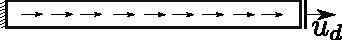
\includegraphics[width=0.5\linewidth]{Images/1D_bar_bf.pdf}
	\caption{1D bar with a body force \label{1D_bar_bf}}
\end{figure}



\subsection{Convergence of the method and its rate}

Since the problem to be analyzed implicitly contains non-convexity (though the structure of the database), it is expedient to first examine the effect of various parameters (the metric in particular) on the convergence of the method. Thus, a simplified problem will first be studied. The problem setup together with the minimization procedure can be found in \ref{appx_convergence}. 

As shown in the appendix, the rate of convergence of the method (and whether it converges at all) can be determined by analyzing the matrix $\bfC \bfA $. It has been assumed that there is no body force and that all but one elements are on the elastic (unloading) branch and only one element moves on the damage branch. This setup corresponds to picking one of several possible bifurcation states from the homogeneous state. Two cases can thus be considered (depending on the mesh size): one with a snapback and one without. 

\subsubsection*{No snapback}
No snapback occurs when the mesh size and hence, the localization length, is big enough. Thus, a direct displacement control has been used. In such a case, the assumptions made above (regarding the elements belonging to the loading and unloading branches) are valid and the analysis in the appendix can be used to judge the rate of convergence. The analysis has been performed by setting $N=10, E=100, m=-0.0667, c=100.0667$. When $C_1=C_2=E$, the spectral radius of the matrix $\bfC \bfA $ in equation \ref{combined_equn} has been found to be $0.993$. However, when $C_2=m$, the spectral radius decreased to $0.5$. This indicates that the number of iterations needed for convergence, which is considered to have occurred when the distance functional is sufficiently small, depends on the value of the parameter $C_2$.

The successive mechanical and material states for the elements on the elastic and damage branch, stating from the \textit{yield point}, can be seen in figures \ref{bad_metric_no_snap} and \ref{good_metric_no_snap} for the two cases $C_2=E$ and $C_2=m$, respectively. Since the spectral radius for the case $C_2=E$ is very close to $1$, the successive iterates can be seen very close to each other. Consequently, the mechanical and material states remain far apart. In contrast, when $C_2=m$, the mechanical and material states approach each other much faster, and the solution converges within just 7 iterations. For $C_2=E$, since the successive material states are very close to each other, convergence will be judged to have occurred if the criterion for convergence based on the change of successive material states is used (and this is the criterion used traditionally). It shall also be noted that in the case $C_2=E$, the (mechanical) strain changes for the elements on the elastic and the damage branch point in the same direction (positive) as the external load (also positive). But when $C_2=m$, the sign of the strain change for the element on the damage branch is same as the external load, while for the element on the elastic branch, it is the opposite. Thus, when $C_2=E$, the system favors the homogeneous branch of the solution.

This case has also been tested using an arc length constraint instead of driving the system with an applied displacement. The details of the arc length constraint can be seen in the appendix. The parameters used are same as earlier. The strain increment in the arc length is taken so that the resulting solution is same as in the case of the applied displacement. In this case, the successive mechanical and material states can be seen in figures \ref{bad_metric_no_snap_arc_length} and \ref{good_metric_no_snap_arc_length}. As earlier, the successive states are very close to each other when $C_2=E$. However, when $C_2=m$, the rate of convergence is optimal - the successive states can be seen exactly same as in the earlier case. Also, the same observation can be made regarding the signs of the initial strain changes.

\subsubsection*{With snapback}

When $N$ is changed to $100$, that is when the mesh is refined, a snap back is expected to occur. In this case, as will be demonstrated, an arc length method is required to track the evolution of the solution. The case where an arc length solver is not used when a snap back occurs will be discussed later. 

The progression of the mechanical and the material states in this case can be seen in figures \ref{bad_metric_snap_no_arclength} and \ref{good_metric_snap_no_arclength}. In this case, it is necessary to take $C_2=m$ to arrive at a converged solution. As can be seen in figure \ref{bad_metric_snap_no_arclength}, if $C_2=E$, the mechanical strain change for both the elements point in the same direction. In subsequent iterations, the same material state is selected for the element on the elastic branch (as it has restricted to remain on the elastic branch in the current case to study the bifurcated solution). As a result, the distance functional stagnates at a high value and does not change anymore regardless of the number of iterations. However, when $C_2=m$, not only is the rate of convergence optimal, but also the algorithm converges, and to the correct solution.

To investigate whether an arc length solver is absolutely needed - that is, to study the capability of the data driven algorithm to \textit{jump through} snap backs - the case with a snapback has been studied without using an arc length solver. The system is thus displacement driven. The successive iterates in this case can be seen in figures \ref{bad_metric_snap_no_arclength} and \ref{good_metric_snap_no_arclength}. When $C_2=E$, the successive mechanical and material states can be seen to move further away from each other. The distance functional in this case thus increases as the iterations progress. When $C_2=m$, the mechanical and the material states change during the first iteration, but no more during the further iterations. It shall also be noted that the strain in the elements on the damage branch decreases, while the strain in the elements on the elastic branch increases. This is consistent with the fact that the smallest eigen value of the system becomes negative when $C_2=m$ and a snapback occurs. Thus, the sign of the strain change for the element on the damage branch is opposite to the sign of the external load change. Hence, when the applied displacement increases, the strain in the damage branch tends to decrease, while the strain in the elastic branch tends to increase. See chapter 3 of \cite{deBorst1986}, \cite{deBorst1987b}, and \cite{Baldelli2021} for discussion on continuation methods for cases when the Hessian matrix loses its positive definiteness. This is however beyond the scope of this article and the arc length solver will be used hereafter instead.

To ensure that the above observations hold regardless of the initial state of the mechanical and material states, the analysis above is repeated with a different initial point, where the elements on the elastic and the damage branch are further away from the \textit{yield point}. The progression of the iterates through the iterations can be seen in figures \ref{bad_metric_snap_no_arclength_add} and \ref{good_metric_snap_no_arclength_add}. As earlier, when the applied displacement increases, the mechanical and material states move as the same direction as the applied displacement after the first iteration. The subsequent iterations take the mechanical state for the element on the damage branch further from its material state, and the solution stagnates at a point which is very far from the expected solution (a fully damaged state for the current element on the damage branch). The situation is similar when $C_2=m$, but with a fewer number of iterations.

\begin{figure}[]
	\begin{subfigure}{0.45\textwidth}
		\centering
		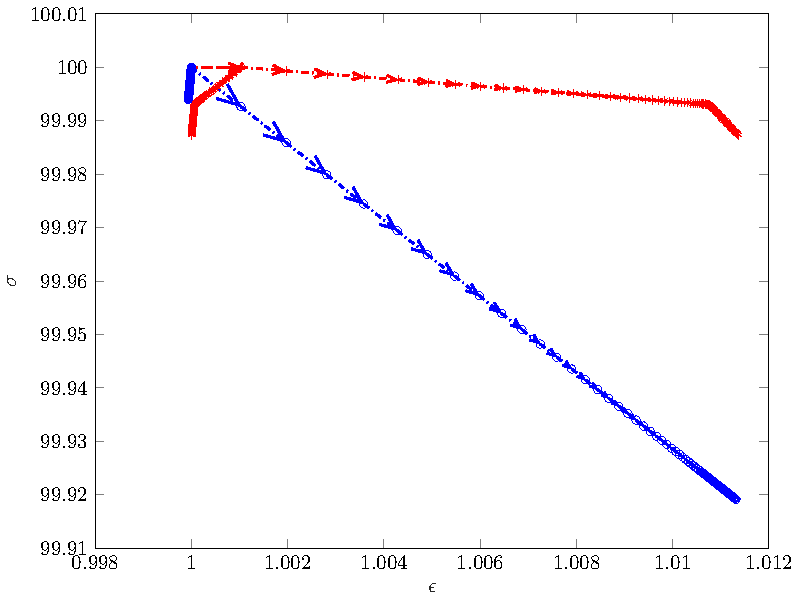
\includegraphics[scale=0.7]{./conv_figs/bad_metric_no_snap.pdf}
		\caption{$C_2=E$, no snapback, and without the arc length constraint.}
		\label{bad_metric_no_snap}
	\end{subfigure}
	\hfill
	\begin{subfigure}{0.45\textwidth}
		\centering
		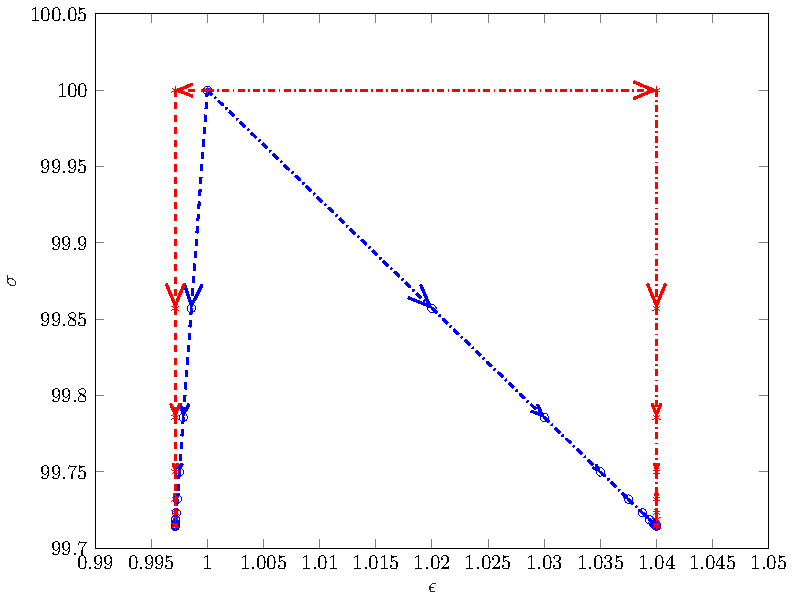
\includegraphics[scale=0.7]{./conv_figs/good_metric_no_snap.pdf}
		\caption{$C_2=m$, no snapback, and without the arc length constraint.}
		\label{good_metric_no_snap}
	\end{subfigure}
	\begin{subfigure}{0.45\textwidth}
		\centering
		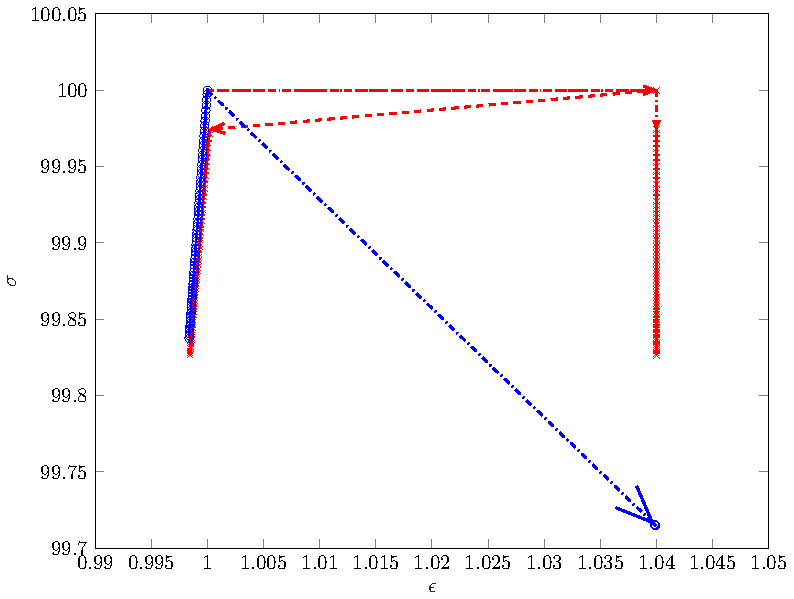
\includegraphics[scale=0.7]{./conv_figs/bad_metric_no_snap_arc_length.pdf}
		\caption{$C_2=E$, no snapback, and with the arc length constraint.}
		\label{bad_metric_no_snap_arc_length}
	\end{subfigure}
	\hfill
	\begin{subfigure}{0.45\textwidth}
		\centering
		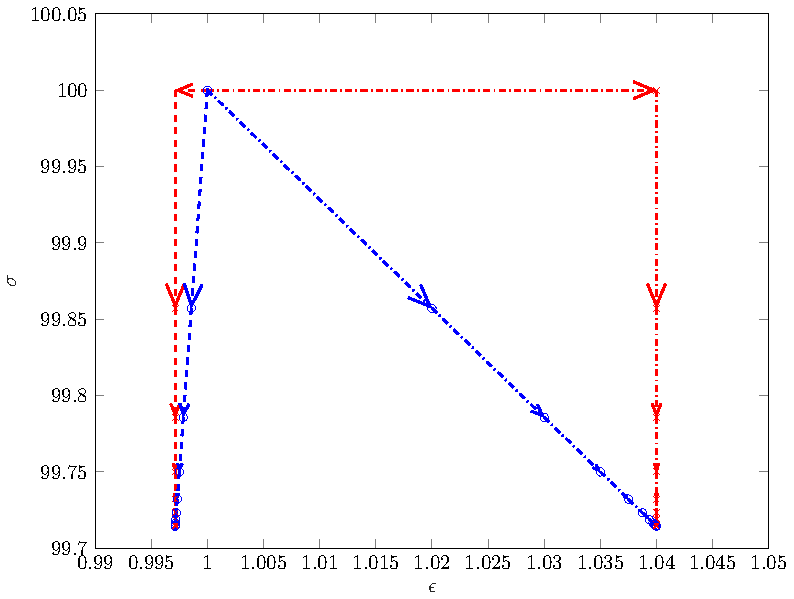
\includegraphics[scale=0.7]{./conv_figs/good_metric_no_snap_arc_length.pdf}
		\caption{$C_2=m$, no snapback, and with the arc length constraint.}
		\label{good_metric_no_snap_arc_length}
	\end{subfigure}
\end{figure}
\begin{figure}\ContinuedFloat
	\begin{subfigure}{0.45\textwidth}
		\centering
		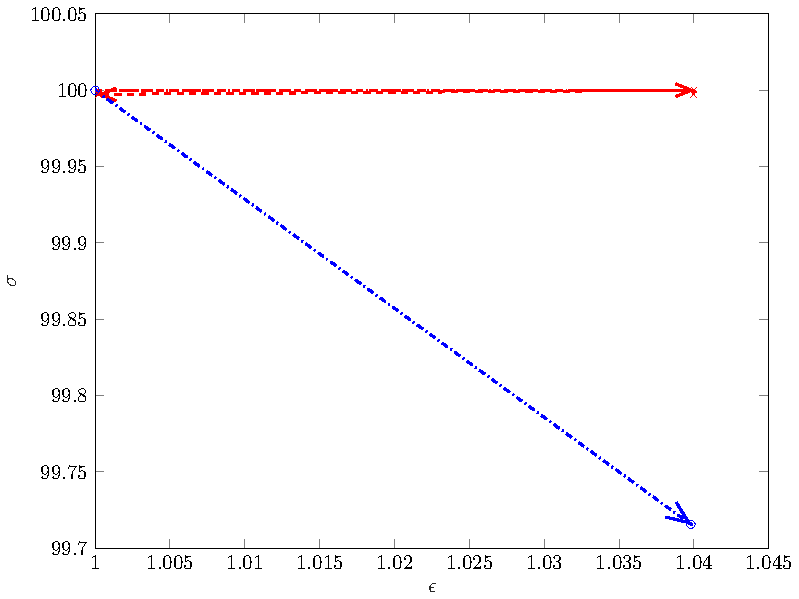
\includegraphics[scale=0.7]{./conv_figs/bad_metric_snap_arc_length.pdf}
		\caption{$C_2=E$, snapback, and with the arc length constraint.}
		\label{bad_metric_snap_arc_length}
	\end{subfigure}
	\hfill
	\begin{subfigure}{0.45\textwidth}
		\centering
		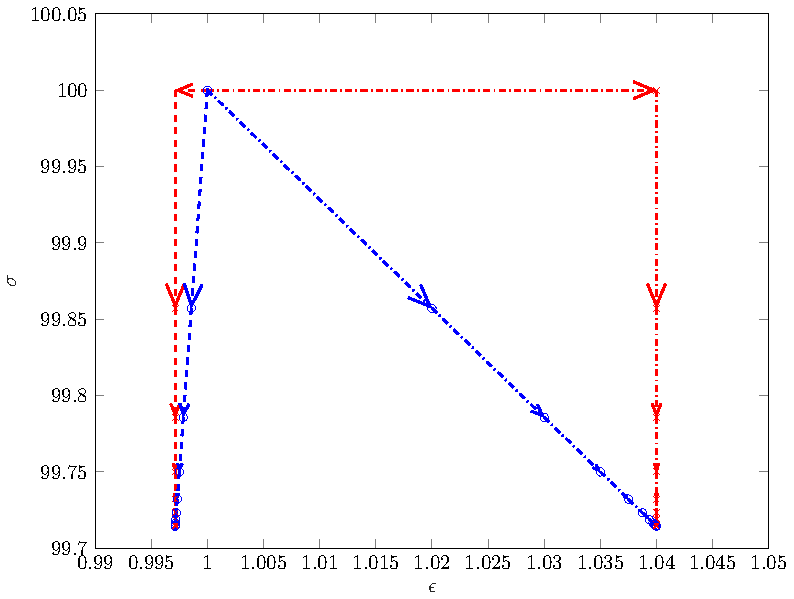
\includegraphics[scale=0.7]{./conv_figs/good_metric_snap_arc_length.pdf}
		\caption{$C_2=m$, snapback, and with the arc length constraint.}
		\label{good_metric_snap_arc_length}
	\end{subfigure}
	\begin{subfigure}{0.45\textwidth}
		\centering
		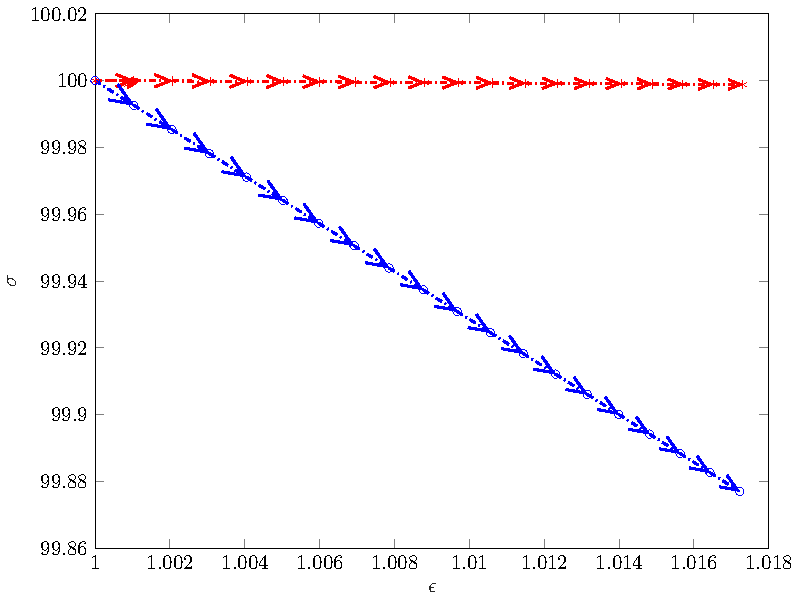
\includegraphics[scale=0.7]{./conv_figs/bad_metric_snap_no_arclength.pdf}
		\caption{$C_2=E$, snapback, and without the arc length constraint.}
		\label{bad_metric_snap_no_arclength}
	\end{subfigure}
	\hfill
	\begin{subfigure}{0.45\textwidth}
		\centering
		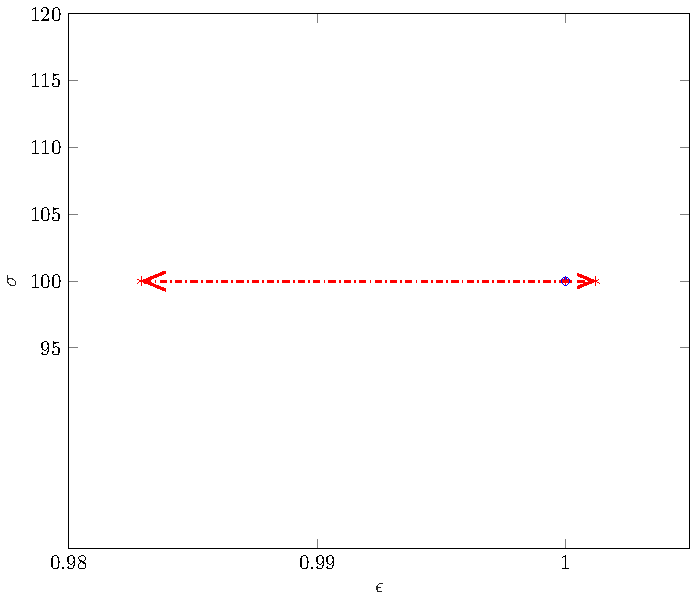
\includegraphics[scale=0.7]{./conv_figs/good_metric_snap_no_arclength.pdf}
		\caption{$C_2=m$, snapback, and without the arc length constraint.}
		\label{good_metric_snap_no_arclength}
	\end{subfigure}
	\begin{subfigure}{0.45\textwidth}
		\centering
		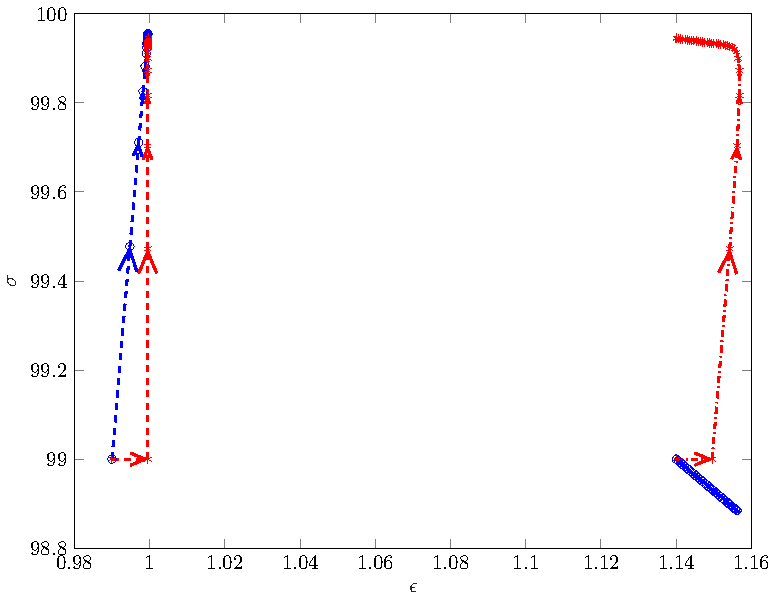
\includegraphics[scale=0.7]{./conv_figs/bad_metric_snap_no_arclength_add.pdf}
		\caption{$C_2=E$, snapback, different initiation, and without the arc length constraint.}
		\label{bad_metric_snap_no_arclength_add}
	\end{subfigure}
	\hfill
	\begin{subfigure}{0.45\textwidth}
		\centering
		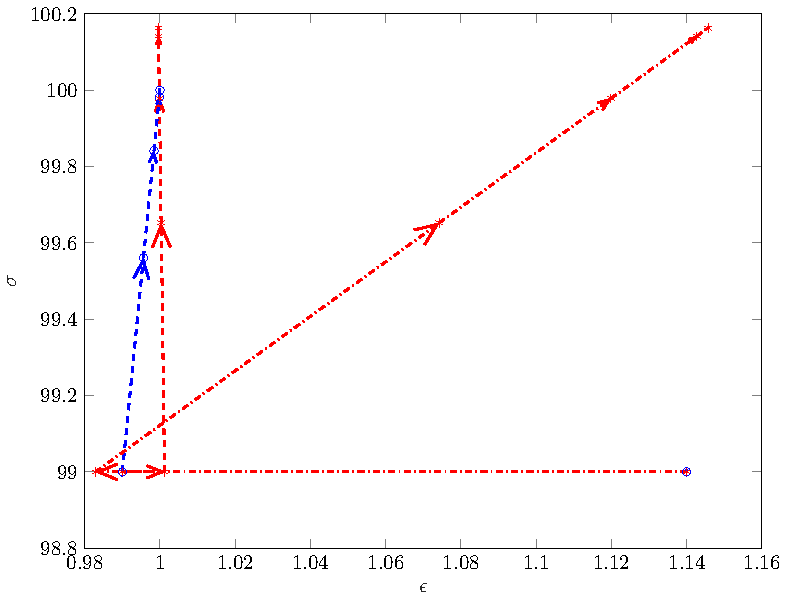
\includegraphics[scale=0.7]{./conv_figs/good_metric_snap_no_arclength_add.pdf}
		\caption{$C_2=m$, snapback, different initiation, and without the arc length constraint.}
		\label{good_metric_snap_no_arclength_add}
	\end{subfigure}
\centering
	\begin{subfigure}{0.45\textwidth}
		\centering
		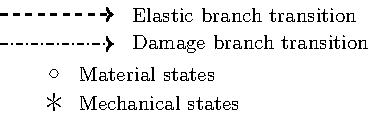
\includegraphics[scale=0.9]{./conv_figs/legend.pdf}
	\end{subfigure}
	\caption{Results from the analysis of various cases in 1D are presented. The successive iterates for the material states are denoted by circles, while the mechanical states are represented by asterisks. The successive iterates are connected by arrows: dashed arrows for the elements on the elastic unloading branch and dash-dotted arrows for the elements on the damage branch.}
	%\label{fig:ut_regularization}
\end{figure}

\begin{remark}
Thus, it can be concluded that not only is using an optimal value for $C_2$, together with an arc length solver, sufficient to achieve an optimal rate of convergence, but it is also necessary to achieve convergence in some cases.
\end{remark}

\subsection{A 1D bar with a body force}
The problem of 1D bar subjected to a body force as in figure \ref{1D_bar_bf} will now be analyzed. The same problem will then be used to demonstrate the effect of introducing a length scale into the problem. The set of equations that govern the data driven solution can be found in the previous section. An arc-length solver will be used to capture the (possible) snapback response of the bar. The bar is meshed with piecewise linear and continuous displacement elements. The mechanical stresses are taken to be piecewise constant. The mesh size is homogeneous. The problem is examined for two mesh sizes (say $\ell_e$, $0.5 \ell_e$) to determine the effect of the mesh size on the response of the bar.

\begin{figure}
	\centering
	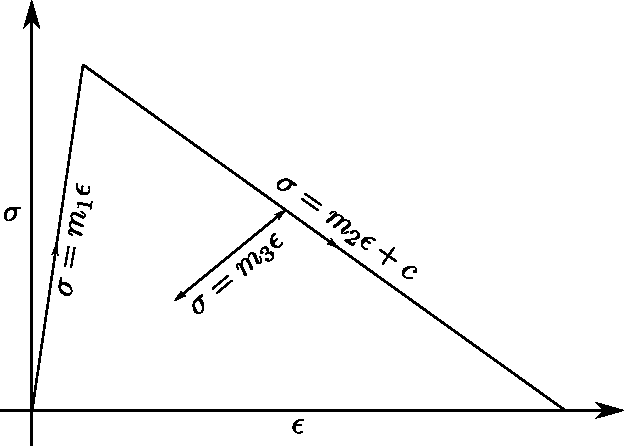
\includegraphics[width=0.4\linewidth]{Images/database_actual.pdf}
	\caption{Stress strain database \label{database_actual}}
\end{figure}



The force at the right end of the bar vs the applied displacement until complete failure (where some element in the bar is fully damaged) for the two mesh sizes can be seen in Figure \ref{force_disp_local}. The mesh dependence of the strain distribution, together with the snapback response, can be clearly seen once the \textit{damage begins to increase}. At the first step, a compressive force is developed as a consequence of the body force, which gradually becomes positive as the displacement is increased. The initial negative displacement is a consequence of the arc-length constraint that the strain increment in the left most element is equal to a certain (user specified) value. As the load is increased further, the damage initiates at the left end (just at the left end because of the applied body force). The strain and the damage localize in the element at the left end in the subsequent steps until the element undergoes a complete failure ($d=1$). A small compressive load can again be seen at the end as a consequence of the applied body force. The corresponding strain distributions, at complete failure, for the two mesh sizes can be seen in figure \ref{strain_dist_local}. The mesh dependence of the solution is obvious.

\begin{figure}[ht]
	\begin{subfigure}{0.45\textwidth}
		\centering
		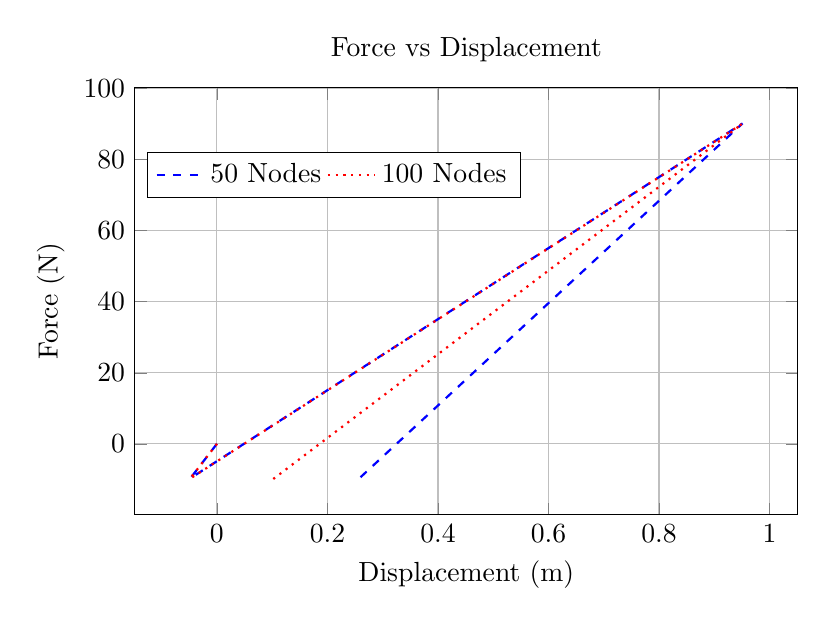
\begin{tikzpicture}
	\begin{axis}[
		title={Force vs Displacement},
		xlabel={Displacement (\si{\meter})},
		ylabel={Force (\si{\newton})},
		legend style={at={(0.3,0.85)}, anchor=north,legend columns=2},
		grid=major,
		width=10cm, height=7cm
		]
		
		% Database 1 (x, y) points using table
		\addplot[
		color=blue, dashed, thick
		% mark=square*,
		%thick
		] table[row sep=newline, x index=0, y index=1] {
			% (x, y) table for Database 1
			0	0
			-0.0479795918367340	-9.69591836734526
			-0.0469795918367349	-9.59591836734985
			-0.0459795918367348	-9.49591836734985
			-0.0449795918367347	-9.39591836735277
			-0.0439795918367349	-9.29591836735277
			-0.0429795918367346	-9.19591836735274
			-0.0419795918367345	-9.09591836735275
			-0.0409795918367348	-8.99591836735858
			-0.0399795918367345	-8.89591836735857
			-0.0389795918367347	-8.79591836735859
			-0.0379795918367346	-8.69591836735857
			-0.0369795918367348	-8.59591836735859
			-0.0359795918367347	-8.49591836735859
			-0.0349795918367348	-8.39591836735858
			-0.0339795918367346	-8.29591836735857
			-0.0329795918367347	-8.19591836737022
			-0.0319795918367347	-8.09591836737023
			-0.0309795918367347	-7.99591836737022
			-0.0299795918367347	-7.89591836737023
			-0.0289795918367347	-7.79591836737022
			-0.0279795918367348	-7.69591836737023
			-0.0269795918367348	-7.59591836737023
			-0.0259795918367346	-7.49591836737022
			-0.0249795918367347	-7.39591836737022
			-0.0239795918367346	-7.29591836737022
			-0.0229795918367347	-7.19591836737022
			-0.0219795918367347	-7.09591836737022
			-0.0209795918367346	-6.99591836737022
			-0.0199795918367347	-6.89591836737023
			-0.0189795918367347	-6.79591836737021
			-0.0179795918367347	-6.69591836737022
			-0.0169795918367347	-6.59591836739350
			-0.0159795918367346	-6.49591836739350
			-0.0149795918367347	-6.39591836739351
			-0.0139795918367348	-6.29591836739350
			-0.0129795918367347	-6.19591836739350
			-0.0119795918367348	-6.09591836739350
			-0.0109795918367346	-5.99591836739350
			-0.00997959183673471	-5.89591836739351
			-0.00897959183673476	-5.79591836739352
			-0.00797959183673482	-5.69591836739352
			-0.00697959183673472	-5.59591836739350
			-0.00597959183673473	-5.49591836739352
			-0.00497959183673484	-5.39591836739351
			-0.00397959183673484	-5.29591836739351
			-0.00297959183673451	-5.19591836739350
			-0.00197959183673489	-5.09591836739351
			-0.000979591836734578	-4.99591836739350
			2.04081632655210e-05	-4.89591836739348
			0.00102040816326552	-4.79591836739350
			0.00202040816326526	-4.69591836739350
			0.00302040816326538	-4.59591836739351
			0.00402040816326544	-4.49591836739352
			0.00502040816326554	-4.39591836739349
			0.00602040816326557	-4.29591836739348
			0.00702040816326556	-4.19591836739351
			0.00802040816326532	-4.09591836739351
			0.00902040816326533	-3.99591836739351
			0.0100204081632650	-3.89591836739352
			0.0110204081632654	-3.79591836739350
			0.0120204081632655	-3.69591836739350
			0.0130204081632654	-3.59591836739349
			0.0140204081632651	-3.49591836739349
			0.0150204081632652	-3.39591836739350
			0.0160204081632656	-3.29591836744006
			0.0170204081632653	-3.19591836744008
			0.0180204081632654	-3.09591836744007
			0.0190204081632656	-2.99591836744006
			0.0200204081632657	-2.89591836744006
			0.0210204081632654	-2.79591836744004
			0.0220204081632651	-2.69591836744007
			0.0230204081632655	-2.59591836744007
			0.0240204081632648	-2.49591836744011
			0.0250204081632654	-2.39591836744006
			0.0260204081632652	-2.29591836744006
			0.0270204081632656	-2.19591836744004
			0.0280204081632653	-2.09591836744007
			0.0290204081632654	-1.99591836744008
			0.0300204081632649	-1.89591836744010
			0.0310204081632655	-1.79591836744007
			0.0320204081632652	-1.69591836744007
			0.0330204081632653	-1.59591836744003
			0.0340204081632653	-1.49591836744006
			0.0350204081632651	-1.39591836744006
			0.0360204081632651	-1.29591836744004
			0.0370204081632654	-1.19591836744009
			0.0380204081632650	-1.09591836744009
			0.0390204081632653	-0.995918367440086
			0.0400204081632653	-0.895918367440075
			0.0410204081632653	-0.795918367440071
			0.0420204081632653	-0.695918367440057
			0.0430204081632649	-0.595918367440079
			0.0440204081632661	-0.495918367440000
			0.0450204081632651	-0.395918367440110
			0.0460204081632647	-0.295918367440073
			0.0470204081632662	-0.195918367440036
			0.0480204081632652	-0.0959183674400761
			0.0490204081632654	0.00408163255990882
			0.0500204081632662	0.104081632559995
			0.0510204081632661	0.204081632559946
			0.0520204081632650	0.304081632559904
			0.0530204081632659	0.404081632559935
			0.0540204081632659	0.504081632559918
			0.0550204081632656	0.604081632559976
			0.0560204081632654	0.704081632559885
			0.0570204081632652	0.804081632559953
			0.0580204081632654	0.904081632559965
			0.0590204081632655	1.00408163255996
			0.0600204081632657	1.10408163255997
			0.0610204081632648	1.20408163255990
			0.0620204081632652	1.30408163255996
			0.0630204081632652	1.40408163255993
			0.0640204081632657	1.50408163255998
			0.0650204081632654	1.60408163255990
			0.0660204081632650	1.70408163255992
			0.0670204081632650	1.80408163255988
			0.0680204081632649	1.90408163255989
			0.0690204081632660	2.00408163255994
			0.0700204081632650	2.10408163255986
			0.0710204081632654	2.20408163255993
			0.0720204081632645	2.30408163255994
			0.0730204081632653	2.40408163255994
			0.0740204081632650	2.50408163256000
			0.0750204081632645	2.60408163255988
			0.0760204081632653	2.70408163255990
			0.0770204081632654	2.80408163255996
			0.0780204081632653	2.90408163255994
			0.0790204081632655	3.00408163255996
			0.0800204081632655	3.10408163255994
			0.0810204081632654	3.20408163246676
			0.0820204081632650	3.30408163246674
			0.0830204081632660	3.40408163246680
			0.0840204081632659	3.50408163246687
			0.0850204081632655	3.60408163246680
			0.0860204081632650	3.70408163246687
			0.0870204081632646	3.80408163246672
			0.0880204081632648	3.90408163246681
			0.0890204081632644	4.00408163246680
			0.0900204081632655	4.10408163246679
			0.0910204081632650	4.20408163246672
			0.0920204081632650	4.30408163246682
			0.0930204081632657	4.40408163246675
			0.0940204081632668	4.50408163246680
			0.0950204081632658	4.60408163246682
			0.0960204081632655	4.70408163246685
			0.0970204081632667	4.80408163246684
			0.0980204081632647	4.90408163246676
			0.0990204081632663	5.00408163246685
			0.100020408163266	5.10408163246680
			0.101020408163265	5.20408163246672
			0.102020408163265	5.30408163246676
			0.103020408163266	5.40408163246693
			0.104020408163265	5.50408163246686
			0.105020408163265	5.60408163246680
			0.106020408163264	5.70408163246672
			0.107020408163265	5.80408163246681
			0.108020408163265	5.90408163246683
			0.109020408163266	6.00408163246683
			0.110020408163265	6.10408163246679
			0.111020408163265	6.20408163246680
			0.112020408163265	6.30408163246685
			0.113020408163266	6.40408163246679
			0.114020408163264	6.50408163246670
			0.115020408163265	6.60408163246675
			0.116020408163264	6.70408163246672
			0.117020408163265	6.80408163246682
			0.118020408163264	6.90408163246682
			0.119020408163265	7.00408163246679
			0.120020408163266	7.10408163246683
			0.121020408163265	7.20408163246678
			0.122020408163266	7.30408163246678
			0.123020408163265	7.40408163246682
			0.124020408163266	7.50408163246666
			0.125020408163266	7.60408163246680
			0.126020408163265	7.70408163246676
			0.127020408163266	7.80408163246679
			0.128020408163264	7.90408163246682
			0.129020408163265	8.00408163246664
			0.130020408163265	8.10408163246675
			0.131020408163264	8.20408163246678
			0.132020408163265	8.30408163246677
			0.133020408163264	8.40408163246666
			0.134020408163266	8.50408163246677
			0.135020408163264	8.60408163246671
			0.136020408163267	8.70408163246681
			0.137020408163266	8.80408163246690
			0.138020408163264	8.90408163246679
			0.139020408163266	9.00408163246678
			0.140020408163264	9.10408163246686
			0.141020408163266	9.20408163246676
			0.142020408163265	9.30408163246686
			0.143020408163266	9.40408163246686
			0.144020408163265	9.50408163246676
			0.145020408163266	9.60408163246684
			0.146020408163265	9.70408163246681
			0.147020408163264	9.80408163246677
			0.148020408163266	9.90408163246680
			0.149020408163265	10.0040816324668
			0.150020408163267	10.1040816324668
			0.151020408163264	10.2040816324668
			0.152020408163267	10.3040816324669
			0.153020408163266	10.4040816324669
			0.154020408163266	10.5040816324668
			0.155020408163264	10.6040816324669
			0.156020408163266	10.7040816324668
			0.157020408163266	10.8040816324668
			0.158020408163266	10.9040816324669
			0.159020408163266	11.0040816324668
			0.160020408163265	11.1040816324668
			0.161020408163267	11.2040816324668
			0.162020408163266	11.3040816324668
			0.163020408163265	11.4040816324667
			0.164020408163267	11.5040816324668
			0.165020408163266	11.6040816324669
			0.166020408163264	11.7040816324667
			0.167020408163266	11.8040816324668
			0.168020408163264	11.9040816324667
			0.169020408163266	12.0040816324668
			0.170020408163263	12.1040816324668
			0.171020408163265	12.2040816324668
			0.172020408163265	12.3040816324668
			0.173020408163265	12.4040816324669
			0.174020408163265	12.5040816324667
			0.175020408163268	12.6040816324669
			0.176020408163265	12.7040816324667
			0.177020408163265	12.8040816324668
			0.178020408163265	12.9040816324668
			0.179020408163267	13.0040816324668
			0.180020408163267	13.1040816324667
			0.181020408163267	13.2040816324669
			0.182020408163263	13.3040816324667
			0.183020408163267	13.4040816324668
			0.184020408163265	13.5040816324668
			0.185020408163266	13.6040816324670
			0.186020408163266	13.7040816324670
			0.187020408163265	13.8040816324668
			0.188020408163264	13.9040816324667
			0.189020408163267	14.0040816324669
			0.190020408163264	14.1040816324667
			0.191020408163269	14.2040816324671
			0.192020408163267	14.3040816324668
			0.193020408163266	14.4040816324669
			0.194020408163267	14.5040816324668
			0.195020408163262	14.6040816324667
			0.196020408163267	14.7040816324668
			0.197020408163265	14.8040816324668
			0.198020408163266	14.9040816324669
			0.199020408163266	15.0040816324670
			0.200020408163266	15.1040816324669
			0.201020408163268	15.2040816324669
			0.202020408163266	15.3040816324668
			0.203020408163265	15.4040816324668
			0.204020408163266	15.5040816324669
			0.205020408163263	15.6040816324668
			0.206020408163267	15.7040816324668
			0.207020408163265	15.8040816324666
			0.208020408163265	15.9040816324668
			0.209020408163266	16.0040816324667
			0.210020408163264	16.1040816324669
			0.211020408163265	16.2040816322804
			0.212020408163264	16.3040816322805
			0.213020408163266	16.4040816322805
			0.214020408163266	16.5040816322806
			0.215020408163264	16.6040816322806
			0.216020408163265	16.7040816322806
			0.217020408163264	16.8040816322805
			0.218020408163264	16.9040816322805
			0.219020408163266	17.0040816322806
			0.220020408163267	17.1040816322807
			0.221020408163267	17.2040816322808
			0.222020408163263	17.3040816322804
			0.223020408163265	17.4040816322806
			0.224020408163265	17.5040816322808
			0.225020408163265	17.6040816322807
			0.226020408163266	17.7040816322806
			0.227020408163266	17.8040816322805
			0.228020408163266	17.9040816322805
			0.229020408163268	18.0040816322806
			0.230020408163266	18.1040816322806
			0.231020408163266	18.2040816322807
			0.232020408163265	18.3040816322805
			0.233020408163266	18.4040816322805
			0.234020408163266	18.5040816322804
			0.235020408163263	18.6040816322806
			0.236020408163264	18.7040816322804
			0.237020408163266	18.8040816322806
			0.238020408163266	18.9040816322805
			0.239020408163266	19.0040816322807
			0.240020408163263	19.1040816322805
			0.241020408163264	19.2040816322806
			0.242020408163266	19.3040816322805
			0.243020408163267	19.4040816322807
			0.244020408163264	19.5040816322806
			0.245020408163265	19.6040816322807
			0.246020408163265	19.7040816322807
			0.247020408163266	19.8040816322806
			0.248020408163264	19.9040816322805
			0.249020408163265	20.0040816322806
			0.250020408163267	20.1040816322805
			0.251020408163267	20.2040816322806
			0.252020408163267	20.3040816322806
			0.253020408163266	20.4040816322806
			0.254020408163262	20.5040816322805
			0.255020408163267	20.6040816322808
			0.256020408163265	20.7040816322805
			0.257020408163265	20.8040816322805
			0.258020408163266	20.9040816322806
			0.259020408163266	21.0040816322807
			0.260020408163265	21.1040816322806
			0.261020408163265	21.2040816322805
			0.262020408163266	21.3040816322806
			0.263020408163267	21.4040816322805
			0.264020408163266	21.5040816322806
			0.265020408163264	21.6040816322805
			0.266020408163265	21.7040816322807
			0.267020408163267	21.8040816322807
			0.268020408163265	21.9040816322804
			0.269020408163266	22.0040816322807
			0.270020408163265	22.1040816322807
			0.271020408163265	22.2040816322805
			0.272020408163266	22.3040816322805
			0.273020408163265	22.4040816322805
			0.274020408163264	22.5040816322807
			0.275020408163263	22.6040816322802
			0.276020408163268	22.7040816322806
			0.277020408163269	22.8040816322806
			0.278020408163265	22.9040816322806
			0.279020408163266	23.0040816322808
			0.280020408163264	23.1040816322806
			0.281020408163268	23.2040816322807
			0.282020408163264	23.3040816322805
			0.283020408163265	23.4040816322805
			0.284020408163266	23.5040816322805
			0.285020408163266	23.6040816322806
			0.286020408163264	23.7040816322806
			0.287020408163262	23.8040816322805
			0.288020408163266	23.9040816322805
			0.289020408163266	24.0040816322805
			0.290020408163266	24.1040816322805
			0.291020408163267	24.2040816322806
			0.292020408163265	24.3040816322807
			0.293020408163265	24.4040816322806
			0.294020408163266	24.5040816322805
			0.295020408163265	24.6040816322805
			0.296020408163267	24.7040816322803
			0.297020408163263	24.8040816322804
			0.298020408163265	24.9040816322805
			0.299020408163267	25.0040816322804
			0.300020408163264	25.1040816322806
			0.301020408163265	25.2040816322806
			0.302020408163266	25.3040816322805
			0.303020408163267	25.4040816322805
			0.304020408163269	25.5040816322807
			0.305020408163267	25.6040816322808
			0.306020408163266	25.7040816322805
			0.307020408163264	25.8040816322806
			0.308020408163266	25.9040816322806
			0.309020408163265	26.0040816322807
			0.310020408163266	26.1040816322805
			0.311020408163264	26.2040816322806
			0.312020408163263	26.3040816322805
			0.313020408163267	26.4040816322806
			0.314020408163266	26.5040816322806
			0.315020408163268	26.6040816322807
			0.316020408163264	26.7040816322805
			0.317020408163264	26.8040816322808
			0.318020408163268	26.9040816322807
			0.319020408163267	27.0040816322808
			0.320020408163270	27.1040816322808
			0.321020408163264	27.2040816322805
			0.322020408163264	27.3040816322806
			0.323020408163266	27.4040816322807
			0.324020408163264	27.5040816322805
			0.325020408163263	27.6040816322807
			0.326020408163268	27.7040816322808
			0.327020408163265	27.8040816322804
			0.328020408163265	27.9040816322806
			0.329020408163265	28.0040816322806
			0.330020408163267	28.1040816322804
			0.331020408163264	28.2040816322805
			0.332020408163266	28.3040816322807
			0.333020408163262	28.4040816322806
			0.334020408163263	28.5040816322803
			0.335020408163263	28.6040816322803
			0.336020408163267	28.7040816322806
			0.337020408163265	28.8040816322807
			0.338020408163267	28.9040816322804
			0.339020408163266	29.0040816322806
			0.340020408163269	29.1040816322807
			0.341020408163265	29.2040816322805
			0.342020408163265	29.3040816322804
			0.343020408163268	29.4040816322805
			0.344020408163266	29.5040816322805
			0.345020408163265	29.6040816322804
			0.346020408163266	29.7040816322807
			0.347020408163264	29.8040816322804
			0.348020408163266	29.9040816322805
			0.349020408163266	30.0040816322806
			0.350020408163267	30.1040816322807
			0.351020408163265	30.2040816322805
			0.352020408163265	30.3040816322805
			0.353020408163267	30.4040816322806
			0.354020408163264	30.5040816322807
			0.355020408163268	30.6040816322804
			0.356020408163267	30.7040816322805
			0.357020408163267	30.8040816322804
			0.358020408163268	30.9040816322805
			0.359020408163268	31.0040816322808
			0.360020408163266	31.1040816322806
			0.361020408163268	31.2040816322807
			0.362020408163266	31.3040816322805
			0.363020408163268	31.4040816322807
			0.364020408163265	31.5040816322804
			0.365020408163270	31.6040816322808
			0.366020408163265	31.7040816322804
			0.367020408163266	31.8040816322808
			0.368020408163267	31.9040816322807
			0.369020408163265	32.0040816322807
			0.370020408163268	32.1040816322805
			0.371020408163267	32.2040816322807
			0.372020408163271	32.3040816322807
			0.373020408163267	32.4040816322808
			0.374020408163267	32.5040816322806
			0.375020408163266	32.6040816322807
			0.376020408163267	32.7040816322807
			0.377020408163269	32.8040816322807
			0.378020408163270	32.9040816322805
			0.379020408163266	33.0040816322807
			0.380020408163270	33.1040816322810
			0.381020408163266	33.2040816322807
			0.382020408163264	33.3040816322804
			0.383020408163263	33.4040816322804
			0.384020408163269	33.5040816322808
			0.385020408163267	33.6040816322807
			0.386020408163267	33.7040816322805
			0.387020408163265	33.8040816322806
			0.388020408163264	33.9040816322803
			0.389020408163265	34.0040816322805
			0.390020408163264	34.1040816322808
			0.391020408163269	34.2040816322810
			0.392020408163267	34.3040816322807
			0.393020408163266	34.4040816322805
			0.394020408163265	34.5040816322807
			0.395020408163267	34.6040816322807
			0.396020408163268	34.7040816322807
			0.397020408163268	34.8040816322807
			0.398020408163266	34.9040816322807
			0.399020408163265	35.0040816322806
			0.400020408163266	35.1040816322808
			0.401020408163267	35.2040816322808
			0.402020408163267	35.3040816322806
			0.403020408163264	35.4040816322804
			0.404020408163268	35.5040816322807
			0.405020408163265	35.6040816322805
			0.406020408163266	35.7040816322802
			0.407020408163262	35.8040816322804
			0.408020408163265	35.9040816322805
			0.409020408163271	36.0040816322812
			0.410020408163270	36.1040816322806
			0.411020408163267	36.2040816322807
			0.412020408163266	36.3040816322805
			0.413020408163263	36.4040816322806
			0.414020408163264	36.5040816322804
			0.415020408163266	36.6040816322806
			0.416020408163266	36.7040816322804
			0.417020408163268	36.8040816322808
			0.418020408163267	36.9040816322810
			0.419020408163268	37.0040816322810
			0.420020408163266	37.1040816322806
			0.421020408163267	37.2040816322802
			0.422020408163267	37.3040816322809
			0.423020408163269	37.4040816322807
			0.424020408163262	37.5040816322806
			0.425020408163268	37.6040816322809
			0.426020408163268	37.7040816322805
			0.427020408163269	37.8040816322805
			0.428020408163263	37.9040816322805
			0.429020408163270	38.0040816322810
			0.430020408163269	38.1040816322807
			0.431020408163266	38.2040816322807
			0.432020408163264	38.3040816322806
			0.433020408163263	38.4040816322806
			0.434020408163267	38.5040816322807
			0.435020408163268	38.6040816322806
			0.436020408163266	38.7040816322806
			0.437020408163262	38.8040816322807
			0.438020408163266	38.9040816322806
			0.439020408163267	39.0040816322806
			0.440020408163265	39.1040816322809
			0.441020408163270	39.2040816322809
			0.442020408163266	39.3040816322805
			0.443020408163266	39.4040816322807
			0.444020408163264	39.5040816322805
			0.445020408163265	39.6040816322807
			0.446020408163265	39.7040816322805
			0.447020408163266	39.8040816322807
			0.448020408163266	39.9040816322806
			0.449020408163272	40.0040816322811
			0.450020408163266	40.1040816322809
			0.451020408163267	40.2040816322805
			0.452020408163266	40.3040816322809
			0.453020408163268	40.4040816322808
			0.454020408163266	40.5040816322805
			0.455020408163260	40.6040816322803
			0.456020408163263	40.7040816322806
			0.457020408163265	40.8040816322806
			0.458020408163264	40.9040816322803
			0.459020408163268	41.0040816322805
			0.460020408163266	41.1040816322807
			0.461020408163267	41.2040816322806
			0.462020408163267	41.3040816322807
			0.463020408163267	41.4040816322808
			0.464020408163269	41.5040816322806
			0.465020408163265	41.6040816322805
			0.466020408163264	41.7040816322806
			0.467020408163269	41.8040816322809
			0.468020408163265	41.9040816322808
			0.469020408163264	42.0040816322805
			0.470020408163266	42.1040816322805
			0.471020408163265	42.2040816322807
			0.472020408163264	42.3040816319080
			0.473020408163267	42.4040816319079
			0.474020408163269	42.5040816319080
			0.475020408163263	42.6040816319081
			0.476020408163270	42.7040816319084
			0.477020408163265	42.8040816319079
			0.478020408163269	42.9040816319080
			0.479020408163270	43.0040816319083
			0.480020408163265	43.1040816319083
			0.481020408163267	43.2040816319079
			0.482020408163269	43.3040816319079
			0.483020408163264	43.4040816319082
			0.484020408163273	43.5040816319084
			0.485020408163263	43.6040816319078
			0.486020408163268	43.7040816319083
			0.487020408163266	43.8040816319082
			0.488020408163266	43.9040816319082
			0.489020408163262	44.0040816319079
			0.490020408163270	44.1040816319083
			0.491020408163263	44.2040816319077
			0.492020408163270	44.3040816319086
			0.493020408163263	44.4040816319080
			0.494020408163263	44.5040816319080
			0.495020408163270	44.6040816319084
			0.496020408163266	44.7040816319083
			0.497020408163265	44.8040816319078
			0.498020408163267	44.9040816319080
			0.499020408163265	45.0040816319082
			0.500020408163269	45.1040816319082
			0.501020408163266	45.2040816319079
			0.502020408163263	45.3040816319082
			0.503020408163267	45.4040816319081
			0.504020408163267	45.5040816319087
			0.505020408163266	45.6040816319081
			0.506020408163273	45.7040816319083
			0.507020408163266	45.8040816319082
			0.508020408163262	45.9040816319078
			0.509020408163269	46.0040816319083
			0.510020408163267	46.1040816319083
			0.511020408163267	46.2040816319083
			0.512020408163266	46.3040816319080
			0.513020408163262	46.4040816319083
			0.514020408163268	46.5040816319082
			0.515020408163268	46.6040816319081
			0.516020408163270	46.7040816319082
			0.517020408163262	46.8040816319079
			0.518020408163265	46.9040816319079
			0.519020408163267	47.0040816319081
			0.520020408163270	47.1040816319084
			0.521020408163267	47.2040816319083
			0.522020408163267	47.3040816319079
			0.523020408163266	47.4040816319082
			0.524020408163270	47.5040816319079
			0.525020408163270	47.6040816319083
			0.526020408163267	47.7040816319081
			0.527020408163272	47.8040816319085
			0.528020408163269	47.9040816319084
			0.529020408163264	48.0040816319079
			0.530020408163267	48.1040816319083
			0.531020408163268	48.2040816319085
			0.532020408163270	48.3040816319082
			0.533020408163271	48.4040816319082
			0.534020408163262	48.5040816319082
			0.535020408163265	48.6040816319083
			0.536020408163266	48.7040816319079
			0.537020408163269	48.8040816319082
			0.538020408163267	48.9040816319082
			0.539020408163268	49.0040816319084
			0.540020408163264	49.1040816319082
			0.541020408163267	49.2040816319082
			0.542020408163262	49.3040816319079
			0.543020408163264	49.4040816319080
			0.544020408163262	49.5040816319077
			0.545020408163266	49.6040816319082
			0.546020408163265	49.7040816319080
			0.547020408163265	49.8040816319082
			0.548020408163262	49.9040816319083
			0.549020408163267	50.0040816319083
			0.550020408163268	50.1040816319081
			0.551020408163267	50.2040816319083
			0.552020408163272	50.3040816319083
			0.553020408163275	50.4040816319081
			0.554020408163268	50.5040816319086
			0.555020408163269	50.6040816319077
			0.556020408163265	50.7040816319080
			0.557020408163269	50.8040816319086
			0.558020408163266	50.9040816319081
			0.559020408163265	51.0040816319085
			0.560020408163269	51.1040816319083
			0.561020408163264	51.2040816319081
			0.562020408163268	51.3040816319083
			0.563020408163266	51.4040816319086
			0.564020408163264	51.5040816319080
			0.565020408163267	51.6040816319078
			0.566020408163270	51.7040816319082
			0.567020408163269	51.8040816319082
			0.568020408163271	51.9040816319083
			0.569020408163263	52.0040816319078
			0.570020408163270	52.1040816319083
			0.571020408163268	52.2040816319083
			0.572020408163268	52.3040816319084
			0.573020408163272	52.4040816319084
			0.574020408163269	52.5040816319084
			0.575020408163276	52.6040816319086
			0.576020408163274	52.7040816319088
			0.577020408163262	52.8040816319081
			0.578020408163266	52.9040816319080
			0.579020408163263	53.0040816319081
			0.580020408163269	53.1040816319087
			0.581020408163271	53.2040816319083
			0.582020408163262	53.3040816319081
			0.583020408163269	53.4040816319081
			0.584020408163269	53.5040816319085
			0.585020408163271	53.6040816319083
			0.586020408163271	53.7040816319084
			0.587020408163269	53.8040816319082
			0.588020408163269	53.9040816319082
			0.589020408163272	54.0040816319083
			0.590020408163266	54.1040816319082
			0.591020408163267	54.2040816319080
			0.592020408163270	54.3040816319082
			0.593020408163259	54.4040816319076
			0.594020408163271	54.5040816319086
			0.595020408163262	54.6040816319079
			0.596020408163264	54.7040816319081
			0.597020408163273	54.8040816319084
			0.598020408163265	54.9040816319077
			0.599020408163262	55.0040816319079
			0.600020408163264	55.1040816319080
			0.601020408163262	55.2040816319075
			0.602020408163264	55.3040816319080
			0.603020408163270	55.4040816319084
			0.604020408163272	55.5040816319083
			0.605020408163270	55.6040816319085
			0.606020408163266	55.7040816319084
			0.607020408163261	55.8040816319081
			0.608020408163269	55.9040816319084
			0.609020408163265	56.0040816319081
			0.610020408163270	56.1040816319082
			0.611020408163262	56.2040816319082
			0.612020408163265	56.3040816319081
			0.613020408163260	56.4040816319078
			0.614020408163266	56.5040816319080
			0.615020408163268	56.6040816319082
			0.616020408163270	56.7040816319080
			0.617020408163257	56.8040816319078
			0.618020408163262	56.9040816319083
			0.619020408163264	57.0040816319079
			0.620020408163267	57.1040816319082
			0.621020408163267	57.2040816319080
			0.622020408163269	57.3040816319081
			0.623020408163263	57.4040816319077
			0.624020408163271	57.5040816319085
			0.625020408163262	57.6040816319081
			0.626020408163263	57.7040816319080
			0.627020408163269	57.8040816319088
			0.628020408163268	57.9040816319080
			0.629020408163269	58.0040816319085
			0.630020408163270	58.1040816319084
			0.631020408163273	58.2040816319087
			0.632020408163264	58.3040816319080
			0.633020408163272	58.4040816319081
			0.634020408163269	58.5040816319082
			0.635020408163270	58.6040816319081
			0.636020408163262	58.7040816319084
			0.637020408163266	58.8040816319084
			0.638020408163270	58.9040816319085
			0.639020408163270	59.0040816319087
			0.640020408163268	59.1040816319080
			0.641020408163262	59.2040816319076
			0.642020408163271	59.3040816319083
			0.643020408163260	59.4040816319076
			0.644020408163266	59.5040816319081
			0.645020408163263	59.6040816319082
			0.646020408163264	59.7040816319083
			0.647020408163270	59.8040816319081
			0.648020408163269	59.9040816319080
			0.649020408163267	60.0040816319081
			0.650020408163272	60.1040816319087
			0.651020408163262	60.2040816319080
			0.652020408163271	60.3040816319086
			0.653020408163264	60.4040816319086
			0.654020408163269	60.5040816319082
			0.655020408163268	60.6040816319083
			0.656020408163263	60.7040816319082
			0.657020408163267	60.8040816319080
			0.658020408163271	60.9040816319086
			0.659020408163269	61.0040816319084
			0.660020408163270	61.1040816319084
			0.661020408163265	61.2040816319082
			0.662020408163265	61.3040816319076
			0.663020408163263	61.4040816319083
			0.664020408163267	61.5040816319080
			0.665020408163264	61.6040816319082
			0.666020408163275	61.7040816319083
			0.667020408163264	61.8040816319078
			0.668020408163269	61.9040816319081
			0.669020408163272	62.0040816319083
			0.670020408163267	62.1040816319080
			0.671020408163274	62.2040816319085
			0.672020408163272	62.3040816319087
			0.673020408163267	62.4040816319081
			0.674020408163274	62.5040816319089
			0.675020408163272	62.6040816319079
			0.676020408163263	62.7040816319077
			0.677020408163270	62.8040816319082
			0.678020408163273	62.9040816319084
			0.679020408163270	63.0040816319082
			0.680020408163257	63.1040816319079
			0.681020408163274	63.2040816319082
			0.682020408163267	63.3040816319081
			0.683020408163262	63.4040816319084
			0.684020408163269	63.5040816319085
			0.685020408163266	63.6040816319080
			0.686020408163265	63.7040816319077
			0.687020408163272	63.8040816319084
			0.688020408163268	63.9040816319079
			0.689020408163269	64.0040816319086
			0.690020408163270	64.1040816319082
			0.691020408163269	64.2040816319086
			0.692020408163270	64.3040816319087
			0.693020408163268	64.4040816319083
			0.694020408163266	64.5040816319083
			0.695020408163262	64.6040816319079
			0.696020408163267	64.7040816319088
			0.697020408163269	64.8040816319085
			0.698020408163269	64.9040816319076
			0.699020408163263	65.0040816319078
			0.700020408163262	65.1040816319077
			0.701020408163263	65.2040816319078
			0.702020408163268	65.3040816319081
			0.703020408163269	65.4040816319083
			0.704020408163268	65.5040816319084
			0.705020408163267	65.6040816319080
			0.706020408163267	65.7040816319082
			0.707020408163267	65.8040816319084
			0.708020408163267	65.9040816319081
			0.709020408163267	66.0040816319081
			0.710020408163269	66.1040816319081
			0.711020408163263	66.2040816319076
			0.712020408163262	66.3040816319080
			0.713020408163270	66.4040816319081
			0.714020408163268	66.5040816319081
			0.715020408163268	66.6040816319082
			0.716020408163262	66.7040816319078
			0.717020408163263	66.8040816319082
			0.718020408163269	66.9040816319085
			0.719020408163270	67.0040816319082
			0.720020408163271	67.1040816319085
			0.721020408163262	67.2040816319079
			0.722020408163271	67.3040816319084
			0.723020408163260	67.4040816319079
			0.724020408163265	67.5040816319079
			0.725020408163270	67.6040816319081
			0.726020408163271	67.7040816319087
			0.727020408163270	67.8040816319083
			0.728020408163269	67.9040816319082
			0.729020408163271	68.0040816319081
			0.730020408163272	68.1040816319082
			0.731020408163269	68.2040816319082
			0.732020408163273	68.3040816319082
			0.733020408163273	68.4040816319080
			0.734020408163263	68.5040816319082
			0.735020408163272	68.6040816319081
			0.736020408163273	68.7040816319087
			0.737020408163266	68.8040816319078
			0.738020408163267	68.9040816319081
			0.739020408163275	69.0040816319085
			0.740020408163269	69.1040816319087
			0.741020408163272	69.2040816319087
			0.742020408163263	69.3040816319080
			0.743020408163262	69.4040816319079
			0.744020408163262	69.5040816319084
			0.745020408163268	69.6040816319084
			0.746020408163274	69.7040816319086
			0.747020408163272	69.8040816319082
			0.748020408163268	69.9040816319085
			0.749020408163275	70.0040816319088
			0.750020408163270	70.1040816319086
			0.751020408163268	70.2040816319086
			0.752020408163272	70.3040816319083
			0.753020408163275	70.4040816319085
			0.754020408163272	70.5040816319091
			0.755020408163276	70.6040816319087
			0.756020408163268	70.7040816319090
			0.757020408163268	70.8040816319084
			0.758020408163268	70.9040816319084
			0.759020408163278	71.0040816319089
			0.760020408163268	71.1040816319081
			0.761020408163264	71.2040816319081
			0.762020408163277	71.3040816319083
			0.763020408163268	71.4040816319087
			0.764020408163265	71.5040816319083
			0.765020408163272	71.6040816319082
			0.766020408163267	71.7040816319079
			0.767020408163269	71.8040816319090
			0.768020408163272	71.9040816319086
			0.769020408163272	72.0040816319084
			0.770020408163265	72.1040816319084
			0.771020408163271	72.2040816319082
			0.772020408163275	72.3040816319092
			0.773020408163273	72.4040816319084
			0.774020408163274	72.5040816319086
			0.775020408163273	72.6040816319090
			0.776020408163270	72.7040816319088
			0.777020408163266	72.8040816319084
			0.778020408163271	72.9040816319088
			0.779020408163266	73.0040816319084
			0.780020408163268	73.1040816319084
			0.781020408163268	73.2040816319088
			0.782020408163274	73.3040816319090
			0.783020408163274	73.4040816319088
			0.784020408163271	73.5040816319083
			0.785020408163276	73.6040816319085
			0.786020408163266	73.7040816319085
			0.787020408163270	73.8040816319081
			0.788020408163271	73.9040816319089
			0.789020408163268	74.0040816319083
			0.790020408163270	74.1040816319084
			0.791020408163267	74.2040816319083
			0.792020408163273	74.3040816319088
			0.793020408163266	74.4040816319086
			0.794020408163270	74.5040816319080
			0.795020408163273	74.6040816319088
			0.796020408163271	74.7040816319086
			0.797020408163271	74.8040816319085
			0.798020408163267	74.9040816319091
			0.799020408163271	75.0040816319087
			0.800020408163267	75.1040816319087
			0.801020408163272	75.2040816319082
			0.802020408163272	75.3040816319089
			0.803020408163273	75.4040816319083
			0.804020408163263	75.5040816319087
			0.805020408163273	75.6040816319086
			0.806020408163275	75.7040816319086
			0.807020408163273	75.8040816319086
			0.808020408163277	75.9040816319087
			0.809020408163269	76.0040816319083
			0.810020408163282	76.1040816319091
			0.811020408163273	76.2040816319080
			0.812020408163272	76.3040816319082
			0.813020408163274	76.4040816319087
			0.814020408163275	76.5040816319091
			0.815020408163271	76.6040816319086
			0.816020408163270	76.7040816319084
			0.817020408163265	76.8040816319080
			0.818020408163273	76.9040816319086
			0.819020408163272	77.0040816319085
			0.820020408163275	77.1040816319086
			0.821020408163274	77.2040816319087
			0.822020408163272	77.3040816319083
			0.823020408163278	77.4040816319090
			0.824020408163275	77.5040816319079
			0.825020408163278	77.6040816319087
			0.826020408163272	77.7040816319083
			0.827020408163266	77.8040816319086
			0.828020408163272	77.9040816319087
			0.829020408163267	78.0040816319085
			0.830020408163269	78.1040816319088
			0.831020408163274	78.2040816319092
			0.832020408163279	78.3040816319085
			0.833020408163273	78.4040816319086
			0.834020408163277	78.5040816319089
			0.835020408163276	78.6040816319086
			0.836020408163282	78.7040816319093
			0.837020408163270	78.8040816319087
			0.838020408163266	78.9040816319084
			0.839020408163277	79.0040816319089
			0.840020408163266	79.1040816319082
			0.841020408163284	79.2040816319099
			0.842020408163278	79.3040816319087
			0.843020408163280	79.4040816319090
			0.844020408163276	79.5040816319086
			0.845020408163274	79.6040816319090
			0.846020408163273	79.7040816319088
			0.847020408163273	79.8040816319096
			0.848020408163268	79.9040816319088
			0.849020408163267	80.0040816319089
			0.850020408163279	80.1040816319084
			0.851020408163270	80.2040816319087
			0.852020408163267	80.3040816319087
			0.853020408163275	80.4040816319090
			0.854020408163269	80.5040816319091
			0.855020408163275	80.6040816319091
			0.856020408163275	80.7040816319092
			0.857020408163281	80.8040816319090
			0.858020408163280	80.9040816319092
			0.859020408163276	81.0040816319091
			0.860020408163275	81.1040816319089
			0.861020408163272	81.2040816319091
			0.862020408163271	81.3040816319086
			0.863020408163273	81.4040816319091
			0.864020408163269	81.5040816319085
			0.865020408163275	81.6040816319086
			0.866020408163276	81.7040816319090
			0.867020408163281	81.8040816319092
			0.868020408163274	81.9040816319086
			0.869020408163284	82.0040816319088
			0.870020408163280	82.1040816319095
			0.871020408163274	82.2040816319090
			0.872020408163272	82.3040816319090
			0.873020408163275	82.4040816319090
			0.874020408163284	82.5040816319086
			0.875020408163273	82.6040816319089
			0.876020408163280	82.7040816319090
			0.877020408163271	82.8040816319086
			0.878020408163273	82.9040816319093
			0.879020408163276	83.0040816319088
			0.880020408163271	83.1040816319087
			0.881020408163278	83.2040816319091
			0.882020408163281	83.3040816319093
			0.883020408163272	83.4040816319087
			0.884020408163276	83.5040816319089
			0.885020408163278	83.6040816319089
			0.886020408163271	83.7040816319085
			0.887020408163270	83.8040816319088
			0.888020408163268	83.9040816319088
			0.889020408163276	84.0040816319092
			0.890020408163262	84.1040816319088
			0.891020408163275	84.2040816319094
			0.892020408163279	84.3040816319092
			0.893020408163273	84.4040816319091
			0.894020408163280	84.5040816319092
			0.895020408163278	84.6040816319100
			0.896020408163276	84.7040816319089
			0.897020408163280	84.8040816319088
			0.898020408163279	84.9040816319093
			0.899020408163268	85.0040816319089
			0.900020408163285	85.1040816319092
			0.901020408163276	85.2040816319088
			0.902020408163279	85.3040816319094
			0.903020408163276	85.4040816319085
			0.904020408163279	85.5040816319093
			0.905020408163274	85.6040816319089
			0.906020408163273	85.7040816319087
			0.907020408163275	85.8040816319091
			0.908020408163277	85.9040816319092
			0.909020408163270	86.0040816319096
			0.910020408163271	86.1040816319085
			0.911020408163275	86.2040816319095
			0.912020408163281	86.3040816319093
			0.913020408163274	86.4040816319088
			0.914020408163278	86.5040816319093
			0.915020408163276	86.6040816319090
			0.916020408163281	86.7040816319089
			0.917020408163280	86.8040816319088
			0.918020408163267	86.9040816319083
			0.919020408163280	87.0040816319098
			0.920020408163281	87.1040816319095
			0.921020408163267	87.2040816319088
			0.922020408163280	87.3040816319090
			0.923020408163277	87.4040816319094
			0.924020408163278	87.5040816319094
			0.925020408163277	87.6040816319089
			0.926020408163283	87.7040816319093
			0.927020408163280	87.8040816319090
			0.928020408163279	87.9040816319097
			0.929020408163286	88.0040816319096
			0.930020408163277	88.1040816319097
			0.931020408163277	88.2040816319095
			0.932020408163282	88.3040816319094
			0.933020408163270	88.4040816319087
			0.934020408163275	88.5040816319091
			0.935020408163278	88.6040816319093
			0.936020408163274	88.7040816319091
			0.937020408163285	88.8040816319099
			0.938020408163280	88.9040816319098
			0.939020408163281	89.0040816319093
			0.940020408163275	89.1040816319090
			0.941020408163285	89.2040816319093
			0.942020408163283	89.3040816319095
			0.943020408163277	89.4040816319091
			0.944020408163275	89.5040816319090
			0.945020408163285	89.6040816319090
			0.946020408163276	89.7040816319094
			0.947020408163275	89.8040816319097
			0.948020408163276	89.9040816319091
			0.949020408163279	90.0040816319090
			0.950020408163285	90.1040816319095
			0.951020408163278	90.2040816319097
			0.950995626822481	90.2005102053620
			0.950993603855538	90.2002186600048
			0.950991580888920	90.1999271148150
			0.950989557922299	90.1996355696249
			0.950987534955682	90.1993440244366
			0.950985511989058	90.1990524792461
			0.950983489022429	90.1987609340567
			0.950981466055815	90.1984693888677
			0.950979443089187	90.1981778436774
			0.950977420122568	90.1978862984882
			0.950975397155944	90.1975947532977
			0.950973374189322	90.1973032081094
			0.950971351222703	90.1970116629198
			0.950969328256073	90.1967201177294
			0.950967305289460	90.1964285725410
			0.950965282322844	90.1961370273512
			0.950963259356218	90.1958454821612
			0.950961236389600	90.1955539369719
			0.950959213422977	90.1952623917823
			0.950957190456361	90.1949708465932
			0.950955167489733	90.1946793014045
			0.950953144523102	90.1943877562133
			0.950951121556486	90.1940962110231
			0.950949098589862	90.1938046658344
			0.950947075623254	90.1935131206457
			0.950945052656633	90.1932215754565
			0.950943029690007	90.1929300302669
			0.950941006723384	90.1926384850764
			0.950938983756769	90.1923469398876
			0.950936960790143	90.1920553946976
			0.950934937823527	90.1917638495085
			0.950932914856905	90.1914723043198
			0.950930891890285	90.1911807591291
			0.950928868923665	90.1908892139401
			0.950926845957042	90.1905976687513
			0.950924822990420	90.1903061235605
			0.950922800023794	90.1900145783713
			0.950920777057176	90.1897230331814
			0.950918754090558	90.1894314879922
			0.950916731123936	90.1891399428031
			0.950914708157312	90.1888483976137
			0.950912685190696	90.1885568524236
			0.950910662224073	90.1882653072348
			0.950908639257443	90.1879737620443
			0.950906616290835	90.1876822168558
			0.950904593324209	90.1873906716660
			0.950902570357592	90.1870991264769
			0.950900547390965	90.1868075812866
			0.950898524424347	90.1865160360975
			0.950896501457716	90.1862244909075
			0.950894478491101	90.1859329457178
			0.950892455524480	90.1856414005284
			0.950890432557855	90.1853498553390
			0.950888409591238	90.1850583101501
			0.950886386624614	90.1847667649596
			0.950884363657995	90.1844752197704
			0.950882340691380	90.1841836745816
			0.950880317724751	90.1838921293908
			0.950878294758138	90.1836005842031
			0.950876271791504	90.1833090390128
			0.950874248824887	90.1830174938231
			0.950872225858278	90.1827259486346
			0.950870202891649	90.1824344034447
			0.950868179925033	90.1821428582552
			0.950866156958411	90.1818513130659
			0.950864133991795	90.1815597678758
			0.950862111025169	90.1812682226863
			0.950860088058541	90.1809766774965
			0.950858065091929	90.1806851323085
			0.950856042125301	90.1803935871181
			0.950854019158683	90.1801020419284
			0.950851996192060	90.1798104967386
			0.950849973225438	90.1795189515494
			0.950847950258826	90.1792274063600
			0.950845927292193	90.1789358611696
			0.950843904325584	90.1786443159825
			0.950841881358948	90.1783527707904
			0.950839858392343	90.1780612256030
			0.950837835425720	90.1777696804133
			0.950835812459093	90.1774781352232
			0.950833789492476	90.1771865900335
			0.950831766525842	90.1768950448434
			0.950829743559229	90.1766034996545
			0.950827720592617	90.1763119544656
			0.950825697625990	90.1760204092752
			0.950823674659377	90.1757288640866
			0.950821651692751	90.1754373188959
			0.950819628726123	90.1751457737063
			0.950817605759495	90.1748542285166
			0.950815582792883	90.1745626833268
			0.950813559826261	90.1742711381379
			0.950811536859639	90.1739795929486
			0.950809513893017	90.1736880477600
			0.950807490926416	90.1733965025718
			0.950805467959784	90.1731049573804
			0.950803444993148	90.1728134121901
			0.950801422026536	90.1725218670021
			0.950799399059910	90.1722303218122
			0.950797376093292	90.1719387766219
			0.950795353126674	90.1716472314326
			0.950793330160042	90.1713556862432
			0.950791307193431	90.1710641410542
			0.950789284226808	90.1707725958645
			0.950787261260180	90.1704810506740
			0.950785238293574	90.1701895054862
			0.950783215326951	90.1698979602963
			0.950781192360322	90.1696064151067
			0.950779169393710	90.1693148699171
			0.950777146427085	90.1690233247276
			0.950775123460463	90.1687317795378
			0.950773100493848	90.1684402343485
			0.950771077527223	90.1681486891592
			0.950769054560597	90.1678571439697
			0.950767031593978	90.1675655987795
			0.950765008627352	90.1672740535897
			0.950762985660736	90.1669825084000
			0.950760962694107	90.1666909632117
			0.950758939727497	90.1663994180213
			0.950756916760877	90.1661078728326
			0.950754893794255	90.1658163276430
			0.950752870827629	90.1655247824534
			0.950750847861019	90.1652332372651
			0.950748824894388	90.1649416920743
			0.950746801927772	90.1646501468850
			0.950744778961146	90.1643586016949
			0.950742755994531	90.1640670565061
			0.950740733027902	90.1637755113172
			0.950738710061278	90.1634839661254
			0.950736687094663	90.1631924209376
			0.950734664128038	90.1629008757478
			0.950732641161420	90.1626093305587
			0.950730618194797	90.1623177853681
			0.950728595228181	90.1620262401783
			0.950726572261555	90.1617346949899
			0.950724549294926	90.1614431497993
			0.950722526328309	90.1611516046102
			0.950720503361690	90.1608600594215
			0.950718480395076	90.1605685142324
			0.950716457428455	90.1602769690429
			0.950714434461839	90.1599854238534
			0.950712411495207	90.1596938786638
			0.950710388528594	90.1594023334730
			0.950708365561957	90.1591107882837
			0.950706342595346	90.1588192430949
			0.950704319628721	90.1585276979055
			0.950702296662099	90.1582361527148
			0.950700273695489	90.1579446075264
			0.950698250728859	90.1576530623371
			0.950696227762242	90.1573615171475
			0.950694204795625	90.1570699719577
			0.950692181828998	90.1567784267675
			0.950690158862384	90.1564868815789
			0.950688135895755	90.1561953363878
			0.950686112929131	90.1559037911995
			0.950684089962511	90.1556122460111
			0.950682066995894	90.1553207008206
			0.950680044029272	90.1550291556312
			0.950678021062641	90.1547376104415
			0.950675998096027	90.1544460652523
			0.950673975129408	90.1541545200628
			0.950671952162787	90.1538629748728
			0.950669929196161	90.1535714296828
			0.950667906229548	90.1532798844941
			0.950665883262922	90.1529883393051
			0.950663860296307	90.1526967941144
			0.950661837329682	90.1524052489254
			0.950659814363066	90.1521137037362
			0.950657791396438	90.1518221585464
			0.950655768429821	90.1515306133567
			0.950653745463197	90.1512390681676
			0.950651722496576	90.1509475229769
			0.950649699529965	90.1506559777887
			0.950647676563350	90.1503644325991
			0.950645653596709	90.1500728874093
			0.950643630630086	90.1497813422202
			0.950641607663473	90.1494897970305
			0.950639584696846	90.1491982518406
			0.950637561730224	90.1489067066518
			0.950635538763612	90.1486151614628
			0.950633515796986	90.1483236162725
			0.950631492830368	90.1480320710832
			0.950629469863748	90.1477405258934
			0.950627446897122	90.1474489807027
			0.950625423930511	90.1471574355157
			0.950623400963892	90.1468658903247
			0.950621377997275	90.1465743451357
			0.950619355030644	90.1462827999465
			0.950617332064013	90.1459912547565
			0.950615309097412	90.1456997095677
			0.950613286130780	90.1454081643777
			0.950611263164156	90.1451166191869
			0.950609240197535	90.1448250739983
			0.950607217230916	90.1445335288085
			0.950605194264292	90.1442419836196
			0.950603171297675	90.1439504384299
			0.950601148331048	90.1436588932399
			0.950599125364432	90.1433673480511
			0.950597102397807	90.1430758028612
			0.950595079431190	90.1427842576724
			0.950593056464574	90.1424927124822
			0.950591033497938	90.1422011672920
			0.950589010531324	90.1419096221041
			0.950586987564700	90.1416180769140
			0.950584964598087	90.1413265317242
			0.950582941631462	90.1410349865353
			0.950580918664848	90.1407434413445
			0.950578895698210	90.1404518961559
			0.950576872731603	90.1401603509654
			0.950574849764969	90.1398688057774
			0.950572826798348	90.1395772605867
			0.950570803831730	90.1392857153976
			0.950568780865118	90.1389941702082
			0.950566757898502	90.1387026250181
			0.950564734931869	90.1384110798292
			0.950562711965257	90.1381195346390
			0.950560688998629	90.1378279894506
			0.950558666032009	90.1375364442607
			0.950556643065401	90.1372448990709
			0.950554620098767	90.1369533538811
			0.950552597132145	90.1366618086923
			0.950550574165528	90.1363702635025
			0.950548551198911	90.1360787183133
			0.950546528232280	90.1357871731226
			0.950544505265664	90.1354956279336
			0.950542482299039	90.1352040827444
			0.950540459332410	90.1349125375547
			0.950538436365802	90.1346209923651
			0.950536413399172	90.1343294471760
			0.950534390432553	90.1340379019869
			0.950532367465929	90.1337463567961
			0.950530344499313	90.1334548116071
			0.950528321532696	90.1331632664184
			0.950526298566073	90.1328717212291
			0.950524275599452	90.1325801760394
			0.950522252632828	90.1322886308496
			0.950520229666205	90.1319970856605
			0.950518206699588	90.1317055404713
			0.950516183732972	90.1314139952814
			0.950514160766348	90.1311224500923
			0.950512137799726	90.1308309049019
			0.950510114833115	90.1305393597132
			0.950508091866483	90.1302478145226
			0.950506068899858	90.1299562693337
			0.950504045933244	90.1296647241440
			0.950502022966621	90.1293731789550
			0.950499999999994	90.1290816337645
			0.950497977033378	90.1287900885752
			0.950495954066750	90.1284985433858
			0.950493931100137	90.1282069981969
			0.950491908133509	90.1279154530074
			0.950489885166896	90.1276239078187
			0.950487862200278	90.1273323626283
			0.950485839233648	90.1270408174386
			0.950483816267021	90.1267492722485
			0.950481793300410	90.1264577270604
			0.950479770333797	90.1261661818712
			0.950477747367167	90.1258746366810
			0.950475724400540	90.1255830914899
			0.950473701433928	90.1252915463014
			0.950471678467309	90.1250000011117
			0.950469655500686	90.1247084559234
			0.950467632534070	90.1244169107326
			0.950465609567442	90.1241253655441
			0.950463586600815	90.1238338203537
			0.950461563634196	90.1235422751642
			0.950459540667586	90.1232507299753
			0.950457517700963	90.1229591847860
			0.950455494734333	90.1226676395955
			0.950453471767712	90.1223760944058
			0.950451448801098	90.1220845492168
			0.950449425834485	90.1217930040293
			0.950447402867847	90.1215014588376
			0.950445379901233	90.1212099136495
			0.950443356934603	90.1209183684592
			0.950441333967991	90.1206268232686
			0.950439311001369	90.1203352780798
			0.950437288034741	90.1200437328902
			0.950435265068112	90.1197521877008
			0.950433242101502	90.1194606425119
			0.950431219134882	90.1191690973216
			0.950429196168251	90.1188775521325
			0.950427173201636	90.1185860069428
			0.950425150235013	90.1182944617527
			0.950423127268398	90.1180029165637
			0.950421104301784	90.1177113713752
			0.950419081335166	90.1174198261867
			0.950417058368537	90.1171282809964
			0.950415035401911	90.1168367358053
			0.950413012435298	90.1165451906162
			0.950410989468674	90.1162536454262
			0.950408966502054	90.1159621002381
			0.950406943535425	90.1156705550482
			0.950404920568818	90.1153790098586
			0.950402897602182	90.1150874646679
			0.950400874635568	90.1147959194787
			0.950398851668949	90.1145043742897
			0.950396828702331	90.1142128291009
			0.950394805735699	90.1139212839107
			0.950392782769078	90.1136297387213
			0.950390759802455	90.1133381935320
			0.950388736835840	90.1130466483422
			0.950386713869218	90.1127551031533
			0.950384690902597	90.1124635579629
			0.950382667935983	90.1121720127738
			0.950380644969356	90.1118804675842
			0.950378622002740	90.1115889223944
			0.950376599036112	90.1112973772053
			0.950374576069487	90.1110058320156
			0.950372553102865	90.1107142868267
			0.950370530136249	90.1104227416356
			0.950368507169633	90.1101311964470
			0.950366484203005	90.1098396512569
			0.950364461236389	90.1095481060688
			0.950362438269762	90.1092565608786
			0.950360415303135	90.1089650156881
			0.950358392336530	90.1086734705002
			0.950356369369895	90.1083819253099
			0.950354346403284	90.1080903801212
			0.950352323436664	90.1077988349309
			0.950350300470042	90.1075072897422
			0.950348277503417	90.1072157445521
			0.950346254536801	90.1069241993631
			0.950344231570177	90.1066326541730
			0.950342208603563	90.1063411089836
			0.950340185636936	90.1060495637944
			0.950338162670308	90.1057580186043
			0.950336139703693	90.1054664734143
			0.950334116737078	90.1051749282263
			0.950332093770447	90.1048833830361
			0.950330070803831	90.1045918378464
			0.950328047837216	90.1043002926575
			0.950326024870587	90.1040087474666
			0.950324001903967	90.1037172022775
			0.950321978937343	90.1034256570887
			0.950319955970728	90.1031341118997
			0.950317933004096	90.1028425667082
			0.950315910037481	90.1025510215193
			0.950313887070861	90.1022594763307
			0.950311864104239	90.1019679311411
			0.950309841137621	90.1016763859520
			0.950307818170997	90.1013848407625
			0.950305795204372	90.1010932955720
			0.950303772237760	90.1008017503830
			0.950301749271130	90.1005102051926
			0.950299726304514	90.1002186600039
			0.950297703337890	90.0999271148137
			0.950295680371264	90.0996355696240
			0.950293657404652	90.0993440244360
			0.950291634438033	90.0990524792456
			0.950289611471406	90.0987609340564
			0.950287588504791	90.0984693888672
			0.950285565538165	90.0981778436777
			0.950283542571544	90.0978862984879
			0.950281519604925	90.0975947532989
			0.950279496638299	90.0973032081081
			0.950277473671696	90.0970116629208
			0.950275450705055	90.0967201177292
			0.950273427738445	90.0964285725408
			0.950271404771822	90.0961370273521
			0.950269381805203	90.0958454821616
			0.950267358838588	90.0955539369728
			0.950265335871956	90.0952623917834
			0.950263312905343	90.0949708465928
			0.950261289938712	90.0946793014039
			0.950259266972090	90.0943877562133
			0.950257244005465	90.0940962110247
			0.950255221038853	90.0938046658350
			0.950253198072228	90.0935131206449
			0.950251175105607	90.0932215754566
			0.950249152138985	90.0929300302666
			0.950247129172383	90.0926384850777
			0.950245106205742	90.0923469398872
			0.950243083239127	90.0920553946989
			0.950241060272508	90.0917638495092
			0.950239037305881	90.0914723043182
			0.950237014339266	90.0911807591299
			0.950234991372648	90.0908892139402
			0.950232968406021	90.0905976687505
			0.950230945439393	90.0903061235612
			0.950228922472781	90.0900145783711
			0.950226899506158	90.0897230331821
			0.950224876539527	90.0894314879923
			0.950222853572914	90.0891399428028
			0.950220830606303	90.0888483976141
			0.950218807639680	90.0885568524244
			0.950216784673045	90.0882653072346
			0.950214761706441	90.0879737620447
			0.950212738739826	90.0876822168559
			0.950210715773190	90.0873906716655
			0.950208692806559	90.0870991264760
			0.950206669839935	90.0868075812867
			0.950204646873324	90.0865160360977
			0.950202623906707	90.0862244909074
			0.950200600940085	90.0859329457184
			0.950198577973458	90.0856414005284
			0.950196555006839	90.0853498553392
			0.950194532040220	90.0850583101500
			0.950192509073598	90.0847667649608
			0.950190486106981	90.0844752197712
			0.950188463140360	90.0841836745815
			0.950186440173743	90.0838921293918
			0.950184417207111	90.0836005842016
			0.950182394240493	90.0833090390124
			0.950180371273877	90.0830174938236
			0.950178348307254	90.0827259486343
			0.950176325340637	90.0824344034441
			0.950174302374011	90.0821428582548
			0.950172279407385	90.0818513130655
			0.950170256440771	90.0815597678759
			0.950168233474141	90.0812682226868
			0.950166210507529	90.0809766774960
			0.950164187540904	90.0806851323069
			0.950162164574287	90.0803935871183
			0.950160141607661	90.0801020419275
			0.950158118641038	90.0798104967386
			0.950156095674428	90.0795189515493
			0.950154072707801	90.0792274063602
			0.950152049741178	90.0789358611703
			0.950150026774548	90.0786443159801
			0.950148003807936	90.0783527707911
			0.950145980841321	90.0780612256018
			0.950143957874695	90.0777696804126
			0.950141934908067	90.0774781352227
			0.950139911941452	90.0771865900337
			0.950137888974832	90.0768950448442
			0.950135866008211	90.0766034996542
			0.950133843041586	90.0763119544642
			0.950131820074970	90.0760204092748
			0.950129797108349	90.0757288640866
			0.950127774141728	90.0754373188962
			0.950125751175103	90.0751457737065
			0.950123728208484	90.0748542285180
			0.950121705241868	90.0745626833274
			0.950119682275241	90.0742711381383
			0.950117659308620	90.0739795929488
			0.950115636341999	90.0736880477603
			0.950113613375367	90.0733965025691
			0.950111590408752	90.0731049573813
			0.950109567442133	90.0728134121909
			0.950107544475512	90.0725218670005
			0.950105521508896	90.0722303218124
			0.950103498542264	90.0719387766216
			0.950101475575658	90.0716472314333
			0.950099452609028	90.0713556862438
			0.950097429642410	90.0710641410545
			0.950095406675798	90.0707725958641
			0.950093383709169	90.0704810506747
			0.950091360742543	90.0701895054848
			0.950089337775929	90.0698979602963
			0.950087314809301	90.0696064151068
			0.950085291842680	90.0693148699168
			0.950083268876060	90.0690233247274
			0.950081245909442	90.0687317795377
			0.950079222942826	90.0684402343485
			0.950077199976206	90.0681486891593
			0.950075177009567	90.0678571439684
			0.950073154042959	90.0675655987804
			0.950071131076341	90.0672740535903
			0.950069108109718	90.0669825083998
			0.950067085143090	90.0666909632108
			0.950065062176474	90.0663994180223
			0.950063039209849	90.0661078728318
			0.950061016243220	90.0658163276422
			0.950058993276610	90.0655247824525
			0.950056970309991	90.0652332372639
			0.950054947343366	90.0649416920746
			0.950052924376738	90.0646501468841
			0.950050901410125	90.0643586016957
			0.950048878443499	90.0640670565056
			0.950046855476872	90.0637755113153
			0.950044832510258	90.0634839661265
			0.950042809543641	90.0631924209372
			0.950040786577014	90.0629008757471
			0.950038763610400	90.0626093305575
			0.950036740643775	90.0623177853686
			0.950034717677160	90.0620262401795
			0.950032694710538	90.0617346949898
			0.950030671743919	90.0614431498014
			0.950028648777296	90.0611516046106
			0.950026625810676	90.0608600594210
			0.950024602844052	90.0605685142317
			0.950022579877436	90.0602769690425
			0.950020556910821	90.0599854238529
			0.950018533944190	90.0596938786630
			0.950016510977564	90.0594023334736
			0.950014488010940	90.0591107882844
			0.950012465044319	90.0588192430951
			0.950010442077700	90.0585276979041
			0.950008419111080	90.0582361527161
			0.950006396144464	90.0579446075267
			0.950004373177841	90.0576530623365
			0.950002350211215	90.0573615171463
			0.950000327244603	90.0570699719581
			0.949998304277973	90.0567784267678
			0.949996281311351	90.0564868815769
			0.949994258344737	90.0561953363890
			0.949992235378116	90.0559037912005
			0.949990212411494	90.0556122460105
			0.949988189444881	90.0553207008205
			0.949986166478243	90.0550291556302
			0.949984143511638	90.0547376104423
			0.949982120545009	90.0544460652519
			0.949980097578382	90.0541545200623
			0.949978074611763	90.0538629748727
			0.949976051645154	90.0535714296832
			0.949974028678525	90.0532798844937
			0.949972005711906	90.0529883393051
			0.949969982745282	90.0526967941145
			0.949967959778667	90.0524052489255
			0.949965936812050	90.0521137037361
			0.949963913845416	90.0518221585462
			0.949961890878797	90.0515306133565
			0.949959867912173	90.0512390681671
			0.949957844945551	90.0509475229768
			0.949955821978935	90.0506559777877
			0.949953799012310	90.0503644325987
			0.949951776045695	90.0500728874096
			0.949949753079081	90.0497813422201
			0.949947730112462	90.0494897970302
			0.949945707145829	90.0491982518405
			0.949943684179210	90.0489067066515
			0.949941661212588	90.0486151614621
			0.949939638245968	90.0483236162722
			0.949937615279348	90.0480320710833
			0.949935592312729	90.0477405258935
			0.949933569346104	90.0474489807045
			0.949931546379480	90.0471574355142
			0.949929523412854	90.0468658903234
			0.949927500446238	90.0465743451349
			0.949925477479624	90.0462827999458
			0.949923454512992	90.0459912547556
			0.949921431546379	90.0456997095673
			0.949919408579757	90.0454081643779
			0.949917385613139	90.0451166191887
			0.949915362646509	90.0448250739980
			0.949913339679893	90.0445335288077
			0.949911316713279	90.0442419836191
			0.949909293746660	90.0439504384305
			0.949907270780025	90.0436588932404
			0.949905247813411	90.0433673480508
			0.949903224846789	90.0430758028607
			0.949901201880164	90.0427842576712
			0.949899178913534	90.0424927124813
			0.949897155946923	90.0422011672925
			0.949895132980302	90.0419096221038
			0.949893110013680	90.0416180769132
			0.949891087047064	90.0413265317243
			0.949889064080436	90.0410349865357
			0.949887041113822	90.0407434413452
			0.949885018147196	90.0404518961558
			0.949882995180586	90.0401603509664
			0.949880972213956	90.0398688057768
			0.949878949247334	90.0395772605874
			0.949876926280710	90.0392857153979
			0.949874903314098	90.0389941702082
			0.949872880347475	90.0387026250189
			0.949870857380853	90.0384110798288
			0.949868834414228	90.0381195346392
			0.949866811447617	90.0378279894506
			0.949864788480992	90.0375364442604
			0.949862765514373	90.0372448990717
			0.949860742547751	90.0369533538822
			0.949858719581125	90.0366618086928
			0.949856696614501	90.0363702635024
			0.949854673647896	90.0360787183140
			0.949852650681264	90.0357871731243
			0.949850627714641	90.0354956279335
			0.949848604748032	90.0352040827448
			0.949846581781403	90.0349125375557
			0.949844558814788	90.0346209923662
			0.949842535848162	90.0343294471763
			0.949840512881535	90.0340379019862
			0.949838489914911	90.0337463567975
			0.949836466948289	90.0334548116075
			0.949834443981675	90.0331632664180
			0.949832421015053	90.0328717212295
			0.949830398048432	90.0325801760387
			0.949828375081818	90.0322886308497
			0.949826352115188	90.0319970856603
			0.949824329148568	90.0317055404708
			0.949822306181943	90.0314139952810
			0.949820283215322	90.0311224500916
			0.949818260248704	90.0308309049016
			0.949816237282082	90.0305393597123
			0.949814214315467	90.0302478145228
			0.949812191348849	90.0299562693344
			0.949810168382220	90.0296647241441
			0.949808145415594	90.0293731789542
			0.949806122448982	90.0290816337652
			0.949804099482365	90.0287900885756
			0.949802076515738	90.0284985433857
			0.949800053549119	90.0282069981963
			0.949798030582492	90.0279154530072
			0.949796007615871	90.0276239078173
			0.949793984649248	90.0273323626284
			0.949791961682630	90.0270408174388
			0.949789938716021	90.0267492722506
			0.949787915749388	90.0264577270597
			0.949785892782770	90.0261661818708
			0.949783869816141	90.0258746366811
			0.949781846849530	90.0255830914915
			0.949779823882903	90.0252915463014
			0.949777800916294	90.0250000011125
			0.949775777949663	90.0247084559231
			0.949773754983044	90.0244169107332
			0.949771732016413	90.0241253655426
			0.949769709049798	90.0238338203542
			0.949767686083181	90.0235422751646
			0.949765663116542	90.0232507299747
			0.949763640149940	90.0229591847866
			0.949761617183313	90.0226676395957
			0.949759594216691	90.0223760944066
			0.949757571250077	90.0220845492172
			0.949755548283448	90.0217930040284
			0.949753525316832	90.0215014588384
			0.949751502350200	90.0212099136474
			0.949749479383588	90.0209183684591
			0.949747456416967	90.0206268232690
			0.949745433450340	90.0203352780791
			0.949743410483722	90.0200437328901
			0.949741387517110	90.0197521877009
			0.949739364550487	90.0194606425124
			0.949737341583858	90.0191690973214
			0.949735318617247	90.0188775521321
			0.949733295650621	90.0185860069421
			0.949731272683988	90.0182944617522
			0.949729249717373	90.0180029165636
			0.949727226750762	90.0177113713747
			0.949725203784137	90.0174198261845
			0.949723180817514	90.0171282809947
			0.949721157850890	90.0168367358047
			0.949719134884275	90.0165451906163
			0.949717111917655	90.0162536454273
			0.949715088951035	90.0159621002373
			0.949713065984404	90.0156705550485
			0.949711043017781	90.0153790098582
			0.949709020051166	90.0150874646691
			0.949706997084540	90.0147959194787
			0.949704974117918	90.0145043742903
			0.949702951151302	90.0142128291005
			0.949700928184677	90.0139212839105
			0.949698905218056	90.0136297387210
			0.949696882251445	90.0133381935327
			0.949694859284820	90.0130466483421
			0.949692836318200	90.0127551031529
			0.949690813351581	90.0124635579638
			0.949688790384956	90.0121720127741
			0.949686767418332	90.0118804675840
			0.949684744451718	90.0115889223955
			0.949682721485087	90.0112973772048
			0.949680698518478	90.0110058320161
			0.949678675551855	90.0107142868268
			0.949676652585238	90.0104227416367
			0.949674629618611	90.0101311964476
			0.949672606651986	90.0098396512570
			0.949670583685367	90.0095481060673
			0.949668560718750	90.0092565608794
			0.949666537752118	90.0089650156886
			0.949664514785504	90.0086734704989
			0.949662491818878	90.0083819253101
			0.949660468852267	90.0080903801212
			0.949658445885641	90.0077988349317
			0.949656422919026	90.0075072897421
			0.949654399952408	90.0072157445531
			0.949652376985777	90.0069241993633
			0.949650354019148	90.0066326541724
			0.949648331052545	90.0063411089841
			0.949646308085913	90.0060495637948
			0.949644285119292	90.0057580186047
			0.949642262152683	90.0054664734159
			0.949640239186047	90.0051749282258
			0.949638216219429	90.0048833830364
			0.949636193252813	90.0045918378467
			0.949634170286195	90.0043002926574
			0.949632147319573	90.0040087474677
			0.949630124352949	90.0037172022786
			0.949628101386329	90.0034256570886
			0.949626078419702	90.0031341118988
			0.949624055453091	90.0028425667100
			0.949622032486469	90.0025510215205
			0.949620009519840	90.0022594763300
			0.949617986553219	90.0019679311413
			0.949615963586593	90.0016763859516
			0.949613940619975	90.0013848407624
			0.949611917653357	90.0010932955726
			0.949609894686733	90.0008017503818
			0.949607871720117	90.0005102051936
			0.949605848753489	90.0002186600036
			0.949603825786863	89.9999271148135
			0.949601802820249	89.9996355696246
			0.949599779853635	89.9993440244356
			0.949597756887007	89.9990524792461
			0.949595733920399	89.9987609340575
			0.949593710953768	89.9984693888679
			0.949591687987145	89.9981778436776
			0.949589665020522	89.9978862984876
			0.949587642053913	89.9975947532980
			0.949585619087278	89.9973032081088
			0.949583596120666	89.9970116629201
			0.949581573154044	89.9967201177304
			0.949579550187416	89.9964285725398
			0.949577527220790	89.9961370273512
			0.949575504254180	89.9958454821614
			0.949573481287558	89.9955539369726
			0.949571458320940	89.9952623917832
			0.949569435354316	89.9949708465935
			0.949567412387692	89.9946793014033
			0.949565389421072	89.9943877562133
			0.949563366454454	89.9940962110243
			0.949561343487831	89.9938046658354
			0.949559320521214	89.9935131206461
			0.949557297554605	89.9932215754563
			0.949555274587967	89.9929300302667
			0.949553251621345	89.9926384850772
			0.949551228654723	89.9923469398887
			0.949549205688097	89.9920553946975
			0.949547182721478	89.9917638495080
			0.949545159754862	89.9914723043182
			0.949543136788246	89.9911807591298
			0.949541113821619	89.9908892139400
			0.949539090855006	89.9905976687510
			0.949537067888378	89.9903061235609
			0.949535044921759	89.9900145783711
			0.949533021955137	89.9897230331822
			0.949530998988511	89.9894314879917
			0.949528976021892	89.9891399428034
			0.949526953055272	89.9888483976123
			0.949524930088655	89.9885568524236
			0.949522907122037	89.9882653072348
			0.949520884155407	89.9879737620443
			0.949518861188795	89.9876822168566
			0.949516838222161	89.9873906716660
			0.949514815255550	89.9870991264764
			0.949512792288923	89.9868075812864
			0.949510769322295	89.9865160360968
			0.949508746355678	89.9862244909073
			0.949506723389069	89.9859329457179
			0.949504700422449	89.9856414005289
			0.949502677455829	89.9853498553395
			0.949500654489201	89.9850583101502
			0.949498631522576	89.9847667649605
			0.949496608555962	89.9844752197711
			0.949494585589344	89.9841836745821
			0.949492562622717	89.9838921293918
			0.949490539656102	89.9836005842030
			0.949488516689475	89.9833090390129
			0.949486493722855	89.9830174938228
			0.949484470756230	89.9827259486346
			0.949482447789603	89.9824344034439
			0.949480424822992	89.9821428582548
			0.949478401856367	89.9818513130658
			0.949476378889743	89.9815597678759
			0.949474355923124	89.9812682226870
			0.949472332956505	89.9809766774970
			0.949470309989883	89.9806851323062
			0.949468287023266	89.9803935871180
			0.949466264056650	89.9801020419289
			0.949464241090024	89.9798104967381
			0.949462218123402	89.9795189515495
			0.949460195156780	89.9792274063596
			0.949458172190158	89.9789358611705
			0.949456149223528	89.9786443159804
			0.949454126256915	89.9783527707913
			0.949452103290300	89.9780612256018
			0.949450080323676	89.9777696804121
			0.949448057357051	89.9774781352232
			0.949446034390431	89.9771865900332
			0.949444011423813	89.9768950448434
			0.949441988457186	89.9766034996536
			0.949439965490556	89.9763119544639
			0.949437942523940	89.9760204092748
			0.949435919557322	89.9757288640857
			0.949433896590707	89.9754373188958
			0.949431873624082	89.9751457737066
			0.949429850657466	89.9748542285170
			0.949427827690845	89.9745626833285
			0.949425804724219	89.9742711381375
			0.949423781757597	89.9739795929486
			0.949421758790987	89.9736880477598
			0.949419735824354	89.9733965025692
			0.949417712857739	89.9731049573800
			0.949415689891120	89.9728134121900
			0.949413666924495	89.9725218670007
			0.949411643957868	89.9722303218115
			0.949409620991252	89.9719387766227
			0.949407598024629	89.9716472314333
			0.949405575058003	89.9713556862426
			0.949403552091398	89.9710641410544
			0.949401529124767	89.9707725958638
			0.949399506158143	89.9704810506746
			0.949397483191525	89.9701895054851
			0.949395460224903	89.9698979602959
			0.949393437258280	89.9696064151063
			0.949391414291658	89.9693148699162
			0.949389391325034	89.9690233247265
			0.949387368358420	89.9687317795375
			0.949385345391796	89.9684402343472
			0.949383322425173	89.9681486891578
			0.949381299458555	89.9678571439684
			0.949379276491942	89.9675655987799
			0.949377253525310	89.9672740535891
			0.949375230558693	89.9669825084001
			0.949373207592072	89.9666909632110
			0.949371184625464	89.9663994180217
			0.949369161658837	89.9661078728323
			0.949367138692215	89.9658163276428
			0.949365115725590	89.9655247824526
			0.949363092758965	89.9652332372637
			0.949361069792342	89.9649416920747
			0.949359046825732	89.9646501468847
			0.949357023859101	89.9643586016936
			0.949355000892489	89.9640670565056
			0.949352977925868	89.9637755113164
			0.949350954959242	89.9634839661272
			0.949348931992621	89.9631924209375
			0.949346909025998	89.9629008757472
			0.949344886059379	89.9626093305581
			0.949342863092747	89.9623177853679
			0.949340840126133	89.9620262401792
			0.949338817159511	89.9617346949888
			0.949336794192895	89.9614431498002
			0.949334771226268	89.9611516046102
			0.949332748259652	89.9608600594208
			0.949330725293023	89.9605685142309
			0.949328702326407	89.9602769690423
			0.949326679359790	89.9599854238519
			0.949324656393160	89.9596938786624
			0.949322633426554	89.9594023334732
			0.949320610459923	89.9591107882842
			0.949318587493313	89.9588192430948
			0.949316564526680	89.9585276979050
			0.949314541560067	89.9582361527151
			0.949312518593437	89.9579446075260
			0.949310495626811	89.9576530623363
			0.949308472660184	89.9573615171464
			0.949306449693567	89.9570699719566
			0.949304426726964	89.9567784267682
			0.949302403760334	89.9564868815787
			0.949300380793704	89.9561953363887
			0.949298357827086	89.9559037911991
			0.949296334860471	89.9556122460102
			0.949294311893858	89.9553207008210
			0.949292288927225	89.9550291556311
			0.949290265960607	89.9547376104408
			0.949288242993987	89.9544460652518
			0.949286220027363	89.9541545200620
			0.949284197060742	89.9538629748730
			0.949282174094127	89.9535714296842
			0.949280151127514	89.9532798844949
			0.949278128160881	89.9529883393043
			0.949276105194255	89.9526967941145
			0.949274082227634	89.9524052489250
			0.949272059261020	89.9521137037357
			0.949270036294391	89.9518221585465
			0.949268013327771	89.9515306133568
			0.949265990361159	89.9512390681674
			0.949263967394536	89.9509475229777
			0.949261944427921	89.9506559777888
			0.949259921461299	89.9503644325984
			0.949257898494671	89.9500728874091
			0.949255875528057	89.9497813422195
			0.949253852561427	89.9494897970300
			0.949251829594817	89.9491982518411
			0.949249806628180	89.9489067066506
			0.949247783661576	89.9486151614625
			0.949245760694951	89.9483236162723
			0.949243737728332	89.9480320710836
			0.949241714761698	89.9477405258934
			0.949239691795088	89.9474489807050
			0.949237668828464	89.9471574355144
			0.949235645861845	89.9468658903254
			0.949233622895218	89.9465743451346
			0.949231599928592	89.9462827999450
			0.949229576961985	89.9459912547560
			0.949227553995353	89.9456997095660
			0.949225531028730	89.9454081643772
			0.949223508062112	89.9451166191877
			0.949221485095502	89.9448250739979
			0.949219462128877	89.9445335288083
			0.949217439162253	89.9442419836199
			0.949215416195626	89.9439504384303
			0.949213393229008	89.9436588932404
			0.949211370262378	89.9433673480505
			0.949209347295770	89.9430758028613
			0.949207324329138	89.9427842576709
			0.949205301362535	89.9424927124824
			0.949203278395899	89.9422011672928
			0.949201255429283	89.9419096221030
			0.949199232462659	89.9416180769136
			0.949197209496033	89.9413265317237
			0.949195186529418	89.9410349865345
			0.949193163562797	89.9407434413448
			0.949191140596183	89.9404518961558
			0.949189117629565	89.9401603509658
			0.949187094662940	89.9398688057772
			0.949185071696319	89.9395772605877
			0.949183048729698	89.9392857153978
			0.949181025763076	89.9389941702078
			0.949179002796459	89.9387026250184
			0.949176979829832	89.9384110798293
			0.949174956863210	89.9381195346405
			0.949172933896597	89.9378279894499
			0.949170910929965	89.9375364442609
			0.949168887963346	89.9372448990709
			0.949166864996726	89.9369533538812
			0.949164842030102	89.9366618086915
			0.949162819063492	89.9363702635044
			0.949160796096852	89.9360787183119
			0.949158773130237	89.9357871731234
			0.949156750163627	89.9354956279345
			0.949154727196994	89.9352040827448
			0.949152704230387	89.9349125375557
			0.949150681263762	89.9346209923658
			0.949148658297135	89.9343294471759
			0.949146635330511	89.9340379019867
			0.949144612363889	89.9337463567985
			0.949142589397275	89.9334548116084
			0.949140566430665	89.9331632664198
			0.949138543464034	89.9328717212289
			0.949136520497416	89.9325801760400
			0.949134497530791	89.9322886308488
			0.949132474564167	89.9319970856600
			0.949130451597554	89.9317055404717
			0.949128428630927	89.9314139952814
			0.949126405664303	89.9311224500912
			0.949124382697684	89.9308309049017
			0.949122359731057	89.9305393597124
			0.949120336764433	89.9302478145222
			0.949118313797816	89.9299562693337
			0.949116290831202	89.9296647241442
			0.949114267864577	89.9293731789540
			0.949112244897955	89.9290816337657
			0.949110221931344	89.9287900885769
			0.949108198964718	89.9284985433860
			0.949106175998093	89.9282069981964
			0.949104153031470	89.9279154530065
			0.949102130064854	89.9276239078175
			0.949100107098222	89.9273323626285
			0.949098084131615	89.9270408174390
			0.949096061164989	89.9267492722498
			0.949094038198364	89.9264577270587
			0.949092015231736	89.9261661818694
			0.949089992265121	89.9258746366804
			0.949087969298496	89.9255830914894
			0.949085946331884	89.9252915463011
			0.949083923365262	89.9250000011115
			0.949081900398645	89.9247084559232
			0.949079877432024	89.9244169107335
			0.949077854465401	89.9241253655436
			0.949075831498773	89.9238338203537
			0.949073808532153	89.9235422751638
			0.949071785565537	89.9232507299748
			0.949069762598910	89.9229591847847
			0.949067739632293	89.9226676395959
			0.949065716665673	89.9223760944068
			0.949063693699046	89.9220845492158
			0.949061670732428	89.9217930040272
			0.949059647765817	89.9215014588388
			0.949057624799190	89.9212099136488
			0.949055601832571	89.9209183684602
			0.949053578865945	89.9206268232692
			0.949051555899324	89.9203352780807
			0.949049532932713	89.9200437328909
			0.949047509966086	89.9197521877007
			0.949045486999461	89.9194606425117
			0.949043464032842	89.9191690973224
			0.949041441066218	89.9188775521325
			0.949039418099602	89.9185860069430
			0.949037395132973	89.9182944617530
			0.949035372166357	89.9180029165639
			0.949033349199742	89.9177113713746
			0.949031326233123	89.9174198261853
			0.949029303266498	89.9171282809959
			0.949027280299877	89.9168367358061
			0.949025257333262	89.9165451906168
			0.949023234366631	89.9162536454270
			0.949021211400009	89.9159621002363
			0.949019188433379	89.9156705550471
			0.949017165466773	89.9153790098586
			0.949015142500153	89.9150874646702
			0.949013119533523	89.9147959194786
			0.949011096566902	89.9145043742894
			0.949009073600281	89.9142128290996
			0.949007050633660	89.9139212839112
			0.949005027667043	89.9136297387211
			0.949003004700420	89.9133381935309
			0.949000981733801	89.9130466483421
			0.948998958767178	89.9127551031534
			0.948996935800556	89.9124635579632
			0.948994912833940	89.9121720127737
			0.948992889867310	89.9118804675838
			0.948990866900696	89.9115889223949
			0.948988843934073	89.9112973772048
			0.948986820967447	89.9110058320160
			0.948984798000828	89.9107142868260
			0.948982775034201	89.9104227416366
			0.948980752067595	89.9101311964463
			0.948978729100962	89.9098396512573
			0.948976706134350	89.9095481060688
			0.948974683167735	89.9092565608786
			0.948972660201109	89.9089650156892
			0.948970637234489	89.9086734705003
			0.948968614267860	89.9083819253097
			0.948966591301244	89.9080903801207
			0.948964568334615	89.9077988349308
			0.948962545368001	89.9075072897416
			0.948960522401375	89.9072157445523
			0.948958499434759	89.9069241993628
			0.948956476468144	89.9066326541733
			0.948954453501517	89.9063411089830
			0.948952430534895	89.9060495637941
			0.948950407568282	89.9057580186059
			0.948948384601649	89.9054664734154
			0.948946361635023	89.9051749282250
			0.948944338668414	89.9048833830360
			0.948942315701800	89.9045918378475
			0.948940292735164	89.9043002926571
			0.948938269768547	89.9040087474679
			0.948936246801928	89.9037172022783
			0.948934223835301	89.9034256570887
			0.948932200868676	89.9031341118984
			0.948930177902061	89.9028425667091
			0.948928154935439	89.9025510215197
			0.948926131968812	89.9022594763294
			0.948924109002191	89.9019679311403
			0.948922086035579	89.9016763859518
			0.948920063068967	89.9013848407627
			0.948918040102344	89.9010932955727
			0.948916017135713	89.9008017503832
			0.948913994169090	89.9005102051934
			0.948911971202468	89.9002186600041
			0.948909948235847	89.8999271148142
			0.948907925269225	89.8996355696240
			0.948905902302611	89.8993440244355
			0.948903879335987	89.8990524792457
			0.948901856369367	89.8987609340565
			0.948899833402744	89.8984693888672
			0.948897810436127	89.8981778436776
			0.948895787469500	89.8978862984874
			0.948893764502884	89.8975947532980
			0.948891741536265	89.8973032081096
			0.948889718569649	89.8970116629206
			0.948887695603018	89.8967201177299
			0.948885672636401	89.8964285725402
			0.948883649669780	89.8961370273513
			0.948881626703163	89.8958454821612
			0.948879603736538	89.8955539369722
			0.948877580769912	89.8952623917823
			0.948875557803299	89.8949708465928
			0.948873534836672	89.8946793014034
			0.948871511870057	89.8943877562148
			0.948869488903439	89.8940962110255
			0.948867465936807	89.8938046658345
			0.948865442970190	89.8935131206453
			0.948863420003566	89.8932215754558
			0.948861397036946	89.8929300302674
			0.948859374070331	89.8926384850776
			0.948857351103703	89.8923469398879
			0.948855328137083	89.8920553946980
			0.948853305170455	89.8917638495077
			0.948851282203843	89.8914723043189
			0.948849259237219	89.8911807591293
			0.948847236270609	89.8908892139398
			0.948845213303980	89.8905976687515
			0.948843190337356	89.8903061235605
			0.948841167370745	89.8900145783722
			0.948839144404119	89.8897230331820
			0.948837121437496	89.8894314879925
			0.948835098470882	89.8891399428020
			0.948833075504257	89.8888483976129
			0.948831052537635	89.8885568524241
			0.948829029570998	89.8882653072328
			0.948827006604387	89.8879737620449
			0.948824983637765	89.8876822168553
			0.948822960671153	89.8873906716664
			0.948820937704524	89.8870991264760
			0.948818914737903	89.8868075812866
			0.948816891771288	89.8865160360972
			0.948814868804662	89.8862244909074
			0.948812845838042	89.8859329457185
			0.948810822871420	89.8856414005283
			0.948808799904798	89.8853498553398
			0.948806776938181	89.8850583101493
			0.948804753971548	89.8847667649605
			0.948802731004936	89.8844752197711
			0.948800708038314	89.8841836745816
			0.948798685071692	89.8838921293925
			0.948796662105078	89.8836005842023
			0.948794639138457	89.8833090390129
			0.948792616171834	89.8830174938233
			0.948790593205213	89.8827259486349
			0.948788570238588	89.8824344034444
			0.948786547271971	89.8821428582551
			0.948784524305356	89.8818513130656
			0.948782501338732	89.8815597678763
			0.948780478372098	89.8812682226860
			0.948778455405485	89.8809766774965
			0.948776432438859	89.8806851323072
			0.948774409472238	89.8803935871184
			0.948772386505617	89.8801020419272
			0.948770363539000	89.8798104967382
			0.948768340572377	89.8795189515489
			0.948766317605752	89.8792274063581
			0.948764294639138	89.8789358611700
			0.948762271672514	89.8786443159811
			0.948760248705897	89.8783527707916
			0.948758225739272	89.8780612256016
			0.948756202772654	89.8777696804136
			0.948754179806035	89.8774781352228
			0.948752156839416	89.8771865900339
			0.948750133872790	89.8768950448434
			0.948748110906162	89.8766034996538
			0.948746087939537	89.8763119544641
			0.948744064972918	89.8760204092749
			0.948742042006309	89.8757288640860
			0.948740019039683	89.8754373188959
			0.948737996073060	89.8751457737067
			0.948735973106446	89.8748542285166
			0.948733950139819	89.8745626833276
			0.948731927173192	89.8742711381379
			0.948729904206587	89.8739795929503
			0.948727881239958	89.8736880477593
			0.948725858273344	89.8733965025703
			0.948723835306720	89.8731049573806
			0.948721812340097	89.8728134121908
			0.948719789373480	89.8725218670018
			0.948717766406851	89.8722303218116
			0.948715743440236	89.8719387766214
			0.948713720473605	89.8716472314321
			0.948711697506994	89.8713556862429
			0.948709674540366	89.8710641410529
			0.948707651573752	89.8707725958651
			0.948705628607124	89.8704810506739
			0.948703605640497	89.8701895054836
			0.948701582673880	89.8698979602952
			0.948699559707261	89.8696064151048
			0.948697536740638	89.8693148699164
			0.948695513774024	89.8690233247275
			0.948693490807404	89.8687317795378
			0.948691467840775	89.8684402343472
			0.948689444874149	89.8681486891580
			0.948687421907531	89.8678571439684
			0.948685398940912	89.8675655987794
			0.948683375974292	89.8672740535895
			0.948681353007677	89.8669825084002
			0.948679330041054	89.8666909632111
			0.948677307074429	89.8663994180211
			0.948675284107807	89.8661078728322
			0.948673261141191	89.8658163276421
			0.948671238174568	89.8655247824531
			0.948669215207949	89.8652332372652
			0.948667192241331	89.8649416920738
			0.948665169274707	89.8646501468847
			0.948663146308086	89.8643586016948
			0.948661123341473	89.8640670565063
			0.948659100374832	89.8637755113156
			0.948657077408218	89.8634839661272
			0.948655054441611	89.8631924209377
			0.948653031474982	89.8629008757473
			0.948651008508355	89.8626093305570
			0.948648985541740	89.8623177853686
			0.948646962575120	89.8620262401789
			0.948644939608493	89.8617346949898
			0.948642916641868	89.8614431497990
			0.948640893675248	89.8611516046096
			0.948638870708639	89.8608600594218
			0.948636847742011	89.8605685142308
			0.948634824775393	89.8602769690422
			0.948632801808768	89.8599854238518
			0.948630778842151	89.8596938786634
			0.948628755875525	89.8594023334733
			0.948626732908906	89.8591107882844
			0.948624709942281	89.8588192430936
			0.948622686975665	89.8585276979056
			0.948620664009038	89.8582361527156
			0.948618641042422	89.8579446075261
			0.948616618075802	89.8576530623362
			0.948614595109173	89.8573615171458
			0.948612572142551	89.8570699719566
			0.948610549175941	89.8567784267675
			0.948608526209313	89.8564868815780
			0.948606503242689	89.8561953363885
			0.948604480276078	89.8559037911994
			0.948602457309448	89.8556122460098
			0.948600434342830	89.8553207008201
			0.948598411376208	89.8550291556310
			0.948596388409586	89.8547376104408
			0.948594365442969	89.8544460652517
			0.948592342476355	89.8541545200625
			0.948590319509730	89.8538629748724
			0.948588296543104	89.8535714296841
			0.948586273576480	89.8532798844945
			0.948584250609863	89.8529883393045
			0.948582227643243	89.8526967941145
			0.948580204676631	89.8524052489263
			0.948578181710004	89.8521137037354
			0.948576158743383	89.8518221585477
			0.948574135776753	89.8515306133556
			0.948572112810124	89.8512390681670
			0.948570089843518	89.8509475229772
			0.948568066876900	89.8506559777888
			0.948566043910281	89.8503644325995
			0.948564020943653	89.8500728874097
			0.948561997977027	89.8497813422198
			0.948559975010408	89.8494897970301
			0.948557952043783	89.8491982518410
			0.948555929077169	89.8489067066507
			0.948553906110542	89.8486151614618
			0.948551883143925	89.8483236162724
			0.948549860177297	89.8480320710822
			0.948547837210684	89.8477405258935
			0.948545814244063	89.8474489807042
			0.948543791277449	89.8471574355140
			0.948541768310814	89.8468658903239
			0.948539745344201	89.8465743451355
			0.948537722377579	89.8462827999464
			0.948535699410964	89.8459912547569
			0.948533676444337	89.8456997095661
			0.948531653477717	89.8454081643780
			0.948529630511093	89.8451166191874
			0.948527607544474	89.8448250739983
			0.948525584577853	89.8445335288093
			0.948523561611224	89.8442419836182
			0.948521538644613	89.8439504384301
			0.948519515677983	89.8436588932398
			0.948517492711378	89.8433673480510
			0.948515469744751	89.8430758028606
			0.948513446778135	89.8427842576720
			0.948511423811493	89.8424927124814
			0.948509400844889	89.8422011672923
			0.948507377878269	89.8419096221033
			0.948505354911646	89.8416180769136
			0.948503331945021	89.8413265317241
			0.948501308978396	89.8410349865344
			0.948499286011782	89.8407434413451
			0.948497263045152	89.8404518961554
			0.948495240078534	89.8401603509656
			0.948493217111916	89.8398688057759
			0.948491194145305	89.8395772605868
			0.948489171178674	89.8392857153977
			0.948487148212053	89.8389941702082
			0.948485125245435	89.8387026250177
			0.948483102278811	89.8384110798288
			0.948481079312188	89.8381195346398
			0.948479056345567	89.8378279894498
			0.948477033378941	89.8375364442610
			0.948475010412331	89.8372448990711
			0.948472987445703	89.8369533538815
			0.948470964479089	89.8366618086926
			0.948468941512465	89.8363702635027
			0.948466918545845	89.8360787183132
			0.948464895579219	89.8357871731237
			0.948462872612602	89.8354956279347
			0.948460849645987	89.8352040827454
			0.948458826679354	89.8349125375551
			0.948456803712733	89.8346209923652
			0.948454780746111	89.8343294471759
			0.948452757779492	89.8340379019861
			0.948450734812882	89.8337463567968
			0.948448711846258	89.8334548116073
			0.948446688879635	89.8331632664181
			0.948444665913007	89.8328717212288
			0.948442642946385	89.8325801760388
			0.948440619979767	89.8322886308492
			0.948438597013141	89.8319970856602
			0.948436574046524	89.8317055404702
			0.948434551079914	89.8314139952820
			0.948432528113290	89.8311224500920
			0.948430505146659	89.8308309049017
			0.948428482180037	89.8305393597122
			0.948426459213423	89.8302478145235
			0.948424436246793	89.8299562693333
			0.948422413280178	89.8296647241432
			0.948420390313561	89.8293731789558
			0.948418367346944	89.8290816337649
			0.948416344380318	89.8287900885763
			0.948414321413702	89.8284985433855
			0.948412298447071	89.8282069981964
			0.948410275480455	89.8279154530073
			0.948408252513830	89.8276239078171
			0.948406229547212	89.8273323626274
			0.948404206580591	89.8270408174384
			0.948402183613963	89.8267492722484
			0.948400160647349	89.8264577270594
			0.948398137680724	89.8261661818695
			0.948396114714111	89.8258746366807
			0.948394091747487	89.8255830914912
			0.948392068780867	89.8252915463022
			0.948390045814235	89.8250000011110
			0.948388022847621	89.8247084559226
			0.948385999881005	89.8244169107334
			0.948383976914380	89.8241253655423
			0.948381953947759	89.8238338203544
			0.948379930981139	89.8235422751646
			0.948377908014521	89.8232507299739
			0.948375885047904	89.8229591847859
			0.948373862081273	89.8226676395962
			0.948371839114663	89.8223760944073
			0.948369816148026	89.8220845492177
			0.948367793181406	89.8217930040272
			0.948365770214783	89.8215014588382
			0.948363747248167	89.8212099136489
			0.948361724281546	89.8209183684585
			0.948359701314922	89.8206268232689
			0.948357678348301	89.8203352780800
			0.948355655381686	89.8200437328903
			0.948353632415057	89.8197521877011
			0.948351609448438	89.8194606425108
			0.948349586481815	89.8191690973217
			0.948347563515202	89.8188775521324
			0.948345540548579	89.8185860069424
			0.948343517581957	89.8182944617533
			0.948341494615334	89.8180029165629
			0.948339471648719	89.8177113713745
			0.948337448682095	89.8174198261844
			0.948335425715476	89.8171282809955
			0.948333402748858	89.8168367358056
			0.948331379782226	89.8165451906166
			0.948329356815613	89.8162536454273
			0.948327333848990	89.8159621002369
			0.948325310882365	89.8156705550478
			0.948323287915749	89.8153790098584
			0.948321264949121	89.8150874646686
			0.948319241982516	89.8147959194794
			0.948317219015885	89.8145043742896
			0.948315196049252	89.8142128291003
			0.948313173082644	89.8139212839104
			0.948311150116023	89.8136297387210
			0.948309127149407	89.8133381935323
			0.948307104182789	89.8130466483424
			0.948305081216153	89.8127551031523
			0.948303058249542	89.8124635579632
			0.948301035282912	89.8121720127738
			0.948299012316288	89.8118804675839
			0.948296989349673	89.8115889223947
			0.948294966383061	89.8112973772059
			0.948292943416424	89.8110058320164
			0.948290920449803	89.8107142868257
			0.948288897483185	89.8104227416374
			0.948286874516566	89.8101311964471
			0.948284851549945	89.8098396512579
			0.948282828583324	89.8095481060685
			0.948280805616707	89.8092565608786
			0.948278782650087	89.8089650156895
			0.948276759683460	89.8086734704997
			0.948274736716840	89.8083819253098
			0.948272713750225	89.8080903801197
			0.948270690783595	89.8077988349306
			0.948268667816982	89.8075072897413
			0.948266644850358	89.8072157445518
			0.948264621883745	89.8069241993632
			0.948262598917121	89.8066326541740
			0.948260575950495	89.8063411089830
			0.948258552983867	89.8060495637938
			0.948256530017261	89.8057580186052
			0.948254507050623	89.8054664734154
			0.948252484084006	89.8051749282261
			0.948250461117387	89.8048833830355
			0.948248438150772	89.8045918378468
			0.948246415184146	89.8043002926582
			0.948244392217522	89.8040087474675
			0.948242369250902	89.8037172022785
			0.948240346284284	89.8034256570883
			0.948238323317661	89.8031341118980
			0.948236300351043	89.8028425667102
			0.948234277384424	89.8025510215198
			0.948232254417795	89.8022594763303
			0.948230231451177	89.8019679311411
			0.948228208484568	89.8016763859513
			0.948226185517931	89.8013848407612
			0.948224162551314	89.8010932955722
			0.948222139584693	89.8008017503829
			0.948220116618068	89.8005102051931
			0.948218093651444	89.8002186600029
			0.948216070684832	89.7999271148154
			0.948214047718212	89.7996355696246
			0.948212024751583	89.7993440244349
			0.948210001784968	89.7990524792462
			0.948207978818343	89.7987609340564
			0.948205955851736	89.7984693888679
			0.948203932885110	89.7981778436784
			0.948201909918479	89.7978862984879
			0.948199886951857	89.7975947532984
			0.948197863985240	89.7973032081087
			0.948195841018618	89.7970116629189
			0.948193818051998	89.7967201177302
			0.948191795085381	89.7964285725410
			0.948189772118763	89.7961370273503
			0.948187749152137	89.7958454821614
			0.948185726185520	89.7955539369722
			0.948183703218892	89.7952623917818
			0.948181680252276	89.7949708465928
			0.948179657285654	89.7946793014028
			0.948177634319032	89.7943877562141
			0.948175611352410	89.7940962110249
			0.948173588385782	89.7938046658348
			0.948171565419168	89.7935131206456
			0.948169542452544	89.7932215754556
			0.948167519485924	89.7929300302662
			0.948165496519307	89.7926384850773
			0.948163473552684	89.7923469398872
			0.948161450586059	89.7920553946979
			0.948159427619441	89.7917638495093
			0.948157404652827	89.7914723043193
			0.948155381686198	89.7911807591296
			0.948153358719577	89.7908892139393
			0.948151335752951	89.7905976687503
			0.948149312786321	89.7903061235605
			0.948147289819717	89.7900145783716
			0.948145266853085	89.7897230331815
			0.948143243886470	89.7894314879920
			0.948141220919864	89.7891399428035
			0.948139197953233	89.7888483976132
			0.948137174986613	89.7885568524240
			0.948135152019987	89.7882653072334
			0.948133129053365	89.7879737620441
			0.948131106086750	89.7876822168551
			0.948129083120129	89.7873906716658
			0.948127060153502	89.7870991264765
			0.948125037186891	89.7868075812881
			0.948123014220259	89.7865160360978
			0.948120991253634	89.7862244909071
			0.948118968287022	89.7859329457189
			0.948116945320398	89.7856414005291
			0.948114922353781	89.7853498553397
			0.948112899387159	89.7850583101502
			0.948110876420534	89.7847667649610
			0.948108853453906	89.7844752197702
			0.948106830487293	89.7841836745810
			0.948104807520669	89.7838921293919
			0.948102784554050	89.7836005842024
			0.948100761587435	89.7833090390135
			0.948098738620815	89.7830174938227
			0.948096715654192	89.7827259486340
			0.948094692687576	89.7824344034457
			0.948092669720940	89.7821428582544
			0.948090646754336	89.7818513130652
			0.948088623787707	89.7815597678759
			0.948086600821086	89.7812682226869
			0.948084577854458	89.7809766774969
			0.948082554887836	89.7806851323075
			0.948080531921221	89.7803935871173
			0.948078508954594	89.7801020419281
			0.948076485987987	89.7798104967391
			0.948074463021360	89.7795189515505
			0.948072440054743	89.7792274063602
			0.948070417088115	89.7789358611698
			0.948068394121498	89.7786443159815
			0.948066371154873	89.7783527707901
			0.948064348188252	89.7780612256015
			0.948062325221636	89.7777696804119
			0.948060302255013	89.7774781352225
			0.948058279288388	89.7771865900333
			0.948056256321759	89.7768950448436
			0.948054233355143	89.7766034996533
			0.948052210388533	89.7763119544639
			0.948050187421910	89.7760204092752
			0.948048164455288	89.7757288640848
			0.948046141488675	89.7754373188970
			0.948044118522047	89.7751457737063
			0.948042095555417	89.7748542285163
			0.948040072588798	89.7745626833281
			0.948038049622180	89.7742711381379
			0.948036026655560	89.7739795929490
			0.948034003688924	89.7736880477584
			0.948031980722319	89.7733965025704
			0.948029957755691	89.7731049573796
			0.948027934789069	89.7728134121899
			0.948025911822453	89.7725218670016
			0.948023888855835	89.7722303218115
			0.948021865889210	89.7719387766230
			0.948019842922588	89.7716472314326
			0.948017819955981	89.7713556862428
			0.948015796989345	89.7710641410537
			0.948013774022732	89.7707725958631
			0.948011751056106	89.7704810506747
			0.948009728089481	89.7701895054840
			0.948007705122875	89.7698979602956
			0.948005682156243	89.7696064151068
			0.948003659189613	89.7693148699152
			0.948001636222992	89.7690233247262
			0.947999613256381	89.7687317795370
			0.947997590289764	89.7684402343490
			0.947995567323141	89.7681486891583
			0.947993544356514	89.7678571439691
			0.947991521389896	89.7675655987798
			0.947989498423271	89.7672740535890
			0.947987475456639	89.7669825084005
			0.947985452490033	89.7666909632109
			0.947983429523415	89.7663994180213
			0.947981406556794	89.7661078728326
			0.947979383590170	89.7658163276429
			0.947977360623545	89.7655247824521
			0.947975337656929	89.7652332372639
			0.947973314690298	89.7649416920737
			0.947971291723689	89.7646501468842
			0.947969268757055	89.7643586016950
			0.947967245790448	89.7640670565058
			0.947965222823818	89.7637755113149
			0.947963199857194	89.7634839661253
			0.947961176890574	89.7631924209372
			0.947959153923946	89.7629008757468
			0.947957130957334	89.7626093305574
			0.947955107990719	89.7623177853685
			0.947953085024092	89.7620262401789
			0.947951062057466	89.7617346949892
			0.947949039090863	89.7614431498015
			0.947947016124233	89.7611516046107
			0.947944993157609	89.7608600594208
			0.947942970190999	89.7605685142316
			0.947940947224367	89.7602769690429
			0.947938924257749	89.7599854238524
			0.947936901291126	89.7596938786626
			0.947934878324504	89.7594023334739
			0.947932855357887	89.7591107882843
			0.947930832391266	89.7588192430952
			0.947928809424641	89.7585276979044
			0.947926786458021	89.7582361527155
			0.947924763491395	89.7579446075258
			0.947922740524778	89.7576530623367
			0.947920717558164	89.7573615171474
			0.947918694591539	89.7570699719567
			0.947916671624915	89.7567784267674
			0.947914648658287	89.7564868815784
			0.947912625691676	89.7561953363893
			0.947910602725051	89.7559037911988
			0.947908579758430	89.7556122460102
			0.947906556791808	89.7553207008207
			0.947904533825191	89.7550291556303
			0.947902510858570	89.7547376104414
			0.947900487891948	89.7544460652520
			0.947898464925321	89.7541545200619
			0.947896441958701	89.7538629748727
			0.947894418992083	89.7535714296830
			0.947892396025471	89.7532798844939
			0.947890373058847	89.7529883393047
			0.947888350092224	89.7526967941153
			0.947886327125596	89.7524052489247
			0.947884304158967	89.7521137037357
			0.947882281192363	89.7518221585457
			0.947880258225724	89.7515306133557
			0.947878235259119	89.7512390681667
			0.947876212292500	89.7509475229777
			0.947874189325874	89.7506559777877
			0.947872166359259	89.7503644325989
			0.947870143392633	89.7500728874085
			0.947868120426008	89.7497813422208
			0.947866097459385	89.7494897970303
			0.947864074492763	89.7491982518403
			0.947862051526145	89.7489067066513
			0.947860028559525	89.7486151614612
			0.947858005592906	89.7483236162718
			0.947855982626279	89.7480320710820
			0.947853959659667	89.7477405258936
			0.947851936693049	89.7474489807045
			0.947849913726426	89.7471574355142
			0.947847890759801	89.7468658903250
			0.947845867793183	89.7465743451352
			0.947843844826557	89.7462827999462
			0.947841821859933	89.7459912547561
			0.947839798893321	89.7456997095659
			0.947837775926696	89.7454081643768
			0.947835752960070	89.7451166191886
			0.947833729993449	89.7448250739987
			0.947831707026844	89.7445335288086
			0.947829684060207	89.7442419836185
			0.947827661093594	89.7439504384303
			0.947825638126971	89.7436588932399
			0.947823615160357	89.7433673480511
			0.947821592193726	89.7430758028617
			0.947819569227107	89.7427842576722
			0.947817546260476	89.7424927124824
			0.947815523293863	89.7422011672917
			0.947813500327239	89.7419096221036
			0.947811477360614	89.7416180769129
			0.947809454393995	89.7413265317235
			0.947807431427382	89.7410349865349
			0.947805408460761	89.7407434413450
			0.947803385494129	89.7404518961558
			0.947801362527520	89.7401603509660
			0.947799339560899	89.7398688057767
			0.947797316594271	89.7395772605869
			0.947795293627668	89.7392857153982
			0.947793270661031	89.7389941702076
			0.947791247694409	89.7387026250183
			0.947789224727800	89.7384110798296
			0.947787201761167	89.7381195346396
			0.947785178794547	89.7378279894491
			0.947783155827925	89.7375364442603
			0.947781132861315	89.7372448990718
			0.947779109894680	89.7369533538808
			0.947777086928065	89.7366618086929
			0.947775063961432	89.7363702635024
			0.947773040994821	89.7360787183124
			0.947771018028200	89.7357871731234
			0.947768995061580	89.7354956279339
			0.947766972094963	89.7352040827461
			0.947764949128333	89.7349125375554
			0.947762926161713	89.7346209923656
			0.947760903195092	89.7343294471763
			0.947758880228474	89.7340379019861
			0.947756857261860	89.7337463567970
			0.947754834295236	89.7334548116081
			0.947752811328603	89.7331632664171
			0.947750788361989	89.7328717212284
			0.947748765395365	89.7325801760388
			0.947746742428743	89.7322886308491
			0.947744719462131	89.7319970856596
			0.947742696495510	89.7317055404707
			0.947740673528889	89.7314139952805
			0.947738650562257	89.7311224500907
			0.947736627595647	89.7308309049019
			0.947734604629022	89.7305393597125
			0.947732581662405	89.7302478145222
			0.947730558695774	89.7299562693329
			0.947728535729155	89.7296647241431
			0.947726512762542	89.7293731789545
			0.947724489795923	89.7290816337653
			0.947722466829299	89.7287900885757
			0.947720443862665	89.7284985433858
			0.947718420896054	89.7282069981953
			0.947716397929434	89.7279154530068
			0.947714374962804	89.7276239078166
			0.947712351996191	89.7273323626274
			0.947710329029569	89.7270408174382
			0.947708306062956	89.7267492722491
			0.947706283096331	89.7264577270599
			0.947704260129698	89.7261661818695
			0.947702237163083	89.7258746366802
			0.947700214196465	89.7255830914911
			0.947698191229840	89.7252915463012
			0.947696168263221	89.7250000011121
			0.947694145296604	89.7247084559223
			0.947692122329979	89.7244169107331
			0.947690099363365	89.7241253655435
			0.947688076396733	89.7238338203529
			0.947686053430114	89.7235422751644
			0.947684030463493	89.7232507299743
			0.947682007496872	89.7229591847856
			0.947679984530257	89.7226676395959
			0.947677961563631	89.7223760944068
			0.947675938597006	89.7220845492168
			0.947673915630392	89.7217930040276
			0.947671892663763	89.7215014588384
			0.947669869697149	89.7212099136483
			0.947667846730535	89.7209183684596
			0.947665823763905	89.7206268232686
			0.947663800797275	89.7203352780796
			0.947661777830668	89.7200437328902
			0.947659754864046	89.7197521877012
			0.947657731897420	89.7194606425112
			0.947655708930804	89.7191690973216
			0.947653685964181	89.7188775521322
			0.947651662997557	89.7185860069421
			0.947649640030930	89.7182944617528
			0.947647617064320	89.7180029165643
			0.947645594097703	89.7177113713754
			0.947643571131075	89.7174198261841
			0.947641548164456	89.7171282809951
			0.947639525197830	89.7168367358048
			0.947637502231203	89.7165451906156
			0.947635479264588	89.7162536454268
			0.947633456297965	89.7159621002369
			0.947631433331347	89.7156705550470
			0.947629410364729	89.7153790098581
			0.947627387398109	89.7150874646680
			0.947625364431493	89.7147959194803
			0.947623341464869	89.7145043742892
			0.947621318498244	89.7142128290995
			0.947619295531614	89.7139212839099
			0.947617272565003	89.7136297387207
			0.947615249598378	89.7133381935323
			0.947613226631750	89.7130466483422
			0.947611203665141	89.7127551031533
			0.947609180698511	89.7124635579621
			0.947607157731885	89.7121720127736
			0.947605134765279	89.7118804675841
			0.947603111798657	89.7115889223956
			0.947601088832036	89.7112973772039
			0.947599065865404	89.7110058320152
			0.947597042898792	89.7107142868261
			0.947595019932167	89.7104227416368
			0.947592996965554	89.7101311964475
			0.947590973998927	89.7098396512568
			0.947588951032305	89.7095481060679
			0.947586928065688	89.7092565608787
			0.947584905099069	89.7089650156893
			0.947582882132452	89.7086734705000
			0.947580859165813	89.7083819253098
			0.947578836199198	89.7080903801205
			0.947576813232581	89.7077988349307
			0.947574790265959	89.7075072897412
			0.947572767299333	89.7072157445523
			0.947570744332720	89.7069241993618
			0.947568721366099	89.7066326541728
			0.947566698399472	89.7063411089836
			0.947564675432846	89.7060495637938
			0.947562652466229	89.7057580186047
			0.947560629499608	89.7054664734148
			0.947558606532997	89.7051749282250
			0.947556583566361	89.7048833830363
			0.947554560599751	89.7045918378467
			0.947552537633130	89.7043002926575
			0.947550514666509	89.7040087474681
			0.947548491699885	89.7037172022778
			0.947546468733268	89.7034256570885
			0.947544445766640	89.7031341118992
			0.947542422800024	89.7028425667097
			0.947540399833393	89.7025510215202
			0.947538376866780	89.7022594763303
			0.947536353900162	89.7019679311407
			0.947534330933549	89.7016763859527
			0.947532307966922	89.7013848407627
			0.947530285000296	89.7010932955723
			0.947528262033670	89.7008017503829
			0.947526239067056	89.7005102051937
			0.947524216100430	89.7002186600045
			0.947522193133809	89.6999271148141
			0.947520170167200	89.6996355696255
			0.947518147200565	89.6993440244344
			0.947516124233942	89.6990524792448
			0.947514101267322	89.6987609340561
			0.947512078300702	89.6984693888667
			0.947510055334081	89.6981778436769
			0.947508032367458	89.6978862984873
			0.947506009400846	89.6975947532994
			0.947503986434227	89.6973032081088
			0.947501963467592	89.6970116629191
			0.947499940500981	89.6967201177294
			0.947497917534357	89.6964285725405
			0.947495894567733	89.6961370273496
			0.947493871601120	89.6958454821613
			0.947491848634495	89.6955539369723
			0.947489825667872	89.6952623917821
			0.947487802701249	89.6949708465928
			0.947485779734625	89.6946793014028
			0.947483756768013	89.6943877562140
			0.947481733801380	89.6940962110232
			0.947479710834766	89.6938046658347
			0.947477687868151	89.6935131206447
			0.947475664901529	89.6932215754566
			0.947473641934913	89.6929300302670
			0.947471618968290	89.6926384850766
			0.947469596001668	89.6923469398872
			0.947467573035042	89.6920553946982
			0.947465550068423	89.6917638495078
			0.947463527101797	89.6914723043185
			0.947461504135190	89.6911807591294
			0.947459481168554	89.6908892139385
			0.947457458201941	89.6905976687507
			0.947455435235310	89.6903061235601
			0.947453412268687	89.6900145783700
			0.947451389302073	89.6897230331826
			0.947449366335458	89.6894314879930
			0.947447343368835	89.6891399428029
			0.947445320402206	89.6888483976134
			0.947443297435598	89.6885568524247
			0.947441274468973	89.6882653072337
			0.947439251502337	89.6879737620445
			0.947437228535725	89.6876822168548
			0.947435205569111	89.6873906716658
			0.947433182602484	89.6870991264773
			0.947431159635864	89.6868075812861
			0.947429136669243	89.6865160360973
			0.947427113702618	89.6862244909083
			0.947425090736003	89.6859329457186
			0.947423067769370	89.6856414005288
			0.947421044802755	89.6853498553390
			0.947419021836134	89.6850583101499
			0.947416998869513	89.6847667649604
			0.947414975902891	89.6844752197704
			0.947412952936273	89.6841836745809
			0.947410929969647	89.6838921293920
			0.947408907003031	89.6836005842022
			0.947406884036409	89.6833090390124
			0.947404861069794	89.6830174938242
			0.947402838103173	89.6827259486341
			0.947400815136554	89.6824344034447
			0.947398792169928	89.6821428582541
			0.947396769203308	89.6818513130658
			0.947394746236685	89.6815597678758
			0.947392723270063	89.6812682226871
			0.947390700303433	89.6809766774969
			0.947388677336830	89.6806851323075
			0.947386654370199	89.6803935871168
			0.947384631403575	89.6801020419281
			0.947382608436959	89.6798104967393
			0.947380585470345	89.6795189515494
			0.947378562503712	89.6792274063591
			0.947376539537097	89.6789358611712
			0.947374516570479	89.6786443159804
			0.947372493603861	89.6783527707920
			0.947370470637230	89.6780612256018
			0.947368447670614	89.6777696804127
			0.947366424703997	89.6774781352224
			0.947364401737366	89.6771865900331
			0.947362378770748	89.6768950448435
			0.947360355804126	89.6766034996538
			0.947358332837500	89.6763119544640
			0.947356309870884	89.6760204092740
			0.947354286904261	89.6757288640853
			0.947352263937640	89.6754373188952
			0.947350240971028	89.6751457737067
			0.947348218004402	89.6748542285169
			0.947346195037777	89.6745626833267
			0.947344172071161	89.6742711381375
			0.947342149104532	89.6739795929479
			0.947340126137913	89.6736880477591
			0.947338103171295	89.6733965025695
			0.947336080204670	89.6731049573803
			0.947334057238062	89.6728134121909
			0.947332034271434	89.6725218670012
			0.947330011304811	89.6722303218124
			0.947327988338191	89.6719387766223
			0.947325965371571	89.6716472314323
			0.947323942404951	89.6713556862429
			0.947321919438317	89.6710641410538
			0.947319896471703	89.6707725958645
			0.947317873505082	89.6704810506740
			0.947315850538466	89.6701895054849
			0.947313827571841	89.6698979602950
			0.947311804605211	89.6696064151052
			0.947309781638596	89.6693148699168
			0.947307758671982	89.6690233247273
			0.947305735705364	89.6687317795382
			0.947303712738744	89.6684402343480
			0.947301689772117	89.6681486891587
			0.947299666805499	89.6678571439684
			0.947297643838870	89.6675655987799
			0.947295620872253	89.6672740535896
			0.947293597905620	89.6669825083999
			0.947291574939012	89.6666909632104
			0.947289551972390	89.6663994180210
			0.947287529005770	89.6661078728315
			0.947285506039154	89.6658163276418
			0.947283483072517	89.6655247824519
			0.947281460105907	89.6652332372633
			0.947279437139285	89.6649416920733
			0.947277414172670	89.6646501468841
			0.947275391206035	89.6643586016957
			0.947273368239431	89.6640670565063
			0.947271345272802	89.6637755113161
			0.947269322306193	89.6634839661274
			0.947267299339554	89.6631924209365
			0.947265276372926	89.6629008757472
			0.947263253406315	89.6626093305584
			0.947261230439697	89.6623177853688
			0.947259207473065	89.6620262401782
			0.947257184506459	89.6617346949901
			0.947255161539843	89.6614431498010
			0.947253138573203	89.6611516046099
			0.947251115606592	89.6608600594216
			0.947249092639966	89.6605685142320
			0.947247069673343	89.6602769690421
			0.947245046706733	89.6599854238521
			0.947243023740107	89.6596938786630
			0.947241000773485	89.6594023334732
			0.947238977806861	89.6591107882844
			0.947236954840248	89.6588192430948
			0.947234931873619	89.6585276979044
			0.947232908907005	89.6582361527152
			0.947230885940371	89.6579446075252
			0.947228862973758	89.6576530623361
			0.947226840007134	89.6573615171460
			0.947224817040509	89.6570699719573
			0.947222794073900	89.6567784267679
			0.947220771107268	89.6564868815780
			0.947218748140653	89.6561953363885
			0.947216725174032	89.6559037911991
			0.947214702207410	89.6556122460102
			0.947212679240793	89.6553207008204
			0.947210656274173	89.6550291556305
			0.947208633307545	89.6547376104409
			0.947206610340929	89.6544460652519
			0.947204587374300	89.6541545200619
			0.947202564407677	89.6538629748718
			0.947200541441077	89.6535714296847
			0.947198518474436	89.6532798844928
			0.947196495507829	89.6529883393038
			0.947194472541195	89.6526967941144
			0.947192449574584	89.6524052489242
			0.947190426607954	89.6521137037355
			0.947188403641341	89.6518221585475
			0.947186380674722	89.6515306133565
			0.947184357708092	89.6512390681668
			0.947182334741473	89.6509475229777
			0.947180311774859	89.6506559777884
			0.947178288808240	89.6503644325989
			0.947176265841612	89.6500728874098
			0.947174242874985	89.6497813422194
			0.947172219908365	89.6494897970302
			0.947170196941748	89.6491982518414
			0.947168173975130	89.6489067066507
			0.947166151008507	89.6486151614618
			0.947164128041876	89.6483236162716
			0.947162105075262	89.6480320710839
			0.947160082108638	89.6477405258932
			0.947158059142021	89.6474489807043
			0.947156036175406	89.6471574355142
			0.947154013208773	89.6468658903242
			0.947151990242161	89.6465743451352
			0.947149967275539	89.6462827999457
			0.947147944308916	89.6459912547572
			0.947145921342301	89.6456997095668
			0.947143898375685	89.6454081643779
			0.947141875409058	89.6451166191880
			0.947139852442423	89.6448250739981
			0.947137829475809	89.6445335288092
			0.947135806509196	89.6442419836191
			0.947133783542572	89.6439504384298
			0.947131760575944	89.6436588932392
			0.947129737609327	89.6433673480498
			0.947127714642701	89.6430758028599
			0.947125691676088	89.6427842576718
			0.947123668709462	89.6424927124828
			0.947121645742836	89.6422011672926
			0.947119622776214	89.6419096221029
			0.947117599809603	89.6416180769137
			0.947115576842972	89.6413265317236
			0.947113553876362	89.6410349865349
			0.947111530909740	89.6407434413444
			0.947109507943119	89.6404518961556
			0.947107484976489	89.6401603509649
			0.947105462009872	89.6398688057770
			0.947103439043256	89.6395772605870
			0.947101416076629	89.6392857153976
			0.947099393110006	89.6389941702081
			0.947097370143385	89.6387026250182
			0.947095347176777	89.6384110798294
			0.947093324210146	89.6381195346401
			0.947091301243527	89.6378279894503
			0.947089278276902	89.6375364442608
			0.947087255310281	89.6372448990701
			0.947085232343660	89.6369533538811
			0.947083209377044	89.6366618086921
			0.947081186410426	89.6363702635028
			0.947079163443798	89.6360787183129
			0.947077140477183	89.6357871731236
			0.947075117510559	89.6354956279338
			0.947073094543935	89.6352040827441
			0.947071071577306	89.6349125375540
			0.947069048610694	89.6346209923657
			0.947067025644068	89.6343294471757
			0.947065002677447	89.6340379019863
			0.947062979710839	89.6337463567974
			0.947060956744200	89.6334548116059
			0.947058933777581	89.6331632664169
			0.947056910810961	89.6328717212276
			0.947054887844342	89.6325801760389
			0.947052864877722	89.6322886308497
			0.947050841911112	89.6319970856606
			0.947048818944485	89.6317055404703
			0.947046795977857	89.6314139952807
			0.947044773011242	89.6311224500902
			0.947042750044617	89.6308309049017
			0.947040727077999	89.6305393597111
			0.947038704111383	89.6302478145225
			0.947036681144749	89.6299562693340
			0.947034658178136	89.6296647241443
			0.947032635211527	89.6293731789545
			0.947030612244889	89.6290816337651
			0.947028589278268	89.6287900885750
			0.947026566311660	89.6284985433863
			0.947024543345030	89.6282069981961
			0.947022520378411	89.6279154530065
			0.947020497411790	89.6276239078171
			0.947018474445170	89.6273323626277
			0.947016451478545	89.6270408174383
			0.947014428511928	89.6267492722492
			0.947012405545307	89.6264577270598
			0.947010382578691	89.6261661818702
			0.947008359612068	89.6258746366801
			0.947006336645448	89.6255830914910
			0.947004313678819	89.6252915463005
			0.947002290712206	89.6250000011118
			0.947000267745576	89.6247084559217
			0.946998244778954	89.6244169107337
			0.946996221812347	89.6241253655441
			0.946994198845703	89.6238338203532
			0.946992175879094	89.6235422751644
			0.946990152912476	89.6232507299754
			0.946988129945851	89.6229591847855
			0.946986106979236	89.6226676395956
			0.946984084012612	89.6223760944067
			0.946982061045985	89.6220845492168
			0.946980038079358	89.6217930040272
			0.946978015112746	89.6215014588386
			0.946975992146132	89.6212099136484
			0.946973969179501	89.6209183684583
			0.946971946212886	89.6206268232697
			0.946969923246262	89.6203352780793
			0.946967900279653	89.6200437328903
			0.946965877313020	89.6197521877005
			0.946963854346398	89.6194606425116
			0.946961831379786	89.6191690973223
			0.946959808413154	89.6188775521323
			0.946957785446540	89.6185860069425
			0.946955762479911	89.6182944617532
			0.946953739513299	89.6180029165635
			0.946951716546667	89.6177113713751
			0.946949693580052	89.6174198261844
			0.946947670613436	89.6171282809953
			0.946945647646815	89.6168367358060
			0.946943624680193	89.6165451906168
			0.946941601713573	89.6162536454268
			0.946939578746952	89.6159621002367
			0.946937555780330	89.6156705550478
			0.946935532813706	89.6153790098586
			0.946933509847085	89.6150874646693
			0.946931486880459	89.6147959194792
			0.946929463913849	89.6145043742897
			0.946927440947217	89.6142128290994
			0.946925417980601	89.6139212839108
			0.946923395013984	89.6136297387207
			0.946921372047353	89.6133381935322
			0.946919349080739	89.6130466483425
			0.946917326114107	89.6127551031522
			0.946915303147495	89.6124635579634
			0.946913280180876	89.6121720127745
			0.946911257214250	89.6118804675836
			0.946909234247631	89.6115889223948
			0.946907211281014	89.6112973772051
			0.946905188314387	89.6110058320148
			0.946903165347773	89.6107142868257
			0.946901142381147	89.6104227416358
			0.946899119414520	89.6101311964471
			0.946897096447914	89.6098396512578
			0.946895073481287	89.6095481060678
			0.946893050514652	89.6092565608782
			0.946891027548041	89.6089650156887
			0.946889004581417	89.6086734704995
			0.946886981614802	89.6083819253094
			0.946884958648179	89.6080903801202
			0.946882935681562	89.6077988349317
			0.946880912714940	89.6075072897412
			0.946878889748308	89.6072157445521
			0.946876866781691	89.6069241993622
			0.946874843815068	89.6066326541725
			0.946872820848460	89.6063411089844
			0.946870797881838	89.6060495637940
			0.946868774915211	89.6057580186051
			0.946866751948593	89.6054664734158
			0.946864728981970	89.6051749282257
			0.946862706015350	89.6048833830360
			0.946860683048729	89.6045918378468
			0.946858660082103	89.6043002926574
			0.946856637115488	89.6040087474670
			0.946854614148867	89.6037172022787
			0.946852591182248	89.6034256570888
			0.946850568215623	89.6031341118993
			0.946848545249001	89.6028425667091
			0.946846522282380	89.6025510215198
			0.946844499315762	89.6022594763308
			0.946842476349132	89.6019679311408
			0.946840453382518	89.6016763859510
			0.946838430415896	89.6013848407616
			0.946836407449274	89.6010932955718
			0.946834384482658	89.6008017503826
			0.946832361516028	89.6005102051924
			0.946830338549413	89.6002186600033
			0.946828315582794	89.5999271148142
			0.946826292616169	89.5996355696250
			0.946824269649559	89.5993440244357
			0.946822246682921	89.5990524792456
			0.946820223716304	89.5987609340564
			0.946818200749682	89.5984693888670
			0.946816177783068	89.5981778436785
			0.946814154816438	89.5978862984876
			0.946812131849823	89.5975947532982
			0.946810108883199	89.5973032081089
			0.946808085916577	89.5970116629193
			0.946806062949957	89.5967201177297
			0.946804039983337	89.5964285725396
			0.946802017016726	89.5961370273512
			0.946799994050087	89.5958454821601
			0.946797971083476	89.5955539369716
			0.946795948116838	89.5952623917817
			0.946793925150229	89.5949708465926
			0.946791902183610	89.5946793014034
			0.946789879216991	89.5943877562137
			0.946787856250377	89.5940962110247
			0.946785833283753	89.5938046658352
			0.946783810317128	89.5935131206453
			0.946781787350512	89.5932215754559
			0.946779764383885	89.5929300302672
			0.946777741417262	89.5926384850775
			0.946775718450637	89.5923469398873
			0.946773695484025	89.5920553946973
			0.946771672517401	89.5917638495078
			0.946769649550779	89.5914723043188
			0.946767626584148	89.5911807591284
			0.946765603617533	89.5908892139392
			0.946763580650911	89.5905976687502
			0.946761557684288	89.5903061235599
			0.946759534717676	89.5900145783721
			0.946757511751048	89.5897230331816
			0.946755488784449	89.5894314879934
			0.946753465817812	89.5891399428023
			0.946751442851196	89.5888483976130
			0.946749419884563	89.5885568524242
			0.946747396917953	89.5882653072347
			0.946745373951322	89.5879737620438
			0.946743350984708	89.5876822168549
			0.946741328018081	89.5873906716656
			0.946739305051472	89.5870991264767
			0.946737282084854	89.5868075812877
			0.946735259118222	89.5865160360972
			0.946733236151599	89.5862244909080
			0.946731213184969	89.5859329457167
			0.946729190218359	89.5856414005282
			0.946727167251735	89.5853498553400
			0.946725144285119	89.5850583101499
			0.946723121318497	89.5847667649603
			0.946721098351879	89.5844752197712
			0.946719075385255	89.5841836745816
			0.946717052418634	89.5838921293915
			0.946715029452013	89.5836005842019
			0.946713006485393	89.5833090390134
			0.946710983518779	89.5830174938237
			0.946708960552144	89.5827259486337
			0.946706937585527	89.5824344034439
			0.946704914618906	89.5821428582555
			0.946702891652281	89.5818513130647
			0.946700868685662	89.5815597678749
			0.946698845719048	89.5812682226865
			0.946696822752424	89.5809766774967
			0.946694799785801	89.5806851323068
			0.946692776819178	89.5803935871182
			0.946690753852557	89.5801020419280
			0.946688730885939	89.5798104967381
			0.946686707919311	89.5795189515486
			0.946684684952693	89.5792274063597
			0.946682661986078	89.5789358611695
			0.946680639019456	89.5786443159806
			0.946678616052832	89.5783527707908
			0.946676593086217	89.5780612256019
			0.946674570119602	89.5777696804123
			0.946672547152978	89.5774781352229
			0.946670524186353	89.5771865900338
			0.946668501219726	89.5768950448430
			0.946666478253105	89.5766034996551
			0.946664455286485	89.5763119544648
			0.946662432319860	89.5760204092744
			0.946660409353240	89.5757288640855
			0.946658386386612	89.5754373188955
			0.946656363419995	89.5751457737065
			0.946654340453379	89.5748542285162
			0.946652317486754	89.5745626833279
			0.946650294520135	89.5742711381380
			0.946648271553529	89.5739795929496
			0.946646248586893	89.5736880477589
			0.946644225620272	89.5733965025692
			0.946642202653646	89.5731049573789
			0.946640179687037	89.5728134121908
			0.946638156720409	89.5725218670002
			0.946636133753790	89.5722303218116
			0.946634110787165	89.5719387766219
			0.946632087820550	89.5716472314327
			0.946630064853921	89.5713556862424
			0.946628041887310	89.5710641410539
			0.946626018920686	89.5707725958640
			0.946623995954062	89.5704810506743
			0.946621972987441	89.5701895054854
			0.946619950020822	89.5698979602952
			0.946617927054203	89.5696064151059
			0.946615904087570	89.5693148699151
			0.946613881120956	89.5690233247270
			0.946611858154331	89.5687317795365
			0.946609835187714	89.5684402343485
			0.946607812221092	89.5681486891583
			0.946605789254476	89.5678571439685
			0.946603766287862	89.5675655987804
			0.946601743321229	89.5672740535891
			0.946599720354606	89.5669825084002
			0.946597697387987	89.5666909632113
			0.946595674421379	89.5663994180223
			0.946593651454747	89.5661078728312
			0.946591628488127	89.5658163276424
			0.946589605521511	89.5655247824523
			0.946587582554891	89.5652332372634
			0.946585559588257	89.5649416920727
			0.946583536621648	89.5646501468852
			0.946581513655021	89.5643586016952
			0.946579490688397	89.5640670565056
			0.946577467721775	89.5637755113147
			0.946575444755160	89.5634839661267
			0.946573421788539	89.5631924209369
			0.946571398821924	89.5629008757475
			0.946569375855287	89.5626093305572
			0.946567352888677	89.5623177853686
			0.946565329922051	89.5620262401786
			0.946563306955437	89.5617346949897
			0.946561283988813	89.5614431498003
			0.946559261022189	89.5611516046090
			0.946557238055569	89.5608600594210
			0.946555215088938	89.5605685142310
			0.946553192122321	89.5602769690405
			0.946551169155706	89.5599854238521
			0.946549146189085	89.5596938786636
			0.946547123222466	89.5594023334730
			0.946545100255848	89.5591107882841
			0.946543077289218	89.5588192430941
			0.946541054322605	89.5585276979049
			0.946539031355980	89.5582361527158
			0.946537008389351	89.5579446075257
			0.946534985422728	89.5576530623367
			0.946532962456112	89.5573615171463
			0.946530939489490	89.5570699719576
			0.946528916522872	89.5567784267684
			0.946526893556251	89.5564868815775
			0.946524870589625	89.5561953363891
			0.946522847623012	89.5559037911993
			0.946520824656390	89.5556122460096
			0.946518801689772	89.5553207008202
			0.946516778723147	89.5550291556302
			0.946514755756537	89.5547376104420
			0.946512732789912	89.5544460652518
			0.946510709823292	89.5541545200625
			0.946508686856665	89.5538629748732
			0.946506663890050	89.5535714296834
			0.946504640923414	89.5532798844940
			0.946502617956802	89.5529883393039
			0.946500594990178	89.5526967941145
			0.946498572023555	89.5524052489249
			0.946496549056932	89.5521137037352
			0.946494526090325	89.5518221585464
			0.946492503123705	89.5515306133565
			0.946490480157074	89.5512390681676
			0.946488457190460	89.5509475229779
			0.946486434223837	89.5506559777882
			0.946484411257215	89.5503644325994
			0.946482388290585	89.5500728874096
			0.946480365323963	89.5497813422192
			0.946478342357345	89.5494897970300
			0.946476319390736	89.5491982518413
			0.946474296424105	89.5489067066503
			0.946472273457487	89.5486151614620
			0.946470250490866	89.5483236162725
			0.946468227524244	89.5480320710827
			0.946466204557629	89.5477405258935
			0.946464181590994	89.5474489807032
			0.946462158624392	89.5471574355144
			0.946460135657763	89.5468658903254
			0.946458112691145	89.5465743451350
			0.946456089724518	89.5462827999449
			0.946454066757890	89.5459912547567
			0.946452043791278	89.5456997095674
			0.946450020824648	89.5454081643765
			0.946447997858025	89.5451166191878
			0.946445974891412	89.5448250739993
			0.946443951924803	89.5445335288083
			0.946441928958168	89.5442419836194
			0.946439905991547	89.5439504384293
			0.946437883024923	89.5436588932390
			0.946435860058306	89.5433673480511
			0.946433837091687	89.5430758028608
			0.946431814125069	89.5427842576711
			0.946429791158447	89.5424927124827
			0.946427768191820	89.5422011672931
			0.946425745225202	89.5419096221038
			0.946423722258584	89.5416180769143
			0.946421699291949	89.5413265317235
			0.946419676325338	89.5410349865345
			0.946417653358709	89.5407434413455
			0.946415630392096	89.5404518961546
			0.946413607425481	89.5401603509659
			0.946411584458849	89.5398688057764
			0.946409561492243	89.5395772605875
			0.946407538525608	89.5392857153966
			0.946405515558989	89.5389941702084
			0.946403492592365	89.5387026250178
			0.946401469625749	89.5384110798289
			0.946399446659123	89.5381195346393
			0.946397423692511	89.5378279894501
			0.946395400725885	89.5375364442602
			0.946393377759266	89.5372448990714
			0.946391354792644	89.5369533538816
			0.946389331826025	89.5366618086917
			0.946387308859392	89.5363702635013
			0.946385285892776	89.5360787183123
			0.946383262926164	89.5357871731230
			0.946381239959539	89.5354956279332
			0.946379216992916	89.5352040827455
			0.946377194026302	89.5349125375554
			0.946375171059682	89.5346209923647
			0.946373148093045	89.5343294471749
			0.946371125126435	89.5340379019867
			0.946369102159816	89.5337463567976
			0.946367079193193	89.5334548116074
			0.946365056226568	89.5331632664172
			0.946363033259952	89.5328717212281
			0.946361010293325	89.5325801760381
			0.946358987326712	89.5322886308500
			0.946356964360082	89.5319970856591
			0.946354941393465	89.5317055404702
			0.946352918426848	89.5314139952812
			0.946350895460217	89.5311224500903
			0.946348872493590	89.5308309049011
			0.946346849526986	89.5305393597126
			0.946344826560359	89.5302478145217
			0.946342803593740	89.5299562693332
			0.946340780627118	89.5296647241440
			0.946338757660501	89.5293731789543
			0.946336734693880	89.5290816337657
			0.946334711727250	89.5287900885750
			0.946332688760638	89.5284985433863
			0.946330665794006	89.5282069981957
			0.946328642827386	89.5279154530069
			0.946326619860762	89.5276239078166
			0.946324596894150	89.5273323626272
			0.946322573927521	89.5270408174384
			0.946320550960893	89.5267492722486
			0.946318527994285	89.5264577270583
			0.946316505027670	89.5261661818699
			0.946314482061052	89.5258746366808
			0.946312459094424	89.5255830914923
			0.946310436127791	89.5252915463010
			0.946308413161178	89.5250000011115
			0.946306390194556	89.5247084559218
			0.946304367227931	89.5244169107314
			0.946302344261319	89.5241253655436
			0.946300321294693	89.5238338203539
			0.946298298328069	89.5235422751636
			0.946296275361449	89.5232507299746
			0.946294252394830	89.5229591847840
			0.946292229428203	89.5226676395954
			0.946290206461597	89.5223760944065
			0.946288183494970	89.5220845492167
			0.946286160528347	89.5217930040269
			0.946284137561724	89.5215014588370
			0.946282114595109	89.5212099136479
			0.946280091628493	89.5209183684594
			0.946278068661870	89.5206268232695
			0.946276045695245	89.5203352780795
			0.946274022728629	89.5200437328902
			0.946271999761998	89.5197521877002
			0.946269976795382	89.5194606425113
			0.946267953828750	89.5191690973209
			0.946265930862138	89.5188775521324
			0.946263907895517	89.5185860069427
			0.946261884928894	89.5182944617530
			0.946259861962280	89.5180029165631
			0.946257838995658	89.5177113713746
			0.946255816029036	89.5174198261854
			0.946253793062413	89.5171282809959
			0.946251770095793	89.5168367358059
			0.946249747129162	89.5165451906161
			0.946247724162548	89.5162536454259
			0.946245701195926	89.5159621002367
			0.946243678229313	89.5156705550474
			0.946241655262683	89.5153790098577
			0.946239632296057	89.5150874646678
			0.946237609329435	89.5147959194787
			0.946235586362812	89.5145043742893
			0.946233563396201	89.5142128291004
			0.946231540429573	89.5139212839099
			0.946229517462958	89.5136297387204
			0.946227494496348	89.5133381935318
			0.946225471529717	89.5130466483423
			0.946223448563093	89.5127551031526
			0.946221425596468	89.5124635579626
			0.946219402629854	89.5121720127735
			0.946217379663239	89.5118804675843
			0.946215356696606	89.5115889223943
			0.946213333729998	89.5112973772051
			0.946211310763366	89.5110058320162
			0.946209287796742	89.5107142868253
			0.946207264830127	89.5104227416369
			0.946205241863495	89.5101311964467
			0.946203218896890	89.5098396512578
			0.946201195930265	89.5095481060681
			0.946199172963644	89.5092565608781
			0.946197149997024	89.5089650156888
			0.946195127030397	89.5086734704994
			0.946193104063780	89.5083819253095
			0.946191081097162	89.5080903801206
			0.946189058130546	89.5077988349317
			0.946187035163909	89.5075072897412
			0.946185012197294	89.5072157445516
			0.946182989230664	89.5069241993616
			0.946180966264048	89.5066326541724
			0.946178943297439	89.5063411089832
			0.946176920330804	89.5060495637931
			0.946174897364193	89.5057580186044
			0.946172874397571	89.5054664734141
			0.946170851430947	89.5051749282259
			0.946168828464331	89.5048833830366
			0.946166805497698	89.5045918378461
			0.946164782531086	89.5043002926574
			0.946162759564462	89.5040087474671
			0.946160736597849	89.5037172022787
			0.946158713631216	89.5034256570868
			0.946156690664598	89.5031341118984
			0.946154667697980	89.5028425667093
			0.946152644731359	89.5025510215196
			0.946150621764737	89.5022594763298
			0.946148598798124	89.5019679311421
			0.946146575831492	89.5016763859510
			0.946144552864870	89.5013848407614
			0.946142529898248	89.5010932955711
			0.946140506931621	89.5008017503828
			0.946138483965022	89.5005102051942
			0.946136460998383	89.5002186600043
			0.946134438031769	89.4999271148147
			0.946132415065155	89.4996355696258
			0.946130392098530	89.4993440244361
			0.946128369131904	89.4990524792454
			0.946126346165288	89.4987609340563
			0.946124323198662	89.4984693888672
			0.946122300232038	89.4981778436770
			0.946120277265424	89.4978862984876
			0.946118254298805	89.4975947532985
			0.946116231332181	89.4973032081085
			0.946114208365557	89.4970116629187
			0.946112185398940	89.4967201177297
			0.946110162432317	89.4964285725399
			0.946108139465702	89.4961370273512
			0.946106116499070	89.4958454821610
			0.946104093532459	89.4955539369722
			0.946102070565834	89.4952623917826
			0.946100047599210	89.4949708465925
			0.946098024632587	89.4946793014032
			0.946096001665973	89.4943877562136
			0.946093978699341	89.4940962110246
			0.946091955732725	89.4938046658350
			0.946089932766094	89.4935131206437
			0.946087909799490	89.4932215754562
			0.946085886832873	89.4929300302663
			0.946083863866245	89.4926384850764
			0.946081840899618	89.4923469398869
			0.946079817932998	89.4920553946978
			0.946077794966382	89.4917638495083
			0.946075771999759	89.4914723043185
			0.946073749033132	89.4911807591285
			0.946071726066519	89.4908892139396
			0.946069703099898	89.4905976687498
			0.946067680133280	89.4903061235606
			0.946065657166650	89.4900145783706
			0.946063634200032	89.4897230331817
			0.945568007377868	89.4182944617048
			0.945072380555714	89.3468658902762
			0.944576753733557	89.2754373188472
			0.944081126911406	89.2040087474201
			0.943585500089244	89.1325801759918
			0.943089873267096	89.0611516045627
			0.942594246444928	88.9897230331342
			0.942098619622767	88.9182944617047
			0.941602992800607	88.8468658902771
			0.941107365978456	88.7754373188486
			0.940611739156305	88.7040087474187
			0.940116112334145	88.6325801759915
			0.939620485511981	88.5611516045627
			0.939124858689828	88.4897230331337
			0.938629231867671	88.4182944617051
			0.938133605045511	88.3468658902761
			0.937637978223349	88.2754373188478
			0.937142351401192	88.2040087474192
			0.936646724579036	88.1325801759905
			0.936151097756887	88.0611516045626
			0.935655470934731	87.9897230331329
			0.935159844112571	87.9182944617061
			0.934664217290413	87.8468658902762
			0.934168590468252	87.7754373188480
			0.933672963646094	87.7040087474190
			0.933177336823945	87.6325801759910
			0.932681710001779	87.5611516045631
			0.932186083179623	87.4897230331336
			0.931690456357462	87.4182944617055
			0.931194829535314	87.3468658902769
			0.930699202713144	87.2754373188481
			0.930203575890995	87.2040087474206
			0.929707949068828	87.1325801759903
			0.929212322246676	87.0611516045623
			0.928716695424527	86.9897230331339
			0.928221068602360	86.9182944617046
			0.927725441780210	86.8468658902760
			0.927229814958051	86.7754373188487
			0.926734188135889	86.7040087474191
			0.926238561313741	86.6325801759910
			0.925742934491572	86.5611516045623
			0.925247307669423	86.4897230331339
			0.924751680847257	86.4182944617056
			0.924256054025113	86.3468658902761
			0.923760427202946	86.2754373188472
			0.923264800380793	86.2040087474197
			0.922769173558632	86.1325801759906
			0.922273546736479	86.0611516045622
			0.921777919914312	85.9897230331335
			0.921282293092163	85.9182944617055
			0.920786666269993	85.8468658902762
			0.920291039447844	85.7754373188481
			0.919795412625690	85.7040087474187
			0.919299785803537	85.6325801759920
			0.918804158981364	85.5611516045619
			0.918308532159213	85.4897230331342
			0.917812905337055	85.4182944617046
			0.917317278514900	85.3468658902768
			0.916821651692741	85.2754373188481
			0.916326024870584	85.2040087474198
			0.915830398048423	85.1325801759912
			0.915334771226277	85.0611516045630
			0.914839144404113	84.9897230331345
			0.914343517581957	84.9182944617062
			0.913847890759799	84.8468658902773
			0.913352263937643	84.7754373188481
			0.912856637115490	84.7040087474200
			0.912361010293327	84.6325801759922
			0.911865383471165	84.5611516045622
			0.911369756649009	84.4897230331333
			0.910874129826851	84.4182944617045
			0.910378503004690	84.3468658902767
			0.909882876182549	84.2754373188492
			0.909387249360374	84.2040087474185
			0.908891622538228	84.1325801759906
			0.908395995716053	84.0611516045620
			0.907900368893917	83.9897230331338
			0.907404742071750	83.9182944617050
			0.906909115249600	83.8468658902767
			0.906413488427437	83.7754373188485
			0.905917861605279	83.7040087474196
			0.905422234783123	83.6325801759900
			0.904926607960970	83.5611516045627
			0.904430981138808	83.4897230331340
			0.903935354316653	83.4182944617062
			0.903439727494489	83.3468658902770
			0.902944100672342	83.2754373188484
			0.902448473850185	83.2040087474200
			0.901952847028019	83.1325801759907
			0.901457220205861	83.0611516045624
			0.900961593383708	82.9897230331339
			0.900465966561549	82.9182944617053
			0.899970339739385	82.8468658902775
			0.899474712917231	82.7754373188488
			0.898979086095076	82.7040087474188
			0.898483459272920	82.6325801759914
			0.897987832450763	82.5611516045635
			0.897492205628607	82.4897230331335
			0.896996578806456	82.4182944617062
			0.896500951984291	82.3468658902767
			0.896005325162130	82.2754373188482
			0.895509698339976	82.2040087474202
			0.895014071517812	82.1325801759913
			0.894518444695669	82.0611516045631
			0.894022817873503	81.9897230331343
			0.893527191051346	81.9182944617057
			0.893031564229187	81.8468658902767
			0.892535937407026	81.7754373188478
			0.892040310584877	81.7040087474197
			0.891544683762713	81.6325801759902
			0.891049056940560	81.5611516045626
			0.890553430118397	81.4897230331342
			0.890057803296239	81.4182944617050
			0.889562176474084	81.3468658902761
			0.889066549651932	81.2754373188481
			0.888570922829773	81.2040087474193
			0.888075296007614	81.1325801759909
			0.887579669185454	81.0611516045615
			0.887084042363295	80.9897230331332
			0.886588415541139	80.9182944617055
			0.886092788718978	80.8468658902773
			0.885597161896822	80.7754373188474
			0.885101535074665	80.7040087474194
			0.884605908252512	80.6325801759912
			0.884110281430343	80.5611516045617
			0.883614654608200	80.4897230331334
			0.883119027786037	80.4182944617055
			0.882623400963884	80.3468658902765
			0.882127774141722	80.2754373188474
			0.881632147319568	80.2040087474195
			0.881136520497392	80.1325801759908
			0.880640893675241	80.0611516045618
			0.880145266853098	79.9897230331335
			0.879649640030941	79.9182944617050
			0.879154013208774	79.8468658902773
			0.878658386386626	79.7754373188482
			0.878162759564470	79.7040087474201
			0.877667132742308	79.6325801759914
			0.877171505920152	79.5611516045638
			0.876675879097986	79.4897230331330
			0.876180252275836	79.4182944617057
			0.875684625453678	79.3468658902774
			0.875188998631521	79.2754373188473
			0.874693371809366	79.2040087474196
			0.874197744987209	79.1325801759923
			0.873702118165051	79.0611516045628
			0.873206491342892	78.9897230331342
			0.872710864520727	78.9182944617054
			0.872215237698571	78.8468658902760
			0.871719610876429	78.7754373188487
			0.871223984054263	78.7040087474195
			0.870728357232097	78.6325801759903
			0.870232730409946	78.5611516045622
			0.869737103587790	78.4897230331339
			0.869241476765635	78.4182944617057
			0.868745849943471	78.3468658902775
			0.868250223121324	78.2754373188481
			0.867754596299164	78.2040087474202
			0.867258969477003	78.1325801759920
			0.866763342654847	78.0611516045622
			0.866267715832689	77.9897230331342
			0.865772089010538	77.9182944617054
			0.865276462188368	77.8468658902765
			0.864780835366208	77.7754373188480
			0.864285208544051	77.7040087474191
			0.863789581721894	77.6325801759914
			0.863293954899745	77.5611516045630
			0.862798328077585	77.4897230331343
			0.862302701255426	77.4182944617058
			0.861807074433267	77.3468658902775
			0.861311447611111	77.2754373188475
			0.860815820788957	77.2040087474200
			0.860320193966808	77.1325801759916
			0.859824567144638	77.0611516045631
			0.859328940322482	76.9897230331342
			0.858833313500324	76.9182944617052
			0.858337686678165	76.8468658902758
			0.857842059856011	76.7754373188486
			0.857346433033852	76.7040087474189
			0.856850806211699	76.6325801759917
			0.856355179389538	76.5611516045622
			0.855859552567391	76.4897230331345
			0.855363925745224	76.4182944617054
			0.854868298923064	76.3468658902763
			0.854372672100907	76.2754373188482
			0.853877045278749	76.2040087474199
			0.853381418456588	76.1325801759915
			0.852885791634432	76.0611516045633
			0.852390164812269	75.9897230331331
			0.851894537990126	75.9182944617056
			0.851398911167965	75.8468658902766
			0.850903284345812	75.7754373188487
			0.850407657523644	75.7040087474205
			0.849912030701492	75.6325801759910
			0.849416403879330	75.5611516045622
			0.848920777057172	75.4897230331332
			0.848425150235010	75.4182944617047
			0.847929523412859	75.3468658902770
			0.847433896590713	75.2754373188492
			0.846938269768540	75.2040087474201
			0.846442642946400	75.1325801759917
			0.845947016124228	75.0611516045626
			0.845451389302070	74.9897230331333
			0.844955762479916	74.9182944617062
			0.844460135657766	74.8468658902772
			0.843964508835601	74.7754373188483
			0.843468882013449	74.7040087474194
			0.842973255191300	74.6325801759922
			0.842477628369139	74.5611516045634
			0.841982001546966	74.4897230331337
			0.841486374724824	74.4182944617059
			0.840990747902659	74.3468658902767
			0.840495121080503	74.2754373188481
			0.839999494258351	74.2040087474199
			0.839503867436174	74.1325801759899
			0.839008240614039	74.0611516045634
			0.838512613791869	73.9897230331337
			0.838016986969710	73.9182944617060
			0.837521360147550	73.8468658902766
			0.837025733325400	73.7754373188482
			0.836530106503245	73.7040087474193
			0.836034479681092	73.6325801759916
			0.835538852858936	73.5611516045623
			0.835043226036776	73.4897230331342
			0.834547599214619	73.4182944617059
			0.834051972392456	73.3468658902771
			0.833556345570298	73.2754373188486
			0.833060718748143	73.2040087474200
			0.832565091925983	73.1325801759918
			0.832069465103832	73.0611516045625
			0.831573838281661	72.9897230331338
			0.831078211459515	72.9182944617052
			0.830582584637354	72.8468658902774
			0.830086957815195	72.7754373188481
			0.829591330993030	72.7040087474200
			0.829095704170880	72.6325801759917
			0.828600077348728	72.5611516045633
			0.828104450526581	72.4897230331353
			0.827608823704408	72.4182944617046
			0.827113196882255	72.3468658902760
			0.826617570060093	72.2754373188484
			0.826121943237927	72.2040087474194
			0.825626316415777	72.1325801759918
			0.825130689593620	72.0611516045624
			0.824635062771474	71.9897230331356
			0.824139435949305	71.9182944617057
			0.823643809127146	71.8468658902770
			0.823148182304998	71.7754373188491
			0.822652555482827	71.7040087474196
			0.822156928660671	71.6325801759908
			0.821661301838523	71.5611516045623
			0.821165675016354	71.4897230331339
			0.820670048194206	71.4182944617061
			0.820174421372039	71.3468658902761
			0.819678794549885	71.2754373188484
			0.819183167727724	71.2040087474190
			0.818687540905573	71.1325801759906
			0.818191914083417	71.0611516045627
			0.817696287261258	70.9897230331340
			0.817200660439102	70.9182944617057
			0.816705033616936	70.8468658902762
			0.816209406794791	70.7754373188490
			0.815713779972621	70.7040087474193
			0.815218153150474	70.6325801759914
			0.814722526328307	70.5611516045623
			0.814226899506145	70.4897230331335
			0.813731272683996	70.4182944617053
			0.813235645861846	70.3468658902775
			0.812740019039678	70.2754373188481
			0.812244392217526	70.2040087474199
			0.811748765395377	70.1325801759919
			0.811253138573220	70.0611516045628
			0.810757511751042	69.9897230331339
			0.810261884928900	69.9182944617055
			0.809766258106735	69.8468658902775
			0.809270631284586	69.7754373188484
			0.808775004462418	69.7040087474197
			0.808279377640274	69.6325801759913
			0.807783750818116	69.5611516045636
			0.807288123995950	69.4897230331330
			0.806792497173803	69.4182944617063
			0.806296870351637	69.3468658902763
			0.805801243529483	69.2754373188482
			0.805305616707320	69.2040087474202
			0.804809989885169	69.1325801759907
			0.804314363063011	69.0611516045636
			0.803818736240849	68.9897230331341
			0.803323109418699	68.9182944617060
			0.802827482596539	68.8468658902780
			0.802331855774380	68.7754373188481
			0.801836228952220	68.7040087474193
			0.801340602130060	68.6325801759908
			0.800844975307917	68.5611516045636
			0.800349348485742	68.4897230331336
			0.799853721663586	68.4182944617054
			0.799358094841437	68.3468658902773
			0.798862468019284	68.2754373188497
			0.798366841197118	68.2040087474202
			0.797871214374963	68.1325801759915
			0.797375587552806	68.0611516045637
			0.796879960730651	67.9897230331337
			0.796384333908492	67.9182944617059
			0.795888707086335	67.8468658902780
			0.795393080264166	67.7754373188482
			0.794897453442017	67.7040087474196
			0.794401826619863	67.6325801759908
			0.793906199797701	67.5611516045628
			0.793410572975545	67.4897230331341
			0.792914946153380	67.4182944617058
			0.792419319331226	67.3468658902769
			0.791923692509065	67.2754373188484
			0.791428065686919	67.2040087474205
			0.790932438864762	67.1325801759915
			0.790436812042594	67.0611516045624
			0.789941185220439	66.9897230331342
			0.789445558398276	66.9182944617043
			0.788949931576129	66.8468658902768
			0.788454304753967	66.7754373188482
			0.787958677931811	66.7040087474194
			0.787463051109653	66.6325801759911
			0.786967424287511	66.5611516045639
			0.786471797465337	66.4897230331338
			0.785976170643182	66.4182944617062
			0.785480543821017	66.3468658902759
			0.784984916998870	66.2754373188483
			0.784489290176711	66.2040087474192
			0.783993663354559	66.1325801759914
			0.783498036532388	66.0611516045623
			0.783002409710235	65.9897230331340
			0.782506782888079	65.9182944617051
			0.782011156065924	65.8468658902774
			0.781515529243757	65.7754373188481
			0.781019902421611	65.7040087474197
			0.780524275599446	65.6325801759910
			0.780028648777289	65.5611516045622
			0.779533021955132	65.4897230331335
			0.779037395132967	65.4182944617039
			0.778541768310815	65.3468658902766
			0.778046141488667	65.2754373188495
			0.777550514666506	65.2040087474193
			0.777054887844344	65.1325801759919
			0.776559261022189	65.0611516045624
			0.776063634200036	64.9897230331344
			0.775568007377867	64.9182944617051
			0.775072380555717	64.8468658902764
			0.774576753733547	64.7754373188472
			0.774081126911397	64.7040087474193
			0.773585500089246	64.6325801759902
			0.773089873267087	64.5611516040303
			0.772594246444923	64.4897230326007
			0.772098619622770	64.4182944611735
			0.771602992800614	64.3468658897444
			0.771107365978465	64.2754373183163
			0.770611739156296	64.2040087468874
			0.770116112334144	64.1325801754592
			0.769620485511986	64.0611516040309
			0.769124858689824	63.9897230326014
			0.768629231867675	63.9182944611732
			0.768133605045517	63.8468658897446
			0.767637978223356	63.7754373183160
			0.767142351401203	63.7040087468886
			0.766646724579049	63.6325801754591
			0.766151097756891	63.5611516040301
			0.765655470934726	63.4897230326022
			0.765159844112583	63.4182944611740
			0.764664217290415	63.3468658897451
			0.764168590468247	63.2754373183154
			0.763672963646097	63.2040087468867
			0.763177336823939	63.1325801754598
			0.762681710001784	63.0611516040295
			0.762186083179623	62.9897230326016
			0.761690456357459	62.9182944611730
			0.761194829535310	62.8468658897450
			0.760699202713144	62.7754373183160
			0.760203575890998	62.7040087468876
			0.759707949068840	62.6325801754593
			0.759212322246676	62.5611516040306
			0.758716695424535	62.4897230326023
			0.758221068602363	62.4182944611738
			0.757725441780209	62.3468658897442
			0.757229814958052	62.2754373183168
			0.756734188135897	62.2040087468881
			0.756238561313736	62.1325801754599
			0.755742934491582	62.0611516040316
			0.755247307669427	61.9897230326021
			0.754751680847268	61.9182944611739
			0.754256054025103	61.8468658897449
			0.753760427202944	61.7754373183162
			0.753264800380785	61.7040087468863
			0.752769173558633	61.6325801754593
			0.752273546736473	61.5611516040298
			0.751777919914320	61.4897230326014
			0.751282293092161	61.4182944611738
			0.750786666270015	61.3468658897451
			0.750291039447852	61.2754373183160
			0.749795412625685	61.2040087468865
			0.749299785803540	61.1325801754595
			0.748804158981371	61.0611516040303
			0.748308532159221	60.9897230326019
			0.747812905337069	60.9182944611742
			0.747317278514906	60.8468658897448
			0.746821651692750	60.7754373183165
			0.746326024870584	60.7040087468874
			0.745830398048426	60.6325801754583
			0.745334771226272	60.5611516040303
			0.744839144404109	60.4897230326028
			0.744343517581965	60.4182944611741
			0.743847890759810	60.3468658897447
			0.743352263937648	60.2754373183174
			0.742856637115490	60.2040087468871
			0.742361010293328	60.1325801754586
			0.741865383471176	60.0611516040304
			0.741369756649012	59.9897230326019
			0.740874129826862	59.9182944611739
			0.740378503004699	59.8468658897449
			0.739882876182542	59.7754373183167
			0.739387249360374	59.7040087468872
			0.738891622538223	59.6325801754588
			0.738395995716063	59.5611516040310
			0.737900368893920	59.4897230326029
			0.737404742071760	59.4182944611745
			0.736909115249595	59.3468658897448
			0.736413488427437	59.2754373183164
			0.735917861605283	59.2040087468876
			0.735422234783121	59.1325801754586
			0.734926607960976	59.0611516040302
			0.734430981138813	58.9897230326018
			0.733935354316645	58.9182944611727
			0.733439727494497	58.8468658897451
			0.732944100672340	58.7754373183160
			0.732448473850177	58.7040087468878
			0.731952847028025	58.6325801754581
			0.731457220205868	58.5611516040305
			0.730961593383707	58.4897230326016
			0.730465966561548	58.4182944611734
			0.729970339739380	58.3468658897452
			0.729474712917230	58.2754373183157
			0.728979086095070	58.2040087468867
			0.728483459272917	58.1325801754593
			0.727987832450766	58.0611516040318
			0.727492205628603	57.9897230326013
			0.726996578806439	57.9182944611728
			0.726500951984292	57.8468658897443
			0.726005325162126	57.7754373183162
			0.725509698339973	57.7040087468874
			0.725014071517808	57.6325801754590
			0.724518444695668	57.5611516040310
			0.724022817873508	57.4897230326024
			0.723527191051347	57.4182944611732
			0.723031564229199	57.3468658897450
			0.722535937407038	57.2754373183165
			0.722040310584878	57.2040087468874
			0.721544683762722	57.1325801754603
			0.721049056940556	57.0611516040309
			0.720553430118404	56.9897230326017
			0.720057803296247	56.9182944611741
			0.719562176474087	56.8468658897447
			0.719066549651928	56.7754373183166
			0.718570922829762	56.7040087468873
			0.718075296007612	56.6325801754595
			0.717579669185456	56.5611516040313
			0.717084042363306	56.4897230326024
			0.716588415541148	56.4182944611744
			0.716092788718996	56.3468658897452
			0.715597161896828	56.2754373183166
			0.715101535074668	56.2040087468883
			0.714605908252509	56.1325801754589
			0.714110281430371	56.0611516040314
			0.713614654608195	55.9897230326022
			0.713119027786047	55.9182944611735
			0.712623400963873	55.8468658897441
			0.712127774141728	55.7754373183153
			0.711632147319565	55.7040087468880
			0.711136520497418	55.6325801754596
			0.710640893675244	55.5611516040289
			0.710145266853095	55.4897230326015
			0.709649640030934	55.4182944611732
			0.709154013208779	55.3468658897435
			0.708658386386622	55.2754373183156
			0.708162759564465	55.2040087468876
			0.707667132742321	55.1325801754596
			0.707171505920149	55.0611516040305
			0.706675879097991	54.9897230326016
			0.706180252275833	54.9182944611738
			0.705684625453679	54.8468658897452
			0.705188998631518	54.7754373183158
			0.704693371809355	54.7040087468874
			0.704197744987216	54.6325801754597
			0.703702118165051	54.5611516040306
			0.703206491342893	54.4897230326026
			0.702710864520735	54.4182944611735
			0.702215237698583	54.3468658897450
			0.701719610876423	54.2754373183161
			0.701223984054266	54.2040087468876
			0.700728357232118	54.1325801754596
			0.700232730409957	54.0611516040314
			0.699737103587799	53.9897230326030
			0.699241476765641	53.9182944611746
			0.698745849943466	53.8468658897444
			0.698250223121309	53.7754373183151
			0.697754596299165	53.7040087468879
			0.697258969477012	53.6325801754604
			0.696763342654846	53.5611516040298
			0.696267715832693	53.4897230326024
			0.695772089010539	53.4182944611750
			0.695276462188378	53.3468658897464
			0.694780835366210	53.2754373183162
			0.694285208544070	53.2040087468881
			0.693789581721900	53.1325801754597
			0.693293954899747	53.0611516040312
			0.692798328077582	52.9897230326019
			0.692302701255426	52.9182944611735
			0.691807074433264	52.8468658897445
			0.691311447611123	52.7754373183165
			0.690815820788957	52.7040087468878
			0.690320193966805	52.6325801754589
			0.689824567144641	52.5611516040310
			0.689328940322487	52.4897230326025
			0.688833313500325	52.4182944611735
			0.688337686678171	52.3468658897450
			0.687842059856016	52.2754373183174
			0.687346433033855	52.2040087468879
			0.686850806211698	52.1325801754591
			0.686355179389549	52.0611516040317
			0.685859552567377	51.9897230326017
			0.685363925745221	51.9182944611726
			0.684868298923078	51.8468658897456
			0.684372672100912	51.7754373183161
			0.683877045278756	51.7040087468880
			0.683381418456596	51.6325801754595
			0.682885791634435	51.5611516040299
			0.682390164812276	51.4897230326021
			0.681894537990132	51.4182944611743
			0.681398911167952	51.3468658897447
			0.680903284345813	51.2754373183164
			0.680407657523656	51.2040087468873
			0.679912030701493	51.1325801754579
			0.679416403879339	51.0611516040305
			0.678920777057175	50.9897230326019
			0.678425150235023	50.9182944611739
			0.677929523412863	50.8468658897440
			0.677433896590708	50.7754373183173
			0.676938269768546	50.7040087468878
			0.676442642946387	50.6325801754580
			0.675947016124230	50.5611516040304
			0.675451389302070	50.4897230326015
			0.674955762479917	50.4182944611731
			0.674460135657762	50.3468658897454
			0.673964508835607	50.2754373183161
			0.673468882013456	50.2040087468888
			0.672973255191296	50.1325801754599
			0.672477628369129	50.0611516040307
			0.671982001546979	49.9897230326026
			0.671486374724816	49.9182944611737
			0.670990747902658	49.8468658897446
			0.670495121080491	49.7754373183150
			0.669999494258344	49.7040087468878
			0.669503867436184	49.6325801754589
			0.669008240614029	49.5611516040305
			0.668512613791869	49.4897230326017
			0.668016986969715	49.4182944611740
			0.667521360147550	49.3468658897451
			0.667025733325403	49.2754373183163
			0.666530106503237	49.2040087468875
			0.666034479681081	49.1325801754589
			0.665538852858925	49.0611516040300
			0.665043226036764	48.9897230326012
			0.664547599214615	48.9182944611748
			0.664051972392450	48.8468658897457
			0.663556345570300	48.7754373183172
			0.663060718748137	48.7040087468882
			0.662565091925986	48.6325801754595
			0.662069465103816	48.5611516040302
			0.661573838281667	48.4897230326021
			0.661078211459504	48.4182944611732
			0.660582584637350	48.3468658897445
			0.660086957815199	48.2754373183166
			0.659591330993041	48.2040087468875
			0.659095704170876	48.1325801754592
			0.658600077348724	48.0611516040310
			0.658104450526567	47.9897230326017
			0.657608823704407	47.9182944611722
			0.657113196882246	47.8468658897452
			0.656617570060087	47.7754373183157
			0.656121943237934	47.7040087468876
			0.655626316415776	47.6325801754595
			0.655130689593620	47.5611516040301
			0.654635062771455	47.4897230326013
			0.654139435949297	47.4182944611726
			0.653643809127155	47.3468658897454
			0.653148182304992	47.2754373183164
			0.652652555482837	47.2040087468881
			0.652156928660680	47.1325801754593
			0.651661301838518	47.0611516040312
			0.651165675016367	46.9897230326026
			0.650670048194196	46.9182944611727
			0.650174421372043	46.8468658897447
			0.649678794549890	46.7754373183164
			0.649183167727731	46.7040087468874
			0.648687540905567	46.6325801754588
			0.648191914083415	46.5611516040300
			0.647696287261257	46.4897230326024
			0.647200660439105	46.4182944611738
			0.646705033616945	46.3468658897449
			0.646209406794800	46.2754373183171
			0.645713779972628	46.2040087468886
			0.645218153150470	46.1325801754592
			0.644722526328307	46.0611516040298
			0.644226899506160	45.9897230326014
			0.643731272683998	45.9182944611727
			0.643235645861839	45.8468658897442
			0.642740019039688	45.7754373183167
			0.642244392217526	45.7040087468862
			0.641748765395372	45.6325801754591
			0.641253138573215	45.5611516040306
			0.640757511751055	45.4897230326022
			0.640261884928904	45.4182944611739
			0.639766258106737	45.3468658897442
			0.639270631284586	45.2754373183157
			0.638775004462429	45.2040087468877
			0.638279377640267	45.1325801754596
			0.637783750818109	45.0611516040310
			0.637288123995954	44.9897230326022
			0.636792497173790	44.9182944611733
			0.636296870351645	44.8468658897460
			0.635801243529489	44.7754373183166
			0.635305616707337	44.7040087468885
			0.634809989885160	44.6325801754588
			0.634314363063007	44.5611516040320
			0.633818736240853	44.4897230326021
			0.633323109418693	44.4182944611739
			0.632827482596537	44.3468658897448
			0.632331855774375	44.2754373183161
			0.631836228952222	44.2040087468888
			0.631340602130063	44.1325801754589
			0.630844975307900	44.0611516040303
			0.630349348485752	43.9897230326032
			0.629853721663581	43.9182944611724
			0.629358094841423	43.8468658897442
			0.628862468019280	43.7754373183167
			0.628366841197115	43.7040087468870
			0.627871214374959	43.6325801754599
			0.627375587552807	43.5611516040307
			0.626879960730652	43.4897230326026
			0.626384333908494	43.4182944611734
			0.625888707086334	43.3468658897446
			0.625393080264182	43.2754373183165
			0.624897453442010	43.2040087468882
			0.624401826619867	43.1325801754603
			0.623906199797711	43.0611516040310
			0.623410572975553	42.9897230326028
			0.622914946153393	42.9182944611748
			0.622419319331236	42.8468658897457
			0.621923692509061	42.7754373183151
			0.621428065686925	42.7040087468885
			0.620932438864751	42.6325801754581
			0.620436812042601	42.5611516040305
			0.619941185220443	42.4897230326014
			0.619445558398290	42.4182944611735
			0.618949931576133	42.3468658897454
			0.618454304753974	42.2754373183165
			0.617958677931813	42.2040087468885
			0.617463051109661	42.1325801754590
			0.616967424287499	42.0611516040309
			0.616471797465340	41.9897230326019
			0.615976170643178	41.9182944611727
			0.615480543821033	41.8468658897463
			0.614984916998876	41.7754373183177
			0.614489290176715	41.7040087468880
			0.613993663354556	41.6325801754597
			0.613498036532395	41.5611516040306
			0.613002409710239	41.4897230326026
			0.612506782888074	41.4182944611730
			0.612011156065921	41.3468658897451
			0.611515529243770	41.2754373183163
			0.611019902421608	41.2040087468864
			0.610524275599459	41.1325801754607
			0.610028648777299	41.0611516040307
			0.609533021955146	40.9897230326015
			0.609037395132978	40.9182944611732
			0.608541768310818	40.8468658897453
			0.608046141488665	40.7754373183165
			0.607550514666499	40.7040087468869
			0.607054887844343	40.6325801754587
			0.606559261022186	40.5611516040305
			0.606063634200030	40.4897230326012
			0.605568007377886	40.4182944611740
			0.605072380555709	40.3468658897443
			0.604576753733556	40.2754373183161
			0.604081126911407	40.2040087468876
			0.603585500089244	40.1325801754592
			0.603089873267084	40.0611516040301
			0.602594246444929	39.9897230326023
			0.602098619622779	39.9182944611736
			0.601602992800615	39.8468658897448
			0.601107365978467	39.7754373183165
			0.600611739156304	39.7040087468869
			0.600116112334139	39.6325801754590
			0.599620485511987	39.5611516040301
			0.599124858689826	39.4897230326012
			0.598629231867668	39.4182944611732
			0.598133605045520	39.3468658897453
			0.597637978223361	39.2754373183173
			0.597142351401197	39.2040087468863
			0.596646724579049	39.1325801754596
			0.596151097756890	39.0611516040314
			0.595655470934731	38.9897230326015
			0.595159844112569	38.9182944611732
			0.594664217290416	38.8468658897450
			0.594168590468256	38.7754373183159
			0.593672963646097	38.7040087468873
			0.593177336823939	38.6325801754591
			0.592681710001783	38.5611516040308
			0.592186083179626	38.4897230326021
			0.591690456357465	38.4182944611736
			0.591194829535302	38.3468658897440
			0.590699202713151	38.2754373183158
			0.590203575890990	38.2040087468873
			0.589707949068844	38.1325801754596
			0.589212322246687	38.0611516040313
			0.588716695424520	37.9897230326008
			0.588221068602376	37.9182944611735
			0.587725441780211	37.8468658897459
			0.587229814958056	37.7754373183166
			0.586734188135893	37.7040087468873
			0.586238561313737	37.6325801754592
			0.585742934491574	37.5611516040298
			0.585247307669416	37.4897230326008
			0.584751680847273	37.4182944611733
			0.584256054025106	37.3468658897441
			0.583760427202961	37.2754373183167
			0.583264800380794	37.2040087468882
			0.582769173558634	37.1325801754596
			0.582273546736480	37.0611516040309
			0.581777919914319	36.9897230326020
			0.581282293092156	36.9182944611732
			0.580786666270003	36.8468658897448
			0.580291039447840	36.7754373183160
			0.579795412625699	36.7040087468890
			0.579299785803535	36.6325801754596
			0.578804158981376	36.5611516040311
			0.578308532159208	36.4897230326003
			0.577812905337062	36.4182944611736
			0.577317278514908	36.3468658897444
			0.576821651692742	36.2754373183160
			0.576326024870593	36.2040087468882
			0.575830398048430	36.1325801754590
			0.575334771226273	36.0611516040302
			0.574839144404116	35.9897230326013
			0.574343517581973	35.9182944611752
			0.573847890759798	35.8468658897450
			0.573352263937643	35.7754373183157
			0.572856637115487	35.7040087468878
			0.572361010293335	35.6325801754592
			0.571865383471168	35.5611516040312
			0.571369756649018	35.4897230326028
			0.570874129826858	35.4182944611739
			0.570378503004707	35.3468658897460
			0.569882876182536	35.2754373183156
			0.569387249360384	35.2040087468882
			0.568891622538229	35.1325801754589
			0.568395995716071	35.0611516040312
			0.567900368893914	34.9897230326021
			0.567404742071748	34.9182944611734
			0.566909115249597	34.8468658897449
			0.566413488427438	34.7754373183161
			0.565917861605295	34.7040087468885
			0.565422234783129	34.6325801754596
			0.564926607960981	34.5611516040320
			0.564430981138814	34.4897230326029
			0.563935354316656	34.4182944611730
			0.563439727494499	34.3468658897442
			0.562944100672335	34.2754373183167
			0.562448473850178	34.2040087468874
			0.561952847028026	34.1325801754589
			0.561457220205877	34.0611516040319
			0.560961593383707	33.9897230326021
			0.560465966561535	33.9182944611729
			0.559970339739381	33.8468658897448
			0.559474712917239	33.7754373183165
			0.558979086095081	33.7040087468879
			0.558483459272917	33.6325801754590
			0.557987832450765	33.5611516040309
			0.557492205628606	33.4897230326029
			0.556996578806450	33.4182944611737
			0.556500951984295	33.3468658897446
			0.556005325162123	33.2754373183144
			0.555509698339972	33.2040087468882
			0.555014071517815	33.1325801754586
			0.554518444695661	33.0611516040312
			0.554022817873499	32.9897230326017
			0.553527191051354	32.9182944611744
			0.553031564229198	32.8468658897460
			0.552535937407027	32.7754373183173
			0.552040310584875	32.7040087468879
			0.551544683762725	32.6325801754605
			0.551049056940570	32.5611516040314
			0.550553430118408	32.4897230326023
			0.550057803296251	32.4182944611739
			0.549562176474095	32.3468658897457
			0.549066549651930	32.2754373183169
			0.548570922829776	32.2040087468885
			0.548075296007608	32.1325801754586
			0.547579669185456	32.0611516040311
			0.547084042363301	31.9897230326021
			0.546588415541148	31.9182944611735
			0.546092788718981	31.8468658897441
			0.545597161896824	31.7754373183156
			0.545101535074676	31.7040087468880
			0.544605908252518	31.6325801754602
			0.544110281430361	31.5611516040311
			0.543614654608208	31.4897230326027
			0.543119027786034	31.4182944611735
			0.542623400963889	31.3468658897455
			0.542127774141720	31.2754373183161
			0.541632147319568	31.2040087468880
			0.541136520497409	31.1325801754584
			0.540640893675255	31.0611516040310
			0.540145266853099	30.9897230326016
			0.539649640030931	30.9182944611723
			0.539154013208782	30.8468658897447
			0.538658386386623	30.7754373183166
			0.538162759564456	30.7040087468864
			0.537667132742311	30.6325801754593
			0.537171505920152	30.5611516040311
			0.536675879097999	30.4897230326025
			0.536180252275827	30.4182944611729
			0.535684625453681	30.3468658897450
			0.535188998631521	30.2754373183155
			0.534693371809365	30.2040087468881
			0.534197744987208	30.1325801754597
			0.533702118165061	30.0611516040318
			0.533206491342891	29.9897230326023
			0.532710864520740	29.9182944611737
			0.532215237698590	29.8468658897466
			0.531719610876424	29.7754373183173
			0.531223984054275	29.7040087468893
			0.530728357232106	29.6325801754592
			0.530232730409948	29.5611516040312
			0.529737103587805	29.4897230326033
			0.529241476765642	29.4182944611736
			0.528745849943470	29.3468658897453
			0.528250223121321	29.2754373183167
			0.527754596299169	29.2040087468882
			0.527258969477004	29.1325801754589
			0.526763342654853	29.0611516040319
			0.526267715832687	28.9897230326021
			0.525772089010519	28.9182944611713
			0.525276462188380	28.8468658897455
			0.524780835366218	28.7754373183153
			0.524285208544067	28.7040087468878
			0.523789581721900	28.6325801754593
			0.523293954899744	28.5611516040312
			0.522798328077581	28.4897230326029
			0.522302701255426	28.4182944611728
			0.521807074433271	28.3468658897451
			0.521311447611115	28.2754373183161
			0.520815820788966	28.2040087468884
			0.520320193966802	28.1325801754601
			0.519824567144643	28.0611516040314
			0.519328940322484	27.9897230326028
			0.518833313500329	27.9182944611746
			0.518337686678170	27.8468658897456
			0.517842059856011	27.7754373183168
			0.517346433033863	27.7040087468889
			0.516850806211694	27.6325801754593
			0.516355179389555	27.5611516040317
			0.515859552567380	27.4897230326021
			0.515363925745231	27.4182944611753
			0.514868298923072	27.3468658897455
			0.514372672100911	27.2754373180502
			0.513877045278763	27.2040087466226
			0.513381418456594	27.1325801751936
			0.512885791634436	27.0611516037645
			0.512390164812282	26.9897230323359
			0.511894537990122	26.9182944609077
			0.511398911167966	26.8468658894783
			0.510903284345809	26.7754373180503
			0.510407657523644	26.7040087466213
			0.509912030701506	26.6325801751944
			0.509416403879339	26.5611516037652
			0.508920777057172	26.4897230323356
			0.508425150235012	26.4182944609064
			0.507929523412859	26.3468658894783
			0.507433896590702	26.2754373180504
			0.506938269768546	26.2040087466215
			0.506442642946387	26.1325801751927
			0.505947016124235	26.0611516037645
			0.505451389302072	25.9897230323349
			0.504955762479921	25.9182944609070
			0.504460135657759	25.8468658894796
			0.503964508835608	25.7754373180509
			0.503468882013458	25.7040087466232
			0.502973255191292	25.6325801751928
			0.502477628369135	25.5611516037651
			0.501982001546976	25.4897230323360
			0.501486374724828	25.4182944609088
			0.500990747902651	25.3468658894783
			0.500495121080503	25.2754373180511
			0.499999494258351	25.2040087466230
			0.499503867436179	25.1325801751931
			0.499008240614040	25.0611516037650
			0.498512613791873	24.9897230323363
			0.498016986969708	24.9182944609065
			0.497521360147569	24.8468658894793
			0.497025733325393	24.7754373180504
			0.496530106503254	24.7040087466227
			0.496034479681080	24.6325801751930
			0.495538852858931	24.5611516037649
			0.495043226036767	24.4897230323351
			0.494547599214624	24.4182944609089
			0.494051972392452	24.3468658894792
			0.493556345570297	24.2754373180509
			0.493060718748131	24.2040087466211
			0.492565091925986	24.1325801751933
			0.492069465103827	24.0611516037645
			0.491573838281661	23.9897230323370
			0.491078211459518	23.9182944609087
			0.490582584637360	23.8468658894794
			0.490086957815203	23.7754373180521
			0.489591330993043	23.7040087466221
			0.489095704170888	23.6325801751937
			0.488600077348723	23.5611516037644
			0.488104450526559	23.4897230323354
			0.487608823704406	23.4182944609073
			0.487113196882242	23.3468658894784
			0.486617570060093	23.2754373180504
			0.486121943237935	23.2040087466213
			0.485626316415780	23.1325801751943
			0.485130689593619	23.0611516037649
			0.484635062771461	22.9897230323350
			0.484139435949304	22.9182944609069
			0.483643809127142	22.8468658894786
			0.483148182304992	22.7754373180504
			0.482652555482836	22.7040087466226
			0.482156928660682	22.6325801751939
			0.481661301838521	22.5611516037656
			0.481165675016371	22.4897230323371
			0.480670048194201	22.4182944609070
			0.480174421372049	22.3468658894795
			0.479678794549887	22.2754373180505
			0.479183167727736	22.2040087466222
			0.478687540905594	22.1325801751950
			0.478191914083420	22.0611516037653
			0.477696287261261	21.9897230323364
			0.477200660439115	21.9182944609088
			0.476705033616942	21.8468658894793
			0.476209406794786	21.7754373180499
			0.475713779972636	21.7040087466232
			0.475218153150477	21.6325801751943
			0.474722526328318	21.5611516037652
			0.474226899506162	21.4897230323364
			0.473731272683999	21.4182944609069
			0.473235645861843	21.3468658894791
			0.472740019039694	21.2754373180506
			0.472244392217523	21.2040087466215
			0.471748765395386	21.1325801751952
			0.471253138573214	21.0611516037644
			0.470757511751056	20.9897230323360
			0.470261884928899	20.9182944609072
			0.469766258106749	20.8468658894796
			0.469270631284581	20.7754373180506
			0.468775004462423	20.7040087466215
			0.468279377640279	20.6325801751942
			0.467783750818117	20.5611516037649
			0.467288123995952	20.4897230323350
			0.466792497173800	20.4182944609071
			0.466296870351639	20.3468658894784
			0.465801243529486	20.2754373180519
			0.465305616707330	20.2040087466236
			0.464809989885159	20.1325801751923
			0.464314363063013	20.0611516037650
			0.463818736240855	19.9897230323368
			0.463323109418693	19.9182944609067
			0.462827482596534	19.8468658894782
			0.462331855774386	19.7754373180517
			0.461836228952216	19.7040087466216
			0.461340602130072	19.6325801751950
			0.460844975307906	19.5611516037648
			0.460349348485748	19.4897230323353
			0.459853721663597	19.4182944609079
			0.459358094841433	19.3468658894793
			0.458862468019278	19.2754373180505
			0.458366841197126	19.2040087466225
			0.457871214374965	19.1325801751936
			0.457375587552810	19.0611516037653
			0.456879960730652	18.9897230323362
			0.456384333908492	18.9182944609069
			0.455888707086334	18.8468658894790
			0.455393080264187	18.7754373180522
			0.454897453442019	18.7040087466215
			0.454401826619863	18.6325801751935
			0.453906199797703	18.5611516037645
			0.453410572975551	18.4897230323361
			0.452914946153385	18.4182944609068
			0.452419319331241	18.3468658894792
			0.451923692509071	18.2754373180500
			0.451428065686908	18.2040087466205
			0.450932438864751	18.1325801751928
			0.450436812042593	18.0611516037635
			0.449941185220441	17.9897230323353
			0.449445558398290	17.9182944609076
			0.448949931576126	17.8468658894792
			0.448454304753971	17.7754373180504
			0.447958677931817	17.7040087466229
			0.447463051109661	17.6325801751934
			0.446967424287489	17.5611516037647
			0.446471797465342	17.4897230323368
			0.445976170643175	17.4182944609063
			0.445480543821022	17.3468658894787
			0.444984916998870	17.2754373180506
			0.444489290176707	17.2040087466209
			0.443993663354552	17.1325801751922
			0.443498036532409	17.0611516037663
			0.443002409710246	16.9897230323362
			0.442506782888084	16.9182944609073
			0.442011156065928	16.8468658894797
			0.441515529243767	16.7754373180510
			0.441019902421615	16.7040087466228
			0.440524275599450	16.6325801751927
			0.440028648777296	16.5611516037648
			0.439533021955139	16.4897230323367
			0.439037395132980	16.4182944609080
			0.438541768310831	16.3468658894794
			0.438046141488670	16.2754373180506
			0.437550514666515	16.2040087466236
			0.437054887844353	16.1325801751933
			0.436559261022203	16.0611516037664
			0.436063634200040	15.9897230323359
			0.435568007377875	15.9182944609074
			0.435072380555725	15.8468658894792
			0.434576753733563	15.7754373180506
			0.434081126911410	15.7040087466225
			0.433585500089260	15.6325801751948
			0.433089873267088	15.5611516037642
			0.432594246444941	15.4897230323369
			0.432098619622791	15.4182944609096
			0.431602992800626	15.3468658894797
			0.431107365978464	15.2754373180505
			0.430611739156307	15.2040087466222
			0.430116112334145	15.1325801751929
			0.429620485511992	15.0611516037649
			0.429124858689842	14.9897230323374
			0.428629231867678	14.9182944609085
			0.428133605045528	14.8468658894796
			0.427637978223355	14.7754373180503
			0.427142351401203	14.7040087466225
			0.426646724579042	14.6325801751932
			0.426151097756898	14.5611516037666
			0.425655470934736	14.4897230323372
			0.425159844112573	14.4182944609074
			0.424664217290418	14.3468658894790
			0.424168590468265	14.2754373180503
			0.423672963646105	14.2040087466218
			0.423177336823955	14.1325801751939
			0.422681710001799	14.0611516037667
			0.422186083179639	13.9897230323374
			0.421690456357473	13.9182944609081
			0.421194829535319	13.8468658894799
			0.420699202713164	13.7754373180516
			0.420203575890994	13.7040087466214
			0.419707949068840	13.6325801751929
			0.419212322246691	13.5611516037655
			0.418716695424529	13.4897230323369
			0.418221068602371	13.4182944609077
			0.417725441780211	13.3468658894792
			0.417229814958056	13.2754373180503
			0.416734188135899	13.2040087466215
			0.416238561313738	13.1325801751942
			0.415742934491584	13.0611516037648
			0.415247307669430	12.9897230323371
			0.414751680847260	12.9182944609073
			0.414256054025107	12.8468658894793
			0.413760427202953	12.7754373180507
			0.413264800380802	12.7040087466229
			0.412769173558636	12.6325801751930
			0.412273546736484	12.5611516037655
			0.411777919914330	12.4897230323372
			0.411282293092167	12.4182944609081
			0.410786666270004	12.3468658894779
			0.410291039447847	12.2754373180497
			0.409795412625695	12.2040087466213
			0.409299785803541	12.1325801751930
			0.408804158981379	12.0611516037656
			0.408308532159217	11.9897230323355
			0.407812905337070	11.9182944609086
			0.407317278514913	11.8468658894800
			0.406821651692755	11.7754373180514
			0.406326024870586	11.7040087466214
			0.405830398048449	11.6325801751952
			0.405334771226279	11.5611516037650
			0.404839144404121	11.4897230323364
			0.404343517581966	11.4182944609088
			0.403847890759808	11.3468658894800
			0.403352263937656	11.2754373180514
			0.402856637115488	11.2040087466217
			0.402361010293334	11.1325801751939
			0.401865383471174	11.0611516037646
			0.401369756649019	10.9897230323360
			0.400874129826858	10.9182944609073
			0.400378503004697	10.8468658894786
			0.399882876182543	10.7754373180508
			0.399387249360393	10.7040087466235
			0.398891622538241	10.6325801751953
			0.398395995716071	10.5611516037646
			0.397900368893906	10.4897230323356
			0.397404742071756	10.4182944609071
			0.396909115249604	10.3468658894809
			0.396413488427445	10.2754373180510
			0.395917861605290	10.2040087466231
			0.395422234783122	10.1325801751927
			0.394926607960965	10.0611516037641
			0.394430981138807	9.98972303233582
			0.393935354316660	9.91829446090817
			0.393439727494493	9.84686588947849
			0.392944100672341	9.77543731805069
			0.392448473850176	9.70400874662104
			0.391952847028027	9.63258017519311
			0.391457220205875	9.56115160376594
			0.390961593383708	9.48972303233602
			0.390465966561561	9.41829446090854
			0.389970339739403	9.34686588947955
			0.389474712917238	9.27543731805098
			0.388979086095076	9.20400874662177
			0.388483459272922	9.13258017519284
			0.387987832450763	9.06115160376486
			0.387492205628608	8.98972303233654
			0.386996578806448	8.91829446090884
			0.386500951984302	8.84686588948054
			0.386005325162151	8.77543731791900
			0.385509698339986	8.70400874648969
			0.385014071517822	8.63258017506046
			0.384518444695659	8.56115160363123
			0.384022817873506	8.48972303220338
			0.383527191051351	8.41829446077552
			0.383031564229192	8.34686588934658
			0.382535937407037	8.27543731791813
			0.382040310584883	8.20400874648893
			0.381544683762721	8.13258017506138
			0.381049056940562	8.06115160363130
			0.380553430118408	7.98972303220403
			0.380057803296254	7.91829446077499
			0.379562176474094	7.84686588934717
			0.379066549651930	7.77543731791689
			0.378570922829769	7.70400874648863
			0.378075296007618	7.63258017506045
			0.377579669185461	7.56115160363253
			0.377084042363304	7.48972303220323
			0.376588415541155	7.41829446077651
			0.376092788718987	7.34686588934558
			0.375597161896843	7.27543731791888
			0.375101535074668	7.20400874648840
			0.374605908252514	7.13258017506050
			0.374110281430361	7.06115160363269
			0.373614654608200	6.98972303220286
			0.373119027786049	6.91829446077549
			0.372623400963882	6.84686588934573
			0.372127774141729	6.77543731791839
			0.371632147319572	6.70400874648915
			0.371136520497418	6.63258017506076
			0.370640893675261	6.56115160363283
			0.370145266853100	6.48972303220350
			0.369649640030947	6.41829446077532
			0.369154013208795	6.34686588934818
			0.368658386386625	6.27543731791823
			0.368162759564470	6.20400874648964
			0.367667132742309	6.13258017506026
			0.367171505920156	6.06115160363218
			0.366675879097989	5.98972303220224
			0.366180252275834	5.91829446077500
			0.365684625453681	5.84686588934626
			0.365188998631522	5.77543731791771
			0.364693371809364	5.70400874648876
			0.364197744987209	5.63258017506031
			0.363702118165055	5.56115160363316
			0.363206491342909	5.48972303220534
			0.362710864520735	5.41829446077465
			0.362215237698578	5.34686588934552
			0.361719610876420	5.27543731791815
			0.361223984054272	5.20400874648947
			0.360728357232105	5.13258017506051
			0.360232730409957	5.06115160363346
			0.359737103587802	4.98972303220469
			0.359241476765636	4.91829446077481
			0.358745849943484	4.84686588934634
			0.358250223121322	4.77543731791785
			0.357754596299172	4.70400874649016
			0.357258969477000	4.63258017505985
			0.356763342654857	4.56115160363287
			0.356267715832685	4.48972303220268
			0.355772089010540	4.41829446077560
			0.355276462188383	4.34686588934697
			0.354780835366225	4.27543731791781
			0.354285208544065	4.20400874648915
			0.353789581721907	4.13258017506100
			0.353293954899745	4.06115160363157
			0.352798328077588	3.98972303220301
			0.352302701255432	3.91829446077504
			0.351807074433283	3.84686588934695
			0.351311447611117	3.77543731791802
			0.350815820788964	3.70400874648993
			0.350320193966806	3.63258017506061
			0.349824567144646	3.56115160363188
			0.349328940322485	3.48972303220300
			0.348833313500334	3.41829446077469
			0.348337686678171	3.34686588934573
			0.347842059856024	3.27543731791867
			0.347346433033859	3.20400874648947
			0.346850806211709	3.13258017506101
			0.346355179389529	3.06115160363049
			0.345859552567375	2.98972303220280
			0.345363925745236	2.91829446077539
			0.344868298923071	2.84686588934605
			0.344372672100919	2.77543731791759
			0.343877045278760	2.70400874648992
			0.343381418456605	2.63258017506199
			0.342885791634444	2.56115160363261
			0.342390164812290	2.48972303220427
			0.341894537990123	2.41829446077480
			0.341398911167976	2.34686588934756
			0.340903284345818	2.27543731791841
			0.340407657523645	2.20400874648814
			0.339912030701496	2.13258017506038
			0.339416403879337	2.06115160363189
			0.338920777057185	1.98972303220255
			0.338425150235025	1.91829446077478
			0.337929523412870	1.84686588934663
			0.337433896590715	1.77543731791813
			0.336938269768547	1.70400874648872
			0.336442642946387	1.63258017506003
			0.335947016124231	1.56115160363110
			0.335451389302071	1.48972303220203
			0.334955762479930	1.41829446077514
			0.334460135657762	1.34686588934580
			0.333964508835604	1.27543731791767
			0.333468882013446	1.20400874648828
			0.332973255191296	1.13258017506120
			0.332477628369139	1.06115160363301
			0.331982001546981	0.989723032203458
			0.331486374724819	0.918294460774686
			0.330990747902656	0.846865889345698
			0.330495121080502	0.775437317917046
			0.329999494258350	0.704008746489984
			0.329503867436200	0.632580175061872
			0.329008240614040	0.561151603632796
			0.328512613791870	0.489723032203306
			0.328016986969722	0.418294460775622
			0.327521360147555	0.346865889346385
			0.327025733325414	0.275437317919179
			0.326530106503244	0.204008746489079
			0.326034479681095	0.132580175061435
			0.325538852858925	0.0611516036309442
			0.325043226036772	-0.0102769677962355
			0.324547599214623	-0.0817055392236279
			0.324051972392458	-0.153134110654069
			0.323556345570309	-0.224562682081216
			0.323060718748140	-0.295991253511655
			0.322565091925979	-0.367419824940306
			0.322069465103834	-0.438848396367793
			0.321573838281667	-0.510276967797539
			0.321078211459501	-0.581705539293188
			0.320582584637356	-0.653134110720396
			0.320086957815193	-0.724562682149120
			0.319591330993044	-0.795991253577546
			0.319095704170870	-0.867419825006683
			0.318600077348729	-0.938848396434598
			0.318104450526567	-1.01027696786307
			0.317608823704414	-1.08170553929206
			0.317113196882254	-1.15313411072025
			0.316617570060091	-1.22456268214920
			0.316121943237944	-1.29599125357757
			0.315626316415780	-1.36741982500635
			0.315130689593623	-1.43884839643542
			0.314635062771474	-1.51027696786191
			0.314139435949311	-1.58170553929211
			0.313643809127137	-1.65313411072199
			0.313148182304989	-1.72456268215006
			0.312652555482834	-1.79599125357679
			0.312156928660678	-1.86741982500639
			0.311661301838530	-1.93884839643395
			0.311165675016367	-2.01027696786248
			0.310670048194206	-2.08170553929128
			0.310174421372045	-2.15313411072043
			0.309678794549903	-2.22456268214759
			0.309183167727739	-2.29599125357596
			0.308687540905579	-2.36741982500630
			0.308191914083426	-2.43884839643347
			0.307696287261266	-2.51027696786270
			0.307200660439115	-2.58170553929053
			0.306705033616949	-2.65313411071994
			0.306209406794783	-2.72456268214869
			0.305713779972633	-2.79599125357770
			0.305218153150475	-2.86741982500698
			0.304722526328320	-2.93884839643454
			0.304226899506163	-3.01027696786313
			0.303731272684016	-3.08170553929099
			0.303235645861852	-3.15313411071980
			0.302740019039684	-3.22456268214933
			0.302244392217529	-3.29599125357794
			0.301748765395383	-3.36741982500453
			0.301253138573222	-3.43884839643384
			0.300757511751062	-3.51027696786269
			0.300261884928906	-3.58170553929128
			0.299766258106745	-3.65313411071999
			0.299270631284579	-3.72456268214919
			0.298775004462430	-3.79599125357722
			0.298279377640280	-3.86741982500483
			0.297783750818120	-3.93884839643392
			0.297288123995960	-4.01027696786295
			0.296792497173811	-4.08170553929060
			0.296296870351646	-4.15313411071996
			0.295801243529490	-4.22456268214802
			0.295305616707332	-4.29599125357676
			0.294809989885165	-4.36741982500625
			0.294314363063002	-4.43884839643462
			0.293818736240856	-4.51027696786256
			0.293323109418701	-4.58170553929079
			0.292827482596536	-4.65313411072053
			0.292331855774380	-4.72456268214923
			0.291836228952230	-4.79599125357693
			0.291340602130069	-4.86741982500573
			0.290844975307912	-4.93884839643393
			0.290349348485751	-5.01027696786316
			0.289853721663600	-5.08170553929156
			0.289358094841447	-5.15313411071926
			0.288862468019288	-5.22456268218087
			0.288366841197111	-5.29599125361175
			0.287871214374968	-5.36741982503925
			0.287375587552813	-5.43884839646656
			0.286879960730658	-5.51027696789445
			0.286384333908491	-5.58170553932433
			0.285888707086338	-5.65313411075354
			0.285393080264181	-5.72456268218135
			0.284897453442024	-5.79599125361025
			0.284401826619868	-5.86741982503935
			0.283906199797713	-5.93884839646689
			0.283410572975542	-6.01027696789690
			0.282914946153390	-6.08170553932483
			0.282419319331237	-6.15313411075273
			0.281923692509083	-6.22456268218058
			0.281428065686916	-6.29599125361081
			0.280932438864759	-6.36741982503951
			0.280436812042602	-6.43884839646798
			0.279941185220453	-6.51027696789563
			0.279445558398289	-6.58170553932504
			0.278949931576136	-6.65313411075235
			0.278454304753983	-6.72456268218104
			0.277958677931809	-6.79599125361212
			0.277463051109662	-6.86741982503884
			0.276967424287513	-6.93884839646655
			0.276471797465349	-7.01027696789551
			0.275976170643185	-7.08170553932515
			0.275480543821041	-7.15313411075268
			0.274984916998883	-7.22456268218057
			0.274489290176709	-7.29599125361053
			0.273993663354558	-7.36741982503952
			0.273498036532400	-7.43884839646759
			0.273002409710244	-7.51027696789629
			0.272506782888093	-7.58170553934077
			0.272011156065927	-7.65313411076977
			0.271515529243764	-7.72456268219918
			0.271019902421617	-7.79599125362646
			0.270524275599461	-7.86741982505486
			0.270028648777297	-7.93884839648407
			0.269533021955150	-8.01027696791235
			0.269037395132980	-8.08170553934161
			0.268541768310830	-8.15313411076957
			0.268046141488666	-8.22456268219891
			0.267550514666514	-8.29599125362591
			0.267054887844363	-8.36741982505438
			0.266559261022210	-8.43884839648261
			0.266063634200053	-8.51027696791166
			0.265568007377885	-8.58170553934048
			0.265072380555728	-8.65313411076989
			0.264576753733569	-8.72456268219859
			0.264081126911410	-8.79599125363537
			0.263585500089252	-8.86741982506375
			0.263089873267092	-8.93884839649267
			0.262594246444940	-9.01027696792095
			0.262098619622781	-9.08170553934903
			0.261602992800625	-9.15313411077763
			0.261107365978456	-9.22456268220774
			0.260611739156314	-9.29599125363502
			0.260116112334151	-9.36741982506858
			0.259620485511998	-9.43884839649518
			0.259124858689834	-9.51027696792487
			0.258629231867691	-9.58170553935209
			0.258133605045522	-9.65313411078433
			0.257637978223367	-9.72456268221242
			0.257143065390571	-9.79591836723279
			0.257347147022986	-9.79591836725606
		};
		\addlegendentry{50 Nodes}
		
		% Database 2 (x, y) points using table
		\addplot[
		color=red,dotted, thick
		%mark=*,
		%thick
		] table[row sep=newline, x index=0, y index=1] {
			% (x, y) table for Database 2
			0	0
			-0.0484949494949490	-9.79898989898821
			-0.0474949494949495	-9.69898989899279
			-0.0464949494949497	-9.59898989899285
			-0.0454949494949498	-9.49898989899281
			-0.0444949494949493	-9.39898989899573
			-0.0434949494949494	-9.29898989899567
			-0.0424949494949494	-9.19898989899574
			-0.0414949494949494	-9.09898989899572
			-0.0404949494949496	-8.99898989899573
			-0.0394949494949495	-8.89898989899572
			-0.0384949494949495	-8.79898989900156
			-0.0374949494949493	-8.69898989900151
			-0.0364949494949493	-8.59898989900153
			-0.0354949494949496	-8.49898989900153
			-0.0344949494949495	-8.39898989900153
			-0.0334949494949497	-8.29898989900155
			-0.0324949494949495	-8.19898989900156
			-0.0314949494949493	-8.09898989900155
			-0.0304949494949500	-7.99898989900155
			-0.0294949494949495	-7.89898989900155
			-0.0284949494949498	-7.79898989900155
			-0.0274949494949496	-7.69898989900154
			-0.0264949494949495	-7.59898989901318
			-0.0254949494949496	-7.49898989901320
			-0.0244949494949493	-7.39898989901319
			-0.0234949494949498	-7.29898989901319
			-0.0224949494949493	-7.19898989901320
			-0.0214949494949498	-7.09898989901321
			-0.0204949494949495	-6.99898989901318
			-0.0194949494949495	-6.89898989901320
			-0.0184949494949496	-6.79898989901319
			-0.0174949494949495	-6.69898989901319
			-0.0164949494949497	-6.59898989901319
			-0.0154949494949492	-6.49898989901317
			-0.0144949494949496	-6.39898989901318
			-0.0134949494949496	-6.29898989901321
			-0.0124949494949498	-6.19898989901317
			-0.0114949494949502	-6.09898989901318
			-0.0104949494949495	-5.99898989901316
			-0.00949494949494987	-5.89898989901323
			-0.00849494949494917	-5.79898989901319
			-0.00749494949494935	-5.69898989901316
			-0.00649494949494948	-5.59898989901319
			-0.00549494949494961	-5.49898989901316
			-0.00449494949494949	-5.39898989901322
			-0.00349494949494975	-5.29898989903652
			-0.00249494949494964	-5.19898989903646
			-0.00149494949495003	-5.09898989903650
			-0.000494949494949667	-4.99898989903644
			0.000505050505050396	-4.89898989903647
			0.00150505050505068	-4.79898989903647
			0.00250505050505012	-4.69898989903647
			0.00350505050504986	-4.59898989903648
			0.00450505050504994	-4.49898989903657
			0.00550505050505067	-4.39898989903649
			0.00650505050504997	-4.29898989903649
			0.00750505050504958	-4.19898989903648
			0.00850505050504954	-4.09898989903651
			0.00950505050504999	-3.99898989903647
			0.0105050505050512	-3.89898989903645
			0.0115050505050510	-3.79898989903644
			0.0125050505050498	-3.69898989903649
			0.0135050505050512	-3.59898989903644
			0.0145050505050505	-3.49898989903643
			0.0155050505050511	-3.39898989903643
			0.0165050505050500	-3.29898989903649
			0.0175050505050496	-3.19898989903657
			0.0185050505050503	-3.09898989903644
			0.0195050505050501	-2.99898989903655
			0.0205050505050502	-2.89898989903642
			0.0215050505050512	-2.79898989903646
			0.0225050505050498	-2.69898989903660
			0.0235050505050496	-2.59898989903653
			0.0245050505050496	-2.49898989903651
			0.0255050505050507	-2.39898989903655
			0.0265050505050510	-2.29898989903651
			0.0275050505050496	-2.19898989903649
			0.0285050505050493	-2.09898989903646
			0.0295050505050498	-1.99898989903659
			0.0305050505050491	-1.89898989903650
			0.0315050505050496	-1.79898989903646
			0.0325050505050506	-1.69898989903645
			0.0335050505050503	-1.59898989903637
			0.0345050505050507	-1.49898989903649
			0.0355050505050516	-1.39898989903634
			0.0365050505050509	-1.29898989903641
			0.0375050505050488	-1.19898989903644
			0.0385050505050491	-1.09898989903650
			0.0395050505050504	-0.998989899036411
			0.0405050505050511	-0.898989899036459
			0.0415050505050493	-0.798989899036571
			0.0425050505050506	-0.698989899083085
			0.0435050505050496	-0.598989899083145
			0.0445050505050487	-0.498989899083141
			0.0455050505050509	-0.398989899082978
			0.0465050505050503	-0.298989899083018
			0.0475050505050504	-0.198989899083092
			0.0485050505050523	-0.0989898990830117
			0.0495050505050502	0.00101010091697563
			0.0505050505050504	0.101010100916939
			0.0515050505050491	0.201010100916875
			0.0525050505050523	0.301010100916939
			0.0535050505050493	0.401010100916962
			0.0545050505050511	0.501010100917008
			0.0555050505050497	0.601010100917011
			0.0565050505050483	0.701010100916755
			0.0575050505050519	0.801010100916890
			0.0585050505050515	0.901010100917076
			0.0595050505050518	1.00101010091688
			0.0605050505050513	1.10101010091690
			0.0615050505050502	1.20101010091676
			0.0625050505050502	1.30101010091698
			0.0635050505050512	1.40101010091701
			0.0645050505050488	1.50101010091689
			0.0655050505050484	1.60101010091682
			0.0665050505050502	1.70101010091696
			0.0675050505050504	1.80101010091699
			0.0685050505050492	1.90101010091701
			0.0695050505050498	2.00101010091695
			0.0705050505050518	2.10101010091704
			0.0715050505050508	2.20101010091698
			0.0725050505050511	2.30101010091715
			0.0735050505050525	2.40101010091705
			0.0745050505050517	2.50101010091705
			0.0755050505050528	2.60101010091694
			0.0765050505050516	2.70101010091701
			0.0775050505050486	2.80101010091681
			0.0785050505050505	2.90101010091696
			0.0795050505050517	3.00101010091705
			0.0805050505050494	3.10101010091694
			0.0815050505050513	3.20101010091703
			0.0825050505050503	3.30101010091693
			0.0835050505050503	3.40101010091707
			0.0845050505050510	3.50101010091702
			0.0855050505050499	3.60101010091696
			0.0865050505050518	3.70101010091686
			0.0875050505050479	3.80101010091674
			0.0885050505050510	3.90101010091706
			0.0895050505050493	4.00101010091681
			0.0905050505050499	4.10101010091679
			0.0915050505050505	4.20101010091705
			0.0925050505050486	4.30101010091692
			0.0935050505050473	4.40101010091708
			0.0945050505050525	4.50101010091701
			0.0955050505050520	4.60101010091718
			0.0965050505050506	4.70101010091709
			0.0975050505050514	4.80101010091691
			0.0985050505050530	4.90101010091711
			0.0995050505050493	5.00101010091689
			0.100505050505048	5.10101010091710
			0.101505050505052	5.20101010091693
			0.102505050505050	5.30101010091683
			0.103505050505050	5.40101010091695
			0.104505050505049	5.50101010091696
			0.105505050505052	5.60101010091703
			0.106505050505051	5.70101010091691
			0.107505050505053	5.80101010091699
			0.108505050505050	5.90101010091713
			0.109505050505048	6.00101010091697
			0.110505050505050	6.10101010091683
			0.111505050505053	6.20101010091700
			0.112505050505052	6.30101010091700
			0.113505050505048	6.40101010091684
			0.114505050505048	6.50101010091704
			0.115505050505048	6.60101010091680
			0.116505050505048	6.70101010091686
			0.117505050505051	6.80101010091712
			0.118505050505052	6.90101010091714
			0.119505050505052	7.00101010091696
			0.120505050505045	7.10101010091671
			0.121505050505049	7.20101010091668
			0.122505050505050	7.30101010091661
			0.123505050505050	7.40101010091680
			0.124505050505051	7.50101010091701
			0.125505050505048	7.60101010091673
			0.126505050505048	7.70101010091669
			0.127505050505053	7.80101010091704
			0.128505050505048	7.90101010091697
			0.129505050505051	8.00101010091686
			0.130505050505051	8.10101010091684
			0.131505050505050	8.20101010091678
			0.132505050505054	8.30101010091715
			0.133505050505043	8.40101010091681
			0.134505050505044	8.50101010091682
			0.135505050505051	8.60101010082397
			0.136505050505053	8.70101010082360
			0.137505050505049	8.80101010082386
			0.138505050505046	8.90101010082345
			0.139505050505044	9.00101010082360
			0.140505050505053	9.10101010082346
			0.141505050505053	9.20101010082413
			0.142505050505049	9.30101010082406
			0.143505050505052	9.40101010082380
			0.144505050505051	9.50101010082396
			0.145505050505051	9.60101010082374
			0.146505050505048	9.70101010082378
			0.147505050505051	9.80101010082378
			0.148505050505049	9.90101010082386
			0.149505050505057	10.0010101008240
			0.150505050505051	10.1010101008239
			0.151505050505055	10.2010101008242
			0.152505050505050	10.3010101008237
			0.153505050505052	10.4010101008242
			0.154505050505054	10.5010101008240
			0.155505050505048	10.6010101008234
			0.156505050505053	10.7010101008238
			0.157505050505049	10.8010101008235
			0.158505050505057	10.9010101008240
			0.159505050505055	11.0010101008243
			0.160505050505050	11.1010101008239
			0.161505050505051	11.2010101008238
			0.162505050505053	11.3010101008238
			0.163505050505053	11.4010101008240
			0.164505050505050	11.5010101008240
			0.165505050505049	11.6010101008239
			0.166505050505053	11.7010101008241
			0.167505050505049	11.8010101008240
			0.168505050505054	11.9010101008236
			0.169505050505053	12.0010101008235
			0.170505050505050	12.1010101008236
			0.171505050505050	12.2010101008237
			0.172505050505046	12.3010101008238
			0.173505050505051	12.4010101008241
			0.174505050505053	12.5010101008243
			0.175505050505047	12.6010101008237
			0.176505050505048	12.7010101008237
			0.177505050505051	12.8010101008240
			0.178505050505052	12.9010101008239
			0.179505050505052	13.0010101008239
			0.180505050505048	13.1010101008235
			0.181505050505052	13.2010101008243
			0.182505050505049	13.3010101008241
			0.183505050505050	13.4010101008238
			0.184505050505055	13.5010101008243
			0.185505050505054	13.6010101008243
			0.186505050505052	13.7010101008237
			0.187505050505054	13.8010101008240
			0.188505050505050	13.9010101008242
			0.189505050505046	14.0010101008238
			0.190505050505051	14.1010101008237
			0.191505050505051	14.2010101008240
			0.192505050505048	14.3010101008237
			0.193505050505046	14.4010101008237
			0.194505050505052	14.5010101008238
			0.195505050505052	14.6010101008239
			0.196505050505045	14.7010101008238
			0.197505050505053	14.8010101008240
			0.198505050505049	14.9010101008238
			0.199505050505050	15.0010101008239
			0.200505050505047	15.1010101008232
			0.201505050505050	15.2010101008238
			0.202505050505050	15.3010101008239
			0.203505050505046	15.4010101008237
			0.204505050505049	15.5010101008236
			0.205505050505051	15.6010101008239
			0.206505050505044	15.7010101008238
			0.207505050505051	15.8010101008237
			0.208505050505054	15.9010101008242
			0.209505050505051	16.0010101008243
			0.210505050505041	16.1010101008233
			0.211505050505049	16.2010101008235
			0.212505050505058	16.3010101008240
			0.213505050505056	16.4010101008242
			0.214505050505045	16.5010101008237
			0.215505050505047	16.6010101008238
			0.216505050505053	16.7010101008241
			0.217505050505049	16.8010101008236
			0.218505050505048	16.9010101008238
			0.219505050505046	17.0010101008240
			0.220505050505050	17.1010101008240
			0.221505050505050	17.2010101008236
			0.222505050505051	17.3010101008239
			0.223505050505051	17.4010101008241
			0.224505050505052	17.5010101008239
			0.225505050505056	17.6010101008238
			0.226505050505047	17.7010101008237
			0.227505050505051	17.8010101008237
			0.228505050505051	17.9010101008236
			0.229505050505046	18.0010101008237
			0.230505050505049	18.1010101008239
			0.231505050505047	18.2010101008239
			0.232505050505045	18.3010101008239
			0.233505050505060	18.4010101008244
			0.234505050505048	18.5010101008239
			0.235505050505049	18.6010101008240
			0.236505050505046	18.7010101008239
			0.237505050505050	18.8010101008236
			0.238505050505054	18.9010101008237
			0.239505050505055	19.0010101008235
			0.240505050505047	19.1010101008236
			0.241505050505057	19.2010101008241
			0.242505050505053	19.3010101008239
			0.243505050505045	19.4010101008237
			0.244505050505050	19.5010101008237
			0.245505050505046	19.6010101008239
			0.246505050505048	19.7010101008239
			0.247505050505057	19.8010101008241
			0.248505050505051	19.9010101008234
			0.249505050505056	20.0010101008241
			0.250505050505049	20.1010101008235
			0.251505050505051	20.2010101008240
			0.252505050505052	20.3010101008242
			0.253505050505048	20.4010101008241
			0.254505050505048	20.5010101008237
			0.255505050505047	20.6010101008240
			0.256505050505052	20.7010101008242
			0.257505050505052	20.8010101008238
			0.258505050505055	20.9010101008238
			0.259505050505043	21.0010101008238
			0.260505050505051	21.1010101008238
			0.261505050505046	21.2010101008240
			0.262505050505049	21.3010101008242
			0.263505050505044	21.4010101008237
			0.264505050505054	21.5010101008239
			0.265505050505048	21.6010101008235
			0.266505050505058	21.7010101008237
			0.267505050505049	21.8010101008239
			0.268505050505046	21.9010101008238
			0.269505050505048	22.0010101008241
			0.270505050505054	22.1010101008242
			0.271505050505055	22.2010101008242
			0.272505050505051	22.3010101008237
			0.273505050505050	22.4010101008235
			0.274505050505044	22.5010101008233
			0.275505050505052	22.6010101008237
			0.276505050505057	22.7010101008247
			0.277505050505050	22.8010101008233
			0.278505050505055	22.9010101008242
			0.279505050505048	23.0010101008230
			0.280505050505055	23.1010101008235
			0.281505050505052	23.2010101008240
			0.282505050505045	23.3010101008238
			0.283505050505050	23.4010101008237
			0.284505050505054	23.5010101008242
			0.285505050505057	23.6010101008242
			0.286505050505049	23.7010101008238
			0.287505050505052	23.8010101008238
			0.288505050505048	23.9010101008239
			0.289505050505047	24.0010101008234
			0.290505050505048	24.1010101008237
			0.291505050505053	24.2010101008240
			0.292505050505045	24.3010101008241
			0.293505050505054	24.4010101008236
			0.294505050505051	24.5010101008238
			0.295505050505042	24.6010101008237
			0.296505050505049	24.7010101008238
			0.297505050505049	24.8010101008243
			0.298505050505050	24.9010101008237
			0.299505050505046	25.0010101008239
			0.300505050505054	25.1010101008237
			0.301505050505048	25.2010101008238
			0.302505050505040	25.3010101008233
			0.303505050505043	25.4010101008237
			0.304505050505058	25.5010101008246
			0.305505050505050	25.6010101008239
			0.306505050505051	25.7010101008238
			0.307505050505053	25.8010101008240
			0.308505050505042	25.9010101008236
			0.309505050505055	26.0010101008237
			0.310505050505052	26.1010101008233
			0.311505050505052	26.2010101008237
			0.312505050505051	26.3010101008233
			0.313505050505040	26.4010101008239
			0.314505050505055	26.5010101008239
			0.315505050505051	26.6010101008239
			0.316505050505048	26.7010101008233
			0.317505050505051	26.8010101008240
			0.318505050505051	26.9010101008243
			0.319505050505052	27.0010101008242
			0.320505050505051	27.1010101006380
			0.321505050505056	27.2010101006378
			0.322505050505056	27.3010101006380
			0.323505050505055	27.4010101006376
			0.324505050505059	27.5010101006379
			0.325505050505050	27.6010101006374
			0.326505050505049	27.7010101006374
			0.327505050505050	27.8010101006374
			0.328505050505057	27.9010101006376
			0.329505050505055	28.0010101006378
			0.330505050505051	28.1010101006376
			0.331505050505052	28.2010101006372
			0.332505050505058	28.3010101006376
			0.333505050505053	28.4010101006381
			0.334505050505059	28.5010101006374
			0.335505050505045	28.6010101006376
			0.336505050505052	28.7010101006376
			0.337505050505055	28.8010101006377
			0.338505050505058	28.9010101006376
			0.339505050505045	29.0010101006372
			0.340505050505057	29.1010101006382
			0.341505050505046	29.2010101006374
			0.342505050505063	29.3010101006381
			0.343505050505047	29.4010101006378
			0.344505050505052	29.5010101006376
			0.345505050505051	29.6010101006382
			0.346505050505051	29.7010101006369
			0.347505050505051	29.8010101006379
			0.348505050505050	29.9010101006379
			0.349505050505043	30.0010101006373
			0.350505050505044	30.1010101006378
			0.351505050505061	30.2010101006377
			0.352505050505052	30.3010101006370
			0.353505050505065	30.4010101006385
			0.354505050505048	30.5010101006373
			0.355505050505040	30.6010101006372
			0.356505050505045	30.7010101006368
			0.357505050505050	30.8010101006369
			0.358505050505049	30.9010101006372
			0.359505050505048	31.0010101006375
			0.360505050505050	31.1010101006373
			0.361505050505054	31.2010101006370
			0.362505050505049	31.3010101006379
			0.363505050505045	31.4010101006375
			0.364505050505060	31.5010101006383
			0.365505050505051	31.6010101006384
			0.366505050505052	31.7010101006373
			0.367505050505041	31.8010101006367
			0.368505050505041	31.9010101006367
			0.369505050505051	32.0010101006381
			0.370505050505058	32.1010101006377
			0.371505050505050	32.2010101006378
			0.372505050505051	32.3010101006371
			0.373505050505053	32.4010101006375
			0.374505050505051	32.5010101006379
			0.375505050505047	32.6010101006377
			0.376505050505042	32.7010101006379
			0.377505050505047	32.8010101006372
			0.378505050505054	32.9010101006381
			0.379505050505046	33.0010101006374
			0.380505050505049	33.1010101006380
			0.381505050505044	33.2010101006370
			0.382505050505052	33.3010101006375
			0.383505050505049	33.4010101006378
			0.384505050505054	33.5010101006384
			0.385505050505041	33.6010101006374
			0.386505050505045	33.7010101006373
			0.387505050505053	33.8010101006378
			0.388505050505062	33.9010101006380
			0.389505050505048	34.0010101006375
			0.390505050505045	34.1010101006373
			0.391505050505053	34.2010101006377
			0.392505050505048	34.3010101006376
			0.393505050505048	34.4010101006373
			0.394505050505048	34.5010101006366
			0.395505050505050	34.6010101006372
			0.396505050505046	34.7010101006378
			0.397505050505051	34.8010101006379
			0.398505050505041	34.9010101006376
			0.399505050505046	35.0010101006372
			0.400505050505042	35.1010101006373
			0.401505050505049	35.2010101006371
			0.402505050505060	35.3010101006381
			0.403505050505043	35.4010101006374
			0.404505050505042	35.5010101006376
			0.405505050505054	35.6010101006382
			0.406505050505057	35.7010101006382
			0.407505050505053	35.8010101006372
			0.408505050505040	35.9010101006369
			0.409505050505051	36.0010101006383
			0.410505050505053	36.1010101006380
			0.411505050505053	36.2010101006381
			0.412505050505037	36.3010101006369
			0.413505050505055	36.4010101006374
			0.414505050505053	36.5010101006383
			0.415505050505044	36.6010101006371
			0.416505050505056	36.7010101006374
			0.417505050505056	36.8010101006370
			0.418505050505048	36.9010101006372
			0.419505050505049	37.0010101006376
			0.420505050505053	37.1010101006376
			0.421505050505053	37.2010101006376
			0.422505050505059	37.3010101006384
			0.423505050505050	37.4010101006378
			0.424505050505046	37.5010101006376
			0.425505050505044	37.6010101006368
			0.426505050505053	37.7010101006374
			0.427505050505038	37.8010101006370
			0.428505050505051	37.9010101006383
			0.429505050505047	38.0010101006375
			0.430505050505041	38.1010101006376
			0.431505050505056	38.2010101006372
			0.432505050505046	38.3010101006375
			0.433505050505047	38.4010101006377
			0.434505050505064	38.5010101006382
			0.435505050505063	38.6010101006379
			0.436505050505066	38.7010101006373
			0.437505050505043	38.8010101006368
			0.438505050505054	38.9010101006373
			0.439505050505044	39.0010101006381
			0.440505050505048	39.1010101006381
			0.441505050505051	39.2010101006379
			0.442505050505047	39.3010101006379
			0.443505050505053	39.4010101006371
			0.444505050505046	39.5010101006373
			0.445505050505055	39.6010101006382
			0.446505050505042	39.7010101006372
			0.447505050505050	39.8010101006378
			0.448505050505055	39.9010101006380
			0.449505050505045	40.0010101006375
			0.450505050505055	40.1010101006366
			0.451505050505041	40.2010101006370
			0.452505050505049	40.3010101006370
			0.453505050505041	40.4010101006372
			0.454505050505050	40.5010101006372
			0.455505050505056	40.6010101006380
			0.456505050505039	40.7010101006377
			0.457505050505041	40.8010101006366
			0.458505050505044	40.9010101006373
			0.459505050505063	41.0010101006385
			0.460505050505057	41.1010101006377
			0.461505050505057	41.2010101006379
			0.462505050505055	41.3010101006369
			0.463505050505050	41.4010101006369
			0.464505050505048	41.5010101006365
			0.465505050505038	41.6010101006377
			0.466505050505044	41.7010101006367
			0.467505050505044	41.8010101006370
			0.468505050505049	41.9010101006371
			0.469505050505051	42.0010101006378
			0.470505050505060	42.1010101006382
			0.471505050505055	42.2010101006376
			0.472505050505046	42.3010101006372
			0.473505050505037	42.4010101006366
			0.474505050505036	42.5010101006371
			0.475505050505047	42.6010101006377
			0.476505050505052	42.7010101006380
			0.477505050505054	42.8010101006379
			0.478505050505043	42.9010101006382
			0.479505050505051	43.0010101006375
			0.480505050505044	43.1010101006375
			0.481505050505052	43.2010101006380
			0.482505050505048	43.3010101006374
			0.483505050505047	43.4010101006377
			0.484505050505033	43.5010101006368
			0.485505050505057	43.6010101006375
			0.486505050505041	43.7010101006373
			0.487505050505037	43.8010101006366
			0.488505050505048	43.9010101006372
			0.489505050505050	44.0010101006379
			0.490505050505059	44.1010101006376
			0.491505050505051	44.2010101006371
			0.492505050505051	44.3010101006367
			0.493505050505034	44.4010101006375
			0.494505050505062	44.5010101006374
			0.495505050505061	44.6010101006386
			0.496505050505041	44.7010101006364
			0.497505050505049	44.8010101006365
			0.498505050505046	44.9010101006380
			0.499505050505057	45.0010101006377
			0.500505050505053	45.1010101006375
			0.501505050505049	45.2010101006377
			0.502505050505047	45.3010101006369
			0.503505050505047	45.4010101006373
			0.504505050505053	45.5010101006374
			0.505505050505061	45.6010101006386
			0.506505050505055	45.7010101006376
			0.507505050505051	45.8010101006371
			0.508505050505039	45.9010101006374
			0.509505050505052	46.0010101006375
			0.510505050505040	46.1010101006371
			0.511505050505031	46.2010101006373
			0.512505050505051	46.3010101006370
			0.513505050505042	46.4010101006371
			0.514505050505038	46.5010101006387
			0.515505050505036	46.6010101006374
			0.516505050505043	46.7010101006372
			0.517505050505059	46.8010101006374
			0.518505050505066	46.9010101006373
			0.519505050505066	47.0010101006379
			0.520505050505049	47.1010101006373
			0.521505050505038	47.2010101006370
			0.522505050505046	47.3010101006374
			0.523505050505052	47.4010101006375
			0.524505050505042	47.5010101006370
			0.525505050505048	47.6010101006372
			0.526505050505049	47.7010101006378
			0.527505050505045	47.8010101006369
			0.528505050505054	47.9010101006376
			0.529505050505051	48.0010101006376
			0.530505050505040	48.1010101006371
			0.531505050505040	48.2010101006370
			0.532505050505041	48.3010101006370
			0.533505050505038	48.4010101006365
			0.534505050505067	48.5010101006387
			0.535505050505041	48.6010101006372
			0.536505050505050	48.7010101006367
			0.537505050505039	48.8010101006366
			0.538505050505065	48.9010101006378
			0.539505050505055	49.0010101006376
			0.540505050505046	49.1010101006391
			0.541505050505057	49.2010101006376
			0.542505050505049	49.3010101006384
			0.543505050505038	49.4010101006366
			0.544505050505041	49.5010101006375
			0.545505050505036	49.6010101006367
			0.546505050505052	49.7010101006373
			0.547505050505032	49.8010101006369
			0.548505050505062	49.9010101006375
			0.549505050505054	50.0010101006375
			0.550505050505053	50.1010101006388
			0.551505050505034	50.2010101006378
			0.552505050505048	50.3010101006379
			0.553505050505055	50.4010101006384
			0.554505050505073	50.5010101006381
			0.555505050505058	50.6010101006381
			0.556505050505035	50.7010101006372
			0.557505050505063	50.8010101006382
			0.558505050505039	50.9010101006370
			0.559505050505055	51.0010101006376
			0.560505050505054	51.1010101006373
			0.561505050505043	51.2010101006369
			0.562505050505049	51.3010101006366
			0.563505050505063	51.4010101006378
			0.564505050505043	51.5010101006375
			0.565505050505065	51.6010101006373
			0.566505050505059	51.7010101006371
			0.567505050505041	51.8010101006368
			0.568505050505064	51.9010101006368
			0.569505050505025	52.0010101006360
			0.570505050505035	52.1010101006362
			0.571505050505049	52.2010101006384
			0.572505050505052	52.3010101006367
			0.573505050505050	52.4010101006377
			0.574505050505045	52.5010101006378
			0.575505050505045	52.6010101006374
			0.576505050505066	52.7010101006376
			0.577505050505049	52.8010101006376
			0.578505050505062	52.9010101006369
			0.579505050505043	53.0010101006379
			0.580505050505047	53.1010101006375
			0.581505050505052	53.2010101006370
			0.582505050505058	53.3010101006384
			0.583505050505071	53.4010101006386
			0.584505050505057	53.5010101006379
			0.585505050505043	53.6010101006377
			0.586505050505045	53.7010101006379
			0.587505050505037	53.8010101006368
			0.588505050505056	53.9010101006375
			0.589505050505041	54.0010101006364
			0.590505050505031	54.1010101006369
			0.591505050505041	54.2010101006372
			0.592505050505052	54.3010101006371
			0.593505050505063	54.4010101006392
			0.594505050505055	54.5010101006374
			0.595505050505060	54.6010101006393
			0.596505050505043	54.7010101006377
			0.597505050505051	54.8010101006375
			0.598505050505050	54.9010101006374
			0.599505050505046	55.0010101006371
			0.600505050505061	55.1010101006372
			0.601505050505048	55.2010101006375
			0.602505050505047	55.3010101006373
			0.603505050505058	55.4010101006384
			0.604505050505055	55.5010101006382
			0.605505050505049	55.6010101006378
			0.606505050505049	55.7010101006372
			0.607505050505058	55.8010101006383
			0.608505050505052	55.9010101006373
			0.609505050505031	56.0010101006360
			0.610505050505033	56.1010101006369
			0.611505050505070	56.2010101006377
			0.612505050505054	56.3010101006372
			0.613505050505056	56.4010101006373
			0.614505050505062	56.5010101006381
			0.615505050505042	56.6010101006381
			0.616505050505052	56.7010101006367
			0.617505050505057	56.8010101006376
			0.618505050505049	56.9010101006373
			0.619505050505037	57.0010101006366
			0.620505050505043	57.1010101006368
			0.621505050505049	57.2010101006375
			0.622505050505055	57.3010101006389
			0.623505050505045	57.4010101006369
			0.624505050505034	57.5010101006367
			0.625505050505068	57.6010101006386
			0.626505050505034	57.7010101006366
			0.627505050505066	57.8010101006395
			0.628505050505063	57.9010101006378
			0.629505050505063	58.0010101006385
			0.630505050505033	58.1010101006369
			0.631505050505039	58.2010101006366
			0.632505050505043	58.3010101006374
			0.633505050505037	58.4010101006372
			0.634505050505033	58.5010101006372
			0.635505050505043	58.6010101006373
			0.636505050505057	58.7010101006390
			0.637505050505045	58.8010101006384
			0.638505050505060	58.9010101006376
			0.639505050505061	59.0010101006372
			0.640505050505054	59.1010101006368
			0.641505050505038	59.2010101006373
			0.642505050505045	59.3010101006380
			0.643505050505051	59.4010101006381
			0.644505050505033	59.5010101006378
			0.645505050505051	59.6010101006382
			0.646505050505054	59.7010101006374
			0.647505050505046	59.8010101006373
			0.648505050505062	59.9010101006370
			0.649505050505036	60.0010101006370
			0.650505050505049	60.1010101006368
			0.651505050505048	60.2010101006382
			0.652505050505041	60.3010101006368
			0.653505050505055	60.4010101006374
			0.654505050505050	60.5010101006369
			0.655505050505062	60.6010101006370
			0.656505050505046	60.7010101006373
			0.657505050505036	60.8010101006371
			0.658505050505044	60.9010101006385
			0.659505050505046	61.0010101006378
			0.660505050505066	61.1010101006387
			0.661505050505053	61.2010101006371
			0.662505050505052	61.3010101006377
			0.663505050505052	61.4010101006379
			0.664505050505044	61.5010101006369
			0.665505050505050	61.6010101006377
			0.666505050505069	61.7010101006398
			0.667505050505041	61.8010101006376
			0.668505050505051	61.9010101006367
			0.669505050505052	62.0010101006379
			0.670505050505025	62.1010101006361
			0.671505050505041	62.2010101006376
			0.672505050505032	62.3010101006362
			0.673505050505046	62.4010101006367
			0.674505050505050	62.5010101006370
			0.675505050505039	62.6010101006375
			0.676505050505051	62.7010101006375
			0.677505050505056	62.8010101006381
			0.678505050505046	62.9010101006365
			0.679505050505051	63.0010101006375
			0.680505050505047	63.1010101006370
			0.681505050505065	63.2010101006380
			0.682505050505039	63.3010101006373
			0.683505050505039	63.4010101006365
			0.684505050505037	63.5010101006371
			0.685505050505050	63.6010101006387
			0.686505050505036	63.7010101006367
			0.687505050505056	63.8010101006383
			0.688505050505072	63.9010101006394
			0.689505050505042	64.0010101006377
			0.690505050505026	64.1010101006363
			0.691505050505033	64.2010101002628
			0.692505050505049	64.3010101002658
			0.693505050505047	64.4010101002648
			0.694505050505065	64.5010101002657
			0.695505050505054	64.6010101002651
			0.696505050505059	64.7010101002642
			0.697505050505066	64.8010101002668
			0.698505050505046	64.9010101002638
			0.699505050505054	65.0010101002644
			0.700505050505030	65.1010101002649
			0.701505050505049	65.2010101002659
			0.702505050505040	65.3010101002629
			0.703505050505057	65.4010101002644
			0.704505050505054	65.5010101002654
			0.705505050505044	65.6010101002652
			0.706505050505059	65.7010101002645
			0.707505050505040	65.8010101002631
			0.708505050505062	65.9010101002631
			0.709505050505072	66.0010101002657
			0.710505050505069	66.1010101002654
			0.711505050505046	66.2010101002658
			0.712505050505041	66.3010101002639
			0.713505050505067	66.4010101002644
			0.714505050505042	66.5010101002654
			0.715505050505065	66.6010101002649
			0.716505050505072	66.7010101002663
			0.717505050505062	66.8010101002654
			0.718505050505040	66.9010101002648
			0.719505050505050	67.0010101002644
			0.720505050505038	67.1010101002638
			0.721505050505054	67.2010101002651
			0.722505050505047	67.3010101002654
			0.723505050505047	67.4010101002643
			0.724505050505049	67.5010101002649
			0.725505050505043	67.6010101002655
			0.726505050505042	67.7010101002657
			0.727505050505061	67.8010101002654
			0.728505050505031	67.9010101002646
			0.729505050505038	68.0010101002658
			0.730505050505043	68.1010101002638
			0.731505050505041	68.2010101002641
			0.732505050505052	68.3010101002657
			0.733505050505057	68.4010101002659
			0.734505050505053	68.5010101002655
			0.735505050505048	68.6010101002634
			0.736505050505052	68.7010101002656
			0.737505050505025	68.8010101002645
			0.738505050505055	68.9010101002659
			0.739505050505056	69.0010101002668
			0.740505050505055	69.1010101002657
			0.741505050505068	69.2010101002650
			0.742505050505059	69.3010101002657
			0.743505050505062	69.4010101002650
			0.744505050505057	69.5010101002650
			0.745505050505064	69.6010101002647
			0.746505050505054	69.7010101002647
			0.747505050505039	69.8010101002643
			0.748505050505051	69.9010101002659
			0.749505050505079	70.0010101002658
			0.750505050505036	70.1010101002662
			0.751505050505043	70.2010101002653
			0.752505050505060	70.3010101002654
			0.753505050505049	70.4010101002653
			0.754505050505038	70.5010101002651
			0.755505050505063	70.6010101002656
			0.756505050505051	70.7010101002657
			0.757505050505070	70.8010101002650
			0.758505050505068	70.9010101002674
			0.759505050505046	71.0010101002654
			0.760505050505064	71.1010101002647
			0.761505050505041	71.2010101002641
			0.762505050505034	71.3010101002641
			0.763505050505076	71.4010101002652
			0.764505050505064	71.5010101002652
			0.765505050505035	71.6010101002641
			0.766505050505047	71.7010101002653
			0.767505050505042	71.8010101002651
			0.768505050505052	71.9010101002645
			0.769505050505048	72.0010101002645
			0.770505050505062	72.1010101002647
			0.771505050505019	72.2010101002638
			0.772505050505053	72.3010101002647
			0.773505050505050	72.4010101002653
			0.774505050505033	72.5010101002629
			0.775505050505057	72.6010101002673
			0.776505050505031	72.7010101002646
			0.777505050505051	72.8010101002650
			0.778505050505063	72.9010101002655
			0.779505050505066	73.0010101002648
			0.780505050505042	73.1010101002647
			0.781505050505049	73.2010101002642
			0.782505050505044	73.3010101002654
			0.783505050505074	73.4010101002661
			0.784505050505056	73.5010101002655
			0.785505050505047	73.6010101002656
			0.786505050505053	73.7010101002643
			0.787505050505055	73.8010101002665
			0.788505050505042	73.9010101002657
			0.789505050505054	74.0010101002669
			0.790505050505062	74.1010101002660
			0.791505050505055	74.2010101002643
			0.792505050505044	74.3010101002649
			0.793505050505058	74.4010101002656
			0.794505050505062	74.5010101002650
			0.795505050505029	74.6010101002651
			0.796505050505064	74.7010101002653
			0.797505050505055	74.8010101002646
			0.798505050505038	74.9010101002659
			0.799505050505054	75.0010101002647
			0.800505050505044	75.1010101002661
			0.801505050505042	75.2010101002645
			0.802505050505043	75.3010101002649
			0.803505050505047	75.4010101002642
			0.804505050505043	75.5010101002646
			0.805505050505022	75.6010101002644
			0.806505050505062	75.7010101002655
			0.807505050505046	75.8010101002650
			0.808505050505051	75.9010101002655
			0.809505050505056	76.0010101002654
			0.810505050505030	76.1010101002648
			0.811505050505033	76.2010101002648
			0.812505050505080	76.3010101002665
			0.813505050505033	76.4010101002663
			0.814505050505059	76.5010101002653
			0.815505050505076	76.6010101002677
			0.816505050505073	76.7010101002664
			0.817505050505036	76.8010101002647
			0.818505050505064	76.9010101002664
			0.819505050505032	77.0010101002646
			0.820505050505071	77.1010101002650
			0.821505050505055	77.2010101002637
			0.822505050505058	77.3010101002651
			0.823505050505047	77.4010101002649
			0.824505050505034	77.5010101002673
			0.825505050505069	77.6010101002649
			0.826505050505069	77.7010101002663
			0.827505050505068	77.8010101002664
			0.828505050505040	77.9010101002657
			0.829505050505080	78.0010101002651
			0.830505050505072	78.1010101002652
			0.831505050505043	78.2010101002657
			0.832505050505058	78.3010101002653
			0.833505050505073	78.4010101002664
			0.834505050505063	78.5010101002653
			0.835505050505068	78.6010101002648
			0.836505050505053	78.7010101002657
			0.837505050505037	78.8010101002649
			0.838505050505078	78.9010101002672
			0.839505050505078	79.0010101002653
			0.840505050505070	79.1010101002658
			0.841505050505056	79.2010101002666
			0.842505050505060	79.3010101002656
			0.843505050505067	79.4010101002657
			0.844505050505030	79.5010101002629
			0.845505050505078	79.6010101002638
			0.846505050505079	79.7010101002674
			0.847505050505068	79.8010101002663
			0.848505050505067	79.9010101002669
			0.849505050505048	80.0010101002676
			0.850505050505057	80.1010101002662
			0.851505050505086	80.2010101002667
			0.852505050505030	80.3010101002651
			0.853505050505053	80.4010101002655
			0.854505050505054	80.5010101002638
			0.855505050505060	80.6010101002661
			0.856505050505055	80.7010101002656
			0.857505050505049	80.8010101002649
			0.858505050505064	80.9010101002649
			0.859505050505040	81.0010101002664
			0.860505050505043	81.1010101002658
			0.861505050505036	81.2010101002653
			0.862505050505033	81.3010101002647
			0.863505050505076	81.4010101002661
			0.864505050505064	81.5010101002664
			0.865505050505051	81.6010101002653
			0.866505050505044	81.7010101002658
			0.867505050505031	81.8010101002649
			0.868505050505051	81.9010101002659
			0.869505050505052	82.0010101002637
			0.870505050505060	82.1010101002643
			0.871505050505060	82.2010101002654
			0.872505050505074	82.3010101002670
			0.873505050505069	82.4010101002661
			0.874505050505054	82.5010101002642
			0.875505050505082	82.6010101002666
			0.876505050505078	82.7010101002666
			0.877505050505058	82.8010101002643
			0.878505050505051	82.9010101002652
			0.879505050505028	83.0010101002657
			0.880505050505048	83.1010101002648
			0.881505050505073	83.2010101002666
			0.882505050505066	83.3010101002655
			0.883505050505035	83.4010101002641
			0.884505050505041	83.5010101002655
			0.885505050505076	83.6010101002656
			0.886505050505052	83.7010101002649
			0.887505050505033	83.8010101002657
			0.888505050505067	83.9010101002663
			0.889505050505030	84.0010101002656
			0.890505050505051	84.1010101002642
			0.891505050505084	84.2010101002672
			0.892505050505040	84.3010101002651
			0.893505050505076	84.4010101002661
			0.894505050505066	84.5010101002668
			0.895505050505077	84.6010101002660
			0.896505050505053	84.7010101002649
			0.897505050505042	84.8010101002655
			0.898505050505031	84.9010101002652
			0.899505050505070	85.0010101002663
			0.900505050505051	85.1010101002654
			0.901505050505077	85.2010101002666
			0.902505050505089	85.3010101002669
			0.903505050505076	85.4010101002649
			0.904505050505066	85.5010101002655
			0.905505050505043	85.6010101002652
			0.906505050505049	85.7010101002665
			0.907505050505064	85.8010101002644
			0.908505050505034	85.9010101002656
			0.909505050505059	86.0010101002662
			0.910505050505078	86.1010101002666
			0.911505050505072	86.2010101002667
			0.912505050505056	86.3010101002666
			0.913505050505056	86.4010101002650
			0.914505050505047	86.5010101002649
			0.915505050505060	86.6010101002667
			0.916505050505074	86.7010101002665
			0.917505050505053	86.8010101002646
			0.918505050505059	86.9010101002646
			0.919505050505065	87.0010101002654
			0.920505050505039	87.1010101002639
			0.921505050505029	87.2010101002651
			0.922505050505049	87.3010101002645
			0.923505050505076	87.4010101002659
			0.924505050505052	87.5010101002655
			0.925505050505041	87.6010101002655
			0.926505050505052	87.7010101002659
			0.927505050505049	87.8010101002649
			0.928505050505082	87.9010101002662
			0.929505050505070	88.0010101002644
			0.930505050505072	88.1010101002663
			0.931505050505086	88.2010101002661
			0.932505050505050	88.3010101002658
			0.933505050505069	88.4010101002652
			0.934505050505037	88.5010101002659
			0.935505050505072	88.6010101002652
			0.936505050505061	88.7010101002651
			0.937505050505064	88.8010101002651
			0.938505050505055	88.9010101002674
			0.939505050505047	89.0010101002647
			0.940505050505092	89.1010101002673
			0.941505050505059	89.2010101002638
			0.942505050505045	89.3010101002660
			0.943505050505048	89.4010101002643
			0.944505050505096	89.5010101002656
			0.945505050505029	89.6010101002637
			0.946505050505069	89.7010101002663
			0.947505050505067	89.8010101002658
			0.948505050505077	89.9010101002663
			0.949505050505050	90.0010101002651
			0.950505050505051	90.1010101002661
			0.950474747474909	90.0974386730197
			0.950473523109891	90.0972943728435
			0.950472298744991	90.0971500726981
			0.950471074380167	90.0970057725584
			0.950469850015323	90.0968614724111
			0.950468625650453	90.0967171722683
			0.950467401285585	90.0965728721241
			0.950466176920750	90.0964285719800
			0.950464952555859	90.0962842718344
			0.950463728191016	90.0961399716911
			0.950462503826148	90.0959956715463
			0.950461279461307	90.0958513714021
			0.950460055096387	90.0957070712561
			0.950458830731556	90.0955627711141
			0.950457606366727	90.0954184709710
			0.950456382001850	90.0952741708250
			0.950455157636951	90.0951298706802
			0.950453933272119	90.0949855705350
			0.950452708907244	90.0948412703933
			0.950451484542398	90.0946969702479
			0.950450260177525	90.0945526701037
			0.950449035812661	90.0944083699587
			0.950447811447834	90.0942640698145
			0.950446587082947	90.0941197696700
			0.950445362718085	90.0939754695266
			0.950444138353222	90.0938311693821
			0.950442913988374	90.0936868692374
			0.950441689623505	90.0935425690939
			0.950440465258658	90.0933982689511
			0.950439240893785	90.0932539688036
			0.950438016528935	90.0931096686609
			0.950436792164050	90.0929653685154
			0.950435567799207	90.0928210683718
			0.950434343434360	90.0926767682286
			0.950433119069480	90.0925324680816
			0.950431894704622	90.0923881679384
			0.950430670339769	90.0922438677953
			0.950429445974903	90.0920995676489
			0.950428221610043	90.0919552675060
			0.950426997245174	90.0918109673611
			0.950425772880337	90.0916666672177
			0.950424548515439	90.0915223670702
			0.950423324150608	90.0913780669271
			0.950422099785737	90.0912337667861
			0.950420875420839	90.0910894666395
			0.950419651056013	90.0909451664967
			0.950418426691153	90.0908008663511
			0.950417202326297	90.0906565662060
			0.950415977961450	90.0905122660656
			0.950414753596566	90.0903679659173
			0.950413529231723	90.0902236657775
			0.950412304866844	90.0900793656291
			0.950411080501993	90.0899350654860
			0.950409856137129	90.0897907653422
			0.950408631772283	90.0896464651992
			0.950407407407381	90.0895021650531
			0.950406183042541	90.0893578649086
			0.950404958677683	90.0892135647649
			0.950403734312824	90.0890692646195
			0.950402509947966	90.0889249644758
			0.950401285583113	90.0887806643295
			0.950400061218238	90.0886363641873
			0.950398836853391	90.0884920640411
			0.950397612488515	90.0883477639006
			0.950396388123637	90.0882034637517
			0.950395163758806	90.0880591636085
			0.950393939393919	90.0879148634642
			0.950392715029062	90.0877705633197
			0.950391490664213	90.0876262631773
			0.950390266299357	90.0874819630345
			0.950389041934492	90.0873376628876
			0.950387817569631	90.0871933627438
			0.950386593204787	90.0870490625994
			0.950385368839970	90.0869047624578
			0.950384144475043	90.0867604623116
			0.950382920110189	90.0866161621680
			0.950381695745346	90.0864718620245
			0.950380471380468	90.0863275618778
			0.950379247015603	90.0861832617335
			0.950378022650742	90.0860389615912
			0.950376798285896	90.0858946614450
			0.950375573921002	90.0857503612994
			0.950374349556196	90.0856060611600
			0.950373125191323	90.0854617610136
			0.950371900826449	90.0853174608688
			0.950370676461592	90.0851731607232
			0.950369452096715	90.0850288605792
			0.950368227731864	90.0848845604327
			0.950367003367014	90.0847402602915
			0.950365779002108	90.0845959601442
			0.950364554637286	90.0844516600012
			0.950363330272427	90.0843073598588
			0.950362105907570	90.0841630597137
			0.950360881542699	90.0840187595689
			0.950359657177855	90.0838744594258
			0.950358432812975	90.0837301592791
			0.950357208448099	90.0835858591369
			0.950355984083239	90.0834415589905
			0.950354759718387	90.0832972588461
			0.950353535353546	90.0831529587044
			0.950352310988672	90.0830086585599
			0.950351086623833	90.0828643584152
			0.950349862258941	90.0827200582706
			0.950348637894055	90.0825757581247
			0.950347413529227	90.0824314579793
			0.950346189164370	90.0822871578385
			0.950344964799524	90.0821428576945
			0.950343740434642	90.0819985575473
			0.950342516069794	90.0818542574065
			0.950341291704943	90.0817099572602
			0.950340067340069	90.0815656571173
			0.950338842975202	90.0814213569720
			0.950337618610367	90.0812770568284
			0.950336394245496	90.0811327566838
			0.950335169880630	90.0809884565378
			0.950333945515770	90.0808441563950
			0.950332721150902	90.0806998562507
			0.950331496786036	90.0805555561045
			0.950330272421187	90.0804112559627
			0.950329048056302	90.0802669558182
			0.950327823691464	90.0801226556741
			0.950326599326604	90.0799783555310
			0.950325374961740	90.0798340553842
			0.950324150596899	90.0796897552417
			0.950322926232026	90.0795454550966
			0.950321701867158	90.0794011549495
			0.950320477502303	90.0792568548066
			0.950319253137454	90.0791125546648
			0.950318028772582	90.0789682545175
			0.950316804407711	90.0788239543746
			0.950315580042849	90.0786796542307
			0.950314355677977	90.0785353540844
			0.950313131313098	90.0783910539415
			0.950311906948260	90.0782467537981
			0.950310682583424	90.0781024536535
			0.950309458218556	90.0779581535079
			0.950308233853708	90.0778138533638
			0.950307009488821	90.0776695532203
			0.950305785123956	90.0775252530761
			0.950304560759100	90.0773809529312
			0.950303336394234	90.0772366527872
			0.950302112029398	90.0770923526450
			0.950300887664519	90.0769480524968
			0.950299663299667	90.0768037523539
			0.950298438934803	90.0766594522097
			0.950297214569909	90.0765151520632
			0.950295990205060	90.0763708519192
			0.950294765840233	90.0762265517800
			0.950293541475373	90.0760822516340
			0.950292317110516	90.0759379514878
			0.950291092745656	90.0757936513449
			0.950289868380775	90.0756493512020
			0.950288644015902	90.0755050510551
			0.950287419651058	90.0753607509105
			0.950286195286179	90.0752164507655
			0.950284970921334	90.0750721506235
			0.950283746556473	90.0749278504787
			0.950282522191611	90.0747835503350
			0.950281297826754	90.0746392501892
			0.950280073461913	90.0744949500474
			0.950278849097011	90.0743506498995
			0.950277624732156	90.0742063497558
			0.950276400367290	90.0740620496135
			0.950275176002460	90.0739177494687
			0.950273951637574	90.0737734493228
			0.950272727272736	90.0736291491812
			0.950271502907845	90.0734848490345
			0.950270278543000	90.0733405488904
			0.950269054178169	90.0731962487485
			0.950267829813272	90.0730519486009
			0.950266605448417	90.0729076484565
			0.950265381083565	90.0727633483128
			0.950264156718707	90.0726190481708
			0.950262932353849	90.0724747480267
			0.950261707988989	90.0723304478790
			0.950260483624151	90.0721861477384
			0.950259259259278	90.0720418475918
			0.950258034894410	90.0718975474490
			0.950256810529540	90.0717532473040
			0.950255586164695	90.0716089471615
			0.950254361799806	90.0714646470157
			0.950253137434963	90.0713203468729
			0.950251913070083	90.0711760467273
			0.950250688705229	90.0710317465833
			0.950249464340371	90.0708874464412
			0.950248239975513	90.0707431462955
			0.950247015610664	90.0705988461510
			0.950245791245778	90.0704545460054
			0.950244566880957	90.0703102458648
			0.950243342516044	90.0701659457168
			0.950242118151209	90.0700216455708
			0.950240893786355	90.0698773454279
			0.950239669421491	90.0697330452841
			0.950238445056620	90.0695887451404
			0.950237220691750	90.0694444449928
			0.950235996326921	90.0693001448503
			0.950234771962019	90.0691558447060
			0.950233547597204	90.0690115445609
			0.950232323232302	90.0688672444183
			0.950231098867487	90.0687229442738
			0.950229874502588	90.0685786441286
			0.950228650137746	90.0684343439859
			0.950227425772877	90.0682900438405
			0.950226201408046	90.0681457436993
			0.950224977043161	90.0680014435522
			0.950223752678306	90.0678571434063
			0.950222528313443	90.0677128432639
			0.950221303948595	90.0675685431189
			0.950220079583720	90.0674242429752
			0.950218855218844	90.0672799428315
			0.950217630854013	90.0671356426867
			0.950216406489146	90.0669913425407
			0.950215182124307	90.0668470423993
			0.950213957759410	90.0667027422535
			0.950212733394546	90.0665584421076
			0.950211509029708	90.0664141419657
			0.950210284664819	90.0662698418187
			0.950209060299950	90.0661255416776
			0.950207835935115	90.0659812415326
			0.950206611570260	90.0658369413872
			0.950205387205393	90.0656926412434
			0.950204162840526	90.0655483410996
			0.950202938475657	90.0654040409523
			0.950201714110819	90.0652597408087
			0.950200489745942	90.0651154406651
			0.950199265381081	90.0649711405202
			0.950198041016207	90.0648268403783
			0.950196816651392	90.0646825402346
			0.950195592286503	90.0645382400890
			0.950194367921621	90.0643939399432
			0.950193143556783	90.0642496398011
			0.950191919191954	90.0641053396574
			0.950190694827054	90.0639610395109
			0.950189470462189	90.0638167393674
			0.950188246097351	90.0636724392226
			0.950187021732493	90.0635281390784
			0.950185797367606	90.0633838389338
			0.950184573002757	90.0632395387884
			0.950183348637885	90.0630952386465
			0.950182124273026	90.0629509385009
			0.950180899908180	90.0628066383557
			0.950179675543290	90.0626623382093
			0.950178451178425	90.0625180380661
			0.950177226813570	90.0623737379245
			0.950176002448711	90.0622294377772
			0.950174778083906	90.0620851376388
			0.950173553719006	90.0619408374908
			0.950172329354139	90.0617965373461
			0.950171104989267	90.0616522372008
			0.950169880624438	90.0615079370586
			0.950168656259559	90.0613636369148
			0.950167431894718	90.0612193367704
			0.950166207529849	90.0610750366275
			0.950164983164961	90.0609307364821
			0.950163758800103	90.0607864363357
			0.950162534435289	90.0606421361936
			0.950161310070403	90.0604978360487
			0.950160085705509	90.0603535359030
			0.950158861340665	90.0602092357606
			0.950157636975806	90.0600649356136
			0.950156412610956	90.0599206354693
			0.950155188246119	90.0597763353300
			0.950153963881236	90.0596320351804
			0.950152739516389	90.0594877350395
			0.950151515151505	90.0593434348930
			0.950150290786657	90.0591991347495
			0.950149066421789	90.0590548346058
			0.950147842056922	90.0589105344596
			0.950146617692071	90.0587662343193
			0.950145393327192	90.0586219341719
			0.950144168962341	90.0584776340269
			0.950142944597502	90.0583333338854
			0.950141720232625	90.0581890337400
			0.950140495867768	90.0580447335958
			0.950139271502906	90.0579004334497
			0.950138047138052	90.0577561333086
			0.950136822773179	90.0576118331598
			0.950135598408330	90.0574675330177
			0.950134374043502	90.0573232328736
			0.950133149678585	90.0571789327304
			0.950131925313740	90.0570346325848
			0.950130700948885	90.0568903324406
			0.950129476584045	90.0567460322972
			0.950128252219178	90.0566017321528
			0.950127027854308	90.0564574320060
			0.950125803489426	90.0563131318625
			0.950124579124542	90.0561688317173
			0.950123354759703	90.0560245315741
			0.950122130394858	90.0558802314333
			0.950120906029988	90.0557359312856
			0.950119681665139	90.0555916311426
			0.950118457300284	90.0554473309979
			0.950117232935404	90.0553030308537
			0.950116008570542	90.0551587307089
			0.950114784205684	90.0550144305651
			0.950113559840831	90.0548701304208
			0.950112335475978	90.0547258302790
			0.950111111111110	90.0545815301301
			0.950109886746266	90.0544372299879
			0.950108662381387	90.0542929298428
			0.950107438016530	90.0541486296985
			0.950106213651647	90.0540043295531
			0.950104989286820	90.0538600294113
			0.950103764921944	90.0537157292670
			0.950102540557097	90.0535714291242
			0.950101316192220	90.0534271289786
			0.950100091827378	90.0532828288305
			0.950098867462487	90.0531385286898
			0.950097643097647	90.0529942285454
			0.950096418732756	90.0528499283995
			0.950095194367917	90.0527056282562
			0.950093970003065	90.0525613281098
			0.950092745638186	90.0524170279663
			0.950091521273333	90.0522727278216
			0.950090296908499	90.0521284276818
			0.950089072543621	90.0519841275366
			0.950087848178768	90.0518398273896
			0.950086623813913	90.0516955272486
			0.950085399449038	90.0515512271021
			0.950084175084171	90.0514069269575
			0.950082950719311	90.0512626268131
			0.950081726354447	90.0511183266694
			0.950080501989608	90.0509740265264
			0.950079277624734	90.0508297263806
			0.950078053259911	90.0506854262373
			0.950076828895034	90.0505411260926
			0.950075604530119	90.0503968259465
			0.950074380165290	90.0502525258026
			0.950073155800407	90.0501082256562
			0.950071931435558	90.0499639255154
			0.950070707070687	90.0498196253676
			0.950069482705843	90.0496753252251
			0.950068258340993	90.0495310250827
			0.950067033976130	90.0493867249383
			0.950065809611275	90.0492424247924
			0.950064585246400	90.0490981246482
			0.950063360881549	90.0489538245026
			0.950062136516695	90.0488095243592
			0.950060912151828	90.0486652242170
			0.950059687786964	90.0485209240728
			0.950058463422101	90.0483766239261
			0.950057239057246	90.0482323237830
			0.950056014692401	90.0480880236390
			0.950054790327492	90.0479437234922
			0.950053565962656	90.0477994233498
			0.950052341597807	90.0476551232057
			0.950051117232935	90.0475108230619
			0.950049892868097	90.0473665229175
			0.950048668503215	90.0472222227740
			0.950047444138350	90.0470779226295
			0.950046219773487	90.0469336224848
			0.950044995408664	90.0467893223436
			0.950043771043769	90.0466450221949
			0.950042546678897	90.0465007220516
			0.950041322314051	90.0463564219064
			0.950040097949195	90.0462121217616
			0.950038873584324	90.0460678216184
			0.950037649219474	90.0459235214716
			0.950036424854601	90.0457792213311
			0.950035200489742	90.0456349211848
			0.950033976124875	90.0454906210416
			0.950032751760014	90.0453463208962
			0.950031527395144	90.0452020207507
			0.950030303030322	90.0450577206068
			0.950029078665424	90.0449134204631
			0.950027854300565	90.0447691203199
			0.950026629935732	90.0446248201767
			0.950025405570839	90.0444805200307
			0.950024181206013	90.0443362198869
			0.950022956841117	90.0441919197426
			0.950021732476277	90.0440476195979
			0.950020508111417	90.0439033194545
			0.950019283746578	90.0437590193111
			0.950018059381695	90.0436147191657
			0.950016835016838	90.0434704190186
			0.950015610651968	90.0433261188760
			0.950014386287109	90.0431818187322
			0.950013161922269	90.0430375185884
			0.950011937557381	90.0428932184430
			0.950010713192555	90.0427489182976
			0.950009488827667	90.0426046181555
			0.950008264462818	90.0424603180111
			0.950007040097972	90.0423160178681
			0.950005815733065	90.0421717177183
			0.950004591368228	90.0420274175780
			0.950003367003366	90.0418831174333
			0.950002142638524	90.0417388172900
			0.950000918273648	90.0415945171448
			0.949999693908801	90.0414502170015
			0.949998469543927	90.0413059168588
			0.949997245179054	90.0411616167118
			0.949996020814200	90.0410173165662
			0.949994796449358	90.0408730164269
			0.949993572084509	90.0407287162785
			0.949992347719627	90.0405844161368
			0.949991123354780	90.0404401159894
			0.949989898989869	90.0402958158437
			0.949988674625041	90.0401515157031
			0.949987450260178	90.0400072155577
			0.949986225895319	90.0398629154154
			0.949985001530442	90.0397186152706
			0.949983777165618	90.0395743151252
			0.949982552800746	90.0394300149811
			0.949981328435867	90.0392857148352
			0.949980104070990	90.0391414146925
			0.949978879706145	90.0389971145463
			0.949977655341314	90.0388528144035
			0.949976430976452	90.0387085142587
			0.949975206611598	90.0385642141181
			0.949973982246712	90.0384199139690
			0.949972757881849	90.0382756138242
			0.949971533516995	90.0381313136813
			0.949970309152140	90.0379870135389
			0.949969084787242	90.0378427133910
			0.949967860422408	90.0376984132490
			0.949966636057530	90.0375541131033
			0.949965411692704	90.0374098129581
			0.949964187327846	90.0372655128180
			0.949962962962966	90.0371212126696
			0.949961738598104	90.0369769125270
			0.949960514233239	90.0368326123810
			0.949959289868420	90.0366883122393
			0.949958065503532	90.0365440120938
			0.949956841138657	90.0363997119492
			0.949955616773809	90.0362554118087
			0.949954392408945	90.0361111116628
			0.949953168044067	90.0359668115162
			0.949951943679243	90.0358225113740
			0.949950719314343	90.0356782112272
			0.949949494949503	90.0355339110840
			0.949948270584636	90.0353896109385
			0.949947046219762	90.0352453107954
			0.949945821854936	90.0351010106522
			0.949944597490031	90.0349567105058
			0.949943373125228	90.0348124103650
			0.949942148760337	90.0346681102197
			0.949940924395482	90.0345238100741
			0.949939700030645	90.0343795099295
			0.949938475665741	90.0342352097866
			0.949937251300883	90.0340909096421
			0.949936026936026	90.0339466094979
			0.949934802571139	90.0338023093519
			0.949933578206292	90.0336580092062
			0.949932353841418	90.0335137090644
			0.949931129476610	90.0333694089205
			0.949929905111726	90.0332251087754
			0.949928680746861	90.0330808086288
			0.949927456381996	90.0329365084889
			0.949926232017138	90.0327922083434
			0.949925007652275	90.0326479081979
			0.949923783287423	90.0325036080537
			0.949922558922557	90.0323593079109
			0.949921334557702	90.0322150077643
			0.949920110192842	90.0320707076212
			0.949918885827983	90.0319264074774
			0.949917661463123	90.0317821073326
			0.949916437098233	90.0316378071878
			0.949915212733396	90.0314935070442
			0.949913988368536	90.0313492069015
			0.949912764003685	90.0312049067570
			0.949911539638791	90.0310606066099
			0.949910315273934	90.0309163064656
			0.949909090909103	90.0307720063235
			0.949907866544213	90.0306277061772
			0.949906642179379	90.0304834060340
			0.949905417814504	90.0303391058911
			0.949904193449637	90.0301948057428
			0.949902969084818	90.0300505056044
			0.949901744719923	90.0299062054550
			0.949900520355073	90.0297619053109
			0.949899295990204	90.0296176051668
			0.949898071625340	90.0294733050220
			0.949896847260456	90.0293290048780
			0.949895622895641	90.0291847047369
			0.949894398530776	90.0290404045937
			0.949893174165919	90.0288961044454
			0.949891949801008	90.0287518043013
			0.949890725436168	90.0286075041574
			0.949889501071327	90.0284632040139
			0.949888276706462	90.0283189038692
			0.949887052341611	90.0281746037236
			0.949885827976759	90.0280303035824
			0.949884603611879	90.0278860034377
			0.949883379247031	90.0277417032932
			0.949882154882124	90.0275974031473
			0.949880930517298	90.0274531030042
			0.949879706152439	90.0273088028597
			0.949878481787583	90.0271645027146
			0.949877257422747	90.0270202025705
			0.949876033057847	90.0268759024262
			0.949874808692946	90.0267316022806
			0.949873584328123	90.0265873021398
			0.949872359963247	90.0264430019908
			0.949871135598399	90.0262987018500
			0.949869911233547	90.0261544017047
			0.949868686868687	90.0260101015599
			0.949867462503842	90.0258658014167
			0.949866238138996	90.0257215012749
			0.949865013774104	90.0255772011260
			0.949863789409247	90.0254329009840
			0.949862565044361	90.0252886008380
			0.949861340679497	90.0251443006924
			0.949860116314647	90.0250000005510
			0.949858891949826	90.0248557004086
			0.949857667584944	90.0247114002620
			0.949856443220071	90.0245671001167
			0.949855218855208	90.0244227999724
			0.949853994490347	90.0242784998271
			0.949852770125506	90.0241341996822
			0.949851545760639	90.0239898995404
			0.949850321395777	90.0238455993961
			0.949849097030915	90.0237012992531
			0.949847872666079	90.0235569991092
			0.949846648301208	90.0234126989635
			0.949845423936316	90.0232683988179
			0.949844199571484	90.0231240986745
			0.949842975206618	90.0229797985312
			0.949841750841728	90.0228354983857
			0.949840526476899	90.0226911982425
			0.949839302112046	90.0225468980958
			0.949838077747195	90.0224025979550
			0.949836853382302	90.0222582978098
			0.949835629017438	90.0221139976642
			0.949834404652594	90.0219696975199
			0.949833180287737	90.0218253973764
			0.949831955922858	90.0216810972317
			0.949830731558030	90.0215367970883
			0.949829507193130	90.0213924969432
			0.949828282828284	90.0212481968015
			0.949827058463411	90.0211038966530
			0.949825834098574	90.0209595965088
			0.949824609733711	90.0208152963666
			0.949823385368845	90.0206709962239
			0.949822161003979	90.0205266960788
			0.949820936639083	90.0203823959293
			0.949819712274223	90.0202380957870
			0.949818487909384	90.0200937956442
			0.949817263544527	90.0199494954989
			0.949816039179683	90.0198051953573
			0.949814814814823	90.0196608952145
			0.949813590449947	90.0195165950653
			0.949812366085120	90.0193722949235
			0.949811141720257	90.0192279947792
			0.949809917355385	90.0190836946355
			0.949808692990496	90.0189393944876
			0.949807468625651	90.0187950943460
			0.949806244260805	90.0186507942026
			0.949805019895939	90.0185064940580
			0.949803795531065	90.0183621939118
			0.949802571166218	90.0182178937705
			0.949801346801306	90.0180735936225
			0.949800122436503	90.0179292934796
			0.949798898071605	90.0177849933329
			0.949797673706742	90.0176406931894
			0.949796449341883	90.0174963930443
			0.949795224977030	90.0173520929018
			0.949794000612188	90.0172077927588
			0.949792776247305	90.0170634926142
			0.949791551882457	90.0169191924693
			0.949790327517604	90.0167748923248
			0.949789103152736	90.0166305921803
			0.949787878787875	90.0164862920365
			0.949786654422992	90.0163419918939
			0.949785430058160	90.0161976917477
			0.949784205693308	90.0160533916035
			0.949782981328438	90.0159090914587
			0.949781756963584	90.0157647913159
			0.949780532598727	90.0156204911716
			0.949779308233849	90.0154761910253
			0.949778083869006	90.0153318908835
			0.949776859504159	90.0151875907392
			0.949775635139265	90.0150432905923
			0.949774410774421	90.0148989904495
			0.949773186409573	90.0147546903055
			0.949771962044692	90.0146103901623
			0.949770737679836	90.0144660900169
			0.949769513314980	90.0143217898718
			0.949768288950103	90.0141774897275
			0.949767064585233	90.0140331895850
			0.949765840220364	90.0138888894390
			0.949764615855544	90.0137445892962
			0.949763391490623	90.0136002891485
			0.949762167125799	90.0134559890064
			0.949760942760935	90.0133116888623
			0.949759718396079	90.0131673887197
			0.949758494031225	90.0130230885736
			0.949757269666347	90.0128787884286
			0.949756045301497	90.0127344882862
			0.949754820936632	90.0125901881417
			0.949753596571771	90.0124458879951
			0.949752372206947	90.0123015878545
			0.949751147842039	90.0121572877066
			0.949749923477191	90.0120129875619
			0.949748699112338	90.0118686874208
			0.949747474747480	90.0117243872760
			0.949746250382636	90.0115800871326
			0.949745026017743	90.0114357869865
			0.949743801652891	90.0112914868418
			0.949742577288040	90.0111471866991
			0.949741352923180	90.0110028865545
			0.949740128558272	90.0108585864071
			0.949738904193448	90.0107142862649
			0.949737679828615	90.0105699861223
			0.949736455463726	90.0104256859783
			0.949735231098865	90.0102813858304
			0.949734006734004	90.0101370856875
			0.949732782369153	90.0099927855420
			0.949731558004280	90.0098484853990
			0.949730333639417	90.0097041852543
			0.949729109274572	90.0095598851118
			0.949727884909716	90.0094155849657
			0.949726660544856	90.0092712848220
			0.949725436179994	90.0091269846783
			0.949724211815128	90.0089826845312
			0.949722987450250	90.0088383843884
			0.949721763085409	90.0086940842447
			0.949720538720535	90.0085497840987
			0.949719314355652	90.0084054839566
			0.949718089990821	90.0082611838127
			0.949716865625922	90.0081168836653
			0.949715641261094	90.0079725835241
			0.949714416896215	90.0078282833765
			0.949713192531381	90.0076839832359
			0.949711968166505	90.0075396830882
			0.949710743801645	90.0073953829460
			0.949709519436778	90.0072510828007
			0.949708295071922	90.0071067826568
			0.949707070707055	90.0069624825139
			0.949705846342187	90.0068181823671
			0.949704621977334	90.0066738822229
			0.949703397612502	90.0065295820793
			0.949702173247656	90.0063852819364
			0.949700948882774	90.0062409817897
			0.949699724517891	90.0060966816470
			0.949698500153049	90.0059523815030
			0.949697275788177	90.0058080813603
			0.949696051423328	90.0056637812162
			0.949694827058464	90.0055194810703
			0.949693602693615	90.0053751809223
			0.949692378328733	90.0052308807805
			0.949691153963876	90.0050865806357
			0.949689929599013	90.0049422804911
			0.949688705234144	90.0047979803493
			0.949687480869315	90.0046536802050
			0.949686256504454	90.0045093800599
			0.949685032139565	90.0043650799149
			0.949683807774734	90.0042207797723
			0.949682583409852	90.0040764796248
			0.949681359045006	90.0039321794826
			0.949680134680107	90.0037878793368
			0.949678910315241	90.0036435791935
			0.949677685950417	90.0034992790529
			0.949676461585550	90.0033549789040
			0.949675237220662	90.0032106787601
			0.949674012855839	90.0030663786172
			0.949672788490975	90.0029220784725
			0.949671564126091	90.0027777783270
			0.949670339761237	90.0026334781830
			0.949669115396391	90.0024891780379
			0.949667891031510	90.0023448778948
			0.949666666666674	90.0022005777512
			0.949665442301784	90.0020562776063
			0.949664217936947	90.0019119774624
			0.949662993572066	90.0017676773178
			0.949661769207222	90.0016233771735
			0.949660544842390	90.0014790770297
			0.949659320477535	90.0013347768858
			0.949658096112642	90.0011904767415
			0.949656871747789	90.0010461765973
			0.949655647382925	90.0009018764536
			0.949654423018063	90.0007575763077
			0.949653198653205	90.0006132761639
			0.949651974288321	90.0004689760185
			0.949650749923460	90.0003246758756
			0.949649525558604	90.0001803757305
			0.949648301193739	90.0000360755844
			0.949647076828905	89.9998917754410
			0.949645852464055	89.9997474752967
			0.949644628099160	89.9996031751518
			0.949643403734270	89.9994588750062
			0.949642179369470	89.9993145748657
			0.949640955004577	89.9991702747189
			0.949639730639744	89.9990259745763
			0.949638506274859	89.9988816744323
			0.949637281910016	89.9987373742864
			0.949636057545162	89.9985930741444
			0.949634833180293	89.9984487740007
			0.949633608815444	89.9983044738553
			0.949632384450565	89.9981601737105
			0.949631160085703	89.9980158735675
			0.949629935720883	89.9978715734236
			0.949628711356004	89.9977272732782
			0.949627486991108	89.9975829731330
			0.949626262626247	89.9974386729875
			0.949625038261431	89.9972943728450
			0.949623813896522	89.9971500726990
			0.949622589531687	89.9970057725564
			0.949621365166805	89.9968614724117
			0.949620140801972	89.9967171722667
			0.949618916437088	89.9965728721222
			0.949617692072257	89.9964285719790
			0.949616467707341	89.9962842718330
			0.949615243342534	89.9961399716906
			0.949614018977687	89.9959956715478
			0.949612794612788	89.9958513714017
			0.949611570247939	89.9957070712581
			0.949610345883079	89.9955627711134
			0.949609121518215	89.9954184709684
			0.949607897153322	89.9952741708239
			0.949606672788509	89.9951298706776
			0.949605448423612	89.9949855705340
			0.949604224058770	89.9948412703908
			0.949602999693903	89.9946969702481
			0.949601775329046	89.9945526701029
			0.949600550964169	89.9944083699576
			0.949599326599352	89.9942640698150
			0.949598102234485	89.9941197696700
			0.949596877869587	89.9939754695235
			0.949595653504741	89.9938311693817
			0.949594429139887	89.9936868692383
			0.949593204775012	89.9935425690928
			0.949591980410157	89.9933982689482
			0.949590756045304	89.9932539688056
			0.949589531680467	89.9931096686603
			0.949588307315558	89.9929653685145
			0.949587082950750	89.9928210683722
			0.949585858585887	89.9926767682299
			0.949584634221012	89.9925324680815
			0.949583409856115	89.9923881679377
			0.949582185491267	89.9922438677924
			0.949580961126429	89.9920995676509
			0.949579736761576	89.9919552675060
			0.949578512396730	89.9918109673620
			0.949577288031862	89.9916666672192
			0.949576063667009	89.9915223670729
			0.949574839302119	89.9913780669298
			0.949573614937256	89.9912337667845
			0.949572390572394	89.9910894666401
			0.949571166207538	89.9909451664952
			0.949569941842654	89.9908008663503
			0.949568717477788	89.9906565662044
			0.949567493112941	89.9905122660624
			0.949566268748080	89.9903679659191
			0.949565044383227	89.9902236657737
			0.949563820018382	89.9900793656318
			0.949562595653503	89.9899350654857
			0.949561371288654	89.9897907653410
			0.949560146923762	89.9896464651949
			0.949558922558919	89.9895021650516
			0.949557698194062	89.9893578649083
			0.949556473829206	89.9892135647654
			0.949555249464339	89.9890692646183
			0.949554025099466	89.9889249644743
			0.949552800734631	89.9887806643329
			0.949551576369748	89.9886363641869
			0.949550352004893	89.9884920640416
			0.949549127640052	89.9883477638969
			0.949547903275165	89.9882034637557
			0.949546678910307	89.9880591636075
			0.949545454545469	89.9879148634661
			0.949544230180582	89.9877705633220
			0.949543005815745	89.9876262631762
			0.949541781450887	89.9874819630342
			0.949540557086041	89.9873376628871
			0.949539332721163	89.9871933627458
			0.949538108356282	89.9870490625990
			0.949536883991422	89.9869047624551
			0.949535659626567	89.9867604623108
			0.949534435261708	89.9866161621661
			0.949533210896855	89.9864718620240
			0.949531986532004	89.9863275618782
			0.949530762167107	89.9861832617320
			0.949529537802258	89.9860389615888
			0.949528313437412	89.9858946614462
			0.949527089072569	89.9857503613002
			0.949525864707672	89.9856060611539
			0.949524640342834	89.9854617610140
			0.949523415977968	89.9853174608674
			0.949522191613105	89.9851731607253
			0.949520967248216	89.9850288605796
			0.949519742883382	89.9848845604357
			0.949518518518537	89.9847402602915
			0.949517294153650	89.9845959601456
			0.949516069788785	89.9844516600012
			0.949514845423907	89.9843073598579
			0.949513621059075	89.9841630597156
			0.949512396694193	89.9840187595672
			0.949511172329354	89.9838744594264
			0.949509947964491	89.9837301592812
			0.949508723599627	89.9835858591369
			0.949507499234786	89.9834415589923
			0.949506274869902	89.9832972588480
			0.949505050505056	89.9831529587032
			0.949503826140204	89.9830086585579
			0.949502601775325	89.9828643584146
			0.949501377410479	89.9827200582703
			0.949500153045587	89.9825757581232
			0.949498928680743	89.9824314579813
			0.949497704315876	89.9822871578398
			0.949496479951039	89.9821428576951
			0.949495255586192	89.9819985575510
			0.949494031221312	89.9818542574046
			0.949492806856444	89.9817099572607
			0.949491582491591	89.9815656571150
			0.949490358126694	89.9814213569700
			0.949489133761851	89.9812770568284
			0.949487909397002	89.9811327566804
			0.949486685032141	89.9809884565397
			0.949485460667292	89.9808441563958
			0.949484236302437	89.9806998562517
			0.949483011937542	89.9805555561038
			0.949481787572660	89.9804112559596
			0.949480563207844	89.9802669558200
			0.949479338842974	89.9801226556732
			0.949478114478113	89.9799783555285
			0.949476890113274	89.9798340553829
			0.949475665748385	89.9796897552397
			0.949474441383533	89.9795454550961
			0.949473217018689	89.9794011549533
			0.949471992653809	89.9792568548081
			0.949470768288955	89.9791125546623
			0.949469543924077	89.9789682545190
			0.949468319559197	89.9788239543711
			0.949467095194354	89.9786796542285
			0.949465870829508	89.9785353540836
			0.949464646464613	89.9783910539406
			0.949463422099804	89.9782467537982
			0.949462197734905	89.9781024536521
			0.949460973370034	89.9779581535046
			0.949459749005183	89.9778138533624
			0.949458524640353	89.9776695532195
			0.949457300275484	89.9775252530756
			0.949456075910647	89.9773809529325
			0.949454851545765	89.9772366527875
			0.949453627180902	89.9770923526432
			0.949452402816007	89.9769480524977
			0.949451178451162	89.9768037523518
			0.949449954086294	89.9766594522078
			0.949448729721473	89.9765151520653
			0.949447505356580	89.9763708519206
			0.949446280991721	89.9762265517759
			0.949445056626838	89.9760822516341
			0.949443832261989	89.9759379514864
			0.949442607897156	89.9757936513457
			0.949441383532312	89.9756493511989
			0.949440159167401	89.9755050510523
			0.949438934802564	89.9753607509122
			0.949437710437720	89.9752164507675
			0.949436486072845	89.9750721506244
			0.949435261708004	89.9749278504783
			0.949434037343122	89.9747835503343
			0.949432812978286	89.9746392501912
			0.949431588613406	89.9744949500453
			0.949430364248546	89.9743506499012
			0.949429139883658	89.9742063497565
			0.949427915518830	89.9740620496107
			0.949426691153954	89.9739177494688
			0.949425466789089	89.9737734493241
			0.949424242424248	89.9736291491782
			0.949423018059398	89.9734848490381
			0.949421793694550	89.9733405488928
			0.949420569329665	89.9731962487442
			0.949419344964809	89.9730519486017
			0.949418120599934	89.9729076484573
			0.949416896235088	89.9727633483128
			0.949415671870233	89.9726190481690
			0.949414447505362	89.9724747480266
			0.949413223140498	89.9723304478808
			0.949411998775659	89.9721861477376
			0.949410774410797	89.9720418475922
			0.949409550045912	89.9718975474478
			0.949408325681047	89.9717532473035
			0.949407101316192	89.9716089471592
			0.949405876951329	89.9714646470156
			0.949404652586455	89.9713203468722
			0.949403428221609	89.9711760467247
			0.949402203856744	89.9710317465821
			0.949400979491883	89.9708874464373
			0.949399755126999	89.9707431462923
			0.949398530762162	89.9705988461503
			0.949397306397313	89.9704545460052
			0.949396082032455	89.9703102458604
			0.949394857667555	89.9701659457137
			0.949393633302720	89.9700216455700
			0.949392408937866	89.9698773454300
			0.949391184573019	89.9697330452846
			0.949389960208140	89.9695887451386
			0.949388735843294	89.9694444449954
			0.949387511478431	89.9693001448502
			0.949386287113549	89.9691558447047
			0.949385062748720	89.9690115445615
			0.949383838383838	89.9688672444169
			0.949382614018964	89.9687229442727
			0.949381389654090	89.9685786441276
			0.949380165289257	89.9684343439835
			0.949378940924379	89.9682900438414
			0.949377716559549	89.9681457436963
			0.949376492194696	89.9680014435525
			0.949375267829800	89.9678571434074
			0.949374043464956	89.9677128432628
			0.949372819100095	89.9675685431172
			0.949371594735210	89.9674242429730
			0.949370370370353	89.9672799428287
			0.949369146005511	89.9671356426863
			0.949367921640662	89.9669913425436
			0.949366697275791	89.9668470423972
			0.949365472910942	89.9667027422558
			0.949364248546077	89.9665584421086
			0.949363024181169	89.9664141419647
			0.949361799816364	89.9662698418210
			0.949360575451470	89.9661255416750
			0.949359351086610	89.9659812415301
			0.949358126721764	89.9658369413861
			0.949356902356917	89.9656926412437
			0.949355677992051	89.9655483410989
			0.949354453627201	89.9654040409549
			0.949353229262329	89.9652597408097
			0.949352004897472	89.9651154406664
			0.949350780532609	89.9649711405214
			0.949349556167739	89.9648268403776
			0.949348331802886	89.9646825402330
			0.949347107438026	89.9645382400883
			0.949345883073171	89.9643939399458
			0.949344658708317	89.9642496398025
			0.949343434343425	89.9641053396557
			0.949342209978595	89.9639610395116
			0.949340985613722	89.9638167393671
			0.949339761248845	89.9636724392229
			0.949338536883995	89.9635281390799
			0.949337312519091	89.9633838389321
			0.949336088154243	89.9632395387894
			0.949334863789389	89.9630952386458
			0.949333639424559	89.9629509384999
			0.949332415059699	89.9628066383558
			0.949331190694846	89.9626623382111
			0.949329966329942	89.9625180380673
			0.949328741965090	89.9623737379239
			0.949327517600244	89.9622294377788
			0.949326293235384	89.9620851376361
			0.949325068870511	89.9619408374925
			0.949323844505664	89.9617965373480
			0.949322620140775	89.9616522372016
			0.949321395775945	89.9615079370587
			0.949320171411078	89.9613636369123
			0.949318947046203	89.9612193367689
			0.949317722681378	89.9610750366267
			0.949316498316499	89.9609307364816
			0.949315273951639	89.9607864363389
			0.949314049586794	89.9606421361930
			0.949312825221919	89.9604978360492
			0.949311600857047	89.9603535359016
			0.949310376492215	89.9602092357607
			0.949309152127318	89.9600649356123
			0.949307927762481	89.9599206354710
			0.949306703397622	89.9597763353286
			0.949305479032755	89.9596320351824
			0.949304254667881	89.9594877350386
			0.949303030303037	89.9593434348931
			0.949301805938165	89.9591991347505
			0.949300581573305	89.9590548346051
			0.949299357208441	89.9589105344600
			0.949298132843588	89.9587662343180
			0.949296908478704	89.9586219341697
			0.949295684113883	89.9584776340288
			0.949294459749019	89.9583333338855
			0.949293235384144	89.9581890337392
			0.949292011019311	89.9580447335971
			0.949290786654437	89.9579004334524
			0.949289562289576	89.9577561333067
			0.949288337924716	89.9576118331625
			0.949287113559833	89.9574675330165
			0.949285889194979	89.9573232328750
			0.949284664830142	89.9571789327298
			0.949283440465256	89.9570346325861
			0.949282216100382	89.9568903324396
			0.949280991735529	89.9567460322997
			0.949279767370666	89.9566017321524
			0.949278543005824	89.9564574320092
			0.949277318640960	89.9563131318630
			0.949276094276095	89.9561688317186
			0.949274869911227	89.9560245315730
			0.949273645546381	89.9558802314314
			0.949272421181506	89.9557359312858
			0.949271196816665	89.9555916311411
			0.949269972451794	89.9554473309971
			0.949268748086938	89.9553030308546
			0.949267523722049	89.9551587307083
			0.949266299357188	89.9550144305643
			0.949265074992346	89.9548701304201
			0.949263850627498	89.9547258302766
			0.949262626262634	89.9545815301341
			0.949261401897733	89.9544372299847
			0.949260177532906	89.9542929298432
			0.949258953168052	89.9541486297009
			0.949257728803174	89.9540043295565
			0.949256504438307	89.9538600294090
			0.949255280073477	89.9537157292666
			0.949254055708570	89.9535714291199
			0.949252831343727	89.9534271289784
			0.949251606978872	89.9532828288348
			0.949250382614022	89.9531385286889
			0.949249158249127	89.9529942285435
			0.949247933884302	89.9528499284014
			0.949246709519437	89.9527056282552
			0.949245485154570	89.9525613281121
			0.949244260789702	89.9524170279666
			0.949243036424856	89.9522727278224
			0.949241812059975	89.9521284276787
			0.949240587695137	89.9519841275337
			0.949239363330263	89.9518398273900
			0.949238138965385	89.9516955272453
			0.949236914600547	89.9515512271033
			0.949235690235703	89.9514069269576
			0.949234465870857	89.9512626268146
			0.949233241505972	89.9511183266697
			0.949232017141114	89.9509740265242
			0.949230792776237	89.9508297263781
			0.949229568411379	89.9506854262333
			0.949228344046532	89.9505411260934
			0.949227119681629	89.9503968259462
			0.949225895316814	89.9502525258026
			0.949224670951953	89.9501082256587
			0.949223446587084	89.9499639255143
			0.949222222222229	89.9498196253711
			0.949220997857349	89.9496753252261
			0.949219773492509	89.9495310250830
			0.949218549127638	89.9493867249370
			0.949217324762766	89.9492424247879
			0.949216100397926	89.9490981246483
			0.949214876033038	89.9489538245039
			0.949213651668189	89.9488095243589
			0.949212427303360	89.9486652242168
			0.949211202938482	89.9485209240729
			0.949209978573586	89.9483766239258
			0.949208754208747	89.9482323237813
			0.949207529843877	89.9480880236391
			0.949206305479013	89.9479437234920
			0.949205081114157	89.9477994233495
			0.949203856749293	89.9476551232044
			0.949202632384435	89.9475108230617
			0.949201408019585	89.9473665229158
			0.949200183654730	89.9472222227721
			0.949198959289863	89.9470779226300
			0.949197734925003	89.9469336224838
			0.949196510560154	89.9467893223392
			0.949195286195303	89.9466450221940
			0.949194061830412	89.9465007220505
			0.949192837465567	89.9463564219064
			0.949191613100718	89.9462121217635
			0.949190388735853	89.9460678216191
			0.949189164370982	89.9459235214745
			0.949187940006120	89.9457792213282
			0.949186715641236	89.9456349211838
			0.949185491276400	89.9454906210422
			0.949184266911570	89.9453463208985
			0.949183042546684	89.9452020207528
			0.949181818181808	89.9450577206067
			0.949180593816945	89.9449134204647
			0.949179369452089	89.9447691203211
			0.949178145087236	89.9446248201760
			0.949176920722398	89.9444805200322
			0.949175696357524	89.9443362198863
			0.949174471992663	89.9441919197419
			0.949173247627797	89.9440476195969
			0.949172023262944	89.9439033194533
			0.949170798898079	89.9437590193107
			0.949169574533199	89.9436147191668
			0.949168350168329	89.9434704190193
			0.949167125803493	89.9433261188741
			0.949165901438616	89.9431818187298
			0.949164677073774	89.9430375185876
			0.949163452708890	89.9428932184436
			0.949162228344011	89.9427489182992
			0.949161003979180	89.9426046181546
			0.949159779614339	89.9424603180114
			0.949158555249477	89.9423160178682
			0.949157330884600	89.9421717177214
			0.949156106519759	89.9420274175758
			0.949154882154891	89.9418831174347
			0.949153657790027	89.9417388172899
			0.949152433425160	89.9415945171465
			0.949151209060291	89.9414502170010
			0.949149984695469	89.9413059168573
			0.949148760330578	89.9411616167132
			0.949147535965712	89.9410173165683
			0.949146311600831	89.9408730164204
			0.949145087235993	89.9407287162798
			0.949143862871132	89.9405844161337
			0.949142638506270	89.9404401159915
			0.949141414141430	89.9402958158443
			0.949140189776553	89.9401515157023
			0.949138965411694	89.9400072155554
			0.949137741046849	89.9398629154140
			0.949136516681967	89.9397186152681
			0.949135292317134	89.9395743151271
			0.949134067952233	89.9394300149808
			0.949132843587409	89.9392857148372
			0.949131619222533	89.9391414146902
			0.949130394857682	89.9389971145467
			0.949129170492805	89.9388528143999
			0.949127946127939	89.9387085142577
			0.949126721763081	89.9385642141153
			0.949125497398223	89.9384199139688
			0.949124273033356	89.9382756138270
			0.949123048668506	89.9381313136809
			0.949121824303651	89.9379870135371
			0.949120599938787	89.9378427133933
			0.949119375573934	89.9376984132501
			0.949118151209077	89.9375541131044
			0.949116926844192	89.9374098129584
			0.949115702479341	89.9372655128151
			0.949114478114480	89.9371212126703
			0.949113253749617	89.9369769125275
			0.949112029384756	89.9368326123831
			0.949110805019877	89.9366883122376
			0.949109580655027	89.9365440120925
			0.949108356290170	89.9363997119496
			0.949107131925307	89.9362554118048
			0.949105907560451	89.9361111116626
			0.949104683195592	89.9359668115173
			0.949103458830723	89.9358225113720
			0.949102234465900	89.9356782112308
			0.949101010100997	89.9355339110844
			0.949099785736166	89.9353896109402
			0.949098561371277	89.9352453107953
			0.949097337006438	89.9351010106503
			0.949096112641552	89.9349567105071
			0.949094888276711	89.9348124103649
			0.949093663911844	89.9346681102189
			0.949092439546994	89.9345238100744
			0.949091215182126	89.9343795099299
			0.949089990817242	89.9342352097841
			0.949088766452390	89.9340909096411
			0.949087542087554	89.9339466094970
			0.949086317722676	89.9338023093520
			0.949085093357830	89.9336580092069
			0.949083868992969	89.9335137090630
			0.949082644628105	89.9333694089199
			0.949081420263229	89.9332251087756
			0.949080195898383	89.9330808086318
			0.949078971533506	89.9329365084861
			0.949077747168652	89.9327922083427
			0.949076522803816	89.9326479081995
			0.949075298438932	89.9325036080533
			0.949074074074064	89.9323593079103
			0.949072849709207	89.9322150077655
			0.949071625344351	89.9320707076212
			0.949070400979470	89.9319264074750
			0.949069176614627	89.9317821073315
			0.949067952249747	89.9316378071857
			0.949066727884936	89.9314935070430
			0.949065503520035	89.9313492069011
			0.949064279155178	89.9312049067551
			0.949063054790343	89.9310606066123
			0.949061830425473	89.9309163064690
			0.949060606060595	89.9307720063230
			0.949059381695748	89.9306277061778
			0.949058157330890	89.9304834060335
			0.949056932966008	89.9303391058914
			0.949055708601136	89.9301948057430
			0.949054484236292	89.9300505055985
			0.949053259871457	89.9299062054569
			0.949052035506580	89.9297619053106
			0.949050811141704	89.9296176051663
			0.949049586776886	89.9294733050238
			0.949048362411971	89.9293290048765
			0.949047138047145	89.9291847047365
			0.949045913682267	89.9290404045890
			0.949044689317429	89.9288961044473
			0.949043464952582	89.9287518043020
			0.949042240587714	89.9286075041587
			0.949041016222820	89.9284632040141
			0.949039791857935	89.9283189038677
			0.949038567493094	89.9281746037230
			0.949037343128272	89.9280303035834
			0.949036118763387	89.9278860034366
			0.949034894398540	89.9277417032928
			0.949033670033679	89.9275974031488
			0.949032445668783	89.9274531030029
			0.949031221303907	89.9273088028573
			0.949029996939102	89.9271645027167
			0.949028772574230	89.9270202025707
			0.949027548209341	89.9268759024251
			0.949026323844494	89.9267316022844
			0.949025099479661	89.9265873021374
			0.949023875114773	89.9264430019911
			0.949022650749888	89.9262987018470
			0.949021426385063	89.9261544017043
			0.949020202020217	89.9260101015610
			0.949018977655325	89.9258658014150
			0.949017753290469	89.9257215012716
			0.949016528925604	89.9255772011266
			0.949015304560747	89.9254329009822
			0.949014080195895	89.9252886008381
			0.949012855831048	89.9251443006938
			0.949011631466174	89.9250000005498
			0.949010407101339	89.9248557004072
			0.949009182736443	89.9247114002589
			0.949007958371597	89.9245671001182
			0.949006734006743	89.9244227999720
			0.949005509641872	89.9242784998290
			0.949004285277005	89.9241341996844
			0.949003060912163	89.9239898995420
			0.949001836547257	89.9238455993945
			0.949000612182407	89.9237012992496
			0.948999387817585	89.9235569991073
			0.948998163452736	89.9234126989642
			0.948996939087839	89.9232683988175
			0.948995714722999	89.9231240986753
			0.948994490358119	89.9229797985307
			0.948993265993278	89.9228354983861
			0.948992041628396	89.9226911982397
			0.948990817263552	89.9225468980990
			0.948989592898707	89.9224025979536
			0.948988368533816	89.9222582978077
			0.948987144168947	89.9221139976632
			0.948985919804114	89.9219696975199
			0.948984695439225	89.9218253973747
			0.948983471074360	89.9216810972322
			0.948982246709546	89.9215367970872
			0.948981022344642	89.9213924969432
			0.948979797979793	89.9212481967990
			0.948978573614927	89.9211038966549
			0.948977349250068	89.9209595965100
			0.948976124885220	89.9208152963658
			0.948974900520357	89.9206709962197
			0.948973676155508	89.9205266960786
			0.948972451790621	89.9203823959311
			0.948971227425775	89.9202380957889
			0.948970003060912	89.9200937956447
			0.948968778696060	89.9199494954996
			0.948967554331186	89.9198051953570
			0.948966329966317	89.9196608952107
			0.948965105601486	89.9195165950670
			0.948963881236616	89.9193722949219
			0.948962656871754	89.9192279947775
			0.948961432506906	89.9190836946359
			0.948960208142035	89.9189393944915
			0.948958983777168	89.9187950943454
			0.948957759412283	89.9186507941981
			0.948956535047454	89.9185064940563
			0.948955310682590	89.9183621939145
			0.948954086317718	89.9182178937697
			0.948952861952836	89.9180735936235
			0.948951637588007	89.9179292934811
			0.948950413223147	89.9177849933374
			0.948949188858283	89.9176406931894
			0.948947964493408	89.9174963930446
			0.948946740128553	89.9173520929031
			0.948945515763696	89.9172077927601
			0.948944291398846	89.9170634926145
			0.948943067033984	89.9169191924682
			0.948941842669116	89.9167748923279
			0.948940618304271	89.9166305921812
			0.948939393939395	89.9164862920353
			0.948938169574554	89.9163419918932
			0.948936945209675	89.9161976917464
			0.948935720844824	89.9160533916059
			0.948934496479946	89.9159090914589
			0.948933272115114	89.9157647913160
			0.948932047750242	89.9156204911726
			0.948930823385349	89.9154761910249
			0.948929599020497	89.9153318908818
			0.948928374655664	89.9151875907377
			0.948927150290768	89.9150432905948
			0.948925925925961	89.9148989904514
			0.948924701561053	89.9147546903023
			0.948923477196216	89.9146103901612
			0.948922252831341	89.9144660900178
			0.948921028466461	89.9143217898704
			0.948919804101614	89.9141774897278
			0.948918579736745	89.9140331895841
			0.948917355371932	89.9138888894411
			0.948916131007034	89.9137445892932
			0.948914906642172	89.9136002891514
			0.948913682277312	89.9134559890057
			0.948912457912426	89.9133116888631
			0.948911233547596	89.9131673887149
			0.948910009182735	89.9130230885734
			0.948908784817887	89.9128787884313
			0.948907560453040	89.9127344882895
			0.948906336088171	89.9125901881422
			0.948905111723287	89.9124458879957
			0.948903887358440	89.9123015878524
			0.948902662993561	89.9121572877058
			0.948901438628693	89.9120129875633
			0.948900214263839	89.9118686874185
			0.948898989898959	89.9117243872723
			0.948897765534147	89.9115800871312
			0.948896541169255	89.9114357869857
			0.948895316804405	89.9112914868413
			0.948894092439556	89.9111471866981
			0.948892868074688	89.9110028865530
			0.948891643709826	89.9108585864101
			0.948890419344957	89.9107142862643
			0.948889194980107	89.9105699861202
			0.948887970615273	89.9104256859771
			0.948886746250376	89.9102813858321
			0.948885521885496	89.9101370856855
			0.948884297520665	89.9099927855441
			0.948883073155791	89.9098484853978
			0.948881848790959	89.9097041852551
			0.948880624426097	89.9095598851094
			0.948879400061204	89.9094155849668
			0.948878175696375	89.9092712848228
			0.948876951331474	89.9091269846766
			0.948875726966640	89.9089826845335
			0.948874502601766	89.9088383843875
			0.948873278236916	89.9086940842426
			0.948872053872076	89.9085497841005
			0.948870829507175	89.9084054839549
			0.948869605142357	89.9082611838122
			0.948868380777482	89.9081168836694
			0.948867156412598	89.9079725835201
			0.948865932047758	89.9078282833811
			0.948864707682879	89.9076839832343
			0.948863483318016	89.9075396830894
			0.948862258953139	89.9073953829459
			0.948861034588316	89.9072510828033
			0.948859810223437	89.9071067826588
			0.948858585858555	89.9069624825104
			0.948857361493717	89.9068181823681
			0.948856137128886	89.9066738822241
			0.948854912764002	89.9065295820804
			0.948853688399149	89.9063852819348
			0.948852464034308	89.9062409817930
			0.948851239669415	89.9060966816455
			0.948850015304571	89.9059523815038
			0.948848790939717	89.9058080813588
			0.948847566574858	89.9056637812160
			0.948846342209970	89.9055194810702
			0.948845117845116	89.9053751809255
			0.948843893480261	89.9052308807796
			0.948842669115405	89.9050865806375
			0.948841444750525	89.9049422804919
			0.948840220385686	89.9047979803462
			0.948838996020808	89.9046536802038
			0.948837771655958	89.9045093800606
			0.948836547291085	89.9043650799121
			0.948835322926224	89.9042207797698
			0.948834098561384	89.9040764796277
			0.948832874196517	89.9039321794819
			0.948831649831642	89.9037878793388
			0.948830425466781	89.9036435791940
			0.948829201101911	89.9034992790469
			0.948827976737048	89.9033549789039
			0.948826752372202	89.9032106787616
			0.948825528007322	89.9030663786166
			0.948824303642481	89.9029220784714
			0.948823079277620	89.9027777783286
			0.948821854912736	89.9026334781820
			0.948820630547928	89.9024891780398
			0.948819406183039	89.9023448778954
			0.948818181818177	89.9022005777519
			0.948816957453331	89.9020562776066
			0.948815733088471	89.9019119774652
			0.948814508723634	89.9017676773207
			0.948813284358736	89.9016233771761
			0.948812059993889	89.9014790770296
			0.948810835629026	89.9013347768854
			0.948809611264169	89.9011904767428
			0.948808386899312	89.9010461765964
			0.948807162534399	89.9009018764488
			0.948805938169576	89.9007575763079
			0.948804713804716	89.9006132761646
			0.948803489439857	89.9004689760214
			0.948802265075023	89.9003246758771
			0.948801040710147	89.9001803757309
			0.948799816345272	89.9000360755857
			0.948798591980399	89.8998917754418
			0.948797367615557	89.8997474752988
			0.948796143250696	89.8996031751525
			0.948794918885838	89.8994588750088
			0.948793694520959	89.8993145748645
			0.948792470156117	89.8991702747198
			0.948791245791246	89.8990259745779
			0.948790021426379	89.8988816744326
			0.948788797061524	89.8987373742885
			0.948787572696683	89.8985930741433
			0.948786348331782	89.8984487739989
			0.948785123966927	89.8983044738541
			0.948783899602055	89.8981601737098
			0.948782675237252	89.8980158735682
			0.948781450872363	89.8978715734223
			0.948780226507504	89.8977272732781
			0.948779002142673	89.8975829731345
			0.948777777777787	89.8974386729885
			0.948776553412911	89.8972943728436
			0.948775329048064	89.8971500727008
			0.948774104683173	89.8970057725541
			0.948772880318342	89.8968614724138
			0.948771655953466	89.8967171722678
			0.948770431588611	89.8965728721230
			0.948769207223770	89.8964285719790
			0.948767982858881	89.8962842718352
			0.948766758494031	89.8961399716889
			0.948765534129147	89.8959956715451
			0.948764309764317	89.8958513714017
			0.948763085399443	89.8957070712595
			0.948761861034607	89.8955627711145
			0.948760636669745	89.8954184709697
			0.948759412304869	89.8952741708251
			0.948758187940027	89.8951298706817
			0.948756963575144	89.8949855705373
			0.948755739210298	89.8948412703924
			0.948754514845405	89.8946969702476
			0.948753290480561	89.8945526701028
			0.948752066115718	89.8944083699594
			0.948750841750835	89.8942640698132
			0.948749617385961	89.8941197696690
			0.948748393021119	89.8939754695235
			0.948747168656272	89.8938311693830
			0.948745944291399	89.8936868692360
			0.948744719926534	89.8935425690950
			0.948743495561685	89.8933982689482
			0.948742271196815	89.8932539688061
			0.948741046831960	89.8931096686593
			0.948739822467096	89.8929653685156
			0.948738598102213	89.8928210683712
			0.948737373737380	89.8926767682275
			0.948736149372502	89.8925324680823
			0.948734925007630	89.8923881679371
			0.948733700642792	89.8922438677937
			0.948732476277940	89.8920995676514
			0.948731251913067	89.8919552675076
			0.948730027548191	89.8918109673601
			0.948728803183320	89.8916666672145
			0.948727578818508	89.8915223670730
			0.948726354453611	89.8913780669279
			0.948725130088766	89.8912337667842
			0.948723905723906	89.8910894666390
			0.948722681359030	89.8909451664953
			0.948721456994192	89.8908008663506
			0.948720232629314	89.8906565662044
			0.948719008264468	89.8905122660637
			0.948717783899569	89.8903679659177
			0.948716559534751	89.8902236657740
			0.948715335169869	89.8900793656274
			0.948714110805026	89.8899350654848
			0.948712886440170	89.8897907653427
			0.948711662075294	89.8896464651964
			0.948710437710425	89.8895021650528
			0.948709213345573	89.8893578649060
			0.948707988980709	89.8892135647620
			0.948706764615853	89.8890692646214
			0.948705540250960	89.8889249644741
			0.948704315886132	89.8887806643288
			0.948703091521305	89.8886363641875
			0.948701867156413	89.8884920640421
			0.948700642791563	89.8883477639002
			0.948699418426682	89.8882034637510
			0.948698194061818	89.8880591636078
			0.948696969696964	89.8879148634629
			0.948695745332100	89.8877705633205
			0.948694520967272	89.8876262631780
			0.948693296602363	89.8874819630303
			0.948692072237523	89.8873376628881
			0.948690847872673	89.8871933627441
			0.948689623507811	89.8870490626007
			0.948688399142968	89.8869047624544
			0.948687174778100	89.8867604623122
			0.948685950413203	89.8866161621655
			0.948684726048376	89.8864718620219
			0.948683501683486	89.8863275618752
			0.948682277318625	89.8861832617328
			0.948681052953774	89.8860389615893
			0.948679828588927	89.8858946614453
			0.948678604224055	89.8857503613026
			0.948677379859202	89.8856060611575
			0.948676155494331	89.8854617610122
			0.948674931129473	89.8853174608667
			0.948673706764630	89.8851731607240
			0.948672482399759	89.8850288605808
			0.948671258034888	89.8848845604362
			0.948670033670054	89.8847402602922
			0.948668809305175	89.8845959601478
			0.948667584940326	89.8844516600037
			0.948666360575438	89.8843073598575
			0.948665136210595	89.8841630597129
			0.948663911845731	89.8840187595685
			0.948662687480864	89.8838744594250
			0.948661463116010	89.8837301592813
			0.948660238751139	89.8835858591366
			0.948659014386300	89.8834415589907
			0.948657790021438	89.8832972588482
			0.948656565656562	89.8831529587026
			0.948655341291687	89.8830086585601
			0.948654116926864	89.8828643584157
			0.948652892561978	89.8827200582691
			0.948651668197107	89.8825757581262
			0.948650443832238	89.8824314579813
			0.948649219467362	89.8822871578370
			0.948647995102549	89.8821428576931
			0.948646770737698	89.8819985575492
			0.948645546372806	89.8818542574022
			0.948644322007964	89.8817099572612
			0.948643097643084	89.8815656571161
			0.948641873278272	89.8814213569721
			0.948640648913365	89.8812770568255
			0.948639424548493	89.8811327566823
			0.948638200183663	89.8809884565399
			0.948636975818785	89.8808441563932
			0.948635751453942	89.8806998562496
			0.948634527089060	89.8805555561048
			0.948633302724223	89.8804112559624
			0.948632078359355	89.8802669558164
			0.948630853994461	89.8801226556721
			0.948629629629632	89.8799783555294
			0.948628405264758	89.8798340553840
			0.948627180899920	89.8796897552424
			0.948625956535011	89.8795454550967
			0.948624732170196	89.8794011549507
			0.948623507805332	89.8792568548070
			0.948622283440464	89.8791125546637
			0.948621059075594	89.8789682545155
			0.948619834710751	89.8788239543758
			0.948618610345872	89.8786796542283
			0.948617385981030	89.8785353540852
			0.948616161616159	89.8783910539418
			0.948614937251287	89.8782467537978
			0.948613712886444	89.8781024536512
			0.948612488521567	89.8779581535093
			0.948611264156720	89.8778138533640
			0.948610039791855	89.8776695532208
			0.948608815426980	89.8775252530747
			0.948607591062144	89.8773809529302
			0.948606366697287	89.8772366527868
			0.948605142332427	89.8770923526439
			0.948603917967551	89.8769480524992
			0.948602693602706	89.8768037523542
			0.948601469237839	89.8766594522108
			0.948600244872982	89.8765151520667
			0.948599020508124	89.8763708519212
			0.948597796143241	89.8762265517760
			0.948596571778406	89.8760822516324
			0.948595347413506	89.8759379514865
			0.948594123048671	89.8757936513435
			0.948592898683804	89.8756493512004
			0.948591674318948	89.8755050510535
			0.948590449954078	89.8753607509084
			0.948589225589210	89.8752164507677
			0.948588001224387	89.8750721506239
			0.948586776859507	89.8749278504774
			0.948585552494660	89.8747835503335
			0.948584328129781	89.8746392501916
			0.948583103764930	89.8744949500456
			0.948581879400072	89.8743506499016
			0.948580655035179	89.8742063497549
			0.948579430670341	89.8740620496124
			0.948578206305486	89.8739177494687
			0.948576981940624	89.8737734493240
			0.948575757575776	89.8736291491801
			0.948574533210872	89.8734848490344
			0.948573308846013	89.8733405488903
			0.948572084481154	89.8731962487464
			0.948570860116294	89.8730519486012
			0.948569635751451	89.8729076484578
			0.948568411386559	89.8727633483112
			0.948567187021686	89.8726190481693
			0.948565962656846	89.8724747480221
			0.948564738292018	89.8723304478816
			0.948563513927179	89.8721861477370
			0.948562289562290	89.8720418475954
			0.948561065197413	89.8718975474476
			0.948559840832577	89.8717532473039
			0.948558616467698	89.8716089471596
			0.948557392102824	89.8714646470100
			0.948556167737990	89.8713203468708
			0.948554943373101	89.8711760467241
			0.948553719008263	89.8710317465808
			0.948552494643430	89.8708874464399
			0.948551270278550	89.8707431462944
			0.948550045913664	89.8705988461479
			0.948548821548832	89.8704545460059
			0.948547597183958	89.8703102458598
			0.948546372819112	89.8701659457182
			0.948545148454229	89.8700216455736
			0.948543924089366	89.8698773454278
			0.948542699724524	89.8697330452822
			0.948541475359660	89.8695887451408
			0.948540250994811	89.8694444449957
			0.948539026629945	89.8693001448514
			0.948537802265081	89.8691558447056
			0.948536577900223	89.8690115445617
			0.948535353535363	89.8688672444173
			0.948534129170484	89.8687229442736
			0.948532904805653	89.8685786441291
			0.948531680440771	89.8684343439850
			0.948530456075889	89.8682900438406
			0.948529231711041	89.8681457436945
			0.948528007346179	89.8680014435529
			0.948526782981331	89.8678571434090
			0.948525558616453	89.8677128432637
			0.948524334251604	89.8675685431203
			0.948523109886761	89.8674242429738
			0.948521885521882	89.8672799428300
			0.948520661157071	89.8671356426886
			0.948519436792149	89.8669913425401
			0.948518212427302	89.8668470423978
			0.948516988062435	89.8667027422520
			0.948515763697579	89.8665584421056
			0.948514539332726	89.8664141419645
			0.948513314967879	89.8662698418192
			0.948512090602993	89.8661255416736
			0.948510866238163	89.8659812415331
			0.948509641873280	89.8658369413875
			0.948508417508422	89.8656926412434
			0.948507193143559	89.8655483410988
			0.948505968778700	89.8654040409534
			0.948504744413819	89.8652597408090
			0.948503520048972	89.8651154406659
			0.948502295684085	89.8649711405203
			0.948501071319249	89.8648268403777
			0.948499846954394	89.8646825402347
			0.948498622589523	89.8645382400867
			0.948497398224679	89.8643939399436
			0.948496173859829	89.8642496398014
			0.948494949494931	89.8641053396518
			0.948493725130085	89.8639610395114
			0.948492500765219	89.8638167393665
			0.948491276400349	89.8636724392213
			0.948490052035502	89.8635281390786
			0.948488827670646	89.8633838389341
			0.948487603305794	89.8632395387905
			0.948486378940890	89.8630952386445
			0.948485154576075	89.8629509385036
			0.948483930211216	89.8628066383552
			0.948482705846338	89.8626623382127
			0.948481481481471	89.8625180380663
			0.948480257116610	89.8623737379225
			0.948479032751714	89.8622294377778
			0.948477808386906	89.8620851376353
			0.948476584022041	89.8619408374915
			0.948475359657160	89.8617965373476
			0.948474135292308	89.8616522372019
			0.948472910927484	89.8615079370601
			0.948471686562604	89.8613636369136
			0.948470462197755	89.8612193367704
			0.948469237832889	89.8610750366261
			0.948468013468009	89.8609307364800
			0.948466789103135	89.8607864363363
			0.948465564738292	89.8606421361904
			0.948464340373440	89.8604978360481
			0.948463116008590	89.8603535359046
			0.948461891643718	89.8602092357592
			0.948460667278829	89.8600649356137
			0.948459442913984	89.8599206354696
			0.948458218549141	89.8597763353265
			0.948456994184271	89.8596320351848
			0.948455769819438	89.8594877350407
			0.948454545454558	89.8593434348927
			0.948453321089680	89.8591991347503
			0.948452096724845	89.8590548346047
			0.948450872359989	89.8589105344599
			0.948449647995072	89.8587662343145
			0.948448423630235	89.8586219341724
			0.948447199265372	89.8584776340284
			0.948445974900509	89.8583333338828
			0.948444750535659	89.8581890337398
			0.948443526170810	89.8580447335953
			0.948442301805937	89.8579004334535
			0.948441077441068	89.8577561333042
			0.948439853076192	89.8576118331604
			0.948438628711349	89.8574675330188
			0.948437404346498	89.8573232328723
			0.948436179981634	89.8571789327288
			0.948434955616758	89.8570346325831
			0.948433731251928	89.8568903324410
			0.948432506887040	89.8567460322959
			0.948431282522197	89.8566017321512
			0.948430058157327	89.8564574320070
			0.948428833792477	89.8563131318639
			0.948427609427606	89.8561688317175
			0.948426385062731	89.8560245315762
			0.948425160697884	89.8558802314290
			0.948423936332999	89.8557359312838
			0.948422711968170	89.8555916311424
			0.948421487603310	89.8554473309979
			0.948420263238462	89.8553030308547
			0.948419038873613	89.8551587307099
			0.948417814508731	89.8550144305662
			0.948416590143837	89.8548701304205
			0.948415365779003	89.8547258302757
			0.948414141414145	89.8545815301300
			0.948412917049287	89.8544372299891
			0.948411692684426	89.8542929298438
			0.948410468319565	89.8541486296950
			0.948409243954724	89.8540043295561
			0.948408019589847	89.8538600294117
			0.948406795224983	89.8537157292676
			0.948405570860115	89.8535714291223
			0.948404346495256	89.8534271289772
			0.948403122130387	89.8532828288324
			0.948401897765523	89.8531385286862
			0.948400673400673	89.8529942285443
			0.948399449035825	89.8528499284012
			0.948398224670929	89.8527056282553
			0.948397000306075	89.8525613281120
			0.948395775941232	89.8524170279667
			0.948394551576381	89.8522727278224
			0.948393327211539	89.8521284276792
			0.948392102846652	89.8519841275356
			0.948390878481800	89.8518398273914
			0.948389654116932	89.8516955272448
			0.948388429752056	89.8515512271009
			0.948387205387212	89.8514069269582
			0.948385981022367	89.8512626268139
			0.948384756657506	89.8511183266722
			0.948383532292604	89.8509740265250
			0.948382307927751	89.8508297263796
			0.948381083562940	89.8506854262377
			0.948379859198039	89.8505411260921
			0.948378634833162	89.8503968259445
			0.948377410468293	89.8502525258014
			0.948376186103450	89.8501082256578
			0.948374961738604	89.8499639255137
			0.948373737373761	89.8498196253695
			0.948372513008856	89.8496753252249
			0.948371288644014	89.8495310250813
			0.948370064279178	89.8493867249371
			0.948368839914279	89.8492424247923
			0.948367615549462	89.8490981246496
			0.948366391184582	89.8489538245050
			0.948365166819696	89.8488095243591
			0.948363942454875	89.8486652242141
			0.948362718089997	89.8485209240709
			0.948361493725132	89.8483766239290
			0.948360269360276	89.8482323237840
			0.948359044995432	89.8480880236384
			0.948357820630559	89.8479437234959
			0.948356596265683	89.8477994233481
			0.948355371900815	89.8476551232035
			0.948354147535943	89.8475108230593
			0.948352923171125	89.8473665229160
			0.948351698806241	89.8472222227719
			0.948350474441384	89.8470779226293
			0.948349250076517	89.8469336224843
			0.948348025711654	89.8467893223400
			0.948346801346805	89.8466450221930
			0.948345576981927	89.8465007220501
			0.948344352617089	89.8463564219065
			0.948343128252215	89.8462121217625
			0.948341903887372	89.8460678216186
			0.948340679522477	89.8459235214728
			0.948339455157637	89.8457792213295
			0.948338230792761	89.8456349211842
			0.948337006427902	89.8454906210415
			0.948335782063022	89.8453463208961
			0.948334557698202	89.8452020207531
			0.948333333333319	89.8450577206075
			0.948332108968453	89.8449134204608
			0.948330884603598	89.8447691203193
			0.948329660238768	89.8446248201763
			0.948328435873885	89.8444805200288
			0.948327211508997	89.8443362198863
			0.948325987144163	89.8441919197416
			0.948324762779302	89.8440476195973
			0.948323538414470	89.8439033194546
			0.948322314049575	89.8437590193101
			0.948321089684740	89.8436147191656
			0.948319865319840	89.8434704190197
			0.948318640955007	89.8433261188767
			0.948317416590139	89.8431818187299
			0.948316192225303	89.8430375185881
			0.948314967860440	89.8428932184432
			0.948313743495579	89.8427489183007
			0.948312519130679	89.8426046181535
			0.948311294765816	89.8424603180091
			0.948310070400976	89.8423160178656
			0.948308846036115	89.8421717177217
			0.948307621671263	89.8420274175780
			0.948306397306386	89.8418831174333
			0.948305172941531	89.8417388172898
			0.948303948576679	89.8415945171452
			0.948302724211828	89.8414502170006
			0.948301499846964	89.8413059168562
			0.948300275482090	89.8411616167127
			0.948299051117222	89.8410173165665
			0.948297826752391	89.8408730164250
			0.948296602387498	89.8407287162763
			0.948295378022649	89.8405844161370
			0.948294153657767	89.8404401159890
			0.948292929292903	89.8402958158474
			0.948291704928060	89.8401515156997
			0.948290480563209	89.8400072155547
			0.948289256198343	89.8398629154126
			0.948288031833482	89.8397186152666
			0.948286807468633	89.8395743151245
			0.948285583103772	89.8394300149819
			0.948284358738881	89.8392857148348
			0.948283134374055	89.8391414146918
			0.948281910009208	89.8389971145490
			0.948280685644330	89.8388528144045
			0.948279461279462	89.8387085142573
			0.948278236914597	89.8385642141138
			0.948277012549743	89.8384199139698
			0.948275788184885	89.8382756138251
			0.948274563820019	89.8381313136829
			0.948273339455137	89.8379870135358
			0.948272115090301	89.8378427133931
			0.948270890725408	89.8376984132476
			0.948269666360565	89.8375541131045
			0.948268441995742	89.8374098129609
			0.948267217630848	89.8372655128144
			0.948265993265996	89.8371212126732
			0.948264768901140	89.8369769125271
			0.948263544536263	89.8368326123828
			0.948262320171428	89.8366883122379
			0.948261095806557	89.8365440120957
			0.948259871441693	89.8363997119480
			0.948258647076830	89.8362554118044
			0.948257422711961	89.8361111116613
			0.948256198347064	89.8359668115144
			0.948254973982260	89.8358225113710
			0.948253749617378	89.8356782112270
			0.948252525252522	89.8355339110859
			0.948251300887695	89.8353896109411
			0.948250076522810	89.8352453107945
			0.948248852157963	89.8351010106519
			0.948247627793071	89.8349567105067
			0.948246403428219	89.8348124103632
			0.948245179063369	89.8346681102193
			0.948243954698502	89.8345238100737
			0.948242730333633	89.8343795099305
			0.948241505968751	89.8342352097835
			0.948240281603922	89.8340909096424
			0.948239057239089	89.8339466094983
			0.948237832874194	89.8338023093514
			0.948236608509346	89.8336580092096
			0.948235384144497	89.8335137090646
			0.948234159779598	89.8333694089196
			0.948232935414757	89.8332251087736
			0.948231711049878	89.8330808086304
			0.948230486685041	89.8329365084873
			0.948229262320166	89.8327922083411
			0.948228037955307	89.8326479081994
			0.948226813590476	89.8325036080561
			0.948225589225583	89.8323593079086
			0.948224364860723	89.8322150077653
			0.948223140495891	89.8320707076205
			0.948221916131032	89.8319264074782
			0.948220691766131	89.8317821073317
			0.948219467401304	89.8316378071878
			0.948218243036429	89.8314935070428
			0.948217018671583	89.8313492068996
			0.948215794306698	89.8312049067539
			0.948214569941852	89.8310606066098
			0.948213345576997	89.8309163064666
			0.948212121212106	89.8307720063198
			0.948210896847274	89.8306277061776
			0.948209672482387	89.8304834060309
			0.948208448117522	89.8303391058890
			0.948207223752680	89.8301948057429
			0.948205999387794	89.8300505055988
			0.948204775022961	89.8299062054573
			0.948203550658108	89.8297619053129
			0.948202326293232	89.8296176051683
			0.948201101928385	89.8294733050245
			0.948199877563505	89.8293290048802
			0.948198653198622	89.8291847047339
			0.948197428833784	89.8290404045911
			0.948196204468916	89.8288961044472
			0.948194980104063	89.8287518043010
			0.948193755739221	89.8286075041576
			0.948192531374360	89.8284632040137
			0.948191307009475	89.8283189038675
			0.948190082644620	89.8281746037246
			0.948188858279757	89.8280303035793
			0.948187633914924	89.8278860034363
			0.948186409550045	89.8277417032927
			0.948185185185207	89.8275974031494
			0.948183960820318	89.8274531030029
			0.948182736455478	89.8273088028601
			0.948181512090618	89.8271645027162
			0.948180287725744	89.8270202025700
			0.948179063360906	89.8268759024264
			0.948177838996001	89.8267316022822
			0.948176614631183	89.8265873021391
			0.948175390266290	89.8264430019945
			0.948174165901438	89.8262987018479
			0.948172941536577	89.8261544017057
			0.948171717171700	89.8260101015598
			0.948170492806824	89.8258658014146
			0.948169268441987	89.8257215012712
			0.948168044077123	89.8255772011276
			0.948166819712265	89.8254329009830
			0.948165595347433	89.8252886008403
			0.948164370982547	89.8251443006939
			0.948163146617683	89.8250000005493
			0.948161922252805	89.8248557004060
			0.948160697887949	89.8247114002612
			0.948159473523129	89.8245671001194
			0.948158249158250	89.8244227999727
			0.948157024793396	89.8242784998289
			0.948155800428534	89.8241341996843
			0.948154576063662	89.8239898995391
			0.948153351698811	89.8238455993976
			0.948152127333935	89.8237012992518
			0.948150902969080	89.8235569991069
			0.948149678604247	89.8234126989657
			0.948148454239378	89.8232683988205
			0.948147229874516	89.8231240986737
			0.948146005509632	89.8229797985312
			0.948144781144753	89.8228354983845
			0.948143556779931	89.8226911982442
			0.948142332415062	89.8225468980948
			0.948141108050212	89.8224025979519
			0.948139883685324	89.8222582978099
			0.948138659320470	89.8221139976651
			0.948137434955644	89.8219696975197
			0.948136210590753	89.8218253973757
			0.948134986225899	89.8216810972313
			0.948133761861048	89.8215367970871
			0.948132537496172	89.8213924969419
			0.948131313131302	89.8212481967993
			0.948130088766447	89.8211038966539
			0.948128864401597	89.8209595965092
			0.948127640036728	89.8208152963667
			0.948126415671866	89.8206709962227
			0.948125191306988	89.8205266960777
			0.948123966942151	89.8203823959328
			0.948122742577304	89.8202380957889
			0.948121518212444	89.8200937956440
			0.948120293847544	89.8199494955014
			0.948119069482708	89.8198051953553
			0.948117845117865	89.8196608952126
			0.948116620753001	89.8195165950672
			0.948115396388115	89.8193722949261
			0.948114172023270	89.8192279947789
			0.948112947658400	89.8190836946334
			0.948111723293552	89.8189393944876
			0.948110498928662	89.8187950943469
			0.948109274563791	89.8186507942007
			0.948108050198957	89.8185064940555
			0.948106825834096	89.8183621939110
			0.948105601469260	89.8182178937685
			0.948104377104362	89.8180735936234
			0.948103152739526	89.8179292934802
			0.948101928374641	89.8177849933381
			0.948100704009804	89.8176406931904
			0.948099479644963	89.8174963930476
			0.948098255280072	89.8173520929035
			0.948097030915222	89.8172077927589
			0.948095806550353	89.8170634926141
			0.948094582185490	89.8169191924718
			0.948093357820617	89.8167748923260
			0.948092133455781	89.8166305921805
			0.948090909090913	89.8164862920378
			0.948089684726053	89.8163419918934
			0.948088460361197	89.8161976917499
			0.948087235996325	89.8160533916030
			0.948086011631463	89.8159090914587
			0.948084787266603	89.8157647913128
			0.948083562901708	89.8156204911696
			0.948082338536888	89.8154761910284
			0.948081114172021	89.8153318908841
			0.948079889807163	89.8151875907392
			0.948078665442298	89.8150432905915
			0.948077441077454	89.8148989904494
			0.948076216712562	89.8147546903027
			0.948074992347725	89.8146103901618
			0.948073767982843	89.8144660900159
			0.948072543618006	89.8143217898733
			0.948071319253126	89.8141774897278
			0.948070094888260	89.8140331895833
			0.948068870523405	89.8138888894377
			0.948067646158561	89.8137445892951
			0.948066421793716	89.8136002891527
			0.948065197428814	89.8134559890049
			0.948063973063965	89.8133116888611
			0.948062748699120	89.8131673887186
			0.948061524334223	89.8130230885710
			0.948060299969403	89.8128787884285
			0.948059075604541	89.8127344882850
			0.948057851239695	89.8125901881414
			0.948056626874783	89.8124458879958
			0.948055402509928	89.8123015878507
			0.948054178145084	89.8121572877075
			0.948052953780221	89.8120129875629
			0.948051729415376	89.8118686874198
			0.948050505050503	89.8117243872756
			0.948049280685645	89.8115800871304
			0.948048056320783	89.8114357869896
			0.948046831955929	89.8112914868414
			0.948045607591062	89.8111471866976
			0.948044383226227	89.8110028865543
			0.948043158861320	89.8108585864080
			0.948041934496494	89.8107142862668
			0.948040710131603	89.8105699861206
			0.948039485766731	89.8104256859758
			0.948038261401890	89.8102813858323
			0.948037037037037	89.8101370856860
			0.948035812672183	89.8099927855433
			0.948034588307285	89.8098484853968
			0.948033363942454	89.8097041852531
			0.948032139577593	89.8095598851109
			0.948030915212746	89.8094155849665
			0.948029690847915	89.8092712848219
			0.948028466483025	89.8091269846763
			0.948027242118134	89.8089826845318
			0.948026017753267	89.8088383843892
			0.948024793388418	89.8086940842432
			0.948023569023577	89.8085497841014
			0.948022344658713	89.8084054839563
			0.948021120293835	89.8082611838123
			0.948019895928997	89.8081168836665
			0.948018671564112	89.8079725835216
			0.948017447199264	89.8078282833771
			0.948016222834400	89.8076839832334
			0.948014998469526	89.8075396830865
			0.948013774104708	89.8073953829453
			0.948012549739836	89.8072510828034
			0.948011325374965	89.8071067826552
			0.948010101010117	89.8069624825133
			0.948008876645232	89.8068181823673
			0.948007652280368	89.8066738822241
			0.948006427915514	89.8065295820796
			0.948005203550647	89.8063852819340
			0.948003979185826	89.8062409817946
			0.948002754820951	89.8060966816494
			0.948001530456050	89.8059523815004
			0.948000306091232	89.8058080813584
			0.947999081726378	89.8056637812135
			0.947997857361492	89.8055194810685
			0.947996632996637	89.8053751809257
			0.947995408631780	89.8052308807802
			0.947994184266913	89.8050865806351
			0.947992959902044	89.8049422804924
			0.947991735537203	89.8047979803482
			0.947990511172334	89.8046536802063
			0.947989286807478	89.8045093800597
			0.947988062442614	89.8043650799161
			0.947986838077723	89.8042207797691
			0.947985613712892	89.8040764796270
			0.947984389348015	89.8039321794811
			0.947983164983163	89.8037878793370
			0.947981940618313	89.8036435791953
			0.947980716253424	89.8034992790489
			0.947979491888577	89.8033549789072
			0.947978267523712	89.8032106787599
			0.947977043158831	89.8030663786145
			0.947975818793997	89.8029220784710
			0.947974594429119	89.8027777783274
			0.947973370064294	89.8026334781844
			0.947972145699421	89.8024891780395
			0.947970921334574	89.8023448778966
			0.947969696969693	89.8022005777500
			0.947968472604845	89.8020562776073
			0.947967248239966	89.8019119774628
			0.947966023875102	89.8017676773175
			0.947964799510252	89.8016233771722
			0.947963575145404	89.8014790770320
			0.947962350780539	89.8013347768853
			0.947961126415664	89.8011904767406
			0.947959902050820	89.8010461765961
			0.947958677685944	89.8009018764534
			0.947957453321085	89.8007575763074
			0.947956228956235	89.8006132761634
			0.947955004591364	89.8004689760175
			0.947953780226504	89.8003246758747
			0.947952555861645	89.8001803757305
			0.947951331496772	89.8000360755862
			0.947950107131913	89.7998917754416
			0.947948882767070	89.7997474752981
			0.947947658402201	89.7996031751551
			0.947946434037358	89.7994588750105
			0.947945209672466	89.7993145748630
			0.947943985307602	89.7991702747194
			0.947942760942757	89.7990259745739
			0.947941536577891	89.7988816744315
			0.947940312213042	89.7987373742875
			0.947939087848190	89.7985930741438
			0.947937863483337	89.7984487739998
			0.947936639118445	89.7983044738531
			0.947935414753569	89.7981601737098
			0.947934190388724	89.7980158735664
			0.947932966023867	89.7978715734222
			0.947931741659011	89.7977272732771
			0.947930517294156	89.7975829731310
			0.947929292929289	89.7974386729884
			0.947928068564399	89.7972943728440
			0.947926844199582	89.7971500726995
			0.947925619834701	89.7970057725536
			0.947924395469847	89.7968614724119
			0.947923171104976	89.7967171722681
			0.947921946740113	89.7965728721229
			0.947920722375297	89.7964285719784
			0.947919498010400	89.7962842718351
			0.947918273645564	89.7961399716922
			0.947917049280673	89.7959956715462
			0.947915824915806	89.7958513714006
			0.947914600550961	89.7957070712570
			0.947913376186086	89.7955627711142
			0.947912151821228	89.7954184709708
			0.947910927456365	89.7952741708273
			0.947909703091518	89.7951298706786
			0.947908478726658	89.7949855705351
			0.947907254361801	89.7948412703924
			0.947906029996934	89.7946969702470
			0.947904805632062	89.7945526701044
			0.947903581267206	89.7944083699576
			0.947902356902337	89.7942640698137
			0.947901132537501	89.7941197696686
			0.947899908172652	89.7939754695274
			0.947898683807776	89.7938311693816
			0.947897459442903	89.7936868692350
			0.947896235078052	89.7935425690940
			0.947895010713202	89.7933982689486
			0.947893786348308	89.7932539688045
			0.947892561983423	89.7931096686570
			0.947891337618609	89.7929653685175
			0.947890113253733	89.7928210683707
			0.947888888888887	89.7926767682285
			0.947887664524039	89.7925324680819
			0.947886440159145	89.7923881679387
			0.947885215794309	89.7922438677946
			0.947883991429443	89.7920995676505
			0.947882767064562	89.7919552675052
			0.947881542699716	89.7918109673627
			0.947880318334853	89.7916666672158
			0.947879093970028	89.7915223670744
			0.947877869605121	89.7913780669252
			0.947876645240306	89.7912337667848
			0.947875420875408	89.7910894666395
			0.947874196510563	89.7909451664952
			0.947872972145695	89.7908008663508
			0.947871747780823	89.7906565662076
			0.947870523415973	89.7905122660614
			0.947869299051086	89.7903679659148
			0.947868074686267	89.7902236657710
			0.947866850321383	89.7900793656288
			0.947865625956542	89.7899350654870
			0.947864401591687	89.7897907653429
			0.947863177226822	89.7896464651968
			0.947861952861990	89.7895021650541
			0.947860728497101	89.7893578649058
			0.947859504132249	89.7892135647644
			0.947858279767351	89.7890692646205
			0.947857055402531	89.7889249644775
			0.947855831037673	89.7887806643327
			0.947854606672806	89.7886363641871
			0.947853382307944	89.7884920640442
			0.947852157943095	89.7883477638994
			0.947850933578203	89.7882034637545
			0.947849709213334	89.7880591636083
			0.947848484848489	89.7879148634654
			0.947847260483619	89.7877705633218
			0.947846036118768	89.7876262631765
			0.947844811753915	89.7874819630319
			0.947843587389039	89.7873376628893
			0.947842363024166	89.7871933627422
			0.947841138659283	89.7870490625976
			0.947839914294450	89.7869047624540
			0.947838689929592	89.7867604623098
			0.947837465564712	89.7866161621662
			0.947836241199866	89.7864718620207
			0.947835016835033	89.7863275618802
			0.947833792470154	89.7861832617328
			0.947832568105300	89.7860389615873
			0.947831343740435	89.7858946614445
			0.947830119375567	89.7857503613010
			0.947828895010694	89.7856060611525
			0.947827670645842	89.7854617610117
			0.947826446280970	89.7853174608680
			0.947825221916126	89.7851731607243
			0.947823997551274	89.7850288605783
			0.947822773186394	89.7848845604330
			0.947821548821559	89.7847402602907
			0.947820324456687	89.7845959601479
			0.947819100091852	89.7844516600024
			0.947817875726970	89.7843073598584
			0.947816651362086	89.7841630597137
			0.947815426997249	89.7840187595713
			0.947814202632374	89.7838744594246
			0.947812978267520	89.7837301592803
			0.947811753902644	89.7835858591379
			0.947810529537804	89.7834415589908
			0.947809305172970	89.7832972588503
			0.947808080808089	89.7831529587015
			0.947806856443212	89.7830086585580
			0.947805632078347	89.7828643584128
			0.947804407713506	89.7827200582712
			0.947803183348628	89.7825757581266
			0.947801958983763	89.7824314579807
			0.947800734618914	89.7822871578359
			0.947799510254063	89.7821428576942
			0.947798285889195	89.7819985575509
			0.947797061524322	89.7818542574031
			0.947795837159482	89.7817099572610
			0.947794612794600	89.7815656571154
			0.947793388429751	89.7814213569719
			0.947792164064881	89.7812770568274
			0.947790939700021	89.7811327566823
			0.947789715335175	89.7809884565402
			0.947788490970283	89.7808441563937
			0.947787266605464	89.7806998562483
			0.947786042240588	89.7805555561078
			0.947784817875731	89.7804112559620
			0.947783593510870	89.7802669558146
			0.947782369146019	89.7801226556741
			0.947781144781105	89.7799783555271
			0.947779920416254	89.7798340553836
			0.947778696051415	89.7796897552397
			0.947777471686577	89.7795454550958
			0.947776247321699	89.7794011549502
			0.947775022956853	89.7792568548066
			0.947773798591982	89.7791125546635
			0.947772574227119	89.7789682545174
			0.947771349862295	89.7788239543762
			0.947770125497382	89.7786796542302
			0.947768901132542	89.7785353540841
			0.947767676767668	89.7783910539437
			0.947766452402806	89.7782467537956
			0.947765228037942	89.7781024536522
			0.947764003673077	89.7779581535078
			0.947762779308234	89.7778138533657
			0.947761554943376	89.7776695532204
			0.947760330578515	89.7775252530743
			0.947759106213661	89.7773809529305
			0.947757881848787	89.7772366527869
			0.947756657483936	89.7770923526430
			0.947755433119088	89.7769480524972
			0.947754208754204	89.7768037523535
			0.947752984389352	89.7766594522088
			0.947751760024464	89.7765151520654
			0.947750535659641	89.7763708519206
			0.947749311294758	89.7762265517751
			0.947748086929916	89.7760822516304
			0.947746862565051	89.7759379514900
			0.947745638200179	89.7757936513453
			0.947744413835342	89.7756493512002
			0.947743189470448	89.7755050510544
			0.947741965105612	89.7753607509103
			0.947740740740741	89.7752164507670
			0.947739516375894	89.7750721506227
			0.947738292011023	89.7749278504784
			0.947737067646147	89.7747835503334
			0.947735843281290	89.7746392501879
			0.947734618916400	89.7744949500436
			0.947733394551533	89.7743506498992
			0.947732170186728	89.7742063497552
			0.947730945821860	89.7740620496135
			0.947729721456984	89.7739177494682
			0.947728497092145	89.7737734493233
			0.947727272727257	89.7736291491810
			0.947726048362385	89.7734848490344
			0.947724823997522	89.7733405488903
			0.947723599632697	89.7731962487435
			0.947722375267829	89.7730519486045
			0.947721150902961	89.7729076484571
			0.947719926538099	89.7727633483154
			0.947718702173261	89.7726190481688
			0.947717477808363	89.7724747480232
			0.947716253443523	89.7723304478840
			0.947715029078654	89.7721861477348
			0.947713804713804	89.7720418475914
			0.947712580348915	89.7718975474472
			0.947711355984087	89.7717532473026
			0.947710131619224	89.7716089471588
			0.947708907254360	89.7714646470132
			0.947707682889540	89.7713203468724
			0.947706458524646	89.7711760467289
			0.947705234159765	89.7710317465830
			0.947704009794884	89.7708874464366
			0.947702785430043	89.7707431462938
			0.947701561065171	89.7705988461467
			0.947700336700329	89.7704545460039
			0.947699112335498	89.7703102458596
			0.947697887970599	89.7701659457143
			0.947696663605743	89.7700216455713
			0.947695439240897	89.7698773454282
			0.947694214876035	89.7697330452807
			0.947692990511181	89.7695887451385
			0.947691766146315	89.7694444449949
			0.947690541781423	89.7693001448502
			0.947689317416587	89.7691558447076
			0.947688093051745	89.7690115445617
			0.947686868686867	89.7688672444177
			0.947685644322006	89.7687229442736
			0.947684419957131	89.7685786441268
			0.947683195592288	89.7684343439842
			0.947681971227432	89.7682900438403
			0.947680746862575	89.7681457436979
			0.947679522497721	89.7680014435529
			0.947678298132853	89.7678571434089
			0.947677073767976	89.7677128432624
			0.947675849403100	89.7675685431190
			0.947674625038234	89.7674242429731
			0.947673400673385	89.7672799428310
			0.947672176308542	89.7671356426846
			0.947670951943685	89.7669913425411
			0.947669727578806	89.7668470423972
			0.947668503213967	89.7667027422532
			0.947667278849087	89.7665584421087
			0.947666054484254	89.7664141419654
			0.947664830119366	89.7662698418221
			0.947663605754521	89.7661255416744
			0.947662381389622	89.7659812415298
			0.947661157024783	89.7658369413891
			0.947659932659926	89.7656926412437
			0.947658708295068	89.7655483410981
			0.947657483930218	89.7654040409543
			0.947656259565342	89.7652597408091
			0.947655035200504	89.7651154406675
			0.947653810835640	89.7649711405212
			0.947652586470754	89.7648268403752
			0.947651362105903	89.7646825402330
			0.947650137741072	89.7645382400879
			0.947648913376215	89.7643939399459
			0.947647689011325	89.7642496397997
			0.947646464646483	89.7641053396562
			0.947645240281598	89.7639610395099
			0.947644015916773	89.7638167393673
			0.947642791551869	89.7636724392214
			0.947641567187011	89.7635281390766
			0.947640342822156	89.7633838389345
			0.947639118457300	89.7632395387893
			0.947637894092413	89.7630952386442
			0.947636669727568	89.7629509385013
			0.947635445362715	89.7628066383562
			0.947634220997861	89.7626623382125
			0.947632996632975	89.7625180380680
			0.947631772268134	89.7623737379242
			0.947630547903291	89.7622294377801
			0.947629323538412	89.7620851376361
			0.947628099173558	89.7619408374916
			0.947626874808666	89.7617965373464
			0.947625650443837	89.7616522372030
			0.947624426078978	89.7615079370618
			0.947623201714119	89.7613636369128
			0.947621977349236	89.7612193367693
			0.947620752984387	89.7610750366225
			0.947619528619521	89.7609307364801
			0.947618304254662	89.7607864363378
			0.947617079889830	89.7606421361936
			0.947615855524942	89.7604978360496
			0.947614631160064	89.7603535359026
			0.947613406795234	89.7602092357587
			0.947612182430364	89.7600649356160
			0.947610958065505	89.7599206354696
			0.947609733700637	89.7597763353272
			0.947608509335804	89.7596320351844
			0.947607284970924	89.7594877350375
			0.947606060606058	89.7593434348920
			0.947604836241218	89.7591991347516
			0.947603611876344	89.7590548346069
			0.947602387511469	89.7589105344611
			0.947601163146604	89.7587662343153
			0.947599938781771	89.7586219341727
			0.947598714416907	89.7584776340281
			0.947597490052051	89.7583333338857
			0.947596265687167	89.7581890337375
			0.947595041322326	89.7580447335977
			0.947593816957462	89.7579004334517
			0.947592592592575	89.7577561333054
			0.947591368227740	89.7576118331645
			0.947590143862870	89.7574675330192
			0.947588919498023	89.7573232328736
			0.947587695133159	89.7571789327292
			0.947586470768271	89.7570346325832
			0.947585246403468	89.7568903324412
			0.947584022038550	89.7567460322964
			0.947582797673716	89.7566017321514
			0.947581573308836	89.7564574320092
			0.947580348943997	89.7563131318624
			0.947579124579130	89.7561688317188
			0.947577900214256	89.7560245315750
			0.947576675849427	89.7558802314315
			0.947575451484542	89.7557359312864
			0.947574227119683	89.7555916311422
			0.947573002754805	89.7554473309958
			0.947571778389963	89.7553030308553
			0.947570554025094	89.7551587307101
			0.947569329660240	89.7550144305631
			0.947568105295376	89.7548701304206
			0.947566880930511	89.7547258302758
			0.947565656565657	89.7545815301295
			0.947564432200799	89.7544372299874
			0.947563207835932	89.7542929298436
			0.947561983471080	89.7541486297013
			0.947560759106231	89.7540043295568
			0.947559534741357	89.7538600294110
			0.947558310376461	89.7537157292672
			0.947557086011627	89.7535714291205
			0.947555861646745	89.7534271289787
			0.947554637281934	89.7532828288338
			0.947553412917038	89.7531385286886
			0.947552188552196	89.7529942285437
			0.947550964187354	89.7528499284031
			0.947549739822460	89.7527056282564
			0.947548515457605	89.7525613281084
			0.947547291092738	89.7524170279688
			0.947546066727897	89.7522727278233
			0.947544842363026	89.7521284276788
			0.947543617998163	89.7519841275340
			0.947542393633294	89.7518398273905
			0.947541169268425	89.7516955272437
			0.947539944903591	89.7515512271034
			0.947538720538707	89.7514069269587
			0.947537496173868	89.7512626268114
			0.947536271809011	89.7511183266676
			0.947535047444144	89.7509740265239
			0.947533823079273	89.7508297263803
			0.947532598714423	89.7506854262342
			0.947531374349576	89.7505411260905
			0.947530149984685	89.7503968259485
			0.947528925619813	89.7502525258028
			0.947527701254990	89.7501082256599
			0.947526476890114	89.7499639255117
			0.947525252525246	89.7498196253698
			0.947524028160398	89.7496753252243
			0.947522803795523	89.7495310250811
			0.947521579430660	89.7493867249381
			0.947520355065829	89.7492424247943
			0.947519130700950	89.7490981246525
			0.947517906336081	89.7489538245046
			0.947516681971233	89.7488095243588
			0.947515457606370	89.7486652242171
			0.947514233241489	89.7485209240704
			0.947513008876640	89.7483766239250
			0.947511784511798	89.7482323237826
			0.947510560146921	89.7480880236390
			0.947509335782057	89.7479437234949
			0.947508111417219	89.7477994233496
			0.947506887052317	89.7476551232033
			0.947505662687495	89.7475108230634
			0.947504438322593	89.7473665229150
			0.947503213957744	89.7472222227718
			0.947501989592902	89.7470779226278
			0.947500765228041	89.7469336224817
			0.947499540863173	89.7467893223399
			0.947498316498290	89.7466450221940
			0.947497092133438	89.7465007220496
			0.947495867768610	89.7463564219081
			0.947494643403712	89.7462121217626
			0.947493419038877	89.7460678216167
			0.947492194674006	89.7459235214720
			0.947490970309157	89.7457792213284
			0.947489745944281	89.7456349211845
			0.947488521579438	89.7454906210419
			0.947487297214578	89.7453463208969
			0.947486072849710	89.7452020207534
			0.947484848484860	89.7450577206088
			0.947483624120004	89.7449134204645
			0.947482399755118	89.7447691203180
			0.947481175390258	89.7446248201740
			0.947479951025420	89.7444805200303
			0.947478726660518	89.7443362198849
			0.947477502295687	89.7441919197426
			0.947476277930826	89.7440476196010
			0.947475053565966	89.7439033194533
			0.947473829201117	89.7437590193112
			0.946867768595044	89.6723304478611
			0.946261707988960	89.6009018764333
			0.945655647382898	89.5294733050037
			0.945049586776875	89.4580447335782
			0.944443526170814	89.3866161621479
			0.943837465564748	89.3151875907207
			0.943231404958688	89.2437590192934
			0.942625344352615	89.1723304478641
			0.942019283746525	89.1009018764324
			0.941413223140524	89.0294733050085
			0.940807162534439	88.9580447335781
			0.940201101928380	88.8866161621491
			0.939595041322311	88.8151875907201
			0.938988980716255	88.7437590192898
			0.938382920110214	88.6723304478625
			0.937776859504099	88.6009018764325
			0.937170798898058	88.5294733050051
			0.936564738292022	88.4580447335777
			0.935958677685942	88.3866161621505
			0.935352617079898	88.3151875907199
			0.934746556473825	88.2437590192927
			0.934140495867772	88.1723304478619
			0.933534435261713	88.1009018764359
			0.932928374655657	88.0294733050042
			0.932322314049594	87.9580447335778
			0.931716253443513	87.8866161621470
			0.931110192837475	87.8151875907198
			0.930504132231394	87.7437590192911
			0.929898071625331	87.6723304478601
			0.929292011019262	87.6009018764322
			0.928685950413228	87.5294733050066
			0.928079889807129	87.4580447335754
			0.927473829201097	87.3866161621479
			0.926867768595032	87.3151875907208
			0.926261707988983	87.2437590192907
			0.925655647382896	87.1723304478636
			0.925049586776869	87.1009018764345
			0.924443526170791	87.0294733050070
			0.923837465564744	86.9580447335770
			0.923231404958671	86.8866161621474
			0.922625344352622	86.8151875907189
			0.922019283746563	86.7437590192911
			0.921413223140500	86.6723304478616
			0.920807162534411	86.6009018764329
			0.920201101928367	86.5294733050037
			0.919595041322328	86.4580447335780
			0.918988980716263	86.3866161621476
			0.918382920110179	86.3151875907189
			0.917776859504120	86.2437590192889
			0.917170798898076	86.1723304478627
			0.916564738292005	86.1009018764333
			0.915958677685937	86.0294733050058
			0.915352617079900	85.9580447335777
			0.914746556473839	85.8866161621486
			0.914140495867780	85.8151875907200
			0.913534435261704	85.7437590192910
			0.912928374655631	85.6723304478619
			0.912322314049576	85.6009018764340
			0.911716253443522	85.5294733050046
			0.911110192837468	85.4580447335794
			0.910504132231407	85.3866161621484
			0.909898071625363	85.3151875907202
			0.909292011019272	85.2437590192908
			0.908685950413220	85.1723304478633
			0.908079889807154	85.1009018764343
			0.907473829201123	85.0294733050064
			0.906867768595051	84.9580447335777
			0.906261707988960	84.8866161621469
			0.905655647382932	84.8151875907176
			0.905049586776846	84.7437590192928
			0.904443526170829	84.6723304478644
			0.903837465564730	84.6009018764354
			0.903231404958679	84.5294733050056
			0.902625344352578	84.4580447335760
			0.902019283746563	84.3866161621463
			0.901413223140495	84.3151875907187
			0.900807162534418	84.2437590192905
			0.900201101928350	84.1723304478594
			0.899595041322294	84.1009018764347
			0.898988980716247	84.0294733050067
			0.898382920110190	83.9580447335777
			0.897776859504167	83.8866161621488
			0.897170798898067	83.8151875907196
			0.896564738291993	83.7437590192911
			0.895958677685968	83.6723304478643
			0.895352617079880	83.6009018764330
			0.894746556473827	83.5294733050054
			0.894140495867764	83.4580447335761
			0.893534435261707	83.3866161621469
			0.892928374655648	83.3151875907190
			0.892322314049574	83.2437590192899
			0.891716253443507	83.1723304478621
			0.891110192837465	83.1009018764332
			0.890504132231402	83.0294733050041
			0.889898071625351	82.9580447335769
			0.889292011019281	82.8866161621470
			0.888685950413221	82.8151875907196
			0.888079889807174	82.7437590192910
			0.887473829201127	82.6723304478627
			0.886867768595042	82.6009018764344
			0.886261707988975	82.5294733050027
			0.885655647382937	82.4580447335767
			0.885049586776874	82.3866161621477
			0.884443526170799	82.3151875907185
			0.883837465564741	82.2437590192922
			0.883231404958653	82.1723304478609
			0.882625344352625	82.1009018764341
			0.882019283746551	82.0294733050060
			0.881413223140489	81.9580447335774
			0.880807162534436	81.8866161621494
			0.880201101928397	81.8151875907197
			0.879595041322323	81.7437590192919
			0.878988980716266	81.6723304478640
			0.878382920110179	81.6009018764329
			0.877776859504130	81.5294733050037
			0.877170798898072	81.4580447335783
			0.876564738291992	81.3866161621468
			0.875958677685958	81.3151875907213
			0.875352617079900	81.2437590192938
			0.874746556473817	81.1723304478607
			0.874140495867772	81.1009018764349
			0.873534435261694	81.0294733050060
			0.872928374655646	80.9580447335761
			0.872322314049564	80.8866161621464
			0.871716253443525	80.8151875907214
			0.871110192837458	80.7437590192893
			0.870504132231422	80.6723304478633
			0.869898071625361	80.6009018764346
			0.869292011019239	80.5294733050031
			0.868685950413233	80.4580447335781
			0.868079889807155	80.3866161621478
			0.867473829201094	80.3151875907198
			0.866867768595029	80.2437590192898
			0.866261707988982	80.1723304478630
			0.865655647382913	80.1009018764329
			0.865049586776867	80.0294733050057
			0.864443526170795	79.9580447335779
			0.863837465564738	79.8866161621477
			0.863231404958679	79.8151875907183
			0.862625344352638	79.7437590192926
			0.862019283746552	79.6723304478629
			0.861413223140513	79.6009018764346
			0.860807162534428	79.5294733050051
			0.860201101928386	79.4580447335784
			0.859595041322317	79.3866161621478
			0.858988980716247	79.3151875907206
			0.858382920110203	79.2437590192916
			0.857776859504121	79.1723304478626
			0.857170798898058	79.1009018764353
			0.856564738291989	79.0294733050034
			0.855958677685941	78.9580447335768
			0.855352617079881	78.8866161621466
			0.854746556473819	78.8151875907199
			0.854140495867799	78.7437590192909
			0.853534435261700	78.6723304478631
			0.852928374655631	78.6009018764339
			0.852322314049593	78.5294733050060
			0.851716253443516	78.4580447335764
			0.851110192837468	78.3866161621488
			0.850504132231422	78.3151875907196
			0.849898071625363	78.2437590192925
			0.849292011019275	78.1723304478625
			0.848685950413228	78.1009018764350
			0.848079889807141	78.0294733050042
			0.847473829201120	77.9580447335775
			0.846867768595043	77.8866161621481
			0.846261707988988	77.8151875907190
			0.845655647382906	77.7437590192910
			0.845049586776844	77.6723304478606
			0.844443526170784	77.6009018764319
			0.843837465564738	77.5294733050070
			0.843231404958667	77.4580447335778
			0.842625344352623	77.3866161621474
			0.842019283746544	77.3151875907190
			0.841413223140481	77.2437590192895
			0.840807162534440	77.1723304478634
			0.840201101928373	77.1009018764338
			0.839595041322327	77.0294733050047
			0.838988980716253	76.9580447335768
			0.838382920110173	76.8866161621477
			0.837776859504147	76.8151875907189
			0.837170798898043	76.7437590192881
			0.836564738291981	76.6723304478609
			0.835958677685935	76.6009018764340
			0.835352617079919	76.5294733050055
			0.834746556473835	76.4580447335772
			0.834140495867732	76.3866161621463
			0.833534435261708	76.3151875907205
			0.832928374655642	76.2437590192896
			0.832322314049563	76.1723304478621
			0.831716253443501	76.1009018764336
			0.831110192837450	76.0294733050053
			0.830504132231414	75.9580447335781
			0.829898071625327	75.8866161621492
			0.829292011019271	75.8151875907197
			0.828685950413221	75.7437590192909
			0.828079889807126	75.6723304478622
			0.827473829201113	75.6009018764332
			0.826867768595037	75.5294733050052
			0.826261707988985	75.4580447335783
			0.825655647382928	75.3866161621482
			0.825049586776827	75.3151875907188
			0.824443526170822	75.2437590192930
			0.823837465564718	75.1723304478640
			0.823231404958680	75.1009018764335
			0.822625344352613	75.0294733050039
			0.822019283746538	74.9580447335756
			0.821413223140495	74.8866161621464
			0.820807162534449	74.8151875907219
			0.820201101928370	74.7437590192907
			0.819595041322301	74.6723304478602
			0.818988980716251	74.6009018764336
			0.818382920110203	74.5294733050067
			0.817776859504126	74.4580447335742
			0.817170798898049	74.3866161621478
			0.816564738292013	74.3151875907204
			0.815958677685954	74.2437590192926
			0.815352617079882	74.1723304478622
			0.814746556473829	74.1009018764323
			0.814140495867762	74.0294733050056
			0.813534435261719	73.9580447335767
			0.812928374655639	73.8866161621495
			0.812322314049579	73.8151875907190
			0.811716253443534	73.7437590192917
			0.811110192837460	73.6723304478628
			0.810504132231395	73.6009018764327
			0.809898071625358	73.5294733050043
			0.809292011019285	73.4580447335772
			0.808685950413231	73.3866161621473
			0.808079889807153	73.3151875907186
			0.807473829201096	73.2437590192892
			0.806867768595055	73.1723304478648
			0.806261707988975	73.1009018764336
			0.805655647382922	73.0294733050052
			0.805049586776847	72.9580447335766
			0.804443526170793	72.8866161621476
			0.803837465564724	72.8151875907179
			0.803231404958688	72.7437590192927
			0.802625344352599	72.6723304478621
			0.802019283746567	72.6009018764350
			0.801413223140486	72.5294733050057
			0.800807162534440	72.4580447335760
			0.800201101928383	72.3866161621497
			0.799595041322310	72.3151875907188
			0.798988980716272	72.2437590192932
			0.798382920110229	72.1723304478642
			0.797776859504145	72.1009018764362
			0.797170798898066	72.0294733050043
			0.796564738292012	71.9580447335775
			0.795958677685958	71.8866161621507
			0.795352617079888	71.8151875907186
			0.794746556473863	71.7437590192934
			0.794140495867744	71.6723304478601
			0.793534435261696	71.6009018764361
			0.792928374655618	71.5294733050048
			0.792322314049592	71.4580447335768
			0.791716253443533	71.3866161621484
			0.791110192837485	71.3151875907210
			0.790504132231408	71.2437590192886
			0.789898071625343	71.1723304478643
			0.789292011019301	71.1009018764357
			0.788685950413217	71.0294733050047
			0.788079889807166	70.9580447335771
			0.787473829201108	70.8866161621500
			0.786867768595052	70.8151875907210
			0.786261707988975	70.7437590192915
			0.785655647382935	70.6723304478619
			0.785049586776863	70.6009018764345
			0.784443526170801	70.5294733050050
			0.783837465564768	70.4580447335791
			0.783231404958674	70.3866161621481
			0.782625344352625	70.3151875907190
			0.782019283746547	70.2437590192920
			0.781413223140503	70.1723304478647
			0.780807162534420	70.1009018764336
			0.780201101928366	70.0294733050043
			0.779595041322320	69.9580447335764
			0.778988980716266	69.8866161621488
			0.778382920110196	69.8151875907177
			0.777776859504134	69.7437590192925
			0.777170798898065	69.6723304478602
			0.776564738292009	69.6009018764336
			0.775958677685928	69.5294733050031
			0.775352617079906	69.4580447335776
			0.774746556473838	69.3866161621479
			0.774140495867789	69.3151875907205
			0.773534435261688	69.2437590192899
			0.772928374655635	69.1723304478607
			0.772322314049553	69.1009018764307
			0.771716253443497	69.0294733050050
			0.771110192837470	68.9580447335761
			0.770504132231390	68.8866161621469
			0.769898071625351	68.8151875907218
			0.769292011019307	68.7437590192938
			0.768685950413200	68.6723304478625
			0.768079889807146	68.6009018764325
			0.767473829201093	68.5294733050050
			0.766867768595048	68.4580447335798
			0.766261707988966	68.3866161621479
			0.765655647382928	68.3151875907191
			0.765049586776853	68.2437590192885
			0.764443526170791	68.1723304478632
			0.763837465564753	68.1009018764341
			0.763231404958672	68.0294733050062
			0.762625344352634	67.9580447335779
			0.762019283746545	67.8866161621475
			0.761413223140509	67.8151875907195
			0.760807162534421	67.7437590192908
			0.760201101928366	67.6723304478602
			0.759595041322293	67.6009018764326
			0.758988980716266	67.5294733050061
			0.758382920110191	67.4580447335766
			0.757776859504123	67.3866161621467
			0.757170798898070	67.3151875907193
			0.756564738292010	67.2437590192923
			0.755958677685958	67.1723304478641
			0.755352617079873	67.1009018764339
			0.754746556473823	67.0294733050053
			0.754140495867772	66.9580447335768
			0.753534435261725	66.8866161621501
			0.752928374655664	66.8151875907209
			0.752322314049593	66.7437590192911
			0.751716253443535	66.6723304478623
			0.751110192837449	66.6009018764318
			0.750504132231396	66.5294733050061
			0.749898071625351	66.4580447335784
			0.749292011019271	66.3866161621486
			0.748685950413227	66.3151875907191
			0.748079889807165	66.2437590192922
			0.747473829201104	66.1723304478621
			0.746867768595061	66.1009018764343
			0.746261707988978	66.0294733050053
			0.745655647382919	65.9580447335782
			0.745049586776868	65.8866161621496
			0.744443526170800	65.8151875907186
			0.743837465564738	65.7437590192927
			0.743231404958669	65.6723304478633
			0.742625344352619	65.6009018764319
			0.742019283746558	65.5294733050062
			0.741413223140486	65.4580447335767
			0.740807162534459	65.3866161621487
			0.740201101928371	65.3151875907197
			0.739595041322344	65.2437590192931
			0.738988980716246	65.1723304478623
			0.738382920110185	65.1009018764335
			0.737776859504149	65.0294733050058
			0.737170798898057	64.9580447335775
			0.736564738292001	64.8866161621472
			0.735958677685949	64.8151875907203
			0.735352617079881	64.7437590192906
			0.734746556473827	64.6723304478621
			0.734140495867767	64.6009018764345
			0.733534435261688	64.5294733050045
			0.732928374655646	64.4580447335760
			0.732322314049560	64.3866161621476
			0.731716253443536	64.3151875907215
			0.731110192837467	64.2437590192916
			0.730504132231407	64.1723304478621
			0.729898071625344	64.1009018764326
			0.729292011019304	64.0294733050076
			0.728685950413214	63.9580447335753
			0.728079889807162	63.8866161621479
			0.727473829201096	63.8151875907192
			0.726867768595040	63.7437590192916
			0.726261707988981	63.6723304478627
			0.725655647382929	63.6009018764342
			0.725049586776860	63.5294733050030
			0.724443526170775	63.4580447335760
			0.723837465564745	63.3866161621479
			0.723231404958667	63.3151875907169
			0.722625344352613	63.2437590192938
			0.722019283746546	63.1723304478619
			0.721413223140478	63.1009018764339
			0.720807162534447	63.0294733050068
			0.720201101928386	62.9580447335792
			0.719595041322295	62.8866161621472
			0.718988980716247	62.8151875907190
			0.718382920110185	62.7437590192898
			0.717776859504142	62.6723304478631
			0.717170798898084	62.6009018764326
			0.716564738292016	62.5294733050064
			0.715958677685930	62.4580447335748
			0.715352617079898	62.3866161621496
			0.714746556473825	62.3151875907189
			0.714140495867748	62.2437590192913
			0.713534435261711	62.1723304478628
			0.712928374655636	62.1009018764331
			0.712322314049571	62.0294733050042
			0.711716253443502	61.9580447335766
			0.711110192837499	61.8866161621493
			0.710504132231404	61.8151875907207
			0.709898071625339	61.7437590192913
			0.709292011019262	61.6723304478609
			0.708685950413239	61.6009018764348
			0.708079889807151	61.5294733050053
			0.707473829201117	61.4580447335790
			0.706867768595016	61.3866161621494
			0.706261707989010	61.3151875907204
			0.705655647382930	61.2437590192912
			0.705049586776857	61.1723304478628
			0.704443526170818	61.1009018764346
			0.703837465564738	61.0294733050059
			0.703231404958657	60.9580447335764
			0.702625344352633	60.8866161621485
			0.702019283746571	60.8151875907195
			0.701413223140492	60.7437590192900
			0.700807162534429	60.6723304478618
			0.700201101928381	60.6009018764357
			0.699595041322324	60.5294733050068
			0.698988980716278	60.4580447335761
			0.698382920110179	60.3866161621479
			0.697776859504103	60.3151875907196
			0.697170798898075	60.2437590192913
			0.696564738292014	60.1723304478639
			0.695958677685959	60.1009018764334
			0.695352617079874	60.0294733050040
			0.694746556473839	59.9580447335777
			0.694140495867757	59.8866161621484
			0.693534435261703	59.8151875907212
			0.692928374655640	59.7437590192909
			0.692322314049587	59.6723304478631
			0.691716253443498	59.6009018764335
			0.691110192837453	59.5294733050045
			0.690504132231421	59.4580447335797
			0.689898071625344	59.3866161621495
			0.689292011019287	59.3151875907195
			0.688685950413220	59.2437590192903
			0.688079889807170	59.1723304478635
			0.687473829201108	59.1009018764349
			0.686867768595059	59.0294733050071
			0.686261707989004	58.9580447335792
			0.685655647382922	58.8866161621493
			0.685049586776852	58.8151875907182
			0.684443526170797	58.7437590192904
			0.683837465564748	58.6723304478633
			0.683231404958664	58.6009018764348
			0.682625344352621	58.5294733050047
			0.682019283746582	58.4580447335789
			0.681413223140501	58.3866161621472
			0.680807162534445	58.3151875907196
			0.680201101928350	58.2437590192907
			0.679595041322341	58.1723304478639
			0.678988980716235	58.1009018764334
			0.678382920110203	58.0294733050053
			0.677776859504145	57.9580447335779
			0.677170798898085	57.8866161621493
			0.676564738292015	57.8151875907208
			0.675958677685945	57.7437590192911
			0.675352617079875	57.6723304478622
			0.674746556473817	57.6009018764336
			0.674140495867761	57.5294733050050
			0.673534435261709	57.4580447335755
			0.672928374655666	57.3866161621502
			0.672322314049611	57.3151875907200
			0.671716253443534	57.2437590192911
			0.671110192837470	57.1723304478647
			0.670504132231402	57.1009018764344
			0.669898071625354	57.0294733050061
			0.669292011019282	56.9580447335794
			0.668685950413201	56.8866161621477
			0.668079889807169	56.8151875907203
			0.667473829201099	56.7437590192924
			0.666867768595029	56.6723304478619
			0.666261707988965	56.6009018764352
			0.665655647382950	56.5294733050067
			0.665049586776856	56.4580447335761
			0.664443526170802	56.3866161621490
			0.663837465564738	56.3151875907208
			0.663231404958683	56.2437590192936
			0.662625344352604	56.1723304478605
			0.662019283746523	56.1009018764327
			0.661413223140496	56.0294733050048
			0.660807162534432	55.9580447335778
			0.660201101928385	55.8866161621481
			0.659595041322313	55.8151875907199
			0.658988980716254	55.7437590192924
			0.658382920110184	55.6723304478624
			0.657776859504135	55.6009018764347
			0.657170798898069	55.5294733050059
			0.656564738292024	55.4580447335785
			0.655958677685958	55.3866161621482
			0.655352617079886	55.3151875907205
			0.654746556473812	55.2437590192911
			0.654140495867766	55.1723304478613
			0.653534435261703	55.1009018764334
			0.652928374655630	55.0294733050028
			0.652322314049552	54.9580447335752
			0.651716253443531	54.8866161621479
			0.651110192837462	54.8151875907188
			0.650504132231391	54.7437590192904
			0.649898071625330	54.6723304478624
			0.649292011019298	54.6009018764352
			0.648685950413198	54.5294733050026
			0.648079889807172	54.4580447335765
			0.647473829201108	54.3866161621506
			0.646867768595047	54.3151875907203
			0.646261707988956	54.2437590192895
			0.645655647382933	54.1723304478628
			0.645049586776856	54.1009018764348
			0.644443526170810	54.0294733050054
			0.643837465564721	53.9580447335762
			0.643231404958658	53.8866161621478
			0.642625344352609	53.8151875907190
			0.642019283746543	53.7437590192893
			0.641413223140496	53.6723304478624
			0.640807162534444	53.6009018764360
			0.640201101928383	53.5294733050042
			0.639595041322307	53.4580447335766
			0.638988980716271	53.3866161621495
			0.638382920110171	53.3151875907192
			0.637776859504112	53.2437590192890
			0.637170798898057	53.1723304478612
			0.636564738292002	53.1009018764329
			0.635958677685934	53.0294733050040
			0.635352617079893	52.9580447335767
			0.634746556473844	52.8866161621473
			0.634140495867756	52.8151875907202
			0.633534435261727	52.7437590192920
			0.632928374655646	52.6723304478632
			0.632322314049569	52.6009018764341
			0.631716253443531	52.5294733050061
			0.631110192837472	52.4580447335776
			0.630504132231417	52.3866161621501
			0.629898071625348	52.3151875907210
			0.629292011019296	52.2437590192925
			0.628685950413229	52.1723304478630
			0.628079889807164	52.1009018764357
			0.627473829201071	52.0294733050029
			0.626867768595043	51.9580447335791
			0.626261707988987	51.8866161621477
			0.625655647382922	51.8151875907196
			0.625049586776854	51.7437590192915
			0.624443526170807	51.6723304478615
			0.623837465564745	51.6009018764343
			0.623231404958682	51.5294733050075
			0.622625344352619	51.4580447335769
			0.622019283746557	51.3866161621484
			0.621413223140497	51.3151875907192
			0.620807162534437	51.2437590192919
			0.620201101928364	51.1723304478634
			0.619595041322300	51.1009018764339
			0.618988980716259	51.0294733050061
			0.618382920110175	50.9580447335765
			0.617776859504122	50.8866161621459
			0.617170798898080	50.8151875907198
			0.616564738292020	50.7437590192913
			0.615958677685961	50.6723304478622
			0.615352617079862	50.6009018764326
			0.614746556473844	50.5294733050050
			0.614140495867761	50.4580447335758
			0.613534435261725	50.3866161621499
			0.612928374655640	50.3151875907188
			0.612322314049596	50.2437590192923
			0.611716253443510	50.1723304478622
			0.611110192837461	50.1009018764339
			0.610504132231413	50.0294733050042
			0.609898071625328	49.9580447335765
			0.609292011019287	49.8866161621489
			0.608685950413200	49.8151875907195
			0.608079889807179	49.7437590192917
			0.607473829201105	49.6723304478638
			0.606867768595024	49.6009018764332
			0.606261707988976	49.5294733050061
			0.605655647382918	49.4580447335759
			0.605049586776840	49.3866161621476
			0.604443526170804	49.3151875907199
			0.603837465564758	49.2437590192929
			0.603231404958671	49.1723304478622
			0.602625344352617	49.1009018764333
			0.602019283746558	49.0294733050054
			0.601413223140503	48.9580447335796
			0.600807162534440	48.8866161621493
			0.600201101928382	48.8151875907204
			0.599595041322303	48.7437590192892
			0.598988980716239	48.6723304478628
			0.598382920110179	48.6009018764341
			0.597776859504128	48.5294733050056
			0.597170798898098	48.4580447335780
			0.596564738292019	48.3866161621497
			0.595958677685938	48.3151875907182
			0.595352617079878	48.2437590192916
			0.594746556473811	48.1723304478605
			0.594140495867764	48.1009018764338
			0.593534435261717	48.0294733050055
			0.592928374655643	47.9580447335756
			0.592322314049584	47.8866161621474
			0.591716253443532	47.8151875907196
			0.591110192837459	47.7437590192907
			0.590504132231393	47.6723304478617
			0.589898071625330	47.6009018764326
			0.589292011019286	47.5294733050057
			0.588685950413243	47.4580447335768
			0.588079889807159	47.3866161621475
			0.587473829201090	47.3151875907181
			0.586867768595031	47.2437590192912
			0.586261707988981	47.1723304478635
			0.585655647382919	47.1009018764328
			0.585049586776861	47.0294733050051
			0.584443526170791	46.9580447335771
			0.583837465564738	46.8866161621473
			0.583231404958682	46.8151875907195
			0.582625344352622	46.7437590192903
			0.582019283746556	46.6723304478634
			0.581413223140494	46.6009018764336
			0.580807162534439	46.5294733050041
			0.580201101928387	46.4580447335790
			0.579595041322321	46.3866161621475
			0.578988980716252	46.3151875907202
			0.578382920110200	46.2437590192911
			0.577776859504157	46.1723304478635
			0.577170798898081	46.1009018764342
			0.576564738292010	46.0294733050046
			0.575958677685952	45.9580447335765
			0.575352617079889	45.8866161621487
			0.574746556473827	45.8151875907201
			0.574140495867761	45.7437590192906
			0.573534435261712	45.6723304478628
			0.572928374655646	45.6009018764348
			0.572322314049581	45.5294733050049
			0.571716253443534	45.4580447335765
			0.571110192837483	45.3866161621497
			0.570504132231393	45.3151875907194
			0.569898071625359	45.2437590192912
			0.569292011019303	45.1723304478638
			0.568685950413220	45.1009018764336
			0.568079889807137	45.0294733050048
			0.567473829201095	44.9580447335773
			0.566867768595048	44.8866161621489
			0.566261707988969	44.8151875907187
			0.565655647382923	44.7437590192904
			0.565049586776832	44.6723304478615
			0.564443526170797	44.6009018764348
			0.563837465564744	44.5294733050059
			0.563231404958692	44.4580447335766
			0.562625344352635	44.3866161621485
			0.562019283746556	44.3151875907197
			0.561413223140492	44.2437590192896
			0.560807162534428	44.1723304478633
			0.560201101928371	44.1009018764329
			0.559595041322324	44.0294733050043
			0.558988980716248	43.9580447335772
			0.558382920110185	43.8866161621479
			0.557776859504143	43.8151875907207
			0.557170798898077	43.7437590192918
			0.556564738292024	43.6723304478635
			0.555958677685941	43.6009018764324
			0.555352617079889	43.5294733050057
			0.554746556473798	43.4580447335739
			0.554140495867774	43.3866161621501
			0.553534435261711	43.3151875907192
			0.552928374655649	43.2437590192910
			0.552322314049575	43.1723304478610
			0.551716253443536	43.1009018764345
			0.551110192837462	43.0294733050053
			0.550504132231410	42.9580447335771
			0.549898071625345	42.8866161618825
			0.549292011019290	42.8151875904535
			0.548685950413222	42.7437590190246
			0.548079889807172	42.6723304475978
			0.547473829201092	42.6009018761663
			0.546867768595035	42.5294733047381
			0.546261707989003	42.4580447333124
			0.545655647382928	42.3866161618828
			0.545049586776860	42.3151875904537
			0.544443526170804	42.2437590190250
			0.543837465564735	42.1723304475969
			0.543231404958677	42.1009018761678
			0.542625344352614	42.0294733047386
			0.542019283746550	41.9580447333116
			0.541413223140495	41.8866161618812
			0.540807162534440	41.8151875904531
			0.540201101928375	41.7437590190248
			0.539595041322306	41.6723304475971
			0.538988980716229	41.6009018761672
			0.538382920110206	41.5294733047404
			0.537776859504145	41.4580447333114
			0.537170798898052	41.3866161618805
			0.536564738292014	41.3151875904555
			0.535958677685958	41.2437590190251
			0.535352617079908	41.1723304475963
			0.534746556473829	41.1009018761673
			0.534140495867782	41.0294733047401
			0.533534435261735	40.9580447333124
			0.532928374655642	40.8866161618825
			0.532322314049596	40.8151875904535
			0.531716253443510	40.7437590190237
			0.531110192837461	40.6723304475953
			0.530504132231402	40.6009018761690
			0.529898071625329	40.5294733047392
			0.529292011019286	40.4580447333094
			0.528685950413233	40.3866161618830
			0.528079889807162	40.3151875904554
			0.527473829201092	40.2437590190237
			0.526867768595044	40.1723304475955
			0.526261707988981	40.1009018761678
			0.525655647382910	40.0294733047385
			0.525049586776861	39.9580447333100
			0.524443526170806	39.8866161618814
			0.523837465564725	39.8151875904524
			0.523231404958678	39.7437590190253
			0.522625344352604	39.6723304475951
			0.522019283746546	39.6009018761682
			0.521413223140478	39.5294733047383
			0.520807162534444	39.4580447333091
			0.520201101928390	39.3866161618826
			0.519595041322318	39.3151875904535
			0.518988980716267	39.2437590190267
			0.518382920110195	39.1723304475973
			0.517776859504125	39.1009018761670
			0.517170798898052	39.0294733047393
			0.516564738292013	38.9580447333114
			0.515958677685958	38.8866161618840
			0.515352617079881	38.8151875904537
			0.514746556473821	38.7437590190243
			0.514140495867767	38.6723304475968
			0.513534435261703	38.6009018761681
			0.512928374655666	38.5294733047402
			0.512322314049566	38.4580447333091
			0.511716253443523	38.3866161618814
			0.511110192837484	38.3151875904548
			0.510504132231400	38.2437590190248
			0.509898071625339	38.1723304475970
			0.509292011019279	38.1009018761671
			0.508685950413246	38.0294733047419
			0.508079889807155	37.9580447333116
			0.507473829201110	37.8866161618824
			0.506867768595055	37.8151875904546
			0.506261707989007	37.7437590190262
			0.505655647382928	37.6723304475970
			0.505049586776870	37.6009018761680
			0.504443526170781	37.5294733047382
			0.503837465564734	37.4580447333099
			0.503231404958668	37.3866161618816
			0.502625344352621	37.3151875904542
			0.502019283746565	37.2437590190249
			0.501413223140477	37.1723304475958
			0.500807162534426	37.1009018761680
			0.500201101928374	37.0294733047392
			0.499595041322317	36.9580447333112
			0.498988980716248	36.8866161618821
			0.498382920110188	36.8151875904534
			0.497776859504135	36.7437590190246
			0.497170798898070	36.6723304475964
			0.496564738291995	36.6009018761678
			0.495958677685959	36.5294733047404
			0.495352617079881	36.4580447333118
			0.494746556473832	36.3866161618823
			0.494140495867752	36.3151875904543
			0.493534435261700	36.2437590190251
			0.492928374655631	36.1723304475967
			0.492322314049605	36.1009018761693
			0.491716253443532	36.0294733047407
			0.491110192837469	35.9580447333108
			0.490504132231401	35.8866161618821
			0.489898071625349	35.8151875904555
			0.489292011019281	35.7437590190255
			0.488685950413222	35.6723304475977
			0.488079889807164	35.6009018761677
			0.487473829201124	35.5294733047408
			0.486867768595044	35.4580447333102
			0.486261707988977	35.3866161618812
			0.485655647382926	35.3151875904535
			0.485049586776871	35.2437590190252
			0.484443526170810	35.1723304475967
			0.483837465564725	35.1009018761664
			0.483231404958675	35.0294733047390
			0.482625344352630	34.9580447333117
			0.482019283746564	34.8866161618832
			0.481413223140501	34.8151875904545
			0.480807162534454	34.7437590190270
			0.480201101928375	34.6723304475962
			0.479595041322313	34.6009018761692
			0.478988980716255	34.5294733047391
			0.478382920110177	34.4580447333111
			0.477776859504141	34.3866161618819
			0.477170798898077	34.3151875904551
			0.476564738292015	34.2437590190255
			0.475958677685946	34.1723304475963
			0.475352617079906	34.1009018761685
			0.474746556473831	34.0294733047386
			0.474140495867773	33.9580447333100
			0.473534435261716	33.8866161618842
			0.472928374655638	33.8151875904529
			0.472322314049586	33.7437590190252
			0.471716253443514	33.6723304475960
			0.471110192837461	33.6009018761673
			0.470504132231399	33.5294733047397
			0.469898071625344	33.4580447333115
			0.469292011019294	33.3866161618824
			0.468685950413230	33.3151875904536
			0.468079889807158	33.2437590190250
			0.467473829201090	33.1723304475963
			0.466867768595034	33.1009018761670
			0.466261707988995	33.0294733047393
			0.465655647382913	32.9580447333109
			0.465049586776862	32.8866161618828
			0.464443526170789	32.8151875904537
			0.463837465564738	32.7437590190258
			0.463231404958683	32.6723304475969
			0.462625344352618	32.6009018761676
			0.462019283746565	32.5294733047384
			0.461413223140499	32.4580447333107
			0.460807162534429	32.3866161618818
			0.460201101928372	32.3151875904531
			0.459595041322309	32.2437590190243
			0.458988980716256	32.1723304475966
			0.458382920110175	32.1009018761668
			0.457776859504133	32.0294733047388
			0.457170798898093	31.9580447333115
			0.456564738292007	31.8866161618830
			0.455958677685945	31.8151875904536
			0.455352617079896	31.7437590190267
			0.454746556473815	31.6723304475953
			0.454140495867779	31.6009018761663
			0.453534435261703	31.5294733047392
			0.452928374655645	31.4580447333099
			0.452322314049586	31.3866161618821
			0.451716253443518	31.3151875904525
			0.451110192837455	31.2437590190242
			0.450504132231386	31.1723304475953
			0.449898071625330	31.1009018761676
			0.449292011019295	31.0294733047397
			0.448685950413204	30.9580447333097
			0.448079889807156	30.8866161618819
			0.447473829201098	30.8151875904535
			0.446867768595041	30.7437590190256
			0.446261707988987	30.6723304475970
			0.445655647382948	30.6009018761709
			0.445049586776853	30.5294733047396
			0.444443526170798	30.4580447333111
			0.443837465564741	30.3866161618820
			0.443231404958673	30.3151875904543
			0.442625344352619	30.2437590190252
			0.442019283746577	30.1723304475970
			0.441413223140491	30.1009018761680
			0.440807162534436	30.0294733047413
			0.440201101928369	29.9580447333105
			0.439595041322313	29.8866161618820
			0.438988980716239	29.8151875904529
			0.438382920110184	29.7437590190241
			0.437776859504137	29.6723304475967
			0.437170798898068	29.6009018761672
			0.436564738292029	29.5294733047408
			0.435958677685943	29.4580447333121
			0.435352617079898	29.3866161618836
			0.434746556473825	29.3151875904528
			0.434140495867764	29.2437590190256
			0.433534435261711	29.1723304475964
			0.432928374655647	29.1009018761680
			0.432322314049585	29.0294733047394
			0.431716253443535	28.9580447333121
			0.431110192837465	28.8866161618821
			0.430504132231411	28.8151875904542
			0.429898071625348	28.7437590190248
			0.429292011019303	28.6723304475965
			0.428685950413228	28.6009018761686
			0.428079889807164	28.5294733047405
			0.427473829201092	28.4580447333115
			0.426867768595033	28.3866161618810
			0.426261707988975	28.3151875904538
			0.425655647382929	28.2437590190264
			0.425049586776857	28.1723304475968
			0.424443526170803	28.1009018761681
			0.423837465564732	28.0294733047396
			0.423231404958663	27.9580447333094
			0.422625344352625	27.8866161618821
			0.422019283746555	27.8151875904536
			0.421413223140521	27.7437590190245
			0.420807162534442	27.6723304475968
			0.420201101928382	27.6009018761679
			0.419595041322315	27.5294733047394
			0.418988980716231	27.4580447333079
			0.418382920110187	27.3866161618837
			0.417776859504146	27.3151875904542
			0.417170798898066	27.2437590190240
			0.416564738292009	27.1723304475960
			0.415958677685958	27.1009018761676
			0.415352617079900	27.0294733047398
			0.414746556473831	26.9580447333105
			0.414140495867756	26.8866161618818
			0.413534435261718	26.8151875904560
			0.412928374655656	26.7437590190256
			0.412322314049591	26.6723304475960
			0.411716253443517	26.6009018761683
			0.411110192837467	26.5294733047396
			0.410504132231401	26.4580447333100
			0.409898071625337	26.3866161618815
			0.409292011019286	26.3151875904533
			0.408685950413219	26.2437590190253
			0.408079889807166	26.1723304475971
			0.407473829201119	26.1009018761691
			0.406867768595054	26.0294733047380
			0.406261707988986	25.9580447333118
			0.405655647382922	25.8866161618825
			0.405049586776861	25.8151875904541
			0.404443526170794	25.7437590190251
			0.403837465564739	25.6723304475957
			0.403231404958680	25.6009018761670
			0.402625344352634	25.5294733047407
			0.402019283746558	25.4580447333113
			0.401413223140510	25.3866161618841
			0.400807162534418	25.3151875904530
			0.400201101928378	25.2437590190254
			0.399595041322308	25.1723304475952
			0.398988980716259	25.1009018761688
			0.398382920110182	25.0294733047394
			0.397776859504118	24.9580447333102
			0.397170798898068	24.8866161618835
			0.396564738292007	24.8151875904550
			0.395958677685946	24.7437590190247
			0.395352617079888	24.6723304475981
			0.394746556473841	24.6009018761684
			0.394140495867781	24.5294733047398
			0.393534435261723	24.4580447333111
			0.392928374655641	24.3866161618816
			0.392322314049578	24.3151875904541
			0.391716253443525	24.2437590190269
			0.391110192837471	24.1723304475959
			0.390504132231397	24.1009018761672
			0.389898071625347	24.0294733047402
			0.389292011019289	23.9580447333099
			0.388685950413232	23.8866161618821
			0.388079889807153	23.8151875904534
			0.387473829201100	23.7437590190263
			0.386867768595042	23.6723304475968
			0.386261707988994	23.6009018761684
			0.385655647382925	23.5294733047401
			0.385049586776866	23.4580447333103
			0.384443526170802	23.3866161618834
			0.383837465564766	23.3151875904553
			0.383231404958666	23.2437590190240
			0.382625344352626	23.1723304475974
			0.382019283746572	23.1009018761704
			0.381413223140493	23.0294733047391
			0.380807162534446	22.9580447333090
			0.380201101928376	22.8866161618831
			0.379595041322323	22.8151875904541
			0.378988980716271	22.7437590190261
			0.378382920110206	22.6723304475968
			0.377776859504121	22.6009018761664
			0.377170798898063	22.5294733047394
			0.376564738292016	22.4580447333103
			0.375958677685962	22.3866161618833
			0.375352617079904	22.3151875904542
			0.374746556473840	22.2437590190251
			0.374140495867783	22.1723304475978
			0.373534435261722	22.1009018761688
			0.372928374655659	22.0294733047424
			0.372322314049591	21.9580447333121
			0.371716253443520	21.8866161618824
			0.371110192837452	21.8151875904526
			0.370504132231422	21.7437590190270
			0.369898071625338	21.6723304475973
			0.369292011019280	21.6009018761682
			0.368685950413235	21.5294733047399
			0.368079889807169	21.4580447333107
			0.367473829201116	21.3866161618832
			0.366867768595028	21.3151875904528
			0.366261707988969	21.2437590190242
			0.365655647382933	21.1723304475961
			0.365049586776854	21.1009018761663
			0.364443526170791	21.0294733047395
			0.363837465564749	20.9580447333115
			0.363231404958680	20.8866161618826
			0.362625344352610	20.8151875904526
			0.362019283746553	20.7437590190245
			0.361413223140507	20.6723304475979
			0.360807162534435	20.6009018761677
			0.360201101928372	20.5294733047398
			0.359595041322315	20.4580447333117
			0.358988980716244	20.3866161618831
			0.358382920110189	20.3151875904552
			0.357776859504125	20.2437590190249
			0.357170798898087	20.1723304475980
			0.356564738292000	20.1009018761664
			0.355958677685962	20.0294733047400
			0.355352617079899	19.9580447333100
			0.354746556473824	19.8866161618830
			0.354140495867767	19.8151875904550
			0.353534435261713	19.7437590190259
			0.352928374655659	19.6723304475967
			0.352322314049607	19.6009018761706
			0.351716253443530	19.5294733047411
			0.351110192837477	19.4580447333117
			0.350504132231409	19.3866161618829
			0.349898071625328	19.3151875904528
			0.349292011019290	19.2437590190261
			0.348685950413220	19.1723304475962
			0.348079889807167	19.1009018761677
			0.347473829201112	19.0294733047397
			0.346867768595050	18.9580447333111
			0.346261707988994	18.8866161618836
			0.345655647382913	18.8151875904534
			0.345049586776850	18.7437590190255
			0.344443526170801	18.6723304475958
			0.343837465564744	18.6009018761684
			0.343231404958695	18.5294733047391
			0.342625344352622	18.4580447333115
			0.342019283746557	18.3866161618826
			0.341413223140500	18.3151875904541
			0.340807162534456	18.2437590190258
			0.340201101928419	18.1723304475989
			0.339595041322310	18.1009018761694
			0.338988980716241	18.0294733047382
			0.338382920110195	17.9580447333119
			0.337776859504132	17.8866161618825
			0.337170798898078	17.8151875904535
			0.336564738292010	17.7437590190250
			0.335958677685955	17.6723304475962
			0.335352617079888	17.6009018761686
			0.334746556473824	17.5294733047396
			0.334140495867782	17.4580447333114
			0.333534435261722	17.3866161618823
			0.332928374655642	17.3151875904541
			0.332322314049586	17.2437590190253
			0.331716253443514	17.1723304475965
			0.331110192837468	17.1009018761684
			0.330504132231406	17.0294733047380
			0.329898071625368	16.9580447333129
			0.329292011019285	16.8866161618819
			0.328685950413235	16.8151875904547
			0.328079889807172	16.7437590190248
			0.327473829201107	16.6723304475978
			0.326867768595055	16.6009018761699
			0.326261707988975	16.5294733046060
			0.325655647382928	16.4580447331779
			0.325049586776852	16.3866161617486
			0.324443526170799	16.3151875903207
			0.323837465564737	16.2437590188919
			0.323231404958696	16.1723304474657
			0.322625344352640	16.1009018760361
			0.322019283746550	16.0294733046061
			0.321413223140496	15.9580447331772
			0.320807162534428	15.8866161617493
			0.320201101928390	15.8151875903224
			0.319595041322327	15.7437590188938
			0.318988980716249	15.6723304474633
			0.318382920110188	15.6009018760354
			0.317776859504136	15.5294733046067
			0.317170798898072	15.4580447331785
			0.316564738292028	15.3866161617507
			0.315958677685933	15.3151875903210
			0.315352617079913	15.2437590188934
			0.314746556473838	15.1723304474640
			0.314140495867781	15.1009018760358
			0.313534435261708	15.0294733046066
			0.312928374655649	14.9580447331775
			0.312322314049582	14.8866161617483
			0.311716253443535	14.8151875903215
			0.311110192837470	14.7437590188932
			0.310504132231406	14.6723304474625
			0.309898071625340	14.6009018760347
			0.309292011019290	14.5294733046065
			0.308685950413224	14.4580447331777
			0.308079889807156	14.3866161617493
			0.307473829201085	14.3151875903195
			0.306867768595039	14.2437590188919
			0.306261707988992	14.1723304474649
			0.305655647382944	14.1009018760373
			0.305049586776862	14.0294733046058
			0.304443526170814	13.9580447331799
			0.303837465564734	13.8866161617496
			0.303231404958683	13.8151875903212
			0.302625344352614	13.7437590188921
			0.302019283746562	13.6723304474643
			0.301413223140511	13.6009018760364
			0.300807162534446	13.5294733046076
			0.300201101928374	13.4580447331777
			0.299595041322324	13.3866161617505
			0.298988980716258	13.3151875903216
			0.298382920110206	13.2437590188940
			0.297776859504149	13.1723304474641
			0.297170798898076	13.1009018760342
			0.296564738292006	13.0294733046045
			0.295958677685942	12.9580447331779
			0.295352617079887	12.8866161617497
			0.294746556473846	12.8151875903217
			0.294140495867779	12.7437590188911
			0.293534435261712	12.6723304474652
			0.292928374655652	12.6009018760358
			0.292322314049595	12.5294733046072
			0.291716253443539	12.4580447331798
			0.291110192837458	12.3866161617493
			0.290504132231397	12.3151875903198
			0.289898071625345	12.2437590188933
			0.289292011019286	12.1723304474633
			0.288685950413223	12.1009018760347
			0.288079889807167	12.0294733046075
			0.287473829201108	11.9580447331781
			0.286867768595045	11.8866161617483
			0.286261707988998	11.8151875903232
			0.285655647382918	11.7437590188910
			0.285049586776864	11.6723304474636
			0.284443526170792	11.6009018760337
			0.283837465564763	11.5294733046089
			0.283231404958693	11.4580447331786
			0.282625344352616	11.3866161617494
			0.282019283746556	11.3151875903207
			0.281413223140498	11.2437590188920
			0.280807162534436	11.1723304474638
			0.280201101928395	11.1009018760365
			0.279595041322306	11.0294733046055
			0.278988980716254	10.9580447331768
			0.278382920110206	10.8866161617512
			0.277776859504144	10.8151875903226
			0.277170798898083	10.7437590188927
			0.276564738292011	10.6723304474640
			0.275958677685966	10.6009018760370
			0.275352617079878	10.5294733046069
			0.274746556473833	10.4580447331782
			0.274140495867766	10.3866161617496
			0.273534435261707	10.3151875903199
			0.272928374655653	10.2437590188917
			0.272322314049588	10.1723304474636
			0.271716253443528	10.1009018760352
			0.271110192837466	10.0294733046066
			0.270504132231426	9.95804473317941
			0.269898071625357	9.88661616175036
			0.269292011019284	9.81518759032067
			0.268685950413238	9.74375901889293
			0.268079889807159	9.67233044746343
			0.267473829201104	9.60090187603455
			0.266867768595032	9.52947330460521
			0.266261707988982	9.45804473317941
			0.265655647382917	9.38661616174880
			0.265049586776867	9.31518759032200
			0.264443526170801	9.24375901889258
			0.263837465564762	9.17233044746534
			0.263231404958686	9.10090187603490
			0.262625344352619	9.02947330460714
			0.262019283746554	8.95804473317626
			0.261413223140499	8.88661616175016
			0.260807162534428	8.81518759032144
			0.260201101928362	8.74375901889148
			0.259595041322311	8.67233044746283
			0.258988980716242	8.60090187603394
			0.258382920110205	8.52947330460635
			0.257776859504147	8.45804473317963
			0.257170798898089	8.38661616175112
			0.256564738292016	8.31518759032144
			0.255958677685959	8.24375901889291
			0.255352617079897	8.17233044746463
			0.254746556473819	8.10090187603371
			0.254140495867771	8.02947330460631
			0.253534435261717	7.95804473317887
			0.252928374655653	7.88661616175023
			0.252322314049586	7.81518759032131
			0.251716253443532	7.74375901889387
			0.251110192837454	7.67233044746385
			0.250504132231410	7.60090187603530
			0.249898071625334	7.52947330460558
			0.249292011019289	7.45804473317789
			0.248685950413223	7.38661616174891
			0.248079889807174	7.31518759032212
			0.247473829201100	7.24375901889246
			0.246867768595050	7.17233044746495
			0.246261707988972	7.10090187603421
			0.245655647382914	7.02947330460536
			0.245049586776878	6.95804473317915
			0.244443526170800	6.88661616174948
			0.243837465564737	6.81518759032114
			0.243231404958678	6.74375901889210
			0.242625344352620	6.67233044746302
			0.242019283746561	6.60090187603368
			0.241413223140494	6.52947330460689
			0.240807162534443	6.45804473317790
			0.240201101928370	6.38661616174894
			0.239595041322306	6.31518759031919
			0.238988980716260	6.24375901889263
			0.238382920110200	6.17233044746414
			0.237776859504135	6.10090187603531
			0.237170798898077	6.02947330460713
			0.236564738292007	5.95804473317690
			0.235958677685941	5.88661616174986
			0.235352617079889	5.81518759031954
			0.234746556473843	5.74375901889346
			0.234140495867761	5.67233044746363
			0.233534435261712	5.60090187603592
			0.232928374655645	5.52947330460675
			0.232322314049588	5.45804473317916
			0.231716253443527	5.38661616175029
			0.231110192837480	5.31518759032227
			0.230504132231399	5.24375901889274
			0.229898071625336	5.17233044746327
			0.229292011019307	5.10090187603837
			0.228685950413232	5.02947330460743
			0.228079889807163	4.95804473317820
			0.227473829201093	4.88661616174834
			0.226867768595035	4.81518759032036
			0.226261707988985	4.74375901889191
			0.225655647382950	4.67233044746719
			0.225049586776867	4.60090187603557
			0.224443526170801	4.52947330460666
			0.223837465564748	4.45804473317854
			0.223231404958681	4.38661616175053
			0.222625344352607	4.31518759032004
			0.222019283746548	4.24375901889106
			0.221413223140491	4.17233044746284
			0.220807162534441	4.10090187603492
			0.220201101928383	4.02947330460700
			0.219595041322313	3.95804473317731
			0.218988980716270	3.88661616175041
			0.218382920110190	3.81518759032078
			0.217776859504146	3.74375901889391
			0.217170798898075	3.67233044746355
			0.216564738292021	3.60090187603590
			0.215958677685943	3.52947330460631
			0.215352617079885	3.45804473317711
			0.214746556473849	3.38661616175131
			0.214140495867767	3.31518759032088
			0.213534435261703	3.24375901882549
			0.212928374655653	3.17233044739720
			0.212322314049590	3.10090187596800
			0.211716253443551	3.02947330454234
			0.211110192837474	2.95804473311156
			0.210504132231398	2.88661616168202
			0.209898071625360	2.81518759025521
			0.209292011019285	2.74375901882650
			0.208685950413222	2.67233044739736
			0.208079889807170	2.60090187596873
			0.207473829201114	2.52947330453989
			0.206867768595038	2.45804473311157
			0.206261707988983	2.38661616168264
			0.205655647382919	2.31518759025434
			0.205049586776877	2.24375901882772
			0.204443526170794	2.17233044739693
			0.203837465564743	2.10090187596977
			0.203231404958691	2.02947330454199
			0.202625344352626	1.95804473311279
			0.202019283746558	1.88661616168347
			0.201413223140498	1.81518759025393
			0.200807162534449	1.74375901882620
			0.200201101928381	1.67233044739734
			0.199595041322322	1.60090187596870
			0.198988980716259	1.52947330454087
			0.198382920110210	1.45804473311250
			0.197776859504132	1.38661616168302
			0.197170798898083	1.31518759025613
			0.196564738292017	1.24375901882517
			0.195958677685965	1.17233044739853
			0.195352617079882	1.10090187596794
			0.194746556473844	1.02947330454147
			0.194140495867776	0.958044733112813
			0.193534435261705	0.886616161682091
			0.192928374655645	0.815187590253759
			0.192322314049594	0.743759018826951
			0.191716253443541	0.672330447398998
			0.191110192837473	0.600901875968696
			0.190504132231411	0.529473304541071
			0.189898071625342	0.458044733111246
			0.189292011019290	0.386616161683875
			0.188685950413245	0.315187590254760
			0.188079889807159	0.243759018825575
			0.187473829201104	0.172330447397139
			0.186867768595044	0.100901875968181
			0.186261707988984	0.0294733045395387
			0.185655647382925	-0.0419552668894326
			0.185049586776866	-0.113383838316300
			0.184443526170814	-0.184812409744238
			0.183837465564750	-0.256240981173585
			0.183231404958686	-0.327669552601335
			0.182625344352613	-0.399098124031695
			0.182019283746547	-0.470526695461397
			0.181413223140488	-0.541955266888703
			0.180807162534453	-0.613383838315438
			0.180201101928399	-0.684812409743386
			0.179595041322315	-0.756240981173842
			0.178988980716258	-0.827669552601507
			0.178382920110213	-0.899098124030997
			0.177776859504145	-0.970526695458772
			0.177170798898074	-1.04195526688829
			0.176564738292029	-1.11338383831606
			0.175958677685957	-1.18481240974386
			0.175352617079894	-1.25624098117445
			0.174746556473836	-1.32766955260222
			0.174140495867771	-1.39909812403151
			0.173534435261709	-1.47052669545868
			0.172928374655650	-1.54195526688833
			0.172322314049588	-1.61338383831770
			0.171716253443538	-1.68481240974445
			0.171110192837480	-1.75624098117249
			0.170504132231397	-1.82766955260343
			0.169898071625356	-1.89909812403037
			0.169292011019285	-1.97052669545992
			0.168685950413231	-2.04195526688805
			0.168079889807188	-2.11338383831561
			0.167473829201120	-2.18481240974340
			0.166867768595055	-2.25624098117240
			0.166261707989003	-2.32766955260155
			0.165655647382922	-2.39909812403125
			0.165049586776872	-2.47052669545796
			0.164443526170820	-2.54195526688577
			0.163837465564764	-2.61338383831508
			0.163231404958683	-2.68481240974539
			0.162625344352628	-2.75624098117471
			0.162019283746573	-2.82766955260147
			0.161413223140496	-2.89909812403135
			0.160807162534454	-2.97052669545821
			0.160201101928375	-3.04195526688891
			0.159595041322324	-3.11338383831660
			0.158988980716259	-3.18481240974531
			0.158382920110200	-3.25624098117280
			0.157776859504143	-3.32766955260170
			0.157170798898081	-3.39909812403084
			0.156564738292022	-3.47052669549270
			0.155958677685954	-3.54195526692070
			0.155352617079900	-3.61338383834988
			0.154746556473828	-3.68481240977863
			0.154140495867768	-3.75624098120842
			0.153534435261722	-3.82766955263434
			0.152928374655666	-3.89909812406373
			0.152322314049581	-3.97052669549416
			0.151716253443524	-4.04195526692120
			0.151110192837480	-4.11338383834831
			0.150504132231406	-4.18481240977857
			0.149898071625352	-4.25624098120750
			0.149292011019278	-4.32766955263737
			0.148685950413231	-4.39909812406377
			0.148079889807164	-4.47052669549257
			0.147473829201110	-4.54195526692152
			0.146867768595064	-4.61338383834909
			0.146261707988996	-4.68481240977673
			0.145655647382926	-4.75624098120662
			0.145049586776869	-4.82766955263438
			0.144443526170802	-4.89909812406504
			0.143837465564751	-4.97052669549272
			0.143231404958692	-5.04195526692079
			0.142625344352636	-5.11338383834902
			0.142019283746572	-5.18481240977823
			0.141413223140500	-5.25624098120767
			0.140807162534431	-5.32766955263607
			0.140201101928371	-5.39909812406529
			0.139595041322321	-5.47052669549204
			0.138988980716253	-5.54195526692209
			0.138382920110205	-5.61338383834914
			0.137776859504130	-5.68481240977894
			0.137170798898081	-5.75624098120660
			0.136564738292021	-5.82766955263556
			0.135958677685959	-5.89909812406337
			0.135352617079908	-5.97052669549288
			0.134746556473842	-6.04195526692137
			0.134140495867774	-6.11338383835039
			0.133534435261737	-6.18481240977675
			0.132928374655639	-6.25624098120840
			0.132322314049593	-6.32766955263501
			0.131716253443532	-6.39909812406339
			0.131110192837481	-6.47052669549232
			0.130504132231405	-6.54195526692282
			0.129898071625357	-6.61338383834882
			0.129292011019300	-6.68481240977743
			0.128685950413231	-6.75624098122304
			0.128079889807173	-6.82766955265143
			0.127473829201118	-6.89909812407989
			0.126867768595041	-6.97052669550900
			0.126261707988996	-7.04195526693806
			0.125655647382925	-7.11338383836540
			0.125049586776873	-7.18481240979490
			0.124443526170810	-7.25624098122381
			0.123837465564749	-7.32766955265193
			0.123231404958680	-7.39909812408053
			0.122625344352615	-7.47052669551005
			0.122019283746565	-7.54195526693846
			0.121413223140497	-7.61338383836658
			0.120807162534432	-7.68481240979551
			0.120201101928363	-7.75624098122450
			0.119595041322323	-7.82766955265193
			0.118988980716240	-7.89909812408204
			0.118382920110198	-7.97052669551037
			0.117776859504134	-8.04195526693734
			0.117170798898081	-8.11338383836595
			0.116564738292030	-8.18481240979349
			0.115958677685961	-8.25624098122332
			0.115352617079909	-8.32766955265168
			0.114746556473851	-8.39909812408683
			0.114140495867791	-8.47052669551584
			0.113534435261716	-8.54195526694667
			0.112928374655663	-8.61338383837529
			0.112322314049590	-8.68481240980351
			0.111716253443537	-8.75624098123187
			0.111110192837477	-8.82766955265991
			0.110504132231410	-8.89909812408829
			0.109898071625349	-8.97052669551773
			0.109292011019308	-9.04195526694637
			0.108685950413228	-9.11338383837482
			0.108079889807167	-9.18481240980713
			0.107473829201123	-9.25624098123496
			0.106867768595048	-9.32766955266378
			0.106261707988981	-9.39909812409371
			0.105655647382939	-9.47052669552096
			0.105049586776857	-9.54195526695354
			0.104443526170805	-9.61338383837966
			0.103837465564747	-9.68481240980927
			0.103231404958679	-9.75624098123841
			0.102625344352632	-9.82766955266655
			0.102020355066912	-9.89898989888010
		};
		\addlegendentry{100 Nodes}
		
	\end{axis}
\end{tikzpicture}
		\caption{Force vs Displacement curves for two mesh sizes.}
		\label{force_disp_local}
	\end{subfigure}
	\hfill
	\begin{subfigure}{0.45\textwidth}
		\centering
		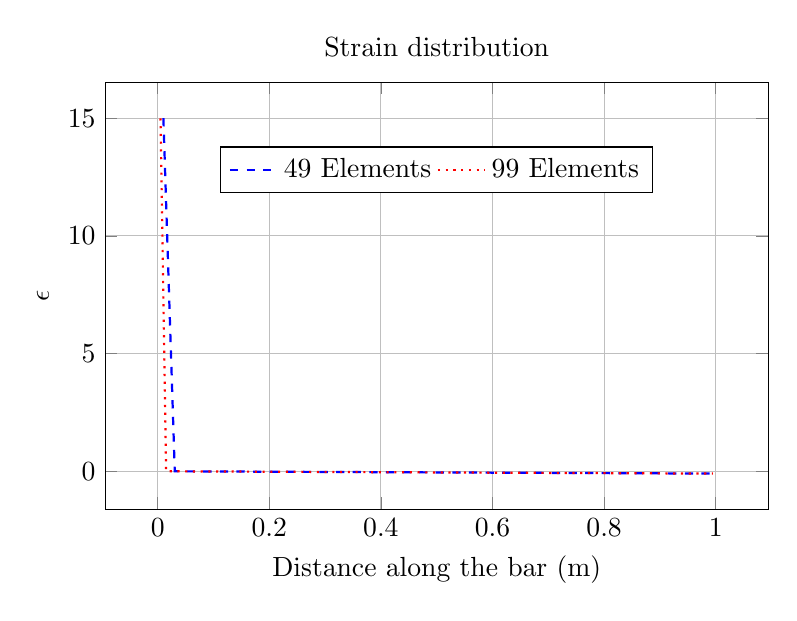
\begin{tikzpicture}
	\begin{axis}[
		title={Strain distribution},
		xlabel={Distance along the bar (\si{\meter})},
		ylabel={$\epsilon$},
		legend style={at={(0.5,0.85)}, anchor=north,legend columns=2},
		grid=major,
		width=10cm, height=7cm
		]
		
		% Database 1 (x, y) points using table
		\addplot[
		color=blue, dashed, thick
		% mark=square*,
		%thick
		] table[row sep=newline, x index=0, y index=1] {
			% (x, y) table for Database 1
			0.0102040816326531	15.0100102040815
			0.0306122448979592	-0.00204081632560005
			0.0510204081632653	-0.00408163265212913
			0.0714285714285714	-0.00612244897865821
			0.0918367346938775	-0.00816326530518730
			0.112244897959184	-0.0102040816317253
			0.132653061224490	-0.0122448979582543
			0.153061224489796	-0.0142857142847834
			0.173469387755102	-0.0163265306113125
			0.193877551020408	-0.0183673469378434
			0.214285714285714	-0.0204081632643742
			0.234693877551020	-0.0224489795909069
			0.255102040816327	-0.0244897959174342
			0.275510204081633	-0.0265306122439668
			0.295918367346939	-0.0285714285704977
			0.316326530612245	-0.0306122448970303
			0.336734693877551	-0.0326530612235576
			0.357142857142857	-0.0346938775500920
			0.377551020408163	-0.0367346938766211
			0.397959183673470	-0.0387755102031502
			0.418367346938776	-0.0408163265296828
			0.438775510204082	-0.0428571428562119
			0.459183673469388	-0.0448979591827410
			0.479591836734694	-0.0469387755092683
			0.500000000000000	-0.0489795918358009
			0.520408163265306	-0.0510204081623247
			0.540816326530613	-0.0530612244888591
			0.561224489795919	-0.0551020408153899
			0.581632653061225	-0.0571428571419208
			0.602040816326531	-0.0591836734684499
			0.622448979591837	-0.0612244897949790
			0.642857142857143	-0.0632653061215116
			0.663265306122449	-0.0653061224480425
			0.683673469387756	-0.0673469387745698
			0.704081632653062	-0.0693877551011060
			0.724489795918368	-0.0714285714276333
			0.744897959183674	-0.0734693877541588
			0.765306122448980	-0.0755102040806968
			0.785714285714286	-0.0775510204072258
			0.806122448979592	-0.0795918367337585
			0.826530612244899	-0.0816326530602893
			0.846938775510205	-0.0836734693868237
			0.867346938775511	-0.0857142857133546
			0.887755102040817	-0.0877551020398855
			0.908163265306123	-0.0897959183664145
			0.928571428571429	-0.0918367346929436
			0.948979591836735	-0.0938775510194763
			0.969387755102042	-0.0959183673460053
			0.989795918367348	-0.0979591836725344
		};
		\addlegendentry{49 Elements}
		
		% Database 2 (x, y) points using table
		\addplot[
		color=red,dotted, thick
		%mark=*,
		%thick
		] table[row sep=newline, x index=0, y index=1] {
			% (x, y) table for Database 2
			0.00505050505050505	15.0000151515150
			0.0151515151515152	-0.00101010100898691
			0.0252525252525253	-0.00202020201908937
			0.0353535353535354	-0.00303030302918828
			0.0454545454545455	-0.00404040403929251
			0.0555555555555556	-0.00505050504938964
			0.0656565656565657	-0.00606060605949388
			0.0757575757575758	-0.00707070706959279
			0.0858585858585859	-0.00808080807969525
			0.0959595959595960	-0.00909090908979771
			0.106060606060606	-0.0101010100998984
			0.116161616161616	-0.0111111111100026
			0.126262626262626	-0.0121212121200998
			0.136363636363636	-0.0131313131302004
			0.146464646464646	-0.0141414141403029
			0.156565656565657	-0.0151515151504000
			0.166666666666667	-0.0161616161605043
			0.176767676767677	-0.0171717171706032
			0.186868686868687	-0.0181818181807021
			0.196969696969697	-0.0191919191908028
			0.207070707070707	-0.0202020202009052
			0.217171717171717	-0.0212121212110059
			0.227272727272727	-0.0222222222211030
			0.237373737373737	-0.0232323232312091
			0.247474747474748	-0.0242424242413097
			0.257575757575758	-0.0252525252514122
			0.267676767676768	-0.0262626262615076
			0.277777777777778	-0.0272727272716118
			0.287878787878788	-0.0282828282817160
			0.297979797979798	-0.0292929292918132
			0.308080808080808	-0.0303030303019174
			0.318181818181818	-0.0313131313120145
			0.328282828282828	-0.0323232323221205
			0.338383838383839	-0.0333333333322177
			0.348484848484849	-0.0343434343423219
			0.358585858585859	-0.0353535353524244
			0.368686868686869	-0.0363636363625233
			0.378787878787879	-0.0373737373726222
			0.388888888888889	-0.0383838383827264
			0.398989898989899	-0.0393939393928235
			0.409090909090909	-0.0404040404029278
			0.419191919191919	-0.0414141414130285
			0.429292929292930	-0.0424242424231291
			0.439393939393940	-0.0434343434332369
			0.449494949494950	-0.0444444444433323
			0.459595959595960	-0.0454545454534348
			0.469696969696970	-0.0464646464635390
			0.479797979797980	-0.0474747474736379
			0.489898989898990	-0.0484848484837386
			0.500000000000000	-0.0494949494938375
			0.510101010101010	-0.0505050505039399
			0.520202020202020	-0.0515151515140389
			0.530303030303031	-0.0525252525241413
			0.540404040404040	-0.0535353535342402
			0.550505050505051	-0.0545454545443427
			0.560606060606061	-0.0555555555544416
			0.570707070707071	-0.0565656565645423
			0.580808080808081	-0.0575757575746447
			0.590909090909091	-0.0585858585847472
			0.601010101010101	-0.0595959595948443
			0.611111111111111	-0.0606060606049486
			0.621212121212121	-0.0616161616150457
			0.631313131313131	-0.0626262626251481
			0.641414141414141	-0.0636363636352506
			0.651515151515151	-0.0646464646453531
			0.661616161616161	-0.0656565656554538
			0.671717171717171	-0.0666666666655509
			0.681818181818181	-0.0676767676756533
			0.691919191919191	-0.0686868686857540
			0.702020202020201	-0.0696969696958512
			0.712121212121212	-0.0707070707059536
			0.722222222222221	-0.0717171717160543
			0.732323232323232	-0.0727272727261514
			0.742424242424242	-0.0737373737362503
			0.752525252525252	-0.0747474747463546
			0.762626262626262	-0.0757575757564535
			0.772727272727272	-0.0767676767665524
			0.782828282828282	-0.0777777777766531
			0.792929292929292	-0.0787878787867520
			0.803030303030302	-0.0797979797968544
			0.813131313131312	-0.0808080808069551
			0.823232323232322	-0.0818181818170594
			0.833333333333332	-0.0828282828271600
			0.843434343434342	-0.0838383838372625
			0.853535353535352	-0.0848484848473650
			0.863636363636362	-0.0858585858574692
			0.873737373737372	-0.0868686868675699
			0.883838383838382	-0.0878787878776706
			0.893939393939393	-0.0888888888877730
			0.904040404040402	-0.0898989898978719
			0.914141414141413	-0.0909090909079708
			0.924242424242423	-0.0919191919180751
			0.934343434343433	-0.0929292929281740
			0.944444444444443	-0.0939393939382764
			0.954545454545453	-0.0949494949483789
			0.964646464646463	-0.0959595959584796
			0.974747474747473	-0.0969696969685820
			0.984848484848483	-0.0979797979786827
			0.994949494949493	-0.0989898989887834
		};
		\addlegendentry{99 Elements}
		
	\end{axis}
\end{tikzpicture}
		\caption{Strain distribution along the bar.}
		\label{strain_dist_local}
	\end{subfigure}
	\caption{Results without regularization}
	\label{fig:Results_without_regularization}
\end{figure}



Thus, with the ingredients presented (the arc length solver and the choice of metric), the data driven solver is able to exhibit the mesh dependence of the solution as expected when there is no regularization.

\begin{remark}
	Results from the analysis performed in \ref{appx_convergence} reveals that an optimal rate of convergence is obtained when the metric in the distance functional is taken equal to the tangent, $\parder{\sigma^*}{\epsilon^*}$, obtained from the corresponding material state. For materials that undergo damage, this derivative is negative. Thus, during the alternate minimization process, for the elements that undergo damage, $C$ is smaller than zero. It shall be noted that the convergence of the solver is still judged on the basis of the metric that is equal to the elastic modulus and the tangent is used only during the alternate minimization and the corresponding Newton iterations. It shall be noted that in some cases, not using the tangent as a metric resulted in the solution converging to an \textit{incorrect} solution.
\end{remark}

\begin{remark}
	In non DD setting, the damage problem involves minimizing a functional that is non-convex. The energy density is a function of displacement and damage, and is separately convex with respect to the two variables. Thus, the minimization is performed alternatively between the two variables to find the solution. The problem is thus \textit{convexified} in non-DD setting. This allows the minimizers to \textit{jump through} instabilities such as snapbacks under displacement control (the number of iterations needed might be higher, though). It shall be noted that using a Newton solver (without additional refinements) for non-convex minimization may lead to unconvergence \cite{Farrell2017,Gerasimov2016}.
	
	In DD setting, however, the database looks like in figure \ref{1D_bar_dam_elem} and thus, the nonconvexity is inherently contained in the database. Thus, an arclength method has been used to track the entire bifurcation branch without having to jump through. Also, it is unclear is it is indeed possible to jump through snapbacks in this case as the convexity is not specifically handled. 
\end{remark}

\section{Introduction of a length scale}

In the previous section, it was demonstrated that the Data Driven algorithm with no regularization (and a \textit{local} database) results in mesh dependence of the solution (as expected). Here, the strain based Lipschitz regularization, introduced in \cite{Kamasamudram2023}, will first be developed for the Data driven case (for 1D). It will then be applied for the problem introduced in the previous section. A relaxed version of the method will then be developed and presented for the 2D case later on.

\subsection{The method}
The regularization technique was introduced in \cite{Kamasamudram2023}, where it was tested with a constitutive model. Here, it will first be extended for use with the DDCM methodology.

To begin with, a length scale is introduced into the problem by restricting the gradient of the strain variable to lie in a certain interval. More precisely, it is required that $\epsilon_{,x} \in [-1/{\ell_c}, 1/{\ell_c} ]$, where $\ell_c$ is a length parameter. It is expected that the introduction of this constraint prevents the spurious strain localization, and the dependence of the solution on the Finite Element mesh size. 


The introduction of the Lipschitz constraint on the strain variable modifies the equation of equilibrium (in 1D) to 
\begin{equation}
	\sigma_{,x}- \lambda_{,xx}=0,\label{equil_couple_1D}
\end{equation}
see equation 37 of \cite{Kamasamudram2023}, where $\lambda$ is the Lagrange multiplier that is dual to the Lipschitz constraint. Also, $\lambda \neq 0$ only in the regions of the body where the constraint is active. The equations of equilibrium used in DDCM should thus take this into account. 

Beginning with the distance functional,
\begin{equation}
	d(\bfeps,\bfsig,\bfeps^*,\bfsig^*) = \frac{1}{2}(\bfB \bfu - \bfeps^*)^T\mathcal{C}\bfw(\bfB \bfu - \bfeps^*) + \frac{1}{2}(\bfsig - \bfsig^*)^T\mathcal{C}^{-1}\bfw(\bfsig - \bfsig^*),
\end{equation}
the objective now is to find the minimizers of the above functional so that the strain field satisfies the Lipschitz constraint, and the stress fields satisfy the equilibrium. As already mentioned, the Lagrange multipliers that enforce the constraint on the strain field act as couple stresses.
\begin{equation}
	\text{Sol } \in \arg \min_{(\bfeps,\bfsig) \in \mathcal{E}, (\bfeps^*,\bfsig^*) \in \mathcal{D}} d(\bfeps,\bfsig,\bfeps^*,\bfsig^*),
\end{equation}
where, the equilibrium manifold is now defined as (in discrete form)
 

\begin{equation}
	\mathcal{E} = \{(\bfeps,\bfsig) : \bfeps = \bfB \bfu, \bfeps \text{ is such that } |\bfB' \bfeps|  \leq 1/{\ell_c} ,\bfu = \bfu_D \text{ on } \partial \Omega_d,
	\text{ and } \bfB ^T\bfw \bfsig + \bfP^T \bflam = 0     \},
\end{equation}
where $\bflam$ is the Lagrange multiplier. $\bfB'$ is the discrete gradient operator on the strain variable (see figure \ref{mesh_dual_1d}), and $\bfP = \bfB \bfB'$ is the discrete second gradient operator. To facilitate things, the Lagrangian will be redefined as follows:
\begin{equation}
	\Pi = d(\bfeps,\bfsig,\bfeps^*,\bfsig^*) - \bfeta^T \bfB ^T \bfw\bfsig + \sum_{i=1}^{N_c} \lambda^u_i \left( (\bfP \bfu)_i - \frac{1}{\ell_c}   \right) + \sum_{i=1}^{N_c} \lambda^{\eta u}_i \left( (\bfP (\bfu + \bfeta))_i - \frac{1}{\ell_c}   \right).
\end{equation}
Here, $N_c$ denotes the number of active constraints and $\lambda^u_i \geq 0$ are the Lagrange multipliers dual to the constraint on the gradient of strain, and $(\bullet)_i$ denotes the $i$th component of the vector $\bullet$. The solution is defined as the collection that renders the Lagrangian stationary.
\begin{equation}
	\Pi  \leftarrow \statop!
\end{equation}

\begin{remark}
	The third and the fourth terms in the Lagrangian warrant some discussion. It is clear that the third term, together with the condition that $\lambda^u\geq0$, enforces the inequality constraint $\epsilon_{,x} \leq 1/\ell_c$. Treating $\bfeta$ as the virtual displacement, the fourth term enforces the constraint that in the regions where the inequality constraint is satisfied as an equality, the perturbed field, $\bfu+\bfeta$, must also satisfy the constraint as an equality. It shall be noted that there is a priori no restriction on the sign of $\lambda_{\eta u}$. However, as will be demonstrated below, at convergence, $\lambda^{\eta u}_i = -\lambda^{ u}_i$. This, owing to the restriction on $\lambda_u$, determines the sign of $\lambda_{\eta u}$.
\end{remark}

 


The Euler Lagrange equations can be seen to be
\begin{gather}
	\bfr_{\bfu} = \bfB^T \mathcal{C}\bfw \bfB \bfu - \bfB^T \mathcal{C}\bfw \bfeps ^* + \bfP^T \bflam^u +\bfP^T \bflam^{\eta u}  =0, \label{residual_u_1D_DD} \\
	\bfr_{\bfeta} = -\bfB^T\bfw \mathcal{C} \bfB \bfeta - \bfB^T\bfw \bfsig ^* +\bfP^T \bflam^{\eta u} =0, \\
	r_{\lambda^u_i} =  (\bfP \bfu)_i - \frac{1}{\ell_c}  =0, \\
	r_{\lambda^{\eta u}_i} =  (\bfP (\bfu + \bfeta))_i - \frac{1}{\ell_c}  =0. 
\end{gather}

At convergence, $\bfeps=\bfeps^*$ and $\bfeta=0$. Thus, from equation \ref{residual_u_1D_DD}, it can be seen that $\lambda^u_i = -\lambda^{\eta u}_i$, as mentioned earlier. The equations of equilibrium can be recovered as $\bfB^T \bfw \bfsig +\bfP^T \bflam^{u} =0$, since $\bfsig = \bfsig^*$ at convergence.

\subsection{Application and results}
The regularization technique is now applied to the DDCM case tested earlier with a body force. The value of $\ell_c$ is taken to be $0.1\si{\meter}$. Arc length solver has been used like in the previous case with similar loading conditions. A piecewise linear and continuous interpolation has been used for displacement and a piecewise constant for the mechanical stress. A dual mesh had been used to impose the constraint on the strain gradient. The strain is taken to be piecewise linear and continuous on the dual mesh. See figure \ref{mesh_dual_1d}. In this case, the discrete gradient operator $\bfB'$ is calculated on the dual (red) mesh.

\begin{figure}[ht]
	\centering
	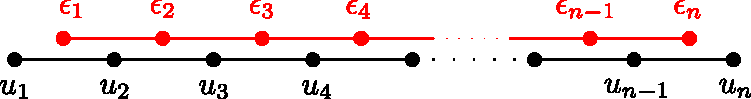
\includegraphics[width=0.5\linewidth]{./mesh_dual_1d.pdf}
	\caption{Mesh for displacement and strain}
	\label{mesh_dual_1d}
\end{figure}



\begin{figure}[ht]
	\begin{subfigure}{0.45\textwidth}
		\centering
		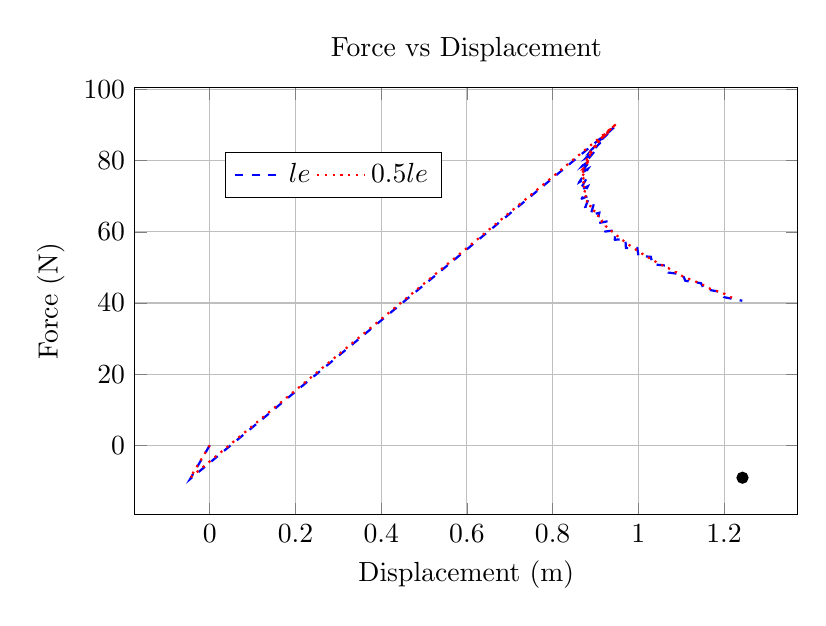
\begin{tikzpicture}
	\begin{axis}[
		title={Force vs Displacement},
		xlabel={Displacement (\si{\meter})},
		ylabel={Force (\si{\newton})},
		legend style={at={(0.3,0.85)}, anchor=north,legend columns=2},
		grid=major,
		width=10cm, height=7cm
		]
		
		% Database 1 (x, y) points using table
		\addplot[
		color=blue, dashed, thick
		% mark=square*,
		%thick
		] table[row sep=newline, x index=0, y index=1] {
			% (x, y) table for Database 1
			0	0
			-0.0457499999999999	-9.46602564103146
			-0.0417500000000001	-9.06602564103147
			-0.0377500000000001	-8.66602564103729
			-0.0337500000000000	-8.26602564103727
			-0.0297500000000001	-7.86602564104894
			-0.0257500000000002	-7.46602564104894
			-0.0217500000000000	-7.06602564104891
			-0.0177499999999998	-6.66602564104894
			-0.0137500000000003	-6.26602564104895
			-0.00974999999999992	-5.86602564107221
			-0.00574999999999940	-5.46602564107219
			-0.00174999999999980	-5.06602564107222
			0.00225000000000029	-4.66602564107220
			0.00625000000000006	-4.26602564107221
			0.0102500000000001	-3.86602564107222
			0.0142499999999999	-3.46602564107219
			0.0182499999999990	-3.06602564107219
			0.0222499999999999	-2.66602564107228
			0.0262499999999996	-2.26602564107218
			0.0302499999999991	-1.86602564111884
			0.0342499999999997	-1.46602564111875
			0.0382499999999996	-1.06602564111878
			0.0422500000000014	-0.666025641118683
			0.0462499999999989	-0.266025641118767
			0.0502500000000009	0.133974358881253
			0.0542500000000012	0.533974358881281
			0.0582500000000016	0.933974358881154
			0.0622500000000013	1.33397435888116
			0.0662500000000013	1.73397435888117
			0.0702500000000004	2.13397435888120
			0.0742500000000015	2.53397435888129
			0.0782499999999994	2.93397435888111
			0.0822499999999993	3.33397435888121
			0.0862500000000011	3.73397435888131
			0.0902500000000001	4.13397435888133
			0.0942499999999993	4.53397435888128
			0.0982500000000005	4.93397435888116
			0.102250000000002	5.33397435888123
			0.106249999999998	5.73397435878810
			0.110249999999999	6.13397435878803
			0.114250000000002	6.53397435878811
			0.118249999999999	6.93397435878808
			0.122250000000001	7.33397435878822
			0.126250000000001	7.73397435878815
			0.130249999999999	8.13397435878814
			0.134250000000002	8.53397435878823
			0.138249999999999	8.93397435878825
			0.142249999999999	9.33397435878795
			0.146250000000001	9.73397435878823
			0.150250000000001	10.1339743587879
			0.154249999999998	10.5339743587880
			0.158249999999999	10.9339743587882
			0.162250000000002	11.3339743587882
			0.166250000000002	11.7339743587880
			0.170250000000000	12.1339743587882
			0.174250000000000	12.5339743587882
			0.178249999999998	12.9339743587882
			0.182249999999999	13.3339743587880
			0.186250000000003	13.7339743587884
			0.190249999999998	14.1339743587881
			0.194250000000003	14.5339743587882
			0.198249999999998	14.9339743587881
			0.202250000000002	15.3339743587882
			0.206249999999996	15.7339743587878
			0.210250000000002	16.1339743587886
			0.214250000000004	16.5339743587880
			0.218250000000000	16.9339743587883
			0.222250000000000	17.3339743587881
			0.226249999999997	17.7339743587881
			0.230249999999998	18.1339743587882
			0.234250000000006	18.5339743587884
			0.238250000000000	18.9339743587884
			0.242249999999998	19.3339743587880
			0.246250000000001	19.7339743587877
			0.250250000000000	20.1339743587881
			0.254250000000004	20.5339743587883
			0.258249999999996	20.9339743587883
			0.262250000000001	21.3339743586019
			0.266250000000002	21.7339743586019
			0.270249999999998	22.1339743586019
			0.274250000000004	22.5339743586019
			0.278250000000000	22.9339743586017
			0.282249999999998	23.3339743586014
			0.286250000000002	23.7339743586021
			0.290249999999999	24.1339743586017
			0.294250000000001	24.5339743586017
			0.298250000000000	24.9339743586016
			0.302249999999999	25.3339743586019
			0.306249999999998	25.7339743586016
			0.310249999999997	26.1339743586017
			0.314250000000002	26.5339743586021
			0.318249999999997	26.9339743586017
			0.322249999999999	27.3339743586018
			0.326250000000002	27.7339743586022
			0.330250000000004	28.1339743586017
			0.334250000000001	28.5339743586017
			0.338249999999995	28.9339743586015
			0.342249999999995	29.3339743586016
			0.346250000000003	29.7339743586020
			0.350249999999999	30.1339743586017
			0.354250000000004	30.5339743586020
			0.358249999999998	30.9339743586018
			0.362249999999995	31.3339743586013
			0.366249999999997	31.7339743586020
			0.370249999999998	32.1339743586020
			0.374249999999997	32.5339743586019
			0.378249999999998	32.9339743586011
			0.382250000000002	33.3339743586017
			0.386250000000006	33.7339743586022
			0.390250000000001	34.1339743586016
			0.394250000000004	34.5339743586019
			0.398249999999999	34.9339743586013
			0.402250000000002	35.3339743586019
			0.406250000000001	35.7339743586015
			0.410250000000001	36.1339743586015
			0.414249999999999	36.5339743586020
			0.418250000000000	36.9339743586023
			0.422249999999997	37.3339743586018
			0.426250000000000	37.7339743586015
			0.430250000000000	38.1339743586022
			0.434250000000007	38.5339743586020
			0.438249999999998	38.9339743586018
			0.442250000000002	39.3339743586021
			0.446250000000002	39.7339743586022
			0.450250000000001	40.1339743586017
			0.454249999999996	40.5339743586013
			0.458250000000002	40.9339743586019
			0.462250000000004	41.3339743586017
			0.466250000000004	41.7339743586018
			0.470249999999999	42.1339743586021
			0.474250000000003	42.5339743586021
			0.478250000000003	42.9339743586020
			0.482250000000003	43.3339743586022
			0.486249999999996	43.7339743586016
			0.490250000000000	44.1339743586023
			0.494249999999998	44.5339743586016
			0.498249999999996	44.9339743586016
			0.502250000000002	45.3339743586018
			0.506250000000004	45.7339743586024
			0.510250000000001	46.1339743586014
			0.514249999999997	46.5339743586017
			0.518249999999991	46.9339743586016
			0.522250000000008	47.3339743586020
			0.526250000000004	47.7339743586023
			0.530250000000003	48.1339743586016
			0.534250000000002	48.5339743586017
			0.538249999999994	48.9339743586012
			0.542249999999994	49.3339743586014
			0.546249999999998	49.7339743586014
			0.550249999999994	50.1339743586018
			0.554249999999997	50.5339743586016
			0.558249999999999	50.9339743586012
			0.562250000000005	51.3339743586017
			0.566249999999997	51.7339743586024
			0.570250000000000	52.1339743582288
			0.574250000000004	52.5339743582292
			0.578250000000007	52.9339743582299
			0.582250000000001	53.3339743582291
			0.586250000000008	53.7339743582292
			0.590250000000005	54.1339743582295
			0.594250000000008	54.5339743582296
			0.598250000000006	54.9339743582287
			0.602250000000001	55.3339743582295
			0.606249999999995	55.7339743582293
			0.610250000000004	56.1339743582295
			0.614249999999994	56.5339743582291
			0.618250000000005	56.9339743582289
			0.622249999999998	57.3339743582297
			0.626249999999997	57.7339743582285
			0.630250000000002	58.1339743582300
			0.634250000000010	58.5339743582296
			0.638249999999997	58.9339743582287
			0.642250000000002	59.3339743582292
			0.646250000000001	59.7339743582295
			0.650250000000004	60.1339743582299
			0.654249999999990	60.5339743582290
			0.658250000000001	60.9339743582296
			0.662249999999999	61.3339743582294
			0.666250000000002	61.7339743582299
			0.670250000000005	62.1339743582295
			0.674250000000004	62.5339743582296
			0.678250000000003	62.9339743582290
			0.682250000000003	63.3339743582299
			0.686250000000007	63.7339743582295
			0.690250000000002	64.1339743582289
			0.694249999999988	64.5339743582294
			0.698249999999997	64.9339743582291
			0.702249999999995	65.3339743582295
			0.706250000000008	65.7339743582301
			0.710249999999997	66.1339743582294
			0.714250000000003	66.5339743582298
			0.718249999999997	66.9339743582290
			0.722249999999993	67.3339743582293
			0.726249999999996	67.7339743582284
			0.730249999999992	68.1339743582296
			0.734249999999995	68.5339743582299
			0.738250000000005	68.9339743582293
			0.742250000000003	69.3339743582302
			0.746250000000010	69.7339743582294
			0.750250000000009	70.1339743582302
			0.754249999999998	70.5339743582303
			0.758250000000002	70.9339743582286
			0.762250000000007	71.3339743582299
			0.766250000000004	71.7339743582294
			0.770250000000017	72.1339743582304
			0.774249999999995	72.5339743582300
			0.778250000000011	72.9339743582299
			0.782249999999998	73.3339743582291
			0.786250000000000	73.7339743582299
			0.790249999999997	74.1339743582292
			0.794250000000008	74.5339743582292
			0.798250000000000	74.9339743582300
			0.802250000000004	75.3339743582297
			0.806249999999997	75.7339743582296
			0.810250000000005	76.1339743582292
			0.814250000000009	76.5339743582302
			0.818249999999995	76.9339743582291
			0.822250000000012	77.3339743582303
			0.826249999999998	77.7339743582298
			0.830249999999993	78.1339743582293
			0.834250000000005	78.5339743582298
			0.838250000000006	78.9339743582296
			0.842249999999991	79.3339743582299
			0.846249999999983	79.7339743582292
			0.850250000000015	80.1339743582306
			0.854249999999995	80.5339743582289
			0.858250000000005	80.9339743582292
			0.862250000000000	81.3339743582293
			0.866249999999997	81.7339743582294
			0.870249999999991	82.1339743582293
			0.874250000000013	82.5339743582293
			0.878249999999999	82.9339743582301
			0.882249999999992	83.3339743582288
			0.886250000000001	83.7339743582291
			0.890250000000009	84.1339743582307
			0.894249999999995	84.5339743582285
			0.898250000000001	84.9339743582291
			0.902249999999999	85.3339743582286
			0.906250000000012	85.7339743582307
			0.910249999999988	86.1339743582291
			0.914250000000001	86.5339743582298
			0.918250000000003	86.9339743582294
			0.922249999999987	87.3339743582268
			0.926249999999990	87.7339743582282
			0.930250000000002	88.1339743582301
			0.934250000000006	88.5339743582295
			0.938249999999998	88.9339743582297
			0.942250000000003	89.3339743582306
			0.946250000000001	89.7339743582292
			0.950249999999999	90.1339743582303
			0.950248678571446	90.1338315029219
			0.950247357142846	90.1336886457791
			0.950246035714271	90.1335457886351
			0.950244714285700	90.1334029314922
			0.950243392857143	90.1332600743493
			0.950242071428563	90.1331172172070
			0.950240750000012	90.1329743600655
			0.950239428571433	90.1328315029214
			0.950238107142851	90.1326886457779
			0.950236785714294	90.1325457886365
			0.950235464285729	90.1324029314946
			0.950234142857149	90.1322600743498
			0.950232821428576	90.1321172172069
			0.950231499999989	90.1319743600647
			0.950230178571434	90.1318315029223
			0.950228857142863	90.1316886457784
			0.950227535714290	90.1315457886348
			0.950226214285716	90.1314029314926
			0.950224892857153	90.1312600743516
			0.950223571428561	90.1311172172060
			0.950222250000004	90.1309743600650
			0.950220928571434	90.1308315029211
			0.950219607142855	90.1306886457789
			0.950218285714289	90.1305457886359
			0.950216964285711	90.1304029314932
			0.950215642857137	90.1302600743497
			0.950214321428574	90.1301172172075
			0.950213000000012	90.1299743600639
			0.950211678571421	90.1298315029208
			0.950210357142849	90.1296886457787
			0.950209035714286	90.1295457886355
			0.950207714285711	90.1294029314923
			0.950206392857129	90.1292600743505
			0.950205071428557	90.1291172172069
			0.950203749999987	90.1289743600630
			0.950202428571436	90.1288315029219
			0.950201107142844	90.1286886457774
			0.950199785714287	90.1285457886367
			0.950198464285728	90.1284029314933
			0.950197142857122	90.1282600743490
			0.950195821428568	90.1281172172070
			0.950194500000006	90.1279743600647
			0.950193178571422	90.1278315029213
			0.950191857142849	90.1276886457786
			0.950190535714313	90.1275457886379
			0.950189214285706	90.1274029314920
			0.950187892857127	90.1272600743485
			0.950186571428560	90.1271172172064
			0.950185250000003	90.1269743600649
			0.950183928571423	90.1268315029217
			0.950182607142844	90.1266886457789
			0.950181285714292	90.1265457886372
			0.950179964285707	90.1264029314921
			0.950178642857138	90.1262600743499
			0.950177321428578	90.1261172172068
			0.950175999999990	90.1259743600643
			0.950174678571435	90.1258315029218
			0.950173357142852	90.1256886457791
			0.950172035714281	90.1255457886358
			0.950170714285718	90.1254029314925
			0.950169392857141	90.1252600743511
			0.950168071428561	90.1251172172067
			0.950166749999996	90.1249743600638
			0.950165428571414	90.1248315029228
			0.950164107142866	90.1246886457784
			0.950162785714294	90.1245457886361
			0.950161464285702	90.1244029314922
			0.950160142857155	90.1242600743506
			0.950158821428570	90.1241172172069
			0.950157499999990	90.1239743600647
			0.950156178571435	90.1238315029215
			0.950154857142870	90.1236886457786
			0.950153535714275	90.1235457886355
			0.950152214285721	90.1234029314930
			0.950150892857138	90.1232600743482
			0.950149571428558	90.1231172172071
			0.950148250000001	90.1229743600634
			0.950146928571439	90.1228315029211
			0.950145607142846	90.1226886457771
			0.950144285714282	90.1225457886357
			0.950142964285707	90.1224029314933
			0.950141642857144	90.1222600743502
			0.950140321428577	90.1221172172061
			0.950138999999996	90.1219743600636
			0.950137678571416	90.1218315029210
			0.950136357142855	90.1216886457789
			0.950135035714288	90.1215457886352
			0.950133714285726	90.1214029314939
			0.950132392857135	90.1212600743497
			0.950131071428558	90.1211172172070
			0.950129749999983	90.1209743600629
			0.950128428571431	90.1208315029214
			0.950127107142848	90.1206886457777
			0.950125785714281	90.1205457886350
			0.950124464285712	90.1204029314926
			0.950123142857120	90.1202600743497
			0.950121821428575	90.1201172172071
			0.950120499999982	90.1199743600620
			0.950119178571418	90.1198315029218
			0.950117857142848	90.1196886457777
			0.950116535714294	90.1195457886362
			0.950115214285710	90.1194029314920
			0.950113892857140	90.1192600743503
			0.950112571428563	90.1191172172069
			0.950111250000016	90.1189743600651
			0.950109928571435	90.1188315029211
			0.950108607142856	90.1186886457783
			0.950107285714289	90.1185457886353
			0.950105964285718	90.1184029314941
			0.950104642857139	90.1182600743503
			0.950103321428578	90.1181172172072
			0.950101999999992	90.1179743600640
			0.950100678571422	90.1178315029202
			0.950099357142847	90.1176886457785
			0.950098035714279	90.1175457886355
			0.950096714285711	90.1174029314922
			0.950095392857125	90.1172600743483
			0.950094071428568	90.1171172172067
			0.950092750000002	90.1169743600642
			0.950091428571427	90.1168315029219
			0.950090107142856	90.1166886457783
			0.950088785714295	90.1165457886374
			0.950087464285722	90.1164029314929
			0.950086142857138	90.1162600743509
			0.950084821428563	90.1161172172073
			0.950083499999998	90.1159743600644
			0.950082178571421	90.1158315029213
			0.950080857142843	90.1156886457777
			0.950079535714283	90.1155457886351
			0.950078214285723	90.1154029314931
			0.950076892857142	90.1152600743507
			0.950075571428558	90.1151172172067
			0.950074249999994	90.1149743600625
			0.950072928571420	90.1148315029209
			0.950071607142852	90.1146886457778
			0.950070285714286	90.1145457886351
			0.950068964285713	90.1144029314936
			0.950067642857146	90.1142600743505
			0.950066321428572	90.1141172172060
			0.950064999999995	90.1139743600634
			0.950063678571424	90.1138315029212
			0.950062357142861	90.1136886457780
			0.950061035714289	90.1135457886362
			0.950059714285714	90.1134029314929
			0.950058392857137	90.1132600743499
			0.950057071428571	90.1131172172073
			0.950055749999999	90.1129743600646
			0.950054428571427	90.1128315029224
			0.950053107142841	90.1126886457789
			0.950051785714287	90.1125457886358
			0.950050464285706	90.1124029314923
			0.950049142857145	90.1122600743503
			0.950047821428555	90.1121172172061
			0.950046500000003	90.1119743600642
			0.950045178571434	90.1118315029213
			0.950043857142854	90.1116886457782
			0.950042535714274	90.1115457886356
			0.950041214285702	90.1114029314916
			0.950039892857139	90.1112600743500
			0.950038571428558	90.1111172172063
			0.950037249999988	90.1109743600628
			0.950035928571428	90.1108315029214
			0.950034607142855	90.1106886457796
			0.950033285714286	90.1105457886365
			0.950031964285725	90.1104029314932
			0.950030642857142	90.1102600743500
			0.950029321428566	90.1101172172071
			0.950028000000010	90.1099743600644
			0.950026678571441	90.1098315029205
			0.950025357142843	90.1096886457782
			0.950024035714293	90.1095457886350
			0.950022714285719	90.1094029314938
			0.950021392857146	90.1092600743503
			0.950020071428563	90.1091172172069
			0.950018749999997	90.1089743600639
			0.950017428571422	90.1088315029213
			0.950016107142861	90.1086886457786
			0.950014785714278	90.1085457886350
			0.950013464285709	90.1084029314926
			0.950012142857133	90.1082600743502
			0.950010821428559	90.1081172172061
			0.950009500000008	90.1079743600651
			0.950008178571401	90.1078315029216
			0.950006857142868	90.1076886457790
			0.950005535714285	90.1075457886349
			0.950004214285699	90.1074029314931
			0.950002892857128	90.1072600743491
			0.950001571428576	90.1071172172074
			0.950000249999997	90.1069743600645
			0.949998928571429	90.1068315029224
			0.949997607142850	90.1066886457775
			0.949996285714277	90.1065457886351
			0.949994964285723	90.1064029314930
			0.949993642857144	90.1062600743509
			0.949992321428581	90.1061172172081
			0.949990999999987	90.1059743600642
			0.949989678571436	90.1058315029210
			0.949988357142845	90.1056886457784
			0.949987035714288	90.1055457886350
			0.949985714285724	90.1054029314918
			0.949984392857151	90.1052600743505
			0.949983071428580	90.1051172172067
			0.949981750000023	90.1049743600646
			0.949980428571438	90.1048315029220
			0.949979107142862	90.1046886457794
			0.949977785714282	90.1045457886358
			0.949976464285709	90.1044029314926
			0.949975142857141	90.1042600743495
			0.949973821428567	90.1041172172063
			0.949972499999986	90.1039743600632
			0.949971178571437	90.1038315029227
			0.949969857142862	90.1036886457785
			0.949968535714286	90.1035457886356
			0.949967214285708	90.1034029314923
			0.949965892857141	90.1032600743496
			0.949964571428568	90.1031172172063
			0.949963249999999	90.1029743600639
			0.949961928571430	90.1028315029227
			0.949960607142853	90.1026886457780
			0.949959285714290	90.1025457886365
			0.949957964285714	90.1024029314924
			0.949956642857149	90.1022600743513
			0.949955321428575	90.1021172172078
			0.949954000000002	90.1019743600646
			0.949952678571438	90.1018315029213
			0.949951357142843	90.1016886457784
			0.949950035714285	90.1015457886354
			0.949948714285708	90.1014029314937
			0.949947392857141	90.1012600743498
			0.949946071428559	90.1011172172071
			0.949944749999991	90.1009743600631
			0.949943428571428	90.1008315029199
			0.949942107142846	90.1006886457778
			0.949940785714288	90.1005457886357
			0.949939464285706	90.1004029314936
			0.949938142857134	90.1002600743489
			0.949936821428570	90.1001172172074
			0.949935499999994	90.0999743600643
			0.949934178571422	90.0998315029201
			0.949932857142863	90.0996886457787
			0.949931535714283	90.0995457886346
			0.949930214285716	90.0994029314927
			0.949928892857149	90.0992600743502
			0.949927571428574	90.0991172172066
			0.949926250000005	90.0989743600645
			0.949924928571413	90.0988315029196
			0.949923607142858	90.0986886457794
			0.949922285714285	90.0985457886357
			0.949920964285713	90.0984029314921
			0.949919642857140	90.0982600743507
			0.949918321428571	90.0981172172066
			0.949916999999995	90.0979743600642
			0.949915678571425	90.0978315029220
			0.949914357142854	90.0976886457777
			0.949913035714288	90.0975457886358
			0.949911714285701	90.0974029314915
			0.949910392857151	90.0972600743501
			0.949909071428560	90.0971172172075
			0.949907750000002	90.0969743600636
			0.949906428571416	90.0968315029216
			0.949905107142848	90.0966886457773
			0.949903785714298	90.0965457886364
			0.949902464285704	90.0964029314924
			0.949901142857151	90.0962600743496
			0.949899821428561	90.0961172172060
			0.949898499999992	90.0959743600640
			0.949897178571411	90.0958315029205
			0.949895857142862	90.0956886457784
			0.949894535714284	90.0955457886351
			0.949893214285706	90.0954029314921
			0.949891892857127	90.0952600743498
			0.949890571428580	90.0951172172071
			0.949889250000021	90.0949743600639
			0.949887928571413	90.0948315029208
			0.949886607142847	90.0946886457777
			0.949885285714280	90.0945457886366
			0.949883964285720	90.0944029314925
			0.949882642857136	90.0942600743483
			0.949881321428576	90.0941172172066
			0.949879999999992	90.0939743600632
			0.949878678571434	90.0938315029223
			0.949877357142861	90.0936886457779
			0.949876035714283	90.0935457886369
			0.949874714285732	90.0934029314938
			0.949873392857137	90.0932600743485
			0.949872071428561	90.0931172172062
			0.949870750000005	90.0929743600628
			0.949869428571428	90.0928315029216
			0.949868107142857	90.0926886457785
			0.949866785714295	90.0925457886364
			0.949865464285712	90.0924029314925
			0.949864142857148	90.0922600743503
			0.949862821428570	90.0921172172083
			0.949861499999985	90.0919743600635
			0.949860178571432	90.0918315029213
			0.949858857142863	90.0916886457785
			0.949857535714274	90.0915457886356
			0.949856214285709	90.0914029314926
			0.949854892857150	90.0912600743501
			0.949853571428571	90.0911172172070
			0.949852249999995	90.0909743600640
			0.949850928571422	90.0908315029203
			0.949849607142867	90.0906886457786
			0.949848285714274	90.0905457886350
			0.949846964285710	90.0904029314927
			0.949845642857138	90.0902600743499
			0.949844321428563	90.0901172172074
			0.949843000000001	90.0899743600644
			0.949841678571422	90.0898315029208
			0.949840357142851	90.0896886457781
			0.949839035714282	90.0895457886347
			0.949837714285714	90.0894029314918
			0.949836392857141	90.0892600743507
			0.949835071428578	90.0891172172078
			0.949833750000002	90.0889743600623
			0.949832428571409	90.0888315029203
			0.949831107142861	90.0886886457788
			0.949829785714265	90.0885457886354
			0.949828464285729	90.0884029314936
			0.949827142857132	90.0882600743494
			0.949825821428569	90.0881172172070
			0.949824499999989	90.0879743600640
			0.949823178571418	90.0878315029206
			0.949821857142837	90.0876886457766
			0.949820535714285	90.0875457886355
			0.949819214285701	90.0874029314917
			0.949817892857131	90.0872600743496
			0.949816571428567	90.0871172172061
			0.949815250000003	90.0869743600647
			0.949813928571427	90.0868315029208
			0.949812607142862	90.0866886457798
			0.949811285714291	90.0865457886360
			0.949809964285709	90.0864029314937
			0.949808642857131	90.0862600743487
			0.949807321428559	90.0861172172067
			0.949806000000000	90.0859743600638
			0.949804678571442	90.0858315029215
			0.949803357142853	90.0856886457778
			0.949802035714281	90.0855457886344
			0.949800714285718	90.0854029314917
			0.949799392857131	90.0852600743501
			0.949798071428573	90.0851172172066
			0.949796750000002	90.0849743600641
			0.949795428571422	90.0848315029204
			0.949794107142844	90.0846886457773
			0.949792785714264	90.0845457886341
			0.949791464285717	90.0844029314930
			0.949790142857134	90.0842600743498
			0.949788821428560	90.0841172172074
			0.949787499999986	90.0839743600634
			0.949786178571428	90.0838315029222
			0.949784857142844	90.0836886457778
			0.949783535714279	90.0835457886356
			0.949782214285707	90.0834029314923
			0.949780892857154	90.0832600743497
			0.949779571428575	90.0831172172072
			0.949778250000004	90.0829743600651
			0.949776928571434	90.0828315029208
			0.949775607142870	90.0826886457788
			0.949774285714276	90.0825457886360
			0.949772964285707	90.0824029314918
			0.949771642857141	90.0822600743496
			0.949770321428579	90.0821172172076
			0.949768999999995	90.0819743600638
			0.949767678571428	90.0818315029213
			0.949766357142852	90.0816886457784
			0.949765035714280	90.0815457886341
			0.949763714285711	90.0814029314920
			0.949762392857142	90.0812600743495
			0.949761071428553	90.0811172172059
			0.949759749999996	90.0809743600637
			0.949758428571413	90.0808315029210
			0.949757107142851	90.0806886457784
			0.949755785714293	90.0805457886345
			0.949754464285703	90.0804029314916
			0.949753142857139	90.0802600743492
			0.949751821428566	90.0801172172071
			0.949750500000004	90.0799743600646
			0.949749178571435	90.0798315029214
			0.949747857142857	90.0796886457782
			0.949746535714295	90.0795457886367
			0.949745214285716	90.0794029314919
			0.949743892857138	90.0792600743499
			0.949742571428571	90.0791172172072
			0.949741249999995	90.0789743600643
			0.949739928571428	90.0788315029211
			0.949738607142846	90.0786886457766
			0.949737285714296	90.0785457886359
			0.949735964285705	90.0784029314928
			0.949734642857128	90.0782600743492
			0.949733321428584	90.0781172172081
			0.949731999999992	90.0779743600633
			0.949730678571406	90.0778315029199
			0.949729357142858	90.0776886457771
			0.949728035714283	90.0775457886360
			0.949726714285729	90.0774029314941
			0.949725392857152	90.0772600743503
			0.949724071428568	90.0771172172072
			0.949722749999988	90.0769743600637
			0.949721428571431	90.0768315029200
			0.949720107142858	90.0766886457790
			0.949718785714303	90.0765457886353
			0.949717464285712	90.0764029314926
			0.949716142857155	90.0762600743495
			0.949714821428575	90.0761172172070
			0.949713499999985	90.0759743600632
			0.949712178571414	90.0758315029208
			0.949710857142851	90.0756886457773
			0.949709535714258	90.0755457886346
			0.949708214285703	90.0754029314930
			0.949706892857143	90.0752600743499
			0.949705571428573	90.0751172172077
			0.949704250000001	90.0749743600627
			0.949702928571426	90.0748315029208
			0.949701607142865	90.0746886457786
			0.949700285714267	90.0745457886360
			0.949698964285712	90.0744029314918
			0.949697642857128	90.0742600743485
			0.949696321428559	90.0741172172060
			0.949694999999991	90.0739743600639
			0.949693678571428	90.0738315029208
			0.949692357142843	90.0736886457779
			0.949691035714288	90.0735457886348
			0.949689714285725	90.0734029314940
			0.949688392857132	90.0732600743492
			0.949687071428568	90.0731172172056
			0.949685750000007	90.0729743600636
			0.949684428571429	90.0728315029215
			0.949683107142852	90.0726886457786
			0.949681785714293	90.0725457886349
			0.949680464285707	90.0724029314922
			0.949679142857153	90.0722600743495
			0.949677821428565	90.0721172172074
			0.949676500000013	90.0719743600651
			0.949675178571431	90.0718315029212
			0.949673857142866	90.0716886457786
			0.949672535714265	90.0715457886351
			0.949671214285706	90.0714029314928
			0.949669892857149	90.0712600743509
			0.949668571428578	90.0711172172073
			0.949667249999997	90.0709743600644
			0.949665928571438	90.0708315029220
			0.949664607142858	90.0706886457785
			0.949663285714283	90.0705457886343
			0.949661964285708	90.0704029314932
			0.949660642857126	90.0702600743490
			0.949659321428564	90.0701172172062
			0.949658000000011	90.0699743600651
			0.949656678571421	90.0698315029209
			0.949655357142856	90.0696886457789
			0.949654035714274	90.0695457886339
			0.949652714285706	90.0694029314924
			0.949651392857131	90.0692600743499
			0.949650071428569	90.0691172172074
			0.949648749999988	90.0689743600638
			0.949647428571425	90.0688315029219
			0.949646107142859	90.0686886457790
			0.949644785714287	90.0685457886351
			0.949643464285710	90.0684029314920
			0.949642142857141	90.0682600743496
			0.949640821428573	90.0681172172068
			0.949639499999999	90.0679743600646
			0.949638178571431	90.0678315029206
			0.949636857142848	90.0676886457787
			0.949635535714285	90.0675457886347
			0.949634214285721	90.0674029314934
			0.949632892857142	90.0672600743489
			0.949631571428563	90.0671172172074
			0.949630249999999	90.0669743600628
			0.949628928571433	90.0668315029213
			0.949627607142853	90.0666886457777
			0.949626285714271	90.0665457886344
			0.949624964285721	90.0664029314915
			0.949623642857138	90.0662600743495
			0.949622321428569	90.0661172172065
			0.949620999999994	90.0659743600639
			0.949619678571415	90.0658315029200
			0.949618357142849	90.0656886457785
			0.949617035714282	90.0655457886354
			0.949615714285710	90.0654029314923
			0.949614392857121	90.0652600743490
			0.949613071428550	90.0651172172057
			0.949611749999998	90.0649743600635
			0.949610428571427	90.0648315029214
			0.949609107142851	90.0646886457786
			0.949607785714283	90.0645457886355
			0.949606464285705	90.0644029314923
			0.949605142857141	90.0642600743502
			0.949603821428556	90.0641172172059
			0.949602499999997	90.0639743600636
			0.949601178571421	90.0638315029218
			0.949599857142844	90.0636886457782
			0.949598535714276	90.0635457886344
			0.949597214285720	90.0634029314940
			0.949595892857122	90.0632600743494
			0.949594571428569	90.0631172172065
			0.949593249999993	90.0629743600644
			0.949591928571418	90.0628315029208
			0.949590607142858	90.0626886457788
			0.949589285714272	90.0625457886355
			0.949192857142857	90.0196886453269
			0.948796428571415	89.9768315024687
			0.948399999999995	89.9339743596116
			0.948003571428568	89.8911172167565
			0.947607142857140	89.8482600738985
			0.947210714285705	89.8054029310413
			0.946814285714292	89.7625457881842
			0.946417857142860	89.7196886453271
			0.946021428571405	89.6768315024687
			0.945624999999995	89.6339743596119
			0.945228571428552	89.5911172167544
			0.944832142857140	89.5482600738987
			0.944435714285718	89.5054029310418
			0.944039285714292	89.4625457881851
			0.943642857142845	89.4196886453254
			0.943246428571410	89.3768315024695
			0.942850000000003	89.3339743596131
			0.942453571428577	89.2911172167552
			0.942057142857144	89.2482600738977
			0.941660714285712	89.2054029310412
			0.941264285714276	89.1625457881845
			0.940867857142854	89.1196886453281
			0.940471428571430	89.0768315024705
			0.940074999999998	89.0339743596122
			0.939678571428555	88.9911172167551
			0.939282142857127	88.9482600738976
			0.938885714285712	88.9054029310415
			0.938489285714273	88.8625457881843
			0.938092857142865	88.8196886453257
			0.937696428571433	88.7768315024697
			0.937299999999993	88.7339743596124
			0.936903571428566	88.6911172167545
			0.936507142857154	88.6482600738982
			0.936110714285719	88.6054029310415
			0.935714285714296	88.5625457881835
			0.935317857142848	88.5196886453258
			0.934921428571430	88.4768315024696
			0.934525000000003	88.4339743596128
			0.934128571428578	88.3911172167568
			0.933732142857132	88.3482600738972
			0.933335714285721	88.3054029310412
			0.932939285714268	88.2625457881815
			0.932542857142867	88.2196886453262
			0.932146428571430	88.1768315024707
			0.931749999999994	88.1339743596121
			0.931353571428555	88.0911172167553
			0.930957142857127	88.0482600738987
			0.930560714285714	88.0054029310405
			0.930164285714291	87.9625457881826
			0.929767857142850	87.9196886453252
			0.929371428571430	87.8768315024693
			0.928974999999991	87.8339743596117
			0.928578571428559	87.7911172167551
			0.928182142857141	87.7482600738985
			0.927785714285721	87.7054029310411
			0.927389285714285	87.6625457881833
			0.926992857142864	87.6196886453266
			0.926596428571410	87.5768315024689
			0.926200000000002	87.5339743596113
			0.925803571428581	87.4911172167554
			0.925407142857142	87.4482600738993
			0.925010714285702	87.4054029310399
			0.924614285714289	87.3625457881838
			0.924217857142869	87.3196886453276
			0.923821428571440	87.2768315024700
			0.923425000000008	87.2339743596127
			0.923028571428572	87.1911172167557
			0.922632142857144	87.1482600738973
			0.922235714285699	87.1054029310402
			0.921839285714282	87.0625457881832
			0.921442857142841	87.0196886453270
			0.921046428571436	86.9768315024702
			0.920649999999996	86.9339743596111
			0.920253571428550	86.8911172167547
			0.919857142857127	86.8482600738977
			0.919460714285710	86.8054029310407
			0.919064285714290	86.7625457881844
			0.918667857142850	86.7196886453273
			0.918271428571436	86.6768315024711
			0.917874999999993	86.6339743596137
			0.917478571428559	86.5911172167547
			0.917082142857130	86.5482600738981
			0.916685714285699	86.5054029310398
			0.916289285714290	86.4625457881850
			0.915892857142853	86.4196886453259
			0.915496428571413	86.3768315024688
			0.915099999999997	86.3339743596123
			0.914703571428574	86.2911172167553
			0.914307142857160	86.2482600738989
			0.913910714285714	86.2054029310410
			0.913514285714269	86.1625457881849
			0.913117857142858	86.1196886453282
			0.912721428571435	86.0768315024704
			0.912324999999989	86.0339743596130
			0.911928571428574	85.9911172167547
			0.911532142857153	85.9482600738996
			0.911135714285708	85.9054029310412
			0.910739285714282	85.8625457881826
			0.910342857142864	85.8196886453267
			0.909946428571432	85.7768315024699
			0.909549999999997	85.7339743596124
			0.909153571428561	85.6911172167553
			0.908757142857134	85.6482600738990
			0.908360714285721	85.6054029310412
			0.907964285714272	85.5625457881827
			0.907567857142853	85.5196886453288
			0.907171428571425	85.4768315024692
			0.909525000000039	85.7089743579400
			0.912342857142890	85.9875457865105
			0.915160714285757	86.2661172150834
			0.917978571428606	86.5446886436549
			0.920796428571465	86.8232600722257
			0.923614285714321	87.1018315007976
			0.926432142857190	87.3804029293688
			0.929250000000050	87.6589743579405
			0.928885714285714	87.6161172167559
			0.928521428571429	87.5732600738979
			0.928157142857133	87.5304029310404
			0.927792857142869	87.4875457881845
			0.927428571428564	87.4446886453269
			0.927064285714286	87.4018315024688
			0.926700000000003	87.3589743596134
			0.926335714285706	87.3161172167555
			0.925971428571426	87.2732600738993
			0.925607142857148	87.2304029310421
			0.925242857142836	87.1875457881840
			0.924878571428563	87.1446886453262
			0.924514285714285	87.1018315024696
			0.924150000000014	87.0589743596127
			0.923785714285699	87.0161172167542
			0.923421428571432	86.9732600738984
			0.923057142857137	86.9304029310412
			0.922692857142856	86.8875457881831
			0.922328571428572	86.8446886453267
			0.921964285714276	86.8018315024692
			0.921600000000016	86.7589743596144
			0.921235714285715	86.7161172167551
			0.920871428571411	86.6732600738980
			0.920507142857146	86.6304029310412
			0.920142857142865	86.5875457881849
			0.919778571428570	86.5446886453276
			0.919414285714284	86.5018315024688
			0.919049999999986	86.4589743596109
			0.918685714285714	86.4161172167544
			0.918321428571429	86.3732600738983
			0.917957142857139	86.3304029310409
			0.917592857142847	86.2875457881835
			0.917228571428567	86.2446886453264
			0.916864285714298	86.2018315024701
			0.916499999999996	86.1589743596125
			0.916135714285704	86.1161172167558
			0.915771428571433	86.0732600738986
			0.915407142857137	86.0304029310420
			0.915042857142868	85.9875457881837
			0.914678571428573	85.9446886453256
			0.914314285714284	85.9018315024699
			0.913949999999990	85.8589743596127
			0.913585714285709	85.8161172167552
			0.913221428571424	85.7732600738990
			0.912857142857140	85.7304029310412
			0.912492857142852	85.6875457881831
			0.912128571428557	85.6446886453276
			0.911764285714260	85.6018315024693
			0.911399999999991	85.5589743596115
			0.911035714285698	85.5161172167554
			0.910671428571434	85.4732600738992
			0.910307142857131	85.4304029310419
			0.909942857142871	85.3875457881849
			0.909578571428555	85.3446886453268
			0.909214285714274	85.3018315024683
			0.908849999999999	85.2589743596128
			0.908485714285699	85.2161172167554
			0.908121428571437	85.1732600738984
			0.907757142857138	85.1304029310418
			0.907392857142855	85.0875457881845
			0.907028571428582	85.0446886453271
			0.906664285714270	85.0018315024691
			0.906299999999998	84.9589743596130
			0.905935714285714	84.9161172167546
			0.905571428571430	84.8732600738975
			0.905207142857146	84.8304029310418
			0.904842857142848	84.7875457881847
			0.904478571428572	84.7446886453276
			0.904114285714285	84.7018315024700
			0.903749999999990	84.6589743596132
			0.903385714285711	84.6161172167556
			0.903021428571420	84.5732600738986
			0.902657142857133	84.5304029310398
			0.902292857142855	84.4875457881848
			0.901928571428559	84.4446886453255
			0.901564285714277	84.4018315024699
			0.901199999999987	84.3589743596131
			0.900835714285711	84.3161172167557
			0.900471428571417	84.2732600738986
			0.900107142857156	84.2304029310411
			0.899742857142841	84.1875457881836
			0.899378571428551	84.1446886453254
			0.899014285714292	84.1018315024694
			0.898650000000004	84.0589743596133
			0.898285714285712	84.0161172167557
			0.897921428571452	83.9732600738983
			0.897557142857141	83.9304029310423
			0.897192857142861	83.8875457881846
			0.896828571428564	83.8446886453263
			0.896464285714288	83.8018315024692
			0.896100000000002	83.7589743596122
			0.895735714285728	83.7161172167564
			0.895371428571422	83.6732600738980
			0.895007142857134	83.6304029310422
			0.894642857142857	83.5875457881833
			0.894278571428555	83.5446886453258
			0.893914285714287	83.5018315024713
			0.893549999999994	83.4589743596119
			0.893185714285714	83.4161172167557
			0.892821428571412	83.3732600738977
			0.892457142857150	83.3304029310419
			0.892092857142860	83.2875457881839
			0.891728571428575	83.2446886453273
			0.891364285714271	83.2018315024698
			0.891250000000024	83.1839743585509
			0.893028571428594	83.3554029297656
			0.894807142857178	83.5268315011956
			0.896585714285729	83.6982600726237
			0.898364285714307	83.8696886440525
			0.900142857142891	84.0411172154813
			0.901921428571444	84.2125457869097
			0.903700000000022	84.3839743583384
			0.905478571428581	84.5554029297661
			0.907257142857147	84.7268315011935
			0.909035714285736	84.8982600726240
			0.910814285714288	85.0696886440517
			0.911889285714463	85.1696886454129
			0.911557142857145	85.1268315024709
			0.911224999999985	85.0839743596120
			0.910892857142861	85.0411172167550
			0.910560714285707	84.9982600738987
			0.910228571428568	84.9554029310419
			0.909896428571412	84.9125457881818
			0.909564285714261	84.8696886453253
			0.909232142857138	84.8268315024694
			0.908899999999987	84.7839743596124
			0.908567857142863	84.7411172167569
			0.908235714285720	84.6982600738986
			0.907903571428567	84.6554029310413
			0.907571428571432	84.6125457881845
			0.907239285714289	84.5696886453273
			0.906907142857141	84.5268315024694
			0.906574999999999	84.4839743596124
			0.906242857142868	84.4411172167561
			0.905910714285723	84.3982600738983
			0.905578571428569	84.3554029310419
			0.905246428571415	84.3125457881837
			0.904914285714286	84.2696886453282
			0.904582142857147	84.2268315024707
			0.904250000000004	84.1839743596122
			0.903917857142848	84.1411172167552
			0.903585714285704	84.0982600738978
			0.903253571428553	84.0554029310404
			0.902921428571418	84.0125457881843
			0.902589285714274	83.9696886453267
			0.902257142857127	83.9268315024683
			0.901924999999999	83.8839743596110
			0.901592857142865	83.8411172167544
			0.901260714285710	83.7982600738974
			0.900928571428570	83.7554029310408
			0.900596428571428	83.7125457881843
			0.900264285714289	83.6696886453262
			0.899932142857136	83.6268315024697
			0.899599999999991	83.5839743596126
			0.899267857142862	83.5411172167560
			0.898935714285710	83.4982600738984
			0.898603571428565	83.4554029310412
			0.898271428571423	83.4125457881837
			0.897939285714279	83.3696886453258
			0.897607142857128	83.3268315024684
			0.897274999999993	83.2839743596124
			0.896942857142841	83.2411172167553
			0.896610714285720	83.1982600738991
			0.896278571428562	83.1554029310413
			0.895946428571435	83.1125457881837
			0.895614285714276	83.0696886453269
			0.895282142857153	83.0268315024695
			0.894950000000002	82.9839743596119
			0.894617857142866	82.9411172167562
			0.894285714285708	82.8982600738988
			0.893953571428582	82.8554029310423
			0.893621428571419	82.8125457881840
			0.893289285714278	82.7696886453262
			0.892957142857133	82.7268315024706
			0.892624999999984	82.6839743596125
			0.892292857142863	82.6411172167578
			0.891960714285720	82.5982600738990
			0.891628571428579	82.5554029310408
			0.891296428571422	82.5125457881840
			0.890964285714265	82.4696886453252
			0.890632142857132	82.4268315024688
			0.890299999999992	82.3839743596122
			0.889967857142854	82.3411172167543
			0.889635714285733	82.2982600738984
			0.889303571428579	82.2554029310425
			0.888971428571412	82.2125457881827
			0.888639285714268	82.1696886453259
			0.888307142857135	82.1268315024689
			0.887974999999995	82.0839743596126
			0.887642857142866	82.0411172167559
			0.887310714285710	81.9982600738982
			0.886978571428581	81.9554029310405
			0.886646428571419	81.9125457881836
			0.886314285714287	81.8696886453274
			0.885982142857146	81.8268315024684
			0.885649999999969	81.7839743596121
			0.885317857142846	81.7411172167535
			0.884985714285697	81.6982600738985
			0.884653571428560	81.6554029310407
			0.884321428571425	81.6125457881825
			0.883989285714290	81.5696886453259
			0.883657142857134	81.5268315024692
			0.883324999999993	81.4839743596130
			0.882992857142870	81.4411172167535
			0.882660714285708	81.3982600738994
			0.882328571428587	81.3554029310427
			0.881996428571430	81.3125457881858
			0.881664285714290	81.2696886453271
			0.881332142857139	81.2268315024699
			0.880999999999984	81.1839743596114
			0.880667857142850	81.1411172167551
			0.880335714285698	81.0982600738979
			0.880003571428569	81.0554029310412
			0.879671428571438	81.0125457881847
			0.879339285714289	80.9696886453260
			0.879007142857141	80.9268315024690
			0.878674999999993	80.8839743596132
			0.878950000000011	80.9018315012485
			0.880225000000010	81.0196886438115
			0.881500000000013	81.1375457866694
			0.882775000000011	81.2554029295259
			0.884050000000016	81.3732600723841
			0.885325000000026	81.4911172152422
			0.886600000000019	81.6089743580990
			0.887875000000025	81.7268315009564
			0.889150000000013	81.8446886438117
			0.890425000000037	81.9625457866707
			0.891700000000025	82.0804029295270
			0.892975000000027	82.1982600723840
			0.894250000000041	82.3161172152424
			0.895525000000034	82.4339743580990
			0.896800000000024	82.5518315009563
			0.898075000000016	82.6696886438124
			0.898299999999982	82.6804029310385
			0.898000000000003	82.6375457881850
			0.897700000000023	82.5946886453281
			0.897399999999992	82.5518315024686
			0.897099999999993	82.5089743596127
			0.896799999999992	82.4661172167548
			0.896499999999994	82.4232600738983
			0.896200000000010	82.3804029310422
			0.895899999999983	82.3375457881837
			0.895600000000002	82.2946886453283
			0.895299999999976	82.2518315024667
			0.894999999999972	82.2089743596103
			0.894700000000001	82.1661172167567
			0.894399999999994	82.1232600738969
			0.894099999999967	82.0804029310403
			0.893799999999987	82.0375457881836
			0.893499999999993	81.9946886453260
			0.893200000000013	81.9518315024704
			0.892900000000005	81.9089743596121
			0.892599999999997	81.8661172167554
			0.892300000000000	81.8232600738978
			0.891999999999999	81.7804029310404
			0.891699999999991	81.7375457881824
			0.891400000000013	81.6946886453281
			0.891099999999991	81.6518315024699
			0.890799999999993	81.6089743596119
			0.890500000000002	81.5661172167566
			0.890200000000018	81.5232600738999
			0.889899999999994	81.4804029310401
			0.889600000000002	81.4375457881838
			0.889299999999985	81.3946886453256
			0.888999999999988	81.3518315024707
			0.888700000000012	81.3089743596136
			0.888399999999988	81.2661172167542
			0.888099999999992	81.2232600738979
			0.887799999999996	81.1804029310412
			0.887500000000001	81.1375457881834
			0.887199999999998	81.0946886453274
			0.886899999999994	81.0518315024701
			0.886599999999979	81.0089743596113
			0.886299999999989	80.9661172167545
			0.886000000000013	80.9232600739008
			0.885700000000020	80.8804029310444
			0.885400000000000	80.8375457881845
			0.885099999999983	80.7946886453253
			0.884800000000013	80.7518315024710
			0.884500000000014	80.7089743596140
			0.884200000000014	80.6661172167562
			0.883900000000007	80.6232600738997
			0.883599999999983	80.5804029310394
			0.883300000000012	80.5375457881837
			0.883000000000018	80.4946886453291
			0.882699999999994	80.4518315024708
			0.882399999999997	80.4089743596129
			0.882099999999994	80.3661172167542
			0.881800000000005	80.3232600738989
			0.881499999999992	80.2804029310404
			0.881199999999986	80.2375457881826
			0.880899999999983	80.1946886453264
			0.880599999999998	80.1518315024679
			0.880299999999983	80.1089743596127
			0.880000000000016	80.0661172167551
			0.879700000000013	80.0232600738992
			0.879400000000000	79.9804029310416
			0.879099999999981	79.9375457881831
			0.878799999999987	79.8946886453246
			0.878499999999990	79.8518315024698
			0.878199999999999	79.8089743596121
			0.877899999999988	79.7661172167557
			0.877599999999987	79.7232600738967
			0.877300000000005	79.6804029310418
			0.876999999999994	79.6375457881847
			0.876700000000009	79.5946886453295
			0.876400000000001	79.5518315024703
			0.876099999999996	79.5089743596121
			0.875799999999985	79.4661172167545
			0.875499999999990	79.4232600738964
			0.875199999999977	79.3804029310401
			0.874899999999991	79.3375457881846
			0.874600000000003	79.2946886453275
			0.874299999999995	79.2518315024692
			0.873999999999988	79.2089743596114
			0.873699999999999	79.1661172167553
			0.873399999999990	79.1232600738983
			0.873099999999997	79.0804029310431
			0.872799999999998	79.0375457881845
			0.872500000000000	78.9946886453274
			0.872200000000010	78.9518315024709
			0.871900000000000	78.9089743596127
			0.871599999999992	78.8661172167555
			0.871300000000005	78.8232600738997
			0.871000000000002	78.7804029310418
			0.870699999999984	78.7375457881828
			0.870400000000003	78.6946886453275
			0.870099999999991	78.6518315024700
			0.869799999999989	78.6089743596113
			0.869499999999978	78.5661172167549
			0.870021428571453	78.6054029297665
			0.871007142857168	78.6911172154793
			0.871992857142872	78.7768315011941
			0.872978571428582	78.8625457869086
			0.873964285714299	78.9482600726239
			0.874950000000022	79.0339743583371
			0.875935714285732	79.1196886440512
			0.876921428571434	79.2054029297651
			0.877907142857169	79.2911172154807
			0.878892857142866	79.3768315011944
			0.879878571428579	79.4625457869086
			0.880864285714306	79.5482600726230
			0.881850000000020	79.6339743583369
			0.882835714285731	79.7196886440512
			0.883821428571458	79.8054029297664
			0.884807142857154	79.8911172154811
			0.885792857142868	79.9768315011937
			0.886778571428577	80.0625457869083
			0.887764285714290	80.1482600726227
			0.888750000000014	80.2339743583381
			0.888482142857131	80.1911172167530
			0.888214285714283	80.1482600738989
			0.887946428571451	80.1054029310441
			0.887678571428563	80.0625457881840
			0.887410714285719	80.0196886453268
			0.887142857142856	79.9768315024712
			0.886874999999989	79.9339743596107
			0.886607142857136	79.8911172167555
			0.886339285714285	79.8482600738970
			0.886071428571426	79.8054029310391
			0.885803571428565	79.7625457881837
			0.885535714285710	79.7196886453243
			0.885267857142865	79.6768315024691
			0.885000000000007	79.6339743596126
			0.884732142857137	79.5911172167561
			0.884464285714267	79.5482600738972
			0.884196428571454	79.5054029310427
			0.883928571428555	79.4625457881816
			0.883660714285713	79.4196886453282
			0.883392857142864	79.3768315024703
			0.883124999999994	79.3339743596113
			0.882857142857143	79.2911172167572
			0.882589285714288	79.2482600739010
			0.882321428571432	79.2054029310415
			0.882053571428570	79.1625457881840
			0.881785714285731	79.1196886453282
			0.881517857142850	79.0768315024669
			0.881250000000000	79.0339743596089
			0.880982142857137	78.9911172167565
			0.880714285714285	78.9482600738988
			0.880446428571428	78.9054029310400
			0.880178571428568	78.8625457881855
			0.879910714285717	78.8196886453294
			0.879642857142858	78.7768315024687
			0.879374999999984	78.7339743596120
			0.879107142857119	78.6911172167521
			0.878839285714268	78.6482600738952
			0.878571428571430	78.6054029310423
			0.878303571428574	78.5625457881847
			0.878035714285749	78.5196886453298
			0.877767857142863	78.4768315024704
			0.877499999999998	78.4339743596126
			0.877232142857133	78.3911172167554
			0.876964285714280	78.3482600738974
			0.876696428571410	78.3054029310387
			0.876428571428555	78.2625457881808
			0.876160714285708	78.2196886453255
			0.875892857142840	78.1768315024694
			0.875625000000003	78.1339743596135
			0.875357142857133	78.0911172167543
			0.875089285714258	78.0482600738960
			0.874821428571424	78.0054029310390
			0.874553571428561	77.9625457881851
			0.874285714285736	77.9196886453282
			0.874017857142853	77.8768315024689
			0.873750000000016	77.8339743596137
			0.873482142857125	77.7911172167528
			0.873214285714269	77.7482600738948
			0.872946428571424	77.7054029310415
			0.872678571428571	77.6625457881841
			0.872410714285708	77.6196886453271
			0.872142857142831	77.5768315024671
			0.871875000000002	77.5339743596123
			0.871607142857140	77.4911172167563
			0.871339285714274	77.4482600738968
			0.871071428571426	77.4054029310409
			0.870803571428557	77.3625457881831
			0.870535714285693	77.3196886453270
			0.870267857142842	77.2768315024701
			0.869999999999987	77.2339743596112
			0.869732142857136	77.1911172167559
			0.869464285714290	77.1482600739004
			0.869196428571414	77.1054029310395
			0.868928571428575	77.0625457881875
			0.868660714285706	77.0196886453270
			0.868392857142840	76.9768315024676
			0.868124999999996	76.9339743596119
			0.867857142857156	76.8911172167576
			0.867589285714285	76.8482600739015
			0.867321428571421	76.8054029310401
			0.867053571428579	76.7625457881860
			0.866785714285685	76.7196886453237
			0.866517857142871	76.6768315024696
			0.866249999999989	76.6339743596117
			0.865982142857128	76.5911172167548
			0.865714285714298	76.5482600739010
			0.865446428571447	76.5054029310444
			0.865178571428556	76.4625457881827
			0.864910714285711	76.4196886453267
			0.864642857142861	76.3768315024687
			0.864374999999996	76.3339743596119
			0.864107142857148	76.2911172167547
			0.863839285714281	76.2482600738972
			0.864535714285728	76.3018315013537
			0.865339285714279	76.3661172156382
			0.866142857142858	76.4304029299255
			0.866946428571428	76.4946886442100
			0.867750000000032	76.5589743584972
			0.868553571428596	76.6232600727816
			0.869357142857152	76.6875457870674
			0.870160714285725	76.7518315013528
			0.870964285714285	76.8161172156392
			0.871767857142869	76.8804029299249
			0.872571428571442	76.9446886442116
			0.873375000000025	77.0089743584966
			0.874178571428584	77.0732600727820
			0.874982142857174	77.1375457870696
			0.875785714285726	77.2018315013532
			0.876589285714309	77.2661172156409
			0.877392857142878	77.3304029299267
			0.878196428571452	77.3946886442114
			0.878999999999999	77.4589743584962
			0.879803571428588	77.5232600727827
			0.880607142857191	77.5875457870692
			0.881410714285743	77.6518315013538
			0.882214285714308	77.7161172156389
			0.882671428571596	77.7446886456009
			0.882435714285726	77.7018315024722
			0.882200000000009	77.6589743596142
			0.881964285714303	77.6161172167581
			0.881728571428562	77.5732600738994
			0.881492857142874	77.5304029310456
			0.881257142857132	77.4875457881832
			0.881021428571428	77.4446886453272
			0.880785714285712	77.4018315024684
			0.880550000000000	77.3589743596139
			0.880314285714275	77.3161172167536
			0.880078571428577	77.2732600738964
			0.879842857142855	77.2304029310419
			0.879607142857132	77.1875457881837
			0.879371428571427	77.1446886453255
			0.879135714285703	77.1018315024710
			0.878899999999995	77.0589743596134
			0.878664285714298	77.0161172167571
			0.878428571428556	76.9732600738972
			0.878192857142839	76.9304029310387
			0.877957142857151	76.8875457881851
			0.877721428571428	76.8446886453259
			0.877485714285710	76.8018315024678
			0.877249999999993	76.7589743596138
			0.877014285714286	76.7161172167540
			0.876778571428574	76.6732600738964
			0.876542857142859	76.6304029310418
			0.876307142857140	76.5875457881838
			0.876071428571431	76.5446886453263
			0.875835714285699	76.5018315024688
			0.875600000000004	76.4589743596133
			0.875364285714275	76.4161172167541
			0.875128571428543	76.3732600738951
			0.874892857142872	76.3304029310446
			0.874657142857156	76.2875457881837
			0.874421428571438	76.2446886453284
			0.874185714285709	76.2018315024705
			0.873949999999998	76.1589743596126
			0.873714285714271	76.1161172167505
			0.873478571428578	76.0732600739018
			0.873242857142866	76.0304029310409
			0.873007142857150	75.9875457881866
			0.872771428571441	75.9446886453282
			0.872535714285699	75.9018315024654
			0.872300000000026	75.8589743596146
			0.872064285714287	75.8161172167555
			0.871828571428593	75.7732600739020
			0.871592857142860	75.7304029310416
			0.871357142857148	75.6875457881838
			0.871121428571408	75.6446886453238
			0.870885714285741	75.6018315024734
			0.870650000000000	75.5589743596132
			0.870414285714262	75.5161172167544
			0.870178571428577	75.4732600738984
			0.869942857142861	75.4304029310403
			0.869707142857145	75.3875457881833
			0.869471428571438	75.3446886453279
			0.869235714285696	75.3018315024665
			0.868999999999998	75.2589743596107
			0.868764285714283	75.2161172167560
			0.868528571428578	75.1732600738999
			0.868292857142850	75.1304029310391
			0.868057142857135	75.0875457881832
			0.867821428571416	75.0446886453262
			0.867585714285720	75.0018315024690
			0.867349999999976	74.9589743596104
			0.867114285714290	74.9161172167569
			0.866878571428561	74.8732600738960
			0.866642857142847	74.8304029310418
			0.866407142857127	74.7875457881817
			0.866171428571444	74.7446886453283
			0.865935714285710	74.7018315024702
			0.865699999999981	74.6589743596095
			0.865464285714276	74.6161172167554
			0.865228571428554	74.5732600738974
			0.864992857142854	74.5304029310412
			0.864757142857140	74.4875457881831
			0.864521428571442	74.4446886453286
			0.864285714285708	74.4018315024710
			0.864049999999990	74.3589743596127
			0.863814285714281	74.3161172167551
			0.863578571428565	74.2732600738993
			0.863342857142866	74.2304029310421
			0.863107142857132	74.1875457881832
			0.862871428571414	74.1446886453249
			0.862635714285692	74.1018315024685
			0.862399999999997	74.0589743596139
			0.862164285714286	74.0161172167555
			0.861928571428593	73.9732600738996
			0.861840816326538	73.9451988491670
			0.862523469387769	73.9941784402434
			0.863206122448973	74.0431580320801
			0.863888775510191	74.0921376239138
			0.864571428571465	74.1411172157544
			0.865254081632655	74.1900968075891
			0.865936734693895	74.2390763994261
			0.866619387755127	74.2880559912646
			0.867302040816340	74.3370355830993
			0.867984693877583	74.3860151749388
			0.868667346938794	74.4349947667738
			0.869350000000048	74.4839743586119
			0.870032653061244	74.5329539504475
			0.870715306122459	74.5819335422840
			0.871397959183717	74.6309131341234
			0.872080612244925	74.6798927259596
			0.872763265306150	74.7288723177953
			0.873445918367335	74.7778519096291
			0.874128571428580	74.8268315014673
			0.874811224489803	74.8758110933037
			0.875493877551043	74.9247906851411
			0.876176530612259	74.9737702769781
			0.876859183673492	75.0227498688154
			0.877541836734711	75.0717294606509
			0.878224489795948	75.1207090524885
			0.878907142857136	75.1696886443238
			0.879589795918374	75.2186682361602
			0.880272448979585	75.2676478279975
			0.880364285714296	75.2554029310420
			0.880160714285735	75.2125457881875
			0.879957142857119	75.1696886453243
			0.879753571428588	75.1268315024729
			0.879549999999985	75.0839743596092
			0.879346428571438	75.0411172167576
			0.879142857142854	74.9982600738968
			0.878939285714326	74.9554029310511
			0.878735714285711	74.9125457881824
			0.878532142857129	74.8696886453285
			0.878328571428572	74.8268315024705
			0.878125000000004	74.7839743596151
			0.877921428571411	74.7411172167515
			0.877717857142850	74.6982600738984
			0.877514285714290	74.6554029310424
			0.877310714285697	74.6125457881810
			0.877107142857171	74.5696886453328
			0.876903571428576	74.5268315024689
			0.876699999999999	74.4839743596120
			0.876496428571456	74.4411172167590
			0.876292857142830	74.3982600738924
			0.876089285714296	74.3554029310418
			0.875885714285715	74.3125457881864
			0.875682142857143	74.2696886453267
			0.875478571428575	74.2268315024698
			0.875274999999985	74.1839743596115
			0.875071428571421	74.1411172167551
			0.874867857142874	74.0982600739002
			0.874664285714287	74.0554029310391
			0.874460714285739	74.0125457881904
			0.874257142857142	73.9696886453256
			0.874053571428556	73.9268315024684
			0.873850000000023	73.8839743596176
			0.873646428571420	73.8411172167565
			0.873442857142877	73.7982600739017
			0.873239285714281	73.7554029310411
			0.873035714285734	73.7125457881862
			0.872832142857140	73.6696886453267
			0.872628571428571	73.6268315024693
			0.872425000000022	73.5839743596139
			0.872221428571412	73.5411172167538
			0.872017857142837	73.4982600738959
			0.871814285714249	73.4554029310353
			0.871610714285722	73.4125457881849
			0.871407142857136	73.3696886453243
			0.871203571428572	73.3268315024712
			0.870999999999995	73.2839743596125
			0.870796428571412	73.2411172167512
			0.870592857142849	73.1982600738977
			0.870389285714261	73.1554029310375
			0.870185714285723	73.1125457881853
			0.869982142857108	73.0696886453196
			0.869778571428579	73.0268315024686
			0.869574999999997	72.9839743596119
			0.869371428571433	72.9411172167562
			0.869167857142858	72.8982600739003
			0.868964285714308	72.8554029310443
			0.868760714285711	72.8125457881852
			0.868557142857146	72.7696886453266
			0.868353571428555	72.7268315024649
			0.868149999999997	72.6839743596131
			0.867946428571439	72.6411172167561
			0.867742857142875	72.5982600738989
			0.867539285714284	72.5554029310407
			0.867335714285735	72.5125457881892
			0.867132142857137	72.4696886453270
			0.866928571428550	72.4268315024666
			0.866725000000031	72.3839743596149
			0.866521428571434	72.3411172167562
			0.866317857142841	72.2982600738968
			0.866114285714276	72.2554029310417
			0.865910714285697	72.2125457881841
			0.865707142857125	72.1696886453214
			0.865503571428571	72.1268315024698
			0.865300000000003	72.0839743596152
			0.865096428571443	72.0411172167601
			0.864892857142850	71.9982600738945
			0.864689285714286	71.9554029310404
			0.864485714285733	71.9125457881884
			0.864282142857133	71.8696886453277
			0.864078571428578	71.8268315024698
			0.863875000000016	71.7839743596161
			0.863671428571424	71.7411172167560
			0.863467857142874	71.6982600739023
			0.863264285714275	71.6554029310397
			0.863400000000017	71.6464743586026
			0.864000000000009	71.6839743586957
			0.864600000000009	71.7214743586966
			0.865200000000012	71.7589743586960
			0.865800000000043	71.7964743586974
			0.866399999999983	71.8339743586943
			0.866999999999995	71.8714743586963
			0.867600000000020	71.9089743586960
			0.868200000000055	71.9464743586983
			0.868800000000006	71.9839743586953
			0.869400000000010	72.0214743586962
			0.869999999999987	72.0589743586939
			0.870599999999993	72.0964743586943
			0.871200000000011	72.1339743586956
			0.871800000000011	72.1714743586951
			0.872400000000024	72.2089743586962
			0.873000000000008	72.2464743586945
			0.873600000000012	72.2839743586956
			0.874200000000041	72.3214743586975
			0.874800000000011	72.3589743586961
			0.875399999999985	72.3964743586944
			0.876000000000011	72.4339743586961
			0.876600000000025	72.4714743586963
			0.877200000000007	72.5089743586954
			0.877800000000038	72.5464743586960
			0.878400000000031	72.5839743586959
			0.879000000000021	72.6214743586960
			0.879600000000000	72.6589743586963
			0.880200000000015	72.6964743586956
			0.880800000000001	72.7339743586954
			0.881400000000003	72.7714743586950
			0.882000000000032	72.8089743586968
			0.881871428571422	72.7768315024680
			0.881699999999977	72.7339743596125
			0.881528571428577	72.6911172167595
			0.881357142857109	72.6482600738937
			0.881185714285677	72.6054029310357
			0.881014285714299	72.5625457881885
			0.880842857142855	72.5196886453283
			0.880671428571426	72.4768315024708
			0.880500000000003	72.4339743596120
			0.880328571428573	72.3911172167577
			0.880157142857148	72.3482600739004
			0.879985714285728	72.3054029310452
			0.879814285714286	72.2625457881810
			0.879642857142854	72.2196886453271
			0.879471428571418	72.1768315024683
			0.879299999999983	72.1339743596126
			0.879128571428579	72.0911172167576
			0.878957142857121	72.0482600738915
			0.878785714285721	72.0054029310393
			0.878614285714263	71.9625457881826
			0.878442857142821	71.9196886453234
			0.878271428571407	71.8768315024669
			0.878100000000000	71.8339743596110
			0.877928571428564	71.7911172167518
			0.877757142857144	71.7482600738993
			0.877585714285713	71.7054029310380
			0.877414285714308	71.6625457881888
			0.877242857142853	71.6196886453285
			0.877071428571457	71.5768315024699
			0.876900000000015	71.5339743596132
			0.876728571428558	71.4911172167522
			0.876557142857140	71.4482600738967
			0.876385714285702	71.4054029310424
			0.876214285714285	71.3625457881789
			0.876042857142854	71.3196886453296
			0.875871428571431	71.2768315024719
			0.875700000000002	71.2339743596157
			0.875528571428526	71.1911172167524
			0.875357142857143	71.1482600738995
			0.875185714285701	71.1054029310370
			0.875014285714308	71.0625457881938
			0.874842857142827	71.0196886453247
			0.874671428571430	70.9768315024703
			0.874500000000002	70.9339743596105
			0.874328571428554	70.8911172167511
			0.874157142857100	70.8482600738924
			0.873985714285727	70.8054029310406
			0.873814285714313	70.7625457881869
			0.873642857142846	70.7196886453281
			0.873471428571408	70.6768315024672
			0.873300000000035	70.6339743596154
			0.873128571428567	70.5911172167549
			0.872957142857131	70.5482600738951
			0.872785714285691	70.5054029310302
			0.872614285714294	70.4625457881856
			0.872442857142853	70.4196886453261
			0.872271428571391	70.3768315024634
			0.872100000000003	70.3339743596108
			0.871928571428562	70.2911172167532
			0.871757142857153	70.2482600739016
			0.871585714285713	70.2054029310399
			0.871414285714278	70.1625457881832
			0.871242857142861	70.1196886453300
			0.871071428571419	70.0768315024690
			0.870900000000015	70.0339743596121
			0.870728571428581	69.9911172167496
			0.870557142857176	69.9482600738968
			0.870385714285713	69.9054029310383
			0.870214285714289	69.8625457881806
			0.870042857142829	69.8196886453219
			0.869871428571424	69.7768315024719
			0.869700000000014	69.7339743596103
			0.869528571428567	69.6911172167580
			0.869357142857146	69.6482600738988
			0.869185714285707	69.6054029310467
			0.869014285714312	69.5625457881910
			0.868842857142855	69.5196886453293
			0.868671428571388	69.4768315024720
			0.868499999999963	69.4339743596039
			0.868328571428556	69.3911172167540
			0.868157142857120	69.3482600738982
			0.868295238095257	69.3363553110731
			0.868838095238085	69.3649267397135
			0.869380952380963	69.3934981682852
			0.869923809523815	69.4220695968570
			0.870466666666704	69.4506410254300
			0.871009523809535	69.4792124539998
			0.871552380952415	69.5077838825732
			0.872095238095264	69.5363553111440
			0.872638095238129	69.5649267397157
			0.873180952380965	69.5934981682860
			0.873723809523830	69.6220695968574
			0.874266666666701	69.6506410254290
			0.874809523809542	69.6792124540012
			0.875352380952414	69.7077838825726
			0.875895238095250	69.7363553111426
			0.876438095238091	69.7649267397148
			0.876980952380950	69.7934981682870
			0.877523809523816	69.8220695968576
			0.878066666666689	69.8506410254288
			0.878609523809542	69.8792124540000
			0.879152380952383	69.9077838825726
			0.879695238095289	69.9363553111439
			0.880238095238108	69.9649267397138
			0.880780952380977	69.9934981682862
			0.881323809523825	70.0220695968562
			0.881866666666680	70.0506410254286
			0.882409523809522	70.0792124539994
			0.882952380952386	70.1077838825706
			0.883495238095235	70.1363553111433
			0.884038095238132	70.1649267397166
			0.884580952380942	70.1934981680721
			0.885123809523810	70.2220695966453
			0.885666666666674	70.2506410252158
			0.886209523809580	70.2792124537893
			0.886752380952373	70.3077838823585
			0.887238392857237	70.3304029313466
			0.887099107142822	70.2875457881779
			0.886959821428555	70.2446886453265
			0.886820535714280	70.2018315024686
			0.886681249999993	70.1589743596184
			0.886541964285742	70.1161172167619
			0.886402678571446	70.0732600739079
			0.886263392857157	70.0304029310511
			0.886124107142842	69.9875457881836
			0.885984821428550	69.9446886453251
			0.885845535714271	69.9018315024732
			0.885706250000001	69.8589743596097
			0.885566964285724	69.8161172167565
			0.885427678571421	69.7732600738965
			0.885288392857137	69.7304029310423
			0.885149107142875	69.6875457881816
			0.885009821428575	69.6446886453247
			0.884870535714266	69.6018315024647
			0.884731250000005	69.5589743596120
			0.884591964285734	69.5161172167614
			0.884452678571443	69.4732600738958
			0.884313392857135	69.4304029310372
			0.884174107142850	69.3875457881832
			0.884034821428555	69.3446886453255
			0.883895535714280	69.3018315024774
			0.883756250000039	69.2589743596196
			0.883616964285707	69.2161172167563
			0.883477678571427	69.1732600738976
			0.883338392857139	69.1304029310330
			0.883199107142860	69.0875457881922
			0.883059821428524	69.0446886453146
			0.882920535714325	69.0018315024793
			0.882781250000007	68.9589743596164
			0.882641964285738	68.9161172167588
			0.882502678571424	68.8732600738950
			0.882363392857151	68.8304029310513
			0.882224107142873	68.7875457881936
			0.882084821428567	68.7446886453330
			0.881945535714290	68.7018315024754
			0.881806250000021	68.6589743596170
			0.881666964285745	68.6161172167583
			0.881527678571424	68.5732600738982
			0.881388392857112	68.5304029310374
			0.881249107142884	68.4875457881932
			0.881109821428562	68.4446886453248
			0.880970535714278	68.4018315024703
			0.880831249999989	68.3589743596113
			0.880691964285727	68.3161172167597
			0.880552678571413	68.2732600738944
			0.880413392857079	68.2304029310282
			0.880274107142851	68.1875457881827
			0.880134821428588	68.1446886453313
			0.879995535714257	68.1018315024657
			0.879856249999975	68.0589743596074
			0.879716964285741	68.0161172167595
			0.879577678571377	67.9732600738902
			0.879438392857125	67.9304029310376
			0.879299107142843	67.8875457881795
			0.879159821428562	67.8446886453197
			0.879020535714281	67.8018315024690
			0.878881250000019	67.7589743596117
			0.878741964285685	67.7161172167471
			0.878602678571449	67.6732600739059
			0.878463392857107	67.6304029310287
			0.878324107142875	67.5875457881864
			0.878184821428564	67.5446886453223
			0.878045535714287	67.5018315024665
			0.877906249999977	67.4589743596148
			0.877766964285713	67.4161172167532
			0.877627678571405	67.3732600738987
			0.877488392857121	67.3304029310397
			0.877349107142843	67.2875457881865
			0.877209821428592	67.2446886453386
			0.877070535714279	67.2018315024655
			0.876931250000025	67.1589743596236
			0.876791964285721	67.1161172167535
			0.876652678571406	67.0732600738966
			0.876513392857128	67.0304029310392
			0.876820535714300	67.0321886443698
			0.877324107142880	67.0536172157996
			0.877827678571466	67.0750457872275
			0.878331250000015	67.0964743586555
			0.878834821428603	67.1179029300861
			0.879338392857166	67.1393315015125
			0.879841964285728	67.1607600729407
			0.880345535714322	67.1821886443706
			0.880849107142904	67.2036172157989
			0.881352678571474	67.2250457872275
			0.881856250000053	67.2464743586567
			0.882359821428575	67.2679029300834
			0.882863392857185	67.2893315015130
			0.883366964285774	67.3107600729415
			0.883870535714285	67.3321886443696
			0.884374107142864	67.3536172157991
			0.884877678571496	67.3750457872289
			0.885381250000042	67.3964743586564
			0.885884821428578	67.4179029300842
			0.886388392857145	67.4393315015123
			0.886891964285744	67.4607600729423
			0.887395535714301	67.4821886443703
			0.887899107142890	67.5036172157988
			0.888402678571449	67.5250457872271
			0.888906250000043	67.5464743586566
			0.889409821428584	67.5679029300841
			0.889913392857204	67.5893315015136
			0.890416964285734	67.6107600729422
			0.890920535714288	67.6321886443702
			0.891424107142870	67.6536172157986
			0.891927678571448	67.6750457872266
			0.892431250000013	67.6964743586552
			0.892934821428597	67.7179029300848
			0.893438392857173	67.7393315015126
			0.893941964285714	67.7607600729423
			0.894445535714320	67.7821886443713
			0.894949107142854	67.8036172157981
			0.895452678571423	67.8250457872263
			0.895956250000056	67.8464743586576
			0.896232142857061	67.8518315007332
			0.896124999999991	67.8089743596095
			0.896017857142857	67.7661172167541
			0.895910714285699	67.7232600738867
			0.895803571428600	67.6804029310493
			0.895696428571419	67.6375457881715
			0.895589285714293	67.5946886453257
			0.895482142857137	67.5518315024658
			0.895375000000033	67.5089743596219
			0.895267857142811	67.4661172167433
			0.895160714285727	67.4232600739005
			0.895053571428592	67.3804029310464
			0.894946428571441	67.3375457881945
			0.894839285714270	67.2946886453083
			0.894732142857181	67.2518315024849
			0.894625000000018	67.2089743596181
			0.894517857142867	67.1661172167566
			0.894410714285665	67.1232600738844
			0.894303571428587	67.0804029310483
			0.894196428571460	67.0375457881973
			0.894089285714275	66.9946886453233
			0.893982142857135	66.9518315024509
			0.893875000000019	66.9089743596237
			0.893767857142872	66.8661172167565
			0.893660714285694	66.8232600739050
			0.893553571428562	66.7804029310347
			0.893446428571438	66.7375457881921
			0.893339285714333	66.6946886453294
			0.893232142857136	66.6518315024640
			0.893124999999986	66.6089743596047
			0.893017857142813	66.5661172167415
			0.892910714285752	66.5232600739082
			0.892803571428542	66.4804029310415
			0.892696428571430	66.4375457881877
			0.892589285714325	66.3946886453405
			0.892482142857144	66.3518315024744
			0.892374999999968	66.3089743595973
			0.892267857142867	66.2661172167483
			0.892160714285737	66.2232600739033
			0.892053571428583	66.1804029310366
			0.891946428571437	66.1375457881757
			0.891839285714298	66.0946886453369
			0.891732142857128	66.0518315024648
			0.891625000000019	66.0089743596088
			0.891517857142911	65.9661172167641
			0.891410714285703	65.9232600738927
			0.891303571428566	65.8804029310420
			0.891196428571443	65.8375457881973
			0.891089285714306	65.7946886453343
			0.890982142857137	65.7518315024706
			0.890875000000046	65.7089743596303
			0.890767857142855	65.6661172167569
			0.890660714285715	65.6232600738994
			0.890553571428543	65.5804029310451
			0.890446428571436	65.5375457881794
			0.890339285714239	65.4946886453110
			0.890232142857159	65.4518315024809
			0.890124999999963	65.4089743596094
			0.890017857142853	65.3661172167565
			0.889910714285736	65.3232600739060
			0.889803571428501	65.2804029310232
			0.889696428571437	65.2375457881725
			0.889589285714285	65.1946886453227
			0.889482142857153	65.1518315024595
			0.889375000000018	65.1089743596191
			0.889267857142805	65.0661172167424
			0.889160714285687	65.0232600738899
			0.889053571428580	64.9804029310396
			0.888946428571421	64.9375457881767
			0.888839285714270	64.8946886453188
			0.888732142857154	64.8518315024766
			0.888624999999957	64.8089743595907
			0.888517857142857	64.7661172167550
			0.888410714285724	64.7232600738959
			0.888715909090900	64.7216366964040
			0.889193181818250	64.7372211119910
			0.889670454545454	64.7528055275730
			0.890147727272706	64.7683899431571
			0.890625000000049	64.7839743587443
			0.891102272727275	64.7995587743269
			0.891579545454582	64.8151431899126
			0.892056818181838	64.8307276054964
			0.892534090909133	64.8463120210810
			0.893011363636363	64.8618964366642
			0.893488636363663	64.8774808522496
			0.893965909090959	64.8930652678348
			0.894443181818210	64.9086496834183
			0.894920454545482	64.9242340990029
			0.895397727272695	64.9398185145849
			0.895875000000014	64.9554029301710
			0.896352272727293	64.9709873457559
			0.896829545454580	64.9865717613401
			0.897306818181820	65.0021561769244
			0.897784090909116	65.0177405925085
			0.898261363636372	65.0333250080931
			0.898738636363655	65.0489094236779
			0.899215909090968	65.0644938392636
			0.899693181818254	65.0800782548487
			0.900170454545471	65.0956626704309
			0.900647727272735	65.1112470860150
			0.901124999999978	65.1268315015994
			0.901602272727279	65.1424159171841
			0.902079545454553	65.1580003327687
			0.902556818181817	65.1735847483521
			0.903034090909080	65.1891691639372
			0.903511363636343	65.2047535795209
			0.903988636363651	65.2203379951073
			0.904465909090939	65.2359224106913
			0.904943181818198	65.2515068262752
			0.905420454545478	65.2670912418601
			0.905897727272720	65.2826756574435
			0.906374999999992	65.2982600730277
			0.906852272727278	65.3138444886124
			0.907329545454562	65.3294289041976
			0.907806818181884	65.3450133197824
			0.908284090909107	65.3605977353666
			0.908761363636406	65.3761821509512
			0.908995312500019	65.3812957882034
			0.908920312500011	65.3384386453355
			0.908845312500001	65.2955815024662
			0.908770312499961	65.2527243595892
			0.908695312500013	65.2098672167660
			0.908620312500000	65.1670100738972
			0.908545312499998	65.1241529310441
			0.908470312499979	65.0812957881826
			0.908395312500012	65.0384386453304
			0.908320312499996	64.9955815024639
			0.908245312500004	64.9527243596110
			0.908170312499995	64.9098672167555
			0.908095312499992	64.8670100738958
			0.908020312499984	64.8241529310227
			0.907945312500009	64.7812957881926
			0.907870312500028	64.7384386453437
			0.907795312500008	64.6955815024725
			0.907720312499986	64.6527243596095
			0.907645312499988	64.6098672167487
			0.907570312499935	64.5670100738693
			0.907495312499999	64.5241529310282
			0.907420312500003	64.4812957881924
			0.907345312500001	64.4384386453285
			0.907270312500006	64.3955815024819
			0.907195312500027	64.3527243596316
			0.907120312500047	64.3098672167762
			0.907045312499958	64.2670100738726
			0.906970312500008	64.2241529310490
			0.906895312500025	64.1812957881993
			0.906820312499988	64.1384386453232
			0.906745312500026	64.0955815024864
			0.906670312500009	64.0527243596095
			0.906595312500034	64.0098672167579
			0.906520312499997	63.9670100738921
			0.906445312499984	63.9241529310235
			0.906370312499982	63.8812957881714
			0.906295312499981	63.8384386453219
			0.906220312500018	63.7955815024811
			0.906145312499989	63.7527243595990
			0.906070312500007	63.7098672167617
			0.905995312499987	63.6670100738908
			0.905920312500037	63.6241529310575
			0.905845312500057	63.5812957882089
			0.905770312499992	63.5384386453280
			0.905695312500032	63.4955815024860
			0.905620312500042	63.4527243596381
			0.905545312500009	63.4098672167660
			0.905470312499953	63.3670100738778
			0.905395312499999	63.3241529310472
			0.905320312499981	63.2812957881810
			0.905245312499985	63.2384386453206
			0.905170312499963	63.1955815024426
			0.905095312500001	63.1527243596198
			0.905020312499967	63.1098672167521
			0.904945312499986	63.0670100738905
			0.904870312499990	63.0241529310391
			0.904795312499986	62.9812957881785
			0.904720312500005	62.9384386453200
			0.904645312500036	62.8955815024561
			0.904570312500007	62.8527243596169
			0.904495312500002	62.8098672167602
			0.904420312500005	62.7670100738987
			0.904345312499984	62.7241529310391
			0.904270312500003	62.6812957881814
			0.904195312499981	62.6384386453178
			0.904120312499977	62.5955815024529
			0.904045312500029	62.5527243596329
			0.903970312500041	62.5098672167798
			0.903895312499993	62.4670100738951
			0.903820312499993	62.4241529310392
			0.904028794642917	62.4096440016731
			0.904489508928563	62.4203582873863
			0.904950223214315	62.4310725731009
			0.905410937500013	62.4417868588155
			0.905871651785757	62.4525011445299
			0.906332366071462	62.4632154302437
			0.906793080357165	62.4739297159584
			0.907253794642850	62.4846440016719
			0.907714508928618	62.4953582873865
			0.908175223214343	62.5060725731018
			0.908635937500037	62.5167868588160
			0.909096651785758	62.5275011445301
			0.909557366071482	62.5382154302446
			0.910018080357179	62.5489297159585
			0.910478794642877	62.5596440016723
			0.910939508928596	62.5703582873870
			0.911400223214308	62.5810725731013
			0.911860937500048	62.5917868588153
			0.912321651785722	62.6025011445294
			0.912782366071488	62.6132154302447
			0.913243080357113	62.6239297159567
			0.913703794642874	62.6346440016725
			0.914164508928606	62.6453582873864
			0.914625223214302	62.6560725731006
			0.915085937500037	62.6667868588155
			0.915546651785800	62.6775011445311
			0.916007366071448	62.6882154302441
			0.916468080357160	62.6989297159579
			0.916928794642895	62.7096440016723
			0.917389508928636	62.7203582873874
			0.917850223214325	62.7310725731013
			0.918310937500047	62.7417868588158
			0.918771651785778	62.7525011445296
			0.919232366071442	62.7632154302436
			0.919693080357167	62.7739297159585
			0.920153794642892	62.7846440016725
			0.920614508928614	62.7953582873869
			0.921075223214304	62.8060725731007
			0.921535937499993	62.8167868588148
			0.921996651785763	62.8275011445302
			0.922457366071429	62.8382154302432
			0.922918080357149	62.8489297159577
			0.923378794642891	62.8596440016724
			0.923839508928591	62.8703582873863
			0.924300223214313	62.8810725731010
			0.924760937499998	62.8917868588148
			0.925221651785791	62.9025011445308
			0.925493749999970	62.9027243582212
			0.925450892857162	62.8598672167822
			0.925408035714303	62.8170100739047
			0.925365178571410	62.7741529310320
			0.925322321428601	62.7312957881913
			0.925279464285686	62.6884386452842
			0.925236607142861	62.6455815024710
			0.925193750000013	62.6027243596488
			0.925150892857153	62.5598672167532
			0.925108035714313	62.5170100739118
			0.925065178571439	62.4741529310372
			0.925022321428539	62.4312957881503
			0.924979464285686	62.3884386453039
			0.924936607142847	62.3455815024625
			0.924893750000013	62.3027243596426
			0.924850892857160	62.2598672167691
			0.924808035714280	62.2170100739021
			0.924765178571408	62.1741529310280
			0.924722321428532	62.1312957881588
			0.924679464285720	62.0884386453356
			0.924636607142851	62.0455815024906
			0.924593750000035	62.0027243596586
			0.924550892857154	61.9598672167781
			0.924508035714311	61.9170100739227
			0.924465178571431	61.8741529310586
			0.924422321428538	61.8312957881551
			0.924379464285739	61.7884386453487
			0.924336607142829	61.7455815024444
			0.924293750000013	61.7027243596017
			0.924250892857118	61.6598672167532
			0.924208035714293	61.6170100739074
			0.924165178571451	61.5741529310721
			0.924122321428576	61.5312957881913
			0.924079464285718	61.4884386453351
			0.924036607142882	61.4455815024943
			0.923993749999973	61.4027243595823
			0.923950892857165	61.3598672167859
			0.923908035714261	61.3170100738816
			0.923865178571470	61.2741529310780
			0.923822321428564	61.2312957882161
			0.923779464285706	61.1884386453232
			0.923736607142924	61.1455815025233
			0.923693750000009	61.1027243596299
			0.923650892857145	61.0598672167512
			0.923608035714284	61.0170100739015
			0.923565178571416	60.9741529310167
			0.923522321428595	60.9312957881885
			0.923479464285696	60.8884386453071
			0.923436607142858	60.8455815024685
			0.923393749999971	60.8027243596071
			0.923350892857123	60.7598672167482
			0.923308035714315	60.7170100739392
			0.923265178571422	60.6741529310439
			0.923222321428586	60.6312957881987
			0.923179464285696	60.5884386453287
			0.923136607142895	60.5455815024734
			0.923093749999993	60.5027243595862
			0.923050892857135	60.4598672167227
			0.923008035714330	60.4170100739281
			0.922965178571413	60.3741529310396
			0.922922321428562	60.3312957881750
			0.922879464285706	60.2884386453139
			0.922836607142876	60.2455815024897
			0.922793750000014	60.2027243596192
			0.922750892857147	60.1598672167847
			0.922708035714267	60.1170100738925
			0.922932348901076	60.1008699632715
			0.923383997252791	60.1074633698657
			0.923835645604406	60.1140567764588
			0.924287293956087	60.1206501830523
			0.924738942307721	60.1272435896458
			0.925190590659386	60.1338369962393
			0.925642239010999	60.1404304028325
			0.926093887362651	60.1470238094259
			0.926545535714322	60.1536172160198
			0.926997184065958	60.1602106226122
			0.927448832417636	60.1668040292062
			0.927900480769218	60.1733974357990
			0.928352129120932	60.1799908423933
			0.928803777472577	60.1865842489865
			0.929255425824220	60.1931776555803
			0.929707074175851	60.1997710621731
			0.930158722527491	60.2063644687666
			0.930610370879139	60.2129578753600
			0.931062019230797	60.2195512819535
			0.931513667582470	60.2261446885474
			0.931965315934090	60.2327380951401
			0.932416964285758	60.2393315017339
			0.932868612637412	60.2459249083274
			0.933320260989027	60.2525183149203
			0.933771909340742	60.2591117215151
			0.934223557692301	60.2657051281067
			0.934675206043985	60.2722985347008
			0.935126854395636	60.2788919412940
			0.935578502747311	60.2854853478877
			0.936030151098942	60.2920787544810
			0.936481799450554	60.2986721610741
			0.936933447802236	60.3052655676679
			0.937385096153881	60.3118589742612
			0.937836744505555	60.3184523808551
			0.938288392857200	60.3250457874486
			0.938740041208818	60.3316391940413
			0.939191689560448	60.3382326006346
			0.939643337912067	60.3448260072280
			0.940094986263752	60.3514194138215
			0.940546634615379	60.3580128204147
			0.940998282967056	60.3646062270083
			0.941449931318742	60.3711996336020
			0.941901579670385	60.3777930401950
			0.942353228022016	60.3843864467888
			0.942804876373662	60.3909798533820
			0.943256524725274	60.3975732599753
			0.943708173076941	60.4041666665690
			0.944159821428603	60.4107600731620
			0.944611469780213	60.4173534797550
			0.945063118131887	60.4239468863489
			0.945514766483587	60.4305402929431
			0.945748883928584	60.4295100722503
			0.945738169642882	60.3866529311655
			0.945727455357144	60.3437957882366
			0.945716741071427	60.3009386453188
			0.945706026785750	60.2580815025428
			0.945695312499985	60.2152243595184
			0.945684598214297	60.1723672167213
			0.945673883928619	60.1295100740622
			0.945663169642917	60.0866529311663
			0.945652455357152	60.0437957882753
			0.945641741071420	60.0009386453340
			0.945631026785723	59.9580815025108
			0.945620312500033	59.9152243596825
			0.945609598214303	59.8723672168590
			0.945598883928558	59.8295100738488
			0.945588169642854	59.7866529310070
			0.945577455357172	59.7437957882463
			0.945566741071450	59.7009386454335
			0.945556026785743	59.6580815025659
			0.945545312500021	59.6152243596525
			0.945534598214229	59.5723672165485
			0.945523883928600	59.5295100739433
			0.945513169642868	59.4866529311130
			0.945502455357127	59.4437957880964
			0.945491741071416	59.4009386452839
			0.945481026785732	59.3580815026231
			0.945470312499980	59.3152243595521
			0.945459598214298	59.2723672168473
			0.945448883928575	59.2295100738073
			0.945438169642851	59.1866529310773
			0.945427455357144	59.1437957881824
			0.945416741071431	59.1009386453479
			0.945406026785719	59.0580815025468
			0.945395312499984	59.0152243595414
			0.945384598214272	58.9723672167455
			0.945373883928563	58.9295100739543
			0.945363169642868	58.8866529310806
			0.945352455357120	58.8437957880750
			0.945341741071424	58.8009386453230
			0.945331026785743	58.7580815025381
			0.945320312499992	58.7152243596549
			0.945309598214283	58.6723672167313
			0.945298883928587	58.6295100739661
			0.945288169642843	58.5866529310350
			0.945277455357149	58.5437957882033
			0.945266741071476	58.5009386454842
			0.945256026785714	58.4580815024804
			0.945245312499950	58.4152243594436
			0.945234598214264	58.3723672165910
			0.945223883928553	58.3295100738376
			0.945213169642858	58.2866529310885
			0.945202455357146	58.2437957882618
			0.945191741071475	58.2009386454762
			0.945181026785741	58.1580815024987
			0.945170312499982	58.1152243595270
			0.945159598214302	58.0723672167410
			0.945148883928574	58.0295100738577
			0.945138169642871	57.9866529310468
			0.945127455357132	57.9437957881426
			0.945116741071446	57.9009386453744
			0.945106026785719	57.8580815025529
			0.945095312500043	57.8152243598329
			0.945280389030610	57.7919462978050
			0.945728858418417	57.7950075221943
			0.946177327806139	57.7980687466841
			0.946625797193904	57.8011299711738
			0.947074266581643	57.8041911956635
			0.947522735969432	57.8072524201534
			0.947971205357180	57.8103136446431
			0.948419674744974	57.8133748691332
			0.948868144132645	57.8164360936227
			0.949316613520457	57.8194973181129
			0.949765082908201	57.8225585426027
			0.950213552295898	57.8256197670921
			0.950662021683705	57.8286809915820
			0.951110491071491	57.8317422160719
			0.951558960459224	57.8348034405619
			0.952007429846929	57.8378646650512
			0.952455899234716	57.8409258895412
			0.952904368622429	57.8439871140307
			0.953352838010237	57.8470483385208
			0.953801307397998	57.8501095630107
			0.954249776785762	57.8531707875004
			0.954698246173489	57.8562320119900
			0.955146715561239	57.8592932364799
			0.955595184949023	57.8623544609696
			0.956043654336796	57.8654156854597
			0.956492123724535	57.8684769099494
			0.956940593112268	57.8715381344394
			0.957389062499975	57.8745993589286
			0.957837531887807	57.8776605834189
			0.958286001275583	57.8807218079089
			0.958734470663314	57.8837830323985
			0.959182940051016	57.8868442568879
			0.959631409438806	57.8899054813779
			0.960079878826589	57.8929667058679
			0.960528348214309	57.8960279303574
			0.960976817602063	57.8990891548473
			0.961425286989829	57.9021503793372
			0.961873756377558	57.9052116038267
			0.962322225765352	57.9082728283169
			0.962770695153029	57.9113340528063
			0.963219164540793	57.9143952772961
			0.963667633928610	57.9174565017862
			0.964116103316413	57.9205177262763
			0.964564572704066	57.9235789507657
			0.965013042091821	57.9266401752551
			0.965461511479620	57.9297013997451
			0.965909980867404	57.9327626242350
			0.966358450255214	57.9358238487253
			0.966806919642867	57.9388850732146
			0.967255389030683	57.9419462977048
			0.967703858418484	57.9450075221948
			0.968152327806138	57.9480687466838
			0.968600797193991	57.9511299711744
			0.969049266581667	57.9541911956637
			0.969497735969377	57.9572524201532
			0.969759375000022	57.9402243581921
			0.969780803571442	57.8973672167823
			0.969802232142849	57.8545100739115
			0.969823660714316	57.8116529309710
			0.969845089285760	57.7687957881776
			0.969866517857228	57.7259386451854
			0.969887946428634	57.6830815024121
			0.969909374999974	57.6402243595667
			0.969930803571314	57.5973672170082
			0.969952232142890	57.5545100738254
			0.969973660714355	57.5116529309133
			0.969995089285692	57.4687957882135
			0.970016517857138	57.4259386453676
			0.970037946428654	57.3830815023648
			0.970059374999963	57.3402243597046
			0.970080803571392	57.2973672167825
			0.970102232142926	57.2545100738639
			0.970123660714308	57.2116529309237
			0.970145089285685	57.1687957882417
			0.970166517857140	57.1259386453624
			0.970187946428583	57.0830815024776
			0.970209375000022	57.0402243595322
			0.970230803571454	56.9973672166635
			0.970252232142835	56.9545100739716
			0.970273660714257	56.9116529310673
			0.970295089285714	56.8687957881638
			0.970316517857149	56.8259386453003
			0.970337946428631	56.7830815023788
			0.970359375000021	56.7402243595591
			0.970380803571407	56.6973672168367
			0.970402232142879	56.6545100739157
			0.970423660714298	56.6116529309899
			0.970445089285746	56.5687957881558
			0.970466517857186	56.5259386452031
			0.970487946428578	56.4830815024150
			0.970509375000007	56.4402243596232
			0.970530803571459	56.3973672167563
			0.970552232142904	56.3545100738086
			0.970573660714324	56.3116529310503
			0.970595089285738	56.2687957881084
			0.970616517857098	56.2259386454054
			0.970637946428542	56.1830815025266
			0.970659374999993	56.1402243595934
			0.970680803571491	56.0973672166892
			0.970702232142891	56.0545100738220
			0.970723660714318	56.0116529310224
			0.970745089285786	55.9687957880638
			0.970766517857224	55.9259386452303
			0.970787946428543	55.8830815025276
			0.970809374999925	55.8402243596439
			0.970830803571447	55.7973672167660
			0.970852232142876	55.7545100738188
			0.970873660714313	55.7116529310688
			0.970895089285648	55.6687957883418
			0.970916517857139	55.6259386453310
			0.970937946428630	55.5830815024661
			0.970959375000016	55.5402243595576
			0.970980803571454	55.4973672167626
			0.971296875000049	55.4839743589745
			0.971746874999976	55.4839743589745
			0.972196875000031	55.4839743589742
			0.972646874999928	55.4839743589744
			0.973096874999944	55.4839743589743
			0.973546875000048	55.4839743589745
			0.973996875000025	55.4839743589743
			0.974446875000087	55.4839743589744
			0.974896875000053	55.4839743589741
			0.975346875000030	55.4839743589743
			0.975796875000174	55.4839743589742
			0.976246875000008	55.4839743589744
			0.976696874999971	55.4839743589743
			0.977146874999994	55.4839743589746
			0.977596875000059	55.4839743589743
			0.978046875000040	55.4839743589743
			0.978496875000008	55.4839743589744
			0.978946875000059	55.4839743589744
			0.979396875000020	55.4839743589743
			0.979846875000076	55.4839743589744
			0.980296874999979	55.4839743589742
			0.980746874999991	55.4839743589745
			0.981196875000053	55.4839743589745
			0.981646875000047	55.4839743589743
			0.982096874999994	55.4839743589744
			0.982546875000083	55.4839743589743
			0.982996875000078	55.4839743589743
			0.983446875000063	55.4839743589742
			0.983896875000045	55.4839743589744
			0.984346874999987	55.4839743589746
			0.984796875000052	55.4839743589743
			0.985246875000055	55.4839743589741
			0.985696875000040	55.4839743589741
			0.986146875000046	55.4839743589743
			0.986596874999980	55.4839743589743
			0.987046875000074	55.4839743589743
			0.987496875000055	55.4839743589743
			0.987946875000076	55.4839743589742
			0.988396874999972	55.4839743589744
			0.988846875000058	55.4839743589742
			0.989296875000005	55.4839743589742
			0.989746875000049	55.4839743589744
			0.990196874999975	55.4839743589743
			0.990646875000044	55.4839743589744
			0.991096875000019	55.4839743589743
			0.991546875000119	55.4839743589744
			0.991996874999988	55.4839743589747
			0.992446875000038	55.4839743589741
			0.992896875000040	55.4839743589743
			0.993346875000026	55.4839743589741
			0.993796875000105	55.4839743589744
			0.994246875000026	55.4839743589744
			0.994696875000057	55.4839743589745
			0.995146874999986	55.4839743589744
			0.995596875000107	55.4839743589744
			0.996046874999963	55.4839743589743
			0.996496875000038	55.4839743589744
			0.996946875000011	55.4839743589744
			0.997396875000035	55.4839743589745
			0.997541294642947	55.4509386452630
			0.997594866071465	55.4080815024199
			0.997648437499984	55.3652243596241
			0.997702008928582	55.3223672167815
			0.997755580357082	55.2795100739199
			0.997809151785708	55.2366529310355
			0.997862723214195	55.1937957882609
			0.997916294642912	55.1509386453034
			0.997969866071454	55.1080815024578
			0.998023437500060	55.0652243595687
			0.998077008928560	55.0223672167792
			0.998130580357194	54.9795100738662
			0.998184151785746	54.9366529310286
			0.998237723214303	54.8937957881721
			0.998291294642852	54.8509386453084
			0.998344866071478	54.8080815024447
			0.998398437499989	54.7652243596119
			0.998452008928611	54.7223672167277
			0.998505580357134	54.6795100738938
			0.998559151785687	54.6366529310477
			0.998612723214260	54.5937957882069
			0.998666294642816	54.5509386453610
			0.998719866071470	54.5080815024287
			0.998773437499981	54.4652243596185
			0.998827008928606	54.4223672167262
			0.998880580357252	54.3795100738363
			0.998934151785733	54.3366529309984
			0.998987723214292	54.2937957881671
			0.999041294642855	54.2509386453345
			0.999094866071412	54.2080815024806
			0.999148437500102	54.1652243595477
			0.999202008928582	54.1223672167409
			0.999255580357231	54.0795100738345
			0.999309151785752	54.0366529309932
			0.999362723214234	53.9937957881616
			0.999416294642868	53.9509386453450
			0.999469866071426	53.9080815024876
			0.999523437500113	53.8652243595424
			0.999577008928656	53.8223672167019
			0.999630580357178	53.7795100738429
			0.999684151785723	53.7366529310254
			0.999737723214334	53.6937957881562
			0.999791294642853	53.6509386453112
			0.999844866071510	53.6080815024071
			0.999898437500002	53.5652243596068
			0.999952008928621	53.5223672167502
			1.00000558035711	53.4795100739171
			1.00005915178580	53.4366529309689
			1.00011272321425	53.3937957881955
			1.00016629464292	53.3509386452957
			1.00021986607147	53.3080815024880
			1.00027343749999	53.2652243596197
			1.00032700892852	53.2223672167617
			1.00038058035709	53.1795100739332
			1.00081529017856	53.1747667697286
			1.00127064732141	53.1720881983000
			1.00172600446433	53.1694096268710
			1.00218136160710	53.1667310554430
			1.00263671875002	53.1640524840141
			1.00309207589290	53.1613739125856
			1.00354743303573	53.1586953411570
			1.00400279017861	53.1560167697283
			1.00445814732153	53.1533381982995
			1.00491350446433	53.1506596268711
			1.00536886160724	53.1479810554426
			1.00582421874997	53.1453024840143
			1.00627957589287	53.1426239125855
			1.00673493303583	53.1399453411565
			1.00719029017859	53.1372667697280
			1.00764564732140	53.1345881983000
			1.00810100446436	53.1319096268712
			1.00855636160716	53.1292310554427
			1.00901171875002	53.1265524840143
			1.00946707589291	53.1238739125856
			1.00992243303584	53.1211953411564
			1.01037779017862	53.1185167697282
			1.01083314732155	53.1158381982995
			1.01128850446418	53.1131596268720
			1.01174386160722	53.1104810554428
			1.01219921875006	53.1078024840142
			1.01265457589296	53.1051239125853
			1.01310993303581	53.1024453411566
			1.01356529017866	53.0997667697281
			1.01402064732151	53.0970881982998
			1.01447600446427	53.0944096268717
			1.01493136160721	53.0917310554423
			1.01538671875004	53.0890524840141
			1.01584207589292	53.0863739125852
			1.01629743303576	53.0836953411569
			1.01675279017856	53.0810167697281
			1.01720814732151	53.0783381982998
			1.01766350446431	53.0756596268713
			1.01811886160714	53.0729810554428
			1.01857421875015	53.0703024840136
			1.01902957589293	53.0676239125857
			1.01948493303582	53.0649453411568
			1.01994029017873	53.0622667697278
			1.02039564732162	53.0595881982990
			1.02085100446435	53.0569096268712
			1.02130636160710	53.0542310554428
			1.02176171875010	53.0515524840139
			1.02221707589285	53.0488739125856
			1.02267243303576	53.0461953411567
			1.02312779017866	53.0435167697283
			1.02358314732146	53.0408381982998
			1.02403850446434	53.0381596268711
			1.02449386160723	53.0354810554424
			1.02494921874997	53.0328024840144
			1.02540457589296	53.0301239125852
			1.02585993303575	53.0274453411571
			1.02631529017862	53.0247667697288
			1.02677064732150	53.0220881982997
			1.02722600446428	53.0194096268715
			1.02768136160717	53.0167310554428
			1.02813671875005	53.0140524840138
			1.02859207589291	53.0113739125854
			1.02900892857156	53.0045100722129
			1.02909464285713	52.9616529310479
			1.02918035714277	52.9187957882292
			1.02926607142860	52.8759386453158
			1.02935178571424	52.8330815024885
			1.02943750000001	52.7902243596031
			1.02952321428574	52.7473672167425
			1.02960892857144	52.7045100738952
			1.02969464285719	52.6616529310241
			1.02978035714288	52.6187957881878
			1.02986607142863	52.5759386453172
			1.02995178571436	52.5330815024346
			1.03003750000001	52.4902243596023
			1.03012321428578	52.4473672167202
			1.03020892857147	52.4045100738911
			1.03029464285717	52.3616529310410
			1.03038035714286	52.3187957881609
			1.03046607142847	52.2759386453710
			1.03055178571436	52.2330815024490
			1.03063750000001	52.1902243595976
			1.03072321428582	52.1473672167160
			1.03080892857145	52.1045100738985
			1.03089464285722	52.0616529310033
			1.03098035714290	52.0187957881661
			1.03106607142861	51.9759386453059
			1.03115178571436	51.9330815024550
			1.03123750000003	51.8902243596109
			1.03132321428568	51.8473672167468
			1.03140892857135	51.8045100739450
			1.03149464285710	51.7616529310643
			1.03158035714285	51.7187957882073
			1.03166607142871	51.6759386452550
			1.03175178571428	51.6330815024565
			1.03183750000004	51.5902243595852
			1.03192321428575	51.5473672167408
			1.03200892857150	51.5045100738723
			1.03209464285718	51.4616529310253
			1.03218035714275	51.4187957882475
			1.03226607142865	51.3759386452894
			1.03235178571424	51.3330815025000
			1.03243750000002	51.2902243596032
			1.03252321428578	51.2473672167253
			1.03260892857146	51.2045100738843
			1.03269464285724	51.1616529309894
			1.03278035714290	51.1187957881732
			1.03286607142865	51.0759386452893
			1.03295178571430	51.0330815024469
			1.03303750000007	50.9902243595791
			1.03312321428565	50.9473672167814
			1.03320892857144	50.9045100738941
			1.03337394957991	50.8695836030737
			1.03383781512606	50.8645415859403
			1.03430168067230	50.8594995691330
			1.03476554621853	50.8544575523265
			1.03522941176478	50.8494155355195
			1.03569327731095	50.8443735187130
			1.03615714285723	50.8393315019055
			1.03662100840342	50.8342894850995
			1.03708487394970	50.8292474682924
			1.03754873949580	50.8242054514863
			1.03801260504188	50.8191634346811
			1.03847647058821	50.8141214178733
			1.03894033613450	50.8090794010657
			1.03940420168072	50.8040373842597
			1.03986806722700	50.7989953674516
			1.04033193277314	50.7939533506460
			1.04079579831933	50.7889113338396
			1.04125966386562	50.7838693170318
			1.04172352941177	50.7788273002253
			1.04218739495796	50.7737852834194
			1.04265126050430	50.7687432666117
			1.04311512605050	50.7637012498050
			1.04357899159665	50.7586592329992
			1.04404285714292	50.7536172161917
			1.04450672268915	50.7485751993849
			1.04497058823533	50.7435331825787
			1.04543445378157	50.7384911657716
			1.04589831932785	50.7334491489645
			1.04636218487399	50.7284071321582
			1.04682605042025	50.7233651153514
			1.04728991596640	50.7183230985451
			1.04775378151265	50.7132810817380
			1.04821764705890	50.7082390649312
			1.04868151260512	50.7031970481242
			1.04914537815138	50.6981550313172
			1.04960924369754	50.6931130145111
			1.05007310924371	50.6880709977049
			1.05053697478992	50.6830289808984
			1.05100084033613	50.6779869640915
			1.05146470588235	50.6729449472849
			1.05192857142862	50.6679029304773
			1.05239243697481	50.6628609136711
			1.05285630252104	50.6578188968646
			1.05332016806715	50.6527768800590
			1.05378403361339	50.6477348632515
			1.05424789915975	50.6426928464435
			1.05471176470589	50.6376508296373
			1.05517563025196	50.6326088128323
			1.05563949579840	50.6275667960232
			1.05610336134464	50.6225247792164
			1.05656722689075	50.6174827624110
			1.05703109243698	50.6124407456036
			1.05749495798321	50.6073987287970
			1.05795882352939	50.6023567119904
			1.05842268907568	50.5973146951836
			1.05888655462185	50.5922726783773
			1.05935042016806	50.5872306615708
			1.05981428571431	50.5821886447633
			1.06027815126049	50.5771466279574
			1.06074201680672	50.5721046111500
			1.06120588235297	50.5670625943432
			1.06166974789922	50.5620205775364
			1.06213361344553	50.5569785607286
			1.06259747899168	50.5519365439224
			1.06306134453779	50.5468945271170
			1.06352521008410	50.5418525103092
			1.06398907563029	50.5368104935027
			1.06430156250007	50.5152243581997
			1.06441941964293	50.4723672167277
			1.06453727678578	50.4295100738922
			1.06465513392859	50.3866529310405
			1.06477299107149	50.3437957881643
			1.06489084821432	50.3009386453158
			1.06500870535714	50.2580815024721
			1.06512656250010	50.2152243595800
			1.06524441964292	50.1723672167393
			1.06536227678581	50.1295100738599
			1.06548013392861	50.0866529310388
			1.06559799107152	50.0437957881562
			1.06571584821431	50.0009386453162
			1.06583370535722	49.9580815024425
			1.06595156250002	49.9152243596071
			1.06606941964285	49.8723672167497
			1.06618727678579	49.8295100738772
			1.06630513392858	49.7866529310405
			1.06642299107132	49.7437957882257
			1.06654084821420	49.7009386453591
			1.06665870535720	49.6580815024444
			1.06677656250003	49.6152243596012
			1.06689441964298	49.5723672167187
			1.06701227678573	49.5295100738924
			1.06713013392855	49.4866529310427
			1.06724799107151	49.4437957881558
			1.06736584821431	49.4009386453177
			1.06748370535715	49.3580815024738
			1.06760156250001	49.3152243596193
			1.06771941964278	49.2723672167735
			1.06783727678584	49.2295100738616
			1.06795513392865	49.1866529310053
			1.06807299107142	49.1437957881906
			1.06819084821425	49.1009386453494
			1.06830870535717	49.0580815024567
			1.06842656249998	49.0152243596328
			1.06854441964286	48.9723672167464
			1.06866227678576	48.9295100738795
			1.06878013392855	48.8866529310525
			1.06889799107149	48.8437957881606
			1.06901584821429	48.8009386453267
			1.06913370535723	48.7580815024503
			1.06925156250004	48.7152243596035
			1.06936941964292	48.6723672167256
			1.06948727678568	48.6295100739118
			1.06960513392870	48.5866529309984
			1.06989114583334	48.5606112638735
			1.07036614583337	48.5534684066991
			1.07084114583336	48.5463255495571
			1.07131614583339	48.5391826924133
			1.07179114583337	48.5320398352708
			1.07226614583347	48.5248969781261
			1.07274114583334	48.5177541209856
			1.07321614583342	48.5106112638419
			1.07369114583338	48.5034684066989
			1.07416614583346	48.4963255495553
			1.07464114583345	48.4891826924124
			1.07511614583343	48.4820398352697
			1.07559114583325	48.4748969781295
			1.07606614583347	48.4677541209839
			1.07654114583343	48.4606112638415
			1.07701614583335	48.4534684066990
			1.07749114583339	48.4463255495567
			1.07796614583341	48.4391826924131
			1.07844114583338	48.4320398352703
			1.07891614583328	48.4248969781293
			1.07939114583345	48.4177541209837
			1.07986614583337	48.4106112638419
			1.08034114583335	48.4034684066995
			1.08081614583336	48.3963255495568
			1.08129114583330	48.3891826924146
			1.08176614583341	48.3820398352701
			1.08224114583334	48.3748969781278
			1.08271614583336	48.3677541209851
			1.08319114583339	48.3606112638422
			1.08366614583334	48.3534684066999
			1.08414114583335	48.3463255495572
			1.08461614583348	48.3391826924121
			1.08509114583342	48.3320398352701
			1.08556614583338	48.3248969781276
			1.08604114583338	48.3177541209852
			1.08651614583342	48.3106112638413
			1.08699114583337	48.3034684066991
			1.08746614583348	48.2963255495551
			1.08794114583336	48.2891826924138
			1.08841614583345	48.2820398352693
			1.08889114583335	48.2748969781274
			1.08936614583330	48.2677541209863
			1.08984114583334	48.2606112638431
			1.09031614583337	48.2534684066992
			1.09079114583339	48.2463255495557
			1.09126614583339	48.2391826924140
			1.09174114583339	48.2320398352700
			1.09221614583338	48.2248969781278
			1.09269114583341	48.2177541209846
			1.09316614583338	48.2106112638423
			1.09364114583343	48.2034684066984
			1.09411614583347	48.1963255495551
			1.09459114583339	48.1891826924133
			1.09506614583335	48.1820398352708
			1.09554114583351	48.1748969781256
			1.09601614583345	48.1677541209837
			1.09649114583344	48.1606112638413
			1.09696614583342	48.1534684066988
			1.09744114583344	48.1463255495555
			1.09791614583336	48.1391826924136
			1.09839114583341	48.1320398352702
			1.09886614583340	48.1248969781274
			1.09934114583332	48.1177541209858
			1.09981614583330	48.1106112638432
			1.10029114583332	48.1034684067002
			1.10076614583341	48.0963255495556
			1.10124114583342	48.0891826924125
			1.10171614583346	48.0820398352701
			1.10219114583338	48.0748969781280
			1.10266614583335	48.0677541209852
			1.10314114583344	48.0606112638410
			1.10336562500010	48.0259386452988
			1.10351562500009	47.9830815024508
			1.10366562500001	47.9402243596087
			1.10381562500002	47.8973672167477
			1.10396562500006	47.8545100738831
			1.10411562500009	47.8116529310135
			1.10426562500002	47.7687957881794
			1.10441562500004	47.7259386453207
			1.10456562499996	47.6830815024813
			1.10471562500007	47.6402243595954
			1.10486562499998	47.5973672167608
			1.10501562500002	47.5545100738969
			1.10516562500004	47.5116529310285
			1.10531562500007	47.4687957881595
			1.10546562500001	47.4259386453250
			1.10561562499999	47.3830815024703
			1.10576562500002	47.3402243596076
			1.10591562500006	47.2973672167363
			1.10606562500008	47.2545100738741
			1.10621562500003	47.2116529310360
			1.10636562500000	47.1687957881833
			1.10651562500003	47.1259386453147
			1.10666562500003	47.0830815024672
			1.10681562500006	47.0402243595901
			1.10696562500002	46.9973672167605
			1.10711562500003	46.9545100738880
			1.10726562500000	46.9116529310452
			1.10741562500012	46.8687957881547
			1.10756562500000	46.8259386453347
			1.10771562499994	46.7830815024841
			1.10786562500004	46.7402243596001
			1.10801562499998	46.6973672167562
			1.10816562500003	46.6545100738883
			1.10831562500009	46.6116529310196
			1.10846562500008	46.5687957881689
			1.10861562499997	46.5259386453325
			1.10876562500003	46.4830815024607
			1.10891562500011	46.4402243595819
			1.10906562499997	46.3973672167540
			1.10921562500003	46.3545100738976
			1.10936562499998	46.3116529310435
			1.10951562500003	46.2687957881795
			1.10991327537603	46.2507036824158
			1.11040162124069	46.2416811260249
			1.11088996710542	46.2326585696327
			1.11137831297005	46.2236360132422
			1.11186665883458	46.2146134568534
			1.11235500469931	46.2055909004612
			1.11284335056394	46.1965683440703
			1.11333169642861	46.1875457876794
			1.11382004229334	46.1785232312873
			1.11430838815800	46.1695006748967
			1.11479673402263	46.1604781185063
			1.11528507988737	46.1514555621141
			1.11577342575186	46.1424330057253
			1.11626177161657	46.1334104493339
			1.11675011748124	46.1243878929424
			1.11723846334589	46.1153653365516
			1.11772680921062	46.1063427801606
			1.11821515507522	46.0973202237697
			1.11870350093982	46.0882976673798
			1.11919184680460	46.0792751109867
			1.11968019266927	46.0702525545957
			1.12016853853385	46.0612299982057
			1.12065688439860	46.0522074418140
			1.12114523026328	46.0431848854227
			1.12163357612784	46.0341623290335
			1.12212192199257	46.0251397726406
			1.12261026785712	46.0161172162518
			1.12309861372188	46.0070946598592
			1.12358695958652	45.9980721034692
			1.12407530545123	45.9890495470776
			1.12456365131583	45.9800269906866
			1.12505199718052	45.9710044342954
			1.12554034304509	45.9619818779058
			1.12602868890979	45.9529593215150
			1.12651703477446	45.9439367651232
			1.12700538063914	45.9349142087329
			1.12749372650387	45.9258916523397
			1.12798207236843	45.9168690959508
			1.12847041823316	45.9078465395587
			1.12895876409776	45.8988239831687
			1.12944710996244	45.8898014267774
			1.12993545582721	45.8807788703848
			1.13042380169173	45.8717563139961
			1.13091214755647	45.8627337576029
			1.13140049342112	45.8537112012127
			1.13188883928578	45.8446886448222
			1.13237718515048	45.8356660884302
			1.13286553101505	45.8266435320405
			1.13335387687982	45.8176209756481
			1.13384222274443	45.8085984192589
			1.13433056860907	45.7995758628674
			1.13481891447367	45.7905533064772
			1.13530726033839	45.7815307500850
			1.13579560620306	45.7725081936946
			1.13628395206772	45.7634856373038
			1.13677229793235	45.7544630809130
			1.13726064379705	45.7454405245210
			1.13774898966169	45.7364179681302
			1.13823733552634	45.7273954117394
			1.13872568139104	45.7183728553482
			1.13921402725572	45.7093502989566
			1.13970237312039	45.7003277425660
			1.14019071898499	45.6913051861764
			1.14067906484969	45.6822826297839
			1.14116741071436	45.6732600733930
			1.14165575657899	45.6642375170029
			1.14214410244366	45.6552149606120
			1.14263244830832	45.6461924042211
			1.14312079417297	45.6371698478292
			1.14360914003764	45.6281472914389
			1.14409748590230	45.6191247350479
			1.14458583176695	45.6101021786574
			1.14507417763159	45.6010796222664
			1.14556252349628	45.5920570658751
			1.14601897321443	45.5795100724851
			1.14620111607142	45.5366529310319
			1.14638325892859	45.4937957881754
			1.14656540178576	45.4509386453213
			1.14674754464281	45.4080815024787
			1.14692968749998	45.3652243596144
			1.14711183035723	45.3223672167405
			1.14729397321428	45.2795100738891
			1.14747611607153	45.2366529310191
			1.14765825892864	45.1937957881676
			1.14784040178578	45.1509386453141
			1.14802254464286	45.1080815024658
			1.14820468749997	45.0652243596150
			1.14838683035716	45.0223672167493
			1.14856897321431	44.9795100738905
			1.14875111607151	44.9366529310227
			1.14893325892864	44.8937957881695
			1.14911540178575	44.8509386453179
			1.14929754464288	44.8080815024678
			1.14947968750001	44.7652243596167
			1.14966183035718	44.7223672167495
			1.14984397321431	44.6795100738883
			1.15002611607141	44.6366529310464
			1.15020825892862	44.5937957881656
			1.15039040178581	44.5509386453068
			1.15057254464292	44.5080815024529
			1.15075468750009	44.4652243595928
			1.15093683035722	44.4223672167392
			1.15111897321431	44.3795100738960
			1.15130111607141	44.3366529310340
			1.15148325892862	44.2937957881785
			1.15166540178579	44.2509386453111
			1.15184754464292	44.2080815024484
			1.15202968750005	44.1652243596074
			1.15221183035717	44.1223672167437
			1.15239397321431	44.0795100738945
			1.15257611607147	44.0366529310295
			1.15275825892861	43.9937957881753
			1.15294040178575	43.9509386453138
			1.15344174107147	43.9400011448472
			1.15394531250012	43.9292868591321
			1.15444888392865	43.9185725734188
			1.15495245535719	43.9078582877046
			1.15545602678560	43.8971440019932
			1.15595959821432	43.8864297162761
			1.15646316964298	43.8757154305601
			1.15696674107153	43.8650011448462
			1.15747031250001	43.8542868591334
			1.15797388392871	43.8435725734175
			1.15847745535722	43.8328582877039
			1.15898102678582	43.8221440019896
			1.15948459821439	43.8114297162747
			1.15998816964287	43.8007154305615
			1.16049174107151	43.7900011448472
			1.16099531250002	43.7792868591338
			1.16149888392856	43.7685725734196
			1.16200245535720	43.7578582877045
			1.16250602678575	43.7471440019906
			1.16300959821439	43.7364297162742
			1.16351316964289	43.7257154305607
			1.16401674107148	43.7150011448473
			1.16452031250006	43.7042868591328
			1.16502388392859	43.6935725734195
			1.16552745535728	43.6828582877028
			1.16603102678577	43.6721440019906
			1.16653459821427	43.6614297162767
			1.16703816964288	43.6507154305614
			1.16754174107152	43.6400011448468
			1.16804531250003	43.6292868591343
			1.16854888392868	43.6185725734179
			1.16905245535717	43.6078582877049
			1.16955602678576	43.5971440019900
			1.17005959821440	43.5864297162753
			1.17056316964294	43.5757154305607
			1.17106674107149	43.5650011448470
			1.17157031250011	43.5542868591313
			1.17207388392864	43.5435725734183
			1.17257745535717	43.5328582877049
			1.17308102678578	43.5221440019900
			1.17358459821436	43.5114297162760
			1.17408816964293	43.5007154305609
			1.17459174107145	43.4900011448481
			1.17509531250014	43.4792868591311
			1.17559888392864	43.4685725734187
			1.17610245535721	43.4578582877040
			1.17660602678572	43.4471440019914
			1.17710959821433	43.4364297162759
			1.17761316964294	43.4257154305608
			1.17811674107142	43.4150011448485
			1.17862031250000	43.4042868591332
			1.17912388392872	43.3935725734167
			1.17962745535718	43.3828582877046
			1.18013102678576	43.3721440019899
			1.18063459821429	43.3614297162768
			1.18113816964296	43.3507154305601
			1.18164174107149	43.3400011448472
			1.18214531250005	43.3292868591330
			1.18264888392870	43.3185725734166
			1.18315245535719	43.3078582877047
			1.18365602678577	43.2971440019893
			1.18415959821437	43.2864297162755
			1.18466316964293	43.2757154305610
			1.18516674107145	43.2650011448472
			1.18567031250010	43.2542868591320
			1.18617388392863	43.2435725734180
			1.18667745535721	43.2328582877035
			1.18718102678578	43.2221440019897
			1.18768459821432	43.2114297162764
			1.18818816964292	43.2007154305618
			1.18869174107146	43.1900011448470
			1.18919531250009	43.1792868591321
			1.18969888392862	43.1685725734185
			1.19020245535724	43.1578582877035
			1.19070602678578	43.1471440019894
			1.19120959821435	43.1364297162761
			1.19171316964295	43.1257154305608
			1.19221674107147	43.1150011448476
			1.19259375000016	43.0902243582833
			1.19280803571432	43.0473672167472
			1.19302232142860	43.0045100738890
			1.19323660714290	42.9616529310333
			1.19345089285714	42.9187957881840
			1.19366517857143	42.8759386453315
			1.19387946428580	42.8330815024509
			1.19409375000008	42.7902243595900
			1.19430803571436	42.7473672167422
			1.19452232142865	42.7045100738834
			1.19473660714288	42.6616529310352
			1.19495089285722	42.6187957881720
			1.19516517857149	42.5759386453231
			1.19537946428575	42.5330815024631
			1.19559374999995	42.4902243596220
			1.19580803571431	42.4473672167513
			1.19602232142862	42.4045100738898
			1.19623660714295	42.3616529310230
			1.19645089285714	42.3187957881863
			1.19666517857144	42.2759386453248
			1.19687946428577	42.2330815024623
			1.19709374999998	42.1902243596111
			1.19730803571430	42.1473672167544
			1.19752232142857	42.1045100738916
			1.19773660714293	42.0616529310245
			1.19795089285716	42.0187957881851
			1.19816517857137	41.9759386453319
			1.19837946428576	41.9330815024638
			1.19859375000010	41.8902243595948
			1.19880803571431	41.8473672167479
			1.19902232142862	41.8045100738835
			1.19923660714295	41.7616529310210
			1.19945089285719	41.7187957881703
			1.19966517857145	41.6759386453238
			1.19995727040823	41.6408621144810
			1.20047767857146	41.6286172162990
			1.20099808673472	41.6163723183395
			1.20151849489806	41.6041274203788
			1.20203890306128	41.5918825224207
			1.20255931122455	41.5796376244618
			1.20307971938775	41.5673927265038
			1.20360012755095	41.5551478285461
			1.20412053571436	41.5429029305832
			1.20464094387762	41.5306580326247
			1.20516135204083	41.5184131346666
			1.20568176020416	41.5061682367067
			1.20620216836748	41.4939233387458
			1.20672257653067	41.4816784407880
			1.20724298469386	41.4694335428301
			1.20776339285719	41.4571886448699
			1.20828380102048	41.4449437469101
			1.20880420918375	41.4326988489515
			1.20932461734699	41.4204539509920
			1.20984502551015	41.4082090530361
			1.21036543367354	41.3959641550730
			1.21088584183676	41.3837192571144
			1.21140625000004	41.3714743591561
			1.21192665816338	41.3592294611966
			1.21244706632660	41.3469845632364
			1.21296747448987	41.3347396652783
			1.21348788265312	41.3224947673183
			1.21400829081639	41.3102498693594
			1.21452869897961	41.2980049714009
			1.21504910714299	41.2857600734394
			1.21556951530622	41.2735151754814
			1.21608992346941	41.2612702775238
			1.21661033163266	41.2490253795647
			1.21713073979595	41.2367804816056
			1.21765114795930	41.2245355836441
			1.21817155612254	41.2122906856860
			1.21869196428576	41.2000457877271
			1.21921237244908	41.1878008897674
			1.21973278061240	41.1755559918063
			1.22025318877563	41.1633110938475
			1.22077359693882	41.1510661958903
			1.22129400510210	41.1388212979304
			1.22181441326535	41.1265763999711
			1.22233482142864	41.1143315020124
			1.22285522959191	41.1020866040531
			1.22337563775514	41.0898417060950
			1.22389604591842	41.0775968081352
			1.22441645408153	41.0653519101803
			1.22493686224503	41.0531070122141
			1.22545727040823	41.0408621142568
			1.22597767857146	41.0286172162991
			1.22649808673466	41.0163723183417
			1.22701849489806	41.0041274203802
			1.22753890306129	40.9918825224204
			1.22805931122457	40.9796376244614
			1.22857971938782	40.9673927265017
			1.22910012755100	40.9551478285444
			1.22962053571437	40.9429029305824
			1.23014094387767	40.9306580326234
			1.23066135204089	40.9184131346653
			1.23118176020417	40.9061682367065
			1.23170216836741	40.8939233387476
			1.23222257653069	40.8816784407879
			1.23274298469397	40.8694335428281
			1.23326339285720	40.8571886448685
			1.23378380102052	40.8449437469077
			1.23430420918381	40.8326988489494
			1.23482461734697	40.8204539509929
			1.23534502551021	40.8082090530342
			1.23586543367342	40.7959641550766
			1.23638584183678	40.7837192571163
			1.23690625000006	40.7714743591550
			1.23742665816331	40.7592294611963
			1.23794706632664	40.7469845632360
			1.23846747448990	40.7347396652764
			1.23898788265309	40.7224947673187
			1.23950829081635	40.7102498693600
			1.24002869897956	40.6980049714020
			1.24054910714298	40.6857600734405
			1.24106951530618	40.6735151754816
			1.24158992346952	40.6612702775209
			1.24211033163276	40.6490253795620
			1.24263073979598	40.636780481603			
		};
		\addlegendentry{$le$}
		
		
		% Database 2 (x, y) points using table
		\addplot[
		color=red,dotted, thick
		%mark=*,
		%thick
		] table[row sep=newline, x index=0, y index=1] {
			% (x, y) table for Database 2
			0	0
			-0.0458750000000000	-9.11527777778360
			-0.0418750000000000	-8.71527777778360
			-0.0378750000000000	-8.31527777778942
			-0.0338749999999999	-7.91527777778942
			-0.0298750000000000	-7.51527777780107
			-0.0258750000000001	-7.11527777780105
			-0.0218750000000009	-6.71527777780111
			-0.0178750000000004	-6.31527777780101
			-0.0138749999999998	-5.91527777780113
			-0.00987499999999890	-5.51527777782433
			-0.00587500000000160	-5.11527777782439
			-0.00187500000000102	-4.71527777782447
			0.00212500000000038	-4.31527777782442
			0.00612499999999947	-3.91527777782446
			0.0101250000000011	-3.51527777782433
			0.0141250000000011	-3.11527777782433
			0.0181250000000009	-2.71527777782442
			0.0221249999999980	-2.31527777782439
			0.0261249999999983	-1.91527777782436
			0.0301249999999999	-1.51527777787089
			0.0341250000000005	-1.11527777787086
			0.0381250000000029	-0.715277777870792
			0.0421250000000006	-0.315277777870854
			0.0461249999999969	0.0847222221288932
			0.0501249999999994	0.484722222129109
			0.0541249999999993	0.884722222128916
			0.0581250000000005	1.28472222212899
			0.0621249999999995	1.68472222212900
			0.0661250000000002	2.08472222212911
			0.0701250000000007	2.48472222212937
			0.0741249999999989	2.88472222212878
			0.0781250000000009	3.28472222212911
			0.0821249999999978	3.68472222212901
			0.0861250000000001	4.08472222212911
			0.0901249999999945	4.48472222212862
			0.0941250000000017	4.88472222212903
			0.0981249999999984	5.28472222212947
			0.102124999999997	5.68472222212889
			0.106124999999999	6.08472222203621
			0.110124999999997	6.48472222203594
			0.114125000000000	6.88472222203617
			0.118124999999999	7.28472222203612
			0.122125000000001	7.68472222203608
			0.126124999999992	8.08472222203617
			0.130124999999999	8.48472222203598
			0.134124999999997	8.88472222203563
			0.138125000000002	9.28472222203605
			0.142124999999989	9.68472222203539
			0.146125000000001	10.0847222220359
			0.150124999999995	10.4847222220355
			0.154125000000002	10.8847222220358
			0.158124999999997	11.2847222220359
			0.162125000000000	11.6847222220356
			0.166124999999997	12.0847222220358
			0.170124999999994	12.4847222220356
			0.174124999999995	12.8847222220362
			0.178124999999992	13.2847222220354
			0.182124999999998	13.6847222220354
			0.186125000000010	14.0847222220360
			0.190125000000002	14.4847222220358
			0.194124999999991	14.8847222220357
			0.198125000000004	15.2847222220359
			0.202125000000007	15.6847222220364
			0.206125000000006	16.0847222220363
			0.210125000000005	16.4847222220354
			0.214124999999996	16.8847222220362
			0.218124999999993	17.2847222220356
			0.222124999999993	17.6847222220357
			0.226125000000001	18.0847222220360
			0.230124999999992	18.4847222220355
			0.234125000000001	18.8847222220357
			0.238124999999999	19.2847222220362
			0.242125000000003	19.6847222220356
			0.246125000000002	20.0847222220358
			0.250124999999995	20.4847222220361
			0.254125000000008	20.8847222220360
			0.258125000000001	21.2847222220358
			0.262124999999998	21.6847222218494
			0.266124999999996	22.0847222218497
			0.270124999999989	22.4847222218492
			0.274124999999998	22.8847222218495
			0.278124999999990	23.2847222218490
			0.282125000000001	23.6847222218494
			0.286125000000006	24.0847222218501
			0.290124999999996	24.4847222218498
			0.294124999999994	24.8847222218499
			0.298124999999993	25.2847222218495
			0.302124999999991	25.6847222218492
			0.306125000000001	26.0847222218503
			0.310125000000002	26.4847222218492
			0.314125000000011	26.8847222218502
			0.318124999999997	27.2847222218499
			0.322125000000001	27.6847222218500
			0.326125000000012	28.0847222218495
			0.330124999999992	28.4847222218493
			0.334125000000001	28.8847222218500
			0.338125000000001	29.2847222218496
			0.342124999999992	29.6847222218497
			0.346124999999992	30.0847222218493
			0.350124999999988	30.4847222218490
			0.354124999999997	30.8847222218488
			0.358125000000015	31.2847222218506
			0.362125000000004	31.6847222218500
			0.366124999999999	32.0847222218497
			0.370124999999994	32.4847222218494
			0.374124999999991	32.8847222218482
			0.378124999999985	33.2847222218490
			0.382124999999999	33.6847222218488
			0.386125000000000	34.0847222218497
			0.390125000000013	34.4847222218506
			0.394125000000000	34.8847222218494
			0.398124999999991	35.2847222218491
			0.402124999999991	35.6847222218493
			0.406125000000001	36.0847222218493
			0.410125000000004	36.4847222218495
			0.414125000000003	36.8847222218506
			0.418125000000001	37.2847222218493
			0.422125000000003	37.6847222218506
			0.426124999999976	38.0847222218495
			0.430125000000010	38.4847222218501
			0.434124999999982	38.8847222218486
			0.438124999999984	39.2847222218486
			0.442125000000005	39.6847222218493
			0.446124999999998	40.0847222218484
			0.450124999999982	40.4847222218489
			0.454124999999988	40.8847222218486
			0.458125000000007	41.2847222218485
			0.462124999999996	41.6847222218499
			0.466125000000000	42.0847222218491
			0.470124999999995	42.4847222218494
			0.474125000000008	42.8847222218498
			0.478125000000006	43.2847222218508
			0.482125000000008	43.6847222218511
			0.486124999999991	44.0847222218494
			0.490124999999994	44.4847222218491
			0.494124999999988	44.8847222218496
			0.498124999999984	45.2847222218487
			0.502125000000002	45.6847222218499
			0.506125000000013	46.0847222218493
			0.510124999999997	46.4847222218490
			0.514124999999980	46.8847222218480
			0.518125000000023	47.2847222218503
			0.522125000000009	47.6847222218498
			0.526124999999999	48.0847222218504
			0.530125000000001	48.4847222218484
			0.534124999999994	48.8847222218487
			0.538124999999986	49.2847222218491
			0.542125000000010	49.6847222218499
			0.546125000000000	50.0847222218485
			0.550124999999993	50.4847222218503
			0.554125000000020	50.8847222218506
			0.558124999999993	51.2847222218482
			0.562124999999982	51.6847222218481
			0.566124999999997	52.0847222218491
			0.570125000000013	52.4847222214772
			0.574124999999989	52.8847222214757
			0.578124999999999	53.2847222214775
			0.582125000000003	53.6847222214764
			0.586125000000015	54.0847222214781
			0.590124999999999	54.4847222214764
			0.594124999999999	54.8847222214769
			0.598124999999977	55.2847222214753
			0.602124999999992	55.6847222214768
			0.606124999999996	56.0847222214769
			0.610125000000006	56.4847222214763
			0.614125000000004	56.8847222214773
			0.618125000000000	57.2847222214759
			0.622125000000013	57.6847222214770
			0.626124999999994	58.0847222214771
			0.630125000000015	58.4847222214768
			0.634124999999996	58.8847222214773
			0.638124999999987	59.2847222214769
			0.642125000000014	59.6847222214769
			0.646124999999996	60.0847222214768
			0.650124999999984	60.4847222214757
			0.654124999999994	60.8847222214760
			0.658125000000013	61.2847222214769
			0.662125000000005	61.6847222214754
			0.666125000000011	62.0847222214762
			0.670124999999965	62.4847222214741
			0.674124999999975	62.8847222214760
			0.678125000000011	63.2847222214761
			0.682124999999995	63.6847222214778
			0.686125000000001	64.0847222214771
			0.690124999999990	64.4847222214747
			0.694125000000000	64.8847222214787
			0.698124999999987	65.2847222214756
			0.702125000000023	65.6847222214776
			0.706124999999998	66.0847222214773
			0.710125000000007	66.4847222214778
			0.714124999999985	66.8847222214756
			0.718125000000007	67.2847222214775
			0.722124999999991	67.6847222214758
			0.726125000000002	68.0847222214757
			0.730124999999972	68.4847222214757
			0.734124999999974	68.8847222214756
			0.738124999999994	69.2847222214762
			0.742125000000002	69.6847222214755
			0.746125000000000	70.0847222214774
			0.750125000000004	70.4847222214790
			0.754125000000014	70.8847222214785
			0.758125000000013	71.2847222214773
			0.762125000000023	71.6847222214781
			0.766125000000028	72.0847222214757
			0.770125000000015	72.4847222214763
			0.774124999999970	72.8847222214763
			0.778124999999973	73.2847222214763
			0.782125000000003	73.6847222214782
			0.786125000000031	74.0847222214784
			0.790124999999974	74.4847222214770
			0.794125000000005	74.8847222214767
			0.798125000000008	75.2847222214773
			0.802124999999991	75.6847222214761
			0.806124999999983	76.0847222214766
			0.810125000000015	76.4847222214784
			0.814125000000013	76.8847222214780
			0.818124999999996	77.2847222214769
			0.822124999999996	77.6847222214766
			0.826125000000010	78.0847222214769
			0.830124999999997	78.4847222214772
			0.834124999999987	78.8847222214771
			0.838124999999965	79.2847222214749
			0.842125000000020	79.6847222214772
			0.846124999999988	80.0847222214762
			0.850124999999992	80.4847222214773
			0.854125000000031	80.8847222214772
			0.858124999999981	81.2847222214771
			0.862124999999966	81.6847222214770
			0.866124999999973	82.0847222214750
			0.870125000000000	82.4847222214772
			0.874125000000032	82.8847222214791
			0.878125000000014	83.2847222214790
			0.882125000000035	83.6847222214767
			0.886124999999981	84.0847222214768
			0.890124999999983	84.4847222214774
			0.894125000000013	84.8847222214755
			0.898125000000016	85.2847222214816
			0.902125000000014	85.6847222214764
			0.906125000000016	86.0847222214796
			0.910124999999988	86.4847222214760
			0.914124999999997	86.8847222214763
			0.918124999999971	87.2847222214776
			0.922124999999994	87.6847222214777
			0.926125000000016	88.0847222214792
			0.930125000000040	88.4847222214776
			0.934124999999995	88.8847222214781
			0.938124999999998	89.2847222214751
			0.942124999999988	89.6847222214796
			0.946125000000016	90.0847222214769
			0.950124999999997	90.4847222214784
			0.950124312500015	90.4846507947418
			0.950123624999970	90.4845793661677
			0.950122937499999	90.4845079375972
			0.950122249999979	90.4844365090274
			0.950121562499999	90.4843650804543
			0.950120874999975	90.4842936518819
			0.950120187499993	90.4842222233136
			0.950119499999982	90.4841507947391
			0.950118812499990	90.4840793661690
			0.950118124999992	90.4840079375950
			0.950117437499980	90.4839365090274
			0.950116749999979	90.4838650804553
			0.950116062499993	90.4837936518825
			0.950115375000015	90.4837222233133
			0.950114687499996	90.4836507947410
			0.950114000000042	90.4835793661691
			0.950113312500033	90.4835079375982
			0.950112624999993	90.4834365090267
			0.950111937499969	90.4833650804515
			0.950111250000011	90.4832936518815
			0.950110562499996	90.4832222233109
			0.950109875000047	90.4831507947441
			0.950109187500010	90.4830793661704
			0.950108499999987	90.4830079375946
			0.950107812500018	90.4829365090270
			0.950107124999962	90.4828650804516
			0.950106437499992	90.4827936518826
			0.950105749999987	90.4827222233115
			0.950105062499970	90.4826507947395
			0.950104374999967	90.4825793661665
			0.950103687500007	90.4825079376003
			0.950102999999989	90.4824365090274
			0.950102312499988	90.4823650804550
			0.950101624999973	90.4822936518819
			0.950100937499996	90.4822222233115
			0.950100249999947	90.4821507947390
			0.950099562500014	90.4820793661684
			0.950098874999978	90.4820079375963
			0.950098187500014	90.4819365090277
			0.950097500000025	90.4818650804573
			0.950096812500000	90.4817936518826
			0.950096124999988	90.4817222233130
			0.950095437499973	90.4816507947403
			0.950094749999993	90.4815793661693
			0.950094062499974	90.4815079375943
			0.950093374999986	90.4814365090278
			0.950092687500007	90.4813650804552
			0.950092000000006	90.4812936518838
			0.950091312500018	90.4812222233145
			0.950090624999985	90.4811507947404
			0.950089937499969	90.4810793661663
			0.950089250000009	90.4810079375966
			0.950088562499981	90.4809365090258
			0.950087874999956	90.4808650804549
			0.950087187499947	90.4807936518826
			0.950086500000016	90.4807222233113
			0.950085812499993	90.4806507947399
			0.950085124999990	90.4805793661667
			0.950084437500001	90.4805079375957
			0.950083749999994	90.4804365090243
			0.950083062500009	90.4803650804560
			0.950082375000016	90.4802936518854
			0.950081687499987	90.4802222233104
			0.950080999999989	90.4801507947393
			0.950080312500027	90.4800793661702
			0.950079624999980	90.4800079375921
			0.950078937500011	90.4799365090261
			0.950078249999981	90.4798650804532
			0.950077562499994	90.4797936518833
			0.950076874999963	90.4797222233101
			0.950076187500039	90.4796507947438
			0.950075499999977	90.4795793661681
			0.950074812500017	90.4795079375982
			0.950074124999989	90.4794365090262
			0.950073437500033	90.4793650804561
			0.950072749999981	90.4792936518816
			0.950072062499975	90.4792222233113
			0.950071374999983	90.4791507947378
			0.950070687500015	90.4790793661690
			0.950069999999982	90.4790079375954
			0.950069312499987	90.4789365090249
			0.950068624999989	90.4788650804561
			0.950067937499986	90.4787936518858
			0.950067250000007	90.4787222233120
			0.950066562500023	90.4786507947391
			0.950065874999979	90.4785793661678
			0.950065187500019	90.4785079375992
			0.950064499999997	90.4784365090253
			0.950063812499989	90.4783650804543
			0.950063124999962	90.4782936518826
			0.950062437500001	90.4782222233130
			0.950061749999967	90.4781507947389
			0.950061062500000	90.4780793661678
			0.950060374999968	90.4780079375973
			0.950059687500006	90.4779365090282
			0.950059000000001	90.4778650804555
			0.950058312500010	90.4777936518844
			0.950057624999992	90.4777222233096
			0.950056937500025	90.4776507947395
			0.950056249999986	90.4775793661700
			0.950055562500005	90.4775079375993
			0.950054874999992	90.4774365090264
			0.950054187500022	90.4773650804568
			0.950053500000040	90.4772936518869
			0.950052812499969	90.4772222233108
			0.950052124999994	90.4771507947416
			0.950051437499993	90.4770793661686
			0.950050749999967	90.4770079375974
			0.950050062500003	90.4769365090258
			0.950049374999991	90.4768650804555
			0.950048687499999	90.4767936518864
			0.950047999999976	90.4767222233117
			0.950047312499977	90.4766507947391
			0.950046624999961	90.4765793661659
			0.950045937500018	90.4765079375980
			0.950045250000014	90.4764365090251
			0.950044562500025	90.4763650804566
			0.950043874999998	90.4762936518806
			0.950043187499984	90.4762222233099
			0.950042500000016	90.4761507947410
			0.950041812500014	90.4760793661693
			0.950041124999984	90.4760079375981
			0.950040437499957	90.4759365090256
			0.950039749999993	90.4758650804544
			0.950039062500004	90.4757936518823
			0.950038374999969	90.4757222233082
			0.950037687500027	90.4756507947417
			0.950036999999983	90.4755793661690
			0.950036312499998	90.4755079375965
			0.950035624999978	90.4754365090242
			0.950034937499937	90.4753650804510
			0.950034249999985	90.4752936518839
			0.950033562499981	90.4752222233069
			0.950032874999978	90.4751507947431
			0.950032187500004	90.4750793661700
			0.950031499999998	90.4750079375952
			0.950030812500013	90.4749365090257
			0.950030124999959	90.4748650804537
			0.950029437499982	90.4747936518819
			0.950028750000005	90.4747222233131
			0.950028062500009	90.4746507947394
			0.950027375000029	90.4745793661704
			0.950026687499999	90.4745079375962
			0.950025999999986	90.4744365090240
			0.950025312500025	90.4743650804577
			0.950024625000003	90.4742936518826
			0.950023937499998	90.4742222233151
			0.950023249999986	90.4741507947383
			0.950022562500015	90.4740793661694
			0.950021874999946	90.4740079375948
			0.950021187500003	90.4739365090251
			0.950020500000016	90.4738650804566
			0.950019812499968	90.4737936518806
			0.950019125000003	90.4737222233142
			0.950018437500032	90.4736507947417
			0.950017749999985	90.4735793661694
			0.950017062500015	90.4735079375979
			0.950016375000016	90.4734365090266
			0.950015687499986	90.4733650804553
			0.950014999999981	90.4732936518817
			0.950014312499963	90.4732222233105
			0.950013624999986	90.4731507947400
			0.950012937499971	90.4730793661691
			0.950012249999992	90.4730079375965
			0.950011562500011	90.4729365090266
			0.950010875000011	90.4728650804531
			0.950010187499945	90.4727936518784
			0.950009499999986	90.4727222233119
			0.950008812500002	90.4726507947417
			0.950008124999957	90.4725793661686
			0.950007437499994	90.4725079375970
			0.950006749999998	90.4724365090245
			0.950006062500011	90.4723650804553
			0.950005374999957	90.4722936518826
			0.950004687499994	90.4722222233138
			0.950003999999971	90.4721507947375
			0.950003312500041	90.4720793661717
			0.950002624999990	90.4720079375971
			0.950001937500002	90.4719365090268
			0.950001249999993	90.4718650804561
			0.950000562500007	90.4717936518844
			0.949999874999962	90.4717222233104
			0.949999187499979	90.4716507947387
			0.949998500000004	90.4715793661711
			0.949997812499971	90.4715079375947
			0.949997124999982	90.4714365090253
			0.949996437499960	90.4713650804516
			0.949995749999957	90.4712936518815
			0.949995062499990	90.4712222233103
			0.949994375000005	90.4711507947411
			0.949993687499969	90.4710793661674
			0.949992999999996	90.4710079375960
			0.949992312499976	90.4709365090244
			0.949991624999958	90.4708650804526
			0.949990937500011	90.4707936518848
			0.949990250000000	90.4707222233110
			0.949989562500009	90.4706507947425
			0.949988875000006	90.4705793661708
			0.949988187500005	90.4705079375982
			0.949987499999999	90.4704365090239
			0.949986812500015	90.4703650804558
			0.949986124999995	90.4702936518847
			0.949985437499991	90.4702222233119
			0.949984749999990	90.4701507947367
			0.949984062500051	90.4700793661726
			0.949983375000011	90.4700079375977
			0.949982687499993	90.4699365090223
			0.949982000000017	90.4698650804547
			0.949981312500035	90.4697936518843
			0.949980624999974	90.4697222233127
			0.949979937500009	90.4696507947420
			0.949979249999981	90.4695793661721
			0.949978562500004	90.4695079375963
			0.949977875000002	90.4694365090241
			0.949977187499970	90.4693650804516
			0.949976499999973	90.4692936518829
			0.949975812499994	90.4692222233118
			0.949975124999960	90.4691507947390
			0.949974437499974	90.4690793661675
			0.949973750000004	90.4690079375975
			0.949973062499986	90.4689365090262
			0.949972375000013	90.4688650804564
			0.949971687499994	90.4687936518824
			0.949971000000016	90.4687222233104
			0.949970312499970	90.4686507947393
			0.949969624999983	90.4685793661666
			0.949968937500011	90.4685079375978
			0.949968250000019	90.4684365090261
			0.949967562500003	90.4683650804544
			0.949966874999992	90.4682936518804
			0.949966187499980	90.4682222233098
			0.949965500000018	90.4681507947397
			0.949964812499968	90.4680793661662
			0.949964124999993	90.4680079375960
			0.949963437499980	90.4679365090245
			0.949962749999966	90.4678650804549
			0.949962062499996	90.4677936518816
			0.949961375000012	90.4677222233129
			0.949960687500009	90.4676507947400
			0.949960000000016	90.4675793661701
			0.949959312500017	90.4675079375976
			0.949958624999972	90.4674365090235
			0.949957937500003	90.4673650804539
			0.949957250000018	90.4672936518855
			0.949956562500002	90.4672222233111
			0.949955874999995	90.4671507947412
			0.949955187500013	90.4670793661691
			0.949954499999983	90.4670079375971
			0.949953812499985	90.4669365090271
			0.949953125000015	90.4668650804547
			0.949952437500015	90.4667936518828
			0.949951749999982	90.4667222233095
			0.949951062499972	90.4666507947388
			0.949950374999967	90.4665793661671
			0.949949687499989	90.4665079375976
			0.949948999999985	90.4664365090267
			0.949948312500001	90.4663650804554
			0.949947624999995	90.4662936518829
			0.949946937499985	90.4662222233107
			0.949946250000010	90.4661507947391
			0.949945562499997	90.4660793661710
			0.949944875000028	90.4660079375984
			0.949944187499980	90.4659365090280
			0.949943500000000	90.4658650804553
			0.949942812500002	90.4657936518844
			0.949942124999990	90.4657222233132
			0.949941437499976	90.4656507947389
			0.949940749999970	90.4655793661673
			0.949940062500012	90.4655079375983
			0.949939374999999	90.4654365090239
			0.949938687499953	90.4653650804519
			0.949937999999991	90.4652936518829
			0.949937312500017	90.4652222233129
			0.949936625000005	90.4651507947385
			0.949935937500006	90.4650793661726
			0.949935250000004	90.4650079375980
			0.949934562500013	90.4649365090275
			0.949933875000031	90.4648650804534
			0.949933187499995	90.4647936518821
			0.949932499999965	90.4647222233101
			0.949931812499964	90.4646507947388
			0.949931124999986	90.4645793661663
			0.949930437499996	90.4645079375984
			0.949929750000007	90.4644365090254
			0.949929062499966	90.4643650804535
			0.949928374999994	90.4642936518819
			0.949927687500016	90.4642222233137
			0.949926999999999	90.4641507947402
			0.949926312499994	90.4640793661690
			0.949925624999991	90.4640079375962
			0.949924937500001	90.4639365090268
			0.949924250000002	90.4638650804548
			0.949923562500020	90.4637936518850
			0.949922874999973	90.4637222233121
			0.949922187499988	90.4636507947368
			0.949921499999952	90.4635793661696
			0.949920812499975	90.4635079375964
			0.949920124999996	90.4634365090262
			0.949919437499986	90.4633650804534
			0.949918750000003	90.4632936518831
			0.949918062499980	90.4632222233129
			0.949917374999980	90.4631507947374
			0.949916687500000	90.4630793661678
			0.949916000000012	90.4630079375968
			0.949915312500007	90.4629365090263
			0.949914624999946	90.4628650804524
			0.949913937499981	90.4627936518833
			0.949913249999994	90.4627222233129
			0.949912562499971	90.4626507947392
			0.949911874999995	90.4625793661700
			0.949911187499972	90.4625079375986
			0.949910499999965	90.4624365090260
			0.949909812500021	90.4623650804547
			0.949909124999994	90.4622936518844
			0.949908437499976	90.4622222233130
			0.949907749999947	90.4621507947375
			0.949907062500016	90.4620793661689
			0.949906374999998	90.4620079375968
			0.949905687499999	90.4619365090274
			0.949904999999991	90.4618650804537
			0.949904312499985	90.4617936518827
			0.949903624999989	90.4617222233100
			0.949902937500020	90.4616507947421
			0.949902250000004	90.4615793661672
			0.949901562499986	90.4615079375972
			0.949900875000003	90.4614365090262
			0.949900187499970	90.4613650804539
			0.949899500000011	90.4612936518827
			0.949898812499963	90.4612222233109
			0.949898125000006	90.4611507947403
			0.949897437500004	90.4610793661700
			0.949896749999950	90.4610079375950
			0.949896062499967	90.4609365090258
			0.949895374999989	90.4608650804526
			0.949894687499974	90.4607936518819
			0.949894000000002	90.4607222233123
			0.949893312499977	90.4606507947381
			0.949892625000025	90.4605793661703
			0.949891937499997	90.4605079375962
			0.949891249999972	90.4604365090250
			0.949890562499993	90.4603650804522
			0.949889874999973	90.4602936518800
			0.949889187500005	90.4602222233105
			0.949888500000010	90.4601507947409
			0.949887812500007	90.4600793661676
			0.949887124999984	90.4600079375969
			0.949886437500002	90.4599365090259
			0.949885750000006	90.4598650804558
			0.949885062500026	90.4597936518846
			0.949884375000015	90.4597222233141
			0.949883687500018	90.4596507947400
			0.949882999999976	90.4595793661682
			0.949882312500003	90.4595079375956
			0.949881624999972	90.4594365090242
			0.949880937500015	90.4593650804549
			0.949880249999982	90.4592936518831
			0.949879562500011	90.4592222233133
			0.949878874999994	90.4591507947411
			0.949878187500047	90.4590793661701
			0.949877499999985	90.4590079375946
			0.949876812499984	90.4589365090279
			0.949876124999978	90.4588650804564
			0.949875437500010	90.4587936518829
			0.949874749999960	90.4587222233085
			0.949874062499981	90.4586507947405
			0.949873374999997	90.4585793661707
			0.949872687500006	90.4585079375996
			0.949871999999993	90.4584365090245
			0.949871312499997	90.4583650804563
			0.949870624999970	90.4582936518817
			0.949869937499965	90.4582222233080
			0.949869250000020	90.4581507947403
			0.949868562500020	90.4580793661710
			0.949867874999966	90.4580079375977
			0.949867187499978	90.4579365090248
			0.949866499999996	90.4578650804531
			0.949865812499981	90.4577936518832
			0.949865124999997	90.4577222233140
			0.949864437500027	90.4576507947418
			0.949863749999977	90.4575793661688
			0.949863062499988	90.4575079375981
			0.949862375000021	90.4574365090266
			0.949861687499980	90.4573650804510
			0.949860999999978	90.4572936518840
			0.949860312499959	90.4572222233113
			0.949859624999992	90.4571507947404
			0.949858937499987	90.4570793661681
			0.949858249999999	90.4570079375968
			0.949857562499994	90.4569365090255
			0.949856874999989	90.4568650804529
			0.949856187500012	90.4567936518840
			0.949855500000002	90.4567222233127
			0.949854812499978	90.4566507947388
			0.949854124999975	90.4565793661654
			0.949853437499947	90.4565079375954
			0.949852750000002	90.4564365090270
			0.949852062499996	90.4563650804558
			0.949851374999956	90.4562936518827
			0.949850687500021	90.4562222233111
			0.949849999999974	90.4561507947385
			0.949849312500042	90.4560793661702
			0.949848624999995	90.4560079375937
			0.949847937499991	90.4559365090250
			0.949847249999968	90.4558650804533
			0.949846562499969	90.4557936518827
			0.949845875000007	90.4557222233114
			0.949845187499989	90.4556507947389
			0.949844499999993	90.4555793661670
			0.949843812500003	90.4555079375975
			0.949843124999973	90.4554365090253
			0.949842437499997	90.4553650804545
			0.949841749999984	90.4552936518834
			0.949841062499986	90.4552222233120
			0.949840374999944	90.4551507947385
			0.949839687499988	90.4550793661680
			0.949838999999999	90.4550079375980
			0.949838312500007	90.4549365090238
			0.949837625000012	90.4548650804546
			0.949836937499981	90.4547936518805
			0.949836249999987	90.4547222233118
			0.949835562499989	90.4546507947435
			0.949834874999980	90.4545793661681
			0.949834187500005	90.4545079375959
			0.949833499999978	90.4544365090254
			0.949832812499972	90.4543650804521
			0.949832124999949	90.4542936518803
			0.949831437499988	90.4542222233124
			0.949830749999972	90.4541507947395
			0.949830062499999	90.4540793661666
			0.949829374999995	90.4540079375955
			0.949828687499973	90.4539365090238
			0.949827999999976	90.4538650804527
			0.949827312499991	90.4537936518818
			0.949826624999994	90.4537222233126
			0.949825937499985	90.4536507947389
			0.949825249999983	90.4535793661685
			0.949824562500005	90.4535079375974
			0.949823874999991	90.4534365090281
			0.949823187499986	90.4533650804544
			0.949822499999995	90.4532936518850
			0.949821812499970	90.4532222233113
			0.949821125000000	90.4531507947407
			0.949820437499999	90.4530793661689
			0.949819750000015	90.4530079375991
			0.949819062500013	90.4529365090266
			0.949818375000025	90.4528650804552
			0.949817687499986	90.4527936518818
			0.949816999999982	90.4527222233100
			0.949816312500008	90.4526507947425
			0.949815624999972	90.4525793661694
			0.949814937499995	90.4525079375982
			0.949814250000047	90.4524365090260
			0.949813562500004	90.4523650804538
			0.949812874999985	90.4522936518812
			0.949812187499978	90.4522222233105
			0.949811499999995	90.4521507947378
			0.949810812499997	90.4520793661690
			0.949810124999997	90.4520079375978
			0.949809437499995	90.4519365090271
			0.949808749999936	90.4518650804505
			0.949808062499991	90.4517936518856
			0.949807374999969	90.4517222233100
			0.949806687499975	90.4516507947367
			0.949805999999981	90.4515793661703
			0.949805312499995	90.4515079375966
			0.949804625000010	90.4514365090245
			0.949803937499991	90.4513650804534
			0.949803249999962	90.4512936518840
			0.949802562499999	90.4512222233113
			0.949801875000018	90.4511507947403
			0.949801187500026	90.4510793661697
			0.949800500000032	90.4510079376000
			0.949799812499989	90.4509365090243
			0.949799124999986	90.4508650804545
			0.949798437500011	90.4507936518826
			0.949797750000041	90.4507222233150
			0.949797062499978	90.4506507947395
			0.949796374999967	90.4505793661686
			0.949795687499961	90.4505079375957
			0.949795000000036	90.4504365090255
			0.949794312500000	90.4503650804515
			0.949793625000012	90.4502936518826
			0.949792937499986	90.4502222233098
			0.949792249999973	90.4501507947410
			0.949791562499979	90.4500793661658
			0.949790874999969	90.4500079375967
			0.949790187499996	90.4499365090264
			0.949789499999990	90.4498650804559
			0.949788812499994	90.4497936518823
			0.949788125000007	90.4497222233096
			0.949787437500006	90.4496507947416
			0.949786749999990	90.4495793661659
			0.949786062499998	90.4495079375984
			0.949785374999994	90.4494365090246
			0.949784687500010	90.4493650804515
			0.949784000000021	90.4492936518828
			0.949783312500012	90.4492222233128
			0.949782624999987	90.4491507947384
			0.949781937499980	90.4490793661688
			0.949781249999939	90.4490079375950
			0.949780562499982	90.4489365090248
			0.949779874999967	90.4488650804557
			0.949779187499991	90.4487936518835
			0.949778499999977	90.4487222233105
			0.949777812500026	90.4486507947411
			0.949777125000024	90.4485793661701
			0.949776437499958	90.4485079375958
			0.949775750000024	90.4484365090264
			0.949775062499996	90.4483650804553
			0.949774374999990	90.4482936518806
			0.949773687500017	90.4482222233143
			0.949773000000005	90.4481507947386
			0.949772312499989	90.4480793661681
			0.949771624999987	90.4480079375984
			0.949770937500018	90.4479365090266
			0.949770249999952	90.4478650804514
			0.949769562500018	90.4477936518848
			0.949768875000003	90.4477222233104
			0.949768187499995	90.4476507947379
			0.949767499999953	90.4475793661664
			0.949766812500016	90.4475079375952
			0.949766124999988	90.4474365090243
			0.949765437499958	90.4473650804533
			0.949764749999944	90.4472936518812
			0.949764062499946	90.4472222233117
			0.949763375000010	90.4471507947398
			0.949762687500023	90.4470793661726
			0.949761999999991	90.4470079375941
			0.949761312499968	90.4469365090271
			0.949760624999974	90.4468650804543
			0.949759937500026	90.4467936518841
			0.949759249999995	90.4467222233104
			0.949758562499988	90.4466507947387
			0.949757874999992	90.4465793661686
			0.949757187499986	90.4465079375949
			0.949756499999985	90.4464365090252
			0.949755812499973	90.4463650804561
			0.949755124999981	90.4462936518839
			0.949754437500011	90.4462222233139
			0.949753750000024	90.4461507947424
			0.949753062499988	90.4460793661659
			0.949752374999987	90.4460079375994
			0.949751687500007	90.4459365090268
			0.949750999999995	90.4458650804551
			0.949750312499992	90.4457936518831
			0.949749624999988	90.4457222233116
			0.949748937499959	90.4456507947361
			0.949748249999972	90.4455793661682
			0.949747562499941	90.4455079375924
			0.949746874999990	90.4454365090253
			0.949746187499995	90.4453650804527
			0.949745499999988	90.4452936518843
			0.949744812500005	90.4452222233099
			0.949744124999998	90.4451507947373
			0.949743437499991	90.4450793661691
			0.949742750000038	90.4450079375976
			0.949742062499995	90.4449365090249
			0.949741374999997	90.4448650804551
			0.949740687499954	90.4447936518805
			0.949740000000006	90.4447222233152
			0.949739312499998	90.4446507947384
			0.949738624999975	90.4445793661681
			0.949737937499963	90.4445079375949
			0.949737250000000	90.4444365090224
			0.949736562500016	90.4443650804527
			0.949735874999997	90.4442936518853
			0.949735187499972	90.4442222233094
			0.949734499999972	90.4441507947391
			0.949733812500015	90.4440793661686
			0.949733124999980	90.4440079375970
			0.949732437499942	90.4439365090221
			0.949731749999974	90.4438650804551
			0.949731062500009	90.4437936518848
			0.949730375000021	90.4437222233117
			0.949729687500001	90.4436507947394
			0.949729000000001	90.4435793661664
			0.949728312499987	90.4435079375960
			0.949727625000007	90.4434365090247
			0.949726937500028	90.4433650804544
			0.949726249999990	90.4432936518816
			0.949725562499984	90.4432222233120
			0.949724874999970	90.4431507947394
			0.949724187499985	90.4430793661683
			0.949723500000006	90.4430079375970
			0.949722812499982	90.4429365090260
			0.949722125000000	90.4428650804531
			0.949721437499990	90.4427936518842
			0.949720749999976	90.4427222233112
			0.949720062499959	90.4426507947394
			0.949719374999982	90.4425793661685
			0.949718687499980	90.4425079375948
			0.949717999999965	90.4424365090232
			0.949717312499985	90.4423650804552
			0.949716624999963	90.4422936518820
			0.949715937499992	90.4422222233078
			0.949715249999982	90.4421507947367
			0.949714562499976	90.4420793661691
			0.949713875000006	90.4420079375989
			0.949713187500001	90.4419365090234
			0.949712499999976	90.4418650804523
			0.949711812500021	90.4417936518842
			0.949711125000028	90.4417222233136
			0.949710437499998	90.4416507947418
			0.949709749999965	90.4415793661651
			0.949709062499998	90.4415079375967
			0.949708374999990	90.4414365090239
			0.949707687499989	90.4413650804519
			0.949707000000002	90.4412936518834
			0.949706312500009	90.4412222233139
			0.949705625000026	90.4411507947426
			0.949704937499961	90.4410793661666
			0.949704249999987	90.4410079375952
			0.949703562500011	90.4409365090262
			0.949702874999978	90.4408650804548
			0.949702187500024	90.4407936518853
			0.949701500000015	90.4407222233108
			0.949700812499982	90.4406507947394
			0.949700124999988	90.4405793661669
			0.949699437499985	90.4405079375962
			0.949698749999979	90.4404365090244
			0.949698062500026	90.4403650804563
			0.949697375000005	90.4402936518829
			0.949696687500002	90.4402222233110
			0.949695999999966	90.4401507947408
			0.949695312499951	90.4400793661658
			0.949694624999993	90.4400079375966
			0.949693937499984	90.4399365090262
			0.949693249999992	90.4398650804549
			0.949692562499970	90.4397936518824
			0.949691875000008	90.4397222233109
			0.949691187499990	90.4396507947374
			0.949690499999976	90.4395793661674
			0.949689812499967	90.4395079375967
			0.949689124999984	90.4394365090297
			0.949688437500010	90.4393650804540
			0.949687750000011	90.4392936518839
			0.949687062499968	90.4392222233114
			0.949686374999947	90.4391507947381
			0.949685687499970	90.4390793661666
			0.949684999999988	90.4390079375942
			0.949684312499946	90.4389365090242
			0.949683624999991	90.4388650804524
			0.949682937499967	90.4387936518805
			0.949682249999978	90.4387222233104
			0.949681562500000	90.4386507947400
			0.949680875000038	90.4385793661690
			0.949680187500009	90.4385079375988
			0.949679499999978	90.4384365090235
			0.949678812500020	90.4383650804536
			0.949678124999956	90.4382936518827
			0.949677437499979	90.4382222233102
			0.949676749999997	90.4381507947392
			0.949676062499999	90.4380793661687
			0.949675375000001	90.4380079375964
			0.949674687499977	90.4379365090253
			0.949673999999979	90.4378650804537
			0.949673312500004	90.4377936518821
			0.949672625000020	90.4377222233124
			0.949671937500016	90.4376507947396
			0.949671249999983	90.4375793661665
			0.949670562499996	90.4375079375959
			0.949669875000017	90.4374365090281
			0.949669187500008	90.4373650804533
			0.949668500000005	90.4372936518842
			0.949667812499960	90.4372222233095
			0.949667125000027	90.4371507947420
			0.949666437499994	90.4370793661719
			0.949665750000018	90.4370079375982
			0.949665062499973	90.4369365090258
			0.949664375000028	90.4368650804560
			0.949663687499984	90.4367936518802
			0.949663000000003	90.4367222233134
			0.949662312499998	90.4366507947393
			0.949661624999992	90.4365793661710
			0.949660937500006	90.4365079375957
			0.949660250000021	90.4364365090246
			0.949659562500027	90.4363650804553
			0.949658874999980	90.4362936518831
			0.949658187499997	90.4362222233116
			0.949657499999993	90.4361507947379
			0.949656812499970	90.4360793661676
			0.949656124999997	90.4360079375996
			0.949655437499992	90.4359365090239
			0.949654749999995	90.4358650804535
			0.949654062499989	90.4357936518812
			0.949653374999966	90.4357222233106
			0.949652687499994	90.4356507947383
			0.949652000000024	90.4355793661706
			0.949651312499983	90.4355079375968
			0.949650624999990	90.4354365090226
			0.949649937499999	90.4353650804519
			0.949649249999983	90.4352936518820
			0.949648562499986	90.4352222233094
			0.949647874999976	90.4351507947399
			0.949647187500002	90.4350793661698
			0.949646499999999	90.4350079376009
			0.949645812499970	90.4349365090271
			0.949645124999979	90.4348650804526
			0.949644437499999	90.4347936518834
			0.949643749999988	90.4347222233119
			0.949643062499990	90.4346507947377
			0.949642374999987	90.4345793661687
			0.949641687499936	90.4345079375937
			0.949640999999980	90.4344365090269
			0.949640312499976	90.4343650804546
			0.949639624999997	90.4342936518850
			0.949638937499988	90.4342222233103
			0.949638249999974	90.4341507947386
			0.949637562500032	90.4340793661691
			0.949636874999980	90.4340079375942
			0.949636187500008	90.4339365090276
			0.949635499999993	90.4338650804523
			0.949634812499983	90.4337936518867
			0.949634125000024	90.4337222233133
			0.949633437500001	90.4336507947383
			0.949632750000011	90.4335793661708
			0.949632062500012	90.4335079375984
			0.949631375000012	90.4334365090269
			0.949630687499988	90.4333650804518
			0.949629999999991	90.4332936518822
			0.949629312500015	90.4332222233127
			0.949628624999992	90.4331507947399
			0.949627937499982	90.4330793661659
			0.949627249999995	90.4330079375981
			0.949626562499992	90.4329365090253
			0.949625875000007	90.4328650804566
			0.949625187499998	90.4327936518823
			0.949624499999991	90.4327222233095
			0.949623812500008	90.4326507947432
			0.949623124999982	90.4325793661716
			0.949622437499996	90.4325079375970
			0.949621750000021	90.4324365090253
			0.949621062499998	90.4323650804534
			0.949620375000014	90.4322936518801
			0.949619687499994	90.4322222233091
			0.949618999999990	90.4321507947405
			0.949618312499996	90.4320793661672
			0.949617624999974	90.4320079375974
			0.949616937499983	90.4319365090252
			0.949616249999941	90.4318650804519
			0.949615562499999	90.4317936518797
			0.949614874999981	90.4317222233115
			0.949614187499974	90.4316507947388
			0.949613499999977	90.4315793661667
			0.949612812500008	90.4315079375958
			0.949612125000003	90.4314365090274
			0.949611437499971	90.4313650804543
			0.949610749999977	90.4312936518801
			0.949610062500005	90.4312222233089
			0.949609374999955	90.4311507947379
			0.949608687500006	90.4310793661688
			0.949607999999997	90.4310079375968
			0.949607312499950	90.4309365090246
			0.949606624999968	90.4308650804546
			0.949605937499960	90.4307936518828
			0.949605250000023	90.4307222233104
			0.949604562499970	90.4306507947386
			0.949603875000005	90.4305793661695
			0.949603187499958	90.4305079375965
			0.949602499999999	90.4304365090264
			0.949601812499984	90.4303650804544
			0.949601124999973	90.4302936518804
			0.949600437499988	90.4302222233115
			0.949599749999987	90.4301507947407
			0.949599062500008	90.4300793661718
			0.949598374999987	90.4300079375950
			0.949597687499987	90.4299365090259
			0.949596999999980	90.4298650804537
			0.949596312499997	90.4297936518814
			0.949595624999996	90.4297222233119
			0.949594937499960	90.4296507947398
			0.949594250000024	90.4295793661716
			0.949593562500005	90.4295079376004
			0.949592875000006	90.4294365090257
			0.949592187499976	90.4293650804517
			0.949591500000035	90.4292936518829
			0.949590812499998	90.4292222233105
			0.949590124999990	90.4291507947389
			0.949589437499998	90.4290793661665
			0.949588749999998	90.4290079375989
			0.949588062500010	90.4289365090284
			0.949587375000003	90.4288650804538
			0.949586687499964	90.4287936518803
			0.949585999999987	90.4287222233102
			0.949585312499994	90.4286507947392
			0.949584624999999	90.4285793661655
			0.949583937499984	90.4285079375964
			0.949583249999983	90.4284365090258
			0.949582562500010	90.4283650804548
			0.949581874999997	90.4282936518824
			0.949581187499977	90.4282222233112
			0.949580500000009	90.4281507947433
			0.949579812499960	90.4280793661693
			0.949579124999999	90.4280079375958
			0.949578437500007	90.4279365090259
			0.949577749999992	90.4278650804560
			0.949577062499980	90.4277936518798
			0.949576374999948	90.4277222233087
			0.949575687499971	90.4276507947405
			0.949574999999988	90.4275793661674
			0.949574312500019	90.4275079375995
			0.949573625000000	90.4274365090287
			0.949572937499992	90.4273650804539
			0.949572249999988	90.4272936518839
			0.949571562499982	90.4272222233109
			0.949570874999939	90.4271507947359
			0.949570187499995	90.4270793661705
			0.949569499999956	90.4270079375972
			0.949568812499997	90.4269365090247
			0.949568125000000	90.4268650804550
			0.949567437499982	90.4267936518820
			0.949566749999997	90.4267222233098
			0.949566062499944	90.4266507947359
			0.949565374999987	90.4265793661679
			0.949564687499990	90.4265079375952
			0.949563999999976	90.4264365090251
			0.949563312499978	90.4263650804537
			0.949562624999996	90.4262936518844
			0.949561937499993	90.4262222233110
			0.949561249999975	90.4261507947386
			0.949560562499991	90.4260793661673
			0.949559875000016	90.4260079375983
			0.949559187499957	90.4259365090241
			0.949558499999982	90.4258650804521
			0.949557812499970	90.4257936518830
			0.949557124999982	90.4257222233113
			0.949556437499981	90.4256507947388
			0.949555749999985	90.4255793661691
			0.949555062500007	90.4255079375990
			0.949554375000000	90.4254365090272
			0.949553687499985	90.4253650804533
			0.949552999999966	90.4252936518830
			0.949552312499982	90.4252222233100
			0.949551624999976	90.4251507947377
			0.949550937499992	90.4250793661681
			0.949550250000001	90.4250079375981
			0.949549562499974	90.4249365090246
			0.949548874999982	90.4248650804530
			0.949548187500018	90.4247936518863
			0.949547500000015	90.4247222233108
			0.949546812500007	90.4246507947423
			0.949546124999990	90.4245793661666
			0.949545437499982	90.4245079375959
			0.949544749999976	90.4244365090244
			0.949544062499988	90.4243650804543
			0.949543375000013	90.4242936518809
			0.949542687499995	90.4242222233110
			0.949541999999970	90.4241507947403
			0.949541312499972	90.4240793661676
			0.949540624999966	90.4240079375965
			0.949539937500007	90.4239365090241
			0.949539249999973	90.4238650804529
			0.949538562499992	90.4237936518844
			0.949537874999971	90.4237222233110
			0.949537187499994	90.4236507947400
			0.949536500000002	90.4235793661663
			0.949535812499984	90.4235079375999
			0.949535124999987	90.4234365090253
			0.949534437499994	90.4233650804551
			0.949533749999972	90.4232936518824
			0.949533062499990	90.4232222233125
			0.949532375000021	90.4231507947421
			0.949531687500010	90.4230793661674
			0.949530999999960	90.4230079375973
			0.949530312499982	90.4229365090244
			0.949529624999990	90.4228650804527
			0.949528937499963	90.4227936518817
			0.949528250000012	90.4227222233099
			0.949527562500021	90.4226507947391
			0.949526874999990	90.4225793661681
			0.949526187500003	90.4225079375937
			0.949525499999998	90.4224365090261
			0.949524812499991	90.4223650804527
			0.949524125000029	90.4222936518815
			0.949523437499991	90.4222222233100
			0.949522750000007	90.4221507947412
			0.949522062499981	90.4220793661686
			0.949521374999982	90.4220079375990
			0.949520687499999	90.4219365090252
			0.949519999999977	90.4218650804504
			0.949519312499993	90.4217936518827
			0.949518624999988	90.4217222233102
			0.949517937499994	90.4216507947398
			0.949517249999988	90.4215793661690
			0.949516562499995	90.4215079375965
			0.949515874999981	90.4214365090274
			0.949515187499976	90.4213650804531
			0.949514499999976	90.4212936518814
			0.949513812499992	90.4212222233104
			0.949513125000004	90.4211507947415
			0.949512437500016	90.4210793661718
			0.949511749999993	90.4210079375972
			0.949511062499965	90.4209365090264
			0.949510374999973	90.4208650804562
			0.949509687499999	90.4207936518821
			0.949508999999990	90.4207222233100
			0.949508312500023	90.4206507947407
			0.949507625000022	90.4205793661693
			0.949506937500000	90.4205079375984
			0.949506249999976	90.4204365090219
			0.949505562500002	90.4203650804538
			0.949504875000020	90.4202936518826
			0.949504187499987	90.4202222233122
			0.949503500000011	90.4201507947386
			0.949502812500002	90.4200793661690
			0.949502124999986	90.4200079375991
			0.949501437499988	90.4199365090258
			0.949500749999970	90.4198650804511
			0.949500062500017	90.4197936518814
			0.949499374999990	90.4197222233109
			0.949498687499989	90.4196507947410
			0.949497999999968	90.4195793661671
			0.949497312499992	90.4195079375961
			0.949496625000011	90.4194365090279
			0.949495937499960	90.4193650804516
			0.949495249999969	90.4192936518823
			0.949494562499974	90.4192222233108
			0.949493874999973	90.4191507947375
			0.949493187499969	90.4190793661678
			0.949492499999981	90.4190079375982
			0.949491812499995	90.4189365090244
			0.949491125000026	90.4188650804564
			0.949490437499991	90.4187936518854
			0.949489749999957	90.4187222233100
			0.949489062499979	90.4186507947393
			0.949488374999984	90.4185793661673
			0.949487687499975	90.4185079375971
			0.949487000000001	90.4184365090257
			0.949486312499985	90.4183650804521
			0.949485624999990	90.4182936518852
			0.949484937499972	90.4182222233088
			0.949484249999967	90.4181507947403
			0.949483562500011	90.4180793661683
			0.949482874999978	90.4180079375972
			0.949482187499968	90.4179365090250
			0.949481499999944	90.4178650804517
			0.949480812499987	90.4177936518795
			0.949480124999992	90.4177222233098
			0.949479437499977	90.4176507947401
			0.949478749999962	90.4175793661689
			0.949478062500007	90.4175079375978
			0.949477374999997	90.4174365090276
			0.949476687499969	90.4173650804548
			0.949475999999997	90.4172936518829
			0.949475312500025	90.4172222233148
			0.949474625000000	90.4171507947396
			0.949473937499965	90.4170793661680
			0.949473249999974	90.4170079375965
			0.949472562500014	90.4169365090264
			0.949471874999970	90.4168650804508
			0.949471187499983	90.4167936518807
			0.949470499999966	90.4167222233108
			0.949469812500006	90.4166507947408
			0.949469124999965	90.4165793661683
			0.949468437499976	90.4165079375946
			0.949467749999996	90.4164365090261
			0.949467062499976	90.4163650804555
			0.949466374999997	90.4162936518846
			0.949465687499997	90.4162222233117
			0.949465000000004	90.4161507947415
			0.949464312499996	90.4160793661703
			0.949463624999991	90.4160079375974
			0.949462937500016	90.4159365090268
			0.949462250000013	90.4158650804532
			0.949461562499983	90.4157936518814
			0.949460874999962	90.4157222233094
			0.949460187500005	90.4156507947383
			0.949459499999961	90.4155793661684
			0.949458812500000	90.4155079375972
			0.949458124999981	90.4154365090252
			0.949457437499994	90.4153650804530
			0.949456749999964	90.4152936518830
			0.949456062499994	90.4152222233113
			0.949455375000013	90.4151507947393
			0.949454687499943	90.4150793661681
			0.949453999999982	90.4150079375952
			0.949453312499990	90.4149365090242
			0.949452625000031	90.4148650804536
			0.949451937499995	90.4147936518825
			0.949451249999994	90.4147222233108
			0.949450562499977	90.4146507947388
			0.949449874999985	90.4145793661658
			0.949449187499986	90.4145079375976
			0.949448499999988	90.4144365090248
			0.949447812499986	90.4143650804529
			0.949447125000018	90.4142936518833
			0.949446437500002	90.4142222233116
			0.949445750000037	90.4141507947411
			0.949445062499966	90.4140793661665
			0.949444375000013	90.4140079375999
			0.949443687500008	90.4139365090246
			0.949443000000003	90.4138650804549
			0.949442312499965	90.4137936518823
			0.949441624999975	90.4137222233089
			0.949440937499953	90.4136507947402
			0.949440249999957	90.4135793661694
			0.949439562499952	90.4135079375956
			0.949438875000015	90.4134365090288
			0.949438187499950	90.4133650804527
			0.949437499999986	90.4132936518826
			0.949025000000003	90.3704365085737
			0.948612499999957	90.3275793657162
			0.948199999999959	90.2847222228585
			0.947787499999978	90.2418650800046
			0.947374999999970	90.1990079371438
			0.946962499999969	90.1561507942842
			0.946550000000013	90.1132936514336
			0.946137499999970	90.0704365085728
			0.945724999999967	90.0275793657161
			0.945312500000041	89.9847222228610
			0.944899999999948	89.9418650800033
			0.944487499999976	89.8990079371453
			0.944074999999972	89.8561507942905
			0.943662499999929	89.8132936514277
			0.943249999999968	89.7704365085721
			0.942837500000009	89.7275793657159
			0.942424999999992	89.6847222228601
			0.942012499999969	89.6418650800034
			0.941600000000008	89.5990079371467
			0.941187499999974	89.5561507942891
			0.940774999999974	89.5132936514324
			0.940362500000012	89.4704365085747
			0.939949999999997	89.4275793657205
			0.939537500000001	89.3847222228595
			0.939124999999990	89.3418650800028
			0.938712499999960	89.2990079371433
			0.938300000000018	89.2561507942898
			0.937887499999985	89.2132936514306
			0.937474999999979	89.1704365085755
			0.937062499999963	89.1275793657153
			0.936649999999978	89.0847222228608
			0.936237500000009	89.0418650800025
			0.935824999999982	88.9990079371436
			0.935412499999976	88.9561507942864
			0.934999999999996	88.9132936514335
			0.934587499999962	88.8704365085750
			0.934174999999978	88.8275793657163
			0.933762500000006	88.7847222228613
			0.933349999999975	88.7418650800030
			0.932937499999960	88.6990079371444
			0.932524999999958	88.6561507942884
			0.932112499999950	88.6132936514307
			0.931700000000020	88.5704365085743
			0.931287499999967	88.5275793657157
			0.930874999999974	88.4847222228599
			0.930462500000009	88.4418650800029
			0.930049999999987	88.3990079371478
			0.929637499999977	88.3561507942897
			0.929225000000004	88.3132936514323
			0.928812500000023	88.2704365085757
			0.928399999999966	88.2275793657183
			0.927987500000000	88.1847222228607
			0.928414285714299	88.2257936498631
			0.931216071428613	88.5043650783304
			0.934017857142884	88.7829365069006
			0.936819642857182	89.0615079354724
			0.938555357143074	89.2329365087789
			0.938158928571413	89.1900793657165
			0.937762499999970	89.1472222228588
			0.937366071428579	89.1043650800040
			0.936969642857082	89.0615079371458
			0.936573214285700	89.0186507942873
			0.936176785714280	88.9757936514296
			0.935780357142832	88.9329365085740
			0.935383928571388	88.8900793657132
			0.934987499999966	88.8472222228585
			0.934591071428525	88.8043650800010
			0.934194642857130	88.7615079371461
			0.933798214285702	88.7186507942903
			0.933401785714294	88.6757936514308
			0.933005357142832	88.6329365085727
			0.932608928571421	88.5900793657153
			0.932212499999976	88.5472222228587
			0.931816071428616	88.5043650800051
			0.931419642857142	88.4615079371439
			0.931023214285737	88.4186507942857
			0.930626785714278	88.3757936514310
			0.930230357142883	88.3329365085756
			0.929833928571407	88.2900793657206
			0.929437500000000	88.2472222228573
			0.929041071428527	88.2043650800015
			0.928644642857084	88.1615079371445
			0.928248214285687	88.1186507942905
			0.927851785714252	88.0757936514285
			0.927455357142856	88.0329365085724
			0.927058928571393	87.9900793657179
			0.926662499999953	87.9472222228587
			0.926266071428597	87.9043650800059
			0.925869642857123	87.8615079371408
			0.925473214285701	87.8186507942859
			0.925076785714247	87.7757936514330
			0.924680357142830	87.7329365085741
			0.924283928571439	87.6900793657185
			0.923887499999986	87.6472222228596
			0.923491071428529	87.6043650800014
			0.923094642857165	87.5615079371469
			0.922698214285724	87.5186507942900
			0.922301785714265	87.4757936514301
			0.921905357142836	87.4329365085743
			0.921508928571419	87.3900793657180
			0.921112499999975	87.3472222228578
			0.920716071428552	87.3043650800028
			0.920319642857138	87.2615079371455
			0.919923214285727	87.2186507942911
			0.919526785714290	87.1757936514331
			0.919130357142852	87.1329365085718
			0.918733928571420	87.0900793657146
			0.918337500000024	87.0472222228582
			0.917941071428584	87.0043650800037
			0.919455357142856	87.1525793644427
			0.921201785714313	87.3240079358707
			0.922948214285708	87.4954365072994
			0.924694642857152	87.6668650787286
			0.926441071428592	87.8382936501572
			0.928187499999987	88.0097222215860
			0.927807142857127	87.9668650800012
			0.927426785714270	87.9240079371467
			0.927046428571424	87.8811507942879
			0.926666071428557	87.8382936514317
			0.926285714285704	87.7954365085733
			0.925905357142831	87.7525793657192
			0.925524999999995	87.7097222228578
			0.925144642857106	87.6668650800027
			0.924764285714252	87.6240079371417
			0.924383928571410	87.5811507942875
			0.924003571428562	87.5382936514312
			0.923623214285702	87.4954365085725
			0.923242857142852	87.4525793657143
			0.922862500000005	87.4097222228609
			0.922482142857151	87.3668650800017
			0.922101785714279	87.3240079371464
			0.921721428571388	87.2811507942884
			0.921341071428547	87.2382936514299
			0.920960714285714	87.1954365085722
			0.920580357142885	87.1525793657192
			0.920199999999976	87.1097222228585
			0.919819642857125	87.0668650800005
			0.919439285714269	87.0240079371467
			0.919058928571383	86.9811507942875
			0.918678571428567	86.9382936514341
			0.918298214285718	86.8954365085759
			0.917917857142848	86.8525793657179
			0.917537499999954	86.8097222228562
			0.917157142857146	86.7668650800028
			0.916776785714288	86.7240079371450
			0.916396428571409	86.6811507942859
			0.916016071428563	86.6382936514318
			0.915635714285703	86.5954365085748
			0.915255357142845	86.5525793657120
			0.914874999999979	86.5097222228586
			0.914494642857113	86.4668650800020
			0.914114285714325	86.4240079371477
			0.913733928571426	86.3811507942862
			0.913353571428552	86.3382936514321
			0.912973214285652	86.2954365085732
			0.912592857142846	86.2525793657159
			0.912212499999986	86.2097222228587
			0.911832142857138	86.1668650800028
			0.911451785714278	86.1240079371441
			0.911071428571416	86.0811507942885
			0.910691071428577	86.0382936514301
			0.910310714285734	85.9954365085732
			0.909930357142841	85.9525793657176
			0.909549999999964	85.9097222228579
			0.909169642857140	85.8668650800039
			0.909628571428569	85.9079365070605
			0.910855357142881	86.0257936499180
			0.912082142857161	86.1436507927722
			0.913308928571444	86.2615079356310
			0.914535714285728	86.3793650784896
			0.915762499999987	86.4972222213441
			0.916989285714293	86.6150793642003
			0.918216071428547	86.7329365070575
			0.918382142857144	86.7436507942874
			0.918017857142787	86.7007936514302
			0.917653571428593	86.6579365085743
			0.917289285714256	86.6150793657166
			0.916925000000000	86.5722222228616
			0.916560714285714	86.5293650800019
			0.916196428571418	86.4865079371491
			0.915832142857140	86.4436507942898
			0.915467857142867	86.4007936514317
			0.915103571428550	86.3579365085744
			0.914739285714237	86.3150793657134
			0.914374999999992	86.2722222228591
			0.914010714285735	86.2293650800023
			0.913646428571436	86.1865079371480
			0.913282142857132	86.1436507942883
			0.912917857142876	86.1007936514322
			0.912553571428558	86.0579365085729
			0.912189285714285	86.0150793657172
			0.911825000000034	85.9722222228630
			0.911460714285716	85.9293650800021
			0.911096428571380	85.8865079371445
			0.910732142857143	85.8436507942876
			0.910367857142846	85.8007936514306
			0.910003571428579	85.7579365085757
			0.909639285714259	85.7150793657166
			0.909274999999957	85.6722222228573
			0.908910714285684	85.6293650800042
			0.908546428571439	85.5865079371458
			0.908182142857153	85.5436507942893
			0.907817857142833	85.5007936514315
			0.907453571428607	85.4579365085741
			0.907089285714241	85.4150793657145
			0.906725000000027	85.3722222228618
			0.906360714285720	85.3293650800040
			0.905996428571418	85.2865079371441
			0.905632142857143	85.2436507942869
			0.905267857142829	85.2007936514299
			0.904903571428544	85.1579365085718
			0.904539285714281	85.1150793657167
			0.904175000000028	85.0722222228629
			0.903810714285688	85.0293650800034
			0.903446428571403	84.9865079371475
			0.903082142857132	84.9436507942928
			0.902717857142847	84.9007936514323
			0.902353571428566	84.8579365085724
			0.901989285714288	84.8150793657177
			0.901625000000015	84.7722222228613
			0.901260714285717	84.7293650800027
			0.901092857142862	84.7061507937584
			0.902014285714295	84.7918650787267
			0.902935714285725	84.8775793644425
			0.903857142857162	84.9632936501591
			0.904778571428592	85.0490079358675
			0.905699999999995	85.1347222215850
			0.906621428571449	85.2204365073001
			0.907542857142871	85.3061507930145
			0.908464285714292	85.3918650787258
			0.909385714285719	85.4775793644401
			0.909883928571603	85.5204365086854
			0.909535714285724	85.4775793657186
			0.909187499999990	85.4347222228584
			0.908839285714267	85.3918650800027
			0.908491071428580	85.3490079371444
			0.908142857142834	85.3061507942860
			0.907794642857118	85.2632936514316
			0.907446428571412	85.2204365085723
			0.907098214285658	85.1775793657149
			0.906749999999991	85.1347222228629
			0.906401785714265	85.0918650800012
			0.906053571428554	85.0490079371476
			0.905705357142849	85.0061507942879
			0.905357142857118	84.9632936514317
			0.905008928571391	84.9204365085722
			0.904660714285716	84.8775793657208
			0.904312499999945	84.8347222228585
			0.903964285714264	84.7918650800031
			0.903616071428512	84.7490079371425
			0.903267857142862	84.7061507942889
			0.902919642857127	84.6632936514327
			0.902571428571389	84.6204365085697
			0.902223214285731	84.5775793657187
			0.901875000000019	84.5347222228585
			0.901526785714287	84.4918650799983
			0.901178571428565	84.4490079371465
			0.900830357142868	84.4061507942881
			0.900482142857131	84.3632936514298
			0.900133928571421	84.3204365085733
			0.899785714285721	84.2775793657196
			0.899437499999969	84.2347222228576
			0.899089285714272	84.1918650800009
			0.898741071428563	84.1490079371448
			0.898392857142855	84.1061507942900
			0.898044642857112	84.0632936514295
			0.897696428571414	84.0204365085751
			0.897348214285696	83.9775793657152
			0.897000000000008	83.9347222228606
			0.896651785714260	83.8918650800039
			0.896303571428565	83.8490079371438
			0.895955357142857	83.8061507942903
			0.895607142857144	83.7632936514316
			0.895258928571408	83.7204365085709
			0.894910714285688	83.6775793657150
			0.894562499999968	83.6347222228602
			0.894214285714273	83.5918650800032
			0.893866071428565	83.5490079371427
			0.894357142857106	83.5900793645989
			0.895080357142880	83.6543650788878
			0.895803571428578	83.7186507931721
			0.896526785714263	83.7829365074576
			0.897250000000019	83.8472222217453
			0.897973214285714	83.9115079360301
			0.898696428571461	83.9757936503169
			0.899419642857103	84.0400793646003
			0.900142857142855	84.1043650788866
			0.900866071428540	84.1686507931723
			0.901589285714326	84.2329365074584
			0.902312499999988	84.2972222217417
			0.901980357142831	84.2543650800038
			0.901648214285750	84.2115079371462
			0.901316071428551	84.1686507942879
			0.900983928571437	84.1257936514321
			0.900651785714259	84.0829365085742
			0.900319642857111	84.0400793657136
			0.899987500000000	83.9972222228588
			0.899655357142878	83.9543650799999
			0.899323214285748	83.9115079371441
			0.898991071428518	83.8686507942856
			0.898658928571402	83.8257936514300
			0.898326785714268	83.7829365085745
			0.897994642857115	83.7400793657177
			0.897662499999968	83.6972222228595
			0.897330357142826	83.6543650800015
			0.896998214285693	83.6115079371410
			0.896666071428549	83.5686507942900
			0.896333928571389	83.5257936514288
			0.896001785714277	83.4829365085694
			0.895669642857174	83.4400793657167
			0.895337499999964	83.3972222228558
			0.895005357142822	83.3543650800023
			0.894673214285679	83.3115079371426
			0.894341071428545	83.2686507942879
			0.894008928571439	83.2257936514315
			0.893676785714270	83.1829365085732
			0.893344642857128	83.1400793657170
			0.893012499999993	83.0972222228591
			0.892680357142854	83.0543650800035
			0.892348214285667	83.0115079371434
			0.892016071428521	82.9686507942864
			0.891683928571411	82.9257936514313
			0.891351785714248	82.8829365085715
			0.891019642857104	82.8400793657169
			0.890687499999962	82.7972222228570
			0.890355357142889	82.7543650800055
			0.890023214285714	82.7115079371463
			0.889691071428558	82.6686507942920
			0.889358928571426	82.6257936514301
			0.889026785714334	82.5829365085786
			0.888694642857118	82.5400793657164
			0.888362500000003	82.4972222228583
			0.888030357142846	82.4543650800004
			0.887698214285712	82.4115079371480
			0.887746173469376	82.4066609972378
			0.888332397959205	82.4556405892070
			0.888918622448942	82.5046201810422
			0.889504846938794	82.5535997728780
			0.890091071428551	82.6025793647153
			0.890677295918384	82.6515589565529
			0.891263520408186	82.7005385483887
			0.891849744897961	82.7495181402239
			0.892435969387782	82.7984977320615
			0.893022193877552	82.8474773238977
			0.893608418367341	82.8964569157353
			0.894194642857149	82.9454365075721
			0.894780867346923	82.9944160994082
			0.895367091836740	83.0433956912463
			0.895351785714309	83.0311507942907
			0.895035714285721	82.9882936514303
			0.894719642857114	82.9454365085709
			0.894403571428544	82.9025793657154
			0.894087499999957	82.8597222228598
			0.893771428571437	82.8168650800042
			0.893455357142815	82.7740079371431
			0.893139285714274	82.7311507942858
			0.892823214285732	82.6882936514325
			0.892507142857150	82.6454365085768
			0.892191071428573	82.6025793657247
			0.891874999999997	82.5597222228604
			0.891558928571376	82.5168650799968
			0.891242857142841	82.4740079371437
			0.890926785714282	82.4311507942881
			0.890610714285663	82.3882936514286
			0.890294642857123	82.3454365085745
			0.889978571428525	82.3025793657139
			0.889662499999959	82.2597222228600
			0.889346428571434	82.2168650800006
			0.889030357142827	82.1740079371470
			0.888714285714255	82.1311507942876
			0.888398214285678	82.0882936514293
			0.888082142857165	82.0454365085761
			0.887766071428562	82.0025793657154
			0.887450000000000	81.9597222228584
			0.887133928571427	81.9168650800008
			0.886817857142825	81.8740079371444
			0.886501785714262	81.8311507942893
			0.886185714285684	81.7882936514306
			0.885869642857108	81.7454365085709
			0.885553571428572	81.7025793657190
			0.885237499999971	81.6597222228552
			0.884921428571397	81.6168650800015
			0.884605357142801	81.5740079371432
			0.884289285714260	81.5311507942892
			0.883973214285755	81.4882936514363
			0.883657142857111	81.4454365085697
			0.883341071428538	81.4025793657158
			0.883024999999987	81.3597222228599
			0.882708928571446	81.3168650800027
			0.882392857142852	81.2740079371487
			0.882112500000010	81.2347222232889
			0.882600000000017	81.2722222219425
			0.883087500000029	81.3097222219444
			0.883575000000033	81.3472222219452
			0.884062499999983	81.3847222219433
			0.884549999999988	81.4222222219443
			0.885037499999986	81.4597222219419
			0.885525000000017	81.4972222219448
			0.886012499999974	81.5347222219413
			0.886499999999979	81.5722222219436
			0.886987500000028	81.6097222219451
			0.887475000000013	81.6472222219434
			0.887962499999965	81.6847222219414
			0.888450000000027	81.7222222219447
			0.888937499999967	81.7597222219409
			0.889424999999993	81.7972222219416
			0.889650000000255	81.8079365089940
			0.889349999999976	81.7650793657131
			0.889050000000016	81.7222222228591
			0.888749999999986	81.6793650800058
			0.888449999999927	81.6365079371414
			0.888149999999955	81.5936507942858
			0.887850000000006	81.5507936514308
			0.887550000000023	81.5079365085756
			0.887250000000044	81.4650793657178
			0.886950000000028	81.4222222228590
			0.886650000000003	81.3793650800053
			0.886349999999992	81.3365079371474
			0.886049999999984	81.2936507942921
			0.885749999999981	81.2507936514276
			0.885450000000014	81.2079365085768
			0.885149999999948	81.1650793657135
			0.884850000000019	81.1222222228612
			0.884549999999985	81.0793650800026
			0.884249999999996	81.0365079371445
			0.883949999999959	80.9936507942841
			0.883649999999988	80.9507936514297
			0.883350000000030	80.9079365085723
			0.883049999999965	80.8650793657153
			0.882750000000017	80.8222222228600
			0.882449999999939	80.7793650799986
			0.882149999999997	80.7365079371445
			0.881850000000013	80.6936507942880
			0.881549999999973	80.6507936514345
			0.881249999999980	80.6079365085739
			0.880949999999979	80.5650793657124
			0.880650000000017	80.5222222228608
			0.880350000000005	80.4793650800026
			0.880050000000017	80.4365079371491
			0.879749999999978	80.3936507942886
			0.879449999999990	80.3507936514266
			0.879149999999965	80.3079365085759
			0.878849999999963	80.2650793657185
			0.878550000000029	80.2222222228641
			0.878249999999968	80.1793650799993
			0.877949999999948	80.1365079371443
			0.877649999999998	80.0936507942881
			0.877832142857134	80.0990079360841
			0.878246428571389	80.1275793646541
			0.878660714285708	80.1561507932264
			0.879075000000019	80.1847222217962
			0.879489285714304	80.2132936503659
			0.879903571428547	80.2418650789376
			0.880317857142873	80.2704365075101
			0.880732142857129	80.2990079360799
			0.881146428571426	80.3275793646562
			0.881560714285682	80.3561507932260
			0.881974999999978	80.3847222217951
			0.882389285714283	80.4132936503694
			0.882803571428622	80.4418650789398
			0.883217857142814	80.4704365075105
			0.883632142857162	80.4990079360821
			0.884046428571416	80.5275793646542
			0.884460714285740	80.5561507932250
			0.884875000000000	80.5847222217964
			0.884591071428579	80.5418650799979
			0.884307142857166	80.4990079371443
			0.884023214285721	80.4561507942868
			0.883739285714307	80.4132936514294
			0.883455357142859	80.3704365085713
			0.883171428571392	80.3275793657156
			0.882887499999992	80.2847222228580
			0.882603571428547	80.2418650800031
			0.882319642857137	80.1990079371411
			0.882035714285693	80.1561507942867
			0.881751785714279	80.1132936514243
			0.881467857142835	80.0704365085753
			0.881183928571418	80.0275793657158
			0.880899999999987	79.9847222228579
			0.880616071428560	79.9418650800064
			0.880332142857178	79.8990079371492
			0.880048214285671	79.8561507942842
			0.879764285714287	79.8132936514313
			0.879480357142842	79.7704365085729
			0.879196428571433	79.7275793657184
			0.878912499999961	79.6847222228533
			0.878628571428546	79.6418650800061
			0.878344642857161	79.5990079371496
			0.878060714285739	79.5561507942920
			0.877776785714219	79.5132936514255
			0.877492857142838	79.4704365085723
			0.877208928571425	79.4275793657143
			0.876924999999948	79.3847222228549
			0.876641071428568	79.3418650800012
			0.876357142857159	79.2990079371456
			0.876073214285699	79.2561507942881
			0.875789285714298	79.2132936514315
			0.875505357142871	79.1704365085754
			0.875221428571441	79.1275793657158
			0.874937499999975	79.0847222228601
			0.874653571428545	79.0418650799967
			0.874369642857097	78.9990079371407
			0.874085714285715	78.9561507942890
			0.873998214285732	78.9329365079898
			0.874357142857157	78.9543650790471
			0.874716071428541	78.9757936504765
			0.875074999999999	78.9972222219033
			0.875433928571432	79.0186507933307
			0.875792857142857	79.0400793647608
			0.876151785714300	79.0615079361907
			0.876510714285701	79.0829365076159
			0.876869642857156	79.1043650790453
			0.877228571428550	79.1257936504747
			0.877587499999967	79.1472222219028
			0.877946428571442	79.1686507933313
			0.878305357142848	79.1900793647602
			0.878664285714293	79.2115079361882
			0.879023214285755	79.2329365076171
			0.879382142857126	79.2543650790453
			0.879741071428564	79.2757936504738
			0.880099999999984	79.2972222219017
			0.880458928571409	79.3186507933315
			0.880817857142832	79.3400793647593
			0.880758928571418	79.3186507942875
			0.880491071428575	79.2757936514275
			0.880223214285753	79.2329365085764
			0.879955357142853	79.1900793657183
			0.879687500000001	79.1472222228596
			0.879419642857125	79.1043650800011
			0.879151785714301	79.0615079371462
			0.878883928571472	79.0186507942919
			0.878616071428550	78.9757936514240
			0.878348214285690	78.9329365085749
			0.878080357142847	78.8900793657175
			0.877812499999969	78.8472222228562
			0.877544642857141	78.8043650800021
			0.877276785714280	78.7615079371454
			0.877008928571451	78.7186507942939
			0.876741071428533	78.6757936514278
			0.876473214285740	78.6329365085776
			0.876205357142878	78.5900793657235
			0.875937499999983	78.5472222228578
			0.875669642857131	78.5043650800010
			0.875401785714223	78.4615079371387
			0.875133928571365	78.4186507942835
			0.874866071428603	78.3757936514323
			0.874598214285747	78.3329365085818
			0.874330357142813	78.2900793657124
			0.874062500000023	78.2472222228632
			0.873794642857136	78.2043650800007
			0.873526785714267	78.1615079371389
			0.873258928571399	78.1186507942888
			0.872991071428612	78.0757936514360
			0.872723214285729	78.0329365085777
			0.872455357142860	77.9900793657142
			0.872187500000051	77.9472222228635
			0.871919642857125	77.9043650800034
			0.871651785714267	77.8615079371461
			0.871383928571402	77.8186507942917
			0.871116071428576	77.7757936514344
			0.871395292207779	77.7876442999118
			0.871711850649377	77.8032287154972
			0.872028409090944	77.8188131310814
			0.872344967532455	77.8343975466666
			0.872661525974018	77.8499819622500
			0.872978084415585	77.8655663778339
			0.873294642857170	77.8811507934181
			0.873611201298702	77.8967352090020
			0.873927759740233	77.9123196245869
			0.874244318181782	77.9279040401726
			0.874560876623390	77.9434884557572
			0.874877435064926	77.9590728713396
			0.875193993506515	77.9746572869241
			0.875510551948051	77.9902417025097
			0.875827110389654	78.0058261180964
			0.876143668831141	78.0214105336784
			0.876460227272756	78.0369949492641
			0.876776785714276	78.0525793648474
			0.877093344155835	78.0681637804314
			0.877409902597418	78.0837481960163
			0.877726461038994	78.0993326115996
			0.877853571428745	78.0954365088499
			0.877601785714271	78.0525793657209
			0.877349999999967	78.0097222228582
			0.877098214285694	77.9668650800040
			0.876846428571454	77.9240079371461
			0.876594642857148	77.8811507942885
			0.876342857142841	77.8382936514268
			0.876091071428571	77.7954365085755
			0.875839285714250	77.7525793657152
			0.875587499999979	77.7097222228535
			0.875335714285691	77.6668650799994
			0.875083928571410	77.6240079371421
			0.874832142857156	77.5811507942888
			0.874580357142819	77.5382936514332
			0.874328571428550	77.4954365085735
			0.874076785714265	77.4525793657152
			0.873824999999980	77.4097222228656
			0.873573214285641	77.3668650800001
			0.873321428571419	77.3240079371400
			0.873069642857135	77.2811507942920
			0.872817857142871	77.2382936514361
			0.872566071428564	77.1954365085749
			0.872314285714311	77.1525793657263
			0.872062499999962	77.1097222228604
			0.871810714285663	77.0668650799957
			0.871558928571432	77.0240079371510
			0.871307142857183	76.9811507942845
			0.871055357142865	76.9382936514359
			0.870803571428575	76.8954365085725
			0.870551785714294	76.8525793657171
			0.870299999999966	76.8097222228636
			0.870048214285716	76.7668650800044
			0.869796428571416	76.7240079371454
			0.869544642857110	76.6811507942867
			0.869292857142876	76.6382936514308
			0.869344642857058	76.6257936506332
			0.869628571428591	76.6365079363491
			0.869912499999978	76.6472222220627
			0.870196428571419	76.6579365077783
			0.870480357142875	76.6686507934922
			0.870764285714273	76.6793650792043
			0.871048214285678	76.6900793649195
			0.871332142857172	76.7007936506349
			0.871616071428543	76.7115079363483
			0.871899999999992	76.7222222220631
			0.872183928571443	76.7329365077777
			0.872467857142925	76.7436507934927
			0.872751785714249	76.7543650792057
			0.873035714285766	76.7650793649200
			0.873319642857155	76.7757936506339
			0.873603571428576	76.7865079363486
			0.873887499999964	76.7972222220623
			0.874171428571450	76.8079365077776
			0.874455357142864	76.8186507934904
			0.874739285714246	76.8293650792044
			0.875023214285714	76.8400793649187
			0.875307142857164	76.8507936506348
			0.875591071428579	76.8615079363482
			0.875875000000033	76.8722222220629
			0.875639285714293	76.8293650800058
			0.875403571428552	76.7865079371374
			0.875167857142858	76.7436507942871
			0.874932142857103	76.7007936514331
			0.874696428571432	76.6579365085757
			0.874460714285681	76.6150793657097
			0.874225000000008	76.5722222228617
			0.873989285714272	76.5293650800002
			0.873753571428558	76.4865079371422
			0.873517857142930	76.4436507942964
			0.873282142857086	76.4007936514301
			0.873046428571439	76.3579365085735
			0.872810714285690	76.3150793657179
			0.872574999999948	76.2722222228613
			0.872339285714211	76.2293650799945
			0.872103571428623	76.1865079371516
			0.871867857142900	76.1436507942923
			0.871632142857135	76.1007936514322
			0.871396428571417	76.0579365085736
			0.871160714285690	76.0150793657166
			0.870925000000031	75.9722222228640
			0.870689285714278	75.9293650800011
			0.870453571428570	75.8865079371462
			0.870217857142842	75.8436507942871
			0.869982142857148	75.8007936514370
			0.869746428571391	75.7579365085717
			0.869510714285708	75.7150793657153
			0.869274999999921	75.6722222228573
			0.869039285714332	75.6293650800067
			0.868803571428520	75.5865079371384
			0.868567857142860	75.5436507942886
			0.868332142857149	75.5007936514375
			0.868193956043918	75.4676892558844
			0.868452747252783	75.4742826616844
			0.868711538461542	75.4808760682778
			0.868970329670310	75.4874694748713
			0.869229120879120	75.4940628814648
			0.869487912087898	75.5006562880577
			0.869746703296679	75.5072496946518
			0.870005494505533	75.5138431012461
			0.870264285714290	75.5204365078381
			0.870523076923055	75.5270299144317
			0.870781868131901	75.5336233210242
			0.871040659340686	75.5402167276188
			0.871299450549454	75.5468101342124
			0.871558241758273	75.5534035408052
			0.871817032966997	75.5599969473979
			0.872075824175807	75.5665903539915
			0.872334615384626	75.5731837605864
			0.872593406593343	75.5797771671787
			0.872852197802194	75.5863705737730
			0.873110989010948	75.5929639803650
			0.873369780219785	75.5995573869596
			0.873628571428636	75.6061507935541
			0.873887362637360	75.6127442001475
			0.874146153846105	75.6193376067389
			0.874404945054965	75.6259310133331
			0.874663736263765	75.6325244199260
			0.874603571428586	75.6061507942951
			0.874383928571480	75.5632936514407
			0.874164285714255	75.5204365085710
			0.873944642857184	75.4775793657284
			0.873724999999905	75.4347222228536
			0.873505357142826	75.3918650800010
			0.873285714285685	75.3490079371336
			0.873066071428555	75.3061507942885
			0.872846428571419	75.2632936514238
			0.872626785714313	75.2204365085736
			0.872407142857111	75.1775793657171
			0.872187500000029	75.1347222228622
			0.871967857142870	75.0918650799954
			0.871748214285739	75.0490079371507
			0.871528571428546	75.0061507942938
			0.871308928571439	74.9632936514330
			0.871089285714236	74.9204365085675
			0.870869642857103	74.8775793657107
			0.870649999999985	74.8347222228525
			0.870430357142858	74.7918650800103
			0.870210714285699	74.7490079371445
			0.869991071428585	74.7061507942875
			0.869771428571429	74.6632936514347
			0.869551785714293	74.6204365085706
			0.869332142857147	74.5775793657181
			0.869112500000018	74.5347222228681
			0.868892857142838	74.4918650800018
			0.868673214285704	74.4490079371449
			0.868453571428553	74.4061507942804
			0.868233928571367	74.3632936514237
			0.868014285714273	74.3204365085696
			0.868174744897968	74.3155895691155
			0.868414285714292	74.3186507936053
			0.868653826530559	74.3217120180949
			0.868893367346969	74.3247732425849
			0.869132908163275	74.3278344670745
			0.869372448979586	74.3308956915644
			0.869611989795922	74.3339569160543
			0.869851530612281	74.3370181405445
			0.870091071428569	74.3400793650338
			0.870330612244910	74.3431405895236
			0.870570153061250	74.3462018140136
			0.870809693877573	74.3492630385030
			0.871049234693934	74.3523242629932
			0.871288775510200	74.3553854874825
			0.871528316326570	74.3584467119727
			0.871767857142757	74.3615079364610
			0.872007397959166	74.3645691609525
			0.872246938775603	74.3676303854425
			0.872486479591754	74.3706916099310
			0.872726020408177	74.3737528344215
			0.872965561224428	74.3768140589114
			0.873205102040776	74.3798752834015
			0.873444642857190	74.3829365078913
			0.873684183673444	74.3859977323802
			0.873923724489819	74.3890589568708
			0.874163265306187	74.3921201813609
			0.874402806122477	74.3951814058503
			0.874494642857329	74.3829365088257
			0.874291071428549	74.3400793657174
			0.874087499999940	74.2972222228456
			0.873883928571381	74.2543650799863
			0.873680357142837	74.2115079371469
			0.873476785714247	74.1686507942797
			0.873273214285674	74.1257936514260
			0.873069642857137	74.0829365085731
			0.872866071428555	74.0400793657157
			0.872662499999972	73.9972222228529
			0.872458928571420	73.9543650799954
			0.872255357142870	73.9115079371416
			0.872051785714289	73.8686507942922
			0.871848214285636	73.8257936514228
			0.871644642857206	73.7829365085850
			0.871441071428607	73.7400793657220
			0.871237499999970	73.6972222228592
			0.871033928571428	73.6543650799997
			0.870830357142809	73.6115079371370
			0.870626785714291	73.5686507942799
			0.870423214285685	73.5257936514387
			0.870219642857119	73.4829365085719
			0.870016071428617	73.4400793657235
			0.869812499999923	73.3972222228450
			0.869608928571432	73.3543650800033
			0.869405357142837	73.3115079371397
			0.869201785714277	73.2686507942964
			0.868998214285731	73.2257936514371
			0.868794642857152	73.1829365085862
			0.868787500000047	73.1597222222755
			0.869012499999995	73.1597222222222
			0.869237500000074	73.1597222222222
			0.869462499999932	73.1597222222223
			0.869687500000020	73.1597222222222
			0.869912500000061	73.1597222222222
			0.870137500000027	73.1597222222222
			0.870362500000011	73.1597222222223
			0.870587499999957	73.1597222222222
			0.870812499999938	73.1597222222222
			0.871037500000021	73.1597222222223
			0.871262499999992	73.1597222222222
			0.871487499999971	73.1597222222222
			0.871712499999906	73.1597222222221
			0.871937499999993	73.1597222222222
			0.872162500000063	73.1597222222222
			0.872387499999976	73.1597222222222
			0.872612499999950	73.1597222222222
			0.872837499999997	73.1597222222223
			0.873062499999939	73.1597222222222
			0.873287499999980	73.1597222222223
			0.873512500000065	73.1597222222223
			0.873737499999956	73.1597222222222
			0.873962499999990	73.1597222222223
			0.874187499999967	73.1597222222222
			0.874412500000067	73.1597222222221
			0.874637500000096	73.1597222222222
			0.874862500000093	73.1597222222224
			0.875087499999981	73.1597222222222
			0.875312499999971	73.1597222222222
			0.875124999999947	73.1168650800096
			0.874937499999951	73.0740079371458
			0.874749999999943	73.0311507942820
			0.874562500000016	72.9882936514258
			0.874374999999996	72.9454365085796
			0.874187500000006	72.9025793657119
			0.873999999999983	72.8597222228508
			0.873812500000066	72.8168650800201
			0.873624999999930	72.7740079371343
			0.873437500000005	72.7311507942923
			0.873249999999949	72.6882936514408
			0.873062499999960	72.6454365085589
			0.872874999999993	72.6025793657094
			0.872687500000027	72.5597222228596
			0.872500000000069	72.5168650800079
			0.872312499999957	72.4740079371471
			0.872124999999988	72.4311507942875
			0.871937499999990	72.3882936514279
			0.871749999999982	72.3454365085761
			0.871562499999927	72.3025793657061
			0.871374999999962	72.2597222228600
			0.871187499999981	72.2168650800002
			0.870999999999925	72.1740079371349
			0.870812500000022	72.1311507942946
			0.870625000000063	72.0882936514487
			0.870437499999895	72.0454365085568
			0.870285714285776	72.0061507947146
			0.870499999999981	72.0034722222622
			0.870714285714274	72.0007936508333
			0.870928571428555	71.9981150794046
			0.871142857142882	71.9954365079763
			0.871357142857155	71.9927579365483
			0.871571428571419	71.9900793651194
			0.871785714285647	71.9874007936918
			0.872000000000026	71.9847222222620
			0.872214285714271	71.9820436508341
			0.872428571428529	71.9793650794050
			0.872642857142801	71.9766865079771
			0.872857142857024	71.9740079365491
			0.873071428571394	71.9713293651190
			0.873285714285793	71.9686507936906
			0.873500000000021	71.9659722222620
			0.873714285714262	71.9632936508340
			0.873928571428672	71.9606150794043
			0.874142857142869	71.9579365079760
			0.874357142857078	71.9552579365479
			0.874571428571436	71.9525793651192
			0.874785714285711	71.9499007936905
			0.874999999999997	71.9472222222626
			0.875214285714263	71.9445436508344
			0.875428571428656	71.9418650794038
			0.875642857142846	71.9391865079766
			0.875857142857099	71.9365079365481
			0.876071428571510	71.9338293651191
			0.876285714285690	71.9311507936911
			0.876500000000052	71.9284722222614
			0.876714285714335	71.9257936508335
			0.876928571428641	71.9231150794043
			0.876885714285702	71.8936507942866
			0.876714285714356	71.8507936514305
			0.876542857142858	71.8079365085800
			0.876371428571322	71.7650793657159
			0.876200000000033	71.7222222228721
			0.876028571428528	71.6793650799953
			0.875857142857079	71.6365079371379
			0.875685714285671	71.5936507942893
			0.875514285714308	71.5507936514381
			0.875342857142946	71.5079365085915
			0.875171428571357	71.4650793657111
			0.875000000000058	71.4222222228666
			0.874828571428579	71.3793650800107
			0.874657142857099	71.3365079371465
			0.874485714285679	71.2936507942797
			0.874314285714258	71.2507936514309
			0.874142857142874	71.2079365085761
			0.873971428571378	71.1650793657136
			0.873800000000005	71.1222222228507
			0.873628571428604	71.0793650799938
			0.873457142857209	71.0365079371600
			0.873285714285720	70.9936507942881
			0.873114285714281	70.9507936514287
			0.872942857142895	70.9079365085686
			0.872771428571434	70.8650793657201
			0.872872058823550	70.8494281046497
			0.873078781512559	70.8443860878439
			0.873285504201716	70.8393440710348
			0.873492226890739	70.8343020542296
			0.873698949579838	70.8292600374231
			0.873905672268895	70.8242180206175
			0.874112394957953	70.8191760038096
			0.874319117647051	70.8141339870041
			0.874525840336099	70.8090919701963
			0.874732563025150	70.8040499533905
			0.874939285714392	70.7990079365820
			0.875146008403311	70.7939659197777
			0.875352731092448	70.7889239029687
			0.875559453781466	70.7838818861627
			0.875766176470663	70.7788398693550
			0.875972899159720	70.7737978525499
			0.876179621848702	70.7687558357430
			0.876386344537866	70.7637138189355
			0.876593067226851	70.7586718021308
			0.876799789915978	70.7536297853220
			0.877006512604953	70.7485877685168
			0.877213235294039	70.7435457517092
			0.877419957983234	70.7385037349019
			0.877626680672231	70.7334617180965
			0.877833403361332	70.7284197012888
			0.878040126050420	70.7233776844836
			0.878246848739531	70.7183356676756
			0.878453571428658	70.7132936508682
			0.878660294117683	70.7082516340614
			0.878867016806713	70.7032096172556
			0.879073739495759	70.6981676004500
			0.879280462184840	70.6931255836432
			0.879487184873997	70.6880835668345
			0.879573214285849	70.6704365088886
			0.879417857142869	70.6275793657117
			0.879262499999936	70.5847222228373
			0.879107142857189	70.5418650800062
			0.878951785714221	70.4990079371471
			0.878796428571337	70.4561507942915
			0.878641071428514	70.4132936514156
			0.878485714285760	70.3704365085799
			0.878330357142800	70.3275793657130
			0.878174999999963	70.2847222228523
			0.878019642857212	70.2418650800215
			0.877864285714276	70.1990079371414
			0.877708928571468	70.1561507943073
			0.877553571428537	70.1132936514175
			0.877398214285719	70.0704365085853
			0.877242857142841	70.0275793657106
			0.877087499999955	69.9847222228624
			0.876932142857206	69.9418650800216
			0.876776785714385	69.8990079371526
			0.876621428571513	69.8561507943179
			0.876466071428572	69.8132936514478
			0.876310714285736	69.7704365085775
			0.876155357142835	69.7275793657257
			0.876124999999989	69.6972222224894
			0.876326785714320	69.6900793651816
			0.876528571428668	69.6829365080404
			0.876730357142869	69.6757936508990
			0.876932142857166	69.6686507937594
			0.877133928571485	69.6615079366132
			0.877335714285737	69.6543650794705
			0.877537500000033	69.6472222223286
			0.877739285714314	69.6400793651842
			0.877941071428616	69.6329365080421
			0.878142857142874	69.6257936508998
			0.878344642857156	69.6186507937577
			0.878546428571433	69.6115079366143
			0.878748214285717	69.6043650794718
			0.878950000000001	69.5972222223281
			0.879151785714334	69.5900793651860
			0.879353571428614	69.5829365080432
			0.879555357142850	69.5757936508999
			0.879757142857179	69.5686507937575
			0.879958928571387	69.5615079366139
			0.880160714285751	69.5543650794690
			0.880362500000029	69.5472222223285
			0.880564285714284	69.5400793651850
			0.880766071428578	69.5329365080425
			0.880967857142834	69.5257936509010
			0.881169642857160	69.5186507937563
			0.881371428571391	69.5115079366141
			0.881573214285725	69.5043650794702
			0.881775000000014	69.4972222223273
			0.881976785714255	69.4900793651877
			0.882178571428511	69.4829365080439
			0.882380357142859	69.4757936509023
			0.882582142857114	69.4686507937586
			0.882783928571436	69.4615079366125
			0.882985714285737	69.4543650794719
			0.883187499999976	69.4472222223295
			0.883048214285734	69.4043650799980
			0.882908928571424	69.3615079371368
			0.882769642857092	69.3186507942838
			0.882630357142883	69.2757936514433
			0.882491071428409	69.2329365085455
			0.882351785714243	69.1900793657209
			0.882212499999957	69.1472222228571
			0.882073214285678	69.1043650799983
			0.881933928571486	69.0615079371514
			0.881794642857117	69.0186507942830
			0.881655357142969	68.9757936514261
			0.881516071428515	68.9329365085622
			0.881376785714336	68.8900793657466
			0.881237499999909	68.8472222228583
			0.881098214285684	68.8043650799835
			0.880958928571330	68.7615079371319
			0.880819642857114	68.7186507942754
			0.880680357142764	68.6757936514182
			0.880541071428491	68.6329365085775
			0.880401785714364	68.5900793657023
			0.880262500000000	68.5472222228719
			0.880454981203006	68.5375417712285
			0.880654041353373	68.5285192148330
			0.880853101503764	68.5194966584447
			0.881052161654039	68.5104741020573
			0.881251221804475	68.5014515456629
			0.881450281954896	68.4924289892722
			0.881649342105191	68.4834064328800
			0.881848402255682	68.4743838764924
			0.882047462406007	68.4653613201019
			0.882246522556360	68.4563387637082
			0.882445582706785	68.4473162073184
			0.882644642857094	68.4382936509278
			0.882843703007498	68.4292710945374
			0.883042763157936	68.4202485381437
			0.883241823308239	68.4112259817584
			0.883440883458636	68.4022034253634
			0.883639943609065	68.3931808689712
			0.883839003759383	68.3841583125831
			0.884038063909722	68.3751357561926
			0.884237124060231	68.3661131997979
			0.884436184210548	68.3570906434085
			0.884635244360971	68.3480680870142
			0.884834304511250	68.3390455306276
			0.885033364661686	68.3300229742373
			0.885232424812064	68.3210004178454
			0.885431484962382	68.3119778614549
			0.885630545112777	68.3029553050634
			0.885829605263193	68.2939327486719
			0.886028665413523	68.2849101922803
			0.886227725563915	68.2758876358924
			0.886426785714321	68.2668650795004
			0.886625845864677	68.2578425231073
			0.886824906015001	68.2488199667177
			0.887023966165505	68.2397974103253
			0.887223026315866	68.2307748539352
			0.887422086466179	68.2217522975422
			0.887621146616615	68.2127297411523
			0.887605357142889	68.1811507942838
			0.887482142857271	68.1382936514531
			0.887358928571490	68.0954365085784
			0.887235714285705	68.0525793656947
			0.887112500000177	68.0097222228836
			0.886989285714296	67.9668650799963
			0.886866071428558	67.9240079371428
			0.886742857142801	67.8811507942759
			0.886619642857054	67.8382936513985
			0.886496428571502	67.7954365086080
			0.886373214285612	67.7525793657209
			0.886250000000099	67.7097222228767
			0.886126785714254	67.6668650799944
			0.886003571428536	67.6240079371339
			0.885880357142870	67.5811507942750
			0.885757142856946	67.5382936513957
			0.885633928571301	67.4954365085468
			0.885510714285710	67.4525793657124
			0.885387499999882	67.4097222228367
			0.885460714285755	67.3865079366671
			0.885658928571476	67.3757936509505
			0.885857142857206	67.3650793652378
			0.886055357142920	67.3543650795203
			0.886253571428592	67.3436507938107
			0.886451785714236	67.3329365080975
			0.886650000000044	67.3222222223780
			0.886848214285716	67.3115079366656
			0.887046428571518	67.3007936509477
			0.887244642857114	67.2900793652374
			0.887442857142778	67.2793650795251
			0.887641071428571	67.2686507938079
			0.887839285714224	67.2579365080997
			0.888037500000009	67.2472222223815
			0.888235714285874	67.2365079366599
			0.888433928571463	67.2257936509572
			0.888632142857065	67.2150793652414
			0.888830357142895	67.2043650795231
			0.889028571428469	67.1936507938138
			0.889226785714295	67.1829365080953
			0.889425000000114	67.1722222223797
			0.889623214285697	67.1615079366634
			0.889821428571443	67.1507936509523
			0.890019642857168	67.1400793652412
			0.890217857142876	67.1293650795235
			0.890416071428568	67.1186507938094
			0.890614285714340	67.1079365080928
			0.890812499999947	67.0972222223826
			0.891010714285671	67.0865079366694
			0.891208928571467	67.0757936509494
			0.891407142857188	67.0650793652350
			0.891605357142903	67.0543650795227
			0.891803571428592	67.0436507938101
			0.892001785714281	67.0329365080940
			0.892200000000023	67.0222222223818
			0.892398214285687	67.0115079366694
			0.892596428571333	67.0007936509557
			0.892794642857234	66.9900793652360
			0.892992857142866	66.9793650795232
			0.893089285714258	66.9579365090407
			0.892982142857140	66.9150793657365
			0.892875000000020	66.8722222228736
			0.892767857142824	66.8293650799980
			0.892660714285665	66.7865079371316
			0.892553571428651	66.7436507942897
			0.892446428571396	66.7007936514109
			0.892339285714325	66.6579365085995
			0.892232142857189	66.6150793657215
			0.892124999999938	66.5722222228655
			0.892017857142785	66.5293650799784
			0.891910714285787	66.4865079371340
			0.891803571428560	66.4436507942865
			0.891696428571392	66.4007936514521
			0.891589285714304	66.3579365085843
			0.891482142857203	66.3150793657253
			0.891374999999933	66.2722222228495
			0.891341836734736	66.2367630389689
			0.891540816326639	66.2245181407668
			0.891739795918382	66.2122732428076
			0.891938775510131	66.2000283448528
			0.892137755101948	66.1877834468957
			0.892336734693812	66.1755385489393
			0.892535714285767	66.1632936509761
			0.892734693877553	66.1510487530172
			0.892933673469366	66.1388038550568
			0.893132653061285	66.1265589570985
			0.893331632653037	66.1143140591369
			0.893530612244902	66.1020691611836
			0.893729591836834	66.0898242632186
			0.893928571428579	66.0775793652606
			0.894127551020607	66.0653344672968
			0.894326530612213	66.0530895693441
			0.894525510204174	66.0408446713795
			0.894724489795798	66.0285997734325
			0.894923469387799	66.0163548754648
			0.895122448979485	66.0041099775102
			0.895321428571351	65.9918650795525
			0.895520408163311	65.9796201815908
			0.895719387755094	65.9673752836313
			0.895918367346973	65.9551303856693
			0.896117346938738	65.9428854877155
			0.896316326530648	65.9306405897457
			0.896515306122469	65.9183956917922
			0.896714285714291	65.9061507938332
			0.896913265306001	65.8939058958789
			0.897112244897977	65.8816609979143
			0.897311224489822	65.8694160999542
			0.897510204081630	65.8571712019956
			0.897709183673463	65.8449263040390
			0.897908163265394	65.8326814060777
			0.898107142857168	65.8204365081152
			0.898306122448999	65.8081916101580
			0.898505102040826	65.7959467121998
			0.898704081632595	65.7837018142461
			0.898903061224445	65.7714569162869
			0.899102040816325	65.7592120183217
			0.899301020408132	65.7469671203625
			0.899500000000060	65.7347222224041
			0.899408928571526	65.6918650800358
			0.899317857142883	65.6490079371509
			0.899226785714333	65.6061507942979
			0.899135714285742	65.5632936514530
			0.899044642857102	65.5204365085546
			0.898953571428605	65.4775793657485
			0.898862499999990	65.4347222228606
			0.898771428571371	65.3918650799623
			0.898680357143045	65.3490079372294
			0.898589285714356	65.3061507943179
			0.898498214285754	65.2632936514283
			0.898407142857134	65.2204365085886
			0.898316071428591	65.1775793657120
			0.898224999999974	65.1347222228443
			0.898133928571405	65.0918650800089
			0.898297727272692	65.0744949496997
			0.898498863636376	65.0608585860594
			0.898700000000067	65.0472222224205
			0.898901136363657	65.0335858587883
			0.899102272727234	65.0199494951553
			0.899303409090880	65.0063131315216
			0.899504545454614	64.9926767678794
			0.899705681818178	64.9790404042459
			0.899906818181867	64.9654040406075
			0.900107954545372	64.9517676769703
			0.900309090909125	64.9381313133338
			0.900510227272862	64.9244949496869
			0.900711363636373	64.9108585860625
			0.900912499999918	64.8972222224265
			0.901113636363694	64.8835858587878
			0.901314772727281	64.8699494951518
			0.901515909090983	64.8563131315123
			0.901717045454354	64.8426767678889
			0.901918181818212	64.8290404042456
			0.902119318181853	64.8154040406078
			0.902320454545463	64.8017676769687
			0.902521590909194	64.7881313133308
			0.902722727272761	64.7744949496966
			0.902923863636417	64.7608585860599
			0.903125000000085	64.7472222224283
			0.903326136363712	64.7335858587862
			0.903527272727243	64.7199494951608
			0.903728409091032	64.7063131315107
			0.903929545454545	64.6926767678780
			0.904130681818146	64.6790404042469
			0.904331818181857	64.6654040406001
			0.904532954545530	64.6517676769686
			0.904734090909120	64.6381313133359
			0.904935227272661	64.6244949497079
			0.905136363636456	64.6108585860556
			0.905337499999941	64.5972222224352
			0.905538636363776	64.5835858587817
			0.905739772727283	64.5699494951527
			0.905940909090952	64.5563131315160
			0.906142045454581	64.5426767678737
			0.906343181818218	64.5290404042449
			0.906544318181737	64.5154040406107
			0.906745454545495	64.5017676769710
			0.906762499999960	64.4686507942998
			0.906687500000000	64.4257936514171
			0.906612500000094	64.3829365086229
			0.906537499999986	64.3400793657010
			0.906462500000009	64.2972222228467
			0.906387500000022	64.2543650799924
			0.906312500000055	64.2115079371883
			0.906237499999965	64.1686507942955
			0.906162500000054	64.1257936514506
			0.906087500000103	64.0829365085965
			0.906012500000067	64.0400793656983
			0.905937499999993	63.9972222228792
			0.905862499999704	63.9543650799088
			0.905928027950283	63.9255607317651
			0.906132531055847	63.9106538994622
			0.906337034161517	63.8957470671639
			0.906541537266983	63.8808402348741
			0.906746040372609	63.8659334025713
			0.906950543478238	63.8510265702708
			0.907155046583899	63.8361197379686
			0.907359549689468	63.8212129056698
			0.907564052795027	63.8063060733740
			0.907768555900652	63.7913992410736
			0.907973059006280	63.7764924087775
			0.908177562111766	63.7615855764819
			0.908382065217288	63.7466787441895
			0.908586568322992	63.7317719118884
			0.908791071428654	63.7168650795807
			0.908995574534136	63.7019582472869
			0.909200077639757	63.6870514149871
			0.909404580745424	63.6721445826867
			0.909609083851000	63.6572377503886
			0.909813586956623	63.6423309180928
			0.910018090062051	63.6274240857995
			0.910222593167694	63.6125172535010
			0.910427096273347	63.5976104211996
			0.910631599378946	63.5827035888996
			0.910836102484491	63.5677967566049
			0.911040605590080	63.5528899243122
			0.911245108695697	63.5379830920054
			0.911449611801305	63.5230762597068
			0.911654114906809	63.5081694274141
			0.911858618012398	63.4932625951169
			0.912063121117999	63.4783557628190
			0.912267624223609	63.4634489305171
			0.912472127329136	63.4485420982176
			0.912676630434748	63.4336352659248
			0.912881133540468	63.4187284336233
			0.913085636646019	63.4038216013206
			0.913290139751478	63.3889147690330
			0.913494642857122	63.3740079367330
			0.913699145962841	63.3591011044231
			0.913903649068302	63.3441942721313
			0.914108152173868	63.3292874398383
			0.914312655279566	63.3143806075345
			0.914517158385179	63.2994737752347
			0.914721661490656	63.2845669429373
			0.914926164596223	63.2696601106486
			0.915042857142898	63.2454365088644
			0.914983928571443	63.2025793657563
			0.914925000000017	63.1597222228532
			0.914866071428626	63.1168650800380
			0.914807142857138	63.0740079371941
			0.914748214285631	63.0311507942732
			0.914689285714160	62.9882936513665
			0.914630357142933	62.9454365086214
			0.914571428571417	62.9025793657233
			0.914512500000020	62.8597222229063
			0.914453571428659	62.8168650800454
			0.914430357142829	62.7775793656138
			0.914639285714312	62.7615079367451
			0.914848214285798	62.7454365081696
			0.915057142857199	62.7293650796046
			0.915266071428528	62.7132936510402
			0.915475000000060	62.6972222224557
			0.915683928571423	62.6811507938882
			0.915892857142915	62.6650793653164
			0.916101785714442	62.6490079367380
			0.916310714285836	62.6329365081676
			0.916519642857245	62.6168650795959
			0.916728571428577	62.6007936510356
			0.916937500000093	62.5847222224573
			0.917146428571405	62.5686507938865
			0.917355357142857	62.5525793653151
			0.917564285714336	62.5365079367421
			0.917773214285691	62.5204365081729
			0.917982142857055	62.5043650796100
			0.918191071428630	62.4882936510331
			0.918400000000091	62.4722222224588
			0.918608928571558	62.4561507938829
			0.918817857142799	62.4400793653277
			0.919026785714361	62.4240079367407
			0.919235714285815	62.4079365081718
			0.919444642857053	62.3918650796081
			0.919653571428572	62.3757936510318
			0.919862500000116	62.3597222224535
			0.920071428571431	62.3436507938906
			0.920280357142826	62.3275793653221
			0.920489285714206	62.3115079367516
			0.920698214285792	62.2954365081683
			0.920907142857121	62.2793650796008
			0.921116071428573	62.2632936510300
			0.921325000000052	62.2472222224577
			0.921533928571529	62.2311507938912
			0.921742857142847	62.2150793653202
			0.921951785714350	62.1990079367499
			0.922160714285769	62.1829365081704
			0.922369642857219	62.1668650795995
			0.922578571428724	62.1507936510282
			0.922787499999907	62.1347222224658
			0.922996428571407	62.1186507938903
			0.923205357142878	62.1025793653175
			0.923414285714327	62.0865079367452
			0.923623214285623	62.0704365081779
			0.923832142857318	62.0543650795924
			0.924041071428631	62.0382936510328
			0.924249999999977	62.0222222224609
			0.924223214285755	61.9954365086190
			0.924180357142795	61.9525793656725
			0.924137499999953	61.9097222228888
			0.924094642857192	61.8668650800220
			0.924051785714264	61.8240079371089
			0.924008928571613	61.7811507944560
			0.923966071428637	61.7382936514951
			0.923923214285679	61.6954365085853
			0.923880357142716	61.6525793656459
			0.923937500000044	61.6197222225631
			0.924151785714268	61.6025793653337
			0.924366071428631	61.5854365081895
			0.924580357142933	61.5682936510462
			0.924794642857248	61.5511507938980
			0.925008928571475	61.5340079367644
			0.925223214285797	61.5168650796129
			0.925437499999991	61.4997222224762
			0.925651785714352	61.4825793653299
			0.925866071428606	61.4654365081860
			0.926080357142916	61.4482936510470
			0.926294642857194	61.4311507939017
			0.926508928571412	61.4140079367628
			0.926723214285798	61.3968650796138
			0.926937499999972	61.3797222224790
			0.927151785714245	61.3625793653387
			0.927366071428629	61.3454365081929
			0.927580357143025	61.3282936510421
			0.927794642857075	61.3111507939113
			0.928008928571508	61.2940079367585
			0.928223214285653	61.2768650796247
			0.928437499999980	61.2597222224814
			0.928651785714322	61.2425793653301
			0.928866071428576	61.2254365081885
			0.929080357142837	61.2082936510453
			0.929294642857141	61.1911507939081
			0.929508928571401	61.1740079367615
			0.929723214285683	61.1568650796261
			0.929937500000054	61.1397222224731
			0.930151785714394	61.1225793653327
			0.930366071428613	61.1054365081925
			0.930580357142948	61.0882936510480
			0.930794642857087	61.0711507939118
			0.931008928571442	61.0540079367680
			0.931223214285664	61.0368650796203
			0.931437500000068	61.0197222224768
			0.931651785714301	61.0025793653339
			0.931866071428499	60.9854365081951
			0.932080357142890	60.9682936510485
			0.932294642857180	60.9511507939055
			0.932508928571420	60.9340079367606
			0.932723214285634	60.9168650796155
			0.932937500000021	60.8997222224732
			0.933151785714305	60.8825793653357
			0.933366071428620	60.8654365081892
			0.933580357142920	60.8482936510464
			0.933794642857081	60.8311507939062
			0.934008928571432	60.8140079367620
			0.934223214285672	60.7968650796215
			0.934357142857088	60.7861507939085
			0.934360491071391	60.7615079371425
			0.934333705357064	60.7186507941603
			0.934306919642826	60.6757936513904
			0.934280133928530	60.6329365085562
			0.934253348214292	60.5900793657000
			0.934226562500020	60.5472222227849
			0.934199776785676	60.5043650799546
			0.934239611950556	60.4681700248558
			0.934460078983537	60.4500381565603
			0.934680546016464	60.4319062884254
			0.934901013049451	60.4137744202978
			0.935121480082419	60.3956425521592
			0.935341947115433	60.3775106840293
			0.935562414148384	60.3593788158923
			0.935782881181343	60.3412469477615
			0.936003348214259	60.3231150796398
			0.936223815247298	60.3049832115018
			0.936444282280223	60.2868513433693
			0.936664749313162	60.2687194752448
			0.936885216346086	60.2505876071128
			0.937105683379139	60.2324557389748
			0.937326150412078	60.2143238708429
			0.937546617445122	60.1961920027074
			0.937767084478055	60.1780601345771
			0.937987551510974	60.1599282664472
			0.938208018543992	60.1417963983147
			0.938428485576993	60.1236645301794
			0.938648952609779	60.1055326620567
			0.938869419642891	60.0874007939179
			0.939089886675814	60.0692689257902
			0.939310353708772	60.0511370576565
			0.939530820741727	60.0330051895284
			0.939751287774722	60.0148733213942
			0.939971754807716	59.9967414532602
			0.940192221840667	59.9786095851307
			0.940412688873594	59.9604777169951
			0.940633155906588	59.9423458488640
			0.940853622939548	59.9242139807351
			0.941074089972408	59.9060821126101
			0.941294557005498	59.8879502444659
			0.941515024038464	59.8698183763372
			0.941735491071529	59.8516865082013
			0.941955958104328	59.8335546400733
			0.942176425137443	59.8154227719403
			0.942396892170395	59.7972909038121
			0.942617359203376	59.7791590356754
			0.942837826236195	59.7610271675510
			0.943058293269226	59.7428952994145
			0.943278760302232	59.7247634312816
			0.943499227335176	59.7066315631496
			0.943719694368240	59.6884996950146
			0.943940161401081	59.6703678268862
			0.944160628434154	59.6522359587476
			0.944381095467134	59.6341040906223
			0.944601562500036	59.6159722224887
			0.944822029532761	59.5978403543742
			0.945042496565954	59.5797084862269
			0.945262963598960	59.5615766180906
			0.945428313873652	59.5479777169944
			0.945429910714206	59.5168650797396
			0.945419196428474	59.4740079370098
			0.945408482142855	59.4311507948787
			0.945397767857224	59.3882936517261
			0.945387053571278	59.3454365081132
			0.945471577380975	59.3121031749592
			0.945698958333397	59.2930555558342
			0.945926339285799	59.2740079367925
			0.946153720238208	59.2549603177394
			0.946381101190538	59.2359126986956
			0.946608482142893	59.2168650796464
			0.946835863095216	59.1978174606004
			0.947063244047696	59.1787698415506
			0.947290625000095	59.1597222225018
			0.947518005952355	59.1406746034596
			0.947745386904834	59.1216269844061
			0.947972767857163	59.1025793653647
			0.948200148809616	59.0835317463117
			0.948427529761870	59.0644841272645
			0.948654910714390	59.0454365082129
			0.948882291666682	59.0263888891667
			0.949109672619090	59.0073412701186
			0.949337053571382	58.9882936510800
			0.949564434523746	58.9692460320353
			0.949791815476168	58.9501984129837
			0.950019196428580	58.9311507939293
			0.950246577380904	58.9121031748957
			0.950473958333285	58.8930555558430
			0.950701339285678	58.8740079367921
			0.950928720238142	58.8549603177373
			0.951156101190545	58.8359126986945
			0.951383482142865	58.8168650796463
			0.951610863095261	58.7978174605970
			0.951838244047582	58.7787698415500
			0.952065624999931	58.7597222225094
			0.952293005952365	58.7406746034610
			0.952520386904736	58.7216269844144
			0.952747767857114	58.7025793653695
			0.952975148809496	58.6835317463156
			0.953202529761980	58.6644841272655
			0.953429910714290	58.6454365082176
			0.953657291666645	58.6263888891668
			0.953884672619230	58.6073412699781
			0.954112053571354	58.5882936510820
			0.954339434523894	58.5692460320287
			0.954566815476215	58.5501984129850
			0.954794196428624	58.5311507939235
			0.955021577380955	58.5121031748803
			0.955248958333391	58.4930555558340
			0.955476339285857	58.4740079367925
			0.955703720238241	58.4549603177374
			0.955931101190431	58.4359126986971
			0.956158482142847	58.4168650796503
			0.956385863095368	58.3978174605859
			0.956613244047481	58.3787698415572
			0.956840625000096	58.3597222223521
			0.957068005952431	58.3406746034628
			0.957295386904769	58.3216269844053
			0.957437499999949	58.3097222224698
			0.957440848214221	58.2829365084248
			0.957446205357123	58.2400793659212
			0.957451562499989	58.1972222235733
			0.957521332908118	58.1608064063397
			0.957756281887819	58.1409084470128
			0.957991230867343	58.1210104878205
			0.958226179846860	58.1011125286409
			0.958461128826578	58.0812145694562
			0.958696077806017	58.0613166102727
			0.958931026785773	58.0414186510899
			0.959165975765454	58.0215206919025
			0.959400924744893	58.0016227327242
			0.959635873724495	57.9817247735416
			0.959870822703963	57.9618268143572
			0.960105771683641	57.9419288551708
			0.960340720663224	57.9220308959808
			0.960575669642846	57.9021329368106
			0.960810618622582	57.8822349776168
			0.961045567602160	57.8623370184458
			0.961280516581679	57.8424390592475
			0.961515465561246	57.8225411000663
			0.961750414540857	57.8026431408840
			0.961985363520303	57.7827451817012
			0.962220312500001	57.7628472225215
			0.962455261479472	57.7429492633410
			0.962690210459196	57.7230513041571
			0.962925159438747	57.7031533449697
			0.963160108418476	57.6832553857791
			0.963395057397874	57.6633574266151
			0.963630006377540	57.6434594674159
			0.963864955357162	57.6235615082416
			0.964099904336723	57.6036635490519
			0.964334853316233	57.5837655898689
			0.964569802296037	57.5638676306721
			0.964804751275414	57.5439696714977
			0.965039700255185	57.5240717123212
			0.965274649234752	57.5041737531367
			0.965509598214248	57.4842757939500
			0.965744547193978	57.4643778347655
			0.965979496173475	57.4444798755731
			0.966214445153109	57.4245819163903
			0.966449394132606	57.4046839572072
			0.966684343112094	57.3847859980363
			0.966919292091824	57.3648880388345
			0.967154241071379	57.3449900796531
			0.967389190051031	57.3250921204770
			0.967624139030727	57.3051941611407
			0.967859088010208	57.2852962021136
			0.968094036989769	57.2653982427772
			0.968328985969273	57.2455002837452
			0.968563934948838	57.2256023245577
			0.968798883928840	57.2057043653586
			0.969033832908119	57.1858064061924
			0.969268781887750	57.1659084468609
			0.969503730867236	57.1460104876801
			0.969738679847001	57.1261125286369
			0.969973628826579	57.1062145694467
			0.970208577806086	57.0863166102676
			0.970381249999928	57.0597222212127
			0.970402678571423	57.0168650802448
			0.970626077586150	56.9942049811618
			0.970869181034315	56.9735153259924
			0.971112284482644	56.9528256708116
			0.971355387931118	56.9321360156254
			0.971598491379154	56.9114463604727
			0.971841594827757	56.8907567052825
			0.972084698275863	56.8700670501168
			0.972327801724304	56.8493773949325
			0.972570905172422	56.8286877397697
			0.972814008620592	56.8079980846067
			0.973057112068991	56.7873084294215
			0.973300215517150	56.7666187742628
			0.973543318965406	56.7459291190829
			0.973786422413912	56.7252394639077
			0.974029525862150	56.7045498087277
			0.974272629310391	56.6838601535641
			0.974515732758911	56.6631704983747
			0.974758836207031	56.6424808432033
			0.975001939655269	56.6217911880454
			0.975245043103463	56.6011015328788
			0.975488146551737	56.5804118777019
			0.975731249999811	56.5597222225385
			0.975974353448341	56.5390325673515
			0.976217456896584	56.5183429120329
			0.976460560344803	56.4976532570209
			0.976703663793462	56.4769636018223
			0.976946767241234	56.4562739466750
			0.977189870689638	56.4355842914952
			0.977432974137864	56.4148946363271
			0.977676077586227	56.3942049811532
			0.977919181034655	56.3735153259686
			0.978162284482889	56.3528256708027
			0.978405387930929	56.3321360156346
			0.978648491379363	56.3114463604536
			0.978891594827644	56.2907567052869
			0.979134698275873	56.2700670501196
			0.979377801724106	56.2493773949365
			0.979620905172432	56.2286877396202
			0.979864008620730	56.2079980846004
			0.980107112068933	56.1873084294228
			0.980350215517175	56.1666187742472
			0.980593318965431	56.1459291189277
			0.980836422413720	56.1252394639112
			0.981079525862067	56.1045498085852
			0.981322629310163	56.0838601534091
			0.981565732758562	56.0631704982451
			0.981808836206768	56.0424808430614
			0.982051939655240	56.0217911878912
			0.982295043103528	56.0011015327128
			0.982538146551624	55.9804118775413
			0.982781250000058	55.9597222225246
			0.983024353448182	55.9390325673722
			0.983267456896586	55.9183429121834
			0.983510560344961	55.8976532570097
			0.983753663793223	55.8769636018308
			0.983996767241339	55.8562739466691
			0.984356250000225	55.8472222222226
			0.984616294642879	55.8266865082498
			0.984868080357107	55.8052579368295
			0.985119866071259	55.7838293654062
			0.985371651785583	55.7624007939749
			0.985623437500102	55.7409722225477
			0.985875223214227	55.7195436511188
			0.986127008928568	55.6981150796880
			0.986378794642984	55.6766865082409
			0.986630580357007	55.6552579368245
			0.986882366071484	55.6338293653885
			0.987134151785702	55.6124007939644
			0.987385937499931	55.5909722225473
			0.987637723214285	55.5695436511108
			0.987889508928497	55.5481150796861
			0.988141294642951	55.5266865082444
			0.988393080357034	55.5052579368254
			0.988644866071555	55.4838293652329
			0.988896651785791	55.4624007939694
			0.989148437499981	55.4409722225508
			0.989400223214229	55.4195436511149
			0.989652008928614	55.3981150796716
			0.989903794642873	55.3766865082551
			0.990155580357194	55.3552579368195
			0.990407366071359	55.3338293654051
			0.990659151785799	55.3124007939612
			0.990910937499975	55.2909722225421
			0.991162723214135	55.2695436509557
			0.991414508928599	55.2481150795198
			0.991666294642807	55.2266865082569
			0.991918080357338	55.2052579368132
			0.992169866071601	55.1838293653855
			0.992421651785521	55.1624007939920
			0.992673437500103	55.1409722225340
			0.992925223214367	55.1195436509483
			0.993177008928527	55.0981150796958
			0.993428794642734	55.0766865082614
			0.993680580357159	55.0552579368258
			0.993932366071435	55.0338293653889
			0.994184151785814	55.0124007939642
			0.994435937499937	54.9909722225406
			0.994687723214403	54.9695436509450
			0.994939508928576	54.9481150795206
			0.995191294642781	54.9266865081060
			0.995443080357192	54.9052579368216
			0.995694866071462	54.8838293653957
			0.995946651785590	54.8624007938236
			0.996198437500083	54.8409722225391
			0.996450223214186	54.8195436511118
			0.996702008928661	54.7981150795237
			0.996953794642884	54.7766865080986
			0.997205580357237	54.7552579366590
			0.997457366071370	54.7338293653950
			0.997709151785610	54.7124007938106
			0.997960937500048	54.6909722223765
			0.998212723214536	54.6695436511016
			0.998516640265030	54.6533282130874
			0.998968886808812	54.6519457245368
			0.999421133352789	54.6505632360571
			0.999753816244287	54.6362199184016
			1.00001476094489	54.6141001027182
			1.00027570564511	54.5919802870623
			1.00053665034565	54.5698604714043
			1.00079759504624	54.5477406557177
			1.00105853974669	54.5256208400478
			1.00131948444701	54.5035010244044
			1.00158042914751	54.4813812087136
			1.00184137384824	54.4592613930443
			1.00210231854837	54.4371415773890
			1.00236326324885	54.4150217617228
			1.00262420794938	54.3929019460502
			1.00288515264967	54.3707821303881
			1.00314609735027	54.3486623147044
			1.00340704205084	54.3265424990425
			1.00366798675119	54.3044226833658
			1.00392893145161	54.2823028677064
			1.00418987615181	54.2601830520642
			1.00445082085266	54.2380632363790
			1.00471176555308	54.2159434207003
			1.00497271025330	54.1938236050520
			1.00523365495395	54.1717037893702
			1.00549459965449	54.1495839737047
			1.00575554435489	54.1274641578618
			1.00601648905542	54.1053443423596
			1.00627743375583	54.0832245266943
			1.00653837845600	54.0611047110490
			1.00679932315678	54.0389848953544
			1.00706026785726	54.0168650795224
			1.00732121255749	53.9947452640286
			1.00758215725806	53.9726254481981
			1.00784310195876	53.9505056325140
			1.00810404665898	53.9283858170256
			1.00836499135948	53.9062660013491
			1.00862593605989	53.8841461855183
			1.00888688076033	53.8620263700158
			1.00914782546071	53.8399065543579
			1.00940877016137	53.8177867386822
			1.00966971486171	53.7956669230135
			1.00993065956230	53.7735471071656
			1.01019160426270	53.7514272916782
			1.01045254896331	53.7293074758371
			1.01071349366349	53.7071876603495
			1.01097443836407	53.6850678445034
			1.01123538306451	53.6629480288397
			1.01149632776494	53.6408282133346
			1.01175727246548	53.6187083974948
			1.01201821716609	53.5965885819899
			1.01227916186633	53.5744687663409
			1.01254010656678	53.5523489505014
			1.01280105126727	53.5302291348202
			1.01306199596792	53.5081093191462
			1.01332294066814	53.4859895036583
			1.01358388536865	53.4638696878236
			1.01403013392865	53.4602802579563
			1.01448549107126	53.4576016865287
			1.01494084821415	53.4549231150999
			1.01539620535703	53.4522445436714
			1.01579765625008	53.4437065969873
			1.01606819196445	53.4209387404197
			1.01633872767863	53.3981708832731
			1.01660926339293	53.3754030261271
			1.01687979910738	53.3526351689830
			1.01715033482144	53.3298673118459
			1.01742087053560	53.3070994547028
			1.01769140624996	53.2843315975695
			1.01796194196443	53.2615637404181
			1.01823247767863	53.2387958832668
			1.01850301339276	53.2160280261398
			1.01877354910726	53.1932601689862
			1.01904408482148	53.1704923116691
			1.01931462053574	53.1477244547139
			1.01958515625015	53.1249565975584
			1.01985569196438	53.1021887402412
			1.02012622767850	53.0794208832728
			1.02039676339277	53.0566530261296
			1.02066729910731	53.0338851689896
			1.02093783482155	53.0111173118460
			1.02120837053588	52.9883494546954
			1.02147890625000	52.9655815975640
			1.02174944196448	52.9428137404059
			1.02201997767851	52.9200458832782
			1.02229051339267	52.8972780261478
			1.02256104910729	52.8745101689767
			1.02283158482167	52.8517423116657
			1.02310212053584	52.8289744547018
			1.02337265625003	52.8062065973852
			1.02364319196423	52.7834387402592
			1.02391372767878	52.7606708832564
			1.02418426339298	52.7379030261234
			1.02445479910718	52.7151351688015
			1.02472533482156	52.6923673116659
			1.02499587053582	52.6695994545236
			1.02526640625015	52.6468315975608
			1.02553694196432	52.6240637402481
			1.02580747767863	52.6012958831101
			1.02607801339292	52.5785280261276
			1.02634854910729	52.5557601688101
			1.02661908482137	52.5329923116793
			1.02688962053564	52.5102244547084
			1.02716015625002	52.4874565973898
			1.02743069196435	52.4646887402453
			1.02770122767835	52.4419208831279
			1.02797176339296	52.4191530259493
			1.02824229910697	52.3963851690080
			1.02851283482155	52.3736173118449
			1.02878337053584	52.3508494545267
			1.02905390625006	52.3280815973973
			1.02932444196413	52.3053137402557
			1.02959497767862	52.2825458830998
			1.02998670860388	52.2718975469274
			1.03044596185070	52.2680014430319
			1.03090521509750	52.2641053391336
			1.03136446834422	52.2602092352378
			1.03182372159103	52.2563131313410
			1.03228297483735	52.2524170274471
			1.03274222808439	52.2485209235498
			1.03303019480507	52.2259559888093
			1.03331071428569	52.2025793654284
			1.03359123376629	52.1792027420357
			1.03387175324672	52.1558261186698
			1.03415227272735	52.1324494952955
			1.03443279220790	52.1090728719149
			1.03471331168847	52.0856962485340
			1.03499383116881	52.0623196251568
			1.03527435064919	52.0389430018047
			1.03555487013005	52.0155663784038
			1.03583538961041	51.9921897550429
			1.03611590909094	51.9688131316641
			1.03639642857154	51.9454365082860
			1.03667694805195	51.9220598849091
			1.03695746753251	51.8986832615252
			1.03723798701317	51.8753066381460
			1.03751850649348	51.8519300146000
			1.03779902597388	51.8285533912422
			1.03807954545447	51.8051767680391
			1.03836006493489	51.7818001446618
			1.03864058441568	51.7584235210995
			1.03892110389619	51.7350468977155
			1.03920162337669	51.7116702743405
			1.03948214285716	51.6882936511327
			1.03976266233772	51.6649170277638
			1.04004318181826	51.6415404042076
			1.04032370129876	51.6181637810066
			1.04060422077921	51.5947871576333
			1.04088474025982	51.5714105340820
			1.04116525974024	51.5480339108788
			1.04144577922073	51.5246572875136
			1.04172629870140	51.5012806639516
			1.04200681818195	51.4779040407425
			1.04228733766240	51.4545274173776
			1.04256785714310	51.4311507938128
			1.04284837662340	51.4077741704537
			1.04312889610419	51.3843975472414
			1.04340941558437	51.3610209237061
			1.04368993506511	51.3376443004859
			1.04397045454553	51.3142676769323
			1.04425097402600	51.2908910537377
			1.04453149350660	51.2675144301886
			1.04481201298712	51.2441378067963
			1.04509253246747	51.2207611834381
			1.04537305194792	51.1973845600679
			1.04565357142867	51.1740079366737
			1.04593409090921	51.1506313134864
			1.04621461038942	51.1272546901050
			1.04649512986997	51.1038780665651
			1.04683571428588	51.0865079365910
			1.04729957983222	51.0814659197361
			1.04776344537832	51.0764239029315
			1.04822731092447	51.0713818861253
			1.04869117647071	51.0663398693166
			1.04915504201677	51.0612978525111
			1.04961890756309	51.0562558357052
			1.05008277310901	51.0512138189007
			1.05054663865554	51.0461718020906
			1.05090237657558	51.0293125587170
			1.05119323792020	51.0053629788778
			1.05148409926471	50.9814133990415
			1.05177496060942	50.9574638192071
			1.05206582195382	50.9335142393753
			1.05235668329835	50.9095646595613
			1.05264754464286	50.8856150797272
			1.05293840598739	50.8616654998936
			1.05322926733189	50.8377159200547
			1.05352012867656	50.8137663402227
			1.05381099002084	50.7898167603982
			1.05410185136548	50.7658671805739
			1.05439271271014	50.7419176007296
			1.05468357405471	50.7179680208986
			1.05497443539911	50.6940184410669
			1.05526529674371	50.6700688612310
			1.05555615808833	50.6461192812237
			1.05584701943257	50.6221697015838
			1.05613788077730	50.5982201217397
			1.05642874212197	50.5742705418932
			1.05671960346633	50.5503209620771
			1.05701046481072	50.5263713820776
			1.05730132615548	50.5024218022326
			1.05759218749984	50.4784722225906
			1.05788304884446	50.4545226427517
			1.05817391018929	50.4305730628939
			1.05846477153371	50.4066234830745
			1.05875563287799	50.3826739032606
			1.05904649422268	50.3587243232425
			1.05933735556730	50.3347747435909
			1.05962821691176	50.3108251635766
			1.05991907825645	50.2868755837380
			1.06020993960098	50.2629260040779
			1.06050080094530	50.2389764240891
			1.06079166229010	50.2150268444199
			1.06108252363470	50.1910772644053
			1.06137338497913	50.1671276845763
			1.06166424632362	50.1431781047417
			1.06195510766812	50.1192285249222
			1.06224596901261	50.0952789450941
			1.06253683035725	50.0713293654296
			1.06282769170162	50.0473797854268
			1.06311855304602	50.0234302056109
			1.06340941439078	49.9994806257593
			1.06370027573538	49.9755310459301
			1.06399113707991	49.9515814660916
			1.06428199842432	49.9276318862603
			1.06457458545925	49.9038548754580
			1.06504371811249	49.8977324263469
			1.06551285076531	49.8916099773702
			1.06598198341828	49.8854875283915
			1.06645111607151	49.8793650794106
			1.06692024872455	49.8732426304312
			1.06738938137768	49.8671201814501
			1.06785851403054	49.8609977324718
			1.06832764668385	49.8548752834911
			1.06879677933678	49.8487528345105
			1.06926591198984	49.8426303855344
			1.06968616071453	49.8311507932684
			1.06998769132646	49.8066609981014
			1.07028922193879	49.7821712021841
			1.07059075255094	49.7576814062659
			1.07089228316334	49.7331916103367
			1.07119381377547	49.7087018144280
			1.07149534438771	49.6842120185092
			1.07179687500012	49.6597222224024
			1.07209840561216	49.6352324266637
			1.07239993622451	49.6107426307476
			1.07270146683665	49.5862528346595
			1.07300299744893	49.5617630389061
			1.07330452806131	49.5372732429919
			1.07360605867334	49.5127834470815
			1.07390758928559	49.4882936509783
			1.07420911989801	49.4638038552529
			1.07451065051011	49.4393140593312
			1.07481218112234	49.4148242634041
			1.07511371173469	49.3903344673066
			1.07541524234684	49.3658446715696
			1.07571677295909	49.3413548754712
			1.07601830357145	49.3168650795478
			1.07631983418383	49.2923752836207
			1.07662136479605	49.2678854878822
			1.07692289540825	49.2433956917915
			1.07722442602057	49.2189058960501
			1.07752595663277	49.1944160999431
			1.07782748724468	49.1699263040460
			1.07812901785717	49.1454365083022
			1.07843054846928	49.1209467123864
			1.07873207908156	49.0964569162850
			1.07903360969395	49.0719671203589
			1.07933514030609	49.0474773244525
			1.07963667091858	49.0229875285132
			1.07993820153088	48.9984977325923
			1.08023973214300	48.9740079366772
			1.08054126275528	48.9495181407685
			1.08084279336743	48.9250283448451
			1.08114432397947	48.9005385489443
			1.08144585459181	48.8760487530169
			1.08174738520403	48.8515589570959
			1.08204891581657	48.8270691611666
			1.08235044642834	48.8025793652708
			1.08265197704100	48.7780895693384
			1.08295350765308	48.7535997734234
			1.08325503826535	48.7291099775036
			1.08367604166681	48.7165674603691
			1.08415104166674	48.7094246032273
			1.08462604166671	48.7022817460841
			1.08510104166668	48.6951388889421
			1.08557604166681	48.6879960317968
			1.08605104166665	48.6808531746575
			1.08652604166678	48.6737103175144
			1.08700104166670	48.6665674603697
			1.08747604166668	48.6594246032269
			1.08795104166683	48.6522817460826
			1.08842604166651	48.6451388889442
			1.08890104166660	48.6379960317982
			1.08937604166664	48.6308531746556
			1.08969531250007	48.6065972225922
			1.09000781250021	48.5815972225773
			1.09032031250009	48.5565972225865
			1.09063281249987	48.5315972225992
			1.09094531249992	48.5065972225925
			1.09125781250008	48.4815972224088
			1.09157031250005	48.4565972226014
			1.09188281249994	48.4315972225989
			1.09219531250009	48.4065972225898
			1.09250781250016	48.3815972225931
			1.09282031250001	48.3565972225941
			1.09313281249999	48.3315972224124
			1.09344531250007	48.3065972225890
			1.09375781249990	48.2815972225995
			1.09407031250007	48.2565972223965
			1.09438281249986	48.2315972225992
			1.09469531250000	48.2065972224073
			1.09500781249986	48.1815972224169
			1.09532031250011	48.1565972224072
			1.09563281250003	48.1315972225934
			1.09594531249991	48.1065972224162
			1.09625781250005	48.0815972224043
			1.09657031250004	48.0565972224033
			1.09688281249998	48.0315972224084
			1.09719531250000	48.0065972224111
			1.09750781250001	47.9815972224042
			1.09782031250020	47.9565972225836
			1.09813281250004	47.9315972224032
			1.09844531250016	47.9065972223955
			1.09875781250005	47.8815972224052
			1.09907031250020	47.8565972223906
			1.09938281250008	47.8315972225861
			1.09969531250024	47.8065972224010
			1.10000781250003	47.7815972223994
			1.10032031249990	47.7565972224124
			1.10063281249987	47.7315972224171
			1.10094531250006	47.7065972224023
			1.10125781249995	47.6815972224132
			1.10157031249999	47.6565972225893
			1.10188281250011	47.6315972223996
			1.10219531250016	47.6065972223978
			1.10250781249995	47.5815972224120
			1.10282031250017	47.5565972223940
			1.10319446790551	47.5377627628542
			1.10367588682424	47.5296546547150
			1.10415730574321	47.5215465466059
			1.10463872466224	47.5134384384983
			1.10512014358118	47.5053303303884
			1.10560156249982	47.4972222222847
			1.10608298141909	47.4891141141711
			1.10656440033795	47.4810060060673
			1.10704581925691	47.4728978979565
			1.10752723817584	47.4647897898471
			1.10800865709465	47.4566816817409
			1.10849007601364	47.4485735736333
			1.10897149493251	47.4404654655256
			1.10945291385161	47.4323573574144
			1.10993433277039	47.4242492493086
			1.11031720559855	47.4052820681584
			1.11064095077210	47.3797994426931
			1.11096469594601	47.3543168170057
			1.11128844111973	47.3288341917141
			1.11161218629347	47.3033515662319
			1.11193593146731	47.2778689407500
			1.11225967664107	47.2523863152547
			1.11258342181469	47.2269036897860
			1.11290716698830	47.2014210643047
			1.11323091216204	47.1759384386315
			1.11355465733584	47.1504558131476
			1.11387840250964	47.1249731878539
			1.11420214768356	47.0994905623612
			1.11452589285718	47.0740079367001
			1.11484963803092	47.0485253113984
			1.11517338320465	47.0230426859180
			1.11549712837841	46.9975600604429
			1.11582087355208	46.9720774347629
			1.11614461872584	46.9465948092875
			1.11646836389971	46.9211121837933
			1.11679210907334	46.8956295583186
			1.11711585424715	46.8701469328315
			1.11743959942095	46.8446643075385
			1.11776334459479	46.8191816818580
			1.11808708976825	46.7936990563879
			1.11841083494219	46.7682164308943
			1.11873458011590	46.7427338054220
			1.11905832528936	46.7172511799570
			1.11938207046333	46.6917685544549
			1.11970581563702	46.6662859289701
			1.12002956081077	46.6408033034959
			1.12035330598472	46.6153206780052
			1.12067705115840	46.5898380525192
			1.12100079633209	46.5643554270451
			1.12132454150589	46.5388728015622
			1.12164828667944	46.5133901762831
			1.12197203185322	46.4879075505988
			1.12229577702696	46.4624249251182
			1.12261952220073	46.4369422996364
			1.12294326737461	46.4114596741450
			1.12326701254822	46.3859770486692
			1.12359713345863	46.3611319968374
			1.12408547932334	46.3521094403334
			1.12457382518796	46.3430868839426
			1.12506217105258	46.3340643275535
			1.12555051691742	46.3250417711612
			1.12603886278209	46.3160192147683
			1.12652720864648	46.3069966583826
			1.12701555451141	46.2979741019857
			1.12750390037607	46.2889515455961
			1.12799224624062	46.2799289892055
			1.12848059210538	46.2709064328144
			1.12896893797004	46.2618838764244
			1.12945728383454	46.2528613200354
			1.12994562969907	46.2438387636461
			1.13043397556395	46.2348162072518
			1.13092232142851	46.2257936508617
			1.13141066729336	46.2167710944687
			1.13185435855274	46.2028143271649
			1.13218960291350	46.1768744782516
			1.13252484727443	46.1509346284338
			1.13286009163529	46.1249947789979
			1.13319533599635	46.0990549293679
			1.13353058035733	46.0731150797436
			1.13386582471799	46.0471752299392
			1.13420106907894	46.0212353803140
			1.13453631343993	45.9952955306866
			1.13487155780071	45.9693556810590
			1.13520680216141	45.9434158316431
			1.13554204652275	45.9174759820061
			1.13587729088349	45.8915361321837
			1.13621253524442	45.8655962827568
			1.13654777960546	45.8396564329261
			1.13688302396632	45.8137165833084
			1.13721826832703	45.7877767336931
			1.13755351268789	45.7618368840742
			1.13788875704873	45.7358970346461
			1.13822400140967	45.7099571848221
			1.13855924577079	45.6840173351985
			1.13889449013166	45.6580774855657
			1.13922973449253	45.6321376359518
			1.13956497885338	45.6061977865148
			1.13990022321444	45.5802579366953
			1.14023546757487	45.5543180870959
			1.14057071193633	45.5283782374347
			1.14090595629712	45.5024383880081
			1.14124120065782	45.4764985382036
			1.14157644501883	45.4505586885774
			1.14191168937983	45.4246188389493
			1.14224693374062	45.3986789893324
			1.14258217810158	45.3727391397052
			1.14291742246250	45.3467992900788
			1.14325266682312	45.3208594404775
			1.14358791118435	45.2949195908301
			1.14392315554518	45.2689797412049
			1.14425839990597	45.2430398915920
			1.14459364426696	45.2171000419551
			1.14492888862785	45.1911601923385
			1.14537810782960	45.1766178266932
			1.14587384958803	45.1667277168000
			1.14636959134622	45.1568376069114
			1.14686533310433	45.1469474970226
			1.14736107486269	45.1370573871310
			1.14785681662080	45.1271672772413
			1.14835255837922	45.1172771673498
			1.14884830013745	45.1073870574587
			1.14934404189561	45.0974969475696
			1.14983978365392	45.0876068376802
			1.15033552541195	45.0777167277930
			1.15083126717040	45.0678266178991
			1.15132700892863	45.0579365080090
			1.15182275068702	45.0480463981163
			1.15231849244500	45.0381562882306
			1.15281423420330	45.0282661783387
			1.15330997596157	45.0183760684497
			1.15380571771997	45.0084859585564
			1.15430145947795	44.9985958486686
			1.15465463598904	44.9729090357984
			1.15500161401087	44.9465354094361
			1.15534859203321	44.9201617828379
			1.15569557005484	44.8937881566848
			1.15604254807693	44.8674145303039
			1.15638952609881	44.8410409039375
			1.15673650412101	44.8146672773535
			1.15708348214282	44.7882936509957
			1.15743046016511	44.7619200246011
			1.15777743818686	44.7355463982411
			1.15812441620875	44.7091727718735
			1.15847139423072	44.6827991454970
			1.15881837225292	44.6564255191065
			1.15916535027479	44.6300518927436
			1.15951232829671	44.6036782663667
			1.15985930631877	44.5773046399900
			1.16020628434059	44.5509310136372
			1.16055326236289	44.5245573874386
			1.16090024038457	44.4981837608857
			1.16124721840680	44.4718101344981
			1.16159419642875	44.4454365081223
			1.16194117445065	44.4190628817590
			1.16228815247267	44.3926892553774
			1.16263513049449	44.3663156290187
			1.16298210851646	44.3399420026399
			1.16332908653853	44.3135683762585
			1.16367606456046	44.2871947498861
			1.16402304258247	44.2608211235091
			1.16437002060437	44.2344474971466
			1.16471699862636	44.2080738709685
			1.16506397664847	44.1817002443883
			1.16541095467014	44.1553266180361
			1.16575793269230	44.1289529916548
			1.16610491071429	44.1025793652762
			1.16645188873627	44.0762057388971
			1.16679886675840	44.0498321125194
			1.16714584478036	44.0234584861439
			1.16755223214286	44.0030257937587
			1.16805580357154	43.9923115080144
			1.16855937500010	43.9815972223011
			1.16906294642882	43.9708829365828
			1.16956651785708	43.9601686508745
			1.17007008928567	43.9494543651602
			1.17057366071449	43.9387400794415
			1.17107723214280	43.9280257937325
			1.17158080357156	43.9173115080157
			1.17208437500007	43.9065972223003
			1.17258794642865	43.8958829365874
			1.17309151785732	43.8851686508701
			1.17359508928571	43.8744543651594
			1.17409866071460	43.8637400794402
			1.17460223214259	43.8530257937362
			1.17510580357144	43.8423115080162
			1.17560937500013	43.8315972222998
			1.17611294642867	43.8208829365877
			1.17661651785730	43.8101686508697
			1.17712008928548	43.7994543651642
			1.17762366071430	43.7887400794449
			1.17803683035718	43.7679811509912
			1.17839575892858	43.7411954367019
			1.17875468750011	43.7144097226141
			1.17911361607149	43.6876240081332
			1.17947254464299	43.6608382938406
			1.17983147321410	43.6340525795774
			1.18019040178592	43.6072668652629
			1.18054933035730	43.5804811509849
			1.18090825892858	43.5536954367026
			1.18126718750002	43.5269097226160
			1.18162611607155	43.5001240083317
			1.18198504464304	43.4733382938367
			1.18234397321431	43.4465525795604
			1.18270290178568	43.4197668652812
			1.18306183035724	43.3929811509846
			1.18342075892855	43.3661954367039
			1.18377968750017	43.3394097224125
			1.18413861607132	43.3126240081435
			1.18449754464285	43.2858382938503
			1.18485647321439	43.2590525797633
			1.18521540178587	43.2322668652700
			1.18557433035705	43.2054811509972
			1.18593325892863	43.1786954367071
			1.18629218750012	43.1519097224137
			1.18665111607149	43.1251240081343
			1.18701004464272	43.0983382938529
			1.18736897321453	43.0715525795515
			1.18772790178597	43.0447668652630
			1.18808683035726	43.0179811509870
			1.18844575892849	42.9911954367119
			1.18880468750023	42.9644097224100
			1.18916361607158	42.9376240081280
			1.18952254464297	42.9108382938444
			1.18988147321431	42.8840525795617
			1.19024040178560	42.8572668652819
			1.19060646232568	42.8311943478490
			1.19111826546175	42.8196960899028
			1.19163006859759	42.8081978320655
			1.19214187173357	42.7966995742190
			1.19265367486939	42.7852013163853
			1.19316547800529	42.7737030585436
			1.19367728114124	42.7622048007022
			1.19418908427697	42.7507065428657
			1.19470088741276	42.7392082850266
			1.19521269054876	42.7277100271851
			1.19572449368471	42.7162117693452
			1.19623629682049	42.7047135115070
			1.19674809995645	42.6932152536658
			1.19725990309243	42.6817169958254
			1.19777170622828	42.6702187379861
			1.19828350936420	42.6587204801461
			1.19879531250007	42.6472222223077
			1.19930711563595	42.6357239644674
			1.19981891877182	42.6242257066288
			1.20033072190756	42.6127274487881
			1.20084252504368	42.6012291909469
			1.20135432817971	42.5897309331032
			1.20186613131534	42.5782326752678
			1.20233689024411	42.5621612463404
			1.20270797038330	42.5349835464647
			1.20307905052265	42.5078058463159
			1.20345013066219	42.4806281457604
			1.20382121080146	42.4534504454143
			1.20419229094061	42.4262727452845
			1.20456337108008	42.3990950449326
			1.20493445121961	42.3719173443713
			1.20530553135896	42.3447396440216
			1.20567661149824	42.3175619436748
			1.20604769163761	42.2903842433273
			1.20641877177696	42.2632065429844
			1.20678985191637	42.2360288426312
			1.20716093205582	42.2088511422803
			1.20753201219536	42.1816734419262
			1.20790309233465	42.1544957415807
			1.20827417247393	42.1273180412347
			1.20864525261334	42.1001403408893
			1.20901633275265	42.0729626405368
			1.20938741289205	42.0457849401953
			1.20975849303145	42.0186072398399
			1.21012957317081	41.9914295394919
			1.21050065331025	41.9642518391427
			1.21087173344959	41.9370741387922
			1.21124281358897	41.9098964384519
			1.21161389372827	41.8827187380978
			1.21198497386765	41.8555410377573
			1.21235605400692	41.8283633374076
			1.21272713414623	41.8011856370670
			1.21309821428571	41.7740079367064
			1.21346929442509	41.7468302363687
			1.21384037456452	41.7196525360125
			1.21421145470373	41.6924748356722
			1.21458253484343	41.6652971353122
			1.21505994897963	41.6487528345569
			1.21558035714296	41.6365079365973
			1.21610076530610	41.6242630386392
			1.21662117346917	41.6120181406835
			1.21714158163265	41.5997732427236
			1.21766198979588	41.5875283447612
			1.21818239795928	41.5752834468002
			1.21870280612261	41.5630385488416
			1.21922321428554	41.5507936508875
			1.21974362244916	41.5385487529234
			1.22026403061216	41.5263038549682
			1.22078443877537	41.5140589570090
			1.22130484693888	41.5018140590438
			1.22182525510214	41.4895691610880
			1.22234566326534	41.4773242631256
			1.22286607142863	41.4650793651689
			1.22338647959207	41.4528344672067
			1.22390688775523	41.4405895692473
			1.22442729591807	41.4283446713006
			1.22494770408173	41.4160997733305
			1.22546811224517	41.4038548753686
			1.22598852040809	41.3916099774138
			1.22650892857171	41.3793650794513
			1.22702933673477	41.3671201814962
			1.22754974489789	41.3548752835381
		};
		\addlegendentry{$0.5 le$}
		
		\addplot[
		color=black,
		mark=*,
		%thick
		] table[x index=0, y index=1] {
			% (x, y) table for Database 2
			1.243	-9.11
		};
		
	\end{axis}
\end{tikzpicture}
		\caption{Force vs Displacement curves for two mesh sizes.}
		\label{force_disp_nonlocal}
	\end{subfigure}
	\hfill
	\begin{subfigure}{0.45\textwidth}
		\centering
		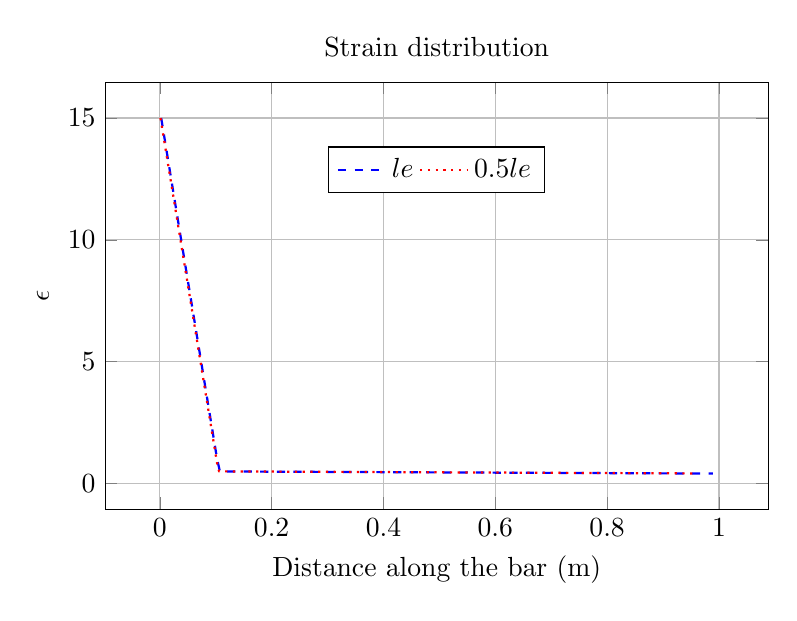
\begin{tikzpicture}
	\begin{axis}[
		title={Strain distribution},
		xlabel={Distance along the bar (\si{\meter})},
		ylabel={$\epsilon$},
		legend style={at={(0.5,0.85)}, anchor=north,legend columns=2},
		grid=major,
		width=10cm, height=7cm
		]
		
		% Database 1 (x, y) points using table
		\addplot[
		color=blue, dashed, thick
		% mark=square*,
		%thick
		] table[row sep=newline, x index=0, y index=1] {
			% (x, y) table for Database 1
			0.00250000000000000	14.9986250000006
			0.00750000000000000	14.2986250000006
			0.0125000000000000	13.5986250000006
			0.0175000000000000	12.8986250000006
			0.0225000000000000	12.1986250000006
			0.0275000000000000	11.4986250000006
			0.0325000000000000	10.7986250000006
			0.0375000000000000	10.0986250000006
			0.0425000000000000	9.39862500000064
			0.0475000000000000	8.69862500000063
			0.0525000000000000	7.99862500000062
			0.0575000000000000	7.29862500000066
			0.0625000000000000	6.59862500000060
			0.0675000000000000	5.89862500000066
			0.0725000000000000	5.19862500000059
			0.0775000000000000	4.49862500000063
			0.0825000000000000	3.79862500000067
			0.0875000000000000	3.09862500000062
			0.0925000000000000	2.39862500000061
			0.0975000000000000	1.69862500000059
			0.102500000000000	0.998625000000573
			0.107500000000000	0.494528061224486
			0.112500000000000	0.494028061224441
			0.117500000000000	0.493528061224453
			0.122500000000000	0.493028061224408
			0.127500000000000	0.492528061224419
			0.132500000000000	0.492028061224460
			0.137500000000000	0.491528061224415
			0.142500000000000	0.491028061224455
			0.147500000000000	0.490528061224467
			0.160897435897436	0.489188317634742
			0.182692307692308	0.487008830455252
			0.204487179487180	0.484829343275763
			0.226282051282051	0.482649856096273
			0.248076923076923	0.480470368916791
			0.269871794871795	0.478290881737308
			0.291666666666667	0.476111394557819
			0.313461538461538	0.473931907378336
			0.335256410256410	0.471752420198861
			0.357051282051282	0.469572933019371
			0.378846153846154	0.467393445839875
			0.400641025641026	0.465213958660399
			0.422435897435897	0.463034471480903
			0.444230769230769	0.460854984301420
			0.466025641025641	0.458675497121931
			0.487820512820513	0.456496009942448
			0.509615384615385	0.454316522762952
			0.531410256410256	0.452137035583483
			0.553205128205128	0.449957548403987
			0.575000000000000	0.447778061224490
			0.596794871794872	0.445598574044993
			0.618589743589744	0.443419086865525
			0.640384615384615	0.441239599686035
			0.662179487179487	0.439060112506539
			0.683974358974359	0.436880625327049
			0.705769230769231	0.434701138147553
			0.727564102564103	0.432521650968077
			0.749358974358975	0.430342163788581
			0.771153846153846	0.428162676609098
			0.792948717948718	0.425983189429616
			0.814743589743590	0.423803702250119
			0.836538461538462	0.421624215070636
			0.858333333333334	0.419444727891154
			0.880128205128206	0.417265240711664
			0.901923076923077	0.415085753532175
			0.923717948717949	0.412906266352699
			0.945512820512821	0.410726779173203
			0.967307692307693	0.408547291993706
			0.989102564102565	0.406367804814224
		};
		\addlegendentry{$le$}
		
		% Database 2 (x, y) points using table
		\addplot[
		color=red,dotted, thick
		%mark=*,
		%thick
		] table[row sep=newline, x index=0, y index=1] {
			% (x, y) table for Database 2
			0.00125000000000000	14.9997500000005
			0.00375000000000000	14.6497500000005
			0.00625000000000000	14.2997500000005
			0.00875000000000000	13.9497500000005
			0.0112500000000000	13.5997500000005
			0.0137500000000000	13.2497500000005
			0.0162500000000000	12.8997500000005
			0.0187500000000000	12.5497500000004
			0.0212500000000000	12.1997500000005
			0.0237500000000000	11.8497500000005
			0.0262500000000000	11.4997500000004
			0.0287500000000000	11.1497500000005
			0.0312500000000000	10.7997500000004
			0.0337500000000000	10.4497500000005
			0.0362500000000000	10.0997500000004
			0.0387500000000000	9.74975000000043
			0.0412500000000000	9.39975000000044
			0.0437500000000000	9.04975000000044
			0.0462500000000000	8.69975000000042
			0.0487500000000000	8.34975000000046
			0.0512500000000000	7.99975000000040
			0.0537500000000000	7.64975000000050
			0.0562500000000000	7.29975000000044
			0.0587500000000000	6.94975000000039
			0.0612500000000000	6.59975000000048
			0.0637500000000000	6.24975000000046
			0.0662500000000000	5.89975000000038
			0.0687500000000000	5.54975000000047
			0.0712500000000000	5.19975000000045
			0.0737500000000000	4.84975000000043
			0.0762500000000000	4.49975000000046
			0.0787500000000000	4.14975000000038
			0.0812500000000000	3.79975000000053
			0.0837500000000000	3.44975000000039
			0.0862500000000000	3.09975000000043
			0.0887500000000000	2.74975000000040
			0.0912500000000000	2.39975000000049
			0.0937500000000000	2.04975000000047
			0.0962500000000000	1.69975000000045
			0.0987500000000001	1.34975000000037
			0.101250000000000	0.999750000000404
			0.103750000000000	0.649750000000438
			0.106250000000000	0.498201530612391
			0.108750000000000	0.497951530612340
			0.111250000000000	0.497701530612403
			0.113750000000000	0.497451530612352
			0.116250000000000	0.497201530612415
			0.118750000000000	0.496951530612364
			0.121250000000000	0.496701530612256
			0.123750000000000	0.496451530612319
			0.126250000000000	0.496201530612268
			0.128750000000000	0.495951530612217
			0.131250000000000	0.495701530612166
			0.133750000000000	0.495451530612172
			0.136250000000000	0.495201530612178
			0.138750000000000	0.494951530612127
			0.141250000000000	0.494701530612133
			0.143750000000000	0.494451530612139
			0.146250000000000	0.494201530612202
			0.148750000000000	0.493951530612151
			0.197222222222222	0.489104308389889
			0.291666666666667	0.479659863945445
			0.386111111111111	0.470215419501001
			0.480555555555556	0.460770975056558
			0.575000000000000	0.451326530612111
			0.669444444444445	0.441882086167663
			0.763888888888889	0.432437641723224
			0.858333333333333	0.422993197278776
			0.952777777777778	0.413548752834330
		};
		\addlegendentry{$0.5 le$}
		
	\end{axis}
\end{tikzpicture}
		\caption{Strain distribution along the bar.}
		\label{strain_dist_nonlocal}
	\end{subfigure}
	\caption{Results with regularization}
	\label{fig:Results_with_regularization}
\end{figure}

The load displacement curves and the strain distribution at failure can be seen in figures \ref{force_disp_nonlocal} and \ref{strain_dist_nonlocal} for two different mesh sizes. A couple of observations warrant a closer look. First, as discussed in \cite{Kamasamudram2023}, the constraint shall be removed from the elements that are fully damaged to allow for the strains to localize in the fully damaged element and prevent the expansion of damage further into the body. The black dot in figure \ref{force_disp_nonlocal} corresponds to the case when the constraint is deactivated - the force displacement curve suddenly jumps to zero force. This situation is trivial in 1D, but is susceptible to cause convergence issues in 2D case. See \cite{Geers1998,Cabot2014,Le2018} and the references therein for similar discussions where the damaged regions extend across the body. Second, taking a closer look at the force-displacement curve as in figure \ref{force_disp_nonlocal_zoom}, a number of smaller snapbacks can be observed. It can be explained as follows: since the regularization is introduced through an inequality constraint, and this constraint is numerically resolved with a finite mesh size, the regularization is inactive until strain localizes in the some region of the body. The strains then grow locally till the constraint becomes active. Once activated, the constraint expands the damage zone further into the neighboring elements, where the strains again grow locally. This process carries on until some part of the body is fully damaged. Thus, the problem switches between a local (albeit with a varying length scale) and non-local problem as the constraint is activated and the damage spreads into other elements. The snapback occurs when the strains localize and the recovery corresponds to the activation of the constraint. It can also be seen that the amplitude of this sawtooth like pattern decreases as the mesh is refined, but the number of tooth increases.


\begin{remark}
	In hindsight, deactivating the constraint only after an element is fully damaged does indeed cause convergence issues in 2D. This issue has been discussed in multiple references - in the context of non-local damage models in \cite{Geers1998}. Thus, for the 2D case, the constraint is gradually weakened as the damage value increases. Also, to reduce the impact of sawtooth like pattern, the inequality constraint is weakened and a log-barrier-like function is used instead. More details can be found in the sections below.
\end{remark}


\begin{figure}[ht]
	\centering
	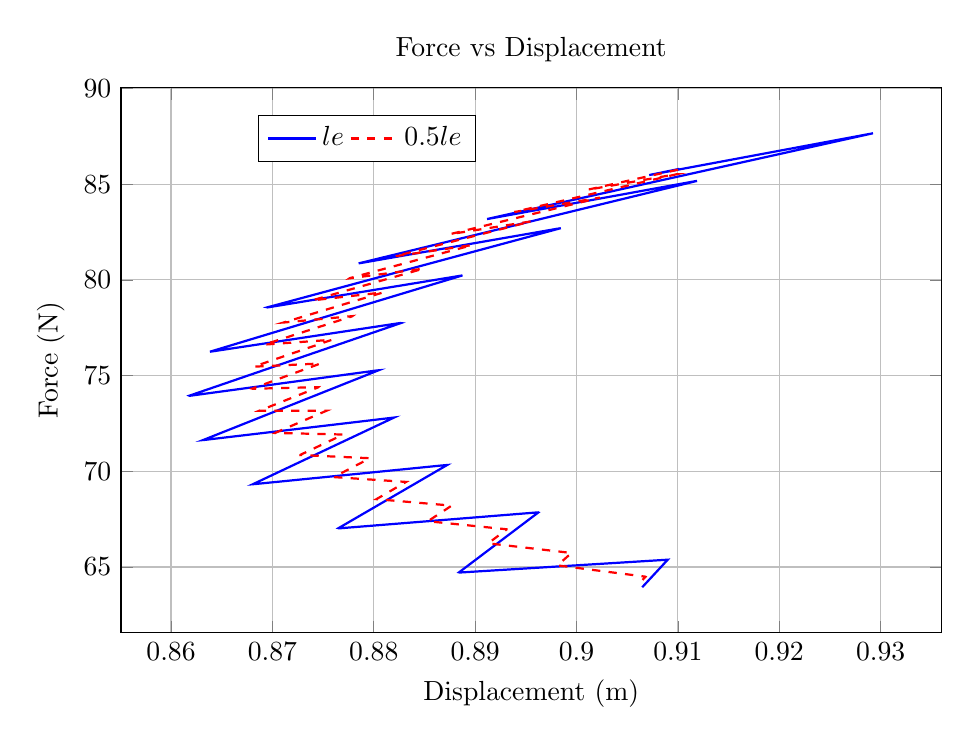
\begin{tikzpicture}
	\begin{axis}[
		title={Force vs Displacement},
		xlabel={Displacement (\si{\meter})},
		ylabel={Force (\si{\newton})},
		legend style={at={(0.3,0.95)}, anchor=north,legend columns=2},
		grid=major,
		width=12cm, height=8.5cm
		]
		
		% Database 1 (x, y) points using table
		\addplot[
		color=blue, thick
		% mark=square*,
		%thick
		] table[row sep=newline, x index=0, y index=1] {
			% (x, y) table for Database 1
			0.910144642857140	85.7982600738978
			0.909946428571432	85.7768315024699
			0.909748214285709	85.7554029310403
			0.909549999999997	85.7339743596124
			0.909351785714294	85.7125457881845
			0.909153571428561	85.6911172167553
			0.908955357142848	85.6696886453258
			0.908757142857134	85.6482600738990
			0.908558928571428	85.6268315024698
			0.908360714285721	85.6054029310412
			0.908162499999998	85.5839743596131
			0.907964285714272	85.5625457881827
			0.907766071428581	85.5411172167551
			0.907567857142853	85.5196886453288
			0.907369642857133	85.4982600738976
			0.907171428571425	85.4768315024692
			0.908116071428586	85.5696886439996
			0.909525000000039	85.7089743579400
			0.910933928571461	85.8482600722255
			0.912342857142890	85.9875457865105
			0.913751785714333	86.1268315007978
			0.915160714285757	86.2661172150834
			0.916569642857180	86.4054029293687
			0.917978571428606	86.5446886436549
			0.919387500000034	86.6839743579403
			0.920796428571465	86.8232600722257
			0.922205357142905	86.9625457865119
			0.923614285714321	87.1018315007976
			0.925023214285746	87.2411172150823
			0.926432142857190	87.3804029293688
			0.927841071428607	87.5196886436548
			0.929250000000050	87.6589743579405
			0.929067857143029	87.6375457881992
			0.928885714285714	87.6161172167559
			0.928703571428555	87.5946886453259
			0.928521428571429	87.5732600738979
			0.928339285714286	87.5518315024699
			0.928157142857133	87.5304029310404
			0.927975000000010	87.5089743596134
			0.927792857142869	87.4875457881845
			0.927610714285736	87.4661172167565
			0.927428571428564	87.4446886453269
			0.927246428571436	87.4232600738983
			0.927064285714286	87.4018315024688
			0.926882142857147	87.3804029310410
			0.926700000000003	87.3589743596134
			0.926517857142855	87.3375457881829
			0.926335714285706	87.3161172167555
			0.926153571428576	87.2946886453271
			0.925971428571426	87.2732600738993
			0.925789285714296	87.2518315024702
			0.925607142857148	87.2304029310421
			0.925424999999993	87.2089743596125
			0.925242857142836	87.1875457881840
			0.925060714285720	87.1661172167572
			0.924878571428563	87.1446886453262
			0.924696428571419	87.1232600738988
			0.924514285714285	87.1018315024696
			0.924332142857130	87.0804029310401
			0.924150000000014	87.0589743596127
			0.923967857142851	87.0375457881843
			0.923785714285699	87.0161172167542
			0.923603571428582	86.9946886453275
			0.923421428571432	86.9732600738984
			0.923239285714279	86.9518315024686
			0.923057142857137	86.9304029310412
			0.922874999999994	86.9089743596120
			0.922692857142856	86.8875457881831
			0.922510714285704	86.8661172167549
			0.922328571428572	86.8446886453267
			0.922146428571427	86.8232600738982
			0.921964285714276	86.8018315024692
			0.921782142857139	86.7804029310411
			0.921600000000016	86.7589743596144
			0.921417857142851	86.7375457881833
			0.921235714285715	86.7161172167551
			0.921053571428564	86.6946886453270
			0.920871428571411	86.6732600738980
			0.920689285714281	86.6518315024692
			0.920507142857146	86.6304029310412
			0.920324999999997	86.6089743596127
			0.920142857142865	86.5875457881849
			0.919960714285695	86.5661172167546
			0.919778571428570	86.5446886453276
			0.919596428571430	86.5232600738999
			0.919414285714284	86.5018315024688
			0.919232142857129	86.4804029310407
			0.919049999999986	86.4589743596109
			0.918867857142854	86.4375457881844
			0.918685714285714	86.4161172167544
			0.918503571428578	86.3946886453280
			0.918321428571429	86.3732600738983
			0.918139285714271	86.3518315024698
			0.917957142857139	86.3304029310409
			0.917775000000002	86.3089743596133
			0.917592857142847	86.2875457881835
			0.917410714285697	86.2661172167549
			0.917228571428567	86.2446886453264
			0.917046428571428	86.2232600738975
			0.916864285714298	86.2018315024701
			0.916682142857137	86.1804029310406
			0.916499999999996	86.1589743596125
			0.916317857142851	86.1375457881833
			0.916135714285704	86.1161172167558
			0.915953571428564	86.0946886453256
			0.915771428571433	86.0732600738986
			0.915589285714292	86.0518315024698
			0.915407142857137	86.0304029310420
			0.915224999999987	86.0089743596114
			0.915042857142868	85.9875457881837
			0.914860714285720	85.9661172167557
			0.914678571428573	85.9446886453256
			0.914496428571428	85.9232600738980
			0.914314285714284	85.9018315024699
			0.914132142857143	85.8804029310414
			0.913949999999990	85.8589743596127
			0.913767857142856	85.8375457881842
			0.913585714285709	85.8161172167552
			0.913403571428578	85.7946886453260
			0.913221428571424	85.7732600738990
			0.913039285714277	85.7518315024688
			0.912857142857140	85.7304029310412
			0.912674999999997	85.7089743596128
			0.912492857142852	85.6875457881831
			0.912310714285715	85.6661172167560
			0.912128571428557	85.6446886453276
			0.911946428571442	85.6232600738987
			0.911764285714260	85.6018315024693
			0.911582142857127	85.5804029310400
			0.911399999999991	85.5589743596115
			0.911217857142852	85.5375457881842
			0.911035714285698	85.5161172167554
			0.910853571428577	85.4946886453268
			0.910671428571434	85.4732600738992
			0.910489285714286	85.4518315024703
			0.910307142857131	85.4304029310419
			0.910124999999994	85.4089743596121
			0.909942857142871	85.3875457881849
			0.909760714285717	85.3661172167546
			0.909578571428555	85.3446886453268
			0.909396428571425	85.3232600738980
			0.909214285714274	85.3018315024683
			0.909032142857147	85.2804029310422
			0.908849999999999	85.2589743596128
			0.908667857142851	85.2375457881841
			0.908485714285699	85.2161172167554
			0.908303571428587	85.1946886453279
			0.908121428571437	85.1732600738984
			0.907939285714270	85.1518315024689
			0.907757142857138	85.1304029310418
			0.907574999999989	85.1089743596116
			0.907392857142855	85.0875457881845
			0.907210714285710	85.0661172167538
			0.907028571428582	85.0446886453271
			0.906846428571437	85.0232600738985
			0.906664285714270	85.0018315024691
			0.906482142857132	84.9804029310412
			0.906299999999998	84.9589743596130
			0.906117857142853	84.9375457881842
			0.905935714285714	84.9161172167546
			0.905753571428577	84.8946886453274
			0.905571428571430	84.8732600738975
			0.905389285714292	84.8518315024691
			0.905207142857146	84.8304029310418
			0.905024999999995	84.8089743596124
			0.904842857142848	84.7875457881847
			0.904660714285718	84.7661172167562
			0.904478571428572	84.7446886453276
			0.904296428571437	84.7232600738983
			0.904114285714285	84.7018315024700
			0.903932142857162	84.6804029310422
			0.903749999999990	84.6589743596132
			0.903567857142858	84.6375457881845
			0.903385714285711	84.6161172167556
			0.903203571428568	84.5946886453274
			0.903021428571420	84.5732600738986
			0.902839285714286	84.5518315024702
			0.902657142857133	84.5304029310398
			0.902474999999998	84.5089743596137
			0.902292857142855	84.4875457881848
			0.902110714285715	84.4661172167554
			0.901928571428559	84.4446886453255
			0.901746428571416	84.4232600738970
			0.901564285714277	84.4018315024699
			0.901382142857144	84.3804029310423
			0.901199999999987	84.3589743596131
			0.901017857142848	84.3375457881839
			0.900835714285711	84.3161172167557
			0.900653571428556	84.2946886453269
			0.900471428571417	84.2732600738986
			0.900289285714285	84.2518315024707
			0.900107142857156	84.2304029310411
			0.899924999999983	84.2089743596111
			0.899742857142841	84.1875457881836
			0.899560714285713	84.1661172167565
			0.899378571428551	84.1446886453254
			0.899196428571431	84.1232600738987
			0.899014285714292	84.1018315024694
			0.898832142857148	84.0804029310399
			0.898650000000004	84.0589743596133
			0.898467857142853	84.0375457881826
			0.898285714285712	84.0161172167557
			0.898103571428583	83.9946886453272
			0.897921428571452	83.9732600738983
			0.897739285714286	83.9518315024700
			0.897557142857141	83.9304029310423
			0.897375000000010	83.9089743596125
			0.897192857142861	83.8875457881846
			0.897010714285707	83.8661172167559
			0.896828571428564	83.8446886453263
			0.896646428571434	83.8232600738984
			0.896464285714288	83.8018315024692
			0.896282142857130	83.7804029310392
			0.896100000000002	83.7589743596122
			0.895917857142853	83.7375457881829
			0.895735714285728	83.7161172167564
			0.895553571428562	83.6946886453273
			0.895371428571422	83.6732600738980
			0.895189285714285	83.6518315024691
			0.895007142857134	83.6304029310422
			0.894824999999988	83.6089743596116
			0.894642857142857	83.5875457881833
			0.894460714285702	83.5661172167546
			0.894278571428555	83.5446886453258
			0.894096428571418	83.5232600738986
			0.893914285714287	83.5018315024713
			0.893732142857141	83.4804029310412
			0.893549999999994	83.4589743596119
			0.893367857142857	83.4375457881840
			0.893185714285714	83.4161172167557
			0.893003571428577	83.3946886453282
			0.892821428571412	83.3732600738977
			0.892639285714282	83.3518315024695
			0.892457142857150	83.3304029310419
			0.892275000000006	83.3089743596125
			0.892092857142860	83.2875457881839
			0.891910714285724	83.2661172167569
			0.891728571428575	83.2446886453273
			0.891546428571413	83.2232600738972
			0.891364285714271	83.2018315024698
			0.891182142857145	83.1804029310410
			0.891250000000024	83.1839743585509
			0.892139285714306	83.2696886440518
			0.893028571428594	83.3554029297656
			0.893917857142881	83.4411172154807
			0.894807142857178	83.5268315011956
			0.895696428571459	83.6125457869095
			0.896585714285729	83.6982600726237
			0.897475000000030	83.7839743583372
			0.898364285714307	83.8696886440525
			0.899253571428598	83.9554029297670
			0.900142857142891	84.0411172154813
			0.901032142857173	84.1268315011954
			0.901921428571444	84.2125457869097
			0.902810714285732	84.2982600726226
			0.903700000000022	84.3839743583384
			0.904589285714329	84.4696886440530
			0.905478571428581	84.5554029297661
			0.906367857142877	84.6411172154801
			0.907257142857147	84.7268315011935
			0.908146428571469	84.8125457869107
			0.909035714285736	84.8982600726240
			0.909925000000023	84.9839743583384
			0.910814285714288	85.0696886440517
			0.911703571428582	85.1554029297657
			0.911889285714463	85.1696886454129
			0.911723214285710	85.1482600738969
			0.911557142857145	85.1268315024709
			0.911391071428557	85.1054029310413
			0.911224999999985	85.0839743596120
			0.911058928571432	85.0625457881849
			0.910892857142861	85.0411172167550
			0.910726785714283	85.0196886453264
			0.910560714285707	84.9982600738987
			0.910394642857140	84.9768315024703
			0.910228571428568	84.9554029310419
			0.910062499999990	84.9339743596112
			0.909896428571412	84.9125457881818
			0.909730357142851	84.8911172167561
			0.909564285714261	84.8696886453253
			0.909398214285734	84.8482600738984
			0.909232142857138	84.8268315024694
			0.909066071428571	84.8054029310404
			0.908899999999987	84.7839743596124
			0.908733928571430	84.7625457881835
			0.908567857142863	84.7411172167569
			0.908401785714279	84.7196886453263
			0.908235714285720	84.6982600738986
			0.908069642857140	84.6768315024689
			0.907903571428567	84.6554029310413
			0.907737500000012	84.6339743596144
			0.907571428571432	84.6125457881845
			0.907405357142856	84.5911172167553
			0.907239285714289	84.5696886453273
			0.907073214285704	84.5482600738963
			0.906907142857141	84.5268315024694
			0.906741071428570	84.5054029310420
			0.906574999999999	84.4839743596124
			0.906408928571421	84.4625457881846
			0.906242857142868	84.4411172167561
			0.906076785714269	84.4196886453262
			0.905910714285723	84.3982600738983
			0.905744642857158	84.3768315024713
			0.905578571428569	84.3554029310419
			0.905412500000005	84.3339743596129
			0.905246428571415	84.3125457881837
			0.905080357142860	84.2911172167550
			0.904914285714286	84.2696886453282
			0.904748214285704	84.2482600738986
			0.904582142857147	84.2268315024707
			0.904416071428562	84.2054029310409
			0.904250000000004	84.1839743596122
			0.904083928571442	84.1625457881847
			0.903917857142848	84.1411172167552
			0.903751785714291	84.1196886453268
			0.903585714285704	84.0982600738978
			0.903419642857140	84.0768315024699
			0.903253571428553	84.0554029310404
			0.903087500000007	84.0339743596129
			0.902921428571418	84.0125457881843
			0.902755357142834	83.9911172167542
			0.902589285714274	83.9696886453267
			0.902423214285728	83.9482600738991
			0.902257142857127	83.9268315024683
			0.902091071428564	83.9054029310410
			0.901924999999999	83.8839743596110
			0.901758928571433	83.8625457881843
			0.901592857142865	83.8411172167544
			0.901426785714299	83.8196886453265
			0.901260714285710	83.7982600738974
			0.901094642857127	83.7768315024683
			0.900928571428570	83.7554029310408
			0.900762499999981	83.7339743596112
			0.900596428571428	83.7125457881843
			0.900430357142859	83.6911172167546
			0.900264285714289	83.6696886453262
			0.900098214285714	83.6482600738972
			0.899932142857136	83.6268315024697
			0.899766071428570	83.6054029310413
			0.899599999999991	83.5839743596126
			0.899433928571414	83.5625457881825
			0.899267857142862	83.5411172167560
			0.899101785714287	83.5196886453270
			0.898935714285710	83.4982600738984
			0.898769642857136	83.4768315024691
			0.898603571428565	83.4554029310412
			0.898437499999985	83.4339743596118
			0.898271428571423	83.4125457881837
			0.898105357142847	83.3911172167553
			0.897939285714279	83.3696886453258
			0.897773214285718	83.3482600738989
			0.897607142857128	83.3268315024684
			0.897441071428569	83.3054029310401
			0.897274999999993	83.2839743596124
			0.897108928571400	83.2625457881826
			0.896942857142841	83.2411172167553
			0.896776785714282	83.2196886453276
			0.896610714285720	83.1982600738991
			0.896444642857141	83.1768315024689
			0.896278571428562	83.1554029310413
			0.896112500000010	83.1339743596137
			0.895946428571435	83.1125457881837
			0.895780357142847	83.0911172167536
			0.895614285714276	83.0696886453269
			0.895448214285719	83.0482600738996
			0.895282142857153	83.0268315024695
			0.895116071428562	83.0054029310392
			0.894950000000002	82.9839743596119
			0.894783928571431	82.9625457881832
			0.894617857142866	82.9411172167562
			0.894451785714288	82.9196886453265
			0.894285714285708	82.8982600738988
			0.894119642857150	82.8768315024696
			0.893953571428582	82.8554029310423
			0.893787500000000	82.8339743596125
			0.893621428571419	82.8125457881840
			0.893455357142863	82.7911172167542
			0.893289285714278	82.7696886453262
			0.893123214285712	82.7482600738987
			0.892957142857133	82.7268315024706
			0.892791071428572	82.7054029310413
			0.892624999999984	82.6839743596125
			0.892458928571412	82.6625457881835
			0.892292857142863	82.6411172167578
			0.892126785714275	82.6196886453257
			0.891960714285720	82.5982600738990
			0.891794642857146	82.5768315024699
			0.891628571428579	82.5554029310408
			0.891462499999985	82.5339743596114
			0.891296428571422	82.5125457881840
			0.891130357142857	82.4911172167567
			0.890964285714265	82.4696886453252
			0.890798214285706	82.4482600738975
			0.890632142857132	82.4268315024688
			0.890466071428559	82.4054029310415
			0.890299999999992	82.3839743596122
			0.890133928571432	82.3625457881853
			0.889967857142854	82.3411172167543
			0.889801785714275	82.3196886453251
			0.889635714285733	82.2982600738984
			0.889469642857143	82.2768315024697
			0.889303571428579	82.2554029310425
			0.889137500000001	82.2339743596119
			0.888971428571412	82.2125457881827
			0.888805357142851	82.1911172167543
			0.888639285714268	82.1696886453259
			0.888473214285729	82.1482600738985
			0.888307142857135	82.1268315024689
			0.888141071428555	82.1054029310402
			0.887974999999995	82.0839743596126
			0.887808928571420	82.0625457881846
			0.887642857142866	82.0411172167559
			0.887476785714266	82.0196886453262
			0.887310714285710	81.9982600738982
			0.887144642857141	81.9768315024694
			0.886978571428581	81.9554029310405
			0.886812499999999	81.9339743596131
			0.886646428571419	81.9125457881836
			0.886480357142862	81.8911172167568
			0.886314285714287	81.8696886453274
			0.886148214285706	81.8482600738978
			0.885982142857146	81.8268315024684
			0.885816071428556	81.8054029310416
			0.885649999999969	81.7839743596121
			0.885483928571435	81.7625457881845
			0.885317857142846	81.7411172167535
			0.885151785714281	81.7196886453260
			0.884985714285697	81.6982600738985
			0.884819642857128	81.6768315024702
			0.884653571428560	81.6554029310407
			0.884487499999999	81.6339743596127
			0.884321428571425	81.6125457881825
			0.884155357142856	81.5911172167565
			0.883989285714290	81.5696886453259
			0.883823214285720	81.5482600738979
			0.883657142857134	81.5268315024692
			0.883491071428544	81.5054029310378
			0.883324999999993	81.4839743596130
			0.883158928571424	81.4625457881838
			0.882992857142870	81.4411172167535
			0.882826785714268	81.4196886453259
			0.882660714285708	81.3982600738994
			0.882494642857124	81.3768315024671
			0.882328571428587	81.3554029310427
			0.882162499999993	81.3339743596128
			0.881996428571430	81.3125457881858
			0.881830357142856	81.2911172167563
			0.881664285714290	81.2696886453271
			0.881498214285724	81.2482600739000
			0.881332142857139	81.2268315024699
			0.881166071428569	81.2054029310413
			0.880999999999984	81.1839743596114
			0.880833928571419	81.1625457881836
			0.880667857142850	81.1411172167551
			0.880501785714285	81.1196886453270
			0.880335714285698	81.0982600738979
			0.880169642857123	81.0768315024687
			0.880003571428569	81.0554029310412
			0.879837499999973	81.0339743596117
			0.879671428571438	81.0125457881847
			0.879505357142840	80.9911172167544
			0.879339285714289	80.9696886453260
			0.879173214285703	80.9482600738980
			0.879007142857141	80.9268315024690
			0.878841071428579	80.9054029310413
			0.878674999999993	80.8839743596132
			0.878508928571427	80.8625457881843
			0.878950000000011	80.9018315012485
			0.879587500000029	80.9607600723849
			0.880225000000010	81.0196886438115
			0.880862500000037	81.0786172152417
			0.881500000000013	81.1375457866694
			0.882137500000007	81.1964743580964
			0.882775000000011	81.2554029295259
			0.883412500000023	81.3143315009553
			0.884050000000016	81.3732600723841
			0.884687500000025	81.4321886438128
			0.885325000000026	81.4911172152422
			0.885962500000011	81.5500457866688
			0.886600000000019	81.6089743580990
			0.887237500000020	81.6679029295269
			0.887875000000025	81.7268315009564
			0.888512500000006	81.7857600723845
			0.889150000000013	81.8446886438117
			0.889787500000032	81.9036172152408
			0.890425000000037	81.9625457866707
			0.891062500000013	82.0214743580986
			0.891700000000025	82.0804029295270
			0.892337500000019	82.1393315009560
			0.892975000000027	82.1982600723840
			0.893612500000042	82.2571886438131
			0.894250000000041	82.3161172152424
			0.894887500000019	82.3750457866696
			0.895525000000034	82.4339743580990
			0.896162500000045	82.4929029295280
			0.896800000000024	82.5518315009563
			0.897437500000019	82.6107600723845
			0.898075000000016	82.6696886438124
			0.898450000000237	82.7018315028744
			0.898299999999982	82.6804029310385
			0.898149999999988	82.6589743596115
			0.898000000000003	82.6375457881850
			0.897849999999998	82.6161172167548
			0.897700000000023	82.5946886453281
			0.897549999999982	82.5732600738967
			0.897399999999992	82.5518315024686
			0.897250000000002	82.5304029310411
			0.897099999999993	82.5089743596127
			0.896949999999996	82.4875457881826
			0.896799999999992	82.4661172167548
			0.896650000000010	82.4446886453273
			0.896499999999994	82.4232600738983
			0.896349999999982	82.4018315024676
			0.896200000000010	82.3804029310422
			0.896049999999996	82.3589743596112
			0.895899999999983	82.3375457881837
			0.895750000000002	82.3161172167547
			0.895600000000002	82.2946886453283
			0.895449999999991	82.2732600738974
			0.895299999999976	82.2518315024667
			0.895150000000009	82.2304029310412
			0.894999999999972	82.2089743596103
			0.894849999999984	82.1875457881848
			0.894700000000001	82.1661172167567
			0.894549999999987	82.1446886453260
			0.894399999999994	82.1232600738969
			0.894249999999995	82.1018315024700
			0.894099999999967	82.0804029310403
			0.893949999999989	82.0589743596130
			0.893799999999987	82.0375457881836
			0.893649999999984	82.0161172167546
			0.893499999999993	81.9946886453260
			0.893349999999983	81.9732600738961
			0.893200000000013	81.9518315024704
			0.893050000000002	81.9304029310420
			0.892900000000005	81.9089743596121
			0.892749999999990	81.8875457881826
			0.892599999999997	81.8661172167554
			0.892449999999985	81.8446886453254
			0.892300000000000	81.8232600738978
			0.892149999999994	81.8018315024703
			0.891999999999999	81.7804029310404
			0.891849999999987	81.7589743596115
			0.891699999999991	81.7375457881824
			0.891549999999972	81.7161172167530
			0.891400000000013	81.6946886453281
			0.891249999999977	81.6732600738976
			0.891099999999991	81.6518315024699
			0.890950000000003	81.6304029310422
			0.890799999999993	81.6089743596119
			0.890649999999998	81.5875457881844
			0.890500000000002	81.5661172167566
			0.890349999999987	81.5446886453274
			0.890200000000018	81.5232600738999
			0.890049999999997	81.5018315024691
			0.889899999999994	81.4804029310401
			0.889749999999983	81.4589743596117
			0.889600000000002	81.4375457881838
			0.889449999999992	81.4161172167560
			0.889299999999985	81.3946886453256
			0.889150000000018	81.3732600739002
			0.888999999999988	81.3518315024707
			0.888849999999983	81.3304029310387
			0.888700000000012	81.3089743596136
			0.888549999999986	81.2875457881826
			0.888399999999988	81.2661172167542
			0.888249999999994	81.2446886453276
			0.888099999999992	81.2232600738979
			0.887949999999993	81.2018315024706
			0.887799999999996	81.1804029310412
			0.887650000000003	81.1589743596131
			0.887500000000001	81.1375457881834
			0.887350000000002	81.1161172167544
			0.887199999999998	81.0946886453274
			0.887049999999997	81.0732600738973
			0.886899999999994	81.0518315024701
			0.886750000000007	81.0304029310427
			0.886599999999979	81.0089743596113
			0.886449999999996	80.9875457881831
			0.886299999999989	80.9661172167545
			0.886150000000001	80.9446886453280
			0.886000000000013	80.9232600739008
			0.885849999999997	80.9018315024685
			0.885700000000020	80.8804029310444
			0.885549999999981	80.8589743596125
			0.885400000000000	80.8375457881845
			0.885249999999991	80.8161172167541
			0.885099999999983	80.7946886453253
			0.884949999999993	80.7732600738990
			0.884800000000013	80.7518315024710
			0.884649999999993	80.7304029310408
			0.884500000000014	80.7089743596140
			0.884349999999991	80.6875457881817
			0.884200000000014	80.6661172167562
			0.884049999999977	80.6446886453237
			0.883900000000007	80.6232600738997
			0.883749999999986	80.6018315024689
			0.883599999999983	80.5804029310394
			0.883449999999988	80.5589743596103
			0.883300000000012	80.5375457881837
			0.883149999999997	80.5161172167550
			0.883000000000018	80.4946886453291
			0.882849999999991	80.4732600738984
			0.882699999999994	80.4518315024708
			0.882549999999989	80.4304029310405
			0.882399999999997	80.4089743596129
			0.882250000000005	80.3875457881849
			0.882099999999994	80.3661172167542
			0.881950000000008	80.3446886453272
			0.881800000000005	80.3232600738989
			0.881649999999992	80.3018315024689
			0.881499999999992	80.2804029310404
			0.881349999999996	80.2589743596122
			0.881199999999986	80.2375457881826
			0.881049999999974	80.2161172167545
			0.880899999999983	80.1946886453264
			0.880749999999973	80.1732600738963
			0.880599999999998	80.1518315024679
			0.880450000000003	80.1304029310424
			0.880299999999983	80.1089743596127
			0.880150000000005	80.0875457881841
			0.880000000000016	80.0661172167551
			0.879849999999988	80.0446886453262
			0.879700000000013	80.0232600738992
			0.879549999999996	80.0018315024680
			0.879400000000000	79.9804029310416
			0.879250000000000	79.9589743596115
			0.879099999999981	79.9375457881831
			0.878949999999991	79.9161172167555
			0.878799999999987	79.8946886453246
			0.878650000000016	79.8732600738987
			0.878499999999990	79.8518315024698
			0.878349999999992	79.8304029310419
			0.878199999999999	79.8089743596121
			0.878049999999992	79.7875457881849
			0.877899999999988	79.7661172167557
			0.877750000000004	79.7446886453279
			0.877599999999987	79.7232600738967
			0.877449999999999	79.7018315024706
			0.877300000000005	79.6804029310418
			0.877149999999999	79.6589743596129
			0.876999999999994	79.6375457881847
			0.876849999999989	79.6161172167541
			0.876700000000009	79.5946886453295
			0.876549999999993	79.5732600738999
			0.876400000000001	79.5518315024703
			0.876250000000004	79.5304029310406
			0.876099999999996	79.5089743596121
			0.875950000000010	79.4875457881845
			0.875799999999985	79.4661172167545
			0.875650000000024	79.4446886453277
			0.875499999999990	79.4232600738964
			0.875349999999974	79.4018315024686
			0.875199999999977	79.3804029310401
			0.875049999999991	79.3589743596137
			0.874899999999991	79.3375457881846
			0.874750000000019	79.3161172167565
			0.874600000000003	79.2946886453275
			0.874449999999982	79.2732600738965
			0.874299999999995	79.2518315024692
			0.874150000000001	79.2304029310400
			0.873999999999988	79.2089743596114
			0.873850000000009	79.1875457881841
			0.873699999999999	79.1661172167553
			0.873550000000014	79.1446886453282
			0.873399999999990	79.1232600738983
			0.873249999999994	79.1018315024686
			0.873099999999997	79.0804029310431
			0.872950000000000	79.0589743596116
			0.872799999999998	79.0375457881845
			0.872650000000019	79.0161172167584
			0.872500000000000	78.9946886453274
			0.872350000000012	78.9732600738991
			0.872200000000010	78.9518315024709
			0.872049999999989	78.9304029310398
			0.871900000000000	78.9089743596127
			0.871750000000010	78.8875457881835
			0.871599999999992	78.8661172167555
			0.871450000000001	78.8446886453270
			0.871300000000005	78.8232600738997
			0.871149999999983	78.8018315024693
			0.871000000000002	78.7804029310418
			0.870849999999996	78.7589743596123
			0.870699999999984	78.7375457881828
			0.870550000000005	78.7161172167551
			0.870400000000003	78.6946886453275
			0.870249999999991	78.6732600738970
			0.870099999999991	78.6518315024700
			0.869949999999992	78.6304029310407
			0.869799999999989	78.6089743596113
			0.869650000000006	78.5875457881838
			0.869499999999978	78.5661172167549
			0.869528571428581	78.5625457877594
			0.870021428571453	78.6054029297665
			0.870514285714305	78.6482600726220
			0.871007142857168	78.6911172154793
			0.871500000000043	78.7339743583388
			0.871992857142872	78.7768315011941
			0.872485714285719	78.8196886440509
			0.872978571428582	78.8625457869086
			0.873471428571415	78.9054029297630
			0.873964285714299	78.9482600726239
			0.874457142857166	78.9911172154805
			0.874950000000022	79.0339743583371
			0.875442857142892	79.0768315011952
			0.875935714285732	79.1196886440512
			0.876428571428588	79.1625457869082
			0.876921428571434	79.2054029297651
			0.877414285714310	79.2482600726216
			0.877907142857169	79.2911172154807
			0.878400000000032	79.3339743583395
			0.878892857142866	79.3768315011944
			0.879385714285759	79.4196886440518
			0.879878571428579	79.4625457869086
			0.880371428571469	79.5054029297678
			0.880864285714306	79.5482600726230
			0.881357142857166	79.5911172154804
			0.881850000000020	79.6339743583369
			0.882342857142881	79.6768315011948
			0.882835714285731	79.7196886440512
			0.883328571428578	79.7625457869083
			0.883821428571458	79.8054029297664
			0.884314285714303	79.8482600726230
			0.884807142857154	79.8911172154811
			0.885300000000032	79.9339743583373
			0.885792857142868	79.9768315011937
			0.886285714285734	80.0196886440513
			0.886778571428577	80.0625457869083
			0.887271428571430	80.1054029297655
			0.887764285714290	80.1482600726227
			0.888257142857151	80.1911172154797
			0.888750000000014	80.2339743583381
			0.888616071428753	80.2125457885090
			0.888482142857131	80.1911172167530
			0.888348214285705	80.1696886453269
			0.888214285714283	80.1482600738989
			0.888080357142853	80.1268315024712
			0.887946428571451	80.1054029310441
			0.887812499999985	80.0839743596108
			0.887678571428563	80.0625457881840
			0.887544642857144	80.0411172167567
			0.887410714285719	80.0196886453268
			0.887276785714287	79.9982600738977
			0.887142857142856	79.9768315024712
			0.887008928571426	79.9554029310404
			0.886874999999989	79.9339743596107
			0.886741071428591	79.9125457881845
			0.886607142857136	79.8911172167555
			0.886473214285706	79.8696886453248
			0.886339285714285	79.8482600738970
			0.886205357142878	79.8268315024714
			0.886071428571426	79.8054029310391
			0.885937499999993	79.7839743596102
			0.885803571428565	79.7625457881837
			0.885669642857151	79.7411172167558
			0.885535714285710	79.7196886453243
			0.885401785714289	79.6982600738984
			0.885267857142865	79.6768315024691
			0.885133928571419	79.6554029310394
			0.885000000000007	79.6339743596126
			0.884866071428579	79.6125457881845
			0.884732142857137	79.5911172167561
			0.884598214285713	79.5696886453267
			0.884464285714267	79.5482600738972
			0.884330357142862	79.5268315024716
			0.884196428571454	79.5054029310427
			0.884062499999990	79.4839743596101
			0.883928571428555	79.4625457881816
			0.883794642857148	79.4411172167573
			0.883660714285713	79.4196886453282
			0.883526785714277	79.3982600738993
			0.883392857142864	79.3768315024703
			0.883258928571427	79.3554029310414
			0.883124999999994	79.3339743596113
			0.882991071428567	79.3125457881851
			0.882857142857143	79.2911172167572
			0.882723214285732	79.2696886453289
			0.882589285714288	79.2482600739010
			0.882455357142850	79.2268315024695
			0.882321428571432	79.2054029310415
			0.882187500000003	79.1839743596144
			0.882053571428570	79.1625457881840
			0.881919642857140	79.1411172167543
			0.881785714285731	79.1196886453282
			0.881651785714287	79.0982600738991
			0.881517857142850	79.0768315024669
			0.881383928571427	79.0554029310408
			0.881250000000000	79.0339743596089
			0.881116071428573	79.0125457881866
			0.880982142857137	78.9911172167565
			0.880848214285711	78.9696886453258
			0.880714285714285	78.9482600738988
			0.880580357142852	78.9268315024698
			0.880446428571428	78.9054029310400
			0.880312500000009	78.8839743596141
			0.880178571428568	78.8625457881855
			0.880044642857162	78.8411172167603
			0.879910714285717	78.8196886453294
			0.879776785714278	78.7982600738972
			0.879642857142858	78.7768315024687
			0.879508928571418	78.7554029310413
			0.879374999999984	78.7339743596120
			0.879241071428560	78.7125457881829
			0.879107142857119	78.6911172167521
			0.878973214285708	78.6696886453260
			0.878839285714268	78.6482600738952
			0.878705357142865	78.6268315024694
			0.878571428571430	78.6054029310423
			0.878437500000007	78.5839743596135
			0.878303571428574	78.5625457881847
			0.878169642857124	78.5411172167546
			0.878035714285749	78.5196886453298
			0.877901785714281	78.4982600738974
			0.877767857142863	78.4768315024704
			0.877633928571416	78.4554029310397
			0.877499999999998	78.4339743596126
			0.877366071428578	78.4125457881837
			0.877232142857133	78.3911172167554
			0.877098214285715	78.3696886453263
			0.876964285714280	78.3482600738974
			0.876830357142850	78.3268315024686
			0.876696428571410	78.3054029310387
			0.876562499999990	78.2839743596127
			0.876428571428555	78.2625457881808
			0.876294642857148	78.2411172167565
			0.876160714285708	78.2196886453255
			0.876026785714272	78.1982600738964
			0.875892857142840	78.1768315024694
			0.875758928571416	78.1554029310402
			0.875625000000003	78.1339743596135
			0.875491071428573	78.1125457881822
			0.875357142857133	78.0911172167543
			0.875223214285701	78.0696886453250
			0.875089285714258	78.0482600738960
			0.874955357142852	78.0268315024683
			0.874821428571424	78.0054029310390
			0.874687499999992	77.9839743596150
			0.874553571428561	77.9625457881851
			0.874419642857136	77.9411172167569
			0.874285714285736	77.9196886453282
			0.874151785714297	77.8982600739013
			0.874017857142853	77.8768315024689
			0.873883928571427	77.8554029310400
			0.873750000000016	77.8339743596137
			0.873616071428565	77.8125457881828
			0.873482142857125	77.7911172167528
			0.873348214285712	77.7696886453261
			0.873214285714269	77.7482600738948
			0.873080357142862	77.7268315024705
			0.872946428571424	77.7054029310415
			0.872812499999999	77.6839743596119
			0.872678571428571	77.6625457881841
			0.872544642857121	77.6411172167543
			0.872410714285708	77.6196886453271
			0.872276785714264	77.5982600738977
			0.872142857142831	77.5768315024671
			0.872008928571416	77.5554029310389
			0.871875000000002	77.5339743596123
			0.871741071428570	77.5125457881856
			0.871607142857140	77.4911172167563
			0.871473214285719	77.4696886453302
			0.871339285714274	77.4482600738968
			0.871205357142849	77.4268315024698
			0.871071428571426	77.4054029310409
			0.870937500000005	77.3839743596120
			0.870803571428557	77.3625457881831
			0.870669642857128	77.3411172167531
			0.870535714285693	77.3196886453270
			0.870401785714279	77.2982600738990
			0.870267857142842	77.2768315024701
			0.870133928571414	77.2554029310413
			0.869999999999987	77.2339743596112
			0.869866071428568	77.2125457881846
			0.869732142857136	77.1911172167559
			0.869598214285719	77.1696886453270
			0.869464285714290	77.1482600739004
			0.869330357142842	77.1268315024689
			0.869196428571414	77.1054029310395
			0.869062500000003	77.0839743596132
			0.868928571428575	77.0625457881875
			0.868794642857135	77.0411172167551
			0.868660714285706	77.0196886453270
			0.868526785714273	76.9982600738982
			0.868392857142840	76.9768315024676
			0.868258928571427	76.9554029310426
			0.868124999999996	76.9339743596119
			0.867991071428571	76.9125457881843
			0.867857142857156	76.8911172167576
			0.867723214285710	76.8696886453249
			0.867589285714285	76.8482600739015
			0.867455357142846	76.8268315024684
			0.867321428571421	76.8054029310401
			0.867187500000006	76.7839743596117
			0.867053571428579	76.7625457881860
			0.866919642857143	76.7411172167561
			0.866785714285685	76.7196886453237
			0.866651785714283	76.6982600738975
			0.866517857142871	76.6768315024696
			0.866383928571429	76.6554029310427
			0.866249999999989	76.6339743596117
			0.866116071428563	76.6125457881820
			0.865982142857128	76.5911172167548
			0.865848214285714	76.5696886453266
			0.865714285714298	76.5482600739010
			0.865580357142845	76.5268315024679
			0.865446428571447	76.5054029310444
			0.865312500000022	76.4839743596134
			0.865178571428556	76.4625457881827
			0.865044642857158	76.4411172167574
			0.864910714285711	76.4196886453267
			0.864776785714283	76.3982600738997
			0.864642857142861	76.3768315024687
			0.864508928571421	76.3554029310413
			0.864374999999996	76.3339743596119
			0.864241071428563	76.3125457881818
			0.864107142857148	76.2911172167547
			0.863973214285721	76.2696886453272
			0.863839285714281	76.2482600738972
			0.864133928571437	76.2696886440512
			0.864535714285728	76.3018315013537
			0.864937500000017	76.3339743584971
			0.865339285714279	76.3661172156382
			0.865741071428590	76.3982600727816
			0.866142857142858	76.4304029299255
			0.866544642857144	76.4625457870673
			0.866946428571428	76.4946886442100
			0.867348214285721	76.5268315013529
			0.867750000000032	76.5589743584972
			0.868151785714314	76.5911172156397
			0.868553571428596	76.6232600727816
			0.868955357142867	76.6554029299248
			0.869357142857152	76.6875457870674
			0.869758928571449	76.7196886442104
			0.870160714285725	76.7518315013528
			0.870562500000029	76.7839743584971
			0.870964285714285	76.8161172156392
			0.871366071428584	76.8482600727815
			0.871767857142869	76.8804029299249
			0.872169642857180	76.9125457870693
			0.872571428571442	76.9446886442116
			0.872973214285717	76.9768315013522
			0.873375000000025	77.0089743584966
			0.873776785714306	77.0411172156389
			0.874178571428584	77.0732600727820
			0.874580357142882	77.1054029299263
			0.874982142857174	77.1375457870696
			0.875383928571447	77.1696886442101
			0.875785714285726	77.2018315013532
			0.876187500000017	77.2339743584964
			0.876589285714309	77.2661172156409
			0.876991071428580	77.2982600727816
			0.877392857142878	77.3304029299267
			0.877794642857139	77.3625457870681
			0.878196428571452	77.3946886442114
			0.878598214285721	77.4268315013533
			0.878999999999999	77.4589743584962
			0.879401785714281	77.4911172156390
			0.879803571428588	77.5232600727827
			0.880205357142884	77.5554029299258
			0.880607142857191	77.5875457870692
			0.881008928571440	77.6196886442103
			0.881410714285743	77.6518315013538
			0.881812500000023	77.6839743584955
			0.882214285714308	77.7161172156389
			0.882616071428581	77.7482600727812
			0.882671428571596	77.7446886456009
			0.882553571428573	77.7232600738998
			0.882435714285726	77.7018315024722
			0.882317857142861	77.6804029310425
			0.882200000000009	77.6589743596142
			0.882082142857126	77.6375457881823
			0.881964285714303	77.6161172167581
			0.881846428571431	77.5946886453280
			0.881728571428562	77.5732600738994
			0.881610714285689	77.5518315024666
			0.881492857142874	77.5304029310456
			0.881374999999986	77.5089743596111
			0.881257142857132	77.4875457881832
			0.881139285714293	77.4661172167567
			0.881021428571428	77.4446886453272
			0.880903571428575	77.4232600738989
			0.880785714285712	77.4018315024684
			0.880667857142838	77.3804029310413
			0.880550000000000	77.3589743596139
			0.880432142857155	77.3375457881866
			0.880314285714275	77.3161172167536
			0.880196428571420	77.2946886453259
			0.880078571428577	77.2732600738964
			0.879960714285723	77.2518315024698
			0.879842857142855	77.2304029310419
			0.879725000000002	77.2089743596115
			0.879607142857132	77.1875457881837
			0.879489285714274	77.1661172167538
			0.879371428571427	77.1446886453255
			0.879253571428580	77.1232600739006
			0.879135714285703	77.1018315024710
			0.879017857142849	77.0804029310423
			0.878899999999995	77.0589743596134
			0.878782142857144	77.0375457881849
			0.878664285714298	77.0161172167571
			0.878546428571437	76.9946886453272
			0.878428571428556	76.9732600738972
			0.878310714285712	76.9518315024692
			0.878192857142839	76.9304029310387
			0.878075000000009	76.9089743596166
			0.877957142857151	76.8875457881851
			0.877839285714280	76.8661172167543
			0.877721428571428	76.8446886453259
			0.877603571428576	76.8232600738983
			0.877485714285710	76.8018315024678
			0.877367857142866	76.7804029310424
			0.877249999999993	76.7589743596138
			0.877132142857142	76.7375457881860
			0.877014285714286	76.7161172167540
			0.876896428571426	76.6946886453270
			0.876778571428574	76.6732600738964
			0.876660714285733	76.6518315024743
			0.876542857142859	76.6304029310418
			0.876424999999998	76.6089743596124
			0.876307142857140	76.5875457881838
			0.876189285714290	76.5661172167560
			0.876071428571431	76.5446886453263
			0.875953571428586	76.5232600739032
			0.875835714285699	76.5018315024688
			0.875717857142858	76.4804029310411
			0.875600000000004	76.4589743596133
			0.875482142857142	76.4375457881839
			0.875364285714275	76.4161172167541
			0.875246428571395	76.3946886453246
			0.875128571428543	76.3732600738951
			0.875010714285706	76.3518315024674
			0.874892857142872	76.3304029310446
			0.874774999999997	76.3089743596127
			0.874657142857156	76.2875457881837
			0.874539285714278	76.2661172167545
			0.874421428571438	76.2446886453284
			0.874303571428558	76.2232600738953
			0.874185714285709	76.2018315024705
			0.874067857142858	76.1804029310440
			0.873949999999998	76.1589743596126
			0.873832142857134	76.1375457881840
			0.873714285714271	76.1161172167505
			0.873596428571417	76.0946886453269
			0.873478571428578	76.0732600739018
			0.873360714285698	76.0518315024669
			0.873242857142866	76.0304029310409
			0.873124999999993	76.0089743596135
			0.873007142857150	75.9875457881866
			0.872889285714281	75.9661172167537
			0.872771428571441	75.9446886453282
			0.872653571428549	75.9232600738966
			0.872535714285699	75.9018315024654
			0.872417857142875	75.8804029310430
			0.872300000000026	75.8589743596146
			0.872182142857160	75.8375457881873
			0.872064285714287	75.8161172167555
			0.871946428571415	75.7946886453262
			0.871828571428593	75.7732600739020
			0.871710714285722	75.7518315024709
			0.871592857142860	75.7304029310416
			0.871474999999986	75.7089743596115
			0.871357142857148	75.6875457881838
			0.871239285714295	75.6661172167559
			0.871121428571408	75.6446886453238
			0.871003571428562	75.6232600738953
			0.870885714285741	75.6018315024734
			0.870767857142836	75.5804029310365
			0.870650000000000	75.5589743596132
			0.870532142857115	75.5375457881818
			0.870414285714262	75.5161172167544
			0.870296428571424	75.4946886453257
			0.870178571428577	75.4732600738984
			0.870060714285717	75.4518315024692
			0.869942857142861	75.4304029310403
			0.869824999999971	75.4089743596096
			0.869707142857145	75.3875457881833
			0.869589285714286	75.3661172167554
			0.869471428571438	75.3446886453279
			0.869353571428578	75.3232600739004
			0.869235714285696	75.3018315024665
			0.869117857142843	75.2804029310403
			0.868999999999998	75.2589743596107
			0.868882142857146	75.2375457881862
			0.868764285714283	75.2161172167560
			0.868646428571426	75.1946886453258
			0.868528571428578	75.1732600738999
			0.868410714285731	75.1518315024703
			0.868292857142850	75.1304029310391
			0.868175000000017	75.1089743596126
			0.868057142857135	75.0875457881832
			0.867939285714278	75.0661172167510
			0.867821428571416	75.0446886453262
			0.867703571428573	75.0232600738975
			0.867585714285720	75.0018315024690
			0.867467857142841	74.9804029310395
			0.867349999999976	74.9589743596104
			0.867232142857138	74.9375457881860
			0.867114285714290	74.9161172167569
			0.866996428571399	74.8946886453259
			0.866878571428561	74.8732600738960
			0.866760714285709	74.8518315024669
			0.866642857142847	74.8304029310418
			0.866524999999982	74.8089743596112
			0.866407142857127	74.7875457881817
			0.866289285714298	74.7661172167570
			0.866171428571444	74.7446886453283
			0.866053571428567	74.7232600738996
			0.865935714285710	74.7018315024702
			0.865817857142852	74.6804029310398
			0.865699999999981	74.6589743596095
			0.865582142857113	74.6375457881801
			0.865464285714276	74.6161172167554
			0.865346428571426	74.5946886453282
			0.865228571428554	74.5732600738974
			0.865110714285715	74.5518315024706
			0.864992857142854	74.5304029310412
			0.864875000000015	74.5089743596177
			0.864757142857140	74.4875457881831
			0.864639285714274	74.4661172167546
			0.864521428571442	74.4446886453286
			0.864403571428563	74.4232600738967
			0.864285714285708	74.4018315024710
			0.864167857142854	74.3804029310415
			0.864049999999990	74.3589743596127
			0.863932142857141	74.3375457881834
			0.863814285714281	74.3161172167551
			0.863696428571440	74.2946886453301
			0.863578571428565	74.2732600738993
			0.863460714285693	74.2518315024673
			0.863342857142866	74.2304029310421
			0.863224999999992	74.2089743596102
			0.863107142857132	74.1875457881832
			0.862989285714288	74.1661172167573
			0.862871428571414	74.1446886453249
			0.862753571428568	74.1232600738990
			0.862635714285692	74.1018315024685
			0.862517857142857	74.0804029310427
			0.862399999999997	74.0589743596139
			0.862282142857122	74.0375457881832
			0.862164285714286	74.0161172167555
			0.862046428571398	73.9946886453240
			0.861928571428593	73.9732600738996
			0.861810714285732	73.9518315024747
			0.861840816326538	73.9451988491670
			0.862182142857144	73.9696886443229
			0.862523469387769	73.9941784402434
			0.862864795918416	74.0186682361637
			0.863206122448973	74.0431580320801
			0.863547448979620	74.0676478279994
			0.863888775510191	74.0921376239138
			0.864230102040830	74.1166274198367
			0.864571428571465	74.1411172157544
			0.864912755102050	74.1656070116720
			0.865254081632655	74.1900968075891
			0.865595408163250	74.2145866035069
			0.865936734693895	74.2390763994261
			0.866278061224486	74.2635661953444
			0.866619387755127	74.2880559912646
			0.866960714285735	74.3125457871826
			0.867302040816340	74.3370355830993
			0.867643367346948	74.3615253790182
			0.867984693877583	74.3860151749388
			0.868326020408178	74.4105049708562
			0.868667346938794	74.4349947667738
			0.869008673469399	74.4594845626920
			0.869350000000048	74.4839743586119
			0.869691326530631	74.5084641545295
			0.870032653061244	74.5329539504475
			0.870373979591859	74.5574437463669
			0.870715306122459	74.5819335422840
			0.871056632653073	74.6064233382026
			0.871397959183717	74.6309131341234
			0.871739285714316	74.6554029300401
			0.872080612244925	74.6798927259596
			0.872421938775523	74.7043825218752
			0.872763265306150	74.7288723177953
			0.873104591836718	74.7533621137110
			0.873445918367335	74.7778519096291
			0.873787244897972	74.8023417055494
			0.874128571428580	74.8268315014673
			0.874469897959199	74.8513212973849
			0.874811224489803	74.8758110933037
			0.875152551020434	74.9003008892228
			0.875493877551043	74.9247906851411
			0.875835204081648	74.9492804810600
			0.876176530612259	74.9737702769781
			0.876517857142882	74.9982600728968
			0.876859183673492	75.0227498688154
			0.877200510204102	75.0472396647330
			0.877541836734711	75.0717294606509
			0.877883163265313	75.0962192565697
			0.878224489795948	75.1207090524885
			0.878565816326535	75.1451988484057
			0.878907142857136	75.1696886443238
			0.879248469387772	75.1941784402427
			0.879589795918374	75.2186682361602
			0.879931122449014	75.2431580320820
			0.880272448979585	75.2676478279975
			0.880466071428693	75.2768315026992
			0.880364285714296	75.2554029310420
			0.880262500000008	75.2339743596127
			0.880160714285735	75.2125457881875
			0.880058928571408	75.1911172167527
			0.879957142857119	75.1696886453243
			0.879855357142851	75.1482600738994
			0.879753571428588	75.1268315024729
			0.879651785714276	75.1054029310445
			0.879549999999985	75.0839743596092
			0.879448214285724	75.0625457881845
			0.879346428571438	75.0411172167576
			0.879244642857131	75.0196886453251
			0.879142857142854	74.9982600738968
			0.879041071428585	74.9768315024711
			0.878939285714326	74.9554029310511
			0.878837500000001	74.9339743596150
			0.878735714285711	74.9125457881824
			0.878633928571424	74.8911172167544
			0.878532142857129	74.8696886453285
			0.878430357142859	74.8482600738976
			0.878328571428572	74.8268315024705
			0.878226785714291	74.8054029310433
			0.878125000000004	74.7839743596151
			0.878023214285709	74.7625457881804
			0.877921428571411	74.7411172167515
			0.877819642857148	74.7196886453291
			0.877717857142850	74.6982600738984
			0.877616071428551	74.6768315024669
			0.877514285714290	74.6554029310424
			0.877412499999981	74.6339743596093
			0.877310714285697	74.6125457881810
			0.877208928571421	74.5911172167534
			0.877107142857171	74.5696886453328
			0.877005357142862	74.5482600739004
			0.876903571428576	74.5268315024689
			0.876801785714306	74.5054029310431
			0.876699999999999	74.4839743596120
			0.876598214285712	74.4625457881824
			0.876496428571456	74.4411172167590
			0.876394642857119	74.4196886453224
			0.876292857142830	74.3982600738924
			0.876191071428594	74.3768315024717
			0.876089285714296	74.3554029310418
			0.875987499999999	74.3339743596119
			0.875885714285715	74.3125457881864
			0.875783928571435	74.2911172167579
			0.875682142857143	74.2696886453267
			0.875580357142837	74.2482600738954
			0.875478571428575	74.2268315024698
			0.875376785714319	74.2054029310461
			0.875274999999985	74.1839743596115
			0.875173214285706	74.1625457881819
			0.875071428571421	74.1411172167551
			0.874969642857154	74.1196886453298
			0.874867857142874	74.0982600739002
			0.874766071428581	74.0768315024688
			0.874664285714287	74.0554029310391
			0.874562500000009	74.0339743596164
			0.874460714285739	74.0125457881904
			0.874358928571429	73.9911172167565
			0.874257142857142	73.9696886453256
			0.874155357142896	73.9482600739038
			0.874053571428556	73.9268315024684
			0.873951785714275	73.9054029310407
			0.873850000000023	73.8839743596176
			0.873748214285750	73.8625457881878
			0.873646428571420	73.8411172167565
			0.873544642857137	73.8196886453254
			0.873442857142877	73.7982600739017
			0.873341071428575	73.7768315024704
			0.873239285714281	73.7554029310411
			0.873137499999989	73.7339743596107
			0.873035714285734	73.7125457881862
			0.872933928571414	73.6911172167552
			0.872832142857140	73.6696886453267
			0.872730357142855	73.6482600739012
			0.872628571428571	73.6268315024693
			0.872526785714264	73.6054029310380
			0.872425000000022	73.5839743596139
			0.872323214285717	73.5625457881835
			0.872221428571412	73.5411172167538
			0.872119642857141	73.5196886453276
			0.872017857142837	73.4982600738959
			0.871916071428588	73.4768315024736
			0.871814285714249	73.4554029310353
			0.871712500000005	73.4339743596126
			0.871610714285722	73.4125457881849
			0.871508928571424	73.3911172167556
			0.871407142857136	73.3696886453243
			0.871305357142857	73.3482600739011
			0.871203571428572	73.3268315024712
			0.871101785714270	73.3054029310399
			0.870999999999995	73.2839743596125
			0.870898214285719	73.2625457881868
			0.870796428571412	73.2411172167512
			0.870694642857150	73.2196886453265
			0.870592857142849	73.1982600738977
			0.870491071428563	73.1768315024698
			0.870389285714261	73.1554029310375
			0.870287500000034	73.1339743596165
			0.870185714285723	73.1125457881853
			0.870083928571433	73.0911172167538
			0.869982142857108	73.0696886453196
			0.869880357142863	73.0482600738994
			0.869778571428579	73.0268315024686
			0.869676785714285	73.0054029310425
			0.869574999999997	72.9839743596119
			0.869473214285716	72.9625457881877
			0.869371428571433	72.9411172167562
			0.869269642857156	72.9196886453332
			0.869167857142858	72.8982600739003
			0.869066071428557	72.8768315024683
			0.868964285714308	72.8554029310443
			0.868862499999984	72.8339743596102
			0.868760714285711	72.8125457881852
			0.868658928571400	72.7911172167500
			0.868557142857146	72.7696886453266
			0.868455357142871	72.7482600739022
			0.868353571428555	72.7268315024649
			0.868251785714275	72.7054029310393
			0.868149999999997	72.6839743596131
			0.868048214285720	72.6625457881870
			0.867946428571439	72.6411172167561
			0.867844642857114	72.6196886453174
			0.867742857142875	72.5982600738989
			0.867641071428589	72.5768315024721
			0.867539285714284	72.5554029310407
			0.867437500000018	72.5339743596146
			0.867335714285735	72.5125457881892
			0.867233928571406	72.4911172167541
			0.867132142857137	72.4696886453270
			0.867030357142880	72.4482600739045
			0.866928571428550	72.4268315024666
			0.866826785714262	72.4054029310379
			0.866725000000031	72.3839743596149
			0.866623214285720	72.3625457881826
			0.866521428571434	72.3411172167562
			0.866419642857133	72.3196886453278
			0.866317857142841	72.2982600738968
			0.866216071428562	72.2768315024678
			0.866114285714276	72.2554029310417
			0.866012499999997	72.2339743596160
			0.865910714285697	72.2125457881841
			0.865808928571400	72.1911172167498
			0.865707142857125	72.1696886453214
			0.865605357142867	72.1482600738996
			0.865503571428571	72.1268315024698
			0.865401785714290	72.1054029310395
			0.865300000000003	72.0839743596152
			0.865198214285712	72.0625457881839
			0.865096428571443	72.0411172167601
			0.864994642857120	72.0196886453256
			0.864892857142850	71.9982600738945
			0.864791071428563	71.9768315024686
			0.864689285714286	71.9554029310404
			0.864587499999987	71.9339743596117
			0.864485714285733	71.9125457881884
			0.864383928571437	71.8911172167563
			0.864282142857133	71.8696886453277
			0.864180357142875	71.8482600739026
			0.864078571428578	71.8268315024698
			0.863976785714311	71.8054029310482
			0.863875000000016	71.7839743596161
			0.863773214285695	71.7625457881816
			0.863671428571424	71.7411172167560
			0.863569642857126	71.7196886453250
			0.863467857142874	71.6982600739023
			0.863366071428561	71.6768315024667
			0.863264285714275	71.6554029310397
			0.863162500000006	71.6339743596132
			0.863400000000017	71.6464743586026
			0.863700000000018	71.6652243586965
			0.864000000000009	71.6839743586957
			0.864300000000024	71.7027243586964
			0.864600000000009	71.7214743586966
			0.864900000000036	71.7402243586960
			0.865200000000012	71.7589743586960
			0.865500000000016	71.7777243586963
			0.865800000000043	71.7964743586974
			0.866099999999999	71.8152243586952
			0.866399999999983	71.8339743586943
			0.866700000000025	71.8527243586955
			0.866999999999995	71.8714743586963
			0.867300000000032	71.8902243586972
			0.867600000000020	71.9089743586960
			0.867900000000003	71.9277243586950
			0.868200000000055	71.9464743586983
			0.868500000000043	71.9652243586967
			0.868800000000006	71.9839743586953
			0.869100000000027	72.0027243586973
			0.869400000000010	72.0214743586962
			0.869700000000016	72.0402243586969
			0.869999999999987	72.0589743586939
			0.870300000000029	72.0777243586968
			0.870599999999993	72.0964743586943
			0.870900000000030	72.1152243586968
			0.871200000000011	72.1339743586956
			0.871500000000014	72.1527243586964
			0.871800000000011	72.1714743586951
			0.872100000000014	72.1902243586955
			0.872400000000024	72.2089743586962
			0.872700000000021	72.2277243586959
			0.873000000000008	72.2464743586945
			0.873299999999989	72.2652243586948
			0.873600000000012	72.2839743586956
			0.873900000000010	72.3027243586955
			0.874200000000041	72.3214743586975
			0.874500000000012	72.3402243586959
			0.874800000000011	72.3589743586961
			0.875100000000012	72.3777243586964
			0.875399999999985	72.3964743586944
			0.875700000000038	72.4152243586961
			0.876000000000011	72.4339743586961
			0.876300000000035	72.4527243586962
			0.876600000000025	72.4714743586963
			0.876900000000020	72.4902243586967
			0.877200000000007	72.5089743586954
			0.877500000000040	72.5277243586971
			0.877800000000038	72.5464743586960
			0.878100000000024	72.5652243586960
			0.878400000000031	72.5839743586959
			0.878700000000009	72.6027243586958
			0.879000000000021	72.6214743586960
			0.879300000000026	72.6402243586965
			0.879600000000000	72.6589743586963
			0.879900000000047	72.6777243586977
			0.880200000000015	72.6964743586956
			0.880500000000022	72.7152243586966
			0.880800000000001	72.7339743586954
			0.881100000000016	72.7527243586954
			0.881400000000003	72.7714743586950
			0.881700000000029	72.7902243586969
			0.882000000000032	72.8089743586968
			0.881957142857128	72.7982600738984
			0.881871428571422	72.7768315024680
			0.881785714285724	72.7554029310397
			0.881699999999977	72.7339743596125
			0.881614285714309	72.7125457881879
			0.881528571428577	72.6911172167595
			0.881442857142864	72.6696886453294
			0.881357142857109	72.6482600738937
			0.881271428571430	72.6268315024740
			0.881185714285677	72.6054029310357
			0.881099999999997	72.5839743596137
			0.881014285714299	72.5625457881885
			0.880928571428550	72.5411172167535
			0.880842857142855	72.5196886453283
			0.880757142857133	72.4982600738921
			0.880671428571426	72.4768315024708
			0.880585714285715	72.4554029310364
			0.880500000000003	72.4339743596120
			0.880414285714289	72.4125457881867
			0.880328571428573	72.3911172167577
			0.880242857142853	72.3696886453283
			0.880157142857148	72.3482600739004
			0.880071428571415	72.3268315024666
			0.879985714285728	72.3054029310452
			0.879900000000025	72.2839743596189
			0.879814285714286	72.2625457881810
			0.879728571428531	72.2411172167496
			0.879642857142854	72.2196886453271
			0.879557142857148	72.1982600738984
			0.879471428571418	72.1768315024683
			0.879385714285678	72.1554029310345
			0.879299999999983	72.1339743596126
			0.879214285714299	72.1125457881878
			0.879128571428579	72.0911172167576
			0.879042857142859	72.0696886453230
			0.878957142857121	72.0482600738915
			0.878871428571415	72.0268315024628
			0.878785714285721	72.0054029310393
			0.878700000000009	71.9839743596152
			0.878614285714263	71.9625457881826
			0.878528571428568	71.9411172167576
			0.878442857142821	71.9196886453234
			0.878357142857109	71.8982600738880
			0.878271428571407	71.8768315024669
			0.878185714285739	71.8554029310476
			0.878100000000000	71.8339743596110
			0.878014285714265	71.8125457881800
			0.877928571428564	71.7911172167518
			0.877842857142836	71.7696886453267
			0.877757142857144	71.7482600738993
			0.877671428571423	71.7268315024699
			0.877585714285713	71.7054029310380
			0.877500000000004	71.6839743596077
			0.877414285714308	71.6625457881888
			0.877328571428572	71.6411172167570
			0.877242857142853	71.6196886453285
			0.877157142857154	71.5982600738960
			0.877071428571457	71.5768315024699
			0.876985714285720	71.5554029310463
			0.876900000000015	71.5339743596132
			0.876814285714300	71.5125457881872
			0.876728571428558	71.4911172167522
			0.876642857142834	71.4696886453191
			0.876557142857140	71.4482600738967
			0.876471428571427	71.4268315024662
			0.876385714285702	71.4054029310424
			0.876299999999990	71.3839743596122
			0.876214285714285	71.3625457881789
			0.876128571428574	71.3411172167557
			0.876042857142854	71.3196886453296
			0.875957142857128	71.2982600738972
			0.875871428571431	71.2768315024719
			0.875785714285703	71.2554029310384
			0.875700000000002	71.2339743596157
			0.875614285714295	71.2125457881845
			0.875528571428526	71.1911172167524
			0.875442857142823	71.1696886453205
			0.875357142857143	71.1482600738995
			0.875271428571462	71.1268315024741
			0.875185714285701	71.1054029310370
			0.875099999999994	71.0839743596109
			0.875014285714308	71.0625457881938
			0.874928571428547	71.0411172167519
			0.874842857142827	71.0196886453247
			0.874757142857157	70.9982600738995
			0.874671428571430	70.9768315024703
			0.874585714285713	70.9554029310406
			0.874500000000002	70.9339743596105
			0.874414285714279	70.9125457881809
			0.874328571428554	70.8911172167511
			0.874242857142843	70.8696886453232
			0.874157142857100	70.8482600738924
			0.874071428571406	70.8268315024684
			0.873985714285727	70.8054029310406
			0.873900000000004	70.7839743596157
			0.873814285714313	70.7625457881869
			0.873728571428575	70.7411172167581
			0.873642857142846	70.7196886453281
			0.873557142857117	70.6982600738955
			0.873471428571408	70.6768315024672
			0.873385714285707	70.6554029310398
			0.873300000000035	70.6339743596154
			0.873214285714279	70.6125457881858
			0.873128571428567	70.5911172167549
			0.873042857142848	70.5696886453262
			0.872957142857131	70.5482600738951
			0.872871428571430	70.5268315024697
			0.872785714285691	70.5054029310302
			0.872699999999988	70.4839743596119
			0.872614285714294	70.4625457881856
			0.872528571428586	70.4411172167541
			0.872442857142853	70.4196886453261
			0.872357142857148	70.3982600738991
			0.872271428571391	70.3768315024634
			0.872185714285712	70.3554029310452
			0.872100000000003	70.3339743596108
			0.872014285714307	70.3125457881859
			0.871928571428562	70.2911172167532
			0.871842857142860	70.2696886453254
			0.871757142857153	70.2482600739016
			0.871671428571418	70.2268315024709
			0.871585714285713	70.2054029310399
			0.871500000000001	70.1839743596092
			0.871414285714278	70.1625457881832
			0.871328571428548	70.1411172167486
			0.871242857142861	70.1196886453300
			0.871157142857139	70.0982600738950
			0.871071428571419	70.0768315024690
			0.870985714285719	70.0554029310452
			0.870900000000015	70.0339743596121
			0.870814285714278	70.0125457881866
			0.870728571428581	69.9911172167496
			0.870642857142870	69.9696886453285
			0.870557142857176	69.9482600738968
			0.870471428571397	69.9268315024591
			0.870385714285713	69.9054029310383
			0.870300000000013	69.8839743596133
			0.870214285714289	69.8625457881806
			0.870128571428576	69.8411172167589
			0.870042857142829	69.8196886453219
			0.869957142857106	69.7982600738896
			0.869871428571424	69.7768315024719
			0.869785714285739	69.7554029310432
			0.869700000000014	69.7339743596103
			0.869614285714277	69.7125457881885
			0.869528571428567	69.6911172167580
			0.869442857142889	69.6696886453352
			0.869357142857146	69.6482600738988
			0.869271428571426	69.6268315024655
			0.869185714285707	69.6054029310467
			0.869100000000001	69.5839743596160
			0.869014285714312	69.5625457881910
			0.868928571428559	69.5411172167513
			0.868842857142855	69.5196886453293
			0.868757142857120	69.4982600738926
			0.868671428571388	69.4768315024720
			0.868585714285726	69.4554029310434
			0.868499999999963	69.4339743596039
			0.868414285714301	69.4125457881889
			0.868328571428556	69.3911172167540
			0.868242857142869	69.3696886453284
			0.868157142857120	69.3482600738982
			0.868071428571437	69.3268315024726
			0.868295238095257	69.3363553110731
			0.868566666666677	69.3506410254288
			0.868838095238085	69.3649267397135
			0.869109523809521	69.3792124540003
			0.869380952380963	69.3934981682852
			0.869652380952419	69.4077838825721
			0.869923809523815	69.4220695968570
			0.870195238095249	69.4363553111424
			0.870466666666704	69.4506410254300
			0.870738095238124	69.4649267397148
			0.871009523809535	69.4792124539998
			0.871280952381000	69.4934981682856
			0.871552380952415	69.5077838825732
			0.871823809523828	69.5220695968585
			0.872095238095264	69.5363553111440
			0.872366666666708	69.5506410254297
			0.872638095238129	69.5649267397157
			0.872909523809520	69.5792124539998
			0.873180952380965	69.5934981682860
			0.873452380952408	69.6077838825726
			0.873723809523830	69.6220695968574
			0.873995238095276	69.6363553111443
			0.874266666666701	69.6506410254290
			0.874538095238122	69.6649267397152
			0.874809523809542	69.6792124540012
			0.875080952380963	69.6934981682856
			0.875352380952414	69.7077838825726
			0.875623809523824	69.7220695968581
			0.875895238095250	69.7363553111426
			0.876166666666685	69.7506410254295
			0.876438095238091	69.7649267397148
			0.876709523809519	69.7792124540009
			0.876980952380950	69.7934981682870
			0.877252380952420	69.8077838825720
			0.877523809523816	69.8220695968576
			0.877795238095260	69.8363553111448
			0.878066666666689	69.8506410254288
			0.878338095238145	69.8649267397161
			0.878609523809542	69.8792124540000
			0.878880952380956	69.8934981682856
			0.879152380952383	69.9077838825726
			0.879423809523826	69.9220695968571
			0.879695238095289	69.9363553111439
			0.879966666666678	69.9506410254286
			0.880238095238108	69.9649267397138
			0.880509523809535	69.9792124540002
			0.880780952380977	69.9934981682862
			0.881052380952434	70.0077838825718
			0.881323809523825	70.0220695968562
			0.881595238095284	70.0363553111446
			0.881866666666680	70.0506410254286
			0.882138095238117	70.0649267397138
			0.882409523809522	70.0792124539994
			0.882680952380940	70.0934981682858
			0.882952380952386	70.1077838825706
			0.883223809523830	70.1220695968577
			0.883495238095235	70.1363553111433
			0.883766666666691	70.1506410254285
			0.884038095238132	70.1649267397166
			0.884309523809532	70.1792124539996
			0.884580952380942	70.1934981680721
			0.884852380952381	70.2077838823592
			0.885123809523810	70.2220695966453
			0.885395238095245	70.2363553109300
			0.885666666666674	70.2506410252158
			0.885938095238109	70.2649267395017
			0.886209523809580	70.2792124537893
			0.886480952380972	70.2934981680740
			0.886752380952373	70.3077838823585
			0.887023809523848	70.3220695966457
			0.887238392857237	70.3304029313466
			0.887168749999990	70.3089743596127
			0.887099107142822	70.2875457881779
			0.887029464285704	70.2661172167567
			0.886959821428555	70.2446886453265
			0.886890178571461	70.2232600739060
			0.886820535714280	70.2018315024686
			0.886750892857157	70.1804029310388
			0.886681249999993	70.1589743596184
			0.886611607142846	70.1375457881770
			0.886541964285742	70.1161172167619
			0.886472321428567	70.0946886453316
			0.886402678571446	70.0732600739079
			0.886333035714273	70.0518315024598
			0.886263392857157	70.0304029310511
			0.886193749999992	70.0089743596134
			0.886124107142842	69.9875457881836
			0.886054464285695	69.9661172167552
			0.885984821428550	69.9446886453251
			0.885915178571406	69.9232600738940
			0.885845535714271	69.9018315024732
			0.885775892857125	69.8804029310396
			0.885706250000001	69.8589743596097
			0.885636607142869	69.8375457881788
			0.885566964285724	69.8161172167565
			0.885497321428574	69.7946886453323
			0.885427678571421	69.7732600738965
			0.885358035714290	69.7518315024702
			0.885288392857137	69.7304029310423
			0.885218749999989	69.7089743596164
			0.885149107142875	69.6875457881816
			0.885079464285690	69.6661172167478
			0.885009821428575	69.6446886453247
			0.884940178571414	69.6232600738936
			0.884870535714266	69.6018315024647
			0.884800892857111	69.5804029310301
			0.884731250000005	69.5589743596120
			0.884661607142830	69.5375457881704
			0.884591964285734	69.5161172167614
			0.884522321428551	69.4946886453330
			0.884452678571443	69.4732600738958
			0.884383035714276	69.4518315024762
			0.884313392857135	69.4304029310372
			0.884243749999996	69.4089743596172
			0.884174107142850	69.3875457881832
			0.884104464285736	69.3661172167608
			0.884034821428555	69.3446886453255
			0.883965178571406	69.3232600738987
			0.883895535714280	69.3018315024774
			0.883825892857114	69.2804029310359
			0.883756250000039	69.2589743596196
			0.883686607142862	69.2375457881885
			0.883616964285707	69.2161172167563
			0.883547321428571	69.1946886453334
			0.883477678571427	69.1732600738976
			0.883408035714251	69.1518315024608
			0.883338392857139	69.1304029310330
			0.883268749999977	69.1089743596091
			0.883199107142860	69.0875457881922
			0.883129464285710	69.0661172167525
			0.883059821428524	69.0446886453146
			0.882990178571428	69.0232600738955
			0.882920535714325	69.0018315024793
			0.882850892857146	68.9804029310444
			0.882781250000007	68.9589743596164
			0.882711607142860	68.9375457881814
			0.882641964285738	68.9161172167588
			0.882572321428544	68.8946886453186
			0.882502678571424	68.8732600738950
			0.882433035714310	68.8518315024676
			0.882363392857151	68.8304029310513
			0.882293749999989	68.8089743596096
			0.882224107142873	68.7875457881936
			0.882154464285697	68.7661172167557
			0.882084821428567	68.7446886453330
			0.882015178571398	68.7232600738930
			0.881945535714290	68.7018315024754
			0.881875892857117	68.6804029310376
			0.881806250000021	68.6589743596170
			0.881736607142869	68.6375457881848
			0.881666964285745	68.6161172167583
			0.881597321428608	68.5946886453304
			0.881527678571424	68.5732600738982
			0.881458035714285	68.5518315024655
			0.881388392857112	68.5304029310374
			0.881318749999987	68.5089743596144
			0.881249107142884	68.4875457881932
			0.881179464285734	68.4661172167650
			0.881109821428562	68.4446886453248
			0.881040178571423	68.4232600738962
			0.880970535714278	68.4018315024703
			0.880900892857122	68.3804029310369
			0.880831249999989	68.3589743596113
			0.880761607142874	68.3375457881895
			0.880691964285727	68.3161172167597
			0.880622321428530	68.2946886453232
			0.880552678571413	68.2732600738944
			0.880483035714292	68.2518315024668
			0.880413392857079	68.2304029310282
			0.880343750000003	68.2089743596151
			0.880274107142851	68.1875457881827
			0.880204464285715	68.1661172167575
			0.880134821428588	68.1446886453313
			0.880065178571433	68.1232600739070
			0.879995535714257	68.1018315024657
			0.879925892857104	68.0804029310397
			0.879856249999975	68.0589743596074
			0.879786607142872	68.0375457881901
			0.879716964285741	68.0161172167595
			0.879647321428550	67.9946886453191
			0.879577678571377	67.9732600738902
			0.879508035714242	67.9518315024546
			0.879438392857125	67.9304029310376
			0.879368750000024	67.9089743596172
			0.879299107142843	67.8875457881795
			0.879229464285712	67.8661172167481
			0.879159821428562	67.8446886453197
			0.879090178571463	67.8232600739092
			0.879020535714281	67.8018315024690
			0.878950892857113	67.7804029310389
			0.878881250000019	67.7589743596117
			0.878811607142850	67.7375457881799
			0.878741964285685	67.7161172167471
			0.878672321428573	67.6946886453263
			0.878602678571449	67.6732600739059
			0.878533035714301	67.6518315024740
			0.878463392857107	67.6304029310287
			0.878393750000015	67.6089743596173
			0.878324107142875	67.5875457881864
			0.878254464285752	67.5661172167507
			0.878184821428564	67.5446886453223
			0.878115178571391	67.5232600738851
			0.878045535714287	67.5018315024665
			0.877975892857134	67.4804029310396
			0.877906249999977	67.4589743596148
			0.877836607142870	67.4375457881797
			0.877766964285713	67.4161172167532
			0.877697321428565	67.3946886453208
			0.877627678571405	67.3732600738987
			0.877558035714286	67.3518315024640
			0.877488392857121	67.3304029310397
			0.877418749999995	67.3089743596140
			0.877349107142843	67.2875457881865
			0.877279464285715	67.2661172167509
			0.877209821428592	67.2446886453386
			0.877140178571418	67.2232600738888
			0.877070535714279	67.2018315024655
			0.877000892857127	67.1804029310383
			0.876931250000025	67.1589743596236
			0.876861607142843	67.1375457881811
			0.876791964285721	67.1161172167535
			0.876722321428611	67.0946886453355
			0.876652678571406	67.0732600738966
			0.876583035714269	67.0518315024686
			0.876513392857128	67.0304029310392
			0.876568750000028	67.0214743595082
			0.876820535714300	67.0321886443698
			0.877072321428606	67.0429029300848
			0.877324107142880	67.0536172157996
			0.877575892857153	67.0643315015129
			0.877827678571466	67.0750457872275
			0.878079464285765	67.0857600729423
			0.878331250000015	67.0964743586555
			0.878583035714295	67.1071886443710
			0.878834821428603	67.1179029300861
			0.879086607142864	67.1286172157974
			0.879338392857166	67.1393315015125
			0.879590178571455	67.1500457872273
			0.879841964285728	67.1607600729407
			0.880093750000010	67.1714743586553
			0.880345535714322	67.1821886443706
			0.880597321428603	67.1929029300846
			0.880849107142904	67.2036172157989
			0.881100892857092	67.2143315015099
			0.881352678571474	67.2250457872275
			0.881604464285743	67.2357600729420
			0.881856250000053	67.2464743586567
			0.882108035714339	67.2571886443718
			0.882359821428575	67.2679029300834
			0.882611607142887	67.2786172157981
			0.882863392857185	67.2893315015130
			0.883115178571433	67.3000457872268
			0.883366964285774	67.3107600729415
			0.883618750000004	67.3214743586555
			0.883870535714285	67.3321886443696
			0.884122321428577	67.3429029300841
			0.884374107142864	67.3536172157991
			0.884625892857174	67.3643315015139
			0.884877678571496	67.3750457872289
			0.885129464285709	67.3857600729415
			0.885381250000042	67.3964743586564
			0.885633035714340	67.4071886443710
			0.885884821428578	67.4179029300842
			0.886136607142847	67.4286172157977
			0.886388392857145	67.4393315015123
			0.886640178571455	67.4500457872280
			0.886891964285744	67.4607600729423
			0.887143750000039	67.4714743586563
			0.887395535714301	67.4821886443703
			0.887647321428604	67.4929029300847
			0.887899107142890	67.5036172157988
			0.888150892857198	67.5143315015133
			0.888402678571449	67.5250457872271
			0.888654464285733	67.5357600729404
			0.888906250000043	67.5464743586566
			0.889158035714315	67.5571886443706
			0.889409821428584	67.5679029300841
			0.889661607142896	67.5786172157989
			0.889913392857204	67.5893315015136
			0.890165178571458	67.6000457872273
			0.890416964285734	67.6107600729422
			0.890668750000012	67.6214743586560
			0.890920535714288	67.6321886443702
			0.891172321428593	67.6429029300845
			0.891424107142870	67.6536172157986
			0.891675892857167	67.6643315015134
			0.891927678571448	67.6750457872266
			0.892179464285737	67.6857600729423
			0.892431250000013	67.6964743586552
			0.892683035714302	67.7071886443697
			0.892934821428597	67.7179029300848
			0.893186607142882	67.7286172157993
			0.893438392857173	67.7393315015126
			0.893690178571449	67.7500457872274
			0.893941964285714	67.7607600729423
			0.894193749999995	67.7714743586551
			0.894445535714320	67.7821886443713
			0.894697321428626	67.7929029300853
			0.894949107142854	67.8036172157981
			0.895200892857154	67.8143315015128
			0.895452678571423	67.8250457872263
			0.895704464285739	67.8357600729414
			0.895956250000056	67.8464743586576
			0.896208035714343	67.8571886443706
			0.896232142857061	67.8518315007332
			0.896178571428569	67.8304029310321
			0.896124999999991	67.8089743596095
			0.896071428571439	67.7875457881828
			0.896017857142857	67.7661172167541
			0.895964285714277	67.7446886453240
			0.895910714285699	67.7232600738867
			0.895857142857126	67.7018315024631
			0.895803571428600	67.6804029310493
			0.895750000000010	67.6589743596174
			0.895696428571419	67.6375457881715
			0.895642857142850	67.6161172167558
			0.895589285714293	67.5946886453257
			0.895535714285721	67.5732600738934
			0.895482142857137	67.5518315024658
			0.895428571428599	67.5304029310520
			0.895375000000033	67.5089743596219
			0.895321428571412	67.4875457881745
			0.895267857142811	67.4661172167433
			0.895214285714301	67.4446886453306
			0.895160714285727	67.4232600739005
			0.895107142857163	67.4018315024745
			0.895053571428592	67.3804029310464
			0.895000000000014	67.3589743596226
			0.894946428571441	67.3375457881945
			0.894892857142874	67.3161172167622
			0.894839285714270	67.2946886453083
			0.894785714285733	67.2732600739029
			0.894732142857181	67.2518315024849
			0.894678571428579	67.2304029310493
			0.894625000000018	67.2089743596181
			0.894571428571446	67.1875457882009
			0.894517857142867	67.1661172167566
			0.894464285714312	67.1446886453378
			0.894410714285665	67.1232600738844
			0.894357142857145	67.1018315024709
			0.894303571428587	67.0804029310483
			0.894250000000004	67.0589743596146
			0.894196428571460	67.0375457881973
			0.894142857142871	67.0161172167464
			0.894089285714275	66.9946886453233
			0.894035714285736	66.9732600738964
			0.893982142857135	66.9518315024509
			0.893928571428533	66.9304029310290
			0.893875000000019	66.9089743596237
			0.893821428571443	66.8875457881892
			0.893767857142872	66.8661172167565
			0.893714285714283	66.8446886453244
			0.893660714285694	66.8232600739050
			0.893607142857147	66.8018315024770
			0.893553571428562	66.7804029310347
			0.893500000000005	66.7589743596082
			0.893446428571438	66.7375457881921
			0.893392857142831	66.7161172167440
			0.893339285714333	66.6946886453294
			0.893285714285733	66.6732600738983
			0.893232142857136	66.6518315024640
			0.893178571428583	66.6304029310480
			0.893124999999986	66.6089743596047
			0.893071428571414	66.5875457881843
			0.893017857142813	66.5661172167415
			0.892964285714308	66.5446886453356
			0.892910714285752	66.5232600739082
			0.892857142857180	66.5018315024778
			0.892803571428542	66.4804029310415
			0.892749999999955	66.4589743595957
			0.892696428571430	66.4375457881877
			0.892642857142829	66.4161172167458
			0.892589285714325	66.3946886453405
			0.892535714285709	66.3732600738933
			0.892482142857144	66.3518315024744
			0.892428571428611	66.3304029310533
			0.892374999999968	66.3089743595973
			0.892321428571459	66.2875457881960
			0.892267857142867	66.2661172167483
			0.892214285714289	66.2446886453219
			0.892160714285737	66.2232600739033
			0.892107142857135	66.2018315024684
			0.892053571428583	66.1804029310366
			0.892000000000002	66.1589743596171
			0.891946428571437	66.1375457881757
			0.891892857142871	66.1161172167562
			0.891839285714298	66.0946886453369
			0.891785714285749	66.0732600739096
			0.891732142857128	66.0518315024648
			0.891678571428556	66.0304029310331
			0.891625000000019	66.0089743596088
			0.891571428571430	65.9875457881906
			0.891517857142911	65.9661172167641
			0.891464285714291	65.9446886453281
			0.891410714285703	65.9232600738927
			0.891357142857149	65.9018315024744
			0.891303571428566	65.8804029310420
			0.891249999999973	65.8589743596029
			0.891196428571443	65.8375457881973
			0.891142857142841	65.8161172167528
			0.891089285714306	65.7946886453343
			0.891035714285718	65.7732600738967
			0.890982142857137	65.7518315024706
			0.890928571428578	65.7304029310440
			0.890875000000046	65.7089743596303
			0.890821428571463	65.6875457881933
			0.890767857142855	65.6661172167569
			0.890714285714281	65.6446886453347
			0.890660714285715	65.6232600738994
			0.890607142857146	65.6018315024744
			0.890553571428543	65.5804029310451
			0.890500000000007	65.5589743596160
			0.890446428571436	65.5375457881794
			0.890392857142871	65.5161172167628
			0.890339285714239	65.4946886453110
			0.890285714285727	65.4732600739051
			0.890232142857159	65.4518315024809
			0.890178571428553	65.4304029310327
			0.890124999999963	65.4089743596094
			0.890071428571408	65.3875457881825
			0.890017857142853	65.3661172167565
			0.889964285714270	65.3446886453241
			0.889910714285736	65.3232600739060
			0.889857142857124	65.3018315024583
			0.889803571428501	65.2804029310232
			0.889750000000026	65.2589743596246
			0.889696428571437	65.2375457881725
			0.889642857142871	65.2161172167642
			0.889589285714285	65.1946886453227
			0.889535714285709	65.1732600738960
			0.889482142857153	65.1518315024595
			0.889428571428563	65.1304029310392
			0.889375000000018	65.1089743596191
			0.889321428571395	65.0875457881752
			0.889267857142805	65.0661172167424
			0.889214285714317	65.0446886453336
			0.889160714285687	65.0232600738899
			0.889107142857143	65.0018315024778
			0.889053571428580	64.9804029310396
			0.889000000000029	64.9589743596219
			0.888946428571421	64.9375457881767
			0.888892857142875	64.9161172167564
			0.888839285714270	64.8946886453188
			0.888785714285721	64.8732600739045
			0.888732142857154	64.8518315024766
			0.888678571428541	64.8304029310302
			0.888624999999957	64.8089743595907
			0.888571428571455	64.7875457881869
			0.888517857142857	64.7661172167550
			0.888464285714269	64.7446886453229
			0.888410714285724	64.7232600738959
			0.888477272727312	64.7138444894074
			0.888715909090900	64.7216366964040
			0.888954545454570	64.7294289041979
			0.889193181818250	64.7372211119910
			0.889431818181852	64.7450133197828
			0.889670454545454	64.7528055275730
			0.889909090909109	64.7605977353657
			0.890147727272706	64.7683899431571
			0.890386363636361	64.7761821509504
			0.890625000000049	64.7839743587443
			0.890863636363687	64.7917665665361
			0.891102272727275	64.7995587743269
			0.891340909090937	64.8073509821198
			0.891579545454582	64.8151431899126
			0.891818181818217	64.8229353977038
			0.892056818181838	64.8307276054964
			0.892295454545469	64.8385198132884
			0.892534090909133	64.8463120210810
			0.892772727272802	64.8541042288742
			0.893011363636363	64.8618964366642
			0.893250000000042	64.8696886444578
			0.893488636363663	64.8774808522496
			0.893727272727302	64.8852730600410
			0.893965909090959	64.8930652678348
			0.894204545454574	64.9008574756264
			0.894443181818210	64.9086496834183
			0.894681818181843	64.9164418912104
			0.894920454545482	64.9242340990029
			0.895159090909083	64.9320263067949
			0.895397727272695	64.9398185145849
			0.895636363636403	64.9476107223798
			0.895875000000014	64.9554029301710
			0.896113636363698	64.9631951379639
			0.896352272727293	64.9709873457559
			0.896590909090928	64.9787795535476
			0.896829545454580	64.9865717613401
			0.897068181818187	64.9943639691326
			0.897306818181820	65.0021561769244
			0.897545454545450	65.0099483847161
			0.897784090909116	65.0177405925085
			0.898022727272785	65.0255328003026
			0.898261363636372	65.0333250080931
			0.898500000000021	65.0411172158857
			0.898738636363655	65.0489094236779
			0.898977272727277	65.0567016314700
			0.899215909090968	65.0644938392636
			0.899454545454569	65.0722860470548
			0.899693181818254	65.0800782548487
			0.899931818181889	65.0878704626397
			0.900170454545471	65.0956626704309
			0.900409090909120	65.1034548782231
			0.900647727272735	65.1112470860150
			0.900886363636386	65.1190392938076
			0.901124999999978	65.1268315015994
			0.901363636363674	65.1346237093925
			0.901602272727279	65.1424159171841
			0.901840909090945	65.1502081249770
			0.902079545454553	65.1580003327687
			0.902318181818195	65.1657925405606
			0.902556818181817	65.1735847483521
			0.902795454545463	65.1813769561451
			0.903034090909080	65.1891691639372
			0.903272727272766	65.1969613717299
			0.903511363636343	65.2047535795209
			0.903750000000064	65.2125457873150
			0.903988636363651	65.2203379951073
			0.904227272727359	65.2281302029007
			0.904465909090939	65.2359224106913
			0.904704545454567	65.2437146184830
			0.904943181818198	65.2515068262752
			0.905181818181796	65.2592990340660
			0.905420454545478	65.2670912418601
			0.905659090909154	65.2748834496531
			0.905897727272720	65.2826756574435
			0.906136363636403	65.2904678652371
			0.906374999999992	65.2982600730277
			0.906613636363645	65.3060522808201
			0.906852272727278	65.3138444886124
			0.907090909090879	65.3216366964038
			0.907329545454562	65.3294289041976
			0.907568181818188	65.3372211119890
			0.907806818181884	65.3450133197824
			0.908045454545510	65.3528055275753
			0.908284090909107	65.3605977353666
			0.908522727272733	65.3683899431584
			0.908761363636406	65.3761821509512
			0.909000000000008	65.3839743587423
			0.908995312500019	65.3812957882034
			0.908957812499999	65.3598672167512
			0.908920312500011	65.3384386453355
			0.908882812499969	65.3170100738780
			0.908845312500001	65.2955815024662
			0.908807812500051	65.2741529310674
			0.908770312499961	65.2527243595892
			0.908732812500023	65.2312957881972
			0.908695312500013	65.2098672167660
			0.908657812500008	65.1884386453264
			0.908620312500000	65.1670100738972
			0.908582812499999	65.1455815024539
			0.908545312499998	65.1241529310441
			0.908507812499952	65.1027243595864
			0.908470312499979	65.0812957881826
			0.908432812500026	65.0598672167739
			0.908395312500012	65.0384386453304
			0.908357812499990	65.0170100738930
			0.908320312499996	64.9955815024639
			0.908282812499974	64.9741529310300
			0.908245312500004	64.9527243596110
			0.908207812500028	64.9312957882033
			0.908170312499995	64.9098672167555
			0.908132812499987	64.8884386453211
			0.908095312499992	64.8670100738958
			0.908057812500012	64.8455815024651
			0.908020312499984	64.8241529310227
			0.907982812500007	64.8027243596202
			0.907945312500009	64.7812957881926
			0.907907812500000	64.7598672167608
			0.907870312500028	64.7384386453437
			0.907832812499941	64.7170100738671
			0.907795312500008	64.6955815024725
			0.907757812500016	64.6741529310535
			0.907720312499986	64.6527243596095
			0.907682812499969	64.6312957881672
			0.907645312499988	64.6098672167487
			0.907607812500020	64.5884386453378
			0.907570312499935	64.5670100738693
			0.907532812500011	64.5455815024669
			0.907495312499999	64.5241529310282
			0.907457812500016	64.5027243596224
			0.907420312500003	64.4812957881924
			0.907382812499994	64.4598672167463
			0.907345312500001	64.4384386453285
			0.907307812499922	64.4170100738636
			0.907270312500006	64.3955815024819
			0.907232812499998	64.3741529310457
			0.907195312500027	64.3527243596316
			0.907157812500042	64.3312957882094
			0.907120312500047	64.3098672167762
			0.907082812499964	64.2884386453017
			0.907045312499958	64.2670100738726
			0.907007812500007	64.2455815024730
			0.906970312500008	64.2241529310490
			0.906932812500031	64.2027243596249
			0.906895312500025	64.1812957881993
			0.906857812499988	64.1598672167554
			0.906820312499988	64.1384386453232
			0.906782812500020	64.1170100739143
			0.906745312500026	64.0955815024864
			0.906707812499967	64.0741529310322
			0.906670312500009	64.0527243596095
			0.906632812500005	64.0312957881852
			0.906595312500034	64.0098672167579
			0.906557812499994	63.9884386453260
			0.906520312499997	63.9670100738921
			0.906482812499993	63.9455815024695			
		};
		\addlegendentry{$le$}
		
		% Database 2 (x, y) points using table
		\addplot[
		color=red,dashed, thick
		%mark=*,
		%thick
		] table[row sep=newline, x index=0, y index=1] {
			% (x, y) table for Database 2
			0.910003571428579	85.7579365085757
			0.909821428571474	85.7365079371460
			0.909639285714259	85.7150793657166
			0.909457142857144	85.6936507942877
			0.909274999999957	85.6722222228573
			0.909092857142826	85.6507936514292
			0.908910714285684	85.6293650800042
			0.908728571428500	85.6079365085714
			0.908546428571439	85.5865079371458
			0.908364285714302	85.5650793657173
			0.908182142857153	85.5436507942893
			0.907999999999944	85.5222222228569
			0.907817857142833	85.5007936514315
			0.907635714285727	85.4793650800042
			0.907453571428607	85.4579365085741
			0.907271428571413	85.4365079371442
			0.907089285714241	85.4150793657145
			0.906907142857129	85.3936507942892
			0.906725000000027	85.3722222228618
			0.906542857142844	85.3507936514339
			0.906360714285720	85.3293650800040
			0.906178571428596	85.3079365085748
			0.905996428571418	85.2865079371441
			0.905814285714287	85.2650793657160
			0.905632142857143	85.2436507942869
			0.905449999999989	85.2222222228602
			0.905267857142829	85.2007936514299
			0.905085714285729	85.1793650800033
			0.904903571428544	85.1579365085718
			0.904721428571384	85.1365079371431
			0.904539285714281	85.1150793657167
			0.904357142857147	85.0936507942898
			0.904175000000028	85.0722222228629
			0.903992857142821	85.0507936514289
			0.903810714285688	85.0293650800034
			0.903628571428570	85.0079365085789
			0.903446428571403	84.9865079371475
			0.903264285714309	84.9650793657217
			0.903082142857132	84.9436507942928
			0.902899999999978	84.9222222228597
			0.902717857142847	84.9007936514323
			0.902535714285715	84.8793650800040
			0.902353571428566	84.8579365085724
			0.902171428571383	84.8365079371425
			0.901989285714288	84.8150793657177
			0.901807142857134	84.7936507942899
			0.901625000000015	84.7722222228613
			0.901442857142859	84.7507936514316
			0.901260714285717	84.7293650800027
			0.901078571428574	84.7079365085758
			0.901092857142862	84.7061507937584
			0.901553571428548	84.7490079358715
			0.902014285714295	84.7918650787267
			0.902475000000003	84.8347222215865
			0.902935714285725	84.8775793644425
			0.903396428571448	84.9204365073023
			0.903857142857162	84.9632936501591
			0.904317857142799	85.0061507930092
			0.904778571428592	85.0490079358675
			0.905239285714293	85.0918650787286
			0.905699999999995	85.1347222215850
			0.906160714285750	85.1775793644440
			0.906621428571449	85.2204365073001
			0.907082142857125	85.2632936501553
			0.907542857142871	85.3061507930145
			0.908003571428608	85.3490079358700
			0.908464285714292	85.3918650787258
			0.908925000000000	85.4347222215828
			0.909385714285719	85.4775793644401
			0.909846428571410	85.5204365072964
			0.909883928571603	85.5204365086854
			0.909709821428551	85.4990079371460
			0.909535714285724	85.4775793657186
			0.909361607142840	85.4561507942852
			0.909187499999990	85.4347222228584
			0.909013392857107	85.4132936514271
			0.908839285714267	85.3918650800027
			0.908665178571441	85.3704365085786
			0.908491071428580	85.3490079371444
			0.908316964285689	85.3275793657183
			0.908142857142834	85.3061507942860
			0.907968749999991	85.2847222228604
			0.907794642857118	85.2632936514316
			0.907620535714260	85.2418650799998
			0.907446428571412	85.2204365085723
			0.907272321428555	85.1990079371403
			0.907098214285658	85.1775793657149
			0.906924107142877	85.1561507942906
			0.906749999999991	85.1347222228629
			0.906575892857139	85.1132936514336
			0.906401785714265	85.0918650800012
			0.906227678571447	85.0704365085756
			0.906053571428554	85.0490079371476
			0.905879464285699	85.0275793657159
			0.905705357142849	85.0061507942879
			0.905531250000023	84.9847222228637
			0.905357142857118	84.9632936514317
			0.905183035714315	84.9418650800042
			0.905008928571391	84.9204365085722
			0.904834821428576	84.8990079371453
			0.904660714285716	84.8775793657208
			0.904486607142840	84.8561507942882
			0.904312499999945	84.8347222228585
			0.904138392857104	84.8132936514310
			0.903964285714264	84.7918650800031
			0.903790178571411	84.7704365085691
			0.903616071428512	84.7490079371425
			0.903441964285700	84.7275793657152
			0.903267857142862	84.7061507942889
			0.903093750000011	84.6847222228596
			0.902919642857127	84.6632936514327
			0.902745535714241	84.6418650800022
			0.902571428571389	84.6204365085697
			0.902397321428582	84.5990079371441
			0.902223214285731	84.5775793657187
			0.902049107142861	84.5561507942894
			0.901875000000019	84.5347222228585
			0.901700892857120	84.5132936514288
			0.901526785714287	84.4918650799983
			0.901352678571426	84.4704365085744
			0.901178571428565	84.4490079371465
			0.901004464285694	84.4275793657161
			0.900830357142868	84.4061507942881
			0.900656249999992	84.3847222228608
			0.900482142857131	84.3632936514298
			0.900308035714263	84.3418650800021
			0.900133928571421	84.3204365085733
			0.899959821428567	84.2990079371473
			0.899785714285721	84.2775793657196
			0.899611607142832	84.2561507942890
			0.899437499999969	84.2347222228576
			0.899263392857123	84.2132936514329
			0.899089285714272	84.1918650800009
			0.898915178571419	84.1704365085711
			0.898741071428563	84.1490079371448
			0.898566964285700	84.1275793657137
			0.898392857142855	84.1061507942900
			0.898218749999970	84.0847222228569
			0.898044642857112	84.0632936514295
			0.897870535714275	84.0418650800044
			0.897696428571414	84.0204365085751
			0.897522321428554	83.9990079371456
			0.897348214285696	83.9775793657152
			0.897174107142851	83.9561507942899
			0.897000000000008	83.9347222228606
			0.896825892857114	83.9132936514300
			0.896651785714260	83.8918650800039
			0.896477678571409	83.8704365085743
			0.896303571428565	83.8490079371438
			0.896129464285728	83.8275793657173
			0.895955357142857	83.8061507942903
			0.895781249999998	83.7847222228613
			0.895607142857144	83.7632936514316
			0.895433035714266	83.7418650799992
			0.895258928571408	83.7204365085709
			0.895084821428577	83.6990079371454
			0.894910714285688	83.6775793657150
			0.894736607142844	83.6561507942878
			0.894562499999968	83.6347222228602
			0.894388392857137	83.6132936514309
			0.894214285714273	83.5918650800032
			0.894040178571419	83.5704365085758
			0.893866071428565	83.5490079371427
			0.893995535714271	83.5579365076690
			0.894357142857106	83.5900793645989
			0.894718749999980	83.6222222217435
			0.895080357142880	83.6543650788878
			0.895441964285703	83.6865079360299
			0.895803571428578	83.7186507931721
			0.896165178571470	83.7507936503157
			0.896526785714263	83.7829365074576
			0.896888392857134	83.8150793646002
			0.897250000000019	83.8472222217453
			0.897611607142881	83.8793650788889
			0.897973214285714	83.9115079360301
			0.898334821428581	83.9436507931729
			0.898696428571461	83.9757936503169
			0.899058035714282	84.0079365074587
			0.899419642857103	84.0400793646003
			0.899781249999989	84.0722222217447
			0.900142857142855	84.1043650788866
			0.900504464285735	84.1365079360300
			0.900866071428540	84.1686507931723
			0.901227678571458	84.2007936503163
			0.901589285714326	84.2329365074584
			0.901950892857149	84.2650793645986
			0.902312499999988	84.2972222217417
			0.902146428571673	84.2757936518480
			0.901980357142831	84.2543650800038
			0.901814285714265	84.2329365085728
			0.901648214285750	84.2115079371462
			0.901482142857169	84.1900793657170
			0.901316071428551	84.1686507942879
			0.901149999999973	84.1472222228582
			0.900983928571437	84.1257936514321
			0.900817857142827	84.1043650800041
			0.900651785714259	84.0829365085742
			0.900485714285694	84.0615079371466
			0.900319642857111	84.0400793657136
			0.900153571428547	84.0186507942884
			0.899987500000000	83.9972222228588
			0.899821428571453	83.9757936514342
			0.899655357142878	83.9543650799999
			0.899489285714260	83.9329365085739
			0.899323214285748	83.9115079371441
			0.899157142857164	83.8900793657204
			0.898991071428518	83.8686507942856
			0.898825000000001	83.8472222228591
			0.898658928571402	83.8257936514300
			0.898492857142849	83.8043650799988
			0.898326785714268	83.7829365085745
			0.898160714285701	83.7615079371467
			0.897994642857115	83.7400793657177
			0.897828571428572	83.7186507942879
			0.897662499999968	83.6972222228595
			0.897496428571375	83.6757936514293
			0.897330357142826	83.6543650800015
			0.897164285714290	83.6329365085726
			0.896998214285693	83.6115079371410
			0.896832142857144	83.5900793657152
			0.896666071428549	83.5686507942900
			0.896499999999987	83.5472222228575
			0.896333928571389	83.5257936514288
			0.896167857142895	83.5043650800036
			0.896001785714277	83.4829365085694
			0.895835714285691	83.4615079371453
			0.895669642857174	83.4400793657167
			0.895503571428555	83.4186507942869
			0.895337499999964	83.3972222228558
			0.895171428571411	83.3757936514343
			0.895005357142822	83.3543650800023
			0.894839285714254	83.3329365085722
			0.894673214285679	83.3115079371426
			0.894507142857172	83.2900793657217
			0.894341071428545	83.2686507942879
			0.894174999999990	83.2472222228618
			0.894008928571439	83.2257936514315
			0.893842857142821	83.2043650800044
			0.893676785714270	83.1829365085732
			0.893510714285693	83.1615079371446
			0.893344642857128	83.1400793657170
			0.893178571428577	83.1186507942867
			0.893012499999993	83.0972222228591
			0.892846428571410	83.0757936514292
			0.892680357142854	83.0543650800035
			0.892514285714288	83.0329365085747
			0.892348214285667	83.0115079371434
			0.892182142857148	82.9900793657152
			0.892016071428521	82.9686507942864
			0.891849999999958	82.9472222228609
			0.891683928571411	82.9257936514313
			0.891517857142806	82.9043650799997
			0.891351785714248	82.8829365085715
			0.891185714285701	82.8615079371507
			0.891019642857104	82.8400793657169
			0.890853571428520	82.8186507942844
			0.890687499999962	82.7972222228570
			0.890521428571421	82.7757936514292
			0.890355357142889	82.7543650800055
			0.890189285714292	82.7329365085739
			0.890023214285714	82.7115079371463
			0.889857142857113	82.6900793657154
			0.889691071428558	82.6686507942920
			0.889525000000006	82.6472222228598
			0.889358928571426	82.6257936514301
			0.889192857142851	82.6043650800022
			0.889026785714334	82.5829365085786
			0.888860714285675	82.5615079371459
			0.888694642857118	82.5400793657164
			0.888528571428554	82.5186507942847
			0.888362500000003	82.4972222228583
			0.888196428571483	82.4757936514329
			0.888030357142846	82.4543650800004
			0.887864285714273	82.4329365085708
			0.887698214285712	82.4115079371480
			0.887532142857121	82.3900793657148
			0.887746173469376	82.4066609972378
			0.888039285714290	82.4311507932863
			0.888332397959205	82.4556405892070
			0.888625510204134	82.4801303851254
			0.888918622448942	82.5046201810422
			0.889211734693906	82.5291099769613
			0.889504846938794	82.5535997728780
			0.889797959183683	82.5780895687972
			0.890091071428551	82.6025793647153
			0.890384183673486	82.6270691606340
			0.890677295918384	82.6515589565529
			0.890970408163283	82.6760487524705
			0.891263520408186	82.7005385483887
			0.891556632653072	82.7250283443057
			0.891849744897961	82.7495181402239
			0.892142857142870	82.7740079361432
			0.892435969387782	82.7984977320615
			0.892729081632630	82.8229875279794
			0.893022193877552	82.8474773238977
			0.893315306122419	82.8719671198150
			0.893608418367341	82.8964569157353
			0.893901530612246	82.9209467116544
			0.894194642857149	82.9454365075721
			0.894487755101995	82.9699263034874
			0.894780867346923	82.9944160994082
			0.895073979591862	83.0189058953286
			0.895367091836740	83.0433956912463
			0.895509821428897	83.0525793661871
			0.895351785714309	83.0311507942907
			0.895193749999971	83.0097222228557
			0.895035714285721	82.9882936514303
			0.894877678571412	82.9668650800029
			0.894719642857114	82.9454365085709
			0.894561607142812	82.9240079371430
			0.894403571428544	82.9025793657154
			0.894245535714252	82.8811507942813
			0.894087499999957	82.8597222228598
			0.893929464285714	82.8382936514297
			0.893771428571437	82.8168650800042
			0.893613392857126	82.7954365085709
			0.893455357142815	82.7740079371431
			0.893297321428571	82.7525793657188
			0.893139285714274	82.7311507942858
			0.892981249999955	82.7097222228551
			0.892823214285732	82.6882936514325
			0.892665178571423	82.6668650800077
			0.892507142857150	82.6454365085768
			0.892349107142886	82.6240079371462
			0.892191071428573	82.6025793657247
			0.892033035714257	82.5811507942854
			0.891874999999997	82.5597222228604
			0.891716964285689	82.5382936514302
			0.891558928571376	82.5168650799968
			0.891400892857160	82.4954365085739
			0.891242857142841	82.4740079371437
			0.891084821428608	82.4525793657216
			0.890926785714282	82.4311507942881
			0.890768750000027	82.4097222228633
			0.890610714285663	82.3882936514286
			0.890452678571436	82.3668650799978
			0.890294642857123	82.3454365085745
			0.890136607142849	82.3240079371450
			0.889978571428525	82.3025793657139
			0.889820535714267	82.2811507942892
			0.889662499999959	82.2597222228600
			0.889504464285672	82.2382936514301
			0.889346428571434	82.2168650800006
			0.889188392857090	82.1954365085707
			0.889030357142827	82.1740079371470
			0.888872321428606	82.1525793657153
			0.888714285714255	82.1311507942876
			0.888556249999999	82.1097222228593
			0.888398214285678	82.0882936514293
			0.888240178571423	82.0668650800035
			0.888082142857165	82.0454365085761
			0.887924107142842	82.0240079371465
			0.887766071428562	82.0025793657154
			0.887608035714286	81.9811507942877
			0.887450000000000	81.9597222228584
			0.887291964285721	81.9382936514328
			0.887133928571427	81.9168650800008
			0.886975892857144	81.8954365085735
			0.886817857142825	81.8740079371444
			0.886659821428536	81.8525793657175
			0.886501785714262	81.8311507942893
			0.886343750000007	81.8097222228605
			0.886185714285684	81.7882936514306
			0.886027678571376	81.7668650799958
			0.885869642857108	81.7454365085709
			0.885711607142838	81.7240079371520
			0.885553571428572	81.7025793657190
			0.885395535714310	81.6811507942889
			0.885237499999971	81.6597222228552
			0.885079464285726	81.6382936514358
			0.884921428571397	81.6168650800015
			0.884763392857140	81.5954365085749
			0.884605357142801	81.5740079371432
			0.884447321428569	81.5525793657168
			0.884289285714260	81.5311507942892
			0.884131249999956	81.5097222228583
			0.883973214285755	81.4882936514363
			0.883815178571418	81.4668650800051
			0.883657142857111	81.4454365085697
			0.883499107142823	81.4240079371419
			0.883341071428538	81.4025793657158
			0.883183035714239	81.3811507942864
			0.883024999999987	81.3597222228599
			0.882866964285739	81.3382936514345
			0.882708928571446	81.3168650800027
			0.882550892857130	81.2954365085731
			0.882392857142852	81.2740079371487
			0.882234821428526	81.2525793657158
			0.882112500000010	81.2347222232889
			0.882356249999970	81.2534722219430
			0.882600000000017	81.2722222219425
			0.882843749999992	81.2909722219420
			0.883087500000029	81.3097222219444
			0.883331250000000	81.3284722219416
			0.883575000000033	81.3472222219452
			0.883818749999975	81.3659722219427
			0.884062499999983	81.3847222219433
			0.884306249999993	81.4034722219420
			0.884549999999988	81.4222222219443
			0.884793750000050	81.4409722219452
			0.885037499999986	81.4597222219419
			0.885281249999993	81.4784722219422
			0.885525000000017	81.4972222219448
			0.885768750000031	81.5159722219442
			0.886012499999974	81.5347222219413
			0.886256249999983	81.5534722219425
			0.886499999999979	81.5722222219436
			0.886743749999957	81.5909722219425
			0.886987500000028	81.6097222219451
			0.887231250000026	81.6284722219460
			0.887475000000013	81.6472222219434
			0.887718749999974	81.6659722219414
			0.887962499999965	81.6847222219414
			0.888206250000005	81.7034722219440
			0.888450000000027	81.7222222219447
			0.888693750000018	81.7409722219414
			0.888937499999967	81.7597222219409
			0.889181249999993	81.7784722219415
			0.889424999999993	81.7972222219416
			0.889668750000038	81.8159722219450
			0.889650000000255	81.8079365089940
			0.889499999999977	81.7865079371444
			0.889349999999976	81.7650793657131
			0.889199999999982	81.7436507942866
			0.889050000000016	81.7222222228591
			0.888900000000019	81.7007936514337
			0.888749999999986	81.6793650800058
			0.888600000000004	81.6579365085757
			0.888449999999927	81.6365079371414
			0.888299999999989	81.6150793657154
			0.888149999999955	81.5936507942858
			0.887999999999956	81.5722222228553
			0.887850000000006	81.5507936514308
			0.887699999999979	81.5293650800038
			0.887550000000023	81.5079365085756
			0.887399999999985	81.4865079371492
			0.887250000000044	81.4650793657178
			0.887100000000013	81.4436507942889
			0.886950000000028	81.4222222228590
			0.886800000000023	81.4007936514367
			0.886650000000003	81.3793650800053
			0.886499999999988	81.3579365085741
			0.886349999999992	81.3365079371474
			0.886199999999985	81.3150793657147
			0.886049999999984	81.2936507942921
			0.885899999999997	81.2722222228575
			0.885749999999981	81.2507936514276
			0.885599999999993	81.2293650800037
			0.885450000000014	81.2079365085768
			0.885299999999955	81.1865079371406
			0.885149999999948	81.1650793657135
			0.884999999999987	81.1436507942874
			0.884850000000019	81.1222222228612
			0.884699999999983	81.1007936514320
			0.884549999999985	81.0793650800026
			0.884400000000034	81.0579365085793
			0.884249999999996	81.0365079371445
			0.884100000000015	81.0150793657190
			0.883949999999959	80.9936507942841
			0.883800000000024	80.9722222228580
			0.883649999999988	80.9507936514297
			0.883499999999997	80.9293650799982
			0.883350000000030	80.9079365085723
			0.883200000000001	80.8865079371441
			0.883049999999965	80.8650793657153
			0.882899999999991	80.8436507942873
			0.882750000000017	80.8222222228600
			0.882599999999981	80.8007936514306
			0.882449999999939	80.7793650799986
			0.882299999999991	80.7579365085734
			0.882149999999997	80.7365079371445
			0.881999999999947	80.7150793657081
			0.881850000000013	80.6936507942880
			0.881699999999961	80.6722222228607
			0.881549999999973	80.6507936514345
			0.881399999999998	80.6293650800028
			0.881249999999980	80.6079365085739
			0.881099999999969	80.5865079371466
			0.880949999999979	80.5650793657124
			0.880800000000010	80.5436507942879
			0.880650000000017	80.5222222228608
			0.880499999999989	80.5007936514304
			0.880350000000005	80.4793650800026
			0.880200000000000	80.4579365085780
			0.880050000000017	80.4365079371491
			0.879900000000014	80.4150793657179
			0.879749999999978	80.3936507942886
			0.879600000000020	80.3722222228627
			0.879449999999990	80.3507936514266
			0.879299999999978	80.3293650800000
			0.879149999999965	80.3079365085759
			0.879000000000009	80.2865079371453
			0.878849999999963	80.2650793657185
			0.878699999999999	80.2436507942903
			0.878550000000029	80.2222222228641
			0.878399999999998	80.2007936514297
			0.878249999999968	80.1793650799993
			0.878100000000002	80.1579365085732
			0.877949999999948	80.1365079371443
			0.877799999999988	80.1150793657171
			0.877649999999998	80.0936507942881
			0.877625000000013	80.0847222227542
			0.877832142857134	80.0990079360841
			0.878039285714299	80.1132936503685
			0.878246428571389	80.1275793646541
			0.878453571428531	80.1418650789380
			0.878660714285708	80.1561507932264
			0.878867857142874	80.1704365075121
			0.879075000000019	80.1847222217962
			0.879282142857139	80.1990079360830
			0.879489285714304	80.2132936503659
			0.879696428571395	80.2275793646544
			0.879903571428547	80.2418650789376
			0.880110714285705	80.2561507932261
			0.880317857142873	80.2704365075101
			0.880524999999976	80.2847222217955
			0.880732142857129	80.2990079360799
			0.880939285714258	80.3132936503659
			0.881146428571426	80.3275793646562
			0.881353571428604	80.3418650789416
			0.881560714285682	80.3561507932260
			0.881767857142860	80.3704365075108
			0.881974999999978	80.3847222217951
			0.882182142857136	80.3990079360798
			0.882389285714283	80.4132936503694
			0.882596428571464	80.4275793646549
			0.882803571428622	80.4418650789398
			0.883010714285724	80.4561507932230
			0.883217857142814	80.4704365075105
			0.883425000000030	80.4847222217983
			0.883632142857162	80.4990079360821
			0.883839285714301	80.5132936503677
			0.884046428571416	80.5275793646542
			0.884253571428576	80.5418650789387
			0.884460714285740	80.5561507932250
			0.884667857142807	80.5704365075080
			0.884875000000000	80.5847222217964
			0.884733035714476	80.5632936515650
			0.884591071428579	80.5418650799979
			0.884449107142870	80.5204365085766
			0.884307142857166	80.4990079371443
			0.884165178571395	80.4775793657193
			0.884023214285721	80.4561507942868
			0.883881249999960	80.4347222228570
			0.883739285714307	80.4132936514294
			0.883597321428556	80.3918650800027
			0.883455357142859	80.3704365085713
			0.883313392857125	80.3490079371472
			0.883171428571392	80.3275793657156
			0.883029464285747	80.3061507942893
			0.882887499999992	80.2847222228580
			0.882745535714269	80.2632936514310
			0.882603571428547	80.2418650800031
			0.882461607142827	80.2204365085712
			0.882319642857137	80.1990079371411
			0.882177678571408	80.1775793657161
			0.882035714285693	80.1561507942867
			0.881893749999988	80.1347222228594
			0.881751785714279	80.1132936514243
			0.881609821428518	80.0918650799960
			0.881467857142835	80.0704365085753
			0.881325892857128	80.0490079371431
			0.881183928571418	80.0275793657158
			0.881041964285735	80.0061507942929
			0.880899999999987	79.9847222228579
			0.880758035714303	79.9632936514338
			0.880616071428560	79.9418650800064
			0.880474107142827	79.9204365085712
			0.880332142857178	79.8990079371492
			0.880190178571414	79.8775793657142
			0.880048214285671	79.8561507942842
			0.879906249999996	79.8347222228564
			0.879764285714287	79.8132936514313
			0.879622321428599	79.7918650800075
			0.879480357142842	79.7704365085729
			0.879338392857146	79.7490079371497
			0.879196428571433	79.7275793657184
			0.879054464285696	79.7061507942838
			0.878912499999961	79.6847222228533
			0.878770535714310	79.6632936514290
			0.878628571428546	79.6418650800061
			0.878486607142872	79.6204365085750
			0.878344642857161	79.5990079371496
			0.878202678571429	79.5775793657148
			0.878060714285739	79.5561507942920
			0.877918750000007	79.5347222228581
			0.877776785714219	79.5132936514255
			0.877634821428566	79.4918650800047
			0.877492857142838	79.4704365085723
			0.877350892857122	79.4490079371479
			0.877208928571425	79.4275793657143
			0.877066964285718	79.4061507942881
			0.876924999999948	79.3847222228549
			0.876783035714214	79.3632936514245
			0.876641071428568	79.3418650800012
			0.876499107142813	79.3204365085742
			0.876357142857159	79.2990079371456
			0.876215178571399	79.2775793657154
			0.876073214285699	79.2561507942881
			0.875931250000029	79.2347222228642
			0.875789285714298	79.2132936514315
			0.875647321428521	79.1918650799995
			0.875505357142871	79.1704365085754
			0.875363392857143	79.1490079371472
			0.875221428571441	79.1275793657158
			0.875079464285697	79.1061507942838
			0.874937499999975	79.0847222228601
			0.874795535714276	79.0632936514262
			0.874653571428545	79.0418650799967
			0.874511607142798	79.0204365085657
			0.874369642857097	78.9990079371407
			0.874227678571418	78.9775793657180
			0.874085714285715	78.9561507942890
			0.873943749999940	78.9347222228530
			0.873998214285732	78.9329365079898
			0.874177678571422	78.9436507933320
			0.874357142857157	78.9543650790471
			0.874536607142841	78.9650793647617
			0.874716071428541	78.9757936504765
			0.874895535714338	78.9865079361906
			0.875074999999999	78.9972222219033
			0.875254464285734	79.0079365076184
			0.875433928571432	79.0186507933307
			0.875613392857162	79.0293650790475
			0.875792857142857	79.0400793647608
			0.875972321428562	79.0507936504752
			0.876151785714300	79.0615079361907
			0.876331250000054	79.0722222219036
			0.876510714285701	79.0829365076159
			0.876690178571420	79.0936507933318
			0.876869642857156	79.1043650790453
			0.877049107142863	79.1150793647602
			0.877228571428550	79.1257936504747
			0.877408035714259	79.1365079361873
			0.877587499999967	79.1472222219028
			0.877766964285716	79.1579365076170
			0.877946428571442	79.1686507933313
			0.878125892857168	79.1793650790448
			0.878305357142848	79.1900793647602
			0.878484821428517	79.2007936504722
			0.878664285714293	79.2115079361882
			0.878843750000007	79.2222222219043
			0.879023214285755	79.2329365076171
			0.879202678571468	79.2436507933335
			0.879382142857126	79.2543650790453
			0.879561607142833	79.2650793647610
			0.879741071428564	79.2757936504738
			0.879920535714294	79.2865079361893
			0.880099999999984	79.2972222219017
			0.880279464285723	79.3079365076173
			0.880458928571409	79.3186507933315
			0.880638392857150	79.3293650790459
			0.880817857142832	79.3400793647593
			0.880892857143054	79.3400793659889
			0.880758928571418	79.3186507942875
			0.880624999999974	79.2972222228616
			0.880491071428575	79.2757936514275
			0.880357142857124	79.2543650800011
			0.880223214285753	79.2329365085764
			0.880089285714288	79.2115079371464
			0.879955357142853	79.1900793657183
			0.879821428571385	79.1686507942873
			0.879687500000001	79.1472222228596
			0.879553571428561	79.1257936514299
			0.879419642857125	79.1043650800011
			0.879285714285682	79.0829365085722
			0.879151785714301	79.0615079371462
			0.879017857142877	79.0400793657179
			0.878883928571472	79.0186507942919
			0.878749999999980	78.9972222228601
			0.878616071428550	78.9757936514240
			0.878482142857114	78.9543650800023
			0.878348214285690	78.9329365085749
			0.878214285714305	78.9115079371503
			0.878080357142847	78.8900793657175
			0.877946428571449	78.8686507942880
			0.877812499999969	78.8472222228562
			0.877678571428551	78.8257936514281
			0.877544642857141	78.8043650800021
			0.877410714285712	78.7829365085773
			0.877276785714280	78.7615079371454
			0.877142857142882	78.7400793657184
			0.877008928571451	78.7186507942939
			0.876875000000013	78.6972222228639
			0.876741071428533	78.6757936514278
			0.876607142857065	78.6543650800016
			0.876473214285740	78.6329365085776
			0.876339285714253	78.6115079371464
			0.876205357142878	78.5900793657235
			0.876071428571391	78.5686507942848
			0.875937499999983	78.5472222228578
			0.875803571428551	78.5257936514349
			0.875669642857131	78.5043650800010
			0.875535714285708	78.4829365085776
			0.875401785714223	78.4615079371387
			0.875267857142808	78.4400793657105
			0.875133928571365	78.4186507942835
			0.874999999999996	78.3972222228637
			0.874866071428603	78.3757936514323
			0.874732142857117	78.3543650800009
			0.874598214285747	78.3329365085818
			0.874464285714306	78.3115079371480
			0.874330357142813	78.2900793657124
			0.874196428571386	78.2686507942817
			0.874062500000023	78.2472222228632
			0.873928571428510	78.2257936514275
			0.873794642857136	78.2043650800007
			0.873660714285722	78.1829365085767
			0.873526785714267	78.1615079371389
			0.873392857142883	78.1400793657199
			0.873258928571399	78.1186507942888
			0.873124999999983	78.0972222228520
			0.872991071428612	78.0757936514360
			0.872857142857156	78.0543650800072
			0.872723214285729	78.0329365085777
			0.872589285714331	78.0115079371497
			0.872455357142860	77.9900793657142
			0.872321428571413	77.9686507942890
			0.872187500000051	77.9472222228635
			0.872053571428554	77.9257936514315
			0.871919642857125	77.9043650800034
			0.871785714285678	77.8829365085666
			0.871651785714267	77.8615079371461
			0.871517857142849	77.8400793657161
			0.871383928571402	77.8186507942917
			0.871249999999971	77.7972222228584
			0.871116071428576	77.7757936514344
			0.871237012987038	77.7798520922319
			0.871395292207779	77.7876442999118
			0.871553571428508	77.7954365077037
			0.871711850649377	77.8032287154972
			0.871870129870118	77.8110209232896
			0.872028409090944	77.8188131310814
			0.872186688311661	77.8266053388732
			0.872344967532455	77.8343975466666
			0.872503246753263	77.8421897544578
			0.872661525974018	77.8499819622500
			0.872819805194793	77.8577741700408
			0.872978084415585	77.8655663778339
			0.873136363636336	77.8733585856266
			0.873294642857170	77.8811507934181
			0.873452922077924	77.8889430012104
			0.873611201298702	77.8967352090020
			0.873769480519446	77.9045274167949
			0.873927759740233	77.9123196245869
			0.874086038961092	77.9201118323810
			0.874244318181782	77.9279040401726
			0.874402597402642	77.9356962479652
			0.874560876623390	77.9434884557572
			0.874719155844211	77.9512806635494
			0.874877435064926	77.9590728713396
			0.875035714285718	77.9668650791338
			0.875193993506515	77.9746572869241
			0.875352272727291	77.9824494947169
			0.875510551948051	77.9902417025097
			0.875668831168863	77.9980339103021
			0.875827110389654	78.0058261180964
			0.875985389610412	78.0136183258859
			0.876143668831141	78.0214105336784
			0.876301948051912	78.0292027414710
			0.876460227272756	78.0369949492641
			0.876618506493520	78.0447871570547
			0.876776785714276	78.0525793648474
			0.876935064935030	78.0603715726407
			0.877093344155835	78.0681637804314
			0.877251623376622	78.0759559882244
			0.877409902597418	78.0837481960163
			0.877568181818160	78.0915404038086
			0.877726461038994	78.0993326115996
			0.877884740259798	78.1071248193948
			0.877853571428745	78.0954365088499
			0.877727678571414	78.0740079371406
			0.877601785714271	78.0525793657209
			0.877475892857167	78.0311507942937
			0.877349999999967	78.0097222228582
			0.877224107142821	77.9882936514284
			0.877098214285694	77.9668650800040
			0.876972321428539	77.9454365085710
			0.876846428571454	77.9240079371461
			0.876720535714269	77.9025793657146
			0.876594642857148	77.8811507942885
			0.876468750000018	77.8597222228641
			0.876342857142841	77.8382936514268
			0.876216964285695	77.8168650800073
			0.876091071428571	77.7954365085755
			0.875965178571362	77.7740079371378
			0.875839285714250	77.7525793657152
			0.875713392857109	77.7311507942878
			0.875587499999979	77.7097222228535
			0.875461607142831	77.6882936514279
			0.875335714285691	77.6668650799994
			0.875209821428577	77.6454365085724
			0.875083928571410	77.6240079371421
			0.874958035714310	77.6025793657224
			0.874832142857156	77.5811507942888
			0.874706250000006	77.5597222228600
			0.874580357142819	77.5382936514332
			0.874454464285741	77.5168650800040
			0.874328571428550	77.4954365085735
			0.874202678571481	77.4740079371478
			0.874076785714265	77.4525793657152
			0.873950892857124	77.4311507942901
			0.873824999999980	77.4097222228656
			0.873699107142881	77.3882936514341
			0.873573214285641	77.3668650800001
			0.873447321428568	77.3454365085750
			0.873321428571419	77.3240079371400
			0.873195535714286	77.3025793657154
			0.873069642857135	77.2811507942920
			0.872943750000078	77.2597222228657
			0.872817857142871	77.2382936514361
			0.872691964285728	77.2168650800012
			0.872566071428564	77.1954365085749
			0.872440178571429	77.1740079371460
			0.872314285714311	77.1525793657263
			0.872188392857153	77.1311507942954
			0.872062499999962	77.1097222228604
			0.871936607142849	77.0882936514301
			0.871810714285663	77.0668650799957
			0.871684821428592	77.0454365085780
			0.871558928571432	77.0240079371510
			0.871433035714305	77.0025793657162
			0.871307142857183	76.9811507942845
			0.871181250000053	76.9597222228615
			0.871055357142865	76.9382936514359
			0.870929464285698	76.9168650799923
			0.870803571428575	76.8954365085725
			0.870677678571445	76.8740079371492
			0.870551785714294	76.8525793657171
			0.870425892857129	76.8311507942844
			0.870299999999966	76.8097222228636
			0.870174107142890	76.7882936514344
			0.870048214285716	76.7668650800044
			0.869922321428628	76.7454365085820
			0.869796428571416	76.7240079371454
			0.869670535714264	76.7025793657146
			0.869544642857110	76.6811507942867
			0.869418749999982	76.6597222228623
			0.869292857142876	76.6382936514308
			0.869202678571430	76.6204365090018
			0.869344642857058	76.6257936506332
			0.869486607142876	76.6311507934911
			0.869628571428591	76.6365079363491
			0.869770535714311	76.6418650792055
			0.869912499999978	76.6472222220627
			0.870054464285694	76.6525793649196
			0.870196428571419	76.6579365077783
			0.870338392857168	76.6632936506343
			0.870480357142875	76.6686507934922
			0.870622321428559	76.6740079363477
			0.870764285714273	76.6793650792043
			0.870906250000052	76.6847222220633
			0.871048214285678	76.6900793649195
			0.871190178571405	76.6954365077759
			0.871332142857172	76.7007936506349
			0.871474107142821	76.7061507934905
			0.871616071428543	76.7115079363483
			0.871758035714201	76.7168650792040
			0.871899999999992	76.7222222220631
			0.872041964285739	76.7275793649211
			0.872183928571443	76.7329365077777
			0.872325892857137	76.7382936506339
			0.872467857142925	76.7436507934927
			0.872609821428539	76.7490079363484
			0.872751785714249	76.7543650792057
			0.872893749999995	76.7597222220613
			0.873035714285766	76.7650793649200
			0.873177678571375	76.7704365077742
			0.873319642857155	76.7757936506339
			0.873461607142879	76.7811507934913
			0.873603571428576	76.7865079363486
			0.873745535714280	76.7918650792057
			0.873887499999964	76.7972222220623
			0.874029464285712	76.8025793649198
			0.874171428571450	76.8079365077776
			0.874313392857130	76.8132936506350
			0.874455357142864	76.8186507934904
			0.874597321428576	76.8240079363486
			0.874739285714246	76.8293650792044
			0.874881249999981	76.8347222220614
			0.875023214285714	76.8400793649187
			0.875165178571438	76.8454365077770
			0.875307142857164	76.8507936506348
			0.875449107142905	76.8561507934913
			0.875591071428579	76.8615079363482
			0.875733035714262	76.8668650792052
			0.875875000000033	76.8722222220629
			0.875757142857260	76.8507936514822
			0.875639285714293	76.8293650800058
			0.875521428571409	76.8079365085760
			0.875403571428552	76.7865079371374
			0.875285714285723	76.7650793657191
			0.875167857142858	76.7436507942871
			0.875049999999958	76.7222222228556
			0.874932142857103	76.7007936514331
			0.874814285714283	76.6793650800057
			0.874696428571432	76.6579365085757
			0.874578571428583	76.6365079371463
			0.874460714285681	76.6150793657097
			0.874342857142884	76.5936507942870
			0.874225000000008	76.5722222228617
			0.874107142857158	76.5507936514334
			0.873989285714272	76.5293650800002
			0.873871428571465	76.5079365085839
			0.873753571428558	76.4865079371422
			0.873635714285716	76.4650793657163
			0.873517857142930	76.4436507942964
			0.873400000000018	76.4222222228595
			0.873282142857086	76.4007936514301
			0.873164285714265	76.3793650799980
			0.873046428571439	76.3579365085735
			0.872928571428577	76.3365079371457
			0.872810714285690	76.3150793657179
			0.872692857142859	76.2936507942875
			0.872574999999948	76.2722222228613
			0.872457142857098	76.2507936514291
			0.872339285714211	76.2293650799945
			0.872221428571443	76.2079365085788
			0.872103571428623	76.1865079371516
			0.871985714285642	76.1650793657134
			0.871867857142900	76.1436507942923
			0.871750000000026	76.1222222228692
			0.871632142857135	76.1007936514322
			0.871514285714245	76.0793650799946
			0.871396428571417	76.0579365085736
			0.871278571428568	76.0365079371532
			0.871160714285690	76.0150793657166
			0.871042857142879	75.9936507942939
			0.870925000000031	75.9722222228640
			0.870807142857085	75.9507936514223
			0.870689285714278	75.9293650800011
			0.870571428571372	75.9079365085745
			0.870453571428570	75.8865079371462
			0.870335714285717	75.8650793657096
			0.870217857142842	75.8436507942871
			0.870100000000002	75.8222222228662
			0.869982142857148	75.8007936514370
			0.869864285714231	75.7793650800034
			0.869746428571391	75.7579365085717
			0.869628571428556	75.7365079371407
			0.869510714285708	75.7150793657153
			0.869392857142815	75.6936507942827
			0.869274999999921	75.6722222228573
			0.869157142857117	75.6507936514273
			0.869039285714332	75.6293650800067
			0.868921428571387	75.6079365085738
			0.868803571428520	75.5865079371384
			0.868685714285758	75.5650793657195
			0.868567857142860	75.5436507942886
			0.868449999999988	75.5222222228570
			0.868332142857149	75.5007936514375
			0.868214285714276	75.4793650799978
			0.868193956043918	75.4676892558844
			0.868323351648328	75.4709859583881
			0.868452747252783	75.4742826616844
			0.868582142857158	75.4775793649812
			0.868711538461542	75.4808760682778
			0.868840934065949	75.4841727715744
			0.868970329670310	75.4874694748713
			0.869099725274689	75.4907661781673
			0.869229120879120	75.4940628814648
			0.869358516483544	75.4973595847612
			0.869487912087898	75.5006562880577
			0.869617307692281	75.5039529913556
			0.869746703296679	75.5072496946518
			0.869876098901109	75.5105463979483
			0.870005494505533	75.5138431012461
			0.870134890109915	75.5171398045432
			0.870264285714290	75.5204365078381
			0.870393681318602	75.5237332111343
			0.870523076923055	75.5270299144317
			0.870652472527506	75.5303266177284
			0.870781868131901	75.5336233210242
			0.870911263736224	75.5369200243216
			0.871040659340686	75.5402167276188
			0.871170054945054	75.5435134309150
			0.871299450549454	75.5468101342124
			0.871428846153851	75.5501068375083
			0.871558241758273	75.5534035408052
			0.871687637362592	75.5567002441024
			0.871817032966997	75.5599969473979
			0.871946428571369	75.5632936506941
			0.872075824175807	75.5665903539915
			0.872205219780200	75.5698870572885
			0.872334615384626	75.5731837605864
			0.872464010988987	75.5764804638820
			0.872593406593343	75.5797771671787
			0.872722802197848	75.5830738704757
			0.872852197802194	75.5863705737730
			0.872981593406661	75.5896672770702
			0.873110989010948	75.5929639803650
			0.873240384615364	75.5962606836628
			0.873369780219785	75.5995573869596
			0.873499175824196	75.6028540902568
			0.873628571428636	75.6061507935541
			0.873757967032978	75.6094474968491
			0.873887362637360	75.6127442001475
			0.874016758241764	75.6160409034420
			0.874146153846105	75.6193376067389
			0.874275549450547	75.6226343100362
			0.874404945054965	75.6259310133331
			0.874534340659308	75.6292277166295
			0.874663736263765	75.6325244199260
			0.874713392857235	75.6275793659254
			0.874603571428586	75.6061507942951
			0.874493749999947	75.5847222228638
			0.874383928571480	75.5632936514407
			0.874274107142863	75.5418650800101
			0.874164285714255	75.5204365085710
			0.874054464285684	75.4990079371461
			0.873944642857184	75.4775793657284
			0.873834821428551	75.4561507942897
			0.873724999999905	75.4347222228536
			0.873615178571378	75.4132936514255
			0.873505357142826	75.3918650800010
			0.873395535714278	75.3704365085717
			0.873285714285685	75.3490079371336
			0.873175892857127	75.3275793657157
			0.873066071428555	75.3061507942885
			0.872956250000023	75.2847222228660
			0.872846428571419	75.2632936514238
			0.872736607142852	75.2418650799978
			0.872626785714313	75.2204365085736
			0.872516964285760	75.1990079371543
			0.872407142857111	75.1775793657171
			0.872297321428516	75.1561507942842
			0.872187500000029	75.1347222228622
			0.872077678571418	75.1132936514316
			0.871967857142870	75.0918650799954
			0.871858035714213	75.0704365085642
			0.871748214285739	75.0490079371507
			0.871638392857145	75.0275793657173
			0.871528571428546	75.0061507942938
			0.871418750000048	74.9847222228728
			0.871308928571439	74.9632936514330
			0.871199107142846	74.9418650800035
			0.871089285714236	74.9204365085675
			0.870979464285710	74.8990079371487
			0.870869642857103	74.8775793657107
			0.870759821428568	74.8561507942853
			0.870649999999985	74.8347222228525
			0.870540178571461	74.8132936514348
			0.870430357142858	74.7918650800103
			0.870320535714246	74.7704365085703
			0.870210714285699	74.7490079371445
			0.870100892857140	74.7275793657176
			0.869991071428585	74.7061507942875
			0.869881250000002	74.6847222228586
			0.869771428571429	74.6632936514347
			0.869661607142856	74.6418650800046
			0.869551785714293	74.6204365085706
			0.869441964285689	74.5990079371400
			0.869332142857147	74.5775793657181
			0.869222321428582	74.5561507942868
			0.869112500000018	74.5347222228681
			0.869002678571437	74.5132936514322
			0.868892857142838	74.4918650800018
			0.868783035714323	74.4704365085764
			0.868673214285704	74.4490079371449
			0.868563392857131	74.4275793657127
			0.868453571428553	74.4061507942804
			0.868343750000007	74.3847222228613
			0.868233928571367	74.3632936514237
			0.868124107142815	74.3418650800041
			0.868014285714273	74.3204365085696
			0.868054974489812	74.3140589571063
			0.868174744897968	74.3155895691155
			0.868294515306083	74.3171201813599
			0.868414285714292	74.3186507936053
			0.868534056122473	74.3201814058503
			0.868653826530559	74.3217120180949
			0.868773596938789	74.3232426303403
			0.868893367346969	74.3247732425849
			0.869013137755107	74.3263038548295
			0.869132908163275	74.3278344670745
			0.869252678571437	74.3293650793200
			0.869372448979586	74.3308956915644
			0.869492219387695	74.3324263038087
			0.869611989795922	74.3339569160543
			0.869731760204104	74.3354875282994
			0.869851530612281	74.3370181405445
			0.869971301020443	74.3385487527895
			0.870091071428569	74.3400793650338
			0.870210841836786	74.3416099772787
			0.870330612244910	74.3431405895236
			0.870450382653053	74.3446712017684
			0.870570153061250	74.3462018140136
			0.870689923469422	74.3477324262589
			0.870809693877573	74.3492630385030
			0.870929464285683	74.3507936507482
			0.871049234693934	74.3523242629932
			0.871169005102072	74.3538548752381
			0.871288775510200	74.3553854874825
			0.871408545918355	74.3569160997275
			0.871528316326570	74.3584467119727
			0.871648086734717	74.3599773242176
			0.871767857142757	74.3615079364610
			0.871887627551010	74.3630385487071
			0.872007397959166	74.3645691609525
			0.872127168367347	74.3660997731972
			0.872246938775603	74.3676303854425
			0.872366709183716	74.3691609976870
			0.872486479591754	74.3706916099310
			0.872606249999976	74.3722222221767
			0.872726020408177	74.3737528344215
			0.872845790816300	74.3752834466663
			0.872965561224428	74.3768140589114
			0.873085331632721	74.3783446711568
			0.873205102040776	74.3798752834015
			0.873324872448948	74.3814058956457
			0.873444642857190	74.3829365078913
			0.873564413265261	74.3844671201350
			0.873684183673444	74.3859977323802
			0.873803954081630	74.3875283446251
			0.873923724489819	74.3890589568708
			0.874043494897960	74.3905895691153
			0.874163265306187	74.3921201813609
			0.874283035714258	74.3936507936052
			0.874402806122477	74.3951814058503
			0.874522576530615	74.3967120180949
			0.874494642857329	74.3829365088257
			0.874392857142858	74.3615079371399
			0.874291071428549	74.3400793657174
			0.874189285714245	74.3186507942822
			0.874087499999940	74.2972222228456
			0.873985714285747	74.2757936514373
			0.873883928571381	74.2543650799863
			0.873782142857130	74.2329365085780
			0.873680357142837	74.2115079371469
			0.873578571428513	74.1900793657118
			0.873476785714247	74.1686507942797
			0.873375000000008	74.1472222228605
			0.873273214285674	74.1257936514260
			0.873171428571364	74.1043650799926
			0.873069642857137	74.0829365085731
			0.872967857142840	74.0615079371356
			0.872866071428555	74.0400793657157
			0.872764285714261	74.0186507942932
			0.872662499999972	73.9972222228529
			0.872560714285693	73.9757936514369
			0.872458928571420	73.9543650799954
			0.872357142857112	73.9329365085661
			0.872255357142870	73.9115079371416
			0.872153571428600	73.8900793657202
			0.872051785714289	73.8686507942922
			0.871950000000038	73.8472222228657
			0.871848214285636	73.8257936514228
			0.871746428571386	73.8043650800004
			0.871644642857206	73.7829365085850
			0.871542857142811	73.7615079371444
			0.871441071428607	73.7400793657220
			0.871339285714271	73.7186507942803
			0.871237499999970	73.6972222228592
			0.871135714285742	73.6757936514297
			0.871033928571428	73.6543650799997
			0.870932142857144	73.6329365085719
			0.870830357142809	73.6115079371370
			0.870728571428500	73.5900793657137
			0.870626785714291	73.5686507942799
			0.870525000000030	73.5472222228518
			0.870423214285685	73.5257936514387
			0.870321428571318	73.5043650799765
			0.870219642857119	73.4829365085719
			0.870117857142854	73.4615079371427
			0.870016071428617	73.4400793657235
			0.869914285714271	73.4186507942824
			0.869812499999923	73.3972222228450
			0.869710714285740	73.3757936514330
			0.869608928571432	73.3543650800033
			0.869507142857179	73.3329365085779
			0.869405357142837	73.3115079371397
			0.869303571428605	73.2900793657225
			0.869201785714277	73.2686507942964
			0.869099999999989	73.2472222228579
			0.868998214285731	73.2257936514371
			0.868896428571426	73.2043650800016
			0.868794642857152	73.1829365085862
			0.868692857142848	73.1615079371416
			0.868787500000047	73.1597222222755
			0.868899999999972	73.1597222222222
			0.869012499999995	73.1597222222222
			0.869125000000031	73.1597222222221
			0.869237500000074	73.1597222222222
			0.869349999999966	73.1597222222222
			0.869462499999932	73.1597222222223
			0.869575000000024	73.1597222222222
			0.869687500000020	73.1597222222222
			0.869799999999952	73.1597222222222
			0.869912500000061	73.1597222222222
			0.870025000000010	73.1597222222221
			0.870137500000027	73.1597222222222
			0.870250000000093	73.1597222222222
			0.870362500000011	73.1597222222223
			0.870475000000054	73.1597222222222
			0.870587499999957	73.1597222222222
			0.870700000000006	73.1597222222223
			0.870812499999938	73.1597222222222
			0.870925000000043	73.1597222222222
			0.871037500000021	73.1597222222223
			0.871150000000044	73.1597222222222
			0.871262499999992	73.1597222222222
			0.871375000000042	73.1597222222223
			0.871487499999971	73.1597222222222
			0.871599999999954	73.1597222222223
			0.871712499999906	73.1597222222221
			0.871825000000026	73.1597222222222
			0.871937499999993	73.1597222222222
			0.872050000000021	73.1597222222223
			0.872162500000063	73.1597222222222
			0.872274999999991	73.1597222222222
			0.872387499999976	73.1597222222222
			0.872499999999938	73.1597222222222
			0.872612499999950	73.1597222222222
			0.872725000000068	73.1597222222223
			0.872837499999997	73.1597222222223
			0.872950000000045	73.1597222222221
			0.873062499999939	73.1597222222222
			0.873174999999970	73.1597222222222
			0.873287499999980	73.1597222222223
			0.873399999999992	73.1597222222223
			0.873512500000065	73.1597222222223
			0.873625000000041	73.1597222222221
			0.873737499999956	73.1597222222222
			0.873849999999992	73.1597222222222
			0.873962499999990	73.1597222222223
			0.874075000000036	73.1597222222221
			0.874187499999967	73.1597222222222
			0.874299999999950	73.1597222222222
			0.874412500000067	73.1597222222221
			0.874525000000036	73.1597222222223
			0.874637500000096	73.1597222222222
			0.874750000000047	73.1597222222222
			0.874862500000093	73.1597222222224
			0.874975000000012	73.1597222222222
			0.875087499999981	73.1597222222222
			0.875200000000029	73.1597222222221
			0.875312499999971	73.1597222222222
			0.875218750000046	73.1382936514803
			0.875124999999947	73.1168650800096
			0.875031250000038	73.0954365085769
			0.874937499999951	73.0740079371458
			0.874843750000021	73.0525793657301
			0.874749999999943	73.0311507942820
			0.874656250000001	73.0097222228641
			0.874562500000016	72.9882936514258
			0.874468750000058	72.9668650800111
			0.874374999999996	72.9454365085796
			0.874281250000027	72.9240079371512
			0.874187500000006	72.9025793657119
			0.874093750000009	72.8811507942937
			0.873999999999983	72.8597222228508
			0.873906249999973	72.8382936514337
			0.873812500000066	72.8168650800201
			0.873718749999980	72.7954365085725
			0.873624999999930	72.7740079371343
			0.873531249999986	72.7525793657226
			0.873437500000005	72.7311507942923
			0.873343750000014	72.7097222228628
			0.873249999999949	72.6882936514408
			0.873156250000054	72.6668650800090
			0.873062499999960	72.6454365085589
			0.872968750000073	72.6240079371556
			0.872874999999993	72.6025793657094
			0.872781250000002	72.5811507942969
			0.872687500000027	72.5597222228596
			0.872593750000011	72.5382936514328
			0.872500000000069	72.5168650800079
			0.872406249999921	72.4954365085726
			0.872312499999957	72.4740079371471
			0.872218750000057	72.4525793657351
			0.872124999999988	72.4311507942875
			0.872031250000020	72.4097222228708
			0.871937499999990	72.3882936514279
			0.871843750000018	72.3668650800034
			0.871749999999982	72.3454365085761
			0.871656250000013	72.3240079371422
			0.871562499999927	72.3025793657061
			0.871468749999984	72.2811507942860
			0.871374999999962	72.2597222228600
			0.871281249999995	72.2382936514278
			0.871187499999981	72.2168650800002
			0.871093749999975	72.1954365085779
			0.870999999999925	72.1740079371349
			0.870906250000050	72.1525793657216
			0.870812500000022	72.1311507942946
			0.870718750000012	72.1097222228557
			0.870625000000063	72.0882936514487
			0.870531249999985	72.0668650800063
			0.870437499999895	72.0454365085568
			0.870343750000058	72.0240079371368
			0.870285714285776	72.0061507947146
			0.870392857142911	72.0048115079764
			0.870499999999981	72.0034722222622
			0.870607142857149	72.0021329365482
			0.870714285714274	72.0007936508333
			0.870821428571404	71.9994543651199
			0.870928571428555	71.9981150794046
			0.871035714285739	71.9967757936902
			0.871142857142882	71.9954365079763
			0.871250000000066	71.9940972222619
			0.871357142857155	71.9927579365483
			0.871464285714279	71.9914186508333
			0.871571428571419	71.9900793651194
			0.871678571428580	71.9887400794045
			0.871785714285647	71.9874007936918
			0.871892857142887	71.9860615079762
			0.872000000000026	71.9847222222620
			0.872107142857223	71.9833829365474
			0.872214285714271	71.9820436508341
			0.872321428571417	71.9807043651193
			0.872428571428529	71.9793650794050
			0.872535714285651	71.9780257936913
			0.872642857142801	71.9766865079771
			0.872749999999996	71.9753472222619
			0.872857142857024	71.9740079365491
			0.872964285714287	71.9726686508336
			0.873071428571394	71.9713293651190
			0.873178571428592	71.9699900794048
			0.873285714285793	71.9686507936906
			0.873392857142910	71.9673115079765
			0.873500000000021	71.9659722222620
			0.873607142857117	71.9646329365475
			0.873714285714262	71.9632936508340
			0.873821428571476	71.9619543651185
			0.873928571428672	71.9606150794043
			0.874035714285759	71.9592757936897
			0.874142857142869	71.9579365079760
			0.874249999999956	71.9565972222625
			0.874357142857078	71.9552579365479
			0.874464285714251	71.9539186508338
			0.874571428571436	71.9525793651192
			0.874678571428553	71.9512400794052
			0.874785714285711	71.9499007936905
			0.874892857142860	71.9485615079766
			0.874999999999997	71.9472222222626
			0.875107142857145	71.9458829365475
			0.875214285714263	71.9445436508344
			0.875321428571427	71.9432043651197
			0.875428571428656	71.9418650794038
			0.875535714285700	71.9405257936907
			0.875642857142846	71.9391865079766
			0.875749999999974	71.9378472222621
			0.875857142857099	71.9365079365481
			0.875964285714202	71.9351686508340
			0.876071428571510	71.9338293651191
			0.876178571428566	71.9324900794053
			0.876285714285690	71.9311507936911
			0.876392857142776	71.9298115079772
			0.876500000000052	71.9284722222614
			0.876607142857084	71.9271329365481
			0.876714285714335	71.9257936508335
			0.876821428571593	71.9244543651185
			0.876928571428641	71.9231150794043
			0.876971428571546	71.9150793659605
			0.876885714285702	71.8936507942866
			0.876800000000034	71.8722222228680
			0.876714285714356	71.8507936514305
			0.876628571428502	71.8293650799867
			0.876542857142858	71.8079365085800
			0.876457142857160	71.7865079371302
			0.876371428571322	71.7650793657159
			0.876285714285722	71.7436507942943
			0.876200000000033	71.7222222228721
			0.876114285714318	71.7007936514394
			0.876028571428528	71.6793650799953
			0.875942857142835	71.6579365085735
			0.875857142857079	71.6365079371379
			0.875771428571392	71.6150793657133
			0.875685714285671	71.5936507942893
			0.875600000000032	71.5722222228620
			0.875514285714308	71.5507936514381
			0.875428571428650	71.5293650800183
			0.875342857142946	71.5079365085915
			0.875257142857190	71.4865079371682
			0.875171428571357	71.4650793657111
			0.875085714285655	71.4436507942714
			0.875000000000058	71.4222222228666
			0.874914285714311	71.4007936514272
			0.874828571428579	71.3793650800107
			0.874742857142897	71.3579365085812
			0.874657142857099	71.3365079371465
			0.874571428571420	71.3150793657042
			0.874485714285679	71.2936507942797
			0.874400000000045	71.2722222228603
			0.874314285714258	71.2507936514309
			0.874228571428529	71.2293650799917
			0.874142857142874	71.2079365085761
			0.874057142857141	71.1865079371339
			0.873971428571378	71.1650793657136
			0.873885714285666	71.1436507942736
			0.873800000000005	71.1222222228507
			0.873714285714232	71.1007936514173
			0.873628571428604	71.0793650799938
			0.873542857142919	71.0579365085784
			0.873457142857209	71.0365079371600
			0.873371428571418	71.0150793657184
			0.873285714285720	70.9936507942881
			0.873200000000041	70.9722222228727
			0.873114285714281	70.9507936514287
			0.873028571428592	70.9293650800111
			0.872942857142895	70.9079365085686
			0.872857142857063	70.8865079371304
			0.872771428571434	70.8650793657201
			0.872768697478960	70.8519491133698
			0.872872058823550	70.8494281046497
			0.872975420168175	70.8469070962449
			0.873078781512559	70.8443860878439
			0.873182142857160	70.8418650794394
			0.873285504201716	70.8393440710348
			0.873388865546211	70.8368230626338
			0.873492226890739	70.8343020542296
			0.873595588235211	70.8317810458269
			0.873698949579838	70.8292600374231
			0.873802310924481	70.8267390290189
			0.873905672268895	70.8242180206175
			0.874009033613440	70.8216970122128
			0.874112394957953	70.8191760038096
			0.874215756302591	70.8166549954062
			0.874319117647051	70.8141339870041
			0.874422478991610	70.8116129785989
			0.874525840336099	70.8090919701963
			0.874629201680764	70.8065709617922
			0.874732563025150	70.8040499533905
			0.874835924369711	70.8015289449876
			0.874939285714392	70.7990079365820
			0.875042647058752	70.7964869281805
			0.875146008403311	70.7939659197777
			0.875249369747869	70.7914449113733
			0.875352731092448	70.7889239029687
			0.875456092436970	70.7864028945672
			0.875559453781466	70.7838818861627
			0.875662815126063	70.7813608777598
			0.875766176470663	70.7788398693550
			0.875869537815087	70.7763188609532
			0.875972899159720	70.7737978525499
			0.876076260504209	70.7712768441462
			0.876179621848702	70.7687558357430
			0.876282983193283	70.7662348273381
			0.876386344537866	70.7637138189355
			0.876489705882401	70.7611928105320
			0.876593067226851	70.7586718021308
			0.876696428571527	70.7561507937235
			0.876799789915978	70.7536297853220
			0.876903151260512	70.7511087769200
			0.877006512604953	70.7485877685168
			0.877109873949533	70.7460667601123
			0.877213235294039	70.7435457517092
			0.877316596638677	70.7410247433068
			0.877419957983234	70.7385037349019
			0.877523319327746	70.7359827264990
			0.877626680672231	70.7334617180965
			0.877730042016827	70.7309407096921
			0.877833403361332	70.7284197012888
			0.877936764705854	70.7258986928867
			0.878040126050420	70.7233776844836
			0.878143487394931	70.7208566760792
			0.878246848739531	70.7183356676756
			0.878350210084037	70.7158146592715
			0.878453571428658	70.7132936508682
			0.878556932773171	70.7107726424651
			0.878660294117683	70.7082516340614
			0.878763655462206	70.7057306256575
			0.878867016806713	70.7032096172556
			0.878970378151243	70.7006886088515
			0.879073739495759	70.6981676004500
			0.879177100840382	70.6956465920451
			0.879280462184840	70.6931255836432
			0.879383823529389	70.6906045752382
			0.879487184873997	70.6880835668345
			0.879590546218500	70.6855625584314
			0.879573214285849	70.6704365088886
			0.879495535714294	70.6490079371501
			0.879417857142869	70.6275793657117
			0.879340178571430	70.6061507942842
			0.879262499999936	70.5847222228373
			0.879184821428492	70.5632936514180
			0.879107142857189	70.5418650800062
			0.879029464285708	70.5204365085642
			0.878951785714221	70.4990079371471
			0.878874107142926	70.4775793657320
			0.878796428571337	70.4561507942915
			0.878718749999927	70.4347222228508
			0.878641071428514	70.4132936514156
			0.878563392857155	70.3918650799911
			0.878485714285760	70.3704365085799
			0.878408035714318	70.3490079371565
			0.878330357142800	70.3275793657130
			0.878252678571415	70.3061507942845
			0.878174999999963	70.2847222228523
			0.878097321428582	70.2632936514171
			0.878019642857212	70.2418650800215
			0.877941964285696	70.2204365085657
			0.877864285714276	70.1990079371414
			0.877786607142760	70.1775793657110
			0.877708928571468	70.1561507943073
			0.877631250000064	70.1347222228580
			0.877553571428537	70.1132936514175
			0.877475892857035	70.0918650799902
			0.877398214285719	70.0704365085853
			0.877320535714340	70.0490079371533
			0.877242857142841	70.0275793657106
			0.877165178571416	70.0061507942770
			0.877087499999955	69.9847222228624
			0.877009821428529	69.9632936514215
			0.876932142857206	69.9418650800216
			0.876854464285724	69.9204365085807
			0.876776785714385	69.8990079371526
			0.876699107142854	69.8775793657128
			0.876621428571513	69.8561507943179
			0.876543750000036	69.8347222228612
			0.876466071428572	69.8132936514478
			0.876388392857174	69.7918650800072
			0.876310714285736	69.7704365085775
			0.876233035714268	69.7490079371519
			0.876155357142835	69.7275793657257
			0.876077678571387	69.7061507942790
			0.876124999999989	69.6972222224894
			0.876225892857142	69.6936507937559
			0.876326785714320	69.6900793651816
			0.876427678571354	69.6865079366153
			0.876528571428668	69.6829365080404
			0.876629464285714	69.6793650794713
			0.876730357142869	69.6757936508990
			0.876831250000038	69.6722222223281
			0.876932142857166	69.6686507937594
			0.877033035714339	69.6650793651866
			0.877133928571485	69.6615079366132
			0.877234821428587	69.6579365080429
			0.877335714285737	69.6543650794705
			0.877436607142907	69.6507936508995
			0.877537500000033	69.6472222223286
			0.877638392857220	69.6436507937560
			0.877739285714314	69.6400793651842
			0.877840178571450	69.6365079366129
			0.877941071428616	69.6329365080421
			0.878041964285695	69.6293650794699
			0.878142857142874	69.6257936508998
			0.878243750000010	69.6222222223280
			0.878344642857156	69.6186507937577
			0.878445535714247	69.6150793651862
			0.878546428571433	69.6115079366143
			0.878647321428476	69.6079365080464
			0.878748214285717	69.6043650794718
			0.878849107142874	69.6007936508996
			0.878950000000001	69.5972222223281
			0.879050892857110	69.5936507937592
			0.879151785714334	69.5900793651860
			0.879252678571441	69.5865079366161
			0.879353571428614	69.5829365080432
			0.879454464285719	69.5793650794704
			0.879555357142850	69.5757936508999
			0.879656249999992	69.5722222223268
			0.879757142857179	69.5686507937575
			0.879858035714282	69.5650793651862
			0.879958928571387	69.5615079366139
			0.880059821428602	69.5579365080433
			0.880160714285751	69.5543650794690
			0.880261607142864	69.5507936508991
			0.880362500000029	69.5472222223285
			0.880463392857146	69.5436507937572
			0.880564285714284	69.5400793651850
			0.880665178571482	69.5365079366135
			0.880766071428578	69.5329365080425
			0.880866964285710	69.5293650794697
			0.880967857142834	69.5257936509010
			0.881068749999861	69.5222222223297
			0.881169642857160	69.5186507937563
			0.881270535714400	69.5150793651836
			0.881371428571391	69.5115079366141
			0.881472321428568	69.5079365080442
			0.881573214285725	69.5043650794702
			0.881674107142924	69.5007936508976
			0.881775000000014	69.4972222223273
			0.881875892857245	69.4936507937565
			0.881976785714255	69.4900793651877
			0.882077678571478	69.4865079366132
			0.882178571428511	69.4829365080439
			0.882279464285741	69.4793650794703
			0.882380357142859	69.4757936509023
			0.882481249999966	69.4722222223286
			0.882582142857114	69.4686507937586
			0.882683035714244	69.4650793651875
			0.882783928571436	69.4615079366125
			0.882884821428545	69.4579365080445
			0.882985714285737	69.4543650794719
			0.883086607142959	69.4507936508999
			0.883187499999976	69.4472222223295
			0.883117857142902	69.4257936515400
			0.883048214285734	69.4043650799980
			0.882978571428511	69.3829365085633
			0.882908928571424	69.3615079371368
			0.882839285714309	69.3400793657362
			0.882769642857092	69.3186507942838
			0.882700000000079	69.2972222228685
			0.882630357142883	69.2757936514433
			0.882560714285693	69.2543650799961
			0.882491071428409	69.2329365085455
			0.882421428571507	69.2115079371647
			0.882351785714243	69.1900793657209
			0.882282142857057	69.1686507942774
			0.882212499999957	69.1472222228571
			0.882142857142858	69.1257936514132
			0.882073214285678	69.1043650799983
			0.882003571428585	69.0829365085684
			0.881933928571486	69.0615079371514
			0.881864285714251	69.0400793657123
			0.881794642857117	69.0186507942830
			0.881724999999981	68.9972222228539
			0.881655357142969	68.9757936514261
			0.881585714285716	68.9543650800145
			0.881516071428515	68.9329365085622
			0.881446428571453	68.9115079371459
			0.881376785714336	68.8900793657466
			0.881307142857202	68.8686507942919
			0.881237499999909	68.8472222228583
			0.881167857142942	68.8257936514409
			0.881098214285684	68.8043650799835
			0.881028571428506	68.7829365085685
			0.880958928571330	68.7615079371319
			0.880889285714258	68.7400793656913
			0.880819642857114	68.7186507942754
			0.880749999999987	68.6972222228573
			0.880680357142764	68.6757936514182
			0.880610714285766	68.6543650800090
			0.880541071428491	68.6329365085775
			0.880471428571456	68.6115079371540
			0.880401785714364	68.5900793657023
			0.880332142857065	68.5686507942791
			0.880262500000000	68.5472222228719
			0.880355451127795	68.5420530494439
			0.880454981203006	68.5375417712285
			0.880554511278187	68.5330304930342
			0.880654041353373	68.5285192148330
			0.880753571428547	68.5240079366429
			0.880853101503764	68.5194966584447
			0.880952631578934	68.5149853802517
			0.881052161654039	68.5104741020573
			0.881151691729247	68.5059628238630
			0.881251221804475	68.5014515456629
			0.881350751879678	68.4969402674681
			0.881450281954896	68.4924289892722
			0.881549812030152	68.4879177110763
			0.881649342105191	68.4834064328800
			0.881748872180455	68.4788951546839
			0.881848402255682	68.4743838764924
			0.881947932330834	68.4698725982982
			0.882047462406007	68.4653613201019
			0.882146992481225	68.4608500419045
			0.882246522556360	68.4563387637082
			0.882346052631528	68.4518274855149
			0.882445582706785	68.4473162073184
			0.882545112781970	68.4428049291208
			0.882644642857094	68.4382936509278
			0.882744172932351	68.4337823727311
			0.882843703007498	68.4292710945374
			0.882943233082675	68.4247598163434
			0.883042763157936	68.4202485381437
			0.883142293233051	68.4157372599513
			0.883241823308239	68.4112259817584
			0.883341353383411	68.4067147035607
			0.883440883458636	68.4022034253634
			0.883540413533842	68.3976921471685
			0.883639943609065	68.3931808689712
			0.883739473684143	68.3886695907763
			0.883839003759383	68.3841583125831
			0.883938533834556	68.3796470343839
			0.884038063909722	68.3751357561926
			0.884137593984935	68.3706244779978
			0.884237124060231	68.3661131997979
			0.884336654135357	68.3616019216057
			0.884436184210548	68.3570906434085
			0.884535714285666	68.3525793652151
			0.884635244360971	68.3480680870142
			0.884734774436060	68.3435568088237
			0.884834304511250	68.3390455306276
			0.884933834586398	68.3345342524354
			0.885033364661686	68.3300229742373
			0.885132894736925	68.3255116960396
			0.885232424812064	68.3210004178454
			0.885331954887108	68.3164891396526
			0.885431484962382	68.3119778614549
			0.885531015037586	68.3074665832610
			0.885630545112777	68.3029553050634
			0.885730075187968	68.2984440268687
			0.885829605263193	68.2939327486719
			0.885929135338375	68.2894214704762
			0.886028665413523	68.2849101922803
			0.886128195488742	68.2803989140836
			0.886227725563915	68.2758876358924
			0.886327255639119	68.2713763576931
			0.886426785714321	68.2668650795004
			0.886526315789486	68.2623538013027
			0.886625845864677	68.2578425231073
			0.886725375939832	68.2533312449140
			0.886824906015001	68.2488199667177
			0.886924436090206	68.2443086885218
			0.887023966165505	68.2397974103253
			0.887123496240645	68.2352861321317
			0.887223026315866	68.2307748539352
			0.887322556391089	68.2262635757398
			0.887422086466179	68.2217522975422
			0.887521616541333	68.2172410193528
			0.887621146616615	68.2127297411523
			0.887666964285762	68.2025793661035
			0.887605357142889	68.1811507942838
			0.887543750000065	68.1597222228751
			0.887482142857271	68.1382936514531
			0.887420535714339	68.1168650800045
			0.887358928571490	68.0954365085784
			0.887297321428600	68.0740079371519
			0.887235714285705	68.0525793656947
			0.887174107142878	68.0311507942825
			0.887112500000177	68.0097222228836
			0.887050892857135	67.9882936514343
			0.886989285714296	67.9668650799963
			0.886927678571396	67.9454365085676
			0.886866071428558	67.9240079371428
			0.886804464285784	67.9025793657281
			0.886742857142801	67.8811507942759
			0.886681249999871	67.8597222228296
			0.886619642857054	67.8382936513985
			0.886558035714164	67.8168650800052
			0.886496428571502	67.7954365086080
			0.886434821428541	67.7740079371332
			0.886373214285612	67.7525793657209
			0.886311607142859	67.7311507942986
			0.886250000000099	67.7097222228767
			0.886188392857161	67.6882936514320
			0.886126785714254	67.6668650799944
			0.886065178571363	67.6454365085691
			0.886003571428536	67.6240079371339
			0.885941964285670	67.6025793656949
			0.885880357142870	67.5811507942750
			0.885818749999933	67.5597222228469
			0.885757142856946	67.5382936513957
			0.885695535714307	67.5168650799924
			0.885633928571301	67.4954365085468
			0.885572321428607	67.4740079371609
			0.885510714285710	67.4525793657124
			0.885449107142887	67.4311507943091
			0.885387499999882	67.4097222228367
			0.885361607142763	67.3918650804334
			0.885460714285755	67.3865079366671
			0.885559821428628	67.3811507938076
			0.885658928571476	67.3757936509505
			0.885758035714276	67.3704365080972
			0.885857142857206	67.3650793652378
			0.885956250000014	67.3597222223824
			0.886055357142920	67.3543650795203
			0.886154464285801	67.3490079366659
			0.886253571428592	67.3436507938107
			0.886352678571512	67.3382936509531
			0.886451785714236	67.3329365080975
			0.886550892857063	67.3275793652435
			0.886650000000044	67.3222222223780
			0.886749107142791	67.3168650795281
			0.886848214285716	67.3115079366656
			0.886947321428545	67.3061507938142
			0.887046428571518	67.3007936509477
			0.887145535714340	67.2954365080958
			0.887244642857114	67.2900793652374
			0.887343749999941	67.2847222223833
			0.887442857142778	67.2793650795251
			0.887541964285786	67.2740079366635
			0.887641071428571	67.2686507938079
			0.887740178571405	67.2632936509514
			0.887839285714224	67.2579365080997
			0.887938392857082	67.2525793652423
			0.888037500000009	67.2472222223815
			0.888136607142849	67.2418650795244
			0.888235714285874	67.2365079366599
			0.888334821428489	67.2311507938150
			0.888433928571463	67.2257936509572
			0.888533035714265	67.2204365080961
			0.888632142857065	67.2150793652414
			0.888731250000029	67.2097222223839
			0.888830357142895	67.2043650795231
			0.888929464285775	67.1990079366665
			0.889028571428469	67.1936507938138
			0.889127678571489	67.1882936509495
			0.889226785714295	67.1829365080953
			0.889325892857204	67.1775793652342
			0.889425000000114	67.1722222223797
			0.889524107142834	67.1668650795226
			0.889623214285697	67.1615079366634
			0.889722321428480	67.1561507938150
			0.889821428571443	67.1507936509523
			0.889920535714281	67.1454365080968
			0.890019642857168	67.1400793652412
			0.890118749999966	67.1347222223852
			0.890217857142876	67.1293650795235
			0.890316964285753	67.1240079366688
			0.890416071428568	67.1186507938094
			0.890515178571348	67.1132936509514
			0.890614285714340	67.1079365080928
			0.890713392857164	67.1025793652389
			0.890812499999947	67.0972222223826
			0.890911607142824	67.0918650795276
			0.891010714285671	67.0865079366694
			0.891109821428643	67.0811507938066
			0.891208928571467	67.0757936509494
			0.891308035714275	67.0704365080979
			0.891407142857188	67.0650793652350
			0.891506250000122	67.0597222223795
			0.891605357142903	67.0543650795227
			0.891704464285704	67.0490079366687
			0.891803571428592	67.0436507938101
			0.891902678571486	67.0382936509543
			0.892001785714281	67.0329365080940
			0.892100892857072	67.0275793652464
			0.892200000000023	67.0222222223818
			0.892299107142797	67.0168650795259
			0.892398214285687	67.0115079366694
			0.892497321428642	67.0061507938072
			0.892596428571333	67.0007936509557
			0.892695535714281	66.9954365080984
			0.892794642857234	66.9900793652360
			0.892893750000068	66.9847222223776
			0.892992857142866	66.9793650795232
			0.893091964285663	66.9740079366706
			0.893089285714258	66.9579365090407
			0.893035714285661	66.9365079371259
			0.892982142857140	66.9150793657365
			0.892928571428513	66.8936507942674
			0.892875000000020	66.8722222228736
			0.892821428571411	66.8507936514553
			0.892767857142824	66.8293650799980
			0.892714285714174	66.8079365085167
			0.892660714285665	66.7865079371316
			0.892607142857062	66.7650793656776
			0.892553571428651	66.7436507942897
			0.892499999999962	66.7222222228534
			0.892446428571396	66.7007936514109
			0.892392857142884	66.6793650800279
			0.892339285714325	66.6579365085995
			0.892285714285715	66.6365079371421
			0.892232142857189	66.6150793657215
			0.892178571428484	66.5936507942864
			0.892124999999938	66.5722222228655
			0.892071428571507	66.5507936514359
			0.892017857142785	66.5293650799784
			0.891964285714243	66.5079365085573
			0.891910714285787	66.4865079371340
			0.891857142857152	66.4650793657229
			0.891803571428560	66.4436507942865
			0.891749999999942	66.4222222228447
			0.891696428571392	66.4007936514521
			0.891642857142807	66.3793650799861
			0.891589285714304	66.3579365085843
			0.891535714285664	66.3365079371495
			0.891482142857203	66.3150793657253
			0.891428571428671	66.2936507943149
			0.891374999999933	66.2722222228495
			0.891321428571411	66.2507936514017
			0.891341836734736	66.2367630389689
			0.891441326530540	66.2306405897556
			0.891540816326639	66.2245181407668
			0.891640306122413	66.2183956917943
			0.891739795918382	66.2122732428076
			0.891839285714312	66.2061507938288
			0.891938775510131	66.2000283448528
			0.892038265306141	66.1939058958745
			0.892137755101948	66.1877834468957
			0.892237244897881	66.1816609979168
			0.892336734693812	66.1755385489393
			0.892436224489726	66.1694160999600
			0.892535714285767	66.1632936509761
			0.892635204081568	66.1571712019985
			0.892734693877553	66.1510487530172
			0.892834183673604	66.1449263040311
			0.892933673469366	66.1388038550568
			0.893033163265327	66.1326814060790
			0.893132653061285	66.1265589570985
			0.893232142857230	66.1204365081167
			0.893331632653037	66.1143140591369
			0.893431122449010	66.1081916101604
			0.893530612244902	66.1020691611836
			0.893630102040790	66.0959467122019
			0.893729591836834	66.0898242632186
			0.893829081632660	66.0837018142444
			0.893928571428579	66.0775793652606
			0.894028061224519	66.0714569162834
			0.894127551020607	66.0653344672968
			0.894227040816304	66.0592120183262
			0.894326530612213	66.0530895693441
			0.894426020408052	66.0469671203674
			0.894525510204174	66.0408446713795
			0.894625000000016	66.0347222224050
			0.894724489795798	66.0285997734325
			0.894823979591795	66.0224773244487
			0.894923469387799	66.0163548754648
			0.895022959183760	66.0102324264835
			0.895122448979485	66.0041099775102
			0.895221938775358	65.9979875285360
			0.895321428571351	65.9918650795525
			0.895420918367444	65.9857426305645
			0.895520408163311	65.9796201815908
			0.895619897959186	65.9734977326106
			0.895719387755094	65.9673752836313
			0.895818877551003	65.9612528346531
			0.895918367346973	65.9551303856693
			0.896017857142805	65.9490079366915
			0.896117346938738	65.9428854877155
			0.896216836734620	65.9367630387283
			0.896316326530648	65.9306405897457
			0.896415816326526	65.9245181407719
			0.896515306122469	65.9183956917922
			0.896614795918329	65.9122732428101
			0.896714285714291	65.9061507938332
			0.896813775510240	65.9000283448520
			0.896913265306001	65.8939058958789
			0.897012755102040	65.8877834468957
			0.897112244897977	65.8816609979143
			0.897211734693886	65.8755385489307
			0.897311224489822	65.8694160999542
			0.897410714285827	65.8632936509670
			0.897510204081630	65.8571712019956
			0.897609693877569	65.8510487530153
			0.897709183673463	65.8449263040390
			0.897808673469333	65.8388038550595
			0.897908163265394	65.8326814060777
			0.898007653061134	65.8265589570995
			0.898107142857168	65.8204365081152
			0.898206632653114	65.8143140591354
			0.898306122448999	65.8081916101580
			0.898405612244791	65.8020691611881
			0.898505102040826	65.7959467121998
			0.898604591836751	65.7898242632214
			0.898704081632595	65.7837018142461
			0.898803571428595	65.7775793652630
			0.898903061224445	65.7714569162869
			0.899002551020435	65.7653344673005
			0.899102040816325	65.7592120183217
			0.899201530612234	65.7530895693446
			0.899301020408132	65.7469671203625
			0.899400510204062	65.7408446713873
			0.899500000000060	65.7347222224041
			0.899454464285824	65.7132936520577
			0.899408928571526	65.6918650800358
			0.899363392857139	65.6704365085639
			0.899317857142883	65.6490079371509
			0.899272321428532	65.6275793657404
			0.899226785714333	65.6061507942979
			0.899181249999909	65.5847222228616
			0.899135714285742	65.5632936514530
			0.899090178571487	65.5418650800110
			0.899044642857102	65.5204365085546
			0.898999107142883	65.4990079371607
			0.898953571428605	65.4775793657485
			0.898908035714352	65.4561507943431
			0.898862499999990	65.4347222228606
			0.898816964285590	65.4132936514119
			0.898771428571371	65.3918650799623
			0.898725892857103	65.3704365085525
			0.898680357143045	65.3490079372294
			0.898634821428703	65.3275793657391
			0.898589285714356	65.3061507943179
			0.898543750000041	65.2847222228812
			0.898498214285754	65.2632936514283
			0.898452678571386	65.2418650799914
			0.898407142857134	65.2204365085886
			0.898361607142859	65.1990079371509
			0.898316071428591	65.1775793657120
			0.898270535714257	65.1561507942896
			0.898224999999974	65.1347222228443
			0.898179464285722	65.1132936514255
			0.898133928571405	65.0918650800089
			0.898197159090778	65.0813131316315
			0.898297727272692	65.0744949496997
			0.898398295454530	65.0676767678788
			0.898498863636376	65.0608585860594
			0.898599431818141	65.0540404042453
			0.898700000000067	65.0472222224205
			0.898800568181809	65.0404040406034
			0.898901136363657	65.0335858587883
			0.899001704545473	65.0267676769700
			0.899102272727234	65.0199494951553
			0.899202840909185	65.0131313133297
			0.899303409090880	65.0063131315216
			0.899403977272617	64.9994949497017
			0.899504545454614	64.9926767678794
			0.899605113636479	64.9858585860591
			0.899705681818178	64.9790404042459
			0.899806249999982	64.9722222224261
			0.899906818181867	64.9654040406075
			0.900007386363697	64.9585858587898
			0.900107954545372	64.9517676769703
			0.900208522727201	64.9449494951550
			0.900309090909125	64.9381313133338
			0.900409659090909	64.9313131315195
			0.900510227272862	64.9244949496869
			0.900610795454545	64.9176767678820
			0.900711363636373	64.9108585860625
			0.900811931818244	64.9040404042456
			0.900912499999918	64.8972222224265
			0.901013068181899	64.8904040406053
			0.901113636363694	64.8835858587878
			0.901214204545575	64.8767676769594
			0.901314772727281	64.8699494951518
			0.901415340909101	64.8631313133314
			0.901515909090983	64.8563131315123
			0.901616477272707	64.8494949496970
			0.901717045454354	64.8426767678889
			0.901817613636397	64.8358585860595
			0.901918181818212	64.8290404042456
			0.902018749999967	64.8222222224242
			0.902119318181853	64.8154040406078
			0.902219886363630	64.8085858587909
			0.902320454545463	64.8017676769687
			0.902421022727186	64.7949494951512
			0.902521590909194	64.7881313133308
			0.902622159090846	64.7813131315208
			0.902722727272761	64.7744949496966
			0.902823295454578	64.7676767678766
			0.902923863636417	64.7608585860599
			0.903024431818201	64.7540404042412
			0.903125000000085	64.7472222224283
			0.903225568181875	64.7404040406067
			0.903326136363712	64.7335858587862
			0.903426704545474	64.7267676769667
			0.903527272727243	64.7199494951608
			0.903627840909069	64.7131313133351
			0.903728409091032	64.7063131315107
			0.903828977272800	64.6994949496967
			0.903929545454545	64.6926767678780
			0.904030113636312	64.6858585860634
			0.904130681818146	64.6790404042469
			0.904231249999931	64.6722222224261
			0.904331818181857	64.6654040406001
			0.904432386363689	64.6585858587851
			0.904532954545530	64.6517676769686
			0.904633522727229	64.6449494951530
			0.904734090909120	64.6381313133359
			0.904834659090998	64.6313131315105
			0.904935227272661	64.6244949497079
			0.905035795454606	64.6176767678784
			0.905136363636456	64.6108585860556
			0.905236931818248	64.6040404042390
			0.905337499999941	64.5972222224352
			0.905438068181975	64.5904040405967
			0.905538636363776	64.5835858587817
			0.905639204545444	64.5767676769679
			0.905739772727283	64.5699494951527
			0.905840340909111	64.5631313133325
			0.905940909090952	64.5563131315160
			0.906041477272733	64.5494949496950
			0.906142045454581	64.5426767678737
			0.906242613636461	64.5358585860583
			0.906343181818218	64.5290404042449
			0.906443750000039	64.5222222224268
			0.906544318181737	64.5154040406107
			0.906644886363630	64.5085858587894
			0.906745454545495	64.5017676769710
			0.906800000000020	64.4900793657627
			0.906762499999960	64.4686507942998
			0.906725000000030	64.4472222228687
			0.906687500000000	64.4257936514171
			0.906650000000092	64.4043650800493
			0.906612500000094	64.3829365086229
			0.906575000000073	64.3615079372018
			0.906537499999986	64.3400793657010
			0.906500000000043	64.3186507942949
			0.906462500000009	64.2972222228467
		};
		\addlegendentry{$0.5 le$}
		
	\end{axis}
\end{tikzpicture}
	\caption{Force vs Displacement curves for two mesh sizes zoomed in.}
	\label{force_disp_nonlocal_zoom}
\end{figure}

Thus, in the 1D case, the proposed regularization technique ensures that the result remains independent of the mesh size, as expected. To address the challenges associated with the abrupt deactivation of the constraint once an element is fully damaged, an alternative approach is presented below for the 2D case, in which the regularization is gradually weakened as the damage increases.

\section{2D Case}

% This, combined with the arc-length method, would render the method tedious and expensive?? 
As mentioned in the previous section, the strain based Lipschitz constraint introduces a length scale into the problem and results in a mesh independent solution. However, as was seen, the inequality constraint introduces a saw-tooth like pattern in the force-displacement response, which can be tedious to track. Also, to ensure that the damage zone does not extend across the body, the constraint (ane thus, the length scale) will have to be removed from the fully damaged regions of the body. Thus, two modifications will be introduced in this section in its extension to 2D. First, the constraint will be gradually weakened as the damage level increases. Second, the inequality constraint will be replaced by a log-barrier-like function. The EL equations corresponding to the Lagrangian can be seen later on. 

The body is assumed to be triangulated by constant strain triangles, referred to as the primary mesh. Consequently, the displacement is piecewise linear and continuous across the elements, while the stress field is taken to be piecewise constant in each element. Thus, each element is associated with a single mechanical and material state. To impose the constraints on the gradient of strain, a dual mesh is introduced. The dual mesh consists of another set of constant strain triangles defined using the centroids of the triangles of the primary mesh as vertices. The strain field is then interpolated over the dual mesh in a piecewise linear manner. The gradient of strain, is thus piecewise constant over the triangles of the dual mesh.

The distance functional remains as
\begin{equation}
	d(\bfeps,\bfsig,\bfeps^*,\bfsig^*) = \frac{1}{2}(\bfB \bfu - \bfeps^*)^T\mathcal{C}\bfw(\bfB \bfu - \bfeps^*) + \frac{1}{2}(\bfsig - \bfsig^*)^T\mathcal{C}^{-1}\bfw(\bfsig - \bfsig^*).
\end{equation}
The solution is then defined as the one that renders the following functional stationary.
\begin{equation}
	\Pi  = d -\bfeta ^T \bfB^T \bfw \bfsig - \mu \sum_{i=1}^{N_c} \
	w_i' \ln s_u{_i} + \mu \sum_{i=1}^{N_c} \
	w_i' \ln s_\eta{_i} +\sum_{i=1}^{N_c} \lambda_u^ i \left\{ s_u{_i}  - \left[ \frac{1}{\ell_c}- \psi_i(\bfu) \right]  \right\} 
	+\sum_{i=1}^{N_c} \lambda_\eta^ i \left\{ s_\eta{_i}  - \left[ \frac{1}{\ell_c}- \psi_i(\bfu+\bfeta) \right]  \right\}.
\end{equation}

The factors $ w_i'$ denotes the area of the dual elements and is thus similar to $ \bfw$ in equation \ref{distance_func_orig}. $s_u{_i},s_\eta{_i}$ are the slack variables. $\lambda^i$ are the Lagrange multipliers that define the slack variables. $\psi_i$ are the energies associated with the gradient of strain as defined below. When the constraints are to be relaxed gradually, the functional becomes
\begin{multline}
	\Pi  = d -\bfeta ^T \bfB^T \bfw \bfsig - \mu \sum_{i=1}^{N_c} \
	w_i' \ln s_u{_i} + \mu \sum_{i=1}^{N_c} \
	w_i' \ln s_\eta{_i} +\sum_{i=1}^{N_c} \lambda_u^ i \left\{ s_u{_i}  - \left[ \frac{1}{\ell_c}- g(d_i)\psi_i(\bfu) \right]  \right\} \\
	+\sum_{i=1}^{N_c} \lambda_\eta^ i \left\{ s_\eta{_i}  - \left[ \frac{1}{\ell_c}-g(d_i) \psi_i(\bfu+\bfeta) \right]  \right\},
\end{multline}
where $g$ is a function such that $g(0)=1$ and $g(1)=0$. The function $\psi$ is defined, similar to in \cite{Mindlin1968}, as 
\begin{equation}
	\psi_i(\bfu ) = \bfu ^T \bfG_i ^T \bfG_i \bfu,
\end{equation}
where $\bfG_i$ denotes the discrete second gradient operator, written on the $i^{th}$ dual element.

\begin{remark}
	A couple of observations are warranted. First, the function $g$ is selected so that $g(0)=1$ and $g(1)=0$. This means that when there is no damage, the regularization is fully effective, and when fully damaged, the regularization is removed. The transition between the two states is gradual if $g$ is smooth. Second, in this study, the parameter $\mu$ is fixed to be a finite positive value. It shall be noted that the method resembles the interior point method of resolving inequality constraints in the standard optimization setting, where successive problems are solved with decreasing $\mu$, $\mu \to 0$. Thus, as the parameter $\mu$ is made smaller, the method presented here boils down to the inequality case and the problems/ features about snapback that were observd in the 1D case return. It is expected that taking $\mu$ to be finite and fixed prevents this issue. 
\end{remark}

The Euler Lagrange equations can be obtained by taking the variations of the potential energy functional.
\begin{gather}
	\bfr_{\bfu} = \bfB^T \mathcal{C} \bfw(\bfB \bfu - \bfeps^*) + \sum_{i=1}^{N_c} 2 \lambda_u^ i  g(d_i) \bfG_i ^T \bfG_i \bfu
	+\sum_{i=1}^{N_c} 2 \lambda_\eta^ i  g(d_i) \bfG_i ^T \bfG_i (\bfu+\bfeta) = \bf0, \\
	\bfr_{\bfeta} = -\bfB^T \bfw(\bfsig^*+ \mathcal{C} \bfB \bfeta ) 
	+\sum_{i=1}^{N_c} 2 \lambda_\eta^ i  g(d_i) \bfG_i ^T \bfG_i (\bfu+\bfeta) = \bf0, \\
	r_{\lambda_u^ i} = \bfu ^T \bfG_i ^T \bfG_i \bfu - \frac{1}{\ell_c} +  s_u{_i} = 0, \\
	r_{\lambda_\eta^ i} = (\bfu+\bfeta) ^T \bfG_i ^T \bfG_i (\bfu+\bfeta) - \frac{1}{\ell_c} +  s_\eta{_i} = 0, \\ 
	r_{s_u{_i}} = \lambda_u^ i s_u{_i} - \mu w_i'   = 0, \\
	r_{s_\eta{_i}} = \lambda_\eta^ i s_\eta{_i} - \mu w_i'   = 0.
\end{gather}
The tangent matrix used during the Newton iterations can be seen in the appendix.

\begin{remark}
As in the 1D case, at convergence, $\bfeps = \bfeps^*$, and $\bfsig = \bfsig^*$. Thus, $\lambda_\eta^ i = -\lambda_u^ i$. Also, the Lagrange multipliers that take the role of couple stresses are computed as $\lambda_u^ i  =  \mu w_i'/ s_u{_i} >0$ since $s_u{_i} >0$ as a consequence of the log-barrier-like regularization.
\end{remark}

\section{Applications}
\subsection{A bar with a notch}
The regularization technique described above will be applied to the case of a 2D-1D bar as shown in figure \ref{2d_1d_bar_dims}. The left side of the bar is fixed. A horizontal displacement is applied to the right end, which is controlled by an arc-length method to be described in appendix. The displacement fields are approximated by constant-strain triangles. The strain variable is then interpolated on the dual mesh which is then used to compute the strain gradient. The geometry of the bar can be seen in figure \ref{2d_1d_bar_dims}.

\begin{figure}
	\centering
	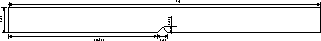
\includegraphics[width=\linewidth]{./Images/2d_1d_bar/2d_1d_bar.pdf}
	\caption{Geometry of the bar with a notch. All dimensions are in meters.}
	\label{2d_1d_bar_dims}
\end{figure}


\begin{figure}[ht]
	\begin{subfigure}{\textwidth}
		\centering
		
\includegraphics[width=\linewidth]{./Images/2d_1d_bar/damage_coarse.pdf}
		\caption{Coarse mesh}
		\label{2d_1d_bar_damage_coarse}
	\end{subfigure}
	\begin{subfigure}{\textwidth}
		\centering
		
\includegraphics[width=\linewidth]{./Images/2d_1d_bar/damage_inter.pdf}
		\caption{Intermediate mesh}
		\label{2d_1d_bar_damage_inter}
	\end{subfigure}
	\begin{subfigure}{\textwidth}
		\centering
		
\includegraphics[width=\linewidth]{./Images/2d_1d_bar/damage_fine.pdf}
		\caption{Fine mesh}
		\label{2d_1d_bar_damage_fine}
	\end{subfigure}
	\begin{subfigure}{\textwidth}
		\centering
		\vfill
		\includegraphics[width=0.4\linewidth]{./Images/2d_1d_bar/cb.pdf}
	\end{subfigure}
	\caption{Results with regularization - A notched bar}
	\label{2d_1d_bar_damage}
\end{figure}

Figure \ref{2d_1d_bar_damage} shows the damage distribution attached to the material states associated with each element. The results are for three mesh sizes, where the ratio of element sizes of the coarse mesh to the intermediate mesh, and of the intermediate mesh to the fine mesh is 2. The variation of damage value across the center of the bar, from $(0.08,0.01)$ to $(0.12,0.01)$, where the origin is at the bottom left corner of the bar, can be seen in figure \ref{1D_comparison_x}. Force-displacement curves for all the three mesh sizes can be seen in figure \ref{1D_force_displacement}. 

\begin{figure}[h]
	\centering
	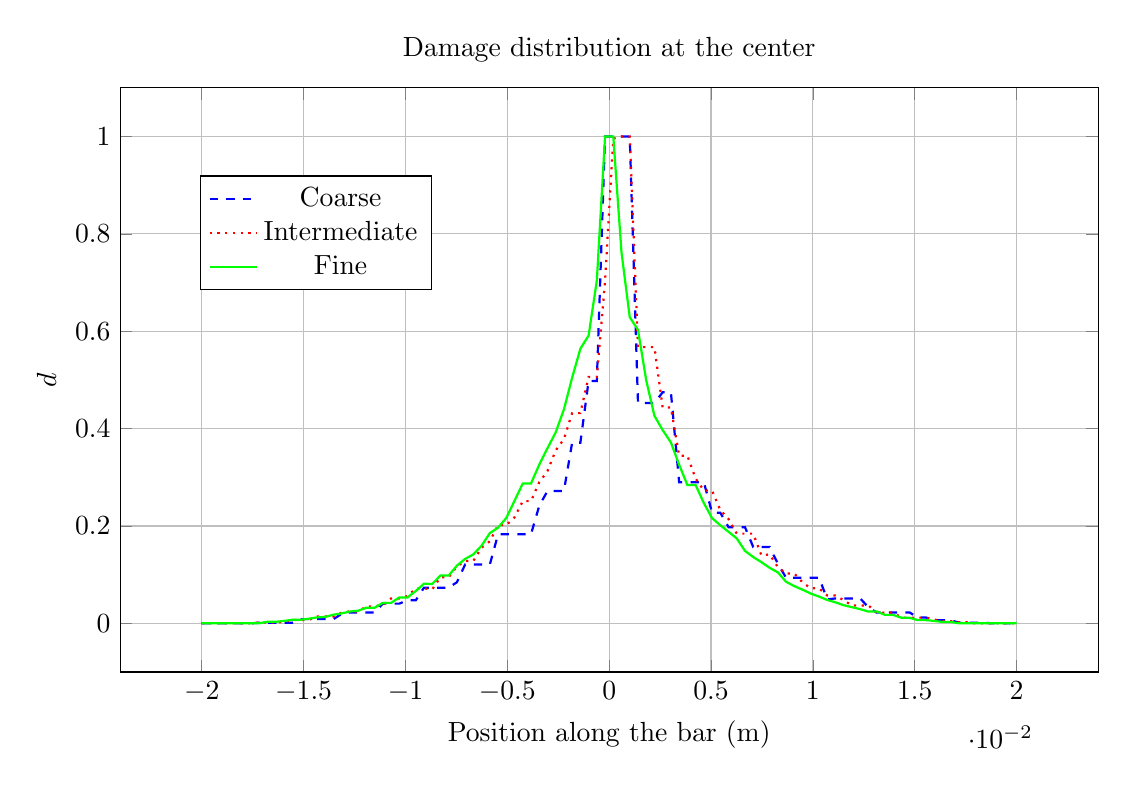
\begin{tikzpicture}
	\begin{axis}[
		title={Damage distribution at the center},
		xlabel={Position along the bar (\si{\meter})},
		ylabel={$d$},
		legend style={at={(0.2,0.85)}, anchor=north,legend columns=1},
		grid=major,
		width=14cm, height=9cm
		]
		
		% Database 1 (x, y) points using table
		\addplot[
		color=blue, dashed, thick
		% mark=square*,
		%thick
		] table[row sep=newline, x index=0, y index=1] {
			% (x, y) table for Database 1
			-0.02	0
			-0.01959596	0
			-0.01919192	0
			-0.01878788	0
			-0.01838384	0
			-0.0179798	0
			-0.01757576	0
			-0.01717172	0.00128829
			-0.01676768	0.00128829
			-0.01636364	0.00128829
			-0.0159596	0.00128829
			-0.01555556	0.00128829
			-0.01515152	0.00865917
			-0.01474747	0.00865917
			-0.01434343	0.00865917
			-0.01393939	0.00865917
			-0.01353535	0.00865917
			-0.01313131	0.01941903
			-0.01272727	0.02229877
			-0.01232323	0.02229877
			-0.01191919	0.02229877
			-0.01151515	0.02229877
			-0.01111111	0.04047378
			-0.01070707	0.04047378
			-0.01030303	0.04047378
			-0.00989899	0.0473094
			-0.00949495	0.0473094
			-0.00909091	0.07322054
			-0.00868687	0.07322054
			-0.00828283	0.07322054
			-0.00787879	0.07322054
			-0.00747475	0.08444728
			-0.00707071	0.12081048
			-0.00666667	0.12081048
			-0.00626263	0.12081048
			-0.00585859	0.12081048
			-0.00545455	0.18285312
			-0.00505051	0.18285312
			-0.00464646	0.18285312
			-0.00424242	0.18285312
			-0.00383838	0.18285312
			-0.00343434	0.24126004
			-0.0030303	0.27178724
			-0.00262626	0.27178724
			-0.00222222	0.27178724
			-0.00181818	0.37099499
			-0.00141414	0.37099499
			-0.0010101	0.49783787
			-0.00060606	0.49783787
			-0.00020202	0.9999
			0.00020202	0.9999
			0.00060606	0.9999
			0.0010101	0.9999
			0.00141414	0.45276356
			0.00181818	0.45276356
			0.00222222	0.45276356
			0.00262626	0.47462933
			0.0030303	0.47462933
			0.00343434	0.29002201
			0.00383838	0.29002201
			0.00424242	0.29002201
			0.00464646	0.29002201
			0.00505051	0.22729341
			0.00545455	0.22729341
			0.00585859	0.19756356
			0.00626263	0.19756356
			0.00666667	0.19756356
			0.00707071	0.15692796
			0.00747475	0.15692796
			0.00787879	0.15692796
			0.00828283	0.12220915
			0.00868687	0.09359967
			0.00909091	0.09359967
			0.00949495	0.09359967
			0.00989899	0.09359967
			0.01030303	0.09359967
			0.01070707	0.04917575
			0.01111111	0.05122383
			0.01151515	0.05122383
			0.01191919	0.05122383
			0.01232323	0.05122383
			0.01272727	0.03272842
			0.01313131	0.02232826
			0.01353535	0.02232826
			0.01393939	0.02232826
			0.01434343	0.02232826
			0.01474747	0.02232826
			0.01515152	0.01193278
			0.01555556	0.01193278
			0.0159596	0.00645206
			0.01636364	0.00645206
			0.01676768	0.00645206
			0.01717172	0.00140937
			0.01757576	0.00140937
			0.0179798	0.00140937
			0.01838384	0.00140937
			0.01878788	0
			0.01919192	0
			0.01959596	0
			0.02	0
			
		};
		\addlegendentry{Coarse}
		
		% Database 2 (x, y) points using table
		\addplot[
		color=red,dotted, thick
		%mark=*,
		%thick
		] table[row sep=newline, x index=0, y index=1] {
			% (x, y) table for Database 2
			-0.02	0
			-0.01959596	0
			-0.01919192	0
			-0.01878788	0
			-0.01838384	0
			-0.0179798	0
			-0.01757576	0
			-0.01717172	0.0019006484
			-0.01676768	0.0019006484
			-0.01636364	0.0019006484
			-0.0159596	0.00270852154
			-0.01555556	0.00699706231
			-0.01515152	0.00699706231
			-0.01474747	0.00699706231
			-0.01434343	0.0141726189
			-0.01393939	0.0141726189
			-0.01353535	0.0141726189
			-0.01313131	0.0220547539
			-0.01272727	0.0245227894
			-0.01232323	0.0245227894
			-0.01191919	0.0346990635
			-0.01151515	0.0346990635
			-0.01111111	0.0383681468
			-0.01070707	0.0511419034
			-0.01030303	0.0511419034
			-0.00989899	0.0559845708
			-0.00949495	0.0717165429
			-0.00909091	0.0717165429
			-0.00868687	0.0699003046
			-0.00828283	0.0946908418
			-0.00787879	0.0946908418
			-0.00747475	0.116704248
			-0.00707071	0.128184868
			-0.00666667	0.128184868
			-0.00626263	0.155659896
			-0.00585859	0.168600826
			-0.00545455	0.201763307
			-0.00505051	0.201763307
			-0.00464646	0.217606007
			-0.00424242	0.251030365
			-0.00383838	0.251030365
			-0.00343434	0.289739962
			-0.0030303	0.312789793
			-0.00262626	0.355057957
			-0.00222222	0.378406863
			-0.00181818	0.431777185
			-0.00141414	0.431777185
			-0.0010101	0.506180885
			-0.00060606	0.506180885
			-0.00020202	0.702784032
			0.00020202	0.995816884
			0.00060606	0.9999
			0.0010101	0.9999
			0.00141414	0.567404329
			0.00181818	0.567404329
			0.00222222	0.567404329
			0.00262626	0.443331118
			0.0030303	0.443331118
			0.00343434	0.344465059
			0.00383838	0.344465059
			0.00424242	0.297641363
			0.00464646	0.272829641
			0.00505051	0.272829641
			0.00545455	0.232772273
			0.00585859	0.214338904
			0.00626263	0.184266738
			0.00666667	0.184266738
			0.00707071	0.184266738
			0.00747475	0.139506529
			0.00787879	0.141717863
			0.00828283	0.115323753
			0.00868687	0.102227079
			0.00909091	0.102227079
			0.00949495	0.084057543
			0.00989899	0.0719219797
			0.01030303	0.0719219797
			0.01070707	0.0572415998
			0.01111111	0.0572415998
			0.01151515	0.0474200069
			0.01191919	0.0367894251
			0.01232323	0.0367894251
			0.01272727	0.0367894251
			0.01313131	0.0217289619
			0.01353535	0.0217289619
			0.01393939	0.0222192711
			0.01434343	0.0117811759
			0.01474747	0.0117811759
			0.01515152	0.0117811759
			0.01555556	0.0117811759
			0.0159596	0.00773067628
			0.01636364	0.00458161993
			0.01676768	0.00458161993
			0.01717172	0.00206939902
			0.01757576	0.00206939902
			0.0179798	0.00000849154868
			0.01838384	0
			0.01878788	0
			0.01919192	0
			0.01959596	0
			0.02	0
		};
		\addlegendentry{Intermediate}
		
		% Database 2 (x, y) points using table
		\addplot[
		color=green, thick
		%mark=*,
		%thick
		] table[row sep=newline, x index=0, y index=1] {
			% (x, y) table for Database 2
			-0.02	0
			-0.01959596	0
			-0.01919192	0
			-0.01878788	0
			-0.01838384	0
			-0.0179798	0
			-0.01757576	0.000281180554
			-0.01717172	0.000281180554
			-0.01676768	0.00321344804
			-0.01636364	0.00321344804
			-0.0159596	0.00494897067
			-0.01555556	0.00738243847
			-0.01515152	0.00738243847
			-0.01474747	0.00948638447
			-0.01434343	0.0121724203
			-0.01393939	0.0131860166
			-0.01353535	0.0177026146
			-0.01313131	0.0203968159
			-0.01272727	0.0243465473
			-0.01232323	0.0259369488
			-0.01191919	0.0320527784
			-0.01151515	0.0320527784
			-0.01111111	0.0420250771
			-0.01070707	0.0420250771
			-0.01030303	0.0532508826
			-0.00989899	0.0532508826
			-0.00949495	0.066308027
			-0.00909091	0.0812899725
			-0.00868687	0.0808903024
			-0.00828283	0.0981520171
			-0.00787879	0.0981520171
			-0.00747475	0.118533862
			-0.00707071	0.132308236
			-0.00666667	0.141675803
			-0.00626263	0.159502689
			-0.00585859	0.185335396
			-0.00545455	0.196479668
			-0.00505051	0.216420882
			-0.00464646	0.251719685
			-0.00424242	0.287127195
			-0.00383838	0.287127195
			-0.00343434	0.325756788
			-0.0030303	0.359481065
			-0.00262626	0.392198186
			-0.00222222	0.439335829
			-0.00181818	0.504656412
			-0.00141414	0.564063706
			-0.0010101	0.591070232
			-0.00060606	0.70401551
			-0.00020202	0.9999
			0.00020202	0.9999
			0.00060606	0.76150198
			0.0010101	0.628801162
			0.00141414	0.60303228
			0.00181818	0.49917198
			0.00222222	0.426178244
			0.00262626	0.397019133
			0.0030303	0.371633793
			0.00343434	0.325752928
			0.00383838	0.284276931
			0.00424242	0.284276931
			0.00464646	0.247213955
			0.00505051	0.216136345
			0.00545455	0.20155727
			0.00585859	0.188181105
			0.00626263	0.174473615
			0.00666667	0.148879827
			0.00707071	0.136217781
			0.00747475	0.125674585
			0.00787879	0.114058518
			0.00828283	0.104596742
			0.00868687	0.0853297784
			0.00909091	0.0764297166
			0.00949495	0.0691030194
			0.00989899	0.0611047669
			0.01030303	0.0549816588
			0.01070707	0.0480628849
			0.01111111	0.0430741554
			0.01151515	0.0372365066
			0.01191919	0.0331983954
			0.01232323	0.0290823113
			0.01272727	0.0242155398
			0.01313131	0.0245927933
			0.01353535	0.0174213147
			0.01393939	0.0174213147
			0.01434343	0.0114044599
			0.01474747	0.0114044599
			0.01515152	0.00659499328
			0.01555556	0.00659499328
			0.0159596	0.0049009423
			0.01636364	0.00284057212
			0.01676768	0.00284057212
			0.01717172	0.0000797127488
			0.01757576	0.0000797127488
			0.0179798	0
			0.01838384	0
			0.01878788	0
			0.01919192	0
			0.01959596	0
			0.02	0
		};
		\addlegendentry{Fine}
		
	\end{axis}
\end{tikzpicture}
	\caption{Variation of damage along the center of the bar, $y=0$, $x \in [-0.02,0.02]$ \unit{\meter}.}
	\label{1D_comparison_x}
\end{figure}

\begin{figure}[ht]
	\centering
	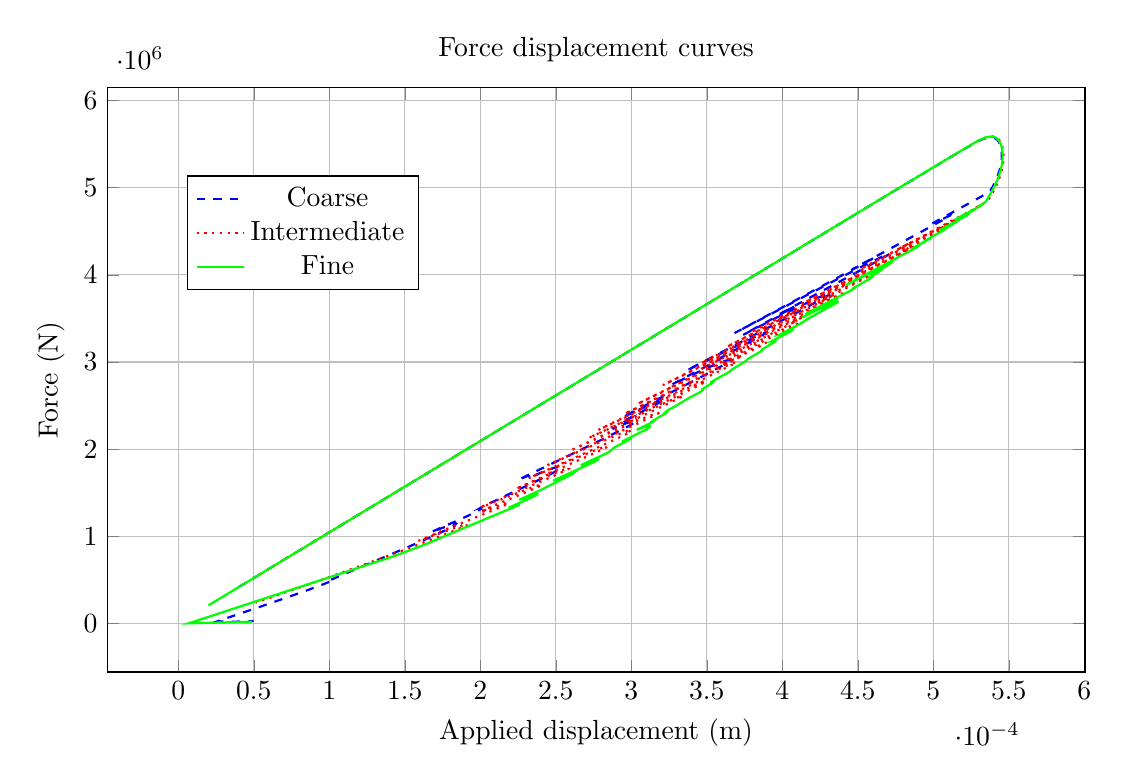
\begin{tikzpicture}
	\begin{axis}[
		title={Force displacement curves},
		xlabel={Applied displacement (\si{\meter})},
		ylabel={Force (\si{\newton})},
		legend style={at={(0.2,0.85)}, anchor=north,legend columns=1},
		grid=major,
		width=14cm, height=9cm
		]
		
		% Database 1 (x, y) points using table
		\addplot[
		color=blue, dashed, thick
		% mark=square*,
		%thick
		] table[row sep=newline, x index=0, y index=1] {
			% (x, y) table for Database 1
			0.00004	418738.765147154
			0.000052	544360.456821835
			0.000064	669982.196164301
			0.000076	795603.994577229
			0.000088	921225.863138471
			0.0001	1046847.81282017
			0.000112	1172469.8545489
			0.000124	1298091.99934132
			0.000136	1423714.25773243
			0.000148	1549336.64061796
			0.00016	1674959.15868227
			0.000172	1800581.82253501
			0.000184	1926204.64270467
			0.000196	2051827.62963246
			0.000208	2177450.79366824
			0.00022	2303074.14506275
			0.000232	2428697.69396422
			0.000244	2554321.45071334
			0.000256	2679945.42463248
			0.000268	2805569.62582941
			0.00028	2931194.06398682
			0.000292	3056818.74865783
			0.000304	3182443.68926232
			0.000316	3308068.89508247
			0.000328	3433694.37525709
			0.00034	3559320.13877836
			0.000352	3684946.19448806
			0.000364	3810572.5510729
			0.000376	3936199.21706037
			0.000388	4061826.20081612
			0.0004	4187453.51054054
			0.000467369463397527	4892272.88082461
			0.000483857434315324	5064147.34144122
			0.000491947917746064	5148298.61085044
			0.000497678734593886	5207790.49635669
			0.000502402245656494	5256758.15844201
			0.000506055468881553	5294533.35518529
			0.000509311563101179	5328159.93764475
			0.000512297838956764	5358965.58577494
			0.000514677658325399	5383428.49999794
			0.000516739938268317	5404574.6699444
			0.000518648057136467	5424111.51138361
			0.000520270038069545	5440657.23900117
			0.000521580930393991	5453952.19045115
			0.000522730742831972	5465565.24773813
			0.000523801429604346	5476352.59040494
			0.000524729834443974	5485653.20090723
			0.000525563579397023	5493965.87133753
			0.000526333374846547	5501611.28158474
			0.000527022058197941	5508409.69022545
			0.000527640565593177	5514475.70781336
			0.000528193502312634	5519857.41529459
			0.000528687836590266	5524627.66904869
			0.000529138917542086	5528946.84712494
			0.000529531731823	5532657.86252504
			0.000529878124787028	5535884.79027201
			0.00053017471546296	5538592.1938576
			0.00053042205049114	5540785.86131015
			0.000530604025766094	5542297.59756224
			0.000530758410534823	5543522.32910677
			0.000530895013221178	5544561.97213372
			0.000531019773689041	5545478.3274059
			0.000531142298040459	5546371.56638221
			0.000531260312115947	5547217.76138179
			0.000531374275622258	5548021.74425276
			0.000531485254147179	5548794.6445168
			0.000531594453798678	5549549.03438415
			0.000531702111746838	5550287.35771471
			0.000531808877158718	5551016.38010838
			0.00053191251770314	5551712.77872477
			0.000532012925420352	5552375.47791513
			0.000532111202777494	5553016.01116896
			0.000532207375017141	5553634.60718399
			0.000532301006321405	5554226.71095979
			0.000532391988086292	5554791.18891649
			0.000532480534701338	5555330.2599286
			0.000532568347588836	5555861.70384431
			0.000532655308631209	5556384.25937793
			0.000532741055330014	5556894.14135481
			0.000532825216002488	5557387.45257026
			0.00053290847374036	5557871.33825889
			0.000532988133076569	5558317.6760718
			0.000533064726158549	5558732.06392629
			0.000533140581388548	5559138.80844611
			0.000533215507824411	5559535.88059795
			0.000533290060532467	5559929.07078264
			0.000533364418101865	5560320.22055817
			0.000533438518050571	5560708.66862727
			0.000533512123994185	5561091.95193176
			0.000533585515053117	5561472.9917721
			0.000533658624566145	5561851.08329172
			0.000533730779883968	5562219.21410319
			0.00053380287526458	5562586.73446554
			0.000533874874452441	5562953.23501333
			0.000533946774356796	5563318.67907429
			0.000534017845537184	5563675.4644077
			0.000534087654813082	5564019.09702463
			0.000534156400173966	5564351.60407745
			0.000534225017453147	5564682.74231937
			0.000534292172921313	5564998.61377445
			0.0005343579430738	5565300.00030178
			0.000534423556222602	5565599.71510346
			0.000534489073353149	5565898.40770239
			0.00053455434438838	5566194.51508435
			0.000534619212016711	5566486.40765272
			0.000534683947445573	5566776.92053653
			0.000534748571805473	5567066.26089005
			0.000534812985275881	5567353.38493571
			0.00053487731199903	5567639.58995646
			0.000534940672119285	5567915.70957982
			0.0005350037438091	5568188.85094496
			0.0005350666863935	5568460.64024234
			0.000535128862928566	5568724.43897295
			0.000535190600408329	5568983.68632869
			0.000535251254785103	5569231.65981287
			0.000535311865984999	5569479.20328882
			0.000535371544481291	5569717.01756558
			0.000535428514108856	5569926.62180355
			0.000535484665804264	5570127.72446251
			0.000535540627784026	5570326.84979715
			0.000535595567382672	5570515.32599616
			0.000535649766875161	5570696.13407527
			0.000535703901606004	5570876.28900112
			0.000535757751912061	5571053.47135764
			0.000535810013329692	5571214.11548197
			0.000535861753869061	5571369.34306579
			0.000535913156668737	5571521.05377386
			0.000535964235840585	5571669.39665085
			0.000536015264899169	5571817.21671558
			0.000536066226424979	5571964.31676351
			0.000536117119743954	5572110.68758511
			0.000536167075040087	5572247.280733
			0.000536216278977036	5572376.03959461
			0.00053626541669019	5572504.09312296
			0.000536314331602017	5572629.81129353
			0.000536362585883964	5572748.6524425
			0.000536410738378974	5572866.45710552
			0.00053645883316465	5572983.6532839
			0.000536506863984096	5573100.1661618
			0.000536554830527504	5573215.99120585
			0.000536602732627921	5573331.12649339
			0.000536650570503793	5573445.57431605
			0.000536698213542663	5573557.97699997
			0.00053674410824256	5573652.18413404
			0.000536789865112829	5573744.92775863
			0.000536835556641062	5573836.97439715
			0.000536881184417444	5573928.33898649
			0.000536926171081256	5574013.02486817
			0.00053697034054826	5574089.22148758
			0.000537014173466672	5574161.92528722
			0.000537057954697674	5574234.09217877
			0.000537101675757116	5574305.61724228
			0.000537144896243795	5574371.92510737
			0.000537187638428265	5574433.26762733
			0.000537230215543569	5574492.90785077
			0.000537272580439392	5574550.34239377
			0.000537314763152163	5574605.88344262
			0.000537356255694494	5574654.25629635
			0.000537397411719197	5574699.15248907
			0.000537438516984642	5574743.52475986
			0.00053747952137542	5574786.83476282
			0.000537520433320747	5574829.1711962
			0.000537561253199939	5574870.53800348
			0.000537601961816043	5574910.73590162
			0.00053764107588515	5574934.36750233
			0.00053768002435237	5574956.24600261
			0.000537718815409855	5574976.4733805
			0.000537757092569386	5574991.35882197
			0.000537795329221033	5575005.84076332
			0.000537833514052191	5575019.77253634
			0.000537871646478194	5575033.14280065
			0.000537909726492825	5575045.95073212
			0.000537947754143895	5575058.19673577
			0.000537985729484625	5575069.88136073
			0.000538023560644038	5575080.05227462
			0.000538061321333422	5575089.48243009
			0.000538099033211574	5575098.3916931
			0.000538136693495276	5575106.74766594
			0.000538174302143316	5575114.54941291
			0.000538211779997693	5575120.97656657
			0.000538249132962541	5575126.09731035
			0.000538286439348085	5575130.72438061
			0.000538323694948428	5575134.80736332
			0.000538360899642442	5575138.34388154
			0.000538398053386542	5575141.33329973
			0.00053843491449427	5575141.26660915
			0.000538470916687985	5575132.29204959
			0.000538506883557449	5575122.95750732
			0.000538542676750152	5575111.80855355
			0.000538578394664712	5575099.87367511
			0.000538614067461027	5575087.45834779
			0.000538649689560947	5575074.49986835
			0.000538685001541719	5575058.31164658
			0.00053872012042981	5575040.1282843
			0.000538753924784867	5575008.32311137
			0.000538787652464185	5574975.73326789
			0.000538821347794316	5574942.80108041
			0.00053885487993815	5574908.09861003
			0.000538888372505023	5574873.03812167
			0.000538921820327909	5574837.49914113
			0.000538955221695929	5574801.46120903
			0.000538988549016908	5574764.63844523
			0.0005390216771863	5574725.73872627
			0.000539054762944438	5574686.39600394
			0.000539087610759308	5574644.57528019
			0.000539120323213801	5574601.35136009
			0.000539152793042798	5574555.60988847
			0.000539185023479967	5574507.39805066
			0.000539216985777586	5574456.39959685
			0.000539248889372735	5574404.82434114
			0.000539280721677966	5574352.50256404
			0.000539312491264516	5574299.5196953
			0.000539344221234064	5574246.11310923
			0.000539375908622914	5574192.24850429
			0.000539407553390496	5574137.92485304
			0.000539439155571227	5574083.14242498
			0.000539470715201786	5574027.90159218
			0.000539502232319478	5573972.20274516
			0.000539533706886802	5573916.04547226
			0.000539565138720768	5573859.42780007
			0.000539596528155212	5573802.35327449
			0.000539627832140665	5573744.37701245
			0.000539658827702228	5573683.19900188
			0.000539689498058697	5573618.66560956
			0.000539720110680568	5573553.5370714
			0.00053975068228627	5573487.97097876
			0.000539781212727085	5573421.96174054
			0.000539811547430021	5573353.91172172
			0.00053984091635266	5573275.87727488
			0.000539869171580982	5573186.35996868
			0.000539895796261819	5573080.00746171
			0.000539922373151998	5572973.15145641
			0.000539948913636119	5572865.89876448
			0.000539975415510667	5572758.22970607
			0.000540000609497221	5572637.01500174
			0.000540025379620943	5572511.40164334
			0.000540049089282532	5572374.8404526
			0.000540072536677242	5572235.63285837
			0.000540095955626055	5572096.14943098
			0.000540119338528428	5571956.28258711
			0.000540142677407591	5571815.94561062
			0.000540165955742162	5571674.9688562
			0.00054018920126209	5571533.64145663
			0.000540212411336595	5571391.9325788
			0.000540235586020826	5571249.84210584
			0.000540258725198102	5571107.36869235
			0.000540281827886267	5570964.50197058
			0.000540304898691763	5570821.29077857
			0.000540327839178766	5570676.70249741
			0.000540350750217162	5570531.82220682
			0.000540373626569232	5570386.57019771
			0.000540396468003672	5570240.9417755
			0.000540419274568742	5570094.93710812
			0.00054044204629825	5569948.55650989
			0.000540464631669352	5569800.23711908
			0.000540486432216915	5569643.81511844
			0.000540508190199375	5569486.98614222
			0.000540529914544086	5569329.80270403
			0.000540551605033547	5569172.25486403
			0.000540573261740706	5569014.34246266
			0.000540594884712893	5568856.06592664
			0.000540616473885649	5568697.42456687
			0.00054063802926252	5568538.41840852
			0.000540659356008218	5568377.0374955
			0.000540679320021412	5568201.58415284
			0.000540699283652661	5568026.14254785
			0.000540719215718361	5567850.36307929
			0.000540739114394745	5567674.22369143
			0.000540758978619719	5567497.71315856
			0.000540778809039113	5567320.83835187
			0.000540798606183982	5567143.60484855
			0.000540818370089292	5566966.01299659
			0.000540838100783111	5566788.06308715
			0.000540857755969671	5566609.31955254
			0.000540877325926415	5566429.68886058
			0.000540896866739435	5566249.75178624
			0.000540916374744458	5566069.46250495
			0.000540935849939654	5565888.81957959
			0.000540955272783228	5565707.62152127
			0.00054097461538283	5565525.5847744
			0.000540993905166594	5565342.99856748
			0.000541013165707841	5565160.10220207
			0.00054103239396138	5564976.85854519
			0.000541051589936654	5564793.26669699
			0.0005410707536687	5564609.32689157
			0.000541089885186332	5564425.03941791
			0.000541108984516201	5564240.40455178
			0.000541128051684696	5564055.42256846
			0.000541147086718086	5563870.09374074
			0.000541166089642632	5563684.41834238
			0.000541185060484473	5563498.39664496
			0.000541203999269745	5563312.02891982
			0.000541222906024515	5563125.31543824
			0.000541241780774778	5562938.25647116
			0.000541260623546509	5562750.85228761
			0.00054127944418428	5562563.20981573
			0.000541298208366138	5562374.89401212
			0.000541316939137133	5562186.2910888
			0.000541335638708858	5561997.35310406
			0.000541354306260864	5561808.06982639
			0.000541372941900174	5561618.44206504
			0.00054139154582891	5561428.47188079
			0.000541410118076025	5561238.15955897
			0.000541428658667765	5561047.50536924
			0.000541447167629386	5560856.50957372
			0.000541465644985892	5560665.17243215
			0.000541484090762342	5560473.49420417
			0.000541502504983689	5560281.47514972
			0.000541520887674799	5560089.11552673
			0.000541539238860542	5559896.41559328
			0.000541557558565729	5559703.37560758
			0.00054157584660597	5559509.99342378
			0.00054159410321774	5559316.27165078
			0.000541611834270067	5559117.12896137
			0.000541628977606507	5558911.93667946
			0.000541646096961647	5558706.49761366
			0.000541663184624024	5558500.71952642
			0.000541680241655369	5558294.61119568
			0.000541697268112271	5558088.17267263
			0.000541714263998785	5557881.40389578
			0.000541731229334346	5557674.30505373
			0.000541748058175761	5557465.78803159
			0.000541764266890273	5557250.89380713
			0.000541780276737074	5557033.99599371
			0.000541796237310718	5556816.58564174
			0.000541812169690893	5556598.89213828
			0.000541828073047144	5556380.886574
			0.000541843947432039	5556162.56793352
			0.000541859792898007	5555943.93649411
			0.000541875608995218	5555724.98742295
			0.000541891395998539	5555505.72357258
			0.000541907154176553	5555286.14781066
			0.000541922883525159	5555066.26012228
			0.000541938572805166	5554845.94519784
			0.000541954214010223	5554625.11904732
			0.000541969845674158	5554404.19718953
			0.000541985420212072	5554182.50398284
			0.000542000874478496	5553959.7182867
			0.000542016297907215	5553736.61612367
			0.000542031693052772	5553513.21221655
			0.000542047059901212	5553289.50258014
			0.00054206206359884	5553062.0508213
			0.000542076434906886	5552828.11646245
			0.000542090792032741	5552594.05616141
			0.000542105122106493	5552359.70816081
			0.000542119424613885	5552125.0621765
			0.000542133699610791	5551890.1183415
			0.000542147947143274	5551654.87713676
			0.000542162165951409	5551419.32443453
			0.000542176318473952	5551183.07686834
			0.000542190355531573	5550945.62203068
			0.000542204357699665	5550707.81605854
			0.000542218331910701	5550469.71119335
			0.000542232278929549	5550231.31242184
			0.000542246198903011	5549992.62070546
			0.000542260091872815	5549753.63640224
			0.000542273957856232	5549514.35968435
			0.000542287796873075	5549274.79075306
			0.000542301608943299	5549034.92981539
			0.000542315394086789	5548794.77707483
			0.000542329152323452	5548554.33273509
			0.000542342883673138	5548313.59700142
			0.000542356588155605	5548072.57007547
			0.00054237026579061	5547831.25216075
			0.00054238391659787	5547589.64345944
			0.00054239754059704	5547347.74417426
			0.000542411137807719	5547105.55450501
			0.000542424708249485	5546863.07465248
			0.000542438251852907	5546620.30388289
			0.000542451782198915	5546377.38527022
			0.000542465246748308	5546133.68424953
			0.000542478684273056	5545889.78398909
			0.000542492096378831	5545645.60843033
			0.000542505481872454	5545401.14487016
			0.000542518840843985	5545156.39372699
			0.000542532173241396	5544911.35431878
			0.000542545479184301	5544666.02792556
			0.000542558758681165	5544420.4146474
			0.000542572023262093	5544174.63838945
			0.00054258523136866	5543928.18156717
			0.000542598412726671	5543681.51880219
			0.00054261156858479	5543434.58177215
			0.00054262469809502	5543187.35939267
			0.000542637801373934	5542939.85241399
			0.000542650878454364	5542692.06109454
			0.000542663929354706	5542443.98561331
			0.000542676954092864	5542195.62615193
			0.000542689954251101	5541946.99956073
			0.000542702895491347	5541697.74429711
			0.000542715812008703	5541448.23656633
			0.000542728702019412	5541198.4430446
			0.000542741566015801	5540948.36738018
			0.000542754404027009	5540698.0095773
			0.000542767216326625	5540447.37037821
			0.000542780002756092	5540196.45017766
			0.000542792763339271	5539945.24921922
			0.00054280549809655	5539693.76771075
			0.00054281820704556	5539442.0058306
			0.000542830890203573	5539189.96375521
			0.00054284354758782	5538937.64165933
			0.000542856179215509	5538685.03971883
			0.00054286878510382	5538432.15810881
			0.000542881365269875	5538178.99700341
			0.000542893919730771	5537925.55657653
			0.000542906441015842	5537671.76056487
			0.00054291891202664	5537417.43672388
			0.00054293135959776	5537162.86355295
			0.000542943757676772	5536907.76949751
			0.00054295585573884	5536649.59834198
			0.000542967935605393	5536391.26798466
			0.000542979990134269	5536132.66985306
			0.000542992019759664	5535873.8017333
			0.000543004024579123	5535614.66371527
			0.000543016004629141	5535355.2561068
			0.000543027959929581	5535095.57911264
			0.000543039737717812	5534834.07372117
			0.000543051329745323	5534570.67557946
			0.000543062891633727	5534306.97706061
			0.000543074428647883	5534043.01311994
			0.000543085939501686	5533778.7653497
			0.000543097423926018	5533514.2302029
			0.000543108881103857	5533249.40020137
			0.000543120227866682	5532983.42814931
			0.000543131525479147	5532716.9566854
			0.000543142692979227	5532449.15062242
			0.000543153836139455	5532181.09797769
			0.000543164955417467	5531912.7890595
			0.000543176051060055	5531644.22296324
			0.000543187123111474	5531375.39965772
			0.00054319817159606	5531106.31936017
			0.000543209196530824	5530836.98224396
			0.000543220197929833	5530567.38845181
			0.000543231175806649	5530297.53812014
			0.000543242130174901	5530027.43138543
			0.000543253061048198	5529757.06838481
			0.000543263968440165	5529486.44925527
			0.000543274463616642	5529211.6093653
			0.000543284801958922	5528935.1810485
			0.000543295118319112	5528658.52804915
			0.000543305410807351	5528381.61793709
			0.000543315680447831	5528104.45899767
			0.000543325927359583	5527827.05196008
			0.000543336151540131	5527549.3967051
			0.000543346352997109	5527271.49329752
			0.000543356531743671	5526993.34186816
			0.000543366687798208	5526714.94260231
			0.000543376821172957	5526436.2956224
			0.00054338692943005	5526157.37610007
			0.000543396977895764	5525877.83088481
			0.000543407004582934	5525598.05610669
			0.000543417008125697	5525318.03083161
			0.000543426989095292	5525037.75929726
			0.000543436947641858	5524757.24271603
			0.000543446904298321	5524476.69743984
			0.000543456792244054	5524195.32217754
			0.00054346662663957	5523913.31365825
			0.000543476453933721	5523631.4078848
			0.000543486258239405	5523349.25110234
			0.000543496040592144	5523066.8539711
			0.000543505799560133	5522784.20194049
			0.000543515314846437	5522499.05343598
			0.000543524466162861	5522210.21324253
			0.000543533602568418	5521921.25226232
			0.000543542717706082	5521632.06603457
			0.000543551811149669	5521342.64315548
			0.000543560883027396	5521052.9842388
			0.000543569933420897	5520763.0901323
			0.000543578962359242	5520472.96114173
			0.000543587969849051	5520182.59732752
			0.000543596955903407	5519891.99881658
			0.000543605920538208	5519601.16577208
			0.000543614863763234	5519310.09829117
			0.000543623785589414	5519018.79648077
			0.000543632686027875	5518727.26045082
			0.00054364156501048	5518435.48947927
			0.000543650422377233	5518143.48187991
			0.000543659258373729	5517851.24023084
			0.000543668073021519	5517558.76474661
			0.000543676866334858	5517266.05556695
			0.000543685638250546	5516973.11203398
			0.000543694388956394	5516679.93511939
			0.00054370311835916	5516386.52478883
			0.000543711826467018	5516092.88113743
			0.000543720481660507	5515798.68286905
			0.000543729002787574	5515503.11046647
			0.000543737507351836	5515207.37471924
			0.000543745857529879	5514910.0573975
			0.000543754143739193	5514612.09695459
			0.000543762409719586	5514313.92674318
			0.000543770654433905	5514015.52588953
			0.000543778878767991	5513716.90155015
			0.000543787082827571	5513418.05442546
			0.000543795266557192	5513118.98381465
			0.000543803430057223	5512819.69080481
			0.000543811573316966	5512520.17528758
			0.000543819696326741	5512220.43714509
			0.000543827799122055	5511920.47674977
			0.000543835881709095	5511620.29416378
			0.000543843944042544	5511319.88891051
			0.000543851986254976	5511019.26168529
			0.000543860008290415	5510718.41255604
			0.000543868010151953	5510417.34155803
			0.000543875991089884	5510116.04079706
			0.000543883950954797	5509814.50867388
			0.000543891890653298	5509512.75470163
			0.000543899810220596	5509210.77925885
			0.000543907709658607	5508908.58236818
			0.000543915588975198	5508606.16410898
			0.000543923448179614	5508303.52456813
			0.000543931287281152	5508000.66383554
			0.00054393910628901	5507697.58199867
			0.000543946905212357	5507394.27914624
			0.000543954684060335	5507090.75536531
			0.000543962442842054	5506787.01074192
			0.000543970181511673	5506483.04479318
			0.000543977900201424	5506178.85821601
			0.000543985598336698	5505874.44554556
			0.000543993276281674	5505569.8105727
			0.000544000934233892	5505264.95542707
			0.000544008564284644	5504959.79998904
			0.00054401614309949	5504654.11004395
			0.00054402370324312	5504348.22184789
			0.000544031242943663	5504042.11063579
			0.000544038762641998	5503735.77947348
			0.000544046262599557	5503429.23014914
			0.00054405374277445	5503122.46278782
			0.000544061203163616	5502815.47734853
			0.000544068643776947	5502508.27392912
			0.000544076064623507	5502200.85261409
			0.00054408346571184	5501893.21348434
			0.000544090825687038	5501585.1402455
			0.00054409814235207	5501276.61536224
			0.000544105439013581	5500967.87687738
			0.000544112715576686	5500658.91871046
			0.000544119972477097	5500349.74396994
			0.000544127209860419	5500040.3538831
			0.000544134427745529	5499730.74859257
			0.00054414162613701	5499420.92812826
			0.000544148805041805	5499110.89255531
			0.000544155964467863	5498800.64194671
			0.000544163104423189	5498490.17637715
			0.000544170224915677	5498179.49592003
			0.000544177325953292	5497868.60064963
			0.000544184403073983	5497557.44538233
			0.000544191444350927	5497245.91046525
			0.000544198466960071	5496934.17470311
			0.000544205469436526	5496622.21832016
			0.000544212452334943	5496310.04581389
			0.000544219415807582	5495997.65861939
			0.000544226359958865	5495685.05788584
			0.000544233284773123	5495372.2434803
			0.000544240190257503	5495059.21547394
			0.000544247076419426	5494745.97393765
			0.00054425394326645	5494432.51893732
			0.00054426079080765	5494118.85055515
			0.000544267619047962	5493804.96884597
			0.00054427442799733	5493490.87389019
			0.000544281217662053	5493176.56575633
			0.000544287988048266	5492862.04449969
			0.000544294739100449	5492547.30952996
			0.000544301470880454	5492232.36132575
			0.000544308183370902	5491917.19986896
			0.000544314876573867	5491601.82518154
			0.000544321550498379	5491286.23733324
			0.000544328172432403	5490970.10575718
			0.00054433476421299	5490653.66026379
			0.000544341336804993	5490337.0079305
			0.000544347890114652	5490020.14341363
			0.000544354424299283	5489703.06740687
			0.000544360939378398	5489385.77998587
			0.000544367435366922	5489068.28127357
			0.000544373912271718	5488750.57135439
			0.00054438037004847	5488432.64975605
			0.000544386808818013	5488114.51713661
			0.000544393228528164	5487796.17352734
			0.000544399629180584	5487477.61893249
			0.000544406010783316	5487158.8534432
			0.000544412373344043	5486839.8771294
			0.000544418716870917	5486520.69006491
			0.000544425041367584	5486201.29229244
			0.000544431346843102	5485881.68387765
			0.000544437633303502	5485561.86487599
			0.000544443900756634	5485241.83535402
			0.000544450149206411	5484921.59534892
			0.000544456378664194	5484601.14494626
			0.000544462619452898	5484280.79451801
			0.000544468546169749	5483957.09148805
			0.000544474460660959	5483633.44289354
			0.00054448035500314	5483309.58216721
			0.000544486230009426	5482985.50949406
			0.000544492086560215	5482661.23235817
			0.000544497924765209	5482336.75152907
			0.000544503744445254	5482012.06496423
			0.000544509545200256	5481687.16818166
			0.000544515326824091	5481362.0585989
			0.000544521090039069	5481036.74413628
			0.000544526834943178	5480711.22613394
			0.000544532561482809	5480385.50410684
			0.000544538269712611	5480059.57833397
			0.00054454395962034	5479733.4489636
			0.000544549631202648	5479407.11595258
			0.000544555284466875	5479080.57936969
			0.00054456091942022	5478753.83927714
			0.00054456653606901	5478426.89572938
			0.000544572134419488	5478099.74878007
			0.000544577714474657	5477772.3984492
			0.000544583276232589	5477444.8447013
			0.000544588819711765	5477117.08771482
			0.000544594344889846	5476789.12724927
			0.00054459985182654	5476460.96362248
			0.000544605340509815	5476132.59698533
			0.000544610810935731	5475804.0272881
			0.000544616263111223	5475475.25459323
			0.000544621697043157	5475146.27896155
			0.000544627112737618	5474817.10044378
			0.000544632510086167	5474487.71789943
			0.00054463788910981	5474158.13155123
			0.000544643249909971	5473828.3424455
			0.000544648592465263	5473498.35033307
			0.000544653916837895	5473168.15555512
			0.000544659223016611	5472837.75826615
			0.000544664510997078	5472507.1584129
			0.000544669780785883	5472176.35605437
			0.000544675032389663	5471845.35124819
			0.000544680265747058	5471514.14310287
			0.000544685480728024	5471182.72966582
			0.000544690677589955	5470851.11425541
			0.000544695856295535	5470519.29661978
			0.000544701016843556	5470187.27675446
			0.000544706159209808	5469855.05439579
			0.000544711283454522	5469522.62986237
			0.000544716389565727	5469190.00330797
			0.000544721477539025	5468857.17471008
			0.00054472654727761	5468524.14300982
			0.00054473159885943	5468190.90898816
			0.000544736632255562	5467857.47238766
			0.00054474164746687	5467523.83320453
			0.00054474664450179	5467189.99148651
			0.000544751623368507	5466855.9473122
			0.000544756584070127	5466521.70072407
			0.00054476152661112	5466187.25175875
			0.000544766451025298	5465852.6007509
			0.000544771357263104	5465517.74745808
			0.000544776245345362	5465182.69178367
			0.000544781115311312	5464847.43399275
			0.000544785967034471	5464511.97286013
			0.000544790800475502	5464176.30845007
			0.000544795615625575	5463840.44020217
			0.000544800412090722	5463504.36290554
			0.000544805190328614	5463168.08218914
			0.000544809950200313	5462831.59688734
			0.000544814691758715	5462494.90756274
			0.000544819414870013	5462158.01284046
			0.000544824119588238	5461820.91335403
			0.000544828806070514	5461483.61040126
			0.000544833474301879	5461146.10413913
			0.000544838124277625	5460808.3945008
			0.000544842756007642	5460470.48156218
			0.000544847369498398	5460132.36539099
			0.000544851964752651	5459794.04600833
			0.000544856541768186	5459455.52332469
			0.000544861100499106	5459116.79695263
			0.000544865640230257	5458777.85931212
			0.000544870161488475	5458438.71602146
			0.000544874664466838	5458099.36905381
			0.000544879149192217	5457759.81865726
			0.000544883615669297	5457420.06487571
			0.000544888063904255	5457080.10775303
			0.000544892493848347	5456739.9467901
			0.000544896905468753	5456399.58147841
			0.000544901298789783	5456059.01221312
			0.000544905673790433	5455718.23881231
			0.000544910030468767	5455377.26126118
			0.000544914368832664	5455036.07961159
			0.000544918688891168	5454694.69396415
			0.000544922990639375	5454353.10429843
			0.000544927274089889	5454011.31066418
			0.00054493153920536	5453669.31268568
			0.000544935786005475	5453327.1104335
			0.000544940014472486	5452984.70395033
			0.000544944224611248	5452642.09319143
			0.000544948416425351	5452299.27819005
			0.000544952589919506	5451956.25898049
			0.000544956745101605	5451613.03562108
			0.000544960881974842	5451269.60814077
			0.000544965000547127	5450925.97659887
			0.000544969100823619	5450582.14106406
			0.000544973182768223	5450238.10115875
			0.000544977246367425	5449893.85703281
			0.00054498129162663	5449549.40845433
			0.000544985318562136	5449204.75556938
			0.000544989327171851	5448859.89837491
			0.000544993317462464	5448514.83690002
			0.000544997289439875	5448169.57119454
			0.000545001243108376	5447824.10128256
			0.000545005178479857	5447478.42725113
			0.000545009095557596	5447132.54916428
			0.000545012994342613	5446786.46702941
			0.000545016874844688	5446440.18091211
			0.000545020737069316	5446093.6908738
			0.000545024581018832	5445746.9969356
			0.000545028406702718	5445400.09916418
			0.000545032214122803	5445052.99758972
			0.000545036003284942	5444705.69224116
			0.000545039774194618	5444358.18315268
			0.000545043526862724	5444010.47040933
			0.000545047261290604	5443662.5540563
			0.000545050977483288	5443314.4341263
			0.000545054675444143	5442966.11064475
			0.000545058355179681	5442617.58364396
			0.000545062016661483	5442268.85285644
			0.000545065659957759	5441919.91819654
			0.000545069284918272	5441570.77962774
			0.00054507289164481	5441221.43710795
			0.000545076480127248	5440871.89087969
			0.000545080050360299	5440522.14086172
			0.000545083602352558	5440172.18712553
			0.00054508713610762	5439822.02971846
			0.000545090651630713	5439471.6686781
			0.000545094148927004	5439121.10404559
			0.000545097628001161	5438770.33585204
			0.000545101088857041	5438419.36411491
			0.000545104531528463	5438068.18911992
			0.000545107955910635	5437716.8098968
			0.000545111362044333	5437365.22682543
			0.000545114749926165	5437013.43988403
			0.000545118119528047	5436661.44873979
			0.000545121470922598	5436309.25377803
			0.000545124804091877	5435956.85516019
			0.000545128119031108	5435604.25282365
			0.00054513141574231	5435251.44679386
			0.000545134694076627	5434898.43516999
			0.000545137954217575	5434545.21993456
			0.000545141196051939	5434191.79983485
			0.000545144419660013	5433838.17634074
			0.000545147625014462	5433484.3488537
			0.000545150811119141	5433130.30647822
			0.000545153979178052	5432776.06192868
			0.000545157150549791	5432421.84116883
			0.00054516026298917	5432066.79425757
			0.000545163375956342	5431711.93623313
			0.000545166470611263	5431356.87192207
			0.000545169547104515	5431001.60340412
			0.000545172604979194	5430646.12687313
			0.000545175641060523	5430290.4112557
			0.000545178659062661	5429934.49479892
			0.000545181658772133	5429578.37428849
			0.000545184640325963	5429222.05067789
			0.000545187603750558	5428865.52415534
			0.000545190548954083	5428508.79374894
			0.000545193475999213	5428151.8600962
			0.00054519638474282	5427794.72154959
			0.000545199273069272	5427437.35220016
			0.000545202143901298	5427079.78499644
			0.000545204996565879	5426722.01420537
			0.000545207830967365	5426364.03898238
			0.00054521064711366	5426005.85946999
			0.000545213445013875	5425647.47574449
			0.000545216224675025	5425288.88786807
			0.000545218986097225	5424930.09585041
			0.000545221729287007	5424571.09972494
			0.000545224454249283	5424211.89953415
			0.000545227160990746	5423852.49533513
			0.000545229849510965	5423492.8871354
			0.000545232519816626	5423133.07496445
			0.000545235171775705	5422773.05745691
			0.000545237805380891	5422412.83421249
			0.000545240420716377	5422052.40627904
			0.00054524301562984	5421691.74963022
			0.000545245592215447	5421330.88686334
			0.000545248150804038	5420969.8220799
			0.000545250691221306	5420608.55363817
			0.000545253213447467	5420247.08132892
			0.000545255727717115	5419885.51106701
			0.000545258197477001	5419523.39224708
			0.000545260635516004	5419161.0171229
			0.00054526297004603	5418797.59642907
			0.000545265287336981	5418434.00822827
			0.000545267585559787	5418070.21333684
			0.000545269865794135	5417706.21784224
			0.000545272128107045	5417342.02104285
			0.000545274372462136	5416977.62261872
			0.000545276598855947	5416613.02261407
			0.000545278806442561	5416248.21232147
			0.000545280996106407	5415883.2004048
			0.000545283167841655	5415517.98721348
			0.000545285321648178	5415152.57271674
			0.000545287457536579	5414786.9569798
			0.000545289575505866	5414421.14002445
			0.000545291675565864	5414055.12191321
			0.000545293757714205	5413688.90265007
			0.000545295821956954	5413322.48225282
			0.00054529786829868	5412955.8607585
			0.000545299896738177	5412589.03814439
			0.000545301907285583	5412222.01445776
			0.000545303899939785	5411854.78969603
			0.000545305874709863	5411487.36390521
			0.000545307831594676	5411119.73709001
			0.00054530977060173	5410751.90928824
			0.000545311691734884	5410383.88054883
			0.000545313594991378	5410015.65084782
			0.000545315480324059	5409647.21965345
			0.00054531734748128	5409278.5834314
			0.00054531919685082	5408909.74687954
			0.000545321028381897	5408540.70962691
			0.000545322842049148	5408171.47147042
			0.000545324637768075	5407802.03149129
			0.000545326415567981	5407432.38999432
			0.000545328175446377	5407062.54679391
			0.000545329917377318	5406692.50174803
			0.000545331641360426	5406322.25479262
			0.000545333347358877	5405951.8055724
			0.000545335034275091	5405581.1422329
			0.000545336702952709	5405210.27439798
			0.000545338353749182	5404839.20529704
			0.000545339986581672	5404467.93406472
			0.000545341601431694	5404096.46053905
			0.000545343198301184	5403724.78471576
			0.000545344777183298	5403352.90653581
			0.000545346338095139	5402980.82608151
			0.00054534787991931	5402608.53172628
			0.000545349403301518	5402236.03024441
			0.000545350908681743	5401863.32622258
			0.000545352396107257	5401490.42006775
			0.000545353865575077	5401117.31176123
			0.000545355317086088	5400744.00128401
			0.000545356750640455	5400370.48862707
			0.000545358166139976	5399996.77275825
			0.000545359563708732	5399622.85492133
			0.000545360943128895	5399248.73315104
			0.000545362304354044	5398874.40700021
			0.000545363647419466	5398499.87647695
			0.00054536497231562	5398125.14154175
			0.00054536627896825	5397750.20205367
			0.00054536756739486	5397375.05765886
			0.000545368837616718	5396999.70852146
			0.000545370089634696	5396624.15467039
			0.000545371323443987	5396248.39605578
			0.000545372539045574	5395872.43262784
			0.000545373736376198	5395496.26423559
			0.000545374915437209	5395119.89052455
			0.000545376076232277	5394743.31140441
			0.000545377218730653	5394366.5252831
			0.000545378342840565	5393989.52813995
			0.000545379448813362	5393612.32659026
			0.000545380536558964	5393234.9197472
			0.00054538160601866	5392857.30670732
			0.00054538265722974	5392479.48860502
			0.00054538369009093	5392101.46475595
			0.000545384704626533	5391723.2348201
			0.000545385700890455	5391344.79913542
			0.00054538667878207	5390966.15659503
			0.000545387638106675	5390587.30618349
			0.000545388578939133	5390208.2477909
			0.000545389501165993	5389828.98081334
			0.00054539040478789	5389449.50450539
			0.000545391289755958	5389069.81951009
			0.000545392156091103	5388689.9255135
			0.000545393003791099	5388309.82254869
			0.000545393832790531	5387929.50995888
			0.00054539464321376	5387548.9883261
			0.000545395441749524	5387168.32641939
			0.000545396189293191	5386787.08462331
			0.000545396917135202	5386405.68035267
			0.000545397626033665	5386024.06824712
			0.000545398316285602	5385642.24779765
			0.000545398988081116	5385260.22005615
			0.000545399641336663	5384877.98415486
			0.000545400276176061	5384495.54065487
			0.000545400884150804	5384112.80644583
			0.000545401445307396	5383729.58811221
			0.000545401985341398	5383346.14643939
			0.000545402504981864	5382962.4791016
			0.00054540300622358	5382578.60507445
			0.000545403489193712	5382194.52535047
			0.000545403953880374	5381810.23985012
			0.000545404400294783	5381425.74870563
			0.000545404828449496	5381041.05204815
			0.000545405238261648	5380656.1490447
			0.000545405629866389	5380271.04020016
			0.000545406003156612	5379885.72525959
			0.000545406358197412	5379500.20486158
			0.000545406694984964	5379114.47895461
			0.000545407013532223	5378728.54763755
			0.000545407313759315	5378342.41013565
			0.000545407595605711	5377956.06496193
			0.000545407856790932	5377569.48896926
			0.00054540809963143	5377182.70644602
			0.000545408324223788	5376795.71828476
			0.000545408530530506	5376408.52408968
			0.000545408718526999	5376021.12363575
			0.0005454088883614	5375633.51757684
			0.000545409039985901	5375245.70616769
			0.000545409173311525	5374857.68851435
			0.000545409288371665	5374469.46478237
			0.000545409385145199	5374081.03497633
			0.000545409463632935	5373692.39891918
			0.000545409523835419	5373303.55661636
			0.000545409565755167	5372914.50809726
			0.000545409589392417	5372525.25336972
			0.000545409594767887	5372135.79261702
			0.000545409581754065	5371746.12509597
			0.000545409550494983	5371356.25118681
			0.000545409500809428	5370966.17029282
			0.000545409432746754	5370575.88210239
			0.000545409346271454	5370185.38621225
			0.000545409241384049	5369794.68227268
			0.000545409118151004	5369403.77128515
			0.000545408976413972	5369012.65237025
			0.000545408816208481	5368621.32513638
			0.000545408637562125	5368229.78977882
			0.000545408440485221	5367838.04644038
			0.000545408224899454	5367446.09448088
			0.000545407990845659	5367053.93402256
			0.000545407738316659	5366661.56519478
			0.000545407467336092	5366268.98821265
			0.000545407177776426	5365876.20258766
			0.000545406869688583	5365483.20798433
			0.000545406543086969	5365090.00453039
			0.000545406197982473	5364696.59228064
			0.000545405834368156	5364302.9711978
			0.000545405452255608	5363909.14134736
			0.000545405051646392	5363515.10279476
			0.000545404632534518	5363120.85549041
			0.000545404194935879	5362726.39951879
			0.000545403738848072	5362331.7349118
			0.000545403264272848	5361936.8616608
			0.000545402771214683	5361541.77978173
			0.000545402259683774	5361146.4893579
			0.000545401729673228	5360750.99036385
			0.000545401181191177	5360355.2828138
			0.000545400614234821	5359959.36667752
			0.00054540002881269	5359563.24196398
			0.000545399424930903	5359166.90871678
			0.000545398802589463	5358770.36694261
			0.000545398161789019	5358373.61663926
			0.000545397502537455	5357976.65782575
			0.000545396824841313	5357579.49056767
			0.000545396128702422	5357182.11490419
			0.000545395414120095	5356784.53083452
			0.000545394681097199	5356386.73836315
			0.000545393929639191	5355988.73751829
			0.00054539315965477	5355590.52737449
			0.000545392371316082	5355192.10872143
			0.000545391564569922	5354793.48187656
			0.000545390739398257	5354394.64666005
			0.000545389895801391	5353995.60307099
			0.000545389032975484	5353596.3426929
			0.000545388151488143	5353196.87142289
			0.000545387251675223	5352797.19275657
			0.000545386333476255	5352397.30585772
			0.000545385396871343	5351997.21062818
			0.000545384441856049	5351596.90700566
			0.000545383468431411	5351196.39498438
			0.000545382476600871	5350795.67457176
			0.000545381459295072	5350394.66828848
			0.000545380422385789	5349993.43900138
			0.000545379367087081	5349592.00070949
			0.000545378293383419	5349190.35371737
			0.000545377201131717	5348788.49604279
			0.000545376090394329	5348386.42861881
			0.000545374961141877	5347984.15137464
			0.000545373813406786	5347581.66487163
			0.000545372647036346	5347178.96823779
			0.000545371462081943	5346776.06121735
			0.000545370258562249	5346372.9439945
			0.000545369036484884	5345969.61660386
			0.000545367795847993	5345566.07902423
			0.000545366536654126	5345162.33124824
			0.000545365258814479	5344758.37236387
			0.000545363962490544	5344354.20308198
			0.000545362647634456	5343949.82370682
			0.000545361314214181	5343545.23391851
			0.000545359962167978	5343140.43231481
			0.000545358591472697	5342735.42002916
			0.00054535720207336	5342330.19603547
			0.00054535579395824	5341924.75994851
			0.000545354367207832	5341519.1130203
			0.000545352921556035	5341113.25319867
			0.000545351457089518	5340707.18034074
			0.000545349973744998	5340300.89385018
			0.000545348471280131	5339894.39117547
			0.000545346950270022	5339487.67544675
			0.00054534541081496	5339080.74483078
			0.000545343852283624	5338673.59719148
			0.000545342274923944	5338266.23623106
			0.000545340678739653	5337858.66207588
			0.000545339063814159	5337450.87554769
			0.000545337429993589	5337042.87592851
			0.000545335777262857	5336634.66232714
			0.000545334105666653	5336226.23485152
			0.000545332415236073	5335817.59365365
			0.000545330705950448	5335408.73878428
			0.000545328977808054	5334999.67019609
			0.000545327230808589	5334590.38789811
			0.000545325464947145	5334180.89181592
			0.000545323680232664	5333771.18192033
			0.000545321876659489	5333361.25804864
			0.000545320054081943	5332951.118666
			0.000545318212525434	5332540.76432206
			0.000545316351971576	5332130.19489623
			0.000545314472360269	5331719.40987606
			0.000545312573810615	5331308.4099976
			0.00054531065609591	5330897.19415546
			0.000545308719341014	5330485.76218684
			0.000545306763552594	5330074.11455384
			0.000545304788711172	5329662.25109494
			0.00054530279482255	5329250.17174574
			0.000545300781900911	5328837.87662671
			0.000545298749933124	5328425.36567767
			0.00054529669900236	5328012.63961313
			0.00054529462893494	5327599.697365
			0.000545292539787357	5327186.53786622
			0.000545290431264912	5326773.15953332
			0.000545288303463604	5326359.56299004
			0.000545286156359775	5325945.74809998
			0.00054528398993718	5325531.71470645
			0.000545281804199214	5325117.46270085
			0.000545279599150218	5324702.99184738
			0.000545277374690183	5324288.30163704
			0.000545275130843693	5323873.39224615
			0.000545272867615731	5323458.26368809
			0.000545270584901804	5323042.9149421
			0.000545268282875565	5322627.34670832
			0.00054526596149947	5322211.55951018
			0.000545263620745587	5321795.55313344
			0.000545261260608881	5321379.32749515
			0.000545258881104888	5320962.88269505
			0.000545256482224142	5320546.21868538
			0.000545254063960441	5320129.33529196
			0.000545251626342785	5319712.23263728
			0.000545249169368338	5319294.91081089
			0.000545246693031795	5318877.36975515
			0.000545244197240844	5318459.60849082
			0.00054524168216078	5318041.62770903
			0.000545239147752759	5317623.4278715
			0.000545236593983509	5317205.00866503
			0.00054523402083447	5316786.36977435
			0.000545231428227009	5316367.50967094
			0.000545228816100392	5315948.42912356
			0.000545226184445663	5315529.12738639
			0.000545223533279449	5315109.60454468
			0.000545220862597377	5314689.86066255
			0.000545218172326176	5314269.89510641
			0.000545215462447528	5313849.70746211
			0.000545212732980229	5313429.29813264
			0.000545209983720379	5313008.66573808
			0.000545207214733332	5312587.80993716
			0.000545204426018122	5312166.73071737
			0.000545201617657308	5311745.42888423
			0.000545198789484907	5311323.90358556
			0.000545195941551302	5310902.15420749
			0.000545193073741993	5310480.1800637
			0.000545190186098201	5310057.98153403
			0.000545187278618552	5309635.55857587
			0.000545184351295526	5309212.91115848
			0.000545181404132445	5308790.03925705
			0.000545178437132174	5308366.94286571
			0.000545175450393416	5307943.62293035
			0.000545172443641832	5307520.07747117
			0.000545169417066331	5307096.30671721
			0.000545166370389624	5306672.30984388
			0.000545163303806204	5306248.0867923
			0.000545160217215615	5305823.63751995
			0.000545157110731806	5305398.96303034
			0.000545153984153751	5304974.06247874
			0.000545150837533246	5304548.93527149
			0.000545147670904001	5304123.58170631
			0.000545144484260005	5303698.0017766
			0.000545141277609812	5303272.19549372
			0.000545138050950705	5302846.16286754
			0.000545134804285369	5302419.90389824
			0.000545131537617948	5301993.41861092
			0.00054512825084023	5301566.70590541
			0.000545124944136933	5301139.76650555
			0.000545121617492494	5300712.60126113
			0.000545118270725086	5300285.20874657
			0.00054511490398552	5299857.58973346
			0.000545111517123244	5299429.74368136
			0.000545108110096479	5299001.6694514
			0.000545104682269874	5298573.36024098
			0.000545101232828373	5298144.80731516
			0.000545097763679568	5297716.03074291
			0.000545094274457478	5297287.02675979
			0.000545090765118205	5296857.79488914
			0.000545087235655934	5296428.33503967
			0.00054508368606055	5295998.64711346
			0.000545080116446184	5295568.73214663
			0.00054507652664327	5295138.58943325
			0.000545072916548017	5294708.2169741
			0.000545069286245377	5294277.61564674
			0.000545065635708764	5293846.78522793
			0.000545061964886975	5293415.7250069
			0.000545058273786605	5292984.43525627
			0.000545054562380684	5292552.91549512
			0.000545050830687022	5292121.16571658
			0.0005450470787025	5291689.18598008
			0.000545043306352777	5291256.97552631
			0.000545039513768843	5290824.53541191
			0.000545035700588889	5290391.86319152
			0.000545031866880584	5289958.95838085
			0.000545028012579326	5289525.82090236
			0.000545024137705979	5289092.45080701
			0.000545020242261801	5288658.84809113
			0.000545016326248845	5288225.01279632
			0.000545012389663698	5287790.94490254
			0.000545008432506396	5287356.64436139
			0.000545004454790432	5286922.11124346
			0.000545000456510493	5286487.3455401
			0.00054499643766855	5286052.34720153
			0.000544992398276051	5285617.11629575
			0.000544988338334576	5285181.65287479
			0.000544984257838982	5284745.95688866
			0.000544980156795154	5284310.02832363
			0.000544976035088543	5283873.8659974
			0.000544971892918145	5283437.47068809
			0.000544967730241045	5283000.84308107
			0.000544963547023544	5282563.98288082
			0.000544959343266354	5282126.89002878
			0.000544955118974109	5281689.56455417
			0.000544950874150012	5281252.00645607
			0.000544946608796847	5280814.21571887
			0.00054494232291944	5280376.19234992
			0.000544938016518974	5279937.93634523
			0.000544933689293149	5279499.44440752
			0.000544929341602009	5279060.72027615
			0.000544924973289589	5278621.76239286
			0.000544920584545874	5278182.57146068
			0.000544916175318442	5277743.14806352
			0.000544911745580171	5277303.49192071
			0.000544907295326991	5276863.6029772
			0.000544902824562899	5276423.48124382
			0.000544898333292026	5275983.12672753
			0.000544893821517025	5275542.53941868
			0.000544889289239872	5275101.71930293
			0.000544884736389397	5274660.66563169
			0.000544880162900018	5274219.37771469
			0.000544875568914197	5273777.8569472
			0.000544870954307992	5273336.10203361
			0.000544866319280643	5272894.11375035
			0.000544861663787043	5272451.89275922
			0.000544856987802123	5272009.43879214
			0.000544852291299797	5271566.75156675
			0.00054484757418078	5271123.82986015
			0.000544842836521741	5270680.67477327
			0.000544838078013559	5270237.28384782
			0.000544833298755182	5269793.65713671
			0.000544828498873815	5269349.79573233
			0.000544823678140738	5268905.69850215
			0.00054481883659774	5268461.36448835
			0.000544813974134038	5268016.79277053
			0.000544809090774026	5267571.98377137
			0.000544804186505458	5267126.93739927
			0.000544799261324494	5266681.65362083
			0.000544794315232636	5266236.1324273
			0.00054478934823261	5265790.37381832
			0.000544784360222639	5265344.37675852
			0.000544779351088967	5264898.13987925
			0.000544774320871629	5264451.66450117
			0.000544769269611543	5264004.95008385
			0.000544764197318341	5263557.9967083
			0.000544759104105722	5263110.80543474
			0.000544753989684365	5262663.37437854
			0.000544748854169884	5262215.70296119
			0.000544743697372116	5261767.78996856
			0.000544738519461586	5261319.63700104
			0.000544733320234984	5260871.24319521
			0.000544728099548041	5260422.60593286
			0.000544722857432054	5259973.7256984
			0.000544717593864771	5259524.60223863
			0.000544712308851266	5259075.23545189
			0.000544707002218461	5258625.62373753
			0.000544701673953529	5258175.7669769
			0.000544696324036801	5257725.66493325
			0.000544690952450995	5257275.31748017
			0.00054468555919202	5256824.72456093
			0.000544680144270281	5256373.88624065
			0.000544674707678639	5255922.80250102
			0.00054466924942326	5255471.47333274
			0.000544663769503876	5255019.89872336
			0.000544658267928809	5254568.07870341
			0.000544652744694549	5254116.0132474
			0.000544647199804385	5253663.7023229
			0.000544641633264285	5253211.14594874
			0.000544636045076166	5252758.34413349
			0.000544630435155138	5252305.29601136
			0.000544624803535016	5251852.00156645
			0.00054461915014026	5251398.4600345
			0.000544613475003889	5250944.6716467
			0.000544607776923223	5250490.62337096
			0.000544602054762215	5250036.30258838
			0.000544596311443672	5249581.74030263
			0.000544590546439343	5249126.93168233
			0.000544584759658784	5248671.87576005
			0.000544578951253258	5248216.5738056
			0.000544573120859515	5247761.02350357
			0.000544567268532766	5247305.22438903
			0.000544561394285827	5246849.17642147
			0.000544555497975091	5246392.87816196
			0.000544549579668889	5245936.33005549
			0.000544543639342782	5245479.53210716
			0.000544537676992871	5245022.48417921
			0.000544531692576353	5244565.1857925
			0.000544525686000404	5244107.63505063
			0.000544519657076681	5243649.83211452
			0.000544513605849851	5243191.77656145
			0.000544507532307058	5242733.46831389
			0.000544501436445432	5242274.90734317
			0.000544495318265962	5241816.09361893
			0.000544489177772103	5241357.0271216
			0.000544483014966031	5240897.70782703
			0.000544476829853242	5240438.13574014
			0.000544470622430221	5239978.31080929
			0.000544464392705136	5239518.2330358
			0.000544458140679144	5239057.90242568
			0.000544451866348793	5238597.31891061
			0.000544445569725235	5238136.48251643
			0.000544439250512182	5237675.38940046
			0.000544432908732621	5237214.03952278
			0.000544426544832534	5236752.43664514
			0.000544420158685635	5236290.58109419
			0.000544413750256268	5235828.47253174
			0.000544407319536508	5235366.11086091
			0.000544400864504993	5234903.47282746
			0.000544394376465514	5234440.45778661
			0.000544387865555698	5233977.17950409
			0.000544381332509063	5233513.64854569
			0.000544374777227507	5233049.86470293
			0.00054436819966477	5232585.82757775
			0.000544361599580939	5232121.53467792
			0.000544354977362465	5231656.9882258
			0.00054434833259673	5231192.18719152
			0.000544341665303646	5230727.13012765
			0.000544334975479812	5230261.81673754
			0.000544328263122721	5229796.24709193
			0.000544321528228908	5229330.42113528
			0.000544314770798134	5228864.33885489
			0.00054430799082744	5228398.00021921
			0.000544301188320105	5227931.40521394
			0.00054429436327846	5227464.55382628
			0.000544287515705528	5226997.44604759
			0.000544280645602213	5226530.08185297
			0.000544273752970018	5226062.46121194
			0.000544266837812751	5225594.58411677
			0.000544259900124345	5225126.45047944
			0.000544252939917741	5224658.06031539
			0.000544245957188289	5224189.41360317
			0.000544238951940578	5223720.51031519
			0.000544231924172315	5223251.3504021
			0.000544224873888661	5222781.93384118
			0.000544217801057433	5222312.26027713
			0.000544210705725476	5221842.3297775
			0.000544203587876891	5221372.14238872
			0.00054419644749364	5220901.69781137
			0.000544189284469438	5220430.99466926
			0.000544182098598059	5219960.0312833
			0.00054417489009098	5219488.80927958
			0.000544167658646692	5219017.32766473
			0.000544160404315868	5218545.5853589
			0.000544153127122917	5218073.58253551
			0.000544145826916613	5217601.3175888
			0.000544138504032891	5217128.79241263
			0.000544131158184155	5216656.00707673
			0.0005441237893755	5216182.96002138
			0.00054411639765779	5215709.65144171
			0.000544108983035341	5215236.08150247
			0.000544101545475946	5214762.24984995
			0.000544094084949793	5214288.1556164
			0.000544086601348333	5213813.79841489
			0.000544079094680729	5213339.17817313
			0.000544071564902774	5212864.29439992
			0.000544064011953006	5212389.14579397
			0.000544056435698287	5211913.73221621
			0.000544048836159138	5211438.05327736
			0.00054404121328015	5210962.10841344
			0.000544033567126346	5210485.89842006
			0.000544025897479101	5210009.42256438
			0.000544018204384136	5209532.67975261
			0.000544010487784954	5209055.66930554
			0.000544002747691938	5208578.39091987
			0.000543994984053091	5208100.84462759
			0.000543987196864785	5207623.0301061
			0.000543979386125486	5207144.94728334
			0.000543971551835284	5206666.59612932
			0.00054396369399532	5206187.97663732
			0.000543955812606086	5205709.0887797
			0.000543947907670906	5205229.93253584
			0.000543939979191436	5204750.50788289
			0.000543932027168631	5204270.81477735
			0.000543924051606644	5203790.85319929
			0.000543916052505848	5203310.62311537
			0.00054390802986663	5202830.1244668
			0.000543899983693182	5202349.35722591
			0.000543891913983883	5201868.32133111
			0.000543883820745574	5201387.01676474
			0.000543875703977178	5200905.44349269
			0.000543867563681663	5200423.601476
			0.000543859399858132	5199941.4906581
			0.000543851212509864	5199459.11099497
			0.000543843001638187	5198976.46244497
			0.000543834767245652	5198493.54497243
			0.000543826509332574	5198010.35852832
			0.000543818227876591	5197526.90212808
			0.000543809922724154	5197043.17434659
			0.00054380159418256	5196559.17684227
			0.000543793242172208	5196074.91051108
			0.000543784866654769	5195590.37494453
			0.000543776467619596	5195105.5699967
			0.000543768045068043	5194620.49562313
			0.000543759599003601	5194135.15179008
			0.000543751129428798	5193649.53845079
			0.000543742636344936	5193163.6555479
			0.000543734119752916	5192677.50301965
			0.000543725579653567	5192191.08080407
			0.000543717016047755	5191704.3888374
			0.000543708428936331	5191217.42705814
			0.000543699818320113	5190730.19540066
			0.000543691184199854	5190242.6937985
			0.000543682526534446	5189754.9217586
			0.000543673845375789	5189266.87926535
			0.000543665140696979	5188778.56623943
			0.000543656412484972	5188289.98218439
			0.000543647660596045	5187801.12598626
			0.000543638885049878	5187311.99803221
			0.000543630085659221	5186822.59631312
			0.000543621262698231	5186332.92174942
			0.000543612416103582	5185842.97534059
			0.000543603545844023	5185352.75674411
			0.000543594651911375	5184862.26580912
			0.000543585734308064	5184371.50248879
			0.000543576793034438	5183880.4667203
			0.000543567828093905	5183389.15844271
			0.000543558839484885	5182897.57757139
			0.000543549827207856	5182405.7240173
			0.000543540791266784	5181913.59777398
			0.000543531731492655	5181421.19726495
			0.000543522647948956	5180928.52205713
			0.000543513540774463	5180435.57354999
			0.000543504409716165	5179942.35054497
			0.000543495254703348	5179448.85044455
			0.000543486075796681	5178955.07423014
			0.000543476872489437	5178461.01834353
			0.000543467644642133	5177966.68039326
			0.00054345839221811	5177472.06042166
			0.000543449115167377	5176977.1573047
			0.000543439811843581	5176481.9541004
			0.000543430484325127	5175986.47170171
			0.000543421131937442	5175490.7039959
			0.000543411754707127	5174994.65106597
			0.000543402352266602	5174498.3111188
			0.000543392924681851	5174001.68303909
			0.00054338347197498	5173504.76696218
			0.000543373994147697	5173007.56285933
			0.000543364491160212	5172510.07026281
			0.000543354963225933	5172012.29086309
			0.000543345410076768	5171514.22384143
			0.000543335831548344	5171015.8660023
			0.000543326227716597	5170517.21803991
			0.000543316598553777	5170018.27974276
			0.000543306944053871	5169519.05096123
			0.000543297264213637	5169019.53160145
			0.000543287559037131	5168519.72160129
			0.000543277828521097	5168019.62086894
			0.000543268072541945	5167519.22809106
			0.000543258291130741	5167018.54326157
			0.000543248484254456	5166517.56599432
			0.000543238651897157	5166016.29618204
			0.000543228794015139	5165514.73326524
			0.000543218910625349	5165012.87691579
			0.000543209001654923	5164510.72609942
			0.000543199067022904	5164008.2811264
			0.000543189106745078	5163505.54164112
			0.000543179120762411	5163002.50705336
			0.000543169109096594	5162499.17697657
			0.000543159071713075	5161995.55084597
			0.000543149008445218	5161491.62788617
			0.00054313891930407	5160987.40779341
			0.000543128804269827	5160482.89034967
			0.000543118663341978	5159978.075432
			0.000543108496520557	5159472.9629495
			0.000543098303810199	5158967.55284587
			0.000543088085204851	5158461.84499852
			0.000543077840707233	5157955.83929933
			0.000543067570315963	5157449.53564556
			0.000543057274031743	5156942.93393582
			0.000543046951854595	5156436.03407387
			0.000543036603782224	5155928.83593937
			0.000543026229632957	5155421.33755975
			0.000543015829695036	5154913.53989309
			0.000543005403889175	5154405.44381873
			0.000542994952189912	5153897.04902648
			0.000542984471321869	5153388.31748137
			0.000542973964413242	5152879.28423691
			0.000542963431718565	5152369.95278683
			0.000542952873111434	5151860.32200541
			0.000542942288519358	5151350.39090731
			0.000542931677955133	5150840.15932423
			0.00054292104138736	5150329.62710029
			0.000542910378810316	5149818.79404048
			0.000542899690217397	5149307.65999972
			0.000542888975609729	5148796.22488212
			0.000542878234984804	5148284.48856866
			0.000542867468344014	5147772.45094983
			0.000542856675685874	5147260.11190565
			0.000542845857010074	5146747.47131376
			0.000542835012315449	5146234.5290476
			0.000542824141602021	5145721.28498533
			0.000542813244867711	5145207.73899203
			0.00054280232211224	5144693.89093745
			0.00054279137333481	5144179.74069476
			0.000542780398534438	5143665.28813129
			0.000542769397710499	5143150.53311834
			0.00054275837067023	5142635.47356876
			0.000542747317711057	5142120.11043906
			0.000542736238753783	5141604.44466118
			0.000542725133770228	5141088.47585888
			0.000542714002729495	5140572.20362627
			0.000542702845501002	5140055.6268174
			0.000542691661842436	5139538.74310437
			0.000542680452026521	5139021.55444314
			0.000542669215694579	5138504.0592425
			0.00054265795292961	5137986.25628184
			0.000542646663745638	5137468.14563433
			0.000542635348150434	5136949.72725526
			0.000542624006140055	5136431.00101751
			0.000542612637711453	5135911.96676233
			0.00054260124286407	5135392.62435325
			0.000542589821597501	5134872.97367055
			0.000542578373910288	5134353.01458493
			0.000542566899799547	5133832.74693775
			0.00054255539926524	5133312.17057943
			0.000542543872305109	5132791.28535201
			0.000542532318919531	5132270.09110842
			0.000542520738894059	5131748.58553626
			0.000542509132404123	5131226.76821084
			0.00054249749950897	5130704.64160187
			0.000542485839801517	5130182.20371962
			0.000542474153344357	5129659.45272168
			0.000542462440152059	5129136.38867014
			0.000542450700226236	5128613.01147315
			0.000542438933455434	5128089.31987198
			0.000542427139884174	5127565.31302219
			0.000542415319540628	5127040.99075301
			0.000542403471871542	5126516.35186899
			0.000542391596734672	5125991.39242636
			0.000542379694260295	5125466.11229557
			0.000542367764117157	5124940.50861451
			0.000542355806286435	5124414.58136748
			0.000542343820745053	5123888.3302224
			0.000542331807697634	5123361.75731532
			0.00054231976677956	5122834.86115656
			0.000542307698088637	5122307.64035407
			0.000542295601654363	5121780.09499419
			0.000542283477485011	5121252.22502426
			0.000542271325574416	5120724.03024623
			0.000542259145850631	5120195.50973852
			0.000542246938333727	5119666.66270719
			0.000542234702852234	5119137.48827911
			0.000542222439412644	5118607.98628603
			0.000542210147994048	5118078.156424
			0.00054219782847492	5117547.99733526
			0.000542185480869683	5117017.5086958
			0.000542173105052513	5116486.68924423
			0.000542160701009652	5115955.53839457
			0.000542148268708388	5115424.0557207
			0.00054213580812579	5114892.24100292
			0.000542123319255475	5114360.09400359
			0.000542110802094468	5113827.61454022
			0.000542098256642182	5113294.80243967
			0.000542085682897719	5112761.65752865
			0.000542073080861386	5112228.17962765
			0.000542060450529713	5111694.36852186
			0.000542047791904069	5111160.22401511
			0.000542035104979472	5110625.74587522
			0.00054202238976056	5110090.93391757
			0.000542009646242132	5109555.78792486
			0.000541996874421995	5109020.30764454
			0.000541984074300629	5108484.49285169
			0.000541971245875929	5107948.34332026
			0.000541958389274968	5107411.86012191
			0.00054194550389475	5106875.03805338
			0.000541932590092161	5106337.87752927
			0.00054191964733843	5105800.37677679
			0.000541906675675169	5105262.53441921
			0.000541893675084463	5104724.35011596
			0.000541880645563734	5104185.82362829
			0.000541867582215961	5103646.90220342
			0.000541854486480771	5103107.60166626
			0.000541841361332899	5102567.95300562
			0.000541828207223804	5102027.96073813
			0.000541815024118879	5101487.62440834
			0.000541801811955424	5100946.9432607
			0.000541788570702666	5100405.91681667
			0.000541775300112857	5099864.54233472
			0.000541762000557028	5099322.82091272
			0.000541748671931594	5098780.7535825
			0.000541735314210653	5098238.33989801
			0.00054172192738687	5097695.57954881
			0.000541708511457217	5097152.47226592
			0.000541695066423743	5096609.01779981
			0.000541681592218627	5096065.21523649
			0.00054166808867993	5095521.06246332
			0.000541654555879165	5094976.55947427
			0.000541640993777602	5094431.70593334
			0.000541627402595549	5093886.50402246
			0.000541613781946215	5093340.9520545
			0.000541600131931255	5092795.0484246
			0.000541586452329376	5092248.79056277
			0.000541572743524388	5091702.17958974
			0.000541559005414705	5091155.21656522
			0.000541545237971092	5090607.90098629
			0.000541531441181671	5090060.23246136
			0.000541517615047629	5089512.210695
			0.00054150375957579	5088963.83546547
			0.00054148987475583	5088415.1064135
			0.0005414759605927	5087866.02320251
			0.000541462017082061	5087316.58548971
			0.000541448044226407	5086766.79294993
			0.000541434042019449	5086216.64521058
			0.000541420010567567	5085666.14297103
			0.000541405949387623	5085115.28194522
			0.000541391858271295	5084564.05840921
			0.000541377737343796	5084012.47382776
			0.000541363586566598	5083460.52791731
			0.000541349405918652	5082908.22014409
			0.000541335195405	5082355.55015007
			0.00054132096345098	5081802.5680371
			0.000541306717699899	5081249.30407144
			0.000541292434803568	5080695.59529636
			0.000541278120366007	5080141.50923598
			0.00054126377502481	5079587.05207325
			0.000541249399023741	5079032.22404357
			0.00054123499249879	5078477.025043
			0.000541220555473037	5077921.45454325
			0.000541206087913767	5077365.51181471
			0.000541191589793723	5076809.19623637
			0.000541177061097519	5076252.50731689
			0.000541162501819487	5075695.4446135
			0.000541147911961527	5075138.00772799
			0.000541133291522642	5074580.19626925
			0.000541118640500345	5074022.00982148
			0.000541103958882985	5073463.44787458
			0.000541089246668242	5072904.50992454
			0.000541074503852679	5072345.19549738
			0.000541059730432092	5071785.50410751
			0.000541044926402263	5071225.4352617
			0.000541030091758711	5070664.98845862
			0.0005410152264967	5070104.16318773
			0.0005410003306115	5069542.9589285
			0.000540985404098472	5068981.37515181
			0.00054097044695298	5068419.41132152
			0.000540955459047135	5067857.06570205
			0.000540940440439838	5067294.33814432
			0.000540925390989099	5066731.22659808
			0.00054091031054816	5066167.7283834
			0.000540895199114808	5065603.8441123
			0.000540880056645734	5065039.57289525
			0.000540864883121413	5064474.91400161
			0.000540849678378368	5063909.86527615
			0.000540834441670928	5063344.41928353
			0.000540819172602675	5062778.56992654
			0.000540803871014669	5062212.31637757
			0.000540788536822265	5061645.65805135
			0.000540773169987927	5061078.59405232
			0.000540757770701674	5060511.12574914
			0.000540742338396008	5059943.24891249
			0.000540726873081533	5059374.96110673
			0.000540711374724308	5058806.26142297
			0.000540695843224481	5058237.14820845
			0.00054068027855524	5057667.62030635
			0.000540664680641214	5057097.67650493
			0.000540649049465933	5056527.31600374
			0.000540633385005864	5055956.53801093
			0.000540617687085448	5055385.34014985
			0.000540601955228105	5054813.71712126
			0.000540586189234862	5054241.66566299
			0.000540570389242695	5053669.18742097
			0.000540554554597137	5053096.27766109
			0.000540538685140594	5052522.93146913
			0.000540522779707001	5051949.13656407
			0.00054050683832258	5051374.89302226
			0.000540490860855187	5050800.19970675
			0.000540474846930063	5050225.05217791
			0.000540458796536108	5049649.44876626
			0.000540442709329661	5049073.38878068
			0.000540426585373127	5048496.8699417
			0.000540410424648246	5047919.89118161
			0.000540394227143318	5047342.45154151
			0.000540377987813976	5046764.49650957
			0.000540361702763853	5046185.98112399
			0.000540345383352749	5045607.02188845
			0.000540329027679541	5045027.60129062
			0.000540312635167539	5044447.7139411
			0.000540296205684409	5043867.3581152
			0.00054027973890884	5043286.52988574
			0.000540263235237285	5042705.22952517
			0.000540246694502267	5042123.45711977
			0.000540230116677726	5041541.21140158
			0.000540213501740288	5040958.49118849
			0.000540196849648939	5040375.29511775
			0.000540180160382557	5039791.62181712
			0.000540163433915811	5039207.46993649
			0.000540146670222124	5038622.83810069
			0.00054012986927399	5038037.72490477
			0.000540113031043348	5037452.12891433
			0.000540096155501919	5036866.04866854
			0.000540079242621096	5036279.48267804
			0.000540062292371726	5035692.42942479
			0.0005400453047245	5035104.88735741
			0.000540028279649546	5034516.85489713
			0.000540011217116639	5033928.33043023
			0.000539994117095055	5033339.31231034
			0.000539976979553672	5032749.79885674
			0.000539959804460896	5032159.78835455
			0.000539942591784653	5031569.27904872
			0.000539925341492468	5030978.26915032
			0.000539908053551367	5030386.75683074
			0.000539890727927816	5029794.74021993
			0.000539873364587828	5029202.21740717
			0.000539855963496628	5028609.18643903
			0.000539838523741141	5028015.63692503
			0.000539821045126644	5027421.56541633
			0.000539803527398069	5026826.96864034
			0.000539785970510714	5026231.84379352
			0.000539768374385439	5025636.18863674
			0.000539750738974027	5025040.00100024
			0.00053973306414902	5024443.2778021
			0.000539715349949168	5023846.01757859
			0.000539697596315033	5023248.21779071
			0.00053967980319329	5022649.87588929
			0.000539661970533486	5022050.98929795
			0.000539644098285024	5021451.55537522
			0.00053962618639577	5020851.57140752
			0.000539608234812225	5020251.03460381
			0.000539590243480306	5019649.94209912
			0.000539572212343345	5019048.29093872
			0.000539554141338746	5018446.07802551
			0.000539536029746329	5017843.29386908
			0.000539517875891536	5017239.91992929
			0.000539499680055653	5016635.95647656
			0.000539481442063845	5016031.39989631
			0.000539463161804344	5015426.24630313
			0.000539444839177133	5014820.49180967
			0.000539426474083085	5014214.13244496
			0.000539408066420384	5013607.16412968
			0.000539389616083827	5012999.58266152
			0.00053937112296504	5012391.38371138
			0.000539352586952008	5011782.56280921
			0.000539334007929418	5011173.11533405
			0.000539315385779294	5010563.03652371
			0.000539296720379973	5009952.32145712
			0.000539278011508911	5009340.96435311
			0.00053925925835472	5008728.95600006
			0.000539240460820973	5008116.28843448
			0.000539221618456464	5007502.95283487
			0.000539202729177331	5006888.92297999
			0.000539183791566511	5006274.1852157
			0.000539164805492912	5005658.7323784
			0.000539145770652127	5005042.55677718
			0.000539126687101395	5004425.65401215
			0.00053910755406886	5003808.01420483
			0.000539088366458301	5003189.5794248
			0.000539069107052528	5002570.18215279
			0.000539049774966545	5001949.8111707
			0.000539030369220783	5001328.45062683
			0.00053901088866386	5000706.08175444
			0.000538991332256847	5000082.68724611
			0.000538971698753871	4999458.24749366
			0.000538951969718229	4998832.57754512
			0.000538932142178518	4998205.64761917
			0.000538912209122204	4997577.37852253
			0.000538892168532237	4996947.74346097
			0.000538872010449351	4996316.63988322
			0.000538851726551886	4995683.9778963
			0.000538831314292981	4995049.72380686
			0.000538810769210178	4994413.82315489
			0.00053879008624072	4993776.21525828
			0.000538769258873622	4993136.82911124
			0.000538748284368241	4992495.62394431
			0.000538727159078594	4991852.55244127
			0.000538705875529669	4991207.5300243
			0.000538684395572714	4990560.18138294
			0.00053866271905579	4989910.49327685
			0.000538640828758508	4989258.28100664
			0.00053861870977832	4988603.38470853
			0.000538596329311602	4987945.47023237
			0.000538573667389704	4987284.33332499
			0.00053855071645619	4986619.88356797
			0.000538527461970507	4985951.96163066
			0.000538503889841467	4985280.40930138
			0.000538479987469031	4984605.08113922
			0.000538455740133221	4983925.80949031
			0.000538431116029153	4983242.26096228
			0.000538406033586858	4982553.63371903
			0.000538380460393546	4981859.56957672
			0.000538354367761424	4981159.74969934
			0.000538327716036889	4980453.7483738
			0.000538300467813428	4979741.15495273
			0.000538272544728767	4979021.17502531
			0.000538243870708495	4978293.01391817
			0.000538214379112275	4977555.9749611
			0.000538184012989214	4976809.44963988
			0.000538152667167148	4976052.37412773
			0.000538120254808813	4975283.85201954
			0.000538086705593487	4974503.13115999
			0.000538051944981159	4973709.41080496
			0.000538015883146404	4972901.7358959
			0.000537978401881283	4972078.86274349
			0.000537939334134839	4971239.04644699
			0.000537898384816104	4970379.15313215
			0.000537855416564765	4969497.7420217
			0.000537810330800479	4968593.75601568
			0.00053776290285538	4967664.85282328
			0.000537712915789228	4966708.72515834
			0.000537660091179259	4965722.4383559
			0.000537603963951201	4964701.29165211
			0.000537543985722844	4963639.47188367
			0.000537479620049704	4962531.38118949
			0.000537410156554586	4961369.66006837
			0.000537334749668194	4960145.47520977
			0.000537252349883607	4958848.02570337
			0.000537161845155067	4957465.64034745
			0.000537061724604532	4955982.67450414
			0.000536950123125831	4954379.77857221
			0.000536824746420168	4952633.02343546
			0.000536682394294875	4950709.17616132
			0.000536518655786922	4948562.47080201
			0.000536327087921715	4946126.49737058
			0.00053609844553481	4943306.05006038
			0.000535818554576953	4939955.60379031
			0.000535459352303321	4935792.98776314
			0.000534886146615047	4929533.26127246
			0.000533739326584555	4917793.91704311
			0.000531231679449824	4893228.11820563
			0.000526333426683643	4846281.54679759
			0.00051967253989241	4782843.86115417
			0.000511820748620427	4708300.56910931
			0.000504521296686889	4638963.32059566
			0.000499375142567179	4589785.64035113
			0.000497015864827813	4566691.88514778
			0.000502971516845226	4620832.81278718
			0.000504719857023928	4635674.50112297
			0.000506003977063932	4646180.01211976
			0.000506919831141031	4653257.77735755
			0.000507064994296308	4653209.28668475
			0.000506666145915612	4648152.37004201
			0.000506320895674466	4643625.41444622
			0.000505892292451145	4638351.84967068
			0.000505771279144495	4636054.64506702
			0.000507949370986849	4655271.9765444
			0.000509386372003137	4667485.00444173
			0.000510588349138725	4677484.01405203
			0.000511114344529585	4681194.33589249
			0.000511052097373277	4679465.10068666
			0.000510769276139226	4675685.17143947
			0.000510061540714257	4667913.73593791
			0.000508952308952052	4656335.56429281
			0.000507195087088098	4638617.68519887
			0.000503903646191025	4606510.02396845
			0.000497966858485095	4549714.12050433
			0.000487364270680644	4449629.46218031
			0.000474189851106324	4325760.11709247
			0.000459787614544081	4190623.91684282
			0.000446169604742639	4062897.24743433
			0.000461883978182737	4205465.66498646
			0.000446944623533325	4064449.73520114
			0.000422941498161724	3839984.14400002
			0.000392446086438454	3556108.93040115
			0.000368376374485278	3332019.04472632
			0.000380376374485278	3441138.92638429
			0.000392376374485278	3550308.1267343
			0.000404376374485278	3659527.34340466
			0.000432586340255193	3916066.19176499
			0.000440170771884693	3983602.91623012
			0.00044440363433602	4020710.10306945
			0.000449096181172877	4062151.57389878
			0.000453725986738013	4103009.17309645
			0.00045794099826115	4140063.37997657
			0.000460201595771933	4159310.75203022
			0.000461719826188528	4171960.27473824
			0.000463035982720083	4182875.94407989
			0.000464257730986162	4192952.33005043
			0.000465328795427396	4201663.78808038
			0.00046627113432784	4209219.18036495
			0.000467200017180918	4216670.75987688
			0.000467972559513369	4222697.19410909
			0.000468478570493176	4226303.72469161
			0.000468944973087755	4229579.54263482
			0.000469394026014033	4232707.11309246
			0.000469824722700651	4235660.4428024
			0.000470217492954796	4238250.00311281
			0.000470560204636439	4240358.67720219
			0.000470840722198302	4241869.43137217
			0.000471043759576709	4242634.96947985
			0.000471148373659485	4242453.60513873
			0.000471085699359336	4240683.10226497
			0.000470726213541198	4236121.102888
			0.000469979109444204	4227905.28222291
			0.000468754856872686	4215189.27333931
			0.000466864884051905	4196208.53240827
			0.00046376624031326	4165951.55489382
			0.000458569378625627	4116268.74925418
			0.000450154616921043	4037007.16262605
			0.000439525072668882	3937469.98146981
			0.000427951441533074	3829379.63267641
			0.000416925769980091	3726456.75241117
			0.000407504600357127	3638384.55001661
			0.00039977743729397	3565955.00262628
			0.0003983550352559	3551398.09673812
			0.00040785854611513	3635252.94807707
			0.000405210479842503	3608255.9699368
			0.00040032015555863	3560918.22226919
			0.000393556938940931	3496632.21146907
			0.000385862696324301	3423982.41023184
			0.000378722873508224	3356466.36402061
			0.000374073270550738	3311709.72690539
			0.000395636906319005	3503904.0681756
			0.000399914251776715	3540307.06486218
			0.000403418388563608	3570092.33185469
			0.000406662745759429	3597740.5238552
			0.000409914535353353	3625517.40127764
			0.000412473120510084	3647099.85386606
			0.000414808998734274	3666737.02302563
			0.000416021382995385	3676369.49510622
			0.000417396322315133	3687601.11505606
			0.000418817504272286	3699273.54368069
			0.000420138438668274	3710050.02172759
			0.000421083684317934	3717476.93587818
			0.000421993554659172	3724639.9218262
			0.000422787687084855	3730773.80194439
			0.000423560736757714	3736724.76498772
			0.000424326519543435	3742610.47347106
			0.000424932801447929	3747068.32801811
			0.000425550418805768	3751650.21323914
			0.000426160671521746	3756170.75723431
			0.000426676799537686	3759849.72462265
			0.000427165637416657	3763296.74648712
			0.000427658289204389	3766783.69388975
			0.000428143101634023	3770197.81476353
			0.000428616277756588	3773502.6016249
			0.000429076392318187	3776684.41024459
			0.000429522625790367	3779735.44890693
			0.000429950083851909	3782610.75012261
			0.000430338072492016	3785126.21722997
			0.000430607552932202	3786582.3113995
			0.000430863970360857	3787936.7098958
			0.000431081700980359	3788953.18832558
			0.000431307056629697	3790045.11137586
			0.000431523784464131	3791056.14670201
			0.000431726556642248	3791934.87437238
			0.000431912652333584	3792655.11704833
			0.000432079920938726	3793196.27736555
			0.000432226116576075	3793536.89953865
			0.000432348585086496	3793651.65110849
			0.000432418472311263	3793281.56828346
			0.000432464749790739	3792687.95021484
			0.000432479346205506	3791792.54210184
			0.000432436617576891	3790355.1396174
			0.000432294522911894	3787990.95577168
			0.000432056858056935	3784732.68228962
			0.000431729106050999	3780623.08460649
			0.000431296873499273	3775521.50513073
			0.000430732728552246	3769165.34881369
			0.000429974104990673	3760971.46439629
			0.000428911640669569	3749933.18296224
			0.00042724448323982	3733335.74383685
			0.000424441454278708	3706440.14518302
			0.000420617275656371	3670304.27919306
			0.000415447839002632	3622055.66736133
			0.000408954522815959	3561923.38403493
			0.000400910352974849	3487932.990247
			0.000390863140602311	3396031.94572489
			0.000379823660255584	3295378.61751406
			0.000368224701046244	3189877.9174909
			0.000356637418350453	3084651.05360939
			0.000345689068729805	2985293.72438007
			0.000336228295038427	2899354.50055145
			0.000341248785182347	2941399.4248071
			0.000345032158989388	2972594.56269687
			0.000363402144503021	3131902.71441042
			0.000371142483982742	3197484.53940841
			0.000375396357844163	3232832.90097242
			0.000379409499863182	3266157.70050624
			0.000382917540158444	3295054.22542524
			0.000384790535436663	3309692.1367385
			0.000386143170295697	3319913.96112799
			0.000386959293987669	3325537.7204508
			0.000387531423846097	3329078.78628264
			0.000388114827013488	3332763.81121893
			0.000388661460024588	3336124.69734068
			0.000389093721949704	3338458.75835602
			0.000389112313184652	3337154.4894216
			0.000389055547346613	3335204.27249348
			0.000388887417440232	3332259.10883635
			0.000388535359906976	3327667.01674718
			0.000388018482781252	3321582.82957753
			0.00038728793026737	3313561.94122649
			0.00038628737081637	3303093.50419388
			0.000384934727000384	3289439.4295323
			0.00038312358889327	3271646.2238888
			0.000380574117087062	3247252.40477306
			0.000377092185020931	3214577.70363109
			0.000372590839028849	3172904.04064648
			0.000367054137818361	3122176.44296386
			0.00036113220550067	3068176.17886088
			0.000358814953032429	3046039.98621934
			0.000363241442440153	3082885.71488846
			0.000363052901197098	3078816.79989184
			0.00036186708474122	3065752.16495297
			0.000359340462064686	3040578.16894559
			0.000353719287298937	2987980.19148935
			0.000344243232536931	2901539.44795541
			0.000334159386833198	2809932.14073131
			0.00032832670435117	2755616.45759756
			0.00032652621086386	2736773.07252697
			0.000342249147442328	2869428.44181086
			0.000345078135989096	2891980.67211461
			0.000347903794231808	2914507.32270855
			0.000349755740917259	2928714.69901334
			0.000350943613031406	2937393.57745571
			0.000351981921391335	2944941.40113174
			0.000353064178891928	2952917.99142254
			0.000354132765014747	2960777.78942603
			0.00035504671882659	2967320.53073481
			0.000355766914177261	2972246.04294027
			0.000356422758974005	2976667.17851627
			0.0003570469837496	2980842.42934365
			0.00035762615480953	2984644.67505923
			0.0003582102805782	2988495.73848718
			0.000358786194510085	2992273.04402424
			0.000359269671797334	2995261.47515544
			0.000359739234152629	2998147.69284896
			0.000360207064101619	3001016.950224
			0.000360667916390453	3003823.07624568
			0.000361119756514433	3006547.29231123
			0.000361561613837548	3009180.51587883
			0.000361992885816306	3011717.12483053
			0.000362413020756932	3014152.0356506
			0.00036282153764122	3016480.81441113
			0.000363190967250887	3018470.93400511
			0.000363466164906789	3019665.30288542
			0.000363742230516341	3020886.42059918
			0.000363988466902177	3021857.26459659
			0.000364227116777567	3022767.72001783
			0.000364437234239696	3023434.12786156
			0.000364612557159507	3023807.1142013
			0.000364778985970274	3024108.57588111
			0.000364912562504092	3024129.54235065
			0.000365035001314135	3024057.21352281
			0.000365119895852358	3023663.83087743
			0.000365185133847155	3023107.1245606
			0.000365237266181102	3022439.01826562
			0.000365280107615902	3021685.72976596
			0.000365309741206101	3020808.77158709
			0.000365322907522046	3019777.11061024
			0.000365295902475769	3018388.04070524
			0.000365254125758646	3016861.10034923
			0.000365174569721506	3014993.60482254
			0.000365059679692369	3012806.90630039
			0.000364891134006057	3010142.9111897
			0.0003646582093455	3006899.73527339
			0.000364381091906382	3003241.62267629
			0.000364045801024591	2999039.30222036
			0.000363640035354532	2994177.53476812
			0.000363142794550259	2988461.90325815
			0.000362520398194654	2981583.77583232
			0.00036172014672285	2973070.58607836
			0.000360573257844851	2961466.95354645
			0.000358872718286161	2945023.45119052
			0.000356539609559451	2923104.57728132
			0.000353642920604727	2896323.24121533
			0.000350186574239513	2864721.68568007
			0.000346067438677464	2827419.83504499
			0.000340851918080552	2780711.25841267
			0.000334748824953643	2726438.75782036
			0.000327861269874589	2665515.46764438
			0.000320244324580407	2598471.86898238
			0.000312363491355401	2529318.28354813
			0.000304709533032769	2462243.68169623
			0.000297651224643835	2400373.20094216
			0.000294463753941729	2371524.10473902
			0.000296972834970727	2390243.58386447
			0.000295919548054171	2378875.23431562
			0.000306882794578367	2467844.41446929
			0.000310460212174905	2495400.27336591
			0.000313818285201312	2521177.72137981
			0.000316872792997729	2544402.47132918
			0.000318838996979068	2558620.91453993
			0.000320091361533279	2566989.50993847
			0.000320867082671499	2571472.20217296
			0.000321664945072813	2576162.26341535
			0.000322260008644064	2579129.28294505
			0.00032256967624186	2579663.8772515
			0.000322529388535956	2577226.6952774
			0.00032203446060819	2570966.83161503
			0.000321276433235303	2562451.88131668
			0.000320121190350136	2550531.52394838
			0.000318458141658994	2534261.59917531
			0.000316123056696636	2512258.66457547
			0.000312878186246131	2482553.09289925
			0.000308357158783444	2442202.67567137
			0.000303122166656736	2396007.02435134
			0.000298177531779204	2352399.6723218
			0.000294541226442928	2319840.9072479
			0.000295392683203772	2324792.96872101
			0.000298964973442264	2351344.01322634
			0.000298314006441105	2342451.91314338
			0.000296894641859957	2327047.07824457
			0.00029477112107115	2305782.10324419
			0.000292389707029223	2282452.07302938
			0.000290255465719644	2261263.06862963
			0.00028856951056377	2243923.54559841
			0.00028747785184052	2231675.48048165
			0.000291694429173891	2263572.91526204
			0.000293989175369573	2279837.05836438
			0.000296051057910776	2294247.14605402
			0.000297167043400497	2301145.189225
			0.000297904868207466	2305246.48842624
			0.000298740104043252	2310294.67307501
			0.00029943305901088	2314253.19711675
			0.000300100177661265	2318040.95295738
			0.000300755010555919	2321737.80936386
			0.000301199566745868	2323761.66608946
			0.000301454843433306	2324331.47240813
			0.000301749952239691	2325286.68142245
			0.00030197507783759	2325698.24875069
			0.000302208030956765	2326189.82507644
			0.00030243049131018	2326592.48604356
			0.000302585052242678	2326445.30820542
			0.000302687221715056	2325890.32265249
			0.000302755974631723	2325080.69780731
			0.000302814249456513	2324189.6736794
			0.000302856394988992	2323155.92916391
			0.000302876667461057	2321925.82769272
			0.000302868122265096	2320437.71592903
			0.000302823745109779	2318628.78553787
			0.000302734917188318	2316422.99749665
			0.000302577345228269	2313617.20359759
			0.000302352831145638	2310218.22357384
			0.000302034955485341	2305999.3326927
			0.000301588767117069	2300654.15376036
			0.000300982194608574	2293900.77713777
			0.000300164970353525	2285306.27025696
			0.000299058733144195	2274199.53743935
			0.000297538237027961	2259519.38480053
			0.000295307145302036	2238832.58181969
			0.000291925972965144	2208586.7005498
			0.00028676519520778	2163793.9199536
			0.000279276945531921	2100273.81660167
			0.000270292069803661	2024840.11943711
			0.000260193068284545	1940647.78434861
			0.00024963067004324	1852977.38751625
			0.000239470198664146	1768778.84241335
			0.000230446406540959	1693899.71704181
			0.000225027494885783	1648010.2903001
			0.000231910311740337	1697383.71559299
			0.000232186707422221	1694716.55654348
			0.000232353796331584	1691223.90604279
			0.000232186864840897	1685464.04509714
			0.000231635927242054	1677379.45364654
			0.000231785911203995	1675026.40235477
			0.000232337645208444	1675937.56684987
			0.000234645815133511	1691224.79472562
			0.000239963933256403	1729138.91038663
			0.000242619201544997	1746753.59284359
			0.00024454447096982	1759099.64629819
			0.000246409075584042	1771095.8587946
			0.000247964248788561	1780810.60328536
			0.000249074541041257	1787272.11033663
			0.000249684494154131	1789957.86222412
			0.000250159522673989	1791730.89195453
			0.000250561912479501	1793055.36923116
			0.000250904860108737	1794004.18308957
			0.000251307752773636	1795450.68173961
			0.000251702160066935	1796830.81311426
			0.000252076078959938	1798049.44089723
			0.000252267114454049	1797900.94785718
			0.000252465478330802	1797861.46848736
			0.000252674166792	1797917.43924586
			0.000252840244559171	1797652.86893299
			0.000253003084298091	1797366.17988773
			0.000253148715216515	1796939.65880741
			0.000253273021377778	1796338.74147712
			0.000253373175713117	1795539.99820601
			0.000253446454017424	1794520.9379251
			0.000253489876776712	1793256.97614082
			0.000253500022873045	1791719.87914281
			0.000253472855785622	1789876.33342694
			0.000253403521886974	1787686.28026952
			0.000253286091264386	1785100.77811
			0.000253113209935864	1782059.13435569
			0.000252875618257852	1778484.93437692
			0.000252561747320977	1774281.96069404
			0.000252161691422825	1769353.64616356
			0.000251625402109054	1763317.37375605
			0.000250867983281594	1755526.8764502
			0.000249845679563787	1745624.12993296
			0.000248545877111989	1733510.17215555
			0.000246923691895741	1718836.19846446
			0.000244928614515734	1701207.11510992
			0.000242500661161523	1680151.41730183
			0.000239564327625858	1655076.44209047
			0.000236033947599775	1625311.97180783
			0.000231789573395654	1589948.24049453
			0.000226809488298644	1548859.18182429
			0.000221242175303371	1503272.83202665
			0.000215647818076069	1457543.16188128
			0.000210592641094533	1416042.79888146
			0.000206402350400041	1381292.9930195
			0.000203087672638235	1353409.37698648
			0.000200607772031112	1332028.47340509
			0.0001998231682584	1323927.57696421
			0.000200573396885949	1327301.72476503
			0.000200726302942639	1326113.83506091
			0.000200695371903384	1323525.91657651
			0.000200595456019432	1320354.78698586
			0.000200371326072871	1316153.49859657
			0.000199973566454838	1310516.65757846
			0.000199298876207763	1302634.53583816
			0.000198237241692105	1291600.23318584
			0.000196380924160849	1274307.12692269
			0.000192577487604944	1242362.25961197
			0.000184804505339161	1181622.84544991
			0.000173794600662763	1098484.72891588
			0.000167432549262131	1049313.40416028
			0.000182534801819678	1146642.24524416
			0.000183651882709683	1150112.0217657
			0.000183938199813201	1148454.32664684
			0.000183583776989792	1142715.81480788
			0.000183752264665513	1140777.79350284
			0.000183676955438729	1137103.6278911
			0.000183387184338042	1131948.27710089
			0.00018281021008948	1124832.9300025
			0.000182071116765976	1116601.64587473
			0.000181010886317103	1106127.30934827
			0.00017960029516869	1093194.98311356
			0.000177786729681297	1077473.05345736
			0.000175616747146298	1059295.14667015
			0.000173044591873815	1038352.00523567
			0.000169911869830511	1013598.86002082
			0.000166447553198284	986640.012263667
			0.000162583400237893	957017.256156839
			0.000158354063513934	924976.596847298
			0.000153763504234426	890549.727069849
			0.000148846297619351	853979.073938031
			0.000143654188969499	815621.824610969
			0.000138256861593356	775953.803046898
			0.000132742327056246	735571.180849671
			0.000127214981930895	695176.781079886
			0.000121789919554178	655541.651549757
			0.000116583115424926	617439.546671
			0.000111698898890197	581563.942943616
			0.000107217808218641	548448.329512368
			0.000103188219108576	518412.256472873
			9.97048060515106E-05	492103.175412089
			9.91971399513731E-05	486249.330366894
			9.98215442647704E-05	486323.404545296
			9.86751336720147E-05	475422.428452806
			9.98937999677672E-05	477804.426279023
			9.4506250352341E-05	441176.91042287
			8.61874430810716E-05	387603.472391791
			7.39301236839997E-05	311692.858711596
			5.72300968486325E-05	211422.866337636
			3.91665886987577E-05	105071.67535653
			2.58594772063233E-05	26300.4756374717
			3.78594772063233E-05	21972.5777043553
			4.98594772063233E-05	28937.0409925823	
		};
		\addlegendentry{Coarse}
		
		% Database 2 (x, y) points using table
		\addplot[
		color=red,dotted, thick
		%mark=*,
		%thick
		] table[row sep=newline, x index=0, y index=1] {
			% (x, y) table for Database 2
			0.00005	523504.553885685
			0.000065	680556.006479733
			0.00008	837607.52544887
			0.000095	994659.126495927
			0.00011	1151710.82499572
			0.000125	1308762.63610026
			0.00014	1465814.57485968
			0.000155	1622866.65649441
			0.00017	1779918.89524204
			0.000185	1936971.30605535
			0.0002	2094023.90344908
			0.000215	2251076.70177565
			0.00023	2408129.7152115
			0.000245	2565182.95774798
			0.00026	2722236.44318149
			0.000275	2879290.18510196
			0.00029	3036344.19688542
			0.000305	3193398.49229324
			0.00032	3350453.0830312
			0.000335	3507507.98239048
			0.00035	3664563.20280969
			0.000365	3821618.75647645
			0.00038	3978674.65531937
			0.000395	4135730.91100798
			0.00041	4292787.53494262
			0.000449393922721426	4705167.33467453
			0.000480597945980578	5031361.95942746
			0.000492010235689166	5150296.45993329
			0.000499267086812409	5225775.66775868
			0.00050450635126703	5280153.48444239
			0.000508406113345222	5320521.62414391
			0.000511647265457317	5354005.10742993
			0.000514321931083872	5381564.79224684
			0.000516596163072626	5404938.34208363
			0.000518515065546184	5424596.65311424
			0.000520214491531172	5441961.33097915
			0.000521699172207707	5457081.32735226
			0.00052301317804397	5470417.8801835
			0.000524176778446881	5482182.78213949
			0.000525214101000021	5492628.22839954
			0.000526153767678653	5502053.65268479
			0.000526982610653789	5510321.1655993
			0.000527725704143429	5517693.15008717
			0.000528387831109806	5524219.57939054
			0.000528986940307051	5530088.12865666
			0.000529516234454201	5535227.59509102
			0.00052998454598463	5539730.48736284
			0.000530398301172351	5543663.92876662
			0.000530756967518314	5547022.34939814
			0.000531063350623601	5549835.15559844
			0.000531313020014914	5552056.0693499
			0.00053150904363121	5553717.28250658
			0.000531667629784414	5554988.17395789
			0.000531799275798162	5555978.15793237
			0.0005319185970532	5556839.81498453
			0.000532034071413555	5557661.51344037
			0.00053214546383698	5558440.63079983
			0.000532253595053684	5559185.74218556
			0.000532357457792061	5559886.31565379
			0.000532459825951049	5560571.34253639
			0.000532560356789375	5561237.19208978
			0.000532658753188562	5561880.77237157
			0.000532754938845769	5562501.29566725
			0.000532849682399983	5563106.80107756
			0.000532943145268039	5563698.95370832
			0.000533036150822649	5564286.34649568
			0.000533128029597872	5564861.96777438
			0.000533218292061531	5565420.71081372
			0.000533306746108242	5565960.58795988
			0.000533394250451318	5566490.5481641
			0.000533480921604853	5567011.81433064
			0.000533566082894247	5567517.32304435
			0.000533650303252431	5568013.02755986
			0.000533734031422974	5568503.58928073
			0.000533817051518269	5568986.75513911
			0.000533899441841282	5569463.34577081
			0.000533980913866485	5569930.35172971
			0.000534061537133471	5570388.51144189
			0.000534141023668586	5570834.82157456
			0.000534219171768398	5571267.18686405
			0.000534295946443674	5571685.24051101
			0.000534372132470727	5572097.15216259
			0.000534447925531758	5572504.96217508
			0.000534522773220864	5572902.88405393
			0.000534596934809107	5573293.63768758
			0.000534670401094577	5573677.13992003
			0.000534743303952863	5574054.76787988
			0.00053481572991994	5574427.41999615
			0.00053488720289855	5574790.12914352
			0.000534957884537966	5575144.59337109
			0.000535027422941658	5575487.1221948
			0.000535095954830609	5575819.14907955
			0.000535163454064826	5576140.42683623
			0.000535230536522004	5576457.37564371
			0.000535297189099666	5576769.83954743
			0.000535362360673135	5577066.8623241
			0.000535427159396009	5577360.00060591
			0.000535491380357417	5577647.11265306
			0.000535555255936508	5577930.62378678
			0.000535618706801625	5578209.70174664
			0.00053568182924036	5578485.35370275
			0.000535744681691999	5578758.18662266
			0.000535806924009342	5579024.6529747
			0.000535868335680821	5579282.44961223
			0.000535929274006448	5579535.29192128
			0.000535989531230839	5579781.02244891
			0.000536049519070424	5580023.93869486
			0.000536108993917625	5580261.49484657
			0.00053616817220109	5580495.94902895
			0.00053622708162437	5580727.59804249
			0.000536285781628377	5580957.05732054
			0.000536344050177826	5581182.01134641
			0.000536401849653266	5581402.07452061
			0.000536459071396584	5581616.11803867
			0.000536515769756694	5581824.70413073
			0.000536571879751597	5582027.16995236
			0.000536627584125482	5582225.39971278
			0.000536682435656202	5582414.73631228
			0.000536735710533909	5582587.6594203
			0.000536788276349042	5582753.20922849
			0.000536840032224032	5582910.34317964
			0.000536891367335593	5583063.10039441
			0.000536942605020267	5583214.83705756
			0.000536993385030675	5583361.79895877
			0.000537043774903045	5583504.70014877
			0.000537093801120125	5583643.8143013
			0.000537143353550858	5583777.99888772
			0.000537192556232855	5583908.55072378
			0.000537241535588977	5584036.77699208
			0.000537290447753022	5584164.2947686
			0.000537339230008505	5584290.44558534
			0.000537387488734303	5584411.14070327
			0.000537435114534265	5584525.26317336
			0.000537482458445743	5584636.44783985
			0.00053752947934517	5584744.26111924
			0.000537575744427744	5584844.2029663
			0.000537621515507085	5584938.99659795
			0.000537666977144267	5585030.56010926
			0.000537712362338858	5585121.31688718
			0.000537757212295086	5585206.49417489
			0.000537801467267807	5585285.47168799
			0.000537845583409356	5585362.98597764
			0.000537889380435489	5585437.17095085
			0.000537933108083373	5585510.62675952
			0.000537976648806954	5585582.12638506
			0.000538019953299114	5585651.15755379
			0.000538063153408435	5585719.08902838
			0.000538106218104835	5585785.5946618
			0.000538149055484138	5585849.73395907
			0.000538191671255356	5585911.55988178
			0.000538234107331902	5585971.51049641
			0.000538276149892456	5586027.35776253
			0.000538317928939952	5586080.43693305
			0.000538359387512587	5586130.19450256
			0.00053840069686755	5586178.40085339
			0.000538441513608084	5586221.47903608
			0.000538481707680571	5586258.0815201
			0.000538521714941835	5586292.74365119
			0.00053856137326018	5586323.77821925
			0.000538600253558166	5586346.73066096
			0.000538638901652399	5586367.26827081
			0.000538677276553373	5586384.96868248
			0.000538715253664478	5586398.52799104
			0.0005387526065728	5586405.63130672
			0.000538789821966682	5586411.30868012
			0.000538826613835509	5586412.58490138
			0.000538862341857733	5586402.82395633
			0.000538897415987006	5586386.28432565
			0.000538932418859526	5586368.99799291
			0.000538967273151732	5586350.15642514
			0.000539002006526347	5586330.05253811
			0.000539036539209842	5586307.8592089
			0.000539071031480389	5586285.24432154
			0.000539105476875231	5586262.12903474
			0.000539139843598329	5586238.18216338
			0.00053917387611747	5586210.75606521
			0.000539207794183343	5586182.13987532
			0.000539241665678044	5586153.02943946
			0.000539275396153545	5586122.44183798
			0.000539308895737422	5586089.44993067
			0.000539342346493802	5586055.94798894
			0.000539375668884419	5586021.10252452
			0.000539408747887575	5585983.7219825
			0.000539441741923709	5585945.45203121
			0.000539474694883819	5585906.74524793
			0.000539507580298621	5585867.30785632
			0.000539540147922369	5585824.57787876
			0.000539572100359513	5585775.46235802
			0.000539603950911102	5585725.29058717
			0.000539635261695225	5585669.51996408
			0.000539666159432425	5585609.47167391
			0.000539696727788233	5585546.00554135
			0.000539727169035284	5585481.21658446
			0.000539757566684474	5585415.96800915
			0.000539787801943282	5585349.02383282
			0.000539817997305342	5585281.66134448
			0.000539848088319623	5585213.19000858
			0.000539878140453879	5585144.3212306
			0.000539908150743719	5585075.00480949
			0.000539938119157226	5585005.23933882
			0.000539968045073421	5584935.01790061
			0.000539997885827754	5584863.89904678
			0.000540027275748092	5584788.10051292
			0.000540056431243693	5584709.8750268
			0.00054008491627089	5584624.70452033
			0.000540113212757522	5584537.5842601
			0.000540141416371138	5584449.48748189
			0.000540169563869036	5584360.80602139
			0.000540197665927828	5584271.64205595
			0.000540225728053047	5584182.05076192
			0.000540253749929121	5584092.02786343
			0.00054028170330332	5584001.28104625
			0.000540308953944964	5583903.25115742
			0.000540336134799767	5583804.50024269
			0.000540363275904197	5583705.32746425
			0.000540390357390156	5583605.52344461
			0.000540417293640191	5583504.20386475
			0.000540444088248144	5583401.41156081
			0.000540470718195541	5583296.91110659
			0.000540497281697402	5583191.71792744
			0.000540523698441938	5583084.99725475
			0.000540550021455531	5582977.30641649
			0.000540576056912967	5582866.63081601
			0.000540601872102625	5582753.68872038
			0.00054062759471317	5582639.78963853
			0.000540653051380774	5582523.13539931
			0.000540678187894776	5582403.16906766
			0.00054070319395924	5582281.85344827
			0.00054072799216672	5582158.38220843
			0.000540752622568892	5582033.17827346
			0.000540777219178078	5581907.62408449
			0.000540801593375548	5581779.75998608
			0.000540825759799739	5581649.74811694
			0.000540849587197284	5581516.23578434
			0.000540873285837632	5581381.38627106
			0.000540896918495149	5581245.8446788
			0.000540920521610307	5581109.98906076
			0.00054094406875195	5580973.51735767
			0.000540967581869911	5580836.70436912
			0.000540991060787289	5580699.52437486
			0.000541014505169748	5580561.97316383
			0.000541037915052572	5580424.05100641
			0.000541061193410353	5580284.75629664
			0.000541084186585691	5580142.50643444
			0.000541106810932055	5579996.44601396
			0.000541129155150221	5579847.49001325
			0.000541151267730039	5579696.13950723
			0.000541173338980847	5579544.35774728
			0.000541195376288766	5579392.21267125
			0.000541217263906298	5579238.50903366
			0.000541238979908917	5579083.02871945
			0.000541260437062943	5578924.87618929
			0.000541281737893998	5578765.10774516
			0.000541302863125909	5578603.52191611
			0.000541323943313083	5578441.46277093
			0.000541344949246336	5578278.60964902
			0.000541365923158901	5578115.43104507
			0.000541386864449788	5577951.90254921
			0.000541407773489805	5577788.02720304
			0.0005414286503292	5577623.80542694
			0.00054144949499581	5577459.23750469
			0.000541470307278763	5577294.32111976
			0.000541491087422364	5577129.05889645
			0.000541511835476234	5576963.45138827
			0.000541532548946003	5576797.4728934
			0.000541553220117108	5576631.04445277
			0.000541573829452307	5576463.96623953
			0.000541594316390583	5576295.61691499
			0.000541614753029578	5576126.74359459
			0.000541635090828926	5575956.84129256
			0.000541655254311868	5575785.13496702
			0.000541674959412492	5575608.70321181
			0.00054169435620416	5575429.078344
			0.000541713712227389	5575249.0468759
			0.00054173303764164	5575068.69975106
			0.000541752332443933	5574888.0238533
			0.000541771596038845	5574707.01235459
			0.000541790822565142	5574525.60504034
			0.000541810012860725	5574343.81172057
			0.000541829163316756	5574161.59552818
			0.000541848284480758	5573979.06563455
			0.000541867375130033	5573796.20754503
			0.000541886411288791	5573612.77426328
			0.000541905193127336	5573426.71415018
			0.000541923735810506	5573238.1596144
			0.000541942187019115	5573048.69583885
			0.000541960401498168	5572856.79003378
			0.000541978470532084	5572663.38740375
			0.000541996512770686	5572469.7038087
			0.000542014525730008	5572275.70586783
			0.000542032450557822	5572080.78714382
			0.000542050294172343	5571885.02116519
			0.000542068105058139	5571688.9072978
			0.00054208581315029	5571491.72265196
			0.00054210345977022	5571293.89689095
			0.000542121027718565	5571095.24986185
			0.000542138516049582	5570895.77677055
			0.000542155915049749	5570695.37215993
			0.000542173285900969	5570494.67150605
			0.000542190627897084	5570293.66096455
			0.000542207942418423	5570092.354166
			0.000542225154064378	5569889.97083623
			0.000542242252983284	5569686.42727192
			0.000542259283910467	5569482.17970429
			0.00054227618507469	5569276.58803247
			0.000542293048154653	5569070.59758959
			0.000542309882932092	5568864.30376896
			0.000542326689830316	5568657.70947123
			0.000542343468927607	5568450.81532764
			0.00054236022027014	5568243.62180684
			0.000542376943694692	5568036.12721543
			0.000542393619317547	5567828.12747838
			0.000542410156584512	5567618.69575891
			0.000542426595013796	5567408.24630365
			0.000542442945675151	5567196.8897427
			0.000542459196139087	5566984.4973639
			0.00054247542027419	5566771.82946399
			0.000542491617122094	5566558.86842996
			0.000542507586813728	5566343.55985152
			0.000542523462862675	5566127.28473531
			0.000542539312835504	5565910.73244523
			0.000542555095971034	5565693.48037889
			0.000542570821280868	5565475.62628931
			0.000542586519402684	5565257.48416278
			0.000542602190835748	5565039.05476354
			0.000542617819999588	5564820.1774855
			0.000542633338334403	5564600.15128223
			0.000542648674363603	5564378.25009941
			0.000542663796513303	5564154.15460767
			0.000542678895407318	5563929.82687435
			0.000542693968175758	5563705.22020448
			0.000542708934657443	5563479.50948933
			0.000542723848812399	5563253.25676097
			0.000542738744035923	5563026.8053235
			0.000542753603403561	5562799.92347998
			0.000542768433891661	5562572.77764068
			0.000542783192069031	5562344.87793369
			0.00054279789676035	5562116.42383029
			0.000542812391170947	5561885.80494278
			0.000542826666077993	5561652.9356545
			0.000542840917504851	5561419.82682945
			0.000542855143514716	5561186.44634613
			0.000542869344900941	5560952.79980306
			0.000542883475817375	5560718.41753013
			0.000542897419061559	5560482.09475375
			0.000542911328970881	5560245.41998697
			0.000542925214161018	5560008.50442203
			0.000542939075247981	5559771.32903647
			0.000542952914210686	5559533.91407261
			0.000542966717854489	5559296.10703401
			0.000542980480857216	5559057.85099266
			0.000542994219893535	5558819.37083953
			0.000543007935248891	5558580.63535863
			0.000543021626644442	5558341.64059706
			0.000543035294152011	5558102.38714892
			0.000543048945774851	5557862.9619996
			0.000543062559926574	5557623.07016413
			0.000543076150622536	5557382.98809374
			0.00054308971717327	5557142.6459438
			0.000543103260216886	5556902.04951289
			0.000543116758555597	5556660.98015245
			0.000543130232755228	5556419.65437035
			0.000543143674983595	5556177.98811677
			0.000543157094370051	5555936.0760585
			0.000543170498058503	5555693.9948753
			0.000543183864637548	5555451.44743903
			0.000543197210566501	5555208.74154573
			0.000543210530987995	5554965.76100417
			0.000543223827918188	5554722.52638973
			0.000543237036636761	5554478.37500508
			0.000543250202009426	5554233.77349202
			0.000543263344015084	5553988.92189409
			0.000543276369483266	5553742.86428956
			0.00054328932604737	5553496.09841067
			0.000543302225672504	5553248.74451248
			0.000543315101273049	5553001.13733914
			0.000543327944101916	5552753.18195745
			0.000543340592333155	5552503.2230948
			0.000543353203005227	5552252.88319922
			0.000543365779004676	5552002.11852991
			0.000543378332873631	5551751.16849978
			0.000543390863258865	5551499.96509867
			0.000543403371188775	5551248.51837785
			0.000543415856541743	5550996.82670244
			0.000543428319373527	5550744.89058847
			0.000543440759695639	5550492.7101365
			0.000543453177525154	5550240.28552699
			0.00054346557287723	5549987.61691948
			0.000543477945766331	5549734.70446281
			0.000543490296206861	5549481.54830601
			0.000543502624213182	5549228.14859535
			0.000543514929799686	5548974.50547738
			0.000543527212978673	5548720.61907751
			0.000543539473739556	5548466.48927347
			0.00054355171212601	5548212.11652247
			0.000543563928149759	5547957.50094733
			0.000543576102990009	5547702.45030796
			0.000543588114990718	5547445.72414355
			0.000543599988068483	5547187.5769271
			0.000543611835670205	5546929.17068818
			0.000543623634506245	5546670.2546615
			0.000543635391877393	5546410.90814365
			0.000543647113465642	5546151.12143354
			0.000543658813928823	5545891.1646663
			0.000543670370170188	5545629.72221697
			0.000543681813244763	5545367.12461145
			0.000543693236510972	5545104.31987612
			0.000543704637899731	5544841.27925279
			0.000543715941692402	5544577.22816795
			0.000543727203154745	5544312.74129694
			0.000543738442313151	5544048.01574551
			0.000543749660002228	5543783.05727603
			0.000543760778718648	5543517.07438981
			0.000543771833766666	5543250.43599392
			0.000543782840076679	5542983.29325466
			0.000543793825808323	5542715.93212713
			0.000543804790384342	5542448.34181679
			0.000543815734002824	5542180.52356322
			0.000543826656537724	5541912.47581357
			0.000543837548703456	5541644.10394101
			0.000543848382066202	5541375.11957854
			0.000543859192445889	5541105.89265445
			0.000543869981718273	5540836.43754673
			0.00054388075445799	5540566.80248324
			0.000543891497586501	5540296.81169155
			0.000543902219605157	5540026.62879286
			0.000543912921287003	5539756.22534486
			0.000543923602245433	5539485.59644715
			0.00054393426253767	5539214.74252423
			0.000543944894694457	5538943.58742099
			0.000543955481558507	5538671.95755882
			0.000543966047522466	5538400.10472802
			0.000543976587588222	5538127.97429034
			0.000543987100244218	5537855.55148187
			0.000543997592407835	5537582.90725458
			0.000544008063988584	5537310.03916612
			0.000544018515123273	5537036.94832591
			0.00054402894582887	5536763.63485767
			0.000544039356117422	5536490.09887829
			0.000544049746011194	5536216.34062323
			0.000544060115520514	5535942.36020097
			0.000544070464657117	5535668.15773123
			0.000544080793056292	5535393.72927933
			0.000544091101044727	5535119.07828916
			0.000544101388707052	5534844.20570079
			0.000544111656042926	5534569.11152815
			0.000544121903062915	5534293.79587814
			0.000544132129291562	5534018.25374336
			0.000544142335442425	5533742.48858243
			0.000544152502901342	5533466.31483701
			0.00054416260856828	5533189.4999628
			0.000544172552425075	5532911.03398468
			0.000544182454728033	5532632.14728969
			0.000544192336699352	5532353.03960343
			0.000544202203194698	5532073.76292892
			0.000544212039668414	5531794.12644744
			0.000544221855642837	5531514.30455818
			0.000544231651885775	5531234.26834061
			0.000544241428251141	5530954.01537928
			0.000544251184807108	5530673.54620505
			0.000544260921572651	5530392.86099102
			0.000544270612672291	5530111.69660099
			0.000544280262258915	5529830.09975211
			0.000544289892790862	5529548.29905154
			0.00054429950346214	5529266.28233695
			0.000544309091616339	5528984.02196591
			0.000544318609823884	5528701.03615231
			0.000544328105704948	5528417.81644523
			0.000544337581598782	5528134.38054799
			0.000544347025335903	5527850.60429429
			0.000544356432974225	5527566.43125764
			0.000544365820942231	5527282.06432818
			0.000544375189411606	5526997.48540492
			0.000544384538487214	5526712.69465937
			0.000544393877034153	5526427.78716382
			0.000544403180421771	5526142.43200301
			0.000544412467778389	5525856.96998518
			0.000544421733896854	5525571.27808702
			0.000544430978809877	5525285.3564533
			0.000544440161957384	5524998.7927069
			0.00054444932477301	5524712.01418976
			0.000544458467939935	5524425.02227605
			0.000544467591905556	5524137.82047137
			0.000544476696720981	5523850.40918445
			0.000544485782427063	5523562.78883801
			0.00054449484903297	5523274.95952328
			0.000544503896548393	5522986.92133664
			0.00054451291090047	5522698.53136794
			0.000544521898157953	5522409.85443358
			0.000544530866320786	5522120.97096706
			0.000544539815347466	5521831.87852348
			0.000544548745389145	5521542.57831269
			0.000544557641732995	5521252.92096236
			0.0005445664233311	5520962.08560034
			0.000544575130413023	5520670.48955478
			0.000544583747426812	5520377.97389895
			0.000544592344902994	5520085.25499746
			0.000544600923224946	5519792.32904751
			0.00054460948287357	5519499.19882733
			0.000544618023977472	5519205.86538535
			0.000544626546558436	5518912.32892889
			0.000544635050624014	5518618.58953407
			0.000544643536182479	5518324.64728324
			0.000544652003242696	5518030.50226216
			0.000544660451813781	5517736.1545601
			0.000544668881904779	5517441.6042679
			0.000544677293524691	5517146.85147167
			0.000544685686682481	5516851.89625994
			0.000544694061387157	5516556.73872141
			0.000544702417592178	5516261.37836252
			0.000544710755263283	5515965.81481921
			0.000544719074499298	5515670.04912577
			0.000544727375278657	5515374.08103955
			0.00054473565763961	5515077.91095434
			0.000544743921600061	5514781.53905679
			0.000544752167168335	5514484.96542648
			0.000544760394354012	5514188.19015526
			0.00054476860316433	5513891.21331702
			0.000544776772840746	5513593.82422767
			0.000544784889354011	5513295.88371704
			0.000544792968584309	5512997.55727547
			0.000544800994765171	5512698.68135113
			0.000544809002488776	5512399.61115857
			0.000544816991692514	5512100.33883923
			0.000544824962749545	5511800.8674073
			0.000544832915702543	5511501.19722076
			0.000544840850554079	5511201.32829807
			0.000544848767311431	5510901.26071087
			0.000544856665983127	5510600.99454086
			0.000544864546577554	5510300.52986999
			0.000544872409103048	5509999.86678052
			0.000544880253567933	5509699.0053522
			0.000544888079980443	5509397.94566603
			0.000544895888348754	5509096.68780012
			0.000544903678680923	5508795.23183189
			0.000544911450989835	5508493.57785462
			0.000544919205286726	5508191.72595182
			0.00054492694157276	5507889.67619012
			0.000544934659709201	5507587.42695211
			0.000544942359532103	5507284.97630061
			0.000544950041340834	5506982.32765261
			0.000544957705171357	5506679.48143956
			0.000544965351032361	5506376.43776584
			0.000544972978929186	5506073.19668579
			0.000544980588869843	5505769.75827638
			0.000544988180862279	5505466.12261458
			0.00054499575367862	5505162.27723045
			0.000545003300952613	5504858.15542839
			0.000545010830381599	5504553.8394463
			0.000545018295141619	5504248.85384356
			0.000545025711760436	5503943.37488397
			0.000545033110347759	5503637.70738836
			0.00054504049087753	5503331.84223385
			0.000545047853665934	5503025.78199249
			0.000545055207871871	5502719.62287306
			0.000545062516778296	5502412.92424798
			0.000545069806831994	5502106.08530336
			0.000545077078746145	5501799.04951582
			0.000545084332552202	5501491.8151969
			0.000545091568717364	5501184.38680993
			0.00054509878728654	5500876.76475966
			0.00054510598826813	5500568.94912455
			0.000545113171668764	5500260.93997039
			0.000545120337476003	5499952.73715701
			0.00054512748542045	5499644.33780923
			0.000545134620755077	5499335.79717981
			0.000545141723876444	5499026.87912467
			0.000545148808798666	5498717.79740299
			0.000545155875958965	5498408.52156296
			0.00054516292553617	5498099.05236641
			0.000545169957626562	5497789.39059221
			0.000545176972247801	5497479.53639607
			0.000545183969243459	5497169.48809839
			0.000545190949056332	5496859.24571319
			0.000545197911385587	5496548.81073983
			0.000545204856256311	5496238.18339952
			0.000545211783683941	5495927.36384501
			0.000545218693683833	5495616.35222972
			0.000545225586254953	5495305.14853532
			0.000545232461319108	5494993.75189764
			0.00054523931898297	5494682.16344514
			0.000545246159248456	5494370.38321032
			0.000545252982120132	5494058.41123655
			0.000545259787603982	5493746.247579
			0.000545266575214028	5493433.88695371
			0.000545273345100579	5493121.33089811
			0.000545280097317067	5492808.57996935
			0.000545286832181209	5492495.63763242
			0.000545293549692944	5492182.50393389
			0.000545300249855221	5491869.17890798
			0.000545306932661417	5491555.66248526
			0.000545313594734122	5491241.92049809
			0.000545320228808548	5490927.88088577
			0.000545326846187582	5490613.65982005
			0.00054533344607974	5490299.24659461
			0.00054534002803058	5489984.6359084
			0.000545346592569281	5489669.8330993
			0.000545353139823415	5489354.83956868
			0.000545359669799182	5489039.6553987
			0.000545366182450159	5488724.28008621
			0.000545372677807196	5488408.71392708
			0.000545379155914472	5488092.95740176
			0.00054538561676994	5487777.0104864
			0.000545392067561457	5487460.94803033
			0.000545398478996374	5487144.42469373
			0.000545404872328687	5486827.75100224
			0.000545411248065085	5486510.88533558
			0.000545417606493026	5486193.82908407
			0.000545423947741212	5485876.58317546
			0.000545430271843292	5485559.14783911
			0.000545436578600952	5485241.52091003
			0.00054544286788113	5484923.70081062
			0.000545449140033881	5484605.69143545
			0.000545455394939018	5484287.49146549
			0.000545461632629253	5483969.10129832
			0.000545467853197369	5483650.5219599
			0.000545474056646802	5483331.75349732
			0.000545480242967917	5483012.79571303
			0.000545486412179474	5482693.64885263
			0.000545492565876897	5482374.32952896
			0.000545498678887948	5482054.57345072
			0.000545504774871585	5481734.6445976
			0.000545510853228002	5481414.5225557
			0.000545516914736642	5481094.20994029
			0.00054552295920688	5480773.70894249
			0.000545528987550293	5480453.02905492
			0.000545534975031048	5480131.91534891
			0.000545540943419227	5479810.60322173
			0.000545546855799113	5479488.71195437
			0.000545552742766243	5479166.55638522
			0.000545558612594436	5478844.21953347
			0.00054556446542099	5478521.69527886
			0.000545570301385064	5478198.98454681
			0.000545576120519905	5477876.08762375
			0.000545581922810656	5477553.0043609
			0.000545587708260377	5477229.73465234
			0.000545593457270336	5476906.08125988
			0.000545599148028645	5476581.82511238
			0.000545604800577283	5476257.17905589
			0.000545610423922536	5475932.16930871
			0.000545616030746817	5475607.03469028
			0.000545621620754437	5475281.71562193
			0.00054562719421558	5474956.21362188
			0.000545632751074543	5474630.52767147
			0.000545638295758844	5474304.70152261
			0.000545643797840972	5473978.40171405
			0.000545649282442165	5473651.94347796
			0.00054565474979978	5473325.29919575
			0.000545660200130095	5472998.46666435
			0.00054566563402987	5472671.45186022
			0.000545671051546932	5472344.25518822
			0.000545676452677364	5472016.87668627
			0.000545681837402477	5471689.31616517
			0.00054568720560455	5471361.57235843
			0.000545692552734315	5471033.59964299
			0.000545697856602152	5470705.17366046
			0.000545703144201031	5470376.58101044
			0.000545708390440793	5470047.55708378
			0.000545713609571285	5469718.25012629
			0.000545718812081987	5469388.76334946
			0.000545723998201961	5469059.09553446
			0.000545729168096986	5468729.24767904
			0.000545734321819885	5468399.22019751
			0.000545739458903975	5468069.00817678
			0.00054574453652963	5467738.17766915
			0.000545749594666546	5467407.14722628
			0.000545754636260603	5467075.93124967
			0.000545759661599121	5466744.53495356
			0.000545764670887106	5466412.96019358
			0.000545769664148724	5466081.20722979
			0.000545774641387129	5465749.27607337
			0.000545779602201193	5465417.16258773
			0.000545784546863967	5465084.869525
			0.000545789475485639	5464752.39806698
			0.000545794388078167	5464419.74832557
			0.000545799284649223	5464086.92036734
			0.00054580416516687	5463753.91382355
			0.000545809029141491	5463420.72318112
			0.000545813877027767	5463087.35320711
			0.000545818708860433	5462753.80449775
			0.000545823524785499	5462420.07851967
			0.000545828333582686	5462086.27217579
			0.000545833108210086	5461752.02063964
			0.000545837874816568	5461417.75209127
			0.000545842630548383	5461083.35811492
			0.00054584735289388	5460748.52124015
			0.000545852066949669	5460413.67035391
			0.000545856764801078	5460078.63882391
			0.000545861446713486	5459743.42957129
			0.000545866112461179	5459408.04048727
			0.000545870762129536	5459072.47255142
			0.000545875395719784	5458736.72578219
			0.000545880013236222	5458400.80019572
			0.000545884614683662	5458064.69572768
			0.000545889200063037	5457728.41251519
			0.000545893769376898	5457391.95052771
			0.000545898322349977	5457055.30702862
			0.000545902858968798	5456718.48215132
			0.000545907379415547	5456381.47753773
			0.000545911883965291	5456044.29256856
			0.000545916372572005	5455706.92991328
			0.000545920844933913	5455369.38993462
			0.000545925301267604	5455031.67152682
			0.000545929741562445	5454693.77456086
			0.00054593416579337	5454355.69886321
			0.000545938573978595	5454017.44440753
			0.000545942966111517	5453679.01126909
			0.000545947342197234	5453340.39945941
			0.000545951702121279	5453001.60785876
			0.000545956046196281	5452662.63618702
			0.000545960374342725	5452323.48715525
			0.000545964686263181	5451984.16110707
			0.000545968981786409	5451644.65257095
			0.000545973263619646	5451304.98955293
			0.000545977517976945	5450965.01199243
			0.000545981756075898	5450624.87654803
			0.000545985977920482	5450284.56133647
			0.000545990183668633	5449944.06705104
			0.000545994373265393	5449603.39275497
			0.000545998546895456	5449262.54053048
			0.000546002704467454	5448921.50936564
			0.000546006846004603	5448580.2996154
			0.000546010971561949	5448238.91173824
			0.00054601508116419	5447897.3459478
			0.000546019174751597	5447555.60164666
			0.000546023252408958	5447213.67977144
			0.000546027314118572	5446871.5801411
			0.000546031359883616	5446529.30273755
			0.000546035389682055	5446186.84737867
			0.000546039403524688	5445844.21407078
			0.000546043401421687	5445501.40297459
			0.000546047383374496	5445158.41412199
			0.00054605134927747	5444815.24625905
			0.000546055299205734	5444471.90021292
			0.000546059233217279	5444128.37663306
			0.000546063151301273	5443784.67542713
			0.000546067053458496	5443440.79660207
			0.000546070939681547	5443096.74010839
			0.000546074809483756	5442752.50043675
			0.00054607866341124	5442408.0835469
			0.000546082501436726	5442063.48923689
			0.000546086322942722	5441718.71084139
			0.000546090128376795	5441373.75310185
			0.000546093918153891	5441028.61619823
			0.000546097692007304	5440683.30164607
			0.000546101449958241	5440337.809634
			0.000546105192011828	5439992.14019149
			0.000546108918172964	5439646.29333892
			0.000546112627888767	5439300.26318645
			0.000546116321558519	5438954.05392731
			0.000546119999352111	5438607.66739595
			0.000546123661135495	5438261.10217767
			0.000546127306983485	5437914.35901274
			0.000546130936582613	5437567.43452629
			0.000546134550039609	5437220.32977232
			0.000546138147602777	5436873.04742089
			0.000546141729242559	5436525.58725583
			0.000546145294866555	5436177.94816025
			0.000546148843956813	5435830.12476529
			0.000546152377048962	5435482.12272933
			0.000546155894148975	5435133.94202543
			0.000546159395241881	5434785.58268234
			0.000546162880301815	5434437.04436754
			0.000546166349357762	5434088.32726178
			0.000546169802389698	5433739.43134573
			0.00054617323940467	5433390.35666898
			0.000546176660280886	5433041.10195863
			0.000546180065440499	5432691.66839127
			0.000546183454405261	5432342.05746278
			0.000546186826759679	5431992.2615049
			0.000546190183181335	5431642.28432352
			0.000546193523280213	5431292.12848352
			0.000546196847579395	5430941.79277134
			0.000546200155878044	5430591.27842049
			0.000546203448067746	5430240.58424352
			0.000546206724293287	5429889.7116831
			0.000546209984548909	5429538.66078705
			0.000546213228832261	5429187.43149433
			0.000546216457141183	5428836.02378684
			0.00054621966948649	5428484.43776173
			0.000546222872490413	5428132.7421804
			0.000546226045918268	5427780.68050347
			0.000546229205252383	5427428.50925813
			0.000546232347536061	5427076.14997335
			0.000546235473235375	5426723.60617976
			0.000546238582803807	5426370.88218612
			0.000546241676472021	5426017.9804191
			0.000546244754242036	5425664.90092092
			0.000546247815960846	5425311.64211966
			0.000546250861657465	5424958.20434086
			0.00054625389143105	5424604.58849369
			0.000546256905288184	5424250.79466869
			0.000546259903234208	5423896.8229581
			0.000546262885237578	5423542.67291816
			0.000546265851280731	5423188.34438269
			0.00054626880139043	5422833.83767636
			0.000546271735579797	5422479.15294712
			0.000546274653723551	5422124.28888892
			0.000546277555342842	5421769.2373905
			0.000546280440926046	5421414.00646179
			0.000546283310552813	5421058.59706423
			0.000546286164211097	5420703.00903503
			0.000546289001902053	5420347.24243182
			0.000546291823635522	5419991.29728962
			0.000546294629135637	5419635.17079824
			0.000546297418178435	5419278.86052546
			0.000546300191245804	5418922.37156214
			0.000546302947776014	5418565.69783918
			0.000546305688240933	5418208.84444168
			0.000546308412864023	5417851.81359993
			0.000546311121361627	5417494.6054871
			0.000546313813813821	5417137.2179522
			0.000546316490199669	5416779.65079528
			0.000546319150507167	5416421.90380413
			0.000546321794145845	5416063.9704216
			0.00054632442164383	5415705.8563914
			0.000546327032602068	5415347.55740048
			0.000546329627599073	5414989.07971116
			0.000546332206593479	5414630.42293874
			0.000546334769587215	5414271.58708593
			0.000546337316497149	5413912.57125497
			0.000546339847334881	5413553.3755498
			0.000546342362243265	5413194.00152131
			0.000546344860821576	5412834.44903149
			0.000546347343288533	5412474.71623195
			0.000546349809647495	5412114.80315939
			0.000546352259870962	5411754.70979843
			0.000546354693977103	5411394.43620559
			0.000546357111958248	5411033.98234166
			0.000546359513819791	5410673.348322
			0.000546361899573774	5410312.53419327
			0.000546364269217169	5409951.53999384
			0.000546366621990923	5409590.35772181
			0.000546368957964824	5409228.98764711
			0.000546371277708652	5408867.43586962
			0.000546373581348259	5408505.70404365
			0.000546375868877704	5408143.79196397
			0.00054637814028881	5407781.69966663
			0.00054638039558354	5407419.42721468
			0.00054638263474635	5407056.97437564
			0.000546384857765734	5406694.3409605
			0.000546387064640271	5406331.52693244
			0.000546389255360434	5405968.53222934
			0.000546391429936787	5405605.35700918
			0.000546393588359693	5405242.00120059
			0.000546395730651966	5404878.46495919
			0.000546397856807449	5404514.74827967
			0.000546399966830154	5404150.85116727
			0.000546402060704367	5403786.77346978
			0.000546404138429205	5403422.51503809
			0.000546406200014285	5403058.07605685
			0.000546408245447175	5402693.4564472
			0.000546410274740751	5402328.65632569
			0.000546412287889498	5401963.67563586
			0.000546414284903344	5401598.51438332
			0.000546416265779476	5401233.17262451
			0.00054641823053844	5400867.65049702
			0.000546420179159159	5400501.94781273
			0.00054642211160961	5400136.06414953
			0.000546424027888804	5399769.99937337
			0.000546425928005113	5399403.75360435
			0.000546427811925268	5399037.32662209
			0.000546429679656201	5398670.71839713
			0.000546431531185844	5398303.92887405
			0.000546433366492346	5397936.95787443
			0.00054643518560898	5397569.80567211
			0.000546436988448316	5397202.47141777
			0.000546438775079903	5396834.95541515
			0.000546440545451668	5396467.25750629
			0.000546442299560489	5396099.37756081
			0.00054644403740544	5395731.31566674
			0.000546445758954308	5395363.07144145
			0.000546447463906649	5394994.64143984
			0.000546449152537807	5394626.02866942
			0.000546450824872484	5394257.23358779
			0.000546452480881427	5393888.25591367
			0.000546454120560271	5393519.09552236
			0.000546455743913397	5393149.75247354
			0.000546457350925648	5392780.22668372
			0.000546458941606982	5392410.51815608
			0.000546460515964992	5392040.62712221
			0.00054646207401032	5391670.55360775
			0.000546463615724288	5391300.2974898
			0.000546465140909387	5390929.85653288
			0.0005464666497787	5390559.23304178
			0.000546468142344305	5390188.42717392
			0.000546469618608008	5389817.43898973
			0.000546471078575686	5389446.26847205
			0.000546472522250925	5389074.91563008
			0.000546473949630589	5388703.38048908
			0.00054647536071889	5388331.66308019
			0.000546476755529401	5387959.76348869
			0.000546478134046573	5387587.68159252
			0.00054647949629175	5387215.41759049
			0.000546480842259352	5386842.97142791
			0.000546482171957597	5386470.34316089
			0.000546483485148253	5386097.53026915
			0.000546484782296933	5385724.53249645
			0.000546486063107193	5385351.35180515
			0.000546487327592304	5384977.98838967
			0.000546488575775293	5384604.44243305
			0.000546489807608947	5384230.71351021
			0.000546491023082994	5383856.80105612
			0.00054649222213673	5383482.70318039
			0.000546493405130994	5383108.42502644
			0.000546494571528331	5382733.96632094
			0.000546495721326928	5382359.32175292
			0.000546496854895291	5381984.48975636
			0.000546497972155876	5381609.47499684
			0.000546499073085508	5381234.27735249
			0.000546500157686838	5380858.8968357
			0.000546501225358355	5380483.3267315
			0.000546502276443757	5380107.5706209
			0.000546503311251773	5379731.63198297
			0.000546504329735076	5379355.51019755
			0.000546505331919491	5378979.20574982
			0.000546506317791567	5378602.71854357
			0.000546507287354671	5378226.04857659
			0.000546508240578194	5377849.19560446
			0.000546509177482981	5377472.15960642
			0.000546510098027092	5377094.94030986
			0.000546511002212111	5376717.53758106
			0.000546511890047188	5376339.95156366
			0.000546512761488403	5375962.18190598
			0.000546513616488432	5375584.22793603
			0.000546514455045818	5375206.0895079
			0.000546515277120994	5374827.76649216
			0.000546516082726042	5374449.25896077
			0.000546516871848023	5374070.56689708
			0.000546517644497235	5373691.69033556
			0.000546518400648431	5373312.62908895
			0.000546519140308677	5372933.38313042
			0.000546519863475233	5372553.95243919
			0.000546520570150522	5372174.33710073
			0.00054652126033463	5371794.53711575
			0.000546521934035634	5371414.55253248
			0.00054652259122122	5371034.38307468
			0.0005465232319114	5370654.02877575
			0.000546523856095283	5370273.48959929
			0.000546524463773668	5369892.76559182
			0.000546525054956976	5369511.85679354
			0.000546525629635851	5369130.76319034
			0.000546526187783379	5368749.48403362
			0.000546526729425333	5368368.01963578
			0.000546527254565013	5367986.37025996
			0.00054652776318838	5367604.53587501
			0.000546528255280714	5367222.51636015
			0.00054652873079112	5366840.31107845
			0.000546529189712154	5366457.91976062
			0.000546529632038345	5366075.34245121
			0.0005465300577405	5365692.57900964
			0.00054653046678401	5365309.62906416
			0.00054653085891461	5364926.48985942
			0.000546531234441656	5364543.16461099
			0.000546531593347532	5364159.65321457
			0.000546531935628829	5363775.955653
			0.000546532261279223	5363392.07187775
			0.000546532570306799	5363008.00191993
			0.000546532862692681	5362623.74565457
			0.000546533138409543	5362239.30268187
			0.000546533397461538	5361854.67296753
			0.000546533639843671	5361469.85656346
			0.000546533867736592	5361084.87567467
			0.000546534068442931	5360699.58693902
			0.000546534252769306	5360314.13422503
			0.000546534420198539	5359928.49356909
			0.000546534570843025	5359542.66505041
			0.000546534704849525	5359156.65004358
			0.000546534822219894	5358770.44871354
			0.000546534922933261	5358384.0607766
			0.000546535006992737	5357997.48617589
			0.000546535074386565	5357610.72485553
			0.000546535124925402	5357223.77478086
			0.000546535159040213	5356836.63587751
			0.000546535176472909	5356449.31007256
			0.0005465351772492	5356061.79758445
			0.000546535161360587	5355674.09836958
			0.00054653512877573	5355286.21198195
			0.000546535079480912	5354898.13825452
			0.000546535013289173	5354509.87514774
			0.00054653493051867	5354121.42254217
			0.000546534830973731	5353732.78203429
			0.000546534714671207	5353343.95379908
			0.000546534581616001	5352954.93787656
			0.000546534431811851	5352565.73430241
			0.000546534271418847	5352176.40541719
			0.000546534080521883	5351786.7036694
			0.000546533872725176	5351396.86246621
			0.000546533648494163	5351006.83900363
			0.000546533407344237	5350616.62644092
			0.000546533149384316	5350226.2255132
			0.0005465328747976	5349835.6381364
			0.000546532583265317	5349444.86454211
			0.000546532274956434	5349053.90286189
			0.000546531949826209	5348662.75260026
			0.000546531607884235	5348271.41390527
			0.000546531249124304	5347879.88679011
			0.000546530873550284	5347488.17127251
			0.000546530481170263	5347096.26742711
			0.00054653007197875	5346704.17522527
			0.000546529645943849	5346311.89429616
			0.000546529203113339	5345919.42512806
			0.000546528743487518	5345526.76775316
			0.000546528267062711	5345133.92214032
			0.000546527773648227	5344740.88618563
			0.000546527263410668	5344347.66165887
			0.000546526736243522	5343954.2470885
			0.000546526192222445	5343560.64320158
			0.000546525631311706	5343166.84985303
			0.000546525053235487	5342772.86389699
			0.000546524458331484	5342378.68917281
			0.00054652384658876	5341984.32570429
			0.000546523217984445	5341589.77317328
			0.000546522572527753	5341195.03168925
			0.00054652191020614	5340800.1012012
			0.000546521231032272	5340404.98177656
			0.000546520534923556	5340009.67244036
			0.0005465198217109	5339614.17126768
			0.00054651909158793	5339218.48040954
			0.000546518344536967	5338822.59980722
			0.000546517580545093	5338426.52931833
			0.000546516799618376	5338030.2689915
			0.000546516001734626	5337633.81871945
			0.000546515186869591	5337237.17806046
			0.000546514355020951	5336840.34703535
			0.000546513506125909	5336443.32492435
			0.000546512640064135	5336046.11024758
			0.000546511757092609	5335648.70590833
			0.000546510857089578	5335251.11072772
			0.000546509940048231	5334853.32454402
			0.000546509005936234	5334455.34712382
			0.000546508054759585	5334057.17847236
			0.000546507086504739	5333658.81856377
			0.000546506100887954	5333260.26435675
			0.000546505098082528	5332861.51772724
			0.000546504078106878	5332462.5784814
			0.000546503040930214	5332063.44638616
			0.000546501986523969	5331664.12131128
			0.000546500914893982	5331264.60333799
			0.000546499826025277	5330864.89242959
			0.000546498719902707	5330464.98841486
			0.000546497596525807	5330064.89124192
			0.000546496455901806	5329664.60097178
			0.000546495298027551	5329264.11767847
			0.000546494122904832	5328863.44133184
			0.000546492930538776	5328462.57200818
			0.000546491720930125	5328061.50975042
			0.000546490494087615	5327660.2546029
			0.00054648925001002	5327258.80655286
			0.000546487988698899	5326857.16561035
			0.000546486710160793	5326455.33179131
			0.000546485414402627	5326053.30517606
			0.00054648410141219	5325651.08562955
			0.000546482771171279	5325248.67290554
			0.000546481423682842	5324846.06699519
			0.000546480058944697	5324443.26799332
			0.000546478676971859	5324040.27600375
			0.000546477277750446	5323637.09089452
			0.000546475861289453	5323233.71271793
			0.000546474427594843	5322830.14152153
			0.000546472976642776	5322426.37706192
			0.000546471508386213	5322022.4187947
			0.000546470022872252	5321618.2672138
			0.000546468520100008	5321213.9223431
			0.000546467000070394	5320809.38421687
			0.000546465462789057	5320404.65288336
			0.000546463908243044	5319999.72821851
			0.000546462336402909	5319594.60986265
			0.000546460747228934	5319189.2972152
			0.000546459140714736	5318783.79025441
			0.000546457516844846	5318378.08884387
			0.00054645587559566	5317972.1927543
			0.000546454216951053	5317566.10177377
			0.00054645254086299	5317159.81547639
			0.000546450847338425	5316753.33384131
			0.000546449136373269	5316346.65691409
			0.000546447407960999	5315939.78469493
			0.00054644566211103	5315532.71720514
			0.00054644389882397	5315125.4544854
			0.000546442118102661	5314717.99655064
			0.000546440319950714	5314310.34346576
			0.000546438504370247	5313902.4952331
			0.000546436671362676	5313494.45187154
			0.000546434820955002	5313086.2135005
			0.000546432953133735	5312677.78005624
			0.000546431067891789	5312269.15149127
			0.00054642916523853	5311860.3278782
			0.00054642724517614	5311451.30923845
			0.000546425307698948	5311042.09554227
			0.000546423352726681	5310632.68585014
			0.00054642138024145	5310223.07995624
			0.000546419390358214	5309813.27907353
			0.000546417382871187	5309403.28100445
			0.000546415358192201	5308993.08535568
			0.00054641331608097	5308582.69430408
			0.000546411256560124	5308172.10805419
			0.000546409179600265	5307761.32643554
			0.000546407085211996	5307350.34931806
			0.000546404973395125	5306939.17678463
			0.000546402844143101	5306527.80881317
			0.000546400697463524	5306116.2454578
			0.000546398533357621	5305704.48673604
			0.000546396351833912	5305292.5327087
			0.000546394152845339	5304880.38303587
			0.000546391936407034	5304468.03758911
			0.000546389702443945	5304055.49565764
			0.000546387450883548	5303642.75644303
			0.000546385181711437	5303229.81979013
			0.000546382895095238	5302816.68747968
			0.0005463805905526	5302403.35926914
			0.000546378268313436	5301989.83276987
			0.000546375928342886	5301576.10769738
			0.000546373570599665	5301162.18365575
			0.000546371195039958	5300748.06023576
			0.000546368801693822	5300333.7376989
			0.000546366390550616	5299919.21600299
			0.000546363961620664	5299504.49529221
			0.000546361514898764	5299089.57556623
			0.000546359050405816	5298674.45689395
			0.000546356568164577	5298259.13936142
			0.000546354068149595	5297843.62290601
			0.000546351550355846	5297427.90750522
			0.000546349014790399	5297011.99325211
			0.000546346461420312	5296595.87980272
			0.000546343890190527	5296179.56648265
			0.000546341301100357	5295763.05308385
			0.000546338694134889	5295346.33967634
			0.000546336069294978	5294929.42632144
			0.000546333426578414	5294512.31307171
			0.000546330765988298	5294094.9999127
			0.000546328087282716	5293677.48433387
			0.000546325390925182	5293259.76616826
			0.000546322676635226	5292841.84740997
			0.000546319944402574	5292423.72792677
			0.000546317194240165	5292005.40781836
			0.000546314426141373	5291586.88712712
			0.000546311640113092	5291168.16590713
			0.000546308836124916	5290749.24382358
			0.000546306014181802	5290330.12085993
			0.000546303174281338	5289910.79696939
			0.000546300316402219	5289491.27198692
			0.000546297440533494	5289071.54573204
			0.000546294546673756	5288651.61815542
			0.000546291634812923	5288231.48922287
			0.000546288704905981	5287811.15841765
			0.000546285756930826	5287390.62540671
			0.000546282790891358	5286969.89031426
			0.000546279806775275	5286548.95309704
			0.000546276804589269	5286127.81378641
			0.000546273784334166	5285706.47242662
			0.000546270746006811	5285284.92899202
			0.000546267689513904	5284863.1824951
			0.00054626461488555	5284441.23291169
			0.00054626152203582	5284019.07941496
			0.000546258410801474	5283596.72016611
			0.000546255281454754	5283174.15821847
			0.000546252133922359	5282751.39295499
			0.000546248968196567	5282328.42428945
			0.000546245784279356	5281905.25223578
			0.00054624258218068	5281481.87685598
			0.000546239361872622	5281058.29791111
			0.000546236123364326	5280634.51530629
			0.000546232866655635	5280210.52909564
			0.000546229591739245	5279786.33926675
			0.000546226298619798	5279361.94584885
			0.000546222987296757	5278937.34888453
			0.000546219657774632	5278512.54838476
			0.000546216310058117	5278087.54439547
			0.00054621294414864	5277662.3369095
			0.000546209559127514	5277236.91598847
			0.000546206154524176	5276811.27521821
			0.000546202732035614	5276385.4333644
			0.000546199291462158	5275959.38893377
			0.000546195832710174	5275533.1411121
			0.000546192355774662	5275106.68978223
			0.000546188860653927	5274680.03497077
			0.00054618534736055	5274253.17672706
			0.000546181815889374	5273826.11504381
			0.000546178266249196	5273398.84997584
			0.000546174698445216	5272971.38153604
			0.000546171112440658	5272543.70939142
			0.000546167508222752	5272115.83327153
			0.000546163885765564	5271687.75286856
			0.000546160245070686	5271259.46827273
			0.000546156586112547	5270830.97925727
			0.000546152908888837	5270402.28569771
			0.000546149213373084	5269973.38737191
			0.000546145499562104	5269544.2841566
			0.000546141767435797	5269114.9759082
			0.000546138016960571	5268685.46223998
			0.000546134248096536	5268255.74265956
			0.000546130460794254	5267825.81658689
			0.000546126655038958	5267395.68387032
			0.000546122830775642	5266965.34408139
			0.000546118987928024	5266534.79630446
			0.000546115126415484	5266104.03960886
			0.000546111246358452	5265673.0754881
			0.000546107347681522	5265241.90322138
			0.000546103430373724	5264810.5226568
			0.00054609949442981	5264378.93380844
			0.000546095539851874	5263947.13673875
			0.000546091566606487	5263515.13110297
			0.000546087574646176	5263082.91644299
			0.000546083564088326	5262650.49390977
			0.000546079534912499	5262217.8633112
			0.000546075487101316	5261785.02445561
			0.000546071420644322	5261351.97721443
			0.000546067335585956	5260918.72208034
			0.00054606323189532	5260485.2586913
			0.000546059109562692	5260051.58688886
			0.000546054968533599	5259617.70617221
			0.000546050808838074	5259183.6165347
			0.000546046630410525	5258749.31767715
			0.000546042433211274	5258314.80902195
			0.000546038217263429	5257880.09071216
			0.000546033982550667	5257445.16285241
			0.000546029729051443	5257010.02516609
			0.000546025456750821	5256574.67747439
			0.000546021165627704	5256139.11952431
			0.000546016855681448	5255703.3512894
			0.000546012526900749	5255267.3727709
			0.000546008179295406	5254831.1840351
			0.000546003812681372	5254394.78312459
			0.000545999427243456	5253958.1719498
			0.000545995022958099	5253521.35018145
			0.000545990599562834	5253084.31517167
			0.000545986157517442	5252647.06710739
			0.000545981696582367	5252209.60803699
			0.000545977216541585	5251771.93576012
			0.000545972717597023	5251334.0523505
			0.000545968199740074	5250895.95764027
			0.000545963662941521	5250457.65133974
			0.000545959107186112	5250019.13326618
			0.000545954532467454	5249580.40346793
			0.000545949938784374	5249141.46190621
			0.000545945326144663	5248702.30863163
			0.000545940694512287	5248262.9433167
			0.000545936043854039	5247823.36543008
			0.000545931374166962	5247383.57501758
			0.000545926685415222	5246943.57174752
			0.000545921977571091	5246503.35514663
			0.000545917250508437	5246062.92404827
			0.000545912504295283	5245622.27909831
			0.000545907738918083	5245181.42004048
			0.000545902954330198	5244740.34660041
			0.000545898150534471	5244299.05879777
			0.000545893327533045	5243857.55671186
			0.000545888485314818	5243415.84023631
			0.000545883623869925	5242973.90919855
			0.000545878743184186	5242531.76349986
			0.000545873843284279	5242089.40308691
			0.000545868924138022	5241646.82805899
			0.000545863985607716	5241204.03631564
			0.00054585902779777	5240761.02892971
			0.00054585405085984	5240317.80674171
			0.000545849054087826	5239874.36513235
			0.000545844038282042	5239430.71050333
			0.00054583900303713	5238986.83868343
			0.000545833948221296	5238542.7476642
			0.000545828874249828	5238098.4424532
			0.000545823780961386	5237653.9217032
			0.000545818668313309	5237209.18502278
			0.000545813536295693	5236764.23217504
			0.000545808384915481	5236319.06321625
			0.000545803214175465	5235873.67825149
			0.000545798024066213	5235428.07723062
			0.000545792814336489	5234982.25736287
			0.000545787585483901	5234536.21898511
			0.000545782337247062	5234089.96429224
			0.000545777069640611	5233643.49341147
			0.00054577178268559	5233196.80654559
			0.000545766476380843	5232749.90365051
			0.000545761150704103	5232302.78449491
			0.000545755805660768	5231855.44908886
			0.000545750441246341	5231407.89729998
			0.000545745057407719	5230960.12863025
			0.000545739654091079	5230512.142422
			0.000545734231299741	5230063.93863401
			0.000545728789020192	5229615.51726398
			0.000545723327225758	5229166.87807917
			0.000545717845914259	5228718.02097612
			0.000545712345084509	5228268.94602801
			0.000545706824737686	5227819.65324202
			0.000545701284876185	5227370.14262953
			0.000545695725499908	5226920.41420801
			0.000545690146606593	5226470.46790892
			0.000545684548182105	5226020.30355385
			0.00054567893009805	5225569.91973802
			0.000545673292491655	5225119.31794234
			0.000545667635360276	5224668.49811423
			0.000545661958698658	5224217.46022748
			0.000545656262511301	5223766.20430597
			0.000545650546799294	5223314.73034619
			0.000545644811565105	5222863.03834648
			0.000545639056808904	5222411.12829647
			0.000545633282546676	5221959.00027286
			0.000545627488736062	5221506.65389024
			0.000545621675385801	5221054.08917509
			0.000545615842503986	5220601.30619701
			0.000545609990046306	5220148.3045884
			0.000545604117971691	5219695.08376112
			0.000545598226277034	5219241.64363472
			0.000545592314926258	5218787.98402965
			0.000545586383766378	5218334.10321126
			0.000545580432825052	5217880.00141232
			0.000545574462178123	5217425.67953082
			0.000545568471738698	5216971.13652707
			0.000545562461454671	5216516.37197566
			0.000545556431322776	5216061.38581819
			0.000545550381305384	5215606.17782734
			0.000545544311381753	5215150.74776281
			0.000545538221520814	5214695.09525929
			0.00054553211172305	5214239.22025093
			0.000545525981701478	5213783.11990902
			0.000545519831504336	5213326.79454399
			0.000545513660831994	5212870.24054586
			0.000545507469934973	5212413.4611581
			0.000545501258651866	5211956.45431458
			0.00054549502732374	5211499.2238355
			0.000545488775934801	5211041.76972722
			0.000545482504468618	5210584.09183571
			0.000545476212926491	5210126.19014006
			0.000545469901283547	5209668.06439937
			0.000545463569532161	5209209.7144438
			0.000545457217610105	5208751.13963854
			0.000545450845490296	5208292.33949356
			0.000545444453176236	5207833.31419075
			0.000545438040662902	5207374.06382141
			0.00054543160792308	5206914.58811173
			0.000545425154741667	5206454.88472626
			0.000545418681162652	5205994.95414419
			0.000545412187161241	5205534.79603771
			0.000545405672742982	5205074.41056773
			0.000545399138044349	5204613.79921957
			0.000545392583046055	5204152.96174432
			0.000545386007736655	5203691.89791822
			0.000545379412043265	5203230.60709521
			0.000545372796000403	5202769.0895187
			0.000545366159603012	5202307.34512029
			0.00054535950258875	5201845.37122408
			0.000545352825422224	5201383.1682282
			0.00054534612787052	5200920.73811888
			0.000545339409578848	5200458.0771989
			0.00054533267072224	5199995.18723946
			0.000545325911557762	5199532.07090436
			0.000545319132017271	5199068.72748173
			0.000545312332091843	5198605.15684449
			0.000545305511761007	5198141.35881992
			0.000545298671003282	5197677.33315976
			0.0005452918098129	5197213.0798053
			0.000545284928190095	5196748.59872993
			0.000545278026131404	5196283.88990907
			0.000545271103643597	5195818.95336497
			0.000545264160700194	5195353.78883902
			0.000545257197254196	5194888.39583012
			0.000545250213317166	5194422.77413625
			0.000545243208865679	5193956.92371439
			0.000545236183897796	5193490.84458237
			0.000545229138381065	5193024.53641734
			0.000545222072316753	5192557.99912984
			0.000545214985711139	5192091.23281532
			0.000545207878563999	5191624.23750823
			0.000545200750842861	5191157.01290143
			0.000545193602554222	5190689.55896993
			0.000545186433661113	5190221.87525904
			0.000545179244149399	5189753.9616671
			0.000545172034016299	5189285.81819596
			0.000545164803262397	5188817.44485499
			0.00054515755188887	5188348.84165856
			0.000545150279896277	5187880.00858199
			0.000545142987290507	5187410.94565592
			0.000545135674069804	5186941.65287193
			0.000545128340238828	5186472.13025331
			0.000545120985751476	5186002.37736012
			0.000545113610592541	5185532.39390617
			0.000545106214741769	5185062.17954551
			0.000545098798210831	5184591.73440883
			0.000545091360968047	5184121.05831434
			0.000545083902977124	5183650.15080537
			0.000545076424232856	5183179.0117762
			0.000545068924721474	5182707.64117057
			0.000545061404396332	5182236.03853419
			0.000545053863271381	5181764.20388247
			0.000545046301310068	5181292.13684923
			0.000545038718510918	5180819.83740645
			0.000545031114874386	5180347.30560948
			0.000545023490404342	5179874.54152136
			0.000545015845099713	5179401.54514408
			0.000545008178965969	5178928.3164817
			0.000545000491972673	5178454.85525162
			0.000544992784090028	5177981.1610064
			0.000544985055275926	5177507.23328603
			0.000544977305462591	5177033.07133294
			0.000544969534657535	5176558.67526399
			0.000544961742824317	5176084.04492114
			0.000544953929967865	5175609.18026399
			0.000544946096086653	5175134.08130635
			0.000544938241144336	5174658.74767089
			0.000544930365147416	5174183.17932585
			0.000544922468093172	5173707.37622555
			0.000544914549929624	5173231.33797661
			0.000544906610663411	5172755.06440735
			0.000544898650277947	5172278.55544626
			0.000544890668776418	5171801.81111684
			0.000544882666153505	5171324.8314141
			0.000544874642417032	5170847.61635638
			0.000544866597569126	5170370.16596161
			0.000544858531609345	5169892.48021817
			0.000544850444538306	5169414.55910448
			0.000544842336361083	5168936.4026273
			0.000544834207077262	5168458.0108004
			0.000544826056642196	5167979.38314197
			0.000544817884790241	5167500.51671851
			0.000544809691927648	5167021.41151378
			0.000544801477716528	5166542.06819569
			0.000544793242411312	5166062.48951952
			0.000544784985542804	5165582.6749568
			0.000544776707318584	5165102.62250407
			0.000544768407466123	5164622.32924035
			0.000544760086445294	5164141.79564009
			0.000544751744007216	5163661.02340203
			0.00054474338014998	5163180.01248155
			0.000544734994869041	5162698.76284481
			0.000544726588132191	5162217.27415902
			0.000544718159930601	5161735.54620476
			0.000544709710235136	5161253.57869204
			0.000544701239042151	5160771.37153155
			0.000544692746020961	5160288.92095248
			0.000544684231233294	5159806.22731035
			0.000544675695124684	5159323.2956881
			0.000544667137510663	5158840.12443103
			0.000544658558314478	5158356.71272528
			0.000544649957498823	5157873.06010842
			0.000544641335022232	5157389.16420371
			0.000544632690962739	5156905.02642978
			0.00054462402499368	5156420.64431105
			0.000544615336644401	5155936.01252336
			0.000544606626625834	5155451.13900707
			0.000544597894876277	5154966.02326104
			0.000544589141314013	5154480.66444189
			0.000544580365904403	5153995.06232008
			0.000544571568643821	5153509.21691322
			0.000544562749501518	5153023.12794292
			0.000544553908469724	5152536.79519753
			0.000544545045521197	5152050.21846292
			0.00054453616063732	5151563.39752449
			0.00054452725380539	5151076.33223021
			0.000544518325015309	5150589.02249858
			0.000544509374268597	5150101.46833053
			0.000544500401564442	5149613.66972097
			0.000544491406873764	5149125.62634124
			0.000544482390208072	5148637.33814768
			0.000544473351520831	5148148.80482626
			0.000544464290754677	5147660.02570145
			0.000544455207908549	5147171.00043582
			0.000544446102941262	5146681.72897338
			0.000544436975840199	5146192.21114888
			0.0005444278265801	5145702.44668489
			0.000544418655070889	5145212.43471353
			0.000544409461331666	5144722.17507339
			0.00054440024534086	5144231.66769942
			0.000544391007086764	5143740.91259742
			0.000544381746548948	5143249.90948474
			0.000544372463713612	5142758.65818988
			0.000544363158620021	5142267.15919146
			0.000544353831235568	5141775.41213369
			0.000544344481560309	5141283.41690458
			0.000544335109583454	5140791.17347985
			0.000544325715224194	5140298.68104754
			0.000544316298448999	5139805.93909939
			0.000544306859255265	5139312.94743616
			0.000544297397620598	5138819.70596967
			0.000544287913394864	5138326.21304655
			0.000544278405947185	5137832.46144136
			0.000544268876130984	5137338.46041859
			0.000544259323918472	5136844.20996726
			0.000544249749278135	5136349.70983723
			0.00054424015220006	5135854.95989633
			0.000544230532683045	5135359.96012197
			0.000544220890728516	5134864.71048541
			0.000544211226334136	5134369.21094455
			0.000544201539462734	5133873.461067
			0.000544191830115389	5133377.46072328
			0.000544182098289152	5132881.20997898
			0.00054417234398504	5132384.70883453
			0.000544162567203595	5131887.95730872
			0.000544152767942671	5131390.95536172
			0.00054414294613703	5130893.70230072
			0.000544133101770895	5130396.19776079
			0.000544123234829263	5129898.44166685
			0.000544113345305249	5129400.43397968
			0.000544103433197999	5128902.1739488
			0.000544093498443165	5128403.66134453
			0.000544083540900875	5127904.8947976
			0.000544073560576905	5127405.87451593
			0.000544063557464713	5126906.60051589
			0.000544053531562959	5126407.07279667
			0.000544043482869443	5125907.29134265
			0.000544033411351663	5125407.25579935
			0.000544023317006205	5124906.96599785
			0.000544013199834981	5124406.42198931
			0.000544003059834688	5123905.62377205
			0.00054399289700856	5123404.57134766
			0.000543982711355281	5122903.26469169
			0.000543972502878032	5122401.70381075
			0.00054396227157359	5121899.8886707
			0.000543952017413539	5121397.81874636
			0.000543941739516342	5120895.48456759
			0.000543931438983944	5120392.89761847
			0.000543921115685358	5119890.05682977
			0.000543910769512007	5119386.96095262
			0.000543900400390018	5118883.60938151
			0.000543890008329583	5118380.0017885
			0.000543879593314935	5117876.13848784
			0.000543869155347391	5117372.01941758
			0.000543858694421967	5116867.64454259
			0.000543848210472195	5116363.01315493
			0.000543837703198718	5115858.12200869
			0.000543827173055791	5115352.97161998
			0.000543816619827233	5114847.56395878
			0.000543806043014177	5114341.89337404
			0.000543795443213556	5113835.9662203
			0.000543784820328714	5113329.7815373
			0.000543774174291189	5112823.33883382
			0.000543763505040407	5112316.63752882
			0.000543752812581795	5111809.67756115
			0.000543742096907273	5111302.45879676
			0.000543731357997914	5110794.98108861
			0.000543720595821482	5110287.2440131
			0.000543709810396949	5109779.24772615
			0.000543699001715532	5109270.99223058
			0.0005436881697773	5108762.47748586
			0.000543677314584487	5108253.70348365
			0.00054366643609519	5107744.66982096
			0.000543655534223747	5107235.37544508
			0.000543644608918053	5106725.81973199
			0.000543633660251028	5106216.00356495
			0.0005436226881774	5105705.92646388
			0.000543611692634522	5105195.58782476
			0.00054360067359943	5104684.98724171
			0.000543589631036072	5104174.12425546
			0.000543578564901909	5103662.99862449
			0.000543567475161888	5103151.6097684
			0.000543556361802024	5102639.95774207
			0.000543545224819976	5102128.04249044
			0.000543534064181671	5101615.86363347
			0.000543522879820136	5101103.42044977
			0.000543511671609343	5100590.71150636
			0.000543500439315843	5100077.73411949
			0.000543489183296468	5099564.49223872
			0.000543477903226266	5099050.98042599
			0.000543466599382273	5098537.2028304
			0.000543455271677141	5098023.15936349
			0.000543443920045081	5097508.8494528
			0.000543432544444605	5096994.27265301
			0.000543421144868644	5096479.42875765
			0.000543409721330146	5095964.31792733
			0.000543398273738673	5095448.93928393
			0.000543386801955138	5094933.2913468
			0.000543375306156247	5094417.37584716
			0.000543363786243972	5093901.19180212
			0.000543352242205311	5093384.73876068
			0.000543340674013002	5092868.01650259
			0.0005433290816433	5092351.02499342
			0.000543317465093341	5091833.76418244
			0.000543305824368373	5091316.23406776
			0.000543294159467053	5090798.43463869
			0.000543282470391075	5090280.36588472
			0.000543270757137619	5089762.02775467
			0.000543259019707318	5089243.42019849
			0.000543247258100689	5088724.54318097
			0.000543235472266147	5088205.39617443
			0.000543223662203612	5087685.97906709
			0.000543211827897968	5087166.29167176
			0.000543199969342599	5086646.33391969
			0.000543188086538111	5086126.10577181
			0.000543176179481178	5085605.60716539
			0.000543164248175268	5085084.8380542
			0.000543152292569033	5084563.79793654
			0.000543140312637753	5084042.48644627
			0.00054312830836403	5083520.90335142
			0.000543116279714227	5082999.04839354
			0.000543104226613463	5082476.92077599
			0.000543092149056784	5081954.52027888
			0.00054308004703034	5081431.84678344
			0.000543067920494556	5080908.89993767
			0.000543055769436578	5080385.67949323
			0.000543043593841921	5079862.18525912
			0.000543031393701416	5079338.41714454
			0.000543019168903234	5078814.37400965
			0.000543006919452767	5078290.05546872
			0.000542994643482077	5077765.44128454
			0.000542982342650638	5077240.54898929
			0.00054297001725837	5076715.38230462
			0.000542957667239421	5076189.9407858
			0.000542945292552349	5075664.22401577
			0.000542932893184803	5075138.23183795
			0.000542920469131874	5074611.96416842
			0.000542908020366808	5074085.4206825
			0.000542895546816965	5073558.60053793
			0.000542883048414534	5073031.50280202
			0.000542870525068888	5072504.12667738
			0.000542857976664221	5071976.47084471
			0.000542845403147863	5071448.53484286
			0.000542832804490034	5070920.31848749
			0.000542820180679551	5070391.82168863
			0.000542807531704441	5069863.04438555
			0.000542794857534587	5069333.98622111
			0.000542782158120287	5068804.64660175
			0.000542769433462536	5068275.02541922
			0.000542756683549593	5067745.12256055
			0.000542743908354853	5067214.93782531
			0.000542731107838478	5066684.47066327
			0.00054271828199633	5066153.72107664
			0.000542705430787003	5065622.68856793
			0.000542692553719995	5065091.36726103
			0.000542679650397425	5064559.75231746
			0.000542666721971797	5064027.85663899
			0.000542653768253593	5063495.67860634
			0.000542640789122567	5062963.21713178
			0.000542627784541421	5062430.47178737
			0.000542614754527646	5061897.44269512
			0.000542601699081894	5061364.12982555
			0.000542588618152942	5060830.53263052
			0.000542575511688188	5060296.65036179
			0.000542562379633622	5059762.48249878
			0.000542549221947469	5059228.02855124
			0.000542536038614708	5058693.2884504
			0.000542522829579623	5058158.26162271
			0.000542509594538296	5057622.9448302
			0.000542496333961559	5057087.33888597
			0.000542483047647033	5056551.445684
			0.000542469735459251	5056015.26374739
			0.000542456397459116	5055478.79361165
			0.000542443033801009	5054942.03685806
			0.000542429644414478	5054404.99278089
			0.000542416229292767	5053867.66123557
			0.000542402788436584	5053330.04217495
			0.000542389321836274	5052792.13547926
			0.000542375829493657	5052253.94109081
			0.000542362311411264	5051715.45897739
			0.000542348767585702	5051176.68904559
			0.00054233519801861	5050637.63123826
			0.000542321602703649	5050098.28547574
			0.000542307981639719	5049558.65166316
			0.000542294334827603	5049018.72973914
			0.000542280662262648	5048478.51962238
			0.000542266963943072	5047938.02122607
			0.000542253239867821	5047397.23447409
			0.000542239490033654	5046856.15928143
			0.000542225714428889	5046314.79546409
			0.000542211913018291	5045773.14259135
			0.000542198085560713	5045231.19808953
			0.000542184232464123	5044688.96225836
			0.000542170353488295	5044146.43637266
			0.000542156448540541	5043603.61939739
			0.00054214251762468	5043060.51136248
			0.0005421285607234	5042517.11209349
			0.000542114577778852	5041973.42100506
			0.000542100568747511	5041429.43752477
			0.00054208653359487	5040885.16124586
			0.000542072472301898	5040340.59192459
			0.000542058384759089	5039795.72847877
			0.000542044271252234	5039250.57355137
			0.000542030131247625	5038705.12572442
			0.00054201596488537	5038159.38241946
			0.000542001772141581	5037613.34339457
			0.000541987552986339	5037067.00830092
			0.000541973307366128	5036520.37660672
			0.000541959035259028	5035973.44795632
			0.0005419447365446	5035426.22101229
			0.000541930411206517	5034878.6954964
			0.000541916059166819	5034330.87073517
			0.000541901680308153	5033782.74529717
			0.000541887273836362	5033234.31104537
			0.000541872840189028	5032685.57276998
			0.000541858379718313	5032136.53392418
			0.000541843892233447	5031587.19258675
			0.000541829377637641	5031037.54767919
			0.000541814835919255	5030487.59881548
			0.00054180026701463	5029937.34556344
			0.000541785670741555	5029386.78596719
			0.000541771047068157	5028835.91955275
			0.000541756395865434	5028284.74521472
			0.000541741717117737	5027733.26280417
			0.000541727010771036	5027181.47177943
			0.000541712276815439	5026629.37190246
			0.000541697514837334	5026076.95870172
			0.000541682724554696	5025524.22885989
			0.000541667906663979	5024971.18999615
			0.000541653061167715	5024417.84223748
			0.00054163818802171	5023864.18503533
			0.000541623287199287	5023310.21806579
			0.000541608358689751	5022755.94120919
			0.000541593402490076	5022201.35436392
			0.000541578418599896	5021646.45745543
			0.000541563406961092	5021091.24987137
			0.000541548367577804	5020535.73140855
			0.000541533300450132	5019979.9021149
			0.000541518205538264	5019423.76158782
			0.000541503082812971	5018867.30939076
			0.000541487932239812	5018310.54505115
			0.000541472753761883	5017753.46803563
			0.000541457547376307	5017196.07815667
			0.000541442313073253	5016638.37534956
			0.000541427050846634	5016080.35947338
			0.0005414117606515	5015522.03001731
			0.000541396442425093	5014963.3861265
			0.000541381096120016	5014404.42721905
			0.000541365721711652	5013845.15311907
			0.000541350319187735	5013285.56367368
			0.000541334888469478	5012725.65804234
			0.000541319429493291	5012165.43509628
			0.000541303942286977	5011604.89529278
			0.000541288426755352	5011044.03808096
			0.000541272882903698	5010482.86313018
			0.00054125731067886	5009921.36995651
			0.000541241710055086	5009359.55804766
			0.000541226080983934	5008797.42695049
			0.000541210423447229	5008234.9764084
			0.000541194737421529	5007672.20620859
			0.000541179022902507	5007109.11617182
			0.00054116327988086	5006545.70613808
			0.00054114750835811	5005981.97600348
			0.000541131708321135	5005417.92560008
			0.000541115879669316	5004853.55348756
			0.0005411000224711	5004288.86049408
			0.000541084136748634	5003723.84683686
			0.00054106822239528	5003158.51139948
			0.000541052279405661	5002592.85370309
			0.000541036307763458	5002026.87380403
			0.000541020307459198	5001460.57153304
			0.000541004278443973	5000893.94633222
			0.000540988220687298	5000326.99761388
			0.000540972134166591	4999759.72523665
			0.000540956018872434	4999192.12901239
			0.000540939874796895	4998624.20877058
			0.000540923701936271	4998055.96435533
			0.000540907500285554	4997487.39563015
			0.000540891269838758	4996918.50243878
			0.000540875010537195	4996349.28410581
			0.000540858722381933	4995779.74037752
			0.000540842405365971	4995209.8711988
			0.000540826059481376	4994639.67640826
			0.000540809684386929	4994069.15240035
			0.000540793280586974	4993498.30016434
			0.000540776847891203	4992927.121651
			0.000540760386229748	4992355.61610902
			0.000540743895588506	4991783.78313419
			0.000540727375959426	4991211.62264599
			0.000540710827332339	4990639.13447801
			0.000540694249585667	4990066.31735397
			0.000540677642703903	4989493.17083298
			0.00054066100664602	4988919.6943955
			0.000540644341392073	4988345.88781223
			0.000540627646889452	4987771.75047735
			0.000540610923138557	4987197.28215982
			0.00054059417012354	4986622.48265479
			0.000540577387764301	4986047.35110824
			0.000540560576016422	4985471.88696507
			0.000540543734854592	4984896.08986949
			0.000540526864266307	4984319.95959723
			0.000540509964242661	4983743.49596213
			0.000540493034743927	4983166.69846698
			0.000540476075740306	4982589.56664075
			0.000540459087196396	4982012.10007668
			0.000540442069070593	4981434.29806777
			0.000540425021336715	4980856.16038199
			0.000540407943910257	4980277.68610423
			0.00054039083674476	4979698.87451521
			0.000540373699766206	4979119.72487286
			0.000540356532925691	4978540.23651042
			0.000540339336182373	4977960.40895927
			0.00054032210952512	4977380.24194803
			0.000540304852853641	4976799.73426758
			0.000540287566134577	4976218.88543865
			0.000540270249288018	4975637.69436934
			0.000540252902220244	4975056.16013861
			0.000540235524787382	4974474.28110745
			0.000540218116949288	4973892.05655546
			0.000540200678580974	4973309.48548557
			0.000540183209566038	4972726.5665926
			0.000540165709812484	4972143.29868741
			0.000540148179536015	4971559.68413508
			0.000540130618122636	4970975.72036237
			0.000540113025722619	4970391.40502095
			0.00054009540228817	4969806.73761607
			0.000540077747635282	4969221.71619787
			0.000540060061712353	4968636.33965551
			0.000540042344328301	4968050.60623961
			0.000540024595783547	4967464.51902889
			0.000540006815972535	4966878.07683076
			0.00053998900488187	4966291.27938551
			0.000539971162433316	4965704.12581002
			0.000539953288638164	4965116.61583013
			0.000539935383463913	4964528.74916637
			0.000539917446827768	4963940.5248178
			0.000539899478742792	4963351.94271667
			0.000539881479157519	4962763.00206788
			0.000539863448045765	4962173.70265712
			0.000539845385395109	4961584.04418946
			0.000539827291078877	4960994.02534283
			0.000539809165057399	4960403.6453916
			0.000539791007302049	4959812.90403993
			0.000539772817798912	4959221.80094135
			0.000539754596483753	4958630.33533956
			0.000539736343327664	4958038.50659608
			0.000539718058301073	4957446.31435031
			0.000539699741049264	4956853.75479257
			0.00053968139208845	4956260.82901643
			0.00053966301123227	4955667.53890517
			0.000539644598442267	4955073.88394849
			0.000539626153684764	4954479.86350992
			0.000539607676920858	4953885.47709776
			0.000539589168092125	4953290.7239133
			0.000539570627153069	4952695.60324322
			0.000539552054024276	4952100.11414203
			0.00053953344869009	4951504.25615492
			0.000539514811160942	4950908.02910094
			0.000539496141401969	4950311.43266988
			0.000539477439399726	4949714.46653224
			0.000539458705142644	4949117.13036143
			0.000539439938547041	4948519.42312916
			0.00053942113954658	4947921.34373303
			0.000539402308088906	4947322.89150935
			0.0005393834441444	4946724.06606821
			0.000539364547456094	4946124.86461292
			0.000539345618279873	4945525.28953278
			0.000539326655380289	4944925.32806841
			0.00053930766001398	4944324.99282228
			0.000539288632231835	4943724.28401335
			0.000539269571814433	4943123.19921155
			0.000539250478601284	4942521.73647796
			0.000539231352589454	4941919.89542102
			0.000539212193755469	4941317.67565354
			0.000539193002073759	4940715.07684641
			0.000539173777532775	4940112.09863089
			0.000539154520118895	4939508.74061719
			0.00053913522976513	4938905.00187298
			0.000539115906464784	4938300.88193365
			0.000539096550206025	4937696.38056972
			0.000539077160972235	4937091.49736918
			0.000539057738750514	4936486.23191782
			0.000539038283529163	4935880.58381814
			0.000539018795295621	4935274.5526689
			0.000538999274036761	4934668.13805854
			0.000538979719678968	4934061.33888225
			0.000538960132278752	4933454.15539088
			0.000538940511672219	4932846.58562226
			0.000538920857385539	4932238.62377605
			0.000538901170158444	4931630.27777926
			0.000538881449575244	4931021.54330155
			0.000538861695526776	4930412.41875658
			0.000538841907824728	4929802.9020475
			0.000538822086368106	4929192.99170474
			0.000538802231103672	4928582.68720576
			0.00053878234191167	4927971.98706012
			0.000538762418578752	4927360.88853635
			0.000538742461113566	4926749.39131001
			0.000538722469428014	4926137.49452988
			0.000538702443437973	4925525.19730424
			0.000538682383105856	4924912.49878775
			0.000538662288321245	4924299.39777197
			0.000538642159019668	4923685.89328997
			0.000538621994905665	4923071.98204479
			0.000538601796130881	4922457.66503822
			0.000538581562567163	4921842.94055371
			0.000538561292275313	4921227.78645938
			0.000538540983385715	4920612.17921036
			0.000538520641617174	4919996.17949469
			0.000538500264979001	4919379.76947791
			0.000538479853133235	4918762.94589475
			0.000538459404278645	4918145.68890989
			0.000538438917609629	4917527.98832902
			0.000538418396905086	4916909.88359257
			0.000538397841067577	4916291.36431195
			0.000538377249813752	4915672.42764881
			0.000538356623048812	4915053.07234843
			0.000538335960727066	4914433.2973187
			0.000538315262745579	4913813.10132885
			0.000538294528987062	4913192.48275263
			0.000538273759183011	4912571.43831654
			0.00053825295348891	4911949.96875713
			0.000538232111372935	4911328.07237204
			0.000538211232923295	4910705.74638322
			0.000538190318109076	4910082.99000379
			0.000538169366899873	4909459.80245442
			0.00053814837904658	4908836.18085162
			0.000538127354387532	4908212.12253617
			0.000538106292798075	4907587.6259072
			0.000538085194562709	4906962.69358922
			0.000538064059495718	4906337.32323902
			0.000538042887567508	4905711.51401579
			0.000538021678750226	4905085.2651486
			0.000538000433024547	4904458.57585051
			0.00053797915024744	4903831.44419063
			0.000537957830281953	4903203.86803469
			0.000537936472985878	4902575.8454238
			0.00053791507822744	4901947.37438513
			0.000537893645902958	4901318.45349338
			0.000537872175883843	4900689.08085229
			0.000537850668068479	4900059.25450393
			0.000537829122375792	4899428.97335779
			0.000537807538753211	4898798.23642189
			0.000537785917182596	4898167.0428146
			0.000537764257625262	4897535.39156205
			0.000537742560039079	4896903.28147442
			0.000537720824367932	4896270.71127238
			0.000537699050542215	4895637.67958943
			0.000537677238507314	4895004.185134
			0.000537655388227634	4894370.22684835
			0.000537633499676392	4893735.80371628
			0.000537611572788546	4893100.91437002
			0.000537589607408063	4892465.55637878
			0.000537567603543672	4891829.72898961
			0.000537545561009554	4891193.42976883
			0.000537523479481166	4890556.65433824
			0.000537501358791839	4889919.40021946
			0.000537479198778936	4889281.66520869
			0.000537456999432972	4888643.44857753
			0.000537434760696068	4888004.74912618
			0.000537412482516276	4887365.56544813
			0.000537390164679193	4886725.89450046
			0.000537367806899638	4886085.73243388
			0.000537345409148786	4885445.07796078
			0.000537322971239344	4884803.92846621
			0.000537300493036671	4884162.28146966
			0.000537277974495784	4883520.13564123
			0.000537255415558399	4882877.48953858
			0.000537232816176126	4882234.3415941
			0.0005372101762516	4881590.68974628
			0.000537187495673507	4880946.53161852
			0.000537164774277882	4880301.86450723
			0.000537142012027597	4879656.68662009
			0.000537119208772044	4879010.99563119
			0.000537096364443372	4878364.78953238
			0.000537073478948859	4877718.06625889
			0.000537050552236174	4877070.82389593
			0.000537027584266149	4876423.06073767
			0.000537004574977414	4875774.77490769
			0.000536981524310197	4875125.96441884
			0.00053695843224311	4874476.62754068
			0.000536935298626152	4873826.76139469
			0.000536912123234749	4873176.36222699
			0.000536888905872859	4872525.4265553
			0.000536865646454266	4871873.95193188
			0.000536842344881449	4871221.93581627
			0.000536819001053982	4870569.37557807
			0.000536795614757546	4869916.26737867
			0.000536772185798387	4869262.60741723
			0.000536748714010974	4868608.39215431
			0.000536725199268249	4867953.61858993
			0.000536701641475073	4867298.28394241
			0.000536678040494483	4866642.38492982
			0.000536654395947175	4865985.91582425
			0.000536630707614203	4865328.87218397
			0.000536606975188878	4864671.24910032
			0.000536583198234738	4864013.04017574
			0.000536559376106001	4863354.23638189
			0.00053653550829736	4862694.83054293
			0.000536511594223311	4862034.81861543
			0.000536487633812842	4861374.19498962
			0.000536463626921418	4860712.95572165
			0.000536439573193811	4860051.0947304
			0.000536415472554871	4859388.60842658
			0.000536391324549773	4858725.48955507
			0.00053636712875608	4858061.73116111
			0.000536342885606947	4857397.33465864
			0.000536318594991638	4856732.29581828
			0.000536294256756371	4856066.60989133
			0.000536269870374396	4855400.26846962
			0.000536245435585163	4854733.26539649
			0.00053622095155342	4854065.58885324
			0.000536196417545198	4853397.22830286
			0.000536171832987954	4852728.17491815
			0.000536147197490263	4852058.42136576
			0.000536122510762729	4851387.96086282
			0.000536097772546144	4850716.78658266
			0.000536072982402095	4850044.88984844
			0.000536048139853967	4849372.26119242
			0.000536023244539659	4848698.89232338
			0.00053599829580407	4848024.7720305
			0.000535973293071531	4847349.88929276
			0.000535948234098343	4846674.21635994
			0.000535923119138414	4845997.75036439
			0.000535897948483499	4845320.48844164
			0.000535872721370628	4844642.41677075
			0.000535764066431798	4843529.71015215
			0.000527138963992728	4761484.70326238
			0.00052762939926107	4765692.30809266
			0.000528005952836283	4768908.37352396
			0.000528387047936039	4772189.6649555
			0.000528687124386856	4774746.78970781
			0.00052891389862443	4776647.06022507
			0.00052913627514701	4778515.90598599
			0.000529303610801148	4779889.17161827
			0.000529458080763459	4781150.54560156
			0.000529585788962559	4782171.72411251
			0.000529682875854603	4782917.17913923
			0.000529770060386753	4783575.02749486
			0.000529851758682101	4784184.0749491
			0.000529916174628144	4784636.26407848
			0.000529970570582044	4784997.44114468
			0.000530011143480523	4785232.31292556
			0.000530042022963687	4785377.94735126
			0.000530059737348103	4785401.84524946
			0.000530066986505257	4785327.78746425
			0.000530063450701619	4785151.49814835
			0.000530047313129405	4784854.90809678
			0.000530011768874014	4784372.79702886
			0.000529952584087462	4783663.20913174
			0.00052986067823926	4782638.90709208
			0.000529715059470432	4781101.90634634
			0.000529452837543464	4778469.27610541
			0.000528877363753231	4772936.83445002
			0.000527375947583941	4758914.70118674
			0.000523523589155974	4723438.74451923
			0.000515752324642472	4652279.29673629
			0.000505100380172493	4554922.39914854
			0.000492618855097532	4440970.24787178
			0.000482244585156267	4346257.63560699
			0.000476976098951251	4298025.38536065
			0.00048448322889121	4365642.43683363
			0.000475634578451209	4284573.5701315
			0.000463905419756818	4177387.13738519
			0.000451981738482883	4068501.19318643
			0.00048145233527378	4334312.22358414
			0.000491788907779397	4427740.48724052
			0.000496452825756917	4469771.18673862
			0.000499809786294416	4499943.77259882
			0.000503074468869153	4529262.31326049
			0.000505065715839689	4547038.64960469
			0.000506907400338995	4563493.877772
			0.000508443690885065	4577194.13810087
			0.000509642189550033	4587846.2819461
			0.000510705421809038	4597284.47706727
			0.00051174227531265	4606490.29149554
			0.000512471528546851	4612910.90665671
			0.000513122309957248	4618633.97029727
			0.000513764610004627	4624287.5334957
			0.000514345824360521	4629389.76903468
			0.000514912270329379	4634361.49035136
			0.000515386667423266	4638499.89530184
			0.000515843920963325	4642486.53725775
			0.000516230242359944	4645832.10484012
			0.000516583280867623	4648880.56836039
			0.000516919041396893	4651775.35817679
			0.000517239036550324	4654528.88871279
			0.000517534401587931	4657060.48787531
			0.000517814806553596	4659458.40117624
			0.000518050491159475	4661452.50484238
			0.000518279637949753	4663390.81451092
			0.000518493309550007	4665190.20152742
			0.000518704676600162	4666969.47337297
			0.00051890598368214	4668657.49414956
			0.000519101834446871	4670296.15924058
			0.000519274839685796	4671727.44667429
			0.000519429146834837	4672989.8730847
			0.000519566223041612	4674097.31485244
			0.000519696561800923	4675144.81997674
			0.000519825371088533	4676178.62427225
			0.000519947335731657	4677149.72680638
			0.000520058750957296	4678024.39694555
			0.000520161412253799	4678819.07761831
			0.000520251002256818	4679494.51988611
			0.000520326220160916	4680039.27287937
			0.000520396697745935	4680540.71167825
			0.00052045968009478	4680972.75357253
			0.000520514106726183	4681324.96055565
			0.000520561770747185	4681613.26045067
			0.00052060220103767	4681832.66891952
			0.000520633449082748	4681964.65681011
			0.000520649801229716	4681956.40634919
			0.000520646612902922	4681764.94217657
			0.000520628459032022	4681430.48331447
			0.000520589352365571	4680896.32379206
			0.000520524001721179	4680111.43349651
			0.000520421755097793	4678975.00125426
			0.000520260421878067	4677279.60657644
			0.000519983229633721	4674500.9895881
			0.000519437955278058	4669245.03995268
			0.000518233976261025	4657954.50522098
			0.000515535672432832	4633043.31210622
			0.000510128604182629	4583520.59450849
			0.000503441512672104	4522392.69654977
			0.000506788728528286	4552046.64625145
			0.000491332370934348	4410714.59540025
			0.000448228480566949	4018581.83148032
			0.000451610311373431	4049099.94900776
			0.000455016528733581	4079842.03518875
			0.000458447146124738	4110808.27851492
			0.000461902156027359	4141998.67787374
			0.000465381538421001	4173413.11909627
			0.000468885261165477	4205051.37835657
			0.000471885261165477	4232144.29266496
			0.000481074057225882	4310270.86158109
			0.000485301295290468	4348022.17719152
			0.000487909245557018	4371250.44098096
			0.000490585889447387	4395119.00932583
			0.000492875371978589	4415493.74444562
			0.000495046038137585	4434794.51957502
			0.000496364542873866	4446407.02432123
			0.000497616476064854	4457456.35283695
			0.000498500365841055	4465197.78867213
			0.000499278438369408	4472009.19353766
			0.000500028625024927	4478582.08612331
			0.000500775062053978	4485124.63933493
			0.000501463444382499	4491143.18488927
			0.000502040740495295	4496162.52093342
			0.000502519742686219	4500304.17213092
			0.00050295437171427	4504055.53734777
			0.000503359796502224	4507550.1993954
			0.000503772001511569	4511111.31886528
			0.000504155015950101	4514410.16536035
			0.00050452414905112	4517586.37598079
			0.000504851820846126	4520390.12199852
			0.000505134613115791	4522792.5412841
			0.000505402633867896	4525066.56141161
			0.000505660233909093	4527249.54181316
			0.000505910632317931	4529369.74616221
			0.000506159293467067	4531475.69417749
			0.000506404890710036	4533554.61977987
			0.000506628624600499	4535436.48589231
			0.000506842947475623	4537235.37480371
			0.000507033479147478	4538821.10187779
			0.000507209037099837	4540274.3196769
			0.000507387361150023	4541755.12551755
			0.000507562236768033	4543205.58685763
			0.000507734864856384	4544636.14141581
			0.000507904167699726	4546036.74190024
			0.000508050805474064	4547232.77282582
			0.000508178077754248	4548256.28528039
			0.000508308127652217	4549307.95297537
			0.000508437124678656	4550351.20847692
			0.000508566327536182	4551396.84932603
			0.000508693886001827	4552427.73972782
			0.000508810311277986	4553358.09939732
			0.000508916695749809	4554198.77169676
			0.00050901828314028	4554997.61003233
			0.0005091196967336	4555796.12071578
			0.000509219080407651	4556576.88417084
			0.000509318272087688	4557356.3078832
			0.000509417411036897	4558135.3424868
			0.000509514069173602	4558891.65213478
			0.000509610477299606	4559645.62030299
			0.000509702837017153	4560362.80926666
			0.000509789025578008	4561024.27644676
			0.000509874500732955	4561679.85566333
			0.000509955183676565	4562292.47746495
			0.000510036281450328	4562909.52764132
			0.000510117002335578	4563523.33163865
			0.000510194688542808	4564109.72430583
			0.000510271600761374	4564689.32248547
			0.000510345753578488	4565244.04275805
			0.000510418481200422	4565786.07300427
			0.000510490018267635	4566317.34592304
			0.000510560437156392	4566838.42696107
			0.000510628886095197	4567341.64762552
			0.000510692004209133	4567796.79273335
			0.000510755123530756	4568252.61176247
			0.000510817002261568	4568697.43758504
			0.00051087700368245	4569125.46758523
			0.00051093503254615	4569535.85257071
			0.00051099245970873	4569941.02555516
			0.000511048424705692	4570333.03878185
			0.000511103355751369	4570715.73045307
			0.00051115723150159	4571088.81920156
			0.000511209392437399	4571446.32306779
			0.000511259593907473	4571786.0240176
			0.000511308305399878	4572112.31789279
			0.000511354836906412	4572419.02594837
			0.000511399699569246	4572710.91132671
			0.000511444757830982	4573004.83872909
			0.000511489675722074	4573297.4605708
			0.00051153359966194	4573580.93409234
			0.000511576009936677	4573850.54706128
			0.000511616411300651	4574101.8707608
			0.00051165494485999	4574336.20665211
			0.000511693273811334	4574568.73210724
			0.000511731204227981	4574797.55734671
			0.000511768505540777	4575020.53615389
			0.000511804547873585	4575231.84902437
			0.000511838477712255	4575423.82017622
			0.000511872162915194	4575613.60504852
			0.000511904094874328	4575787.38922027
			0.000511934172587337	4575944.39619043
			0.000511963009373647	4576090.24276399
			0.00051199057538795	4576224.67798799
			0.00051201759587105	4576354.14987187
			0.000512044148321512	4576479.24326701
			0.000512069472839651	4576593.02774619
			0.000512094507760155	4576704.03050427
			0.000512118756511855	4576807.62340166
			0.000512142439204225	4576905.77025134
			0.000512164751727241	4576991.15595829
			0.000512185544968329	4577062.41458162
			0.000512205409256612	4577125.00206244
			0.000512223704104196	4577173.12856889
			0.000512241192666866	4577213.74443267
			0.000512257945631104	4577247.40507213
			0.000512273954449498	4577273.9454218
			0.000512288905128288	4577290.45202738
			0.000512303389181995	4577302.29714408
			0.000512317173951938	4577307.22368731
			0.000512330319399695	4577305.68735729
			0.000512342259712491	4577292.51070274
			0.000512353030686745	4577267.98476978
			0.000512362885517305	4577234.39964627
			0.000512371728507138	4577190.81971334
			0.000512378743048195	4577129.79185097
			0.000512383699084179	4577049.2265939
			0.000512386826701429	4576951.35070906
			0.000512388671340911	4576841.07509629
			0.000512389184772216	4576717.81502188
			0.000512388582832677	4576583.38468144
			0.000512386805211176	4576437.04356739
			0.000512383121650473	4576272.00518283
			0.000512378040562694	4576092.77662333
			0.000512370983646305	4575893.89096998
			0.000512361340067375	4575669.39217701
			0.00051234966327264	4575423.62221871
			0.000512335348095824	4575151.06968831
			0.000512318192576553	4574849.73918016
			0.000512298044780847	4574517.87382143
			0.000512274480193396	4574151.17994153
			0.000512245474394265	4573729.40105282
			0.000512211330936574	4573255.50668001
			0.00051217068020081	4572716.29199802
			0.000512123122862342	4572107.07011816
			0.000512067069366406	4571411.91854329
			0.000512000189870317	4570607.69580452
			0.000511919186587505	4569661.74072927
			0.00051181916603997	4568526.09497929
			0.00051169046985381	4567108.34322209
			0.000511515767394003	4565244.93123442
			0.000511261556562084	4562623.56065729
			0.000510855841624585	4558580.32873017
			0.000510144365624603	4551704.04905018
			0.000508738778987618	4538467.09157201
			0.000505532655640466	4508867.8240294
			0.000500061445652282	4458720.52502537
			0.000492507883238465	4389726.04888299
			0.000484711485171734	4318599.17936039
			0.00047962038146637	4272025.20810344
			0.000484701698755317	4317432.93671655
			0.000486193641532263	4330257.41577594
			0.000486049539952307	4328144.66297123
			0.000481428812851564	4285412.62661709
			0.000458661374045988	4078992.3138459
			0.000412967991557782	3666673.76723102
			0.000466365717963944	4141098.2795049
			0.000470201000122435	4174561.4857273
			0.000472847162708002	4197819.57804302
			0.000475291471043232	4219352.73230034
			0.000476946262764199	4233814.27166146
			0.000478514924156343	4247513.08835502
			0.000479754421840717	4258274.94953333
			0.00048061285261656	4265644.66336348
			0.000481480138168711	4273129.35547738
			0.000482375775606977	4280881.1496115
			0.000483165589393077	4287686.35643136
			0.000483983528527256	4294751.20150248
			0.000484744678695504	4301306.26458749
			0.000485295136635521	4305975.49666968
			0.000485824162952658	4310468.61408702
			0.00048634351099023	4314882.13477669
			0.000486778353593765	4318540.7682628
			0.000487204062717724	4322125.26412306
			0.000487613662699163	4325568.66843344
			0.000487995992914656	4328769.95279909
			0.00048834090119284	4331638.17898493
			0.000488683835709606	4334491.74231963
			0.000488975406023191	4336885.78465186
			0.000489246959862926	4339103.56291273
			0.000489484259607052	4341017.41958885
			0.000489708852197965	4342821.64749085
			0.000489925654094322	4344557.8443519
			0.00049012191981854	4346107.4702562
			0.000490303890651362	4347525.70526639
			0.000490478927878478	4348878.34355791
			0.000490637655144021	4350080.26261633
			0.000490770198326937	4351042.91828494
			0.000490883984738134	4351833.55234991
			0.000490972707744848	4352395.43984586
			0.000491052458129164	4352872.94079863
			0.000491108443397425	4353130.04135212
			0.000491139603487178	4353156.22705913
			0.000491148100195436	4352968.94426986
			0.000491133245475014	4352558.41943646
			0.000491086360643398	4351841.93137076
			0.000490995128738126	4350702.06797572
			0.000490834855745575	4348906.88694962
			0.00049055963433456	4346028.07730414
			0.000489958880097192	4340142.4367682
			0.000487778963543386	4319970.49584224
			0.000482625647147341	4273022.87384093
			0.000473512338120324	4190516.14997279
			0.000461188786498376	4079248.1057867
			0.000444893604183718	3932451.20715943
			0.000424161636075744	3746053.53431762
			0.000399164069130984	3521716.39732304
			0.000379029023645755	3340524.44903703
			0.000381293545106274	3360610.10394233
			0.000383568275714897	3380788.77213048
			0.000386568275714897	3407404.93779275
			0.000401568275714897	3537374.12646247
			0.000431097008354815	3799723.11361118
			0.000436301831118386	3845410.13355948
			0.000439612119853614	3874336.15595652
			0.000443039477225466	3904352.0309673
			0.000446186492510483	3931861.59450971
			0.000448985652549385	3956255.75400594
			0.00045050397534909	3969229.80225218
			0.00045150481812239	3977614.79366923
			0.000452375396591278	3984859.3264035
			0.000453031219822429	3990191.59358543
			0.000453568863551249	3994459.56484734
			0.000453898806880253	3996848.78677293
			0.000453938856504669	3996614.26601695
			0.000453588215988339	3992844.37648952
			0.000452520603975669	3982618.14557688
			0.000449942480016132	3958868.13278909
			0.000446592708564353	3928207.95706759
			0.00044202221116019	3886620.30156555
			0.000435663999770644	3829061.04170067
			0.000427577085089869	3756088.54036608
			0.000417855140057408	3668578.24579839
			0.000407512358069251	3575627.55215873
			0.000398689891552168	3496353.70276025
			0.000407322628916769	3572250.97062302
			0.000403904793832307	3540759.03977817
			0.000397900321468923	3486236.97250959
			0.000389328708124545	3408893.58041022
			0.000379062851061447	3316541.08960298
			0.000369379816391018	3229460.95452723
			0.000363150511276334	3173159.8443582
			0.000378150511276334	3304681.91480939
			0.000401249233893301	3508420.34181207
			0.000407971165608825	3567289.92579651
			0.00041333240100338	3614188.51384026
			0.000416118607424046	3638361.38593448
			0.000418869944661049	3662334.88558359
			0.000421711129482655	3687126.91083078
			0.000424539477872596	3711805.90869462
			0.00042676441160057	3731151.51312013
			0.000428816982717559	3748997.46288931
			0.000430656472527031	3764969.85219171
			0.000432226052922721	3778561.93453591
			0.00043381539386722	3792347.94461626
			0.000435387524447494	3805977.74969695
			0.00043679189800547	3818099.58564199
			0.000437884145251804	3827462.77505928
			0.000438862780471801	3835842.6787735
			0.000439846494061585	3844281.93174879
			0.000440593535553421	3850631.40111141
			0.00044132108983058	3856827.75470693
			0.000442004972258607	3862642.22203594
			0.000442693827835072	3868502.53744609
			0.000443332876968436	3873922.30805262
			0.000443934266225534	3879012.62261312
			0.000444498580441797	3883779.09509391
			0.000445073750516208	3888646.0812205
			0.000445647112012376	3893496.82519029
			0.00044620854005212	3898240.78603476
			0.00044673418561343	3902667.29010587
			0.000447258973239101	3907087.19570352
			0.000447780247700434	3911475.48986827
			0.00044819130463477	3914888.06604451
			0.000448517445334371	3917556.852266
			0.0004488424346008	3920227.76830731
			0.000449175779451172	3922978.08019913
			0.00044951042078352	3925740.92693161
			0.000449843941415362	3928493.54018356
			0.000450175360336035	3931226.71042027
			0.000450504200480689	3933935.97481554
			0.000450830179383523	3936618.69972396
			0.000451153078370027	3939272.84323011
			0.000451439733361829	3941605.13305137
			0.00045170710663551	3943770.09061452
			0.000451978229860194	3945971.16277722
			0.000452248413122464	3948163.78418186
			0.000452508540788291	3950266.48596045
			0.000452760975589819	3952300.31780272
			0.000453002976310771	3954241.06098898
			0.000453226428702835	3956017.30757426
			0.000453438681017298	3957695.46147372
			0.000453631810042611	3959204.93254401
			0.000453821539931972	3960685.60091135
			0.000454010519455233	3962159.74369225
			0.000454197616498784	3963616.42827068
			0.00045438206774693	3965048.33092377
			0.000454563219368437	3966449.32695585
			0.000454733883023009	3967755.62613029
			0.00045487955516112	3968839.93692615
			0.000455022351758598	3969900.44831129
			0.000455159868011803	3970913.96773039
			0.000455291074090185	3971870.7112487
			0.000455419366183397	3972800.2563831
			0.000455543218692587	3973688.13017095
			0.000455654718431702	3974463.86409717
			0.000455760705476971	3975188.60253029
			0.000455860628028721	3975856.40224282
			0.000455953200688529	3976455.0977869
			0.000456037238257596	3976973.52319912
			0.000456111158144476	3977396.88857489
			0.000456172253812259	3977700.36248143
			0.000456215851721989	3977841.78525789
			0.000456238755860459	3977792.05512068
			0.000456244318394142	3977580.07586264
			0.000456228515515014	3977167.60573273
			0.000456180178369207	3976452.67035809
			0.000456086429509586	3975318.09151497
			0.000455940015409446	3973695.35150707
			0.000455725356320925	3971439.28281004
			0.000455405363301027	3968210.45475879
			0.000454903942699801	3963317.63228813
			0.000454043142156721	3955156.64145287
			0.000452533725057207	3941133.43608665
			0.000449648740206295	3914770.98856562
			0.000444295034376449	3866363.08133414
			0.000435287714761876	3785482.68633578
			0.000426689612326425	3708344.55273972
			0.000423612739285015	3680342.01688203
			0.000427936362560273	3718050.37415176
			0.00043032627875111	3738654.96463269
			0.000431674368308316	3750046.3157489
			0.000432624274172217	3757929.00870016
			0.000433358679305506	3763912.58615201
			0.000433862382513819	3767845.60397431
			0.000434106066384131	3769454.41720241
			0.00043403099811137	3768204.2761379
			0.000433637816357418	3764070.38008949
			0.000432825517626522	3756101.43125603
			0.000430712545196167	3736407.5461774
			0.000421218286975814	3651276.63675978
			0.000399137146116802	3455049.59380091
			0.000366272249843324	3164264.09919513
			0.000346076733985451	2985660.57537485
			0.000361076733985451	3115582.5339129
			0.000376076733985451	3246362.32368254
			0.000391076733985451	3377278.86227907
			0.00041021214030585	3544419.10260306
			0.000415805909823515	3592922.54068797
			0.000417472092427489	3607092.26539933
			0.000418955561559299	3619705.80956898
			0.000420055799530658	3628998.03712626
			0.000421108616415428	3637911.34398404
			0.000422140075490107	3646653.46361359
			0.000423186359120385	3655532.22730409
			0.000424032841933699	3662662.49591114
			0.000424759452811128	3668760.88718686
			0.000425432971896009	3674409.88575827
			0.000426088947356597	3679914.36866503
			0.000426714857198045	3685159.36336311
			0.000427284743911136	3689916.25023023
			0.000427774513827408	3693977.59501554
			0.000428281943740378	3698203.31040384
			0.000428762941421879	3702199.70247648
			0.000429249265104833	3706245.53852489
			0.00042973422792916	3710278.97518774
			0.000430215688041618	3714279.55554889
			0.000430666422894857	3718010.25278592
			0.000431055783047467	3721205.82554038
			0.000431389538459204	3723921.40168403
			0.000431682158922466	3726284.27934071
			0.000431936183522253	3728311.51374619
			0.000432191386695265	3730356.1885687
			0.000432449233801465	3732426.75359362
			0.000432693416195097	3734378.13471191
			0.000432938069147894	3736334.59745148
			0.000433182480772663	3738289.03094007
			0.000433426223744864	3740237.23859877
			0.000433669097275352	3742177.26766362
			0.000433911014563884	3744108.27693504
			0.0004341519348776	3746029.87194732
			0.00043437608821168	3747803.95334117
			0.000434595457347103	3749537.47757389
			0.000434814033295831	3751264.2687654
			0.000435023872238284	3752914.46036428
			0.000435218485076234	3754431.99947761
			0.000435414253242909	3755960.83181064
			0.000435602632799178	3757421.67359798
			0.000435788800875261	3758860.60999417
			0.000435972641718705	3760277.06541646
			0.000436153436183025	3761665.23570608
			0.000436326869785908	3762987.71555203
			0.000436498806956342	3764296.50124614
			0.000436664406319443	3765548.91271284
			0.00043682469803189	3766753.97598326
			0.000436976358451385	3767883.35657093
			0.000437129636574685	3769027.72804466
			0.000437282026644779	3770163.69081913
			0.000437433106199387	3771287.13571829
			0.000437582643910638	3772395.80383798
			0.000437724154965154	3773432.83993554
			0.000437863393482759	3774449.33933861
			0.000437995866492895	3775405.58531576
			0.000438123394614451	3776318.05230517
			0.000438244267019203	3777171.90376362
			0.000438364109484785	3778016.80105598
			0.000438478565548692	3778813.68908962
			0.000438588542471604	3779570.73956961
			0.000438696290513599	3780307.56707437
			0.000438802709066216	3781031.45250072
			0.000438907093535097	3781735.63064857
			0.000439009112905268	3782416.86113135
			0.00043910717444228	3783060.94141092
			0.000439199345327223	3783650.99592165
			0.000439289331272523	3784219.67797076
			0.000439369873028524	3784702.75144777
			0.000439447135576722	3785154.82828714
			0.00043952104097184	3785574.2965646
			0.000439591116339012	3785956.4238104
			0.00043965672004264	3786294.92503416
			0.000439716891002261	3786580.63995474
			0.000439771194530875	3786809.03855902
			0.000439818680915898	3786970.85495738
			0.000439854462693536	3787022.226314
			0.000439877847007394	3786956.54194715
			0.000439888162153508	3786766.31641147
			0.000439885186888534	3786447.09998729
			0.000439864666893485	3785958.27558159
			0.00043982128403552	3785248.7936417
			0.000439745552520628	3784229.58125702
			0.000439615970370354	3782700.90828151
			0.000439401242418315	3780374.16079689
			0.000439035226467415	3776649.7180396
			0.000438298517376578	3769578.3439838
			0.000436456736272662	3752710.24571684
			0.000433094763253467	3722429.44339561
			0.000427858647695192	3675675.31207365
			0.000420867746478468	3613544.69534378
			0.000412076600744003	3535677.99849765
			0.000401279972502619	3440321.32270442
			0.000388355802677618	3326465.40957766
			0.000373304634169234	3194186.80320537
			0.000356305181828704	3045125.08112769
			0.000336697842980729	2873565.14662477
			0.00032086282346853	2734344.84832207
			0.00033586282346853	2861352.88569985
			0.00035086282346853	2990619.0790925
			0.000373263625193303	3183886.82502773
			0.000385719194871395	3291362.23012595
			0.000391072345417745	3337302.4030729
			0.00039514223396339	3371993.81457819
			0.000399084817907757	3405593.09891881
			0.000401803035655326	3428593.25189002
			0.000404568376788608	3452029.39687531
			0.000406567903773278	3468838.03692442
			0.000407508493767466	3476484.5075611
			0.000408089436877668	3481088.45746759
			0.000408721499527564	3486199.1100189
			0.000409362465424066	3491406.58154969
			0.000410012338539773	3496696.47715719
			0.000410655511346255	3501927.58859518
			0.000411287223747727	3507056.60333492
			0.000411905425066413	3512064.88310869
			0.000412501298915887	3516875.62914864
			0.000412997792653794	3520822.54082599
			0.000413417065854986	3524109.21742016
			0.000413793234416363	3527033.54662448
			0.00041410049289515	3529367.64053149
			0.000414403469057527	3531674.90650711
			0.00041470321334685	3533958.38288373
			0.000414982118380944	3536061.48788914
			0.00041525862840123	3538143.91406259
			0.000415525851490732	3540142.75296462
			0.00041578107660316	3542033.2795982
			0.000415987093343334	3543492.6561735
			0.000416128726348246	3544392.31798242
			0.000416259704789013	3545205.32562039
			0.000416375637890498	3545889.65472938
			0.000416487572745955	3546538.85842254
			0.000416582663578027	3547037.83003056
			0.000416645514548979	3547252.03550389
			0.000416692254933787	3547321.63767401
			0.00041672126560705	3547230.32959341
			0.000416709575954059	3546775.94442214
			0.000416674641987886	3546110.42884663
			0.000416605156785868	3545131.78069892
			0.000416492586403743	3543762.56410501
			0.000416324589595799	3541891.75024825
			0.000416085613133402	3539379.37480101
			0.000415745918929657	3535960.80557857
			0.000415254936501023	3531189.52531009
			0.000414519705676354	3524251.69904316
			0.000413267700839625	3512772.6190832
			0.000411306018972307	3495095.2527058
			0.00040872407161645	3472038.81381815
			0.000406001771950177	3447821.63050329
			0.000408166679434561	3466147.55825383
			0.000409210836465476	3474724.50591951
			0.000409766543171748	3479029.2302155
			0.00041000394573656	3480559.58657339
			0.000410161076318872	3481365.60360403
			0.000410199432359328	3481086.23949548
			0.000409978421996718	3478467.19234419
			0.00040948218892442	3473309.33998711
			0.000407914163057436	3458583.38878934
			0.000399677553090561	3385722.79932189
			0.000379130041347141	3206180.55286645
			0.000345888640435797	2917477.02667186
			0.00034798160176152	2935370.75852378
			0.00035008882764396	2953390.56541422
			0.00035221043472065	2971537.5220727
			0.000354346529440917	2989812.61704685
			0.000356497214011067	3008216.80342071
			0.000358662586256302	3026750.99760059
			0.000360842739493965	3045416.07819617
			0.00036303776241945	3064212.88501129
			0.00036603776241945	3089910.17165446
			0.000381516957268241	3216747.61748051
			0.00038636755235885	3257802.89860837
			0.000389846901936285	3287206.64560704
			0.0003924967751267	3309554.39194404
			0.000394515901991486	3326483.35774819
			0.000395643021775402	3335699.75448687
			0.00039655815291163	3343149.84832981
			0.000397472178633053	3350632.04436325
			0.000398151071784769	3356110.64768114
			0.000398593558137003	3359593.77833016
			0.000399056743798665	3363295.87368959
			0.000399479354416229	3366662.93554108
			0.000399870497752496	3369770.0946908
			0.000400217691019246	3372507.42020066
			0.000400543461214482	3375067.67737232
			0.000400830218810025	3377297.02664831
			0.000401120168688939	3379557.7273753
			0.000401394865030108	3381688.82978977
			0.000401652739404945	3383678.50649373
			0.000401907546878122	3385645.61999311
			0.000402164338976999	3387631.30897199
			0.000402420519887813	3389611.48507423
			0.000402675636849255	3391581.84279564
			0.000402929547433186	3393541.00914322
			0.000403182187384203	3395488.36397786
			0.000403431063696458	3397401.48022766
			0.000403668286525642	3399213.5339837
			0.000403886102731427	3400860.02603001
			0.000404104871545874	3402518.12813322
			0.000404311541977059	3404073.45291493
			0.000404512420031662	3405580.49892268
			0.000404713052936625	3407086.01923114
			0.00040490822156809	3408544.5548039
			0.000405101064699433	3409983.07887165
			0.000405281158776154	3411311.91588385
			0.000405458716617611	3412620.62949772
			0.000405628102348175	3413860.00409044
			0.000405795104567387	3415080.37571903
			0.000405962747009733	3416306.83478265
			0.000406123315885809	3417472.23597953
			0.000406277874031354	3418586.20855248
			0.000406424201093496	3419629.10992239
			0.000406569312414927	3420661.82415018
			0.000406712618709219	3421678.31601064
			0.000406854967339499	3422685.53443125
			0.000406996044687969	3423680.79403255
			0.000407132403500935	3424634.318159
			0.000407263918718893	3425545.67373819
			0.000407395393873314	3426456.52363589
			0.000407525707876158	3427356.40196656
			0.000407654606466592	3428242.87269005
			0.000407781955767586	3429114.64465168
			0.000407907655205409	3429970.7499132
			0.000408025034286167	3430753.94842843
			0.00040813773269703	3431496.81938656
			0.000408248902887665	3432226.17452533
			0.000408356397187483	3432922.9738471
			0.000408461049709887	3433594.35572384
			0.000408562703038267	3434238.7008079
			0.000408662920608463	3434869.35399508
			0.000408761233174701	3435481.87074615
			0.000408856402378172	3436065.36828225
			0.000408944668161671	3436587.47506934
			0.000409024537654438	3437036.17232138
			0.000409102579203707	3437468.76054582
			0.000409179087828663	3437886.71183279
			0.000409251095881847	3438263.7819363
			0.000409318006476648	3438594.81430747
			0.000409381185697656	3438891.57299783
			0.00040943954418921	3439144.17952899
			0.000409491359793602	3439337.72688169
			0.000409539017211517	3439492.79959607
			0.000409579588619508	3439583.44157069
			0.000409613113310896	3439609.78457001
			0.000409642547329255	3439596.95604346
			0.000409666436933317	3439530.88133808
			0.000409683627260587	3439400.47873622
			0.000409692534457863	3439190.92819028
			0.000409691603424774	3438887.41425811
			0.000409679055641774	3438472.96025672
			0.000409652621252732	3437925.91537361
			0.000409608270792457	3437208.88966174
			0.00040953949838825	3436262.59447684
			0.000409441870813594	3435044.2158304
			0.000409302731471593	3433437.80803483
			0.000409103513905094	3431272.99984718
			0.000408810858572226	3428245.58454867
			0.000408336542619524	3423576.05525026
			0.000407379858141235	3414659.33300022
			0.000405370339923975	3396595.81980031
			0.000401970538100632	3366524.22565824
			0.000397176232185377	3324462.31269979
			0.00039126040081843	3272793.33943014
			0.000383841054437512	3208239.2772567
			0.000374538034705446	3127553.63401395
			0.000363744381476825	3034200.44216579
			0.000351549443715655	2929004.92664218
			0.00033872186750401	2818603.67596238
			0.000326904405646406	2717051.57566427
			0.000328264742326312	2727570.52691851
			0.000304026639224294	2519719.52948571
			0.000319026639224294	2643851.1522944
			0.000334026639224294	2770004.99908462
			0.000357137876621636	2964724.37617789
			0.000366044995399326	3039374.90272974
			0.000368772948727026	3061848.86636877
			0.000371462766918251	3084136.47786161
			0.000374180246371376	3106674.91160689
			0.000376780130259188	3128180.75534256
			0.000378182119912493	3139542.04743526
			0.000379461054566664	3149949.2317668
			0.000380475378177164	3158125.00311206
			0.000381342967326217	3165081.10727594
			0.000382145723009742	3171481.88307991
			0.000382910760910548	3177555.52913158
			0.000383529152377804	3182388.5854719
			0.000384053807421994	3186444.83653478
			0.000384608860955175	3190773.78511905
			0.000385016565016746	3193856.08606598
			0.000385361511264666	3196427.9928084
			0.000385709036553868	3199039.41323865
			0.000386064462813851	3201723.81572317
			0.000386415957716049	3204374.50645004
			0.000386745918550604	3206840.49073189
			0.000387065718229695	3209217.58693022
			0.000387339951188187	3211206.94686476
			0.000387588349360071	3212980.28767089
			0.000387791918216742	3214377.90460595
			0.000387969105773267	3215560.86894745
			0.000388124050013589	3216562.98854927
			0.00038826661382228	3217465.85852133
			0.000388403936942558	3218326.93603479
			0.000388540953478782	3219186.10296798
			0.000388674302466867	3220012.19479797
			0.000388798974824952	3220761.44017605
			0.000388905023930165	3221349.43513428
			0.000389003083504304	3221867.50441305
			0.000389073746649688	3222150.53622037
			0.000389132713315595	3222334.2543886
			0.000389186633460955	3222472.43405817
			0.000389226834478771	3222489.47541123
			0.000389250062799323	3222357.72949555
			0.000389262335183564	3222128.27044425
			0.000389261105712178	3221777.53395246
			0.000389245645695109	3221297.67509503
			0.000389216275664468	3220689.12081223
			0.000389169011828606	3219914.93247336
			0.000389099186047161	3218932.15095081
			0.000388998165239624	3217663.5743382
			0.000388855349742414	3216014.65583315
			0.000388657706642087	3213868.70140239
			0.000388379305478908	3210997.07697715
			0.000387979364301831	3207041.02167259
			0.000387372779051459	3201262.81610392
			0.00038640512134071	3192328.70034921
			0.000384703374148942	3177058.66328097
			0.000381781798681307	3151338.45971735
			0.000377140800873587	3110968.17015291
			0.000369185958228233	3042617.47044331
			0.000360067984324667	2964694.61214061
			0.000369505394182582	3043436.52252626
			0.00037127351041423	3057749.4628695
			0.000372402339275208	3066617.35267685
			0.000373173542159514	3072449.52939356
			0.000373541819952669	3074877.75797162
			0.00037372410469179	3075730.25004294
			0.000373737325190379	3075125.62189758
			0.000373471953977771	3072112.21093221
			0.000372978535300041	3067075.1522815
			0.000372007970975147	3057833.93818395
			0.000369379451318054	3034315.05857043
			0.000360725585239485	2959677.02895438
			0.000343906338144306	2816192.51775215
			0.000318880111474774	2604076.202809
			0.000295436946974165	2406077.01907222
			0.000310436946974165	2527534.64852232
			0.000325436946974165	2651478.40781676
			0.000344200698755772	2806941.06938852
			0.00035014483856154	2855929.55900866
			0.000352258039776403	2873114.73955421
			0.000353848040845194	2885828.44289142
			0.000355435829942218	2898552.62178193
			0.000356815213162276	2909549.9817391
			0.000357806032296661	2917332.84304877
			0.00035870054454614	2924354.02356674
			0.000359303770763896	2928977.52349271
			0.000359960030325988	2934089.11918052
			0.000360548047022686	2938641.74226312
			0.000361077794150278	2942714.38650854
			0.000361552556345257	2946332.65681605
			0.000361976196879274	2949534.14161781
			0.000362381754482564	2952595.31620113
			0.000362788763001307	2955673.55142374
			0.000363156706825895	2958428.42729724
			0.000363503450061585	2961011.37440512
			0.000363814497795549	2963294.70211978
			0.000364124174720059	2965571.34866371
			0.000364397266137621	2967544.81565231
			0.000364651826844709	2969370.27614797
			0.000364903073821596	2971173.89721806
			0.000365127547005437	2972757.62863676
			0.000365333969610933	2974197.24614332
			0.000365539009776169	2975630.80643979
			0.000365740560614458	2977037.23877042
			0.000365928898019098	2978334.49360739
			0.000366114858099682	2979614.05918182
			0.00036629216051762	2980822.32803714
			0.000366466266769392	2982005.22687825
			0.000366635827643582	2983150.4318402
			0.000366804725477852	2984289.93925456
			0.000366971898389142	2985413.95751907
			0.000367136682638105	2986516.44890575
			0.000367298699191636	2987594.01096627
			0.000367447076893575	2988556.16355462
			0.000367594917520976	2989513.73254821
			0.000367741106829928	2990456.37017916
			0.000367877571777681	2991316.38739261
			0.000368012152639267	2992160.11653787
			0.00036814464698449	2992984.96479379
			0.000368273675521277	2993778.85480402
			0.000368394455669173	2994501.85190663
			0.000368512950987743	2995204.18861935
			0.000368624262273487	2995844.52294503
			0.000368721663261872	2996367.66948399
			0.000368818580897459	2996886.76851805
			0.00036891002916278	2997358.93099897
			0.000368995600031507	2997780.71822426
			0.000369074797857149	2998147.87480347
			0.000369149686260184	2998477.45044147
			0.000369221678914707	2998780.41181881
			0.000369287012021512	2999024.42040842
			0.000369345594192877	2999208.35488736
			0.000369393405635954	2999298.49904938
			0.000369436599663891	2999346.77330676
			0.00036947450382822	2999346.1829676
			0.000369506022196573	2999286.53676837
			0.000369525909174035	2999123.36329361
			0.000369535208235155	2998865.56960162
			0.000369533808289268	2998511.62346006
			0.000369523950253444	2998079.02520108
			0.000369503113846437	2997544.53059305
			0.000369469029747953	2996887.0670742
			0.00036941900194357	2996081.62306372
			0.000369348148760378	2995084.39116225
			0.000369252261438974	2993856.61129144
			0.000369127041273307	2992357.11404848
			0.000368960495271241	2990477.88882222
			0.000368734673819625	2988058.37207755
			0.000368414391596015	2984789.95067737
			0.000367895584784833	2979779.91110736
			0.000366843682545327	2970226.85723178
			0.000365008837658883	2954066.93639347
			0.000362357059241676	2931046.45926031
			0.000358783112525553	2900317.60090625
			0.000354322528722849	2862206.37070843
			0.000348979684136664	2816770.15384398
			0.000342653075675393	2763183.32125392
			0.000335055234171686	2699070.47744363
			0.000325457759771284	2618392.81107929
			0.000314213594501609	2524186.29781771
			0.000301621455721376	2419011.8767707
			0.00028913070690613	2314936.57213502
			0.000285850727159238	2286479.73528145
			0.000278067334243017	2221069.7692186
			0.000293067334243017	2341442.31369536
			0.000311887698800398	2494595.02398353
			0.000320258991432912	2562414.94885166
			0.000326805415906376	2615397.19565945
			0.000330183402454673	2642493.20023349
			0.000332928444633122	2664444.52430063
			0.000335010580939946	2680977.01571674
			0.000336796286453239	2695085.54372892
			0.000337985147645224	2704336.8031679
			0.00033922861951149	2714093.66060383
			0.000340487078261955	2723985.37532115
			0.000341460610220924	2731543.05083781
			0.000342277230937489	2737825.02608808
			0.000342989659473307	2743268.08745901
			0.000343740595874026	2749043.22297193
			0.000344280616023312	2753091.03134001
			0.000344720098710839	2756335.77434631
			0.000345134678555309	2759394.55290113
			0.000345526257413603	2762276.34558563
			0.000345926914903731	2765239.31746314
			0.000346324065275603	2768172.86569744
			0.000346713681924535	2771041.64391939
			0.00034708210044484	2773732.76864348
			0.000347363326873586	2775700.97243731
			0.00034758190960684	2777153.67185503
			0.000347778767494765	2778437.49750545
			0.000347960778396413	2779605.25123644
			0.000348122526686468	2780610.34822283
			0.000348287797564776	2781648.54770425
			0.000348435121486424	2782538.26615392
			0.000348572263846211	2783344.36003848
			0.000348702567097039	2784092.83234405
			0.000348820942930684	2784739.97686389
			0.00034893208968981	2785323.69982771
			0.000349027559532491	2785772.77320838
			0.000349106164620268	2786077.17341098
			0.000349167200379861	2786230.03757702
			0.000349213133451747	2786250.16613698
			0.000349240953005223	2786110.7081972
			0.000349244203783867	2785756.30443268
			0.000349213105278683	2785104.27988217
			0.000349145394489448	2784132.5085872
			0.00034902817606498	2782731.14482841
			0.000348845394404578	2780762.67496117
			0.000348557307393926	2777892.37123481
			0.000348094881074342	2773538.59514537
			0.000347368236451666	2766946.59077806
			0.000346119068124888	2755983.2342419
			0.000343881319109732	2736841.29671056
			0.000339985604732975	2704144.15173769
			0.000342879888839425	2727197.54958471
			0.000343572464319543	2732456.73175496
			0.000344049378933736	2735982.23151906
			0.000344510920420771	2739406.51976294
			0.000344917422195132	2742389.46019071
			0.000345295433998364	2745142.40563096
			0.000345602517967631	2747313.11136659
			0.000345879872017251	2749243.72607307
			0.000346115555762689	2750833.5524024
			0.0003463269940342	2752221.2968159
			0.000346517042711378	2753429.33872814
			0.000346684556769789	2754445.73917378
			0.000346832032819001	2755288.14375098
			0.00034696172114226	2755970.75335975
			0.000347071292508487	2756468.96235897
			0.000347145957230904	2756655.10183355
			0.00034717822026272	2756459.84537078
			0.000347141814365867	2755657.02211311
			0.00034702599518413	2754143.25262765
			0.000346812367338191	2751741.72566502
			0.000346450846353618	2747993.10826271
			0.000345752569911637	2741257.14048625
			0.000343473315235996	2721190.51783393
			0.000334707962078059	2647570.59394306
			0.000316384200895287	2495665.99047359
			0.000289963000387713	2278256.54388635
			0.000271698906817098	2128243.34372512
			0.000286698906817098	2246297.89762171
			0.000301698906817098	2366293.44997165
			0.000317580161607854	2493600.67184517
			0.000320996280678761	2520165.23318072
			0.000322835854842152	2534236.79809601
			0.000324985856127571	2550937.45132884
			0.000327122855163693	2567538.97309227
			0.000328492730852215	2577902.98380288
			0.000329151739397257	2582595.06987442
			0.000329735538996555	2586759.60541732
			0.00033030266163348	2590821.59785987
			0.00033089220726438	2595085.26513717
			0.000331382717231723	2598557.60040837
			0.000331749336116328	2601045.99946028
			0.000332038153740474	2602932.89141557
			0.000332317563363644	2604765.29982506
			0.000332551530564061	2606241.51311272
			0.000332768784399629	2607595.88199034
			0.000332959104704956	2608740.81391641
			0.00033313123362153	2609746.95995017
			0.000333266229700638	2610460.32418641
			0.000333386828538684	2611066.9537693
			0.000333499230967343	2611611.86476718
			0.000333607396823596	2612123.90303121
			0.000333707058919142	2612566.34272423
			0.000333801859437707	2612967.29353178
			0.000333891282480749	2613320.34053907
			0.00033397320309874	2613606.37219277
			0.000334045467397742	2613806.50244569
			0.000334102588862764	2613875.27135471
			0.000334148387775044	2613842.76109199
			0.000334176916342422	2613659.00453065
			0.000334186525466817	2613309.58142304
			0.000334175719794236	2612780.33206824
			0.00033414408080619	2612064.94780266
			0.00033408690310461	2611121.75798626
			0.000333997665966965	2609893.32837886
			0.000333867955512335	2608305.5319946
			0.000333684488296312	2606243.2148443
			0.000333429648330262	2603553.41895879
			0.000333072533914383	2599971.72088976
			0.000332539752125758	2594886.23968139
			0.000331702821818218	2587230.7181268
			0.000330307826159295	2574938.87851609
			0.000328089247972343	2555874.21923475
			0.000324771559632098	2527850.71943537
			0.000320391697694278	2491234.28870339
			0.000315291592049059	2448842.76621563
			0.00030982872826668	2403606.50347586
			0.000304606129674061	2360426.90165322
			0.000300260973466801	2324449.18858591
			0.000297405734560564	2300589.58045957
			0.000303589612128961	2349094.03656935
			0.000303143058073248	2344001.1690554
			0.000302079114115717	2333892.16768714
			0.000299654140972003	2312783.04831338
			0.000294983768920792	2273668.86632393
			0.000288417660772114	2219452.42473469
			0.000280225656985006	2152390.28127637
			0.000271480075700245	2081134.44572409
			0.000264044140932313	2020553.53611336
			0.000259442742406656	1982709.06957608
			0.000274442742406656	2099462.00096586
			0.000290283083661691	2223500.75933676
			0.000292328891583894	2238726.51978409
			0.000294460052177676	2254768.53440322
			0.000296608003570806	2270981.99364471
			0.000298555329791758	2285626.82556362
			0.000300052163507895	2296750.32729651
			0.000301163684677134	2304901.9697143
			0.00030227849944121	2313151.45662591
			0.00030340411384195	2321500.34477148
			0.000304363883686366	2328543.7225448
			0.000305318054703317	2335568.76560348
			0.00030605948361242	2340931.1054025
			0.000306592182650993	2344691.54474303
			0.000307185330389738	2348975.03227369
			0.000307740997637285	2352970.20379944
			0.000308289699772771	2356919.34455488
			0.000308730852937963	2360027.13995924
			0.000309145514394227	2362945.93981577
			0.000309540500849556	2365717.1866353
			0.000309937104674987	2368502.21669216
			0.000310284877563129	2370902.91917778
			0.000310595041829302	2373016.74026229
			0.00031088329832154	2374968.60057438
			0.000311178194063783	2376980.51429982
			0.000311459243731412	2378885.0579446
			0.000311701813411926	2380489.89796441
			0.00031195435011258	2382182.38743011
			0.000312207927461722	2383884.52128156
			0.000312444255336158	2385450.48145499
			0.000312656186824528	2386827.42031099
			0.00031287279517068	2388247.15240278
			0.000313088676408014	2389661.80496605
			0.000313299282164316	2391033.96243259
			0.000313497867113067	2392311.24536853
			0.000313690048807142	2393539.73487438
			0.00031388132501361	2394762.45954339
			0.000314072232108126	2395982.23405924
			0.000314254937739473	2397136.48609176
			0.000314435659779725	2398274.41506411
			0.00031461530224145	2399403.12231499
			0.000314785111325796	2400453.33306033
			0.000314943966867047	2401417.89113252
			0.000315095997826793	2402328.91715131
			0.000315247957314237	2403240.61203825
			0.000315394155082205	2404106.83308451
			0.000315535969435155	2404939.02228859
			0.000315671158068115	2405719.34055092
			0.000315803265682644	2406475.64553862
			0.000315934909425268	2407228.19794887
			0.000316059950173345	2407927.7994078
			0.000316182824886966	2408610.21253932
			0.000316304696373155	2409283.8812665
			0.00031641991249333	2409903.70321093
			0.000316528974354921	2410474.85300394
			0.000316638472381615	2411049.76113809
			0.000316745552315883	2411604.32694251
			0.000316845604997352	2412102.09176375
			0.000316939671619326	2412552.3922874
			0.000317030136729636	2412974.42130714
			0.000317117644755226	2413372.73452281
			0.000317204169670295	2413762.23492274
			0.00031728881489689	2414134.83280269
			0.000317371025794622	2414485.67237795
			0.000317447567349555	2414789.05183197
			0.000317521920168804	2415072.79014571
			0.000317593710003927	2415333.3402945
			0.000317657778349553	2415529.78182409
			0.000317718846017253	2415700.40694784
			0.000317773981842369	2415820.82483562
			0.000317824122977322	2415898.6291278
			0.000317869488912672	2415935.08412022
			0.000317904831841499	2415888.41121565
			0.000317936613910047	2415810.20841274
			0.000317964090038758	2415692.91790426
			0.000317984681643542	2415514.91874462
			0.000317997194466801	2415266.0894078
			0.000318002872166178	2414955.33115807
			0.000317996811850879	2414542.30306855
			0.000317981557390534	2414046.03109145
			0.000317955663029677	2413452.65862049
			0.000317915685681532	2412731.91883712
			0.000317853592780905	2411816.9121695
			0.000317767465995859	2410686.45144823
			0.000317644697688092	2409231.68362263
			0.000317475725198501	2407368.76405007
			0.000317249831504946	2405001.87289483
			0.000316939029591397	2401893.37071574
			0.000316470011354453	2397443.06951973
			0.000315593403882038	2389670.23976316
			0.00031412805191611	2377158.30129159
			0.000311984153325699	2359228.54406992
			0.000309215146737504	2336329.63365873
			0.000305789959309066	2308230.14262641
			0.000301472112572661	2273094.260645
			0.000296434280666231	2232323.45955632
			0.000290449221246831	2184143.12415855
			0.000283220950524731	2126254.73804961
			0.000274973703272275	2060501.19337297
			0.000265854560771032	1988101.9427109
			0.000256602385608001	1914896.08880765
			0.000248507191663902	1850948.15366464
			0.000249406135437714	1856550.21894055
			0.000242800175858343	1803627.20854574
			0.000266375394460717	1982192.8371811
			0.000274589341450511	2044524.28187937
			0.000279645001650841	2082663.99437845
			0.000281795321858121	2098572.68338261
			0.000283952843414915	2114556.28371108
			0.000286075265774929	2130268.91867176
			0.000288155751071465	2145655.15419239
			0.000289762059345505	2157394.21551522
			0.000290696680023261	2164019.11258533
			0.000291580311428048	2170340.37912155
			0.000292463482809144	2176688.48046184
			0.000293244652752108	2182265.04434472
			0.000294004315846547	2187690.72207031
			0.000294616766979063	2191990.36282245
			0.000295138519974337	2195614.67420603
			0.000295591635903235	2198733.71746338
			0.000295985012804873	2201411.30272508
			0.000296351980050976	2203896.59359722
			0.000296690660962482	2206173.9775094
			0.000296963670546696	2207955.601518
			0.000297229248153399	2209695.53901192
			0.000297503563956232	2211510.71322449
			0.000297753348041856	2213138.61577637
			0.000297972441042815	2214533.44562648
			0.00029815956678005	2215688.28444058
			0.000298353839150961	2216906.45835553
			0.000298530914746492	2217993.98086955
			0.00029868243278393	2218884.92076878
			0.000298809524182717	2219591.08722579
			0.000298921970831179	2220179.85463574
			0.000299025149894362	2220700.78983941
			0.000299131601504739	2221250.7809099
			0.000299236716912299	2221790.85450329
			0.000299333470775268	2222266.190143
			0.000299423046133546	2222687.05596602
			0.000299512941049305	2223111.57235754
			0.000299595114944524	2223476.08065595
			0.000299663138817919	2223732.07313419
			0.000299730132029527	2223981.97886925
			0.000299796505700201	2224227.16262977
			0.000299859414663725	2224444.92125892
			0.000299916861266303	2224619.66568807
			0.000299971179456882	2224769.77821012
			0.000300021293797942	2224886.7193646
			0.000300062766669655	2224936.43065944
			0.000300094891386483	2224914.57960065
			0.000300120817547675	2224846.99985905
			0.000300145640438408	2224772.76765728
			0.000300167688334205	2224677.39686738
			0.000300188861133285	2224574.97672064
			0.000300208052661073	2224455.90156691
			0.000300224803314093	2224316.1592808
			0.000300238495489898	2224150.59101976
			0.000300249127141902	2223959.02020223
			0.000300256392536658	2223738.84202266
			0.000300259962076273	2223487.31526708
			0.000300259563030528	2223202.08393159
			0.000300254935480688	2222880.95872624
			0.000300245790388365	2222521.51121368
			0.000300231797679493	2222120.98576818
			0.000300212161560129	2221673.04300938
			0.000300182670477527	2221145.19038361
			0.000300144575947772	2220548.03878452
			0.000300099676705258	2219894.70583616
			0.000300047080346818	2219177.66269016
			0.000299985311432081	2218385.12858909
			0.000299913212771439	2217508.05695588
			0.000299831642430435	2216553.08465829
			0.000299738539807874	2215504.1678913
			0.000299635595904835	2214374.51035209
			0.000299522587069221	2213162.15215185
			0.000299398396944442	2211858.62387217
			0.00029926423169444	2210473.77105894
			0.000299121233600107	2209016.83062218
			0.000298970201773231	2207494.54686333
			0.0002988127031506	2205919.95028963
			0.000298650773925328	2204309.93058181
			0.000298487012976165	2202685.91113635
			0.000298324361049585	2201072.02713032
			0.000298165844366538	2199493.02503986
			0.000298014286344985	2197971.90624191
			0.000297872027128444	2196527.64637587
			0.000297740439520767	2195171.40309821
			0.00029762049167214	2193910.87173301
			0.0002975123450711	2192747.07560086
			0.000297519398654995	2192518.20961577
			0.00029757635522222	2192702.02714741
			0.000297635933433491	2192914.02000501
			0.000297697400696711	2193144.27405214
			0.000297759234444767	2193378.44853047
			0.000297820505960854	2193607.89466463
			0.000297880651483113	2193827.37597516
			0.000297958049085124	2194167.21362738
			0.000298029190047744	2194455.64273037
			0.000298094373933679	2194693.7669291
			0.000298154917513879	2194892.84082507
			0.000298214132334978	2195078.63150239
			0.000298271091894943	2195243.10549928
			0.000298325511518559	2195383.52250932
			0.000298375110200943	2195481.79522821
			0.000298420819791891	2195544.99967156
			0.000298456289005632	2195524.17380225
			0.00029848768891165	2195467.37323073
			0.000298515765664664	2195379.26283125
			0.000298539841506938	2195253.11009867
			0.000298557955215311	2195072.38875698
			0.000298569842136176	2194833.70717937
			0.00029857422060754	2194525.62158623
			0.000298570902319379	2194144.7346729
			0.000298557933610862	2193672.77858096
			0.000298531902023068	2193079.07647142
			0.000298488687499938	2192326.49479983
			0.000298425366919995	2191385.72763936
			0.00029833421752948	2190187.59915517
			0.000298205963814566	2188646.68388098
			0.000298023143925558	2186607.24358361
			0.000297761385048136	2183847.81397453
			0.0002973734812561	2179946.79905457
			0.000296709262077814	2173642.29116723
			0.000295122447208595	2159772.47893625
			0.000289705163747248	2115756.85069005
			0.000274162304206784	1993539.14801102
			0.000251028304857746	1813870.87061083
			0.000231912442563072	1666311.19229454
			0.000246912442563072	1774414.14867892
			0.000267069249141847	1923804.81849968
			0.000271010851941005	1952251.6018702
			0.00027282176903183	1964878.03621515
			0.000274948974830771	1980046.4452268
			0.00027655294013553	1991326.95580629
			0.000277628498013618	1998710.58638115
			0.00027846613659723	2004325.8282726
			0.000279086538181706	2008339.48989003
			0.000279638208436255	2011890.60662424
			0.000280132606807436	2015044.48528556
			0.000280611910419948	2018111.70385922
			0.000281018011624452	2020644.64694518
			0.000281379365128251	2022863.87868179
			0.00028165768045973	2024481.88539642
			0.000281899113012919	2025852.70712574
			0.000282096623519143	2026916.53024461
			0.00028229858441091	2028034.08329025
			0.000282464554453798	2028891.72358957
			0.000282608601947561	2029599.44575224
			0.000282742720219499	2030245.66493657
			0.000282861734484503	2030788.04285254
			0.000282947243718635	2031088.30559687
			0.000283033368705063	2031406.52420984
			0.000283106349931334	2031633.70376201
			0.000283173097178342	2031822.39288212
			0.000283237549321873	2032000.14194066
			0.000283297319419861	2032146.56174396
			0.000283352975560778	2032264.94736859
			0.000283408994736027	2032388.24463821
			0.000283460400709896	2032477.32435837
			0.000283511368396634	2032563.86867803
			0.000283560619257273	2032637.04674787
			0.000283608651446675	2032699.95567861
			0.000283655207446103	2032750.12708163
			0.00028370001522286	2032785.11458733
			0.000283742872195049	2032803.12300634
			0.000283783613769091	2032802.70311432
			0.000283822088494483	2032782.52786802
			0.000283858145475872	2032741.27918828
			0.000283888577559188	2032654.91585305
			0.000283916576709542	2032545.33627462
			0.000283940166533854	2032395.01333226
			0.000283959259542527	2032205.09441323
			0.000283974519186509	2031981.15752644
			0.000283985713262153	2031721.14955114
			0.000283992519119116	2031422.2286389
			0.000283994554177705	2031081.0178718
			0.000283991092916126	2030691.27336866
			0.000283981467933696	2030247.17730817
			0.000283965401731421	2029746.0446761
			0.000283942136314504	2029181.14405098
			0.000283910604438425	2028543.18955265
			0.000283869449713304	2027820.46242015
			0.000283817194233349	2026999.97450243
			0.00028375177521447	2026063.8774992
			0.000283670275147214	2024987.32001211
			0.000283569250941924	2023740.73586225
			0.000283443918066072	2022283.04622837
			0.000283286985300801	2020552.5796065
			0.00028308870836436	2018466.44304145
			0.000282835401212944	2015908.00119388
			0.000282500976289457	2012660.5765633
			0.000282017506444811	2008180.17064025
			0.000281234673870089	2001292.41526532
			0.000279787004040705	1989215.17369833
			0.000277115676554678	1967756.80673516
			0.000272681769685523	1932939.33266894
			0.00026628576844753	1883384.93617458
			0.000258251373351882	1821660.00791752
			0.000249994982964162	1758515.3197645
			0.000243939937213537	1712100.76959584
			0.000247723091605472	1737962.74209823
			0.00024747322965944	1734201.26600341
			0.000246225794878389	1723099.52294314
			0.000244484487500522	1708319.52274609
			0.00024154311223621	1684636.02131474
			0.000237040063320832	1649507.0222888
			0.000231776035142205	1608956.19649436
			0.000226801528594225	1570778.13187884
			0.000223455923404334	1544790.14677654
			0.000240624870930386	1666848.65044764
			0.000242591493696733	1680251.85061833
			0.000244532091102286	1693471.43025987
			0.000246435652477224	1706417.43342995
			0.000248299779314264	1719069.80133836
			0.000250036949614732	1730794.77640528
			0.00025126909926089	1738875.24194288
			0.000252158171060563	1744555.85973785
			0.000253012026951479	1750072.06154703
			0.000253849410860746	1755507.86624422
			0.000254479316740559	1759455.95835535
			0.000255054230976575	1763048.91205541
			0.000255619290334609	1766596.63814332
			0.000256080101785515	1769397.68082587
			0.000256517029609822	1772045.59901219
			0.000256909950580108	1774383.0268925
			0.000257259380247086	1776403.7801616
			0.000257514613969244	1777742.79890272
			0.000257790098844569	1779246.00404008
			0.000258005162233081	1780311.09609225
			0.000258183659692642	1781121.8542885
			0.000258337458802247	1781763.62844101
			0.000258486359857117	1782375.70635229
			0.000258609974975747	1782803.82618804
			0.000258711635815142	1783073.40281284
			0.00025881017605931	1783320.64931347
			0.000258897438878838	1783479.72443383
			0.000258974772827934	1783556.82718152
			0.000259026750914804	1783438.66579867
			0.00025904996172418	1783102.30810922
			0.00025905622512662	1782634.84803719
			0.000259036993577586	1781970.34600911
			0.000258997315823499	1781143.63553368
			0.000258938623159196	1780159.85382933
			0.000258856362730857	1778979.24067454
			0.0002587410130146	1777525.290713
			0.000258579466835128	1775691.00498569
			0.000258359910298704	1773379.6418924
			0.000258065534056606	1770454.33393133
			0.000257665695492837	1766671.97057397
			0.000257098772611365	1761558.00156359
			0.000256180777775143	1753750.85148981
			0.000254680987996074	1741577.33229308
			0.000252401439880351	1723641.54425158
			0.000249387847039064	1700343.19699159
			0.000245754308073637	1672563.37388099
			0.000240695573675467	1634377.5784425
			0.000234828820390818	1590423.75545461
			0.000228208136587334	1541150.36103392
			0.000220948727906241	1487442.96018422
			0.0002133700683214	1431648.51678974
			0.000206141790388831	1378595.54509924
			0.000200094414661867	1334199.8909246
			0.000202072312855959	1346486.90368006
			0.000200498534993552	1333289.25278287
			0.000220908930561213	1473283.6952124
			0.000225486849994711	1504328.61315336
			0.000227634899920372	1518616.346262
			0.000229681229707665	1532211.02302527
			0.000231098447759005	1541423.45144756
			0.000232209990367377	1548571.32144888
			0.000232999503381625	1553515.92408689
			0.000233684881176871	1557768.63653984
			0.000234170645908681	1560661.15848008
			0.000234686017384682	1563803.28573858
			0.000235132020026762	1566471.40542582
			0.00023558909146458	1569233.95840981
			0.000236006809551954	1571723.7520241
			0.000236429626294902	1574255.8811023
			0.000236827082011407	1576607.06636505
			0.00023718281150947	1578637.59968144
			0.000237498431626863	1580384.05926809
			0.000237796290537539	1582003.38936521
			0.000237999006951605	1582961.21074698
			0.000238187816550333	1583851.66045408
			0.000238391004511052	1584859.6262412
			0.000238593775624395	1585865.52930359
			0.000238794004102144	1586851.29510909
			0.000238987421755872	1587786.13931812
			0.000239163316944394	1588595.85286378
			0.000239329138130429	1589335.78057871
			0.000239486346326313	1590015.52277391
			0.000239642817041573	1590689.33027113
			0.000239795494064777	1591332.16510049
			0.000239943431209153	1591935.97730292
			0.000240085928260297	1592494.86739397
			0.000240221189716547	1592995.43724215
			0.000240322082174397	1593248.69243746
			0.000240421321725865	1593491.84690144
			0.0002405161810041	1593698.97258671
			0.000240603585291892	1593844.99277141
			0.000240672248085883	1593849.11891327
			0.000240721915520155	1593710.57555439
			0.000240760645214542	1593483.6477505
			0.000240777887271034	1593092.40592956
			0.000240781965175102	1592595.50377371
			0.000240761564420224	1591908.89364396
			0.000240725687759875	1591093.48989764
			0.000240665975865143	1590081.66074115
			0.000240573389567029	1588801.57851901
			0.000240436410936228	1587161.09251458
			0.000240226881574925	1584944.64366827
			0.000239898440174361	1581804.64945737
			0.00023936506544574	1577111.55698609
			0.000238462264012927	1569686.84301805
			0.000237007309833646	1558233.2055328
			0.000234823384725949	1541498.97687515
			0.000231587329092517	1517217.56902901
			0.000227019550824399	1483463.90902294
			0.000220658832560931	1437125.41921494
			0.000213258276044724	1383666.12239342
			0.000206133745410534	1332432.79694544
			0.000201259269015791	1297210.69907347
			0.000207020339090514	1335475.84202289
			0.000205743895935679	1324570.08599392
			0.000204489690910571	1313846.54062006
			0.000202979321332083	1301275.6942044
			0.000201366518970454	1287957.54184642
			0.000200277827803426	1278382.96423994
			0.000200283760216274	1276669.08437488
			0.000201152188899389	1281244.27939551
			0.000202297436817638	1288009.98346539
			0.000204033836997926	1299216.81953019
			0.000205375885385571	1307728.55249222
			0.000206740441957787	1316405.28760915
			0.000207958285434754	1324080.15679177
			0.000209124209375569	1331390.95659638
			0.000210243215930329	1338374.58990571
			0.000211225228747037	1344426.7851096
			0.000212098634174138	1349715.16554143
			0.000212943947502479	1354785.03106796
			0.000213758995280036	1359634.44068873
			0.000214483327202706	1363862.01218327
			0.000215041515374543	1366969.2048596
			0.000215547715642799	1369744.54641104
			0.000216042679449886	1372452.84330486
			0.000216434830104202	1374452.8370391
			0.000216839570461342	1376539.64203997
			0.000217166876761166	1378095.13071579
			0.000217462708353043	1379436.92652405
			0.000217755069331725	1380750.41374253
			0.000218030075353786	1381932.17540801
			0.000218265701141895	1382829.99908353
			0.000218444111908533	1383326.75954453
			0.000218562929310364	1383407.87766011
			0.000218648824300919	1383255.70237856
			0.000218693815853745	1382812.53515465
			0.000218691859866087	1382035.76149766
			0.000218626854453426	1380814.54251715
			0.000218500145198379	1379159.4434125
			0.00021834225196591	1377268.21897995
			0.000218103134166259	1374777.6542032
			0.000217736712771874	1371366.03377405
			0.000217237230145903	1366976.10827333
			0.000216533010152124	1361091.38097629
			0.000215549787704447	1353178.68377315
			0.0002141345309348	1342162.43723016
			0.000211979449448018	1325927.18560186
			0.000208659439075396	1301609.81447388
			0.000203978379865334	1267975.11786358
			0.000198039495198904	1225847.61435217
			0.000191043451512507	1176711.97056446
			0.000183366448552925	1123241.47807924
			0.000175840863135478	1071129.60791277
			0.000169501647809836	1027275.34257763
			0.00016968344627121	1025819.69467295
			0.000162784660290352	976732.268050414
			0.000159007004653345	948862.018473834
			0.000174007004653345	1041645.50150033
			0.000180712733011464	1084118.27474948
			0.000182449518170016	1093743.84520561
			0.000183461182922821	1098910.7414328
			0.000184871459486618	1106921.51292606
			0.000185383916059083	1109173.68506515
			0.00018569881513167	1110382.60723146
			0.000186243984298649	1113233.5187591
			0.000186810156682658	1116234.40385909
			0.000187366199862151	1119165.24585757
			0.000187887465164454	1121852.6943724
			0.000188388414599307	1124394.74876918
			0.00018878392698716	1126249.38916633
			0.000189183929744284	1128149.41152841
			0.00018957929701228	1130018.14410108
			0.000189952394962369	1131731.93038209
			0.000190266968866003	1133056.90261322
			0.000190554696718606	1134202.31831853
			0.000190775305311978	1134907.62029808
			0.00019100094641577	1135651.13695152
			0.000191207251676378	1136256.44029541
			0.000191385750141792	1136660.46140598
			0.000191528235772558	1136801.14194232
			0.00019160920011687	1136513.73707156
			0.000191647772208079	1135929.48240267
			0.000191644585907014	1135042.51166771
			0.000191580802757641	1133714.9931722
			0.000191443294735493	1131853.06125661
			0.000191210236043687	1129299.05173111
			0.000190827966703058	1125681.67851335
			0.000190200190376346	1120351.61579829
			0.000189200681747642	1112466.31576153
			0.000187504426904237	1099905.76204885
			0.000184815629943538	1080751.5173238
			0.00018097566495308	1054033.76242894
			0.000175812951109204	1018736.54686149
			0.000168934561110836	972456.795366356
			0.000159729443119396	911515.717962758
			0.000147241623681405	830296.824200556
			0.000130585086469401	724014.68792798
			0.000107804375497925	581806.509744657
			8.08026043865221E-05	417110.569579084
			6.74523779634104E-05	336769.365999083
			6.16783249124698E-05	301987.271930623
			5.14080902600254E-05	241060.562412566
			
		};
		\addlegendentry{Intermediate}
		
		% Database 2 (x, y) points using table
		\addplot[
		color=green, thick
		%mark=*,
		%thick
		] table[row sep=newline, x index=0, y index=1] {
			% (x, y) table for Database 2
			0.00002	209414.967887234
			0.000026	272239.463788623
			0.000032	335063.963581466
			0.000038	397888.468418822
			0.000044	460712.979255766
			0.00005	523537.497038396
			0.000056	586362.022712444
			0.000062	649186.557241192
			0.000068	712011.10153221
			0.000074	774835.656547572
			0.00008	837660.223230192
			0.000086	900484.802521765
			0.000092	963309.395363437
			0.000098	1026134.00269503
			0.000104	1088958.62545564
			0.00011	1151783.26458274
			0.000116	1214607.92101302
			0.000122	1277432.59572064
			0.000128	1340257.2895615
			0.000134	1403082.00350661
			0.00014	1465906.73848704
			0.000146	1528731.49543216
			0.000152	1591556.27526975
			0.000158	1654381.07892516
			0.000164	1717205.90732322
			0.00017	1780030.76138553
			0.000176	1842855.64203258
			0.000182	1905680.55018259
			0.000188	1968505.48675225
			0.000194	2031330.45265483
			0.0002	2094155.44880239
			0.000206	2156980.47610493
			0.000212	2219805.53546869
			0.000218	2282630.62779946
			0.000224	2345455.75399871
			0.00023	2408280.9149663
			0.000236	2471106.11159868
			0.000242	2533931.34479047
			0.000248	2596756.61551744
			0.000254	2659581.92449942
			0.00026	2722407.27270608
			0.000266	2785232.6610209
			0.000272	2848058.09032231
			0.000278	2910883.5614866
			0.000284	2973709.07538734
			0.00029	3036534.63289351
			0.000296	3099360.23487214
			0.000302	3162185.88218572
			0.000308	3225011.57569331
			0.000314	3287837.31625003
			0.00032	3350663.10470897
			0.000326	3413488.94191748
			0.000332	3476314.82872058
			0.000338	3539140.76595753
			0.000344	3601966.7544643
			0.00035	3664792.79507459
			0.000356	3727618.8886154
			0.000362	3790445.03591017
			0.000368	3853271.23777909
			0.000374	3916097.49503582
			0.00038	3978923.80849232
			0.000386	4041750.17895271
			0.000392	4104576.60721971
			0.000398	4167403.0940874
			0.000404	4230229.64034981
			0.00041	4293056.24679167
			0.000416	4355882.91419486
			0.00041624	4358395.98201345
			0.000444122903784746	4650347.25221821
			0.000479154294240396	5016670.97453544
			0.000490358681654836	5133437.8001358
			0.000497883791805303	5211736.04675736
			0.000503301945071224	5267996.24056323
			0.000507449571231791	5310966.17620695
			0.000510855698145934	5346181.25766699
			0.000513653943960034	5375038.5237164
			0.000515982627513909	5398985.27800093
			0.000517992082757636	5419594.44167027
			0.000519756213491875	5437638.90015791
			0.000521297881951047	5453357.6593602
			0.000522665507951143	5467257.32620271
			0.000523884671547206	5479605.3765643
			0.000524969794922419	5490552.56878534
			0.000525937300889452	5500270.70031342
			0.000526798559223088	5508878.66662528
			0.000527565290552385	5516499.0988038
			0.00052825325376831	5523296.84774753
			0.000528869324289993	5529343.74104201
			0.000529414937187485	5534654.79041137
			0.00052989824849028	5539315.34910424
			0.000530321242168673	5543346.13801395
			0.000530684176250782	5546749.88421617
			0.000530986625024385	5549522.22658257
			0.000531228956568862	5551667.08772632
			0.000531414511629154	5553219.46743968
			0.000531565214769599	5554408.49342374
			0.000531694991808849	5555379.41111935
			0.00053182053470786	5556306.44333071
			0.000531942615746614	5557197.39904248
			0.000532061405350859	5558054.00061476
			0.000532178004248354	5558887.75894866
			0.000532291742775411	5559691.66264215
			0.000532402420130982	5560463.62733224
			0.000532510574528671	5561209.27550619
			0.000532616480808675	5561931.46623049
			0.000532720203070288	5562630.86436611
			0.000532821348582821	5563303.3629637
			0.000532920372223602	5563953.71171796
			0.000533017671861504	5564586.07074671
			0.000533113347225281	5565201.47681147
			0.000533207443218917	5565800.41169078
			0.000533300573386079	5566389.27394824
			0.000533392773060248	5566968.4194003
			0.0005334837075223	5567534.35188539
			0.000533573470492094	5568088.05820075
			0.000533660981342204	5568618.25721589
			0.000533746502502671	5569127.7133012
			0.000533830317439367	5569619.39328438
			0.000533913130685298	5570100.63481374
			0.000533994691351861	5570568.8043613
			0.000534075090827977	5571024.86318329
			0.000534154500959064	5571470.59702447
			0.000534233175054546	5571908.64354951
			0.000534311143662698	5572339.32288349
			0.000534388389674309	5572762.45280998
			0.00053446485932206	5573177.47370927
			0.00053454076747588	5573586.63673929
			0.000534616131315846	5573990.12051308
			0.000534690710310279	5574385.41670207
			0.00053476379484147	5574765.12420455
			0.000534835307946906	5575128.45026621
			0.000534905768941297	5575480.82537743
			0.000534975492577083	5575825.52462263
			0.000535044378831565	5576161.49638696
			0.000535112472001119	5576489.19043699
			0.000535179779812355	5576808.69867749
			0.000535246451129081	5577121.56589464
			0.000535312226272219	5577425.08127567
			0.000535376994194348	5577718.08480848
			0.000535441285944146	5578006.10498161
			0.000535505167556558	5578289.84007839
			0.000535568361653686	5578566.40245157
			0.000535630979711891	5578836.95583221
			0.000535692923804073	5579100.48473232
			0.000535754366262814	5579358.7884995
			0.0005358150137236	5579608.81247143
			0.000535874318013827	5579844.85347337
			0.000535932836166345	5580072.71585466
			0.000535990799277742	5580294.79540089
			0.000536048350802814	5580512.58020593
			0.000536105474541698	5580725.89705613
			0.000536161944133478	5580932.39073094
			0.000536218042496686	5581135.01411947
			0.000536273646177041	5581332.4757866
			0.00053632826912961	5581519.7132604
			0.000536382395302437	5581701.76667763
			0.000536436364781079	5581882.16892387
			0.000536490073354572	5582059.83729449
			0.000536543295698476	5582232.43975893
			0.000536595760437496	5582397.14811126
			0.000536647649912727	5582555.86685579
			0.000536698970129502	5582708.65699508
			0.000536749861141794	5582856.9803188
			0.000536800062869091	5582998.12559872
			0.000536849842986158	5583134.88189224
			0.000536899003482409	5583265.1897143
			0.000536947621316664	5583389.85699335
			0.000536995907857976	5583511.08083659
			0.000537043958308985	5583629.84745157
			0.000537091778174189	5583746.20519919
			0.000537138886456452	5583855.14763682
			0.000537185296452441	5583956.81798883
			0.000537231315942162	5584054.41421007
			0.000537277071237576	5584149.24801177
			0.000537322479498495	5584240.46381161
			0.000537367767054605	5584330.42290382
			0.000537412919044	5584418.96102816
			0.000537457864541641	5584505.34056705
			0.000537502605917656	5584589.58951649
			0.000537546963598094	5584669.83503581
			0.000537590960143512	5584746.31273298
			0.000537634195473869	5584814.86870196
			0.000537676970820867	5584878.64226632
			0.000537719399992244	5584938.81401477
			0.000537761352431916	5584994.02516771
			0.000537802891024924	5585044.93930781
			0.000537844186729613	5585093.32882355
			0.000537885237551316	5585139.16616135
			0.000537925921333893	5585181.18047786
			0.000537966340233867	5585220.437312
			0.000538006299324865	5585254.90829163
			0.00053804589866174	5585285.63710753
			0.000538085070180403	5585311.91871478
			0.000538123722271414	5585332.79790646
			0.000538162200260746	5585351.86342868
			0.000538200448519055	5585368.53110547
			0.00053823839237228	5585382.03425017
			0.000538276152418653	5585393.62286513
			0.000538313840090848	5585404.45097879
			0.000538351389789289	5585413.83312996
			0.000538388804917219	5585421.80547733
			0.000538425937432699	5585426.82952481
			0.000538462965395348	5585430.75320122
			0.000538499920934398	5585433.90991187
			0.000538536695043537	5585435.16669849
			0.000538573150051159	5585433.10573384
			0.000538609194875028	5585426.78020418
			0.000538644907477992	5585417.00794705
			0.000538680242119486	5585403.31530215
			0.000538715135043914	5585385.03593485
			0.0005387497793527	5585364.16910348
			0.000538784263788855	5585341.63011843
			0.000538818654785439	5585318.10078624
			0.000538852960198869	5585293.67521763
			0.000538887085718221	5585267.37194718
			0.000538920904416079	5585237.87949022
			0.000538954451879998	5585205.57059269
			0.000538987817125537	5585171.36407634
			0.000539020847134666	5585133.68227743
			0.000539053460895151	5585091.68004279
			0.000539085766191649	5585046.47120322
			0.000539117873370438	5584999.20082949
			0.000539149842020859	5584950.48805851
			0.000539181582732424	5584899.39960484
			0.000539212803659579	5584842.91539718
			0.000539243866838141	5584784.79598138
			0.00053927486202189	5584725.95720116
			0.000539305744329844	5584665.94292064
			0.000539336523661035	5584604.85203878
			0.000539367214716725	5584542.83509178
			0.000539397690541737	5584478.57527068
			0.000539427778210433	5584410.28500838
			0.000539457546937388	5584338.68428496
			0.000539487149556313	5584265.35985831
			0.000539516688453702	5584191.36680551
			0.00053954611916881	5584116.24017417
			0.000539575460618737	5584040.17894168
			0.000539604710533742	5583963.15879858
			0.000539633844664221	5583884.92921735
			0.000539662712688244	5583803.93315285
			0.000539691321132546	5583720.24035512
			0.000539719829901146	5583635.50846429
			0.000539748236564728	5583549.7111586
			0.000539776572500511	5583463.17048792
			0.000539804755369665	5583375.03362578
			0.000539832679193324	5583284.20757303
			0.000539860459707146	5583191.89471692
			0.00053988819591868	5583099.11374346
			0.000539915784890426	5583004.79483029
			0.00053994306032738	5582907.22115606
			0.000539970126173528	5582807.4739758
			0.000539997107844022	5582706.84933228
			0.00054002352694267	5582600.38973412
			0.000540049702909791	5582491.41811306
			0.00054007575007864	5582381.09978767
			0.000540101710829556	5582269.88305127
			0.00054012746421446	5582156.52225645
			0.000540152968459657	5582040.57032561
			0.00054017832413496	5581923.08396687
			0.000540203477441558	5581803.49710694
			0.000540228496626259	5581682.51448658
			0.000540253470469342	5581561.04799153
			0.000540278362713053	5581438.72437089
			0.000540303203245185	5581315.8550106
			0.000540327958785241	5581192.09569475
			0.000540352437578848	5581065.45331723
			0.000540376766953686	5580937.2673461
			0.000540401045899865	5580808.55649621
			0.000540425225538298	5580678.78971328
			0.000540449359511256	5580548.55773759
			0.000540473395611413	5580417.30165285
			0.000540497378486238	5580285.48683969
			0.00054052123640881	5580152.36773547
			0.000540544992041156	5580018.18006327
			0.000540568605490624	5579882.51219888
			0.000540592135576118	5579745.97220466
			0.000540615546436675	5579608.18820495
			0.000540638913123963	5579469.939069
			0.000540662107632489	5579329.8983296
			0.00054068513048711	5579188.07603718
			0.000540708057786405	5579045.25891075
			0.000540730849606888	5578901.03167967
			0.000540753478346959	5578755.11848579
			0.000540775916485802	5578607.22962389
			0.000540798161656634	5578457.3426842
			0.00054082023704671	5578305.69727643
			0.000540842220651462	5578153.09578141
			0.000540864140466522	5577999.82348574
			0.000540885978540005	5577845.70161451
			0.000540907639854363	5577689.74499691
			0.000540929212445846	5577532.86387071
			0.000540950609472429	5577374.13860619
			0.000540971910197793	5577214.43078173
			0.000540993083962422	5577053.40539845
			0.000541014150537195	5576891.26594491
			0.000541035125704494	5576728.17451342
			0.000541055947123123	5576563.48384246
			0.000541076704848785	5576398.13008271
			0.000541097337923903	5576231.48024961
			0.000541117819495861	5576063.26009739
			0.000541138222108749	5575894.21820916
			0.000541158575237948	5575724.65384441
			0.000541178863061888	5575554.40352618
			0.000541199025718227	5575382.85196921
			0.000541219133752625	5575210.70784546
			0.000541239134248038	5575037.46277518
			0.000541258992025833	5574862.73953787
			0.000541278751831569	5574687.00054286
			0.000541298460458287	5574510.72349061
			0.000541317996838006	5574332.65853387
			0.00054133748764139	5574154.11629122
			0.000541356840104152	5573974.13611693
			0.000541376056106545	5573792.7420121
			0.000541395110166865	5573609.67174734
			0.000541414041428438	5573425.32919985
			0.000541432847433168	5573239.68841032
			0.000541451589522675	5573053.36383878
			0.000541470298180422	5572866.70021272
			0.000541488976398533	5572679.70982525
			0.000541507608119253	5572492.22616448
			0.000541526136876289	5572303.66823712
			0.000541544527427244	5572113.67707289
			0.000541562845488409	5571922.93034602
			0.000541581020726987	5571730.7020717
			0.00054159914005151	5571537.87118988
			0.000541617111314188	5571343.52271424
			0.000541635049759362	5571148.83143424
			0.00054165289278389	5570953.14538138
			0.000541670671616239	5570756.7817438
			0.000541688385096386	5570559.73888802
			0.000541705913628978	5570360.78362117
			0.000541723381133971	5570161.16946983
			0.000541740815705268	5569961.22731512
			0.000541758211432119	5569760.87247684
			0.000541775475303531	5569559.14451118
			0.000541792624794155	5569356.23665105
			0.000541809743049722	5569153.00087333
			0.000541826826905302	5568949.39968355
			0.000541843872631067	5568745.37264063
			0.000541860889403622	5568541.05399141
			0.000541877877534005	5568336.42692224
			0.000541894723919553	5568130.32777716
			0.000541911402512993	5567922.49559638
			0.000541927988805295	5567713.70560154
			0.00054194447772302	5567503.90954535
			0.000541960805568032	5567292.45078732
			0.000541977024775706	5567079.84815782
			0.000541993205849746	5566866.85265296
			0.000542009336039841	5566653.32827726
			0.000542025396391796	5566439.06430809
			0.000542041360622485	5566223.82568244
			0.000542057233346774	5566007.63804591
			0.000542073074001983	5565791.11188146
			0.000542088877564899	5565574.19259444
			0.000542104625639308	5565356.67596725
			0.00054212033501275	5565138.76455356
			0.000542136009447827	5564920.48194158
			0.000542151612352348	5564701.45167042
			0.000542167088931717	5564481.11424434
			0.000542182480711787	5564259.89910015
			0.0005421978051164	5564037.98320603
			0.000542213101158899	5563815.76604188
			0.000542228319981456	5563592.74231846
			0.000542243470829738	5563369.0112147
			0.000542258561866828	5563144.65696031
			0.000542273562785656	5562919.36636483
			0.000542288528955738	5562693.70926099
			0.000542303391318072	5562466.97332464
			0.000542318213432715	5562239.80365387
			0.000542332982866164	5562012.08831894
			0.000542347699847741	5561783.81010759
			0.000542362387776812	5561555.23731043
			0.000542377017565013	5561326.05510024
			0.000542391598961993	5561096.36470455
			0.000542406114063438	5560865.98163248
			0.000542420601527928	5560635.30499905
			0.000542435008654359	5560403.79058906
			0.000542449257892727	5560170.64706223
			0.000542463352701037	5559935.9146123
			0.00054247739260513	5559700.61449739
			0.000542491407074564	5559465.04210788
			0.000542505396305853	5559229.19686152
			0.000542519346492781	5558992.93571648
			0.000542533271312678	5558756.40325585
			0.000542547156246708	5558519.44784339
			0.000542560995082183	5558282.00868011
			0.000542574791412872	5558044.10209705
			0.000542588543329186	5557805.74809151
			0.000542602270310937	5557567.12740483
			0.000542615918590182	5557327.6859029
			0.000542629493185141	5557087.47827417
			0.000542643030071756	5556846.87375649
			0.000542656540915405	5556605.98932243
			0.000542670026822502	5556364.83509237
			0.000542683473601454	5556123.26548425
			0.000542696853519695	5555880.99735015
			0.000542710183998658	5555638.21409364
			0.000542723451468617	5555394.74019848
			0.000542736689756346	5555150.9894148
			0.000542749870712385	5554906.63890332
			0.000542762954837404	5554661.28497909
			0.000542776012880914	5554415.65640163
			0.00054278903783008	5554169.66895966
			0.000542802027022609	5553923.3085043
			0.000542814990883073	5553676.67606792
			0.000542827920416138	5553429.67830111
			0.00054284076840853	5553181.82905996
			0.000542853570579242	5552933.50700508
			0.000542866336557646	5552684.80427669
			0.000542879053653718	5552435.57262527
			0.000542891734157444	5552185.97184339
			0.000542904380379071	5551935.98920019
			0.000542916991284987	5551685.64658191
			0.000542929532185957	5551434.5722266
			0.000542942042611992	5551183.17252324
			0.000542954529041643	5550931.52704636
			0.000542966991869798	5550679.62600143
			0.000542979431189997	5550427.46992912
			0.000542991768042336	5550174.25088655
			0.00054300403573958	5549920.31610173
			0.000543016269229675	5549666.0195477
			0.000543028458063148	5549411.23006557
			0.000543040622763908	5549156.20340676
			0.000543052764346511	5548900.92660193
			0.000543064848431774	5548645.04726326
			0.000543076876847619	5548388.58660243
			0.000543088879609814	5548131.85212821
			0.000543100846072795	5547874.73248699
			0.000543112778907076	5547617.25767043
			0.000543124613822818	5547358.74759312
			0.000543136426521187	5547100.02177044
			0.000543148193632606	5546840.81643307
			0.000543159888012485	5546580.85490228
			0.000543171560213994	5546320.65652624
			0.000543183169882417	5546059.80485144
			0.000543194747773728	5545798.61724128
			0.000543206302983764	5545537.1844728
			0.000543217814088898	5545275.28654718
			0.000543229278146342	5545012.89643024
			0.000543240705655519	5544750.12186897
			0.000543252042463951	5544486.40864081
			0.000543263341779851	5544222.30807168
			0.000543274618162274	5543957.96276998
			0.000543285830792033	5543692.95262937
			0.000543296999911948	5543427.47846371
			0.000543308146242811	5543161.76807386
			0.000543319271897268	5542895.83306824
			0.000543330358014622	5542629.46877133
			0.000543341412595206	5542362.780707
			0.000543352445040329	5542095.85405824
			0.000543363455385933	5541828.68737681
			0.000543374445915948	5541561.3044587
			0.000543385389490804	5541293.41383351
			0.00054339631085883	5541025.29862333
			0.000543407210056998	5540756.9432459
			0.000543418091913082	5540488.39813817
			0.000543428931247092	5540219.37229748
			0.0005434397371913	5539950.02399398
			0.000543450485608533	5539680.0766321
			0.000543461173443152	5539409.50073007
			0.000543471838603611	5539138.67993494
			0.000543482481864164	5538867.62168977
			0.000543493097626988	5538596.26806905
			0.000543503661396767	5538324.3696731
			0.000543514174717734	5538051.94499105
			0.000543524655939664	5537779.18556777
			0.00054353511519249	5537506.18877144
			0.000543545555048458	5537232.98034698
			0.000543555965334147	5536959.43598935
			0.000543566354289312	5536685.67503634
			0.000543576722006848	5536411.68312509
			0.000543587068261898	5536137.45744747
			0.000543597393161091	5535862.99906058
			0.000543607666121398	5535587.99675148
			0.000543617826116898	5535311.82295927
			0.000543627939309816	5535035.17591611
			0.00054363803014868	5534758.29133267
			0.000543648097505251	5534481.15468289
			0.000543658124950454	5534203.5747436
			0.000543668134005163	5533925.81799853
			0.000543678116146397	5533647.74999037
			0.000543688076992104	5533369.47192653
			0.000543698017182153	5533090.96903715
			0.00054370793363141	5532812.20932569
			0.000543717763370593	5532532.55168691
			0.000543727546428047	5532252.41147948
			0.000543737306932864	5531972.0296252
			0.000543747042910327	5531691.36617044
			0.000543756757936967	5531410.49134077
			0.00054376642817617	5531129.14625319
			0.000543776007847423	5530846.85968214
			0.000543785563028791	5530564.32888681
			0.000543795051932679	5530281.11002137
			0.000543804497964194	5529997.44541278
			0.000543813889429202	5529713.21393926
			0.000543823244288927	5529428.5996954
			0.000543832573451515	5529143.7076761
			0.000543841882502419	5528858.60077735
			0.000543851171358456	5528573.2734493
			0.000543860439966117	5528287.72493197
			0.000543869688510631	5528001.95714206
			0.00054387891852375	5527715.98658838
			0.000543888124920358	5527429.74624276
			0.000543897310327951	5527143.29087455
			0.000543906461403559	5526856.47163634
			0.000543915592060754	5526569.43196178
			0.000543924702571762	5526282.17260695
			0.00054393379458266	5525994.710658
			0.000543942838503033	5525706.7354264
			0.000543951829404306	5525418.18462984
			0.000543960803252986	5525129.48325555
			0.000543969757044142	5524840.56309414
			0.000543978690664428	5524551.42256281
			0.000543987604152949	5524262.06229333
			0.000543996501085976	5523972.52107902
			0.000544005372828275	5523682.66991238
			0.000544014227056651	5523392.66168861
			0.00054402306134905	5523102.43529384
			0.000544031875707419	5522811.98687591
			0.000544040670015855	5522521.31953984
			0.000544049444466228	5522230.43502671
			0.000544058199200189	5521939.33469617
			0.00054406693427412	5521648.01914097
			0.000544075649701578	5521356.48850199
			0.000544084345490749	5521064.74285979
			0.000544093020902833	5520772.7747065
			0.000544101669912365	5520480.52344886
			0.000544110273722099	5520187.7925638
			0.000544118843354851	5519894.70958036
			0.000544127371343131	5519601.19332515
			0.000544135854854487	5519307.18430221
			0.000544144323933976	5519013.0454453
			0.00054415276281052	5518718.55289353
			0.000544161182756296	5518423.88367243
			0.000544169577286211	5518128.94187725
			0.000544177953184988	5517833.78353326
			0.000544186308841329	5517538.41768061
			0.00054419464519	5517242.8402027
			0.00054420296225517	5516947.05129904
			0.000544211231674774	5516650.76313223
			0.00054421945666081	5516354.01247951
			0.000544227661377589	5516057.04491689
			0.000544235846575042	5515759.86431429
			0.000544244009961251	5515462.44673827
			0.00054425214825484	5515164.75950477
			0.000544260267521086	5514866.86498159
			0.000544268371670845	5514568.80454099
			0.000544276420785686	5514270.12860184
			0.000544284407884341	5513970.85056989
			0.000544292371289592	5513671.32443306
			0.000544300315646569	5513371.59175376
			0.000544308240514952	5513071.64597915
			0.000544316132940396	5512771.355626
			0.000544323976193808	5512470.54925654
			0.000544331801245365	5512169.54462649
			0.000544339610056342	5511868.3623552
			0.000544347395032787	5511566.8915126
			0.000544355163332977	5511265.26459567
			0.000544362912812064	5510963.43085907
			0.000544370643629478	5510661.3920186
			0.000544378355606315	5510359.14616303
			0.00054438604883214	5510056.69429832
			0.000544393723017513	5509754.03356303
			0.000544401378536029	5509451.16782584
			0.000544409015336872	5509148.09644781
			0.000544416633483182	5508844.82005878
			0.000544424232985452	5508541.33874639
			0.00054443181385564	5508237.65263267
			0.000544439376030291	5507933.76096614
			0.000544446911349524	5507629.58119762
			0.00054445442281295	5507325.14545588
			0.000544461915436794	5507020.50210658
			0.00054446938935849	5506715.65348412
			0.000544476842959026	5506410.58554206
			0.000544484262378619	5506105.11774458
			0.000544491665999429	5505799.51225023
			0.000544499049569249	5505493.68763776
			0.000544506414297217	5505187.65492156
			0.000544513760496188	5504881.41861714
			0.000544521088227104	5504574.97916
			0.000544528397524141	5504268.3368554
			0.000544535688374573	5503961.4915399
			0.000544542960808003	5503654.44352559
			0.000544550196801739	5503347.01042721
			0.000544557385546867	5503039.08585235
			0.000544564540457235	5502730.80925464
			0.000544571676270833	5502422.32847183
			0.000544578797100827	5502113.68223043
			0.000544585893201421	5501804.73779983
			0.000544588929849742	5501761.99775981
			0.000544589050397915	5501760.29176329
			0.00054459422534819	5501429.50742356
			0.000544601389700054	5501120.93136259
			0.000544608414154271	5500811.21309855
			0.000544615393475259	5500501.05796476
			0.000544622353724779	5500190.69509877
			0.000544629298746742	5499880.16267031
			0.000544636221150241	5499569.36595242
			0.000544643125152478	5499258.38494861
			0.000544650010981618	5498947.2041654
			0.000544656878689578	5498635.82378245
			0.000544663728337465	5498324.24436216
			0.000544670559939484	5498012.46603356
			0.000544677373459918	5497700.48839301
			0.000544684171446981	5497388.33843743
			0.000544690946366647	5497075.91837092
			0.000544697703840341	5496763.32101727
			0.000544704443026531	5496450.52258721
			0.000544711163841136	5496137.52204269
			0.000544717829947966	5495823.95226127
			0.000544724474627644	5495510.1600088
			0.000544731100754917	5495196.16519864
			0.000544737708891881	5494881.97214038
			0.000544744299164996	5494567.58199006
			0.000544750871584957	5494252.99485184
			0.000544757426155966	5493938.21076094
			0.000544763955336636	5493623.15356244
			0.000544770461403619	5493307.84795332
			0.000544776947128722	5492992.32167514
			0.000544783393283707	5492676.3797733
			0.000544789814830036	5492360.17735672
			0.000544796222111105	5492043.81784046
			0.000544802601043259	5491727.12793025
			0.000544808961781271	5491410.26509143
			0.000544815305672358	5491093.21670592
			0.000544821611934805	5490775.75332377
			0.000544827887009141	5490457.97681628
			0.000544834123660318	5490139.78933287
			0.000544840342217664	5489821.41720057
			0.000544846541196781	5489502.83147274
			0.000544852713554781	5489183.9608078
			0.000544858868926988	5488864.90446764
			0.0005448650067203	5488545.65417777
			0.000544871127088612	5488226.21115332
			0.000544877230047962	5487906.57552502
			0.00054488331559739	5487586.74726431
			0.000544889383575683	5487266.72460423
			0.000544895434122354	5486946.50904392
			0.000544901467313518	5486626.10138428
			0.000544907483151301	5486305.50162283
			0.000544913481564758	5485984.70896559
			0.000544919445123203	5485663.54774836
			0.000544925382770276	5485342.11131682
			0.000544931303085987	5485020.48506439
			0.000544937205989096	5484698.66641998
			0.000544943091622086	5484376.65656107
			0.000544948959936356	5484054.45486153
			0.00054495481095226	5483732.06150531
			0.000544960644593766	5483409.47576284
			0.000544966461186261	5483086.6973066
			0.000544972260445797	5482763.72684592
			0.000544978042445717	5482440.56518836
			0.000544983781068625	5482116.94918605
			0.000544989471001985	5481792.83282133
			0.000544995122505981	5481468.27861531
			0.000545000755649772	5481143.5583136
			0.000545006371358985	5480818.64620823
			0.000545011969442523	5480493.5392591
			0.000545017550075868	5480168.23938894
			0.000545023113679628	5479842.75082285
			0.00054502866026049	5479517.07345594
			0.000545034189781596	5479191.20681607
			0.000545039702290648	5478865.15141064
			0.000545045197822328	5478538.90760723
			0.000545050676349683	5478212.47510561
			0.000545056137884715	5477885.8539784
			0.000545061582404371	5477559.04403268
			0.000545067009958355	5477232.04577651
			0.000545072420548132	5476904.8592187
			0.00054507781413849	5476577.48397577
			0.000545083190721744	5476249.91996113
			0.000545088550356195	5475922.16778464
			0.000545093893006023	5475594.22696691
			0.000545099218722969	5475266.09809866
			0.000545104531441114	5474937.82329148
			0.000545109819960188	5474609.24847987
			0.000545115094846097	5474280.55554307
			0.000545120352676468	5473951.67297903
			0.000545125593613398	5473622.60254012
			0.000545130817580537	5473293.34363315
			0.000545136024030581	5472963.89083455
			0.000545141213645479	5472634.25122447
			0.000545146386348244	5472304.42379164
			0.000545151545223612	5471974.44088033
			0.000545156681435711	5471644.18621738
			0.000545161801060175	5471313.77172921
			0.00054516690335411	5470983.16483594
			0.000545171988562635	5470652.36904906
			0.000545177056852812	5470321.38526265
			0.000545182108341304	5469990.21396789
			0.000545187142985619	5469658.8554119
			0.000545192160830423	5469327.31004814
			0.000545197161814179	5468995.57794441
			0.000545202145909629	5468663.6580031
			0.000545207116842911	5468331.58870225
			0.00054521206417946	5467999.23421454
			0.000545216996458036	5467666.73912373
			0.000545221910857733	5467334.0463656
			0.000545226808494589	5467001.16747616
			0.000545231689286388	5466668.1012223
			0.000545236553273877	5466334.84807286
			0.000545241400464082	5466001.4080749
			0.000545246230860097	5465667.78124297
			0.000545251044231539	5465333.96503161
			0.000545255840797308	5464999.96173805
			0.00054526062054036	5464665.77129666
			0.000545265383466381	5464331.39377155
			0.000545270129425841	5463996.8275571
			0.000545274858532566	5463662.07384992
			0.000545279570828797	5463327.13308754
			0.00054528426624947	5462992.00448676
			0.0005452889447786	5462656.68796809
			0.000545293606443181	5462321.18377606
			0.000545298235944481	5461985.3384015
			0.00054530284501162	5461649.2735734
			0.000545307437107897	5461313.02243853
			0.000545312012352765	5460976.5839284
			0.000545316570816832	5460639.95862579
			0.000545321112600403	5460303.14647158
			0.000545325637646659	5459966.14797149
			0.000545330145962026	5459628.96318093
			0.000545334637556563	5459291.59219173
			0.000545339112410785	5458954.03477479
			0.000545343570522579	5458616.2908925
			0.000545348011882901	5458278.36043648
			0.000545352436559629	5457940.24330463
			0.00054535684447891	5457601.93947222
			0.000545361235676241	5457263.44935723
			0.000545365610153975	5456924.77300146
			0.000545369967908427	5456585.91031326
			0.000545374308947833	5456246.86138516
			0.000545378633282637	5455907.62634796
			0.000545382940915502	5455568.20521155
			0.000545387231833432	5455228.59781244
			0.000545391506062048	5454888.80442091
			0.000545395763603639	5454548.82506247
			0.00054540000443847	5454208.65951297
			0.000545404228628924	5453868.30776694
			0.000545408436143489	5453527.77013628
			0.000545412626987645	5453187.04666377
			0.000545416801162829	5452846.13734956
			0.000545420958606006	5452505.04145585
			0.000545425099392205	5452163.75988596
			0.00054542922350554	5451822.29240625
			0.00054543333092103	5451480.6387799
			0.000545437421690944	5451138.79898991
			0.000545441495765386	5450796.7730111
			0.000545445553156221	5450454.56097714
			0.000545449593818582	5450112.16239511
			0.000545453617792073	5449769.57769229
			0.000545457625069779	5449426.80677151
			0.000545461611895978	5449083.81205089
			0.000545465561171823	5448740.42275333
			0.000545469493856594	5448396.8553826
			0.000545473409425709	5448053.0983264
			0.000545477308146382	5447709.15339305
			0.000545481190230575	5447365.02196654
			0.000545485055620026	5447020.70493076
			0.000545488904370334	5446676.20221305
			0.000545492736495445	5446331.51326932
			0.000545496551945225	5445986.63820094
			0.000545500350757495	5445641.57739763
			0.000545504132880291	5445296.33037726
			0.000545507898356684	5444950.89758763
			0.000545511647206528	5444605.27923514
			0.000545515379403844	5444259.47504351
			0.000545519094995917	5443913.48500725
			0.000545522793916323	5443567.3089451
			0.000545526476180986	5443220.94697891
			0.000545530141787081	5442874.39912779
			0.000545533790735019	5442527.66537181
			0.000545537422960097	5442180.74494595
			0.000545541038527997	5441833.63858318
			0.000545544637453743	5441486.34645291
			0.000545548219722557	5441138.86838849
			0.000545551785315534	5440791.20415015
			0.000545555334310799	5440443.35419926
			0.000545558866657678	5440095.31876731
			0.000545562382381912	5439747.09772045
			0.00054556588148568	5439398.69106364
			0.000545569363440124	5439050.09350399
			0.000545572814814052	5438701.1711074
			0.000545576250095596	5438352.07135692
			0.000545579668434964	5438002.7832677
			0.00054558307014845	5437653.30954557
			0.000545586455301665	5437303.65077514
			0.00054558982389595	5436953.80695108
			0.000545593175934906	5436603.77811105
			0.000545596511422145	5436253.56428662
			0.000545599830359546	5435903.16541878
			0.000545603132741994	5435552.58157087
			0.000545606418567457	5435201.81264985
			0.000545609687841931	5434850.85870693
			0.000545612940579357	5434499.71987986
			0.000545616176781152	5434148.396168
			0.000545619396410222	5433796.88710893
			0.000545622599462657	5433445.19262549
			0.000545625785911725	5433093.31249718
			0.000545628955753078	5432741.24667262
			0.000545632109078369	5432388.99585761
			0.000545635245883064	5432036.56024823
			0.000545638366151271	5431683.93973529
			0.000545641469896393	5431331.13431627
			0.000545644557105557	5430978.14391613
			0.000545647627776088	5430624.96853009
			0.000545650681909593	5430271.60814729
			0.000545653719512602	5429918.06282318
			0.000545656740570765	5429564.33240566
			0.000545659745032695	5429210.41626672
			0.000545662732846811	5428856.3139884
			0.000545665704074592	5428502.02623214
			0.000545668658607707	5428147.5517716
			0.000545671596471409	5427792.89088411
			0.000545674517669352	5427438.04363655
			0.000545677422257795	5427083.01058677
			0.000545680310238894	5426727.79184115
			0.000545683181584178	5426372.38703127
			0.000545686036323733	5426016.7964636
			0.000545688874407644	5425661.01962918
			0.000545691695818425	5425305.05636573
			0.000545694500563942	5424948.90670021
			0.000545697288659639	5424592.57087965
			0.000545700063534167	5424236.08427912
			0.000545702812427233	5423879.29399994
			0.00054570553802822	5423522.27555518
			0.000545708246772282	5423165.07159159
			0.000545710938532464	5422807.67866148
			0.00054571361355337	5422450.09818454
			0.000545716271770176	5422092.3297552
			0.00054571891336333	5421734.37531987
			0.000545721538326217	5421376.23463371
			0.00054572414664636	5421017.90789938
			0.000545726738338899	5420659.39510588
			0.000545729313405262	5420300.69626491
			0.000545731871849473	5419941.81140514
			0.000545734413665677	5419582.74044431
			0.000545736938742394	5419223.4820665
			0.000545739444991807	5418864.01545147
			0.000545741928372337	5418504.30138188
			0.000545744391590081	5418144.36801162
			0.000545746832702025	5417784.19535078
			0.000545749257041721	5417423.83694362
			0.000545751664620117	5417063.29138971
			0.000545754055616457	5416702.5601754
			0.000545756430061933	5416341.64352452
			0.000545758787972741	5415980.54147866
			0.000545761129341608	5415619.2540973
			0.000545763454170456	5415257.78139071
			0.000545765762467865	5414896.12342768
			0.000545768054228636	5414534.28015176
			0.000545770329427086	5414172.25127587
			0.00054577258803773	5413810.03648908
			0.000545774830126291	5413447.63648833
			0.000545777055689191	5413085.05125583
			0.000545779264710539	5412722.28061407
			0.000545781457185737	5412359.32451911
			0.000545783633125201	5411996.18297718
			0.000545785792523061	5411632.85602144
			0.000545787935376991	5411269.34359394
			0.000545790061660252	5410905.64533252
			0.0005457921713731	5410541.76124108
			0.000545794264558129	5410177.69180759
			0.000545796341195808	5409813.43685855
			0.000545798401296391	5409448.99646793
			0.00054580044485486	5409084.3705944
			0.000545802471946206	5408719.55996647
			0.000545804483480271	5408354.57536445
			0.00054580646509651	5407989.22168944
			0.000545808430269453	5407623.73591016
			0.000545810378189712	5407258.05919706
			0.000545812313016347	5406892.2326672
			0.000545814222032497	5406526.10230511
			0.000545816114169843	5406159.80972074
			0.000545817989596947	5405793.33095229
			0.000545819848367383	5405426.66562198
			0.000545821690592308	5405059.81467998
			0.00054582351632113	5404692.77854031
			0.000545825325469746	5404325.55659808
			0.000545827118073041	5403958.14896294
			0.000545828894145251	5403590.5558687
			0.000545830653660767	5403222.77724631
			0.000545832396637516	5402854.8130135
			0.000545834123080009	5402486.66317683
			0.000545835832991753	5402118.32781204
			0.00054583752633232	5401749.8067986
			0.000545839203054506	5401381.0990284
			0.000545840863156006	5401012.20488074
			0.000545842506665665	5400643.12445975
			0.000545844133581796	5400273.85791311
			0.000545845743798126	5399904.40395379
			0.000545847337321205	5399534.76279338
			0.000545848914211047	5399164.93537162
			0.000545850474510596	5398794.92166956
			0.000545852018208944	5398424.72165379
			0.000545853545270994	5398054.3348525
			0.000545855055749885	5397683.76153518
			0.000545856549548902	5397313.00148535
			0.000545858026738657	5396942.05461903
			0.000545859487295458	5396570.92110286
			0.000545860931103671	5396199.5996898
			0.000545862358287419	5395828.09134896
			0.000545863768846426	5395456.39640944
			0.000545865162771387	5395084.51474775
			0.000545866540093279	5394712.44641309
			0.00054586790080099	5394340.19153758
			0.000545869244889406	5393967.75005558
			0.00054587057237171	5393595.12189707
			0.000545871883236808	5393222.30713227
			0.000545873177500336	5392849.30575535
			0.000545874455154324	5392476.11783132
			0.000545875716191602	5392102.74321118
			0.000545876960598118	5391729.18173048
			0.000545878188378587	5391355.43351829
			0.000545879399482313	5390981.49782274
			0.000545880593946559	5390607.37521407
			0.000545881771756456	5390233.06550753
			0.000545882932922645	5389858.56882968
			0.000545884077450659	5389483.88523183
			0.000545885205326901	5389109.01457935
			0.000545886316525239	5388733.95661162
			0.000545887411047208	5388358.71136458
			0.000545888488888747	5387983.27875707
			0.000545889550041511	5387607.65862363
			0.000545890594497444	5387231.85098521
			0.000545891622259374	5386855.85580715
			0.00054589263331736	5386479.67302684
			0.000545893627688354	5386103.30274296
			0.000545894605342954	5385726.74481425
			0.00054589556627361	5385349.99897973
			0.000545896510486458	5384973.06537223
			0.000545897437951446	5384595.94369789
			0.000545898348662242	5384218.63375232
			0.000545899242580427	5383841.13536598
			0.000545900119698123	5383463.44828333
			0.000545900979879264	5383085.57111826
			0.000545901823181078	5382707.50465476
			0.000545902649688453	5382329.24952166
			0.000545903459350233	5381950.80544151
			0.000545904251927936	5381572.16971545
			0.000545905027598673	5381193.34446246
			0.000545905786413095	5380814.3299544
			0.000545906528403857	5380435.12650687
			0.00054590725351412	5380055.73403617
			0.000545907961774086	5379676.15234284
			0.000545908653181638	5379296.38127829
			0.000545909327750779	5378916.42108821
			0.000545909985405682	5378536.27163018
			0.000545910626130372	5378155.93204633
			0.000545911249940243	5377775.40246589
			0.000545911856839425	5377394.6829925
			0.000545912446814288	5377013.77347581
			0.000545913019870416	5376632.67399538
			0.000545913575974726	5376251.3842021
			0.000545914115189529	5375869.90404285
			0.000545914637478363	5375488.23382831
			0.000545915142847398	5375106.37359643
			0.000545915631297687	5374724.32335193
			0.000545916107078089	5374342.1269498
			0.000545916557531438	5373959.61837336
			0.000545916995220989	5373576.99797703
			0.000545917415876847	5373194.18584082
			0.000545917823751614	5372811.22618295
			0.000545918206797953	5372427.9612295
			0.000545918576760998	5372044.57985611
			0.000545918929703618	5371661.00647556
			0.000545919265796643	5371277.24352516
			0.000545919584977188	5370893.29049801
			0.000545919887196574	5370509.14691882
			0.000545920172477121	5370124.81265677
			0.00054592044078953	5369740.28766479
			0.000545920692114131	5369355.57174763
			0.000545920926430667	5368970.66487886
			0.000545921143667133	5368585.56624951
			0.000545921343766768	5368200.27538125
			0.000545921526849855	5367814.79342147
			0.000545921692894431	5367429.12006681
			0.00054592184192661	5367043.25526965
			0.00054592197397339	5366657.19956417
			0.000545922089018804	5366270.95272999
			0.000545922187018806	5365884.51406705
			0.000545922268021377	5365497.88430203
			0.00054592233201168	5365111.06329649
			0.000545922379002956	5364724.05117293
			0.000545922409015328	5364336.84816181
			0.000545922421986791	5363949.45377823
			0.000545922417926726	5363561.8680011
			0.0005459223967743	5363174.09004739
			0.000545922358522498	5362786.11971958
			0.0005459223031659	5362397.95723022
			0.000545922230691201	5362009.60242831
			0.000545922141119344	5361621.05551972
			0.000545922034412886	5361232.316463
			0.000545921910584952	5360843.38500439
			0.000545921769641568	5360454.26117428
			0.000545921611566328	5360064.9448298
			0.000545921436363801	5359675.4359414
			0.000545921244015936	5359285.73484453
			0.000545921034520581	5358895.84096787
			0.000545920807876424	5358505.75431624
			0.000545920564000672	5358115.4739166
			0.000545920302867034	5357725.00025462
			0.000545920024583638	5357334.33378086
			0.000545919729143889	5356943.47442888
			0.000545919416518044	5356552.42189259
			0.000545919086712598	5356161.17628408
			0.000545918739731648	5355769.73763709
			0.000545918375532997	5355378.10542472
			0.000545917994079995	5354986.27938368
			0.000545917595439621	5354594.25948635
			0.000545917179584067	5354202.04611024
			0.00054591674650671	5353809.63916268
			0.000545916296201113	5353417.03856331
			0.000545915828675563	5353024.24434697
			0.000545915343928334	5352631.25655296
			0.000545914841954444	5352238.07513078
			0.00054591432270924	5351844.6995653
			0.000545913786255343	5351451.13002211
			0.000545913232546511	5351057.3664886
			0.000545912661556711	5350663.40872874
			0.000545912073285477	5350269.25674295
			0.000545911467652554	5349874.90982358
			0.000545910844728145	5349480.36814988
			0.00054591020441475	5349085.63153558
			0.000545909546784951	5348690.69992061
			0.000545908871804744	5348295.57334477
			0.000545908179468141	5347900.25173184
			0.000545907469806885	5347504.73540038
			0.000545906742819563	5347109.02431776
			0.000545905998489083	5346713.11828793
			0.000545905236858793	5346317.01740353
			0.000545904457897712	5345920.72166277
			0.000545903661584236	5345524.23080241
			0.000545902847924833	5345127.54489466
			0.000545902016905396	5344730.66374617
			0.000545901168513161	5344333.58723304
			0.000545900302772008	5343936.31561525
			0.000545899419677869	5343538.84885572
			0.000545898519232923	5343141.18695484
			0.000545897601440527	5342743.32993517
			0.000545896666291084	5342345.27764721
			0.000545895713763749	5341947.02979332
			0.000545894743859084	5341548.58649704
			0.000545893756585898	5341149.94778309
			0.000545892751953124	5340751.1137578
			0.0005458917298567	5340352.08368467
			0.000545890690315385	5339952.85746143
			0.00054588963331462	5339553.43485875
			0.000545888558876214	5339153.81595663
			0.000545887466901411	5338754.00047561
			0.000545886357353969	5338353.98755476
			0.000545885230282816	5337953.77760925
			0.000545884085588739	5337553.37024052
			0.000545882923294922	5337152.7650392
			0.000545881743397638	5336751.96216001
			0.000545880545897274	5336350.96143069
			0.000545879330779918	5335949.7628513
			0.000545878098050761	5335548.36632953
			0.000545876847695654	5335146.77175062
			0.000545875579707364	5334744.97906594
			0.000545874294106037	5334342.98839044
			0.000545872990816989	5333940.79977473
			0.000545871669872242	5333538.41276973
			0.00054587033126349	5333135.82731037
			0.000545868974976537	5332733.04323743
			0.000545867604854575	5332330.0995191
			0.00054586620930589	5331926.84777031
			0.000545864800013738	5331523.46867523
			0.000545863371143008	5331119.87096238
			0.000545861924695167	5330716.07620912
			0.000545860460525548	5330312.08244315
			0.000545858978643989	5329907.88973033
			0.000545857479084154	5329503.49837008
			0.000545855961460474	5329098.90422571
			0.000545854426022893	5328694.10989651
			0.000545852872838761	5328289.11605686
			0.000545851301869997	5327883.92241615
			0.000545849713110834	5327478.5289633
			0.000545848106540291	5327072.93549413
			0.00054584648216365	5326667.14201782
			0.000545844839974953	5326261.14848692
			0.000545843179981078	5325854.95494814
			0.000545841502133452	5325448.56086482
			0.000545839806429176	5325041.96605601
			0.00054583809296963	5324635.17101727
			0.000545836361709989	5324228.17589596
			0.000545834612656164	5323820.98076608
			0.000545832845815618	5323413.58572402
			0.000545831061191486	5323005.99078461
			0.000545829258771036	5322598.19581334
			0.000545827438560598	5322190.20084327
			0.000545825600520594	5321782.00544368
			0.000545823744676456	5321373.60975308
			0.00054582187099405	5320965.01357473
			0.000545819979453807	5320556.21667193
			0.000545818070047743	5320147.21897721
			0.000545816142775706	5319738.02043379
			0.000545814197551034	5319328.62019037
			0.000545812234390182	5318919.01836262
			0.00054581025333191	5318509.21538649
			0.00054580825437339	5318099.21125684
			0.000545806237499575	5317689.00582013
			0.000545804202711724	5317278.59901731
			0.000545802149987689	5316867.99062
			0.000545800079336885	5316457.18072448
			0.000545797990743932	5316046.16917251
			0.000545795884184884	5315634.95566424
			0.000545793759617119	5315223.53971384
			0.000545791617101882	5314811.92202392
			0.000545789456634862	5314400.102448
			0.000545787278049032	5313988.08000706
			0.000545785081439984	5313575.85506143
			0.000545782866796368	5313163.42743012
			0.000545780634117162	5312750.79714848
			0.00054577838339584	5312337.96413685
			0.000545776114620994	5311924.9282293
			0.000545773827799414	5311511.68951636
			0.000545771522933055	5311098.24802626
			0.000545769200005552	5310684.6035574
			0.000545766858991468	5310270.755728
			0.000545764499844769	5309856.70420843
			0.000545762122534343	5309442.4486886
			0.000545759727064576	5309027.98919325
			0.000545757313376546	5308613.32505303
			0.000545754881472673	5308198.4564061
			0.000545752431337594	5307783.38310355
			0.000545749962972556	5307368.10513302
			0.000545747476362733	5306952.6223659
			0.000545744971491317	5306536.93455119
			0.000545742448362247	5306121.04173206
			0.000545739906959583	5305704.94375964
			0.00054573734728053	5305288.64060671
			0.000545734769320219	5304872.13218092
			0.000545732173067744	5304455.41840655
			0.000545729558515925	5304038.49919354
			0.000545726925629989	5303621.37414284
			0.000545724274400441	5303204.04314978
			0.000545721604824494	5302786.50623135
			0.000545718916888497	5302368.76325416
			0.000545716210569723	5301950.81393061
			0.000545713485856168	5301532.65783058
			0.000545710742748445	5301114.29502695
			0.000545707981214508	5300695.72547819
			0.000545705201253243	5300276.94905917
			0.000545702402858335	5299857.96575102
			0.000545699586028068	5299438.77552312
			0.00054569675074974	5299019.37821795
			0.000545693897031526	5298599.77393103
			0.000545691024577786	5298179.95951762
			0.000545688133643719	5297759.93766173
			0.000545685224096578	5297339.7067449
			0.00054568229612287	5296919.26887758
			0.000545679349714445	5296498.62401096
			0.000545676384847319	5296077.77190399
			0.000545673401527913	5295656.71260832
			0.000545670399739926	5295235.44589787
			0.000545667379459373	5294813.97156196
			0.000545664340744669	5294392.29018041
			0.000545661283492066	5293970.4016412
			0.00054565820775297	5293548.30552903
			0.00054565511352853	5293126.00181748
			0.000545652000795465	5292703.49021232
			0.00054564886953049	5292280.77045159
			0.000545645719684446	5291857.84203262
			0.0005456425512237	5291434.70458522
			0.000545639364232311	5291011.35899186
			0.000545636158671049	5290587.80489222
			0.00054563293452545	5290164.04215544
			0.000545629691778586	5289740.07051368
			0.000545626430418618	5289315.88974336
			0.000545623150457289	5288891.50004
			0.000545619851889324	5288466.90132921
			0.000545616534691031	5288042.09340288
			0.000545613198866142	5287617.07633749
			0.000545609844382043	5287191.84986715
			0.00054560647121985	5286766.41366797
			0.000545603079373931	5286340.76764139
			0.000545599668838498	5285914.91176018
			0.000545596239587108	5285488.84574372
			0.000545592791609773	5285062.56947801
			0.000545589324891956	5284636.08287968
			0.000545585839462245	5284209.38619802
			0.000545582335164889	5283782.47922798
			0.000545578812019048	5283355.36075504
			0.00054557527000402	5282928.03056383
			0.000545571709091285	5282500.48847881
			0.000545568129201563	5282072.73342674
			0.000545564530314144	5281644.76518698
			0.000545560912452708	5281216.58408785
			0.000545557275628674	5280788.19041767
			0.000545553619838965	5280359.58411607
			0.00054554994508324	5279930.76519139
			0.000545546251365029	5279501.73367386
			0.000545542538678614	5279072.48946987
			0.000545538806985214	5278643.03215145
			0.00054553505628023	5278213.36164412
			0.000545531286693849	5277783.47795455
			0.000545527498114706	5277353.38123286
			0.000545523690550652	5276923.07159654
			0.000545519863983616	5276492.54885705
			0.000545516018419709	5276061.81305509
			0.000545512153859861	5275630.86419825
			0.000545508270287968	5275199.70210078
			0.000545504367714858	5274768.32685947
			0.000545500446140973	5274336.7384678
			0.000545496505553156	5273904.93678357
			0.000545492545892131	5273472.92116781
			0.000545488567271922	5273040.69167722
			0.000545484569613915	5272608.24861249
			0.000545480552923211	5272175.59195012
			0.000545476517193682	5271742.72164335
			0.000545472462406079	5271309.63746618
			0.000545468388559824	5270876.33940477
			0.000545464295656075	5270442.82722003
			0.000545460183700414	5270009.1007131
			0.000545456052624036	5269575.15965045
			0.000545451902495838	5269141.0047566
			0.000545447733181412	5268706.63583052
			0.000545443544713621	5268272.05198668
			0.000545439337085931	5267837.25321777
			0.000545435110295638	5267402.23945205
			0.000545430864327586	5266967.010497
			0.000545426599159486	5266531.56601122
			0.000545422314770347	5266095.90580734
			0.000545418011142767	5265660.02978563
			0.000545413688240048	5265223.93765335
			0.000545409346025619	5264787.62897445
			0.000545404984482228	5264351.10357736
			0.000545400603594041	5263914.36138003
			0.000545396203361398	5263477.40230699
			0.000545391783857784	5263040.22712418
			0.000545387344896093	5262602.83543016
			0.000545382886537709	5262165.22625266
			0.000545378408742205	5261727.39917043
			0.000545373911496499	5261289.35406343
			0.000545369394796996	5260851.09093501
			0.000545364858641643	5260412.6097587
			0.000545360303021485	5259973.91040803
			0.00054535572793556	5259534.99290916
			0.000545351133358559	5259095.85696896
			0.000545346519259715	5258656.50216718
			0.000545341885617976	5258216.92829069
			0.000545337232460865	5257777.13573395
			0.000545332559777576	5257337.12435207
			0.000545327867575964	5256896.89423788
			0.000545323155855559	5256456.44537295
			0.000545318424615698	5256015.77772061
			0.000545313673859299	5255574.8913037
			0.000545308903547951	5255133.78571088
			0.000545304113631336	5254692.46016472
			0.000545299304147194	5254250.91526116
			0.000545294475069357	5253809.15068917
			0.00054528962640294	5253367.16651105
			0.000545284758098279	5252924.96224461
			0.000545279870061044	5252482.53677021
			0.000545274962391514	5252039.8912558
			0.000545270035069996	5251597.02542439
			0.000545265088095178	5251153.93935264
			0.00054526012144294	5250710.63279292
			0.000545255135074092	5250267.1052615
			0.000545250128987445	5249823.35679119
			0.000545245103140254	5249379.38696952
			0.000545240057524265	5248935.19571666
			0.000545234992122402	5248490.78284045
			0.000545229906920242	5248046.14816378
			0.000545224801911324	5247601.29159845
			0.00054521967704399	5247156.21246032
			0.00054521453218964	5246710.90954738
			0.000545209367535967	5246265.38482465
			0.000545204183069445	5245819.63810548
			0.000545198978787269	5245373.66933074
			0.000545193754681165	5244927.47844996
			0.000545188510735367	5244481.06521736
			0.000545183246904634	5244034.42910906
			0.000545177963227731	5243587.57057729
			0.000545172659690304	5243140.48945798
			0.00054516733632175	5242693.18607602
			0.000545161993083015	5242245.66001942
			0.000545156629931911	5241797.91077611
			0.000545151246860662	5241349.93827474
			0.000545145843799464	5240901.74177483
			0.000545140420791556	5240453.32177625
			0.000545134977836717	5240004.67826104
			0.000545129514880637	5239555.81060598
			0.000545124031896794	5239106.71863842
			0.000545118528855058	5238657.40191538
			0.000545113005725079	5238207.86022457
			0.000545107462458102	5237758.09299043
			0.000545101899132392	5237308.10103895
			0.000545096315709727	5236857.88404654
			0.000545090712182323	5236407.44187818
			0.00054508508855466	5235956.77459285
			0.000545079444813134	5235505.88201427
			0.000545073780961583	5235054.76420035
			0.000545068096998835	5234603.42112302
			0.000545062392862825	5234151.85196198
			0.000545056668533307	5233700.05642154
			0.000545050924003477	5233248.03452586
			0.00054504515923897	5232795.78601022
			0.000545039374417669	5232343.31278811
			0.000545033569254423	5231890.61417231
			0.000545027743872419	5231437.68907352
			0.000545021898124413	5230984.53597705
			0.000545016032115217	5230531.15599033
			0.000545010145840307	5230077.5490463
			0.000545004239285924	5229623.71490983
			0.000544998312447261	5229169.65343931
			0.000544992365315743	5228715.36446329
			0.000544986397779108	5228260.84642291
			0.000544980410052499	5227806.09979694
			0.000544974402006231	5227351.12562762
			0.000544968373646969	5226895.92394822
			0.00054496232504319	5226440.49501325
			0.000544956256127589	5225984.83837592
			0.00054495016689187	5225528.95408351
			0.000544944057335814	5225072.84216418
			0.000544937927459858	5224616.50259289
			0.000544931777266861	5224159.935386
			0.000544925606746991	5223703.1404263
			0.00054491941585664	5223246.11717348
			0.000544913204588715	5222788.86559605
			0.000544906972961367	5222331.38589805
			0.00054490072094394	5221873.67774521
			0.000544894448476205	5221415.74038301
			0.000544888155561695	5220957.57391289
			0.00054488184223195	5220499.17863874
			0.000544875508465063	5220040.55434083
			0.000544869154216792	5219581.70058783
			0.000544862779483707	5219122.61722909
			0.000544856384251668	5218663.3041835
			0.000544849968515559	5218203.76142102
			0.000544843532268288	5217743.98884912
			0.000544837075508723	5217283.98644087
			0.000544830598193752	5216823.75368945
			0.000544824100274748	5216363.28987387
			0.000544817581801631	5215902.59570052
			0.0005448110427185	5215441.67048915
			0.000544804482970662	5214980.51334892
			0.000544797902623777	5214519.12526962
			0.000544791301631093	5214057.50593363
			0.00054478467995968	5213595.65494928
			0.000544778037583231	5213133.57201925
			0.000544771374470578	5212671.25687751
			0.000544764690609656	5212208.70933247
			0.000544757985945432	5211745.92884427
			0.000544751260481549	5211282.91542631
			0.000544744514203953	5210819.66894032
			0.000544737747089226	5210356.18915016
			0.000544730959125722	5209892.47595921
			0.000544724150311974	5209428.5293556
			0.000544717320772162	5208964.3506583
			0.000544710470207183	5208499.939181
			0.000544703598716971	5208035.2935714
			0.000544696706271401	5207570.41342642
			0.000544689792850896	5207105.29855143
			0.000544682858412407	5206639.94838896
			0.000544675902932943	5206174.36267516
			0.000544668926431114	5205708.54162635
			0.000544661928841168	5205242.48466606
			0.000544654910079175	5204776.19077493
			0.000544647870227571	5204309.66090271
			0.000544640809264088	5203842.89484582
			0.00054463372717492	5203375.89249334
			0.000544626623923654	5202908.65339177
			0.000544619499532808	5202441.17778632
			0.000544612353996396	5201973.46566861
			0.000544605187316806	5201505.51705393
			0.000544597999495824	5201037.33195174
			0.000544590790479	5200568.90977922
			0.000544583560105773	5200100.24874313
			0.000544576308738995	5199631.34936922
			0.000544569036188846	5199162.21218591
			0.000544561742417152	5198692.83749642
			0.000544554427424856	5198223.22538899
			0.000544547091169668	5197753.37538449
			0.000544539733614194	5197283.28694992
			0.000544532354751109	5196812.96013585
			0.000544524954552752	5196342.39464938
			0.000544517532963055	5195871.58979377
			0.000544510090046778	5195400.5463602
			0.000544502625783002	5194929.26418774
			0.000544495140166975	5194457.74313539
			0.000544487633200366	5193985.98321722
			0.000544480104881744	5193513.98443488
			0.000544472555215132	5193041.74679571
			0.000544464984202758	5192569.27031402
			0.000544457391835737	5192096.5548793
			0.00054444977809485	5191623.60026841
			0.000544442142984093	5191150.40641963
			0.000544434486485961	5190676.97320153
			0.000544426808572827	5190203.30038111
			0.000544419109183573	5189729.38717408
			0.000544411388306505	5189255.23354894
			0.00054440364589408	5188780.83901122
			0.000544395881860446	5188306.20259264
			0.000544388096214585	5187831.32445364
			0.00054438028897896	5187356.20476755
			0.00054437246015277	5186880.84357446
			0.000544364609732524	5186405.24084032
			0.000544356737704601	5185929.39637781
			0.000544348844052734	5185453.31002577
			0.000544340928761847	5184976.9815305
			0.00054433299164511	5184500.40865331
			0.000544325033080845	5184023.5956131
			0.000544317052737661	5183546.54191069
			0.000544309050726282	5183069.24572931
			0.000544301027018026	5182591.70678087
			0.000544292981567977	5182113.92461478
			0.000544284914412033	5181635.89949141
			0.000544276825496532	5181157.63091129
			0.000544268714818462	5180679.1188825
			0.000544260582360769	5180200.36313572
			0.000544252428072575	5179721.36321622
			0.000544244251940559	5179242.11892685
			0.000544236053950271	5178762.63015913
			0.000544227834081582	5178282.89667883
			0.000544219592317224	5177802.91831946
			0.000544211328646657	5177322.69497906
			0.000544203043065425	5176842.22657478
			0.000544194735564121	5176361.51303803
			0.000544186406134663	5175880.55425094
			0.000544178054783913	5175399.35027488
			0.000544169681451934	5174917.90044137
			0.000544161286120321	5174436.20437612
			0.000544152868787623	5173954.26214748
			0.00054414442924892	5173472.07172206
			0.000544135967841736	5172989.6335511
			0.00054412748441528	5172506.94906678
			0.00054411897895768	5172024.01815262
			0.000544110451477094	5171540.84081566
			0.000544101901972165	5171057.41707151
			0.000544093330413923	5170573.74657568
			0.000544084736787536	5170089.82901376
			0.000544076121081129	5169605.66430968
			0.000544067483291098	5169121.25241084
			0.000544058823408138	5168636.59327568
			0.000544050141411539	5168151.68673232
			0.000544041437287396	5167666.5325794
			0.000544032711007537	5167181.13047478
			0.000544023962500239	5166695.47949571
			0.000544015191801255	5166209.58006859
			0.000544006398947801	5165723.43265022
			0.000543997583934475	5165237.03721077
			0.000543988746750318	5164750.3936162
			0.000543979887377274	5164263.50162978
			0.000543971005806069	5163776.36115532
			0.00054396210203234	5163288.97210386
			0.000543953176039693	5162801.33431124
			0.000543944227810782	5162313.44758297
			0.000543935257318056	5161825.31161512
			0.000543926264557228	5161336.92630824
			0.000543917249526207	5160848.29163196
			0.000543908212186686	5160359.40724237
			0.000543899152519649	5159870.27281312
			0.000543890070531225	5159380.88820215
			0.00054388096623939	5158891.25357199
			0.000543871839561056	5158401.36828836
			0.000543862690437526	5157911.23155654
			0.000543853518824723	5157420.84302676
			0.000543844324673794	5156930.20231616
			0.000543835107956174	5156439.30907607
			0.000543825868562906	5155948.16206246
			0.000543816606454247	5155456.76088541
			0.000543807321759642	5154965.10691742
			0.000543798014466314	5154473.2001061
			0.000543788684570499	5153981.04038478
			0.000543779332057669	5153488.62761667
			0.000543769956920402	5152995.96163889
			0.000543760559128253	5152503.04214945
			0.000543751138682307	5152009.86910709
			0.000543741695559842	5151516.44225333
			0.000543732229750788	5151022.76148495
			0.000543722741137684	5150528.82559577
			0.000543713229841333	5150034.63582795
			0.000543703695699795	5149540.19015047
			0.000543694138757225	5149045.48923342
			0.000543684559006261	5148550.53297038
			0.000543674956414876	5148055.32108443
			0.000543665330939608	5147559.8530771
			0.000543655682582678	5147064.12900365
			0.000543646011349609	5146568.14896416
			0.000543636317223894	5146071.91272481
			0.000543626600190656	5145575.4201994
			0.000543616860238018	5145078.67117641
			0.000543607097338295	5144581.66542317
			0.000543597311464568	5144084.40253015
			0.000543587502588929	5143586.88227508
			0.000543577670689008	5143089.10444169
			0.000543567815708998	5142591.06833455
			0.000543557937642184	5142092.7739125
			0.000543548036467635	5141594.22105726
			0.000543538112157378	5141095.40943969
			0.000543528164758701	5140596.33955643
			0.000543518194254662	5140097.01119893
			0.000543508200564556	5139597.42329542
			0.000543498183657961	5139097.57529871
			0.000543488143718016	5138597.4693819
			0.00054347808067519	5138097.1049157
			0.000543467994460612	5137596.48119986
			0.000543457884977463	5137095.5967042
			0.000543447752264708	5136594.45209896
			0.000543437596330759	5136093.04763365
			0.000543427417143349	5135591.38290743
			0.000543417214660525	5135089.45741402
			0.000543406988860181	5134587.27084355
			0.000543396739699693	5134084.82292404
			0.000543386467127193	5133582.11307648
			0.000543376171091694	5133079.14079993
			0.000543365851540974	5132575.90551995
			0.000543355508472601	5132072.40699144
			0.000543345141782304	5131568.64440458
			0.000543334751539655	5131064.61844931
			0.000543324337571331	5130560.32714341
			0.000543313900092456	5130055.7727804
			0.000543303439089977	5129550.95527473
			0.000543292954549978	5129045.87446423
			0.000543282446442373	5128540.52993143
			0.000543271914721053	5128034.92093574
			0.000543261359448278	5127529.04824726
			0.000543250780579144	5127022.91154898
			0.000543240178103358	5126516.51066138
			0.000543229552008953	5126009.84551791
			0.000543218902238206	5125502.9154536
			0.000543208228803862	5124995.72063001
			0.000543197531668317	5124488.26064088
			0.000543186810785382	5123980.53492077
			0.000543176066163475	5123472.54356998
			0.000543165297780818	5122964.28633776
			0.000543154505609884	5122455.76292054
			0.00054314368963546	5121946.97314216
			0.000543132849856957	5121437.91698911
			0.000543121986271388	5120928.59445135
			0.000543111098879835	5120419.00551041
			0.000543100187675511	5119909.15006612
			0.000543089252647706	5119399.02794264
			0.000543078293715439	5118888.63830518
			0.000543067310867377	5118377.98093787
			0.000543056304083117	5117867.05564696
			0.000543045273145204	5117355.85980183
			0.000543034218183665	5116844.3948097
			0.0005430231392461	5116332.66137749
			0.000543012036305023	5115820.65928385
			0.000543000909346331	5115308.38830787
			0.000542989758342307	5114795.84823437
			0.000542978583298689	5114283.03899326
			0.000542967384211988	5113769.96063295
			0.000542956161060776	5113256.61289353
			0.000542944913811822	5112742.99529916
			0.000542933642430273	5112229.10747688
			0.000542922346879212	5111714.94906988
			0.000542911027145005	5111200.51989976
			0.0005428996832202	5110685.81990244
			0.000542888315091192	5110170.84892773
			0.000542876922719106	5109655.60658466
			0.000542865506050986	5109140.09225308
			0.000542854065081135	5108624.30582443
			0.000542842599806318	5108108.24721634
			0.000542831110233623	5107591.91651216
			0.000542819596358324	5107075.31367456
			0.000542808058182002	5106558.43869562
			0.000542796495693715	5106041.2914273
			0.000542784908845766	5105523.87133105
			0.000542773297705601	5105006.17908482
			0.000542761662242309	5104488.21433961
			0.000542750002409693	5103969.97651963
			0.000542738318092427	5103451.46424123
			0.000542726609263124	5102932.67734173
			0.000542714875957325	5102413.61620956
			0.000542703118143428	5101894.28054406
			0.000542691335800587	5101374.67009827
			0.000542679528910048	5100854.78469463
			0.000542667697431169	5100334.62388155
			0.000542655841310396	5099814.18699817
			0.000542643960291742	5099293.47124762
			0.000542632054559861	5098772.47858674
			0.000542620124118996	5098251.20918225
			0.000542608168937277	5097729.66273549
			0.000542596189003199	5097207.83911051
			0.000542584184283976	5096685.73794329
			0.000542572154767422	5096163.35895323
			0.000542560100449657	5095640.70210984
			0.000542548021275434	5095117.76685825
			0.000542535917287213	5094594.55361155
			0.000542523788472318	5094071.06223147
			0.000542511634817508	5093547.29244369
			0.00054249945630944	5093023.24416329
			0.000542487252943311	5092498.91729936
			0.000542475024645378	5091974.31024915
			0.000542462771478826	5091449.42396073
			0.000542450493414055	5090924.25850798
			0.000542438190425994	5090398.81369568
			0.000542425862485129	5089873.08917729
			0.000542413509571512	5089347.08456301
			0.00054240113164963	5088820.79956849
			0.000542388728695635	5088294.23387425
			0.000542376300524265	5087767.38516492
			0.000542363847279604	5087240.255301
			0.000542351368914257	5086712.84377251
			0.000542338865398333	5086185.15016708
			0.000542326336597755	5085657.17309286
			0.000542313782384912	5085128.91115349
			0.000542301202998977	5084600.36683367
			0.000542288598381901	5084071.53962066
			0.000542275968487092	5083542.42903752
			0.00054226331330474	5083013.03492877
			0.000542250632823156	5082483.35717521
			0.000542237926769216	5081953.39289693
			0.00054222519557419	5081423.14297677
			0.000542212439064003	5080892.60906415
			0.000542199657166307	5080361.79039884
			0.000542186849900355	5079830.68713152
			0.000542174017251052	5079299.2990958
			0.000542161159200665	5078767.62554475
			0.000542148275727253	5078235.66638097
			0.000542135366779763	5077703.42137075
			0.000542122432323442	5077170.89020436
			0.000542109472350881	5076638.07272157
			0.000542096486838315	5076104.96867086
			0.000542083475758748	5075571.57772129
			0.000542070439081107	5075037.89954354
			0.000542057376780956	5074503.93376989
			0.000542044288761246	5073969.67952205
			0.000542031174949988	5073435.13579731
			0.000542018035301496	5072900.30232271
			0.000542004870038615	5072365.18140775
			0.000541991678705652	5071829.77180975
			0.000541978461483832	5071294.07180617
			0.000541965218355904	5070758.08114264
			0.000541951949302072	5070221.79967728
			0.000541938654335964	5069685.22755142
			0.000541925333436771	5069148.3645381
			0.000541911986584901	5068611.21038793
			0.000541898613712184	5068073.76424178
			0.000541885214898321	5067536.02694207
			0.000541871789944563	5066997.99646986
			0.000541858338929452	5066459.67348547
			0.000541844861840795	5065921.0576838
			0.000541831358650705	5065382.14905498
			0.000541817829359366	5064842.94751606
			0.000541804273965371	5064303.45303088
			0.000541790692440028	5063763.66522377
			0.000541777084484004	5063223.58092137
			0.000541763450572569	5062683.20122448
			0.000541749790497294	5062142.5277016
			0.000541736104243268	5061601.56012443
			0.000541722391782903	5061060.29820443
			0.000541708653080271	5060518.74154021
			0.000541694888129017	5059976.88993505
			0.00054168109690399	5059434.74319424
			0.000541667279217743	5058892.29898724
			0.000541653435187829	5058349.55868912
			0.000541639564828297	5057806.52250619
			0.00054162566813033	5057263.19033788
			0.00054161174508917	5056719.5621027
			0.000541597795704678	5056175.63774102
			0.000541583819953807	5055631.41696557
			0.000541569817782649	5055086.89906232
			0.000541555789142962	5054542.08350191
			0.000541541734012095	5053996.97005635
			0.000541527652368671	5053451.55849008
			0.000541513544183263	5052905.8484466
			0.000541499409437754	5052359.83969385
			0.000541485248019547	5051813.5308131
			0.000541471060046524	5051266.92313756
			0.000541456845452746	5050720.01602913
			0.000541442604216288	5050172.80919078
			0.000541428336325529	5049625.30244768
			0.000541414041752502	5049077.49546482
			0.000541399720351411	5048529.38668629
			0.000541385372088195	5047980.97540078
			0.000541370996966098	5047432.26196104
			0.000541356594929905	5046883.24576952
			0.000541342165947187	5046333.92646151
			0.000541327710038074	5045784.30425808
			0.000541313227156579	5045234.37865203
			0.000541298717286591	5044684.14936597
			0.000541284180423815	5044133.6163789
			0.000541269616499746	5043582.77893551
			0.000541255025373157	5043031.63511352
			0.000541240407128411	5042480.1861636
			0.00054122576173791	5041928.43173992
			0.000541211089165364	5041376.37136156
			0.000541196389384502	5040824.00477569
			0.000541181662362162	5040271.33161053
			0.000541166908069256	5039718.35147844
			0.0005411521264708	5039165.0640374
			0.000541137317463531	5038611.46805069
			0.000541122480871072	5038057.56132836
			0.000541107616855713	5037503.3458416
			0.000541092725383969	5036948.82130628
			0.000541077806427303	5036393.98737663
			0.000541062859964972	5035838.84379971
			0.00054104788597365	5035283.39030148
			0.000541032884430048	5034727.62655726
			0.000541017855301925	5034171.55219507
			0.000541002798552538	5033615.16680925
			0.000540987714154838	5033058.47003167
			0.000540972602099372	5032501.46171625
			0.00054095746236204	5031944.14161153
			0.000540942294940558	5031386.50959989
			0.000540927099833686	5030828.56560304
			0.000540911877035983	5030270.30953129
			0.000540896626549543	5029711.74130776
			0.000540881348363172	5029152.86076206
			0.000540866042326836	5028593.66625374
			0.000540850708587764	5028034.15922907
			0.00054083534712127	5027474.33932726
			0.000540819957879892	5026914.20601293
			0.000540804540863407	5026353.75919897
			0.000540789095985216	5025792.9979817
			0.00054077362334956	5025231.9233801
			0.00054075812287422	5024670.5343455
			0.000540742594292251	5024108.82806903
			0.00054072703774721	5023546.80605232
			0.000540711453222011	5022984.46784
			0.000540695840766557	5022421.81408448
			0.000540680200349086	5021858.84435536
			0.000540664531884111	5021295.55774493
			0.000540648835316372	5020731.95355016
			0.000540633110615001	5020168.03138116
			0.00054061735771106	5019603.79048222
			0.000540601576588778	5019039.23061149
			0.000540585767213405	5018474.35142474
			0.000540569929520047	5017909.15225881
			0.000540554063466603	5017343.63248503
			0.000540538169036839	5016777.791981
			0.000540522246222518	5016211.63067097
			0.000540506294888274	5015645.14713335
			0.000540490315098315	5015078.34192919
			0.000540474306807052	5014511.21453996
			0.000540458269942056	5013943.76409934
			0.00054044220446255	5013375.99007523
			0.000540426110328053	5012807.89212655
			0.000540409987447068	5012239.46917802
			0.000540393835824673	5011670.72128482
			0.000540377655438834	5011101.64817114
			0.000540361446280427	5010532.24966612
			0.000540345208334101	5009962.52553621
			0.000540328941575106	5009392.47541257
			0.000540312645964157	5008822.09884618
			0.000540296321495277	5008251.3956936
			0.000540279968135426	5007680.36533726
			0.00054026358584003	5007109.00744637
			0.000540247174604224	5006537.32180078
			0.000540230734412079	5005965.30829127
			0.000540214265257379	5005392.96672815
			0.000540197767128661	5004820.29693463
			0.000540181240023165	5004247.29878636
			0.000540164683910995	5003673.97191247
			0.000540148098769862	5003100.3158566
			0.000540131484570212	5002526.33031754
			0.000540114841300716	5001952.01506543
			0.000540098168917347	5001377.36959678
			0.000540081467291364	5000802.39231686
			0.000540064736400085	5000227.0829629
			0.000540047976225615	4999651.44136309
			0.000540031186717454	4999075.46701465
			0.000540014367741232	4998499.15818482
			0.000539997519254492	4997922.51416501
			0.000539980641303702	4997345.53514456
			0.000539963733994442	4996768.2225097
			0.000539946797258878	4996190.57566096
			0.000539929831072272	4995612.59429633
			0.000539912835387335	4995034.27777843
			0.000539895810156477	4994455.62535133
			0.000539878755354165	4993876.63670176
			0.000539861670953875	4993297.3116165
			0.00053984455694154	4992717.64988809
			0.000539827413306403	4992137.65132562
			0.000539810240046874	4991557.31580155
			0.000539793037135675	4990976.64292854
			0.000539775804530556	4990395.63215726
			0.000539758541893506	4989814.27979465
			0.000539741249671997	4989232.58664177
			0.000539723927693849	4988650.55457941
			0.000539706575878009	4988068.18272671
			0.000539689194158428	4987485.47012952
			0.000539671782450633	4986902.4159134
			0.000539654340688051	4986319.01931133
			0.000539636869016015	4985735.28161499
			0.000539619367059103	4985151.2025166
			0.000539601834830904	4984566.77875635
			0.000539584272243511	4983982.00926406
			0.000539566679257332	4983396.89337609
			0.000539549055842977	4982811.43095056
			0.000539531401975071	4982225.62162995
			0.000539513717610824	4981639.46484695
			0.000539496002692908	4981052.95995143
			0.000539478257185811	4980466.10642226
			0.000539460481067624	4979878.90387203
			0.000539442674313037	4979291.35201781
			0.000539424836916603	4978703.45076187
			0.000539406968814744	4978115.19932732
			0.000539389069968898	4977526.59711497
			0.000539371140353417	4976937.64378911
			0.000539353179918922	4976348.3387573
			0.000539335188622198	4975758.68142617
			0.00053931716640046	4975168.67104828
			0.000539299113220653	4974578.30711199
			0.000539281029055795	4973987.58923652
			0.000539262913885865	4973396.5171117
			0.000539244767683335	4972805.09034638
			0.000539226590433242	4972213.30862756
			0.00053920838209779	4971621.17146408
			0.000539190142666291	4971028.67854982
			0.000539171872123115	4970435.82962342
			0.000539153570441622	4969842.6242544
			0.00053913523754118	4969249.06148267
			0.000539116873481042	4968655.14176893
			0.000539098478255588	4968060.86491132
			0.00053908005152081	4967466.22721235
			0.000539061593580746	4966871.22784785
			0.000539043104117257	4966275.86691782
			0.000539024583454017	4965680.14772361
			0.000539006031456628	4965084.06879916
			0.000538987448063831	4964487.62943511
			0.000538968833177946	4963890.82825433
			0.00053895018688752	4963293.66619612
			0.000538931509163426	4962696.14286305
			0.000538912799989398	4962098.25787743
			0.000538894059307465	4961500.01054533
			0.00053887528708017	4960901.40013418
			0.000538856483269966	4960302.42623208
			0.000538837647799791	4959703.08787873
			0.000538818780570992	4959103.38383198
			0.000538799881543081	4958503.31356893
			0.00053878095065529	4957902.8764728
			0.000538761987866809	4957302.07188263
			0.000538742993157745	4956700.89942474
			0.000538723966522014	4956099.358888
			0.000538704907927534	4955497.44979372
			0.000538685817366405	4954895.17183539
			0.000538666694777475	4954292.5241804
			0.000538647540103761	4953689.50602378
			0.00053862835325786	4953086.11638505
			0.000538609134186286	4952482.35440917
			0.000538589882848682	4951878.21951912
			0.000538570599178698	4951273.71066688
			0.0005385512831065	4950668.82700829
			0.000538531934595748	4950063.56822735
			0.000538512553593074	4949457.93371713
			0.000538493140069203	4948851.92290029
			0.000538473693926839	4948245.53442873
			0.000538454215241425	4947638.76892641
			0.000538434703983617	4947031.62588123
			0.000538415160072035	4946424.10415688
			0.000538395583459138	4945816.20314382
			0.000538375974063653	4945207.92194251
			0.000538356331767435	4944599.25903596
			0.000538336656649639	4943990.21512838
			0.000538316948627943	4943380.78918826
			0.000538297207678587	4942770.98067015
			0.000538277433797126	4942160.78582852
			0.000538257627021228	4941550.20724457
			0.000538237787243606	4940939.24432253
			0.000538217914387122	4940327.89635564
			0.00053819800866844	4939716.1654472
			0.000538178069561899	4939104.04954591
			0.000538158096825519	4938491.54245077
			0.000538138090953915	4937878.64524412
			0.000538118051705593	4937265.35891381
			0.000538097978990636	4936651.68216661
			0.000538077872788412	4936037.61453944
			0.000538057733050148	4935423.15541365
			0.000538037559722158	4934808.30395305
			0.000538017352763669	4934193.05941117
			0.000537997112108721	4933577.42091754
			0.000537976838002813	4932961.39070274
			0.00053795652960628	4932344.96355833
			0.000537936187518796	4931728.13811496
			0.000537915811499774	4931110.91501991
			0.000537895401716783	4930493.29575251
			0.000537874958102568	4929875.27943414
			0.000537854480637152	4929256.86555337
			0.000537833969268906	4928638.05324809
			0.000537813423969846	4928018.84183993
			0.000537792844697881	4927399.23063275
			0.000537772231349472	4926779.2181859
			0.000537751583939918	4926158.80439037
			0.000537730902396481	4925537.98821362
			0.000537710186692956	4924916.76891203
			0.000537689436754207	4924295.14546716
			0.000537668652416239	4923673.11581955
			0.000537647833120956	4923050.67329499
			0.000537626979648243	4922427.82588459
			0.000537606091667118	4921804.57001138
			0.000537585169103588	4921180.90475801
			0.000537564211889381	4920556.82906752
			0.000537543219979313	4919932.34222191
			0.000537522193304283	4919307.44318361
			0.000537501131758013	4918682.13036673
			0.000537480035028013	4918056.40017722
			0.000537458903328557	4917430.25450385
			0.000537437736863878	4916803.69509948
			0.000537416535075969	4916176.7195324
			0.000537395298067169	4915549.32474897
			0.000537374025811373	4914921.51016356
			0.00053735271827107	4914293.2749351
			0.000537331375425694	4913664.61839589
			0.000537309996855501	4913035.53557848
			0.000537288583059879	4912406.02746902
			0.000537267133942378	4911776.09632728
			0.000537245649376128	4911145.74046758
			0.000537224129241555	4910514.9581581
			0.00053720257349099	4909883.74843778
			0.000537180982064052	4909252.11034719
			0.000537159354938059	4908620.04310023
			0.000537137692093435	4907987.54595737
			0.000537115993510672	4907354.61816146
			0.0005370942591253	4906721.25843214
			0.000537072488943461	4906087.46629335
			0.000537050682877031	4905453.24002987
			0.000537028840220399	4904818.55933461
			0.000537006963262607	4904183.4553867
			0.000536985050258577	4903547.91307212
			0.000536963101166664	4902911.93204551
			0.000536941116046317	4902275.51233458
			0.000536919094909297	4901638.65318899
			0.000536897037629433	4901001.35276522
			0.000536874944136546	4900363.60955161
			0.000536852814391395	4899725.42243264
			0.000536830648224223	4899086.78910174
			0.000536808445868642	4898447.71104119
			0.00053678620683812	4897808.18612051
			0.00053676393106754	4897168.20972224
			0.000536741618494777	4896527.78019063
			0.000536719269010767	4895886.89573545
			0.000536696882427881	4895245.55389333
			0.000536674458745814	4894603.75364116
			0.000536651997920051	4893961.49391525
			0.000536629499898631	4893318.77333648
			0.000536606964663579	4892675.59084554
			0.000536584392130474	4892031.94454188
			0.000536561782288439	4891387.83340208
			0.000536539135020685	4890743.25514255
			0.000536516450365369	4890098.20925382
			0.000536493728247507	4889452.69401707
			0.000536470968604217	4888806.70773374
			0.000536448171391241	4888160.24881441
			0.000536425336577735	4887513.31588559
			0.000536402464132069	4886865.90750114
			0.000536379554055108	4886218.02239771
			0.000536356606355147	4885569.65939757
			0.000536333620946586	4884920.81639185
			0.000536310597832098	4884271.49189344
			0.000536287537017131	4883621.68472268
			0.000536264438408654	4882971.39259651
			0.000536241301924509	4882320.61307359
			0.000536218127330639	4881669.34238683
			0.000536194914550973	4881017.5782157
			0.000536171663087021	4880365.31408128
			0.000536148373101979	4879712.54986865
			0.000536125044703803	4879059.28510787
			0.000536101677738233	4878405.51665914
			0.000536078272021236	4877751.2410222
			0.000536054827504845	4877096.45584578
			0.000536031344105256	4876441.15838993
			0.000536007821789598	4875785.3462872
			0.000535984260529262	4875129.01720821
			0.000535960660288153	4874472.16863402
			0.000535937020954559	4873814.7972046
			0.000535913342490395	4873156.90012646
			0.00053588962488712	4872498.47489449
			0.000535865868142184	4871839.51893247
			0.00053584207222778	4871180.02918131
			0.000535818237046772	4870520.00190045
			0.000535794362442455	4869859.43259161
			0.000535770448431348	4869198.31840778
			0.000535746495021215	4868536.65623312
			0.000535722501846078	4867874.43912136
			0.000535698468947165	4867211.66350887
			0.000535674396333568	4866548.32623606
			0.000535650283937651	4865884.42283498
			0.000535626131811655	4865219.94964955
			0.000535601939574779	4864554.89826239
			0.00053557770656764	4863889.256726
			0.000535553433694338	4863223.02995265
			0.000535529120726917	4862556.21084169
			0.000535504767232033	4861888.78952074
			0.000535480373339496	4861220.76185508
			0.000535455939342748	4860552.12473667
			0.000535431464759338	4859882.86995186
			0.000535406949534804	4859212.98700282
			0.000535382393616341	4858542.46772456
			0.000535357797037939	4857871.30446148
			0.000535333159912442	4857199.48959802
			0.000535308482227502	4856527.01364363
			0.000535283761994263	4855853.82954246
			0.00053525899662117	4855179.8587776
			0.0005352341931353	4854505.2027586
			0.000535209349300812	4853829.83714724
			0.000535184464165051	4853153.74041999
			0.000535159536344858	4852476.88433062
			0.000535134565401868	4851799.24783217
			0.000535109550972269	4851120.8091769
			0.000535084492425923	4850441.54181444
			0.000535059388926719	4849761.41447814
			0.000535034241034629	4849080.40741461
			0.000535009048344615	4848398.48794415
			0.000534983808066217	4847715.59940633
			0.000534958518434642	4847031.68376679
			0.000534933178710817	4846346.69348206
			0.000534907787152995	4845660.5648338
			0.000534882340585713	4844973.21247425
			0.000534856835263301	4844284.53694119
			0.000534831266050453	4843594.41679604
			0.000534805626752299	4842902.70099722
			0.000534779910284342	4842209.21488714
			0.000534754100877456	4841513.67969458
			0.000534728174527708	4840815.71321635
			0.00053470210210666	4840114.84409777
			0.000534675824306938	4839410.26475058
			0.000534649217306088	4838700.4635336
			0.00053462205695243	4837982.87593234
			0.000534594071434725	4837254.45989429
			0.000534564716464169	4836509.21162978
			0.000534533147057479	4835737.95159712
			0.0005344980582185	4834926.38248271
			0.000534457268212791	4834050.672565
			0.000534406833683077	4833067.9517953
			0.000534339223699847	4831896.29786597
			0.000534237316861391	4830351.57978076
			0.000534052194910352	4827910.79515604
			0.000533538463679208	4822050.57803408
			0.000529133125825684	4779763.38954915
			0.000531398434917048	4799157.37192861
			0.000531707414086771	4801130.55591681
			0.00053181402011906	4801401.40329231
			0.000531804734116317	4800676.46846694
			0.000531740477233811	4799479.13082754
			0.000531663980764302	4798177.80361102
			0.000531575493787828	4796749.88177307
			0.000531454694665962	4794972.40032046
			0.000531255927984643	4792352.51821761
			0.000530783977586974	4786839.15759637
			0.000514450950945095	4635388.85886255
			0.000525661723471597	4736124.34649241
			0.00052683927223539	4745742.21586362
			0.000527231751274273	4748280.40757942
			0.000527118394345282	4746055.79884114
			0.000524627643462158	4721334.70328004
			0.00051836174027997	4660527.98408466
			0.000520714701405873	4680107.7197267
			0.000521855202771263	4689436.19946506
			0.000522546649055952	4694867.34359415
			0.000522965663306529	4697918.67466312
			0.000523240005019272	4699714.70957545
			0.000523418057634714	4700672.19897459
			0.000523529155822284	4701044.61011935
			0.000523588361742169	4700960.76489513
			0.000523599062839544	4700446.31907173
			0.000523562693279319	4699510.33844769
			0.00052350015066875	4698339.41339347
			0.000523435536191922	4697147.73365448
			0.000523362323555153	4695864.05732244
			0.000523272357194061	4694400.10454333
			0.000523153302289671	4692622.19721245
			0.000522979463622664	4690252.92559483
			0.00052267661957212	4686501.31970635
			0.000521664032291872	4675579.97786096
			0.000504196169471709	4512224.07239208
			0.000514528192122561	4604129.58660966
			0.000515375582455899	4610085.13988767
			0.000515617195814262	4610719.43506839
			0.000515356492532371	4606759.60012133
			0.000513473512863964	4587712.00973433
			0.000512046909438381	4572265.12720558
			0.000507273525120207	4522874.91775089
			0.000507330938554651	4521549.41534409
			0.000507493576342938	4521502.63204955
			0.000507457725008458	4519690.40620394
			0.000507115554530082	4514989.18419345
			0.000505997295870063	4502751.59857719
			0.000497337518211972	4420725.69930251
			0.00049490228312297	4393085.40661315
			0.000495932894279392	4400173.35294021
			0.000496208013163813	4400757.44493569
			0.000496430378848075	4400675.74167255
			0.000485391760156584	4297054.9579138
			0.00048976657251002	4332597.18792262
			0.000490377582005168	4336113.1481804
			0.000490688588726789	4337176.24291176
			0.000490671542171894	4335267.03626607
			0.000490156252566018	4328634.22475257
			0.000488173439600431	4308099.53616061
			0.000471895978565614	4157517.04251937
			0.000447020214290346	3927108.21418255
			0.000442024703549625	3881451.09961382
			0.000462640187221039	4061948.83339568
			0.000466251604903767	4088391.14516739
			0.000468988711876587	4110180.86601941
			0.000470389804682595	4120443.1334309
			0.000470902295621831	4122796.63743756
			0.000470402442627801	4115682.75393002
			0.000463737025313521	4051572.60310977
			0.000458402092183998	3998079.80674675
			0.000462011569686129	4028255.17713185
			0.000463313222556777	4038169.48369774
			0.00046415736306769	4044195.27754557
			0.00046481277145687	4048524.72748449
			0.00046509725342681	4049348.12783304
			0.000464739274654218	4043862.38793314
			0.000461237681522549	4008189.07350389
			0.000457025132263899	3965196.97149681
			0.000458295540454134	3974458.25555553
			0.000459059764858597	3979668.76741987
			0.000459627117080956	3983297.81568642
			0.00046000612945028	3985288.23431989
			0.000460226853100686	3985822.76094666
			0.000460176373397532	3983803.30624964
			0.000459373476197669	3974864.8881255
			0.000458468390624184	3964996.14804489
			0.000458490670538294	3963226.8585745
			0.000457809696783278	3954766.86839729
			0.000453930896315516	3915389.8049975
			0.000446169456532114	3838928.94557696
			0.000447614654923201	3848819.44526451
			0.000447720376526175	3847340.11762276
			0.00044727159082329	3840894.07628157
			0.000445742865036692	3824206.96765694
			0.000415236034245554	3550464.04370968
			0.000432758521689168	3699128.44144267
			0.000435268966731407	3718588.07614023
			0.000436146095959201	3724073.67095142
			0.000436232719536367	3722556.45920076
			0.000435190778782199	3710245.24317107
			0.000413046825406438	3510070.08420427
			0.000422946797689352	3595733.09853293
			0.00042856134360594	3640600.23640703
			0.000429782979815873	3649696.32057638
			0.000430689033974328	3656443.61224337
			0.000431519451056538	3662680.53042172
			0.000432238413342588	3668011.11419572
			0.00043290762733631	3672943.58572741
			0.000433488068387812	3677121.19395737
			0.000433982429126831	3680547.49326678
			0.000434419432586985	3683463.29166954
			0.000434798970386259	3685871.90093919
			0.000435141790690902	3687960.40214337
			0.000435445989964375	3689711.8978384
			0.000435709160586204	3691106.12262194
			0.000435948740523013	3692294.36405939
			0.000436153389956622	3693171.37552409
			0.000436330454436873	3693803.07656856
			0.000436481179803702	3694195.77708478
			0.00043659474443815	3694251.82918178
			0.000436687203732335	3694110.22682322
			0.000436740101066746	3693603.85391632
			0.000436768082355852	3692856.88942556
			0.000436756157544371	3691726.77119797
			0.000436703119417553	3690188.36521614
			0.00043658622408521	3688014.76901317
			0.000436372820856032	3684862.15322878
			0.000435972463191812	3679809.54094227
			0.00043509588112529	3669961.08194721
			0.000429488444098884	3616705.33636051
			0.000416071291027305	3487203.58996388
			0.000414765150218929	3470461.65709967
			0.000411402153837483	3435688.23020074
			0.000399375607850575	3322770.36770336
			0.000401257415920433	3331791.17453693
			0.000402908890403232	3343296.54861179
			0.000404465995289996	3354486.61798228
			0.000405527888923548	3361573.57562974
			0.000406205999039582	3365407.44766095
			0.000406537468165719	3366201.64956929
			0.000406425941799216	3362960.69301607
			0.000405420356093515	3351328.23047284
			0.000393343400118366	3241435.98997144
			0.000394748697528393	3245832.89861578
			0.000395156127435195	3246078.85720176
			0.00039549314754838	3246450.41044877
			0.000395622048162151	3245291.0422504
			0.000395637721101507	3243237.94904448
			0.000395460904817085	3239479.45555847
			0.000394936966802561	3232552.60029987
			0.000393759802661192	3219781.10632791
			0.0003921743572527	3202166.11252005
			0.000386462339207929	3143510.83674006
			0.00038645790757971	3140959.07891773
			0.000386568567813205	3140018.39854697
			0.000386688506948386	3139345.97731067
			0.000386764283022769	3138353.31859996
			0.000386739867630884	3136479.91458962
			0.000386579492998756	3133329.17408214
			0.000386201863813431	3128075.91019638
			0.000385428681712572	3118922.44354771
			0.000382985128187197	3094174.07924961
			0.000377017791195407	3033220.63232563
			0.000376842315946842	3028538.22162219
			0.000376779609719987	3025544.70903634
			0.000376495975519792	3020918.67620771
			0.000376085463346358	3015263.71587435
			0.000375509384376154	3008073.96231646
			0.000374363626062822	2995629.7659113
			0.000372891253792558	2979330.36855322
			0.000366594852105259	2914447.70129212
			0.00036647158343613	2910465.87869959
			0.000366292519069392	2906752.8745147
			0.000365984465002379	2902201.26674112
			0.000365632191391132	2897308.08603911
			0.000365108190437852	2890743.89890807
			0.000364123790669053	2879657.42190676
			0.000359879964773113	2839164.49403129
			0.000352336337392182	2765500.0126658
			0.000354146336678918	2777519.91830647
			0.000354755014184082	2780361.26045505
			0.00035478578352866	2778752.41755854
			0.000354696975490535	2776293.85465108
			0.000354482986343677	2772736.73580793
			0.000353905086705366	2765954.96047406
			0.000353874365009703	2763895.89678733
			0.00035351512600512	2758756.26700511
			0.000352256875221918	2744643.59477211
			0.000347430837657737	2694273.82644824
			0.000347050264318195	2688717.94908279
			0.000346995805420899	2686601.70898363
			0.000347009178189625	2685282.14023154
			0.000347064708066117	2684421.91456694
			0.000347137107737976	2683747.13463109
			0.000347208454952388	2683071.56527092
			0.000347266906021217	2682272.81758471
			0.000347299333234122	2681224.43245952
			0.000347299257852653	2679854.76149928
			0.000347257248396414	2678063.63260679
			0.000347154619859102	2675666.67377967
			0.000346964485114592	2672393.98820898
			0.000346637194909323	2667751.13868822
			0.000346047171030157	2660514.83419947
			0.000344741374581516	2646474.90831851
			0.000337705126993668	2583266.08716584
			0.000331759898519878	2520882.7743249
			0.0003287713041808	2490759.61878338
			0.000323886201112717	2444315.38994592
			0.000322778663859387	2426435.80406237
			0.000323395820076425	2427768.28110256
			0.000323802358189194	2428180.38785458
			0.000323759480216553	2425165.55981702
			0.000323366767292565	2419153.66463706
			0.000322360654465906	2407362.80820325
			0.000318072066833028	2366625.34991637
			0.000315302745646338	2336205.80991904
			0.000315847875995584	2337505.67823237
			0.00031580107915311	2334727.80357267
			0.000315633716002494	2331080.93663951
			0.000315193782219486	2324912.81536079
			0.000313849898443204	2310239.6756506
			0.000303525750980072	2221961.98249341
			0.00030863451601359	2256348.15475289
			0.000308601552171496	2253504.31483742
			0.000308887517507222	2254083.46782227
			0.000309224683776361	2255325.79849658
			0.000309574311750622	2256760.7794567
			0.000309924574713828	2258238.98661366
			0.000310266690956994	2259665.45737771
			0.000310596354154616	2260993.22132756
			0.000310907865382476	2262171.2644005
			0.000311194411732075	2263138.65325459
			0.000311445466189412	2263795.85033366
			0.000311666260935893	2264180.31704485
			0.000311863849830738	2264350.41014047
			0.000312030988997754	2264247.79199371
			0.000312175630597983	2263927.57718876
			0.000312292882021067	2263343.53461983
			0.000312381450077712	2262475.36029068
			0.000312433937863285	2261250.24545473
			0.000312438059058167	2259549.56243661
			0.000312376257008263	2257199.80663288
			0.000312217609796284	2253895.50062825
			0.0003118944014552	2248976.07471127
			0.00031119289899778	2240435.8500531
			0.000308655210614784	2215416.24724526
			0.000293919714655588	2088891.60999706
			0.000299606736638932	2128855.95524665
			0.000299833338676297	2127387.30188964
			0.000299793026629092	2124363.3076025
			0.000299420811513453	2118798.12024171
			0.000298125399537461	2105703.03120432
			0.00029624044453743	2087346.69231739
			0.000288112155722547	2014164.88969105
			0.000287202592872033	1997110.79338187
			0.000286607805421253	1988376.47039829
			0.000286315021898933	1982592.58114086
			0.000285723923057118	1974328.02601338
			0.000284107426588784	1957232.71464305
			0.000266551443745557	1816689.55979471
			0.000275477391688255	1875382.40585947
			0.000276124766957589	1876920.27697736
			0.000276786229482613	1879386.36894586
			0.000277319068840207	1881130.84773708
			0.000277689488235297	1881676.06351009
			0.000277860540323242	1880580.98127745
			0.000277557766519372	1875494.03527487
			0.000276392182052186	1862399.02651458
			0.00024824002831663	1639399.11884798
			0.000262779543133035	1739829.76141042
			0.000261891228507196	1727003.76374231
			0.000260276105300681	1708622.76440001
			0.000254694657223986	1659464.57978383
			0.000243930420599706	1567048.7354959
			0.000240385359549692	1534179.51200721
			0.000225719469250073	1419984.74833283
			0.000231888267907777	1461602.43426657
			0.000235939747628771	1482565.53710262
			0.000237447294260721	1488204.05437023
			0.000237752542081392	1485371.78595185
			0.000237327093308255	1476618.32319415
			0.000231245838373645	1425079.027376
			0.000218803413010296	1329387.8424136
			0.00022540869103872	1368170.81135446
			0.000225129733334823	1357332.70772548
			0.000226266725030188	1364717.55498156
			0.0001931649555942	1125215.23805118
			0.0001934049555942	1127456.8197904
			0.00016460463701374	915425.946295322
			0.000143721112030774	778493.408034279
			6.86125520817358E-06	3042.55769981718
			1.28612552081736E-05	5705.77416622567
			1.88612552081736E-05	8368.99073340695
			2.48612552081736E-05	11032.207444446
			3.08612552081736E-05	13695.4243726626
			3.68612552081736E-05	16358.6415595624
			4.28612552081736E-05	19021.8590722292
			4.88612552081736E-05	21685.0769697029
		};
		\addlegendentry{Fine}
		
	\end{axis}
\end{tikzpicture}
	\caption{Force displacement curves of the 2D-1D bar for three different meshes.}
	\label{1D_force_displacement}
\end{figure}

It can be seen that in all the cases, the results are independent of the mesh size. The width of the damage zone does not change as the mesh is refined. Likewise, the force-displacement curve also remains the same for all the mesh sizes. A severe snap-back can be seen in the figure \ref{1D_force_displacement}, which has been captured by the arc length method. It shall be noted that the saw-tooth-like pattern observed in the 1D case, where the constraint is strictly enforced, is again observed even in the current case. Perhaps testing with different values of $\mu$ in the solver or using a different arc length solver might smoothen the results. This has not been pursued further in this article and can be the focus of future work.


\subsection{L Beam}

The regularization technique has also been applied to the case of an L-beam subjected to a vertical displacement. It is fixed horizontally at its bottom end and the applied displacement is again determined through the arc length method.



\begin{figure}
	\centering
	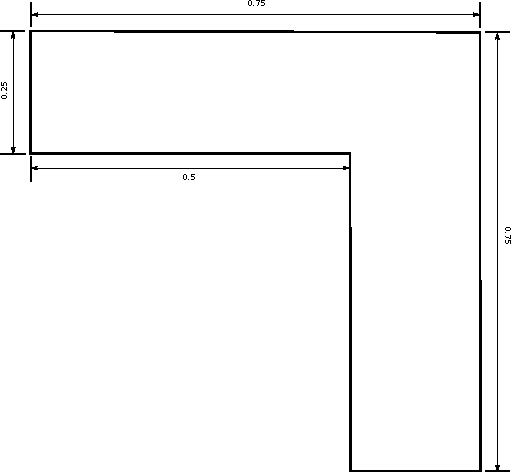
\includegraphics[width=0.4\linewidth]{./Images/L/L_beam.pdf}
	\caption{Geometry of the L-beam. All dimensions are in meters.}
	\label{L_beam_dims}
\end{figure}

\begin{figure}[ht]
	\begin{subfigure}{0.32\textwidth}
		\centering
		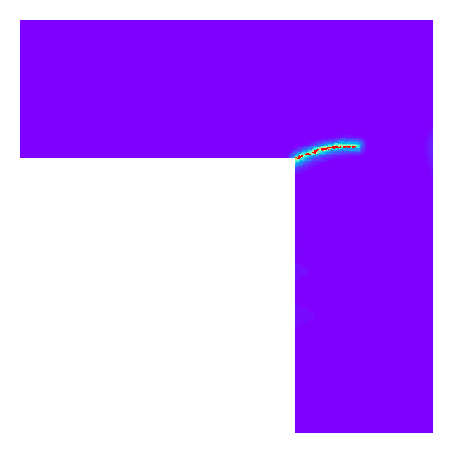
\includegraphics[width=0.9\textwidth]{./Images/L/damage_coar.pdf}
		\caption{Coarse mesh}
	\end{subfigure}
	\hfill
	\begin{subfigure}{0.32\textwidth}
		\centering
		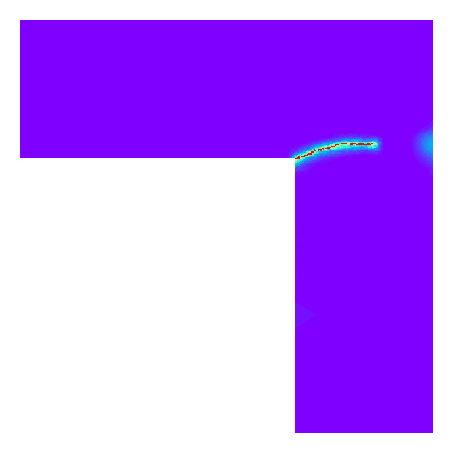
\includegraphics[width=0.9\textwidth]{./Images/L/damage_inter.pdf}
		\caption{Intermediate mesh}
	\end{subfigure}
	\hfill
	\begin{subfigure}{0.32\textwidth}
		\centering
		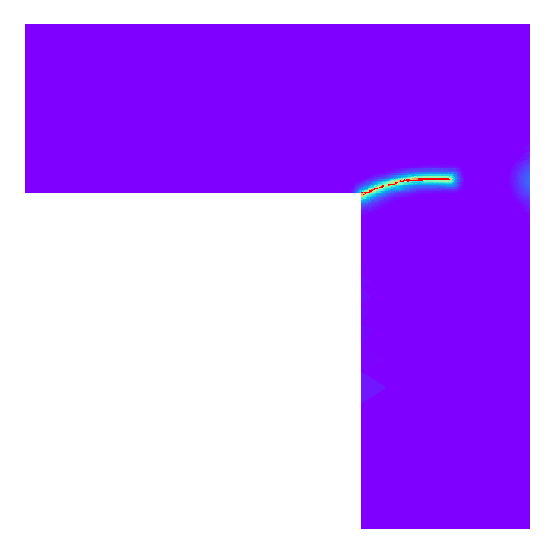
\includegraphics[width=0.9\textwidth]{./Images/L/damage_fine.pdf}
		\caption{Fine mesh}
	\end{subfigure}
	\begin{subfigure}{\textwidth}
		\centering
		\vfill
		\includegraphics[width=0.4\linewidth]{./Images/L/cb.pdf}
	\end{subfigure}
	\caption{Results with regularization}
	\label{fig:Results_with_ration}
\end{figure}

\begin{figure}[ht]
	\centering
	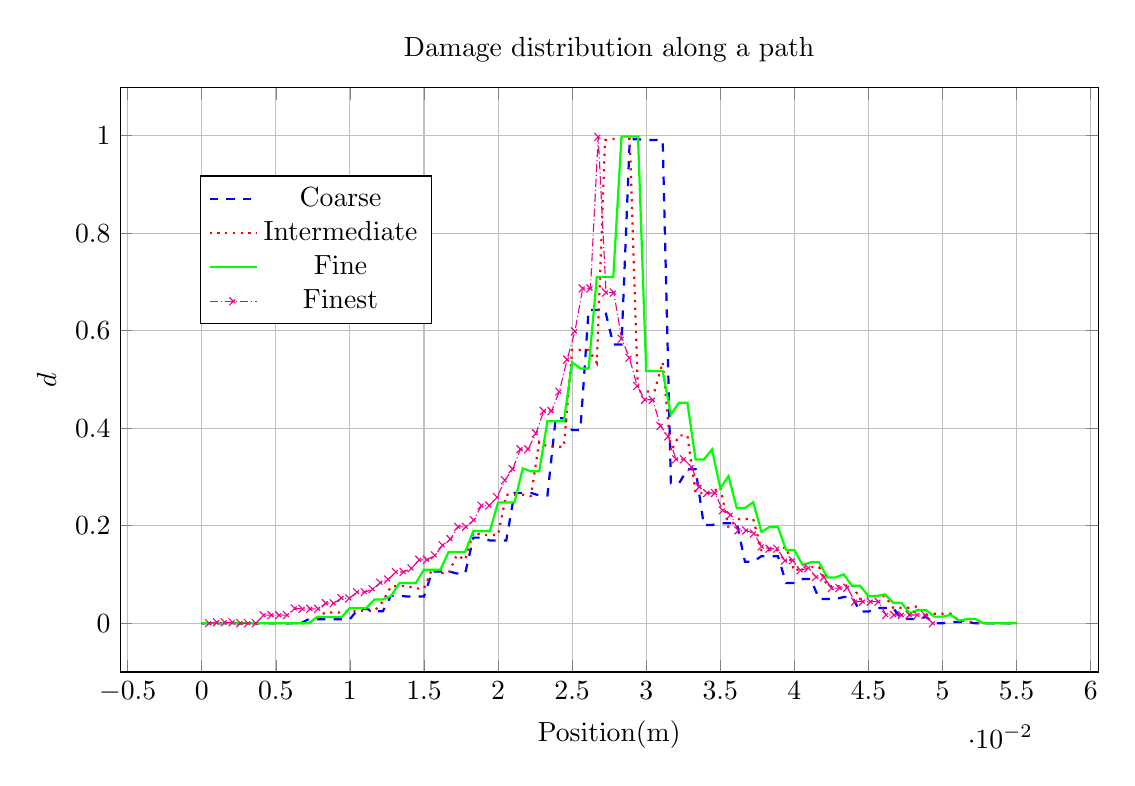
\begin{tikzpicture}
	\begin{axis}[
		title={Damage distribution along a path},
		xlabel={Position(\si{\meter})},
		ylabel={$d$},
		legend style={at={(0.2,0.85)}, anchor=north,legend columns=1},
		grid=major,
		width=14cm, height=9cm
		]
		
		% Database 1 (x, y) points using table
		\addplot[
		color=blue, dashed, thick
		% mark=square*,
		%thick
		] table[row sep=newline, x index=0, y index=1] {
			% (x, y) table for Database 1
		0	0
		0.000555558	0
		0.00111112	0
		0.00166667	0
		0.00222223	0
		0.00277779	0
		0.00333335	0
		0.0038889	0
		0.00444446	0
		0.00500002	0
		0.00555558	0
		0.00611114	0
		0.00666669	0
		0.00722225	0.00837996
		0.00777781	0.00837996
		0.00833337	0.00837996
		0.00888892	0.00837996
		0.00944448	0.00837996
		0.01	0.00837996
		0.0105556	0.0294185
		0.0111112	0.0294185
		0.0116667	0.0247192
		0.0122223	0.0247192
		0.0127778	0.0565885
		0.0133334	0.0565885
		0.0138889	0.0548244
		0.0144445	0.0548244
		0.0150001	0.0548244
		0.0155556	0.106309
		0.0161112	0.106309
		0.0166667	0.106309
		0.0172223	0.102211
		0.0177778	0.102211
		0.0183334	0.175698
		0.018889	0.175698
		0.0194445	0.169744
		0.0200001	0.169744
		0.0205556	0.169744
		0.0211112	0.267422
		0.0216668	0.267422
		0.0222223	0.267422
		0.0227779	0.262144
		0.0233334	0.262144
		0.023889	0.420416
		0.0244445	0.420416
		0.0250001	0.396045
		0.0255557	0.396045
		0.0261112	0.642222
		0.0266668	0.642222
		0.0272223	0.642222
		0.0277779	0.571858
		0.0283334	0.571858
		0.028889	0.99246
		0.0294446	0.99246
		0.0300001	0.990789
		0.0305557	0.990789
		0.0311112	0.990789
		0.0316668	0.287112
		0.0322224	0.287112
		0.0327779	0.31598
		0.0333335	0.31598
		0.033889	0.201365
		0.0344446	0.201365
		0.0350001	0.205353
		0.0355557	0.205353
		0.0361113	0.205353
		0.0366668	0.126262
		0.0372224	0.126262
		0.0377779	0.137691
		0.0383335	0.137691
		0.038889	0.137691
		0.0394446	0.0826343
		0.0400002	0.0826343
		0.0405557	0.0906638
		0.0411113	0.0906638
		0.0416668	0.0497414
		0.0422224	0.0497414
		0.042778	0.0497414
		0.0433335	0.0539324
		0.0438891	0.0539324
		0.0444446	0.0240248
		0.0450002	0.0240248
		0.0455557	0.0315323
		0.0461113	0.0315323
		0.0466669	0.0315323
		0.0472224	0.00896091
		0.047778	0.00896091
		0.0483335	0.00896091
		0.0488891	0.0130752
		0.0494446	0
		0.0500002	0
		0.0505558	0.00249815
		0.0511113	0.00249815
		0.0516669	0.00249815
		0.0522224	0
		0.052778	0
		0.0533335	0
		0.0538891	0
		0.0544447	0
		0.0550002	0	
		};
		\addlegendentry{Coarse}
		
		% Database 2 (x, y) points using table
		\addplot[
		color=red,dotted, thick
		%mark=*,
		%thick
		] table[row sep=newline, x index=0, y index=1] {
			% (x, y) table for Database 2
			0	0
			0.000555558	0
			0.00111112	0
			0.00166667	0
			0.00222223	0
			0.00277779	0
			0.00333335	0
			0.0038889	0
			0.00444446	0
			0.00500002	0
			0.00555558	0
			0.00611114	0
			0.00666669	0
			0.00722225	0
			0.00777781	0.00998038
			0.00833337	0.0223564
			0.00888892	0.0223564
			0.00944448	0.0223564
			0.01	0.0254732
			0.0105556	0.0254732
			0.0111112	0.0254732
			0.0116667	0.0254732
			0.0122223	0.0448785
			0.0127778	0.0762543
			0.0133334	0.0762543
			0.0138889	0.0762543
			0.0144445	0.0713023
			0.0150001	0.0713023
			0.0155556	0.111844
			0.0161112	0.103104
			0.0166667	0.103104
			0.0172223	0.140189
			0.0177778	0.129831
			0.0183334	0.18626
			0.018889	0.181128
			0.0194445	0.181128
			0.0200001	0.181128
			0.0205556	0.263737
			0.0211112	0.263737
			0.0216668	0.263737
			0.0222223	0.260937
			0.0227779	0.371968
			0.0233334	0.362087
			0.023889	0.362087
			0.0244445	0.362087
			0.0250001	0.560502
			0.0255557	0.560502
			0.0261112	0.560502
			0.0266668	0.53388
			0.0272223	0.990671
			0.0277779	0.992943
			0.0283334	0.992943
			0.028889	0.992943
			0.0294446	0.475106
			0.0300001	0.475106
			0.0305557	0.475106
			0.0311112	0.535293
			0.0316668	0.352028
			0.0322224	0.3853
			0.0327779	0.3853
			0.0333335	0.26718
			0.033889	0.26718
			0.0344446	0.26718
			0.0350001	0.280381
			0.0355557	0.195727
			0.0361113	0.213684
			0.0366668	0.213684
			0.0372224	0.213684
			0.0377779	0.149623
			0.0383335	0.149623
			0.038889	0.149623
			0.0394446	0.156104
			0.0400002	0.106799
			0.0405557	0.115221
			0.0411113	0.115221
			0.0416668	0.115221
			0.0422224	0.07617
			0.042778	0.07617
			0.0433335	0.07617
			0.0438891	0.0798147
			0.0444446	0.0495012
			0.0450002	0.0559292
			0.0455557	0.0559292
			0.0461113	0.0559292
			0.0466669	0.0317266
			0.0472224	0.0317266
			0.047778	0.0317266
			0.0483335	0.0350364
			0.0488891	0.0159984
			0.0494446	0.0194662
			0.0500002	0.0194662
			0.0505558	0.0194662
			0.0511113	0.00491342
			0.0516669	0.00491342
			0.0522224	0
			0.052778	0
			0.0533335	0
			0.0538891	0
			0.0544447	0
			0.0550002	0
		};
		\addlegendentry{Intermediate}
		
		% Database 2 (x, y) points using table
		\addplot[
		color=green, thick
		%mark=*,
		%thick
		] table[row sep=newline, x index=0, y index=1] {
			% (x, y) table for Database 2
		0	0
		0.000555558	0
		0.00111112	0
		0.00166667	0
		0.00222223	0
		0.00277779	0
		0.00333335	0
		0.0038889	0
		0.00444446	0
		0.00500002	0
		0.00555558	0
		0.00611114	0
		0.00666669	0
		0.00722225	0
		0.00777781	0.0128994
		0.00833337	0.0128994
		0.00888892	0.0128994
		0.00944448	0.0125949
		0.01	0.0315834
		0.0105556	0.0315834
		0.0111112	0.0315834
		0.0116667	0.049024
		0.0122223	0.049024
		0.0127778	0.0558095
		0.0133334	0.0824259
		0.0138889	0.0824259
		0.0144445	0.0824259
		0.0150001	0.109841
		0.0155556	0.109986
		0.0161112	0.109986
		0.0166667	0.146423
		0.0172223	0.146423
		0.0177778	0.146423
		0.0183334	0.189529
		0.018889	0.188615
		0.0194445	0.188615
		0.0200001	0.247775
		0.0205556	0.247775
		0.0211112	0.247775
		0.0216668	0.317622
		0.0222223	0.311643
		0.0227779	0.311643
		0.0233334	0.414367
		0.023889	0.414367
		0.0244445	0.414367
		0.0250001	0.535101
		0.0255557	0.522468
		0.0261112	0.522468
		0.0266668	0.71026
		0.0272223	0.71026
		0.0277779	0.71026
		0.0283334	0.998
		0.028889	0.998
		0.0294446	0.998
		0.0300001	0.517088
		0.0305557	0.517088
		0.0311112	0.517088
		0.0316668	0.42813
		0.0322224	0.452425
		0.0327779	0.452425
		0.0333335	0.335789
		0.033889	0.335789
		0.0344446	0.356365
		0.0350001	0.276852
		0.0355557	0.301704
		0.0361113	0.236484
		0.0366668	0.236484
		0.0372224	0.248211
		0.0377779	0.187424
		0.0383335	0.197585
		0.038889	0.197585
		0.0394446	0.150251
		0.0400002	0.150251
		0.0405557	0.119593
		0.0411113	0.12499
		0.0416668	0.12499
		0.0422224	0.094054
		0.042778	0.094054
		0.0433335	0.10035
		0.0438891	0.0769235
		0.0444446	0.0769235
		0.0450002	0.0559106
		0.0455557	0.0559106
		0.0461113	0.0593428
		0.0466669	0.0423208
		0.0472224	0.0423208
		0.047778	0.020725
		0.0483335	0.0272357
		0.0488891	0.0272357
		0.0494446	0.0136806
		0.0500002	0.0136806
		0.0505558	0.017332
		0.0511113	0.00554286
		0.0516669	0.0086747
		0.0522224	0.0086747
		0.052778	0
		0.0533335	0
		0.0538891	0
		0.0544447	0
		0.0550002	0
		
		};
		\addlegendentry{Fine}
		
	\addplot[
	color=magenta, 
	mark=x,densely dashdotted
	%thick
	] table[row sep=newline, x index=0, y index=1] {
		% (x, y) table for Database 2
		0.0005	0
		0.00102525252525252	0.00196497606093489
		0.00155050505050505	0.00196497606093489
		0.00207575757575757	0.00196497606093489
		0.00260101010101009	0.000154779710083441
		0.00312626262626262	0.000154779710083441
		0.00365151515151515	0.000154779710083441
		0.00417676767676767	0.0166673873395159
		0.0047020202020202	0.0166673873395159
		0.00522727272727272	0.0166673873395159
		0.00575252525252525	0.0166673873395159
		0.00627777777777777	0.0305878556825462
		0.0068030303030303	0.0296674918052621
		0.00732828282828283	0.0296674918052621
		0.00785353535353535	0.0296674918052621
		0.00837878787878788	0.0413399808793644
		0.0089040404040404	0.0410666645121097
		0.00942929292929292	0.0518358976985654
		0.00995454545454545	0.0510054282460976
		0.010479797979798	0.0639106847133643
		0.0110050505050505	0.0639106847133643
		0.011530303030303	0.0699370328526442
		0.0120555555555556	0.0832927213678453
		0.0125808080808081	0.089731299388101
		0.0131060606060606	0.105163741700716
		0.0136313131313131	0.105163741700716
		0.0141565656565657	0.112659087355754
		0.0146818181818182	0.130263797219176
		0.0152070707070707	0.130263797219176
		0.0157323232323232	0.139286138879504
		0.0162575757575758	0.160192039159534
		0.0167828282828283	0.172505917921939
		0.0173080808080808	0.197850082586205
		0.0178333333333333	0.197850082586205
		0.0183585858585859	0.211561469998552
		0.0188838383838384	0.241408867200125
		0.0194090909090909	0.241408867200125
		0.0199343434343434	0.258517769351676
		0.020459595959596	0.293271033997287
		0.0209848484848485	0.316134033451952
		0.021510101010101	0.357006750060217
		0.0220353535353535	0.357006750060217
		0.0225606060606061	0.389636689556633
		0.0230858585858586	0.435230003152465
		0.0236111111111111	0.435230003152465
		0.0241363636363636	0.475016046554201
		0.0246616161616162	0.540640907627019
		0.0251868686868687	0.598550109559345
		0.0257121212121212	0.6865392041997
		0.0262373737373737	0.6865392041997
		0.0267626262626263	0.997364795359148
		0.0272878787878788	0.678200161721444
		0.0278131313131313	0.678200161721444
		0.0283383838383838	0.583545967948893
		0.0288636363636364	0.544461758832879
		0.0293888888888889	0.4864472759825
		0.0299141414141414	0.458276485173587
		0.0304393939393939	0.458276485173587
		0.0309646464646465	0.40480196008697
		0.031489898989899	0.38320529907546
		0.0320151515151515	0.336330529651102
		0.032540404040404	0.336330529651102
		0.0330656565656566	0.320338728298987
		0.0335909090909091	0.279856474920669
		0.0341161616161616	0.267072964692517
		0.0346414141414141	0.267072964692517
		0.0351666666666667	0.231551606792564
		0.0356919191919192	0.222431264178053
		0.0362171717171717	0.190384228317107
		0.0367424242424242	0.190384228317107
		0.0372676767676768	0.184292519331375
		0.0377929292929293	0.157393095944165
		0.0383181818181818	0.152969140666475
		0.0388434343434343	0.152969140666475
		0.0393686868686869	0.128549785691292
		0.0398939393939394	0.128955248303671
		0.0404191919191919	0.108729867647855
		0.0409444444444445	0.11324787141328
		0.041469696969697	0.0947887210463936
		0.0419949494949495	0.0947887210463936
		0.042520202020202	0.0720032362751396
		0.0430454545454546	0.0720032362751396
		0.0435707070707071	0.0729958286467233
		0.0440959595959596	0.0443922825060892
		0.0446212121212121	0.0443922825060892
		0.0451464646464647	0.0443922825060892
		0.0456717171717172	0.0443922825060892
		0.0461969696969697	0.0170465189106153
		0.0467222222222222	0.0170465189106153
		0.0472474747474748	0.0170465189106153
		0.0477727272727273	0.0170465189106153
		0.0482979797979798	0.0170465189106153
		0.0488232323232323	0.0170465189106153
		0.0493484848484848	0
		
		
	};
	\addlegendentry{Finest}		
		
	\end{axis}
\end{tikzpicture}
	\caption{Variation of damage along the ar, $y=0$, $x \in [-0.02,0.02]$ \unit{\meter}.}
	\label{L_comparison_y}
\end{figure}


\begin{figure}[ht]
	\centering
	%\begin{tikzpicture}
	\begin{axis}[
		title={Force displacement curves},
		xlabel={Applied displacement (m)},
		ylabel={Force (N)},
		legend style={at={(0.2,0.85)}, anchor=north,legend columns=1},
		grid=major,
		width=14 cm, height=9 cm
		]
		
		% Database 1 (x, y) points using table
		\addplot[
		color=blue, dashed, thick
		% mark=square*,
		%thick
		] table[row sep=newline, x index=0, y index=1] {
			% (x, y) table for Database 1
				0.000050	52518.622182
				0.000065	68274.216189
				0.000080	84029.814475
				0.000095	99785.418932
				0.000110	115541.030712
				0.000125	131296.650971
				0.000140	147052.280866
				0.000155	162807.921551
				0.000170	178563.574177
				0.000185	194319.239909
				0.000200	210074.919897
				0.000215	225830.615295
				0.000230	241586.327256
				0.000245	257342.056935
				0.000260	273097.805485
				0.000275	288853.574058
				0.000290	304609.363807
				0.000305	320365.175884
				0.000320	336121.011430
				0.000335	351876.871616
				0.000350	367632.757581
				0.000365	383388.670476
				0.000380	399144.611450
				0.000395	414900.581651
				0.000410	430656.582227
				0.000425	446412.614324
				0.000440	462168.679090
				0.000455	477924.777670
				0.000470	493680.911208
				0.000485	509437.080849
				0.000500	525193.287736
				0.000515	540949.533011
				0.000530	556705.817817
				0.000545	572462.143293
				0.000560	588218.510579
				0.000575	603974.920815
				0.000590	619731.375138
				0.000605	635487.874685
				0.000620	651244.420592
				0.000635	667001.013975
				0.000650	682757.656006
				0.000665	698514.347798
				0.000680	714271.090483
				0.000695	730027.885193
				0.000710	745784.733056
				0.000725	761541.635201
				0.000740	777298.592754
				0.000755	793055.606842
				0.000770	808812.678590
				0.000785	824569.809120
				0.000800	840326.999556
				0.000815	856084.251017
				0.000830	871841.564624
				0.000845	887598.941496
				0.000860	903356.382748
				0.000875	919113.889498
				0.000890	934871.462858
				0.000905	950629.103941
				0.000920	966386.813860
				0.000935	982144.593724
				0.000950	997902.444642
				0.000965	1013660.367721
				0.000980	1029418.364066
				0.000995	1045176.434780
				0.001010	1060934.580968
				0.001025	1076692.803730
				0.001040	1092451.104166
				0.001055	1108209.483372
				0.001070	1123967.942446
				0.001085	1139726.482481
				0.001100	1155485.104572
				0.001115	1171243.809808
				0.001130	1187002.599282
				0.001145	1202761.474079
				0.001160	1218520.435288
				0.001175	1234279.483990
				0.001190	1250038.621272
				0.001205	1265797.848213
				0.001220	1281557.165891
				0.001235	1297316.575387
				0.001250	1313076.077737
				0.001265	1328835.674091
				0.001280	1344595.365483
				0.001295	1360355.152985
				0.001310	1376115.037665
				0.001325	1391875.020590
				0.001340	1407635.102823
				0.001355	1423395.285430
				0.001370	1439155.569470
				0.001385	1454915.956003
				0.001400	1470676.446087
				0.001415	1486437.040777
				0.001430	1502197.741127
				0.001445	1517958.548189
				0.001460	1533719.463011
				0.001475	1549480.486642
				0.001490	1565241.620128
				0.001505	1581002.864511
				0.001520	1596764.220836
				0.001535	1612525.690139
				0.001550	1628287.273461
				0.001565	1644048.971837
				0.001580	1659810.786299
				0.001595	1675572.717880
				0.001610	1691334.767611
				0.001625	1707096.936518
				0.001640	1722859.225626
				0.001655	1738621.635960
				0.001670	1754384.168542
				0.001685	1770146.824388
				0.001700	1785909.604518
				0.001715	1801672.509948
				0.001730	1817435.541688
				0.001745	1833198.700751
				0.001760	1848961.988144
				0.001775	1864725.404879
				0.001790	1880488.951953
				0.001805	1896252.630373
				0.001820	1912016.441138
				0.001835	1927780.385247
				0.001850	1943544.463696
				0.001865	1959308.677478
				0.001880	1975073.027583
				0.001895	1990837.515004
				0.001910	2006602.140726
				0.001925	2022366.905734
				0.001940	2038131.811011
				0.001955	2053896.857538
				0.001970	2069662.046295
				0.002215	2327435.712407
				0.002287	2402393.294311
				0.002348	2466277.415097
				0.002394	2514413.516323
				0.002433	2555382.610100
				0.002463	2586415.542298
				0.002491	2615581.252834
				0.002516	2642154.017960
				0.002539	2666623.799418
				0.002562	2690571.143070
				0.002582	2711513.456849
				0.002601	2731427.281081
				0.002620	2750860.422334
				0.002637	2768829.308991
				0.002655	2786770.574940
				0.002671	2803673.326177
				0.002685	2818840.589458
				0.002700	2833630.145701
				0.002713	2847851.490907
				0.002727	2861847.250433
				0.002739	2875124.137493
				0.002752	2888124.810269
				0.002764	2900812.071412
				0.002776	2913000.117519
				0.002787	2924625.857760
				0.002798	2935870.169933
				0.002808	2946804.779670
				0.002818	2956970.626724
				0.002827	2966623.108639
				0.002837	2976006.441029
				0.002845	2984948.838468
				0.002854	2993691.555731
				0.002862	3002303.112909
				0.002870	3010584.729682
				0.002878	3018718.138299
				0.002886	3026858.367400
				0.002893	3034725.208271
				0.002900	3042134.021402
				0.002907	3049295.543173
				0.002914	3056413.290378
				0.002921	3063523.454759
				0.002928	3070630.310184
				0.002935	3077488.471171
				0.002941	3084180.290382
				0.002948	3090866.583478
				0.002954	3097549.900289
				0.002960	3104114.082881
				0.002967	3110457.418306
				0.002973	3116786.947255
				0.002979	3123113.987457
				0.002985	3129330.452626
				0.002991	3135421.823286
				0.002997	3141495.377437
				0.003002	3147456.526811
				0.003008	3153261.065844
				0.003014	3158925.893548
				0.003019	3164537.321646
				0.003024	3170150.481021
				0.003030	3175677.934329
				0.003035	3181154.114807
				0.003040	3186589.593701
				0.003046	3192020.849396
				0.003051	3197371.548891
				0.003056	3202661.267850
				0.003061	3207945.384983
				0.003066	3213191.063696
				0.003071	3218397.577557
				0.003076	3223582.839123
				0.003081	3228594.551872
				0.003086	3233614.067040
				0.003091	3238632.265442
				0.003096	3243591.375448
				0.003101	3248521.043807
				0.003105	3253448.497820
				0.003110	3258374.509785
				0.003115	3263299.134437
				0.003120	3268187.454838
				0.003124	3272890.062873
				0.003129	3277552.726892
				0.003133	3282154.663321
				0.003138	3286761.044893
				0.003142	3291366.091603
				0.003147	3295932.311255
				0.003151	3300418.807845
				0.003155	3304885.565381
				0.003160	3309325.399422
				0.003164	3313678.992296
				0.003168	3318036.986011
				0.003172	3322393.578462
				0.003177	3326748.837234
				0.003181	3331102.782279
				0.003185	3335455.421462
				0.003189	3339700.112395
				0.003193	3343883.419325
				0.003198	3348064.799557
				0.003202	3352171.353843
				0.003206	3356224.036438
				0.003209	3360183.851606
				0.003213	3364147.189178
				0.003217	3368109.580984
				0.003221	3372070.822908
				0.003225	3375956.292275
				0.003228	3379755.302641
				0.003232	3383480.905062
				0.003236	3387136.572027
				0.003239	3390745.518293
				0.003243	3394305.124612
				0.003246	3397779.619788
				0.003250	3401249.798373
				0.003253	3404632.261934
				0.003256	3408021.918461
				0.003260	3411410.597346
				0.003263	3414798.273917
				0.003266	3418152.084782
				0.003269	3421483.389487
				0.003273	3424812.375511
				0.003276	3428088.629594
				0.003279	3431312.267890
				0.003282	3434463.238677
				0.003285	3437605.423178
				0.003288	3440683.772639
				0.003291	3443766.956538
				0.003294	3446849.332524
				0.003297	3449917.202963
				0.003300	3452928.822336
				0.003303	3455946.192383
				0.003306	3458962.942072
				0.003309	3461934.619728
				0.003312	3464862.788715
				0.003315	3467749.013923
				0.003318	3470637.147057
				0.003321	3473524.615051
				0.003323	3476411.470632
				0.003326	3479297.726303
				0.003329	3482150.269752
				0.003332	3484969.929704
				0.003335	3487786.691277
				0.003337	3490602.840432
				0.003340	3493418.392816
				0.003343	3496233.364146
				0.003346	3499047.759386
				0.003348	3501861.580686
				0.003351	3504674.829654
				0.003354	3507487.507812
				0.003357	3510299.391014
				0.003359	3513050.664611
				0.003362	3515770.688633
				0.003365	3518467.219610
				0.003367	3521158.244020
				0.003370	3523848.932882
				0.003373	3526539.041549
				0.003375	3529228.597297
				0.003378	3531917.605896
				0.003381	3534557.402708
				0.003383	3537178.198635
				0.003386	3539797.412775
				0.003388	3542416.104353
				0.003391	3545034.274134
				0.003394	3547651.922604
				0.003396	3550269.050482
				0.003399	3552877.873850
				0.003401	3555461.869816
				0.003404	3558013.048327
				0.003406	3560556.263155
				0.003409	3563099.819962
				0.003411	3565642.851257
				0.003414	3568185.370482
				0.003416	3570727.382537
				0.003419	3573261.445773
				0.003421	3575753.980368
				0.003424	3578225.672272
				0.003426	3580664.928683
				0.003429	3583102.561501
				0.003431	3585539.670074
				0.003433	3587976.284861
				0.003436	3590412.418512
				0.003438	3592848.076379
				0.003441	3595283.260567
				0.003443	3597717.972350
				0.003445	3600152.212835
				0.003448	3602585.983087
				0.003450	3605019.284169
				0.003453	3607452.117134
				0.003455	3609884.483039
				0.003457	3612316.382938
				0.003460	3614747.817870
				0.003462	3617178.788890
				0.003465	3619609.189875
				0.003467	3622039.098118
				0.003469	3624468.545828
				0.003472	3626897.534041
				0.003474	3629326.063660
				0.003477	3631754.135676
				0.003479	3634181.751101
				0.003481	3636608.910961
				0.003484	3639024.626672
				0.003486	3641373.219700
				0.003488	3643648.700332
				0.003491	3645893.466427
				0.003493	3648126.661905
				0.003495	3650359.458858
				0.003497	3652591.776368
				0.003500	3654823.623701
				0.003502	3657013.553756
				0.003504	3659195.719479
				0.003506	3661369.033906
				0.003508	3663542.769919
				0.003510	3665715.954043
				0.003513	3667888.676704
				0.003515	3670060.943821
				0.003517	3672232.756461
				0.003519	3674388.409642
				0.003521	3676522.823183
				0.003523	3678641.418036
				0.003525	3680756.452221
				0.003527	3682870.979957
				0.003529	3684970.155177
				0.003532	3687063.016824
				0.003534	3689150.248075
				0.003536	3691224.322163
				0.003538	3693297.932622
				0.003540	3695371.066888
				0.003542	3697400.524449
				0.003544	3699383.319641
				0.003546	3701366.354181
				0.003548	3703338.441178
				0.003550	3705289.194693
				0.003552	3707241.564820
				0.003554	3709193.552661
				0.003556	3711145.150069
				0.003557	3713096.357220
				0.003559	3715047.175035
				0.003561	3716997.604287
				0.003563	3718930.999843
				0.003565	3720843.252443
				0.003567	3722744.100639
				0.003569	3724643.877038
				0.003571	3726543.256037
				0.003573	3728442.245537
				0.003575	3730340.848411
				0.003577	3732239.065727
				0.003578	3734136.898174
				0.003580	3736034.346399
				0.003582	3737903.881637
				0.003584	3739769.360666
				0.003586	3741622.115536
				0.003588	3743460.666853
				0.003590	3745300.760336
				0.003591	3747140.488930
				0.003593	3748979.860668
				0.003595	3750818.880789
				0.003597	3752657.551176
				0.003599	3754482.992581
				0.003601	3756279.125300
				0.003602	3758062.052475
				0.003604	3759818.311774
				0.003606	3761575.953988
				0.003608	3763326.371954
				0.003609	3765066.669240
				0.003611	3766806.668531
				0.003613	3768546.383644
				0.003615	3770285.811014
				0.003616	3772024.956096
				0.003618	3773762.569317
				0.003620	3775492.336784
				0.003622	3777221.750924
				0.003623	3778950.821925
				0.003625	3780679.578320
				0.003627	3782407.197412
				0.003628	3784109.564291
				0.003630	3785813.482007
				0.003632	3787517.219047
				0.003634	3789220.690316
				0.003635	3790923.901441
				0.003637	3792626.855938
				0.003639	3794329.554996
				0.003640	3796031.999174
				0.003642	3797734.188899
				0.003644	3799431.658019
				0.003645	3801118.061237
				0.003647	3802787.638386
				0.003649	3804454.078170
				0.003650	3806120.638411
				0.003652	3807786.943341
				0.003654	3809452.996950
				0.003655	3811118.802564
				0.003657	3812784.361322
				0.003659	3814449.673756
				0.003660	3816114.740271
				0.003662	3817779.561244
				0.003664	3819444.137038
				0.003665	3821108.468024
				0.003667	3822772.552058
				0.003669	3824420.053073
				0.003670	3826058.866960
				0.003672	3827697.489755
				0.003674	3829335.897658
				0.003675	3830965.483271
				0.003677	3832574.420494
				0.003679	3834171.403526
				0.003680	3835769.174341
				0.003682	3837363.621194
				0.003683	3838949.107429
				0.003685	3840535.131829
				0.003687	3842120.934482
				0.003688	3843688.628679
				0.003690	3845247.761411
				0.003691	3846806.093970
				0.003693	3848356.604548
				0.003694	3849896.922225
				0.003696	3851435.743624
				0.003697	3852974.344417
				0.003699	3854512.717877
				0.003701	3856050.868370
				0.003702	3857588.798087
				0.003704	3859126.507823
				0.003705	3860663.997985
				0.003707	3862201.268895
				0.003708	3863719.310239
				0.003710	3865234.626330
				0.003711	3866749.783611
				0.003713	3868264.713979
				0.003714	3869779.430218
				0.003716	3871288.532121
				0.003717	3872772.185042
				0.003719	3874233.229295
				0.003720	3875687.868809
				0.003722	3877140.751163
				0.003723	3878590.252776
				0.003725	3880039.240834
				0.003726	3881486.732823
				0.003728	3882925.419824
				0.003729	3884364.285644
				0.003731	3885802.951277
				0.003732	3887241.410912
				0.003733	3888676.558430
				0.003735	3890106.082599
				0.003736	3891535.351970
				0.003738	3892953.792710
				0.003739	3894359.856501
				0.003741	3895756.429304
				0.003742	3897150.637859
				0.003743	3898544.584553
				0.003745	3899938.316683
				0.003746	3901330.998840
				0.003748	3902683.144583
				0.003749	3904022.001993
				0.003750	3905345.368543
				0.003752	3906653.088812
				0.003753	3907961.785063
				0.003754	3909265.844677
				0.003756	3910569.750064
				0.003757	3911873.511525
				0.003758	3913177.091923
				0.003760	3914480.472989
				0.003761	3915783.548846
				0.003762	3917086.444606
				0.003763	3918389.163731
				0.003765	3919691.706792
				0.003766	3920994.074013
				0.003767	3922296.265593
				0.003769	3923598.281736
				0.003770	3924889.830744
				0.003771	3926181.886843
				0.003773	3927473.803315
				0.003774	3928765.547416
				0.003775	3930057.119402
				0.003777	3931348.519662
				0.003778	3932639.748431
				0.003779	3933916.599482
				0.003780	3935192.726330
				0.003782	3936468.721130
				0.003783	3937744.540418
				0.003784	3939020.188613
				0.003786	3940295.668487
				0.003787	3941570.980850
				0.003788	3942845.502665
				0.003790	3944110.068907
				0.003791	3945373.089455
				0.003792	3946635.887653
				0.003793	3947898.509430
				0.003795	3949160.778691
				0.003796	3950422.825203
				0.003797	3951684.709076
				0.003799	3952946.426317
				0.003800	3954207.977218
				0.003801	3955469.362040
				0.003802	3956729.256802
				0.003804	3957974.637066
				0.003805	3959221.013115
				0.003806	3960467.264346
				0.003807	3961713.356463
				0.003809	3962959.287483
				0.003810	3964195.725297
				0.003811	3965429.774367
				0.003812	3966663.546904
				0.003814	3967897.164086
				0.003815	3969130.623745
				0.003816	3970363.924652
				0.003817	3971597.066601
				0.003819	3972830.049677
				0.003820	3974059.980072
				0.003821	3975274.747936
				0.003822	3976487.639701
				0.003824	3977700.247759
				0.003825	3978906.303054
				0.003826	3980110.516692
				0.003827	3981314.493000
				0.003829	3982518.300856
				0.003830	3983721.949311
				0.003831	3984914.079847
				0.003832	3986101.688958
				0.003833	3987288.836316
				0.003835	3988475.851537
				0.003836	3989662.715857
				0.003837	3990849.424989
				0.003838	3992035.840886
				0.003839	3993222.056743
				0.003841	3994395.724769
				0.003842	3995566.289673
				0.003843	3996736.976124
				0.003844	3997907.502549
				0.003845	3999077.871943
				0.003847	4000248.085811
				0.003848	4001418.144703
				0.003849	4002588.048867
				0.003850	4003757.798495
				0.003851	4004927.393761
				0.003853	4006096.834843
				0.003854	4007266.121913
				0.003855	4008435.255148
				0.003856	4009604.228719
				0.003857	4010773.037900
				0.003859	4011941.694328
				0.003860	4013110.197647
				0.003861	4014275.977195
				0.003862	4015433.481878
				0.003863	4016580.707517
				0.003864	4017727.958774
				0.003866	4018875.058210
				0.003867	4020022.004267
				0.003868	4021168.803201
				0.003869	4022315.457665
				0.003870	4023461.968458
				0.003871	4024608.335873
				0.003873	4025754.560085
				0.003874	4026900.641257
				0.003875	4028046.579549
				0.003876	4029192.375117
				0.003877	4030338.028120
				0.003878	4031483.538715
				0.003880	4032628.907060
				0.003881	4033774.133307
				0.003882	4034919.217616
				0.003883	4036064.160147
				0.003884	4037208.961050
				0.003885	4038353.620487
				0.003887	4039498.138610
				0.003888	4040642.515577
				0.003889	4041786.751541
				0.003890	4042930.846657
				0.003891	4044074.801083
				0.003892	4045218.614970
				0.003894	4046362.288477
				0.003895	4047505.821757
				0.003896	4048641.640118
				0.003897	4049771.767818
				0.003898	4050901.909433
				0.003899	4052030.851989
				0.003901	4053150.865092
				0.003902	4054271.515120
				0.003903	4055392.057712
				0.003904	4056512.471995
				0.003905	4057632.756998
				0.003906	4058752.912917
				0.003907	4059872.939918
				0.003909	4060992.838147
				0.003910	4062112.607737
				0.003911	4063232.248828
				0.003912	4064351.761553
				0.003913	4065471.146054
				0.003914	4066590.402467
				0.003915	4067709.530926
				0.003917	4068828.531569
				0.003918	4069947.404534
				0.003919	4071066.149958
				0.003920	4072184.767974
				0.003921	4073295.165990
				0.003922	4074404.189248
				0.003923	4075513.192450
				0.003925	4076616.736550
				0.003926	4077718.481626
				0.003927	4078820.060352
				0.003928	4079921.510898
				0.003929	4081022.838543
				0.003930	4082124.044491
				0.003931	4083225.128920
				0.003932	4084326.088765
				0.003934	4085426.925772
				0.003935	4086527.642589
				0.003936	4087628.238408
				0.003937	4088728.713283
				0.003938	4089829.067325
				0.003939	4090929.300657
				0.003940	4092029.413411
				0.003941	4093124.000102
				0.003943	4094207.679628
				0.003944	4095290.913242
				0.003945	4096374.007146
				0.003946	4097456.982766
				0.003947	4098532.047778
				0.003948	4099581.153924
				0.003949	4100623.763229
				0.003950	4101665.639103
				0.003951	4102705.385168
				0.003952	4103735.864694
				0.003953	4104767.582408
				0.003954	4105799.186952
				0.003955	4106830.664592
				0.003957	4107855.364439
				0.003958	4108880.470054
				0.003959	4109905.481649
				0.003960	4110930.375523
				0.003961	4111955.152793
				0.003962	4112971.893945
				0.003963	4113986.919688
				0.003964	4115001.841323
				0.003965	4116016.656394
				0.003966	4117031.357600
				0.003967	4118045.933917
				0.003968	4119060.378900
				0.003969	4120074.709319
				0.003970	4121088.925321
				0.003971	4122103.025761
				0.003972	4123116.991549
				0.003973	4124130.842723
				0.003974	4125144.579749
				0.003975	4126158.202768
				0.003976	4127168.789753
				0.003977	4128177.357133
				0.003978	4129185.867810
				0.003979	4130194.259289
				0.003981	4131202.536108
				0.003982	4132210.700401
				0.003983	4133210.398843
				0.003984	4134209.210505
				0.003985	4135207.889428
				0.003986	4136206.449451
				0.003987	4137204.896301
				0.003988	4138203.231905
				0.003989	4139200.401539
				0.003990	4140185.347158
				0.003991	4141170.758082
				0.003992	4142156.072670
				0.003993	4143141.278367
				0.003994	4144122.491183
				0.003995	4145100.809433
				0.003996	4146078.811777
				0.003997	4147054.031948
				0.003998	4148020.033625
				0.003999	4148976.713905
				0.004000	4149931.985466
				0.004001	4150887.161128
				0.004002	4151842.244484
				0.004003	4152797.226457
				0.004004	4153752.105118
				0.004005	4154706.880241
				0.004006	4155653.167144
				0.004007	4156596.273476
				0.004008	4157538.940735
				0.004009	4158481.483703
				0.004010	4159423.921937
				0.004011	4160361.242071
				0.004011	4161286.860304
				0.004012	4162211.308348
				0.004013	4163129.056084
				0.004014	4164042.447907
				0.004015	4164956.061774
				0.004016	4165869.575732
				0.004017	4166782.990735
				0.004018	4167696.308003
				0.004019	4168609.528043
				0.004020	4169522.651077
				0.004021	4170435.677215
				0.004022	4171344.462784
				0.004023	4172247.746074
				0.004024	4173150.881892
				0.004025	4174053.915458
				0.004026	4174956.845996
				0.004027	4175859.678121
				0.004028	4176762.413435
				0.004028	4177665.052408
				0.004029	4178567.595202
				0.004030	4179470.041919
				0.004031	4180372.392646
				0.004032	4181274.647471
				0.004033	4182176.806476
				0.004034	4183078.869752
				0.004035	4183980.837376
				0.004036	4184882.709435
				0.004037	4185784.486015
				0.004038	4186686.167197
				0.004039	4187587.753072
				0.004040	4188486.711789
				0.004041	4189378.163288
				0.004041	4190268.932850
				0.004042	4191159.569633
				0.004043	4192050.104691
				0.004044	4192940.542910
				0.004045	4193830.885765
				0.004046	4194721.133690
				0.004047	4195600.264089
				0.004048	4196477.922969
				0.004049	4197355.831920
				0.004050	4198233.649495
				0.004051	4199111.375029
				0.004052	4199989.011387
				0.004052	4200866.559550
				0.004053	4201744.019798
				0.004054	4202621.392257
				0.004055	4203498.673720
				0.004056	4204375.861816
				0.004057	4205252.961342
				0.004058	4206129.969088
				0.004059	4207006.868988
				0.004060	4207883.682020
				0.004061	4208760.407831
				0.004062	4209637.046483
				0.004062	4210513.598040
				0.004063	4211390.062576
				0.004064	4212266.440165
				0.004065	4213142.730884
				0.004066	4214018.934806
				0.004067	4214895.013141
				0.004068	4215770.938226
				0.004069	4216646.776123
				0.004070	4217519.217209
				0.004071	4218386.892336
				0.004072	4219255.092611
				0.004072	4220123.211548
				0.004073	4220991.241135
				0.004074	4221859.180880
				0.004075	4222726.986211
				0.004076	4223594.708270
				0.004077	4224461.588010
				0.004078	4225321.941151
				0.004079	4226182.736607
				0.004080	4227043.476198
				0.004081	4227904.136697
				0.004081	4228764.716380
				0.004082	4229622.738760
				0.004083	4230478.938117
				0.004084	4231334.997618
				0.004085	4232190.965744
				0.004086	4233046.851192
				0.004087	4233902.656552
				0.004088	4234758.382285
				0.004089	4235610.380341
				0.004089	4236454.481388
				0.004090	4237292.016218
				0.004091	4238129.205220
				0.004092	4238966.303827
				0.004093	4239803.311140
				0.004094	4240636.282907
				0.004095	4241467.466279
				0.004095	4242298.444159
				0.004096	4243129.346607
				0.004097	4243960.171685
				0.004098	4244790.918717
				0.004099	4245617.330581
				0.004100	4246440.127126
				0.004101	4247262.926295
				0.004101	4248085.644086
				0.004102	4248908.279107
				0.004103	4249723.240679
				0.004104	4250535.238883
				0.004105	4251337.651635
				0.004106	4252139.637177
				0.004107	4252941.597920
				0.004107	4253743.479014
				0.004108	4254541.210783
				0.004109	4255335.701809
				0.004110	4256129.827495
				0.004111	4256923.893007
				0.004112	4257717.891425
				0.004112	4258511.818846
				0.004113	4259305.673217
				0.004114	4260099.447516
				0.004115	4260892.682055
				0.004116	4261684.563198
				0.004116	4262476.302593
				0.004117	4263267.950908
				0.004118	4264059.523700
				0.004119	4264851.024710
				0.004120	4265642.454797
				0.004121	4266433.814155
				0.004121	4267225.102858
				0.004122	4268016.320964
				0.004123	4268807.468523
				0.004124	4269598.545599
				0.004125	4270389.552243
				0.004126	4271180.488514
				0.004126	4271971.354471
				0.004127	4272762.150163
				0.004128	4273552.875655
				0.004129	4274343.530999
				0.004130	4275134.116252
				0.004131	4275924.631470
				0.004131	4276715.076708
				0.004132	4277505.452027
				0.004133	4278295.757478
				0.004134	4279083.738856
				0.004135	4279868.323973
				0.004135	4280652.977302
				0.004136	4281437.543588
				0.004137	4282222.037484
				0.004138	4283006.462801
				0.004139	4283790.820232
				0.004140	4284575.109893
				0.004140	4285359.331823
				0.004141	4286143.486070
				0.004142	4286927.572688
				0.004143	4287711.591729
				0.004144	4288489.158983
				0.004144	4289265.858522
				0.004145	4290042.525892
				0.004146	4290819.129475
				0.004147	4291595.666765
				0.004148	4292372.137363
				0.004149	4293148.497803
				0.004149	4293917.458413
				0.004150	4294685.007469
				0.004151	4295452.434435
				0.004152	4296219.797678
				0.004153	4296987.094171
				0.004153	4297754.322245
				0.004154	4298521.481579
				0.004155	4299288.572188
				0.004156	4300055.594109
				0.004157	4300820.978138
				0.004157	4301584.340499
				0.004158	4302347.624552
				0.004159	4303110.838474
				0.004160	4303873.983127
				0.004161	4304637.059787
				0.004161	4305400.068619
				0.004162	4306163.009629
				0.004163	4306925.882842
				0.004164	4307688.688300
				0.004165	4308451.426049
				0.004165	4309210.979453
				0.004166	4309966.731499
				0.004167	4310722.572424
				0.004168	4311478.358420
				0.004169	4312234.079672
				0.004169	4312989.734342
				0.004170	4313745.322232
				0.004171	4314500.657307
				0.004172	4315252.893540
				0.004172	4316005.193619
				0.004173	4316757.419497
				0.004174	4317504.966969
				0.004175	4318249.593703
				0.004176	4318993.844212
				0.004176	4319738.015162
				0.004177	4320482.120717
				0.004178	4321221.117224
				0.004179	4321955.816296
				0.004179	4322685.290844
				0.004180	4323413.914323
				0.004181	4324142.462992
				0.004182	4324870.952148
				0.004183	4325599.375860
				0.004183	4326327.732389
				0.004184	4327056.021423
				0.004185	4327784.242961
				0.004186	4328512.397045
				0.004186	4329240.483725
				0.004187	4329963.556496
				0.004188	4330686.961914
				0.004189	4331410.292220
				0.004189	4332133.554814
				0.004190	4332856.750800
				0.004191	4333579.880452
				0.004192	4334302.943849
				0.004192	4335025.941045
				0.004193	4335748.872079
				0.004194	4336471.737003
				0.004195	4337194.535861
				0.004195	4337917.268704
				0.004196	4338639.935575
				0.004197	4339362.536525
				0.004198	4340085.071599
				0.004199	4340807.540846
				0.004199	4341529.944314
				0.004200	4342252.282046
				0.004201	4342974.554094
				0.004202	4343696.760500
				0.004202	4344418.900571
				0.004203	4345140.967325
				0.004204	4345862.968700
				0.004205	4346584.904597
				0.004205	4347306.775083
				0.004206	4348028.580217
				0.004207	4348750.320045
				0.004208	4349471.994613
				0.004208	4350193.603974
				0.004209	4350915.148169
				0.004210	4351636.627248
				0.004211	4352358.041257
				0.004211	4353075.338977
				0.004212	4353791.980337
				0.004213	4354508.633385
				0.004214	4355225.222820
				0.004214	4355941.745739
				0.004215	4356658.204345
				0.004216	4357372.318409
				0.004217	4358078.290560
				0.004217	4358783.880519
				0.004218	4359489.493428
				0.004219	4360195.041154
				0.004220	4360900.524199
				0.004220	4361605.945757
				0.004221	4362311.307071
				0.004222	4363012.157897
				0.004223	4363711.949277
				0.004223	4364411.858271
				0.004224	4365108.760060
				0.004225	4365805.643459
				0.004226	4366502.464554
				0.004226	4367199.226504
				0.004227	4367895.931223
				0.004228	4368592.579099
				0.004229	4369289.170182
				0.004229	4369983.891282
				0.004230	4370673.763094
				0.004231	4371361.026447
				0.004231	4372044.562657
				0.004232	4372728.315723
				0.004233	4373412.026892
				0.004234	4374095.683396
				0.004234	4374779.277968
				0.004235	4375459.472938
				0.004236	4376136.502744
				0.004236	4376812.227016
				0.004237	4377487.835552
				0.004238	4378163.394918
				0.004239	4378838.900348
				0.004239	4379514.351142
				0.004240	4380189.747086
				0.004241	4380861.187470
				0.004241	4381530.032173
				0.004242	4382199.000838
				0.004243	4382867.914646
				0.004244	4383536.772337
				0.004244	4384205.574565
				0.004245	4384874.321740
				0.004246	4385543.014021
				0.004246	4386211.651492
				0.004247	4386880.234189
				0.004248	4387548.762161
				0.004249	4388217.235444
				0.004249	4388885.654071
				0.004250	4389554.018085
				0.004251	4390222.327521
				0.004251	4390890.582416
				0.004252	4391558.782808
				0.004253	4392226.928733
				0.004253	4392895.020230
				0.004254	4393563.057336
				0.004255	4394231.040087
				0.004256	4394898.968520
				0.004256	4395566.842674
				0.004257	4396233.435995
				0.004258	4396895.693769
				0.004258	4397557.330610
				0.004259	4398218.924490
				0.004260	4398880.471748
				0.004260	4399541.966531
				0.004261	4400203.407336
				0.004262	4400864.793845
				0.004263	4401526.126026
				0.004263	4402187.403886
				0.004264	4402848.627473
				0.004265	4403509.796812
				0.004265	4404170.911945
				0.004266	4404831.972908
				0.004267	4405492.979738
				0.004267	4406150.415359
				0.004268	4406806.743341
				0.004269	4407463.126162
				0.004270	4408119.451586
				0.004270	4408775.721560
				0.004271	4409431.937406
				0.004272	4410088.099578
				0.004272	4410739.476336
				0.004273	4411390.437104
				0.004274	4412041.328234
				0.004274	4412692.159604
				0.004275	4413342.935334
				0.004276	4413993.657201
				0.004276	4414644.325784
				0.004277	4415294.941260
				0.004278	4415945.503698
				0.004279	4416596.013145
				0.004279	4417245.942848
				0.004280	4417893.386980
				0.004281	4418540.653752
				0.004281	4419187.862226
				0.004282	4419834.829565
				0.004283	4420480.684662
				0.004283	4421126.447788
				0.004284	4421772.140928
				0.004285	4422413.777057
				0.004285	4423053.931269
				0.004286	4423693.955020
				0.004287	4424333.919677
				0.004287	4424973.829750
				0.004288	4425613.687129
				0.004289	4426253.492524
				0.004289	4426893.246159
				0.004290	4427532.948130
				0.004291	4428172.598471
				0.004292	4428812.197225
				0.004292	4429451.744431
				0.004293	4430091.240116
				0.004294	4430730.616335
				0.004294	4431368.316388
				0.004295	4432005.173945
				0.004296	4432641.453339
				0.004296	4433277.738218
				0.004297	4433913.968796
				0.004298	4434550.147831
				0.004298	4435186.276204
				0.004299	4435822.354132
				0.004300	4436458.381680
				0.004300	4437094.358874
				0.004301	4437730.285757
				0.004302	4438366.162350
				0.004302	4439001.988692
				0.004303	4439637.764817
				0.004304	4440273.490756
				0.004304	4440909.166540
				0.004305	4441544.792210
				0.004306	4442180.367791
				0.004306	4442815.893321
				0.004307	4443451.368828
				0.004308	4444086.794351
				0.004308	4444722.169917
				0.004309	4445357.495564
				0.004310	4445992.771320
				0.004310	4446627.997223
				0.004311	4447263.173302
				0.004312	4447898.299594
				0.004312	4448533.376126
				0.004313	4449168.402936
				0.004314	4449803.380053
				0.004315	4450438.307512
				0.004315	4451073.185345
				0.004316	4451708.013585
				0.004317	4452342.792265
				0.004317	4452977.521417
				0.004318	4453612.201075
				0.004319	4454246.831267
				0.004319	4454881.412031
				0.004320	4455515.943402
				0.004321	4456150.425404
				0.004321	4456784.858073
				0.004322	4457419.241443
				0.004323	4458053.575547
				0.004323	4458687.860415
				0.004324	4459322.096083
				0.004325	4459956.282579
				0.004325	4460590.419940
				0.004326	4461224.508191
				0.004327	4461858.547373
				0.004327	4462492.537514
				0.004328	4463126.478647
				0.004329	4463760.370801
				0.004329	4464394.214016
				0.004330	4465028.008318
				0.004331	4465661.753743
				0.004331	4466295.450319
				0.004332	4466929.098080
				0.004333	4467562.697060
				0.004333	4468196.247287
				0.004334	4468829.663730
				0.004335	4469460.261537
				0.004335	4470090.504210
				0.004336	4470720.734495
				0.004337	4471350.918406
				0.004337	4471979.924142
				0.004338	4472605.759941
				0.004339	4473231.672773
				0.004339	4473857.549012
				0.004340	4474483.379441
				0.004341	4475103.981999
				0.004341	4475724.498154
				0.004342	4476344.965789
				0.004343	4476965.382379
				0.004343	4477585.749699
				0.004344	4478206.068662
				0.004345	4478826.339601
				0.004345	4479442.633175
				0.004346	4480057.425463
				0.004347	4480672.118796
				0.004347	4481286.765783
				0.004348	4481900.915131
				0.004349	4482510.121288
				0.004349	4483117.606560
				0.004350	4483725.170304
				0.004351	4484332.678528
				0.004351	4484940.135727
				0.004352	4485547.544955
				0.004353	4486154.907269
				0.004353	4486762.222956
				0.004354	4487369.492108
				0.004354	4487976.714760
				0.004355	4488583.890947
				0.004356	4489191.020701
				0.004356	4489796.476102
				0.004357	4490395.617579
				0.004358	4490986.265212
				0.004358	4491576.576867
				0.004359	4492165.969100
				0.004360	4492750.724819
				0.004360	4493331.622939
				0.004361	4493911.551093
				0.004361	4494491.390030
				0.004362	4495071.186855
				0.004363	4495650.936602
				0.004363	4496230.638121
				0.004364	4496809.186042
				0.004365	4497384.339286
				0.004365	4497959.257345
				0.004366	4498534.130818
				0.004366	4499108.950743
				0.004367	4499683.720407
				0.004368	4500258.441772
				0.004368	4500833.115395
				0.004369	4501406.027361
				0.004369	4501977.737916
				0.004370	4502549.319770
				0.004371	4503120.840227
				0.004371	4503692.297134
				0.004372	4504263.706660
				0.004373	4504835.069219
				0.004373	4505406.384858
				0.004374	4505977.653587
				0.004374	4506548.875419
				0.004375	4507120.050376
				0.004376	4507691.178489
				0.004376	4508262.259778
				0.004377	4508833.294277
				0.004377	4509404.282010
				0.004378	4509975.223006
				0.004379	4510545.369679
				0.004379	4511110.852397
				0.004380	4511676.731153
				0.004380	4512242.563195
				0.004381	4512808.343531
				0.004382	4513374.075877
				0.004382	4513939.761887
				0.004383	4514505.402043
				0.004384	4515070.996469
				0.004384	4515636.545211
				0.004385	4516202.048293
				0.004385	4516767.505743
				0.004386	4517332.914307
				0.004387	4517898.273438
				0.004387	4518463.586917
				0.004388	4519026.887149
				0.004388	4519587.766822
				0.004389	4520148.760356
				0.004390	4520709.718883
				0.004390	4521270.633892
				0.004391	4521831.504066
				0.004391	4522388.761114
				0.004392	4522941.946089
				0.004393	4523495.008555
				0.004393	4524048.007529
				0.004394	4524600.362678
				0.004394	4525152.622397
				0.004395	4525703.681748
				0.004396	4526253.995214
				0.004396	4526804.244012
				0.004397	4527349.567667
				0.004397	4527894.687056
				0.004398	4528439.769560
				0.004398	4528984.809211
				0.004399	4529529.805770
				0.004400	4530074.759401
				0.004400	4530615.921613
				0.004401	4531156.776048
				0.004401	4531697.587134
				0.004402	4532238.350551
				0.004403	4532779.069338
				0.004403	4533319.745160
				0.004404	4533860.378510
				0.004404	4534400.968673
				0.004405	4534941.506762
				0.004405	4535481.940559
				0.004406	4536018.219964
				0.004407	4536553.820142
				0.004407	4537089.375532
				0.004408	4537624.895159
				0.004408	4538160.374171
				0.004409	4538695.811042
				0.004410	4539230.728551
				0.004410	4539762.354920
				0.004411	4540294.055369
				0.004411	4540825.727589
				0.004412	4541357.353911
				0.004412	4541888.936240
				0.004413	4542420.476365
				0.004414	4542951.974931
				0.004414	4543483.428401
				0.004415	4544014.840083
				0.004415	4544546.210376
				0.004416	4545077.539375
				0.004416	4545608.827112
				0.004417	4546140.073616
				0.004418	4546671.278908
				0.004418	4547202.443009
				0.004419	4547733.565947
				0.004419	4548264.647741
				0.004420	4548795.688412
				0.004420	4549326.687984
				0.004421	4549857.646481
				0.004422	4550388.563921
				0.004422	4550919.440336
				0.004423	4551450.275735
				0.004423	4551981.070151
				0.004424	4552511.823604
				0.004424	4553042.536110
				0.004425	4553573.207704
				0.004426	4554103.838393
				0.004426	4554634.428208
				0.004427	4555164.977174
				0.004427	4555695.485308
				0.004428	4556225.952637
				0.004428	4556755.068445
				0.004429	4557283.012803
				0.004430	4557811.075307
				0.004430	4558339.103653
				0.004431	4558867.089979
				0.004431	4559395.035580
				0.004432	4559922.622538
				0.004432	4560449.671128
				0.004433	4560976.691686
				0.004434	4561503.666364
				0.004434	4562030.600095
				0.004435	4562557.494470
				0.004435	4563084.349924
				0.004436	4563611.166563
				0.004436	4564137.944429
				0.004437	4564664.683534
				0.004438	4565191.383904
				0.004438	4565718.045556
				0.004439	4566244.668517
				0.004439	4566771.252806
				0.004440	4567297.798437
				0.004440	4567824.305438
				0.004441	4568350.773831
				0.004442	4568876.981247
				0.004442	4569401.088546
				0.004443	4569925.516114
				0.004443	4570449.913849
				0.004444	4570974.180379
				0.004444	4571494.727622
				0.004445	4572014.846320
				0.004446	4572534.966783
				0.004446	4573055.048891
				0.004447	4573575.093202
				0.004447	4574095.100625
				0.004448	4574615.071395
				0.004448	4575135.005570
				0.004449	4575654.903170
				0.004449	4576174.764218
				0.004450	4576694.588728
				0.004451	4577214.376722
				0.004451	4577734.128220
				0.004452	4578251.362676
				0.004452	4578768.575201
				0.004453	4579285.763928
				0.004453	4579802.918565
				0.004454	4580320.037283
				0.004455	4580837.119778
				0.004455	4581354.166007
				0.004456	4581871.175970
				0.004456	4582388.149683
				0.004457	4582905.087156
				0.004457	4583421.987749
				0.004458	4583938.851558
				0.004458	4584455.679465
				0.004459	4584972.471273
				0.004460	4585489.226955
				0.004460	4586005.946514
				0.004461	4586522.629967
				0.004461	4587039.277333
				0.004462	4587555.888635
				0.004462	4588072.463889
				0.004463	4588589.003113
				0.004463	4589105.506322
				0.004464	4589621.973545
				0.004465	4590138.404796
				0.004465	4590651.777612
				0.004466	4591163.883831
				0.004466	4591672.080486
				0.004467	4592179.773992
				0.004467	4592686.577755
				0.004468	4593190.818251
				0.004468	4593695.149223
				0.004469	4594199.453500
				0.004470	4594701.232255
				0.004470	4595201.490701
				0.004471	4595699.487891
				0.004471	4596197.286694
				0.004472	4596695.126260
				0.004472	4597192.914114
				0.004473	4597690.664786
				0.004473	4598188.381139
				0.004474	4598685.513113
				0.004474	4599182.541298
				0.004475	4599679.547376
				0.004476	4600176.519398
				0.004476	4600673.458395
				0.004477	4601170.364779
				0.004477	4601667.238684
				0.004478	4602164.080148
				0.004478	4602660.889193
				0.004479	4603157.665837
				0.004479	4603653.646765
				0.004480	4604149.411189
				0.004480	4604645.146442
				0.004481	4605140.847276
				0.004481	4605635.662648
				0.004482	4606128.963070
				0.004483	4606622.171069
				0.004483	4607115.342781
				0.004484	4607608.479268
				0.004484	4608101.584188
				0.004485	4608594.657602
				0.004485	4609087.699412
				0.004486	4609580.709572
				0.004486	4610073.688074
				0.004487	4610566.634928
				0.004487	4611059.550153
				0.004488	4611549.435071
				0.004488	4612038.903781
				0.004489	4612528.344906
				0.004489	4613017.074795
				0.004490	4613505.273988
				0.004491	4613993.466726
				0.004491	4614481.625528
				0.004492	4614969.752110
				0.004492	4615457.847171
				0.004493	4615945.910880
				0.004493	4616432.778874
				0.004494	4616918.438194
				0.004494	4617403.906994
				0.004495	4617889.336196
				0.004495	4618374.730783
				0.004496	4618860.092921
				0.004496	4619344.539211
				0.004497	4619828.463002
				0.004497	4620312.372820
				0.004498	4620796.249737
				0.004498	4621280.095215
				0.004499	4621763.909820
				0.004500	4622247.693673
				0.004500	4622731.446813
				0.004501	4623215.169236
				0.004501	4623698.860963
				0.004502	4624182.522007
				0.004502	4624666.152383
				0.004503	4625149.752108
				0.004503	4625633.321197
				0.004504	4626116.859670
				0.004504	4626600.367545
				0.004505	4627083.844827
				0.004505	4627567.291539
				0.004506	4628050.707702
				0.004506	4628534.093323
				0.004507	4629017.448426
				0.004507	4629500.773021
				0.004508	4629984.067123
				0.004509	4630467.330760
				0.004509	4630950.563934
				0.004510	4631433.766667
				0.004510	4631915.917268
				0.004511	4632395.974300
				0.004511	4632876.045175
				0.004512	4633356.080060
				0.004512	4633836.081683
				0.004513	4634316.051945
				0.004513	4634795.991631
				0.004514	4635275.900997
				0.004514	4635754.703664
				0.004515	4636232.873512
				0.004515	4636711.073205
				0.004516	4637189.245116
				0.004516	4637667.387154
				0.004517	4638145.499251
				0.004517	4638623.581415
				0.004518	4639101.633647
				0.004518	4639578.461921
				0.004519	4640054.779386
				0.004520	4640531.034669
				0.004520	4641007.258410
				0.004521	4641483.452187
				0.004521	4641959.616403
				0.004522	4642435.751068
				0.004522	4642911.856157
				0.004523	4643387.931662
				0.004523	4643863.977591
				0.004524	4644339.993960
				0.004524	4644815.980784
				0.004525	4645291.938074
				0.004525	4645767.865849
				0.004526	4646243.764119
				0.004526	4646719.632908
				0.004527	4647195.472225
				0.004527	4647671.282087
				0.004528	4648147.062507
				0.004528	4648622.813505
				0.004529	4649098.535093
				0.004529	4649574.227289
				0.004530	4650049.890105
				0.004530	4650525.523560
				0.004531	4651001.127666
				0.004531	4651476.702440
				0.004532	4651952.247900
				0.004533	4652427.764055
				0.004533	4652902.200349
				0.004534	4653372.960775
				0.004534	4653841.549322
				0.004535	4654309.992345
				0.004535	4654778.398309
				0.004536	4655246.771600
				0.004536	4655715.114175
				0.004537	4656183.426993
				0.004537	4656651.710394
				0.004538	4657119.964483
				0.004538	4657588.189306
				0.004539	4658056.384878
				0.004539	4658524.551221
				0.004540	4658989.923186
				0.004540	4659454.038880
				0.004541	4659917.957537
				0.004541	4660381.840199
				0.004542	4660845.694578
				0.004542	4661309.519563
				0.004543	4661773.314647
				0.004543	4662237.079717
				0.004544	4662700.814770
				0.004544	4663164.519810
				0.004545	4663628.194864
				0.004545	4664091.839935
				0.004546	4664555.455048
				0.004546	4665019.040210
				0.004547	4665482.595444
				0.004547	4665946.120755
				0.004548	4666409.616165
				0.004548	4666873.081685
				0.004549	4667336.517330
				0.004549	4667799.923114
				0.004550	4668263.299055
				0.004550	4668726.645167
				0.004551	4669189.961459
				0.004551	4669651.866545
				0.004552	4670111.456378
				0.004552	4670570.918189
				0.004553	4671030.348342
				0.004553	4671487.030836
				0.004554	4671943.259047
				0.004554	4672398.705034
				0.004555	4672851.195385
				0.004555	4673303.394992
				0.004556	4673755.554946
				0.004556	4674207.686170
				0.004557	4674659.787672
				0.004557	4675111.859056
				0.004558	4675563.900268
				0.004558	4676015.911312
				0.004559	4676467.892210
				0.004559	4676919.842971
				0.004560	4677371.763624
				0.004560	4677823.654172
				0.004561	4678273.388732
				0.004561	4678722.990307
				0.004562	4679172.573492
				0.004562	4679622.129448
				0.004563	4680071.655942
				0.004563	4680520.535246
				0.004564	4680968.054968
				0.004564	4681415.457137
				0.004565	4681862.833521
				0.004565	4682310.178537
				0.004566	4682757.493523
				0.004566	4683204.778888
				0.004567	4683652.034722
				0.004567	4684099.261049
				0.004568	4684545.208875
				0.004568	4684990.330915
				0.004569	4685435.339324
				0.004569	4685880.311561
				0.004570	4686324.364594
				0.004570	4686765.788804
				0.004571	4687206.757131
				0.004571	4687647.690721
				0.004572	4688086.390366
				0.004572	4688524.048495
				0.004573	4688961.699527
				0.004573	4689399.318888
				0.004574	4689836.907262
				0.004574	4690274.465429
				0.004575	4690711.993709
				0.004575	4691149.491017
				0.004576	4691586.957698
				0.004576	4692024.394902
				0.004577	4692461.802451
				0.004577	4692899.180314
				0.004577	4693336.528497
				0.004578	4693773.847009
				0.004578	4694211.135861
				0.004579	4694648.395068
				0.004579	4695085.624643
				0.004580	4695522.824599
				0.004580	4695959.994952
				0.004581	4696397.135708
				0.004581	4696832.935433
				0.004582	4697267.871102
				0.004582	4697702.728864
				0.004583	4698137.560321
				0.004583	4698572.363393
				0.004584	4699007.137337
				0.004584	4699441.881987
				0.004585	4699875.774081
				0.004585	4700308.325912
				0.004586	4700740.963506
				0.004586	4701173.570778
				0.004587	4701606.146729
				0.004587	4702038.692679
				0.004588	4702471.209241
				0.004588	4702903.696614
				0.004589	4703336.080627
				0.004589	4703768.433423
				0.004589	4704200.756618
				0.004590	4704633.050506
				0.004590	4705065.315222
				0.004591	4705497.550830
				0.004591	4705929.757347
				0.004592	4706361.934791
				0.004592	4706794.083176
				0.004593	4707226.202514
				0.004593	4707658.289938
				0.004594	4708087.905408
				0.004594	4708516.753836
				0.004595	4708945.517673
				0.004595	4709374.247544
				0.004596	4709802.946669
				0.004596	4710231.616137
				0.004597	4710660.256347
				0.004597	4711088.857850
				0.004598	4711515.620488
				0.004598	4711942.520713
				0.004599	4712369.412063
				0.004599	4712795.733940
				0.004599	4713220.859065
				0.004600	4713645.979772
				0.004600	4714069.240234
				0.004601	4714491.137865
				0.004601	4714912.986316
				0.004602	4715334.804261
				0.004602	4715756.289921
				0.004603	4716172.809389
				0.004603	4716588.450422
				0.004604	4717004.098316
				0.004604	4717419.721254
				0.004605	4717835.316455
				0.004605	4718250.883375
				0.004605	4718666.421970
				0.004606	4719081.932269
				0.004606	4719497.414291
				0.004607	4719911.570176
				0.004607	4720324.184880
				0.004608	4720736.691760
				0.004608	4721149.167984
				0.004609	4721561.611634
				0.004609	4721974.025354
				0.004610	4722386.410587
				0.004610	4722798.767799
				0.004611	4723211.097105
				0.004611	4723623.398536
				0.004611	4724034.718032
				0.004612	4724444.466389
				0.004612	4724854.203346
				0.004613	4725263.920266
				0.004613	4725673.511009
				0.004614	4726082.521936
				0.004614	4726491.518509
				0.004615	4726900.483515
				0.004615	4727309.419933
				0.004616	4727718.328909
				0.004616	4728127.210783
				0.004616	4728536.065629
				0.004617	4728944.893481
				0.004617	4729353.694350
				0.004618	4729762.468243
				0.004618	4730171.215173
				0.004619	4730579.935152
				0.004619	4730988.628192
				0.004620	4731397.294303
				0.004620	4731805.933497
				0.004621	4732214.545788
				0.004621	4732623.131179
				0.004621	4733031.689693
				0.004622	4733440.221332
				0.004622	4733848.726109
				0.004623	4734257.204039
				0.004623	4734665.255901
				0.004624	4735071.047022
				0.004624	4735476.517116
				0.004625	4735881.965032
				0.004625	4736287.390301
				0.004626	4736692.789866
				0.004626	4737098.162770
				0.004626	4737503.508768
				0.004627	4737908.827825
				0.004627	4738314.119951
				0.004628	4738719.385153
				0.004628	4739124.623443
				0.004629	4739529.834836
				0.004629	4739935.019345
				0.004630	4740340.036036
				0.004630	4740744.778519
				0.004631	4741149.493245
				0.004631	4741554.179047
				0.004631	4741958.837314
				0.004632	4742363.468682
				0.004632	4742768.073364
				0.004633	4743172.651415
				0.004633	4743576.498909
				0.004634	4743978.049765
				0.004634	4744379.360318
				0.004635	4744779.523123
				0.004635	4745179.637997
				0.004635	4745579.444470
				0.004636	4745978.980172
				0.004636	4746378.485178
				0.004637	4746777.961239
				0.004637	4747177.410368
				0.004638	4747576.833380
				0.004638	4747976.230483
				0.004639	4748375.601737
				0.004639	4748774.947162
				0.004639	4749174.266769
				0.004640	4749573.560565
				0.004640	4749972.828565
				0.004641	4750372.070777
				0.004641	4750771.287214
				0.004642	4751170.477879
				0.004642	4751569.642795
				0.004643	4751968.781964
				0.004643	4752367.895398
				0.004643	4752766.983110
				0.004644	4753166.045109
				0.004644	4753565.081405
				0.004645	4753964.092012
				0.004645	4754363.076937
				0.004646	4754762.036193
				0.004646	4755160.969785
				0.004647	4755559.877731
				0.004647	4755958.760039
				0.004647	4756357.616722
				0.004648	4756756.447785
				0.004648	4757155.253244
				0.004649	4757554.033103
				0.004649	4757952.787381
				0.004650	4758351.516086
				0.004650	4758750.219224
				0.004651	4759148.896812
				0.004651	4759547.548855
				0.004651	4759946.175366
				0.004652	4760344.776360
				0.004652	4760743.351841
				0.004653	4761141.901822
				0.004653	4761540.426314
				0.004654	4761938.925325
				0.004654	4762337.398871
				0.004655	4762735.846962
				0.004655	4763134.269602
				0.004656	4763532.666808
				0.004656	4763931.038588
				0.004656	4764329.384955
				0.004657	4764727.326950
				0.004657	4765124.945618
				0.004658	4765522.547503
				0.004658	4765920.122544
				0.004659	4766317.671588
				0.004659	4766715.182581
				0.004660	4767112.650668
				0.004660	4767510.092725
				0.004660	4767907.509756
				0.004661	4768304.901702
				0.004661	4768702.268507
				0.004662	4769099.610155
				0.004662	4769496.926652
				0.004663	4769894.218005
				0.004663	4770291.484227
				0.004663	4770688.725326
				0.004664	4771085.941316
				0.004664	4771483.132203
				0.004665	4771880.297998
				0.004665	4772277.438712
				0.004666	4772674.554363
				0.004666	4773071.644950
				0.004667	4773468.710490
				0.004667	4773865.750991
				0.004667	4774262.766468
				0.004668	4774659.756924
				0.004668	4775056.722376
				0.004669	4775453.662830
				0.004669	4775850.578299
				0.004670	4776247.468796
				0.004670	4776644.334324
				0.004671	4777041.174899
				0.004671	4777437.990529
				0.004671	4777833.132361
				0.004672	4778225.820365
				0.004672	4778617.990544
				0.004673	4779010.221393
				0.004673	4779402.424053
				0.004674	4779794.598971
				0.004674	4780186.748314
				0.004675	4780578.873006
				0.004675	4780970.060757
				0.004675	4781360.292672
				0.004676	4781750.634179
				0.004676	4782140.954509
				0.004677	4782531.248590
				0.004677	4782921.517731
				0.004678	4783311.762889
				0.004678	4783701.983706
				0.004678	4784092.178180
				0.004679	4784482.349777
				0.004679	4784870.522483
				0.004680	4785258.551742
				0.004680	4785646.559174
				0.004681	4786034.540179
				0.004681	4786422.496223
				0.004682	4786810.428344
				0.004682	4787198.336937
				0.004682	4787586.222120
				0.004683	4787974.083917
				0.004683	4788361.922349
				0.004684	4788749.737420
				0.004684	4789137.529143
				0.004685	4789525.297527
				0.004685	4789912.967177
				0.004685	4790299.799168
				0.004686	4790683.961269
				0.004686	4791066.415918
				0.004687	4791448.888914
				0.004687	4791831.343666
				0.004688	4792212.655532
				0.004688	4792593.469130
				0.004688	4792974.274154
				0.004689	4793355.059621
				0.004689	4793735.822574
				0.004690	4794116.562485
				0.004690	4794497.082004
				0.004691	4794876.042100
				0.004691	4795254.819134
				0.004691	4795633.578199
				0.004692	4796012.316998
				0.004692	4796391.033498
				0.004693	4796769.727096
				0.004693	4797148.397642
				0.004694	4797527.045113
				0.004694	4797905.669519
				0.004694	4798284.270871
				0.004695	4798662.849177
				0.004695	4799041.404452
				0.004696	4799419.936702
				0.004696	4799795.842901
				0.004697	4800171.348736
				0.004697	4800546.811426
				0.004697	4800922.248851
				0.004698	4801297.662465
				0.004698	4801673.052675
				0.004699	4802048.138019
				0.004699	4802422.586802
				0.004699	4802797.059727
				0.004700	4803171.510657
				0.004700	4803545.938147
				0.004701	4803920.342399
				0.004701	4804294.723500
				0.004702	4804669.081495
				0.004702	4805043.416400
				0.004702	4805417.728228
				0.004703	4805792.010846
				0.004703	4806166.267841
				0.004704	4806540.501680
				0.004704	4806914.712466
				0.004705	4807288.900219
				0.004705	4807663.064288
				0.004705	4808037.187445
				0.004706	4808411.282490
				0.004706	4808785.354091
				0.004707	4809159.402777
				0.004707	4809533.428536
				0.004708	4809907.431337
				0.004708	4810281.411179
				0.004708	4810654.433606
				0.004709	4811025.736644
				0.004709	4811396.935024
				0.004710	4811768.107101
				0.004710	4812139.257092
				0.004710	4812510.384449
				0.004711	4812881.488897
				0.004711	4813252.570367
				0.004712	4813623.628854
				0.004712	4813992.733800
				0.004713	4814361.047460
				0.004713	4814729.297569
				0.004713	4815097.524450
				0.004714	4815465.729257
				0.004714	4815833.911310
				0.004715	4816202.070364
				0.004715	4816570.206368
				0.004715	4816938.319310
				0.004716	4817306.409204
				0.004716	4817674.476058
				0.004717	4818042.519882
				0.004717	4818410.540686
				0.004718	4818778.538474
				0.004718	4819146.513264
				0.004718	4819513.607023
				0.004719	4819876.544846
				0.004719	4820239.071706
				0.004720	4820601.561836
				0.004720	4820964.026837
				0.004720	4821326.468019
				0.004721	4821688.638451
				0.004721	4822049.527293
				0.004722	4822410.363358
				0.004722	4822771.179537
				0.004722	4823131.973011
				0.004723	4823492.743226
				0.004723	4823853.490156
				0.004724	4824214.213852
				0.004724	4824574.914346
				0.004724	4824935.591659
				0.004725	4825296.245811
				0.004725	4825656.876806
				0.004726	4826017.484657
				0.004726	4826378.069370
				0.004727	4826738.626926
				0.004727	4827099.158730
				0.004727	4827456.745724
				0.004728	4827812.016598
				0.004728	4828167.008663
				0.004729	4828521.964671
				0.004729	4828876.897398
				0.004729	4829231.806647
				0.004730	4829586.664753
				0.004730	4829941.411767
				0.004731	4830295.266389
				0.004731	4830649.133680
				0.004731	4831002.979103
				0.004732	4831356.800612
				0.004732	4831710.598379
				0.004733	4832064.372574
				0.004733	4832418.123281
				0.004733	4832771.850535
				0.004734	4833125.554360
				0.004734	4833479.234765
				0.004735	4833832.891757
				0.004735	4834186.525347
				0.004735	4834540.135543
				0.004736	4834893.722353
				0.004736	4835247.285778
				0.004737	4835600.825836
				0.004737	4835954.342532
				0.004737	4836305.579355
				0.004738	4836656.456113
				0.004738	4837007.316075
				0.004739	4837358.153874
				0.004739	4837708.968773
				0.004739	4838059.760494
				0.004740	4838410.528953
				0.004740	4838761.274129
				0.004741	4839111.983267
				0.004741	4839462.665697
				0.004741	4839813.324728
				0.004742	4840163.960502
				0.004742	4840514.573022
				0.004743	4840865.162296
				0.004743	4841215.728327
				0.004743	4841566.271117
				0.004744	4841915.346192
				0.004744	4842264.045330
				0.004745	4842611.284326
				0.004745	4842956.838831
				0.004745	4843300.444634
				0.004746	4843643.952554
				0.004746	4843986.848964
				0.004747	4844329.825487
				0.004747	4844672.788192
				0.004747	4845015.728472
				0.004748	4845358.646231
				0.004748	4845701.541910
				0.004748	4846044.415708
				0.004749	4846387.267687
				0.004749	4846730.097859
				0.004750	4847072.906236
				0.004750	4847415.692817
				0.004750	4847758.457614
				0.004751	4848101.200633
				0.004751	4848443.921879
				0.004752	4848786.621361
				0.004752	4849129.299089
				0.004752	4849471.955066
				0.004753	4849814.589302
				0.004753	4850157.201804
				0.004754	4850499.792580
				0.004754	4850842.361640
				0.004754	4851184.908231
				0.004755	4851527.381975
				0.004755	4851869.768436
				0.004755	4852212.143321
				0.004756	4852554.496593
				0.004756	4852896.828187
				0.004757	4853239.138201
				0.004757	4853581.426686
				0.004757	4853923.693660
				0.004758	4854265.939143
				0.004758	4854608.163141
				0.004759	4854950.365659
				0.004759	4855292.546711
				0.004759	4855634.706297
				0.004760	4855976.844428
				0.004760	4856297.754941
				0.004760	4856567.725886
				0.004761	4856845.106223
				0.004761	4857123.255850
				0.004761	4857401.430477
				0.004762	4857679.568064
				0.004762	4857956.912884
				0.004762	4858233.533419
				0.004763	4858510.021730
				0.004763	4858786.489881
				0.004763	4859062.944535
				0.004764	4859339.385214
				0.004764	4859615.811457
				0.004764	4859892.223099
				0.004765	4860168.620099
				0.004765	4860445.002455
				0.004765	4860721.370177
				0.004766	4860997.719091
				0.004766	4861274.051887
				0.004766	4861550.370059
				0.004767	4861826.673639
				0.004767	4862102.962622
				0.004767	4862379.236999
				0.004768	4862655.496770
				0.004768	4862931.741943
				0.004768	4863207.972519
				0.004769	4863484.188500
				0.004769	4863760.389899
				0.004769	4864036.573234
				0.004770	4864312.720255
				0.004770	4864588.852308
				0.004770	4864864.970043
				0.004771	4865141.073331
				0.004771	4865417.162081
				0.004771	4865693.236270
				0.004771	4865969.295900
				0.004772	4866245.340973
				0.004772	4866521.371494
				0.004772	4866797.387468
				0.004773	4867073.388896
				0.004773	4867349.375789
				0.004773	4867625.348143
				0.004774	4867901.305971
				0.004774	4868177.249273
				0.004774	4868453.178055
				0.004775	4868729.092322
				0.004775	4869004.591930
				0.004775	4869279.540815
				0.004776	4869554.460375
				0.004776	4869829.366222
				0.004776	4870104.258190
				0.004777	4870379.135802
				0.004777	4870653.998920
				0.004777	4870928.847515
				0.004778	4871203.681595
				0.004778	4871478.501163
				0.004778	4871753.306226
				0.004779	4872028.096799
				0.004779	4872302.872874
				0.004779	4872577.634461
				0.004780	4872852.381567
				0.004780	4873127.114194
				0.004780	4873401.832348
				0.004781	4873676.536033
				0.004781	4873951.225250
				0.004781	4874225.900009
				0.004781	4874500.560309
				0.004782	4874775.206159
				0.004782	4875049.837562
				0.004782	4875324.454522
				0.004783	4875599.057044
				0.004783	4875873.645128
				0.004783	4876148.217441
				0.004784	4876422.702379
				0.004784	4876696.602304
				0.004784	4876970.484781
				0.004785	4877244.352962
				0.004785	4877518.206797
				0.004785	4877792.046230
				0.004786	4878065.871266
				0.004786	4878339.681919
				0.004786	4878613.478212
				0.004787	4878887.260157
				0.004787	4879161.027761
				0.004787	4879434.781031
				0.004788	4879708.519969
				0.004788	4879982.244581
				0.004788	4880255.954871
				0.004789	4880529.650845
				0.004789	4880803.332503
				0.004789	4881076.999858
				0.004790	4881350.652910
				0.004790	4881624.291653
				0.004790	4881897.916108
				0.004790	4882171.526273
				0.004791	4882445.122148
				0.004791	4882718.703743
				0.004791	4882992.271060
				0.004792	4883265.824104
				0.004792	4883538.036500
				0.004792	4883810.125862
				0.004793	4884082.195485
				0.004793	4884354.247245
				0.004793	4884626.278902
				0.004794	4884897.525043
				0.004794	4885167.338617
				0.004794	4885436.312312
				0.004795	4885705.299678
				0.004795	4885974.271449
				0.004795	4886243.227874
				0.004796	4886512.169842
				0.004796	4886781.096899
				0.004796	4887049.992034
				0.004797	4887318.747658
				0.004797	4887587.447423
				0.004797	4887856.126837
				0.004797	4888124.791187
				0.004798	4888393.441311
				0.004798	4888662.077429
				0.004798	4888930.699606
				0.004799	4889199.307871
				0.004799	4889467.902230
				0.004799	4889736.482687
				0.004800	4890005.049251
				0.004800	4890273.601924
				0.004800	4890542.140710
				0.004801	4890810.665618
				0.004801	4891079.176648
				0.004801	4891347.673803
				0.004802	4891616.157088
				0.004802	4891884.626511
				0.004802	4892153.082076
				0.004803	4892421.523780
				0.004803	4892689.951636
				0.004803	4892958.365645
				0.004803	4893226.765806
				0.004804	4893495.152139
				0.004804	4893762.900125
				0.004804	4894029.805103
				0.004805	4894296.331011
				0.004805	4894562.840636
				0.004805	4894829.336435
				0.004806	4895095.818417
				0.004806	4895362.286585
				0.004806	4895628.740983
				0.004807	4895895.151342
				0.004807	4896159.632076
				0.004807	4896423.542405
				0.004808	4896687.423661
				0.004808	4896951.289409
				0.004808	4897214.977962
				0.004808	4897477.388672
				0.004809	4897739.595549
				0.004809	4898001.772283
				0.004809	4898263.826932
				0.004810	4898525.454651
				0.004810	4898787.065135
				0.004810	4899048.662223
				0.004811	4899310.034100
				0.004811	4899570.741592
				0.004811	4899831.379224
				0.004812	4900091.997568
				0.004812	4900352.584957
				0.004812	4900613.157242
				0.004812	4900873.715569
				0.004813	4901134.260087
				0.004813	4901394.790815
				0.004813	4901655.307762
				0.004814	4901915.810934
				0.004814	4902176.300332
				0.004814	4902436.775966
				0.004815	4902697.237841
				0.004815	4902957.685958
				0.004815	4903217.268779
				0.004816	4903476.525265
				0.004816	4903735.734056
				0.004816	4903994.928421
				0.004816	4904254.108078
				0.004817	4904513.274008
				0.004817	4904772.426116
				0.004817	4905031.564399
				0.004818	4905290.688874
				0.004818	4905549.799554
				0.004818	4905808.896211
				0.004819	4906067.979109
				0.004819	4906327.048239
				0.004819	4906586.103609
				0.004820	4906845.145222
				0.004820	4907104.173086
				0.004820	4907363.187475
				0.004820	4907622.187324
				0.004821	4907881.165820
				0.004821	4908140.130580
				0.004821	4908399.081803
				0.004822	4908658.019357
				0.004822	4908916.943190
				0.004822	4909175.853288
				0.004823	4909434.749576
				0.004823	4909693.632140
				0.004823	4909952.500983
				0.004824	4910211.356102
				0.004824	4910470.197502
				0.004824	4910729.025185
				0.004824	4910987.839163
				0.004825	4911246.639298
				0.004825	4911505.425611
				0.004825	4911764.198236
				0.004826	4912022.957167
				0.004826	4912281.702401
				0.004826	4912540.433945
				0.004827	4912799.151806
				0.004827	4913057.855981
				0.004827	4913316.546477
				0.004828	4913575.223301
				0.004828	4913833.886451
				0.004828	4914092.535935
				0.004828	4914351.171749
				0.004829	4914609.793905
				0.004829	4914868.402403
				0.004829	4915126.997250
				0.004830	4915385.578440
				0.004830	4915644.145989
				0.004830	4915902.699894
				0.004831	4916161.240160
				0.004831	4916419.717958
				0.004831	4916677.114505
				0.004832	4916934.538542
				0.004832	4917191.949084
				0.004832	4917449.345169
				0.004832	4917706.727411
				0.004833	4917964.096053
				0.004833	4918221.451146
				0.004833	4918478.792667
				0.004834	4918736.082782
				0.004834	4918993.343679
				0.004834	4919250.589467
				0.004835	4919507.821503
				0.004835	4919765.038640
				0.004835	4920022.241939
				0.004835	4920279.431593
				0.004836	4920536.607628
				0.004836	4920793.436672
				0.004836	4921050.235617
				0.004837	4921307.023354
				0.004837	4921563.797577
				0.004837	4921820.555043
				0.004838	4922077.298724
				0.004838	4922334.028815
				0.004838	4922590.745360
				0.004839	4922847.448379
				0.004839	4923104.137889
				0.004839	4923360.813887
				0.004839	4923617.476387
				0.004840	4923874.125382
				0.004840	4924130.760878
				0.004840	4924387.382884
				0.004841	4924643.801740
				0.004841	4924899.803921
				0.004841	4925155.759594
				0.004842	4925411.699238
				0.004842	4925667.625275
				0.004842	4925923.537737
				0.004842	4926179.436643
				0.004843	4926435.228659
				0.004843	4926690.859602
				0.004843	4926946.491858
				0.004844	4927202.114345
				0.004844	4927457.723823
				0.004844	4927713.319929
				0.004845	4927968.902753
				0.004845	4928224.472358
				0.004845	4928480.028766
				0.004846	4928735.571980
				0.004846	4928991.102003
				0.004846	4929246.618831
				0.004846	4929502.122470
				0.004847	4929757.612927
				0.004847	4930013.090193
				0.004847	4930268.554281
				0.004848	4930524.005195
				0.004848	4930779.442934
				0.004848	4931034.867505
				0.004849	4931290.278907
				0.004849	4931545.669698
				0.004849	4931801.040084
				0.004849	4932056.396750
				0.004850	4932311.740213
				0.004850	4932567.070520
				0.004850	4932821.406170
				0.004851	4933075.752021
				0.004851	4933330.101556
				0.004851	4933584.438687
				0.004852	4933838.372915
				0.004852	4934091.951681
				0.004852	4934345.514282
				0.004853	4934599.065104
				0.004853	4934852.603366
				0.004853	4935106.128800
				0.004853	4935359.641365
				0.004854	4935613.141089
				0.004854	4935866.610776
				0.004854	4936120.041444
				0.004855	4936371.941555
				0.004855	4936621.511056
				0.004855	4936871.651221
				0.004856	4937121.803144
				0.004856	4937371.943645
				0.004856	4937622.071627
				0.004856	4937872.187609
				0.004857	4938122.291878
				0.004857	4938372.384511
				0.004857	4938622.465505
				0.004858	4938872.534839
				0.004858	4939122.592508
				0.004858	4939372.638502
				0.004858	4939621.889740
				0.004859	4939870.901818
				0.004859	4940119.882595
				0.004859	4940368.849885
				0.004860	4940617.804901
				0.004860	4940866.748147
				0.004860	4941115.679789
				0.004861	4941364.599850
				0.004861	4941613.508309
				0.004861	4941862.405145
				0.004861	4942111.290356
				0.004862	4942360.163939
				0.004862	4942609.025887
				0.004862	4942857.876206
				0.004863	4943106.714906
				0.004863	4943355.541982
				0.004863	4943604.357437
				0.004864	4943853.161279
				0.004864	4944101.953506
				0.004864	4944350.734124
				0.004864	4944599.503136
				0.004865	4944847.274444
				0.004865	4945094.864641
				0.004865	4945342.446339
				0.004866	4945589.495721
				0.004866	4945835.750343
				0.004866	4946081.919853
				0.004867	4946328.070771
				0.004867	4946574.210048
				0.004867	4946820.338045
				0.004867	4947066.454587
				0.004868	4947312.559593
				0.004868	4947558.653025
				0.004868	4947804.734881
				0.004869	4948050.805168
				0.004869	4948296.863882
				0.004869	4948542.911036
				0.004869	4948788.946628
				0.004870	4949034.970669
				0.004870	4949280.983152
				0.004870	4949526.982209
				0.004871	4949772.966909
				0.004871	4950018.939933
				0.004871	4950264.901399
				0.004872	4950510.851328
				0.004872	4950756.789716
				0.004872	4951002.716574
				0.004872	4951248.631899
				0.004873	4951494.535703
				0.004873	4951740.427985
				0.004873	4951986.308746
				0.004874	4952232.177994
				0.004874	4952478.035730
				0.004874	4952723.881953
				0.004874	4952969.485401
				0.004875	4953215.047351
				0.004875	4953460.597431
				0.004875	4953706.135944
				0.004876	4953951.662945
				0.004876	4954197.178437
				0.004876	4954442.682451
				0.004877	4954688.175015
				0.004877	4954933.656136
				0.004877	4955179.125834
				0.004877	4955424.584104
				0.004878	4955670.030959
				0.004878	4955915.103286
				0.004878	4956159.170135
				0.004879	4956403.137437
				0.004879	4956647.084915
				0.004879	4956891.020549
				0.004879	4957134.944928
				0.004880	4957378.857946
				0.004880	4957622.757556
				0.004880	4957866.645329
				0.004881	4958110.521580
				0.004881	4958354.386307
				0.004881	4958598.239522
				0.004882	4958842.081219
				0.004882	4959085.911410
				0.004882	4959329.730100
				0.004882	4959573.537287
				0.004883	4959816.817238
				0.004883	4960059.644081
				0.004883	4960302.458235
				0.004884	4960544.021187
				0.004884	4960785.241923
				0.004884	4961026.409585
				0.004884	4961267.561961
				0.004885	4961508.702564
				0.004885	4961749.831420
				0.004885	4961990.948357
				0.004886	4962232.053328
				0.004886	4962472.573067
				0.004886	4962712.970406
				0.004886	4962953.325835
				0.004887	4963193.668036
				0.004887	4963433.997560
				0.004887	4963674.314570
				0.004888	4963914.619255
				0.004888	4964154.911765
				0.004888	4964394.445865
				0.004888	4964633.537061
				0.004889	4964872.621356
				0.004889	4965111.692502
				0.004889	4965350.750460
				0.004890	4965589.795128
				0.004890	4965828.826474
				0.004890	4966067.844499
				0.004890	4966306.502422
				0.004891	4966544.131750
				0.004891	4966781.741375
				0.004891	4967019.235552
				0.004892	4967255.340599
				0.004892	4967490.074710
				0.004892	4967724.632226
				0.004892	4967959.160069
				0.004893	4968193.673765
				0.004893	4968428.174629
				0.004893	4968662.662379
				0.004894	4968897.136702
				0.004894	4969131.597433
				0.004894	4969366.044507
				0.004894	4969600.477887
				0.004895	4969834.897567
				0.004895	4970069.303539
				0.004895	4970303.695798
				0.004896	4970538.074351
				0.004896	4970772.439195
				0.004896	4971006.790323
				0.004896	4971241.127744
				0.004897	4971475.451451
				0.004897	4971709.761444
				0.004897	4971944.057728
				0.004898	4972178.340298
				0.004898	4972412.609161
				0.004898	4972646.864308
				0.004898	4972881.105743
				0.004899	4973115.333464
				0.004899	4973349.547472
				0.004899	4973583.747769
				0.004900	4973817.934244
				0.004900	4974052.106948
				0.004900	4974286.265864
				0.004900	4974520.410994
				0.004901	4974754.542334
				0.004901	4974988.659882
				0.004901	4975222.763644
				0.004902	4975456.853615
				0.004902	4975690.929798
				0.004902	4975924.992188
				0.004902	4976159.040785
				0.004903	4976393.075594
				0.004903	4976626.696170
				0.004903	4976859.627155
				0.004904	4977092.539312
				0.004904	4977325.434947
				0.004904	4977558.316749
				0.004904	4977791.185218
				0.004905	4978023.921572
				0.004905	4978255.885406
				0.004905	4978487.217389
				0.004906	4978717.696456
				0.004906	4978947.998988
				0.004906	4979178.268062
				0.004906	4979408.492843
				0.004907	4979637.586219
				0.004907	4979866.767845
				0.004907	4980095.943163
				0.004907	4980325.103813
				0.004908	4980554.248894
				0.004908	4980783.378230
				0.004908	4981012.491544
				0.004909	4981241.588594
				0.004909	4981470.669208
				0.004909	4981699.733292
				0.004909	4981928.780784
				0.004910	4982157.811664
				0.004910	4982386.825907
				0.004910	4982615.823501
				0.004911	4982844.804433
				0.004911	4983073.768700
				0.004911	4983302.716283
				0.004911	4983531.647185
				0.004912	4983760.561400
				0.004912	4983989.458919
				0.004912	4984218.339746
				0.004912	4984447.203864
				0.004913	4984676.051275
				0.004913	4984887.540470
				0.004913	4985063.274788
				0.004913	4985246.075792
				0.004914	4985430.201492
				0.004914	4985614.306028
				0.004914	4985797.970226
				0.004914	4985981.430260
				0.004915	4986164.875089
				0.004915	4986348.318920
				0.004915	4986531.748574
				0.004915	4986715.160638
				0.004916	4986898.561956
				0.004916	4987081.953249
				0.004916	4987265.334132
				0.004916	4987448.699921
				0.004916	4987632.023859
				0.004917	4987815.334577
				0.004917	4987998.636801
				0.004917	4988181.923051
				0.004917	4988365.193198
				0.004918	4988548.454623
				0.004918	4988731.705994
				0.004918	4988914.947068
				0.004918	4989098.177772
				0.004919	4989281.398081
				0.004919	4989464.607988
				0.004919	4989647.807469
				0.004919	4989830.996532
				0.004919	4990014.175166
				0.004920	4990197.343364
				0.004920	4990380.501122
				0.004920	4990563.648439
				0.004920	4990746.785306
				0.004921	4990929.911725
				0.004921	4991112.565040
				0.004921	4991295.141706
				0.004921	4991477.699611
				0.004922	4991660.244528
				0.004922	4991842.777209
				0.004922	4992025.298469
				0.004922	4992207.133588
				0.004922	4992388.775571
				0.004923	4992570.388646
				0.004923	4992751.988048
				0.004923	4992933.576607
				0.004923	4993115.154436
				0.004924	4993296.721616
				0.004924	4993478.278023
				0.004924	4993659.823634
				0.004924	4993841.358440
				0.004925	4994022.882462
				0.004925	4994204.395678
				0.004925	4994385.898076
				0.004925	4994567.389655
				0.004925	4994748.870415
				0.004926	4994930.340290
				0.004926	4995111.799221
				0.004926	4995293.247169
				0.004926	4995474.133999
				0.004927	4995654.889755
				0.004927	4995835.622735
				0.004927	4996016.341462
				0.004927	4996197.047693
				0.004928	4996377.741921
				0.004928	4996558.424341
				0.004928	4996739.095079
				0.004928	4996919.754179
				0.004928	4997100.401697
				0.004929	4997281.037648
				0.004929	4997461.662036
				0.004929	4997642.274874
				0.004929	4997822.876160
				0.004930	4998003.465892
				0.004930	4998184.044069
				0.004930	4998364.610685
				0.004930	4998545.165734
				0.004931	4998725.709206
				0.004931	4998906.241104
				0.004931	4999086.742843
				0.004931	4999266.421860
				0.004931	4999445.963271
				0.004932	4999625.473242
				0.004932	4999804.968401
				0.004932	4999984.451733
				0.004932	5000163.923501
				0.004933	5000343.383526
				0.004933	5000522.831659
				0.004933	5000702.267819
				0.004933	5000881.691959
				0.004933	5001061.102732
				0.004934	5001240.499382
				0.004934	5001419.883828
				0.004934	5001599.256164
				0.004934	5001778.616393
				0.004935	5001957.964511
				0.004935	5002137.300519
				0.004935	5002316.624415
				0.004935	5002495.936200
				0.004936	5002675.235858
				0.004936	5002854.523387
				0.004936	5003033.798789
				0.004936	5003213.062040
				0.004936	5003392.313142
				0.004937	5003571.552085
				0.004937	5003750.778861
				0.004937	5003929.993460
				0.004937	5004109.195875
				0.004938	5004288.386098
				0.004938	5004467.564120
				0.004938	5004646.668534
				0.004938	5004825.218368
				0.004938	5005003.623132
				0.004939	5005181.994981
				0.004939	5005360.349760
				0.004939	5005538.690180
				0.004939	5005717.016999
				0.004940	5005895.330649
				0.004940	5006073.631415
				0.004940	5006251.919484
				0.004940	5006430.194962
				0.004941	5006608.457916
				0.004941	5006786.708364
				0.004941	5006964.946336
				0.004941	5007143.171824
				0.004941	5007321.384828
				0.004942	5007499.585351
				0.004942	5007677.773381
				0.004942	5007855.948905
				0.004942	5008034.111921
				0.004943	5008212.262417
				0.004943	5008390.400386
				0.004943	5008568.525676
				0.004943	5008746.638309
				0.004943	5008924.738256
				0.004944	5009102.825508
				0.004944	5009280.899951
				0.004944	5009458.961601
				0.004944	5009637.010428
				0.004945	5009815.046422
				0.004945	5009993.069571
				0.004945	5010171.079867
				0.004945	5010349.077244
				0.004946	5010527.061708
				0.004946	5010705.033230
				0.004946	5010882.991795
				0.004946	5011060.937393
				0.004946	5011238.870017
				0.004947	5011416.789658
				0.004947	5011594.696291
				0.004947	5011772.589909
				0.004947	5011950.470503
				0.004948	5012128.338060
				0.004948	5012306.192559
				0.004948	5012484.033998
				0.004948	5012661.862361
				0.004948	5012839.677638
				0.004949	5013017.479816
				0.004949	5013195.191273
				0.004949	5013372.500290
				0.004949	5013549.778503
				0.004950	5013727.040627
				0.004950	5013904.277265
				0.004950	5014081.494723
				0.004950	5014258.696763
				0.004950	5014435.884296
				0.004951	5014613.057817
				0.004951	5014790.217615
				0.004951	5014967.363850
				0.004951	5015144.496603
				0.004952	5015321.615917
				0.004952	5015498.721740
				0.004952	5015675.813853
				0.004952	5015852.890659
				0.004953	5016029.952513
				0.004953	5016206.999064
				0.004953	5016384.030264
				0.004953	5016561.045939
				0.004953	5016738.045049
				0.004954	5016915.028005
				0.004954	5017091.994551
				0.004954	5017268.944708
				0.004954	5017445.878380
				0.004955	5017622.795590
				0.004955	5017799.695703
				0.004955	5017976.570892
				0.004955	5018153.426477
				0.004955	5018330.265279
				0.004956	5018507.087402
				0.004956	5018683.892848
				0.004956	5018860.406747
				0.004956	5019036.587538
				0.004957	5019212.745073
				0.004957	5019388.887815
				0.004957	5019565.015938
				0.004957	5019741.129030
				0.004958	5019917.226563
				0.004958	5020093.308067
				0.004958	5020269.373189
				0.004958	5020445.421703
				0.004958	5020621.452810
				0.004959	5020797.466510
				0.004959	5020973.462655
				0.004959	5021149.441184
				0.004959	5021325.402064
				0.004960	5021501.345269
				0.004960	5021677.270764
				0.004960	5021853.178513
				0.004960	5022029.068454
				0.004960	5022204.940584
				0.004961	5022380.794877
				0.004961	5022556.631298
				0.004961	5022732.449814
				0.004961	5022908.250394
				0.004962	5023084.032991
				0.004962	5023259.797492
				0.004962	5023435.543870
				0.004962	5023611.272091
				0.004962	5023786.982112
				0.004963	5023962.673901
				0.004963	5024138.347418
				0.004963	5024314.002537
				0.004963	5024489.639092
				0.004964	5024665.256975
				0.004964	5024840.856150
				0.004964	5025016.436558
				0.004964	5025191.998172
				0.004964	5025367.540945
				0.004965	5025543.064853
				0.004965	5025718.569848
				0.004965	5025893.925790
				0.004965	5026069.109773
				0.004966	5026244.298198
				0.004966	5026419.474933
				0.004966	5026594.633122
				0.004966	5026769.772433
				0.004966	5026944.892806
				0.004967	5027119.994016
				0.004967	5027295.075667
				0.004967	5027470.129069
				0.004967	5027645.156913
				0.004968	5027820.162208
				0.004968	5027995.145656
				0.004968	5028170.107701
				0.004968	5028345.048677
				0.004969	5028519.968808
				0.004969	5028694.868236
				0.004969	5028869.747035
				0.004969	5029044.605217
				0.004969	5029219.442780
				0.004970	5029394.259713
				0.004970	5029569.055973
				0.004970	5029743.831519
				0.004970	5029918.586315
				0.004971	5030093.320308
				0.004971	5030268.033447
				0.004971	5030442.725672
				0.004971	5030617.396877
				0.004971	5030791.721004
				0.004972	5030965.883824
				0.004972	5031140.024821
				0.004972	5031314.148010
				0.004972	5031488.252372
				0.004973	5031662.337227
				0.004973	5031836.401888
				0.004973	5032010.445839
				0.004973	5032184.468704
				0.004973	5032358.470206
				0.004974	5032532.450166
				0.004974	5032706.408429
				0.004974	5032880.344877
				0.004974	5033054.259425
				0.004975	5033228.151980
				0.004975	5033402.022475
				0.004975	5033575.870827
				0.004975	5033749.696960
				0.004975	5033923.500814
				0.004976	5034097.282309
				0.004976	5034271.041387
				0.004976	5034444.777971
				0.004976	5034618.074248
				0.004977	5034790.987913
				0.004977	5034963.861124
				0.004977	5035136.709289
				0.004977	5035309.535847
				0.004977	5035482.340905
				0.004978	5035655.123823
				0.004978	5035827.883977
				0.004978	5035999.112238
				0.004978	5036168.648901
				0.004979	5036338.609573
				0.004979	5036508.653211
				0.004979	5036678.707165
				0.004979	5036848.752108
				0.004979	5037018.781698
				0.004980	5037188.793016
				0.004980	5037358.784273
				0.004980	5037528.754243
				0.004980	5037698.702049
				0.004981	5037868.627079
				0.004981	5038038.528871
				0.004981	5038208.407118
				0.004981	5038378.261391
				0.004981	5038548.091400
				0.004982	5038717.896950
				0.004982	5038887.677887
				0.004982	5039057.434089
				0.004982	5039227.165433
				0.004983	5039396.871790
				0.004983	5039566.553074
				0.004983	5039736.209163
				0.004983	5039905.839952
				0.004983	5040075.445339
				0.004984	5040245.025205
				0.004984	5040414.576262
				0.004984	5040584.097706
				0.004984	5040753.589252
				0.004985	5040923.050856
				0.004985	5041092.482366
				0.004985	5041261.883026
				0.004985	5041431.252384
				0.004985	5041600.587819
				0.004986	5041769.888942
				0.004986	5041939.157850
				0.004986	5042108.394520
				0.004986	5042277.598829
				0.004986	5042446.770643
				0.004987	5042615.909823
				0.004987	5042785.016220
				0.004987	5042954.089674
				0.004987	5043123.129978
				0.004988	5043292.136903
				0.004988	5043461.110287
				0.004988	5043630.049956
				0.004988	5043798.955725
				0.004988	5043967.827410
				0.004989	5044136.664823
				0.004989	5044305.467772
				0.004989	5044474.236058
				0.004989	5044642.969496
				0.004990	5044811.667873
				0.004990	5044980.330976
				0.004990	5045148.958601
				0.004990	5045317.550537
				0.004990	5045485.476616
				0.004991	5045653.308511
				0.004991	5045821.078879
				0.004991	5045988.199252
				0.004991	5046155.100834
				0.004992	5046321.948351
				0.004992	5046488.747726
				0.004992	5046655.500857
				0.004992	5046822.207742
				0.004992	5046988.867937
				0.004993	5047155.480923
				0.004993	5047322.046261
				0.004993	5047488.474689
				0.004993	5047654.716774
				0.004993	5047820.908273
				0.004994	5047987.049628
				0.004994	5048152.669927
				0.004994	5048317.875571
				0.004994	5048482.976599
				0.004995	5048648.017266
				0.004995	5048813.003708
				0.004995	5048977.934705
				0.004995	5049142.811441
				0.004995	5049307.596281
				0.004996	5049471.638250
				0.004996	5049635.513797
				0.004996	5049799.323753
				0.004996	5049963.080827
				0.004997	5050126.785714
				0.004997	5050290.436045
				0.004997	5050454.028727
				0.004997	5050617.562064
				0.004997	5050781.033557
				0.004998	5050944.441788
				0.004998	5051107.785728
				0.004998	5051271.003119
				0.004998	5051434.031251
				0.004998	5051596.995559
				0.004999	5051759.893592
				0.004999	5051922.722459
				0.004999	5052085.480688
				0.004999	5052248.167574
				0.005000	5052410.748641
				0.005000	5052572.787290
				0.005000	5052734.732803
				0.005000	5052896.593052
				0.005000	5053058.369920
				0.005001	5053220.064638
				0.005001	5053381.677925
				0.005001	5053543.210020
				0.005001	5053704.658170
				0.005001	5053866.020919
				0.005002	5054027.296619
				0.005002	5054188.480517
				0.005002	5054349.569265
				0.005002	5054510.447429
				0.005003	5054671.203431
				0.005003	5054831.867672
				0.005003	5054992.431660
				0.005003	5055152.888403
				0.005003	5055313.225126
				0.005004	5055473.438876
				0.005004	5055633.527340
				0.005004	5055793.488390
				0.005004	5055953.320097
				0.005004	5056113.020656
				0.005005	5056272.588209
				0.005005	5056432.020814
				0.005005	5056591.316502
				0.005005	5056750.473198
				0.005005	5056909.108709
				0.005006	5057067.526918
				0.005006	5057225.847732
				0.005006	5057384.043996
				0.005006	5057542.097508
				0.005007	5057699.990647
				0.005007	5057857.724236
				0.005007	5058015.295703
				0.005007	5058172.701765
				0.005007	5058329.939122
				0.005008	5058487.004502
				0.005008	5058643.894162
				0.005008	5058800.488406
				0.005008	5058956.707017
				0.005008	5059112.735163
				0.005009	5059268.496589
				0.005009	5059423.497582
				0.005009	5059578.141345
				0.005009	5059732.500004
				0.005009	5059886.582292
				0.005010	5060040.388953
				0.005010	5060193.918587
				0.005010	5060347.168367
				0.005010	5060500.132786
				0.005011	5060652.805600
				0.005011	5060805.181718
				0.005011	5060957.255413
				0.005011	5061108.970558
				0.005011	5061260.293472
				0.005012	5061411.207527
				0.005012	5061561.696569
				0.005012	5061711.738447
				0.005012	5061861.315467
				0.005012	5062010.411193
				0.005013	5062159.004227
				0.005013	5062307.061937
				0.005013	5062454.550225
				0.005013	5062601.440578
				0.005013	5062747.707494
				0.005014	5062893.313730
				0.005014	5063038.221811
				0.005014	5063182.405752
				0.005014	5063325.839899
				0.005014	5063468.497736
				0.005015	5063610.351466
				0.005015	5063751.370043
				0.005015	5063891.519207
				0.005015	5064030.758748
				0.005015	5064169.048740
				0.005016	5064306.351802
				0.005016	5064442.625032
				0.005016	5064577.823258
				0.005016	5064711.899284
				0.005016	5064844.796497
				0.005017	5064976.459476
				0.005017	5065106.798695
				0.005017	5065235.724453
				0.005017	5065363.156850
				0.005017	5065489.002540
				0.005017	5065613.146168
				0.005018	5065735.493741
				0.005018	5065855.951975
				0.005018	5065974.420029
				0.005018	5066090.778987
				0.005018	5066204.866117
				0.005019	5066316.513856
				0.005019	5066425.571631
				0.005019	5066531.755182
				0.005019	5066634.209089
				0.005019	5066733.474786
				0.005019	5066829.372446
				0.005020	5066921.671583
				0.005020	5067010.099782
				0.005020	5067094.330575
				0.005020	5067173.369276
				0.005020	5067246.728199
				0.005020	5067313.983489
				0.005020	5067375.015019
				0.005021	5067429.288230
				0.005021	5067476.165918
				0.005021	5067514.923466
				0.005021	5067544.720999
				0.005021	5067564.465677
				0.005021	5067572.810893
				0.005021	5067564.474944
				0.005021	5067527.734759
				0.005021	5067463.059734
				0.005021	5067367.136859
				0.005021	5067236.197675
				0.005021	5067065.805491
				0.005021	5066849.359140
				0.005021	5066582.225666
				0.005021	5066255.058725
				0.005020	5065856.771654
				0.005020	5065374.704071
				0.005019	5064788.688607
				0.005019	5064076.065932
				0.005018	5063210.201915
				0.005017	5062157.404727
				0.005016	5060869.923285
				0.005015	5059269.440244
				0.005013	5057221.202952
				0.005010	5054498.672434
				0.005007	5050812.481511
				0.005002	5045752.206042
				0.004996	5039253.179787
				0.004989	5031673.574746
				0.004981	5023660.816843
				0.004973	5015682.634625
				0.004969	5011059.916930
				0.004966	5008149.822834
				0.004970	5011788.058397
				0.004973	5014403.310090
				0.004972	5013385.088680
				0.004970	5010933.684485
				0.004967	5007995.287163
				0.004964	5004888.455795
				0.004962	5002092.821922
				0.004960	4999679.978912
				0.004958	4997817.305825
				0.004957	4996571.829209
				0.004956	4995732.892387
				0.004956	4995415.208887
				0.004957	4995533.540048
				0.004957	4995849.092881
				0.004958	4996393.982210
				0.004958	4996914.008954
				0.004959	4997529.196706
				0.004960	4998259.249447
				0.004961	4998995.884921
				0.004962	4999733.530138
				0.004962	5000518.733075
				0.004963	5001247.346381
				0.004964	5001867.867715
				0.004965	5002492.482688
				0.004965	5003085.987100
				0.004966	5003682.988439
				0.004967	5004252.898151
				0.004967	5004779.587307
				0.004968	5005327.594342
				0.004969	5006075.938174
				0.004970	5006848.455292
				0.004970	5007592.676961
				0.004971	5008343.181994
				0.004972	5009071.862510
				0.004973	5009777.353927
				0.004973	5010482.084931
				0.004974	5011173.937329
				0.004975	5011847.168519
				0.004976	5012510.381167
				0.004976	5013156.688609
				0.004977	5013794.296366
				0.004978	5014418.980295
				0.004978	5015037.925108
				0.004979	5015654.811819
				0.004980	5016263.505178
				0.004980	5016865.959462
				0.004981	5017462.573025
				0.004982	5018049.040936
				0.004982	5018623.177613
				0.004983	5019195.499613
				0.004983	5019760.893128
				0.004984	5020326.870231
				0.004985	5020886.733187
				0.004985	5021434.321376
				0.004986	5021978.141731
				0.004987	5022518.301430
				0.004987	5023048.048368
				0.004988	5023571.399967
				0.004988	5024081.282363
				0.004989	5024573.082241
				0.004989	5025064.579983
				0.004990	5025552.432027
				0.004990	5026032.413854
				0.004991	5026499.294869
				0.004991	5026992.391210
				0.004992	5027481.432139
				0.004993	5027967.156864
				0.004993	5028449.429772
				0.004994	5028932.326993
				0.004994	5029408.861402
				0.004995	5029879.693585
				0.004995	5030347.412176
				0.004996	5030815.456453
				0.004996	5031282.628124
				0.004997	5031745.958190
				0.004997	5032205.434655
				0.004998	5032662.877128
				0.004998	5033118.778775
				0.004999	5033572.727165
				0.004999	5034027.496534
				0.005000	5034479.444044
				0.005000	5034928.319756
				0.005001	5035377.029091
				0.005001	5035824.983447
				0.005002	5036269.639458
				0.005002	5036704.082981
				0.005003	5037140.432420
				0.005003	5037577.061502
				0.005004	5038009.987171
				0.005004	5038436.199406
				0.005005	5038857.340584
				0.005005	5039278.314453
				0.005006	5039698.011217
				0.005006	5040115.828165
				0.005007	5040534.317449
				0.005007	5040952.906994
				0.005008	5041370.720827
				0.005008	5041786.859904
				0.005008	5042202.970530
				0.005009	5042619.118429
				0.005009	5043035.222530
				0.005010	5043447.789371
				0.005010	5043858.344738
				0.005011	5044268.949979
				0.005011	5044679.650010
				0.005012	5045090.334607
				0.005012	5045500.944359
				0.005013	5045911.017195
				0.005013	5046320.534372
				0.005014	5046727.264522
				0.005014	5047133.382688
				0.005014	5047539.359095
				0.005015	5047944.257451
				0.005015	5048347.552585
				0.005016	5048749.085973
				0.005016	5049147.417639
				0.005017	5049546.353190
				0.005017	5049945.407220
				0.005018	5050344.449148
				0.005018	5050741.416059
				0.005019	5051135.918232
				0.005019	5051529.820196
				0.005019	5051922.480444
				0.005020	5052310.953988
				0.005020	5052698.778444
				0.005021	5053085.702480
				0.005021	5053471.996814
				0.005022	5053853.158129
				0.005022	5054233.357789
				0.005022	5054612.211124
				0.005023	5054990.741652
				0.005023	5055369.286314
				0.005024	5055747.739510
				0.005024	5056126.082530
				0.005025	5056504.313373
				0.005025	5056881.003397
				0.005025	5057257.148489
				0.005026	5057632.385715
				0.005026	5057999.550582
				0.005027	5058364.780444
				0.005027	5058730.461247
				0.005028	5059096.201473
				0.005028	5059460.752233
				0.005028	5059823.850822
				0.005029	5060185.624891
				0.005029	5060547.330536
				0.005030	5060909.089120
				0.005030	5061270.806834
				0.005030	5061630.927263
				0.005031	5061987.181400
				0.005031	5062343.525395
				0.005032	5062699.887452
				0.005032	5063056.222811
				0.005033	5063412.493705
				0.005033	5063768.678718
				0.005033	5064124.767398
				0.005034	5064480.755030
				0.005034	5064836.639555
				0.005035	5065192.420062
				0.005035	5065548.096121
				0.005035	5065903.667472
				0.005036	5066258.926009
				0.005036	5066613.866921
				0.005037	5066968.039041
				0.005037	5067316.021683
				0.005037	5067514.655320
				0.005038	5067736.852559
				0.005038	5067966.500302
				0.005038	5068182.221409
				0.005038	5068394.869282
				0.005039	5068609.828469
				0.005039	5068822.802488
				0.005039	5069033.975583
				0.005039	5069244.293281
				0.005040	5069454.137261
				0.005040	5069663.653100
				0.005040	5069872.636777
				0.005040	5070078.151157
				0.005041	5070282.504752
				0.005041	5070486.572310
				0.005041	5070690.575355
				0.005041	5070894.556299
				0.005042	5071098.516465
				0.005042	5071302.451679
				0.005042	5071506.358618
				0.005042	5071710.235289
				0.005043	5071914.080587
				0.005043	5072117.893937
				0.005043	5072321.675028
				0.005043	5072525.082132
				0.005044	5072728.000028
				0.005044	5072930.843350
				0.005044	5073130.802971
				0.005044	5073329.031253
				0.005045	5073527.749053
				0.005045	5073726.630682
				0.005045	5073925.569677
				0.005045	5074124.519288
				0.005046	5074323.457516
				0.005046	5074522.373944
				0.005046	5074721.263695
				0.005046	5074920.124514
				0.005047	5075118.690767
				0.005047	5075316.812440
				0.005047	5075514.884453
				0.005047	5075712.934562
				0.005048	5075910.427868
				0.005048	5076107.699683
				0.005048	5076304.957007
				0.005048	5076502.195686
				0.005049	5076699.093997
				0.005049	5076895.909547
				0.005049	5077092.721542
				0.005049	5077289.472117
				0.005050	5077486.162833
				0.005050	5077682.820772
				0.005050	5077879.456441
				0.005050	5078075.746425
				0.005051	5078271.644110
				0.005051	5078467.470085
				0.005051	5078663.248244
				0.005051	5078858.986860
				0.005052	5079054.256934
				0.005052	5079249.396281
				0.005052	5079444.529062
				0.005052	5079639.659801
				0.005053	5079834.778396
				0.005053	5080029.876738
				0.005053	5080224.949797
				0.005053	5080419.994729
				0.005053	5080615.010019
				0.005054	5080809.994869
				0.005054	5081004.948873
				0.005054	5081199.871813
				0.005054	5081394.081206
				0.005055	5081588.138660
				0.005055	5081782.209748
				0.005055	5081976.277957
				0.005055	5082170.332006
				0.005056	5082364.364369
				0.005056	5082558.370611
				0.005056	5082752.348273
				0.005056	5082946.296068
				0.005057	5083140.213326
				0.005057	5083334.099702
				0.005057	5083527.955004
				0.005057	5083721.779127
				0.005058	5083915.571997
				0.005058	5084109.333567
				0.005058	5084302.868781
				0.005058	5084496.216958
				0.005059	5084689.584097
				0.005059	5084882.942549
				0.005059	5085076.281549
				0.005059	5085269.595413
				0.005060	5085462.881067
				0.005060	5085656.133932
				0.005060	5085849.325335
				0.005060	5086042.473639
				0.005060	5086235.583063
				0.005061	5086428.656336
				0.005061	5086621.695374
				0.005061	5086814.701336
				0.005061	5087007.674857
				0.005062	5087200.616259
				0.005062	5087393.525675
				0.005062	5087586.403164
				0.005062	5087779.011675
				0.005063	5087971.224533
				0.005063	5088163.316544
				0.005063	5088355.344634
				0.005063	5088547.322514
				0.005064	5088739.257394
				0.005064	5088931.153914
				0.005064	5089123.014861
				0.005064	5089314.841784
				0.005065	5089506.633043
				0.005065	5089698.387756
				0.005065	5089890.106149
				0.005065	5090081.270612
				0.005066	5090272.421759
				0.005066	5090463.554702
				0.005066	5090654.665381
				0.005066	5090844.711877
				0.005067	5091034.439039
				0.005067	5091224.130081
				0.005067	5091413.717038
				0.005067	5091603.273577
				0.005067	5091792.804748
				0.005068	5091982.307283
				0.005068	5092171.778713
				0.005068	5092361.217939
				0.005068	5092550.624552
				0.005069	5092739.998411
				0.005069	5092929.339459
				0.005069	5093118.647659
				0.005069	5093307.922975
				0.005070	5093497.165377
				0.005070	5093686.374820
				0.005070	5093875.504722
				0.005070	5094064.240406
				0.005071	5094252.917453
				0.005071	5094441.550755
				0.005071	5094630.025578
				0.005071	5094818.379180
				0.005071	5095006.695403
				0.005072	5095194.977214
				0.005072	5095383.223953
				0.005072	5095570.993769
				0.005072	5095757.951303
				0.005073	5095944.847556
				0.005073	5096131.609977
				0.005073	5096318.340625
				0.005073	5096505.051533
				0.005074	5096691.737534
				0.005074	5096878.394299
				0.005074	5097064.636542
				0.005074	5097250.403392
				0.005075	5097436.066225
				0.005075	5097621.690450
				0.005075	5097807.285038
				0.005075	5097992.850537
				0.005075	5098178.385758
				0.005076	5098363.889476
				0.005076	5098549.360818
				0.005076	5098734.799238
				0.005076	5098920.204406
				0.005077	5099105.394600
				0.005077	5099290.078115
				0.005077	5099474.326017
				0.005077	5099658.003304
				0.005078	5099841.285071
				0.005078	5100024.471457
				0.005078	5100207.613373
				0.005078	5100390.717164
				0.005079	5100573.784609
				0.005079	5100756.816902
				0.005079	5100939.814831
				0.005079	5101122.778844
				0.005079	5101305.709153
				0.005080	5101488.605845
				0.005080	5101671.174780
				0.005080	5101853.477677
				0.005080	5102035.804761
				0.005081	5102218.130014
				0.005081	5102400.440597
				0.005081	5102582.728427
				0.005081	5102764.988649
				0.005082	5102947.218494
				0.005082	5103129.416436
				0.005082	5103311.581649
				0.005082	5103493.687629
				0.005082	5103675.691117
				0.005083	5103857.654745
				0.005083	5104039.587298
				0.005083	5104221.043002
				0.005083	5104401.323126
				0.005084	5104580.819595
				0.005084	5104760.132156
				0.005084	5104939.407939
				0.005084	5105118.670371
				0.005085	5105297.902513
				0.005085	5105477.073809
				0.005085	5105656.097853
				0.005085	5105835.125659
				0.005085	5106014.138541
				0.005086	5106192.539044
				0.005086	5106370.656933
				0.005086	5106548.710239
				0.005086	5106726.738079
				0.005087	5106904.744187
				0.005087	5107082.725615
				0.005087	5107260.679234
				0.005087	5107438.602838
				0.005087	5107616.495105
				0.005088	5107794.355254
				0.005088	5107972.182834
				0.005088	5108149.977591
				0.005088	5108327.739352
				0.005089	5108505.468019
				0.005089	5108683.163508
				0.005089	5108860.825746
				0.005089	5109038.454681
				0.005089	5109216.050256
				0.005090	5109393.612418
				0.005090	5109571.141112
				0.005090	5109748.636280
				0.005090	5109926.097881
				0.005091	5110103.525847
				0.005091	5110280.920138
				0.005091	5110458.280693
				0.005091	5110635.607464
				0.005092	5110812.900391
				0.005092	5110990.159423
				0.005092	5111167.384510
				0.005092	5111344.575584
				0.005092	5111521.732605
				0.005093	5111698.855510
				0.005093	5111875.944246
				0.005093	5112052.998756
				0.005093	5112230.017582
				0.005094	5112407.000353
				0.005094	5112583.947922
				0.005094	5112760.849877
				0.005094	5112937.577667
				0.005094	5113114.123090
				0.005095	5113290.598854
				0.005095	5113466.645061
				0.005095	5113642.611608
				0.005095	5113818.279832
				0.005096	5113993.473285
				0.005096	5114168.564857
				0.005096	5114343.655003
				0.005096	5114518.730644
				0.005096	5114693.784072
				0.005097	5114868.810115
				0.005097	5115043.805457
				0.005097	5115218.768095
				0.005097	5115393.696871
				0.005098	5115568.591123
				0.005098	5115743.450464
				0.005098	5115918.274669
				0.005098	5116093.063583
				0.005099	5116267.817101
				0.005099	5116442.535135
				0.005099	5116617.217613
				0.005099	5116791.864467
				0.005099	5116966.475628
				0.005100	5117141.051040
				0.005100	5117315.590625
				0.005100	5117490.094336
				0.005100	5117664.561900
				0.005101	5117838.989319
				0.005101	5118013.379859
				0.005101	5118187.733694
				0.005101	5118362.050864
				0.005101	5118536.331439
				0.005102	5118710.575479
				0.005102	5118884.782988
				0.005102	5119058.953966
				0.005102	5119233.088370
				0.005103	5119407.186150
				0.005103	5119581.247248
				0.005103	5119755.271602
				0.005103	5119929.259147
				0.005103	5120103.209812
				0.005104	5120277.123542
				0.005104	5120451.000257
				0.005104	5120624.839894
				0.005104	5120798.642378
				0.005105	5120972.407642
				0.005105	5121146.135620
				0.005105	5121319.826242
				0.005105	5121493.479427
				0.005105	5121667.095116
				0.005106	5121840.673230
				0.005106	5122014.213700
				0.005106	5122187.716459
				0.005106	5122361.181425
				0.005107	5122534.608530
				0.005107	5122707.997703
				0.005107	5122881.348868
				0.005107	5123054.661954
				0.005107	5123227.936881
				0.005108	5123401.173581
				0.005108	5123574.371971
				0.005108	5123747.531986
				0.005108	5123920.653547
				0.005109	5124093.736573
				0.005109	5124266.655226
				0.005109	5124439.439767
				0.005109	5124612.124512
				0.005109	5124784.732342
				0.005110	5124957.278220
				0.005110	5125129.771202
				0.005110	5125302.215925
				0.005110	5125474.616066
				0.005111	5125646.973280
				0.005111	5125819.288381
				0.005111	5125991.561741
				0.005111	5126163.793513
				0.005111	5126335.983723
				0.005112	5126508.132347
				0.005112	5126680.239324
				0.005112	5126852.304575
				0.005112	5127024.328025
				0.005113	5127196.309572
				0.005113	5127368.020182
				0.005113	5127539.241808
				0.005113	5127710.340581
				0.005113	5127881.335601
				0.005114	5128051.239082
				0.005114	5128219.875960
				0.005114	5128387.855489
				0.005114	5128555.536663
				0.005115	5128723.043972
				0.005115	5128890.435507
				0.005115	5129057.743555
				0.005115	5129224.986606
				0.005115	5129392.174994
				0.005116	5129559.314343
				0.005116	5129726.263724
				0.005116	5129891.188044
				0.005116	5130055.789544
				0.005116	5130220.228323
				0.005117	5130384.583324
				0.005117	5130548.880273
				0.005117	5130713.127936
				0.005117	5130877.329565
				0.005118	5131041.486461
				0.005118	5131205.599129
				0.005118	5131369.667738
				0.005118	5131533.692301
				0.005118	5131697.672764
				0.005119	5131861.609039
				0.005119	5132025.501038
				0.005119	5132189.348646
				0.005119	5132353.151771
				0.005119	5132516.602538
				0.005120	5132679.988423
				0.005120	5132843.346113
				0.005120	5133006.671513
				0.005120	5133169.960735
				0.005121	5133333.210586
				0.005121	5133496.418835
				0.005121	5133659.584037
				0.005121	5133822.705277
				0.005121	5133985.781991
				0.005122	5134148.813826
				0.005122	5134311.800525
				0.005122	5134474.741903
				0.005122	5134637.603033
				0.005122	5134800.340026
				0.005123	5134942.267343
				0.005123	5135082.183275
				0.005123	5135224.057805
				0.005123	5135366.838218
				0.005123	5135510.083828
				0.005124	5135653.572638
				0.005124	5135797.183274
				0.005124	5135940.847853
				0.005124	5136084.290494
				0.005124	5136227.622568
				0.005125	5136370.916140
				0.005125	5136514.174173
				0.005125	5136657.395808
				0.005125	5136800.581310
				0.005125	5136943.731523
				0.005126	5137086.847252
				0.005126	5137229.929104
				0.005126	5137372.977436
				0.005126	5137515.992443
				0.005126	5137658.974216
				0.005126	5137801.922772
				0.005127	5137944.838087
				0.005127	5138087.720110
				0.005127	5138230.568790
				0.005127	5138373.384046
				0.005127	5138516.165805
				0.005128	5138658.913990
				0.005128	5138801.628520
				0.005128	5138944.309314
				0.005128	5139086.956284
				0.005128	5139229.569354
				0.005129	5139372.148438
				0.005129	5139514.693450
				0.005129	5139657.204299
				0.005129	5139799.680915
				0.005129	5139942.123200
				0.005130	5140084.531071
				0.005130	5140226.904439
				0.005130	5140369.243216
				0.005130	5140511.547319
				0.005130	5140653.816649
				0.005131	5140796.051128
				0.005131	5140938.250663
				0.005131	5141080.415163
				0.005131	5141222.544537
				0.005131	5141364.638686
				0.005131	5141506.697532
				0.005132	5141648.720972
				0.005132	5141790.708920
				0.005132	5141932.661279
				0.005132	5142074.572322
				0.005132	5142216.425353
				0.005133	5142358.246859
				0.005133	5142500.034885
				0.005133	5142641.543755
				0.005133	5142782.956128
				0.005133	5142924.342465
				0.005134	5143065.702039
				0.005134	5143207.032176
				0.005134	5143348.330496
				0.005134	5143489.595218
				0.005134	5143630.825101
				0.005135	5143772.019316
				0.005135	5143913.177317
				0.005135	5144054.298726
				0.005135	5144195.383283
				0.005135	5144336.430804
				0.005135	5144477.441119
				0.005136	5144618.127090
				0.005136	5144758.473444
				0.005136	5144898.754149
				0.005136	5145038.986124
				0.005136	5145179.174929
				0.005137	5145319.323000
				0.005137	5145459.431515
				0.005137	5145599.501007
				0.005137	5145739.531711
				0.005137	5145879.523705
				0.005138	5146019.476974
				0.005138	5146159.391467
				0.005138	5146299.267091
				0.005138	5146439.103756
				0.005138	5146578.901357
				0.005139	5146718.617012
				0.005139	5146858.000705
				0.005139	5146997.348062
				0.005139	5147136.670042
				0.005139	5147275.963337
				0.005139	5147415.120932
				0.005140	5147553.830954
				0.005140	5147692.487456
				0.005140	5147831.109896
				0.005140	5147969.700524
				0.005140	5148108.257948
				0.005141	5148246.780098
				0.005141	5148385.265166
				0.005141	5148523.711792
				0.005141	5148661.884940
				0.005141	5148799.814472
				0.005142	5148937.669929
				0.005142	5149075.466689
				0.005142	5149213.209681
				0.005142	5149350.903410
				0.005142	5149488.550716
				0.005142	5149626.135082
				0.005143	5149763.634223
				0.005143	5149901.108395
				0.005143	5150038.547302
				0.005143	5150175.900842
				0.005143	5150313.079846
				0.005144	5150450.229504
				0.005144	5150587.352679
				0.005144	5150724.443264
				0.005144	5150861.497297
				0.005144	5150998.512239
				0.005145	5151135.486413
				0.005145	5151272.418725
				0.005145	5151409.308432
				0.005145	5151546.155032
				0.005145	5151676.898482
				0.005145	5151808.368339
				0.005146	5151940.175175
				0.005146	5152072.150037
				0.005146	5152204.205843
				0.005146	5152336.293454
				0.005146	5152468.262519
				0.005147	5152599.848402
				0.005147	5152731.365419
				0.005147	5152862.390099
				0.005147	5152993.297226
				0.005147	5153124.153610
				0.005147	5153254.718901
				0.005148	5153384.748631
				0.005148	5153514.650189
				0.005148	5153644.487354
				0.005148	5153774.278868
				0.005148	5153904.029723
				0.005149	5154033.740685
				0.005149	5154163.411527
				0.005149	5154293.041736
				0.005149	5154422.630836
				0.005149	5154552.178437
				0.005149	5154681.684227
				0.005150	5154811.147952
				0.005150	5154940.569388
				0.005150	5155069.948351
				0.005150	5155199.284642
				0.005150	5155328.578098
				0.005151	5155457.828549
				0.005151	5155587.035828
				0.005151	5155716.199758
				0.005151	5155845.320189
				0.005151	5155974.396950
				0.005151	5156103.429870
				0.005152	5156232.418780
				0.005152	5156361.363303
				0.005152	5156490.263364
				0.005152	5156619.118644
				0.005152	5156747.929041
				0.005152	5156876.694362
				0.005153	5157005.414429
				0.005153	5157134.089088
				0.005153	5157262.718134
				0.005153	5157391.119638
				0.005153	5157519.206249
				0.005154	5157647.210024
				0.005154	5157775.148495
				0.005154	5157903.027398
				0.005154	5158030.782896
				0.005154	5158158.014549
				0.005154	5158285.100814
				0.005155	5158411.975616
				0.005155	5158538.692792
				0.005155	5158665.352618
				0.005155	5158791.965937
				0.005155	5158918.534950
				0.005156	5159045.059279
				0.005156	5159171.537881
				0.005156	5159297.969717
				0.005156	5159424.353946
				0.005156	5159550.689903
				0.005156	5159676.977076
				0.005157	5159803.215078
				0.005157	5159929.403554
				0.005157	5160055.542206
				0.005157	5160181.630736
				0.005157	5160307.668763
				0.005157	5160433.654957
				0.005158	5160559.587279
				0.005158	5160685.467377
				0.005158	5160811.295162
				0.005158	5160937.070496
				0.005158	5161062.793310
				0.005159	5161188.463514
				0.005159	5161314.080995
				0.005159	5161439.645586
				0.005159	5161565.157099
				0.005159	5161690.615318
				0.005159	5161816.019723
				0.005160	5161941.370043
				0.005160	5162066.665982
				0.005160	5162191.629809
				0.005160	5162316.206976
				0.005160	5162440.597350
				0.005160	5162564.884537
				0.005161	5162689.092008
				0.005161	5162813.229860
				0.005161	5162937.303235
				0.005161	5163061.314821
				0.005161	5163185.265875
				0.005161	5163308.730204
				0.005162	5163431.730514
				0.005162	5163554.529500
				0.005162	5163677.222532
				0.005162	5163799.842266
				0.005162	5163922.364309
				0.005163	5164044.794045
				0.005163	5164167.157168
				0.005163	5164289.291733
				0.005163	5164411.128965
				0.005163	5164532.846184
				0.005163	5164654.479620
				0.005164	5164776.037448
				0.005164	5164897.504099
				0.005164	5165018.892265
				0.005164	5165140.212778
				0.005164	5165261.469344
				0.005164	5165382.663486
				0.005165	5165503.795790
				0.005165	5165624.866381
				0.005165	5165745.875180
				0.005165	5165866.821976
				0.005165	5165987.706510
				0.005165	5166108.528471
				0.005166	5166229.287543
				0.005166	5166349.983386
				0.005166	5166470.615639
				0.005166	5166591.183940
				0.005166	5166711.687922
				0.005166	5166832.127207
				0.005167	5166952.501411
				0.005167	5167072.810142
				0.005167	5167193.053005
				0.005167	5167313.229603
				0.005167	5167433.339535
				0.005168	5167553.382376
				0.005168	5167673.357727
				0.005168	5167793.265154
				0.005168	5167913.103277
				0.005168	5168032.870694
				0.005168	5168152.529966
				0.005169	5168271.831587
				0.005169	5168391.051379
				0.005169	5168510.191122
				0.005169	5168629.251002
				0.005169	5168748.231834
				0.005169	5168867.134803
				0.005170	5168985.960962
				0.005170	5169104.711016
				0.005170	5169223.385340
				0.005170	5169341.984055
				0.005170	5169460.507060
				0.005170	5169578.954132
				0.005171	5169697.324929
				0.005171	5169815.613601
				0.005171	5169933.775832
				0.005171	5170051.841042
				0.005171	5170169.814343
				0.005171	5170287.697820
				0.005172	5170405.493250
				0.005172	5170523.135338
				0.005172	5170640.208965
				0.005172	5170757.089385
				0.005172	5170873.502337
				0.005172	5170989.595067
				0.005173	5171105.521199
				0.005173	5171221.325023
				0.005173	5171337.020965
				0.005173	5171452.615985
				0.005173	5171568.113967
				0.005173	5171683.517111
				0.005174	5171798.826655
				0.005174	5171914.043202
				0.005174	5172029.166943
				0.005174	5172144.197750
				0.005174	5172259.135319
				0.005174	5172373.975463
				0.005175	5172488.704145
				0.005175	5172603.334310
				0.005175	5172717.868685
				0.005175	5172832.307511
				0.005175	5172946.650133
				0.005175	5173060.895590
				0.005176	5173175.042838
				0.005176	5173289.090813
				0.005176	5173403.038488
				0.005176	5173516.884844
				0.005176	5173630.628877
				0.005176	5173744.269587
				0.005177	5173857.805961
				0.005177	5173971.236990
				0.005177	5174084.561657
				0.005177	5174197.778915
				0.005177	5174310.887716
				0.005177	5174423.886980
				0.005178	5174536.775631
				0.005178	5174649.552549
				0.005178	5174762.216613
				0.005178	5174874.766660
				0.005178	5174987.201522
				0.005178	5175099.520006
				0.005179	5175211.720892
				0.005179	5175323.802927
				0.005179	5175435.764849
				0.005179	5175547.605362
				0.005179	5175659.323143
				0.005179	5175770.916841
				0.005180	5175882.385080
				0.005180	5175993.726459
				0.005180	5176104.939523
				0.005180	5176216.022828
				0.005180	5176326.974855
				0.005180	5176437.794081
				0.005181	5176548.466727
				0.005181	5176658.963805
				0.005181	5176769.321029
				0.005181	5176879.541878
				0.005181	5176989.625516
				0.005181	5177099.570068
				0.005182	5177209.373330
				0.005182	5177319.033022
				0.005182	5177428.546888
				0.005182	5177537.912701
				0.005182	5177647.128266
				0.005182	5177756.191401
				0.005183	5177865.099917
				0.005183	5177973.851607
				0.005183	5178082.444241
				0.005183	5178190.875554
				0.005183	5178299.143233
				0.005183	5178407.244916
				0.005184	5178515.178187
				0.005184	5178622.940580
				0.005184	5178730.529547
				0.005184	5178837.942499
				0.005184	5178945.176758
				0.005184	5179052.229590
				0.005185	5179159.098176
				0.005185	5179265.779620
				0.005185	5179371.756540
				0.005185	5179477.432180
				0.005185	5179582.883945
				0.005185	5179688.124309
				0.005185	5179793.155449
				0.005186	5179897.976207
				0.005186	5180002.583892
				0.005186	5180106.975046
				0.005186	5180211.145858
				0.005186	5180315.091826
				0.005186	5180418.785262
				0.005187	5180521.757626
				0.005187	5180624.418020
				0.005187	5180726.790453
				0.005187	5180828.878195
				0.005187	5180930.680757
				0.005187	5181032.196025
				0.005188	5181133.420799
				0.005188	5181234.351042
				0.005188	5181334.981882
				0.005188	5181435.308112
				0.005188	5181535.149633
				0.005188	5181634.533325
				0.005188	5181733.594080
				0.005189	5181832.331707
				0.005189	5181930.739161
				0.005189	5182028.807973
				0.005189	5182126.527644
				0.005189	5182223.879778
				0.005189	5182320.852918
				0.005190	5182417.436428
				0.005190	5182513.619722
				0.005190	5182609.392073
				0.005190	5182704.742430
				0.005190	5182799.659395
				0.005190	5182894.131068
				0.005190	5182988.141764
				0.005191	5183081.656426
				0.005191	5183174.647185
				0.005191	5183267.093614
				0.005191	5183358.971504
				0.005191	5183450.261193
				0.005191	5183540.943567
				0.005192	5183630.998229
				0.005192	5183720.111877
				0.005192	5183808.418213
				0.005192	5183895.986708
				0.005192	5183982.802204
				0.005192	5184068.838607
				0.005192	5184154.067417
				0.005193	5184238.439382
				0.005193	5184321.905216
				0.005193	5184404.426605
				0.005193	5184485.964135
				0.005193	5184566.473835
				0.005193	5184645.904095
				0.005193	5184724.204857
				0.005194	5184801.325221
				0.005194	5184877.211243
				0.005194	5184951.788255
				0.005194	5185024.970854
				0.005194	5185096.680008
				0.005194	5185166.840421
				0.005194	5185234.989773
				0.005195	5185300.881031
				0.005195	5185364.671100
				0.005195	5185426.480870
				0.005195	5185486.229709
				0.005195	5185543.780958
				0.005195	5185598.995920
				0.005195	5185651.720374
				0.005195	5185701.783298
				0.005196	5185748.996779
				0.005196	5185793.149698
				0.005196	5185834.003479
				0.005196	5185871.292455
				0.005196	5185904.725337
				0.005196	5185933.973842
				0.005196	5185958.666669
				0.005196	5185978.257082
				0.005196	5185992.262795
				0.005196	5186000.041757
				0.005197	5186000.653891
				0.005197	5185985.154334
				0.005197	5185952.732997
				0.005197	5185903.121498
				0.005197	5185832.339683
				0.005197	5185738.693444
				0.005197	5185619.741875
				0.005197	5185471.709157
				0.005197	5185289.558748
				0.005196	5185066.903318
				0.005196	5184795.425547
				0.005196	5184465.437745
				0.005196	5184064.059402
				0.005195	5183574.147708
				0.005195	5182968.615905
				0.005194	5182205.386498
				0.005193	5181226.489028
				0.005192	5179940.899338
				0.005191	5178189.310884
				0.005189	5175623.878720
				0.005184	5171220.181261
				0.005176	5162110.677540
				0.005151	5136857.924312
				0.005101	5086239.515921
				0.005019	5003743.010102
				0.004897	4880621.708024
				0.004746	4729153.359414
				0.004526	4509109.300027
				0.004174	4157197.328351
				0.004189	4171612.210034
				0.004204	4186587.260559
				0.004219	4201562.732861
				0.004234	4216538.592654
				0.004249	4231514.841030
				0.004264	4246491.479091
				0.004279	4261468.507930
				0.004294	4276445.928645
				0.004309	4291423.742339
				0.004324	4306401.950105
				0.004339	4321380.553044
				0.004354	4336359.552253
				0.004369	4351338.948830
				0.004384	4366318.743882
				0.004399	4381298.938499
				0.004414	4396279.533793
				0.004429	4411260.530846
				0.004444	4426241.930780
				0.004459	4441223.734680
				0.004474	4456205.943660
				0.004489	4471188.558807
				0.004504	4486171.581237
				0.004519	4501155.012046
				0.004534	4516138.852334
				0.004549	4531123.103211
				0.004564	4546107.765775
				0.004579	4561092.841131
				0.004594	4576078.330382
				0.004609	4591064.234634
				0.004624	4606050.554994
				0.004639	4621037.292560
				0.004654	4636024.448446
				0.004669	4651012.023751
				0.004684	4666000.019582
				0.004699	4680988.437048
				0.004714	4695977.277253
				0.004729	4710966.541309
				0.004744	4725956.230313
				0.004759	4740946.345381
				0.004905	4886354.635328
				0.004932	4913138.609927
				0.004958	4939415.848185
				0.004983	4964457.945117
				0.005006	4986393.447952
				0.005018	4998705.856211
				0.005028	5008924.074483
				0.005038	5018734.993639
				0.005048	5028418.549091
				0.005056	5036198.201870
				0.005064	5043843.522193
				0.005070	5050425.979374
				0.005076	5056110.872514
				0.005081	5060927.698331
				0.005085	5064660.345760
				0.005088	5068222.810407
				0.005092	5071501.159220
				0.005095	5074569.979845
				0.005098	5077460.133984
				0.005101	5080070.431674
				0.005103	5082495.822356
				0.005105	5084683.056945
				0.005107	5086768.253403
				0.005109	5088714.653878
				0.005111	5090465.094337
				0.005113	5092143.660930
				0.005115	5093652.466693
				0.005116	5095007.029581
				0.005117	5096309.822329
				0.005119	5097533.632958
				0.005120	5098640.248090
				0.005121	5099690.912000
				0.005122	5100723.433552
				0.005123	5101694.666628
				0.005124	5102655.809129
				0.005125	5103577.624323
				0.005126	5104423.410775
				0.005127	5105225.319577
				0.005128	5105990.881925
				0.005129	5106729.837956
				0.005129	5107449.745026
				0.005130	5108137.079843
				0.005131	5108810.104143
				0.005132	5109473.081450
				0.005132	5110126.692704
				0.005133	5110762.467083
				0.005134	5111386.642063
				0.005134	5111995.138255
				0.005135	5112569.988713
				0.005136	5113135.945728
				0.005136	5113687.871529
				0.005137	5114233.267102
				0.005137	5114766.482059
				0.005138	5115282.345891
				0.005139	5115799.087601
				0.005139	5116307.835058
				0.005140	5116806.296159
				0.005140	5117294.340115
				0.005141	5117771.971418
				0.005141	5118234.857452
				0.005142	5118689.300497
				0.005142	5119142.080482
				0.005143	5119587.615153
				0.005143	5120031.222144
				0.005144	5120465.235767
				0.005144	5120888.944012
				0.005145	5121314.209489
				0.005145	5121740.370238
				0.005146	5122166.450873
				0.005146	5122590.937919
				0.005147	5123013.120289
				0.005147	5123431.700216
				0.005148	5123846.316905
				0.005148	5124258.134297
				0.005149	5124660.339374
				0.005149	5125059.250677
				0.005150	5125456.577273
				0.005150	5125840.721714
				0.005150	5126219.447680
				0.005151	5126587.609015
				0.005151	5126952.349133
				0.005152	5127317.685094
				0.005152	5127677.489261
				0.005153	5128027.388398
				0.005153	5128376.606501
				0.005153	5128726.558114
				0.005154	5129075.654336
				0.005154	5129420.666465
				0.005155	5129765.227583
				0.005155	5130108.502152
				0.005155	5130449.819814
				0.005156	5130788.338319
				0.005156	5131122.509136
				0.005157	5131454.628098
				0.005157	5131786.203189
				0.005157	5132116.543569
				0.005158	5132440.948804
				0.005158	5132759.490056
				0.005159	5133073.558144
				0.005159	5133385.768889
				0.005159	5133697.460329
				0.005160	5134006.193112
				0.005160	5134313.470170
				0.005160	5134614.209152
				0.005161	5134914.980389
				0.005161	5135215.566447
				0.005162	5135514.357509
				0.005162	5135810.587098
				0.005162	5136106.803558
				0.005163	5136401.949219
				0.005163	5136696.454322
				0.005163	5136987.326643
				0.005164	5137277.155713
				0.005164	5137558.144893
				0.005164	5137835.634251
				0.005165	5138109.488022
				0.005165	5138383.011543
				0.005165	5138656.684661
				0.005166	5138930.448351
				0.005166	5139203.657506
				0.005166	5139475.613122
				0.005167	5139739.812219
				0.005167	5139999.973699
				0.005167	5140259.547808
				0.005168	5140517.924402
				0.005168	5140774.534856
				0.005168	5141027.932573
				0.005169	5141274.836610
				0.005169	5141516.279864
				0.005169	5141753.790748
				0.005170	5141989.207244
				0.005170	5142221.873495
				0.005170	5142451.410286
				0.005170	5142677.494354
				0.005171	5142899.818231
				0.005171	5143118.077035
				0.005171	5143331.960761
				0.005172	5143541.147876
				0.005172	5143742.838094
				0.005172	5143938.945658
				0.005172	5144127.492339
				0.005173	5144307.980303
				0.005173	5144481.763393
				0.005173	5144649.211319
				0.005173	5144803.628484
				0.005173	5144949.087159
				0.005174	5145084.791207
				0.005174	5145210.348967
				0.005174	5145325.246059
				0.005174	5145428.178660
				0.005174	5145517.853230
				0.005175	5145592.809136
				0.005175	5145651.363592
				0.005175	5145690.039342
				0.005175	5145706.462029
				0.005175	5145698.999596
				0.005175	5145664.308925
				0.005175	5145598.335194
				0.005175	5145496.047692
				0.005175	5145351.182726
				0.005175	5145155.560453
				0.005175	5144899.023383
				0.005174	5144568.041354
				0.005174	5144143.800258
				0.005174	5143599.238685
				0.005173	5142892.484126
				0.005172	5141953.495566
				0.005171	5140661.694195
				0.005169	5138649.264309
				0.005166	5134744.748111
				0.005156	5125008.159587
				0.005130	5098541.680461
				0.005066	5034120.104214
				0.004951	4918833.430281
				0.004794	4761513.871499
				0.004586	4553475.821843
				0.004326	4293699.628632
				0.004045	4013937.713895
				0.003821	3790080.190211
				0.003691	3659973.671468
				0.003691	3660519.928793
				0.003702	3670914.099800
				0.003717	3685822.233592
				0.003732	3700730.743210
				0.003747	3715639.628995
				0.003762	3730548.892069
				0.003777	3745458.533407
				0.003792	3760368.553964
				0.003807	3775278.954700
				0.003822	3790189.736557
				0.003837	3805100.900492
				0.003852	3820012.447437
				0.003867	3834924.378332
				0.003882	3849836.694108
				0.003897	3864749.395679
				0.003912	3879662.483978
				0.003927	3894575.959911
				0.003942	3909489.824392
				0.003957	3924404.078330
				0.003972	3939318.722614
				0.003987	3954233.758147
				0.004002	3969149.185816
				0.004017	3984065.006509
				0.004032	3998981.221102
				0.004047	4013897.830476
				0.004062	4028814.835500
				0.004077	4043732.237036
				0.004092	4058650.035949
				0.004107	4073568.233095
				0.004122	4088486.829329
				0.004137	4103405.825494
				0.004152	4118325.222433
				0.004167	4133245.020984
				0.004182	4148165.221989
				0.004197	4163085.826263
				0.004212	4178006.834646
				0.004227	4192928.247944
				0.004242	4207850.066984
				0.004257	4222772.292576
				0.004272	4237694.925525
				0.004287	4252617.966635
				0.004302	4267541.416704
				0.004317	4282465.276528
				0.004332	4297389.546902
				0.004347	4312314.228605
				0.004362	4327239.322425
				0.004377	4342164.829141
				0.004392	4357090.749524
				0.004407	4372017.084350
				0.004422	4386943.834381
				0.004437	4401871.000381
				0.004452	4416798.583115
				0.004467	4431726.583334
				0.004482	4446655.001791
				0.004497	4461583.839236
				0.004512	4476513.096412
				0.004527	4491442.774059
				0.004542	4506372.872916
				0.004557	4521303.393721
				0.004572	4536234.337205
				0.004587	4551165.704088
				0.004602	4566097.495102
				0.004617	4581029.710961
				0.004632	4595962.352392
				0.004647	4610895.420101
				0.004662	4625828.914808
				0.004677	4640762.837214
				0.004692	4655697.188031
				0.004707	4670631.967955
				0.004801	4764534.627621
				0.004835	4798522.341331
				0.004870	4832824.983210
				0.004904	4866678.747822
				0.004931	4892913.402706
				0.004945	4906779.186656
				0.004957	4918749.101878
				0.004968	4928878.218584
				0.004976	4937649.280497
				0.004985	4946164.079407
				0.004993	4953480.601373
				0.004999	4959429.378507
				0.005005	4965822.928770
				0.005011	4971460.585922
				0.005016	4976363.706349
				0.005021	4980840.510550
				0.005025	4985136.963503
				0.005029	4989101.248768
				0.005033	4993131.202381
				0.005037	4996895.196505
				0.005041	5000569.264840
				0.005045	5003892.248855
				0.005048	5007093.374232
				0.005051	5009863.231411
				0.005053	5012228.767802
				0.005055	5014283.989324
				0.005057	5016288.514236
				0.005060	5018217.849926
				0.005062	5020115.673662
				0.005063	5021884.673824
				0.005065	5023555.517688
				0.005067	5025027.787987
				0.005068	5026357.096395
				0.005069	5027551.293957
				0.005071	5028668.655076
				0.005072	5029768.319457
				0.005073	5030812.999003
				0.005074	5031790.457122
				0.005075	5032703.049744
				0.005076	5033550.438557
				0.005077	5034363.550742
				0.005078	5035141.797723
				0.005079	5035860.296257
				0.005079	5036540.729607
				0.005080	5037191.038926
				0.005081	5037783.989774
				0.005081	5038331.289261
				0.005082	5038836.677917
				0.005082	5039311.591344
				0.005083	5039781.181268
				0.005084	5040227.108793
				0.005084	5040647.088560
				0.005085	5041049.782407
				0.005085	5041450.423288
				0.005085	5041835.194690
				0.005086	5042204.511187
				0.005086	5042569.117224
				0.005087	5042926.744783
				0.005087	5043273.577870
				0.005088	5043614.821219
				0.005088	5043951.090944
				0.005088	5044275.541356
				0.005089	5044594.334267
				0.005089	5044902.490196
				0.005090	5045198.931382
				0.005090	5045494.372983
				0.005090	5045789.294636
				0.005091	5046064.814806
				0.005091	5046331.903494
				0.005091	5046598.513137
				0.005092	5046863.487277
				0.005092	5047121.960366
				0.005092	5047376.542014
				0.005093	5047626.612528
				0.005093	5047871.016433
				0.005093	5048109.448795
				0.005094	5048345.395791
				0.005094	5048569.086545
				0.005094	5048786.231633
				0.005095	5049000.594476
				0.005095	5049210.537576
				0.005095	5049418.263943
				0.005095	5049622.687021
				0.005096	5049823.934798
				0.005096	5050021.802377
				0.005096	5050213.998885
				0.005097	5050401.302730
				0.005097	5050583.898578
				0.005097	5050762.475462
				0.005097	5050937.953256
				0.005098	5051108.149879
				0.005098	5051272.441135
				0.005098	5051433.178359
				0.005098	5051588.844048
				0.005098	5051733.058082
				0.005099	5051865.707936
				0.005099	5051988.119712
				0.005099	5052102.585508
				0.005099	5052210.309161
				0.005099	5052311.365751
				0.005100	5052406.710199
				0.005100	5052496.004373
				0.005100	5052578.936516
				0.005100	5052654.268803
				0.005100	5052720.449295
				0.005100	5052780.643557
				0.005101	5052833.903196
				0.005101	5052879.112708
				0.005101	5052915.719537
				0.005101	5052943.820360
				0.005101	5052960.628239
				0.005101	5052970.554897
				0.005101	5052972.737449
				0.005101	5052965.961511
				0.005101	5052951.330482
				0.005101	5052927.042399
				0.005101	5052891.284967
				0.005102	5052845.470535
				0.005102	5052790.880567
				0.005102	5052726.697151
				0.005102	5052652.389876
				0.005102	5052567.449941
				0.005102	5052470.826343
				0.005102	5052361.729110
				0.005102	5052240.693429
				0.005102	5052107.145040
				0.005101	5051960.277492
				0.005101	5051799.715848
				0.005101	5051622.670051
				0.005101	5051430.197979
				0.005101	5051220.857675
				0.005101	5050992.832758
				0.005101	5050747.611505
				0.005101	5050486.372087
				0.005100	5050208.167293
				0.005100	5049912.422045
				0.005100	5049598.129331
				0.005100	5049263.355451
				0.005100	5048906.862768
				0.005099	5048529.357501
				0.005099	5048129.575903
				0.005099	5047706.070012
				0.005098	5047258.216016
				0.005098	5046780.646652
				0.005098	5046276.001053
				0.005097	5045743.720980
				0.005097	5045183.068852
				0.005096	5044593.809966
				0.005096	5043974.893900
				0.005095	5043325.366869
				0.005095	5042644.356798
				0.005094	5041931.086115
				0.005094	5041185.003671
				0.005093	5040405.130712
				0.005092	5039590.859213
				0.005091	5038742.676206
				0.005091	5037860.785488
				0.005090	5036945.626256
				0.005089	5035998.173344
				0.005088	5035019.786053
				0.005087	5034012.482070
				0.005087	5032978.913961
				0.005086	5031922.349380
				0.005085	5030846.697936
				0.005084	5029756.092178
				0.005083	5028655.144438
				0.005082	5027548.848515
				0.005081	5026442.245031
				0.005080	5025334.842441
				0.005079	5024235.942950
				0.005078	5023150.903506
				0.005077	5022083.757494
				0.005076	5021037.468422
				0.005075	5020013.904998
				0.005074	5018958.366517
				0.005073	5017801.136244
				0.005072	5016576.042216
				0.005071	5015284.536333
				0.005070	5013932.740476
				0.005069	5012530.033526
				0.005067	5011083.446006
				0.005066	5009597.970255
				0.005065	5008079.413101
				0.005063	5006532.314026
				0.005062	5004958.553665
				0.005061	5003796.962945
				0.005061	5003527.372610
				0.005061	5003352.601483
				0.005061	5003197.474837
				0.005061	5003069.049800
				0.005061	5002956.005918
				0.005061	5002861.160094
				0.005061	5002774.339652
				0.005061	5002689.339601
				0.005061	5002605.223465
				0.005061	5002515.881865
				0.005061	5002419.407827
				0.005061	5002313.981345
				0.005061	5002199.162666
				0.005061	5002070.897698
				0.005061	5002068.526864
				0.005061	5002032.369161
				0.005061	5001983.119148
				0.005061	5001921.506579
				0.005061	5001844.679824
				0.005061	5001748.558838
				0.005061	5001632.519747
				0.005061	5001495.341758
				0.005061	5001334.573096
				0.005061	5001140.613571
				0.005060	5000914.956825
				0.005060	5000655.644527
				0.005060	5000358.511079
				0.005060	5000018.200194
				0.005060	4999628.479355
				0.005059	4999181.858669
				0.005059	4998669.613311
				0.005058	4998081.267713
				0.005058	4997403.633344
				0.005057	4996620.139918
				0.005057	4995709.020660
				0.005056	4994637.947067
				0.005055	4993358.464422
				0.005053	4991775.887847
				0.005051	4989658.664471
				0.005048	4986439.901646
				0.005043	4980618.903598
				0.005032	4969952.392587
				0.005017	4954734.006649
				0.004997	4934631.956231
				0.004973	4910711.379769
				0.004946	4883440.054126
				0.004916	4852638.496618
				0.004881	4818149.260769
				0.004843	4779830.781794
				0.004801	4737564.549152
				0.004754	4691268.241597
				0.004704	4640913.878149
				0.004649	4586550.646303
				0.004591	4528330.523183
				0.004529	4466531.460970
				0.004464	4401568.283113
				0.004396	4333978.177486
				0.004326	4264371.432302
				0.004255	4193352.896345
				0.004183	4121443.887798
				0.004110	4049043.124395
				0.004037	3976451.310946
				0.003964	3903946.192431
				0.003903	3843022.746525
				0.003860	3800748.400254
				0.003807	3747827.242774
				0.003795	3735128.662967
				0.003709	3649451.309466
				0.003646	3586778.090689
				0.003644	3584288.444210
				0.003657	3597070.128629
				0.003672	3611859.989013
				0.003687	3626650.255758
				0.003702	3641440.929823
				0.003717	3656232.012805
				0.003732	3671023.506104
				0.003747	3685815.411108
				0.003762	3700607.729208
				0.003777	3715400.461779
				0.003792	3730193.610196
				0.003807	3744987.175830
				0.003822	3759781.160041
				0.003837	3774575.564175
				0.003852	3789370.389592
				0.003867	3804165.637621
				0.003882	3818961.309605
				0.003897	3833757.406866
				0.003912	3848553.930726
				0.003927	3863350.882497
				0.003942	3878148.263486
				0.003957	3892946.074994
				0.003972	3907744.318312
				0.003987	3922542.994726
				0.004002	3937342.105513
				0.004017	3952141.651942
				0.004032	3966941.635279
				0.004047	3981742.056779
				0.004062	3996542.917688
				0.004077	4011344.219248
				0.004092	4026145.962690
				0.004107	4040948.149248
				0.004122	4055750.780130
				0.004137	4070553.856548
				0.004152	4085357.379712
				0.004167	4100161.350808
				0.004182	4114965.771026
				0.004197	4129770.641546
				0.004212	4144575.963539
				0.004227	4159381.738166
				0.004242	4174187.966585
				0.004257	4188994.649939
				0.004381	4311406.388117
				0.004432	4362325.855569
				0.004478	4407083.113757
				0.004507	4435977.580588
				0.004536	4464403.362889
				0.004565	4492433.754396
				0.004593	4520201.824119
				0.004621	4547740.559104
				0.004647	4572577.310585
				0.004668	4593812.999951
				0.004691	4615569.984526
				0.004710	4634679.473441
				0.004726	4650142.839024
				0.004738	4661617.488665
				0.004749	4672825.922298
				0.004759	4682560.544315
				0.004768	4691129.605209
				0.004777	4699814.680516
				0.004785	4707839.034611
				0.004794	4715919.086285
				0.004801	4722894.197956
				0.004807	4728629.813188
				0.004812	4733866.839733
				0.004817	4738937.479448
				0.004823	4744052.707969
				0.004828	4748857.676322
				0.004832	4753015.578907
				0.004836	4756892.329400
				0.004840	4760459.853366
				0.004843	4763722.672299
				0.004846	4766874.946804
				0.004850	4769876.389434
				0.004853	4772833.079499
				0.004856	4775585.545283
				0.004858	4778269.167149
				0.004861	4780831.612540
				0.004864	4783268.999082
				0.004866	4785492.561608
				0.004868	4787570.700023
				0.004870	4789597.445869
				0.004872	4791537.084219
				0.004874	4793345.819355
				0.004876	4795100.911114
				0.004878	4796789.344641
				0.004880	4798338.549912
				0.004881	4799804.114407
				0.004883	4801232.401617
				0.004884	4802572.913654
				0.004885	4803854.214517
				0.004887	4805105.874707
				0.004888	4806297.960306
				0.004889	4807415.648192
				0.004890	4808499.285364
				0.004892	4809512.690692
				0.004893	4810483.111961
				0.004894	4811398.831445
				0.004895	4812298.130616
				0.004896	4813153.796307
				0.004896	4813978.096682
				0.004897	4814782.416257
				0.004898	4815550.077486
				0.004899	4816276.921195
				0.004900	4816979.077107
				0.004901	4817648.213175
				0.004901	4818279.916834
				0.004902	4818909.637917
				0.004903	4819526.272406
				0.004903	4820125.921193
				0.004904	4820722.818597
				0.004905	4821307.934017
				0.004905	4821874.776608
				0.004906	4822431.213557
				0.004907	4822977.628388
				0.004907	4823520.177842
				0.004908	4824054.596455
				0.004908	4824581.032320
				0.004909	4825099.030671
				0.004910	4825610.281710
				0.004910	4826116.735589
				0.004911	4826619.863730
				0.004911	4827119.366729
				0.004912	4827613.235070
				0.004913	4828103.432998
				0.004913	4828587.820310
				0.004914	4829072.883257
				0.004914	4829552.888071
				0.004915	4830022.444043
				0.004915	4830486.097385
				0.004916	4830942.127215
				0.004916	4831385.653981
				0.004917	4831825.597871
				0.004917	4832265.773200
				0.004918	4832697.537382
				0.004918	4833127.287387
				0.004919	4833547.174002
				0.004919	4833966.684395
				0.004920	4834386.222563
				0.004920	4834806.269705
				0.004921	4835224.233463
				0.004921	4835635.199233
				0.004922	4836043.472271
				0.004922	4836451.768728
				0.004923	4836858.086992
				0.004923	4837261.876989
				0.004924	4837661.164103
				0.004924	4838056.888787
				0.004925	4838453.454531
				0.004925	4838848.144891
				0.004926	4839241.419096
				0.004926	4839632.355886
				0.004926	4840021.511160
				0.004927	4840408.784208
				0.004927	4840793.798659
				0.004928	4841178.085505
				0.004928	4841560.691696
				0.004929	4841941.022130
				0.004929	4842315.892864
				0.004930	4842689.782881
				0.004930	4843063.178791
				0.004931	4843428.270310
				0.004931	4843792.676739
				0.004931	4844154.981756
				0.004932	4844514.757238
				0.004932	4844874.478546
				0.004933	4845233.015070
				0.004933	4845590.335891
				0.004934	4845947.591483
				0.004934	4846303.947750
				0.004934	4846659.308440
				0.004935	4847012.714701
				0.004935	4847365.669697
				0.004936	4847718.354185
				0.004936	4848066.546536
				0.004937	4848412.870947
				0.004937	4848758.783456
				0.004937	4849104.433288
				0.004938	4849449.768950
				0.004938	4849794.740495
				0.004939	4850138.878873
				0.004939	4850482.074365
				0.004939	4850824.677601
				0.004940	4851166.761670
				0.004940	4851508.364465
				0.004941	4851848.743487
				0.004941	4852185.814397
				0.004941	4852522.272274
				0.004942	4852858.372638
				0.004942	4853193.017404
				0.004943	4853525.876314
				0.004943	4853856.117113
				0.004944	4854180.485702
				0.004944	4854505.081692
				0.004944	4854829.150966
				0.004945	4855152.625007
				0.004945	4855472.013500
				0.004945	4855791.180672
				0.004946	4856110.114560
				0.004946	4856428.688364
				0.004947	4856746.838145
				0.004947	4857064.531648
				0.004947	4857381.616711
				0.004948	4857697.859232
				0.004948	4858012.951979
				0.004949	4858327.756556
				0.004949	4858642.130147
				0.004949	4858956.034465
				0.004950	4859268.740981
				0.004950	4859580.936282
				0.004951	4859892.710303
				0.004951	4860203.184132
				0.004951	4860512.030955
				0.004952	4860820.242982
				0.004952	4861125.750626
				0.004952	4861428.469434
				0.004953	4861731.604356
				0.004953	4862034.553443
				0.004954	4862336.930205
				0.004954	4862638.852670
				0.004954	4862940.300886
				0.004955	4863241.250144
				0.004955	4863540.420423
				0.004955	4863838.427199
				0.004956	4864134.984124
				0.004956	4864430.771342
				0.004957	4864726.210287
				0.004957	4865021.121357
				0.004957	4865314.564571
				0.004958	4865607.086436
				0.004958	4865898.663762
				0.004958	4866189.477906
				0.004959	4866480.004248
				0.004959	4866770.115568
				0.004959	4867059.069894
				0.004960	4867347.013815
				0.004960	4867633.457410
				0.004960	4867917.709336
				0.004961	4868200.755260
				0.004961	4868483.329354
				0.004962	4868765.415850
				0.004962	4869046.961275
				0.004962	4869325.285807
				0.004963	4869602.617592
				0.004963	4869879.483751
				0.004963	4870155.829180
				0.004964	4870431.609231
				0.004964	4870706.372478
				0.004964	4870979.807978
				0.004965	4871252.937011
				0.004965	4871525.536621
				0.004965	4871797.550060
				0.004966	4872068.945690
				0.004966	4872339.702030
				0.004966	4872609.803380
				0.004967	4872879.237420
				0.004967	4873147.993808
				0.004967	4873416.063347
				0.004968	4873683.262348
				0.004968	4873947.762877
				0.004968	4874211.696184
				0.004969	4874474.967576
				0.004969	4874737.538909
				0.004969	4874999.388179
				0.004970	4875260.500852
				0.004970	4875520.865911
				0.004970	4875779.107257
				0.004971	4876036.559460
				0.004971	4876293.314077
				0.004971	4876549.323659
				0.004972	4876804.560547
				0.004972	4877059.006105
				0.004972	4877312.646330
				0.004973	4877565.469432
				0.004973	4877816.671540
				0.004973	4878065.631891
				0.004974	4878314.058242
				0.004974	4878561.759292
				0.004974	4878807.997988
				0.004975	4879053.315518
				0.004975	4879296.585706
				0.004975	4879538.520357
				0.004976	4879778.566059
				0.004976	4880017.949782
				0.004976	4880256.652771
				0.004977	4880493.716156
				0.004977	4880728.435182
				0.004977	4880962.468765
				0.004978	4881195.647131
				0.004978	4881427.911205
				0.004978	4881659.223541
				0.004978	4881889.556016
				0.004979	4882118.885165
				0.004979	4882347.190049
				0.004979	4882574.451173
				0.004980	4882800.649821
				0.004980	4883025.767610
				0.004980	4883249.786263
				0.004981	4883472.687390
				0.004981	4883694.275090
				0.004981	4883913.860417
				0.004981	4884132.651367
				0.004982	4884350.362336
				0.004982	4884566.931014
				0.004982	4884782.313661
				0.004983	4884996.474537
				0.004983	4885209.382315
				0.004983	4885421.008073
				0.004983	4885631.324115
				0.004984	4885840.303236
				0.004984	4886047.918280
				0.004984	4886254.141828
				0.004985	4886458.946057
				0.004985	4886662.300204
				0.004985	4886864.176979
				0.004985	4887064.546164
				0.004986	4887263.376685
				0.004986	4887460.636444
				0.004986	4887656.292187
				0.004986	4887850.309442
				0.004987	4888042.652455
				0.004987	4888233.284107
				0.004987	4888422.165839
				0.004988	4888609.257576
				0.004988	4888794.517632
				0.004988	4888977.902626
				0.004988	4889159.367376
				0.004989	4889338.864803
				0.004989	4889516.345801
				0.004989	4889691.759138
				0.004989	4889865.051329
				0.004990	4890036.166462
				0.004990	4890205.046088
				0.004990	4890370.681280
				0.004990	4890533.187139
				0.004991	4890692.992226
				0.004991	4890850.389107
				0.004991	4891003.858787
				0.004991	4891154.110170
				0.004992	4891302.019347
				0.004992	4891447.266197
				0.004992	4891589.644375
				0.004992	4891729.000137
				0.004992	4891865.199254
				0.004993	4891998.106192
				0.004993	4892127.583546
				0.004993	4892253.490726
				0.004993	4892375.002346
				0.004993	4892491.849078
				0.004994	4892604.719153
				0.004994	4892711.582333
				0.004994	4892811.983132
				0.004994	4892906.045466
				0.004994	4892993.744599
				0.004995	4893074.897897
				0.004995	4893149.391776
				0.004995	4893217.093580
				0.004995	4893277.822457
				0.004995	4893331.304918
				0.004995	4893377.052193
				0.004995	4893414.394347
				0.004995	4893442.614402
				0.004996	4893459.133156
				0.004996	4893466.373874
				0.004996	4893463.830745
				0.004996	4893450.901008
				0.004996	4893426.863341
				0.004996	4893391.025906
				0.004996	4893342.623203
				0.004996	4893280.804657
				0.004996	4893204.623902
				0.004996	4893112.928566
				0.004996	4893004.470657
				0.004996	4892877.786202
				0.004996	4892731.377497
				0.004996	4892563.551439
				0.004996	4892370.901376
				0.004996	4892152.060193
				0.004996	4891905.302895
				0.004995	4891627.803352
				0.004995	4891316.132543
				0.004995	4890966.083031
				0.004995	4890572.517774
				0.004994	4890129.678700
				0.004994	4889630.626525
				0.004994	4889064.791437
				0.004993	4888417.454945
				0.004992	4887673.819448
				0.004992	4886815.377272
				0.004991	4885817.297603
				0.004990	4884644.219685
				0.004989	4883239.496650
				0.004987	4881476.070771
				0.004985	4879100.478487
				0.004981	4875599.574879
				0.004976	4870173.179474
				0.004968	4862264.923766
				0.004958	4851723.143707
				0.004945	4838433.676675
				0.004929	4822582.356169
				0.004910	4803720.515825
				0.004889	4782473.355428
				0.004865	4758635.137525
				0.004838	4731923.783739
				0.004808	4701943.020244
				0.004774	4668106.608246
				0.004735	4629485.323029
				0.004689	4584470.076501
				0.004634	4529936.552146
				0.004544	4441687.881907
				0.004416	4315482.407007
				0.004247	4149131.548599
				0.004232	4134813.942104
				0.004247	4149514.856924
				0.004262	4164216.224809
				0.004277	4178918.045675
				0.004292	4193620.320885
				0.004307	4208323.051543
				0.004322	4223026.238745
				0.004337	4237729.883601
				0.004352	4252433.987203
				0.004367	4267138.550642
				0.004382	4281843.575021
				0.004397	4296549.061428
				0.004412	4311255.010956
				0.004427	4325961.424692
				0.004442	4340668.303725
				0.004457	4355375.649141
				0.004472	4370083.462025
				0.004564	4460294.082718
				0.004550	4446015.848409
				0.004531	4426777.650608
				0.004507	4402841.687177
				0.004479	4374695.738051
				0.004447	4343108.361612
				0.004413	4309169.521466
				0.004378	4274295.273214
				0.004343	4240173.833717
				0.004312	4208641.465924
				0.004284	4181501.805283
				0.004263	4160331.076968
				0.004249	4146324.500318
				0.004243	4140223.970926
				0.004246	4142333.024837
				0.004265	4160764.316247
				0.004328	4222487.575503
				0.004468	4359783.067632
				0.004533	4423646.452451
				0.004590	4479013.522010
				0.004630	4517556.530577
				0.004652	4539165.873828
				0.004673	4560192.728643
				0.004694	4580233.298729
				0.004711	4596967.497902
				0.004727	4611882.756431
				0.004741	4625348.632120
				0.004752	4636096.795495
				0.004762	4646457.297382
				0.004773	4656501.885466
				0.004781	4664812.044208
				0.004789	4672175.916437
				0.004796	4679274.268066
				0.004803	4685416.735792
				0.004809	4691440.178684
				0.004815	4696944.192213
				0.004820	4701750.610678
				0.004824	4706181.112094
				0.004828	4710056.346910
				0.004832	4713653.537807
				0.004836	4716884.705872
				0.004839	4719954.651636
				0.004842	4722780.768101
				0.004845	4725552.947825
				0.004847	4728068.126536
				0.004850	4730375.680688
				0.004852	4732455.875181
				0.004854	4734385.030874
				0.004856	4736181.879425
				0.004858	4737867.841709
				0.004859	4739398.934188
				0.004861	4740817.034219
				0.004862	4742141.512066
				0.004864	4743425.709316
				0.004865	4744619.907928
				0.004866	4745713.970252
				0.004867	4746730.067398
				0.004868	4747692.061499
				0.004869	4748588.219976
				0.004870	4749438.146335
				0.004871	4750236.758812
				0.004872	4750990.931596
				0.004873	4751702.565092
				0.004874	4752396.558417
				0.004874	4753070.362484
				0.004875	4753719.733444
				0.004876	4754335.316750
				0.004876	4754929.823080
				0.004877	4755514.967556
				0.004878	4756096.418767
				0.004878	4756669.474786
				0.004879	4757226.412736
				0.004880	4757773.807856
				0.004880	4758309.926094
				0.004881	4758830.436563
				0.004881	4759345.752467
				0.004882	4759848.131312
				0.004883	4760344.508579
				0.004883	4760839.578674
				0.004884	4761331.319057
				0.004884	4761816.309369
				0.004885	4762293.474366
				0.004885	4762769.732590
				0.004886	4763246.409410
				0.004886	4763721.070113
				0.004887	4764194.369907
				0.004888	4764666.693270
				0.004888	4765136.005345
				0.004889	4765598.432574
				0.004889	4766056.788650
				0.004890	4766514.475255
				0.004890	4766970.075529
				0.004891	4767424.789805
				0.004891	4767877.391327
				0.004892	4768330.004332
				0.004892	4768778.555202
				0.004893	4769226.048493
				0.004893	4769672.908866
				0.004894	4770118.534062
				0.004894	4770563.170719
				0.004895	4771008.103887
				0.004895	4771453.008102
				0.004896	4771897.510262
				0.004896	4772340.665869
				0.004897	4772782.506187
				0.004898	4773223.274438
				0.004898	4773661.687498
				0.004899	4774095.913217
				0.004899	4774528.365968
				0.004900	4774959.116917
				0.004900	4775389.969697
				0.004901	4775821.163955
				0.004901	4776252.355050
				0.004902	4776683.456529
				0.004902	4777114.417612
				0.004903	4777545.242999
				0.004903	4777975.663814
				0.004904	4778404.019867
				0.004904	4778832.262638
				0.004905	4779260.430815
				0.004905	4779688.482183
				0.004906	4780116.289388
				0.004906	4780543.761996
				0.004907	4780971.196096
				0.004907	4781398.294529
				0.004908	4781823.904772
				0.004908	4782249.823254
				0.004909	4782675.675153
				0.004909	4783101.415437
				0.004910	4783525.980876
				0.004910	4783948.977972
				0.004911	4784369.427863
				0.004911	4784790.177839
				0.004911	4785211.017063
				0.004912	4785631.812144
				0.004912	4786052.506256
				0.004913	4786473.077834
				0.004913	4786893.519325
				0.004914	4787313.828180
				0.004914	4787734.003533
				0.004915	4788154.045045
				0.004915	4788573.952541
				0.004916	4788993.725896
				0.004916	4789413.364991
				0.004917	4789832.869725
				0.004917	4790252.239987
				0.004918	4790671.292304
				0.004918	4791088.877337
				0.004919	4791505.387187
				0.004919	4791921.376366
				0.004920	4792336.931802
				0.004920	4792751.793346
				0.004921	4793166.720256
				0.004921	4793580.722535
				0.004922	4793994.679084
				0.004922	4794408.542505
				0.004923	4794822.273247
				0.004923	4795235.856828
				0.004924	4795649.287748
				0.004924	4796062.563907
				0.004925	4796474.274053
				0.004925	4796884.473669
				0.004926	4797294.202082
				0.004926	4797701.778045
				0.004927	4798109.584517
				0.004927	4798517.432318
				0.004928	4798924.889777
				0.004928	4799332.074982
				0.004928	4799739.200103
				0.004929	4800146.200117
				0.004929	4800553.056309
				0.004930	4800959.761624
				0.004930	4801366.313274
				0.004931	4801772.710117
				0.004931	4802178.951592
				0.004932	4802585.037364
				0.004932	4802990.913947
				0.004933	4803392.909152
				0.004933	4803794.927961
				0.004934	4804193.693437
				0.004934	4804591.915980
				0.004935	4804990.509680
				0.004935	4805389.250520
				0.004936	4805787.951641
				0.004936	4806185.767451
				0.004937	4806580.461860
				0.004937	4806975.448585
				0.004937	4807370.473268
				0.004938	4807765.411415
				0.004938	4808158.627689
				0.004939	4808552.199751
				0.004939	4808945.736286
				0.004940	4809338.121997
				0.004940	4809728.654409
				0.004941	4810119.254108
				0.004941	4810509.747809
				0.004942	4810900.106437
				0.004942	4811290.320221
				0.004943	4811680.253962
				0.004943	4812069.446691
				0.004943	4812458.717261
				0.004944	4812847.782864
				0.004944	4813234.964675
				0.004945	4813622.235348
				0.004945	4814009.575244
				0.004946	4814396.863005
				0.004946	4814784.042587
				0.004947	4815169.914873
				0.004947	4815555.164110
				0.004948	4815940.346827
				0.004948	4816325.454983
				0.004948	4816710.447151
				0.004949	4817095.303519
				0.004949	4817480.015057
				0.004950	4817864.577836
				0.004950	4818248.990161
				0.004951	4818628.598243
				0.004951	4819007.094243
				0.004952	4819385.779202
				0.004952	4819764.417705
				0.004953	4820142.220703
				0.004953	4820518.543582
				0.004953	4820894.861277
				0.004954	4821271.065128
				0.004954	4821647.128942
				0.004955	4822023.044562
				0.004955	4822398.448087
				0.004956	4822771.703557
				0.004956	4823144.746079
				0.004957	4823517.659000
				0.004957	4823890.389577
				0.004957	4824262.962906
				0.004958	4824631.667059
				0.004958	4824998.038590
				0.004959	4825364.205883
				0.004959	4825730.323222
				0.004960	4826096.334108
				0.004960	4826462.211988
				0.004960	4826827.945661
				0.004961	4827192.476633
				0.004961	4827556.644914
				0.004962	4827920.815193
				0.004962	4828284.889663
				0.004963	4828648.836111
				0.004963	4829012.639641
				0.004964	4829376.293470
				0.004964	4829739.794590
				0.004964	4830103.141645
				0.004965	4830466.333915
				0.004965	4830829.370956
				0.004966	4831192.252404
				0.004966	4831554.115780
				0.004967	4831914.503503
				0.004967	4832274.004626
				0.004967	4832633.409922
				0.004968	4832992.874885
				0.004968	4833352.253247
				0.004969	4833711.505185
				0.004969	4834070.613171
				0.004970	4834429.569617
				0.004970	4834788.371271
				0.004970	4835147.016660
				0.004971	4835505.505036
				0.004971	4835863.835915
				0.004972	4836222.008916
				0.004972	4836580.023696
				0.004973	4836937.879935
				0.004973	4837295.577301
				0.004973	4837653.115474
				0.004974	4838010.494125
				0.004974	4838367.712928
				0.004975	4838724.771560
				0.004975	4839081.669686
				0.004976	4839438.406974
				0.004976	4839794.983092
				0.004976	4840151.397706
				0.004977	4840507.650480
				0.004977	4840863.741067
				0.004978	4841219.669138
				0.004978	4841575.434344
				0.004979	4841930.997528
				0.004979	4842285.266228
				0.004979	4842639.235669
				0.004980	4842992.048439
				0.004980	4843343.640209
				0.004981	4843692.522787
				0.004981	4844037.377902
				0.004981	4844381.931222
				0.004982	4844726.428470
				0.004982	4845070.803575
				0.004983	4845413.154065
				0.004983	4845755.581598
				0.004984	4846098.062183
				0.004984	4846440.476357
				0.004984	4846782.771030
				0.004985	4847124.921342
				0.004985	4847466.916062
				0.004986	4847808.750235
				0.004986	4848150.421618
				0.004986	4848491.929098
				0.004987	4848833.272008
				0.004987	4849174.449860
				0.004988	4849515.462243
				0.004988	4849856.308762
				0.004988	4850196.989039
				0.004989	4850537.502690
				0.004989	4850877.849338
				0.004990	4851216.612565
				0.004990	4851554.206638
				0.004990	4851891.755744
				0.004991	4852229.166635
				0.004991	4852566.418645
				0.004992	4852903.505137
				0.004992	4853240.423749
				0.004993	4853577.173395
				0.004993	4853913.747491
				0.004993	4854248.106382
				0.004994	4854582.379765
				0.004994	4854916.621173
				0.004995	4855250.760335
				0.004995	4855584.761327
				0.004995	4855918.605953
				0.004996	4856252.285517
				0.004996	4856585.795991
				0.004997	4856919.135416
				0.004997	4857252.302749
				0.004997	4857585.117633
				0.004998	4857914.911370
				0.004998	4858244.650596
				0.004999	4858574.308520
				0.004999	4858903.832958
				0.004999	4859233.200743
				0.005000	4859562.401661
				0.005000	4859891.431021
				0.005001	4860220.286552
				0.005001	4860548.967032
				0.005001	4860877.471691
				0.005002	4861205.799946
				0.005002	4861533.951289
				0.005003	4861861.925253
				0.005003	4862189.650270
				0.005003	4862515.583375
				0.005004	4862841.233037
				0.005004	4863166.678312
				0.005005	4863491.079987
				0.005005	4863815.544357
				0.005005	4864139.923251
				0.005006	4864464.164877
				0.005006	4864788.251196
				0.005006	4865112.169260
				0.005007	4865435.912825
				0.005007	4865759.478361
				0.005008	4866082.864918
				0.005008	4866406.071594
				0.005008	4866729.097673
				0.005009	4867051.942560
				0.005009	4867374.605727
				0.005010	4867697.086667
				0.005010	4868019.384872
				0.005010	4868341.499846
				0.005011	4868663.431094
				0.005011	4868984.166675
				0.005012	4869304.733838
				0.005012	4869625.253414
				0.005012	4869945.644040
				0.005013	4870265.876388
				0.005013	4870585.935620
				0.005014	4870905.814303
				0.005014	4871225.508723
				0.005014	4871545.016946
				0.005015	4871864.337826
				0.005015	4872183.470565
				0.005015	4872502.414513
				0.005016	4872821.169083
				0.005016	4873139.733719
				0.005017	4873458.107860
				0.005017	4873776.290959
				0.005017	4874094.282462
				0.005018	4874412.081813
				0.005018	4874729.688450
				0.005019	4875047.101816
				0.005019	4875364.321343
				0.005019	4875681.346460
				0.005020	4875998.176593
				0.005020	4876312.250599
				0.005021	4876625.683215
				0.005021	4876939.049225
				0.005021	4877252.290772
				0.005022	4877565.268014
				0.005022	4877877.087959
				0.005022	4878186.362964
				0.005023	4878495.628137
				0.005023	4878804.798365
				0.005024	4879113.810646
				0.005024	4879422.637662
				0.005024	4879731.068723
				0.005025	4880039.370663
				0.005025	4880347.491153
				0.005025	4880655.419639
				0.005026	4880963.151448
				0.005026	4881270.683994
				0.005027	4881578.015726
				0.005027	4881885.145588
				0.005027	4882192.072742
				0.005028	4882498.796464
				0.005028	4882805.316060
				0.005028	4883111.630860
				0.005029	4883417.740192
				0.005029	4883723.643389
				0.005030	4884029.339782
				0.005030	4884334.828693
				0.005030	4884640.109436
				0.005031	4884945.181333
				0.005031	4885250.043690
				0.005031	4885554.380891
				0.005032	4885858.279358
				0.005032	4886161.756711
				0.005033	4886464.863580
				0.005033	4886766.755507
				0.005033	4887068.736066
				0.005034	4887370.587340
				0.005034	4887672.267745
				0.005034	4887973.755051
				0.005035	4888275.037275
				0.005035	4888576.108103
				0.005036	4888876.425915
				0.005036	4889176.656157
				0.005036	4889476.119242
				0.005037	4889775.140633
				0.005037	4890073.970909
				0.005037	4890372.538666
				0.005038	4890670.897147
				0.005038	4890969.038319
				0.005039	4891266.959585
				0.005039	4891564.659788
				0.005039	4891862.138076
				0.005040	4892159.393630
				0.005040	4892456.425642
				0.005040	4892752.211492
				0.005041	4893047.347817
				0.005041	4893342.078270
				0.005041	4893636.637450
				0.005042	4893931.001916
				0.005042	4894225.155440
				0.005043	4894519.089964
				0.005043	4894812.801118
				0.005043	4895106.286345
				0.005044	4895399.543971
				0.005044	4895690.973794
				0.005044	4895982.039181
				0.005045	4896272.916551
				0.005045	4896563.579948
				0.005045	4896854.017515
				0.005046	4897144.186408
				0.005046	4897433.335639
				0.005046	4897722.328382
				0.005047	4898010.675427
				0.005047	4898298.633364
				0.005048	4898586.423327
				0.005048	4898874.012016
				0.005048	4899161.381363
				0.005049	4899448.521221
				0.005049	4899735.425883
				0.005049	4900022.092032
				0.005050	4900308.517542
				0.005050	4900594.700867
				0.005050	4900880.640736
				0.005051	4901166.336003
				0.005051	4901451.785588
				0.005051	4901736.988415
				0.005052	4902021.943440
				0.005052	4902305.531421
				0.005053	4902587.943999
				0.005053	4902870.143618
				0.005053	4903152.114159
				0.005054	4903433.838332
				0.005054	4903715.310278
				0.005054	4903996.527835
				0.005055	4904277.489681
				0.005055	4904558.194660
				0.005055	4904838.641631
				0.005056	4905118.829435
				0.005056	4905398.756921
				0.005056	4905678.422923
				0.005057	4905957.826249
				0.005057	4906236.965718
				0.005057	4906515.840119
				0.005058	4906794.448239
				0.005058	4907072.788855
				0.005059	4907350.853277
				0.005059	4907628.649072
				0.005059	4907905.624920
				0.005060	4908180.971192
				0.005060	4908456.346493
				0.005060	4908731.541742
				0.005061	4909006.512903
				0.005061	4909281.235450
				0.005061	4909555.695079
				0.005062	4909829.883496
				0.005062	4910103.795722
				0.005062	4910376.737985
				0.005063	4910649.207005
				0.005063	4910921.479342
				0.005063	4911193.496157
				0.005064	4911465.242138
				0.005064	4911736.708595
				0.005064	4912007.772625
				0.005065	4912275.835257
				0.005065	4912542.710929
				0.005065	4912809.801764
				0.005066	4913076.803457
				0.005066	4913343.574762
				0.005066	4913610.072927
				0.005067	4913876.319772
				0.005067	4914142.295428
				0.005067	4914407.987437
				0.005068	4914673.388229
				0.005068	4914938.492994
				0.005068	4915203.298419
				0.005069	4915467.801976
				0.005069	4915732.001544
				0.005069	4915995.895210
				0.005070	4916259.213731
				0.005070	4916522.055137
				0.005070	4916784.370033
				0.005071	4917044.797899
				0.005071	4917305.104068
				0.005071	4917565.226832
				0.005072	4917825.108395
				0.005072	4918083.358537
				0.005072	4918341.190012
				0.005073	4918597.585240
				0.005073	4918853.824854
				0.005073	4919109.872560
				0.005074	4919365.417528
				0.005074	4919620.657295
				0.005074	4919875.663401
				0.005075	4920130.383871
				0.005075	4920384.798285
				0.005075	4920638.894658
				0.005076	4920892.665265
				0.005076	4921146.104885
				0.005076	4921399.209681
				0.005077	4921651.976602
				0.005077	4921904.403009
				0.005077	4922156.486473
				0.005078	4922408.224676
				0.005078	4922659.615349
				0.005078	4922910.656232
				0.005079	4923160.888101
				0.005079	4923409.015551
				0.005079	4923656.764873
				0.005080	4923904.270887
				0.005080	4924151.485425
				0.005080	4924398.378208
				0.005080	4924644.930012
				0.005081	4924890.671705
				0.005081	4925134.507311
				0.005081	4925377.408373
				0.005082	4925620.052329
				0.005082	4925862.389608
				0.005082	4926104.385314
				0.005083	4926345.324443
				0.005083	4926584.209156
				0.005083	4926822.568250
				0.005084	4927060.602450
				0.005084	4927298.303326
				0.005084	4927535.648664
				0.005085	4927772.623146
				0.005085	4928009.209087
				0.005085	4928245.325881
				0.005085	4928481.022225
				0.005086	4928716.339999
				0.005086	4928951.271665
				0.005086	4929185.808344
				0.005087	4929419.943504
				0.005087	4929653.671988
				0.005087	4929886.989445
				0.005088	4930119.891989
				0.005088	4930352.375984
				0.005088	4930584.437901
				0.005088	4930816.074264
				0.005089	4931047.281612
				0.005089	4931278.056461
				0.005089	4931507.594165
				0.005090	4931736.600403
				0.005090	4931965.245263
				0.005090	4932193.475247
				0.005091	4932421.273400
				0.005091	4932648.628880
				0.005091	4932875.533761
				0.005092	4933101.871586
				0.005092	4933327.641891
				0.005092	4933552.922375
				0.005092	4933777.718571
				0.005093	4934002.030637
				0.005093	4934225.856931
				0.005093	4934449.119985
				0.005094	4934671.850674
				0.005094	4934894.074578
				0.005094	4935115.793526
				0.005094	4935337.004940
				0.005095	4935557.705247
				0.005095	4935777.890377
				0.005095	4935997.555913
				0.005096	4936216.697183
				0.005096	4936435.309319
				0.005096	4936653.387305
				0.005096	4936870.925997
				0.005097	4937087.920111
				0.005097	4937304.364273
				0.005097	4937520.252979
				0.005098	4937735.580622
				0.005098	4937950.341491
				0.005098	4938164.529753
				0.005099	4938378.139469
				0.005099	4938591.072047
				0.005099	4938803.014654
				0.005099	4939014.548978
				0.005100	4939225.533963
				0.005100	4939435.943440
				0.005100	4939645.759020
				0.005100	4939854.966303
				0.005101	4940063.553490
				0.005101	4940271.510414
				0.005101	4940478.827902
				0.005102	4940685.497338
				0.005102	4940891.510387
				0.005102	4941096.858845
				0.005102	4941301.528267
				0.005103	4941505.487641
				0.005103	4941708.753826
				0.005103	4941911.322069
				0.005104	4942113.184082
				0.005104	4942314.330933
				0.005104	4942514.753496
				0.005104	4942714.442479
				0.005105	4942913.388380
				0.005105	4943111.580686
				0.005105	4943309.007907
				0.005105	4943505.660208
				0.005106	4943701.527536
				0.005106	4943896.599482
				0.005106	4944090.865269
				0.005107	4944284.313835
				0.005107	4944476.211578
				0.005107	4944666.034076
				0.005107	4944854.765294
				0.005108	4945041.978948
				0.005108	4945228.518405
				0.005108	4945414.272775
				0.005108	4945599.196946
				0.005109	4945783.255530
				0.005109	4945966.419098
				0.005109	4946148.663510
				0.005109	4946329.488064
				0.005110	4946508.001459
				0.005110	4946685.746630
				0.005110	4946862.559187
				0.005110	4947038.395799
				0.005111	4947213.225904
				0.005111	4947387.023939
				0.005111	4947559.766669
				0.005111	4947731.432071
				0.005112	4947901.998675
				0.005112	4948070.612864
				0.005112	4948238.105284
				0.005112	4948403.981650
				0.005113	4948568.771169
				0.005113	4948732.468783
				0.005113	4948895.018243
				0.005113	4949056.370145
				0.005114	4949216.130103
				0.005114	4949373.481887
				0.005114	4949529.697976
				0.005114	4949684.703923
				0.005114	4949838.429831
				0.005115	4949990.819083
				0.005115	4950141.821309
				0.005115	4950291.390844
				0.005115	4950439.485040
				0.005116	4950585.211544
				0.005116	4950729.489421
				0.005116	4950872.310851
				0.005116	4951013.583373
				0.005117	4951153.241625
				0.005117	4951291.228605
				0.005117	4951427.486372
				0.005117	4951561.947956
				0.005117	4951694.561494
				0.005118	4951825.264133
				0.005118	4951954.007287
				0.005118	4952080.742252
				0.005118	4952205.412086
				0.005118	4952327.957634
				0.005119	4952448.317303
				0.005119	4952566.426791
				0.005119	4952682.218794
				0.005119	4952795.622739
				0.005119	4952906.564526
				0.005120	4953014.883643
				0.005120	4953120.470353
				0.005120	4953223.344959
				0.005120	4953323.044945
				0.005120	4953418.743540
				0.005120	4953511.604659
				0.005121	4953601.415349
				0.005121	4953688.023688
				0.005121	4953771.291414
				0.005121	4953851.076088
				0.005121	4953927.218942
				0.005121	4953998.764293
				0.005122	4954065.269289
				0.005122	4954127.834829
				0.005122	4954186.134988
				0.005122	4954239.920010
				0.005122	4954288.969814
				0.005122	4954333.060223
				0.005122	4954371.957658
				0.005122	4954405.409142
				0.005123	4954433.141012
				0.005123	4954454.814383
				0.005123	4954469.833837
				0.005123	4954476.497275
				0.005123	4954475.579586
				0.005123	4954466.050811
				0.005123	4954448.571289
				0.005123	4954422.544415
				0.005123	4954387.387459
				0.005123	4954342.205881
				0.005123	4954285.733985
				0.005123	4954215.302912
				0.005123	4954130.404458
				0.005123	4954029.985002
				0.005123	4953912.683012
				0.005123	4953777.039251
				0.005123	4953620.953984
				0.005123	4953441.895798
				0.005123	4953236.813696
				0.005123	4953001.492393
				0.005123	4952731.081440
				0.005122	4952420.914882
				0.005122	4952066.022685
				0.005122	4951659.320867
				0.005122	4951191.556213
				0.005121	4950650.461623
				0.005121	4950024.609094
				0.005120	4949296.995087
				0.005119	4948445.274575
				0.005118	4947437.954647
				0.005117	4946232.230604
				0.005116	4944749.380940
				0.005114	4942840.598317
				0.005112	4940260.380363
				0.005108	4936637.702061
				0.005103	4931653.931378
				0.005097	4925010.414227
				0.005088	4916173.617439
				0.005077	4905593.048970
				0.005065	4893620.520594
				0.005052	4880298.378409
				0.005037	4866266.555726
				0.005023	4852083.718169
				0.005009	4837768.844151
				0.004994	4823178.518456
				0.004991	4820199.357118
				0.004988	4816683.768483
				0.004973	4802242.949468
				0.004980	4808806.116200
				0.004960	4788178.525418
				0.004894	4723868.244314
				0.004799	4630898.854854
				0.004683	4517037.218737
				0.004544	4381646.156748
				0.004385	4226839.291424
				0.004215	4060918.348399
				0.004052	3901978.552070
				0.003920	3773410.453094
				0.003832	3687763.337731
				0.003784	3640637.396801
				0.003765	3621259.592307
				0.003764	3620611.429364
				0.003805	3659751.660777
				0.003816	3670078.335488
				0.003826	3680430.196997
				0.003841	3694903.553379
				0.003856	3709377.426024
				0.003871	3723851.816124
				0.003886	3738326.725234
				0.003901	3752802.154786
				0.003916	3767278.106198
				0.003931	3781754.580889
				0.003946	3796231.580256
				0.003961	3810709.105693
				0.003976	3825187.158588
				0.003991	3839665.740314
				0.004006	3854144.852231
				0.004021	3868624.495696
				0.004036	3883104.672057
				0.004051	3897585.382650
				0.004066	3912066.628796
				0.004081	3926548.411813
				0.004096	3941030.733011
				0.004111	3955513.593688
				0.004126	3969996.995128
				0.004141	3984480.938610
				0.004156	3998965.425403
				0.004171	4013450.456767
				0.004186	4027936.033951
				0.004201	4042422.158194
				0.004216	4056908.830723
				0.004231	4071396.052764
				0.004246	4085883.825526
				0.004261	4100372.150210
				0.004276	4114861.028010
				0.004291	4129350.460105
				0.004306	4143840.447669
				0.004321	4158330.991873
				0.004336	4172822.093860
				0.004351	4187313.754782
				0.004366	4201805.975775
				0.004381	4216298.757959
				0.004396	4230792.102458
				0.004518	4348546.729522
				0.004592	4419914.878629
				0.004614	4440868.621618
				0.004635	4460221.229618
				0.004654	4479170.161607
				0.004674	4497924.180642
				0.004693	4516492.847660
				0.004713	4534876.855219
				0.004731	4552661.952427
				0.004744	4565082.961784
				0.004757	4577309.902101
				0.004770	4589258.187328
				0.004780	4599580.516991
				0.004790	4609072.806460
				0.004799	4617581.065933
				0.004809	4626264.421106
				0.004818	4634992.714221
				0.004827	4643707.244955
				0.004836	4651867.525211
				0.004844	4659716.028117
				0.004851	4666321.537804
				0.004856	4671602.549705
				0.004861	4676282.920910
				0.004866	4680811.786149
				0.004871	4685370.433939
				0.004875	4689331.427604
				0.004879	4692932.306764
				0.004883	4696489.113910
				0.004887	4699781.636365
				0.004890	4702949.162887
				0.004893	4705943.788989
				0.004896	4708838.920657
				0.004899	4711622.701821
				0.004902	4713970.479327
				0.004904	4716237.208994
				0.004907	4718446.479693
				0.004909	4720540.598021
				0.004911	4722445.597221
				0.004913	4724306.836602
				0.004915	4726082.653277
				0.004917	4727721.130668
				0.004919	4729241.996239
				0.004920	4730675.691499
				0.004922	4732089.999849
				0.004923	4733467.904680
				0.004925	4734793.390196
				0.004926	4736030.747503
				0.004927	4737175.129368
				0.004929	4738260.982929
				0.004930	4739287.034697
				0.004931	4740315.021989
				0.004932	4741296.114769
				0.004933	4742191.568354
				0.004934	4743062.745242
				0.004935	4743910.983636
				0.004936	4744697.755686
				0.004937	4745483.030865
				0.004938	4746223.893838
				0.004938	4746910.783127
				0.004939	4747575.062962
				0.004940	4748216.062806
				0.004941	4748854.419441
				0.004941	4749473.650236
				0.004942	4750034.736945
				0.004943	4750558.627547
				0.004943	4751077.397585
				0.004944	4751586.328356
				0.004945	4752081.376340
				0.004945	4752556.670960
				0.004946	4752993.244580
				0.004946	4753408.783251
				0.004947	4753806.119001
				0.004947	4754189.279812
				0.004948	4754570.211726
				0.004948	4754935.557990
				0.004949	4755289.752824
				0.004949	4755622.362528
				0.004950	4755941.880374
				0.004950	4756255.974391
				0.004950	4756566.166047
				0.004951	4756864.157270
				0.004951	4757156.200322
				0.004951	4757445.169105
				0.004952	4757724.289329
				0.004952	4758000.185149
				0.004953	4758268.257204
				0.004953	4758525.129209
				0.004953	4758774.906120
				0.004954	4759017.082145
				0.004954	4759252.617896
				0.004954	4759487.928502
				0.004955	4759717.826729
				0.004955	4759943.611088
				0.004955	4760167.415927
				0.004956	4760388.685293
				0.004956	4760607.072789
				0.004956	4760822.060392
				0.004956	4761030.758039
				0.004957	4761233.616934
				0.004957	4761428.933061
				0.004957	4761618.617483
				0.004958	4761801.138664
				0.004958	4761980.856585
				0.004958	4762156.908654
				0.004958	4762326.962297
				0.004959	4762491.987589
				0.004959	4762653.138215
				0.004959	4762807.549473
				0.004959	4762957.471449
				0.004960	4763103.094701
				0.004960	4763238.370248
				0.004960	4763367.880571
				0.004960	4763488.789122
				0.004961	4763605.436495
				0.004961	4763715.340854
				0.004961	4763819.342441
				0.004961	4763917.646105
				0.004961	4764009.050301
				0.004962	4764090.898439
				0.004962	4764163.992905
				0.004962	4764228.241754
				0.004962	4764283.141436
				0.004962	4764330.677636
				0.004962	4764369.121719
				0.004962	4764395.633006
				0.004963	4764409.512079
				0.004963	4764409.701867
				0.004963	4764397.491220
				0.004963	4764373.563103
				0.004963	4764337.656232
				0.004963	4764288.526212
				0.004963	4764223.876925
				0.004963	4764143.162076
				0.004963	4764045.925224
				0.004963	4763931.187731
				0.004963	4763795.005702
				0.004963	4763638.219892
				0.004963	4763459.366411
				0.004963	4763256.288807
				0.004963	4763026.046926
				0.004962	4762766.883925
				0.004962	4762475.809342
				0.004962	4762149.447204
				0.004962	4761783.599491
				0.004962	4761373.043286
				0.004961	4760912.089286
				0.004961	4760394.662874
				0.004960	4759813.483335
				0.004960	4759158.447599
				0.004959	4758417.169758
				0.004958	4757574.484917
				0.004958	4756611.826470
				0.004957	4755502.167398
				0.004956	4754207.447364
				0.004954	4752659.725176
				0.004952	4750725.420823
				0.004950	4748136.629166
				0.004946	4744347.428050
				0.004941	4738492.689222
				0.004932	4730268.984697
				0.004922	4719572.423710
				0.004909	4707051.751235
				0.004895	4692810.026401
				0.004878	4676826.516854
				0.004860	4658836.966213
				0.004840	4638773.197553
				0.004817	4616406.732904
				0.004792	4592075.340890
				0.004765	4566015.081484
				0.004737	4538282.203716
				0.004707	4508948.071948
				0.004675	4478107.366974
				0.004642	4445882.793582
				0.004608	4412428.595971
				0.004573	4377932.586726
				0.004536	4342615.716277
				0.004499	4306728.045615
				0.004462	4270540.230260
				0.004425	4234330.348742
				0.004388	4198367.068037
				0.004351	4162891.436244
				0.004316	4128100.509315
				0.004281	4094136.040307
				0.004247	4061080.408848
				0.004214	4028960.190604
				0.004191	4007164.836674
				0.004189	4004784.307921
				0.004176	3992006.975578
				0.004199	4014223.032948
				0.004172	3987565.933071
				0.004146	3961990.994138
				0.004122	3938683.832889
				0.004102	3918751.400534
				0.004086	3903137.532085
				0.004076	3892563.679955
				0.004071	3887503.910251
				0.004072	3888193.289523
				0.004079	3894661.103990
				0.004092	3906777.302069
				0.004115	3928620.959256
				0.004175	3985943.937024
				0.004262	4068734.797310
				0.004308	4112680.899415
				0.004354	4156706.648788
				0.004393	4193611.133594
				0.004420	4220050.225763
				0.004448	4245975.143376
				0.004475	4271764.187346
				0.004501	4297134.311213
				0.004520	4314756.338047
				0.004538	4331370.262650
				0.004552	4345320.327025
				0.004568	4359819.195377
				0.004581	4372580.875107
				0.004594	4384940.951436
				0.004607	4397393.003229
				0.004619	4408865.112401
				0.004630	4419258.173171
				0.004641	4429421.651993
				0.004651	4438920.514628
				0.004659	4446518.220444
				0.004667	4453611.700296
				0.004674	4460666.375583
				0.004681	4467204.936630
				0.004688	4473670.988904
				0.004695	4479889.962139
				0.004701	4485502.816164
				0.004705	4489956.686617
				0.004710	4494232.779983
				0.004714	4498213.776342
				0.004719	4502152.098056
				0.004723	4506017.260539
				0.004726	4509602.267474
				0.004730	4512938.737650
				0.004733	4515847.023401
				0.004736	4518585.018595
				0.004739	4521151.665912
				0.004742	4523535.125030
				0.004744	4525849.947504
				0.004746	4528043.878498
				0.004749	4530061.664010
				0.004751	4531962.757672
				0.004753	4533785.080374
				0.004754	4535441.243720
				0.004756	4536997.439164
				0.004758	4538512.427538
				0.004759	4539991.755996
				0.004761	4541403.815938
				0.004763	4542760.937390
				0.004764	4544065.740920
				0.004765	4545302.527931
				0.004767	4546517.470093
				0.004768	4547674.762397
				0.004769	4548791.268079
				0.004770	4549830.195785
				0.004772	4550848.636555
				0.004773	4551853.643798
				0.004774	4552787.828484
				0.004775	4553678.148321
				0.004776	4554522.658638
				0.004777	4555331.290885
				0.004778	4556101.989293
				0.004778	4556855.836656
				0.004779	4557597.364729
				0.004780	4558309.198396
				0.004781	4558997.259236
				0.004782	4559657.780176
				0.004782	4560293.379334
				0.004783	4560913.335545
				0.004784	4561522.123975
				0.004784	4562120.428286
				0.004785	4562714.658092
				0.004786	4563295.398453
				0.004786	4563866.141073
				0.004787	4564428.634185
				0.004788	4564976.354643
				0.004788	4565521.518547
				0.004789	4566054.351736
				0.004790	4566579.345576
				0.004790	4567102.684754
				0.004791	4567622.852817
				0.004792	4568137.749903
				0.004792	4568643.017356
				0.004793	4569141.063373
				0.004793	4569640.052234
				0.004794	4570133.717460
				0.004794	4570617.349510
				0.004795	4571098.680884
				0.004796	4571579.801030
				0.004796	4572056.169529
				0.004797	4572531.157419
				0.004797	4573000.002110
				0.004798	4573460.848704
				0.004798	4573918.979197
				0.004799	4574372.053572
				0.004799	4574821.645762
				0.004800	4575271.932430
				0.004801	4575719.462209
				0.004801	4576165.761608
				0.004802	4576610.389345
				0.004802	4577050.300164
				0.004803	4577487.362694
				0.004803	4577923.139762
				0.004804	4578359.013581
				0.004804	4578792.243153
				0.004805	4579223.207890
				0.004805	4579652.374635
				0.004806	4580081.786576
				0.004806	4580510.640220
				0.004807	4580938.246489
				0.004807	4581365.889094
				0.004808	4581793.317494
				0.004808	4582219.787717
				0.004809	4582644.544007
				0.004809	4583069.117248
				0.004810	4583493.501611
				0.004810	4583917.651122
				0.004811	4584339.105579
				0.004811	4584759.670472
				0.004812	4585177.624317
				0.004812	4585595.910302
				0.004813	4586014.139552
				0.004813	4586432.187632
				0.004814	4586850.004395
				0.004815	4587261.982292
				0.004815	4587672.313916
				0.004815	4588078.409239
				0.004816	4588481.937419
				0.004816	4588885.278759
				0.004817	4589288.551466
				0.004817	4589690.345498
				0.004818	4590092.462004
				0.004818	4590494.460116
				0.004819	4590896.260386
				0.004819	4591296.432277
				0.004820	4591693.660798
				0.004820	4592091.168944
				0.004821	4592488.682106
				0.004821	4592886.053411
				0.004822	4593283.217710
				0.004822	4593678.739336
				0.004823	4594074.075014
				0.004823	4594469.312551
				0.004824	4594863.150652
				0.004824	4595256.373996
				0.004825	4595648.372142
				0.004825	4596038.264322
				0.004826	4596428.027958
				0.004826	4596817.813978
				0.004827	4597206.941577
				0.004827	4597594.877357
				0.004828	4597982.955618
				0.004828	4598370.880066
				0.004829	4598758.593180
				0.004829	4599146.067281
				0.004829	4599533.288700
				0.004830	4599920.250610
				0.004830	4600306.949449
				0.004831	4600691.258384
				0.004831	4601074.258167
				0.004832	4601456.198601
				0.004832	4601836.210363
				0.004833	4602214.548158
				0.004833	4602592.591331
				0.004834	4602970.629552
				0.004834	4603348.493979
				0.004835	4603726.135195
				0.004835	4604103.467071
				0.004836	4604480.178706
				0.004836	4604856.770062
				0.004836	4605233.123353
				0.004837	4605609.220940
				0.004837	4605982.937126
				0.004838	4606354.905442
				0.004838	4606724.603634
				0.004839	4607093.261692
				0.004839	4607462.213345
				0.004840	4607831.072495
				0.004840	4608199.744290
				0.004841	4608568.186293
				0.004841	4608935.216376
				0.004841	4609302.091951
				0.004842	4609668.781946
				0.004842	4610035.240756
				0.004843	4610401.446526
				0.004843	4610767.387971
				0.004844	4611133.059251
				0.004844	4611498.457225
				0.004845	4611863.580033
				0.004845	4612228.426387
				0.004846	4612592.995263
				0.004846	4612956.294141
				0.004846	4613314.752246
				0.004847	4613673.861517
				0.004847	4614032.994875
				0.004848	4614392.009435
				0.004848	4614750.826009
				0.004849	4615109.404296
				0.004849	4615466.641973
				0.004850	4615822.569158
				0.004850	4616177.914585
				0.004850	4616531.741315
				0.004851	4616885.908912
				0.004851	4617239.553548
				0.004852	4617591.569695
				0.004852	4617943.616186
				0.004853	4618294.682128
				0.004853	4618645.376616
				0.004853	4618995.989035
				0.004854	4619346.392817
				0.004854	4619696.552081
				0.004855	4620046.448727
				0.004855	4620396.073215
				0.004856	4620745.420375
				0.004856	4621094.487178
				0.004857	4621443.271657
				0.004857	4621791.772353
				0.004857	4622139.798609
				0.004858	4622486.792059
				0.004858	4622833.649601
				0.004859	4623180.276663
				0.004859	4623526.643979
				0.004860	4623872.736267
				0.004860	4624217.900215
				0.004860	4624562.055703
				0.004861	4624905.646873
				0.004861	4625249.145712
				0.004862	4625592.429105
				0.004862	4625935.457791
				0.004863	4626278.211896
				0.004863	4626620.680651
				0.004863	4626960.089589
				0.004864	4627299.205400
				0.004864	4627638.230392
				0.004865	4627977.064556
				0.004865	4628315.143380
				0.004865	4628652.614172
				0.004866	4628989.751121
				0.004866	4629326.580604
				0.004867	4629663.107509
				0.004867	4629999.332809
				0.004868	4630335.256032
				0.004868	4630670.106792
				0.004868	4631003.362600
				0.004869	4631336.489692
				0.004869	4631669.446273
				0.004870	4632002.167069
				0.004870	4632334.618047
				0.004871	4632665.841878
				0.004871	4632996.903729
				0.004871	4633327.790281
				0.004872	4633657.845363
				0.004872	4633987.244195
				0.004873	4634316.303390
				0.004873	4634645.049321
				0.004873	4634973.484011
				0.004874	4635301.606339
				0.004874	4635627.770128
				0.004875	4635952.981664
				0.004875	4636277.900036
				0.004875	4636602.546501
				0.004876	4636926.898476
				0.004876	4637250.941671
				0.004877	4637572.960243
				0.004877	4637894.087610
				0.004878	4638215.220674
				0.004878	4638536.156213
				0.004878	4638856.832643
				0.004879	4639177.216755
				0.004879	4639497.290089
				0.004880	4639814.612259
				0.004880	4640131.611758
				0.004880	4640448.364480
				0.004881	4640764.825042
				0.004881	4641080.969295
				0.004882	4641396.785265
				0.004882	4641712.266702
				0.004882	4642027.409946
				0.004883	4642342.212542
				0.004883	4642656.672544
				0.004884	4642970.365593
				0.004884	4643283.756194
				0.004884	4643596.855707
				0.004885	4643909.634917
				0.004885	4644222.078944
				0.004886	4644534.179009
				0.004886	4644845.916056
				0.004886	4645157.281487
				0.004887	4645468.292912
				0.004887	4645778.487780
				0.004888	4646087.966846
				0.004888	4646397.314830
				0.004888	4646706.366030
				0.004889	4647015.088175
				0.004889	4647323.463527
				0.004889	4647631.481553
				0.004890	4647939.135669
				0.004890	4648246.421423
				0.004891	4648553.335494
				0.004891	4648859.875160
				0.004891	4649166.038002
				0.004892	4649471.821770
				0.004892	4649777.224283
				0.004893	4650082.243395
				0.004893	4650386.876975
				0.004893	4650691.122863
				0.004894	4650994.978904
				0.004894	4651298.293594
				0.004895	4651598.539066
				0.004895	4651898.626508
				0.004895	4652198.353038
				0.004896	4652497.665426
				0.004896	4652796.562983
				0.004896	4653095.046670
				0.004897	4653393.116400
				0.004897	4653690.572985
				0.004898	4653985.262632
				0.004898	4654278.938871
				0.004898	4654572.439242
				0.004899	4654865.638991
				0.004899	4655158.480354
				0.004900	4655450.932529
				0.004900	4655742.977801
				0.004900	4656034.605189
				0.004901	4656325.172520
				0.004901	4656613.129477
				0.004901	4656901.043789
				0.004902	4657188.638406
				0.004902	4657475.854557
				0.004902	4657762.661818
				0.004903	4658049.042542
				0.004903	4658334.985566
				0.004904	4658620.483219
				0.004904	4658905.529749
				0.004904	4659189.762483
				0.004905	4659473.246919
				0.004905	4659756.161300
				0.004905	4660036.353988
				0.004906	4660316.386062
				0.004906	4660596.053459
				0.004907	4660875.300855
				0.004907	4661153.634111
				0.004907	4661431.531691
				0.004908	4661709.021279
				0.004908	4661986.058414
				0.004908	4662262.623595
				0.004909	4662538.704204
				0.004909	4662814.291439
				0.004909	4663087.794124
				0.004910	4663359.505108
				0.004910	4663629.089324
				0.004911	4663898.365406
				0.004911	4664167.264444
				0.004911	4664435.723364
				0.004912	4664703.312932
				0.004912	4664970.151640
				0.004912	4665236.398824
				0.004913	4665501.980863
				0.004913	4665765.986174
				0.004913	4666029.646083
				0.004914	4666292.835419
				0.004914	4666555.517894
				0.004914	4666817.668515
				0.004915	4667079.270267
				0.004915	4667340.311226
				0.004915	4667600.782349
				0.004916	4667860.676138
				0.004916	4668119.985895
				0.004916	4668378.699478
				0.004917	4668636.816462
				0.004917	4668894.331734
				0.004917	4669151.238730
				0.004918	4669405.428144
				0.004918	4669657.411406
				0.004918	4669909.268574
				0.004919	4670160.676780
				0.004919	4670411.553169
				0.004919	4670661.849207
				0.004920	4670911.533476
				0.004920	4671160.584455
				0.004920	4671408.986333
				0.004921	4671656.726515
				0.004921	4671903.794211
				0.004921	4672150.179619
				0.004922	4672395.873447
				0.004922	4672640.866635
				0.004922	4672885.150191
				0.004923	4673128.715076
				0.004923	4673371.552144
				0.004923	4673613.652086
				0.004924	4673854.515858
				0.004924	4674092.942876
				0.004924	4674330.213632
				0.004925	4674566.775859
				0.004925	4674800.931024
				0.004925	4675033.351058
				0.004926	4675264.984277
				0.004926	4675495.874703
				0.004926	4675725.980973
				0.004927	4675955.275109
				0.004927	4676183.736484
				0.004927	4676411.347606
				0.004928	4676638.092423
				0.004928	4676863.441150
				0.004928	4677087.927393
				0.004929	4677311.556490
				0.004929	4677534.236027
				0.004929	4677756.064660
				0.004929	4677976.798641
				0.004930	4678196.321722
				0.004930	4678414.990845
				0.004930	4678632.704190
				0.004931	4678849.425781
				0.004931	4679065.126444
				0.004931	4679278.598828
				0.004932	4679490.395267
				0.004932	4679701.282636
				0.004932	4679911.192358
				0.004932	4680120.058523
				0.004933	4680326.026577
				0.004933	4680527.910489
				0.004933	4680728.544646
				0.004934	4680927.766177
				0.004934	4681125.954684
				0.004934	4681322.981183
				0.004934	4681518.779066
				0.004935	4681713.297164
				0.004935	4681906.491680
				0.004935	4682098.322540
				0.004936	4682288.751403
				0.004936	4682476.272787
				0.004936	4682661.158897
				0.004936	4682844.372333
				0.004937	4683025.948863
				0.004937	4683205.876685
				0.004937	4683384.131489
				0.004937	4683560.678809
				0.004938	4683735.477154
				0.004938	4683908.480036
				0.004938	4684079.636995
				0.004938	4684248.894069
				0.004939	4684416.193990
				0.004939	4684579.528437
				0.004939	4684740.509818
				0.004939	4684899.545176
				0.004940	4685056.468454
				0.004940	4685211.172748
				0.004940	4685363.559937
				0.004940	4685513.533645
				0.004941	4685660.996101
				0.004941	4685805.604451
				0.004941	4685947.306896
				0.004941	4686086.329533
				0.004942	4686222.475958
				0.004942	4686355.602311
				0.004942	4686485.563761
				0.004942	4686612.210182
				0.004942	4686735.383693
				0.004943	4686854.916645
				0.004943	4686970.629881
				0.004943	4687082.330968
				0.004943	4687189.812449
				0.004944	4687291.932153
				0.004944	4687388.544223
				0.004944	4687479.917412
				0.004944	4687565.803264
				0.004944	4687645.905124
				0.004944	4687719.805434
				0.004945	4687786.859583
				0.004945	4687846.482901
				0.004945	4687898.025522
				0.004945	4687940.906031
				0.004945	4687974.512026
				0.004945	4687998.169730
				0.004945	4688011.128980
				0.004945	4688012.491963
				0.004946	4688001.262782
				0.004946	4687976.222910
				0.004946	4687935.844779
				0.004946	4687878.537816
				0.004946	4687801.049310
				0.004946	4687697.850119
				0.004946	4687565.835485
				0.004946	4687402.049285
				0.004946	4687203.165881
				0.004945	4686965.440929
				0.004945	4686683.950132
				0.004945	4686352.739411
				0.004945	4685965.133975
				0.004944	4685512.381349
				0.004944	4684983.513908
				0.004943	4684364.351071
				0.004943	4683636.353730
				0.004942	4682774.746167
				0.004941	4681745.050351
				0.004940	4680491.802514
				0.004939	4678903.560444
				0.004937	4676739.207714
				0.004933	4673557.855917
				0.004929	4668660.872204
				0.004921	4661439.815487
				0.004911	4651575.272189
				0.004898	4639124.959417
				0.004882	4623456.668954
				0.004862	4604024.668976
				0.004839	4581789.776913
				0.004813	4556569.379646
				0.004784	4528151.929694
				0.004751	4496324.625422
				0.004714	4460910.077104
				0.004673	4421830.506072
				0.004629	4379219.156546
				0.004581	4333593.187534
				0.004532	4286067.623648
				0.004481	4237415.944871
				0.004431	4190064.710816
				0.004387	4147875.747492
				0.004368	4129223.649873
				0.004404	4163851.124768
				0.004459	4215219.387462
				0.004453	4209750.297594
				0.004443	4199728.248457
				0.004429	4185121.582643
				0.004409	4165988.914470
				0.004385	4142511.333769
				0.004356	4115029.995827
				0.004324	4084086.189899
				0.004289	4050457.435192
				0.004253	4015178.842132
				0.004216	3979535.180386
				0.004180	3945009.427402
				0.004147	3913181.275021
				0.004118	3885585.751674
				0.004095	3863561.404833
				0.004080	3848127.401138
				0.004071	3839920.940471
				0.004071	3839203.274921
				0.004078	3845919.112603
				0.004127	3892010.159479
				0.004254	4011659.116380
				0.004331	4084766.754616
				0.004369	4120887.003014
				0.004403	4152368.109161
				0.004429	4177498.645974
				0.004457	4203712.901291
				0.004485	4230121.108285
				0.004510	4253169.208552
				0.004529	4271266.602084
				0.004547	4288165.758091
				0.004563	4302777.344120
				0.004578	4316865.544774
				0.004591	4329437.458303
				0.004605	4341960.754146
				0.004618	4354422.949914
				0.004630	4365471.364574
				0.004641	4376436.348854
				0.004652	4386353.867519
				0.004662	4395483.438532
				0.004671	4404031.573310
				0.004679	4411339.438875
				0.004686	4417934.526728
				0.004692	4423374.826850
				0.004697	4428153.293302
				0.004702	4432506.772846
				0.004707	4436910.319304
				0.004711	4441243.475186
				0.004716	4445344.082737
				0.004720	4449142.482302
				0.004724	4452730.823900
				0.004727	4455874.193052
				0.004730	4458879.261163
				0.004734	4461738.085220
				0.004736	4464390.846095
				0.004739	4466835.458370
				0.004742	4469130.168133
				0.004744	4471311.236449
				0.004746	4473398.257037
				0.004749	4475362.044604
				0.004751	4477261.143077
				0.004753	4479058.831023
				0.004755	4480783.724201
				0.004756	4482379.215731
				0.004758	4483873.251022
				0.004760	4485297.256366
				0.004761	4486690.706038
				0.004763	4488020.109322
				0.004764	4489243.926815
				0.004765	4490440.360505
				0.004767	4491615.396189
				0.004768	4492724.435036
				0.004769	4493763.659414
				0.004770	4494763.091396
				0.004771	4495725.114544
				0.004772	4496638.958282
				0.004773	4497510.412393
				0.004774	4498381.279404
				0.004775	4499232.153135
				0.004776	4500069.810446
				0.004777	4500855.035249
				0.004778	4501587.302276
				0.004779	4502300.001927
				0.004780	4503010.024750
				0.004781	4503688.798878
				0.004781	4504353.766240
				0.004782	4505022.147182
				0.004783	4505686.225981
				0.004784	4506343.587806
				0.004784	4506988.933946
				0.004785	4507608.730571
				0.004786	4508216.137402
				0.004787	4508817.667797
				0.004787	4509409.832407
				0.004788	4510002.222841
				0.004789	4510589.282609
				0.004789	4511167.704748
				0.004790	4511740.429473
				0.004791	4512299.132385
				0.004791	4512849.320418
				0.004792	4513387.108560
				0.004793	4513921.353166
				0.004793	4514449.374676
				0.004794	4514969.892917
				0.004795	4515485.610299
				0.004795	4515997.432606
				0.004796	4516489.786535
				0.004796	4516975.512457
				0.004797	4517455.428675
				0.004798	4517934.216095
				0.004798	4518408.116500
				0.004799	4518880.999753
				0.004799	4519350.828750
				0.004800	4519817.701816
				0.004800	4520281.377268
				0.004801	4520743.138740
				0.004801	4521199.917308
				0.004802	4521654.101423
				0.004803	4522104.174183
				0.004803	4522552.965930
				0.004804	4522997.077668
				0.004804	4523436.449317
				0.004805	4523871.037330
				0.004805	4524305.413707
				0.004806	4524737.778305
				0.004806	4525163.338985
				0.004807	4525585.477411
				0.004807	4526007.693186
				0.004808	4526430.030709
				0.004808	4526851.705222
				0.004809	4527271.077750
				0.004809	4527688.761428
				0.004810	4528102.787468
				0.004810	4528513.876888
				0.004811	4528919.741167
				0.004811	4529324.209871
				0.004812	4529724.565361
				0.004812	4530124.443693
				0.004813	4530520.229271
				0.004813	4530915.864179
				0.004814	4531310.454017
				0.004814	4531703.234674
				0.004815	4532093.885859
				0.004815	4532483.023385
				0.004816	4532868.881831
				0.004816	4533250.389195
				0.004817	4533632.307397
				0.004817	4534013.887928
				0.004818	4534394.403946
				0.004818	4534772.557546
				0.004819	4535148.341913
				0.004819	4535523.399348
				0.004820	4535895.805701
				0.004820	4536267.998294
				0.004821	4536639.752283
				0.004821	4537010.900495
				0.004822	4537381.373612
				0.004822	4537750.378073
				0.004822	4538116.489361
				0.004823	4538480.778316
				0.004823	4538844.878814
				0.004824	4539208.407749
				0.004824	4539571.230242
				0.004825	4539928.695977
				0.004825	4540285.639434
				0.004826	4540640.089511
				0.004826	4540989.204843
				0.004827	4541336.683817
				0.004827	4541683.260410
				0.004827	4542027.127924
				0.004828	4542370.161160
				0.004828	4542712.770625
				0.004829	4543054.481189
				0.004829	4543393.580011
				0.004830	4543732.327310
				0.004830	4544070.366515
				0.004830	4544406.940931
				0.004831	4544742.294397
				0.004831	4545075.983120
				0.004832	4545409.052961
				0.004832	4545741.328828
				0.004833	4546072.735971
				0.004833	4546403.231444
				0.004833	4546732.209901
				0.004834	4547057.352003
				0.004834	4547381.600620
				0.004835	4547704.945007
				0.004835	4548026.694593
				0.004836	4548346.624116
				0.004836	4548665.896461
				0.004836	4548984.305295
				0.004837	4549301.761672
				0.004837	4549618.209744
				0.004838	4549933.609099
				0.004838	4550247.928065
				0.004838	4550558.618326
				0.004839	4550866.043182
				0.004839	4551172.658235
				0.004840	4551477.167485
				0.004840	4551780.086346
				0.004840	4552081.059843
				0.004841	4552380.203064
				0.004841	4552678.736563
				0.004842	4552976.280137
				0.004842	4553272.728484
				0.004842	4553568.009085
				0.004843	4553861.779245
				0.004843	4554153.905649
				0.004844	4554444.796428
				0.004844	4554734.417144
				0.004844	4555022.721972
				0.004845	4555309.665791
				0.004845	4555594.734147
				0.004845	4555875.831860
				0.004846	4556155.425503
				0.004846	4556433.881844
				0.004847	4556709.538667
				0.004847	4556983.389379
				0.004847	4557255.912612
				0.004848	4557526.982299
				0.004848	4557796.525286
				0.004848	4558064.122041
				0.004849	4558328.833944
				0.004849	4558592.256685
				0.004849	4558854.080665
				0.004850	4559113.317859
				0.004850	4559370.864387
				0.004851	4559626.738691
				0.004851	4559880.800290
				0.004851	4560132.974448
				0.004852	4560383.196172
				0.004852	4560631.405026
				0.004852	4560877.542767
				0.004853	4561121.551884
				0.004853	4561363.374691
				0.004853	4561602.952620
				0.004854	4561840.225742
				0.004854	4562074.803629
				0.004854	4562306.707710
				0.004855	4562536.311234
				0.004855	4562762.776003
				0.004855	4562984.947267
				0.004856	4563203.337863
				0.004856	4563417.141778
				0.004856	4563626.035956
				0.004856	4563832.557144
				0.004857	4564036.443736
				0.004857	4564236.334651
				0.004857	4564431.804756
				0.004858	4564624.296715
				0.004858	4564813.616152
				0.004858	4564999.600230
				0.004858	4565182.100147
				0.004859	4565360.966434
				0.004859	4565536.048556
				0.004859	4565707.192623
				0.004860	4565874.239703
				0.004860	4566036.897697
				0.004860	4566194.734705
				0.004860	4566348.114489
				0.004861	4566496.751436
				0.004861	4566640.422130
				0.004861	4566778.899275
				0.004861	4566911.944465
				0.004861	4567039.305143
				0.004862	4567160.712267
				0.004862	4567275.814661
				0.004862	4567384.228340
				0.004862	4567484.139329
				0.004863	4567577.029851
				0.004863	4567662.265625
				0.004863	4567739.395220
				0.004863	4567807.819712
				0.004863	4567866.993852
				0.004863	4567916.323678
				0.004863	4567954.929345
				0.004864	4567981.106463
				0.004864	4567995.147610
				0.004864	4567995.996545
				0.004864	4567982.251356
				0.004864	4567952.334815
				0.004864	4567904.129527
				0.004864	4567835.788763
				0.004864	4567745.777332
				0.004864	4567632.280223
				0.004864	4567492.978543
				0.004864	4567325.241812
				0.004864	4567126.340073
				0.004864	4566892.873303
				0.004864	4566621.350401
				0.004863	4566307.755797
				0.004863	4565947.487419
				0.004863	4565534.979032
				0.004863	4565063.526366
				0.004862	4564525.078569
				0.004862	4563910.017529
				0.004861	4563206.134159
				0.004860	4562398.648281
				0.004860	4561466.504828
				0.004859	4560376.761298
				0.004857	4559081.912619
				0.004856	4557497.804481
				0.004854	4555447.179709
				0.004851	4552606.577716
				0.004847	4548447.840098
				0.004841	4542289.714467
				0.004832	4534082.828614
				0.004822	4523831.269747
				0.004810	4512067.420811
				0.004796	4498852.468636
				0.004781	4484021.399469
				0.004764	4467783.438856
				0.004746	4450206.761831
				0.004726	4431108.031198
				0.004704	4410610.227596
				0.004682	4388991.352675
				0.004658	4366312.605342
				0.004633	4342644.635014
				0.004608	4318068.741934
				0.004581	4292678.335112
				0.004554	4266580.049485
				0.004526	4239894.205133
				0.004497	4212753.850735
				0.004468	4185301.980904
				0.004439	4157686.639826
				0.004410	4130054.087836
				0.004381	4102540.804103
				0.004353	4075265.666938
				0.004325	4048323.936166
				0.004297	4021784.416171
				0.004269	3995690.675021
				0.004253	3979863.375178
				0.004247	3973834.322402
				0.004233	3960532.847507
				0.004257	3983349.690428
				0.004230	3957508.872097
				0.004206	3933904.359427
				0.004185	3913766.995696
				0.004169	3898166.404627
				0.004159	3887931.439193
				0.004154	3883611.148916
				0.004157	3885478.741601
				0.004159	3887219.612156
				0.004162	3889870.064710
				0.004169	3896010.306788
				0.004178	3904429.895134
				0.004205	3929302.258356
				0.004236	3958331.474699
				0.004328	4044001.201504
				0.004379	4092275.755409
				0.004416	4126426.756075
				0.004444	4152687.957760
				0.004473	4179738.304677
				0.004496	4201420.861859
				0.004517	4221171.037446
				0.004535	4237599.639023
				0.004551	4252168.432833
				0.004565	4265077.124250
				0.004578	4276992.678750
				0.004588	4286721.292775
				0.004599	4296746.969459
				0.004608	4305326.439577
				0.004616	4312191.139493
				0.004623	4319252.365052
				0.004630	4325638.073628
				0.004637	4331406.198219
				0.004642	4336747.479322
				0.004648	4341719.614196
				0.004652	4345967.166207
				0.004657	4350017.499742
				0.004661	4353767.324427
				0.004665	4357150.371374
				0.004668	4360037.991672
				0.004671	4362724.784477
				0.004674	4365337.131799
				0.004676	4367793.056870
				0.004679	4370012.181391
				0.004681	4372112.853667
				0.004683	4374175.831825
				0.004686	4376207.436310
				0.004688	4378063.823803
				0.004690	4379775.380311
				0.004691	4381386.343862
				0.004693	4382877.503916
				0.004695	4384322.610387
				0.004696	4385716.930214
				0.004698	4387087.021537
				0.004699	4388390.882535
				0.004701	4389631.314911
				0.004702	4390781.646922
				0.004703	4391879.291886
				0.004705	4392956.021933
				0.004706	4393992.090752
				0.004707	4394983.365988
				0.004708	4395933.447019
				0.004709	4396828.500858
				0.004710	4397681.715812
				0.004711	4398508.015442
				0.004712	4399321.326808
				0.004713	4400121.986028
				0.004714	4400910.698534
				0.004715	4401670.952363
				0.004715	4402407.606827
				0.004716	4403124.549717
				0.004717	4403824.854505
				0.004718	4404499.538282
				0.004719	4405159.399989
				0.004719	4405808.601680
				0.004720	4406451.255508
				0.004721	4407084.275720
				0.004722	4407711.982388
				0.004722	4408329.754920
				0.004723	4408936.648809
				0.004724	4409542.078464
				0.004725	4410140.021450
				0.004725	4410732.692687
				0.004726	4411320.701223
				0.004727	4411900.672608
				0.004727	4412476.342509
				0.004728	4413041.322993
				0.004729	4413600.139333
				0.004729	4414159.008031
				0.004730	4414716.030898
				0.004731	4415267.541762
				0.004731	4415806.976977
				0.004732	4416343.948720
				0.004733	4416882.195481
				0.004733	4417419.908532
				0.004734	4417951.127118
				0.004735	4418479.132472
				0.004735	4419004.884019
				0.004736	4419529.779782
				0.004736	4420053.882822
				0.004737	4420571.815461
				0.004738	4421087.403775
				0.004738	4421603.404212
				0.004739	4422117.592832
				0.004739	4422628.591143
				0.004740	4423139.131005
				0.004741	4423649.305990
				0.004741	4424156.075600
				0.004742	4424660.297815
				0.004743	4425162.041255
				0.004743	4425660.955649
				0.004744	4426156.993395
				0.004744	4426652.108349
				0.004745	4427145.491443
				0.004746	4427634.144106
				0.004746	4428121.922538
				0.004747	4428606.922102
				0.004747	4429091.894046
				0.004748	4429576.859406
				0.004748	4430061.421239
				0.004749	4430545.498037
				0.004750	4431029.395086
				0.004750	4431512.940448
				0.004751	4431993.195253
				0.004751	4432468.620892
				0.004752	4432940.771086
				0.004753	4433412.916741
				0.004753	4433885.149395
				0.004754	4434357.334955
				0.004754	4434828.625882
				0.004755	4435294.819982
				0.004755	4435758.607327
				0.004756	4436222.533945
				0.004756	4436686.405609
				0.004757	4437149.767578
				0.004758	4437612.149238
				0.004758	4438074.417020
				0.004759	4438530.774142
				0.004759	4438985.863865
				0.004760	4439439.410691
				0.004760	4439892.556637
				0.004761	4440345.789466
				0.004761	4440798.357530
				0.004762	4441248.783952
				0.004763	4441699.345407
				0.004763	4442149.101060
				0.004764	4442598.229563
				0.004764	4443047.244866
				0.004765	4443496.126951
				0.004765	4443944.876509
				0.004766	4444393.472365
				0.004766	4444840.983501
				0.004767	4445288.502310
				0.004768	4445735.949660
				0.004768	4446183.260163
				0.004769	4446630.413771
				0.004769	4447077.318547
				0.004770	4447522.682258
				0.004770	4447968.303193
				0.004771	4448413.164324
				0.004771	4448856.734118
				0.004772	4449300.485030
				0.004772	4449744.139790
				0.004773	4450185.496914
				0.004773	4450625.877111
				0.004774	4451066.243210
				0.004775	4451505.696709
				0.004775	4451942.669570
				0.004776	4452379.217527
				0.004776	4452815.674289
				0.004777	4453250.202729
				0.004777	4453684.650017
				0.004778	4454119.121702
				0.004778	4454553.168225
				0.004779	4454986.499107
				0.004779	4455418.991107
				0.004780	4455851.491436
				0.004780	4456283.909906
				0.004781	4456716.198483
				0.004781	4457148.336231
				0.004782	4457580.313621
				0.004783	4458012.126397
				0.004783	4458443.623166
				0.004784	4458872.844979
				0.004784	4459302.176844
				0.004785	4459731.476693
				0.004785	4460160.664923
				0.004786	4460585.532968
				0.004786	4461008.202621
				0.004787	4461431.012921
				0.004787	4461853.743727
				0.004788	4462276.344403
				0.004788	4462698.793661
				0.004789	4463121.082537
				0.004789	4463542.416105
				0.004790	4463963.306084
				0.004790	4464383.927779
				0.004791	4464803.710153
				0.004791	4465223.513942
				0.004792	4465643.201205
				0.004792	4466062.740642
				0.004793	4466478.143843
				0.004793	4466892.637083
				0.004794	4467307.322529
				0.004794	4467721.753714
				0.004795	4468135.401754
				0.004796	4468548.003558
				0.004796	4468960.840258
				0.004797	4469373.616642
				0.004797	4469786.273017
				0.004798	4470198.783580
				0.004798	4470611.137086
				0.004799	4471022.886744
				0.004799	4471434.013666
				0.004800	4471845.179867
				0.004800	4472256.229559
				0.004801	4472667.134699
				0.004801	4473077.615972
				0.004802	4473485.429861
				0.004802	4473893.429020
				0.004803	4474301.361671
				0.004803	4474709.177799
				0.004804	4475114.678597
				0.004804	4475519.072028
				0.004805	4475923.456277
				0.004805	4476327.726082
				0.004806	4476731.852209
				0.004806	4477135.822696
				0.004807	4477539.547598
				0.004807	4477942.867689
				0.004808	4478345.327253
				0.004808	4478747.721163
				0.004809	4479149.998117
				0.004809	4479552.128152
				0.004810	4479954.089704
				0.004810	4480355.889700
				0.004811	4480757.525375
				0.004811	4481157.877948
				0.004812	4481554.924914
				0.004812	4481948.539820
				0.004813	4482341.907868
				0.004813	4482733.846650
				0.004814	4483124.817573
				0.004814	4483515.708527
				0.004815	4483906.505678
				0.004815	4484295.848407
				0.004815	4484684.770667
				0.004816	4485073.730587
				0.004816	4485462.589334
				0.004817	4485851.301978
				0.004817	4486239.856569
				0.004818	4486628.255921
				0.004818	4487015.861130
				0.004819	4487403.391121
				0.004819	4487790.814427
				0.004820	4488178.099196
				0.004820	4488565.232219
				0.004821	4488952.206783
				0.004821	4489339.019502
				0.004822	4489725.668678
				0.004822	4490112.153380
				0.004823	4490498.473052
				0.004823	4490884.627278
				0.004824	4491270.615730
				0.004824	4491656.438099
				0.004825	4492042.094099
				0.004825	4492427.583439
				0.004826	4492812.810614
				0.004826	4493195.783451
				0.004827	4493578.632061
				0.004827	4493961.450154
				0.004828	4494344.163657
				0.004828	4494726.737143
				0.004828	4495109.154677
				0.004829	4495491.409168
				0.004829	4495873.497468
				0.004830	4496255.418107
				0.004830	4496637.170293
				0.004831	4497018.753524
				0.004831	4497400.167416
				0.004832	4497781.411622
				0.004832	4498162.485831
				0.004833	4498543.379961
				0.004833	4498924.090415
				0.004834	4499304.633300
				0.004834	4499685.006724
				0.004835	4500065.209175
				0.004835	4500445.239966
				0.004836	4500825.098660
				0.004836	4501204.784888
				0.004837	4501584.298324
				0.004837	4501963.638638
				0.004838	4502342.805512
				0.004838	4502721.798620
				0.004838	4503100.617642
				0.004839	4503479.262248
				0.004839	4503857.732115
				0.004840	4504236.026912
				0.004840	4504614.146317
				0.004841	4504992.089991
				0.004841	4505369.857604
				0.004842	4505747.448815
				0.004842	4506124.255812
				0.004843	4506499.285830
				0.004843	4506870.096769
				0.004844	4507240.931205
				0.004844	4507610.927138
				0.004845	4507978.974585
				0.004845	4508346.828225
				0.004845	4508714.567359
				0.004846	4509082.047872
				0.004846	4509447.071364
				0.004847	4509812.401047
				0.004847	4510177.660709
				0.004848	4510542.793158
				0.004848	4510907.772354
				0.004849	4511272.586098
				0.004849	4511637.228759
				0.004850	4512001.033472
				0.004850	4512363.810706
				0.004851	4512726.522116
				0.004851	4513089.111108
				0.004851	4513451.547965
				0.004852	4513813.813511
				0.004852	4514175.910355
				0.004853	4514537.834262
				0.004853	4514899.162858
				0.004854	4515260.134473
				0.004854	4515621.015915
				0.004855	4515980.867097
				0.004855	4516340.737506
				0.004856	4516700.524696
				0.004856	4517060.173159
				0.004856	4517419.661584
				0.004857	4517778.979717
				0.004857	4518138.122533
				0.004858	4518497.087512
				0.004858	4518855.873294
				0.004859	4519214.479038
				0.004859	4519572.218830
				0.004860	4519929.834210
				0.004860	4520287.374903
				0.004860	4520644.769912
				0.004861	4521002.000115
				0.004861	4521359.038328
				0.004862	4521715.331892
				0.004862	4522071.445138
				0.004863	4522427.281184
				0.004863	4522782.267201
				0.004864	4523137.275944
				0.004864	4523492.167314
				0.004865	4523846.905936
				0.004865	4524201.475399
				0.004865	4524555.867366
				0.004866	4524910.077685
				0.004866	4525264.104211
				0.004867	4525617.945736
				0.004867	4525971.601472
				0.004868	4526325.070815
				0.004868	4526678.353244
				0.004869	4527031.448291
				0.004869	4527384.355489
				0.004869	4527737.057640
				0.004870	4528089.564006
				0.004870	4528441.854549
				0.004871	4528793.586235
				0.004871	4529145.102538
				0.004872	4529496.426874
				0.004872	4529847.543936
				0.004873	4530198.344572
				0.004873	4530548.886908
				0.004873	4530898.470640
				0.004874	4531247.307298
				0.004874	4531595.990776
				0.004875	4531942.789698
				0.004875	4532288.186342
				0.004876	4532633.828537
				0.004876	4532979.399780
				0.004877	4533324.835807
				0.004877	4533670.105221
				0.004877	4534014.932640
				0.004878	4534358.395492
				0.004878	4534700.789453
				0.004879	4535043.192080
				0.004879	4535385.502735
				0.004880	4535727.666883
				0.004880	4536069.658869
				0.004880	4536411.465967
				0.004881	4536753.081883
				0.004881	4537094.219721
				0.004882	4537433.914546
				0.004882	4537773.787874
				0.004883	4538113.567865
				0.004883	4538453.200917
				0.004883	4538792.660739
				0.004884	4539131.934178
				0.004884	4539471.014625
				0.004885	4539809.898659
				0.004885	4540148.584343
				0.004886	4540487.070461
				0.004886	4540825.356126
				0.004887	4541162.990374
				0.004887	4541499.000129
				0.004887	4541834.402482
				0.004888	4542169.722114
				0.004888	4542504.927491
				0.004889	4542839.980713
				0.004889	4543174.858464
				0.004890	4543509.547538
				0.004890	4543844.040607
				0.004890	4544178.333532
				0.004891	4544512.423871
				0.004891	4544846.310067
				0.004892	4545179.991030
				0.004892	4545513.465901
				0.004892	4545846.733938
				0.004893	4546179.794471
				0.004893	4546512.646848
				0.004894	4546845.290438
				0.004894	4547177.724603
				0.004895	4547509.948718
				0.004895	4547841.962144
				0.004895	4548173.764256
				0.004896	4548505.354404
				0.004896	4548836.731946
				0.004897	4549167.896233
				0.004897	4549498.846610
				0.004898	4549829.582422
				0.004898	4550160.103000
				0.004898	4550490.407682
				0.004899	4550820.495786
				0.004899	4551148.767102
				0.004900	4551474.212808
				0.004900	4551799.813125
				0.004901	4552125.315858
				0.004901	4552448.617427
				0.004901	4552771.169526
				0.004902	4553091.485382
				0.004902	4553411.812859
				0.004903	4553732.043503
				0.004903	4554051.285523
				0.004903	4554369.246689
				0.004904	4554686.440828
				0.004904	4555003.050671
				0.004905	4555319.145612
				0.004905	4555635.312934
				0.004905	4555951.368215
				0.004906	4556267.259679
				0.004906	4556582.960198
				0.004907	4556898.455273
				0.004907	4557213.273500
				0.004908	4557525.676806
				0.004908	4557837.926686
				0.004908	4558149.956258
				0.004909	4558461.172809
				0.004909	4558772.404032
				0.004910	4559083.469190
				0.004910	4559394.340028
				0.004910	4559705.001711
				0.004911	4560015.445922
				0.004911	4560325.667887
				0.004912	4560635.664733
				0.004912	4560945.434582
				0.004912	4561254.976052
				0.004913	4561561.641373
				0.004913	4561867.755850
				0.004914	4562173.897608
				0.004914	4562479.885246
				0.004914	4562785.679315
				0.004915	4563091.260730
				0.004915	4563396.619368
				0.004916	4563701.749573
				0.004916	4564006.647981
				0.004916	4564311.312400
				0.004917	4564615.741244
				0.004917	4564919.933264
				0.004917	4565223.887356
				0.004918	4565527.602515
				0.004918	4565831.077773
				0.004919	4566134.312179
				0.004919	4566437.304795
				0.004919	4566740.054677
				0.004920	4567042.560881
				0.004920	4567344.822453
				0.004921	4567646.838436
				0.004921	4567948.607863
				0.004921	4568250.129758
				0.004922	4568551.381018
				0.004922	4568851.651543
				0.004923	4569150.966483
				0.004923	4569450.103882
				0.004923	4569748.983714
				0.004924	4570045.961694
				0.004924	4570342.331812
				0.004925	4570636.329484
				0.004925	4570930.032942
				0.004925	4571223.634326
				0.004926	4571517.063694
				0.004926	4571810.279114
				0.004926	4572103.047156
				0.004927	4572395.160170
				0.004927	4572687.117449
				0.004928	4572978.880138
				0.004928	4573270.419521
				0.004928	4573561.489796
				0.004929	4573851.763140
				0.004929	4574141.925128
				0.004930	4574431.895544
				0.004930	4574721.642447
				0.004930	4575011.146610
				0.004931	4575300.396725
				0.004931	4575589.386099
				0.004931	4575878.110601
				0.004932	4576166.563969
				0.004932	4576454.746727
				0.004933	4576742.648832
				0.004933	4577030.277930
				0.004933	4577317.633539
				0.004934	4577604.713961
				0.004934	4577890.999969
				0.004934	4578175.559100
				0.004935	4578459.793733
				0.004935	4578743.800489
				0.004936	4579027.558552
				0.004936	4579311.054382
				0.004936	4579592.636901
				0.004937	4579872.885703
				0.004937	4580152.718226
				0.004937	4580432.282952
				0.004938	4580711.566762
				0.004938	4580990.562317
				0.004939	4581269.266859
				0.004939	4581547.678663
				0.004939	4581825.796184
				0.004940	4582103.617890
				0.004940	4582381.142261
				0.004940	4582658.367765
				0.004941	4582934.354256
				0.004941	4583208.174492
				0.004941	4583481.571948
				0.004942	4583754.724484
				0.004942	4584027.599414
				0.004943	4584300.179174
				0.004943	4584572.455856
				0.004943	4584844.425086
				0.004944	4585116.083874
				0.004944	4585387.429851
				0.004944	4585658.460953
				0.004945	4585926.913251
				0.004945	4586194.833662
				0.004945	4586461.436866
				0.004946	4586727.710485
				0.004946	4586993.844311
				0.004947	4587259.770586
				0.004947	4587525.439095
				0.004947	4587790.820388
				0.004948	4588053.770851
				0.004948	4588316.243832
				0.004948	4588577.679498
				0.004949	4588838.364550
				0.004949	4589098.890407
				0.004949	4589359.167178
				0.004950	4589619.160006
				0.004950	4589878.847225
				0.004950	4590138.215153
				0.004951	4590397.255083
				0.004951	4590655.482144
				0.004951	4590911.429863
				0.004952	4591167.051750
				0.004952	4591422.380269
				0.004952	4591677.387564
				0.004953	4591932.059243
				0.004953	4592185.947206
				0.004953	4592437.935112
				0.004954	4592689.830520
				0.004954	4592941.432306
				0.004955	4593192.707470
				0.004955	4593443.640892
				0.004955	4593694.222469
				0.004956	4593944.445413
				0.004956	4594194.304776
				0.004956	4594443.796647
				0.004957	4594692.917705
				0.004957	4594941.664942
				0.004957	4595190.035544
				0.004958	4595438.026770
				0.004958	4595685.363699
				0.004958	4595931.079869
				0.004959	4596176.585387
				0.004959	4596421.757797
				0.004959	4596666.579617
				0.004960	4596911.038311
				0.004960	4597155.120735
				0.004960	4597398.817055
				0.004961	4597642.119812
				0.004961	4597885.023155
				0.004961	4598127.465797
				0.004962	4598369.488337
				0.004962	4598611.103918
				0.004962	4598852.307791
				0.004963	4599093.095486
				0.004963	4599333.462841
				0.004963	4599573.405950
				0.004964	4599812.921083
				0.004964	4600052.004636
				0.004964	4600290.653062
				0.004965	4600528.862860
				0.004965	4600766.630512
				0.004965	4601003.947506
				0.004966	4601240.817503
				0.004966	4601477.236233
				0.004966	4601713.199418
				0.004967	4601948.703017
				0.004967	4602183.743058
				0.004967	4602418.157654
				0.004967	4602652.013855
				0.004968	4602885.353427
				0.004968	4603118.190965
				0.004968	4603350.531508
				0.004969	4603582.375707
				0.004969	4603813.721985
				0.004969	4604044.567568
				0.004970	4604274.909003
				0.004970	4604504.742407
				0.004970	4604733.859905
				0.004971	4604962.381056
				0.004971	4605190.459997
				0.004971	4605418.026619
				0.004972	4605645.084758
				0.004972	4605871.623751
				0.004972	4606097.633173
				0.004973	4606323.104544
				0.004973	4606548.030602
				0.004973	4606772.404808
				0.004974	4606996.221013
				0.004974	4607219.473275
				0.004974	4607442.155732
				0.004974	4607664.262546
				0.004975	4607885.787846
				0.004975	4608106.725705
				0.004975	4608327.070121
				0.004976	4608546.675385
				0.004976	4608764.431861
				0.004976	4608981.641437
				0.004977	4609198.317101
				0.004977	4609414.429644
				0.004977	4609628.336705
				0.004978	4609839.393540
				0.004978	4610049.854940
				0.004978	4610259.830028
				0.004978	4610469.250592
				0.004979	4610678.073051
				0.004979	4610886.270322
				0.004979	4611093.823793
				0.004980	4611300.719327
				0.004980	4611506.945202
				0.004980	4611712.491018
				0.004981	4611917.347118
				0.004981	4612121.504219
				0.004981	4612324.953214
				0.004981	4612527.685049
				0.004982	4612729.690634
				0.004982	4612930.960787
				0.004982	4613131.486190
				0.004983	4613331.257368
				0.004983	4613530.264657
				0.004983	4613728.054152
				0.004983	4613923.444674
				0.004984	4614118.087710
				0.004984	4614311.985297
				0.004984	4614505.106019
				0.004985	4614697.427143
				0.004985	4614888.930535
				0.004985	4615079.599871
				0.004985	4615269.419809
				0.004986	4615457.071631
				0.004986	4615642.819654
				0.004986	4615827.163009
				0.004987	4616010.259156
				0.004987	4616192.161578
				0.004987	4616372.909110
				0.004987	4616552.529643
				0.004988	4616731.040129
				0.004988	4616908.448620
				0.004988	4617084.756085
				0.004988	4617259.958058
				0.004989	4617434.045970
				0.004989	4617607.008118
				0.004989	4617778.830359
				0.004989	4617949.496630
				0.004990	4618118.989295
				0.004990	4618287.287567
				0.004990	4618454.371206
				0.004991	4618620.092094
				0.004991	4618784.504471
				0.004991	4618947.662352
				0.004991	4619109.538576
				0.004992	4619270.104637
				0.004992	4619429.331438
				0.004992	4619587.189510
				0.004992	4619743.649023
				0.004993	4619898.679688
				0.004993	4620052.247973
				0.004993	4620204.307370
				0.004993	4620354.824438
				0.004994	4620503.767412
				0.004994	4620651.102774
				0.004994	4620796.795487
				0.004994	4620940.808845
				0.004994	4621083.023005
				0.004995	4621223.437964
				0.004995	4621362.027680
				0.004995	4621498.745677
				0.004995	4621633.565967
				0.004996	4621765.694191
				0.004996	4621895.385873
				0.004996	4622023.170124
				0.004996	4622148.881825
				0.004996	4622272.444557
				0.004997	4622393.768180
				0.004997	4622512.769255
				0.004997	4622629.369155
				0.004997	4622743.405617
				0.004998	4622853.040412
				0.004998	4622960.297973
				0.004998	4623064.580709
				0.004998	4623166.109676
				0.004998	4623264.934892
				0.004999	4623360.919208
				0.004999	4623453.940324
				0.004999	4623543.853080
				0.004999	4623629.978736
				0.004999	4623711.916608
				0.004999	4623790.329230
				0.005000	4623865.156391
				0.005000	4623936.294575
				0.005000	4624003.607420
				0.005000	4624066.901627
				0.005000	4624126.077175
				0.005000	4624180.985958
				0.005001	4624231.457511
				0.005001	4624277.299518
				0.005001	4624316.980949
				0.005001	4624350.987912
				0.005001	4624379.859762
				0.005001	4624403.180450
				0.005001	4624420.567157
				0.005001	4624431.457188
				0.005001	4624435.218576
				0.005002	4624432.107140
				0.005002	4624421.421379
				0.005002	4624402.709654
				0.005002	4624375.509154
				0.005002	4624338.364702
				0.005002	4624290.548646
				0.005002	4624232.503965
				0.005002	4624163.289125
				0.005002	4624082.159027
				0.005002	4623988.345881
				0.005002	4623880.972149
				0.005002	4623759.066165
				0.005002	4623621.641579
				0.005002	4623467.580724
				0.005002	4623295.557832
				0.005002	4623103.850001
				0.005002	4622891.012700
				0.005001	4622655.607161
				0.005001	4622395.368574
				0.005001	4622108.221670
				0.005001	4621791.643057
				0.005001	4621442.894682
				0.005000	4621059.196553
				0.005000	4620636.950818
				0.005000	4620172.553015
				0.004999	4619661.932336
				0.004999	4619099.682980
				0.004998	4618480.982857
				0.004998	4617800.450948
				0.004997	4617051.643678
				0.004996	4616226.053487
				0.004995	4615313.918542
				0.004994	4614303.438209
				0.004993	4613181.902326
				0.004992	4611933.374785
				0.004991	4610543.027538
				0.004989	4608994.375244
				0.004988	4607262.709886
				0.004986	4605315.450379
				0.004984	4603132.638912
				0.004981	4600715.181711
				0.004979	4598083.669699
				0.004976	4595267.693113
				0.004973	4592315.593163
				0.004970	4589285.290800
				0.004967	4586236.309963
				0.004964	4583222.920183
				0.004961	4580290.431578
				0.004958	4577472.854295
				0.004955	4574791.772297
				0.004953	4572253.202936
				0.004950	4569855.706617
				0.004948	4567583.417354
				0.004946	4565429.573488
				0.004944	4563374.520181
				0.004942	4561394.505799
				0.004940	4559459.372086
				0.004938	4557537.739674
				0.004936	4555622.173675
				0.004935	4553687.231227
				0.004933	4551703.564985
				0.004931	4549644.375592
				0.004928	4547478.588964
				0.004927	4546018.453461
				0.004927	4545605.228804
				0.004926	4544975.334954
				0.004926	4544159.822697
				0.004925	4543075.622836
				0.004923	4541692.048049
				0.004924	4541673.815719
				0.004923	4540755.221386
				0.004921	4539202.859279
				0.004919	4536843.591262
				0.004915	4532914.652066
				0.004907	4524705.437612
				0.004889	4506994.341939
				0.004839	4460536.602185
				0.004762	4387915.026634
				0.004664	4296126.415716
				0.004543	4183433.156634
				0.004399	4049352.919747
				0.004236	3896904.148014
				0.004064	3736630.771293
				0.003905	3589149.470822
				0.003784	3476258.031489
				0.003707	3404703.825019
				0.003667	3366792.379213
				0.003651	3352086.133644
				0.003657	3357255.037304
				0.003707	3403110.824900
				0.003722	3416925.304169
				0.003737	3430740.307423
				0.003752	3444555.836415
				0.003767	3458371.892977
				0.003782	3472188.478877
				0.003797	3486005.595891
				0.003812	3499823.245768
				0.003827	3513641.430270
				0.003842	3527460.151147
				0.003857	3541279.410143
				0.003872	3555099.208987
				0.003887	3568919.549417
				0.003902	3582740.433149
				0.003917	3596561.861906
				0.003932	3610383.837390
				0.003947	3624206.361308
				0.003962	3638029.435360
				0.003977	3651853.061228
				0.003992	3665677.240599
				0.004007	3679501.975149
				0.004022	3693327.266543
				0.004037	3707153.116449
				0.004052	3720979.526514
				0.004067	3734806.498395
				0.004082	3748634.033719
				0.004097	3762462.134136
				0.004112	3776290.801252
				0.004127	3790120.036704
				0.004142	3803949.842094
				0.004157	3817780.219026
				0.004172	3831611.169098
				0.004187	3845442.693900
				0.004202	3859274.795009
				0.004217	3873107.474005
				0.004232	3886940.732454
				0.004247	3900774.571911
				0.004262	3914608.993924
				0.004277	3928444.000045
				0.004292	3942279.591804
				0.004307	3956115.770735
				0.004322	3969952.538347
				0.004444	4082131.858195
				0.004485	4119714.258921
				0.004525	4156469.674737
				0.004543	4172862.391783
				0.004561	4189161.260867
				0.004578	4205193.414889
				0.004596	4221468.388704
				0.004612	4236228.850341
				0.004625	4247603.573256
				0.004636	4258098.988132
				0.004646	4267443.214345
				0.004656	4276533.442209
				0.004666	4285498.750462
				0.004676	4294398.734266
				0.004685	4302791.709176
				0.004694	4310903.876842
				0.004703	4318781.476574
				0.004711	4325725.024535
				0.004718	4332662.031906
				0.004726	4339083.353800
				0.004731	4344362.766375
				0.004737	4349510.406974
				0.004742	4353937.601438
				0.004747	4358242.370115
				0.004751	4361824.396454
				0.004754	4364592.337961
				0.004757	4367244.934976
				0.004760	4369787.138091
				0.004763	4372157.791099
				0.004765	4374168.420371
				0.004767	4376023.821986
				0.004769	4377736.228507
				0.004771	4379420.134249
				0.004773	4381051.141269
				0.004775	4382591.262320
				0.004776	4384011.069285
				0.004778	4385362.093707
				0.004779	4386625.892363
				0.004781	4387802.781034
				0.004782	4388959.865060
				0.004783	4390046.555550
				0.004785	4391100.840464
				0.004786	4392147.326757
				0.004787	4393163.758153
				0.004788	4394157.860128
				0.004789	4395126.948452
				0.004790	4396044.698982
				0.004791	4396921.687748
				0.004792	4397768.830424
				0.004793	4398589.972351
				0.004794	4399384.234078
				0.004795	4400167.559211
				0.004796	4400930.501486
				0.004797	4401654.730318
				0.004798	4402357.285882
				0.004799	4403052.138453
				0.004800	4403736.036816
				0.004800	4404406.725525
				0.004801	4405056.790352
				0.004802	4405683.502399
				0.004803	4406285.022484
				0.004803	4406837.448483
				0.004804	4407389.843329
				0.004805	4407939.863462
				0.004805	4408481.930909
				0.004806	4409016.537244
				0.004807	4409541.048569
				0.004807	4410051.856587
				0.004808	4410557.169606
				0.004809	4411048.339198
				0.004809	4411526.436818
				0.004810	4411991.737721
				0.004810	4412457.508906
				0.004811	4412916.183783
				0.004812	4413365.840128
				0.004812	4413817.736782
				0.004813	4414270.136653
				0.004813	4414719.038807
				0.004814	4415162.622263
				0.004814	4415599.676664
				0.004815	4416032.279249
				0.004816	4416463.562381
				0.004816	4416881.966047
				0.004817	4417298.171858
				0.004817	4417708.952854
				0.004818	4418115.316700
				0.004818	4418519.732682
				0.004819	4418921.510907
				0.004819	4419318.269923
				0.004820	4419712.045119
				0.004820	4420103.367303
				0.004821	4420491.250405
				0.004821	4420879.664499
				0.004822	4421264.579325
				0.004822	4421643.846449
				0.004823	4422023.300509
				0.004823	4422402.637631
				0.004824	4422776.850369
				0.004824	4423146.261281
				0.004825	4423514.226130
				0.004825	4423874.419704
				0.004826	4424234.740517
				0.004826	4424593.422992
				0.004827	4424951.675484
				0.004827	4425309.399162
				0.004828	4425664.724876
				0.004828	4426017.950421
				0.004828	4426370.719881
				0.004829	4426718.794463
				0.004829	4427066.269790
				0.004830	4427413.851271
				0.004830	4427756.548478
				0.004831	4428089.316477
				0.004831	4428414.722105
				0.004832	4428734.846381
				0.004832	4429050.604750
				0.004832	4429362.453118
				0.004833	4429671.341608
				0.004833	4429978.383166
				0.004834	4430285.087582
				0.004834	4430590.174471
				0.004834	4430893.635073
				0.004835	4431196.618792
				0.004835	4431497.522278
				0.004836	4431797.867370
				0.004836	4432097.491115
				0.004837	4432396.301770
				0.004837	4432692.433532
				0.004837	4432986.479118
				0.004838	4433278.462621
				0.004838	4433569.601160
				0.004839	4433859.002144
				0.004839	4434145.748007
				0.004839	4434432.592037
				0.004840	4434717.498431
				0.004840	4435002.006154
				0.004841	4435285.461276
				0.004841	4435568.036007
				0.004841	4435849.354781
				0.004842	4436126.692197
				0.004842	4436402.728627
				0.004842	4436677.361114
				0.004843	4436951.439854
				0.004843	4437224.800668
				0.004844	4437497.367948
				0.004844	4437769.094948
				0.004844	4438039.502853
				0.004845	4438306.572143
				0.004845	4438571.055199
				0.004845	4438834.999516
				0.004846	4439095.891259
				0.004846	4439355.192724
				0.004847	4439614.042760
				0.004847	4439870.993831
				0.004847	4440122.426826
				0.004848	4440367.474237
				0.004848	4440612.423218
				0.004848	4440857.212245
				0.004849	4441101.237274
				0.004849	4441340.774468
				0.004849	4441580.345324
				0.004850	4441819.400668
				0.004850	4442057.163194
				0.004850	4442292.905730
				0.004851	4442524.804851
				0.004851	4442755.874179
				0.004851	4442986.306484
				0.004852	4443214.925076
				0.004852	4443442.762354
				0.004852	4443669.779545
				0.004853	4443895.898389
				0.004853	4444121.072342
				0.004853	4444345.269742
				0.004854	4444568.020526
				0.004854	4444788.456604
				0.004854	4445008.205007
				0.004855	4445227.100029
				0.004855	4445445.058271
				0.004855	4445661.471080
				0.004856	4445876.754538
				0.004856	4446090.804095
				0.004856	4446303.083648
				0.004857	4446514.408390
				0.004857	4446722.629077
				0.004857	4446928.913350
				0.004858	4447134.272146
				0.004858	4447338.393986
				0.004858	4447540.923745
				0.004858	4447742.055128
				0.004859	4447942.210782
				0.004859	4448141.348436
				0.004859	4448339.377603
				0.004860	4448536.252495
				0.004860	4448730.780845
				0.004860	4448923.385755
				0.004861	4449113.007279
				0.004861	4449301.250675
				0.004861	4449487.378630
				0.004861	4449671.482857
				0.004862	4449854.220139
				0.004862	4450035.780763
				0.004862	4450215.508338
				0.004863	4450394.170753
				0.004863	4450571.693193
				0.004863	4450747.981392
				0.004863	4450922.969344
				0.004864	4451096.608394
				0.004864	4451268.781247
				0.004864	4451439.075571
				0.004865	4451607.558288
				0.004865	4451774.686689
				0.004865	4451939.526032
				0.004865	4452102.431330
				0.004866	4452264.148305
				0.004866	4452424.623848
				0.004866	4452583.711908
				0.004866	4452741.329070
				0.004867	4452897.411103
				0.004867	4453051.906071
				0.004867	4453204.770175
				0.004867	4453355.964705
				0.004868	4453505.454010
				0.004868	4453652.197799
				0.004868	4453796.608777
				0.004868	4453939.494523
				0.004869	4454080.679284
				0.004869	4454220.082319
				0.004869	4454357.638901
				0.004869	4454493.294035
				0.004870	4454625.829605
				0.004870	4454754.917923
				0.004870	4454882.177768
				0.004870	4455007.497970
				0.004871	4455130.785209
				0.004871	4455251.552536
				0.004871	4455370.181932
				0.004871	4455486.025413
				0.004871	4455598.752003
				0.004872	4455709.488206
				0.004872	4455818.051975
				0.004872	4455924.334879
				0.004872	4456027.582410
				0.004872	4456128.358232
				0.004873	4456226.684112
				0.004873	4456322.448484
				0.004873	4456415.522597
				0.004873	4456504.958419
				0.004873	4456591.769436
				0.004874	4456675.747162
				0.004874	4456756.764948
				0.004874	4456834.708084
				0.004874	4456909.465708
				0.004874	4456980.927914
				0.004875	4457048.983488
				0.004875	4457113.518080
				0.004875	4457174.412814
				0.004875	4457231.543121
				0.004875	4457284.777772
				0.004875	4457333.977940
				0.004875	4457378.996323
				0.004876	4457419.676213
				0.004876	4457455.850516
				0.004876	4457487.340690
				0.004876	4457513.955585
				0.004876	4457533.888709
				0.004876	4457547.107843
				0.004876	4457554.971391
				0.004877	4457557.063191
				0.004877	4457553.048766
				0.004877	4457540.675416
				0.004877	4457521.210721
				0.004877	4457494.686015
				0.004877	4457460.683474
				0.004877	4457418.726814
				0.004877	4457368.093990
				0.004877	4457307.262499
				0.004877	4457236.098537
				0.004877	4457154.931650
				0.004877	4457062.747396
				0.004877	4456957.803716
				0.004877	4456838.106812
				0.004877	4456704.485708
				0.004877	4456555.176972
				0.004877	4456388.911286
				0.004877	4456204.385850
				0.004877	4455999.692471
				0.004877	4455772.677466
				0.004877	4455520.943976
				0.004876	4455241.068947
				0.004876	4454929.992849
				0.004876	4454583.433042
				0.004876	4454194.050942
				0.004875	4453754.466061
				0.004875	4453256.673573
				0.004875	4452691.110235
				0.004874	4452045.775568
				0.004873	4451303.741789
				0.004873	4450436.709044
				0.004872	4449401.587974
				0.004871	4448138.371277
				0.004869	4446530.283820
				0.004867	4444310.698665
				0.004864	4440991.248272
				0.004858	4435790.918854
				0.004850	4427939.465020
				0.004839	4417743.717312
				0.004826	4404898.070923
				0.004808	4388373.753888
				0.004788	4369379.750233
				0.004765	4347797.339595
				0.004738	4323418.909993
				0.004709	4295998.928664
				0.004676	4265254.046197
				0.004639	4230864.882356
				0.004597	4192486.917946
				0.004551	4149784.007531
				0.004500	4102510.205245
				0.004444	4050407.382668
				0.004378	3989582.196191
				0.004309	3926451.802614
				0.004241	3863525.665663
				0.004175	3803229.866178
				0.004204	3829176.369729
				0.004324	3939241.135238
				0.004310	3926000.986965
				0.004291	3907735.883581
				0.004266	3884419.547357
				0.004236	3856146.056467
				0.004200	3823172.924899
				0.004160	3785969.265006
				0.004116	3745262.497784
				0.004069	3702071.578819
				0.004022	3657708.969423
				0.003974	3613732.225247
				0.003929	3571834.249456
				0.003888	3533681.706456
				0.003852	3500736.796113
				0.003823	3474112.082530
				0.003802	3454498.008463
				0.003789	3442172.699478
				0.003791	3443849.019223
				0.003846	3493733.381805
				0.003861	3507410.781574
				0.003876	3521088.775843
				0.003891	3534767.365878
				0.003906	3548446.553490
				0.003921	3562126.340293
				0.003936	3575806.727901
				0.003951	3589487.717896
				0.003966	3603169.311852
				0.003981	3616851.511331
				0.003996	3630534.317880
				0.004123	3746201.723632
				0.004209	3824259.336188
				0.004253	3864661.177322
				0.004281	3889598.964371
				0.004307	3913242.015737
				0.004333	3936568.378653
				0.004358	3959718.461960
				0.004384	3982717.119183
				0.004409	4005568.120113
				0.004431	4025273.896802
				0.004446	4039103.712195
				0.004462	4053555.725445
				0.004478	4068132.593518
				0.004491	4079952.089854
				0.004505	4091923.700562
				0.004518	4103935.419300
				0.004531	4115916.993297
				0.004542	4125315.722867
				0.004550	4133041.547848
				0.004558	4139488.888318
				0.004564	4145470.288135
				0.004571	4151645.620807
				0.004577	4156867.442750
				0.004583	4161879.667991
				0.004588	4166929.585524
				0.004594	4171977.831850
				0.004599	4176686.757527
				0.004604	4181040.473072
				0.004609	4184908.613447
				0.004612	4188093.887265
				0.004616	4191316.127264
				0.004619	4194344.730535
				0.004622	4197049.450458
				0.004626	4199767.811369
				0.004629	4202315.208040
				0.004631	4204822.043934
				0.004634	4207334.895016
				0.004637	4209771.926035
				0.004640	4212173.099650
				0.004643	4214534.293816
				0.004645	4216595.808460
				0.004647	4218582.117519
				0.004649	4220434.120819
				0.004651	4222143.994532
				0.004653	4223759.597741
				0.004655	4225297.761102
				0.004657	4226827.741764
				0.004659	4228364.644275
				0.004660	4229881.172691
				0.004662	4231340.292270
				0.004664	4232742.098923
				0.004665	4234090.131229
				0.004667	4235408.886746
				0.004668	4236644.852276
				0.004670	4237826.968242
				0.004671	4238976.212217
				0.004672	4240081.575363
				0.004674	4241158.770973
				0.004675	4242203.775138
				0.004676	4243190.096036
				0.004677	4244112.851662
				0.004678	4245036.619477
				0.004680	4245948.894641
				0.004681	4246810.014370
				0.004682	4247615.333536
				0.004683	4248367.323029
				0.004683	4249105.979814
				0.004684	4249821.553120
				0.004685	4250525.374079
				0.004686	4251222.303693
				0.004687	4251898.863650
				0.004688	4252547.369025
				0.004689	4253162.993636
				0.004689	4253758.999125
				0.004690	4254340.309251
				0.004691	4254902.454171
				0.004691	4255439.240144
				0.004692	4255965.013775
				0.004693	4256478.526688
				0.004693	4256968.700181
				0.004694	4257454.458205
				0.004695	4257928.803389
				0.004695	4258393.947453
				0.004696	4258844.373002
				0.004696	4259292.153592
				0.004697	4259732.587260
				0.004698	4260161.396436
				0.004698	4260582.877899
				0.004699	4260991.989474
				0.004699	4261391.517176
				0.004700	4261789.449878
				0.004700	4262178.108613
				0.004701	4262559.543573
				0.004701	4262933.246962
				0.004702	4263291.800456
				0.004702	4263639.836962
				0.004703	4263985.195420
				0.004703	4264319.137462
				0.004704	4264642.988865
				0.004704	4264961.126454
				0.004705	4265274.061334
				0.004705	4265580.526934
				0.004706	4265878.444503
				0.004706	4266172.849938
				0.004706	4266455.868317
				0.004707	4266733.202224
				0.004707	4266996.019799
				0.004708	4267254.723695
				0.004708	4267497.184008
				0.004708	4267730.912120
				0.004709	4267959.257022
				0.004709	4268181.722754
				0.004709	4268391.313866
				0.004710	4268592.956827
				0.004710	4268785.240536
				0.004710	4268962.517345
				0.004711	4269132.302959
				0.004711	4269292.619557
				0.004711	4269438.119643
				0.004711	4269574.492919
				0.004712	4269698.533620
				0.004712	4269808.884901
				0.004712	4269912.078771
				0.004712	4270002.986896
				0.004712	4270083.880805
				0.004713	4270153.501976
				0.004713	4270212.320113
				0.004713	4270259.457143
				0.004713	4270294.887944
				0.004713	4270314.833146
				0.004713	4270320.070242
				0.004714	4270308.871093
				0.004714	4270280.372522
				0.004714	4270232.561145
				0.004714	4270166.330596
				0.004714	4270080.103467
				0.004714	4269971.352028
				0.004714	4269838.923466
				0.004714	4269680.772443
				0.004714	4269490.634695
				0.004714	4269267.278398
				0.004713	4269005.176626
				0.004713	4268700.651353
				0.004713	4268351.047069
				0.004713	4267951.453593
				0.004712	4267494.268242
				0.004712	4266971.523419
				0.004711	4266374.700383
				0.004711	4265693.571137
				0.004710	4264915.691329
				0.004709	4264025.152698
				0.004708	4262998.982973
				0.004707	4261795.657156
				0.004706	4260350.769458
				0.004704	4258538.696306
				0.004702	4256129.225393
				0.004698	4252719.745483
				0.004693	4247972.138711
				0.004686	4241315.715537
				0.004678	4233133.518864
				0.004668	4223655.466021
				0.004656	4212821.312420
				0.004642	4200145.327926
				0.004627	4186187.937635
				0.004611	4171222.039198
				0.004594	4155325.349051
				0.004576	4138604.347475
				0.004557	4121195.169224
				0.004538	4103262.910710
				0.004518	4084997.363507
				0.004498	4066603.602745
				0.004478	4048287.179794
				0.004459	4030235.306641
				0.004440	4012597.301661
				0.004421	3995468.705020
				0.004403	3978883.010550
				0.004399	3974971.096800
				0.004404	3979490.977816
				0.004399	3974463.098418
				0.004428	4000312.133874
				0.004413	3986164.695195
				0.004393	3967988.248147
				0.004369	3946030.830332
				0.004342	3920539.438583
				0.004311	3891932.317670
				0.004277	3860904.444607
				0.004242	3828482.518347
				0.004207	3796001.753521
				0.004173	3764971.677468
				0.004143	3736838.938987
				0.004117	3712726.276548
				0.004096	3693265.463321
				0.004080	3678593.387155
				0.004069	3668479.741228
				0.004063	3662495.313470
				0.004061	3660147.306076
				0.004062	3660958.545035
				0.004086	3682551.216318
				0.004116	3709594.875572
				0.004217	3801087.739452
				0.004262	3841212.076680
				0.004291	3867179.416701
				0.004314	3887454.600728
				0.004338	3909007.330758
				0.004362	3930655.727078
				0.004384	3950563.240519
				0.004399	3964445.014222
				0.004413	3976562.246112
				0.004426	3988339.090206
				0.004438	3998552.051047
				0.004448	4007893.399522
				0.004458	4016917.998347
				0.004467	4024478.613047
				0.004475	4031870.062984
				0.004481	4037454.014961
				0.004487	4042153.750985
				0.004492	4046758.514462
				0.004497	4051349.558242
				0.004502	4055331.497447
				0.004506	4058885.711795
				0.004509	4062289.070479
				0.004513	4065429.780245
				0.004516	4068356.307850
				0.004520	4071323.959442
				0.004523	4074164.200285
				0.004526	4076726.381672
				0.004529	4079072.616868
				0.004531	4081375.490516
				0.004534	4083527.494574
				0.004536	4085512.448157
				0.004538	4087421.604666
				0.004540	4089230.455916
				0.004542	4091004.362664
				0.004544	4092726.400537
				0.004546	4094297.213451
				0.004548	4095752.675053
				0.004550	4097065.637077
				0.004551	4098345.941032
				0.004553	4099629.354755
				0.004554	4100884.594909
				0.004555	4102045.167748
				0.004557	4103136.971857
				0.004558	4104175.744194
				0.004559	4105169.072360
				0.004560	4106121.461000
				0.004561	4107036.358121
				0.004562	4107912.902153
				0.004563	4108757.846049
				0.004564	4109554.136738
				0.004565	4110316.361357
				0.004566	4111076.070868
				0.004567	4111833.637228
				0.004568	4112570.752299
				0.004569	4113290.721771
				0.004570	4113979.656051
				0.004571	4114660.813573
				0.004572	4115341.002848
				0.004572	4116012.139103
				0.004573	4116678.975282
				0.004574	4117335.335300
				0.004575	4117987.771111
				0.004576	4118635.248559
				0.004576	4119276.518528
				0.004577	4119908.909442
				0.004578	4120536.939542
				0.004579	4121162.846439
				0.004579	4121780.385002
				0.004580	4122388.875534
				0.004581	4122989.754143
				0.004582	4123589.533057
				0.004582	4124180.382569
				0.004583	4124772.199110
				0.004584	4125364.205709
				0.004585	4125956.019550
				0.004585	4126532.923876
				0.004586	4127088.481759
				0.004587	4127636.141618
				0.004587	4128184.205523
				0.004588	4128721.567944
				0.004589	4129254.995708
				0.004589	4129783.873897
				0.004590	4130312.052085
				0.004591	4130839.666319
				0.004591	4131367.169285
				0.004592	4131890.382324
				0.004593	4132411.963556
				0.004593	4132931.316250
				0.004594	4133444.299812
				0.004595	4133958.069646
				0.004595	4134471.968800
				0.004596	4134985.696813
				0.004597	4135499.133795
				0.004597	4136011.074886
				0.004598	4136521.596959
				0.004599	4137031.979171
				0.004599	4137538.539995
				0.004600	4138040.649957
				0.004600	4138542.257845
				0.004601	4139043.901724
				0.004602	4139545.303645
				0.004602	4140046.382601
				0.004603	4140540.714331
				0.004604	4141031.170880
				0.004604	4141522.217053
				0.004605	4142007.239667
				0.004605	4142491.577644
				0.004606	4142973.837033
				0.004607	4143454.347914
				0.004607	4143933.424800
				0.004608	4144405.539372
				0.004609	4144876.799383
				0.004609	4145346.253750
				0.004610	4145813.339934
				0.004610	4146279.465092
				0.004611	4146745.424664
				0.004612	4147205.741258
				0.004612	4147666.659160
				0.004613	4148127.531865
				0.004613	4148586.854588
				0.004614	4149045.726285
				0.004614	4149504.412617
				0.004615	4149962.839465
				0.004616	4150420.955269
				0.004616	4150877.916548
				0.004617	4151332.356156
				0.004617	4151787.048125
				0.004618	4152241.523603
				0.004619	4152693.716705
				0.004619	4153141.933640
				0.004620	4153590.183426
				0.004620	4154038.348668
				0.004621	4154486.300173
				0.004621	4154933.964853
				0.004622	4155381.301407
				0.004623	4155828.286848
				0.004623	4156274.123527
				0.004624	4156719.025675
				0.004624	4157163.820164
				0.004625	4157608.105125
				0.004625	4158051.488129
				0.004626	4158493.151922
				0.004627	4158930.278150
				0.004627	4159364.449451
				0.004628	4159798.502406
				0.004628	4160232.623025
				0.004629	4160666.334354
				0.004629	4161096.277275
				0.004630	4161526.733561
				0.004630	4161957.038179
				0.004631	4162387.086527
				0.004632	4162816.821164
				0.004632	4163245.855612
				0.004633	4163673.250294
				0.004633	4164100.181675
				0.004634	4164526.885548
				0.004634	4164949.897251
				0.004635	4165372.318894
				0.004635	4165794.706847
				0.004636	4166216.868106
				0.004636	4166638.728530
				0.004637	4167060.248064
				0.004638	4167481.404361
				0.004638	4167902.184726
				0.004639	4168322.581588
				0.004639	4168742.590131
				0.004640	4169162.206988
				0.004640	4169581.429571
				0.004641	4170000.255709
				0.004641	4170418.683447
				0.004642	4170834.924207
				0.004642	4171249.636841
				0.004643	4171663.430407
				0.004644	4172076.134150
				0.004644	4172488.795497
				0.004645	4172900.350309
				0.004645	4173310.059571
				0.004646	4173719.559223
				0.004646	4174123.782510
				0.004647	4174526.305875
				0.004647	4174929.020197
				0.004648	4175331.618367
				0.004648	4175733.984062
				0.004649	4176136.046067
				0.004649	4176537.762030
				0.004650	4176939.106954
				0.004650	4177340.065863
				0.004651	4177740.629496
				0.004651	4178140.791803
				0.004652	4178540.548536
				0.004652	4178939.896456
				0.004653	4179338.832170
				0.004654	4179737.302929
				0.004654	4180135.316354
				0.004655	4180532.900463
				0.004655	4180930.056354
				0.004656	4181326.447774
				0.004656	4181721.865458
				0.004657	4182117.041770
				0.004657	4182511.865021
				0.004658	4182902.716130
				0.004658	4183293.009504
				0.004659	4183682.268613
				0.004659	4184067.567427
				0.004660	4184452.428443
				0.004660	4184835.267779
				0.004661	4185218.149423
				0.004661	4185600.761068
				0.004662	4185983.016340
				0.004662	4186364.873857
				0.004663	4186746.311435
				0.004663	4187127.316522
				0.004664	4187507.881388
				0.004664	4187888.000739
				0.004665	4188267.670557
				0.004665	4188646.238629
				0.004666	4189023.163859
				0.004666	4189399.944539
				0.004667	4189776.392035
				0.004667	4190152.452559
				0.004668	4190528.093322
				0.004668	4190903.293953
				0.004669	4191278.041488
				0.004669	4191652.327241
				0.004670	4192026.145005
				0.004670	4192399.489982
				0.004671	4192772.358189
				0.004671	4193144.746098
				0.004672	4193516.650441
				0.004672	4193888.068082
				0.004673	4194258.995954
				0.004673	4194629.430996
				0.004674	4194999.370169
				0.004674	4195368.810395
				0.004675	4195737.748575
				0.004675	4196106.181580
				0.004676	4196474.106240
				0.004676	4196841.519350
				0.004677	4197208.417656
				0.004677	4197574.797869
				0.004678	4197936.732137
				0.004678	4198298.469656
				0.004679	4198658.934960
				0.004679	4199019.065561
				0.004679	4199378.810958
				0.004680	4199738.109888
				0.004680	4200096.924892
				0.004681	4200455.231982
				0.004681	4200813.015287
				0.004682	4201170.263780
				0.004682	4201526.242802
				0.004683	4201879.236749
				0.004683	4202232.061573
				0.004684	4202583.760510
				0.004684	4202932.542924
				0.004685	4203280.824554
				0.004685	4203627.242505
				0.004686	4203970.906496
				0.004686	4204314.132510
				0.004687	4204656.954337
				0.004687	4204999.278169
				0.004687	4205341.056001
				0.004688	4205682.258178
				0.004688	4206022.878162
				0.004689	4206362.906980
				0.004689	4206702.337710
				0.004690	4207041.164331
				0.004690	4207379.381284
				0.004691	4207716.983268
				0.004691	4208053.965096
				0.004692	4208390.297708
				0.004692	4208725.991859
				0.004692	4209061.049690
				0.004693	4209395.465765
				0.004693	4209729.234790
				0.004694	4210062.351538
				0.004694	4210394.810718
				0.004695	4210726.606920
				0.004695	4211057.734617
				0.004696	4211388.188140
				0.004696	4211717.961707
				0.004697	4212046.743283
				0.004697	4212373.980269
				0.004697	4212700.823978
				0.004698	4213027.094686
				0.004698	4213352.725630
				0.004699	4213677.683772
				0.004699	4214001.947052
				0.004700	4214325.499543
				0.004700	4214648.328853
				0.004701	4214970.424591
				0.004701	4215291.777538
				0.004701	4215612.379137
				0.004702	4215932.221205
				0.004702	4216251.295739
				0.004703	4216569.123670
				0.004703	4216885.986257
				0.004704	4217202.212006
				0.004704	4217517.689498
				0.004704	4217832.389354
				0.004705	4218146.291824
				0.004705	4218459.381982
				0.004706	4218771.389495
				0.004706	4219081.690847
				0.004707	4219388.236908
				0.004707	4219692.997944
				0.004707	4219996.844878
				0.004708	4220299.752100
				0.004708	4220600.409212
				0.004709	4220897.337896
				0.004709	4221194.030051
				0.004710	4221490.154990
				0.004710	4221785.554942
				0.004710	4222080.144448
				0.004711	4222373.872150
				0.004711	4222666.704251
				0.004712	4222958.616124
				0.004712	4223249.173615
				0.004712	4223537.362788
				0.004713	4223822.813518
				0.004713	4224107.290248
				0.004714	4224391.096641
				0.004714	4224674.081166
				0.004714	4224956.177098
				0.004715	4225237.334534
				0.004715	4225517.514768
				0.004716	4225796.686736
				0.004716	4226074.094916
				0.004716	4226348.197464
				0.004717	4226620.226723
				0.004717	4226891.139364
				0.004718	4227161.020735
				0.004718	4227429.825522
				0.004718	4227697.517995
				0.004719	4227964.070240
				0.004719	4228229.458026
				0.004719	4228493.470207
				0.004720	4228756.277980
				0.004720	4229017.907719
				0.004721	4229278.313954
				0.004721	4229537.467995
				0.004721	4229795.344157
				0.004722	4230051.918149
				0.004722	4230307.166351
				0.004722	4230561.065357
				0.004723	4230812.366570
				0.004723	4231060.181081
				0.004724	4231306.481403
				0.004724	4231551.435092
				0.004724	4231794.995270
				0.004725	4232037.118432
				0.004725	4232277.765494
				0.004725	4232516.157074
				0.004726	4232752.684113
				0.004726	4232987.882135
				0.004726	4233221.563238
				0.004727	4233453.658899
				0.004727	4233683.593209
				0.004727	4233912.006431
				0.004728	4234137.976022
				0.004728	4234357.343262
				0.004728	4234574.801808
				0.004729	4234790.712710
				0.004729	4235004.957006
				0.004729	4235217.436806
				0.004730	4235428.072492
				0.004730	4235636.794205
				0.004730	4235843.537800
				0.004731	4236048.242612
				0.004731	4236250.849949
				0.004731	4236449.575872
				0.004732	4236645.478857
				0.004732	4236839.153350
				0.004732	4237030.606151
				0.004733	4237219.793834
				0.004733	4237406.627968
				0.004733	4237591.024878
				0.004733	4237768.309721
				0.004734	4237937.755173
				0.004734	4238103.256630
				0.004734	4238264.731162
				0.004735	4238422.423752
				0.004735	4238576.765137
				0.004735	4238727.206382
				0.004735	4238874.064827
				0.004736	4239017.445016
				0.004736	4239157.219236
				0.004736	4239293.260154
				0.004736	4239425.423759
				0.004737	4239553.572162
				0.004737	4239677.548334
				0.004737	4239797.210135
				0.004737	4239912.398817
				0.004738	4240022.943903
				0.004738	4240128.511016
				0.004738	4240228.895216
				0.004738	4240323.802730
				0.004738	4240412.906674
				0.004739	4240495.949189
				0.004739	4240572.615661
				0.004739	4240642.685851
				0.004739	4240705.879223
				0.004739	4240761.896907
				0.004740	4240810.393839
				0.004740	4240850.833727
				0.004740	4240882.845908
				0.004740	4240905.873342
				0.004740	4240919.300137
				0.004740	4240922.570861
				0.004740	4240915.109730
				0.004740	4240896.254830
				0.004740	4240865.148260
				0.004741	4240820.890041
				0.004741	4240762.490423
				0.004741	4240688.430243
				0.004741	4240598.088060
				0.004741	4240490.394510
				0.004741	4240364.015872
				0.004741	4240217.451340
				0.004741	4240048.762839
				0.004740	4239856.099281
				0.004740	4239637.457654
				0.004740	4239390.488005
				0.004740	4239112.527190
				0.004740	4238800.516518
				0.004740	4238451.061697
				0.004739	4238060.114682
				0.004739	4237622.487869
				0.004739	4237133.056003
				0.004738	4236585.308367
				0.004738	4235971.058985
				0.004737	4235280.541369
				0.004736	4234500.774522
				0.004736	4233616.089505
				0.004735	4232607.542502
				0.004734	4231447.644548
				0.004732	4230096.275038
				0.004731	4228486.290963
				0.004729	4226471.612088
				0.004726	4223778.846495
				0.004722	4220074.622191
				0.004717	4214956.895493
				0.004710	4208122.097324
				0.004700	4199564.885085
				0.004690	4189632.365304
				0.004678	4178450.540725
				0.004664	4166093.058114
				0.004650	4152534.460223
				0.004634	4137951.767290
				0.004617	4122634.024946
				0.004600	4106754.428358
				0.004582	4090383.995625
				0.004564	4073748.003321
				0.004546	4057100.642064
				0.004528	4040589.498801
				0.004510	4024336.466911
				0.004493	4008431.904586
				0.004476	3992930.642335
				0.004459	3977851.012051
				0.004443	3963176.951782
				0.004428	3948862.428450
				0.004412	3934837.170536
				0.004397	3921012.730702
				0.004382	3907288.139973
				0.004367	3893554.727141
				0.004354	3881502.345567
				0.004357	3883401.921377
				0.004352	3879411.476301
				0.004360	3885884.420628
				0.004365	3891103.566208
				0.004373	3897090.983565
				0.004364	3888818.817032
				0.004348	3874528.742184
				0.004328	3855436.907743
				0.004301	3831469.365263
				0.004269	3801496.878423
				0.004232	3768400.610153
				0.004193	3733036.537197
				0.004153	3696491.937585
				0.004113	3660050.404992
				0.004074	3625113.799208
				0.004039	3593085.725683
				0.004008	3565237.431698
				0.003984	3542588.786201
				0.003965	3525834.861305
				0.003954	3515332.362125
				0.003950	3511138.540948
				0.003967	3525922.624705
				0.004105	3649692.568242
				0.004152	3690799.639313
				0.004201	3734260.108375
				0.004250	3778264.209447
				0.004280	3805023.846876
				0.004300	3822762.973478
				0.004318	3838253.842917
				0.004335	3853028.557640
				0.004348	3865072.204882
				0.004362	3877072.119260
				0.004376	3889181.323089
				0.004389	3901290.479493
				0.004403	3913381.126606
				0.004416	3924478.220898
				0.004426	3933239.198054
				0.004434	3940857.840443
				0.004442	3947895.461759
				0.004450	3954655.232511
				0.004458	3961483.608414
				0.004465	3967884.331818
				0.004471	3973248.202964
				0.004477	3978141.213026
				0.004482	3982866.709390
				0.004487	3987313.275915
				0.004492	3991611.446202
				0.004497	3995620.903460
				0.004501	3999247.971125
				0.004505	4002590.472234
				0.004509	4005685.276330
				0.004512	4008517.834090
				0.004515	4011349.410679
				0.004518	4014012.423435
				0.004521	4016390.403558
				0.004524	4018732.964434
				0.004527	4021090.576980
				0.004529	4023339.156240
				0.004532	4025487.430465
				0.004534	4027385.532741
				0.004536	4029245.442718
				0.004538	4031024.283832
				0.004540	4032690.983129
				0.004542	4034259.561707
				0.004544	4035771.729952
				0.004546	4037194.240163
				0.004547	4038509.245026
				0.004549	4039805.445444
				0.004550	4041057.218965
				0.004552	4042272.815216
				0.004553	4043459.711562
				0.004554	4044576.889645
				0.004556	4045641.575636
				0.004557	4046645.068700
				0.004558	4047624.968546
				0.004559	4048557.867704
				0.004560	4049457.119329
				0.004561	4050328.290766
				0.004562	4051166.143928
				0.004563	4051977.498978
				0.004564	4052748.947956
				0.004565	4053488.894571
				0.004566	4054189.604203
				0.004567	4054876.917458
				0.004568	4055559.635282
				0.004569	4056244.889438
				0.004570	4056921.773549
				0.004570	4057593.864653
				0.004571	4058243.002294
				0.004572	4058893.829325
				0.004573	4059545.995101
				0.004574	4060195.058638
				0.004574	4060840.645439
				0.004575	4061484.790253
				0.004576	4062116.852174
				0.004577	4062741.297097
				0.004578	4063356.805395
				0.004578	4063962.702168
				0.004579	4064561.697894
				0.004580	4065158.410374
				0.004581	4065747.799674
				0.004581	4066334.326406
				0.004582	4066917.418154
				0.004583	4067500.732489
				0.004584	4068080.700385
				0.004584	4068661.056521
				0.004585	4069238.550228
				0.004586	4069816.169455
				0.004586	4070389.441356
				0.004587	4070954.672041
				0.004588	4071513.191439
				0.004589	4072068.633365
				0.004589	4072616.984967
				0.004590	4073162.049222
				0.004591	4073702.039417
				0.004591	4074235.603827
				0.004592	4074770.665841
				0.004593	4075305.870336
				0.004593	4075837.947612
				0.004594	4076364.832713
				0.004595	4076887.687450
				0.004595	4077404.041337
				0.004596	4077918.006173
				0.004597	4078426.878737
				0.004597	4078934.982634
				0.004598	4079441.596910
				0.004599	4079946.904090
				0.004599	4080446.581676
				0.004600	4080944.168773
				0.004601	4081441.552535
				0.004601	4081936.068784
				0.004602	4082430.669683
				0.004602	4082925.093263
				0.004603	4083419.251426
				0.004604	4083913.108439
				0.004604	4084406.648724
				0.004605	4084899.026675
				0.004606	4085388.956109
				0.004606	4085870.978042
				0.004607	4086349.779970
				0.004608	4086829.343565
				0.004608	4087305.079811
				0.004609	4087777.727106
				0.004609	4088247.351672
				0.004610	4088716.509767
				0.004611	4089182.094961
				0.004611	4089646.712335
				0.004612	4090107.540150
				0.004612	4090568.157354
				0.004613	4091021.125549
				0.004614	4091473.590994
				0.004614	4091926.253582
				0.004615	4092378.805687
				0.004615	4092831.114347
				0.004616	4093283.141667
				0.004616	4093732.455324
				0.004617	4094181.605667
				0.004618	4094630.175538
				0.004618	4095076.936183
				0.004619	4095523.651444
				0.004619	4095970.155192
				0.004620	4096415.757599
				0.004621	4096859.708795
				0.004621	4097303.280352
				0.004622	4097746.747246
				0.004622	4098187.217713
				0.004623	4098627.199967
				0.004623	4099067.118564
				0.004624	4099506.118447
				0.004625	4099938.574143
				0.004625	4100369.798984
				0.004626	4100801.297027
				0.004626	4101232.715701
				0.004627	4101663.797343
				0.004627	4102093.966184
				0.004628	4102522.704454
				0.004629	4102945.881345
				0.004629	4103368.961308
				0.004630	4103790.613725
				0.004630	4104212.068883
				0.004631	4104633.122415
				0.004631	4105053.401990
				0.004632	4105473.618293
				0.004632	4105893.603108
				0.004633	4106313.318182
				0.004633	4106732.745062
				0.004634	4107151.862501
				0.004635	4107570.669247
				0.004635	4107989.173662
				0.004636	4108407.343224
				0.004636	4108824.992355
				0.004637	4109240.952551
				0.004637	4109657.096100
				0.004638	4110073.036794
				0.004638	4110488.716338
				0.004639	4110904.107240
				0.004640	4111319.195861
				0.004640	4111733.975206
				0.004641	4112147.898849
				0.004641	4112558.845602
				0.004642	4112968.335434
				0.004642	4113377.886018
				0.004643	4113782.654017
				0.004643	4114186.319706
				0.004644	4114589.983808
				0.004644	4114993.457657
				0.004645	4115396.674459
				0.004645	4115798.222501
				0.004646	4116199.771483
				0.004646	4116601.136596
				0.004647	4117002.246705
				0.004648	4117403.070441
				0.004648	4117802.354530
				0.004649	4118200.157131
				0.004649	4118597.191168
				0.004650	4118991.722615
				0.004650	4119384.150376
				0.004651	4119773.678005
				0.004651	4120160.187536
				0.004652	4120547.213193
				0.004652	4120934.057337
				0.004653	4121319.681386
				0.004653	4121704.749760
				0.004654	4122089.677391
				0.004654	4122474.394696
				0.004655	4122858.850259
				0.004655	4123242.692132
				0.004656	4123625.803278
				0.004656	4124005.121177
				0.004657	4124384.565406
				0.004657	4124763.841455
				0.004658	4125142.854272
				0.004658	4125521.569968
				0.004659	4125898.302755
				0.004659	4126274.957725
				0.004660	4126650.349596
				0.004660	4127023.615102
				0.004661	4127396.963744
				0.004661	4127769.575344
				0.004662	4128141.232600
				0.004662	4128512.765271
				0.004663	4128884.043138
				0.004663	4129255.025871
				0.004664	4129625.434002
				0.004664	4129995.294617
				0.004665	4130364.721930
				0.004665	4130733.762454
				0.004666	4131102.436024
				0.004666	4131470.750958
				0.004667	4131838.710549
				0.004667	4132206.315651
				0.004668	4132573.565854
				0.004668	4132940.460085
				0.004669	4133306.996896
				0.004669	4133673.174647
				0.004670	4134038.991575
				0.004670	4134404.445852
				0.004671	4134769.535587
				0.004671	4135134.258859
				0.004672	4135498.613707
				0.004672	4135862.598150
				0.004673	4136226.210166
				0.004673	4136589.447721
				0.004674	4136952.307369
				0.004674	4137314.781017
				0.004675	4137676.874888
				0.004675	4138038.586294
				0.004676	4138399.912839
				0.004676	4138760.852203
				0.004677	4139121.402097
				0.004677	4139481.560204
				0.004678	4139841.324210
				0.004678	4140200.691771
				0.004679	4140559.660505
				0.004679	4140918.228015
				0.004680	4141276.381198
				0.004680	4141632.466426
				0.004681	4141988.051244
				0.004681	4142343.423733
				0.004681	4142698.495897
				0.004682	4143052.996209
				0.004682	4143404.105354
				0.004683	4143753.523509
				0.004683	4144101.040117
				0.004684	4144448.568245
				0.004684	4144795.849281
				0.004685	4145142.756996
				0.004685	4145486.986236
				0.004686	4145830.268674
				0.004686	4146173.199793
				0.004687	4146515.774336
				0.004687	4146857.957427
				0.004688	4147199.727588
				0.004688	4147541.071982
				0.004689	4147881.982572
				0.004689	4148222.453759
				0.004689	4148562.481136
				0.004690	4148902.060851
				0.004690	4149241.189313
				0.004691	4149578.340304
				0.004691	4149913.888935
				0.004692	4150249.017080
				0.004692	4150583.734166
				0.004693	4150917.617487
				0.004693	4151251.081282
				0.004694	4151584.144191
				0.004694	4151916.764825
				0.004695	4152248.924145
				0.004695	4152580.609898
				0.004695	4152911.813494
				0.004696	4153242.496737
				0.004696	4153571.963020
				0.004697	4153899.327250
				0.004697	4154225.609946
				0.004698	4154548.853212
				0.004698	4154871.104208
				0.004699	4155192.964265
				0.004699	4155514.405245
				0.004699	4155835.355518
				0.004700	4156155.026069
				0.004700	4156473.528244
				0.004701	4156791.612314
				0.004701	4157109.246614
				0.004702	4157425.289127
				0.004702	4157739.067789
				0.004703	4158052.763738
				0.004703	4158366.102941
				0.004703	4158678.995070
				0.004704	4158991.389152
				0.004704	4159303.253875
				0.004705	4159611.102278
				0.004705	4159918.448695
				0.004706	4160225.308343
				0.004706	4160531.002372
				0.004706	4160835.513751
				0.004707	4161139.576812
				0.004707	4161443.127712
				0.004708	4161746.124619
				0.004708	4162048.539365
				0.004709	4162350.352707
				0.004709	4162651.550852
				0.004709	4162949.110674
				0.004710	4163245.678202
				0.004710	4163541.342080
				0.004711	4163836.181521
				0.004711	4164130.587564
				0.004711	4164423.528346
				0.004712	4164714.825355
				0.004712	4165005.960196
				0.004713	4165296.531277
				0.004713	4165583.602943
				0.004713	4165870.350856
				0.004714	4166156.617268
				0.004714	4166441.914512
				0.004715	4166725.375481
				0.004715	4167008.496548
				0.004716	4167291.024967
				0.004716	4167572.900294
				0.004716	4167854.081080
				0.004717	4168134.538469
				0.004717	4168414.251203
				0.004718	4168693.202349
				0.004718	4168971.377322
				0.004718	4169248.762825
				0.004719	4169525.346183
				0.004719	4169800.522565
				0.004719	4170074.961249
				0.004720	4170348.659479
				0.004720	4170621.550953
				0.004721	4170893.606573
				0.004721	4171164.803534
				0.004721	4171435.122404
				0.004722	4171704.545637
				0.004722	4171971.457751
				0.004723	4172237.478788
				0.004723	4172501.242985
				0.004723	4172762.806664
				0.004724	4173022.895990
				0.004724	4173282.424827
				0.004725	4173541.172014
				0.004725	4173798.293232
				0.004725	4174052.930598
				0.004726	4174306.446564
				0.004726	4174558.997570
				0.004726	4174810.528612
				0.004727	4175060.997488
				0.004727	4175310.371841
				0.004727	4175558.623075
				0.004728	4175805.724251
				0.004728	4176051.649196
				0.004729	4176296.372005
				0.004729	4176539.865967
				0.004729	4176782.105445
				0.004730	4177023.063687
				0.004730	4177262.713012
				0.004730	4177501.024893
				0.004731	4177737.969890
				0.004731	4177973.517539
				0.004731	4178207.636269
				0.004732	4178440.293308
				0.004732	4178671.454608
				0.004732	4178901.084756
				0.004733	4179129.146895
				0.004733	4179355.602625
				0.004734	4179580.411922
				0.004734	4179803.533032
				0.004734	4180024.585884
				0.004735	4180243.953650
				0.004735	4180461.544505
				0.004735	4180677.292573
				0.004736	4180891.137226
				0.004736	4181103.018427
				0.004736	4181312.875292
				0.004737	4181520.645264
				0.004737	4181726.167736
				0.004737	4181928.859812
				0.004737	4182129.477166
				0.004738	4182326.893655
				0.004738	4182519.490369
				0.004738	4182708.526012
				0.004739	4182895.143421
				0.004739	4183079.243432
				0.004739	4183260.675613
				0.004740	4183439.294707
				0.004740	4183614.971974
				0.004740	4183787.580887
				0.004740	4183956.989878
				0.004741	4184122.682530
				0.004741	4184284.504074
				0.004741	4184440.943309
				0.004742	4184593.091420
				0.004742	4184741.551468
				0.004742	4184886.020978
				0.004742	4185026.266927
				0.004743	4185162.057626
				0.004743	4185293.089769
				0.004743	4185418.916828
				0.004743	4185539.278212
				0.004744	4185653.569803
				0.004744	4185761.300582
				0.004744	4185862.089790
				0.004744	4185955.513716
				0.004744	4186041.104091
				0.004745	4186118.248730
				0.004745	4186186.199518
				0.004745	4186244.328724
				0.004745	4186291.876696
				0.004745	4186327.813740
				0.004745	4186351.087031
				0.004746	4186360.651597
				0.004746	4186354.863138
				0.004746	4186330.984411
				0.004746	4186286.075791
				0.004746	4186218.334146
				0.004746	4186125.359484
				0.004746	4186004.784855
				0.004746	4185854.171379
				0.004746	4185670.531156
				0.004746	4185449.770810
				0.004745	4185188.493370
				0.004745	4184882.517691
				0.004745	4184526.297283
				0.004745	4184112.924513
				0.004744	4183633.994727
				0.004744	4183079.018723
				0.004743	4182434.385767
				0.004743	4181682.887521
				0.004742	4180799.375880
				0.004741	4179744.534211
				0.004740	4178448.890362
				0.004738	4176762.357404
				0.004735	4174369.775428
				0.004732	4170682.508357
				0.004726	4165090.446358
				0.004717	4157318.796591
				0.004707	4147785.686975
				0.004694	4136323.546706
				0.004679	4122733.471070
				0.004661	4106867.202336
				0.004642	4089054.842446
				0.004620	4069491.146845
				0.004596	4048183.672477
				0.004571	4025185.709036
				0.004543	4000602.961257
				0.004514	3974604.405490
				0.004484	3947430.633929
				0.004453	3919392.245450
				0.004421	3890850.765983
				0.004389	3862177.632868
				0.004357	3833696.838589
				0.004326	3805628.769510
				0.004295	3778057.921282
				0.004264	3750937.065652
				0.004247	3735172.367911
				0.004239	3727597.557602
				0.004216	3707262.904019
				0.004230	3719572.361866
				0.004178	3672271.939497
				0.004123	3623429.716370
				0.004069	3574975.395816
				0.004018	3528958.539017
				0.003971	3487304.482294
				0.003932	3451581.818697
				0.003900	3422856.667844
				0.003876	3401666.447754
				0.003861	3388092.368418
				0.003855	3381881.627009
				0.003898	3420022.072203
				0.003909	3429780.616866
				0.003924	3442991.397992
				0.003939	3456202.746717
				0.003954	3469414.664329
				0.003969	3482627.152789
				0.003984	3495840.213885
				0.004104	3600782.120411
				0.004171	3659938.393003
				0.004226	3708175.460186
				0.004265	3742971.316165
				0.004295	3768406.812117
				0.004323	3792952.415734
				0.004346	3812985.499605
				0.004363	3828601.223890
				0.004382	3844898.157270
				0.004401	3861297.285543
				0.004420	3877670.688624
				0.004434	3890456.100340
				0.004447	3901803.371661
				0.004460	3912514.744554
				0.004471	3922104.379086
				0.004480	3930468.439380
				0.004489	3937463.117924
				0.004496	3944197.853564
				0.004503	3950254.880060
				0.004510	3955849.150205
				0.004516	3960830.086606
				0.004521	3965525.765672
				0.004526	3969970.265524
				0.004531	3973987.006575
				0.004535	3977776.313470
				0.004539	3981164.699896
				0.004543	3984186.471552
				0.004547	3987183.021965
				0.004550	3989962.752134
				0.004553	3992476.832280
				0.004556	3994916.284339
				0.004559	3997360.457997
				0.004561	3999662.876371
				0.004564	4001861.617554
				0.004566	4003912.136929
				0.004569	4005750.673054
				0.004571	4007479.775072
				0.004573	4009099.219316
				0.004574	4010704.248112
				0.004576	4012259.396699
				0.004578	4013715.626449
				0.004580	4015071.875333
				0.004581	4016380.463313
				0.004583	4017642.308576
				0.004584	4018836.228928
				0.004586	4019978.495235
				0.004587	4021036.491167
				0.004588	4022038.454278
				0.004589	4023014.460878
				0.004591	4023934.093948
				0.004592	4024819.250033
				0.004593	4025648.427233
				0.004594	4026445.174800
				0.004595	4027209.254514
				0.004596	4027958.421177
				0.004597	4028693.946920
				0.004597	4029400.401836
				0.004598	4030091.301010
				0.004599	4030752.591411
				0.004600	4031403.578669
				0.004601	4032042.862593
				0.004602	4032674.229006
				0.004602	4033299.840578
				0.004603	4033911.566801
				0.004604	4034515.044928
				0.004605	4035098.043043
				0.004605	4035672.943018
				0.004606	4036228.802920
				0.004607	4036779.081862
				0.004608	4037323.613163
				0.004608	4037868.365263
				0.004609	4038401.738548
				0.004610	4038924.055256
				0.004610	4039439.865482
				0.004611	4039947.536938
				0.004612	4040444.562160
				0.004612	4040936.244986
				0.004613	4041426.427430
				0.004613	4041911.761108
				0.004614	4042396.502744
				0.004615	4042875.590814
				0.004615	4043348.632259
				0.004616	4043818.920029
				0.004617	4044282.638484
				0.004617	4044747.158102
				0.004618	4045209.921899
				0.004618	4045669.383761
				0.004619	4046124.732543
				0.004620	4046578.457824
				0.004620	4047032.111499
				0.004621	4047483.761527
				0.004621	4047930.518574
				0.004622	4048375.936322
				0.004623	4048820.211158
				0.004623	4049262.465726
				0.004624	4049701.743631
				0.004624	4050139.520121
				0.004625	4050576.699746
				0.004625	4051013.546263
				0.004626	4051448.829477
				0.004627	4051882.096467
				0.004627	4052310.386566
				0.004628	4052737.675724
				0.004628	4053161.769952
				0.004629	4053584.146463
				0.004629	4054005.032337
				0.004630	4054425.386902
				0.004631	4054840.565599
				0.004631	4055252.824944
				0.004632	4055665.667485
				0.004632	4056078.453213
				0.004633	4056490.989500
				0.004633	4056902.581722
				0.004634	4057311.921010
				0.004634	4057721.252881
				0.004635	4058128.913140
				0.004636	4058536.015065
				0.004636	4058940.777717
				0.004637	4059345.061997
				0.004637	4059748.938650
				0.004638	4060152.383667
				0.004638	4060555.391849
				0.004639	4060957.958647
				0.004639	4061360.080201
				0.004640	4061761.753221
				0.004640	4062162.974709
				0.004641	4062563.740886
				0.004641	4062964.022885
				0.004642	4063363.844770
				0.004643	4063763.203312
				0.004643	4064162.095774
				0.004644	4064560.457612
				0.004644	4064957.688234
				0.004645	4065352.121589
				0.004645	4065745.062486
				0.004646	4066136.417901
				0.004646	4066524.898074
				0.004647	4066911.182766
				0.004647	4067296.846989
				0.004648	4067682.529784
				0.004648	4068067.956491
				0.004649	4068453.014712
				0.004649	4068837.647423
				0.004650	4069221.824248
				0.004650	4069605.527945
				0.004651	4069988.747828
				0.004651	4070371.476552
				0.004652	4070753.708519
				0.004652	4071134.181069
				0.004653	4071513.487033
				0.004653	4071891.889270
				0.004654	4072269.963354
				0.004655	4072647.668887
				0.004655	4073024.450758
				0.004656	4073399.843570
				0.004656	4073774.317759
				0.004657	4074147.358537
				0.004657	4074520.215463
				0.004658	4074892.700350
				0.004658	4075264.673077
				0.004659	4075634.582127
				0.004659	4076002.205916
				0.004660	4076369.680128
				0.004660	4076736.762157
				0.004661	4077103.371290
				0.004661	4077469.467654
				0.004662	4077835.029333
				0.004662	4078200.042949
				0.004663	4078564.499297
				0.004663	4078928.391246
				0.004664	4079289.257924
				0.004664	4079648.438607
				0.004665	4080006.657100
				0.004665	4080364.514310
				0.004666	4080721.898403
				0.004666	4081078.758467
				0.004667	4081435.062555
				0.004667	4081790.789668
				0.004667	4082144.064819
				0.004668	4082494.959593
				0.004668	4082845.587292
				0.004669	4083193.198824
				0.004669	4083539.277261
				0.004670	4083885.311134
				0.004670	4084230.944111
				0.004671	4084576.075793
				0.004671	4084920.413221
				0.004672	4085263.616059
				0.004672	4085606.390229
				0.004673	4085948.577910
				0.004673	4086286.694030
				0.004674	4086621.559778
				0.004674	4086954.589244
				0.004675	4087287.402382
				0.004675	4087619.714333
				0.004676	4087950.960086
				0.004676	4088281.223139
				0.004676	4088611.043643
				0.004677	4088939.366490
				0.004677	4089267.106315
				0.004678	4089594.265657
				0.004678	4089920.780925
				0.004679	4090246.617032
				0.004679	4090571.749648
				0.004680	4090896.160806
				0.004680	4091219.836231
				0.004681	4091542.763750
				0.004681	4091864.932379
				0.004681	4092186.331785
				0.004682	4092505.781959
				0.004682	4092823.868117
				0.004683	4093141.424305
				0.004683	4093458.266232
				0.004684	4093774.342889
				0.004684	4094089.622792
				0.004685	4094404.083756
				0.004685	4094717.541148
				0.004685	4095029.875378
				0.004686	4095341.479540
				0.004686	4095650.833644
				0.004687	4095958.563348
				0.004687	4096265.636449
				0.004688	4096571.910737
				0.004688	4096877.334775
				0.004688	4097181.871485
				0.004689	4097485.492332
				0.004689	4097787.900898
				0.004690	4098086.684862
				0.004690	4098384.805257
				0.004691	4098680.055409
				0.004691	4098973.049801
				0.004691	4099265.102189
				0.004692	4099556.211721
				0.004692	4099846.356069
				0.004693	4100135.486957
				0.004693	4100423.569509
				0.004694	4100710.471621
				0.004694	4100996.138560
				0.004694	4101280.753265
				0.004695	4101564.250045
				0.004695	4101846.597111
				0.004696	4102127.719798
				0.004696	4102407.609329
				0.004696	4102686.079420
				0.004697	4102963.017253
				0.004697	4103238.839056
				0.004698	4103513.408881
				0.004698	4103786.685407
				0.004698	4104057.933487
				0.004699	4104326.437382
				0.004699	4104593.633173
				0.004700	4104859.548944
				0.004700	4105124.121864
				0.004700	4105387.294164
				0.004701	4105649.015392
				0.004701	4105909.240368
				0.004702	4106167.927165
				0.004702	4106425.035631
				0.004702	4106680.526429
				0.004703	4106934.360347
				0.004703	4107186.497808
				0.004703	4107436.898503
				0.004704	4107685.521097
				0.004704	4107932.323015
				0.004705	4108177.260236
				0.004705	4108420.287138
				0.004705	4108661.356332
				0.004706	4108900.418537
				0.004706	4109137.422412
				0.004706	4109372.314434
				0.004707	4109605.038741
				0.004707	4109835.536971
				0.004707	4110063.748106
				0.004708	4110289.608304
				0.004708	4110513.050696
				0.004708	4110734.005192
				0.004709	4110952.398272
				0.004709	4111168.152742
				0.004710	4111381.187488
				0.004710	4111591.417188
				0.004710	4111798.752021
				0.004710	4112003.097345
				0.004711	4112204.353318
				0.004711	4112402.414523
				0.004711	4112597.169544
				0.004712	4112788.500476
				0.004712	4112976.282417
				0.004712	4113160.382970
				0.004713	4113340.659717
				0.004713	4113516.965176
				0.004713	4113689.114853
				0.004714	4113856.853405
				0.004714	4114019.977540
				0.004714	4114178.132994
				0.004714	4114331.096301
				0.004715	4114478.661027
				0.004715	4114620.593374
				0.004715	4114756.646369
				0.004715	4114886.395649
				0.004716	4115009.402059
				0.004716	4115125.291300
				0.004716	4115233.716794
				0.004716	4115334.308853
				0.004717	4115424.927194
				0.004717	4115505.290829
				0.004717	4115576.523675
				0.004717	4115636.734717
				0.004717	4115683.647038
				0.004718	4115718.288314
				0.004718	4115740.661505
				0.004718	4115749.981568
				0.004718	4115745.369772
				0.004718	4115725.843769
				0.004718	4115689.920799
				0.004718	4115635.586640
				0.004718	4115560.961293
				0.004718	4115464.366483
				0.004718	4115343.482126
				0.004718	4115194.905681
				0.004718	4115015.781385
				0.004718	4114802.605594
				0.004718	4114551.499985
				0.004718	4114255.588222
				0.004717	4113909.696116
				0.004717	4113506.910043
				0.004717	4113038.629809
				0.004716	4112495.522179
				0.004716	4111865.926185
				0.004715	4111134.486697
				0.004714	4110281.875646
				0.004713	4109282.770082
				0.004712	4108094.750363
				0.004711	4106655.215887
				0.004709	4104853.847994
				0.004706	4102511.456127
				0.004703	4099349.495572
				0.004698	4094980.257375
				0.004692	4089110.418537
				0.004684	4081525.322388
				0.004674	4072315.158503
				0.004662	4061787.086913
				0.004649	4050181.612514
				0.004635	4037600.199576
				0.004620	4024345.611921
				0.004605	4010595.591011
				0.004589	3996694.012139
				0.004574	3983059.256120
				0.004559	3969973.936681
				0.004546	3957682.447770
				0.004533	3946365.904850
				0.004522	3936125.215110
				0.004521	3935121.398036
				0.004533	3945600.599586
				0.004537	3948712.836144
				0.004542	3953388.132506
				0.004561	3969483.600167
				0.004564	3972222.741363
				0.004565	3972077.480489
				0.004563	3970084.803228
				0.004558	3965106.388533
				0.004548	3956340.527098
				0.004534	3943361.874456
				0.004512	3923689.813570
				0.004480	3895358.152635
				0.004439	3858886.292750
				0.004392	3816969.015041
				0.004340	3770622.572990
				0.004284	3721426.641072
				0.004228	3671544.251226
				0.004174	3623577.305080
				0.004125	3580223.460162
				0.004084	3543821.942270
				0.004052	3515981.756457
				0.004032	3497450.488381
				0.004022	3488226.607777
				0.004022	3487797.248097
				0.004058	3519743.970194
				0.004071	3530368.573580
				0.004083	3541019.365352
				0.004098	3554086.848228
				0.004113	3567154.905522
				0.004128	3580223.537335
				0.004143	3593292.745292
				0.004158	3606362.530633
				0.004173	3619432.894590
				0.004188	3632503.838391
				0.004203	3645575.363263
				0.004272	3705487.817578
				0.004313	3741077.973248
				0.004348	3771411.777560
				0.004376	3796183.282652
				0.004401	3817686.001925
				0.004421	3834932.947518
				0.004435	3846829.711144
				0.004448	3857900.833511
				0.004460	3868937.623493
				0.004472	3879349.526489
				0.004483	3888642.993616
				0.004494	3897621.541973
				0.004503	3905820.112021
				0.004511	3912920.825878
				0.004519	3919318.587179
				0.004525	3924273.471960
				0.004529	3928312.826633
				0.004534	3932100.996399
				0.004538	3935409.571410
				0.004542	3938532.106812
				0.004545	3941450.868537
				0.004548	3944255.362368
				0.004551	3946765.268695
				0.004554	3948937.551215
				0.004556	3950929.320648
				0.004559	3952879.928703
				0.004561	3954658.687181
				0.004563	3956268.043956
				0.004564	3957790.080527
				0.004566	3959254.330808
				0.004568	3960590.668981
				0.004569	3961850.665962
				0.004571	3963026.958375
				0.004572	3964155.350923
				0.004574	3965254.131372
				0.004575	3966252.692773
				0.004576	3967179.242897
				0.004577	3968052.034049
				0.004578	3968911.317098
				0.004579	3969747.880279
				0.004580	3970536.489786
				0.004581	3971283.826273
				0.004582	3971998.028834
				0.004583	3972686.467956
				0.004584	3973370.543377
				0.004585	3974055.839324
				0.004585	3974739.235165
				0.004586	3975415.142694
				0.004587	3976075.512914
				0.004588	3976731.288656
				0.004589	3977369.953990
				0.004590	3978002.310542
				0.004590	3978635.180214
				0.004591	3979264.363581
				0.004592	3979886.134076
				0.004593	3980497.261716
				0.004594	3981097.998281
				0.004594	3981690.717039
				0.004595	3982276.812740
				0.004596	3982854.699606
				0.004597	3983429.178095
				0.004597	3984003.983696
				0.004598	3984574.393378
				0.004599	3985145.451217
				0.004599	3985716.431604
				0.004600	3986285.534078
				0.004601	3986848.843140
				0.004602	3987411.084408
				0.004602	3987967.330795
				0.004603	3988524.294784
				0.004604	3989081.371235
				0.004605	3989638.371662
				0.004605	3990194.510451
				0.004606	3990742.436885
				0.004607	3991289.050795
				0.004607	3991835.421285
				0.004608	3992375.539858
				0.004609	3992911.809860
				0.004609	3993446.697734
				0.004610	3993981.303506
				0.004611	3994513.592941
				0.004611	3995043.978721
				0.004612	3995574.370500
				0.004613	3996102.666794
				0.004614	3996630.487759
				0.004614	3997156.059822
				0.004615	3997681.242209
				0.004616	3998206.374556
				0.004616	3998731.408070
				0.004617	3999255.183994
				0.004618	3999778.615005
				0.004618	4000296.918288
				0.004619	4000809.230644
				0.004620	4001321.125537
				0.004620	4001832.885134
				0.004621	4002341.375756
				0.004622	4002849.028564
				0.004622	4003355.368196
				0.004623	4003859.560919
				0.004624	4004362.940609
				0.004624	4004864.310735
				0.004625	4005365.770811
				0.004626	4005867.209747
				0.004626	4006368.556994
				0.004627	4006869.782930
				0.004627	4007370.184733
				0.004628	4007870.535434
				0.004629	4008370.837400
				0.004629	4008871.020286
				0.004630	4009371.071111
				0.004631	4009869.695610
				0.004631	4010364.470157
				0.004632	4010859.468246
				0.004633	4011354.444910
				0.004633	4011849.332670
				0.004634	4012344.100984
				0.004635	4012838.632321
				0.004635	4013329.892586
				0.004636	4013818.165674
				0.004637	4014304.569565
				0.004637	4014791.045987
				0.004638	4015277.535828
				0.004638	4015763.949758
				0.004639	4016250.251329
				0.004640	4016736.426432
				0.004640	4017222.469937
				0.004641	4017708.380024
				0.004642	4018191.406161
				0.004642	4018674.321114
				0.004643	4019157.221992
				0.004643	4019640.042937
				0.004644	4020118.647650
				0.004645	4020597.307710
				0.004645	4021075.164788
				0.004646	4021550.539530
				0.004647	4022026.136785
				0.004647	4022501.669443
				0.004648	4022977.089822
				0.004648	4023451.420773
				0.004649	4023925.754079
				0.004650	4024399.892474
				0.004650	4024873.871098
				0.004651	4025347.737346
				0.004652	4025821.479199
				0.004652	4026294.033702
				0.004653	4026766.158816
				0.004653	4027238.255859
				0.004654	4027710.262529
				0.004655	4028182.154940
				0.004655	4028653.922753
				0.004656	4029125.561779
				0.004657	4029597.070414
				0.004657	4030068.448028
				0.004658	4030539.694335
				0.004658	4031010.809163
				0.004659	4031481.792389
				0.004660	4031952.643900
				0.004660	4032422.161368
				0.004661	4032890.179287
				0.004661	4033357.427418
				0.004662	4033823.780073
				0.004663	4034288.081891
				0.004663	4034752.280798
				0.004664	4035216.428178
				0.004664	4035680.031447
				0.004665	4036143.400708
				0.004666	4036606.730458
				0.004666	4037068.850506
				0.004667	4037527.604512
				0.004668	4037985.826608
				0.004668	4038441.800831
				0.004669	4038894.677946
				0.004669	4039347.223969
				0.004670	4039799.868641
				0.004670	4040252.581758
				0.004671	4040705.226554
				0.004672	4041157.767367
				0.004672	4041610.190823
				0.004673	4042062.282417
				0.004673	4042510.964567
				0.004674	4042959.210856
				0.004675	4043405.160538
				0.004675	4043850.410392
				0.004676	4044295.763261
				0.004676	4044740.667165
				0.004677	4045184.754884
				0.004678	4045628.952359
				0.004678	4046072.597092
				0.004679	4046515.713761
				0.004679	4046958.829365
				0.004680	4047401.860069
				0.004681	4047844.152513
				0.004681	4048286.231228
				0.004682	4048728.115928
				0.004682	4049169.728899
				0.004683	4049610.067225
				0.004683	4050047.389849
				0.004684	4050484.711865
				0.004685	4050919.921547
				0.004685	4051355.381935
				0.004686	4051790.824024
				0.004686	4052226.189491
				0.004687	4052661.451626
				0.004687	4053096.599523
				0.004688	4053531.489644
				0.004689	4053965.742152
				0.004689	4054400.064238
				0.004690	4054834.294852
				0.004690	4055268.416469
				0.004691	4055702.421776
				0.004691	4056136.307759
				0.004692	4056570.073210
				0.004693	4057003.717626
				0.004693	4057437.240743
				0.004694	4057870.642393
				0.004694	4058303.922445
				0.004695	4058737.080766
				0.004695	4059170.117232
				0.004696	4059603.031727
				0.004697	4060035.824119
				0.004697	4060468.494289
				0.004698	4060901.042113
				0.004698	4061333.467464
				0.004699	4061765.770227
				0.004699	4062197.950264
				0.004700	4062630.007455
				0.004701	4063061.941674
				0.004701	4063493.752786
				0.004702	4063925.440672
				0.004702	4064357.005202
				0.004703	4064788.446242
				0.004703	4065219.762636
				0.004704	4065649.135016
				0.004705	4066072.434354
				0.004705	4066496.019982
				0.004706	4066919.610956
				0.004706	4067343.133725
				0.004707	4067766.553928
				0.004707	4068189.859026
				0.004708	4068613.044970
				0.004709	4069036.110486
				0.004709	4069459.055125
				0.004710	4069881.878674
				0.004710	4070304.580971
				0.004711	4070725.043444
				0.004711	4071144.030487
				0.004712	4071562.531539
				0.004712	4071979.446236
				0.004713	4072396.301803
				0.004714	4072813.206409
				0.004714	4073230.067936
				0.004715	4073646.841453
				0.004715	4074063.507567
				0.004716	4074480.058428
				0.004716	4074896.490993
				0.004717	4075312.096159
				0.004717	4075727.403229
				0.004718	4076141.944915
				0.004719	4076555.546968
				0.004719	4076968.700087
				0.004720	4077380.846734
				0.004720	4077790.992482
				0.004721	4078201.411301
				0.004721	4078609.456443
				0.004722	4079016.334748
				0.004722	4079423.092550
				0.004723	4079829.884851
				0.004723	4080236.621370
				0.004724	4080641.194424
				0.004725	4081044.581395
				0.004725	4081448.027608
				0.004726	4081851.385739
				0.004726	4082254.631204
				0.004727	4082655.257808
				0.004727	4083053.546433
				0.004728	4083451.971762
				0.004728	4083850.464747
				0.004729	4084239.933449
				0.004729	4084629.383778
				0.004730	4085018.572521
				0.004730	4085406.569620
				0.004731	4085794.510146
				0.004731	4086182.445199
				0.004732	4086570.317963
				0.004732	4086958.096291
				0.004733	4087345.765215
				0.004734	4087733.318306
				0.004734	4088120.752896
				0.004735	4088505.960950
				0.004735	4088889.911327
				0.004736	4089273.890526
				0.004736	4089657.787048
				0.004737	4090041.576210
				0.004737	4090425.249584
				0.004738	4090808.804117
				0.004738	4091192.238579
				0.004739	4091575.552368
				0.004739	4091958.745134
				0.004740	4092341.816623
				0.004740	4092724.766625
				0.004741	4093107.594934
				0.004741	4093490.301369
				0.004742	4093872.885736
				0.004742	4094255.347847
				0.004743	4094637.687513
				0.004743	4095019.904544
				0.004744	4095401.998745
				0.004744	4095783.969931
				0.004745	4096165.799874
				0.004745	4096547.474714
				0.004746	4096929.017929
				0.004746	4097310.284915
				0.004747	4097691.441417
				0.004747	4098072.482350
				0.004748	4098453.402984
				0.004748	4098833.317180
				0.004749	4099211.668411
				0.004749	4099590.117696
				0.004750	4099968.488870
				0.004751	4100346.244659
				0.004751	4100723.942570
				0.004752	4101101.534885
				0.004752	4101479.023643
				0.004753	4101856.399399
				0.004753	4102233.655099
				0.004754	4102610.787463
				0.004754	4102987.555928
				0.004755	4103359.095761
				0.004755	4103730.547783
				0.004756	4104102.080782
				0.004756	4104473.563368
				0.004757	4104844.939365
				0.004757	4105216.140729
				0.004758	4105587.227634
				0.004758	4105958.192136
				0.004759	4106329.031781
				0.004759	4106699.745610
				0.004760	4107070.333142
				0.004760	4107440.794038
				0.004761	4107811.128029
				0.004761	4108178.979254
				0.004762	4108544.701121
				0.004762	4108910.512431
				0.004763	4109276.360179
				0.004763	4109642.157196
				0.004764	4110007.861046
				0.004764	4110373.452874
				0.004765	4110738.924717
				0.004765	4111104.273251
				0.004766	4111469.496996
				0.004766	4111834.595231
				0.004767	4112199.567522
				0.004767	4112564.413553
				0.004768	4112929.133069
				0.004768	4113293.725816
				0.004769	4113658.191562
				0.004769	4114022.530068
				0.004770	4114386.725398
				0.004770	4114750.783370
				0.004771	4115114.713935
				0.004771	4115478.516845
				0.004772	4115842.191601
				0.004772	4116205.737795
				0.004773	4116569.155115
				0.004773	4116932.443274
				0.004773	4117295.602024
				0.004774	4117658.631108
				0.004774	4118021.530282
				0.004775	4118384.299290
				0.004775	4118746.937890
				0.004776	4119107.647944
				0.004776	4119466.720436
				0.004777	4119825.463873
				0.004777	4120184.083848
				0.004778	4120542.569489
				0.004778	4120900.919244
				0.004779	4121256.648958
				0.004779	4121610.208659
				0.004780	4121963.873545
				0.004780	4122317.485207
				0.004781	4122671.000772
				0.004781	4123024.400358
				0.004782	4123377.674916
				0.004782	4123730.828723
				0.004783	4124083.853065
				0.004783	4124436.745608
				0.004784	4124789.505438
				0.004784	4125139.135947
				0.004785	4125486.609341
				0.004785	4125833.564478
				0.004786	4126180.388746
				0.004786	4126527.093839
				0.004787	4126873.671593
				0.004787	4127220.118572
				0.004788	4127566.407204
				0.004788	4127909.253354
				0.004788	4128251.744303
				0.004789	4128594.158695
				0.004789	4128936.324768
				0.004790	4129277.761237
				0.004790	4129619.197949
				0.004791	4129960.540216
				0.004791	4130301.769767
				0.004792	4130642.420601
				0.004792	4130982.443390
				0.004793	4131322.448425
				0.004793	4131662.356698
				0.004794	4132002.150481
				0.004794	4132341.820054
				0.004795	4132681.063492
				0.004795	4133016.407876
				0.004795	4133351.238475
				0.004796	4133686.104945
				0.004796	4134018.557321
				0.004797	4134350.255513
				0.004797	4134681.840175
				0.004798	4135013.315806
				0.004798	4135344.664434
				0.004799	4135675.880902
				0.004799	4136006.963733
				0.004800	4136337.912259
				0.004800	4136668.726049
				0.004800	4136999.404742
				0.004801	4137329.948009
				0.004801	4137660.355538
				0.004802	4137990.627021
				0.004802	4138320.762139
				0.004803	4138650.307505
				0.004803	4138979.697893
				0.004804	4139306.412744
				0.004804	4139627.764771
				0.004805	4139945.674955
				0.004805	4140262.384227
				0.004805	4140577.441003
				0.004806	4140892.282350
				0.004806	4141205.852121
				0.004807	4141518.982355
				0.004807	4141832.118895
				0.004808	4142145.160292
				0.004808	4142458.087096
				0.004809	4142770.890469
				0.004809	4143083.566245
				0.004809	4143396.105800
				0.004810	4143708.511305
				0.004810	4144020.794957
				0.004811	4144332.951122
				0.004811	4144644.977247
				0.004812	4144956.872136
				0.004812	4145268.635134
				0.004812	4145580.265798
				0.004813	4145891.763780
				0.004813	4146203.128756
				0.004814	4146514.360424
				0.004814	4146825.458480
				0.004815	4147136.422617
				0.004815	4147447.252534
				0.004815	4147757.947922
				0.004816	4148068.508478
				0.004816	4148378.933883
				0.004817	4148689.223832
				0.004817	4148999.378007
				0.004818	4149309.396096
				0.004818	4149619.277778
				0.004819	4149929.022734
				0.004819	4150238.630641
				0.004819	4150548.101174
				0.004820	4150857.434007
				0.004820	4151166.628811
				0.004821	4151475.685255
				0.004821	4151784.603009
				0.004822	4152093.381737
				0.004822	4152402.021097
				0.004822	4152710.520755
				0.004823	4153018.880368
				0.004823	4153326.831405
				0.004824	4153634.412274
				0.004824	4153941.967080
				0.004825	4154249.403796
				0.004825	4154556.709666
				0.004825	4154863.878507
				0.004826	4155170.907264
				0.004826	4155477.794398
				0.004827	4155784.539068
				0.004827	4156091.140710
				0.004828	4156396.987337
				0.004828	4156702.388032
				0.004828	4157007.788145
				0.004829	4157313.076760
				0.004829	4157618.094440
				0.004830	4157922.813590
				0.004830	4158227.468839
				0.004831	4158531.999420
				0.004831	4158836.394063
				0.004831	4159140.647459
				0.004832	4159444.756983
				0.004832	4159748.549082
				0.004833	4160050.911528
				0.004833	4160351.567614
				0.004834	4160651.261587
				0.004834	4160951.031534
				0.004834	4161250.731189
				0.004835	4161550.319387
				0.004835	4161849.776388
				0.004836	4162149.092941
				0.004836	4162448.264751
				0.004837	4162747.289712
				0.004837	4163045.449618
				0.004837	4163341.493503
				0.004838	4163637.203164
				0.004838	4163932.788352
				0.004839	4164228.114334
				0.004839	4164521.029525
				0.004839	4164814.200721
				0.004840	4165107.282534
				0.004840	4165399.490587
				0.004841	4165691.354425
				0.004841	4165983.160243
				0.004842	4166274.862177
				0.004842	4166566.435044
				0.004842	4166857.520639
				0.004843	4167147.639311
				0.004843	4167437.690933
				0.004844	4167727.656865
				0.004844	4168017.504029
				0.004844	4168307.213586
				0.004845	4168596.775898
				0.004845	4168886.186273
				0.004846	4169175.442332
				0.004846	4169464.542773
				0.004846	4169753.486727
				0.004847	4170042.273543
				0.004847	4170330.902658
				0.004848	4170619.373547
				0.004848	4170907.685700
				0.004849	4171195.838613
				0.004849	4171483.831781
				0.004849	4171771.664700
				0.004850	4172059.336857
				0.004850	4172346.847740
				0.004851	4172634.196828
				0.004851	4172921.383605
				0.004851	4173208.407543
				0.004852	4173495.268115
				0.004852	4173781.964786
				0.004853	4174068.497019
				0.004853	4174354.864271
				0.004853	4174640.892804
				0.004854	4174924.251187
				0.004854	4175207.765372
				0.004855	4175491.199658
				0.004855	4175774.500669
				0.004855	4176057.601981
				0.004856	4176340.445873
				0.004856	4176623.169149
				0.004857	4176905.739273
				0.004857	4177187.519083
				0.004857	4177468.112901
				0.004858	4177748.706010
				0.004858	4178028.429584
				0.004859	4178307.972150
				0.004859	4178587.390181
				0.004859	4178866.552982
				0.004860	4179145.584637
				0.004860	4179424.465567
				0.004861	4179703.184367
				0.004861	4179981.734913
				0.004861	4180260.113961
				0.004862	4180538.319675
				0.004862	4180816.350868
				0.004863	4181094.206656
				0.004863	4181371.886283
				0.004863	4181649.389051
				0.004864	4181926.714289
				0.004864	4182201.406147
				0.004865	4182475.483041
				0.004865	4182749.594072
				0.004865	4183023.607232
				0.004866	4183297.479231
				0.004866	4183571.189415
				0.004867	4183844.004939
				0.004867	4184116.169220
				0.004867	4184388.240636
				0.004868	4184660.193904
				0.004868	4184931.998766
				0.004869	4185203.637721
				0.004869	4185475.101391
				0.004869	4185746.384836
				0.004870	4186017.485293
				0.004870	4186288.401052
				0.004871	4186559.123721
				0.004871	4186829.659100
				0.004871	4187100.007577
				0.004872	4187370.167952
				0.004872	4187640.139217
				0.004872	4187909.920483
				0.004873	4188179.510903
				0.004873	4188448.909663
				0.004874	4188718.115965
				0.004874	4188987.128994
				0.004874	4189255.947945
				0.004875	4189524.572004
				0.004875	4189793.000350
				0.004876	4190061.232156
				0.004876	4190329.266587
				0.004876	4190597.102798
				0.004877	4190864.096832
				0.004877	4191130.290045
				0.004878	4191394.362007
				0.004878	4191658.254399
				0.004878	4191922.056563
				0.004879	4192185.712280
				0.004879	4192449.192158
				0.004879	4192712.481652
				0.004880	4192975.573159
				0.004880	4193238.462564
				0.004881	4193501.147462
				0.004881	4193763.626244
				0.004881	4194025.897660
				0.004882	4194287.960622
				0.004882	4194549.814111
				0.004883	4194809.517910
				0.004883	4195068.346300
				0.004883	4195326.994228
				0.004884	4195585.469986
				0.004884	4195843.748198
				0.004884	4196101.818866
				0.004885	4196359.677231
				0.004885	4196617.320519
				0.004886	4196874.746881
				0.004886	4197131.954899
				0.004886	4197388.943354
				0.004887	4197645.711101
				0.004887	4197902.257032
				0.004887	4198158.580042
				0.004888	4198414.679023
				0.004888	4198670.552856
				0.004889	4198926.200417
				0.004889	4199181.608636
				0.004889	4199435.400689
				0.004890	4199689.194374
				0.004890	4199942.832728
				0.004890	4200196.278711
				0.004891	4200448.755599
				0.004891	4200700.862549
				0.004891	4200952.837023
				0.004892	4201204.619299
				0.004892	4201456.188672
				0.004893	4201707.524946
				0.004893	4201958.628622
				0.004893	4202209.488892
				0.004894	4202460.105048
				0.004894	4202710.480213
				0.004894	4202960.612455
				0.004895	4203210.500084
				0.004895	4203460.141567
				0.004896	4203709.534469
				0.004896	4203958.666908
				0.004896	4204207.549091
				0.004897	4204456.179409
				0.004897	4204704.545351
				0.004897	4204952.651707
				0.004898	4205200.498985
				0.004898	4205448.086814
				0.004898	4205695.414481
				0.004899	4205942.480881
				0.004899	4206187.454692
				0.004900	4206432.002370
				0.004900	4206676.369354
				0.004900	4206919.921400
				0.004901	4207161.535269
				0.004901	4207403.141892
				0.004901	4207644.544127
				0.004902	4207885.705682
				0.004902	4208126.609956
				0.004902	4208366.032777
				0.004903	4208604.670569
				0.004903	4208843.127341
				0.004904	4209081.370613
				0.004904	4209319.370381
				0.004904	4209557.108800
				0.004905	4209794.575265
				0.004905	4210031.763135
				0.004905	4210268.598195
				0.004906	4210505.110764
				0.004906	4210741.357732
				0.004906	4210977.325749
				0.004907	4211213.007286
				0.004907	4211448.390132
				0.004907	4211683.449398
				0.004908	4211918.207780
				0.004908	4212152.664457
				0.004908	4212386.817455
				0.004909	4212620.664633
				0.004909	4212854.203842
				0.004910	4213087.382464
				0.004910	4213319.685945
				0.004910	4213551.782315
				0.004911	4213783.619772
				0.004911	4214015.172569
				0.004911	4214246.424462
				0.004912	4214477.346616
				0.004912	4214706.220030
				0.004912	4214935.050747
				0.004913	4215163.625158
				0.004913	4215391.907536
				0.004913	4215619.878624
				0.004914	4215847.526229
				0.004914	4216074.842365
				0.004914	4216301.821493
				0.004915	4216528.459396
				0.004915	4216754.189907
				0.004915	4216979.310294
				0.004916	4217204.043471
				0.004916	4217428.406679
				0.004916	4217652.405658
				0.004917	4217875.839771
				0.004917	4218097.577018
				0.004917	4218318.356338
				0.004918	4218539.002790
				0.004918	4218759.377927
				0.004918	4218979.299003
				0.004919	4219197.713885
				0.004919	4219415.958603
				0.004919	4219633.903489
				0.004920	4219851.511650
				0.004920	4220068.367004
				0.004920	4220284.084907
				0.004921	4220499.512655
				0.004921	4220714.626639
				0.004921	4220929.390490
				0.004922	4221143.784010
				0.004922	4221357.698163
				0.004922	4221570.941141
				0.004923	4221783.872072
				0.004923	4221996.376601
				0.004923	4222208.407612
				0.004924	4222419.942137
				0.004924	4222630.961728
				0.004924	4222841.451799
				0.004925	4223051.400558
				0.004925	4223260.798039
				0.004925	4223469.635450
				0.004926	4223677.904717
				0.004926	4223885.598205
				0.004926	4224092.708501
				0.004927	4224299.228315
				0.004927	4224505.150363
				0.004927	4224708.595425
				0.004928	4224911.596083
				0.004928	4225114.057132
				0.004928	4225315.936737
				0.004929	4225517.211942
				0.004929	4225717.865750
				0.004929	4225916.710373
				0.004930	4226114.546990
				0.004930	4226311.871717
				0.004930	4226508.579735
				0.004930	4226704.642156
				0.004931	4226899.506496
				0.004931	4227092.083034
				0.004931	4227283.991574
				0.004932	4227475.250529
				0.004932	4227665.822290
				0.004932	4227855.681798
				0.004933	4228044.811025
				0.004933	4228233.194730
				0.004933	4228420.818984
				0.004934	4228607.670573
				0.004934	4228793.736630
				0.004934	4228978.961473
				0.004934	4229163.211720
				0.004935	4229346.681969
				0.004935	4229529.343160
				0.004935	4229711.174063
				0.004936	4229892.155754
				0.004936	4230072.270357
				0.004936	4230251.498643
				0.004937	4230429.824688
				0.004937	4230607.232419
				0.004937	4230782.068503
				0.004937	4230954.478395
				0.004938	4231124.974678
				0.004938	4231293.754719
				0.004938	4231460.911944
				0.004939	4231626.512239
				0.004939	4231790.601437
				0.004939	4231953.211004
				0.004939	4232114.320021
				0.004940	4232273.916598
				0.004940	4232431.996074
				0.004940	4232588.484872
				0.004940	4232743.348842
				0.004941	4232896.563186
				0.004941	4233048.073763
				0.004941	4233197.840440
				0.004942	4233345.811561
				0.004942	4233491.940340
				0.004942	4233636.181160
				0.004942	4233778.486749
				0.004943	4233918.805729
				0.004943	4234057.077367
				0.004943	4234193.227738
				0.004943	4234327.200792
				0.004944	4234458.932928
				0.004944	4234588.339366
				0.004944	4234715.347241
				0.004944	4234839.881878
				0.004945	4234961.829598
				0.004945	4235080.990497
				0.004945	4235197.234781
				0.004945	4235310.436797
				0.004945	4235420.481336
				0.004946	4235527.196223
				0.004946	4235630.417626
				0.004946	4235729.982187
				0.004946	4235825.777892
				0.004946	4235917.658939
				0.004947	4236005.479812
				0.004947	4236089.048460
				0.004947	4236168.168465
				0.004947	4236242.667217
				0.004947	4236312.355396
				0.004948	4236376.929152
				0.004948	4236436.087491
				0.004948	4236488.605256
				0.004948	4236533.808019
				0.004948	4236572.662748
				0.004948	4236605.078697
				0.004949	4236630.660379
				0.004949	4236649.032152
				0.004949	4236659.761251
				0.004949	4236661.372544
				0.004949	4236653.166762
				0.004949	4236635.951761
				0.004949	4236609.129210
				0.004949	4236572.030421
				0.004949	4236523.261561
				0.004949	4236461.928388
				0.004949	4236388.062398
				0.004949	4236300.299404
				0.004949	4236197.099841
				0.004949	4236076.546122
				0.004949	4235937.387366
				0.004949	4235777.624404
				0.004949	4235594.966993
				0.004949	4235387.084925
				0.004949	4235151.314858
				0.004949	4234884.379430
				0.004949	4234582.559697
				0.004948	4234241.332612
				0.004948	4233855.342426
				0.004948	4233417.859342
				0.004947	4232920.728219
				0.004947	4232353.586316
				0.004946	4231703.729522
				0.004946	4230954.682521
				0.004945	4230084.851627
				0.004944	4229064.224297
				0.004943	4227848.451704
				0.004941	4226365.645959
				0.004939	4224448.629357
				0.004936	4221720.343901
				0.004932	4217353.569290
				0.004923	4209918.828888
				0.004910	4197778.194143
				0.004890	4179809.493324
				0.004862	4155720.597098
				0.004829	4126594.660934
				0.004789	4091820.091422
				0.004742	4050519.436486
				0.004686	4001606.701215
				0.004618	3942924.783688
				0.004531	3867067.676284
				0.004441	3789706.643889
				0.004360	3719118.744662
				0.004296	3663322.922229
				0.004253	3626498.860900
				0.004232	3608179.019011
				0.004229	3605335.793910
				0.004240	3614546.541492
				0.004278	3646650.351614
				0.004313	3676598.027333
				0.004366	3722140.590935
				0.004364	3719651.193432
				0.004357	3712962.060323
				0.004345	3701870.320090
				0.004327	3686189.828639
				0.004304	3665767.425777
				0.004275	3640506.989014
				0.004241	3610403.580426
				0.004201	3575589.228698
				0.004156	3536389.611546
				0.004106	3493386.353197
				0.004053	3447472.117527
				0.003998	3399877.188316
				0.003943	3352141.337216
				0.003890	3306011.510388
				0.003841	3263269.333995
				0.003797	3225525.800094
				0.003761	3194042.883598
				0.003733	3169633.972601
				0.003735	3171181.108430
				0.003746	3180635.094477
				0.003757	3190112.226137
				0.003768	3199612.582650
				0.003779	3209136.290813
				0.003794	3221932.512470
				0.003809	3234729.355292
				0.003824	3247526.819827
				0.003839	3260324.907409
				0.003854	3273123.619149
				0.003869	3285922.956173
				0.003884	3298722.919588
				0.003899	3311523.510502
				0.003914	3324324.730022
				0.003929	3337126.579243
				0.003944	3349929.059264
				0.003959	3362732.171180
				0.003974	3375535.916070
				0.003989	3388340.295019
				0.004004	3401145.309114
				0.004019	3413950.959427
				0.004034	3426757.247026
				0.004049	3439564.172989
				0.004064	3452371.738373
				0.004079	3465179.944244
				0.004094	3477988.791656
				0.004109	3490798.281670
				0.004124	3503608.415333
				0.004139	3516419.193695
				0.004154	3529230.617799
				0.004169	3542042.688687
				0.004184	3554855.407399
				0.004199	3567668.774969
				0.004214	3580482.792431
				0.004229	3593297.460811
				0.004244	3606112.781135
				0.004259	3618928.754428
				0.004372	3714989.577739
				0.004408	3745930.979450
				0.004441	3774005.207666
				0.004466	3794878.046268
				0.004491	3816416.575861
				0.004512	3833997.977894
				0.004529	3847913.793571
				0.004544	3860931.372727
				0.004557	3871524.792471
				0.004570	3882304.275428
				0.004582	3892778.678482
				0.004592	3901039.623644
				0.004602	3909719.120208
				0.004612	3918213.149463
				0.004621	3925607.908853
				0.004629	3932016.928105
				0.004636	3937967.114115
				0.004642	3943574.849040
				0.004649	3948797.815289
				0.004655	3954026.983600
				0.004661	3958902.575266
				0.004666	3963060.007886
				0.004670	3966657.482857
				0.004674	3970184.887129
				0.004678	3973360.322295
				0.004682	3976246.186436
				0.004685	3979136.715929
				0.004689	3982024.743429
				0.004692	3984798.942064
				0.004695	3987496.637862
				0.004698	3989970.132432
				0.004701	3992224.016682
				0.004704	3994431.050129
				0.004706	3996452.372261
				0.004709	3998396.087267
				0.004711	4000294.608063
				0.004713	4002123.210111
				0.004715	4003871.546159
				0.004703	3992485.981600
				0.004713	4001024.245172
				0.004715	4002552.950983
				0.004717	4004164.901441
				0.004719	4005703.890501
				0.004721	4007160.191684
				0.004722	4008497.802162
				0.004724	4009790.854556
				0.004725	4011045.307337
				0.004727	4012230.367226
				0.004728	4013376.819850
				0.004730	4014521.077952
				0.004731	4015629.665933
				0.004732	4016659.912877
				0.004734	4017656.945239
				0.004735	4018639.904537
				0.004736	4019593.589945
				0.004737	4020519.748299
				0.004739	4021423.888308
				0.004740	4022300.221977
				0.004741	4023126.717932
				0.004742	4023890.372283
				0.004743	4024645.142106
				0.004744	4025374.432684
				0.004745	4026088.646906
				0.004745	4026788.352390
				0.004746	4027471.286623
				0.004747	4028143.683734
				0.004748	4028783.070903
				0.004749	4029399.702106
				0.004750	4030003.919819
				0.004750	4030600.964322
				0.004751	4031159.970422
				0.004752	4031719.169069
				0.004753	4032268.065490
				0.004753	4032812.315448
				0.004754	4033351.216723
				0.004755	4033883.414426
				0.004755	4034410.997165
				0.004756	4034932.945045
				0.004757	4035441.919312
				0.004757	4035945.700531
				0.004758	4036444.851360
				0.004759	4036939.062075
				0.004759	4037431.737545
				0.004760	4037925.177573
				0.004761	4038416.305089
				0.004761	4038899.144176
				0.004762	4039373.590635
				0.004763	4039841.957284
				0.004763	4040309.077821
				0.004764	4040776.585770
				0.004765	4041241.469912
				0.004765	4041697.072614
				0.004766	4042148.902630
				0.004766	4042601.432925
				0.004767	4043054.048960
				0.004768	4043505.233156
				0.004768	4043954.845539
				0.004769	4044404.549461
				0.004769	4044854.154534
				0.004770	4045298.536848
				0.004771	4045738.422117
				0.004771	4046176.539792
				0.004772	4046607.295125
				0.004772	4047039.048670
				0.004773	4047469.315647
				0.004774	4047896.191342
				0.004774	4048317.117582
				0.004775	4048735.908082
				0.004775	4049153.565024
				0.004776	4049570.995807
				0.004776	4049987.740469
				0.004777	4050398.117681
				0.004778	4050805.660770
				0.004778	4051205.314743
				0.004779	4051604.225390
				0.004779	4052003.504765
				0.004780	4052402.322086
				0.004780	4052799.763315
				0.004781	4053197.449569
				0.004781	4053595.037594
				0.004782	4053992.458468
				0.004783	4054388.817395
				0.004783	4054782.699158
				0.004784	4055176.913011
				0.004747	4013291.416249
				0.004748	4014031.057633
				0.004748	4014559.918993
				0.004749	4015010.092232
				0.004750	4015437.288002
				0.004750	4015852.054711
				0.004751	4016258.981068
				0.004751	4016657.279676
				0.004752	4017052.356632
				0.004752	4017442.471808
				0.004753	4017828.702388
				0.004753	4018213.783489
				0.004754	4018598.570296
				0.004754	4018980.778671
				0.004755	4019361.481793
				0.004755	4019737.865789
				0.004756	4020112.837042
				0.004757	4020485.486628
				0.004757	4020857.373931
				0.004758	4021226.645979
				0.004758	4021595.698049
				0.004759	4021964.568226
				0.004759	4022333.232371
				0.004760	4022699.689965
				0.004760	4023064.033434
				0.004761	4023428.413116
				0.004761	4023792.725226
				0.004762	4024155.822291
				0.004762	4024517.220708
				0.004763	4024878.908148
				0.004763	4025238.176186
				0.004764	4025597.594467
				0.004764	4025957.054334
				0.004765	4026316.411718
				0.004765	4026675.605485
				0.004766	4027034.601496
				0.004766	4027391.244576
				0.004767	4027747.502511
				0.004767	4028103.600686
				0.004768	4028459.533199
				0.004768	4028815.084376
				0.004769	4029169.832490
				0.004769	4029524.648256
				0.004770	4029879.310999
				0.004770	4030233.333528
				0.004771	4030583.530574
				0.004771	4030933.974746
				0.004772	4031284.343908
				0.004772	4031634.578284
				0.004773	4031984.641396
				0.004773	4032334.354594
				0.004774	4032683.187825
				0.004774	4033032.087830
				0.004775	4033380.849157
				0.004775	4033729.127463
				0.004776	4034075.553316
				0.004776	4034417.881811
				0.004777	4034760.286075
				0.004777	4035102.707734
				0.004777	4035445.038967
				0.004778	4035785.798654
				0.004778	4036126.446363
				0.004779	4036466.415881
				0.004779	4036805.197879
				0.004780	4037141.604287
				0.004780	4037477.428387
				0.004781	4037813.276314
				0.004781	4038148.992351
				0.004782	4038484.553851
				0.004782	4038819.933941
				0.004783	4039155.120762
				0.004783	4039490.090753
				0.004784	4039824.839564
				0.004784	4040159.388190
				0.004785	4040493.734939
				0.004785	4040825.660272
				0.004786	4041157.018512
				0.004786	4041488.366356
				0.004787	4041819.621183
				0.004787	4042150.718673
				0.004787	4042481.630900
				0.004788	4042812.346195
				0.004788	4043142.748563
				0.004789	4043472.819903
				0.004789	4043802.690628
				0.004790	4044129.589141
				0.004790	4044456.725836
				0.004791	4044783.792382
				0.004791	4045109.408710
				0.004792	4045433.510714
				0.004792	4045757.730708
				0.004793	4046081.807755
				0.004793	4046405.333328
				0.004793	4046728.591322
				0.004794	4047051.332225
				0.004794	4047371.536554
				0.004795	4047691.617990
				0.004795	4048011.523689
				0.004796	4048330.108189
				0.004796	4048645.920842
				0.004797	4048961.483171
				0.004797	4049276.991276
				0.004798	4049589.873119
				0.004798	4049899.036366
				0.004798	4050206.106128
				0.004799	4050512.462173
				0.004799	4050818.292932
				0.004800	4051122.669219
				0.004800	4051425.588548
				0.004801	4051727.955328
				0.004801	4052030.231252
				0.004802	4052332.304909
				0.004802	4052632.697856
				0.004802	4052932.871269
				0.004803	4053232.865813
				0.004803	4053530.509840
				0.004804	4053827.788459
				0.004804	4054124.863800
				0.004805	4054421.704515
				0.004805	4054718.289995
				0.004805	4055013.571428
				0.004806	4055308.604938
				0.004806	4055603.419977
				0.004807	4055896.936518
				0.004807	4056190.281630
				0.004808	4056483.417646
				0.004808	4056776.314327
				0.004808	4057068.951279
				0.004809	4057361.316440
				0.004809	4057653.403221
				0.004810	4057945.207882
				0.004810	4058236.728031
				0.004811	4058527.961891
				0.004811	4058818.271841
				0.004811	4059107.505027
				0.004812	4059396.707953
				0.004812	4059683.480051
				0.004813	4059967.711525
				0.004813	4060251.662032
				0.004813	4060535.589631
				0.004814	4060818.468867
				0.004814	4061101.250654
				0.004815	4061382.971248
				0.004815	4061663.883851
				0.004816	4061944.409908
				0.004816	4062224.717429
				0.004816	4062504.781159
				0.004817	4062783.780660
				0.004817	4063062.497852
				0.004818	4063340.898621
				0.004818	4063619.029032
				0.004818	4063896.871914
				0.004819	4064174.420015
				0.004819	4064451.669144
				0.004820	4064728.616484
				0.004820	4065005.259862
				0.004820	4065281.597436
				0.004821	4065557.627479
				0.004821	4065833.348333
				0.004822	4066108.758360
				0.004822	4066383.843349
				0.004822	4066658.582467
				0.004823	4066933.008313
				0.004823	4067207.112894
				0.004824	4067480.897896
				0.004824	4067754.362384
				0.004824	4068027.504385
				0.004825	4068299.769390
				0.004825	4068571.742644
				0.004826	4068842.510353
				0.004826	4069111.333979
				0.004826	4069380.072040
				0.004827	4069647.105711
				0.004827	4069912.584256
				0.004828	4070177.647953
				0.004828	4070442.356141
				0.004828	4070706.834093
				0.004829	4070971.036771
				0.004829	4071234.935801
				0.004830	4071498.512725
				0.004830	4071761.558576
				0.004830	4072023.915696
				0.004831	4072286.038751
				0.004831	4072547.846415
				0.004832	4072809.322753
				0.004832	4073070.457151
				0.004832	4073331.242380
				0.004833	4073591.673506
				0.004833	4073851.746870
				0.004834	4074111.459464
				0.004834	4074370.808590
				0.004834	4074629.791674
				0.004835	4074888.406202
				0.004835	4075146.649668
				0.004835	4075404.519546
				0.004836	4075662.013290
				0.004836	4075918.823892
				0.004837	4076174.087794
				0.004837	4076428.609916
				0.004837	4076682.918979
				0.004838	4076936.939275
				0.004838	4077190.612250
				0.004839	4077443.849958
				0.004839	4077696.724858
				0.004839	4077949.147534
				0.004840	4078200.857813
				0.004840	4078452.283830
				0.004840	4078703.337484
				0.004841	4078951.468707
				0.004841	4079199.282738
				0.004842	4079446.823991
				0.004842	4079694.016613
				0.004842	4079940.824271
				0.004843	4080185.915480
				0.004843	4080430.711525
				0.004843	4080675.130336
				0.004844	4080918.802181
				0.004844	4081161.417157
				0.004845	4081402.064730
				0.004845	4081642.522855
				0.004845	4081882.643061
				0.004846	4082122.373109
				0.004846	4082361.684023
				0.004846	4082600.559034
				0.004847	4082838.987467
				0.004847	4083076.961761
				0.004847	4083314.475948
				0.004848	4083551.524872
				0.004848	4083788.103779
				0.004849	4084024.208091
				0.004849	4084259.833284
				0.004849	4084494.974834
				0.004850	4084729.628177
				0.004850	4084963.788678
				0.004850	4085197.451638
				0.004851	4085430.612262
				0.004851	4085663.265673
				0.004851	4085895.406893
				0.004852	4086125.580636
				0.004852	4086355.372274
				0.004852	4086584.781491
				0.004853	4086813.738170
				0.004853	4087042.202832
				0.004854	4087270.150950
				0.004854	4087497.566269
				0.004854	4087724.437091
				0.004855	4087950.754160
				0.004855	4088175.128927
				0.004855	4088398.305011
				0.004856	4088621.074309
				0.004856	4088843.240902
				0.004856	4089064.858410
				0.004857	4089285.987385
				0.004857	4089504.321112
				0.004857	4089722.007505
				0.004858	4089939.255645
				0.004858	4090155.979348
				0.004858	4090372.128833
				0.004859	4090587.675493
				0.004859	4090802.600289
				0.004859	4091016.888892
				0.004860	4091230.246425
				0.004860	4091442.873847
				0.004860	4091654.867741
				0.004861	4091866.209646
				0.004861	4092076.880178
				0.004861	4092286.864295
				0.004862	4092496.036361
				0.004862	4092703.378049
				0.004862	4092910.042039
				0.004863	4093116.062479
				0.004863	4093321.405344
				0.004863	4093525.906205
				0.004864	4093729.612796
				0.004864	4093932.618820
				0.004864	4094133.512660
				0.004865	4094333.603515
				0.004865	4094533.000031
				0.004865	4094731.640121
				0.004866	4094929.488341
				0.004866	4095126.517958
				0.004866	4095322.707341
				0.004867	4095517.634918
				0.004867	4095711.584050
				0.004867	4095904.713346
				0.004868	4096096.977543
				0.004868	4096288.345779
				0.004868	4096478.517789
				0.004868	4096667.819002
				0.004869	4096856.205838
				0.004869	4097043.625139
				0.004869	4097230.054698
				0.004870	4097415.471286
				0.004870	4097599.851280
				0.004870	4097783.171972
				0.004871	4097965.410939
				0.004871	4098146.545664
				0.004871	4098326.553269
				0.004872	4098505.410341
				0.004872	4098682.800269
				0.004872	4098858.662526
				0.004872	4099033.390708
				0.004873	4099206.924697
				0.004873	4099379.220195
				0.004873	4099550.236421
				0.004874	4099719.935371
				0.004874	4099887.858568
				0.004874	4100054.516648
				0.004874	4100219.818812
				0.004875	4100383.701917
				0.004875	4100546.116185
				0.004875	4100707.015153
				0.004876	4100866.318859
				0.004876	4101023.565779
				0.004876	4101178.917745
				0.004876	4101332.414324
				0.004877	4101484.053398
				0.004877	4101632.918182
				0.004877	4101778.466641
				0.004877	4101921.927337
				0.004878	4102063.510964
				0.004878	4102203.149952
				0.004878	4102340.732967
				0.004879	4102476.176106
				0.004879	4102609.396265
				0.004879	4102740.310336
				0.004879	4102868.833290
				0.004880	4102994.876987
				0.004880	4103116.215670
				0.004880	4103234.572863
				0.004880	4103350.230984
				0.004880	4103463.059732
				0.004881	4103572.926038
				0.004881	4103679.700258
				0.004881	4103783.248392
				0.004881	4103883.429032
				0.004882	4103980.091858
				0.004882	4104073.076366
				0.004882	4104162.210625
				0.004882	4104247.309929
				0.004882	4104328.175364
				0.004883	4104404.147120
				0.004883	4104474.681024
				0.004883	4104540.349034
				0.004883	4104600.880205
				0.004883	4104655.947083
				0.004883	4104705.152511
				0.004884	4104747.994854
				0.004884	4104784.034525
				0.004884	4104812.729538
				0.004884	4104833.172047
				0.004884	4104844.364989
				0.004884	4104845.085650
				0.004884	4104834.208498
				0.004884	4104810.395157
				0.004884	4104772.262093
				0.004885	4104718.362087
				0.004885	4104646.843895
				0.004885	4104556.047567
				0.004885	4104444.102746
				0.004885	4104308.490365
				0.004884	4104145.297255
				0.004884	4103949.702510
				0.004884	4103717.104219
				0.004884	4103442.148710
				0.004884	4103118.757162
				0.004884	4102737.991611
				0.004883	4102289.440819
				0.004883	4101760.360359
				0.004882	4101133.019939
				0.004881	4100383.225213
				0.004881	4099475.444094
				0.004879	4098355.406654
				0.004878	4096909.118614
				0.004876	4094905.511479
				0.004872	4091869.225213
				0.004867	4087239.255020
				0.004859	4079903.023708
				0.004847	4069527.770190
				0.004831	4055852.116508
				0.004814	4040611.332303
				0.004795	4024345.473916
				0.004775	4007102.000596
				0.004754	3988958.924050
				0.004731	3969950.793791
				0.004708	3950023.352603
				0.004701	3943530.402910
				0.004747	3981887.823555
				0.004671	3917205.149205
				0.004556	3818846.143162
				0.004408	3692896.388523
				0.004225	3537301.504661
				0.004011	3355238.085705
				0.003785	3163257.587207
				0.003586	2995140.700970
				0.003448	2878032.050133
				0.003368	2809358.739394
				0.003326	2773740.938977
				0.003327	2774213.752814
				0.003342	2786756.944211
				0.003357	2799315.619284
				0.003372	2811874.950234
				0.003387	2824434.939278
				0.003402	2836995.588625
				0.003417	2849556.900471
				0.003432	2862118.876998
				0.003447	2874681.520372
				0.003462	2887244.832742
				0.003477	2899808.816252
				0.003492	2912373.473026
				0.003507	2924938.805173
				0.003522	2937504.814794
				0.003537	2950071.503963
				0.003552	2962638.874755
				0.003567	2975206.929223
				0.003582	2987775.669402
				0.003597	3000345.097321
				0.003612	3012915.214990
				0.003627	3025486.024401
				0.003642	3038057.527538
				0.003657	3050629.726368
				0.003672	3063202.622842
				0.003687	3075776.218891
				0.003702	3088350.516446
				0.003717	3100925.517410
				0.003732	3113501.223674
				0.003747	3126077.637116
				0.003762	3138654.759603
				0.003777	3151232.592974
				0.003792	3163811.139065
				0.003807	3176390.399693
				0.003822	3188970.376662
				0.003837	3201551.071759
				0.003852	3214132.486752
				0.003867	3226714.623404
				0.003882	3239297.483448
				0.003897	3251881.068618
				0.003912	3264465.380622
				0.003927	3277050.421159
				0.003942	3289636.191907
				0.003957	3302222.694527
				0.003972	3314809.930678
				0.003987	3327397.901993
				0.004002	3339986.610090
				0.004017	3352576.056573
				0.004032	3365166.243036
				0.004047	3377757.171050
				0.004062	3390348.842172
				0.004077	3402941.257950
				0.004092	3415534.419915
				0.004107	3428128.329573
				0.004122	3440722.988435
				0.004137	3453318.397971
				0.004152	3465914.559659
				0.004167	3478511.474950
				0.004182	3491109.145283
				0.004197	3503707.572081
				0.004212	3516306.756752
				0.004227	3528906.700695
				0.004242	3541507.405283
				0.004257	3554108.871885
				0.004344	3627265.301532
				0.004388	3664262.040068
				0.004426	3696021.709265
				0.004463	3726395.978657
				0.004490	3749127.627659
				0.004509	3765308.126317
				0.004526	3778964.021879
				0.004540	3791010.552260
				0.004555	3802977.165247
				0.004568	3814037.447628
				0.004579	3823358.924930
				0.004589	3831224.584086
				0.004598	3838826.672699
				0.004608	3846499.695738
				0.004616	3853307.741018
				0.004623	3858853.463227
				0.004630	3864516.651430
				0.004635	3869266.394238
				0.004641	3873872.840556
				0.004646	3877668.407544
				0.004650	3881255.843287
				0.004654	3884595.718809
				0.004658	3887609.650655
				0.004662	3890586.249170
				0.004665	3893302.085547
				0.004668	3895872.813019
				0.004671	3898364.713116
				0.004674	3900586.001893
				0.004677	3902753.371098
				0.004679	3904734.031770
				0.004681	3906561.535594
				0.004684	3908339.915876
				0.004686	3909993.717946
				0.004688	3911597.929985
				0.004690	3913072.361154
				0.004692	3914496.547049
				0.004693	3915877.603025
				0.004695	3917226.985807
				0.004697	3918477.856042
				0.004698	3919655.998520
				0.004700	3920832.485171
				0.004701	3921969.833050
				0.004702	3923033.479880
				0.004704	3923988.398702
				0.004705	3924925.660572
				0.004706	3925831.147793
				0.004707	3926705.087283
				0.004708	3927557.389556
				0.004709	3928375.667663
				0.004710	3929141.560397
				0.004711	3929885.314657
				0.004712	3930611.884816
				0.004713	3931294.667538
				0.004714	3931949.598390
				0.004715	3932588.744698
				0.004716	3933215.073307
				0.004717	3933818.268955
				0.004717	3934406.436503
				0.004718	3934977.751968
				0.004719	3935526.410352
				0.004720	3936045.965984
				0.004720	3936552.423289
				0.004721	3937060.796138
				0.004722	3937551.958011
				0.004722	3938036.166365
				0.004723	3938513.350438
				0.004724	3938966.781391
				0.004724	3939406.944033
				0.004725	3939845.615872
				0.004726	3940278.476627
				0.004726	3940706.410735
				0.004727	3941129.017867
				0.004727	3941548.049961
				0.004728	3941964.264024
				0.004729	3942370.625799
				0.004729	3942772.757813
				0.004730	3943173.991211
				0.004730	3943576.150739
				0.004731	3943978.363464
				0.004731	3944380.051689
				0.004732	3944774.438753
				0.004732	3945165.396369
				0.004733	3945551.187373
				0.004734	3945937.063912
				0.004734	3946312.445341
				0.004735	3946682.189315
				0.004735	3947046.725845
				0.004736	3947412.269008
				0.004736	3947775.869045
				0.004737	3948139.973466
				0.004737	3948504.104896
				0.004738	3948866.656737
				0.004738	3949227.886390
				0.004739	3949586.786319
				0.004739	3949943.888262
				0.004740	3950300.971600
				0.004740	3950657.283592
				0.004741	3951012.307778
				0.004741	3951366.526445
				0.004742	3951718.538665
				0.004742	3952069.097907
				0.004743	3952419.119502
				0.004743	3952767.648079
				0.004744	3953116.276277
				0.004744	3953463.978650
				0.004745	3953810.795487
				0.004745	3954157.530301
				0.004746	3954501.686747
				0.004746	3954841.070564
				0.004747	3955177.209245
				0.004747	3955512.120641
				0.004748	3955846.165782
				0.004748	3956179.476014
				0.004749	3956511.965428
				0.004749	3956843.544224
				0.004750	3957173.940502
				0.004750	3957504.197964
				0.004751	3957832.500561
				0.004751	3958160.602340
				0.004752	3958485.869713
				0.004752	3958811.342943
				0.004753	3959136.858049
				0.004753	3959458.379117
				0.004754	3959778.158560
				0.004754	3960096.573373
				0.004754	3960413.974645
				0.004755	3960731.248171
				0.004755	3961047.594591
				0.004756	3961363.177740
				0.004756	3961678.600058
				0.004757	3961992.114090
				0.004757	3962302.965610
				0.004758	3962613.017644
				0.004758	3962923.200726
				0.004759	3963233.300267
				0.004759	3963543.222638
				0.004759	3963852.911997
				0.004760	3964162.338056
				0.004760	3964471.426455
				0.004761	3964778.503290
				0.004761	3965084.548536
				0.004762	3965389.810322
				0.004762	3965693.977224
				0.004763	3965995.817539
				0.004763	3966297.333526
				0.004764	3966598.688202
				0.004764	3966899.812861
				0.004764	3967200.669725
				0.004765	3967501.242898
				0.004765	3967801.007524
				0.004766	3968100.444209
				0.004766	3968399.688569
				0.004767	3968698.687327
				0.004767	3968997.413470
				0.004768	3969294.679875
				0.004768	3969590.100321
				0.004768	3969884.806099
				0.004769	3970179.540468
				0.004769	3970474.113779
				0.004770	3970768.462653
				0.004770	3971062.549244
				0.004771	3971356.352189
				0.004771	3971649.860057
				0.004771	3971943.066677
				0.004772	3972235.968487
				0.004772	3972528.563160
				0.004773	3972820.848960
				0.004773	3973112.824444
				0.004774	3973404.488272
				0.004774	3973695.327312
				0.004774	3973985.231626
				0.004775	3974273.726472
				0.004775	3974562.383590
				0.004776	3974850.875206
				0.004776	3975139.127919
				0.004777	3975425.345738
				0.004777	3975707.788076
				0.004777	3975990.370348
				0.004778	3976272.814946
				0.004778	3976555.033729
				0.004779	3976836.129453
				0.004779	3977116.975740
				0.004780	3977397.317153
				0.004780	3977676.694649
				0.004780	3977955.804430
				0.004781	3978231.342921
				0.004781	3978506.689820
				0.004782	3978780.159251
				0.004782	3979053.526983
				0.004783	3979326.029486
				0.004783	3979598.433503
				0.004783	3979870.144345
				0.004784	3980141.763900
				0.004784	3980413.123875
				0.004785	3980683.050631
				0.004785	3980953.056285
				0.004785	3981222.404091
				0.004786	3981491.169398
				0.004786	3981759.430586
				0.004787	3982027.462001
				0.004787	3982295.259828
				0.004787	3982561.969464
				0.004788	3982828.668232
				0.004788	3983095.121466
				0.004789	3983361.284423
				0.004789	3983627.132484
				0.004789	3983892.651689
				0.004790	3984157.834002
				0.004790	3984422.674520
				0.004791	3984687.169928
				0.004791	3984951.317715
				0.004791	3985215.115761
				0.004792	3985478.562148
				0.004792	3985741.655048
				0.004793	3986003.895690
				0.004793	3986264.344284
				0.004793	3986524.563741
				0.004794	3986784.291599
				0.004794	3987043.745673
				0.004795	3987302.954646
				0.004795	3987561.854156
				0.004795	3987818.792309
				0.004796	3988075.099830
				0.004796	3988331.276485
				0.004797	3988587.175317
				0.004797	3988842.750906
				0.004797	3989097.979523
				0.004798	3989352.847913
				0.004798	3989607.348215
				0.004799	3989861.475368
				0.004799	3990115.225747
				0.004799	3990368.596455
				0.004800	3990620.417994
				0.004800	3990871.233070
				0.004801	3991121.911218
				0.004801	3991372.315880
				0.004801	3991622.384926
				0.004802	3991872.101951
				0.004802	3992121.445920
				0.004802	3992370.403262
				0.004803	3992618.967699
				0.004803	3992867.134739
				0.004804	3993114.900901
				0.004804	3993362.251833
				0.004804	3993608.416040
				0.004805	3993854.305003
				0.004805	3994099.858701
				0.004806	3994345.043479
				0.004806	3994588.986413
				0.004806	3994832.627062
				0.004807	3995075.581631
				0.004807	3995317.572880
				0.004807	3995559.302020
				0.004808	3995800.704441
				0.004808	3996041.741144
				0.004809	3996282.384621
				0.004809	3996522.616653
				0.004809	3996762.425507
				0.004810	3997001.732458
				0.004810	3997240.471385
				0.004810	3997478.672324
				0.004811	3997716.368387
				0.004811	3997953.579567
				0.004812	3998190.315878
				0.004812	3998426.581462
				0.004812	3998662.377178
				0.004813	3998896.986546
				0.004813	3999130.355780
				0.004813	3999363.266821
				0.004814	3999595.834990
				0.004814	3999828.018203
				0.004814	4000059.742209
				0.004815	4000290.967181
				0.004815	4000521.723406
				0.004816	4000751.996947
				0.004816	4000981.780197
				0.004816	4001211.067637
				0.004817	4001439.854575
				0.004817	4001667.357536
				0.004817	4001892.121255
				0.004818	4002116.422018
				0.004818	4002340.390204
				0.004818	4002563.939009
				0.004819	4002787.019039
				0.004819	4003009.602940
				0.004820	4003231.674082
				0.004820	4003453.221278
				0.004820	4003674.236261
				0.004821	4003894.712354
				0.004821	4004114.643770
				0.004821	4004334.025190
				0.004822	4004552.851536
				0.004822	4004770.190501
				0.004822	4004986.199377
				0.004823	4005201.819332
				0.004823	4005416.885915
				0.004823	4005631.426576
				0.004824	4005844.270009
				0.004824	4006055.201837
				0.004824	4006265.655814
				0.004825	4006475.610569
				0.004825	4006685.021476
				0.004825	4006893.859145
				0.004826	4007102.104758
				0.004826	4007309.505112
				0.004826	4007515.614927
				0.004827	4007721.224281
				0.004827	4007926.288058
				0.004827	4008130.775326
				0.004828	4008334.632408
				0.004828	4008534.717578
				0.004828	4008734.153439
				0.004829	4008933.196461
				0.004829	4009131.720554
				0.004829	4009328.655039
				0.004830	4009524.599758
				0.004830	4009720.089939
				0.004830	4009914.987984
				0.004831	4010109.295526
				0.004831	4010302.975474
				0.004831	4010495.993668
				0.004832	4010688.325249
				0.004832	4010879.951841
				0.004832	4011070.858992
				0.004833	4011261.034533
				0.004833	4011450.467582
				0.004833	4011639.144921
				0.004834	4011827.060261
				0.004834	4012014.203775
				0.004834	4012200.565890
				0.004835	4012386.137028
				0.004835	4012570.907453
				0.004835	4012754.867281
				0.004836	4012938.005233
				0.004836	4013120.310109
				0.004836	4013301.779444
				0.004836	4013482.401976
				0.004837	4013662.164575
				0.004837	4013841.046568
				0.004837	4014019.042421
				0.004838	4014196.140745
				0.004838	4014372.329290
				0.004838	4014547.595394
				0.004839	4014721.926105
				0.004839	4014895.308162
				0.004839	4015067.728002
				0.004840	4015239.171707
				0.004840	4015409.625004
				0.004840	4015579.073250
				0.004840	4015747.501389
				0.004841	4015914.893959
				0.004841	4016081.235063
				0.004841	4016246.508352
				0.004842	4016410.697009
				0.004842	4016573.577727
				0.004842	4016735.245549
				0.004842	4016894.815266
				0.004843	4017052.509511
				0.004843	4017209.151878
				0.004843	4017364.401191
				0.004844	4017518.171823
				0.004844	4017670.879824
				0.004844	4017822.446971
				0.004844	4017972.821080
				0.004845	4018121.014490
				0.004845	4018266.440329
				0.004845	4018410.701226
				0.004846	4018553.724049
				0.004846	4018695.437585
				0.004846	4018835.081340
				0.004846	4018973.507832
				0.004847	4019110.573867
				0.004847	4019246.211694
				0.004847	4019380.258914
				0.004847	4019511.849300
				0.004848	4019641.204540
				0.004848	4019769.045843
				0.004848	4019895.350835
				0.004848	4020020.055572
				0.004849	4020143.097216
				0.004849	4020264.416318
				0.004849	4020383.873670
				0.004849	4020501.210885
				0.004850	4020616.737448
				0.004850	4020730.377072
				0.004850	4020842.065357
				0.004850	4020951.738168
				0.004851	4021059.331638
				0.004851	4021164.570217
				0.004851	4021265.893184
				0.004851	4021365.279892
				0.004851	4021462.453931
				0.004852	4021557.300344
				0.004852	4021649.720134
				0.004852	4021739.620286
				0.004852	4021826.909191
				0.004853	4021910.954905
				0.004853	4021991.888142
				0.004853	4022069.998318
				0.004853	4022145.192809
				0.004853	4022217.353217
				0.004854	4022285.708797
				0.004854	4022350.719140
				0.004854	4022412.431893
				0.004854	4022470.651822
				0.004854	4022525.209855
				0.004854	4022575.935704
				0.004855	4022622.653592
				0.004855	4022665.179702
				0.004855	4022703.319968
				0.004855	4022736.789478
				0.004855	4022765.357886
				0.004855	4022788.779070
				0.004856	4022806.805720
				0.004856	4022819.168130
				0.004856	4022825.547483
				0.004856	4022825.439819
				0.004856	4022817.954209
				0.004856	4022800.244254
				0.004856	4022775.097103
				0.004856	4022742.115529
				0.004856	4022700.726339
				0.004856	4022650.265852
				0.004856	4022589.997334
				0.004857	4022519.160889
				0.004857	4022436.962803
				0.004857	4022342.493250
				0.004857	4022234.545542
				0.004857	4022111.585678
				0.004857	4021971.947981
				0.004857	4021814.469822
				0.004856	4021637.276023
				0.004856	4021438.149879
				0.004856	4021214.575539
				0.004856	4020963.602967
				0.004856	4020681.123439
				0.004856	4020362.606254
				0.004855	4020002.576874
				0.004855	4019594.351950
				0.004855	4019129.556866
				0.004854	4018597.493479
				0.004854	4017986.182989
				0.004853	4017279.221893
				0.004852	4016454.027631
				0.004851	4015476.878689
				0.004850	4014296.495315
				0.004849	4012838.522607
				0.004847	4010918.636398
				0.004844	4008171.189392
				0.004839	4003938.698905
				0.004831	3996715.816197
				0.004817	3984306.457192
				0.004794	3965381.239104
				0.004764	3939358.208352
				0.004728	3909302.996275
				0.004689	3875838.314201
				0.004655	3847347.876891
				0.004632	3828018.505355
				0.004623	3820179.885268
				0.004628	3824263.285213
				0.004711	3893205.091818
				0.004724	3903459.779698
				0.004733	3911371.882967
				0.004741	3917403.842651
				0.004745	3920606.344176
				0.004749	3923233.184280
				0.004751	3924759.784337
				0.004752	3925672.615196
				0.004753	3925479.372137
				0.004752	3924126.786185
				0.004748	3920975.123194
				0.004737	3911310.865360
				0.004702	3880981.766858
				0.004620	3811674.014317
				0.004510	3719972.234085
				0.004375	3606732.772531
				0.004222	3478823.445591
				0.004071	3352350.720465
				0.003946	3247749.370053
				0.003860	3176195.791378
				0.003812	3135865.667419
				0.003794	3119883.630020
				0.003809	3132153.884994
				0.003824	3144551.521054
				0.003839	3156949.821364
				0.003854	3169348.787161
				0.003869	3181748.419797
				0.003884	3194148.720615
				0.003899	3206549.690952
				0.003914	3218951.332124
				0.003929	3231353.645449
				0.003944	3243756.632239
				0.003959	3256160.293784
				0.003974	3268564.631373
				0.003989	3280969.646294
				0.004004	3293375.339814
				0.004019	3305781.713198
				0.004034	3318188.767704
				0.004049	3330596.504580
				0.004064	3343004.925067
				0.004079	3355414.030402
				0.004094	3367823.821805
				0.004109	3380234.300500
				0.004124	3392645.467697
				0.004139	3405057.324599
				0.004154	3417469.872404
				0.004169	3429883.112308
				0.004184	3442297.045488
				0.004199	3454711.673122
				0.004214	3467126.996385
				0.004229	3479543.016440
				0.004244	3491959.734445
				0.004259	3504377.151552
				0.004274	3516795.268912
				0.004289	3529214.087661
				0.004425	3642165.289493
				0.004472	3681165.660145
				0.004507	3709931.379558
				0.004537	3734137.117767
				0.004561	3754162.637937
				0.004582	3771460.316262
				0.004599	3785529.421703
				0.004612	3795603.103767
				0.004622	3803940.182542
				0.004630	3810872.430569
				0.004638	3816978.732205
				0.004645	3822656.181963
				0.004651	3827998.357148
				0.004657	3832727.501093
				0.004662	3836467.610805
				0.004666	3839798.255569
				0.004670	3842967.581049
				0.004674	3845975.748958
				0.004677	3848762.353651
				0.004681	3851387.306552
				0.004684	3853925.020070
				0.004687	3856116.185052
				0.004689	3857955.670096
				0.004691	3859653.904678
				0.004693	3861226.046985
				0.004695	3862736.947464
				0.004697	3864078.766294
				0.004698	3865254.424482
				0.004700	3866341.900183
				0.004701	3867363.429049
				0.004702	3868320.889839
				0.004703	3869224.396608
				0.004705	3870092.101864
				0.004706	3870913.242174
				0.004707	3871709.371725
				0.004708	3872468.279083
				0.004709	3873195.322153
				0.004710	3873872.251808
				0.004710	3874533.296663
				0.004711	3875163.579382
				0.004712	3875762.883255
				0.004713	3876344.669920
				0.004714	3876893.682143
				0.004714	3877414.784823
				0.004715	3877908.040958
				0.004716	3878400.692956
				0.004716	3878887.405842
				0.004717	3879365.333065
				0.004718	3879831.997723
				0.004718	3880289.042714
				0.004719	3880739.662319
				0.004720	3881184.276318
				0.004720	3881622.131194
				0.004721	3882058.472803
				0.004721	3882492.486450
				0.004722	3882923.206846
				0.004723	3883350.880220
				0.004723	3883778.904599
				0.004724	3884205.413787
				0.004724	3884627.592890
				0.004725	3885048.715053
				0.004726	3885465.414923
				0.004726	3885876.504250
				0.004727	3886283.187525
				0.004727	3886690.063964
				0.004728	3887095.436232
				0.004728	3887499.000630
				0.004729	3887902.579710
				0.004730	3888302.672839
				0.004730	3888701.678568
				0.004731	3889100.655809
				0.004731	3889499.493946
				0.004732	3889898.136478
				0.004732	3890295.065764
				0.004733	3890691.215729
				0.004734	3891085.687828
				0.004734	3891477.724047
				0.004735	3891868.387408
				0.004735	3892258.769313
				0.004736	3892648.970562
				0.004736	3893038.978389
				0.004737	3893428.773713
				0.004737	3893816.997508
				0.004738	3894200.980085
				0.004738	3894581.944862
				0.004739	3894960.718040
				0.004740	3895339.513290
				0.004740	3895715.537957
				0.004741	3896090.255585
				0.004741	3896465.208173
				0.004742	3896840.077609
				0.004742	3897214.782297
				0.004743	3897588.642961
				0.004743	3897960.329607
				0.004744	3898328.126435
				0.004744	3898694.706540
				0.004745	3899061.293988
				0.004745	3899427.663197
				0.004746	3899793.848215
				0.004746	3900158.737604
				0.004747	3900522.688140
				0.004747	3900886.491515
				0.004748	3901249.964750
				0.004749	3901612.557055
				0.004749	3901974.071191
				0.004750	3902334.659513
				0.004750	3902693.383336
				0.004751	3903051.604908
				0.004751	3903409.652810
				0.004752	3903767.526917
				0.004752	3904125.098297
				0.004753	3904479.637877
				0.004753	3904833.959310
				0.004754	3905185.376693
				0.004754	3905533.966735
				0.004755	3905882.401676
				0.004755	3906230.755090
				0.004756	3906578.952564
				0.004756	3906926.956608
				0.004757	3907273.434033
				0.004757	3907619.621355
				0.004758	3907963.637303
				0.004758	3908307.513543
				0.004759	3908651.228742
				0.004759	3908994.439699
				0.004760	3909336.135309
				0.004760	3909674.966530
				0.004761	3910013.696178
				0.004761	3910350.398869
				0.004762	3910685.163704
				0.004762	3911019.159050
				0.004763	3911353.059979
				0.004763	3911686.221461
				0.004764	3912017.992237
				0.004764	3912348.829323
				0.004765	3912679.054078
				0.004765	3913008.780388
				0.004765	3913337.234612
				0.004766	3913664.794982
				0.004766	3913991.290527
				0.004767	3914317.728772
				0.004767	3914643.963838
				0.004768	3914969.978889
				0.004768	3915295.757459
				0.004769	3915621.289764
				0.004769	3915946.589334
				0.004770	3916271.636129
				0.004770	3916596.428129
				0.004771	3916920.963955
				0.004771	3917245.242570
				0.004772	3917568.007616
				0.004772	3917890.407844
				0.004773	3918210.022350
				0.004773	3918528.742712
				0.004774	3918846.733324
				0.004774	3919164.592600
				0.004774	3919481.580990
				0.004775	3919797.454911
				0.004775	3920113.046038
				0.004776	3920428.493545
				0.004776	3920743.719413
				0.004777	3921058.710696
				0.004777	3921373.452611
				0.004778	3921687.937501
				0.004778	3922001.706307
				0.004779	3922315.154296
				0.004779	3922628.415567
				0.004780	3922941.441123
				0.004780	3923254.215789
				0.004780	3923566.730885
				0.004781	3923878.262794
				0.004781	3924189.436477
				0.004782	3924500.379679
				0.004782	3924810.311344
				0.004783	3925118.622144
				0.004783	3925426.986435
				0.004784	3925733.249400
				0.004784	3926038.547368
				0.004785	3926343.803553
				0.004785	3926648.450965
				0.004786	3926952.556395
				0.004786	3927256.022844
				0.004786	3927555.237976
				0.004787	3927853.005509
				0.004787	3928150.855674
				0.004788	3928448.633160
				0.004788	3928746.244417
				0.004789	3929043.633818
				0.004789	3929340.773449
				0.004789	3929637.650175
				0.004790	3929934.257709
				0.004790	3930230.305999
				0.004791	3930526.020099
				0.004791	3930821.532554
				0.004792	3931116.792796
				0.004792	3931411.787757
				0.004793	3931706.152663
				0.004793	3932000.050172
				0.004793	3932293.371407
				0.004794	3932584.975569
				0.004794	3932876.679754
				0.004795	3933168.205282
				0.004795	3933459.496903
				0.004796	3933750.527769
				0.004796	3934041.284489
				0.004797	3934331.760226
				0.004797	3934621.951288
				0.004797	3934911.606556
				0.004798	3935200.570673
				0.004798	3935489.309429
				0.004799	3935777.804960
				0.004799	3936066.036071
				0.004800	3936353.988689
				0.004800	3936641.654435
				0.004800	3936929.028531
				0.004801	3937216.108104
				0.004801	3937502.891182
				0.004802	3937789.376203
				0.004802	3938075.374393
				0.004803	3938359.565663
				0.004803	3938643.879012
				0.004803	3938928.018411
				0.004804	3939211.923469
				0.004804	3939495.560075
				0.004805	3939778.909134
				0.004805	3940060.924016
				0.004806	3940340.646572
				0.004806	3940620.430880
				0.004806	3940900.028145
				0.004807	3941179.226082
				0.004807	3941457.131623
				0.004808	3941735.106026
				0.004808	3942012.037898
				0.004808	3942285.483683
				0.004809	3942558.135177
				0.004809	3942828.269896
				0.004810	3943098.566320
				0.004810	3943368.768707
				0.004811	3943638.770664
				0.004811	3943908.516700
				0.004811	3944177.976877
				0.004812	3944447.135511
				0.004812	3944715.984311
				0.004813	3944983.226101
				0.004813	3945250.197549
				0.004813	3945517.068405
				0.004814	3945783.712290
				0.004814	3946050.083481
				0.004815	3946316.156933
				0.004815	3946581.743493
				0.004815	3946845.760962
				0.004816	3947109.764424
				0.004816	3947373.524166
				0.004817	3947637.004147
				0.004817	3947898.815111
				0.004817	3948158.884254
				0.004818	3948418.763913
				0.004818	3948678.372577
				0.004819	3948937.686806
				0.004819	3949196.687371
				0.004819	3949453.711576
				0.004820	3949709.251467
				0.004820	3949964.441788
				0.004821	3950219.527718
				0.004821	3950474.385220
				0.004821	3950728.962987
				0.004822	3950983.231316
				0.004822	3951237.173583
				0.004823	3951490.780445
				0.004823	3951744.046336
				0.004823	3951996.967579
				0.004824	3952249.541401
				0.004824	3952501.758925
				0.004825	3952753.609780
				0.004825	3953005.108070
				0.004825	3953256.251614
				0.004826	3953507.038020
				0.004826	3953757.218785
				0.004826	3954006.948041
				0.004827	3954256.368393
				0.004827	3954505.453723
				0.004828	3954754.189572
				0.004828	3955002.566019
				0.004828	3955250.104222
				0.004829	3955495.563410
				0.004829	3955740.278272
				0.004830	3955984.705725
				0.004830	3956228.716768
				0.004830	3956472.483700
				0.004831	3956715.923329
				0.004831	3956959.008585
				0.004831	3957201.723907
				0.004832	3957444.059748
				0.004832	3957686.009910
				0.004833	3957927.570021
				0.004833	3958168.736628
				0.004833	3958409.422495
				0.004834	3958649.629884
				0.004834	3958889.422110
				0.004834	3959128.804735
				0.004835	3959367.776681
				0.004835	3959606.336461
				0.004836	3959844.482178
				0.004836	3960082.211595
				0.004836	3960319.522239
				0.004837	3960556.411486
				0.004837	3960792.534524
				0.004837	3961028.104446
				0.004838	3961263.299427
				0.004838	3961498.095255
				0.004839	3961732.477322
				0.004839	3961966.434134
				0.004839	3962199.957242
				0.004840	3962432.495888
				0.004840	3962663.323396
				0.004840	3962893.904404
				0.004841	3963124.217344
				0.004841	3963353.727957
				0.004841	3963581.611046
				0.004842	3963809.057208
				0.004842	3964036.105595
				0.004843	3964262.729716
				0.004843	3964488.910325
				0.004843	3964714.633847
				0.004844	3964939.890948
				0.004844	3965164.674871
				0.004844	3965388.980097
				0.004845	3965612.801892
				0.004845	3965836.136756
				0.004845	3966058.980345
				0.004846	3966281.328554
				0.004846	3966503.177316
				0.004847	3966724.522568
				0.004847	3966945.360210
				0.004847	3967165.632612
				0.004848	3967385.222160
				0.004848	3967604.333457
				0.004848	3967822.945611
				0.004849	3968041.047387
				0.004849	3968258.627132
				0.004849	3968473.382533
				0.004850	3968684.522644
				0.004850	3968895.989851
				0.004850	3969107.305626
				0.004851	3969318.117757
				0.004851	3969526.551260
				0.004851	3969734.722141
				0.004852	3969942.024432
				0.004852	3970148.879365
				0.004852	3970355.263477
				0.004853	3970561.084748
				0.004853	3970766.152407
				0.004853	3970970.723633
				0.004854	3971174.770856
				0.004854	3971378.270291
				0.004854	3971579.789357
				0.004855	3971779.854049
				0.004855	3971978.528916
				0.004855	3972176.836939
				0.004856	3972374.679844
				0.004856	3972571.995951
				0.004856	3972768.745613
				0.004857	3972964.901490
				0.004857	3973160.444245
				0.004857	3973355.359569
				0.004858	3973549.636162
				0.004858	3973743.264471
				0.004858	3973936.235907
				0.004859	3974128.542398
				0.004859	3974320.176093
				0.004859	3974511.129220
				0.004860	3974701.393976
				0.004860	3974890.962475
				0.004860	3975079.826710
				0.004861	3975267.978524
				0.004861	3975455.409594
				0.004861	3975642.105129
				0.004862	3975827.768084
				0.004862	3976012.333334
				0.004862	3976196.269150
				0.004863	3976379.526799
				0.004863	3976561.977763
				0.004863	3976743.628946
				0.004863	3976924.558303
				0.004864	3977104.726622
				0.004864	3977284.109686
				0.004864	3977462.688165
				0.004865	3977640.445542
				0.004865	3977817.367083
				0.004865	3977993.439083
				0.004866	3978168.648380
				0.004866	3978342.069326
				0.004866	3978513.546617
				0.004866	3978684.170969
				0.004867	3978852.487104
				0.004867	3979020.057234
				0.004867	3979186.896725
				0.004868	3979352.479006
				0.004868	3979516.618583
				0.004868	3979679.887125
				0.004869	3979842.264877
				0.004869	3980003.710542
				0.004869	3980164.185807
				0.004869	3980323.658481
				0.004870	3980482.101342
				0.004870	3980639.490363
				0.004870	3980795.803346
				0.004871	3980951.019031
				0.004871	3981105.116506
				0.004871	3981258.074871
				0.004871	3981409.872956
				0.004872	3981560.489185
				0.004872	3981709.901432
				0.004872	3981858.086940
				0.004872	3982005.022246
				0.004873	3982150.683121
				0.004873	3982295.044511
				0.004873	3982438.080482
				0.004874	3982579.764176
				0.004874	3982718.864657
				0.004874	3982854.818393
				0.004874	3982989.449669
				0.004875	3983122.853492
				0.004875	3983254.917647
				0.004875	3983385.562677
				0.004875	3983514.722588
				0.004876	3983642.339698
				0.004876	3983768.361618
				0.004876	3983892.739089
				0.004876	3984015.424398
				0.004877	3984136.370248
				0.004877	3984255.528940
				0.004877	3984372.851806
				0.004877	3984488.288735
				0.004878	3984601.787823
				0.004878	3984713.295072
				0.004878	3984822.754131
				0.004878	3984930.106034
				0.004879	3985035.279343
				0.004879	3985138.177795
				0.004879	3985238.728209
				0.004879	3985336.870545
				0.004879	3985432.536589
				0.004880	3985525.646380
				0.004880	3985616.118484
				0.004880	3985703.863010
				0.004880	3985788.788784
				0.004880	3985870.798347
				0.004881	3985949.763282
				0.004881	3986025.490638
				0.004881	3986097.990384
				0.004881	3986167.126994
				0.004881	3986232.759528
				0.004882	3986293.308142
				0.004882	3986349.434281
				0.004882	3986401.650333
				0.004882	3986449.694229
				0.004882	3986493.345055
				0.004882	3986532.376911
				0.004883	3986566.563309
				0.004883	3986595.639928
				0.004883	3986619.340084
				0.004883	3986637.372845
				0.004883	3986649.418151
				0.004883	3986655.115988
				0.004883	3986654.088050
				0.004883	3986645.910099
				0.004884	3986630.111074
				0.004884	3986606.178295
				0.004884	3986573.537541
				0.004884	3986531.527965
				0.004884	3986479.312254
				0.004884	3986416.060669
				0.004884	3986340.701781
				0.004884	3986251.885158
				0.004884	3986148.392014
				0.004884	3986028.680331
				0.004884	3985890.567106
				0.004884	3985731.572799
				0.004884	3985549.190235
				0.004884	3985340.135798
				0.004884	3985099.885307
				0.004883	3984823.819809
				0.004883	3984506.518846
				0.004883	3984140.984800
				0.004882	3983718.136006
				0.004882	3983226.301013
				0.004882	3982646.222486
				0.004881	3981947.405756
				0.004880	3981078.682814
				0.004879	3979961.416409
				0.004877	3978402.312632
				0.004874	3975901.667650
				0.004869	3971271.890701
				0.004857	3961402.501902
				0.004838	3945070.138148
				0.004803	3915954.715984
				0.004755	3876338.262650
				0.004698	3829750.945829
				0.004637	3779185.612513
				0.004585	3736106.780466
				0.004603	3750594.916952
				0.004618	3762921.979029
				0.004633	3775254.390148
				0.004648	3787587.643399
				0.004663	3799921.741177
				0.004678	3812256.684455
				0.004693	3824592.474207
				0.004708	3836929.111420
				0.004723	3849266.597088
				0.004738	3861604.932178
				0.004753	3873944.117702
				0.004768	3886284.154639
				0.004820	3929104.262346
				0.004830	3937090.102341
				0.004836	3941737.469813
				0.004839	3944328.967651
				0.004841	3945676.642314
				0.004841	3945800.061505
				0.004842	3945684.344317
				0.004841	3945098.794856
				0.004840	3943971.534304
				0.004839	3942281.051574
				0.004836	3939971.762472
				0.004832	3936544.265526
				0.004825	3930183.094794
				0.004810	3916880.836401
				0.004761	3876240.919057
				0.004689	3816063.448116
				0.004596	3739038.607370
				0.004481	3643207.930293
				0.004340	3527141.330877
				0.004176	3391182.220431
				0.003992	3240037.827809
				0.003806	3086233.304506
				0.003639	2949079.354218
				0.003510	2843221.470223
				0.003421	2769650.392086
				0.003363	2721354.797207
				0.003326	2691059.825693
				0.003341	2703042.397270
				0.003356	2715227.783744
				0.003371	2727413.834043
				0.003386	2739600.550353
				0.003401	2751787.935245
				0.003416	2763975.991265
				0.003431	2776164.720962
				0.003446	2788354.126872
				0.003461	2800544.211518
				0.003476	2812734.977415
				0.003491	2824926.427074
				0.003506	2837118.562994
				0.003521	2849311.387661
				0.003536	2861504.903553
				0.003551	2873699.113146
				0.003566	2885894.018896
				0.003581	2898089.623254
				0.003596	2910285.928660
				0.003611	2922482.937546
				0.003626	2934680.652331
				0.003641	2946879.075427
				0.003656	2959078.209236
				0.003671	2971278.056142
				0.003686	2983478.618534
				0.003701	2995679.898775
				0.003716	3007881.899224
				0.003731	3020084.622231
				0.003746	3032288.070135
				0.003761	3044492.245263
				0.003776	3056697.149928
				0.003791	3068902.786438
				0.003806	3081109.157085
				0.003821	3093316.264157
				0.003836	3105524.109918
				0.003851	3117732.696635
				0.003866	3129942.026559
				0.003881	3142152.101922
				0.003896	3154362.924954
				0.003911	3166574.497870
				0.003926	3178786.822871
				0.003941	3190999.902153
				0.003956	3203213.737895
				0.003971	3215428.332259
				0.003986	3227643.687408
				0.004001	3239859.805484
				0.004016	3252076.688621
				0.004031	3264294.338932
				0.004046	3276512.758533
				0.004061	3288731.949512
				0.004076	3300951.913958
				0.004091	3313172.653939
				0.004106	3325394.171510
				0.004121	3337616.468720
				0.004136	3349839.547601
				0.004151	3362063.410173
				0.004166	3374288.058438
				0.004181	3386513.494397
				0.004196	3398739.720032
				0.004211	3410966.737301
				0.004226	3423194.548169
				0.004241	3435423.154576
				0.004256	3447652.558446
				0.004271	3459882.761698
				0.004286	3472113.766235
				0.004301	3484345.573945
				0.004316	3496578.186699
				0.004331	3508811.606367
				0.004411	3573760.607717
				0.004451	3605974.608230
				0.004482	3631496.747063
				0.004499	3645095.224581
				0.004514	3657482.174910
				0.004528	3668450.165829
				0.004541	3679177.090544
				0.004555	3689994.798451
				0.004568	3700813.007878
				0.004581	3711127.674064
				0.004593	3720308.701137
				0.004603	3728405.789704
				0.004611	3734857.852496
				0.004619	3741229.338105
				0.004625	3746329.585734
				0.004630	3750339.322535
				0.004635	3754409.460764
				0.004640	3758091.890637
				0.004644	3761162.068599
				0.004648	3764100.189188
				0.004651	3766746.816619
				0.004654	3769178.481927
				0.004657	3771576.865802
				0.004660	3773872.761493
				0.004663	3775924.282192
				0.004666	3777883.563172
				0.004668	3779723.162992
				0.004670	3781505.353122
				0.004672	3783162.402978
				0.004674	3784804.371324
				0.004676	3786290.525926
				0.004678	3787737.625111
				0.004680	3789069.698839
				0.004682	3790341.056939
				0.004683	3791556.108648
				0.004685	3792686.926615
				0.004686	3793765.957176
				0.004688	3794806.737119
				0.004689	3795792.195287
				0.004690	3796772.456154
				0.004692	3797710.926985
				0.004693	3798583.756887
				0.004694	3799418.040899
				0.004695	3800228.277237
				0.004696	3801038.466533
				0.004697	3801809.713855
				0.004698	3802536.659284
				0.004699	3803242.666713
				0.004700	3803888.228444
				0.004701	3804527.841870
				0.004702	3805131.200325
				0.004703	3805728.329080
				0.004703	3806311.964065
				0.004704	3806880.498725
				0.004705	3807447.873035
				0.004706	3807999.824307
				0.004706	3808540.777638
				0.004707	3809067.329189
				0.004708	3809582.487701
				0.004709	3810081.622486
				0.004709	3810563.434084
				0.004710	3811038.713788
				0.004711	3811513.917319
				0.004711	3811982.068700
				0.004712	3812445.552834
				0.004713	3812906.954196
				0.004713	3813362.900849
				0.004714	3813806.274292
				0.004715	3814247.763416
				0.004715	3814686.106628
				0.004716	3815118.047478
				0.004716	3815541.228320
				0.004717	3815962.208455
				0.004718	3816376.770755
				0.004718	3816782.644028
				0.004719	3817187.000746
				0.004719	3817588.859679
				0.004720	3817980.916199
				0.004721	3818367.510726
				0.004721	3818747.994991
				0.004722	3819126.562869
				0.004722	3819505.890829
				0.004723	3819883.894950
				0.004723	3820258.993413
				0.004724	3820631.157077
				0.004724	3821002.426812
				0.004725	3821368.446607
				0.004726	3821731.067929
				0.004726	3822091.650130
				0.004727	3822447.181824
				0.004727	3822803.539300
				0.004728	3823157.318237
				0.004728	3823510.382641
				0.004729	3823861.588227
				0.004729	3824213.032113
				0.004730	3824564.427275
				0.004730	3824915.358503
				0.004731	3825263.707283
				0.004731	3825611.286443
				0.004732	3825955.995411
				0.004732	3826299.145072
				0.004733	3826641.499857
				0.004733	3826980.386270
				0.004734	3827319.054715
				0.004734	3827656.046180
				0.004735	3827990.616126
				0.004735	3828325.056751
				0.004736	3828656.303228
				0.004736	3828988.085600
				0.004737	3829319.827125
				0.004737	3829650.583752
				0.004738	3829980.489791
				0.004738	3830310.298317
				0.004739	3830638.448994
				0.004739	3830963.997209
				0.004740	3831288.790275
				0.004740	3831612.259807
				0.004741	3831935.233197
				0.004741	3832257.497572
				0.004742	3832579.824853
				0.004742	3832901.987517
				0.004743	3833222.976340
				0.004743	3833542.867429
				0.004744	3833862.562438
				0.004744	3834181.473849
				0.004745	3834498.798982
				0.004745	3834813.813286
				0.004746	3835128.597971
				0.004746	3835442.305727
				0.004747	3835754.925724
				0.004747	3836066.916244
				0.004747	3836377.831009
				0.004748	3836686.386040
				0.004748	3836994.065339
				0.004749	3837299.686425
				0.004749	3837604.614135
				0.004750	3837908.897547
				0.004750	3838212.944110
				0.004751	3838516.884011
				0.004751	3838820.595876
				0.004752	3839124.034663
				0.004752	3839426.481994
				0.004753	3839726.793938
				0.004753	3840025.306347
				0.004753	3840323.245592
				0.004754	3840621.226902
				0.004754	3840919.042770
				0.004755	3841215.452129
				0.004755	3841508.141030
				0.004756	3841801.043804
				0.004756	3842093.903237
				0.004757	3842386.483963
				0.004757	3842677.793167
				0.004758	3842968.712137
				0.004758	3843256.324589
				0.004758	3843543.126381
				0.004759	3843829.320676
				0.004759	3844115.493715
				0.004760	3844401.486417
				0.004760	3844687.031214
				0.004761	3844967.579099
				0.004761	3845244.503603
				0.004761	3845520.968625
				0.004762	3845797.645787
				0.004762	3846074.233723
				0.004763	3846350.623164
				0.004763	3846626.471301
				0.004764	3846899.106999
				0.004764	3847171.913610
				0.004764	3847444.557292
				0.004765	3847716.963020
				0.004765	3847989.093147
				0.004766	3848260.929070
				0.004766	3848532.461409
				0.004767	3848801.732957
				0.004767	3849068.410794
				0.004767	3849335.140865
				0.004768	3849601.950537
				0.004768	3849868.629012
				0.004769	3850135.088560
				0.004769	3850401.281538
				0.004770	3850666.277588
				0.004770	3850930.623601
				0.004770	3851194.574465
				0.004771	3851458.076049
				0.004771	3851721.203627
				0.004772	3851984.007777
				0.004772	3852246.186099
				0.004772	3852507.880719
				0.004773	3852769.333787
				0.004773	3853030.488527
				0.004774	3853291.329501
				0.004774	3853551.847089
				0.004774	3853812.035445
				0.004775	3854071.890990
				0.004775	3854331.399539
				0.004776	3854590.221776
				0.004776	3854848.271369
				0.004777	3855106.158105
				0.004777	3855363.268853
				0.004777	3855619.210396
				0.004778	3855875.235137
				0.004778	3856130.254509
				0.004779	3856384.344783
				0.004779	3856638.491273
				0.004779	3856892.447245
				0.004780	3857146.104197
				0.004780	3857398.545216
				0.004781	3857649.089394
				0.004781	3857899.326722
				0.004781	3858149.513879
				0.004782	3858399.500379
				0.004782	3858649.217660
				0.004783	3858898.626370
				0.004783	3859147.690116
				0.004783	3859395.777808
				0.004784	3859643.521347
				0.004784	3859890.667280
				0.004784	3860137.619383
				0.004785	3860384.047922
				0.004785	3860630.111250
				0.004786	3860875.933255
				0.004786	3861120.524191
				0.004786	3861364.452203
				0.004787	3861608.157974
				0.004787	3861849.788476
				0.004788	3862090.267810
				0.004788	3862330.512547
				0.004788	3862570.482099
				0.004789	3862810.138992
				0.004789	3863049.458036
				0.004790	3863288.425245
				0.004790	3863527.032925
				0.004790	3863765.276474
				0.004791	3864003.152751
				0.004791	3864240.659329
				0.004791	3864477.794106
				0.004792	3864713.922070
				0.004792	3864949.272890
				0.004793	3865184.438278
				0.004793	3865419.307358
				0.004793	3865653.841448
				0.004794	3865887.991540
				0.004794	3866121.758894
				0.004795	3866355.150684
				0.004795	3866588.160845
				0.004795	3866820.384126
				0.004796	3867051.980435
				0.004796	3867283.099062
				0.004796	3867513.780844
				0.004797	3867744.042885
				0.004797	3867973.891963
				0.004798	3868203.330328
				0.004798	3868430.527036
				0.004798	3868657.166188
				0.004799	3868883.451845
				0.004799	3869109.365526
				0.004799	3869334.888015
				0.004800	3869560.006091
				0.004800	3869784.711163
				0.004800	3870008.997563
				0.004801	3870232.861224
				0.004801	3870456.298877
				0.004802	3870679.307661
				0.004802	3870901.527659
				0.004802	3871123.173549
				0.004803	3871344.472218
				0.004803	3871565.373089
				0.004803	3871785.857089
				0.004804	3872005.911334
				0.004804	3872225.527147
				0.004804	3872444.698501
				0.004805	3872663.420883
				0.004805	3872881.690600
				0.004806	3873099.504367
				0.004806	3873316.859104
				0.004806	3873533.751827
				0.004807	3873749.087504
				0.004807	3873963.073145
				0.004807	3874176.709574
				0.004808	3874390.018419
				0.004808	3874602.949887
				0.004808	3874815.462711
				0.004809	3875027.529534
				0.004809	3875239.133419
				0.004810	3875450.245693
				0.004810	3875660.791747
				0.004810	3875870.832057
				0.004811	3876080.371379
				0.004811	3876289.409523
				0.004811	3876497.945085
				0.004812	3876705.975881
				0.004812	3876913.204901
				0.004812	3877119.549146
				0.004813	3877325.484777
				0.004813	3877530.967878
				0.004813	3877735.971894
				0.004814	3877940.477148
				0.004814	3878144.469754
				0.004814	3878347.939960
				0.004815	3878550.744421
				0.004815	3878751.249314
				0.004815	3878951.333267
				0.004816	3879151.065872
				0.004816	3879350.360373
				0.004816	3879549.107398
				0.004817	3879747.343189
				0.004817	3879945.047469
				0.004817	3880142.207963
				0.004818	3880338.812072
				0.004818	3880533.067723
				0.004818	3880726.116487
				0.004819	3880918.705582
				0.004819	3881110.812853
				0.004819	3881302.387301
				0.004820	3881493.396435
				0.004820	3881683.822303
				0.004820	3881873.655928
				0.004821	3882062.886185
				0.004821	3882251.502456
				0.004821	3882439.502352
				0.004822	3882626.879883
				0.004822	3882813.629084
				0.004822	3882999.744041
				0.004823	3883183.803001
				0.004823	3883366.853929
				0.004823	3883549.486532
				0.004824	3883731.598843
				0.004824	3883913.139421
				0.004824	3884094.069280
				0.004825	3884274.360563
				0.004825	3884453.993578
				0.004825	3884632.953873
				0.004826	3884811.230086
				0.004826	3884988.812653
				0.004826	3885165.692988
				0.004827	3885341.863041
				0.004827	3885517.315005
				0.004827	3885691.982477
				0.004827	3885865.724985
				0.004828	3886038.622930
				0.004828	3886210.711088
				0.004828	3886382.003388
				0.004829	3886552.492162
				0.004829	3886722.193479
				0.004829	3886891.101876
				0.004830	3887059.210604
				0.004830	3887226.511946
				0.004830	3887392.997486
				0.004831	3887558.658306
				0.004831	3887722.284266
				0.004831	3887883.972467
				0.004831	3888044.649750
				0.004832	3888204.626458
				0.004832	3888363.836732
				0.004832	3888522.221440
				0.004833	3888679.750579
				0.004833	3888836.168991
				0.004833	3888991.610211
				0.004834	3889146.240857
				0.004834	3889299.981630
				0.004834	3889452.804149
				0.004834	3889604.572970
				0.004835	3889755.350367
				0.004835	3889905.180334
				0.004835	3890054.037923
				0.004836	3890201.901033
				0.004836	3890348.749398
				0.004836	3890494.564220
				0.004836	3890639.327703
				0.004837	3890783.022591
				0.004837	3890925.631814
				0.004837	3891066.917679
				0.004837	3891207.120319
				0.004838	3891345.968468
				0.004838	3891483.057040
				0.004838	3891618.848928
				0.004839	3891753.606231
				0.004839	3891887.268251
				0.004839	3892019.782103
				0.004839	3892151.103194
				0.004840	3892281.193722
				0.004840	3892409.679065
				0.004840	3892535.692629
				0.004840	3892660.722112
				0.004841	3892784.523331
				0.004841	3892907.019228
				0.004841	3893028.147468
				0.004841	3893147.888956
				0.004842	3893266.202507
				0.004842	3893382.348262
				0.004842	3893495.666037
				0.004842	3893607.626271
				0.004843	3893718.128425
				0.004843	3893827.102940
				0.004843	3893934.492382
				0.004843	3894040.246761
				0.004844	3894144.252477
				0.004844	3894244.971255
				0.004844	3894343.306916
				0.004844	3894438.436755
				0.004845	3894532.119513
				0.004845	3894624.096704
				0.004845	3894714.259713
				0.004845	3894802.522481
				0.004845	3894888.810163
				0.004846	3894973.053794
				0.004846	3895055.187385
				0.004846	3895135.146050
				0.004846	3895212.864735
				0.004846	3895288.275811
				0.004847	3895360.669932
				0.004847	3895429.763259
				0.004847	3895496.349566
				0.004847	3895560.214691
				0.004847	3895621.348165
				0.004848	3895679.821251
				0.004848	3895735.481419
				0.004848	3895788.215310
				0.004848	3895837.910770
				0.004848	3895884.454054
				0.004848	3895927.728507
				0.004849	3895967.556011
				0.004849	3896003.804701
				0.004849	3896036.305369
				0.004849	3896064.914457
				0.004849	3896089.477746
				0.004849	3896109.789711
				0.004850	3896125.661889
				0.004850	3896136.893419
				0.004850	3896143.291495
				0.004850	3896144.647470
				0.004850	3896140.710052
				0.004850	3896131.233225
				0.004850	3896115.791367
				0.004850	3896093.926873
				0.004850	3896065.299748
				0.004850	3896029.449547
				0.004851	3895985.843283
				0.004851	3895934.024766
				0.004851	3895873.448859
				0.004851	3895803.514903
				0.004851	3895723.488922
				0.004851	3895632.612822
				0.004851	3895530.093287
				0.004851	3895415.113995
				0.004851	3895286.774132
				0.004851	3895144.030719
				0.004851	3894985.654385
				0.004851	3894810.105525
				0.004850	3894614.959062
				0.004850	3894399.914026
				0.004850	3894162.705704
				0.004850	3893900.650217
				0.004850	3893611.108189
				0.004850	3893290.563691
				0.004849	3892934.594998
				0.004849	3892539.310086
				0.004849	3892100.436777
				0.004848	3891612.634387
				0.004848	3891068.825107
				0.004847	3890460.401422
				0.004847	3889774.443494
				0.004846	3888994.813549
				0.004845	3888102.097928
				0.004844	3887069.689243
				0.004843	3885856.449095
				0.004841	3884395.076927
				0.004839	3882545.411819
				0.004836	3880020.527503
				0.004832	3876459.146113
				0.004826	3871552.958850
				0.004819	3865160.847836
				0.004810	3857655.044666
				0.004800	3849120.742042
				0.004789	3840003.384969
				0.004777	3830499.759901
				0.004766	3820736.248457
				0.004754	3810816.903341
				0.004742	3800823.169160
				0.004730	3790801.531476
				0.004718	3780752.546979
				0.004705	3770602.940820
				0.004702	3767447.169268
				0.004703	3768559.354212
				0.004718	3780146.625892
				0.004707	3770873.527517
				0.004673	3742875.786125
				0.004611	3691757.450877
				0.004532	3626940.220511
				0.004433	3546790.233997
				0.004314	3449814.070117
				0.004173	3335169.414419
				0.004011	3203752.200660
				0.003834	3060073.383161
				0.003653	2914085.130609
				0.003487	2779660.799349
				0.003348	2667753.681650
				0.003241	2581140.672433
				0.003162	2516620.534416
				0.003103	2469488.880805
				0.003118	2481310.566049
				0.003133	2493289.217374
				0.003148	2505268.454425
				0.003163	2517248.278884
				0.003178	2529228.692767
				0.003193	2541209.698087
				0.003208	2553191.296829
				0.003223	2565173.490986
				0.003238	2577156.282531
				0.003253	2589139.673430
				0.003268	2601123.665638
				0.003283	2613108.261105
				0.003298	2625093.461763
				0.003313	2637079.269542
				0.003328	2649065.686358
				0.003343	2661052.714119
				0.003358	2673040.354724
				0.003373	2685028.610063
				0.003388	2697017.482012
				0.003403	2709006.972445
				0.003418	2720997.083217
				0.003433	2732987.816184
				0.003448	2744979.173188
				0.003463	2756971.156058
				0.003478	2768963.766622
				0.003493	2780957.006694
				0.003508	2792950.878076
				0.003523	2804945.382568
				0.003538	2816940.521956
				0.003553	2828936.298021
				0.003568	2840932.712533
				0.003583	2852929.767248
				0.003598	2864927.463924
				0.003613	2876925.804304
				0.003628	2888924.790120
				0.003643	2900924.423103
				0.003658	2912924.704971
				0.003673	2924925.637431
				0.003688	2936927.222184
				0.003703	2948929.460925
				0.003718	2960932.355344
				0.003733	2972935.907110
				0.003748	2984940.117898
				0.003763	2996944.989364
				0.003778	3008950.523167
				0.003793	3020956.720946
				0.003808	3032963.584340
				0.003823	3044971.114983
				0.003838	3056979.314488
				0.003853	3068988.184481
				0.003868	3080997.726559
				0.003883	3093007.942329
				0.003898	3105018.833377
				0.003913	3117030.401289
				0.003928	3129042.647646
				0.003943	3141055.574011
				0.003958	3153069.181955
				0.003973	3165083.473033
				0.003988	3177098.448791
				0.004003	3189114.110767
				0.004018	3201130.460505
				0.004033	3213147.499535
				0.004048	3225165.229373
				0.004063	3237183.651536
				0.004078	3249202.767534
				0.004093	3261222.578868
				0.004108	3273243.087033
				0.004123	3285264.293524
				0.004138	3297286.199823
				0.004153	3309308.807404
				0.004168	3321332.117739
				0.004183	3333356.132299
				0.004284	3414013.966963
				0.004336	3455963.087736
				0.004383	3493359.587639
				0.004407	3511745.479971
				0.004430	3530723.443063
				0.004450	3545973.154003
				0.004469	3561379.110745
				0.004489	3576861.560512
				0.004507	3591792.478775
				0.004523	3604203.861513
				0.004537	3614773.975898
				0.004549	3624392.017907
				0.004559	3632484.804550
				0.004568	3639882.417321
				0.004577	3646684.074833
				0.004585	3652789.462207
				0.004591	3657628.761466
				0.004597	3662149.326825
				0.004602	3666472.683215
				0.004607	3670046.084393
				0.004611	3673262.312329
				0.004615	3676399.940925
				0.004619	3679087.988317
				0.004622	3681718.452593
				0.004625	3684175.441906
				0.004628	3686410.477821
				0.004631	3688496.733669
				0.004634	3690558.639571
				0.004636	3692355.066399
				0.004638	3693988.523070
				0.004640	3695509.125731
				0.004642	3696988.271989
				0.004644	3698352.409196
				0.004646	3699682.158015
				0.004647	3700942.161138
				0.004649	3702108.375903
				0.004650	3703234.263544
				0.004652	3704300.427331
				0.004653	3705356.005045
				0.004655	3706372.685798
				0.004656	3707295.573890
				0.004657	3708188.831696
				0.004658	3709065.153388
				0.004660	3709911.073648
				0.004661	3710741.759241
				0.004662	3711543.182270
				0.004663	3712306.415991
				0.004664	3713044.880156
				0.004665	3713770.161760
				0.004666	3714476.467195
				0.004667	3715133.892575
				0.004668	3715772.192211
				0.004669	3716399.240667
				0.004669	3717003.453781
				0.004670	3717594.536408
				0.004671	3718180.165680
				0.004672	3718759.340267
				0.004673	3719326.394181
				0.004673	3719868.261152
				0.004674	3720400.543480
				0.004675	3720927.945884
				0.004676	3721451.145752
				0.004676	3721970.930725
				0.004677	3722490.037124
				0.004678	3722999.275957
				0.004679	3723497.364004
				0.004679	3723989.841847
				0.004680	3724482.211238
				0.004681	3724967.916420
				0.004681	3725445.338682
				0.004682	3725914.893477
				0.004683	3726382.542166
				0.004683	3726843.940372
				0.004684	3727296.995259
				0.004685	3727747.861893
				0.004685	3728198.313677
				0.004686	3728648.788359
				0.004687	3729093.635109
				0.004687	3729535.344972
				0.004688	3729973.323658
				0.004689	3730408.935208
				0.004689	3730841.964576
				0.004690	3731275.303724
				0.004691	3731708.727033
				0.004691	3732140.974530
				0.004692	3732570.476096
				0.004692	3733000.321120
				0.004693	3733426.512903
				0.004694	3733848.644547
				0.004694	3734268.690934
				0.004695	3734686.621621
				0.004695	3735101.393682
				0.004696	3735514.961414
				0.004697	3735927.665275
				0.004697	3736330.911624
				0.004698	3736731.368529
				0.004698	3737131.318987
				0.004699	3737529.607858
				0.004700	3737924.562761
				0.004700	3738318.183381
				0.004701	3738707.286910
				0.004701	3739089.692045
				0.004702	3739471.085010
				0.004702	3739847.615995
				0.004703	3740222.314322
				0.004704	3740597.288503
				0.004704	3740972.200704
				0.004705	3741346.942629
				0.004705	3741721.463001
				0.004706	3742095.724924
				0.004706	3742469.245420
				0.004707	3742841.763575
				0.004707	3743209.685445
				0.004708	3743573.913463
				0.004709	3743932.997212
				0.004709	3744292.056830
				0.004710	3744651.094015
				0.004710	3745008.501495
				0.004711	3745365.786825
				0.004711	3745722.962507
				0.004712	3746079.940555
				0.004712	3746435.232211
				0.004713	3746787.062314
				0.004713	3747138.116376
				0.004714	3747488.648700
				0.004714	3747839.253656
				0.004715	3748189.712776
				0.004715	3748539.976184
				0.004716	3748887.522447
				0.004717	3749234.160324
				0.004717	3749576.736502
				0.004718	3749916.803696
				0.004718	3750256.784753
				0.004719	3750596.677451
				0.004719	3750936.410531
				0.004720	3751274.758723
				0.004720	3751611.862943
				0.004721	3751947.152528
				0.004721	3752282.160085
				0.004722	3752615.249386
				0.004722	3752946.760883
				0.004723	3753277.037024
				0.004723	3753607.385587
				0.004724	3753937.309832
				0.004724	3754265.296874
				0.004725	3754593.201808
				0.004725	3754920.952761
				0.004726	3755248.508101
				0.004726	3755575.841587
				0.004727	3755902.938145
				0.004727	3756229.790020
				0.004728	3756556.393332
				0.004728	3756882.063944
				0.004729	3757206.882530
				0.004729	3757531.628909
				0.004730	3757856.174595
				0.004730	3758180.493976
				0.004731	3758504.573122
				0.004731	3758828.404607
				0.004732	3759151.984611
				0.004732	3759475.311098
				0.004733	3759798.382846
				0.004733	3760121.199010
				0.004734	3760443.758901
				0.004734	3760766.074723
				0.004735	3761088.136404
				0.004735	3761409.939677
				0.004736	3761731.484716
				0.004736	3762052.770684
				0.004737	3762373.090466
				0.004737	3762691.813806
				0.004738	3763010.317306
				0.004738	3763328.631492
				0.004738	3763646.743239
				0.004739	3763964.627202
				0.004739	3764282.021756
				0.004740	3764597.586273
				0.004740	3764913.042603
				0.004741	3765228.307148
				0.004741	3765543.359608
				0.004742	3765858.178165
				0.004742	3766172.744662
				0.004743	3766485.064696
				0.004743	3766797.126843
				0.004744	3767109.076144
				0.004744	3767419.469913
				0.004745	3767729.745189
				0.004745	3768039.841657
				0.004746	3768346.963421
				0.004746	3768653.189636
				0.004747	3768959.180836
				0.004747	3769264.312176
				0.004748	3769569.386893
				0.004748	3769874.282999
				0.004749	3770178.960807
				0.004749	3770483.398217
				0.004749	3770786.886512
				0.004750	3771089.583055
				0.004750	3771392.207785
				0.004751	3771694.657799
				0.004751	3771996.882918
				0.004752	3772298.860889
				0.004752	3772600.581120
				0.004753	3772902.038433
				0.004753	3773202.799757
				0.004754	3773502.934879
				0.004754	3773801.854696
				0.004755	3774098.592030
				0.004755	3774393.268278
				0.004756	3774687.085449
				0.004756	3774980.412075
				0.004756	3775272.034795
				0.004757	3775562.008108
				0.004757	3775850.744351
				0.004758	3776137.987646
				0.004758	3776423.731515
				0.004759	3776709.354157
				0.004759	3776994.462805
				0.004760	3777278.974108
				0.004760	3777562.548257
				0.004760	3777845.833211
				0.004761	3778128.968722
				0.004761	3778411.902173
				0.004762	3778694.604997
				0.004762	3778976.949191
				0.004763	3779258.388377
				0.004763	3779539.830702
				0.004764	3779821.065794
				0.004764	3780100.750013
				0.004764	3780379.770726
				0.004765	3780658.323573
				0.004765	3780936.822699
				0.004766	3781214.538565
				0.004766	3781490.152745
				0.004767	3781765.701130
				0.004767	3782041.135536
				0.004768	3782316.386609
				0.004768	3782591.416257
				0.004768	3782866.206364
				0.004769	3783140.372730
				0.004769	3783413.798329
				0.004770	3783687.198853
				0.004770	3783960.396272
				0.004771	3784233.358728
				0.004771	3784504.650476
				0.004771	3784774.106411
				0.004772	3785042.904208
				0.004772	3785310.208491
				0.004773	3785577.919532
				0.004773	3785845.579664
				0.004774	3786113.078697
				0.004774	3786380.362597
				0.004774	3786647.404086
				0.004775	3786914.189412
				0.004775	3787180.094443
				0.004776	3787443.858672
				0.004776	3787705.854230
				0.004777	3787968.046527
				0.004777	3788229.371074
				0.004777	3788489.623342
				0.004778	3788749.866593
				0.004778	3789009.976704
				0.004779	3789269.881347
				0.004779	3789529.547254
				0.004779	3789788.957924
				0.004780	3790048.104920
				0.004780	3790306.983745
				0.004781	3790565.591780
				0.004781	3790823.927312
				0.004782	3791081.989079
				0.004782	3791339.776008
				0.004782	3791597.287142
				0.004783	3791854.521557
				0.004783	3792111.478369
				0.004784	3792367.931907
				0.004784	3792623.462197
				0.004784	3792878.745462
				0.004785	3793133.840597
				0.004785	3793387.874164
				0.004786	3793640.888383
				0.004786	3793892.432647
				0.004786	3794143.835000
				0.004787	3794395.101116
				0.004787	3794646.155259
				0.004788	3794896.962964
				0.004788	3795145.574488
				0.004788	3795392.022363
				0.004789	3795638.581857
				0.004789	3795885.047027
				0.004790	3796131.107173
				0.004790	3796376.574097
				0.004790	3796621.893463
				0.004791	3796866.991748
				0.004791	3797111.841963
				0.004792	3797356.426846
				0.004792	3797599.583604
				0.004792	3797842.685802
				0.004793	3798085.576522
				0.004793	3798328.237004
				0.004794	3798570.639616
				0.004794	3798812.768850
				0.004794	3799054.615950
				0.004795	3799296.175841
				0.004795	3799537.445389
				0.004796	3799778.422460
				0.004796	3800019.105449
				0.004796	3800259.492997
				0.004797	3800499.583897
				0.004797	3800739.377000
				0.004798	3800978.871196
				0.004798	3801218.065374
				0.004798	3801456.958433
				0.004799	3801695.549274
				0.004799	3801933.836782
				0.004800	3802171.819837
				0.004800	3802409.497318
				0.004800	3802646.868089
				0.004801	3802883.931005
				0.004801	3803120.604203
				0.004801	3803356.699070
				0.004802	3803592.588822
				0.004802	3803828.206338
				0.004803	3804063.533247
				0.004803	3804298.558581
				0.004803	3804533.275450
				0.004804	3804767.679484
				0.004804	3805001.767750
				0.004805	3805235.538100
				0.004805	3805467.810684
				0.004805	3805698.419301
				0.004806	3805929.192990
				0.004806	3806159.777323
				0.004806	3806389.586583
				0.004807	3806618.433929
				0.004807	3806847.136978
				0.004808	3807073.544378
				0.004808	3807299.739949
				0.004808	3807525.494212
				0.004809	3807750.979163
				0.004809	3807976.191328
				0.004809	3808200.853932
				0.004810	3808425.317266
				0.004810	3808649.522860
				0.004811	3808873.437790
				0.004811	3809095.450402
				0.004811	3809317.089285
				0.004812	3809538.573565
				0.004812	3809759.824317
				0.004812	3809980.794056
				0.004813	3810201.457551
				0.004813	3810421.800867
				0.004814	3810641.815977
				0.004814	3810861.497956
				0.004814	3811080.351064
				0.004815	3811298.866661
				0.004815	3811517.117878
				0.004815	3811735.065722
				0.004816	3811952.692793
				0.004816	3812169.987973
				0.004816	3812386.944100
				0.004817	3812603.556427
				0.004817	3812819.684963
				0.004818	3813034.896676
				0.004818	3813249.461398
				0.004818	3813463.750945
				0.004819	3813677.747449
				0.004819	3813891.302389
				0.004819	3814104.183070
				0.004820	3814316.847703
				0.004820	3814529.200081
				0.004820	3814740.777530
				0.004821	3814950.848734
				0.004821	3815160.282847
				0.004822	3815367.579518
				0.004822	3815573.518631
				0.004822	3815777.714714
				0.004823	3815981.543386
				0.004823	3816184.561887
				0.004823	3816386.878175
				0.004824	3816588.849162
				0.004824	3816790.518817
				0.004824	3816991.865294
				0.004825	3817192.866726
				0.004825	3817393.507790
				0.004825	3817593.778411
				0.004826	3817793.671858
				0.004826	3817993.183363
				0.004826	3818192.309319
				0.004827	3818391.046768
				0.004827	3818589.393144
				0.004827	3818785.677491
				0.004828	3818981.256561
				0.004828	3819176.586624
				0.004828	3819371.034055
				0.004829	3819562.875900
				0.004829	3819754.599895
				0.004829	3819946.113918
				0.004830	3820137.355853
				0.004830	3820328.276612
				0.004830	3820518.837174
				0.004831	3820709.020342
				0.004831	3820898.813971
				0.004831	3821088.207262
				0.004832	3821277.195086
				0.004832	3821465.774597
				0.004832	3821653.674149
				0.004833	3821841.002147
				0.004833	3822028.001214
				0.004833	3822214.634168
				0.004834	3822400.864505
				0.004834	3822586.692281
				0.004834	3822771.738524
				0.004835	3822955.312470
				0.004835	3823138.492822
				0.004835	3823321.305667
				0.004836	3823503.731412
				0.004836	3823685.752474
				0.004836	3823867.354596
				0.004837	3824048.527234
				0.004837	3824229.262710
				0.004837	3824409.555213
				0.004838	3824589.400111
				0.004838	3824768.063506
				0.004838	3824945.913372
				0.004839	3825123.529554
				0.004839	3825300.785908
				0.004839	3825477.643228
				0.004840	3825654.073448
				0.004840	3825830.048364
				0.004840	3826005.554873
				0.004841	3826180.593474
				0.004841	3826355.157189
				0.004841	3826529.241844
				0.004841	3826700.247151
				0.004842	3826870.575616
				0.004842	3827040.456656
				0.004842	3827209.867544
				0.004843	3827378.796664
				0.004843	3827547.236226
				0.004843	3827715.181496
				0.004844	3827882.194820
				0.004844	3828047.139960
				0.004844	3828210.453126
				0.004845	3828372.078245
				0.004845	3828531.661139
				0.004845	3828690.364004
				0.004845	3828848.349947
				0.004846	3829003.916084
				0.004846	3829158.728779
				0.004846	3829313.055134
				0.004847	3829466.821891
				0.004847	3829620.005394
				0.004847	3829772.590819
				0.004847	3829924.567214
				0.004848	3830075.925728
				0.004848	3830226.658756
				0.004848	3830376.759459
				0.004849	3830526.221459
				0.004849	3830675.036148
				0.004849	3830823.135574
				0.004849	3830970.567868
				0.004850	3831117.332255
				0.004850	3831263.292371
				0.004850	3831407.805196
				0.004851	3831551.833139
				0.004851	3831695.261497
				0.004851	3831838.050181
				0.004851	3831980.174415
				0.004852	3832121.603955
				0.004852	3832262.339447
				0.004852	3832402.149581
				0.004853	3832541.294866
				0.004853	3832679.745777
				0.004853	3832817.482974
				0.004853	3832954.492205
				0.004854	3833090.761241
				0.004854	3833226.279340
				0.004854	3833361.036775
				0.004854	3833494.781184
				0.004855	3833627.355343
				0.004855	3833759.167540
				0.004855	3833888.789361
				0.004856	3834016.700555
				0.004856	3834143.338588
				0.004856	3834269.420044
				0.004856	3834394.840612
				0.004857	3834519.538907
				0.004857	3834643.472539
				0.004857	3834765.629343
				0.004857	3834887.051520
				0.004858	3835007.720250
				0.004858	3835127.584045
				0.004858	3835246.625982
				0.004858	3835364.820684
				0.004859	3835482.147192
				0.004859	3835598.587831
				0.004859	3835714.127204
				0.004859	3835828.751415
				0.004860	3835942.447486
				0.004860	3836055.203014
				0.004860	3836167.005909
				0.004860	3836277.844232
				0.004861	3836387.706053
				0.004861	3836496.579403
				0.004861	3836604.452183
				0.004861	3836711.268632
				0.004862	3836816.994991
				0.004862	3836921.728875
				0.004862	3837025.427471
				0.004862	3837128.072969
				0.004862	3837229.648976
				0.004863	3837330.139743
				0.004863	3837429.529872
				0.004863	3837527.804140
				0.004863	3837624.918130
				0.004864	3837720.871108
				0.004864	3837815.662672
				0.004864	3837909.277662
				0.004864	3838001.699928
				0.004865	3838092.912986
				0.004865	3838182.900075
				0.004865	3838271.644160
				0.004865	3838359.127867
				0.004865	3838445.333484
				0.004866	3838530.239290
				0.004866	3838613.820399
				0.004866	3838695.040744
				0.004866	3838774.273707
				0.004866	3838852.257467
				0.004867	3838928.957528
				0.004867	3839004.303504
				0.004867	3839078.228534
				0.004867	3839149.847017
				0.004867	3839219.247385
				0.004868	3839287.375759
				0.004868	3839353.218105
				0.004868	3839416.472314
				0.004868	3839478.104972
				0.004868	3839536.224833
				0.004869	3839592.229995
				0.004869	3839646.748678
				0.004869	3839699.086443
				0.004869	3839748.349921
				0.004869	3839795.948433
				0.004869	3839841.911190
				0.004870	3839886.163592
				0.004870	3839928.649025
				0.004870	3839969.309567
				0.004870	3840007.929809
				0.004870	3840044.403606
				0.004870	3840078.594650
				0.004871	3840110.444235
				0.004871	3840139.892158
				0.004871	3840166.879883
				0.004871	3840191.350120
				0.004871	3840213.244200
				0.004871	3840232.498769
				0.004872	3840249.056798
				0.004872	3840262.800414
				0.004872	3840273.675657
				0.004872	3840281.622113
				0.004872	3840286.585218
				0.004872	3840288.502308
				0.004872	3840287.303716
				0.004872	3840282.913915
				0.004873	3840275.225026
				0.004873	3840264.174372
				0.004873	3840249.708610
				0.004873	3840231.768304
				0.004873	3840210.272126
				0.004873	3840185.144357
				0.004873	3840156.323003
				0.004873	3840123.737974
				0.004873	3840087.314800
				0.004873	3840046.953407
				0.004873	3840002.559491
				0.004873	3839954.004780
				0.004874	3839901.139572
				0.004874	3839843.821782
				0.004874	3839781.990048
				0.004874	3839715.555931
				0.004874	3839643.604911
				0.004874	3839566.613588
				0.004874	3839484.624694
				0.004874	3839397.519090
				0.004874	3839305.208577
				0.004874	3839206.128032
				0.004874	3839101.458189
				0.004874	3838991.371507
				0.004874	3838875.657738
				0.004874	3838754.169812
				0.004874	3838626.786148
				0.004874	3838492.056963
				0.004874	3838349.868297
				0.004874	3838201.109036
				0.004874	3838045.735794
				0.004874	3837883.519973
				0.004873	3837714.214466
				0.004873	3837537.582859
				0.004873	3837353.440105
				0.004873	3837161.541204
				0.004873	3836961.786062
				0.004873	3836754.075992
				0.004873	3836538.282922
				0.004873	3836314.208901
				0.004873	3836080.982768
				0.004872	3835838.101013
				0.004872	3835585.545719
				0.004872	3835323.342582
				0.004872	3835051.512459
				0.004872	3834770.050933
				0.004871	3834478.921628
				0.004871	3834178.050927
				0.004871	3833867.305500
				0.004871	3833546.652991
				0.004871	3833215.963353
				0.004870	3832874.762118
				0.004870	3832521.946140
				0.004870	3832158.622157
				0.004869	3831784.641379
				0.004869	3831399.727903
				0.004869	3831003.627823
				0.004868	3830596.049829
				0.004868	3830176.612972
				0.004868	3829744.907467
				0.004867	3829300.331670
				0.004867	3828842.271626
				0.004866	3828370.254905
				0.004866	3827883.524909
				0.004865	3827381.437720
				0.004865	3826863.287904
				0.004865	3826328.315243
				0.004864	3825775.652608
				0.004863	3825204.271090
				0.004863	3824612.923100
				0.004862	3824000.136932
				0.004862	3823364.189734
				0.004861	3822703.223003
				0.004860	3822014.990682
				0.004860	3821296.648386
				0.004859	3820545.110927
				0.004858	3819754.866441
				0.004857	3818918.810306
				0.004856	3818028.662844
				0.004855	3817075.148885
				0.004854	3816044.102900
				0.004853	3814913.560679
				0.004852	3813652.133293
				0.004850	3812213.907386
				0.004848	3810531.317101
				0.004847	3809083.991929
				0.004846	3808043.359358
				0.004844	3806750.466018
				0.004844	3805888.790392
				0.004842	3804652.155798
				0.004841	3803045.638175
				0.004838	3800811.401876
				0.004834	3797112.664740
				0.004824	3788956.774588
				0.004799	3768044.209809
				0.004732	3714313.114924
				0.004637	3638520.498932
				0.004517	3542208.183116
				0.004367	3423043.797284
				0.004187	3279654.572342
				0.003979	3113920.165530
				0.003755	2936154.456976
				0.003545	2770454.518649
				0.003385	2643870.563124
				0.003283	2562746.789427
				0.003224	2516172.968847
				0.003217	2510347.090679
				0.003232	2522076.897669
				0.003247	2533825.029702
				0.003262	2545573.743901
				0.003277	2557323.042181
				0.003292	2569072.926487
				0.003307	2580823.398759
				0.003322	2592574.460926
				0.003337	2604326.114913
				0.003352	2616078.362635
				0.003367	2627831.206004
				0.003382	2639584.646920
				0.003397	2651338.687279
				0.003412	2663093.328974
				0.003427	2674848.573887
				0.003442	2686604.423887
				0.003457	2698360.880851
				0.003472	2710117.946638
				0.003487	2721875.623104
				0.003502	2733633.912099
				0.003517	2745392.815467
				0.003532	2757152.335040
				0.003547	2768912.472648
				0.003562	2780673.230118
				0.003577	2792434.609267
				0.003592	2804196.611899
				0.003607	2815959.239827
				0.003622	2827722.494842
				0.003637	2839486.378735
				0.003652	2851250.893295
				0.003667	2863016.040297
				0.003682	2874781.821518
				0.003697	2886548.238723
				0.003712	2898315.293670
				0.003727	2910082.988113
				0.003742	2921851.323803
				0.003757	2933620.302478
				0.003772	2945389.925879
				0.003787	2957160.195730
				0.003802	2968931.113757
				0.003817	2980702.681679
				0.003832	2992474.901208
				0.003847	3004247.774048
				0.003862	3016021.301896
				0.003877	3027795.486454
				0.003892	3039570.329404
				0.003907	3051345.832425
				0.003922	3063121.997201
				0.003937	3074898.825397
				0.003952	3086676.318680
				0.003967	3098454.478707
				0.003982	3110233.307130
				0.003997	3122012.805601
				0.004012	3133792.975758
				0.004027	3145573.819232
				0.004042	3157355.337662
				0.004057	3169137.532662
				0.004072	3180920.405863
				0.004087	3192703.958868
				0.004102	3204488.193282
				0.004117	3216273.110713
				0.004132	3228058.712753
				0.004147	3239845.000994
				0.004162	3251631.977017
				0.004177	3263419.642404
				0.004192	3275207.998726
				0.004207	3286997.047548
				0.004289	3351346.506754
				0.004344	3394039.831417
				0.004396	3434638.064520
				0.004434	3464901.697136
				0.004468	3491034.734189
				0.004493	3510670.851378
				0.004515	3528434.170235
				0.004536	3544181.866313
				0.004555	3559672.431787
				0.004575	3575236.036954
				0.004592	3588273.266425
				0.004603	3596958.204983
				0.004614	3605203.799421
				0.004623	3612423.364410
				0.004632	3618815.175943
				0.004640	3625100.750905
				0.004648	3631072.298872
				0.004654	3636132.253272
				0.004659	3640173.453675
				0.004664	3643782.934346
				0.004668	3646982.916216
				0.004672	3649855.159494
				0.004676	3652572.105424
				0.004679	3655132.845071
				0.004682	3657552.180846
				0.004685	3659673.158577
				0.004688	3661580.762022
				0.004690	3663213.128972
				0.004692	3664754.349453
				0.004694	3666169.728528
				0.004696	3667480.602156
				0.004697	3668692.517777
				0.004699	3669839.844267
				0.004700	3670910.750739
				0.004702	3671912.281639
				0.004703	3672860.526985
				0.004704	3673767.991488
				0.004706	3674602.108856
				0.004707	3675397.408649
				0.004708	3676115.135669
				0.004709	3676803.653280
				0.004710	3677467.925891
				0.004711	3678125.499904
				0.004711	3678730.259673
				0.004712	3679317.251832
				0.004713	3679879.545976
				0.004714	3680404.959266
				0.004715	3680922.856180
				0.004715	3681425.117331
				0.004716	3681920.174924
				0.004717	3682402.955241
				0.004717	3682876.985423
				0.004718	3683348.427393
				0.004719	3683805.380429
				0.004720	3684248.510146
				0.004720	3684687.452472
				0.004721	3685123.946721
				0.004721	3685559.023165
				0.004722	3685981.597456
				0.004723	3686403.591787
				0.004723	3686824.890678
				0.004724	3687244.410318
				0.004725	3687657.380920
				0.004725	3688067.573002
				0.004726	3688476.566908
				0.004726	3688880.382997
				0.004727	3689280.658411
				0.004728	3689681.500516
				0.004728	3690082.361958
				0.004729	3690483.060195
				0.004729	3690882.976229
				0.004730	3691278.062645
				0.004731	3691673.606596
				0.004731	3692067.459250
				0.004732	3692460.369855
				0.004732	3692848.857550
				0.004733	3693232.215430
				0.004734	3693604.081383
				0.004734	3693972.449637
				0.004735	3694340.597972
				0.004735	3694708.708953
				0.004736	3695076.645419
				0.004736	3695444.343410
				0.004737	3695811.787137
				0.004737	3696178.956503
				0.004738	3696542.268965
				0.004739	3696904.738817
				0.004739	3697267.362912
				0.004740	3697629.259552
				0.004740	3697987.946525
				0.004741	3698346.754582
				0.004741	3698705.426061
				0.004742	3699063.878337
				0.004742	3699422.074161
				0.004743	3699779.425215
				0.004743	3700136.301081
				0.004744	3700492.929972
				0.004745	3700848.534971
				0.004745	3701204.069649
				0.004746	3701557.946567
				0.004746	3701903.978404
				0.004747	3702244.776203
				0.004747	3702584.077636
				0.004748	3702923.078534
				0.004748	3703259.668833
				0.004749	3703594.793649
				0.004749	3703929.641045
				0.004750	3704263.833504
				0.004750	3704596.618672
				0.004751	3704929.435632
				0.004751	3705262.054816
				0.004752	3705594.430391
				0.004752	3705926.540394
				0.004753	3706255.238118
				0.004753	3706581.684300
				0.004754	3706907.689822
				0.004754	3707233.371332
				0.004755	3707555.348963
				0.004755	3707877.156979
				0.004756	3708198.786038
				0.004756	3708520.210082
				0.004757	3708841.394603
				0.004757	3709161.076559
				0.004758	3709479.988325
				0.004758	3709798.723416
				0.004759	3710117.243674
				0.004759	3710435.148369
				0.004760	3710751.907463
				0.004760	3711068.541873
				0.004761	3711384.951278
				0.004761	3711700.450581
				0.004762	3712013.533266
				0.004762	3712326.364185
				0.004763	3712639.012258
				0.004763	3712951.441768
				0.004764	3713263.620173
				0.004764	3713575.073926
				0.004765	3713885.886503
				0.004765	3714196.532588
				0.004766	3714506.928930
				0.004766	3714815.576201
				0.004767	3715123.293977
				0.004767	3715430.855148
				0.004768	3715737.983633
				0.004768	3716040.534351
				0.004769	3716342.824958
				0.004769	3716645.133467
				0.004770	3716946.390236
				0.004770	3717246.984283
				0.004771	3717547.469839
				0.004771	3717847.728356
				0.004772	3718147.534085
				0.004772	3718446.000270
				0.004772	3718743.205074
				0.004773	3719039.709147
				0.004773	3719335.907007
				0.004774	3719631.802187
				0.004774	3719927.382814
				0.004775	3720222.580024
				0.004775	3720517.399534
				0.004776	3720811.886326
				0.004776	3721106.061490
				0.004777	3721399.928231
				0.004777	3721693.486165
				0.004778	3721986.734286
				0.004778	3722279.667586
				0.004779	3722571.691254
				0.004779	3722860.569981
				0.004779	3723148.636292
				0.004780	3723432.486704
				0.004780	3723715.826924
				0.004781	3723999.049341
				0.004781	3724282.052012
				0.004782	3724564.789295
				0.004782	3724847.233006
				0.004783	3725128.036609
				0.004783	3725408.153989
				0.004784	3725688.047926
				0.004784	3725967.694656
				0.004784	3726247.062147
				0.004785	3726526.128309
				0.004785	3726804.880105
				0.004786	3727083.310134
				0.004786	3727361.381385
				0.004787	3727637.833038
				0.004787	3727914.016736
				0.004788	3728187.388968
				0.004788	3728459.379387
				0.004788	3728731.013413
				0.004789	3729002.550259
				0.004789	3729273.815857
				0.004790	3729544.211846
				0.004790	3729814.167245
				0.004791	3730083.824060
				0.004791	3730353.182680
				0.004791	3730621.996759
				0.004792	3730890.067715
				0.004792	3731156.887658
				0.004793	3731422.024180
				0.004793	3731686.639394
				0.004794	3731951.030865
				0.004794	3732215.183825
				0.004795	3732478.764958
				0.004795	3732740.120695
				0.004795	3733000.483805
				0.004796	3733260.958763
				0.004796	3733519.509102
				0.004797	3733777.846039
				0.004797	3734036.083338
				0.004797	3734294.103182
				0.004798	3734550.096880
				0.004798	3734805.128539
				0.004799	3735060.012601
				0.004799	3735314.678041
				0.004800	3735569.073954
				0.004800	3735822.859371
				0.004800	3736076.067068
				0.004801	3736329.046145
				0.004801	3736579.222623
				0.004802	3736828.418375
				0.004802	3737077.492552
				0.004802	3737325.611413
				0.004803	3737570.851159
				0.004803	3737815.870603
				0.004804	3738059.655701
				0.004804	3738302.884784
				0.004804	3738545.619582
				0.004805	3738788.218849
				0.004805	3739030.592097
				0.004806	3739272.692004
				0.004806	3739514.487450
				0.004807	3739755.959781
				0.004807	3739997.098138
				0.004807	3740237.896015
				0.004808	3740478.349248
				0.004808	3740718.454899
				0.004809	3740958.210669
				0.004809	3741197.614581
				0.004809	3741435.903081
				0.004810	3741672.088907
				0.004810	3741908.081513
				0.004810	3742143.817856
				0.004811	3742379.199541
				0.004811	3742614.226949
				0.004812	3742848.896041
				0.004812	3743082.975546
				0.004812	3743316.459106
				0.004813	3743547.743257
				0.004813	3743776.906629
				0.004814	3744005.431483
				0.004814	3744233.292748
				0.004814	3744460.909851
				0.004815	3744687.940679
				0.004815	3744914.755756
				0.004816	3745141.268692
				0.004816	3745367.449473
				0.004816	3745593.278488
				0.004817	3745817.947879
				0.004817	3746042.175586
				0.004817	3746266.171536
				0.004818	3746487.832941
				0.004818	3746708.110946
				0.004819	3746926.844036
				0.004819	3747145.679787
				0.004819	3747364.082479
				0.004820	3747582.094686
				0.004820	3747799.865584
				0.004820	3748017.328404
				0.004821	3748233.837182
				0.004821	3748449.793892
				0.004822	3748665.526602
				0.004822	3748880.910523
				0.004822	3749095.950933
				0.004823	3749310.622419
				0.004823	3749524.911402
				0.004823	3749738.809582
				0.004824	3749952.311429
				0.004824	3750165.161588
				0.004824	3750377.050226
				0.004825	3750588.430447
				0.004825	3750798.483734
				0.004826	3751007.928796
				0.004826	3751217.184158
				0.004826	3751426.145012
				0.004827	3751634.752880
				0.004827	3751842.976745
				0.004827	3752050.799269
				0.004828	3752258.209364
				0.004828	3752465.183386
				0.004828	3752671.738021
				0.004829	3752875.467271
				0.004829	3753078.770574
				0.004830	3753281.789807
				0.004830	3753484.111490
				0.004830	3753685.508855
				0.004831	3753886.698822
				0.004831	3754087.559138
				0.004831	3754288.047074
				0.004832	3754488.134364
				0.004832	3754687.802602
				0.004832	3754886.634120
				0.004833	3755083.422180
				0.004833	3755280.040728
				0.004833	3755476.304942
				0.004834	3755672.171126
				0.004834	3755867.601044
				0.004834	3756062.593524
				0.004835	3756257.136426
				0.004835	3756451.221619
				0.004835	3756644.843162
				0.004836	3756837.140504
				0.004836	3757028.032283
				0.004836	3757218.691241
				0.004837	3757408.987526
				0.004837	3757598.860753
				0.004838	3757788.280441
				0.004838	3757977.229331
				0.004838	3758165.696701
				0.004839	3758353.675165
				0.004839	3758541.159092
				0.004839	3758727.908277
				0.004840	3758914.232463
				0.004840	3759100.091986
				0.004840	3759285.459332
				0.004841	3759470.322622
				0.004841	3759654.673590
				0.004841	3759838.505873
				0.004842	3760021.814152
				0.004842	3760203.673467
				0.004842	3760384.987105
				0.004843	3760565.896558
				0.004843	3760745.996007
				0.004843	3760925.257471
				0.004844	3761104.124539
				0.004844	3761282.551239
				0.004844	3761460.500427
				0.004844	3761637.941725
				0.004845	3761814.852963
				0.004845	3761991.218433
				0.004845	3762166.244785
				0.004846	3762340.098491
				0.004846	3762513.675165
				0.004846	3762686.767878
				0.004847	3762859.330354
				0.004847	3763031.333012
				0.004847	3763200.782165
				0.004848	3763369.376608
				0.004848	3763537.595847
				0.004848	3763705.321634
				0.004849	3763872.507171
				0.004849	3764039.122491
				0.004849	3764203.491039
				0.004850	3764366.904963
				0.004850	3764529.871733
				0.004850	3764692.299653
				0.004850	3764854.142281
				0.004851	3765015.372969
				0.004851	3765175.836495
				0.004851	3765334.234730
				0.004852	3765492.248542
				0.004852	3765649.745328
				0.004852	3765806.654852
				0.004853	3765962.937479
				0.004853	3766118.492412
				0.004853	3766272.564652
				0.004853	3766425.804642
				0.004854	3766578.581365
				0.004854	3766730.774160
				0.004854	3766882.332314
				0.004855	3767033.222133
				0.004855	3767183.419880
				0.004855	3767332.363668
				0.004856	3767480.280303
				0.004856	3767627.516647
				0.004856	3767774.059926
				0.004856	3767919.879077
				0.004857	3768064.791944
				0.004857	3768209.004434
				0.004857	3768352.482086
				0.004858	3768495.200235
				0.004858	3768637.141819
				0.004858	3768778.292527
				0.004858	3768918.615967
				0.004859	3769058.125971
				0.004859	3769196.812370
				0.004859	3769334.663573
				0.004860	3769471.669223
				0.004860	3769607.819275
				0.004860	3769743.103698
				0.004860	3769877.512375
				0.004861	3770011.035074
				0.004861	3770143.661381
				0.004861	3770275.380700
				0.004861	3770406.182237
				0.004862	3770536.054974
				0.004862	3770664.987676
				0.004862	3770792.968868
				0.004863	3770919.986838
				0.004863	3771046.029623
				0.004863	3771171.085001
				0.004863	3771294.889010
				0.004864	3771415.911257
				0.004864	3771535.696107
				0.004864	3771654.512772
				0.004864	3771771.473347
				0.004865	3771886.239470
				0.004865	3771999.991961
				0.004865	3772112.756757
				0.004865	3772224.478039
				0.004866	3772335.119009
				0.004866	3772444.652018
				0.004866	3772553.053467
				0.004866	3772660.301954
				0.004867	3772766.377325
				0.004867	3772871.260150
				0.004867	3772974.931338
				0.004867	3773077.371890
				0.004868	3773178.562708
				0.004868	3773278.484470
				0.004868	3773377.117544
				0.004868	3773474.441905
				0.004868	3773570.437094
				0.004869	3773665.077257
				0.004869	3773758.342683
				0.004869	3773850.215289
				0.004869	3773940.672131
				0.004870	3774029.689841
				0.004870	3774117.244485
				0.004870	3774203.311519
				0.004870	3774287.865737
				0.004870	3774370.881233
				0.004871	3774452.331358
				0.004871	3774532.188695
				0.004871	3774610.415624
				0.004871	3774686.983043
				0.004872	3774761.873024
				0.004872	3774835.053557
				0.004872	3774906.492190
				0.004872	3774976.155822
				0.004872	3775044.010473
				0.004873	3775110.021153
				0.004873	3775174.151788
				0.004873	3775236.365161
				0.004873	3775296.622827
				0.004873	3775354.885075
				0.004874	3775409.836299
				0.004874	3775462.304838
				0.004874	3775512.708730
				0.004874	3775561.023136
				0.004874	3775607.115275
				0.004874	3775650.891681
				0.004875	3775692.236403
				0.004875	3775731.016785
				0.004875	3775767.141852
				0.004875	3775800.310413
				0.004875	3775828.578322
				0.004875	3775852.945371
				0.004876	3775873.147024
				0.004876	3775889.241068
				0.004876	3775901.335504
				0.004876	3775909.323324
				0.004876	3775911.487686
				0.004876	3775909.961625
				0.004876	3775904.563743
				0.004876	3775895.189071
				0.004877	3775881.731714
				0.004877	3775864.071083
				0.004877	3775842.085441
				0.004877	3775815.015249
				0.004877	3775782.093214
				0.004877	3775744.416720
				0.004877	3775701.910509
				0.004877	3775654.269924
				0.004877	3775601.223250
				0.004877	3775542.571206
				0.004877	3775478.100913
				0.004877	3775407.633683
				0.004877	3775330.889383
				0.004877	3775247.654190
				0.004877	3775157.663827
				0.004877	3775060.654937
				0.004877	3774956.322999
				0.004877	3774844.203483
				0.004877	3774723.778585
				0.004877	3774594.607300
				0.004877	3774456.364081
				0.004877	3774308.632279
				0.004877	3774150.957645
				0.004877	3773982.851983
				0.004877	3773803.679149
				0.004877	3773612.824895
				0.004877	3773409.755554
				0.004877	3773193.796576
				0.004877	3772963.323869
				0.004876	3772718.780205
				0.004876	3772459.199670
				0.004876	3772183.195338
				0.004876	3771891.387423
				0.004876	3771583.038731
				0.004875	3771257.473463
				0.004875	3770913.950002
				0.004875	3770551.661592
				0.004875	3770169.714854
				0.004874	3769767.182104
				0.004874	3769342.921045
				0.004873	3768895.792023
				0.004873	3768424.277068
				0.004873	3767926.887157
				0.004872	3767403.072905
				0.004872	3766851.218951
				0.004871	3766269.617006
				0.004870	3765656.788174
				0.004870	3765011.181427
				0.004869	3764331.066461
				0.004868	3763614.548433
				0.004868	3762860.022353
				0.004867	3762065.798097
				0.004866	3761229.816449
				0.004865	3760350.578264
				0.004864	3759426.391102
				0.004863	3758456.270743
				0.004862	3757439.741439
				0.004861	3756377.570274
				0.004860	3755270.265924
				0.004858	3754118.450564
				0.004857	3752924.227729
				0.004856	3751690.797949
				0.004854	3750422.517465
				0.004853	3749125.370734
				0.004852	3747806.145979
				0.004850	3746472.435999
				0.004849	3745132.518891
				0.004847	3743794.096036
				0.004846	3742465.703165
				0.004844	3741155.398843
				0.004843	3739870.516952
				0.004842	3738617.047439
				0.004840	3737400.289926
				0.004839	3736224.116246
				0.004838	3735090.966544
				0.004837	3734001.301640
				0.004835	3732956.358807
				0.004834	3731953.562942
				0.004833	3730992.914803
				0.004832	3730071.649618
				0.004831	3729188.801467
				0.004831	3728341.100282
				0.004830	3727525.121996
				0.004829	3726733.027914
				0.004828	3725966.226299
				0.004827	3725222.422021
				0.004827	3724500.768842
				0.004826	3723797.972024
				0.004825	3723110.457329
				0.004825	3722437.266525
				0.004824	3721776.373106
				0.004823	3721123.033545
				0.004823	3720474.711554
				0.004822	3719884.547028
				0.004822	3719818.935245
				0.004822	3719704.066458
				0.004822	3719549.275300
				0.004822	3719342.577875
				0.004822	3719080.832696
				0.004822	3718751.614161
				0.004821	3718348.708355
				0.004821	3717838.387102
				0.004820	3717237.870852
				0.004820	3716540.579559
				0.004819	3715851.353701
				0.004818	3715003.433485
				0.004817	3713976.625060
				0.004816	3712735.098401
				0.004814	3711168.851553
				0.004812	3709071.893571
				0.004808	3706093.033123
				0.004803	3701799.901950
				0.004795	3695193.364478
				0.004783	3685134.627890
				0.004765	3670813.634709
				0.004728	3641158.637683
				0.004683	3605768.371590
				0.004631	3565355.458514
				0.004574	3520137.306088
				0.004511	3470499.414335
				0.004443	3417087.270379
				0.004371	3360818.183050
				0.004297	3302803.356182
				0.004222	3244177.266403
				0.004147	3185879.971026
				0.004074	3128484.093447
				0.004001	3072150.430447
				0.003930	3016731.307137
				0.003860	2961973.385821
				0.003790	2907740.614180
				0.003721	2854176.883202
				0.003654	2801743.527499
				0.003589	2751115.414388
				0.003552	2722665.006206
				0.003571	2737257.459887
				0.003586	2748780.738490
				0.003601	2760332.508542
				0.003616	2771884.943051
				0.003631	2783438.044377
				0.003646	2794991.814748
				0.003661	2806546.256372
				0.003676	2818101.371440
				0.003691	2829657.162128
				0.003706	2841213.630599
				0.003721	2852770.778993
				0.003736	2864328.609441
				0.003751	2875887.124054
				0.003766	2887446.324925
				0.003781	2899006.214131
				0.003796	2910566.793734
				0.003811	2922128.065773
				0.003826	2933690.032280
				0.003841	2945252.695262
				0.003856	2956816.056711
				0.003871	2968380.118600
				0.003886	2979944.882883
				0.003901	2991510.351503
				0.003916	3003076.526375
				0.003931	3014643.409407
				0.003946	3026211.002478
				0.003961	3037779.307455
				0.003976	3049348.326188
				0.003991	3060918.060508
				0.004006	3072488.512223
				0.004021	3084059.683126
				0.004036	3095631.574990
				0.004051	3107204.189570
				0.004066	3118777.528608
				0.004081	3130351.593815
				0.004096	3141926.386897
				0.004111	3153501.909529
				0.004126	3165078.163376
				0.004141	3176655.150075
				0.004156	3188232.871258
				0.004171	3199811.328528
				0.004186	3211390.523467
				0.004201	3222970.457645
				0.004216	3234551.132613
				0.004231	3246132.549898
				0.004389	3367775.508119
				0.004424	3395087.531735
				0.004450	3414481.102180
				0.004475	3433793.960427
				0.004500	3453053.118394
				0.004521	3469153.175681
				0.004536	3480825.817749
				0.004552	3492694.482652
				0.004567	3504244.225201
				0.004580	3514063.503048
				0.004592	3523243.385895
				0.004603	3531671.674283
				0.004611	3537859.561727
				0.004619	3543458.181765
				0.004626	3548925.105012
				0.004632	3553734.199462
				0.004638	3558110.855606
				0.004644	3562320.074121
				0.004649	3566375.267945
				0.004654	3570214.909348
				0.004659	3573626.401514
				0.004663	3576491.758045
				0.004666	3579126.717266
				0.004670	3581717.298353
				0.004673	3584122.290661
				0.004676	3586462.680416
				0.004679	3588715.687118
				0.004682	3590775.139907
				0.004685	3592619.981979
				0.004687	3594230.006555
				0.004689	3595781.934899
				0.004691	3597204.354318
				0.004693	3598482.098843
				0.004694	3599670.734564
				0.004696	3600810.476094
				0.004697	3601746.765334
				0.004699	3602620.171315
				0.004700	3603469.345422
				0.004701	3604224.316659
				0.004702	3604916.391972
				0.004703	3605557.149080
				0.004704	3606158.921962
				0.004705	3606719.155772
				0.004705	3607256.269248
				0.004706	3607771.791858
				0.004707	3608268.155566
				0.004708	3608727.438538
				0.004708	3609161.216863
				0.004709	3609585.998540
				0.004709	3609983.092195
				0.004710	3610373.742114
				0.004711	3610759.904666
				0.004711	3611138.926365
				0.004712	3611503.748875
				0.004712	3611863.896128
				0.004713	3612217.670598
				0.004713	3612569.088643
				0.004714	3612919.898714
				0.004715	3613264.620446
				0.004715	3613606.444568
				0.004716	3613945.139308
				0.004716	3614282.689796
				0.004717	3614618.173573
				0.004717	3614950.319113
				0.004718	3615280.042834
				0.004718	3615608.887580
				0.004719	3615937.951667
				0.004719	3616265.999196
				0.004720	3616592.787404
				0.004720	3616918.742878
				0.004721	3617243.593494
				0.004721	3617567.206583
				0.004722	3617889.556295
				0.004722	3618209.430175
				0.004723	3618528.281537
				0.004723	3618846.331538
				0.004724	3619161.570991
				0.004724	3619476.754182
				0.004725	3619791.742028
				0.004725	3620104.102608
				0.004726	3620416.077605
				0.004726	3620727.829821
				0.004727	3621038.984684
				0.004727	3621349.037000
				0.004728	3621658.851150
				0.004728	3621968.368049
				0.004729	3622277.559775
				0.004729	3622586.412892
				0.004730	3622892.331904
				0.004730	3623194.960972
				0.004731	3623495.346373
				0.004731	3623796.164239
				0.004732	3624096.867487
				0.004732	3624397.331914
				0.004733	3624697.496573
				0.004733	3624996.826729
				0.004734	3625294.027000
				0.004734	3625590.253534
				0.004735	3625886.527115
				0.004735	3626182.148281
				0.004736	3626475.259638
				0.004736	3626766.383647
				0.004737	3627057.313413
				0.004737	3627348.117010
				0.004738	3627638.662173
				0.004738	3627928.888144
				0.004739	3628218.739058
				0.004739	3628507.721185
				0.004740	3628795.605682
				0.004740	3629083.290533
				0.004740	3629369.800183
				0.004741	3629653.946486
				0.004741	3629937.895824
				0.004742	3630213.063473
				0.004742	3630470.385386
				0.004743	3630717.995848
				0.004743	3630960.603704
				0.004743	3631200.150469
				0.004744	3631438.013234
				0.004744	3631674.592150
				0.004745	3631910.135010
				0.004745	3632144.756381
				0.004746	3632378.608000
				0.004746	3632611.744416
				0.004746	3632844.199082
				0.004747	3633074.622480
				0.004747	3633304.194975
				0.004747	3633532.896741
				0.004748	3633760.451583
				0.004748	3633987.559828
				0.004749	3634214.088620
				0.004749	3634439.986269
				0.004749	3634663.972674
				0.004750	3634887.448286
				0.004750	3635109.685982
				0.004751	3635330.214841
				0.004751	3635549.479067
				0.004751	3635768.068650
				0.004752	3635986.048094
				0.004752	3636203.300509
				0.004752	3636419.337866
				0.004753	3636634.724935
				0.004753	3636849.316366
				0.004754	3637063.044605
				0.004754	3637275.177051
				0.004754	3637485.642013
				0.004755	3637695.435321
				0.004755	3637904.319534
				0.004755	3638112.186602
				0.004756	3638318.957340
				0.004756	3638524.563569
				0.004757	3638728.939892
				0.004757	3638931.961262
				0.004757	3639133.568556
				0.004758	3639333.729019
				0.004758	3639532.354106
				0.004758	3639729.345845
				0.004759	3639924.594634
				0.004759	3640117.977011
				0.004759	3640309.353160
				0.004760	3640498.563892
				0.004760	3640685.426952
				0.004760	3640869.732470
				0.004761	3641051.228675
				0.004761	3641229.634646
				0.004761	3641404.624386
				0.004762	3641575.800977
				0.004762	3641741.973398
				0.004762	3641901.343948
				0.004763	3642051.254898
				0.004763	3642193.095571
				0.004763	3642325.836936
				0.004763	3642448.370728
				0.004764	3642559.315492
				0.004764	3642656.923754
				0.004764	3642738.960689
				0.004764	3642802.527516
				0.004764	3642843.796245
				0.004765	3642857.598364
				0.004765	3642836.763040
				0.004765	3642769.943879
				0.004765	3642637.870412
				0.004764	3642406.620950
				0.004764	3642022.530802
				0.004763	3641374.963473
				0.004760	3638342.424298
				0.004720	3607508.431600
				0.004651	3554201.916446
				0.004553	3479043.581422
				0.004423	3378233.914956
				0.004256	3250217.749901
				0.004061	3100085.435193
				0.003858	2943694.111232
				0.003873	2955099.529687
				0.003888	2966612.697255
				0.003903	2978126.620247
				0.003918	2989641.300863
				0.003933	3001156.741217
				0.003948	3012672.943407
				0.003963	3024189.909524
				0.003978	3035707.641634
				0.003993	3047226.141804
				0.004008	3058745.412076
				0.004023	3070265.454488
				0.004038	3081786.271057
				0.004053	3093307.863790
				0.004068	3104830.234678
				0.004083	3116353.385698
				0.004098	3127877.318824
				0.004113	3139402.035991
				0.004128	3150927.539144
				0.004143	3162453.830195
				0.004158	3173980.911058
				0.004173	3185508.783616
				0.004188	3197037.449749
				0.004203	3208566.911315
				0.004218	3220097.170159
				0.004233	3231628.228109
				0.004248	3243160.086978
				0.004263	3254692.748565
				0.004278	3266226.214646
				0.004293	3277760.486990
				0.004308	3289295.567347
				0.004323	3300831.457443
				0.004338	3312368.159000
				0.004353	3323905.673709
				0.004368	3335444.003255
				0.004383	3346983.149305
				0.004398	3358523.113504
				0.004413	3370063.897481
				0.004428	3381605.502851
				0.004443	3393147.931205
				0.004458	3404691.184126
				0.004473	3416235.263164
				0.004488	3427780.169873
				0.004503	3439325.905765
				0.004518	3450872.472354
				0.004533	3462419.871123
				0.004548	3473968.103536
				0.004563	3485517.171057
				0.004578	3497067.075105
				0.004593	3508617.817099
				0.004608	3520169.398434
				0.004623	3531721.820486
				0.004638	3543275.084610
				0.004653	3554829.192149
				0.004668	3566384.144415
				0.004683	3577939.942718
				0.004727	3612266.520695
				0.004739	3620775.743759
				0.004745	3625135.675658
				0.004748	3627452.174894
				0.004750	3628723.018721
				0.004750	3629348.967117
				0.004751	3629757.726168
				0.004752	3630149.342053
				0.004752	3630557.914928
				0.004753	3630970.421561
				0.004754	3631376.561774
				0.004754	3631782.860378
				0.004755	3632189.189263
				0.004755	3632592.463472
				0.004756	3632992.328745
				0.004757	3633386.777166
				0.004757	3633774.321387
				0.004758	3634161.708698
				0.004758	3634549.570012
				0.004759	3634937.136769
				0.004760	3635318.577188
				0.004760	3635696.134253
				0.004761	3636071.147502
				0.004761	3636441.047662
				0.004762	3636806.449070
				0.004762	3637171.781576
				0.004763	3637531.683023
				0.004764	3637890.345626
				0.004764	3638248.256579
				0.004765	3638596.681041
				0.004765	3638929.560296
				0.004766	3639256.877732
				0.004766	3639582.279709
				0.004767	3639901.860343
				0.004767	3640218.957785
				0.004768	3640532.455937
				0.004768	3640835.036573
				0.004769	3641132.551283
				0.004769	3641428.878327
				0.004770	3641724.595538
				0.004770	3642019.812276
				0.004771	3642313.460737
				0.004771	3642606.359462
				0.004771	3642898.283064
				0.004772	3643189.799823
				0.004772	3643479.830841
				0.004773	3643769.760044
				0.004773	3644059.495897
				0.004774	3644348.986517
				0.004774	3644635.763671
				0.004775	3644921.330244
				0.004775	3645206.338796
				0.004776	3645478.891694
				0.004776	3645747.820490
				0.004777	3646013.248193
				0.004777	3646276.796445
				0.004777	3646539.254023
				0.004778	3646800.711573
				0.004778	3647060.341643
				0.004779	3647319.383513
				0.004779	3647578.256765
				0.004780	3647836.900961
				0.004780	3648095.275514
				0.004780	3648353.361256
				0.004781	3648611.149824
				0.004781	3648868.637613
				0.004782	3649124.227604
				0.004782	3649377.077078
				0.004783	3649629.739029
				0.004783	3649882.162793
				0.004783	3650134.308050
				0.004784	3650386.152292
				0.004784	3650637.689882
				0.004785	3650888.919747
				0.004785	3651139.842357
				0.004786	3651390.458101
				0.004786	3651640.766968
				0.004786	3651890.768569
				0.004787	3652140.462276
				0.004787	3652388.951845
				0.004788	3652636.040863
				0.004788	3652882.982287
				0.004788	3653129.705762
				0.004789	3653376.158232
				0.004789	3653622.313810
				0.004790	3653868.161762
				0.004790	3654113.534248
				0.004791	3654357.334653
				0.004791	3654599.765158
				0.004791	3654842.112016
				0.004792	3655084.413793
				0.004792	3655326.506701
				0.004793	3655566.697860
				0.004793	3655806.094716
				0.004793	3656045.340408
				0.004794	3656282.000377
				0.004794	3656517.944790
				0.004795	3656753.879238
				0.004795	3656989.583814
				0.004795	3657225.009477
				0.004796	3657460.130511
				0.004796	3657694.936661
				0.004797	3657929.423728
				0.004797	3658162.994175
				0.004797	3658394.895582
				0.004798	3658626.928117
				0.004798	3658857.886523
				0.004799	3659088.515374
				0.004799	3659318.047760
				0.004799	3659547.316998
				0.004800	3659776.342810
				0.004800	3660005.085449
				0.004801	3660233.520716
				0.004801	3660461.634309
				0.004801	3660688.311983
				0.004802	3660913.347910
				0.004802	3661137.354910
				0.004803	3661361.472591
				0.004803	3661585.410260
				0.004803	3661809.092508
				0.004804	3662032.479997
				0.004804	3662255.552276
				0.004804	3662478.298860
				0.004805	3662700.714273
				0.004805	3662921.828235
				0.004806	3663142.561394
				0.004806	3663363.005607
				0.004806	3663583.138382
				0.004807	3663802.944003
				0.004807	3664022.413764
				0.004808	3664241.542975
				0.004808	3664459.302243
				0.004808	3664676.455380
				0.004809	3664893.359120
				0.004809	3665109.970600
				0.004809	3665326.261245
				0.004810	3665542.213782
				0.004810	3665757.819661
				0.004811	3665973.074730
				0.004811	3666187.976655
				0.004811	3666402.523755
				0.004812	3666616.714526
				0.004812	3666830.547473
				0.004812	3667044.021060
				0.004813	3667254.813786
				0.004813	3667465.445183
				0.004814	3667675.852560
				0.004814	3667885.961678
				0.004814	3668095.735899
				0.004815	3668305.156910
				0.004815	3668511.373365
				0.004815	3668711.933075
				0.004816	3668910.297710
				0.004816	3669107.425991
				0.004816	3669302.958790
				0.004817	3669497.827335
				0.004817	3669692.379059
				0.004818	3669886.512215
				0.004818	3670080.187975
				0.004818	3670273.376712
				0.004819	3670466.057134
				0.004819	3670658.214042
				0.004819	3670849.836183
				0.004820	3671040.914677
				0.004820	3671231.441956
				0.004820	3671421.411172
				0.004821	3671610.815772
				0.004821	3671798.888336
				0.004821	3671984.781433
				0.004822	3672169.949898
				0.004822	3672354.614214
				0.004822	3672538.730578
				0.004823	3672720.160897
				0.004823	3672900.768129
				0.004823	3673080.679499
				0.004824	3673260.166691
				0.004824	3673438.575262
				0.004824	3673616.550843
				0.004825	3673792.390735
				0.004825	3673966.191782
				0.004825	3674139.002730
				0.004826	3674311.426977
				0.004826	3674483.311150
				0.004826	3674654.586902
				0.004827	3674825.212482
				0.004827	3674995.160846
				0.004827	3675164.412809
				0.004828	3675332.812880
				0.004828	3675500.416990
				0.004828	3675667.336913
				0.004829	3675833.520657
				0.004829	3675998.950773
				0.004829	3676163.615007
				0.004830	3676321.637045
				0.004830	3676459.053849
				0.004830	3676591.805474
				0.004830	3676721.045162
				0.004831	3676847.891566
				0.004831	3676972.904521
				0.004831	3677096.369673
				0.004831	3677218.431076
				0.004832	3677339.006471
				0.004832	3677457.719295
				0.004832	3677575.298315
				0.004833	3677691.636991
				0.004833	3677806.456554
				0.004833	3677920.012237
				0.004833	3678032.224972
				0.004834	3678143.040291
				0.004834	3678252.408059
				0.004834	3678360.279728
				0.004834	3678466.606912
				0.004835	3678571.340266
				0.004835	3678674.428633
				0.004835	3678775.809893
				0.004835	3678874.016698
				0.004836	3678970.567967
				0.004836	3679064.003080
				0.004836	3679155.398734
				0.004836	3679245.050613
				0.004836	3679332.796411
				0.004837	3679418.497772
				0.004837	3679502.032564
				0.004837	3679583.285122
				0.004837	3679662.140899
				0.004838	3679738.213183
				0.004838	3679811.182632
				0.004838	3679880.823634
				0.004838	3679946.915262
				0.004838	3680008.917959
				0.004839	3680066.022998
				0.004839	3680117.935531
				0.004839	3680164.306809
				0.004839	3680204.705528
				0.004839	3680238.580337
				0.004839	3680265.352610
				0.004840	3680283.535446
				0.004840	3680292.281539
				0.004840	3680291.172977
				0.004840	3680280.758009
				0.004840	3680260.165220
				0.004840	3680228.453555
				0.004840	3680184.557240
				0.004840	3680127.294304
				0.004840	3680054.887075
				0.004840	3679965.441734
				0.004840	3679857.692927
				0.004840	3679729.244827
				0.004840	3679577.236752
				0.004840	3679398.302665
				0.004840	3679188.244964
				0.004840	3678940.345910
				0.004840	3678650.399306
				0.004839	3678309.280584
				0.004839	3677905.018373
				0.004839	3677421.030677
				0.004838	3676838.337330
				0.004837	3676129.544784
				0.004837	3675255.048615
				0.004835	3674141.884072
				0.004834	3672604.261238
				0.004830	3669848.294362
				0.004822	3662742.129954
				0.004793	3640512.139123
				0.004749	3605803.278918
				0.004691	3560937.950638
				0.004618	3504808.269036
				0.004529	3435809.020436
				0.004420	3352122.842787
				0.004291	3252230.939068
				0.004140	3136213.308444
				0.003973	3008320.729383
				0.003797	2873387.477751
				0.003644	2755916.046297
				0.003530	2668165.583765
				0.003545	2679433.200436
				0.003560	2690820.781322
				0.003635	2747806.652148
				0.003672	2775881.384904
				0.003710	2804162.283652
				0.003747	2832467.424658
				0.003784	2860097.138622
				0.003816	2884903.744319
				0.003836	2899473.493158
				0.003790	2864852.870388
				0.003805	2876011.800019
				0.003820	2887409.329017
				0.003835	2898807.554308
				0.003850	2910206.480460
				0.003865	2921606.109468
				0.003880	2933006.443322
				0.003895	2944407.483990
				0.003910	2955809.233429
				0.003925	2967211.693591
				0.003940	2978614.866412
				0.003955	2990018.753811
				0.003970	3001423.357698
				0.003985	3012828.679979
				0.004000	3024234.722534
				0.004015	3035641.487239
				0.004030	3047048.975958
				0.004045	3058457.190537
				0.004060	3069866.132824
				0.004075	3081275.804639
				0.004090	3092686.207796
				0.004252	3215825.001525
				0.004359	3296747.716839
				0.004443	3359957.087225
				0.004476	3385064.827276
				0.004508	3409706.638518
				0.004532	3427250.120465
				0.004548	3439597.439958
				0.004561	3449557.540812
				0.004575	3459407.667286
				0.004588	3469293.584406
				0.004600	3478450.325947
				0.004611	3486925.865868
				0.004620	3493165.040745
				0.004628	3499297.352311
				0.004636	3505120.168418
				0.004642	3509723.416186
				0.004648	3514325.584084
				0.004654	3518401.015919
				0.004659	3522204.057088
				0.004663	3525393.936231
				0.004667	3528359.624966
				0.004671	3531217.191821
				0.004675	3533824.316925
				0.004678	3536235.064340
				0.004681	3538392.581805
				0.004684	3540402.383044
				0.004686	3542180.823376
				0.004689	3543863.050091
				0.004691	3545554.651555
				0.004693	3547090.735615
				0.004695	3548431.656245
				0.004697	3549716.847095
				0.004699	3550945.581189
				0.004700	3552119.402830
				0.004702	3553190.671684
				0.004703	3554189.892113
				0.004705	3555146.753126
				0.004706	3556091.746603
				0.004707	3556963.505913
				0.004709	3557776.192487
				0.004710	3558541.094227
				0.004711	3559298.078254
				0.004712	3560025.917570
				0.004713	3560692.026123
				0.004714	3561317.605017
				0.004715	3561915.532299
				0.004716	3562488.280853
				0.004716	3563028.110411
				0.004717	3563536.683147
				0.004718	3564031.417303
				0.004719	3564507.451701
				0.004719	3564965.223610
				0.004720	3565399.721727
				0.004721	3565826.861310
				0.004721	3566236.106218
				0.004722	3566624.225518
				0.004723	3567009.311025
				0.004723	3567392.002788
				0.004724	3567767.669332
				0.004724	3568141.922333
				0.004725	3568511.003032
				0.004725	3568874.751924
				0.004726	3569232.474905
				0.004727	3569588.657246
				0.004727	3569945.109820
				0.004728	3570301.016129
				0.004728	3570653.797836
				0.004729	3571006.357536
				0.004729	3571356.677970
				0.004730	3571705.009063
				0.004731	3572051.542099
				0.004731	3572397.852290
				0.004732	3572741.859719
				0.004732	3573082.264789
				0.004733	3573421.998519
				0.004733	3573761.398747
				0.004734	3574099.075668
				0.004734	3574435.391587
				0.004735	3574770.997093
				0.004735	3575100.538545
				0.004736	3575428.070232
				0.004736	3575754.517929
				0.004737	3576077.500158
				0.004738	3576400.084795
				0.004738	3576720.433814
				0.004739	3577040.151300
				0.004739	3577359.444329
				0.004740	3577678.193478
				0.004740	3577996.341635
				0.004741	3578313.854039
				0.004741	3578630.457302
				0.004742	3578944.034776
				0.004742	3579253.467176
				0.004743	3579561.091406
				0.004743	3579868.451658
				0.004744	3580175.415363
				0.004744	3580481.871333
				0.004745	3580785.743569
				0.004745	3581083.391304
				0.004746	3581380.417910
				0.004746	3581677.246269
				0.004747	3581973.632670
				0.004747	3582269.443200
				0.004748	3582561.590944
				0.004748	3582851.991028
				0.004749	3583141.950557
				0.004749	3583430.662516
				0.004750	3583718.505840
				0.004750	3584004.633942
				0.004751	3584290.398008
				0.004751	3584575.588561
				0.004751	3584860.111011
				0.004752	3585143.908432
				0.004752	3585426.944757
				0.004753	3585709.195153
				0.004753	3585989.497803
				0.004754	3586267.501305
				0.004754	3586543.014722
				0.004755	3586818.191454
				0.004755	3587092.742542
				0.004756	3587366.581250
				0.004756	3587639.644454
				0.004757	3587911.887039
				0.004757	3588182.103841
				0.004757	3588449.715484
				0.004758	3588716.632621
				0.004758	3588982.792191
				0.004759	3589248.140168
				0.004759	3589511.503337
				0.004760	3589772.617675
				0.004760	3590032.637749
				0.004761	3590291.940750
				0.004761	3590548.951436
				0.004761	3590803.805688
				0.004762	3591058.079138
				0.004762	3591311.540532
				0.004763	3591563.681398
				0.004763	3591814.072574
				0.004764	3592062.363255
				0.004764	3592309.354563
				0.004765	3592552.344082
				0.004765	3592791.327919
				0.004765	3593029.106506
				0.004766	3593264.941603
				0.004766	3593500.082978
				0.004767	3593734.454935
				0.004767	3593967.407852
				0.004767	3594196.364665
				0.004768	3594424.501209
				0.004768	3594651.797843
				0.004769	3594878.121589
				0.004769	3595103.362959
				0.004769	3595327.438787
				0.004770	3595550.283610
				0.004770	3595771.843242
				0.004771	3595991.062691
				0.004771	3596208.786757
				0.004771	3596425.205787
				0.004772	3596640.266443
				0.004772	3596853.906724
				0.004773	3597066.068196
				0.004773	3597276.103531
				0.004773	3597483.811051
				0.004774	3597690.059892
				0.004774	3597894.191808
				0.004774	3598093.676495
				0.004775	3598291.624242
				0.004775	3598488.133182
				0.004776	3598683.008927
				0.004776	3598876.130058
				0.004776	3599067.388480
				0.004777	3599256.689952
				0.004777	3599443.947231
				0.004777	3599629.075991
				0.004778	3599811.992229
				0.004778	3599992.610506
				0.004778	3600170.777864
				0.004779	3600346.065944
				0.004779	3600517.558762
				0.004779	3600683.360428
				0.004780	3600846.042851
				0.004780	3601005.949539
				0.004780	3601160.632413
				0.004781	3601312.810655
				0.004781	3601462.149627
				0.004781	3601608.396578
				0.004782	3601751.331542
				0.004782	3601890.743800
				0.004782	3602026.122125
				0.004782	3602156.782769
				0.004783	3602283.379126
				0.004783	3602405.356641
				0.004783	3602520.687130
				0.004784	3602631.372408
				0.004784	3602736.721194
				0.004784	3602836.664528
				0.004784	3602930.661034
				0.004785	3603018.246611
				0.004785	3603098.922055
				0.004785	3603171.165684
				0.004785	3603235.612460
				0.004785	3603290.992430
				0.004786	3603336.837901
				0.004786	3603372.421876
				0.004786	3603396.612752
				0.004786	3603407.839060
				0.004786	3603404.847680
				0.004786	3603385.997597
				0.004786	3603348.908768
				0.004786	3603290.742026
				0.004786	3603207.425286
				0.004786	3603096.468396
				0.004786	3602951.298620
				0.004786	3602764.590108
				0.004786	3602530.869112
				0.004786	3602239.571393
				0.004786	3601875.373184
				0.004785	3601416.417960
				0.004785	3600832.641306
				0.004784	3600080.013915
				0.004783	3599086.445004
				0.004781	3597658.937901
				0.004778	3595032.921016
				0.004770	3588189.703253
				0.004720	3550022.684822
				0.004631	3482644.113293
				0.004515	3394341.752540
				0.004374	3287226.646491
				0.004218	3168385.145272
				0.004233	3179538.860259
				0.004248	3190889.554136
				0.004263	3202241.044828
				0.004278	3213593.333878
				0.004293	3224946.422838
				0.004308	3236300.313244
				0.004323	3247655.006623
				0.004338	3259010.504499
				0.004353	3270366.808384
				0.004368	3281723.919790
				0.004383	3293081.840209
				0.004398	3304440.571136
				0.004413	3315800.114048
				0.004428	3327160.470424
				0.004443	3338521.641730
				0.004458	3349883.629429
				0.004473	3361246.434972
				0.004488	3372610.059799
				0.004503	3383974.505359
				0.004518	3395339.773072
				0.004533	3406705.864366
				0.004548	3418072.780658
				0.004563	3429440.523361
				0.004578	3440809.093872
				0.004593	3452178.493588
				0.004608	3463548.723901
				0.004623	3474919.786191
				0.004638	3486291.681837
				0.004653	3497664.412209
				0.004668	3509037.978669
				0.004683	3520412.382568
				0.004724	3551798.946563
				0.004734	3559279.682026
				0.004741	3564274.637376
				0.004746	3568023.118284
				0.004750	3570753.633538
				0.004753	3572945.155558
				0.004755	3574630.542809
				0.004757	3575899.753292
				0.004758	3576855.782040
				0.004760	3577601.975282
				0.004760	3578242.426135
				0.004761	3578850.171426
				0.004762	3579430.400484
				0.004763	3580003.108519
				0.004764	3580565.018699
				0.004765	3581117.202564
				0.004766	3581651.111967
				0.004766	3582174.644133
				0.004767	3582694.178915
				0.004768	3583205.054155
				0.004769	3583697.986171
				0.004769	3584183.053096
				0.004770	3584661.020208
				0.004771	3585137.845086
				0.004771	3585601.424313
				0.004772	3586058.355127
				0.004773	3586512.463672
				0.004773	3586964.981657
				0.004774	3587416.117197
				0.004775	3587865.426406
				0.004775	3588314.971358
				0.004776	3588759.151234
				0.004777	3589190.825138
				0.004777	3589615.317934
				0.004778	3590032.542478
				0.004779	3590448.415140
				0.004779	3590858.318510
				0.004780	3591251.133840
				0.004781	3591633.295971
				0.004781	3592010.863647
				0.004782	3592381.100906
				0.004782	3592749.488805
				0.004783	3593112.523012
				0.004783	3593469.187882
				0.004784	3593822.373313
				0.004785	3594171.485475
				0.004785	3594510.943837
				0.004786	3594842.938701
				0.004786	3595164.855652
				0.004787	3595484.252879
				0.004787	3595802.370521
				0.004788	3596111.055169
				0.004788	3596418.301422
				0.004789	3596725.700304
				0.004789	3597031.763345
				0.004790	3597336.974420
				0.004790	3597642.131028
				0.004791	3597947.100573
				0.004791	3598249.864360
				0.004792	3598548.244485
				0.004792	3598845.660206
				0.004793	3599143.332904
				0.004793	3599440.962687
				0.004794	3599738.438137
				0.004794	3600035.697613
				0.004794	3600331.784661
				0.004795	3600626.017916
				0.004795	3600918.002669
				0.004796	3601210.102852
				0.004796	3601502.053435
				0.004797	3601793.645849
				0.004797	3602084.332429
				0.004798	3602373.622124
				0.004798	3602659.972950
				0.004799	3602942.410460
				0.004799	3603224.170441
				0.004800	3603505.728445
				0.004800	3603786.980397
				0.004801	3604067.913221
				0.004801	3604348.525737
				0.004802	3604627.004198
				0.004802	3604903.848613
				0.004802	3605179.850663
				0.004803	3605451.292810
				0.004803	3605721.821757
				0.004804	3605992.370710
				0.004804	3606261.208404
				0.004805	3606528.578260
				0.004805	3606795.975981
				0.004806	3607062.622188
				0.004806	3607327.469898
				0.004806	3607589.964241
				0.004807	3607851.999452
				0.004807	3608113.261872
				0.004808	3608374.351905
				0.004808	3608635.192703
				0.004809	3608895.740065
				0.004809	3609155.047503
				0.004810	3609413.209766
				0.004810	3609670.965243
				0.004810	3609928.515242
				0.004811	3610185.785323
				0.004811	3610442.745849
				0.004812	3610698.556124
				0.004812	3610953.595603
				0.004813	3611208.396907
				0.004813	3611462.913338
				0.004813	3611717.112943
				0.004814	3611970.749524
				0.004814	3612222.351654
				0.004815	3612472.121823
				0.004815	3612721.865858
				0.004816	3612970.537341
				0.004816	3613218.414815
				0.004816	3613463.409440
				0.004817	3613704.966748
				0.004817	3613945.726623
				0.004818	3614185.881431
				0.004818	3614425.459735
				0.004818	3614664.811345
				0.004819	3614903.841177
				0.004819	3615141.442837
				0.004820	3615378.435195
				0.004820	3615615.158471
				0.004820	3615851.569904
				0.004821	3616087.639846
				0.004821	3616323.352147
				0.004822	3616558.698434
				0.004822	3616792.452160
				0.004823	3617024.693114
				0.004823	3617256.774654
				0.004823	3617488.577047
				0.004824	3617720.059330
				0.004824	3617951.191612
				0.004825	3618181.955854
				0.004825	3618410.730707
				0.004825	3618637.818907
				0.004826	3618863.954388
				0.004826	3619089.776527
				0.004826	3619315.239143
				0.004827	3619540.057230
				0.004827	3619763.190369
				0.004828	3619986.050855
				0.004828	3620208.607400
				0.004828	3620430.812553
				0.004829	3620651.856040
				0.004829	3620872.434071
				0.004830	3621092.677770
				0.004830	3621312.560160
				0.004830	3621532.058843
				0.004831	3621751.042058
				0.004831	3621969.532724
				0.004832	3622186.587228
				0.004832	3622403.203622
				0.004832	3622619.470072
				0.004833	3622835.341998
				0.004833	3623050.798833
				0.004833	3623265.828006
				0.004834	3623480.354733
				0.004834	3623694.150081
				0.004835	3623907.572496
				0.004835	3624120.577938
				0.004835	3624333.146762
				0.004836	3624545.265072
				0.004836	3624756.922898
				0.004836	3624967.900232
				0.004837	3625178.451480
				0.004837	3625388.554485
				0.004838	3625598.188115
				0.004838	3625806.768102
				0.004838	3626014.978463
				0.004839	3626222.735063
				0.004839	3626430.011069
				0.004839	3626636.781417
				0.004840	3626843.032724
				0.004840	3627048.766436
				0.004841	3627253.973182
				0.004841	3627458.508938
				0.004841	3627662.290739
				0.004842	3627865.592063
				0.004842	3628068.388814
				0.004842	3628270.653274
				0.004843	3628472.366062
				0.004843	3628673.434014
				0.004843	3628873.392290
				0.004844	3629072.888534
				0.004844	3629271.832077
				0.004845	3629468.741813
				0.004845	3629664.459865
				0.004845	3629859.637491
				0.004846	3630054.240878
				0.004846	3630247.734285
				0.004846	3630440.285466
				0.004847	3630632.225176
				0.004847	3630823.539886
				0.004847	3631013.100012
				0.004848	3631201.609079
				0.004848	3631389.501805
				0.004848	3631576.744961
				0.004849	3631763.298249
				0.004849	3631949.136378
				0.004849	3632134.029114
				0.004850	3632316.824361
				0.004850	3632499.116724
				0.004851	3632680.757030
				0.004851	3632861.678190
				0.004851	3633041.836880
				0.004852	3633221.204803
				0.004852	3633399.753653
				0.004852	3633577.459020
				0.004853	3633754.298623
				0.004853	3633930.251249
				0.004853	3634105.296052
				0.004854	3634279.412077
				0.004854	3634452.201093
				0.004854	3634622.401857
				0.004855	3634790.312979
				0.004855	3634957.414726
				0.004855	3635123.613827
				0.004855	3635288.824357
				0.004856	3635452.989094
				0.004856	3635616.066638
				0.004856	3635778.017708
				0.004857	3635938.805459
				0.004857	3636098.393720
				0.004857	3636256.746000
				0.004858	3636413.824865
				0.004858	3636569.589032
				0.004858	3636723.947041
				0.004859	3636876.644242
				0.004859	3637025.909279
				0.004859	3637173.217616
				0.004860	3637319.016304
				0.004860	3637462.309573
				0.004860	3637604.076280
				0.004860	3637744.146440
				0.004861	3637882.427821
				0.004861	3638018.832031
				0.004861	3638153.272035
				0.004862	3638285.659533
				0.004862	3638415.902814
				0.004862	3638543.905148
				0.004862	3638669.557570
				0.004863	3638790.839784
				0.004863	3638909.447173
				0.004863	3639025.407070
				0.004864	3639138.559248
				0.004864	3639248.740230
				0.004864	3639355.780739
				0.004864	3639459.489413
				0.004865	3639559.609077
				0.004865	3639655.800025
				0.004865	3639747.655591
				0.004865	3639834.852182
				0.004865	3639917.070060
				0.004866	3639993.833333
				0.004866	3640064.487893
				0.004866	3640128.701962
				0.004866	3640186.077790
				0.004867	3640235.789520
				0.004867	3640277.048580
				0.004867	3640309.053195
				0.004867	3640330.802099
				0.004867	3640341.170606
				0.004867	3640338.874647
				0.004867	3640322.418550
				0.004868	3640289.958887
				0.004868	3640239.238977
				0.004868	3640167.503517
				0.004868	3640069.046290
				0.004868	3639934.678329
				0.004868	3639756.348977
				0.004867	3639524.293614
				0.004867	3639225.589067
				0.004867	3638843.106192
				0.004867	3638352.204584
				0.004866	3637720.040152
				0.004865	3636894.819528
				0.004864	3635797.484515
				0.004862	3634283.787073
				0.004860	3631895.862518
				0.004853	3626759.133188
				0.004826	3605205.415895
				0.004725	3528739.697743
				0.004572	3412482.547339
				0.004365	3255738.131990
				0.004098	3053270.744061
				0.003781	2814123.375221
				0.003480	2587634.137647
				0.003279	2436577.236421
				0.003175	2358278.061197
				0.003190	2369078.263104
				0.003205	2380258.849935
				0.003220	2391440.012322
				0.003235	2402621.752558
				0.003250	2413804.072887
				0.003265	2424986.975540
				0.003280	2436170.462749
				0.003295	2447354.536729
				0.003310	2458539.199694
				0.003325	2469724.453842
				0.003340	2480910.301369
				0.003355	2492096.744467
				0.003370	2503283.785306
				0.003385	2514471.426062
				0.003400	2525659.668893
				0.003415	2536848.515953
				0.003430	2548037.969389
				0.003445	2559228.031339
				0.003460	2570418.703933
				0.003475	2581609.989289
				0.003490	2592801.889522
				0.003505	2603994.406737
				0.003520	2615187.543030
				0.003535	2626381.300493
				0.003550	2637575.681200
				0.003565	2648770.687231
				0.003580	2659966.320646
				0.003595	2671162.583500
				0.003610	2682359.477849
				0.003625	2693557.005728
				0.003640	2704755.169167
				0.003655	2715953.970194
				0.003670	2727153.410828
				0.003685	2738353.493073
				0.003700	2749554.218932
				0.003715	2760755.590397
				0.003730	2771957.609455
				0.003745	2783160.278078
				0.003760	2794363.598240
				0.003775	2805567.571901
				0.003790	2816772.201016
				0.003805	2827977.487529
				0.003820	2839183.433379
				0.003835	2850390.040496
				0.003850	2861597.310803
				0.003865	2872805.246217
				0.003880	2884013.848643
				0.003895	2895223.119982
				0.003910	2906433.062127
				0.003925	2917643.676963
				0.003940	2928854.966367
				0.003955	2940066.932210
				0.003970	2951279.576352
				0.003985	2962492.900650
				0.004000	2973706.906957
				0.004015	2984921.597101
				0.004030	2996136.972926
				0.004045	3007353.036254
				0.004060	3018569.788903
				0.004075	3029787.232689
				0.004090	3041005.369410
				0.004105	3052224.200869
				0.004120	3063443.728850
				0.004135	3074663.955141
				0.004150	3085884.881519
				0.004165	3097106.509746
				0.004180	3108328.841591
				0.004195	3119551.878807
				0.004210	3130775.623141
				0.004225	3142000.076333
				0.004240	3153225.240121
				0.004255	3164451.116231
				0.004405	3276303.897089
				0.004465	3321390.219187
				0.004513	3356826.583812
				0.004541	3378059.171605
				0.004565	3395591.991220
				0.004586	3411258.156598
				0.004606	3425656.057385
				0.004618	3434213.326968
				0.004628	3442219.580191
				0.004638	3449515.759988
				0.004647	3455549.819812
				0.004654	3461147.481464
				0.004662	3466499.977396
				0.004668	3471157.307119
				0.004673	3475019.596912
				0.004678	3478284.146480
				0.004682	3481461.475615
				0.004687	3484574.750395
				0.004691	3487393.976455
				0.004694	3489912.180639
				0.004697	3492228.872792
				0.004701	3494477.669427
				0.004704	3496608.587097
				0.004706	3498618.196480
				0.004709	3500512.514090
				0.004711	3502175.744463
				0.004713	3503649.961631
				0.004716	3505094.728157
				0.004718	3506471.744699
				0.004719	3507799.417461
				0.004721	3509053.866745
				0.004723	3510251.345805
				0.004725	3511399.048936
				0.004726	3512503.801607
				0.004728	3513529.466039
				0.004729	3514489.659655
				0.004730	3515413.660559
				0.004732	3516262.651485
				0.004733	3517071.190203
				0.004734	3517798.656763
				0.004735	3518501.329422
				0.004736	3519196.135269
				0.004737	3519846.891490
				0.004738	3520455.688311
				0.004739	3521033.220633
				0.004740	3521583.362319
				0.004741	3522117.705596
				0.004741	3522636.193825
				0.004742	3523130.553533
				0.004743	3523616.260401
				0.004744	3524077.935870
				0.004744	3524519.032321
				0.004745	3524939.376592
				0.004746	3525360.502235
				0.004746	3525780.606090
				0.004747	3526194.358893
				0.004748	3526600.707310
				0.004748	3527003.888234
				0.004749	3527400.703927
				0.004749	3527787.126873
				0.004750	3528166.235414
				0.004751	3528540.327148
				0.004751	3528903.540063
				0.004752	3529259.904976
				0.004752	3529609.266576
				0.004753	3529955.891575
				0.004754	3530300.617008
				0.004754	3530645.815579
				0.004755	3530990.142340
				0.004755	3531333.429857
				0.004756	3531675.270459
				0.004756	3532014.301854
				0.004757	3532347.717706
				0.004757	3532681.179060
				0.004758	3533011.910464
				0.004759	3533340.941827
				0.004759	3533667.672591
				0.004760	3533993.695589
				0.004760	3534319.698013
				0.004761	3534645.456760
				0.004761	3534969.722821
				0.004762	3535292.257113
				0.004762	3535614.872129
				0.004763	3535932.576346
				0.004763	3536249.603952
				0.004764	3536565.322731
				0.004764	3536880.837667
				0.004765	3537196.140393
				0.004765	3537511.111415
				0.004766	3537825.585034
				0.004766	3538139.216715
				0.004767	3538452.350514
				0.004767	3538765.018474
				0.004768	3539075.925617
				0.004768	3539385.523974
				0.004769	3539694.310395
				0.004770	3540001.606498
				0.004770	3540308.903810
				0.004771	3540615.908604
				0.004771	3540922.386175
				0.004772	3541227.917114
				0.004772	3541533.230904
				0.004773	3541837.043550
				0.004773	3542138.062916
				0.004774	3542435.923520
				0.004774	3542730.010604
				0.004775	3543017.750395
				0.004775	3543305.004997
				0.004776	3543591.533888
				0.004776	3543877.584517
				0.004776	3544163.583346
				0.004777	3544449.304859
				0.004777	3544734.664412
				0.004778	3545017.482911
				0.004778	3545298.738470
				0.004779	3545577.964588
				0.004779	3545855.969810
				0.004780	3546131.306240
				0.004780	3546401.836422
				0.004781	3546670.446685
				0.004781	3546936.248453
				0.004782	3547201.921110
				0.004782	3547466.795540
				0.004783	3547730.735973
				0.004783	3547994.561348
				0.004783	3548258.091636
				0.004784	3548518.237440
				0.004784	3548774.446824
				0.004785	3549029.599619
				0.004785	3549283.892998
				0.004786	3549538.067380
				0.004786	3549792.000090
				0.004787	3550045.605215
				0.004787	3550298.832433
				0.004787	3550551.651598
				0.004788	3550803.329694
				0.004788	3551053.368553
				0.004789	3551303.068888
				0.004789	3551552.423137
				0.004790	3551801.408085
				0.004790	3552049.992201
				0.004790	3552298.151845
				0.004791	3552545.871351
				0.004791	3552793.140407
				0.004792	3553039.951910
				0.004792	3553285.406424
				0.004793	3553529.675081
				0.004793	3553773.358394
				0.004793	3554014.627484
				0.004794	3554255.663529
				0.004794	3554496.421026
				0.004795	3554736.821317
				0.004795	3554976.828470
				0.004796	3555216.405301
				0.004796	3555455.528467
				0.004796	3555694.183175
				0.004797	3555932.355621
				0.004797	3556169.125036
				0.004798	3556405.563248
				0.004798	3556641.574294
				0.004799	3556877.129404
				0.004799	3557112.208805
				0.004799	3557346.798673
				0.004800	3557580.889318
				0.004800	3557813.323208
				0.004801	3558044.745277
				0.004801	3558275.662777
				0.004801	3558506.156557
				0.004802	3558736.206706
				0.004802	3558965.785186
				0.004803	3559194.869925
				0.004803	3559421.564894
				0.004803	3559646.103330
				0.004804	3559870.423606
				0.004804	3560094.252736
				0.004805	3560316.296653
				0.004805	3560537.348877
				0.004805	3560757.215736
				0.004806	3560975.434309
				0.004806	3561193.383352
				0.004807	3561410.546688
				0.004807	3561627.430397
				0.004807	3561843.899333
				0.004808	3562059.348387
				0.004808	3562272.866711
				0.004809	3562485.679379
				0.004809	3562698.092673
				0.004809	3562910.107513
				0.004810	3563121.667305
				0.004810	3563332.722573
				0.004811	3563543.246715
				0.004811	3563753.217227
				0.004811	3563962.618492
				0.004812	3564171.438913
				0.004812	3564379.473036
				0.004812	3564586.765038
				0.004813	3564792.517717
				0.004813	3564996.788818
				0.004814	3565200.700438
				0.004814	3565404.074622
				0.004814	3565606.588694
				0.004815	3565808.640393
				0.004815	3566010.152351
				0.004815	3566211.087536
				0.004816	3566411.252430
				0.004816	3566610.732604
				0.004817	3566809.633008
				0.004817	3567007.910903
				0.004817	3567205.546309
				0.004818	3567402.523932
				0.004818	3567598.831503
				0.004818	3567794.273902
				0.004819	3567988.987622
				0.004819	3568183.018813
				0.004820	3568376.349540
				0.004820	3568568.930480
				0.004820	3568759.927013
				0.004821	3568949.459354
				0.004821	3569138.519891
				0.004821	3569326.636407
				0.004822	3569513.135280
				0.004822	3569699.057756
				0.004822	3569883.972570
				0.004823	3570067.785315
				0.004823	3570250.699629
				0.004823	3570432.861094
				0.004824	3570614.365757
				0.004824	3570795.149609
				0.004825	3570975.171944
				0.004825	3571154.402298
				0.004825	3571332.817143
				0.004826	3571510.397332
				0.004826	3571687.126364
				0.004826	3571862.887200
				0.004827	3572036.288002
				0.004827	3572206.567017
				0.004827	3572375.969651
				0.004828	3572544.417060
				0.004828	3572712.359138
				0.004828	3572879.136021
				0.004829	3573044.853784
				0.004829	3573209.818866
				0.004829	3573373.608082
				0.004830	3573536.518027
				0.004830	3573698.501787
				0.004830	3573859.517189
				0.004831	3574018.196353
				0.004831	3574175.754103
				0.004831	3574332.369609
				0.004832	3574487.983701
				0.004832	3574642.557260
				0.004832	3574796.052654
				0.004832	3574948.445044
				0.004833	3575099.712308
				0.004833	3575249.447831
				0.004833	3575397.701017
				0.004834	3575544.933056
				0.004834	3575691.019858
				0.004834	3575835.906191
				0.004835	3575979.551185
				0.004835	3576120.944728
				0.004835	3576260.117615
				0.004836	3576398.206900
				0.004836	3576535.064873
				0.004836	3576670.134727
				0.004836	3576802.953820
				0.004837	3576932.996142
				0.004837	3577061.803381
				0.004837	3577189.280240
				0.004838	3577315.162110
				0.004838	3577439.146786
				0.004838	3577561.051461
				0.004838	3577681.329529
				0.004839	3577800.019218
				0.004839	3577917.068000
				0.004839	3578032.413043
				0.004839	3578143.966966
				0.004840	3578253.737579
				0.004840	3578361.819155
				0.004840	3578468.072191
				0.004841	3578572.388595
				0.004841	3578674.681222
				0.004841	3578774.871854
				0.004841	3578872.885197
				0.004842	3578966.560083
				0.004842	3579056.094380
				0.004842	3579141.927738
				0.004842	3579224.579904
				0.004842	3579304.145026
				0.004843	3579380.640646
				0.004843	3579454.020318
				0.004843	3579524.223246
				0.004843	3579591.178200
				0.004844	3579654.783063
				0.004844	3579714.922552
				0.004844	3579771.450935
				0.004844	3579824.229985
				0.004844	3579873.113308
				0.004845	3579917.942329
				0.004845	3579958.534515
				0.004845	3579994.687318
				0.004845	3580026.185127
				0.004845	3580052.572220
				0.004845	3580073.363234
				0.004846	3580088.633709
				0.004846	3580097.162918
				0.004846	3580098.187534
				0.004846	3580092.456356
				0.004846	3580079.556870
				0.004846	3580059.027407
				0.004846	3580030.214757
				0.004846	3579992.530986
				0.004846	3579944.978139
				0.004846	3579885.715919
				0.004847	3579815.822896
				0.004847	3579734.166147
				0.004847	3579639.521513
				0.004847	3579530.574162
				0.004847	3579405.855089
				0.004847	3579263.618764
				0.004846	3579101.995411
				0.004846	3578918.838662
				0.004846	3578711.711583
				0.004846	3578477.892266
				0.004846	3578214.107624
				0.004846	3577916.459441
				0.004845	3577579.669622
				0.004845	3577197.430671
				0.004845	3576760.785490
				0.004844	3576259.481465
				0.004844	3575679.943381
				0.004843	3575005.079081
				0.004842	3574210.723065
				0.004841	3573258.541991
				0.004840	3572093.746751
				0.004838	3570625.464746
				0.004836	3568667.301994
				0.004833	3565932.354659
				0.004828	3561841.286933
				0.004819	3555043.858216
				0.004804	3543505.813839
				0.004781	3525801.269421
				0.004747	3500460.030456
				0.004706	3469075.638413
				0.004666	3438969.153240
				0.004634	3414772.582137
				0.004612	3398379.505162
				0.004602	3390771.227567
				0.004698	3461675.296773
				0.004712	3472396.968926
				0.004725	3481881.517968
				0.004735	3488922.674962
				0.004743	3494852.051277
				0.004750	3499685.702539
				0.004756	3504186.980856
				0.004762	3507886.676880
				0.004766	3510931.421168
				0.004770	3513662.397560
				0.004773	3515788.613026
				0.004775	3517487.154896
				0.004777	3518892.151106
				0.004779	3520223.497866
				0.004781	3521380.167583
				0.004782	3522387.631299
				0.004784	3523347.615606
				0.004785	3524188.563015
				0.004786	3524950.433593
				0.004787	3525647.079391
				0.004788	3526276.884345
				0.004789	3526878.396094
				0.004790	3527447.589810
				0.004791	3527995.986056
				0.004792	3528506.154242
				0.004793	3528992.870640
				0.004793	3529460.943142
				0.004794	3529896.594211
				0.004795	3530277.746108
				0.004795	3530618.059039
				0.004796	3530937.916367
				0.004796	3531247.562025
				0.004797	3531540.212367
				0.004797	3531824.753429
				0.004798	3532096.938928
				0.004798	3532350.616419
				0.004799	3532591.831092
				0.004799	3532828.198540
				0.004800	3533061.608304
				0.004800	3533290.456369
				0.004801	3533497.256541
				0.004801	3533696.833876
				0.004801	3533889.512690
				0.004802	3534077.696312
				0.004802	3534262.260200
				0.004802	3534437.574027
				0.004803	3534599.045543
				0.004803	3534735.744171
				0.004803	3534851.147422
				0.004804	3534941.856191
				0.004804	3535024.525028
				0.004804	3535098.897641
				0.004804	3535160.636211
				0.004805	3535212.377668
				0.004805	3535255.260000
				0.004805	3535286.518851
				0.004805	3535299.546635
				0.004805	3535290.462981
				0.004805	3535256.947558
				0.004806	3535209.374552
				0.004806	3535143.965909
				0.004806	3535058.569389
				0.004806	3534949.445308
				0.004806	3534812.711414
				0.004806	3534643.911621
				0.004806	3534434.876142
				0.004805	3534169.654779
				0.004805	3533832.272458
				0.004805	3533407.119677
				0.004804	3532873.135986
				0.004804	3532201.048261
				0.004803	3531348.786124
				0.004802	3530250.780321
				0.004800	3528788.668031
				0.004798	3526620.780410
				0.004792	3522404.214020
				0.004776	3509757.299128
				0.004726	3472181.019450
				0.004631	3400781.832260
				0.004506	3307104.793286
				0.004347	3188270.037539
				0.004152	3043429.800759
				0.003930	2878341.095473
				0.003706	2712121.639659
				0.003518	2572907.869781
				0.003386	2475009.715105
				0.003303	2413065.004982
				0.003318	2423726.601986
				0.003333	2434729.355713
				0.003348	2445732.671669
				0.003363	2456736.551801
				0.003378	2467740.997966
				0.003393	2478746.012012
				0.003408	2489751.595780
				0.003423	2500757.751111
				0.003438	2511764.479837
				0.003453	2522771.783784
				0.003468	2533779.664770
				0.003483	2544788.124616
				0.003498	2555797.165132
				0.003513	2566806.788123
				0.003528	2577816.995392
				0.003543	2588827.788734
				0.003558	2599839.169939
				0.003573	2610851.140796
				0.003588	2621863.703085
				0.003603	2632876.858584
				0.003618	2643890.609064
				0.003633	2654904.956291
				0.003648	2665919.902033
				0.003663	2676935.448043
				0.003678	2687951.596077
				0.003693	2698968.347890
				0.003708	2709985.705222
				0.003723	2721003.669817
				0.003738	2732022.243406
				0.003753	2743041.427728
				0.003768	2754061.224513
				0.003783	2765081.635483
				0.003798	2776102.662358
				0.003813	2787124.306857
				0.003828	2798146.570692
				0.003843	2809169.455573
				0.003858	2820192.963206
				0.003873	2831217.095290
				0.003888	2842241.853525
				0.003903	2853267.239608
				0.003918	2864293.255226
				0.003933	2875319.902068
				0.003948	2886347.181818
				0.003963	2897375.096157
				0.003978	2908403.646762
				0.003993	2919432.835304
				0.004008	2930462.663459
				0.004023	2941493.132890
				0.004038	2952524.245260
				0.004053	2963556.002236
				0.004068	2974588.405470
				0.004083	2985621.456621
				0.004098	2996655.157335
				0.004113	3007689.509268
				0.004128	3018724.514058
				0.004143	3029760.173354
				0.004158	3040796.488793
				0.004173	3051833.462011
				0.004188	3062871.094644
				0.004203	3073909.388319
				0.004218	3084948.344672
				0.004327	3165274.122433
				0.004379	3203724.146606
				0.004433	3243233.475269
				0.004473	3272846.597893
				0.004497	3290420.187622
				0.004521	3307793.968037
				0.004545	3325004.147270
				0.004566	3340244.425883
				0.004583	3353010.682192
				0.004596	3362658.572904
				0.004607	3370070.315610
				0.004615	3376219.938650
				0.004624	3382377.115982
				0.004632	3388331.849530
				0.004639	3393697.679535
				0.004646	3398249.146485
				0.004651	3402345.898101
				0.004656	3405881.473798
				0.004660	3408706.811882
				0.004664	3411154.077397
				0.004667	3413382.926847
				0.004670	3415541.207939
				0.004673	3417419.982132
				0.004675	3419045.049748
				0.004677	3420401.568991
				0.004679	3421565.233449
				0.004681	3422713.551254
				0.004682	3423768.746295
				0.004683	3424718.299941
				0.004685	3425634.063120
				0.004686	3426472.181869
				0.004687	3427262.382663
				0.004688	3428003.763391
				0.004689	3428715.900265
				0.004690	3429350.571533
				0.004691	3429950.256098
				0.004692	3430529.943464
				0.004693	3431090.982036
				0.004694	3431605.067631
				0.004695	3432085.320055
				0.004695	3432552.682799
				0.004696	3433020.565831
				0.004697	3433478.208212
				0.004698	3433929.362189
				0.004698	3434378.067641
				0.004699	3434820.035044
				0.004700	3435256.226648
				0.004700	3435689.409721
				0.004701	3436111.661064
				0.004702	3436518.127835
				0.004702	3436920.189157
				0.004703	3437321.006213
				0.004704	3437721.365841
				0.004704	3438121.960188
				0.004705	3438520.810782
				0.004706	3438916.595218
				0.004706	3439311.013499
				0.004707	3439705.294149
				0.004707	3440094.401889
				0.004708	3440479.130615
				0.004709	3440863.873439
				0.004709	3441248.529834
				0.004710	3441632.979557
				0.004711	3442016.883552
				0.004711	3442399.454912
				0.004712	3442781.904388
				0.004712	3443162.699728
				0.004713	3443538.615747
				0.004714	3443914.316711
				0.004714	3444289.929349
				0.004715	3444665.308933
				0.004715	3445040.393475
				0.004716	3445415.153270
				0.004717	3445789.574130
				0.004717	3446162.711308
				0.004718	3446533.914912
				0.004718	3446905.006390
				0.004719	3447275.850273
				0.004720	3447644.580328
				0.004720	3448010.828952
				0.004721	3448376.995459
				0.004721	3448742.942922
				0.004722	3449108.405120
				0.004723	3449472.149032
				0.004723	3449835.830508
				0.004724	3450199.030501
				0.004724	3450558.201246
				0.004725	3450915.061776
				0.004726	3451267.467412
				0.004726	3451619.057555
				0.004727	3451970.915120
				0.004727	3452322.357332
				0.004728	3452667.112861
				0.004728	3453005.551089
				0.004729	3453334.571747
				0.004730	3453661.092810
				0.004730	3453987.767463
				0.004731	3454314.550937
				0.004731	3454641.273771
				0.004732	3454966.841721
				0.004732	3455290.841593
				0.004733	3455614.597081
				0.004733	3455938.108150
				0.004734	3456259.792621
				0.004734	3456579.823840
				0.004735	3456899.791976
				0.004735	3457219.519033
				0.004736	3457538.964085
				0.004737	3457856.597149
				0.004737	3458169.706641
				0.004738	3458477.859872
				0.004738	3458785.202957
				0.004739	3459090.903268
				0.004739	3459395.362127
				0.004740	3459699.685531
				0.004740	3460001.855113
				0.004741	3460303.730638
				0.004741	3460605.397351
				0.004742	3460906.754458
				0.004742	3461206.840226
				0.004743	3461503.894530
				0.004743	3461799.542809
				0.004744	3462094.561510
				0.004744	3462389.910565
				0.004745	3462685.138249
				0.004745	3462980.138869
				0.004746	3463274.865613
				0.004746	3463569.297324
				0.004747	3463863.412086
				0.004747	3464157.218824
				0.004748	3464450.713049
				0.004748	3464743.155217
				0.004749	3465034.878127
				0.004749	3465326.416528
				0.004750	3465617.657333
				0.004750	3465908.600341
				0.004751	3466199.195850
				0.004751	3466489.383335
				0.004752	3466779.281045
				0.004752	3467068.871922
				0.004753	3467358.146199
				0.004753	3467647.098503
				0.004754	3467935.725494
				0.004754	3468224.009791
				0.004755	3468511.916529
				0.004755	3468799.508683
				0.004756	3469086.777977
				0.004756	3469372.088870
				0.004757	3469655.172388
				0.004757	3469936.411795
				0.004758	3470217.615426
				0.004758	3470498.681537
				0.004758	3470779.494317
				0.004759	3471060.004578
				0.004759	3471340.192359
				0.004760	3471620.048950
				0.004760	3471899.569904
				0.004761	3472177.006493
				0.004761	3472453.156744
				0.004762	3472728.889208
				0.004762	3473003.631283
				0.004763	3473278.096014
				0.004763	3473552.376359
				0.004764	3473826.382413
				0.004764	3474100.084514
				0.004765	3474373.465502
				0.004765	3474646.515311
				0.004766	3474919.227824
				0.004766	3475191.599059
				0.004767	3475463.626197
				0.004767	3475735.307020
				0.004768	3476006.615717
				0.004768	3476274.651869
				0.004768	3476542.875167
				0.004769	3476810.957288
				0.004769	3477078.779058
				0.004770	3477345.605656
				0.004770	3477611.095446
				0.004771	3477876.439439
				0.004771	3478141.530435
				0.004772	3478406.325324
				0.004772	3478670.797831
				0.004773	3478934.931274
				0.004773	3479198.711652
				0.004774	3479461.356277
				0.004774	3479722.890061
				0.004774	3479984.142874
				0.004775	3480244.396693
				0.004775	3480504.201350
				0.004776	3480762.342178
				0.004776	3481018.615731
				0.004777	3481274.241085
				0.004777	3481529.667219
				0.004778	3481784.872216
				0.004778	3482039.807411
				0.004778	3482294.433805
				0.004779	3482548.725469
				0.004779	3482802.666086
				0.004780	3483056.245377
				0.004780	3483309.456659
				0.004781	3483562.295312
				0.004781	3483814.757901
				0.004782	3484066.841640
				0.004782	3484318.544112
				0.004783	3484569.863092
				0.004783	3484820.321236
				0.004783	3485068.638812
				0.004784	3485316.676669
				0.004784	3485564.439352
				0.004785	3485811.905955
				0.004785	3486059.043317
				0.004786	3486305.826079
				0.004786	3486552.237276
				0.004786	3486797.006605
				0.004787	3487041.498357
				0.004787	3487285.720713
				0.004788	3487529.609349
				0.004788	3487770.536952
				0.004789	3488011.513290
				0.004789	3488252.272395
				0.004789	3488492.702013
				0.004790	3488732.754174
				0.004790	3488972.409257
				0.004791	3489211.530652
				0.004791	3489449.342002
				0.004792	3489687.005063
				0.004792	3489924.294763
				0.004792	3490161.199455
				0.004793	3490397.710008
				0.004793	3490633.121422
				0.004794	3490865.984061
				0.004794	3491097.010906
				0.004795	3491327.765841
				0.004795	3491555.794240
				0.004795	3491782.989930
				0.004796	3492009.544868
				0.004796	3492235.837945
				0.004797	3492460.985820
				0.004797	3492685.630768
				0.004797	3492909.992096
				0.004798	3493133.999102
				0.004798	3493357.617636
				0.004799	3493580.825911
				0.004799	3493803.609795
				0.004799	3494021.800594
				0.004800	3494239.626447
				0.004800	3494457.363995
				0.004801	3494674.593442
				0.004801	3494891.608929
				0.004801	3495108.264163
				0.004802	3495324.502135
				0.004802	3495539.633966
				0.004803	3495751.709940
				0.004803	3495962.824202
				0.004803	3496173.793102
				0.004804	3496384.466170
				0.004804	3496594.771547
				0.004805	3496804.667606
				0.004805	3497014.129133
				0.004805	3497223.138940
				0.004806	3497431.683685
				0.004806	3497639.758224
				0.004807	3497847.356212
				0.004807	3498054.472344
				0.004807	3498260.932596
				0.004808	3498466.527352
				0.004808	3498671.752953
				0.004808	3498876.551970
				0.004809	3499080.885420
				0.004809	3499284.731913
				0.004810	3499484.697257
				0.004810	3499683.827227
				0.004810	3499882.663102
				0.004811	3500080.664714
				0.004811	3500277.464277
				0.004811	3500473.836000
				0.004812	3500669.777535
				0.004812	3500864.850650
				0.004813	3501059.467130
				0.004813	3501253.631645
				0.004813	3501447.311227
				0.004814	3501640.394983
				0.004814	3501830.496216
				0.004814	3502020.401328
				0.004815	3502209.476646
				0.004815	3502396.673508
				0.004816	3502583.690780
				0.004816	3502770.272029
				0.004816	3502956.345411
				0.004817	3503141.874973
				0.004817	3503326.840622
				0.004817	3503511.229674
				0.004818	3503695.032921
				0.004818	3503878.242805
				0.004818	3504060.852561
				0.004819	3504242.855826
				0.004819	3504424.246420
				0.004819	3504604.781997
				0.004820	3504783.586577
				0.004820	3504961.792580
				0.004820	3505139.424141
				0.004821	3505316.466844
				0.004821	3505492.902566
				0.004822	3505668.713745
				0.004822	3505843.885136
				0.004822	3506018.403827
				0.004823	3506192.258710
				0.004823	3506365.439923
				0.004823	3506537.938434
				0.004824	3506709.745700
				0.004824	3506880.853483
				0.004824	3507051.253674
				0.004825	3507220.938199
				0.004825	3507389.898966
				0.004825	3507558.127795
				0.004826	3507725.616398
				0.004826	3507892.356353
				0.004826	3508058.339076
				0.004827	3508223.555809
				0.004827	3508387.870334
				0.004827	3508550.407915
				0.004828	3508712.148268
				0.004828	3508873.224102
				0.004828	3509033.604221
				0.004829	3509192.556049
				0.004829	3509350.305292
				0.004829	3509507.429129
				0.004830	3509663.812072
				0.004830	3509819.415166
				0.004830	3509974.024888
				0.004831	3510127.652088
				0.004831	3510280.482009
				0.004831	3510432.472981
				0.004832	3510583.598406
				0.004832	3510733.834850
				0.004832	3510883.161711
				0.004832	3511031.560491
				0.004833	3511179.014082
				0.004833	3511325.506210
				0.004833	3511471.021057
				0.004834	3511615.542991
				0.004834	3511759.056381
				0.004834	3511901.545467
				0.004835	3512042.994253
				0.004835	3512183.386446
				0.004835	3512322.705391
				0.004836	3512460.934027
				0.004836	3512598.054848
				0.004836	3512734.004248
				0.004836	3512868.555744
				0.004837	3513001.998003
				0.004837	3513134.310018
				0.004837	3513265.450832
				0.004838	3513395.387431
				0.004838	3513524.091837
				0.004838	3513651.538508
				0.004838	3513777.426523
				0.004839	3513901.700517
				0.004839	3514024.771481
				0.004839	3514146.553883
				0.004840	3514267.004357
				0.004840	3514386.083662
				0.004840	3514503.197313
				0.004840	3514618.100223
				0.004841	3514731.651562
				0.004841	3514843.837537
				0.004841	3514954.609396
				0.004841	3515063.909952
				0.004842	3515171.684232
				0.004842	3515277.880455
				0.004842	3515382.449304
				0.004843	3515485.342993
				0.004843	3515586.514485
				0.004843	3515685.916829
				0.004843	3515783.502635
				0.004844	3515879.223634
				0.004844	3515973.030332
				0.004844	3516064.871679
				0.004844	3516154.694816
				0.004845	3516242.444828
				0.004845	3516328.064507
				0.004845	3516411.465866
				0.004845	3516492.574385
				0.004845	3516569.545373
				0.004846	3516643.985824
				0.004846	3516716.065167
				0.004846	3516785.679453
				0.004846	3516852.731943
				0.004847	3516917.125963
				0.004847	3516978.763333
				0.004847	3517037.543053
				0.004847	3517093.360528
				0.004847	3517146.106051
				0.004848	3517195.655552
				0.004848	3517241.891986
				0.004848	3517284.690165
				0.004848	3517323.916831
				0.004848	3517357.398077
				0.004849	3517385.277244
				0.004849	3517407.871236
				0.004849	3517425.185234
				0.004849	3517436.675722
				0.004849	3517441.664530
				0.004849	3517441.059962
				0.004849	3517434.589770
				0.004850	3517422.023266
				0.004850	3517403.096660
				0.004850	3517377.516557
				0.004850	3517344.896156
				0.004850	3517304.707406
				0.004850	3517255.103330
				0.004850	3517196.105150
				0.004850	3517128.036870
				0.004850	3517050.272515
				0.004850	3516962.125433
				0.004850	3516862.985887
				0.004850	3516752.014286
				0.004850	3516628.202060
				0.004850	3516490.541087
				0.004850	3516337.856549
				0.004850	3516168.959135
				0.004850	3515982.300335
				0.004850	3515776.486732
				0.004850	3515549.751478
				0.004850	3515300.064081
				0.004849	3515025.133461
				0.004849	3514722.210754
				0.004849	3514387.661865
				0.004849	3514018.234575
				0.004848	3513609.381608
				0.004848	3513154.788760
				0.004847	3512650.104254
				0.004847	3512088.133264
				0.004846	3511458.278600
				0.004845	3510746.035690
				0.004844	3509933.850115
				0.004843	3509000.657508
				0.004842	3507917.191676
				0.004841	3506641.117228
				0.004839	3505103.483574
				0.004837	3503200.206873
				0.004834	3500775.877449
				0.004830	3497643.528308
				0.004824	3493297.291443
				0.004817	3487527.380228
				0.004806	3479535.387759
				0.004792	3468774.806920
				0.004775	3455937.596791
				0.004757	3442007.839286
				0.004738	3428070.561523
				0.004721	3415275.374783
				0.004707	3404472.037153
				0.004696	3396176.318356
				0.004689	3390548.296410
				0.004684	3386955.765749
				0.004683	3385483.509682
				0.004683	3385418.881896
				0.004684	3385735.361332
				0.004696	3394781.449903
				0.004708	3402992.894675
				0.004721	3412997.677957
				0.004729	3418694.083412
				0.004735	3422810.275769
				0.004740	3426374.065531
				0.004745	3429417.929767
				0.004748	3431799.719181
				0.004751	3433804.187005
				0.004754	3435769.850815
				0.004757	3437775.690254
				0.004759	3439480.682958
				0.004762	3441036.089813
				0.004764	3442393.468555
				0.004766	3443702.320608
				0.004767	3444923.077198
				0.004769	3445907.997198
				0.004770	3446755.112149
				0.004771	3447405.828616
				0.004772	3447919.279586
				0.004773	3448341.650401
				0.004773	3448686.180219
				0.004774	3448995.591426
				0.004775	3449270.767237
				0.004775	3449508.308456
				0.004776	3449722.578876
				0.004776	3449927.047848
				0.004776	3450111.481267
				0.004777	3450262.956547
				0.004777	3450406.817957
				0.004777	3450528.126600
				0.004778	3450632.503985
				0.004778	3450705.612999
				0.004778	3450776.182217
				0.004778	3450846.490027
				0.004779	3450903.135322
				0.004779	3450954.793688
				0.004779	3451002.417078
				0.004779	3451036.429758
				0.004780	3451063.535548
				0.004780	3451078.190521
				0.004780	3451079.329500
				0.004780	3451068.119940
				0.004780	3451044.575504
				0.004780	3451008.313638
				0.004780	3450957.785332
				0.004780	3450889.267835
				0.004780	3450809.783847
				0.004781	3450719.658592
				0.004781	3450618.910767
				0.004781	3450506.213654
				0.004781	3450378.519965
				0.004781	3450237.429842
				0.004780	3450082.175268
				0.004780	3449908.291190
				0.004780	3449719.098369
				0.004780	3449512.738738
				0.004780	3449286.782683
				0.004780	3449038.894623
				0.004780	3448772.613999
				0.004780	3448486.195202
				0.004779	3448176.313855
				0.004779	3447842.537144
				0.004779	3447483.661275
				0.004778	3447097.688241
				0.004778	3446682.403874
				0.004778	3446235.373396
				0.004777	3445753.891420
				0.004777	3445234.918874
				0.004776	3444674.900097
				0.004776	3444069.789456
				0.004775	3443415.412403
				0.004774	3442698.734950
				0.004773	3441912.603552
				0.004772	3441060.210095
				0.004771	3440124.631207
				0.004770	3439090.750028
				0.004769	3437945.144457
				0.004767	3436652.402793
				0.004766	3435160.434751
				0.004764	3433398.833614
				0.004761	3431281.502589
				0.004758	3428702.519244
				0.004754	3425557.937213
				0.004749	3421764.680507
				0.004743	3417189.806561
				0.004736	3411520.137754
				0.004727	3404527.754000
				0.004715	3395734.962848
				0.004697	3382461.346940
				0.004673	3364600.586483
				0.004646	3344675.975847
				0.004616	3322570.342573
				0.004583	3298237.848812
				0.004547	3271662.591640
				0.004508	3242862.900303
				0.004466	3211902.789451
				0.004421	3178908.676043
				0.004374	3144093.455291
				0.004324	3107790.053986
				0.004273	3070492.381363
				0.004222	3032888.366536
				0.004171	2995845.133921
				0.004122	2960286.673474
				0.004077	2926940.785426
				0.004074	2925300.658367
				0.004076	2926110.412670
				0.003969	2848233.549740
				0.003872	2777462.103473
				0.003795	2720918.812155
				0.003741	2681652.784093
				0.003709	2658592.128929
				0.003696	2648743.003642
				0.003706	2655523.384639
				0.003721	2666244.655703
				0.003736	2677040.980514
				0.003751	2687837.871297
				0.003766	2698635.329743
				0.003781	2709433.357899
				0.003796	2720231.957812
				0.003811	2731031.131513
				0.003826	2741830.881038
				0.003841	2752631.208409
				0.003856	2763432.115650
				0.003871	2774233.604772
				0.003886	2785035.677785
				0.003901	2795838.336690
				0.003916	2806641.583485
				0.003931	2817445.420166
				0.003946	2828249.848712
				0.003961	2839054.871105
				0.003976	2849860.489321
				0.003991	2860666.705326
				0.004006	2871473.521081
				0.004021	2882280.938543
				0.004036	2893088.959659
				0.004051	2903897.586378
				0.004066	2914706.820630
				0.004081	2925516.664351
				0.004096	2936327.119465
				0.004111	2947138.187889
				0.004126	2957949.871535
				0.004141	2968762.172307
				0.004156	2979575.092109
				0.004171	2990388.632831
				0.004186	3001202.796357
				0.004201	3012017.584573
				0.004302	3084728.501098
				0.004373	3136208.109364
				0.004406	3159533.428810
				0.004427	3174402.354280
				0.004443	3185875.431263
				0.004457	3196140.443996
				0.004471	3205845.295660
				0.004484	3215273.350954
				0.004498	3224517.106600
				0.004510	3233109.619081
				0.004521	3241223.382227
				0.004529	3246870.417213
				0.004536	3251572.137461
				0.004541	3255254.031853
				0.004547	3258750.164697
				0.004552	3262250.806030
				0.004557	3265792.721302
				0.004562	3269268.982742
				0.004566	3272227.713791
				0.004570	3275233.491007
				0.004575	3278246.411818
				0.004579	3281237.758435
				0.004583	3284008.434169
				0.004587	3286289.516973
				0.004590	3288316.303141
				0.004593	3290333.502390
				0.004596	3292305.896574
				0.004598	3294109.586514
				0.004601	3295695.179058
				0.004603	3297218.684978
				0.004605	3298701.437793
				0.004607	3300031.204650
				0.004609	3301183.645114
				0.004611	3302230.463093
				0.004612	3303240.085875
				0.004614	3304054.267523
				0.004615	3304800.952635
				0.004616	3305459.677228
				0.004617	3306076.534974
				0.004618	3306673.508202
				0.004619	3307206.281691
				0.004620	3307675.753187
				0.004621	3308086.110116
				0.004621	3308474.639917
				0.004622	3308795.223307
				0.004622	3309082.890200
				0.004623	3309332.487926
				0.004623	3309520.850482
				0.004624	3309628.682065
				0.004624	3309703.729856
				0.004624	3309738.175613
				0.004625	3309727.405450
				0.004625	3309674.623769
				0.004625	3309590.850688
				0.004625	3309465.693838
				0.004625	3309285.568485
				0.004625	3309045.558029
				0.004624	3308733.455331
				0.004624	3308330.647222
				0.004624	3307833.602991
				0.004623	3307230.419487
				0.004622	3306502.071105
				0.004621	3305630.704717
				0.004620	3304594.809483
				0.004619	3303342.539411
				0.004617	3301719.123439
				0.004614	3299389.970819
				0.004609	3295837.645976
				0.004603	3290859.330691
				0.004594	3284162.489950
				0.004583	3276001.618521
				0.004570	3266600.061748
				0.004556	3255958.554239
				0.004540	3244017.876017
				0.004521	3230503.355925
				0.004501	3215348.028252
				0.004478	3198660.282909
				0.004453	3180304.917836
				0.004425	3160074.892448
				0.004394	3137604.159637
				0.004359	3112156.686263
				0.004318	3081997.508413
				0.004250	3032772.354257
				0.004129	2945918.161315
				0.003919	2794800.384011
				0.003934	2805213.435640
				0.003949	2815968.301255
				0.003964	2826723.794703
				0.003979	2837479.917632
				0.003994	2848236.671632
				0.004009	2858994.058285
				0.004024	2869752.079158
				0.004039	2880510.735820
				0.004054	2891270.029811
				0.004069	2902029.962669
				0.004084	2912790.535932
				0.004099	2923551.751106
				0.004114	2934313.609707
				0.004129	2945076.113222
				0.004144	2955839.263146
				0.004159	2966603.060954
				0.004174	2977367.508104
				0.004258	3037707.611175
				0.004223	3012259.057027
				0.004184	2983962.414896
				0.004143	2953684.841968
				0.004100	2922540.106668
				0.004058	2891829.279816
				0.004019	2862927.714325
				0.003984	2837139.063391
				0.003954	2815556.034808
				0.003932	2798967.344716
				0.003917	2787829.857677
				0.003910	2782298.708523
				0.003910	2782292.333888
				0.003922	2790722.653713
				0.003934	2799176.925436
				0.003949	2809728.503021
				0.003964	2820461.719518
				0.003979	2831195.618162
				0.004109	2924580.260660
				0.004182	2976498.710075
				0.004223	3005090.606310
				0.004262	3032837.533493
				0.004281	3046752.032505
				0.004302	3061626.998977
				0.004323	3076501.033517
				0.004344	3091285.473156
				0.004363	3104537.882965
				0.004375	3112576.432981
				0.004385	3119696.423202
				0.004395	3126672.169851
				0.004405	3133728.130240
				0.004413	3139319.902483
				0.004421	3144727.382453
				0.004428	3149882.355448
				0.004435	3155071.845046
				0.004442	3160002.372892
				0.004449	3164254.277448
				0.004454	3167799.324241
				0.004458	3170899.490411
				0.004463	3173953.461469
				0.004466	3176586.930184
				0.004470	3179032.796102
				0.004473	3181384.357125
				0.004476	3183427.342217
				0.004479	3185171.087351
				0.004481	3186785.656676
				0.004484	3188270.781040
				0.004486	3189677.578449
				0.004488	3191008.544779
				0.004490	3192287.634702
				0.004491	3193479.878674
				0.004493	3194584.654869
				0.004495	3195643.712405
				0.004496	3196620.354549
				0.004498	3197555.023559
				0.004499	3198430.348547
				0.004500	3199271.330625
				0.004501	3200039.327855
				0.004503	3200791.588591
				0.004504	3201533.844871
				0.004505	3202245.499190
				0.004506	3202935.949862
				0.004507	3203616.909475
				0.004508	3204286.579333
				0.004509	3204943.738691
				0.004510	3205546.206954
				0.004511	3206131.591598
				0.004512	3206696.027422
				0.004513	3207261.133816
				0.004514	3207825.585402
				0.004514	3208372.454716
				0.004515	3208915.186194
				0.004516	3209439.702966
				0.004517	3209957.431697
				0.004518	3210475.078783
				0.004519	3210986.875041
				0.004519	3211499.013908
				0.004520	3212011.308760
				0.004521	3212523.408921
				0.004522	3213035.177968
				0.004523	3213546.550170
				0.004524	3214057.492143
				0.004524	3214567.986034
				0.004525	3215078.021677
				0.004526	3215585.632532
				0.004527	3216088.204781
				0.004528	3216584.941185
				0.004528	3217082.853440
				0.004529	3217580.629953
				0.004530	3218078.114266
				0.004531	3218574.973879
				0.004532	3219069.295961
				0.004532	3219561.770676
				0.004533	3220051.656776
				0.004534	3220538.718014
				0.004535	3221025.507357
				0.004536	3221511.216485
				0.004536	3221996.481768
				0.004537	3222481.343093
				0.004538	3222965.782836
				0.004539	3223442.765306
				0.004539	3223918.704373
				0.004540	3224389.522697
				0.004541	3224860.642286
				0.004542	3225331.603613
				0.004543	3225802.239115
				0.004543	3226272.472869
				0.004544	3226742.269164
				0.004545	3227211.609395
				0.004546	3227679.840500
				0.004546	3228146.082231
				0.004547	3228612.043666
				0.004548	3229075.046228
				0.004549	3229536.272081
				0.004549	3229997.424233
				0.004550	3230456.334657
				0.004551	3230914.236928
				0.004552	3231371.344285
				0.004552	3231828.084049
				0.004553	3232284.391974
				0.004554	3232740.064856
				0.004555	3233191.765319
				0.004555	3233643.223411
				0.004556	3234094.314353
				0.004557	3234544.985327
				0.004558	3234991.720387
				0.004558	3235436.235222
				0.004559	3235880.676966
				0.004560	3236324.658549
				0.004560	3236768.192333
				0.004561	3237211.068907
				0.004562	3237653.455469
				0.004563	3238095.329696
				0.004563	3238531.435703
				0.004564	3238964.459445
				0.004565	3239396.248778
				0.004565	3239827.329262
				0.004566	3240256.658412
				0.004567	3240679.998379
				0.004568	3241102.533552
				0.004568	3241522.973169
				0.004569	3241939.677716
				0.004570	3242351.005507
				0.004570	3242762.640863
				0.004571	3243172.249036
				0.004572	3243581.865494
				0.004572	3243991.122541
				0.004573	3244399.927576
				0.004574	3244808.231363
				0.004574	3245212.250330
				0.004575	3245614.482048
				0.004576	3246015.940107
				0.004576	3246416.910755
				0.004577	3246817.402561
				0.004578	3247217.388764
				0.004578	3247616.843389
				0.004579	3248014.254525
				0.004580	3248410.133393
				0.004580	3248801.614239
				0.004581	3249192.513230
				0.004582	3249583.054566
				0.004582	3249973.213936
				0.004583	3250362.911587
				0.004584	3250752.094660
				0.004584	3251138.187231
				0.004585	3251523.398814
				0.004586	3251908.434422
				0.004586	3252293.030951
				0.004587	3252677.102344
				0.004588	3253060.516067
				0.004588	3253442.099199
				0.004589	3253823.460260
				0.004589	3254204.312166
				0.004590	3254584.590612
				0.004591	3254964.265325
				0.004591	3255343.164979
				0.004592	3255718.553073
				0.004593	3256088.269093
				0.004593	3256458.040539
				0.004594	3256827.556066
				0.004594	3257195.266457
				0.004595	3257558.492385
				0.004596	3257915.231876
				0.004596	3258272.857646
				0.004597	3258627.781907
				0.004598	3258978.985346
				0.004598	3259330.291770
				0.004599	3259681.334037
				0.004599	3260031.955249
				0.004600	3260380.058918
				0.004601	3260727.447262
				0.004601	3261074.361749
				0.004602	3261420.745103
				0.004602	3261766.555112
				0.004603	3262111.244265
				0.004603	3262454.327671
				0.004604	3262797.054229
				0.004605	3263138.857349
				0.004605	3263475.557831
				0.004606	3263811.573630
				0.004606	3264144.176455
				0.004607	3264474.380410
				0.004608	3264804.801652
				0.004608	3265134.846659
				0.004609	3265463.627782
				0.004609	3265789.450779
				0.004610	3266112.181599
				0.004610	3266434.825468
				0.004611	3266757.067069
				0.004612	3267078.777798
				0.004612	3267395.968590
				0.004613	3267712.659518
				0.004613	3268028.902052
				0.004614	3268344.543976
				0.004614	3268659.505936
				0.004615	3268973.745292
				0.004615	3269286.070251
				0.004616	3269597.973593
				0.004616	3269909.193102
				0.004617	3270217.421975
				0.004618	3270524.153516
				0.004618	3270829.451181
				0.004619	3271134.194482
				0.004619	3271438.281113
				0.004620	3271741.017081
				0.004620	3272041.253744
				0.004621	3272341.044188
				0.004621	3272640.117675
				0.004622	3272938.410632
				0.004622	3273235.877432
				0.004623	3273532.483062
				0.004623	3273828.199582
				0.004624	3274123.003572
				0.004624	3274416.227533
				0.004625	3274707.872090
				0.004625	3274998.784341
				0.004626	3275288.779047
				0.004627	3275577.818407
				0.004627	3275865.871774
				0.004628	3276152.912833
				0.004628	3276438.917953
				0.004629	3276723.865089
				0.004629	3277006.071064
				0.004630	3277286.641629
				0.004630	3277566.456834
				0.004631	3277845.324403
				0.004631	3278123.099578
				0.004632	3278399.031319
				0.004632	3278673.972617
				0.004633	3278947.110627
				0.004633	3279218.711280
				0.004634	3279489.030141
				0.004634	3279758.038632
				0.004635	3280025.708221
				0.004635	3280292.014402
				0.004636	3280553.355053
				0.004636	3280812.728547
				0.004636	3281070.810043
				0.004637	3281327.529057
				0.004637	3281582.812696
				0.004638	3281836.608819
				0.004638	3282088.872981
				0.004639	3282339.563140
				0.004639	3282588.637755
				0.004640	3282836.054930
				0.004640	3283081.771905
				0.004641	3283325.744720
				0.004641	3283565.870194
				0.004642	3283804.162716
				0.004642	3284040.784021
				0.004643	3284275.579639
				0.004643	3284508.451848
				0.004643	3284739.094894
				0.004644	3284966.544070
				0.004644	3285191.895778
				0.004645	3285414.830083
				0.004645	3285635.490464
				0.004646	3285853.991400
				0.004646	3286070.185649
				0.004646	3286283.968232
				0.004647	3286495.240176
				0.004647	3286703.903373
				0.004648	3286909.858216
				0.004648	3287113.002116
				0.004648	3287313.228388
				0.004649	3287510.425349
				0.004649	3287704.475522
				0.004650	3287895.254826
				0.004650	3288082.616485
				0.004650	3288266.408701
				0.004651	3288446.518417
				0.004651	3288622.782990
				0.004652	3288791.528262
				0.004652	3288956.147784
				0.004652	3289114.197348
				0.004653	3289266.955779
				0.004653	3289415.044140
				0.004653	3289557.961679
				0.004654	3289695.380106
				0.004654	3289827.007854
				0.004654	3289952.523192
				0.004655	3290071.578962
				0.004655	3290183.599090
				0.004655	3290288.041101
				0.004655	3290384.858579
				0.004656	3290473.060895
				0.004656	3290552.648935
				0.004656	3290622.989822
				0.004656	3290683.228328
				0.004657	3290732.856543
				0.004657	3290770.816357
				0.004657	3290796.658916
				0.004657	3290809.060005
				0.004657	3290806.498647
				0.004657	3290786.918181
				0.004658	3290748.240692
				0.004658	3290687.630719
				0.004658	3290602.722657
				0.004658	3290491.071004
				0.004658	3290349.699365
				0.004658	3290172.878798
				0.004657	3289958.575159
				0.004657	3289702.414387
				0.004657	3289398.895703
				0.004657	3289038.951323
				0.004656	3288613.027066
				0.004656	3288109.668030
				0.004655	3287514.523692
				0.004655	3286810.779899
				0.004654	3285973.808232
				0.004652	3284971.982472
				0.004651	3283755.181872
				0.004649	3282220.232260
				0.004647	3280142.179862
				0.004643	3277103.420137
				0.004637	3272382.842072
				0.004627	3265254.679139
				0.004614	3255434.768341
				0.004596	3242721.979565
				0.004575	3227552.626033
				0.004551	3209396.025060
				0.004522	3188824.835711
				0.004491	3166328.956737
				0.004458	3142593.415617
				0.004424	3118248.471226
				0.004392	3094517.704804
				0.004363	3073755.273239
				0.004340	3056990.488540
				0.004323	3044882.978900
				0.004312	3036586.441913
				0.004327	3047562.397578
				0.004397	3097105.033761
				0.004412	3107417.596529
				0.004423	3114592.067689
				0.004435	3123157.385170
				0.004448	3131700.813304
				0.004457	3138217.129745
				0.004463	3142162.193749
				0.004469	3145578.311109
				0.004473	3148544.905012
				0.004477	3150692.948890
				0.004479	3152275.257364
				0.004482	3153745.770421
				0.004484	3154927.001508
				0.004485	3155502.318628
				0.004485	3155333.982240
				0.004484	3154325.707483
				0.004482	3152608.416154
				0.004480	3150521.581042
				0.004476	3147804.800941
				0.004471	3143913.109963
				0.004464	3138433.940562
				0.004454	3131147.175827
				0.004442	3121781.651381
				0.004425	3109278.700376
				0.004404	3093917.774473
				0.004380	3076248.556141
				0.004353	3056703.967970
				0.004324	3035690.188793
				0.004293	3013724.022113
				0.004263	2991464.228542
				0.004233	2969696.251065
				0.004205	2949269.143763
				0.004179	2930991.516497
				0.004158	2915513.773149
				0.004141	2903239.039196
				0.004129	2894296.911194
				0.004122	2888583.350640
				0.004118	2885839.498120
				0.004119	2885733.494555
				0.004122	2887921.795086
				0.004130	2892834.454790
				0.004152	2908277.344624
				0.004193	2937088.553709
				0.004223	2958104.300852
				0.004245	2973496.784049
				0.004267	2988933.276499
				0.004287	3003188.285526
				0.004304	3015187.919700
				0.004322	3027240.215403
				0.004336	3036834.041881
				0.004345	3043339.616950
				0.004353	3048790.125423
				0.004361	3054403.352381
				0.004368	3059311.136253
				0.004375	3063637.758614
				0.004381	3067832.556403
				0.004386	3071720.045800
				0.004391	3075131.642684
				0.004396	3078461.458673
				0.004401	3081741.329345
				0.004406	3084775.768692
				0.004409	3087302.494406
				0.004413	3089578.430818
				0.004416	3091628.462165
				0.004419	3093602.410364
				0.004422	3095533.688794
				0.004424	3097455.363807
				0.004427	3099335.357259
				0.004430	3101136.950733
				0.004432	3102830.623089
				0.004435	3104432.616020
				0.004437	3105955.685696
				0.004439	3107424.582900
				0.004441	3108853.106603
				0.004443	3110155.716338
				0.004445	3111430.625186
				0.004447	3112660.309720
				0.004449	3113857.906203
				0.004451	3114991.781189
				0.004452	3116019.324360
				0.004454	3116995.976299
				0.004455	3117936.217881
				0.004457	3118850.039762
				0.004458	3119742.845791
				0.004459	3120606.334804
				0.004461	3121459.477387
				0.004462	3122264.182028
				0.004463	3123054.770947
				0.004464	3123820.285367
				0.004466	3124558.680210
				0.004467	3125282.444101
				0.004468	3125995.605205
				0.004469	3126689.443335
				0.004470	3127352.969664
				0.004471	3128007.489101
				0.004472	3128661.804779
				0.004473	3129306.734070
				0.004474	3129941.893779
				0.004475	3130573.834155
				0.004476	3131207.016331
				0.004477	3131830.059470
				0.004478	3132439.998110
				0.004479	3133049.094625
				0.004480	3133658.956960
				0.004481	3134268.809319
				0.004482	3134878.383055
				0.004483	3135487.560102
				0.004484	3136096.289583
				0.004485	3136704.547770
				0.004486	3137310.401733
				0.004487	3137914.011140
				0.004488	3138517.682812
				0.004489	3139121.007281
				0.004490	3139720.720665
				0.004491	3140320.060543
				0.004492	3140918.252259
				0.004493	3141512.035641
				0.004494	3142104.464367
				0.004495	3142693.070127
				0.004495	3143280.501497
				0.004496	3143865.540049
				0.004497	3144448.857274
				0.004498	3145031.952316
				0.004499	3145612.065933
				0.004500	3146187.975293
				0.004501	3146761.936927
				0.004502	3147335.110299
				0.004503	3147899.281786
				0.004504	3148463.048814
				0.004505	3149026.763945
				0.004506	3149590.204961
				0.004506	3150153.271721
				0.004507	3150713.677444
				0.004508	3151273.689523
				0.004509	3151828.519530
				0.004510	3152379.723012
				0.004511	3152931.119204
				0.004512	3153482.236017
				0.004513	3154032.941115
				0.004514	3154583.178730
				0.004515	3155132.924705
				0.004515	3155682.167199
				0.004516	3156230.899240
				0.004517	3156774.535203
				0.004518	3157311.600843
				0.004519	3157847.267496
				0.004520	3158382.783532
				0.004521	3158918.012621
				0.004521	3159452.854776
				0.004522	3159987.250292
				0.004523	3160521.163855
				0.004524	3161054.574358
				0.004525	3161587.468727
				0.004526	3162119.838359
				0.004527	3162651.677088
				0.004528	3163182.980077
				0.004528	3163713.743179
				0.004529	3164243.962617
				0.004530	3164773.203357
				0.004531	3165298.475795
				0.004532	3165823.730344
				0.004533	3166348.592002
				0.004534	3166869.292642
				0.004534	3167386.587916
				0.004535	3167900.779071
				0.004536	3168411.245548
				0.004537	3168921.952495
				0.004538	3169429.758108
				0.004539	3169932.549230
				0.004539	3170435.892847
				0.004540	3170939.041547
				0.004541	3171441.808942
				0.004542	3171938.813118
				0.004543	3172426.523030
				0.004543	3172914.691227
				0.004544	3173400.918440
				0.004545	3173885.118141
				0.004546	3174367.772021
				0.004547	3174849.971164
				0.004547	3175332.007913
				0.004548	3175813.635873
				0.004549	3176294.781806
				0.004550	3176775.406156
				0.004551	3177255.485967
				0.004551	3177735.006811
				0.004552	3178213.958748
				0.004553	3178691.524136
				0.004554	3179167.987885
				0.004554	3179644.146648
				0.004555	3180119.778301
				0.004556	3180594.846059
				0.004557	3181069.330342
				0.004558	3181543.219057
				0.004558	3182016.503606
				0.004559	3182489.177089
				0.004560	3182960.061405
				0.004561	3183426.036291
				0.004561	3183891.435894
				0.004562	3184356.367709
				0.004563	3184820.763481
				0.004564	3185283.819756
				0.004565	3185740.723945
				0.004565	3186197.371362
				0.004566	3186653.913630
				0.004567	3187110.043067
				0.004568	3187565.169860
				0.004568	3188013.536163
				0.004569	3188454.774667
				0.004570	3188889.612426
				0.004570	3189321.731083
				0.004571	3189753.496270
				0.004572	3190179.623597
				0.004573	3190602.112577
				0.004573	3191017.782681
				0.004574	3191431.190011
				0.004575	3191844.584425
				0.004575	3192257.942971
				0.004576	3192671.053268
				0.004577	3193083.623686
				0.004577	3193495.149116
				0.004578	3193904.764925
				0.004579	3194313.294110
				0.004580	3194721.565685
				0.004580	3195129.361665
				0.004581	3195535.804907
				0.004582	3195941.959888
				0.004582	3196347.560551
				0.004583	3196752.558608
				0.004584	3197152.934801
				0.004584	3197549.592605
				0.004585	3197945.286402
				0.004586	3198340.069804
				0.004586	3198733.984934
				0.004587	3199127.072724
				0.004588	3199519.363359
				0.004588	3199910.875520
				0.004589	3200301.618865
				0.004590	3200690.412803
				0.004590	3201072.970389
				0.004591	3201449.916087
				0.004592	3201825.432430
				0.004592	3202198.118747
				0.004593	3202569.553350
				0.004593	3202940.765714
				0.004594	3203311.578292
				0.004595	3203681.838399
				0.004595	3204051.455258
				0.004596	3204420.373769
				0.004597	3204788.557537
				0.004597	3205155.980487
				0.004598	3205521.594834
				0.004599	3205882.417924
				0.004599	3206234.969364
				0.004600	3206585.746466
				0.004600	3206936.285729
				0.004601	3207286.315820
				0.004602	3207635.669087
				0.004602	3207984.266927
				0.004603	3208332.065087
				0.004603	3208679.034203
				0.004604	3209023.912965
				0.004605	3209365.292672
				0.004605	3209706.218435
				0.004606	3210046.387439
				0.004606	3210385.651216
				0.004607	3210722.532566
				0.004608	3211058.257469
				0.004608	3211389.173841
				0.004609	3211718.070783
				0.004609	3212046.269146
				0.004610	3212373.728237
				0.004610	3212697.619473
				0.004611	3213018.633124
				0.004612	3213338.736143
				0.004612	3213657.400306
				0.004613	3213970.663582
				0.004613	3214279.756739
				0.004614	3214586.664926
				0.004614	3214891.939826
				0.004615	3215194.736241
				0.004615	3215494.592999
				0.004616	3215793.102575
				0.004617	3216090.257330
				0.004617	3216385.096075
				0.004618	3216678.762850
				0.004618	3216971.201042
				0.004619	3217262.360360
				0.004619	3217552.199508
				0.004620	3217839.595634
				0.004620	3218125.654935
				0.004621	3218410.380767
				0.004621	3218693.720993
				0.004622	3218975.626327
				0.004622	3219256.049888
				0.004623	3219534.947550
				0.004623	3219812.277290
				0.004624	3220087.998413
				0.004624	3220362.070819
				0.004625	3220634.454486
				0.004625	3220903.365623
				0.004626	3221169.563606
				0.004626	3221433.649381
				0.004627	3221696.002321
				0.004627	3221956.651347
				0.004628	3222215.450904
				0.004628	3222472.326796
				0.004629	3222727.214693
				0.004629	3222980.053635
				0.004630	3223228.923682
				0.004630	3223475.122882
				0.004631	3223719.111761
				0.004631	3223960.861189
				0.004632	3224200.288358
				0.004632	3224437.307672
				0.004633	3224671.833283
				0.004633	3224903.779079
				0.004634	3225133.058011
				0.004634	3225359.581319
				0.004634	3225583.257734
				0.004635	3225803.992823
				0.004635	3226021.351714
				0.004636	3226234.580063
				0.004636	3226444.788739
				0.004637	3226651.743364
				0.004637	3226854.736713
				0.004637	3227053.636469
				0.004638	3227248.828041
				0.004638	3227440.386809
				0.004639	3227628.070544
				0.004639	3227811.252770
				0.004639	3227989.673966
				0.004640	3228162.676565
				0.004640	3228331.183828
				0.004641	3228495.104753
				0.004641	3228654.223137
				0.004641	3228808.285578
				0.004642	3228953.933905
				0.004642	3229094.375701
				0.004642	3229229.111556
				0.004643	3229357.739192
				0.004643	3229479.895614
				0.004643	3229595.207987
				0.004643	3229703.280954
				0.004644	3229803.690383
				0.004644	3229895.978447
				0.004644	3229979.648678
				0.004645	3230054.160573
				0.004645	3230118.923555
				0.004645	3230173.269194
				0.004645	3230216.100977
				0.004645	3230246.423557
				0.004646	3230263.357084
				0.004646	3230265.757206
				0.004646	3230252.264042
				0.004646	3230221.367288
				0.004646	3230171.359638
				0.004646	3230099.863227
				0.004646	3230004.415992
				0.004646	3229882.445310
				0.004646	3229731.446224
				0.004646	3229547.626450
				0.004646	3229326.929304
				0.004646	3229065.455879
				0.004646	3228758.345227
				0.004645	3228396.571976
				0.004645	3227972.328923
				0.004644	3227475.445937
				0.004644	3226893.296952
				0.004643	3226207.178238
				0.004642	3225396.739194
				0.004641	3224439.995305
				0.004640	3223313.310090
				0.004638	3221983.012054
				0.004636	3220398.121949
				0.004634	3218471.689110
				0.004631	3216081.816601
				0.004627	3213109.343183
				0.004622	3209490.450906
				0.004616	3205203.690679
				0.004610	3200267.331584
				0.004602	3194771.836300
				0.004594	3188925.942103
				0.004586	3182972.373904
				0.004578	3177116.257222
				0.004571	3171533.015557
				0.004564	3166365.110466
				0.004558	3161717.489764
				0.004552	3157612.770990
				0.004547	3154093.789975
				0.004544	3151165.764190
				0.004540	3148731.646166
				0.004538	3146823.404414
				0.004536	3145215.202206
				0.004535	3144070.034175
				0.004534	3143193.484465
				0.004533	3142524.975248
				0.004533	3142060.851616
				0.004533	3141807.874020
				0.004533	3141760.476437
				0.004533	3141860.765683
				0.004534	3142036.246565
				0.004535	3142328.829490
				0.004535	3142707.181195
				0.004537	3143794.121742
				0.004540	3145977.604984
				0.004543	3147729.477679
				0.004546	3149376.494370
				0.004548	3150940.492461
				0.004550	3152412.750043
				0.004553	3154469.249981
				0.004556	3155936.650594
				0.004558	3157284.390380
				0.004560	3158512.721817
				0.004562	3159602.457990
				0.004563	3160580.579833
				0.004565	3161523.024621
				0.004566	3162366.476811
				0.004567	3163162.777086
				0.004568	3163909.443169
				0.004570	3164575.340275
				0.004571	3165250.548811
				0.004572	3165921.003868
				0.004573	3166572.018646
				0.004574	3167200.313540
				0.004575	3167801.230077
				0.004576	3168375.831275
				0.004577	3168917.334108
				0.004578	3169453.364977
				0.004579	3169980.855083
				0.004580	3170497.122160
				0.004580	3171010.005895
				0.004581	3171518.954982
				0.004582	3172014.743291
				0.004583	3172489.819178
				0.004584	3172955.368375
				0.004585	3173400.927166
				0.004585	3173842.842206
				0.004586	3174283.423078
				0.004587	3174720.987104
				0.004588	3175151.808773
				0.004588	3175564.842780
				0.004589	3175975.201821
				0.004590	3176379.713514
				0.004591	3176770.989274
				0.004591	3177153.603094
				0.004592	3177527.436181
				0.004593	3177895.964602
				0.004593	3178254.490363
				0.004594	3178606.361931
				0.004595	3178949.456508
				0.004595	3179286.080475
				0.004596	3179616.115422
				0.004596	3179938.889366
				0.004597	3180250.710589
				0.004598	3180550.006778
				0.004598	3180841.563070
				0.004599	3181124.540059
				0.004599	3181398.321993
				0.004600	3181662.310927
				0.004600	3181915.913618
				0.004601	3182158.528224
				0.004601	3182385.005549
				0.004602	3182596.463280
				0.004602	3182795.510997
				0.004603	3182980.371178
				0.004603	3183137.804287
				0.004603	3183279.096644
				0.004604	3183405.319667
				0.004604	3183511.496396
				0.004604	3183600.117849
				0.004605	3183671.122681
				0.004605	3183721.360565
				0.004605	3183749.781690
				0.004605	3183752.239587
				0.004606	3183731.369200
				0.004606	3183682.255796
				0.004606	3183604.780476
				0.004606	3183498.208753
				0.004606	3183358.056095
				0.004606	3183178.397221
				0.004606	3182957.405121
				0.004606	3182691.547079
				0.004605	3182377.451919
				0.004605	3182009.080841
				0.004605	3181578.498854
				0.004604	3181074.003042
				0.004604	3180480.202802
				0.004603	3179784.697294
				0.004602	3178968.147579
				0.004601	3178003.447234
				0.004600	3176854.222862
				0.004598	3175469.985207
				0.004596	3173773.754054
				0.004594	3171619.632498
				0.004590	3168683.163091
				0.004584	3164340.292247
				0.004575	3157608.849705
				0.004560	3146636.740835
				0.004537	3129969.701502
				0.004506	3107801.118249
				0.004465	3078239.320032
				0.004421	3046664.952174
				0.004375	3014436.961662
				0.004331	2982983.841386
				0.004290	2953821.701486
				0.004254	2928374.091681
				0.004225	2907792.025986
				0.004205	2892836.356539
				0.004192	2883855.402323
				0.004189	2880844.878141
				0.004193	2883549.389671
				0.004204	2890807.225320
				0.004231	2909283.368905
				0.004272	2937806.235810
				0.004308	2962627.953070
				0.004340	2984161.775050
				0.004368	3003464.820898
				0.004391	3019380.024391
				0.004408	3031086.123243
				0.004421	3040031.102722
				0.004432	3047365.861953
				0.004441	3053384.713358
				0.004450	3059205.835261
				0.004457	3064292.125917
				0.004463	3068572.230130
				0.004469	3072292.698454
				0.004474	3075535.055154
				0.004478	3078431.814934
				0.004482	3081079.360465
				0.004486	3083520.641592
				0.004489	3085723.501054
				0.004492	3087763.427866
				0.004495	3089596.656691
				0.004497	3091290.487121
				0.004500	3092822.443293
				0.004502	3094218.805596
				0.004504	3095570.991866
				0.004506	3096892.723016
				0.004508	3098147.763610
				0.004510	3099289.842510
				0.004511	3100316.467015
				0.004513	3101286.315036
				0.004514	3102210.702207
				0.004516	3103080.105554
				0.004517	3103877.145327
				0.004518	3104656.264435
				0.004519	3105406.910184
				0.004520	3106118.873715
				0.004522	3106824.792626
				0.004523	3107522.534177
				0.004524	3108202.555294
				0.004525	3108859.279600
				0.004526	3109508.975301
				0.004527	3110145.515102
				0.004528	3110780.309380
				0.004529	3111407.868751
				0.004530	3112019.891175
				0.004531	3112629.207236
				0.004532	3113234.953939
				0.004533	3113837.234205
				0.004534	3114432.421660
				0.004535	3115020.204116
				0.004536	3115606.972840
				0.004537	3116193.350506
				0.004538	3116772.956008
				0.004539	3117344.310270
				0.004539	3117916.264223
				0.004540	3118488.447608
				0.004541	3119057.643545
				0.004542	3119620.829946
				0.004543	3120182.097562
				0.004544	3120735.022210
				0.004545	3121283.868204
				0.004546	3121830.041352
				0.004547	3122376.038633
				0.004548	3122922.333032
				0.004549	3123468.607026
				0.004549	3124014.758002
				0.004550	3124560.747373
				0.004551	3125099.836601
				0.004552	3125627.622172
				0.004553	3126150.520910
				0.004554	3126670.785102
				0.004555	3127191.114455
				0.004555	3127711.475125
				0.004556	3128228.679100
				0.004557	3128743.853585
				0.004558	3129256.399184
				0.004559	3129767.732885
				0.004560	3130278.377459
				0.004561	3130786.589429
				0.004561	3131294.715428
				0.004562	3131796.512432
				0.004563	3132297.971249
				0.004564	3132799.451844
				0.004565	3133300.846876
				0.004566	3133800.854784
				0.004566	3134297.263129
				0.004567	3134793.892471
				0.004568	3135290.451055
				0.004569	3135785.439393
				0.004570	3136275.617332
				0.004570	3136762.611866
				0.004571	3137249.998242
				0.004572	3137737.405416
				0.004573	3138224.722634
				0.004574	3138702.466826
				0.004574	3139174.879228
				0.004575	3139645.389673
				0.004576	3140112.968736
				0.004577	3140580.999960
				0.004578	3141044.713232
				0.004578	3141504.619696
				0.004579	3141963.601217
				0.004580	3142422.654939
				0.004581	3142881.717133
				0.004581	3143340.690567
				0.004582	3143799.537783
				0.004583	3144256.599119
				0.004584	3144713.784847
				0.004584	3145167.088249
				0.004585	3145620.752880
				0.004586	3146074.364706
				0.004587	3146527.587769
				0.004587	3146980.180202
				0.004588	3147419.532356
				0.004589	3147856.662721
				0.004590	3148292.581064
				0.004590	3148727.886612
				0.004591	3149160.105884
				0.004592	3149589.149607
				0.004593	3150016.643192
				0.004593	3150444.113663
				0.004594	3150869.877725
				0.004595	3151287.726912
				0.004595	3151703.801812
				0.004596	3152119.092024
				0.004597	3152534.563708
				0.004598	3152948.615044
				0.004598	3153362.260832
				0.004599	3153775.836273
				0.004600	3154189.259024
				0.004600	3154601.529938
				0.004601	3155013.384572
				0.004602	3155424.607218
				0.004602	3155834.466053
				0.004603	3156242.370772
				0.004604	3156650.046001
				0.004605	3157057.581530
				0.004605	3157461.036259
				0.004606	3157863.968175
				0.004607	3158266.954203
				0.004607	3158669.832879
				0.004608	3159072.562714
				0.004609	3159475.123535
				0.004609	3159876.399670
				0.004610	3160276.895476
				0.004611	3160675.293803
				0.004611	3161070.576186
				0.004612	3161465.116981
				0.004613	3161858.604032
				0.004613	3162251.567360
				0.004614	3162643.174544
				0.004615	3163029.945975
				0.004615	3163416.135294
				0.004616	3163802.466179
				0.004617	3164188.787143
				0.004617	3164574.999041
				0.004618	3164961.061168
				0.004619	3165346.957540
				0.004619	3165731.664146
				0.004620	3166110.067485
				0.004621	3166488.421826
				0.004621	3166866.803233
				0.004622	3167244.535357
				0.004623	3167619.316431
				0.004623	3167993.905393
				0.004624	3168368.431034
				0.004625	3168742.842364
				0.004625	3169117.106387
				0.004626	3169489.293232
				0.004627	3169859.175043
				0.004627	3170229.097032
				0.004628	3170598.979925
				0.004628	3170968.741394
				0.004629	3171338.349728
				0.004630	3171707.767832
				0.004630	3172075.598434
				0.004631	3172438.154871
				0.004632	3172797.694496
				0.004632	3173157.395907
				0.004633	3173517.188248
				0.004633	3173876.910558
				0.004634	3174236.504683
				0.004635	3174595.947646
				0.004635	3174952.856326
				0.004636	3175306.698730
				0.004637	3175661.047701
				0.004637	3176015.306257
				0.004638	3176369.429554
				0.004638	3176723.399655
				0.004639	3177077.209010
				0.004640	3177430.854402
				0.004640	3177781.731593
				0.004641	3178131.427549
				0.004641	3178481.153717
				0.004642	3178830.781578
				0.004643	3179180.267877
				0.004643	3179529.597538
				0.004644	3179876.945806
				0.004645	3180223.472363
				0.004645	3180569.314260
				0.004646	3180915.067111
				0.004646	3181260.755850
				0.004647	3181606.319588
				0.004648	3181951.737047
				0.004648	3182296.997864
				0.004649	3182642.097093
				0.004649	3182987.032348
				0.004650	3183331.802383
				0.004651	3183676.406472
				0.004651	3184020.844103
				0.004652	3184365.114872
				0.004652	3184709.218420
				0.004653	3185049.031850
				0.004654	3185386.756216
				0.004654	3185724.723589
				0.004655	3186062.674323
				0.004655	3186400.525958
				0.004656	3186738.205910
				0.004657	3187073.865216
				0.004657	3187407.849459
				0.004658	3187741.563938
				0.004658	3188075.223862
				0.004659	3188408.777934
				0.004659	3188742.196071
				0.004660	3189075.468817
				0.004661	3189408.586757
				0.004661	3189741.545462
				0.004662	3190074.342751
				0.004662	3190406.977438
				0.004663	3190739.448793
				0.004664	3191071.756292
				0.004664	3191403.899523
				0.004665	3191735.878094
				0.004665	3192067.691652
				0.004666	3192399.339847
				0.004667	3192730.822327
				0.004667	3193062.138742
				0.004668	3193393.288753
				0.004668	3193724.271999
				0.004669	3194055.088131
				0.004669	3194379.804925
				0.004670	3194704.164643
				0.004671	3195028.559628
				0.004671	3195352.851692
				0.004672	3195677.018213
				0.004672	3196001.037524
				0.004673	3196324.158979
				0.004673	3196647.303690
				0.004674	3196967.922055
				0.004675	3197287.982797
				0.004675	3197607.916254
				0.004676	3197927.712290
				0.004676	3198246.397144
				0.004677	3198563.922980
				0.004677	3198881.448642
				0.004678	3199198.853978
				0.004679	3199515.969938
				0.004679	3199832.940637
				0.004680	3200149.758766
				0.004680	3200466.420302
				0.004681	3200782.919493
				0.004681	3201099.253504
				0.004682	3201415.360457
				0.004682	3201731.267032
				0.004683	3202047.009999
				0.004684	3202360.867178
				0.004684	3202674.786425
				0.004685	3202988.638453
				0.004685	3203302.369011
				0.004686	3203615.849651
				0.004686	3203928.904612
				0.004687	3204241.907256
				0.004687	3204554.766685
				0.004688	3204867.404358
				0.004689	3205179.756587
				0.004689	3205491.937057
				0.004690	3205803.946886
				0.004690	3206115.784948
				0.004691	3206427.450504
				0.004691	3206738.943017
				0.004692	3207050.262014
				0.004693	3207361.407038
				0.004693	3207672.377629
				0.004694	3207983.173358
				0.004694	3208293.793774
				0.004695	3208604.238432
				0.004695	3208913.071436
				0.004696	3209220.911202
				0.004696	3209528.778224
				0.004697	3209835.772095
				0.004697	3210141.078996
				0.004698	3210446.561139
				0.004699	3210751.970720
				0.004699	3211057.250808
				0.004700	3211362.355390
				0.004700	3211667.290101
				0.004701	3211972.051816
				0.004701	3212276.638537
				0.004702	3212580.990338
				0.004702	3212882.334379
				0.004703	3213183.290992
				0.004703	3213484.243889
				0.004704	3213785.138415
				0.004705	3214085.901159
				0.004705	3214386.507878
				0.004706	3214686.946930
				0.004706	3214987.212402
				0.004707	3215287.301188
				0.004707	3215586.897868
				0.004708	3215886.200586
				0.004708	3216185.390214
				0.004709	3216484.419563
				0.004709	3216782.825276
				0.004710	3217080.672801
				0.004710	3217378.367696
				0.004711	3217675.924017
				0.004712	3217973.323477
				0.004712	3218270.110997
				0.004713	3218564.600193
				0.004713	3218856.780376
				0.004714	3219148.746769
				0.004714	3219440.631806
				0.004715	3219732.395184
				0.004715	3220023.534806
				0.004716	3220314.524221
				0.004716	3220605.406015
				0.004717	3220895.552563
				0.004717	3221185.604911
				0.004718	3221475.541678
				0.004718	3221765.318589
				0.004719	3222054.925242
				0.004719	3222344.356455
				0.004720	3222633.609353
				0.004721	3222922.089846
				0.004721	3223210.520388
				0.004722	3223498.813514
				0.004722	3223786.939395
				0.004723	3224074.409525
				0.004723	3224361.278596
				0.004724	3224648.163563
				0.004724	3224934.911211
				0.004725	3225221.413297
				0.004725	3225504.991659
				0.004726	3225788.573656
				0.004726	3226072.107891
				0.004727	3226355.513533
				0.004727	3226638.312003
				0.004728	3226918.893884
				0.004728	3227198.725558
				0.004729	3227478.504822
				0.004729	3227758.177749
				0.004730	3228037.701796
				0.004730	3228316.335968
				0.004731	3228594.480305
				0.004731	3228872.597084
				0.004732	3229150.578412
				0.004732	3229428.401332
				0.004733	3229706.053969
				0.004733	3229981.746696
				0.004734	3230256.711472
				0.004734	3230531.638182
				0.004735	3230806.462640
				0.004735	3231081.140679
				0.004736	3231355.652862
				0.004736	3231629.989298
				0.004737	3231903.916630
				0.004737	3232177.515615
				0.004738	3232450.995418
				0.004738	3232724.306846
				0.004739	3232997.358959
				0.004739	3233267.505746
				0.004740	3233537.372240
				0.004740	3233807.133204
				0.004741	3234076.738187
				0.004741	3234345.897047
				0.004742	3234614.478630
				0.004742	3234883.038855
				0.004743	3235151.436897
				0.004743	3235419.370814
				0.004744	3235686.506749
				0.004744	3235952.807215
				0.004745	3236219.098091
				0.004745	3236483.383705
				0.004746	3236747.109376
				0.004746	3237010.786255
				0.004747	3237274.314573
				0.004747	3237537.671616
				0.004748	3237800.846142
				0.004748	3238063.831830
				0.004749	3238326.405059
				0.004749	3238588.376866
				0.004750	3238850.317061
				0.004750	3239112.087496
				0.004751	3239372.489400
				0.004751	3239632.398198
				0.004752	3239892.085013
				0.004752	3240151.070681
				0.004753	3240409.898730
				0.004753	3240668.101002
				0.004754	3240926.243586
				0.004754	3241184.233764
				0.004755	3241442.045570
				0.004755	3241699.668110
				0.004756	3241955.556317
				0.004756	3242210.059766
				0.004756	3242464.476047
				0.004757	3242718.749211
				0.004757	3242972.840623
				0.004758	3243226.735756
				0.004758	3243479.961608
				0.004759	3243733.048694
				0.004759	3243985.989321
				0.004760	3244238.743976
				0.004760	3244491.301882
				0.004761	3244743.620072
				0.004761	3244995.701548
				0.004762	3245246.732600
				0.004762	3245495.864452
				0.004763	3245744.809362
				0.004763	3245993.567514
				0.004764	3246242.106725
				0.004764	3246490.442809
				0.004764	3246738.570280
				0.004765	3246986.484999
				0.004765	3247234.179262
				0.004766	3247481.637783
				0.004766	3247728.465642
				0.004767	3247975.014953
				0.004767	3248221.425043
				0.004768	3248467.632147
				0.004768	3248713.626010
				0.004769	3248959.400993
				0.004769	3249204.953433
				0.004770	3249450.280820
				0.004770	3249695.297882
				0.004771	3249939.776287
				0.004771	3250183.947312
				0.004771	3250427.717227
				0.004772	3250670.378518
				0.004772	3250912.917987
				0.004773	3251155.310011
				0.004773	3251397.515695
				0.004774	3251639.514415
				0.004774	3251881.290897
				0.004775	3252122.830217
				0.004775	3252364.137842
				0.004776	3252605.209391
				0.004776	3252845.255726
				0.004776	3253084.475303
				0.004777	3253323.436390
				0.004777	3253562.178493
				0.004778	3253800.686449
				0.004778	3254038.954463
				0.004779	3254276.984908
				0.004779	3254514.772934
				0.004780	3254751.047382
				0.004780	3254987.115657
				0.004781	3255223.024416
				0.004781	3255458.731690
				0.004781	3255694.215397
				0.004782	3255927.734536
				0.004782	3256160.457712
				0.004783	3256393.086266
				0.004783	3256625.511311
				0.004784	3256857.673792
				0.004784	3257089.579461
				0.004785	3257321.225328
				0.004785	3257552.609779
				0.004785	3257783.731002
				0.004786	3258014.587260
				0.004786	3258245.176903
				0.004787	3258475.498357
				0.004787	3258705.550051
				0.004788	3258935.314736
				0.004788	3259164.807523
				0.004789	3259394.025730
				0.004789	3259622.967737
				0.004789	3259849.567932
				0.004790	3260075.955164
				0.004790	3260302.203976
				0.004791	3260526.823381
				0.004791	3260750.615538
				0.004792	3260974.292292
				0.004792	3261197.738003
				0.004792	3261420.929523
				0.004793	3261643.852825
				0.004793	3261866.498717
				0.004794	3262088.860981
				0.004794	3262310.935178
				0.004795	3262532.717905
				0.004795	3262754.199058
				0.004796	3262975.370933
				0.004796	3263196.245545
				0.004796	3263416.820339
				0.004797	3263637.092895
				0.004797	3263856.732586
				0.004798	3264075.046780
				0.004798	3264292.554105
				0.004798	3264509.921365
				0.004799	3264727.065845
				0.004799	3264943.949993
				0.004800	3265160.551057
				0.004800	3265376.854491
				0.004801	3265592.767404
				0.004801	3265808.068599
				0.004801	3266023.163203
				0.004802	3266237.450989
				0.004802	3266451.336392
				0.004803	3266664.968780
				0.004803	3266878.317014
				0.004804	3267090.972970
				0.004804	3267301.350493
				0.004804	3267511.788254
				0.004805	3267721.961588
				0.004805	3267931.833657
				0.004806	3268141.341970
				0.004806	3268349.695458
				0.004806	3268557.883056
				0.004807	3268765.778148
				0.004807	3268973.361517
				0.004808	3269180.463716
				0.004808	3269386.820665
				0.004809	3269593.009116
				0.004809	3269798.888941
				0.004809	3270004.439456
				0.004810	3270209.649249
				0.004810	3270414.510163
				0.004811	3270619.014690
				0.004811	3270823.155341
				0.004811	3271026.931563
				0.004812	3271230.340189
				0.004812	3271433.377960
				0.004813	3271636.041643
				0.004813	3271838.328087
				0.004813	3272040.234158
				0.004814	3272241.756746
				0.004814	3272442.892721
				0.004815	3272643.638921
				0.004815	3272843.992161
				0.004815	3273043.949219
				0.004816	3273243.506819
				0.004816	3273442.661646
				0.004817	3273641.410342
				0.004817	3273839.749491
				0.004817	3274037.675627
				0.004818	3274235.185240
				0.004818	3274432.274758
				0.004819	3274628.940556
				0.004819	3274825.178961
				0.004819	3275020.986226
				0.004820	3275216.358560
				0.004820	3275411.292105
				0.004821	3275605.764201
				0.004821	3275799.438056
				0.004821	3275992.781578
				0.004822	3276185.692820
				0.004822	3276378.158583
				0.004823	3276570.170216
				0.004823	3276761.720507
				0.004823	3276952.803180
				0.004824	3277143.412556
				0.004824	3277333.543334
				0.004825	3277523.129073
				0.004825	3277710.545588
				0.004825	3277897.673787
				0.004826	3278084.402752
				0.004826	3278270.684881
				0.004826	3278456.495245
				0.004827	3278641.816332
				0.004827	3278826.634924
				0.004828	3279010.940643
				0.004828	3279194.724930
				0.004828	3279377.980333
				0.004829	3279559.773657
				0.004829	3279739.850946
				0.004830	3279918.782789
				0.004830	3280097.136543
				0.004830	3280274.989932
				0.004831	3280450.350892
				0.004831	3280624.890140
				0.004831	3280798.963988
				0.004832	3280972.515819
				0.004832	3281145.502477
				0.004832	3281317.898375
				0.004833	3281489.685221
				0.004833	3281660.848543
				0.004834	3281831.250807
				0.004834	3282000.756500
				0.004834	3282169.718657
				0.004835	3282338.041685
				0.004835	3282505.707885
				0.004835	3282672.476371
				0.004836	3282838.543504
				0.004836	3283003.965414
				0.004836	3283168.511067
				0.004837	3283332.204617
				0.004837	3283495.086642
				0.004838	3283657.192774
				0.004838	3283818.637386
				0.004838	3283979.364473
				0.004839	3284139.353660
				0.004839	3284298.204728
				0.004839	3284454.527761
				0.004840	3284610.162581
				0.004840	3284765.068347
				0.004840	3284919.206656
				0.004841	3285072.552719
				0.004841	3285225.087570
				0.004841	3285376.794623
				0.004842	3285527.658566
				0.004842	3285677.664851
				0.004842	3285826.799341
				0.004843	3285975.046870
				0.004843	3286121.789062
				0.004843	3286267.752514
				0.004844	3286412.807256
				0.004844	3286556.921519
				0.004844	3286700.070219
				0.004845	3286842.230959
				0.004845	3286983.373994
				0.004845	3287123.458077
				0.004846	3287262.465500
				0.004846	3287400.359058
				0.004846	3287536.518001
				0.004847	3287671.421332
				0.004847	3287805.062899
				0.004847	3287937.674253
				0.004848	3288069.129757
				0.004848	3288199.376444
				0.004848	3288328.383081
				0.004848	3288456.122006
				0.004849	3288582.542390
				0.004849	3288707.568948
				0.004849	3288831.157990
				0.004850	3288953.281961
				0.004850	3289073.897101
				0.004850	3289192.849647
				0.004851	3289309.988388
				0.004851	3289425.619951
				0.004851	3289539.612642
				0.004851	3289651.917854
				0.004852	3289762.501607
				0.004852	3289871.279646
				0.004852	3289978.018256
				0.004853	3290082.839443
				0.004853	3290185.790145
				0.004853	3290286.828032
				0.004853	3290385.870847
				0.004854	3290482.869203
				0.004854	3290577.775659
				0.004854	3290670.513799
				0.004855	3290759.638614
				0.004855	3290845.863954
				0.004855	3290929.975458
				0.004855	3291011.873390
				0.004856	3291091.454217
				0.004856	3291168.633266
				0.004856	3291243.269515
				0.004856	3291315.258708
				0.004856	3291384.546985
				0.004857	3291451.041958
				0.004857	3291514.668685
				0.004857	3291575.148421
				0.004857	3291632.447787
				0.004858	3291686.701770
				0.004858	3291737.599764
				0.004858	3291784.959743
				0.004858	3291826.697427
				0.004858	3291863.106996
				0.004859	3291894.569505
				0.004859	3291922.550547
				0.004859	3291947.242979
				0.004859	3291968.389185
				0.004859	3291985.785419
				0.004859	3291999.201144
				0.004860	3292008.466731
				0.004860	3292013.388150
				0.004860	3292013.743293
				0.004860	3292009.361143
				0.004860	3292000.091347
				0.004860	3291985.802339
				0.004860	3291966.267920
				0.004861	3291941.301743
				0.004861	3291910.710048
				0.004861	3291874.258626
				0.004861	3291829.559517
				0.004861	3291778.198981
				0.004861	3291720.624189
				0.004861	3291656.451121
				0.004861	3291585.626746
				0.004861	3291507.963106
				0.004861	3291423.095984
				0.004861	3291330.859021
				0.004861	3291231.018018
				0.004861	3291123.343777
				0.004861	3291007.616139
				0.004861	3290883.728737
				0.004861	3290751.660252
				0.004861	3290611.396466
				0.004861	3290462.913171
				0.004861	3290306.201957
				0.004861	3290141.258270
				0.004861	3289968.066931
				0.004861	3289786.529304
				0.004861	3289596.716627
				0.004860	3289398.894777
				0.004860	3289191.580710
				0.004860	3288975.518890
				0.004860	3288752.676295
				0.004860	3288523.618853
				0.004860	3288288.540434
				0.004859	3288047.675305
				0.004859	3287801.998102
				0.004859	3287552.124621
				0.004859	3287298.347533
				0.004859	3287039.291840
				0.004858	3286773.014114
				0.004858	3286500.614971
				0.004858	3286222.943783
				0.004858	3285940.826838
				0.004857	3285581.376420
				0.004857	3285176.197017
				0.004857	3284706.047307
				0.004856	3284195.981851
				0.004855	3283654.554209
				0.004855	3283089.225781
				0.004854	3282504.419686
				0.004854	3281903.740320
				0.004853	3281290.133002
				0.004852	3280666.071083
				0.004851	3280033.671073
				0.004851	3279392.721832
				0.004850	3278738.597549
				0.004849	3278070.305620
				0.004849	3277388.363881
				0.004848	3276692.623034
				0.004847	3275982.319203
				0.004846	3275256.049794
				0.004845	3274511.529510
				0.004844	3273745.203024
				0.004844	3272953.318143
				0.004843	3272131.904388
				0.004842	3271275.623084
				0.004841	3270377.475778
				0.004839	3269427.241102
				0.004838	3268405.867482
				0.004837	3267292.293895
				0.004835	3266067.199654
				0.004834	3264698.623962
				0.004832	3263134.250373
				0.004829	3261291.353604
				0.004826	3259015.609410
				0.004822	3256004.480941
				0.004817	3251830.414263
				0.004811	3247967.270208
				0.004812	3247707.065351
				0.004807	3244335.291476
				0.004798	3237755.044650
				0.004777	3222523.248426
				0.004717	3181073.035932
				0.004604	3103442.609458
				0.004452	2999245.604382
				0.004257	2865902.204040
				0.004023	2706209.811701
				0.003773	2535709.400451
				0.003549	2383158.332884
				0.003382	2269507.993829
				0.003272	2194097.619941
				0.003287	2203765.644114
				0.003302	2213870.691083
				0.003317	2223976.360083
				0.003332	2234082.653287
				0.003347	2244189.572893
				0.003362	2254297.121087
				0.003377	2264405.300045
				0.003392	2274514.111930
				0.003407	2284623.558899
				0.003422	2294733.643090
				0.003437	2304844.366635
				0.003452	2314955.731653
				0.003467	2325067.740253
				0.003482	2335180.394532
				0.003497	2345293.696573
				0.003512	2355407.648456
				0.003527	2365522.252239
				0.003542	2375637.509975
				0.003557	2385753.423703
				0.003572	2395869.995450
				0.003587	2405987.227233
				0.003602	2416105.121056
				0.003617	2426223.678910
				0.003632	2436342.902780
				0.003647	2446462.794631
				0.003662	2456583.356421
				0.003677	2466704.590092
				0.003692	2476826.497583
				0.003707	2486949.080813
				0.003722	2497072.341687
				0.003737	2507196.282104
				0.003752	2517320.903950
				0.003767	2527446.209097
				0.003782	2537572.199404
				0.003797	2547698.876723
				0.003812	2557826.242883
				0.003827	2567954.299714
				0.003842	2578083.049023
				0.003857	2588212.492612
				0.003872	2598342.632269
				0.003887	2608473.469766
				0.003902	2618605.006864
				0.003917	2628737.245316
				0.003932	2638870.186860
				0.003947	2649003.833218
				0.003962	2659138.186109
				0.003977	2669273.247231
				0.003992	2679409.018271
				0.004007	2689545.500906
				0.004022	2699682.696799
				0.004037	2709820.607605
				0.004052	2719959.234960
				0.004067	2730098.580492
				0.004082	2740238.645821
				0.004097	2750379.432542
				0.004112	2760520.942252
				0.004127	2770663.176523
				0.004142	2780806.136927
				0.004157	2790949.825018
				0.004172	2801094.242333
				0.004187	2811239.390407
				0.004202	2821385.270756
				0.004217	2831531.884890
				0.004232	2841679.234293
				0.004247	2851827.320459
				0.004262	2861976.144851
				0.004277	2872125.708931
				0.004292	2882276.014145
				0.004307	2892427.061925
				0.004322	2902578.853700
				0.004460	2996427.908628
				0.004503	3025083.373812
				0.004524	3039253.425153
				0.004544	3052529.016854
				0.004560	3063347.423023
				0.004574	3072712.063485
				0.004586	3080690.262328
				0.004598	3088309.560614
				0.004608	3094999.224417
				0.004617	3100654.973441
				0.004623	3105091.723294
				0.004629	3109097.808962
				0.004635	3112763.033138
				0.004641	3116415.334713
				0.004646	3119934.852575
				0.004651	3122989.619236
				0.004655	3125987.383296
				0.004659	3128680.757094
				0.004663	3131045.255272
				0.004666	3133139.172126
				0.004670	3135188.680741
				0.004673	3137093.571558
				0.004675	3138824.287243
				0.004678	3140549.418014
				0.004680	3142161.085995
				0.004683	3143738.415338
				0.004685	3145145.676461
				0.004687	3146401.135491
				0.004689	3147492.548185
				0.004691	3148570.169259
				0.004692	3149615.331823
				0.004694	3150626.042814
				0.004696	3151591.623652
				0.004697	3152471.315236
				0.004698	3153301.423859
				0.004700	3154104.626387
				0.004701	3154872.032336
				0.004702	3155597.772695
				0.004703	3156286.563206
				0.004704	3156930.059259
				0.004705	3157539.610230
				0.004706	3158130.453028
				0.004707	3158715.673984
				0.004708	3159279.300019
				0.004709	3159836.172659
				0.004710	3160393.231215
				0.004711	3160936.486728
				0.004712	3161467.339279
				0.004713	3161970.906330
				0.004714	3162468.766143
				0.004715	3162957.434011
				0.004715	3163439.601484
				0.004716	3163922.811279
				0.004717	3164406.382340
				0.004718	3164889.825567
				0.004719	3165372.854114
				0.004720	3165850.072962
				0.004720	3166327.209337
				0.004721	3166799.710469
				0.004722	3167259.198312
				0.004723	3167714.216050
				0.004724	3168168.023326
				0.004724	3168622.383815
				0.004725	3169076.555164
				0.004726	3169528.332572
				0.004727	3169969.485400
				0.004727	3170404.303481
				0.004728	3170838.431740
				0.004729	3171269.056402
				0.004730	3171699.493438
				0.004730	3172118.144940
				0.004731	3172533.223063
				0.004732	3172944.480497
				0.004733	3173349.685845
				0.004733	3173755.028439
				0.004734	3174159.956021
				0.004735	3174561.218744
				0.004735	3174952.425625
				0.004736	3175343.530369
				0.004737	3175734.740030
				0.004737	3176125.720380
				0.004738	3176516.250404
				0.004739	3176902.311938
				0.004740	3177284.262972
				0.004740	3177657.793234
				0.004741	3178021.326404
				0.004742	3178383.496902
				0.004742	3178745.472751
				0.004743	3179107.278697
				0.004743	3179468.760328
				0.004744	3179829.259176
				0.004745	3180188.056431
				0.004745	3180545.849211
				0.004746	3180903.147702
				0.004747	3181259.806665
				0.004747	3181611.544429
				0.004748	3181954.886677
				0.004749	3182299.601229
				0.004749	3182643.981962
				0.004750	3182987.789465
				0.004750	3183325.091245
				0.004751	3183663.080756
				0.004752	3183999.770582
				0.004752	3184332.693789
				0.004753	3184665.566073
				0.004754	3184997.956144
				0.004754	3185328.035256
				0.004755	3185652.183157
				0.004755	3185973.269572
				0.004756	3186293.630014
				0.004757	3186613.562345
				0.004757	3186933.019565
				0.004758	3187251.218881
				0.004758	3187566.913654
				0.004759	3187879.651390
				0.004759	3188190.808135
				0.004760	3188501.414729
				0.004761	3188811.483994
				0.004761	3189120.919992
				0.004762	3189429.651893
				0.004762	3189737.628813
				0.004763	3190044.813783
				0.004763	3190349.451200
				0.004764	3190652.136577
				0.004765	3190954.308481
				0.004765	3191255.778943
				0.004766	3191554.919554
				0.004766	3191850.353206
				0.004767	3192144.389987
				0.004767	3192432.320302
				0.004768	3192715.598220
				0.004768	3192995.367669
				0.004769	3193273.659906
				0.004770	3193551.612558
				0.004770	3193827.573319
				0.004771	3194099.407299
				0.004771	3194369.441898
				0.004772	3194639.244724
				0.004772	3194908.377728
				0.004773	3195174.558849
				0.004773	3195439.395297
				0.004774	3195701.465517
				0.004774	3195963.121704
				0.004775	3196222.964394
				0.004775	3196478.915083
				0.004776	3196733.784710
				0.004776	3196988.360789
				0.004777	3197241.459025
				0.004777	3197493.959383
				0.004778	3197743.668454
				0.004778	3197990.688994
				0.004779	3198236.680807
				0.004779	3198480.520962
				0.004780	3198722.092876
				0.004780	3198959.113587
				0.004781	3199195.242613
				0.004781	3199430.720691
				0.004782	3199665.401654
				0.004782	3199899.171241
				0.004782	3200131.963037
				0.004783	3200363.732283
				0.004783	3200594.444405
				0.004784	3200824.070386
				0.004784	3201052.584556
				0.004785	3201279.963325
				0.004785	3201506.184383
				0.004786	3201731.226147
				0.004786	3201954.975766
				0.004787	3202174.235731
				0.004787	3202392.752701
				0.004787	3202610.195387
				0.004788	3202826.473440
				0.004788	3203041.463984
				0.004789	3203254.885630
				0.004789	3203465.669741
				0.004790	3203675.425274
				0.004790	3203883.934677
				0.004791	3204091.063002
				0.004791	3204294.175862
				0.004791	3204496.397137
				0.004792	3204697.371029
				0.004792	3204896.962867
				0.004793	3205094.697152
				0.004793	3205287.855716
				0.004793	3205479.832469
				0.004794	3205670.411210
				0.004794	3205859.472059
				0.004795	3206046.935037
				0.004795	3206232.739048
				0.004796	3206416.830573
				0.004796	3206598.625121
				0.004796	3206776.576758
				0.004797	3206952.933019
				0.004797	3207127.554757
				0.004797	3207300.350664
				0.004798	3207471.189907
				0.004798	3207640.046311
				0.004799	3207806.782516
				0.004799	3207971.221660
				0.004799	3208133.542359
				0.004800	3208293.659668
				0.004800	3208451.117265
				0.004800	3208606.004599
				0.004801	3208757.553800
				0.004801	3208906.349545
				0.004802	3209052.792486
				0.004802	3209196.796985
				0.004802	3209338.262532
				0.004803	3209477.086123
				0.004803	3209612.590606
				0.004803	3209745.345234
				0.004804	3209875.219386
				0.004804	3210002.093389
				0.004804	3210125.834651
				0.004805	3210246.310981
				0.004805	3210363.383288
				0.004805	3210476.930262
				0.004805	3210586.826973
				0.004806	3210692.943152
				0.004806	3210795.142172
				0.004806	3210892.977681
				0.004807	3210986.595661
				0.004807	3211075.908758
				0.004807	3211160.721199
				0.004807	3211240.845390
				0.004808	3211316.084872
				0.004808	3211386.232166
				0.004808	3211450.810356
				0.004808	3211509.531808
				0.004809	3211562.565766
				0.004809	3211609.634587
				0.004809	3211650.446645
				0.004809	3211683.949228
				0.004810	3211709.797959
				0.004810	3211728.426307
				0.004810	3211739.260576
				0.004810	3211741.636536
				0.004810	3211735.128597
				0.004810	3211719.230449
				0.004810	3211693.383140
				0.004811	3211657.037016
				0.004811	3211609.564671
				0.004811	3211550.274359
				0.004811	3211478.456211
				0.004811	3211393.312936
				0.004811	3211293.505348
				0.004811	3211177.609349
				0.004811	3211044.161953
				0.004811	3210891.800530
				0.004811	3210719.003715
				0.004811	3210523.883788
				0.004811	3210305.120845
				0.004810	3210061.027320
				0.004810	3209789.517888
				0.004810	3209488.143327
				0.004810	3209153.645452
				0.004809	3208783.212570
				0.004809	3208373.677606
				0.004809	3207918.913193
				0.004808	3207417.032635
				0.004808	3206861.803190
				0.004807	3206245.428533
				0.004806	3205558.699921
				0.004805	3204790.209916
				0.004804	3203930.107625
				0.004803	3202966.461289
				0.004802	3201886.425228
				0.004800	3200675.611135
				0.004799	3199316.285881
				0.004797	3197792.783249
				0.004795	3196095.416146
				0.004792	3194220.329243
				0.004790	3192174.348603
				0.004787	3189975.092379
				0.004784	3187691.487799
				0.004781	3185339.169951
				0.004777	3182942.141068
				0.004774	3180598.807291
				0.004772	3178389.354521
				0.004769	3176392.824700
				0.004767	3174664.411746
				0.004765	3173218.743081
				0.004764	3172073.218234
				0.004763	3171197.803970
				0.004762	3170531.882517
				0.004761	3170009.265980
				0.004761	3169645.795596
				0.004761	3169391.491750
				0.004761	3169254.465428
				0.004761	3169220.477884
				0.004761	3169232.341821
				0.004762	3169312.844948
				0.004762	3169439.823561
				0.004762	3169600.028943
				0.004763	3169807.277852
				0.004763	3170029.913297
				0.004764	3170261.106681
				0.004764	3170515.352216
				0.004765	3170783.033119
				0.004766	3171052.825223
				0.004766	3171335.003553
				0.004767	3171630.823059
				0.004767	3171935.346422
				0.004768	3172224.406001
				0.004769	3172520.231795
				0.004769	3172798.858445
				0.004770	3173045.685015
				0.004770	3173288.786007
				0.004771	3173532.059252
				0.004771	3173773.706084
				0.004772	3174012.834435
				0.004772	3174257.454093
				0.004773	3174496.940927
				0.004773	3174731.621267
				0.004774	3174966.293909
				0.004774	3175202.679666
				0.004775	3175441.790309
				0.004775	3175681.241740
				0.004776	3175924.319787
				0.004776	3176168.420025
				0.004777	3176400.536208
				0.004777	3176620.569258
				0.004777	3176840.149665
				0.004778	3177063.470845
				0.004778	3177286.400128
				0.004779	3177499.322010
				0.004779	3177724.437482
				0.004780	3178066.721564
				0.004781	3178410.700792
				0.004781	3178754.600340
				0.004782	3179099.877149
				0.004782	3179443.292414
				0.004783	3179779.665647
				0.004784	3180106.469439
				0.004784	3180432.070215
				0.004785	3180758.633060
				0.004785	3181085.130226
				0.004786	3181411.204400
				0.004787	3181734.696735
				0.004787	3182058.235135
				0.004788	3182381.384403
				0.004788	3182702.574893
				0.004789	3183023.391864
				0.004790	3183343.716017
				0.004790	3183662.244232
				0.004791	3183979.978317
				0.004791	3184297.443120
				0.004792	3184614.393847
				0.004792	3184928.587614
				0.004793	3185238.197130
				0.004794	3185537.395358
				0.004794	3185835.808469
				0.004795	3186134.568636
				0.004795	3186432.975050
				0.004796	3186762.032382
				0.004796	3187091.859056
				0.004797	3187420.145330
				0.004798	3187747.385410
				0.004798	3188073.788410
				0.004799	3188398.752511
				0.004799	3188722.381902
				0.004800	3189045.592399
				0.004801	3189368.227567
				0.004801	3189688.794479
				0.004802	3190006.594615
				0.004802	3190324.319801
				0.004803	3190641.549678
				0.004803	3190958.198411
				0.004804	3191274.212990
				0.004805	3191589.559676
				0.004805	3191904.215699
				0.004806	3192218.164342
				0.004806	3192531.392197
				0.004807	3192843.887660
				0.004808	3193154.020537
				0.004808	3193460.541696
				0.004809	3193764.433737
				0.004809	3194066.464886
				0.004810	3194367.733809
				0.004810	3194666.646168
				0.004811	3194964.537837
				0.004811	3195261.254222
				0.004812	3195555.915070
				0.004813	3195846.877731
				0.004813	3196135.175659
				0.004814	3196419.540564
				0.004814	3196696.509099
				0.004815	3196971.235928
				0.004815	3197244.881306
				0.004816	3197515.113384
				0.004816	3197782.826274
				0.004817	3198048.548747
				0.004817	3198312.937925
				0.004818	3198576.057074
				0.004818	3198838.660690
				0.004819	3199099.620240
				0.004819	3199357.785761
				0.004820	3199614.221302
				0.004820	3199869.571721
				0.004821	3200124.637075
				0.004821	3200378.972918
				0.004822	3200628.590491
				0.004822	3200875.130473
				0.004823	3201115.153145
				0.004823	3201354.598602
				0.004824	3201592.850422
				0.004824	3201830.768432
				0.004825	3202066.871821
				0.004825	3202301.530527
				0.004826	3202532.471328
				0.004826	3202762.072157
				0.004826	3202989.485235
				0.004827	3203216.325288
				0.004827	3203441.934372
				0.004828	3203662.538976
				0.004828	3203880.315815
				0.004829	3204097.045700
				0.004829	3204312.743893
				0.004830	3204527.095942
				0.004830	3204738.090232
				0.004830	3204947.370469
				0.004831	3205155.938557
				0.004831	3205363.501084
				0.004832	3205569.990102
				0.004832	3205774.991734
				0.004833	3205978.274610
				0.004833	3206180.197228
				0.004833	3206381.074533
				0.004834	3206580.749992
				0.004834	3206778.991212
				0.004835	3206975.490911
				0.004835	3207170.796580
				0.004835	3207364.732779
				0.004836	3207557.233619
				0.004836	3207748.242799
				0.004837	3207937.705966
				0.004837	3208125.568614
				0.004838	3208311.705117
				0.004838	3208495.799436
				0.004838	3208678.168325
				0.004839	3208858.350061
				0.004839	3209036.155410
				0.004839	3209212.014714
				0.004840	3209384.974582
				0.004840	3209555.741957
				0.004841	3209724.235372
				0.004841	3209890.333216
				0.004841	3210053.920004
				0.004842	3210214.794597
				0.004842	3210372.216354
				0.004842	3210526.862945
				0.004843	3210677.476104
				0.004843	3210825.050536
				0.004844	3210968.730384
				0.004844	3211108.020196
				0.004844	3211243.906191
				0.004845	3211375.905267
				0.004845	3211503.593423
				0.004845	3211624.998217
				0.004845	3211740.363212
				0.004846	3211851.270010
				0.004846	3211955.715570
				0.004846	3212050.259249
				0.004847	3212138.209308
				0.004847	3212219.544108
				0.004847	3212291.459840
				0.004847	3212355.749107
				0.004848	3212410.593275
				0.004848	3212456.405469
				0.004848	3212492.355729
				0.004848	3212517.460507
				0.004848	3212530.272668
				0.004849	3212529.201612
				0.004849	3212512.873577
				0.004849	3212479.185160
				0.004849	3212426.381567
				0.004849	3212350.661877
				0.004849	3212246.182324
				0.004849	3212106.995697
				0.004849	3211927.126133
				0.004849	3211698.497678
				0.004849	3211411.027446
				0.004848	3211052.153766
				0.004848	3210601.271279
				0.004847	3210032.345807
				0.004847	3209308.436246
				0.004846	3208375.690122
				0.004844	3207146.462898
				0.004842	3205446.557828
				0.004838	3202734.847337
				0.004830	3196916.757224
				0.004809	3182170.699679
				0.004749	3141496.328529
				0.004654	3076992.109147
				0.004532	2994553.729316
				0.004380	2892502.923057
				0.004199	2770954.010011
				0.003996	2634616.843262
				0.003789	2496170.703766
				0.003606	2373943.547108
				0.003466	2280106.858040
				0.003368	2214487.539590
				0.003303	2170917.498867
				0.003318	2180564.108407
				0.003333	2190470.722404
				0.003348	2200377.961139
				0.003363	2210285.826810
				0.003378	2220194.321598
				0.003393	2230103.447677
				0.003408	2240013.207208
				0.003423	2249923.602339
				0.003438	2259834.635209
				0.003453	2269746.307944
				0.003468	2279658.622663
				0.003483	2289571.581471
				0.003498	2299485.186460
				0.003513	2309399.439714
				0.003528	2319314.343303
				0.003543	2329229.899287
				0.003558	2339146.109718
				0.003573	2349062.976631
				0.003588	2358980.502050
				0.003603	2368898.687993
				0.003618	2378817.536461
				0.003633	2388737.049444
				0.003648	2398657.228928
				0.003663	2408578.076872
				0.003678	2418499.595240
				0.003693	2428421.785975
				0.003708	2438344.651010
				0.003723	2448268.192267
				0.003738	2458192.411657
				0.003753	2468117.311079
				0.003768	2478042.892415
				0.003783	2487969.157550
				0.003798	2497896.108341
				0.003813	2507823.746639
				0.003828	2517752.074286
				0.003843	2527681.093110
				0.003858	2537610.804930
				0.003873	2547541.211546
				0.003888	2557472.314755
				0.003903	2567404.116337
				0.003918	2577336.618062
				0.003933	2587269.821691
				0.003948	2597203.728963
				0.003963	2607138.341617
				0.003978	2617073.661374
				0.003993	2627009.689947
				0.004008	2636946.429037
				0.004023	2646883.880329
				0.004038	2656822.045496
				0.004053	2666760.926205
				0.004068	2676700.524112
				0.004083	2686640.840854
				0.004098	2696581.878059
				0.004113	2706523.637345
				0.004128	2716466.120322
				0.004143	2726409.328581
				0.004158	2736353.263705
				0.004173	2746297.927270
				0.004188	2756243.320830
				0.004203	2766189.445936
				0.004218	2776136.304123
				0.004233	2786083.896920
				0.004248	2796032.225839
				0.004263	2805981.292384
				0.004278	2815931.098042
				0.004293	2825881.644302
				0.004308	2835832.932626
				0.004323	2845784.964472
				0.004338	2855737.741292
				0.004353	2865691.264513
				0.004462	2938430.130544
				0.004496	2960836.069900
				0.004522	2977797.898744
				0.004543	2991729.976349
				0.004566	3006249.599507
				0.004587	3020499.614252
				0.004602	3030113.368990
				0.004613	3036953.598414
				0.004622	3043055.073607
				0.004632	3049390.090387
				0.004641	3055256.196112
				0.004649	3060807.322144
				0.004657	3065959.449173
				0.004664	3070464.622362
				0.004670	3074005.784926
				0.004675	3077116.884938
				0.004679	3080197.460640
				0.004684	3082946.474152
				0.004687	3085322.409221
				0.004691	3087453.247346
				0.004694	3089424.562388
				0.004697	3091231.595039
				0.004700	3092969.153521
				0.004702	3094628.448707
				0.004705	3096129.313897
				0.004707	3097581.151433
				0.004709	3098976.840604
				0.004711	3100191.828501
				0.004713	3101249.564086
				0.004714	3102206.272239
				0.004716	3103105.300685
				0.004717	3103974.820603
				0.004719	3104806.129688
				0.004720	3105589.368592
				0.004721	3106343.767312
				0.004722	3107060.982131
				0.004724	3107746.026111
				0.004725	3108384.506258
				0.004726	3109009.221385
				0.004727	3109616.423850
				0.004728	3110217.431913
				0.004729	3110809.347744
				0.004730	3111393.653484
				0.004731	3111942.222821
				0.004732	3112480.144298
				0.004733	3113005.229205
				0.004733	3113517.637280
				0.004734	3114029.100446
				0.004735	3114528.142772
				0.004736	3115015.935121
				0.004737	3115488.878134
				0.004738	3115962.304807
				0.004738	3116435.417648
				0.004739	3116899.648529
				0.004740	3117355.031900
				0.004741	3117807.696301
				0.004742	3118257.261395
				0.004742	3118703.794304
				0.004743	3119138.242060
				0.004744	3119568.769038
				0.004745	3119991.066952
				0.004746	3120412.968052
				0.004746	3120834.952620
				0.004747	3121254.878041
				0.004748	3121673.017938
				0.004748	3122086.726620
				0.004749	3122496.731319
				0.004750	3122905.432894
				0.004751	3123309.810496
				0.004751	3123709.182707
				0.004752	3124109.222743
				0.004753	3124508.387719
				0.004754	3124906.499414
				0.004754	3125304.469883
				0.004755	3125699.779174
				0.004756	3126090.587517
				0.004756	3126475.723553
				0.004757	3126856.019570
				0.004758	3127230.967209
				0.004758	3127602.367724
				0.004759	3127974.277065
				0.004760	3128339.406811
				0.004760	3128701.312836
				0.004761	3129062.514010
				0.004762	3129423.764556
				0.004762	3129784.485379
				0.004763	3130143.425648
				0.004764	3130502.442213
				0.004764	3130861.234480
				0.004765	3131216.301056
				0.004766	3131568.849262
				0.004766	3131917.507386
				0.004767	3132266.184528
				0.004767	3132614.909795
				0.004768	3132963.536523
				0.004769	3133311.965184
				0.004769	3133660.140221
				0.004770	3134006.729368
				0.004771	3134352.411624
				0.004771	3134698.075528
				0.004772	3135043.497282
				0.004773	3135388.627352
				0.004773	3135732.527364
				0.004774	3136071.319820
				0.004774	3136408.141223
				0.004775	3136744.630825
				0.004776	3137080.899770
				0.004776	3137416.324165
				0.004777	3137750.156287
				0.004778	3138083.909100
				0.004778	3138417.454693
				0.004779	3138746.480530
				0.004779	3139072.747551
				0.004780	3139397.254373
				0.004781	3139718.854855
				0.004781	3140035.389101
				0.004782	3140352.118384
				0.004782	3140669.062030
				0.004783	3140979.147349
				0.004783	3141288.463915
				0.004784	3141597.945529
				0.004785	3141906.148869
				0.004785	3142211.026277
				0.004786	3142511.708883
				0.004786	3142811.600276
				0.004787	3143111.456687
				0.004787	3143411.238124
				0.004788	3143710.858019
				0.004789	3144010.258307
				0.004789	3144307.401252
				0.004790	3144603.892249
				0.004790	3144899.704695
				0.004791	3145193.859398
				0.004791	3145485.072209
				0.004792	3145775.935841
				0.004792	3146066.209110
				0.004793	3146356.430027
				0.004794	3146645.915584
				0.004794	3146934.185910
				0.004795	3147220.347075
				0.004795	3147506.951072
				0.004796	3147793.440714
				0.004796	3148079.719090
				0.004797	3148365.742249
				0.004797	3148648.794422
				0.004798	3148931.858011
				0.004798	3149214.703243
				0.004799	3149496.371935
				0.004799	3149777.750817
				0.004800	3150058.899714
				0.004801	3150336.295348
				0.004801	3150611.804353
				0.004802	3150887.137907
				0.004802	3151162.062835
				0.004803	3151436.804962
				0.004803	3151711.326482
				0.004804	3151983.352852
				0.004804	3152252.410468
				0.004805	3152520.528816
				0.004805	3152788.393312
				0.004806	3153056.034358
				0.004806	3153323.429586
				0.004807	3153590.560512
				0.004807	3153857.415074
				0.004808	3154123.985519
				0.004808	3154390.242176
				0.004809	3154655.896755
				0.004809	3154921.172044
				0.004810	3155186.115412
				0.004810	3155450.742270
				0.004811	3155714.631685
				0.004811	3155975.788102
				0.004812	3156236.906147
				0.004812	3156497.879634
				0.004813	3156758.613171
				0.004813	3157019.066387
				0.004814	3157279.222768
				0.004814	3157539.062818
				0.004815	3157798.583902
				0.004815	3158055.386397
				0.004816	3158311.354581
				0.004816	3158566.673715
				0.004817	3158819.793982
				0.004817	3159070.443243
				0.004818	3159316.961940
				0.004818	3159563.668808
				0.004819	3159810.424492
				0.004819	3160056.695740
				0.004820	3160302.423733
				0.004820	3160547.919868
				0.004821	3160792.959387
				0.004821	3161037.037553
				0.004822	3161280.343084
				0.004822	3161522.638902
				0.004823	3161764.665367
				0.004823	3162006.317734
				0.004824	3162246.881149
				0.004824	3162486.361521
				0.004825	3162724.862254
				0.004825	3162962.204898
				0.004826	3163198.975119
				0.004826	3163435.201506
				0.004827	3163669.368199
				0.004827	3163903.157516
				0.004827	3164136.461069
				0.004828	3164368.405754
				0.004828	3164599.286639
				0.004829	3164830.089362
				0.004829	3165059.796036
				0.004830	3165289.163677
				0.004830	3165517.561927
				0.004831	3165745.534775
				0.004831	3165973.127853
				0.004832	3166199.082295
				0.004832	3166422.489336
				0.004833	3166644.382967
				0.004833	3166865.059477
				0.004833	3167085.638599
				0.004834	3167305.146305
				0.004834	3167524.418965
				0.004835	3167742.732631
				0.004835	3167960.795235
				0.004836	3168178.666235
				0.004836	3168396.168228
				0.004836	3168613.136421
				0.004837	3168829.920146
				0.004837	3169046.412885
				0.004838	3169262.525168
				0.004838	3169477.754920
				0.004839	3169692.844061
				0.004839	3169907.612819
				0.004840	3170121.794396
				0.004840	3170335.244280
				0.004840	3170548.527686
				0.004841	3170761.502352
				0.004841	3170974.142769
				0.004842	3171186.418795
				0.004842	3171397.762169
				0.004843	3171608.898858
				0.004843	3171819.711287
				0.004843	3172028.768373
				0.004844	3172237.039569
				0.004844	3172445.097988
				0.004845	3172652.875261
				0.004845	3172860.317191
				0.004846	3173067.397459
				0.004846	3173274.102622
				0.004846	3173480.427009
				0.004847	3173686.365506
				0.004847	3173891.913714
				0.004848	3174097.067701
				0.004848	3174301.823811
				0.004849	3174506.178553
				0.004849	3174710.128502
				0.004849	3174913.670273
				0.004850	3175116.800486
				0.004850	3175319.515734
				0.004851	3175521.812582
				0.004851	3175723.581232
				0.004852	3175924.715494
				0.004852	3176125.530030
				0.004852	3176325.672953
				0.004853	3176524.603756
				0.004853	3176723.294919
				0.004854	3176921.633013
				0.004854	3177119.568444
				0.004854	3177317.076578
				0.004855	3177512.760791
				0.004855	3177707.207144
				0.004856	3177901.361829
				0.004856	3178095.165813
				0.004856	3178288.547196
				0.004857	3178480.467602
				0.004857	3178671.421070
				0.004858	3178862.074005
				0.004858	3179052.474092
				0.004859	3179242.500301
				0.004859	3179432.103883
				0.004859	3179621.256879
				0.004860	3179809.941203
				0.004860	3179998.143864
				0.004861	3180185.854710
				0.004861	3180373.065213
				0.004861	3180559.696514
				0.004862	3180745.635625
				0.004862	3180930.954628
				0.004862	3181115.494236
				0.004863	3181299.652291
				0.004863	3181482.905286
				0.004864	3181665.273141
				0.004864	3181847.198034
				0.004864	3182028.455022
				0.004865	3182209.056267
				0.004865	3182389.213398
				0.004866	3182568.848622
				0.004866	3182747.938359
				0.004866	3182926.065904
				0.004867	3183103.585549
				0.004867	3183280.512092
				0.004868	3183456.838362
				0.004868	3183632.092641
				0.004868	3183806.866208
				0.004869	3183977.491008
				0.004869	3184146.853587
				0.004869	3184315.810682
				0.004870	3184484.292047
				0.004870	3184652.214202
				0.004871	3184819.532804
				0.004871	3184986.063158
				0.004871	3185151.808454
				0.004872	3185316.943244
				0.004872	3185480.945027
				0.004872	3185643.549729
				0.004873	3185805.326842
				0.004873	3185966.347656
				0.004874	3186126.413391
				0.004874	3186285.411520
				0.004874	3186443.727702
				0.004875	3186600.980337
				0.004875	3186757.457174
				0.004875	3186913.298992
				0.004876	3187068.461875
				0.004876	3187222.895808
				0.004876	3187376.570300
				0.004877	3187529.460884
				0.004877	3187681.546381
				0.004877	3187832.807604
				0.004878	3187982.791526
				0.004878	3188131.959832
				0.004878	3188280.326033
				0.004879	3188427.836575
				0.004879	3188574.460128
				0.004880	3188720.172342
				0.004880	3188864.951889
				0.004880	3189008.778731
				0.004881	3189151.633266
				0.004881	3189293.495923
				0.004881	3189434.346917
				0.004882	3189574.166096
				0.004882	3189712.932843
				0.004882	3189850.625987
				0.004883	3189987.223741
				0.004883	3190122.703635
				0.004883	3190257.042461
				0.004884	3190390.216221
				0.004884	3190522.200071
				0.004884	3190652.968283
				0.004885	3190782.494168
				0.004885	3190910.750048
				0.004885	3191037.261966
				0.004886	3191161.011921
				0.004886	3191283.774210
				0.004886	3191405.258260
				0.004886	3191525.409999
				0.004887	3191644.169520
				0.004887	3191759.933023
				0.004887	3191873.985494
				0.004888	3191986.746559
				0.004888	3192098.008275
				0.004888	3192205.856670
				0.004889	3192311.862377
				0.004889	3192416.232045
				0.004889	3192518.493888
				0.004889	3192619.009930
				0.004890	3192717.617214
				0.004890	3192814.363220
				0.004890	3192909.122830
				0.004891	3193001.816779
				0.004891	3193092.369405
				0.004891	3193180.705011
				0.004891	3193266.746194
				0.004892	3193350.413007
				0.004892	3193431.622277
				0.004892	3193510.287069
				0.004892	3193586.278382
				0.004893	3193659.048033
				0.004893	3193729.059496
				0.004893	3193796.092382
				0.004893	3193860.021909
				0.004894	3193920.711741
				0.004894	3193978.025782
				0.004894	3194031.830292
				0.004894	3194081.954158
				0.004894	3194128.099967
				0.004895	3194170.304264
				0.004895	3194208.200975
				0.004895	3194241.511930
				0.004895	3194270.040473
				0.004895	3194293.552387
				0.004896	3194311.782867
				0.004896	3194324.473114
				0.004896	3194331.309518
				0.004896	3194331.942078
				0.004896	3194325.998962
				0.004896	3194311.804645
				0.004897	3194289.064491
				0.004897	3194258.232594
				0.004897	3194218.758273
				0.004897	3194170.083666
				0.004897	3194111.617063
				0.004897	3194042.666373
				0.004897	3193962.190275
				0.004897	3193869.245205
				0.004897	3193762.890768
				0.004897	3193641.914372
				0.004897	3193505.113922
				0.004897	3193351.350997
				0.004897	3193179.256134
				0.004897	3192986.963559
				0.004897	3192771.520026
				0.004897	3192530.526324
				0.004896	3192261.532061
				0.004896	3191961.616906
				0.004896	3191627.208440
				0.004896	3191254.700063
				0.004895	3190839.860720
				0.004895	3190377.295738
				0.004894	3189858.391013
				0.004893	3189274.841453
				0.004893	3188616.643145
				0.004892	3187871.724571
				0.004891	3187025.090811
				0.004890	3186061.242810
				0.004888	3184960.522425
				0.004887	3183696.199320
				0.004885	3182234.955422
				0.004883	3180531.466320
				0.004880	3178508.426471
				0.004877	3176070.103973
				0.004873	3173161.993212
				0.004868	3169685.421446
				0.004862	3165661.556364
				0.004856	3161175.098288
				0.004849	3156374.190357
				0.004842	3151507.791740
				0.004836	3146820.041515
				0.004830	3142500.816799
				0.004824	3138697.611986
				0.004820	3135531.184398
				0.004816	3133000.763321
				0.004814	3131096.859930
				0.004812	3129788.759190
				0.004812	3129052.205756
				0.004811	3128791.717100
				0.004812	3128811.929272
				0.004812	3128876.130920
				0.004813	3129087.729734
				0.004814	3129534.584542
				0.004815	3130016.844501
				0.004816	3130607.810389
				0.004817	3131197.797932
				0.004818	3131771.988655
				0.004819	3132348.289001
				0.004820	3132918.158024
				0.004821	3133398.200170
				0.004822	3133793.581497
				0.004823	3134231.950126
				0.004824	3134678.958310
				0.004824	3135057.330886
				0.004825	3135707.788563
				0.004827	3136443.533327
				0.004828	3137115.305039
				0.004829	3137781.784103
				0.004830	3138436.476718
				0.004831	3139088.520999
				0.004832	3139713.196533
				0.004833	3140314.791051
				0.004834	3140905.205600
				0.004835	3141455.323027
				0.004836	3141974.464283
				0.004837	3142446.778675
				0.004838	3142888.667974
				0.004839	3143308.864931
				0.004839	3143708.333291
				0.004840	3144109.243761
				0.004841	3144508.124725
				0.004842	3144955.883898
				0.004842	3145387.484892
				0.004843	3145816.977424
				0.004844	3146243.036367
				0.004845	3146659.765071
				0.004845	3147060.757196
				0.004846	3147462.537815
				0.004847	3147862.994487
				0.004848	3148253.959017
				0.004848	3148628.323607
				0.004849	3149003.739072
				0.004850	3149373.404735
				0.004850	3149742.058389
				0.004851	3150107.074944
				0.004852	3150456.876472
				0.004852	3150798.204121
				0.004853	3151136.648968
				0.004854	3151471.327846
				0.004854	3151801.259923
				0.004855	3152125.088621
				0.004856	3152446.524752
				0.004856	3152764.027197
				0.004857	3153077.798360
				0.004857	3153384.356375
				0.004858	3153679.056099
				0.004859	3153956.175312
				0.004859	3154231.652689
				0.004860	3154494.899130
				0.004860	3154755.321064
				0.004861	3155004.547863
				0.004861	3155248.093194
				0.004862	3155483.909676
				0.004862	3155717.261211
				0.004863	3155950.222990
				0.004863	3156181.650214
				0.004864	3156409.335988
				0.004864	3156636.087061
				0.004865	3156860.271917
				0.004865	3157081.155733
				0.004866	3157300.883454
				0.004866	3157517.462113
				0.004866	3157732.430658
				0.004867	3157943.558295
				0.004867	3158151.499117
				0.004868	3158358.031770
				0.004868	3158562.220707
				0.004869	3158755.045651
				0.004869	3158945.605965
				0.004870	3159135.255269
				0.004870	3159323.278575
				0.004870	3159508.944338
				0.004871	3159691.115565
				0.004871	3159869.051009
				0.004872	3160044.773621
				0.004872	3160218.013218
				0.004872	3160386.583090
				0.004873	3160552.613163
				0.004873	3160713.759783
				0.004874	3160871.996001
				0.004874	3161027.994769
				0.004874	3161181.541991
				0.004875	3161332.413117
				0.004875	3161479.780797
				0.004875	3161623.930558
				0.004876	3161765.147230
				0.004876	3161903.184185
				0.004877	3162037.848447
				0.004877	3162168.781384
				0.004877	3162296.004189
				0.004878	3162419.348560
				0.004878	3162537.720705
				0.004878	3162645.564035
				0.004878	3162750.267540
				0.004879	3162850.852190
				0.004879	3162946.784845
				0.004879	3163036.262184
				0.004880	3163118.161838
				0.004880	3163195.197672
				0.004880	3163266.245482
				0.004880	3163329.496211
				0.004881	3163384.831179
				0.004881	3163431.115639
				0.004881	3163469.679140
				0.004881	3163500.041360
				0.004882	3163521.144543
				0.004882	3163531.733061
				0.004882	3163532.921068
				0.004882	3163523.158409
				0.004882	3163501.353472
				0.004882	3163466.915111
				0.004882	3163418.017444
				0.004883	3163353.097197
				0.004883	3163269.092592
				0.004883	3163159.709382
				0.004883	3163019.688835
				0.004883	3162843.483988
				0.004882	3162624.460228
				0.004882	3162351.775100
				0.004882	3162015.598314
				0.004882	3161601.983156
				0.004881	3161089.164249
				0.004880	3160449.452940
				0.004880	3159643.293026
				0.004878	3158608.580301
				0.004877	3157253.846900
				0.004874	3155383.183269
				0.004870	3152396.853448
				0.004861	3145960.261065
				0.004838	3130256.963644
				0.004777	3089319.922749
				0.004677	3023364.833487
				0.004549	2938431.973540
				0.004388	2832738.484646
				0.004197	2707078.326568
				0.003986	2569068.249029
				0.003784	2436930.090993
				0.003623	2331239.927988
				0.003512	2258530.956152
				0.003442	2212651.938424
				0.003425	2201655.938866
				0.003440	2211332.269836
				0.003455	2221022.984266
				0.003470	2230714.323590
				0.003485	2240406.290083
				0.003500	2250098.885993
				0.003515	2259792.113554
				0.003530	2269485.974988
				0.003545	2279180.472511
				0.003560	2288875.608330
				0.003575	2298571.384636
				0.003590	2308267.803618
				0.003605	2317964.867451
				0.003620	2327662.578303
				0.003635	2337360.938331
				0.003650	2347059.949679
				0.003665	2356759.614485
				0.003680	2366459.934874
				0.003695	2376160.912967
				0.003710	2385862.550865
				0.003725	2395564.850670
				0.003740	2405267.814463
				0.003755	2414971.444323
				0.003770	2424675.742314
				0.003785	2434380.710493
				0.003800	2444086.350905
				0.003815	2453792.665581
				0.003830	2463499.656546
				0.003845	2473207.325816
				0.003860	2482915.675389
				0.003875	2492624.707260
				0.003890	2502334.423412
				0.003905	2512044.825812
				0.003920	2521755.916419
				0.003935	2531467.697186
				0.003950	2541180.170048
				0.003965	2550893.336932
				0.003980	2560607.199758
				0.003995	2570321.760427
				0.004010	2580037.020833
				0.004025	2589752.982865
				0.004040	2599469.648387
				0.004055	2609187.019270
				0.004070	2618905.097353
				0.004085	2628623.884485
				0.004100	2638343.382486
				0.004115	2648063.593178
				0.004130	2657784.518363
				0.004145	2667506.159840
				0.004160	2677228.519385
				0.004175	2686951.598775
				0.004190	2696675.399770
				0.004205	2706399.924116
				0.004220	2716125.173554
				0.004235	2725851.149808
				0.004250	2735577.854597
				0.004265	2745305.289624
				0.004280	2755033.456578
				0.004295	2764762.357146
				0.004310	2774491.992993
				0.004325	2784222.365785
				0.004340	2793953.477160
				0.004355	2803685.328761
				0.004370	2813417.922211
				0.004470	2878342.618949
				0.004522	2911737.375308
				0.004550	2930083.815865
				0.004572	2943562.092846
				0.004591	2956118.443245
				0.004610	2968290.119070
				0.004627	2979036.732939
				0.004639	2986889.929041
				0.004651	2994340.416707
				0.004661	3000556.145018
				0.004670	3006425.286108
				0.004679	3011985.872274
				0.004687	3016987.467476
				0.004694	3021674.144167
				0.004701	3025933.347089
				0.004707	3029556.970230
				0.004712	3032709.258988
				0.004716	3035251.035421
				0.004720	3037553.503258
				0.004723	3039633.895389
				0.004726	3041586.304347
				0.004729	3043319.442691
				0.004732	3044932.207983
				0.004734	3046538.021526
				0.004737	3048047.891229
				0.004739	3049388.891050
				0.004741	3050574.498451
				0.004743	3051658.239205
				0.004745	3052646.969889
				0.004746	3053614.963466
				0.004748	3054499.501946
				0.004749	3055322.336674
				0.004750	3056102.196270
				0.004752	3056850.438365
				0.004753	3057566.726506
				0.004754	3058236.446895
				0.004755	3058854.075502
				0.004756	3059458.094585
				0.004757	3060036.423507
				0.004758	3060582.421925
				0.004759	3061116.513953
				0.004760	3061637.144354
				0.004761	3062130.731781
				0.004762	3062626.120621
				0.004763	3063104.029404
				0.004764	3063577.899779
				0.004764	3064042.555372
				0.004765	3064499.858585
				0.004766	3064956.664703
				0.004767	3065407.170288
				0.004768	3065858.440822
				0.004769	3066308.896296
				0.004769	3066751.378656
				0.004770	3067188.070632
				0.004771	3067622.978289
				0.004772	3068050.447100
				0.004773	3068476.034143
				0.004773	3068897.459327
				0.004774	3069317.953968
				0.004775	3069731.098354
				0.004776	3070132.132470
				0.004776	3070535.397000
				0.004777	3070931.460209
				0.004778	3071325.999720
				0.004778	3071718.223066
				0.004779	3072108.848551
				0.004780	3072490.984118
				0.004781	3072866.372614
				0.004781	3073240.863395
				0.004782	3073616.051012
				0.004783	3073990.196441
				0.004783	3074358.850621
				0.004784	3074727.147355
				0.004785	3075095.306536
				0.004785	3075463.166929
				0.004786	3075830.599215
				0.004787	3076197.520131
				0.004787	3076561.670090
				0.004788	3076921.414445
				0.004789	3077281.737410
				0.004789	3077641.789627
				0.004790	3078001.409717
				0.004791	3078359.306675
				0.004792	3078714.878354
				0.004792	3079068.840089
				0.004793	3079421.809575
				0.004793	3079772.730235
				0.004794	3080117.307806
				0.004795	3080462.117663
				0.004795	3080800.747914
				0.004796	3081138.933161
				0.004797	3081475.204656
				0.004797	3081811.634420
				0.004798	3082145.023717
				0.004799	3082465.449008
				0.004799	3082777.347041
				0.004800	3083085.844290
				0.004800	3083394.978475
				0.004801	3083704.272693
				0.004802	3084010.036834
				0.004802	3084315.969357
				0.004803	3084619.890905
				0.004803	3084922.433721
				0.004804	3085223.490416
				0.004805	3085524.139851
				0.004805	3085824.147797
				0.004806	3086122.959317
				0.004806	3086421.553853
				0.004807	3086718.076951
				0.004807	3087012.093081
				0.004808	3087305.064892
				0.004809	3087597.337120
				0.004809	3087888.985951
				0.004810	3088180.163230
				0.004810	3088470.844651
				0.004811	3088760.996964
				0.004811	3089050.592907
				0.004812	3089339.612396
				0.004813	3089628.040786
				0.004813	3089914.225604
				0.004814	3090199.580245
				0.004814	3090484.480672
				0.004815	3090768.108293
				0.004815	3091050.032519
				0.004816	3091331.767546
				0.004816	3091612.746371
				0.004817	3091891.918712
				0.004818	3092169.726897
				0.004818	3092445.456349
				0.004819	3092716.113334
				0.004819	3092986.584567
				0.004820	3093256.150106
				0.004820	3093524.993475
				0.004821	3093790.693231
				0.004821	3094055.210945
				0.004822	3094311.818667
				0.004822	3094568.169937
				0.004823	3094823.936568
				0.004823	3095076.464608
				0.004824	3095326.935634
				0.004824	3095575.555926
				0.004825	3095824.141522
				0.004825	3096072.232397
				0.004826	3096319.726084
				0.004826	3096566.576539
				0.004827	3096812.760279
				0.004827	3097058.262634
				0.004828	3097303.072568
				0.004828	3097543.562696
				0.004829	3097781.059794
				0.004829	3098018.113957
				0.004830	3098254.793705
				0.004830	3098489.446690
				0.004831	3098722.594227
				0.004831	3098955.477024
				0.004832	3099187.835927
				0.004832	3099419.598945
				0.004833	3099650.713406
				0.004833	3099881.141200
				0.004834	3100108.925369
				0.004834	3100335.494453
				0.004835	3100560.499122
				0.004835	3100782.981342
				0.004836	3101004.867475
				0.004836	3101225.836571
				0.004837	3101446.274331
				0.004837	3101666.049603
				0.004837	3101884.727634
				0.004838	3102102.673247
				0.004838	3102317.708222
				0.004839	3102531.881142
				0.004839	3102745.507804
				0.004840	3102958.474703
				0.004840	3103168.258867
				0.004841	3103376.094149
				0.004841	3103583.638976
				0.004842	3103790.448451
				0.004842	3103996.433789
				0.004842	3104201.549387
				0.004843	3104405.767982
				0.004843	3104609.069758
				0.004844	3104811.437920
				0.004844	3105012.856938
				0.004845	3105213.311794
				0.004845	3105412.787603
				0.004845	3105611.269442
				0.004846	3105808.742220
				0.004846	3106005.190591
				0.004847	3106200.598888
				0.004847	3106394.951092
				0.004848	3106588.230784
				0.004848	3106778.704629
				0.004848	3106964.118242
				0.004849	3107149.032426
				0.004849	3107333.181990
				0.004850	3107516.393828
				0.004850	3107698.567677
				0.004851	3107879.640893
				0.004851	3108059.568081
				0.004851	3108237.815028
				0.004852	3108414.491341
				0.004852	3108589.981014
				0.004853	3108763.687896
				0.004853	3108935.716207
				0.004853	3109105.700520
				0.004854	3109274.392410
				0.004854	3109441.219028
				0.004854	3109604.842052
				0.004855	3109767.142149
				0.004855	3109927.048434
				0.004856	3110085.830250
				0.004856	3110242.060365
				0.004856	3110397.014123
				0.004857	3110550.069612
				0.004857	3110701.059238
				0.004857	3110850.220474
				0.004858	3110998.091921
				0.004858	3111142.933267
				0.004859	3111286.304868
				0.004859	3111427.874671
				0.004859	3111567.377183
				0.004860	3111704.336059
				0.004860	3111839.196650
				0.004860	3111971.904780
				0.004861	3112102.740126
				0.004861	3112231.321070
				0.004861	3112356.773840
				0.004862	3112480.766835
				0.004862	3112602.485776
				0.004862	3112720.663244
				0.004863	3112836.610274
				0.004863	3112950.738130
				0.004863	3113061.691595
				0.004864	3113170.736838
				0.004864	3113277.791789
				0.004864	3113382.540227
				0.004864	3113484.736999
				0.004865	3113583.599103
				0.004865	3113679.798633
				0.004865	3113773.510563
				0.004866	3113863.916717
				0.004866	3113950.911004
				0.004866	3114035.206587
				0.004866	3114116.117012
				0.004867	3114192.135641
				0.004867	3114265.141801
				0.004867	3114334.593357
				0.004867	3114400.614197
				0.004868	3114463.034514
				0.004868	3114521.558739
				0.004868	3114575.906246
				0.004868	3114626.068131
				0.004869	3114671.612473
				0.004869	3114712.445186
				0.004869	3114748.168178
				0.004869	3114778.368256
				0.004869	3114802.780125
				0.004870	3114818.985007
				0.004870	3114829.259505
				0.004870	3114833.043997
				0.004870	3114829.757202
				0.004870	3114818.814327
				0.004870	3114799.648052
				0.004870	3114771.723374
				0.004871	3114734.436227
				0.004871	3114687.117249
				0.004871	3114629.074376
				0.004871	3114559.515454
				0.004871	3114477.723476
				0.004871	3114382.695082
				0.004871	3114273.395145
				0.004871	3114148.585961
				0.004871	3114006.927347
				0.004871	3113846.935661
				0.004871	3113666.531799
				0.004871	3113462.496888
				0.004871	3113231.355320
				0.004870	3112970.123789
				0.004870	3112675.688156
				0.004870	3112344.788295
				0.004869	3111973.057477
				0.004869	3111554.560855
				0.004869	3111082.467717
				0.004868	3110549.308304
				0.004867	3109945.036069
				0.004867	3109256.969384
				0.004866	3108468.288208
				0.004865	3107560.066296
				0.004863	3106508.043315
				0.004862	3105278.258488
				0.004860	3103821.560419
				0.004858	3102049.981573
				0.004854	3099820.279535
				0.004850	3096912.688518
				0.004845	3093008.919625
				0.004837	3087596.560333
				0.004826	3080239.075541
				0.004812	3070474.856452
				0.004793	3057589.533986
				0.004770	3042228.761523
				0.004744	3024881.500560
				0.004715	3005774.255912
				0.004686	2986281.402623
				0.004658	2968222.046901
				0.004635	2952881.599438
				0.004617	2940514.120246
				0.004604	2931513.058225
				0.004596	2926159.637505
				0.004593	2923827.558751
				0.004592	2922776.358053
				0.004594	2923720.305915
				0.004598	2926039.944621
				0.004614	2936120.309940
				0.004627	2944932.695284
				0.004644	2955474.016578
				0.004655	2962359.439480
				0.004665	2968724.691767
				0.004674	2974424.080992
				0.004683	2979668.520507
				0.004691	2984545.976617
				0.004697	2988839.989095
				0.004704	2992786.169915
				0.004709	2996100.656302
				0.004714	2999183.605361
				0.004719	3001995.117396
				0.004723	3004590.505564
				0.004726	3006681.646458
				0.004730	3008736.469755
				0.004733	3010750.488117
				0.004736	3012494.847202
				0.004739	3014140.759854
				0.004741	3015678.143501
				0.004744	3017171.123753
				0.004746	3018532.483021
				0.004748	3019820.334280
				0.004750	3021041.299504
				0.004752	3022175.225945
				0.004754	3023183.524055
				0.004755	3024102.801030
				0.004757	3024982.727540
				0.004758	3025826.691414
				0.004760	3026649.387942
				0.004761	3027439.806198
				0.004762	3028171.682880
				0.004764	3028858.117699
				0.004765	3029535.551599
				0.004766	3030204.672956
				0.004767	3030867.569406
				0.004768	3031519.517232
				0.004769	3032144.368040
				0.004770	3032755.037972
				0.004772	3033334.528761
				0.004773	3033913.208574
				0.004774	3034479.317058
				0.004775	3035035.121591
				0.004776	3035585.305528
				0.004776	3036123.058635
				0.004777	3036654.164920
				0.004778	3037185.529704
				0.004779	3037708.756404
				0.004780	3038214.572734
				0.004781	3038692.747735
				0.004782	3039127.885928
				0.004783	3039534.992046
				0.004783	3039928.235812
				0.004784	3040315.747581
				0.004785	3040697.974236
				0.004786	3041078.772676
				0.004786	3041457.726761
				0.004787	3041828.491569
				0.004788	3042197.124302
				0.004788	3042562.438391
				0.004789	3042922.967437
				0.004790	3043280.958334
				0.004791	3043630.751872
				0.004791	3043971.474698
				0.004792	3044308.015886
				0.004793	3044643.131001
				0.004793	3044963.939240
				0.004794	3045282.439058
				0.004794	3045595.314309
				0.004795	3045898.826013
				0.004796	3046200.759641
				0.004796	3046497.498744
				0.004797	3046790.094327
				0.004797	3047078.503798
				0.004798	3047362.997873
				0.004799	3047642.037474
				0.004799	3047919.273847
				0.004800	3048195.057935
				0.004800	3048468.718429
				0.004801	3048733.079854
				0.004801	3048994.184597
				0.004802	3049249.195897
				0.004802	3049503.609877
				0.004803	3049756.136355
				0.004804	3050003.049013
				0.004804	3050244.100979
				0.004805	3050484.101508
				0.004805	3050722.167935
				0.004806	3050952.752985
				0.004806	3051181.889865
				0.004807	3051407.979493
				0.004807	3051627.364116
				0.004808	3051845.321245
				0.004808	3052058.475388
				0.004809	3052268.927288
				0.004809	3052475.234574
				0.004809	3052672.972480
				0.004810	3052867.481310
				0.004810	3053059.375128
				0.004811	3053247.988639
				0.004811	3053432.935012
				0.004812	3053613.910639
				0.004812	3053790.634487
				0.004812	3053962.881465
				0.004813	3054130.414762
				0.004813	3054290.975240
				0.004814	3054445.242578
				0.004814	3054594.774145
				0.004814	3054738.891389
				0.004815	3054877.166173
				0.004815	3055009.185675
				0.004816	3055134.531804
				0.004816	3055252.757441
				0.004816	3055363.375691
				0.004817	3055465.900221
				0.004817	3055559.761321
				0.004817	3055644.327160
				0.004817	3055718.892051
				0.004818	3055779.711469
				0.004818	3055828.320561
				0.004818	3055864.641585
				0.004818	3055887.447450
				0.004819	3055895.317462
				0.004819	3055885.002613
				0.004819	3055850.774060
				0.004819	3055788.978112
				0.004819	3055693.869068
				0.004819	3055562.380249
				0.004819	3055390.152952
				0.004819	3055171.068845
				0.004819	3054897.434491
				0.004818	3054559.621245
				0.004818	3054145.371115
				0.004818	3053638.266793
				0.004817	3053014.435641
				0.004816	3052240.227814
				0.004815	3051264.907906
				0.004813	3050010.223466
				0.004811	3048327.548330
				0.004808	3045767.158748
				0.004801	3041063.663164
				0.004785	3030506.217572
				0.004751	3008234.702851
				0.004680	2961725.482972
				0.004585	2900492.566406
				0.004469	2825472.134528
				0.004333	2737812.445070
				0.004184	2642315.028830
				0.004038	2548897.346953
				0.003915	2469669.499872
				0.003825	2411612.341260
				0.003766	2374025.567419
				0.003733	2352618.532397
				0.003748	2361871.562174
				0.003763	2371369.552231
				0.003778	2380868.066374
				0.003793	2390367.106357
				0.003808	2399866.673922
				0.003823	2409366.770803
				0.003838	2418867.398728
				0.003853	2428368.559432
				0.003868	2437870.254640
				0.003883	2447372.486081
				0.003898	2456875.255485
				0.003913	2466378.564571
				0.003928	2475882.415060
				0.003943	2485386.808679
				0.003958	2494891.747142
				0.003973	2504397.232170
				0.003988	2513903.265473
				0.004003	2523409.848774
				0.004018	2532916.983778
				0.004033	2542424.672201
				0.004048	2551932.915750
				0.004063	2561441.716130
				0.004078	2570951.075049
				0.004093	2580460.994214
				0.004108	2589971.475320
				0.004123	2599482.520071
				0.004138	2608994.130166
				0.004153	2618506.307300
				0.004168	2628019.053170
				0.004183	2637532.369463
				0.004198	2647046.257876
				0.004213	2656560.720097
				0.004228	2666075.757807
				0.004243	2675591.372699
				0.004258	2685107.566450
				0.004273	2694624.340741
				0.004288	2704141.697254
				0.004303	2713659.637663
				0.004318	2723178.163645
				0.004333	2732697.276869
				0.004348	2742216.979006
				0.004436	2798051.685248
				0.004489	2831425.713132
				0.004516	2848768.740302
				0.004543	2865444.225363
				0.004565	2879033.117214
				0.004584	2891085.874115
				0.004599	2900588.032452
				0.004611	2908039.270039
				0.004621	2914362.575877
				0.004631	2920332.144958
				0.004639	2925246.626810
				0.004646	2929825.741767
				0.004653	2933841.809636
				0.004659	2937558.245052
				0.004664	2940815.289591
				0.004669	2943887.426978
				0.004673	2946496.010363
				0.004677	2948571.739375
				0.004680	2950540.580627
				0.004683	2952297.889314
				0.004686	2953915.854746
				0.004688	2955508.204537
				0.004691	2957019.527479
				0.004693	2958391.306372
				0.004696	2959714.002162
				0.004698	2960939.889008
				0.004700	2962086.511849
				0.004701	2963150.808077
				0.004703	2964150.688983
				0.004705	2965076.539884
				0.004706	2965911.416571
				0.004708	2966701.663822
				0.004709	2967441.417758
				0.004710	2968137.189002
				0.004711	2968794.607596
				0.004712	2969422.927304
				0.004713	2970013.889386
				0.004714	2970593.205480
				0.004716	2971171.714198
				0.004717	2971740.615523
				0.004718	2972302.853748
				0.004719	2972839.438721
				0.004720	2973372.169614
				0.004720	2973889.561715
				0.004721	2974400.912138
				0.004722	2974907.398160
				0.004723	2975414.020586
				0.004724	2975915.510039
				0.004725	2976402.474096
				0.004726	2976889.591843
				0.004727	2977371.620739
				0.004728	2977843.525445
				0.004729	2978295.455772
				0.004729	2978746.401234
				0.004730	2979189.517422
				0.004731	2979630.327188
				0.004732	2980047.211434
				0.004733	2980459.382462
				0.004733	2980870.376173
				0.004734	2981274.403170
				0.004735	2981673.943978
				0.004736	2982071.628262
				0.004736	2982465.757166
				0.004737	2982852.940055
				0.004738	2983236.982158
				0.004739	2983614.149835
				0.004739	2983985.960986
				0.004740	2984354.349503
				0.004741	2984723.401031
				0.004741	2985092.373369
				0.004742	2985459.857169
				0.004743	2985825.726800
				0.004743	2986182.351217
				0.004744	2986538.616911
				0.004745	2986894.480458
				0.004745	2987248.851252
				0.004746	2987595.469750
				0.004747	2987937.680538
				0.004747	2988275.268427
				0.004748	2988612.092608
				0.004749	2988946.435230
				0.004749	2989280.888580
				0.004750	2989611.040230
				0.004751	2989941.659706
				0.004751	2990272.180295
				0.004752	2990602.382202
				0.004753	2990929.991769
				0.004753	2991256.440039
				0.004754	2991582.857235
				0.004755	2991907.923598
				0.004755	2992229.319108
				0.004756	2992550.414770
				0.004756	2992871.224158
				0.004757	2993191.067031
				0.004758	2993508.865141
				0.004758	2993826.686584
				0.004759	2994144.116763
				0.004760	2994461.079607
				0.004760	2994777.534251
				0.004761	2995093.458352
				0.004761	2995408.839068
				0.004762	2995723.668351
				0.004763	2996037.940567
				0.004763	2996347.374214
				0.004764	2996655.556524
				0.004764	2996963.433970
				0.004765	2997271.005519
				0.004766	2997578.159024
				0.004766	2997884.820544
				0.004767	2998190.950388
				0.004767	2998496.526663
				0.004768	2998801.536533
				0.004769	2999105.971715
				0.004769	2999409.826255
				0.004770	2999713.095392
				0.004770	3000013.854663
				0.004771	3000311.478114
				0.004772	3000609.438312
				0.004772	3000907.040324
				0.004773	3001204.179276
				0.004773	3001496.297747
				0.004774	3001787.209752
				0.004775	3002078.075384
				0.004775	3002368.528585
				0.004776	3002657.803469
				0.004776	3002945.016531
				0.004777	3003231.785968
				0.004777	3003518.151879
				0.004778	3003804.024523
				0.004779	3004089.350468
				0.004779	3004372.028970
				0.004780	3004653.276206
				0.004780	3004934.188658
				0.004781	3005213.987116
				0.004781	3005491.080234
				0.004782	3005766.562390
				0.004783	3006041.424437
				0.004783	3006315.627160
				0.004784	3006589.542819
				0.004784	3006862.969691
				0.004785	3007135.841226
				0.004785	3007408.119464
				0.004786	3007679.777918
				0.004786	3007950.120251
				0.004787	3008219.534826
				0.004788	3008488.474949
				0.004788	3008756.838471
				0.004789	3009024.582269
				0.004789	3009291.681561
				0.004790	3009558.120694
				0.004790	3009823.889096
				0.004791	3010088.978848
				0.004791	3010353.383362
				0.004792	3010616.528880
				0.004792	3010878.263574
				0.004793	3011138.513212
				0.004794	3011396.792902
				0.004794	3011651.664364
				0.004795	3011904.484231
				0.004795	3012154.292340
				0.004796	3012404.332721
				0.004796	3012653.773521
				0.004797	3012899.507811
				0.004797	3013144.870146
				0.004798	3013388.711652
				0.004798	3013631.367030
				0.004799	3013864.557230
				0.004799	3014098.749899
				0.004800	3014332.649092
				0.004800	3014566.056995
				0.004801	3014798.867217
				0.004801	3015031.021758
				0.004802	3015260.220905
				0.004802	3015488.578341
				0.004803	3015716.609773
				0.004803	3015944.101644
				0.004804	3016170.968692
				0.004804	3016397.152209
				0.004805	3016622.638964
				0.004805	3016847.405073
				0.004806	3017071.433673
				0.004806	3017294.711617
				0.004807	3017517.227848
				0.004807	3017738.972515
				0.004807	3017959.936416
				0.004808	3018180.110708
				0.004808	3018399.486701
				0.004809	3018617.990791
				0.004809	3018835.677821
				0.004810	3019051.909579
				0.004810	3019266.199477
				0.004811	3019478.416754
				0.004811	3019685.686201
				0.004812	3019890.550643
				0.004812	3020094.896641
				0.004813	3020298.747591
				0.004813	3020501.998631
				0.004813	3020704.569203
				0.004814	3020906.401921
				0.004814	3021107.455066
				0.004815	3021307.697272
				0.004815	3021507.103832
				0.004816	3021705.654294
				0.004816	3021903.330950
				0.004817	3022099.202689
				0.004817	3022293.852415
				0.004817	3022484.834471
				0.004818	3022673.183524
				0.004818	3022859.632595
				0.004819	3023044.543549
				0.004819	3023228.135796
				0.004820	3023410.523884
				0.004820	3023591.762790
				0.004820	3023771.874647
				0.004821	3023950.863565
				0.004821	3024126.125364
				0.004822	3024298.051050
				0.004822	3024466.588991
				0.004823	3024634.936356
				0.004823	3024801.703365
				0.004823	3024966.735276
				0.004824	3025130.157671
				0.004824	3025292.239994
				0.004824	3025453.358571
				0.004825	3025612.543591
				0.004825	3025770.228629
				0.004826	3025926.413143
				0.004826	3026081.234083
				0.004826	3026234.295415
				0.004827	3026385.814280
				0.004827	3026535.700436
				0.004828	3026683.604179
				0.004828	3026830.320683
				0.004828	3026974.390242
				0.004829	3027117.397212
				0.004829	3027259.246326
				0.004829	3027397.927744
				0.004830	3027535.770950
				0.004830	3027671.614948
				0.004830	3027805.552733
				0.004831	3027936.726379
				0.004831	3028065.598354
				0.004831	3028192.265349
				0.004832	3028316.783118
				0.004832	3028439.698695
				0.004832	3028561.450671
				0.004833	3028678.990658
				0.004833	3028792.489232
				0.004833	3028903.918883
				0.004834	3029013.889860
				0.004834	3029121.955159
				0.004834	3029227.605241
				0.004835	3029331.282100
				0.004835	3029433.261305
				0.004835	3029533.288980
				0.004836	3029630.442026
				0.004836	3029725.264587
				0.004836	3029817.879279
				0.004836	3029907.497280
				0.004837	3029994.773065
				0.004837	3030079.512553
				0.004837	3030160.650927
				0.004838	3030238.980444
				0.004838	3030314.530563
				0.004838	3030386.813205
				0.004838	3030455.605069
				0.004839	3030521.045292
				0.004839	3030582.902362
				0.004839	3030640.844333
				0.004839	3030694.924229
				0.004840	3030744.865764
				0.004840	3030790.270782
				0.004840	3030831.004195
				0.004840	3030866.760446
				0.004840	3030895.720662
				0.004841	3030918.466833
				0.004841	3030935.312338
				0.004841	3030946.002794
				0.004841	3030949.473803
				0.004841	3030945.917477
				0.004841	3030934.584282
				0.004842	3030914.787463
				0.004842	3030885.819418
				0.004842	3030846.842849
				0.004842	3030796.891573
				0.004842	3030734.921902
				0.004842	3030659.754935
				0.004842	3030569.939874
				0.004842	3030463.923218
				0.004842	3030339.993150
				0.004842	3030195.935816
				0.004842	3030029.604394
				0.004842	3029837.883307
				0.004842	3029614.480729
				0.004842	3029355.026898
				0.004841	3029053.605393
				0.004841	3028701.567666
				0.004841	3028281.918829
				0.004840	3027770.806467
				0.004839	3027147.422463
				0.004838	3026384.502881
				0.004837	3025446.593052
				0.004836	3024271.663662
				0.004834	3022773.152704
				0.004831	3020778.399784
				0.004827	3018010.542790
				0.004821	3014086.891740
				0.004813	3008549.474955
				0.004802	3000951.808626
				0.004786	2990698.933933
				0.004767	2978318.089973
				0.004745	2963919.632918
				0.004721	2948509.250938
				0.004698	2933604.766282
				0.004678	2920331.195915
				0.004662	2909555.654951
				0.004650	2901663.296632
				0.004641	2895732.903201
				0.004637	2892815.601555
				0.004636	2892329.668067
				0.004638	2892956.100283
				0.004640	2893878.931872
				0.004644	2896247.565154
				0.004649	2899522.445393
				0.004662	2907511.338844
				0.004671	2913233.086405
				0.004679	2918246.208056
				0.004691	2925187.985234
				0.004699	2930097.844823
				0.004706	2934648.763053
				0.004713	2938985.734578
				0.004719	2942626.315128
				0.004724	2945501.565203
				0.004728	2948215.447315
				0.004733	2950911.126711
				0.004737	2953420.721907
				0.004741	2955641.963681
				0.004744	2957589.403548
				0.004747	2959265.159635
				0.004749	2960801.548801
				0.004752	2962299.685423
				0.004754	2963626.367065
				0.004756	2964848.934453
				0.004758	2966020.642461
				0.004760	2967079.985893
				0.004762	2968081.704320
				0.004763	2969035.350060
				0.004765	2969955.251063
				0.004766	2970843.397382
				0.004768	2971701.522815
				0.004769	2972550.460155
				0.004771	2973363.483113
				0.004772	2974142.550642
				0.004773	2974924.326858
				0.004775	2975689.540717
				0.004776	2976435.268425
				0.004777	2977160.201044
				0.004779	2977866.019649
				0.004780	2978560.810597
				0.004781	2979231.523350
				0.004782	2979880.479854
				0.004783	2980527.015435
				0.004784	2981164.187764
				0.004785	2981799.218182
				0.004787	2982427.989227
				0.004788	2983038.849573
				0.004789	2983640.461144
				0.004790	2984222.944721
				0.004791	2984806.654383
				0.004792	2985388.647372
				0.004793	2985957.568661
				0.004794	2986521.974600
				0.004795	2987078.926164
				0.004796	2987622.196538
				0.004797	2988155.573074
				0.004798	2988687.566098
				0.004799	2989215.978262
				0.004800	2989741.427600
				0.004801	2990255.286537
				0.004801	2990766.436507
				0.004802	2991265.452242
				0.004803	2991748.513653
				0.004804	2992225.304140
				0.004805	2992701.992215
				0.004806	2993172.137793
				0.004807	2993639.607912
				0.004808	2994106.238972
				0.004808	2994570.038589
				0.004809	2995029.872382
				0.004810	2995488.649900
				0.004811	2995946.524088
				0.004812	2996402.189310
				0.004813	2996855.659420
				0.004813	2997304.132653
				0.004814	2997743.884692
				0.004815	2998177.320237
				0.004816	2998598.023623
				0.004817	2999018.497409
				0.004817	2999430.954365
				0.004818	2999834.861724
				0.004819	3000238.366649
				0.004820	3000641.700946
				0.004820	3001044.260286
				0.004821	3001441.403919
				0.004822	3001837.628883
				0.004823	3002233.549871
				0.004823	3002627.216531
				0.004824	3003019.747837
				0.004825	3003411.940212
				0.004826	3003803.676110
				0.004826	3004191.782364
				0.004827	3004578.531619
				0.004828	3004964.128573
				0.004828	3005340.670788
				0.004829	3005685.211822
				0.004830	3006014.403191
				0.004830	3006331.419489
				0.004831	3006638.687255
				0.004831	3006946.456454
				0.004832	3007255.106365
				0.004833	3007564.071345
				0.004833	3007872.646390
				0.004834	3008176.478379
				0.004834	3008474.734086
				0.004835	3008769.288810
				0.004836	3009061.898492
				0.004836	3009353.712493
				0.004837	3009641.682377
				0.004837	3009929.188638
				0.004838	3010215.587861
				0.004838	3010501.440345
				0.004839	3010787.099279
				0.004840	3011069.070917
				0.004840	3011348.639146
				0.004841	3011628.158164
				0.004841	3011901.421866
				0.004842	3012174.246685
				0.004842	3012445.093714
				0.004843	3012715.094392
				0.004843	3012983.012093
				0.004844	3013246.218074
				0.004844	3013508.832110
				0.004845	3013771.183528
				0.004846	3014032.294797
				0.004846	3014291.221501
				0.004847	3014550.037482
				0.004847	3014808.525831
				0.004848	3015066.590689
				0.004848	3015324.175606
				0.004849	3015581.243602
				0.004849	3015837.009189
				0.004850	3016091.203213
				0.004850	3016344.978012
				0.004851	3016598.088172
				0.004851	3016850.650506
				0.004852	3017102.646341
				0.004852	3017354.052985
				0.004853	3017604.850692
				0.004853	3017855.022555
				0.004854	3018095.660145
				0.004854	3018333.278321
				0.004855	3018569.522371
				0.004855	3018804.767225
				0.004856	3019038.823032
				0.004856	3019271.914097
				0.004857	3019504.392731
				0.004857	3019735.852954
				0.004858	3019966.696500
				0.004858	3020195.031857
				0.004859	3020412.905175
				0.004859	3020616.162759
				0.004859	3020809.686148
				0.004860	3020997.298497
				0.004860	3021181.083175
				0.004861	3021362.465655
				0.004861	3021542.352179
				0.004862	3021721.297523
				0.004862	3021899.627533
				0.004862	3022077.523987
				0.004863	3022255.081282
				0.004863	3022432.343074
				0.004864	3022609.325123
				0.004864	3022786.029000
				0.004864	3022962.392709
				0.004865	3023137.788996
				0.004865	3023313.016175
				0.004866	3023488.009306
				0.004866	3023662.734464
				0.004866	3023836.834418
				0.004867	3024010.151306
				0.004867	3024182.521584
				0.004868	3024354.809911
				0.004868	3024526.581804
				0.004868	3024697.679311
				0.004869	3024868.624833
				0.004869	3025039.309731
				0.004870	3025209.701409
				0.004870	3025379.264903
				0.004870	3025547.217568
				0.004871	3025714.023263
				0.004871	3025880.150450
				0.004872	3026045.966280
				0.004872	3026211.791794
				0.004872	3026377.465024
				0.004873	3026542.899109
				0.004873	3026708.035889
				0.004874	3026872.836190
				0.004874	3027037.271779
				0.004874	3027200.112451
				0.004875	3027361.842428
				0.004875	3027522.789156
				0.004876	3027682.081172
				0.004876	3027840.592601
				0.004876	3027998.851839
				0.004877	3028156.733261
				0.004877	3028312.863245
				0.004877	3028467.282342
				0.004878	3028617.558590
				0.004878	3028765.381842
				0.004879	3028909.981395
				0.004879	3029051.107331
				0.004879	3029188.684107
				0.004880	3029322.152976
				0.004880	3029451.032769
				0.004880	3029575.546090
				0.004881	3029695.256696
				0.004881	3029809.686619
				0.004881	3029918.469523
				0.004882	3030020.424324
				0.004882	3030114.865697
				0.004882	3030202.057869
				0.004882	3030281.735810
				0.004883	3030353.267057
				0.004883	3030415.884169
				0.004883	3030468.447832
				0.004883	3030510.530121
				0.004884	3030541.037727
				0.004884	3030558.695513
				0.004884	3030562.066908
				0.004884	3030549.207521
				0.004884	3030518.484805
				0.004884	3030467.703509
				0.004884	3030394.131730
				0.004884	3030294.573333
				0.004884	3030164.969492
				0.004884	3030000.239548
				0.004884	3029790.276181
				0.004884	3029521.960452
				0.004884	3029181.985430
				0.004883	3028751.325884
				0.004883	3028205.843598
				0.004882	3027510.114319
				0.004881	3026612.055295
				0.004879	3025427.796174
				0.004877	3023775.213281
				0.004873	3021059.732543
				0.004864	3014948.046857
				0.004842	3000418.524882
				0.004788	2966269.584600
				0.004712	2917821.272083
				0.004617	2857945.561477
				0.004505	2787235.770334
				0.004380	2708564.494197
				0.004252	2628191.460629
				0.004136	2555008.985142
				0.004043	2496582.703729
				0.003978	2455471.265661
				0.003938	2429920.999746
				0.003917	2416707.379778
				0.003935	2427755.343680
				0.003950	2437060.257479
				0.003965	2446376.297017
				0.003980	2455692.987139
				0.003995	2465010.329278
				0.004010	2474328.324691
				0.004025	2483646.974617
				0.004040	2492966.280286
				0.004055	2502286.242913
				0.004070	2511606.863693
				0.004085	2520928.143814
				0.004100	2530250.084451
				0.004115	2539572.686757
				0.004130	2548895.951882
				0.004145	2558219.880955
				0.004160	2567544.475097
				0.004175	2576869.735414
				0.004190	2586195.662994
				0.004205	2595522.258919
				0.004220	2604849.524260
				0.004235	2614177.460064
				0.004250	2623506.067379
				0.004265	2632835.347227
				0.004280	2642165.300630
				0.004295	2651495.928588
				0.004310	2660827.232101
				0.004325	2670159.212142
				0.004340	2679491.869679
				0.004355	2688825.205672
				0.004370	2698159.221068
				0.004385	2707493.916796
				0.004400	2716829.293780
				0.004415	2726165.352931
				0.004430	2735502.095148
				0.004445	2744839.521319
				0.004460	2754177.632330
				0.004475	2763516.429037
				0.004490	2772855.912305
				0.004505	2782196.082980
				0.004597	2839430.847079
				0.004633	2861922.047872
				0.004656	2875501.175185
				0.004675	2887392.573783
				0.004693	2898309.445199
				0.004708	2907814.781432
				0.004718	2913675.715360
				0.004727	2919240.443386
				0.004736	2924251.956684
				0.004743	2928761.024959
				0.004750	2933001.002092
				0.004756	2936752.983153
				0.004761	2939818.384386
				0.004766	2942719.500090
				0.004771	2945353.358557
				0.004774	2947721.799042
				0.004778	2949540.007620
				0.004780	2951088.527624
				0.004783	2952552.210787
				0.004785	2953784.029946
				0.004787	2954901.294927
				0.004789	2955948.104995
				0.004790	2956928.620433
				0.004792	2957817.932088
				0.004793	2958649.465925
				0.004795	2959410.878143
				0.004796	2960104.715998
				0.004797	2960780.630563
				0.004798	2961441.221620
				0.004800	2962087.101576
				0.004801	2962698.622960
				0.004802	2963295.875786
				0.004803	2963874.017063
				0.004804	2964434.713775
				0.004805	2964989.645974
				0.004806	2965524.896185
				0.004807	2966044.773626
				0.004808	2966564.425101
				0.004809	2967080.836595
				0.004810	2967579.101807
				0.004811	2968065.106116
				0.004811	2968532.897659
				0.004812	2968993.194370
				0.004813	2969447.851057
				0.004814	2969893.773582
				0.004815	2970307.122902
				0.004816	2970722.706568
				0.004816	2971129.141124
				0.004817	2971523.293760
				0.004818	2971919.256430
				0.004819	2972313.065874
				0.004819	2972701.136447
				0.004820	2973090.822739
				0.004821	2973480.185629
				0.004822	2973862.747289
				0.004822	2974236.970779
				0.004823	2974608.999194
				0.004824	2974974.176268
				0.004824	2975340.725272
				0.004825	2975705.957548
				0.004826	2976069.538588
				0.004826	2976431.074289
				0.004827	2976790.110008
				0.004828	2977148.546329
				0.004829	2977505.526962
				0.004829	2977857.680831
				0.004830	2978203.953558
				0.004831	2978549.845640
				0.004831	2978895.851714
				0.004832	2979238.490740
				0.004833	2979581.603809
				0.004833	2979924.503165
				0.004834	2980267.072183
				0.004835	2980609.248411
				0.004835	2980950.640188
				0.004836	2981289.333851
				0.004837	2981623.719941
				0.004837	2981958.941725
				0.004838	2982294.031154
				0.004839	2982624.288093
				0.004839	2982952.769045
				0.004840	2983278.903919
				0.004840	2983594.543177
				0.004841	2983908.644324
				0.004842	2984223.456436
				0.004842	2984537.506105
				0.004843	2984848.285978
				0.004844	2985158.124721
				0.004844	2985466.696473
				0.004845	2985766.990879
				0.004845	2986063.043568
				0.004846	2986359.871438
				0.004847	2986656.951053
				0.004847	2986952.497985
				0.004848	2987247.929600
				0.004848	2987542.706027
				0.004849	2987829.287162
				0.004849	2988106.418885
				0.004850	2988380.858231
				0.004851	2988652.464651
				0.004851	2988922.811778
				0.004852	2989193.174180
				0.004852	2989462.918832
				0.004853	2989732.725289
				0.004853	2990001.038278
				0.004854	2990269.120414
				0.004854	2990537.025624
				0.004855	2990804.673365
				0.004856	2991072.016887
				0.004856	2991339.028358
				0.004857	2991604.853889
				0.004857	2991867.510621
				0.004858	2992129.341598
				0.004858	2992390.847862
				0.004859	2992651.361821
				0.004859	2992911.247886
				0.004860	2993170.978312
				0.004860	2993430.450568
				0.004861	2993689.394477
				0.004861	2993945.762663
				0.004862	2994201.597076
				0.004863	2994455.695155
				0.004863	2994709.910092
				0.004864	2994961.912587
				0.004864	2995211.557888
				0.004865	2995461.359594
				0.004865	2995711.003939
				0.004866	2995958.584333
				0.004866	2996204.517883
				0.004867	2996448.048702
				0.004867	2996688.012413
				0.004868	2996926.161557
				0.004868	2997162.082965
				0.004869	2997395.788952
				0.004869	2997626.853673
				0.004870	2997855.816029
				0.004870	2998082.214381
				0.004871	2998307.037735
				0.004871	2998529.335798
				0.004872	2998750.067042
				0.004872	2998968.239027
				0.004872	2999184.928233
				0.004873	2999400.241729
				0.004873	2999613.854193
				0.004874	2999827.651695
				0.004874	3000040.293037
				0.004875	3000251.766386
				0.004875	3000462.195781
				0.004876	3000671.383012
				0.004876	3000879.816173
				0.004877	3001087.162032
				0.004877	3001293.420383
				0.004877	3001499.631942
				0.004878	3001705.664366
				0.004878	3001910.237578
				0.004879	3002114.838765
				0.004879	3002319.215321
				0.004880	3002522.277638
				0.004880	3002724.607644
				0.004881	3002924.765828
				0.004881	3003124.286269
				0.004881	3003322.590708
				0.004882	3003519.693260
				0.004882	3003716.275221
				0.004883	3003912.217579
				0.004883	3004107.984259
				0.004884	3004303.488911
				0.004884	3004498.673994
				0.004884	3004693.503766
				0.004885	3004887.422885
				0.004885	3005080.385206
				0.004886	3005271.912334
				0.004886	3005461.104287
				0.004887	3005648.811043
				0.004887	3005836.366439
				0.004887	3006023.687050
				0.004888	3006210.711498
				0.004888	3006397.294528
				0.004889	3006583.429211
				0.004889	3006769.152871
				0.004890	3006954.462972
				0.004890	3007139.349583
				0.004890	3007323.801441
				0.004891	3007507.807740
				0.004891	3007691.358579
				0.004892	3007874.444896
				0.004892	3008057.058297
				0.004892	3008239.188267
				0.004893	3008420.805703
				0.004893	3008601.920871
				0.004894	3008782.532794
				0.004894	3008962.635396
				0.004894	3009142.221293
				0.004895	3009321.282764
				0.004895	3009499.743999
				0.004896	3009676.734004
				0.004896	3009852.725226
				0.004896	3010027.863158
				0.004897	3010202.703753
				0.004897	3010377.075759
				0.004898	3010550.637992
				0.004898	3010723.523556
				0.004898	3010895.922277
				0.004899	3011067.761140
				0.004899	3011239.014627
				0.004900	3011409.664799
				0.004900	3011579.696600
				0.004900	3011749.096321
				0.004901	3011917.850892
				0.004901	3012085.705432
				0.004902	3012252.698502
				0.004902	3012419.105672
				0.004902	3012584.842965
				0.004903	3012749.889369
				0.004903	3012914.225218
				0.004904	3013077.833554
				0.004904	3013240.698437
				0.004904	3013402.804201
				0.004905	3013564.135107
				0.004905	3013724.675171
				0.004905	3013884.408079
				0.004906	3014043.317094
				0.004906	3014201.385021
				0.004907	3014358.430428
				0.004907	3014514.234651
				0.004907	3014669.280701
				0.004908	3014823.452537
				0.004908	3014976.712291
				0.004909	3015129.031593
				0.004909	3015280.384729
				0.004909	3015430.731425
				0.004910	3015580.061236
				0.004910	3015728.349014
				0.004910	3015875.568183
				0.004911	3016021.534698
				0.004911	3016166.102989
				0.004911	3016309.606538
				0.004912	3016451.967775
				0.004912	3016592.359781
				0.004912	3016730.346518
				0.004913	3016867.038926
				0.004913	3017002.501305
				0.004914	3017136.671480
				0.004914	3017269.431813
				0.004914	3017399.759696
				0.004915	3017528.608242
				0.004915	3017656.071038
				0.004915	3017780.918728
				0.004916	3017903.250514
				0.004916	3018024.188748
				0.004916	3018143.542649
				0.004917	3018261.201862
				0.004917	3018377.082299
				0.004917	3018491.108916
				0.004917	3018603.208331
				0.004918	3018713.291865
				0.004918	3018821.268143
				0.004918	3018927.058069
				0.004919	3019030.575454
				0.004919	3019131.614717
				0.004919	3019229.422642
				0.004920	3019324.443554
				0.004920	3019416.344121
				0.004920	3019505.097482
				0.004920	3019590.637283
				0.004921	3019672.775373
				0.004921	3019750.788423
				0.004921	3019825.284214
				0.004922	3019896.015176
				0.004922	3019962.742569
				0.004922	3020025.165235
				0.004922	3020082.708067
				0.004923	3020135.403872
				0.004923	3020183.016293
				0.004923	3020225.238193
				0.004923	3020261.755305
				0.004923	3020291.167494
				0.004924	3020313.263338
				0.004924	3020328.290312
				0.004924	3020335.963518
				0.004924	3020335.623700
				0.004924	3020326.497647
				0.004924	3020307.915356
				0.004925	3020278.912796
				0.004925	3020238.595135
				0.004925	3020185.649842
				0.004925	3020118.960765
				0.004925	3020037.108124
				0.004925	3019938.561448
				0.004925	3019821.761156
				0.004925	3019684.938846
				0.004925	3019526.040279
				0.004925	3019340.073895
				0.004925	3019122.123497
				0.004924	3018868.635682
				0.004924	3018574.481363
				0.004924	3018233.474118
				0.004923	3017839.049868
				0.004923	3017382.773866
				0.004922	3016854.457049
				0.004922	3016241.459418
				0.004921	3015524.158888
				0.004920	3014680.928567
				0.004919	3013685.099957
				0.004917	3012489.715625
				0.004915	3011024.569838
				0.004912	3009184.716312
				0.004909	3006784.047395
				0.004904	3003536.121913
				0.004898	2999072.976668
				0.004888	2993022.586626
				0.004876	2985079.605309
				0.004860	2974635.772520
				0.004840	2961932.259180
				0.004818	2947566.968781
				0.004794	2932131.229570
				0.004769	2916324.282044
				0.004746	2901397.592536
				0.004726	2888538.157242
				0.004709	2877861.091163
				0.004698	2870209.451842
				0.004690	2865056.362857
				0.004686	2862471.661947
				0.004686	2861962.808486
				0.004688	2863070.407949
				0.004692	2865103.269257
				0.004695	2866684.261002
				0.004699	2868966.084388
				0.004703	2871708.849770
				0.004714	2878082.362728
				0.004724	2883971.612572
				0.004731	2888621.479451
				0.004739	2893170.252862
				0.004749	2898955.188668
				0.004757	2903794.849732
				0.004763	2907920.422216
				0.004770	2911776.462673
				0.004776	2915197.359530
				0.004781	2918168.536720
				0.004785	2921010.831340
				0.004790	2923796.178665
				0.004794	2926400.480312
				0.004798	2928602.678982
				0.004802	2930607.819491
				0.004805	2932433.939189
				0.004808	2934181.828619
				0.004811	2935864.345001
				0.004813	2937268.974022
				0.004815	2938469.105695
				0.004817	2939576.215723
				0.004819	2940646.640936
				0.004821	2941664.002130
				0.004822	2942643.472635
				0.004824	2943589.617824
				0.004826	2944478.644813
				0.004827	2945319.549063
				0.004829	2946136.841171
				0.004830	2946951.163938
				0.004831	2947757.299199
				0.004833	2948545.104919
				0.004834	2949315.820966
				0.004836	2950062.897056
				0.004837	2950803.955632
				0.004838	2951520.774647
				0.004839	2952209.096425
				0.004841	2952882.824971
				0.004842	2953549.063357
				0.004843	2954202.823825
				0.004844	2954855.132409
				0.004845	2955491.562057
				0.004847	2956108.467092
				0.004848	2956706.276119
				0.004849	2957289.263267
				0.004850	2957853.100454
				0.004851	2958416.149208
				0.004852	2958978.501255
				0.004853	2959541.535788
				0.004854	2960097.733510
				0.004855	2960646.574020
				0.004856	2961190.130233
				0.004857	2961731.820019
				0.004858	2962271.154273
				0.004859	2962805.234890
				0.004860	2963335.851752
				0.004861	2963866.727191
				0.004862	2964391.101555
				0.004863	2964913.851413
				0.004864	2965435.802458
				0.004865	2965950.042535
				0.004866	2966458.653995
				0.004866	2966960.917288
				0.004867	2967459.468128
				0.004868	2967946.023884
				0.004869	2968419.007884
				0.004870	2968863.632187
				0.004871	2969285.453935
				0.004872	2969694.883689
				0.004872	2970095.650373
				0.004873	2970494.902780
				0.004874	2970891.864423
				0.004875	2971283.534470
				0.004875	2971669.848056
				0.004876	2972051.802175
				0.004877	2972434.366742
				0.004878	2972813.146405
				0.004878	2973178.823929
				0.004879	2973540.694408
				0.004880	2973898.176761
				0.004881	2974254.001396
				0.004881	2974607.480900
				0.004882	2974959.102800
				0.004883	2975311.209618
				0.004883	2975661.453134
				0.004884	2976010.627120
				0.004885	2976357.842682
				0.004885	2976705.016168
				0.004886	2977049.549966
				0.004887	2977392.722619
				0.004887	2977735.322050
				0.004888	2978076.813845
				0.004889	2978414.515991
				0.004889	2978749.248056
				0.004890	2979081.096180
				0.004891	2979410.537952
				0.004891	2979737.092558
				0.004892	2980063.224144
				0.004893	2980386.895174
				0.004893	2980708.451306
				0.004894	2981026.640976
				0.004895	2981343.165021
				0.004895	2981657.199647
				0.004896	2981968.644582
				0.004897	2982278.771064
				0.004897	2982583.630597
				0.004898	2982882.107221
				0.004898	2983179.288203
				0.004899	2983468.553135
				0.004900	2983754.877388
				0.004900	2984037.324561
				0.004901	2984319.089557
				0.004901	2984595.110947
				0.004902	2984869.690499
				0.004902	2985142.899759
				0.004903	2985414.362630
				0.004904	2985685.503891
				0.004904	2985956.205393
				0.004905	2986226.356512
				0.004905	2986495.888909
				0.004906	2986764.760781
				0.004906	2987032.945389
				0.004907	2987298.444573
				0.004907	2987551.681614
				0.004908	2987787.472806
				0.004908	2988012.854646
				0.004909	2988234.690306
				0.004909	2988454.838426
				0.004910	2988672.348333
				0.004910	2988887.035392
				0.004911	2989100.188578
				0.004911	2989312.538088
				0.004912	2989524.832897
				0.004912	2989736.034145
				0.004913	2989947.091499
				0.004913	2990158.104521
				0.004914	2990367.509904
				0.004914	2990575.790386
				0.004915	2990783.960700
				0.004915	2990988.170374
				0.004915	2991187.226909
				0.004916	2991383.418657
				0.004916	2991579.824160
				0.004917	2991775.851917
				0.004917	2991971.366628
				0.004918	2992165.298118
				0.004918	2992358.486050
				0.004919	2992550.258366
				0.004919	2992740.798572
				0.004919	2992931.102413
				0.004920	2993120.281271
				0.004920	2993309.063596
				0.004921	2993497.230087
				0.004921	2993684.617221
				0.004922	2993871.449870
				0.004922	2994057.676559
				0.004922	2994243.259979
				0.004923	2994428.172578
				0.004923	2994612.392422
				0.004924	2994795.420167
				0.004924	2994977.573025
				0.004924	2995159.107003
				0.004925	2995339.942428
				0.004925	2995520.041590
				0.004926	2995699.376679
				0.004926	2995877.924512
				0.004927	2996055.664444
				0.004927	2996232.021609
				0.004927	2996407.479759
				0.004928	2996582.184655
				0.004928	2996756.055009
				0.004929	2996929.053960
				0.004929	2997101.151731
				0.004929	2997272.099508
				0.004930	2997441.979455
				0.004930	2997610.945733
				0.004931	2997778.954663
				0.004931	2997945.940755
				0.004931	2998111.897452
				0.004932	2998276.792235
				0.004932	2998439.924344
				0.004933	2998602.120738
				0.004933	2998763.122377
				0.004933	2998922.733692
				0.004934	2999081.246254
				0.004934	2999238.566059
				0.004935	2999394.638370
				0.004935	2999549.140230
				0.004935	2999702.006646
				0.004936	2999853.612665
				0.004936	3000003.835748
				0.004936	3000152.609983
				0.004937	3000299.876120
				0.004937	3000443.813486
				0.004938	3000586.063943
				0.004938	3000725.048148
				0.004938	3000859.343610
				0.004939	3000990.376822
				0.004939	3001119.275200
				0.004939	3001246.149250
				0.004940	3001370.961537
				0.004940	3001493.645600
				0.004940	3001614.121854
				0.004941	3001732.301279
				0.004941	3001848.086542
				0.004941	3001961.360847
				0.004942	3002071.890317
				0.004942	3002179.659757
				0.004942	3002284.535476
				0.004943	3002386.374666
				0.004943	3002485.022812
				0.004943	3002579.440682
				0.004943	3002670.052177
				0.004944	3002756.969823
				0.004944	3002839.974545
				0.004944	3002918.812723
				0.004945	3002993.207256
				0.004945	3003062.453116
				0.004945	3003126.195955
				0.004945	3003183.378178
				0.004946	3003232.530899
				0.004946	3003273.421398
				0.004946	3003305.195333
				0.004946	3003324.531252
				0.004946	3003331.594033
				0.004947	3003326.359380
				0.004947	3003307.538329
				0.004947	3003273.650630
				0.004947	3003223.036529
				0.004947	3003153.747797
				0.004947	3003063.362507
				0.004947	3002949.103355
				0.004947	3002807.636080
				0.004947	3002634.447839
				0.004947	3002420.923569
				0.004947	3002154.955330
				0.004946	3001827.665162
				0.004946	3001425.402737
				0.004946	3000928.881482
				0.004945	3000309.469082
				0.004944	2999527.730744
				0.004943	2998522.757087
				0.004941	2997190.350241
				0.004938	2995313.584942
				0.004934	2992158.673388
				0.004924	2985878.448351
				0.004904	2972761.072449
				0.004861	2946117.614075
				0.004789	2900996.724555
				0.004699	2845170.598785
				0.004592	2779027.949586
				0.004472	2704864.021713
				0.004347	2627968.827757
				0.004231	2556374.094459
				0.004136	2497684.184995
				0.004067	2455277.618560
				0.004023	2428140.773121
				0.004000	2413370.489919
				0.004000	2413266.952500
				0.004011	2420244.121730
				0.004026	2429348.799646
				0.004041	2438463.894673
				0.004056	2447579.676486
				0.004071	2456696.147076
				0.004086	2465813.308206
				0.004101	2474931.161608
				0.004116	2484049.709021
				0.004131	2493168.952161
				0.004146	2502288.892743
				0.004161	2511409.532470
				0.004176	2520530.873039
				0.004191	2529652.916132
				0.004206	2538775.663419
				0.004221	2547899.116570
				0.004236	2557023.277240
				0.004251	2566148.147077
				0.004266	2575273.727717
				0.004281	2584400.020788
				0.004296	2593527.027915
				0.004311	2602654.750703
				0.004326	2611783.190755
				0.004341	2620912.349669
				0.004356	2630042.229025
				0.004371	2639172.830401
				0.004386	2648304.155363
				0.004401	2657436.205475
				0.004416	2666568.982282
				0.004431	2675702.487329
				0.004446	2684836.722157
				0.004461	2693971.688285
				0.004476	2703107.387233
				0.004491	2712243.820516
				0.004506	2721380.989635
				0.004619	2789810.586523
				0.004663	2816839.661747
				0.004684	2829153.668419
				0.004704	2841053.958055
				0.004724	2852960.154359
				0.004741	2863539.708202
				0.004753	2870721.335749
				0.004763	2876603.553049
				0.004772	2882024.698157
				0.004781	2887159.405075
				0.004789	2891878.741766
				0.004797	2896375.128694
				0.004803	2900365.769311
				0.004809	2903444.124289
				0.004814	2906426.111029
				0.004818	2909180.055334
				0.004822	2911568.196420
				0.004826	2913742.749884
				0.004829	2915692.806218
				0.004832	2917400.161269
				0.004835	2918925.714242
				0.004838	2920317.312811
				0.004840	2921588.543928
				0.004842	2922821.761269
				0.004844	2923932.251129
				0.004846	2924975.164248
				0.004847	2925975.623811
				0.004849	2926882.609803
				0.004851	2927678.636571
				0.004852	2928416.828302
				0.004853	2929152.207858
				0.004855	2929870.544112
				0.004856	2930584.059977
				0.004857	2931250.955171
				0.004858	2931894.481139
				0.004859	2932502.351374
				0.004861	2933107.934136
				0.004862	2933692.402258
				0.004863	2934260.903503
				0.004864	2934815.815824
				0.004865	2935347.498796
				0.004866	2935873.153274
				0.004867	2936395.637474
				0.004868	2936901.082929
				0.004869	2937376.656207
				0.004869	2937847.338049
				0.004870	2938301.550204
				0.004871	2938757.340677
				0.004872	2939211.132626
				0.004873	2939655.579669
				0.004874	2940080.914401
				0.004875	2940492.787340
				0.004875	2940902.559990
				0.004876	2941312.544817
				0.004877	2941715.130832
				0.004878	2942116.167164
				0.004878	2942502.314962
				0.004879	2942866.276072
				0.004880	2943229.288332
				0.004881	2943591.223675
				0.004881	2943952.387041
				0.004882	2944308.989224
				0.004883	2944666.565588
				0.004883	2945023.321071
				0.004884	2945375.241040
				0.004885	2945725.297899
				0.004886	2946071.179916
				0.004886	2946417.112413
				0.004887	2946757.924601
				0.004888	2947092.035516
				0.004888	2947421.328406
				0.004889	2947745.217133
				0.004890	2948070.829266
				0.004890	2948396.739686
				0.004891	2948711.657132
				0.004892	2949025.441400
				0.004892	2949335.662111
				0.004893	2949646.801693
				0.004893	2949957.929388
				0.004894	2950268.810591
				0.004895	2950579.298942
				0.004895	2950889.303350
				0.004896	2951198.524190
				0.004897	2951504.541424
				0.004897	2951805.059023
				0.004898	2952104.756912
				0.004898	2952404.243643
				0.004899	2952703.605600
				0.004900	2953002.596651
				0.004900	2953301.098782
				0.004901	2953596.839394
				0.004902	2953891.104253
				0.004902	2954182.999461
				0.004903	2954473.666525
				0.004903	2954764.193578
				0.004904	2955049.979369
				0.004904	2955333.080976
				0.004905	2955615.309199
				0.004906	2955897.289056
				0.004906	2956177.449130
				0.004907	2956457.684851
				0.004907	2956733.668440
				0.004908	2957007.430315
				0.004909	2957281.087369
				0.004909	2957554.559870
				0.004910	2957827.699057
				0.004910	2958100.395220
				0.004911	2958371.243341
				0.004911	2958640.907195
				0.004912	2958905.318282
				0.004913	2959170.023653
				0.004913	2959434.582740
				0.004914	2959698.789398
				0.004914	2959962.525875
				0.004915	2960225.481185
				0.004915	2960487.455486
				0.004916	2960743.250461
				0.004916	2960995.515264
				0.004917	2961247.154634
				0.004917	2961497.076717
				0.004918	2961747.098126
				0.004919	2961995.839621
				0.004919	2962243.948774
				0.004920	2962491.644904
				0.004920	2962738.841450
				0.004921	2962984.743273
				0.004921	2963228.342181
				0.004922	2963470.351038
				0.004922	2963712.151139
				0.004923	2963953.415439
				0.004923	2964194.066325
				0.004924	2964434.057422
				0.004924	2964673.357794
				0.004925	2964911.945045
				0.004925	2965149.801623
				0.004926	2965385.389926
				0.004926	2965619.257387
				0.004927	2965849.311585
				0.004927	2966077.195569
				0.004928	2966303.106213
				0.004928	2966524.045800
				0.004929	2966740.343700
				0.004929	2966953.007467
				0.004930	2967162.094212
				0.004930	2967368.225513
				0.004931	2967571.755599
				0.004931	2967772.425328
				0.004932	2967970.797750
				0.004932	2968167.119359
				0.004932	2968360.842424
				0.004933	2968552.505306
				0.004933	2968740.828550
				0.004934	2968928.053324
				0.004934	2969113.806412
				0.004935	2969296.835528
				0.004935	2969476.984071
				0.004935	2969656.780142
				0.004936	2969835.272323
				0.004936	2970012.650207
				0.004937	2970188.607410
				0.004937	2970363.462696
				0.004938	2970535.807476
				0.004938	2970706.549526
				0.004938	2970876.641564
				0.004939	2971045.760423
				0.004939	2971213.633205
				0.004940	2971381.190588
				0.004940	2971548.370519
				0.004940	2971714.654354
				0.004941	2971879.686271
				0.004941	2972044.286574
				0.004941	2972208.269723
				0.004942	2972371.111293
				0.004942	2972532.334517
				0.004943	2972692.965586
				0.004943	2972852.922322
				0.004943	2973012.152880
				0.004944	2973170.615154
				0.004944	2973327.977310
				0.004945	2973484.158304
				0.004945	2973639.615024
				0.004945	2973794.239582
				0.004946	2973947.990696
				0.004946	2974100.837122
				0.004946	2974252.751617
				0.004947	2974403.177150
				0.004947	2974552.422503
				0.004948	2974700.802077
				0.004948	2974848.212860
				0.004948	2974994.612207
				0.004949	2975139.581550
				0.004949	2975283.378128
				0.004949	2975426.153375
				0.004950	2975567.797888
				0.004950	2975708.307488
				0.004950	2975847.650351
				0.004951	2975985.793123
				0.004951	2976122.702594
				0.004952	2976257.949163
				0.004952	2976391.784259
				0.004952	2976524.344243
				0.004953	2976655.285883
				0.004953	2976784.642446
				0.004953	2976912.614553
				0.004954	2977039.148011
				0.004954	2977164.187989
				0.004954	2977287.684373
				0.004955	2977409.588923
				0.004955	2977529.853500
				0.004955	2977648.428971
				0.004956	2977765.048859
				0.004956	2977879.676229
				0.004956	2977992.324577
				0.004957	2978103.166969
				0.004957	2978212.089885
				0.004957	2978318.996750
				0.004958	2978423.782963
				0.004958	2978526.420694
				0.004958	2978626.840300
				0.004958	2978724.961974
				0.004959	2978820.700843
				0.004959	2978913.911395
				0.004959	2979004.126019
				0.004960	2979091.806654
				0.004960	2979176.333369
				0.004960	2979257.053634
				0.004960	2979333.629949
				0.004961	2979406.643435
				0.004961	2979476.353364
				0.004961	2979542.753879
				0.004961	2979605.670275
				0.004962	2979664.902262
				0.004962	2979720.260127
				0.004962	2979771.545736
				0.004962	2979818.549023
				0.004963	2979860.926683
				0.004963	2979898.175249
				0.004963	2979930.270688
				0.004963	2979956.881199
				0.004963	2979977.949782
				0.004964	2979992.989057
				0.004964	2980000.208525
				0.004964	2980000.088911
				0.004964	2979992.321302
				0.004964	2979976.375146
				0.004964	2979951.831872
				0.004965	2979917.984637
				0.004965	2979874.020393
				0.004965	2979819.086400
				0.004965	2979752.269871
				0.004965	2979672.640939
				0.004965	2979579.145843
				0.004965	2979470.583596
				0.004965	2979345.320122
				0.004965	2979201.716246
				0.004965	2979037.751599
				0.004965	2978849.890073
				0.004965	2978630.266567
				0.004964	2978376.984630
				0.004964	2978086.313570
				0.004964	2977754.106266
				0.004963	2977374.050548
				0.004963	2976938.542627
				0.004962	2976437.690929
				0.004962	2975860.381917
				0.004961	2975193.444443
				0.004960	2974418.039694
				0.004959	2973509.452293
				0.004957	2972437.048315
				0.004956	2971157.914936
				0.004954	2969595.576262
				0.004951	2967629.028145
				0.004947	2965061.805730
				0.004942	2961581.061010
				0.004935	2956819.411946
				0.004925	2950350.431054
				0.004911	2941910.738147
				0.004894	2930869.017882
				0.004873	2917426.452937
				0.004848	2902131.843783
				0.004822	2885457.580306
				0.004794	2867962.280880
				0.004767	2851319.535320
				0.004744	2836746.955935
				0.004725	2825101.061842
				0.004711	2815942.008136
				0.004702	2809945.434905
				0.004697	2806665.407774
				0.004695	2805276.027934
				0.004696	2805836.053839
				0.004700	2807802.259109
				0.004704	2810246.384989
				0.004709	2812463.674289
				0.004713	2814686.562161
				0.004723	2820838.660281
				0.004734	2827421.248176
				0.004743	2832551.248007
				0.004751	2837197.774852
				0.004761	2843458.306092
				0.004770	2848553.051128
				0.004778	2853164.459574
				0.004785	2857304.706811
				0.004791	2861018.237699
				0.004797	2864598.535024
				0.004803	2867778.365639
				0.004808	2870604.575276
				0.004812	2873409.087093
				0.004817	2876039.245748
				0.004821	2878370.127268
				0.004825	2880501.506365
				0.004828	2882408.591952
				0.004831	2884232.538045
				0.004834	2885856.739604
				0.004837	2887332.051252
				0.004839	2888700.681250
				0.004841	2889907.043939
				0.004843	2891039.744844
				0.004845	2892140.463442
				0.004847	2893199.653877
				0.004849	2894142.855604
				0.004850	2895061.543508
				0.004852	2895972.036255
				0.004854	2896845.868567
				0.004855	2897690.267228
				0.004857	2898536.115906
				0.004858	2899347.801345
				0.004860	2900139.035433
				0.004861	2900900.188505
				0.004862	2901646.677959
				0.004864	2902373.033743
				0.004865	2903074.140596
				0.004866	2903762.087019
				0.004868	2904412.522762
				0.004869	2905047.394792
				0.004870	2905683.733812
				0.004871	2906314.863843
				0.004872	2906940.286089
				0.004873	2907562.122106
				0.004875	2908180.357794
				0.004876	2908783.921605
				0.004877	2909374.272959
				0.004878	2909959.266755
				0.004879	2910542.679663
				0.004880	2911119.365984
				0.004881	2911693.835896
				0.004882	2912267.189296
				0.004883	2912832.454718
				0.004884	2913398.806153
				0.004885	2913948.602936
				0.004886	2914480.510552
				0.004887	2915005.516803
				0.004888	2915527.970263
				0.004889	2916047.325641
				0.004890	2916562.272823
				0.004891	2917065.233624
				0.004892	2917567.229229
				0.004893	2918058.998556
				0.004894	2918515.205600
				0.004895	2918942.307965
				0.004896	2919359.034026
				0.004896	2919763.709400
				0.004897	2920157.951815
				0.004898	2920552.327201
				0.004899	2920946.615899
				0.004900	2921338.609086
				0.004900	2921724.638541
				0.004901	2922110.534679
				0.004902	2922492.772222
				0.004903	2922872.069043
				0.004903	2923235.776609
				0.004904	2923586.190173
				0.004905	2923936.807571
				0.004905	2924283.389325
				0.004906	2924626.601530
				0.004907	2924970.269425
				0.004908	2925310.725629
				0.004908	2925649.623620
				0.004909	2925986.529305
				0.004910	2926323.683223
				0.004910	2926660.171647
				0.004911	2926991.533938
				0.004912	2927320.724908
				0.004912	2927650.075768
				0.004913	2927978.359975
				0.004914	2928306.458432
				0.004914	2928634.143608
				0.004915	2928961.270013
				0.004916	2929286.258776
				0.004916	2929610.132319
				0.004917	2929933.663857
				0.004918	2930256.353418
				0.004918	2930578.278398
				0.004919	2930897.812780
				0.004920	2931217.128845
				0.004920	2931535.833451
				0.004921	2931849.849559
				0.004922	2932156.344849
				0.004922	2932455.182134
				0.004923	2932752.223089
				0.004924	2933049.499498
				0.004924	2933344.753102
				0.004925	2933634.113873
				0.004925	2933922.117574
				0.004926	2934208.803210
				0.004927	2934486.681485
				0.004927	2934754.338369
				0.004928	2935016.886566
				0.004928	2935277.918881
				0.004929	2935533.475780
				0.004929	2935785.403309
				0.004930	2936036.888644
				0.004931	2936287.932795
				0.004931	2936538.387692
				0.004932	2936788.163731
				0.004932	2937035.739177
				0.004933	2937281.981897
				0.004933	2937526.844869
				0.004934	2937768.297572
				0.004934	2938009.283886
				0.004935	2938249.752049
				0.004935	2938489.555268
				0.004936	2938727.461247
				0.004936	2938963.443121
				0.004937	2939195.748928
				0.004937	2939424.834489
				0.004938	2939648.995739
				0.004938	2939867.817377
				0.004939	2940084.692233
				0.004939	2940301.817425
				0.004940	2940518.563452
				0.004940	2940734.717038
				0.004941	2940950.188804
				0.004941	2941164.872091
				0.004942	2941378.711161
				0.004942	2941591.676225
				0.004943	2941802.551518
				0.004943	2942011.202044
				0.004944	2942218.749947
				0.004944	2942425.504354
				0.004945	2942628.834344
				0.004945	2942826.899361
				0.004946	2943015.333185
				0.004946	2943193.997778
				0.004947	2943364.658979
				0.004947	2943528.168457
				0.004947	2943690.235445
				0.004948	2943851.621276
				0.004948	2944009.841403
				0.004949	2944165.318426
				0.004949	2944320.017492
				0.004949	2944473.923066
				0.004950	2944627.268700
				0.004950	2944779.578432
				0.004950	2944931.595098
				0.004951	2945082.028712
				0.004951	2945231.385137
				0.004952	2945380.208044
				0.004952	2945528.747525
				0.004952	2945675.978196
				0.004953	2945822.453307
				0.004953	2945968.157544
				0.004954	2946112.734584
				0.004954	2946256.693518
				0.004954	2946399.879691
				0.004955	2946542.226413
				0.004955	2946683.686204
				0.004955	2946823.085089
				0.004956	2946960.977419
				0.004956	2947098.257648
				0.004956	2947234.693756
				0.004957	2947370.171534
				0.004957	2947503.997297
				0.004957	2947636.972015
				0.004958	2947768.941226
				0.004958	2947899.837831
				0.004959	2948029.611441
				0.004959	2948158.218088
				0.004959	2948285.430131
				0.004960	2948409.856917
				0.004960	2948533.261102
				0.004960	2948655.450990
				0.004961	2948776.355090
				0.004961	2948895.910847
				0.004961	2949013.997672
				0.004962	2949130.040286
				0.004962	2949244.691810
				0.004962	2949356.791076
				0.004963	2949467.483843
				0.004963	2949576.528224
				0.004963	2949683.506678
				0.004964	2949788.899955
				0.004964	2949892.530729
				0.004964	2949994.291609
				0.004964	2950094.084692
				0.004965	2950191.813590
				0.004965	2950285.471745
				0.004965	2950375.257864
				0.004966	2950461.958918
				0.004966	2950546.233109
				0.004966	2950627.963759
				0.004967	2950706.987886
				0.004967	2950783.152065
				0.004967	2950856.295987
				0.004967	2950926.248566
				0.004968	2950992.824989
				0.004968	2951055.824094
				0.004968	2951115.025668
				0.004968	2951170.136786
				0.004969	2951220.885024
				0.004969	2951266.610164
				0.004969	2951306.089580
				0.004969	2951338.553378
				0.004970	2951363.166702
				0.004970	2951378.541066
				0.004970	2951383.330379
				0.004970	2951377.048441
				0.004970	2951358.651564
				0.004970	2951325.168119
				0.004970	2951276.678451
				0.004971	2951211.716415
				0.004971	2951127.900630
				0.004971	2951021.561232
				0.004971	2950891.411425
				0.004971	2950733.925031
				0.004971	2950543.080141
				0.004970	2950306.082225
				0.004970	2950014.579193
				0.004970	2949657.579111
				0.004969	2949219.332920
				0.004969	2948676.786549
				0.004968	2948001.218406
				0.004967	2947153.776154
				0.004966	2946073.114761
				0.004964	2944653.667146
				0.004961	2942627.703154
				0.004955	2939085.704206
				0.004944	2932044.365850
				0.004922	2918049.838104
				0.004881	2893085.155474
				0.004809	2849106.250480
				0.004719	2794614.126429
				0.004612	2729844.738477
				0.004492	2656818.267588
				0.004365	2580500.938921
				0.004246	2508817.770545
				0.004148	2449681.591223
				0.004077	2406906.200273
				0.004032	2379669.977606
				0.004008	2365042.825062
				0.004003	2361956.505541
				0.004015	2368777.435317
				0.004026	2375616.860360
				0.004041	2384520.195418
				0.004056	2393433.900150
				0.004071	2402348.290303
				0.004086	2411263.368002
				0.004101	2420179.135111
				0.004116	2429095.593486
				0.004131	2438012.744967
				0.004146	2446930.591390
				0.004161	2455849.134570
				0.004176	2464768.376316
				0.004191	2473688.318424
				0.004206	2482608.962679
				0.004221	2491530.310855
				0.004236	2500452.364713
				0.004251	2509375.126003
				0.004266	2518298.596470
				0.004281	2527222.777832
				0.004296	2536147.671807
				0.004311	2545073.280106
				0.004326	2553999.604414
				0.004341	2562926.646416
				0.004356	2571854.407776
				0.004371	2580782.890158
				0.004386	2589712.095208
				0.004401	2598642.024559
				0.004416	2607572.679837
				0.004431	2616504.062647
				0.004446	2625436.174596
				0.004461	2634369.017273
				0.004574	2701581.731983
				0.004627	2733032.762662
				0.004663	2753758.111750
				0.004683	2765554.765863
				0.004702	2776595.503559
				0.004721	2787705.682808
				0.004738	2797682.784110
				0.004753	2806815.640337
				0.004765	2813624.927671
				0.004776	2819766.105699
				0.004784	2824604.154298
				0.004792	2829119.883588
				0.004799	2833027.182723
				0.004805	2836833.144463
				0.004812	2840491.512977
				0.004817	2843547.874533
				0.004822	2846162.104530
				0.004826	2848706.600907
				0.004830	2851097.604957
				0.004834	2853325.889242
				0.004838	2855381.825751
				0.004841	2857198.588557
				0.004844	2858756.786887
				0.004847	2860218.944462
				0.004849	2861536.925879
				0.004851	2862713.333286
				0.004853	2863815.234912
				0.004855	2864860.099042
				0.004857	2865838.247716
				0.004858	2866746.353205
				0.004860	2867607.442602
				0.004862	2868417.803855
				0.004863	2869203.717899
				0.004864	2869955.656684
				0.004866	2870677.492595
				0.004867	2871383.093993
				0.004868	2872056.352845
				0.004870	2872708.378310
				0.004871	2873323.402851
				0.004872	2873898.716780
				0.004873	2874424.645479
				0.004874	2874949.843286
				0.004875	2875443.611036
				0.004876	2875934.141873
				0.004877	2876422.498526
				0.004878	2876905.785354
				0.004879	2877384.368005
				0.004880	2877863.320450
				0.004881	2878335.006182
				0.004881	2878787.975077
				0.004882	2879225.818192
				0.004883	2879656.767739
				0.004884	2880070.869538
				0.004885	2880478.839644
				0.004886	2880876.245978
				0.004886	2881259.699635
				0.004887	2881642.009828
				0.004888	2882026.208702
				0.004889	2882404.450843
				0.004890	2882781.613472
				0.004890	2883156.250881
				0.004891	2883519.590962
				0.004892	2883881.264093
				0.004893	2884240.382667
				0.004893	2884589.791965
				0.004894	2884938.793267
				0.004895	2885287.865678
				0.004895	2885615.659972
				0.004896	2885936.254723
				0.004897	2886257.759741
				0.004897	2886579.320234
				0.004898	2886896.237029
				0.004899	2887208.183528
				0.004899	2887513.328366
				0.004900	2887817.395764
				0.004901	2888118.108660
				0.004901	2888418.474689
				0.004902	2888718.483268
				0.004903	2889016.297955
				0.004903	2889307.422659
				0.004904	2889598.951507
				0.004904	2889886.224654
				0.004905	2890170.472382
				0.004906	2890454.628194
				0.004906	2890736.594909
				0.004907	2891014.266997
				0.004907	2891292.106510
				0.004908	2891569.285315
				0.004909	2891845.623591
				0.004909	2892119.498240
				0.004910	2892392.259389
				0.004910	2892662.904464
				0.004911	2892928.295479
				0.004912	2893182.072209
				0.004912	2893435.952541
				0.004913	2893689.783123
				0.004913	2893943.046652
				0.004914	2894192.201526
				0.004914	2894438.198175
				0.004915	2894684.221169
				0.004915	2894929.515606
				0.004916	2895173.871794
				0.004917	2895417.143738
				0.004917	2895654.322538
				0.004918	2895891.285632
				0.004918	2896124.789538
				0.004919	2896357.264907
				0.004919	2896588.812514
				0.004920	2896819.240124
				0.004920	2897048.425928
				0.004921	2897275.570411
				0.004921	2897500.523268
				0.004922	2897724.170945
				0.004922	2897945.894566
				0.004923	2898160.591927
				0.004923	2898373.514357
				0.004924	2898585.601274
				0.004924	2898796.510890
				0.004925	2899005.195247
				0.004925	2899209.501210
				0.004926	2899411.473807
				0.004926	2899611.567418
				0.004927	2899809.799244
				0.004927	2900004.897630
				0.004928	2900197.593141
				0.004928	2900387.679068
				0.004929	2900576.411899
				0.004929	2900763.823335
				0.004930	2900949.750365
				0.004930	2901134.049128
				0.004930	2901316.599679
				0.004931	2901497.107949
				0.004931	2901673.871425
				0.004932	2901847.564879
				0.004932	2902019.122288
				0.004933	2902188.781606
				0.004933	2902356.444800
				0.004933	2902520.016682
				0.004934	2902680.044253
				0.004934	2902837.953548
				0.004935	2902993.906983
				0.004935	2903147.799097
				0.004936	2903299.477632
				0.004936	2903448.799176
				0.004936	2903595.632401
				0.004937	2903739.854964
				0.004937	2903881.073147
				0.004937	2904019.233734
				0.004938	2904154.564431
				0.004938	2904285.917220
				0.004939	2904414.033888
				0.004939	2904538.527063
				0.004939	2904659.948323
				0.004940	2904778.033858
				0.004940	2904892.614124
				0.004940	2905003.521322
				0.004941	2905110.586376
				0.004941	2905213.636265
				0.004941	2905312.413401
				0.004942	2905404.526008
				0.004942	2905492.348834
				0.004942	2905575.542862
				0.004943	2905653.819493
				0.004943	2905726.856271
				0.004943	2905794.211231
				0.004943	2905855.947403
				0.004944	2905911.698515
				0.004944	2905961.139632
				0.004944	2906003.865690
				0.004944	2906039.399508
				0.004945	2906067.369464
				0.004945	2906087.146656
				0.004945	2906098.248509
				0.004945	2906100.080066
				0.004945	2906089.158139
				0.004946	2906067.862696
				0.004946	2906035.335297
				0.004946	2905990.581367
				0.004946	2905932.678465
				0.004946	2905860.694884
				0.004946	2905773.570966
				0.004946	2905669.672071
				0.004946	2905548.477190
				0.004946	2905408.400236
				0.004946	2905247.743036
				0.004946	2905064.548498
				0.004946	2904856.444693
				0.004946	2904619.172161
				0.004945	2904349.743343
				0.004945	2904044.114373
				0.004945	2903696.731147
				0.004944	2903300.648926
				0.004944	2902848.545444
				0.004943	2902332.476576
				0.004943	2901742.413089
				0.004942	2901065.435491
				0.004941	2900286.508025
				0.004940	2899385.681914
				0.004938	2898338.480973
				0.004936	2897112.349706
				0.004934	2895662.671370
				0.004932	2893899.951832
				0.004929	2891668.227322
				0.004924	2888764.097154
				0.004918	2884905.519642
				0.004910	2879612.081087
				0.004899	2872425.262110
				0.004883	2862914.973321
				0.004863	2850570.780211
				0.004839	2835637.410567
				0.004811	2818547.313339
				0.004780	2799521.810033
				0.004747	2779310.680492
				0.004715	2759755.329912
				0.004686	2742174.494977
				0.004663	2727531.213353
				0.004644	2716280.092891
				0.004630	2707230.739721
				0.004621	2701627.255894
				0.004617	2698711.597313
				0.004616	2697896.004995
				0.004616	2697874.811587
				0.004619	2699238.373707
				0.004624	2701664.721461
				0.004640	2711259.428477
				0.004658	2721509.972290
				0.004674	2730628.759950
				0.004687	2738316.761433
				0.004699	2745376.895615
				0.004710	2751541.479801
				0.004719	2757201.986397
				0.004729	2762448.328570
				0.004736	2766993.941194
				0.004743	2770800.285571
				0.004749	2773927.195138
				0.004754	2776836.814469
				0.004759	2779685.173557
				0.004763	2782307.590962
				0.004767	2784642.376302
				0.004772	2786971.178331
				0.004776	2789263.764423
				0.004779	2791428.645652
				0.004783	2793508.259049
				0.004786	2795362.533440
				0.004790	2797081.574251
				0.004793	2798743.222058
				0.004795	2800339.253170
				0.004798	2801798.995382
				0.004801	2803188.837230
				0.004803	2804497.956033
				0.004805	2805741.119746
				0.004807	2806924.913314
				0.004809	2808027.837300
				0.004811	2809060.748346
				0.004813	2810050.153909
				0.004815	2810990.848231
				0.004816	2811921.663340
				0.004818	2812764.297103
				0.004819	2813545.734559
				0.004821	2814323.178910
				0.004822	2815095.475087
				0.004824	2815832.632361
				0.004825	2816548.155081
				0.004826	2817265.983497
				0.004828	2817977.248963
				0.004829	2818674.293558
				0.004830	2819364.896150
				0.004832	2820037.585635
				0.004833	2820696.264196
				0.004834	2821349.329386
				0.004835	2822003.413817
				0.004837	2822644.108090
				0.004838	2823283.515485
				0.004839	2823920.868389
				0.004840	2824541.167446
				0.004841	2825142.058629
				0.004842	2825744.620609
				0.004844	2826341.650029
				0.004845	2826934.569724
				0.004846	2827528.160256
				0.004847	2828105.430673
				0.004848	2828638.468642
				0.004849	2829135.075785
				0.004850	2829613.032843
				0.004851	2830073.657128
				0.004852	2830533.677078
				0.004853	2830990.409211
				0.004854	2831440.076839
				0.004854	2831886.909764
				0.004855	2832333.682280
				0.004856	2832779.037992
				0.004857	2833221.385081
				0.004858	2833663.788109
				0.004859	2834104.449427
				0.004860	2834535.014875
				0.004861	2834946.641165
				0.004861	2835354.391354
				0.004862	2835757.182864
				0.004863	2836161.437015
				0.004864	2836565.556460
				0.004865	2836966.464935
				0.004865	2837366.282874
				0.004866	2837757.023234
				0.004867	2838148.709390
				0.004868	2838539.987939
				0.004869	2838928.547294
				0.004869	2839317.022001
				0.004870	2839700.336725
				0.004871	2840082.863384
				0.004872	2840462.606651
				0.004873	2840840.198332
				0.004873	2841210.182820
				0.004874	2841580.766824
				0.004875	2841951.080387
				0.004876	2842312.785728
				0.004876	2842673.401200
				0.004877	2843030.072626
				0.004878	2843382.302451
				0.004879	2843732.185482
				0.004879	2844082.416429
				0.004880	2844432.384331
				0.004881	2844781.013045
				0.004881	2845127.407613
				0.004882	2845471.414233
				0.004883	2845814.457348
				0.004884	2846152.293854
				0.004884	2846488.890391
				0.004885	2846824.265118
				0.004886	2847159.584899
				0.004886	2847494.430916
				0.004887	2847828.637033
				0.004888	2848162.125800
				0.004888	2848494.243812
				0.004889	2848822.871903
				0.004890	2849150.338116
				0.004891	2849477.521131
				0.004891	2849800.879847
				0.004892	2850120.943899
				0.004893	2850440.790765
				0.004893	2850760.123789
				0.004894	2851078.306064
				0.004895	2851391.928736
				0.004895	2851705.566074
				0.004896	2852018.741743
				0.004897	2852331.260984
				0.004897	2852639.952973
				0.004898	2852940.370146
				0.004899	2853241.873461
				0.004899	2853543.354561
				0.004900	2853844.375838
				0.004900	2854142.957706
				0.004901	2854438.389104
				0.004902	2854732.296213
				0.004902	2855025.490789
				0.004903	2855317.958098
				0.004904	2855609.454248
				0.004904	2855898.885337
				0.004905	2856186.847947
				0.004905	2856474.360402
				0.004906	2856761.110182
				0.004907	2857047.026520
				0.004907	2857332.072249
				0.004908	2857616.224772
				0.004909	2857899.467827
				0.004909	2858181.787940
				0.004910	2858459.893170
				0.004910	2858731.738280
				0.004911	2858999.928622
				0.004912	2859267.145687
				0.004912	2859533.772947
				0.004913	2859799.686585
				0.004913	2860063.938401
				0.004914	2860326.616035
				0.004915	2860586.711480
				0.004915	2860842.560889
				0.004916	2861095.029778
				0.004916	2861346.983789
				0.004917	2861598.510274
				0.004917	2861849.389731
				0.004918	2862098.810242
				0.004919	2862346.441211
				0.004919	2862593.388002
				0.004920	2862839.445061
				0.004920	2863084.516087
				0.004921	2863327.153491
				0.004921	2863563.588111
				0.004922	2863796.541029
				0.004922	2864027.531532
				0.004923	2864257.100202
				0.004923	2864485.555966
				0.004924	2864712.819341
				0.004924	2864937.403013
				0.004925	2865157.612050
				0.004925	2865374.068052
				0.004926	2865588.632549
				0.004926	2865797.697212
				0.004927	2866004.376777
				0.004927	2866201.363105
				0.004928	2866396.376075
				0.004928	2866587.396648
				0.004929	2866777.416284
				0.004929	2866962.516306
				0.004930	2867139.854799
				0.004930	2867311.577356
				0.004931	2867478.688582
				0.004931	2867643.912536
				0.004931	2867806.932868
				0.004932	2867966.852968
				0.004932	2868123.419957
				0.004933	2868277.405826
				0.004933	2868425.648190
				0.004933	2868570.243947
				0.004934	2868713.899665
				0.004934	2868850.290884
				0.004935	2868985.981306
				0.004935	2869120.486510
				0.004935	2869252.296567
				0.004936	2869383.106520
				0.004936	2869511.624380
				0.004936	2869639.081933
				0.004937	2869765.111825
				0.004937	2869886.707336
				0.004937	2870003.927580
				0.004938	2870118.761172
				0.004938	2870231.192786
				0.004938	2870339.894590
				0.004939	2870446.721825
				0.004939	2870551.250127
				0.004939	2870654.248037
				0.004940	2870754.869491
				0.004940	2870852.036991
				0.004940	2870946.330578
				0.004941	2871038.906767
				0.004941	2871129.172618
				0.004941	2871216.379563
				0.004942	2871300.965226
				0.004942	2871382.774985
				0.004942	2871461.845202
				0.004942	2871537.703742
				0.004943	2871610.411767
				0.004943	2871679.669076
				0.004943	2871745.123853
				0.004944	2871807.091531
				0.004944	2871865.269670
				0.004944	2871919.302254
				0.004944	2871968.866156
				0.004945	2872013.227442
				0.004945	2872051.029522
				0.004945	2872080.152194
				0.004945	2872100.613631
				0.004945	2872111.109712
				0.004946	2872110.623702
				0.004946	2872098.405599
				0.004946	2872072.996211
				0.004946	2872032.793765
				0.004946	2871976.211948
				0.004946	2871901.284326
				0.004946	2871805.463864
				0.004946	2871684.462471
				0.004946	2871536.449124
				0.004946	2871355.937490
				0.004946	2871129.372727
				0.004946	2870847.562238
				0.004945	2870498.056088
				0.004945	2870065.891008
				0.004944	2869530.685846
				0.004944	2868861.482046
				0.004942	2868015.422402
				0.004941	2866929.573040
				0.004939	2865495.549117
				0.004936	2863429.243617
				0.004930	2859772.625213
				0.004918	2852134.944024
				0.004893	2836932.818121
				0.004845	2807911.168994
				0.004772	2764565.601909
				0.004683	2711802.172302
				0.004578	2650170.515608
				0.004463	2582003.610984
				0.004345	2512398.070940
				0.004237	2448914.120243
				0.004152	2398546.423465
				0.004093	2364189.183446
				0.004060	2344598.857360
				0.004048	2336828.204001
				0.004056	2341592.205638
				0.004068	2348268.940854
				0.004083	2356970.167799
				0.004098	2365681.647748
				0.004113	2374393.660776
				0.004128	2383106.208509
				0.004143	2391819.292325
				0.004158	2400532.913599
				0.004173	2409247.073705
				0.004188	2417961.774015
				0.004203	2426677.015896
				0.004218	2435392.800715
				0.004233	2444109.129835
				0.004248	2452826.004622
				0.004263	2461543.426442
				0.004278	2470261.396651
				0.004293	2478979.916608
				0.004308	2487698.987674
				0.004323	2496418.611202
				0.004338	2505138.788548
				0.004353	2513859.521066
				0.004368	2522580.810109
				0.004383	2531302.657029
				0.004398	2540025.063176
				0.004413	2548748.029899
				0.004428	2557471.558543
				0.004443	2566195.650457
				0.004458	2574920.306991
				0.004473	2583645.529489
				0.004488	2592371.319294
				0.004503	2601097.677747
				0.004518	2609824.606201
				0.004601	2657969.262770
				0.004654	2688711.751474
				0.004682	2705054.345005
				0.004705	2718253.494111
				0.004725	2730020.860356
				0.004744	2740629.187629
				0.004761	2750351.649343
				0.004772	2756798.156828
				0.004782	2762143.974344
				0.004790	2767138.738736
				0.004798	2771574.950972
				0.004805	2775658.503292
				0.004812	2779340.932381
				0.004818	2782439.009646
				0.004822	2784997.150238
				0.004827	2787454.085583
				0.004831	2789696.567144
				0.004834	2791665.906082
				0.004837	2793360.095043
				0.004840	2794898.441660
				0.004842	2796262.178065
				0.004845	2797461.510413
				0.004847	2798597.974475
				0.004849	2799666.599849
				0.004850	2800622.734166
				0.004852	2801503.579669
				0.004854	2802317.756188
				0.004855	2803074.797326
				0.004856	2803784.042136
				0.004858	2804479.943519
				0.004859	2805153.785875
				0.004860	2805784.992365
				0.004861	2806396.465369
				0.004863	2806979.874728
				0.004864	2807501.140231
				0.004865	2808003.891101
				0.004866	2808503.454069
				0.004866	2808963.873319
				0.004867	2809423.804155
				0.004868	2809876.043704
				0.004869	2810301.536910
				0.004870	2810730.759310
				0.004871	2811159.321227
				0.004872	2811582.391156
				0.004873	2812001.621279
				0.004873	2812406.627397
				0.004874	2812798.897326
				0.004875	2813187.608840
				0.004876	2813569.089398
				0.004877	2813950.818590
				0.004877	2814321.907951
				0.004878	2814692.825469
				0.004879	2815063.593523
				0.004880	2815434.410805
				0.004880	2815801.910903
				0.004881	2816162.911248
				0.004882	2816510.218434
				0.004883	2816857.703269
				0.004883	2817204.735132
				0.004884	2817551.927137
				0.004885	2817898.916886
				0.004885	2818243.853013
				0.004886	2818585.986742
				0.004887	2818927.254068
				0.004888	2819265.498550
				0.004888	2819603.806919
				0.004889	2819941.133850
				0.004890	2820277.751508
				0.004890	2820610.934077
				0.004891	2820943.546890
				0.004892	2821269.150203
				0.004892	2821594.736282
				0.004893	2821917.030093
				0.004894	2822238.445580
				0.004895	2822560.176259
				0.004895	2822881.665975
				0.004896	2823201.745697
				0.004897	2823520.455803
				0.004897	2823838.225274
				0.004898	2824155.985347
				0.004899	2824469.458364
				0.004899	2824783.622843
				0.004900	2825097.623614
				0.004901	2825411.328218
				0.004901	2825724.127478
				0.004902	2826029.941708
				0.004903	2826331.439445
				0.004903	2826632.393017
				0.004904	2826928.627368
				0.004904	2827222.881869
				0.004905	2827517.352755
				0.004906	2827811.952822
				0.004906	2828104.088002
				0.004907	2828390.733452
				0.004908	2828673.805947
				0.004908	2828950.546159
				0.004909	2829222.752391
				0.004909	2829494.510454
				0.004910	2829766.178479
				0.004911	2830036.977443
				0.004911	2830304.853479
				0.004912	2830572.474724
				0.004912	2830839.218502
				0.004913	2831105.982045
				0.004913	2831372.490963
				0.004914	2831638.690712
				0.004915	2831904.553405
				0.004915	2832170.063269
				0.004916	2832434.077229
				0.004916	2832695.521951
				0.004917	2832955.069356
				0.004918	2833214.715520
				0.004918	2833474.160471
				0.004919	2833733.313459
				0.004919	2833992.135326
				0.004920	2834250.450232
				0.004920	2834507.954621
				0.004921	2834765.285011
				0.004922	2835022.272571
				0.004922	2835278.891110
				0.004923	2835535.127221
				0.004923	2835790.972934
				0.004924	2836046.422821
				0.004924	2836301.472683
				0.004925	2836556.118923
				0.004926	2836810.358258
				0.004926	2837063.664986
				0.004927	2837315.899886
				0.004927	2837567.860645
				0.004928	2837817.472082
				0.004928	2838064.306803
				0.004929	2838304.402229
				0.004929	2838533.524178
				0.004930	2838759.629002
				0.004930	2838982.742345
				0.004931	2839202.033481
				0.004931	2839417.642554
				0.004932	2839629.825731
				0.004932	2839839.152427
				0.004933	2840045.384548
				0.004933	2840249.144669
				0.004934	2840450.719850
				0.004934	2840650.553734
				0.004935	2840848.923760
				0.004935	2841045.815837
				0.004936	2841239.201783
				0.004936	2841431.880559
				0.004937	2841623.429065
				0.004937	2841813.551084
				0.004937	2842002.528008
				0.004938	2842190.178528
				0.004938	2842376.145394
				0.004939	2842561.771402
				0.004939	2842746.516820
				0.004940	2842930.311159
				0.004940	2843113.366117
				0.004941	2843296.583745
				0.004941	2843478.933417
				0.004941	2843660.212927
				0.004942	2843841.442738
				0.004942	2844022.578389
				0.004943	2844203.513281
				0.004943	2844384.202597
				0.004944	2844564.621463
				0.004944	2844744.754264
				0.004944	2844924.590387
				0.004945	2845103.932542
				0.004945	2845282.276527
				0.004946	2845459.434813
				0.004946	2845636.238396
				0.004947	2845812.627985
				0.004947	2845987.403070
				0.004947	2846162.072922
				0.004948	2846336.602921
				0.004948	2846510.880553
				0.004949	2846684.726855
				0.004949	2846857.710068
				0.004949	2847029.572787
				0.004950	2847201.130273
				0.004950	2847372.400628
				0.004951	2847543.351280
				0.004951	2847713.963269
				0.004952	2847884.225414
				0.004952	2848053.900804
				0.004952	2848223.026537
				0.004953	2848390.041811
				0.004953	2848556.456011
				0.004954	2848722.651577
				0.004954	2848888.553647
				0.004954	2849053.578082
				0.004955	2849216.515758
				0.004955	2849378.868543
				0.004956	2849541.109775
				0.004956	2849703.070821
				0.004956	2849864.696674
				0.004957	2850025.958197
				0.004957	2850186.836967
				0.004958	2850347.320002
				0.004958	2850507.397250
				0.004958	2850667.060312
				0.004959	2850826.301764
				0.004959	2850984.653651
				0.004960	2851142.567747
				0.004960	2851300.116122
				0.004960	2851457.248436
				0.004961	2851613.945407
				0.004961	2851770.194347
				0.004962	2851925.696056
				0.004962	2852080.369497
				0.004962	2852234.719945
				0.004963	2852388.639800
				0.004963	2852541.752864
				0.004964	2852694.008906
				0.004964	2852845.813193
				0.004964	2852997.157809
				0.004965	2853148.012342
				0.004965	2853298.355403
				0.004965	2853448.171745
				0.004966	2853597.449428
				0.004966	2853746.178050
				0.004967	2853894.347852
				0.004967	2854041.533931
				0.004967	2854187.124003
				0.004968	2854332.361462
				0.004968	2854477.152655
				0.004969	2854621.412994
				0.004969	2854765.104377
				0.004969	2854907.846689
				0.004970	2855049.065565
				0.004970	2855189.539556
				0.004970	2855329.255176
				0.004971	2855467.814623
				0.004971	2855605.630539
				0.004971	2855742.937277
				0.004972	2855879.625777
				0.004972	2856015.651569
				0.004973	2856150.984516
				0.004973	2856285.600116
				0.004973	2856419.476635
				0.004974	2856552.593745
				0.004974	2856684.877345
				0.004974	2856815.627401
				0.004975	2856945.392581
				0.004975	2857074.488123
				0.004975	2857201.953912
				0.004976	2857327.552878
				0.004976	2857452.034869
				0.004976	2857574.864400
				0.004977	2857697.135742
				0.004977	2857818.614784
				0.004977	2857939.044661
				0.004978	2858058.136243
				0.004978	2858175.275076
				0.004978	2858291.326367
				0.004979	2858406.420476
				0.004979	2858520.478506
				0.004979	2858633.437819
				0.004980	2858745.251459
				0.004980	2858855.477989
				0.004980	2858964.182581
				0.004981	2859071.452523
				0.004981	2859177.545329
				0.004981	2859282.330880
				0.004982	2859385.747544
				0.004982	2859486.351668
				0.004982	2859585.376725
				0.004983	2859682.426474
				0.004983	2859777.910626
				0.004983	2859871.559621
				0.004984	2859963.469306
				0.004984	2860053.546485
				0.004984	2860141.700204
				0.004984	2860227.838373
				0.004985	2860311.866255
				0.004985	2860393.685210
				0.004985	2860473.189795
				0.004986	2860550.271611
				0.004986	2860624.813735
				0.004986	2860696.662106
				0.004986	2860765.654922
				0.004987	2860831.295577
				0.004987	2860893.730678
				0.004987	2860952.920299
				0.004987	2861008.649667
				0.004988	2861060.706976
				0.004988	2861108.867449
				0.004988	2861152.858926
				0.004988	2861192.324689
				0.004989	2861226.980100
				0.004989	2861256.437193
				0.004989	2861280.334572
				0.004989	2861298.149079
				0.004989	2861309.216333
				0.004990	2861312.796653
				0.004990	2861308.444707
				0.004990	2861295.378765
				0.004990	2861272.806984
				0.004990	2861239.829757
				0.004990	2861195.493034
				0.004990	2861138.697798
				0.004990	2861068.104531
				0.004990	2860982.182291
				0.004990	2860879.194703
				0.004990	2860756.989121
				0.004990	2860613.025124
				0.004990	2860443.893684
				0.004990	2860238.121498
				0.004990	2859984.441952
				0.004990	2859671.735573
				0.004989	2859288.554089
				0.004989	2858822.354540
				0.004988	2858255.237588
				0.004987	2857562.779939
				0.004986	2856715.408222
				0.004985	2855671.846310
				0.004983	2854366.241789
				0.004980	2852675.479008
				0.004977	2850389.388629
				0.004972	2847205.375046
				0.004965	2842762.469471
				0.004955	2836574.846947
				0.004941	2828221.159739
				0.004923	2817269.807240
				0.004901	2804363.347022
				0.004877	2789816.132123
				0.004851	2774668.335707
				0.004827	2760237.659443
				0.004806	2747457.380277
				0.004789	2737033.352872
				0.004776	2729537.576132
				0.004769	2724975.758360
				0.004766	2723069.309837
				0.004767	2723411.388857
				0.004771	2725455.060733
				0.004775	2727154.737141
				0.004778	2728968.293707
				0.004783	2731432.372482
				0.004791	2736133.551038
				0.004803	2742755.116939
				0.004813	2748287.995453
				0.004821	2752774.345537
				0.004830	2758078.844559
				0.004838	2762733.720217
				0.004846	2767163.928433
				0.004852	2770643.421335
				0.004858	2773625.124533
				0.004863	2776508.618326
				0.004868	2779189.699324
				0.004872	2781765.881469
				0.004877	2784181.566273
				0.004880	2786277.352861
				0.004884	2788078.356233
				0.004887	2789786.067066
				0.004890	2791431.991063
				0.004893	2792927.839532
				0.004895	2794214.801442
				0.004897	2795462.231353
				0.004899	2796575.006268
				0.004901	2797649.026763
				0.004903	2798681.190990
				0.004905	2799682.400134
				0.004907	2800599.588113
				0.004908	2801469.740139
				0.004910	2802310.648413
				0.004912	2803116.166682
				0.004913	2803895.732832
				0.004914	2804674.108950
				0.004916	2805423.799565
				0.004917	2806139.830245
				0.004919	2806854.718500
				0.004920	2807569.551538
				0.004921	2808262.411075
				0.004923	2808952.833681
				0.004924	2809629.256665
				0.004925	2810299.992675
				0.004926	2810956.338832
				0.004928	2811610.008519
				0.004929	2812254.838044
				0.004930	2812858.064075
				0.004931	2813463.123349
				0.004932	2814069.562256
				0.004934	2814656.492387
				0.004935	2815234.736918
				0.004936	2815808.572006
				0.004937	2816377.142840
				0.004938	2816940.832588
				0.004939	2817493.434311
				0.004940	2818046.438896
				0.004941	2818594.687440
				0.004942	2819134.197202
				0.004943	2819665.931851
				0.004944	2820185.648045
				0.004945	2820696.593001
				0.004946	2821202.963006
				0.004947	2821701.102995
				0.004948	2822191.791520
				0.004949	2822682.601372
				0.004950	2823173.212698
				0.004951	2823659.092689
				0.004952	2824141.834385
				0.004953	2824624.120862
				0.004954	2825104.517385
				0.004955	2825584.626748
				0.004956	2826064.549022
				0.004957	2826536.106951
				0.004958	2827005.258777
				0.004959	2827470.189313
				0.004959	2827935.804928
				0.004960	2828401.346844
				0.004961	2828866.656215
				0.004962	2829331.662589
				0.004963	2829794.642467
				0.004964	2830253.927614
				0.004965	2830713.213605
				0.004966	2831162.031227
				0.004967	2831608.439442
				0.004968	2832055.312141
				0.004969	2832501.978171
				0.004969	2832948.224130
				0.004970	2833392.575905
				0.004971	2833832.266045
				0.004972	2834272.294416
				0.004973	2834708.542691
				0.004974	2835142.893157
				0.004975	2835577.970753
				0.004976	2836012.732529
				0.004976	2836444.328364
				0.004977	2836871.343045
				0.004978	2837264.701872
				0.004979	2837609.791940
				0.004979	2837904.631991
				0.004980	2838170.169423
				0.004980	2838431.413807
				0.004981	2838688.966760
				0.004982	2838947.217905
				0.004982	2839203.970324
				0.004983	2839460.377981
				0.004983	2839716.502752
				0.004984	2839972.897238
				0.004984	2840229.424810
				0.004985	2840482.659933
				0.004985	2840730.951265
				0.004986	2840976.799032
				0.004986	2841222.020857
				0.004987	2841466.981990
				0.004988	2841710.150616
				0.004988	2841950.186630
				0.004989	2842188.315766
				0.004989	2842426.065733
				0.004990	2842663.250603
				0.004990	2842900.061131
				0.004991	2843136.763092
				0.004991	2843369.020634
				0.004992	2843599.552807
				0.004992	2843829.125448
				0.004993	2844055.237502
				0.004993	2844280.595891
				0.004994	2844505.832852
				0.004994	2844730.999170
				0.004995	2844956.070966
				0.004995	2845181.031746
				0.004996	2845405.871757
				0.004996	2845630.585088
				0.004997	2845855.168039
				0.004997	2846079.210638
				0.004998	2846302.750792
				0.004998	2846526.280400
				0.004999	2846749.310967
				0.004999	2846971.712172
				0.005000	2847193.770277
				0.005000	2847411.916558
				0.005001	2847630.267344
				0.005001	2847848.645319
				0.005002	2848059.618201
				0.005002	2848255.285255
				0.005002	2848440.671916
				0.005003	2848618.902852
				0.005003	2848794.043798
				0.005004	2848967.645883
				0.005004	2849139.882960
				0.005005	2849310.840978
				0.005005	2849481.492364
				0.005005	2849651.849303
				0.005006	2849821.141578
				0.005006	2849990.339685
				0.005007	2850159.355822
				0.005007	2850328.172618
				0.005007	2850496.782289
				0.005008	2850665.180483
				0.005008	2850833.364447
				0.005009	2851001.332238
				0.005009	2851169.082326
				0.005009	2851336.613399
				0.005010	2851503.924267
				0.005010	2851671.013794
				0.005011	2851837.880876
				0.005011	2852004.524410
				0.005011	2852170.943301
				0.005012	2852337.136440
				0.005012	2852503.102720
				0.005013	2852668.841018
				0.005013	2852834.350193
				0.005014	2852999.629099
				0.005014	2853164.676582
				0.005014	2853328.438421
				0.005015	2853491.710551
				0.005015	2853654.732304
				0.005016	2853817.519846
				0.005016	2853980.069666
				0.005016	2854142.379740
				0.005017	2854303.984992
				0.005017	2854465.302293
				0.005018	2854625.613950
				0.005018	2854784.144623
				0.005018	2854941.492236
				0.005019	2855098.037595
				0.005019	2855253.991676
				0.005019	2855409.479242
				0.005020	2855564.549509
				0.005020	2855719.266295
				0.005021	2855873.667913
				0.005021	2856026.622347
				0.005021	2856178.540465
				0.005022	2856330.203742
				0.005022	2856481.653879
				0.005023	2856632.804480
				0.005023	2856782.304588
				0.005023	2856931.098411
				0.005024	2857079.448917
				0.005024	2857226.492540
				0.005024	2857372.887882
				0.005025	2857518.789224
				0.005025	2857664.264316
				0.005026	2857809.355704
				0.005026	2857953.861127
				0.005026	2858097.846478
				0.005027	2858241.588584
				0.005027	2858385.041265
				0.005027	2858528.191858
				0.005028	2858671.033423
				0.005028	2858813.561068
				0.005029	2858955.207495
				0.005029	2859096.073820
				0.005029	2859236.694389
				0.005030	2859377.062147
				0.005030	2859517.151161
				0.005030	2859656.941531
				0.005031	2859795.807717
				0.005031	2859934.419203
				0.005031	2860072.783036
				0.005032	2860210.593358
				0.005032	2860347.759625
				0.005033	2860484.679556
				0.005033	2860620.732103
				0.005033	2860756.644826
				0.005034	2860892.295317
				0.005034	2861027.645177
				0.005034	2861162.673502
				0.005035	2861294.978473
				0.005035	2861426.380036
				0.005035	2861557.516472
				0.005036	2861688.314464
				0.005036	2861818.156027
				0.005037	2861947.781896
				0.005037	2862076.826146
				0.005037	2862204.901746
				0.005038	2862332.650686
				0.005038	2862460.098648
				0.005038	2862586.374607
				0.005039	2862711.729486
				0.005039	2862836.807338
				0.005039	2862960.999345
				0.005040	2863085.044742
				0.005040	2863208.806581
				0.005040	2863332.237927
				0.005041	2863455.311864
				0.005041	2863578.010376
				0.005041	2863700.320791
				0.005042	2863822.143032
				0.005042	2863943.587855
				0.005042	2864064.451991
				0.005043	2864184.353425
				0.005043	2864303.822598
				0.005043	2864422.884013
				0.005044	2864541.525098
				0.005044	2864659.736695
				0.005044	2864777.511838
				0.005045	2864894.844582
				0.005045	2865011.728527
				0.005045	2865128.152757
				0.005046	2865244.111439
				0.005046	2865359.577592
				0.005046	2865474.009307
				0.005047	2865588.114160
				0.005047	2865701.769878
				0.005047	2865814.564442
				0.005048	2865926.179666
				0.005048	2866037.150312
				0.005048	2866147.805425
				0.005049	2866258.043828
				0.005049	2866367.822609
				0.005049	2866477.113499
				0.005050	2866585.895785
				0.005050	2866693.844768
				0.005050	2866800.299345
				0.005051	2866906.338901
				0.005051	2867011.948502
				0.005051	2867117.083683
				0.005051	2867221.705009
				0.005052	2867325.781105
				0.005052	2867429.204963
				0.005052	2867531.899866
				0.005053	2867633.544934
				0.005053	2867734.219520
				0.005053	2867834.034361
				0.005054	2867933.057577
				0.005054	2868031.283669
				0.005054	2868128.352723
				0.005055	2868224.774471
				0.005055	2868320.253244
				0.005055	2868414.846910
				0.005055	2868508.740116
				0.005056	2868601.876958
				0.005056	2868694.221990
				0.005056	2868785.449230
				0.005057	2868875.811163
				0.005057	2868965.357499
				0.005057	2869053.888250
				0.005058	2869140.965330
				0.005058	2869227.010628
				0.005058	2869312.179159
				0.005058	2869396.388668
				0.005059	2869479.463058
				0.005059	2869560.998858
				0.005059	2869641.115310
				0.005060	2869720.018031
				0.005060	2869797.772849
				0.005060	2869874.328098
				0.005060	2869949.619557
				0.005061	2870023.581823
				0.005061	2870096.148384
				0.005061	2870167.250281
				0.005061	2870236.814785
				0.005062	2870304.764197
				0.005062	2870371.014726
				0.005062	2870435.234478
				0.005062	2870496.611015
				0.005063	2870554.425473
				0.005063	2870608.064559
				0.005063	2870656.910453
				0.005063	2870700.400945
				0.005064	2870738.020137
				0.005064	2870769.197624
				0.005064	2870793.258221
				0.005064	2870809.447895
				0.005064	2870817.013797
				0.005065	2870815.107054
				0.005065	2870802.733273
				0.005065	2870778.726794
				0.005065	2870741.305751
				0.005065	2870688.085657
				0.005065	2870617.795390
				0.005065	2870528.094359
				0.005065	2870417.336028
				0.005065	2870282.233826
				0.005065	2870118.030943
				0.005065	2869910.127843
				0.005065	2869643.653933
				0.005065	2869306.085956
				0.005064	2868882.115587
				0.005063	2868348.912295
				0.005063	2867673.236695
				0.005061	2866804.182412
				0.005060	2865676.778482
				0.005058	2864170.055922
				0.005054	2861977.881340
				0.005048	2858129.746016
				0.005036	2850504.017656
				0.005010	2835475.796039
				0.004962	2807414.717537
				0.004885	2762640.587244
				0.004790	2707669.975918
				0.004678	2642815.955758
				0.004552	2569943.096737
				0.004419	2493440.285254
				0.004292	2420364.593389
				0.004183	2358183.034487
				0.004102	2311131.091974
				0.004046	2279127.990807
				0.004013	2259722.836545
				0.004001	2252617.841297
				0.004012	2258993.680108
				0.004023	2265385.764366
				0.004038	2273880.611674
				0.004053	2282386.067490
				0.004068	2290892.137402
				0.004083	2299398.822910
				0.004098	2307906.125289
				0.004113	2316414.045799
				0.004128	2324922.585688
				0.004143	2333431.746191
				0.004158	2341941.528529
				0.004173	2350451.933913
				0.004188	2358962.963540
				0.004203	2367474.618595
				0.004218	2375986.900251
				0.004233	2384499.809669
				0.004248	2393013.347993
				0.004263	2401527.516363
				0.004278	2410042.315900
				0.004293	2418557.747717
				0.004308	2427073.812909
				0.004323	2435590.512563
				0.004338	2444107.847757
				0.004353	2452625.819558
				0.004368	2461144.429007
				0.004383	2469663.677151
				0.004398	2478183.565014
				0.004413	2486704.093614
				0.004428	2495225.263956
				0.004443	2503747.077031
				0.004458	2512269.533818
				0.004473	2520792.635293
				0.004488	2529316.382415
				0.004503	2537840.776126
				0.004518	2546365.817368
				0.004533	2554891.507066
				0.004548	2563417.846139
				0.004563	2571944.835481
				0.004578	2580472.475995
				0.004593	2589000.768563
				0.004608	2597529.714053
				0.004705	2652377.395122
				0.004742	2673655.999355
				0.004764	2685431.164379
				0.004784	2696676.355924
				0.004802	2706959.142266
				0.004821	2717577.727502
				0.004837	2726201.331647
				0.004846	2731343.024329
				0.004856	2736585.366755
				0.004864	2741431.903815
				0.004873	2746428.229360
				0.004882	2751084.387723
				0.004889	2754947.244833
				0.004895	2758305.415513
				0.004900	2761205.460293
				0.004905	2763989.684767
				0.004910	2766688.506921
				0.004915	2769150.964688
				0.004919	2771260.633683
				0.004922	2773044.935018
				0.004925	2774437.496890
				0.004927	2775725.162535
				0.004930	2776965.314852
				0.004932	2778100.455693
				0.004934	2779210.569081
				0.004936	2780238.908984
				0.004938	2781241.489406
				0.004939	2782116.653821
				0.004941	2782975.239053
				0.004943	2783788.250346
				0.004944	2784544.572553
				0.004946	2785226.302726
				0.004947	2785876.086929
				0.004948	2786498.136937
				0.004949	2787092.235749
				0.004950	2787662.393846
				0.004952	2788220.519104
				0.004953	2788735.837417
				0.004954	2789244.520499
				0.004955	2789751.325974
				0.004956	2790247.144119
				0.004957	2790737.694482
				0.004958	2791223.830002
				0.004959	2791687.464587
				0.004960	2792144.811450
				0.004961	2792590.489400
				0.004962	2793015.330635
				0.004962	2793426.842618
				0.004963	2793831.498313
				0.004964	2794231.162426
				0.004965	2794625.964742
				0.004966	2795018.205057
				0.004967	2795411.395100
				0.004967	2795804.283928
				0.004968	2796192.494581
				0.004969	2796575.326576
				0.004970	2796956.848337
				0.004971	2797327.213210
				0.004971	2797690.762222
				0.004972	2798049.850020
				0.004973	2798404.272710
				0.004974	2798757.072743
				0.004975	2799108.387743
				0.004975	2799453.780416
				0.004976	2799787.824506
				0.004977	2800121.214020
				0.004977	2800452.217504
				0.004978	2800782.271559
				0.004979	2801106.679550
				0.004980	2801428.987789
				0.004980	2801749.810388
				0.004981	2802062.363761
				0.004982	2802375.574500
				0.004982	2802688.081187
				0.004983	2802999.543135
				0.004984	2803305.330933
				0.004984	2803603.120192
				0.004985	2803897.128231
				0.004986	2804188.511908
				0.004986	2804472.216026
				0.004987	2804756.396790
				0.004988	2805039.897442
				0.004988	2805319.961036
				0.004989	2805598.536375
				0.004990	2805876.152622
				0.004990	2806152.444994
				0.004991	2806427.250720
				0.004992	2806700.452884
				0.004992	2806971.246473
				0.004993	2807234.929330
				0.004993	2807489.495168
				0.004994	2807739.688498
				0.004995	2807986.222711
				0.004995	2808231.358813
				0.004996	2808475.854661
				0.004996	2808719.169047
				0.004997	2808959.863734
				0.004997	2809198.911315
				0.004998	2809436.376843
				0.004999	2809672.056266
				0.004999	2809904.193866
				0.005000	2810133.754027
				0.005000	2810361.386523
				0.005001	2810586.635369
				0.005001	2810807.439479
				0.005002	2811026.700216
				0.005002	2811243.628157
				0.005003	2811452.863011
				0.005003	2811659.925766
				0.005004	2811865.000424
				0.005004	2812067.879794
				0.005005	2812266.290025
				0.005005	2812457.583384
				0.005006	2812647.761758
				0.005006	2812835.193412
				0.005007	2813020.233734
				0.005007	2813202.765119
				0.005008	2813382.574068
				0.005008	2813557.799997
				0.005009	2813728.034336
				0.005009	2813894.430663
				0.005010	2814057.556507
				0.005010	2814215.970136
				0.005010	2814368.318845
				0.005011	2814517.829403
				0.005011	2814664.156393
				0.005012	2814807.009408
				0.005012	2814946.142112
				0.005013	2815078.618715
				0.005013	2815206.323944
				0.005013	2815330.354596
				0.005014	2815450.205475
				0.005014	2815565.598171
				0.005014	2815676.269572
				0.005015	2815781.961064
				0.005015	2815882.411641
				0.005015	2815977.353100
				0.005016	2816066.506345
				0.005016	2816149.578165
				0.005016	2816226.270190
				0.005017	2816296.253199
				0.005017	2816359.163479
				0.005017	2816414.621397
				0.005018	2816462.214882
				0.005018	2816501.489251
				0.005018	2816531.972102
				0.005018	2816553.130288
				0.005018	2816564.376732
				0.005019	2816565.099625
				0.005019	2816554.188076
				0.005019	2816530.692467
				0.005019	2816494.737626
				0.005019	2816445.218169
				0.005019	2816381.060003
				0.005019	2816300.475332
				0.005019	2816202.418310
				0.005019	2816085.838854
				0.005019	2815948.998903
				0.005019	2815789.509224
				0.005019	2815604.710812
				0.005019	2815392.101404
				0.005019	2815148.555425
				0.005019	2814869.344234
				0.005018	2814549.155936
				0.005018	2814181.573456
				0.005018	2813760.359280
				0.005017	2813276.963174
				0.005016	2812720.702687
				0.005016	2812077.751712
				0.005015	2811329.357336
				0.005013	2810447.288488
				0.005012	2809397.755522
				0.005010	2808136.165318
				0.005008	2806603.008510
				0.005005	2804667.795944
				0.005001	2802104.640843
				0.004995	2798641.170303
				0.004988	2793915.357649
				0.004977	2787488.912730
				0.004963	2779118.351012
				0.004944	2768028.461205
				0.004922	2754874.467925
				0.004897	2740129.739604
				0.004869	2723764.884933
				0.004841	2707482.734178
				0.004815	2692444.107022
				0.004794	2679603.825880
				0.004777	2669621.854106
				0.004764	2661969.121122
				0.004756	2657174.408728
				0.004753	2655187.324802
				0.004754	2655461.221897
				0.004757	2656556.482834
				0.004762	2658937.217098
				0.004766	2661344.475549
				0.004771	2663969.700761
				0.004778	2667495.539871
				0.004791	2674690.181141
				0.004801	2680329.435429
				0.004810	2685269.459722
				0.004821	2691554.490860
				0.004830	2696398.573121
				0.004838	2700891.208251
				0.004845	2704576.118406
				0.004851	2708035.528208
				0.004857	2711300.793408
				0.004863	2714188.147319
				0.004868	2716887.710972
				0.004873	2719582.996039
				0.004877	2721897.349068
				0.004881	2723988.410381
				0.004884	2725914.178052
				0.004888	2727712.622305
				0.004891	2729400.676038
				0.004894	2731018.096085
				0.004896	2732431.912044
				0.004899	2733737.840173
				0.004901	2734944.422951
				0.004903	2736062.303337
				0.004905	2737062.497277
				0.004907	2738034.160240
				0.004909	2738958.124359
				0.004911	2739805.678287
				0.004912	2740653.428985
				0.004914	2741480.401096
				0.004915	2742302.241152
				0.004917	2743080.964411
				0.004918	2743849.834372
				0.004920	2744591.508520
				0.004921	2745332.611435
				0.004923	2746056.399308
				0.004924	2746756.538689
				0.004925	2747456.661402
				0.004927	2748157.156226
				0.004928	2748847.032970
				0.004929	2749522.442008
				0.004931	2750169.089560
				0.004932	2750813.644984
				0.004933	2751451.793318
				0.004935	2752078.716701
				0.004936	2752681.768387
				0.004937	2753274.914894
				0.004938	2753847.396157
				0.004939	2754422.831254
				0.004940	2754987.406845
				0.004941	2755552.058957
				0.004943	2756117.348208
				0.004944	2756678.631507
				0.004945	2757237.327691
				0.004946	2757790.621117
				0.004947	2758343.851070
				0.004948	2758885.259239
				0.004949	2759416.587135
				0.004950	2759950.440219
				0.004951	2760472.183728
				0.004952	2760985.945784
				0.004953	2761501.400984
				0.004954	2762013.675650
				0.004955	2762517.853753
				0.004956	2763022.215202
				0.004957	2763525.603805
				0.004958	2764025.186209
				0.004959	2764518.288719
				0.004960	2765000.171228
				0.004961	2765454.382670
				0.004962	2765867.620125
				0.004963	2766263.042698
				0.004964	2766656.780995
				0.004965	2767049.124959
				0.004966	2767440.515984
				0.004966	2767827.512947
				0.004967	2768214.583769
				0.004968	2768599.118547
				0.004969	2768980.291771
				0.004970	2769362.336088
				0.004970	2769744.305962
				0.004971	2770126.004335
				0.004972	2770501.297409
				0.004973	2770863.876006
				0.004974	2771225.773270
				0.004974	2771580.352275
				0.004975	2771926.560275
				0.004976	2772268.238484
				0.004977	2772606.918710
				0.004977	2772945.666244
				0.004978	2773284.068023
				0.004979	2773619.764754
				0.004979	2773955.105336
				0.004980	2774288.395213
				0.004981	2774621.599547
				0.004982	2774953.238248
				0.004982	2775285.017359
				0.004983	2775613.819924
				0.004984	2775940.403907
				0.004984	2776267.102510
				0.004985	2776593.598045
				0.004986	2776919.767114
				0.004987	2777245.554230
				0.004987	2777570.933095
				0.004988	2777891.092983
				0.004989	2778204.825815
				0.004989	2778519.170467
				0.004990	2778833.131377
				0.004991	2779143.112890
				0.004991	2779451.485885
				0.004992	2779754.767613
				0.004993	2780057.722934
				0.004993	2780358.037434
				0.004994	2780656.929087
				0.004995	2780954.029846
				0.004995	2781249.200044
				0.004996	2781544.251582
				0.004997	2781839.091596
				0.004997	2782133.599421
				0.004998	2782427.714297
				0.004999	2782721.429741
				0.004999	2783014.701892
				0.005000	2783307.523029
				0.005001	2783599.886242
				0.005001	2783890.264919
				0.005002	2784168.723439
				0.005003	2784446.366723
				0.005003	2784724.259325
				0.005004	2785002.051801
				0.005004	2785279.548303
				0.005005	2785556.664703
				0.005006	2785833.358406
				0.005006	2786109.605845
				0.005007	2786385.392897
				0.005008	2786660.710307
				0.005008	2786934.096240
				0.005009	2787201.774906
				0.005009	2787466.614525
				0.005010	2787730.608226
				0.005011	2787994.056424
				0.005011	2788257.006684
				0.005012	2788519.467296
				0.005012	2788781.437391
				0.005013	2789042.913080
				0.005014	2789303.889671
				0.005014	2789564.362409
				0.005015	2789823.648530
				0.005015	2790082.496528
				0.005016	2790340.929260
				0.005017	2790598.896821
				0.005017	2790853.604951
				0.005018	2791107.749000
				0.005018	2791361.632473
				0.005019	2791615.069713
				0.005020	2791868.011408
				0.005020	2792120.432567
				0.005021	2792372.318029
				0.005021	2792623.657183
				0.005022	2792874.441707
				0.005022	2793124.622723
				0.005023	2793373.698370
				0.005024	2793622.420810
				0.005024	2793870.613626
				0.005025	2794111.016158
				0.005025	2794346.871497
				0.005026	2794580.265607
				0.005026	2794811.636561
				0.005027	2795036.407117
				0.005027	2795256.071956
				0.005028	2795474.342695
				0.005028	2795686.925661
				0.005029	2795891.431066
				0.005029	2796091.968672
				0.005030	2796288.117211
				0.005030	2796481.435202
				0.005031	2796669.587709
				0.005031	2796854.749790
				0.005032	2797035.801307
				0.005032	2797213.778837
				0.005033	2797389.100211
				0.005033	2797562.807857
				0.005034	2797734.983175
				0.005034	2797905.191626
				0.005034	2798073.379685
				0.005035	2798239.704170
				0.005035	2798404.845038
				0.005036	2798566.145559
				0.005036	2798726.599302
				0.005036	2798886.023956
				0.005037	2799043.748011
				0.005037	2799200.698714
				0.005038	2799356.429043
				0.005038	2799511.649400
				0.005038	2799665.040240
				0.005039	2799817.552456
				0.005039	2799968.717799
				0.005040	2800119.097095
				0.005040	2800268.974603
				0.005040	2800418.324277
				0.005041	2800566.768812
				0.005041	2800713.317300
				0.005042	2800859.225205
				0.005042	2801004.092611
				0.005042	2801148.191970
				0.005043	2801291.931656
				0.005043	2801435.397529
				0.005044	2801577.950182
				0.005044	2801720.049333
				0.005044	2801861.312034
				0.005045	2802001.228257
				0.005045	2802140.512696
				0.005045	2802279.626870
				0.005046	2802418.223181
				0.005046	2802556.441835
				0.005046	2802694.259523
				0.005047	2802831.307736
				0.005047	2802967.570661
				0.005048	2803103.096155
				0.005048	2803237.775789
				0.005048	2803371.783284
				0.005049	2803505.164624
				0.005049	2803637.583436
				0.005049	2803769.680208
				0.005050	2803901.318067
				0.005050	2804032.447070
				0.005051	2804163.035602
				0.005051	2804293.059662
				0.005051	2804422.499262
				0.005052	2804551.336701
				0.005052	2804679.555589
				0.005052	2804806.801050
				0.005053	2804931.639687
				0.005053	2805055.624694
				0.005053	2805179.108567
				0.005054	2805301.990348
				0.005054	2805423.853134
				0.005054	2805545.051966
				0.005055	2805665.592050
				0.005055	2805785.418832
				0.005055	2805904.497758
				0.005056	2806022.777469
				0.005056	2806140.205815
				0.005056	2806256.757015
				0.005057	2806372.233836
				0.005057	2806486.228951
				0.005057	2806598.927556
				0.005058	2806709.912881
				0.005058	2806819.755604
				0.005058	2806928.665022
				0.005059	2807036.553999
				0.005059	2807143.001365
				0.005059	2807248.463499
				0.005060	2807352.825900
				0.005060	2807456.026865
				0.005060	2807557.879713
				0.005061	2807658.088596
				0.005061	2807757.098096
				0.005061	2807854.787925
				0.005062	2807950.755293
				0.005062	2808044.272729
				0.005062	2808136.140987
				0.005063	2808226.421451
				0.005063	2808315.053623
				0.005063	2808401.965672
				0.005063	2808487.081181
				0.005064	2808570.318548
				0.005064	2808651.569486
				0.005064	2808730.733860
				0.005065	2808807.713260
				0.005065	2808882.387055
				0.005065	2808954.611098
				0.005065	2809024.249388
				0.005066	2809091.166530
				0.005066	2809154.603881
				0.005066	2809214.444214
				0.005066	2809271.149547
				0.005067	2809324.179334
				0.005067	2809373.393625
				0.005067	2809418.404436
				0.005067	2809458.383303
				0.005068	2809492.868373
				0.005068	2809521.137275
				0.005068	2809542.596987
				0.005068	2809556.607102
				0.005068	2809562.469509
				0.005069	2809558.935218
				0.005069	2809545.601930
				0.005069	2809521.440942
				0.005069	2809485.273751
				0.005069	2809435.704746
				0.005069	2809371.115251
				0.005069	2809289.614266
				0.005069	2809188.935343
				0.005069	2809066.293045
				0.005069	2808917.963744
				0.005069	2808736.779229
				0.005069	2808505.022305
				0.005069	2808212.000328
				0.005068	2807844.633492
				0.005068	2807385.712882
				0.005067	2806810.871808
				0.005066	2806085.425756
				0.005065	2805161.590546
				0.005063	2803962.265307
				0.005061	2802323.930360
				0.005057	2799753.941331
				0.005049	2794734.806728
				0.005030	2784099.916639
				0.004997	2764565.870957
				0.004930	2726659.120657
				0.004845	2678682.673139
				0.004744	2621374.633740
				0.004629	2556353.956864
				0.004507	2487605.526873
				0.004390	2421633.963412
				0.004290	2365414.741957
				0.004214	2323044.662117
				0.004164	2294649.851482
				0.004135	2278084.466835
				0.004122	2270799.516854
				0.004134	2277297.138281
				0.004146	2283811.464919
				0.004161	2292098.490154
				0.004176	2300420.753132
				0.004191	2308743.626177
				0.004206	2317067.110864
				0.004221	2325391.208642
				0.004236	2333715.920943
				0.004251	2342041.249195
				0.004266	2350367.194806
				0.004281	2358693.759182
				0.004296	2367020.943716
				0.004311	2375348.749786
				0.004326	2383677.178762
				0.004341	2392006.232006
				0.004356	2400335.910862
				0.004371	2408666.216670
				0.004386	2416997.150756
				0.004401	2425328.714436
				0.004416	2433660.909013
				0.004431	2441993.735784
				0.004446	2450327.196028
				0.004461	2458661.291019
				0.004476	2466996.022020
				0.004491	2475331.390278
				0.004506	2483667.397038
				0.004521	2492004.043520
				0.004536	2500341.330950
				0.004551	2508679.260532
				0.004566	2517017.833464
				0.004581	2525357.050926
				0.004596	2533696.914104
				0.004611	2542037.424158
				0.004626	2550378.582233
				0.004735	2610734.820648
				0.004772	2631365.492612
				0.004794	2643363.556416
				0.004814	2654072.050016
				0.004832	2664350.455849
				0.004850	2673871.440026
				0.004866	2682465.597832
				0.004876	2687829.378703
				0.004884	2692641.266245
				0.004893	2697278.447078
				0.004902	2701941.688570
				0.004909	2706042.740281
				0.004916	2709679.057604
				0.004922	2712733.420079
				0.004927	2715339.403582
				0.004931	2717810.396306
				0.004936	2720044.319697
				0.004940	2722227.222881
				0.004943	2724199.299885
				0.004947	2725896.045010
				0.004949	2727276.862254
				0.004952	2728651.691613
				0.004954	2729857.116695
				0.004956	2730985.042669
				0.004958	2732040.365965
				0.004960	2733035.790431
				0.004962	2733980.645549
				0.004964	2734838.081349
				0.004965	2735608.553729
				0.004967	2736298.817638
				0.004968	2736968.242228
				0.004970	2737606.634538
				0.004971	2738217.143338
				0.004972	2738807.990393
				0.004973	2739388.342095
				0.004974	2739956.247008
				0.004975	2740512.359237
				0.004977	2741065.158980
				0.004978	2741600.818520
				0.004979	2742108.190230
				0.004980	2742587.766280
				0.004981	2743062.338109
				0.004982	2743518.305021
				0.004983	2743952.636923
				0.004984	2744385.225673
				0.004985	2744816.989883
				0.004985	2745247.468943
				0.004986	2745674.567083
				0.004987	2746094.123032
				0.004988	2746507.149810
				0.004989	2746913.718929
				0.004990	2747319.147079
				0.004991	2747724.235601
				0.004992	2748118.820336
				0.004992	2748513.994745
				0.004993	2748900.777313
				0.004994	2749280.181050
				0.004995	2749655.035037
				0.004996	2750026.366503
				0.004997	2750397.221121
				0.004997	2750767.906835
				0.004998	2751135.147024
				0.004999	2751495.089558
				0.005000	2751855.227306
				0.005001	2752210.996324
				0.005001	2752563.108204
				0.005002	2752909.215853
				0.005003	2753254.201921
				0.005004	2753598.432663
				0.005004	2753940.723662
				0.005005	2754275.855073
				0.005006	2754599.012822
				0.005007	2754922.471857
				0.005007	2755245.476235
				0.005008	2755560.309648
				0.005009	2755849.509732
				0.005009	2756142.219065
				0.005010	2756434.500467
				0.005011	2756727.322832
				0.005011	2757019.655910
				0.005012	2757310.572462
				0.005013	2757591.004127
				0.005013	2757872.391832
				0.005014	2758153.724619
				0.005015	2758434.597634
				0.005015	2758714.850140
				0.005016	2758990.079223
				0.005017	2759261.643419
				0.005017	2759533.106871
				0.005018	2759804.064780
				0.005018	2760074.286033
				0.005019	2760343.627658
				0.005020	2760611.991297
				0.005020	2760874.817218
				0.005021	2761137.171025
				0.005021	2761395.776803
				0.005022	2761652.969686
				0.005023	2761909.402504
				0.005023	2762162.666055
				0.005024	2762414.057123
				0.005024	2762664.398637
				0.005025	2762913.947099
				0.005026	2763162.466582
				0.005026	2763409.854089
				0.005027	2763656.035650
				0.005027	2763900.667602
				0.005028	2764141.893060
				0.005029	2764381.631079
				0.005029	2764620.290016
				0.005030	2764857.748967
				0.005030	2765093.901188
				0.005031	2765328.669348
				0.005031	2765561.995121
				0.005032	2765793.830577
				0.005033	2766022.907352
				0.005033	2766245.905525
				0.005034	2766465.001436
				0.005034	2766682.903728
				0.005035	2766899.560046
				0.005035	2767114.794293
				0.005036	2767328.482535
				0.005036	2767540.533782
				0.005037	2767750.873799
				0.005037	2767959.437539
				0.005038	2768165.823598
				0.005038	2768369.715226
				0.005039	2768571.807599
				0.005039	2768772.024620
				0.005040	2768970.276397
				0.005040	2769165.939964
				0.005041	2769358.472805
				0.005041	2769548.796971
				0.005042	2769735.336276
				0.005042	2769919.427464
				0.005043	2770098.976133
				0.005043	2770276.317687
				0.005044	2770451.819702
				0.005044	2770624.256062
				0.005045	2770793.369158
				0.005045	2770959.768276
				0.005046	2771122.136615
				0.005046	2771282.121732
				0.005047	2771439.797880
				0.005047	2771594.883445
				0.005047	2771747.206351
				0.005048	2771896.414109
				0.005048	2772042.336532
				0.005049	2772184.543234
				0.005049	2772321.246455
				0.005050	2772453.318555
				0.005050	2772582.207761
				0.005050	2772704.883392
				0.005051	2772821.762185
				0.005051	2772928.498105
				0.005051	2773026.724766
				0.005052	2773119.522343
				0.005052	2773207.082609
				0.005052	2773289.170384
				0.005053	2773363.859705
				0.005053	2773432.619127
				0.005053	2773494.966632
				0.005054	2773550.794665
				0.005054	2773601.618052
				0.005054	2773645.691693
				0.005054	2773684.448075
				0.005055	2773716.290734
				0.005055	2773742.312740
				0.005055	2773761.723942
				0.005055	2773775.017402
				0.005055	2773780.477919
				0.005056	2773779.084268
				0.005056	2773770.074933
				0.005056	2773753.188274
				0.005056	2773727.080690
				0.005056	2773690.949808
				0.005056	2773642.239791
				0.005056	2773581.961585
				0.005056	2773509.966784
				0.005056	2773424.946991
				0.005057	2773325.862215
				0.005057	2773211.140758
				0.005057	2773079.072598
				0.005056	2772927.541763
				0.005056	2772753.610108
				0.005056	2772545.640907
				0.005056	2772300.469734
				0.005056	2772013.362351
				0.005055	2771678.060805
				0.005055	2771287.863406
				0.005055	2770835.068647
				0.005054	2770310.308640
				0.005053	2769701.982535
				0.005052	2768991.894750
				0.005051	2768148.672026
				0.005050	2767135.799079
				0.005048	2765912.487769
				0.005046	2764413.451818
				0.005043	2762517.255170
				0.005039	2760005.296139
				0.005033	2756590.575095
				0.005025	2751915.126996
				0.005014	2745506.290199
				0.005000	2736983.406464
				0.004981	2725811.956961
				0.004958	2712606.474845
				0.004931	2697635.707743
				0.004903	2681301.063566
				0.004875	2665208.889734
				0.004849	2650489.439400
				0.004828	2638072.654321
				0.004811	2628583.324939
				0.004800	2621745.170784
				0.004792	2617310.314770
				0.004790	2615797.932891
				0.004792	2616523.140083
				0.004796	2618300.978828
				0.004800	2620209.281330
				0.004805	2623107.586306
				0.004812	2626721.301192
				0.004823	2632325.248917
				0.004835	2638833.098571
				0.004845	2644435.086606
				0.004853	2648885.605000
				0.004864	2654802.219106
				0.004873	2659493.233200
				0.004881	2663802.489101
				0.004888	2667553.116227
				0.004894	2670931.368563
				0.004900	2674010.614831
				0.004905	2676752.821656
				0.004910	2679496.161471
				0.004915	2682031.218679
				0.004919	2684261.696122
				0.004923	2686229.918169
				0.004926	2688027.401025
				0.004930	2689700.360394
				0.004933	2691346.336276
				0.004936	2692868.447040
				0.004938	2694221.989446
				0.004941	2695474.589223
				0.004943	2696669.869102
				0.004945	2697748.789007
				0.004947	2698714.135331
				0.004949	2699659.723292
				0.004951	2700524.390956
				0.004952	2701382.701713
				0.004954	2702216.261730
				0.004956	2703042.436422
				0.004957	2703844.491813
				0.004959	2704622.494296
				0.004960	2705395.320245
				0.004962	2706157.826615
				0.004963	2706906.177170
				0.004965	2707632.902023
				0.004966	2708362.599026
				0.004968	2709092.854318
				0.004969	2709808.742126
				0.004970	2710515.507406
				0.004972	2711210.759876
				0.004973	2711892.429045
				0.004974	2712536.296632
				0.004976	2713169.838247
				0.004977	2713793.677966
				0.004978	2714418.073913
				0.004980	2715029.582172
				0.004981	2715637.727579
				0.004982	2716243.358295
				0.004983	2716838.567167
				0.004984	2717422.739042
				0.004986	2717999.202926
				0.004987	2718545.817212
				0.004988	2719093.657961
				0.004989	2719629.629595
				0.004990	2720156.039040
				0.004991	2720681.248366
				0.004992	2721206.050269
				0.004993	2721713.017131
				0.004994	2722213.945980
				0.004995	2722714.637792
				0.004996	2723210.450784
				0.004997	2723703.670979
				0.004998	2724187.747597
				0.004999	2724666.800785
				0.005000	2725145.329597
				0.005001	2725623.666172
				0.005002	2726102.080533
				0.005003	2726567.150284
				0.005004	2727014.792225
				0.005005	2727453.480151
				0.005006	2727886.165829
				0.005007	2728317.356577
				0.005008	2728747.557849
				0.005009	2729177.660145
				0.005010	2729590.094865
				0.005010	2729971.653962
				0.005011	2730342.458868
				0.005012	2730708.870665
				0.005013	2731072.233416
				0.005014	2731432.486211
				0.005014	2731790.543762
				0.005015	2732148.789628
				0.005016	2732506.745326
				0.005017	2732863.410340
				0.005017	2733219.682902
				0.005018	2733575.721126
				0.005019	2733931.407646
				0.005020	2734286.712866
				0.005021	2734641.621966
				0.005021	2734996.127091
				0.005022	2735350.223592
				0.005023	2735703.908302
				0.005024	2736057.178714
				0.005024	2736410.032625
				0.005025	2736762.467954
				0.005026	2737114.421792
				0.005027	2737464.269568
				0.005028	2737814.191570
				0.005028	2738163.783673
				0.005029	2738512.990275
				0.005030	2738861.786745
				0.005031	2739210.161194
				0.005031	2739558.107086
				0.005032	2739900.635209
				0.005033	2740231.305084
				0.005034	2740563.312765
				0.005034	2740893.951981
				0.005035	2741219.149068
				0.005036	2741543.632091
				0.005036	2741868.170116
				0.005037	2742191.537632
				0.005038	2742514.165330
				0.005039	2742836.659312
				0.005039	2743157.080793
				0.005040	2743464.329625
				0.005041	2743760.430227
				0.005041	2744042.473271
				0.005042	2744306.833441
				0.005043	2744553.886594
				0.005043	2744788.216367
				0.005044	2745007.289264
				0.005044	2745214.497962
				0.005045	2745412.146550
				0.005045	2745607.186120
				0.005046	2745803.153908
				0.005046	2745997.690461
				0.005047	2746190.582256
				0.005047	2746381.623518
				0.005047	2746571.775381
				0.005048	2746760.813902
				0.005048	2746947.531343
				0.005049	2747132.612565
				0.005049	2747315.515358
				0.005050	2747498.648820
				0.005050	2747681.703094
				0.005051	2747863.802337
				0.005051	2748044.563054
				0.005052	2748223.816503
				0.005052	2748401.333163
				0.005052	2748579.156863
				0.005053	2748756.997571
				0.005053	2748934.792249
				0.005054	2749111.062088
				0.005054	2749287.363387
				0.005055	2749463.427747
				0.005055	2749639.229424
				0.005056	2749813.754811
				0.005056	2749988.280556
				0.005056	2750162.775603
				0.005057	2750337.158733
				0.005057	2750511.394183
				0.005058	2750685.462913
				0.005058	2750859.354405
				0.005059	2751032.703167
				0.005059	2751204.989457
				0.005059	2751377.141866
				0.005060	2751549.215514
				0.005060	2751719.730173
				0.005061	2751889.422245
				0.005061	2752058.838761
				0.005062	2752222.763169
				0.005062	2752385.452924
				0.005062	2752546.656209
				0.005063	2752706.893739
				0.005063	2752866.482218
				0.005064	2753026.001926
				0.005064	2753185.375652
				0.005064	2753344.071607
				0.005065	2753502.007650
				0.005065	2753659.891263
				0.005066	2753817.679739
				0.005066	2753975.201244
				0.005066	2754131.301056
				0.005067	2754286.700790
				0.005067	2754440.640141
				0.005068	2754591.923665
				0.005068	2754741.886098
				0.005068	2754891.641698
				0.005069	2755040.367355
				0.005069	2755187.886003
				0.005070	2755335.352943
				0.005070	2755482.789639
				0.005070	2755630.104714
				0.005071	2755777.261131
				0.005071	2755924.238592
				0.005071	2756071.025008
				0.005072	2756217.612777
				0.005072	2756363.777706
				0.005073	2756509.215375
				0.005073	2756654.002470
				0.005073	2756798.733691
				0.005074	2756943.314131
				0.005074	2757087.712655
				0.005075	2757231.913716
				0.005075	2757375.907993
				0.005075	2757519.689402
				0.005076	2757662.873969
				0.005076	2757805.774104
				0.005076	2757948.518016
				0.005077	2758091.068144
				0.005077	2758233.408586
				0.005078	2758375.530428
				0.005078	2758517.427836
				0.005078	2758657.939158
				0.005079	2758798.167182
				0.005079	2758938.176832
				0.005079	2759077.960171
				0.005080	2759217.509811
				0.005080	2759356.369843
				0.005081	2759494.757978
				0.005081	2759632.964269
				0.005081	2759770.963704
				0.005082	2759908.742343
				0.005082	2760046.289350
				0.005082	2760183.596937
				0.005083	2760320.659445
				0.005083	2760457.472515
				0.005084	2760593.638051
				0.005084	2760729.631712
				0.005084	2760865.402128
				0.005085	2761000.929581
				0.005085	2761136.203913
				0.005085	2761271.218373
				0.005086	2761405.967869
				0.005086	2761540.448261
				0.005087	2761674.655918
				0.005087	2761808.587526
				0.005087	2761942.239910
				0.005088	2762075.057819
				0.005088	2762207.670600
				0.005088	2762340.057245
				0.005089	2762472.183961
				0.005089	2762604.035088
				0.005089	2762735.600594
				0.005090	2762866.873155
				0.005090	2762997.846951
				0.005091	2763128.517020
				0.005091	2763258.878898
				0.005091	2763388.332426
				0.005092	2763517.597992
				0.005092	2763646.599837
				0.005092	2763775.302593
				0.005093	2763903.400478
				0.005093	2764031.180531
				0.005093	2764158.661116
				0.005094	2764285.461816
				0.005094	2764411.978710
				0.005094	2764538.200342
				0.005095	2764664.098193
				0.005095	2764789.657241
				0.005096	2764914.866811
				0.005096	2765039.485570
				0.005096	2765162.950196
				0.005097	2765285.928443
				0.005097	2765408.519857
				0.005097	2765530.724777
				0.005098	2765652.537650
				0.005098	2765773.953066
				0.005098	2765894.965444
				0.005099	2766015.568846
				0.005099	2766135.757054
				0.005099	2766255.523587
				0.005100	2766374.861752
				0.005100	2766493.764620
				0.005100	2766612.225055
				0.005101	2766730.235680
				0.005101	2766847.788886
				0.005101	2766964.407392
				0.005102	2767080.285064
				0.005102	2767195.814451
				0.005102	2767310.895210
				0.005103	2767425.027498
				0.005103	2767538.798958
				0.005103	2767652.118298
				0.005104	2767764.951346
				0.005104	2767877.275246
				0.005104	2767989.065359
				0.005105	2768099.968334
				0.005105	2768210.336838
				0.005105	2768320.159880
				0.005106	2768429.395009
				0.005106	2768537.683062
				0.005106	2768645.349954
				0.005107	2768751.985845
				0.005107	2768857.158424
				0.005107	2768961.571740
				0.005108	2769065.299498
				0.005108	2769168.316324
				0.005108	2769270.593440
				0.005109	2769372.105246
				0.005109	2769472.814569
				0.005109	2769572.584653
				0.005110	2769671.552137
				0.005110	2769769.679509
				0.005110	2769866.935925
				0.005111	2769963.291197
				0.005111	2770058.715289
				0.005111	2770153.177723
				0.005112	2770246.647114
				0.005112	2770338.848242
				0.005112	2770429.925623
				0.005112	2770519.928988
				0.005113	2770608.054883
				0.005113	2770694.948848
				0.005113	2770780.710555
				0.005114	2770865.277766
				0.005114	2770948.427607
				0.005114	2771030.110221
				0.005114	2771110.240544
				0.005115	2771188.748392
				0.005115	2771265.774955
				0.005115	2771341.262950
				0.005116	2771415.109512
				0.005116	2771487.230247
				0.005116	2771557.537122
				0.005116	2771625.931352
				0.005117	2771692.291182
				0.005117	2771756.502471
				0.005117	2771818.453107
				0.005118	2771878.019560
				0.005118	2771935.066309
				0.005118	2771989.229585
				0.005118	2772039.809716
				0.005119	2772086.270308
				0.005119	2772128.201399
				0.005119	2772165.049494
				0.005119	2772196.376692
				0.005119	2772221.685326
				0.005120	2772240.420472
				0.005120	2772251.979052
				0.005120	2772255.684987
				0.005120	2772250.705324
				0.005120	2772236.159330
				0.005120	2772209.865313
				0.005121	2772171.778878
				0.005121	2772120.420429
				0.005121	2772054.312270
				0.005121	2771971.516073
				0.005121	2771869.297523
				0.005121	2771744.330281
				0.005121	2771593.279142
				0.005121	2771406.214064
				0.005121	2771160.641036
				0.005120	2770847.138540
				0.005120	2770451.644021
				0.005119	2769952.617893
				0.005118	2769309.081122
				0.005117	2768475.637961
				0.005116	2767387.596585
				0.005113	2765926.005425
				0.005110	2763740.010006
				0.005103	2759712.213736
				0.005089	2751530.323384
				0.005062	2736177.812681
				0.005011	2707633.199244
				0.004934	2664778.413724
				0.004839	2612408.388451
				0.004728	2551233.453776
				0.004606	2483875.702027
				0.004482	2415641.572157
				0.004369	2353737.667149
				0.004279	2304148.232696
				0.004215	2268929.397723
				0.004175	2246763.244565
				0.004154	2235099.685173
				0.004174	2245534.047989
				0.004189	2253653.201708
				0.004204	2261782.078888
				0.004219	2269911.549514
				0.004234	2278041.615321
				0.004249	2286172.277712
				0.004264	2294303.538086
				0.004279	2302435.397824
				0.004294	2310567.858302
				0.004309	2318700.920889
				0.004324	2326834.586942
				0.004339	2334968.857812
				0.004354	2343103.734844
				0.004369	2351239.219369
				0.004384	2359375.312714
				0.004399	2367512.016200
				0.004414	2375649.331131
				0.004429	2383787.258811
				0.004444	2391925.800533
				0.004459	2400064.957578
				0.004474	2408204.731227
				0.004489	2416345.122751
				0.004504	2424486.133408
				0.004519	2432627.764454
				0.004534	2440770.017123
				0.004549	2448912.892665
				0.004564	2457056.392305
				0.004579	2465200.517268
				0.004594	2473345.268766
				0.004609	2481490.648004
				0.004624	2489636.656188
				0.004639	2497783.294504
				0.004654	2505930.564142
				0.004669	2514078.466279
				0.004773	2570497.883252
				0.004811	2590922.531940
				0.004832	2602438.576300
				0.004852	2613288.289498
				0.004871	2622996.669055
				0.004888	2632223.677098
				0.004906	2641539.240756
				0.004917	2647758.470471
				0.004927	2652612.603694
				0.004935	2657075.399979
				0.004944	2661581.276186
				0.004951	2665698.496029
				0.004959	2669506.317675
				0.004965	2672994.823875
				0.004970	2675591.092618
				0.004975	2678127.412763
				0.004980	2680474.026812
				0.004984	2682587.150309
				0.004988	2684629.688200
				0.004991	2686421.342126
				0.004994	2687931.249117
				0.004997	2689275.681117
				0.004999	2690543.800112
				0.005002	2691664.582639
				0.005004	2692758.989190
				0.005006	2693758.320681
				0.005008	2694718.874109
				0.005010	2695619.297386
				0.005011	2696454.791272
				0.005013	2697262.090042
				0.005014	2698014.443346
				0.005016	2698734.448800
				0.005017	2699390.843030
				0.005018	2699993.260551
				0.005020	2700556.610829
				0.005021	2701102.531335
				0.005022	2701626.772841
				0.005023	2702145.546126
				0.005024	2702645.709218
				0.005025	2703144.672476
				0.005026	2703634.037351
				0.005027	2704100.929444
				0.005028	2704558.427631
				0.005029	2704994.625264
				0.005030	2705420.071665
				0.005031	2705827.492673
				0.005032	2706236.832521
				0.005033	2706644.141972
				0.005034	2707050.408657
				0.005035	2707451.306132
				0.005035	2707848.624230
				0.005036	2708237.254848
				0.005037	2708622.481736
				0.005038	2709005.354792
				0.005039	2709385.489377
				0.005040	2709765.568095
				0.005041	2710133.860835
				0.005041	2710499.858389
				0.005042	2710864.646630
				0.005043	2711224.919551
				0.005044	2711584.536008
				0.005045	2711936.655357
				0.005045	2712284.092774
				0.005046	2712629.659222
				0.005047	2712973.475645
				0.005048	2713316.634674
				0.005049	2713652.966439
				0.005049	2713984.944649
				0.005050	2714317.263520
				0.005051	2714645.674299
				0.005052	2714971.515604
				0.005052	2715296.391617
				0.005053	2715615.086995
				0.005054	2715930.522392
				0.005055	2716241.400324
				0.005055	2716549.078879
				0.005056	2716856.568590
				0.005057	2717161.483245
				0.005057	2717465.182082
				0.005058	2717767.697302
				0.005059	2718068.818702
				0.005060	2718368.401959
				0.005060	2718660.100482
				0.005061	2718950.683846
				0.005062	2719234.848525
				0.005062	2719507.696516
				0.005063	2719758.799104
				0.005063	2720010.863005
				0.005064	2720263.575982
				0.005065	2720515.390172
				0.005065	2720757.427804
				0.005066	2720999.059758
				0.005067	2721240.376651
				0.005067	2721480.802244
				0.005068	2721720.028933
				0.005068	2721957.829931
				0.005069	2722193.903259
				0.005069	2722423.448137
				0.005070	2722651.362765
				0.005071	2722878.034009
				0.005071	2723103.079283
				0.005072	2723326.040393
				0.005072	2723546.357147
				0.005073	2723764.892827
				0.005073	2723981.365313
				0.005074	2724195.659052
				0.005075	2724407.678242
				0.005075	2724614.739654
				0.005076	2724819.621807
				0.005076	2725022.357789
				0.005077	2725221.271251
				0.005077	2725417.341108
				0.005078	2725611.162738
				0.005078	2725801.061628
				0.005079	2725985.980241
				0.005079	2726167.634917
				0.005080	2726346.064093
				0.005080	2726521.782371
				0.005081	2726694.608297
				0.005081	2726864.355012
				0.005082	2727030.858713
				0.005082	2727193.968323
				0.005083	2727353.537817
				0.005083	2727509.421521
				0.005083	2727661.471177
				0.005084	2727809.533921
				0.005084	2727953.447378
				0.005085	2728092.101075
				0.005085	2728223.043953
				0.005086	2728349.524969
				0.005086	2728471.504377
				0.005086	2728588.683545
				0.005087	2728700.780328
				0.005087	2728807.522371
				0.005087	2728908.632973
				0.005088	2729003.823765
				0.005088	2729092.578176
				0.005089	2729174.596069
				0.005089	2729249.858028
				0.005089	2729317.915845
				0.005089	2729378.155503
				0.005090	2729427.252865
				0.005090	2729467.650690
				0.005090	2729499.275891
				0.005090	2729521.523617
				0.005091	2729533.738411
				0.005091	2729534.873495
				0.005091	2729523.474946
				0.005091	2729500.086405
				0.005091	2729463.598839
				0.005092	2729412.941734
				0.005092	2729346.924369
				0.005092	2729264.211208
				0.005092	2729163.301369
				0.005092	2729042.521325
				0.005092	2728899.682431
				0.005092	2728732.376262
				0.005092	2728537.557228
				0.005091	2728311.743928
				0.005091	2728051.186991
				0.005091	2727751.207589
				0.005090	2727405.676855
				0.005090	2727007.200031
				0.005089	2726547.734889
				0.005089	2726018.058628
				0.005088	2725406.473434
				0.005087	2724692.427456
				0.005086	2723846.795414
				0.005084	2722835.366502
				0.005083	2721620.215510
				0.005080	2720138.653324
				0.005077	2718278.547480
				0.005073	2715856.003746
				0.005068	2712619.417862
				0.005061	2708249.220037
				0.005050	2702295.246945
				0.005037	2694512.685118
				0.005019	2684279.985463
				0.004997	2672209.270036
				0.004973	2658775.496368
				0.004948	2644368.564182
				0.004922	2630175.952694
				0.004900	2617371.697521
				0.004880	2606511.878251
				0.004866	2598012.764787
				0.004856	2592347.752607
				0.004851	2589370.065377
				0.004850	2588749.873947
				0.004853	2589858.102333
				0.004855	2590828.618247
				0.004860	2593226.649004
				0.004866	2595974.236893
				0.004871	2598561.549471
				0.004880	2603101.417945
				0.004892	2609524.774172
				0.004901	2614359.606701
				0.004908	2618269.671980
				0.004915	2621859.608490
				0.004924	2626503.460125
				0.004932	2630587.386179
				0.004938	2633817.874852
				0.004944	2636811.481479
				0.004949	2639622.183848
				0.004954	2642255.375322
				0.004959	2644582.951012
				0.004963	2646677.987626
				0.004966	2648531.561746
				0.004970	2650284.551479
				0.004973	2651914.500559
				0.004976	2653456.565405
				0.004978	2654836.858087
				0.004981	2656086.247214
				0.004983	2657287.334535
				0.004985	2658364.983685
				0.004987	2659360.934940
				0.004989	2660342.559974
				0.004991	2661282.595042
				0.004993	2662191.004109
				0.004995	2663049.326718
				0.004997	2663882.079007
				0.004998	2664680.617843
				0.005000	2665481.517425
				0.005001	2666270.166093
				0.005003	2667031.781208
				0.005004	2667780.104708
				0.005006	2668528.654619
				0.005007	2669266.247076
				0.005009	2669991.845627
				0.005010	2670707.828934
				0.005012	2671405.141829
				0.005013	2672089.498384
				0.005015	2672752.334175
				0.005016	2673408.229521
				0.005017	2674057.813978
				0.005019	2674676.240996
				0.005020	2675289.743176
				0.005021	2675888.415480
				0.005022	2676472.883967
				0.005023	2677049.820271
				0.005025	2677613.038215
				0.005026	2678157.638843
				0.005027	2678694.149878
				0.005028	2679225.538913
				0.005029	2679743.150425
				0.005030	2680258.416674
				0.005031	2680765.222502
				0.005032	2681255.600963
				0.005033	2681738.017547
				0.005034	2682218.123851
				0.005035	2682695.952795
				0.005036	2683171.425566
				0.005037	2683647.406236
				0.005038	2684123.363809
				0.005039	2684590.863385
				0.005040	2685057.864328
				0.005041	2685523.339989
				0.005042	2685980.750001
				0.005043	2686437.872491
				0.005044	2686893.873673
				0.005045	2687350.032189
				0.005046	2687806.013937
				0.005047	2688248.064155
				0.005048	2688656.982700
				0.005049	2689048.205890
				0.005050	2689433.050040
				0.005051	2689812.397998
				0.005051	2690185.951793
				0.005052	2690559.719060
				0.005053	2690931.105306
				0.005054	2691302.771458
				0.005055	2691674.193557
				0.005056	2692045.299706
				0.005056	2692416.060282
				0.005057	2692786.462325
				0.005058	2693156.499542
				0.005059	2693526.168391
				0.005060	2693891.802815
				0.005060	2694255.270517
				0.005061	2694619.148015
				0.005062	2694982.871376
				0.005063	2695346.337824
				0.005064	2695706.078942
				0.005064	2696064.951336
				0.005065	2696422.717253
				0.005066	2696779.984612
				0.005067	2697136.304005
				0.005068	2697491.948172
				0.005068	2697838.957216
				0.005069	2698172.880191
				0.005070	2698500.537303
				0.005071	2698827.124995
				0.005071	2699150.418141
				0.005072	2699471.795939
				0.005073	2699793.166442
				0.005074	2700114.301512
				0.005074	2700435.137686
				0.005075	2700754.702098
				0.005076	2701066.973009
				0.005076	2701374.835766
				0.005077	2701683.244698
				0.005078	2701991.382930
				0.005079	2702299.213303
				0.005079	2702606.712831
				0.005080	2702913.865286
				0.005081	2703215.527185
				0.005081	2703514.880391
				0.005082	2703813.498824
				0.005083	2704111.648497
				0.005083	2704409.377725
				0.005084	2704706.710492
				0.005085	2705003.660778
				0.005086	2705300.235030
				0.005086	2705596.435429
				0.005087	2705891.948753
				0.005088	2706181.799518
				0.005088	2706470.113174
				0.005089	2706751.415572
				0.005090	2707021.441262
				0.005090	2707285.458141
				0.005091	2707541.939040
				0.005091	2707790.870941
				0.005092	2708033.131046
				0.005093	2708268.039274
				0.005093	2708496.208957
				0.005094	2708717.587937
				0.005094	2708932.621881
				0.005095	2709140.307826
				0.005095	2709341.218682
				0.005096	2709534.673463
				0.005096	2709724.580142
				0.005097	2709911.827721
				0.005097	2710097.548560
				0.005097	2710281.938800
				0.005098	2710464.681502
				0.005098	2710645.929726
				0.005099	2710826.942572
				0.005099	2711005.582238
				0.005100	2711183.445767
				0.005100	2711360.276215
				0.005101	2711536.186416
				0.005101	2711708.647215
				0.005102	2711879.668271
				0.005102	2712046.732441
				0.005102	2712213.549343
				0.005103	2712379.976361
				0.005103	2712544.661016
				0.005104	2712708.826183
				0.005104	2712872.650720
				0.005104	2713035.170424
				0.005105	2713197.823941
				0.005105	2713360.282120
				0.005106	2713522.582164
				0.005106	2713684.585192
				0.005107	2713845.329444
				0.005107	2714005.814458
				0.005107	2714163.076064
				0.005108	2714318.558966
				0.005108	2714473.794867
				0.005109	2714628.341833
				0.005109	2714781.879042
				0.005109	2714934.269480
				0.005110	2715086.554639
				0.005110	2715238.478327
				0.005111	2715390.065452
				0.005111	2715541.622547
				0.005111	2715693.037543
				0.005112	2715844.017754
				0.005112	2715994.948087
				0.005113	2716145.771647
				0.005113	2716296.470913
				0.005113	2716446.622179
				0.005114	2716596.021446
				0.005114	2716745.328993
				0.005115	2716893.330008
				0.005115	2717041.338440
				0.005115	2717189.360916
				0.005116	2717337.313460
				0.005116	2717484.453823
				0.005117	2717630.980576
				0.005117	2717776.999964
				0.005117	2717922.901804
				0.005118	2718068.690675
				0.005118	2718214.230133
				0.005118	2718359.379810
				0.005119	2718504.460972
				0.005119	2718649.421415
				0.005120	2718794.246329
				0.005120	2718938.928327
				0.005120	2719083.462982
				0.005121	2719227.847407
				0.005121	2719372.079559
				0.005122	2719516.157878
				0.005122	2719660.081084
				0.005122	2719803.848047
				0.005123	2719947.256624
				0.005123	2720090.323849
				0.005123	2720233.297106
				0.005124	2720376.137044
				0.005124	2720518.830126
				0.005125	2720661.369468
				0.005125	2720803.750860
				0.005125	2720945.971449
				0.005126	2721088.027865
				0.005126	2721229.918823
				0.005127	2721371.643805
				0.005127	2721513.201653
				0.005127	2721654.591174
				0.005128	2721795.811220
				0.005128	2721936.565932
				0.005128	2722076.630076
				0.005129	2722215.681994
				0.005129	2722354.606029
				0.005130	2722493.402824
				0.005130	2722632.052556
				0.005130	2722770.542102
				0.005131	2722908.863690
				0.005131	2723046.448288
				0.005131	2723183.659272
				0.005132	2723320.750444
				0.005132	2723457.720077
				0.005133	2723594.537712
				0.005133	2723731.189528
				0.005133	2723867.667247
				0.005134	2724003.556565
				0.005134	2724139.256610
				0.005134	2724274.831156
				0.005135	2724409.955414
				0.005135	2724544.766337
				0.005136	2724679.458981
				0.005136	2724813.994690
				0.005136	2724948.356262
				0.005137	2725082.534329
				0.005137	2725216.522856
				0.005137	2725350.317615
				0.005138	2725483.915426
				0.005138	2725617.313716
				0.005138	2725750.510281
				0.005139	2725883.011209
				0.005139	2726015.197643
				0.005140	2726147.190092
				0.005140	2726278.978554
				0.005140	2726410.558455
				0.005141	2726541.927111
				0.005141	2726672.664344
				0.005141	2726802.734559
				0.005142	2726932.729856
				0.005142	2727062.573011
				0.005142	2727192.235658
				0.005143	2727321.701229
				0.005143	2727450.958862
				0.005144	2727580.001064
				0.005144	2727708.822387
				0.005144	2727837.418624
				0.005145	2727965.786326
				0.005145	2728093.922503
				0.005145	2728221.824423
				0.005146	2728349.489526
				0.005146	2728476.915314
				0.005146	2728604.099340
				0.005147	2728731.039149
				0.005147	2728857.732283
				0.005148	2728984.176245
				0.005148	2729110.368503
				0.005148	2729236.306483
				0.005149	2729361.987567
				0.005149	2729486.859903
				0.005149	2729610.928457
				0.005150	2729734.681256
				0.005150	2729858.164140
				0.005150	2729981.374569
				0.005151	2730104.309699
				0.005151	2730226.967503
				0.005151	2730349.345073
				0.005152	2730471.439371
				0.005152	2730593.247198
				0.005152	2730714.765257
				0.005153	2730835.990158
				0.005153	2730956.624608
				0.005154	2731076.987862
				0.005154	2731197.080378
				0.005154	2731316.882849
				0.005155	2731436.384916
				0.005155	2731555.578994
				0.005155	2731674.458802
				0.005156	2731793.018771
				0.005156	2731911.088125
				0.005156	2732028.383033
				0.005157	2732145.323426
				0.005157	2732262.016655
				0.005157	2732378.410044
				0.005158	2732494.482573
				0.005158	2732610.220118
				0.005158	2732725.611839
				0.005159	2732840.648800
				0.005159	2732955.323181
				0.005159	2733069.627835
				0.005160	2733183.110929
				0.005160	2733296.211417
				0.005160	2733408.984955
				0.005161	2733521.315627
				0.005161	2733633.089286
				0.005161	2733744.513051
				0.005162	2733855.549340
				0.005162	2733966.181597
				0.005162	2734076.397152
				0.005163	2734186.185050
				0.005163	2734295.535301
				0.005163	2734404.438403
				0.005164	2734512.885096
				0.005164	2734620.866161
				0.005164	2734728.372323
				0.005165	2734835.394155
				0.005165	2734941.914948
				0.005165	2735047.617106
				0.005166	2735152.634298
				0.005166	2735256.868175
				0.005166	2735360.689234
				0.005167	2735464.026847
				0.005167	2735566.597631
				0.005167	2735668.121374
				0.005168	2735769.099671
				0.005168	2735869.564567
				0.005168	2735969.443261
				0.005169	2736068.704816
				0.005169	2736167.320935
				0.005169	2736265.113402
				0.005170	2736362.139680
				0.005170	2736458.480079
				0.005170	2736553.027608
				0.005170	2736646.675551
				0.005171	2736739.560766
				0.005171	2736831.661885
				0.005171	2736922.947731
				0.005172	2737013.389297
				0.005172	2737102.958467
				0.005172	2737191.540643
				0.005173	2737278.673609
				0.005173	2737364.939003
				0.005173	2737450.282900
				0.005173	2737534.648899
				0.005174	2737617.769594
				0.005174	2737699.867382
				0.005174	2737780.603442
				0.005175	2737859.579669
				0.005175	2737937.029575
				0.005175	2738012.424763
				0.005176	2738086.493216
				0.005176	2738159.262573
				0.005176	2738230.672751
				0.005176	2738300.650375
				0.005177	2738368.841719
				0.005177	2738435.438264
				0.005177	2738500.430820
				0.005177	2738563.720615
				0.005178	2738625.214176
				0.005178	2738684.800330
				0.005178	2738742.369437
				0.005178	2738797.788982
				0.005179	2738850.932548
				0.005179	2738901.668972
				0.005179	2738949.857809
				0.005179	2738995.082617
				0.005180	2739036.622115
				0.005180	2739074.095719
				0.005180	2739107.094080
				0.005180	2739135.089247
				0.005181	2739157.580842
				0.005181	2739173.797241
				0.005181	2739183.582752
				0.005181	2739186.277680
				0.005181	2739181.177406
				0.005181	2739167.424700
				0.005182	2739143.919772
				0.005182	2739109.921069
				0.005182	2739064.190030
				0.005182	2739005.320932
				0.005182	2738931.657200
				0.005182	2738840.300673
				0.005182	2738729.407497
				0.005182	2738594.640392
				0.005182	2738426.950255
				0.005182	2738198.814711
				0.005182	2737896.751967
				0.005181	2737507.918113
				0.005181	2737014.038008
				0.005180	2736385.887149
				0.005179	2735588.082757
				0.005177	2734567.677910
				0.005175	2733232.502262
				0.005172	2731373.825397
				0.005167	2728266.651800
				0.005156	2722243.864584
				0.005136	2710590.460865
				0.005099	2690657.730380
				0.005031	2653305.022248
				0.004943	2605841.129947
				0.004838	2549125.859682
				0.004718	2484705.155428
				0.004591	2416500.053797
				0.004469	2351031.890658
				0.004366	2295369.547258
				0.004288	2253646.357665
				0.004236	2225915.597282
				0.004207	2209938.565495
				0.004195	2203115.407054
				0.004207	2209459.370953
				0.004219	2215820.027165
				0.004234	2223714.630018
				0.004249	2231651.474557
				0.004264	2239588.903742
				0.004279	2247526.918981
				0.004294	2255465.521548
				0.004309	2263404.712707
				0.004324	2271344.493715
				0.004339	2279284.865814
				0.004354	2287225.830235
				0.004369	2295167.388203
				0.004384	2303109.540926
				0.004399	2311052.289605
				0.004414	2318995.635432
				0.004429	2326939.579582
				0.004444	2334884.123226
				0.004459	2342829.267520
				0.004474	2350775.013609
				0.004489	2358721.362631
				0.004504	2366668.315709
				0.004519	2374615.873959
				0.004534	2382564.038490
				0.004549	2390512.810384
				0.004564	2398462.190736
				0.004579	2406412.180611
				0.004594	2414362.781072
				0.004609	2422313.993173
				0.004624	2430265.817950
				0.004639	2438218.256439
				0.004654	2446171.309658
				0.004669	2454124.978618
				0.004684	2462079.264320
				0.004699	2470034.167751
				0.004714	2477989.689892
				0.004817	2532558.564719
				0.004856	2552994.874218
				0.004877	2564100.238260
				0.004897	2574676.359317
				0.004916	2584623.712424
				0.004933	2593522.976562
				0.004951	2602637.191830
				0.004964	2609501.370652
				0.004974	2614384.875813
				0.004982	2618811.194494
				0.004991	2623134.043841
				0.004999	2627468.333706
				0.005007	2631235.065663
				0.005013	2634686.079003
				0.005019	2637641.256984
				0.005024	2640068.582410
				0.005029	2642439.300963
				0.005033	2644613.380628
				0.005037	2646638.144673
				0.005041	2648536.777524
				0.005044	2650177.435015
				0.005047	2651615.716606
				0.005050	2652846.698946
				0.005052	2654029.861986
				0.005054	2655118.564750
				0.005056	2656190.691994
				0.005058	2657194.975372
				0.005060	2658123.544474
				0.005062	2658994.779607
				0.005064	2659798.738955
				0.005065	2660572.141839
				0.005067	2661288.313337
				0.005068	2661968.606397
				0.005070	2662621.490127
				0.005071	2663235.108973
				0.005072	2663790.243958
				0.005073	2664310.332570
				0.005075	2664815.953314
				0.005076	2665314.893779
				0.005077	2665805.391055
				0.005078	2666291.411535
				0.005079	2666773.044482
				0.005080	2667243.505155
				0.005081	2667696.179077
				0.005082	2668137.663590
				0.005083	2668578.293960
				0.005084	2669011.812581
				0.005085	2669436.808552
				0.005086	2669850.088290
				0.005087	2670257.518054
				0.005088	2670656.426232
				0.005088	2671037.801317
				0.005089	2671408.480684
				0.005090	2671775.662125
				0.005091	2672141.838727
				0.005092	2672501.955485
				0.005093	2672859.134181
				0.005094	2673211.134601
				0.005094	2673562.199627
				0.005095	2673911.417266
				0.005096	2674247.995550
				0.005097	2674584.911582
				0.005098	2674917.843739
				0.005098	2675249.683245
				0.005099	2675580.233220
				0.005100	2675903.951235
				0.005101	2676226.877664
				0.005101	2676547.260387
				0.005102	2676858.266040
				0.005103	2677165.315923
				0.005104	2677469.078975
				0.005104	2677771.818835
				0.005105	2678073.046516
				0.005106	2678368.068482
				0.005107	2678660.463161
				0.005107	2678951.590691
				0.005108	2679240.858132
				0.005109	2679528.056653
				0.005109	2679806.858852
				0.005110	2680082.625295
				0.005111	2680355.709174
				0.005111	2680626.642438
				0.005112	2680895.437718
				0.005113	2681156.375869
				0.005113	2681412.346530
				0.005114	2681666.282486
				0.005115	2681918.092415
				0.005115	2682167.547115
				0.005116	2682414.425576
				0.005117	2682658.537526
				0.005117	2682899.716859
				0.005118	2683136.918272
				0.005118	2683364.914350
				0.005119	2683589.161174
				0.005120	2683790.054761
				0.005120	2683991.616167
				0.005121	2684187.926600
				0.005121	2684376.746199
				0.005122	2684564.341186
				0.005122	2684748.540318
				0.005123	2684929.972611
				0.005123	2685108.335381
				0.005124	2685283.259324
				0.005124	2685446.188174
				0.005125	2685603.700892
				0.005125	2685758.256190
				0.005126	2685908.287555
				0.005126	2686054.341654
				0.005126	2686196.288603
				0.005127	2686332.980810
				0.005127	2686464.817503
				0.005128	2686591.664682
				0.005128	2686713.180289
				0.005129	2686829.045683
				0.005129	2686938.806806
				0.005129	2687041.533372
				0.005130	2687137.702425
				0.005130	2687226.978058
				0.005130	2687308.954764
				0.005131	2687383.204689
				0.005131	2687449.271829
				0.005131	2687506.666536
				0.005132	2687554.859813
				0.005132	2687593.277113
				0.005132	2687619.432164
				0.005132	2687634.998257
				0.005133	2687639.062773
				0.005133	2687630.733053
				0.005133	2687609.060736
				0.005133	2687572.814104
				0.005133	2687518.486160
				0.005133	2687446.657398
				0.005133	2687357.045915
				0.005133	2687247.890949
				0.005133	2687117.282630
				0.005133	2686962.425411
				0.005133	2686780.187777
				0.005133	2686567.639507
				0.005133	2686321.294341
				0.005133	2686035.826895
				0.005132	2685705.479648
				0.005132	2685324.567500
				0.005131	2684885.626910
				0.005131	2684378.947729
				0.005130	2683793.025096
				0.005129	2683109.534957
				0.005128	2682301.960721
				0.005127	2681341.058347
				0.005125	2680182.863526
				0.005123	2678767.536853
				0.005120	2676998.138544
				0.005116	2674728.070192
				0.005111	2671730.559366
				0.005104	2667698.701654
				0.005094	2662218.685080
				0.005082	2655050.477358
				0.005065	2645635.169000
				0.005044	2634419.841870
				0.005022	2621942.007477
				0.004997	2608507.600042
				0.004973	2595082.048930
				0.004951	2582877.113742
				0.004931	2572361.544899
				0.004917	2564227.286817
				0.004907	2558756.283714
				0.004902	2555873.923141
				0.004902	2555302.800977
				0.004904	2556110.315617
				0.004908	2558051.122550
				0.004913	2560058.386797
				0.004916	2561933.971566
				0.004922	2564826.826713
				0.004929	2568317.238520
				0.004941	2574336.189684
				0.004949	2578707.808787
				0.004957	2582478.809524
				0.004964	2585948.579582
				0.004972	2590435.265968
				0.004979	2593876.693702
				0.004985	2596790.278121
				0.004990	2599608.127342
				0.004995	2602170.941878
				0.005000	2604581.517936
				0.005005	2606876.277372
				0.005009	2608938.861630
				0.005012	2610755.042172
				0.005016	2612411.348127
				0.005019	2614018.883020
				0.005022	2615448.493824
				0.005024	2616756.016093
				0.005027	2617982.159815
				0.005029	2619098.192663
				0.005031	2620204.627913
				0.005033	2621254.317537
				0.005036	2622267.216522
				0.005038	2623236.481619
				0.005039	2624164.739531
				0.005041	2625082.294842
				0.005043	2625956.876331
				0.005045	2626794.589459
				0.005047	2627614.483257
				0.005048	2628331.568840
				0.005050	2629025.109536
				0.005051	2629717.478298
				0.005052	2630401.105848
				0.005054	2631075.945360
				0.005055	2631752.120775
				0.005057	2632418.839467
				0.005058	2633069.178752
				0.005059	2633705.065137
				0.005061	2634317.323532
				0.005062	2634925.163291
				0.005063	2635518.267275
				0.005064	2636104.177931
				0.005066	2636675.141021
				0.005067	2637239.131723
				0.005068	2637786.600676
				0.005069	2638314.424227
				0.005070	2638822.223225
				0.005071	2639328.115211
				0.005072	2639834.692276
				0.005074	2640339.170747
				0.005075	2640838.370572
				0.005076	2641335.397621
				0.005077	2641823.488745
				0.005078	2642288.392568
				0.005079	2642751.501067
				0.005080	2643216.018280
				0.005081	2643678.753725
				0.005082	2644140.829251
				0.005083	2644597.374115
				0.005084	2645055.054059
				0.005085	2645512.719527
				0.005086	2645969.213537
				0.005087	2646419.493489
				0.005088	2646863.138916
				0.005089	2647307.747066
				0.005090	2647752.202656
				0.005091	2648196.425284
				0.005092	2648636.749996
				0.005093	2649077.541003
				0.005094	2649514.002207
				0.005095	2649949.874819
				0.005095	2650385.723716
				0.005096	2650821.391838
				0.005097	2651256.824977
				0.005098	2651691.999882
				0.005099	2652113.228371
				0.005100	2652508.225804
				0.005101	2652888.797414
				0.005102	2653264.344954
				0.005103	2653636.537576
				0.005104	2654008.464082
				0.005104	2654379.943029
				0.005105	2654751.030920
				0.005106	2655121.754943
				0.005107	2655492.128088
				0.005108	2655862.156148
				0.005109	2656231.841274
				0.005109	2656601.183813
				0.005110	2656970.183210
				0.005111	2657338.838481
				0.005112	2657707.148414
				0.005113	2658070.023982
				0.005114	2658430.713048
				0.005114	2658784.379795
				0.005115	2659129.978327
				0.005116	2659474.719747
				0.005117	2659817.274636
				0.005117	2660156.628450
				0.005118	2660490.534639
				0.005119	2660821.162962
				0.005120	2661151.430326
				0.005121	2661480.279424
				0.005121	2661808.387744
				0.005122	2662136.108792
				0.005123	2662461.882181
				0.005124	2662787.537261
				0.005124	2663106.364751
				0.005125	2663417.943898
				0.005126	2663726.505473
				0.005126	2664033.923643
				0.005127	2664339.477117
				0.005128	2664644.969851
				0.005129	2664950.150378
				0.005129	2665255.000872
				0.005130	2665559.511861
				0.005131	2665863.677975
				0.005131	2666167.495803
				0.005132	2666470.962877
				0.005133	2666774.077145
				0.005134	2667076.836775
				0.005134	2667379.240008
				0.005135	2667681.285137
				0.005136	2667982.970456
				0.005136	2668284.294253
				0.005137	2668585.254804
				0.005138	2668885.850372
				0.005139	2669186.012141
				0.005139	2669485.692168
				0.005140	2669783.415112
				0.005141	2670081.279407
				0.005141	2670378.888394
				0.005142	2670676.180833
				0.005143	2670973.126408
				0.005144	2671269.604543
				0.005144	2671551.213009
				0.005145	2671834.353039
				0.005146	2672117.589348
				0.005146	2672400.588612
				0.005147	2672683.276053
				0.005148	2672962.475535
				0.005148	2673241.754019
				0.005149	2673516.594566
				0.005150	2673787.044426
				0.005150	2674054.176018
				0.005151	2674317.410555
				0.005151	2674570.497733
				0.005152	2674814.654919
				0.005153	2675046.936247
				0.005153	2675278.051615
				0.005154	2675502.476672
				0.005154	2675719.594981
				0.005155	2675932.549660
				0.005155	2676140.657405
				0.005156	2676340.567537
				0.005156	2676538.434428
				0.005157	2676729.813199
				0.005157	2676917.561225
				0.005158	2677096.350815
				0.005158	2677273.546204
				0.005159	2677446.349121
				0.005159	2677615.334864
				0.005160	2677781.921075
				0.005160	2677943.891368
				0.005160	2678105.994252
				0.005161	2678266.747477
				0.005161	2678425.145693
				0.005162	2678581.861807
				0.005162	2678735.679414
				0.005163	2678889.748895
				0.005163	2679041.866410
				0.005163	2679193.336455
				0.005164	2679343.305716
				0.005164	2679492.376487
				0.005165	2679641.597884
				0.005165	2679790.146411
				0.005165	2679937.806932
				0.005166	2680085.180159
				0.005166	2680231.918076
				0.005167	2680377.567401
				0.005167	2680523.201106
				0.005167	2680668.382400
				0.005168	2680812.361465
				0.005168	2680956.002612
				0.005169	2681099.312379
				0.005169	2681242.282806
				0.005169	2681384.889178
				0.005170	2681527.415311
				0.005170	2681669.129714
				0.005170	2681810.641946
				0.005171	2681951.434510
				0.005171	2682091.920336
				0.005172	2682232.356672
				0.005172	2682372.491130
				0.005172	2682512.536471
				0.005173	2682652.503877
				0.005173	2682792.367591
				0.005174	2682932.113834
				0.005174	2683070.617851
				0.005174	2683207.820562
				0.005175	2683345.044630
				0.005175	2683482.256203
				0.005175	2683619.393001
				0.005176	2683756.427276
				0.005176	2683893.074595
				0.005177	2684028.935826
				0.005177	2684164.836777
				0.005177	2684300.604391
				0.005178	2684435.944037
				0.005178	2684571.233452
				0.005178	2684706.423267
				0.005179	2684841.493693
				0.005179	2684976.434374
				0.005180	2685111.239097
				0.005180	2685245.903830
				0.005180	2685380.425769
				0.005181	2685514.802838
				0.005181	2685649.033390
				0.005181	2685783.086247
				0.005182	2685916.707423
				0.005182	2686050.245086
				0.005182	2686183.066995
				0.005183	2686315.838458
				0.005183	2686448.515230
				0.005184	2686581.067240
				0.005184	2686712.939804
				0.005184	2686843.677021
				0.005185	2686974.050658
				0.005185	2687103.758498
				0.005185	2687233.438390
				0.005186	2687363.010692
				0.005186	2687492.450464
				0.005187	2687621.745538
				0.005187	2687750.888608
				0.005187	2687879.874833
				0.005188	2688008.625104
				0.005188	2688136.329104
				0.005188	2688263.732628
				0.005189	2688390.960445
				0.005189	2688518.019701
				0.005189	2688644.908082
				0.005190	2688771.624094
				0.005190	2688898.166567
				0.005190	2689024.534304
				0.005191	2689150.726026
				0.005191	2689276.397610
				0.005192	2689401.896235
				0.005192	2689527.259938
				0.005192	2689652.463128
				0.005193	2689777.495709
				0.005193	2689902.351605
				0.005193	2690027.026550
				0.005194	2690151.517317
				0.005194	2690275.576870
				0.005194	2690399.340118
				0.005195	2690522.932262
				0.005195	2690646.301707
				0.005195	2690769.422963
				0.005196	2690892.326049
				0.005196	2691015.019621
				0.005197	2691137.506574
				0.005197	2691259.785509
				0.005197	2691381.858205
				0.005198	2691503.723906
				0.005198	2691625.381218
				0.005198	2691746.696066
				0.005199	2691867.634455
				0.005199	2691988.399764
				0.005199	2692108.449166
				0.005200	2692227.475762
				0.005200	2692346.243077
				0.005200	2692464.836703
				0.005201	2692583.234430
				0.005201	2692701.422842
				0.005201	2692819.393506
				0.005202	2692937.140400
				0.005202	2693054.658788
				0.005202	2693171.944676
				0.005203	2693288.994526
				0.005203	2693405.805052
				0.005204	2693522.373136
				0.005204	2693638.334001
				0.005204	2693753.919949
				0.005205	2693869.324360
				0.005205	2693984.508133
				0.005205	2694099.454583
				0.005206	2694214.153681
				0.005206	2694328.598117
				0.005206	2694442.523743
				0.005207	2694555.525676
				0.005207	2694668.410697
				0.005207	2694781.098168
				0.005208	2694893.551596
				0.005208	2695005.751631
				0.005208	2695117.470718
				0.005209	2695228.871910
				0.005209	2695340.026257
				0.005209	2695450.907796
				0.005210	2695561.504163
				0.005210	2695671.806506
				0.005210	2695781.807589
				0.005211	2695891.501058
				0.005211	2696000.881089
				0.005211	2696109.939893
				0.005212	2696218.427129
				0.005212	2696326.566066
				0.005212	2696434.406423
				0.005213	2696541.925334
				0.005213	2696649.110493
				0.005213	2696755.952569
				0.005214	2696862.443506
				0.005214	2696968.575894
				0.005214	2697074.342665
				0.005215	2697179.736891
				0.005215	2697284.751683
				0.005215	2697389.380102
				0.005216	2697493.303937
				0.005216	2697596.628457
				0.005216	2697699.387967
				0.005217	2697801.824207
				0.005217	2697903.886455
				0.005217	2698005.549541
				0.005218	2698106.778616
				0.005218	2698207.152441
				0.005218	2698306.961057
				0.005218	2698406.386108
				0.005219	2698505.390347
				0.005219	2698603.949094
				0.005219	2698702.042271
				0.005220	2698799.652558
				0.005220	2698896.764347
				0.005220	2698993.363032
				0.005221	2699089.350735
				0.005221	2699184.563833
				0.005221	2699279.273273
				0.005222	2699373.442120
				0.005222	2699467.044950
				0.005222	2699560.061733
				0.005223	2699652.473977
				0.005223	2699744.263651
				0.005223	2699835.407848
				0.005223	2699925.867287
				0.005224	2700015.602542
				0.005224	2700104.582327
				0.005224	2700192.786199
				0.005225	2700279.840187
				0.005225	2700365.530011
				0.005225	2700450.364696
				0.005226	2700533.928160
				0.005226	2700616.421547
				0.005226	2700697.637421
				0.005226	2700778.027626
				0.005227	2700857.508651
				0.005227	2700936.024627
				0.005227	2701013.526642
				0.005228	2701089.967968
				0.005228	2701165.302148
				0.005228	2701239.481962
				0.005228	2701312.458670
				0.005229	2701384.181418
				0.005229	2701454.596764
				0.005229	2701523.648215
				0.005230	2701591.271092
				0.005230	2701657.396278
				0.005230	2701721.955163
				0.005230	2701784.875295
				0.005231	2701846.072825
				0.005231	2701905.460414
				0.005231	2701962.947043
				0.005231	2702018.433995
				0.005232	2702071.811175
				0.005232	2702122.957246
				0.005232	2702171.750696
				0.005232	2702217.938896
				0.005233	2702261.009706
				0.005233	2702300.406022
				0.005233	2702335.059753
				0.005233	2702365.278716
				0.005234	2702390.638549
				0.005234	2702410.704385
				0.005234	2702424.977834
				0.005234	2702432.908134
				0.005234	2702433.882685
				0.005235	2702427.213255
				0.005235	2702412.054780
				0.005235	2702387.501520
				0.005235	2702352.506868
				0.005235	2702305.811215
				0.005235	2702245.946130
				0.005235	2702171.177351
				0.005235	2702078.487551
				0.005235	2701965.772780
				0.005235	2701829.863491
				0.005235	2701663.782160
				0.005235	2701436.107822
				0.005235	2701134.160456
				0.005234	2700747.086773
				0.005234	2700257.456575
				0.005233	2699639.064375
				0.005232	2698856.722885
				0.005230	2697855.886501
				0.005228	2696547.130852
				0.005225	2694697.540921
				0.005220	2691600.363886
				0.005210	2685837.285216
				0.005190	2675158.315092
				0.005157	2657171.988459
				0.005099	2626741.833006
				0.005016	2582394.481158
				0.004913	2528372.819520
				0.004794	2465416.015888
				0.004662	2396301.319745
				0.004529	2326715.014563
				0.004411	2264354.101619
				0.004317	2215362.243040
				0.004253	2181452.502470
				0.004214	2160837.452190
				0.004195	2150670.747523
				0.004216	2161432.819466
				0.004231	2169171.144327
				0.004246	2176919.035758
				0.004261	2184667.510084
				0.004276	2192416.568995
				0.004291	2200166.213823
				0.004306	2207916.445876
				0.004321	2215667.266450
				0.004336	2223418.676838
				0.004351	2231170.678311
				0.004366	2238923.272130
				0.004381	2246676.459543
				0.004396	2254430.241790
				0.004411	2262184.620093
				0.004426	2269939.595664
				0.004441	2277695.169702
				0.004456	2285451.343390
				0.004471	2293208.117908
				0.004486	2300965.494413
				0.004501	2308723.474060
				0.004516	2316482.057973
				0.004531	2324241.247289
				0.004546	2332001.043112
				0.004561	2339761.446546
				0.004576	2347522.458674
				0.004591	2355284.080572
				0.004606	2363046.313302
				0.004621	2370809.157917
				0.004636	2378572.615447
				0.004651	2386336.686927
				0.004666	2394101.373363
				0.004681	2401866.675763
				0.004696	2409632.595112
				0.004786	2456553.951138
				0.004832	2479918.505347
				0.004861	2494499.545271
				0.004879	2503413.190141
				0.004898	2513470.542552
				0.004915	2521861.483110
				0.004932	2530268.443557
				0.004947	2537867.039753
				0.004962	2545393.240094
				0.004976	2552636.074205
				0.004986	2557756.184813
				0.004994	2561310.104942
				0.005001	2564907.141829
				0.005007	2567767.718310
				0.005013	2570747.117913
				0.005019	2573772.663564
				0.005025	2576433.801647
				0.005030	2579075.681726
				0.005035	2581639.060764
				0.005040	2583936.807079
				0.005044	2585977.218407
				0.005048	2587675.213360
				0.005051	2589317.938969
				0.005055	2590860.467653
				0.005058	2592305.846929
				0.005061	2593715.604473
				0.005063	2595023.471057
				0.005066	2596282.294185
				0.005068	2597353.630412
				0.005070	2598269.100019
				0.005072	2599107.949098
				0.005074	2599887.043277
				0.005076	2600649.773660
				0.005077	2601215.892058
				0.005078	2601711.095749
				0.005080	2602200.773231
				0.005081	2602645.978014
				0.005082	2603030.316957
				0.005083	2603363.259357
				0.005084	2603674.721322
				0.005084	2603958.350438
				0.005085	2604211.406442
				0.005086	2604400.973728
				0.005086	2604529.217162
				0.005087	2604615.343858
				0.005087	2604666.206662
				0.005087	2604688.759121
				0.005088	2604683.886435
				0.005088	2604643.276336
				0.005088	2604555.910424
				0.005088	2604436.521621
				0.005088	2604269.027119
				0.005088	2604051.639192
				0.005088	2603785.050303
				0.005087	2603469.455162
				0.005087	2603091.627636
				0.005086	2602646.097565
				0.005086	2602121.751287
				0.005085	2601507.211960
				0.005084	2600789.459048
				0.005083	2599945.303980
				0.005081	2598940.702803
				0.005079	2597728.731740
				0.005077	2596242.804747
				0.005074	2594347.005347
				0.005069	2591753.827188
				0.005063	2587955.581867
				0.005053	2582338.280377
				0.005038	2574368.565679
				0.005018	2563808.723329
				0.004994	2550887.011927
				0.004966	2535988.655302
				0.004935	2519294.817810
				0.004900	2500618.234347
				0.004862	2480725.992623
				0.004824	2460277.055030
				0.004785	2439959.415040
				0.004749	2420495.234113
				0.004715	2402553.322309
				0.004685	2386646.851514
				0.004659	2373069.399775
				0.004638	2361895.577139
				0.004622	2353032.555779
				0.004610	2346288.495068
				0.004601	2341430.730121
				0.004595	2338223.645097
				0.004592	2336448.327121
				0.004592	2335910.114396
				0.004611	2345390.538287
				0.004660	2370359.390172
				0.004688	2384820.568872
				0.004707	2394268.534632
				0.004725	2403175.973058
				0.004740	2410944.131444
				0.004757	2419042.646650
				0.004773	2427069.597809
				0.004786	2433762.526452
				0.004794	2437789.283700
				0.004804	2442318.034875
				0.004812	2446633.866232
				0.004821	2450728.257393
				0.004828	2454464.742436
				0.004836	2458168.795827
				0.004843	2461549.959624
				0.004849	2464509.963479
				0.004855	2467414.468571
				0.004860	2469963.792679
				0.004865	2472016.597173
				0.004868	2473755.379452
				0.004872	2475349.024224
				0.004875	2476934.908518
				0.004878	2478490.095542
				0.004882	2479914.150143
				0.004884	2481157.667200
				0.004887	2482248.850305
				0.004889	2483263.425213
				0.004891	2484170.720962
				0.004893	2485030.722590
				0.004895	2485775.128650
				0.004896	2486442.413561
				0.004898	2486925.538396
				0.004899	2487347.001941
				0.004900	2487746.645654
				0.004901	2488055.243460
				0.004902	2488309.157702
				0.004902	2488477.119727
				0.004903	2488580.758015
				0.004903	2488619.200193
				0.004903	2488596.861970
				0.004904	2488500.334369
				0.004904	2488335.401719
				0.004904	2488076.545937
				0.004903	2487726.041924
				0.004903	2487280.823374
				0.004902	2486741.085555
				0.004901	2486079.134743
				0.004900	2485288.035690
				0.004899	2484334.813889
				0.004897	2483165.978776
				0.004894	2481700.720599
				0.004891	2479714.808316
				0.004886	2476882.156137
				0.004879	2472595.698741
				0.004867	2466259.551612
				0.004851	2457969.017482
				0.004833	2447991.621702
				0.004811	2436638.686199
				0.004788	2424227.173426
				0.004763	2411090.539254
				0.004738	2397656.637705
				0.004712	2384458.539571
				0.004689	2372097.051171
				0.004668	2361156.965190
				0.004651	2352100.961000
				0.004639	2345186.929841
				0.004630	2340448.652610
				0.004625	2337742.778191
				0.004624	2336828.368704
				0.004624	2336832.737482
				0.004627	2338047.275182
				0.004632	2340458.839452
				0.004655	2352127.923251
				0.004691	2370267.665581
				0.004715	2382353.721070
				0.004735	2392117.725620
				0.004750	2399648.034032
				0.004762	2405843.818208
				0.004772	2410742.167589
				0.004782	2415407.852331
				0.004789	2419105.085332
				0.004795	2422077.475387
				0.004800	2424522.175273
				0.004805	2426835.228709
				0.004809	2428743.909039
				0.004813	2430479.054565
				0.004816	2432007.332317
				0.004819	2433392.853170
				0.004821	2434616.573834
				0.004824	2435681.788140
				0.004826	2436661.989757
				0.004828	2437533.545896
				0.004829	2438351.940606
				0.004831	2439123.852055
				0.004833	2439901.281038
				0.004834	2440665.051877
				0.004836	2441433.386812
				0.004838	2442202.920928
				0.004839	2442954.185128
				0.004841	2443692.319249
				0.004842	2444393.985307
				0.004844	2445087.269792
				0.004845	2445769.891341
				0.004847	2446440.758152
				0.004848	2447107.386039
				0.004850	2447775.023203
				0.004851	2448442.783391
				0.004853	2449110.298973
				0.004854	2449777.369239
				0.004856	2450422.590747
				0.004857	2451053.732023
				0.004858	2451685.949354
				0.004860	2452317.195774
				0.004861	2452947.726709
				0.004863	2453577.618748
				0.004864	2454206.874816
				0.004865	2454835.485455
				0.004867	2455463.441716
				0.004868	2456090.736626
				0.004869	2456713.862606
				0.004871	2457325.098646
				0.004872	2457937.638821
				0.004874	2458550.069389
				0.004875	2459161.217622
				0.004876	2459766.749453
				0.004878	2460372.962529
				0.004879	2460974.987308
				0.004880	2461574.509773
				0.004882	2462169.371981
				0.004883	2462764.616825
				0.004884	2463352.102399
				0.004885	2463932.263825
				0.004887	2464513.425613
				0.004888	2465094.452726
				0.004889	2465667.472513
				0.004891	2466234.368698
				0.004892	2466795.833528
				0.004893	2467357.675896
				0.004894	2467919.430599
				0.004896	2468480.822711
				0.004897	2469041.713064
				0.004898	2469602.030254
				0.004899	2470161.735240
				0.004901	2470718.303217
				0.004902	2471242.845498
				0.004903	2471772.897306
				0.004904	2472303.215788
				0.004905	2472833.121122
				0.004907	2473357.514608
				0.004908	2473881.768714
				0.004909	2474405.758391
				0.004910	2474929.333845
				0.004911	2475452.393165
				0.004912	2475974.877048
				0.004914	2476496.750689
				0.004915	2477017.992708
				0.004916	2477538.589183
				0.004917	2478058.530355
				0.004918	2478574.336585
				0.004919	2479085.491200
				0.004921	2479596.106247
				0.004922	2480106.310929
				0.004923	2480610.551843
				0.004924	2481111.317423
				0.004925	2481611.876212
				0.004926	2482112.062772
				0.004927	2482607.522839
				0.004929	2483100.580725
				0.004930	2483593.568928
				0.004931	2484086.184688
				0.004932	2484578.262305
				0.004933	2485068.600343
				0.004934	2485554.363121
				0.004935	2486040.459818
				0.004936	2486526.122560
				0.004937	2487010.316582
				0.004938	2487482.899986
				0.004940	2487952.199981
				0.004941	2488416.327759
				0.004942	2488878.506492
				0.004943	2489338.457299
				0.004944	2489793.517844
				0.004945	2490245.756827
				0.004946	2490697.948723
				0.004947	2491149.798175
				0.004948	2491600.972756
				0.004949	2492045.041430
				0.004950	2492488.309285
				0.004951	2492931.325273
				0.004952	2493373.889518
				0.004953	2493813.593526
				0.004954	2494251.777190
				0.004955	2494689.494210
				0.004956	2495126.650306
				0.004957	2495563.172551
				0.004958	2495999.019979
				0.004959	2496433.308524
				0.004960	2496864.996520
				0.004961	2497296.369176
				0.004962	2497727.185560
				0.004963	2498157.359128
				0.004964	2498586.839487
				0.004965	2499015.595002
				0.004966	2499443.604139
				0.004967	2499870.851016
				0.004968	2500297.323069
				0.004969	2500723.009655
				0.004970	2501147.901286
				0.004971	2501571.989102
				0.004972	2501995.264557
				0.004973	2502417.602664
				0.004974	2502834.922286
				0.004975	2503250.985427
				0.004976	2503666.853742
				0.004977	2504082.118376
				0.004978	2504490.486894
				0.004979	2504885.302263
				0.004980	2505280.332125
				0.004981	2505675.221468
				0.004982	2506069.739336
				0.004982	2506457.449457
				0.004983	2506836.960668
				0.004984	2507214.262044
				0.004985	2507590.582326
				0.004986	2507966.694463
				0.004987	2508342.324438
				0.004988	2508717.315398
				0.004989	2509091.577586
				0.004990	2509465.055521
				0.004990	2509837.831018
				0.004991	2510209.771649
				0.004992	2510580.853944
				0.004993	2510951.059085
				0.004994	2511320.369530
				0.004995	2511688.769857
				0.004996	2512056.246038
				0.004997	2512422.784876
				0.004997	2512788.373620
				0.004998	2513152.999690
				0.004999	2513516.650531
				0.005000	2513879.313490
				0.005001	2514240.975739
				0.005002	2514601.624238
				0.005003	2514961.245671
				0.005004	2515319.826448
				0.005004	2515677.352653
				0.005005	2516033.810042
				0.005006	2516389.184035
				0.005007	2516743.459676
				0.005008	2517096.621411
				0.005009	2517448.648907
				0.005010	2517799.531163
				0.005010	2518149.251491
				0.005011	2518494.487127
				0.005012	2518835.324148
				0.005013	2519176.179948
				0.005014	2519516.121305
				0.005015	2519853.574126
				0.005015	2520188.877339
				0.005016	2520523.428962
				0.005017	2520856.865227
				0.005018	2521189.100605
				0.005019	2521520.078445
				0.005019	2521845.517743
				0.005020	2522166.273273
				0.005021	2522486.467374
				0.005022	2522805.877022
				0.005023	2523119.158190
				0.005023	2523430.345034
				0.005024	2523740.525263
				0.005025	2524049.571888
				0.005026	2524357.331729
				0.005026	2524663.711902
				0.005027	2524968.651422
				0.005028	2525272.103385
				0.005029	2525574.027247
				0.005029	2525874.385429
				0.005030	2526173.141719
				0.005031	2526470.260343
				0.005032	2526765.705431
				0.005032	2527059.440637
				0.005033	2527351.428875
				0.005034	2527641.632107
				0.005035	2527930.011178
				0.005035	2528216.525693
				0.005036	2528501.133872
				0.005037	2528783.792474
				0.005038	2529064.489327
				0.005038	2529343.177968
				0.005039	2529619.780521
				0.005040	2529894.247406
				0.005040	2530166.525621
				0.005041	2530436.560041
				0.005042	2530704.293487
				0.005042	2530969.642631
				0.005043	2531232.548006
				0.005044	2531492.966242
				0.005044	2531750.829959
				0.005045	2532006.068983
				0.005046	2532258.610102
				0.005047	2532508.376833
				0.005047	2532755.289164
				0.005048	2532999.263273
				0.005048	2533240.211303
				0.005049	2533478.041053
				0.005050	2533712.655739
				0.005050	2533941.975381
				0.005051	2534162.148480
				0.005052	2534380.029867
				0.005052	2534593.197742
				0.005053	2534802.447789
				0.005053	2535008.434524
				0.005054	2535210.793233
				0.005055	2535409.313895
				0.005055	2535603.803114
				0.005056	2535794.073522
				0.005056	2535979.937018
				0.005057	2536161.200784
				0.005057	2536337.664648
				0.005058	2536509.119138
				0.005058	2536672.053527
				0.005059	2536829.826562
				0.005059	2536982.183774
				0.005060	2537128.797493
				0.005060	2537269.351678
				0.005061	2537403.522735
				0.005061	2537530.971373
				0.005062	2537651.338716
				0.005062	2537764.167744
				0.005062	2537868.934650
				0.005063	2537963.654006
				0.005063	2538047.891409
				0.005064	2538122.374040
				0.005064	2538186.852740
				0.005064	2538240.728277
				0.005065	2538283.331356
				0.005065	2538311.053641
				0.005065	2538324.941212
				0.005065	2538325.326462
				0.005066	2538311.111861
				0.005066	2538281.195053
				0.005066	2538234.375909
				0.005066	2538168.930831
				0.005066	2538082.574567
				0.005066	2537973.344974
				0.005066	2537839.541590
				0.005066	2537677.502977
				0.005066	2537484.360437
				0.005066	2537256.730998
				0.005065	2536990.745919
				0.005065	2536681.523230
				0.005065	2536321.664717
				0.005064	2535900.579323
				0.005064	2535405.049279
				0.005063	2534822.173742
				0.005062	2534144.239771
				0.005061	2533360.959502
				0.005059	2532460.173381
				0.005058	2531428.853952
				0.005056	2530258.309719
				0.005053	2528942.366879
				0.005051	2527479.012962
				0.005048	2525869.603617
				0.005045	2524125.927091
				0.005042	2522272.440745
				0.005039	2520350.430410
				0.005035	2518417.944082
				0.005032	2516541.542025
				0.005029	2514788.306927
				0.005026	2513217.126409
				0.005024	2511873.048690
				0.005022	2510771.320204
				0.005021	2509916.079555
				0.005020	2509288.910933
				0.005020	2508867.817338
				0.005019	2508640.577896
				0.005020	2508573.891748
				0.005020	2508639.188053
				0.005021	2508794.341121
				0.005021	2509035.287651
				0.005022	2509337.443668
				0.005023	2509659.065447
				0.005024	2510016.063594
				0.005025	2510390.793599
				0.005026	2510787.616360
				0.005027	2511201.809732
				0.005028	2511631.987903
				0.005029	2512077.527135
				0.005030	2512518.459427
				0.005031	2512973.834423
				0.005032	2513420.627256
				0.005033	2513873.660245
				0.005034	2514327.867679
				0.005035	2514780.753360
				0.005036	2515244.627817
				0.005037	2515703.571070
				0.005038	2516131.671541
				0.005039	2516521.272566
				0.005040	2516880.827557
				0.005041	2517235.501857
				0.005042	2517595.289861
				0.005043	2517962.170397
				0.005044	2518319.210070
				0.005045	2518671.595587
				0.005046	2519011.532213
				0.005046	2519353.127214
				0.005047	2519687.622457
				0.005048	2520022.972490
				0.005049	2520357.699601
				0.005050	2520689.630615
				0.005051	2521023.086001
				0.005051	2521357.463876
				0.005052	2521686.721823
				0.005053	2522014.433470
				0.005054	2522327.698385
				0.005054	2522636.829532
				0.005055	2522943.154699
				0.005056	2523249.896334
				0.005057	2523559.542924
				0.005058	2523871.572054
				0.005058	2524185.350664
				0.005059	2524497.634640
				0.005060	2524806.994408
				0.005061	2525118.555257
				0.005061	2525431.449129
				0.005062	2525745.420326
				0.005063	2526060.333876
				0.005064	2526376.109474
				0.005065	2526692.694985
		};
		\addlegendentry{Coarse}
		
		% Database 2 (x, y) points using table
		\addplot[
		color=red,dotted, thick
		%mark=*,
		%thick
		] table[row sep=newline, x index=0, y index=1] {
			% (x, y) table for Database 2
			0.00005000	52552.42107522
			0.00006500	68318.15472316
			0.00008000	84083.89277241
			0.00009500	99849.63705379
			0.00011000	115615.38873281
			0.00012500	131381.14897670
			0.00014000	147146.91895241
			0.00015500	162912.69982707
			0.00017000	178678.49276174
			0.00018500	194444.29893249
			0.00020000	210210.11949931
			0.00021500	225975.95562777
			0.00023000	241741.80848200
			0.00024500	257507.67922587
			0.00026000	273273.56902297
			0.00027500	289039.47903562
			0.00029000	304805.41042582
			0.00030500	320571.36435477
			0.00032000	336337.34197309
			0.00033500	352103.34445980
			0.00035000	367869.37296351
			0.00036500	383635.42864257
			0.00038000	399401.51265393
			0.00039500	415167.62615342
			0.00041000	430933.77029525
			0.00042500	446699.94623419
			0.00044000	462466.15512299
			0.00045500	478232.39811311
			0.00047000	493998.67635427
			0.00048500	509764.99099719
			0.00050000	525531.34318886
			0.00051500	541297.73407615
			0.00053000	557064.16480509
			0.00054500	572830.63651940
			0.00056000	588597.15036170
			0.00057500	604363.70747296
			0.00059000	620130.30899362
			0.00060500	635896.95606194
			0.00062000	651663.64981416
			0.00063500	667430.39136703
			0.00065000	683197.18189121
			0.00066500	698964.02250075
			0.00068000	714730.91432467
			0.00069500	730497.85849192
			0.00071000	746264.85613022
			0.00072500	762031.90836319
			0.00074000	777799.01631481
			0.00075500	793566.18110507
			0.00077000	809333.40385493
			0.00078500	825100.68568082
			0.00080000	840868.02769843
			0.00081500	856635.43102096
			0.00083000	872402.89676012
			0.00084500	888170.42602600
			0.00086000	903938.01992342
			0.00087500	919705.67955975
			0.00089000	935473.40603745
			0.00090500	951241.20045727
			0.00092000	967009.06391740
			0.00093500	982776.99751456
			0.00095000	998545.00234228
			0.00096500	1014313.07949246
			0.00098000	1030081.23005343
			0.00099500	1045849.45511369
			0.00101000	1061617.75575652
			0.00102500	1077386.13306497
			0.00104000	1093154.58811865
			0.00105500	1108923.12199366
			0.00107000	1124691.73576495
			0.00108500	1140460.43050610
			0.00110000	1156229.20728395
			0.00111500	1171998.06716704
			0.00113000	1187767.01121940
			0.00114500	1203536.04050277
			0.00116000	1219305.15607613
			0.00117500	1235074.35899438
			0.00119000	1250843.65031199
			0.00120500	1266613.03108139
			0.00122000	1282382.50234822
			0.00123500	1298152.06515901
			0.00125000	1313921.72051540
			0.00126500	1329691.46953648
			0.00128000	1345461.31321995
			0.00129500	1361231.25259847
			0.00131000	1377001.28870409
			0.00132500	1392771.42256457
			0.00134000	1408541.65520426
			0.00135500	1424311.98764683
			0.00137000	1440082.42090923
			0.00138500	1455852.95600928
			0.00140000	1471623.59395889
			0.00141500	1487394.33576979
			0.00143000	1503165.18244880
			0.00144500	1518936.13499863
			0.00146000	1534707.19442177
			0.00147500	1550478.36171537
			0.00149000	1566249.63787383
			0.00150500	1582021.02388884
			0.00152000	1597792.52075102
			0.00153500	1613564.12944431
			0.00155000	1629335.85095054
			0.00156500	1645107.68624912
			0.00158000	1660879.63631845
			0.00159500	1676651.70212906
			0.00161000	1692423.88465062
			0.00162500	1708196.18484930
			0.00164000	1723968.60369151
			0.00165500	1739741.14213583
			0.00167000	1755513.80113813
			0.00168500	1771286.58165204
			0.00170000	1787059.48463141
			0.00171500	1802832.51101878
			0.00173000	1818605.66176243
			0.00174500	1834378.93780029
			0.00176000	1850152.34007404
			0.00177500	1865925.86951364
			0.00179000	1881699.52705144
			0.00180500	1897473.31361935
			0.00182000	1913247.23013805
			0.00183500	1929021.27753116
			0.00185000	1944795.45671530
			0.00186500	1960569.76860696
			0.00188000	1976344.21412040
			0.00189500	1992118.79415995
			0.00191000	2007893.50963410
			0.00192500	2023668.36144440
			0.00194000	2039443.35049066
			0.00195500	2055218.47766682
			0.00197000	2070993.74386682
			0.00198500	2086769.14998305
			0.00218479	2296808.22738419
			0.00226959	2385830.15705725
			0.00233418	2453620.86130490
			0.00238234	2504126.06034698
			0.00241827	2541768.94967817
			0.00244380	2568478.33453410
			0.00246771	2593488.45156035
			0.00249122	2618075.60688841
			0.00251342	2641280.05449029
			0.00253470	2663536.30388652
			0.00255357	2683244.50568564
			0.00257157	2702044.57831985
			0.00258959	2720865.46240815
			0.00260761	2739682.59291592
			0.00262484	2757668.14519201
			0.00264089	2774420.47222547
			0.00265598	2790162.20447802
			0.00266921	2803952.49362241
			0.00268226	2817553.00836031
			0.00269503	2830860.77466174
			0.00270769	2844048.39209534
			0.00271922	2856057.85039953
			0.00273004	2867315.48898700
			0.00274053	2878229.42691426
			0.00275033	2888414.83980793
			0.00275997	2898438.79506430
			0.00276936	2908194.98150866
			0.00277854	2917725.83383708
			0.00278771	2927251.79804453
			0.00279686	2936756.88466739
			0.00280576	2946005.40402612
			0.00281439	2954968.59444077
			0.00282300	2963909.75045198
			0.00283161	2972846.94884932
			0.00284020	2981762.28118301
			0.00284844	2990314.88625247
			0.00285666	2998850.13814509
			0.00286482	3007318.63478659
			0.00287270	3015486.93428960
			0.00288045	3023527.33757518
			0.00288817	3031538.17107653
			0.00289589	3039544.35398387
			0.00290329	3047211.73161547
			0.00291061	3054800.48872149
			0.00291760	3062037.95014872
			0.00292450	3069181.31877200
			0.00293130	3076224.63543370
			0.00293803	3083187.47544051
			0.00294476	3090149.25236556
			0.00295138	3097008.55620011
			0.00295784	3103689.12698979
			0.00296418	3110241.34723110
			0.00297039	3116661.13030726
			0.00297636	3122834.92163780
			0.00298231	3128982.93045995
			0.00298817	3135040.20510746
			0.00299401	3141068.25250530
			0.00299979	3147036.28775299
			0.00300539	3152818.37947211
			0.00301087	3158476.77692747
			0.00301634	3164122.30612441
			0.00302162	3169570.95593987
			0.00302675	3174858.55243302
			0.00303188	3180147.83640702
			0.00303697	3185389.59020448
			0.00304179	3190351.28035384
			0.00304646	3195159.93987100
			0.00305113	3199970.74456376
			0.00305572	3204693.01099813
			0.00306024	3209342.67383019
			0.00306476	3213988.01990662
			0.00306925	3218612.14947593
			0.00307361	3223095.60865274
			0.00307797	3227569.24940668
			0.00308232	3232041.83700341
			0.00308667	3236513.07280270
			0.00309101	3240983.08366382
			0.00309536	3245451.89667539
			0.00309971	3249919.52032376
			0.00310405	3254385.96016196
			0.00310832	3258769.70924356
			0.00311256	3263131.94272544
			0.00311681	3267492.87626367
			0.00312102	3271823.17780763
			0.00312520	3276109.16112909
			0.00312933	3280360.43903231
			0.00313347	3284606.59590967
			0.00313753	3288772.32147485
			0.00314158	3292929.49826052
			0.00314562	3297085.26402170
			0.00314967	3301239.88237698
			0.00315372	3305393.42768418
			0.00315776	3309545.91607066
			0.00316176	3313645.71946244
			0.00316551	3317495.09219625
			0.00316927	3321348.47441563
			0.00317303	3325200.85602062
			0.00317679	3329052.22141021
			0.00318051	3332865.66835301
			0.00318419	3336636.33940217
			0.00318787	3340405.68599477
			0.00319155	3344173.86728163
			0.00319522	3347941.05601199
			0.00319890	3351707.30134022
			0.00320257	3355465.74827643
			0.00320617	3359151.82160244
			0.00320973	3362795.39114222
			0.00321328	3366436.76807262
			0.00321684	3370077.36996966
			0.00322040	3373717.10784272
			0.00322395	3377355.95684548
			0.00322750	3380993.91489478
			0.00323106	3384630.98412693
			0.00323459	3388247.78606397
			0.00323812	3391855.84824314
			0.00324159	3395414.75959375
			0.00324504	3398941.83289822
			0.00324849	3402469.62737910
			0.00325188	3405938.95660830
			0.00325527	3409397.45700329
			0.00325865	3412854.37195873
			0.00326203	3416310.27698544
			0.00326540	3419765.38444847
			0.00326878	3423219.71652137
			0.00327216	3426673.27886309
			0.00327553	3430119.78927029
			0.00327887	3433537.14765294
			0.00328221	3436952.21439744
			0.00328555	3440364.36692350
			0.00328883	3443710.07663383
			0.00329208	3447035.24970371
			0.00329532	3450339.82704115
			0.00329845	3453536.84452446
			0.00330156	3456711.26042412
			0.00330465	3459862.83256941
			0.00330772	3462996.06012802
			0.00331074	3466072.02129342
			0.00331373	3469119.89797308
			0.00331669	3472137.60054206
			0.00331961	3475113.86470806
			0.00332245	3478009.97281406
			0.00332529	3480897.43207727
			0.00332810	3483752.04513095
			0.00333090	3486605.41307725
			0.00333370	3489457.95262602
			0.00333651	3492309.80694422
			0.00333931	3495161.01811099
			0.00334211	3498011.59626475
			0.00334491	3500861.54455485
			0.00334768	3503675.70730278
			0.00335043	3506479.53645779
			0.00335319	3509283.48907009
			0.00335594	3512085.67940488
			0.00335867	3514861.17347464
			0.00336131	3517541.15946598
			0.00336395	3520223.21379054
			0.00336656	3522872.15438612
			0.00336917	3525520.28128012
			0.00337177	3528168.01128848
			0.00337438	3530815.28472634
			0.00337697	3533447.67347477
			0.00337952	3536039.71189384
			0.00338205	3538600.11649857
			0.00338456	3541152.02479498
			0.00338708	3543703.72050411
			0.00338958	3546238.43033067
			0.00339206	3548756.65834119
			0.00339451	3551241.72902902
			0.00339695	3553716.28830956
			0.00339939	3556182.91908950
			0.00340180	3558628.53811227
			0.00340421	3561071.54792496
			0.00340662	3563514.03039690
			0.00340903	3565956.02395838
			0.00341144	3568397.54928375
			0.00341384	3570833.08430871
			0.00341621	3573225.53341374
			0.00341855	3575596.28913309
			0.00342089	3577965.76856075
			0.00342323	3580334.82415717
			0.00342557	3582703.44069897
			0.00342790	3585069.66955025
			0.00343022	3587412.77853679
			0.00343252	3589744.75647756
			0.00343481	3592052.88105639
			0.00343709	3594362.53725180
			0.00343937	3596671.71521148
			0.00344165	3598980.46800245
			0.00344394	3601288.81428381
			0.00344622	3603596.75865852
			0.00344850	3605904.30260637
			0.00345078	3608211.44706226
			0.00345306	3610518.19286843
			0.00345534	3612824.54084912
			0.00345762	3615129.62736911
			0.00345988	3617414.90316677
			0.00346213	3619690.11179514
			0.00346437	3621963.35861690
			0.00346662	3624236.12724820
			0.00346887	3626508.49420972
			0.00347112	3628780.47320238
			0.00347334	3631034.17380612
			0.00347557	3633279.58018166
			0.00347779	3635524.49550458
			0.00348001	3637769.09037724
			0.00348222	3640002.06642650
			0.00348439	3642193.54410654
			0.00348656	3644384.32477868
			0.00348873	3646574.54161703
			0.00349089	3648764.34117873
			0.00349306	3650953.76723690
			0.00349523	3653142.82874282
			0.00349740	3655331.52776716
			0.00349956	3657519.86523935
			0.00350171	3659690.26531292
			0.00350385	3661850.56083227
			0.00350599	3664010.31411722
			0.00350813	3666169.64268682
			0.00351027	3668328.59766085
			0.00351241	3670487.19404376
			0.00351455	3672645.43543413
			0.00351668	3674803.32301400
			0.00351879	3676931.76800958
			0.00352089	3679047.70974781
			0.00352299	3681164.06015082
			0.00352508	3683278.60128566
			0.00352717	3685379.57903869
			0.00352925	3687480.59435137
			0.00353133	3689581.24389223
			0.00353342	3691681.55702398
			0.00353550	3693781.53518551
			0.00353758	3695881.17889428
			0.00353964	3697963.90415497
			0.00354170	3700032.69973418
			0.00354375	3702098.86869225
			0.00354576	3704129.88422224
			0.00354775	3706130.04306416
			0.00354971	3708098.88801965
			0.00355164	3710045.35507935
			0.00355355	3711964.74768202
			0.00355545	3713870.20136052
			0.00355734	3715774.48094530
			0.00355924	3717678.41455146
			0.00356113	3719582.01399895
			0.00356303	3721485.28527223
			0.00356491	3723376.60366195
			0.00356676	3725234.53114625
			0.00356859	3727075.95241096
			0.00357043	3728917.27929888
			0.00357226	3730758.28523872
			0.00357409	3732598.98741204
			0.00357593	3734439.38967463
			0.00357776	3736279.49338446
			0.00357959	3738118.77101415
			0.00358142	3739950.15262088
			0.00358324	3741781.66591645
			0.00358507	3743612.86537884
			0.00358689	3745443.77090358
			0.00358871	3747269.74545938
			0.00359052	3749079.28509437
			0.00359232	3750889.75547438
			0.00359412	3752698.68592813
			0.00359590	3754476.36961013
			0.00359767	3756252.60443620
			0.00359944	3758028.54508164
			0.00360121	3759804.21633398
			0.00360298	3761579.60912913
			0.00360475	3763354.72199153
			0.00360652	3765129.55507642
			0.00360828	3766893.78297014
			0.00361004	3768654.69208154
			0.00361180	3770415.54130116
			0.00361355	3772176.12603914
			0.00361531	3773936.25006291
			0.00361705	3775676.25576071
			0.00361879	3777416.61335471
			0.00362052	3779150.49933883
			0.00362222	3780851.03497641
			0.00362390	3782536.63620414
			0.00362557	3784204.05991306
			0.00362724	3785871.64347170
			0.00362890	3787538.93480415
			0.00363056	3789195.38443930
			0.00363221	3790847.67145828
			0.00363387	3792499.59217355
			0.00363552	3794151.25738272
			0.00363716	3795793.49039178
			0.00363880	3797430.95100276
			0.00364044	3799068.09661517
			0.00364207	3800699.04109542
			0.00364370	3802329.50238194
			0.00364533	3803950.49180002
			0.00364694	3805564.76072491
			0.00364856	3807178.86185742
			0.00365017	3808792.74607210
			0.00365179	3810401.97692223
			0.00365337	3811984.76465940
			0.00365496	3813569.13920281
			0.00365655	3815153.22531014
			0.00365813	3816734.34094114
			0.00365971	3818303.48411181
			0.00366128	3819871.96013067
			0.00366285	3821440.17697090
			0.00366442	3823008.15255976
			0.00366598	3824565.99608510
			0.00366754	3826119.07089038
			0.00366910	3827669.95621808
			0.00367065	3829218.02561118
			0.00367220	3830766.12771307
			0.00367375	3832313.98124661
			0.00367531	3833861.54372694
			0.00367686	3835408.89113616
			0.00367841	3836956.02611587
			0.00367996	3838502.94915741
			0.00368151	3840049.66056211
			0.00368306	3841596.16062241
			0.00368462	3843142.44963459
			0.00368616	3844684.67660361
			0.00368770	3846218.81599933
			0.00368924	3847752.76206161
			0.00369077	3849274.73880335
			0.00369229	3850793.81890188
			0.00369382	3852312.67045704
			0.00369534	3853831.33653795
			0.00369687	3855349.79990823
			0.00369839	3856868.05705439
			0.00369991	3858386.10763877
			0.00370144	3859903.95186881
			0.00370296	3861421.59067032
			0.00370449	3862939.02558504
			0.00370601	3864456.25521230
			0.00370751	3865955.70820253
			0.00370902	3867451.47594617
			0.00371052	3868947.14858000
			0.00371202	3870442.59070326
			0.00371352	3871937.82304637
			0.00371503	3873432.85247028
			0.00371653	3874927.68057462
			0.00371803	3876422.30785495
			0.00371953	3877916.73461109
			0.00372103	3879410.96112753
			0.00372253	3880904.98768325
			0.00372402	3882390.39759401
			0.00372551	3883872.81350648
			0.00372700	3885354.72867791
			0.00372848	3886827.76612182
			0.00372996	3888300.71409906
			0.00373145	3889773.53345670
			0.00373293	3891246.16448792
			0.00373441	3892718.60056105
			0.00373589	3894190.84088015
			0.00373737	3895662.88554353
			0.00373885	3897134.73478668
			0.00374032	3898606.38887439
			0.00374180	3900075.15781598
			0.00374327	3901532.25346982
			0.00374472	3902974.62769092
			0.00374615	3904402.16488190
			0.00374758	3905814.17603984
			0.00374900	3907225.89911558
			0.00375042	3908633.69163632
			0.00375183	3910041.24749345
			0.00375325	3911448.60493061
			0.00375466	3912848.38023102
			0.00375607	3914244.90976265
			0.00375748	3915640.83997749
			0.00375887	3917023.97527980
			0.00376026	3918402.95607960
			0.00376165	3919782.32053799
			0.00376303	3921153.06267390
			0.00376440	3922512.08382215
			0.00376577	3923864.80079161
			0.00376713	3925217.29863992
			0.00376850	3926569.64133371
			0.00376986	3927921.82710347
			0.00377123	3929273.85454669
			0.00377259	3930625.72338810
			0.00377395	3931977.43374097
			0.00377532	3933328.98579311
			0.00377667	3934669.89255068
			0.00377801	3935996.89027720
			0.00377935	3937320.83700805
			0.00378069	3938644.41239100
			0.00378202	3939967.82682121
			0.00378336	3941291.08169522
			0.00378469	3942613.63960117
			0.00378602	3943924.08989560
			0.00378734	3945235.09809167
			0.00378867	3946545.93122152
			0.00378999	3947856.59420361
			0.00379132	3949167.09498986
			0.00379264	3950477.43426946
			0.00379396	3951786.89404776
			0.00379528	3953092.52309813
			0.00379660	3954398.37769967
			0.00379792	3955699.51881726
			0.00379924	3957000.58712081
			0.00380055	3958301.49711770
			0.00380187	3959602.24857437
			0.00380318	3960902.15043592
			0.00380448	3962193.20090234
			0.00380579	3963483.89318191
			0.00380710	3964774.46930978
			0.00380840	3966064.90073628
			0.00380970	3967349.47648465
			0.00381099	3968621.79906810
			0.00381226	3969878.69507987
			0.00381352	3971125.82946900
			0.00381478	3972369.00678019
			0.00381602	3973592.67971947
			0.00381726	3974812.32842633
			0.00381849	3976018.97789024
			0.00381971	3977225.25887388
			0.00382093	3978431.40371581
			0.00382215	3979628.16689124
			0.00382336	3980821.85189951
			0.00382457	3982015.31973734
			0.00382578	3983208.63356561
			0.00382699	3984401.80244966
			0.00382820	3985594.83258379
			0.00382942	3986787.68765887
			0.00383062	3987975.55707834
			0.00383183	3989161.68457098
			0.00383303	3990347.76058828
			0.00383423	3991533.71300885
			0.00383543	3992711.87193745
			0.00383663	3993888.01004798
			0.00383782	3995064.20924099
			0.00383902	3996240.26254591
			0.00384021	3997416.17951792
			0.00384141	3998591.96417977
			0.00384260	3999767.61765237
			0.00384379	4000941.22958621
			0.00384498	4002111.51232270
			0.00384616	4003273.35557839
			0.00384734	4004434.36902604
			0.00384852	4005595.26823269
			0.00384970	4006752.42368783
			0.00385087	4007907.58232848
			0.00385205	4009062.83198179
			0.00385322	4010217.95619500
			0.00385440	4011372.95294608
			0.00385557	4012522.28582924
			0.00385673	4013669.47953240
			0.00385790	4014816.63171692
			0.00385907	4015963.64440400
			0.00386023	4017110.52728122
			0.00386140	4018257.28331581
			0.00386256	4019401.70549647
			0.00386373	4020544.99912488
			0.00386489	4021688.09047686
			0.00386605	4022831.04834231
			0.00386722	4023973.88147385
			0.00386838	4025113.02144324
			0.00386952	4026237.53703514
			0.00387067	4027361.45463058
			0.00387181	4028485.16839598
			0.00387295	4029608.74133195
			0.00387410	4030732.17480908
			0.00387524	4031855.48315797
			0.00387639	4032978.66722982
			0.00387753	4034101.72728502
			0.00387867	4035224.66346975
			0.00387982	4036347.47592151
			0.00388096	4037470.16476752
			0.00388210	4038592.73013571
			0.00388325	4039715.17215484
			0.00388439	4040837.49095317
			0.00388553	4041959.68376063
			0.00388668	4043081.75304008
			0.00388782	4044203.69943499
			0.00388896	4045325.52309897
			0.00389010	4046447.22416083
			0.00389125	4047568.60206836
			0.00389238	4048686.05448232
			0.00389352	4049803.27597207
			0.00389466	4050920.38440136
			0.00389580	4052037.37303094
			0.00389694	4053154.24108781
			0.00389807	4054270.98827705
			0.00389921	4055387.61461915
			0.00390035	4056504.12022583
			0.00390148	4057618.02953772
			0.00390262	4058731.16855202
			0.00390375	4059840.37921410
			0.00390488	4060947.51241939
			0.00390601	4062054.50895195
			0.00390713	4063161.39799550
			0.00390826	4064262.16185980
			0.00390938	4065361.18829223
			0.00391050	4066460.13284032
			0.00391162	4067558.97329691
			0.00391274	4068657.70049736
			0.00391386	4069756.31255801
			0.00391498	4070854.80925595
			0.00391610	4071953.19065951
			0.00391722	4073051.45688669
			0.00391834	4074149.60805398
			0.00391946	4075247.64427818
			0.00392058	4076345.56567409
			0.00392170	4077443.37236384
			0.00392282	4078541.06446026
			0.00392394	4079638.64208070
			0.00392506	4080736.10534357
			0.00392618	4081833.45436289
			0.00392729	4082930.68925397
			0.00392841	4084023.96558668
			0.00392952	4085114.42896104
			0.00393064	4086204.76352940
			0.00393174	4087289.41646560
			0.00393284	4088366.32606029
			0.00393394	4089443.57665608
			0.00393504	4090520.71243523
			0.00393614	4091597.72697325
			0.00393724	4092674.62993294
			0.00393834	4093751.42418448
			0.00393944	4094825.76018888
			0.00394053	4095897.41873097
			0.00394162	4096969.13454715
			0.00394272	4098040.73555799
			0.00394381	4099112.22673827
			0.00394491	4100183.61012722
			0.00394600	4101254.40264674
			0.00394708	4102311.56793419
			0.00394816	4103365.70958695
			0.00394924	4104419.61352684
			0.00395030	4105459.56392759
			0.00395136	4106496.18981902
			0.00395242	4107532.66321079
			0.00395348	4108569.02210879
			0.00395454	4109605.26701100
			0.00395560	4110639.43426948
			0.00395666	4111671.25054205
			0.00395771	4112703.00889435
			0.00395876	4113731.31498161
			0.00395981	4114749.59841453
			0.00396085	4115766.06806691
			0.00396189	4116782.31766724
			0.00396293	4117798.44669864
			0.00396397	4118814.46356344
			0.00396501	4119825.42692594
			0.00396604	4120832.61586791
			0.00396707	4121839.17315431
			0.00396810	4122845.58700794
			0.00396914	4123851.88674065
			0.00397017	4124858.07545333
			0.00397120	4125864.15369856
			0.00397223	4126870.12163623
			0.00397326	4127872.19344601
			0.00397427	4128862.60187152
			0.00397529	4129850.33290895
			0.00397630	4130837.55027462
			0.00397731	4131824.63000910
			0.00397833	4132811.59327145
			0.00397934	4133798.44637074
			0.00398035	4134785.19109250
			0.00398136	4135771.82787997
			0.00398238	4136756.68464723
			0.00398338	4137736.28651504
			0.00398438	4138709.25543180
			0.00398538	4139678.26795557
			0.00398637	4140644.88064899
			0.00398736	4141611.03073991
			0.00398835	4142577.04720134
			0.00398935	4143542.95434849
			0.00399034	4144508.75708210
			0.00399133	4145474.45659172
			0.00399232	4146440.05317168
			0.00399332	4147405.54693446
			0.00399431	4148370.93797281
			0.00399530	4149336.22637755
			0.00399629	4150301.41223906
			0.00399728	4151266.49564908
			0.00399828	4152231.47669705
			0.00399927	4153196.35547319
			0.00400026	4154161.13207045
			0.00400125	4155125.80657040
			0.00400224	4156090.37907329
			0.00400323	4157049.79039648
			0.00400421	4158006.17158592
			0.00400519	4158962.11660890
			0.00400618	4159917.95721913
			0.00400716	4160873.53460788
			0.00400814	4161821.04397323
			0.00400911	4162769.15465031
			0.00401009	4163717.14682960
			0.00401106	4164665.02823157
			0.00401204	4165612.80650664
			0.00401301	4166560.48410935
			0.00401398	4167503.86731699
			0.00401494	4168433.73097184
			0.00401589	4169360.48085242
			0.00401685	4170287.18282152
			0.00401780	4171210.60618556
			0.00401875	4172132.49837903
			0.00401970	4173054.12135027
			0.00402065	4173975.63298943
			0.00402160	4174892.13223362
			0.00402253	4175802.05392880
			0.00402347	4176708.96302710
			0.00402440	4177615.00952772
			0.00402534	4178520.28413280
			0.00402627	4179425.44609469
			0.00402720	4180330.51038668
			0.00402814	4181235.48346016
			0.00402907	4182138.46201183
			0.00403000	4183041.32764746
			0.00403093	4183944.09637287
			0.00403186	4184846.77442399
			0.00403280	4185749.36358445
			0.00403373	4186651.86422057
			0.00403466	4187554.27645743
			0.00403558	4188452.32922004
			0.00403651	4189347.61654731
			0.00403743	4190241.45002323
			0.00403835	4191135.30913837
			0.00403928	4192029.09737235
			0.00404020	4192922.80030038
			0.00404112	4193816.41657536
			0.00404205	4194709.94605677
			0.00404296	4195598.00564755
			0.00404388	4196485.89499105
			0.00404480	4197373.71645760
			0.00404571	4198261.44425584
			0.00404663	4199149.08407894
			0.00404755	4200036.63777989
			0.00404846	4200924.10584177
			0.00404938	4201811.48840168
			0.00405030	4202698.78554521
			0.00405121	4203585.99734105
			0.00405213	4204473.12386123
			0.00405304	4205356.52060039
			0.00405395	4206237.90480848
			0.00405486	4207119.25470913
			0.00405577	4208000.52622424
			0.00405669	4208881.71491997
			0.00405760	4209762.81959236
			0.00405851	4210643.84007723
			0.00405942	4211524.77642093
			0.00406033	4212405.62869657
			0.00406124	4213286.39696928
			0.00406215	4214167.08131123
			0.00406306	4215047.68179800
			0.00406397	4215928.19849433
			0.00406488	4216806.89583087
			0.00406578	4217678.88494921
			0.00406667	4218544.25313919
			0.00406757	4219407.87111325
			0.00406846	4220271.40239940
			0.00406935	4221134.83416581
			0.00407025	4221998.17605000
			0.00407114	4222860.53129244
			0.00407203	4223719.28170527
			0.00407292	4224577.91160841
			0.00407381	4225436.45377531
			0.00407469	4226294.91845511
			0.00407558	4227153.30257087
			0.00407647	4228008.33939889
			0.00407735	4228861.87367638
			0.00407824	4229715.40026105
			0.00407912	4230568.83619101
			0.00408000	4231422.18819565
			0.00408088	4232270.29281732
			0.00408176	4233117.83285155
			0.00408264	4233965.30190179
			0.00408351	4234806.60312528
			0.00408438	4235642.07466064
			0.00408524	4236477.51315902
			0.00408611	4237312.83933923
			0.00408698	4238148.07656725
			0.00408784	4238983.23106604
			0.00408871	4239818.30436124
			0.00408957	4240653.29679019
			0.00409044	4241488.20845442
			0.00409130	4242323.03941052
			0.00409217	4243157.78973112
			0.00409304	4243992.45947213
			0.00409390	4244827.04869983
			0.00409477	4245661.55748275
			0.00409563	4246495.98587414
			0.00409650	4247330.33394418
			0.00409736	4248164.60175456
			0.00409823	4248998.78937024
			0.00409909	4249827.14765022
			0.00409995	4250654.13769068
			0.00410080	4251481.10533562
			0.00410166	4252307.98097977
			0.00410252	4253134.77295084
			0.00410338	4253961.48551778
			0.00410424	4254787.11825533
			0.00410509	4255611.49983149
			0.00410595	4256435.81216937
			0.00410680	4257260.04643776
			0.00410766	4258084.20468955
			0.00410851	4258908.28657987
			0.00410937	4259731.55347408
			0.00411022	4260552.89516122
			0.00411107	4261374.18951880
			0.00411193	4262195.41060498
			0.00411278	4263015.73323800
			0.00411363	4263835.68323229
			0.00411448	4264652.65840222
			0.00411532	4265468.34426968
			0.00411617	4266283.85832226
			0.00411702	4267099.28316350
			0.00411787	4267914.62966425
			0.00411871	4268729.90085519
			0.00411956	4269545.09757328
			0.00412040	4270357.10846979
			0.00412125	4271169.14962141
			0.00412209	4271981.14525915
			0.00412293	4272793.06974591
			0.00412378	4273604.92112766
			0.00412462	4274414.94556720
			0.00412546	4275220.50768568
			0.00412629	4276023.50405959
			0.00412712	4276821.80698441
			0.00412795	4277620.19492071
			0.00412878	4278416.08616542
			0.00412961	4279208.63034732
			0.00413043	4280001.30830810
			0.00413126	4280793.90909564
			0.00413208	4281580.89490335
			0.00413289	4282365.50653734
			0.00413371	4283150.15848384
			0.00413453	4283934.73468192
			0.00413534	4284719.23793475
			0.00413616	4285503.66842581
			0.00413698	4286288.02619559
			0.00413780	4287072.31129063
			0.00413861	4287856.52376807
			0.00413943	4288640.66367526
			0.00414025	4289424.00348984
			0.00414106	4290205.20521695
			0.00414187	4290986.31472208
			0.00414269	4291767.36403025
			0.00414350	4292548.34394518
			0.00414431	4293329.25292170
			0.00414513	4294110.09061435
			0.00414594	4294890.85699171
			0.00414676	4295671.55209369
			0.00414756	4296447.47803521
			0.00414837	4297221.24925148
			0.00414918	4297995.12147126
			0.00414998	4298768.92443582
			0.00415079	4299542.65763433
			0.00415160	4300316.32106290
			0.00415240	4301087.15764248
			0.00415320	4301855.54406018
			0.00415400	4302620.13737978
			0.00415480	4303381.79190674
			0.00415559	4304139.86639548
			0.00415638	4304897.89426236
			0.00415717	4305655.44097647
			0.00415796	4306412.13454322
			0.00415875	4307164.08649444
			0.00415953	4307915.06859501
			0.00416032	4308665.97966012
			0.00416109	4309409.78586737
			0.00416187	4310150.77150357
			0.00416264	4310891.40205146
			0.00416342	4311631.95160490
			0.00416419	4312372.43209172
			0.00416497	4313112.84420506
			0.00416574	4313853.18801782
			0.00416652	4314593.46356830
			0.00416729	4315333.67090773
			0.00416807	4316072.96067339
			0.00416884	4316809.88292254
			0.00416961	4317546.40041310
			0.00417038	4318282.82068416
			0.00417115	4319019.16615726
			0.00417192	4319755.44210778
			0.00417269	4320491.64998025
			0.00417346	4321227.79012649
			0.00417423	4321963.86263696
			0.00417500	4322699.32206566
			0.00417577	4323433.64051510
			0.00417654	4324167.91301968
			0.00417731	4324902.11869389
			0.00417807	4325636.25732012
			0.00417884	4326370.32915729
			0.00417961	4327104.33423578
			0.00418038	4327838.27259444
			0.00418115	4328572.13499469
			0.00418192	4329305.92474207
			0.00418268	4330038.89448155
			0.00418345	4330767.96421993
			0.00418421	4331497.47890243
			0.00418498	4332226.92538006
			0.00418574	4332954.89240663
			0.00418650	4333681.58946809
			0.00418726	4334408.30581714
			0.00418802	4335134.96533111
			0.00418878	4335861.56295227
			0.00418954	4336586.13865963
			0.00419030	4337308.92033854
			0.00419106	4338031.61642467
			0.00419181	4338754.26025594
			0.00419257	4339474.66701357
			0.00419332	4340193.61573911
			0.00419408	4340912.26096437
			0.00419483	4341630.82077472
			0.00419558	4342349.31389716
			0.00419634	4343067.74404080
			0.00419709	4343786.11213731
			0.00419784	4344504.41839113
			0.00419860	4345222.66287112
			0.00419935	4345939.92411508
			0.00420010	4346653.78000444
			0.00420085	4347367.64853754
			0.00420159	4348079.36309373
			0.00420234	4348790.07179664
			0.00420309	4349500.72788225
			0.00420383	4350211.33374252
			0.00420458	4350921.88084504
			0.00420532	4351632.36763365
			0.00420607	4352342.79384109
			0.00420681	4353053.15944731
			0.00420756	4353763.46449623
			0.00420830	4354473.70894459
			0.00420905	4355183.89131117
			0.00420979	4355892.64433668
			0.00421053	4356593.56485639
			0.00421127	4357292.94627533
			0.00421200	4357991.70612218
			0.00421273	4358690.42896387
			0.00421347	4359389.09151514
			0.00421420	4360087.69394033
			0.00421494	4360786.23638648
			0.00421567	4361484.71886166
			0.00421640	4362183.14062114
			0.00421714	4362881.49710064
			0.00421787	4363579.79355627
			0.00421861	4364278.03016563
			0.00421934	4364976.20697798
			0.00422007	4365670.76869736
			0.00422080	4366364.40129227
			0.00422153	4367057.93126817
			0.00422226	4367751.40710969
			0.00422299	4368444.82522823
			0.00422372	4369138.18397306
			0.00422445	4369831.48298966
			0.00422518	4370524.72224562
			0.00422590	4371217.90177549
			0.00422663	4371911.02162390
			0.00422736	4372604.08182453
			0.00422809	4373297.08242509
			0.00422882	4373990.02345466
			0.00422955	4374682.90496340
			0.00423028	4375375.72698462
			0.00423101	4376068.48955620
			0.00423173	4376761.19272022
			0.00423246	4377453.83651447
			0.00423319	4378146.42098295
			0.00423392	4378838.94615493
			0.00423465	4379531.41207598
			0.00423538	4380223.81878566
			0.00423610	4380916.16632059
			0.00423683	4381608.45472254
			0.00423756	4382300.68402415
			0.00423829	4382992.85427336
			0.00423902	4383684.96550026
			0.00423974	4384377.01774927
			0.00424047	4385069.01106099
			0.00424120	4385760.94546834
			0.00424193	4386452.82101227
			0.00424266	4387144.63773149
			0.00424338	4387836.39566940
			0.00424411	4388528.09485696
			0.00424484	4389217.28477332
			0.00424556	4389906.12593602
			0.00424629	4390594.92493948
			0.00424701	4391283.67014498
			0.00424773	4391972.35809309
			0.00424846	4392657.81227962
			0.00424918	4393342.94645251
			0.00424990	4394028.10272315
			0.00425062	4394713.19741850
			0.00425134	4395398.23320368
			0.00425206	4396082.65073344
			0.00425278	4396766.59091970
			0.00425350	4397450.42075135
			0.00425422	4398134.16882389
			0.00425494	4398817.85053828
			0.00425566	4399501.47686263
			0.00425638	4400185.04809936
			0.00425710	4400868.56427195
			0.00425782	4401552.02539923
			0.00425854	4402235.43150688
			0.00425926	4402918.78263580
			0.00425998	4403602.07881591
			0.00426070	4404285.32008754
			0.00426142	4404968.50648288
			0.00426214	4405651.63804239
			0.00426286	4406334.71479644
			0.00426357	4407017.73678509
			0.00426429	4407700.70404439
			0.00426501	4408382.51208507
			0.00426573	4409063.43562253
			0.00426645	4409744.34031273
			0.00426716	4410425.19710195
			0.00426788	4411106.00063345
			0.00426860	4411786.75015511
			0.00426931	4412463.33642580
			0.00427002	4413138.60343845
			0.00427073	4413813.86938356
			0.00427145	4414489.06913173
			0.00427216	4415164.21037121
			0.00427287	4415839.29690536
			0.00427358	4416514.31019515
			0.00427429	4417189.26723853
			0.00427500	4417864.17132605
			0.00427571	4418539.02232000
			0.00427642	4419213.82015931
			0.00427714	4419888.40425894
			0.00427784	4420559.88145959
			0.00427855	4421231.36706222
			0.00427926	4421902.78368628
			0.00427997	4422574.14220587
			0.00428067	4423245.03216494
			0.00428138	4423912.82306654
			0.00428208	4424580.57907331
			0.00428279	4425247.29404063
			0.00428348	4425907.54151653
			0.00428418	4426567.17943704
			0.00428488	4427226.69716833
			0.00428557	4427886.14905174
			0.00428627	4428545.54473025
			0.00428697	4429204.88684768
			0.00428766	4429864.16242000
			0.00428836	4430523.37766237
			0.00428905	4431182.54119285
			0.00428975	4431841.65229734
			0.00429044	4432496.41116800
			0.00429113	4433148.75027771
			0.00429182	4433801.12640551
			0.00429251	4434453.46152651
			0.00429320	4435104.82664165
			0.00429388	4435752.75111119
			0.00429457	4436399.77574851
			0.00429525	4437046.70711622
			0.00429593	4437690.65247910
			0.00429661	4438333.25330605
			0.00429729	4438975.92938169
			0.00429797	4439618.54337598
			0.00429865	4440257.40869307
			0.00429933	4440895.24713215
			0.00430000	4441528.64541971
			0.00430067	4442160.89161417
			0.00430133	4442790.91981342
			0.00430200	4443420.94115250
			0.00430267	4444050.89816614
			0.00430334	4444680.79794194
			0.00430400	4445310.64404964
			0.00430467	4445940.43757242
			0.00430534	4446570.17876818
			0.00430601	4447198.76291032
			0.00430667	4447824.59388099
			0.00430733	4448448.06667940
			0.00430799	4449070.52332402
			0.00430865	4449692.85701293
			0.00430931	4450315.14516780
			0.00430997	4450937.38404383
			0.00431063	4451559.57163445
			0.00431129	4452181.70747342
			0.00431195	4452803.79149973
			0.00431261	4453425.82374240
			0.00431327	4454047.80422970
			0.00431393	4454669.73299701
			0.00431459	4455291.61006824
			0.00431525	4455913.43547709
			0.00431591	4456535.20925843
			0.00431657	4457154.51606462
			0.00431723	4457771.96330626
			0.00431788	4458389.13839433
			0.00431854	4459006.25675260
			0.00431919	4459623.32438910
			0.00431985	4460240.20554967
			0.00432050	4460854.84223390
			0.00432115	4461468.45780313
			0.00432180	4462082.06396964
			0.00432246	4462695.62165144
			0.00432311	4463309.12507276
			0.00432376	4463922.57693160
			0.00432441	4464535.97843371
			0.00432506	4465148.56329826
			0.00432571	4465758.71841799
			0.00432636	4466368.54478082
			0.00432701	4466978.30774304
			0.00432765	4467588.02254934
			0.00432830	4468197.68858362
			0.00432895	4468806.06892592
			0.00432960	4469413.93154773
			0.00433024	4470021.79015109
			0.00433089	4470629.60495095
			0.00433153	4471237.37166582
			0.00433218	4471845.08976549
			0.00433283	4472452.75918540
			0.00433347	4473057.98777991
			0.00433411	4473663.05359669
			0.00433476	4474268.12382715
			0.00433540	4474873.14240417
			0.00433605	4475478.11115257
			0.00433669	4476080.87374661
			0.00433733	4476682.00237413
			0.00433797	4477282.90809398
			0.00433860	4477880.60497940
			0.00433924	4478475.55732418
			0.00433987	4479069.01639857
			0.00434050	4479662.37113652
			0.00434113	4480255.66431958
			0.00434176	4480848.90555176
			0.00434240	4481442.09849944
			0.00434303	4482035.24423930
			0.00434366	4482627.36619493
			0.00434429	4483217.08622815
			0.00434492	4483806.80012406
			0.00434555	4484396.47020227
			0.00434617	4484986.09473285
			0.00434680	4485575.56801041
			0.00434743	4486161.46300138
			0.00434805	4486747.41352341
			0.00434868	4487333.30842938
			0.00434930	4487919.13903406
			0.00434993	4488504.91690068
			0.00435055	4489090.64876191
			0.00435118	4489674.66220426
			0.00435180	4490258.36621511
			0.00435242	4490838.05862575
			0.00435304	4491417.29803199
			0.00435365	4491996.48422694
			0.00435427	4492575.61524953
			0.00435489	4493154.69700343
			0.00435551	4493733.73269061
			0.00435613	4494312.72324228
			0.00435674	4494891.66887684
			0.00435736	4495470.56964404
			0.00435798	4496049.42556686
			0.00435860	4496628.23666962
			0.00435922	4497207.00297758
			0.00435983	4497784.91031643
			0.00436045	4498360.27624146
			0.00436106	4498935.25366533
			0.00436168	4499510.18172979
			0.00436229	4500085.06862805
			0.00436291	4500659.91174906
			0.00436352	4501234.71011655
			0.00436413	4501809.46350716
			0.00436475	4502384.17190402
			0.00436536	4502958.83532664
			0.00436598	4503533.45380484
			0.00436659	4504108.02736179
			0.00436720	4504682.55602341
			0.00436782	4505254.89786574
			0.00436843	4505825.49008765
			0.00436904	4506396.03340082
			0.00436965	4506966.52271659
			0.00437026	4507536.96104652
			0.00437087	4508107.35286975
			0.00437147	4508677.14172674
			0.00437208	4509245.39875264
			0.00437269	4509813.43643941
			0.00437330	4510381.41140068
			0.00437390	4510949.31473688
			0.00437451	4511517.15479106
			0.00437512	4512084.95033606
			0.00437573	4512652.70162384
			0.00437633	4513220.40881385
			0.00437694	4513788.07198522
			0.00437755	4514355.69116338
			0.00437816	4514923.26638320
			0.00437876	4515490.79765501
			0.00437937	4516058.28489266
			0.00437998	4516625.72969776
			0.00438058	4517193.13089951
			0.00438119	4517760.48829006
			0.00438180	4518327.80187183
			0.00438240	4518895.07166512
			0.00438301	4519462.29770414
			0.00438362	4520029.48000928
			0.00438422	4520596.61860627
			0.00438483	4521163.71351033
			0.00438544	4521730.76475475
			0.00438604	4522297.77236013
			0.00438665	4522864.73635217
			0.00438726	4523431.65675161
			0.00438786	4523998.53358098
			0.00438847	4524565.36686866
			0.00438908	4525132.15663255
			0.00438968	4525698.90290358
			0.00439029	4526265.60570171
			0.00439089	4526831.08930285
			0.00439150	4527395.39442853
			0.00439210	4527959.70556745
			0.00439271	4528523.97999886
			0.00439331	4529088.21281386
			0.00439391	4529652.40282111
			0.00439452	4530216.54978927
			0.00439512	4530780.39431220
			0.00439572	4531336.41743881
			0.00439631	4531889.85318870
			0.00439690	4532443.12222451
			0.00439750	4532996.32274595
			0.00439809	4533549.47401538
			0.00439868	4534102.58103308
			0.00439928	4534655.64507862
			0.00439987	4535208.66642229
			0.00440046	4535761.64511023
			0.00440106	4536314.58116355
			0.00440165	4536864.59825766
			0.00440223	4537411.67335486
			0.00440282	4537958.83785559
			0.00440341	4538505.94970282
			0.00440399	4539053.01565803
			0.00440458	4539600.03879213
			0.00440517	4540147.02006204
			0.00440576	4540693.95970526
			0.00440634	4541238.43638831
			0.00440693	4541782.81411108
			0.00440751	4542326.71757979
			0.00440809	4542870.54389604
			0.00440868	4543414.34060888
			0.00440926	4543958.09598981
			0.00440985	4544501.81027417
			0.00441043	4545045.48358329
			0.00441101	4545589.11596339
			0.00441159	4546130.28433806
			0.00441218	4546671.70336090
			0.00441276	4547213.08063780
			0.00441334	4547754.41297021
			0.00441392	4548295.70370817
			0.00441450	4548836.95422090
			0.00441508	4549378.16490703
			0.00441567	4549919.33585309
			0.00441625	4550460.46708920
			0.00441683	4551001.55539347
			0.00441741	4551542.60344198
			0.00441799	4552083.61184316
			0.00441857	4552624.58062019
			0.00441915	4553165.50978686
			0.00441973	4553706.39936921
			0.00442032	4554247.24937959
			0.00442090	4554788.05983927
			0.00442148	4555328.83077245
			0.00442206	4555869.56220067
			0.00442264	4556409.56585905
			0.00442322	4556944.75620663
			0.00442379	4557479.43313228
			0.00442437	4558014.11738409
			0.00442494	4558548.76379281
			0.00442552	4559083.37113767
			0.00442609	4559617.93987703
			0.00442667	4560152.47026063
			0.00442724	4560685.60513567
			0.00442781	4561217.33409645
			0.00442838	4561748.87611035
			0.00442896	4562280.38462212
			0.00442953	4562811.85824257
			0.00443010	4563343.14780518
			0.00443067	4563874.00143046
			0.00443124	4564404.80071167
			0.00443181	4564935.55940510
			0.00443239	4565466.27960093
			0.00443296	4565996.96175797
			0.00443353	4566527.59689270
			0.00443410	4567058.18880837
			0.00443467	4567588.62633650
			0.00443524	4568118.48224172
			0.00443581	4568648.27286914
			0.00443638	4569178.02106843
			0.00443695	4569707.73103357
			0.00443752	4570237.40348803
			0.00443809	4570765.73390945
			0.00443866	4571291.42186797
			0.00443922	4571817.29073690
			0.00443979	4572343.12547697
			0.00444036	4572868.91940998
			0.00444092	4573394.67571265
			0.00444149	4573920.39593956
			0.00444206	4574446.08056854
			0.00444262	4574971.72972428
			0.00444319	4575497.34344657
			0.00444376	4576022.92174857
			0.00444432	4576548.46465518
			0.00444489	4577072.02269718
			0.00444545	4577594.70536321
			0.00444601	4578117.40535199
			0.00444658	4578640.06944675
			0.00444714	4579162.65197785
			0.00444770	4579683.02524186
			0.00444826	4580203.28817063
			0.00444882	4580723.50273923
			0.00444938	4581241.52652500
			0.00444994	4581758.18051946
			0.00445050	4582274.56169539
			0.00445105	4582790.89474381
			0.00445161	4583307.19162175
			0.00445217	4583823.45282494
			0.00445273	4584339.67829765
			0.00445328	4584855.86800940
			0.00445384	4585372.01843398
			0.00445440	4585888.13303805
			0.00445495	4586404.21244724
			0.00445551	4586918.21546887
			0.00445606	4587431.44208747
			0.00445662	4587944.65713755
			0.00445717	4588457.83857489
			0.00445773	4588970.98501444
			0.00445828	4589482.75899027
			0.00445883	4589994.50137910
			0.00445939	4590506.21867398
			0.00445994	4591017.51238876
			0.00446049	4591527.86890771
			0.00446104	4592037.24522919
			0.00446159	4592546.57957622
			0.00446214	4593055.88795413
			0.00446269	4593565.16387129
			0.00446324	4594074.40557600
			0.00446379	4594583.61264650
			0.00446434	4595091.39288336
			0.00446489	4595597.46391123
			0.00446544	4596103.23583573
			0.00446598	4596608.95938650
			0.00446653	4597114.64913059
			0.00446708	4597620.30417521
			0.00446762	4598125.59097974
			0.00446817	4598628.30780335
			0.00446871	4599128.95670322
			0.00446925	4599628.03733143
			0.00446979	4600122.90255480
			0.00447032	4600617.07143699
			0.00447086	4601111.09846263
			0.00447139	4601605.07464263
			0.00447193	4602099.01141360
			0.00447247	4602592.91175449
			0.00447300	4603085.39539736
			0.00447353	4603576.49730207
			0.00447407	4604067.55743085
			0.00447460	4604558.57376325
			0.00447513	4605049.55023944
			0.00447566	4605540.49011741
			0.00447620	4606031.39455450
			0.00447673	4606521.81313498
			0.00447726	4607010.58257708
			0.00447779	4607499.35920073
			0.00447832	4607988.09171438
			0.00447885	4608476.78606278
			0.00447938	4608965.44456200
			0.00447991	4609454.06792348
			0.00448044	4609942.65632139
			0.00448097	4610431.20978979
			0.00448150	4610919.72834656
			0.00448203	4611408.21200717
			0.00448256	4611896.66078669
			0.00448309	4612385.07470099
			0.00448362	4612873.45377171
			0.00448415	4613361.79800926
			0.00448468	4613850.10743197
			0.00448521	4614336.18942244
			0.00448574	4614821.57252187
			0.00448626	4615304.45103370
			0.00448679	4615787.60631907
			0.00448731	4616270.72086148
			0.00448784	4616753.79589995
			0.00448836	4617236.83517895
			0.00448889	4617719.84030718
			0.00448941	4618202.81174121
			0.00448994	4618685.74086912
			0.00449046	4619168.62813777
			0.00449099	4619651.48294317
			0.00449151	4620134.30465115
			0.00449204	4620617.09295727
			0.00449256	4621099.84778906
			0.00449309	4621582.56583021
			0.00449361	4622065.23807275
			0.00449414	4622547.87637991
			0.00449466	4623030.48110020
			0.00449518	4623513.05235005
			0.00449571	4623995.32967819
			0.00449623	4624477.18064322
			0.00449676	4624958.99875035
			0.00449728	4625440.78442915
			0.00449780	4625922.52532413
			0.00449833	4626402.28613799
			0.00449885	4626882.06651644
			0.00449937	4627359.56412403
			0.00449989	4627836.44465557
			0.00450040	4628313.24775091
			0.00450092	4628790.01987515
			0.00450144	4629266.76020105
			0.00450196	4629743.46765655
			0.00450248	4630220.14025660
			0.00450300	4630696.77556730
			0.00450352	4631173.37754622
			0.00450404	4631649.39824308
			0.00450455	4632124.56104917
			0.00450507	4632599.73376872
			0.00450559	4633074.87828075
			0.00450611	4633549.99111078
			0.00450662	4634025.07126832
			0.00450714	4634500.11854873
			0.00450766	4634975.13293874
			0.00450817	4635450.11445529
			0.00450869	4635925.06312263
			0.00450921	4636399.97895819
			0.00450973	4636874.86197111
			0.00451024	4637349.71218246
			0.00451076	4637824.52960191
			0.00451128	4638299.31425136
			0.00451179	4638774.06614115
			0.00451231	4639248.78528912
			0.00451283	4639723.47170927
			0.00451334	4640197.17845100
			0.00451386	4640667.18612719
			0.00451437	4641136.41379719
			0.00451488	4641605.62896425
			0.00451539	4642074.80674438
			0.00451590	4642543.95024014
			0.00451641	4643013.06062625
			0.00451693	4643482.13820608
			0.00451744	4643951.18303931
			0.00451795	4644420.19513684
			0.00451846	4644889.17452220
			0.00451897	4645356.64528031
			0.00451948	4645823.43302484
			0.00451999	4646290.22002228
			0.00452050	4646756.96957471
			0.00452101	4647223.68512068
			0.00452151	4647690.36798346
			0.00452202	4648157.01853374
			0.00452253	4648623.63685874
			0.00452304	4649090.22298513
			0.00452355	4649555.41526425
			0.00452406	4650019.48125101
			0.00452456	4650483.24106287
			0.00452507	4650946.98525639
			0.00452558	4651410.70244306
			0.00452608	4651874.38870203
			0.00452659	4652338.04071553
			0.00452709	4652801.65934670
			0.00452760	4653265.24606730
			0.00452811	4653728.80092756
			0.00452861	4654192.32394367
			0.00452912	4654655.81513137
			0.00452962	4655119.27450773
			0.00453013	4655582.70208486
			0.00453064	4656046.09806536
			0.00453114	4656509.28502452
			0.00453165	4656972.23761727
			0.00453215	4657435.14988826
			0.00453266	4657896.32533985
			0.00453316	4658357.07010695
			0.00453366	4658817.82760276
			0.00453416	4659276.30652268
			0.00453467	4659734.08357778
			0.00453517	4660191.85812363
			0.00453567	4660649.60205774
			0.00453617	4661107.31455525
			0.00453667	4661564.99570099
			0.00453717	4662022.64556350
			0.00453767	4662480.26418127
			0.00453817	4662937.85157173
			0.00453867	4663395.40775612
			0.00453917	4663852.93274128
			0.00453967	4664310.42654529
			0.00454017	4664767.88918095
			0.00454067	4665225.32066454
			0.00454117	4665682.72100772
			0.00454167	4666140.09022651
			0.00454217	4666597.42833289
			0.00454267	4667054.73533992
			0.00454317	4667512.01126910
			0.00454367	4667969.25612391
			0.00454417	4668426.46992627
			0.00454467	4668883.65268580
			0.00454517	4669339.95859646
			0.00454567	4669795.18204762
			0.00454616	4670250.26040706
			0.00454666	4670705.29936082
			0.00454716	4671160.30274026
			0.00454766	4671615.27367356
			0.00454816	4672070.21339755
			0.00454865	4672525.12226054
			0.00454915	4672980.00033969
			0.00454965	4673434.84766168
			0.00455015	4673889.66424171
			0.00455064	4674342.31914814
			0.00455114	4674794.62902022
			0.00455163	4675246.90513427
			0.00455213	4675699.15455117
			0.00455262	4676151.12118305
			0.00455312	4676601.92477601
			0.00455361	4677052.57391713
			0.00455410	4677503.18038103
			0.00455460	4677953.51586610
			0.00455509	4678403.66319472
			0.00455558	4678853.79648463
			0.00455608	4679303.89863068
			0.00455657	4679753.97005778
			0.00455706	4680204.01091551
			0.00455756	4680654.02127222
			0.00455805	4681103.99900629
			0.00455854	4681553.93700722
			0.00455903	4682003.84492860
			0.00455953	4682453.72253304
			0.00456002	4682903.50268937
			0.00456051	4683351.23018674
			0.00456100	4683799.07829909
			0.00456149	4684246.88927545
			0.00456198	4684694.66618393
			0.00456247	4685141.73755057
			0.00456296	4685588.59024352
			0.00456345	4686035.42898564
			0.00456394	4686482.24040904
			0.00456443	4686929.02234544
			0.00456492	4687375.77436905
			0.00456541	4687822.49639572
			0.00456590	4688269.18843585
			0.00456639	4688715.85051010
			0.00456688	4689162.48200651
			0.00456737	4689609.03267586
			0.00456786	4690053.15145073
			0.00456835	4690496.67753729
			0.00456883	4690940.17125286
			0.00456932	4691383.63474041
			0.00456981	4691827.06793202
			0.00457029	4692270.47121494
			0.00457078	4692713.84479560
			0.00457127	4693157.18874815
			0.00457175	4693600.50310323
			0.00457224	4694043.78787448
			0.00457272	4694487.04308334
			0.00457321	4694929.98888354
			0.00457369	4695370.97637976
			0.00457418	4695811.04552001
			0.00457466	4696249.72714727
			0.00457514	4696688.28487822
			0.00457562	4697126.80136596
			0.00457611	4697565.28493422
			0.00457659	4698003.73802667
			0.00457707	4698442.16139297
			0.00457755	4698880.55520811
			0.00457803	4699318.91950645
			0.00457851	4699757.25430243
			0.00457900	4700195.34964489
			0.00457948	4700632.13372423
			0.00457996	4701068.64998807
			0.00458044	4701505.11731482
			0.00458091	4701941.54976437
			0.00458139	4702377.95118348
			0.00458187	4702814.32282788
			0.00458235	4703250.66503726
			0.00458283	4703686.97788195
			0.00458331	4704123.26137745
			0.00458379	4704557.64567556
			0.00458427	4704992.08087685
			0.00458475	4705426.48804921
			0.00458522	4705860.85412863
			0.00458570	4706295.17825603
			0.00458618	4706729.47236494
			0.00458666	4707163.73730290
			0.00458714	4707597.97319733
			0.00458761	4708032.18005593
			0.00458809	4708466.35788237
			0.00458857	4708900.50667766
			0.00458905	4709334.62646440
			0.00458952	4709768.71724584
			0.00459000	4710202.77903815
			0.00459048	4710636.81185698
			0.00459096	4711070.81570603
			0.00459143	4711504.79060498
			0.00459191	4711938.73657177
			0.00459239	4712372.65360639
			0.00459286	4712806.54173540
			0.00459334	4713240.40095693
			0.00459382	4713674.23129288
			0.00459430	4714108.03275580
			0.00459477	4714541.80535543
			0.00459525	4714975.54910836
			0.00459573	4715409.26402405
			0.00459621	4715842.95011381
			0.00459668	4716276.60588465
			0.00459716	4716710.23030628
			0.00459764	4717143.82591607
			0.00459811	4717577.39277029
			0.00459859	4718010.93087550
			0.00459907	4718442.31605590
			0.00459954	4718871.35519771
			0.00460001	4719300.44964143
			0.00460048	4719729.51427659
			0.00460096	4720158.55027031
			0.00460143	4720587.55767688
			0.00460190	4721016.53650477
			0.00460237	4721445.48673786
			0.00460285	4721874.40838917
			0.00460332	4722303.30146590
			0.00460379	4722732.16598470
			0.00460426	4723160.88347121
			0.00460473	4723587.35739635
			0.00460520	4724013.19286551
			0.00460567	4724438.96365901
			0.00460614	4724864.70295100
			0.00460661	4725290.40927067
			0.00460708	4725716.08594674
			0.00460755	4726141.38178575
			0.00460802	4726566.11522596
			0.00460849	4726989.56097887
			0.00460895	4727410.13625697
			0.00460941	4727830.45946165
			0.00460988	4728250.74589839
			0.00461034	4728671.00487224
			0.00461081	4729091.23527973
			0.00461127	4729511.43659259
			0.00461173	4729931.60867500
			0.00461220	4730351.75149339
			0.00461266	4730771.86505945
			0.00461313	4731191.94938498
			0.00461359	4731612.00448168
			0.00461405	4732032.03036226
			0.00461452	4732451.53248321
			0.00461498	4732870.73512867
			0.00461544	4733289.94755661
			0.00461591	4733709.13149769
			0.00461637	4734128.28508860
			0.00461683	4734547.40923437
			0.00461729	4734965.94686664
			0.00461776	4735383.57580153
			0.00461822	4735801.19700821
			0.00461868	4736217.14298570
			0.00461914	4736632.66197073
			0.00461960	4737048.18976698
			0.00462006	4737463.69028644
			0.00462052	4737878.61391947
			0.00462097	4738291.72638888
			0.00462143	4738705.01144764
			0.00462189	4739118.26352395
			0.00462234	4739531.48244445
			0.00462280	4739944.67151911
			0.00462326	4740357.83217593
			0.00462372	4740770.96483792
			0.00462417	4741184.06960499
			0.00462463	4741597.14649520
			0.00462509	4742010.19552011
			0.00462554	4742423.21420493
			0.00462600	4742836.20158607
			0.00462646	4743249.16116142
			0.00462691	4743662.09295240
			0.00462737	4744074.99694643
			0.00462783	4744487.87314444
			0.00462829	4744900.67463704
			0.00462874	4745313.16390120
			0.00462920	4745725.66337260
			0.00462965	4746137.15134085
			0.00463011	4746547.85675839
			0.00463056	4746958.49499769
			0.00463102	4747369.11054361
			0.00463147	4747777.76882493
			0.00463192	4748183.92625087
			0.00463237	4748589.75245153
			0.00463282	4748995.53936084
			0.00463327	4749401.29921979
			0.00463372	4749805.26304346
			0.00463417	4750208.64025943
			0.00463462	4750611.94477309
			0.00463506	4751015.21694434
			0.00463551	4751418.46011195
			0.00463596	4751821.67501545
			0.00463641	4752224.86184930
			0.00463685	4752628.02064830
			0.00463730	4753031.15142216
			0.00463775	4753434.25417877
			0.00463819	4753837.32892141
			0.00463864	4754240.37566399
			0.00463909	4754643.04967237
			0.00463954	4755044.59722114
			0.00463998	4755446.18294672
			0.00464043	4755847.73553211
			0.00464087	4756247.43399558
			0.00464131	4756645.73984396
			0.00464176	4757044.05880966
			0.00464220	4757442.34877720
			0.00464264	4757840.60457198
			0.00464308	4758238.83032547
			0.00464353	4758637.02812728
			0.00464397	4759035.19863743
			0.00464441	4759432.87357815
			0.00464485	4759829.63960148
			0.00464529	4760226.45444285
			0.00464573	4760623.23933910
			0.00464618	4761019.99470925
			0.00464662	4761416.72228130
			0.00464706	4761812.80013988
			0.00464750	4762208.14120350
			0.00464794	4762601.69237888
			0.00464837	4762995.31877380
			0.00464881	4763388.91503537
			0.00464925	4763782.48260918
			0.00464969	4764176.02279544
			0.00465013	4764569.53608742
			0.00465056	4764963.01553337
			0.00465100	4765355.73871161
			0.00465144	4765747.31060343
			0.00465187	4766138.71447562
			0.00465231	4766530.07754020
			0.00465274	4766921.40982481
			0.00465318	4767312.71425531
			0.00465362	4767703.99173597
			0.00465405	4768095.24249684
			0.00465449	4768486.46657349
			0.00465492	4768877.66398015
			0.00465536	4769268.83471976
			0.00465579	4769659.96739355
			0.00465623	4770051.07142739
			0.00465667	4770442.14907450
			0.00465710	4770832.63494153
			0.00465754	4771222.76755882
			0.00465797	4771611.51482028
			0.00465840	4771999.85437245
			0.00465883	4772388.20824098
			0.00465927	4772776.53790248
			0.00465970	4773164.84160608
			0.00466013	4773553.11900548
			0.00466057	4773941.37006743
			0.00466100	4774328.74284439
			0.00466143	4774715.24698056
			0.00466186	4775101.77596057
			0.00466229	4775488.27861972
			0.00466272	4775874.75166515
			0.00466315	4776261.19723000
			0.00466359	4776647.61645949
			0.00466402	4777034.00972069
			0.00466445	4777420.37711431
			0.00466488	4777806.71866152
			0.00466531	4778193.03437085
			0.00466574	4778579.32424578
			0.00466617	4778965.58830751
			0.00466660	4779351.82655805
			0.00466703	4779738.03900832
			0.00466746	4780124.22566667
			0.00466789	4780510.38654925
			0.00466833	4780896.52165949
			0.00466876	4781282.63101056
			0.00466919	4781668.31998026
			0.00466962	4782052.82178060
			0.00467004	4782436.11095965
			0.00467047	4782818.85679687
			0.00467090	4783201.55435460
			0.00467133	4783584.22026627
			0.00467175	4783966.85737995
			0.00467218	4784349.46796854
			0.00467261	4784732.05287339
			0.00467304	4785114.61233132
			0.00467346	4785497.14379576
			0.00467389	4785879.64943125
			0.00467432	4786261.84740774
			0.00467474	4786642.51510814
			0.00467517	4787022.94236672
			0.00467559	4787403.34245117
			0.00467602	4787783.71976384
			0.00467644	4788164.07260925
			0.00467687	4788544.40020790
			0.00467729	4788924.70233285
			0.00467772	4789304.12596208
			0.00467814	4789683.57100956
			0.00467857	4790063.00591108
			0.00467899	4790442.41065061
			0.00467941	4790821.78730421
			0.00467984	4791201.13864911
			0.00468026	4791580.46490289
			0.00468069	4791958.77617521
			0.00468111	4792336.20561854
			0.00468153	4792713.15505489
			0.00468195	4793088.61749493
			0.00468237	4793463.82259823
			0.00468279	4793838.96410524
			0.00468321	4794214.07640372
			0.00468363	4794589.16239618
			0.00468405	4794964.22309018
			0.00468447	4795338.61666290
			0.00468489	4795712.05760522
			0.00468531	4796085.37226228
			0.00468572	4796458.65243793
			0.00468614	4796831.90364842
			0.00468656	4797205.12861368
			0.00468698	4797578.32834986
			0.00468740	4797951.50313396
			0.00468782	4798324.65302362
			0.00468823	4798697.30013772
			0.00468865	4799069.80740391
			0.00468907	4799442.29455164
			0.00468949	4799814.75862058
			0.00468990	4800187.19836117
			0.00469032	4800559.05251112
			0.00469073	4800929.61136838
			0.00469115	4801300.31766416
			0.00469157	4801670.99722682
			0.00469198	4802041.64853944
			0.00469240	4802412.27407284
			0.00469281	4802782.87501634
			0.00469323	4803153.45175124
			0.00469364	4803524.00437167
			0.00469406	4803894.53289064
			0.00469448	4804265.03731788
			0.00469489	4804635.01690854
			0.00469531	4805005.00463776
			0.00469572	4805374.97168222
			0.00469614	4805744.91555324
			0.00469655	4806114.83560762
			0.00469696	4806484.73173901
			0.00469738	4806854.60396025
			0.00469779	4807224.45229917
			0.00469821	4807594.27556095
			0.00469862	4807964.07406705
			0.00469904	4808333.84867058
			0.00469945	4808703.37592597
			0.00469987	4809072.42033670
			0.00470028	4809441.47532860
			0.00470070	4809810.51065328
			0.00470111	4810179.52316645
			0.00470152	4810548.51213824
			0.00470194	4810917.47744324
			0.00470235	4811286.41909978
			0.00470277	4811655.33712846
			0.00470318	4812024.23154559
			0.00470359	4812393.10236212
			0.00470401	4812761.94959031
			0.00470442	4813130.77323660
			0.00470484	4813499.57330968
			0.00470525	4813868.34982096
			0.00470566	4814237.10277520
			0.00470608	4814605.83218565
			0.00470649	4814974.53806459
			0.00470690	4815343.22041643
			0.00470732	4815711.87924759
			0.00470773	4816080.47534326
			0.00470814	4816446.07776807
			0.00470855	4816811.15687279
			0.00470896	4817176.20534918
			0.00470937	4817541.23613264
			0.00470978	4817906.24507223
			0.00471019	4818271.23105480
			0.00471060	4818636.19386727
			0.00471101	4819000.69759652
			0.00471142	4819364.58930674
			0.00471183	4819728.48751793
			0.00471224	4820092.35147271
			0.00471265	4820456.19030980
			0.00471306	4820820.00419506
			0.00471347	4821182.90801357
			0.00471388	4821545.60037547
			0.00471428	4821908.32351592
			0.00471469	4822271.02260409
			0.00471510	4822633.69714932
			0.00471551	4822996.34842842
			0.00471591	4823358.97706392
			0.00471632	4823721.58325987
			0.00471673	4824084.16166999
			0.00471714	4824446.71581972
			0.00471755	4824809.24785084
			0.00471795	4825171.75760689
			0.00471836	4825534.24503209
			0.00471877	4825896.58994847
			0.00471917	4826257.58257133
			0.00471958	4826618.58030817
			0.00471999	4826979.39378968
			0.00472039	4827339.58530798
			0.00472080	4827699.80851787
			0.00472120	4828060.01233759
			0.00472161	4828420.19452991
			0.00472201	4828780.35464263
			0.00472242	4829140.49261455
			0.00472283	4829500.60845240
			0.00472323	4829860.70217443
			0.00472364	4830220.77378954
			0.00472404	4830580.79417861
			0.00472445	4830940.42382124
			0.00472485	4831300.06935477
			0.00472526	4831659.69482843
			0.00472566	4832019.29878127
			0.00472607	4832378.88082901
			0.00472647	4832738.44091516
			0.00472688	4833097.97906246
			0.00472728	4833457.49529505
			0.00472769	4833816.98962653
			0.00472809	4834176.46207168
			0.00472849	4834535.91263072
			0.00472890	4834895.34131665
			0.00472930	4835254.74813780
			0.00472971	4835614.13310383
			0.00473011	4835973.49622458
			0.00473052	4836332.83750554
			0.00473092	4836692.15695537
			0.00473133	4837051.45458125
			0.00473173	4837410.73040114
			0.00473214	4837769.98440869
			0.00473254	4838128.59149073
			0.00473294	4838486.60434788
			0.00473335	4838844.58941076
			0.00473375	4839202.55785055
			0.00473415	4839560.50640312
			0.00473456	4839918.43370687
			0.00473496	4840276.33935362
			0.00473536	4840634.22328123
			0.00473577	4840992.08549258
			0.00473617	4841349.92600267
			0.00473657	4841707.07565898
			0.00473698	4842063.83733311
			0.00473738	4842420.61927286
			0.00473778	4842777.33731992
			0.00473818	4843132.66027595
			0.00473858	4843487.31708277
			0.00473898	4843841.46510975
			0.00473938	4844195.55186407
			0.00473978	4844549.61239798
			0.00474018	4844903.10907725
			0.00474058	4845255.42808875
			0.00474097	4845607.74433766
			0.00474137	4845960.03833671
			0.00474177	4846311.74359052
			0.00474217	4846662.36707964
			0.00474256	4847012.94209816
			0.00474296	4847363.48955860
			0.00474335	4847714.01338410
			0.00474375	4848064.46577539
			0.00474414	4848413.34292765
			0.00474454	4848762.11989207
			0.00474493	4849110.86576767
			0.00474533	4849459.58667607
			0.00474572	4849808.28509631
			0.00474612	4850156.96197102
			0.00474651	4850505.61755962
			0.00474690	4850854.25191394
			0.00474730	4851202.86503682
			0.00474769	4851551.45693878
			0.00474809	4851900.02762644
			0.00474848	4852248.57710256
			0.00474888	4852597.10537844
			0.00474927	4852945.61246519
			0.00474966	4853294.09836760
			0.00475006	4853641.17214545
			0.00475045	4853986.17155129
			0.00475084	4854328.28932142
			0.00475122	4854670.21522711
			0.00475161	4855012.09723232
			0.00475200	4855353.95380662
			0.00475239	4855695.74500891
			0.00475277	4856036.77237799
			0.00475316	4856377.79526348
			0.00475355	4856718.80322202
			0.00475393	4857059.78309878
			0.00475432	4857400.74164725
			0.00475471	4857741.67899342
			0.00475509	4858082.59504633
			0.00475548	4858423.48979212
			0.00475587	4858764.36324308
			0.00475625	4859103.63266612
			0.00475664	4859442.29596798
			0.00475702	4859780.86654487
			0.00475740	4860119.40997255
			0.00475779	4860457.93117224
			0.00475817	4860796.43077383
			0.00475856	4861134.90881728
			0.00475894	4861472.48135512
			0.00475932	4861809.51078833
			0.00475971	4862146.57210995
			0.00476009	4862483.60857513
			0.00476047	4862820.62103995
			0.00476086	4863156.76978333
			0.00476124	4863492.21231520
			0.00476162	4863827.58245391
			0.00476200	4864162.92568150
			0.00476238	4864498.24406834
			0.00476276	4864833.53982627
			0.00476314	4865168.81393023
			0.00476352	4865503.09030118
			0.00476390	4865836.54360241
			0.00476428	4866169.86991870
			0.00476466	4866503.17122670
			0.00476504	4866836.45169453
			0.00476542	4867169.71103929
			0.00476580	4867502.94901511
			0.00476618	4867836.16552331
			0.00476656	4868169.02286129
			0.00476694	4868501.31685895
			0.00476731	4868833.60967585
			0.00476769	4869165.88657151
			0.00476807	4869498.14356406
			0.00476845	4869830.37945319
			0.00476883	4870162.59397162
			0.00476920	4870494.78709240
			0.00476958	4870826.95884498
			0.00476996	4871159.10923461
			0.00477034	4871491.23828071
			0.00477072	4871823.34598956
			0.00477110	4872155.43236959
			0.00477147	4872487.49742532
			0.00477185	4872819.54116655
			0.00477223	4873151.56360481
			0.00477261	4873483.56474090
			0.00477299	4873815.54458846
			0.00477336	4874147.50314830
			0.00477374	4874479.44043588
			0.00477412	4874811.35645592
			0.00477450	4875143.25121483
			0.00477488	4875475.12472534
			0.00477525	4875806.97698914
			0.00477563	4876138.80801374
			0.00477601	4876470.61781516
			0.00477639	4876802.40639824
			0.00477677	4877134.17376413
			0.00477714	4877465.91992426
			0.00477752	4877797.64488988
			0.00477790	4878129.34866830
			0.00477828	4878461.03126359
			0.00477865	4878792.69268717
			0.00477903	4879124.33294393
			0.00477941	4879455.95204213
			0.00477979	4879787.54999597
			0.00478017	4880119.12680234
			0.00478054	4880448.25382669
			0.00478092	4880777.41537315
			0.00478129	4881106.58614148
			0.00478167	4881435.73543492
			0.00478204	4881764.86274978
			0.00478242	4882093.97347429
			0.00478279	4882422.94180459
			0.00478317	4882751.88365485
			0.00478354	4883080.80510449
			0.00478392	4883409.70619073
			0.00478429	4883738.58676611
			0.00478467	4884067.44679915
			0.00478504	4884396.28629642
			0.00478542	4884725.10527184
			0.00478579	4885053.90374344
			0.00478617	4885382.68171507
			0.00478654	4885711.08459232
			0.00478692	4886038.17005335
			0.00478729	4886365.18295741
			0.00478766	4886692.16929111
			0.00478803	4887019.13369838
			0.00478841	4887346.07701728
			0.00478878	4887672.99987236
			0.00478915	4887999.90229018
			0.00478953	4888326.78425879
			0.00478990	4888653.18225700
			0.00479027	4888978.37439855
			0.00479064	4889303.30959928
			0.00479101	4889628.16263961
			0.00479138	4889953.00424728
			0.00479176	4890277.82540366
			0.00479213	4890602.62596610
			0.00479250	4890927.40580625
			0.00479287	4891252.16117970
			0.00479324	4891576.89610802
			0.00479361	4891901.60601186
			0.00479398	4892226.29449591
			0.00479435	4892550.96258921
			0.00479472	4892875.61022386
			0.00479510	4893200.23738760
			0.00479547	4893524.84406753
			0.00479584	4893848.84072416
			0.00479621	4894171.85669905
			0.00479657	4894494.71285231
			0.00479694	4894817.54614003
			0.00479731	4895140.36051533
			0.00479768	4895463.15504056
			0.00479805	4895785.92917216
			0.00479842	4896108.68273455
			0.00479879	4896431.41568318
			0.00479916	4896754.12800574
			0.00479953	4897076.81971784
			0.00479990	4897399.49083082
			0.00480027	4897722.14134279
			0.00480064	4898044.77126383
			0.00480100	4898366.78366000
			0.00480137	4898688.60272782
			0.00480174	4899009.45263983
			0.00480211	4899330.10560768
			0.00480247	4899650.74464686
			0.00480284	4899971.36632240
			0.00480321	4900291.96847400
			0.00480357	4900612.55040497
			0.00480394	4900933.11195881
			0.00480431	4901253.65312724
			0.00480468	4901574.17392308
			0.00480504	4901894.67435562
			0.00480541	4902215.15443747
			0.00480578	4902535.61417570
			0.00480614	4902856.05357296
			0.00480651	4903176.47264292
			0.00480688	4903496.87138800
			0.00480724	4903817.24981881
			0.00480761	4904137.60794114
			0.00480798	4904457.94576135
			0.00480834	4904778.26329128
			0.00480871	4905098.56053553
			0.00480908	4905418.83749903
			0.00480945	4905739.09419731
			0.00480981	4906059.33062617
			0.00481018	4906379.54680426
			0.00481055	4906699.74273207
			0.00481091	4907019.91841831
			0.00481122	4907282.35818315
			0.00481148	4907496.56368344
			0.00481175	4907718.15777518
			0.00481202	4907940.46463068
			0.00481229	4908162.74691201
			0.00481255	4908384.97144974
			0.00481282	4908607.16275577
			0.00481309	4908829.33629929
			0.00481335	4909051.49775864
			0.00481362	4909273.64875802
			0.00481389	4909495.78963193
			0.00481416	4909717.74311636
			0.00481442	4909939.25617307
			0.00481469	4910160.75497813
			0.00481495	4910382.24053854
			0.00481522	4910603.71517116
			0.00481549	4910825.17954885
			0.00481575	4911046.63383396
			0.00481602	4911268.07804582
			0.00481629	4911489.51218099
			0.00481655	4911710.93623406
			0.00481682	4911932.35021105
			0.00481709	4912153.75411259
			0.00481735	4912375.14794292
			0.00481762	4912596.53170039
			0.00481788	4912817.90539149
			0.00481815	4913039.26902253
			0.00481842	4913260.62258525
			0.00481868	4913481.92655926
			0.00481895	4913702.65491800
			0.00481921	4913923.27318761
			0.00481948	4914143.86736967
			0.00481975	4914364.44687660
			0.00482001	4914585.01444245
			0.00482028	4914805.57176258
			0.00482054	4915026.11904629
			0.00482081	4915246.65629600
			0.00482107	4915467.18350960
			0.00482134	4915687.70067339
			0.00482160	4915908.20779915
			0.00482187	4916128.70488063
			0.00482213	4916349.19192598
			0.00482240	4916569.66893733
			0.00482267	4916790.13591980
			0.00482293	4917010.40839698
			0.00482320	4917230.34837904
			0.00482346	4917450.25081856
			0.00482373	4917670.14253147
			0.00482399	4917890.02511306
			0.00482425	4918109.89810433
			0.00482452	4918329.76120593
			0.00482478	4918549.61432885
			0.00482505	4918769.45743957
			0.00482531	4918989.29054891
			0.00482558	4919209.11366235
			0.00482584	4919428.92677409
			0.00482611	4919648.72989350
			0.00482637	4919868.13763374
			0.00482664	4920087.35061076
			0.00482690	4920306.52917226
			0.00482717	4920525.69384324
			0.00482743	4920744.84693331
			0.00482769	4920963.98950238
			0.00482796	4921183.12198614
			0.00482822	4921402.24452980
			0.00482849	4921621.35716740
			0.00482875	4921840.45989676
			0.00482901	4922059.55273017
			0.00482928	4922278.63566414
			0.00482954	4922497.67616111
			0.00482980	4922713.50077946
			0.00483006	4922921.87554922
			0.00483031	4923131.43456271
			0.00483057	4923341.07578535
			0.00483082	4923550.33324732
			0.00483107	4923759.35983875
			0.00483133	4923968.36675056
			0.00483158	4924177.36297742
			0.00483184	4924386.35041095
			0.00483209	4924595.32947457
			0.00483234	4924804.30025155
			0.00483260	4925013.26276110
			0.00483285	4925222.21700529
			0.00483311	4925431.16298552
			0.00483336	4925640.05372255
			0.00483361	4925848.82425839
			0.00483387	4926057.58420857
			0.00483412	4926266.33717471
			0.00483437	4926475.08237943
			0.00483463	4926683.81946177
			0.00483488	4926892.54831976
			0.00483513	4927101.10505936
			0.00483539	4927309.42667460
			0.00483564	4927517.72084416
			0.00483589	4927726.00689318
			0.00483615	4927933.70392901
			0.00483640	4928141.33945216
			0.00483665	4928348.96147860
			0.00483690	4928556.57384027
			0.00483716	4928764.17663311
			0.00483741	4928971.77122038
			0.00483766	4929179.35765654
			0.00483791	4929386.93591435
			0.00483817	4929594.50598386
			0.00483842	4929801.76906981
			0.00483867	4930008.63895769
			0.00483892	4930215.41570055
			0.00483917	4930422.17265481
			0.00483943	4930628.91938019
			0.00483968	4930835.65759219
			0.00483993	4931042.38759514
			0.00484018	4931249.10939912
			0.00484043	4931455.82299073
			0.00484068	4931662.52835092
			0.00484094	4931869.22548327
			0.00484119	4932075.91438846
			0.00484144	4932282.59506431
			0.00484169	4932489.26751465
			0.00484194	4932695.93174286
			0.00484220	4932902.58775265
			0.00484245	4933109.23554079
			0.00484270	4933315.87511769
			0.00484295	4933522.50647462
			0.00484320	4933729.12962368
			0.00484345	4933935.74456189
			0.00484370	4934142.35129124
			0.00484396	4934348.94981583
			0.00484421	4934555.54013754
			0.00484446	4934762.12225866
			0.00484471	4934968.69617950
			0.00484496	4935175.26190673
			0.00484521	4935381.81943628
			0.00484547	4935588.36877227
			0.00484572	4935794.90992086
			0.00484597	4936001.44287804
			0.00484622	4936207.96765171
			0.00484647	4936414.48424200
			0.00484672	4936620.99264672
			0.00484698	4936827.49287377
			0.00484723	4937033.98492360
			0.00484748	4937240.46880025
			0.00484773	4937446.94450032
			0.00484798	4937653.41203193
			0.00484823	4937859.87139502
			0.00484848	4938066.19309985
			0.00484874	4938272.08808878
			0.00484899	4938477.91093570
			0.00484924	4938683.72052562
			0.00484949	4938889.52249230
			0.00484974	4939095.31683082
			0.00484999	4939301.10320544
			0.00485024	4939506.85859925
			0.00485049	4939712.54742656
			0.00485074	4939918.22856762
			0.00485099	4940123.90200535
			0.00485124	4940329.56746030
			0.00485149	4940535.22478687
			0.00485175	4940740.87394533
			0.00485200	4940946.51493982
			0.00485225	4941152.04007299
			0.00485250	4941357.47718496
			0.00485275	4941562.90541349
			0.00485300	4941768.32587973
			0.00485325	4941973.73862569
			0.00485350	4942179.14335152
			0.00485375	4942384.53996149
			0.00485400	4942589.92844373
			0.00485425	4942795.30881135
			0.00485450	4943000.68105719
			0.00485475	4943206.04519834
			0.00485500	4943411.40123120
			0.00485525	4943616.74916091
			0.00485550	4943822.08898000
			0.00485575	4944027.42070669
			0.00485600	4944232.74433368
			0.00485625	4944437.76428598
			0.00485650	4944642.57342549
			0.00485675	4944847.34499897
			0.00485700	4945052.10325879
			0.00485725	4945256.85196474
			0.00485750	4945461.59217737
			0.00485775	4945666.32423326
			0.00485800	4945871.04821158
			0.00485825	4946075.76414452
			0.00485850	4946280.47201778
			0.00485875	4946485.17183341
			0.00485900	4946689.86359723
			0.00485925	4946894.54686197
			0.00485950	4947099.16179087
			0.00485975	4947303.24552860
			0.00486000	4947507.33635059
			0.00486025	4947711.41734926
			0.00486050	4947915.48898067
			0.00486075	4948119.55204830
			0.00486100	4948323.60695060
			0.00486125	4948527.65381732
			0.00486150	4948731.69267760
			0.00486175	4948935.72353417
			0.00486199	4949139.74639431
			0.00486224	4949343.76125610
			0.00486249	4949547.76812295
			0.00486274	4949751.76699758
			0.00486299	4949955.75787840
			0.00486324	4950159.74077176
			0.00486349	4950363.71567321
			0.00486374	4950567.68259705
			0.00486399	4950771.64153292
			0.00486424	4950975.59249238
			0.00486449	4951179.53547331
			0.00486474	4951383.47047509
			0.00486498	4951587.39750570
			0.00486523	4951791.31656771
			0.00486548	4951994.92958145
			0.00486573	4952198.46386504
			0.00486598	4952401.98677428
			0.00486623	4952605.50265349
			0.00486648	4952809.01110993
			0.00486673	4953012.51177526
			0.00486697	4953216.00451759
			0.00486722	4953419.48931313
			0.00486747	4953622.96616079
			0.00486772	4953826.43507219
			0.00486797	4954029.56216191
			0.00486822	4954232.32606457
			0.00486847	4954435.08202317
			0.00486871	4954637.82713485
			0.00486896	4954840.56315336
			0.00486921	4955043.29089461
			0.00486946	4955246.01065762
			0.00486970	4955448.72250847
			0.00486995	4955651.42646358
			0.00487020	4955854.12252706
			0.00487045	4956056.81068609
			0.00487070	4956259.49095625
			0.00487094	4956462.16333602
			0.00487119	4956664.82782152
			0.00487144	4956867.48442055
			0.00487169	4957070.13313539
			0.00487194	4957272.45476888
			0.00487218	4957474.73648966
			0.00487243	4957677.00820330
			0.00487268	4957879.27116086
			0.00487293	4958081.52601811
			0.00487317	4958283.77297718
			0.00487342	4958486.01206869
			0.00487367	4958688.24329239
			0.00487392	4958890.46664676
			0.00487416	4959092.68212288
			0.00487441	4959294.88972917
			0.00487466	4959497.08946724
			0.00487491	4959699.28133952
			0.00487515	4959901.46534319
			0.00487540	4960103.64148819
			0.00487565	4960305.80977409
			0.00487590	4960507.97020220
			0.00487614	4960710.12277508
			0.00487638	4960905.30170145
			0.00487662	4961100.46347537
			0.00487686	4961295.84470800
			0.00487710	4961491.24290780
			0.00487735	4961686.63219073
			0.00487759	4961882.01166257
			0.00487783	4962077.38278584
			0.00487807	4962272.74640820
			0.00487831	4962468.10286185
			0.00487855	4962663.45223110
			0.00487879	4962858.79453647
			0.00487903	4963054.12978557
			0.00487927	4963249.45797776
			0.00487951	4963444.77911545
			0.00487975	4963640.09319256
			0.00487999	4963835.40021867
			0.00488023	4964030.70019228
			0.00488047	4964225.99312158
			0.00488071	4964421.27899946
			0.00488095	4964616.55783557
			0.00488119	4964811.27042844
			0.00488143	4965005.93689780
			0.00488167	4965200.59046820
			0.00488191	4965395.23653019
			0.00488215	4965589.87573508
			0.00488239	4965784.50804285
			0.00488263	4965979.13336250
			0.00488287	4966173.75165485
			0.00488311	4966368.36250840
			0.00488335	4966562.96439766
			0.00488359	4966757.55926182
			0.00488383	4966951.51835327
			0.00488407	4967145.31443512
			0.00488431	4967339.09285980
			0.00488455	4967532.86481039
			0.00488479	4967726.63048080
			0.00488502	4967920.38942564
			0.00488526	4968114.14140980
			0.00488550	4968307.88637721
			0.00488574	4968501.62432022
			0.00488598	4968695.35523922
			0.00488622	4968889.07913509
			0.00488646	4969082.79601560
			0.00488670	4969276.50587630
			0.00488694	4969470.20872698
			0.00488717	4969663.90456053
			0.00488741	4969857.59339132
			0.00488765	4970051.27520418
			0.00488789	4970244.95001756
			0.00488813	4970438.61782435
			0.00488837	4970632.27862910
			0.00488861	4970825.93243311
			0.00488885	4971019.57923822
			0.00488909	4971213.21904642
			0.00488932	4971406.85186082
			0.00488956	4971600.47768383
			0.00488980	4971794.09651634
			0.00489004	4971987.70835841
			0.00489028	4972181.31321850
			0.00489052	4972374.91109227
			0.00489076	4972568.50197940
			0.00489100	4972762.08588890
			0.00489124	4972955.66282206
			0.00489147	4973149.23277802
			0.00489171	4973342.79576237
			0.00489195	4973536.35176793
			0.00489219	4973729.90080822
			0.00489243	4973923.44287793
			0.00489267	4974116.56261160
			0.00489291	4974309.42699181
			0.00489314	4974502.23479339
			0.00489338	4974695.02866979
			0.00489362	4974887.81486598
			0.00489386	4975080.59417767
			0.00489410	4975273.36658682
			0.00489433	4975466.13201407
			0.00489457	4975658.89041715
			0.00489481	4975851.64178259
			0.00489505	4976044.38610483
			0.00489529	4976237.12338943
			0.00489552	4976429.85364281
			0.00489576	4976622.46606034
			0.00489600	4976814.84942927
			0.00489624	4977007.19089693
			0.00489648	4977199.51975633
			0.00489671	4977391.84010908
			0.00489695	4977584.15302908
			0.00489719	4977776.45883931
			0.00489743	4977968.75762381
			0.00489766	4978161.04939330
			0.00489790	4978353.33414282
			0.00489814	4978545.39575338
			0.00489837	4978734.84870565
			0.00489861	4978924.22881438
			0.00489884	4979113.64380372
			0.00489908	4979303.05464886
			0.00489931	4979492.45798212
			0.00489955	4979681.85400533
			0.00489978	4979870.91900215
			0.00490002	4980059.71995633
			0.00490025	4980248.50410353
			0.00490048	4980437.27948547
			0.00490072	4980626.04248905
			0.00490095	4980814.56512340
			0.00490119	4981002.87729937
			0.00490142	4981191.16642854
			0.00490165	4981378.98692393
			0.00490189	4981566.73738963
			0.00490212	4981754.45577843
			0.00490235	4981942.15723949
			0.00490259	4982129.85082157
			0.00490282	4982317.53770293
			0.00490305	4982505.21792676
			0.00490328	4982692.89143458
			0.00490352	4982879.03284145
			0.00490375	4983064.52760437
			0.00490398	4983250.16738746
			0.00490421	4983435.15559737
			0.00490444	4983619.72020467
			0.00490467	4983804.20984630
			0.00490490	4983988.68302418
			0.00490513	4984173.14793829
			0.00490536	4984357.60617228
			0.00490559	4984542.05551753
			0.00490582	4984726.49708020
			0.00490605	4984910.93202936
			0.00490628	4985095.36050899
			0.00490651	4985279.78255116
			0.00490674	4985464.19816768
			0.00490697	4985648.30107564
			0.00490720	4985832.05761008
			0.00490742	4986015.72137553
			0.00490765	4986199.36606179
			0.00490788	4986383.00257235
			0.00490811	4986566.63258367
			0.00490834	4986750.25625771
			0.00490857	4986933.87352625
			0.00490880	4987117.48433428
			0.00490903	4987301.08865913
			0.00490926	4987484.68649250
			0.00490949	4987668.27783305
			0.00490972	4987851.86269407
			0.00490994	4988035.44106521
			0.00491017	4988219.01294854
			0.00491040	4988402.57835060
			0.00491063	4988586.13727696
			0.00491086	4988769.68971867
			0.00491109	4988953.23568915
			0.00491132	4989136.77518173
			0.00491155	4989320.30820155
			0.00491178	4989503.83475253
			0.00491201	4989687.35483343
			0.00491223	4989870.86844024
			0.00491246	4990054.37558527
			0.00491269	4990237.87626537
			0.00491292	4990421.37048500
			0.00491315	4990604.85824767
			0.00491338	4990788.33954145
			0.00491361	4990971.81438658
			0.00491384	4991155.28277317
			0.00491407	4991338.42334360
			0.00491429	4991521.52549987
			0.00491452	4991704.61998074
			0.00491475	4991887.70876084
			0.00491498	4992070.79148520
			0.00491521	4992253.86787478
			0.00491544	4992436.78178775
			0.00491567	4992619.63021592
			0.00491589	4992802.46878411
			0.00491612	4992985.30181906
			0.00491635	4993168.12885345
			0.00491658	4993350.94955624
			0.00491681	4993533.76384344
			0.00491704	4993716.57169602
			0.00491726	4993899.37313284
			0.00491749	4994082.16815362
			0.00491772	4994264.95676703
			0.00491795	4994447.73897529
			0.00491818	4994630.51477511
			0.00491841	4994813.28417653
			0.00491863	4994995.88511103
			0.00491886	4995178.20850606
			0.00491909	4995360.50698545
			0.00491932	4995542.79769986
			0.00491954	4995725.08053914
			0.00491977	4995907.18527509
			0.00492000	4996089.02638957
			0.00492023	4996270.86598365
			0.00492045	4996452.53945515
			0.00492068	4996633.82478627
			0.00492091	4996815.01373523
			0.00492113	4996996.18523433
			0.00492136	4997176.97888874
			0.00492159	4997357.45882579
			0.00492181	4997537.69454769
			0.00492204	4997717.91540971
			0.00492226	4997898.12889918
			0.00492249	4998078.33497367
			0.00492272	4998258.53415601
			0.00492294	4998438.72677744
			0.00492317	4998618.91299005
			0.00492339	4998799.09282940
			0.00492362	4998979.26631135
			0.00492385	4999159.43342879
			0.00492407	4999339.59418731
			0.00492430	4999519.74858474
			0.00492452	4999699.89662563
			0.00492475	4999880.03830929
			0.00492497	5000060.17364120
			0.00492520	5000240.30262514
			0.00492543	5000420.42525926
			0.00492565	5000600.54154336
			0.00492588	5000780.65148295
			0.00492610	5000960.33942469
			0.00492633	5001139.92102979
			0.00492655	5001319.49003519
			0.00492678	5001499.04788196
			0.00492700	5001678.59833076
			0.00492723	5001858.14217071
			0.00492745	5002037.67964508
			0.00492768	5002217.21082501
			0.00492790	5002396.73571215
			0.00492813	5002576.25429170
			0.00492835	5002755.76647007
			0.00492858	5002935.27233801
			0.00492880	5003114.77186321
			0.00492903	5003294.26503838
			0.00492925	5003473.75186502
			0.00492948	5003653.23233863
			0.00492971	5003832.70647012
			0.00492993	5004012.17426521
			0.00493016	5004191.63572354
			0.00493038	5004371.09083631
			0.00493061	5004550.53961800
			0.00493083	5004729.98206755
			0.00493106	5004909.41462886
			0.00493128	5005088.83638664
			0.00493151	5005268.25151539
			0.00493173	5005447.66023318
			0.00493196	5005627.06259396
			0.00493218	5005806.45861720
			0.00493241	5005985.84831873
			0.00493263	5006165.23170373
			0.00493286	5006344.60877141
			0.00493308	5006523.97952009
			0.00493331	5006703.34396382
			0.00493353	5006882.70209245
			0.00493376	5007062.05391421
			0.00493398	5007241.39943034
			0.00493421	5007420.73864497
			0.00493443	5007600.07155649
			0.00493466	5007779.39816957
			0.00493488	5007958.71848654
			0.00493511	5008138.03250217
			0.00493533	5008317.34022295
			0.00493556	5008496.64165323
			0.00493578	5008675.93679559
			0.00493601	5008855.22565227
			0.00493623	5009034.50822095
			0.00493646	5009213.78450463
			0.00493668	5009393.05446322
			0.00493691	5009572.31722337
			0.00493713	5009751.57261360
			0.00493736	5009930.82157120
			0.00493758	5010110.06418059
			0.00493781	5010289.30047266
			0.00493803	5010468.53046416
			0.00493826	5010647.75413766
			0.00493848	5010826.97151746
			0.00493871	5011006.18258197
			0.00493893	5011185.38734980
			0.00493916	5011364.37668146
			0.00493938	5011543.23804180
			0.00493960	5011721.90502481
			0.00493983	5011900.20877786
			0.00494005	5012078.49685936
			0.00494028	5012256.77612961
			0.00494050	5012435.04714279
			0.00494072	5012613.31031042
			0.00494095	5012791.56706003
			0.00494117	5012969.81754659
			0.00494140	5013148.06176022
			0.00494162	5013326.29969417
			0.00494185	5013504.53133910
			0.00494207	5013682.75670515
			0.00494229	5013860.97578176
			0.00494252	5014039.18857661
			0.00494274	5014217.39509409
			0.00494297	5014395.59533910
			0.00494319	5014573.78930494
			0.00494341	5014751.97700590
			0.00494364	5014930.15843285
			0.00494386	5015108.33358912
			0.00494408	5015286.50248348
			0.00494431	5015464.51698261
			0.00494453	5015642.00430470
			0.00494475	5015819.01950748
			0.00494498	5015995.98867373
			0.00494520	5016172.94626335
			0.00494542	5016349.89732482
			0.00494565	5016526.84232040
			0.00494587	5016703.78106428
			0.00494609	5016880.71342084
			0.00494631	5017057.63931285
			0.00494654	5017234.55870727
			0.00494676	5017411.47160563
			0.00494698	5017588.37802685
			0.00494721	5017765.27798022
			0.00494743	5017942.17146266
			0.00494765	5018119.05846018
			0.00494787	5018295.93899128
			0.00494810	5018472.81305078
			0.00494832	5018649.68063640
			0.00494854	5018826.54176340
			0.00494876	5019003.39642242
			0.00494899	5019180.24461948
			0.00494921	5019357.08636544
			0.00494943	5019533.92165845
			0.00494966	5019710.75049785
			0.00494988	5019887.57288157
			0.00495010	5020064.38882070
			0.00495032	5020241.19830970
			0.00495055	5020418.00135440
			0.00495077	5020594.79789074
			0.00495099	5020771.58797818
			0.00495121	5020948.37159559
			0.00495144	5021125.14874883
			0.00495166	5021301.91943713
			0.00495188	5021478.50988831
			0.00495210	5021654.86657402
			0.00495233	5021831.21929066
			0.00495255	5022007.51276741
			0.00495277	5022183.63251903
			0.00495299	5022359.73604637
			0.00495321	5022535.83360753
			0.00495344	5022711.92522584
			0.00495366	5022888.01054530
			0.00495388	5023064.08943783
			0.00495410	5023240.16189797
			0.00495432	5023416.22793940
			0.00495455	5023592.28756757
			0.00495477	5023768.34078682
			0.00495499	5023944.38760078
			0.00495521	5024120.42800927
			0.00495543	5024296.46202285
			0.00495566	5024472.48963569
			0.00495588	5024648.51085134
			0.00495610	5024824.52567409
			0.00495632	5025000.53410770
			0.00495654	5025176.53614908
			0.00495677	5025352.53180442
			0.00495699	5025528.52107531
			0.00495721	5025704.50396068
			0.00495743	5025880.48046542
			0.00495765	5026056.45059627
			0.00495788	5026232.41434364
			0.00495810	5026408.37171984
			0.00495832	5026584.32237002
			0.00495854	5026760.26657799
			0.00495876	5026936.20442011
			0.00495899	5027112.13590459
			0.00495921	5027288.06102678
			0.00495943	5027463.97978146
			0.00495965	5027639.89218299
			0.00495987	5027815.78716131
			0.00496009	5027991.65482045
			0.00496032	5028167.51718783
			0.00496054	5028343.37355329
			0.00496076	5028519.22366854
			0.00496098	5028695.06744652
			0.00496120	5028870.90487058
			0.00496143	5029046.73595736
			0.00496165	5029222.56071188
			0.00496187	5029398.37914200
			0.00496209	5029574.19124993
			0.00496231	5029749.99704512
			0.00496253	5029925.79652475
			0.00496276	5030101.58822473
			0.00496298	5030277.08721566
			0.00496320	5030452.36460352
			0.00496342	5030627.60020478
			0.00496364	5030802.82568395
			0.00496386	5030978.04485994
			0.00496408	5031153.25796646
			0.00496431	5031328.46484971
			0.00496453	5031503.66540299
			0.00496475	5031678.85959388
			0.00496497	5031854.04740889
			0.00496519	5032029.22885064
			0.00496541	5032204.40391913
			0.00496563	5032379.57262057
			0.00496585	5032554.73495274
			0.00496608	5032729.89092325
			0.00496630	5032905.04053339
			0.00496652	5033080.18378420
			0.00496674	5033255.32067469
			0.00496696	5033430.45121979
			0.00496718	5033605.57535316
			0.00496740	5033780.53582919
			0.00496762	5033955.34332772
			0.00496784	5034130.14617285
			0.00496807	5034304.94402911
			0.00496829	5034479.73513164
			0.00496851	5034654.51948877
			0.00496873	5034829.29732618
			0.00496895	5035004.06879764
			0.00496917	5035178.83393779
			0.00496939	5035353.59275880
			0.00496961	5035528.34526626
			0.00496983	5035703.09146613
			0.00497005	5035877.83135353
			0.00497027	5036052.56493595
			0.00497049	5036227.29221484
			0.00497071	5036402.01319304
			0.00497094	5036576.72787325
			0.00497116	5036751.43626095
			0.00497138	5036926.13835970
			0.00497160	5037100.83416976
			0.00497182	5037275.52369350
			0.00497204	5037450.20693357
			0.00497226	5037624.88372977
			0.00497248	5037799.55413208
			0.00497270	5037973.93146006
			0.00497292	5038148.14566620
			0.00497314	5038322.34810508
			0.00497336	5038496.54249042
			0.00497358	5038670.73019953
			0.00497380	5038844.91158523
			0.00497402	5039019.08670788
			0.00497424	5039193.13264261
			0.00497446	5039366.84054990
			0.00497468	5039540.48101121
			0.00497490	5039714.10589327
			0.00497512	5039887.72242854
			0.00497534	5040061.33223318
			0.00497556	5040234.93568082
			0.00497578	5040408.53283466
			0.00497600	5040582.12367222
			0.00497622	5040755.70819400
			0.00497644	5040929.28639845
			0.00497666	5041102.85828185
			0.00497688	5041276.42385398
			0.00497710	5041449.98311571
			0.00497732	5041623.53605405
			0.00497754	5041797.08269061
			0.00497776	5041970.62302251
			0.00497798	5042144.15705314
			0.00497820	5042317.68478098
			0.00497842	5042491.20622305
			0.00497864	5042664.72136517
			0.00497886	5042838.22984975
			0.00497908	5043011.73062661
			0.00497930	5043185.22501979
			0.00497952	5043358.71311907
			0.00497974	5043532.19494665
			0.00497996	5043705.67049233
			0.00498018	5043879.13976365
			0.00498040	5044052.60276067
			0.00498062	5044226.05755953
			0.00498083	5044399.35574600
			0.00498105	5044572.65886517
			0.00498127	5044745.95754782
			0.00498149	5044919.25023358
			0.00498171	5045092.53663402
			0.00498193	5045265.81673315
			0.00498215	5045439.09055519
			0.00498237	5045612.35813261
			0.00498259	5045785.61947417
			0.00498281	5045958.65022371
			0.00498303	5046131.45066465
			0.00498325	5046304.26100200
			0.00498347	5046476.95612889
			0.00498369	5046649.38219518
			0.00498390	5046821.79218104
			0.00498412	5046994.19279488
			0.00498434	5047166.51410047
			0.00498456	5047338.72435068
			0.00498478	5047510.93030589
			0.00498500	5047683.13142171
			0.00498522	5047855.32678673
			0.00498543	5048027.51606602
			0.00498565	5048199.69919983
			0.00498587	5048371.87619977
			0.00498609	5048544.03438040
			0.00498631	5048716.06713931
			0.00498653	5048888.09735768
			0.00498674	5049060.12309713
			0.00498696	5049232.14318379
			0.00498718	5049404.15720976
			0.00498740	5049576.16510280
			0.00498762	5049748.16688813
			0.00498783	5049920.16259559
			0.00498805	5050092.15223793
			0.00498827	5050264.13581673
			0.00498849	5050436.11334433
			0.00498871	5050608.08481691
			0.00498893	5050780.05023670
			0.00498914	5050952.00960723
			0.00498936	5051123.96293600
			0.00498958	5051295.91022032
			0.00498980	5051467.85145262
			0.00499002	5051639.78657501
			0.00499024	5051811.71565360
			0.00499045	5051983.63866543
			0.00499067	5052155.55560662
			0.00499089	5052327.46647899
			0.00499111	5052499.37128259
			0.00499133	5052671.27001393
			0.00499154	5052843.16268931
			0.00499176	5053015.04931045
			0.00499198	5053186.92988549
			0.00499220	5053358.80441073
			0.00499242	5053530.42502810
			0.00499263	5053701.75899113
			0.00499285	5053873.04802133
			0.00499307	5054044.32433139
			0.00499329	5054215.59339041
			0.00499350	5054386.85624373
			0.00499372	5054558.11301260
			0.00499394	5054729.36364432
			0.00499416	5054900.60811941
			0.00499438	5055071.84640925
			0.00499459	5055243.07851649
			0.00499481	5055414.30444409
			0.00499503	5055585.52419478
			0.00499525	5055756.73777142
			0.00499546	5055927.94517664
			0.00499568	5056099.14641208
			0.00499590	5056269.86239474
			0.00499611	5056440.42623872
			0.00499633	5056610.69581984
			0.00499655	5056780.93933334
			0.00499676	5056951.17514354
			0.00499698	5057121.40493956
			0.00499720	5057291.62866169
			0.00499741	5057461.84616553
			0.00499763	5057632.05733581
			0.00499785	5057802.26215997
			0.00499806	5057972.46064428
			0.00499828	5058142.65277546
			0.00499850	5058312.73420896
			0.00499871	5058482.66853256
			0.00499893	5058652.58679288
			0.00499915	5058822.49896743
			0.00499936	5058992.40504563
			0.00499958	5059162.30477655
			0.00499980	5059332.19811442
			0.00500001	5059502.08506800
			0.00500023	5059671.96566898
			0.00500044	5059841.83992587
			0.00500066	5060011.70782694
			0.00500088	5060181.56939362
			0.00500109	5060351.42460742
			0.00500131	5060521.27348173
			0.00500153	5060691.11601246
			0.00500174	5060860.95220137
			0.00500196	5061030.63603629
			0.00500217	5061200.21404350
			0.00500239	5061369.42903716
			0.00500261	5061538.60692890
			0.00500282	5061707.77490654
			0.00500304	5061876.93628271
			0.00500325	5062046.09141142
			0.00500347	5062215.24027291
			0.00500368	5062384.38282051
			0.00500390	5062553.51904316
			0.00500411	5062722.64893982
			0.00500433	5062891.77252231
			0.00500455	5063060.88979063
			0.00500476	5063230.00074562
			0.00500498	5063399.10539763
			0.00500519	5063568.20374394
			0.00500541	5063737.29578567
			0.00500562	5063906.38153501
			0.00500584	5064075.46098897
			0.00500606	5064244.53415345
			0.00500627	5064413.60103172
			0.00500649	5064582.66162715
			0.00500670	5064751.71594121
			0.00500692	5064920.76397888
			0.00500713	5065089.80574280
			0.00500735	5065258.84124056
			0.00500756	5065427.87047247
			0.00500778	5065596.89344061
			0.00500800	5065765.91015465
			0.00500821	5065934.92061030
			0.00500843	5066103.92481461
			0.00500864	5066272.92277124
			0.00500886	5066441.91448152
			0.00500907	5066610.89995594
			0.00500929	5066779.87918676
			0.00500950	5066948.85218737
			0.00500972	5067117.81895418
			0.00500994	5067286.77949766
			0.00501015	5067455.73381674
			0.00501037	5067624.68191210
			0.00501058	5067793.62379534
			0.00501080	5067962.55946597
			0.00501101	5068131.48892289
			0.00501123	5068300.41217960
			0.00501144	5068469.32923017
			0.00501166	5068638.24008889
			0.00501187	5068807.14475127
			0.00501209	5068976.04321705
			0.00501231	5069144.93549842
			0.00501252	5069313.82160167
			0.00501274	5069482.70152021
			0.00501295	5069651.57526622
			0.00501317	5069820.44278625
			0.00501338	5069989.30410817
			0.00501360	5070158.15915900
			0.00501381	5070327.00798821
			0.00501403	5070495.85056467
			0.00501425	5070664.68690094
			0.00501446	5070833.51700701
			0.00501468	5071002.34087004
			0.00501489	5071171.15849514
			0.00501511	5071339.96990163
			0.00501532	5071508.77507550
			0.00501554	5071677.57402258
			0.00501575	5071846.36675961
			0.00501597	5072015.15328965
			0.00501618	5072183.93360945
			0.00501640	5072352.64505051
			0.00501661	5072521.00173310
			0.00501683	5072689.15053181
			0.00501704	5072857.27878851
			0.00501726	5073025.39842782
			0.00501747	5073193.51165185
			0.00501769	5073361.54752903
			0.00501790	5073529.27410114
			0.00501812	5073696.64896356
			0.00501833	5073863.98596953
			0.00501854	5074031.31443087
			0.00501876	5074198.63660420
			0.00501897	5074365.95262352
			0.00501919	5074533.26245574
			0.00501940	5074700.56609970
			0.00501961	5074867.86355195
			0.00501983	5075035.15483008
			0.00502004	5075202.43993166
			0.00502026	5075369.71886855
			0.00502047	5075536.99164694
			0.00502068	5075704.25827735
			0.00502090	5075871.51875747
			0.00502111	5076038.77309240
			0.00502133	5076206.02128804
			0.00502154	5076373.26334067
			0.00502175	5076540.49926264
			0.00502197	5076707.40276832
			0.00502218	5076874.19474303
			0.00502240	5077040.96824567
			0.00502261	5077207.32071932
			0.00502282	5077373.55349138
			0.00502303	5077539.77310159
			0.00502325	5077705.98529470
			0.00502346	5077872.00297183
			0.00502367	5078037.93017323
			0.00502389	5078203.84799974
			0.00502410	5078369.75853267
			0.00502431	5078535.66265087
			0.00502452	5078701.56056969
			0.00502474	5078867.45232441
			0.00502495	5079033.33645893
			0.00502516	5079199.21352250
			0.00502537	5079365.08418858
			0.00502559	5079530.94854845
			0.00502580	5079696.80663522
			0.00502601	5079862.65846676
			0.00502623	5080028.50403110
			0.00502644	5080194.34334528
			0.00502665	5080360.17641527
			0.00502686	5080526.00315894
			0.00502708	5080691.82358193
			0.00502729	5080857.63765000
			0.00502750	5081023.10473907
			0.00502771	5081188.40968348
			0.00502793	5081353.70368201
			0.00502814	5081518.99033734
			0.00502835	5081684.27070691
			0.00502856	5081849.54486656
			0.00502877	5082014.81274498
			0.00502899	5082180.07429313
			0.00502920	5082345.32950682
			0.00502941	5082510.57838024
			0.00502962	5082675.82092525
			0.00502983	5082841.05714138
			0.00503005	5083006.28704219
			0.00503026	5083171.51062323
			0.00503047	5083336.72789518
			0.00503068	5083501.93886052
			0.00503089	5083667.14353043
			0.00503111	5083832.34190131
			0.00503132	5083997.53398076
			0.00503153	5084162.57865467
			0.00503174	5084327.22093563
			0.00503195	5084491.76428162
			0.00503217	5084656.28584857
			0.00503238	5084820.79859324
			0.00503259	5084985.30491269
			0.00503280	5085149.80509268
			0.00503301	5085314.29905213
			0.00503322	5085478.78670533
			0.00503343	5085643.26802769
			0.00503365	5085807.74274971
			0.00503386	5085971.94825892
			0.00503407	5086135.94535977
			0.00503428	5086299.51822415
			0.00503449	5086462.83586639
			0.00503470	5086626.08582516
			0.00503491	5086789.13559237
			0.00503512	5086952.12493119
			0.00503533	5087115.10726434
			0.00503554	5087278.08412151
			0.00503575	5087441.05458326
			0.00503596	5087604.01832897
			0.00503617	5087766.97537609
			0.00503638	5087929.92574634
			0.00503659	5088092.86951371
			0.00503680	5088255.80670003
			0.00503701	5088418.73713808
			0.00503722	5088581.66087155
			0.00503743	5088744.57786543
			0.00503764	5088907.48810743
			0.00503785	5089070.39157138
			0.00503806	5089233.28828680
			0.00503827	5089396.17825038
			0.00503848	5089559.06145824
			0.00503869	5089721.93705538
			0.00503890	5089884.78559766
			0.00503911	5090047.62454189
			0.00503932	5090210.45646469
			0.00503953	5090373.28180644
			0.00503974	5090536.10053443
			0.00503995	5090698.91258650
			0.00504016	5090861.71793063
			0.00504037	5091024.51657096
			0.00504058	5091187.30849820
			0.00504079	5091350.09372279
			0.00504100	5091512.87225438
			0.00504121	5091675.64409558
			0.00504142	5091838.40924886
			0.00504163	5092001.16772677
			0.00504184	5092163.91869071
			0.00504205	5092326.66182268
			0.00504226	5092489.39814167
			0.00504247	5092651.86463074
			0.00504268	5092814.27268154
			0.00504289	5092976.66650117
			0.00504309	5093139.05207897
			0.00504330	5093301.43071510
			0.00504351	5093463.80272367
			0.00504372	5093626.16816142
			0.00504393	5093788.52701784
			0.00504414	5093950.87928392
			0.00504435	5094113.11432505
			0.00504456	5094274.93711564
			0.00504477	5094436.65065500
			0.00504498	5094598.34123230
			0.00504519	5094760.02242108
			0.00504540	5094921.69675821
			0.00504561	5095083.36457960
			0.00504581	5095245.02580526
			0.00504602	5095406.68036022
			0.00504623	5095568.32822726
			0.00504644	5095729.85467306
			0.00504665	5095890.96000449
			0.00504686	5096052.04501010
			0.00504707	5096213.11944103
			0.00504727	5096374.18670812
			0.00504748	5096535.24746018
			0.00504769	5096696.30168521
			0.00504790	5096857.34931049
			0.00504811	5097018.39025141
			0.00504832	5097179.42453708
			0.00504852	5097340.45214927
			0.00504873	5097501.47310346
			0.00504894	5097662.48739809
			0.00504915	5097823.49503705
			0.00504936	5097984.49603487
			0.00504957	5098145.49038951
			0.00504977	5098306.47811770
			0.00504998	5098467.45921315
			0.00505019	5098628.43369093
			0.00505040	5098789.40155600
			0.00505061	5098950.36281365
			0.00505081	5099111.31747272
			0.00505102	5099272.26553106
			0.00505123	5099433.20700683
			0.00505144	5099594.14189957
			0.00505165	5099755.06890627
			0.00505186	5099915.98949556
			0.00505206	5100076.72710716
			0.00505227	5100237.34786045
			0.00505248	5100397.95312775
			0.00505269	5100558.55075409
			0.00505290	5100719.14121052
			0.00505310	5100879.72374057
			0.00505331	5101040.29922545
			0.00505352	5101200.86761466
			0.00505373	5101361.42894627
			0.00505394	5101521.98318468
			0.00505414	5101682.36600770
			0.00505435	5101842.34627124
			0.00505456	5102002.21176459
			0.00505476	5102161.59776265
			0.00505497	5102320.95530875
			0.00505518	5102480.29985144
			0.00505538	5102639.63639619
			0.00505559	5102798.96583239
			0.00505580	5102958.28820325
			0.00505601	5103117.60340348
			0.00505621	5103276.91134187
			0.00505642	5103436.21196732
			0.00505663	5103595.50531549
			0.00505683	5103754.79138940
			0.00505704	5103914.07019949
			0.00505724	5104072.83869337
			0.00505745	5104231.09532860
			0.00505766	5104389.26910345
			0.00505786	5104547.42140485
			0.00505807	5104705.56387120
			0.00505827	5104863.69890637
			0.00505848	5105021.82686083
			0.00505868	5105179.94762303
			0.00505889	5105338.06115263
			0.00505910	5105496.16741982
			0.00505930	5105654.26642712
			0.00505951	5105812.35817538
			0.00505971	5105970.44265755
			0.00505992	5106128.30771608
			0.00506012	5106286.04095966
			0.00506033	5106443.73895116
			0.00506053	5106601.42436833
			0.00506074	5106759.10149981
			0.00506094	5106916.77133921
			0.00506115	5107074.43406870
			0.00506135	5107232.08968709
			0.00506156	5107389.73816142
			0.00506176	5107547.37947627
			0.00506197	5107705.01363173
			0.00506218	5107862.64062981
			0.00506238	5108020.26047726
			0.00506259	5108177.87318067
			0.00506279	5108335.47874886
			0.00506300	5108493.07718032
			0.00506320	5108650.66835459
			0.00506341	5108808.25234917
			0.00506361	5108965.82914254
			0.00506382	5109123.39874591
			0.00506402	5109280.96116018
			0.00506423	5109438.51640377
			0.00506443	5109596.06447349
			0.00506464	5109753.60538573
			0.00506484	5109911.13915020
			0.00506505	5110068.66576582
			0.00506525	5110226.18525031
			0.00506546	5110383.69760900
			0.00506566	5110541.20284716
			0.00506587	5110698.70096733
			0.00506607	5110856.19199195
			0.00506628	5111013.67591875
			0.00506648	5111171.15276861
			0.00506669	5111328.62253851
			0.00506689	5111486.08523977
			0.00506710	5111643.54088794
			0.00506730	5111800.98948985
			0.00506751	5111958.43106501
			0.00506771	5112115.86561052
			0.00506792	5112273.29313888
			0.00506812	5112430.71365103
			0.00506833	5112588.12256671
			0.00506853	5112745.52392972
			0.00506874	5112902.91823942
			0.00506894	5113060.30553524
			0.00506915	5113217.68584442
			0.00506935	5113375.05917409
			0.00506956	5113532.42555729
			0.00506976	5113689.77766038
			0.00506997	5113847.12068381
			0.00507017	5114004.45618177
			0.00507038	5114161.78463713
			0.00507058	5114319.10616965
			0.00507079	5114476.42080885
			0.00507099	5114633.72854846
			0.00507120	5114791.02940112
			0.00507140	5114948.21213044
			0.00507161	5115105.15139710
			0.00507181	5115262.07320755
			0.00507202	5115418.98616080
			0.00507222	5115575.89171516
			0.00507243	5115732.79034383
			0.00507263	5115889.68220655
			0.00507284	5116046.56734419
			0.00507304	5116203.44574298
			0.00507325	5116360.31740260
			0.00507345	5116517.18232416
			0.00507366	5116674.04051104
			0.00507386	5116830.88062108
			0.00507406	5116987.32593520
			0.00507427	5117143.76933957
			0.00507447	5117300.20619061
			0.00507468	5117456.63585694
			0.00507488	5117613.05853708
			0.00507509	5117769.47448774
			0.00507529	5117925.76976570
			0.00507549	5118081.69932192
			0.00507570	5118237.55387346
			0.00507590	5118393.39089826
			0.00507610	5118549.21947818
			0.00507631	5118705.04106135
			0.00507651	5118860.85592655
			0.00507672	5119016.66395582
			0.00507692	5119172.46507958
			0.00507712	5119328.23785118
			0.00507733	5119483.99160081
			0.00507753	5119639.73651486
			0.00507773	5119795.47310022
			0.00507794	5119951.20173714
			0.00507814	5120106.92297755
			0.00507834	5120262.63680746
			0.00507855	5120418.34323897
			0.00507875	5120574.04228631
			0.00507896	5120729.73395777
			0.00507916	5120885.41824766
			0.00507936	5121040.81591189
			0.00507957	5121196.09751057
			0.00507977	5121351.35950202
			0.00507997	5121506.61218938
			0.00508018	5121661.85696192
			0.00508038	5121817.09412443
			0.00508058	5121972.32323016
			0.00508078	5122127.51953515
			0.00508099	5122282.47410711
			0.00508119	5122437.40863711
			0.00508139	5122592.33549415
			0.00508160	5122747.25415585
			0.00508180	5122902.16428102
			0.00508200	5123057.06588508
			0.00508220	5123211.76740094
			0.00508241	5123366.46420354
			0.00508261	5123521.16050706
			0.00508281	5123675.85023338
			0.00508302	5123830.53206055
			0.00508322	5123985.20574950
			0.00508342	5124139.87133949
			0.00508362	5124294.52887025
			0.00508383	5124449.17834719
			0.00508403	5124603.81976623
			0.00508423	5124758.45313917
			0.00508443	5124913.07841959
			0.00508464	5125067.69565293
			0.00508484	5125222.30484561
			0.00508504	5125376.90600704
			0.00508524	5125531.49915712
			0.00508545	5125686.08430386
			0.00508565	5125840.62917235
			0.00508585	5125995.13469910
			0.00508606	5126149.63735107
			0.00508626	5126304.13462704
			0.00508646	5126458.62457797
			0.00508666	5126613.10644991
			0.00508687	5126767.58027023
			0.00508707	5126922.04603395
			0.00508727	5127076.50378997
			0.00508747	5127230.95358139
			0.00508768	5127385.39539590
			0.00508788	5127539.78432951
			0.00508808	5127693.70186535
			0.00508828	5127847.58852952
			0.00508848	5128001.46057696
			0.00508869	5128155.32343929
			0.00508889	5128309.17850183
			0.00508909	5128463.02589460
			0.00508929	5128616.86553915
			0.00508949	5128770.69739475
			0.00508970	5128924.52141433
			0.00508990	5129078.33762644
			0.00509010	5129232.14603515
			0.00509030	5129385.94664348
			0.00509050	5129539.73947935
			0.00509071	5129693.52456367
			0.00509091	5129847.30189246
			0.00509111	5130001.07149872
			0.00509131	5130154.83296907
			0.00509151	5130308.58568559
			0.00509172	5130462.33047274
			0.00509192	5130616.06752894
			0.00509212	5130769.79690281
			0.00509232	5130923.51861367
			0.00509252	5131077.23268789
			0.00509273	5131230.93914895
			0.00509293	5131384.63799763
			0.00509313	5131538.16506409
			0.00509333	5131691.30754586
			0.00509353	5131844.34279219
			0.00509373	5131997.35111577
			0.00509394	5132150.34783036
			0.00509414	5132303.32869789
			0.00509434	5132456.29799170
			0.00509454	5132609.26010050
			0.00509474	5132762.21121895
			0.00509494	5132915.14128489
			0.00509514	5133068.05965032
			0.00509534	5133220.96926640
			0.00509555	5133373.87084962
			0.00509575	5133526.76442660
			0.00509595	5133679.64965701
			0.00509615	5133832.52687678
			0.00509635	5133985.39593616
			0.00509655	5134138.25689775
			0.00509675	5134291.10971051
			0.00509695	5134443.95441563
			0.00509716	5134596.79105423
			0.00509736	5134749.61965700
			0.00509756	5134902.40952336
			0.00509776	5135055.17419971
			0.00509796	5135207.92643476
			0.00509816	5135360.66943852
			0.00509836	5135513.40385774
			0.00509856	5135666.12991951
			0.00509876	5135818.84768579
			0.00509897	5135971.25207975
			0.00509917	5136123.56962695
			0.00509937	5136275.86823980
			0.00509957	5136428.15633506
			0.00509977	5136580.43550330
			0.00509997	5136732.70614922
			0.00510017	5136884.96843125
			0.00510037	5137037.22246972
			0.00510057	5137189.46835746
			0.00510077	5137341.71364488
			0.00510097	5137493.93029957
			0.00510117	5137646.13740491
			0.00510137	5137798.33954420
			0.00510158	5137950.34736588
			0.00510178	5138102.07358444
			0.00510198	5138253.76189378
			0.00510218	5138405.43653496
			0.00510238	5138557.10191779
			0.00510258	5138708.75906700
			0.00510278	5138860.40820175
			0.00510298	5139012.04718025
			0.00510318	5139163.66935097
			0.00510338	5139315.28214384
			0.00510358	5139466.88675309
			0.00510378	5139618.48356874
			0.00510398	5139770.07272084
			0.00510418	5139921.65424717
			0.00510438	5140073.22816709
			0.00510458	5140224.79449720
			0.00510478	5140376.35326972
			0.00510498	5140527.90450811
			0.00510518	5140679.44823953
			0.00510538	5140830.98449760
			0.00510558	5140982.51331541
			0.00510578	5141134.03471452
			0.00510598	5141285.54872662
			0.00510618	5141437.05538232
			0.00510638	5141588.55471699
			0.00510658	5141740.04675802
			0.00510678	5141891.53153999
			0.00510698	5142043.00909048
			0.00510718	5142194.47944037
			0.00510738	5142345.94262837
			0.00510758	5142497.39868156
			0.00510778	5142648.84719172
			0.00510798	5142800.28821811
			0.00510818	5142951.72210193
			0.00510838	5143103.14896654
			0.00510858	5143254.56886972
			0.00510878	5143405.98184555
			0.00510898	5143557.38792949
			0.00510918	5143708.78716030
			0.00510938	5143860.17956596
			0.00510959	5144011.56519263
			0.00510979	5144162.94407384
			0.00510999	5144314.31624423
			0.00511019	5144465.68175178
			0.00511039	5144617.04062406
			0.00511059	5144768.39290690
			0.00511079	5144919.73863685
			0.00511099	5145071.07785735
			0.00511119	5145222.41060934
			0.00511139	5145373.70333238
			0.00511159	5145524.71466689
			0.00511179	5145675.70690113
			0.00511199	5145826.69252080
			0.00511219	5145977.67156735
			0.00511239	5146128.64384249
			0.00511259	5146279.60947836
			0.00511279	5146430.56867046
			0.00511299	5146581.52158465
			0.00511319	5146732.46719295
			0.00511339	5146883.40605805
			0.00511359	5147034.33789709
			0.00511379	5147185.26273652
			0.00511399	5147336.18051958
			0.00511419	5147487.09141325
			0.00511439	5147637.99548748
			0.00511459	5147788.89279493
			0.00511479	5147939.78338169
			0.00511499	5148090.66730240
			0.00511519	5148241.54460222
			0.00511539	5148392.41530432
			0.00511559	5148543.27948349
			0.00511579	5148694.13719580
			0.00511599	5148844.98849159
			0.00511619	5148995.83343276
			0.00511639	5149146.67206287
			0.00511659	5149297.50366438
			0.00511679	5149448.32848997
			0.00511699	5149599.14639995
			0.00511719	5149749.95746179
			0.00511739	5149900.76169012
			0.00511759	5150051.55911504
			0.00511777	5150186.31728491
			0.00511794	5150307.05499876
			0.00511811	5150431.59700196
			0.00511829	5150557.12275561
			0.00511846	5150682.90398464
			0.00511863	5150808.74493299
			0.00511881	5150934.59894387
			0.00511898	5151060.45750023
			0.00511915	5151186.31884223
			0.00511933	5151312.18132918
			0.00511950	5151438.04313057
			0.00511967	5151563.90159412
			0.00511985	5151689.73977645
			0.00512002	5151815.57237838
			0.00512019	5151941.39914932
			0.00512037	5152067.04147351
			0.00512054	5152192.52866083
			0.00512071	5152317.97554348
			0.00512089	5152443.40841634
			0.00512106	5152568.83392509
			0.00512123	5152694.25179894
			0.00512141	5152819.66439734
			0.00512158	5152945.07252915
			0.00512175	5153070.47626683
			0.00512193	5153195.87565420
			0.00512210	5153321.27075764
			0.00512227	5153446.66164270
			0.00512244	5153572.04835111
			0.00512262	5153697.43093013
			0.00512279	5153822.72384130
			0.00512296	5153947.83166325
			0.00512314	5154072.92219295
			0.00512331	5154198.00447357
			0.00512348	5154323.08171833
			0.00512365	5154448.15496711
			0.00512383	5154573.22446274
			0.00512400	5154698.29024862
			0.00512417	5154823.30151776
			0.00512435	5154948.11202083
			0.00512452	5155072.90925580
			0.00512469	5155197.70270126
			0.00512486	5155322.49271680
			0.00512504	5155447.27932981
			0.00512521	5155572.06257962
			0.00512538	5155696.84250518
			0.00512555	5155821.58103149
			0.00512573	5155946.14532062
			0.00512590	5156070.69573851
			0.00512607	5156195.23971765
			0.00512624	5156319.77963882
			0.00512642	5156444.31629494
			0.00512659	5156568.84988698
			0.00512676	5156693.38049358
			0.00512693	5156817.90812131
			0.00512711	5156942.43278829
			0.00512728	5157066.95453570
			0.00512745	5157191.47339338
			0.00512762	5157315.98942626
			0.00512780	5157440.40615544
			0.00512797	5157564.63411250
			0.00512814	5157688.81615526
			0.00512831	5157812.98612260
			0.00512848	5157937.15105974
			0.00512866	5158061.31306598
			0.00512883	5158185.47270933
			0.00512900	5158309.63011192
			0.00512917	5158433.78529835
			0.00512935	5158557.93824520
			0.00512952	5158682.08889778
			0.00512969	5158806.23737012
			0.00512986	5158930.38366967
			0.00513003	5159054.52787905
			0.00513021	5159178.67005415
			0.00513038	5159302.81026598
			0.00513055	5159426.94860407
			0.00513072	5159551.08511980
			0.00513090	5159675.21988574
			0.00513107	5159799.35300101
			0.00513124	5159923.48452188
			0.00513141	5160047.61455122
			0.00513158	5160171.74315763
			0.00513176	5160295.87041497
			0.00513193	5160419.99642668
			0.00513210	5160544.12128337
			0.00513227	5160668.24044757
			0.00513245	5160792.35203385
			0.00513262	5160916.45661210
			0.00513279	5161040.55450685
			0.00513296	5161164.64574107
			0.00513313	5161288.73036189
			0.00513331	5161412.80825893
			0.00513348	5161536.87962196
			0.00513365	5161660.94443415
			0.00513382	5161785.00058234
			0.00513400	5161909.03707534
			0.00513417	5162033.06977918
			0.00513434	5162157.09740737
			0.00513451	5162281.11677431
			0.00513469	5162405.09799310
			0.00513486	5162529.04234813
			0.00513503	5162652.96595396
			0.00513520	5162776.67589086
			0.00513537	5162900.34826449
			0.00513555	5163024.00187922
			0.00513572	5163147.63981453
			0.00513589	5163271.26325670
			0.00513606	5163394.87301426
			0.00513624	5163518.46964389
			0.00513641	5163642.05350772
			0.00513658	5163765.62482658
			0.00513675	5163889.18373040
			0.00513692	5164012.73030723
			0.00513710	5164136.26428385
			0.00513727	5164259.78581005
			0.00513744	5164383.24823259
			0.00513761	5164506.68095749
			0.00513778	5164630.09616234
			0.00513796	5164753.50576368
			0.00513813	5164876.91032477
			0.00513830	5165000.30272636
			0.00513847	5165123.68150643
			0.00513864	5165247.04656019
			0.00513882	5165370.39816361
			0.00513899	5165493.73662016
			0.00513916	5165617.06214520
			0.00513933	5165740.37489288
			0.00513951	5165863.67496697
			0.00513968	5165986.96242334
			0.00513985	5166110.23731044
			0.00514002	5166233.48998310
			0.00514019	5166356.71677526
			0.00514037	5166479.91677104
			0.00514054	5166603.08941166
			0.00514071	5166726.23425579
			0.00514088	5166849.30359545
			0.00514105	5166972.07578903
			0.00514123	5167094.80182770
			0.00514140	5167217.49388769
			0.00514157	5167340.15578915
			0.00514174	5167462.78829356
			0.00514191	5167585.39120360
			0.00514208	5167707.96409305
			0.00514226	5167830.50652511
			0.00514243	5167953.01809955
			0.00514260	5168075.49841854
			0.00514277	5168197.94710564
			0.00514294	5168320.36330474
			0.00514311	5168442.74330146
			0.00514329	5168565.08618979
			0.00514346	5168687.39120348
			0.00514363	5168809.65798239
			0.00514380	5168931.64006664
			0.00514397	5169053.44863437
			0.00514414	5169175.15900116
			0.00514431	5169296.77878157
			0.00514449	5169418.30824929
			0.00514466	5169539.47373471
			0.00514483	5169660.43481677
			0.00514500	5169781.27090865
			0.00514517	5169901.99504628
			0.00514534	5170022.60821354
			0.00514551	5170143.07707705
			0.00514568	5170263.36687272
			0.00514585	5170383.51702117
			0.00514602	5170503.52770259
			0.00514619	5170623.39483017
			0.00514636	5170743.11467036
			0.00514653	5170862.68380901
			0.00514670	5170982.09869195
			0.00514687	5171101.35473552
			0.00514703	5171220.44966982
			0.00514720	5171339.37976693
			0.00514737	5171458.14073434
			0.00514754	5171576.72653237
			0.00514771	5171695.13265721
			0.00514788	5171813.14778133
			0.00514805	5171930.81032211
			0.00514822	5172048.25316805
			0.00514838	5172165.48548175
			0.00514855	5172282.33739900
			0.00514872	5172398.91487243
			0.00514889	5172515.28230842
			0.00514905	5172631.42191751
			0.00514922	5172747.32377054
			0.00514939	5172862.97795114
			0.00514955	5172978.36972996
			0.00514972	5173093.48315521
			0.00514988	5173208.26662269
			0.00515005	5173322.70445171
			0.00515022	5173436.82853389
			0.00515038	5173550.62533195
			0.00515055	5173664.08147861
			0.00515071	5173777.17839211
			0.00515088	5173889.89751451
			0.00515104	5174002.22281495
			0.00515120	5174114.13817326
			0.00515137	5174225.55622060
			0.00515153	5174336.43102707
			0.00515169	5174446.80343564
			0.00515186	5174556.65707842
			0.00515202	5174665.92295194
			0.00515218	5174774.55557079
			0.00515234	5174882.52043782
			0.00515250	5174989.76218519
			0.00515266	5175096.20183319
			0.00515282	5175201.78605404
			0.00515298	5175306.46421428
			0.00515314	5175410.17430480
			0.00515329	5175512.84535417
			0.00515345	5175614.40990833
			0.00515360	5175714.79913962
			0.00515376	5175813.93491363
			0.00515391	5175911.71627257
			0.00515406	5176008.04045798
			0.00515421	5176102.80477441
			0.00515436	5176195.89264435
			0.00515451	5176287.13525469
			0.00515466	5176376.37605386
			0.00515480	5176463.43869201
			0.00515494	5176547.82762303
			0.00515508	5176629.48505556
			0.00515522	5176708.28538435
			0.00515536	5176783.95271037
			0.00515549	5176856.14496724
			0.00515562	5176924.48438476
			0.00515574	5176988.49331009
			0.00515586	5177047.52891485
			0.00515598	5177100.90092850
			0.00515609	5177147.85610178
			0.00515620	5177187.45209791
			0.00515630	5177218.44783480
			0.00515639	5177239.42285479
			0.00515647	5177248.35544026
			0.00515653	5177234.57149810
			0.00515655	5177176.22058151
			0.00515652	5177070.18792173
			0.00515644	5176908.07337778
			0.00515630	5176677.52654824
			0.00515607	5176359.56915781
			0.00515574	5175928.22827816
			0.00515526	5175343.01895005
			0.00515455	5174526.55952610
			0.00515343	5173277.47490745
			0.00515109	5170781.48836648
			0.00514419	5163681.41452359
			0.00512791	5147120.39672758
			0.00510531	5124213.60359459
			0.00508738	5106033.30889211
			0.00507975	5098233.74834709
			0.00512276	5141438.20902206
			0.00513144	5150012.58004958
			0.00513553	5153983.91080655
			0.00513797	5156308.55929419
			0.00513936	5157596.53530123
			0.00514027	5158414.41226446
			0.00514097	5159019.43481061
			0.00514155	5159521.03012974
			0.00514206	5159958.32408840
			0.00514254	5160375.68217146
			0.00514301	5160781.91821192
			0.00514347	5161175.74455678
			0.00514391	5161550.33723016
			0.00514433	5161907.04621709
			0.00514473	5162245.73650359
			0.00514514	5162590.71968827
			0.00514553	5162928.22975815
			0.00514593	5163264.24565838
			0.00514632	5163597.28842802
			0.00514671	5163929.20084370
			0.00514710	5164258.60188163
			0.00514749	5164584.17239978
			0.00514787	5164907.55571577
			0.00514825	5165227.15035338
			0.00514863	5165542.94349937
			0.00514900	5165856.80237288
			0.00514936	5166161.26704396
			0.00514972	5166462.87018115
			0.00515008	5166762.40365641
			0.00515044	5167061.81299488
			0.00515080	5167359.48233517
			0.00515115	5167653.94688796
			0.00515150	5167943.59384792
			0.00515184	5168224.08140684
			0.00515218	5168503.68471988
			0.00515252	5168783.42231139
			0.00515286	5169063.68654624
			0.00515320	5169343.92722563
			0.00515353	5169623.81278049
			0.00515387	5169902.81440141
			0.00515421	5170180.01846000
			0.00515454	5170454.55200990
			0.00515487	5170725.85971013
			0.00515520	5170994.65575368
			0.00515553	5171261.52606619
			0.00515585	5171525.75408514
			0.00515617	5171787.29871361
			0.00515649	5172048.22201748
			0.00515681	5172306.56381596
			0.00515713	5172564.71970415
			0.00515744	5172822.49611778
			0.00515776	5173079.73284903
			0.00515807	5173329.35789469
			0.00515838	5173578.07100579
			0.00515869	5173826.19871645
			0.00515899	5174073.25303488
			0.00515930	5174317.73530219
			0.00515960	5174560.96468080
			0.00515990	5174803.82595408
			0.00516020	5175045.87745680
			0.00516050	5175286.92483169
			0.00516081	5175527.42140926
			0.00516111	5175767.03041999
			0.00516140	5176004.00647765
			0.00516170	5176240.72983423
			0.00516200	5176476.77007875
			0.00516229	5176711.30179006
			0.00516258	5176943.59479522
			0.00516286	5177157.35824674
			0.00516304	5177276.71127261
			0.00516320	5177381.56359159
			0.00516337	5177495.86077117
			0.00516355	5177615.64975406
			0.00516373	5177739.00826570
			0.00516391	5177864.75893587
			0.00516408	5177989.96176937
			0.00516426	5178115.74570484
			0.00516444	5178242.81577612
			0.00516462	5178370.77405018
			0.00516481	5178499.01323469
			0.00516499	5178627.57240068
			0.00516517	5178756.42613055
			0.00516535	5178885.33873259
			0.00516553	5179014.30145760
			0.00516571	5179143.30387833
			0.00516589	5179272.27750773
			0.00516607	5179398.48122244
			0.00516625	5179524.71988105
			0.00516643	5179650.92140921
			0.00516661	5179776.63256560
			0.00516679	5179902.00565383
			0.00516696	5180027.19763825
			0.00516714	5180152.23121080
			0.00516732	5180277.09552915
			0.00516750	5180401.68242414
			0.00516767	5180526.08037054
			0.00516785	5180650.27088322
			0.00516803	5180774.11560465
			0.00516820	5180897.44325279
			0.00511504	5126031.35030415
			0.00511598	5126715.45472589
			0.00511676	5127274.70597498
			0.00511769	5128011.51948392
			0.00511813	5128254.95921956
			0.00511872	5128660.00661810
			0.00511905	5128812.46381669
			0.00511921	5128798.15945154
			0.00511910	5128509.03545554
			0.00511886	5128095.55309882
			0.00511848	5127534.71569194
			0.00511800	5126882.87744961
			0.00511740	5126106.09547003
			0.00511674	5125274.25826368
			0.00511597	5124319.64677743
			0.00511507	5123239.24445654
			0.00511412	5122109.88436711
			0.00511312	5120930.83818030
			0.00511207	5119699.10338162
			0.00511100	5118448.68970879
			0.00510996	5117226.06609663
			0.00510899	5116078.02728343
			0.00510809	5115008.89537169
			0.00510729	5114037.62824337
			0.00510663	5113214.42575079
			0.00510610	5112530.71879584
			0.00510573	5112014.42429155
			0.00510550	5111642.24422384
			0.00510539	5111394.68399202
			0.00510539	5111254.70193652
			0.00510544	5111179.96994595
			0.00510560	5111216.29633358
			0.00510585	5111349.58325855
			0.00510617	5111557.57186298
			0.00510654	5111824.78815447
			0.00510695	5112123.05850192
			0.00510736	5112432.89723938
			0.00510779	5112767.70801443
			0.00510824	5113117.35221283
			0.00510868	5113473.11796509
			0.00510915	5113849.17260163
			0.00510963	5114239.20593696
			0.00511009	5114615.92818235
			0.00511056	5114997.05093370
			0.00511102	5115371.53398501
			0.00511147	5115738.96800367
			0.00511190	5116091.90388599
			0.00511232	5116433.65095664
			0.00511273	5116761.07492818
			0.00511312	5117076.27706484
			0.00511351	5117387.21565070
			0.00511389	5117694.59086865
			0.00511427	5118005.61594142
			0.00511466	5118320.89044276
			0.00511517	5118761.02788067
			0.00511577	5119301.24608791
			0.00511638	5119856.86477356
			0.00511699	5120413.90300321
			0.00511760	5120970.82712311
			0.00511821	5121528.01807412
			0.00511881	5122075.26063634
			0.00511940	5122607.68949955
			0.00511996	5123114.98828086
			0.00512051	5123607.50066715
			0.00512105	5124094.19763148
			0.00512159	5124573.03471795
			0.00512212	5125045.53312719
			0.00512264	5125510.75221751
			0.00512315	5125964.88528025
			0.00512366	5126411.26943875
			0.00512415	5126846.83052999
			0.00512463	5127267.46499317
			0.00512510	5127681.24252224
			0.00512556	5128091.46469334
			0.00512602	5128494.18054160
			0.00512647	5128886.59929018
			0.00512692	5129272.74199361
			0.00512736	5129653.25798566
			0.00512779	5130032.17886083
			0.00512822	5130405.57174423
			0.00512865	5130772.53580729
			0.00512906	5131133.66580284
			0.00512948	5131487.23865719
			0.00512988	5131836.94459147
			0.00513029	5132183.82257941
			0.00513068	5132524.86661426
			0.00513108	5132862.48250413
			0.00513147	5133198.91833301
			0.00513186	5133532.79960170
			0.00513225	5133865.78875942
			0.00513264	5134196.69759509
			0.00513303	5134523.20996796
			0.00513344	5134879.03325421
			0.00513385	5135228.36434058
			0.00513425	5135575.48416535
			0.00513465	5135920.80549410
			0.00513505	5136262.04482178
			0.00513544	5136592.41992326
			0.00513582	5136918.34022810
			0.00513620	5137241.09465687
			0.00513658	5137561.85100618
			0.00513696	5137881.87351580
			0.00513734	5138201.00404206
			0.00513772	5138520.06121747
			0.00513809	5138838.83193869
			0.00513847	5139153.60135430
			0.00513884	5139467.08238351
			0.00513921	5139779.89013767
			0.00513958	5140091.75423914
			0.00513995	5140403.22728106
			0.00514032	5140714.12490307
			0.00514068	5141022.60888527
			0.00514105	5141329.53983687
			0.00514141	5141636.71860562
			0.00514177	5141938.28178660
			0.00514213	5142239.50651047
			0.00514249	5142540.47321219
			0.00514285	5142840.50269181
			0.00514320	5143132.87623228
			0.00514355	5143421.20663577
			0.00514389	5143707.18287981
			0.00514423	5143992.13541711
			0.00514458	5144274.16678030
			0.00514491	5144554.51322815
			0.00514525	5144834.82665990
			0.00514559	5145114.96067019
			0.00514593	5145394.76956703
			0.00514627	5145674.16784651
			0.00514660	5145953.20442669
			0.00514694	5146231.84482993
			0.00514728	5146510.07326272
			0.00514761	5146786.97881640
			0.00514795	5147063.64453592
			0.00514828	5147339.46353976
			0.00514862	5147614.14378407
			0.00514895	5147888.11882194
			0.00514928	5148161.09789049
			0.00514961	5148433.68906886
			0.00514994	5148705.74520848
			0.00515027	5148977.03450251
			0.00515060	5149247.74923640
			0.00515093	5149518.15524505
			0.00515126	5149788.16211827
			0.00515158	5150053.74045082
			0.00515191	5150316.62434657
			0.00515223	5150578.46806427
			0.00515255	5150839.27511038
			0.00515286	5151099.66618137
			0.00515318	5151359.63601293
			0.00515350	5151617.85287290
			0.00515382	5151875.09544944
			0.00515413	5152132.16726023
			0.00515445	5152388.86178402
			0.00515476	5152642.18140270
			0.00515507	5152894.83544390
			0.00515538	5153147.34297010
			0.00515570	5153399.48584493
			0.00515601	5153651.20197256
			0.00515632	5153902.45648680
			0.00515663	5154153.10213076
			0.00515694	5154402.44129712
			0.00515724	5154651.48603368
			0.00515755	5154900.08919664
			0.00515786	5155147.55691023
			0.00515817	5155394.56168169
			0.00515847	5155641.12004947
			0.00515878	5155887.19195569
			0.00515908	5156132.04400063
			0.00515939	5156376.28746502
			0.00515969	5156620.14832137
			0.00515999	5156863.39158824
			0.00516029	5157105.55969781
			0.00516059	5157347.29234895
			0.00516090	5157588.51119856
			0.00516119	5157827.32032889
			0.00516149	5158065.25588102
			0.00516179	5158302.51690283
			0.00516209	5158539.51718326
			0.00516238	5158776.03671964
			0.00516268	5159012.01376620
			0.00516297	5159247.41231150
			0.00516327	5159482.15077828
			0.00516356	5159716.40667729
			0.00516386	5159949.23960788
			0.00516415	5160180.29996188
			0.00516444	5160410.04493697
			0.00516473	5160638.61103483
			0.00516502	5160866.10534378
			0.00516531	5161092.59574627
			0.00516559	5161317.44848386
			0.00516588	5161541.32496473
			0.00516616	5161764.32012336
			0.00516644	5161986.40458666
			0.00516673	5162207.56185532
			0.00516701	5162427.77551611
			0.00516729	5162647.02754539
			0.00516757	5162865.05574877
			0.00516785	5163080.85723295
			0.00516813	5163295.89174029
			0.00516840	5163509.95627822
			0.00516868	5163722.98959240
			0.00516895	5163934.94770717
			0.00516922	5164145.79196795
			0.00516950	5164355.48553304
			0.00516977	5164563.99176131
			0.00517004	5164771.19322303
			0.00517031	5164976.02258961
			0.00517057	5165179.94272568
			0.00517084	5165382.70194646
			0.00517110	5165584.16367482
			0.00517137	5165784.23044277
			0.00517163	5165982.69708683
			0.00517189	5166179.32381187
			0.00517215	5166374.54014409
			0.00517241	5166567.19944672
			0.00517266	5166757.76672008
			0.00517292	5166946.63486000
			0.00517317	5167133.70846956
			0.00517342	5167318.87117375
			0.00517367	5167502.01864036
			0.00517391	5167683.04649876
			0.00517416	5167861.84659823
			0.00517440	5168038.30475272
			0.00517464	5168211.76539156
			0.00517488	5168381.86094670
			0.00517511	5168548.98999615
			0.00517534	5168713.49044980
			0.00517557	5168873.88633977
			0.00517579	5169030.96648677
			0.00517601	5169184.45841702
			0.00517623	5169334.07944071
			0.00517645	5169479.54011701
			0.00517666	5169620.48763021
			0.00517686	5169756.56392416
			0.00517706	5169887.38708592
			0.00517726	5170011.83287467
			0.00517745	5170128.47211180
			0.00517763	5170236.24385131
			0.00517780	5170334.15274264
			0.00517796	5170420.84130002
			0.00517811	5170494.85271088
			0.00517825	5170554.80456515
			0.00517837	5170598.30261818
			0.00517848	5170624.01169217
			0.00517856	5170628.79433928
			0.00517863	5170609.82618378
			0.00517867	5170564.56678166
			0.00517868	5170488.31394197
			0.00517866	5170374.95238690
			0.00517859	5170217.34737984
			0.00517848	5170004.86427659
			0.00517830	5169724.59290392
			0.00517805	5169359.21575936
			0.00517769	5168884.71275701
			0.00517721	5168266.87675479
			0.00517654	5167456.35291615
			0.00517562	5166376.85265691
			0.00517430	5164877.05806696
			0.00517215	5162500.83950323
			0.00516750	5157568.52569780
			0.00515051	5140194.19381237
			0.00507572	5064838.33344717
			0.00493176	4920197.91139162
			0.00473509	4722824.00289597
			0.00447356	4460633.99491630
			0.00414225	4128771.39761131
			0.00377483	3760994.37345359
			0.00378983	3775210.38916845
			0.00380483	3790180.63963763
			0.00381983	3805151.21697833
			0.00383483	3820122.11239659
			0.00384983	3835093.32687783
			0.00386483	3850064.86140086
			0.00387983	3865036.71693899
			0.00389483	3880008.89447412
			0.00390983	3894981.39497140
			0.00392483	3909954.21940838
			0.00393983	3924927.36875636
			0.00395483	3939900.84398190
			0.00396983	3954874.64604898
			0.00398483	3969848.77592493
			0.00399983	3984823.23457489
			0.00401483	3999798.02295404
			0.00402983	4014773.14202812
			0.00404483	4029748.59274587
			0.00405983	4044724.37607045
			0.00407483	4059700.49295084
			0.00408983	4074676.94434107
			0.00410483	4089653.73119301
			0.00411983	4104630.85445107
			0.00413483	4119608.31506352
			0.00414983	4134586.11397687
			0.00416483	4149564.25213209
			0.00417983	4164542.73047069
			0.00419483	4179521.54993640
			0.00420983	4194500.71146083
			0.00422483	4209480.21598610
			0.00423983	4224460.06443775
			0.00425483	4239440.25775838
			0.00426983	4254420.79687788
			0.00428483	4269401.68272192
			0.00429983	4284382.91621763
			0.00431483	4299364.49829902
			0.00432983	4314346.42987643
			0.00434483	4329328.71188787
			0.00435983	4344311.34524084
			0.00437483	4359294.33086312
			0.00438983	4374277.66967269
			0.00440483	4389261.36258685
			0.00441983	4404245.41051069
			0.00443483	4419229.81436384
			0.00444983	4434214.57505790
			0.00446483	4449199.69349981
			0.00447983	4464185.17059924
			0.00449483	4479171.00726073
			0.00450983	4494157.20439835
			0.00452483	4509143.76290401
			0.00453983	4524130.68368081
			0.00455483	4539117.96763232
			0.00456983	4554105.61565345
			0.00458483	4569093.62864409
			0.00459983	4584082.00750063
			0.00461483	4599070.75310876
			0.00462983	4614059.86637029
			0.00464483	4629049.34816695
			0.00465983	4644039.19939567
			0.00467483	4659029.42093813
			0.00468983	4674020.01368223
			0.00470483	4689010.97851021
			0.00488716	4871231.66457447
			0.00493221	4916106.06469588
			0.00496360	4947343.43413246
			0.00498903	4972622.37296342
			0.00500767	4991118.62052846
			0.00502303	5006342.49752961
			0.00503763	5020810.06411898
			0.00504690	5029961.24036096
			0.00505431	5037262.16536993
			0.00506130	5044159.21993752
			0.00506751	5050271.17358513
			0.00507303	5055701.24955491
			0.00507760	5060184.56820662
			0.00508117	5063666.42333864
			0.00508464	5067046.31476537
			0.00508768	5070009.70603168
			0.00509038	5072630.13791758
			0.00509270	5074874.99081559
			0.00509476	5076854.60156862
			0.00509658	5078601.64431356
			0.00509823	5080177.12476666
			0.00509975	5081618.99791414
			0.00510113	5082933.32271971
			0.00510241	5084140.72915757
			0.00510359	5085245.55115864
			0.00510465	5086241.59048896
			0.00510566	5087174.59358006
			0.00510659	5088038.95223576
			0.00510747	5088854.99891134
			0.00510833	5089645.04091853
			0.00510914	5090389.50540318
			0.00510990	5091084.22154122
			0.00511063	5091756.70296662
			0.00511134	5092401.65697875
			0.00511202	5093013.92364641
			0.00511267	5093602.97764294
			0.00511330	5094174.48052702
			0.00511392	5094725.50731768
			0.00511452	5095262.48800088
			0.00511510	5095783.52089738
			0.00511566	5096282.62206481
			0.00511622	5096777.92323878
			0.00511677	5097263.90739573
			0.00511730	5097739.69803740
			0.00511783	5098207.77698373
			0.00511836	5098670.59384878
			0.00511887	5099122.51236194
			0.00511937	5099564.66040333
			0.00511987	5100004.53132854
			0.00512037	5100442.34042894
			0.00512086	5100873.91807288
			0.00512135	5101303.67302576
			0.00512184	5101725.15322930
			0.00512231	5102140.66942723
			0.00512278	5102549.82669368
			0.00512325	5102957.91864632
			0.00512371	5103364.09215535
			0.00512418	5103769.24564899
			0.00512464	5104172.48061324
			0.00512510	5104570.97519220
			0.00512555	5104963.79778350
			0.00512601	5105355.22527316
			0.00512646	5105745.79848569
			0.00512690	5106134.83444520
			0.00512735	5106521.22185457
			0.00512780	5106907.26387157
			0.00512824	5107292.68158691
			0.00512869	5107677.71763366
			0.00512913	5108060.80282771
			0.00512957	5108444.01380499
			0.00513001	5108825.45776764
			0.00513046	5109207.08392493
			0.00513089	5109586.33385997
			0.00513133	5109965.80993252
			0.00513177	5110342.91619646
			0.00513220	5110717.59940124
			0.00513264	5111090.38077876
			0.00513307	5111460.15570159
			0.00513349	5111828.46446167
			0.00513392	5112195.87773625
			0.00513435	5112562.36779014
			0.00513477	5112925.74977348
			0.00513519	5113288.33343266
			0.00513561	5113649.48571570
			0.00513603	5114008.96523881
			0.00513645	5114366.82974270
			0.00513687	5114723.44897006
			0.00513728	5115079.73175036
			0.00513770	5115435.36802457
			0.00513811	5115791.14583105
			0.00513853	5116146.32786647
			0.00513894	5116499.50838205
			0.00513935	5116851.74458796
			0.00513976	5117199.74051061
			0.00514017	5117547.99539582
			0.00514057	5117895.50634125
			0.00514098	5118243.17022894
			0.00514139	5118589.99099258
			0.00514179	5118936.73747733
			0.00514220	5119283.11272337
			0.00514260	5119628.65080975
			0.00514301	5119973.78568868
			0.00514341	5120317.25215919
			0.00514381	5120661.00381980
			0.00514422	5121003.03084400
			0.00514462	5121344.31778783
			0.00514501	5121681.75368033
			0.00514541	5122018.42626808
			0.00514580	5122354.03644847
			0.00514620	5122689.48216343
			0.00514659	5123024.53437072
			0.00514699	5123359.00753353
			0.00514738	5123692.43967691
			0.00514777	5124025.57058966
			0.00514816	5124357.80027273
			0.00514855	5124688.53048008
			0.00514894	5125019.32795845
			0.00514933	5125348.88750612
			0.00514972	5125672.58998080
			0.00515009	5125991.65558385
			0.00515047	5126309.08922500
			0.00515085	5126624.03334318
			0.00515122	5126936.67517944
			0.00515159	5127248.25488876
			0.00515196	5127559.58751944
			0.00515233	5127870.62857147
			0.00515270	5128180.08004042
			0.00515307	5128489.04821526
			0.00515344	5128798.00563093
			0.00515381	5129105.42196425
			0.00515417	5129411.90972437
			0.00515454	5129716.23948950
			0.00515490	5130019.19555829
			0.00515526	5130322.16969705
			0.00515563	5130624.28215330
			0.00515599	5130924.69341547
			0.00515635	5131224.55332999
			0.00515671	5131524.40556622
			0.00515706	5131824.07696108
			0.00515742	5132123.42378879
			0.00515778	5132422.48862208
			0.00515814	5132721.34481985
			0.00515850	5133018.66880125
			0.00515886	5133315.01346378
			0.00515921	5133611.10262484
			0.00515957	5133906.98529564
			0.00515992	5134202.63395455
			0.00516028	5134498.03519642
			0.00516063	5134793.18294707
			0.00516099	5135088.07412998
			0.00516134	5135382.70694352
			0.00516170	5135677.08012854
			0.00516205	5135971.19266617
			0.00516241	5136265.04363310
			0.00516276	5136558.63216200
			0.00516311	5136851.52608759
			0.00516346	5137141.61418691
			0.00516381	5137430.65862014
			0.00516416	5137718.15105722
			0.00516451	5138004.15766750
			0.00516485	5138288.81534938
			0.00516519	5138572.02145568
			0.00516554	5138855.31319492
			0.00516588	5139138.52836306
			0.00516622	5139421.57747591
			0.00516657	5139704.41132434
			0.00516691	5139987.00593981
			0.00516725	5140269.34818121
			0.00516759	5140551.43056657
			0.00516794	5140833.25361966
			0.00516828	5141114.42206160
			0.00516862	5141395.17531117
			0.00516896	5141674.94568248
			0.00516930	5141953.40574993
			0.00516963	5142229.88859124
			0.00516997	5142502.78188341
			0.00517030	5142773.29315321
			0.00517063	5143043.32422410
			0.00517096	5143313.42247524
			0.00517129	5143583.39309382
			0.00517162	5143853.16056371
			0.00517195	5144122.69283234
			0.00517228	5144391.97558259
			0.00517261	5144661.00187231
			0.00517294	5144929.42205852
			0.00517326	5145196.55225792
			0.00517359	5145463.65884493
			0.00517392	5145729.57910234
			0.00517424	5145995.28358331
			0.00517457	5146260.83327691
			0.00517489	5146526.16081739
			0.00517522	5146791.24282409
			0.00517555	5147056.06733282
			0.00517587	5147320.54956025
			0.00517619	5147583.81802972
			0.00517652	5147847.05692197
			0.00517684	5148110.15062133
			0.00517716	5148373.03397953
			0.00517749	5148635.38322558
			0.00517781	5148895.51271451
			0.00517813	5149153.32317859
			0.00517844	5149409.97542439
			0.00517876	5149666.52259653
			0.00517908	5149922.94281169
			0.00517939	5150179.16318850
			0.00517971	5150435.14614846
			0.00518003	5150690.87222081
			0.00518034	5150946.33114961
			0.00518066	5151201.51732488
			0.00518097	5151456.42728186
			0.00518129	5151711.04696647
			0.00518160	5151965.38560472
			0.00518192	5152219.44233525
			0.00518223	5152473.21617388
			0.00518255	5152726.70609844
			0.00518286	5152979.91103118
			0.00518318	5153232.82986514
			0.00518349	5153485.46145790
			0.00518380	5153737.04502615
			0.00518411	5153987.74609654
			0.00518442	5154238.19765979
			0.00518474	5154488.38339109
			0.00518505	5154738.28845858
			0.00518536	5154987.90567699
			0.00518567	5155237.23107888
			0.00518598	5155486.26207205
			0.00518629	5155734.99672036
			0.00518660	5155983.43338958
			0.00518691	5156231.45158195
			0.00518721	5156477.88808967
			0.00518752	5156724.10515533
			0.00518783	5156969.66777290
			0.00518813	5157210.94710116
			0.00518843	5157452.00221373
			0.00518873	5157692.72173703
			0.00518904	5157933.16150811
			0.00518934	5158173.31128914
			0.00518964	5158413.06778871
			0.00518994	5158652.21295805
			0.00519024	5158891.22206648
			0.00519054	5159129.96159203
			0.00519084	5159368.41145615
			0.00519114	5159606.27725014
			0.00519143	5159840.90268189
			0.00519173	5160075.78266707
			0.00519203	5160310.48974205
			0.00519232	5160544.95740282
			0.00519262	5160778.32864041
			0.00519291	5161010.40332090
			0.00519320	5161241.69993593
			0.00519349	5161472.72203497
			0.00519379	5161703.44335043
			0.00519408	5161933.85537876
			0.00519437	5162163.95322087
			0.00519466	5162393.73370734
			0.00519495	5162623.19445995
			0.00519524	5162852.32867256
			0.00519553	5163081.13259992
			0.00519582	5163309.61195766
			0.00519611	5163537.76475083
			0.00519640	5163765.08927316
			0.00519669	5163992.06837495
			0.00519698	5164218.79858877
			0.00519727	5164445.22751418
			0.00519756	5164671.33895297
			0.00519784	5164897.12358867
			0.00519813	5165122.57548399
			0.00519842	5165347.69062877
			0.00519870	5165572.26075229
			0.00519899	5165796.45398315
			0.00519928	5166020.34493081
			0.00519954	5166224.66092168
			0.00519981	5166426.25443406
			0.00520007	5166625.06769664
			0.00520033	5166821.35803914
			0.00520058	5167015.23058098
			0.00520084	5167208.38557652
			0.00520109	5167400.86049762
			0.00520135	5167592.72522099
			0.00520160	5167784.02231594
			0.00520186	5167974.77462421
			0.00520211	5168164.99364672
			0.00520236	5168354.68434930
			0.00520261	5168543.84786734
			0.00520286	5168732.48306944
			0.00520312	5168920.58748191
			0.00520337	5169108.15784101
			0.00520362	5169295.19036545
			0.00520387	5169481.68097318
			0.00520412	5169667.62536412
			0.00520436	5169852.14196225
			0.00520461	5170035.10284176
			0.00520485	5170217.13495400
			0.00520510	5170398.70940893
			0.00520534	5170579.77986321
			0.00520559	5170760.31400952
			0.00520583	5170940.29217415
			0.00520607	5171119.70114155
			0.00520632	5171298.53106221
			0.00520656	5171476.77388778
			0.00520680	5171654.42260825
			0.00520704	5171831.47078933
			0.00520728	5172007.91228782
			0.00520752	5172183.74111202
			0.00520776	5172358.94599295
			0.00520800	5172533.50229521
			0.00520824	5172706.99943938
			0.00520847	5172880.04783723
			0.00520871	5173052.02702549
			0.00520894	5173221.67784621
			0.00520917	5173390.22308342
			0.00520941	5173558.40088134
			0.00520964	5173725.50062731
			0.00520987	5173891.59054748
			0.00521010	5174056.90305289
			0.00521033	5174221.45637665
			0.00521056	5174385.27043151
			0.00521078	5174548.35577096
			0.00521101	5174710.71557579
			0.00521124	5174872.34853221
			0.00521146	5175033.25063091
			0.00521169	5175192.15251961
			0.00521191	5175350.19540653
			0.00521213	5175507.57164755
			0.00521235	5175664.24723906
			0.00521257	5175820.19217425
			0.00521279	5175975.38463998
			0.00521301	5176129.80761198
			0.00521323	5176283.44703599
			0.00521345	5176436.29058258
			0.00521367	5176588.13703389
			0.00521388	5176738.86981104
			0.00521410	5176888.96582975
			0.00521432	5177038.28848537
			0.00521453	5177186.79807877
			0.00521474	5177334.47036274
			0.00521496	5177481.28616569
			0.00521517	5177627.22905583
			0.00521538	5177772.28420780
			0.00521559	5177915.97289460
			0.00521580	5178058.64381924
			0.00521600	5178200.48258465
			0.00521621	5178341.42533455
			0.00521642	5178481.43892392
			0.00521662	5178620.49647459
			0.00521683	5178758.58575403
			0.00521703	5178895.68844680
			0.00521723	5179031.78700904
			0.00521744	5179166.86456159
			0.00521764	5179300.90450603
			0.00521784	5179433.74048181
			0.00521803	5179564.29884780
			0.00521823	5179693.46542395
			0.00521842	5179819.45017972
			0.00521857	5179896.20566653
			0.00521872	5179984.21470577
			0.00521888	5180077.15905851
			0.00521904	5180172.99211815
			0.00521920	5180270.64052418
			0.00521936	5180369.39592013
			0.00521953	5180468.75598328
			0.00521969	5180568.35659583
			0.00521986	5180667.93089527
			0.00522002	5180767.28141758
			0.00522018	5180861.38844406
			0.00522031	5180934.22109983
			0.00522045	5181011.38986400
			0.00522060	5181090.41480049
			0.00522074	5181170.59622213
			0.00522088	5181251.50631422
			0.00522103	5181332.83641917
			0.00522117	5181414.34808401
			0.00522131	5181495.85295372
			0.00522146	5181577.20050440
			0.00522160	5181658.26923241
			0.00522174	5181738.95819193
			0.00522189	5181818.00792952
			0.00522203	5181894.89491369
			0.00522217	5181971.69055394
			0.00522230	5182048.12126588
			0.00522244	5182124.07926728
			0.00522258	5182199.48875234
			0.00522272	5182274.28741484
			0.00522286	5182348.42141957
			0.00522299	5182421.84300482
			0.00522313	5182494.50889543
			0.00522327	5182566.37911243
			0.00522340	5182637.41604017
			0.00522354	5182707.58364591
			0.00522367	5182776.84691430
			0.00522380	5182845.17128066
			0.00522393	5182912.52224733
			0.00522406	5182978.86500879
			0.00522420	5183044.16413349
			0.00522432	5183108.38327194
			0.00522445	5183171.48491237
			0.00522458	5183233.13193938
			0.00522471	5183293.54018443
			0.00522483	5183352.69574510
			0.00522496	5183410.55918950
			0.00522508	5183467.08558214
			0.00522520	5183522.12064088
			0.00522532	5183575.38281345
			0.00522544	5183627.08765928
			0.00522556	5183677.21272128
			0.00522568	5183725.69850683
			0.00522579	5183772.46219520
			0.00522591	5183817.42951452
			0.00522602	5183860.52238728
			0.00522613	5183901.65723556
			0.00522624	5183940.74480105
			0.00522635	5183977.68868137
			0.00522645	5184012.38471048
			0.00522656	5184044.72112407
			0.00522666	5184074.57718176
			0.00522676	5184101.79232421
			0.00522685	5184126.18869548
			0.00522695	5184147.59139959
			0.00522704	5184165.80795174
			0.00522713	5184180.59983540
			0.00522722	5184191.72048817
			0.00522730	5184198.90889189
			0.00522738	5184201.87975245
			0.00522746	5184198.98493715
			0.00522752	5184184.58999840
			0.00522758	5184160.53572758
			0.00522762	5184126.87310606
			0.00522766	5184083.53992103
			0.00522769	5184030.39310439
			0.00522771	5183967.07745579
			0.00522772	5183893.03762469
			0.00522772	5183807.68403227
			0.00522771	5183710.29612163
			0.00522768	5183599.99660778
			0.00522765	5183475.88605530
			0.00522759	5183336.97224079
			0.00522753	5183181.70783776
			0.00522745	5183008.54155012
			0.00522734	5182815.60932555
			0.00522722	5182600.71104344
			0.00522708	5182360.83994957
			0.00522691	5182091.25504907
			0.00522670	5181787.56542347
			0.00522646	5181445.16575597
			0.00522618	5181057.92873471
			0.00522585	5180618.22869502
			0.00522546	5180116.58883770
			0.00522500	5179540.97425795
			0.00522445	5178875.17776423
			0.00522380	5178098.56776472
			0.00522302	5177183.00403457
			0.00522206	5176084.57976723
			0.00522086	5174728.81982742
			0.00521926	5172958.28660352
			0.00521696	5170482.65212071
			0.00521338	5166694.19653485
			0.00520668	5159786.27147648
			0.00519335	5146240.43263399
			0.00517500	5127678.43579618
			0.00515063	5103107.68109920
			0.00512039	5072677.20063809
			0.00508521	5037318.87961327
			0.00504550	4997458.86549636
			0.00500204	4953860.28686493
			0.00495599	4907692.72377258
			0.00490867	4860281.70580323
			0.00486113	4812661.60631253
			0.00481378	4765254.36881903
			0.00476644	4717875.19498367
			0.00471853	4669944.82315087
			0.00468910	4640446.87955949
			0.00465835	4609649.01800327
			0.00466520	4616444.41596765
			0.00463846	4589565.68288917
			0.00458103	4532130.07296481
			0.00450754	4458725.90099338
			0.00441932	4370684.50152964
			0.00431819	4269827.26471709
			0.00420847	4160475.48618721
			0.00409816	4050570.81980560
			0.00399731	3950115.01265136
			0.00393074	3883759.39464796
			0.00395328	3905976.51953172
			0.00399851	3950604.67128879
			0.00400406	3955802.64297291
			0.00400595	3957368.86014310
			0.00400407	3955200.62253261
			0.00399820	3949068.62904636
			0.00398795	3938594.07590147
			0.00397291	3923372.77827877
			0.00395314	3903473.32720517
			0.00393013	3880387.02262877
			0.00390736	3857558.25455474
			0.00394285	3892570.05269006
			0.00395785	3907418.64801547
			0.00397285	3922267.67549532
			0.00398785	3937117.13548938
			0.00400285	3951967.02934083
			0.00401785	3966817.35815572
			0.00403285	3981668.12303635
			0.00404785	3996519.32507499
			0.00406285	4011370.96536103
			0.00407785	4026223.04498235
			0.00409285	4041075.56500516
			0.00410785	4055928.52652217
			0.00412285	4070781.93058009
			0.00413785	4085635.77824985
			0.00415285	4100490.07058972
			0.00416785	4115344.80864976
			0.00418285	4130199.99347329
			0.00419785	4145055.62610756
			0.00421285	4159911.70758113
			0.00422785	4174768.23892713
			0.00424285	4189625.22117614
			0.00425785	4204482.65534452
			0.00427285	4219340.54244586
			0.00428785	4234198.88349094
			0.00430285	4249057.67949011
			0.00431785	4263916.93143848
			0.00433285	4278776.64033655
			0.00446286	4407555.26874230
			0.00457012	4513725.11073603
			0.00462805	4571013.50185057
			0.00465829	4600824.24712067
			0.00468299	4625110.06685157
			0.00470744	4649142.92459275
			0.00473174	4673029.53008476
			0.00475484	4695720.67544813
			0.00477291	4713425.74773622
			0.00478849	4728687.67920782
			0.00480310	4742990.91882650
			0.00481652	4756130.07601892
			0.00483012	4769448.86684914
			0.00484307	4782124.57236674
			0.00485507	4793853.17327188
			0.00486717	4805690.40416673
			0.00487819	4816455.01395076
			0.00488748	4825513.97861463
			0.00489539	4833197.43355642
			0.00490240	4840007.78083517
			0.00490925	4846653.58424615
			0.00491538	4852594.05409539
			0.00492131	4858339.35996115
			0.00492636	4863218.30550450
			0.00493100	4867682.29952534
			0.00493543	4871955.80267477
			0.00493995	4876306.91799018
			0.00494425	4880453.33897226
			0.00494820	4884241.51999557
			0.00495170	4887591.88838954
			0.00495497	4890713.79473410
			0.00495813	4893734.19514011
			0.00496121	4896673.03435668
			0.00496422	4899544.36916506
			0.00496721	4902396.87503389
			0.00496992	4904966.59929535
			0.00497259	4907495.68614112
			0.00497507	4909842.80667820
			0.00497743	4912079.38011104
			0.00497971	4914227.48994892
			0.00498188	4916270.71730747
			0.00498399	4918247.75326296
			0.00498602	4920156.18671152
			0.00498800	4922013.23086976
			0.00498987	4923754.08887369
			0.00499165	4925413.70326912
			0.00499336	4927004.77895338
			0.00499504	4928561.88619090
			0.00499668	4930086.39360238
			0.00499826	4931549.72433863
			0.00499977	4932936.57920542
			0.00500122	4934269.57479518
			0.00500262	4935556.93558181
			0.00500393	4936743.69555415
			0.00500513	4937833.46112908
			0.00500631	4938893.30348408
			0.00500741	4939880.48203193
			0.00500848	4940843.23544247
			0.00500952	4941772.19725583
			0.00501056	4942690.58917326
			0.00501153	4943547.31695060
			0.00501242	4944333.19502228
			0.00501327	4945068.85782551
			0.00501409	4945772.81240047
			0.00501488	4946459.55688096
			0.00501565	4947110.49915134
			0.00501636	4947710.57663292
			0.00501702	4948262.74365464
			0.00501765	4948779.88854474
			0.00501823	4949244.35472245
			0.00501874	4949648.28909956
			0.00501922	4950017.21270013
			0.00501965	4950327.85676919
			0.00502003	4950598.94449639
			0.00502037	4950825.07523712
			0.00502067	4951004.58910598
			0.00502091	4951133.69955851
			0.00502108	4951182.88138409
			0.00502119	4951174.32989881
			0.00502122	4951082.45274063
			0.00502116	4950902.91649707
			0.00502102	4950632.91535744
			0.00502078	4950261.31112407
			0.00502042	4949767.64285269
			0.00501992	4949135.94320500
			0.00501926	4948333.96228374
			0.00501840	4947328.26120795
			0.00501729	4946068.87830512
			0.00501586	4944472.66027024
			0.00501387	4942310.69871234
			0.00501076	4939027.74998339
			0.00500537	4933459.33061497
			0.00499645	4924374.95394105
			0.00498349	4911281.81958358
			0.00496690	4894578.52727446
			0.00494454	4872168.53828568
			0.00491820	4845819.14670399
			0.00488887	4816515.06432212
			0.00485725	4784970.62857666
			0.00482492	4752731.09774573
			0.00479423	4722133.27446984
			0.00476760	4695577.32732725
			0.00477647	4704203.51179258
			0.00479642	4723769.76949287
			0.00483122	4757894.91222966
			0.00481852	4744832.68127655
			0.00479723	4723222.68148583
			0.00476350	4689244.43847706
			0.00470762	4633300.27599839
			0.00463575	4561551.72413786
			0.00455695	4482967.47666672
			0.00447717	4403475.73252044
			0.00440411	4330673.84335110
			0.00434560	4272313.66634809
			0.00430759	4234279.35102953
			0.00429291	4219348.01649187
			0.00430698	4232891.43179446
			0.00432732	4252941.50562707
			0.00451377	4436844.09649631
			0.00457851	4500467.16611921
			0.00463161	4552574.36184145
			0.00467230	4592452.14681764
			0.00469356	4613187.53993957
			0.00471785	4636965.19751473
			0.00473903	4657669.15674838
			0.00475543	4673669.40107510
			0.00476847	4686372.72445490
			0.00477948	4697084.10328914
			0.00479001	4707325.15468086
			0.00480024	4717292.98869702
			0.00481029	4727075.99110699
			0.00481988	4736405.27337789
			0.00482813	4744416.17824147
			0.00483560	4751659.36304554
			0.00484128	4757148.94250124
			0.00484655	4762230.94064717
			0.00485151	4767028.24895976
			0.00485609	4771434.50715371
			0.00486033	4775522.57349025
			0.00486387	4778912.26088474
			0.00486725	4782156.87056744
			0.00487041	4785182.41705126
			0.00487326	4787906.88697950
			0.00487580	4790317.97972669
			0.00487819	4792592.06455095
			0.00488039	4794676.95976455
			0.00488242	4796597.53911639
			0.00488433	4798400.58298631
			0.00488611	4800081.99417557
			0.00488785	4801720.60592542
			0.00488949	4803260.40602283
			0.00489102	4804688.41666890
			0.00489247	4806051.36267718
			0.00489387	4807357.12776726
			0.00489517	4808563.80821979
			0.00489641	4809713.85013664
			0.00489758	4810794.03868223
			0.00489871	4811832.34324496
			0.00489982	4812859.32987253
			0.00490090	4813851.25658121
			0.00490195	4814821.15508630
			0.00490299	4815766.84967948
			0.00490400	4816692.07125236
			0.00490499	4817607.43564894
			0.00490599	4818522.55203914
			0.00490697	4819411.71814203
			0.00490791	4820274.51225813
			0.00490884	4821119.33503084
			0.00490976	4821952.68673459
			0.00491066	4822772.08330086
			0.00491154	4823578.73851858
			0.00491241	4824363.93845068
			0.00491324	4825117.10439174
			0.00491406	4825851.73517997
			0.00491487	4826579.61199312
			0.00491566	4827293.87895069
			0.00491644	4827993.07813768
			0.00491720	4828677.65361754
			0.00491796	4829360.41445816
			0.00491871	4830031.79404763
			0.00491944	4830683.75152800
			0.00492016	4831321.31967460
			0.00492087	4831957.91775455
			0.00492158	4832594.17219579
			0.00492229	4833220.50641204
			0.00492298	4833841.82376646
			0.00492368	4834456.14250887
			0.00492436	4835064.53384292
			0.00492504	4835672.18323676
			0.00492572	4836272.00715170
			0.00492640	4836872.30991641
			0.00492707	4837465.45393096
			0.00492773	4838051.60448611
			0.00492838	4838631.84171672
			0.00492903	4839205.94650311
			0.00492968	4839776.96932671
			0.00493032	4840346.48155265
			0.00493097	4840912.18408699
			0.00493161	4841478.08875110
			0.00493224	4842040.77450690
			0.00493288	4842599.86984622
			0.00493351	4843157.18947870
			0.00493414	4843713.52447220
			0.00493477	4844267.26201266
			0.00493539	4844814.20647531
			0.00493601	4845357.49952360
			0.00493663	4845900.79081608
			0.00493724	4846439.39537203
			0.00493785	4846974.27992182
			0.00493846	4847509.90748761
			0.00493907	4848045.39788919
			0.00493968	4848575.93756330
			0.00494028	4849105.23277540
			0.00494088	4849632.89646679
			0.00494148	4850159.52460510
			0.00494208	4850683.89412461
			0.00494267	4851202.84224351
			0.00494327	4851720.28347659
			0.00494385	4852235.16167050
			0.00494444	4852744.47370895
			0.00494502	4853249.77585188
			0.00494560	4853755.12219041
			0.00494617	4854258.84831857
			0.00494675	4854760.81493104
			0.00494732	4855262.52361380
			0.00494790	4855763.64353261
			0.00494847	4856258.30458877
			0.00494903	4856749.98280983
			0.00494960	4857241.80835896
			0.00495016	4857732.92064102
			0.00495072	4858217.34198689
			0.00495127	4858698.17432625
			0.00495183	4859177.69432418
			0.00495238	4859655.70420495
			0.00495293	4860131.17612412
			0.00495347	4860603.77966232
			0.00495401	4861072.40587444
			0.00495455	4861537.05505892
			0.00495509	4862000.03889795
			0.00495562	4862463.16198703
			0.00495616	4862926.30944129
			0.00495669	4863389.25407807
			0.00495723	4863851.90875189
			0.00495776	4864313.20317959
			0.00495829	4864771.54213185
			0.00495882	4865225.68050327
			0.00495934	4865676.66428724
			0.00495987	4866127.58503886
			0.00496039	4866578.55643263
			0.00496091	4867029.30649689
			0.00496144	4867479.71024847
			0.00496196	4867925.04652139
			0.00496247	4868363.23825153
			0.00496297	4868797.58435912
			0.00496348	4869228.72645104
			0.00496398	4869658.43481331
			0.00496448	4870086.30863422
			0.00496498	4870513.81004102
			0.00496548	4870940.94627688
			0.00496598	4871366.17385056
			0.00496648	4871787.82491268
			0.00496697	4872204.65406942
			0.00496745	4872620.26700275
			0.00496794	4873035.87070897
			0.00496843	4873451.30868705
			0.00496892	4873866.45762716
			0.00496941	4874281.22683164
			0.00496989	4874691.32681118
			0.00497037	4875101.37317432
			0.00497086	4875511.20229293
			0.00497134	4875920.09958912
			0.00497182	4876326.06603281
			0.00497229	4876732.29128045
			0.00497277	4877138.23915911
			0.00497325	4877540.58694166
			0.00497372	4877941.43522550
			0.00497420	4878341.77044963
			0.00497467	4878741.08817443
			0.00497514	4879139.28014565
			0.00497561	4879535.88358032
			0.00497607	4879930.14301831
			0.00497654	4880322.00934221
			0.00497700	4880709.02040550
			0.00497746	4881092.78193256
			0.00497791	4881477.13386940
			0.00497837	4881859.16740324
			0.00497882	4882239.36744255
			0.00497927	4882619.33556968
			0.00497972	4882996.51966789
			0.00498017	4883370.58155129
			0.00498061	4883743.19193882
			0.00498106	4884115.86400764
			0.00498150	4884488.15952006
			0.00498194	4884858.20351108
			0.00498239	4885228.02948614
			0.00498283	4885597.48902750
			0.00498327	4885966.20821016
			0.00498371	4886333.88723702
			0.00498415	4886701.08175936
			0.00498459	4887066.66171382
			0.00498502	4887431.94528116
			0.00498546	4887796.89755123
			0.00498590	4888161.26757936
			0.00498633	4888521.91088330
			0.00498676	4888881.73897207
			0.00498719	4889240.58548837
			0.00498762	4889598.72352927
			0.00498805	4889956.03531255
			0.00498848	4890311.08752343
			0.00498891	4890664.17047799
			0.00498933	4891016.88538972
			0.00498976	4891368.34865489
			0.00499018	4891718.11844958
			0.00499060	4892067.33318600
			0.00499102	4892415.61980685
			0.00499144	4892763.62155163
			0.00499186	4893110.05677634
			0.00499228	4893454.20436151
			0.00499269	4893797.65597986
			0.00499311	4894140.38984817
			0.00499352	4894482.77065603
			0.00499393	4894824.13440734
			0.00499435	4895165.20026884
			0.00499476	4895505.16434399
			0.00499517	4895844.00555079
			0.00499558	4896181.16087694
			0.00499599	4896515.85858475
			0.00499639	4896849.48738588
			0.00499680	4897182.43202321
			0.00499720	4897515.00923958
			0.00499761	4897847.01040178
			0.00499801	4898176.37895985
			0.00499841	4898505.78962445
			0.00499881	4898834.84448708
			0.00499922	4899163.45316340
			0.00499962	4899491.56813333
			0.00500001	4899816.97806162
			0.00500041	4900141.54982948
			0.00500081	4900465.67083667
			0.00500120	4900789.28961293
			0.00500160	4901111.32667883
			0.00500199	4901432.71760695
			0.00500239	4901753.39578335
			0.00500278	4902073.68977529
			0.00500317	4902392.23223662
			0.00500356	4902709.82766767
			0.00500395	4903026.97063547
			0.00500434	4903343.20751032
			0.00500473	4903657.53177726
			0.00500511	4903971.10682008
			0.00500550	4904284.29666283
			0.00500588	4904597.03697491
			0.00500627	4904909.25972245
			0.00500665	4905218.02340583
			0.00500703	4905525.80927197
			0.00500741	4905833.28665784
			0.00500779	4906140.35606003
			0.00500817	4906446.92589464
			0.00500855	4906752.44148392
			0.00500893	4907057.24650385
			0.00500930	4907361.51125141
			0.00500968	4907665.17786772
			0.00501005	4907966.34031022
			0.00501043	4908265.62458536
			0.00501080	4908564.43922414
			0.00501117	4908862.82312109
			0.00501154	4909159.53447791
			0.00501191	4909455.92667705
			0.00501228	4909751.77165469
			0.00501265	4910047.02092665
			0.00501301	4910340.97567120
			0.00501338	4910633.95325818
			0.00501375	4910926.45159701
			0.00501411	4911218.07316289
			0.00501448	4911508.89136105
			0.00501484	4911799.08995284
			0.00501520	4912088.58958089
			0.00501556	4912376.99946277
			0.00501592	4912663.82548376
			0.00501628	4912949.60469470
			0.00501664	4913233.94555825
			0.00501700	4913517.83919727
			0.00501736	4913801.06932681
			0.00501771	4914083.58670789
			0.00501807	4914365.35189047
			0.00501842	4914646.33577535
			0.00501878	4914926.00064349
			0.00501913	4915204.90151111
			0.00501948	4915483.05711466
			0.00501983	4915760.39882105
			0.00502018	4916036.90202430
			0.00502053	4916312.54756818
			0.00502088	4916587.31921911
			0.00502123	4916860.88944262
			0.00502158	4917132.34982380
			0.00502192	4917400.09960700
			0.00502226	4917667.06831061
			0.00502260	4917933.47263151
			0.00502294	4918198.26822108
			0.00502328	4918462.24063100
			0.00502361	4918724.35239835
			0.00502395	4918985.32503683
			0.00502428	4919245.57091766
			0.00502462	4919504.98327156
			0.00502495	4919763.48327986
			0.00502528	4920021.01307958
			0.00502561	4920277.37493867
			0.00502594	4920532.62668463
			0.00502627	4920784.81474755
			0.00502660	4921035.26988557
			0.00502692	4921284.74855361
			0.00502725	4921533.29227456
			0.00502757	4921780.79278129
			0.00502789	4922027.19485140
			0.00502821	4922272.45729361
			0.00502853	4922516.54611835
			0.00502885	4922759.43158474
			0.00502916	4923000.61983791
			0.00502948	4923240.39539293
			0.00502979	4923478.83259643
			0.00503011	4923715.42382840
			0.00503042	4923949.86350474
			0.00503073	4924182.76344405
			0.00503103	4924414.62858756
			0.00503134	4924645.26331916
			0.00503165	4924874.38455044
			0.00503195	4925101.73223259
			0.00503225	4925327.73342643
			0.00503255	4925552.29869896
			0.00503285	4925775.35965630
			0.00503315	4925996.85027999
			0.00503345	4926216.75559406
			0.00503374	4926435.02998314
			0.00503404	4926651.62964656
			0.00503433	4926866.12584766
			0.00503462	4927077.61844557
			0.00503490	4927287.38777522
			0.00503519	4927495.04855417
			0.00503547	4927700.82362596
			0.00503575	4927904.78717826
			0.00503603	4928106.80647584
			0.00503631	4928306.81143803
			0.00503659	4928504.73591562
			0.00503686	4928700.51424300
			0.00503713	4928894.04534333
			0.00503740	4929084.55423228
			0.00503767	4929272.07390124
			0.00503793	4929456.73539888
			0.00503819	4929638.18692596
			0.00503845	4929816.72509968
			0.00503871	4929993.12255603
			0.00503896	4930166.37586653
			0.00503921	4930337.18146815
			0.00503946	4930505.25703133
			0.00503970	4930670.44198047
			0.00503995	4930832.59430876
			0.00504018	4930991.57506483
			0.00504042	4931147.24468166
			0.00504065	4931299.37607476
			0.00504088	4931447.50910092
			0.00504111	4931592.09295044
			0.00504133	4931732.80602083
			0.00504155	4931868.98444573
			0.00504177	4932000.42734716
			0.00504197	4932127.45679275
			0.00504218	4932249.49289026
			0.00504238	4932366.63335969
			0.00504258	4932478.32583653
			0.00504277	4932583.68055372
			0.00504295	4932682.32350296
			0.00504313	4932775.28364585
			0.00504330	4932861.32901183
			0.00504346	4932939.36249934
			0.00504362	4933010.10740514
			0.00504377	4933073.03521305
			0.00504391	4933127.55594689
			0.00504405	4933173.04653471
			0.00504417	4933208.86934549
			0.00504429	4933234.30768091
			0.00504439	4933248.57862686
			0.00504448	4933250.81729450
			0.00504456	4933240.06873058
			0.00504463	4933215.24753530
			0.00504469	4933175.04296703
			0.00504472	4933116.86526639
			0.00504474	4933040.49140944
			0.00504475	4932944.19734424
			0.00504473	4932825.01615408
			0.00504468	4932677.72813173
			0.00504460	4932497.98745214
			0.00504449	4932281.36609706
			0.00504434	4932022.96176797
			0.00504415	4931716.93032972
			0.00504390	4931355.17592181
			0.00504359	4930928.20375436
			0.00504321	4930424.54520004
			0.00504275	4929829.92773279
			0.00504218	4929124.74684050
			0.00504148	4928282.49157770
			0.00504062	4927268.74267547
			0.00503954	4926031.01301582
			0.00503817	4924474.22601708
			0.00503623	4922343.98296817
			0.00503301	4918918.94063032
			0.00502619	4911915.61960928
			0.00501344	4899056.48043242
			0.00499402	4879611.36127259
			0.00496813	4853794.26953280
			0.00493667	4822486.85071558
			0.00489991	4785971.99456756
			0.00485676	4743175.31359759
			0.00480790	4694768.94294421
			0.00475347	4640902.51341079
			0.00469330	4581422.02159439
			0.00462727	4516194.22183507
			0.00455530	4445146.98979318
			0.00447743	4368338.87221229
			0.00439398	4286088.48409410
			0.00430577	4199191.61409852
			0.00421439	4109224.05575716
			0.00412252	4018820.76709756
			0.00403388	3931621.25257168
			0.00397043	3869166.32892818
			0.00398014	3878484.46952884
			0.00400159	3899094.28217911
			0.00393213	3830505.86901030
			0.00386945	3768586.19636078
			0.00382115	3720786.35972773
			0.00379189	3691663.03896232
			0.00378242	3681960.85120801
			0.00379085	3689810.37240307
			0.00382695	3724796.82072092
			0.00384299	3740440.82617049
			0.00385799	3755082.36855626
			0.00387299	3769724.36517809
			0.00388799	3784366.81537634
			0.00390299	3799009.72087239
			0.00391799	3813653.08275863
			0.00393299	3828296.90213387
			0.00394799	3842941.18007640
			0.00396299	3857585.91766321
			0.00397799	3872231.11596828
			0.00399299	3886876.77606073
			0.00400799	3901522.89900268
			0.00402299	3916169.48585383
			0.00403799	3930816.53766423
			0.00405299	3945464.05547718
			0.00423053	4118834.74932984
			0.00436699	4251963.36126796
			0.00443850	4321653.19654599
			0.00447959	4361651.71792700
			0.00452057	4401555.77928999
			0.00455810	4438073.97746824
			0.00458581	4464998.42492602
			0.00460844	4486975.04149276
			0.00462849	4506437.18004452
			0.00464736	4524730.49364826
			0.00466422	4541066.61080899
			0.00468138	4557695.58693988
			0.00469853	4574316.19375903
			0.00471397	4589257.15848031
			0.00472607	4600941.82434047
			0.00473763	4612105.34308837
			0.00474902	4623096.12952391
			0.00475918	4632891.13423412
			0.00476877	4642124.50697236
			0.00477802	4651036.14449696
			0.00478614	4658840.96430230
			0.00479352	4665931.95751139
			0.00480036	4672489.12818262
			0.00480636	4678234.04167198
			0.00481199	4683622.73276950
			0.00481748	4688866.18707753
			0.00482274	4693900.88130060
			0.00482760	4698536.73649041
			0.00483219	4702914.49732236
			0.00483643	4706956.06860267
			0.00484052	4710847.95800004
			0.00484439	4714531.23872105
			0.00484781	4717768.37915046
			0.00485075	4720542.16485539
			0.00485352	4723155.08094601
			0.00485618	4725664.79557222
			0.00485866	4727999.50223276
			0.00486087	4730065.43087541
			0.00486290	4731961.71509760
			0.00486479	4733726.44599544
			0.00486661	4735414.80899319
			0.00486838	4737062.85804474
			0.00487007	4738634.47669427
			0.00487167	4740119.27514308
			0.00487320	4741533.91722988
			0.00487464	4742862.16531641
			0.00487603	4744141.45737930
			0.00487737	4745370.24735202
			0.00487867	4746563.85976156
			0.00487992	4747703.82986628
			0.00488110	4748778.72389108
			0.00488220	4749780.67234574
			0.00488326	4750742.62422706
			0.00488428	4751660.62106489
			0.00488525	4752535.66624883
			0.00488619	4753381.53972629
			0.00488710	4754194.77113691
			0.00488798	4754985.55334685
			0.00488884	4755751.22627224
			0.00488965	4756477.87714941
			0.00489046	4757191.24476771
			0.00489124	4757887.00038326
			0.00489200	4758555.77435936
			0.00489273	4759203.81414570
			0.00489344	4759823.97918940
			0.00489412	4760417.26762581
			0.00489479	4761008.96019802
			0.00489546	4761588.30879219
			0.00489612	4762163.77264205
			0.00489676	4762724.01652085
			0.00489739	4763268.21940874
			0.00489801	4763807.66284315
			0.00489862	4764341.27374413
			0.00489923	4764868.12065347
			0.00489983	4765385.37003123
			0.00490042	4765889.32549982
			0.00490099	4766385.42010259
			0.00490157	4766878.75259897
			0.00490214	4767369.55698844
			0.00490271	4767856.82663637
			0.00490327	4768339.10973684
			0.00490382	4768808.74617259
			0.00490436	4769274.58304708
			0.00490490	4769736.69702984
			0.00490544	4770195.96331044
			0.00490597	4770645.95192446
			0.00490650	4771091.08215636
			0.00490702	4771537.29050382
			0.00490754	4771981.40254081
			0.00490806	4772417.79715665
			0.00490857	4772851.73575845
			0.00490908	4773283.23964752
			0.00490958	4773710.17175187
			0.00491008	4774131.10024269
			0.00491058	4774549.30023687
			0.00491107	4774966.16985763
			0.00491157	4775381.42593473
			0.00491205	4775792.52449472
			0.00491254	4776201.30724218
			0.00491303	4776609.63765039
			0.00491351	4777016.53799452
			0.00491399	4777420.09770922
			0.00491447	4777820.99644349
			0.00491495	4778221.60802733
			0.00491542	4778619.51084186
			0.00491590	4779015.69031767
			0.00491637	4779409.49349670
			0.00491683	4779800.30256662
			0.00491730	4780188.77062355
			0.00491776	4780573.27893281
			0.00491822	4780957.59924841
			0.00491868	4781340.73850271
			0.00491914	4781722.63978271
			0.00491960	4782104.00557106
			0.00492005	4782481.92564026
			0.00492050	4782853.67216268
			0.00492095	4783223.87946906
			0.00492139	4783591.53658861
			0.00492183	4783958.64090707
			0.00492228	4784324.64172809
			0.00492272	4784690.06934383
			0.00492316	4785053.51827731
			0.00492360	4785416.13863256
			0.00492403	4785777.98764835
			0.00492447	4786139.46007534
			0.00492491	4786500.36616242
			0.00492535	4786860.63510581
			0.00492578	4787220.02792972
			0.00492622	4787578.01204072
			0.00492665	4787935.29211639
			0.00492708	4788290.07353792
			0.00492751	4788643.88706728
			0.00492794	4788992.80694543
			0.00492836	4789341.96938108
			0.00492878	4789688.34583390
			0.00492920	4790033.46158611
			0.00492963	4790378.02511558
			0.00493004	4790720.15127582
			0.00493046	4791060.45896313
			0.00493088	4791400.49679571
			0.00493129	4791739.99565637
			0.00493171	4792078.20633170
			0.00493212	4792411.19570751
			0.00493252	4792742.19363019
			0.00493293	4793072.81591978
			0.00493333	4793402.51372128
			0.00493374	4793731.44900433
			0.00493414	4794059.73941605
			0.00493455	4794387.09690028
			0.00493495	4794712.74018208
			0.00493535	4795036.58481250
			0.00493575	4795356.75958713
			0.00493614	4795676.11912965
			0.00493654	4795993.48679739
			0.00493693	4796307.71983964
			0.00493732	4796621.39814791
			0.00493771	4796934.34704788
			0.00493809	4797246.31959571
			0.00493848	4797557.10499235
			0.00493887	4797866.11805556
			0.00493925	4798173.26358887
			0.00493963	4798479.43842485
			0.00494001	4798784.30667805
			0.00494039	4799086.52004712
			0.00494077	4799387.79912829
			0.00494115	4799688.35542159
			0.00494152	4799987.79724154
			0.00494190	4800282.95325712
			0.00494227	4800576.83956547
			0.00494264	4800869.56063666
			0.00494300	4801161.23119963
			0.00494337	4801451.71590982
			0.00494374	4801740.93971134
			0.00494410	4802028.34666791
			0.00494446	4802313.18498211
			0.00494482	4802596.81904517
			0.00494518	4802878.56556393
			0.00494554	4803157.45417956
			0.00494589	4803434.98167209
			0.00494625	4803711.21074461
			0.00494660	4803985.96379106
			0.00494695	4804259.14732272
			0.00494730	4804530.68574519
			0.00494765	4804800.51203142
			0.00494799	4805068.56305941
			0.00494834	4805334.48019285
			0.00494868	4805598.15870715
			0.00494902	4805858.90840552
			0.00494935	4806117.63557347
			0.00494969	4806374.31124004
			0.00495002	4806628.84045100
			0.00495035	4806881.13765314
			0.00495068	4807131.12011699
			0.00495101	4807378.70416225
			0.00495133	4807623.80297098
			0.00495166	4807866.32529995
			0.00495197	4808106.17467111
			0.00495229	4808343.24874846
			0.00495261	4808577.43873867
			0.00495292	4808808.62881957
			0.00495322	4809036.00067362
			0.00495353	4809258.63352498
			0.00495383	4809476.73120538
			0.00495412	4809691.51966299
			0.00495441	4809902.75226720
			0.00495470	4810110.21127418
			0.00495499	4810313.69503184
			0.00495527	4810512.36511019
			0.00495554	4810706.27275513
			0.00495581	4810895.07365358
			0.00495608	4811079.18358702
			0.00495634	4811257.34039934
			0.00495660	4811429.01507704
			0.00495685	4811595.03740758
			0.00495709	4811755.10589843
			0.00495733	4811907.14052695
			0.00495756	4812052.48664395
			0.00495778	4812190.58737474
			0.00495800	4812320.88057737
			0.00495821	4812442.76661467
			0.00495841	4812555.58746973
			0.00495860	4812658.61233492
			0.00495878	4812750.91137536
			0.00495895	4812831.25597495
			0.00495910	4812898.46389580
			0.00495925	4812951.34806028
			0.00495937	4812988.37668529
			0.00495949	4813007.20814806
			0.00495958	4813004.18274130
			0.00495964	4812977.16326595
			0.00495969	4812923.14960786
			0.00495970	4812838.92216126
			0.00495968	4812719.65682790
			0.00495962	4812559.56062123
			0.00495952	4812352.15391735
			0.00495936	4812089.99104521
			0.00495915	4811764.06749543
			0.00495886	4811362.17988531
			0.00495848	4810869.07069792
			0.00495800	4810265.11112960
			0.00495739	4809522.58857138
			0.00495660	4808602.61794807
			0.00495559	4807442.58302879
			0.00495422	4805920.79231882
			0.00495215	4803693.97114990
			0.00494845	4799846.10689164
			0.00494070	4792026.74178058
			0.00492644	4777817.23800718
			0.00490613	4757701.19732623
			0.00488067	4732540.68973108
			0.00484964	4701935.31477667
			0.00480998	4662917.88188224
			0.00476427	4617998.34301198
			0.00471358	4568237.03887521
			0.00465911	4514814.33120697
			0.00460325	4460059.76649202
			0.00454980	4407676.97563604
			0.00450316	4361963.56420531
			0.00446626	4325757.43257177
			0.00443875	4298719.81632979
			0.00443730	4297084.67887162
			0.00444807	4307351.20444436
			0.00450852	4365836.68492312
			0.00447518	4332813.28792141
			0.00443280	4290997.29469085
			0.00438450	4243424.03999493
			0.00433542	4195109.15521246
			0.00429237	4152692.79827199
			0.00426218	4122832.79736556
			0.00424762	4108219.68244085
			0.00424190	4102279.97123529
			0.00425017	4109991.61334695
			0.00426694	4125991.97941615
			0.00428969	4147837.65624491
			0.00432552	4182445.51920135
			0.00433861	4195156.89394060
			0.00444461	4297954.55720945
			0.00448217	4334201.45679321
			0.00452166	4372335.43876072
			0.00456096	4410284.24725920
			0.00458445	4432869.76285248
			0.00460769	4455255.85725590
			0.00462904	4475822.36007170
			0.00464736	4493438.48223413
			0.00466560	4510995.03451327
			0.00468378	4528484.04817744
			0.00469995	4544021.46390569
			0.00471416	4557672.30307061
			0.00472657	4569574.40208900
			0.00473779	4580328.71608574
			0.00474746	4589587.85977284
			0.00475637	4598110.42885762
			0.00476399	4605382.71352549
			0.00477073	4611811.61484952
			0.00477646	4617264.76035368
			0.00478157	4622111.44197091
			0.00478596	4626269.96192854
			0.00479013	4630221.95228755
			0.00479393	4633821.69826556
			0.00479746	4637155.92152160
			0.00480068	4640187.41952105
			0.00480349	4642822.03168429
			0.00480603	4645197.98980334
			0.00480853	4647543.08658949
			0.00481092	4649775.40451373
			0.00481305	4651764.97529584
			0.00481505	4653619.35704213
			0.00481696	4655394.23178402
			0.00481876	4657055.43359343
			0.00482043	4658599.44022794
			0.00482204	4660084.83287507
			0.00482359	4661508.88484522
			0.00482503	4662835.14904189
			0.00482640	4664083.69119562
			0.00482767	4665244.87517425
			0.00482890	4666362.60295132
			0.00483005	4667399.22308783
			0.00483117	4668415.35429723
			0.00483225	4669392.56015576
			0.00483327	4670315.69185313
			0.00483421	4671153.94074571
			0.00483511	4671956.37547081
			0.00483600	4672749.66599148
			0.00483685	4673508.52847513
			0.00483766	4674225.62426597
			0.00483844	4674913.13889206
			0.00483920	4675577.22926671
			0.00483995	4676242.50349048
			0.00484070	4676899.48595899
			0.00484144	4677550.63033186
			0.00484216	4678189.44713401
			0.00484286	4678800.21114666
			0.00484356	4679409.60029658
			0.00484425	4680015.88605502
			0.00484493	4680607.98796106
			0.00484560	4681194.52395449
			0.00484626	4681768.54275227
			0.00484692	4682336.75887401
			0.00484756	4682893.50582978
			0.00484820	4683446.49141258
			0.00484883	4683993.04644516
			0.00484945	4684531.92943924
			0.00485007	4685070.06795509
			0.00485069	4685607.32710072
			0.00485131	4686137.97224380
			0.00485191	4686661.38735513
			0.00485251	4687180.53183665
			0.00485311	4687697.32810082
			0.00485371	4688213.40219723
			0.00485431	4688727.06738324
			0.00485490	4689233.19610195
			0.00485548	4689733.78875550
			0.00485606	4690232.81517205
			0.00485664	4690727.19226397
			0.00485721	4691217.44745586
			0.00485778	4691703.23873649
			0.00485834	4692186.18181194
			0.00485890	4692666.27129162
			0.00485946	4693140.47404562
			0.00486001	4693613.23328475
			0.00486056	4694081.93421512
			0.00486111	4694551.03162834
			0.00486166	4695020.18667003
			0.00486221	4695488.61217547
			0.00486275	4695952.98327507
			0.00486330	4696416.78801554
			0.00486384	4696878.89667187
			0.00486438	4697341.04661315
			0.00486492	4697799.56886154
			0.00486546	4698256.07454349
			0.00486599	4698709.58250704
			0.00486651	4699153.94507865
			0.00486704	4699597.81415558
			0.00486756	4700035.79149420
			0.00486807	4700471.98011576
			0.00486858	4700906.11175387
			0.00486909	4701336.28386867
			0.00486960	4701766.65192936
			0.00487011	4702196.86903019
			0.00487062	4702625.96250355
			0.00487113	4703054.42133112
			0.00487163	4703481.43838099
			0.00487214	4703907.44701222
			0.00487264	4704333.45592773
			0.00487315	4704759.19689462
			0.00487365	4705184.60902401
			0.00487416	4705609.59972423
			0.00487466	4706033.66323571
			0.00487516	4706457.48131984
			0.00487567	4706879.97160945
			0.00487617	4707301.47155420
			0.00487667	4707722.20826959
			0.00487717	4708142.78305149
			0.00487766	4708562.66780098
			0.00487816	4708981.74164069
			0.00487866	4709399.56225189
			0.00487916	4709816.54594378
			0.00487965	4710232.30141618
			0.00488014	4710646.04008231
			0.00488063	4711058.51632665
			0.00488112	4711469.50965703
			0.00488161	4711879.85391098
			0.00488210	4712288.97291672
			0.00488259	4712696.67424859
			0.00488307	4713103.13590701
			0.00488356	4713508.03737720
			0.00488404	4713911.44062216
			0.00488452	4714314.32269774
			0.00488500	4714716.88148064
			0.00488548	4715119.11403546
			0.00488596	4715520.44573528
			0.00488644	4715921.21846667
			0.00488692	4716321.28891317
			0.00488740	4716719.79778493
			0.00488787	4717117.42189320
			0.00488835	4717514.65537277
			0.00488882	4717911.03030278
			0.00488930	4718306.53973582
			0.00488977	4718701.81540022
			0.00489025	4719096.30342238
			0.00489072	4719488.71385512
			0.00489118	4719879.11179867
			0.00489165	4720268.77191621
			0.00489212	4720658.36229898
			0.00489259	4721047.00373203
			0.00489305	4721434.03883749
			0.00489352	4721819.21189268
			0.00489398	4722204.40559456
			0.00489444	4722589.29745108
			0.00489491	4722973.35986303
			0.00489537	4723356.72324187
			0.00489583	4723739.75079704
			0.00489629	4724122.34173551
			0.00489675	4724504.47073987
			0.00489721	4724886.12138545
			0.00489767	4725267.09221778
			0.00489813	4725647.58618207
			0.00489859	4726026.51298358
			0.00489904	4726403.36472196
			0.00489950	4726780.10190256
			0.00489995	4727156.47337167
			0.00490041	4727532.40788525
			0.00490086	4727905.03406652
			0.00490131	4728275.86292388
			0.00490176	4728644.26510429
			0.00490220	4729009.74495867
			0.00490264	4729374.35688544
			0.00490308	4729737.23053070
			0.00490353	4730099.92071983
			0.00490397	4730462.37422967
			0.00490441	4730824.42820056
			0.00490485	4731185.81979013
			0.00490529	4731546.17403829
			0.00490572	4731905.29271447
			0.00490616	4732261.31170743
			0.00490659	4732617.30784140
			0.00490703	4732972.93890514
			0.00490746	4733327.82183321
			0.00490789	4733682.06306549
			0.00490832	4734035.82965455
			0.00490876	4734389.04720926
			0.00490919	4734741.69028256
			0.00490962	4735093.69952478
			0.00491005	4735445.10687647
			0.00491048	4735795.89907630
			0.00491090	4736146.06494880
			0.00491133	4736495.59469756
			0.00491176	4736844.00532903
			0.00491219	4737191.42596290
			0.00491261	4737538.34187013
			0.00491304	4737884.64508148
			0.00491346	4738230.30360744
			0.00491389	4738575.29712615
			0.00491431	4738919.61012297
			0.00491473	4739263.21203948
			0.00491515	4739606.10484225
			0.00491557	4739948.28226304
			0.00491599	4740289.73406544
			0.00491641	4740630.45015876
			0.00491683	4740970.42049059
			0.00491725	4741309.63495973
			0.00491767	4741647.81666947
			0.00491808	4741982.26981012
			0.00491850	4742316.01457502
			0.00491891	4742649.15436602
			0.00491932	4742979.47525984
			0.00491973	4743308.66574741
			0.00492013	4743637.28197106
			0.00492054	4743965.23398911
			0.00492095	4744292.45002691
			0.00492135	4744618.88187493
			0.00492176	4744942.95453004
			0.00492216	4745266.41256675
			0.00492256	4745589.09675288
			0.00492296	4745910.95176037
			0.00492336	4746231.94075460
			0.00492376	4746552.03540772
			0.00492416	4746871.21222524
			0.00492456	4747189.45055723
			0.00492496	4747506.73133990
			0.00492535	4747823.03639906
			0.00492575	4748138.34799397
			0.00492614	4748450.78728468
			0.00492653	4748761.19227890
			0.00492692	4749069.98021958
			0.00492731	4749377.04752665
			0.00492769	4749682.92220588
			0.00492808	4749987.55762573
			0.00492846	4750290.96139865
			0.00492885	4750593.13306123
			0.00492923	4750894.06551015
			0.00492961	4751193.18597359
			0.00492998	4751489.71548184
			0.00493036	4751785.33768445
			0.00493074	4752079.80758607
			0.00493111	4752372.34644153
			0.00493148	4752663.30038384
			0.00493185	4752953.06557780
			0.00493222	4753241.55259535
			0.00493259	4753528.70070342
			0.00493296	4753814.45851267
			0.00493332	4754098.78091325
			0.00493369	4754381.62641179
			0.00493405	4754662.06316384
			0.00493441	4754940.07996441
			0.00493477	4755216.61825119
			0.00493512	4755491.10171648
			0.00493548	4755763.75813923
			0.00493583	4756034.81453849
			0.00493618	4756304.17576095
			0.00493653	4756571.78314714
			0.00493688	4756837.58277906
			0.00493723	4757101.52208067
			0.00493757	4757363.54865222
			0.00493791	4757623.60948242
			0.00493826	4757881.64902007
			0.00493859	4758137.61243233
			0.00493893	4758390.31518567
			0.00493926	4758640.30932740
			0.00493959	4758887.06973294
			0.00493992	4759131.34631793
			0.00494025	4759373.43966404
			0.00494057	4759613.24351687
			0.00494089	4759850.63533625
			0.00494121	4760085.51242671
			0.00494153	4760317.77672832
			0.00494184	4760547.33097056
			0.00494215	4760774.07671230
			0.00494246	4760997.91305836
			0.00494277	4761218.73568256
			0.00494307	4761436.43603244
			0.00494337	4761650.90058869
			0.00494367	4761862.01020168
			0.00494396	4762069.05054789
			0.00494425	4762272.38711601
			0.00494453	4762470.11409121
			0.00494481	4762664.12472083
			0.00494509	4762854.22420095
			0.00494536	4763040.20457590
			0.00494563	4763221.86765005
			0.00494590	4763399.01053418
			0.00494616	4763571.42082757
			0.00494641	4763738.87393633
			0.00494666	4763901.13097075
			0.00494691	4764057.87150868
			0.00494715	4764208.54001286
			0.00494738	4764352.39177313
			0.00494761	4764487.13229719
			0.00494783	4764614.44273336
			0.00494804	4764733.67376345
			0.00494824	4764844.21362523
			0.00494843	4764945.43588083
			0.00494862	4765036.74452294
			0.00494879	4765117.50598090
			0.00494895	4765187.01954778
			0.00494911	4765244.53363008
			0.00494925	4765289.21880823
			0.00494937	4765320.16306382
			0.00494949	4765336.35508156
			0.00494958	4765336.68585963
			0.00494967	4765319.91935325
			0.00494973	4765284.66195139
			0.00494978	4765229.32605069
			0.00494980	4765152.11870558
			0.00494981	4765051.01756992
			0.00494978	4764923.68921817
			0.00494973	4764767.44246523
			0.00494966	4764578.84037545
			0.00494954	4764351.85194651
			0.00494938	4764083.29937270
			0.00494918	4763767.88189112
			0.00494893	4763399.07414434
			0.00494863	4762968.90534232
			0.00494825	4762465.67393284
			0.00494779	4761876.70979100
			0.00494723	4761186.51857291
			0.00494656	4760375.27575476
			0.00494575	4759416.56237392
			0.00494476	4758271.06512923
			0.00494353	4756879.28839477
			0.00494195	4755129.67293771
			0.00493972	4752720.70692077
			0.00493606	4748889.08275586
			0.00492896	4741708.16407793
			0.00491666	4729451.15035688
			0.00489849	4711492.79462974
			0.00487581	4689145.45779565
			0.00484860	4662416.02730783
			0.00481680	4631245.11592091
			0.00478070	4595897.59140086
			0.00474004	4556149.71724704
			0.00469387	4511075.15316870
			0.00464371	4462158.04608919
			0.00458981	4409640.02491183
			0.00453258	4353925.53757713
			0.00447272	4295679.92296154
			0.00441126	4235920.60602803
			0.00434965	4176051.19964288
			0.00428963	4117734.32528128
			0.00423279	4062517.07665024
			0.00418007	4011300.69599895
			0.00413138	3963992.51606673
			0.00411856	3951352.29209121
			0.00409540	3928698.78776578
			0.00412106	3953007.45114503
			0.00405273	3886438.28961468
			0.00399223	3827460.30314950
			0.00394770	3783920.27737299
			0.00392385	3760376.13986258
			0.00392103	3757150.01090817
			0.00393673	3771822.80248578
			0.00396762	3801171.78374307
			0.00398446	3817349.94347839
			0.00400136	3833587.67833678
			0.00401833	3849885.41609356
			0.00403333	3864229.56210760
			0.00404833	3878646.45147490
			0.00406333	3893063.81509224
			0.00407833	3907481.65416676
			0.00409333	3921899.96971749
			0.00410833	3936318.76275806
			0.00412333	3950738.03430194
			0.00413833	3965157.78535663
			0.00415333	3979578.01690658
			0.00416833	3993998.72995453
			0.00418333	4008419.92547941
			0.00419833	4022841.60446796
			0.00434294	4161866.15362813
			0.00440024	4216897.91884052
			0.00445056	4265164.63308777
			0.00449893	4311552.23608452
			0.00453593	4346983.17659301
			0.00456380	4373625.38363063
			0.00458958	4398267.36745690
			0.00460916	4416950.16020165
			0.00462735	4434317.34750691
			0.00464362	4449848.39498222
			0.00465721	4462799.47683435
			0.00466881	4473833.14359051
			0.00467937	4483863.40207667
			0.00469006	4494036.89169212
			0.00470016	4503629.68565533
			0.00470937	4512376.52145760
			0.00471744	4520027.80171225
			0.00472486	4527052.70341514
			0.00473140	4533241.17118223
			0.00473771	4539198.24507135
			0.00474368	4544835.59411607
			0.00474953	4550361.37262512
			0.00475491	4555429.34828576
			0.00475980	4560039.43205194
			0.00476416	4564129.91538646
			0.00476820	4567922.05796008
			0.00477193	4571418.05033527
			0.00477534	4574603.04448818
			0.00477846	4577523.50290287
			0.00478131	4580174.32914518
			0.00478380	4582484.90016704
			0.00478616	4584680.68984601
			0.00478838	4586733.11062177
			0.00479044	4588634.09253623
			0.00479235	4590400.84432498
			0.00479413	4592030.70400267
			0.00479578	4593546.24521781
			0.00479737	4595005.66790010
			0.00479889	4596389.26100220
			0.00480029	4597669.46630448
			0.00480161	4598866.42780277
			0.00480284	4599972.78174639
			0.00480401	4601035.88189770
			0.00480513	4602043.61887238
			0.00480619	4602997.49573882
			0.00480722	4603912.71563969
			0.00480819	4604778.83621580
			0.00480912	4605609.85305594
			0.00481002	4606406.23556577
			0.00481087	4607160.21446289
			0.00481167	4607864.46661682
			0.00481246	4608560.02104366
			0.00481323	4609235.74428618
			0.00481397	4609885.55868320
			0.00481468	4610506.54724039
			0.00481537	4611107.34516763
			0.00481605	4611697.13294026
			0.00481672	4612274.08224101
			0.00481738	4612845.80101553
			0.00481802	4613406.80423374
			0.00481866	4613952.32228053
			0.00481928	4614484.94398182
			0.00481989	4615015.38487338
			0.00482050	4615539.01636691
			0.00482111	4616060.61007322
			0.00482172	4616580.58645618
			0.00482232	4617094.18928759
			0.00482292	4617608.63075912
			0.00482351	4618118.76882204
			0.00482410	4618626.39781581
			0.00482469	4619128.24588609
			0.00482527	4619627.06814482
			0.00482586	4620125.34958012
			0.00482644	4620621.21344421
			0.00482702	4621115.36068946
			0.00482759	4621607.89924672
			0.00482817	4622099.56798306
			0.00482874	4622587.75312787
			0.00482931	4623074.39934451
			0.00482988	4623557.35433357
			0.00483044	4624038.99218857
			0.00483101	4624518.57872919
			0.00483157	4624996.41289456
			0.00483213	4625474.05501470
			0.00483269	4625950.99664029
			0.00483325	4626426.08297194
			0.00483381	4626901.13600719
			0.00483436	4627369.45882187
			0.00483491	4627833.84833792
			0.00483545	4628298.45230104
			0.00483600	4628763.20529233
			0.00483655	4629227.89203283
			0.00483709	4629691.10977106
			0.00483764	4630150.23917694
			0.00483818	4630607.28543455
			0.00483872	4631064.86649835
			0.00483926	4631522.22102477
			0.00483980	4631978.89635400
			0.00484033	4632434.19007492
			0.00484087	4632889.11300293
			0.00484141	4633343.97910683
			0.00484194	4633798.69982153
			0.00484248	4634253.18213736
			0.00484301	4634704.31382431
			0.00484355	4635154.82372708
			0.00484408	4635604.14773560
			0.00484461	4636053.65710696
			0.00484514	4636499.68863255
			0.00484566	4636944.25008949
			0.00484619	4637388.83847489
			0.00484672	4637833.32542380
			0.00484724	4638276.89320272
			0.00484777	4638719.62908389
			0.00484829	4639158.51922049
			0.00484881	4639596.06168863
			0.00484933	4640033.07615603
			0.00484984	4640470.02455211
			0.00485036	4640906.01875009
			0.00485088	4641341.83678125
			0.00485140	4641777.60714703
			0.00485191	4642212.26057815
			0.00485243	4642646.69344143
			0.00485294	4643081.05772931
			0.00485346	4643515.22514989
			0.00485397	4643947.16889114
			0.00485449	4644378.79640423
			0.00485500	4644809.17568372
			0.00485551	4645237.82978099
			0.00485602	4645666.69562609
			0.00485652	4646093.24972466
			0.00485703	4646517.39444009
			0.00485753	4646940.52365674
			0.00485804	4647363.49377562
			0.00485854	4647785.68737880
			0.00485904	4648207.22585409
			0.00485955	4648628.78678416
			0.00486005	4649050.22685704
			0.00486055	4649471.51527702
			0.00486105	4649892.63892571
			0.00486155	4650313.59189108
			0.00486205	4650734.37143025
			0.00486256	4651154.97611365
			0.00486306	4651574.76429728
			0.00486356	4651993.72738287
			0.00486406	4652412.58682863
			0.00486456	4652830.95936472
			0.00486505	4653249.20090098
			0.00486555	4653665.60391677
			0.00486605	4654081.89375196
			0.00486654	4654497.46547961
			0.00486704	4654911.53805284
			0.00486753	4655325.12758711
			0.00486803	4655738.82246948
			0.00486852	4656152.32342670
			0.00486901	4656564.62441276
			0.00486951	4656976.39024385
			0.00487000	4657388.23779870
			0.00487049	4657799.97171054
			0.00487098	4658211.55514853
			0.00487147	4658622.64444429
			0.00487197	4659033.33907051
			0.00487246	4659443.90782489
			0.00487295	4659854.31094565
			0.00487344	4660263.45186864
			0.00487393	4660672.74020856
			0.00487442	4661081.70873030
			0.00487490	4661489.07262019
			0.00487539	4661895.98309239
			0.00487588	4662302.71236603
			0.00487636	4662708.50876528
			0.00487685	4663114.21023953
			0.00487734	4663519.82618051
			0.00487782	4663925.30012150
			0.00487831	4664330.61170324
			0.00487879	4664734.26104502
			0.00487927	4665135.60973661
			0.00487975	4665537.12586186
			0.00488024	4665938.57043677
			0.00488072	4666339.87872122
			0.00488120	4666741.02353860
			0.00488168	4667141.45124674
			0.00488216	4667538.69859595
			0.00488263	4667933.77673343
			0.00488311	4668328.63070464
			0.00488358	4668723.42682616
			0.00488406	4669118.08515627
			0.00488453	4669512.57976146
			0.00488500	4669906.89894862
			0.00488548	4670301.03701948
			0.00488595	4670694.95150140
			0.00488642	4671088.51603457
			0.00488690	4671481.78872839
			0.00488737	4671874.15351623
			0.00488784	4672266.46292071
			0.00488831	4672658.62764865
			0.00488879	4673050.62217557
			0.00488926	4673442.43534885
			0.00488973	4673834.06159448
			0.00489020	4674225.35774345
			0.00489067	4674616.00513789
			0.00489114	4675006.57989066
			0.00489161	4675396.99018900
			0.00489208	4675787.22111016
			0.00489255	4676177.25163222
			0.00489302	4676567.08897350
			0.00489349	4676956.73425733
			0.00489396	4677346.18475876
			0.00489443	4677735.43878077
			0.00489490	4678124.49512469
			0.00489537	4678513.35281588
			0.00489584	4678902.01098662
			0.00489630	4679290.46882424
			0.00489677	4679678.72553999
			0.00489724	4680066.78034053
			0.00489771	4680454.52342925
			0.00489818	4680842.03365727
			0.00489864	4681228.79499221
			0.00489911	4681614.88644712
			0.00489957	4681998.73537266
			0.00490003	4682380.89709217
			0.00490050	4682762.21094639
			0.00490096	4683143.43773623
			0.00490142	4683524.53342505
			0.00490188	4683905.46373806
			0.00490234	4684286.05269623
			0.00490280	4684664.86881023
			0.00490325	4685042.54868016
			0.00490371	4685419.38361126
			0.00490417	4685796.07994163
			0.00490462	4686172.60971129
			0.00490508	4686548.95109283
			0.00490554	4686925.09344754
			0.00490599	4687301.03094105
			0.00490645	4687676.75996782
			0.00490690	4688052.27806071
			0.00490736	4688427.58342771
			0.00490781	4688802.67463180
			0.00490827	4689177.55044719
			0.00490872	4689552.20975815
			0.00490917	4689926.65151177
			0.00490963	4690300.87468730
			0.00491008	4690674.87827768
			0.00491053	4691048.15242405
			0.00491099	4691420.07813866
			0.00491144	4691791.73784024
			0.00491189	4692163.20321184
			0.00491234	4692534.19366962
			0.00491279	4692904.51997145
			0.00491324	4693274.70495071
			0.00491369	4693644.71253341
			0.00491414	4694014.51564089
			0.00491459	4694383.53568729
			0.00491503	4694751.70306593
			0.00491548	4695119.81380608
			0.00491593	4695487.73812834
			0.00491638	4695855.45126413
			0.00491682	4696222.92506415
			0.00491727	4696588.99175360
			0.00491771	4696954.54632272
			0.00491816	4697319.79289489
			0.00491860	4697684.78692608
			0.00491905	4698049.53734213
			0.00491949	4698414.03901049
			0.00491994	4698778.30284838
			0.00492038	4699142.32781086
			0.00492082	4699506.11160710
			0.00492127	4699869.65230238
			0.00492171	4700232.94822054
			0.00492215	4700595.21501290
			0.00492259	4700955.44056324
			0.00492303	4701314.68817361
			0.00492347	4701673.86609230
			0.00492391	4702032.90143664
			0.00492435	4702391.74706207
			0.00492479	4702750.37634221
			0.00492522	4703108.77364439
			0.00492566	4703466.92948370
			0.00492610	4703824.83781649
			0.00492654	4704182.49448287
			0.00492697	4704539.74406232
			0.00492741	4704896.51500557
			0.00492785	4705253.08021734
			0.00492828	4705609.40753928
			0.00492872	4705964.75434057
			0.00492915	4706319.63515674
			0.00492959	4706674.35451526
			0.00493002	4707028.85903804
			0.00493045	4707382.70192667
			0.00493089	4707736.12090692
			0.00493132	4708088.95702136
			0.00493175	4708441.14642870
			0.00493218	4708793.25969320
			0.00493262	4709145.11212769
			0.00493305	4709495.95911071
			0.00493348	4709846.81423608
			0.00493391	4710197.44926488
			0.00493434	4710547.83376706
			0.00493477	4710897.95286110
			0.00493520	4711247.79802784
			0.00493563	4711597.36393265
			0.00493605	4711946.64686704
			0.00493648	4712295.64393298
			0.00493691	4712643.91598997
			0.00493734	4712990.60239766
			0.00493776	4713337.05864681
			0.00493819	4713682.97372048
			0.00493861	4714028.43334983
			0.00493904	4714373.68425365
			0.00493946	4714718.67849264
			0.00493989	4715063.39346256
			0.00494031	4715407.40547963
			0.00494074	4715750.59386606
			0.00494116	4716093.68186735
			0.00494158	4716436.51805597
			0.00494200	4716779.07272712
			0.00494242	4717121.18934046
			0.00494285	4717462.05088728
			0.00494327	4717802.84416744
			0.00494369	4718143.38267466
			0.00494411	4718483.63268054
			0.00494453	4718823.57651182
			0.00494495	4719163.20418798
			0.00494536	4719502.50949525
			0.00494578	4719841.11937885
			0.00494620	4720177.87649358
			0.00494662	4720514.52300395
			0.00494703	4720849.20588574
			0.00494744	4721183.76845804
			0.00494786	4721518.06922907
			0.00494827	4721850.93998495
			0.00494868	4722183.52444432
			0.00494909	4722515.85926022
			0.00494951	4722847.89195038
			0.00494992	4723179.59470576
			0.00495033	4723510.95553833
			0.00495074	4723841.12326005
			0.00495115	4724170.60390330
			0.00495156	4724499.81977005
			0.00495197	4724828.68722701
			0.00495237	4725157.17486668
			0.00495278	4725485.31122088
			0.00495319	4725813.05413134
			0.00495360	4726140.39784436
			0.00495400	4726467.36615696
			0.00495441	4726793.77813220
			0.00495482	4727119.60692972
			0.00495522	4727445.07306231
			0.00495563	4727769.67852581
			0.00495603	4728092.40583553
			0.00495643	4728414.88940779
			0.00495683	4728737.01478905
			0.00495723	4729058.75210296
			0.00495763	4729380.08578954
			0.00495804	4729701.00624939
			0.00495844	4730021.50646122
			0.00495884	4730341.28483557
			0.00495923	4730656.94521816
			0.00495963	4730972.02180486
			0.00496002	4731286.84373751
			0.00496042	4731601.34077301
			0.00496081	4731915.45284351
			0.00496120	4732227.82260788
			0.00496159	4732539.20117040
			0.00496198	4732850.16952829
			0.00496237	4733160.73445755
			0.00496276	4733470.86098589
			0.00496315	4733780.52825309
			0.00496354	4734089.72324868
			0.00496393	4734398.43680111
			0.00496432	4734706.66151606
			0.00496471	4735014.39074713
			0.00496509	4735321.61816445
			0.00496548	4735627.69856490
			0.00496586	4735932.14919491
			0.00496625	4736236.30650136
			0.00496663	4736540.03432715
			0.00496702	4736843.28098899
			0.00496740	4737145.23603691
			0.00496778	4737446.30670969
			0.00496816	4737745.38824439
			0.00496854	4738043.00818101
			0.00496891	4738340.28763622
			0.00496929	4738637.08657054
			0.00496967	4738933.36632954
			0.00497004	4739229.10199024
			0.00497042	4739524.27455803
			0.00497079	4739818.86859056
			0.00497117	4740112.87082406
			0.00497154	4740406.26935556
			0.00497191	4740698.76091593
			0.00497228	4740990.13000410
			0.00497266	4741280.84410076
			0.00497303	4741570.98254803
			0.00497340	4741860.50816905
			0.00497377	4742149.39259926
			0.00497413	4742437.61615648
			0.00497450	4742725.16351881
			0.00497487	4743012.01683700
			0.00497524	4743298.15877140
			0.00497560	4743583.57681770
			0.00497597	4743868.26782579
			0.00497633	4744152.21967670
			0.00497670	4744435.41953516
			0.00497706	4744717.85441695
			0.00497742	4744999.51111149
			0.00497778	4745280.37606355
			0.00497814	4745560.43533525
			0.00497850	4745838.00769842
			0.00497886	4746114.66923079
			0.00497922	4746390.52856296
			0.00497957	4746665.55114803
			0.00497993	4746939.40692855
			0.00498028	4747211.21091766
			0.00498063	4747482.24854963
			0.00498099	4747752.41354375
			0.00498134	4748021.66806173
			0.00498169	4748289.98312622
			0.00498203	4748557.33244738
			0.00498238	4748823.69084821
			0.00498273	4749088.89224635
			0.00498307	4749351.92359093
			0.00498342	4749614.02026714
			0.00498376	4749875.10286700
			0.00498410	4750135.11522844
			0.00498444	4750394.01469785
			0.00498478	4750651.76482592
			0.00498512	4750908.33236303
			0.00498546	4751163.68530663
			0.00498579	4751417.79178128
			0.00498613	4751670.61942487
			0.00498646	4751920.94084242
			0.00498679	4752169.22961919
			0.00498712	4752416.14639884
			0.00498745	4752661.68571201
			0.00498777	4752905.79200740
			0.00498810	4753148.41658970
			0.00498842	4753389.51337492
			0.00498875	4753629.03626191
			0.00498907	4753866.93801492
			0.00498938	4754103.16968936
			0.00498970	4754337.68026491
			0.00499002	4754570.41640274
			0.00499033	4754800.86470198
			0.00499064	4755028.76358722
			0.00499095	4755254.63016736
			0.00499126	4755476.81993502
			0.00499156	4755696.97241134
			0.00499186	4755914.99556264
			0.00499216	4756130.81303065
			0.00499246	4756344.33944008
			0.00499276	4756555.48317098
			0.00499305	4756764.15499724
			0.00499334	4756970.25682445
			0.00499363	4757173.68492429
			0.00499391	4757374.32923298
			0.00499420	4757571.66247949
			0.00499447	4757764.48898268
			0.00499475	4757953.60102121
			0.00499502	4758139.57069581
			0.00499529	4758321.71903216
			0.00499555	4758499.62150809
			0.00499581	4758672.59727329
			0.00499607	4758841.82998719
			0.00499632	4759007.00516900
			0.00499657	4759167.86694378
			0.00499681	4759324.15646085
			0.00499705	4759475.60218955
			0.00499728	4759621.89946070
			0.00499751	4759762.74155068
			0.00499774	4759897.65037336
			0.00499795	4760025.72017848
			0.00499816	4760146.79118072
			0.00499837	4760260.22652175
			0.00499856	4760365.41581042
			0.00499875	4760461.75478842
			0.00499893	4760548.59898704
			0.00499909	4760625.23710443
			0.00499925	4760690.82370234
			0.00499940	4760744.42323290
			0.00499953	4760784.61423707
			0.00499965	4760809.36762962
			0.00499976	4760816.92830480
			0.00499984	4760805.84432215
			0.00499991	4760774.38557831
			0.00499995	4760720.48398491
			0.00499997	4760641.66634996
			0.00499996	4760534.67886860
			0.00499993	4760395.70042437
			0.00499986	4760219.59189130
			0.00499974	4760000.00076742
			0.00499958	4759730.01218244
			0.00499936	4759401.18646912
			0.00499908	4759003.09652363
			0.00499871	4758521.95177298
			0.00499825	4757938.95021691
			0.00499766	4757231.54129927
			0.00499692	4756368.01988209
			0.00499599	4755297.33321757
			0.00499476	4753933.93208177
			0.00499305	4752088.97106535
			0.00499031	4749219.11218372
			0.00498512	4743977.21027276
			0.00497454	4733543.44804658
			0.00495652	4715949.39751464
			0.00493318	4693252.74159565
			0.00490469	4665603.71089082
			0.00487059	4632572.13181786
			0.00482931	4592656.36286391
			0.00477848	4543589.65505318
			0.00471985	4487068.62509891
			0.00465377	4423424.06099232
			0.00458016	4352588.76320432
			0.00449945	4274981.14556841
			0.00441314	4192045.46591420
			0.00432448	4106890.26590914
			0.00423864	4024477.62553916
			0.00416145	3950369.77650135
			0.00409650	3887993.53206012
			0.00405196	3845151.69912569
			0.00406165	3854166.40275466
			0.00409695	3887435.61038235
			0.00403762	3830180.36227881
			0.00397179	3766719.46982593
			0.00390551	3702853.64799594
			0.00384664	3646077.57050348
			0.00380224	3603153.79363990
			0.00377603	3577621.36817765
			0.00376806	3569522.85585559
			0.00377629	3576904.85763068
			0.00379811	3597275.17180712
			0.00381303	3611433.47987863
			0.00382799	3625635.39414822
			0.00384300	3639881.28413251
			0.00385800	3654094.47271977
			0.00387300	3668344.01407566
			0.00388800	3682594.04416938
			0.00390300	3696844.56506630
			0.00391800	3711095.57859216
			0.00393300	3725347.08655265
			0.00394800	3739599.09076154
			0.00396300	3753851.59302735
			0.00397800	3768104.59515555
			0.00399300	3782358.09894846
			0.00400800	3796612.10620025
			0.00417902	3959123.28426905
			0.00424318	4019960.06266529
			0.00429483	4068916.32969393
			0.00433641	4108302.41329035
			0.00437863	4148296.39492156
			0.00442053	4187976.44479294
			0.00446156	4226820.88457408
			0.00450180	4264921.04077159
			0.00452849	4290132.82865163
			0.00455184	4312190.04794365
			0.00457456	4333656.86767629
			0.00459755	4355387.35844836
			0.00461795	4374661.84941462
			0.00463625	4391920.81939247
			0.00465170	4406478.47320410
			0.00466417	4418198.03726044
			0.00467575	4429078.57446885
			0.00468692	4439581.96575044
			0.00469688	4448932.15086005
			0.00470579	4457285.56222775
			0.00471396	4464948.97134068
			0.00472170	4472189.69886239
			0.00472932	4479327.71090264
			0.00473622	4485775.60259733
			0.00474283	4491953.28659227
			0.00474883	4497556.53305292
			0.00475383	4502207.19738147
			0.00475879	4506820.22387609
			0.00476362	4511320.12652001
			0.00476835	4515714.32680193
			0.00477254	4519602.60688878
			0.00477652	4523295.48430108
			0.00478047	4526958.28142904
			0.00478403	4530248.99536326
			0.00478735	4533317.79193623
			0.00479053	4536259.89667690
			0.00479347	4538968.18809702
			0.00479622	4541496.57227194
			0.00479888	4543944.46474652
			0.00480140	4546254.53426987
			0.00480363	4548291.75296312
			0.00480581	4550282.02462487
			0.00480794	4552230.21127452
			0.00480995	4554060.55507529
			0.00481180	4555736.68129158
			0.00481358	4557353.80070825
			0.00481533	4558941.42179635
			0.00481696	4560414.30309387
			0.00481847	4561780.14034534
			0.00481994	4563103.43154244
			0.00482136	4564374.75790244
			0.00482275	4565621.39005182
			0.00482409	4566821.48278141
			0.00482538	4567982.67943583
			0.00482662	4569083.64096674
			0.00482780	4570139.23427736
			0.00482894	4571154.28462593
			0.00483001	4572099.84483456
			0.00483105	4573021.31750915
			0.00483207	4573913.79024928
			0.00483303	4574765.27448241
			0.00483398	4575592.78960388
			0.00483490	4576403.12361989
			0.00483580	4577190.04876779
			0.00483668	4577957.97913237
			0.00483754	4578709.68498148
			0.00483837	4579434.71129538
			0.00483919	4580141.99902459
			0.00483998	4580826.36366376
			0.00484076	4581501.76983371
			0.00484152	4582161.68978728
			0.00484228	4582815.10912709
			0.00484301	4583446.63240292
			0.00484373	4584060.79499505
			0.00484444	4584669.08259073
			0.00484515	4585270.53343234
			0.00484584	4585862.19112753
			0.00484652	4586446.62801995
			0.00484720	4587022.73889752
			0.00484786	4587588.31871896
			0.00484851	4588138.46062771
			0.00484916	4588686.59086551
			0.00484981	4589234.49515472
			0.00485045	4589782.00656351
			0.00485109	4590320.39422633
			0.00485171	4590849.56316244
			0.00485232	4591363.37657547
			0.00485293	4591871.86845416
			0.00485353	4592379.49324996
			0.00485413	4592881.04891054
			0.00485472	4593380.02249742
			0.00485531	4593875.40164768
			0.00485590	4594369.43389799
			0.00485648	4594857.57132011
			0.00485706	4595342.32165807
			0.00485763	4595822.61523682
			0.00485820	4596301.38558075
			0.00485877	4596778.91288858
			0.00485934	4597250.72037345
			0.00485990	4597717.83911090
			0.00486045	4598180.40125871
			0.00486101	4598639.94360972
			0.00486155	4599097.59601577
			0.00486210	4599554.07866725
			0.00486265	4600009.70862301
			0.00486320	4600464.25787322
			0.00486374	4600917.40625302
			0.00486428	4601367.77113585
			0.00486482	4601814.26358336
			0.00486535	4602258.51061350
			0.00486589	4602701.92477354
			0.00486642	4603142.72184482
			0.00486695	4603580.76714768
			0.00486748	4604019.10068158
			0.00486801	4604456.17899912
			0.00486853	4604889.82525930
			0.00486905	4605321.49022492
			0.00486957	4605749.69229679
			0.00487009	4606177.61133852
			0.00487060	4606605.02266559
			0.00487112	4607031.54061066
			0.00487164	4607457.40699685
			0.00487215	4607880.21049922
			0.00487266	4608302.03562846
			0.00487317	4608724.10597358
			0.00487368	4609146.09753410
			0.00487419	4609567.73354582
			0.00487470	4609986.17535739
			0.00487521	4610403.59947960
			0.00487571	4610820.96175169
			0.00487622	4611237.43575454
			0.00487672	4611653.49715202
			0.00487723	4612069.32761155
			0.00487773	4612484.17697681
			0.00487824	4612899.05014668
			0.00487874	4613313.60010356
			0.00487924	4613727.18072596
			0.00487974	4614140.75151777
			0.00488024	4614551.30955665
			0.00488074	4614959.05108427
			0.00488124	4615367.19458720
			0.00488173	4615775.21959633
			0.00488223	4616181.56132458
			0.00488272	4616585.16450806
			0.00488321	4616986.47758237
			0.00488369	4617383.35402198
			0.00488418	4617780.15450820
			0.00488466	4618176.42583859
			0.00488515	4618571.64006039
			0.00488563	4618966.89673225
			0.00488611	4619361.94483174
			0.00488659	4619756.34438037
			0.00488708	4620150.56389414
			0.00488756	4620543.88248182
			0.00488804	4620937.22687204
			0.00488852	4621330.40277810
			0.00488900	4621723.38132761
			0.00488948	4622114.79402240
			0.00488996	4622505.22275097
			0.00489043	4622891.89929058
			0.00489090	4623278.12847031
			0.00489138	4623664.45286809
			0.00489185	4624049.93059519
			0.00489232	4624434.03169150
			0.00489279	4624816.99570949
			0.00489326	4625199.62051981
			0.00489373	4625580.12350050
			0.00489420	4625960.72259473
			0.00489466	4626341.16483332
			0.00489513	4626721.46393547
			0.00489560	4627101.57683646
			0.00489606	4627481.48394386
			0.00489653	4627860.53084424
			0.00489700	4628238.87839638
			0.00489746	4628616.68317478
			0.00489792	4628994.41807245
			0.00489839	4629371.32856993
			0.00489885	4629748.21193887
			0.00489932	4630124.94214808
			0.00489978	4630500.51078888
			0.00490024	4630875.99106040
			0.00490070	4631251.19341902
			0.00490116	4631626.13433664
			0.00490162	4632000.09869945
			0.00490208	4632374.01318813
			0.00490254	4632747.37983745
			0.00490300	4633120.63562188
			0.00490346	4633493.70233678
			0.00490392	4633866.56008348
			0.00490438	4634238.57153745
			0.00490484	4634609.48063558
			0.00490530	4634979.91631429
			0.00490575	4635349.28070151
			0.00490621	4635718.71450656
			0.00490667	4636088.00368474
			0.00490712	4636456.38957119
			0.00490757	4636822.39814445
			0.00490802	4637188.13825935
			0.00490848	4637553.87516673
			0.00490893	4637919.48556547
			0.00490938	4638284.91161582
			0.00490983	4638650.12834874
			0.00491028	4639015.12250040
			0.00491073	4639379.88775376
			0.00491118	4639743.70800973
			0.00491163	4640107.21464833
			0.00491208	4640470.56276386
			0.00491253	4640829.88247415
			0.00491297	4641186.11541320
			0.00491341	4641541.89492282
			0.00491386	4641897.58334432
			0.00491430	4642252.66493140
			0.00491474	4642606.98738588
			0.00491518	4642961.24186475
			0.00491562	4643315.20785484
			0.00491606	4643668.49246927
			0.00491649	4644020.91956268
			0.00491693	4644371.73808060
			0.00491737	4644721.71382872
			0.00491780	4645071.72536962
			0.00491824	4645421.59732207
			0.00491867	4645770.29161862
			0.00491911	4646118.33164346
			0.00491954	4646466.13365524
			0.00491997	4646813.75240325
			0.00492041	4647161.17007312
			0.00492084	4647508.36930553
			0.00492127	4647855.33959762
			0.00492170	4648202.07508357
			0.00492214	4648548.57236428
			0.00492257	4648894.82926257
			0.00492300	4649240.84420056
			0.00492343	4649586.61589137
			0.00492386	4649931.33823370
			0.00492429	4650275.14363049
			0.00492472	4650618.97118963
			0.00492515	4650962.62546138
			0.00492558	4651306.06758231
			0.00492601	4651647.98481619
			0.00492643	4651989.63733597
			0.00492686	4652331.13307182
			0.00492729	4652672.41124764
			0.00492771	4653013.45495810
			0.00492814	4653354.25488772
			0.00492857	4653694.80570577
			0.00492899	4654035.10419082
			0.00492942	4654373.44378463
			0.00492984	4654711.09438097
			0.00493026	4655048.72776292
			0.00493069	4655386.20509404
			0.00493111	4655723.47468535
			0.00493153	4656060.50408662
			0.00493195	4656397.16207542
			0.00493238	4656733.56342786
			0.00493280	4657069.03657757
			0.00493321	4657402.46080390
			0.00493363	4657735.94120879
			0.00493405	4658069.24668021
			0.00493447	4658402.32766113
			0.00493489	4658735.16206407
			0.00493531	4659067.73859541
			0.00493572	4659399.66253207
			0.00493614	4659730.70201504
			0.00493656	4660061.44372459
			0.00493697	4660391.94615130
			0.00493739	4660721.92701322
			0.00493780	4661051.37989317
			0.00493822	4661380.65597538
			0.00493863	4661709.68655519
			0.00493905	4662038.45607086
			0.00493946	4662366.95524889
			0.00493987	4662693.48501857
			0.00494028	4663019.45193241
			0.00494069	4663345.24363569
			0.00494110	4663670.79249647
			0.00494151	4663994.89943455
			0.00494192	4664317.81660681
			0.00494233	4664640.53980060
			0.00494274	4664963.03263114
			0.00494314	4665284.61671098
			0.00494355	4665606.06864030
			0.00494396	4665927.28827455
			0.00494436	4666247.43423540
			0.00494477	4666567.57140944
			0.00494517	4666887.48577029
			0.00494558	4667207.13875833
			0.00494598	4667524.60162969
			0.00494638	4667841.63320918
			0.00494678	4668157.24050992
			0.00494718	4668472.52374376
			0.00494758	4668787.56364352
			0.00494798	4669101.97406793
			0.00494838	4669414.82707307
			0.00494878	4669727.33737534
			0.00494917	4670039.00728949
			0.00494957	4670350.10776221
			0.00494997	4670660.46591606
			0.00495036	4670970.70496577
			0.00495076	4671280.70595506
			0.00495115	4671590.27268062
			0.00495154	4671899.20243255
			0.00495194	4672207.35056080
			0.00495233	4672515.10131183
			0.00495272	4672822.51482146
			0.00495311	4673129.59771107
			0.00495351	4673435.62436745
			0.00495390	4673741.35236218
			0.00495429	4674046.83982860
			0.00495468	4674352.03902629
			0.00495507	4674656.92556439
			0.00495546	4674961.48537892
			0.00495584	4675265.63621650
			0.00495623	4675569.07457685
			0.00495662	4675871.50775701
			0.00495701	4676172.40323460
			0.00495739	4676472.43488660
			0.00495778	4676771.28096032
			0.00495816	4677069.85032039
			0.00495854	4677368.06741681
			0.00495893	4677665.92245795
			0.00495931	4677963.40933045
			0.00495969	4678260.52293166
			0.00496007	4678557.25898569
			0.00496045	4678853.61369250
			0.00496083	4679149.58349895
			0.00496122	4679445.16186702
			0.00496160	4679740.33675150
			0.00496197	4680033.14101445
			0.00496235	4680325.79381080
			0.00496273	4680618.12690771
			0.00496311	4680910.09550573
			0.00496348	4681201.67717966
			0.00496386	4681492.85853760
			0.00496423	4681783.63057789
			0.00496461	4682072.90941587
			0.00496498	4682359.98997913
			0.00496535	4682645.81989557
			0.00496572	4682930.30923563
			0.00496609	4683214.48836460
			0.00496646	4683498.26185342
			0.00496683	4683781.60301773
			0.00496720	4684064.49560925
			0.00496756	4684346.92832898
			0.00496793	4684628.34878515
			0.00496830	4684907.97384136
			0.00496866	4685187.17469868
			0.00496902	4685465.94601257
			0.00496939	4685744.25275370
			0.00496975	4686022.07566951
			0.00497011	4686299.34114367
			0.00497047	4686576.02481442
			0.00497084	4686851.97217115
			0.00497120	4687126.99981897
			0.00497156	4687401.26920116
			0.00497191	4687675.12989219
			0.00497227	4687946.61526904
			0.00497263	4688217.47120039
			0.00497298	4688487.85665681
			0.00497334	4688757.72699418
			0.00497369	4689025.42337135
			0.00497404	4689292.58271758
			0.00497440	4689559.23273222
			0.00497475	4689825.32832722
			0.00497510	4690090.84226735
			0.00497545	4690355.58970450
			0.00497580	4690619.27728935
			0.00497614	4690881.99315463
			0.00497649	4691143.50806612
			0.00497684	4691404.47488666
			0.00497718	4691664.84407270
			0.00497753	4691924.58437016
			0.00497787	4692183.66722020
			0.00497822	4692442.06980999
			0.00497856	4692698.33481420
			0.00497890	4692954.10373313
			0.00497924	4693209.23110821
			0.00497958	4693463.66600589
			0.00497992	4693717.37429758
			0.00498026	4693970.32947835
			0.00498059	4694221.44547555
			0.00498093	4694471.01356006
			0.00498126	4694719.74647680
			0.00498160	4694967.61347949
			0.00498193	4695213.13093791
			0.00498226	4695457.61834381
			0.00498259	4695700.92912934
			0.00498291	4695943.47686651
			0.00498324	4696185.16560583
			0.00498357	4696425.94968000
			0.00498389	4696665.52173631
			0.00498422	4696903.86701066
			0.00498454	4697141.27805162
			0.00498486	4697377.70224185
			0.00498518	4697612.81294617
			0.00498550	4697846.41535901
			0.00498582	4698078.98658544
			0.00498614	4698310.43353701
			0.00498646	4698540.70988060
			0.00498677	4698769.77100499
			0.00498708	4698997.32116057
			0.00498740	4699223.62095259
			0.00498771	4699448.62673083
			0.00498802	4699672.26471607
			0.00498833	4699894.47932450
			0.00498863	4700115.21594158
			0.00498894	4700334.13968638
			0.00498924	4700549.94394483
			0.00498954	4700763.97383547
			0.00498984	4700976.37607157
			0.00499014	4701187.05415462
			0.00499044	4701395.89059379
			0.00499073	4701602.67143624
			0.00499102	4701807.48984007
			0.00499131	4702010.24962498
			0.00499160	4702210.84917956
			0.00499188	4702409.18214586
			0.00499217	4702605.13608683
			0.00499245	4702798.59141176
			0.00499273	4702989.17443744
			0.00499300	4703177.00206162
			0.00499328	4703361.98620275
			0.00499355	4703542.86901733
			0.00499381	4703720.40033336
			0.00499407	4703894.62592324
			0.00499433	4704065.30552954
			0.00499459	4704232.18448802
			0.00499484	4704394.99546096
			0.00499509	4704553.37309778
			0.00499533	4704706.41266323
			0.00499557	4704852.82911737
			0.00499580	4704992.16124838
			0.00499602	4705123.54326472
			0.00499623	4705244.11313598
			0.00499643	4705355.11427653
			0.00499663	4705456.02419550
			0.00499681	4705546.01458404
			0.00499698	4705624.13133969
			0.00499714	4705689.16704931
			0.00499728	4705739.86805237
			0.00499741	4705774.80258785
			0.00499752	4705792.45397559
			0.00499762	4705791.04288570
			0.00499769	4705768.49096709
			0.00499774	4705721.97780896
			0.00499777	4705647.93485589
			0.00499776	4705541.49996611
			0.00499772	4705397.96551223
			0.00499763	4705211.98191807
			0.00499750	4704976.77237753
			0.00499731	4704683.62476905
			0.00499706	4704321.53399663
			0.00499672	4703876.40704147
			0.00499629	4703329.88109161
			0.00499573	4702657.52709344
			0.00499501	4701823.60337218
			0.00499408	4700770.09533066
			0.00499283	4699395.25262888
			0.00499095	4697405.96049348
			0.00498742	4693817.37812585
			0.00497968	4686201.66371500
			0.00496459	4671592.41115741
			0.00494221	4650053.96392938
			0.00490932	4618535.31455431
			0.00486697	4578059.41979579
			0.00481613	4529538.24437583
			0.00475574	4471981.86734110
			0.00468493	4404586.58427137
			0.00460414	4327771.86468161
			0.00450388	4232643.24910994
			0.00442506	4157862.65490515
			0.00438534	4120085.42367548
			0.00438912	4123442.88603441
			0.00456804	4292237.96935553
			0.00450681	4233705.94483144
			0.00442731	4157907.49485711
			0.00433010	4065378.25725261
			0.00421836	3959137.47776884
			0.00409933	3846050.47210338
			0.00398465	3737125.18179601
			0.00388759	3644890.86647292
			0.00381779	3578451.51745980
			0.00377815	3540538.95719428
			0.00377365	3535830.27457999
			0.00379008	3551266.88995746
			0.00380657	3566770.71042094
			0.00382157	3580875.14816412
			0.00383657	3594980.11038189
			0.00385157	3609085.59572832
			0.00386657	3623191.60566558
			0.00388157	3637298.14092749
			0.00389657	3651405.20222467
			0.00391157	3665512.79026651
			0.00392657	3679620.90575245
			0.00394157	3693729.54937492
			0.00395657	3707838.72181519
			0.00397157	3721948.42375988
			0.00398657	3736058.65586605
			0.00400157	3750169.41880815
			0.00417105	3909603.01530564
			0.00427730	4009359.65276733
			0.00432883	4057624.44184612
			0.00437867	4104340.77389338
			0.00441824	4141389.45188033
			0.00444343	4164906.98929461
			0.00447059	4190308.26282515
			0.00449563	4213725.27187301
			0.00451698	4233659.12221573
			0.00453889	4254129.09612086
			0.00456000	4273848.37811180
			0.00457951	4292054.46129848
			0.00459692	4308281.80677639
			0.00461320	4323435.54692856
			0.00462952	4338627.87215321
			0.00464420	4352286.33996773
			0.00465794	4365049.75771274
			0.00466978	4376030.98270855
			0.00468054	4385999.25028802
			0.00468979	4394545.18151330
			0.00469771	4401841.71256260
			0.00470599	4409478.14989887
			0.00471433	4417176.42116919
			0.00472233	4424555.35373161
			0.00472883	4430517.93647636
			0.00473480	4435991.08911421
			0.00474042	4441131.13715778
			0.00474569	4445951.94807343
			0.00475092	4450730.53201242
			0.00475597	4455340.32462244
			0.00476085	4459789.34546026
			0.00476509	4463640.94216306
			0.00476892	4467104.25162006
			0.00477262	4470454.36934665
			0.00477610	4473591.55609283
			0.00477912	4476304.51494589
			0.00478192	4478804.89679172
			0.00478465	4481242.79504279
			0.00478724	4483543.36873409
			0.00478965	4485686.96073189
			0.00479200	4487769.09253877
			0.00479430	4489796.02447516
			0.00479638	4491629.02420553
			0.00479838	4493374.52569542
			0.00480018	4494941.77117418
			0.00480178	4496314.03673213
			0.00480327	4497579.58613122
			0.00480461	4498716.30609405
			0.00480586	4499751.76006170
			0.00480703	4500725.75493964
			0.00480813	4501621.45357319
			0.00480914	4502442.90952844
			0.00481008	4503188.63662932
			0.00481093	4503850.94304422
			0.00481170	4504432.93105007
			0.00481234	4504890.21558482
			0.00481282	4505198.40313259
			0.00481320	4505398.42516922
			0.00481345	4505484.71624127
			0.00481360	4505458.45567149
			0.00481357	4505268.66489788
			0.00481339	4504923.57569999
			0.00481301	4504384.46274928
			0.00481239	4503604.67807772
			0.00481147	4502539.71062655
			0.00481020	4501116.07438638
			0.00480837	4499153.93289396
			0.00480542	4496108.76759897
			0.00479993	4490647.13957652
			0.00478978	4480762.05227062
			0.00477416	4465718.29307527
			0.00475424	4446601.72872269
			0.00473045	4423843.78949847
			0.00470281	4397458.45753388
			0.00467119	4367322.13478205
			0.00463398	4331923.86693091
			0.00459250	4292523.38765348
			0.00454923	4251462.56629271
			0.00450592	4210387.85780908
			0.00446480	4171387.94965355
			0.00442798	4136460.63411761
			0.00439659	4106662.34124332
			0.00437022	4081588.15967333
			0.00434724	4059702.14303389
			0.00434243	4054913.06709407
			0.00433982	4052166.93837966
			0.00438219	4091544.67633200
			0.00434505	4055983.51819330
			0.00428268	3996682.43524016
			0.00421246	3930001.30113966
			0.00414154	3862687.34021009
			0.00407965	3803883.41018669
			0.00403596	3762219.57904198
			0.00401534	3742263.31812539
			0.00401749	3743731.93330483
			0.00403915	3763554.15550586
			0.00407646	3798102.90337859
			0.00414340	3860534.04408909
			0.00427631	3984814.71718390
			0.00432981	4034761.36975045
			0.00437886	4080500.91055685
			0.00441833	4117277.13954989
			0.00444955	4146348.61071328
			0.00447802	4172852.61569150
			0.00450123	4194441.83965852
			0.00452168	4213456.15834375
			0.00453814	4228730.58650957
			0.00455329	4242786.58472431
			0.00456464	4253287.78633686
			0.00457537	4263209.34835531
			0.00458519	4272288.35739261
			0.00459405	4280468.67696176
			0.00460285	4288599.25568798
			0.00461028	4295444.10476027
			0.00461714	4301757.81698633
			0.00462338	4307492.49216589
			0.00462944	4313060.90604012
			0.00463518	4318340.22780104
			0.00464069	4323396.25266483
			0.00464530	4327618.67810755
			0.00464934	4331305.59402571
			0.00465303	4334678.55658842
			0.00465653	4337864.13775830
			0.00465988	4340912.86058305
			0.00466293	4343687.72611653
			0.00466562	4346121.23051595
			0.00466810	4348362.41798400
			0.00467044	4350472.51224806
			0.00467263	4352448.32335455
			0.00467466	4354277.77201277
			0.00467658	4355996.58697616
			0.00467838	4357611.39744688
			0.00468010	4359140.74633546
			0.00468174	4360602.17487121
			0.00468332	4362003.12486842
			0.00468478	4363301.76218171
			0.00468619	4364548.26968568
			0.00468751	4365716.80733332
			0.00468882	4366871.07996143
			0.00469010	4367993.62468155
			0.00469136	4369101.71185934
			0.00469260	4370190.86184938
			0.00469380	4371249.05768238
			0.00469498	4372282.82152253
			0.00469611	4373269.80580274
			0.00469720	4374221.67494251
			0.00469827	4375153.95429261
			0.00469933	4376080.96372499
			0.00470038	4376993.44777909
			0.00470139	4377867.78466701
			0.00470236	4378711.13679356
			0.00470331	4379537.39368168
			0.00470425	4380350.52216827
			0.00470519	4381157.29786595
			0.00470609	4381934.89891526
			0.00470697	4382688.51043651
			0.00470783	4383426.51622741
			0.00470868	4384155.84373819
			0.00470952	4384884.48993166
			0.00471037	4385608.52840863
			0.00471121	4386326.06019856
			0.00471203	4387032.32715525
			0.00471285	4387735.77409044
			0.00471367	4388436.20347855
			0.00471448	4389131.24687108
			0.00471529	4389823.27753290
			0.00471610	4390514.03943895
			0.00471691	4391204.62910343
			0.00471770	4391884.15643035
			0.00471850	4392560.66662431
			0.00471928	4393226.19253143
			0.00472004	4393878.85491893
			0.00472080	4394523.28666867
			0.00472156	4395164.64925173
			0.00472231	4395802.46399385
			0.00472305	4396436.89771267
			0.00472380	4397069.24036879
			0.00472454	4397701.79815035
			0.00472529	4398334.13274121
			0.00472603	4398964.84494452
			0.00472676	4399586.48180375
			0.00472749	4400204.35230893
			0.00472822	4400820.04139036
			0.00472894	4401433.67529944
			0.00472966	4402041.50213625
			0.00473037	4402642.30091337
			0.00473108	4403240.95632381
			0.00473178	4403835.63758463
			0.00473248	4404420.61566496
			0.00473317	4405000.63506534
			0.00473385	4405578.57453760
			0.00473454	4406155.06429502
			0.00473522	4406731.49586447
			0.00473590	4407307.87497794
			0.00473659	4407882.90689354
			0.00473727	4408456.49877548
			0.00473794	4409025.37984580
			0.00473862	4409594.72364682
			0.00473929	4410161.48852428
			0.00473997	4410727.09525204
			0.00474063	4411289.54248854
			0.00474130	4411852.40318495
			0.00474197	4412414.26540612
			0.00474263	4412970.12848358
			0.00474329	4413522.23696318
			0.00474395	4414075.02216801
			0.00474461	4414627.50489835
			0.00474526	4415177.35993888
			0.00474592	4415725.13722121
			0.00474657	4416272.51763211
			0.00474722	4416818.17858735
			0.00474787	4417361.21505443
			0.00474852	4417903.52850509
			0.00474916	4418445.79216002
			0.00474981	4418987.95991174
			0.00475046	4419528.16397179
			0.00475110	4420068.50983025
			0.00475175	4420608.75944990
			0.00475239	4421146.01631332
			0.00475303	4421679.94476227
			0.00475366	4422212.33771140
			0.00475430	4422745.05016697
			0.00475493	4423271.42786340
			0.00475556	4423797.06534969
			0.00475619	4424323.00437827
			0.00475682	4424848.91220872
			0.00475745	4425374.71250625
			0.00475807	4425899.39296115
			0.00475870	4426423.69359492
			0.00475933	4426945.15857769
			0.00475995	4427464.84361905
			0.00476057	4427983.90117541
			0.00476119	4428502.50626394
			0.00476181	4429020.78264861
			0.00476243	4429539.08295010
			0.00476305	4430057.02970059
			0.00476367	4430573.78153139
			0.00476429	4431090.23593203
			0.00476491	4431606.20881558
			0.00476553	4432121.46496234
			0.00476615	4432635.82080282
			0.00476676	4433148.16218404
			0.00476737	4433657.85491374
			0.00476798	4434165.26911958
			0.00476859	4434671.09361675
			0.00476920	4435175.34683425
			0.00476980	4435678.76833829
			0.00477041	4436182.09788042
			0.00477101	4436685.34246776
			0.00477162	4437187.73055608
			0.00477222	4437689.05238496
			0.00477282	4438190.15791329
			0.00477342	4438691.17648544
			0.00477403	4439192.09187591
			0.00477463	4439692.89375826
			0.00477523	4440193.57742062
			0.00477583	4440694.14096263
			0.00477643	4441192.22416231
			0.00477703	4441690.56660035
			0.00477763	4442188.88742120
			0.00477823	4442686.89157395
			0.00477883	4443182.30887315
			0.00477942	4443676.02718520
			0.00478002	4444169.82218309
			0.00478061	4444663.51916238
			0.00478120	4445156.14875896
			0.00478180	4445647.54476370
			0.00478239	4446137.43235706
			0.00478297	4446625.38481932
			0.00478356	4447112.90500314
			0.00478415	4447600.46825883
			0.00478474	4448087.97266351
			0.00478533	4448574.85555606
			0.00478591	4449061.37533096
			0.00478650	4449547.52695502
			0.00478708	4450030.67079051
			0.00478767	4450513.22978528
			0.00478825	4450996.01227825
			0.00478883	4451478.74444430
			0.00478941	4451961.38882600
			0.00479000	4452443.92838498
			0.00479058	4452924.44527690
			0.00479116	4453405.07040499
			0.00479174	4453885.66147640
			0.00479232	4454366.16333412
			0.00479290	4454844.95726044
			0.00479347	4455321.04759733
			0.00479405	4455797.34656574
			0.00479462	4456272.55200465
			0.00479519	4456744.77207653
			0.00479576	4457216.01263609
			0.00479633	4457687.25329750
			0.00479690	4458158.43607579
			0.00479747	4458629.52668097
			0.00479804	4459100.08897808
			0.00479861	4459570.37271134
			0.00479918	4460040.66795622
			0.00479975	4460510.86959088
			0.00480032	4460980.96646433
			0.00480089	4461450.95465162
			0.00480146	4461920.83264791
			0.00480203	4462390.59988381
			0.00480260	4462859.24339063
			0.00480316	4463325.78036376
			0.00480373	4463792.42878549
			0.00480429	4464259.15470476
			0.00480485	4464722.70235494
			0.00480542	4465186.31650797
			0.00480598	4465648.25016159
			0.00480653	4466106.20285535
			0.00480709	4466562.92559428
			0.00480764	4467019.79171705
			0.00480820	4467476.23857996
			0.00480875	4467930.47914187
			0.00480930	4468384.03575213
			0.00480985	4468837.61308842
			0.00481040	4469291.11859727
			0.00481095	4469744.26387563
			0.00481150	4470196.73545732
			0.00481205	4470649.29409083
			0.00481260	4471101.77651531
			0.00481315	4471553.49080258
			0.00481370	4472004.74586356
			0.00481425	4472454.71632318
			0.00481480	4472904.75174995
			0.00481534	4473353.96797199
			0.00481589	4473800.76768490
			0.00481643	4474246.23056949
			0.00481697	4474691.24152521
			0.00481751	4475135.33808087
			0.00481805	4475579.42526584
			0.00481859	4476023.51109903
			0.00481913	4476465.83955967
			0.00481967	4476907.34304437
			0.00482021	4477348.79224565
			0.00482075	4477790.16221571
			0.00482129	4478231.43816744
			0.00482182	4478672.61511405
			0.00482236	4479113.69150462
			0.00482290	4479554.66680500
			0.00482344	4479995.54081130
			0.00482397	4480436.31343313
			0.00482451	4480876.98462989
			0.00482505	4481317.55437181
			0.00482559	4481758.02263735
			0.00482612	4482198.14343302
			0.00482666	4482637.95695550
			0.00482720	4483077.71206391
			0.00482773	4483517.38433876
			0.00482827	4483956.96355241
			0.00482881	4484396.44497782
			0.00482934	4484834.01918665
			0.00482987	4485271.53055215
			0.00483041	4485709.00661407
			0.00483094	4486146.39863179
			0.00483148	4486583.69638716
			0.00483201	4487020.89582997
			0.00483254	4487457.99536414
			0.00483308	4487894.99438525
			0.00483361	4488331.89265399
			0.00483414	4488768.69006997
			0.00483468	4489205.38223099
			0.00483521	4489639.45254853
			0.00483574	4490072.47608568
			0.00483626	4490503.49704868
			0.00483679	4490934.57060105
			0.00483732	4491365.69221213
			0.00483784	4491796.28996229
			0.00483837	4492225.01153377
			0.00483889	4492652.95909859
			0.00483942	4493080.45709117
			0.00483994	4493507.42314266
			0.00484046	4493934.28468335
			0.00484098	4494359.50754242
			0.00484150	4494784.96720051
			0.00484202	4495209.36660443
			0.00484254	4495632.23856898
			0.00484306	4496055.22352871
			0.00484358	4496478.15480188
			0.00484410	4496901.00407101
			0.00484461	4497323.76129276
			0.00484513	4497746.42293904
			0.00484565	4498168.98774817
			0.00484617	4498591.45267867
			0.00484668	4499013.46905501
			0.00484720	4499435.14670429
			0.00484772	4499855.71091749
			0.00484823	4500273.43641567
			0.00484874	4500691.05752637
			0.00484926	4501108.65667832
			0.00484977	4501526.18827699
			0.00485028	4501943.37049419
			0.00485079	4502360.32033781
			0.00485130	4502775.81710481
			0.00485181	4503191.43159361
			0.00485232	4503606.46168527
			0.00485283	4504021.40096513
			0.00485334	4504436.28755418
			0.00485385	4504850.09184734
			0.00485436	4505263.00421000
			0.00485487	4505675.97633213
			0.00485537	4506088.89877440
			0.00485588	4506501.74658358
			0.00485639	4506914.50792504
			0.00485690	4507327.17784282
			0.00485740	4507734.17292259
			0.00485789	4508137.07356405
			0.00485839	4508538.02033547
			0.00485889	4508937.91163982
			0.00485938	4509335.85385149
			0.00485987	4509732.75489456
			0.00486036	4510129.48220050
			0.00486085	4510526.02682384
			0.00486134	4510922.39672579
			0.00486183	4511318.12214662
			0.00486232	4511711.96037525
			0.00486281	4512105.50196216
			0.00486330	4512498.90435166
			0.00486379	4512892.15540544
			0.00486427	4513285.24676504
			0.00486476	4513677.87209991
			0.00486525	4514070.00253756
			0.00486573	4514462.11307121
			0.00486622	4514852.52607710
			0.00486670	4515241.24072081
			0.00486718	4515628.54399805
			0.00486766	4516014.66451100
			0.00486814	4516400.77812456
			0.00486862	4516786.77580956
			0.00486910	4517172.62685419
			0.00486958	4517558.31964163
			0.00487006	4517943.84913034
			0.00487054	4518329.21286035
			0.00487102	4518714.40944155
			0.00487150	4519099.42712517
			0.00487198	4519484.25990568
			0.00487246	4519868.51864420
			0.00487294	4520252.50998860
			0.00487342	4520636.32707484
			0.00487389	4521019.35516098
			0.00487437	4521401.41651695
			0.00487484	4521783.42437060
			0.00487532	4522165.32006988
			0.00487580	4522547.06843427
			0.00487627	4522927.09993165
			0.00487674	4523306.11769809
			0.00487722	4523684.93867865
			0.00487769	4524063.62174151
			0.00487816	4524442.11581630
			0.00487863	4524819.94800091
			0.00487910	4525196.12706241
			0.00487957	4525568.38376801
			0.00488003	4525940.62390442
			0.00488050	4526312.87938121
			0.00488096	4526684.13001903
			0.00488143	4527055.22307716
			0.00488189	4527426.21291417
			0.00488236	4527797.05699230
			0.00488282	4528167.74026019
			0.00488328	4528538.25478610
			0.00488375	4528908.59631640
			0.00488421	4529277.86622712
			0.00488467	4529645.83595883
			0.00488513	4530013.65557263
			0.00488559	4530381.43795423
			0.00488605	4530749.10890486
			0.00488652	4531116.63242557
			0.00488698	4531483.99112126
			0.00488744	4531851.17660633
			0.00488790	4532218.18472312
			0.00488836	4532585.01322771
			0.00488882	4532951.66072622
			0.00488927	4533317.07587682
			0.00488973	4533682.09772238
			0.00489019	4534047.02289722
			0.00489065	4534411.79154775
			0.00489111	4534776.39081020
			0.00489156	4535140.81344850
			0.00489202	4535505.05514049
			0.00489248	4535868.52524641
			0.00489293	4536230.56439612
			0.00489339	4536591.66509584
			0.00489384	4536952.60616815
			0.00489429	4537313.48488409
			0.00489475	4537674.21763626
			0.00489520	4538034.78061095
			0.00489565	4538395.16296365
			0.00489611	4538755.35958051
			0.00489656	4539115.36783826
			0.00489701	4539475.18617912
			0.00489747	4539834.27388042
			0.00489792	4540192.96040148
			0.00489837	4540550.72037330
			0.00489882	4540906.34316300
			0.00489926	4541260.46568516
			0.00489971	4541613.92710059
			0.00490015	4541967.47514248
			0.00490060	4542320.90328554
			0.00490105	4542674.16867128
			0.00490149	4543026.98667284
			0.00490194	4543379.22567425
			0.00490238	4543731.30828763
			0.00490282	4544082.07608700
			0.00490327	4544432.51942636
			0.00490371	4544782.80576660
			0.00490415	4545132.57371768
			0.00490459	4545481.96246887
			0.00490504	4545831.23789922
			0.00490548	4546178.97394608
			0.00490592	4546526.07034901
			0.00490635	4546872.97440688
			0.00490679	4547219.70239136
			0.00490723	4547565.33860151
			0.00490767	4547908.58209085
			0.00490810	4548251.96745585
			0.00490854	4548595.24302538
			0.00490897	4548938.35826181
			0.00490941	4549281.28713744
			0.00490984	4549624.01741509
			0.00491028	4549966.25942930
			0.00491071	4550307.42623067
			0.00491114	4550648.33046488
			0.00491157	4550988.12608283
			0.00491200	4551325.94365025
			0.00491243	4551662.37311990
			0.00491286	4551998.28968644
			0.00491329	4552333.63948658
			0.00491371	4552668.70068064
			0.00491414	4553003.51082076
			0.00491457	4553338.07377468
			0.00491499	4553672.39645514
			0.00491542	4554006.48287796
			0.00491585	4554340.33516209
			0.00491627	4554673.95420653
			0.00491670	4555007.34012739
			0.00491712	4555340.49251757
			0.00491755	4555673.41063426
			0.00491797	4556004.21863868
			0.00491839	4556333.31905286
			0.00491881	4556662.54222808
			0.00491923	4556991.47748794
			0.00491965	4557320.06963630
			0.00492007	4557648.51982180
			0.00492049	4557976.74538256
			0.00492091	4558304.74368767
			0.00492133	4558632.51130836
			0.00492175	4558960.04251361
			0.00492217	4559287.32809499
			0.00492259	4559614.36155306
			0.00492301	4559941.14958294
			0.00492343	4560267.39164849
			0.00492384	4560592.70868948
			0.00492426	4560917.91942098
			0.00492468	4561242.91554374
			0.00492509	4561567.67644943
			0.00492551	4561892.19177055
			0.00492592	4562215.87128301
			0.00492634	4562538.69695424
			0.00492675	4562859.70224487
			0.00492716	4563180.27188200
			0.00492758	4563500.65528174
			0.00492799	4563820.82125755
			0.00492840	4564140.73702830
			0.00492881	4564460.39725769
			0.00492922	4564779.79511806
			0.00492963	4565098.92615893
			0.00493004	4565417.78732978
			0.00493045	4565736.37620969
			0.00493086	4566054.69064207
			0.00493127	4566372.72857492
			0.00493168	4566690.48799807
			0.00493209	4567007.96689503
			0.00493250	4567325.16324047
			0.00493291	4567642.07497687
			0.00493332	4567958.69912971
			0.00493372	4568275.02471446
			0.00493413	4568591.05963400
			0.00493454	4568904.81232626
			0.00493494	4569215.52417416
			0.00493534	4569525.20086297
			0.00493574	4569834.58215910
			0.00493614	4570143.63734107
			0.00493654	4570451.76865176
			0.00493694	4570759.38293632
			0.00493734	4571066.69490905
			0.00493774	4571373.72635315
			0.00493814	4571680.46291229
			0.00493853	4571986.89405833
			0.00493893	4572291.58742260
			0.00493933	4572596.14808147
			0.00493972	4572899.84714284
			0.00494011	4573203.29940694
			0.00494051	4573506.48536885
			0.00494090	4573809.38112157
			0.00494130	4574111.97077618
			0.00494169	4574414.24355181
			0.00494208	4574715.69019274
			0.00494248	4575016.81895050
			0.00494287	4575317.65634494
			0.00494326	4575618.17209853
			0.00494365	4575918.35513652
			0.00494404	4576218.07163382
			0.00494443	4576517.28854955
			0.00494482	4576816.23781275
			0.00494521	4577114.84891351
			0.00494560	4577413.11107231
			0.00494599	4577711.01705058
			0.00494638	4578008.56114983
			0.00494677	4578305.73849842
			0.00494716	4578602.54466656
			0.00494755	4578898.97544673
			0.00494793	4579195.02672234
			0.00494832	4579490.69439739
			0.00494871	4579785.97436862
			0.00494909	4580079.44411002
			0.00494948	4580372.31955297
			0.00494986	4580664.87340021
			0.00495025	4580957.05167071
			0.00495063	4581248.83712906
			0.00495101	4581540.21940931
			0.00495139	4581831.18989711
			0.00495178	4582121.72712977
			0.00495216	4582411.84105345
			0.00495254	4582701.52590731
			0.00495292	4582990.77592529
			0.00495330	4583279.58549271
			0.00495368	4583567.94905275
			0.00495406	4583855.86106847
			0.00495444	4584143.06258109
			0.00495481	4584428.21968214
			0.00495519	4584713.08658190
			0.00495557	4584997.52767381
			0.00495594	4585281.49981475
			0.00495632	4585564.76314436
			0.00495669	4585846.61713281
			0.00495706	4586128.14659275
			0.00495744	4586409.22020691
			0.00495781	4586689.81486005
			0.00495818	4586969.91453055
			0.00495855	4587249.50608921
			0.00495892	4587528.57808485
			0.00495929	4587807.12010868
			0.00495966	4588085.12243838
			0.00496003	4588362.49925272
			0.00496040	4588639.24623845
			0.00496077	4588914.93765929
			0.00496113	4589189.78842688
			0.00496150	4589462.82420865
			0.00496186	4589735.35207785
			0.00496223	4590007.33795785
			0.00496259	4590278.74739556
			0.00496295	4590549.55857473
			0.00496331	4590819.75483463
			0.00496368	4591089.32158204
			0.00496404	4591358.24527546
			0.00496440	4591626.51295392
			0.00496476	4591894.11193653
			0.00496512	4592161.02963411
			0.00496547	4592427.25340696
			0.00496583	4592692.77045880
			0.00496619	4592957.56776764
			0.00496654	4593221.63203279
			0.00496690	4593484.94958734
			0.00496725	4593747.50640387
			0.00496761	4594009.28803393
			0.00496796	4594270.27956711
			0.00496831	4594530.46563191
			0.00496867	4594789.83032597
			0.00496902	4595048.05699811
			0.00496936	4595304.06718859
			0.00496971	4595559.19821337
			0.00497006	4595812.39103228
			0.00497040	4596064.64465263
			0.00497075	4596316.03590057
			0.00497109	4596566.52598485
			0.00497143	4596816.08285100
			0.00497177	4597064.67771378
			0.00497211	4597312.28281925
			0.00497245	4597558.87068067
			0.00497279	4597804.41375500
			0.00497313	4598048.57530497
			0.00497346	4598290.15134412
			0.00497379	4598530.47410353
			0.00497412	4598769.27505114
			0.00497445	4599006.89525584
			0.00497478	4599243.30307633
			0.00497511	4599477.46284032
			0.00497544	4599710.24325397
			0.00497576	4599941.74230496
			0.00497608	4600171.91584353
			0.00497641	4600400.71613200
			0.00497673	4600628.09591955
			0.00497704	4600853.66192104
			0.00497736	4601077.07063087
			0.00497768	4601298.98746326
			0.00497799	4601519.33293419
			0.00497830	4601738.03157343
			0.00497861	4601955.01623262
			0.00497892	4602169.50862951
			0.00497923	4602381.97892240
			0.00497953	4602592.32449330
			0.00497983	4602799.76994422
			0.00498013	4603004.95022429
			0.00498043	4603208.12036696
			0.00498072	4603409.13658074
			0.00498102	4603607.88969187
			0.00498131	4603804.27401618
			0.00498160	4603998.18243091
			0.00498188	4604189.50378821
			0.00498216	4604378.12110671
			0.00498244	4604563.91020115
			0.00498272	4604746.73853429
			0.00498300	4604926.46413623
			0.00498327	4605102.39398046
			0.00498354	4605274.31395629
			0.00498380	4605442.45720197
			0.00498406	4605605.78090509
			0.00498431	4605764.37255874
			0.00498456	4605918.66001506
			0.00498481	4606068.41550399
			0.00498505	4606213.34587747
			0.00498529	4606353.13498419
			0.00498552	4606487.41760992
			0.00498575	4606615.64825560
			0.00498597	4606737.23613705
			0.00498618	4606851.50778535
			0.00498638	4606957.81841845
			0.00498658	4607054.27880882
			0.00498676	4607140.02143478
			0.00498694	4607215.39788702
			0.00498710	4607279.53948896
			0.00498725	4607330.17192504
			0.00498739	4607365.74911157
			0.00498751	4607386.00487518
			0.00498761	4607390.03492671
			0.00498770	4607375.32910092
			0.00498777	4607338.55948369
			0.00498781	4607276.70487769
			0.00498782	4607186.53670032
			0.00498780	4607064.30342644
			0.00498775	4606904.93978179
			0.00498765	4606701.36582740
			0.00498750	4606446.35266295
			0.00498729	4606130.94923294
			0.00498702	4605743.75498125
			0.00498665	4605270.21379230
			0.00498618	4604691.50557064
			0.00498558	4603982.05524267
			0.00498482	4603107.23669700
			0.00498384	4602010.93513837
			0.00498253	4600599.61963409
			0.00498067	4598646.35010795
			0.00497758	4595517.74410751
			0.00497128	4589371.31802083
			0.00495825	4576920.52942027
			0.00493834	4558057.48577941
			0.00491310	4534227.14128459
			0.00488258	4505459.37095129
			0.00484624	4471279.38727732
			0.00480303	4430693.90415172
			0.00474855	4379629.45337580
			0.00468651	4321547.40153795
			0.00461722	4256753.10915553
			0.00454125	4185763.36198261
			0.00446018	4110074.41350811
			0.00437741	4032844.13327089
			0.00429843	3959166.63847673
			0.00422949	3894853.33483120
			0.00417443	3843463.92029134
			0.00413232	3804106.94396356
			0.00413467	3806030.57195232
			0.00420083	3866949.04011197
			0.00415043	3819599.09123441
			0.00408441	3757771.89333349
			0.00400413	3682731.99975517
			0.00391390	3598502.50049849
			0.00382225	3512982.18276775
			0.00374088	3437018.79756021
			0.00368003	3380109.45632250
			0.00364400	3346208.68492567
			0.00363135	3333991.30417118
			0.00363815	3339791.20051119
			0.00366739	3366395.64941170
			0.00368222	3380047.65245569
			0.00369711	3393747.03781771
			0.00371211	3407562.28941688
			0.00372711	3421378.09213746
			0.00374211	3435194.44671538
			0.00375711	3449011.35548721
			0.00377211	3462828.82033614
			0.00378711	3476646.84315514
			0.00380211	3490465.42580760
			0.00381711	3504284.57015845
			0.00383211	3518104.27805875
			0.00384711	3531924.55134538
			0.00386211	3545745.39185157
			0.00387711	3559566.80138943
			0.00389211	3573388.78176702
			0.00390711	3587211.33477409
			0.00392211	3601034.46219781
			0.00403399	3704114.49442842
			0.00409933	3764258.76543420
			0.00415918	3819319.58950060
			0.00421901	3874376.07231648
			0.00427898	3929555.73153475
			0.00433907	3984867.89794117
			0.00439557	4036863.97568447
			0.00443305	4071314.91588097
			0.00446463	4100294.16322355
			0.00449658	4129616.98593310
			0.00452807	4158516.35551582
			0.00455091	4179436.38400169
			0.00457315	4199812.09374184
			0.00459320	4218180.68628499
			0.00461121	4234663.14673153
			0.00462806	4250079.66356818
			0.00464395	4264618.16793794
			0.00466006	4279367.00076600
			0.00467503	4293058.08814388
			0.00468570	4302784.86074287
			0.00469457	4310852.16025938
			0.00470262	4318165.49275048
			0.00471004	4324899.61853173
			0.00471706	4331275.28894592
			0.00472377	4337364.18887840
			0.00472990	4342916.38869373
			0.00473531	4347809.01032681
			0.00474034	4352353.80737322
			0.00474499	4356552.24722057
			0.00474940	4360522.25051208
			0.00475354	4364253.96855596
			0.00475763	4367939.16945550
			0.00476122	4371160.96853148
			0.00476437	4373983.16554337
			0.00476719	4376499.78607603
			0.00476993	4378944.36483973
			0.00477258	4381301.18262100
			0.00477505	4383498.20094721
			0.00477744	4385628.31959737
			0.00477977	4387696.84120573
			0.00478199	4389663.44074314
			0.00478410	4391528.73543304
			0.00478605	4393248.59330135
			0.00478787	4394843.25219687
			0.00478963	4396386.53590890
			0.00479138	4397921.98878613
			0.00479307	4399397.78942884
			0.00479471	4400834.89012524
			0.00479624	4402158.36528806
			0.00479765	4403384.16709549
			0.00479902	4404567.89346484
			0.00480036	4405728.24734262
			0.00480165	4406842.22269669
			0.00480290	4407922.22474082
			0.00480413	4408975.02035246
			0.00480529	4409972.96685219
			0.00480641	4410931.07460359
			0.00480750	4411866.47583295
			0.00480855	4412757.63173051
			0.00480956	4413616.65684789
			0.00481056	4414462.63359297
			0.00481150	4415261.65009767
			0.00481242	4416034.33116458
			0.00481332	4416792.10540079
			0.00481419	4417525.29927104
			0.00481504	4418236.70237579
			0.00481588	4418941.40156055
			0.00481668	4419616.41476425
			0.00481746	4420264.32056126
			0.00481823	4420905.65469158
			0.00481899	4421538.18984498
			0.00481975	4422164.72010936
			0.00482050	4422787.80950126
			0.00482123	4423396.05894283
			0.00482195	4423989.47828097
			0.00482265	4424571.24046522
			0.00482335	4425143.58638598
			0.00482403	4425706.75708342
			0.00482472	4426270.62496010
			0.00482539	4426825.84090003
			0.00482606	4427368.87655645
			0.00482671	4427901.99888139
			0.00482735	4428427.17999303
			0.00482799	4428946.67758085
			0.00482862	4429465.66792026
			0.00482925	4429978.72685326
			0.00482988	4430487.01217812
			0.00483050	4430993.45718762
			0.00483112	4431497.06666704
			0.00483172	4431989.95213324
			0.00483232	4432475.81436324
			0.00483292	4432959.87601383
			0.00483351	4433439.96782382
			0.00483410	4433916.82543474
			0.00483468	4434387.27606141
			0.00483526	4434855.17063589
			0.00483584	4435321.40789577
			0.00483642	4435785.22366313
			0.00483699	4436246.42932555
			0.00483755	4436700.63676487
			0.00483811	4437150.22287119
			0.00483867	4437598.95678346
			0.00483923	4438046.48041326
			0.00483978	4438493.14716829
			0.00484034	4438938.90241053
			0.00484089	4439383.20099581
			0.00484144	4439826.82427043
			0.00484199	4440266.93215304
			0.00484254	4440704.89658815
			0.00484309	4441143.13634243
			0.00484363	4441580.54174949
			0.00484417	4442014.28231134
			0.00484471	4442446.30911876
			0.00484525	4442877.59617474
			0.00484579	4443308.93297926
			0.00484633	4443738.69645694
			0.00484687	4444165.97207072
			0.00484740	4444593.20651617
			0.00484793	4445019.42197849
			0.00484847	4445445.54415378
			0.00484900	4445868.27033518
			0.00484953	4446288.57376563
			0.00485005	4446708.13376857
			0.00485058	4447126.18468198
			0.00485110	4447541.68240253
			0.00485162	4447953.62796495
			0.00485214	4448364.86074128
			0.00485265	4448775.89325073
			0.00485317	4449186.27535289
			0.00485369	4449595.65481928
			0.00485420	4450002.42652340
			0.00485471	4450407.98399258
			0.00485522	4450812.85474288
			0.00485573	4451215.71105799
			0.00485624	4451618.23685902
			0.00485675	4452020.54319391
			0.00485725	4452421.84565156
			0.00485776	4452822.54206739
			0.00485826	4453220.44831286
			0.00485877	4453616.65558776
			0.00485927	4454011.03545519
			0.00485977	4454405.19450155
			0.00486026	4454798.37794608
			0.00486076	4455190.54372209
			0.00486126	4455580.66058076
			0.00486175	4455970.41066003
			0.00486224	4456359.47220767
			0.00486274	4456748.03563155
			0.00486323	4457136.17854217
			0.00486372	4457520.46292911
			0.00486421	4457903.88768659
			0.00486470	4458287.28804036
			0.00486518	4458670.36698374
			0.00486567	4459052.38880793
			0.00486615	4459432.38735530
			0.00486664	4459811.22901831
			0.00486712	4460188.45905169
			0.00486760	4460563.53163508
			0.00486807	4460935.92516122
			0.00486855	4461307.32105883
			0.00486902	4461678.48337577
			0.00486950	4462049.28586024
			0.00486997	4462419.66828058
			0.00487044	4462786.72486616
			0.00487091	4463151.43473009
			0.00487138	4463514.36608411
			0.00487184	4463877.29753552
			0.00487231	4464239.92078166
			0.00487277	4464601.63275123
			0.00487324	4464960.62630221
			0.00487370	4465317.70346509
			0.00487416	4465674.63233112
			0.00487461	4466031.16139451
			0.00487507	4466387.23466449
			0.00487553	4466742.82159111
			0.00487599	4467097.23194652
			0.00487645	4467450.66847596
			0.00487690	4467803.78105290
			0.00487736	4468155.62333521
			0.00487781	4468505.82734513
			0.00487826	4468854.21122773
			0.00487871	4469198.63682081
			0.00487915	4469543.23421586
			0.00487960	4469887.55319805
			0.00488004	4470231.47802863
			0.00488049	4470574.93723236
			0.00488094	4470917.88701459
			0.00488138	4471260.29979418
			0.00488182	4471601.36898921
			0.00488226	4471940.64717566
			0.00488270	4472275.25949172
			0.00488313	4472607.92043404
			0.00488357	4472940.25704364
			0.00488400	4473272.16448238
			0.00488443	4473603.26763561
			0.00488486	4473932.63439592
			0.00488529	4474261.00616608
			0.00488572	4474589.00748434
			0.00488615	4474916.47398175
			0.00488658	4475243.35889511
			0.00488701	4475569.63320450
			0.00488744	4475895.27687932
			0.00488786	4476220.27468854
			0.00488829	4476544.61396443
			0.00488871	4476868.28336484
			0.00488914	4477191.27220928
			0.00488956	4477513.57012923
			0.00488998	4477835.16681745
			0.00489040	4478155.05136872
			0.00489083	4478473.99401404
			0.00489124	4478791.95775717
			0.00489166	4479108.95496737
			0.00489208	4479425.37893652
			0.00489250	4479741.09646280
			0.00489291	4480055.96815099
			0.00489333	4480368.67051566
			0.00489374	4480680.51569848
			0.00489415	4480991.29651444
			0.00489456	4481300.70427087
			0.00489497	4481609.37853836
			0.00489538	4481916.02620312
			0.00489579	4482220.74299018
			0.00489619	4482524.06911232
			0.00489659	4482825.57563191
			0.00489699	4483126.61312119
			0.00489740	4483426.93668092
			0.00489780	4483726.45792376
			0.00489820	4484025.11773340
			0.00489859	4484322.87690672
			0.00489899	4484619.68940002
			0.00489939	4484915.54417792
			0.00489978	4485210.41392306
			0.00490018	4485502.12488846
			0.00490057	4485793.13273878
			0.00490096	4486083.19131187
			0.00490135	4486372.22987559
			0.00490174	4486660.20505776
			0.00490213	4486947.08530372
			0.00490251	4487232.71376481
			0.00490290	4487516.83098283
			0.00490328	4487799.91027016
			0.00490366	4488081.79752344
			0.00490405	4488362.46394597
			0.00490443	4488641.42219539
			0.00490480	4488919.28199094
			0.00490518	4489195.73059053
			0.00490556	4489470.42819781
			0.00490593	4489743.91321677
			0.00490630	4490016.02540453
			0.00490668	4490285.87387838
			0.00490704	4490553.05190558
			0.00490741	4490818.17322091
			0.00490777	4491081.80886469
			0.00490814	4491343.73809486
			0.00490850	4491603.46148437
			0.00490886	4491861.63190553
			0.00490921	4492118.12447808
			0.00490957	4492372.86087754
			0.00490992	4492625.41817065
			0.00491028	4492876.11450177
			0.00491062	4493124.08030097
			0.00491097	4493369.80984032
			0.00491132	4493613.61385607
			0.00491166	4493855.32942889
			0.00491200	4494094.86287843
			0.00491234	4494332.12431927
			0.00491267	4494567.02441807
			0.00491301	4494799.47220339
			0.00491334	4495029.37345145
			0.00491367	4495255.81041232
			0.00491399	4495479.17511909
			0.00491431	4495699.80987522
			0.00491463	4495917.56322712
			0.00491495	4496132.28628701
			0.00491526	4496343.83045582
			0.00491557	4496551.99900228
			0.00491588	4496754.76359324
			0.00491618	4496952.40291950
			0.00491647	4497146.19021581
			0.00491676	4497336.27648271
			0.00491705	4497522.33691064
			0.00491734	4497703.76854919
			0.00491761	4497879.06736403
			0.00491789	4498049.45741152
			0.00491815	4498214.90473557
			0.00491842	4498375.04536326
			0.00491867	4498529.34092526
			0.00491892	4498677.23853752
			0.00491917	4498818.32105828
			0.00491940	4498952.18332394
			0.00491963	4499078.36184315
			0.00491985	4499195.84753712
			0.00492007	4499304.33337912
			0.00492027	4499403.44550351
			0.00492046	4499492.33501748
			0.00492064	4499570.04134817
			0.00492082	4499635.67144770
			0.00492097	4499687.00336858
			0.00492111	4499721.04423597
			0.00492123	4499735.54357774
			0.00492133	4499727.82429609
			0.00492140	4499694.62609317
			0.00492145	4499632.44604504
			0.00492146	4499537.73295364
			0.00492143	4499405.54962838
			0.00492136	4499231.44274933
			0.00492125	4499010.25368521
			0.00492108	4498731.11946056
			0.00492084	4498385.44633389
			0.00492052	4497960.92529738
			0.00492011	4497442.18071296
			0.00491959	4496808.30266804
			0.00491892	4496030.86278396
			0.00491806	4495068.86584856
			0.00491695	4493852.37154000
			0.00491542	4492230.47802587
			0.00491300	4489750.54276578
			0.00490816	4485016.36331635
			0.00489784	4475203.21342409
			0.00488028	4458699.20196683
			0.00485727	4437152.07490553
			0.00482846	4410247.29908344
			0.00479060	4375008.67110726
			0.00474197	4329844.40356065
			0.00468409	4276188.43869045
			0.00461567	4212868.63818590
			0.00453116	4134806.08784586
			0.00442895	4040601.38057814
			0.00435295	3970537.70744984
			0.00432338	3943160.54818741
			0.00433587	3954414.79170214
			0.00452509	4127818.43963961
			0.00445043	4058470.04323522
			0.00436120	3975755.35557638
			0.00426131	3883286.20737861
			0.00415829	3787982.16343519
			0.00406297	3699803.10734356
			0.00398655	3629041.40039389
			0.00393634	3582378.88026758
			0.00391383	3561176.86665858
			0.00391635	3562981.70603082
			0.00393372	3578835.06877964
			0.00395116	3594760.12077558
			0.00416595	3790944.04164748
			0.00423691	3855566.03772123
			0.00429214	3905854.74210544
			0.00434088	3950206.51136713
			0.00437796	3983890.16636089
			0.00440647	4009756.29737610
			0.00443196	4032877.91566285
			0.00445849	4056954.05304008
			0.00448494	4080969.13888715
			0.00450709	4101043.25082926
			0.00452796	4119955.93900879
			0.00454611	4136370.22146813
			0.00456455	4153063.01410141
			0.00458300	4169768.23891695
			0.00459643	4181875.92575446
			0.00460937	4193546.36032901
			0.00462218	4205095.08254713
			0.00463386	4215616.16314593
			0.00464492	4225574.68929036
			0.00465441	4234095.96908645
			0.00466283	4241651.10584358
			0.00467074	4248735.12966746
			0.00467797	4255207.58521830
			0.00468448	4261028.47296978
			0.00469065	4266540.41475140
			0.00469654	4271797.94681168
			0.00470210	4276756.19220752
			0.00470750	4281575.04652034
			0.00471252	4286034.38030381
			0.00471738	4290358.14346129
			0.00472148	4293985.98468983
			0.00472524	4297303.74190919
			0.00472881	4300457.09636986
			0.00473206	4303317.96786039
			0.00473517	4306047.64869023
			0.00473810	4308621.28920035
			0.00474069	4310884.80663865
			0.00474307	4312960.77993415
			0.00474535	4314941.73025344
			0.00474754	4316848.96642759
			0.00474962	4318648.01195789
			0.00475158	4320342.32827566
			0.00475345	4321959.35165850
			0.00475525	4323506.65668046
			0.00475689	4324913.92797889
			0.00475841	4326214.36382081
			0.00475991	4327495.50143325
			0.00476137	4328740.66446976
			0.00476278	4329936.32739676
			0.00476406	4331018.03455125
			0.00476526	4332025.57699229
			0.00476643	4333012.61802544
			0.00476758	4333969.89035585
			0.00476869	4334901.29420160
			0.00476973	4335769.46287817
			0.00477070	4336568.66531400
			0.00477163	4337336.24962930
			0.00477255	4338094.33711715
			0.00477346	4338840.16657906
			0.00477433	4339559.18699849
			0.00477518	4340248.24690600
			0.00477597	4340892.93671857
			0.00477674	4341512.87585791
			0.00477748	4342114.78427418
			0.00477822	4342709.98546967
			0.00477895	4343289.08266081
			0.00477965	4343856.55143266
			0.00478035	4344409.93608769
			0.00478103	4344955.65276632
			0.00478171	4345492.45931798
			0.00478237	4346014.50988464
			0.00478301	4346526.16611383
			0.00478364	4347021.36684107
			0.00478425	4347497.49661270
			0.00478485	4347965.09703384
			0.00478544	4348419.10577547
			0.00478601	4348863.33129931
			0.00478657	4349295.96768417
			0.00478713	4349721.11477659
			0.00478767	4350138.65603010
			0.00478821	4350552.56078937
			0.00478875	4350965.30150958
			0.00478929	4351375.39986978
			0.00478982	4351774.46735854
			0.00479033	4352161.46905892
			0.00479084	4352546.96695044
			0.00479135	4352929.49115656
			0.00479185	4353308.06074421
			0.00479235	4353679.17486129
			0.00479283	4354039.18269127
			0.00479331	4354393.72056671
			0.00479378	4354741.47035939
			0.00479425	4355083.81381149
			0.00479471	4355423.37127007
			0.00479516	4355757.50662706
			0.00479562	4356086.68950347
			0.00479606	4356407.87130306
			0.00479649	4356720.49259363
			0.00479692	4357024.22577182
			0.00479734	4357322.67176067
			0.00479775	4357614.58265074
			0.00479815	4357899.50410762
			0.00479856	4358180.40269606
			0.00479895	4358454.48182886
			0.00479933	4358719.46224424
			0.00479971	4358974.77860528
			0.00480008	4359223.92420838
			0.00480044	4359464.74629416
			0.00480079	4359698.36267719
			0.00480113	4359926.29570697
			0.00480147	4360145.39380257
			0.00480180	4360356.97172887
			0.00480212	4360558.74171597
			0.00480243	4360751.88276480
			0.00480273	4360936.35325478
			0.00480302	4361111.07733219
			0.00480331	4361276.16053252
			0.00480358	4361432.03068538
			0.00480384	4361577.11487224
			0.00480409	4361708.47405338
			0.00480433	4361826.19433146
			0.00480455	4361931.13527625
			0.00480476	4362022.94720475
			0.00480495	4362099.19239397
			0.00480512	4362157.72118132
			0.00480528	4362199.23481333
			0.00480542	4362222.24700089
			0.00480554	4362224.37048994
			0.00480564	4362203.89600412
			0.00480571	4362159.19146619
			0.00480576	4362087.76460255
			0.00480577	4361986.37454846
			0.00480575	4361849.01005112
			0.00480569	4361672.64284676
			0.00480559	4361452.37653193
			0.00480543	4361178.93063480
			0.00480521	4360844.36187456
			0.00480492	4360439.26806684
			0.00480455	4359950.36846689
			0.00480408	4359361.18578085
			0.00480348	4358651.05561804
			0.00480273	4357791.59816288
			0.00480179	4356739.49700304
			0.00480058	4355422.56994971
			0.00479894	4353695.05125587
			0.00479650	4351199.56475031
			0.00479218	4346957.53687544
			0.00478337	4338580.21582694
			0.00476791	4324102.31125163
			0.00474667	4304314.06566889
			0.00472070	4280205.52614707
			0.00469025	4251994.55693693
			0.00465482	4219237.71238409
			0.00461390	4181477.22564688
			0.00457058	4141540.45490915
			0.00452783	4102154.21047230
			0.00448858	4065985.20994702
			0.00445535	4035332.78749956
			0.00442907	4011041.09154861
			0.00440870	3992159.78989388
			0.00439210	3976716.61377524
			0.00437634	3962033.93659323
			0.00438138	3966356.29195331
			0.00437640	3961508.20731713
			0.00440670	3988717.80283722
			0.00439178	3974531.04406150
			0.00436348	3948066.41805161
			0.00430631	3895237.18901781
			0.00423608	3830506.37033037
			0.00416268	3762908.22251944
			0.00409551	3701023.59551902
			0.00404463	3654019.81943183
			0.00401658	3627854.32357609
			0.00401235	3623421.76282639
			0.00402907	3638092.87765992
			0.00406268	3668190.54918628
			0.00411359	3714058.47040802
			0.00424669	3834691.92892404
			0.00430190	3884657.73648810
			0.00435095	3928976.77711227
			0.00438838	3962769.94389398
			0.00441738	3988914.81169183
			0.00444360	4012560.71614616
			0.00446912	4035573.72090812
			0.00448913	4053585.15243585
			0.00450661	4069303.08063768
			0.00452197	4083105.41790653
			0.00453563	4095370.94433705
			0.00454761	4106114.64419970
			0.00455766	4115116.90246228
			0.00456655	4123064.98968542
			0.00457458	4130238.08177531
			0.00458203	4136887.35289228
			0.00458947	4143534.79755304
			0.00459665	4149940.90149373
			0.00460315	4155736.16707440
			0.00460912	4161053.37609761
			0.00461437	4165714.33078838
			0.00461902	4169837.98430501
			0.00462333	4173657.04007568
			0.00462746	4177309.36590955
			0.00463141	4180802.15890888
			0.00463510	4184066.14406045
			0.00463826	4186843.31002451
			0.00464112	4189347.17394996
			0.00464364	4191552.68091681
			0.00464607	4193672.34422906
			0.00464839	4195696.59133812
			0.00465053	4197555.85728168
			0.00465242	4199195.02360206
			0.00465422	4200749.99134422
			0.00465592	4202214.42126024
			0.00465747	4203553.52961665
			0.00465894	4204809.93272867
			0.00466036	4206023.21668853
			0.00466165	4207120.85699809
			0.00466286	4208149.57317320
			0.00466401	4209124.19098081
			0.00466510	4210043.96899237
			0.00466614	4210910.58016902
			0.00466713	4211743.58342543
			0.00466807	4212522.20046214
			0.00466896	4213268.19140536
			0.00466980	4213956.94057083
			0.00467061	4214625.06331207
			0.00467140	4215275.74540359
			0.00467217	4215908.64284359
			0.00467292	4216526.79528341
			0.00467367	4217135.79768377
			0.00467441	4217739.63171993
			0.00467513	4218332.96273231
			0.00467585	4218914.38185242
			0.00467656	4219492.84990325
			0.00467726	4220068.34490285
			0.00467797	4220643.89535110
			0.00467867	4221214.63714920
			0.00467937	4221781.87823453
			0.00468007	4222349.65874217
			0.00468076	4222912.43673264
			0.00468145	4223473.93513277
			0.00468214	4224035.33437538
			0.00468283	4224596.64904382
			0.00468352	4225157.83491001
			0.00468421	4225718.86537872
			0.00468490	4226279.72796199
			0.00468558	4226834.98459482
			0.00468626	4227387.15906701
			0.00468694	4227935.83446009
			0.00468761	4228480.90311661
			0.00468828	4229024.66653614
			0.00468895	4229565.84960227
			0.00468962	4230103.79856658
			0.00469028	4230642.41161245
			0.00469095	4231180.99421355
			0.00469161	4231718.59671209
			0.00469227	4232255.31358379
			0.00469293	4232786.69746884
			0.00469359	4233316.68487823
			0.00469424	4233842.95286777
			0.00469489	4234369.52423253
			0.00469554	4234893.79875896
			0.00469618	4235414.06391695
			0.00469683	4235933.15983922
			0.00469747	4236450.37314976
			0.00469811	4236967.91158023
			0.00469875	4237483.72523771
			0.00469939	4237999.03789047
			0.00470003	4238511.88219864
			0.00470066	4239021.86695858
			0.00470128	4239524.62896493
			0.00470191	4240027.10359460
			0.00470253	4240529.68715649
			0.00470316	4241031.49941401
			0.00470378	4241532.24065307
			0.00470440	4242033.04801182
			0.00470502	4242531.93608915
			0.00470564	4243027.14151282
			0.00470626	4243522.26261267
			0.00470687	4244017.33743957
			0.00470749	4244512.00014425
			0.00470811	4245006.23787693
			0.00470872	4245500.44864706
			0.00470934	4245994.28070712
			0.00470995	4246487.46497404
			0.00471057	4246980.64949443
			0.00471118	4247473.72943265
			0.00471179	4247966.67850833
			0.00471241	4248459.48765991
			0.00471302	4248952.15344897
			0.00471364	4249444.67452517
			0.00471425	4249936.69821999
			0.00471486	4250428.48431294
			0.00471548	4250920.19999462
			0.00471609	4251411.78341389
			0.00471670	4251902.30683134
			0.00471731	4252392.04778693
			0.00471792	4252881.65843462
			0.00471853	4253369.70853692
			0.00471914	4253856.01764448
			0.00471974	4254341.90859958
			0.00472035	4254826.82391948
			0.00472095	4255311.53914333
			0.00472156	4255794.68096230
			0.00472216	4256276.36214931
			0.00472276	4256757.07038814
			0.00472336	4257235.86462397
			0.00472396	4257714.54618007
			0.00472456	4258193.18417872
			0.00472515	4258671.71628516
			0.00472575	4259150.11846989
			0.00472635	4259628.38222865
			0.00472695	4260106.50457032
			0.00472755	4260584.17238687
			0.00472814	4261061.10268755
			0.00472874	4261537.44936710
			0.00472933	4262013.85996953
			0.00472993	4262490.15861219
			0.00473053	4262966.23328235
			0.00473112	4263442.11940840
			0.00473172	4263917.12936925
			0.00473231	4264392.08825982
			0.00473290	4264866.95075359
			0.00473350	4265341.68504934
			0.00473409	4265816.10292188
			0.00473469	4266289.46309088
			0.00473528	4266760.77264677
			0.00473587	4267232.01875772
			0.00473645	4267701.60144320
			0.00473704	4268171.38239911
			0.00473763	4268641.08595825
			0.00473822	4269109.81018613
			0.00473881	4269578.27716251
			0.00473939	4270046.65810190
			0.00473998	4270514.92343380
			0.00474057	4270983.05861390
			0.00474115	4271451.05674293
			0.00474174	4271918.91463931
			0.00474233	4272385.23237023
			0.00474291	4272850.23960530
			0.00474349	4273314.69087123
			0.00474408	4273779.14266270
			0.00474466	4274242.52084576
			0.00474523	4274701.37907558
			0.00474581	4275160.16367691
			0.00474639	4275619.00420616
			0.00474696	4276077.79553727
			0.00474754	4276536.48806507
			0.00474812	4276995.05862493
			0.00474869	4277452.47429210
			0.00474927	4277909.47302848
			0.00474984	4278366.41578960
			0.00475041	4278823.24036590
			0.00475099	4279279.93622949
			0.00475156	4279736.49758295
			0.00475214	4280192.36976899
			0.00475271	4280648.09106015
			0.00475328	4281103.66154764
			0.00475385	4281556.51799449
			0.00475442	4282007.71804115
			0.00475499	4282458.71132383
			0.00475556	4282909.64110556
			0.00475612	4283360.46365456
			0.00475669	4283811.15843159
			0.00475726	4284261.71799626
			0.00475783	4284711.67795709
			0.00475839	4285160.60258573
			0.00475896	4285609.54327679
			0.00475952	4286058.39207747
			0.00476009	4286506.76121804
			0.00476065	4286954.73777869
			0.00476122	4287402.29975659
			0.00476178	4287849.20050970
			0.00476234	4288294.91171951
			0.00476291	4288740.38037911
			0.00476347	4289185.75012716
			0.00476403	4289630.39066400
			0.00476459	4290074.78085688
			0.00476515	4290519.08946776
			0.00476571	4290963.28348536
			0.00476627	4291406.86577775
			0.00476683	4291849.71256627
			0.00476739	4292292.47124111
			0.00476794	4292733.14081283
			0.00476850	4293173.75125424
			0.00476906	4293614.32665697
			0.00476961	4294054.80128690
			0.00477017	4294495.15089019
			0.00477073	4294935.36620981
			0.00477128	4295375.44368630
			0.00477184	4295815.38191262
			0.00477239	4296254.39035556
			0.00477295	4296692.80681282
			0.00477350	4297131.29839002
			0.00477405	4297568.99786504
			0.00477461	4298005.96588810
			0.00477516	4298442.84724047
			0.00477571	4298879.63289081
			0.00477626	4299315.74753757
			0.00477681	4299751.68915412
			0.00477737	4300187.57262030
			0.00477792	4300623.34376497
			0.00477847	4301058.98591878
			0.00477902	4301494.49255319
			0.00477957	4301929.86089614
			0.00478012	4302365.08971606
			0.00478067	4302800.17840268
			0.00478122	4303235.12180978
			0.00478177	4303667.38974227
			0.00478232	4304099.59070827
			0.00478286	4304531.54281608
			0.00478341	4304963.02883079
			0.00478396	4305394.45718157
			0.00478450	4305825.77330934
			0.00478505	4306256.96117678
			0.00478559	4306686.74479607
			0.00478614	4307115.03449787
			0.00478668	4307543.25384302
			0.00478722	4307971.35733755
			0.00478777	4308399.33434284
			0.00478831	4308827.17546012
			0.00478885	4309254.65356877
			0.00478939	4309681.31990311
			0.00478993	4310105.77574068
			0.00479047	4310530.37466543
			0.00479101	4310954.93601802
			0.00479155	4311379.40489558
			0.00479209	4311803.75504275
			0.00479262	4312227.97394985
			0.00479316	4312652.05587649
			0.00479370	4313075.99817812
			0.00479424	4313499.35328087
			0.00479477	4313920.12101619
			0.00479531	4314340.95841778
			0.00479584	4314760.94521298
			0.00479637	4315177.14520937
			0.00479690	4315593.06683254
			0.00479743	4316008.98397984
			0.00479796	4316424.81727994
			0.00479849	4316840.53334970
			0.00479902	4317255.03664542
			0.00479954	4317668.12817112
			0.00480007	4318081.13014440
			0.00480060	4318493.62858524
			0.00480112	4318903.60450699
			0.00480164	4319313.18362756
			0.00480216	4319722.77092541
			0.00480269	4320132.27073068
			0.00480321	4320541.65300020
			0.00480373	4320950.87865699
			0.00480425	4321359.64896824
			0.00480477	4321768.34566129
			0.00480529	4322175.21541001
			0.00480581	4322581.98997666
			0.00480633	4322988.74255409
			0.00480685	4323395.16114223
			0.00480737	4323801.09652953
			0.00480788	4324203.15715749
			0.00480840	4324605.51172800
			0.00480891	4325007.84465296
			0.00480942	4325409.68017145
			0.00480994	4325811.57542591
			0.00481045	4326213.36671334
			0.00481097	4326614.94824594
			0.00481148	4327014.16906855
			0.00481199	4327413.74884713
			0.00481250	4327813.27326087
			0.00481301	4328212.69293000
			0.00481352	4328611.98787946
			0.00481403	4329011.14986189
			0.00481454	4329410.17548325
			0.00481505	4329809.06331347
			0.00481556	4330207.63202110
			0.00481607	4330604.24485407
			0.00481658	4330999.96809350
			0.00481708	4331395.35219463
			0.00481759	4331790.72765984
			0.00481810	4332186.00078200
			0.00481860	4332581.14912582
			0.00481911	4332976.16368804
			0.00481962	4333371.03613155
			0.00482012	4333765.76395607
			0.00482063	4334160.34579565
			0.00482113	4334554.79121508
			0.00482164	4334949.10074635
			0.00482214	4335342.39894989
			0.00482265	4335733.91475957
			0.00482315	4336123.70237307
			0.00482365	4336513.29633757
			0.00482415	4336902.48044878
			0.00482465	4337291.65996611
			0.00482515	4337680.75420089
			0.00482565	4338069.35745593
			0.00482614	4338456.71037829
			0.00482664	4338842.28078546
			0.00482714	4339227.33038839
			0.00482763	4339611.54239325
			0.00482812	4339994.45636710
			0.00482861	4340376.16100680
			0.00482910	4340756.62956524
			0.00482959	4341137.02151677
			0.00483008	4341517.31979163
			0.00483057	4341897.49908350
			0.00483106	4342277.37140615
			0.00483155	4342653.69868362
			0.00483203	4343027.68632441
			0.00483251	4343400.05303719
			0.00483299	4343771.88387165
			0.00483348	4344143.74970247
			0.00483396	4344515.55040434
			0.00483444	4344887.23917227
			0.00483492	4345258.80128477
			0.00483540	4345629.37444073
			0.00483588	4345999.53777884
			0.00483635	4346369.00609202
			0.00483683	4346738.48621809
			0.00483731	4347107.85496721
			0.00483779	4347477.09663218
			0.00483827	4347846.20436889
			0.00483874	4348215.17507177
			0.00483922	4348584.00735215
			0.00483970	4348952.70049347
			0.00484018	4349321.25406740
			0.00484065	4349689.66773443
			0.00484113	4350057.94118249
			0.00484161	4350424.52009571
			0.00484208	4350790.81785407
			0.00484255	4351157.05816820
			0.00484303	4351522.94561334
			0.00484350	4351887.55447970
			0.00484397	4352251.40883193
			0.00484444	4352613.68419842
			0.00484491	4352975.42025379
			0.00484538	4353337.07016090
			0.00484585	4353698.60926186
			0.00484632	4354060.02018673
			0.00484679	4354421.29532622
			0.00484726	4354782.43121679
			0.00484773	4355143.42610008
			0.00484820	4355503.11495530
			0.00484867	4355862.63633015
			0.00484913	4356221.62810136
			0.00484960	4356579.21044908
			0.00485006	4356935.61080502
			0.00485053	4357291.91071187
			0.00485099	4357646.25764911
			0.00485145	4358000.22369052
			0.00485191	4358354.11208318
			0.00485237	4358707.88949913
			0.00485283	4359061.53556574
			0.00485329	4359415.04264244
			0.00485375	4359768.14752231
			0.00485421	4360120.43408152
			0.00485467	4360472.65316086
			0.00485513	4360824.72929860
			0.00485559	4361176.68397708
			0.00485605	4361528.22947610
			0.00485651	4361879.49946789
			0.00485697	4362230.58804777
			0.00485742	4362581.50932607
			0.00485788	4362932.27142663
			0.00485834	4363282.87950571
			0.00485880	4363632.35270494
			0.00485925	4363981.38523804
			0.00485971	4364330.26731514
			0.00486016	4364679.02446543
			0.00486062	4365027.64970584
			0.00486107	4365376.13523277
			0.00486153	4365724.47647943
			0.00486198	4366072.67083127
			0.00486244	4366420.71671390
			0.00486289	4366768.61309108
			0.00486335	4367116.35922571
			0.00486380	4367463.95451528
			0.00486426	4367811.39845366
			0.00486471	4368158.68861932
			0.00486517	4368505.42050689
			0.00486562	4368851.95866168
			0.00486607	4369198.19473964
			0.00486652	4369543.24944061
			0.00486698	4369888.21135792
			0.00486743	4370232.68435998
			0.00486788	4370576.90102405
			0.00486833	4370921.01876239
			0.00486878	4371264.99228319
			0.00486923	4371608.82015117
			0.00486968	4371952.50128506
			0.00487013	4372296.03111407
			0.00487058	4372639.21854272
			0.00487103	4372981.79597704
			0.00487148	4373324.25810372
			0.00487193	4373666.54303822
			0.00487238	4374008.67203727
			0.00487282	4374347.41923927
			0.00487327	4374685.92144321
			0.00487371	4375024.33863154
			0.00487415	4375362.54677934
			0.00487460	4375699.96881775
			0.00487504	4376037.24494737
			0.00487549	4376374.41514909
			0.00487593	4376711.45293014
			0.00487637	4377048.33697223
			0.00487681	4377385.06891584
			0.00487726	4377720.54625491
			0.00487770	4378055.72332893
			0.00487814	4378390.84282493
			0.00487858	4378725.82998873
			0.00487902	4379060.66940876
			0.00487946	4379395.35353323
			0.00487990	4379729.87856212
			0.00488034	4380064.24251229
			0.00488078	4380398.44422838
			0.00488122	4380732.48291612
			0.00488166	4381066.35793943
			0.00488210	4381400.06871404
			0.00488254	4381733.61468739
			0.00488298	4382066.99530423
			0.00488342	4382400.21001590
			0.00488386	4382731.85210236
			0.00488429	4383063.13565900
			0.00488473	4383394.28605678
			0.00488517	4383725.28977316
			0.00488560	4384056.13663284
			0.00488604	4384386.82117646
			0.00488648	4384717.34008965
			0.00488691	4385047.10563330
			0.00488734	4385375.34921332
			0.00488778	4385703.46374052
			0.00488821	4386031.44915544
			0.00488864	4386359.28070007
			0.00488908	4386686.94715207
			0.00488951	4387014.44364578
			0.00488994	4387341.76780819
			0.00489038	4387668.91831196
			0.00489081	4387995.89424072
			0.00489124	4388322.69485596
			0.00489167	4388649.31949581
			0.00489211	4388975.76750222
			0.00489254	4389302.03822383
			0.00489297	4389628.09354295
			0.00489340	4389953.94558306
			0.00489383	4390279.55581366
			0.00489426	4390604.58239259
			0.00489469	4390929.56135775
			0.00489512	4391254.38602090
			0.00489555	4391579.04269044
			0.00489598	4391903.52410138
			0.00489641	4392227.82482306
			0.00489684	4392551.94194802
			0.00489727	4392875.87550017
			0.00489770	4393199.62445068
			0.00489813	4393523.18413499
			0.00489856	4393846.52851362
			0.00489898	4394168.05426729
			0.00489941	4394489.17892692
			0.00489984	4394810.26629427
			0.00490026	4395131.20684380
			0.00490069	4395451.87758405
			0.00490111	4395771.84819533
			0.00490154	4396091.53213232
			0.00490196	4396411.01179672
			0.00490239	4396730.29954001
			0.00490281	4397049.39735046
			0.00490324	4397368.30480052
			0.00490366	4397687.02061662
			0.00490408	4398005.52564987
			0.00490451	4398323.82917775
			0.00490493	4398641.93530052
			0.00490535	4398959.84341629
			0.00490578	4399277.20433676
			0.00490620	4399594.29457505
			0.00490662	4399908.26429766
			0.00490703	4400219.96940970
			0.00490745	4400531.13038192
			0.00490787	4400842.05526341
			0.00490828	4401152.80033578
			0.00490869	4401461.97812161
			0.00490911	4401770.63582495
			0.00490952	4402079.20281042
			0.00490993	4402387.61677287
			0.00491035	4402695.82980752
			0.00491076	4403003.84909862
			0.00491117	4403311.67248015
			0.00491158	4403618.76429569
			0.00491199	4403924.81267644
			0.00491240	4404230.79129889
			0.00491281	4404536.59842150
			0.00491322	4404842.22026908
			0.00491363	4405147.64868741
			0.00491404	4405452.87845787
			0.00491445	4405757.90606644
			0.00491486	4406062.72896666
			0.00491527	4406366.91192925
			0.00491568	4406670.06595747
			0.00491608	4406973.05405936
			0.00491649	4407275.53931561
			0.00491690	4407576.85687315
			0.00491730	4407877.67278474
			0.00491770	4408177.22365177
			0.00491810	4408473.22472248
			0.00491850	4408764.87996423
			0.00491889	4409053.02554505
			0.00491928	4409340.64962907
			0.00491967	4409628.01045861
			0.00492006	4409915.15389375
			0.00492045	4410202.09360381
			0.00492084	4410488.06460581
			0.00492123	4410773.36519080
			0.00492162	4411058.32982718
			0.00492201	4411343.18799553
			0.00492240	4411627.88389669
			0.00492278	4411912.28590819
			0.00492317	4412195.81560870
			0.00492356	4412479.28060067
			0.00492394	4412762.58085442
			0.00492433	4413045.69096753
			0.00492472	4413328.59830656
			0.00492510	4413611.29596352
			0.00492549	4413893.08071251
			0.00492587	4414173.81406321
			0.00492625	4414454.37362282
			0.00492664	4414734.77790314
			0.00492702	4415014.99141299
			0.00492740	4415294.99634679
			0.00492779	4415574.78380451
			0.00492817	4415854.34921998
			0.00492855	4416133.69002215
			0.00492893	4416412.80448493
			0.00492931	4416691.69120661
			0.00492970	4416970.34887932
			0.00493008	4417248.77621633
			0.00493046	4417526.97190738
			0.00493084	4417804.93460740
			0.00493122	4418082.66294551
			0.00493160	4418360.15551458
			0.00493198	4418637.41088268
			0.00493236	4418914.42759075
			0.00493274	4419191.20415299
			0.00493312	4419466.57963963
			0.00493350	4419740.65508914
			0.00493387	4420014.39928509
			0.00493425	4420287.92370833
			0.00493463	4420561.20515452
			0.00493500	4420834.23241711
			0.00493538	4421107.00219171
			0.00493575	4421379.51405949
			0.00493613	4421651.76828662
			0.00493650	4421922.89420924
			0.00493687	4422193.03156173
			0.00493725	4422462.97658463
			0.00493762	4422732.69781386
			0.00493799	4423002.17479532
			0.00493836	4423270.75801776
			0.00493873	4423538.47153639
			0.00493910	4423806.10164365
			0.00493947	4424073.50893453
			0.00493984	4424340.66891827
			0.00494021	4424607.56935224
			0.00494058	4424872.69086042
			0.00494095	4425137.33309586
			0.00494131	4425401.73726640
			0.00494168	4425665.02408658
			0.00494204	4425927.82334009
			0.00494241	4426190.35873700
			0.00494277	4426452.63551554
			0.00494314	4426714.64296708
			0.00494350	4426976.23343567
			0.00494386	4427236.11764337
			0.00494423	4427495.78708193
			0.00494459	4427755.21126586
			0.00494495	4428014.36272018
			0.00494531	4428273.22837952
			0.00494567	4428531.67841455
			0.00494603	4428788.23321091
			0.00494639	4429044.67960169
			0.00494675	4429300.73505320
			0.00494710	4429555.40819063
			0.00494746	4429809.82728116
			0.00494781	4430063.97064921
			0.00494817	4430317.81888824
			0.00494853	4430571.36059381
			0.00494888	4430824.58799660
			0.00494924	4431077.49490479
			0.00494959	4431330.07593339
			0.00494994	4431582.32619851
			0.00495030	4431834.24115184
			0.00495065	4432085.81647243
			0.00495100	4432337.04797078
			0.00495136	4432587.93154916
			0.00495171	4432838.46312836
			0.00495206	4433088.46188588
			0.00495241	4433338.01454867
			0.00495277	4433587.25637727
			0.00495312	4433836.14776922
			0.00495347	4434084.67587387
			0.00495382	4434332.83195897
			0.00495417	4434580.60148488
			0.00495452	4434827.98475525
			0.00495486	4435074.97863892
			0.00495521	4435321.57779502
			0.00495556	4435567.77701424
			0.00495591	4435813.57110696
			0.00495626	4436058.95482904
			0.00495660	4436303.92284879
			0.00495695	4436548.46971292
			0.00495730	4436792.58982220
			0.00495764	4437036.27743537
			0.00495799	4437279.52665734
			0.00495833	4437522.33141601
			0.00495868	4437764.68548910
			0.00495902	4438006.11452526
			0.00495937	4438247.15530905
			0.00495971	4438487.76517526
			0.00496005	4438727.91653384
			0.00496039	4438967.59112903
			0.00496073	4439206.75787238
			0.00496107	4439445.42854661
			0.00496142	4439683.52034872
			0.00496176	4439921.07157487
			0.00496209	4440158.13580017
			0.00496243	4440394.67741825
			0.00496277	4440630.68307959
			0.00496311	4440866.14159528
			0.00496345	4441101.04239369
			0.00496378	4441335.37504196
			0.00496412	4441569.12904519
			0.00496446	4441801.94809910
			0.00496479	4442033.70758220
			0.00496512	4442264.97033346
			0.00496546	4442495.65026493
			0.00496579	4442725.71526796
			0.00496612	4442955.14294328
			0.00496645	4443183.91505690
			0.00496678	4443412.01549935
			0.00496711	4443639.42903384
			0.00496744	4443865.82281584
			0.00496777	4444090.62007951
			0.00496810	4444314.75533895
			0.00496842	4444538.21393051
			0.00496875	4444760.94275117
			0.00496907	4444982.90601098
			0.00496940	4445204.07195936
			0.00496972	4445424.42075839
			0.00497004	4445643.92989693
			0.00497036	4445862.57742446
			0.00497068	4446080.34106928
			0.00497100	4446297.19783637
			0.00497132	4446513.12377956
			0.00497164	4446726.47418502
			0.00497195	4446938.41764204
			0.00497226	4447148.43321954
			0.00497257	4447355.60623271
			0.00497288	4447561.06526120
			0.00497319	4447765.07635915
			0.00497349	4447967.26604491
			0.00497380	4448168.15495836
			0.00497410	4448367.67322943
			0.00497440	4448565.79697772
			0.00497470	4448762.49866901
			0.00497500	4448957.74649505
			0.00497530	4449151.50397287
			0.00497559	4449342.49406933
			0.00497588	4449531.63563929
			0.00497618	4449719.20225529
			0.00497646	4449905.06323221
			0.00497675	4450089.08049349
			0.00497704	4450271.15299761
			0.00497732	4450451.19471715
			0.00497760	4450629.12068963
			0.00497788	4450804.84286365
			0.00497816	4450978.26785944
			0.00497843	4451149.29550096
			0.00497871	4451317.81772768
			0.00497898	4451483.61242578
			0.00497924	4451646.44226329
			0.00497951	4451806.29801409
			0.00497977	4451961.74588805
			0.00498002	4452114.03572681
			0.00498028	4452262.81635410
			0.00498053	4452407.85747758
			0.00498077	4452548.91253764
			0.00498101	4452685.70053722
			0.00498125	4452817.02572890
			0.00498148	4452942.53788332
			0.00498170	4453061.11682716
			0.00498192	4453173.40782432
			0.00498213	4453279.24518606
			0.00498234	4453377.96617797
			0.00498253	4453468.72194770
			0.00498272	4453550.85563784
			0.00498290	4453623.62435683
			0.00498307	4453686.14357182
			0.00498322	4453737.54826824
			0.00498337	4453776.81004080
			0.00498350	4453802.53160913
			0.00498361	4453813.20906127
			0.00498371	4453806.65094469
			0.00498379	4453779.43566021
			0.00498385	4453728.38388141
			0.00498387	4453650.98809293
			0.00498387	4453544.05181473
			0.00498384	4453403.78436170
			0.00498376	4453224.87493320
			0.00498364	4452999.84837187
			0.00498347	4452720.07512603
			0.00498322	4452374.66384492
			0.00498290	4451950.64395064
			0.00498248	4451430.22333830
			0.00498193	4450790.14320840
			0.00498123	4449998.79817068
			0.00498033	4449010.89710783
			0.00497915	4447753.43229604
			0.00497752	4446067.53700839
			0.00497494	4443500.41881683
			0.00497019	4438952.33385637
			0.00496086	4430235.32103947
			0.00494350	4414251.82404967
			0.00491941	4392191.37797130
			0.00488894	4364363.19936526
			0.00485044	4329295.77703370
			0.00480134	4284679.71975736
			0.00474274	4231520.88734163
			0.00467528	4170392.95814841
			0.00459885	4101225.46900932
			0.00451423	4024711.11080854
			0.00442404	3943231.60303924
			0.00433390	3861828.20700870
			0.00425206	3787937.68092386
			0.00418602	3728288.90259630
			0.00413781	3684688.78398161
			0.00411134	3660634.37977048
			0.00413386	3680615.98269012
			0.00419847	3738150.21959189
			0.00417301	3714734.99448597
			0.00413477	3679850.90153771
			0.00408389	3633641.00286646
			0.00402195	3577522.15800442
			0.00395290	3515048.85104026
			0.00388376	3452528.30321113
			0.00382368	3398159.44392250
			0.00378064	3359088.05597054
			0.00375837	3338661.45430481
			0.00375648	3336514.69205724
			0.00377253	3350451.72922675
			0.00380371	3377960.73860216
			0.00382065	3393069.10617555
			0.00383770	3408261.23978135
			0.00385483	3423538.33165795
			0.00386983	3436888.38755819
			0.00388483	3450269.84932385
			0.00389983	3463652.00787595
			0.00391483	3477034.86577283
			0.00392983	3490418.42491966
			0.00394483	3503802.68718315
			0.00395983	3517187.65438998
			0.00397483	3530573.32833065
			0.00398983	3543959.71076051
			0.00400483	3557346.80339451
			0.00401983	3570734.60790952
			0.00403483	3584123.12595011
			0.00404983	3597512.35911237
			0.00416403	3699430.64333114
			0.00421868	3748020.68089647
			0.00427291	3796253.06461893
			0.00431064	3829755.73748150
			0.00434764	3862571.72407762
			0.00438445	3895217.50865891
			0.00442116	3927765.02905169
			0.00445779	3960240.24494360
			0.00448828	3987229.55348418
			0.00451150	4007746.48726233
			0.00453626	4029659.05072122
			0.00456067	4051262.81815203
			0.00457973	4068091.20736912
			0.00459731	4083613.83610705
			0.00461282	4097295.59961195
			0.00462453	4107602.19787428
			0.00463602	4117720.13527071
			0.00464768	4128000.95475292
			0.00465847	4137501.57542408
			0.00466809	4145958.74779536
			0.00467685	4153651.23570382
			0.00468445	4160311.72049058
			0.00469115	4166179.99867639
			0.00469704	4171323.06378240
			0.00470272	4176285.51974202
			0.00470819	4181057.83482459
			0.00471338	4185591.65975954
			0.00471849	4190044.06230050
			0.00472338	4194311.90716793
			0.00472826	4198566.13991062
			0.00473283	4202546.87627805
			0.00473706	4206225.70500753
			0.00474105	4209695.70773455
			0.00474473	4212878.36839989
			0.00474824	4215919.64435578
			0.00475166	4218881.70404540
			0.00475494	4221726.65653381
			0.00475814	4224490.48403917
			0.00476124	4227174.59398542
			0.00476421	4229738.11509263
			0.00476691	4232057.68766000
			0.00476940	4234200.88986333
			0.00477188	4236326.06629417
			0.00477423	4238346.80992431
			0.00477652	4240302.47041789
			0.00477875	4242219.64245953
			0.00478092	4244076.89872550
			0.00478295	4245809.68290531
			0.00478489	4247457.10040024
			0.00478673	4249027.48565445
			0.00478848	4250512.49269256
			0.00479015	4251924.31678230
			0.00479177	4253296.11165816
			0.00479332	4254602.26855504
			0.00479472	4255772.34439356
			0.00479605	4256884.60894802
			0.00479733	4257949.03819851
			0.00479860	4259005.62990849
			0.00479982	4260021.44013941
			0.00480104	4261028.51304178
			0.00480219	4261982.83619915
			0.00480327	4262867.52992575
			0.00480431	4263721.99435393
			0.00480533	4264563.51719842
			0.00480633	4265379.15064775
			0.00480729	4266166.22571905
			0.00480823	4266931.20551408
			0.00480912	4267656.59479787
			0.00481000	4268367.73579794
			0.00481086	4269071.72426829
			0.00481170	4269750.61803602
			0.00481253	4270419.39061819
			0.00481333	4271063.84267516
			0.00481411	4271684.88982555
			0.00481487	4272295.51590122
			0.00481562	4272893.36530092
			0.00481636	4273482.88018663
			0.00481709	4274070.26874669
			0.00481782	4274655.94974612
			0.00481855	4275237.28767902
			0.00481927	4275810.96160964
			0.00481998	4276371.71971887
			0.00482067	4276923.55370479
			0.00482137	4277475.10684156
			0.00482206	4278025.68270097
			0.00482274	4278564.04526177
			0.00482341	4279094.42979315
			0.00482407	4279615.32769921
			0.00482473	4280132.78246652
			0.00482538	4280646.45453393
			0.00482602	4281155.15585815
			0.00482667	4281664.18436771
			0.00482732	4282172.77812469
			0.00482796	4282681.24272596
			0.00482860	4283183.11757034
			0.00482923	4283676.60506791
			0.00482985	4284165.73875883
			0.00483047	4284648.52017052
			0.00483108	4285131.12785395
			0.00483170	4285613.43305089
			0.00483231	4286093.32292896
			0.00483292	4286567.11395881
			0.00483352	4287036.55266200
			0.00483412	4287504.95051176
			0.00483472	4287972.91627073
			0.00483532	4288441.00346420
			0.00483592	4288908.97806825
			0.00483651	4289372.22305004
			0.00483710	4289832.73519870
			0.00483769	4290290.98523631
			0.00483828	4290749.05065781
			0.00483887	4291207.27810011
			0.00483945	4291663.80641219
			0.00484004	4292115.85562660
			0.00484061	4292563.80775700
			0.00484119	4293009.81981108
			0.00484176	4293453.90383097
			0.00484233	4293895.87949657
			0.00484289	4294332.78610370
			0.00484346	4294768.36808825
			0.00484402	4295203.64360242
			0.00484458	4295638.55446736
			0.00484514	4296072.00423329
			0.00484569	4296491.19744396
			0.00484622	4296901.86581038
			0.00484676	4297308.44279310
			0.00484729	4297712.16564652
			0.00484782	4298114.05018753
			0.00484834	4298514.66363444
			0.00484887	4298912.82139427
			0.00484938	4299303.78841317
			0.00484990	4299691.07142849
			0.00485041	4300075.55173810
			0.00485091	4300458.88016895
			0.00485142	4300840.75955058
			0.00485193	4301221.32720160
			0.00485243	4301600.86659450
			0.00485293	4301977.74127924
			0.00485343	4302354.73714130
			0.00485393	4302731.39209550
			0.00485443	4303107.59618232
			0.00485493	4303483.27368358
			0.00485543	4303858.33714104
			0.00485593	4304230.99770790
			0.00485642	4304602.30543918
			0.00485692	4304972.63403589
			0.00485741	4305341.75738085
			0.00485790	4305707.73784076
			0.00485838	4306071.57024973
			0.00485887	4306432.40088249
			0.00485935	4306793.12786274
			0.00485983	4307150.90897953
			0.00486031	4307507.05973773
			0.00486079	4307863.04045302
			0.00486126	4308218.58875724
			0.00486174	4308571.64706474
			0.00486221	4308922.12502661
			0.00486268	4309270.47694049
			0.00486315	4309618.30531396
			0.00486362	4309965.31967216
			0.00486408	4310310.28158642
			0.00486455	4310654.85393988
			0.00486501	4310998.31583853
			0.00486548	4311340.88221921
			0.00486594	4311682.60777729
			0.00486640	4312019.28799665
			0.00486685	4312354.23568255
			0.00486730	4312688.52990734
			0.00486776	4313020.78244204
			0.00486821	4313352.03824912
			0.00486866	4313682.68244209
			0.00486911	4314011.88083625
			0.00486955	4314339.34974662
			0.00487000	4314665.92521552
			0.00487044	4314991.26190119
			0.00487089	4315316.04751082
			0.00487133	4315640.16251972
			0.00487177	4315963.56835105
			0.00487221	4316286.23659971
			0.00487265	4316606.16055466
			0.00487309	4316925.33541552
			0.00487353	4317243.19751261
			0.00487396	4317560.35990662
			0.00487440	4317876.21299723
			0.00487483	4318190.84012064
			0.00487526	4318504.61252504
			0.00487569	4318816.52968634
			0.00487612	4319127.92241435
			0.00487655	4319438.21154576
			0.00487698	4319747.68189670
			0.00487741	4320056.13738401
			0.00487783	4320363.28223348
			0.00487826	4320669.23361887
			0.00487868	4320974.11738396
			0.00487910	4321276.00288403
			0.00487952	4321576.62917205
			0.00487993	4321876.01450522
			0.00488035	4322173.10721890
			0.00488076	4322469.67013610
			0.00488118	4322765.31593143
			0.00488159	4323059.81402733
			0.00488200	4323353.01442216
			0.00488241	4323645.30443435
			0.00488282	4323936.57990055
			0.00488322	4324225.97448580
			0.00488363	4324513.09862949
			0.00488403	4324798.99688263
			0.00488443	4325082.96805648
			0.00488483	4325365.39998835
			0.00488523	4325646.77491612
			0.00488562	4325924.52286627
			0.00488602	4326200.52008236
			0.00488641	4326475.19237235
			0.00488680	4326748.33825072
			0.00488718	4327020.47753550
			0.00488757	4327291.38492350
			0.00488796	4327561.00833541
			0.00488834	4327827.88712544
			0.00488872	4328092.98329642
			0.00488910	4328356.66987192
			0.00488948	4328618.92237908
			0.00488986	4328879.68263919
			0.00489023	4329138.89855735
			0.00489060	4329396.52198083
			0.00489098	4329651.15896242
			0.00489134	4329903.69451372
			0.00489171	4330154.67942053
			0.00489208	4330403.94549150
			0.00489244	4330651.44098929
			0.00489280	4330897.09821837
			0.00489316	4331140.85010808
			0.00489352	4331382.63224437
			0.00489387	4331622.24951312
			0.00489422	4331858.75996059
			0.00489457	4332092.94428776
			0.00489492	4332325.05260905
			0.00489527	4332554.47916576
			0.00489561	4332781.76233183
			0.00489595	4333006.67792761
			0.00489629	4333229.11827335
			0.00489662	4333448.97761074
			0.00489695	4333666.14978930
			0.00489728	4333880.32404172
			0.00489761	4334091.22647970
			0.00489793	4334298.80492325
			0.00489825	4334503.11461905
			0.00489857	4334704.26382849
			0.00489888	4334902.08495092
			0.00489919	4335096.41007877
			0.00489950	4335286.82704603
			0.00489980	4335472.83702180
			0.00490009	4335654.93608803
			0.00490039	4335832.82927778
			0.00490068	4336005.79713595
			0.00490096	4336174.23955215
			0.00490123	4336335.68820094
			0.00490150	4336489.51911611
			0.00490177	4336638.21369216
			0.00490202	4336780.28080115
			0.00490227	4336916.11930359
			0.00490252	4337045.71367346
			0.00490275	4337168.54935935
			0.00490298	4337283.38870271
			0.00490320	4337387.29706090
			0.00490341	4337481.97904287
			0.00490361	4337566.72968777
			0.00490379	4337639.82815755
			0.00490397	4337699.77615156
			0.00490413	4337746.74256850
			0.00490427	4337779.63728501
			0.00490440	4337797.28393698
			0.00490451	4337798.26463362
			0.00490461	4337780.63911540
			0.00490468	4337742.81654019
			0.00490474	4337682.58701353
			0.00490476	4337597.45276255
			0.00490476	4337484.72491659
			0.00490473	4337341.08471047
			0.00490466	4337161.72085099
			0.00490455	4336941.29321166
			0.00490439	4336675.34915103
			0.00490418	4336356.92499719
			0.00490390	4335976.93805117
			0.00490355	4335524.42998061
			0.00490312	4334986.05788926
			0.00490258	4334343.84208982
			0.00490190	4333573.24469121
			0.00490106	4332640.44354484
			0.00490000	4331494.43235116
			0.00489862	4330040.44507413
			0.00489664	4328023.03283473
			0.00489319	4324662.15543567
			0.00488576	4317719.23250969
			0.00487265	4305681.77607309
			0.00485344	4288180.62300671
			0.00482707	4264276.08625233
			0.00479282	4233348.57234626
			0.00475068	4195402.64842664
			0.00470127	4150977.87977784
			0.00464362	4099241.99462850
			0.00457673	4039291.36235430
			0.00449990	3970547.07353622
			0.00441410	3893869.62591580
			0.00431417	3804775.75825100
			0.00424042	3739010.87939209
			0.00420685	3708961.06794694
			0.00423359	3732485.16062110
			0.00437127	3854441.69419792
			0.00429013	3781618.54933880
			0.00419419	3695669.58369403
			0.00408753	3600229.04437155
			0.00397811	3502381.49055025
			0.00387750	3412396.97248838
			0.00379740	3340676.25198311
			0.00374475	3293357.19978505
			0.00371995	3270785.25836602
			0.00373195	3280917.39358189
			0.00374769	3294794.33550760
			0.00376348	3308721.71710134
			0.00377848	3321958.88538905
			0.00379348	3335196.60806449
			0.00380848	3348434.88487413
			0.00382348	3361673.71777803
			0.00383848	3374913.10814528
			0.00385348	3388153.05733526
			0.00386848	3401393.56668993
			0.00388348	3414634.63755383
			0.00389848	3427876.27125169
			0.00391348	3441118.46910531
			0.00392848	3454361.23242729
			0.00394348	3467604.56251605
			0.00395848	3480848.46066832
			0.00397348	3494092.92816308
			0.00398848	3507337.96628114
			0.00400348	3520583.57628978
			0.00401848	3533829.75943868
			0.00403348	3547076.51698220
			0.00404848	3560323.85016330
			0.00406348	3573571.76021005
			0.00407848	3586820.24835349
			0.00409348	3600069.31580399
			0.00410848	3613318.96376922
			0.00423735	3727135.31603645
			0.00431349	3794361.63171090
			0.00437967	3852761.64312212
			0.00442010	3888373.51656383
			0.00445073	3915274.43388787
			0.00447965	3940664.53102205
			0.00450520	3963083.93475586
			0.00453047	3985263.70227814
			0.00454840	4000945.59831034
			0.00456694	4017195.20100630
			0.00458568	4033622.20957588
			0.00460296	4048756.72393668
			0.00461646	4060551.94160517
			0.00463040	4072755.12290208
			0.00464213	4082993.29142171
			0.00465280	4092305.01289454
			0.00466196	4100275.28824543
			0.00466967	4106956.11961024
			0.00467717	4113461.23640590
			0.00468388	4119278.02988319
			0.00468993	4124508.35615823
			0.00469560	4129408.94961818
			0.00470106	4134126.64326283
			0.00470597	4138360.68352708
			0.00471051	4142269.44857685
			0.00471468	4145847.39833935
			0.00471869	4149299.42283514
			0.00472224	4152335.69663568
			0.00472560	4155210.07047762
			0.00472878	4157935.06298111
			0.00473176	4160480.04374573
			0.00473461	4162908.22984658
			0.00473723	4165131.61941279
			0.00473963	4167175.71170481
			0.00474183	4169032.90449582
			0.00474378	4170671.06681027
			0.00474563	4172229.56271688
			0.00474736	4173681.25353502
			0.00474903	4175076.28291355
			0.00475057	4176364.39825938
			0.00475203	4177573.73849355
			0.00475344	4178748.15998966
			0.00475478	4179858.44575288
			0.00475609	4180942.77813929
			0.00475730	4181937.01307672
			0.00475843	4182860.24873308
			0.00475952	4183751.88343500
			0.00476056	4184605.63827012
			0.00476158	4185433.41085586
			0.00476257	4186238.85317287
			0.00476352	4187008.09733788
			0.00476443	4187745.50702242
			0.00476532	4188461.50368211
			0.00476619	4189159.07425054
			0.00476704	4189845.55091291
			0.00476787	4190510.65914783
			0.00476867	4191153.21733970
			0.00476946	4191778.17322045
			0.00477023	4192392.84945198
			0.00477099	4193000.18429777
			0.00477174	4193598.64650324
			0.00477249	4194192.38672574
			0.00477322	4194772.27096543
			0.00477394	4195338.79578747
			0.00477464	4195896.13763387
			0.00477534	4196447.94141979
			0.00477603	4196986.79582314
			0.00477670	4197517.35866455
			0.00477736	4198031.18445667
			0.00477801	4198542.27925735
			0.00477865	4199048.59468655
			0.00477930	4199552.50149746
			0.00477994	4200051.94982039
			0.00478057	4200546.01037417
			0.00478120	4201034.21740893
			0.00478182	4201521.79499255
			0.00478244	4202003.84897532
			0.00478305	4202482.57551410
			0.00478367	4202957.97779162
			0.00478427	4203428.85598641
			0.00478487	4203895.27803771
			0.00478546	4204353.64644002
			0.00478605	4204808.66266948
			0.00478664	4205262.86397681
			0.00478722	4205715.61453776
			0.00478781	4206166.66865436
			0.00478839	4206614.17583844
			0.00478896	4207059.09284759
			0.00478954	4207502.74411507
			0.00479011	4207945.70561627
			0.00479068	4208387.39579634
			0.00479125	4208827.59963890
			0.00479182	4209267.31376410
			0.00479239	4209706.79367277
			0.00479296	4210144.74472060
			0.00479353	4210580.22065995
			0.00479409	4211015.04058374
			0.00479466	4211449.94184574
			0.00479522	4211882.97716657
			0.00479578	4212313.09070809
			0.00479633	4212740.44141754
			0.00479689	4213165.94538329
			0.00479744	4213590.48197051
			0.00479799	4214013.99820645
			0.00479854	4214436.65242037
			0.00479909	4214858.36657079
			0.00479964	4215279.97131271
			0.00480019	4215701.54143262
			0.00480074	4216122.97462598
			0.00480129	4216544.24229034
			0.00480184	4216964.16133323
			0.00480238	4217383.93998021
			0.00480293	4217800.74060000
			0.00480347	4218216.44354146
			0.00480401	4218631.06720173
			0.00480455	4219044.51625234
			0.00480509	4219456.44774931
			0.00480563	4219867.67022649
			0.00480616	4220274.58079015
			0.00480669	4220679.43303254
			0.00480722	4221082.75660843
			0.00480775	4221485.36392703
			0.00480828	4221887.66794320
			0.00480880	4222288.65850949
			0.00480933	4222689.27131381
			0.00480985	4223089.91492477
			0.00481038	4223489.39776952
			0.00481090	4223888.07510862
			0.00481142	4224286.71327515
			0.00481195	4224684.79479960
			0.00481247	4225082.74292000
			0.00481299	4225480.22497246
			0.00481351	4225877.46866919
			0.00481403	4226274.60969176
			0.00481455	4226667.99571334
			0.00481507	4227061.21392964
			0.00481559	4227454.42656615
			0.00481610	4227847.10478982
			0.00481662	4228237.96563643
			0.00481713	4228627.54656316
			0.00481764	4229017.07122767
			0.00481815	4229406.02173022
			0.00481867	4229793.92930955
			0.00481917	4230178.99425466
			0.00481968	4230563.68492307
			0.00482019	4230948.33166932
			0.00482070	4231332.89760044
			0.00482120	4231717.33516064
			0.00482171	4232101.61570133
			0.00482222	4232485.72464451
			0.00482272	4232869.65473511
			0.00482323	4233253.40215423
			0.00482373	4233634.85734307
			0.00482424	4234014.06813480
			0.00482474	4234392.91914167
			0.00482524	4234771.67513109
			0.00482574	4235150.29737341
			0.00482624	4235528.75743439
			0.00482674	4235907.04142105
			0.00482724	4236285.14515770
			0.00482774	4236663.03796162
			0.00482824	4237039.21752850
			0.00482873	4237414.17525859
			0.00482923	4237789.13227089
			0.00482973	4238163.99700209
			0.00483022	4238538.71760744
			0.00483072	4238912.22904297
			0.00483121	4239285.49223369
			0.00483171	4239658.68613609
			0.00483220	4240030.61541399
			0.00483269	4240401.37806583
			0.00483318	4240771.92457001
			0.00483368	4241142.30737928
			0.00483417	4241511.67672887
			0.00483466	4241880.36090514
			0.00483514	4242248.93636504
			0.00483563	4242617.35871039
			0.00483612	4242985.60843145
			0.00483661	4243351.74451738
			0.00483710	4243716.97814635
			0.00483758	4244082.24439832
			0.00483807	4244447.37502259
			0.00483855	4244812.14838250
			0.00483903	4245174.73925524
			0.00483952	4245536.74619317
			0.00484000	4245898.35059343
			0.00484048	4246259.92065397
			0.00484096	4246620.91758436
			0.00484144	4246981.42750103
			0.00484192	4247340.68224060
			0.00484240	4247699.78884440
			0.00484288	4248058.73177888
			0.00484336	4248417.19987862
			0.00484383	4248775.01867385
			0.00484431	4249132.77549089
			0.00484479	4249490.36423001
			0.00484526	4249847.76306857
			0.00484574	4250204.13474724
			0.00484622	4250559.94121498
			0.00484669	4250915.54682312
			0.00484717	4251270.96873269
			0.00484764	4251626.19726942
			0.00484811	4251981.22462075
			0.00484859	4252335.99177674
			0.00484906	4252690.19097517
			0.00484953	4253044.28179820
			0.00485001	4253398.18643943
			0.00485048	4253751.28802771
			0.00485095	4254103.94131237
			0.00485142	4254455.19690694
			0.00485189	4254805.06961329
			0.00485236	4255154.80690488
			0.00485283	4255504.43195389
			0.00485330	4255853.89877539
			0.00485376	4256203.18002843
			0.00485423	4256552.26025220
			0.00485470	4256901.13034952
			0.00485517	4257249.23698950
			0.00485563	4257597.01084477
			0.00485610	4257944.22558898
			0.00485656	4258291.36748031
			0.00485703	4258638.32396261
			0.00485749	4258985.07435935
			0.00485796	4259331.60795655
			0.00485842	4259677.91870846
			0.00485889	4260024.00288433
			0.00485935	4260368.36082971
			0.00485981	4260711.68432316
			0.00486027	4261054.74968698
			0.00486073	4261397.62212585
			0.00486120	4261740.27597014
			0.00486166	4262082.69923688
			0.00486212	4262424.69641965
			0.00486257	4262764.73467126
			0.00486303	4263104.78786516
			0.00486349	4263444.54609731
			0.00486395	4263783.95033566
			0.00486440	4264123.19510886
			0.00486486	4264462.21289888
			0.00486532	4264800.79564265
			0.00486577	4265138.63264360
			0.00486623	4265475.86562014
			0.00486668	4265812.91659584
			0.00486714	4266149.76298954
			0.00486759	4266486.38293650
			0.00486804	4266822.76353131
			0.00486850	4267158.89675876
			0.00486895	4267494.77737360
			0.00486940	4267830.40165662
			0.00486986	4268165.76669494
			0.00487031	4268500.87004392
			0.00487076	4268835.70950682
			0.00487121	4269170.05903524
			0.00487167	4269504.06356110
			0.00487212	4269837.86009703
			0.00487257	4270171.39957098
			0.00487302	4270504.67287152
			0.00487347	4270837.67466955
			0.00487392	4271170.40127874
			0.00487437	4271502.84981867
			0.00487482	4271835.01778636
			0.00487527	4272166.90286544
			0.00487572	4272498.50280953
			0.00487616	4272828.91066999
			0.00487661	4273157.96344853
			0.00487706	4273486.91601720
			0.00487750	4273815.62741432
			0.00487795	4274144.06638630
			0.00487839	4274472.21858068
			0.00487884	4274800.03324414
			0.00487928	4275127.46400044
			0.00487973	4275454.51966476
			0.00488017	4275780.40789458
			0.00488061	4276104.31149711
			0.00488105	4276427.99627860
			0.00488149	4276751.27605301
			0.00488193	4277072.83502103
			0.00488236	4277394.03310714
			0.00488280	4277714.95497609
			0.00488324	4278035.58088792
			0.00488368	4278355.89678339
			0.00488411	4278675.63762045
			0.00488455	4278994.97702614
			0.00488498	4279314.05393071
			0.00488542	4279632.81145315
			0.00488585	4279951.23752293
			0.00488629	4280269.06488892
			0.00488672	4280585.93682622
			0.00488715	4280902.60182984
			0.00488758	4281218.95788197
			0.00488802	4281534.97756410
			0.00488845	4281850.62931962
			0.00488888	4282165.50214861
			0.00488931	4282479.55509623
			0.00488974	4282793.32749953
			0.00489017	4283106.77968650
			0.00489060	4283419.88843110
			0.00489103	4283732.63794912
			0.00489145	4284045.01684862
			0.00489188	4284357.01653445
			0.00489231	4284668.38778335
			0.00489274	4284979.13304201
			0.00489316	4285289.21222069
			0.00489358	4285596.47718068
			0.00489401	4285903.21886747
			0.00489443	4286209.34841875
			0.00489485	4286515.15323049
			0.00489527	4286820.63396476
			0.00489569	4287125.74077722
			0.00489611	4287430.44935990
			0.00489653	4287734.56892416
			0.00489695	4288038.16211800
			0.00489737	4288341.36981427
			0.00489779	4288644.15222828
			0.00489820	4288946.49728974
			0.00489862	4289248.38642060
			0.00489904	4289549.80291482
			0.00489945	4289850.75933825
			0.00489987	4290151.24708780
			0.00490028	4290451.25880843
			0.00490070	4290750.78761622
			0.00490111	4291049.58865555
			0.00490153	4291347.94125591
			0.00490194	4291645.82330455
			0.00490235	4291941.66699557
			0.00490276	4292236.98426742
			0.00490317	4292531.90768365
			0.00490358	4292826.35944072
			0.00490399	4293120.17724199
			0.00490439	4293413.01468976
			0.00490480	4293705.38653845
			0.00490521	4293997.24045536
			0.00490561	4294288.55609419
			0.00490602	4294579.23594596
			0.00490642	4294869.35566180
			0.00490683	4295158.89941758
			0.00490723	4295447.62787644
			0.00490763	4295735.64621669
			0.00490804	4296023.13855340
			0.00490844	4296310.03026781
			0.00490884	4296596.30053380
			0.00490924	4296881.93391395
			0.00490964	4297166.91683576
			0.00491004	4297451.23657344
			0.00491044	4297734.65390875
			0.00491083	4298017.31603011
			0.00491123	4298299.31754137
			0.00491163	4298580.62528734
			0.00491202	4298860.75629521
			0.00491241	4299138.78875491
			0.00491280	4299416.02693112
			0.00491319	4299692.57065772
			0.00491358	4299966.85840442
			0.00491397	4300240.24734973
			0.00491436	4300512.77433929
			0.00491474	4300784.02741486
			0.00491513	4301054.58810404
			0.00491551	4301324.37552495
			0.00491589	4301593.33732395
			0.00491627	4301861.44482339
			0.00491665	4302128.66989417
			0.00491703	4302394.98739729
			0.00491741	4302660.36892754
			0.00491779	4302924.47399884
			0.00491817	4303186.89204476
			0.00491854	4303448.48459728
			0.00491892	4303708.05217044
			0.00491929	4303966.44796023
			0.00491966	4304223.87729856
			0.00492003	4304479.61769134
			0.00492040	4304734.30585414
			0.00492076	4304987.96157382
			0.00492113	4305239.21525607
			0.00492149	4305488.83019641
			0.00492185	4305737.30754938
			0.00492221	4305984.58401523
			0.00492257	4306230.60289470
			0.00492293	4306475.31663837
			0.00492328	4306718.68093767
			0.00492364	4306960.65205430
			0.00492399	4307201.18569413
			0.00492434	4307440.23641942
			0.00492469	4307677.75724327
			0.00492504	4307913.46326116
			0.00492539	4308147.40202920
			0.00492573	4308379.72951771
			0.00492608	4308610.34373306
			0.00492642	4308838.96133919
			0.00492676	4309065.73103871
			0.00492710	4309290.59077306
			0.00492743	4309513.15955376
			0.00492776	4309732.25461585
			0.00492809	4309949.38830733
			0.00492842	4310164.34195263
			0.00492874	4310376.80622407
			0.00492907	4310586.96104086
			0.00492939	4310794.66414165
			0.00492970	4310999.65195999
			0.00493002	4311201.17902653
			0.00493033	4311400.04657992
			0.00493064	4311596.02823440
			0.00493094	4311788.96024983
			0.00493124	4311978.68169217
			0.00493154	4312165.02504366
			0.00493184	4312347.54076279
			0.00493213	4312525.57330879
			0.00493241	4312699.67320493
			0.00493269	4312869.66955393
			0.00493297	4313035.29749969
			0.00493325	4313196.28974803
			0.00493351	4313352.33065520
			0.00493378	4313502.87818101
			0.00493403	4313646.82353022
			0.00493428	4313784.88071681
			0.00493452	4313916.40520054
			0.00493476	4314040.66692990
			0.00493499	4314156.94396812
			0.00493521	4314264.47883194
			0.00493541	4314362.51844383
			0.00493561	4314450.28482586
			0.00493580	4314526.60943354
			0.00493597	4314589.83255238
			0.00493613	4314638.41538788
			0.00493628	4314670.98699526
			0.00493640	4314685.60000294
			0.00493650	4314680.17543002
			0.00493658	4314652.39193500
			0.00493664	4314599.59257554
			0.00493666	4314518.43414363
			0.00493666	4314405.15751924
			0.00493661	4314254.58486562
			0.00493652	4314060.32558537
			0.00493638	4313813.73885017
			0.00493617	4313503.45238638
			0.00493588	4313115.35107828
			0.00493549	4312632.21311226
			0.00493497	4312027.62587181
			0.00493429	4311269.65439520
			0.00493340	4310310.80703088
			0.00493221	4309074.88605975
			0.00493054	4307387.00775038
			0.00492783	4304753.01677817
			0.00492260	4299857.60100940
			0.00491202	4290210.62509111
			0.00489302	4273105.53196717
			0.00486272	4246009.72387904
			0.00481729	4205563.98617820
			0.00475511	4150357.92254112
			0.00466591	4071399.86939163
			0.00453038	3951789.56571234
			0.00439312	3830780.85403426
			0.00429853	3747367.67053132
			0.00426744	3719781.65558142
			0.00428528	3735199.01523236
			0.00430383	3751442.06899130
			0.00432246	3767751.82160686
			0.00434116	3784128.87512624
			0.00435616	3797250.00686272
			0.00437116	3810393.50376023
			0.00438616	3823537.65207414
			0.00440116	3836682.45441774
			0.00441616	3849827.91254504
			0.00443116	3862974.02820943
			0.00444616	3876120.80315591
			0.00457119	3985696.39251264
			0.00456178	3976857.86937963
			0.00454291	3959663.62952643
			0.00451229	3932125.04993883
			0.00446286	3888030.24343224
			0.00439256	3825605.89878786
			0.00430718	3749970.08896723
			0.00420985	3663884.01247905
			0.00410715	3573133.51428802
			0.00400925	3486651.15219470
			0.00392756	3414441.16407611
			0.00387047	3363843.18342649
			0.00384073	3337266.51393813
			0.00383649	3333071.39308323
			0.00385357	3347968.22979724
			0.00387073	3362932.77705828
			0.00388797	3377965.65538870
			0.00390297	3391011.38779225
			0.00391797	3404101.32701469
			0.00393297	3417191.87248913
			0.00394797	3430283.02598520
			0.00396297	3443374.78871776
			0.00413654	3594864.74469630
			0.00420199	3651786.25190049
			0.00425644	3699144.04627761
			0.00430454	3740967.66847685
			0.00434186	3773381.62859418
			0.00438028	3806766.45376799
			0.00441142	3833794.73882268
			0.00444024	3858799.78799946
			0.00446955	3884252.83573772
			0.00449361	3905111.20290278
			0.00451493	3923566.02810231
			0.00453366	3939763.36711799
			0.00455066	3954446.44060825
			0.00456781	3969260.98008140
			0.00458491	3984025.15587353
			0.00460190	3998704.41420668
			0.00461519	4010139.46526214
			0.00462787	4021053.40109145
			0.00463953	4031084.67889526
			0.00465024	4040286.03498768
			0.00466046	4049069.33697263
			0.00466980	4057077.08532886
			0.00467758	4063734.15461162
			0.00468484	4069935.20314435
			0.00469192	4075987.76695912
			0.00469833	4081460.57586414
			0.00470466	4086864.99173892
			0.00471091	4092198.40994074
			0.00471636	4096839.23054557
			0.00472114	4100892.19832728
			0.00472535	4104461.18817043
			0.00472908	4107605.13840147
			0.00473267	4110628.08365635
			0.00473593	4113367.33472247
			0.00473882	4115793.39763999
			0.00474148	4118007.17413457
			0.00474406	4120164.95231027
			0.00474651	4122202.37248051
			0.00474879	4124099.24042955
			0.00475096	4125903.23693972
			0.00475295	4127545.19323103
			0.00475481	4129071.14193274
			0.00475654	4130497.06085720
			0.00475817	4131828.78985281
			0.00475971	4133079.54984052
			0.00476116	4134259.28725319
			0.00476256	4135398.62850999
			0.00476392	4136497.91680873
			0.00476520	4137532.00209852
			0.00476639	4138488.32498272
			0.00476755	4139415.26795954
			0.00476868	4140320.37855843
			0.00476978	4141201.96860483
			0.00477082	4142030.59030617
			0.00477180	4142800.63935955
			0.00477275	4143556.59129787
			0.00477367	4144278.82215868
			0.00477458	4144991.60999419
			0.00477545	4145675.63049300
			0.00477629	4146328.96515660
			0.00477711	4146971.44619994
			0.00477791	4147592.98076697
			0.00477868	4148191.04105486
			0.00477943	4148766.36505778
			0.00478016	4149328.27168284
			0.00478089	4149887.73999900
			0.00478160	4150438.19310657
			0.00478230	4150973.01280940
			0.00478299	4151497.51768899
			0.00478366	4152013.10862704
			0.00478433	4152523.13426815
			0.00478500	4153028.20920715
			0.00478565	4153525.37548625
			0.00478629	4154013.52159583
			0.00478692	4154488.81899307
			0.00478755	4154963.14129930
			0.00478817	4155432.62289039
			0.00478879	4155900.00879576
			0.00478940	4156355.48029245
			0.00479000	4156809.91027069
			0.00479060	4157259.00452602
			0.00479119	4157698.95809440
			0.00479176	4158130.97912483
			0.00479234	4158562.09780742
			0.00479291	4158988.39988030
			0.00479348	4159411.50800613
			0.00479405	4159833.74291946
			0.00479461	4160254.10015650
			0.00479517	4160671.61271873
			0.00479573	4161082.97280766
			0.00479628	4161494.32951513
			0.00479683	4161905.11916266
			0.00479738	4162313.14703382
			0.00479793	4162719.63758374
			0.00479848	4163125.00672638
			0.00479902	4163528.10354444
			0.00479957	4163929.67319786
			0.00480011	4164328.59069812
			0.00480064	4164722.83097680
			0.00480117	4165110.18929987
			0.00480169	4165492.37532560
			0.00480221	4165872.49315367
			0.00480273	4166251.01726317
			0.00480324	4166627.53875522
			0.00480375	4167001.64259037
			0.00480426	4167374.54334653
			0.00480477	4167746.77463172
			0.00480528	4168117.04647111
			0.00480578	4168483.91452574
			0.00480628	4168846.40924777
			0.00480678	4169206.58385065
			0.00480727	4169565.26547395
			0.00480777	4169921.34185246
			0.00480825	4170274.51268259
			0.00480874	4170626.15985597
			0.00480922	4170974.82788139
			0.00480971	4171321.38890394
			0.00481019	4171666.59353087
			0.00481066	4172008.22562531
			0.00481114	4172348.48022722
			0.00481161	4172685.89846955
			0.00481208	4173020.94924294
			0.00481254	4173354.93744659
			0.00481301	4173684.36946555
			0.00481347	4174012.46845667
			0.00481393	4174339.26642768
			0.00481439	4174664.68875480
			0.00481484	4174988.65440989
			0.00481530	4175311.09565149
			0.00481575	4175630.67815031
			0.00481620	4175944.95971888
			0.00481664	4176257.77385189
			0.00481708	4176568.73942781
			0.00481752	4176876.96494413
			0.00481796	4177183.92398487
			0.00481840	4177488.82845505
			0.00481883	4177791.19825839
			0.00481926	4178091.84060940
			0.00481969	4178389.76446980
			0.00482012	4178682.83939280
			0.00482054	4178972.90764101
			0.00482096	4179261.20370356
			0.00482137	4179547.31694365
			0.00482179	4179831.49162975
			0.00482220	4180113.54048273
			0.00482261	4180392.54542827
			0.00482301	4180668.87343245
			0.00482341	4180939.63546815
			0.00482381	4181207.62578694
			0.00482420	4181473.12298260
			0.00482460	4181736.17119420
			0.00482499	4181996.59003140
			0.00482537	4182253.99781962
			0.00482575	4182507.88755191
			0.00482613	4182755.11652902
			0.00482650	4182997.82586326
			0.00482686	4183236.94800512
			0.00482723	4183472.94456271
			0.00482759	4183705.67968931
			0.00482794	4183934.73143590
			0.00482829	4184158.18374211
			0.00482864	4184377.12350953
			0.00482898	4184591.79028360
			0.00482932	4184802.51768307
			0.00482965	4185008.68748865
			0.00482997	4185210.26196104
			0.00483030	4185407.10258898
			0.00483061	4185598.89640781
			0.00483093	4185785.35990831
			0.00483123	4185966.19039867
			0.00483153	4186140.84843950
			0.00483182	4186308.28630079
			0.00483211	4186469.05717740
			0.00483239	4186622.66719410
			0.00483265	4186767.94531914
			0.00483292	4186905.30046091
			0.00483317	4187033.53361048
			0.00483341	4187151.51324258
			0.00483364	4187258.68311874
			0.00483386	4187355.72131582
			0.00483406	4187441.68557693
			0.00483426	4187515.64655358
			0.00483444	4187576.46591633
			0.00483461	4187622.29975986
			0.00483476	4187652.00221414
			0.00483489	4187664.07991973
			0.00483500	4187656.87408911
			0.00483509	4187627.84043658
			0.00483515	4187574.62960111
			0.00483519	4187492.99329349
			0.00483519	4187378.92413669
			0.00483515	4187227.68298725
			0.00483507	4187034.06730179
			0.00483494	4186790.82426995
			0.00483474	4186489.30004729
			0.00483448	4186118.61925037
			0.00483412	4185666.54868099
			0.00483367	4185116.77695369
			0.00483309	4184447.22501121
			0.00483235	4183625.02328877
			0.00483140	4182602.70443220
			0.00483016	4181308.28218592
			0.00482844	4179568.44926272
			0.00482569	4176892.66086807
			0.00482006	4171675.32041936
			0.00480778	4160611.36769397
			0.00478823	4143173.57382074
			0.00476326	4120993.60854736
			0.00473304	4094218.86993156
			0.00469634	4061788.97225413
			0.00465289	4023462.27394732
			0.00460155	3978265.96140665
			0.00454454	3928144.19741447
			0.00448251	3873664.43667631
			0.00441683	3816050.30636615
			0.00435018	3757618.02728307
			0.00428658	3701881.99040727
			0.00423037	3652615.95360826
			0.00418388	3611845.06733951
			0.00414602	3578594.25949694
			0.00411345	3549952.82145850
			0.00411322	3549470.70999620
			0.00415489	3585226.52863903
			0.00410356	3539918.00485099
			0.00405428	3496419.59238013
			0.00401452	3461232.15888474
			0.00399067	3439911.53685148
			0.00398580	3435127.39992103
			0.00399963	3446641.05501924
			0.00403011	3472647.81766715
			0.00407155	3508226.22367139
			0.00411360	3544457.06501961
			0.00425364	3665657.17293347
			0.00432506	3727343.22644895
			0.00439482	3787623.07078315
			0.00443341	3820899.95946586
			0.00446949	3852008.03121204
			0.00450028	3878491.98041007
			0.00452249	3897539.35669589
			0.00454245	3914674.54056773
			0.00455864	3928544.94561409
			0.00457382	3941551.95436382
			0.00458724	3953039.95749187
			0.00459905	3963132.14495619
			0.00461029	3972742.75158197
			0.00462069	3981627.58341902
			0.00462956	3989187.48992514
			0.00463758	3996013.84454119
			0.00464528	4002578.19779180
			0.00465198	4008268.93770132
			0.00465786	4013251.59033561
			0.00466284	4017466.47325003
			0.00466745	4021358.95168731
			0.00467206	4025261.82863598
			0.00467611	4028675.28949523
			0.00467966	4031663.41215181
			0.00468288	4034365.41878081
			0.00468581	4036813.18823879
			0.00468848	4039038.37400417
			0.00469095	4041099.35749431
			0.00469315	4042921.32646080
			0.00469511	4044539.69765184
			0.00469699	4046096.67697530
			0.00469881	4047591.26671543
			0.00470050	4048985.00651950
			0.00470209	4050290.55470326
			0.00470355	4051474.43839768
			0.00470491	4052582.70507453
			0.00470621	4053639.49666245
			0.00470745	4054635.67994236
			0.00470863	4055586.08800284
			0.00470974	4056482.79764709
			0.00471080	4057329.55119048
			0.00471182	4058142.74226130
			0.00471280	4058916.63638120
			0.00471374	4059663.48420877
			0.00471465	4060384.52393588
			0.00471554	4061090.81972292
			0.00471642	4061782.96898907
			0.00471728	4062458.35513146
			0.00471812	4063116.52398148
			0.00471894	4063765.19927051
			0.00471973	4064380.94628393
			0.00472050	4064981.96726088
			0.00472126	4065573.47353636
			0.00472201	4066151.84459897
			0.00472275	4066728.23645218
			0.00472349	4067301.47303105
			0.00472421	4067865.56631679
			0.00472494	4068424.86896112
			0.00472565	4068977.04873485
			0.00472635	4069518.17215209
			0.00472704	4070055.06196117
			0.00472774	4070590.23558420
			0.00472843	4071121.79795426
			0.00472911	4071647.51125776
			0.00472979	4072168.78112857
			0.00473046	4072689.55669996
			0.00473113	4073203.67405154
			0.00473180	4073713.98621505
			0.00473246	4074221.67352649
			0.00473311	4074725.66686520
			0.00473377	4075228.96496253
			0.00473442	4075731.22282264
			0.00473507	4076229.22739663
			0.00473572	4076721.69112562
			0.00473636	4077211.85752143
			0.00473699	4077694.83310992
			0.00473762	4078176.09957293
			0.00473825	4078654.76223059
			0.00473887	4079132.17331715
			0.00473950	4079608.58732416
			0.00474012	4080082.40989306
			0.00474074	4080554.55765195
			0.00474136	4081026.08195663
			0.00474198	4081496.64796555
			0.00474259	4081962.50242799
			0.00474320	4082426.35842672
			0.00474381	4082888.32600923
			0.00474441	4083346.45145801
			0.00474501	4083803.77770674
			0.00474561	4084260.88856310
			0.00474622	4084717.80102246
			0.00474682	4085174.69210499
			0.00474742	4085630.04239650
			0.00474802	4086084.62131405
			0.00474862	4086539.27147969
			0.00474922	4086993.32499680
			0.00474981	4087446.25878362
			0.00475041	4087897.73406893
			0.00475100	4088349.12168318
			0.00475160	4088800.02839308
			0.00475219	4089250.09685237
			0.00475279	4089700.15840518
			0.00475338	4090149.09336076
			0.00475397	4090596.68785014
			0.00475456	4091041.42721192
			0.00475515	4091486.61100306
			0.00475573	4091931.80030146
			0.00475632	4092376.90414011
			0.00475691	4092821.85362192
			0.00475750	4093266.66842362
			0.00475809	4093711.34720900
			0.00475867	4094155.88656729
			0.00475926	4094600.16109204
			0.00475985	4095043.92509904
			0.00476043	4095486.95285062
			0.00476102	4095929.30951357
			0.00476160	4096371.53319352
			0.00476219	4096813.64701961
			0.00476277	4097255.31127718
			0.00476336	4097695.95553787
			0.00476394	4098136.69203243
			0.00476452	4098576.35183263
			0.00476510	4099015.91741068
			0.00476568	4099455.38731477
			0.00476626	4099893.22062007
			0.00476684	4100330.41016852
			0.00476742	4100766.71273821
			0.00476800	4101202.90841968
			0.00476857	4101637.81875170
			0.00476915	4102072.77537658
			0.00476973	4102507.70367931
			0.00477030	4102941.55956056
			0.00477088	4103374.55315451
			0.00477145	4103807.54071849
			0.00477202	4104239.54631851
			0.00477259	4104669.67570788
			0.00477317	4105100.03378882
			0.00477374	4105529.86562305
			0.00477431	4105959.56128612
			0.00477487	4106386.50990387
			0.00477544	4106813.36551697
			0.00477601	4107240.21592839
			0.00477657	4107666.97591241
			0.00477714	4108093.61104743
			0.00477771	4108520.11169878
			0.00477827	4108946.40028408
			0.00477884	4109372.10926140
			0.00477941	4109797.56801874
			0.00477997	4110220.09494096
			0.00478053	4110641.96606847
			0.00478109	4111062.14570173
			0.00478165	4111482.30012239
			0.00478221	4111902.37636460
			0.00478276	4112321.85430098
			0.00478332	4112740.51548542
			0.00478388	4113158.46861655
			0.00478444	4113576.46628989
			0.00478499	4113994.37762245
			0.00478555	4114411.97952730
			0.00478610	4114828.86377633
			0.00478666	4115245.63301079
			0.00478721	4115662.29271832
			0.00478777	4116078.11847032
			0.00478832	4116492.11389010
			0.00478887	4116906.02456030
			0.00478942	4117318.86430827
			0.00478997	4117730.17769704
			0.00479052	4118140.18140019
			0.00479107	4118549.03517860
			0.00479161	4118957.85720404
			0.00479216	4119366.61327968
			0.00479270	4119775.26524467
			0.00479325	4120183.79404360
			0.00479379	4120589.76455343
			0.00479434	4120995.56122189
			0.00479488	4121401.28161751
			0.00479542	4121806.88708641
			0.00479596	4122211.10955124
			0.00479650	4122614.61724987
			0.00479704	4123017.67487686
			0.00479758	4123419.34045928
			0.00479812	4123820.69137153
			0.00479865	4124221.91508689
			0.00479919	4124623.01111679
			0.00479973	4125023.97370020
			0.00480027	4125424.68231552
			0.00480080	4125824.84184018
			0.00480134	4126224.93469612
			0.00480187	4126624.90957856
			0.00480241	4127024.75451507
			0.00480295	4127424.46294333
			0.00480348	4127824.03130170
			0.00480402	4128223.39773248
			0.00480455	4128622.17193278
			0.00480509	4129020.96728750
			0.00480562	4129419.64737579
			0.00480615	4129818.19399016
			0.00480669	4130216.60058378
			0.00480722	4130614.86418302
			0.00480776	4131012.98330282
			0.00480829	4131410.95709423
			0.00480882	4131808.78497475
			0.00480936	4132205.83453782
			0.00480989	4132602.69565017
			0.00481042	4132999.48639692
			0.00481095	4133396.15129924
			0.00481149	4133792.67726507
			0.00481202	4134189.05896728
			0.00481255	4134585.29391876
			0.00481308	4134981.38084310
			0.00481361	4135374.80570641
			0.00481414	4135766.38588098
			0.00481466	4136157.51666485
			0.00481519	4136548.51019147
			0.00481571	4136939.45259473
			0.00481624	4137330.28088511
			0.00481677	4137720.97483581
			0.00481729	4138110.67223899
			0.00481781	4138500.18503421
			0.00481833	4138886.42861369
			0.00481885	4139270.28308871
			0.00481937	4139654.28348436
			0.00481989	4140037.83908662
			0.00482040	4140421.27108557
			0.00482092	4140804.58529478
			0.00482144	4141187.76099076
			0.00482195	4141570.07733130
			0.00482247	4141950.91211383
			0.00482298	4142331.63828114
			0.00482350	4142712.23947828
			0.00482401	4143092.70317984
			0.00482452	4143472.72737349
			0.00482504	4143852.54902090
			0.00482555	4144232.27827212
			0.00482606	4144611.86987765
			0.00482657	4144991.31196536
			0.00482709	4145370.59548916
			0.00482760	4145749.72747334
			0.00482811	4146128.70681349
			0.00482862	4146507.53181174
			0.00482913	4146886.20148408
			0.00482964	4147263.83810753
			0.00483015	4147640.79366292
			0.00483065	4148009.04922030
			0.00483115	4148371.17496360
			0.00483164	4148732.01585353
			0.00483213	4149092.69382937
			0.00483262	4149452.87133850
			0.00483311	4149809.18142271
			0.00483359	4150164.97720680
			0.00483408	4150520.70426463
			0.00483456	4150876.31191559
			0.00483505	4151231.67635873
			0.00483553	4151585.17466532
			0.00483601	4151938.32394210
			0.00483649	4152290.14709616
			0.00483697	4152642.02195662
			0.00483745	4152993.81111375
			0.00483793	4153345.42190297
			0.00483841	4153696.38451472
			0.00483889	4154047.28708659
			0.00483937	4154398.05660737
			0.00483985	4154746.75703497
			0.00484033	4155095.09133432
			0.00484080	4155443.11029781
			0.00484128	4155790.93078532
			0.00484176	4156138.66625850
			0.00484223	4156486.26140447
			0.00484271	4156833.70290394
			0.00484318	4157180.98459235
			0.00484366	4157527.85187105
			0.00484413	4157872.67183839
			0.00484460	4158217.36548881
			0.00484508	4158561.94240057
			0.00484555	4158906.35789137
			0.00484602	4159250.61154697
			0.00484649	4159594.70012601
			0.00484697	4159938.10701072
			0.00484744	4160280.69115906
			0.00484790	4160620.88290271
			0.00484836	4160954.00614191
			0.00484882	4161280.40377963
			0.00484926	4161603.80986893
			0.00484971	4161925.96663423
			0.00485016	4162247.38048279
			0.00485061	4162568.31453093
			0.00485105	4162888.90223338
			0.00485150	4163209.21216253
			0.00485195	4163529.28004003
			0.00485239	4163849.12456880
			0.00485284	4164168.75542964
			0.00485328	4164488.17749665
			0.00485373	4164807.39303068
			0.00485417	4165126.39780705
			0.00485462	4165445.18958377
			0.00485506	4165763.65111250
			0.00485550	4166080.85280306
			0.00485595	4166397.82092656
			0.00485639	4166714.75413450
			0.00485683	4167031.53000335
			0.00485727	4167347.87205767
			0.00485771	4167663.30542949
			0.00485815	4167978.60029008
			0.00485859	4168293.37894695
			0.00485903	4168608.08549356
			0.00485947	4168922.62154779
			0.00485991	4169236.96507411
			0.00486035	4169551.10578659
			0.00486079	4169865.03811044
			0.00486123	4170178.75873910
			0.00486167	4170492.26547421
			0.00486211	4170805.55666594
			0.00486255	4171118.63094749
			0.00486299	4171431.48708478
			0.00486342	4171744.12392470
			0.00486386	4172056.54034050
			0.00486430	4172368.56980804
			0.00486473	4172679.55005171
			0.00486517	4172990.41531588
			0.00486561	4173301.13482431
			0.00486604	4173611.66489767
			0.00486648	4173920.82064375
			0.00486691	4174228.54659850
			0.00486734	4174536.03686120
			0.00486777	4174843.43404879
			0.00486820	4175150.34122466
			0.00486863	4175454.79768027
			0.00486906	4175757.12880428
			0.00486949	4176059.60727067
			0.00486991	4176362.01041312
			0.00487034	4176662.77629307
			0.00487076	4176963.14182582
			0.00487118	4177263.32100409
			0.00487161	4177563.29764570
			0.00487203	4177863.05656567
			0.00487245	4178162.59006545
			0.00487288	4178461.89353888
			0.00487330	4178760.96381678
			0.00487372	4179059.28584607
			0.00487414	4179357.41969359
			0.00487456	4179655.37079042
			0.00487499	4179953.11001654
			0.00487541	4180250.62159811
			0.00487583	4180547.89708959
			0.00487625	4180844.93166469
			0.00487667	4181140.38035085
			0.00487708	4181435.05802322
			0.00487750	4181729.54346340
			0.00487792	4182023.81442018
			0.00487834	4182317.84841697
			0.00487875	4182611.63590975
			0.00487917	4182905.17222889
			0.00487959	4183198.45443017
			0.00488000	4183491.48026803
			0.00488042	4183783.49487313
			0.00488083	4184074.43882845
			0.00488124	4184361.47301438
			0.00488164	4184645.18838042
			0.00488205	4184926.80080204
			0.00488245	4185207.36789118
			0.00488285	4185487.57741827
			0.00488325	4185767.44037980
			0.00488365	4186046.98475613
			0.00488405	4186326.23047886
			0.00488445	4186605.18976052
			0.00488485	4186883.86941478
			0.00488525	4187161.78587212
			0.00488565	4187439.02516592
			0.00488605	4187716.08210403
			0.00488645	4187992.88921085
			0.00488684	4188269.43690132
			0.00488724	4188545.71569774
			0.00488764	4188821.71968050
			0.00488804	4189097.44483546
			0.00488843	4189372.88809612
			0.00488883	4189648.04684950
			0.00488922	4189922.87880796
			0.00488962	4190195.60434708
			0.00489001	4190467.85493737
			0.00489040	4190739.64287737
			0.00489080	4191011.20632425
			0.00489119	4191282.51012402
			0.00489158	4191553.53861910
			0.00489197	4191824.28057874
			0.00489236	4192094.72815582
			0.00489275	4192364.87566696
			0.00489314	4192634.71871583
			0.00489353	4192904.08956340
			0.00489392	4193173.06744200
			0.00489431	4193441.75546068
			0.00489470	4193710.14896880
			0.00489509	4193978.05101073
			0.00489548	4194245.20410990
			0.00489586	4194512.10182108
			0.00489625	4194778.70382024
			0.00489664	4195044.99713519
			0.00489702	4195310.97170656
			0.00489741	4195575.80667305
			0.00489779	4195840.02983842
			0.00489818	4196103.94546486
			0.00489856	4196367.55314641
			0.00489895	4196630.83795332
			0.00489933	4196893.78870522
			0.00489971	4197156.39708870
			0.00490009	4197417.83391771
			0.00490047	4197678.07660199
			0.00490085	4197937.95339310
			0.00490123	4198197.51930353
			0.00490161	4198456.65524069
			0.00490199	4198713.87971879
			0.00490236	4198970.45643496
			0.00490274	4199226.51768428
			0.00490312	4199482.11892865
			0.00490349	4199737.42813784
			0.00490386	4199992.40228877
			0.00490424	4200247.01344958
			0.00490461	4200501.25467300
			0.00490499	4200755.11396292
			0.00490536	4201008.58233800
			0.00490573	4201261.65258032
			0.00490610	4201514.31850443
			0.00490648	4201766.57456536
			0.00490685	4202018.41556960
			0.00490722	4202269.79207604
			0.00490759	4202520.69546036
			0.00490796	4202771.18213776
			0.00490833	4203021.24131408
			0.00490870	4203270.86551481
			0.00490906	4203520.04815289
			0.00490943	4203768.78306734
			0.00490980	4204017.06434331
			0.00491017	4204264.12056844
			0.00491053	4204510.11927134
			0.00491090	4204755.76267179
			0.00491126	4205001.00130462
			0.00491163	4205245.80837371
			0.00491199	4205490.16231156
			0.00491235	4205734.04087064
			0.00491271	4205977.42241685
			0.00491308	4206220.30981972
			0.00491344	4206462.68750051
			0.00491380	4206704.55338687
			0.00491416	4206945.89920837
			0.00491452	4207186.71702066
			0.00491488	4207426.99903297
			0.00491524	4207666.73749892
			0.00491560	4207905.92464853
			0.00491595	4208144.55261566
			0.00491631	4208382.61340264
			0.00491667	4208620.09885769
			0.00491702	4208857.00062523
			0.00491738	4209093.31016639
			0.00491774	4209329.01871551
			0.00491809	4209564.11728884
			0.00491844	4209798.59664338
			0.00491880	4210032.44730942
			0.00491915	4210265.65953687
			0.00491950	4210498.22330488
			0.00491985	4210730.12830488
			0.00492020	4210961.36394313
			0.00492055	4211191.91929950
			0.00492090	4211421.78314155
			0.00492125	4211650.86637964
			0.00492160	4211878.08056197
			0.00492194	4212104.53038183
			0.00492229	4212330.29163800
			0.00492263	4212555.01839345
			0.00492297	4212778.62682173
			0.00492331	4213001.52034195
			0.00492365	4213223.45113806
			0.00492399	4213444.64004207
			0.00492433	4213665.06461119
			0.00492467	4213884.69292290
			0.00492501	4214103.49815726
			0.00492535	4214321.45627252
			0.00492568	4214537.80353069
			0.00492601	4214752.10678817
			0.00492635	4214964.91676249
			0.00492668	4215176.86316529
			0.00492701	4215387.92623227
			0.00492733	4215598.05437901
			0.00492766	4215807.21115736
			0.00492799	4216015.36647204
			0.00492831	4216222.49260429
			0.00492864	4216428.56258986
			0.00492896	4216633.51915756
			0.00492928	4216837.12339422
			0.00492960	4217039.45663888
			0.00492992	4217240.67258889
			0.00493024	4217440.72460513
			0.00493056	4217639.55206263
			0.00493088	4217836.59343673
			0.00493119	4218032.42510010
			0.00493150	4218226.98992408
			0.00493181	4218420.23822920
			0.00493213	4218612.12175658
			0.00493243	4218802.59290022
			0.00493274	4218991.60417610
			0.00493305	4219179.10753584
			0.00493335	4219365.05379884
			0.00493365	4219548.37712416
			0.00493395	4219729.77229225
			0.00493425	4219909.52395995
			0.00493455	4220087.55870555
			0.00493484	4220263.78747094
			0.00493513	4220437.89116531
			0.00493542	4220608.83820671
			0.00493571	4220777.85050173
			0.00493600	4220944.82516261
			0.00493628	4221108.76710075
			0.00493656	4221269.29655464
			0.00493683	4221427.53864921
			0.00493711	4221583.48892312
			0.00493738	4221736.98217938
			0.00493765	4221887.82539415
			0.00493791	4222035.68887403
			0.00493818	4222180.24581354
			0.00493843	4222320.94085050
			0.00493869	4222457.48518668
			0.00493894	4222589.49926341
			0.00493918	4222716.65255750
			0.00493942	4222838.61488617
			0.00493966	4222955.03892185
			0.00493988	4223065.51189413
			0.00494011	4223169.52390699
			0.00494032	4223266.63697052
			0.00494053	4223356.39811836
			0.00494073	4223438.15359208
			0.00494092	4223511.25487079
			0.00494109	4223574.34909201
			0.00494126	4223626.66167345
			0.00494142	4223667.55915271
			0.00494156	4223695.68958144
			0.00494169	4223710.25030243
			0.00494181	4223709.88556438
			0.00494190	4223693.04160676
			0.00494198	4223657.84158333
			0.00494204	4223602.08436596
			0.00494207	4223523.15843328
			0.00494208	4223418.33052862
			0.00494205	4223284.39571107
			0.00494199	4223117.33939650
			0.00494189	4222912.73448463
			0.00494175	4222664.92207240
			0.00494155	4222365.93558258
			0.00494129	4222006.03393126
			0.00494095	4221573.22801559
			0.00494052	4221052.06517917
			0.00493997	4220423.56650960
			0.00493928	4219657.59398953
			0.00493840	4218712.75532897
			0.00493726	4217534.23347798
			0.00493576	4216020.82866198
			0.00493360	4213908.84296641
			0.00493005	4210562.87907953
			0.00492320	4204338.12959957
			0.00491023	4192786.59713528
			0.00488930	4174343.08398617
			0.00485645	4145601.27865578
			0.00481034	4105419.09672848
			0.00475212	4054813.22925391
			0.00467890	3991319.07409444
			0.00457197	3898880.07101744
			0.00445006	3793682.76349612
			0.00434878	3706303.03678042
			0.00428969	3655237.56540766
			0.00427309	3640700.95137478
			0.00429188	3656788.57341642
			0.00431074	3672945.92463160
			0.00432969	3689173.72306743
			0.00434469	3701985.11558803
			0.00435969	3714837.53127603
			0.00437469	3727690.64541038
			0.00438969	3740544.46056591
			0.00440469	3753398.97870477
			0.00441969	3766254.20178094
			0.00455476	3882010.87416505
			0.00453682	3865942.35864103
			0.00451407	3845731.24500677
			0.00448096	3816592.67584092
			0.00442734	3769831.16655955
			0.00435966	3711016.90003294
			0.00427951	3641514.24911610
			0.00419065	3564581.29841645
			0.00409981	3485988.36524380
			0.00401626	3413713.09485735
			0.00394959	3355958.34930958
			0.00390632	3318311.66236284
			0.00388829	3302336.17158409
			0.00389366	3306450.76027982
			0.00391133	3321518.82662843
			0.00392909	3336658.39687063
			0.00394692	3351870.14577899
			0.00396192	3364623.80673946
			0.00397692	3377423.20689534
			0.00399192	3390223.23834918
			0.00400692	3403023.90307846
			0.00402192	3415825.20239552
			0.00403692	3428627.13761899
			0.00419455	3563152.85496510
			0.00425339	3613166.91382251
			0.00431320	3664061.86989101
			0.00435638	3700758.10350237
			0.00439476	3733374.74808345
			0.00442736	3761044.86608755
			0.00445606	3785375.63820752
			0.00448307	3808271.25231480
			0.00450936	3830558.65747984
			0.00453385	3851311.81025341
			0.00455418	3868495.30536184
			0.00457257	3884040.49681452
			0.00459131	3899878.38454101
			0.00460906	3914880.26924440
			0.00462570	3928926.77350193
			0.00464147	3942242.45954983
			0.00465223	3951279.57251928
			0.00466105	3958665.52770726
			0.00466900	3965326.81072244
			0.00467710	3972113.62534551
			0.00468505	3978780.06375507
			0.00469273	3985221.43079337
			0.00469963	3990989.61536186
			0.00470631	3996575.76889659
			0.00471285	4002045.73881391
			0.00471898	4007165.51056445
			0.00472408	4011413.53720742
			0.00472891	4015428.89247001
			0.00473329	4019065.06936973
			0.00473717	4022275.64255036
			0.00474077	4025246.14845446
			0.00474425	4028125.56636519
			0.00474723	4030569.94863019
			0.00475008	4032915.48441508
			0.00475274	4035090.42283203
			0.00475521	4037116.31047149
			0.00475748	4038961.32142571
			0.00475951	4040613.75042747
			0.00476142	4042156.35870228
			0.00476319	4043590.99090383
			0.00476494	4045001.39128921
			0.00476664	4046368.65898880
			0.00476820	4047620.09351344
			0.00476969	4048813.22444917
			0.00477110	4049943.18927405
			0.00477245	4051015.44677750
			0.00477375	4052048.32662875
			0.00477495	4052996.85037817
			0.00477607	4053877.60200244
			0.00477718	4054749.96313900
			0.00477827	4055604.91724290
			0.00477932	4056423.05087493
			0.00478029	4057182.58968253
			0.00478122	4057902.47743523
			0.00478213	4058602.74941067
			0.00478302	4059288.27633032
			0.00478389	4059965.01690809
			0.00478473	4060612.95951566
			0.00478555	4061235.31780783
			0.00478634	4061845.23440006
			0.00478713	4062445.82945278
			0.00478791	4063037.96378123
			0.00478866	4063609.11510133
			0.00478940	4064173.62897464
			0.00479013	4064730.21073978
			0.00479086	4065279.76167485
			0.00479157	4065820.23062135
			0.00479228	4066354.73853423
			0.00479298	4066883.03560878
			0.00479366	4067398.96692471
			0.00479434	4067906.74171151
			0.00479500	4068408.71755342
			0.00479566	4068903.90170478
			0.00479632	4069393.13705078
			0.00479697	4069881.90020055
			0.00479762	4070369.80784166
			0.00479827	4070854.28342735
			0.00479891	4071334.30837742
			0.00479954	4071809.39608960
			0.00480017	4072278.39266076
			0.00480080	4072745.14192365
			0.00480142	4073211.23481232
			0.00480204	4073675.17927586
			0.00480266	4074138.30966476
			0.00480329	4074601.34510709
			0.00480391	4075064.16867583
			0.00480453	4075525.43530259
			0.00480514	4075981.07399692
			0.00480575	4076436.67293497
			0.00480636	4076891.40094934
			0.00480697	4077343.81019494
			0.00480758	4077795.55562519
			0.00480818	4078247.37991242
			0.00480879	4078699.03276266
			0.00480940	4079147.24089177
			0.00481000	4079593.79217725
			0.00481060	4080039.89314311
			0.00481119	4080480.78592099
			0.00481179	4080918.85144244
			0.00481238	4081356.25869242
			0.00481297	4081793.80485004
			0.00481356	4082230.24446196
			0.00481415	4082666.55337803
			0.00481474	4083102.74586154
			0.00481532	4083536.58772629
			0.00481591	4083969.81604641
			0.00481649	4084401.59754518
			0.00481707	4084831.58072262
			0.00481765	4085259.43944468
			0.00481823	4085687.37179961
			0.00481881	4086115.21373923
			0.00481939	4086542.44326347
			0.00481996	4086965.22221556
			0.00482054	4087385.56653524
			0.00482110	4087804.02761402
			0.00482167	4088221.21707248
			0.00482223	4088632.90901779
			0.00482279	4089045.23607622
			0.00482335	4089454.32781096
			0.00482390	4089861.19966093
			0.00482446	4090266.45798484
			0.00482501	4090669.18758981
			0.00482556	4091071.81788756
			0.00482611	4091472.74502215
			0.00482665	4091872.25091231
			0.00482720	4092270.14239410
			0.00482774	4092667.44646728
			0.00482828	4093064.48665383
			0.00482883	4093460.97680485
			0.00482937	4093855.91795673
			0.00482991	4094249.04868269
			0.00483044	4094640.23295509
			0.00483098	4095030.23636089
			0.00483151	4095417.52070790
			0.00483204	4095803.91776422
			0.00483257	4096190.05047771
			0.00483310	4096575.99122235
			0.00483363	4096961.24598298
			0.00483416	4097345.82632662
			0.00483469	4097730.21132856
			0.00483522	4098114.32612044
			0.00483574	4098498.08862956
			0.00483627	4098880.73689149
			0.00483679	4099261.28999558
			0.00483732	4099640.58516711
			0.00483784	4100019.75614096
			0.00483836	4100398.68164416
			0.00483888	4100776.46785830
			0.00483940	4101152.42165057
			0.00483992	4101528.10616369
			0.00484044	4101903.39227461
			0.00484095	4102277.57528474
			0.00484147	4102649.70918721
			0.00484198	4103019.94312928
			0.00484249	4103388.96865486
			0.00484300	4103757.35228057
			0.00484351	4104122.53087008
			0.00484401	4104484.45106539
			0.00484451	4104845.39611524
			0.00484501	4105206.30121655
			0.00484551	4105567.04525778
			0.00484601	4105924.58732243
			0.00484651	4106281.50514074
			0.00484700	4106638.25436341
			0.00484750	4106994.04140858
			0.00484799	4107348.27330262
			0.00484849	4107702.50146830
			0.00484898	4108055.56433952
			0.00484947	4108407.02747709
			0.00484996	4108757.93967161
			0.00485045	4109108.86467070
			0.00485094	4109459.58322209
			0.00485143	4109809.48951581
			0.00485191	4110157.88846710
			0.00485240	4110504.89933837
			0.00485288	4110846.51582413
			0.00485335	4111187.58393641
			0.00485383	4111526.84180087
			0.00485431	4111865.91684249
			0.00485478	4112204.19314320
			0.00485525	4112541.70505384
			0.00485573	4112877.77519766
			0.00485620	4113213.01554509
			0.00485667	4113548.06528567
			0.00485714	4113882.58197265
			0.00485761	4114216.80265288
			0.00485808	4114550.27367178
			0.00485855	4114883.36776445
			0.00485901	4115215.14851509
			0.00485948	4115545.54867548
			0.00485995	4115875.35187330
			0.00486041	4116204.76475447
			0.00486087	4116533.93721225
			0.00486134	4116862.80159257
			0.00486180	4117191.34098818
			0.00486227	4117519.30898452
			0.00486273	4117846.83103346
			0.00486319	4118174.06920545
			0.00486365	4118500.97530962
			0.00486411	4118827.54080255
			0.00486457	4119153.76081640
			0.00486504	4119479.63167356
			0.00486550	4119805.15037016
			0.00486596	4120130.27506279
			0.00486642	4120454.97191573
			0.00486688	4120779.26974425
			0.00486733	4121103.19244552
			0.00486779	4121426.54483845
			0.00486825	4121748.48297547
			0.00486870	4122069.73657423
			0.00486916	4122390.75252703
			0.00486961	4122710.63199373
			0.00487007	4123027.72708317
			0.00487052	4123344.16474573
			0.00487097	4123660.34474356
			0.00487141	4123976.19397867
			0.00487186	4124291.68091086
			0.00487231	4124606.78165461
			0.00487276	4124921.48730048
			0.00487321	4125235.78280854
			0.00487366	4125549.68174689
			0.00487410	4125863.17939840
			0.00487455	4126176.27223083
			0.00487500	4126488.95689448
			0.00487544	4126801.23000791
			0.00487589	4127113.07376691
			0.00487633	4127424.47526306
			0.00487678	4127735.45367750
			0.00487722	4128045.82349497
			0.00487766	4128354.80037515
			0.00487811	4128663.19858908
			0.00487855	4128970.98878051
			0.00487899	4129277.25272318
			0.00487942	4129581.56662425
			0.00487986	4129884.98621433
			0.00488029	4130187.72499455
			0.00488073	4130488.38927108
			0.00488116	4130788.62865585
			0.00488159	4131088.43899883
			0.00488202	4131387.79041512
			0.00488245	4131686.66857113
			0.00488288	4131985.06458151
			0.00488331	4132282.97164852
			0.00488374	4132580.38173009
			0.00488417	4132877.29061516
			0.00488460	4133172.95291934
			0.00488503	4133466.92181008
			0.00488545	4133760.64870513
			0.00488588	4134053.96957787
			0.00488630	4134346.82884766
			0.00488673	4134639.19510267
			0.00488715	4134930.60479137
			0.00488757	4135219.44011647
			0.00488799	4135506.84241000
			0.00488840	4135793.11230389
			0.00488882	4136078.73574381
			0.00488924	4136363.80070761
			0.00488965	4136648.39213132
			0.00489007	4136932.45139804
			0.00489048	4137215.95409940
			0.00489089	4137498.88385261
			0.00489131	4137781.22813308
			0.00489172	4138062.97651664
			0.00489213	4138344.11965891
			0.00489254	4138624.64877253
			0.00489295	4138904.04068435
			0.00489336	4139182.60367843
			0.00489377	4139459.93139184
			0.00489417	4139736.03387027
			0.00489458	4140011.58782590
			0.00489498	4140286.52530680
			0.00489539	4140560.81498108
			0.00489579	4140834.43474178
			0.00489619	4141107.36790590
			0.00489660	4141379.60320221
			0.00489700	4141651.12897959
			0.00489740	4141921.93425909
			0.00489780	4142191.16471272
			0.00489819	4142458.81568125
			0.00489859	4142725.91844961
			0.00489899	4142992.34525323
			0.00489938	4143258.05176720
			0.00489978	4143523.00788410
			0.00490017	4143787.19018743
			0.00490056	4144050.57877214
			0.00490095	4144313.15569506
			0.00490134	4144574.90413744
			0.00490173	4144835.80787404
			0.00490212	4145095.85091584
			0.00490251	4145354.17123458
			0.00490290	4145611.39278615
			0.00490328	4145867.74417331
			0.00490366	4146122.96942912
			0.00490405	4146377.33798223
			0.00490443	4146630.78973354
			0.00490481	4146883.28751187
			0.00490519	4147134.02665593
			0.00490557	4147382.71190960
			0.00490594	4147630.59317092
			0.00490632	4147877.43566146
			0.00490669	4148122.91759616
			0.00490706	4148367.38445097
			0.00490743	4148610.79651541
			0.00490780	4148853.11034072
			0.00490817	4149094.28959846
			0.00490854	4149334.30145463
			0.00490891	4149573.01449486
			0.00490927	4149810.35263862
			0.00490964	4150046.48885311
			0.00491000	4150281.35158797
			0.00491036	4150514.90232273
			0.00491072	4150746.95735254
			0.00491108	4150977.62573984
			0.00491143	4151206.90885386
			0.00491179	4151434.03124613
			0.00491214	4151659.19220121
			0.00491249	4151882.96147568
			0.00491284	4152105.24701324
			0.00491318	4152325.97871018
			0.00491353	4152545.09394775
			0.00491387	4152762.27043128
			0.00491421	4152976.80166088
			0.00491455	4153188.99410743
			0.00491489	4153399.22091795
			0.00491522	4153607.43207522
			0.00491555	4153813.83524050
			0.00491588	4154018.28169799
			0.00491621	4154220.68204056
			0.00491654	4154420.95382398
			0.00491686	4154619.01533498
			0.00491718	4154814.78326676
			0.00491750	4155008.17132115
			0.00491782	4155199.08925840
			0.00491813	4155387.44214787
			0.00491844	4155573.10517272
			0.00491875	4155755.73701533
			0.00491905	4155935.43148806
			0.00491935	4156112.11740963
			0.00491965	4156285.68138887
			0.00491995	4156455.99238512
			0.00492024	4156622.90513315
			0.00492053	4156785.94163332
			0.00492081	4156945.35252966
			0.00492109	4157100.90290927
			0.00492136	4157252.34646420
			0.00492163	4157399.03822451
			0.00492190	4157541.22627756
			0.00492216	4157678.67838471
			0.00492241	4157811.10959959
			0.00492266	4157938.21496366
			0.00492291	4158059.14195002
			0.00492314	4158173.02005086
			0.00492337	4158280.66170858
			0.00492359	4158381.54717666
			0.00492381	4158475.17903831
			0.00492401	4158560.99316270
			0.00492421	4158638.30770271
			0.00492440	4158705.36995022
			0.00492458	4158762.06369255
			0.00492474	4158807.73490299
			0.00492489	4158841.24347458
			0.00492503	4158861.34439612
			0.00492515	4158866.53397411
			0.00492526	4158855.02146374
			0.00492534	4158824.86518624
			0.00492541	4158773.85056694
			0.00492544	4158698.06219153
			0.00492545	4158594.60393358
			0.00492543	4158459.70722607
			0.00492536	4158287.91150734
			0.00492525	4158072.90179007
			0.00492509	4157807.56633289
			0.00492486	4157482.93822152
			0.00492456	4157085.33630744
			0.00492416	4156596.75452577
			0.00492364	4155992.30469625
			0.00492295	4155239.88293038
			0.00492206	4154293.70051618
			0.00492088	4153081.05710656
			0.00491921	4151433.40396508
			0.00491652	4148879.15251193
			0.00491110	4143953.53352231
			0.00489895	4133262.88149710
			0.00487840	4115384.97038955
			0.00485178	4092323.19157976
			0.00481928	4064238.83351656
			0.00478009	4030443.69948691
			0.00473308	3989983.81757329
			0.00467840	3942991.99875552
			0.00461364	3887439.51474383
			0.00454179	3825870.22112988
			0.00446362	3758956.40160576
			0.00438051	3687884.49551623
			0.00429502	3614830.17982432
			0.00421124	3543283.51731441
			0.00413437	3477653.08914883
			0.00406867	3421541.01713292
			0.00401507	3375730.06840305
			0.00397120	3338188.41683433
			0.00393408	3306392.34890397
			0.00393308	3305259.28431960
			0.00396653	3333117.61493958
			0.00393945	3309575.49619909
			0.00392340	3295397.40951580
			0.00392121	3292998.60291657
			0.00393400	3303309.85674195
			0.00396139	3326020.69255055
			0.00399194	3351466.55301895
			0.00402089	3375627.43559297
			0.00406673	3414171.45424569
			0.00418671	3515309.76841514
			0.00424884	3567529.58350418
			0.00430999	3618972.85122256
			0.00437124	3670501.41294582
			0.00443262	3722143.36770713
			0.00447291	3755991.61062078
			0.00450034	3778994.74553438
			0.00452631	3800795.22604782
			0.00455153	3821961.30416148
			0.00457481	3841474.01368875
			0.00459212	3855942.19957999
			0.00460906	3870103.78561477
			0.00462338	3882065.85389341
			0.00463634	3892882.39251368
			0.00464786	3902481.87843853
			0.00465836	3911229.87973743
			0.00466872	3919853.25770801
			0.00467798	3927556.13146361
			0.00468716	3935191.59352300
			0.00469567	3942269.62174523
			0.00470224	3947699.88810075
			0.00470770	3952207.43609234
			0.00471272	3956341.17452774
			0.00471771	3960446.39889271
			0.00472258	3964461.71721997
			0.00472706	3968145.86588692
			0.00473141	3971726.59072640
			0.00473549	3975073.65310726
			0.00473917	3978085.28119414
			0.00474274	3981010.19918066
			0.00474613	3983783.37330856
			0.00474938	3986437.20374417
			0.00475233	3988846.43927035
			0.00475516	3991143.63982109
			0.00475771	3993217.32876196
			0.00476020	3995229.82776768
			0.00476248	3997080.62538533
			0.00476469	3998863.04503690
			0.00476682	4000578.15089349
			0.00476874	4002117.83564160
			0.00477053	4003554.31030709
			0.00477225	4004931.02712221
			0.00477391	4006255.63692722
			0.00477550	4007521.51721726
			0.00477702	4008725.33387685
			0.00477844	4009851.72541979
			0.00477978	4010904.92677962
			0.00478106	4011914.65828703
			0.00478230	4012890.36918487
			0.00478348	4013809.89200788
			0.00478460	4014682.21405108
			0.00478568	4015517.27440574
			0.00478673	4016338.62468417
			0.00478776	4017133.13558303
			0.00478874	4017890.75244549
			0.00478969	4018616.55439183
			0.00479061	4019326.84243223
			0.00479153	4020028.83433733
			0.00479242	4020711.92805933
			0.00479329	4021379.66919446
			0.00479414	4022030.28200887
			0.00479498	4022667.01944276
			0.00479580	4023290.75167582
			0.00479661	4023903.30570623
			0.00479741	4024511.11810730
			0.00479820	4025112.64678719
			0.00479899	4025705.48751478
			0.00479977	4026296.01880278
			0.00480053	4026876.05678793
			0.00480129	4027442.44461994
			0.00480203	4028000.02399034
			0.00480276	4028555.65494308
			0.00480350	4029110.34153206
			0.00480423	4029659.28491766
			0.00480495	4030199.76944203
			0.00480567	4030735.14362481
			0.00480638	4031267.73405457
			0.00480708	4031796.60723438
			0.00480779	4032323.58220927
			0.00480849	4032849.33935725
			0.00480919	4033369.89382419
			0.00480988	4033886.35336481
			0.00481056	4034399.56473007
			0.00481125	4034913.12242928
			0.00481194	4035424.46128964
			0.00481261	4035929.14579432
			0.00481329	4036434.49835117
			0.00481396	4036931.59035099
			0.00481463	4037425.70080585
			0.00481529	4037915.56720139
			0.00481594	4038400.87335027
			0.00481659	4038881.83663830
			0.00481722	4039351.09107229
			0.00481785	4039812.87379915
			0.00481847	4040269.96484820
			0.00481909	4040722.75534452
			0.00481970	4041173.94938610
			0.00482032	4041624.80752132
			0.00482092	4042072.35050506
			0.00482153	4042515.94329656
			0.00482214	4042959.91216306
			0.00482274	4043402.58550997
			0.00482334	4043843.08543080
			0.00482394	4044282.03202631
			0.00482454	4044719.35469177
			0.00482513	4045154.11671163
			0.00482572	4045584.52153990
			0.00482631	4046013.84399565
			0.00482689	4046440.45476004
			0.00482747	4046862.90984350
			0.00482805	4047282.30136589
			0.00482862	4047694.46450934
			0.00482918	4048101.29222149
			0.00482974	4048504.50525362
			0.00483029	4048905.61607058
			0.00483085	4049305.86621719
			0.00483140	4049703.18596029
			0.00483195	4050099.87265950
			0.00483250	4050496.23226249
			0.00483304	4050888.90773546
			0.00483358	4051272.89251825
			0.00483411	4051652.24106673
			0.00483463	4052030.23922820
			0.00483516	4052407.58505715
			0.00483569	4052783.51346581
			0.00478555	3999541.61444933
			0.00479545	4007816.91159815
			0.00479593	4008088.05589327
			0.00479644	4008422.52243078
			0.00479689	4008715.24523288
			0.00479735	4009025.91355523
			0.00479783	4009353.88822602
			0.00479832	4009692.90474978
			0.00479881	4010038.50271022
			0.00479931	4010387.95742680
			0.00479981	4010737.25016445
			0.00480031	4011085.74647257
			0.00480081	4011432.82017812
			0.00480130	4011779.50838938
			0.00480180	4012126.56494924
			0.00480229	4012472.07859673
			0.00480278	4012815.91521349
			0.00480327	4013157.73746425
			0.00480376	4013497.41270706
			0.00480425	4013837.03791352
			0.00480473	4014176.39882901
			0.00480522	4014514.90201568
			0.00480570	4014852.12220907
			0.00480618	4015187.27062677
			0.00480666	4015518.71627005
			0.00480714	4015849.69073601
			0.00480761	4016179.97842735
			0.00480809	4016508.53213878
			0.00480856	4016836.04062359
			0.00480903	4017162.41850389
			0.00480950	4017486.57337056
			0.00480997	4017810.44544019
			0.00481044	4018133.84119639
			0.00481090	4018455.68524435
			0.00481137	4018775.08948310
			0.00481183	4019093.03529890
			0.00481229	4019408.19533208
			0.00481274	4019719.93589136
			0.00481320	4020031.73982168
			0.00481365	4020339.72928726
			0.00481410	4020646.06694986
			0.00481454	4020951.96204420
			0.00481499	4021257.30119709
			0.00481544	4021561.36293449
			0.00481588	4021864.83353032
			0.00481632	4022167.03995899
			0.00481677	4022468.44980533
			0.00481721	4022769.30398198
			0.00481765	4023068.28112937
			0.00481809	4023366.56001092
			0.00481853	4023664.16111680
			0.00481896	4023961.05473690
			0.00481940	4024257.20227957
			0.00481984	4024552.57353463
			0.00482027	4024846.48074396
			0.00482070	4025138.89706043
			0.00482114	4025430.71124391
			0.00482157	4025721.79492090
			0.00482200	4026012.09558681
			0.00482243	4026301.57869638
			0.00482286	4026590.21394522
			0.00482328	4026877.95908005
			0.00482371	4027164.59291731
			0.00482414	4027450.39832890
			0.00482456	4027735.30567620
			0.00482499	4028019.24330584
			0.00482541	4028302.04296942
			0.00482583	4028583.94111096
			0.00482625	4028864.88557093
			0.00482667	4029144.84576396
			0.00482709	4029422.46701309
			0.00482750	4029698.67525788
			0.00482792	4029973.99611809
			0.00482833	4030248.35327921
			0.00482874	4030521.69734772
			0.00482915	4030793.98761135
			0.00482956	4031064.91223749
			0.00482997	4031334.22567080
			0.00483038	4031602.46971494
			0.00483078	4031869.60012966
			0.00483119	4032135.57175022
			0.00483159	4032400.34602576
			0.00483199	4032663.88765661
			0.00483239	4032926.16338057
			0.00483279	4033186.13811591
			0.00483319	4033443.74097895
			0.00483358	4033700.02759726
			0.00483397	4033954.99255566
			0.00483436	4034208.57803504
			0.00483475	4034460.73689581
			0.00483514	4034711.42702829
			0.00483553	4034960.60792940
			0.00483591	4035207.52658676
			0.00483629	4035451.72144351
			0.00483667	4035692.61791486
			0.00483705	4035932.02738242
			0.00483742	4036168.61283491
			0.00483779	4036400.22562579
			0.00483815	4036629.99399469
			0.00483851	4036857.98285770
			0.00483887	4037084.14249327
			0.00483923	4037308.41116538
			0.00483959	4037530.71050696
			0.00483995	4037750.77016511
			0.00484030	4037968.83966033
			0.00484065	4038184.58742322
			0.00484100	4038397.71205933
			0.00484134	4038608.62254068
			0.00484168	4038817.25202629
			0.00484202	4039023.51191275
			0.00484236	4039227.31188013
			0.00484270	4039428.55604598
			0.00484303	4039625.51634618
			0.00484335	4039819.58096459
			0.00484368	4040010.90227839
			0.00484400	4040199.34998930
			0.00484432	4040384.78991077
			0.00484463	4040567.09024364
			0.00484494	4040746.10320661
			0.00484525	4040921.48234599
			0.00484555	4041093.11997816
			0.00484585	4041259.67758323
			0.00484614	4041422.18479787
			0.00484643	4041580.71510695
			0.00484672	4041735.06151299
			0.00484700	4041884.98239709
			0.00484728	4042030.22507810
			0.00484755	4042170.50878083
			0.00484781	4042305.44645390
			0.00484807	4042434.61321011
			0.00484832	4042557.52869837
			0.00484857	4042673.61459582
			0.00484880	4042782.42909352
			0.00484903	4042883.56320415
			0.00484925	4042976.55754403
			0.00484946	4043060.90743757
			0.00484967	4043136.05781251
			0.00484986	4043201.39620493
			0.00485004	4043256.24461415
			0.00485021	4043299.84986796
			0.00485036	4043331.37226081
			0.00485050	4043349.87192140
			0.00485063	4043354.29250912
			0.00485074	4043343.26885935
			0.00485083	4043314.70405422
			0.00485090	4043267.96141980
			0.00485095	4043201.25606323
			0.00485098	4043112.06659905
			0.00485098	4042997.70655761
			0.00485095	4042855.45464421
			0.00485089	4042681.64040349
			0.00485079	4042472.20612851
			0.00485065	4042222.26113821
			0.00485045	4041925.63918087
			0.00485020	4041574.56579081
			0.00484988	4041158.38533339
			0.00484947	4040664.16462095
			0.00484896	4040075.44166937
			0.00484833	4039371.17540036
			0.00484754	4038522.73233374
			0.00484655	4037485.96762991
			0.00484527	4036191.00497639
			0.00484356	4034509.12168885
			0.00484103	4032104.40693661
			0.00483667	4028114.40284736
			0.00482755	4020079.87738377
			0.00480918	4004232.26722722
			0.00477995	3979222.35021908
			0.00473828	3943752.38054052
			0.00468487	3898432.69372706
			0.00461748	3841389.09913332
			0.00452060	3759664.75959323
			0.00440852	3665299.71454223
			0.00431376	3585542.02229457
			0.00425675	3537480.62548971
			0.00423948	3522738.86424368
			0.00425448	3535221.57048747
			0.00426948	3547754.62076944
			0.00428448	3560288.32122450
			0.00429948	3572822.67348926
			0.00431448	3585357.67865951
			0.00432948	3597893.33781310
			0.00434448	3610429.65203351
			0.00435948	3622966.62238790
			0.00449264	3734261.51126709
			0.00447728	3720758.75376185
			0.00446244	3707706.48114317
			0.00444188	3689842.74060093
			0.00441276	3664775.51983475
			0.00437306	3630809.00237782
			0.00431629	3582516.91418358
			0.00424681	3523594.54656823
			0.00417082	3459247.47260937
			0.00409363	3393927.54070373
			0.00402232	3333569.86789998
			0.00396445	3284502.91557001
			0.00392587	3251615.69743844
			0.00390910	3237005.98393279
			0.00391347	3240109.23762474
			0.00393051	3254273.12891354
			0.00394551	3266511.18389247
			0.00396051	3278988.67708582
			0.00397551	3291466.83385173
			0.00399051	3303945.65584980
			0.00400551	3316425.14489637
			0.00402051	3328905.30278494
			0.00403551	3341386.13129660
			0.00405051	3353867.63219487
			0.00422673	3500510.17648242
			0.00431127	3570579.53423744
			0.00434899	3601688.24220469
			0.00438109	3628179.83383823
			0.00440617	3648865.10631806
			0.00442738	3666340.32939426
			0.00444887	3684066.21026234
			0.00446979	3701305.65206528
			0.00448738	3715777.08944223
			0.00450116	3727065.94006997
			0.00451501	3738431.30578384
			0.00452864	3749615.08462880
			0.00453974	3758692.86867827
			0.00455094	3767862.60769397
			0.00456197	3776885.04877858
			0.00457162	3784765.50889501
			0.00458063	3792116.94385313
			0.00458890	3798856.43956284
			0.00459652	3805054.01693524
			0.00460299	3810300.95846288
			0.00460902	3815186.92370786
			0.00461432	3819472.33441602
			0.00461927	3823462.63059935
			0.00462367	3827005.49656436
			0.00462780	3830331.67359957
			0.00463170	3833460.40628428
			0.00463529	3836342.02681965
			0.00463848	3838883.09900673
			0.00464143	3841234.18080146
			0.00464428	3843506.88252294
			0.00464706	3845719.66753745
			0.00464965	3847773.90397926
			0.00465213	3849733.29614292
			0.00465438	3851509.73074876
			0.00465652	3853194.13435017
			0.00465857	3854802.85880224
			0.00466051	3856319.62962067
			0.00466237	3857773.59637926
			0.00466408	3859109.11534172
			0.00466571	3860373.13032303
			0.00466729	3861599.23627833
			0.00466880	3862768.07843229
			0.00467025	3863888.30199884
			0.00467164	3864953.42428717
			0.00467298	3865986.89311342
			0.00467425	3866956.30416973
			0.00467547	3867888.52471660
			0.00467663	3868768.45929940
			0.00467776	3869626.24182708
			0.00467885	3870457.30618534
			0.00467991	3871253.54041386
			0.00468090	3871993.40580835
			0.00468184	3872702.15723436
			0.00468277	3873393.10401447
			0.00468366	3874056.38466285
			0.00468451	3874687.94146799
			0.00468532	3875280.29032394
			0.00468609	3875848.21755183
			0.00468685	3876403.21534149
			0.00468760	3876948.35628067
			0.00468834	3877488.34461605
			0.00468906	3878014.70676577
			0.00468977	3878530.82112355
			0.00469047	3879031.86492884
			0.00469116	3879529.50570549
			0.00469184	3880024.06513142
			0.00469252	3880513.63494068
			0.00469319	3881001.58283518
			0.00469387	3881487.06559965
			0.00469454	3881970.77575956
			0.00469520	3882450.35889212
			0.00469587	3882928.27146908
			0.00469653	3883402.89467346
			0.00469718	3883872.23309827
			0.00469783	3884336.37217611
			0.00469847	3884793.57330305
			0.00469910	3885244.76638341
			0.00469973	3885695.95458028
			0.00470036	3886146.99650098
			0.00470099	3886597.56368015
			0.00470162	3887043.26365596
			0.00470224	3887485.98284436
			0.00470286	3887927.45786745
			0.00470348	3888366.03755935
			0.00470409	3888802.73772642
			0.00470471	3889237.96311843
			0.00470531	3889669.65461553
			0.00470592	3890100.46289117
			0.00470652	3890524.15021364
			0.00470712	3890945.76370761
			0.00470771	3891367.08328672
			0.00470831	3891786.44775961
			0.00470890	3892203.90988535
			0.00470949	3892620.17600447
			0.00471008	3893033.58776825
			0.00471066	3893441.34617651
			0.00471124	3893847.83135770
			0.00471182	3894253.73832046
			0.00471239	3894655.92577603
			0.00471296	3895052.93097681
			0.00471352	3895447.04067100
			0.00471409	3895837.99135774
			0.00471464	3896227.25809069
			0.00471520	3896615.94114378
			0.00471576	3897003.26806452
			0.00471632	3897388.84132255
			0.00471686	3897769.19761283
			0.00471741	3898146.00539265
			0.00471795	3898520.12626383
			0.00471849	3898891.89745144
			0.00471903	3899260.64687061
			0.00471956	3899626.37417562
			0.00472009	3899990.14924860
			0.00472061	3900351.30995157
			0.00472114	3900711.19475007
			0.00472166	3901067.80165094
			0.00472218	3901423.82507262
			0.00472270	3901777.94248481
			0.00472322	3902130.89500673
			0.00472373	3902481.91356804
			0.00472425	3902831.85549959
			0.00472476	3903180.24727518
			0.00472527	3903525.57382052
			0.00472577	3903869.30382226
			0.00472628	3904211.84687462
			0.00472678	3904553.04839396
			0.00472729	3904892.83775178
			0.00472779	3905229.22657889
			0.00472828	3905564.42022323
			0.00472878	3905898.19252078
			0.00472927	3906230.43525409
			0.00472977	3906560.07919099
			0.00473025	3906887.04529129
			0.00473074	3907212.51203685
			0.00473123	3907536.31835509
			0.00473171	3907857.29255367
			0.00473219	3908176.06156040
			0.00473266	3908493.09277453
			0.00473314	3908805.51182473
			0.00473360	3909113.30009407
			0.00473407	3909416.82816648
			0.00473452	3909717.80237991
			0.00473498	3910017.22812667
			0.00473544	3910314.79979354
			0.00473589	3910610.36914101
			0.00473634	3910903.38831240
			0.00473678	3911191.37890955
			0.00473723	3911476.68546523
			0.00473767	3911759.38271322
			0.00473810	3912039.17211474
			0.00473853	3912314.12262082
			0.00473896	3912585.03086045
			0.00473938	3912852.84104537
			0.00473980	3913116.39355392
			0.00474021	3913377.12383816
			0.00474062	3913635.24018182
			0.00474103	3913890.54347982
			0.00474143	3914142.85832586
			0.00474183	3914390.17127703
			0.00474223	3914633.96446277
			0.00474262	3914874.47869193
			0.00474301	3915111.47694157
			0.00474339	3915343.99210727
			0.00474377	3915570.28914211
			0.00474414	3915790.51357569
			0.00474450	3916006.04024109
			0.00474487	3916217.66267760
			0.00474522	3916425.06839023
			0.00474557	3916627.30403575
			0.00474592	3916824.34996070
			0.00474626	3917016.27482003
			0.00474659	3917201.65841449
			0.00474691	3917379.71724792
			0.00474723	3917550.85725050
			0.00474754	3917715.18337277
			0.00474784	3917872.16982329
			0.00474813	3918022.47846517
			0.00474842	3918165.67996916
			0.00474870	3918301.27896032
			0.00474897	3918428.69635101
			0.00474923	3918547.27325566
			0.00474948	3918656.34726174
			0.00474971	3918755.12327509
			0.00474994	3918841.99977329
			0.00475015	3918915.99898492
			0.00475035	3918976.31983381
			0.00475053	3919022.27010959
			0.00475070	3919052.60662111
			0.00475084	3919065.93959310
			0.00475097	3919060.67681941
			0.00475108	3919034.26647851
			0.00475115	3918984.13182805
			0.00475121	3918908.22579944
			0.00475123	3918803.55120492
			0.00475121	3918666.25508486
			0.00475116	3918490.82237924
			0.00475105	3918270.88155123
			0.00475089	3917999.19419516
			0.00475067	3917667.69057653
			0.00475036	3917265.45301551
			0.00474997	3916776.42226461
			0.00474945	3916179.47623329
			0.00474879	3915449.42406617
			0.00474795	3914550.61545878
			0.00474686	3913432.53669693
			0.00474542	3912003.41618878
			0.00474338	3910045.20997255
			0.00474002	3906946.34136942
			0.00473341	3901113.57622973
			0.00472035	3889881.93984417
			0.00469972	3872326.08649427
			0.00467102	3848056.84441199
			0.00463436	3817163.18858079
			0.00459088	3780616.30988166
			0.00454154	3739220.69985386
			0.00448735	3693813.58071097
			0.00443046	3646186.90265368
			0.00437451	3599370.56950256
			0.00432414	3557221.37331763
			0.00428329	3522996.27118029
			0.00425325	3497770.81115150
			0.00423250	3480265.28895370
			0.00433892	3568090.86837280
			0.00434386	3571608.08637153
			0.00434392	3571094.93143920
			0.00433363	3561992.79619710
			0.00432098	3550936.43024252
			0.00430171	3534370.61680361
			0.00427515	3511739.13838917
			0.00424100	3482802.66033591
			0.00419832	3446801.62034187
			0.00415765	3412486.27407601
			0.00412548	3385230.95894973
			0.00410754	3369792.31373574
			0.00410250	3365087.50951504
			0.00410637	3367824.29498307
			0.00412046	3379077.59408252
			0.00414076	3395490.55113505
			0.00416537	3415502.79793870
			0.00419604	3440546.39573498
			0.00426476	3497052.78600171
			0.00429899	3525028.09916186
			0.00433411	3553775.83270784
			0.00436712	3580787.45435652
			0.00438954	3599075.35449823
			0.00441085	3616469.01206837
			0.00442853	3630874.90912118
			0.00444426	3643678.07902175
			0.00445795	3654797.77947049
			0.00447052	3665003.52779925
			0.00448313	3675252.86126943
			0.00449543	3685241.44591840
			0.00450538	3693298.47831426
			0.00451454	3700706.22723757
			0.00452285	3707425.27955990
			0.00452971	3712954.96435525
			0.00453583	3717880.06802947
			0.00454164	3722549.40094497
			0.00454704	3726894.69528155
			0.00455188	3730771.76323525
			0.00455603	3734092.80393078
			0.00455974	3737047.82922834
			0.00456334	3739922.56979000
			0.00456681	3742681.08650410
			0.00456993	3745164.53224971
			0.00457289	3747512.64242865
			0.00457567	3749716.01754548
			0.00457827	3751768.94794225
			0.00458061	3753612.59787921
			0.00458285	3755368.90326346
			0.00458494	3757011.84827446
			0.00458691	3758556.18380448
			0.00458877	3760002.76562535
			0.00459054	3761384.79691491
			0.00459225	3762711.59444217
			0.00459382	3763933.61301714
			0.00459528	3765054.98426730
			0.00459669	3766142.20550534
			0.00459805	3767193.49624441
			0.00459934	3768178.66481133
			0.00460056	3769108.88599018
			0.00460172	3769994.72805029
			0.00460285	3770855.79563490
			0.00460392	3771662.75212758
			0.00460494	3772432.36900831
			0.00460592	3773171.73465981
			0.00460689	3773898.07718794
			0.00460782	3774599.45061865
			0.00460873	3775277.07534030
			0.00460963	3775951.45671575
			0.00461053	3776626.55506604
			0.00461142	3777290.62608400
			0.00461230	3777945.45012250
			0.00461317	3778596.90292108
			0.00461404	3779239.25251987
			0.00461489	3779878.56575210
			0.00461574	3780509.39127277
			0.00461659	3781140.36996931
			0.00461744	3781769.19856803
			0.00461827	3782390.35605623
			0.00461910	3783006.43847233
			0.00461993	3783616.98280900
			0.00462075	3784226.72620959
			0.00462156	3784831.38279466
			0.00462237	3785431.52061237
			0.00462318	3786025.18661256
			0.00462397	3786608.97724180
			0.00462474	3787179.96914652
			0.00462551	3787744.39664318
			0.00462628	3788307.56715496
			0.00462704	3788865.99005058
			0.00462780	3789422.22873591
			0.00462856	3789978.88992202
			0.00462931	3790531.92025519
			0.00463006	3791083.28215269
			0.00463081	3791630.35525881
			0.00463156	3792177.11019788
			0.00463230	3792719.62311550
			0.00463304	3793259.83757920
			0.00463378	3793797.00839174
			0.00463451	3794331.40161977
			0.00463524	3794865.70762814
			0.00463597	3795398.09527306
			0.00463670	3795928.57925240
			0.00463742	3796456.66913282
			0.00463814	3796981.59583605
			0.00463886	3797502.63391788
			0.00463957	3798021.41187369
			0.00464028	3798535.70270249
			0.00464098	3799047.77506816
			0.00464168	3799557.83688796
			0.00464238	3800066.96404231
			0.00464308	3800576.17321115
			0.00464378	3801084.40691850
			0.00464448	3801592.63098441
			0.00464518	3802098.00746788
			0.00464588	3802603.48918305
			0.00464657	3803108.10472246
			0.00464726	3803611.50247316
			0.00464796	3804114.84752807
			0.00464865	3804616.66278264
			0.00464934	3805117.05690047
			0.00465003	3805616.95683550
			0.00465072	3806115.44562845
			0.00465140	3806611.59915513
			0.00465209	3807107.54935895
			0.00465277	3807598.67740898
			0.00465344	3808086.37589681
			0.00465411	3808572.76429724
			0.00465479	3809058.05717635
			0.00465546	3809543.56444449
			0.00465613	3810028.89221046
			0.00465680	3810513.25538820
			0.00465747	3810995.80884506
			0.00465814	3811476.81007825
			0.00465880	3811956.31533064
			0.00465946	3812435.70052614
			0.00466013	3812912.69248982
			0.00466078	3813385.36446986
			0.00466144	3813855.63515404
			0.00466209	3814322.99018651
			0.00466273	3814787.56037715
			0.00466338	3815250.99112197
			0.00466402	3815712.82851966
			0.00466467	3816174.16694957
			0.00466531	3816633.70632834
			0.00466595	3817092.12471247
			0.00466659	3817550.47959908
			0.00466722	3818007.26065559
			0.00466786	3818463.96698821
			0.00466850	3818920.51915247
			0.00466913	3819372.80094042
			0.00466976	3819822.86071612
			0.00467038	3820269.03869972
			0.00467101	3820714.61124718
			0.00467163	3821159.20608748
			0.00467226	3821603.64808388
			0.00467288	3822047.93002759
			0.00467350	3822492.01209149
			0.00467412	3822934.40649371
			0.00467474	3823375.34787041
			0.00467536	3823815.93769278
			0.00467598	3824255.24656958
			0.00467659	3824694.10442915
			0.00467721	3825132.75811618
			0.00467782	3825571.21556431
			0.00467844	3826009.45460673
			0.00467905	3826447.46314428
			0.00467967	3826885.23428881
			0.00468028	3827322.03458270
			0.00468090	3827758.15346129
			0.00468151	3828194.17607257
			0.00468212	3828629.08264118
			0.00468273	3829060.86070594
			0.00468334	3829491.59192916
			0.00468394	3829920.85186659
			0.00468454	3830349.09970458
			0.00468514	3830774.17119288
			0.00468574	3831196.77488220
			0.00468633	3831615.24005960
			0.00468692	3832032.69075686
			0.00468751	3832449.69597209
			0.00468810	3832865.33095634
			0.00468869	3833280.67936884
			0.00468928	3833695.83585992
			0.00468986	3834110.47820723
			0.00469045	3834524.48773673
			0.00469103	3834938.12066573
			0.00469162	3835351.15133487
			0.00469220	3835764.14366005
			0.00469278	3836173.58602275
			0.00469336	3836581.24419902
			0.00469394	3836988.86016075
			0.00469452	3837396.12560906
			0.00469510	3837803.08349238
			0.00469567	3838209.89547700
			0.00469625	3838616.49149626
			0.00469683	3839022.53834794
			0.00469740	3839428.37698927
			0.00469798	3839834.01692040
			0.00469855	3840239.42665726
			0.00469913	3840644.59865517
			0.00469970	3841049.52905307
			0.00470028	3841454.18623568
			0.00470085	3841856.58183504
			0.00470142	3842257.72626223
			0.00470199	3842654.76541882
			0.00470255	3843049.32520840
			0.00470311	3843443.62736720
			0.00470367	3843837.65300399
			0.00470424	3844231.29885620
			0.00470480	3844624.86064015
			0.00470536	3845018.16102748
			0.00470592	3845409.72790143
			0.00470648	3845801.07717408
			0.00470703	3846191.73945093
			0.00470759	3846582.02585669
			0.00470815	3846972.18707744
			0.00470871	3847361.30358260
			0.00470926	3847747.91506551
			0.00470981	3848133.50900725
			0.00471036	3848518.70684030
			0.00471091	3848903.90848508
			0.00471146	3849288.97044854
			0.00471201	3849673.83236750
			0.00471257	3850058.46859059
			0.00471312	3850442.86714360
			0.00471366	3850824.38751604
			0.00471421	3851204.08759033
			0.00471475	3851582.36694553
			0.00471529	3851960.35831974
			0.00471584	3852337.94236450
			0.00471638	3852715.41772032
			0.00471692	3853092.72512501
			0.00471746	3853469.09067896
			0.00471800	3853840.96473412
			0.00471853	3854212.14492676
			0.00471906	3854582.23480605
			0.00471959	3854949.63711062
			0.00472012	3855316.30578519
			0.00472065	3855681.91199632
			0.00472118	3856046.85121960
			0.00472170	3856411.57850775
			0.00472223	3856776.10734691
			0.00472276	3857140.41533516
			0.00472328	3857504.48774133
			0.00472381	3857868.31556941
			0.00472434	3858231.84101998
			0.00472486	3858595.07094370
			0.00472539	3858957.61785476
			0.00472591	3859316.61143004
			0.00472643	3859675.07113442
			0.00472694	3860033.41335837
			0.00472746	3860391.57430051
			0.00472798	3860749.50633092
			0.00472850	3861106.89199590
			0.00472902	3861463.98094185
			0.00472954	3861820.84630405
			0.00473005	3862177.45818355
			0.00473057	3862533.79935919
			0.00473109	3862889.52907638
			0.00473160	3863244.88414232
			0.00473212	3863599.83965316
			0.00473263	3863953.48650898
			0.00473315	3864306.03016408
			0.00473366	3864658.24918478
			0.00473417	3865010.21821152
			0.00473468	3865361.92900708
			0.00473519	3865713.37310423
			0.00473570	3866064.54390414
			0.00473622	3866415.43647748
			0.00473673	3866766.04710893
			0.00473724	3867116.37286181
			0.00473775	3867466.41130132
			0.00473826	3867816.16028524
			0.00473877	3868165.61784788
			0.00473927	3868514.78212478
			0.00473978	3868863.65129313
			0.00474029	3869210.37941173
			0.00474079	3869556.57335517
			0.00474130	3869902.59417052
			0.00474181	3870248.37933998
			0.00474231	3870593.89213640
			0.00474281	3870939.11356911
			0.00474332	3871283.95914348
			0.00474382	3871627.54791598
			0.00474432	3871970.94554246
			0.00474483	3872314.09312906
			0.00474533	3872656.96464678
			0.00474583	3872999.54744410
			0.00474633	3873341.83201000
			0.00474683	3873683.81080733
			0.00474733	3874025.47825757
			0.00474783	3874366.83008345
			0.00474833	3874707.86282214
			0.00474883	3875047.48617431
			0.00474932	3875385.03268001
			0.00474982	3875721.63835939
			0.00475031	3876058.03176557
			0.00475081	3876394.18561132
			0.00475130	3876730.06138342
			0.00475179	3877065.62855652
			0.00475229	3877400.87720876
			0.00475278	3877735.61346144
			0.00475327	3878068.24184127
			0.00475376	3878397.89810711
			0.00475424	3878727.79208932
			0.00475473	3879057.41965285
			0.00475521	3879384.96304843
			0.00475570	3879711.86274178
			0.00475618	3880038.59914778
			0.00475666	3880365.03966100
			0.00475714	3880691.00071203
			0.00475762	3881015.16508340
			0.00475810	3881338.05819246
			0.00475858	3881660.21238080
			0.00475905	3881982.14009920
			0.00475953	3882303.72485121
			0.00476001	3882623.71511663
			0.00476048	3882943.50756745
			0.00476096	3883263.01478674
			0.00476143	3883582.19036569
			0.00476190	3883901.01174967
			0.00476238	3884219.46601437
			0.00476285	3884537.54496340
			0.00476332	3884855.24255831
			0.00476379	3885172.44564865
			0.00476426	3885489.24846128
			0.00476474	3885805.65610296
			0.00476521	3886121.66682586
			0.00476568	3886437.27728634
			0.00476615	3886752.44079872
			0.00476662	3887067.16591936
			0.00476708	3887381.47167695
			0.00476755	3887695.35589264
			0.00476802	3888008.81557794
			0.00476849	3888321.84764861
			0.00476895	3888634.44877229
			0.00476942	3888946.59552583
			0.00476988	3889256.66632670
			0.00477035	3889566.04635160
			0.00477081	3889875.07703495
			0.00477127	3890183.72002700
			0.00477173	3890491.93972541
			0.00477220	3890799.64887866
			0.00477266	3891106.31025307
			0.00477312	3891412.53504400
			0.00477357	3891718.31587736
			0.00477403	3892023.64420920
			0.00477449	3892328.50921095
			0.00477495	3892632.90059416
			0.00477541	3892936.80099508
			0.00477586	3893239.15922647
			0.00477632	3893540.34893201
			0.00477677	3893841.20211750
			0.00477722	3894141.59500769
			0.00477767	3894441.50300376
			0.00477813	3894740.90939900
			0.00477858	3895039.80127281
			0.00477903	3895336.11805100
			0.00477947	3895631.66326387
			0.00477992	3895926.76836947
			0.00478037	3896220.85341307
			0.00478081	3896512.87760009
			0.00478125	3896804.11606714
			0.00478169	3897093.32395352
			0.00478213	3897382.16577171
			0.00478257	3897670.51457842
			0.00478301	3897958.32442771
			0.00478345	3898244.40577970
			0.00478388	3898528.46055471
			0.00478432	3898811.45763517
			0.00478475	3899093.81618985
			0.00478518	3899375.73353938
			0.00478561	3899657.12942774
			0.00478604	3899937.69434185
			0.00478647	3900217.52466761
			0.00478690	3900496.80435518
			0.00478733	3900775.47789790
			0.00478776	3901053.52308999
			0.00478818	3901330.92078711
			0.00478861	3901607.65422512
			0.00478903	3901883.70834444
			0.00478946	3902159.04092649
			0.00478988	3902433.64555892
			0.00479031	3902707.51347478
			0.00479073	3902980.64659657
			0.00479115	3903253.03613660
			0.00479157	3903524.66866133
			0.00479199	3903795.53067814
			0.00479241	3904065.60859603
			0.00479283	3904334.88861057
			0.00479325	3904603.07486721
			0.00479366	3904870.10870738
			0.00479408	3905136.36956310
			0.00479449	3905401.61991090
			0.00479490	3905666.09193034
			0.00479532	3905929.68202584
			0.00479573	3906191.98011967
			0.00479614	3906453.07508269
			0.00479654	3906713.27024539
			0.00479695	3906972.59160022
			0.00479736	3907230.99641255
			0.00479776	3907488.45128584
			0.00479817	3907743.39500393
			0.00479857	3907997.25974114
			0.00479897	3908249.48235966
			0.00479937	3908500.43174351
			0.00479976	3908750.26203317
			0.00480016	3908998.90053722
			0.00480055	3909246.49558985
			0.00480095	3909492.43128250
			0.00480134	3909737.20443548
			0.00480173	3909980.83512380
			0.00480212	3910223.27351012
			0.00480250	3910464.47707456
			0.00480289	3910704.40621637
			0.00480327	3910943.02086044
			0.00480366	3911179.72587940
			0.00480404	3911415.01045682
			0.00480442	3911648.10519411
			0.00480479	3911878.89815013
			0.00480517	3912108.42878094
			0.00480554	3912336.49216949
			0.00480591	3912563.00401993
			0.00480628	3912787.89709894
			0.00480665	3913011.11027273
			0.00480702	3913232.58416997
			0.00480738	3913451.27363015
			0.00480774	3913667.41991106
			0.00480810	3913881.70225795
			0.00480846	3914093.12780373
			0.00480881	3914302.60655552
			0.00480916	3914510.06464303
			0.00480951	3914712.90981738
			0.00480985	3914911.86540479
			0.00481019	3915108.65255572
			0.00481052	3915303.06732424
			0.00481086	3915494.49113368
			0.00481119	3915683.28890195
			0.00481152	3915869.44665979
			0.00481184	3916052.83464868
			0.00481216	3916233.33111227
			0.00481248	3916410.80554880
			0.00481280	3916585.12261154
			0.00481311	3916756.13506048
			0.00481342	3916923.60167103
			0.00481372	3917087.24022392
			0.00481402	3917247.11479895
			0.00481432	3917402.99590465
			0.00481461	3917554.23059540
			0.00481490	3917700.30110803
			0.00481518	3917841.68216057
			0.00481545	3917978.14532262
			0.00481572	3918109.38424583
			0.00481599	3918234.96159215
			0.00481624	3918354.31277666
			0.00481649	3918466.15334531
			0.00481673	3918570.04954764
			0.00481697	3918666.07273764
			0.00481719	3918752.29900785
			0.00481740	3918826.91068010
			0.00481760	3918891.51169870
			0.00481778	3918945.14059019
			0.00481796	3918986.59075886
			0.00481812	3919014.60602488
			0.00481826	3919027.65924053
			0.00481839	3919024.21265195
			0.00481849	3919002.39379668
			0.00481857	3918959.95676557
			0.00481863	3918894.34485545
			0.00481866	3918802.61719451
			0.00481866	3918681.20188857
			0.00481862	3918524.13385239
			0.00481854	3918324.87371391
			0.00481839	3918075.87308280
			0.00481819	3917767.41790621
			0.00481791	3917389.15827775
			0.00481753	3916923.06769540
			0.00481703	3916347.95086588
			0.00481638	3915637.05259553
			0.00481553	3914753.11210240
			0.00481444	3913644.09824614
			0.00481299	3912225.34279004
			0.00481095	3910284.03875384
			0.00480755	3907196.59253987
			0.00480060	3901151.78318023
			0.00478643	3889132.15707516
			0.00476241	3869005.06267665
			0.00472830	3840585.29323271
			0.00468341	3803325.73615465
			0.00463001	3759090.82667429
			0.00456827	3708039.52630093
			0.00449919	3650999.84600802
			0.00442563	3590306.17900982
			0.00435306	3530468.63518638
			0.00428896	3477608.90075331
			0.00423951	3436775.21883256
			0.00420601	3409035.22259805
			0.00418520	3391694.91101493
			0.00429624	3481991.35525106
			0.00431512	3496837.69621665
			0.00431475	3495947.29223147
			0.00431241	3493462.66604360
			0.00430549	3487224.71715087
			0.00428868	3472885.91417126
			0.00426452	3452520.82437937
			0.00422496	3419574.95573422
			0.00417830	3380830.89954688
			0.00412958	3340437.13199696
			0.00408567	3303991.71808205
			0.00405382	3277425.09030700
			0.00403925	3264993.65592756
			0.00404381	3268207.39800152
			0.00406669	3286392.95527868
			0.00409275	3307249.78789720
			0.00411809	3327576.25563892
			0.00415223	3355111.29963779
			0.00422976	3417967.29768073
			0.00426928	3449820.77895892
			0.00430087	3475238.65292417
			0.00433408	3502009.54338712
			0.00436707	3528594.24580263
			0.00440006	3555180.92716498
			0.00442748	3577238.49596911
			0.00444550	3591672.43031766
			0.00446260	3605391.35396441
			0.00447879	3618384.94674520
			0.00449351	3630188.84360390
			0.00450611	3640269.61657953
			0.00451795	3649740.33117533
			0.00452963	3659080.40567489
			0.00454041	3667697.79043404
			0.00454862	3674228.93703669
			0.00455594	3680050.10455631
			0.00456244	3685212.80478653
			0.00456861	3690115.05476610
			0.00457421	3694551.13726766
			0.00457963	3698851.33357418
			0.00458458	3702766.95176958
			0.00458930	3706497.61060330
			0.00459364	3709926.74129076
			0.00459773	3713147.30702150
			0.00460158	3716182.34060147
			0.00460510	3718944.84699862
			0.00460841	3721542.62953068
			0.00461165	3724078.49389990
			0.00461475	3726507.47457247
			0.00461767	3728794.17642666
			0.00462031	3730847.20554629
			0.00462284	3732818.80616417
			0.00462524	3734679.58737506
			0.00462752	3736451.40991324
			0.00462966	3738109.02182453
			0.00463177	3739742.97714354
			0.00463381	3741315.36253211
			0.00463575	3742813.42897196
			0.00463754	3744189.00023724
			0.00463922	3745477.99368303
			0.00464086	3746730.69928103
			0.00464247	3747959.06483683
			0.00464398	3749110.53804382
			0.00464539	3750186.75468419
			0.00464674	3751208.65650162
			0.00464804	3752189.55085656
			0.00464929	3753127.65797022
			0.00465049	3754031.90411124
			0.00465162	3754879.70911562
			0.00465271	3755695.41641375
			0.00465378	3756490.09034728
			0.00465482	3757266.58682134
			0.00465582	3758012.62262045
			0.00465678	3758719.46341835
			0.00465771	3759406.94318075
			0.00465862	3760081.37869247
			0.00465953	3760748.35655960
			0.00466043	3761412.43768682
			0.00466132	3762070.26838241
			0.00466220	3762720.36297674
			0.00466308	3763367.50599518
			0.00466396	3764009.10387355
			0.00466481	3764638.94415880
			0.00466567	3765265.06506472
			0.00466651	3765884.79282227
			0.00466735	3766499.88235422
			0.00466819	3767113.91384984
			0.00466902	3767722.49585700
			0.00466985	3768327.12392876
			0.00467068	3768931.28682550
			0.00467150	3769533.92401598
			0.00467231	3770129.81749962
			0.00467313	3770725.44398207
			0.00467394	3771317.95412238
			0.00467475	3771906.07962762
			0.00467554	3772485.69313064
			0.00467633	3773062.84845824
			0.00467712	3773638.36261533
			0.00467791	3774210.62955965
			0.00467870	3774783.66963794
			0.00467948	3775356.48610920
			0.00468026	3775923.12866623
			0.00468103	3776479.84933615
			0.00468179	3777026.10884769
			0.00468254	3777570.53006253
			0.00468329	3778111.72781389
			0.00468403	3778650.69635640
			0.00468477	3779188.02566199
			0.00468552	3779725.72733128
			0.00468626	3780261.04042669
			0.00468700	3780793.33592868
			0.00468773	3781325.15984194
			0.00468847	3781854.57524637
			0.00468920	3782384.06636582
			0.00468993	3782912.69184842
			0.00469067	3783440.33233527
			0.00469140	3783966.04497726
			0.00469212	3784487.69915307
			0.00469284	3785009.41798748
			0.00469357	3785530.79247707
			0.00469429	3786049.15292475
			0.00469501	3786566.38977734
			0.00469572	3787081.79927905
			0.00469644	3787596.32984331
			0.00469715	3788108.42148427
			0.00469786	3788618.89873748
			0.00469857	3789127.43322128
			0.00469928	3789635.97242026
			0.00469998	3790142.92538893
			0.00470069	3790647.86272365
			0.00470139	3791151.66799926
			0.00470209	3791654.66041010
			0.00470279	3792156.17520112
			0.00470349	3792657.87096446
			0.00470419	3793159.19903790
			0.00470488	3793659.85284706
			0.00470558	3794157.95821199
			0.00470627	3794655.32752968
			0.00470697	3795152.86892871
			0.00470766	3795650.31059847
			0.00470836	3796147.59798599
			0.00470905	3796644.39739339
			0.00470973	3797135.33348945
			0.00471042	3797625.03155387
			0.00471110	3798113.02453011
			0.00471178	3798600.24549456
			0.00471246	3799084.26983572
			0.00471313	3799562.45259026
			0.00471380	3800039.27911968
			0.00471447	3800516.32455307
			0.00471514	3800993.37339578
			0.00471581	3801470.04422898
			0.00471647	3801945.93298146
			0.00471714	3802419.59940909
			0.00471780	3802892.53035065
			0.00471846	3803365.45002595
			0.00471913	3803838.23441661
			0.00471979	3804310.56582858
			0.00472045	3804782.66822113
			0.00472112	3805254.65243798
			0.00472178	3805724.73862813
			0.00472244	3806193.67399043
			0.00472309	3806662.37768567
			0.00472375	3807130.70307091
			0.00472441	3807598.38608551
			0.00472507	3808066.04425098
			0.00472572	3808527.57550561
			0.00472636	3808987.33041862
			0.00472701	3809447.32488135
			0.00472766	3809907.26737783
			0.00472831	3810367.08489720
			0.00472895	3810825.57828742
			0.00472960	3811281.51274174
			0.00473024	3811733.78830203
			0.00473087	3812185.08157470
			0.00473151	3812635.12580779
			0.00473214	3813083.86192705
			0.00473277	3813527.87614413
			0.00473339	3813964.76109038
			0.00473401	3814399.39442282
			0.00473462	3814831.15190611
			0.00473523	3815260.02351552
			0.00473584	3815687.34315444
			0.00473645	3816114.51276141
			0.00473706	3816541.64893352
			0.00473767	3816967.55903326
			0.00473827	3817391.84282272
			0.00473888	3817815.91098655
			0.00473948	3818239.85808291
			0.00474009	3818663.65036752
			0.00474069	3819087.26307570
			0.00474130	3819509.89060327
			0.00474190	3819931.87895735
			0.00474250	3820353.75813556
			0.00474310	3820775.46412004
			0.00474370	3821196.98659489
			0.00474431	3821618.31724192
			0.00474490	3822036.12579812
			0.00474550	3822451.02185360
			0.00474609	3822863.49287240
			0.00474668	3823275.18977627
			0.00474727	3823687.08259394
			0.00474786	3824097.82278553
			0.00474845	3824507.57428520
			0.00474903	3824916.23499672
			0.00474962	3825325.11147563
			0.00475020	3825732.98726632
			0.00475079	3826140.83892332
			0.00475137	3826546.15508819
			0.00475195	3826951.03960776
			0.00475253	3827355.51222084
			0.00475311	3827759.60341399
			0.00475369	3828161.29613948
			0.00475426	3828556.92774700
			0.00475483	3828950.00034801
			0.00475540	3829340.23833941
			0.00475596	3829728.63055339
			0.00475652	3830115.33602691
			0.00475707	3830497.56819065
			0.00475763	3830878.14147596
			0.00475818	3831258.39184532
			0.00475873	3831637.93500753
			0.00475928	3832016.20996745
			0.00475983	3832391.27916292
			0.00476038	3832766.40579698
			0.00476092	3833139.72155138
			0.00476146	3833511.15390508
			0.00476201	3833882.64832126
			0.00476255	3834254.05831801
			0.00476309	3834625.30654579
			0.00476363	3834996.08979466
			0.00476417	3835364.81699302
			0.00476471	3835732.52103221
			0.00476525	3836100.08991424
			0.00476578	3836466.67396339
			0.00476632	3836831.45947595
			0.00476685	3837196.05874199
			0.00476738	3837559.13251940
			0.00476791	3837921.57227490
			0.00476844	3838283.02214578
			0.00476897	3838641.13891825
			0.00476949	3838997.73776244
			0.00477002	3839354.55991398
			0.00477054	3839711.26870244
			0.00477106	3840067.79246518
			0.00477159	3840424.10287429
			0.00477211	3840780.18853783
			0.00477263	3841135.92892967
			0.00477316	3841490.64429376
			0.00477367	3841843.79884289
			0.00477419	3842196.20893178
			0.00477471	3842546.54344736
			0.00477523	3842896.70800636
			0.00477574	3843245.70356700
			0.00477625	3843593.71612920
			0.00477677	3843941.21929163
			0.00477728	3844288.24893599
			0.00477779	3844633.22706752
			0.00477830	3844977.42765399
			0.00477880	3845320.19421312
			0.00477931	3845662.16697129
			0.00477982	3846004.12975831
			0.00478032	3846345.96363278
			0.00478083	3846687.61356762
			0.00478133	3847029.05220138
			0.00478184	3847370.26783322
			0.00478234	3847711.25502400
			0.00478285	3848052.01053374
			0.00478335	3848392.53239776
			0.00478386	3848732.81920700
			0.00478436	3849072.68378513
			0.00478486	3849410.82093107
			0.00478536	3849748.77495474
			0.00478586	3850086.41156325
			0.00478636	3850423.70383296
			0.00478686	3850760.86502888
			0.00478736	3851097.82769456
			0.00478786	3851431.21184996
			0.00478835	3851761.16914908
			0.00478884	3852090.67941292
			0.00478933	3852419.92930827
			0.00478982	3852748.83921361
			0.00479031	3853077.60843999
			0.00479080	3853406.19692168
			0.00479129	3853734.57876497
			0.00479178	3854062.73981963
			0.00479227	3854390.67182065
			0.00479276	3854718.36979355
			0.00479325	3855045.83056363
			0.00479374	3855373.05195636
			0.00479422	3855698.41619735
			0.00479471	3856023.35029941
			0.00479519	3856348.10385545
			0.00479568	3856671.17058355
			0.00479616	3856993.51461805
			0.00479664	3857315.83279152
			0.00479712	3857637.74031536
			0.00479761	3857959.47456536
			0.00479809	3858281.04097587
			0.00479857	3858600.93430577
			0.00479904	3858918.35917910
			0.00479952	3859233.31543419
			0.00479999	3859547.48366623
			0.00480046	3859861.62503925
			0.00480093	3860175.63614333
			0.00480141	3860488.63582830
			0.00480188	3860800.85628487
			0.00480235	3861112.61720116
			0.00480281	3861424.23033088
			0.00480328	3861735.66478977
			0.00480375	3862046.15651829
			0.00480422	3862356.36485125
			0.00480469	3862666.39491582
			0.00480515	3862976.22512252
			0.00480562	3863285.83716861
			0.00480609	3863595.21926630
			0.00480656	3863904.14101240
			0.00480702	3864211.43451513
			0.00480748	3864518.10440612
			0.00480795	3864824.62971271
			0.00480841	3865130.99750394
			0.00480887	3865437.15662064
			0.00480934	3865743.08178732
			0.00480980	3866048.76187159
			0.00481026	3866354.19031802
			0.00481072	3866659.36363449
			0.00481118	3866964.28224846
			0.00481165	3867268.94529762
			0.00481211	3867573.35172848
			0.00481257	3867877.50043599
			0.00481303	3868181.39027424
			0.00481349	3868484.03601721
			0.00481395	3868785.49438357
			0.00481440	3869086.82586564
			0.00481486	3869387.94783056
			0.00481532	3869687.18472958
			0.00481577	3869984.15539533
			0.00481622	3870280.64189472
			0.00481667	3870577.04391730
			0.00481712	3870872.86932939
			0.00481757	3871165.55506276
			0.00481801	3871458.15768067
			0.00481846	3871750.65514026
			0.00481891	3872042.96459840
			0.00481935	3872334.91121827
			0.00481980	3872626.27068482
			0.00482024	3872917.44663170
			0.00482069	3873208.38828107
			0.00482113	3873499.07905599
			0.00482158	3873789.37767710
			0.00482202	3874079.37707648
			0.00482247	3874369.14054264
			0.00482291	3874658.63860786
			0.00482335	3874947.86399534
			0.00482379	3875236.81216138
			0.00482424	3875525.47993520
			0.00482468	3875813.86488147
			0.00482512	3876101.96493602
			0.00482556	3876389.77823157
			0.00482600	3876675.83813300
			0.00482644	3876961.23492121
			0.00482688	3877246.40623726
			0.00482732	3877531.32445405
			0.00482775	3877815.87101897
			0.00482819	3878099.45403960
			0.00482862	3878381.58976217
			0.00482906	3878663.50802457
			0.00482949	3878945.19179116
			0.00482993	3879226.61215032
			0.00483036	3879507.75247492
			0.00483079	3879788.59521484
			0.00483123	3880069.12525497
			0.00483166	3880349.34467526
			0.00483209	3880629.25214829
			0.00483252	3880908.84638878
			0.00483295	3881188.12582620
			0.00483339	3881466.96086410
			0.00483382	3881745.16058988
			0.00483425	3882023.16382585
			0.00483467	3882300.53471232
			0.00483510	3882577.22418580
			0.00483553	3882853.63409538
			0.00483596	3883129.76913891
			0.00483639	3883405.60893175
			0.00483681	3883681.13916181
			0.00483724	3883956.34986314
			0.00483767	3884231.23399410
			0.00483809	3884505.78626209
			0.00483852	3884778.36419859
			0.00483894	3885050.75965366
			0.00483936	3885322.77025904
			0.00483979	3885594.40745652
			0.00484021	3885865.75813576
			0.00484063	3886136.78136935
			0.00484105	3886407.40076026
			0.00484147	3886677.41552975
			0.00484189	3886947.10792520
			0.00484231	3887216.46443473
			0.00484273	3887485.45914034
			0.00484315	3887753.88330293
			0.00484357	3888021.67827465
			0.00484399	3888288.65148749
			0.00484441	3888555.21447327
			0.00484482	3888820.93623827
			0.00484524	3889085.97099592
			0.00484565	3889350.37009035
			0.00484606	3889613.18744175
			0.00484647	3889875.24836871
			0.00484689	3890137.09707898
			0.00484730	3890398.60009510
			0.00484771	3890659.75316415
			0.00484812	3890920.53868963
			0.00484853	3891180.94372384
			0.00484894	3891440.60130719
			0.00484935	3891699.81307227
			0.00484975	3891958.66488038
			0.00485016	3892217.13554997
			0.00485057	3892474.16036291
			0.00485097	3892730.09734032
			0.00485138	3892985.59873331
			0.00485178	3893240.75706866
			0.00485218	3893495.21473049
			0.00485258	3893747.77746467
			0.00485298	3893999.98192268
			0.00485338	3894251.81055669
			0.00485378	3894502.35426209
			0.00485418	3894749.81171038
			0.00485457	3894996.98102847
			0.00485496	3895243.15663325
			0.00485536	3895488.92902151
			0.00485575	3895734.15093444
			0.00485614	3895977.76411685
			0.00485653	3896221.03614547
			0.00485692	3896463.46740741
			0.00485730	3896703.95353787
			0.00485769	3896943.90027104
			0.00485807	3897183.43473783
			0.00485846	3897422.51196445
			0.00485884	3897661.10342474
			0.00485923	3897899.19301049
			0.00485961	3898136.77024044
			0.00485999	3898373.82707433
			0.00486038	3898610.35648791
			0.00486076	3898846.35176476
			0.00486114	3899081.80619473
			0.00486152	3899316.12885866
			0.00486190	3899549.13991821
			0.00486227	3899781.64692599
			0.00486265	3900013.63418525
			0.00486303	3900245.08023581
			0.00486340	3900475.93898365
			0.00486378	3900706.21076677
			0.00486415	3900935.89465037
			0.00486453	3901164.98143227
			0.00486490	3901393.32765037
			0.00486527	3901620.96824288
			0.00486565	3901848.01844442
			0.00486602	3902074.12610263
			0.00486639	3902299.49624822
			0.00486676	3902524.25547760
			0.00486712	3902748.37236217
			0.00486749	3902971.82812027
			0.00486786	3903194.60543165
			0.00486823	3903416.67537770
			0.00486859	3903637.76866705
			0.00486896	3903857.72343599
			0.00486932	3904077.05955623
			0.00486968	3904295.67892539
			0.00487004	3904513.54964961
			0.00487040	3904730.55280698
			0.00487076	3904946.71752120
			0.00487112	3905162.09832367
			0.00487148	3905376.66414359
			0.00487184	3905590.39395639
			0.00487219	3905803.26790727
			0.00487255	3906015.26633090
			0.00487291	3906226.36584342
			0.00487326	3906436.55080952
			0.00487361	3906645.80065829
			0.00487396	3906854.09437475
			0.00487431	3907061.41027461
			0.00487466	3907267.10411757
			0.00487501	3907471.64155861
			0.00487536	3907675.16982399
			0.00487570	3907877.42377032
			0.00487604	3908078.64850660
			0.00487639	3908278.78846293
			0.00487673	3908477.80417264
			0.00487707	3908675.65831947
			0.00487741	3908871.69543856
			0.00487774	3909065.58668835
			0.00487808	3909258.40721658
			0.00487841	3909448.60984403
			0.00487874	3909636.90933074
			0.00487907	3909823.78535144
			0.00487939	3910009.43528223
			0.00487972	3910193.74628835
			0.00488004	3910376.64145785
			0.00488036	3910558.05127671
			0.00488069	3910737.87935852
			0.00488100	3910916.09775262
			0.00488132	3911092.64745546
			0.00488164	3911267.46548073
			0.00488195	3911440.14384874
			0.00488226	3911610.14586873
			0.00488257	3911778.33721589
			0.00488287	3911944.57450507
			0.00488318	3912108.76609694
			0.00488348	3912270.81827297
			0.00488378	3912430.63348409
			0.00488407	3912588.10327511
			0.00488437	3912742.72820478
			0.00488466	3912894.71728958
			0.00488495	3913044.04195920
			0.00488523	3913190.58178810
			0.00488551	3913334.19683445
			0.00488579	3913474.72513050
			0.00488607	3913611.99746359
			0.00488634	3913745.84130938
			0.00488661	3913875.94544213
			0.00488687	3914002.14067911
			0.00488713	3914124.30587400
			0.00488738	3914242.14589791
			0.00488763	3914355.25272608
			0.00488788	3914462.44389575
			0.00488811	3914564.26370795
			0.00488834	3914659.84994898
			0.00488857	3914748.86394075
			0.00488878	3914830.88052400
			0.00488899	3914905.33951957
			0.00488919	3914970.03791684
			0.00488938	3915025.59748348
			0.00488955	3915071.11605760
			0.00488972	3915105.41772262
			0.00488987	3915127.21656432
			0.00489001	3915135.18843107
			0.00489013	3915127.77257324
			0.00489023	3915103.09947346
			0.00489031	3915059.01016367
			0.00489036	3914992.55462305
			0.00489039	3914901.16850002
			0.00489039	3914781.21377120
			0.00489035	3914628.40899601
			0.00489027	3914437.58601396
			0.00489013	3914200.47766256
			0.00488994	3913905.71303326
			0.00488966	3913538.55854297
			0.00488928	3913082.00600366
			0.00488878	3912514.42525907
			0.00488812	3911806.24471774
			0.00488726	3910918.68943999
			0.00488613	3909795.89559072
			0.00488462	3908344.07148722
			0.00488247	3906332.30849036
			0.00487881	3903073.37941733
			0.00487131	3896648.40690491
			0.00485563	3883563.51974762
			0.00482698	3859962.94364192
			0.00478499	3825570.93246476
			0.00473179	3782127.83010254
			0.00466777	3729947.96592090
			0.00459253	3668736.47695724
			0.00450672	3599011.02424582
			0.00441353	3523370.17846141
			0.00432050	3447905.25736284
			0.00423903	3381822.11703312
			0.00417884	3332936.43197796
			0.00414136	3302395.58539776
			0.00412079	3285501.08409713
			0.00424381	3384026.46638891
			0.00427094	3405306.79211786
			0.00428920	3419442.67370059
			0.00429763	3425668.73215327
			0.00429529	3423221.83942042
			0.00428132	3411414.68935768
			0.00425512	3389775.44114977
			0.00421668	3358300.20383055
			0.00416709	3317875.49397953
			0.00410929	3270878.46952560
			0.00404878	3221727.77307558
			0.00399336	3176694.77989254
			0.00395110	3142260.42765228
			0.00392742	3122775.31975661
			0.00392389	3119493.07566139
			0.00393933	3131457.30227748
			0.00397147	3156843.53703326
			0.00399002	3171659.18384312
			0.00400868	3186568.56988942
			0.00402368	3198355.81969377
			0.00403868	3210347.23592951
			0.00405368	3222339.39724541
			0.00419011	3331408.75062139
			0.00425505	3383109.16498834
			0.00429321	3413393.23870078
			0.00432317	3437089.64080192
			0.00435358	3461173.02163123
			0.00438426	3485470.45246275
			0.00441490	3509734.53927971
			0.00444545	3533929.87344810
			0.00446943	3552866.76711321
			0.00448879	3568132.63264937
			0.00450499	3580888.74575360
			0.00451828	3591331.61105536
			0.00452975	3600344.21530583
			0.00454171	3609755.96985798
			0.00455264	3618345.64574621
			0.00456205	3625721.65986097
			0.00457162	3633234.22739549
			0.00457976	3639610.63035605
			0.00458767	3645804.30332999
			0.00459528	3651763.82103521
			0.00460222	3657183.88192710
			0.00460841	3662012.51820564
			0.00461414	3666472.30330085
			0.00461969	3670797.88332901
			0.00462491	3674861.80014984
			0.00462955	3678462.45707518
			0.00463425	3682108.26694033
			0.00463857	3685460.81265436
			0.00464257	3688552.63020631
			0.00464649	3691587.68862525
			0.00465023	3694474.74290844
			0.00465389	3697308.14203334
			0.00465742	3700031.43931119
			0.00466064	3702510.00062834
			0.00466360	3704779.28444803
			0.00466631	3706854.18431814
			0.00466898	3708903.58987740
			0.00467155	3710866.50917771
			0.00467405	3712775.22413317
			0.00467633	3714509.39086470
			0.00467856	3716209.67234252
			0.00468071	3717845.38336461
			0.00468277	3719411.19819874
			0.00468476	3720913.30870056
			0.00468663	3722330.29129685
			0.00468845	3723706.16508367
			0.00469021	3725032.66594261
			0.00469191	3726304.79860398
			0.00469354	3727535.37030184
			0.00469508	3728687.60520398
			0.00469656	3729787.86218673
			0.00469801	3730867.42949174
			0.00469939	3731901.55430069
			0.00470072	3732884.30843708
			0.00470199	3733825.99570242
			0.00470322	3734731.91117285
			0.00470441	3735610.40818027
			0.00470558	3736469.25799973
			0.00470671	3737301.01700612
			0.00470779	3738095.46450345
			0.00470882	3738846.08867753
			0.00470982	3739573.00237993
			0.00471080	3740280.62745836
			0.00471174	3740965.87131762
			0.00471267	3741633.63292382
			0.00471357	3742284.87475255
			0.00471445	3742923.68918069
			0.00471532	3743547.55350173
			0.00471619	3744173.13876401
			0.00471706	3744798.77736267
			0.00471791	3745412.74068713
			0.00471876	3746018.80414790
			0.00471960	3746621.91430366
			0.00472043	3747219.90207491
			0.00472126	3747812.06123974
			0.00472207	3748394.84585570
			0.00472288	3748971.68492786
			0.00472369	3749550.17307815
			0.00472449	3750128.15289472
			0.00472530	3750703.55539174
			0.00472610	3751276.83081433
			0.00472690	3751845.83839696
			0.00472769	3752408.46764975
			0.00472847	3752968.57732155
			0.00472926	3753529.16651787
			0.00473004	3754084.64067403
			0.00473081	3754632.05090445
			0.00473158	3755179.69996702
			0.00473234	3755725.42916491
			0.00473310	3756265.74609387
			0.00473386	3756806.30961577
			0.00473462	3757341.13344097
			0.00473536	3757870.04041772
			0.00473610	3758395.68196510
			0.00473685	3758921.65046559
			0.00473759	3759447.40574789
			0.00473832	3759969.73837037
			0.00473906	3760490.83650382
			0.00473980	3761012.28392406
			0.00474053	3761531.67235405
			0.00474126	3762051.23949839
			0.00474199	3762566.93766773
			0.00474271	3763076.19368443
			0.00474343	3763581.96514537
			0.00474415	3764087.31237924
			0.00474486	3764592.90500568
			0.00474558	3765098.14173776
			0.00474629	3765598.29730359
			0.00474699	3766089.39208006
			0.00474769	3766580.63793051
			0.00474838	3767071.34259162
			0.00474908	3767559.00658047
			0.00474977	3768047.02892509
			0.00475046	3768533.65111554
			0.00475115	3769017.04691081
			0.00475184	3769499.95556199
			0.00475253	3769982.58501135
			0.00475321	3770463.83695845
			0.00475389	3770941.86989698
			0.00475457	3771419.73342878
			0.00475525	3771896.71638682
			0.00475593	3772371.98576518
			0.00475661	3772843.45551829
			0.00475727	3773308.36291209
			0.00475793	3773772.35160361
			0.00475860	3774235.06999714
			0.00475926	3774697.32515679
			0.00475991	3775154.45695708
			0.00476057	3775609.47241158
			0.00476121	3776060.07790622
			0.00476186	3776510.36716753
			0.00476251	3776960.67132327
			0.00476316	3777410.92437300
			0.00476380	3777860.35927539
			0.00476445	3778308.42084095
			0.00476509	3778755.04688406
			0.00476573	3779200.49040142
			0.00476637	3779645.41508746
			0.00476701	3780087.70638923
			0.00476764	3780530.04629494
			0.00476828	3780970.64101716
			0.00476891	3781411.49508412
			0.00476955	3781851.87147040
			0.00477018	3782292.09019857
			0.00477082	3782732.24494744
			0.00477145	3783171.63769353
			0.00477208	3783608.97373015
			0.00477271	3784046.59269861
			0.00477335	3784484.14375408
			0.00477398	3784921.58305328
			0.00477461	3785357.98255530
			0.00477524	3785793.92233740
			0.00477586	3786229.71008969
			0.00477649	3786664.45507137
			0.00477712	3787098.22312663
			0.00477774	3787532.10301811
			0.00477837	3787965.88237443
			0.00477900	3788399.53239813
			0.00477962	3788830.63385148
			0.00478024	3789259.28664086
			0.00478085	3789681.26809603
			0.00478146	3790102.39934066
			0.00478207	3790523.70054486
			0.00478269	3790944.94163954
			0.00478330	3791365.67967104
			0.00478390	3791784.36454793
			0.00478451	3792201.59911185
			0.00478511	3792616.05546294
			0.00478572	3793030.31357135
			0.00478632	3793444.63127980
			0.00478692	3793858.54657325
			0.00478752	3794271.51291807
			0.00478812	3794682.79231124
			0.00478872	3795092.39236534
			0.00478931	3795502.14815428
			0.00478991	3795909.48257661
			0.00479050	3796316.84209727
			0.00479109	3796724.16459569
			0.00479169	3797131.02440730
			0.00479228	3797535.64231008
			0.00479287	3797940.48026065
			0.00479346	3798345.14808597
			0.00479405	3798749.67746669
			0.00479464	3799154.05960475
			0.00479523	3799556.65870844
			0.00479581	3799956.38993378
			0.00479639	3800354.70641318
			0.00479697	3800752.08496319
			0.00479755	3801149.08221995
			0.00479813	3801544.67200697
			0.00479871	3801936.32158604
			0.00479928	3802326.76292072
			0.00479985	3802717.29226766
			0.00480042	3803106.77449340
			0.00480099	3803493.90759296
			0.00480156	3803880.80042685
			0.00480213	3804266.68462575
			0.00480269	3804649.33005154
			0.00480325	3805029.44485213
			0.00480381	3805409.33648371
			0.00480437	3805788.35499601
			0.00480493	3806167.22236142
			0.00480548	3806545.99369986
			0.00480604	3806919.87637450
			0.00480658	3807291.56745717
			0.00480713	3807662.97619202
			0.00480768	3808034.39199429
			0.00480823	3808404.77324819
			0.00480878	3808773.96513949
			0.00480932	3809143.10440909
			0.00480987	3809512.13684921
			0.00481041	3809881.04867711
			0.00481096	3810249.82467520
			0.00481150	3810618.45561473
			0.00481205	3810986.91058719
			0.00481259	3811354.63354239
			0.00481313	3811719.55561835
			0.00481367	3812083.17216113
			0.00481421	3812446.69296079
			0.00481475	3812810.14407316
			0.00481529	3813173.35003424
			0.00481583	3813535.16304513
			0.00481636	3813896.09711651
			0.00481690	3814256.10299173
			0.00481743	3814615.98411532
			0.00481797	3814975.04156627
			0.00481850	3815331.88643971
			0.00481903	3815687.50787228
			0.00481955	3816040.93156148
			0.00482008	3816391.86802304
			0.00482060	3816742.13339382
			0.00482112	3817091.63612797
			0.00482164	3817437.00158669
			0.00482215	3817777.30241391
			0.00482265	3818115.32426610
			0.00482316	3818452.45607362
			0.00482367	3818787.82777908
			0.00482417	3819122.96257150
			0.00482468	3819457.87257761
			0.00482518	3819792.81909977
			0.00482569	3820127.66767357
			0.00482619	3820461.53235726
			0.00482669	3820793.94841221
			0.00482719	3821126.30842418
			0.00482769	3821458.12589960
			0.00482819	3821789.81048442
			0.00482869	3822117.88740881
			0.00482918	3822444.54567220
			0.00482967	3822762.28069811
			0.00483015	3823073.39655241
			0.00483062	3823379.79430620
			0.00483109	3823683.84268527
			0.00483155	3823986.61799062
			0.00483202	3824287.83231383
			0.00483248	3824587.77745960
			0.00483295	3824887.50921762
			0.00483341	3825187.04632252
			0.00483387	3825486.12565870
			0.00483434	3825785.03826737
			0.00483480	3826083.69478118
			0.00483526	3826382.07340004
			0.00483572	3826679.37572071
			0.00483618	3826975.22108560
			0.00483664	3827270.81625767
			0.00483710	3827566.23424120
			0.00483756	3827861.41683288
			0.00483801	3828156.33451427
			0.00483847	3828450.96770582
			0.00483893	3828745.30430288
			0.00483939	3829039.33697939
			0.00483984	3829331.76140819
			0.00484029	3829623.01242056
			0.00484075	3829914.04241588
			0.00484120	3830204.84156007
			0.00484165	3830495.37001242
			0.00484210	3830784.38149469
			0.00484255	3831072.73665247
			0.00484300	3831360.84668585
			0.00484345	3831648.72037741
			0.00484390	3831936.32492415
			0.00484435	3832223.63701815
			0.00484480	3832510.46018302
			0.00484525	3832796.87328997
			0.00484569	3833081.12589816
			0.00484613	3833362.34374971
			0.00484657	3833643.23811247
			0.00484702	3833924.06357665
			0.00484746	3834204.65214768
			0.00484790	3834484.85506189
			0.00484834	3834764.46129270
			0.00484877	3835043.78184683
			0.00484921	3835322.80642006
			0.00484965	3835601.51840289
			0.00485009	3835879.28597925
			0.00485053	3836156.47736141
			0.00485096	3836432.15352708
			0.00485139	3836706.78221707
			0.00485183	3836980.49484968
			0.00485226	3837253.94196377
			0.00485269	3837525.27458331
			0.00485312	3837796.67808978
			0.00485354	3838065.93836326
			0.00485397	3838334.84640808
			0.00485440	3838603.47844088
			0.00485482	3838871.61353148
			0.00485525	3839139.20755609
			0.00485567	3839405.85913043
			0.00485609	3839671.89292228
			0.00485651	3839937.17481303
			0.00485693	3840201.00434256
			0.00485735	3840464.05881203
			0.00485777	3840726.00199104
			0.00485819	3840986.93348836
			0.00485860	3841246.57870230
			0.00485902	3841506.16974768
			0.00485943	3841765.20908272
			0.00485985	3842023.50355684
			0.00486026	3842281.56559234
			0.00486067	3842538.88944727
			0.00486108	3842795.14454386
			0.00486149	3843051.16349801
			0.00486190	3843306.92286438
			0.00486231	3843562.37936451
			0.00486272	3843817.50439315
			0.00486313	3844072.27989640
			0.00486354	3844326.69462537
			0.00486395	3844580.74132919
			0.00486436	3844834.41498508
			0.00486477	3845087.13218355
			0.00486517	3845339.15677362
			0.00486558	3845590.84730782
			0.00486598	3845842.21399181
			0.00486639	3846093.23317064
			0.00486679	3846343.88695294
			0.00486720	3846593.80727745
			0.00486760	3846842.92494703
			0.00486800	3847091.76205559
			0.00486840	3847340.23917112
			0.00486881	3847587.89969113
			0.00486921	3847835.22567000
			0.00486961	3848081.97129016
			0.00487001	3848327.78150395
			0.00487040	3848573.27603475
			0.00487080	3848818.43411998
			0.00487120	3849063.09940012
			0.00487160	3849307.42997888
			0.00487199	3849551.36909664
			0.00487239	3849794.90112446
			0.00487279	3850037.41021775
			0.00487318	3850278.05240704
			0.00487357	3850518.18760379
			0.00487396	3850757.98182543
			0.00487435	3850997.39803328
			0.00487475	3851236.40646818
			0.00487514	3851474.98817513
			0.00487553	3851713.13380276
			0.00487592	3851950.83119318
			0.00487630	3852188.07609434
			0.00487669	3852424.86403929
			0.00487708	3852661.19130729
			0.00487747	3852897.05418141
			0.00487786	3853132.44844482
			0.00487824	3853367.36986241
			0.00487863	3853601.81418928
			0.00487901	3853835.48609957
			0.00487940	3854068.52884505
			0.00487978	3854301.14664931
			0.00488016	3854533.30518355
			0.00488055	3854764.98842031
			0.00488093	3854996.18372419
			0.00488131	3855226.20290249
			0.00488169	3855455.52867320
			0.00488207	3855684.43509407
			0.00488245	3855912.86048794
			0.00488283	3856140.77069719
			0.00488321	3856368.04260495
			0.00488358	3856594.35871271
			0.00488396	3856820.22890919
			0.00488433	3857045.60128618
			0.00488471	3857270.45233891
			0.00488508	3857494.76443223
			0.00488546	3857718.52384052
			0.00488583	3857941.10001830
			0.00488620	3858162.13055033
			0.00488657	3858380.24084612
			0.00488693	3858597.87778782
			0.00488730	3858813.61249497
			0.00488766	3859028.84094923
			0.00488802	3859243.56940952
			0.00488839	3859457.75968153
			0.00488875	3859671.36750969
			0.00488911	3859884.35803426
			0.00488947	3860096.74573724
			0.00488983	3860308.51887511
			0.00489019	3860519.66535751
			0.00489055	3860730.17435315
			0.00489090	3860940.03574153
			0.00489126	3861149.23971394
			0.00489162	3861356.97504277
			0.00489197	3861563.66522987
			0.00489232	3861769.51206507
			0.00489268	3861974.65328931
			0.00489303	3862179.16534785
			0.00489338	3862383.00561291
			0.00489373	3862585.94499864
			0.00489407	3862786.73521646
			0.00489442	3862986.13304256
			0.00489476	3863184.81096613
			0.00489511	3863382.81353959
			0.00489545	3863580.10042145
			0.00489579	3863776.63664405
			0.00489614	3863972.39451306
			0.00489648	3864167.34851131
			0.00489682	3864361.48079828
			0.00489715	3864554.77295887
			0.00489749	3864747.20684873
			0.00489783	3864938.55268858
			0.00489816	3865129.02398601
			0.00489850	3865318.60966578
			0.00489883	3865507.28073888
			0.00489917	3865695.01160205
			0.00489950	3865881.77775358
			0.00489983	3866067.35963254
			0.00490015	3866250.22264714
			0.00490048	3866431.90691231
			0.00490081	3866612.70053698
			0.00490113	3866792.50824739
			0.00490145	3866971.26888919
			0.00490177	3867148.65979520
			0.00490209	3867323.69193274
			0.00490241	3867497.64167121
			0.00490272	3867670.22751331
			0.00490304	3867841.14845957
			0.00490335	3868010.87511276
			0.00490366	3868179.35558183
			0.00490397	3868346.53027616
			0.00490428	3868512.33748290
			0.00490458	3868676.24666149
			0.00490489	3868837.81197020
			0.00490519	3868997.98430438
			0.00490548	3869155.14267276
			0.00490578	3869310.91560596
			0.00490608	3869465.11000581
			0.00490637	3869617.62582215
			0.00490666	3869768.37610611
			0.00490695	3869917.23130020
			0.00490723	3870063.95206203
			0.00490752	3870208.61936396
			0.00490780	3870351.22961169
			0.00490808	3870491.69824834
			0.00490836	3870629.92086736
			0.00490863	3870765.78862535
			0.00490890	3870899.18777511
			0.00490917	3871029.99795491
			0.00490944	3871158.09069702
			0.00490970	3871283.32808438
			0.00490996	3871405.56140505
			0.00491022	3871524.62974847
			0.00491047	3871640.35844557
			0.00491072	3871752.55415946
			0.00491097	3871860.98286605
			0.00491121	3871965.41593636
			0.00491144	3872065.60710396
			0.00491167	3872161.28367261
			0.00491190	3872252.03833345
			0.00491212	3872337.51357017
			0.00491233	3872417.06402931
			0.00491254	3872490.05926414
			0.00491274	3872555.71443813
			0.00491292	3872612.35050505
			0.00491310	3872658.20911805
			0.00491325	3872683.80134659
			0.00491339	3872690.34700844
			0.00491350	3872676.76685557
			0.00491358	3872640.05643553
			0.00491364	3872576.84305119
			0.00491366	3872486.21100917
			0.00491365	3872365.39207719
			0.00491361	3872210.58683454
			0.00491351	3872016.81101215
			0.00491337	3871779.62726145
			0.00491318	3871492.84927263
			0.00491292	3871148.62007870
			0.00491258	3870736.87211326
			0.00491215	3870244.78514497
			0.00491161	3869655.70328162
			0.00491094	3868948.04190185
			0.00491010	3868091.94312969
			0.00490903	3867044.77049558
			0.00490766	3865731.24446186
			0.00490574	3863948.82588231
			0.00490258	3861152.98819679
			0.00489646	3855967.81677758
			0.00488348	3845289.05716651
			0.00486560	3830693.37185332
			0.00484304	3812363.90692836
			0.00481567	3790207.50399150
			0.00478374	3764413.27222703
			0.00474705	3734840.07357884
			0.00470452	3700616.76644191
			0.00465604	3661674.91814341
			0.00459589	3613463.01800148
			0.00452756	3558771.29764562
			0.00444995	3496734.43676548
			0.00436165	3426252.07550766
			0.00426134	3346276.37131817
			0.00414941	3257165.25345384
			0.00402821	3160823.55983072
			0.00392103	3075712.30603181
			0.00385278	3021458.42047395
			0.00386778	3033189.78226368
			0.00396521	3109923.73267018
			0.00387262	3035913.03952339
			0.00380407	2980997.53247332
			0.00376528	2949682.96378590
			0.00375508	2941044.39958897
			0.00377008	2952526.39470223
			0.00378508	2964328.20414804
			0.00380008	2976130.61239916
			0.00381508	2987933.62075614
			0.00383008	2999737.23078992
			0.00384508	3011541.44407088
			0.00386008	3023346.26215543
			0.00387508	3035151.68660797
			0.00389008	3046957.71897590
			0.00390508	3058764.36080635
			0.00392008	3070571.61364126
			0.00393508	3082379.47902319
			0.00395008	3094187.95847527
			0.00396508	3105997.05353460
			0.00398008	3117806.76571618
			0.00399508	3129617.09654200
			0.00401008	3141428.04752443
			0.00402508	3153239.62017468
			0.00404008	3165051.81599667
			0.00405508	3176864.63648534
			0.00407008	3188678.08314398
			0.00408508	3200492.15745633
			0.00410008	3212306.86091182
			0.00411508	3224122.19499025
			0.00413008	3235938.16117175
			0.00414508	3247754.76092936
			0.00416008	3259571.99572800
			0.00417508	3271389.86704105
			0.00419008	3283208.37632260
			0.00420508	3295027.52502880
			0.00422008	3306847.31461126
			0.00423508	3318667.74652330
			0.00434076	3401927.44439317
			0.00440790	3454767.47784473
			0.00446174	3497050.46882235
			0.00449744	3525023.67426811
			0.00453536	3554752.50115737
			0.00456340	3576699.35503799
			0.00458539	3593881.12321783
			0.00460627	3610197.69101715
			0.00462204	3622494.23174394
			0.00463836	3635240.59062770
			0.00465062	3644790.74439102
			0.00466256	3654092.99472482
			0.00467339	3662515.56874591
			0.00468355	3670417.50353413
			0.00469345	3678118.30135925
			0.00470107	3684017.21997256
			0.00470798	3689357.55381590
			0.00471389	3693913.73288001
			0.00471923	3698018.13059738
			0.00472385	3701563.55659172
			0.00472835	3705009.05169785
			0.00473266	3708302.30936343
			0.00473665	3711346.77701465
			0.00474047	3714260.18143482
			0.00474390	3716860.85009725
			0.00474720	3719373.27718203
			0.00475036	3721767.36642732
			0.00475319	3723905.60194473
			0.00475575	3725836.24607745
			0.00475823	3727701.89023010
			0.00476060	3729482.66319731
			0.00476282	3731142.67646281
			0.00476492	3732717.83992201
			0.00476687	3734173.21697074
			0.00476872	3735544.04880515
			0.00477043	3736812.16016676
			0.00477203	3737991.10495269
			0.00477357	3739128.90706010
			0.00477506	3740228.01144335
			0.00477650	3741287.38879209
			0.00477786	3742278.63383095
			0.00477914	3743216.66124195
			0.00478034	3744081.44796154
			0.00478149	3744916.65838134
			0.00478261	3745727.17677861
			0.00478366	3746479.14840282
			0.00478464	3747180.46188459
			0.00478560	3747866.76613169
			0.00478654	3748535.47710162
			0.00478746	3749191.15199791
			0.00478835	3749821.78838017
			0.00478922	3750430.92525682
			0.00479007	3751030.44898057
			0.00479090	3751614.72383194
			0.00479172	3752193.22536833
			0.00479253	3752761.94167314
			0.00479332	3753315.31108126
			0.00479410	3753865.01176407
			0.00479486	3754398.30171558
			0.00479562	3754927.58713466
			0.00479637	3755447.83395239
			0.00479711	3755962.85252242
			0.00479785	3756475.14178648
			0.00479857	3756976.04118666
			0.00479928	3757471.06261665
			0.00479999	3757962.48765169
			0.00480070	3758450.59615743
			0.00480140	3758933.86270433
			0.00480209	3759414.33747279
			0.00480279	3759893.56964588
			0.00480348	3760370.60003819
			0.00480416	3760842.49922179
			0.00480484	3761308.80787772
			0.00480551	3761768.73634954
			0.00480617	3762223.77005673
			0.00480683	3762677.13340497
			0.00480749	3763126.73405074
			0.00480814	3763574.42619241
			0.00480879	3764018.86898651
			0.00480944	3764461.74411581
			0.00481008	3764903.54318819
			0.00481072	3765338.56231315
			0.00481136	3765771.07201003
			0.00481199	3766203.69901565
			0.00481262	3766633.78907224
			0.00481325	3767062.82317512
			0.00481388	3767489.13966360
			0.00481450	3767910.31703601
			0.00481512	3768331.18821916
			0.00481574	3768751.11431655
			0.00481635	3769170.91204762
			0.00481697	3769586.89120009
			0.00481758	3769998.68989971
			0.00481818	3770408.01766637
			0.00481878	3770815.85961351
			0.00481939	3771223.35812121
			0.00481999	3771629.53216490
			0.00482059	3772034.27159965
			0.00482118	3772435.48566913
			0.00482177	3772836.42260908
			0.00482237	3773236.52496054
			0.00482296	3773636.27705010
			0.00482355	3774033.38698672
			0.00482414	3774427.14392246
			0.00482472	3774820.01866116
			0.00482530	3775212.87384220
			0.00482589	3775604.65393034
			0.00482647	3775994.14213506
			0.00482704	3776380.36734848
			0.00482761	3776760.62902945
			0.00482817	3777136.37297539
			0.00482873	3777508.86877935
			0.00482929	3777880.41742807
			0.00482984	3778249.02303805
			0.00483039	3778613.84418838
			0.00483094	3778977.16856035
			0.00483149	3779339.68322682
			0.00483203	3779699.22445420
			0.00483256	3780054.57347791
			0.00483310	3780407.36932326
			0.00483363	3780758.58444298
			0.00483416	3781109.05922013
			0.00483469	3781458.57770962
			0.00483522	3781807.85933210
			0.00483575	3782156.51730858
			0.00483628	3782503.40077625
			0.00483680	3782849.13404710
			0.00483733	3783193.99486203
			0.00483785	3783535.15840625
			0.00483836	3783873.60149358
			0.00483888	3784211.96781791
			0.00483939	3784548.53937095
			0.00483990	3784881.69521119
			0.00484041	3785212.19748773
			0.00484091	3785540.95744137
			0.00484141	3785866.85911396
			0.00484191	3786188.80575434
			0.00484240	3786508.55090311
			0.00484289	3786828.20617284
			0.00484339	3787147.18916870
			0.00484388	3787465.66667597
			0.00484437	3787783.73201362
			0.00484486	3788101.07425259
			0.00484535	3788416.91943599
			0.00484583	3788731.56862425
			0.00484632	3789044.71324155
			0.00484680	3789357.33514093
			0.00484728	3789669.00999783
			0.00484776	3789978.09407118
			0.00484824	3790286.18036451
			0.00484872	3790593.78792027
			0.00484920	3790900.92013260
			0.00484968	3791207.51232907
			0.00485015	3791513.52215290
			0.00485063	3791818.71820677
			0.00485110	3792121.93943489
			0.00485157	3792421.73865363
			0.00485204	3792720.51719610
			0.00485250	3793016.97566345
			0.00485296	3793312.56873667
			0.00485343	3793606.73151821
			0.00485389	3793900.36925094
			0.00485435	3794193.20614982
			0.00485481	3794485.49301406
			0.00485527	3794777.16626858
			0.00485572	3795068.18896637
			0.00485618	3795358.42380642
			0.00485664	3795647.89579611
			0.00485709	3795936.45054215
			0.00485755	3796224.09701945
			0.00485800	3796511.03199182
			0.00485845	3796794.93452357
			0.00485890	3797077.30207377
			0.00485935	3797358.97592310
			0.00485979	3797639.95672016
			0.00486024	3797919.93736194
			0.00486068	3798197.80321457
			0.00486112	3798475.01279030
			0.00486156	3798751.45908833
			0.00486200	3799026.68978616
			0.00486244	3799300.07051327
			0.00486288	3799572.21666351
			0.00486331	3799842.62910325
			0.00486374	3800111.34803778
			0.00486417	3800379.18601391
			0.00486460	3800646.12442395
			0.00486503	3800910.53810275
			0.00486546	3801173.82027027
			0.00486588	3801434.48082733
			0.00486630	3801691.60599120
			0.00486671	3801947.14175527
			0.00486713	3802201.01258273
			0.00486754	3802453.55508426
			0.00486795	3802704.97418504
			0.00486836	3802954.96919505
			0.00486877	3803203.59179104
			0.00486918	3803450.95819674
			0.00486958	3803696.93380193
			0.00486998	3803940.50136908
			0.00487039	3804182.98044543
			0.00487079	3804424.20628012
			0.00487118	3804663.18320605
			0.00487158	3804899.99274726
			0.00487197	3805135.39228235
			0.00487236	3805369.46195559
			0.00487275	3805602.12998766
			0.00487314	3805833.32850396
			0.00487353	3806062.82992981
			0.00487391	3806290.78532420
			0.00487429	3806517.11613605
			0.00487468	3806741.74970628
			0.00487505	3806964.62227908
			0.00487543	3807185.67033637
			0.00487581	3807404.82889552
			0.00487618	3807621.88181646
			0.00487655	3807836.86486090
			0.00487692	3808049.78101983
			0.00487728	3808260.53736556
			0.00487765	3808469.04748904
			0.00487801	3808675.22186361
			0.00487836	3808878.96649537
			0.00487872	3809080.18209508
			0.00487907	3809278.47364338
			0.00487942	3809473.42072033
			0.00487976	3809665.48277262
			0.00488010	3809854.60717111
			0.00488044	3810040.62353888
			0.00488078	3810223.37800612
			0.00488111	3810402.24177168
			0.00488143	3810577.57204040
			0.00488175	3810748.92493781
			0.00488207	3810915.35827990
			0.00488238	3811077.68555278
			0.00488269	3811235.56655867
			0.00488299	3811388.64135360
			0.00488328	3811535.30138863
			0.00488357	3811676.97647693
			0.00488385	3811813.26062017
			0.00488412	3811943.72608654
			0.00488439	3812067.93077754
			0.00488465	3812185.33790688
			0.00488490	3812294.26983814
			0.00488515	3812394.27607428
			0.00488538	3812485.87569872
			0.00488560	3812567.50133667
			0.00488581	3812638.78661728
			0.00488600	3812698.63022148
			0.00488618	3812745.88439020
			0.00488635	3812779.20072603
			0.00488650	3812797.00846029
			0.00488663	3812797.02051640
			0.00488673	3812775.93789194
			0.00488681	3812730.26856828
			0.00488686	3812656.38605159
			0.00488687	3812549.92689503
			0.00488683	3812405.37266013
			0.00488675	3812215.78720933
			0.00488660	3811972.54220030
			0.00488638	3811664.44111743
			0.00488606	3811275.33979992
			0.00488563	3810782.34612273
			0.00488504	3810157.65563249
			0.00488425	3809359.48782477
			0.00488319	3808326.09409758
			0.00488172	3806949.35715494
			0.00487947	3804923.24620771
			0.00487518	3801242.86743873
			0.00486510	3792949.00569707
			0.00484142	3773891.02699980
			0.00479602	3737695.05482575
			0.00472100	3678217.55566435
			0.00459499	3578723.63332478
			0.00444758	3462522.64342851
			0.00431978	3361841.40855251
			0.00425286	3309043.51952834
			0.00424563	3303126.24738794
			0.00426063	3314800.10695459
			0.00427563	3326543.25915280
			0.00429063	3338287.12491496
			0.00430563	3350031.70562013
			0.00432063	3361777.00265195
			0.00433563	3373523.01737234
			0.00435063	3385269.75114096
			0.00436563	3397017.20528957
			0.00438063	3408765.38114572
			0.00439563	3420514.28002039
			0.00441063	3432263.90321519
			0.00442563	3444014.25201139
			0.00444063	3455765.32768098
			0.00445563	3467517.13148267
			0.00447063	3479269.66465962
			0.00448563	3491022.92844368
			0.00450063	3502776.92405264
			0.00451563	3514531.65268510
			0.00453063	3526287.11553572
			0.00454563	3538043.31378050
			0.00465208	3621459.17775352
			0.00465941	3626713.27357200
			0.00466357	3629455.72766545
			0.00466312	3628541.74899056
			0.00465698	3623122.29056941
			0.00464383	3612145.72605953
			0.00462187	3594194.74991844
			0.00458162	3561824.29685566
			0.00452088	3513353.13651986
			0.00444814	3455476.41292262
			0.00436678	3390865.96773183
			0.00428268	3324155.45940692
			0.00420400	3261750.13268287
			0.00413950	3210509.31078104
			0.00409590	3175716.42176786
			0.00407627	3159745.79874315
			0.00408019	3162264.87196835
			0.00409519	3173829.93571966
			0.00411019	3185525.44167013
			0.00412519	3197221.70517721
			0.00414019	3208918.72862625
			0.00415519	3220616.51427577
			0.00417019	3232315.06436213
			0.00418519	3244014.38111122
			0.00420019	3255714.46671449
			0.00421519	3267415.32336237
			0.00423019	3279116.95320851
			0.00424519	3290819.35839220
			0.00426019	3302522.54103839
			0.00427519	3314226.50324211
			0.00429019	3325931.24707948
			0.00430519	3337636.77460904
			0.00432019	3349343.08786131
			0.00433519	3361050.18884452
			0.00435019	3372758.07954843
			0.00444287	3445079.44455837
			0.00447768	3472027.65601766
			0.00450406	3492418.54747550
			0.00453063	3512970.89715206
			0.00455513	3531906.05411299
			0.00457465	3546961.70379716
			0.00459083	3559411.10364014
			0.00460509	3570387.73026579
			0.00461865	3580826.10490488
			0.00463162	3590807.58462063
			0.00464222	3598941.56587410
			0.00465195	3606397.64440218
			0.00465952	3612182.12599823
			0.00466641	3617445.72973494
			0.00467252	3622099.38089795
			0.00467847	3626634.33937712
			0.00468418	3630993.11430355
			0.00468929	3634872.14915115
			0.00469374	3638242.39074629
			0.00469774	3641269.96656477
			0.00470168	3644249.47660952
			0.00470533	3647007.03899436
			0.00470876	3649593.01970984
			0.00471184	3651910.27957023
			0.00471466	3654030.04929827
			0.00471733	3656029.55826577
			0.00471978	3657853.00857343
			0.00472206	3659554.49425159
			0.00472424	3661175.57132843
			0.00472625	3662668.76687218
			0.00472813	3664060.62010690
			0.00472990	3665359.62491212
			0.00473159	3666608.93203601
			0.00473320	3667792.75854082
			0.00473469	3668875.27143470
			0.00473610	3669909.14442988
			0.00473743	3670876.72661022
			0.00473869	3671789.61537426
			0.00473990	3672663.39393159
			0.00474104	3673483.59002944
			0.00474213	3674267.13494854
			0.00474319	3675021.77059131
			0.00474421	3675750.24422228
			0.00474519	3676449.04869563
			0.00474613	3677117.41542281
			0.00474703	3677758.62952009
			0.00474791	3678379.92708441
			0.00474877	3678982.65217119
			0.00474961	3679571.77669083
			0.00475044	3680154.33673869
			0.00475127	3680734.07334288
			0.00475208	3681302.15427025
			0.00475288	3681866.59882346
			0.00475368	3682427.48254566
			0.00475448	3682986.82761681
			0.00475528	3683539.93284833
			0.00475607	3684092.92197954
			0.00475686	3684644.14998207
			0.00475763	3685187.38189091
			0.00475841	3685725.99580277
			0.00475917	3686260.28978470
			0.00475994	3686793.55573300
			0.00476069	3687317.33138909
			0.00476144	3687831.28018886
			0.00476217	3688342.77920503
			0.00476291	3688854.41574578
			0.00476365	3689364.56093187
			0.00476438	3689872.26477084
			0.00476511	3690374.58588084
			0.00476583	3690874.34030036
			0.00476655	3691372.80937730
			0.00476727	3691869.97167507
			0.00476799	3692366.62795357
			0.00476871	3692863.02714617
			0.00476943	3693356.64976143
			0.00477014	3693849.63545005
			0.00477085	3694339.89676977
			0.00477156	3694828.61186408
			0.00477227	3695313.83730912
			0.00477297	3695797.78058018
			0.00477367	3696281.44470689
			0.00477437	3696763.23787676
			0.00477507	3697244.22521119
			0.00477576	3697721.32117067
			0.00477645	3698194.92746228
			0.00477713	3698660.66117491
			0.00477781	3699122.32147647
			0.00477848	3699578.66681224
			0.00477915	3700033.40850303
			0.00477981	3700487.81260256
			0.00478048	3700938.18775607
			0.00478114	3701387.75560503
			0.00478179	3701834.94928888
			0.00478245	3702280.99817679
			0.00478311	3702725.96752406
			0.00478376	3703170.70240877
			0.00478441	3703614.14987149
			0.00478506	3704055.50380931
			0.00478571	3704496.14842619
			0.00478636	3704933.93983069
			0.00478700	3705371.93344130
			0.00478765	3705809.75536197
			0.00478829	3706247.35995134
			0.00478894	3706684.38384479
			0.00478958	3707120.48794571
			0.00479023	3707555.67921818
			0.00479087	3707989.21870497
			0.00479151	3708422.87863443
			0.00479214	3708854.71828718
			0.00479278	3709285.17158762
			0.00479342	3709715.41831889
			0.00479405	3710145.11344301
			0.00479469	3710573.70999961
			0.00479532	3711000.98401661
			0.00479595	3711427.50623209
			0.00479658	3711853.28474795
			0.00479721	3712278.94670322
			0.00479784	3712703.23918431
			0.00479846	3713125.07647408
			0.00479909	3713546.73485322
			0.00479971	3713968.27301524
			0.00480034	3714388.87401201
			0.00480096	3714809.31349508
			0.00480158	3715229.15707419
			0.00480221	3715648.73188202
			0.00480283	3716067.27182346
			0.00480345	3716485.26699210
			0.00480407	3716903.19973860
			0.00480469	3717320.60595275
			0.00480531	3717736.15716534
			0.00480592	3718149.20559229
			0.00480653	3718561.86598957
			0.00480714	3718972.27383618
			0.00480775	3719380.84342842
			0.00480836	3719787.45102242
			0.00480896	3720190.27703964
			0.00480956	3720589.34240576
			0.00481015	3720984.80626036
			0.00481074	3721377.33434807
			0.00481132	3721767.97863606
			0.00481190	3722157.16719458
			0.00481248	3722541.98380098
			0.00481306	3722926.26739272
			0.00481364	3723310.33531287
			0.00481421	3723693.57260387
			0.00481478	3724074.77119630
			0.00481536	3724455.94152143
			0.00481593	3724837.07304001
			0.00481650	3725218.08949456
			0.00481707	3725598.18761763
			0.00481764	3725973.51986818
			0.00481820	3726346.95081853
			0.00481877	3726720.53475440
			0.00481933	3727093.62423168
			0.00481989	3727463.12090087
			0.00482044	3727831.95333557
			0.00482100	3728200.49912130
			0.00482156	3728568.82737762
			0.00482211	3728936.96840070
			0.00482267	3729304.41671870
			0.00482323	3729671.75205696
			0.00482378	3730037.91940726
			0.00482433	3730403.58401541
			0.00482489	3730769.20639725
			0.00482544	3731133.78883513
			0.00482599	3731497.95906742
			0.00482654	3731861.08886093
			0.00482709	3732223.35490721
			0.00482764	3732584.67288321
			0.00482819	3732945.81824072
			0.00482873	3733306.86900013
			0.00482928	3733667.77795223
			0.00482983	3734028.49355016
			0.00483037	3734388.68757228
			0.00483091	3734744.21095604
			0.00483145	3735096.86010765
			0.00483199	3735449.85606822
			0.00483252	3735802.83514401
			0.00483306	3736155.60240208
			0.00483360	3736506.57197515
			0.00483413	3736856.53386918
			0.00483466	3737205.42673729
			0.00483519	3737553.48514022
			0.00483572	3737901.53961863
			0.00483625	3738249.32412168
			0.00483678	3738596.42326592
			0.00483731	3738942.60721116
			0.00483784	3739288.77651777
			0.00483837	3739634.89789995
			0.00483890	3739980.64764040
			0.00483942	3740325.51832246
			0.00483995	3740669.29858439
			0.00484047	3741010.94403754
			0.00484099	3741351.25659423
			0.00484151	3741691.33717513
			0.00484203	3742030.20778835
			0.00484255	3742368.17169438
			0.00484307	3742706.14782253
			0.00484358	3743044.07056960
			0.00484410	3743381.10092760
			0.00484461	3743716.74759289
			0.00484513	3744051.36211367
			0.00484564	3744385.08694458
			0.00484615	3744718.77368493
			0.00484667	3745052.43951631
			0.00484718	3745386.01496464
			0.00484769	3745718.46086234
			0.00484820	3746048.76451177
			0.00484870	3746378.62074819
			0.00484921	3746707.76383813
			0.00484971	3747033.28624246
			0.00485021	3747358.79935334
			0.00485072	3747684.38893131
			0.00485122	3748009.93802570
			0.00485172	3748335.38409270
			0.00485222	3748660.70008604
			0.00485272	3748984.08215949
			0.00485321	3749302.49705673
			0.00485370	3749619.96487591
			0.00485419	3749937.16403982
			0.00485469	3750253.88634975
			0.00485518	3750570.12215828
			0.00485566	3750885.70962227
			0.00485615	3751200.86907093
			0.00485664	3751515.52255695
			0.00485713	3751830.11552748
			0.00485762	3752144.59796363
			0.00485810	3752458.74218927
			0.00485859	3752769.85671989
			0.00485907	3753080.05086440
			0.00485955	3753389.92050245
			0.00486003	3753699.59416747
			0.00486052	3754009.13804999
			0.00486100	3754318.53474106
			0.00486148	3754627.78270430
			0.00486196	3754935.54965793
			0.00486243	3755241.04272257
			0.00486291	3755545.42733747
			0.00486338	3755848.00935259
			0.00486386	3756150.76543964
			0.00486433	3756453.48514461
			0.00486480	3756756.09919138
			0.00486527	3757058.58345838
			0.00486575	3757360.93004587
			0.00486622	3757663.13351759
			0.00486669	3757965.19107141
			0.00486716	3758267.10123866
			0.00486764	3758568.86316772
			0.00486811	3758870.47627900
			0.00486858	3759171.64370207
			0.00486905	3759472.26883223
			0.00486952	3759772.52536604
			0.00486999	3760072.72137456
			0.00487046	3760372.80287773
			0.00487093	3760672.59378206
			0.00487140	3760972.18186534
			0.00487187	3761271.64901283
			0.00487233	3761568.70644725
			0.00487279	3761860.05310901
			0.00487324	3762146.60828055
			0.00487370	3762431.38282930
			0.00487415	3762715.26727025
			0.00487460	3762997.74131050
			0.00487504	3763279.95216386
			0.00487549	3763562.05594091
			0.00487594	3763844.03624245
			0.00487639	3764125.88035321
			0.00487684	3764407.58124472
			0.00487728	3764687.65724606
			0.00487773	3764967.40164096
			0.00487817	3765247.03934697
			0.00487862	3765526.55045644
			0.00487907	3765805.92002489
			0.00487951	3766085.09572149
			0.00487995	3766363.88036453
			0.00488040	3766641.34079240
			0.00488084	3766918.15351809
			0.00488128	3767194.86004146
			0.00488172	3767471.45264519
			0.00488216	3767747.90756777
			0.00488261	3768024.21571345
			0.00488305	3768300.37359237
			0.00488349	3768576.37967862
			0.00488393	3768852.23315730
			0.00488437	3769126.06118496
			0.00488480	3769399.58601946
			0.00488524	3769672.92935588
			0.00488568	3769946.02420451
			0.00488612	3770218.90554088
			0.00488655	3770491.52249481
			0.00488699	3770763.55858899
			0.00488742	3771035.44060936
			0.00488786	3771306.48773600
			0.00488829	3771577.22225054
			0.00488873	3771847.89394917
			0.00488916	3772117.65416588
			0.00488959	3772387.04474016
			0.00489002	3772656.03698663
			0.00489046	3772924.33575779
			0.00489089	3773192.45572221
			0.00489132	3773458.95032248
			0.00489174	3773725.60177558
			0.00489217	3773992.05603993
			0.00489260	3774257.90477839
			0.00489303	3774523.47729041
			0.00489346	3774788.95534406
			0.00489388	3775052.95183859
			0.00489431	3775316.67710920
			0.00489473	3775580.25840386
			0.00489516	3775843.60878624
			0.00489558	3776106.86175436
			0.00489601	3776369.97251204
			0.00489643	3776632.93329893
			0.00489685	3776895.74051330
			0.00489728	3777158.39233439
			0.00489770	3777420.88776639
			0.00489813	3777683.22616257
			0.00489855	3777945.40702586
			0.00489897	3778207.21880139
			0.00489939	3778468.19303156
			0.00489982	3778728.82692908
			0.00490024	3778988.46449676
			0.00490066	3779247.35689960
			0.00490108	3779506.14421107
			0.00490149	3779764.82578337
			0.00490191	3780023.37083614
			0.00490233	3780281.76600738
			0.00490275	3780540.00561600
			0.00490317	3780798.08648210
			0.00490359	3781055.40121257
			0.00490400	3781311.48685153
			0.00490442	3781567.42598083
			0.00490483	3781823.25127366
			0.00490525	3782078.93266830
			0.00490566	3782334.45863576
			0.00490608	3782588.29737462
			0.00490649	3782839.94877010
			0.00490690	3783090.74998060
			0.00490731	3783341.25460239
			0.00490771	3783591.54285656
			0.00490812	3783841.64384723
			0.00490853	3784091.18300869
			0.00490894	3784339.92508631
			0.00490934	3784588.61432188
			0.00490975	3784837.18519443
			0.00491016	3785085.61402402
			0.00491056	3785333.89063757
			0.00491097	3785581.64023217
			0.00491137	3785829.28608037
			0.00491178	3786076.80605828
			0.00491219	3786324.18090950
			0.00491259	3786571.33024648
			0.00491299	3786816.97066647
			0.00491340	3787061.86859852
			0.00491380	3787306.66959745
			0.00491420	3787551.37815555
			0.00491460	3787795.95595664
			0.00491500	3788040.38461372
			0.00491540	3788284.56244280
			0.00491580	3788528.23320391
			0.00491621	3788771.78949649
			0.00491661	3789015.22280535
			0.00491701	3789258.51495279
			0.00491741	3789501.65339622
			0.00491781	3789744.63108072
			0.00491821	3789987.44435151
			0.00491860	3790230.09129712
			0.00491900	3790472.54178320
			0.00491940	3790714.23741259
			0.00491980	3790955.86820152
			0.00492020	3791197.02087514
			0.00492059	3791436.98669420
			0.00492099	3791676.63585343
			0.00492139	3791916.15849131
			0.00492178	3792155.52780544
			0.00492218	3792394.71220592
			0.00492257	3792633.70494769
			0.00492297	3792872.52112843
			0.00492336	3793111.16255863
			0.00492376	3793349.63030734
			0.00492415	3793587.92468308
			0.00492454	3793825.88634986
			0.00492494	3794063.58599583
			0.00492533	3794301.14644857
			0.00492572	3794538.54579459
			0.00492612	3794774.79167108
			0.00492651	3795010.65519306
			0.00492690	3795246.41180422
			0.00492729	3795482.02491312
			0.00492768	3795717.47638440
			0.00492807	3795952.64986242
			0.00492846	3796187.21176780
			0.00492885	3796421.67590116
			0.00492924	3796655.99827949
			0.00492963	3796890.16350475
			0.00493002	3797123.60369879
			0.00493040	3797356.45699655
			0.00493079	3797589.29268041
			0.00493118	3797821.99654884
			0.00493157	3798054.33916124
			0.00493195	3798286.46163774
			0.00493234	3798518.44507183
			0.00493273	3798750.27222640
			0.00493311	3798981.90906333
			0.00493350	3799213.36701871
			0.00493388	3799444.24709134
			0.00493427	3799674.96204919
			0.00493465	3799905.54031898
			0.00493504	3800135.95078342
			0.00493542	3800366.18453349
			0.00493581	3800595.21420169
			0.00493619	3800823.94260630
			0.00493657	3801052.52138317
			0.00493695	3801280.93711237
			0.00493734	3801509.14545654
			0.00493772	3801737.02994149
			0.00493810	3801964.68788712
			0.00493848	3802192.13673513
			0.00493886	3802419.38486918
			0.00493924	3802646.43649000
			0.00493962	3802873.29324449
			0.00494000	3803099.94945621
			0.00494038	3803325.79591295
			0.00494076	3803551.02772820
			0.00494114	3803776.03948721
			0.00494152	3803999.47157685
			0.00494189	3804222.64321270
			0.00494227	3804445.63797210
			0.00494264	3804668.43247733
			0.00494302	3804891.05534228
			0.00494339	3805113.51069131
			0.00494377	3805335.78434722
			0.00494414	3805557.86799936
			0.00494452	3805779.65238476
			0.00494489	3805998.95776937
			0.00494526	3806216.97424099
			0.00494563	3806434.99824118
			0.00494600	3806652.91570260
			0.00494637	3806870.67979400
			0.00494673	3807088.26639308
			0.00494710	3807305.66257966
			0.00494747	3807522.86138847
			0.00494784	3807739.85897495
			0.00494821	3807956.65305088
			0.00494858	3808173.24207410
			0.00494894	3808389.62486012
			0.00494931	3808605.80040537
			0.00494968	3808821.76775598
			0.00495005	3809037.52601656
			0.00495041	3809253.07428525
			0.00495078	3809468.41167450
			0.00495115	3809683.53729000
			0.00495151	3809898.45023064
			0.00495188	3810113.14958542
			0.00495224	3810327.63444067
			0.00495261	3810541.90387184
			0.00495297	3810755.95695054
			0.00495334	3810969.79273135
			0.00495370	3811183.41026978
			0.00495407	3811396.80860596
			0.00495443	3811609.97134929
			0.00495479	3811821.66570925
			0.00495516	3812033.04439883
			0.00495552	3812244.29415460
			0.00495588	3812455.35536856
			0.00495624	3812666.20928471
			0.00495660	3812876.84660354
			0.00495696	3813087.26213547
			0.00495732	3813297.45198049
			0.00495768	3813507.38271034
			0.00495804	3813717.07112705
			0.00495840	3813926.52007256
			0.00495876	3814135.73257476
			0.00495912	3814344.70985473
			0.00495948	3814553.45197903
			0.00495984	3814761.95842733
			0.00496020	3814969.63570221
			0.00496055	3815177.02969718
			0.00496091	3815384.22655766
			0.00496127	3815591.21095138
			0.00496162	3815797.97050550
			0.00496198	3816004.49685957
			0.00496234	3816210.78479179
			0.00496269	3816416.83103307
			0.00496305	3816622.11572870
			0.00496340	3816827.02829659
			0.00496376	3817031.73834103
			0.00496411	3817236.23874130
			0.00496446	3817440.51138407
			0.00496482	3817644.54521544
			0.00496517	3817848.20165701
			0.00496552	3818051.61096092
			0.00496588	3818254.21488885
			0.00496623	3818455.67577637
			0.00496658	3818656.60508473
			0.00496693	3818857.40222121
			0.00496728	3819057.97943185
			0.00496762	3819258.32101186
			0.00496797	3819457.89287924
			0.00496832	3819657.27957803
			0.00496867	3819856.45213099
			0.00496902	3820055.38566841
			0.00496936	3820254.07038680
			0.00496971	3820452.49968528
			0.00497006	3820650.66906853
			0.00497040	3820848.57517440
			0.00497075	3821046.07150607
			0.00497109	3821243.02947448
			0.00497144	3821439.77884402
			0.00497178	3821636.27911534
			0.00497213	3821832.52307934
			0.00497247	3822028.50266645
			0.00497281	3822224.21220412
			0.00497316	3822419.64767158
			0.00497350	3822614.80607815
			0.00497384	3822809.68502396
			0.00497419	3823004.28242037
			0.00497453	3823198.59634533
			0.00497487	3823392.62495834
			0.00497521	3823586.36645467
			0.00497555	3823779.81903739
			0.00497589	3823971.78532792
			0.00497623	3824163.53912883
			0.00497657	3824354.43226246
			0.00497691	3824545.08813550
			0.00497725	3824735.50695943
			0.00497758	3824925.66062201
			0.00497792	3825115.53342441
			0.00497826	3825305.11531957
			0.00497859	3825494.39955176
			0.00497893	3825683.38142889
			0.00497927	3825872.05742147
			0.00497960	3826060.42465911
			0.00497994	3826248.48060874
			0.00498027	3826436.22291702
			0.00498061	3826623.64932960
			0.00498094	3826810.75761821
			0.00498127	3826997.54556979
			0.00498161	3827183.55263459
			0.00498194	3827368.10072448
			0.00498227	3827551.22858930
			0.00498259	3827734.26146779
			0.00498292	3827917.07386769
			0.00498325	3828099.11802615
			0.00498358	3828280.58743695
			0.00498391	3828461.81574359
			0.00498423	3828642.76257671
			0.00498456	3828822.15172748
			0.00498488	3829001.31951747
			0.00498520	3829180.21916258
			0.00498553	3829358.80798214
			0.00498585	3829536.63040112
			0.00498617	3829713.40513713
			0.00498649	3829889.73595538
			0.00498681	3830065.73236338
			0.00498713	3830241.43448419
			0.00498745	3830416.81500577
			0.00498777	3830591.85590734
			0.00498809	3830766.54205290
			0.00498841	3830940.86579949
			0.00498873	3831114.82306127
			0.00498905	3831287.83623918
			0.00498936	3831459.80129559
			0.00498968	3831631.41446751
			0.00498999	3831802.70079907
			0.00499031	3831973.63423360
			0.00499062	3832144.19838232
			0.00499094	3832314.38278973
			0.00499125	3832484.17991433
			0.00499156	3832653.58387269
			0.00499188	3832822.58972274
			0.00499219	3832990.95519574
			0.00499250	3833158.93335536
			0.00499281	3833326.53357639
			0.00499312	3833493.73507405
			0.00499343	3833660.52838225
			0.00499374	3833826.90598569
			0.00499405	3833992.75895015
			0.00499436	3834157.53342139
			0.00499467	3834321.98820993
			0.00499497	3834486.04981912
			0.00499528	3834649.69599337
			0.00499559	3834812.91315583
			0.00499589	3834975.69087452
			0.00499620	3835138.02085576
			0.00499650	3835299.89619337
			0.00499681	3835461.31080642
			0.00499711	3835622.25909967
			0.00499741	3835782.73169074
			0.00499772	3835942.43819237
			0.00499802	3836101.75975455
			0.00499832	3836260.61715514
			0.00499862	3836418.99675314
			0.00499892	3836576.88805063
			0.00499922	3836734.28212395
			0.00499952	3836891.17119108
			0.00499982	3837047.54816036
			0.00500012	3837203.10833091
			0.00500041	3837357.17459340
			0.00500071	3837510.79062089
			0.00500100	3837663.93124700
			0.00500130	3837816.56207597
			0.00500159	3837968.66284467
			0.00500188	3838120.21928345
			0.00500218	3838271.21990412
			0.00500247	3838421.65475210
			0.00500276	3838571.51477105
			0.00500305	3838720.79137530
			0.00500334	3838869.47619780
			0.00500363	3839017.56091297
			0.00500392	3839165.03715483
			0.00500421	3839311.89640199
			0.00500450	3839458.12997939
			0.00500478	3839603.72898788
			0.00500507	3839748.68429345
			0.00500535	3839892.98650091
			0.00500564	3840036.62593980
			0.00500592	3840179.59263531
			0.00500621	3840321.87631357
			0.00500649	3840463.46636760
			0.00500677	3840604.35190145
			0.00500705	3840744.38573797
			0.00500733	3840883.63095425
			0.00500761	3841022.04730221
			0.00500789	3841159.59462237
			0.00500817	3841296.24285036
			0.00500844	3841431.96498231
			0.00500872	3841566.58672633
			0.00500899	3841699.07481297
			0.00500926	3841830.79709336
			0.00500953	3841961.55953420
			0.00500980	3842091.26232455
			0.00501007	3842219.76988069
			0.00501034	3842347.04985810
			0.00501060	3842473.11984461
			0.00501087	3842597.97777268
			0.00501113	3842721.61218215
			0.00501139	3842844.00480256
			0.00501165	3842965.13205320
			0.00501191	3843084.96609379
			0.00501217	3843203.43608791
			0.00501242	3843320.17633872
			0.00501268	3843435.64972633
			0.00501293	3843549.72372474
			0.00501318	3843662.33940385
			0.00501343	3843773.43209034
			0.00501368	3843882.92574668
			0.00501392	3843990.21396577
			0.00501416	3844095.33591087
			0.00501440	3844198.74909716
			0.00501464	3844300.32945091
			0.00501488	3844399.91536798
			0.00501511	3844497.38609228
			0.00501534	3844592.71101456
			0.00501557	3844685.75427885
			0.00501580	3844776.39189835
			0.00501602	3844864.51065078
			0.00501625	3844949.98395492
			0.00501646	3845032.66130104
			0.00501668	3845112.30109228
			0.00501689	3845188.84633418
			0.00501710	3845261.91880111
			0.00501730	3845331.27789139
			0.00501750	3845396.59215605
			0.00501769	3845457.52883537
			0.00501788	3845513.72080600
			0.00501806	3845564.15307643
			0.00501824	3845609.23069345
			0.00501841	3845648.58827427
			0.00501857	3845681.71515645
			0.00501873	3845708.04106239
			0.00501887	3845726.90594033
			0.00501901	3845737.55818463
			0.00501914	3845739.16189606
			0.00501925	3845730.65501249
			0.00501936	3845710.87434319
			0.00501945	3845678.40135655
			0.00501952	3845631.53615770
			0.00501957	3845568.05126007
			0.00501960	3845483.18859036
			0.00501960	3845370.67710141
			0.00501955	3845221.75252487
			0.00501946	3845031.58111367
			0.00501931	3844792.19578733
			0.00501910	3844493.78309671
			0.00501880	3844123.53175043
			0.00501839	3843663.71083990
			0.00501786	3843091.62373580
			0.00501716	3842375.91279232
			0.00501623	3841470.46439507
			0.00501499	3840304.25835544
			0.00501327	3838730.67950846
			0.00501056	3836351.85116018
			0.00500543	3832055.36490988
			0.00499476	3823399.62769144
			0.00497189	3805227.39506817
			0.00492872	3771277.06106783
			0.00486569	3721929.65350416
			0.00477924	3654446.19704453
			0.00464474	3549840.14207356
			0.00444514	3395097.79671935
			0.00421864	3219855.24730329
			0.00401536	3062773.28019281
			0.00388237	2959989.18828167
			0.00381627	2908778.51218415
			0.00383127	2920178.64573057
			0.00384627	2931673.19505731
			0.00386127	2943168.43438174
			0.00387627	2954664.36587388
			0.00389127	2966160.99160482
			0.00390627	2977658.31363886
			0.00392127	2989156.33402225
			0.00393627	3000655.05480513
			0.00395127	3012154.47802220
			0.00396627	3023654.60569916
			0.00398127	3035155.43985852
			0.00399627	3046656.98251230
			0.00401127	3058159.23565641
			0.00402627	3069662.20129530
			0.00404127	3081165.88140510
			0.00405627	3092670.27797021
			0.00407127	3104175.39295502
			0.00408627	3115681.22831883
			0.00410127	3127187.78601353
			0.00411627	3138695.06798032
			0.00413127	3150203.07615215
			0.00414627	3161711.81245084
			0.00416127	3173221.27879524
			0.00417627	3184731.47708388
			0.00419127	3196242.40921672
			0.00420627	3207754.07708328
			0.00434397	3313428.71910666
			0.00434921	3316874.21703241
			0.00434402	3312274.49450863
			0.00432718	3298703.35741308
			0.00429742	3275187.82337681
			0.00425350	3240780.36910170
			0.00419441	3194709.63786336
			0.00411972	3136667.82686888
			0.00403026	3067305.85902124
			0.00392904	2988952.04879274
			0.00382217	2906319.39169242
			0.00371887	2826483.07826672
			0.00362937	2757294.66452193
			0.00356144	2704692.83110493
			0.00351811	2670991.82881099
			0.00353311	2682403.80456712
			0.00354811	2693844.39060151
			0.00356311	2705285.63384272
			0.00357811	2716727.53704194
			0.00359311	2728170.10280355
			0.00360811	2739613.33372948
			0.00362311	2751057.23240523
			0.00363811	2762501.80142761
			0.00365311	2773947.04338079
			0.00366811	2785392.96084510
			0.00368311	2796839.55640144
			0.00369811	2808286.83261598
			0.00371311	2819734.79206679
			0.00372811	2831183.43730661
			0.00374311	2842632.77090537
			0.00375811	2854082.79541467
			0.00377311	2865533.51338018
			0.00378811	2876984.92735032
			0.00380311	2888437.03986183
			0.00381811	2899889.85345293
			0.00383311	2911343.37065044
			0.00384811	2922797.59397601
			0.00386311	2934252.52594883
			0.00387811	2945708.16908492
			0.00389311	2957164.52588559
			0.00390811	2968621.59885497
			0.00392311	2980079.39048275
			0.00393811	2991537.90326062
			0.00395311	3002997.13966965
			0.00396811	3014457.10218609
			0.00398311	3025917.79327813
			0.00399811	3037379.21540790
			0.00401311	3048841.37102897
			0.00402811	3060304.26259249
			0.00404311	3071767.89253683
			0.00405811	3083232.26329561
			0.00407311	3094697.37729532
			0.00423502	3218464.83227244
			0.00434181	3299853.26706396
			0.00439897	3343276.27622424
			0.00442629	3363928.01635509
			0.00446241	3391372.26599910
			0.00449268	3414344.42420521
			0.00451915	3434419.80349845
			0.00454196	3451701.32439583
			0.00456587	3469836.43008536
			0.00458849	3486984.42616099
			0.00460343	3498257.72213890
			0.00461644	3508070.18282983
			0.00462918	3517680.84866406
			0.00464040	3526127.58397542
			0.00465088	3534013.60073794
			0.00466067	3541380.65041168
			0.00467052	3548792.17832713
			0.00468036	3556199.53887133
			0.00469019	3563598.48374952
			0.00469851	3569841.28735965
			0.00470569	3575213.88438779
			0.00471187	3579828.05197836
			0.00471716	3583765.13232201
			0.00472257	3587801.43421505
			0.00472780	3591701.09628273
			0.00473287	3595482.35057718
			0.00473776	3599121.81598224
			0.00474224	3602454.37889730
			0.00474643	3605567.72374632
			0.00475034	3608455.63592069
			0.00475405	3611203.46913415
			0.00475761	3613831.80929743
			0.00476098	3616315.80547705
			0.00476434	3618790.01913046
			0.00476749	3621112.00632333
			0.00477044	3623275.76328214
			0.00477318	3625281.69742468
			0.00477582	3627213.07348516
			0.00477839	3629098.87839199
			0.00478088	3630913.56422424
			0.00478328	3632664.84811017
			0.00478562	3634373.72826717
			0.00478790	3636033.38830241
			0.00479011	3637642.86900326
			0.00479210	3639087.34575160
			0.00479403	3640485.54340917
			0.00479592	3641850.32633992
			0.00479773	3643156.67219453
			0.00479947	3644412.73349108
			0.00480116	3645625.12218915
			0.00480280	3646807.85861489
			0.00480440	3647952.87961690
			0.00480588	3649007.00808597
			0.00480727	3650001.92962725
			0.00480865	3650978.33209074
			0.00480998	3651925.62563256
			0.00481130	3652864.95781276
			0.00481260	3653784.51910346
			0.00481382	3654646.03553613
			0.00481499	3655467.14689579
			0.00481611	3656260.61551238
			0.00481720	3657024.50069700
			0.00481829	3657784.03969176
			0.00481935	3658527.23595592
			0.00482036	3659226.66843621
			0.00482132	3659892.36188133
			0.00482226	3660550.16270921
			0.00482320	3661199.63456669
			0.00482412	3661831.70843380
			0.00482502	3662455.10655093
			0.00482590	3663064.90883499
			0.00482676	3663655.14354454
			0.00482760	3664229.53418329
			0.00482842	3664791.22318305
			0.00482923	3665343.23017500
			0.00483003	3665887.38107618
			0.00483080	3666413.51800918
			0.00483157	3666932.39136465
			0.00483232	3667443.64363301
			0.00483307	3667952.03265968
			0.00483381	3668455.72253454
			0.00483456	3668960.33471000
			0.00483529	3669459.69186214
			0.00483602	3669953.26856102
			0.00483675	3670443.39569440
			0.00483747	3670929.49940239
			0.00483819	3671416.18976103
			0.00483890	3671896.39922377
			0.00483960	3672366.36339971
			0.00484030	3672833.74845745
			0.00484099	3673301.50650591
			0.00484169	3673767.96353390
			0.00484238	3674230.69232766
			0.00484307	3674693.07647683
			0.00484375	3675153.47403327
			0.00484443	3675609.55533110
			0.00484511	3676064.60139141
			0.00484579	3676520.10128445
			0.00484647	3676974.91872278
			0.00484715	3677427.92102370
			0.00484782	3677879.57341142
			0.00484849	3678330.12563845
			0.00484916	3678777.42257643
			0.00484982	3679213.37217056
			0.00485047	3679647.15940556
			0.00485111	3680075.61041118
			0.00485175	3680502.74871879
			0.00485239	3680926.47597461
			0.00485303	3681347.30774364
			0.00485366	3681764.97350392
			0.00485429	3682181.68515828
			0.00485491	3682597.64730081
			0.00485554	3683012.83606345
			0.00485617	3683426.66101957
			0.00485679	3683840.53407675
			0.00485742	3684254.34211417
			0.00485804	3684668.06809664
			0.00485867	3685081.61668267
			0.00485929	3685494.27869778
			0.00485991	3685905.93982628
			0.00486053	3686317.81383162
			0.00486116	3686729.65957336
			0.00486178	3687139.62212388
			0.00486239	3687547.13611856
			0.00486301	3687954.13336528
			0.00486363	3688360.89679531
			0.00486424	3688766.66894743
			0.00486485	3689170.52543126
			0.00486546	3689571.63673635
			0.00486607	3689971.91134547
			0.00486667	3690371.63645840
			0.00486728	3690770.00773417
			0.00486788	3691167.70077850
			0.00486849	3691565.52120933
			0.00486909	3691963.29549709
			0.00486969	3692360.50066133
			0.00487029	3692755.66603349
			0.00487089	3693150.67906577
			0.00487149	3693544.20743992
			0.00487209	3693936.44720853
			0.00487268	3694325.55867241
			0.00487327	3694714.72849438
			0.00487386	3695100.57983016
			0.00487445	3695484.71264075
			0.00487503	3695867.27414898
			0.00487562	3696248.98660623
			0.00487620	3696629.30779555
			0.00487678	3697008.87986833
			0.00487736	3697388.50993907
			0.00487794	3697768.12004562
			0.00487852	3698147.67140532
			0.00487909	3698527.14937082
			0.00487967	3698905.61512633
			0.00488025	3699283.81596055
			0.00488083	3699662.05221306
			0.00488141	3700038.99921161
			0.00488198	3700414.73092838
			0.00488256	3700790.56332904
			0.00488313	3701166.36830522
			0.00488370	3701541.85093388
			0.00488428	3701917.04985463
			0.00488485	3702290.37467725
			0.00488542	3702663.26782241
			0.00488599	3703035.65443969
			0.00488656	3703407.12932256
			0.00488713	3703777.18764332
			0.00488770	3704147.49411893
			0.00488826	3704517.81322972
			0.00488883	3704888.08988778
			0.00488940	3705257.95046909
			0.00488996	3705626.15771078
			0.00489052	3705991.05646806
			0.00489107	3706344.19951517
			0.00489157	3706659.96568820
			0.00489206	3706959.84288846
			0.00489253	3707246.60953251
			0.00489299	3707526.27999370
			0.00489344	3707801.11191891
			0.00489389	3708072.45771910
			0.00489434	3708341.20173120
			0.00489479	3708607.54219503
			0.00489523	3708871.96628057
			0.00489567	3709133.72961967
			0.00489611	3709393.58731754
			0.00489655	3709652.53564274
			0.00489698	3709910.34554252
			0.00489742	3710165.64071807
			0.00489785	3710420.03782704
			0.00489828	3710672.30997809
			0.00489870	3710917.74805653
			0.00489911	3711158.57410563
			0.00489952	3711395.58165825
			0.00489993	3711629.47430595
			0.00490034	3711860.63461550
			0.00490074	3712089.14218883
			0.00490113	3712315.12999789
			0.00490153	3712539.08520238
			0.00490192	3712760.74691062
			0.00490231	3712979.86086889
			0.00490270	3713197.16186591
			0.00490309	3713412.52677132
			0.00490347	3713625.84923484
			0.00490385	3713837.09490752
			0.00490423	3714046.22616567
			0.00490461	3714253.19006920
			0.00490498	3714457.90899393
			0.00490535	3714660.32442693
			0.00490572	3714859.77821460
			0.00490608	3715056.86296119
			0.00490644	3715251.49423138
			0.00490680	3715443.57089692
			0.00490716	3715632.99955209
			0.00490751	3715819.33129095
			0.00490786	3716002.66165846
			0.00490820	3716183.16984340
			0.00490854	3716360.68909210
			0.00490888	3716535.08869945
			0.00490922	3716706.23871377
			0.00490954	3716873.27731202
			0.00490987	3717035.42967078
			0.00491019	3717193.71401710
			0.00491050	3717346.68884727
			0.00491081	3717495.61448943
			0.00491111	3717640.64563991
			0.00491141	3717780.25707029
			0.00491170	3717915.74173177
			0.00491199	3718046.65269429
			0.00491227	3718172.54079010
			0.00491254	3718293.06808180
			0.00491281	3718407.85757631
			0.00491307	3718516.11616627
			0.00491332	3718617.58156113
			0.00491357	3718711.78475873
			0.00491380	3718798.16749904
			0.00491403	3718876.47782309
			0.00491424	3718946.13270856
			0.00491445	3719006.51747050
			0.00491464	3719056.94904328
			0.00491482	3719096.67345999
			0.00491499	3719124.88432936
			0.00491514	3719140.66550874
			0.00491528	3719142.98691203
			0.00491540	3719130.68638662
			0.00491550	3719102.44632084
			0.00491558	3719056.76464851
			0.00491564	3718991.91913348
			0.00491567	3718905.92305447
			0.00491568	3718796.46959848
			0.00491565	3718660.84598577
			0.00491560	3718495.88822815
			0.00491550	3718297.62163172
			0.00491536	3718060.33662325
			0.00491516	3717778.48548722
			0.00491491	3717444.51982142
			0.00491458	3717046.65316168
			0.00491416	3716572.10992095
			0.00491362	3716002.04533532
			0.00491295	3715312.50980698
			0.00491209	3714472.84901871
			0.00491101	3713441.51071480
			0.00490960	3712141.62621829
			0.00490763	3710382.61651230
			0.00490452	3707722.90946670
			0.00489883	3703054.66357809
			0.00488809	3694486.17679381
			0.00487189	3681719.61448237
			0.00485029	3664805.52359143
			0.00482352	3643938.40579252
			0.00479234	3619688.51168223
			0.00475676	3592076.99137440
			0.00471552	3560143.43070140
			0.00467006	3525000.48441947
			0.00462103	3487148.04511798
			0.00456872	3446805.82755215
			0.00451351	3404278.51743466
			0.00445589	3359936.51056561
			0.00437984	3301553.07596468
			0.00428877	3231780.10070475
			0.00418751	3154325.89585915
			0.00407045	3065041.42333227
			0.00397832	2994799.18432806
			0.00393291	2960070.51813847
			0.00394791	2971408.32063365
			0.00396291	2982755.62179564
			0.00397791	2994103.55722161
			0.00407727	3069251.89402858
			0.00398218	2996154.05846782
			0.00391328	2943056.43228152
			0.00387417	2912675.69328222
			0.00386295	2903559.68037915
			0.00387795	2914834.81894762
			0.00389295	2926168.31650891
			0.00390795	2937502.46216526
			0.00392295	2948837.25828687
			0.00393795	2960172.70683986
			0.00395295	2971508.80978640
			0.00396795	2982845.56909171
			0.00398295	2994182.98671680
			0.00399795	3005521.06461869
			0.00401295	3016859.80475777
			0.00402795	3028199.20908892
			0.00404295	3039539.27956560
			0.00405795	3050880.01814390
			0.00407295	3062221.42677330
			0.00408795	3073563.50740651
			0.00410295	3084906.26199064
			0.00411795	3096249.69247981
			0.00413295	3107593.80081888
			0.00414795	3118938.58895600
			0.00416295	3130284.05883497
			0.00417795	3141630.21240775
			0.00419295	3152977.05161514
			0.00420795	3164324.57839694
			0.00422295	3175672.79470280
			0.00423795	3187021.70247790
			0.00425295	3198371.30366255
			0.00426795	3209721.60020048
			0.00428295	3221072.59403269
			0.00429795	3232424.28710497
			0.00439059	3302505.16158814
			0.00444524	3343781.55972415
			0.00448328	3372404.22640680
			0.00452191	3401482.47376481
			0.00455819	3428772.60030020
			0.00457886	3444249.45900770
			0.00459581	3456937.13131645
			0.00461230	3469291.34168469
			0.00462656	3479960.42009575
			0.00464036	3490295.32757956
			0.00465247	3499339.34480226
			0.00466364	3507687.14227358
			0.00467480	3516023.58046223
			0.00468521	3523800.86365797
			0.00469429	3530564.96620188
			0.00470208	3536358.76082399
			0.00470891	3541430.75908085
			0.00471493	3545891.90692708
			0.00472050	3550013.55041996
			0.00472601	3554101.08709406
			0.00473099	3557780.79561381
			0.00473576	3561293.82991512
			0.00474008	3564474.81655243
			0.00474381	3567208.97281400
			0.00474745	3569873.01396940
			0.00475071	3572248.76000672
			0.00475366	3574398.90851285
			0.00475651	3576465.88545622
			0.00475924	3578450.77255477
			0.00476180	3580309.59475241
			0.00476419	3582034.84017839
			0.00476647	3583681.97830637
			0.00476863	3585235.73399954
			0.00477069	3586719.72961289
			0.00477266	3588132.03510170
			0.00477448	3589431.93687166
			0.00477616	3590624.88783509
			0.00477776	3591767.35592531
			0.00477929	3592847.78970832
			0.00478075	3593883.89189779
			0.00478216	3594879.23529664
			0.00478348	3595803.62234555
			0.00478476	3596699.40793928
			0.00478598	3597557.95835240
			0.00478717	3598386.22476732
			0.00478828	3599159.24265561
			0.00478936	3599905.18352627
			0.00479038	3600609.81628621
			0.00479136	3601284.28727739
			0.00479232	3601941.23069471
			0.00479325	3602577.26938969
			0.00479415	3603185.02888628
			0.00479503	3603780.30541500
			0.00479589	3604364.24863784
			0.00479673	3604936.12231335
			0.00479757	3605502.41574544
			0.00479840	3606060.32368807
			0.00479921	3606611.35695020
			0.00480002	3607149.92276182
			0.00480081	3607686.54008461
			0.00480161	3608219.01144161
			0.00480239	3608745.94353160
			0.00480317	3609271.44061267
			0.00480395	3609790.32651917
			0.00480472	3610310.11079651
			0.00480549	3610820.58768731
			0.00480625	3611328.77198271
			0.00480700	3611836.70631603
			0.00480776	3612343.33593832
			0.00480852	3612847.39514686
			0.00480926	3613344.50769920
			0.00481000	3613834.28853390
			0.00481072	3614313.84758676
			0.00481144	3614790.50278760
			0.00481215	3615266.76546174
			0.00481287	3615739.31273307
			0.00481357	3616206.08589747
			0.00481427	3616666.08058039
			0.00481496	3617125.28196137
			0.00481565	3617583.72245803
			0.00481635	3618042.08083185
			0.00481704	3618498.88909589
			0.00481773	3618953.73650111
			0.00481842	3619408.45249083
			0.00481910	3619858.44163664
			0.00481978	3620308.37580048
			0.00482046	3620751.41700364
			0.00482113	3621192.02363239
			0.00482179	3621630.39797531
			0.00482246	3622067.30776627
			0.00482312	3622498.81506096
			0.00482377	3622927.24818836
			0.00482442	3623351.97309194
			0.00482505	3623765.04352312
			0.00482568	3624174.11787683
			0.00482631	3624577.95902666
			0.00482693	3624981.85269203
			0.00482755	3625383.76471486
			0.00482816	3625784.75572980
			0.00482878	3626185.49214048
			0.00482940	3626583.22223249
			0.00483001	3626979.82254912
			0.00483062	3627372.61165648
			0.00483122	3627762.55303084
			0.00483182	3628152.59518652
			0.00483242	3628538.55252100
			0.00483302	3628922.86733070
			0.00483361	3629304.22702988
			0.00483420	3629683.98113142
			0.00483479	3630062.98412911
			0.00483537	3630441.26394851
			0.00483596	3630818.97486570
			0.00483655	3631195.70835121
			0.00483713	3631571.69235196
			0.00483772	3631945.74306103
			0.00483830	3632318.64023766
			0.00483888	3632691.32066391
			0.00483946	3633062.11041184
			0.00484003	3633432.04171280
			0.00484061	3633798.67002937
			0.00484118	3634164.35244649
			0.00484175	3634529.62464787
			0.00484232	3634893.38895362
			0.00484288	3635254.75632149
			0.00484345	3635614.22539854
			0.00484401	3635972.22569072
			0.00484457	3636329.87518841
			0.00484513	3636687.32463928
			0.00484569	3637043.25057435
			0.00484625	3637398.92957942
			0.00484680	3637752.27450022
			0.00484735	3638102.30824830
			0.00484790	3638450.69948245
			0.00484845	3638798.62010075
			0.00484900	3639146.29454509
			0.00484955	3639493.67845258
			0.00485010	3639840.73373796
			0.00485064	3640187.22697416
			0.00485119	3640533.31215223
			0.00485174	3640878.99773880
			0.00485228	3641224.28600291
			0.00485283	3641569.19503003
			0.00485337	3641913.71909571
			0.00485391	3642257.85330419
			0.00485446	3642601.57665572
			0.00485500	3642944.81238385
			0.00485554	3643287.65387038
			0.00485608	3643627.56640332
			0.00485662	3643963.07729278
			0.00485715	3644296.35002751
			0.00485768	3644629.06412373
			0.00485821	3644961.47700514
			0.00485873	3645293.56830091
			0.00485926	3645625.30275909
			0.00485979	3645956.65564489
			0.00486032	3646286.54161452
			0.00486084	3646615.39856725
			0.00486137	3646943.87878600
			0.00486189	3647271.84919004
			0.00486241	3647599.43284426
			0.00486294	3647926.61486954
			0.00486346	3648253.37873470
			0.00486398	3648579.70987363
			0.00486450	3648905.60128721
			0.00486502	3649229.84744267
			0.00486554	3649553.10184182
			0.00486606	3649876.01607303
			0.00486657	3650198.51614003
			0.00486709	3650520.57646719
			0.00486761	3650842.18176786
			0.00486812	3651160.67103014
			0.00486862	3651471.86197184
			0.00486912	3651779.99583663
			0.00486962	3652086.51466417
			0.00487011	3652391.66875819
			0.00487060	3652696.55099569
			0.00487110	3652999.27357749
			0.00487159	3653301.09213732
			0.00487208	3653601.91084016
			0.00487256	3653900.27195007
			0.00487305	3654198.36180315
			0.00487353	3654494.00950508
			0.00487401	3654786.90251285
			0.00487449	3655079.18884774
			0.00487496	3655370.70262528
			0.00487544	3655661.61976858
			0.00487591	3655951.99664292
			0.00487639	3656242.04668631
			0.00487686	3656531.40089816
			0.00487734	3656820.09711316
			0.00487781	3657107.87854691
			0.00487828	3657395.22581592
			0.00487875	3657681.13632848
			0.00487922	3657965.68543158
			0.00487969	3658248.37643780
			0.00488015	3658530.13258056
			0.00488061	3658810.80725935
			0.00488108	3659091.11560157
			0.00488154	3659370.39488182
			0.00488200	3659648.90903429
			0.00488246	3659926.94503674
			0.00488292	3660204.43810483
			0.00488338	3660481.35542199
			0.00488383	3660757.67567957
			0.00488429	3661033.38262441
			0.00488475	3661308.46278541
			0.00488520	3661582.90420203
			0.00488566	3661856.69570208
			0.00488611	3662129.82648180
			0.00488656	3662400.75220677
			0.00488701	3662669.30523734
			0.00488746	3662936.76901041
			0.00488791	3663203.63412906
			0.00488835	3663469.43518164
			0.00488880	3663733.76667641
			0.00488924	3663997.08936542
			0.00488968	3664259.64910196
			0.00489012	3664521.55435030
			0.00489056	3664782.75952870
			0.00489100	3665043.23326886
			0.00489143	3665302.54307417
			0.00489187	3665560.79462510
			0.00489231	3665818.35502364
			0.00489274	3666074.88234254
			0.00489317	3666327.22611122
			0.00489359	3666574.62363647
			0.00489401	3666820.80498687
			0.00489443	3667066.24357343
			0.00489485	3667308.30646020
			0.00489526	3667545.30050100
			0.00489566	3667781.24384853
			0.00489607	3668016.23661419
			0.00489648	3668250.22971648
			0.00489688	3668482.98309849
			0.00489728	3668714.66472681
			0.00489769	3668945.43291151
			0.00489809	3669175.27804007
			0.00489849	3669404.17075167
			0.00489888	3669631.47406492
			0.00489928	3669857.05405794
			0.00489968	3670081.73063366
			0.00490007	3670305.38300117
			0.00490046	3670526.90089669
			0.00490085	3670747.11744362
			0.00490124	3670966.21917501
			0.00490162	3671183.99814835
			0.00490201	3671400.68620919
			0.00490239	3671615.54518112
			0.00490277	3671828.80636853
			0.00490315	3672038.42023768
			0.00490352	3672245.61075928
			0.00490390	3672451.59125241
			0.00490427	3672655.87442185
			0.00490464	3672858.86373047
			0.00490500	3673060.53016945
			0.00490537	3673260.32624549
			0.00490573	3673457.52074221
			0.00490609	3673653.42940689
			0.00490645	3673847.76487506
			0.00490680	3674040.42765630
			0.00490716	3674231.47174839
			0.00490751	3674420.81649781
			0.00490786	3674608.13021343
			0.00490821	3674793.13467023
			0.00490856	3674976.32867948
			0.00490890	3675157.61063889
			0.00490924	3675336.87793150
			0.00490958	3675514.03177902
			0.00490992	3675688.98131475
			0.00491025	3675861.62906589
			0.00491058	3676031.70683963
			0.00491091	3676198.66697930
			0.00491123	3676362.93739203
			0.00491155	3676524.48890067
			0.00491187	3676683.18824576
			0.00491219	3676838.79946788
			0.00491250	3676991.22452182
			0.00491280	3677140.38420821
			0.00491311	3677286.07809236
			0.00491341	3677428.11099398
			0.00491370	3677566.27437111
			0.00491399	3677700.34225479
			0.00491427	3677830.05498239
			0.00491455	3677955.10700087
			0.00491483	3678074.59979323
			0.00491509	3678187.79656458
			0.00491535	3678295.08641673
			0.00491560	3678395.88329141
			0.00491585	3678489.65795765
			0.00491608	3678575.73698592
			0.00491631	3678653.45410831
			0.00491652	3678722.09480624
			0.00491673	3678780.84977790
			0.00491692	3678828.59333115
			0.00491709	3678864.08970291
			0.00491725	3678885.95935947
			0.00491740	3678892.74179602
			0.00491752	3678882.72155692
			0.00491762	3678853.59435168
			0.00491770	3678801.85388558
			0.00491774	3678722.71016407
			0.00491775	3678611.36165755
			0.00491771	3678462.07901919
			0.00491761	3678268.03319501
			0.00491746	3678020.23372556
			0.00491722	3677707.12236438
			0.00491689	3677312.34710057
			0.00491644	3676816.73673902
			0.00491583	3676188.80480917
			0.00491501	3675383.73095000
			0.00491387	3674324.58278393
			0.00491227	3672889.19323477
			0.00490979	3670745.90121615
			0.00490510	3666894.70316160
			0.00489473	3658681.68042751
			0.00487082	3640175.86888755
			0.00482410	3604400.88738236
			0.00474176	3541750.12995255
			0.00462225	3451140.20942071
			0.00449853	3357481.65339300
			0.00440392	3285863.01893338
			0.00435782	3250846.60609007
			0.00435495	3248415.63243970
			0.00436995	3259659.21688934
			0.00438495	3270919.86340678
			0.00439995	3282181.19120415
			0.00441495	3293443.20273773
			0.00442995	3304705.89947474
			0.00444495	3315969.28287769
			0.00445995	3327233.35439801
			0.00447495	3338498.11548427
			0.00448995	3349763.56758365
			0.00450495	3361029.71212663
			0.00451995	3372296.55054942
			0.00453495	3383564.08427070
			0.00454995	3394832.31471627
			0.00456495	3406101.24329258
			0.00466731	3482983.82576545
			0.00468312	3494468.51360308
			0.00469705	3504520.72598289
			0.00470304	3508585.41377926
			0.00470739	3511402.52138760
			0.00470960	3512584.90562631
			0.00470800	3510874.77915002
			0.00470099	3505041.38004769
			0.00468748	3494273.76962613
			0.00466213	3474533.65896314
			0.00462152	3443251.95869912
			0.00456108	3397012.49867653
			0.00447756	3333405.30307999
			0.00438000	3259269.88450663
			0.00427276	3177905.14164583
			0.00416333	3094963.07786727
			0.00406188	3018079.59963423
			0.00397875	2955030.85469192
			0.00392110	2911158.91443412
			0.00389105	2888056.53600958
			0.00390605	2898957.11164131
			0.00392105	2910147.27915494
			0.00393605	2921338.13247615
			0.00395105	2932529.67365288
			0.00396605	2943721.90502026
			0.00398105	2954914.82888212
			0.00399605	2966108.44753278
			0.00401105	2977302.76324723
			0.00402605	2988497.77827020
			0.00404105	2999693.49483601
			0.00405605	3010889.91515202
			0.00407105	3022087.04141059
			0.00408605	3033284.87578171
			0.00410105	3044483.42041467
			0.00411605	3055682.67744129
			0.00429275	3187624.45658534
			0.00435494	3233766.13763234
			0.00441384	3277516.34301178
			0.00445404	3307316.05660739
			0.00448941	3333545.25077538
			0.00451223	3350390.22374049
			0.00452744	3361540.17750331
			0.00454162	3371935.17041120
			0.00455494	3381689.80881205
			0.00456719	3390662.31101720
			0.00457814	3398664.03046500
			0.00458861	3406317.56264265
			0.00459855	3413572.98338055
			0.00460828	3420675.64053350
			0.00461706	3427074.48105027
			0.00462463	3432565.96761616
			0.00463154	3437573.40944600
			0.00463813	3442350.07144558
			0.00464378	3446422.32444932
			0.00464921	3450339.68409465
			0.00465428	3453995.28267134
			0.00465843	3456959.67109808
			0.00466258	3459930.48080871
			0.00466661	3462818.61526902
			0.00467042	3465539.08379604
			0.00467422	3468254.29628608
			0.00467778	3470793.47702611
			0.00468097	3473054.92227261
			0.00468391	3475136.49598145
			0.00468681	3477192.90373567
			0.00468970	3479237.91681606
			0.00469246	3481190.42347389
			0.00469502	3482991.55971289
			0.00469745	3484698.43264684
			0.00469967	3486243.31857613
			0.00470176	3487700.43995477
			0.00470381	3489130.17800992
			0.00470577	3490492.61376182
			0.00470764	3491785.14926469
			0.00470941	3493008.78398636
			0.00471117	3494219.54006203
			0.00471287	3495391.66566089
			0.00471445	3496476.50527139
			0.00471592	3497472.54995594
			0.00471734	3498441.63448885
			0.00471873	3499381.89248888
			0.00472007	3500287.15391833
			0.00472135	3501156.81704923
			0.00472256	3501961.07064324
			0.00472371	3502732.38189683
			0.00472483	3503476.98382136
			0.00472593	3504207.73510952
			0.00472701	3504926.02523767
			0.00472805	3505614.90357972
			0.00472901	3506237.46674325
			0.00472993	3506840.59130254
			0.00473081	3507410.13681530
			0.00473168	3507971.83663853
			0.00473253	3508521.62787375
			0.00473335	3509048.70627570
			0.00473413	3509544.10852172
			0.00473488	3510022.08722283
			0.00473562	3510486.03147998
			0.00473633	3510936.13185208
			0.00473703	3511373.28242669
			0.00473771	3511797.83611155
			0.00473838	3512216.52582331
			0.00473904	3512627.55017766
			0.00473970	3513034.94745269
			0.00474035	3513438.92016544
			0.00474100	3513838.62420387
			0.00474164	3514236.11275749
			0.00474228	3514631.53835352
			0.00474292	3515024.66575876
			0.00474355	3515412.34152262
			0.00474417	3515795.87988828
			0.00474479	3516175.37195825
			0.00474540	3516551.01968184
			0.00474601	3516922.64045158
			0.00474661	3517288.26096713
			0.00474721	3517649.40959900
			0.00474780	3518008.79055584
			0.00474839	3518365.06177578
			0.00474897	3518715.10930134
			0.00474955	3519063.63163081
			0.00475013	3519409.49037840
			0.00475070	3519751.34182007
			0.00475127	3520090.27545757
			0.00475182	3520421.19912885
			0.00475237	3520743.71106794
			0.00475291	3521064.14429803
			0.00475345	3521382.71155555
			0.00475399	3521698.93474967
			0.00475453	3522012.40562514
			0.00475506	3522322.75326493
			0.00475559	3522630.17849795
			0.00475611	3522933.57458538
			0.00475663	3523233.60487271
			0.00475714	3523529.49403894
			0.00475765	3523821.89422674
			0.00475815	3524108.65006623
			0.00475865	3524390.15119476
			0.00475914	3524667.19730099
			0.00475962	3524939.25844031
			0.00476010	3525205.34558564
			0.00476057	3525467.91625441
			0.00476104	3525726.35108056
			0.00476150	3525980.37865364
			0.00476196	3526229.74207571
			0.00476241	3526473.73559761
			0.00476285	3526710.36489019
			0.00476329	3526941.91790163
			0.00476372	3527167.21623898
			0.00476414	3527386.53383861
			0.00476455	3527599.86672339
			0.00476495	3527806.81390596
			0.00476535	3528007.01061580
			0.00476574	3528197.79163274
			0.00476611	3528380.52055806
			0.00476648	3528550.28100548
			0.00476682	3528709.08522875
			0.00476716	3528858.51025254
			0.00476748	3528998.18409156
			0.00476780	3529127.33734712
			0.00476809	3529245.08985338
			0.00476838	3529351.20947798
			0.00476864	3529443.17750740
			0.00476890	3529522.06093526
			0.00476913	3529586.79363338
			0.00476935	3529634.76101096
			0.00476954	3529666.49990460
			0.00476971	3529680.50993584
			0.00476986	3529674.58721288
			0.00476999	3529646.82872906
			0.00477008	3529596.23525345
			0.00477015	3529520.32294168
			0.00477018	3529416.38774435
			0.00477018	3529281.29779890
			0.00477013	3529111.38988911
			0.00477004	3528902.32840745
			0.00476989	3528648.13528847
			0.00476968	3528341.00358010
			0.00476939	3527972.28376197
			0.00476902	3527530.84391377
			0.00476854	3527002.62218149
			0.00476793	3526370.44402202
			0.00476718	3525612.55615292
			0.00476622	3524693.86050319
			0.00476500	3523560.41469021
			0.00476339	3522119.07095248
			0.00476113	3520162.11616370
			0.00475755	3517192.73126946
			0.00475148	3512336.00321340
			0.00474117	3504282.39098456
			0.00472577	3492400.12750026
			0.00470312	3475103.77377549
			0.00467547	3454083.07549564
			0.00464408	3430272.83996746
			0.00460991	3404410.30190894
			0.00457444	3377596.97273491
			0.00454041	3351882.32092908
			0.00450999	3328889.95359429
			0.00448485	3309847.92813550
			0.00446418	3294160.39458643
			0.00444958	3283009.97194707
			0.00450112	3321105.21747569
			0.00452452	3338169.88853208
			0.00453858	3348282.93041571
			0.00454958	3356122.56409715
			0.00455786	3361950.24385402
			0.00456380	3366038.52484976
			0.00456853	3369234.43600398
			0.00457283	3372112.16823950
			0.00457629	3374345.19809299
			0.00457771	3375045.47176255
			0.00457746	3374488.95805318
			0.00457579	3372844.17422104
			0.00457205	3369628.50298542
			0.00456435	3363414.15196237
			0.00454737	3350252.93977853
			0.00451671	3326864.31176568
			0.00447264	3293474.56896378
			0.00441655	3251130.72163713
			0.00434803	3199542.75314810
			0.00427545	3144968.65173318
			0.00420952	3095368.57774184
			0.00415836	3056781.69711875
			0.00412713	3033034.38059993
			0.00410823	3018513.69071920
			0.00410602	3016448.92859390
			0.00411388	3021892.79705165
			0.00424781	3120605.10151969
			0.00429273	3153475.25010639
			0.00432398	3176322.09749247
			0.00435451	3198677.48788435
			0.00438317	3219663.87914440
			0.00440630	3236572.38878693
			0.00442688	3251612.82202734
			0.00444585	3265463.30740461
			0.00446414	3278820.84391532
			0.00447801	3288915.48698811
			0.00448965	3297374.95733768
			0.00449988	3304804.26579507
			0.00450884	3311292.81525167
			0.00451748	3317559.96980880
			0.00452513	3323089.32845305
			0.00453198	3328041.44286928
			0.00453811	3332456.96487261
			0.00454358	3336385.21893361
			0.00454821	3339693.21384465
			0.00455234	3342638.12816291
			0.00455596	3345204.05209298
			0.00455949	3347713.80357790
			0.00456293	3350150.30291633
			0.00456618	3352451.98053612
			0.00456936	3354706.43098362
			0.00457221	3356714.46032597
			0.00457481	3358539.24525596
			0.00457737	3360336.80264507
			0.00457990	3362114.40719961
			0.00458222	3363735.16676790
			0.00458435	3365220.32027709
			0.00458634	3366604.41384891
			0.00458826	3367932.64497739
			0.00459003	3369155.53431859
			0.00459174	3370333.10594864
			0.00459339	3371474.21012722
			0.00459494	3372534.69458724
			0.00459643	3373549.06891984
			0.00459781	3374491.43056512
			0.00459915	3375399.64602150
			0.00460043	3376269.90128582
			0.00460167	3377104.90337014
			0.00460287	3377915.57737678
			0.00460402	3378680.77135619
			0.00460513	3379428.08909385
			0.00460619	3380136.82201004
			0.00460721	3380813.40246664
			0.00460822	3381481.16960211
			0.00460921	3382135.52338528
			0.00461018	3382780.86074040
			0.00461115	3383422.74376023
			0.00461211	3384061.87109969
			0.00461307	3384697.23099011
			0.00461402	3385324.36354076
			0.00461496	3385939.86784418
			0.00461588	3386551.14148494
			0.00461681	3387163.45365696
			0.00461774	3387775.32504309
			0.00461865	3388378.42028685
			0.00461957	3388981.05549182
			0.00462048	3389582.42368749
			0.00462139	3390181.44952782
			0.00462230	3390780.61381376
			0.00462321	3391376.84080308
			0.00462411	3391965.51308247
			0.00462500	3392549.69737889
			0.00462588	3393129.60569345
			0.00462675	3393702.64013035
			0.00462763	3394275.39449091
			0.00462850	3394847.36983068
			0.00462937	3395417.51787099
			0.00463024	3395983.28237217
			0.00463110	3396548.50444337
			0.00463196	3397112.66701597
			0.00463282	3397674.10987515
			0.00463368	3398233.20890031
			0.00463453	3398787.41011812
			0.00463537	3399335.40714819
			0.00463621	3399884.34550003
			0.00463705	3400433.20010045
			0.00463789	3400981.77577794
			0.00463873	3401529.97198403
			0.00463957	3402077.02791038
			0.00464041	3402623.26714984
			0.00464124	3403167.07093785
			0.00464208	3403709.63885803
			0.00464291	3404248.12352043
			0.00464373	3404786.96608911
			0.00464456	3405322.33421313
			0.00464538	3405856.54773048
			0.00464620	3406390.37075000
			0.00464702	3406923.10202385
			0.00464784	3407454.37408342
			0.00464866	3407984.88862991
			0.00464947	3408511.58998364
			0.00465028	3409036.42184289
			0.00465108	3409557.41076763
			0.00465189	3410077.26634278
			0.00465269	3410595.73417409
			0.00465349	3411113.93676843
			0.00465429	3411631.80253337
			0.00465508	3412145.78335289
			0.00465588	3412658.01846239
			0.00465666	3413165.27064882
			0.00465745	3413672.16223368
			0.00465823	3414178.82076101
			0.00465902	3414685.12574097
			0.00465980	3415190.19608791
			0.00466058	3415694.31687313
			0.00466136	3416190.90679779
			0.00466212	3416685.03499584
			0.00466289	3417178.75185657
			0.00466365	3417665.90529959
			0.00466441	3418150.72965303
			0.00466516	3418635.10451023
			0.00466592	3419119.12181269
			0.00466667	3419601.44531780
			0.00466741	3420077.36766234
			0.00466816	3420553.45502501
			0.00466890	3421029.37845017
			0.00466965	3421504.92485227
			0.00467039	3421978.98233811
			0.00467112	3422443.55361553
			0.00467184	3422901.32858109
			0.00467256	3423359.22441913
			0.00467327	3423813.92256105
			0.00467399	3424267.68477593
			0.00467470	3424721.07317206
			0.00467541	3425171.80830336
			0.00467612	3425622.42076161
			0.00467683	3426072.00010094
			0.00467754	3426519.90345990
			0.00467824	3426967.56244757
			0.00467895	3427414.72766547
			0.00467965	3427861.34067706
			0.00468036	3428307.35963264
			0.00468106	3428752.72581453
			0.00468176	3429195.42842234
			0.00468246	3429637.51035954
			0.00468316	3430079.11147629
			0.00468385	3430518.86305246
			0.00468455	3430957.51374314
			0.00468524	3431395.53088217
			0.00468593	3431830.77569383
			0.00468662	3432264.61478429
			0.00468731	3432698.10943360
			0.00468800	3433130.90795043
			0.00468868	3433561.48589381
			0.00468936	3433991.65334837
			0.00469005	3434421.18022951
			0.00469072	3434845.17961977
			0.00469139	3435266.47153018
			0.00469207	3435687.26514963
			0.00469274	3436107.09283068
			0.00469340	3436524.36479513
			0.00469407	3436940.45773877
			0.00469473	3437355.69450751
			0.00469540	3437770.11705085
			0.00469606	3438183.70468785
			0.00469672	3438596.43908094
			0.00469738	3439008.30494004
			0.00469804	3439418.89560466
			0.00469870	3439826.28938679
			0.00469935	3440230.82355015
			0.00470000	3440633.24491672
			0.00470064	3441034.18720232
			0.00470129	3441433.58946243
			0.00470193	3441831.72980849
			0.00470257	3442228.25519654
			0.00470321	3442619.79803687
			0.00470384	3443008.84689532
			0.00470446	3443394.68978765
			0.00470508	3443774.79773382
			0.00470569	3444149.04778150
			0.00470630	3444518.64050709
			0.00470690	3444887.00317368
			0.00470750	3445254.40429434
			0.00470811	3445620.52639715
			0.00470870	3445985.04385283
			0.00470930	3446348.69877665
			0.00470990	3446711.41499883
			0.00471050	3447073.12353191
			0.00471109	3447433.77027866
			0.00471168	3447793.31069115
			0.00471227	3448151.35069646
			0.00471286	3448507.57072104
			0.00471345	3448862.59017081
			0.00471403	3449214.35839331
			0.00471461	3449564.01396963
			0.00471519	3449909.52304159
			0.00471576	3450252.31735045
			0.00471633	3450593.97555231
			0.00471690	3450934.41883551
			0.00471746	3451268.60953374
			0.00471802	3451599.99727495
			0.00471857	3451930.61162715
			0.00471913	3452260.18008158
			0.00471968	3452588.34652575
			0.00472023	3452912.57530430
			0.00472078	3453234.99901681
			0.00472132	3453554.48081111
			0.00472186	3453871.53060465
			0.00472240	3454187.51605239
			0.00472293	3454502.12125348
			0.00472347	3454815.23526430
			0.00472400	3455126.76397828
			0.00472453	3455435.92230062
			0.00472505	3455741.55244897
			0.00472557	3456041.83326507
			0.00472608	3456335.72048792
			0.00472659	3456627.05072944
			0.00472709	3456915.16744726
			0.00472759	3457199.47544939
			0.00472808	3457479.72089466
			0.00472856	3457754.89976168
			0.00472904	3458025.71993704
			0.00472952	3458294.01836843
			0.00473000	3458559.95465520
			0.00473047	3458822.21078931
			0.00473093	3459079.48488137
			0.00473139	3459333.09094228
			0.00473185	3459583.58722293
			0.00473230	3459831.74360073
			0.00473275	3460077.39562991
			0.00473320	3460320.40491266
			0.00473364	3460560.63144913
			0.00473408	3460797.93314555
			0.00473452	3461032.16691807
			0.00473495	3461263.18719669
			0.00473538	3461490.84421896
			0.00473581	3461714.91138209
			0.00473623	3461935.01836855
			0.00473664	3462149.70074468
			0.00473705	3462360.28695030
			0.00473745	3462566.81993907
			0.00473785	3462769.08539443
			0.00473824	3462966.84062111
			0.00473863	3463159.77980314
			0.00473901	3463347.64226037
			0.00473939	3463530.00719026
			0.00473975	3463704.14657488
			0.00474011	3463871.14267209
			0.00474046	3464032.09495263
			0.00474080	3464186.51573299
			0.00474113	3464333.95798111
			0.00474146	3464473.93654465
			0.00474177	3464605.72867863
			0.00474208	3464728.63629466
			0.00474237	3464841.94296119
			0.00474265	3464944.96667450
			0.00474292	3465036.88546885
			0.00474317	3465116.58608141
			0.00474341	3465182.97496622
			0.00474363	3465234.87730078
			0.00474383	3465270.95107500
			0.00474401	3465289.65800695
			0.00474417	3465289.22494244
			0.00474430	3465266.10498203
			0.00474440	3465219.49450838
			0.00474447	3465145.75511524
			0.00474450	3465040.20370601
			0.00474449	3464897.69516354
			0.00474443	3464712.42954062
			0.00474430	3464476.75763916
			0.00474411	3464181.67250228
			0.00474382	3463816.20305981
			0.00474344	3463363.28985053
			0.00474292	3462803.91765523
			0.00474224	3462113.24198751
			0.00474135	3461255.48053278
			0.00474019	3460177.95137259
			0.00473863	3458781.01241245
			0.00473632	3456798.93322803
			0.00473227	3453502.59987081
			0.00472445	3447381.44750629
			0.00470998	3436325.96281302
			0.00468454	3417165.24461477
			0.00465076	3391847.40823629
			0.00460906	3360700.30677802
			0.00456463	3327566.35709531
			0.00452275	3296336.03878640
			0.00448921	3271272.60751691
			0.00446720	3254723.57497427
			0.00445595	3246111.10108441
			0.00444984	3241310.21817923
			0.00444893	3240352.57031785
			0.00445136	3241859.67837560
			0.00446485	3251562.14333674
			0.00450281	3279180.66295501
			0.00452315	3293808.02666448
			0.00453731	3303879.77202077
			0.00454623	3310112.22923150
			0.00455310	3314850.21767440
			0.00455921	3319036.80344456
			0.00456530	3323213.49604995
			0.00456888	3325540.31301767
			0.00457169	3327294.85858374
			0.00457392	3328620.65341804
			0.00457553	3329474.48172974
			0.00457621	3329633.44362290
			0.00457566	3328859.19813601
			0.00457347	3326851.28427932
			0.00456820	3322534.02988988
			0.00455799	3314542.46297739
			0.00453768	3299079.10063455
			0.00450378	3273601.46291962
			0.00446000	3240855.49446246
			0.00440749	3201701.33057698
			0.00435093	3159593.65182505
			0.00429991	3121573.90794336
			0.00426032	3091969.70279162
			0.00422964	3068964.91764439
			0.00421365	3056782.99512027
			0.00420987	3053593.29698624
			0.00421245	3055102.94029350
			0.00421843	3059145.70827509
			0.00424190	3076074.07479788
			0.00431360	3128251.91501236
			0.00434980	3154442.21781633
			0.00437558	3173063.55283641
			0.00439466	3186812.80049316
			0.00441278	3199879.83640414
			0.00443129	3213241.64832619
			0.00444987	3226659.97061571
			0.00446387	3236734.92397659
			0.00447573	3245253.03212838
			0.00448680	3253206.00383604
			0.00449672	3260325.19494624
			0.00450570	3266762.15563274
			0.00451365	3272447.34802736
			0.00452069	3277478.03163624
			0.00452692	3281925.21259444
			0.00453245	3285855.13109629
			0.00453761	3289524.53098223
			0.00454227	3292831.42784836
			0.00454659	3295890.42814243
			0.00455047	3298633.29382671
			0.00455407	3301166.15576806
			0.00455746	3303555.06457710
			0.00456047	3305658.26234724
			0.00456317	3307542.47785912
			0.00456564	3309255.73563750
			0.00456794	3310855.01185104
			0.00457018	3312402.23035501
			0.00457222	3313811.77686958
			0.00457418	3315162.25940616
			0.00457602	3316424.67041106
			0.00457768	3317558.91943555
			0.00457927	3318640.58523090
			0.00458080	3319677.84212159
			0.00458228	3320685.82326014
			0.00458369	3321642.41623443
			0.00458504	3322550.70686558
			0.00458635	3323431.76696659
			0.00458761	3324283.52872491
			0.00458883	3325102.83298796
			0.00459003	3325907.37123415
			0.00459121	3326697.22216522
			0.00459236	3327460.12052882
			0.00459349	3328216.38870744
			0.00459461	3328967.52355488
			0.00459573	3329711.28064972
			0.00459683	3330445.73276043
			0.00459793	3331177.16928106
			0.00459902	3331905.11330745
			0.00460011	3332627.58768284
			0.00460120	3333350.50402175
			0.00460228	3334071.47004844
			0.00460335	3334785.14430423
			0.00460440	3335475.35192914
			0.00460542	3336153.03323229
			0.00460644	3336827.10559609
			0.00460746	3337501.50643346
			0.00460847	3338172.89082773
			0.00460948	3338841.74216469
			0.00461049	3339508.57389344
			0.00461150	3340175.02315837
			0.00461250	3340834.66318517
			0.00461349	3341493.19333969
			0.00461449	3342151.41988399
			0.00461548	3342804.36227540
			0.00461646	3343448.69039583
			0.00461743	3344093.07155113
			0.00461841	3344736.87118822
			0.00461939	3345379.17046166
			0.00462036	3346021.03486600
			0.00462133	3346662.73980603
			0.00462230	3347302.35955589
			0.00462327	3347942.08147767
			0.00462424	3348581.58967020
			0.00462522	3349220.84336771
			0.00462618	3349853.07330494
			0.00462714	3350485.15162375
			0.00462810	3351117.33795912
			0.00462906	3351749.26297886
			0.00463002	3352380.97604162
			0.00463098	3353012.42533853
			0.00463193	3353641.98077262
			0.00463289	3354270.16978374
			0.00463384	3354894.95802053
			0.00463479	3355520.14039192
			0.00463574	3356144.81045951
			0.00463668	3356765.31130475
			0.00463761	3357374.23090704
			0.00463854	3357982.00053074
			0.00463947	3358589.24730705
			0.00464039	3359196.03829146
			0.00464132	3359801.93707021
			0.00464224	3360405.78282883
			0.00464315	3361005.65083817
			0.00464407	3361604.41664258
			0.00464498	3362202.43085423
			0.00464590	3362800.04823050
			0.00464681	3363397.21488075
			0.00464771	3363982.75998094
			0.00464859	3364560.18870835
			0.00464947	3365129.97103120
			0.00465033	3365687.71137744
			0.00465118	3366239.88064125
			0.00465203	3366791.37198030
			0.00465287	3367337.92878410
			0.00465371	3367884.95211212
			0.00465456	3368432.14355582
			0.00465540	3368978.17630216
			0.00465624	3369523.89290063
			0.00465708	3370068.07311460
			0.00465792	3370607.99235420
			0.00465874	3371143.43124211
			0.00465957	3371675.82034221
			0.00466038	3372201.94078482
			0.00466119	3372725.58820689
			0.00466200	3373247.85747190
			0.00466281	3373770.43936241
			0.00466362	3374292.66531031
			0.00466443	3374811.80720946
			0.00466523	3375329.91708666
			0.00466604	3375847.84912578
			0.00466684	3376365.53793606
			0.00466764	3376882.96133278
			0.00466845	3377399.26564863
			0.00466924	3377913.18337434
			0.00467004	3378426.67527631
			0.00467084	3378939.09212773
			0.00467163	3379449.16359103
			0.00467242	3379957.86565058
			0.00467321	3380462.99794767
			0.00467399	3380964.78970373
			0.00467477	3381466.40536646
			0.00467555	3381967.65925890
			0.00467633	3382467.96523396
			0.00467711	3382966.01775104
			0.00467788	3383460.56649922
			0.00467865	3383955.70649492
			0.00467942	3384448.54470696
			0.00468018	3384932.83549278
			0.00468094	3385415.46624688
			0.00468169	3385897.28565007
			0.00468244	3386378.53763625
			0.00468319	3386853.46372759
			0.00468393	3387326.85930455
			0.00468467	3387797.89877564
			0.00468541	3388264.91545207
			0.00468614	3388731.61406419
			0.00468687	3389194.82849698
			0.00468759	3389651.97570836
			0.00468830	3390106.54369986
			0.00468902	3390560.01786977
			0.00468974	3391013.51745618
			0.00469045	3391466.93566884
			0.00469117	3391919.96961004
			0.00469188	3392369.54184702
			0.00469259	3392818.41593496
			0.00469329	3393266.64913721
			0.00469400	3393712.31221083
			0.00469470	3394157.61270571
			0.00469541	3394602.23072069
			0.00469611	3395045.58878292
			0.00469681	3395487.25102720
			0.00469750	3395926.83468460
			0.00469820	3396366.41467496
			0.00469890	3396805.89297334
			0.00469959	3397245.19996066
			0.00470029	3397682.32800158
			0.00470097	3398112.41032553
			0.00470165	3398538.40192461
			0.00470233	3398962.31906546
			0.00470300	3399384.87439302
			0.00470367	3399805.56218884
			0.00470434	3400223.11281195
			0.00470500	3400638.57614926
			0.00470567	3401054.04678315
			0.00470633	3401469.45243786
			0.00470700	3401884.71081850
			0.00470766	3402299.76602817
			0.00470832	3402711.82013459
			0.00470898	3403121.32280014
			0.00470963	3403531.17174946
			0.00471029	3403940.87705681
			0.00471094	3404348.62349889
			0.00471160	3404755.19375070
			0.00471224	3405158.45563312
			0.00471289	3405561.35243626
			0.00471354	3405964.14542069
			0.00471419	3406366.70584910
			0.00471483	3406768.38537493
			0.00471548	3407169.05250908
			0.00471611	3407565.82816617
			0.00471675	3407961.71580885
			0.00471739	3408357.45445061
			0.00471803	3408752.34598252
			0.00471866	3409144.74593323
			0.00471929	3409537.31135056
			0.00471993	3409929.73973164
			0.00472056	3410321.96653457
			0.00472119	3410713.95162396
			0.00472183	3411105.67011248
			0.00472246	3411497.10615329
			0.00472309	3411888.24922053
			0.00472372	3412279.09194118
			0.00472435	3412666.93947715
			0.00472497	3413053.22778969
			0.00472560	3413438.73099245
			0.00472622	3413821.52929938
			0.00472684	3414202.82399028
			0.00472746	3414584.00679619
			0.00472807	3414964.11338322
			0.00472869	3415341.27561914
			0.00472930	3415718.58106681
			0.00472991	3416095.72654969
			0.00473052	3416471.72085390
			0.00473113	3416840.28767766
			0.00473173	3417209.40066208
			0.00473233	3417578.05315177
			0.00473293	3417946.25444361
			0.00473353	3418314.03225285
			0.00473413	3418681.39628298
			0.00473473	3419048.37468939
			0.00473533	3419414.98285984
			0.00473593	3419781.22543946
			0.00473653	3420147.10415987
			0.00473712	3420512.61897817
			0.00473772	3420877.16861113
			0.00473831	3421240.02139479
			0.00473891	3421602.58493669
			0.00473950	3421964.82151637
			0.00474009	3422326.68660771
			0.00474068	3422687.55059219
			0.00474128	3423048.17158856
			0.00474187	3423408.43867846
			0.00474246	3423767.52685418
			0.00474304	3424123.54932136
			0.00474363	3424479.10450954
			0.00474421	3424834.36742973
			0.00474479	3425189.30317206
			0.00474538	3425543.88667842
			0.00474596	3425896.38420240
			0.00474654	3426248.67792107
			0.00474712	3426600.67854778
			0.00474770	3426952.31366774
			0.00474827	3427301.60985927
			0.00474885	3427650.18151686
			0.00474942	3427998.40661513
			0.00475000	3428345.80351868
			0.00475057	3428692.31411740
			0.00475114	3429038.48442604
			0.00475172	3429384.27363090
			0.00475229	3429729.66183887
			0.00475286	3430074.63142247
			0.00475343	3430417.20557561
			0.00475399	3430757.92252803
			0.00475455	3431097.26204109
			0.00475512	3431436.39605735
			0.00475568	3431775.18262344
			0.00475624	3432112.71192151
			0.00475680	3432449.85177479
			0.00475736	3432786.59892069
			0.00475792	3433121.13958763
			0.00475847	3433453.83254786
			0.00475903	3433786.20041420
			0.00475958	3434118.24546921
			0.00476013	3434448.76337398
			0.00476068	3434778.90032498
			0.00476124	3435108.51368892
			0.00476178	3435435.59768459
			0.00476233	3435761.88349253
			0.00476287	3436087.22231385
			0.00476342	3436412.21285207
			0.00476396	3436736.77992038
			0.00476451	3437060.88776986
			0.00476505	3437383.92730473
			0.00476559	3437704.93781581
			0.00476613	3438025.25639730
			0.00476666	3438344.33906224
			0.00476720	3438662.75620768
			0.00476774	3438980.72424016
			0.00476827	3439298.17451439
			0.00476880	3439615.07482544
			0.00476934	3439931.04232720
			0.00476987	3440245.51384365
			0.00477040	3440559.02895878
			0.00477093	3440872.06690503
			0.00477146	3441184.52702301
			0.00477198	3441494.40674713
			0.00477250	3441796.05234025
			0.00477301	3442095.24791458
			0.00477352	3442392.12999867
			0.00477403	3442687.87556548
			0.00477453	3442982.86311589
			0.00477504	3443276.27809938
			0.00477554	3443567.68518504
			0.00477604	3443858.45069479
			0.00477655	3444148.55232366
			0.00477705	3444437.95159212
			0.00477755	3444726.62281604
			0.00477804	3445014.54551786
			0.00477854	3445301.69532567
			0.00477904	3445588.06066275
			0.00477953	3445873.62563163
			0.00478003	3446157.51450355
			0.00478052	3446440.21368291
			0.00478101	3446721.90953538
			0.00478150	3447002.60361285
			0.00478199	3447282.30207642
			0.00478248	3447561.09538180
			0.00478296	3447838.96439724
			0.00478345	3448114.12241155
			0.00478393	3448386.51720494
			0.00478440	3448657.14558778
			0.00478488	3448924.90885254
			0.00478535	3449190.94958985
			0.00478582	3449456.21115507
			0.00478629	3449720.62246855
			0.00478675	3449983.54967152
			0.00478722	3450242.63778859
			0.00478768	3450500.30629471
			0.00478814	3450757.10715719
			0.00478860	3451012.66521558
			0.00478905	3451267.22453722
			0.00478951	3451520.70084328
			0.00478996	3451773.04825782
			0.00479042	3452024.22506334
			0.00479087	3452274.19174608
			0.00479132	3452522.90981148
			0.00479177	3452770.34092106
			0.00479221	3453016.44632790
			0.00479266	3453261.18646715
			0.00479310	3453504.52063172
			0.00479354	3453745.13824097
			0.00479398	3453983.85907904
			0.00479442	3454221.11689655
			0.00479485	3454456.83157791
			0.00479529	3454690.93374775
			0.00479572	3454923.36264213
			0.00479614	3455154.05929404
			0.00479657	3455382.96383267
			0.00479700	3455610.01417465
			0.00479742	3455835.14528873
			0.00479784	3456057.44868614
			0.00479825	3456277.08112492
			0.00479867	3456494.76560490
			0.00479908	3456710.28851672
			0.00479948	3456923.54668633
			0.00479989	3457134.44090051
			0.00480029	3457342.86719284
			0.00480069	3457548.72519926
			0.00480109	3457751.90392931
			0.00480148	3457952.28529259
			0.00480187	3458149.74296841
			0.00480226	3458344.12681036
			0.00480264	3458535.30384439
			0.00480302	3458723.11307865
			0.00480339	3458907.38989771
			0.00480376	3459087.95153482
			0.00480413	3459264.59990059
			0.00480449	3459437.11996396
			0.00480484	3459605.27772174
			0.00480519	3459768.77036254
			0.00480554	3459927.29036480
			0.00480588	3460080.65555855
			0.00480621	3460228.28806771
			0.00480653	3460369.88490865
			0.00480685	3460505.02034139
			0.00480716	3460633.15654230
			0.00480746	3460753.61391761
			0.00480775	3460865.70943137
			0.00480803	3460968.55714913
			0.00480829	3461061.29490800
			0.00480854	3461141.35235265
			0.00480878	3461209.05137983
			0.00480900	3461263.41440212
			0.00480921	3461302.81864685
			0.00480939	3461325.64000783
			0.00480955	3461329.97506303
			0.00480969	3461313.51520412
			0.00480980	3461273.37170254
			0.00480987	3461206.51690065
			0.00480991	3461108.69200305
			0.00480991	3460973.65585989
			0.00480985	3460794.06553582
			0.00480972	3460559.37984068
			0.00480951	3460259.82831027
			0.00480921	3459883.01885296
			0.00480879	3459411.78424734
			0.00480823	3458827.13383810
			0.00480749	3458100.29212279
			0.00480653	3457192.85503595
			0.00480527	3456050.87633742
			0.00480361	3454586.24798523
			0.00480125	3452584.31450854
			0.00479728	3449367.55248680
			0.00478914	3443070.75177784
			0.00477168	3429939.75759673
			0.00474036	3406706.72149159
			0.00469534	3373511.29215962
			0.00464112	3333642.02072123
			0.00457975	3288597.16510423
			0.00451525	3241309.13236640
			0.00445483	3197025.50502015
			0.00440704	3161943.40944201
			0.00437642	3139357.26947667
			0.00436113	3127924.68554732
			0.00435644	3124192.44805832
			0.00435828	3125210.80315914
			0.00436412	3129131.63897337
			0.00438504	3144013.08736731
			0.00445566	3194771.04124733
			0.00447773	3210347.06413811
			0.00449950	3225720.19093843
			0.00451474	3236372.42305807
			0.00452925	3246495.21366852
			0.00454316	3256181.38584590
			0.00455568	3264852.12391231
			0.00456096	3268286.95140457
			0.00456725	3272463.94916658
			0.00457055	3274467.00936880
			0.00457121	3274569.89596710
			0.00457150	3274397.79416460
			0.00457110	3273728.84785449
			0.00457012	3272630.28581938
			0.00456863	3271162.32377058
			0.00456688	3269503.90892480
			0.00456521	3267909.24797486
			0.00456375	3266486.24662367
			0.00456372	3266120.92732766
			0.00456488	3266653.60783223
			0.00456734	3268154.04884893
			0.00457159	3270986.47332223
			0.00457722	3274840.04947121
			0.00458355	3279219.38068924
			0.00458994	3283646.10282150
			0.00459684	3288461.30912180
			0.00460381	3293325.63716248
			0.00460928	3297116.71555487
			0.00461452	3300746.01861793
			0.00461992	3304506.29696575
			0.00462488	3307948.38053904
			0.00462962	3311243.35671382
			0.00463423	3314447.25191751
			0.00463848	3317392.35589010
			0.00464240	3320110.67862215
			0.00464580	3322453.75820655
			0.00464889	3324581.61982935
			0.00465199	3326717.04338679
			0.00465488	3328708.44902797
			0.00465746	3330478.25586832
			0.00465979	3332063.67109971
			0.00466195	3333539.48224024
			0.00466404	3334962.08043993
			0.00466602	3336300.81610716
			0.00466781	3337514.13241989
			0.00466948	3338635.82763053
			0.00467107	3339711.18289769
			0.00467256	3340703.21975575
			0.00467396	3341642.57039687
			0.00467538	3342593.50826748
			0.00467674	3343513.30222862
			0.00467803	3344373.19476409
			0.00467926	3345199.56962942
			0.00468046	3345995.85109842
			0.00468156	3346725.16220202
			0.00468261	3347420.68455981
			0.00468365	3348106.81702061
			0.00468468	3348785.53180773
			0.00468571	3349464.49298710
			0.00468674	3350140.99149351
			0.00468775	3350809.77823958
			0.00468875	3351469.62288668
			0.00468975	3352125.76609109
			0.00469075	3352778.72276133
			0.00469173	3353427.20692515
			0.00469272	3354074.22019218
			0.00469370	3354716.22445939
			0.00469467	3355355.97386129
			0.00469564	3355994.60700005
			0.00469661	3356626.12340174
			0.00469757	3357256.51273340
			0.00469853	3357881.65050941
			0.00469947	3358500.22393795
			0.00470041	3359115.62563991
			0.00470135	3359725.44245075
			0.00470228	3360332.76308413
			0.00470321	3360939.92746735
			0.00470414	3361546.37701437
			0.00470506	3362150.56251324
			0.00470603	3362782.46778241
			0.00470700	3363415.85406199
			0.00470796	3364048.60068965
			0.00470892	3364676.58572671
			0.00470988	3365301.77774727
			0.00471084	3365926.87911646
			0.00471179	3366550.77700040
			0.00471274	3367168.95798684
			0.00471368	3367786.05279839
			0.00471463	3368402.14456280
			0.00471557	3369013.06330515
			0.00471650	3369624.09052647
			0.00471744	3370235.15986287
			0.00471838	3370846.14017625
			0.00471931	3371456.90956173
			0.00472024	3372065.20201748
			0.00472118	3372672.69821216
			0.00472211	3373280.17548942
			0.00472304	3373887.61928699
			0.00472397	3374494.75073784
			0.00472490	3375097.15606581
			0.00472581	3375694.58808088
			0.00472672	3376286.07631968
			0.00472763	3376873.33485859
			0.00472852	3377456.26279106
			0.00472942	3378034.38285954
			0.00473030	3378607.93214472
			0.00473118	3379179.92777492
			0.00473205	3379742.67720416
			0.00473292	3380305.65223424
			0.00473379	3380867.48203931
			0.00473465	3381428.10712416
			0.00473551	3381984.66932898
			0.00473637	3382539.89661277
			0.00473722	3383090.63866226
			0.00473807	3383636.23369295
			0.00473891	3384178.85253626
			0.00473974	3384715.55610247
			0.00474057	3385249.13483693
			0.00474140	3385783.11940687
			0.00474223	3386317.17867953
			0.00474306	3386851.18846089
			0.00474388	3387384.16743875
			0.00474471	3387914.56806899
			0.00474553	3388443.64285384
			0.00474635	3388970.65900098
			0.00474717	3389495.46621147
			0.00474798	3390018.08742819
			0.00474878	3390535.45660048
			0.00474959	3391050.25767325
			0.00475038	3391560.89692651
			0.00475117	3392066.82385101
			0.00475196	3392568.42504772
			0.00475273	3393065.42562417
			0.00475351	3393561.88454429
			0.00475428	3394053.10431699
			0.00475504	3394538.28550611
			0.00475580	3395024.31650015
			0.00475656	3395509.98048005
			0.00475732	3395995.39791853
			0.00475808	3396477.87649233
			0.00475883	3396954.20568926
			0.00475957	3397427.87593827
			0.00476032	3397901.44482780
			0.00476105	3398368.80007955
			0.00476179	3398834.78165801
			0.00476252	3399300.14777174
			0.00476325	3399765.32981107
			0.00476399	3400230.09974105
			0.00476471	3400689.08098628
			0.00476543	3401142.64367858
			0.00476615	3401596.28411486
			0.00476686	3402049.61506262
			0.00476758	3402502.13805409
			0.00476829	3402954.51460829
			0.00476901	3403406.82101246
			0.00476972	3403859.04441567
			0.00477044	3404311.17840817
			0.00477115	3404763.07902619
			0.00477187	3405213.86550216
			0.00477258	3405664.62836568
			0.00477329	3406115.33008600
			0.00477401	3406565.80989880
			0.00477472	3407015.58138995
			0.00477543	3407464.04035873
			0.00477613	3407908.91696402
			0.00477684	3408353.86779575
			0.00477754	3408797.41188964
			0.00477824	3409240.95675778
			0.00477895	3409684.26484525
			0.00477965	3410125.41417394
			0.00478035	3410566.09389388
			0.00478105	3411006.50054895
			0.00478174	3411446.42708001
			0.00478244	3411886.35624184
			0.00478314	3412324.88315369
			0.00478383	3412763.15219398
			0.00478453	3413200.45026902
			0.00478522	3413636.36172207
			0.00478590	3414064.79919480
			0.00478658	3414487.66568499
			0.00478725	3414910.01104921
			0.00478792	3415331.74646413
			0.00478859	3415752.07911346
			0.00478927	3416172.48181978
			0.00478993	3416588.82813914
			0.00479059	3417001.72447475
			0.00479125	3417413.56825394
			0.00479191	3417824.57215333
			0.00479257	3418235.49117100
			0.00479323	3418646.34942410
			0.00479388	3419055.84485995
			0.00479453	3419460.83787256
			0.00479518	3419864.97813691
			0.00479583	3420269.04191649
			0.00479648	3420673.10787797
			0.00479713	3421075.66567767
			0.00479777	3421477.98398295
			0.00479842	3421879.57845303
			0.00479906	3422280.06459421
			0.00479970	3422679.24055665
			0.00480034	3423077.99216545
			0.00480098	3423474.03303453
			0.00480162	3423869.04164051
			0.00480225	3424264.03283501
			0.00480289	3424658.98783482
			0.00480352	3425053.87852460
			0.00480416	3425448.69486259
			0.00480480	3425843.43344860
			0.00480543	3426235.69324196
			0.00480606	3426626.99954357
			0.00480669	3427018.42484688
			0.00480732	3427409.74913348
			0.00480795	3427798.30895193
			0.00480857	3428186.31561255
			0.00480920	3428573.50383578
			0.00480982	3428959.41975941
			0.00481044	3429345.26999252
			0.00481107	3429731.08239742
			0.00481169	3430116.82866054
			0.00481231	3430502.49866958
			0.00481293	3430887.71865446
			0.00481356	3431272.52009819
			0.00481418	3431657.26990044
			0.00481480	3432041.96129774
			0.00481542	3432426.58253188
			0.00481604	3432810.15464520
			0.00481666	3433192.32626110
			0.00481728	3433574.73011621
			0.00481789	3433956.69985610
			0.00481851	3434338.67258216
			0.00481912	3434717.02371221
			0.00481973	3435093.42983683
			0.00482035	3435470.29428930
			0.00482096	3435846.81328866
			0.00482156	3436221.49799134
			0.00482217	3436596.13775617
			0.00482278	3436970.72512617
			0.00482338	3437343.79794091
			0.00482398	3437715.41973843
			0.00482459	3438086.28645464
			0.00482519	3438456.25055662
			0.00482578	3438822.84183512
			0.00482638	3439190.00069781
			0.00482698	3439557.15901347
			0.00482757	3439924.19522380
			0.00482817	3440290.88179139
			0.00482876	3440656.59332031
			0.00482936	3441021.66458615
			0.00482995	3441386.69054981
			0.00483055	3441751.67518166
			0.00483114	3442116.60309786
			0.00483173	3442481.46574211
			0.00483233	3442846.24101120
			0.00483292	3443210.82937828
			0.00483351	3443575.00936062
			0.00483410	3443938.99289147
			0.00483470	3444302.94828249
			0.00483529	3444666.85066274
			0.00483588	3445028.84995244
			0.00483647	3445390.61549430
			0.00483706	3445752.37502459
			0.00483764	3446111.11820430
			0.00483822	3446463.84002365
			0.00483879	3446812.64730843
			0.00483936	3447159.01855818
			0.00483993	3447505.03795417
			0.00484050	3447850.48420907
			0.00484107	3448195.92333327
			0.00484164	3448541.30243283
			0.00484221	3448886.37699994
			0.00484277	3449230.92630922
			0.00484334	3449575.25823148
			0.00484391	3449919.57513104
			0.00484447	3450263.84525121
			0.00484504	3450608.05345565
			0.00484561	3450952.19440042
			0.00484617	3451296.26626957
			0.00484674	3451637.21985143
			0.00484730	3451976.42118855
			0.00484786	3452315.58912888
			0.00484842	3452654.46043237
			0.00484897	3452992.98120893
			0.00484953	3453331.27652969
			0.00485009	3453668.18301705
			0.00485065	3454004.56561812
			0.00485120	3454340.52514872
			0.00485176	3454676.53421634
			0.00485231	3455012.52330356
			0.00485287	3455348.42210909
			0.00485342	3455683.84548809
			0.00485398	3456019.32021929
			0.00485453	3456352.94457146
			0.00485508	3456686.31368419
			0.00485563	3457019.22828707
			0.00485618	3457351.81992122
			0.00485673	3457683.24678992
			0.00485728	3458014.70564800
			0.00485783	3458346.15753677
			0.00485838	3458677.56748543
			0.00485893	3459008.91947553
			0.00485947	3459339.80032665
			0.00486002	3459668.54268822
			0.00486056	3459995.38964591
			0.00486110	3460320.95382407
			0.00486165	3460645.93661127
			0.00486219	3460970.10100034
			0.00486273	3461294.25163350
			0.00486326	3461618.33016898
			0.00486380	3461941.02896512
			0.00486434	3462263.03713733
			0.00486488	3462584.95367820
			0.00486541	3462906.45150237
			0.00486595	3463227.98405710
			0.00486648	3463549.45141115
			0.00486702	3463870.80911692
			0.00486755	3464191.67976487
			0.00486809	3464512.59325211
			0.00486862	3464833.44235841
			0.00486916	3465154.21728076
			0.00486969	3465474.91435188
			0.00487023	3465795.35921845
			0.00487076	3466115.60646543
			0.00487130	3466435.82588502
			0.00487183	3466755.97178950
			0.00487237	3467076.03963519
			0.00487290	3467396.02774211
			0.00487343	3467715.59861269
			0.00487396	3468033.70517787
			0.00487450	3468351.99532570
			0.00487503	3468670.26632639
			0.00487556	3468988.47693241
			0.00487609	3469306.50947402
			0.00487662	3469623.47627577
			0.00487715	3469938.13105161
			0.00487767	3470251.99489793
			0.00487820	3470565.89510958
			0.00487872	3470879.77965854
			0.00487925	3471193.61248362
			0.00487977	3471507.37683180
			0.00488030	3471821.06563839
			0.00488082	3472133.42362479
			0.00488135	3472445.25251136
			0.00488187	3472757.01277228
			0.00488239	3473068.72664922
			0.00488291	3473380.37396677
			0.00488343	3473691.94607939
			0.00488396	3474003.44000514
			0.00488448	3474314.79813955
			0.00488500	3474625.21516645
			0.00488552	3474934.95906428
			0.00488604	3475244.73676586
			0.00488656	3475554.47609377
			0.00488708	3475863.24652511
			0.00488760	3476171.71391279
			0.00488811	3476480.11963556
			0.00488863	3476788.05295674
			0.00488915	3477094.74279859
			0.00488966	3477401.34853008
			0.00489018	3477707.92120112
			0.00489069	3478014.43229227
			0.00489121	3478319.56328450
			0.00489172	3478624.53905278
			0.00489223	3478929.01265507
			0.00489274	3479233.05257348
			0.00489325	3479537.15313668
			0.00489377	3479841.20304236
			0.00489428	3480145.18575673
			0.00489479	3480449.09453820
			0.00489530	3480752.92653286
			0.00489581	3481056.56956947
			0.00489632	3481358.76956087
			0.00489683	3481660.94678861
			0.00489734	3481963.08247453
			0.00489785	3482265.15278168
			0.00489836	3482566.07497919
			0.00489886	3482866.85821866
			0.00489937	3483167.61044566
			0.00489988	3483468.29862092
			0.00490038	3483768.91501921
			0.00490089	3484069.45561435
			0.00490140	3484369.73475408
			0.00490190	3484669.12186010
			0.00490241	3484967.51007936
			0.00490291	3485265.12769294
			0.00490341	3485562.85938684
			0.00490392	3485860.58399328
			0.00490442	3486158.25324997
			0.00490492	3486455.85380173
			0.00490542	3486752.63628032
			0.00490593	3487049.43850286
			0.00490643	3487346.21649637
			0.00490693	3487642.92955093
			0.00490743	3487939.56960845
			0.00490793	3488235.60782075
			0.00490843	3488530.39850952
			0.00490893	3488825.00887918
			0.00490943	3489119.57104130
			0.00490992	3489413.45363538
			0.00491042	3489707.23355567
			0.00491092	3489999.95048568
			0.00491141	3490292.06249337
			0.00491191	3490584.21546569
			0.00491240	3490876.31763854
			0.00491290	3491168.35134585
			0.00491339	3491460.31032804
			0.00491389	3491752.09037205
			0.00491438	3492042.04494252
			0.00491487	3492332.03511687
			0.00491537	3492621.99268862
			0.00491586	3492911.62576707
			0.00491635	3493200.34898979
			0.00491684	3493489.18653394
			0.00491733	3493777.67486701
			0.00491782	3494065.58905544
			0.00491831	3494353.43665487
			0.00491880	3494641.22750454
			0.00491928	3494928.95460737
			0.00491977	3495216.61062243
			0.00492026	3495504.19109449
			0.00492075	3495791.69390236
			0.00492124	3496079.10103357
			0.00492173	3496366.19950888
			0.00492222	3496653.25556421
			0.00492270	3496940.09891116
			0.00492319	3497225.96545031
			0.00492368	3497511.91160385
			0.00492416	3497797.80440313
			0.00492465	3498083.63054026
			0.00492514	3498369.38274877
			0.00492562	3498655.05745420
			0.00492611	3498940.65305300
			0.00492659	3499224.71537308
			0.00492708	3499508.74251133
			0.00492756	3499792.71861788
			0.00492804	3500076.62438045
			0.00492853	3500360.45305099
			0.00492901	3500643.97969453
			0.00492949	3500927.23720059
			0.00492998	3501209.30527893
			0.00493046	3501491.44424546
			0.00493094	3501773.54620028
			0.00493142	3502055.58598923
			0.00493190	3502337.55351265
			0.00493238	3502618.89472546
			0.00493286	3502899.27377335
			0.00493334	3503179.46774897
			0.00493382	3503459.61489933
			0.00493430	3503739.69960621
			0.00493478	3504019.71161506
			0.00493525	3504299.64692827
			0.00493573	3504578.50242632
			0.00493621	3504856.92091963
			0.00493668	3505135.28283150
			0.00493716	3505413.40201069
			0.00493763	3505691.32713935
			0.00493811	3505969.22532191
			0.00493859	3506247.05105896
			0.00493906	3506524.65955031
			0.00493953	3506800.93641823
			0.00494001	3507077.39501603
			0.00494048	3507353.81164483
			0.00494096	3507630.16546315
			0.00494143	3507906.35257699
			0.00494190	3508182.36050101
			0.00494237	3508458.32703529
			0.00494285	3508734.22236826
			0.00494332	3509009.04612587
			0.00494379	3509282.79122508
			0.00494426	3509556.56922561
			0.00494473	3509830.32285735
			0.00494520	3510104.01246766
			0.00494567	3510377.62807916
			0.00494614	3510651.16556568
			0.00494661	3510924.62302939
			0.00494708	3511197.99957082
			0.00494755	3511471.29471256
			0.00494801	3511744.50814994
			0.00494848	3512017.63966920
			0.00494895	3512290.68907932
			0.00494942	3512563.65620267
			0.00494989	3512836.18839533
			0.00495036	3513108.62508770
			0.00495083	3513380.69142842
			0.00495129	3513652.26219395
			0.00495176	3513923.69845933
			0.00495223	3514194.30621458
			0.00495269	3514463.77904755
			0.00495315	3514733.51301955
			0.00495362	3515003.22674246
			0.00495408	3515272.87826788
			0.00495455	3515542.44416171
			0.00495501	3515811.93122420
			0.00495547	3516081.33691272
			0.00495594	3516350.51111851
			0.00495640	3516619.21722229
			0.00495686	3516887.76388113
			0.00495733	3517155.47536385
			0.00495779	3517423.24412091
			0.00495825	3517690.51492020
			0.00495870	3517954.86070605
			0.00495916	3518218.88873494
			0.00495962	3518482.40735137
			0.00496007	3518745.63873015
			0.00496053	3519008.88650175
			0.00496098	3519271.39817346
			0.00496143	3519533.17914516
			0.00496189	3519794.82023676
			0.00496234	3520056.45385121
			0.00496279	3520318.02309546
			0.00496325	3520579.51968766
			0.00496370	3520840.76509889
			0.00496415	3521100.09126193
			0.00496460	3521359.21389076
			0.00496505	3521618.10464038
			0.00496550	3521876.34902725
			0.00496594	3522133.74205538
			0.00496639	3522391.09282877
			0.00496684	3522647.93993028
			0.00496728	3522903.77497459
			0.00496773	3523159.41114114
			0.00496817	3523413.63851414
			0.00496861	3523667.00166767
			0.00496905	3523919.93845018
			0.00496949	3524172.79803980
			0.00496993	3524425.64467341
			0.00497037	3524678.43103821
			0.00497081	3524931.14856627
			0.00497125	3525183.55790496
			0.00497169	3525435.22880863
			0.00497213	3525686.82865389
			0.00497257	3525938.22779617
			0.00497301	3526189.11375411
			0.00497345	3526439.97079402
			0.00497388	3526690.77024205
			0.00497432	3526940.14205371
			0.00497475	3527188.60027296
			0.00497519	3527436.66830511
			0.00497562	3527684.55665053
			0.00497605	3527931.14378920
			0.00497648	3528176.93791539
			0.00497691	3528422.66372999
			0.00497735	3528668.34803648
			0.00497778	3528913.96929255
			0.00497821	3529159.51893353
			0.00497864	3529404.97955579
			0.00497907	3529650.13055864
			0.00497950	3529894.77896308
			0.00497992	3530138.76031439
			0.00498035	3530382.39173477
			0.00498078	3530625.98923971
			0.00498121	3530868.81279322
			0.00498163	3531110.61274739
			0.00498206	3531350.86783224
			0.00498248	3531591.07001935
			0.00498290	3531831.22931765
			0.00498332	3532071.33353263
			0.00498375	3532311.36830817
			0.00498417	3532551.32805881
			0.00498459	3532791.21045792
			0.00498501	3533031.01435348
			0.00498544	3533270.73909650
			0.00498586	3533510.26101966
			0.00498628	3533749.61439114
			0.00498670	3533988.92807607
			0.00498712	3534228.16739515
			0.00498755	3534467.32891749
			0.00498797	3534706.41095605
			0.00498839	3534945.40925836
			0.00498881	3535183.98736676
			0.00498923	3535422.37688040
			0.00498965	3535660.58124342
			0.00499007	3535898.75603861
			0.00499049	3536136.86057117
			0.00499091	3536374.88906017
			0.00499133	3536612.83854445
			0.00499175	3536850.53480439
			0.00499217	3537088.10881095
			0.00499259	3537325.63285459
			0.00499301	3537563.08230347
			0.00499343	3537800.45303470
			0.00499385	3538037.74286950
			0.00499427	3538274.95056324
			0.00499469	3538512.07536123
			0.00499511	3538749.11677253
			0.00499552	3538986.07443590
			0.00499594	3539222.94805147
			0.00499636	3539459.73735497
			0.00499678	3539695.68672256
			0.00499720	3539931.54078813
			0.00499761	3540167.09143329
			0.00499803	3540402.57753553
			0.00499845	3540638.01248104
			0.00499886	3540873.37223909
			0.00499928	3541107.60672740
			0.00499969	3541341.62749644
			0.00500011	3541575.58318708
			0.00500052	3541809.46261106
			0.00500094	3542043.25844062
			0.00500135	3542276.96835897
			0.00500177	3542510.54589929
			0.00500218	3542742.52390148
			0.00500259	3542973.09178791
			0.00500300	3543203.04355626
			0.00500341	3543432.74080489
			0.00500382	3543661.35756213
			0.00500422	3543889.94974893
			0.00500463	3544118.47821808
			0.00500504	3544346.92948347
			0.00500545	3544575.29889214
			0.00500585	3544803.58463158
			0.00500626	3545031.78595425
			0.00500667	3545259.90248803
			0.00500708	3545487.93397781
			0.00500748	3545715.88019210
			0.00500789	3545943.65492872
			0.00500830	3546170.16351716
			0.00500870	3546396.61035673
			0.00500911	3546623.02283333
			0.00500951	3546849.27005645
			0.00500991	3547074.97344019
			0.00501032	3547300.57716757
			0.00501072	3547526.12774507
			0.00501113	3547751.60774311
			0.00501153	3547977.00767966
			0.00501193	3548202.32329004
			0.00501234	3548427.55272942
			0.00501274	3548652.69512231
			0.00501314	3548877.74996436
			0.00501355	3549102.71687064
			0.00501395	3549327.37069116
			0.00501435	3549551.93165506
			0.00501475	3549776.43153042
			0.00501516	3550000.84818419
			0.00501556	3550225.17825564
			0.00501596	3550448.75694363
			0.00501636	3550671.70461562
			0.00501676	3550894.56864861
			0.00501716	3551117.36033431
			0.00501756	3551340.06668358
			0.00501796	3551562.68352611
			0.00501836	3551785.20954064
			0.00501876	3552007.64413180
			0.00501916	3552229.98689291
			0.00501956	3552452.23749962
			0.00501996	3552674.39562717
			0.00502036	3552895.77121269
			0.00502076	3553116.87652579
			0.00502115	3553337.91275090
			0.00502155	3553558.86877838
			0.00502195	3553779.73858607
			0.00502235	3554000.51900502
			0.00502275	3554221.20791901
			0.00502314	3554441.68092726
			0.00502354	3554662.07432887
			0.00502394	3554882.38437335
			0.00502433	3555102.60192797
			0.00502473	3555322.72514621
			0.00502513	3555542.75295030
			0.00502552	3555762.68462068
			0.00502592	3555982.21167850
			0.00502632	3556201.46440364
			0.00502671	3556420.66749227
			0.00502711	3556639.65469202
			0.00502750	3556857.92112772
			0.00502790	3557076.18293731
			0.00502829	3557294.37771444
			0.00502868	3557512.49165224
			0.00502908	3557730.51566855
			0.00502947	3557948.44457084
			0.00502987	3558165.75713564
			0.00503026	3558382.38986289
			0.00503065	3558598.90000254
			0.00503104	3558815.33728685
			0.00503143	3559031.68782683
			0.00503183	3559247.83087079
			0.00503222	3559463.80498257
			0.00503261	3559679.71505855
			0.00503300	3559894.90379391
			0.00503339	3560109.48896498
			0.00503378	3560324.06964557
			0.00503417	3560538.57127846
			0.00503456	3560752.98069472
			0.00503494	3560967.29246816
			0.00503533	3561181.50362927
			0.00503572	3561395.61232363
			0.00503611	3561609.61729253
			0.00503650	3561823.51763536
			0.00503689	3562036.92999958
			0.00503728	3562249.44330600
			0.00503766	3562462.00133701
			0.00503805	3562674.18145766
			0.00503843	3562886.24492391
			0.00503882	3563098.16268678
			0.00503921	3563310.00951706
			0.00503959	3563521.75700303
			0.00503998	3563733.09086738
			0.00504036	3563943.86278807
			0.00504075	3564154.39001729
			0.00504113	3564364.60274454
			0.00504151	3564574.65684019
			0.00504190	3564784.65854984
			0.00504228	3564994.47222978
			0.00504266	3565204.08544802
			0.00504305	3565413.63354073
			0.00504343	3565623.07705818
			0.00504381	3565832.41174140
			0.00504419	3566041.63510043
			0.00504458	3566250.74194713
			0.00504496	3566459.73527665
			0.00504534	3566668.61413620
			0.00504572	3566877.37780542
			0.00504610	3567086.02565208
			0.00504649	3567294.52131556
			0.00504687	3567502.03270168
			0.00504725	3567709.57329778
			0.00504763	3567917.01958419
			0.00504801	3568124.32812844
			0.00504839	3568331.50779441
			0.00504877	3568538.56765545
			0.00504915	3568745.50637284
			0.00504953	3568952.32581928
			0.00504990	3569159.00778891
			0.00505028	3569364.44623233
			0.00505066	3569568.23540675
			0.00505103	3569770.86842025
			0.00505140	3569973.13340573
			0.00505178	3570175.06360055
			0.00505215	3570376.89151920
			0.00505252	3570578.27856902
			0.00505289	3570779.48709636
			0.00505327	3570980.56724316
			0.00505364	3571181.52424054
			0.00505401	3571382.09104295
			0.00505438	3571581.78809789
			0.00505475	3571781.39743441
			0.00505512	3571980.98060075
			0.00505549	3572180.46760265
			0.00505586	3572379.84431022
			0.00505623	3572579.10336495
			0.00505660	3572778.24025340
			0.00505696	3572977.24925975
			0.00505733	3573175.48396267
			0.00505770	3573373.24058935
			0.00505807	3573570.81621241
			0.00505843	3573768.32119491
			0.00505880	3573965.71290575
			0.00505917	3574162.98328635
			0.00505954	3574360.01427637
			0.00505990	3574556.85958632
			0.00506027	3574753.47633148
			0.00506063	3574948.91545944
			0.00506100	3575144.54031339
			0.00506136	3575340.08625374
			0.00506173	3575535.52151844
			0.00506209	3575730.83420883
			0.00506245	3575926.01743122
			0.00506282	3576121.06688224
			0.00506318	3576315.92509725
			0.00506354	3576510.46791759
			0.00506391	3576704.67802331
			0.00506427	3576898.80190803
			0.00506463	3577092.75094017
			0.00506499	3577285.05850134
			0.00506535	3577476.49573533
			0.00506571	3577667.02288969
			0.00506607	3577857.21168492
			0.00506643	3578047.28289836
			0.00506678	3578236.39148329
			0.00506714	3578424.32730120
			0.00506749	3578611.89216577
			0.00506784	3578798.97905393
			0.00506820	3578984.31009530
			0.00506854	3579165.43622871
			0.00506889	3579345.39607620
			0.00506923	3579524.34993263
			0.00506957	3579702.09551922
			0.00506991	3579878.85915142
			0.00507025	3580055.14554137
			0.00507059	3580231.07829742
			0.00507093	3580406.92629243
			0.00507127	3580582.62013356
			0.00507160	3580757.99156401
			0.00507194	3580933.11342363
			0.00507228	3581108.12648424
			0.00507262	3581282.81464463
			0.00507295	3581457.31090080
			0.00507329	3581631.68648254
			0.00507363	3581805.91047595
			0.00507397	3581979.97734728
			0.00507430	3582153.88353087
			0.00507464	3582327.61534138
			0.00507497	3582501.17739749
			0.00507531	3582674.57236685
			0.00507565	3582847.79474927
			0.00507598	3583020.84271855
			0.00507632	3583193.62015306
			0.00507665	3583365.98899378
			0.00507699	3583537.88228701
			0.00507732	3583709.16159158
			0.00507765	3583879.96667477
			0.00507799	3584050.47363414
			0.00507832	3584220.63183789
			0.00507865	3584390.34235082
			0.00507898	3584559.93136359
			0.00507931	3584729.33497463
			0.00507964	3584898.54972945
			0.00507997	3585067.55166165
			0.00508030	3585236.02408444
			0.00508063	3585404.10445561
			0.00508096	3585572.06517461
			0.00508129	3585739.84909008
			0.00508162	3585907.44665362
			0.00508195	3586074.85194030
			0.00508228	3586242.06113420
			0.00508261	3586409.07119938
			0.00508294	3586575.87325854
			0.00508326	3586742.43004816
			0.00508359	3586908.55158728
			0.00508392	3587074.21917140
			0.00508425	3587239.25463139
			0.00508457	3587403.60438977
			0.00508490	3587567.57447132
			0.00508522	3587731.30981397
			0.00508554	3587894.82737940
			0.00508587	3588058.12468150
			0.00508619	3588221.19880152
			0.00508652	3588384.03551789
			0.00508684	3588546.56303671
			0.00508716	3588708.89295571
			0.00508748	3588870.99929001
			0.00508781	3589032.87725384
			0.00508813	3589194.52334420
			0.00508845	3589355.93435113
			0.00508877	3589517.10719861
			0.00508909	3589678.03886656
			0.00508942	3589838.68189327
			0.00508974	3589998.97689896
			0.00509006	3590159.05913176
			0.00509038	3590318.89490322
			0.00509070	3590478.47768048
			0.00509102	3590637.80300514
			0.00509134	3590796.80713354
			0.00509166	3590955.36955755
			0.00509198	3591113.72934584
			0.00509229	3591271.82776981
			0.00509261	3591429.65579544
			0.00509293	3591587.20719410
			0.00509325	3591743.99846344
			0.00509356	3591900.06305679
			0.00509388	3592055.84842345
			0.00509419	3592211.36093808
			0.00509451	3592366.58093280
			0.00509482	3592521.27161592
			0.00509514	3592675.68361858
			0.00509545	3592829.79699637
			0.00509577	3592983.58997394
			0.00509608	3593136.49581782
			0.00509639	3593288.81123396
			0.00509670	3593440.79812025
			0.00509701	3593592.38788256
			0.00509732	3593743.57533574
			0.00509763	3593893.61438599
			0.00509794	3594042.69766693
			0.00509825	3594191.47352916
			0.00509855	3594339.88337490
			0.00509886	3594487.43607713
			0.00509916	3594633.97007839
			0.00509947	3594780.12248090
			0.00509977	3594925.90144286
			0.00510008	3595071.28170174
			0.00510038	3595216.24922324
			0.00510068	3595360.48377420
			0.00510098	3595503.60324812
			0.00510128	3595645.97253122
			0.00510158	3595787.98368568
			0.00510188	3595929.58842476
			0.00510218	3596070.72000543
			0.00510248	3596211.27029250
			0.00510277	3596351.39998245
			0.00510307	3596491.03519332
			0.00510337	3596630.10458756
			0.00510366	3596768.58369634
			0.00510396	3596906.45743058
			0.00510425	3597043.70669485
			0.00510455	3597180.31862455
			0.00510484	3597316.27956516
			0.00510513	3597451.57585376
			0.00510542	3597586.05862491
			0.00510571	3597718.97295094
			0.00510600	3597850.86878363
			0.00510629	3597982.10582415
			0.00510657	3598112.35488273
			0.00510686	3598241.25445535
			0.00510714	3598369.51776395
			0.00510742	3598496.83348178
			0.00510771	3598623.06339965
			0.00510799	3598748.45081822
			0.00510827	3598872.36959331
			0.00510854	3598995.51730113
			0.00510882	3599117.81377978
			0.00510910	3599239.20389644
			0.00510937	3599359.63726616
			0.00510964	3599479.08503442
			0.00510992	3599597.50322835
			0.00511019	3599714.42643387
			0.00511046	3599829.75887599
			0.00511073	3599943.83211991
			0.00511099	3600056.02649616
			0.00511125	3600166.73285739
			0.00511152	3600276.00305331
			0.00511178	3600383.74532701
			0.00511204	3600489.86780000
			0.00511229	3600594.30706347
			0.00511255	3600696.99941795
			0.00511280	3600797.87784477
			0.00511305	3600896.85507377
			0.00511330	3600993.79331329
			0.00511354	3601088.37405997
			0.00511379	3601180.68974716
			0.00511403	3601270.57778420
			0.00511426	3601357.90492946
			0.00511450	3601442.52392784
			0.00511473	3601524.30497298
			0.00511495	3601603.10713992
			0.00511518	3601678.75620694
			0.00511540	3601751.07497575
			0.00511561	3601818.77872040
			0.00511582	3601882.84946197
			0.00511602	3601943.04820984
			0.00511622	3601999.10561589
			0.00511642	3602050.76335493
			0.00511661	3602097.77990682
			0.00511679	3602139.88968294
			0.00511697	3602176.77766574
			0.00511714	3602206.19492478
			0.00511730	3602228.05201545
			0.00511745	3602242.00628803
			0.00511759	3602247.59367658
			0.00511772	3602244.26926612
			0.00511784	3602231.40347998
			0.00511795	3602208.33531313
			0.00511804	3602174.04099658
			0.00511812	3602127.41013839
			0.00511818	3602067.34553896
			0.00511823	3601992.63594890
			0.00511825	3601901.81692424
			0.00511826	3601793.26725871
			0.00511824	3601665.10363404
			0.00511819	3601514.55729000
			0.00511811	3601338.12491203
			0.00511800	3601131.48453659
			0.00511784	3600889.76789640
			0.00511763	3600607.39314013
			0.00511737	3600278.41912650
			0.00511703	3599895.56670332
			0.00511662	3599449.32712799
			0.00511612	3598928.94334739
			0.00511550	3598320.37917617
			0.00511475	3597603.77592173
			0.00511383	3596752.66463261
			0.00511270	3595729.95982602
			0.00511128	3594482.21717085
			0.00510942	3592897.63014142
			0.00510679	3590721.97129511
			0.00510259	3587389.81417975
			0.00509485	3581482.64996798
			0.00507996	3570423.59779639
			0.00505631	3553101.95029839
			0.00502560	3530723.86697548
			0.00498902	3504166.80737479
			0.00494656	3473417.30280044
			0.00489785	3438214.61537400
			0.00484156	3397628.80632083
			0.00477854	3352265.43404419
			0.00470854	3301950.92293160
			0.00463122	3246463.35017278
			0.00454633	3185625.97353966
			0.00445373	3119346.02926898
			0.00435346	3047669.64470398
			0.00424586	2970855.39700979
			0.00413174	2889476.25554433
			0.00401254	2804589.13643297
			0.00389092	2718067.78880320
			0.00377140	2633131.27561692
			0.00366077	2554560.17749151
			0.00356620	2487409.77618600
			0.00350649	2444936.66868687
			0.00355166	2476341.19961605
			0.00356107	2482445.91750870
			0.00358568	2499314.59892317
			0.00360068	2509814.65718194
			0.00361568	2520324.44218172
			0.00363068	2530834.88197724
			0.00364568	2541345.97888023
			0.00366068	2551857.73486786
			0.00367568	2562370.15188710
			0.00369068	2572883.23188073
			0.00370568	2583396.97676540
			0.00372068	2593911.38845070
			0.00373568	2604426.46882159
			0.00375068	2614942.21974992
			0.00376568	2625458.64309173
			0.00378068	2635975.74069029
			0.00379568	2646493.51436525
			0.00381068	2657011.96591879
			0.00382568	2667531.09714444
			0.00384068	2678050.90980982
			0.00385568	2688571.40567751
			0.00387068	2699092.58647954
			0.00388568	2709614.45394313
			0.00404250	2819620.52615654
			0.00416685	2906709.72158739
			0.00421530	2940474.65556312
			0.00426121	2972506.50708316
			0.00430766	3004937.79584644
			0.00435379	3037140.66472591
			0.00439108	3063140.97320401
			0.00442225	3084839.08773300
			0.00445238	3105816.47253984
			0.00447511	3121575.69956986
			0.00449808	3137507.40341407
			0.00451876	3151833.34479669
			0.00453629	3163941.38925309
			0.00455301	3175482.75223570
			0.00456638	3184673.52377682
			0.00457941	3193628.04871832
			0.00459140	3201859.67077217
			0.00460248	3209444.07039200
			0.00461352	3217006.50506694
			0.00462432	3224401.36866721
			0.00463479	3231552.26759954
			0.00464487	3238428.17632043
			0.00465378	3244485.39499561
			0.00466237	3250308.14615711
			0.00466996	3255429.34075298
			0.00467679	3260012.16617524
			0.00468351	3264512.79427205
			0.00468936	3268405.30752217
			0.00469505	3272181.33471510
			0.00470037	3275695.13469037
			0.00470505	3278754.47846299
			0.00470945	3281609.75746130
			0.00471332	3284081.59673194
			0.00471601	3285717.98520311
			0.00471787	3286766.32435012
			0.00471922	3287438.90260211
			0.00471985	3287598.46210968
			0.00471932	3286927.92082013
			0.00471716	3285088.96195877
			0.00471217	3281233.09334483
			0.00470243	3274020.28882558
			0.00468788	3263402.29365499
			0.00466778	3248866.80123642
			0.00464172	3230125.72830936
			0.00460967	3207172.77508268
			0.00457026	3179041.28858027
			0.00452473	3146618.46798040
			0.00447492	3111208.43925185
			0.00442374	3074874.34805233
			0.00437579	3040839.70126501
			0.00433633	3012804.75329540
			0.00430894	2993279.36914884
			0.00429364	2982273.80721721
			0.00438782	3047981.77403579
			0.00441674	3067821.70681933
			0.00442797	3075262.12476112
			0.00444049	3083627.24314068
			0.00445210	3091349.40650135
			0.00446136	3097409.13536966
			0.00446697	3100893.86468553
			0.00446868	3101620.05109701
			0.00446710	3100013.39237008
			0.00445991	3094450.83835300
			0.00444691	3084774.25150398
			0.00442642	3069823.01263104
			0.00439418	3046625.34902013
			0.00435895	3021346.14726000
			0.00432901	2999793.23245918
			0.00431075	2986455.79180874
			0.00430919	2984845.10397795
			0.00432666	2996588.04588392
			0.00433948	3005173.86313850
			0.00435581	3016299.11554878
			0.00437176	3027209.50612941
			0.00438640	3037230.70603473
			0.00440177	3047765.72639147
			0.00441799	3058910.86579767
			0.00443563	3071102.50506867
			0.00445012	3081082.60561215
			0.00446698	3092712.94758855
			0.00448248	3103389.44518130
			0.00449536	3112242.91996941
			0.00450787	3120843.29498728
			0.00451981	3129047.08226897
			0.00453002	3136042.62966789
			0.00453948	3142527.57971164
			0.00454867	3148826.37260680
			0.00455780	3155082.46287886
			0.00456659	3161098.76506429
			0.00457522	3167004.39710012
			0.00458302	3172330.89483281
			0.00459013	3177182.43456048
			0.00459668	3181638.25437334
			0.00460283	3185824.43168666
			0.00460856	3189722.21968947
			0.00461426	3193599.57596796
			0.00461988	3197418.25610446
			0.00462533	3201121.81665103
			0.00463067	3204749.63651330
			0.00463572	3208171.97069478
			0.00464049	3211400.57253318
			0.00464523	3214612.12369823
			0.00464983	3217732.70727265
			0.00465406	3220586.91090381
			0.00465813	3223336.21707852
			0.00466207	3225995.57710631
			0.00466595	3228613.59731483
			0.00466979	3231200.58157318
			0.00467351	3233712.38949171
			0.00467698	3236043.67223813
			0.00468033	3238291.75771516
			0.00468352	3240435.26943655
			0.00468666	3242539.97148951
			0.00468971	3244586.53989450
			0.00469267	3246567.35320030
			0.00469559	3248521.61819460
			0.00469845	3250432.14489190
			0.00470116	3252245.36005105
			0.00470381	3254006.96256977
			0.00470631	3255675.49169531
			0.00470870	3257264.27835042
			0.00471102	3258801.31605316
			0.00471329	3260306.47843573
			0.00471554	3261801.53939416
			0.00471769	3263227.20095179
			0.00471977	3264602.59050013
			0.00472182	3265956.80958035
			0.00472380	3267263.22845433
			0.00472575	3268543.51246578
			0.00472761	3269767.94315576
			0.00472939	3270936.45157016
			0.00473115	3272093.41299826
			0.00473289	3273234.60907369
			0.00473459	3274346.76985417
			0.00473623	3275415.81222774
			0.00473782	3276455.88859787
			0.00473938	3277469.66770286
			0.00474090	3278454.18224102
			0.00474236	3279402.29447667
			0.00474381	3280343.85658304
			0.00474521	3281251.27496151
			0.00474660	3282149.65955730
			0.00474796	3283031.31057067
			0.00474931	3283902.38844259
			0.00475062	3284747.22253783
			0.00475189	3285557.86037073
			0.00475311	3286341.56722477
			0.00475429	3287099.19598487
			0.00475546	3287842.36337457
			0.00475661	3288575.46816977
			0.00475773	3289285.17799698
			0.00475883	3289978.00594503
			0.00475991	3290661.86223112
			0.00476098	3291339.18870489
			0.00476203	3292004.07955144
			0.00476306	3292650.65708904
			0.00476408	3293289.35803422
			0.00476507	3293915.25585149
			0.00476605	3294526.74801263
			0.00476700	3295120.98506433
			0.00476792	3295691.03527816
			0.00476883	3296257.16208714
			0.00476973	3296819.42026791
			0.00477063	3297380.78591980
			0.00477154	3297942.33899302
			0.00477244	3298501.17158957
			0.00477333	3299056.80115556
			0.00477422	3299607.60733864
			0.00477510	3300154.14179719
			0.00477598	3300699.69445376
			0.00477686	3301243.11853349
			0.00477773	3301782.93135041
			0.00477860	3302321.49227969
			0.00477946	3302856.23488886
			0.00478033	3303390.23650353
			0.00478119	3303921.26855058
			0.00478204	3304448.34494413
			0.00478289	3304971.65297739
			0.00478373	3305489.32489236
			0.00478456	3306001.96174203
			0.00478539	3306513.23369944
			0.00478622	3307024.62764176
			0.00478705	3307535.99930605
			0.00478787	3308044.34997482
			0.00478870	3308550.63137063
			0.00478952	3309055.91218136
			0.00479034	3309561.10420153
			0.00479116	3310066.11847322
			0.00479198	3310568.56667637
			0.00479280	3311071.16633403
			0.00479361	3311570.34799328
			0.00479442	3312067.40307781
			0.00479522	3312562.60269925
			0.00479603	3313057.86920060
			0.00479684	3313553.05546217
			0.00479764	3314047.77215316
			0.00479844	3314538.32148626
			0.00479924	3315029.02598428
			0.00480004	3315519.80565445
			0.00480084	3316009.04660151
			0.00480164	3316497.97566645
			0.00480244	3316985.35657407
			0.00480323	3317471.17251551
			0.00480402	3317957.26020767
			0.00480482	3318442.89161507
			0.00480560	3318924.01362613
			0.00480639	3319404.70196263
			0.00480717	3319885.35648015
			0.00480796	3320364.48738292
			0.00480874	3320842.26282910
			0.00480951	3321314.34708214
			0.00481029	3321786.98546839
			0.00481106	3322259.06076322
			0.00481183	3322728.50680870
			0.00481259	3323195.16695359
			0.00481335	3323657.51005943
			0.00481411	3324117.49427916
			0.00481486	3324574.77608432
			0.00481560	3325026.83929672
			0.00481635	3325479.74215697
			0.00481709	3325929.83633092
			0.00481783	3326379.76837681
			0.00481857	3326828.56776403
			0.00481931	3327277.16413302
			0.00482005	3327725.70102896
			0.00482079	3328174.11654352
			0.00482153	3328622.38924732
			0.00482226	3329069.99181939
			0.00482299	3329513.20137733
			0.00482373	3329956.32069642
			0.00482446	3330398.93672491
			0.00482518	3330839.67957241
			0.00482591	3331278.94818227
			0.00482663	3331718.39872111
			0.00482736	3332156.59083725
			0.00482808	3332593.91051445
			0.00482880	3333030.49062430
			0.00482952	3333465.56984187
			0.00483024	3333897.47856073
			0.00483095	3334327.59639481
			0.00483166	3334756.29067483
			0.00483237	3335184.15986519
			0.00483308	3335611.99776294
			0.00483378	3336039.03514263
			0.00483449	3336464.79875821
			0.00483520	3336890.77284438
			0.00483590	3337316.66145954
			0.00483661	3337742.42406688
			0.00483731	3338168.04691713
			0.00483802	3338593.52521725
			0.00483872	3339018.85716701
			0.00483943	3339444.04197776
			0.00484013	3339869.07919167
			0.00484084	3340293.96849358
			0.00484154	3340718.70960169
			0.00484225	3341143.30224276
			0.00484295	3341567.74615860
			0.00484365	3341991.44100466
			0.00484435	3342410.14544480
			0.00484504	3342827.74038579
			0.00484574	3343245.23970644
			0.00484643	3343661.50932950
			0.00484712	3344074.43540590
			0.00484780	3344487.28541242
			0.00484849	3344900.04835539
			0.00484918	3345312.68133023
			0.00484986	3345725.17506765
			0.00485055	3346137.52579025
			0.00485124	3346549.73139268
			0.00485192	3346960.79226927
			0.00485261	3347371.51303667
			0.00485329	3347780.45088013
			0.00485397	3348188.34214081
			0.00485465	3348596.29276479
			0.00485533	3349003.53861986
			0.00485600	3349409.44486144
			0.00485668	3349813.36405116
			0.00485735	3350217.16467631
			0.00485803	3350620.24235224
			0.00485869	3351019.41129822
			0.00485936	3351415.73265814
			0.00486002	3351812.11906492
			0.00486068	3352207.55240512
			0.00486134	3352600.16196604
			0.00486200	3352993.35416810
			0.00486266	3353386.47012047
			0.00486332	3353779.40382538
			0.00486397	3354172.21084187
			0.00486463	3354564.21286790
			0.00486528	3354951.33898917
			0.00486593	3355337.74787193
			0.00486658	3355724.15463686
			0.00486723	3356110.52468146
			0.00486788	3356496.79728174
			0.00486853	3356882.93376792
			0.00486918	3357268.80315874
			0.00486983	3357654.53250801
			0.00487047	3358039.56124639
			0.00487112	3358424.19558345
			0.00487177	3358808.13214238
			0.00487241	3359191.28070665
			0.00487305	3359573.55423208
			0.00487369	3359954.11779424
			0.00487434	3360334.43756462
			0.00487498	3360714.70527565
			0.00487562	3361094.79666990
			0.00487626	3361473.82008442
			0.00487689	3361851.11515687
			0.00487753	3362227.10524491
			0.00487816	3362603.09747763
			0.00487880	3362979.08513312
			0.00487943	3363354.98607656
			0.00488006	3363729.03849780
			0.00488069	3364099.20348285
			0.00488131	3364469.24898924
			0.00488194	3364839.38182724
			0.00488257	3365209.46315142
			0.00488319	3365579.43004979
			0.00488382	3365949.26484296
			0.00488444	3366318.96099075
			0.00488507	3366688.51634951
			0.00488569	3367057.93010469
			0.00488632	3367427.20182966
			0.00488694	3367796.33118431
			0.00488757	3368165.31785059
			0.00488819	3368533.89112787
			0.00488881	3368899.62879155
			0.00488943	3369265.83244062
			0.00489005	3369629.84831389
			0.00489066	3369986.97031596
			0.00489126	3370340.70851990
			0.00489186	3370694.09262210
			0.00489246	3371047.26376782
			0.00489306	3371399.49795091
			0.00489366	3371750.78596126
			0.00489426	3372101.94821688
			0.00489486	3372452.25183971
			0.00489546	3372802.03139538
			0.00489605	3373151.74945828
			0.00489665	3373501.38358727
			0.00489725	3373850.89328720
			0.00489784	3374200.27070430
			0.00489844	3374549.51484206
			0.00489904	3374898.62370666
			0.00489963	3375247.59622354
			0.00490023	3375596.43179111
			0.00490082	3375945.12997834
			0.00490142	3376293.69042666
			0.00490201	3376642.11277558
			0.00490260	3376987.24783066
			0.00490319	3377330.30461071
			0.00490378	3377672.98675466
			0.00490437	3378014.72504774
			0.00490495	3378355.68689051
			0.00490553	3378696.37553702
			0.00490612	3379036.21768109
			0.00490670	3379375.84294490
			0.00490728	3379715.41723054
			0.00490787	3380054.86785484
			0.00490845	3380391.49832387
			0.00490902	3380728.08811214
			0.00490960	3381064.17910960
			0.00491018	3381400.31512229
			0.00491075	3381731.15057813
			0.00491132	3382058.92687953
			0.00491188	3382385.73927371
			0.00491245	3382712.09423665
			0.00491302	3383038.19769156
			0.00491358	3383364.11386119
			0.00491414	3383689.85888472
			0.00491471	3384015.43494094
			0.00491527	3384340.84098855
			0.00491584	3384666.07567124
			0.00491640	3384991.13790239
			0.00491696	3385316.02687217
			0.00491753	3385640.32751967
			0.00491809	3385964.44696472
			0.00491865	3386288.45572300
			0.00491921	3386612.30453517
			0.00491978	3386935.98381349
			0.00492034	3387259.48937845
			0.00492090	3387580.44561690
			0.00492145	3387899.63517912
			0.00492200	3388216.59529593
			0.00492256	3388532.43424183
			0.00492311	3388848.30080125
			0.00492366	3389164.02412181
			0.00492421	3389479.57965001
			0.00492476	3389794.97008997
			0.00492531	3390109.79055937
			0.00492586	3390423.96292476
			0.00492640	3390738.00645825
			0.00492695	3391051.40938364
			0.00492750	3391364.29905602
			0.00492805	3391677.06929516
			0.00492859	3391989.69148962
			0.00492914	3392302.14560312
			0.00492968	3392614.42279850
			0.00493023	3392926.51924794
			0.00493078	3393238.43309801
			0.00493132	3393550.16330987
			0.00493187	3393861.70914581
			0.00493241	3394173.06999639
			0.00493296	3394484.24529831
			0.00493350	3394795.23451307
			0.00493404	3395106.03709496
			0.00493459	3395416.56377338
			0.00493513	3395726.90677167
			0.00493567	3396037.06490439
			0.00493622	3396347.03583480
			0.00493676	3396656.81803021
			0.00493730	3396965.89420381
			0.00493784	3397274.40515327
			0.00493838	3397582.79679285
			0.00493892	3397891.03118484
			0.00493946	3398199.08907440
			0.00494000	3398506.96129867
			0.00494054	3398814.64358204
			0.00494108	3399122.08771171
			0.00494162	3399428.64111513
			0.00494216	3399734.59970930
			0.00494270	3400040.20213583
			0.00494323	3400345.41827833
			0.00494377	3400650.50482601
			0.00494431	3400955.10404686
			0.00494484	3401259.22403831
			0.00494538	3401563.22848572
			0.00494591	3401866.80039683
			0.00494644	3402169.53095110
			0.00494698	3402471.81231420
			0.00494751	3402773.43962028
			0.00494804	3403073.45355223
			0.00494857	3403373.47013927
			0.00494910	3403672.90401521
			0.00494962	3403971.33464778
			0.00495015	3404269.47431276
			0.00495068	3404567.44533265
			0.00495120	3404864.84679516
			0.00495172	3405158.78940863
			0.00495224	3405452.38371064
			0.00495276	3405745.95025709
			0.00495328	3406039.38916701
			0.00495380	3406332.65044665
			0.00495432	3406624.84304121
			0.00495484	3406916.93544272
			0.00495536	3407208.22777985
			0.00495587	3407498.61443700
			0.00495639	3407788.85144085
			0.00495690	3408077.24580562
			0.00495742	3408365.70643557
			0.00495793	3408654.08644752
			0.00495844	3408941.59291517
			0.00495895	3409228.48676641
			0.00495946	3409513.69233292
			0.00495997	3409798.88318611
			0.00496048	3410083.97307311
			0.00496099	3410368.90659817
			0.00496149	3410653.65617022
			0.00496200	3410938.20876650
			0.00496251	3411220.89539325
			0.00496301	3411503.14518788
			0.00496352	3411785.25732399
			0.00496402	3412067.20085019
			0.00496452	3412348.94964590
			0.00496503	3412630.49284315
			0.00496553	3412911.68515869
			0.00496603	3413191.99231932
			0.00496653	3413471.38430460
			0.00496703	3413749.00397282
			0.00496753	3414026.40227003
			0.00496803	3414303.72636898
			0.00496852	3414580.50312911
			0.00496902	3414856.35200524
			0.00496952	3415132.16700574
			0.00497001	3415407.81900820
			0.00497051	3415683.07118101
			0.00497100	3415957.24389187
			0.00497149	3416229.14140744
			0.00497198	3416500.03412840
			0.00497247	3416770.94364180
			0.00497296	3417041.74585188
			0.00497344	3417312.37991526
			0.00497393	3417582.41504747
			0.00497442	3417852.17638973
			0.00497491	3418121.70010613
			0.00497539	3418391.01121788
			0.00497588	3418660.10576708
			0.00497636	3418928.82885770
			0.00497685	3419194.12279391
			0.00497732	3419458.66035510
			0.00497780	3419722.93206485
			0.00497828	3419986.83199793
			0.00497876	3420250.62747084
			0.00497924	3420514.24141944
			0.00497972	3420777.65129947
			0.00498020	3421040.84476109
			0.00498067	3421302.62272080
			0.00498115	3421564.10997823
			0.00498162	3421825.45327299
			0.00498210	3422086.42712639
			0.00498257	3422346.44669078
			0.00498304	3422606.20105212
			0.00498352	3422865.79041031
			0.00498399	3423125.18653548
			0.00498446	3423384.36921500
			0.00498493	3423643.29380226
			0.00498541	3423901.58138530
			0.00498588	3424158.57420149
			0.00498634	3424414.58837218
			0.00498681	3424670.09460904
			0.00498728	3424925.00919217
			0.00498774	3425179.69502144
			0.00498821	3425434.15257284
			0.00498868	3425688.37653557
			0.00498914	3425942.36257443
			0.00498961	3426196.10687713
			0.00499007	3426449.60633316
			0.00499053	3426702.31779562
			0.00499100	3426954.41811871
			0.00499146	3427206.38819623
			0.00499192	3427458.13968260
			0.00499238	3427709.65206392
			0.00499285	3427960.56668816
			0.00499331	3428211.10600063
			0.00499377	3428461.10958933
			0.00499422	3428709.80782508
			0.00499468	3428958.24338901
			0.00499514	3429206.40939928
			0.00499560	3429454.24935122
			0.00499605	3429701.78692901
			0.00499651	3429949.03717186
			0.00499697	3430195.99275091
			0.00499742	3430442.59168178
			0.00499788	3430688.90174163
			0.00499833	3430934.93342943
			0.00499879	3431180.68683304
			0.00499924	3431426.16105873
			0.00499969	3431671.35473439
			0.00500014	3431914.11397501
			0.00500059	3432155.93483035
			0.00500104	3432397.66915530
			0.00500149	3432639.28370709
			0.00500194	3432880.70229256
			0.00500239	3433121.88109004
			0.00500284	3433362.77394046
			0.00500328	3433603.00809168
			0.00500373	3433842.81363810
			0.00500417	3434082.45483083
			0.00500462	3434321.84182452
			0.00500507	3434560.95253339
			0.00500551	3434799.77541572
			0.00500596	3435038.30354469
			0.00500640	3435276.53037996
			0.00500684	3435514.45407498
			0.00500729	3435752.07242390
			0.00500773	3435989.38279843
			0.00500817	3436226.37479301
			0.00500862	3436462.97312031
			0.00500906	3436699.25276434
			0.00500950	3436935.21988000
			0.00500994	3437170.83625905
			0.00501038	3437406.08395395
			0.00501082	3437640.71451688
			0.00501126	3437874.39213957
			0.00501170	3438107.82101832
			0.00501214	3438340.99811250
			0.00501257	3438573.20245789
			0.00501301	3438805.09655885
			0.00501344	3439036.72591756
			0.00501388	3439267.67686297
			0.00501431	3439498.03292640
			0.00501475	3439728.17000712
			0.00501518	3439957.99885695
			0.00501561	3440187.40689376
			0.00501604	3440415.31794480
			0.00501647	3440643.00683511
			0.00501690	3440870.28597518
			0.00501733	3441096.73086588
			0.00501776	3441321.74659655
			0.00501818	3441545.36738417
			0.00501861	3441768.08950235
			0.00501903	3441990.65624244
			0.00501945	3442211.80425295
			0.00501987	3442432.37416163
			0.00502029	3442652.68216783
			0.00502071	3442872.69951265
			0.00502113	3443092.21714814
			0.00502155	3443310.00515261
			0.00502197	3443526.90962202
			0.00502238	3443743.57108760
			0.00502280	3443959.92478228
			0.00502321	3444175.92275841
			0.00502362	3444391.31173099
			0.00502404	3444606.19676380
			0.00502445	3444820.32685653
			0.00502486	3445034.09569302
			0.00502527	3445247.51489604
			0.00502568	3445460.53481837
			0.00502609	3445673.13203236
			0.00502650	3445885.29784936
			0.00502691	3446097.02317483
			0.00502732	3446308.18869857
			0.00502773	3446518.71799376
			0.00502813	3446728.86586128
			0.00502854	3446938.12079663
			0.00502894	3447145.82268437
			0.00502934	3447352.56177775
			0.00502975	3447557.99059759
			0.00503014	3447762.62185805
			0.00503054	3447966.89565446
			0.00503094	3448170.72681730
			0.00503134	3448374.07857431
			0.00503174	3448576.93024196
			0.00503213	3448779.26795508
			0.00503253	3448980.28643073
			0.00503292	3449180.16762576
			0.00503331	3449379.54761214
			0.00503371	3449578.47444262
			0.00503410	3449776.90514480
			0.00503449	3449974.31454682
			0.00503488	3450171.08300849
			0.00503527	3450367.41376524
			0.00503565	3450563.18230119
			0.00503604	3450757.95245335
			0.00503643	3450951.62991859
			0.00503681	3451144.75571544
			0.00503720	3451337.31689151
			0.00503758	3451529.17490633
			0.00503796	3451719.52224150
			0.00503834	3451908.31952871
			0.00503872	3452096.49382530
			0.00503909	3452283.86571257
			0.00503947	3452469.97804163
			0.00503984	3452655.62465379
			0.00504022	3452840.00085730
			0.00504059	3453023.65132827
			0.00504096	3453206.61394509
			0.00504133	3453388.08633415
			0.00504170	3453567.69422198
			0.00504206	3453745.76460774
			0.00504242	3453923.27627967
			0.00504279	3454099.54080395
			0.00504315	3454273.84755859
			0.00504350	3454446.88377656
			0.00504386	3454619.11348439
			0.00504422	3454790.62529692
			0.00504457	3454960.54441603
			0.00504492	3455129.35272176
			0.00504527	3455296.69855677
			0.00504562	3455462.49536357
			0.00504597	3455627.24591890
			0.00504632	3455790.41000100
			0.00504666	3455952.32594601
			0.00504700	3456113.18005343
			0.00504734	3456272.77979198
			0.00504768	3456431.41259668
			0.00504802	3456589.05170707
			0.00504836	3456745.60171374
			0.00504869	3456900.45728454
			0.00504902	3457053.83208501
			0.00504936	3457205.86178253
			0.00504969	3457356.25161090
			0.00505001	3457503.32956139
			0.00505033	3457648.92362390
			0.00505065	3457793.38995988
			0.00505097	3457936.58922024
			0.00505129	3458077.72209029
			0.00505161	3458217.45683131
			0.00505192	3458355.35000492
			0.00505223	3458491.27769337
			0.00505254	3458625.64616311
			0.00505285	3458757.76130205
			0.00505315	3458887.69588364
			0.00505345	3459015.28894980
			0.00505375	3459140.18734985
			0.00505404	3459262.24398366
			0.00505433	3459381.06621646
			0.00505462	3459496.61214292
			0.00505490	3459608.71608957
			0.00505518	3459717.44808072
			0.00505545	3459822.49532940
			0.00505572	3459923.49660681
			0.00505598	3460020.20351926
			0.00505624	3460112.16393456
			0.00505649	3460198.39215698
			0.00505673	3460278.89315632
			0.00505697	3460353.66569514
			0.00505720	3460422.26939638
			0.00505742	3460484.00809438
			0.00505763	3460538.05011750
			0.00505783	3460583.57303610
			0.00505802	3460619.54885977
			0.00505820	3460643.96921028
			0.00505836	3460656.71817624
			0.00505850	3460656.51837305
			0.00505863	3460641.88790430
			0.00505873	3460610.83969686
			0.00505882	3460560.79344191
			0.00505887	3460488.46858656
			0.00505889	3460389.33588564
			0.00505887	3460256.27023529
			0.00505880	3460083.20745912
			0.00505866	3459860.73300899
			0.00505845	3459577.99059170
			0.00505814	3459223.21957705
			0.00505773	3458779.63799190
			0.00505716	3458223.33732515
			0.00505640	3457521.28485294
			0.00505539	3456622.09723258
			0.00505402	3455450.30614739
			0.00505209	3453860.99917820
			0.00504902	3451434.61247635
			0.00504295	3446869.43029273
			0.00502807	3436134.23365801
			0.00499623	3413587.25277418
			0.00493850	3373063.45821564
			0.00484938	3310815.04061124
			0.00468964	3199849.18418738
			0.00448903	3060868.69305165
			0.00427747	2914578.11337480
			0.00411697	2803657.17308039
			0.00403645	2747893.58927878
			0.00401634	2733739.48639705
			0.00403134	2744007.66415952
			0.00404634	2754283.04867414
			0.00406134	2764559.10941661
			0.00407634	2774835.84882159
			0.00409134	2785113.26846418
			0.00410634	2795391.36991096
			0.00412134	2805670.15472091
			0.00413634	2815949.62443235
			0.00415134	2826229.78059283
			0.00416634	2836510.62472165
			0.00418134	2846792.15834036
			0.00419634	2857074.38296206
			0.00421134	2867357.30008264
			0.00422634	2877640.91119155
			0.00424134	2887925.21777704
			0.00425634	2898210.22130646
			0.00427134	2908495.92324654
			0.00428634	2918782.32504971
			0.00430134	2929069.42815951
			0.00431634	2939357.23401556
			0.00433134	2949645.74404749
			0.00434634	2959934.95966263
			0.00436134	2970224.88228133
			0.00437634	2980515.51329432
			0.00439134	2990806.85409876
			0.00440634	3001098.90607311
			0.00442134	3011391.67059205
			0.00443634	3021685.14901639
			0.00445134	3031979.34270921
			0.00446634	3042274.25300555
			0.00461710	3145755.07480102
			0.00462341	3149529.39139935
			0.00462851	3152524.54149262
			0.00463180	3154280.46314104
			0.00463367	3155060.30621485
			0.00463214	3153475.48190715
			0.00462565	3148450.15424677
			0.00461266	3138912.28267077
			0.00459130	3123565.66506866
			0.00454984	3094359.88269420
			0.00448943	3052120.99965759
			0.00441766	3002105.21159277
			0.00433843	2947013.80839264
			0.00425833	2891370.72877856
			0.00418611	2841191.36450105
			0.00413057	2802519.21815977
			0.00409770	2779453.72251896
			0.00408928	2773199.75839607
			0.00410768	2785378.17600360
			0.00412268	2795612.49210567
			0.00413768	2805852.81981368
			0.00415268	2816093.87088184
			0.00416768	2826335.64789971
			0.00418268	2836578.15280362
			0.00419768	2846821.38751476
			0.00421268	2857065.35393844
			0.00422768	2867310.05394604
			0.00424268	2877555.48940305
			0.00425768	2887801.66214056
			0.00427268	2898048.57398055
			0.00428768	2908296.22671538
			0.00430268	2918544.62211752
			0.00431768	2928793.76193844
			0.00450096	3054051.59360489
			0.00455881	3093468.62240799
			0.00458215	3109188.05496753
			0.00460891	3127293.92503055
			0.00463277	3143424.15356925
			0.00465517	3158563.32084362
			0.00467606	3172677.63792447
			0.00469377	3184620.21864346
			0.00470846	3194499.91407384
			0.00471941	3201830.24258112
			0.00473003	3208951.13669419
			0.00473987	3215546.84584775
			0.00474908	3221720.46772816
			0.00475791	3227633.43355827
			0.00476635	3233284.48406220
			0.00477428	3238581.92262529
			0.00478153	3243420.77447956
			0.00478756	3247424.80486257
			0.00479334	3251265.24374349
			0.00479824	3254503.11459698
			0.00480308	3257706.91380265
			0.00480758	3260681.33026449
			0.00481196	3263578.64334555
			0.00481607	3266290.34002815
			0.00481991	3268816.66660168
			0.00482345	3271143.86491595
			0.00482689	3273401.74425255
			0.00483015	3275538.81656453
			0.00483329	3277597.80842355
			0.00483627	3279545.02921842
			0.00483902	3281333.60674966
			0.00484156	3282986.38462975
			0.00484397	3284548.14681703
			0.00484625	3286021.86150954
			0.00484840	3287412.67433637
			0.00485052	3288777.81541051
			0.00485249	3290047.02790376
			0.00485439	3291265.49527138
			0.00485621	3292433.36927951
			0.00485796	3293552.49597297
			0.00485963	3294621.93127910
			0.00486119	3295612.55337913
			0.00486268	3296550.77357120
			0.00486410	3297450.24606966
			0.00486549	3298324.76388238
			0.00486685	3299183.81265908
			0.00486815	3300002.95868499
			0.00486939	3300778.24670942
			0.00487061	3301544.09538583
			0.00487180	3302281.15592101
			0.00487293	3302988.39789755
			0.00487404	3303676.09259899
			0.00487508	3304320.31383386
			0.00487609	3304941.07020044
			0.00487709	3305553.88804254
			0.00487805	3306144.80842664
			0.00487900	3306724.67487872
			0.00487992	3307287.50837794
			0.00488082	3307834.85194957
			0.00488171	3308375.79120717
			0.00488259	3308911.55490498
			0.00488345	3309438.01828659
			0.00488432	3309963.37056740
			0.00488518	3310483.47045911
			0.00488603	3310999.88715202
			0.00488687	3311513.62853148
			0.00488772	3312024.41121882
			0.00488856	3312535.78200197
			0.00488940	3313047.02321249
			0.00489024	3313552.56117877
			0.00489107	3314052.38602629
			0.00489189	3314550.74346935
			0.00489271	3315048.04605335
			0.00489354	3315544.98477854
			0.00489435	3316037.02220647
			0.00489516	3316527.38411752
			0.00489598	3317018.07743557
			0.00489679	3317507.84940511
			0.00489760	3317996.77121831
			0.00489841	3318483.11991445
			0.00489921	3318966.13031348
			0.00490000	3319441.80205763
			0.00490079	3319916.08514293
			0.00490157	3320388.48556047
			0.00490236	3320861.30965217
			0.00490315	3321334.14036618
			0.00490393	3321806.87004179
			0.00490472	3322278.55220963
			0.00490550	3322749.17315080
			0.00490628	3323218.16105894
			0.00490706	3323687.08626759
			0.00490784	3324155.92253952
			0.00490862	3324623.30717860
			0.00490939	3325086.61246298
			0.00491017	3325549.63572875
			0.00491094	3326011.19014282
			0.00491170	3326470.98459702
			0.00491247	3326929.24887695
			0.00491323	3327384.77688580
			0.00491399	3327839.99911480
			0.00491475	3328295.30384714
			0.00491551	3328749.51036681
			0.00491627	3329201.50448898
			0.00491702	3329652.50351052
			0.00491777	3330102.84872545
			0.00491853	3330552.70853999
			0.00491928	3331000.48570861
			0.00492003	3331448.39978716
			0.00492076	3331889.15454015
			0.00492149	3332321.93314163
			0.00492222	3332753.64467184
			0.00492294	3333184.80400195
			0.00492367	3333614.40296680
			0.00492438	3334040.56738057
			0.00492509	3334460.85573433
			0.00492580	3334879.48868054
			0.00492650	3335295.77084642
			0.00492721	3335712.05039870
			0.00492791	3336127.68454215
			0.00492861	3336541.35820318
			0.00492931	3336954.33235652
			0.00493001	3337367.35562765
			0.00493070	3337779.13815760
			0.00493140	3338191.02559449
			0.00493210	3338602.82959717
			0.00493279	3339014.50620169
			0.00493349	3339426.03759886
			0.00493418	3339837.41615622
			0.00493488	3340248.64096579
			0.00493558	3340659.55089013
			0.00493627	3341069.57961697
			0.00493696	3341478.97606646
			0.00493766	3341888.44090521
			0.00493835	3342297.79417447
			0.00493904	3342707.00862424
			0.00493974	3343116.07231028
			0.00494043	3343524.98010511
			0.00494112	3343931.62140149
			0.00494180	3344336.09549962
			0.00494249	3344740.12161492
			0.00494317	3345144.12759344
			0.00494386	3345548.04883711
			0.00494454	3345951.84427621
			0.00494523	3346355.49508934
			0.00494591	3346758.64514627
			0.00494659	3347160.11007184
			0.00494727	3347560.14906528
			0.00494795	3347957.15311388
			0.00494862	3348352.69124425
			0.00494929	3348746.14576522
			0.00494996	3349135.79893765
			0.00495062	3349525.64015273
			0.00495128	3349912.36654779
			0.00495194	3350295.58174126
			0.00495259	3350678.92372960
			0.00495324	3351059.79646082
			0.00495389	3351437.51749061
			0.00495453	3351813.95387176
			0.00495518	3352189.85288402
			0.00495582	3352565.85531580
			0.00495647	3352941.79359282
			0.00495711	3353317.61742890
			0.00495775	3353693.30478074
			0.00495840	3354067.14551239
			0.00495903	3354439.33866489
			0.00495967	3354810.34180770
			0.00496031	3355180.65540230
			0.00496094	3355549.72724756
			0.00496158	3355917.30994693
			0.00496220	3356278.86450150
			0.00496282	3356635.51184588
			0.00496343	3356989.01146625
			0.00496404	3357341.04798487
			0.00496464	3357684.90904769
			0.00496523	3358025.04033970
			0.00496582	3358360.56394109
			0.00496641	3358693.39434322
			0.00496699	3359025.85562059
			0.00496757	3359358.24123236
			0.00496816	3359690.41413993
			0.00496874	3360020.53926942
			0.00496932	3360349.95836189
			0.00496990	3360679.31411452
			0.00497048	3361007.33240173
			0.00497105	3361334.38467096
			0.00497163	3361660.54830851
			0.00497220	3361986.35306709
			0.00497278	3362312.12113133
			0.00497335	3362637.72761449
			0.00497392	3362962.84702187
			0.00497449	3363285.02314231
			0.00497506	3363606.01339038
			0.00497563	3363926.88753201
			0.00497620	3364247.48793089
			0.00497676	3364567.90723093
			0.00497733	3364887.77177528
			0.00497789	3365205.99096575
			0.00497845	3365523.23507151
			0.00497902	3365840.05056164
			0.00497958	3366156.77414483
			0.00498014	3366473.31182551
			0.00498070	3366789.62657201
			0.00498126	3367102.54125042
			0.00498181	3367411.71492898
			0.00498236	3367721.39244507
			0.00498291	3368030.94912061
			0.00498346	3368340.34005508
			0.00498401	3368649.53949766
			0.00498456	3368958.53289978
			0.00498511	3369267.31204967
			0.00498566	3369575.87220072
			0.00498621	3369883.79964337
			0.00498675	3370191.03546541
			0.00498730	3370497.49399067
			0.00498785	3370802.41480205
			0.00498839	3371107.31433376
			0.00498893	3371412.07201746
			0.00498948	3371716.64467722
			0.00499002	3372021.00882100
			0.00499056	3372324.52418337
			0.00499110	3372625.78342467
			0.00499164	3372926.45292062
			0.00499218	3373225.03985537
			0.00499271	3373522.99000213
			0.00499325	3373820.76634142
			0.00499378	3374118.36462916
			0.00499431	3374415.60110774
			0.00499484	3374709.32363015
			0.00499536	3374998.56052607
			0.00499588	3375285.93452606
			0.00499640	3375572.71062399
			0.00499692	3375859.10845372
			0.00499744	3376144.92454639
			0.00499795	3376428.93915097
			0.00499847	3376712.57572136
			0.00499898	3376995.43429468
			0.00499949	3377276.48764850
			0.00500000	3377557.03389274
			0.00500051	3377837.18869332
			0.00500102	3378117.25441948
			0.00500153	3378397.13908554
			0.00500203	3378676.34595899
			0.00500254	3378955.02866372
			0.00500305	3379233.20751558
			0.00500355	3379510.30047381
			0.00500406	3379787.22200117
			0.00500456	3380064.03343914
			0.00500507	3380340.64311436
			0.00500557	3380615.97001518
			0.00500607	3380890.92702895
			0.00500657	3381165.64572141
			0.00500707	3381440.06257624
			0.00500758	3381713.89492135
			0.00500807	3381986.35659179
			0.00500857	3382256.87053900
			0.00500906	3382527.15297490
			0.00500956	3382797.23785800
			0.00501005	3383064.86479719
			0.00501054	3383331.23598007
			0.00501103	3383597.32427528
			0.00501152	3383863.25631268
			0.00501201	3384128.97630713
			0.00501250	3384394.45039785
			0.00501298	3384659.66181904
			0.00501347	3384924.60223740
			0.00501396	3385189.26713729
			0.00501445	3385453.65372896
			0.00501493	3385717.76001436
			0.00501542	3385981.57222901
			0.00501591	3386245.00184639
			0.00501639	3386507.28198715
			0.00501687	3386768.73021391
			0.00501736	3387029.97101078
			0.00501784	3387290.97307573
			0.00501832	3387551.50497326
			0.00501880	3387811.00402568
			0.00501928	3388069.97299888
			0.00501976	3388328.37557416
			0.00502024	3388585.71758787
			0.00502071	3388841.64823853
			0.00502118	3389095.18820751
			0.00502165	3389347.00290234
			0.00502212	3389598.20824017
			0.00502258	3389847.60388301
			0.00502305	3390094.47324623
			0.00502350	3390339.17546095
			0.00502396	3390581.30137043
			0.00502441	3390823.17290460
			0.00502487	3391064.11289178
			0.00502532	3391303.82586394
			0.00502576	3391542.23036309
			0.00502621	3391779.15837115
			0.00502665	3392013.82792175
			0.00502709	3392243.46843190
			0.00502752	3392467.87215777
			0.00502795	3392689.99094081
			0.00502837	3392910.57984280
			0.00502879	3393129.57443966
			0.00502921	3393347.00987393
			0.00502963	3393562.10943965
			0.00503004	3393776.14724111
			0.00503046	3393990.11734533
			0.00503087	3394203.91927598
			0.00503129	3394417.23520396
			0.00503170	3394629.34727043
			0.00503211	3394840.20208912
			0.00503252	3395050.30983785
			0.00503292	3395258.75197293
			0.00503333	3395466.56607046
			0.00503373	3395674.27651891
			0.00503414	3395881.72153453
			0.00503454	3396088.92767383
			0.00503495	3396295.66566021
			0.00503535	3396501.86708354
			0.00503575	3396707.60286889
			0.00503616	3396912.75906335
			0.00503656	3397116.60341509
			0.00503696	3397319.56993243
			0.00503735	3397522.35667381
			0.00503775	3397724.69107903
			0.00503815	3397926.14102735
			0.00503855	3398127.44196825
			0.00503894	3398328.55928822
			0.00503934	3398528.80917716
			0.00503973	3398728.10841868
			0.00504012	3398926.52313902
			0.00504051	3399124.43037257
			0.00504090	3399321.79825346
			0.00504129	3399517.77980083
			0.00504168	3399713.80425803
			0.00504207	3399908.94841816
			0.00504246	3400103.33793500
			0.00504284	3400297.38751062
			0.00504323	3400491.12558900
			0.00504361	3400684.31918248
			0.00504399	3400875.76623795
			0.00504438	3401067.00776494
			0.00504476	3401258.07688933
			0.00504514	3401449.07056855
			0.00504552	3401639.88251639
			0.00504590	3401830.47843060
			0.00504628	3402020.84134704
			0.00504666	3402210.96168706
			0.00504704	3402400.18223224
			0.00504742	3402588.95382017
			0.00504780	3402777.24035361
			0.00504817	3402964.73698115
			0.00504855	3403152.19436294
			0.00504893	3403339.49714677
			0.00504930	3403526.36385819
			0.00504968	3403712.20492057
			0.00505005	3403897.41985550
			0.00505042	3404082.12358463
			0.00505080	3404266.28069117
			0.00505117	3404449.89481174
			0.00505154	3404633.20160607
			0.00505191	3404816.35845113
			0.00505228	3404998.97683023
			0.00505265	3405181.01309707
			0.00505302	3405362.44898744
			0.00505338	3405543.70857657
			0.00505375	3405724.13788912
			0.00505412	3405904.26171492
			0.00505448	3406084.27545246
			0.00505485	3406264.07085940
			0.00505521	3406443.61704591
			0.00505558	3406622.89801232
			0.00505594	3406801.90438931
			0.00505631	3406980.45521422
			0.00505667	3407158.75542104
			0.00505704	3407336.37384923
			0.00505740	3407513.63532373
			0.00505776	3407690.27075945
			0.00505812	3407866.57198885
			0.00505848	3408042.10262973
			0.00505884	3408217.17310936
			0.00505920	3408391.97455021
			0.00505956	3408565.85726052
			0.00505991	3408739.17584293
			0.00506027	3408911.60291638
			0.00506062	3409083.28409193
			0.00506098	3409254.70632454
			0.00506133	3409424.86585472
			0.00506168	3409594.61298075
			0.00506203	3409764.12062752
			0.00506239	3409933.35496600
			0.00506274	3410102.15127464
			0.00506309	3410270.42637345
			0.00506344	3410438.46727255
			0.00506379	3410606.00183843
			0.00506413	3410772.15751736
			0.00506448	3410936.18997653
			0.00506482	3411099.05537733
			0.00506516	3411261.81909010
			0.00506550	3411424.28114354
			0.00506585	3411586.40542153
			0.00506619	3411748.07770192
			0.00506653	3411908.94394619
			0.00506687	3412069.59940854
			0.00506721	3412229.27584609
			0.00506754	3412388.36020809
			0.00506788	3412547.21575935
			0.00506822	3412705.76202506
			0.00506855	3412863.96268783
			0.00506889	3413021.79710245
			0.00506923	3413179.25246063
			0.00506956	3413336.32006322
			0.00506990	3413492.99330438
			0.00507023	3413648.91295568
			0.00507056	3413804.02599640
			0.00507089	3413958.10696297
			0.00507122	3414111.97343649
			0.00507156	3414265.52521553
			0.00507189	3414418.61519001
			0.00507221	3414571.01391732
			0.00507254	3414722.96202995
			0.00507287	3414873.56516738
			0.00507319	3415023.67629688
			0.00507352	3415173.42204170
			0.00507385	3415322.77058029
			0.00507417	3415471.69654745
			0.00507449	3415620.18369416
			0.00507482	3415768.21990008
			0.00507514	3415915.79510395
			0.00507546	3416062.90037103
			0.00507578	3416209.52740287
			0.00507610	3416355.34689530
			0.00507642	3416500.65882526
			0.00507674	3416645.52504777
			0.00507706	3416789.90877120
			0.00507738	3416933.63755090
			0.00507770	3417076.77880561
			0.00507801	3417219.30538349
			0.00507833	3417361.36356423
			0.00507864	3417502.72981835
			0.00507896	3417643.43834694
			0.00507927	3417783.61835498
			0.00507958	3417922.69593180
			0.00507989	3418061.35719843
			0.00508021	3418199.50857802
			0.00508052	3418337.10149884
			0.00508083	3418474.11087844
			0.00508113	3418610.36152795
			0.00508144	3418745.96550204
			0.00508175	3418880.97775596
			0.00508205	3419015.35943730
			0.00508236	3419148.78852804
			0.00508266	3419281.09204163
			0.00508297	3419412.73858683
			0.00508327	3419543.69760609
			0.00508357	3419673.95769743
			0.00508387	3419803.50567166
			0.00508417	3419932.32631352
			0.00508447	3420060.40315574
			0.00508476	3420187.71895513
			0.00508506	3420314.25592413
			0.00508536	3420439.99577944
			0.00508565	3420564.91434075
			0.00508594	3420688.99437230
			0.00508624	3420812.21898043
			0.00508653	3420934.56771396
			0.00508682	3421056.01922695
			0.00508711	3421176.55127377
			0.00508740	3421296.05813643
			0.00508768	3421414.15526371
			0.00508797	3421531.42857864
			0.00508825	3421647.73208395
			0.00508853	3421763.01871432
			0.00508882	3421877.02785964
			0.00508909	3421989.33018614
			0.00508937	3422099.43114202
			0.00508964	3422208.35307757
			0.00508992	3422316.04299726
			0.00509019	3422422.40252258
			0.00509046	3422527.36670931
			0.00509073	3422630.67474483
			0.00509099	3422732.53515881
			0.00509126	3422832.86252004
			0.00509152	3422931.59514792
			0.00509178	3423028.67436511
			0.00509203	3423124.04011275
			0.00509229	3423217.62995949
			0.00509254	3423309.37675988
			0.00509279	3423399.18343904
			0.00509304	3423486.93887513
			0.00509329	3423572.64482220
			0.00509353	3423656.13883033
			0.00509377	3423737.11565082
			0.00509401	3423815.11811723
			0.00509424	3423890.69218186
			0.00509447	3423962.85754716
			0.00509470	3424031.85393889
			0.00509492	3424097.82877850
			0.00509513	3424160.66455072
			0.00509535	3424220.11278463
			0.00509556	3424275.95471541
			0.00509576	3424327.98191055
			0.00509596	3424375.97760915
			0.00509615	3424419.70672641
			0.00509634	3424458.89332025
			0.00509652	3424493.24845427
			0.00509670	3424522.40830335
			0.00509687	3424546.07249878
			0.00509703	3424563.84842367
			0.00509718	3424575.30630817
			0.00509733	3424579.96713042
			0.00509746	3424576.29471852
			0.00509759	3424563.47571676
			0.00509770	3424542.15182750
			0.00509780	3424511.38026950
			0.00509789	3424470.14575316
			0.00509796	3424417.40327523
			0.00509802	3424351.93857912
			0.00509806	3424272.39189901
			0.00509807	3424177.24078343
			0.00509807	3424064.62541241
			0.00509804	3423932.21486763
			0.00509799	3423777.08671594
			0.00509790	3423594.84232630
			0.00509776	3423378.59764740
			0.00509757	3423123.00860475
			0.00509733	3422821.52912975
			0.00509701	3422464.76336777
			0.00509660	3422040.84235112
			0.00509608	3421531.56754906
			0.00509541	3420912.97819276
			0.00509457	3420160.71161763
			0.00509350	3419241.10300076
			0.00509214	3418102.98780957
			0.00509029	3416612.20758252
			0.00508743	3414406.07920482
			0.00508230	3410620.34290626
			0.00507299	3403960.59670088
			0.00505880	3393960.71261095
			0.00503975	3380641.71163602
			0.00501694	3364752.89146844
			0.00499040	3346324.34799959
			0.00495987	3325183.03436579
			0.00492450	3300743.24404003
			0.00488470	3273297.85598539
			0.00484051	3242873.91656606
			0.00479187	3209429.51432714
			0.00473871	3172931.81480475
			0.00468103	3133374.97301350
			0.00461776	3090050.96615534
			0.00455050	3044047.26249145
			0.00448046	2996198.24257828
			0.00440780	2946608.88367828
			0.00433256	2895309.42490602
			0.00425470	2842281.00074979
			0.00417436	2787624.67235206
			0.00409239	2731908.58032743
			0.00401095	2676599.10465601
			0.00393353	2624047.37733977
			0.00386323	2576336.70801497
			0.00380077	2533937.36912778
			0.00370807	2471151.90889195
			0.00369092	2458975.35098402
			0.00366703	2442347.18649638
			0.00368203	2452327.16845670
			0.00369703	2462372.30974444
			0.00371203	2472418.10532691
			0.00372703	2482464.55752775
			0.00374203	2492511.66849602
			0.00375703	2502559.44035930
			0.00377203	2512607.87523444
			0.00378703	2522656.97522754
			0.00380203	2532706.74244128
			0.00381703	2542757.17895344
			0.00383203	2552808.28683677
			0.00384703	2562860.06815475
			0.00386203	2572912.52494990
			0.00387703	2582965.65926406
			0.00389203	2593019.47311998
			0.00390703	2603073.96853069
			0.00392203	2613129.14749883
			0.00393703	2623185.01201382
			0.00395203	2633241.56405594
			0.00396703	2643298.80559059
			0.00398203	2653356.73857190
			0.00399703	2663415.36494511
			0.00401203	2673474.68664083
			0.00402703	2683534.70558326
			0.00404203	2693595.42368081
			0.00405703	2703656.84283119
			0.00421470	2809422.50123169
			0.00427108	2847011.66050826
			0.00430850	2871892.08340719
			0.00434230	2894333.97386487
			0.00437483	2915917.18858155
			0.00440600	2936582.32966333
			0.00443572	2956274.11659317
			0.00446392	2974934.93653393
			0.00449051	2992503.66820818
			0.00450743	3003580.97829824
			0.00452385	3014335.70475836
			0.00453838	3023823.19188859
			0.00455246	3033022.26729442
			0.00456346	3040141.60947500
			0.00457428	3047144.05636057
			0.00458465	3053831.49396423
			0.00459424	3059994.45472430
			0.00460285	3065491.90716324
			0.00461030	3070204.37092938
			0.00461643	3074010.09452961
			0.00461982	3075972.40784164
			0.00461991	3075709.26865846
			0.00461860	3074505.17745255
			0.00461490	3071687.28814506
			0.00460829	3066902.93462853
			0.00459780	3059505.69208331
			0.00458346	3049522.38366486
			0.00456517	3036886.72466543
			0.00454281	3021523.41258529
			0.00451655	3003549.52003270
			0.00448722	2983530.37316656
			0.00445681	2962812.11512677
			0.00442883	2943757.59205391
			0.00440732	2929074.10465626
			0.00439492	2920535.65411765
			0.00439285	2918945.27659396
			0.00447274	2972320.20219134
			0.00450938	2996533.67785303
			0.00452480	3006499.89485826
			0.00453757	3014726.81655218
			0.00455127	3023586.90118053
			0.00456223	3030611.65182699
			0.00457139	3036435.43164676
			0.00457738	3040134.85282136
			0.00458328	3043769.67840355
			0.00458851	3046949.48962037
			0.00459268	3049396.12299856
			0.00459540	3050854.87020574
			0.00459627	3051042.76518492
			0.00459477	3049606.85225255
			0.00458982	3045817.43607297
			0.00458007	3038742.71377488
			0.00456178	3025882.86660699
			0.00453007	3003955.69627834
			0.00447806	2968368.52071006
			0.00441536	2925626.86946894
			0.00435639	2885403.05302121
			0.00431159	2854720.21352558
			0.00428913	2839043.59004200
			0.00429134	2839929.32453573
			0.00431488	2855130.99831961
			0.00433186	2866075.59374126
			0.00435621	2882032.22785590
			0.00438283	2899550.19006268
			0.00441042	2917835.16646221
			0.00444970	2943872.78843193
			0.00447450	2960257.62531058
			0.00449309	2972522.94555458
			0.00451018	2983794.57465571
			0.00452622	2994371.66088427
			0.00453970	3003238.79276532
			0.00455239	3011584.11256716
			0.00456519	3020003.14314085
			0.00457723	3027917.04657302
			0.00458852	3035336.84938460
			0.00459952	3042558.27746125
			0.00460939	3049029.72359979
			0.00461857	3055044.59923265
			0.00462714	3060651.95899307
			0.00463468	3065582.38019812
			0.00464212	3070447.57715296
			0.00464947	3075250.18096651
			0.00465612	3079584.78524503
			0.00466257	3083795.96872977
			0.00466881	3087862.70441539
			0.00467480	3091764.60785398
			0.00468022	3095290.27274575
			0.00468499	3098385.23926172
			0.00468959	3101366.36989737
			0.00469380	3104089.25024121
			0.00469790	3106742.82252969
			0.00470197	3109372.24623284
			0.00470577	3111825.45583812
			0.00470943	3114185.49310790
			0.00471292	3116426.08500103
			0.00471601	3118408.18063492
			0.00471903	3120341.55611507
			0.00472190	3122174.38116250
			0.00472475	3123995.52749843
			0.00472754	3125778.81268111
			0.00473023	3127497.17385058
			0.00473275	3129099.77647151
			0.00473515	3130624.56831256
			0.00473750	3132116.68303019
			0.00473981	3133580.80154411
			0.00474207	3135007.38133925
			0.00474423	3136376.81229863
			0.00474634	3137706.78543613
			0.00474840	3139009.81481187
			0.00475044	3140294.27242388
			0.00475237	3141512.83386577
			0.00475424	3142684.31309598
			0.00475605	3143821.14260745
			0.00475781	3144920.05624162
			0.00475952	3145993.89950545
			0.00476122	3147051.49415167
			0.00476279	3148028.30067100
			0.00476433	3148990.20148656
			0.00476586	3149939.66715643
			0.00476731	3150839.70230478
			0.00476868	3151684.44506010
			0.00477004	3152521.91815404
			0.00477140	3153358.62456126
			0.00477274	3154184.23232531
			0.00477403	3154975.78349914
			0.00477529	3155746.26733855
			0.00477653	3156505.01117039
			0.00477775	3157249.02077651
			0.00477894	3157978.87540011
			0.00478011	3158690.40531960
			0.00478125	3159383.38846861
			0.00478235	3160049.22554979
			0.00478343	3160704.28560204
			0.00478451	3161353.10426849
			0.00478556	3161991.01454582
			0.00478658	3162604.87302901
			0.00478760	3163215.05658066
			0.00478859	3163809.89876819
			0.00478955	3164381.11371734
			0.00479050	3164952.34927936
			0.00479144	3165511.53412833
			0.00479237	3166065.39163892
			0.00479329	3166614.10042395
			0.00479421	3167159.54469560
			0.00479512	3167700.72814291
			0.00479603	3168238.81809596
			0.00479692	3168772.87467227
			0.00479782	3169304.74724167
			0.00479872	3169835.85537534
			0.00479961	3170365.95741677
			0.00480050	3170891.81493032
			0.00480138	3171417.57713325
			0.00480227	3171943.09396187
			0.00480315	3172467.38421631
			0.00480403	3172988.62707882
			0.00480491	3173508.41406119
			0.00480579	3174027.11774999
			0.00480666	3174544.44306932
			0.00480753	3175059.68572812
			0.00480840	3175572.46004187
			0.00480926	3176083.13709343
			0.00481012	3176591.28068463
			0.00481098	3177093.78599955
			0.00481181	3177581.88506786
			0.00481263	3178064.64015096
			0.00481346	3178547.83882691
			0.00481428	3179030.98007350
			0.00481511	3179513.97641891
			0.00481593	3179996.27227796
			0.00481675	3180476.43590202
			0.00481757	3180954.61968304
			0.00481838	3181430.39423634
			0.00481919	3181903.94999667
			0.00482000	3182376.85844822
			0.00482081	3182848.97399699
			0.00482161	3183315.36613107
			0.00482239	3183771.23752242
			0.00482318	3184225.89360180
			0.00482396	3184679.80606659
			0.00482474	3185132.88370473
			0.00482551	3185584.60760424
			0.00482629	3186035.27491861
			0.00482706	3186482.31348185
			0.00482783	3186927.93357950
			0.00482859	3187368.18236013
			0.00482935	3187807.68385886
			0.00483011	3188247.22131928
			0.00483086	3188685.03980771
			0.00483161	3189118.66697549
			0.00483236	3189552.35722213
			0.00483311	3189984.96106577
			0.00483386	3190416.04741497
			0.00483461	3190847.07630471
			0.00483535	3191277.99707632
			0.00483610	3191708.76580684
			0.00483684	3192139.36725508
			0.00483759	3192569.56471414
			0.00483833	3192998.96184719
			0.00483907	3193428.28872929
			0.00483982	3193857.46577530
			0.00484056	3194284.07317328
			0.00484129	3194707.81001657
			0.00484203	3195129.76461038
			0.00484275	3195546.76848523
			0.00484348	3195964.34879852
			0.00484420	3196381.90364457
			0.00484493	3196799.33476644
			0.00484565	3197212.10195256
			0.00484636	3197622.04572953
			0.00484707	3198028.82867125
			0.00484777	3198430.43209902
			0.00484847	3198831.00588673
			0.00484918	3199231.66645273
			0.00484988	3199632.26480155
			0.00485057	3200031.33211697
			0.00485127	3200427.57171238
			0.00485196	3200821.05226679
			0.00485265	3201213.13525347
			0.00485333	3201603.91021148
			0.00485402	3201994.58979272
			0.00485470	3202384.31601327
			0.00485539	3202774.01187938
			0.00485607	3203163.60292375
			0.00485676	3203553.05998443
			0.00485744	3203942.36973153
			0.00485812	3204329.54442475
			0.00485880	3204714.44198439
			0.00485948	3205099.46388588
			0.00486015	3205484.42680822
			0.00486083	3205869.26728025
			0.00486151	3206253.96467479
			0.00486218	3206637.72298576
			0.00486286	3207019.40664779
			0.00486353	3207400.86725295
			0.00486420	3207780.45909766
			0.00486487	3208159.80278560
			0.00486553	3208538.27907843
			0.00486620	3208916.63254414
			0.00486687	3209294.78414004
			0.00486753	3209671.58121671
			0.00486820	3210047.60013680
			0.00486886	3210423.32602686
			0.00486952	3210798.94233063
			0.00487019	3211174.41954876
			0.00487085	3211549.68515402
			0.00487151	3211923.71504434
			0.00487217	3212294.53237789
			0.00487282	3212665.26333802
			0.00487348	3213034.41142387
			0.00487413	3213402.39954631
			0.00487478	3213769.95585726
			0.00487543	3214135.39928595
			0.00487608	3214500.84077474
			0.00487672	3214866.19889025
			0.00487737	3215231.42641344
			0.00487802	3215596.40582106
			0.00487867	3215961.12804008
			0.00487931	3216325.69614319
			0.00487996	3216689.50267089
			0.00488060	3217052.67527056
			0.00488125	3217415.86726815
			0.00488189	3217778.93200935
			0.00488254	3218139.58652407
			0.00488318	3218499.68175605
			0.00488381	3218858.79965049
			0.00488445	3219217.66193036
			0.00488509	3219574.99735364
			0.00488572	3219931.32381283
			0.00488636	3220286.33024318
			0.00488699	3220640.18338109
			0.00488762	3220993.97351684
			0.00488825	3221347.63923005
			0.00488888	3221701.15271927
			0.00488951	3222051.13656290
			0.00489013	3222398.67543181
			0.00489075	3222745.57310740
			0.00489137	3223091.32253087
			0.00489199	3223436.51674032
			0.00489261	3223780.77581757
			0.00489322	3224125.17474436
			0.00489384	3224469.47179606
			0.00489446	3224813.63683049
			0.00489507	3225157.65925134
			0.00489569	3225501.10794775
			0.00489630	3225842.30640170
			0.00489691	3226181.84056845
			0.00489752	3226520.98559833
			0.00489813	3226859.86509802
			0.00489874	3227198.54252401
			0.00489935	3227537.04345624
			0.00489996	3227875.37749500
			0.00490057	3228213.54815615
			0.00490117	3228551.22256496
			0.00490178	3228887.27288710
			0.00490238	3229221.79966018
			0.00490299	3229556.22682059
			0.00490359	3229890.36348940
			0.00490419	3230223.01874231
			0.00490479	3230555.69057716
			0.00490539	3230888.27049069
			0.00490599	3231220.48676999
			0.00490659	3231551.36370427
			0.00490718	3231880.82104218
			0.00490778	3232209.64066676
			0.00490837	3232538.17207359
			0.00490896	3232864.90682302
			0.00490955	3233191.66326443
			0.00491014	3233518.31865072
			0.00491073	3233844.83235652
			0.00491133	3234171.19139798
			0.00491192	3234497.33418745
			0.00491251	3234822.57902730
			0.00491309	3235147.89178736
			0.00491368	3235472.30161985
			0.00491427	3235794.48976341
			0.00491485	3236115.97673625
			0.00491543	3236437.40555959
			0.00491602	3236758.72191593
			0.00491660	3237079.89431621
			0.00491718	3237400.77673726
			0.00491776	3237720.32359732
			0.00491834	3238037.93147651
			0.00491892	3238354.12057750
			0.00491949	3238670.25950784
			0.00492007	3238986.40529484
			0.00492064	3239302.43450260
			0.00492122	3239618.31890821
			0.00492179	3239934.04773340
			0.00492237	3240248.61996995
			0.00492294	3240562.92093751
			0.00492351	3240877.11612575
			0.00492409	3241191.17185681
			0.00492466	3241505.07598699
			0.00492523	3241818.42615571
			0.00492580	3242131.45071800
			0.00492637	3242444.39183577
			0.00492694	3242756.85027750
			0.00492751	3243068.80714291
			0.00492808	3243380.24113785
			0.00492865	3243690.99555326
			0.00492921	3244001.05649944
			0.00492978	3244311.03041248
			0.00493035	3244620.82135246
			0.00493091	3244930.29593688
			0.00493148	3245239.19800862
			0.00493204	3245547.61002911
			0.00493261	3245855.66725933
			0.00493317	3246163.61287757
			0.00493373	3246471.20102879
			0.00493429	3246776.63673499
			0.00493485	3247082.01487392
			0.00493541	3247387.29513507
			0.00493597	3247691.55362088
			0.00493653	3247995.27761347
			0.00493708	3248298.88864914
			0.00493764	3248602.38189780
			0.00493820	3248905.10644861
			0.00493875	3249207.12828571
			0.00493931	3249509.10880639
			0.00493986	3249810.48035073
			0.00494041	3250111.09269513
			0.00494097	3250411.59392346
			0.00494152	3250711.75712160
			0.00494207	3251011.36142870
			0.00494262	3251310.43569098
			0.00494317	3251608.81991411
			0.00494372	3251906.84229559
			0.00494427	3252204.72366422
			0.00494482	3252502.41436560
			0.00494537	3252799.94692718
			0.00494591	3253097.31488540
			0.00494646	3253394.51426039
			0.00494701	3253691.54264891
			0.00494756	3253988.39853301
			0.00494810	3254285.08085433
			0.00494865	3254581.58876154
			0.00494920	3254877.91833049
			0.00494974	3255173.98668431
			0.00495029	3255469.88426612
			0.00495083	3255764.77665953
			0.00495138	3256058.36799575
			0.00495192	3256351.87311612
			0.00495246	3256645.24632305
			0.00495300	3256938.42605727
			0.00495355	3257231.36668379
			0.00495409	3257524.04583802
			0.00495463	3257816.49723632
			0.00495517	3258108.77022107
			0.00495571	3258400.86437270
			0.00495625	3258692.77764581
			0.00495679	3258984.50845325
			0.00495733	3259276.05560678
			0.00495787	3259567.41813246
			0.00495841	3259858.59516272
			0.00495895	3260149.58588578
			0.00495949	3260438.90973837
			0.00496002	3260727.50520676
			0.00496056	3261015.11068557
			0.00496109	3261302.31553169
			0.00496162	3261589.45941559
			0.00496216	3261876.44759876
			0.00496269	3262163.26606776
			0.00496322	3262449.77238724
			0.00496375	3262736.09552000
			0.00496428	3263021.13380843
			0.00496481	3263305.26453138
			0.00496534	3263589.44913889
			0.00496587	3263873.40539594
			0.00496640	3264157.12697964
			0.00496693	3264440.03949955
			0.00496745	3264721.96448241
			0.00496798	3265003.78408179
			0.00496850	3265285.46376423
			0.00496903	3265566.94265723
			0.00496955	3265848.23677516
			0.00497008	3266128.99962189
			0.00497060	3266408.97957160
			0.00497112	3266688.91445457
			0.00497165	3266968.68299460
			0.00497217	3267248.26458942
			0.00497269	3267527.65051138
			0.00497321	3267806.83648349
			0.00497373	3268085.82010368
			0.00497426	3268364.59975303
			0.00497478	3268643.17414421
			0.00497530	3268921.54211381
			0.00497582	3269199.50265800
			0.00497634	3269475.82645665
			0.00497685	3269752.08983050
			0.00497737	3270028.19044254
			0.00497789	3270304.09689707
			0.00497841	3270579.79793436
			0.00497892	3270855.28852405
			0.00497944	3271129.92779239
			0.00497995	3271403.38209419
			0.00498047	3271676.85663971
			0.00498098	3271950.21203486
			0.00498149	3272223.39114461
			0.00498201	3272495.59228114
			0.00498252	3272766.84996330
			0.00498302	3273036.35734701
			0.00498353	3273305.69485056
			0.00498404	3273574.21321977
			0.00498454	3273842.57376138
			0.00498505	3274110.77526742
			0.00498556	3274378.77864764
			0.00498606	3274645.82656527
			0.00498656	3274912.25509489
			0.00498707	3275178.30916772
			0.00498757	3275444.11864684
			0.00498807	3275709.76171337
			0.00498857	3275975.15250736
			0.00498908	3276240.11490631
			0.00498958	3276504.65564251
			0.00499008	3276768.53508882
			0.00499058	3277032.25570285
			0.00499108	3277295.60260881
			0.00499157	3277558.15091719
			0.00499207	3277820.39181986
			0.00499257	3278082.36154087
			0.00499307	3278343.84623610
			0.00499356	3278604.27681950
			0.00499405	3278863.35401432
			0.00499455	3279122.05983045
			0.00499504	3279380.58062276
			0.00499553	3279638.89277314
			0.00499602	3279896.86567130
			0.00499651	3280154.00345828
			0.00499700	3280410.44315693
			0.00499749	3280666.60584210
			0.00499798	3280922.56124905
			0.00499847	3281178.29623170
			0.00499896	3281433.79221282
			0.00499945	3281689.03854159
			0.00499993	3281944.03204042
			0.00500042	3282198.76816984
			0.00500091	3282453.20126337
			0.00500139	3282706.93902672
			0.00500188	3282960.50253267
			0.00500236	3283213.43165723
			0.00500285	3283464.74016162
			0.00500333	3283715.77276080
			0.00500381	3283965.93854035
			0.00500429	3284215.88622427
			0.00500477	3284465.59911134
			0.00500525	3284715.05368729
			0.00500573	3284963.39423944
			0.00500620	3285210.60751588
			0.00500668	3285457.63276776
			0.00500715	3285704.42167510
			0.00500763	3285950.63165529
			0.00500810	3286196.59210062
			0.00500858	3286442.30104142
			0.00500905	3286687.72611002
			0.00500953	3286932.81509829
			0.00501000	3287176.63614713
			0.00501047	3287418.84355568
			0.00501094	3287660.82732405
			0.00501140	3287902.60065637
			0.00501187	3288143.85978776
			0.00501234	3288384.17762682
			0.00501280	3288623.46793082
			0.00501327	3288862.55191933
			0.00501373	3289101.34246635
			0.00501420	3289338.83886762
			0.00501466	3289575.76904608
			0.00501512	3289812.45540016
			0.00501558	3290048.84596042
			0.00501604	3290284.91724300
			0.00501650	3290520.65703209
			0.00501696	3290756.05753674
			0.00501742	3290990.96005900
			0.00501788	3291225.40286750
			0.00501834	3291459.24766524
			0.00501879	3291692.86150129
			0.00501925	3291926.13352770
			0.00501971	3292159.04817726
			0.00502016	3292391.59941104
			0.00502062	3292623.77954936
			0.00502107	3292855.58242402
			0.00502153	3293086.77726977
			0.00502198	3293317.39819313
			0.00502243	3293547.72844397
			0.00502289	3293777.29666430
			0.00502334	3294005.60726536
			0.00502379	3294233.68145978
			0.00502424	3294461.40713666
			0.00502468	3294688.20716023
			0.00502513	3294913.69521336
			0.00502558	3295138.91158604
			0.00502602	3295362.79132769
			0.00502646	3295586.24760213
			0.00502691	3295809.44787964
			0.00502735	3296032.01298822
			0.00502779	3296253.62987459
			0.00502823	3296475.02785122
			0.00502867	3296695.83881628
			0.00502911	3296915.81353493
			0.00502954	3297135.15835036
			0.00502998	3297353.32885750
			0.00503042	3297570.53451081
			0.00503085	3297786.57529028
			0.00503128	3298002.04638878
			0.00503171	3298216.19150949
			0.00503214	3298429.43985363
			0.00503257	3298641.98346630
			0.00503299	3298853.53981882
			0.00503342	3299064.88578196
			0.00503384	3299275.41351120
			0.00503427	3299484.12192059
			0.00503469	3299692.15354298
			0.00503511	3299899.39544904
			0.00503553	3300105.18917141
			0.00503594	3300310.38107194
			0.00503636	3300514.58335854
			0.00503677	3300717.62569962
			0.00503719	3300918.97300418
			0.00503760	3301119.59351701
			0.00503801	3301319.03576763
			0.00503841	3301514.82440022
			0.00503881	3301709.50067707
			0.00503921	3301903.38611955
			0.00503961	3302096.13768885
			0.00504001	3302288.48205033
			0.00504041	3302480.25094316
			0.00504080	3302670.45803638
			0.00504120	3302859.54768276
			0.00504159	3303047.62412420
			0.00504198	3303234.28387476
			0.00504237	3303420.19437294
			0.00504276	3303605.03777300
			0.00504314	3303786.97280425
			0.00504352	3303967.67145490
			0.00504391	3304147.43535767
			0.00504428	3304325.77802356
			0.00504466	3304503.21726346
			0.00504504	3304679.85266522
			0.00504541	3304855.54755659
			0.00504579	3305029.67015520
			0.00504616	3305202.59121231
			0.00504653	3305374.20275958
			0.00504690	3305544.67065894
			0.00504726	3305714.22656749
			0.00504763	3305882.60979413
			0.00504799	3306049.82393880
			0.00504836	3306215.93331945
			0.00504872	3306380.02351151
			0.00504907	3306542.38204685
			0.00504943	3306703.34366045
			0.00504978	3306863.16753771
			0.00505014	3307021.66633263
			0.00505049	3307178.75311608
			0.00505084	3307334.03834937
			0.00505118	3307487.38461991
			0.00505153	3307638.88294523
			0.00505187	3307788.50005920
			0.00505221	3307936.32345834
			0.00505254	3308082.45703540
			0.00505288	3308226.55629167
			0.00505321	3308368.05671779
			0.00505353	3308507.21149993
			0.00505386	3308644.12766453
			0.00505418	3308778.67626243
			0.00505450	3308910.29326474
			0.00505481	3309038.75503219
			0.00505512	3309163.37602651
			0.00505543	3309283.83292982
			0.00505572	3309399.83856498
			0.00505602	3309511.91487539
			0.00505630	3309619.71648937
			0.00505658	3309722.54494983
			0.00505686	3309819.80922429
			0.00505712	3309911.06778403
			0.00505738	3309995.73805930
			0.00505763	3310072.43708427
			0.00505787	3310141.01178336
			0.00505809	3310200.68411872
			0.00505830	3310250.49583116
			0.00505850	3310289.68723802
			0.00505869	3310316.90692332
			0.00505885	3310330.65784147
			0.00505900	3310329.23462314
			0.00505912	3310310.02158124
			0.00505922	3310269.56743834
			0.00505928	3310205.22781733
			0.00505931	3310112.72291993
			0.00505930	3309986.75228740
			0.00505923	3309820.48551789
			0.00505909	3309600.61274673
			0.00505885	3309313.30773395
			0.00505851	3308942.63029909
			0.00505802	3308465.73524183
			0.00505734	3307850.57470873
			0.00505640	3307050.05051223
			0.00505510	3305987.96949113
			0.00505322	3304506.68894254
			0.00505004	3302135.89113185
			0.00504343	3297437.20402730
			0.00502807	3286884.59046956
			0.00499478	3264398.62085150
			0.00493504	3224372.72280601
			0.00481886	3147064.74553699
			0.00465132	3035941.69387342
			0.00445859	2908364.39714592
			0.00428967	2796658.86258578
			0.00418908	2730073.34709339
			0.00415223	2705515.43474239
			0.00416723	2715248.84588413
			0.00418223	2725085.43484451
			0.00419723	2734922.64627185
			0.00421223	2744760.48138366
			0.00422723	2754598.94149896
			0.00424223	2764438.02791810
			0.00425723	2774277.74194117
			0.00427223	2784118.08485491
			0.00428723	2793959.05794666
			0.00430223	2803800.66249441
			0.00431723	2813642.89976532
			0.00433223	2823485.77101519
			0.00434723	2833329.27750704
			0.00436223	2843173.42048713
			0.00437723	2853018.20119667
			0.00439223	2862863.62086836
			0.00440723	2872709.68072782
			0.00442223	2882556.38200280
			0.00443723	2892403.72589688
			0.00445223	2902251.71362622
			0.00446723	2912100.34638345
			0.00448223	2921949.62536619
			0.00449723	2931799.55176131
			0.00451223	2941650.12674835
			0.00452723	2951501.35149695
			0.00454223	2961353.22718063
			0.00455723	2971205.75495333
			0.00457223	2981058.93597325
			0.00458723	2990912.77138782
			0.00460223	3000767.26233506
			0.00470149	3065962.68400887
			0.00472902	3083718.48647259
			0.00474581	3094389.03078485
			0.00475852	3102363.93686960
			0.00476554	3106599.06096462
			0.00477241	3110724.21344319
			0.00477771	3113808.92678927
			0.00478055	3115249.15437031
			0.00478005	3114454.51053990
			0.00477514	3110720.14548914
			0.00476365	3102594.41406617
			0.00474168	3087514.72588859
			0.00470330	3061560.06838293
			0.00463357	3014950.13886178
			0.00454839	2958198.97096504
			0.00445176	2893946.15571554
			0.00435118	2827145.21278081
			0.00425760	2764996.59630155
			0.00418255	2715076.48800357
			0.00413379	2682468.95121036
			0.00411315	2668356.50791196
			0.00411798	2670997.45887312
			0.00413298	2680627.80722639
			0.00414798	2690413.38980700
			0.00416298	2700199.54151465
			0.00417798	2709986.26381049
			0.00419298	2719773.55818309
			0.00420798	2729561.42611021
			0.00422298	2739349.86907742
			0.00423798	2749138.88856268
			0.00425298	2758928.48603613
			0.00426798	2768718.66298134
			0.00428298	2778509.42087123
			0.00429798	2788300.76117578
			0.00431298	2798092.68537242
			0.00432798	2807885.19492806
			0.00434298	2817678.29130931
			0.00435798	2827471.97599236
			0.00445568	2891241.07422183
			0.00452794	2938334.50947212
			0.00457568	2969421.56547414
			0.00461289	2993616.12145696
			0.00464328	3013345.10202221
			0.00466603	3028085.30000699
			0.00468549	3040673.96177605
			0.00470361	3052398.70612509
			0.00472075	3063479.97091495
			0.00473591	3073273.30643291
			0.00474975	3082208.69195149
			0.00476226	3090280.01387704
			0.00477257	3096914.57809842
			0.00478170	3102787.72947773
			0.00478980	3107982.75862820
			0.00479658	3112321.60320869
			0.00480330	3116627.69965822
			0.00480992	3120868.98925169
			0.00481646	3125053.78670682
			0.00482226	3128758.87607205
			0.00482742	3132049.39199287
			0.00483195	3134925.36899829
			0.00483613	3137580.42113357
			0.00483999	3140027.15516917
			0.00484360	3142310.03360875
			0.00484700	3144451.85498652
			0.00485016	3146444.36383421
			0.00485310	3148290.46816805
			0.00485573	3149940.62413859
			0.00485825	3151512.62586926
			0.00486070	3153043.97780231
			0.00486300	3154477.32476834
			0.00486514	3155807.71968534
			0.00486716	3157053.02898225
			0.00486900	3158183.87526102
			0.00487074	3159246.61111529
			0.00487242	3160274.22199731
			0.00487402	3161246.94284993
			0.00487554	3162163.99147492
			0.00487699	3163038.64837664
			0.00487837	3163873.02422147
			0.00487972	3164686.29104911
			0.00488103	3165467.98579647
			0.00488229	3166223.43901594
			0.00488348	3166933.09718872
			0.00488463	3167620.22946938
			0.00488575	3168280.00869323
			0.00488682	3168913.42310598
			0.00488787	3169535.93883216
			0.00488890	3170141.28256061
			0.00488988	3170716.79725456
			0.00489085	3171281.07957657
			0.00489179	3171830.15484374
			0.00489272	3172370.49253828
			0.00489364	3172908.98742249
			0.00489456	3173443.01620954
			0.00489546	3173969.10551633
			0.00489636	3174490.62425995
			0.00489724	3175005.95554984
			0.00489812	3175512.16008574
			0.00489899	3176017.80269306
			0.00489986	3176523.03758736
			0.00490073	3177025.68008684
			0.00490159	3177527.37656941
			0.00490245	3178021.11773665
			0.00490330	3178515.56944541
			0.00490416	3179009.61491712
			0.00490501	3179503.37646550
			0.00490586	3179995.31099002
			0.00490671	3180485.39741028
			0.00490756	3180975.62702887
			0.00490840	3181462.15459017
			0.00490924	3181946.14009210
			0.00491007	3182426.20432393
			0.00491090	3182906.75221446
			0.00491174	3183387.32367271
			0.00491257	3183867.77786717
			0.00491340	3184344.26169343
			0.00491422	3184817.67951014
			0.00491504	3185291.59639419
			0.00491587	3185765.50778702
			0.00491669	3186239.31296779
			0.00491751	3186712.97111831
			0.00491833	3187184.45926698
			0.00491914	3187652.00771005
			0.00491995	3188117.01484281
			0.00492076	3188581.35107783
			0.00492157	3189043.54265781
			0.00492237	3189505.12305330
			0.00492317	3189961.45509244
			0.00492396	3190412.90176648
			0.00492474	3190859.83939207
			0.00492552	3191305.15914220
			0.00492630	3191749.80719462
			0.00492707	3192190.45906007
			0.00492783	3192626.62660213
			0.00492860	3193062.20174846
			0.00492936	3193497.72989952
			0.00493013	3193933.15897229
			0.00493089	3194366.75411782
			0.00493165	3194799.98159005
			0.00493241	3195231.04389636
			0.00493316	3195660.73916468
			0.00493392	3196090.22883689
			0.00493467	3196519.70570777
			0.00493543	3196949.06963647
			0.00493618	3197376.98017582
			0.00493693	3197804.89744870
			0.00493769	3198232.69885306
			0.00493844	3198660.34508304
			0.00493919	3199087.80652991
			0.00493994	3199513.11512169
			0.00494069	3199936.30852343
			0.00494143	3200358.84144672
			0.00494217	3200781.53572022
			0.00494292	3201204.13587693
			0.00494366	3201624.53635379
			0.00494440	3202044.07772144
			0.00494514	3202463.48608251
			0.00494588	3202882.77106554
			0.00494662	3203301.90953285
			0.00494736	3203719.48289357
			0.00494809	3204136.64098846
			0.00494883	3204553.62792416
			0.00494956	3204970.49129637
			0.00495030	3205385.66505864
			0.00495103	3205800.72442901
			0.00495176	3206215.26191686
			0.00495249	3206628.01098118
			0.00495321	3207036.59848391
			0.00495394	3207445.16630569
			0.00495466	3207851.29629857
			0.00495538	3208256.33827668
			0.00495609	3208660.76272486
			0.00495681	3209065.00567873
			0.00495752	3209466.18733656
			0.00495823	3209863.81578962
			0.00495894	3210261.25223937
			0.00495963	3210653.39235084
			0.00496032	3211038.45791194
			0.00496101	3211421.04492223
			0.00496169	3211801.45791947
			0.00496237	3212181.05572879
			0.00496305	3212560.41300543
			0.00496373	3212939.59855784
			0.00496441	3213318.61773236
			0.00496509	3213696.74735791
			0.00496576	3214074.17372014
			0.00496644	3214451.37690262
			0.00496712	3214828.37948539
			0.00496779	3215205.16412956
			0.00496847	3215581.79655946
			0.00496915	3215958.27118042
			0.00496982	3216334.03793441
			0.00497049	3216708.82493126
			0.00497117	3217083.64662413
			0.00497184	3217458.33283246
			0.00497251	3217832.86616844
			0.00497318	3218205.54443218
			0.00497385	3218576.04290590
			0.00497452	3218945.88065506
			0.00497518	3219315.70107114
			0.00497585	3219685.42927207
			0.00497651	3220055.02198303
			0.00497718	3220424.46216725
			0.00497784	3220791.53314581
			0.00497850	3221156.32834897
			0.00497915	3221518.22019652
			0.00497980	3221880.48681664
			0.00498046	3222242.78987638
			0.00498111	3222603.22199549
			0.00498176	3222962.40653203
			0.00498241	3223320.59259606
			0.00498304	3223672.92406134
			0.00498368	3224025.89188592
			0.00498432	3224378.97862646
			0.00498496	3224731.21035229
			0.00498560	3225083.20560506
			0.00498624	3225434.45883307
			0.00498687	3225784.72744660
			0.00498750	3226129.82704864
			0.00498812	3226472.72702122
			0.00498874	3226811.95042744
			0.00498936	3227150.37009683
			0.00498997	3227488.79419350
			0.00499059	3227827.14665141
			0.00499121	3228165.29669354
			0.00499182	3228503.28629798
			0.00499244	3228840.51528454
			0.00499305	3229176.42209454
			0.00499367	3229512.38413587
			0.00499428	3229848.25375128
			0.00499489	3230183.99573005
			0.00499550	3230519.59596394
			0.00499612	3230855.04927707
			0.00499673	3231190.35377959
			0.00499734	3231525.50869423
			0.00499795	3231860.51359043
			0.00499856	3232194.76929305
			0.00499917	3232528.50346217
			0.00499978	3232861.63047872
			0.00500039	3233193.15447055
			0.00500099	3233523.87380542
			0.00500160	3233854.56808208
			0.00500220	3234185.13250243
			0.00500281	3234515.50207736
			0.00500341	3234845.61564710
			0.00500402	3235174.57481177
			0.00500462	3235502.24758376
			0.00500522	3235829.92372865
			0.00500582	3236157.51932947
			0.00500642	3236484.93767428
			0.00500702	3236810.17960664
			0.00500761	3237134.02084299
			0.00500820	3237456.06005253
			0.00500879	3237777.03883742
			0.00500938	3238097.80932955
			0.00500997	3238418.33688973
			0.00501056	3238736.34658750
			0.00501115	3239053.98032562
			0.00501173	3239371.56602871
			0.00501232	3239689.07761779
			0.00501290	3240006.47383891
			0.00501348	3240319.58757186
			0.00501405	3240626.38325422
			0.00501462	3240933.99941887
			0.00501519	3241241.63906181
			0.00501576	3241549.21002776
			0.00501633	3241855.58952010
			0.00501689	3242161.64525133
			0.00501746	3242467.65630563
			0.00501803	3242773.58736941
			0.00501860	3243079.40170688
			0.00501916	3243385.08185565
			0.00501973	3243690.62015924
			0.00502030	3243996.01325453
			0.00502086	3244301.25955431
			0.00502143	3244606.35820414
			0.00502199	3244910.82398456
			0.00502256	3245213.90052450
			0.00502312	3245516.14528764
			0.00502368	3245816.95258744
			0.00502424	3246117.22340662
			0.00502479	3246416.68153223
			0.00502535	3246713.75500761
			0.00502590	3247007.83400571
			0.00502644	3247300.93832921
			0.00502699	3247590.28852211
			0.00502752	3247876.16159826
			0.00502805	3248157.83965002
			0.00502857	3248435.53804248
			0.00502909	3248711.22294172
			0.00502961	3248985.80631911
			0.00503013	3249258.35324924
			0.00503064	3249529.60847497
			0.00503115	3249799.63408993
			0.00503166	3250067.83499481
			0.00503216	3250334.78114409
			0.00503266	3250599.96012125
			0.00503316	3250862.27984452
			0.00503366	3251121.86682301
			0.00503415	3251379.54673628
			0.00503464	3251636.07720978
			0.00503512	3251890.92719655
			0.00503561	3252144.38849376
			0.00503609	3252396.70057948
			0.00503657	3252649.06339613
			0.00503705	3252898.96135275
			0.00503753	3253148.19490301
			0.00503800	3253397.27227896
			0.00503848	3253644.89967649
			0.00503895	3253892.32679751
			0.00503943	3254139.64801796
			0.00503990	3254386.08482087
			0.00504037	3254632.10287844
			0.00504084	3254877.78080461
			0.00504131	3255123.45001882
			0.00504178	3255368.71126625
			0.00504225	3255613.80105451
			0.00504272	3255855.67670674
			0.00504319	3256096.68614671
			0.00504365	3256336.83371809
			0.00504411	3256574.93525171
			0.00504457	3256812.81253179
			0.00504503	3257050.84547097
			0.00504549	3257288.86176987
			0.00504595	3257526.16558479
			0.00504640	3257762.88454496
			0.00504686	3257999.61559557
			0.00504732	3258235.68903706
			0.00504777	3258471.17946018
			0.00504823	3258706.22751059
			0.00504868	3258941.00514361
			0.00504914	3259175.62115797
			0.00504959	3259409.81918893
			0.00505005	3259643.83930640
			0.00505050	3259877.84178223
			0.00505095	3260111.46436414
			0.00505140	3260343.68093974
			0.00505185	3260575.87319992
			0.00505230	3260805.62073220
			0.00505274	3261032.95758126
			0.00505318	3261258.66102791
			0.00505362	3261483.94206918
			0.00505407	3261709.34231540
			0.00505451	3261934.70862459
			0.00505495	3262159.86557672
			0.00505539	3262384.60899544
			0.00505582	3262608.82346720
			0.00505626	3262832.58904488
			0.00505670	3263055.39013982
			0.00505713	3263277.03798401
			0.00505757	3263496.20909748
			0.00505799	3263710.07535697
			0.00505841	3263918.96061949
			0.00505882	3264125.53211153
			0.00505923	3264331.37081927
			0.00505964	3264536.72232438
			0.00506006	3264741.36046368
			0.00506047	3264945.53799179
			0.00506088	3265149.70822989
			0.00506129	3265353.17748505
			0.00506169	3265555.27687824
			0.00506210	3265757.08131734
			0.00506251	3265958.79794588
			0.00506291	3266160.26388351
			0.00506332	3266361.44766709
			0.00506372	3266562.54539013
			0.00506413	3266763.58350315
			0.00506453	3266964.18406397
			0.00506494	3267164.75885728
			0.00506534	3267365.25027469
			0.00506575	3267565.64001752
			0.00506615	3267765.48129776
			0.00506655	3267965.06039957
			0.00506696	3268164.48019334
			0.00506736	3268363.09941315
			0.00506776	3268561.34682577
			0.00506816	3268759.68215818
			0.00506856	3268957.93660951
			0.00506896	3269156.08969121
			0.00506937	3269354.13856524
			0.00506977	3269552.07843492
			0.00507017	3269749.90654052
			0.00507057	3269947.62140199
			0.00507097	3270145.22216523
			0.00507137	3270342.70823942
			0.00507177	3270540.07915414
			0.00507217	3270736.97460153
			0.00507257	3270933.64827577
			0.00507297	3271129.91726526
			0.00507336	3271325.73997006
			0.00507376	3271521.57084507
			0.00507416	3271717.04434035
			0.00507456	3271911.71917245
			0.00507495	3272106.24268250
			0.00507535	3272300.78927975
			0.00507574	3272494.16289796
			0.00507613	3272687.20440039
			0.00507653	3272880.12628897
			0.00507692	3273072.99455062
			0.00507731	3273265.44175264
			0.00507771	3273457.70831954
			0.00507810	3273649.88435462
			0.00507849	3273841.91424089
			0.00507888	3274033.80704799
			0.00507927	3274225.51567290
			0.00507966	3274416.43826921
			0.00508005	3274607.12408404
			0.00508044	3274797.69788629
			0.00508083	3274988.16115504
			0.00508122	3275178.42445484
			0.00508161	3275368.30647704
			0.00508200	3275557.79955638
			0.00508239	3275746.77327515
			0.00508278	3275935.15668862
			0.00508316	3276123.50270806
			0.00508355	3276311.37637454
			0.00508393	3276498.53574531
			0.00508432	3276685.22996829
			0.00508470	3276871.96502806
			0.00508509	3277058.62304393
			0.00508547	3277245.17606862
			0.00508585	3277431.61234135
			0.00508624	3277617.91633617
			0.00508662	3277804.08748634
			0.00508700	3277990.12961693
			0.00508739	3278176.04269582
			0.00508777	3278361.80551614
			0.00508815	3278547.33498987
			0.00508853	3278731.86502995
			0.00508891	3278916.52024387
			0.00508930	3279101.11751417
			0.00508968	3279285.61079401
			0.00509006	3279469.98480936
			0.00509044	3279654.23221757
			0.00509082	3279838.34921791
			0.00509120	3280022.33367180
			0.00509158	3280205.16844027
			0.00509195	3280386.80372806
			0.00509233	3280568.41062347
			0.00509271	3280749.95906610
			0.00509308	3280931.39882439
			0.00509346	3281112.24588146
			0.00509384	3281292.80263221
			0.00509421	3281472.87965423
			0.00509458	3281652.71787842
			0.00509496	3281832.24546563
			0.00509533	3282011.74155252
			0.00509570	3282190.88839006
			0.00509608	3282369.89966719
			0.00509645	3282548.67621219
			0.00509682	3282727.21688611
			0.00509719	3282905.66785146
			0.00509757	3283083.50139719
			0.00509794	3283261.20881625
			0.00509831	3283438.83081563
			0.00509868	3283616.33395419
			0.00509905	3283793.70507556
			0.00509942	3283970.93751120
			0.00509979	3284147.90640261
			0.00510016	3284324.47653460
			0.00510053	3284500.85316219
			0.00510090	3284677.12161135
			0.00510127	3284852.95697520
			0.00510163	3285028.64406927
			0.00510200	3285204.22744034
			0.00510237	3285379.67457283
			0.00510274	3285554.97656504
			0.00510311	3285730.12896896
			0.00510347	3285905.12909164
			0.00510384	3286079.74967176
			0.00510421	3286254.15838736
			0.00510457	3286428.45433729
			0.00510494	3286601.80083767
			0.00510530	3286774.90702955
			0.00510567	3286947.84243682
			0.00510603	3287120.50996527
			0.00510640	3287293.06627366
			0.00510676	3287465.20351966
			0.00510712	3287637.21832068
			0.00510748	3287809.10119964
			0.00510785	3287980.83064642
			0.00510821	3288152.39926957
			0.00510857	3288323.80300774
			0.00510893	3288495.03919821
			0.00510930	3288666.10588081
			0.00510966	3288837.00140790
			0.00511002	3289007.72430753
			0.00511038	3289178.27316808
			0.00511074	3289348.64659738
			0.00511110	3289518.77939184
			0.00511146	3289688.63798907
			0.00511182	3289858.35507129
			0.00511218	3290027.90015271
			0.00511254	3290197.18176213
			0.00511290	3290366.17428619
			0.00511326	3290535.00904820
			0.00511362	3290703.67625879
			0.00511398	3290871.95899672
			0.00511434	3291039.94466910
			0.00511469	3291207.80423280
			0.00511505	3291375.20310146
			0.00511541	3291542.20478362
			0.00511576	3291708.87584380
			0.00511612	3291874.98416557
			0.00511647	3292040.93843054
			0.00511683	3292206.33323833
			0.00511718	3292370.99214883
			0.00511753	3292535.49217764
			0.00511789	3292699.81813791
			0.00511824	3292863.65786162
			0.00511859	3293027.38440273
			0.00511894	3293190.92719669
			0.00511929	3293353.97007237
			0.00511964	3293516.88350054
			0.00511999	3293679.60825388
			0.00512034	3293842.12699872
			0.00512069	3294004.43187232
			0.00512104	3294166.19420262
			0.00512139	3294327.14293747
			0.00512174	3294488.00118696
			0.00512209	3294648.66730414
			0.00512243	3294809.11859104
			0.00512278	3294969.34591269
			0.00512313	3295129.34225792
			0.00512347	3295288.94633200
			0.00512382	3295448.02233088
			0.00512416	3295606.75848398
			0.00512451	3295765.14774731
			0.00512485	3295923.08936523
			0.00512520	3296080.11418442
			0.00512554	3296236.93671824
			0.00512588	3296393.54317727
			0.00512622	3296549.30258175
			0.00512656	3296704.59735098
			0.00512690	3296859.65345345
			0.00512724	3297014.46847799
			0.00512758	3297168.76762753
			0.00512792	3297321.88858738
			0.00512825	3297473.80455981
			0.00512859	3297625.46061179
			0.00512892	3297776.89624962
			0.00512926	3297928.07584728
			0.00512959	3298078.97902956
			0.00512992	3298229.59404570
			0.00513026	3298379.91273505
			0.00513059	3298529.92857865
			0.00513092	3298679.63583550
			0.00513125	3298829.02722276
			0.00513159	3298977.63481968
			0.00513192	3299125.89008013
			0.00513225	3299273.83550762
			0.00513258	3299421.45743963
			0.00513291	3299568.74540546
			0.00513323	3299715.69068825
			0.00513356	3299862.28567481
			0.00513389	3300008.52337926
			0.00513422	3300154.30798148
			0.00513455	3300299.42236926
			0.00513487	3300444.23087312
			0.00513520	3300588.69243177
			0.00513552	3300732.78430575
			0.00513585	3300876.44682801
			0.00513617	3301019.42531106
			0.00513650	3301162.08648831
			0.00513682	3301304.35241852
			0.00513714	3301446.20251055
			0.00513746	3301587.30346386
			0.00513778	3301727.98806335
			0.00513810	3301868.26362438
			0.00513842	3302008.09295543
			0.00513874	3302147.45791350
			0.00513906	3302286.12706873
			0.00513938	3302424.15271550
			0.00513970	3302561.69296955
			0.00514001	3302698.73285128
			0.00514033	3302834.98358536
			0.00514064	3302970.75808408
			0.00514096	3303105.21266821
			0.00514127	3303239.09786306
			0.00514158	3303372.32295494
			0.00514189	3303505.00986774
			0.00514220	3303637.11321252
			0.00514251	3303768.60112538
			0.00514282	3303899.44910493
			0.00514313	3304029.63466386
			0.00514343	3304159.13591847
			0.00514374	3304287.08374846
			0.00514404	3304414.26385851
			0.00514434	3304540.71801423
			0.00514465	3304666.41520252
			0.00514495	3304791.31668077
			0.00514525	3304915.08917094
			0.00514555	3305038.09474470
			0.00514584	3305160.23525530
			0.00514614	3305281.26827938
			0.00514643	3305401.26872579
			0.00514673	3305520.32400488
			0.00514702	3305638.35979787
			0.00514731	3305754.73180738
			0.00514760	3305869.67758546
			0.00514789	3305983.40207227
			0.00514817	3306095.60150068
			0.00514845	3306206.51256388
			0.00514874	3306316.04691926
			0.00514902	3306424.12668787
			0.00514929	3306530.44994057
			0.00514957	3306635.15110659
			0.00514984	3306738.21120430
			0.00515011	3306838.59148972
			0.00515038	3306936.71598934
			0.00515064	3307032.20889195
			0.00515091	3307125.25209665
			0.00515116	3307215.58634385
			0.00515142	3307302.98499801
			0.00515167	3307387.12562418
			0.00515191	3307467.40044122
			0.00515215	3307542.84581843
			0.00515238	3307613.26350222
			0.00515261	3307678.37521177
			0.00515283	3307737.72516100
			0.00515304	3307790.80991234
			0.00515324	3307837.01722314
			0.00515343	3307875.65819678
			0.00515361	3307905.66475087
			0.00515378	3307925.97269392
			0.00515394	3307935.48884413
			0.00515408	3307932.84107391
			0.00515420	3307916.25523515
			0.00515430	3307883.50081195
			0.00515437	3307831.93353876
			0.00515442	3307758.42735339
			0.00515444	3307659.42026869
			0.00515441	3307530.85949971
			0.00515434	3307365.23926593
			0.00515419	3307146.33483798
			0.00515396	3306862.22431577
			0.00515361	3306497.23243854
			0.00515312	3306030.86511655
			0.00515245	3305434.10409867
			0.00515154	3304665.78377994
			0.00515030	3303660.94751996
			0.00514854	3302293.16826339
			0.00514570	3300186.33733914
			0.00514021	3296313.47565232
			0.00512829	3288196.53562569
			0.00510154	3270378.03971364
			0.00505081	3236938.58074583
			0.00497076	3184422.09193682
			0.00482336	3088264.81370185
			0.00461635	2953623.86524634
			0.00437392	2796295.77290422
			0.00415289	2653037.46958559
			0.00401095	2561021.55860449
			0.00394325	2516996.43431231
			0.00395825	2526506.18154872
			0.00397325	2536136.58625906
			0.00398825	2545767.58350655
			0.00400325	2555399.17471010
			0.00401825	2565031.36128492
			0.00403325	2574664.14463525
			0.00404825	2584297.52616522
			0.00406325	2593931.50726446
			0.00407825	2603566.08931856
			0.00409325	2613201.27370566
			0.00410825	2622837.06180090
			0.00412325	2632473.45496601
			0.00413825	2642110.45455760
			0.00415325	2651748.06193105
			0.00416825	2661386.27842930
			0.00418325	2671025.10539497
			0.00419825	2680664.54415185
			0.00421325	2690304.59603194
			0.00422825	2699945.26235097
			0.00424325	2709586.54442247
			0.00425825	2719228.44355076
			0.00427325	2728870.96104043
			0.00428825	2738514.09818466
			0.00430325	2748157.85626880
			0.00431825	2757802.23657550
			0.00433325	2767447.24038307
			0.00434825	2777092.86896093
			0.00436325	2786739.12357140
			0.00437825	2796386.00547665
			0.00439325	2806033.51592688
			0.00440825	2815681.65617082
			0.00442325	2825330.42745143
			0.00443825	2834979.83100244
			0.00445325	2844629.86805707
			0.00446825	2854280.53983835
			0.00460122	2939821.59605799
			0.00461389	2947507.59573674
			0.00462980	2957307.00897512
			0.00464371	2965815.12595917
			0.00465360	2971721.98724407
			0.00465832	2974267.05631732
			0.00465471	2971426.02571585
			0.00464400	2963985.90315252
			0.00462770	2952909.79368742
			0.00460143	2935374.63874622
			0.00455727	2906282.19044210
			0.00449225	2863739.97398596
			0.00441356	2812420.05866111
			0.00432410	2754200.67445740
			0.00422943	2692683.21997457
			0.00413791	2633237.51547565
			0.00405909	2582018.00579139
			0.00400083	2544060.22881455
			0.00396687	2521759.49621085
			0.00398187	2531008.70420117
			0.00399687	2540596.63037413
			0.00401187	2550185.12900792
			0.00402687	2559774.20142914
			0.00404187	2569363.84929954
			0.00405687	2578954.07427144
			0.00407187	2588544.87799958
			0.00408687	2598136.26213457
			0.00410187	2607728.22831782
			0.00411687	2617320.77819593
			0.00413187	2626913.91340093
			0.00414687	2636507.63557065
			0.00416187	2646101.94632810
			0.00417687	2655696.84730522
			0.00419187	2665292.34011984
			0.00420687	2674888.42639192
			0.00422187	2684485.10773644
			0.00423687	2694082.38576084
			0.00425187	2703680.26207172
			0.00426687	2713278.73827512
			0.00428187	2722877.81596326
			0.00445537	2833911.67898694
			0.00451537	2872139.25789517
			0.00454940	2893705.41902454
			0.00458507	2916389.92012300
			0.00461142	2933114.43152069
			0.00463845	2950290.90407954
			0.00466295	2965849.59999427
			0.00468239	2978169.00837333
			0.00469894	2988642.46152978
			0.00471407	2998219.38102884
			0.00472936	3007899.27683793
			0.00474462	3017555.61663827
			0.00475908	3026700.28240672
			0.00477162	3034619.22550379
			0.00478310	3041865.03342129
			0.00479341	3048362.80809954
			0.00480325	3054562.45751515
			0.00481265	3060480.35136483
			0.00482167	3066159.26591248
			0.00482956	3071114.21794614
			0.00483704	3075805.22349732
			0.00484430	3080361.98127475
			0.00485093	3084514.59569647
			0.00485712	3088388.45756704
			0.00486262	3091818.98083197
			0.00486789	3095107.63054981
			0.00487277	3098146.34672191
			0.00487746	3101069.37948953
			0.00488177	3103744.49837237
			0.00488596	3106345.88203848
			0.00489006	3108889.36231321
			0.00489396	3111306.88702391
			0.00489761	3113565.05923063
			0.00490107	3115704.06655051
			0.00490438	3117747.16533052
			0.00490748	3119652.47453507
			0.00491047	3121489.58553807
			0.00491340	3123294.80924921
			0.00491617	3124996.17576381
			0.00491874	3126562.29141989
			0.00492115	3128036.10999977
			0.00492350	3129470.31842106
			0.00492577	3130850.70299737
			0.00492797	3132188.32560589
			0.00493013	3133504.00741401
			0.00493218	3134745.52129425
			0.00493408	3135889.47802917
			0.00493591	3136995.86911753
			0.00493769	3138066.89710827
			0.00493940	3139094.66197527
			0.00494105	3140083.85003144
			0.00494266	3141044.04811243
			0.00494420	3141964.96069884
			0.00494569	3142853.38549676
			0.00494715	3143726.86029506
			0.00494855	3144555.10714171
			0.00494989	3145350.30008643
			0.00495121	3146128.54469310
			0.00495248	3146878.51829260
			0.00495370	3147596.84203968
			0.00495490	3148298.39013403
			0.00495604	3148966.73642289
			0.00495715	3149614.64028813
			0.00495824	3150248.94720849
			0.00495931	3150871.48868188
			0.00496034	3151471.22635997
			0.00496134	3152046.75727102
			0.00496232	3152617.18236514
			0.00496330	3153179.05108832
			0.00496426	3153732.42863738
			0.00496520	3154277.14537574
			0.00496614	3154814.69435451
			0.00496707	3155348.03967808
			0.00496799	3155879.26972699
			0.00496891	3156408.24209432
			0.00496983	3156937.14437485
			0.00497075	3157463.05738430
			0.00497166	3157985.87253027
			0.00497256	3158500.28057672
			0.00497345	3159013.74859526
			0.00497435	3159527.54529724
			0.00497525	3160041.39633175
			0.00497615	3160555.18446339
			0.00497704	3161064.63488968
			0.00497792	3161572.18407213
			0.00497881	3162080.08948806
			0.00497970	3162586.28540086
			0.00498058	3163092.22410944
			0.00498146	3163592.49083772
			0.00498233	3164091.05831985
			0.00498319	3164585.32997708
			0.00498406	3165077.87557329
			0.00498492	3165570.21485338
			0.00498578	3166062.62262418
			0.00498665	3166554.98212813
			0.00498751	3167044.72647809
			0.00498836	3167531.87862934
			0.00498921	3168014.31820911
			0.00499005	3168496.94437617
			0.00499090	3168979.52699401
			0.00499175	3169460.19344154
			0.00499259	3169940.09609364
			0.00499342	3170414.08340237
			0.00499425	3170882.48020820
			0.00499507	3171350.23399678
			0.00499590	3171818.07565962
			0.00499672	3172285.84496620
			0.00499754	3172750.80970856
			0.00499836	3173214.67029223
			0.00499918	3173678.68796809
			0.00500000	3174142.66845228
			0.00500081	3174605.75134276
			0.00500163	3175067.90811535
			0.00500244	3175527.05630278
			0.00500325	3175984.71995083
			0.00500405	3176442.68956745
			0.00500486	3176898.72623775
			0.00500566	3177353.09895894
			0.00500647	3177807.49057805
			0.00500727	3178261.86117415
			0.00500807	3178716.17238121
			0.00500887	3179170.40569280
			0.00500968	3179624.55396955
			0.00501048	3180078.51374140
			0.00501128	3180531.52931054
			0.00501208	3180984.65160527
			0.00501288	3181437.70774749
			0.00501368	3181890.68281480
			0.00501448	3182342.09718027
			0.00501527	3182789.05987390
			0.00501605	3183231.53628074
			0.00501684	3183674.45905005
			0.00501762	3184116.48757148
			0.00501840	3184557.94425821
			0.00501919	3184998.94656184
			0.00501997	3185438.81566208
			0.00502074	3185877.49744645
			0.00502152	3186316.13218396
			0.00502230	3186753.70006281
			0.00502307	3187189.72447487
			0.00502385	3187625.72858863
			0.00502462	3188061.68849511
			0.00502539	3188497.59537177
			0.00502617	3188932.20421567
			0.00502694	3189366.40230424
			0.00502771	3189799.70946424
			0.00502847	3190231.28088851
			0.00502924	3190662.46370182
			0.00503001	3191093.60095995
			0.00503077	3191523.90463431
			0.00503154	3191954.28522841
			0.00503230	3192383.64922017
			0.00503306	3192810.03856172
			0.00503382	3193235.26720485
			0.00503457	3193659.59911958
			0.00503533	3194084.13035161
			0.00503608	3194508.10844532
			0.00503684	3194932.05235557
			0.00503759	3195352.06196720
			0.00503833	3195770.05221156
			0.00503908	3196187.94247072
			0.00503981	3196593.89449082
			0.00504050	3196977.01305129
			0.00504118	3197348.25946775
			0.00504186	3197714.35124994
			0.00504253	3198077.85466634
			0.00504319	3198439.90765348
			0.00504386	3198800.63500245
			0.00504452	3199157.60306056
			0.00504518	3199514.79241590
			0.00504584	3199870.94880862
			0.00504650	3200226.36160938
			0.00504715	3200581.54050434
			0.00504781	3200935.28779388
			0.00504846	3201288.80473089
			0.00504911	3201640.32658291
			0.00504976	3201987.79588857
			0.00505040	3202331.63085794
			0.00505103	3202673.21079848
			0.00505167	3203014.49149578
			0.00505231	3203355.46803317
			0.00505294	3203696.13362711
			0.00505358	3204036.49267886
			0.00505421	3204373.57982779
			0.00505484	3204710.58177139
			0.00505546	3205047.41612550
			0.00505609	3205383.99485403
			0.00505672	3205720.29457718
			0.00505735	3206054.37470924
			0.00505797	3206387.98499515
			0.00505859	3206720.07588624
			0.00505921	3207050.72566467
			0.00505983	3207380.31513763
			0.00506045	3207708.74446010
			0.00506106	3208036.90779182
			0.00506168	3208364.83990316
			0.00506229	3208691.80076290
			0.00506291	3209018.13976588
			0.00506352	3209344.13605753
			0.00506413	3209669.80941074
			0.00506474	3209995.16377462
			0.00506535	3210319.53740743
			0.00506595	3210638.83652406
			0.00506656	3210958.03791761
			0.00506716	3211277.04182785
			0.00506776	3211595.79975715
			0.00506836	3211914.32510447
			0.00506896	3212232.58828310
			0.00506956	3212550.57024996
			0.00507016	3212865.09910161
			0.00507075	3213178.31167990
			0.00507134	3213491.42332563
			0.00507194	3213804.12123166
			0.00507253	3214114.64110042
			0.00507311	3214424.90415787
			0.00507370	3214734.98172248
			0.00507429	3215044.81589474
			0.00507487	3215351.61246382
			0.00507544	3215646.31864315
			0.00507600	3215940.33043873
			0.00507656	3216231.80007438
			0.00507712	3216523.97383269
			0.00507768	3216816.24384987
			0.00507824	3217108.44195902
			0.00507880	3217400.47053161
			0.00507936	3217691.15517422
			0.00507991	3217980.89069111
			0.00508047	3218270.45757993
			0.00508102	3218559.80788745
			0.00508158	3218848.46861087
			0.00508213	3219136.17904709
			0.00508268	3219423.54592064
			0.00508323	3219710.64972775
			0.00508379	3219997.46738048
			0.00508434	3220283.25416606
			0.00508488	3220566.86690188
			0.00508543	3220849.07283394
			0.00508597	3221131.22419948
			0.00508652	3221413.12783511
			0.00508706	3221694.35869878
			0.00508760	3221975.10996067
			0.00508814	3222253.57934228
			0.00508868	3222531.23449181
			0.00508921	3222808.02641613
			0.00508975	3223083.63343802
			0.00509028	3223358.92535981
			0.00509081	3223633.26389343
			0.00509135	3223907.13976347
			0.00509188	3224180.72663130
			0.00509241	3224454.02170248
			0.00509294	3224727.00791250
			0.00509347	3224999.67515021
			0.00509400	3225271.39314520
			0.00509453	3225542.32026604
			0.00509505	3225813.03335899
			0.00509558	3226083.45573245
			0.00509611	3226353.56740408
			0.00509663	3226622.95575765
			0.00509716	3226891.63277160
			0.00509768	3227160.01847115
			0.00509820	3227428.03098550
			0.00509873	3227695.69250558
			0.00509925	3227963.01765688
			0.00509977	3228229.25611798
			0.00510029	3228492.93046461
			0.00510080	3228754.65968376
			0.00510131	3229015.26438679
			0.00510182	3229275.13648405
			0.00510234	3229534.38141287
			0.00510285	3229792.83513950
			0.00510335	3230050.66563465
			0.00510386	3230308.13616172
			0.00510437	3230565.21602093
			0.00510488	3230821.40623877
			0.00510538	3231075.79086455
			0.00510588	3231329.53892422
			0.00510638	3231582.02450649
			0.00510688	3231833.42675588
			0.00510738	3232084.19459860
			0.00510788	3232334.75738949
			0.00510838	3232585.00797455
			0.00510887	3232834.90502161
			0.00510937	3233084.42420822
			0.00510987	3233332.51823426
			0.00511036	3233579.41455749
			0.00511085	3233825.94451288
			0.00511134	3234072.17127038
			0.00511183	3234317.78681092
			0.00511232	3234562.08393196
			0.00511281	3234806.06195310
			0.00511330	3235049.70288787
			0.00511378	3235291.64849410
			0.00511426	3235531.15083646
			0.00511474	3235769.94289719
			0.00511522	3236008.39242084
			0.00511570	3236244.19347536
			0.00511617	3236476.87162074
			0.00511664	3236707.31335652
			0.00511710	3236933.18117037
			0.00511755	3237154.48430899
			0.00511800	3237372.69372251
			0.00511844	3237588.54767627
			0.00511889	3237802.86879154
			0.00511932	3238015.23412497
			0.00511976	3238226.20556488
			0.00512019	3238435.16683203
			0.00512062	3238642.11303280
			0.00512105	3238848.16230005
			0.00512148	3239052.51729759
			0.00512190	3239254.18452200
			0.00512232	3239454.18581472
			0.00512274	3239653.84305154
			0.00512315	3239852.02009830
			0.00512356	3240048.78842622
			0.00512398	3240244.72046870
			0.00512439	3240439.71517214
			0.00512480	3240633.71702156
			0.00512520	3240826.23974550
			0.00512561	3241017.39479266
			0.00512601	3241207.15332476
			0.00512641	3241395.26091694
			0.00512680	3241582.89975118
			0.00512720	3241769.49101522
			0.00512760	3241954.65501578
			0.00512799	3242139.28270024
			0.00512838	3242323.35038906
			0.00512877	3242506.22498997
			0.00512916	3242688.25945265
			0.00512955	3242869.91562883
			0.00512994	3243050.64364056
			0.00513032	3243230.25051987
			0.00513071	3243409.39909823
			0.00513109	3243587.61799489
			0.00513147	3243764.89865902
			0.00513185	3243940.86367610
			0.00513223	3244116.06531108
			0.00513261	3244290.66913105
			0.00513299	3244463.84346065
			0.00513336	3244635.81888420
			0.00513373	3244807.52808082
			0.00513410	3244979.08952870
			0.00513448	3245149.76257236
			0.00513485	3245318.51993423
			0.00513521	3245486.06607792
			0.00513558	3245652.33611771
			0.00513594	3245817.94323301
			0.00513630	3245982.67086567
			0.00513666	3246146.68220318
			0.00513702	3246309.97322736
			0.00513738	3246472.94651523
			0.00513774	3246635.38575248
			0.00513810	3246796.97360666
			0.00513846	3246957.82005746
			0.00513881	3247118.24026041
			0.00513917	3247278.36857058
			0.00513952	3247437.82643099
			0.00513988	3247597.01978392
			0.00514023	3247755.21457740
			0.00514058	3247912.96315322
			0.00514093	3248069.51955088
			0.00514128	3248225.47798137
			0.00514163	3248380.26901722
			0.00514198	3248534.18870989
			0.00514232	3248687.18391046
			0.00514267	3248839.91086349
			0.00514301	3248992.31376141
			0.00514336	3249143.79994378
			0.00514370	3249294.72832172
			0.00514404	3249444.93108387
			0.00514438	3249594.86871180
			0.00514472	3249744.42058903
			0.00514506	3249893.54973330
			0.00514540	3250041.70943434
			0.00514573	3250187.98072799
			0.00514607	3250333.77520224
			0.00514640	3250479.20381902
			0.00514673	3250622.79612548
			0.00514706	3250765.09049048
			0.00514739	3250907.25767598
			0.00514772	3251049.13558595
			0.00514805	3251190.64869999
			0.00514838	3251331.51663947
			0.00514871	3251471.33242272
			0.00514903	3251610.69053841
			0.00514936	3251749.57071955
			0.00514968	3251887.81532326
			0.00515000	3252025.40487898
			0.00515033	3252162.26595617
			0.00515065	3252298.60939333
			0.00515097	3252434.40665236
			0.00515129	3252569.63530983
			0.00515161	3252704.10730142
			0.00515193	3252837.84019838
			0.00515224	3252970.84784227
			0.00515256	3253102.83978544
			0.00515288	3253234.19012292
			0.00515319	3253365.00584959
			0.00515350	3253494.83855045
			0.00515381	3253623.94232269
			0.00515413	3253752.49302968
			0.00515444	3253880.42220641
			0.00515474	3254006.98964214
			0.00515505	3254132.38795850
			0.00515536	3254256.22866862
			0.00515566	3254379.01780587
			0.00515596	3254500.97181295
			0.00515626	3254622.35912906
			0.00515656	3254742.83341089
			0.00515686	3254862.57890246
			0.00515716	3254981.70142937
			0.00515746	3255099.64211939
			0.00515775	3255215.62478302
			0.00515804	3255329.99533714
			0.00515833	3255443.31206701
			0.00515862	3255555.77857270
			0.00515891	3255667.45966480
			0.00515920	3255778.35925451
			0.00515948	3255888.23263288
			0.00515977	3255996.20992780
			0.00516005	3256102.94798563
			0.00516033	3256208.26480258
			0.00516061	3256312.61904793
			0.00516088	3256415.67529777
			0.00516116	3256517.71302514
			0.00516143	3256618.67738750
			0.00516170	3256718.52627293
			0.00516198	3256817.07534589
			0.00516224	3256913.79468508
			0.00516251	3257008.54766203
			0.00516277	3257102.19305208
			0.00516304	3257194.61910231
			0.00516330	3257285.74294942
			0.00516356	3257375.49346441
			0.00516381	3257463.80867711
			0.00516407	3257550.60426941
			0.00516432	3257635.74552199
			0.00516457	3257719.11398777
			0.00516482	3257800.63957100
			0.00516507	3257880.19489388
			0.00516531	3257957.58225894
			0.00516555	3258032.98718135
			0.00516579	3258106.29064931
			0.00516602	3258176.68707514
			0.00516625	3258244.76412632
			0.00516648	3258310.52220214
			0.00516670	3258373.86002896
			0.00516693	3258434.66441504
			0.00516714	3258492.81428333
			0.00516736	3258548.17922731
			0.00516757	3258600.56921517
			0.00516777	3258649.81159863
			0.00516798	3258695.74982216
			0.00516817	3258738.21389543
			0.00516837	3258777.01907512
			0.00516855	3258811.88775812
			0.00516874	3258842.31782729
			0.00516891	3258868.36698536
			0.00516908	3258889.61670728
			0.00516924	3258905.99506043
			0.00516940	3258917.11508590
			0.00516955	3258922.60454532
			0.00516969	3258922.13710937
			0.00516982	3258915.25517977
			0.00516995	3258901.39258514
			0.00517006	3258879.72762023
			0.00517016	3258849.33492202
			0.00517026	3258810.14457022
			0.00517033	3258761.32202315
			0.00517040	3258701.81362816
			0.00517045	3258630.38020606
			0.00517048	3258545.65993740
			0.00517049	3258445.95258850
			0.00517048	3258329.36590796
			0.00517044	3258193.41358349
			0.00517037	3258034.48279323
			0.00517026	3257846.15907558
			0.00517011	3257622.49168990
			0.00516989	3257358.56410064
			0.00516962	3257047.41265527
			0.00516926	3256680.47982953
			0.00516881	3256245.63608169
			0.00516824	3255727.03253263
			0.00516752	3255103.47948259
			0.00516661	3254348.41002041
			0.00516546	3253420.47324085
			0.00516395	3252247.67539103
			0.00516179	3250632.69275348
			0.00515828	3248129.70944061
			0.00515128	3243361.48689264
			0.00513778	3234417.39877310
			0.00511758	3221172.52956956
			0.00509036	3203426.40458505
			0.00505646	3181417.53733124
			0.00501651	3155541.68756869
			0.00497029	3125673.07165254
			0.00491737	3091537.07883229
			0.00485680	3052528.16174638
			0.00478784	3008197.48316914
			0.00471353	2960492.08043679
			0.00463453	2909829.47251313
			0.00455207	2857000.31364490
			0.00446762	2802952.88706930
			0.00438283	2748727.94051879
			0.00429931	2695350.02853008
			0.00421848	2643722.09107133
			0.00414147	2594555.65556852
			0.00406908	2548353.08077527
			0.00400181	2505432.69038875
			0.00393998	2465974.68721083
			0.00388371	2430068.21462418
			0.00383308	2397748.49343755
			0.00378810	2369020.00688533
			0.00373402	2334549.04930338
			0.00375800	2349265.97961134
			0.00377300	2358580.85378605
			0.00378800	2368006.33528407
			0.00380300	2377432.38449064
			0.00381800	2386859.00349701
			0.00383300	2396286.19425913
			0.00384800	2405713.95873534
			0.00386300	2415142.29887820
			0.00387800	2424571.21663571
			0.00389300	2434000.71394991
			0.00390800	2443430.79275591
			0.00392300	2452861.45498936
			0.00393800	2462292.70258266
			0.00395300	2471724.53745383
			0.00396800	2481156.96152792
			0.00398300	2490589.97672043
			0.00399800	2500023.58493913
			0.00401300	2509457.78809437
			0.00402800	2518892.58808681
			0.00404300	2528327.98681169
			0.00419590	2624505.28825878
			0.00429668	2687744.83746635
			0.00437511	2736935.71987446
			0.00441948	2764677.21998992
			0.00446165	2791035.45877548
			0.00448920	2808179.19934402
			0.00451526	2824384.07817693
			0.00454200	2841024.59714144
			0.00456852	2857524.65794801
			0.00459464	2873767.27121591
			0.00461952	2889228.36571028
			0.00464357	2904156.73851730
			0.00466314	2916261.17265641
			0.00467743	2925049.38736673
			0.00469162	2933794.59581863
			0.00470350	2941072.41859612
			0.00471498	2948094.16534216
			0.00472599	2954814.57389171
			0.00473503	2960289.28149183
			0.00474394	2965683.45647092
			0.00475237	2970776.52238226
			0.00475998	2975338.94701181
			0.00476643	2979174.61876764
			0.00477245	2982725.21965654
			0.00477786	2985894.62330048
			0.00478149	2987929.24456385
			0.00478418	2989366.86920070
			0.00478598	2990243.94038336
			0.00478654	2990322.03717908
			0.00478509	2989121.27440309
			0.00477915	2985078.36009717
			0.00476848	2978043.52723209
			0.00475065	2966481.27980865
			0.00472226	2948260.48406336
			0.00467565	2918578.25998637
			0.00461686	2881260.14993198
			0.00455413	2841496.24051682
			0.00449596	2804642.49999963
			0.00451096	2813828.67529861
			0.00452596	2823252.13701849
			0.00454096	2832676.20897770
			0.00455596	2842100.89245373
			0.00457096	2851526.18878578
			0.00458596	2860952.09931777
			0.00468211	2921354.55968580
			0.00470545	2935789.68527307
			0.00472383	2947123.85379803
			0.00473963	2956849.85880655
			0.00475361	2965437.96730114
			0.00476657	2973396.94646062
			0.00477687	2979682.33820341
			0.00478731	2986067.61186608
			0.00479638	2991593.39904537
			0.00480421	2996348.57768717
			0.00481035	3000039.20721725
			0.00481569	3003225.93839583
			0.00482115	3006494.69994181
			0.00482662	3009769.93449100
			0.00483135	3012580.66026522
			0.00483598	3015329.66923230
			0.00484000	3017702.37494423
			0.00484360	3019806.63570249
			0.00484717	3021899.49076175
			0.00485054	3023868.03663982
			0.00485385	3025792.19285331
			0.00485711	3027688.73561745
			0.00486003	3029369.01468926
			0.00486287	3031003.16596320
			0.00486539	3032431.84234940
			0.00486777	3033769.54926380
			0.00486993	3034970.17471640
			0.00487205	3036145.99793480
			0.00487398	3037197.34210361
			0.00487574	3038138.01044315
			0.00487734	3038980.34905446
			0.00487877	3039704.52084568
			0.00488004	3040328.71043943
			0.00488117	3040850.77508325
			0.00488203	3041201.43981368
			0.00488261	3041370.63178135
			0.00488293	3041355.63806986
			0.00488286	3041084.20896937
			0.00488232	3040497.08301809
			0.00488118	3039510.91574964
			0.00487929	3038017.60272830
			0.00487613	3035683.41313550
			0.00487014	3031503.91424796
			0.00485545	3021776.36891843
			0.00482149	2999851.46820258
			0.00476570	2964141.12011798
			0.00469326	2917932.09719914
			0.00460294	2860498.79003193
			0.00451516	2804703.93417947
			0.00444001	2756888.86715025
			0.00438530	2721962.59645338
			0.00435468	2702206.05394627
			0.00434788	2697437.24037916
			0.00435525	2701613.29929645
			0.00438185	2717969.19327165
			0.00453084	2810894.16647045
			0.00459509	2850849.75448857
			0.00464391	2881176.19752311
			0.00467056	2897669.04568744
			0.00469308	2911582.38970724
			0.00470836	2920981.11657025
			0.00472248	2929671.80907315
			0.00473531	2937566.62829006
			0.00474627	2944300.33601508
			0.00475469	2949442.97538625
			0.00476205	2953925.43052076
			0.00476880	2958031.66763426
			0.00477511	2961871.17332906
			0.00478074	2965282.41333524
			0.00478594	2968430.26706058
			0.00479046	2971156.30526313
			0.00479474	2973731.12456151
			0.00479880	2976167.40996491
			0.00480239	2978315.99776646
			0.00480562	2980237.59545441
			0.00480846	2981920.55115953
			0.00481109	2983477.64834547
			0.00481358	2984944.28991874
			0.00481591	2986317.83543353
			0.00481812	2987615.75870363
			0.00482026	2988868.89944725
			0.00482231	2990070.31277441
			0.00482423	2991190.39206625
			0.00482607	2992259.59792392
			0.00482785	2993287.24075110
			0.00482960	2994302.64771330
			0.00483132	2995299.11385714
			0.00483298	2996260.41655349
			0.00483461	2997199.49510855
			0.00483617	2998101.33356333
			0.00483769	2998973.11207530
			0.00483916	2999816.70427962
			0.00484060	3000640.67245076
			0.00484195	3001410.10386337
			0.00484331	3002183.40211036
			0.00484464	3002942.18757660
			0.00484593	3003674.19062889
			0.00484719	3004386.05655885
			0.00484840	3005070.32438432
			0.00484960	3005747.12602841
			0.00485076	3006402.16412501
			0.00485189	3007030.81650372
			0.00485299	3007646.20471404
			0.00485407	3008254.38231419
			0.00485515	3008855.49036514
			0.00485620	3009442.01500115
			0.00485724	3010020.77376213
			0.00485826	3010585.87119396
			0.00485928	3011149.95664277
			0.00486029	3011709.72586257
			0.00486128	3012257.46663940
			0.00486226	3012800.32090921
			0.00486323	3013339.57211115
			0.00486420	3013875.28311794
			0.00486517	3014409.47024204
			0.00486613	3014940.81931461
			0.00486709	3015472.48094339
			0.00486805	3015998.32347562
			0.00486899	3016519.20671727
			0.00486993	3017035.33134392
			0.00487087	3017549.63709407
			0.00487180	3018063.99784272
			0.00487274	3018578.15103417
			0.00487367	3019091.98638347
			0.00487460	3019603.40751274
			0.00487553	3020113.29914297
			0.00487646	3020622.39090540
			0.00487738	3021128.37090627
			0.00487830	3021632.54028662
			0.00487921	3022133.32256103
			0.00488012	3022632.97021079
			0.00488103	3023130.29409803
			0.00488193	3023626.37153922
			0.00488284	3024121.50705137
			0.00488374	3024616.35265881
			0.00488464	3025108.85925175
			0.00488554	3025597.23050305
			0.00488643	3026085.59534098
			0.00488732	3026573.72323215
			0.00488821	3027060.56617200
			0.00488909	3027536.05694521
			0.00488995	3028008.56852603
			0.00489081	3028473.68426360
			0.00489166	3028937.88691613
			0.00489252	3029400.00843483
			0.00489337	3029862.40497905
			0.00489421	3030320.44337491
			0.00489505	3030772.24839813
			0.00489588	3031222.95192809
			0.00489671	3031673.55100008
			0.00489754	3032123.93157387
			0.00489838	3032573.98627365
			0.00489920	3033020.82802558
			0.00490003	3033465.61548822
			0.00490084	3033902.89577395
			0.00490164	3034333.72055309
			0.00490244	3034762.67394214
			0.00490324	3035191.54237265
			0.00490404	3035620.16134068
			0.00490483	3036048.43223019
			0.00490563	3036476.30465287
			0.00490643	3036903.75102993
			0.00490722	3037329.06166202
			0.00490801	3037753.13036231
			0.00490880	3038176.42240392
			0.00490959	3038599.04459137
			0.00491038	3039020.08972612
			0.00491116	3039440.37022521
			0.00491195	3039860.35293708
			0.00491273	3040279.92500677
			0.00491352	3040699.05219003
			0.00491430	3041117.71438678
			0.00491508	3041535.30977838
			0.00491586	3041949.27609437
			0.00491663	3042361.92407485
			0.00491740	3042774.12033235
			0.00491817	3043181.26834329
			0.00491893	3043587.39349745
			0.00491969	3043992.08977075
			0.00492045	3044394.16042558
			0.00492121	3044796.15728423
			0.00492196	3045196.78311726
			0.00492271	3045595.94321768
			0.00492346	3045992.20573424
			0.00492421	3046388.31826473
			0.00492496	3046784.09773406
			0.00492570	3047179.44926972
			0.00492645	3047574.32563919
			0.00492719	3047968.68102664
			0.00492794	3048362.14057895
			0.00492867	3048750.23313876
			0.00492940	3049135.63948722
			0.00493013	3049518.51319419
			0.00493085	3049901.12942536
			0.00493158	3050283.48597313
			0.00493231	3050665.44776821
			0.00493303	3051046.94374352
			0.00493375	3051427.93018647
			0.00493448	3051807.46255491
			0.00493519	3052183.65110621
			0.00493591	3052558.06164783
			0.00493662	3052930.57440072
			0.00493733	3053302.87807322
			0.00493804	3053674.73227729
			0.00493875	3054046.07440583
			0.00493945	3054416.86534032
			0.00494016	3054786.24169577
			0.00494086	3055154.39439733
			0.00494157	3055522.10773505
			0.00494227	3055889.24148094
			0.00494297	3056255.76701737
			0.00494367	3056621.66184076
			0.00494437	3056984.94709922
			0.00494506	3057345.31755564
			0.00494575	3057702.80805338
			0.00494643	3058059.28503965
			0.00494712	3058413.23531527
			0.00494779	3058764.39106077
			0.00494847	3059113.15542004
			0.00494914	3059460.96395355
			0.00494981	3059808.45515179
			0.00495048	3060155.44009809
			0.00495115	3060501.82814034
			0.00495182	3060847.56463915
			0.00495249	3061192.62752308
			0.00495316	3061536.98939891
			0.00495382	3061880.62886530
			0.00495449	3062223.52826155
			0.00495515	3062565.67223894
			0.00495582	3062906.93813784
			0.00495648	3063246.12101742
			0.00495713	3063583.38775809
			0.00495779	3063920.16752575
			0.00495844	3064256.21718432
			0.00495910	3064591.09657553
			0.00495975	3064923.78122451
			0.00496039	3065253.78789158
			0.00496104	3065582.33610431
			0.00496168	3065908.37621396
			0.00496231	3066233.68719712
			0.00496295	3066558.33882891
			0.00496359	3066880.83103202
			0.00496422	3067201.99587155
			0.00496485	3067522.41060381
			0.00496548	3067842.03090614
			0.00496611	3068160.78737010
			0.00496673	3068478.00410610
			0.00496736	3068793.69620927
			0.00496798	3069108.15651145
			0.00496860	3069419.02176064
			0.00496921	3069728.27665093
			0.00496982	3070036.71687687
			0.00497044	3070344.24191060
			0.00497105	3070650.77233936
			0.00497165	3070955.33500389
			0.00497226	3071257.49843116
			0.00497286	3071558.17196728
			0.00497346	3071857.76674895
			0.00497406	3072156.26529460
			0.00497465	3072453.60428189
			0.00497525	3072749.73305200
			0.00497584	3073044.31011207
			0.00497643	3073337.03839989
			0.00497702	3073628.62706480
			0.00497761	3073917.71894180
			0.00497818	3074199.26566938
			0.00497875	3074480.36466935
			0.00497932	3074760.17434378
			0.00497989	3075038.10938253
			0.00498045	3075314.26062080
			0.00498102	3075589.05811453
			0.00498158	3075862.39613307
			0.00498214	3076134.20937508
			0.00498269	3076404.43745582
			0.00498325	3076672.45457577
			0.00498380	3076938.85479373
			0.00498435	3077203.55614358
			0.00498489	3077466.31411438
			0.00498543	3077724.90949882
			0.00498597	3077981.99769709
			0.00498651	3078237.19484003
			0.00498703	3078486.93494144
			0.00498756	3078733.90557425
			0.00498808	3078978.54549248
			0.00498859	3079220.90017143
			0.00498910	3079459.54485598
			0.00498961	3079695.01055971
			0.00499011	3079927.00486856
			0.00499061	3080156.61930472
			0.00499110	3080383.42311854
			0.00499159	3080605.70340651
			0.00499207	3080825.29280474
			0.00499255	3081041.68892054
			0.00499302	3081253.35922352
			0.00499349	3081462.26370751
			0.00499395	3081666.52827392
			0.00499441	3081866.21273534
			0.00499485	3082062.08195646
			0.00499530	3082253.80894131
			0.00499574	3082441.10877789
			0.00499617	3082623.47035765
			0.00499659	3082800.85577816
			0.00499700	3082972.97077823
			0.00499741	3083138.87163635
			0.00499781	3083298.61705145
			0.00499820	3083451.95097453
			0.00499858	3083598.40702389
			0.00499895	3083737.46426450
			0.00499930	3083868.53458081
			0.00499965	3083990.96138442
			0.00499998	3084104.00625483
			0.00500030	3084206.83339784
			0.00500060	3084298.48886214
			0.00500089	3084377.76664737
			0.00500115	3084443.42855268
			0.00500140	3084493.70004326
			0.00500162	3084527.11808690
			0.00500181	3084541.81914353
			0.00500198	3084535.38572136
			0.00500211	3084504.85499753
			0.00500220	3084446.52760178
			0.00500224	3084355.01368276
			0.00500223	3084222.88495168
			0.00500214	3084041.23106752
			0.00500197	3083798.89777082
			0.00500169	3083482.49113354
			0.00500127	3083067.08232525
			0.00500065	3082518.13023955
			0.00499976	3081782.35716084
			0.00499845	3080772.27634311
			0.00499649	3079327.50891289
			0.00499313	3076976.36261703
			0.00498649	3072543.78001095
			0.00497218	3063281.24693837
			0.00494351	3045039.27269473
			0.00489842	3016562.65899593
			0.00483756	2978303.14993326
			0.00478075	2942591.79951096
			0.00473766	2915448.61982814
			0.00471440	2900674.03384253
			0.00471269	2899321.27089218
			0.00482734	2970338.68482628
			0.00484762	2982606.85031490
			0.00486702	2994383.91473382
			0.00487966	3001983.86908419
			0.00488831	3007140.26654132
			0.00489718	3012457.95927215
			0.00490499	3017133.64075903
			0.00491130	3020882.24426709
			0.00491676	3024113.53655316
			0.00492143	3026866.97908182
			0.00492544	3029215.58419463
			0.00492910	3031357.11708592
			0.00493230	3033213.56024079
			0.00493503	3034789.86277404
			0.00493742	3036155.62886700
			0.00493944	3037295.83739024
			0.00494119	3038275.95469882
			0.00494280	3039170.23171841
			0.00494424	3039969.39279925
			0.00494559	3040712.01860465
			0.00494684	3041391.83136029
			0.00494803	3042039.42982211
			0.00494920	3042676.16542329
			0.00495033	3043283.23119995
			0.00495143	3043880.69757035
			0.00495251	3044461.79593183
			0.00495355	3045024.73301816
			0.00495457	3045568.98801351
			0.00495555	3046090.13038221
			0.00495650	3046595.97065409
			0.00495743	3047087.84641462
			0.00495835	3047574.01999768
			0.00495925	3048042.67927590
			0.00496014	3048510.41592125
			0.00496101	3048963.00718855
			0.00496185	3049401.98964339
			0.00496267	3049825.56142407
			0.00496349	3050244.93070537
			0.00496430	3050662.16835442
			0.00496509	3051069.65515282
			0.00496588	3051469.90000695
			0.00496664	3051857.88039349
			0.00496739	3052236.40303586
			0.00496813	3052604.74211880
			0.00496885	3052964.87958248
			0.00496956	3053317.18761551
			0.00497026	3053663.31753027
			0.00497095	3054001.84743566
			0.00497163	3054334.51748424
			0.00497230	3054662.74319728
			0.00497297	3054986.31852620
			0.00497362	3055298.47141983
			0.00497424	3055596.06144874
			0.00497485	3055882.34334020
			0.00497546	3056162.87780665
			0.00497605	3056436.85548657
			0.00497663	3056702.15644070
			0.00497719	3056953.40467559
			0.00497773	3057192.40177830
			0.00497825	3057416.03143519
			0.00497875	3057630.17848644
			0.00497924	3057834.00086564
			0.00497971	3058024.95223458
			0.00498016	3058203.51742326
			0.00498060	3058368.49275975
			0.00498101	3058519.17464052
			0.00498140	3058651.99236087
			0.00498176	3058770.07258884
			0.00498211	3058873.62287493
			0.00498243	3058959.99786327
			0.00498272	3059024.34934130
			0.00498297	3059066.48614774
			0.00498320	3059086.92261891
			0.00498339	3059082.34677047
			0.00498354	3059049.40996406
			0.00498365	3058985.04890246
			0.00498371	3058885.07122505
			0.00498371	3058744.24799608
			0.00498364	3058556.14762291
			0.00498350	3058312.80932287
			0.00498326	3058004.24108036
			0.00498291	3057616.85835541
			0.00498243	3057131.24059647
			0.00498176	3056517.79933758
			0.00498085	3055736.31273137
			0.00497963	3054734.80372497
			0.00497797	3053433.82666313
			0.00497565	3051678.26235760
			0.00497198	3049034.61936053
			0.00496479	3044130.52813093
			0.00494768	3032980.64183774
			0.00491191	3010168.78061800
			0.00485353	2973277.99692140
			0.00477819	2925850.99527624
			0.00468437	2866981.30087837
			0.00459077	2808299.05099669
			0.00450651	2755454.31613527
			0.00444007	2713696.80074100
			0.00439689	2686381.12084955
			0.00437846	2674420.65190153
			0.00437568	2672202.46357511
			0.00453829	2772002.85434415
			0.00460166	2810743.99980401
			0.00465150	2841169.79790205
			0.00468068	2858897.01367157
			0.00470562	2874032.07832167
			0.00472892	2888169.85622657
			0.00474929	2900510.98976302
			0.00476506	2910036.62898208
			0.00477785	2917738.21294731
			0.00479018	2925180.14087599
			0.00480089	2931622.48262731
			0.00481016	2937188.36922126
			0.00481823	2942021.77673088
			0.00482537	2946291.38862245
			0.00483164	2950029.69156625
			0.00483760	2953586.33113978
			0.00484271	2956618.19249738
			0.00484732	2959352.30872974
			0.00485145	2961791.40787489
			0.00485542	2964132.64727556
			0.00485900	2966243.15591793
			0.00486226	2968152.31656693
			0.00486511	2969817.82867539
			0.00486763	2971282.03309813
			0.00486997	2972638.36607702
			0.00487219	2973917.37565274
			0.00487422	2975086.87185422
			0.00487610	2976162.56412129
			0.00487791	2977198.34156372
			0.00487961	2978170.28583115
			0.00488128	2979121.28030809
			0.00488287	2980022.46214400
			0.00488439	2980884.16163234
			0.00488586	2981716.67176774
			0.00488730	2982532.23275794
			0.00488869	2983310.29281964
			0.00489002	2984058.83288931
			0.00489131	2984783.61019063
			0.00489259	2985496.91921032
			0.00489385	2986200.03164062
			0.00489508	2986885.92710410
			0.00489629	2987560.39512809
			0.00489747	2988219.82288200
			0.00489863	2988861.05764896
			0.00489977	2989492.20471453
			0.00490091	2990120.66657994
			0.00490201	2990731.31437402
			0.00490310	2991330.57698022
			0.00490418	2991926.62783930
			0.00490525	2992515.70532716
			0.00490631	2993099.92931277
			0.00490737	2993680.20271913
			0.00490841	2994252.82144486
			0.00490945	2994822.28649626
			0.00491048	2995388.49182367
			0.00491151	2995949.86207536
			0.00491251	2996494.95915068
			0.00491350	2997037.79776801
			0.00491449	2997579.21385349
			0.00491548	2998116.08282563
			0.00491643	2998632.59764064
			0.00491736	2999134.46265371
			0.00491826	2999622.32712511
			0.00491915	3000096.33764333
			0.00492002	3000565.20707034
			0.00492089	3001029.50057549
			0.00492176	3001491.80423042
			0.00492262	3001953.31372874
			0.00492349	3002414.94977801
			0.00492435	3002875.34243127
			0.00492521	3003334.09021413
			0.00492607	3003790.34902103
			0.00492691	3004241.01210163
			0.00492776	3004689.57550228
			0.00492860	3005136.15811461
			0.00492943	3005579.53143794
			0.00493026	3006015.89249946
			0.00493108	3006452.17094176
			0.00493189	3006880.23939058
			0.00493269	3007299.49419457
			0.00493348	3007719.97454281
			0.00493428	3008140.83296783
			0.00493508	3008561.67607330
			0.00493588	3008981.28961637
			0.00493666	3009394.88438650
			0.00493744	3009806.91261842
			0.00493822	3010211.48642553
			0.00493899	3010616.22840731
			0.00493975	3011018.44428148
			0.00494051	3011415.78606456
			0.00494127	3011809.11627194
			0.00494202	3012201.33057483
			0.00494277	3012591.59413504
			0.00494351	3012977.67061497
			0.00494424	3013360.70690073
			0.00494498	3013743.78506635
			0.00494571	3014126.05199162
			0.00494644	3014504.12673997
			0.00494717	3014881.29133513
			0.00494789	3015258.31747911
			0.00494862	3015635.10414395
			0.00494935	3016011.56574849
			0.00495007	3016387.64998394
			0.00495080	3016763.32443836
			0.00495152	3017136.13578560
			0.00495223	3017507.78882736
			0.00495295	3017875.15299368
			0.00495365	3018237.11004005
			0.00495435	3018595.28603000
			0.00495503	3018947.86205029
			0.00495572	3019296.94386820
			0.00495640	3019645.07465300
			0.00495708	3019993.04092108
			0.00495776	3020340.72901623
			0.00495844	3020688.04794758
			0.00495912	3021034.76605724
			0.00495980	3021379.61577620
			0.00496047	3021723.65625249
			0.00496115	3022067.37995076
			0.00496182	3022409.75873758
			0.00496249	3022751.56951516
			0.00496316	3023092.98109225
			0.00496384	3023433.93772207
			0.00496450	3023772.28174251
			0.00496517	3024110.24270732
			0.00496583	3024443.09158974
			0.00496648	3024771.62956810
			0.00496712	3025097.12105353
			0.00496777	3025422.48938479
			0.00496842	3025747.53374096
			0.00496906	3026071.08449396
			0.00496970	3026394.00196296
			0.00497034	3026715.81283779
			0.00497098	3027034.89857293
			0.00497161	3027353.37176718
			0.00497224	3027666.96660967
			0.00497286	3027976.66073796
			0.00497348	3028285.83368306
			0.00497410	3028594.46813866
			0.00497472	3028902.54195162
			0.00497534	3029210.04762632
			0.00497596	3029516.98068688
			0.00497657	3029823.33627301
			0.00497719	3030127.96661692
			0.00497780	3030430.83458613
			0.00497841	3030732.55247057
			0.00497901	3031032.31159371
			0.00497962	3031331.73983676
			0.00498023	3031630.70027801
			0.00498083	3031929.09062244
			0.00498143	3032226.75460786
			0.00498204	3032523.82898247
			0.00498264	3032820.28948998
			0.00498324	3033116.10429084
			0.00498384	3033411.21057575
			0.00498444	3033705.63526731
			0.00498503	3033999.37844427
			0.00498563	3034292.42927641
			0.00498622	3034583.80652021
			0.00498682	3034874.23975991
			0.00498741	3035164.05349938
			0.00498800	3035453.16292714
			0.00498859	3035739.40193737
			0.00498917	3036023.22727485
			0.00498975	3036305.76568939
			0.00499033	3036587.93832342
			0.00499091	3036869.46806061
			0.00499149	3037150.28896902
			0.00499207	3037430.35517619
			0.00499264	3037709.63185088
			0.00499322	3037988.09064235
			0.00499379	3038265.70707295
			0.00499436	3038542.45894227
			0.00499493	3038818.31802920
			0.00499550	3039092.93182645
			0.00499607	3039366.73646492
			0.00499664	3039637.69472819
			0.00499719	3039904.17340616
			0.00499775	3040168.33958760
			0.00499830	3040430.11203520
			0.00499884	3040690.57393503
			0.00499939	3040950.08159563
			0.00499994	3041208.63702150
			0.00500048	3041466.20624081
			0.00500102	3041722.75139987
			0.00500156	3041978.23555332
			0.00500210	3042232.62349779
			0.00500264	3042485.88014020
			0.00500318	3042737.55740701
			0.00500371	3042986.51367469
			0.00500424	3043234.53443840
			0.00500477	3043481.40673186
			0.00500529	3043726.56845296
			0.00500582	3043970.08118580
			0.00500634	3044212.22530174
			0.00500686	3044453.13206098
			0.00500737	3044692.68986066
			0.00500789	3044930.82975998
			0.00500840	3045167.49213028
			0.00500891	3045401.52318509
			0.00500942	3045632.19113163
			0.00500992	3045861.16379439
			0.00501042	3046088.03730049
			0.00501092	3046312.71960925
			0.00501141	3046535.49499906
			0.00501190	3046756.36515982
			0.00501239	3046975.28452497
			0.00501288	3047192.18663818
			0.00501336	3047404.99395451
			0.00501384	3047615.71338740
			0.00501431	3047824.27673983
			0.00501478	3048030.55185837
			0.00501525	3048234.42106242
			0.00501571	3048435.76891777
			0.00501617	3048634.47649694
			0.00501663	3048829.91882508
			0.00501708	3049021.73013814
			0.00501752	3049210.34199685
			0.00501796	3049394.17747757
			0.00501840	3049574.22710552
			0.00501882	3049750.99576642
			0.00501925	3049924.21014041
			0.00501967	3050093.62375832
			0.00502008	3050258.99444992
			0.00502049	3050420.06298112
			0.00502089	3050576.54101267
			0.00502128	3050727.84301541
			0.00502167	3050873.62369955
			0.00502205	3051013.48942815
			0.00502241	3051147.00070063
			0.00502277	3051273.64259314
			0.00502312	3051392.80677654
			0.00502346	3051503.79638543
			0.00502379	3051605.90278580
			0.00502410	3051698.33684674
			0.00502439	3051778.34746331
			0.00502467	3051846.41544271
			0.00502492	3051901.53189286
			0.00502516	3051942.24811990
			0.00502538	3051966.75928410
			0.00502556	3051971.06070522
			0.00502572	3051954.39289743
			0.00502584	3051913.91926631
			0.00502593	3051845.14734728
			0.00502596	3051741.95438169
			0.00502593	3051596.87973319
			0.00502583	3051400.81689891
			0.00502564	3051142.02432749
			0.00502534	3050806.87784738
			0.00502489	3050371.00398660
			0.00502424	3049802.36833723
			0.00502332	3049054.84740721
			0.00502202	3048054.97938212
			0.00502016	3046684.04508392
			0.00501727	3044651.21962297
			0.00501210	3041174.21914851
			0.00500165	3034404.30287081
			0.00498042	3020971.19696561
			0.00494359	2997924.13978539
			0.00489050	2964896.93379578
			0.00482471	2924098.59652446
			0.00475803	2882797.96028879
			0.00470661	2850894.31796203
			0.00467772	2832823.39712322
			0.00467052	2828073.37948568
			0.00468753	2838225.82277420
			0.00477079	2888884.97490482
			0.00479822	2905302.73675704
			0.00482162	2919300.14283343
			0.00483700	2928414.97419579
			0.00485250	2937634.29474316
			0.00486420	2944541.11202302
			0.00487458	2950659.17488230
			0.00488383	2956104.44621594
			0.00489147	2960572.32150403
			0.00489813	2964450.83314973
			0.00490375	2967706.45886557
			0.00490916	2970839.11278872
			0.00491423	2973773.39956252
			0.00491789	2975848.12962347
			0.00492140	2977835.05615904
			0.00492464	2979662.56351881
			0.00492741	2981212.94603496
			0.00492999	2982647.65145828
			0.00493221	2983865.67440948
			0.00493420	2984947.68326761
			0.00493602	2985924.09641055
			0.00493765	2986791.37727463
			0.00493910	2987551.23428630
			0.00494041	2988227.77332912
			0.00494165	2988862.76046285
			0.00494274	2989403.97942850
			0.00494372	2989884.00095988
			0.00494466	2990338.54925366
			0.00494556	2990772.22367224
			0.00494643	2991183.29101776
			0.00494722	2991546.78685147
			0.00494797	2991888.09792887
			0.00494870	2992217.74868879
			0.00494938	2992517.51315765
			0.00495003	2992796.60567640
			0.00495066	2993057.39985447
			0.00495126	2993303.95183692
			0.00495181	2993520.64893031
			0.00495233	2993711.94910805
			0.00495281	2993876.35214352
			0.00495325	2994018.11733858
			0.00495365	2994131.27622512
			0.00495399	2994202.35618984
			0.00495427	2994238.61192605
			0.00495450	2994240.88812655
			0.00495468	2994201.90959641
			0.00495479	2994117.83780559
			0.00495482	2993983.71885200
			0.00495477	2993794.74547361
			0.00495463	2993537.03068674
			0.00495437	2993201.03475304
			0.00495398	2992776.93205264
			0.00495344	2992247.90317004
			0.00495272	2991594.06488950
			0.00495177	2990784.85462009
			0.00495052	2989768.47349205
			0.00494883	2988460.13016906
			0.00494650	2986726.12054833
			0.00494310	2984289.66249998
			0.00493769	2980570.86635438
			0.00492837	2974401.27146754
			0.00491158	2963587.46848964
			0.00488334	2945715.21688852
			0.00484134	2919414.62024133
			0.00479116	2888129.90184704
			0.00474822	2861300.31804096
			0.00471847	2842550.58206215
			0.00470476	2833635.23177987
			0.00470180	2831345.90240927
			0.00471664	2839967.94799236
			0.00472990	2847704.25827251
			0.00475277	2861469.19989367
			0.00477966	2877679.55800981
			0.00479769	2888493.93885422
			0.00481238	2897288.78973781
			0.00482304	2903650.59233049
			0.00483214	2909070.78278321
			0.00484016	2913843.51113733
			0.00484680	2917786.06427829
			0.00485269	2921271.14006014
			0.00485768	2924217.25079301
			0.00486223	2926900.85971571
			0.00486622	2929250.72107242
			0.00486974	2931311.08643898
			0.00487302	2933233.51476947
			0.00487595	2934940.80097941
			0.00487872	2936550.25812396
			0.00488129	2938043.62312715
			0.00488374	2939466.77370394
			0.00488609	2940824.90411468
			0.00488834	2942125.60053287
			0.00489048	2943361.63355690
			0.00489255	2944555.00937081
			0.00489458	2945723.53524290
			0.00489656	2946861.39014520
			0.00489848	2947965.26794031
			0.00490037	2949044.96179818
			0.00490218	2950081.90703477
			0.00490392	2951076.14805052
			0.00490564	2952057.42240166
			0.00490733	2953024.09641555
			0.00490900	2953974.93583790
			0.00491064	2954912.62273015
			0.00491218	2955783.69460915
			0.00491368	2956637.67613262
			0.00491519	2957491.04523447
			0.00491663	2958304.28526797
			0.00491800	2959071.57077490
			0.00491935	2959831.91842061
			0.00492066	2960564.63601798
			0.00492194	2961277.47867177
			0.00492317	2961961.90001173
			0.00492438	2962632.96939286
			0.00492555	2963282.89868776
			0.00492669	2963909.66883962
			0.00492779	2964519.66338622
			0.00492889	2965123.27266780
			0.00492996	2965714.23426933
			0.00493103	2966303.33616664
			0.00493210	2966888.94906136
			0.00493316	2967469.69805373
			0.00493420	2968037.32590124
			0.00493522	2968599.80413673
			0.00493624	2969155.67841843
			0.00493725	2969707.74478878
			0.00493824	2970244.98498568
			0.00493922	2970782.79871675
			0.00494021	2971320.53369640
			0.00494120	2971858.14332650
			0.00494218	2972395.64890105
			0.00494317	2972931.66601830
			0.00494415	2973465.26462065
			0.00494513	2973998.94875990
			0.00494611	2974532.55593081
			0.00494708	2975057.77422388
			0.00494801	2975563.48378552
			0.00494891	2976049.64919737
			0.00494981	2976531.44260290
			0.00495071	2977012.00805796
			0.00495161	2977492.12581757
			0.00495250	2977970.85587802
			0.00495339	2978447.10086525
			0.00495428	2978923.20400273
			0.00495516	2979397.34879920
			0.00495604	2979866.48081649
			0.00495691	2980331.03616748
			0.00495778	2980794.41947314
			0.00495865	2981257.98773090
			0.00495952	2981721.33242365
			0.00496039	2982184.53259776
			0.00496125	2982647.61536545
			0.00496212	2983108.89922580
			0.00496298	2983566.85261222
			0.00496383	2984018.46431036
			0.00496467	2984462.77315037
			0.00496549	2984899.25978350
			0.00496631	2985332.13934924
			0.00496713	2985764.76838640
			0.00496795	2986195.91071221
			0.00496876	2986625.49008461
			0.00496956	2987047.98019715
			0.00497036	2987466.71978701
			0.00497116	2987885.80518393
			0.00497196	2988304.82941968
			0.00497275	2988723.74650725
			0.00497355	2989142.54730657
			0.00497434	2989554.54216843
			0.00497511	2989958.39784492
			0.00497588	2990358.78124676
			0.00497664	2990758.97824816
			0.00497741	2991159.09620471
			0.00497818	2991559.10712415
			0.00497894	2991956.58250053
			0.00497970	2992351.19469047
			0.00498045	2992742.43621570
			0.00498120	2993133.31964306
			0.00498195	2993522.95870031
			0.00498270	2993911.36091851
			0.00498344	2994299.71852724
			0.00498419	2994687.74292097
			0.00498493	2995074.18262977
			0.00498568	2995460.08725443
			0.00498642	2995845.50153030
			0.00498715	2996227.64646892
			0.00498789	2996609.72498619
			0.00498862	2996989.76193104
			0.00498936	2997369.54612703
			0.00499009	2997748.35181110
			0.00499082	2998127.27591246
			0.00499155	2998506.13520538
			0.00499228	2998884.89973091
			0.00499301	2999263.56105530
			0.00499374	2999642.07361151
			0.00499447	3000018.69432413
			0.00499520	3000394.57260449
			0.00499592	3000770.60272631
			0.00499665	3001146.56479285
			0.00499737	3001521.46327166
			0.00499810	3001894.85889140
			0.00499882	3002268.34209231
			0.00499954	3002641.77654267
			0.00500026	3003014.18101808
			0.00500098	3003385.80629468
			0.00500170	3003756.97884637
			0.00500242	3004128.12854143
			0.00500313	3004498.66658282
			0.00500385	3004866.66909867
			0.00500456	3005233.70946357
			0.00500527	3005600.24397494
			0.00500598	3005966.55152443
			0.00500669	3006332.42217488
			0.00500740	3006698.10988171
			0.00500811	3007062.60444668
			0.00500881	3007422.90404682
			0.00500950	3007781.43258108
			0.00501020	3008140.18298668
			0.00501090	3008498.76126907
			0.00501160	3008856.39081234
			0.00501229	3009214.07464428
			0.00501299	3009571.68814775
			0.00501368	3009929.21605713
			0.00501438	3010286.65034197
			0.00501507	3010643.98754106
			0.00501577	3011001.22627484
			0.00501647	3011358.36598121
			0.00501716	3011715.40640309
			0.00501785	3012071.76925750
			0.00501855	3012426.14923456
			0.00501924	3012780.71545459
			0.00501993	3013135.23132145
			0.00502062	3013488.74742095
			0.00502131	3013842.22964798
			0.00502199	3014195.31054729
			0.00502268	3014548.36300529
			0.00502337	3014901.35763992
			0.00502406	3015254.26318644
			0.00502475	3015607.07335231
			0.00502543	3015959.65725260
			0.00502612	3016309.67241507
			0.00502680	3016659.07196094
			0.00502748	3017008.46708439
			0.00502816	3017357.47908103
			0.00502884	3017705.52209061
			0.00502952	3018052.76526426
			0.00503020	3018396.92818925
			0.00503087	3018740.39354560
			0.00503154	3019083.91440169
			0.00503221	3019427.19705154
			0.00503289	3019770.41604113
			0.00503356	3020113.38105387
			0.00503422	3020453.22124393
			0.00503489	3020792.63821095
			0.00503556	3021132.07629196
			0.00503622	3021471.45414441
			0.00503689	3021810.50961183
			0.00503755	3022146.56428722
			0.00503820	3022475.90524372
			0.00503885	3022806.00152783
			0.00503950	3023136.52496997
			0.00504015	3023466.71254582
			0.00504079	3023795.29814212
			0.00504143	3024117.46553219
			0.00504207	3024438.37088724
			0.00504270	3024758.27594715
			0.00504334	3025077.95383462
			0.00504397	3025395.04625516
			0.00504460	3025712.11131751
			0.00504522	3026026.03542146
			0.00504585	3026339.81364005
			0.00504646	3026649.56276293
			0.00504708	3026958.70077362
			0.00504769	3027266.17069360
			0.00504831	3027572.80022163
			0.00504892	3027878.41775299
			0.00504952	3028183.03108403
			0.00505013	3028484.03660167
			0.00505073	3028783.71676994
			0.00505133	3029083.47096704
			0.00505193	3029382.59869069
			0.00505252	3029680.72157492
			0.00505312	3029976.42042008
			0.00505371	3030271.85287494
			0.00505430	3030566.46108885
			0.00505489	3030860.16430759
			0.00505548	3031150.72975678
			0.00505606	3031439.99426025
			0.00505664	3031729.01201045
			0.00505722	3032017.20561023
			0.00505780	3032303.82544394
			0.00505837	3032587.27654102
			0.00505894	3032870.39814820
			0.00505951	3033153.10949513
			0.00506008	3033435.65196697
			0.00506065	3033714.93857634
			0.00506121	3033993.08060342
			0.00506177	3034270.26086748
			0.00506233	3034546.44759038
			0.00506289	3034821.01318694
			0.00506344	3035094.68019792
			0.00506400	3035367.69106038
			0.00506454	3035634.94851266
			0.00506508	3035901.93557090
			0.00506563	3036169.13720792
			0.00506617	3036435.19620574
			0.00506671	3036699.94766361
			0.00506725	3036964.46687029
			0.00506779	3037228.21854161
			0.00506832	3037490.99492712
			0.00506886	3037751.88867631
			0.00506939	3038012.51226199
			0.00506992	3038273.12936153
			0.00507045	3038532.89066099
			0.00507098	3038792.17000068
			0.00507151	3039051.22210599
			0.00507204	3039308.65241996
			0.00507256	3039563.28233758
			0.00507308	3039816.98919024
			0.00507360	3040069.73596467
			0.00507412	3040319.37880802
			0.00507462	3040565.56899737
			0.00507513	3040810.58008679
			0.00507564	3041054.29422086
			0.00507614	3041297.94162775
			0.00507664	3041541.34216442
			0.00507715	3041784.53557771
			0.00507765	3042026.96859482
			0.00507815	3042268.62188276
			0.00507865	3042509.79866872
			0.00507915	3042750.44698506
			0.00507964	3042989.52998753
			0.00508014	3043226.59851127
			0.00508063	3043463.08715305
			0.00508112	3043698.28312985
			0.00508161	3043933.10030611
			0.00508210	3044167.57826383
			0.00508258	3044401.19414567
			0.00508307	3044634.35075745
			0.00508355	3044866.73155335
			0.00508404	3045098.30431384
			0.00508452	3045329.12805505
			0.00508500	3045560.18184881
			0.00508549	3045791.23546782
			0.00508597	3046021.84979781
			0.00508645	3046252.26415674
			0.00508693	3046482.51141145
			0.00508741	3046712.76162417
			0.00508789	3046942.64314137
			0.00508837	3047170.80041856
			0.00508885	3047398.58486425
			0.00508932	3047624.49663697
			0.00508979	3047849.88253251
			0.00509027	3048074.93192747
			0.00509074	3048298.92522925
			0.00509121	3048523.21967413
			0.00509168	3048747.52600727
			0.00509215	3048971.61622194
			0.00509262	3049194.79240132
			0.00509309	3049417.24767994
			0.00509355	3049639.13289209
			0.00509402	3049860.53158087
			0.00509448	3050081.38805857
			0.00509495	3050302.03117775
			0.00509541	3050522.50390509
			0.00509588	3050742.22583160
			0.00509634	3050961.54994251
			0.00509680	3051179.53178395
			0.00509726	3051396.96436393
			0.00509772	3051614.16748996
			0.00509818	3051830.96978915
			0.00509863	3052046.16744841
			0.00509909	3052260.51870355
			0.00509954	3052473.89452768
			0.00509999	3052686.52646475
			0.00510044	3052898.98275754
			0.00510089	3053111.47660135
			0.00510134	3053323.49656542
			0.00510179	3053535.36571680
			0.00510224	3053747.10238921
			0.00510269	3053957.67459067
			0.00510314	3054167.88417788
			0.00510358	3054377.73616638
			0.00510403	3054587.49683098
			0.00510448	3054796.94442350
			0.00510492	3055006.04627193
			0.00510537	3055214.59557741
			0.00510581	3055422.73506310
			0.00510625	3055630.96612248
			0.00510670	3055838.93160456
			0.00510714	3056046.33014565
			0.00510758	3056253.24244306
			0.00510802	3056459.65382419
			0.00510846	3056666.02418180
			0.00510890	3056872.41958775
			0.00510934	3057078.39507065
			0.00510978	3057283.95140732
			0.00511022	3057489.06144157
			0.00511066	3057693.46880956
			0.00511110	3057897.66630054
			0.00511153	3058100.60634681
			0.00511197	3058302.86720937
			0.00511240	3058505.05371672
			0.00511283	3058706.27425742
			0.00511326	3058907.49320588
			0.00511369	3059108.68661863
			0.00511413	3059309.63453431
			0.00511456	3059510.52882852
			0.00511499	3059711.26215701
			0.00511542	3059911.11089319
			0.00511585	3060110.44715994
			0.00511628	3060309.16916841
			0.00511670	3060507.96083256
			0.00511713	3060706.78271754
			0.00511756	3060905.57450724
			0.00511799	3061104.32066686
			0.00511841	3061302.79521130
			0.00511884	3061500.96342194
			0.00511927	3061699.03884041
			0.00511969	3061896.95583150
			0.00512012	3062093.86280519
			0.00512054	3062290.70477109
			0.00512097	3062487.51640608
			0.00512139	3062684.28199873
			0.00512182	3062880.99520316
			0.00512224	3063076.75258783
			0.00512266	3063271.69685044
			0.00512308	3063466.33342493
			0.00512350	3063660.81684061
			0.00512392	3063854.83529198
			0.00512434	3064048.36811628
			0.00512476	3064241.78976693
			0.00512518	3064435.10859815
			0.00512560	3064628.41234446
			0.00512602	3064821.55368323
			0.00512644	3065014.68148262
			0.00512685	3065207.39174930
			0.00512727	3065399.32379089
			0.00512769	3065591.25560538
			0.00512810	3065782.85755648
			0.00512852	3065974.18520227
			0.00512893	3066164.98625242
			0.00512935	3066354.87001837
			0.00512976	3066544.77031762
			0.00513017	3066734.20246130
			0.00513058	3066923.67485127
			0.00513100	3067112.96113918
			0.00513141	3067301.75387332
			0.00513182	3067490.63250473
			0.00513223	3067679.48685829
			0.00513264	3067868.29791442
			0.00513305	3068056.69942843
			0.00513346	3068245.05488890
			0.00513387	3068433.39594478
			0.00513428	3068621.69343390
			0.00513469	3068809.94100975
			0.00513510	3068997.99019847
			0.00513551	3069185.72365992
			0.00513592	3069373.33264650
			0.00513633	3069560.80548493
			0.00513674	3069747.76224111
			0.00513715	3069934.15263124
			0.00513755	3070120.27662126
			0.00513796	3070306.30855068
			0.00513837	3070492.32324511
			0.00513877	3070678.30450808
			0.00513918	3070864.24116315
			0.00513958	3071050.05556378
			0.00513999	3071234.79273513
			0.00514039	3071418.93565329
			0.00514080	3071603.16730580
			0.00514120	3071786.97368325
			0.00514160	3071969.81544814
			0.00514200	3072152.58885074
			0.00514240	3072335.34750376
			0.00514280	3072518.07898094
			0.00514321	3072700.77063662
			0.00514361	3072883.41491732
			0.00514401	3073066.00814230
			0.00514441	3073248.54864021
			0.00514481	3073431.03564931
			0.00514521	3073613.46880434
			0.00514561	3073795.62439645
			0.00514601	3073976.76191947
			0.00514641	3074157.09091913
			0.00514680	3074337.16447476
			0.00514720	3074517.16797657
			0.00514760	3074697.10766380
			0.00514799	3074876.94530202
			0.00514839	3075056.32486594
			0.00514878	3075235.45196776
			0.00514918	3075414.33215772
			0.00514957	3075593.20299190
			0.00514997	3075772.03671752
			0.00515036	3075950.28488884
			0.00515076	3076127.73951274
			0.00515115	3076304.69897736
			0.00515154	3076481.81268662
			0.00515193	3076658.65291257
			0.00515232	3076835.46355781
			0.00515271	3077012.25806947
			0.00515310	3077188.30823438
			0.00515349	3077363.48523243
			0.00515388	3077537.84531736
			0.00515427	3077711.73881801
			0.00515465	3077885.62431823
			0.00515504	3078059.27798998
			0.00515543	3078232.94977301
			0.00515581	3078406.58472442
			0.00515620	3078580.17225879
			0.00515658	3078753.70913625
			0.00515697	3078927.19397394
			0.00515736	3079100.62619086
			0.00515774	3079273.74537629
			0.00515813	3079445.85240837
			0.00515851	3079617.66471307
			0.00515889	3079789.34120088
			0.00515927	3079961.04601254
			0.00515966	3080132.69365454
			0.00516004	3080303.57080441
			0.00516042	3080473.57557165
			0.00516080	3080643.57607100
			0.00516118	3080813.55758914
			0.00516156	3080983.48768215
			0.00516194	3081153.08501744
			0.00516232	3081322.26818939
			0.00516270	3081491.39757019
			0.00516308	3081660.53339559
			0.00516345	3081829.63299612
			0.00516383	3081998.50132932
			0.00516421	3082167.13238391
			0.00516459	3082335.77859574
			0.00516497	3082504.12570128
			0.00516534	3082672.12302384
			0.00516572	3082840.04259387
			0.00516610	3083007.96829224
			0.00516647	3083175.85653498
			0.00516685	3083343.69749948
			0.00516722	3083510.72209242
			0.00516760	3083677.69838982
			0.00516797	3083844.54121215
			0.00516835	3084010.96051685
			0.00516872	3084177.32085733
			0.00516910	3084343.62537164
			0.00516947	3084509.66845259
			0.00516984	3084675.69454406
			0.00517022	3084841.68522533
			0.00517059	3085007.22884045
			0.00517096	3085172.31681680
			0.00517133	3085337.16156489
			0.00517171	3085501.88535816
			0.00517208	3085666.47282891
			0.00517245	3085830.45094727
			0.00517282	3085994.52604061
			0.00517319	3086158.27358191
			0.00517356	3086321.66700447
			0.00517393	3086484.58416123
			0.00517429	3086647.45470777
			0.00517466	3086810.11686513
			0.00517503	3086972.69116999
			0.00517540	3087134.84893549
			0.00517577	3087297.04887414
			0.00517613	3087459.21985604
			0.00517650	3087621.34534991
			0.00517687	3087783.41376661
			0.00517723	3087945.42458913
			0.00517760	3088107.37888781
			0.00517797	3088269.27703597
			0.00517834	3088431.10204909
			0.00517870	3088592.86542406
			0.00517907	3088754.57298723
			0.00517944	3088916.22479811
			0.00517980	3089077.82051768
			0.00518017	3089239.35992002
			0.00518054	3089400.84283075
			0.00518090	3089562.26909493
			0.00518127	3089723.63857688
			0.00518163	3089884.95112488
			0.00518200	3090046.20659146
			0.00518237	3090207.40482783
			0.00518273	3090368.54568409
			0.00518310	3090529.62900550
			0.00518346	3090690.64700356
			0.00518383	3090851.08957775
			0.00518419	3091011.60968280
			0.00518456	3091171.86422293
			0.00518492	3091331.98586453
			0.00518529	3091492.07294514
			0.00518565	3091651.94809523
			0.00518601	3091811.81610712
			0.00518638	3091970.58820353
			0.00518674	3092128.27409090
			0.00518710	3092285.50395402
			0.00518746	3092442.37296166
			0.00518782	3092599.15637527
			0.00518818	3092755.86178815
			0.00518854	3092912.50128471
			0.00518889	3093069.08055451
			0.00518925	3093225.60191608
			0.00518961	3093382.06622968
			0.00518997	3093538.47377236
			0.00519033	3093694.82454634
			0.00519069	3093851.11847749
			0.00519105	3094007.26574854
			0.00519141	3094163.11157898
			0.00519176	3094318.96970523
			0.00519212	3094474.78780508
			0.00519248	3094630.30218969
			0.00519284	3094785.31221451
			0.00519319	3094939.94010282
			0.00519355	3095094.54102434
			0.00519391	3095249.11204121
			0.00519426	3095403.63972416
			0.00519462	3095558.11630134
			0.00519497	3095712.53790234
			0.00519533	3095866.19884033
			0.00519568	3096019.71669012
			0.00519604	3096173.18139485
			0.00519639	3096326.58935285
			0.00519675	3096479.93920390
			0.00519710	3096632.88998017
			0.00519745	3096785.65467003
			0.00519781	3096938.42901303
			0.00519816	3097091.16179972
			0.00519851	3097243.84196745
			0.00519886	3097396.46536421
			0.00519922	3097548.93414255
			0.00519957	3097701.17855332
			0.00519992	3097853.28923124
			0.00520027	3098005.31986976
			0.00520063	3098157.31834901
			0.00520098	3098309.26435717
			0.00520133	3098461.15279994
			0.00520168	3098612.98157000
			0.00520203	3098764.58069489
			0.00520239	3098915.96827078
			0.00520274	3099067.22603587
			0.00520309	3099218.46829602
			0.00520344	3099369.66236807
			0.00520379	3099520.80012043
			0.00520414	3099671.87810055
			0.00520449	3099822.89464796
			0.00520484	3099973.84889247
			0.00520519	3100124.74035308
			0.00520554	3100275.56871305
			0.00520589	3100426.33369793
			0.00520624	3100577.03507598
			0.00520659	3100727.63249959
			0.00520694	3100878.10726671
			0.00520729	3101028.52588301
			0.00520764	3101178.89193877
			0.00520799	3101329.19994564
			0.00520834	3101479.44653536
			0.00520869	3101629.62972252
			0.00520904	3101779.45030251
			0.00520939	3101928.78392616
			0.00520974	3102078.09386418
			0.00521008	3102227.13928007
			0.00521043	3102375.76729525
			0.00521078	3102524.43237972
			0.00521113	3102673.06696832
			0.00521147	3102821.65278213
			0.00521182	3102970.05778658
			0.00521217	3103118.26601165
			0.00521251	3103266.45631395
			0.00521286	3103414.59379835
			0.00521320	3103562.31856683
			0.00521355	3103710.05276017
			0.00521390	3103857.74432576
			0.00521424	3104005.37717142
			0.00521459	3104152.68412851
			0.00521493	3104299.88616995
			0.00521528	3104447.06193639
			0.00521562	3104594.18127661
			0.00521597	3104740.92225289
			0.00521631	3104887.60628117
			0.00521665	3105034.01293267
			0.00521700	3105180.33832826
			0.00521734	3105326.63297148
			0.00521768	3105472.87026538
			0.00521803	3105618.84904738
			0.00521837	3105763.88564725
			0.00521871	3105908.90734910
			0.00521905	3106053.89448248
			0.00521939	3106198.76160280
			0.00521973	3106343.26979359
			0.00522007	3106487.78968221
			0.00522041	3106632.25777787
			0.00522075	3106776.62529898
			0.00522109	3106920.51779473
			0.00522143	3107064.37569506
			0.00522177	3107208.19090999
			0.00522211	3107351.94676921
			0.00522245	3107495.63420677
			0.00522279	3107639.24735794
			0.00522313	3107782.78697342
			0.00522347	3107926.25230540
			0.00522381	3108069.64279379
			0.00522415	3108212.95799835
			0.00522449	3108356.19750594
			0.00522483	3108499.36093407
			0.00522516	3108642.29272709
			0.00522550	3108784.99026426
			0.00522584	3108927.66896910
			0.00522618	3109070.28549077
			0.00522652	3109212.83040888
			0.00522685	3109355.30005035
			0.00522719	3109497.69244066
			0.00522753	3109640.00641209
			0.00522787	3109782.19029330
			0.00522820	3109923.98780499
			0.00522854	3110065.64553107
			0.00522888	3110207.13912984
			0.00522921	3110347.64177773
			0.00522955	3110487.53265720
			0.00522988	3110627.26996654
			0.00523021	3110766.90310308
			0.00523055	3110906.45473193
			0.00523088	3111045.92585966
			0.00523121	3111185.31553370
			0.00523155	3111324.62293885
			0.00523188	3111463.84753720
			0.00523221	3111602.86757624
			0.00523254	3111741.66280132
			0.00523288	3111880.42337649
			0.00523321	3112019.11306055
			0.00523354	3112157.60893562
			0.00523387	3112295.95213768
			0.00523420	3112434.24335709
			0.00523453	3112572.26405341
			0.00523486	3112709.93923296
			0.00523519	3112847.54951409
			0.00523553	3112985.07590434
			0.00523586	3113122.26154872
			0.00523618	3113259.32948786
			0.00523651	3113396.34041977
			0.00523684	3113533.26457366
			0.00523717	3113670.10486714
			0.00523750	3113806.85764040
			0.00523783	3113943.26325880
			0.00523816	3114079.42691461
			0.00523849	3114215.46088695
			0.00523882	3114351.09105871
			0.00523914	3114486.71312926
			0.00523947	3114622.26093791
			0.00523980	3114757.72193549
			0.00524013	3114893.09122907
			0.00524045	3115028.36600561
			0.00524078	3115163.54443545
			0.00524111	3115298.62521294
			0.00524143	3115433.57122882
			0.00524176	3115568.22172301
			0.00524209	3115702.61360958
			0.00524241	3115836.80806201
			0.00524274	3115970.26648165
			0.00524306	3116103.37640166
			0.00524339	3116236.33725441
			0.00524371	3116368.98389696
			0.00524403	3116501.23645781
			0.00524435	3116633.32194589
			0.00524468	3116765.20271527
			0.00524500	3116896.94855809
			0.00524532	3117028.62004733
			0.00524564	3117160.19299231
			0.00524596	3117291.66048923
			0.00524629	3117423.01899802
			0.00524661	3117554.22204563
			0.00524693	3117684.82514942
			0.00524725	3117815.21977243
			0.00524757	3117945.35927163
			0.00524789	3118075.42163597
			0.00524821	3118205.37951329
			0.00524853	3118335.22017731
			0.00524885	3118464.92380508
			0.00524916	3118593.99840874
			0.00524948	3118722.70210964
			0.00524980	3118851.25780621
			0.00525012	3118979.57901940
			0.00525043	3119106.83723917
			0.00525075	3119233.92450455
			0.00525106	3119360.69624561
			0.00525138	3119487.41713163
			0.00525169	3119614.01520145
			0.00525201	3119740.49260042
			0.00525232	3119866.84396529
			0.00525263	3119993.06511865
			0.00525295	3120118.72820286
			0.00525326	3120243.76364502
			0.00525357	3120368.13943728
			0.00525388	3120492.10484029
			0.00525419	3120615.96937433
			0.00525450	3120739.71378364
			0.00525481	3120863.32492014
			0.00525512	3120986.79613939
			0.00525543	3121110.12341391
			0.00525574	3121233.30379473
			0.00525605	3121356.33485205
			0.00525636	3121479.21441126
			0.00525667	3121601.94044110
			0.00525698	3121724.51095210
			0.00525729	3121846.92397417
			0.00525760	3121969.17751925
			0.00525790	3122091.14003711
			0.00525821	3122212.82412037
			0.00525852	3122333.88285809
			0.00525883	3122454.63477478
			0.00525913	3122574.89441839
			0.00525944	3122694.75931821
			0.00525974	3122814.57370864
			0.00526005	3122934.25939539
			0.00526035	3123053.79146106
			0.00526065	3123173.15677729
			0.00526096	3123292.23906116
			0.00526126	3123410.92797845
			0.00526157	3123529.45543839
			0.00526187	3123647.82720031
			0.00526217	3123766.02104622
			0.00526247	3123883.92487498
			0.00526278	3124001.47754525
			0.00526308	3124118.88732247
			0.00526338	3124236.11110453
			0.00526368	3124353.13722179
			0.00526398	3124469.95807892
			0.00526428	3124586.56912953
			0.00526458	3124702.96606001
			0.00526488	3124819.14462590
			0.00526518	3124935.10071005
			0.00526548	3125050.83023817
			0.00526578	3125166.32913850
			0.00526608	3125281.59326592
			0.00526638	3125396.61334047
			0.00526668	3125511.37167849
			0.00526698	3125625.85586710
			0.00526728	3125740.05836508
			0.00526758	3125853.97191233
			0.00526787	3125967.58783080
			0.00526817	3126080.89674728
			0.00526847	3126193.89595374
			0.00526876	3126306.57918295
			0.00526906	3126418.93956657
			0.00526936	3126530.97004516
			0.00526965	3126642.66335161
			0.00526995	3126754.01199005
			0.00527024	3126864.87518462
			0.00527053	3126974.88970844
			0.00527083	3127084.54156202
			0.00527112	3127193.40555698
			0.00527141	3127301.77811447
			0.00527170	3127409.75859653
			0.00527199	3127517.35041398
			0.00527228	3127624.54112306
			0.00527257	3127731.31009791
			0.00527286	3127837.64481378
			0.00527314	3127943.53934087
			0.00527343	3128048.96249316
			0.00527372	3128153.48835460
			0.00527400	3128257.21764522
			0.00527429	3128360.43358740
			0.00527457	3128463.15199728
			0.00527485	3128565.35280930
			0.00527514	3128667.01609675
			0.00527542	3128768.12261005
			0.00527570	3128868.65313207
			0.00527598	3128968.58804663
			0.00527626	3129067.90704855
			0.00527654	3129166.31005961
			0.00527682	3129263.80399400
			0.00527710	3129360.61021926
			0.00527737	3129456.27145176
			0.00527764	3129550.74769700
			0.00527792	3129644.23735058
			0.00527819	3129736.44673643
			0.00527846	3129827.49102619
			0.00527873	3129917.31792629
			0.00527899	3130005.81975401
			0.00527926	3130092.90961360
			0.00527952	3130178.50330441
			0.00527978	3130262.50453477
			0.00528004	3130344.67878730
			0.00528030	3130424.72503371
			0.00528055	3130502.69563176
			0.00528080	3130578.40954430
			0.00528105	3130651.68726509
			0.00528129	3130722.29384704
			0.00528153	3130790.00526324
			0.00528177	3130854.57903150
			0.00528200	3130915.78867479
			0.00528223	3130972.93516708
			0.00528245	3131025.91962365
			0.00528267	3131074.53695483
			0.00528288	3131118.32690061
			0.00528308	3131156.80919350
			0.00528328	3131189.43714954
			0.00528346	3131215.56283684
			0.00528364	3131234.45270205
			0.00528381	3131245.26959451
			0.00528396	3131247.05193273
			0.00528411	3131238.51016666
			0.00528423	3131218.26623173
			0.00528434	3131184.56437072
			0.00528443	3131135.08234944
			0.00528449	3131066.50111917
			0.00528452	3130975.40386909
			0.00528452	3130857.50663675
			0.00528447	3130707.01400092
			0.00528436	3130508.38985934
			0.00528413	3130238.61358087
			0.00528379	3129886.20143962
			0.00528330	3129429.67624739
			0.00528260	3128838.30027779
			0.00528163	3128067.76354432
			0.00528029	3127043.51235826
			0.00527836	3125641.24913204
			0.00527528	3123494.73621279
			0.00526934	3119569.63589837
			0.00525457	3110266.78902762
			0.00521898	3088367.30136070
			0.00514749	3044852.63120636
			0.00500587	2959314.39090788
			0.00478952	2829168.88052505
			0.00451411	2663973.05730099
			0.00423915	2499355.53907100
			0.00407084	2398583.93565862
			0.00401440	2364582.15792544
			0.00402940	2373252.12886636
			0.00404440	2382142.90895763
			0.00405940	2391034.26430445
			0.00407440	2399926.19588986
			0.00408940	2408818.70504914
			0.00410440	2417711.79310893
			0.00411940	2426605.46139256
			0.00413440	2435499.71121251
			0.00414940	2444394.54388586
			0.00416440	2453289.96071065
			0.00417940	2462185.96299411
			0.00419440	2471082.55202529
			0.00420940	2479979.72909942
			0.00422440	2488877.49549875
			0.00423940	2497775.85249966
			0.00425440	2506674.80137846
			0.00426940	2515574.34340544
			0.00428440	2524474.47984449
			0.00429940	2533375.21195154
			0.00431440	2542276.54098373
			0.00432940	2551178.46818897
			0.00434440	2560080.99481387
			0.00435940	2568984.12209735
			0.00437440	2577887.85127275
			0.00438940	2586792.18357274
			0.00440440	2595697.12022439
			0.00441940	2604602.66244723
			0.00443440	2613508.81146048
			0.00444940	2622415.56847237
			0.00446440	2631322.93469951
			0.00447940	2640230.91133669
			0.00449440	2649139.49958614
			0.00450940	2658048.70065072
			0.00452440	2666958.51571255
			0.00453940	2675868.94596767
			0.00455440	2684779.99259201
			0.00456940	2693691.65676986
			0.00458440	2702603.93967584
			0.00459940	2711516.84248361
			0.00461440	2720430.36636113
			0.00462940	2729344.51247185
			0.00464440	2738259.28197993
			0.00465940	2747174.67603926
			0.00479281	2826462.86839394
			0.00482205	2843413.16623376
			0.00473393	2790596.59805421
			0.00483823	2852553.06752762
			0.00484987	2859037.07131373
			0.00486139	2865454.61414982
			0.00487062	2870497.77040410
			0.00487612	2873296.83938752
			0.00487622	2872852.20225782
			0.00487303	2870424.14018724
			0.00486413	2864555.77358036
			0.00484676	2853597.08558304
			0.00481662	2834986.88199382
			0.00476948	2806228.34854337
			0.00470807	2768981.45567865
			0.00464141	2728642.67452985
			0.00457540	2688736.54647959
			0.00451711	2653464.38984111
			0.00447329	2626841.77128838
			0.00444880	2611754.80802250
			0.00444579	2609476.92174334
			0.00446401	2619843.05848227
			0.00448523	2632390.50368204
			0.00450023	2641039.07860479
			0.00451523	2649912.63720128
			0.00453023	2658786.85487006
			0.00454523	2667661.73299023
			0.00456023	2676537.27293161
			0.00457523	2685413.47605796
			0.00459023	2694290.34370680
			0.00460523	2703167.87720398
			0.00462023	2712046.07786144
			0.00463523	2720924.94696795
			0.00465023	2729804.48580746
			0.00474032	2783114.73838572
			0.00478395	2808780.45249068
			0.00481707	2828190.16163867
			0.00484786	2846239.81616049
			0.00487086	2859678.23892799
			0.00488486	2867805.07125846
			0.00489797	2875432.65100811
			0.00491083	2882928.95705597
			0.00492369	2890422.64327823
			0.00493568	2897407.86447312
			0.00494605	2903427.47598638
			0.00495538	2908842.51194206
			0.00496464	2914216.29256371
			0.00497265	2918847.82416623
			0.00497979	2922971.83563930
			0.00498636	2926759.61464204
			0.00499254	2930320.91233333
			0.00499841	2933697.59783606
			0.00500401	2936924.01010594
			0.00500927	2939947.43370750
			0.00501415	2942744.25565141
			0.00501864	2945310.87183204
			0.00502269	2947621.66803560
			0.00502663	2949871.94745594
			0.00503039	2952016.04696280
			0.00503388	2953995.58385616
			0.00503732	2955956.31520512
			0.00504055	2957783.40046897
			0.00504358	2959500.83339079
			0.00504639	2961087.55768204
			0.00504902	2962568.95293738
			0.00505151	2963965.69407922
			0.00505395	2965336.68399173
			0.00505630	2966650.85964285
			0.00505859	2967934.07397897
			0.00506074	2969130.74081497
			0.00506275	2970250.28048290
			0.00506463	2971290.69494865
			0.00506649	2972317.00091912
			0.00506829	2973310.62965151
			0.00507003	2974271.88667647
			0.00507171	2975195.66467228
			0.00507331	2976073.52295549
			0.00507485	2976916.81233511
			0.00507634	2977730.85459423
			0.00507779	2978522.85419158
			0.00507919	2979283.47611004
			0.00508051	2979999.48078089
			0.00508178	2980684.07420071
			0.00508301	2981345.89270823
			0.00508420	2981988.97410259
			0.00508538	2982623.00628210
			0.00508652	2983234.29892391
			0.00508763	2983821.95827616
			0.00508870	2984396.20369900
			0.00508978	2984967.37711335
			0.00509084	2985533.47927870
			0.00509190	2986097.98921389
			0.00509295	2986655.51297999
			0.00509398	2987202.80387833
			0.00509500	2987741.16338196
			0.00509600	2988275.28574297
			0.00509701	2988807.34888145
			0.00509801	2989339.02489502
			0.00509901	2989868.14983404
			0.00510001	2990396.45066280
			0.00510100	2990919.40845732
			0.00510198	2991439.53935979
			0.00510295	2991946.44932696
			0.00510390	2992451.15979645
			0.00510486	2992956.63034690
			0.00510582	2993461.19723340
			0.00510678	2993965.88806250
			0.00510773	2994468.35084857
			0.00510869	2994970.94061601
			0.00510964	2995472.27582895
			0.00511059	2995973.33381106
			0.00511154	2996474.35580052
			0.00511249	2996975.25825096
			0.00511344	2997476.02265871
			0.00511440	2997976.64200721
			0.00511535	2998477.11367948
			0.00511629	2998974.33279950
			0.00511723	2999470.71032979
			0.00511817	2999964.79099142
			0.00511911	3000457.17891126
			0.00512004	3000947.81096281
			0.00512098	3001438.65861848
			0.00512191	3001929.45966708
			0.00512284	3002418.96905659
			0.00512377	3002905.69506830
			0.00512469	3003387.65671975
			0.00512561	3003869.05969262
			0.00512653	3004350.40279123
			0.00512744	3004830.79969672
			0.00512836	3005309.91923142
			0.00512927	3005785.24361058
			0.00513017	3006259.90406011
			0.00513107	3006730.11291209
			0.00513197	3007198.94205273
			0.00513287	3007667.18542527
			0.00513376	3008135.39635513
			0.00513466	3008603.49831628
			0.00513554	3009062.36190169
			0.00513642	3009521.36979200
			0.00513730	3009979.41504002
			0.00513817	3010434.08709555
			0.00513904	3010886.79686397
			0.00513991	3011338.15070807
			0.00514077	3011786.73674738
			0.00514163	3012234.95157778
			0.00514249	3012680.66342609
			0.00514335	3013126.53354345
			0.00514420	3013572.35348719
			0.00514506	3014016.76673412
			0.00514591	3014457.60025229
			0.00514676	3014898.20356442
			0.00514759	3015331.84840801
			0.00514843	3015765.21327304
			0.00514926	3016196.95044284
			0.00515010	3016628.94656615
			0.00515093	3017060.88495273
			0.00515176	3017487.12348454
			0.00515257	3017907.40306194
			0.00515338	3018326.26382681
			0.00515419	3018744.79497774
			0.00515500	3019163.20130336
			0.00515582	3019581.48141846
			0.00515663	3019999.62410868
			0.00515744	3020417.62438854
			0.00515824	3020832.23844436
			0.00515904	3021245.52596437
			0.00515984	3021657.54920731
			0.00516064	3022068.89404720
			0.00516144	3022480.15625662
			0.00516224	3022891.33544572
			0.00516304	3023302.36566771
			0.00516384	3023713.19617344
			0.00516464	3024123.88554739
			0.00516543	3024534.42911218
			0.00516623	3024942.60921490
			0.00516702	3025350.06281882
			0.00516781	3025757.44770926
			0.00516860	3026164.06665849
			0.00516939	3026566.66485195
			0.00517016	3026961.42204121
			0.00517093	3027354.70531434
			0.00517170	3027748.01031107
			0.00517246	3028139.40327050
			0.00517323	3028530.56022831
			0.00517399	3028921.71438163
			0.00517475	3029312.78160301
			0.00517552	3029703.72961537
			0.00517628	3030091.97311468
			0.00517703	3030478.11203875
			0.00517779	3030862.45548502
			0.00517854	3031245.13904151
			0.00517929	3031627.50504231
			0.00518003	3032007.27273861
			0.00518078	3032386.75182076
			0.00518152	3032765.70471018
			0.00518227	3033144.39883195
			0.00518301	3033523.08418156
			0.00518375	3033901.66545511
			0.00518448	3034272.60892479
			0.00518519	3034629.42726737
			0.00518589	3034981.00168774
			0.00518659	3035330.41089694
			0.00518729	3035678.86263284
			0.00518799	3036026.84276379
			0.00518868	3036374.54344553
			0.00518938	3036722.03846874
			0.00519007	3037068.77588364
			0.00519076	3037413.29313877
			0.00519145	3037757.44234816
			0.00519214	3038101.54473934
			0.00519283	3038445.54888666
			0.00519352	3038788.78027802
			0.00519421	3039130.18038506
			0.00519489	3039468.73475242
			0.00519557	3039806.51600574
			0.00519624	3040142.87148333
			0.00519692	3040479.02552537
			0.00519759	3040815.14903610
			0.00519826	3041145.76560554
			0.00519892	3041471.83888598
			0.00519958	3041796.62834179
			0.00520024	3042120.25382344
			0.00520089	3042442.04060037
			0.00520154	3042763.73599774
			0.00520219	3043085.18189963
			0.00520284	3043405.92617849
			0.00520349	3043723.79070857
			0.00520413	3044040.16429977
			0.00520478	3044355.44740882
			0.00520542	3044670.48700701
			0.00520605	3044981.10435269
			0.00520668	3045289.99672578
			0.00520731	3045598.51708021
			0.00520794	3045904.72356777
			0.00520856	3046209.03508126
			0.00520918	3046511.44091122
			0.00520980	3046812.22455253
			0.00521042	3047113.05977920
			0.00521104	3047412.51408347
			0.00521165	3047711.42112239
			0.00521226	3048008.56731496
			0.00521286	3048300.81499438
			0.00521346	3048589.74967656
			0.00521406	3048878.41160926
			0.00521466	3049167.01245619
			0.00521526	3049455.51950061
			0.00521585	3049743.57471114
			0.00521645	3050030.01907280
			0.00521704	3050316.02163580
			0.00521764	3050601.99618667
			0.00521823	3050887.85489462
			0.00521882	3051173.57201223
			0.00521942	3051459.13981755
			0.00522001	3051744.55572703
			0.00522060	3052029.81881062
			0.00522119	3052314.92856898
			0.00522179	3052599.88457516
			0.00522238	3052884.68636852
			0.00522296	3053165.05148241
			0.00522354	3053438.61360014
			0.00522411	3053710.53446634
			0.00522468	3053981.73539481
			0.00522525	3054249.91086472
			0.00522581	3054518.22976060
			0.00522638	3054786.48864005
			0.00522695	3055054.62512002
			0.00522751	3055322.60804808
			0.00522808	3055590.42201945
			0.00522864	3055858.05241107
			0.00522921	3056125.49550105
			0.00522977	3056392.75796636
			0.00523034	3056659.83826031
			0.00523090	3056926.73541251
			0.00523147	3057193.44869896
			0.00523203	3057459.92189437
			0.00523259	3057725.20757693
			0.00523315	3057990.36555776
			0.00523372	3058255.38216852
			0.00523428	3058520.23117024
			0.00523484	3058784.90061997
			0.00523540	3059049.38548590
			0.00523596	3059313.68337067
			0.00523652	3059577.74382079
			0.00523708	3059841.31994450
			0.00523764	3060104.62385536
			0.00523819	3060367.80604498
			0.00523875	3060630.81173393
			0.00523931	3060893.63111997
			0.00523987	3061156.25998498
			0.00524042	3061418.11962799
			0.00524098	3061678.79699557
			0.00524153	3061938.81299818
			0.00524209	3062198.77643947
			0.00524264	3062458.62351191
			0.00524319	3062717.11978261
			0.00524374	3062975.48670514
			0.00524429	3063233.76424579
			0.00524484	3063491.88976668
			0.00524539	3063749.83974724
			0.00524594	3064007.60229144
			0.00524649	3064264.58169708
			0.00524704	3064521.36213421
			0.00524759	3064778.03319309
			0.00524813	3065034.16646515
			0.00524867	3065287.82032782
			0.00524921	3065536.63841801
			0.00524975	3065786.41202346
			0.00525027	3066029.90498442
			0.00525079	3066271.92502995
			0.00525131	3066512.92222789
			0.00525181	3066740.57006117
			0.00525230	3066966.80279179
			0.00525280	3067191.71844227
			0.00525328	3067413.09089782
			0.00525376	3067631.11455121
			0.00525423	3067846.57279950
			0.00525470	3068057.99686349
			0.00525516	3068266.69900632
			0.00525561	3068471.36905838
			0.00525606	3068674.20557858
			0.00525651	3068873.82571517
			0.00525695	3069072.24036975
			0.00525739	3069267.87661522
			0.00525782	3069461.09645200
			0.00525825	3069653.48535778
			0.00525868	3069843.51401959
			0.00525910	3070031.94697750
			0.00525952	3070218.77921668
			0.00525994	3070403.50378921
			0.00526035	3070586.53597279
			0.00526077	3070769.20500554
			0.00526118	3070950.71358066
			0.00526159	3071130.18496306
			0.00526199	3071309.03223319
			0.00526240	3071486.41678661
			0.00526280	3071662.83404121
			0.00526320	3071838.28273891
			0.00526360	3072013.10960070
			0.00526399	3072187.03737603
			0.00526439	3072360.00401774
			0.00526478	3072531.70613477
			0.00526518	3072703.06665325
			0.00526557	3072873.53888660
			0.00526596	3073042.92614172
			0.00526634	3073211.68568996
			0.00526673	3073379.94468076
			0.00526712	3073547.54709929
			0.00526750	3073713.82369802
			0.00526788	3073879.48698148
			0.00526826	3074044.82209984
			0.00526865	3074210.01279043
			0.00526903	3074374.55685971
			0.00526940	3074538.24593676
			0.00526978	3074701.58228758
			0.00527016	3074864.38480543
			0.00527054	3075026.58902745
			0.00527091	3075188.24007623
			0.00527129	3075349.34522678
			0.00527166	3075509.84211249
			0.00527203	3075670.04348537
			0.00527240	3075830.00600952
			0.00527278	3075989.61043117
			0.00527315	3076148.05137245
			0.00527351	3076306.12932895
			0.00527388	3076464.16187245
			0.00527425	3076621.86031433
			0.00527462	3076779.40463916
			0.00527499	3076936.72131739
			0.00527535	3077093.70112937
			0.00527572	3077250.26908235
			0.00527609	3077406.03044824
			0.00527645	3077560.70478240
			0.00527681	3077714.85449267
			0.00527717	3077869.08555257
			0.00527754	3078023.28906212
			0.00527790	3078176.98515012
			0.00527826	3078330.41011730
			0.00527862	3078483.76859255
			0.00527898	3078636.55974106
			0.00527934	3078789.04531996
			0.00527970	3078941.10185287
			0.00528006	3079092.41254895
			0.00528041	3079243.72485164
			0.00528077	3079394.67215273
			0.00528113	3079545.61660847
			0.00528148	3079696.08702601
			0.00528184	3079846.14474874
			0.00528219	3079995.82499647
			0.00528255	3080145.15741727
			0.00528290	3080294.42697543
			0.00528326	3080443.50738027
			0.00528361	3080591.98536539
			0.00528396	3080739.55498829
			0.00528431	3080886.97618440
			0.00528466	3081034.02246103
			0.00528501	3081181.03368275
			0.00528536	3081327.98918766
			0.00528571	3081474.52461789
			0.00528606	3081621.04841038
			0.00528641	3081767.25976327
			0.00528676	3081913.35763490
			0.00528711	3082059.38688552
			0.00528746	3082205.32180677
			0.00528780	3082351.15286353
			0.00528815	3082496.67264320
			0.00528850	3082641.95809393
			0.00528885	3082787.18470068
			0.00528919	3082932.31843629
			0.00528954	3083077.34711269
			0.00528989	3083222.26499048
			0.00529024	3083366.61866778
			0.00529058	3083509.08034613
			0.00529092	3083650.81263013
			0.00529126	3083792.46242035
			0.00529160	3083933.73468741
			0.00529194	3084074.64770200
			0.00529228	3084215.06815460
			0.00529262	3084354.95406996
			0.00529296	3084494.13066991
			0.00529330	3084633.04716542
			0.00529363	3084771.53626327
			0.00529397	3084909.52051725
			0.00529430	3085047.37361306
			0.00529464	3085184.75770034
			0.00529497	3085321.62467763
			0.00529531	3085458.18410519
			0.00529564	3085594.47064469
			0.00529597	3085730.20470335
			0.00529630	3085865.90857061
			0.00529663	3086000.82087083
			0.00529697	3086135.51567122
			0.00529730	3086270.19853738
			0.00529763	3086404.62344193
			0.00529796	3086538.53442529
			0.00529828	3086672.28168532
			0.00529861	3086805.65989577
			0.00529894	3086939.00463335
			0.00529927	3087072.24949218
			0.00529960	3087205.37584811
			0.00529993	3087338.37486783
			0.00530025	3087471.24153099
			0.00530058	3087603.97271167
			0.00530091	3087736.27373024
			0.00530124	3087868.46174037
			0.00530156	3088000.34521340
			0.00530189	3088131.94326527
			0.00530221	3088263.27898621
			0.00530254	3088394.28261042
			0.00530286	3088525.21758254
			0.00530319	3088655.45838408
			0.00530351	3088785.51383461
			0.00530383	3088915.44418862
			0.00530416	3089045.24138793
			0.00530448	3089174.89747144
			0.00530480	3089304.27361547
			0.00530512	3089432.68610785
			0.00530545	3089560.97089532
			0.00530577	3089689.04118793
			0.00530609	3089816.38603034
			0.00530640	3089943.51086356
			0.00530672	3090070.49426748
			0.00530704	3090197.33428057
			0.00530736	3090324.02260678
			0.00530768	3090450.55350257
			0.00530800	3090576.92323651
			0.00530831	3090703.12918239
			0.00530863	3090829.16924758
			0.00530895	3090955.04158426
			0.00530927	3091080.74444108
			0.00530958	3091206.27608270
			0.00530990	3091331.54629670
			0.00531022	3091456.59638488
			0.00531053	3091581.48414935
			0.00531085	3091706.20526946
			0.00531116	3091830.75312944
			0.00531148	3091955.12295377
			0.00531179	3092079.31117128
			0.00531211	3092203.31489615
			0.00531242	3092327.13162194
			0.00531274	3092450.75901878
			0.00531305	3092573.87698712
			0.00531336	3092696.37080931
			0.00531368	3092818.63063630
			0.00531399	3092940.62530751
			0.00531430	3093062.20768567
			0.00531461	3093183.64153176
			0.00531492	3093304.69330205
			0.00531523	3093425.38813221
			0.00531554	3093545.68385579
			0.00531585	3093665.68448516
			0.00531616	3093785.52661224
			0.00531647	3093905.17479682
			0.00531678	3094024.52939279
			0.00531709	3094143.41627212
			0.00531739	3094262.14716078
			0.00531770	3094380.67746310
			0.00531801	3094498.92429145
			0.00531831	3094616.53113704
			0.00531862	3094733.86933764
			0.00531892	3094851.04109607
			0.00531923	3094968.00132097
			0.00531953	3095084.42470541
			0.00531984	3095200.64349779
			0.00532014	3095316.43689052
			0.00532044	3095431.99863774
			0.00532074	3095547.24115735
			0.00532105	3095661.96708835
			0.00532135	3095776.16077155
			0.00532165	3095889.98930266
			0.00532195	3096003.49344328
			0.00532225	3096116.67910195
			0.00532255	3096229.55176312
			0.00532284	3096342.01643619
			0.00532314	3096453.58397678
			0.00532344	3096564.94425606
			0.00532374	3096676.03644684
			0.00532403	3096786.83982898
			0.00532433	3096897.23448028
			0.00532462	3097007.14479732
			0.00532492	3097116.72032623
			0.00532521	3097225.97503905
			0.00532550	3097334.90227723
			0.00532580	3097443.24911880
			0.00532609	3097551.21840996
			0.00532638	3097658.87317057
			0.00532667	3097766.07734719
			0.00532696	3097872.70944672
			0.00532725	3097979.03024531
			0.00532754	3098084.99119586
			0.00532783	3098190.57127462
			0.00532812	3098295.75594714
			0.00532841	3098400.53289664
			0.00532870	3098504.89078429
			0.00532898	3098608.81874412
			0.00532927	3098712.24706411
			0.00532956	3098815.16895830
			0.00532984	3098917.64683328
			0.00533013	3099019.23383109
			0.00533041	3099120.11413218
			0.00533069	3099220.51767158
			0.00533097	3099320.43793553
			0.00533125	3099419.85335561
			0.00533153	3099518.74422984
			0.00533181	3099617.09270600
			0.00533209	3099714.88179053
			0.00533237	3099812.09471235
			0.00533265	3099908.71445928
			0.00533293	3100004.70184745
			0.00533320	3100099.77564687
			0.00533348	3100194.19453969
			0.00533375	3100287.85482649
			0.00533402	3100380.88507527
			0.00533429	3100473.23304533
			0.00533456	3100564.71655223
			0.00533483	3100655.22036000
			0.00533510	3100744.82999464
			0.00533537	3100833.45189231
			0.00533563	3100921.00997242
			0.00533590	3101007.38443865
			0.00533616	3101092.59234380
			0.00533642	3101176.56130196
			0.00533668	3101259.22321961
			0.00533694	3101340.50905453
			0.00533719	3101420.34705957
			0.00533745	3101498.66186024
			0.00533770	3101575.23583255
			0.00533795	3101650.08651494
			0.00533820	3101722.97493559
			0.00533844	3101794.01127889
			0.00533868	3101862.90066678
			0.00533892	3101929.76725729
			0.00533916	3101994.45214739
			0.00533939	3102056.81094027
			0.00533962	3102116.35814326
			0.00533984	3102172.89218666
			0.00534007	3102226.49910822
			0.00534028	3102276.99018101
			0.00534050	3102324.11222823
			0.00534070	3102367.58993010
			0.00534091	3102407.12612220
			0.00534111	3102442.29663518
			0.00534130	3102472.70253698
			0.00534148	3102497.88998149
			0.00534166	3102517.35877955
			0.00534183	3102530.47772420
			0.00534199	3102536.53568047
			0.00534214	3102534.66982646
			0.00534227	3102523.99479064
			0.00534240	3102503.19065935
			0.00534251	3102470.80529035
			0.00534260	3102425.17198409
			0.00534267	3102364.14197329
			0.00534271	3102284.77738280
			0.00534273	3102184.06811556
			0.00534271	3102058.05591143
			0.00534265	3101899.06601590
			0.00534251	3101684.56450610
			0.00534225	3101397.24728111
			0.00534187	3101023.09875507
			0.00534132	3100538.69135915
			0.00534056	3099911.17886759
			0.00533949	3099088.23065112
			0.00533800	3097986.06065174
			0.00533583	3096447.14725691
			0.00533215	3093969.95140475
			0.00532415	3088878.30650884
			0.00530283	3075853.15496035
			0.00525372	3046391.43169996
			0.00515395	2987097.10675827
			0.00497451	2881077.77129483
			0.00473832	2741970.29325396
			0.00447532	2587429.87954107
			0.00427484	2469729.91529241
			0.00418642	2417667.84399400
			0.00417365	2409864.46008734
			0.00418865	2418551.42844754
			0.00420365	2427269.99680658
			0.00421865	2435989.14649529
			0.00423365	2444708.87954312
			0.00424865	2453429.19738268
			0.00426365	2462150.10142948
			0.00427865	2470871.59310528
			0.00429365	2479593.67381554
			0.00430865	2488316.34496387
			0.00432365	2497039.60794472
			0.00433865	2505763.46415200
			0.00435365	2514487.91496476
			0.00436865	2523212.96176588
			0.00438365	2531938.60592968
			0.00439865	2540664.84882214
			0.00441365	2549391.69179976
			0.00442865	2558119.13622413
			0.00444365	2566847.18344349
			0.00445865	2575575.83479626
			0.00447365	2584305.09162836
			0.00448865	2593034.95526951
			0.00450365	2601765.42704387
			0.00451865	2610496.50827767
			0.00453365	2619228.20028605
			0.00454865	2627960.50438014
			0.00456365	2636693.42186538
			0.00457865	2645426.95403906
			0.00459365	2654161.10220018
			0.00460865	2662895.86763619
			0.00462365	2671631.25163231
			0.00463865	2680367.25546598
			0.00465365	2689103.88041638
			0.00466865	2697841.12775031
			0.00468365	2706578.99873274
			0.00469865	2715317.49462232
			0.00471365	2724056.61667457
			0.00472865	2732796.36613700
			0.00474365	2741536.74425753
			0.00475865	2750277.75227714
			0.00477365	2759019.39142883
			0.00478865	2767761.66294578
			0.00480365	2776504.56805726
			0.00493089	2850662.85364889
			0.00494401	2857878.97324690
			0.00496208	2868031.50876921
			0.00498016	2878202.06884438
			0.00499416	2885977.64930597
			0.00500504	2891929.20113189
			0.00501319	2896282.82354831
			0.00501920	2899368.37716476
			0.00502123	2900115.55277513
			0.00502058	2899277.44688716
			0.00501721	2896823.10669076
			0.00500958	2891840.83030451
			0.00499506	2882778.92560957
			0.00496829	2866500.33850185
			0.00491544	2834960.40306690
			0.00484257	2791746.91551079
			0.00475626	2740726.39291263
			0.00466019	2684068.92179591
			0.00456083	2625551.43828273
			0.00446717	2570426.48001014
			0.00438899	2524374.47161573
			0.00433392	2491834.24347896
			0.00430553	2474857.14201135
			0.00432053	2483273.94488161
			0.00433553	2491960.52545282
			0.00435053	2500647.73970094
			0.00436553	2509335.58871741
			0.00438053	2518024.07385983
			0.00439553	2526713.19647270
			0.00441053	2535402.95787190
			0.00442553	2544093.35937547
			0.00444053	2552784.40227198
			0.00445553	2561476.08784083
			0.00447053	2570168.41734179
			0.00448553	2578861.39202054
			0.00450053	2587555.01310487
			0.00451553	2596249.28181409
			0.00453053	2604944.19933658
			0.00454553	2613639.76685933
			0.00456053	2622335.98554894
			0.00457553	2631032.85654628
			0.00459053	2639730.38098930
			0.00460553	2648428.55999801
			0.00462053	2657127.39466559
			0.00463553	2665826.88608107
			0.00465053	2674527.03531053
			0.00466553	2683227.84341074
			0.00468053	2691929.31141793
			0.00469553	2700631.44035076
			0.00481332	2768957.29030762
			0.00485188	2791190.75489391
			0.00488805	2812029.84862090
			0.00490995	2824579.24642652
			0.00492691	2834289.73740836
			0.00494389	2844008.41614539
			0.00495995	2853174.31452877
			0.00497358	2860931.23547467
			0.00498726	2868723.04602333
			0.00500028	2876136.70666221
			0.00501088	2882146.50684332
			0.00501900	2886725.99159349
			0.00502686	2891168.12112033
			0.00503394	2895157.46443054
			0.00503998	2898551.22948616
			0.00504594	2901906.98372821
			0.00505156	2905061.51535925
			0.00505672	2907952.00510777
			0.00506179	2910791.81774493
			0.00506642	2913379.04886657
			0.00507067	2915747.82029134
			0.00507455	2917901.06328400
			0.00507826	2919962.44084596
			0.00508187	2921968.59133502
			0.00508523	2923822.88981137
			0.00508839	2925571.19720191
			0.00509136	2927205.41967950
			0.00509404	2928673.68907695
			0.00509666	2930113.19671061
			0.00509924	2931525.03393028
			0.00510176	2932905.23220431
			0.00510414	2934204.97432527
			0.00510638	2935425.40445197
			0.00510850	2936579.66455153
			0.00511057	2937698.65861651
			0.00511261	2938807.70848860
			0.00511461	2939888.75594488
			0.00511650	2940912.27309189
			0.00511831	2941886.34589731
			0.00512004	2942812.25788350
			0.00512166	2943679.09138260
			0.00512324	2944523.92924387
			0.00512477	2945337.86516613
			0.00512623	2946112.76650163
			0.00512764	2946860.53523546
			0.00512902	2947586.82008648
			0.00513037	2948298.65156427
			0.00513167	2948982.02261426
			0.00513291	2949634.31506740
			0.00513412	2950264.71231473
			0.00513529	2950877.70094546
			0.00513644	2951474.15841437
			0.00513756	2952056.64798321
			0.00513866	2952630.08266672
			0.00513973	2953185.39601255
			0.00514080	2953734.25969090
			0.00514185	2954277.97637050
			0.00514289	2954817.71476447
			0.00514393	2955351.69252408
			0.00514495	2955877.28838418
			0.00514596	2956397.32296692
			0.00514696	2956907.99731214
			0.00514793	2957405.73677146
			0.00514890	2957902.64593161
			0.00514986	2958393.71826713
			0.00515081	2958880.08899652
			0.00515176	2959364.53512304
			0.00515271	2959848.52694112
			0.00515365	2960331.17856998
			0.00515459	2960809.30646554
			0.00515552	2961284.91308880
			0.00515645	2961760.55140000
			0.00515739	2962236.09369423
			0.00515831	2962707.16831417
			0.00515923	2963174.42294376
			0.00516014	2963636.85710451
			0.00516105	2964098.70544920
			0.00516196	2964559.29092160
			0.00516286	2965020.08657190
			0.00516377	2965480.80988093
			0.00516468	2965941.34337749
			0.00516558	2966401.61936284
			0.00516649	2966861.64703687
			0.00516739	2967321.41878067
			0.00516830	2967780.61043006
			0.00516920	2968237.02538421
			0.00517009	2968690.71549514
			0.00517097	2969136.82424360
			0.00517184	2969577.29031744
			0.00517271	2970013.65858015
			0.00517357	2970449.49342862
			0.00517444	2970885.65861654
			0.00517530	2971321.76303785
			0.00517617	2971757.70055402
			0.00517703	2972193.30586225
			0.00517788	2972620.93157658
			0.00517873	2973049.28357879
			0.00517958	2973477.58560201
			0.00518043	2973905.45052103
			0.00518126	2974322.50668656
			0.00518209	2974738.69427185
			0.00518292	2975153.68516667
			0.00518374	2975568.05835572
			0.00518457	2975981.71339111
			0.00518539	2976394.10300920
			0.00518621	2976805.77176816
			0.00518702	2977211.65119883
			0.00518783	2977611.84772977
			0.00518863	2978012.12690691
			0.00518943	2978411.39317741
			0.00519023	2978810.13502677
			0.00519102	2979207.73894239
			0.00519181	2979599.64314588
			0.00519259	2979988.63326297
			0.00519337	2980377.25606990
			0.00519415	2980760.92690131
			0.00519492	2981141.97781949
			0.00519568	2981523.24781013
			0.00519645	2981903.95170189
			0.00519721	2982281.22543016
			0.00519797	2982656.68740739
			0.00519873	2983032.18691653
			0.00519949	2983407.53992035
			0.00520025	2983782.71358233
			0.00520100	2984157.68353938
			0.00520176	2984532.43581728
			0.00520252	2984906.96357212
			0.00520327	2985279.87995814
			0.00520402	2985649.91518815
			0.00520477	2986019.93707285
			0.00520552	2986389.85291855
			0.00520627	2986759.59146920
			0.00520701	2987128.71558216
			0.00520776	2987497.28045559
			0.00520851	2987865.54874410
			0.00520925	2988231.47760098
			0.00520999	2988595.86690299
			0.00521073	2988957.98430147
			0.00521146	2989319.04653522
			0.00521219	2989679.68247770
			0.00521293	2990040.23339979
			0.00521366	2990400.61715401
			0.00521439	2990760.79580996
			0.00521512	2991118.78746964
			0.00521584	2991475.22069301
			0.00521657	2991831.73562352
			0.00521729	2992186.86105400
			0.00521802	2992541.16351891
			0.00521874	2992895.53593998
			0.00521946	2993249.74953479
			0.00522018	2993602.20251987
			0.00522090	2993954.69765941
			0.00522162	2994307.06480497
			0.00522233	2994653.99150031
			0.00522302	2994989.37696337
			0.00522370	2995317.64911953
			0.00522438	2995643.07181893
			0.00522505	2995966.34519151
			0.00522572	2996287.63374625
			0.00522639	2996607.21681517
			0.00522705	2996926.54987739
			0.00522772	2997244.27955720
			0.00522837	2997558.60711534
			0.00522903	2997871.43617229
			0.00522968	2998184.38239845
			0.00523034	2998496.43879195
			0.00523099	2998808.00657153
			0.00523164	2999117.34085205
			0.00523229	2999426.86493993
			0.00523294	2999736.26214356
			0.00523359	3000045.46542312
			0.00523424	3000353.92514330
			0.00523488	3000660.74833699
			0.00523553	3000967.53574874
			0.00523617	3001274.21176675
			0.00523681	3001580.69397557
			0.00523746	3001886.94001066
			0.00523810	3002192.92950920
			0.00523875	3002498.65757126
			0.00523939	3002804.12024612
			0.00524003	3003109.31498134
			0.00524067	3003414.23992027
			0.00524131	3003718.89349274
			0.00524196	3004023.27427426
			0.00524260	3004327.38088686
			0.00524324	3004631.21197008
			0.00524388	3004934.76616930
			0.00524452	3005238.04211289
			0.00524516	3005540.95433217
			0.00524579	3005841.50329820
			0.00524643	3006142.03055999
			0.00524706	3006441.50404855
			0.00524768	3006734.17710052
			0.00524830	3007023.08605462
			0.00524891	3007311.09997940
			0.00524952	3007598.69282795
			0.00525014	3007885.94045000
			0.00525075	3008171.75234601
			0.00525136	3008456.19067482
			0.00525196	3008739.35500853
			0.00525257	3009021.36678981
			0.00525317	3009301.62373228
			0.00525377	3009581.75708735
			0.00525437	3009861.73162303
			0.00525497	3010139.53071478
			0.00525556	3010415.12475208
			0.00525614	3010686.81694602
			0.00525672	3010953.63363372
			0.00525730	3011218.77422667
			0.00525787	3011483.02809584
			0.00525845	3011747.11262658
			0.00525902	3012011.00567399
			0.00525959	3012274.66054389
			0.00526017	3012537.53951299
			0.00526074	3012799.26261644
			0.00526131	3013060.87729620
			0.00526188	3013322.30843985
			0.00526244	3013583.49448225
			0.00526301	3013844.12831178
			0.00526358	3014104.62456553
			0.00526415	3014364.85935779
			0.00526472	3014624.81730098
			0.00526528	3014884.48917556
			0.00526585	3015143.87126088
			0.00526641	3015402.96064529
			0.00526698	3015661.75479897
			0.00526755	3015920.25150540
			0.00526811	3016178.44867525
			0.00526867	3016436.32509175
			0.00526924	3016692.96997234
			0.00526980	3016949.32137959
			0.00527036	3017205.40053342
			0.00527092	3017459.89688029
			0.00527148	3017714.46103623
			0.00527203	3017968.81106032
			0.00527259	3018222.26248493
			0.00527315	3018475.03315657
			0.00527370	3018727.39459751
			0.00527426	3018978.71617671
			0.00527481	3019229.10019823
			0.00527536	3019477.60329750
			0.00527590	3019726.36786068
			0.00527645	3019974.93989422
			0.00527700	3020223.25463544
			0.00527755	3020471.27870588
			0.00527810	3020718.99403184
			0.00527864	3020966.38995972
			0.00527919	3021213.45957519
			0.00527973	3021460.19788543
			0.00528028	3021706.60091289
			0.00528082	3021952.66519247
			0.00528137	3022198.38752086
			0.00528191	3022441.89707907
			0.00528245	3022684.87569959
			0.00528299	3022927.79250505
			0.00528353	3023170.45176101
			0.00528407	3023412.80737926
			0.00528460	3023654.83415527
			0.00528514	3023896.51746970
			0.00528568	3024137.84794792
			0.00528622	3024378.81892077
			0.00528675	3024617.45034434
			0.00528728	3024856.15979734
			0.00528781	3025094.63593981
			0.00528835	3025332.46893376
			0.00528888	3025569.43530853
			0.00528941	3025805.85761688
			0.00528993	3026041.99257347
			0.00529046	3026277.77879775
			0.00529099	3026511.28549833
			0.00529151	3026743.82907760
			0.00529203	3026975.95757865
			0.00529255	3027207.76803032
			0.00529307	3027438.26961865
			0.00529359	3027668.61872569
			0.00529411	3027898.62586826
			0.00529463	3028127.86121568
			0.00529514	3028356.50772646
			0.00529566	3028584.68274488
			0.00529618	3028812.47157132
			0.00529669	3029039.86491378
			0.00529720	3029266.84300168
			0.00529772	3029493.39225127
			0.00529823	3029719.50296979
			0.00529874	3029945.16743024
			0.00529925	3030170.37883520
			0.00529976	3030395.13083352
			0.00530027	3030619.41723917
			0.00530078	3030843.23191297
			0.00530129	3031066.56866680
			0.00530180	3031289.42121624
			0.00530231	3031511.29805306
			0.00530281	3031732.40754709
			0.00530332	3031953.17254628
			0.00530382	3032173.46784290
			0.00530432	3032392.13516969
			0.00530482	3032609.32021372
			0.00530531	3032823.60115891
			0.00530580	3033033.69474657
			0.00530628	3033238.94033731
			0.00530675	3033441.02936782
			0.00530722	3033641.13882087
			0.00530769	3033840.57685853
			0.00530815	3034038.45966373
			0.00530860	3034227.58721633
			0.00530904	3034412.52986442
			0.00530948	3034597.36735540
			0.00530991	3034779.11188697
			0.00531034	3034957.98267539
			0.00531077	3035134.27264392
			0.00531119	3035307.97330238
			0.00531160	3035477.03952264
			0.00531200	3035644.19332193
			0.00531241	3035809.51440084
			0.00531281	3035973.10026685
			0.00531320	3036134.25377636
			0.00531359	3036291.95224338
			0.00531398	3036448.38301676
			0.00531436	3036602.85298784
			0.00531474	3036754.87852298
			0.00531512	3036905.59205383
			0.00531549	3037054.60832820
			0.00531586	3037202.28079265
			0.00531623	3037348.07734190
			0.00531660	3037493.73052320
			0.00531696	3037636.82905696
			0.00531732	3037778.31307067
			0.00531767	3037918.41044660
			0.00531803	3038058.03016729
			0.00531838	3038196.25592310
			0.00531873	3038332.89376296
			0.00531908	3038468.65581548
			0.00531943	3038603.60023758
			0.00531978	3038737.38758383
			0.00532012	3038870.27165684
			0.00532046	3039000.97415873
			0.00532080	3039129.13386741
			0.00532113	3039255.66625282
			0.00532146	3039380.15417556
			0.00532179	3039503.24774348
			0.00532212	3039625.11450829
			0.00532244	3039745.82763391
			0.00532276	3039865.88957549
			0.00532309	3039985.10883744
			0.00532340	3040102.98561057
			0.00532372	3040219.57701794
			0.00532404	3040335.28464247
			0.00532435	3040449.44443466
			0.00532466	3040563.00023610
			0.00532498	3040675.87050767
			0.00532528	3040787.47898294
			0.00532559	3040898.36021591
			0.00532590	3041008.52646040
			0.00532621	3041117.85311518
			0.00532651	3041226.52411686
			0.00532681	3041333.83789316
			0.00532711	3041439.88567557
			0.00532741	3041544.41937664
			0.00532771	3041647.69050881
			0.00532800	3041750.15880105
			0.00532830	3041851.56244903
			0.00532859	3041952.21230416
			0.00532888	3042051.91295592
			0.00532917	3042150.72036262
			0.00532946	3042248.50622655
			0.00532975	3042345.01490544
			0.00533003	3042440.05922456
			0.00533031	3042533.57011886
			0.00533059	3042625.89549256
			0.00533087	3042717.33531126
			0.00533115	3042807.88519357
			0.00533143	3042897.26884655
			0.00533170	3042984.75829499
			0.00533197	3043071.04995138
			0.00533224	3043156.32790978
			0.00533251	3043240.60089014
			0.00533278	3043323.60919842
			0.00533304	3043405.22583623
			0.00533330	3043485.31661526
			0.00533357	3043563.78749996
			0.00533382	3043640.62863414
			0.00533408	3043715.69937079
			0.00533433	3043788.78628656
			0.00533458	3043859.81641085
			0.00533483	3043928.19930007
			0.00533507	3043994.11774604
			0.00533531	3044057.46284899
			0.00533555	3044118.15246484
			0.00533578	3044176.11668010
			0.00533601	3044231.13091372
			0.00533624	3044282.96968368
			0.00533646	3044331.39127424
			0.00533667	3044376.13119404
			0.00533688	3044416.89697773
			0.00533709	3044453.35300161
			0.00533728	3044485.06640188
			0.00533747	3044511.72579792
			0.00533766	3044532.65509630
			0.00533783	3044547.35467470
			0.00533800	3044555.37235588
			0.00533815	3044555.46107678
			0.00533830	3044546.85645143
			0.00533843	3044528.85340574
			0.00533854	3044500.15499658
			0.00533864	3044459.18616912
			0.00533872	3044403.97472075
			0.00533878	3044330.96246724
			0.00533880	3044237.09386498
			0.00533880	3044118.77792605
			0.00533875	3043970.84453682
			0.00533863	3043777.31656284
			0.00533842	3043515.81855294
			0.00533808	3043174.28818822
			0.00533758	3042733.74116362
			0.00533690	3042166.31349526
			0.00533595	3041429.13236604
			0.00533464	3040461.43001756
			0.00533281	3039162.06538938
			0.00533000	3037254.12000085
			0.00532477	3033879.88677651
			0.00531185	3025988.05590637
			0.00527993	3007029.72128230
			0.00521669	2969895.34099362
			0.00509797	2900723.48710226
			0.00490508	2788879.17273179
			0.00465775	2645903.51553917
			0.00439260	2492980.43853513
			0.00419744	2380504.04283416
			0.00410725	2328390.68333257
			0.00409116	2318821.94643364
			0.00410616	2327371.12618186
			0.00412116	2335927.41613352
			0.00413616	2344484.26529567
			0.00415116	2353041.67601182
			0.00416616	2361599.64975831
			0.00418116	2370158.18801246
			0.00419616	2378717.29224376
			0.00421116	2387276.96391854
			0.00422616	2395837.20449924
			0.00424116	2404398.01544079
			0.00425616	2412959.39819972
			0.00427116	2421521.35421416
			0.00428616	2430083.88493431
			0.00430116	2438646.99180119
			0.00431616	2447210.67624082
			0.00433116	2455774.93968942
			0.00434616	2464339.78357220
			0.00436116	2472905.20930884
			0.00437616	2481471.21831381
			0.00439116	2490037.81200017
			0.00440616	2498604.99177607
			0.00442116	2507172.75904802
			0.00443616	2515741.11521346
			0.00445116	2524310.06166880
			0.00446616	2532879.59980091
			0.00448116	2541449.73100380
			0.00449616	2550020.45665423
			0.00451116	2558591.77813627
			0.00452616	2567163.69681725
			0.00454116	2575736.21407518
			0.00455616	2584309.33127847
			0.00457116	2592883.04978299
			0.00458616	2601457.37095247
			0.00460116	2610032.29614151
			0.00461616	2618607.82670225
			0.00463116	2627183.96398451
			0.00464616	2635760.70932426
			0.00466116	2644338.06407043
			0.00467616	2652916.02955930
			0.00469116	2661494.60711746
			0.00470616	2670073.79807908
			0.00472116	2678653.60377186
			0.00487268	2765326.67204766
			0.00489028	2774943.05426012
			0.00490704	2784133.01336963
			0.00492123	2791864.58020793
			0.00493551	2799658.60105141
			0.00494814	2806490.38845045
			0.00495807	2811759.32940224
			0.00496451	2815009.16111536
			0.00496667	2815780.99911292
			0.00496219	2812719.61052600
			0.00495278	2806799.34885293
			0.00493593	2796572.94177947
			0.00490391	2777605.40456112
			0.00484552	2743524.63306622
			0.00477381	2701843.86384964
			0.00469208	2654457.71977742
			0.00460628	2604792.13450250
			0.00452497	2557749.26627704
			0.00445767	2518773.37762787
			0.00441203	2492224.57210797
			0.00439168	2480170.63255126
			0.00439635	2482448.30581871
			0.00441135	2490928.45836525
			0.00442635	2499463.12554703
			0.00444135	2507998.41084194
			0.00445635	2516534.31667787
			0.00447135	2525070.84434632
			0.00448635	2533607.99510316
			0.00450135	2542145.77020582
			0.00451635	2550684.17088852
			0.00453135	2559223.19836585
			0.00454635	2567762.85385036
			0.00456135	2576303.13852536
			0.00457635	2584844.05356598
			0.00459135	2593385.60012926
			0.00460635	2601927.77936355
			0.00462135	2610470.59239234
			0.00463635	2619014.04033407
			0.00465135	2627558.12428346
			0.00466635	2636102.84532481
			0.00478379	2702987.84562064
			0.00484437	2737379.87266523
			0.00487572	2755097.42706237
			0.00490530	2771806.75256899
			0.00492964	2785504.40031419
			0.00494586	2794548.98300791
			0.00496019	2802551.09343865
			0.00497497	2810819.31528655
			0.00498761	2817870.47639352
			0.00499831	2823823.56211041
			0.00500889	2829721.09323145
			0.00501856	2835102.87277455
			0.00502645	2839472.18394533
			0.00503389	2843592.02646270
			0.00504005	2846990.49864847
			0.00504619	2850376.67270834
			0.00505187	2853509.27002752
			0.00505729	2856494.85437606
			0.00506222	2859202.79871416
			0.00506702	2861839.14534877
			0.00507139	2864231.22887626
			0.00507547	2866464.13985227
			0.00507934	2868576.99978709
			0.00508300	2870569.34461206
			0.00508636	2872396.35094641
			0.00508961	2874158.30835644
			0.00509276	2875867.18336757
			0.00509578	2877500.76215170
			0.00509862	2879036.10841873
			0.00510128	2880465.87579210
			0.00510377	2881799.02423600
			0.00510619	2883097.24419445
			0.00510852	2884344.34724025
			0.00511077	2885551.55375782
			0.00511295	2886711.51349367
			0.00511498	2887789.48767584
			0.00511685	2888778.17057701
			0.00511868	2889748.16296643
			0.00512047	2890691.58207529
			0.00512222	2891614.18297759
			0.00512386	2892478.00163132
			0.00512544	2893302.38978524
			0.00512696	2894097.00573528
			0.00512842	2894857.24632848
			0.00512982	2895584.95501519
			0.00513116	2896276.09885365
			0.00513241	2896918.67056805
			0.00513363	2897544.54329848
			0.00513482	2898155.39416322
			0.00513599	2898749.45017274
			0.00513713	2899333.52457571
			0.00513824	2899897.87371498
			0.00513931	2900441.55766075
			0.00514036	2900971.23702566
			0.00514140	2901498.71782514
			0.00514244	2902023.54582774
			0.00514346	2902540.64610383
			0.00514448	2903052.45133244
			0.00514548	2903558.18940062
			0.00514648	2904063.34653554
			0.00514747	2904562.37921111
			0.00514846	2905060.16481103
			0.00514944	2905549.15221676
			0.00515040	2906031.98945643
			0.00515134	2906503.47261053
			0.00515228	2906974.23218089
			0.00515322	2907440.87787633
			0.00515415	2907907.08419836
			0.00515508	2908371.47637806
			0.00515601	2908834.61953672
			0.00515693	2909296.22110058
			0.00515786	2909756.84782913
			0.00515878	2910215.89390248
			0.00515969	2910672.99377029
			0.00516061	2911129.75712876
			0.00516152	2911584.47442971
			0.00516243	2912038.85763354
			0.00516334	2912491.48876208
			0.00516425	2912942.02300866
			0.00516515	2913391.49223358
			0.00516605	2913837.96449893
			0.00516694	2914278.29212607
			0.00516782	2914719.52773105
			0.00516871	2915158.34971576
			0.00516959	2915594.98597323
			0.00517047	2916031.55629606
			0.00517135	2916467.85208954
			0.00517223	2916903.82871493
			0.00517311	2917339.54178381
			0.00517398	2917773.22534040
			0.00517485	2918204.03929322
			0.00517572	2918631.93536953
			0.00517658	2919058.53577744
			0.00517744	2919482.84261043
			0.00517830	2919906.59168615
			0.00517916	2920330.27794900
			0.00518001	2920753.82683132
			0.00518087	2921177.18200503
			0.00518172	2921599.60911475
			0.00518257	2922019.00208550
			0.00518342	2922437.59761641
			0.00518427	2922856.25947762
			0.00518511	2923268.23678121
			0.00518594	2923676.12634864
			0.00518677	2924084.35307966
			0.00518760	2924492.61604392
			0.00518843	2924900.74012949
			0.00518926	2925308.68753687
			0.00519009	2925716.41485965
			0.00519092	2926123.92403575
			0.00519175	2926531.20945481
			0.00519257	2926938.26822694
			0.00519340	2927345.09878036
			0.00519423	2927750.59322702
			0.00519505	2928155.24244554
			0.00519587	2928559.67056374
			0.00519670	2928963.87719197
			0.00519752	2929367.85387360
			0.00519834	2929771.60158490
			0.00519916	2930172.64913114
			0.00519998	2930571.35975054
			0.00520078	2930966.52672888
			0.00520159	2931361.74571585
			0.00520240	2931756.87515963
			0.00520320	2932151.83875251
			0.00520401	2932545.18929262
			0.00520481	2932937.58459792
			0.00520561	2933329.21640431
			0.00520639	2933709.24799688
			0.00520715	2934072.82489478
			0.00520789	2934429.17521114
			0.00520863	2934782.63329090
			0.00520937	2935134.79256788
			0.00521010	2935486.09759864
			0.00521084	2935835.76265183
			0.00521157	2936184.25184691
			0.00521229	2936526.02734535
			0.00521300	2936868.13519854
			0.00521372	2937209.65878575
			0.00521444	2937548.33568549
			0.00521515	2937884.69350301
			0.00521585	2938219.08306269
			0.00521656	2938554.00571280
			0.00521727	2938888.83538090
			0.00521797	2939221.41772239
			0.00521867	2939553.30762229
			0.00521937	2939884.77540537
			0.00522007	2940214.86464280
			0.00522077	2940545.02746844
			0.00522146	2940873.89616645
			0.00522215	2941197.83762929
			0.00522284	2941521.46645388
			0.00522352	2941844.69869097
			0.00522421	2942167.39983263
			0.00522489	2942488.21648259
			0.00522557	2942808.62336644
			0.00522625	2943128.89991731
			0.00522693	2943448.97102584
			0.00522761	2943768.81002753
			0.00522829	2944087.60343787
			0.00522897	2944406.40459811
			0.00522965	2944725.00179068
			0.00523032	2945041.66450885
			0.00523099	2945357.73756789
			0.00523167	2945673.69536333
			0.00523234	2945989.46458776
			0.00523301	2946304.87647741
			0.00523368	2946619.63419795
			0.00523436	2946934.28502186
			0.00523503	2947248.70637013
			0.00523570	2947561.83463220
			0.00523636	2947872.98671505
			0.00523703	2948183.82047200
			0.00523769	2948494.60226757
			0.00523835	2948803.59421641
			0.00523901	2949111.70977448
			0.00523967	2949419.76832721
			0.00524033	2949726.54731827
			0.00524098	2950031.98233690
			0.00524164	2950337.13668763
			0.00524229	2950642.18147681
			0.00524295	2950947.03151856
			0.00524360	2951251.65715718
			0.00524426	2951556.04263020
			0.00524491	2951860.17895741
			0.00524556	2952164.06184310
			0.00524621	2952467.68892763
			0.00524687	2952771.05864084
			0.00524752	2953073.80312065
			0.00524817	2953375.90410797
			0.00524882	2953676.90323060
			0.00524946	2953975.65591082
			0.00525010	2954272.05039345
			0.00525073	2954565.12149122
			0.00525137	2954856.66802501
			0.00525199	2955146.74789169
			0.00525262	2955436.35438934
			0.00525325	2955725.93726700
			0.00525388	2956015.37327569
			0.00525451	2956304.60023074
			0.00525513	2956593.58983501
			0.00525576	2956882.32999832
			0.00525639	2957170.81548555
			0.00525701	2957459.04372297
			0.00525764	2957745.34738681
			0.00525826	2958030.45050012
			0.00525888	2958313.82241804
			0.00525949	2958595.94909787
			0.00526010	2958875.20443090
			0.00526071	2959152.46562211
			0.00526132	2959429.24495859
			0.00526192	2959704.89839004
			0.00526252	2959980.04751877
			0.00526313	2960255.04223441
			0.00526373	2960529.81820133
			0.00526433	2960802.97524846
			0.00526493	2961075.54631319
			0.00526553	2961348.12232299
			0.00526613	2961619.15593969
			0.00526672	2961887.86811460
			0.00526731	2962156.61425324
			0.00526790	2962424.17568287
			0.00526849	2962689.78028507
			0.00526908	2962955.32546579
			0.00526966	2963220.67939811
			0.00527024	2963483.91813710
			0.00527083	2963746.98092076
			0.00527141	2964009.88956018
			0.00527199	2964272.58232439
			0.00527257	2964535.03070454
			0.00527315	2964797.22277665
			0.00527373	2965059.15315261
			0.00527432	2965320.78351854
			0.00527489	2965581.39469269
			0.00527547	2965841.90047733
			0.00527605	2966102.17998921
			0.00527663	2966362.20745861
			0.00527720	2966617.87634427
			0.00527777	2966873.38227677
			0.00527833	2967126.30265624
			0.00527890	2967379.81104715
			0.00527946	2967633.27563518
			0.00528003	2967886.58626880
			0.00528059	2968138.96373136
			0.00528116	2968390.41344596
			0.00528172	2968641.82582421
			0.00528228	2968893.03476544
			0.00528284	2969144.00566987
			0.00528340	2969394.72041030
			0.00528396	2969645.16941702
			0.00528452	2969895.34728157
			0.00528508	2970144.98958046
			0.00528564	2970393.75027399
			0.00528620	2970642.48848600
			0.00528675	2970888.14194480
			0.00528730	2971131.44967110
			0.00528785	2971373.78448657
			0.00528839	2971613.34487458
			0.00528893	2971852.40101733
			0.00528947	2972091.23074673
			0.00529001	2972329.81303465
			0.00529056	2972567.97464139
			0.00529109	2972805.29692091
			0.00529163	2973042.44733803
			0.00529217	2973279.25068218
			0.00529271	2973514.12773902
			0.00529324	2973748.95675440
			0.00529377	2973982.93138110
			0.00529431	2974216.53711349
			0.00529484	2974449.98515938
			0.00529537	2974683.17272213
			0.00529590	2974916.07653189
			0.00529643	2975148.68482613
			0.00529696	2975380.99127585
			0.00529749	2975612.99195203
			0.00529802	2975844.68390626
			0.00529855	2976076.06455386
			0.00529908	2976307.13141637
			0.00529961	2976537.88202563
			0.00530014	2976768.11960676
			0.00530066	2976996.72460522
			0.00530118	2977224.79119721
			0.00530171	2977452.23962420
			0.00530223	2977679.39766464
			0.00530275	2977906.25064920
			0.00530327	2978130.03511170
			0.00530378	2978353.32667065
			0.00530429	2978572.99952132
			0.00530479	2978786.62274224
			0.00530528	2978993.25165542
			0.00530576	2979201.48636176
			0.00530625	2979407.90779033
			0.00530672	2979608.88343239
			0.00530718	2979801.24453359
			0.00530764	2979992.86220369
			0.00530809	2980183.05787291
			0.00530854	2980369.82194929
			0.00530898	2980553.94660223
			0.00530941	2980734.91843918
			0.00530984	2980911.00866283
			0.00531026	2981086.30811050
			0.00531068	2981259.20400918
			0.00531110	2981428.99737600
			0.00531151	2981596.06478551
			0.00531191	2981761.04167150
			0.00531231	2981923.91453249
			0.00531271	2982084.61473812
			0.00531310	2982243.98409398
			0.00531349	2982401.81823977
			0.00531388	2982557.43775726
			0.00531426	2982711.95106157
			0.00531464	2982864.40258491
			0.00531502	2983015.62226077
			0.00531540	2983165.61127433
			0.00531577	2983314.81334002
			0.00531614	2983462.23230282
			0.00531651	2983608.65213381
			0.00531688	2983754.52815833
			0.00531724	2983899.60808691
			0.00531761	2984043.70143665
			0.00531797	2984187.04399687
			0.00531833	2984329.66457551
			0.00531869	2984471.40147178
			0.00531905	2984612.35574697
			0.00531941	2984752.60300939
			0.00531976	2984892.43108277
			0.00532012	2985031.46199088
			0.00532047	2985169.61955398
			0.00532082	2985307.36763589
			0.00532117	2985444.17936335
			0.00532152	2985580.50215987
			0.00532187	2985715.17602366
			0.00532222	2985848.34132018
			0.00532256	2985980.58417616
			0.00532290	2986112.29802351
			0.00532324	2986243.66627753
			0.00532358	2986374.46854584
			0.00532392	2986504.98308207
			0.00532426	2986634.77921910
			0.00532460	2986763.35174965
			0.00532493	2986891.71917195
			0.00532527	2987019.71033279
			0.00532560	2987146.91736788
			0.00532594	2987273.91778520
			0.00532627	2987400.47661766
			0.00532660	2987526.17488887
			0.00532693	2987651.41818100
			0.00532726	2987775.62869059
			0.00532759	2987899.39379913
			0.00532792	2988023.00866520
			0.00532825	2988146.31058565
			0.00532857	2988269.02182553
			0.00532890	2988391.25830872
			0.00532922	2988513.02651703
			0.00532955	2988634.36833102
			0.00532987	2988755.41109883
			0.00533019	2988876.14159745
			0.00533052	2988996.51850608
			0.00533084	2989116.71679082
			0.00533116	2989236.34080611
			0.00533148	2989355.49010269
			0.00533180	2989473.55768693
			0.00533211	2989588.93308638
			0.00533243	2989703.18043917
			0.00533274	2989816.45514964
			0.00533305	2989929.30325507
			0.00533336	2990041.83909545
			0.00533367	2990154.09230448
			0.00533398	2990265.73101016
			0.00533429	2990376.90988855
			0.00533460	2990487.52470142
			0.00533490	2990597.50671462
			0.00533521	2990706.56548768
			0.00533551	2990815.15519733
			0.00533581	2990923.04157883
			0.00533612	2991030.31154899
			0.00533642	2991136.91210189
			0.00533672	2991243.30659071
			0.00533702	2991349.46236493
			0.00533732	2991455.35027253
			0.00533762	2991560.94765384
			0.00533792	2991666.23718147
			0.00533821	2991771.20516818
			0.00533851	2991875.84027161
			0.00533881	2991980.13259415
			0.00533911	2992084.07314390
			0.00533940	2992187.59423652
			0.00533970	2992290.21604137
			0.00533999	2992392.52883541
			0.00534029	2992494.53101466
			0.00534058	2992596.17770612
			0.00534088	2992697.44635243
			0.00534117	2992798.32066926
			0.00534146	2992898.78716288
			0.00534175	2992998.61760544
			0.00534204	2993097.71402707
			0.00534233	2993196.36388635
			0.00534262	2993293.90752688
			0.00534291	2993390.83450516
			0.00534319	2993487.06887598
			0.00534348	2993582.72979742
			0.00534377	2993677.86687543
			0.00534405	2993772.37343263
			0.00534433	2993866.34480736
			0.00534461	2993959.63129174
			0.00534490	2994052.38525755
			0.00534518	2994144.48763150
			0.00534546	2994235.85219088
			0.00534574	2994326.44908901
			0.00534601	2994416.52949863
			0.00534629	2994506.02738041
			0.00534657	2994594.90633919
			0.00534684	2994683.06934280
			0.00534712	2994770.40649267
			0.00534739	2994856.92343166
			0.00534766	2994942.33222527
			0.00534793	2995026.74286323
			0.00534820	2995110.44405265
			0.00534847	2995193.35621196
			0.00534874	2995275.43730456
			0.00534900	2995356.61675291
			0.00534927	2995436.75532391
			0.00534953	2995515.17037931
			0.00534979	2995592.35595434
			0.00535005	2995667.78365058
			0.00535030	2995741.80503652
			0.00535056	2995814.20690088
			0.00535081	2995885.06626568
			0.00535106	2995954.31503400
			0.00535130	2996021.76814003
			0.00535155	2996087.33688491
			0.00535179	2996150.91534341
			0.00535203	2996212.14421694
			0.00535226	2996271.06918627
			0.00535250	2996327.60973504
			0.00535272	2996381.56273786
			0.00535295	2996432.74777086
			0.00535317	2996480.96893913
			0.00535339	2996526.01085202
			0.00535360	2996567.25226752
			0.00535380	2996604.59664244
			0.00535401	2996637.78108590
			0.00535420	2996666.69118103
			0.00535439	2996690.94694083
			0.00535457	2996709.58872600
			0.00535474	2996722.48402209
			0.00535491	2996728.85317638
			0.00535506	2996727.89065178
			0.00535520	2996719.03416617
			0.00535534	2996701.36483025
			0.00535545	2996673.71453981
			0.00535556	2996634.63592032
			0.00535564	2996582.42132768
			0.00535570	2996515.03118522
			0.00535574	2996429.69893995
			0.00535575	2996321.98089519
			0.00535572	2996187.20890067
			0.00535564	2996016.24226495
			0.00535546	2995779.49970739
			0.00535515	2995466.68325704
			0.00535470	2995058.84623595
			0.00535407	2994530.94830374
			0.00535318	2993844.06237310
			0.00535195	2992940.05045147
			0.00535022	2991728.91891110
			0.00534765	2989991.56824994
			0.00534295	2986995.79816133
			0.00533172	2980218.84754252
			0.00530249	2963145.42473660
			0.00524046	2927406.71666892
			0.00512746	2862765.72142464
			0.00493470	2753093.75639944
			0.00468365	2610698.31515572
			0.00440281	2451798.92017714
			0.00418135	2326626.88684605
			0.00407126	2264292.30619819
			0.00403751	2244962.98524199
			0.00405251	2253330.04623385
			0.00406751	2261717.50947810
			0.00408251	2270105.46652299
			0.00409751	2278493.91932697
			0.00411251	2286882.86934937
			0.00412751	2295272.31804480
			0.00414251	2303662.26687060
			0.00415751	2312052.71727176
			0.00417251	2320443.67070215
			0.00418751	2328835.12861159
			0.00420251	2337227.09244538
			0.00421751	2345619.56364815
			0.00423251	2354012.54366314
			0.00424751	2362406.03393231
			0.00426251	2370800.03589579
			0.00427751	2379194.55098718
			0.00429251	2387589.58064708
			0.00430751	2395985.12631109
			0.00432251	2404381.18940983
			0.00433751	2412777.77136975
			0.00435251	2421174.87363027
			0.00436751	2429572.49760871
			0.00438251	2437970.64473955
			0.00439751	2446369.31644251
			0.00441251	2454768.51414315
			0.00442751	2463168.23925870
			0.00444251	2471568.49321224
			0.00445751	2479969.27742141
			0.00447251	2488370.59330066
			0.00448751	2496772.44226519
			0.00450251	2505174.82573040
			0.00451751	2513577.74510851
			0.00453251	2521981.20180432
			0.00454751	2530385.19723398
			0.00456251	2538789.73279434
			0.00457751	2547194.80990094
			0.00459251	2555600.42995073
			0.00460751	2564006.59435392
			0.00462251	2572413.30449974
			0.00463751	2580820.56179402
			0.00465251	2589228.36764132
			0.00466751	2597636.72342921
			0.00482241	2684469.26338189
			0.00485774	2703826.79079757
			0.00486404	2706928.50661887
			0.00487685	2713740.58264605
			0.00489025	2720904.80458767
			0.00490212	2727196.27393978
			0.00491139	2732018.27371228
			0.00491732	2734951.15606512
			0.00491920	2735586.48953023
			0.00491617	2733445.72808814
			0.00490716	2727917.57402241
			0.00488931	2717390.46525121
			0.00485935	2700038.23940754
			0.00481697	2675687.16503146
			0.00475889	2642498.65170716
			0.00467939	2597296.56589035
			0.00459012	2546645.85134895
			0.00449696	2493850.93601810
			0.00440777	2443326.95921318
			0.00433081	2399711.24753705
			0.00427263	2366656.40603203
			0.00423662	2346059.94743612
			0.00422317	2338124.42944581
			0.00423817	2346457.11009542
			0.00425317	2354816.66554042
			0.00426817	2363176.81067099
			0.00428317	2371537.54833612
			0.00429817	2379898.88042319
			0.00431317	2388260.80879581
			0.00432817	2396623.33530709
			0.00434317	2404986.46179730
			0.00435817	2413350.19008490
			0.00437317	2421714.52198091
			0.00438817	2430079.45927781
			0.00440317	2438445.00375235
			0.00458893	2542062.71473817
			0.00466241	2582810.75464131
			0.00471743	2613264.61388254
			0.00475236	2632496.40134290
			0.00477780	2646454.20283509
			0.00480514	2661495.14031263
			0.00483272	2676676.44708148
			0.00485771	2690412.55824974
			0.00487239	2698390.41166474
			0.00488648	2706066.82637395
			0.00490116	2714080.46066780
			0.00491272	2720355.81638211
			0.00492448	2726752.34184940
			0.00493378	2731782.24604819
			0.00494286	2736690.11155606
			0.00495152	2741357.71770251
			0.00495980	2745813.38770777
			0.00496773	2750079.29552193
			0.00497524	2754111.11477517
			0.00498240	2757945.87444310
			0.00498832	2761097.00638015
			0.00499380	2764001.54424864
			0.00499916	2766845.84125064
			0.00500438	2769610.49417262
			0.00500931	2772219.23645650
			0.00501389	2774626.10398767
			0.00501814	2776856.55348243
			0.00502188	2778798.55946257
			0.00502538	2780607.50085782
			0.00502868	2782303.62095515
			0.00503184	2783927.63742180
			0.00503493	2785510.98543369
			0.00503785	2787002.15009190
			0.00504075	2788481.41388081
			0.00504347	2789858.45409568
			0.00504597	2791114.91322676
			0.00504806	2792142.49541718
			0.00505008	2793129.88711033
			0.00505200	2794066.15861891
			0.00505387	2794972.38045767
			0.00505566	2795829.80698838
			0.00505732	2796619.74811227
			0.00505891	2797366.62440331
			0.00506038	2798046.15229002
			0.00506176	2798671.91246353
			0.00506300	2799218.14298582
			0.00506405	2799658.37823132
			0.00506499	2800035.21997583
			0.00506586	2800369.08609991
			0.00506664	2800651.75994737
			0.00506730	2800864.31038894
			0.00506781	2800989.33613539
			0.00506821	2801046.29305732
			0.00506846	2801018.84000538
			0.00506853	2800879.80259800
			0.00506838	2800608.09793658
			0.00506797	2800182.39017572
			0.00506725	2799571.83493177
			0.00506611	2798717.17711994
			0.00506438	2797506.94113102
			0.00506178	2795787.89404298
			0.00505779	2793263.74737629
			0.00505113	2789211.51379047
			0.00503912	2782131.61779472
			0.00501835	2770117.85201768
			0.00498781	2752631.93895923
			0.00494841	2730191.58775553
			0.00490404	2704986.06290328
			0.00485911	2679485.45031460
			0.00481808	2656194.72455282
			0.00478506	2637403.66004566
			0.00476243	2624433.47065720
			0.00475026	2617326.38566994
			0.00474441	2613772.50651278
			0.00474398	2613255.55178776
			0.00476638	2625559.05649108
			0.00481120	2650284.35782753
			0.00483515	2663359.33734610
			0.00485412	2673683.73705030
			0.00486977	2682168.12197110
			0.00488207	2688804.98475692
			0.00489242	2694369.60713229
			0.00490267	2699892.98013229
			0.00491120	2704465.80213781
			0.00491880	2708527.50493961
			0.00492514	2711898.84662363
			0.00493045	2714703.13547179
			0.00493574	2717498.18838709
			0.00494096	2720260.76009089
			0.00494536	2722573.05629492
			0.00494934	2724652.53479832
			0.00495312	2726629.64424924
			0.00495655	2728407.30041094
			0.00495959	2729972.03901216
			0.00496253	2731489.33195330
			0.00496541	2732969.60979360
			0.00496804	2734313.51503977
			0.00497058	2735605.85182440
			0.00497303	2736854.14752009
			0.00497527	2737980.72246425
			0.00497745	2739077.32626113
			0.00497950	2740105.36283375
			0.00498138	2741038.53090168
			0.00498320	2741936.44538613
			0.00498495	2742797.12639199
			0.00498662	2743608.61385910
			0.00498823	2744393.64188935
			0.00498970	2745099.07086806
			0.00499116	2745794.55959920
			0.00499250	2746426.63951631
			0.00499373	2746997.27426018
			0.00499491	2747538.80524657
			0.00499602	2748042.00065501
			0.00499710	2748531.38991109
			0.00499814	2748992.21649155
			0.00499911	2749418.13426412
			0.00500002	2749802.38008717
			0.00500086	2750153.23663499
			0.00500165	2750473.43539156
			0.00500236	2750745.75643668
			0.00500302	2750992.43735296
			0.00500364	2751210.39837529
			0.00500418	2751385.43082581
			0.00500466	2751526.58333249
			0.00500511	2751641.28322395
			0.00500549	2751722.60223950
			0.00500581	2751760.79754889
			0.00500604	2751744.03217003
			0.00500618	2751678.26062583
			0.00500624	2751556.11039403
			0.00500617	2751358.54232906
			0.00500597	2751079.46281395
			0.00500562	2750705.96050511
			0.00500508	2750216.88652619
			0.00500431	2749579.79948705
			0.00500323	2748761.94828963
			0.00500176	2747696.88103185
			0.00499968	2746263.85644648
			0.00499646	2744152.90045925
			0.00499020	2740299.77378116
			0.00497558	2731742.66859268
			0.00494562	2714605.61889403
			0.00489752	2687361.46928508
			0.00483758	2653536.51202033
			0.00476986	2615403.45938823
			0.00469938	2575769.93294013
			0.00463956	2542091.98300165
			0.00459446	2516626.39504311
			0.00456764	2501349.75986412
			0.00455790	2495582.89336308
			0.00456044	2496659.18171338
			0.00458583	2510441.17429156
			0.00468435	2564649.65835313
			0.00472086	2584530.20341600
			0.00475103	2600956.73571785
			0.00477425	2613567.03405140
			0.00479458	2624602.97566781
			0.00481203	2634061.50048104
			0.00482634	2641798.99015623
			0.00483972	2649028.90476871
			0.00485188	2655595.70054263
			0.00486145	2660739.81538829
			0.00486987	2665255.43964999
			0.00487748	2669329.11470430
			0.00488452	2673100.13648894
			0.00488982	2675911.54952406
			0.00489471	2678499.96912124
			0.00489908	2680813.93335791
			0.00490279	2682762.68390697
			0.00490617	2684533.70384110
			0.00490935	2686196.08984824
			0.00491206	2687605.05505008
			0.00491459	2688918.07044800
			0.00491686	2690086.41520568
			0.00491897	2691168.33213357
			0.00492098	2692197.72082620
			0.00492293	2693194.66341567
			0.00492478	2694137.44953407
			0.00492657	2695052.27423118
			0.00492832	2695939.14086693
			0.00493004	2696815.41382990
			0.00493171	2697659.42254733
			0.00493332	2698476.41132302
			0.00493489	2699269.96760331
			0.00493644	2700046.36209365
			0.00493798	2700822.62160477
			0.00493951	2701592.81502782
			0.00494100	2702342.89220540
			0.00494246	2703074.98291740
			0.00494391	2703801.03082542
			0.00494536	2704527.79765174
			0.00494680	2705249.24888856
			0.00494822	2705964.83165984
			0.00494964	2706670.51674856
			0.00495103	2707367.28636301
			0.00495242	2708058.93980393
			0.00495376	2708724.55711434
			0.00495511	2709392.31518512
			0.00495645	2710058.98242781
			0.00495779	2710722.70808735
			0.00495910	2711368.64804870
			0.00496037	2711997.20041699
			0.00496162	2712611.67364311
			0.00496286	2713219.14053635
			0.00496409	2713822.84030434
			0.00496530	2714417.97234839
			0.00496650	2715007.86653764
			0.00496770	2715595.91745476
			0.00496890	2716183.68944897
			0.00497010	2716767.62509504
			0.00497128	2717346.75593062
			0.00497247	2717925.20309284
			0.00497364	2718497.01214482
			0.00497480	2719063.14600968
			0.00497596	2719627.65506338
			0.00497712	2720191.25793892
			0.00497827	2720749.43409959
			0.00497940	2721297.12623627
			0.00498052	2721840.14210369
			0.00498162	2722371.52248257
			0.00498271	2722900.39188189
			0.00498381	2723428.02533343
			0.00498489	2723947.10638783
			0.00498592	2724442.77651040
			0.00498693	2724920.28794763
			0.00498794	2725394.41066729
			0.00498894	2725867.54807147
			0.00498994	2726339.00876352
			0.00499093	2726809.57573818
			0.00499191	2727271.88239190
			0.00499289	2727731.12183134
			0.00499384	2728177.38382226
			0.00499479	2728618.85578089
			0.00499573	2729057.98872722
			0.00499666	2729494.20855253
			0.00499760	2729929.92388602
			0.00499852	2730356.86584937
			0.00499941	2730770.44393999
			0.00500030	2731182.93951815
			0.00500119	2731594.56389788
			0.00500208	2732005.43158153
			0.00500297	2732415.26535791
			0.00500385	2732822.29975859
			0.00500473	2733228.30668415
			0.00500561	2733632.95136698
			0.00500649	2734036.11268814
			0.00500736	2734437.70588663
			0.00500823	2734837.64551076
			0.00500910	2735235.24404137
			0.00500995	2735626.45288636
			0.00501080	2736012.24854301
			0.00501164	2736395.60251920
			0.00501248	2736777.64354903
			0.00501332	2737158.26593401
			0.00501415	2737536.21104883
			0.00501498	2737909.79883975
			0.00501580	2738280.20039194
			0.00501662	2738648.85647328
			0.00501743	2739015.79738045
			0.00501825	2739380.87740319
			0.00501905	2739742.74618366
			0.00501985	2740098.85434912
			0.00502064	2740452.74232821
			0.00502143	2740804.63778518
			0.00502222	2741154.41406044
			0.00502300	2741501.47594721
			0.00502377	2741843.38331078
			0.00502454	2742179.88574505
			0.00502529	2742510.90310480
			0.00502603	2742834.50870530
			0.00502677	2743156.16874287
			0.00502751	2743475.66590373
			0.00502824	2743792.75094561
			0.00502896	2744105.70277512
			0.00502968	2744414.28692182
			0.00503039	2744720.11675999
			0.00503109	2745021.11757937
			0.00503179	2745318.96812743
			0.00503249	2745613.69372919
			0.00503317	2745900.84413767
			0.00503384	2746182.88684243
			0.00503451	2746461.36842592
			0.00503517	2746736.19285458
			0.00503582	2747007.10440344
			0.00503647	2747273.85807307
			0.00503711	2747536.21743206
			0.00503775	2747793.94495390
			0.00503837	2748046.79586699
			0.00503899	2748294.51405140
			0.00503960	2748536.81619548
			0.00504020	2748773.41699886
			0.00504079	2749001.89369761
			0.00504136	2749221.77211064
			0.00504192	2749433.85263074
			0.00504247	2749639.11032530
			0.00504301	2749837.14101798
			0.00504353	2750026.33849093
			0.00504404	2750207.26056704
			0.00504454	2750379.50468837
			0.00504502	2750542.36574872
			0.00504548	2750695.14153869
			0.00504593	2750837.02777864
			0.00504635	2750962.67598695
			0.00504675	2751075.99372422
			0.00504713	2751175.65659174
			0.00504749	2751260.88958863
			0.00504782	2751330.33198918
			0.00504812	2751382.46999299
			0.00504840	2751415.57720642
			0.00504864	2751427.66836106
			0.00504884	2751416.18049882
			0.00504900	2751378.18739565
			0.00504911	2751309.82604503
			0.00504917	2751207.09019274
			0.00504917	2751064.93832327
			0.00504909	2750877.39254613
			0.00504892	2750635.21749019
			0.00504865	2750326.38647038
			0.00504825	2749937.56515453
			0.00504768	2749451.30506886
			0.00504692	2748844.58114973
			0.00504591	2748085.32612501
			0.00504457	2747125.06160980
			0.00504275	2745883.63780758
			0.00504020	2744213.51189340
			0.00503630	2741769.08186555
			0.00502997	2737946.48088940
			0.00501920	2731643.87685687
			0.00500182	2721670.32208038
			0.00497789	2708072.83809597
			0.00494993	2692251.17412569
			0.00492180	2676357.05171712
			0.00489684	2662220.16729018
			0.00487699	2650929.90158157
			0.00486294	2642863.16103992
			0.00485559	2638506.31157912
			0.00485352	2637082.10251963
			0.00485346	2636786.14689718
			0.00485629	2638090.70245234
			0.00486082	2640346.18513192
			0.00486501	2642428.41676362
			0.00486989	2644901.01276987
			0.00488133	2651028.68869207
			0.00489023	2655769.55773967
			0.00490362	2662959.30560468
			0.00491452	2668776.14431537
			0.00492283	2673177.31176072
			0.00492914	2676490.85773330
			0.00493515	2679645.73223457
			0.00494062	2682511.30845160
			0.00494518	2684883.01468790
			0.00494957	2687166.56448887
			0.00495339	2689142.14776136
			0.00495683	2690913.07681151
			0.00495990	2692484.95733412
			0.00496250	2693802.65814206
			0.00496481	2694966.28289383
			0.00496684	2695982.20090166
			0.00496880	2696957.56801569
			0.00497066	2697887.04503856
			0.00497240	2698745.72567286
			0.00497406	2699568.73248044
			0.00497560	2700321.00989786
			0.00497712	2701069.49741249
			0.00497861	2701799.04888676
			0.00498006	2702510.51216338
			0.00498149	2703206.70450188
			0.00498287	2703875.44942436
			0.00498420	2704522.65043376
			0.00498551	2705156.23415338
			0.00498679	2705773.19209541
			0.00498807	2706386.37607701
			0.00498933	2706993.68225816
			0.00499057	2707591.04142805
			0.00499179	2708174.39091128
			0.00499298	2708738.98653853
			0.00499416	2709302.86859684
			0.00499532	2709852.39221868
			0.00499645	2710391.88515990
			0.00499759	2710927.47167116
			0.00499870	2711454.06775554
			0.00499980	2711971.55716388
			0.00500089	2712481.70785762
			0.00500196	2712984.34224268
			0.00500303	2713484.37455608
			0.00500408	2713971.40474051
			0.00500512	2714454.72748639
			0.00500615	2714934.49705280
			0.00500717	2715407.03075476
			0.00500818	2715874.62108662
			0.00500918	2716332.92476615
			0.00501016	2716782.90256204
			0.00501113	2717228.22227634
			0.00501209	2717664.53279450
			0.00501304	2718092.79508702
			0.00501397	2718512.71037135
			0.00501488	2718923.92909014
			0.00501579	2719329.97062691
			0.00501668	2719729.53573594
			0.00501755	2720114.97271990
			0.00501841	2720494.48342398
			0.00501926	2720869.22709291
			0.00502010	2721236.30333611
			0.00502093	2721596.38030775
			0.00502173	2721939.67970277
			0.00502251	2722271.34231168
			0.00502328	2722597.18463724
			0.00502404	2722917.16861770
			0.00502477	2723222.84459014
			0.00502548	2723512.19545649
			0.00502617	2723789.70779930
			0.00502684	2724060.27235454
			0.00502750	2724321.86386514
			0.00502814	2724572.57232231
			0.00502877	2724812.36314306
			0.00502938	2725041.77120950
			0.00502996	2725259.03806933
			0.00503053	2725463.68118635
			0.00503108	2725656.85990672
			0.00503160	2725831.34583156
			0.00503208	2725982.48111085
			0.00503253	2726119.65691465
			0.00503296	2726240.30088390
			0.00503337	2726344.80979692
			0.00503374	2726431.11996959
			0.00503408	2726497.22489003
			0.00503439	2726540.85712303
			0.00503466	2726559.42035591
			0.00503488	2726549.90747785
			0.00503505	2726508.79841296
			0.00503517	2726431.93363887
			0.00503522	2726314.34156827
			0.00503519	2726148.49864276
			0.00503508	2725927.72974483
			0.00503486	2725643.03484265
			0.00503452	2725281.52082762
			0.00503403	2724823.66519215
			0.00503334	2724246.59507704
			0.00503241	2723519.51959240
			0.00503116	2722598.22668997
			0.00502946	2721402.21240994
			0.00502708	2719805.70720352
			0.00502352	2717513.85372032
			0.00501727	2713700.89039064
			0.00500478	2706415.90102814
			0.00498100	2692904.28819684
			0.00494535	2672863.02653385
			0.00490136	2648259.41589964
			0.00485515	2622459.54168994
			0.00481286	2598832.91662832
			0.00477960	2580188.25725832
			0.00475587	2566805.32870320
			0.00474316	2559487.48768311
			0.00474067	2557792.34663387
			0.00474543	2560077.42775161
			0.00474998	2562281.72947202
			0.00476154	2568352.30217590
			0.00478496	2580980.31384776
			0.00481659	2598044.75307590
			0.00483554	2608189.95418390
			0.00485142	2616678.07369712
			0.00486562	2624258.40773947
			0.00487896	2631381.01553807
			0.00488965	2637066.83571095
			0.00489837	2641689.35398069
			0.00490637	2645928.29726934
			0.00491372	2649815.41566936
			0.00491993	2653092.05703647
			0.00492533	2655924.88773781
			0.00493024	2658502.28842357
			0.00493458	2660770.08122318
			0.00493824	2662672.99434476
			0.00494150	2664363.04045261
			0.00494441	2665859.35860014
			0.00494705	2667216.02701023
			0.00494944	2668437.12729539
			0.00495175	2669620.90566672
			0.00495400	2670768.15897940
			0.00495618	2671883.16411927
			0.00495831	2672964.87917004
			0.00496035	2674001.54589353
			0.00496233	2675010.90430199
			0.00496426	2675987.87790842
			0.00496616	2676950.10199552
			0.00496799	2677872.78559906
			0.00496978	2678778.69752821
			0.00497157	2679682.22946662
			0.00497334	2680572.42323717
			0.00497509	2681455.69706262
			0.00497680	2682316.14364225
			0.00497847	2683156.88282538
			0.00498009	2683967.08753929
			0.00498163	2684734.56339441
			0.00498312	2685477.52532588
			0.00498460	2686212.68079646
			0.00498608	2686944.53319274
			0.00498754	2687674.07752961
			0.00498901	2688401.03841838
			0.00499046	2689124.95017574
			0.00499189	2689833.01930396
			0.00499330	2690530.73472674
			0.00499469	2691217.62266928
			0.00499606	2691894.42732062
			0.00499739	2692550.50821403
			0.00499872	2693203.78285462
			0.00500004	2693857.80354173
			0.00500137	2694511.99332485
			0.00500269	2695159.86540140
			0.00500400	2695803.36273834
			0.00500530	2696440.83882849
			0.00500658	2697070.93039416
			0.00500785	2697690.96752232
			0.00500910	2698303.84766487
			0.00501035	2698917.08470852
			0.00501159	2699522.78141389
			0.00501282	2700125.08920972
			0.00501405	2700724.41286053
			0.00501526	2701314.29090605
			0.00501644	2701892.66391425
			0.00501763	2702467.94431136
			0.00501879	2703035.98974648
			0.00501996	2703601.60300312
			0.00502112	2704164.42534603
			0.00502225	2704714.06277332
			0.00502336	2705251.54667438
			0.00502446	2705779.96555474
			0.00502555	2706306.81015867
			0.00502664	2706832.77643977
			0.00502773	2707358.89257178
			0.00502881	2707882.46876946
			0.00502988	2708395.30252283
			0.00503094	2708903.65611419
			0.00503198	2709404.75247241
			0.00503303	2709906.13611273
			0.00503407	2710407.79740758
			0.00503510	2710902.88883651
			0.00503612	2711392.01506691
			0.00503715	2711882.07311921
			0.00503817	2712372.07475648
			0.00503919	2712861.86641430
			0.00504022	2713351.36011770
			0.00504123	2713836.53609468
			0.00504223	2714312.88317319
			0.00504321	2714778.94038151
			0.00504418	2715241.20411776
			0.00504515	2715702.32516269
			0.00504611	2716160.14732978
			0.00504707	2716613.92507025
			0.00504801	2717057.88955363
			0.00504894	2717496.53121077
			0.00504984	2717920.86864032
			0.00505072	2718329.94232952
			0.00505159	2718734.60953689
			0.00505246	2719138.22357582
			0.00505332	2719541.60969434
			0.00505419	2719944.14155975
			0.00505506	2720346.59479237
			0.00505593	2720748.91279129
			0.00505679	2721151.01541469
			0.00505766	2721552.85879208
			0.00505852	2721954.37714605
			0.00505939	2722355.57829810
			0.00506025	2722753.31049337
			0.00506110	2723149.00405990
			0.00506196	2723544.72811958
			0.00506281	2723940.27375419
			0.00506367	2724335.57639656
			0.00506452	2724730.59795495
			0.00506537	2725125.31614035
			0.00506622	2725518.06923314
			0.00506707	2725910.48397381
			0.00506792	2726302.70795613
			0.00506877	2726694.67707029
			0.00506962	2727086.35136516
			0.00507047	2727477.71004450
			0.00507131	2727867.70523374
			0.00507216	2728257.03293520
			0.00507300	2728646.08822515
			0.00507384	2729034.33287385
			0.00507468	2729422.34320030
			0.00507552	2729810.08031067
			0.00507637	2730197.49821484
			0.00507721	2730584.57425846
			0.00507805	2730971.29864877
			0.00507888	2731357.66892400
			0.00507972	2731742.29105840
			0.00508055	2732125.63733829
			0.00508139	2732507.73522844
			0.00508222	2732889.51528888
			0.00508305	2733271.06128045
			0.00508388	2733651.53582658
			0.00508469	2734025.07975056
			0.00508550	2734392.40335387
			0.00508630	2734757.89882680
			0.00508711	2735122.40567858
			0.00508790	2735484.21804616
			0.00508869	2735840.57105243
			0.00508948	2736196.22029984
			0.00509026	2736549.42521078
			0.00509103	2736897.75240602
			0.00509179	2737240.69361463
			0.00509255	2737579.22458380
			0.00509331	2737918.36518445
			0.00509406	2738255.17074546
			0.00509481	2738591.66532478
			0.00509556	2738927.99635566
			0.00509631	2739264.07617728
			0.00509706	2739599.86281262
			0.00509781	2739935.33388335
			0.00509856	2740270.47547958
			0.00509931	2740605.27812492
			0.00510006	2740939.73484672
			0.00510081	2741273.84014639
			0.00510155	2741607.58936451
			0.00510230	2741940.97832029
			0.00510305	2742274.00311349
			0.00510379	2742606.65996973
			0.00510453	2742936.61957745
			0.00510527	2743265.90527949
			0.00510601	2743593.49502371
			0.00510675	2743920.65905823
			0.00510748	2744246.01323506
			0.00510821	2744570.53740594
			0.00510894	2744894.82570431
			0.00510967	2745218.76954974
			0.00511040	2745542.34205288
			0.00511113	2745865.52906639
			0.00511186	2746188.32127502
			0.00511258	2746510.70227448
			0.00511331	2746832.66532131
			0.00511403	2747152.61262329
			0.00511476	2747471.60743571
			0.00511548	2747790.31165514
			0.00511620	2748108.70247684
			0.00511692	2748426.72699212
			0.00511764	2748744.21510084
			0.00511836	2749061.26480091
			0.00511908	2749377.88776327
			0.00511979	2749694.07001036
			0.00512051	2750009.80964377
			0.00512123	2750325.09760965
			0.00512194	2750639.92627797
			0.00512266	2750954.28746420
			0.00512337	2751267.47556692
			0.00512408	2751579.79626455
			0.00512479	2751891.80865924
			0.00512550	2752203.37945136
			0.00512621	2752514.48389181
			0.00512692	2752824.53137245
			0.00512762	2753132.92498351
			0.00512833	2753440.91979557
			0.00512903	2753748.48407436
			0.00512973	2754055.58295270
			0.00513043	2754362.18834917
			0.00513114	2754668.27867053
			0.00513184	2754973.83686634
			0.00513253	2755278.84872536
			0.00513323	2755583.30175952
			0.00513393	2755887.18454329
			0.00513463	2756190.48626682
			0.00513532	2756493.19643668
			0.00513601	2756792.91273110
			0.00513670	2757091.90925086
			0.00513739	2757390.36896251
			0.00513808	2757687.07460810
			0.00513876	2757982.15432891
			0.00513944	2758276.74774740
			0.00514012	2758569.07817964
			0.00514079	2758859.97572251
			0.00514147	2759150.26178346
			0.00514214	2759439.92611826
			0.00514282	2759728.92456293
			0.00514349	2760016.92329838
			0.00514415	2760303.74224556
			0.00514482	2760589.84409778
			0.00514549	2760875.21374126
			0.00514616	2761159.83039708
			0.00514682	2761443.67383077
			0.00514748	2761725.77130952
			0.00514814	2762003.60586699
			0.00514879	2762280.51481988
			0.00514944	2762556.55263108
			0.00515009	2762831.79513869
			0.00515074	2763106.19415751
			0.00515138	2763379.71417580
			0.00515203	2763652.32515431
			0.00515267	2763923.99956043
			0.00515332	2764194.71086722
			0.00515396	2764464.43279029
			0.00515460	2764733.13878737
			0.00515524	2765000.80176954
			0.00515587	2765267.39384825
			0.00515651	2765532.88617794
			0.00515714	2765797.24879654
			0.00515777	2766060.45048648
			0.00515840	2766322.45866423
			0.00515903	2766582.65692811
			0.00515965	2766841.09318316
			0.00516027	2767096.72430565
			0.00516089	2767350.79954618
			0.00516150	2767602.82104658
			0.00516211	2767853.65919847
			0.00516272	2768103.10161675
			0.00516333	2768349.82245386
			0.00516393	2768595.08805453
			0.00516453	2768838.93330754
			0.00516513	2769081.21503704
			0.00516572	2769321.01522651
			0.00516631	2769558.29358054
			0.00516690	2769793.68269653
			0.00516748	2770024.94273501
			0.00516805	2770253.86768596
			0.00516863	2770479.45582242
			0.00516919	2770702.24723501
			0.00516976	2770922.56415233
			0.00517032	2771139.83031578
			0.00517087	2771354.16493411
			0.00517142	2771565.34553546
			0.00517196	2771771.31187961
			0.00517250	2771974.15467483
			0.00517303	2772173.54268607
			0.00517355	2772369.24551476
			0.00517407	2772561.04270734
			0.00517458	2772748.67379717
			0.00517509	2772931.88013935
			0.00517558	2773110.37862912
			0.00517608	2773283.85654288
			0.00517656	2773451.97811210
			0.00517703	2773613.61470822
			0.00517749	2773768.39377334
			0.00517794	2773916.34963466
			0.00517838	2774056.92337535
			0.00517881	2774189.52180866
			0.00517922	2774313.19283550
			0.00517962	2774425.29021556
			0.00517999	2774526.87363111
			0.00518035	2774616.91306809
			0.00518069	2774694.25937148
			0.00518101	2774757.34618639
			0.00518130	2774804.59338716
			0.00518157	2774834.02455033
			0.00518180	2774843.34130041
			0.00518200	2774829.38981790
			0.00518215	2774787.04000485
			0.00518225	2774710.22654351
			0.00518228	2774592.63841314
			0.00518223	2774426.09545716
			0.00518209	2774199.55404049
			0.00518182	2773901.05915863
			0.00518141	2773514.56755143
			0.00518082	2773015.66451394
			0.00518000	2772377.40052624
			0.00517887	2771559.21555726
			0.00517733	2770491.52141948
			0.00517520	2769074.85605833
			0.00517203	2767058.86074660
			0.00516643	2763674.76596278
			0.00515380	2756420.14533414
			0.00512621	2741000.13935952
			0.00507969	2715289.12479503
			0.00501681	2680702.71312986
			0.00494345	2640449.90048658
			0.00486688	2598487.28480766
			0.00479871	2561117.32327365
			0.00475077	2534743.19638746
			0.00472722	2521607.81798361
			0.00472331	2519135.40365408
			0.00473185	2523412.74651772
			0.00474768	2531653.96793947
			0.00476082	2538468.31380080
			0.00478968	2553822.43905239
			0.00486044	2591702.29173270
			0.00488818	2606359.36648504
			0.00491393	2619969.15618451
			0.00493519	2631172.91074390
			0.00495220	2640107.19460154
			0.00496679	2647749.36063734
			0.00497918	2654220.48091962
			0.00499102	2660409.67816403
			0.00500206	2666172.10962563
			0.00501108	2670852.04268921
			0.00501863	2674753.07397732
			0.00502501	2678029.67983906
			0.00503111	2681162.94393832
			0.00503628	2683800.43756496
			0.00504120	2686307.59756592
			0.00504545	2688460.29267458
			0.00504898	2690230.31401146
			0.00505224	2691862.87459185
			0.00505511	2693284.82783743
			0.00505775	2694589.86244711
			0.00506020	2695793.31160063
			0.00506246	2696893.14929117
			0.00506446	2697864.61343599
			0.00506631	2698749.39069782
			0.00506802	2699564.22026459
			0.00506957	2700296.26127179
			0.00507101	2700964.88896200
			0.00507236	2701589.56568361
			0.00507366	2702190.61233023
			0.00507493	2702777.31205209
			0.00507618	2703352.98865604
			0.00507738	2703902.08430284
			0.00507855	2704431.70604534
			0.00507969	2704950.35992173
			0.00508081	2705457.11647267
			0.00508193	2705960.83258714
			0.00508303	2706454.16058809
			0.00508410	2706933.80931570
			0.00508516	2707407.31220862
			0.00508621	2707874.40016934
			0.00508721	2708315.33321613
			0.00508821	2708749.92185493
			0.00508918	2709175.35960064
			0.00509014	2709590.74319018
			0.00509109	2709999.68634660
			0.00509202	2710400.06838161
			0.00509293	2710783.48693570
			0.00509380	2711147.19118698
			0.00509464	2711498.09424793
			0.00509547	2711833.93094018
			0.00509626	2712152.81980011
			0.00509703	2712458.37549518
			0.00509778	2712752.79822195
			0.00509851	2713034.48065020
			0.00509921	2713298.44098710
			0.00509987	2713537.19011037
			0.00510049	2713757.66263374
			0.00510109	2713960.36263908
			0.00510164	2714138.54271662
			0.00510216	2714294.09292879
			0.00510264	2714427.14945488
			0.00510307	2714528.23475321
			0.00510344	2714597.33859956
			0.00510376	2714637.77079621
			0.00510404	2714645.35450733
			0.00510425	2714615.05211168
			0.00510438	2714540.21203055
			0.00510443	2714412.09630123
			0.00510438	2714228.10796713
			0.00510424	2713987.68179333
			0.00510399	2713682.43917534
			0.00510362	2713301.61950659
			0.00510311	2712836.82494965
			0.00510245	2712277.57124339
			0.00510160	2711607.57354114
			0.00510052	2710795.31423673
			0.00509912	2709794.92278996
			0.00509733	2708571.17167599
			0.00509508	2707082.93292601
			0.00509233	2705306.78453876
			0.00508910	2703268.72134577
			0.00508564	2701099.16365423
			0.00508237	2699048.25730984
			0.00507978	2697390.11119265
			0.00507818	2696294.66388511
			0.00507757	2695767.75410811
			0.00507775	2695700.72334770
			0.00507847	2695949.02358726
			0.00507956	2696418.60376798
			0.00508088	2697026.07856795
			0.00508233	2697709.58108005
			0.00508380	2698411.53359113
			0.00508530	2699136.10396617
			0.00508680	2699857.67991027
			0.00508825	2700555.35718855
			0.00508962	2701211.36425340
			0.00509094	2701842.48603564
			0.00509218	2702434.04685269
			0.00509336	2702987.16286139
			0.00509451	2703530.64690134
			0.00509563	2704061.45753212
			0.00509675	2704587.39731984
			0.00509784	2705101.52791615
			0.00509892	2705608.00502127
			0.00509999	2706111.31220505
			0.00510106	2706617.85946042
			0.00510213	2707119.13650353
			0.00510318	2707613.94482063
			0.00510419	2708085.85255892
			0.00510515	2708529.49982373
			0.00510611	2708969.79821101
			0.00510707	2709409.75475149
			0.00510802	2709850.23854875
			0.00510898	2710291.53618578
			0.00510994	2710733.73557795
			0.00511090	2711176.87082744
			0.00511186	2711620.93767117
			0.00511283	2712065.91374755
			0.00511379	2712511.23539173
			0.00511474	2712947.55833788
			0.00511569	2713384.61380089
			0.00511664	2713821.83154684
			0.00511759	2714260.05824820
			0.00511854	2714699.07335578
			0.00511949	2715138.81413606
			0.00512043	2715574.17216697
			0.00512138	2716008.80512518
			0.00512232	2716444.27262916
			0.00512327	2716880.65316099
			0.00512421	2717316.96711269
			0.00512515	2717750.33255563
			0.00512609	2718182.80861603
			0.00512703	2718615.65817373
			0.00512796	2719046.72782514
			0.00512889	2719478.64210045
			0.00512982	2719905.67586616
			0.00513074	2720328.08908426
			0.00513164	2720744.17898223
			0.00513254	2721153.59408645
			0.00513343	2721564.78021707
			0.00513433	2721976.93055493
			0.00513522	2722386.15059956
			0.00513610	2722792.59355371
			0.00513699	2723198.76195740
			0.00513786	2723596.81524834
			0.00513871	2723984.55916498
			0.00513956	2724372.11892890
			0.00514041	2724760.63174505
			0.00514126	2725149.52587958
			0.00514211	2725538.30393957
			0.00514296	2725922.67228026
			0.00514380	2726306.83379001
			0.00514464	2726691.43548236
			0.00514549	2727076.03087075
			0.00514632	2727455.79123463
			0.00514715	2727834.71007729
			0.00514799	2728214.38502913
			0.00514882	2728594.38164085
			0.00514965	2728974.62397790
			0.00515049	2729355.08228838
			0.00515132	2729735.74330746
			0.00515215	2730113.92595599
			0.00515298	2730490.01048379
			0.00515381	2730865.50465864
			0.00515462	2731237.03080868
			0.00515544	2731607.83959688
			0.00515625	2731977.59891838
			0.00515707	2732348.21298715
			0.00515792	2732740.81652381
			0.00515878	2733138.15359470
			0.00515964	2733535.52455383
			0.00516050	2733933.07939268
			0.00516135	2734327.11769550
			0.00516220	2734720.26447433
			0.00516305	2735113.61579417
			0.00516390	2735506.98879610
			0.00516475	2735899.51468327
			0.00516560	2736290.17062070
			0.00516644	2736680.13172992
			0.00516729	2737070.26617949
			0.00516813	2737460.20675984
			0.00516898	2737849.29696842
			0.00516982	2738238.44710022
			0.00517066	2738627.55008446
			0.00517151	2739016.57410144
			0.00517235	2739405.51124556
			0.00517319	2739794.35982380
			0.00517403	2740183.07021777
			0.00517487	2740570.10370707
			0.00517571	2740956.97827863
			0.00517655	2741342.04899184
			0.00517738	2741724.43255108
			0.00517821	2742106.34898096
			0.00517904	2742486.95427596
			0.00517986	2742867.71053683
			0.00518069	2743248.47303252
			0.00518152	2743629.18118069
			0.00518234	2744006.40157987
			0.00518316	2744383.05062142
			0.00518398	2744757.16402699
			0.00518479	2745131.13211878
			0.00518561	2745505.17939957
			0.00518642	2745879.18264914
			0.00518724	2746253.11214912
			0.00518809	2746644.36035661
			0.00518894	2747035.91654040
			0.00518979	2747427.25960773
			0.00519064	2747818.08816095
			0.00519149	2748208.96868708
			0.00519233	2748598.22000719
			0.00519318	2748986.33696229
			0.00519402	2749374.18327517
			0.00519486	2749762.10924975
			0.00519571	2750149.96853969
			0.00519655	2750536.61235670
			0.00519738	2750920.43814826
			0.00519822	2751304.92476410
			0.00519906	2751689.41376052
			0.00519989	2752073.84500128
			0.00520073	2752457.06679440
			0.00520156	2752840.00292890
			0.00520240	2753222.93094341
			0.00520323	2753605.80658069
			0.00520407	2753988.61228826
			0.00520490	2754371.33923525
			0.00520573	2754753.98132209
			0.00520657	2755136.53729025
			0.00520740	2755519.00971237
			0.00520823	2755901.17711385
			0.00520906	2756279.19471827
			0.00520987	2756653.38395097
			0.00521069	2757025.33893105
			0.00521150	2757394.83135358
			0.00521231	2757764.71299177
			0.00521312	2758134.60794503
			0.00521392	2758504.44949662
			0.00521473	2758874.15052051
			0.00521554	2759241.44247064
			0.00521634	2759608.75713817
			0.00521715	2759976.03249789
			0.00521795	2760342.77669150
			0.00521875	2760708.66437112
			0.00521956	2761074.44909793
			0.00522036	2761440.15250124
			0.00522116	2761805.77463621
			0.00522196	2762171.31666565
			0.00522276	2762536.77903720
			0.00522356	2762902.16172565
			0.00522436	2763266.44279977
			0.00522516	2763630.13732082
			0.00522596	2763993.73669706
			0.00522676	2764357.29518116
			0.00522755	2764719.99114107
			0.00522834	2765077.28707156
			0.00522912	2765434.11660019
			0.00522991	2765791.18371235
			0.00523069	2766148.23835488
			0.00523147	2766501.26490939
			0.00523224	2766847.21070354
			0.00523300	2767189.67404360
			0.00523375	2767530.42982309
			0.00523450	2767869.73365186
			0.00523526	2768209.06113893
			0.00523601	2768547.06395503
			0.00523676	2768884.40629406
			0.00523750	2769218.83019813
			0.00523824	2769551.77775868
			0.00523897	2769881.59018704
			0.00523971	2770211.28561428
			0.00524043	2770534.46917041
			0.00524114	2770852.06359977
			0.00524185	2771169.38024067
			0.00524256	2771486.01226746
			0.00524326	2771798.54665096
			0.00524395	2772107.42321672
			0.00524464	2772414.11143999
			0.00524532	2772716.98085345
			0.00524599	2773013.64692119
			0.00524666	2773309.10993539
			0.00524731	2773597.63866558
			0.00524797	2773887.01443157
			0.00524861	2774170.52808415
			0.00524926	2774453.64722664
			0.00524989	2774733.58061882
			0.00525052	2775008.46593808
			0.00525113	2775277.57731576
			0.00525175	2775546.21118971
			0.00525236	2775814.25643326
			0.00525297	2776077.36709518
			0.00525356	2776335.93739824
			0.00525415	2776591.99105423
			0.00525474	2776846.69678146
			0.00525533	2777101.49365333
			0.00525591	2777354.12963292
			0.00525649	2777604.65324333
			0.00525707	2777854.29152097
			0.00525765	2778100.68619025
			0.00525821	2778344.08317645
			0.00525877	2778585.09193157
			0.00525933	2778825.42470262
			0.00525988	2779061.24558073
			0.00526044	2779297.13761064
			0.00526098	2779531.43282331
			0.00526153	2779763.47262014
			0.00526207	2779993.60184070
			0.00526260	2780222.43258850
			0.00526314	2780449.91518618
			0.00526367	2780674.61744575
			0.00526419	2780896.24156360
			0.00526471	2781117.11199577
			0.00526523	2781335.16063087
			0.00526574	2781549.16611182
			0.00526625	2781763.40655321
			0.00526675	2781974.84950717
			0.00526725	2782184.39566674
			0.00526774	2782392.24461154
			0.00526824	2782599.85090935
			0.00526873	2782806.45260726
			0.00526922	2783012.54370029
			0.00526971	2783216.41790602
			0.00527020	2783419.68337610
			0.00527068	2783622.11461078
			0.00527117	2783822.90660550
			0.00527165	2784023.48357668
			0.00527213	2784223.43191274
			0.00527260	2784421.93892423
			0.00527308	2784619.62875300
			0.00527355	2784815.54172496
			0.00527402	2785010.98951607
			0.00527449	2785206.12953690
			0.00527496	2785399.91050194
			0.00527542	2785591.58743308
			0.00527589	2785782.15032969
			0.00527635	2785972.35356142
			0.00527681	2786161.07516867
			0.00527726	2786349.87278301
			0.00527772	2786537.55949611
			0.00527817	2786724.24531817
			0.00527863	2786909.86229249
			0.00527908	2787094.97728767
			0.00527953	2787280.20044062
			0.00527998	2787464.79282218
			0.00528043	2787648.76898732
			0.00528087	2787831.61713693
			0.00528132	2788013.76414085
			0.00528177	2788195.84025022
			0.00528221	2788377.61419517
			0.00528265	2788558.93497121
			0.00528310	2788740.18575130
			0.00528354	2788921.41682333
			0.00528398	2789101.09063750
			0.00528442	2789280.09169903
			0.00528486	2789458.85754429
			0.00528530	2789637.33700748
			0.00528573	2789814.38851543
			0.00528616	2789990.04545635
			0.00528659	2790164.76685846
			0.00528702	2790339.31553819
			0.00528745	2790513.05662558
			0.00528788	2790685.93970083
			0.00528831	2790859.03525364
			0.00528874	2791032.16848622
			0.00528916	2791205.29504327
			0.00528959	2791377.69883226
			0.00529002	2791549.59258973
			0.00529044	2791721.27969865
			0.00529087	2791892.73618554
			0.00529129	2792063.99807458
			0.00529171	2792235.18269886
			0.00529214	2792405.75964716
			0.00529256	2792575.77409776
			0.00529298	2792745.34702691
			0.00529340	2792914.88367493
			0.00529382	2793084.46421524
			0.00529424	2793253.96791989
			0.00529466	2793422.83323313
			0.00529508	2793591.06869983
			0.00529550	2793759.30747867
			0.00529591	2793927.22414827
			0.00529633	2794095.05808206
			0.00529675	2794262.61372471
			0.00529716	2794429.99426473
			0.00529758	2794596.40636078
			0.00529799	2794762.48567013
			0.00529841	2794928.66112253
			0.00529882	2795094.81710359
			0.00529923	2795260.65693765
			0.00529965	2795426.00058830
			0.00530006	2795590.95384353
			0.00530047	2795755.85958219
			0.00530088	2795920.76294674
			0.00530129	2796085.38339392
			0.00530170	2796250.00584139
			0.00530211	2796414.00752343
			0.00530252	2796577.43195025
			0.00530293	2796740.98190169
			0.00530334	2796903.19048238
			0.00530374	2797064.98638991
			0.00530415	2797226.53241345
			0.00530455	2797387.94127183
			0.00530496	2797549.20157088
			0.00530536	2797710.18415019
			0.00530576	2797871.07265916
			0.00530617	2798031.93563854
			0.00530657	2798192.36071423
			0.00530697	2798352.11501209
			0.00530737	2798511.45166382
			0.00530777	2798670.44311970
			0.00530817	2798829.42991496
			0.00530857	2798988.33183208
			0.00530897	2799146.97006246
			0.00530937	2799305.34018058
			0.00530977	2799463.54771145
			0.00531016	2799621.78671748
			0.00531056	2799779.95536077
			0.00531096	2799937.88318384
			0.00531136	2800095.82775010
			0.00531176	2800253.64536527
			0.00531215	2800411.26126609
			0.00531255	2800568.89589424
			0.00531295	2800726.49270482
			0.00531334	2800883.57156488
			0.00531374	2801040.63022955
			0.00531414	2801197.62378133
			0.00531453	2801354.00446765
			0.00531493	2801510.28090068
			0.00531532	2801665.88665968
			0.00531571	2801821.05533302
			0.00531610	2801975.92743962
			0.00531649	2802130.65319992
			0.00531689	2802285.05306490
			0.00531728	2802439.28393949
			0.00531767	2802593.29167192
			0.00531806	2802747.14205820
			0.00531845	2802900.92204026
			0.00531884	2803054.52626027
			0.00531922	2803207.93305956
			0.00531961	2803361.22786518
			0.00532000	2803514.47949160
			0.00532039	2803667.47418183
			0.00532078	2803820.41486496
			0.00532117	2803973.36219417
			0.00532156	2804126.26038731
			0.00532194	2804278.48189651
			0.00532233	2804429.84808045
			0.00532271	2804580.81923471
			0.00532310	2804731.17949360
			0.00532348	2804881.49765947
			0.00532386	2805031.49612511
			0.00532424	2805181.32464806
			0.00532463	2805331.13839339
			0.00532501	2805480.86787154
			0.00532539	2805630.14829608
			0.00532577	2805779.48602012
			0.00532615	2805928.68728903
			0.00532653	2806077.32920672
			0.00532691	2806225.61816154
			0.00532729	2806373.24680523
			0.00532766	2806520.25479766
			0.00532804	2806667.32791484
			0.00532842	2806814.41178448
			0.00532879	2806960.64187204
			0.00532917	2807106.11845741
			0.00532954	2807251.61460952
			0.00532991	2807396.64742386
			0.00533029	2807541.36775483
			0.00533066	2807686.05843764
			0.00533103	2807830.74069154
			0.00533140	2807975.40517748
			0.00533177	2808119.71175408
			0.00533214	2808263.80239373
			0.00533252	2808407.42412091
			0.00533288	2808550.42264086
			0.00533325	2808693.42290117
			0.00533362	2808836.42602580
			0.00533399	2808979.37727894
			0.00533436	2809121.98679869
			0.00533473	2809264.61820596
			0.00533510	2809406.82606190
			0.00533546	2809548.74369134
			0.00533583	2809690.31499734
			0.00533619	2809831.68349322
			0.00533656	2809973.01747482
			0.00533693	2810114.36642716
			0.00533729	2810255.49561233
			0.00533766	2810396.00153340
			0.00533802	2810536.54860120
			0.00533838	2810676.92629450
			0.00533875	2810817.31890421
			0.00533911	2810957.70917796
			0.00533948	2811098.08576429
			0.00533984	2811238.24182458
			0.00534020	2811378.18691922
			0.00534057	2811518.16356944
			0.00534093	2811657.88932494
			0.00534129	2811797.48362811
			0.00534165	2811937.10139040
			0.00534202	2812076.68829184
			0.00534238	2812216.00591486
			0.00534274	2812355.32953147
			0.00534310	2812494.59782413
			0.00534346	2812633.65388868
			0.00534382	2812772.72696352
			0.00534419	2812911.79186654
			0.00534455	2813050.84106901
			0.00534491	2813189.61397362
			0.00534527	2813328.09885210
			0.00534563	2813466.53459798
			0.00534599	2813604.94620145
			0.00534635	2813743.33630498
			0.00534671	2813881.69599980
			0.00534707	2814019.92362241
			0.00534743	2814157.92056790
			0.00534779	2814295.51135588
			0.00534815	2814433.17193593
			0.00534850	2814570.65499450
			0.00534886	2814707.82536177
			0.00534922	2814845.05578711
			0.00534958	2814982.14026623
			0.00534993	2815118.92896424
			0.00535029	2815255.53353139
			0.00535065	2815392.16301644
			0.00535101	2815528.78778537
			0.00535136	2815665.19171623
			0.00535172	2815801.54899596
			0.00535207	2815937.79430621
			0.00535243	2816073.79503998
			0.00535279	2816209.77001509
			0.00535314	2816345.73722389
			0.00535350	2816481.68875852
			0.00535385	2816617.62252446
			0.00535421	2816753.53781029
			0.00535456	2816889.43432918
			0.00535492	2817025.31194768
			0.00535527	2817161.17061515
			0.00535563	2817296.62025308
			0.00535598	2817431.61185333
			0.00535634	2817566.57894058
			0.00535669	2817701.53304560
			0.00535704	2817836.46896488
			0.00535740	2817971.38552520
			0.00535775	2818106.28283996
			0.00535810	2818241.04509450
			0.00535846	2818375.45321352
			0.00535881	2818509.79868444
			0.00535916	2818643.73081219
			0.00535951	2818777.59049644
			0.00535987	2818911.46433473
			0.00536022	2819045.33087093
			0.00536057	2819179.18255040
			0.00536092	2819313.01686356
			0.00536127	2819446.83288572
			0.00536162	2819580.62994552
			0.00536198	2819714.40784386
			0.00536233	2819848.04203678
			0.00536268	2819981.42801639
			0.00536303	2820114.70462850
			0.00536338	2820247.75968586
			0.00536373	2820380.63634181
			0.00536408	2820513.49238794
			0.00536443	2820646.33686322
			0.00536478	2820779.14045042
			0.00536513	2820911.85902830
			0.00536548	2821044.57441756
			0.00536583	2821177.27468924
			0.00536618	2821309.92129620
			0.00536653	2821442.48331071
			0.00536688	2821575.01132435
			0.00536723	2821707.37277523
			0.00536758	2821839.56318848
			0.00536793	2821971.40565388
			0.00536827	2822103.23356028
			0.00536862	2822235.02198946
			0.00536897	2822366.63507982
			0.00536932	2822498.25634047
			0.00536966	2822629.57148115
			0.00537001	2822760.66076272
			0.00537036	2822891.64369992
			0.00537070	2823022.59630530
			0.00537105	2823153.46270702
			0.00537140	2823284.13725688
			0.00537174	2823414.83636212
			0.00537209	2823545.52889729
			0.00537244	2823676.20658258
			0.00537278	2823806.86682932
			0.00537313	2823937.50866460
			0.00537347	2824068.13170408
			0.00537382	2824198.73580325
			0.00537416	2824329.32089696
			0.00537451	2824459.44304187
			0.00537485	2824589.57473168
			0.00537520	2824719.72070622
			0.00537554	2824849.85761540
			0.00537589	2824979.97918620
			0.00537623	2825110.08315671
			0.00537658	2825240.16863288
			0.00537692	2825370.23527570
			0.00537727	2825500.28294988
			0.00537761	2825630.31160297
			0.00537796	2825760.32120721
			0.00537830	2825890.31175274
			0.00537865	2826020.28322252
			0.00537899	2826150.23560007
			0.00537934	2826280.16887824
			0.00537968	2826410.08303540
			0.00538003	2826539.97805747
			0.00538037	2826669.78624809
			0.00538072	2826799.43068367
			0.00538106	2826929.08934423
			0.00538140	2827058.73784710
			0.00538175	2827188.37030213
			0.00538209	2827317.98477441
			0.00538244	2827447.58052491
			0.00538278	2827577.15724589
			0.00538313	2827706.71482244
			0.00538347	2827836.25319737
			0.00538381	2827965.65153852
			0.00538416	2828094.83047788
			0.00538450	2828224.03787485
			0.00538484	2828353.23908488
			0.00538519	2828482.42542576
			0.00538553	2828611.59421535
			0.00538587	2828740.74440057
			0.00538622	2828869.87555355
			0.00538656	2828998.98750550
			0.00538690	2829127.91005144
			0.00538725	2829256.47219384
			0.00538759	2829384.93427969
			0.00538793	2829513.36782583
			0.00538827	2829641.77978340
			0.00538861	2829770.09930617
			0.00538895	2829898.11648337
			0.00538930	2830026.00042186
			0.00538964	2830153.75432465
			0.00538998	2830281.48476262
			0.00539032	2830409.19735972
			0.00539066	2830536.89138273
			0.00539100	2830664.56630793
			0.00539134	2830792.22196389
			0.00539168	2830919.85831837
			0.00539202	2831047.47538119
			0.00539236	2831175.07315501
			0.00539270	2831302.65162989
			0.00539304	2831429.90087589
			0.00539338	2831557.11446435
			0.00539372	2831684.33677673
			0.00539406	2831811.47815232
			0.00539440	2831938.30839525
			0.00539474	2832064.80576438
			0.00539508	2832191.25914217
			0.00539542	2832317.61140757
			0.00539575	2832443.65596169
			0.00539609	2832569.59837202
			0.00539643	2832695.56815531
			0.00539677	2832821.53279482
			0.00539710	2832947.48317615
			0.00539744	2833073.41623601
			0.00539778	2833199.33076100
			0.00539812	2833325.22627419
			0.00539845	2833451.10258924
			0.00539879	2833576.95963288
			0.00539913	2833702.02210774
			0.00539946	2833827.17828857
			0.00539980	2833952.35723508
			0.00540013	2834077.53171913
			0.00540047	2834202.68198583
			0.00540081	2834327.44579329
			0.00540114	2834451.96335353
			0.00540147	2834576.31902716
			0.00540181	2834700.64272066
			0.00540214	2834824.60959936
			0.00540248	2834948.38765104
			0.00540281	2835071.93658814
			0.00540314	2835195.45800263
			0.00540347	2835318.79564723
			0.00540381	2835441.94951633
			0.00540414	2835565.12803252
			0.00540447	2835688.30195681
			0.00540480	2835811.46188456
			0.00540514	2835934.52371516
			0.00540547	2836057.44134367
			0.00540580	2836180.34589221
			0.00540613	2836303.23382091
			0.00540646	2836426.10370051
			0.00540679	2836548.95494619
			0.00540712	2836671.01745891
			0.00540745	2836792.90352305
			0.00540778	2836914.52170834
			0.00540811	2837036.15725454
			0.00540844	2837157.81436030
			0.00540877	2837279.46555565
			0.00540910	2837401.10285515
			0.00540943	2837522.72328879
			0.00540976	2837644.32567876
			0.00541009	2837765.90957627
			0.00541042	2837887.27087757
			0.00541074	2838008.22222956
			0.00541107	2838128.91540927
			0.00541140	2838249.48849582
			0.00541173	2838370.04621156
			0.00541205	2838490.58897377
			0.00541238	2838610.81218695
			0.00541270	2838730.62289962
			0.00541303	2838850.25458846
			0.00541336	2838969.85724458
			0.00541368	2839089.44137197
			0.00541401	2839209.00649098
			0.00541433	2839328.42209115
			0.00541466	2839447.69700269
			0.00541498	2839566.98730256
			0.00541531	2839686.26857858
			0.00541563	2839805.53449570
			0.00541595	2839924.78302007
			0.00541628	2840044.01333268
			0.00541660	2840163.22509909
			0.00541693	2840282.41817605
			0.00541725	2840401.59155258
			0.00541758	2840520.74268266
			0.00541790	2840639.87098352
			0.00541823	2840758.81814903
			0.00541855	2840877.23106733
			0.00541887	2840995.46882062
			0.00541920	2841113.71989729
			0.00541952	2841231.96123135
			0.00541984	2841350.18664423
			0.00542016	2841468.39424955
			0.00542049	2841586.58337537
			0.00542081	2841704.71796457
			0.00542113	2841822.43150563
			0.00542145	2841940.05555311
			0.00542178	2842057.65342246
			0.00542210	2842175.23142090
			0.00542242	2842292.78993903
			0.00542274	2842410.32918299
			0.00542306	2842527.84927633
			0.00542338	2842645.35027581
			0.00542370	2842762.65644104
			0.00542403	2842879.83330656
			0.00542435	2842997.02901814
			0.00542467	2843114.21603797
			0.00542499	2843231.35916544
			0.00542531	2843348.31711630
			0.00542563	2843465.29298857
			0.00542595	2843582.25912260
			0.00542627	2843699.04961296
			0.00542659	2843815.80348363
			0.00542691	2843932.55826051
			0.00542723	2844049.29961940
			0.00542755	2844166.02396984
			0.00542787	2844282.73002926
			0.00542819	2844399.41726039
			0.00542851	2844516.08544366
			0.00542883	2844632.70923117
			0.00542915	2844749.09615553
			0.00542947	2844865.41049696
			0.00542979	2844981.17887091
			0.00543011	2845096.71541042
			0.00543042	2845212.25620921
			0.00543074	2845327.78603620
			0.00543106	2845443.29924753
			0.00543138	2845558.57169245
			0.00543170	2845673.80653432
			0.00543201	2845789.02955010
			0.00543233	2845904.23539176
			0.00543265	2846019.42261300
			0.00543297	2846134.59073228
			0.00543328	2846249.73962036
			0.00543360	2846364.86922847
			0.00543392	2846479.97948961
			0.00543423	2846595.07047137
			0.00543455	2846710.14187025
			0.00543487	2846825.19227382
			0.00543519	2846940.22250198
			0.00543550	2847055.23290205
			0.00543582	2847170.22372270
			0.00543614	2847285.19506430
			0.00543645	2847400.14695695
			0.00543677	2847515.07939794
			0.00543709	2847629.99237294
			0.00543740	2847744.88586097
			0.00543772	2847859.71886554
			0.00543804	2847974.44404932
			0.00543835	2848089.17296471
			0.00543867	2848203.88785304
			0.00543899	2848318.58519181
			0.00543930	2848433.26377283
			0.00543962	2848547.92309300
			0.00543994	2848662.56293541
			0.00544025	2848777.00242517
			0.00544057	2848891.42517399
			0.00544089	2849005.84366024
			0.00544120	2849120.24724087
			0.00544152	2849234.63298320
			0.00544183	2849348.99978208
			0.00544215	2849463.34717967
			0.00544247	2849577.67496596
			0.00544278	2849691.98305091
			0.00544310	2849806.27139217
			0.00544341	2849920.53996445
			0.00544373	2850034.78874408
			0.00544405	2850148.95520908
			0.00544436	2850262.87159386
			0.00544468	2850376.81988301
			0.00544499	2850490.76207930
			0.00544531	2850604.68935647
			0.00544562	2850718.59877742
			0.00544594	2850832.48914168
			0.00544625	2850946.35992933
			0.00544657	2851060.21091553
			0.00544688	2851174.04200966
			0.00544720	2851287.85316490
			0.00544751	2851401.64434935
			0.00544783	2851515.41554653
			0.00544814	2851629.16672737
			0.00544846	2851742.89788303
			0.00544877	2851856.60898036
			0.00544909	2851970.30000174
			0.00544940	2852083.97092936
			0.00544972	2852197.62173739
			0.00545003	2852311.23549492
			0.00545035	2852424.56199317
			0.00545066	2852537.76014818
			0.00545097	2852650.80035074
			0.00545129	2852763.84651908
			0.00545160	2852876.89077833
			0.00545192	2852989.92166645
			0.00545223	2853102.93511408
			0.00545254	2853215.88125657
			0.00545286	2853328.67920161
			0.00545317	2853441.48992941
			0.00545348	2853554.28841036
			0.00545380	2853667.06962136
			0.00545411	2853779.83181539
			0.00545442	2853892.57426367
			0.00545474	2854005.29664146
			0.00545505	2854117.99880708
			0.00545536	2854230.68068576
			0.00545568	2854343.34225205
			0.00545599	2854455.98346524
			0.00545630	2854568.60358906
			0.00545661	2854681.20168140
			0.00545693	2854793.77832493
			0.00545724	2854906.33432935
			0.00545755	2855018.86981304
			0.00545787	2855131.33696098
			0.00545818	2855243.44988861
			0.00545849	2855355.41517860
			0.00545880	2855467.40760506
			0.00545911	2855579.39902320
			0.00545943	2855691.37870154
			0.00545974	2855803.34186608
			0.00546005	2855915.28622157
			0.00546036	2856027.21072582
			0.00546067	2856139.11493968
			0.00546098	2856250.92584478
			0.00546130	2856362.49720024
			0.00546161	2856473.89998534
			0.00546192	2856585.29309164
			0.00546223	2856696.39907910
			0.00546254	2856807.53828999
			0.00546285	2856918.67757105
			0.00546316	2857029.69214437
			0.00546347	2857140.66649450
			0.00546378	2857251.63495819
			0.00546409	2857362.58805010
			0.00546440	2857473.52254616
			0.00546471	2857584.43724490
			0.00546502	2857695.33164327
			0.00546533	2857806.12362096
			0.00546564	2857916.39611509
			0.00546595	2858026.66287554
			0.00546625	2858136.95332335
			0.00546656	2858247.20131532
			0.00546687	2858357.14773626
			0.00546718	2858467.13249950
			0.00546749	2858577.11480299
			0.00546780	2858687.02938046
			0.00546810	2858796.80717067
			0.00546841	2858906.49218213
			0.00546872	2859016.10792334
			0.00546903	2859125.72600456
			0.00546933	2859235.31219697
			0.00546964	2859344.84798429
			0.00546995	2859454.36630263
			0.00547025	2859563.86741449
			0.00547056	2859673.34940813
			0.00547087	2859782.81133825
			0.00547118	2859892.25277167
			0.00547148	2860001.56066263
			0.00547179	2860110.60501572
			0.00547210	2860219.40643229
			0.00547240	2860328.18604959
			0.00547271	2860436.79950212
			0.00547301	2860545.24394883
			0.00547332	2860653.70757967
			0.00547362	2860762.16439577
			0.00547393	2860870.59967517
			0.00547423	2860978.86122222
			0.00547454	2861087.13326837
			0.00547484	2861195.39347392
			0.00547515	2861303.63608848
			0.00547545	2861411.82615414
			0.00547576	2861519.85836713
			0.00547606	2861627.74994642
			0.00547637	2861735.65786834
			0.00547667	2861843.55621947
			0.00547698	2861951.43789750
			0.00547728	2862059.30037673
			0.00547758	2862166.55590122
			0.00547789	2862273.78544239
			0.00547819	2862381.00945669
			0.00547849	2862488.21776523
			0.00547879	2862595.40697894
			0.00547910	2862702.57582654
			0.00547940	2862809.72379361
			0.00547970	2862916.80114130
			0.00548001	2863023.65395350
			0.00548031	2863130.46888927
			0.00548061	2863237.26446851
			0.00548091	2863344.04159830
			0.00548121	2863450.79906079
			0.00548152	2863557.34624870
			0.00548182	2863663.79007704
			0.00548212	2863770.17471093
			0.00548242	2863876.32166822
			0.00548272	2863982.49914825
			0.00548302	2864088.67220103
			0.00548332	2864194.79313025
			0.00548363	2864300.80521362
			0.00548393	2864406.79665738
			0.00548423	2864512.63763058
			0.00548453	2864618.46943128
			0.00548483	2864724.28717055
			0.00548513	2864830.08865471
			0.00548543	2864935.87151974
			0.00548573	2865041.63423201
			0.00548603	2865147.35247020
			0.00548633	2865252.92218021
			0.00548663	2865358.49300850
			0.00548693	2865463.52266429
			0.00548723	2865568.37708655
			0.00548753	2865673.19703173
			0.00548783	2865777.99146525
			0.00548812	2865882.76198547
			0.00548842	2865987.50956581
			0.00548872	2866092.23482284
			0.00548902	2866196.93807878
			0.00548932	2866301.61946209
			0.00548962	2866406.27900452
			0.00548991	2866510.91669357
			0.00549021	2866615.48645721
			0.00549051	2866719.89875514
			0.00549081	2866824.31768358
			0.00549111	2866928.72413115
			0.00549141	2867033.11218128
			0.00549170	2867137.47977300
			0.00549200	2867241.66699943
			0.00549230	2867345.55426569
			0.00549260	2867449.47764549
			0.00549289	2867553.40145325
			0.00549319	2867657.31165308
			0.00549349	2867761.20342997
			0.00549378	2867865.07467923
			0.00549408	2867968.92444028
			0.00549438	2868072.70738766
			0.00549467	2868176.17894180
			0.00549497	2868279.61613304
			0.00549527	2868383.02839823
			0.00549556	2868486.41701029
			0.00549586	2868589.78246952
			0.00549616	2868693.12511619
			0.00549645	2868796.44516109
			0.00549675	2868899.74268518
			0.00549704	2869003.01771812
			0.00549734	2869106.11668658
			0.00549763	2869209.07994450
			0.00549793	2869312.05638988
			0.00549823	2869415.02183376
			0.00549852	2869517.96920114
			0.00549882	2869620.89593827
			0.00549911	2869723.80089027
			0.00549941	2869826.68352312
			0.00549970	2869929.54357282
			0.00550000	2870032.38092177
			0.00550029	2870135.19550787
			0.00550059	2870237.98727397
			0.00550088	2870340.75619291
			0.00550118	2870443.50222038
			0.00550147	2870546.22531888
			0.00550177	2870648.86557508
			0.00550206	2870751.25865848
			0.00550236	2870853.51462357
			0.00550265	2870955.28719369
			0.00550295	2871057.06764028
			0.00550324	2871158.84843405
			0.00550353	2871260.62186201
			0.00550383	2871362.38082758
			0.00550412	2871464.12082599
			0.00550441	2871565.83949958
			0.00550471	2871667.53574704
			0.00550500	2871769.20910511
			0.00550529	2871870.85937058
			0.00550559	2871972.29779208
			0.00550588	2872073.70198339
			0.00550617	2872175.09904678
			0.00550646	2872276.47915313
			0.00550676	2872377.83887598
			0.00550705	2872479.17660168
			0.00550734	2872580.49154917
			0.00550763	2872681.78334943
			0.00550793	2872783.05180631
			0.00550822	2872884.29682585
			0.00550851	2872985.51834818
			0.00550880	2873086.71632546
			0.00550910	2873187.89071629
			0.00550939	2873289.04148297
			0.00550968	2873390.16857853
			0.00550997	2873491.27196654
			0.00551027	2873592.33554312
			0.00551056	2873693.06727157
			0.00551085	2873793.83112774
			0.00551114	2873894.58959692
			0.00551143	2873995.32261085
			0.00551172	2874095.77550977
			0.00551202	2874196.25910797
			0.00551231	2874296.69454131
			0.00551260	2874397.11098236
			0.00551289	2874497.51078147
			0.00551318	2874597.88943829
			0.00551347	2874698.24531180
			0.00551376	2874798.57765288
			0.00551405	2874898.69491476
			0.00551434	2874998.73941501
			0.00551463	2875098.78733441
			0.00551492	2875198.82038764
			0.00551521	2875298.65139719
			0.00551550	2875398.05427159
			0.00551579	2875497.43011171
			0.00551608	2875596.82856585
			0.00551637	2875696.11701416
			0.00551666	2875795.38066119
			0.00551695	2875894.62396966
			0.00551724	2875993.84526896
			0.00551753	2876093.04328699
			0.00551782	2876192.21735296
			0.00551810	2876291.36716310
			0.00551839	2876390.49259449
			0.00551868	2876489.59357454
			0.00551897	2876588.67004959
			0.00551926	2876687.72198149
			0.00551955	2876786.74932008
			0.00551984	2876885.75201448
			0.00552013	2876984.73002218
			0.00552041	2877083.50822960
			0.00552070	2877182.09466636
			0.00552099	2877280.64244468
			0.00552128	2877379.16566668
			0.00552157	2877477.66475242
			0.00552185	2877575.79097423
			0.00552214	2877673.81919550
			0.00552243	2877771.81507080
			0.00552271	2877869.70876307
			0.00552300	2877967.47157231
			0.00552329	2878065.23581208
			0.00552357	2878162.98359558
			0.00552386	2878260.70960102
			0.00552415	2878358.41185644
			0.00552443	2878456.08942315
			0.00552472	2878553.74183436
			0.00552500	2878651.36884509
			0.00552529	2878748.97032063
			0.00552558	2878846.54617804
			0.00552586	2878944.09634728
			0.00552615	2879041.59178024
			0.00552643	2879138.72988653
			0.00552672	2879235.79371935
			0.00552700	2879332.82618906
			0.00552729	2879429.83111021
			0.00552758	2879526.80886733
			0.00552786	2879623.75984669
			0.00552815	2879720.66862394
			0.00552843	2879817.51028460
			0.00552872	2879914.32231661
			0.00552900	2880011.11045824
			0.00552929	2880107.87384044
			0.00552957	2880204.61162233
			0.00552986	2880301.32331124
			0.00553014	2880397.93777082
			0.00553042	2880494.38955545
			0.00553071	2880590.81683033
			0.00553099	2880687.21809443
			0.00553128	2880783.59293311
			0.00553156	2880879.52864038
			0.00553184	2880975.19035017
			0.00553213	2881070.85032871
			0.00553241	2881166.45218403
			0.00553269	2881261.72210621
			0.00553297	2881356.61487655
			0.00553325	2881451.54821121
			0.00553354	2881546.48307298
			0.00553382	2881641.40350131
			0.00553410	2881736.08472145
			0.00553438	2881830.70882449
			0.00553466	2881925.33339803
			0.00553494	2882019.94135336
			0.00553522	2882114.52663403
			0.00553550	2882209.08669351
			0.00553578	2882303.48214645
			0.00553606	2882397.72288462
			0.00553634	2882491.97568392
			0.00553663	2882586.21389304
			0.00553691	2882680.42998768
			0.00553719	2882774.62106666
			0.00553747	2882868.78571206
			0.00553775	2882962.73569044
			0.00553802	2883056.36248130
			0.00553830	2883149.87135314
			0.00553858	2883243.33926645
			0.00553886	2883336.77760721
			0.00553914	2883430.18712510
			0.00553942	2883523.35812992
			0.00553970	2883616.25430662
			0.00553997	2883709.16529817
			0.00554025	2883802.06201119
			0.00554053	2883894.93654622
			0.00554081	2883987.78567276
			0.00554109	2884080.60789050
			0.00554136	2884173.40247879
			0.00554164	2884266.03250519
			0.00554192	2884358.51282803
			0.00554220	2884451.00111200
			0.00554247	2884543.42076866
			0.00554275	2884635.65088345
			0.00554303	2884727.74962103
			0.00554330	2884819.85332307
			0.00554358	2884911.93985725
			0.00554386	2885004.00264449
			0.00554413	2885096.03917944
			0.00554441	2885188.04611447
			0.00554469	2885279.91059057
			0.00554496	2885371.77056461
			0.00554524	2885463.60858171
			0.00554551	2885555.42073746
			0.00554579	2885647.20542408
			0.00554607	2885738.88636497
			0.00554634	2885830.50448514
			0.00554662	2885922.10954737
			0.00554689	2886013.63570426
			0.00554717	2886105.03302978
			0.00554744	2886196.42115460
			0.00554772	2886287.78757187
			0.00554799	2886379.12822084
			0.00554827	2886470.37942740
			0.00554854	2886561.52661319
			0.00554882	2886652.66644554
			0.00554909	2886743.78359596
			0.00554937	2886834.87395694
			0.00554964	2886925.93590377
			0.00554992	2887016.96860565
			0.00555019	2887107.97160184
			0.00555047	2887198.94462685
			0.00555074	2887289.88752013
			0.00555102	2887380.80015862
			0.00555129	2887471.68243593
			0.00555157	2887562.53426523
			0.00555184	2887653.35555703
			0.00555212	2887744.14621918
			0.00555239	2887834.90616331
			0.00555267	2887925.63529464
			0.00555294	2888016.33352564
			0.00555322	2888107.00075721
			0.00555349	2888197.63690605
			0.00555376	2888288.24187533
			0.00555404	2888378.68741295
			0.00555431	2888468.97701704
			0.00555459	2888559.26901098
			0.00555486	2888649.54297876
			0.00555513	2888739.79107503
			0.00555541	2888829.91068926
			0.00555568	2888919.96387482
			0.00555595	2889010.00374792
			0.00555623	2889099.83408724
			0.00555650	2889189.46157098
			0.00555677	2889279.05053464
			0.00555704	2889368.58210911
			0.00555732	2889457.72014877
			0.00555759	2889546.51563460
			0.00555786	2889635.32884170
			0.00555813	2889724.13338753
			0.00555840	2889812.47731802
			0.00555867	2889900.50332888
			0.00555894	2889988.42408847
			0.00555921	2890076.38467108
			0.00555948	2890164.34165939
			0.00555975	2890252.27941149
			0.00556002	2890340.19102056
			0.00556029	2890428.07297243
			0.00556056	2890515.92346723
			0.00556083	2890603.74158156
			0.00556109	2890691.52679307
			0.00556136	2890779.25021190
			0.00556163	2890866.88005633
			0.00556190	2890954.49001399
			0.00556217	2891042.07167175
			0.00556244	2891129.62197564
			0.00556271	2891216.96781352
			0.00556298	2891304.23078678
			0.00556325	2891391.48696180
			0.00556351	2891478.71930174
			0.00556378	2891565.92215680
			0.00556405	2891653.09310247
			0.00556432	2891739.77547687
			0.00556459	2891826.47986257
			0.00556485	2891913.18572320
			0.00556512	2891999.87176449
			0.00556539	2892086.50359454
			0.00556565	2892172.88991543
			0.00556592	2892259.26651711
			0.00556619	2892345.44738759
			0.00556645	2892431.56516521
			0.00556672	2892517.64797938
			0.00556699	2892603.69876318
			0.00556725	2892689.71645948
			0.00556752	2892775.69987881
			0.00556779	2892861.64822621
			0.00556805	2892947.56101129
			0.00556832	2893033.43792199
			0.00556858	2893119.20050435
			0.00556885	2893204.65928238
			0.00556911	2893290.04607251
			0.00556938	2893375.39159181
			0.00556964	2893460.69829322
			0.00556991	2893545.89753196
			0.00557017	2893630.62596373
			0.00557044	2893715.38134327
			0.00557070	2893800.13380528
			0.00557097	2893884.86414709
			0.00557123	2893969.56470300
			0.00557149	2894054.23161713
			0.00557176	2894138.86276783
			0.00557202	2894223.45696478
			0.00557229	2894308.01355155
			0.00557255	2894392.53212623
			0.00557281	2894477.01241324
			0.00557308	2894561.45420781
			0.00557334	2894645.85732245
			0.00557360	2894730.22158146
			0.00557387	2894814.54681701
			0.00557413	2894898.83286075
			0.00557440	2894983.07954285
			0.00557466	2895067.28669115
			0.00557492	2895151.45412996
			0.00557519	2895235.58168203
			0.00557545	2895319.61705196
			0.00557571	2895403.42974113
			0.00557598	2895487.14194255
			0.00557624	2895570.79804088
			0.00557650	2895654.40655167
			0.00557676	2895737.97043721
			0.00557703	2895821.49107619
			0.00557729	2895904.96916643
			0.00557755	2895988.40503140
			0.00557781	2896071.79876699
			0.00557807	2896155.15031947
			0.00557834	2896238.45958122
			0.00557860	2896321.72636954
			0.00557886	2896404.95050345
			0.00557912	2896488.13177370
			0.00557939	2896571.07045164
			0.00557965	2896653.85290830
			0.00557991	2896736.57523109
			0.00558017	2896819.25297428
			0.00558043	2896901.88793149
			0.00558069	2896984.47962797
			0.00558095	2897067.02744847
			0.00558121	2897149.53091052
			0.00558147	2897231.98964031
			0.00558174	2897314.40333108
			0.00558200	2897396.77171973
			0.00558226	2897479.09453943
			0.00558252	2897561.37155365
			0.00558278	2897643.60250792
			0.00558304	2897725.67873388
			0.00558330	2897807.72807488
			0.00558356	2897889.56972617
			0.00558382	2897971.32844999
			0.00558408	2898053.06873907
			0.00558434	2898134.77254950
			0.00558460	2898216.13937390
			0.00558486	2898297.38654970
			0.00558512	2898378.48755594
			0.00558538	2898459.35801653
			0.00558563	2898540.14170496
			0.00558589	2898620.86610602
			0.00558615	2898701.53627120
			0.00558641	2898782.15396976
			0.00558667	2898862.72004330
			0.00558693	2898943.23487504
			0.00558718	2899023.53180768
			0.00558744	2899103.59043894
			0.00558770	2899183.52990690
			0.00558795	2899263.46414968
			0.00558821	2899343.36499037
			0.00558847	2899423.15656206
			0.00558872	2899502.77261521
			0.00558898	2899582.31112763
			0.00558924	2899661.79114161
			0.00558949	2899741.21606613
			0.00558975	2899820.58649254
			0.00559001	2899899.90243744
			0.00559026	2899979.16376749
			0.00559052	2900058.37028454
			0.00559077	2900137.52173950
			0.00559103	2900216.61784155
			0.00559129	2900295.54597981
			0.00559154	2900374.33186224
			0.00559180	2900453.01938788
			0.00559205	2900531.62152923
			0.00559231	2900610.14845173
			0.00559256	2900688.60710779
			0.00559282	2900767.00143665
			0.00559307	2900845.21123448
			0.00559333	2900923.14099516
			0.00559358	2901000.98694551
			0.00559383	2901078.77577889
			0.00559409	2901156.50755434
			0.00559434	2901234.18026506
			0.00559460	2901311.79235083
			0.00559485	2901389.34271344
			0.00559510	2901466.83051016
			0.00559536	2901544.25506040
			0.00559561	2901621.61365877
			0.00559586	2901698.72263010
			0.00559612	2901775.80630377
			0.00559637	2901852.83736934
			0.00559662	2901929.49748794
			0.00559687	2902006.13111679
			0.00559713	2902082.72704393
			0.00559738	2902159.26913225
			0.00559763	2902235.75085318
			0.00559788	2902312.08002343
			0.00559814	2902388.10258780
			0.00559839	2902464.00555952
			0.00559864	2902539.83027991
			0.00559889	2902615.58086050
			0.00559914	2902691.25725914
			0.00559939	2902766.79777448
			0.00559964	2902842.23162786
			0.00559989	2902917.59444379
			0.00560014	2902992.88361936
			0.00560039	2903068.09744037
			0.00560064	2903143.23452282
			0.00560089	2903218.29373125
			0.00560114	2903293.27408509
			0.00560139	2903368.17470623
			0.00560164	2903442.99476700
			0.00560189	2903517.60298796
			0.00560214	2903591.90587963
			0.00560239	2903665.92770633
			0.00560264	2903739.88064531
			0.00560289	2903813.75634438
			0.00560314	2903887.54829400
			0.00560339	2903961.25439617
			0.00560363	2904034.87321358
			0.00560388	2904108.40348922
			0.00560413	2904181.76438689
			0.00560438	2904254.91039265
			0.00560462	2904327.76934589
			0.00560487	2904400.55349755
			0.00560512	2904473.05824313
			0.00560536	2904545.53282385
			0.00560561	2904617.93617375
			0.00560586	2904690.25628670
			0.00560610	2904762.48692344
			0.00560635	2904834.62390878
			0.00560660	2904906.66420996
			0.00560684	2904978.56856221
			0.00560709	2905050.29373226
			0.00560733	2905121.64752447
			0.00560758	2905192.92348741
			0.00560782	2905264.00371286
			0.00560807	2905334.78981624
			0.00560831	2905405.42414120
			0.00560855	2905475.96191081
			0.00560880	2905546.40016043
			0.00560904	2905616.73165774
			0.00560928	2905686.95178838
			0.00560953	2905756.87409060
			0.00560977	2905826.51681938
			0.00561001	2905896.04735943
			0.00561025	2905965.47038650
			0.00561050	2906034.78250029
			0.00561074	2906103.97644867
			0.00561098	2906173.04417688
			0.00561122	2906241.98002198
			0.00561146	2906310.63578935
			0.00561170	2906378.98062207
			0.00561195	2906447.14705895
			0.00561219	2906515.15909096
			0.00561243	2906583.01755687
			0.00561267	2906650.72089855
			0.00561291	2906718.26717943
			0.00561315	2906785.65420016
			0.00561339	2906852.87854095
			0.00561362	2906919.93110724
			0.00561386	2906986.70532495
			0.00561410	2907053.11340154
			0.00561434	2907119.31684088
			0.00561458	2907185.28378284
			0.00561482	2907250.99765940
			0.00561505	2907316.44638734
			0.00561529	2907381.61916017
			0.00561553	2907446.50587377
			0.00561576	2907511.09685162
			0.00561600	2907575.38268637
			0.00561623	2907639.35347257
			0.00561647	2907702.98830256
			0.00561670	2907766.27257276
			0.00561694	2907829.19494079
			0.00561717	2907891.74241683
			0.00561740	2907953.86201396
			0.00561764	2908015.38879704
			0.00561787	2908076.54457343
			0.00561810	2908137.21017354
			0.00561833	2908197.39820346
			0.00561856	2908257.14330154
			0.00561879	2908316.40346911
			0.00561902	2908375.10022902
			0.00561925	2908433.31431927
			0.00561947	2908491.01353257
			0.00561970	2908548.17871644
			0.00561993	2908604.49366812
			0.00562015	2908660.11303435
			0.00562037	2908714.84935654
			0.00562060	2908768.98339582
			0.00562082	2908822.49110908
			0.00562104	2908875.10760927
			0.00562126	2908926.90012039
			0.00562148	2908978.01129821
			0.00562169	2909028.37550969
			0.00562191	2909077.95112706
			0.00562212	2909126.69433301
			0.00562234	2909174.55872661
			0.00562255	2909221.37128188
			0.00562276	2909267.21882659
			0.00562297	2909312.04107210
			0.00562318	2909355.75669916
			0.00562339	2909398.09878988
			0.00562359	2909439.21429406
			0.00562380	2909478.98165605
			0.00562400	2909517.30048684
			0.00562420	2909554.10422400
			0.00562440	2909589.28850022
			0.00562459	2909622.74127794
			0.00562479	2909654.31463946
			0.00562498	2909683.85080166
			0.00562516	2909711.18985243
			0.00562535	2909736.16667679
			0.00562553	2909758.59322667
			0.00562571	2909778.24883263
			0.00562588	2909794.89241977
			0.00562605	2909808.12475760
			0.00562621	2909817.40754786
			0.00562637	2909822.78938531
			0.00562652	2909823.82812444
			0.00562667	2909820.00838331
			0.00562681	2909810.68678581
			0.00562693	2909795.20226387
			0.00562706	2909772.82624664
			0.00562716	2909742.17232031
			0.00562726	2909702.34173017
			0.00562734	2909652.11885421
			0.00562741	2909589.95405279
			0.00562745	2909513.71533941
			0.00562748	2909420.08661682
			0.00562747	2909304.67196093
			0.00562742	2909160.99087838
			0.00562727	2908955.32735846
			0.00562698	2908670.45823596
			0.00562653	2908289.02818270
			0.00562588	2907785.78447532
			0.00562495	2907123.07680445
			0.00562366	2906244.29296803
			0.00562184	2905064.22387055
			0.00561917	2903394.33980053
			0.00561457	2900662.68793381
			0.00560457	2895018.12818855
			0.00557870	2880954.50599808
			0.00552276	2851028.05639043
			0.00542232	2797696.80720842
			0.00522436	2693337.63403967
			0.00495485	2551756.76468815
			0.00461858	2375629.64275071
			0.00429473	2206360.20821094
			0.00410956	2109545.32142142
			0.00404789	2077068.95231293
			0.00406289	2084581.06026396
			0.00407789	2092327.10649755
			0.00409289	2100073.67835024
			0.00410789	2107820.77699534
			0.00412289	2115568.40386760
			0.00413789	2123316.56038833
			0.00415289	2131065.24797215
			0.00416789	2138814.46803424
			0.00418289	2146564.22197795
			0.00419789	2154314.51120669
			0.00421289	2162065.33711170
			0.00422789	2169816.70108499
			0.00424289	2177568.60451276
			0.00425789	2185321.04877179
			0.00427289	2193074.03523766
			0.00428789	2200827.56527791
			0.00430289	2208581.64025491
			0.00431789	2216336.26152568
			0.00433289	2224091.43044798
			0.00434789	2231847.14836342
			0.00436289	2239603.41661862
			0.00437789	2247360.23655050
			0.00439289	2255117.60948630
			0.00440789	2262875.53676148
			0.00442289	2270634.01968873
			0.00443789	2278393.05959324
			0.00445289	2286152.65777985
			0.00446789	2293912.81556419
			0.00448289	2301673.53424173
			0.00449789	2309434.81511561
			0.00451289	2317196.65947169
			0.00452789	2324959.06860802
			0.00454289	2332722.04379831
			0.00455789	2340485.58632803
			0.00457289	2348249.69747031
			0.00458789	2356014.37849542
			0.00460289	2363779.63066992
			0.00461789	2371545.45524883
			0.00463289	2379311.85349766
			0.00464789	2387078.82666014
			0.00466289	2394846.37599465
			0.00467789	2402614.50273837
			0.00469289	2410383.20813676
			0.00470789	2418152.49342222
			0.00472289	2425922.35982474
			0.00473789	2433692.80858012
			0.00475289	2441463.84090958
			0.00476789	2449235.45803179
			0.00478289	2457007.66116628
			0.00479789	2464780.45152875
			0.00481289	2472553.83032604
			0.00482789	2480327.79876579
			0.00484289	2488102.35792340
			0.00501013	2574794.94566907
			0.00501982	2579319.89131450
			0.00503860	2588638.85214935
			0.00504643	2592285.94563101
			0.00505617	2596943.22646178
			0.00506474	2600986.18369598
			0.00507051	2603562.44975832
			0.00507223	2604013.43745567
			0.00506784	2601250.19154303
			0.00505755	2595398.08832334
			0.00504005	2585775.32371637
			0.00501357	2571449.38108449
			0.00497280	2549667.28556564
			0.00490550	2514104.18745673
			0.00481861	2468411.41323483
			0.00471791	2415601.06487135
			0.00460798	2358072.72870099
			0.00449624	2299670.66519075
			0.00439226	2245355.06936353
			0.00430560	2200058.66493055
			0.00424293	2167223.40706494
			0.00420665	2148070.87082135
			0.00422165	2155521.02323704
			0.00423665	2163232.34620050
			0.00425165	2170944.23533354
			0.00426665	2178656.69221515
			0.00428165	2186369.71870259
			0.00429665	2194083.31664541
			0.00431165	2201797.48787767
			0.00432665	2209512.23422385
			0.00437665	2235232.23233350
			0.00439165	2242949.49131385
			0.00440665	2250667.33513289
			0.00442165	2258385.76528474
			0.00443665	2266104.78348291
			0.00445165	2273824.39143024
			0.00446665	2281544.59081169
			0.00448165	2289265.38329457
			0.00449665	2296986.77053983
			0.00451165	2304708.75418320
			0.00452665	2312431.33584282
			0.00454165	2320154.51712663
			0.00455665	2327878.29962134
			0.00457165	2335602.68489846
			0.00458665	2343327.67450721
			0.00460165	2351053.26998778
			0.00475142	2428189.96962589
			0.00480631	2456154.48526039
			0.00484458	2475578.73041996
			0.00488115	2494150.04075724
			0.00490647	2506938.29585944
			0.00493370	2520736.11432866
			0.00496092	2534533.83079220
			0.00498777	2548143.20063656
			0.00500999	2559355.01236954
			0.00502647	2567621.17952794
			0.00504250	2575670.04235856
			0.00505523	2582025.84260577
			0.00506683	2587813.57475922
			0.00507808	2593422.32163339
			0.00508773	2598195.94685110
			0.00509678	2602665.94830284
			0.00510597	2607211.04899108
			0.00511419	2611256.47716059
			0.00512188	2615036.47507200
			0.00512966	2618860.04926203
			0.00513739	2622662.28787874
			0.00514392	2625843.44891595
			0.00515043	2629017.53141452
			0.00515667	2632050.68469153
			0.00516269	2634973.84301763
			0.00516833	2637693.94599356
			0.00517377	2640316.42894439
			0.00517873	2642686.79871541
			0.00518239	2644385.16819851
			0.00518606	2646092.44538355
			0.00518951	2647692.57156590
			0.00519278	2649191.44649388
			0.00519585	2650590.16101596
			0.00519859	2651816.58936661
			0.00520108	2652907.49561651
			0.00520333	2653873.06386320
			0.00520513	2654603.44521262
			0.00520663	2655168.29079195
			0.00520784	2655580.06452325
			0.00520860	2655754.90204622
			0.00520886	2655657.17646053
			0.00520855	2655250.04615540
			0.00520752	2654452.79099587
			0.00520561	2653183.04229011
			0.00520224	2651132.41626886
			0.00519652	2647829.03160728
			0.00518548	2641735.46556807
			0.00516358	2629993.97085374
			0.00512634	2610300.98127830
			0.00507392	2582767.15556646
			0.00500834	2548448.68844251
			0.00493047	2507803.97978189
			0.00484075	2461086.88359849
			0.00474852	2413130.23777011
			0.00467041	2372498.89960204
			0.00461429	2343222.24439786
			0.00458349	2326998.30025490
			0.00457326	2321388.22507322
			0.00474204	2407522.21330389
			0.00480672	2440291.34700249
			0.00483373	2453813.99492182
			0.00486835	2471291.48510410
			0.00490069	2487616.75708337
			0.00492344	2499041.10457269
			0.00494301	2508851.58252407
			0.00496080	2517764.74697759
			0.00497652	2525628.82591482
			0.00499160	2533170.45670263
			0.00500292	2538788.53653001
			0.00501422	2544404.72176047
			0.00502349	2548986.28011049
			0.00503133	2552842.86867562
			0.00503844	2556328.35601784
			0.00504485	2559466.34434085
			0.00505124	2562596.76994303
			0.00505740	2565608.19467073
			0.00506254	2568099.85062830
			0.00506702	2570256.70287788
			0.00507110	2572215.10604248
			0.00507522	2574192.74319890
			0.00507936	2576177.46579922
			0.00508332	2578074.34657834
			0.00508703	2579837.83558806
			0.00509060	2581536.87481502
			0.00509402	2583149.93554581
			0.00509728	2584683.68996775
			0.00510047	2586181.58329413
			0.00510332	2587501.43984282
			0.00510607	2588767.00987974
			0.00510850	2589870.64946100
			0.00511070	2590851.12405233
			0.00511276	2591764.95727579
			0.00511470	2592608.54774562
			0.00511654	2593400.48220353
			0.00511825	2594125.61834438
			0.00511972	2594722.33014197
			0.00512100	2595217.90979669
			0.00512215	2595639.91407712
			0.00512312	2595964.94187916
			0.00512392	2596198.38424973
			0.00512446	2596286.68120681
			0.00512466	2596194.93295948
			0.00512458	2595939.94545272
			0.00512414	2595492.08184578
			0.00512332	2594834.28303655
			0.00512200	2593898.46946292
			0.00511992	2592551.68021945
			0.00511670	2590603.10066503
			0.00511196	2587853.44432173
			0.00510557	2584243.48825097
			0.00509810	2580088.02818339
			0.00509121	2576237.59677219
			0.00508655	2573569.59599183
			0.00508487	2572466.30214490
			0.00508579	2572736.93455407
			0.00508811	2573754.44792127
			0.00509124	2575212.83752903
			0.00509497	2576998.89355753
			0.00509839	2578635.48945425
			0.00510166	2580201.83114083
			0.00510481	2581715.53681468
			0.00510792	2583213.60285814
			0.00511077	2584581.75733744
			0.00511324	2585760.71113048
			0.00511554	2586853.01353483
			0.00511765	2587848.55717900
			0.00511964	2588779.64761684
			0.00512150	2589654.04325970
			0.00512334	2590516.09534062
			0.00512515	2591362.31844858
			0.00512692	2592189.55933239
			0.00512866	2593002.94131235
			0.00513039	2593812.42388349
			0.00513211	2594614.97511542
			0.00513373	2595370.73510259
			0.00513532	2596107.03310596
			0.00513688	2596832.68418564
			0.00513840	2597535.73465032
			0.00513990	2598228.18455972
			0.00514136	2598901.37533489
			0.00514278	2599559.21223693
			0.00514419	2600206.61246215
			0.00514557	2600842.07552147
			0.00514695	2601478.47551923
			0.00514836	2602129.77222229
			0.00514982	2602809.35264999
			0.00515122	2603462.48990130
			0.00515261	2604108.01957875
			0.00515399	2604747.58275539
			0.00515535	2605376.89944716
			0.00515669	2605998.47310864
			0.00515803	2606619.73426466
			0.00515936	2607235.05950483
			0.00516069	2607850.64710705
			0.00516200	2608458.59494303
			0.00516325	2609031.66942490
			0.00516444	2609574.46085610
			0.00516562	2610111.65121368
			0.00516680	2610646.27212916
			0.00516797	2611179.78350389
			0.00516914	2611708.66673167
			0.00517029	2612230.94894120
			0.00517144	2612753.47644417
			0.00517260	2613276.02390677
			0.00517374	2613795.03469151
			0.00517488	2614310.91309622
			0.00517602	2614826.03270874
			0.00517716	2615341.22720253
			0.00517829	2615850.13213826
			0.00517946	2616383.12925495
			0.00518064	2616915.01986751
			0.00518181	2617446.72225721
			0.00518298	2617978.28094077
			0.00518415	2618508.08563066
			0.00518532	2619034.68300563
			0.00518646	2619552.35874472
			0.00518760	2620066.87346309
			0.00518874	2620579.31021182
			0.00518987	2621089.30225527
			0.00519099	2621593.50762871
			0.00519211	2622095.54654672
			0.00519322	2622596.11460307
			0.00519432	2623091.86055630
			0.00519542	2623585.74903811
			0.00519652	2624080.18770695
			0.00519762	2624574.57690091
			0.00519872	2625068.82639386
			0.00519982	2625558.75404273
			0.00520091	2626047.33450975
			0.00520198	2626527.84431683
			0.00520304	2627003.35705573
			0.00520410	2627478.48775206
			0.00520516	2627950.61447216
			0.00520622	2628422.66883023
			0.00520727	2628894.84549864
			0.00520833	2629366.92685470
			0.00520939	2629838.86360089
			0.00521044	2630310.64009462
			0.00521150	2630781.65409977
			0.00521254	2631247.13572887
			0.00521358	2631712.63365885
			0.00521463	2632178.12384932
			0.00521567	2632643.55886981
			0.00521671	2633108.87466358
			0.00521776	2633574.04215703
			0.00521880	2634039.05149526
			0.00521984	2634503.89966408
			0.00522088	2634967.91183824
			0.00522192	2635429.72088951
			0.00522295	2635891.24593267
			0.00522399	2636351.84456460
			0.00522502	2636810.86317036
			0.00522605	2637269.76065932
			0.00522708	2637728.58656913
			0.00522811	2638187.29654132
			0.00522914	2638645.86170427
			0.00523017	2639103.21233126
			0.00523119	2639558.27580572
			0.00523221	2640013.16193946
			0.00523323	2640467.98536805
			0.00523426	2640922.49275625
			0.00523527	2641372.91759950
			0.00523628	2641820.61063671
			0.00523728	2642265.33471030
			0.00523828	2642709.21101874
			0.00523928	2643153.42575842
			0.00524029	2643597.57722260
			0.00524129	2644041.59873528
			0.00524229	2644485.47220509
			0.00524329	2644929.19323513
			0.00524429	2645371.23720664
			0.00524528	2645812.00976653
			0.00524628	2646252.79491450
			0.00524727	2646693.31879453
			0.00524827	2647133.63677567
			0.00524926	2647573.76161057
			0.00525025	2648013.73309852
			0.00525125	2648453.51797979
			0.00525223	2648890.39530297
			0.00525322	2649327.76717241
			0.00525421	2649764.94385027
			0.00525520	2650201.93955564
			0.00525618	2650638.78729443
			0.00525717	2651075.48309919
			0.00525816	2651512.02682303
			0.00525915	2651948.41873712
			0.00526013	2652384.65901162
			0.00526112	2652820.65025569
			0.00526210	2653254.37619007
			0.00526308	2653688.04579004
			0.00526406	2654121.62951324
			0.00526504	2654555.04319221
			0.00526602	2654985.71642131
			0.00526699	2655415.98892025
			0.00526796	2655841.02971386
			0.00526892	2656265.68566838
			0.00526988	2656690.41489370
			0.00527085	2657115.05375333
			0.00527181	2657539.56262207
			0.00527277	2657963.92847691
			0.00527373	2658387.27442520
			0.00527469	2658809.63277909
			0.00527565	2659230.36699623
			0.00527660	2659651.00419738
			0.00527756	2660071.61870157
			0.00527851	2660492.11169501
			0.00527947	2660912.46435193
			0.00528042	2661332.67149832
			0.00528138	2661752.73197062
			0.00528233	2662172.64557847
			0.00528328	2662591.03520270
			0.00528423	2663008.38566660
			0.00528518	2663423.48217674
			0.00528612	2663838.58868633
			0.00528706	2664253.61145124
			0.00528801	2664668.49732551
			0.00528895	2665083.23618046
			0.00528990	2665497.82668675
			0.00529084	2665912.26925527
			0.00529178	2666326.56429198
			0.00529272	2666740.71199438
			0.00529367	2667154.65907861
			0.00529461	2667567.19690213
			0.00529555	2667979.97067741
			0.00529649	2668392.64288197
			0.00529743	2668804.83555325
			0.00529836	2669214.64710911
			0.00529929	2669623.93135986
			0.00530023	2670032.56174555
			0.00530115	2670439.17421580
			0.00530208	2670846.08878223
			0.00530301	2671252.93964293
			0.00530394	2671659.22281651
			0.00530486	2672062.92423920
			0.00530578	2672465.15876506
			0.00530670	2672867.61127295
			0.00530762	2673270.01531557
			0.00530854	2673672.30824707
			0.00530946	2674073.91136017
			0.00531037	2674475.28735646
			0.00531129	2674876.49662081
			0.00531221	2675277.55179575
			0.00531312	2675677.69479877
			0.00531404	2676076.33281331
			0.00531494	2676473.49329827
			0.00531585	2676870.50810021
			0.00531676	2677265.13609591
			0.00531766	2677658.72828684
			0.00531856	2678052.18051397
			0.00531946	2678445.52797088
			0.00532036	2678838.74582531
			0.00532127	2679231.82414509
			0.00532217	2679624.76087484
			0.00532306	2680011.41895077
			0.00532393	2680390.59100360
			0.00532480	2680768.97814538
			0.00532567	2681145.21461779
			0.00532653	2681520.78140552
			0.00532740	2681896.40154111
			0.00532827	2682271.93934261
			0.00532913	2682647.35688399
			0.00533000	2683022.64259070
			0.00533086	2683397.39197413
			0.00533173	2683771.95531724
			0.00533259	2684146.36965156
			0.00533345	2684520.64048820
			0.00533432	2684894.76727984
			0.00533517	2685264.16464093
			0.00533603	2685633.90298412
			0.00533688	2686003.73137394
			0.00533774	2686373.50535653
			0.00533859	2686743.17478073
			0.00533944	2687112.72082859
			0.00534029	2687478.76721293
			0.00534114	2687842.88493159
			0.00534198	2688207.63586800
			0.00534282	2688572.37408817
			0.00534367	2688937.03216601
			0.00534451	2689301.57841223
			0.00534536	2689666.00119740
			0.00534620	2690029.67508228
			0.00534704	2690391.10047422
			0.00534788	2690752.40470547
			0.00534871	2691113.64751178
			0.00534955	2691474.77895070
			0.00535039	2691835.78302488
			0.00535123	2692196.65632386
			0.00535206	2692557.39849982
			0.00535290	2692918.00971761
			0.00535374	2693278.49007735
			0.00535457	2693638.83959317
			0.00535541	2693999.05188692
			0.00535624	2694359.12623768
			0.00535707	2694717.46637268
			0.00535791	2695075.85197573
			0.00535874	2695434.17376030
			0.00535957	2695792.34951300
			0.00536040	2696150.40040133
			0.00536123	2696508.32210618
			0.00536207	2696866.11349567
			0.00536290	2697223.77419075
			0.00536372	2697580.13462125
			0.00536455	2697936.17931305
			0.00536538	2698289.84098642
			0.00536620	2698643.07101180
			0.00536702	2698996.29576275
			0.00536784	2699349.43937610
			0.00536866	2699702.46959210
			0.00536948	2700055.37523378
			0.00537031	2700408.15257584
			0.00537113	2700760.80029617
			0.00537195	2701111.91370617
			0.00537276	2701461.66320170
			0.00537358	2701811.39042875
			0.00537439	2702161.03521368
			0.00537521	2702510.56172544
			0.00537602	2702859.96020442
			0.00537683	2703209.22851769
			0.00537765	2703558.36625069
			0.00537846	2703907.37330796
			0.00537928	2704256.24961098
			0.00538009	2704604.99505445
			0.00538090	2704953.60953646
			0.00538172	2705301.59929097
			0.00538252	2705648.13956298
			0.00538333	2705994.80387395
			0.00538413	2706335.34703652
			0.00538493	2706676.80159080
			0.00538573	2707017.48252404
			0.00538652	2707357.62904225
			0.00538731	2707693.91372236
			0.00538810	2708030.30622936
			0.00538889	2708366.86995671
			0.00538968	2708703.38333802
			0.00539047	2709039.80225964
			0.00539126	2709376.10786351
			0.00539205	2709712.29297043
			0.00539283	2710047.16670322
			0.00539362	2710381.50244306
			0.00539440	2710715.85762202
			0.00539519	2711050.13103350
			0.00539596	2711381.73092264
			0.00539674	2711710.12702426
			0.00539751	2712038.90880495
			0.00539828	2712367.68593657
			0.00539906	2712696.37915724
			0.00539983	2713024.75343066
			0.00540060	2713351.70234323
			0.00540136	2713673.38711863
			0.00540212	2713993.12695717
			0.00540287	2714310.11095956
			0.00540362	2714622.09184796
			0.00540436	2714934.15129695
			0.00540510	2715244.46165982
			0.00540583	2715551.30916553
			0.00540656	2715857.49474357
			0.00540729	2716162.28745082
			0.00540801	2716464.68343944
			0.00540874	2716767.62592733
			0.00540946	2717070.54770521
			0.00541019	2717373.37464190
			0.00541091	2717676.07662457
			0.00541163	2717978.64267979
			0.00541236	2718281.06902600
			0.00541308	2718583.35435951
			0.00541380	2718885.49816438
			0.00541453	2719187.50014737
			0.00541525	2719489.36008105
			0.00541597	2719791.07776521
			0.00541669	2720090.51722572
			0.00541740	2720388.34885374
			0.00541812	2720686.15509217
			0.00541883	2720983.91069577
			0.00541955	2721281.56599867
			0.00542026	2721579.09597310
			0.00542097	2721876.48984756
			0.00542169	2722173.35899557
			0.00542240	2722469.29818703
			0.00542311	2722765.05709070
			0.00542382	2723060.71448976
			0.00542453	2723356.24748031
			0.00542524	2723651.36718679
			0.00542595	2723945.55452611
			0.00542665	2724239.66299926
			0.00542736	2724533.66005332
			0.00542807	2724827.52205183
			0.00542877	2725121.24224343
			0.00542948	2725414.81845024
			0.00543019	2725708.25006533
			0.00543089	2726000.57657697
			0.00543159	2726292.66787765
			0.00543230	2726584.70430752
			0.00543300	2726876.63589307
			0.00543370	2727168.44212291
			0.00543441	2727460.11195151
			0.00543511	2727751.64021898
			0.00543581	2728043.02473044
			0.00543652	2728334.22009738
			0.00543722	2728625.19752240
			0.00543792	2728914.92249709
			0.00543861	2729203.76168076
			0.00543931	2729492.49271288
			0.00544001	2729781.10715711
			0.00544071	2730069.58204624
			0.00544140	2730357.91104977
			0.00544210	2730646.09269461
			0.00544279	2730934.12676511
			0.00544349	2731222.01324081
			0.00544419	2731509.75204837
			0.00544488	2731797.34304267
			0.00544558	2732084.78601522
			0.00544627	2732372.08074030
			0.00544697	2732659.22696324
			0.00544766	2732946.22442955
			0.00544835	2733233.07286667
			0.00544905	2733519.64360576
			0.00544974	2733804.54802444
			0.00545043	2734089.74120295
			0.00545112	2734374.86497193
			0.00545181	2734659.87324799
			0.00545250	2734944.74567657
			0.00545319	2735229.47346086
			0.00545388	2735513.59503268
			0.00545457	2735796.87932085
			0.00545525	2736080.20139524
			0.00545594	2736363.41089241
			0.00545663	2736646.10205735
			0.00545731	2736928.69410728
			0.00545800	2737210.65477870
			0.00545868	2737490.85169451
			0.00545936	2737770.79953322
			0.00546004	2738050.67009468
			0.00546072	2738330.41902081
			0.00546140	2738610.02273639
			0.00546208	2738889.47104927
			0.00546276	2739167.12395874
			0.00546343	2739444.32708307
			0.00546411	2739721.55217114
			0.00546478	2739998.70175156
			0.00546546	2740275.73483271
			0.00546613	2740551.98222547
			0.00546680	2740827.67766687
			0.00546747	2741103.29451043
			0.00546815	2741378.81129813
			0.00546882	2741654.20532878
			0.00546949	2741929.46057664
			0.00547016	2742204.56895785
			0.00547083	2742479.52690905
			0.00547150	2742754.33282360
			0.00547218	2743028.98588216
			0.00547285	2743303.48557464
			0.00547352	2743577.81447405
			0.00547419	2743851.97624827
			0.00547486	2744125.98706749
			0.00547552	2744399.84508616
			0.00547619	2744673.54887121
			0.00547686	2744947.09752690
			0.00547753	2745220.49047863
			0.00547820	2745493.72727389
			0.00547887	2745766.80752501
			0.00547953	2746039.73086930
			0.00548020	2746312.49693091
			0.00548087	2746584.19045117
			0.00548153	2746854.46063771
			0.00548219	2747124.76737614
			0.00548286	2747394.98750556
			0.00548352	2747665.07846780
			0.00548418	2747935.02180079
			0.00548484	2748204.81023689
			0.00548550	2748474.33348191
			0.00548616	2748741.99568160
			0.00548682	2749009.01489294
			0.00548747	2749275.95492479
			0.00548813	2749542.78882018
			0.00548878	2749809.03411675
			0.00548944	2750075.20215119
			0.00549009	2750341.24945933
			0.00549075	2750607.14981204
			0.00549140	2750872.89386271
			0.00549205	2751136.72021779
			0.00549270	2751400.48368334
			0.00549335	2751664.14488745
			0.00549400	2751927.66177642
			0.00549465	2752190.98945251
			0.00549530	2752454.00796384
			0.00549594	2752715.03374757
			0.00549659	2752975.92605983
			0.00549723	2753236.73898066
			0.00549787	2753496.31015586
			0.00549851	2753754.75227246
			0.00549915	2754012.87348314
			0.00549979	2754270.96305456
			0.00550043	2754528.94476425
			0.00550107	2754786.78401373
			0.00550171	2755044.31491981
			0.00550234	2755301.16180940
			0.00550298	2755557.90278393
			0.00550362	2755814.50608993
			0.00550425	2756070.95264411
			0.00550489	2756327.23554079
			0.00550552	2756582.74040293
			0.00550615	2756836.78605947
			0.00550679	2757090.86577940
			0.00550741	2757342.97828740
			0.00550804	2757594.32157976
			0.00550866	2757845.77361414
			0.00550929	2758097.18945052
			0.00550992	2758348.49467155
			0.00551054	2758598.99029899
			0.00551116	2758849.28748330
			0.00551179	2759099.47063178
			0.00551241	2759349.51007476
			0.00551304	2759599.38969007
			0.00551366	2759849.10292394
			0.00551428	2760097.95132054
			0.00551490	2760345.66797605
			0.00551552	2760592.97551027
			0.00551614	2760840.02128742
			0.00551675	2761086.86790153
			0.00551737	2761333.53586396
			0.00551799	2761579.26619083
			0.00551860	2761824.74150905
			0.00551922	2762070.12196705
			0.00551983	2762315.38289607
			0.00552045	2762560.49323591
			0.00552106	2762805.43075849
			0.00552168	2763049.14588830
			0.00552229	2763292.65746178
			0.00552290	2763536.04875187
			0.00552351	2763779.20562336
			0.00552412	2764021.55859183
			0.00552473	2764263.92915750
			0.00552534	2764506.14928919
			0.00552595	2764748.20022250
			0.00552656	2764990.07364214
			0.00552717	2765231.76580599
			0.00552777	2765473.22953817
			0.00552838	2765713.25599732
			0.00552898	2765953.24950240
			0.00552959	2766193.12733868
			0.00553019	2766432.85668495
			0.00553080	2766672.41721023
			0.00553140	2766911.79853795
			0.00553201	2767150.99561074
			0.00553261	2767390.00584266
			0.00553321	2767628.82772372
			0.00553382	2767867.46018886
			0.00553442	2768105.85433556
			0.00553502	2768343.88923444
			0.00553562	2768581.66144003
			0.00553622	2768819.20849593
			0.00553682	2769055.73402304
			0.00553742	2769291.05688874
			0.00553802	2769526.45544673
			0.00553861	2769761.76154715
			0.00553921	2769996.92283245
			0.00553981	2770231.91068758
			0.00554040	2770466.63881545
			0.00554100	2770700.94613190
			0.00554159	2770935.15309232
			0.00554219	2771169.17713853
			0.00554278	2771403.00706516
			0.00554337	2771636.38624350
			0.00554397	2771868.97103688
			0.00554456	2772101.38834336
			0.00554515	2772333.64851691
			0.00554574	2772565.72346852
			0.00554633	2772797.59904503
			0.00554692	2773029.26912241
			0.00554751	2773260.73109578
			0.00554810	2773491.98366094
			0.00554869	2773723.02586447
			0.00554928	2773953.85679827
			0.00554987	2774184.22313582
			0.00555045	2774414.28184704
			0.00555104	2774644.20517145
			0.00555163	2774873.93006649
			0.00555221	2775103.44595709
			0.00555280	2775332.74743033
			0.00555339	2775561.83151037
			0.00555397	2775790.69631614
			0.00555456	2776019.34040545
			0.00555514	2776247.76248194
			0.00555573	2776475.96128986
			0.00555631	2776703.93556136
			0.00555689	2776931.26571398
			0.00555747	2777157.08723156
			0.00555805	2777382.89699424
			0.00555863	2777608.55614288
			0.00555921	2777834.02031906
			0.00555979	2778059.26851092
			0.00556037	2778284.29063531
			0.00556095	2778508.45467439
			0.00556152	2778729.50521075
			0.00556208	2778948.87495136
			0.00556265	2779167.71498966
			0.00556322	2779386.00039876
			0.00556378	2779602.57528982
			0.00556433	2779817.06551212
			0.00556489	2780030.53984365
			0.00556544	2780241.70347520
			0.00556599	2780450.85436360
			0.00556653	2780658.90447964
			0.00556707	2780863.96551990
			0.00556760	2781069.23642774
			0.00556813	2781271.30649260
			0.00556866	2781470.89377133
			0.00556918	2781669.89765765
			0.00556970	2781866.54407135
			0.00557021	2782057.15859310
			0.00557072	2782248.82787435
			0.00557123	2782440.06253474
			0.00557173	2782628.91884559
			0.00557223	2782815.62625121
			0.00557272	2782998.86018683
			0.00557321	2783180.89193950
			0.00557369	2783360.83288019
			0.00557417	2783540.28908391
			0.00557465	2783717.45899500
			0.00557512	2783891.76968088
			0.00557559	2784062.50436077
			0.00557604	2784230.50640841
			0.00557650	2784398.97530831
			0.00557696	2784567.01011607
			0.00557741	2784731.02397179
			0.00557785	2784893.46578068
			0.00557830	2785053.65094969
			0.00557873	2785212.53536367
			0.00557917	2785369.90575343
			0.00557960	2785525.88847704
			0.00558003	2785681.31912526
			0.00558046	2785836.36299221
			0.00558088	2785989.31905796
			0.00558130	2786136.49607516
			0.00558171	2786282.48373726
			0.00558212	2786428.39413145
			0.00558253	2786574.18286058
			0.00558293	2786715.42262599
			0.00558333	2786855.85640113
			0.00558372	2786995.83522629
			0.00558412	2787134.91463692
			0.00558451	2787273.42964578
			0.00558490	2787409.80515026
			0.00558529	2787544.86830867
			0.00558567	2787675.83758843
			0.00558604	2787805.24582524
			0.00558642	2787934.77424874
			0.00558678	2788061.46213115
			0.00558715	2788186.08523084
			0.00558751	2788310.32164860
			0.00558787	2788434.46386114
			0.00558824	2788558.16331765
			0.00558859	2788680.86238238
			0.00558895	2788800.82966746
			0.00558930	2788919.55545442
			0.00558965	2789036.11648730
			0.00558999	2789151.23493072
			0.00559033	2789265.92788197
			0.00559067	2789377.48213365
			0.00559100	2789488.55511365
			0.00559134	2789599.43929959
			0.00559167	2789709.78061451
			0.00559200	2789819.62082527
			0.00559233	2789928.76708665
			0.00559266	2790036.05572049
			0.00559298	2790143.18056613
			0.00559331	2790249.38691119
			0.00559363	2790354.95874854
			0.00559395	2790459.94959419
			0.00559427	2790564.71889240
			0.00559459	2790668.37107801
			0.00559491	2790771.29513913
			0.00559522	2790874.06269384
			0.00559554	2790976.44427264
			0.00559585	2791078.23305913
			0.00559617	2791179.51181537
			0.00559648	2791280.15501142
			0.00559679	2791380.45150203
			0.00559710	2791480.59754755
			0.00559741	2791579.92912695
			0.00559772	2791678.32142844
			0.00559802	2791775.96517130
			0.00559833	2791873.45683080
			0.00559863	2791970.69940281
			0.00559894	2792067.27013917
			0.00559924	2792163.83653024
			0.00559954	2792260.20217789
			0.00559984	2792355.86721258
			0.00560015	2792450.99458150
			0.00560044	2792545.51461032
			0.00560074	2792639.95344569
			0.00560104	2792734.15784626
			0.00560134	2792827.77620526
			0.00560164	2792920.60899528
			0.00560193	2793013.05374968
			0.00560223	2793104.86682925
			0.00560252	2793196.52873409
			0.00560281	2793288.01024215
			0.00560311	2793379.43539897
			0.00560340	2793470.73906043
			0.00560369	2793561.83958363
			0.00560398	2793652.02384534
			0.00560427	2793741.68520408
			0.00560456	2793831.27398151
			0.00560485	2793920.36496220
			0.00560514	2794009.21675749
			0.00560543	2794097.56902502
			0.00560571	2794185.48601190
			0.00560600	2794273.27636233
			0.00560629	2794360.67841854
			0.00560657	2794447.93993143
			0.00560686	2794535.11927176
			0.00560714	2794621.72424120
			0.00560742	2794708.00195214
			0.00560771	2794793.78689766
			0.00560799	2794879.21196446
			0.00560827	2794964.09298220
			0.00560855	2795048.52466227
			0.00560883	2795132.34301447
			0.00560911	2795216.02653203
			0.00560938	2795299.64026143
			0.00560966	2795382.82092453
			0.00560994	2795465.33608648
			0.00561022	2795547.58331175
			0.00561049	2795629.53890796
			0.00561077	2795711.18291486
			0.00561104	2795792.52270495
			0.00561131	2795873.66303263
			0.00561159	2795954.63688484
			0.00561186	2796035.37819960
			0.00561213	2796115.83002187
			0.00561241	2796196.06379569
			0.00561268	2796276.07232723
			0.00561295	2796355.78292584
			0.00561322	2796435.19524606
			0.00561349	2796514.46490478
			0.00561377	2796593.54922256
			0.00561404	2796672.28308785
			0.00561431	2796750.68318435
			0.00561458	2796828.80439784
			0.00561484	2796906.72450912
			0.00561511	2796984.24950019
			0.00561538	2797061.30978207
			0.00561565	2797138.06865753
			0.00561591	2797214.56663179
			0.00561618	2797290.66689149
			0.00561645	2797366.51231983
			0.00561671	2797442.15174731
			0.00561698	2797517.43776459
			0.00561724	2797592.41109966
			0.00561750	2797666.86893892
			0.00561777	2797741.04130484
			0.00561803	2797814.86994199
			0.00561829	2797888.19119242
			0.00561855	2797960.94512545
			0.00561881	2798033.12561160
			0.00561907	2798104.71243551
			0.00561933	2798175.76596268
			0.00561959	2798246.29064384
			0.00561985	2798316.30055972
			0.00562010	2798385.72259814
			0.00562036	2798454.50713308
			0.00562061	2798522.60463661
			0.00562087	2798590.02209420
			0.00562112	2798656.57049014
			0.00562137	2798722.33101764
			0.00562162	2798787.42266843
			0.00562187	2798851.83682751
			0.00562212	2798915.50013481
			0.00562236	2798978.39532663
			0.00562261	2799040.53354030
			0.00562285	2799101.72982205
			0.00562310	2799161.73071105
			0.00562334	2799220.73037147
			0.00562358	2799278.71913441
			0.00562382	2799335.72997410
			0.00562405	2799391.68571277
			0.00562429	2799446.49642275
			0.00562452	2799500.12220265
			0.00562475	2799552.54439750
			0.00562498	2799603.68126636
			0.00562521	2799653.40369807
			0.00562544	2799701.70037032
			0.00562566	2799748.42998136
			0.00562588	2799793.35926539
			0.00562610	2799836.57059128
			0.00562632	2799877.68627528
			0.00562653	2799916.50301827
			0.00562674	2799953.17265698
			0.00562695	2799987.45603140
			0.00562715	2800019.24607164
			0.00562735	2800048.39281030
			0.00562755	2800074.67811130
			0.00562774	2800097.84322268
			0.00562792	2800117.57999614
			0.00562810	2800133.57855464
			0.00562828	2800145.44036366
			0.00562845	2800152.64508254
			0.00562861	2800154.65918444
			0.00562876	2800150.89289078
			0.00562891	2800140.37643457
			0.00562904	2800122.23834785
			0.00562916	2800095.58594980
			0.00562927	2800059.17319212
			0.00562936	2800011.56158333
			0.00562944	2799950.57000568
			0.00562948	2799872.56874736
			0.00562950	2799774.80287284
			0.00562949	2799653.31713185
			0.00562942	2799495.54248006
			0.00562921	2799257.72328047
			0.00562884	2798927.54342409
			0.00562826	2798479.67436303
			0.00562740	2797878.49141398
			0.00562618	2797070.31256349
			0.00562444	2795967.83156945
			0.00562184	2794399.86383613
			0.00561739	2791841.72933038
			0.00560691	2786165.02069636
			0.00557758	2770887.05399549
			0.00551327	2737885.99010879
			0.00537847	2669336.42195316
			0.00516598	2561780.18132847
			0.00489055	2422797.74735597
			0.00458777	2270384.94362456
			0.00436129	2156482.82791120
			0.00425955	2105176.01765414
			0.00423668	2093386.82028033
			0.00425168	2100821.22424982
			0.00426668	2108279.54231341
			0.00428168	2115738.32800523
			0.00429668	2123197.58343472
			0.00431168	2130657.30995807
			0.00432668	2138117.50893875
			0.00434168	2145578.18172924
			0.00435668	2153039.32968614
			0.00437168	2160500.95416387
			0.00438668	2167963.05651841
			0.00440168	2175425.63809258
			0.00441668	2182888.70024692
			0.00443168	2190352.24432295
			0.00444668	2197816.27167354
			0.00446168	2205280.78364339
			0.00447668	2212745.78157509
			0.00449168	2220211.26681492
			0.00450668	2227677.24070738
			0.00452168	2235143.70459030
			0.00453668	2242610.65980335
			0.00455168	2250078.10768709
			0.00456668	2257546.04957843
			0.00458168	2265014.48681265
			0.00459668	2272483.42072457
			0.00461168	2279952.85264769
			0.00462668	2287422.78391394
			0.00464168	2294893.21585189
			0.00465668	2302364.14979221
			0.00467168	2309835.58706117
			0.00468668	2317307.52898271
			0.00470168	2324779.97688379
			0.00471668	2332252.93209133
			0.00473168	2339726.39592115
			0.00474668	2347200.36969285
			0.00476168	2354674.85473081
			0.00477668	2362149.85234783
			0.00479168	2369625.36385984
			0.00480668	2377101.39057946
			0.00482168	2384577.93382372
			0.00483668	2392054.99477652
			0.00485168	2399532.57499541
			0.00486668	2407010.67566602
			0.00488168	2414489.29809369
			0.00489668	2421968.44357705
			0.00491168	2429448.11343064
			0.00492668	2436928.30894574
			0.00494168	2444409.03142543
			0.00495668	2451890.28216953
			0.00510807	2527392.78161302
			0.00513313	2539519.43299331
			0.00515780	2551503.17152569
			0.00517759	2561064.64387161
			0.00519833	2571111.34951020
			0.00521813	2580678.75143330
			0.00523609	2589324.14847730
			0.00525147	2596663.78859720
			0.00525751	2599316.15858475
			0.00526127	2600834.77264161
			0.00526296	2601315.44523672
			0.00526263	2600767.93752405
			0.00525963	2598863.61234331
			0.00525272	2594970.67895463
			0.00523875	2587508.22986061
			0.00521050	2572867.96130861
			0.00516710	2550628.48183270
			0.00510177	2517412.88813251
			0.00501067	2471346.65586119
			0.00490452	2417813.85828579
			0.00478922	2359767.38827559
			0.00467429	2301970.42547921
			0.00457156	2250312.86832409
			0.00449164	2210078.04926002
			0.00444054	2184234.72975820
			0.00441890	2173086.88542417
			0.00443390	2180455.45627997
			0.00444890	2187882.58690510
			0.00446390	2195310.24323512
			0.00447890	2202738.42768373
			0.00449390	2210167.14197055
			0.00450890	2217596.38780218
			0.00452390	2225026.16687914
			0.00453890	2232456.48088925
			0.00455390	2239887.33150809
			0.00456890	2247318.72039348
			0.00458390	2254750.64919739
			0.00459890	2262183.11955700
			0.00461390	2269616.13310298
			0.00462890	2277049.69144116
			0.00464390	2284483.79617740
			0.00465890	2291918.44889028
			0.00467390	2299353.65115766
			0.00468890	2306789.40453395
			0.00470390	2314225.71056507
			0.00471890	2321662.57078420
			0.00473390	2329099.98670156
			0.00474890	2336537.95982422
			0.00476390	2343976.49163509
			0.00489976	2411346.37323472
			0.00495504	2438479.20852397
			0.00501093	2465928.22340971
			0.00503683	2478487.50800489
			0.00506241	2490935.96632529
			0.00508834	2503566.09064777
			0.00510704	2512617.22063521
			0.00512212	2519882.89421428
			0.00513510	2526127.66854305
			0.00514837	2532524.84764600
			0.00516180	2539004.56303133
			0.00517385	2544799.33010866
			0.00518275	2549030.33187728
			0.00519160	2553252.08712537
			0.00519997	2557234.69487550
			0.00520819	2561149.46696912
			0.00521570	2564712.33957656
			0.00522235	2567851.19395917
			0.00522850	2570745.43956667
			0.00523448	2573546.92175490
			0.00523964	2575938.30622234
			0.00524451	2578192.42696490
			0.00524887	2580197.09351961
			0.00525300	2582087.22640470
			0.00525702	2583929.20827468
			0.00526076	2585630.34148366
			0.00526401	2587084.44886118
			0.00526714	2588485.35801942
			0.00527008	2589792.22861352
			0.00527288	2591029.17753995
			0.00527553	2592190.42712260
			0.00527803	2593280.67236371
			0.00528050	2594349.93106642
			0.00528272	2595295.88964772
			0.00528464	2596089.80520728
			0.00528632	2596759.52350183
			0.00528776	2597309.16204924
			0.00528903	2597770.59569208
			0.00529013	2598139.22219052
			0.00529100	2598392.20549331
			0.00529162	2598514.69500115
			0.00529198	2598501.29856714
			0.00529205	2598332.35409237
			0.00529175	2597967.17116386
			0.00529097	2597356.79699499
			0.00528960	2596434.12136451
			0.00528745	2595099.75305304
			0.00528406	2593130.00445322
			0.00527890	2590249.95017323
			0.00527035	2585644.74861284
			0.00525534	2577794.17024787
			0.00523122	2565389.48445596
			0.00519734	2548125.16885080
			0.00515499	2526647.15980822
			0.00510805	2502907.19687704
			0.00506056	2478919.74202612
			0.00501683	2456823.08457670
			0.00498092	2438633.03575573
			0.00495541	2425633.85211191
			0.00494078	2418054.07180897
			0.00493291	2413853.18529652
			0.00493472	2414482.04292398
			0.00498958	2441417.40258312
			0.00502222	2457313.79180294
			0.00504554	2468614.42062598
			0.00506277	2476925.97500719
			0.00507861	2484559.64090352
			0.00509184	2490919.27099424
			0.00510368	2496601.85784650
			0.00511514	2502104.50747038
			0.00512486	2506753.33220419
			0.00513242	2510337.58956420
			0.00513892	2513411.76811705
			0.00514494	2516254.36407244
			0.00515095	2519099.54714746
			0.00515632	2521627.83323811
			0.00516111	2523875.08534625
			0.00516553	2525946.54894839
			0.00516986	2527969.98593913
			0.00517404	2529924.39193598
			0.00517800	2531771.20919046
			0.00518174	2533510.42183820
			0.00518529	2535154.43817302
			0.00518856	2536665.70579928
			0.00519172	2538122.45370359
			0.00519477	2539526.04942943
			0.00519769	2540867.17045116
			0.00520052	2542163.16250425
			0.00520325	2543405.92620884
			0.00520581	2544573.01597410
			0.00520830	2545701.06274412
			0.00521075	2546812.20057919
			0.00521311	2547878.99968877
			0.00521532	2548873.53371558
			0.00521735	2549775.12035340
			0.00521927	2550628.61358731
			0.00522115	2551459.15403562
			0.00522300	2552275.55641868
			0.00522478	2553063.24601814
			0.00522650	2553814.03023829
			0.00522810	2554510.83057852
			0.00522968	2555193.78596719
			0.00523122	2555863.27532006
			0.00523273	2556515.16446483
			0.00523420	2557143.66031110
			0.00523563	2557758.52072543
			0.00523700	2558337.25974666
			0.00523831	2558893.56247514
			0.00523957	2559420.43601198
			0.00524080	2559930.33925422
			0.00524198	2560420.28653020
			0.00524314	2560901.90778819
			0.00524429	2561374.23815963
			0.00524542	2561838.43747963
			0.00524654	2562294.01262816
			0.00524761	2562724.27684654
			0.00524865	2563145.75416603
			0.00524969	2563559.46707029
			0.00525070	2563960.67063315
			0.00525169	2564352.06894138
			0.00525266	2564730.57058910
			0.00525359	2565091.05872442
			0.00525449	2565434.03690712
			0.00525536	2565762.45666706
			0.00525621	2566080.64578004
			0.00525704	2566385.12131701
			0.00525784	2566673.78453117
			0.00525860	2566946.86176797
			0.00525935	2567206.60078894
			0.00526007	2567452.17992155
			0.00526075	2567675.54717637
			0.00526138	2567876.56390023
			0.00526198	2568059.05552637
			0.00526255	2568219.74327125
			0.00526307	2568356.37998832
			0.00526354	2568465.16170689
			0.00526396	2568546.85836765
			0.00526432	2568597.91824884
			0.00526462	2568614.13387625
			0.00526485	2568590.57947530
			0.00526500	2568520.16283163
			0.00526505	2568395.61928969
			0.00526498	2568209.17936825
			0.00526479	2567948.37078246
			0.00526442	2567596.92376583
			0.00526386	2567135.02132243
			0.00526305	2566532.95223244
			0.00526190	2565749.93184863
			0.00526029	2564713.10591766
			0.00525799	2563311.85710038
			0.00525450	2561278.75027211
			0.00524779	2557603.70213180
			0.00523235	2549571.51443410
			0.00520148	2533874.45985471
			0.00515365	2509790.80713259
			0.00509356	2479659.58564598
			0.00502567	2445691.36307453
			0.00495611	2410929.00062128
			0.00489384	2379800.59494056
			0.00484687	2356256.97993711
			0.00481909	2342205.35813306
			0.00480854	2336677.15182625
			0.00481074	2337448.79395515
			0.00483439	2348812.45564779
			0.00492606	2393578.02918529
			0.00496476	2412288.10837065
			0.00499199	2425405.50647788
			0.00501985	2438858.66494179
			0.00504078	2448926.54569292
			0.00505752	2456953.36539637
			0.00507190	2463839.99357166
			0.00508582	2470513.21501463
			0.00509881	2476731.97312297
			0.00510879	2481481.28675921
			0.00511742	2485575.10209090
			0.00512550	2489409.10621208
			0.00513292	2492923.99143372
			0.00513865	2495613.42867475
			0.00514365	2497956.53024110
			0.00514818	2500068.42416814
			0.00515213	2501901.56544283
			0.00515552	2503465.69153911
			0.00515866	2504912.84646376
			0.00516148	2506204.13775888
			0.00516415	2507423.19421984
			0.00516657	2508525.21200931
			0.00516893	2509598.19520599
			0.00517117	2510612.94747687
			0.00517327	2511563.14109486
			0.00517533	2512492.03343901
			0.00517735	2513401.29457681
			0.00517929	2514274.72700049
			0.00518121	2515133.70365810
			0.00518305	2515961.26059283
			0.00518483	2516755.77051210
			0.00518658	2517536.90985490
			0.00518833	2518318.31149272
			0.00519004	2519077.31806094
			0.00519170	2519818.37401853
			0.00519335	2520549.89217995
			0.00519496	2521262.92946122
			0.00519657	2521974.64289545
			0.00519816	2522677.81832813
			0.00519972	2523369.65721766
			0.00520127	2524051.85541691
			0.00520280	2524726.54224786
			0.00520432	2525398.09112581
			0.00520583	2526061.06164186
			0.00520733	2526721.27618407
			0.00520882	2527374.25210850
			0.00521030	2528027.34737852
			0.00521179	2528679.23707179
			0.00521324	2529317.08773579
			0.00521468	2529947.83192459
			0.00521609	2530560.58633350
			0.00521749	2531169.24119398
			0.00521886	2531765.10326028
			0.00522018	2532333.82645583
			0.00522149	2532901.43607463
			0.00522279	2533460.53765348
			0.00522402	2533985.59888008
			0.00522523	2534499.16767875
			0.00522643	2535012.64546445
			0.00522764	2535526.17887601
			0.00522884	2536036.30916997
			0.00523003	2536543.34279265
			0.00523122	2537048.33714558
			0.00523240	2537547.12044474
			0.00523356	2538037.18817971
			0.00523471	2538523.90622930
			0.00523585	2539004.68205679
			0.00523697	2539472.25570814
			0.00523808	2539937.36821513
			0.00523919	2540401.02217872
			0.00524029	2540862.91630317
			0.00524139	2541322.70488332
			0.00524248	2541773.01811771
			0.00524354	2542215.26393515
			0.00524460	2542649.48866862
			0.00524564	2543079.42853280
			0.00524667	2543503.50882590
			0.00524769	2543920.69300214
			0.00524870	2544336.36569840
			0.00524971	2544749.68406209
			0.00525072	2545160.34482797
			0.00525172	2545568.09118234
			0.00525270	2545965.52761314
			0.00525368	2546360.98984166
			0.00525465	2546750.60775501
			0.00525560	2547137.05236107
			0.00525656	2547520.18885104
			0.00525750	2547898.50334002
			0.00525842	2548262.25175198
			0.00525930	2548607.88098487
			0.00526018	2548947.25325358
			0.00526104	2549282.29832805
			0.00526190	2549612.20569292
			0.00526273	2549930.18008738
			0.00526356	2550245.59214357
			0.00526438	2550554.83116761
			0.00526518	2550855.61492098
			0.00526597	2551151.88061346
			0.00526675	2551440.63215182
			0.00526751	2551721.33505529
			0.00526826	2551995.47553272
			0.00526900	2552264.19067561
			0.00526973	2552526.12444877
			0.00527044	2552781.03138072
			0.00527115	2553029.47764762
			0.00527184	2553270.78289035
			0.00527251	2553504.42056648
			0.00527317	2553729.29264274
			0.00527382	2553944.62843441
			0.00527444	2554149.19980998
			0.00527505	2554342.37052021
			0.00527562	2554522.02654976
			0.00527618	2554688.15222914
			0.00527671	2554841.75040742
			0.00527722	2554982.61433350
			0.00527770	2555109.49701106
			0.00527815	2555221.03714899
			0.00527857	2555312.62649380
			0.00527896	2555385.42349615
			0.00527930	2555437.91885651
			0.00527961	2555467.40235279
			0.00527987	2555471.40223242
			0.00528008	2555447.34739938
			0.00528024	2555391.22167612
			0.00528032	2555298.64267834
			0.00528033	2555163.40332379
			0.00528025	2554977.54790615
			0.00528007	2554732.15712551
			0.00527974	2554414.12552229
			0.00527926	2554007.80263437
			0.00527858	2553490.19873190
			0.00527764	2552835.59163249
			0.00527637	2552001.54465382
			0.00527465	2550931.27386903
			0.00527230	2549524.28188929
			0.00526886	2547553.87315085
			0.00526329	2544506.42841369
			0.00525344	2539320.20388593
			0.00523607	2530412.85195343
			0.00520964	2517051.87192558
			0.00517673	2500508.68741755
			0.00514206	2483114.91897664
			0.00511006	2467055.41727402
			0.00508473	2454280.66369628
			0.00506837	2445925.77610001
			0.00505989	2441455.18689535
			0.00505665	2439579.68179409
			0.00505772	2439836.94316283
			0.00506279	2442071.48883591
			0.00506984	2445289.29291880
			0.00507579	2447978.80565944
			0.00508227	2450944.89661717
			0.00509103	2455046.92696261
			0.00510320	2460847.10226009
			0.00511347	2465721.25894966
			0.00512808	2472702.11858342
			0.00513875	2477757.40925667
			0.00514752	2481894.09754985
			0.00515508	2485446.45818938
			0.00516203	2488706.98937165
			0.00516763	2491319.27762106
			0.00517259	2493620.75186547
			0.00517701	2495671.10516823
			0.00518088	2497452.36965021
			0.00518434	2499041.51242291
			0.00518736	2500414.43361958
			0.00519003	2501627.46689133
			0.00519252	2502749.90552139
			0.00519489	2503818.79777107
			0.00519709	2504808.82459399
			0.00519924	2505776.11822696
			0.00520131	2506701.22978534
			0.00520332	2507600.65427384
			0.00520529	2508480.03577986
			0.00520713	2509300.63939148
			0.00520897	2510116.33603570
			0.00521078	2510919.65909862
			0.00521254	2511700.94260169
			0.00521426	2512462.76350811
			0.00521589	2513179.15560300
			0.00521752	2513895.88259682
			0.00521913	2514607.66757774
			0.00522074	2515313.45320275
			0.00522230	2515998.67236872
			0.00522387	2516685.80521407
			0.00522542	2517367.18017451
			0.00522695	2518037.49588066
			0.00522846	2518694.85265407
			0.00522994	2519343.44373864
			0.00523141	2519984.15543445
			0.00523287	2520617.17346638
			0.00523432	2521248.64350543
			0.00523576	2521876.00282659
			0.00523721	2522502.82121580
			0.00523864	2523126.07798832
			0.00524006	2523741.96076525
			0.00524147	2524350.33959102
			0.00524285	2524950.67400324
			0.00524424	2525548.70636102
			0.00524560	2526137.23112446
			0.00524695	2526718.91720827
			0.00524826	2527280.76686259
			0.00524957	2527839.73622081
			0.00525087	2528395.99093256
			0.00525215	2528946.47307623
			0.00525342	2529487.94723492
			0.00525466	2530015.96971513
			0.00525590	2530544.86437540
			0.00525713	2531063.78104695
			0.00525832	2531570.71157378
			0.00525951	2532069.04023669
			0.00526067	2532561.40931981
			0.00526183	2533046.93861994
			0.00526298	2533528.03858946
			0.00526412	2534007.82469507
			0.00526526	2534484.26139197
			0.00526638	2534953.43881457
			0.00526750	2535418.76296121
			0.00526861	2535883.50742064
			0.00526972	2536345.58675374
			0.00527082	2536801.96016283
			0.00527191	2537254.04703514
			0.00527298	2537698.17501331
			0.00527405	2538138.37027999
			0.00527511	2538577.99784201
			0.00527617	2539016.27859682
			0.00527723	2539450.69490846
			0.00527827	2539881.79973390
			0.00527930	2540301.95555269
			0.00528031	2540714.83308203
			0.00528132	2541127.54721705
			0.00528233	2541538.85701111
			0.00528333	2541947.05939119
			0.00528431	2542343.70691763
			0.00528529	2542739.67049405
			0.00528626	2543133.51565312
			0.00528723	2543524.70178126
			0.00528818	2543906.12185444
			0.00528912	2544284.31663410
			0.00529006	2544659.83914304
			0.00529099	2545033.42124000
			0.00529193	2545404.72110098
			0.00529285	2545773.54116770
			0.00529377	2546139.76631891
			0.00529468	2546497.42299513
			0.00529556	2546844.69004826
			0.00529644	2547186.39099720
			0.00529731	2547524.83887160
			0.00529818	2547860.40901961
			0.00529904	2548193.05768009
			0.00529990	2548522.65112134
			0.00530075	2548849.03780595
			0.00530159	2549170.64880708
			0.00530241	2549483.82363087
			0.00530323	2549793.01761346
			0.00530404	2550097.17350633
			0.00530484	2550398.26289950
			0.00530564	2550695.78703722
			0.00530643	2550989.48983582
			0.00530721	2551279.12096917
			0.00530798	2551562.46606018
			0.00530874	2551841.16418866
			0.00530950	2552115.15825251
			0.00531024	2552384.16188641
			0.00531098	2552647.65237713
			0.00531170	2552905.25319271
			0.00531242	2553156.63378446
			0.00531312	2553401.42203495
			0.00531381	2553639.21427592
			0.00531449	2553869.51744445
			0.00531515	2554090.58386700
			0.00531579	2554300.44826764
			0.00531641	2554500.32297292
			0.00531701	2554687.05803885
			0.00531758	2554862.62402659
			0.00531814	2555025.91223753
			0.00531867	2555175.99004941
			0.00531917	2555310.99835433
			0.00531965	2555431.90947551
			0.00532011	2555537.50332764
			0.00532052	2555621.94010500
			0.00532090	2555687.79671713
			0.00532124	2555733.85530915
			0.00532155	2555757.45748039
			0.00532181	2555755.88437235
			0.00532202	2555725.88051702
			0.00532217	2555662.83012994
			0.00532225	2555559.37596771
			0.00532225	2555412.49962693
			0.00532216	2555213.26418457
			0.00532195	2554951.36879630
			0.00532161	2554612.81135976
			0.00532110	2554180.36902274
			0.00532037	2553631.63035688
			0.00531938	2552937.40879519
			0.00531803	2552051.19263327
			0.00531619	2550899.90172223
			0.00531362	2549365.68987402
			0.00530975	2547160.74243555
			0.00530305	2543535.02300456
			0.00529013	2536834.77643649
			0.00526657	2524925.82973066
			0.00523119	2507254.50378349
			0.00518885	2486198.85727654
			0.00514377	2463836.32768923
			0.00510098	2442610.88754172
			0.00506544	2424950.03992628
			0.00504047	2412454.52390072
			0.00502665	2405404.12187512
			0.00502246	2403059.27657595
			0.00502485	2403921.63250649
			0.00502798	2405173.68076012
			0.00503280	2407272.57793838
			0.00505365	2417210.90210620
			0.00508878	2434029.17094662
			0.00510871	2443485.86187114
			0.00512453	2450967.42626807
			0.00513948	2458047.45477459
			0.00515338	2464621.91039510
			0.00516469	2469950.20656107
			0.00517311	2473895.59819351
			0.00518110	2477640.35321020
			0.00518842	2481064.49206836
			0.00519498	2484127.32131443
			0.00520066	2486772.62241936
			0.00520551	2489014.95543471
			0.00521003	2491106.40823279
			0.00521405	2492956.48556365
			0.00521776	2494664.94382040
			0.00522115	2496214.98746502
			0.00522422	2497617.68697980
			0.00522705	2498907.00629861
			0.00522968	2500097.36017877
			0.00523222	2501248.76706009
			0.00523469	2502363.62899342
			0.00523711	2503456.25153438
			0.00523944	2504509.91094615
			0.00524174	2505546.59392732
			0.00524400	2506565.83445644
			0.00524623	2507568.31849336
			0.00524842	2508551.11428030
			0.00525055	2509506.46175569
			0.00525255	2510401.51822277
			0.00525451	2511277.60872202
			0.00525641	2512123.65809561
			0.00525828	2512953.97931707
			0.00526010	2513763.60946083
			0.00526191	2514565.66047721
			0.00526367	2515343.73400556
			0.00526542	2516118.46247626
			0.00526716	2516888.24122582
			0.00526881	2517615.65101703
			0.00527046	2518345.04715908
			0.00527209	2519062.43764892
			0.00527371	2519774.08144051
			0.00527532	2520484.08635867
			0.00527690	2521177.51858089
			0.00527847	2521863.51451365
			0.00527999	2522528.86931350
			0.00528150	2523186.64484190
			0.00528299	2523837.19833564
			0.00528443	2524465.37334753
			0.00528586	2525087.05140840
			0.00528729	2525706.63425417
			0.00528872	2526327.83574371
			0.00529015	2526948.99501491
			0.00529155	2527558.12714643
			0.00529293	2528155.95579042
			0.00529431	2528752.94132892
			0.00529568	2529348.60066477
			0.00529703	2529928.72594853
			0.00529837	2530507.31504457
			0.00529971	2531086.35103886
			0.00530104	2531661.64355114
			0.00530237	2532233.09198481
			0.00530367	2532796.23040039
			0.00530498	2533358.36917531
			0.00530628	2533917.97820262
			0.00530757	2534472.28634575
			0.00530885	2535023.12714760
			0.00531013	2535572.22425168
			0.00531140	2536115.27812321
			0.00531265	2536650.57478399
			0.00531387	2537171.86712245
			0.00531506	2537678.30178505
			0.00531623	2538172.82999826
			0.00531739	2538665.23942982
			0.00531856	2539157.98846959
			0.00531972	2539650.62175802
			0.00532088	2540141.50659895
			0.00532203	2540626.56823009
			0.00532317	2541104.28258463
			0.00532429	2541579.10311852
			0.00532541	2542047.40172064
			0.00532651	2542510.97301345
			0.00532760	2542964.41889365
			0.00532868	2543417.52724121
			0.00532976	2543868.33836646
			0.00533083	2544318.99521927
			0.00533191	2544769.44421691
			0.00533299	2545219.52169594
			0.00533406	2545667.67057365
			0.00533512	2546108.41235538
			0.00533616	2546544.24510756
			0.00533721	2546979.44963952
			0.00533825	2547414.64377040
			0.00533930	2547849.25824471
			0.00534034	2548283.52914906
			0.00534138	2548715.53561683
			0.00534241	2549143.17334713
			0.00534343	2549565.14375936
			0.00534443	2549978.00531349
			0.00534543	2550391.68798619
			0.00534643	2550805.54499551
			0.00534743	2551219.24853208
			0.00534843	2551632.61472851
			0.00534943	2552045.53779294
			0.00535043	2552457.95394321
			0.00535143	2552869.23452613
			0.00535241	2553273.98032041
			0.00535339	2553676.38885981
			0.00535437	2554077.43422620
			0.00535533	2554474.30997594
			0.00535630	2554871.72886618
			0.00535726	2555266.20311338
			0.00535822	2555659.73562452
			0.00535918	2556052.88556286
			0.00536014	2556444.16466013
			0.00536110	2556834.42598144
			0.00536204	2557221.02635346
			0.00536298	2557601.89588647
			0.00536390	2557974.86440645
			0.00536481	2558343.60477770
			0.00536572	2558711.62182072
			0.00536664	2559079.41771086
			0.00536755	2559446.95786192
			0.00536846	2559814.13903417
			0.00536937	2560179.85305364
			0.00537028	2560544.51143896
			0.00537118	2560906.94345895
			0.00537207	2561265.97779403
			0.00537296	2561623.26382958
			0.00537386	2561980.42231494
			0.00537475	2562337.06783729
			0.00537564	2562693.13665486
			0.00537652	2563048.58849103
			0.00537741	2563403.39408274
			0.00537830	2563757.53046109
			0.00537918	2564110.97845610
			0.00538006	2564460.91584143
			0.00538092	2564800.46857936
			0.00538177	2565140.75772419
			0.00538263	2565480.82280030
			0.00538348	2565818.12437792
			0.00538433	2566153.64753274
			0.00538518	2566488.58640792
			0.00538602	2566821.85846952
			0.00538686	2567154.45147396
			0.00538770	2567486.28671956
			0.00538854	2567817.07466724
			0.00538938	2568147.15702553
			0.00539022	2568476.49889276
			0.00539105	2568805.06249500
			0.00539189	2569132.64134736
			0.00539272	2569457.46544666
			0.00539354	2569780.52619477
			0.00539436	2570102.17376008
			0.00539518	2570423.13228960
			0.00539600	2570743.34071160
			0.00539682	2571062.73700960
			0.00539764	2571381.26747364
			0.00539845	2571697.43462739
			0.00539926	2572012.80110962
			0.00540007	2572327.26883423
			0.00540088	2572640.76753525
			0.00540168	2572953.25452775
			0.00540249	2573264.36836756
			0.00540328	2573570.50681304
			0.00540407	2573875.18119384
			0.00540485	2574176.62815590
			0.00540563	2574476.08978547
			0.00540641	2574772.84323450
			0.00540718	2575068.58244727
			0.00540795	2575363.15415376
			0.00540872	2575656.48702736
			0.00540949	2575948.52511641
			0.00541025	2576239.21705950
			0.00541102	2576528.51310567
			0.00541178	2576816.36381074
			0.00541253	2577102.71919189
			0.00541329	2577387.52808959
			0.00541403	2577668.40632233
			0.00541478	2577947.52398446
			0.00541552	2578225.25910394
			0.00541626	2578501.38980458
			0.00541699	2578775.81290820
			0.00541773	2579048.43803875
			0.00541846	2579319.17760044
			0.00541918	2579587.94444931
			0.00541990	2579854.65020871
			0.00542062	2580117.86094199
			0.00542133	2580377.06123204
			0.00542203	2580633.45077356
			0.00542273	2580887.57396660
			0.00542343	2581138.94042256
			0.00542411	2581384.38223490
			0.00542479	2581626.02836602
			0.00542546	2581863.33167859
			0.00542612	2582096.33285277
			0.00542677	2582326.01705397
			0.00542742	2582552.22438195
			0.00542807	2582774.70892215
			0.00542870	2582993.05555711
			0.00542933	2583206.99720816
			0.00542995	2583416.24909737
			0.00543056	2583620.49792315
			0.00543116	2583819.40084546
			0.00543176	2584012.57906621
			0.00543234	2584199.63144131
			0.00543291	2584380.10470952
			0.00543346	2584553.37218945
			0.00543401	2584718.66579789
			0.00543454	2584875.27551436
			0.00543505	2585022.47720520
			0.00543554	2585159.32651204
			0.00543602	2585284.62519765
			0.00543647	2585397.32212929
			0.00543690	2585496.16503544
			0.00543730	2585579.41784464
			0.00543766	2585645.27372460
			0.00543800	2585691.29732619
			0.00543829	2585714.66034859
			0.00543854	2585711.17600206
			0.00543873	2585675.81323430
			0.00543885	2585603.35969216
			0.00543889	2585487.27514705
			0.00543884	2585318.42947923
			0.00543866	2585084.75188493
			0.00543835	2584771.11425263
			0.00543784	2584359.05173489
			0.00543711	2583822.42990316
			0.00543608	2583126.23416959
			0.00543464	2582216.30953134
			0.00543264	2581008.33254305
			0.00542980	2579362.06050600
			0.00542525	2576849.77009117
			0.00541610	2572067.78805376
			0.00539497	2561453.57024327
			0.00535535	2541893.72488395
			0.00529465	2512172.46393727
			0.00522075	2476094.18202899
			0.00513990	2436698.14186487
			0.00506301	2399233.64384810
			0.00500372	2370283.58806899
			0.00497039	2353854.51660452
			0.00496073	2348843.37728995
			0.00496697	2351493.67681621
			0.00498251	2358634.28024897
			0.00499841	2365969.29906589
			0.00501684	2374546.05265740
			0.00508492	2406900.07735002
			0.00512066	2423734.01210593
			0.00514901	2437046.92108965
			0.00516863	2446195.53208225
			0.00518564	2454113.59177357
			0.00520213	2461798.42758456
			0.00521554	2468013.23041474
			0.00522804	2473807.77630855
			0.00523959	2479152.02187019
			0.00524891	2483435.96295907
			0.00525730	2487282.92144465
			0.00526523	2490914.00062926
			0.00527205	2494026.44863988
			0.00527748	2496473.69034612
			0.00528255	2498756.87135256
			0.00528734	2500913.44911673
			0.00529155	2502793.95530023
			0.00529504	2504333.10058453
			0.00529837	2505802.44322926
			0.00530138	2507121.37153840
			0.00530411	2508304.87979836
			0.00530666	2509412.02238469
			0.00530892	2510379.18721256
			0.00531098	2511252.51218903
			0.00531276	2511996.65470705
			0.00531447	2512704.55131587
			0.00531614	2513397.82534838
			0.00531779	2514085.97699618
			0.00531933	2514719.21147871
			0.00532085	2515344.71794233
			0.00532235	2515960.62399743
			0.00532379	2516548.84004237
			0.00532519	2517116.96929655
			0.00532658	2517676.99515187
			0.00532795	2518232.59136541
			0.00532929	2518770.42718460
			0.00533060	2519291.45721198
			0.00533186	2519790.63498633
			0.00533306	2520261.49422272
			0.00533423	2520714.15112628
			0.00533537	2521155.12972496
			0.00533650	2521585.33676394
			0.00533759	2522000.52945564
			0.00533864	2522394.82183139
			0.00533965	2522765.05344200
			0.00534063	2523120.23326855
			0.00534158	2523459.67250404
			0.00534247	2523774.01374401
			0.00534332	2524060.50189929
			0.00534412	2524322.87834002
			0.00534487	2524560.91822251
			0.00534557	2524769.99080404
			0.00534621	2524948.57635703
			0.00534678	2525089.89683724
			0.00534727	2525191.26319722
			0.00534768	2525250.92333633
			0.00534802	2525268.93311477
			0.00534826	2525238.69332873
			0.00534840	2525151.10675717
			0.00534838	2524984.12134929
			0.00534823	2524743.73164506
			0.00534791	2524413.19107889
			0.00534739	2523977.67739192
			0.00534664	2523416.67933842
			0.00534558	2522697.26973471
			0.00534414	2521770.73341086
			0.00534218	2520575.01335956
			0.00533950	2519001.56572688
			0.00533557	2516793.03421447
			0.00532867	2513114.57857856
			0.00531476	2506035.15396285
			0.00528828	2492913.08718668
			0.00525132	2474762.77398435
			0.00520914	2454124.09205519
			0.00516724	2433638.47091156
			0.00513145	2416107.88642940
			0.00510610	2403601.89637207
			0.00509236	2396673.31547849
			0.00508867	2394572.74448216
			0.00509242	2396042.21824917
			0.00509822	2398518.07983214
			0.00510603	2401977.00935936
			0.00511364	2405361.02845883
			0.00512328	2409726.49841283
			0.00513338	2414322.85044612
			0.00514917	2421672.82780949
			0.00516378	2428479.03770030
			0.00518456	2438196.28373889
			0.00519840	2444613.36544092
			0.00520958	2449778.59636932
			0.00521817	2453723.58518599
			0.00522547	2457068.25215372
			0.00523189	2460000.39210975
			0.00523705	2462341.54644000
			0.00524173	2464463.27717564
			0.00524583	2466316.02739356
			0.00524948	2467956.64634789
			0.00525294	2469507.84727839
			0.00525603	2470889.70224658
			0.00525892	2472179.60865798
			0.00526158	2473362.21422963
			0.00526414	2474495.38475160
			0.00526659	2475578.94967699
			0.00526897	2476632.28586270
			0.00527127	2477644.89744448
			0.00527348	2478617.04586633
			0.00527556	2479530.52151915
			0.00527762	2480433.20266796
			0.00527965	2481320.63777020
			0.00528160	2482176.57594972
			0.00528352	2483012.43070502
			0.00528542	2483840.72825803
			0.00528731	2484663.75759921
			0.00528914	2485459.73673306
			0.00529097	2486254.94962085
			0.00529276	2487036.07811678
			0.00529453	2487799.83327715
			0.00529628	2488558.21382139
			0.00529798	2489295.62584760
			0.00529967	2490025.19204838
			0.00530136	2490756.99658036
			0.00530303	2491479.37343161
			0.00530470	2492196.77524623
			0.00530634	2492903.36058049
			0.00530795	2493596.85284074
			0.00530954	2494278.78504524
			0.00531110	2494948.25560584
			0.00531260	2495591.87020947
			0.00531411	2496233.70405529
			0.00531561	2496877.23765154
			0.00531712	2497521.36885291
			0.00531862	2498160.06994579
			0.00532009	2498786.96966375
			0.00532156	2499415.16682526
			0.00532302	2500036.50646127
			0.00532448	2500656.94609325
			0.00532593	2501273.37985846
			0.00532737	2501887.45761626
			0.00532878	2502487.78327460
			0.00533013	2503056.94716994
			0.00533144	2503606.39745302
			0.00533273	2504147.99093858
			0.00533401	2504680.95246539
			0.00533528	2505211.42214113
			0.00533655	2505741.68368216
			0.00533782	2506272.27702087
			0.00533909	2506802.70693150
			0.00534036	2507332.38912092
			0.00534162	2507858.60182673
			0.00534288	2508383.59993797
			0.00534414	2508906.30122332
			0.00534538	2509424.14933384
			0.00534662	2509939.36252881
			0.00534785	2510450.72998966
			0.00534908	2510961.44723042
			0.00535030	2511469.74138898
			0.00535150	2511965.12866907
			0.00535269	2512459.71296279
			0.00535389	2512953.67240894
			0.00535508	2513446.23675753
			0.00535626	2513935.19364309
			0.00535744	2514424.05569800
			0.00535862	2514911.55320183
			0.00535980	2515396.92100504
			0.00536097	2515881.78534024
			0.00536215	2516366.16457271
			0.00536332	2516849.97140477
			0.00536449	2517333.15136283
			0.00536566	2517815.66937920
			0.00536682	2518293.17548759
			0.00536797	2518763.90220611
			0.00536911	2519232.17177067
			0.00537024	2519695.28483313
			0.00537136	2520158.05123007
			0.00537249	2520620.44405415
			0.00537361	2521079.58266214
			0.00537473	2521536.62661599
			0.00537585	2521993.09649313
			0.00537696	2522448.94089914
			0.00537807	2522904.09913160
			0.00537918	2523357.65928936
			0.00538029	2523809.06710164
			0.00538139	2524259.94359665
			0.00538250	2524710.16555552
			0.00538359	2525156.05522810
			0.00538468	2525598.14008565
			0.00538576	2526038.20219690
			0.00538684	2526477.81859124
			0.00538792	2526916.42265625
			0.00538900	2527354.00151188
			0.00539008	2527791.02714068
			0.00539114	2528222.28347030
			0.00539220	2528650.05442177
			0.00539325	2529076.62104092
			0.00539431	2529502.54968784
			0.00539536	2529927.81612273
			0.00539641	2530352.31828777
			0.00539746	2530776.00229162
			0.00539851	2531198.83059839
			0.00539955	2531619.14666666
			0.00540059	2532038.47062413
			0.00540163	2532456.98870133
			0.00540267	2532874.62711601
			0.00540370	2533289.87129514
			0.00540473	2533704.05085759
			0.00540576	2534117.38339887
			0.00540678	2534528.84473567
			0.00540780	2534937.69253687
			0.00540882	2535345.87383421
			0.00540984	2535753.18454249
			0.00541085	2536158.61553793
			0.00541186	2536561.19064621
			0.00541286	2536957.79871154
			0.00541385	2537353.31497459
			0.00541484	2537748.17651334
			0.00541583	2538142.23485782
			0.00541682	2538535.37170887
			0.00541781	2538927.50235948
			0.00541879	2539318.56152416
			0.00541978	2539707.85451779
			0.00542075	2540093.69661802
			0.00542172	2540476.92089527
			0.00542268	2540857.06007874
			0.00542364	2541232.88536449
			0.00542459	2541607.16317067
			0.00542553	2541978.72812030
			0.00542648	2542349.18024626
			0.00542742	2542718.44647094
			0.00542836	2543086.43340984
			0.00542929	2543451.61885226
			0.00543022	2543812.27766144
			0.00543114	2544172.57219950
			0.00543206	2544531.70715277
			0.00543298	2544889.52357119
			0.00543390	2545245.92627953
			0.00543481	2545600.83861440
			0.00543572	2545954.19423700
			0.00543663	2546305.93318874
			0.00543754	2546655.99936604
			0.00543844	2547004.32579023
			0.00543934	2547350.86736040
			0.00544023	2547694.62353045
			0.00544111	2548032.59072915
			0.00544199	2548367.32220494
			0.00544286	2548699.40564801
			0.00544372	2549028.34219264
			0.00544458	2549353.13566923
			0.00544543	2549676.70209677
			0.00544628	2549997.22396830
			0.00544711	2550311.43404861
			0.00544794	2550622.49261818
			0.00544876	2550931.30579589
			0.00544958	2551237.87339017
			0.00545040	2551541.43755225
			0.00545121	2551842.60764532
			0.00545201	2552140.07772854
			0.00545281	2552435.15595534
			0.00545360	2552727.60792594
			0.00545439	2553017.28341488
			0.00545518	2553304.04118510
			0.00545595	2553587.74127458
			0.00545673	2553868.24184775
			0.00545749	2554145.39075816
			0.00545825	2554418.99639220
			0.00545900	2554687.47600989
			0.00545974	2554952.22289967
			0.00546048	2555213.04965149
			0.00546121	2555469.74459619
			0.00546193	2555722.09100005
			0.00546264	2555969.86036871
			0.00546335	2556212.80953755
			0.00546404	2556448.85161976
			0.00546472	2556679.77272655
			0.00546539	2556905.20740208
			0.00546605	2557124.76644952
			0.00546670	2557338.07525934
			0.00546733	2557543.25000294
			0.00546795	2557741.49290367
			0.00546856	2557932.43720847
			0.00546916	2558115.48851460
			0.00546973	2558290.04932634
			0.00547030	2558455.46775449
			0.00547084	2558611.01734109
			0.00547137	2558755.88775798
			0.00547187	2558889.16982036
			0.00547235	2559009.83758909
			0.00547281	2559116.21475489
			0.00547323	2559204.93016843
			0.00547362	2559276.51641345
			0.00547398	2559329.29095441
			0.00547430	2559360.85743134
			0.00547457	2559368.12900478
			0.00547479	2559347.15441006
			0.00547495	2559293.88473304
			0.00547505	2559203.08660244
			0.00547505	2559065.97238375
			0.00547496	2558875.32311239
			0.00547474	2558618.67935048
			0.00547437	2558280.39970913
			0.00547380	2557843.53584158
			0.00547300	2557281.23593590
			0.00547188	2556555.25064009
			0.00547033	2555612.09304927
			0.00546819	2554369.86435169
			0.00546521	2552702.85371541
			0.00546074	2550300.39518764
			0.00545339	2546505.25392931
			0.00544089	2540233.06361955
			0.00542129	2530567.48010207
			0.00539368	2517094.62225639
			0.00535893	2500229.18830101
			0.00531933	2481074.57433714
			0.00527833	2461265.21419935
			0.00523927	2442394.28957105
			0.00520544	2426015.96433918
			0.00517925	2413273.81022905
			0.00516083	2404228.99876642
			0.00514895	2398305.75192311
			0.00514439	2395865.39974998
			0.00514498	2395869.12257195
			0.00514715	2396639.63083138
			0.00516282	2403833.44201171
			0.00519657	2419535.40080460
			0.00521599	2428473.67295586
			0.00523404	2436773.04421573
			0.00525088	2444510.83998441
			0.00526529	2451107.85322557
			0.00527774	2456789.89972195
			0.00528799	2461443.49164888
			0.00529698	2465517.03285031
			0.00530587	2469550.98579695
			0.00531380	2473135.91353762
			0.00532040	2476103.60867026
			0.00532624	2478718.47449022
			0.00533154	2481084.40870122
			0.00533643	2483261.43958731
			0.00534049	2485050.96321437
			0.00534419	2486677.40735737
			0.00534756	2488152.97955832
			0.00535069	2489521.40614461
			0.00535356	2490767.10058209
			0.00535615	2491881.99382985
			0.00535860	2492936.56388540
			0.00536091	2493927.90624410
			0.00536313	2494877.19424463
			0.00536527	2495788.85490895
			0.00536738	2496692.25746260
			0.00536943	2497561.04527486
			0.00537137	2498383.08282057
			0.00537331	2499207.89577106
			0.00537521	2500008.41474193
			0.00537702	2500771.70279148
			0.00537879	2501512.76222697
			0.00538052	2502235.95225845
			0.00538220	2502938.50697436
			0.00538386	2503632.06115929
			0.00538546	2504291.62723717
			0.00538705	2504952.81999363
			0.00538865	2505612.92714232
			0.00539019	2506251.20368532
			0.00539171	2506876.83493427
			0.00539321	2507489.39844812
			0.00539469	2508095.74838992
			0.00539613	2508684.54887951
			0.00539755	2509259.31467785
			0.00539894	2509824.16669479
			0.00540033	2510386.76976946
			0.00540169	2510936.44545774
			0.00540304	2511478.75183905
			0.00540437	2512010.82697659
			0.00540567	2512531.65744093
			0.00540695	2513036.78293185
			0.00540820	2513532.44841497
			0.00540943	2514016.92453406
			0.00541064	2514489.94418418
			0.00541182	2514953.37919613
			0.00541299	2515408.21121157
			0.00541415	2515856.17768380
			0.00541530	2516296.67492977
			0.00541642	2516728.98827148
			0.00541753	2517152.41139837
			0.00541862	2517563.83452576
			0.00541967	2517955.17914979
			0.00542065	2518315.49290807
			0.00542160	2518657.78074151
			0.00542253	2518990.53428359
			0.00542344	2519313.61115461
			0.00542432	2519621.87072510
			0.00542517	2519915.84249671
			0.00542600	2520196.49302970
			0.00542679	2520459.62282303
			0.00542754	2520698.66929603
			0.00542824	2520915.70275316
			0.00542890	2521110.08827723
			0.00542952	2521280.65665170
			0.00543009	2521430.64814633
			0.00543062	2521558.87512183
			0.00543111	2521661.46327689
			0.00543152	2521729.29674208
			0.00543188	2521766.43646578
			0.00543218	2521771.01951762
			0.00543241	2521739.02861269
			0.00543256	2521665.58451147
			0.00543262	2521544.94243055
			0.00543258	2521370.25994741
			0.00543242	2521133.27566540
			0.00543212	2520823.89206567
			0.00543166	2520428.37072030
			0.00543101	2519929.49798619
			0.00543011	2519303.74726285
			0.00542891	2518520.34424793
			0.00542733	2517535.71576730
			0.00542521	2516275.94567971
			0.00542231	2514618.55569471
			0.00541809	2512298.53692181
			0.00541125	2508700.09399787
			0.00539870	2502365.81871209
			0.00537550	2490984.01026413
			0.00534056	2474056.82486458
			0.00529919	2454108.68191186
			0.00525635	2433478.80345797
			0.00521771	2414847.08063408
			0.00518858	2400723.34427654
			0.00517188	2392477.41255780
			0.00516723	2389925.17772021
			0.00517004	2390911.69747454
			0.00517834	2394505.21062415
			0.00518833	2398917.45432333
			0.00520211	2405130.09870436
			0.00521345	2410218.37339722
			0.00522790	2416804.53044861
			0.00524513	2424728.84019118
			0.00525903	2431099.84293163
			0.00527601	2438905.80570160
			0.00528973	2445185.83923242
			0.00529900	2449391.26675157
			0.00530628	2452683.30465706
			0.00531303	2455729.33256157
			0.00531861	2458237.89718375
			0.00532349	2460424.21288281
			0.00532783	2462363.07696715
			0.00533185	2464154.99503762
			0.00533552	2465788.87850602
			0.00533899	2467329.29631272
			0.00534226	2468778.92354951
			0.00534543	2470180.37404994
			0.00534840	2471490.25179418
			0.00535129	2472764.49976688
			0.00535412	2474012.73838049
			0.00535678	2475179.29438281
			0.00535928	2476276.03054373
			0.00536171	2477337.99820473
			0.00536404	2478353.64741885
			0.00536624	2479312.37788060
			0.00536836	2480229.95641635
			0.00537044	2481130.38822783
			0.00537247	2482010.03572709
			0.00537445	2482863.32482600
			0.00537638	2483694.77504514
			0.00537825	2484502.16896177
			0.00538008	2485286.73549309
			0.00538187	2486055.66680261
			0.00538365	2486818.90328934
			0.00538543	2487580.62854023
			0.00538720	2488339.72733758
			0.00538891	2489069.04682924
			0.00539054	2489763.75797620
			0.00539216	2490449.62451267
			0.00539376	2491123.22340775
			0.00539532	2491783.27636224
			0.00539686	2492431.28290465
			0.00539840	2493078.61627586
			0.00539992	2493721.91542885
			0.00540141	2494348.31493870
			0.00540288	2494960.50138977
			0.00540430	2495558.37271988
			0.00540571	2496147.25635699
			0.00540711	2496728.35875482
			0.00540848	2497300.78614792
			0.00540984	2497869.56685121
			0.00541120	2498435.53977851
			0.00541256	2498999.29565102
			0.00541391	2499563.70412615
			0.00541526	2500125.38940499
			0.00541660	2500682.40793979
			0.00541794	2501238.11965960
			0.00541927	2501791.33289657
			0.00542060	2502344.54272059
			0.00542192	2502894.04426563
			0.00542320	2503422.28414049
			0.00542447	2503946.49054146
			0.00542574	2504471.33758261
			0.00542701	2504996.00298653
			0.00542827	2505518.22262382
			0.00542954	2506040.55257716
			0.00543080	2506562.64235676
			0.00543206	2507082.50063244
			0.00543332	2507601.76732209
			0.00543458	2508120.85325306
			0.00543584	2508639.61048266
			0.00543709	2509157.99322116
			0.00543835	2509675.86760893
			0.00543960	2510190.99246232
			0.00544082	2510694.78416301
			0.00544205	2511199.61535920
			0.00544327	2511702.91771984
			0.00544449	2512204.80732661
			0.00544571	2512703.16364321
			0.00544691	2513197.82279118
			0.00544812	2513692.60597366
			0.00544933	2514187.01895867
			0.00545052	2514678.06025569
			0.00545170	2515161.16220593
			0.00545289	2515645.15617924
			0.00545407	2516129.05846661
			0.00545525	2516612.72225424
			0.00545643	2517096.06453239
			0.00545761	2517578.70613998
			0.00545879	2518060.14789557
			0.00545996	2518539.90232363
			0.00546112	2519011.01427982
			0.00546227	2519479.73070939
			0.00546341	2519945.54008945
			0.00546455	2520407.63692249
			0.00546569	2520869.58817552
			0.00546682	2521330.20825268
			0.00546795	2521790.12235571
			0.00546908	2522249.80406072
			0.00547021	2522709.18530660
			0.00547133	2523166.02203914
			0.00547246	2523622.32348310
			0.00547358	2524078.33400196
			0.00547470	2524533.08773612
			0.00547582	2524986.41555529
			0.00547694	2525439.52809027
			0.00547805	2525889.77271393
			0.00547916	2526339.82291132
			0.00548027	2526789.54231950
			0.00548138	2527238.87616080
			0.00548248	2527686.68836747
			0.00548358	2528133.12216455
			0.00548469	2528579.24226168
			0.00548579	2529024.97434513
			0.00548689	2529470.28164041
			0.00548799	2529915.13762069
			0.00548909	2530358.60051512
			0.00549018	2530799.55723949
			0.00549126	2531234.09997891
			0.00549234	2531668.87761672
			0.00549342	2532103.65765296
			0.00549449	2532537.23129178
			0.00549557	2532969.76439390
			0.00549664	2533402.11363406
			0.00549771	2533833.64769866
			0.00549877	2534260.35917227
			0.00549981	2534675.19287831
			0.00550083	2535084.62531421
			0.00550185	2535491.24459485
			0.00550287	2535896.95277392
			0.00550388	2536299.61837603
			0.00550489	2536701.68632699
			0.00550589	2537098.35458014
			0.00550687	2537490.17202642
			0.00550785	2537879.09055701
			0.00550881	2538259.28420239
			0.00550976	2538634.11790096
			0.00551070	2539005.79877555
			0.00551164	2539374.55243713
			0.00551257	2539743.84358501
			0.00551349	2540106.46844016
			0.00551441	2540465.26399085
			0.00551530	2540815.07472122
			0.00551619	2541163.11335248
			0.00551708	2541510.47973728
			0.00551795	2541853.36632858
			0.00551882	2542193.59618970
			0.00551969	2542530.73080326
			0.00552054	2542863.79384942
			0.00552139	2543193.69017609
			0.00552223	2543521.39903113
			0.00552307	2543844.39192228
			0.00552389	2544164.11521577
			0.00552470	2544478.34347453
			0.00552551	2544787.18414462
			0.00552630	2545094.26081590
			0.00552709	2545399.78454048
			0.00552788	2545703.08236638
			0.00552867	2546004.52154662
			0.00552944	2546301.72831286
			0.00553021	2546595.74305368
			0.00553097	2546885.47161652
			0.00553172	2547171.80000894
			0.00553246	2547454.85601548
			0.00553320	2547734.94659985
			0.00553392	2548008.30600609
			0.00553463	2548279.09986594
			0.00553534	2548547.32981198
			0.00553605	2548813.13615157
			0.00553674	2549074.86024048
			0.00553744	2549336.50883736
			0.00553812	2549594.76047421
			0.00553880	2549848.23043898
			0.00553947	2550099.98797748
			0.00554014	2550348.96031436
			0.00554080	2550593.73954211
			0.00554145	2550836.69138217
			0.00554210	2551078.84807233
			0.00554275	2551318.91282616
			0.00554339	2551554.99468425
			0.00554402	2551788.97064245
			0.00554465	2552020.34125832
			0.00554526	2552246.63855247
			0.00554587	2552470.17397489
			0.00554648	2552692.01807484
			0.00554708	2552913.48534863
			0.00554768	2553130.52921899
			0.00554827	2553346.29176213
			0.00554886	2553561.63981559
			0.00554945	2553776.10298430
			0.00555004	2553988.73746338
			0.00555062	2554199.21105678
			0.00555120	2554409.66615297
			0.00555177	2554618.05848629
			0.00555234	2554822.18549985
			0.00555291	2555025.62933746
			0.00555347	2555228.48931087
			0.00555403	2555430.79950378
			0.00555459	2555631.63152275
			0.00555514	2555830.69517231
			0.00555570	2556028.79446277
			0.00555624	2556223.73821960
			0.00555678	2556413.74597507
			0.00555731	2556602.45361118
			0.00555784	2556790.65134873
			0.00555837	2556977.84976060
			0.00555890	2557163.97767629
			0.00555942	2557348.34421534
			0.00555994	2557531.83742896
			0.00556046	2557713.98756623
			0.00556097	2557895.30946508
			0.00556149	2558074.19632074
			0.00556199	2558250.13645400
			0.00556249	2558424.99332963
			0.00556299	2558599.05451044
			0.00556349	2558772.09417393
			0.00556398	2558943.48680121
			0.00556447	2559113.06175443
			0.00556496	2559280.76963113
			0.00556544	2559446.19508495
			0.00556592	2559610.14809102
			0.00556639	2559771.97849267
			0.00556686	2559932.97342511
			0.00556733	2560092.61579656
			0.00556780	2560251.52552215
			0.00556826	2560409.48736698
			0.00556872	2560566.67187517
			0.00556918	2560721.55679037
			0.00556964	2560875.47894375
			0.00557009	2561028.44315723
			0.00557054	2561180.10642343
			0.00557099	2561329.22743323
			0.00557143	2561476.12211565
			0.00557187	2561620.83820918
			0.00557230	2561765.20121208
			0.00557274	2561908.82607841
			0.00557317	2562051.99038157
			0.00557360	2562194.49667654
			0.00557403	2562336.57282380
			0.00557446	2562477.84743998
			0.00557489	2562617.72130709
			0.00557531	2562755.51374813
			0.00557572	2562891.38553820
			0.00557614	2563026.11221811
			0.00557655	2563159.42763356
			0.00557696	2563291.35912023
			0.00557737	2563421.04208184
			0.00557777	2563549.84623186
			0.00557817	2563677.66552729
			0.00557857	2563805.20599895
			0.00557897	2563931.48322201
			0.00557936	2564055.44058654
			0.00557975	2564178.45694677
			0.00558014	2564299.63902942
			0.00558052	2564419.11138823
			0.00558090	2564537.60546534
			0.00558128	2564655.51191080
			0.00558166	2564772.57150346
			0.00558203	2564888.51480276
			0.00558241	2565003.74796146
			0.00558278	2565118.21525059
			0.00558315	2565232.33216768
			0.00558353	2565346.11078939
			0.00558390	2565459.19941194
			0.00558427	2565571.73289546
			0.00558463	2565683.32929609
			0.00558500	2565793.91756921
			0.00558536	2565903.66292733
			0.00558573	2566012.60839931
			0.00558609	2566120.36904569
			0.00558645	2566226.92947323
			0.00558680	2566332.33895920
			0.00558716	2566437.24992030
			0.00558751	2566541.34422937
			0.00558786	2566644.21953719
			0.00558822	2566745.96291654
			0.00558856	2566846.88152870
			0.00558891	2566946.89340788
			0.00558926	2567046.27372031
			0.00558960	2567144.29650494
			0.00558994	2567241.06277973
			0.00559029	2567337.18128453
			0.00559062	2567432.04101304
			0.00559096	2567526.11059743
			0.00559130	2567619.40751559
			0.00559163	2567711.79679683
			0.00559197	2567803.00159956
			0.00559230	2567892.68288269
			0.00559263	2567981.34224206
			0.00559295	2568069.05222230
			0.00559328	2568155.74314397
			0.00559361	2568241.27250121
			0.00559393	2568325.48076921
			0.00559425	2568407.61247632
			0.00559457	2568488.37541852
			0.00559488	2568567.69616763
			0.00559519	2568645.48529040
			0.00559550	2568721.52654849
			0.00559581	2568795.53900156
			0.00559611	2568867.96293898
			0.00559642	2568938.29580760
			0.00559671	2569006.62014818
			0.00559701	2569073.00898627
			0.00559730	2569137.25172701
			0.00559759	2569199.21405401
			0.00559788	2569258.32321694
			0.00559816	2569314.32047888
			0.00559843	2569367.54794689
			0.00559870	2569417.79951304
			0.00559897	2569464.78812794
			0.00559923	2569508.06731223
			0.00559949	2569547.13547643
			0.00559974	2569581.81597483
			0.00559998	2569611.72861254
			0.00560021	2569636.60715264
			0.00560044	2569655.88782171
			0.00560066	2569668.63596903
			0.00560086	2569674.23388910
			0.00560106	2569672.00347108
			0.00560124	2569660.96846805
			0.00560141	2569639.70988838
			0.00560156	2569606.72486258
			0.00560169	2569560.73930519
			0.00560179	2569499.81210248
			0.00560188	2569421.46278483
			0.00560193	2569322.56933936
			0.00560194	2569199.05165921
			0.00560191	2569044.34528666
			0.00560174	2568813.87339192
			0.00560135	2568472.09646708
			0.00560071	2567997.06577991
			0.00559973	2567353.11999636
			0.00559832	2566484.93207051
			0.00559632	2565319.71210585
			0.00559351	2563745.52369047
			0.00558933	2561499.30845006
			0.00558211	2557785.37440479
			0.00556724	2550452.61295937
			0.00553725	2536033.15386301
			0.00548752	2512402.74503824
			0.00541914	2480102.98538700
			0.00534296	2444196.67009497
			0.00527126	2410417.50035352
			0.00521869	2385564.70642585
			0.00519287	2373182.30091421
			0.00519025	2371596.17642237
			0.00520279	2377071.06709363
			0.00522061	2385016.24726629
			0.00523266	2390336.96861882
			0.00525250	2399297.09564468
			0.00528338	2413417.77712479
			0.00532754	2433627.08210917
			0.00535291	2445142.84553412
			0.00537342	2454430.49206170
			0.00539248	2463058.57290388
			0.00540857	2470324.87383946
			0.00542173	2476249.80168331
			0.00543248	2481072.60604972
			0.00544267	2485647.51488596
			0.00545076	2489260.24556617
			0.00545768	2492341.89466850
			0.00546412	2495209.37557170
			0.00546942	2497550.38262166
			0.00547390	2499522.56084296
			0.00547776	2501211.59622319
			0.00548135	2502781.83960083
			0.00548455	2504173.91408643
			0.00548736	2505390.23594101
			0.00548995	2506505.39581647
			0.00549248	2507592.79980879
			0.00549491	2508641.30966829
			0.00549731	2509671.89157349
			0.00549964	2510673.40160428
			0.00550190	2511641.88924342
			0.00550410	2512585.58034518
			0.00550624	2513496.69512331
			0.00550832	2514384.49992723
			0.00551038	2515263.40454182
			0.00551237	2516109.20528667
			0.00551424	2516899.59425377
			0.00551609	2517681.94055056
			0.00551792	2518458.76236914
			0.00551973	2519222.48198484
			0.00552153	2519981.21534407
			0.00552329	2520723.48414145
			0.00552501	2521447.24106918
			0.00552672	2522165.26939386
			0.00552840	2522871.35410269
			0.00553005	2523560.26394198
			0.00553165	2524231.37552091
			0.00553323	2524890.16764288
			0.00553481	2525549.31136103
			0.00553635	2526188.70513136
			0.00553786	2526812.34014859
			0.00553935	2527428.71990625
			0.00554081	2528030.15155173
			0.00554227	2528628.93582629
			0.00554371	2529222.50858355
			0.00554513	2529804.24832024
			0.00554653	2530374.21160422
			0.00554791	2530937.80814809
			0.00554929	2531499.14717611
			0.00555064	2532050.65532466
			0.00555197	2532589.68908502
			0.00555329	2533127.87101949
			0.00555460	2533659.31084455
			0.00555590	2534183.24112387
			0.00555718	2534702.35088158
			0.00555846	2535218.37121470
			0.00555973	2535729.51598026
			0.00556099	2536236.31506228
			0.00556223	2536735.36319023
			0.00556346	2537229.55313439
			0.00556469	2537721.51488379
			0.00556591	2538212.46116321
			0.00556713	2538702.17324014
			0.00556835	2539190.44250528
			0.00556957	2539677.11347187
			0.00557078	2540162.06872812
			0.00557199	2540645.21523683
			0.00557319	2541123.00224557
			0.00557438	2541594.69221867
			0.00557556	2542063.33697092
			0.00557673	2542528.79898851
			0.00557790	2542991.35100632
			0.00557905	2543448.48680638
			0.00558020	2543900.97386601
			0.00558133	2544345.22304325
			0.00558244	2544782.07106586
			0.00558355	2545214.13647779
			0.00558465	2545644.96923085
			0.00558574	2546073.40353177
			0.00558683	2546495.42377636
			0.00558790	2546914.27061638
			0.00558897	2547329.97495303
			0.00559004	2547742.70386873
			0.00559109	2548150.47608559
			0.00559212	2548545.28746549
			0.00559306	2548899.26291369
			0.00559389	2549207.11654098
			0.00559464	2549474.33469246
			0.00559531	2549709.05214475
			0.00559593	2549920.31350393
			0.00559650	2550113.12151172
			0.00559704	2550291.27877830
			0.00559754	2550456.91162820
			0.00559802	2550612.16921603
			0.00559848	2550758.46146481
			0.00559892	2550896.31295608
			0.00559934	2551028.09916694
			0.00559975	2551154.77394003
			0.00560015	2551276.39856955
			0.00560054	2551397.12174775
			0.00560093	2551514.98391658
			0.00560130	2551629.26193376
			0.00560168	2551744.83232579
			0.00560206	2551861.43573570
			0.00560244	2551978.78177439
			0.00560282	2552096.21063052
			0.00560320	2552213.62030600
			0.00560358	2552329.76954127
			0.00560396	2552445.43396254
			0.00560433	2552560.84430796
			0.00560471	2552676.11625180
			0.00560508	2552790.24502256
			0.00560545	2552904.19368997
			0.00560582	2553017.07574675
			0.00560619	2553129.23757158
			0.00560655	2553240.05160175
			0.00560692	2553349.50238695
			0.00560728	2553458.22335341
			0.00560764	2553566.57195780
			0.00560800	2553674.06398062
			0.00560836	2553780.39187731
			0.00560871	2553886.36435790
			0.00560907	2553991.81151108
			0.00560942	2554096.67423492
			0.00560978	2554200.78064787
			0.00561013	2554304.15924210
			0.00561048	2554406.84503934
			0.00561083	2554508.68044100
			0.00561118	2554609.21220301
			0.00561152	2554708.82196704
			0.00561187	2554807.59759738
			0.00561221	2554905.62757578
			0.00561255	2555003.05300059
			0.00561290	2555099.82632462
			0.00561324	2555195.79415051
			0.00561358	2555290.94765089
			0.00561391	2555384.83718661
			0.00561425	2555477.53682397
			0.00561458	2555569.39656858
			0.00561491	2555660.11285272
			0.00561524	2555749.96868875
			0.00561557	2555838.88917501
			0.00561590	2555926.84335947
			0.00561622	2556013.15006089
			0.00561655	2556098.27073630
			0.00561687	2556182.19516343
			0.00561719	2556264.94810197
			0.00561751	2556346.41494916
			0.00561782	2556426.49358846
			0.00561813	2556505.21123748
			0.00561845	2556582.46493024
			0.00561876	2556658.11655857
			0.00561906	2556732.00710944
			0.00561937	2556804.04786829
			0.00561967	2556874.12033313
			0.00561996	2556942.24404861
			0.00562026	2557008.38154958
			0.00562055	2557072.43088750
			0.00562084	2557134.26022517
			0.00562113	2557193.70165425
			0.00562141	2557250.49270334
			0.00562169	2557304.45320994
			0.00562196	2557355.16705621
			0.00562223	2557402.69769797
			0.00562249	2557446.80470091
			0.00562275	2557487.20381192
			0.00562300	2557523.70160826
			0.00562325	2557555.94364349
			0.00562349	2557583.48706800
			0.00562372	2557605.86362952
			0.00562394	2557622.15361850
			0.00562416	2557631.91328060
			0.00562436	2557634.66614825
			0.00562455	2557629.64594057
			0.00562473	2557615.91634502
			0.00562490	2557592.41980418
			0.00562505	2557557.60237954
			0.00562518	2557510.01443716
			0.00562529	2557447.90537945
			0.00562538	2557369.32415486
			0.00562543	2557271.65506800
			0.00562546	2557151.51943869
			0.00562544	2557003.07166841
			0.00562531	2556792.98318728
			0.00562497	2556472.56134448
			0.00562439	2556030.49867746
			0.00562353	2555443.62827342
			0.00562232	2554677.82488829
			0.00562066	2553683.24449243
			0.00561841	2552386.33912527
			0.00561527	2550653.90420575
			0.00561065	2548189.16192945
			0.00560275	2544167.05486342
			0.00558724	2536579.25805850
			0.00555756	2522425.04472943
			0.00551546	2502525.77691710
			0.00546534	2478929.21434053
			0.00541129	2453535.69824748
			0.00535868	2428827.78679007
			0.00531369	2407660.11587560
			0.00528128	2392324.73455152
			0.00526310	2383580.04384339
			0.00525748	2380643.70353570
			0.00526129	2382067.76109488
			0.00527169	2386540.20750312
			0.00528671	2393149.65186686
			0.00530762	2402508.86642683
			0.00535509	2424076.06486818
			0.00538756	2438731.77443711
			0.00540842	2448078.34230265
			0.00542735	2456562.84814739
			0.00544271	2463426.00031708
			0.00545450	2468670.77823736
			0.00546411	2472927.93437906
			0.00547239	2476592.02082565
			0.00547927	2479620.68173380
			0.00548573	2482469.00702413
			0.00549126	2484893.02686320
			0.00549618	2487044.97576364
			0.00550078	2489053.86362667
			0.00550484	2490819.41690510
			0.00550864	2492470.25626573
			0.00551204	2493937.32729723
			0.00551526	2495327.42620698
			0.00551818	2496581.77314729
			0.00552101	2497797.12070495
			0.00552371	2498955.34067299
			0.00552627	2500048.61959856
			0.00552870	2501079.28381346
			0.00553101	2502061.32993069
			0.00553325	2503011.61810330
			0.00553544	2503937.49883994
			0.00553754	2504826.36960260
			0.00553954	2505668.16734832
			0.00554148	2506479.77708933
			0.00554337	2507269.83800633
			0.00554521	2508034.41719046
			0.00554704	2508797.16216251
			0.00554886	2509553.95414010
			0.00555060	2510279.89802139
			0.00555235	2511006.31950856
			0.00555408	2511723.16705275
			0.00555580	2512436.41181957
			0.00555748	2513129.28717140
			0.00555910	2513799.50575807
			0.00556072	2514465.69898214
			0.00556233	2515131.40699286
			0.00556391	2515783.06878345
			0.00556540	2516388.19129274
			0.00556687	2516990.26666348
			0.00556830	2517572.90961511
			0.00556974	2518158.93634041
			0.00557118	2518746.06391403
			0.00557260	2519324.49244578
			0.00557401	2519897.76369584
			0.00557542	2520471.62860028
			0.00557683	2521045.43989773
			0.00557822	2521609.74476943
			0.00557959	2522167.33118182
			0.00558095	2522717.49946154
			0.00558230	2523265.32593212
			0.00558364	2523807.14501122
			0.00558498	2524347.83777204
			0.00558631	2524886.62489918
			0.00558764	2525422.73486614
			0.00558895	2525952.22710555
			0.00559026	2526479.48814044
			0.00559155	2527001.70657785
			0.00559285	2527524.46289930
			0.00559414	2528043.05538778
			0.00559542	2528557.95044534
			0.00559669	2529068.87290968
			0.00559794	2529568.58388258
			0.00559918	2530067.94851525
			0.00560043	2530567.09221128
			0.00560167	2531065.42989637
			0.00560291	2531558.93142149
			0.00560412	2532043.62542085
			0.00560532	2532520.95957525
			0.00560650	2532990.50435360
			0.00560768	2533460.36329245
			0.00560886	2533926.99873409
			0.00561002	2534386.39292889
			0.00561117	2534842.08743132
			0.00561231	2535295.36308125
			0.00561345	2535744.43371799
			0.00561458	2536194.14031952
			0.00561571	2536639.53002438
			0.00561677	2537051.37371007
			0.00561771	2537413.62793297
			0.00561855	2537727.99941812
			0.00561931	2538010.07811206
			0.00561999	2538260.29444166
			0.00562062	2538487.56981036
			0.00562121	2538696.77771747
			0.00562177	2538895.53149420
			0.00562230	2539081.64769578
			0.00562281	2539259.72430154
			0.00562331	2539430.73210067
			0.00562379	2539595.67927518
			0.00562425	2539754.77855394
			0.00562470	2539910.54300674
			0.00562515	2540062.14670638
			0.00562559	2540210.29387108
			0.00562601	2540355.32754851
			0.00562644	2540497.78018287
			0.00562685	2540637.96952062
			0.00562727	2540776.74469666
			0.00562768	2540914.44277083
			0.00562808	2541050.73524201
			0.00562849	2541185.67210620
			0.00562889	2541319.61200665
			0.00562929	2541452.71623041
			0.00562968	2541584.84739371
			0.00563008	2541715.87964421
			0.00563047	2541846.17180792
			0.00563086	2541975.90250644
			0.00563125	2542104.61088382
			0.00563164	2542232.88080723
			0.00563203	2542360.72826669
			0.00563241	2542488.14530639
			0.00563280	2542615.09438868
			0.00563318	2542741.41935496
			0.00563356	2542867.39645132
			0.00563395	2542993.13079381
			0.00563433	2543118.75874178
			0.00563471	2543244.10589520
			0.00563509	2543368.73346207
			0.00563547	2543493.19693763
			0.00563585	2543617.66613455
			0.00563623	2543742.00572091
			0.00563661	2543866.20208615
			0.00563698	2543989.92342518
			0.00563736	2544113.13379325
			0.00563774	2544236.22993479
			0.00563811	2544359.26691448
			0.00563849	2544481.97900286
			0.00563886	2544604.62918014
			0.00563924	2544727.10523738
			0.00563961	2544849.40662603
			0.00563999	2544971.59103970
			0.00564036	2545093.71316521
			0.00564074	2545215.75154918
			0.00564111	2545337.63578665
			0.00564149	2545459.47120339
			0.00564186	2545581.24795762
			0.00564223	2545702.93285603
			0.00564261	2545824.47654201
			0.00564298	2545945.91781325
			0.00564335	2546067.05011213
			0.00564372	2546187.45773240
			0.00564410	2546307.52081020
			0.00564447	2546427.47831796
			0.00564484	2546547.27471072
			0.00564521	2546666.89049480
			0.00564558	2546786.29492632
			0.00564595	2546905.59186553
			0.00564631	2547024.61107925
			0.00564668	2547143.57487875
			0.00564705	2547262.47926668
			0.00564742	2547381.27523773
			0.00564779	2547499.74031674
			0.00564815	2547617.95924669
			0.00564852	2547735.92850986
			0.00564889	2547853.66276101
			0.00564925	2547971.16525473
			0.00564962	2548088.61233971
			0.00564999	2548205.99287091
			0.00565035	2548323.30294522
			0.00565072	2548440.53962049
			0.00565108	2548557.70084498
			0.00565145	2548674.66112410
			0.00565181	2548791.17693761
			0.00565217	2548907.42686160
			0.00565254	2549023.57732873
			0.00565290	2549139.64578734
			0.00565326	2549255.62952347
			0.00565363	2549371.24827756
			0.00565399	2549486.68905320
			0.00565435	2549602.04784439
			0.00565471	2549717.32722904
			0.00565507	2549832.52014178
			0.00565544	2549947.56802912
			0.00565580	2550062.31200131
			0.00565616	2550176.81916625
			0.00565652	2550291.26247249
			0.00565688	2550405.10402954
			0.00565723	2550518.52809388
			0.00565759	2550631.91382014
			0.00565795	2550745.17718004
			0.00565831	2550857.97452939
			0.00565866	2550970.55111968
			0.00565902	2551082.83126081
			0.00565937	2551194.93589137
			0.00565973	2551306.32328139
			0.00566008	2551417.23878266
			0.00566043	2551527.84264967
			0.00566079	2551638.29274767
			0.00566114	2551748.61191250
			0.00566149	2551858.68580484
			0.00566184	2551968.60767963
			0.00566219	2552078.38988995
			0.00566254	2552187.68576127
			0.00566289	2552296.45464565
			0.00566324	2552405.17632296
			0.00566359	2552513.83461303
			0.00566393	2552622.41609925
			0.00566428	2552730.91247814
			0.00566463	2552839.28374643
			0.00566498	2552947.50346884
			0.00566533	2553055.52959932
			0.00566567	2553163.16011075
			0.00566602	2553270.63117340
			0.00566637	2553377.99521801
			0.00566671	2553485.25506238
			0.00566706	2553592.40752198
			0.00566740	2553699.44950298
			0.00566775	2553806.37845455
			0.00566810	2553913.19215669
			0.00566844	2554019.54046924
			0.00566878	2554125.74055038
			0.00566913	2554231.74782093
			0.00566947	2554337.58889910
			0.00566982	2554443.32146753
			0.00567016	2554548.93847713
			0.00567050	2554654.43562037
			0.00567085	2554759.80948665
			0.00567119	2554865.00678432
			0.00567153	2554969.99730469
			0.00567187	2555074.76640804
			0.00567221	2555179.38419159
			0.00567256	2555283.48553790
			0.00567290	2555387.20894904
			0.00567324	2555490.68737088
			0.00567357	2555593.53185283
			0.00567391	2555695.75618316
			0.00567425	2555797.89915687
			0.00567459	2555899.92941164
			0.00567492	2556001.83519691
			0.00567526	2556103.60921465
			0.00567560	2556205.24586442
			0.00567593	2556306.74045231
			0.00567627	2556408.08882477
			0.00567660	2556509.28719585
			0.00567694	2556610.33205256
			0.00567728	2556711.22007326
			0.00567761	2556811.94806919
			0.00567795	2556912.51294128
			0.00567828	2557012.84212845
			0.00567861	2557112.68058279
			0.00567895	2557211.61320773
			0.00567928	2557310.33053827
			0.00567961	2557408.82955698
			0.00567994	2557507.01197636
			0.00568027	2557604.93033717
			0.00568060	2557702.66355212
			0.00568093	2557800.21318374
			0.00568126	2557897.57469400
			0.00568159	2557994.71476850
			0.00568192	2558091.53399768
			0.00568224	2558187.82325742
			0.00568257	2558283.81864380
			0.00568290	2558379.57231708
			0.00568322	2558475.05812975
			0.00568355	2558570.32794534
			0.00568388	2558665.37687562
			0.00568420	2558760.20039630
			0.00568453	2558854.79405170
			0.00568485	2558948.97701683
			0.00568518	2559042.91225298
			0.00568550	2559136.24586739
			0.00568582	2559229.36573458
			0.00568614	2559322.25343465
			0.00568646	2559414.78651350
			0.00568679	2559506.94067440
			0.00568711	2559598.84928950
			0.00568743	2559690.50062913
			0.00568775	2559781.88460547
			0.00568807	2559872.99280092
			0.00568839	2559963.81748036
			0.00568871	2560054.23492448
			0.00568902	2560144.29830870
			0.00568934	2560234.04702306
			0.00568966	2560323.44992401
			0.00568997	2560412.31445176
			0.00569029	2560500.60819721
			0.00569060	2560588.55739007
			0.00569092	2560676.15380579
			0.00569123	2560763.41047512
			0.00569155	2560850.31331672
			0.00569186	2560936.85056890
			0.00569217	2561022.61748444
			0.00569248	2561107.71184794
			0.00569279	2561192.24592635
			0.00569310	2561276.08397380
			0.00569341	2561359.27631181
			0.00569372	2561441.87611548
			0.00569402	2561523.69166159
			0.00569433	2561604.73069946
			0.00569463	2561685.24897155
			0.00569493	2561765.28064813
			0.00569523	2561844.63661790
			0.00569554	2561923.32968657
			0.00569584	2562001.44882314
			0.00569613	2562079.00808444
			0.00569643	2562155.84361346
			0.00569673	2562231.86749252
			0.00569703	2562307.04525516
			0.00569732	2562381.56380223
			0.00569761	2562455.42137252
			0.00569791	2562528.59700298
			0.00569820	2562601.06429539
			0.00569849	2562672.76684813
			0.00569878	2562743.67324955
			0.00569907	2562813.78476020
			0.00569936	2562883.06709784
			0.00569964	2562951.48420936
			0.00569993	2563018.99451443
			0.00570021	2563085.54700764
			0.00570050	2563150.96372123
			0.00570078	2563215.26947777
			0.00570106	2563278.48111515
			0.00570133	2563340.50897139
			0.00570161	2563401.31643368
			0.00570188	2563460.81671791
			0.00570216	2563518.70207443
			0.00570242	2563575.01364692
			0.00570269	2563629.85373695
			0.00570296	2563683.09320953
			0.00570322	2563734.67375980
			0.00570348	2563784.42095666
			0.00570374	2563832.26461415
			0.00570399	2563878.06553489
			0.00570425	2563921.71104936
			0.00570449	2563962.72370388
			0.00570474	2564001.04734297
			0.00570498	2564036.60463680
			0.00570521	2564069.24287381
			0.00570545	2564098.68888494
			0.00570567	2564124.70767281
			0.00570590	2564147.02355901
			0.00570611	2564165.28978297
			0.00570632	2564179.13234381
			0.00570653	2564188.06456825
			0.00570672	2564191.58124952
			0.00570691	2564189.07737398
			0.00570709	2564179.86602580
			0.00570725	2564163.04048020
			0.00570741	2564137.65472940
			0.00570755	2564102.61055239
			0.00570768	2564056.60609349
			0.00570778	2563998.07626097
			0.00570787	2563925.10146531
			0.00570794	2563835.19362795
			0.00570797	2563725.19843330
			0.00570797	2563590.93058864
			0.00570791	2563416.07522465
			0.00570763	2563136.64913764
			0.00570712	2562735.06801162
			0.00570632	2562186.48473764
			0.00570514	2561446.72587404
			0.00570345	2560456.15338434
			0.00570109	2559133.35789833
			0.00569775	2557331.56764745
			0.00569274	2554725.90988571
			0.00568437	2550533.54119098
			0.00566752	2542415.47405582
			0.00563436	2526810.13119597
			0.00557964	2501341.55637502
			0.00550331	2466021.89732378
			0.00541131	2423588.74222483
			0.00530363	2374076.70980934
			0.00520476	2328635.30661925
			0.00512966	2294046.40092007
			0.00508720	2274317.26445091
			0.00507307	2267490.29504592
			0.00507472	2267882.89059735
			0.00509005	2274508.14096894
			0.00522887	2336979.47310960
			0.00526607	2353467.64661009
			0.00530632	2371390.82870513
			0.00533801	2385470.11831800
			0.00536394	2396965.51987332
			0.00538454	2406077.68602993
			0.00540504	2415159.16937536
			0.00542386	2423491.70202406
			0.00544082	2430984.30071265
			0.00545494	2437203.55659187
			0.00546686	2442439.57563139
			0.00547728	2447003.25643787
			0.00548729	2451393.78501090
			0.00549591	2455159.60677753
			0.00550318	2458316.67155945
			0.00550932	2460974.08135041
			0.00551531	2463570.55270951
			0.00552090	2465985.59135790
			0.00552590	2468140.66012191
			0.00553060	2470161.00349836
			0.00553492	2472013.72415752
			0.00553877	2473654.70107054
			0.00554235	2475178.77967246
			0.00554582	2476656.20430395
			0.00554907	2478034.78478080
			0.00555205	2479292.66776832
			0.00555484	2480462.81659468
			0.00555751	2481584.03986841
			0.00556000	2482626.15914704
			0.00556241	2483630.24528824
			0.00556476	2484607.40915092
			0.00556703	2485551.21646674
			0.00556928	2486487.52134123
			0.00557139	2487362.69953842
			0.00557350	2488234.67156147
			0.00557556	2489085.92856230
			0.00557759	2489924.14639127
			0.00557963	2490764.20344038
			0.00558165	2491596.78164872
			0.00558360	2492399.02704316
			0.00558549	2493171.37742213
			0.00558736	2493936.30536700
			0.00558923	2494701.99087948
			0.00559109	2495460.67354101
			0.00559291	2496204.24720639
			0.00559471	2496937.24977367
			0.00559647	2497654.64090328
			0.00559819	2498351.82099889
			0.00559989	2499035.61104139
			0.00560156	2499712.70021702
			0.00560323	2500387.29088786
			0.00560487	2501045.52220714
			0.00560647	2501687.92962846
			0.00560804	2502317.66106387
			0.00560960	2502941.03969478
			0.00561113	2503549.97175551
			0.00561262	2504140.16668734
			0.00561409	2504717.35536306
			0.00561554	2505286.50572401
			0.00561697	2505845.94040360
			0.00561837	2506395.38475523
			0.00561974	2506925.16979262
			0.00562109	2507446.42569121
			0.00562243	2507962.82408371
			0.00562374	2508465.58628106
			0.00562501	2508951.39742754
			0.00562627	2509429.74546206
			0.00562750	2509897.44692628
			0.00562872	2510354.73677142
			0.00562992	2510806.39380778
			0.00563110	2511246.97260492
			0.00563226	2511679.01968850
			0.00563341	2512103.76819647
			0.00563454	2512521.28488679
			0.00563564	2512926.83280417
			0.00563671	2513311.77987595
			0.00563774	2513679.77468392
			0.00563874	2514035.09255244
			0.00563972	2514376.64716304
			0.00564066	2514704.36939365
			0.00564159	2515020.79809521
			0.00564248	2515322.89176335
			0.00564335	2515612.43612478
			0.00564419	2515889.60356889
			0.00564501	2516153.98709433
			0.00564579	2516401.74472348
			0.00564655	2516635.97994571
			0.00564727	2516854.98417244
			0.00564796	2517058.15532036
			0.00564863	2517246.27978596
			0.00564926	2517417.99449199
			0.00564985	2517571.62120315
			0.00565041	2517705.31438391
			0.00565092	2517817.01421866
			0.00565138	2517901.58299944
			0.00565178	2517957.92864953
			0.00565212	2517983.79811533
			0.00565239	2517974.39637778
			0.00565258	2517921.77711354
			0.00565267	2517823.05238132
			0.00565266	2517673.44508128
			0.00565254	2517467.50312350
			0.00565230	2517196.35354561
			0.00565190	2516848.91063172
			0.00565131	2516409.49449617
			0.00565051	2515858.40681086
			0.00564943	2515168.81547203
			0.00564800	2514303.96628926
			0.00564611	2513211.73861572
			0.00564358	2511806.47422773
			0.00564011	2509943.25503658
			0.00563489	2507247.69850728
			0.00562587	2502788.48093850
			0.00560862	2494564.94383404
			0.00557822	2480366.74600729
			0.00553637	2460987.95925264
			0.00548714	2438273.24163905
			0.00543418	2413887.61835631
			0.00538362	2390611.07840967
			0.00534080	2370852.41787407
			0.00530963	2356389.56696597
			0.00529218	2348149.90053971
			0.00528674	2345350.93402671
			0.00529034	2346650.95030228
			0.00530033	2350842.76333045
			0.00531345	2356465.21199746
			0.00533670	2366696.81578084
			0.00538079	2386306.28107522
			0.00541082	2399566.90200991
			0.00543184	2408792.72819485
			0.00545031	2416894.09433403
			0.00546400	2422866.07757511
			0.00547583	2428017.64405753
			0.00548598	2432424.53115533
			0.00549475	2436228.18243396
			0.00550234	2439504.71914685
			0.00550914	2442436.40895743
			0.00551487	2444897.21332996
			0.00552004	2447106.88658550
			0.00552466	2449079.77090576
			0.00552873	2450807.42422971
			0.00553239	2452355.92140440
			0.00553577	2453780.85679396
			0.00553891	2455102.71483396
			0.00554191	2456360.17778015
			0.00554479	2457572.36720045
			0.00554751	2458707.44558378
			0.00554999	2459737.77868333
			0.00555237	2460727.90060087
			0.00555468	2461684.36318462
			0.00555687	2462588.01238679
			0.00555903	2463483.08970943
			0.00556117	2464363.53745131
			0.00556320	2465199.50856596
			0.00556518	2466013.23369164
			0.00556716	2466825.91887548
			0.00556912	2467627.84762449
			0.00557102	2468406.76758876
			0.00557291	2469182.33500725
			0.00557478	2469944.57924516
			0.00557661	2470694.30433967
			0.00557844	2471441.27813097
			0.00558027	2472184.40922309
			0.00558204	2472905.09458636
			0.00558375	2473600.39581637
			0.00558545	2474285.15443643
			0.00558712	2474958.81460036
			0.00558877	2475620.30346289
			0.00559039	2476274.26602462
			0.00559199	2476912.00025259
			0.00559354	2477535.45712434
			0.00559511	2478160.57476144
			0.00559664	2478771.89948289
			0.00559814	2479370.49132670
			0.00559962	2479959.55461774
			0.00560107	2480536.27910363
			0.00560253	2481114.09538232
			0.00560398	2481692.25953474
			0.00560543	2482269.25571608
			0.00560687	2482839.69488045
			0.00560829	2483402.03928053
			0.00560972	2483965.74203600
			0.00561111	2484518.68383393
			0.00561251	2485069.67205366
			0.00561390	2485617.89295157
			0.00561528	2486163.32968316
			0.00561665	2486703.11030133
			0.00561800	2487236.88393812
			0.00561935	2487769.13296016
			0.00562071	2488301.11260597
			0.00562206	2488832.57610608
			0.00562340	2489359.41829853
			0.00562472	2489879.53529753
			0.00562602	2490388.90230430
			0.00562732	2490894.76550126
			0.00562861	2491400.43854514
			0.00562990	2491905.83504003
			0.00563120	2492410.65641149
			0.00563245	2492900.11296228
			0.00563370	2493383.21783765
			0.00563494	2493866.42527179
			0.00563617	2494342.38361704
			0.00563740	2494817.36447725
			0.00563862	2495292.33520667
			0.00563985	2495766.69794938
			0.00564107	2496240.27047734
			0.00564229	2496712.93382150
			0.00564351	2497184.60702961
			0.00564472	2497655.23195914
			0.00564594	2498124.76442822
			0.00564715	2498593.16883385
			0.00564836	2499059.89132615
			0.00564956	2499523.75167585
			0.00565076	2499984.66779955
			0.00565194	2500436.33336201
			0.00565311	2500886.17070752
			0.00565427	2501329.98518236
			0.00565542	2501769.26059682
			0.00565656	2502205.03198127
			0.00565770	2502638.79825961
			0.00565883	2503070.48463306
			0.00565996	2503501.41611933
			0.00566109	2503931.29435086
			0.00566221	2504359.36442215
			0.00566333	2504785.72475442
			0.00566445	2505210.93233142
			0.00566556	2505628.43108179
			0.00566666	2506045.28848458
			0.00566776	2506460.92852933
			0.00566885	2506874.63879958
			0.00566994	2507286.62648149
			0.00567103	2507695.78118543
			0.00567210	2508100.84035624
			0.00567318	2508504.33685916
			0.00567425	2508906.36875184
			0.00567532	2509306.83990499
			0.00567638	2509704.56182304
			0.00567744	2510100.47661593
			0.00567849	2510494.75386151
			0.00567954	2510887.28727372
			0.00568059	2511277.99851467
			0.00568164	2511666.81844291
			0.00568268	2512053.68232677
			0.00568371	2512436.22548036
			0.00568473	2512814.75329927
			0.00568573	2513182.29192821
			0.00568671	2513542.37322428
			0.00568764	2513877.91561642
			0.00568853	2514200.30114458
			0.00568939	2514503.03734488
			0.00569021	2514794.21320184
			0.00569100	2515069.82049927
			0.00569176	2515334.77964234
			0.00569248	2515583.83630736
			0.00569319	2515826.60465100
			0.00569388	2516059.70568445
			0.00569453	2516280.73770467
			0.00569517	2516492.69262506
			0.00569577	2516690.93185870
			0.00569636	2516884.16315221
			0.00569693	2517070.87206539
			0.00569749	2517252.01497379
			0.00569804	2517425.85403022
			0.00569856	2517593.05763608
			0.00569908	2517754.55470112
			0.00569958	2517914.42298270
			0.00570008	2518068.68654191
			0.00570056	2518217.15155279
			0.00570103	2518360.58608474
			0.00570149	2518500.26654369
			0.00570194	2518637.24639323
			0.00570238	2518768.15335107
			0.00570281	2518895.66671604
			0.00570323	2519020.57339673
			0.00570365	2519141.72705884
			0.00570405	2519259.56246322
			0.00570446	2519374.63000259
			0.00570485	2519485.36888260
			0.00570523	2519594.23730988
			0.00570561	2519701.35403053
			0.00570599	2519804.99029139
			0.00570636	2519906.37507537
			0.00570672	2520006.19228010
			0.00570708	2520101.31632697
			0.00570742	2520191.72509081
			0.00570776	2520279.13594272
			0.00570809	2520364.26150492
			0.00570842	2520447.98780897
			0.00570874	2520530.27752205
			0.00570906	2520611.30932883
			0.00570938	2520691.32820429
			0.00570970	2520770.47667171
			0.00571002	2520848.26299451
			0.00571033	2520924.70076002
			0.00571064	2521000.32302358
			0.00571095	2521074.57762871
			0.00571126	2521147.61185954
			0.00571156	2521219.13609743
			0.00571186	2521289.51492747
			0.00571216	2521358.80835737
			0.00571246	2521426.54341966
			0.00571276	2521492.65060404
			0.00571305	2521557.31646836
			0.00571334	2521620.14095633
			0.00571363	2521681.32487129
			0.00571391	2521740.73921759
			0.00571419	2521798.47799360
			0.00571447	2521854.32611619
			0.00571475	2521908.14035990
			0.00571502	2521959.94098752
			0.00571529	2522009.49398111
			0.00571556	2522056.47960434
			0.00571582	2522101.05849924
			0.00571608	2522142.78920718
			0.00571633	2522181.41149563
			0.00571658	2522216.93568071
			0.00571682	2522249.00019451
			0.00571706	2522277.47918395
			0.00571729	2522301.96787560
			0.00571752	2522322.10468776
			0.00571774	2522337.47315338
			0.00571795	2522347.42177026
			0.00571815	2522351.43031029
			0.00571835	2522348.84707188
			0.00571853	2522338.78039210
			0.00571870	2522320.51169324
			0.00571886	2522293.04510397
			0.00571900	2522255.07495370
			0.00571913	2522205.13975842
			0.00571923	2522141.43627582
			0.00571932	2522061.64546437
			0.00571937	2521962.91520330
			0.00571939	2521841.37938264
			0.00571937	2521689.66525949
			0.00571919	2521457.46132445
			0.00571877	2521106.58887796
			0.00571807	2520612.33065087
			0.00571700	2519936.77297898
			0.00571543	2519016.41860456
			0.00571317	2517765.11089854
			0.00570994	2516046.59551968
			0.00570511	2513568.67388227
			0.00569677	2509467.93747450
			0.00567919	2501168.14486074
			0.00564293	2484456.26597725
			0.00558184	2456614.38429950
			0.00549929	2419175.96291966
			0.00539337	2371342.58103351
			0.00529023	2324802.34076771
			0.00520516	2286380.66276693
			0.00515038	2261502.68484272
			0.00512994	2251959.46899061
			0.00513672	2254579.53193310
			0.00515124	2260715.74223927
			0.00530291	2327760.01031782
			0.00534087	2344279.38109344
			0.00537888	2360888.44597781
			0.00540769	2373440.50095128
			0.00542859	2382513.77321084
			0.00545000	2391834.38116924
			0.00546879	2400002.30400374
			0.00548559	2407293.44281235
			0.00549914	2413152.89537772
			0.00551028	2417951.33327436
			0.00552111	2422624.84191847
			0.00553014	2426506.08593786
			0.00553753	2429663.36232591
			0.00554386	2432362.67847183
			0.00554979	2434885.40101110
			0.00555501	2437100.76333622
			0.00555986	2439153.70225019
			0.00556422	2440991.81876073
			0.00556814	2442639.24889612
			0.00557179	2444169.38818253
			0.00557520	2445597.27441404
			0.00557840	2446934.97061465
			0.00558148	2448216.09161357
			0.00558439	2449425.10325019
			0.00558712	2450555.03509347
			0.00558982	2451675.91986583
			0.00559239	2452734.78572676
			0.00559490	2453771.10183174
			0.00559740	2454801.99408580
			0.00559984	2455811.06412979
			0.00560225	2456799.94857767
			0.00560460	2457769.26714295
			0.00560696	2458738.08814062
			0.00560924	2459672.59482763
			0.00561140	2460557.57237804
			0.00561349	2461407.81568170
			0.00561556	2462249.83851689
			0.00561760	2463080.72028493
			0.00561963	2463904.53627115
			0.00562165	2464728.65103109
			0.00562364	2465535.52863410
			0.00562556	2466309.84344969
			0.00562747	2467083.01978366
			0.00562933	2467832.34014572
			0.00563116	2468570.23321575
			0.00563297	2469300.31194816
			0.00563478	2470025.44486525
			0.00563656	2470743.71489229
			0.00563834	2471460.01807053
			0.00564012	2472174.71371767
			0.00564189	2472883.08551693
			0.00564364	2473587.42354529
			0.00564539	2474289.49121234
			0.00564711	2474976.21021210
			0.00564878	2475643.68501440
			0.00565037	2476272.48093790
			0.00565192	2476877.67764095
			0.00565344	2477474.01682020
			0.00565495	2478065.06696592
			0.00565646	2478654.17929690
			0.00565794	2479233.76632694
			0.00565942	2479809.35932727
			0.00566087	2480372.44849220
			0.00566228	2480915.36261765
			0.00566367	2481450.61458449
			0.00566505	2481984.83878217
			0.00566643	2482513.28828197
			0.00566777	2483029.64143872
			0.00566912	2483544.63310182
			0.00567045	2484053.48261579
			0.00567176	2484552.11259634
			0.00567305	2485042.93719875
			0.00567432	2485524.23268222
			0.00567558	2486005.70880073
			0.00567682	2486473.46870536
			0.00567806	2486939.73538291
			0.00567929	2487405.07240001
			0.00568052	2487866.61952740
			0.00568174	2488326.91890416
			0.00568296	2488785.39654187
			0.00568417	2489241.80303963
			0.00568536	2489688.60484863
			0.00568655	2490131.32649155
			0.00568771	2490565.09040875
			0.00568885	2490986.17259213
			0.00568998	2491401.96855507
			0.00569109	2491812.76829405
			0.00569220	2492219.13659468
			0.00569329	2492621.28394638
			0.00569437	2493015.67232469
			0.00569544	2493403.34297605
			0.00569650	2493783.13999670
			0.00569753	2494153.42133827
			0.00569855	2494518.65248532
			0.00569956	2494878.31696149
			0.00570056	2495231.13826145
			0.00570154	2495578.74361431
			0.00570251	2495920.45383234
			0.00570347	2496252.73759003
			0.00570441	2496579.24241516
			0.00570533	2496900.05229850
			0.00570623	2497207.51392611
			0.00570711	2497505.66217657
			0.00570798	2497798.19175154
			0.00570881	2498073.77994390
			0.00570959	2498324.87824598
			0.00571031	2498549.43600647
			0.00571097	2498751.47245337
			0.00571158	2498930.89945299
			0.00571215	2499091.96512174
			0.00571269	2499238.55159096
			0.00571319	2499372.70051435
			0.00571367	2499495.91780504
			0.00571412	2499608.13602987
			0.00571455	2499710.20289785
			0.00571496	2499804.16684036
			0.00571535	2499891.29803335
			0.00571573	2499970.07732446
			0.00571609	2500042.54729701
			0.00571643	2500107.72562186
			0.00571676	2500167.14797459
			0.00571708	2500219.86099932
			0.00571738	2500266.46647809
			0.00571767	2500307.04560215
			0.00571796	2500342.54236289
			0.00571822	2500371.00624227
			0.00571848	2500394.19413652
			0.00571873	2500410.92909653
			0.00571896	2500420.80378630
			0.00571918	2500424.48423574
			0.00571939	2500420.84733968
			0.00571959	2500408.64864656
			0.00571977	2500387.97031677
			0.00571994	2500356.97586143
			0.00572009	2500314.81093789
			0.00572021	2500259.99147206
			0.00572032	2500191.49729692
			0.00572041	2500108.07802050
			0.00572047	2500007.26032951
			0.00572050	2499885.15540462
			0.00572048	2499734.74132819
			0.00572033	2499515.34852364
			0.00571997	2499190.10384896
			0.00571936	2498742.76229188
			0.00571845	2498146.10085327
			0.00571716	2497363.96732757
			0.00571537	2496339.20506026
			0.00571289	2494980.66264779
			0.00570940	2493140.87072587
			0.00570398	2490403.52207333
			0.00569419	2485681.16410627
			0.00567532	2476883.65447665
			0.00564257	2461904.55627520
			0.00559833	2441819.44097734
			0.00554672	2418469.58906346
			0.00549144	2393509.23234090
			0.00543974	2370155.34997415
			0.00539691	2350761.56707966
			0.00536589	2336628.04861095
			0.00534903	2328797.59105478
			0.00534417	2326304.35509236
			0.00534818	2327755.23857907
			0.00535840	2331967.48331764
			0.00537258	2337942.40550388
			0.00539518	2347706.93122594
			0.00543854	2366619.22172583
			0.00546821	2379464.04393542
			0.00549079	2389198.04233500
			0.00550969	2397330.79851867
			0.00552374	2403342.02007699
			0.00553687	2408962.29350616
			0.00554740	2413449.96036887
			0.00555629	2417222.44450662
			0.00556444	2420681.05355630
			0.00557160	2423708.83378216
			0.00557764	2426249.43887305
			0.00558315	2428562.94995798
			0.00558800	2430591.60848671
			0.00559226	2432365.07042202
			0.00559599	2433911.68601591
			0.00559935	2435296.55766430
			0.00560242	2436559.86016323
			0.00560529	2437735.91789941
			0.00560815	2438910.52483099
			0.00561093	2440050.95758782
			0.00561357	2441131.48254547
			0.00561618	2442197.88302691
			0.00561867	2443212.57584144
			0.00562108	2444191.42312260
			0.00562339	2445131.06454495
			0.00562560	2446025.86078409
			0.00562776	2446895.31004499
			0.00562987	2447748.65704218
			0.00563192	2448570.16348827
			0.00563395	2449386.70226882
			0.00563596	2450193.78643692
			0.00563790	2450971.67502422
			0.00563982	2451741.73734434
			0.00564171	2452497.68264838
			0.00564359	2453247.40868130
			0.00564546	2453996.35616948
			0.00564731	2454733.91355148
			0.00564911	2455451.64646758
			0.00565089	2456158.55889265
			0.00565266	2456860.77120005
			0.00565443	2457563.02524337
			0.00565617	2458254.30753771
			0.00565788	2458931.78529157
			0.00565956	2459593.63353571
			0.00566122	2460248.01785355
			0.00566283	2460882.67574612
			0.00566440	2461498.92005117
			0.00566595	2462104.52686962
			0.00566748	2462696.67038811
			0.00566900	2463289.69222926
			0.00567051	2463879.85909201
			0.00567202	2464465.54480276
			0.00567351	2465044.55066263
			0.00567500	2465621.92916647
			0.00567647	2466190.81805362
			0.00567792	2466752.33342417
			0.00567935	2467305.28553299
			0.00568076	2467849.46407922
			0.00568215	2468384.72078249
			0.00568352	2468912.62193982
			0.00568490	2469442.23289283
			0.00568627	2469970.13726846
			0.00568764	2470496.28222111
			0.00568900	2471017.51026449
			0.00569034	2471532.75683379
			0.00569165	2472032.70406918
			0.00569296	2472529.44079296
			0.00569425	2473024.21053017
			0.00569555	2473516.69501328
			0.00569684	2474008.53725125
			0.00569813	2474499.68628330
			0.00569942	2474988.38090859
			0.00570069	2475472.08119177
			0.00570196	2475952.13902371
			0.00570321	2476427.52067124
			0.00570445	2476895.64280985
			0.00570565	2477347.62670058
			0.00570684	2477794.39000994
			0.00570804	2478241.48172417
			0.00570922	2478686.58193586
			0.00571041	2479131.07280894
			0.00571156	2479558.86400142
			0.00571262	2479948.93742766
			0.00571356	2480287.28151369
			0.00571441	2480586.58711110
			0.00571517	2480852.70016888
			0.00571588	2481095.58287106
			0.00571654	2481319.26232434
			0.00571717	2481527.88624765
			0.00571775	2481720.73339859
			0.00571831	2481905.24339626
			0.00571884	2482077.76207758
			0.00571935	2482242.02204220
			0.00571984	2482399.25046134
			0.00572031	2482550.73961178
			0.00572077	2482695.10934390
			0.00572121	2482832.09500989
			0.00572163	2482962.75935197
			0.00572203	2483085.91716463
			0.00572243	2483207.38330684
			0.00572282	2483327.75603718
			0.00572321	2483446.95903656
			0.00572360	2483564.79409276
			0.00572398	2483681.79084463
			0.00572436	2483797.84731437
			0.00572474	2483913.00430054
			0.00572512	2484027.20898189
			0.00572549	2484140.66761062
			0.00572587	2484253.18430889
			0.00572624	2484365.26778515
			0.00572661	2484476.59539023
			0.00572698	2484587.55654322
			0.00572734	2484697.97505215
			0.00572771	2484807.75010341
			0.00572807	2484916.79961034
			0.00572843	2485025.35884215
			0.00572879	2485133.34309116
			0.00572915	2485240.82723912
			0.00572951	2485348.03206276
			0.00572987	2485454.72313587
			0.00573023	2485561.00718140
			0.00573058	2485666.93310913
			0.00573094	2485772.49793314
			0.00573129	2485877.17987227
			0.00573165	2485981.38579688
			0.00573200	2486085.22268178
			0.00573235	2486188.23131084
			0.00573270	2486290.82409426
			0.00573304	2486393.27350435
			0.00573339	2486495.53579597
			0.00573374	2486597.56569057
			0.00573409	2486699.51431693
			0.00573444	2486801.30077453
			0.00573478	2486902.84960473
			0.00573513	2487003.91556593
			0.00573547	2487104.58271859
			0.00573582	2487204.84102699
			0.00573616	2487304.95864085
			0.00573651	2487404.91874157
			0.00573685	2487504.49798368
			0.00573719	2487603.97755942
			0.00573753	2487703.34435147
			0.00573788	2487802.58522939
			0.00573822	2487901.63285242
			0.00573856	2488000.49120668
			0.00573890	2488099.10100791
			0.00573924	2488197.53631670
			0.00573958	2488295.77478302
			0.00573993	2488393.87933748
			0.00574027	2488491.84041613
			0.00574061	2488589.65318776
			0.00574095	2488687.29885903
			0.00574128	2488784.49645174
			0.00574162	2488881.26686552
			0.00574196	2488977.91168744
			0.00574230	2489074.38275664
			0.00574264	2489170.65842963
			0.00574297	2489266.77580342
			0.00574331	2489362.72866532
			0.00574365	2489458.51179315
			0.00574398	2489554.12046825
			0.00574432	2489649.54774341
			0.00574466	2489744.78916505
			0.00574499	2489839.84240963
			0.00574533	2489934.70379762
			0.00574566	2490029.17812794
			0.00574600	2490123.37900045
			0.00574633	2490217.38961514
			0.00574666	2490311.20219868
			0.00574700	2490404.76629196
			0.00574733	2490498.10114405
			0.00574766	2490591.11095709
			0.00574799	2490683.69647105
			0.00574833	2490775.80322260
			0.00574866	2490867.56885399
			0.00574899	2490959.06225176
			0.00574931	2491050.29766321
			0.00574964	2491141.20934357
			0.00574997	2491231.81124171
			0.00575030	2491322.12528238
			0.00575063	2491412.19916364
			0.00575095	2491502.01502404
			0.00575128	2491591.42376176
			0.00575161	2491680.58007562
			0.00575193	2491769.46909036
			0.00575226	2491858.08130459
			0.00575258	2491946.40825719
			0.00575291	2492034.44173721
			0.00575323	2492122.10103412
			0.00575355	2492209.07615972
			0.00575388	2492295.27301188
			0.00575420	2492380.90175413
			0.00575452	2492466.16106432
			0.00575483	2492551.06033950
			0.00575515	2492635.59489918
			0.00575547	2492719.75677946
			0.00575579	2492803.53711873
			0.00575611	2492886.92650039
			0.00575642	2492969.91494146
			0.00575674	2493052.49190130
			0.00575705	2493134.64625787
			0.00575737	2493216.36628838
			0.00575768	2493297.61924893
			0.00575800	2493378.17689342
			0.00575831	2493458.20792965
			0.00575862	2493537.73180373
			0.00575893	2493616.74135121
			0.00575924	2493695.17432245
			0.00575955	2493772.93077843
			0.00575986	2493850.11381114
			0.00576017	2493926.52431468
			0.00576047	2494002.32103058
			0.00576078	2494077.50771787
			0.00576108	2494152.05992922
			0.00576138	2494225.95360314
			0.00576169	2494299.16377971
			0.00576199	2494371.66401136
			0.00576229	2494443.42657129
			0.00576259	2494514.42193576
			0.00576289	2494584.61870424
			0.00576318	2494653.98345123
			0.00576348	2494722.48055985
			0.00576377	2494790.07202327
			0.00576407	2494856.71722167
			0.00576436	2494922.37268012
			0.00576465	2494986.99178778
			0.00576494	2495050.52450415
			0.00576523	2495112.91701734
			0.00576551	2495174.11133078
			0.00576580	2495234.04448102
			0.00576608	2495292.64845967
			0.00576636	2495349.72286317
			0.00576663	2495405.25137552
			0.00576691	2495459.19251684
			0.00576718	2495511.43320828
			0.00576745	2495561.91806723
			0.00576772	2495610.53144363
			0.00576799	2495657.14866518
			0.00576825	2495701.63262100
			0.00576851	2495743.55930334
			0.00576876	2495782.87645706
			0.00576901	2495819.48696526
			0.00576926	2495853.19470010
			0.00576950	2495883.76864671
			0.00576974	2495910.94556075
			0.00576997	2495934.41690189
			0.00577020	2495953.83035651
			0.00577042	2495968.78819921
			0.00577064	2495978.83651607
			0.00577084	2495983.37880735
			0.00577104	2495981.76886621
			0.00577123	2495973.31746541
			0.00577140	2495957.21012523
			0.00577157	2495932.46868192
			0.00577172	2495897.93570235
			0.00577185	2495852.22875470
			0.00577197	2495793.63664700
			0.00577206	2495720.05784320
			0.00577213	2495628.84232514
			0.00577217	2495516.54192815
			0.00577217	2495377.92583453
			0.00577207	2495183.91638839
			0.00577173	2494871.46391837
			0.00577111	2494423.45978274
			0.00577014	2493802.03433128
			0.00576868	2492947.21559602
			0.00576655	2491775.52641329
			0.00576348	2490158.60636024
			0.00575891	2487846.41048895
			0.00575122	2484110.73163913
			0.00573524	2476675.12060665
			0.00570071	2461049.15282627
			0.00564032	2434057.19560791
			0.00555597	2396572.07413899
			0.00545314	2351038.40168895
			0.00535417	2307243.84219848
			0.00527382	2271644.23590412
			0.00522355	2249226.18928493
			0.00520699	2241572.25690002
			0.00522053	2247089.00449522
			0.00524173	2256031.69914749
			0.00539128	2320886.71260479
			0.00543296	2338708.30661400
			0.00546758	2353518.58607917
			0.00549075	2363387.21449576
			0.00551233	2372587.54873052
			0.00553258	2381229.40644041
			0.00555045	2388840.80753032
			0.00556384	2394517.06715604
			0.00557523	2399332.12041994
			0.00558615	2403953.90038269
			0.00559555	2407922.80191634
			0.00560258	2410865.75326038
			0.00560913	2413607.42240242
			0.00561523	2416158.35979941
			0.00562025	2418246.77222467
			0.00562480	2420131.97507948
			0.00562900	2421870.40968683
			0.00563288	2423470.96182295
			0.00563647	2424946.14424532
			0.00563989	2426351.83594416
			0.00564317	2427698.52503540
			0.00564627	2428968.71518435
			0.00564928	2430200.50401826
			0.00565221	2431398.80738594
			0.00565499	2432531.96718346
			0.00565771	2433639.62157848
			0.00566033	2434702.62562915
			0.00566292	2435752.48086414
			0.00566539	2436754.48503345
			0.00566787	2437757.87091391
			0.00567028	2438731.81708736
			0.00567260	2439668.61260144
			0.00567489	2440591.53210788
			0.00567715	2441498.86161017
			0.00567937	2442395.00838091
			0.00568154	2443264.94645950
			0.00568367	2444119.49033685
			0.00568579	2444968.43732068
			0.00568786	2445797.06567712
			0.00568985	2446593.57961041
			0.00569181	2447374.34677872
			0.00569376	2448149.75511099
			0.00569570	2448924.82787744
			0.00569763	2449692.23780922
			0.00569953	2450447.07963181
			0.00570137	2451174.88464438
			0.00570315	2451873.24497101
			0.00570488	2452549.50968507
			0.00570659	2453218.75561408
			0.00570829	2453880.92636429
			0.00570996	2454535.02318337
			0.00571164	2455188.86026360
			0.00571330	2455835.58549928
			0.00571494	2456470.54991559
			0.00571655	2457094.30003648
			0.00571816	2457718.28016777
			0.00571976	2458340.63941936
			0.00572133	2458945.92793189
			0.00572287	2459542.81174364
			0.00572438	2460122.29942135
			0.00572587	2460692.82927318
			0.00572736	2461262.43574890
			0.00572882	2461823.68341152
			0.00573028	2462381.17228917
			0.00573174	2462936.66180671
			0.00573317	2463484.61034284
			0.00573459	2464022.60724054
			0.00573599	2464554.20534301
			0.00573735	2465068.84771003
			0.00573870	2465578.31506433
			0.00574003	2466081.97074216
			0.00574137	2466585.76858615
			0.00574269	2467086.31461380
			0.00574402	2467585.63935702
			0.00574533	2468079.39296798
			0.00574663	2468566.01529870
			0.00574790	2469044.45542180
			0.00574917	2469518.58300649
			0.00575044	2469992.16058021
			0.00575170	2470461.40378565
			0.00575295	2470927.84430406
			0.00575419	2471389.14304664
			0.00575542	2471846.70328268
			0.00575665	2472302.00121667
			0.00575787	2472754.83589145
			0.00575908	2473204.12942811
			0.00576028	2473648.69902838
			0.00576147	2474086.47261629
			0.00576264	2474515.46335729
			0.00576372	2474906.79815517
			0.00576466	2475241.76855794
			0.00576552	2475537.90040211
			0.00576629	2475802.70388101
			0.00576701	2476042.52989112
			0.00576767	2476262.29336917
			0.00576829	2476467.32583822
			0.00576888	2476658.28824668
			0.00576943	2476834.37177753
			0.00576995	2477000.17995027
			0.00577045	2477155.46121638
			0.00577092	2477303.69965436
			0.00577138	2477444.03098567
			0.00577182	2477577.28903770
			0.00577223	2477702.98242935
			0.00577263	2477822.84574764
			0.00577302	2477937.54154780
			0.00577340	2478047.79362055
			0.00577377	2478154.55316226
			0.00577413	2478260.51724591
			0.00577449	2478366.01580234
			0.00577485	2478469.80105081
			0.00577520	2478572.01367608
			0.00577555	2478674.30332486
			0.00577591	2478776.40413177
			0.00577625	2478877.70401166
			0.00577660	2478977.97965512
			0.00577695	2479078.43979452
			0.00577730	2479179.04519401
			0.00577764	2479279.41263921
			0.00577799	2479379.16643470
			0.00577833	2479478.62057759
			0.00577868	2479578.12440789
			0.00577902	2479677.53080428
			0.00577936	2479775.70036566
			0.00577970	2479873.37297726
			0.00578004	2479970.99336764
			0.00578038	2480068.54789809
			0.00578072	2480166.03528234
			0.00578106	2480263.45070273
			0.00578140	2480360.68580613
			0.00578174	2480457.55514304
			0.00578208	2480553.95389303
			0.00578241	2480649.89158348
			0.00578275	2480745.79333469
			0.00578309	2480841.55907846
			0.00578342	2480936.88752215
			0.00578376	2481031.90596914
			0.00578409	2481126.29681188
			0.00578442	2481219.98871692
			0.00578475	2481313.33693466
			0.00578509	2481406.65596868
			0.00578542	2481499.78219619
			0.00578575	2481592.78724328
			0.00578608	2481685.56362659
			0.00578641	2481777.95199872
			0.00578673	2481870.28492156
			0.00578706	2481962.54173848
			0.00578739	2482054.71300289
			0.00578772	2482146.79180454
			0.00578805	2482238.53848514
			0.00578838	2482330.05845717
			0.00578870	2482421.49431123
			0.00578903	2482512.83501556
			0.00578936	2482604.07318156
			0.00578969	2482695.20414501
			0.00579001	2482785.87284447
			0.00579034	2482876.44581150
			0.00579066	2482966.91907720
			0.00579099	2483057.28304079
			0.00579132	2483147.53237589
			0.00579164	2483237.66312277
			0.00579197	2483327.67193841
			0.00579229	2483417.55580793
			0.00579262	2483507.31194822
			0.00579294	2483596.93772774
			0.00579327	2483686.43060945
			0.00579359	2483775.78814168
			0.00579391	2483865.00789407
			0.00579424	2483953.91101380
			0.00579456	2484042.51008853
			0.00579488	2484130.99004606
			0.00579521	2484219.04292934
			0.00579553	2484306.90890304
			0.00579585	2484394.64748671
			0.00579617	2484482.24819408
			0.00579649	2484569.70408799
			0.00579681	2484656.97189816
			0.00579713	2484744.05651721
			0.00579745	2484830.98845936
			0.00579777	2484917.76051089
			0.00579809	2485004.26067830
			0.00579841	2485090.43399330
			0.00579873	2485176.45035267
			0.00579905	2485262.30232377
			0.00579937	2485347.77933977
			0.00579968	2485433.02023318
			0.00580000	2485518.07414679
			0.00580032	2485602.95222645
			0.00580063	2485687.62072737
			0.00580095	2485771.85290605
			0.00580127	2485855.42533644
			0.00580158	2485938.46721835
			0.00580189	2486021.18920386
			0.00580220	2486103.74968861
			0.00580252	2486186.13271722
			0.00580283	2486268.32475082
			0.00580314	2486350.30989885
			0.00580345	2486431.94126166
			0.00580376	2486513.21717919
			0.00580407	2486594.03803737
			0.00580438	2486674.63752003
			0.00580469	2486755.00019707
			0.00580500	2486834.88372756
			0.00580531	2486914.44537052
			0.00580562	2486993.72541596
			0.00580592	2487072.72677901
			0.00580623	2487151.44521573
			0.00580654	2487229.87500583
			0.00580684	2487308.00978575
			0.00580715	2487385.84275551
			0.00580745	2487463.27494788
			0.00580776	2487540.27239329
			0.00580806	2487616.76201459
			0.00580836	2487692.94067950
			0.00580867	2487768.79325993
			0.00580897	2487844.30574376
			0.00580927	2487919.46646392
			0.00580957	2487994.26409873
			0.00580987	2488068.68718551
			0.00581017	2488142.62493761
			0.00581047	2488216.11648744
			0.00581077	2488289.18008283
			0.00581107	2488361.82727114
			0.00581137	2488434.04300916
			0.00581166	2488505.81245214
			0.00581196	2488577.09566854
			0.00581225	2488647.83937840
			0.00581255	2488718.05153926
			0.00581284	2488787.73655966
			0.00581314	2488856.89852866
			0.00581343	2488925.51820914
			0.00581372	2488993.57492531
			0.00581401	2489060.92873226
			0.00581430	2489127.48303803
			0.00581459	2489193.33567995
			0.00581488	2489258.43534936
			0.00581517	2489322.79942965
			0.00581545	2489386.43286148
			0.00581574	2489449.31058649
			0.00581602	2489511.40018736
			0.00581630	2489572.66641940
			0.00581659	2489633.07161669
			0.00581687	2489692.57526245
			0.00581714	2489751.13385714
			0.00581742	2489808.57478289
			0.00581770	2489864.82248749
			0.00581797	2489919.98750604
			0.00581825	2489973.98102702
			0.00581852	2490026.70235559
			0.00581878	2490074.69494925
			0.00581904	2490119.32985151
			0.00581930	2490160.92409312
			0.00581955	2490199.44679868
			0.00581980	2490234.47652254
			0.00582004	2490266.02620116
			0.00582028	2490293.88822002
			0.00582051	2490317.87448953
			0.00582074	2490337.76599294
			0.00582096	2490353.25182976
			0.00582117	2490363.99920556
			0.00582138	2490369.54753396
			0.00582158	2490369.28599336
			0.00582177	2490362.49781051
			0.00582195	2490348.45214896
			0.00582212	2490326.11419629
			0.00582227	2490294.61270113
			0.00582241	2490252.73680209
			0.00582254	2490199.03757787
			0.00582265	2490131.70701579
			0.00582273	2490048.43877709
			0.00582279	2489946.21516271
			0.00582282	2489820.75122299
			0.00582278	2489659.47070364
			0.00582254	2489396.35455592
			0.00582205	2489009.75093496
			0.00582124	2488474.21565984
			0.00582005	2487754.91166367
			0.00581838	2486804.50721419
			0.00581606	2485546.25727383
			0.00581281	2483853.04165824
			0.00580801	2481446.85962058
			0.00579970	2477468.39567638
			0.00578363	2470069.66089379
			0.00575329	2456446.95080096
			0.00570995	2437174.36406608
			0.00565827	2414279.88417498
			0.00560205	2389428.70355180
			0.00554883	2365906.30374568
			0.00550466	2346331.24391814
			0.00547234	2331927.09616739
			0.00545519	2324131.14788969
			0.00545111	2322024.74954040
			0.00545676	2324151.15488227
			0.00546902	2329150.98424254
			0.00548345	2335107.54873994
			0.00550144	2342648.68231528
			0.00553228	2355796.17856545
			0.00557646	2374654.78526531
			0.00560160	2385286.77504942
			0.00562238	2394058.05576163
			0.00563781	2400537.80534736
			0.00565099	2406067.28664868
			0.00566180	2410587.97461791
			0.00567090	2414380.56013756
			0.00567900	2417751.44564663
			0.00568563	2420497.72030437
			0.00569140	2422880.53323738
			0.00569620	2424851.49559682
			0.00570040	2426567.50189599
			0.00570407	2428062.19870671
			0.00570741	2429417.02432815
			0.00571061	2430715.07044895
			0.00571366	2431949.16763019
			0.00571657	2433125.55950109
			0.00571924	2434197.87010575
			0.00572172	2435190.12163642
			0.00572415	2436158.21918924
			0.00572656	2437117.78307107
			0.00572875	2437986.72585988
			0.00573090	2438835.09583929
			0.00573305	2439684.57796444
			0.00573515	2440516.90818465
			0.00573718	2441314.76006336
			0.00573919	2442105.96450617
			0.00574117	2442885.32636914
			0.00574316	2443667.84718769
			0.00574515	2444450.74500497
			0.00574710	2445218.14950871
			0.00574903	2445974.01061462
			0.00575093	2446720.77671130
			0.00575283	2447461.62000784
			0.00575469	2448192.62392936
			0.00575655	2448917.33941424
			0.00575838	2449633.53157806
			0.00576016	2450326.95374874
			0.00576190	2451001.38202430
			0.00576359	2451657.25526218
			0.00576527	2452306.09399941
			0.00576694	2452952.28751097
			0.00576860	2453595.15026636
			0.00577026	2454238.27868921
			0.00577192	2454881.28248988
			0.00577356	2455513.85959290
			0.00577519	2456145.09021130
			0.00577678	2456757.86751746
			0.00577834	2457357.64330325
			0.00577988	2457947.82164468
			0.00578141	2458534.38239520
			0.00578291	2459109.31809312
			0.00578442	2459685.44833167
			0.00578590	2460253.49984483
			0.00578737	2460815.25144487
			0.00578884	2461374.01256379
			0.00579030	2461932.25409443
			0.00579176	2462487.66671315
			0.00579321	2463040.89900716
			0.00579464	2463584.69229421
			0.00579606	2464125.08920051
			0.00579748	2464664.95376108
			0.00579890	2465204.87276934
			0.00580032	2465744.52346264
			0.00580173	2466280.39378668
			0.00580313	2466811.09874811
			0.00580451	2467336.32207753
			0.00580588	2467852.45993076
			0.00580722	2468358.92699975
			0.00580856	2468862.54706641
			0.00580987	2469353.97766415
			0.00581117	2469844.59051863
			0.00581247	2470330.34237458
			0.00581376	2470814.44542738
			0.00581502	2471284.38597402
			0.00581615	2471700.80583888
			0.00581713	2472051.92281378
			0.00581799	2472356.14150923
			0.00581877	2472626.79926596
			0.00581948	2472869.44227483
			0.00582014	2473095.54517730
			0.00582075	2473296.60168311
			0.00582132	2473486.15574968
			0.00582185	2473661.49208122
			0.00582236	2473828.19714604
			0.00582285	2473986.34995341
			0.00582332	2474138.38991618
			0.00582377	2474279.80640578
			0.00582421	2474417.37322121
			0.00582463	2474550.50290259
			0.00582505	2474680.29987942
			0.00582545	2474806.62687371
			0.00582585	2474929.96219076
			0.00582624	2475051.32989705
			0.00582663	2475170.72774722
			0.00582701	2475288.77626732
			0.00582740	2475405.35790233
			0.00582777	2475520.40025594
			0.00582815	2475634.51612752
			0.00582852	2475747.57885884
			0.00582889	2475859.98347157
			0.00582925	2475971.42080468
			0.00582962	2476082.01892976
			0.00582998	2476191.89029149
			0.00583034	2476301.15691455
			0.00583071	2476409.92585271
			0.00583106	2476518.24364146
			0.00583142	2476626.03049361
			0.00583178	2476733.25609647
			0.00583214	2476840.06163636
			0.00583249	2476946.54588401
			0.00583284	2477052.49499450
			0.00583320	2477157.98162189
			0.00583355	2477263.28167556
			0.00583390	2477368.23932511
			0.00583425	2477472.81735127
			0.00583460	2477577.12239000
			0.00583495	2477681.24503692
			0.00583530	2477785.03752067
			0.00583564	2477888.46535817
			0.00583599	2477991.64545705
			0.00583634	2478094.59972527
			0.00583668	2478197.20191134
			0.00583703	2478299.67027335
			0.00583737	2478401.91867668
			0.00583772	2478503.91629505
			0.00583806	2478605.27194984
			0.00583840	2478706.41558865
			0.00583874	2478807.45543696
			0.00583908	2478908.25586658
			0.00583942	2479008.64515934
			0.00583976	2479108.66102047
			0.00584010	2479208.23984515
			0.00584044	2479307.74368091
			0.00584078	2479407.17580272
			0.00584111	2479506.59090219
			0.00584145	2479605.96968392
			0.00584179	2479705.06342540
			0.00584213	2479803.95590069
			0.00584246	2479902.66946539
			0.00584280	2480001.28760189
			0.00584313	2480099.76001220
			0.00584347	2480198.12155490
			0.00584380	2480296.28148500
			0.00584414	2480394.40690614
			0.00584447	2480492.32265338
			0.00584481	2480590.20817219
			0.00584514	2480687.96287330
			0.00584548	2480785.67819111
			0.00584581	2480883.37835104
			0.00584614	2480981.05726651
			0.00584648	2481078.71250944
			0.00584681	2481176.29824415
			0.00584715	2481273.81645429
			0.00584748	2481371.26434222
			0.00584781	2481468.63881089
			0.00584815	2481565.99112910
			0.00584848	2481663.15787770
			0.00584881	2481760.26736262
			0.00584915	2481857.29914380
			0.00584948	2481954.28457669
			0.00584981	2482051.25087654
			0.00585014	2482148.19328490
			0.00585047	2482244.96283962
			0.00585081	2482341.71484962
			0.00585114	2482438.44189540
			0.00585147	2482535.14264139
			0.00585180	2482631.81589822
			0.00585213	2482728.46080465
			0.00585247	2482825.07677046
			0.00585280	2482921.66335817
			0.00585313	2483018.13464892
			0.00585346	2483114.29106459
			0.00585379	2483210.42823376
			0.00585412	2483306.54308786
			0.00585445	2483402.63381819
			0.00585478	2483498.69843367
			0.00585512	2483594.73542140
			0.00585545	2483690.74367116
			0.00585578	2483786.72236723
			0.00585611	2483882.67090117
			0.00585644	2483978.58881949
			0.00585677	2484074.47574987
			0.00585710	2484169.89843107
			0.00585743	2484265.24290379
			0.00585776	2484360.57637572
			0.00585809	2484455.72362006
			0.00585841	2484550.78717447
			0.00585874	2484645.81757569
			0.00585907	2484740.80804748
			0.00585940	2484835.68444980
			0.00585973	2484930.53743317
			0.00586006	2485025.36265559
			0.00586038	2485120.10703000
			0.00586071	2485214.57510606
			0.00586104	2485309.02648864
			0.00586137	2485403.45704748
			0.00586169	2485497.86100660
			0.00586202	2485592.23582989
			0.00586235	2485686.16820584
			0.00586267	2485779.20235032
			0.00586300	2485871.95778629
			0.00586332	2485964.63323506
			0.00586364	2486057.25129712
			0.00586397	2486149.81948312
			0.00586429	2486242.34259009
			0.00586462	2486334.82374745
			0.00586494	2486427.26502229
			0.00586526	2486519.66777372
			0.00586559	2486612.03289416
			0.00586591	2486704.36093783
			0.00586623	2486796.65223115
			0.00586656	2486888.90693980
			0.00586688	2486981.12512684
			0.00586720	2487073.30676704
			0.00586752	2487164.82919249
			0.00586785	2487256.26085372
			0.00586817	2487347.68361476
			0.00586849	2487439.08773645
			0.00586881	2487530.21987163
			0.00586913	2487621.22852792
			0.00586945	2487712.22527124
			0.00586977	2487803.19819531
			0.00587009	2487894.14215101
			0.00587041	2487985.05423245
			0.00587073	2488075.93249510
			0.00587105	2488166.75899453
			0.00587137	2488257.38890914
			0.00587169	2488347.98665493
			0.00587201	2488438.54914638
			0.00587233	2488528.86594986
			0.00587265	2488619.06949416
			0.00587297	2488709.23688032
			0.00587329	2488799.36508675
			0.00587361	2488889.45403562
			0.00587392	2488979.22515462
			0.00587424	2489068.87116295
			0.00587456	2489158.46192196
			0.00587488	2489248.02635357
			0.00587520	2489337.55841713
			0.00587551	2489427.05540716
			0.00587583	2489516.51555691
			0.00587615	2489605.93760387
			0.00587647	2489695.32058437
			0.00587678	2489784.66376072
			0.00587710	2489873.96651430
			0.00587742	2489963.22833778
			0.00587774	2490052.44878862
			0.00587805	2490141.62747670
			0.00587837	2490230.76403427
			0.00587869	2490319.85812138
			0.00587900	2490408.88005537
			0.00587932	2490497.81311742
			0.00587964	2490586.70698181
			0.00587995	2490675.52430470
			0.00588027	2490764.19349336
			0.00588059	2490852.83159733
			0.00588090	2490941.43117876
			0.00588122	2491029.98994640
			0.00588153	2491118.50638388
			0.00588185	2491206.97939050
			0.00588217	2491295.39141240
			0.00588248	2491383.63629546
			0.00588280	2491471.84724205
			0.00588311	2491560.01703428
			0.00588343	2491648.14342052
			0.00588374	2491736.22498623
			0.00588406	2491824.20144684
			0.00588437	2491911.57069145
			0.00588469	2491998.85087786
			0.00588500	2492086.10625102
			0.00588531	2492173.32697623
			0.00588563	2492260.35238450
			0.00588594	2492346.97834591
			0.00588625	2492433.29026503
			0.00588656	2492519.56888481
			0.00588687	2492605.82639520
			0.00588719	2492691.92000432
			0.00588750	2492777.70835418
			0.00588781	2492863.31667371
			0.00588812	2492948.84093028
			0.00588843	2493034.30489181
			0.00588874	2493119.65871804
			0.00588905	2493204.95428482
			0.00588936	2493290.19796004
			0.00588967	2493375.36751829
			0.00588998	2493460.44423995
			0.00589028	2493545.47154320
			0.00589059	2493630.44683541
			0.00589090	2493715.36904038
			0.00589121	2493800.16844716
			0.00589152	2493884.74072966
			0.00589183	2493969.20705093
			0.00589214	2494053.60678413
			0.00589245	2494137.94918281
			0.00589275	2494222.23597474
			0.00589306	2494306.31351036
			0.00589337	2494390.13473466
			0.00589368	2494473.75778866
			0.00589398	2494557.23083072
			0.00589429	2494640.62432228
			0.00589460	2494723.95304083
			0.00589490	2494807.21861145
			0.00589521	2494890.42113541
			0.00589551	2494973.56039824
			0.00589582	2495056.52643604
			0.00589613	2495139.30234877
			0.00589643	2495221.95964684
			0.00589674	2495304.51754365
			0.00589704	2495386.87856440
			0.00589735	2495469.11843167
			0.00589765	2495551.28651141
			0.00589795	2495633.38063939
			0.00589826	2495715.38738409
			0.00589856	2495797.15710347
			0.00589887	2495878.81631073
			0.00589917	2495960.36993304
			0.00589947	2496041.68590995
			0.00589978	2496122.93168878
			0.00590008	2496204.10884155
			0.00590038	2496285.07852423
			0.00590068	2496365.85992357
			0.00590098	2496446.56258029
			0.00590129	2496527.14358702
			0.00590159	2496607.61564330
			0.00590189	2496688.01642768
			0.00590219	2496768.31160113
			0.00590249	2496848.50065771
			0.00590279	2496928.42395370
			0.00590309	2497008.15583527
			0.00590339	2497087.82858093
			0.00590369	2497167.37784737
			0.00590399	2497246.82769132
			0.00590429	2497326.01823085
			0.00590459	2497405.02207259
			0.00590489	2497483.96267213
			0.00590519	2497562.83170786
			0.00590549	2497641.62368779
			0.00590578	2497720.28391251
			0.00590608	2497798.83778751
			0.00590638	2497877.30300146
			0.00590668	2497955.68209765
			0.00590698	2498033.90089380
			0.00590727	2498111.97325383
			0.00590757	2498189.90955705
			0.00590787	2498267.75052664
			0.00590816	2498345.50136496
			0.00590846	2498423.16039564
			0.00590876	2498500.72519978
			0.00590905	2498578.19354169
			0.00590935	2498655.56339106
			0.00590965	2498732.83288673
			0.00590994	2498810.00027712
			0.00591024	2498887.06388044
			0.00591053	2498964.02205112
			0.00591083	2499040.87317661
			0.00591113	2499117.61562749
			0.00591142	2499194.24768529
			0.00591172	2499270.76778757
			0.00591201	2499347.17431270
			0.00591231	2499423.46570719
			0.00591260	2499499.44144893
			0.00591290	2499575.10699007
			0.00591319	2499650.67666227
			0.00591348	2499725.99608157
			0.00591378	2499801.10894216
			0.00591407	2499876.00113231
			0.00591436	2499950.65778593
			0.00591465	2500025.19751329
			0.00591494	2500099.61170305
			0.00591523	2500173.89631981
			0.00591553	2500248.04841532
			0.00591582	2500322.06533908
			0.00591611	2500395.94451167
			0.00591640	2500469.68339184
			0.00591669	2500543.24075030
			0.00591698	2500616.63558027
			0.00591727	2500689.88095000
			0.00591756	2500762.80998500
			0.00591785	2500835.57155651
			0.00591814	2500908.18272388
			0.00591843	2500980.63767055
			0.00591872	2501052.93185202
			0.00591900	2501125.06123412
			0.00591929	2501197.02201316
			0.00591958	2501268.81044888
			0.00591987	2501340.42283892
			0.00592016	2501411.76091673
			0.00592044	2501482.85771116
			0.00592073	2501553.77870504
			0.00592102	2501624.38104835
			0.00592130	2501694.60503882
			0.00592159	2501764.63010590
			0.00592187	2501834.31676469
			0.00592216	2501903.68906875
			0.00592244	2501972.86946981
			0.00592272	2502041.84818608
			0.00592301	2502110.61666281
			0.00592329	2502179.16829924
			0.00592357	2502247.49696004
			0.00592385	2502315.59661610
			0.00592414	2502383.46125903
			0.00592442	2502451.08483155
			0.00592470	2502518.46120154
			0.00592498	2502585.58410856
			0.00592526	2502652.44715868
			0.00592554	2502719.04377707
			0.00592582	2502785.36720726
			0.00592610	2502851.41046542
			0.00592638	2502917.16634102
			0.00592666	2502982.62734891
			0.00592694	2503047.78574094
			0.00592722	2503112.63345657
			0.00592749	2503177.16211682
			0.00592777	2503241.22659528
			0.00592805	2503304.79614872
			0.00592832	2503367.96392527
			0.00592860	2503430.76600731
			0.00592887	2503493.19768534
			0.00592915	2503555.21312749
			0.00592942	2503616.75571445
			0.00592969	2503677.87288266
			0.00592997	2503738.57527456
			0.00593024	2503798.85292222
			0.00593051	2503858.58911227
			0.00593078	2503917.74548849
			0.00593105	2503976.29967162
			0.00593132	2504034.26236159
			0.00593158	2504091.69402636
			0.00593185	2504148.59462324
			0.00593212	2504204.94861117
			0.00593238	2504260.73685943
			0.00593265	2504315.93867687
			0.00593291	2504370.53199652
			0.00593317	2504424.49329767
			0.00593344	2504477.79752794
			0.00593370	2504530.41793502
			0.00593396	2504582.32596398
			0.00593422	2504633.49108181
			0.00593448	2504683.87944223
			0.00593473	2504733.45525496
			0.00593499	2504782.17894797
			0.00593524	2504830.00871688
			0.00593550	2504876.90034924
			0.00593575	2504922.80296013
			0.00593600	2504967.66385807
			0.00593625	2505011.42800014
			0.00593650	2505054.01903969
			0.00593674	2505095.34473517
			0.00593699	2505135.37223437
			0.00593723	2505174.01116706
			0.00593747	2505211.16945338
			0.00593771	2505246.74114263
			0.00593795	2505280.61378650
			0.00593818	2505312.66867386
			0.00593841	2505342.76750514
			0.00593864	2505370.76789906
			0.00593887	2505396.50991982
			0.00593909	2505419.81202352
			0.00593931	2505440.47842699
			0.00593952	2505458.28276420
			0.00593973	2505472.97565697
			0.00593994	2505484.27662836
			0.00594014	2505491.86659941
			0.00594033	2505495.37860828
			0.00594052	2505494.15267611
			0.00594070	2505487.78769788
			0.00594087	2505475.79289220
			0.00594104	2505457.56708763
			0.00594119	2505432.35458327
			0.00594134	2505399.22944419
			0.00594147	2505357.10339406
			0.00594159	2505304.65269407
			0.00594169	2505240.21758257
			0.00594177	2505161.75889019
			0.00594183	2505066.62894778
			0.00594185	2504951.17107504
			0.00594184	2504806.23728862
			0.00594167	2504586.47585536
			0.00594128	2504259.10622284
			0.00594062	2503801.57834289
			0.00593960	2503173.43147144
			0.00593808	2502310.56514733
			0.00593580	2501101.27873652
			0.00593241	2499377.92256123
			0.00592714	2496809.87568045
			0.00591809	2492573.25959892
			0.00590013	2484454.78944884
			0.00585645	2465286.11715044
			0.00577359	2429386.50732975
			0.00569435	2395078.09607204
			0.00563160	2367848.58069834
			0.00559567	2352099.47781376
			0.00559080	2349629.04199265
			0.00561188	2358257.97348251
			0.00563949	2369733.97221663
			0.00574255	2413390.21697501
			0.00577155	2425610.76997681
			0.00578819	2432569.73520118
			0.00580067	2437777.82764890
			0.00581114	2442135.50984443
			0.00582012	2445870.07390780
			0.00582743	2448900.45602899
			0.00583392	2451587.29986922
			0.00583950	2453888.68316599
			0.00584452	2455953.72782615
			0.00584906	2457816.92836987
			0.00585334	2459573.76701162
			0.00585738	2461227.97945229
			0.00586113	2462758.93243822
			0.00586454	2464147.57795353
			0.00586767	2465407.95544887
			0.00587056	2466564.46107360
			0.00587321	2467617.25441824
			0.00587579	2468639.51934137
			0.00587830	2469636.00843594
			0.00588079	2470624.75265899
			0.00588328	2471608.55050930
			0.00588570	2472567.38550779
			0.00588811	2473520.05388671
			0.00589048	2474456.67261190
			0.00589276	2475354.39760523
			0.00589499	2476234.60077493
			0.00589712	2477066.66209035
			0.00589920	2477882.19903217
			0.00590129	2478697.66910814
			0.00590333	2479494.27088353
			0.00590522	2480227.79144630
			0.00590690	2480873.80996039
			0.00590842	2481451.74956848
			0.00590993	2482023.51687801
			0.00591139	2482578.93088587
			0.00591280	2483111.89898989
			0.00591414	2483617.90600351
			0.00591544	2484101.59532012
			0.00591672	2484583.30514745
			0.00591800	2485059.99875964
			0.00591927	2485537.25975100
			0.00592055	2486014.56458198
			0.00592181	2486485.12589347
			0.00592304	2486945.30726621
			0.00592428	2487405.94564899
			0.00592551	2487864.66912882
			0.00592671	2488309.19764623
			0.00592790	2488751.42053949
			0.00592909	2489192.35736845
			0.00593026	2489624.77227165
			0.00593142	2490054.44002059
			0.00593258	2490482.55416813
			0.00593374	2490910.80618761
			0.00593489	2491334.60411652
			0.00593596	2491725.62133633
			0.00593688	2492054.05924358
			0.00593768	2492334.66484132
			0.00593840	2492580.71591732
			0.00593904	2492799.69614355
			0.00593963	2492996.77990552
			0.00594018	2493176.60625093
			0.00594068	2493341.52804398
			0.00594115	2493493.00547309
			0.00594160	2493633.86226437
			0.00594202	2493766.09479503
			0.00594243	2493892.14981269
			0.00594282	2494012.89623030
			0.00594320	2494129.22483352
			0.00594357	2494241.74636827
			0.00594393	2494350.54265470
			0.00594428	2494456.83916042
			0.00594463	2494561.38509055
			0.00594498	2494664.59319953
			0.00594532	2494765.35342945
			0.00594566	2494864.96347020
			0.00594599	2494963.14792056
			0.00594632	2495060.40211412
			0.00594665	2495157.17458902
			0.00594698	2495253.74244919
			0.00594731	2495349.33239021
			0.00594763	2495444.23209542
			0.00594796	2495538.79101876
			0.00594828	2495633.25526787
			0.00594861	2495727.75202882
			0.00594893	2495821.84762912
			0.00594925	2495915.25816504
			0.00594957	2496008.14927241
			0.00594989	2496101.02871651
			0.00595021	2496193.52243646
			0.00595053	2496285.52607807
			0.00595085	2496377.13890869
			0.00595116	2496468.69392117
			0.00595148	2496559.80480367
			0.00595179	2496650.56150729
			0.00595211	2496741.36236946
			0.00595242	2496832.17366738
			0.00595274	2496922.91965732
			0.00595305	2497013.63745109
			0.00595337	2497104.05513997
			0.00595368	2497194.48389528
			0.00595399	2497284.92057064
			0.00595431	2497375.35689882
			0.00595462	2497465.78988728
			0.00595494	2497556.21832656
			0.00595525	2497646.23916437
			0.00595556	2497736.00859967
			0.00595587	2497825.12298167
			0.00595618	2497914.15308029
			0.00595649	2498003.15783392
			0.00595680	2498092.15412475
			0.00595711	2498181.14441207
			0.00595742	2498270.12933359
			0.00595774	2498359.04056729
			0.00595804	2498447.33020081
			0.00595835	2498535.41053254
			0.00595866	2498623.51403744
			0.00595897	2498711.62757217
			0.00595928	2498799.74389759
			0.00595959	2498887.85872149
			0.00595989	2498975.96999892
			0.00596020	2499064.07684065
			0.00596051	2499152.13774100
			0.00596082	2499239.89783387
			0.00596113	2499327.62370971
			0.00596143	2499415.35677954
			0.00596174	2499503.09093950
			0.00596205	2499590.82298747
			0.00596235	2499678.55129684
			0.00596266	2499766.27515490
			0.00596297	2499853.75649385
			0.00596328	2499941.14927816
			0.00596358	2500028.31401044
			0.00596389	2500115.49310420
			0.00596419	2500202.67893142
			0.00596450	2500289.74301222
			0.00596480	2500376.51815228
			0.00596511	2500463.27085870
			0.00596541	2500550.02356879
			0.00596572	2500636.60458921
			0.00596602	2500723.04555593
			0.00596633	2500809.49848933
			0.00596663	2500895.95460734
			0.00596694	2500982.40904911
			0.00596724	2501068.85991444
			0.00596755	2501155.30642650
			0.00596785	2501241.74826131
			0.00596815	2501328.18528885
			0.00596846	2501414.61745555
			0.00596876	2501501.04475098
			0.00596907	2501587.46715087
			0.00596937	2501673.62772435
			0.00596967	2501759.52716216
			0.00596998	2501845.41879129
			0.00597028	2501931.30576423
			0.00597058	2502017.00791331
			0.00597088	2502102.69544623
			0.00597119	2502188.38655949
			0.00597149	2502274.07619590
			0.00597179	2502359.76226145
			0.00597209	2502445.44375865
			0.00597240	2502531.12059949
			0.00597270	2502616.79263967
			0.00597300	2502702.45981399
			0.00597330	2502788.12216671
			0.00597361	2502873.77969010
			0.00597391	2502959.43237614
			0.00597421	2503045.08022334
			0.00597451	2503130.72323607
			0.00597482	2503216.36140643
			0.00597512	2503301.99474216
			0.00597542	2503387.62323378
			0.00597572	2503473.24688664
			0.00597603	2503558.86569362
			0.00597633	2503644.24074283
			0.00597663	2503729.55393837
			0.00597693	2503814.87177815
			0.00597723	2503900.18824031
			0.00597754	2503985.48914018
			0.00597784	2504070.72429154
			0.00597814	2504155.93675378
			0.00597844	2504241.14450624
			0.00597874	2504326.34790041
			0.00597904	2504411.54463557
			0.00597934	2504496.73594221
			0.00597965	2504581.92212002
			0.00597995	2504667.10332869
			0.00598025	2504752.27964418
			0.00598055	2504837.37926052
			0.00598085	2504922.39244409
			0.00598115	2505007.36707188
			0.00598145	2505092.31895960
			0.00598175	2505177.25668924
			0.00598206	2505262.18501105
			0.00598236	2505346.90311431
			0.00598266	2505431.55425021
			0.00598296	2505516.18202800
			0.00598326	2505600.81002357
			0.00598356	2505685.43554481
			0.00598386	2505770.05713451
			0.00598416	2505854.67417481
			0.00598446	2505939.25697890
			0.00598476	2506023.78990843
			0.00598506	2506108.31403152
			0.00598536	2506192.55427045
			0.00598566	2506276.79594443
			0.00598596	2506361.04391350
			0.00598626	2506445.16673578
			0.00598656	2506529.23774099
			0.00598685	2506613.31225694
			0.00598715	2506697.38659905
			0.00598745	2506781.45782742
			0.00598775	2506865.52487447
			0.00598805	2506949.46749244
			0.00598835	2507033.32697594
			0.00598865	2507117.19107110
			0.00598895	2507201.05516126
			0.00598924	2507284.91649421
			0.00598954	2507368.77385743
			0.00598984	2507452.56016384
			0.00599014	2507536.01815307
			0.00599044	2507619.32648708
			0.00599073	2507702.61196734
			0.00599103	2507785.62332569
			0.00599133	2507868.57838588
			0.00599162	2507951.40471441
			0.00599192	2508034.15953541
			0.00599221	2508116.91561202
			0.00599251	2508199.66953548
			0.00599281	2508282.41978636
			0.00599310	2508365.16555904
			0.00599340	2508447.90639819
			0.00599369	2508530.64241599
			0.00599399	2508613.30231596
			0.00599428	2508695.92577282
			0.00599458	2508778.54202144
			0.00599488	2508861.15419210
			0.00599517	2508943.76159585
			0.00599547	2509026.36399697
			0.00599576	2509108.96141009
			0.00599606	2509191.55390475
			0.00599635	2509274.14153221
			0.00599665	2509356.72431114
			0.00599694	2509439.30226629
			0.00599724	2509521.87539212
			0.00599753	2509604.44369815
			0.00599783	2509687.00718529
			0.00599813	2509769.56584827
			0.00599842	2509852.11968718
			0.00599872	2509934.66870389
			0.00599901	2510017.21289495
			0.00599931	2510099.75220455
			0.00599960	2510182.28659869
			0.00599990	2510264.81616897
			0.00600019	2510347.34091881
			0.00600049	2510429.86084037
			0.00600078	2510512.35699294
			0.00600108	2510594.79587329
			0.00600137	2510677.22916962
			0.00600167	2510759.65819299
			0.00600196	2510842.08304872
			0.00600226	2510924.46088685
			0.00600255	2511006.58254205
			0.00600285	2511088.42361606
			0.00600314	2511170.15603872
			0.00600344	2511251.83732967
			0.00600373	2511333.48911545
			0.00600402	2511415.12506167
			0.00600432	2511496.75174318
			0.00600461	2511578.37183216
			0.00600490	2511659.98643113
			0.00600520	2511741.56901354
			0.00600549	2511822.95949669
			0.00600578	2511904.29297515
			0.00600608	2511985.60509703
			0.00600637	2512066.90622381
			0.00600666	2512148.19988555
			0.00600696	2512229.48758738
			0.00600725	2512310.77001345
			0.00600754	2512392.04745703
			0.00600784	2512473.18336982
			0.00600813	2512554.25473731
			0.00600842	2512635.30423571
			0.00600871	2512716.34292806
			0.00600901	2512797.37427332
			0.00600930	2512878.39971876
			0.00600959	2512959.41990761
			0.00600988	2513040.43510546
			0.00601018	2513121.44542050
			0.00601047	2513202.42227453
			0.00601076	2513283.28955579
			0.00601105	2513364.15021528
			0.00601134	2513445.00628466
			0.00601164	2513525.85836822
			0.00601193	2513606.70621269
			0.00601222	2513687.47235966
			0.00601251	2513768.19613015
			0.00601280	2513848.90441823
			0.00601310	2513929.47075004
			0.00601339	2514009.98511244
			0.00601368	2514090.44271577
			0.00601397	2514170.86371091
			0.00601426	2514251.27213705
			0.00601455	2514331.67340533
			0.00601484	2514412.06893250
			0.00601513	2514492.45916025
			0.00601542	2514572.84430225
			0.00601572	2514653.22449469
			0.00601601	2514733.59981155
			0.00601630	2514813.97028793
			0.00601659	2514894.33593330
			0.00601688	2514974.69369330
			0.00601717	2515055.04294177
			0.00601746	2515135.38755599
			0.00601775	2515215.72752714
			0.00601804	2515295.96446353
			0.00601833	2515375.87908269
			0.00601862	2515455.75660181
			0.00601891	2515535.62991345
			0.00601920	2515615.49836300
			0.00601949	2515695.36120327
			0.00601978	2515775.21852962
			0.00602007	2515855.07061660
			0.00602036	2515934.91188455
			0.00602065	2516014.60973378
			0.00602094	2516094.28993302
			0.00602123	2516173.96333657
			0.00602152	2516253.63059895
			0.00602181	2516333.03304833
			0.00602210	2516412.36542185
			0.00602239	2516491.70309790
			0.00602268	2516571.04334800
			0.00602297	2516650.31724519
			0.00602325	2516729.45810239
			0.00602354	2516808.44477256
			0.00602383	2516887.42790279
			0.00602412	2516966.40939292
			0.00602441	2517045.38735881
			0.00602469	2517124.36112904
			0.00602498	2517203.33009915
			0.00602527	2517282.28601387
			0.00602556	2517361.14091162
			0.00602584	2517439.93281011
			0.00602613	2517518.70813375
			0.00602642	2517597.40852956
			0.00602671	2517676.07976458
			0.00602699	2517754.73912361
			0.00602728	2517833.39096531
			0.00602757	2517912.03667283
			0.00602785	2517990.67686945
			0.00602814	2518069.16299467
			0.00602843	2518147.49334089
			0.00602871	2518225.82361451
			0.00602900	2518304.10041385
			0.00602929	2518382.18917884
			0.00602957	2518460.25379999
			0.00602986	2518538.30825104
			0.00603014	2518616.35642330
			0.00603043	2518694.39926684
			0.00603072	2518772.43709596
			0.00603100	2518850.42096858
			0.00603129	2518928.34559026
			0.00603157	2519006.25833039
			0.00603186	2519084.16483166
			0.00603214	2519162.06613913
			0.00603243	2519239.90118757
			0.00603271	2519317.59251877
			0.00603300	2519395.29407359
			0.00603328	2519472.99721488
			0.00603357	2519550.69829444
			0.00603385	2519628.39577715
			0.00603414	2519706.08897002
			0.00603442	2519783.77760915
			0.00603471	2519861.46158124
			0.00603499	2519939.14083324
			0.00603528	2520016.81534166
			0.00603556	2520094.48510733
			0.00603585	2520172.15011470
			0.00603613	2520249.81037451
			0.00603642	2520327.46587833
			0.00603670	2520405.11662770
			0.00603699	2520482.76261805
			0.00603727	2520560.35613255
			0.00603756	2520637.93290087
			0.00603784	2520715.44883670
			0.00603813	2520792.94456949
			0.00603841	2520870.43429021
			0.00603869	2520947.85282186
			0.00603898	2521025.09950092
			0.00603926	2521102.35152066
			0.00603955	2521179.60754176
			0.00603983	2521256.86215419
			0.00604011	2521333.98303964
			0.00604040	2521410.95516952
			0.00604068	2521487.92771286
			0.00604096	2521564.86531550
			0.00604125	2521641.80621467
			0.00604153	2521718.74456842
			0.00604181	2521795.67913338
			0.00604210	2521872.60931376
			0.00604238	2521949.53489320
			0.00604266	2522026.45577284
			0.00604295	2522103.37193498
			0.00604323	2522180.28336933
			0.00604351	2522257.19007657
			0.00604380	2522334.09205296
			0.00604408	2522410.98930291
			0.00604436	2522487.88182395
			0.00604464	2522564.76961228
			0.00604493	2522641.36702485
			0.00604521	2522717.70733720
			0.00604549	2522794.06810591
			0.00604577	2522870.44114074
			0.00604605	2522946.72427668
			0.00604633	2523022.81878781
			0.00604662	2523098.93260115
			0.00604690	2523175.04833416
			0.00604718	2523251.11683833
			0.00604746	2523327.18888384
			0.00604774	2523403.25841552
			0.00604802	2523479.32424148
			0.00604830	2523555.38581632
			0.00604858	2523631.44288571
			0.00604886	2523707.49534543
			0.00604915	2523783.54313529
			0.00604943	2523859.56985855
			0.00604971	2523935.55438254
			0.00604999	2524011.52985445
			0.00605027	2524087.41046997
			0.00605055	2524163.08729940
			0.00605083	2524238.61097839
			0.00605111	2524313.96211098
			0.00605139	2524389.24433741
			0.00605167	2524464.49660913
			0.00605195	2524539.60692747
			0.00605223	2524614.55382713
			0.00605250	2524689.37354493
			0.00605278	2524764.15720295
			0.00605306	2524838.92774542
			0.00605334	2524913.69061583
			0.00605362	2524988.44759383
			0.00605390	2525063.19940057
			0.00605417	2525137.94633368
			0.00605445	2525212.68851754
			0.00605473	2525287.42599718
			0.00605501	2525362.15877475
			0.00605529	2525436.88685263
			0.00605557	2525511.61023448
			0.00605584	2525586.32891827
			0.00605612	2525661.04289708
			0.00605640	2525735.75217697
			0.00605668	2525810.45675029
			0.00605696	2525885.15662146
			0.00605724	2525959.85178512
			0.00605751	2526034.54224019
			0.00605779	2526109.22798900
			0.00605807	2526183.90903032
			0.00605835	2526258.58535604
			0.00605863	2526333.17786484
			0.00605890	2526407.74220052
			0.00605918	2526482.30759297
			0.00605946	2526556.87073768
			0.00605974	2526631.43029426
			0.00606002	2526705.98563793
			0.00606029	2526780.53647897
			0.00606057	2526855.08269853
			0.00606085	2526929.62421858
			0.00606113	2527004.16097943
			0.00606141	2527078.69304951
			0.00606168	2527153.22041126
			0.00606196	2527227.53390203
			0.00606224	2527301.80633989
			0.00606252	2527375.83734993
			0.00606279	2527449.87114139
			0.00606307	2527523.82738523
			0.00606335	2527597.79016042
			0.00606362	2527671.75429052
			0.00606390	2527745.71329320
			0.00606417	2527819.45293563
			0.00606445	2527893.18905663
			0.00606473	2527966.92624717
			0.00606500	2528040.56758365
			0.00606528	2528114.05546988
			0.00606555	2528187.55560361
			0.00606583	2528261.05946317
			0.00606610	2528334.56195695
			0.00606638	2528408.06114796
			0.00606665	2528481.55624710
			0.00606693	2528555.04691259
			0.00606720	2528628.53300071
			0.00606748	2528701.96694438
			0.00606775	2528775.38635127
			0.00606803	2528848.80368621
			0.00606831	2528922.21754961
			0.00606858	2528995.58095477
			0.00606886	2529068.91060883
			0.00606913	2529142.22901487
			0.00606941	2529215.54164585
			0.00606968	2529288.84910801
			0.00606995	2529362.15152577
			0.00607023	2529435.44900650
			0.00607050	2529508.74166957
			0.00607078	2529582.02960011
			0.00607105	2529655.31284593
			0.00607133	2529728.58902375
			0.00607160	2529801.85987962
			0.00607188	2529875.12583654
			0.00607215	2529948.38704260
			0.00607243	2530021.64354511
			0.00607270	2530094.89536439
			0.00607298	2530168.09978490
			0.00607325	2530241.28047993
			0.00607353	2530314.45738208
			0.00607380	2530387.63049384
			0.00607408	2530460.79931292
			0.00607435	2530533.96358204
			0.00607463	2530607.04593123
			0.00607490	2530680.08542665
			0.00607518	2530753.12860789
			0.00607545	2530826.17006851
			0.00607572	2530899.20819756
			0.00607600	2530972.24226141
			0.00607627	2531045.27192555
			0.00607655	2531118.29695367
			0.00607682	2531191.31731476
			0.00607710	2531264.33305511
			0.00607737	2531337.30755995
			0.00607764	2531410.25983440
			0.00607792	2531483.13122475
			0.00607819	2531555.93790707
			0.00607847	2531628.74820032
			0.00607874	2531701.55863177
			0.00607901	2531774.36628210
			0.00607929	2531847.17006465
			0.00607956	2531919.96952498
			0.00607983	2531992.76446466
			0.00608011	2532065.55480718
			0.00608038	2532138.34052137
			0.00608066	2532211.12159037
			0.00608093	2532283.89801155
			0.00608120	2532356.66978474
			0.00608148	2532429.41129992
			0.00608175	2532502.03885170
			0.00608202	2532574.63067282
			0.00608230	2532647.20763981
			0.00608257	2532719.77559809
			0.00608284	2532792.17838054
			0.00608312	2532864.54558118
			0.00608339	2532936.92026090
			0.00608366	2533009.22701394
			0.00608393	2533081.35082548
			0.00608421	2533153.47204006
			0.00608448	2533225.56656553
			0.00608475	2533297.65098277
			0.00608502	2533369.73095120
			0.00608530	2533441.79551192
			0.00608557	2533513.85346570
			0.00608584	2533585.90608339
			0.00608611	2533657.95367062
			0.00608638	2533729.99637759
			0.00608666	2533802.03429496
			0.00608693	2533874.06748717
			0.00608720	2533946.09599472
			0.00608747	2534018.11983320
			0.00608774	2534090.13901659
			0.00608802	2534162.15354954
			0.00608829	2534234.16342403
			0.00608856	2534306.16864991
			0.00608883	2534378.16921694
			0.00608910	2534450.15043044
			0.00608938	2534522.09405202
			0.00608965	2534593.97540702
			0.00608992	2534665.85954647
			0.00609019	2534737.68796226
			0.00609046	2534809.48628715
			0.00609073	2534881.27754265
			0.00609101	2534953.06443731
			0.00609128	2535024.79549545
			0.00609155	2535096.41244276
			0.00609182	2535167.96245251
			0.00609209	2535239.47761114
			0.00609236	2535310.97437342
			0.00609263	2535382.45104654
			0.00609290	2535453.88028400
			0.00609317	2535525.30657014
			0.00609345	2535596.72784138
			0.00609372	2535668.11948693
			0.00609399	2535739.44151767
			0.00609426	2535810.76039791
			0.00609453	2535882.07355322
			0.00609480	2535953.38131887
			0.00609507	2536024.63650139
			0.00609534	2536095.84810272
			0.00609561	2536167.04109163
			0.00609588	2536238.22389556
			0.00609615	2536309.39926110
			0.00609642	2536380.56844177
			0.00609669	2536451.68196602
			0.00609696	2536522.76086728
			0.00609723	2536593.83710140
			0.00609750	2536664.78165872
			0.00609777	2536735.71223671
			0.00609804	2536806.64607656
			0.00609831	2536877.57827118
			0.00609858	2536948.50691951
			0.00609885	2537019.40725826
			0.00609912	2537090.26474170
			0.00609939	2537161.11851096
			0.00609966	2537231.96938591
			0.00609993	2537302.81629269
			0.00610020	2537373.65868118
			0.00610047	2537444.49628345
			0.00610074	2537515.32897245
			0.00610101	2537586.15669454
			0.00610128	2537656.89822958
			0.00610155	2537727.48846512
			0.00610182	2537798.01451173
			0.00610208	2537868.47840351
			0.00610235	2537938.94933843
			0.00610262	2538009.42010265
			0.00610289	2538079.85295426
			0.00610316	2538150.27546553
			0.00610343	2538220.68953873
			0.00610370	2538291.09820607
			0.00610397	2538361.50207476
			0.00610423	2538431.90111976
			0.00610450	2538502.29526387
			0.00610477	2538572.68445315
			0.00610504	2538643.05930213
			0.00610531	2538713.41227993
			0.00610558	2538783.75383091
			0.00610584	2538854.05150994
			0.00610611	2538924.31238033
			0.00610638	2538994.47427529
			0.00610665	2539064.59953483
			0.00610692	2539134.71513804
			0.00610719	2539204.82486546
			0.00610745	2539274.92949548
			0.00610772	2539345.02919369
			0.00610799	2539415.12397480
			0.00610826	2539485.21382107
			0.00610853	2539555.29871944
			0.00610879	2539625.37864924
			0.00610906	2539695.45360599
			0.00610933	2539765.52357706
			0.00610960	2539835.58850054
			0.00610986	2539905.64839610
			0.00611013	2539975.70330271
			0.00611040	2540045.75321957
			0.00611067	2540115.69694953
			0.00611094	2540185.55854298
			0.00611120	2540255.42485096
			0.00611147	2540325.29190879
			0.00611174	2540395.15632431
			0.00611201	2540465.01679153
			0.00611227	2540534.87267432
			0.00611254	2540604.72373459
			0.00611281	2540674.56988815
			0.00611308	2540744.41012173
			0.00611334	2540814.24425484
			0.00611361	2540884.07305990
			0.00611388	2540953.89671288
			0.00611415	2541023.71527742
			0.00611441	2541093.52878762
			0.00611468	2541163.32523483
			0.00611495	2541233.08358989
			0.00611521	2541302.83458584
			0.00611548	2541372.58060041
			0.00611575	2541442.32155078
			0.00611602	2541512.05747549
			0.00611628	2541581.78833532
			0.00611655	2541651.51412331
			0.00611682	2541721.23487177
			0.00611708	2541790.95057830
			0.00611735	2541860.61788450
			0.00611762	2541930.26180148
			0.00611789	2541999.90384778
			0.00611815	2542069.54248220
			0.00611842	2542139.17688709
			0.00611869	2542208.80663937
			0.00611895	2542278.43154319
			0.00611922	2542348.05149236
			0.00611949	2542417.66644943
			0.00611975	2542487.27634704
			0.00612002	2542556.72366700
			0.00612029	2542626.14674500
			0.00612055	2542695.47150385
			0.00612082	2542764.78461012
			0.00612109	2542834.09024702
			0.00612135	2542903.38943968
			0.00612162	2542972.66958919
			0.00612189	2543041.89329277
			0.00612215	2543111.11632962
			0.00612242	2543180.33628506
			0.00612268	2543249.55226550
			0.00612295	2543318.76373618
			0.00612322	2543387.97042624
			0.00612348	2543457.16034416
			0.00612375	2543526.22758650
			0.00612401	2543595.25494034
			0.00612428	2543664.26662955
			0.00612454	2543733.26912277
			0.00612481	2543802.26477395
			0.00612508	2543871.25460606
			0.00612534	2543940.23905970
			0.00612561	2544009.21825181
			0.00612587	2544078.17611771
			0.00612614	2544147.06057448
			0.00612640	2544215.92295165
			0.00612667	2544284.77455523
			0.00612693	2544353.61899764
			0.00612720	2544422.45737346
			0.00612746	2544491.29010639
			0.00612773	2544560.11743700
			0.00612799	2544628.93951847
			0.00612826	2544697.75643942
			0.00612853	2544766.56823871
			0.00612879	2544835.37494398
			0.00612906	2544904.17656685
			0.00612932	2544972.96689073
			0.00612959	2545041.54107974
			0.00612985	2545109.94259653
			0.00613011	2545178.33333136
			0.00613038	2545246.72417839
			0.00613064	2545315.11169777
			0.00613091	2545383.49453434
			0.00613117	2545451.87229109
			0.00613144	2545520.24490904
			0.00613170	2545588.51732543
			0.00613196	2545656.63103423
			0.00613223	2545724.75211641
			0.00613249	2545792.87773979
			0.00613275	2545861.00204554
			0.00613302	2545929.11258824
			0.00613328	2545996.83692124
			0.00613354	2546064.57593697
			0.00613381	2546132.32800044
			0.00613407	2546200.08282959
			0.00613433	2546267.83617668
			0.00613459	2546335.58611210
			0.00613486	2546403.33173202
			0.00613512	2546471.07262902
			0.00613538	2546538.80862785
			0.00613564	2546606.53965382
			0.00613591	2546674.26567645
			0.00613617	2546741.98668265
			0.00613643	2546809.70266193
			0.00613670	2546877.41332442
			0.00613696	2546945.11899721
			0.00613722	2547012.81965484
			0.00613748	2547080.51517673
			0.00613775	2547148.20540237
			0.00613801	2547215.72151378
			0.00613827	2547283.19874924
			0.00613853	2547350.68143259
			0.00613879	2547418.16437960
			0.00613906	2547485.64464954
			0.00613932	2547553.12095464
			0.00613958	2547620.59271381
			0.00613984	2547688.05963801
			0.00614010	2547755.44885852
			0.00614037	2547822.51758495
			0.00614063	2547889.33797639
			0.00614089	2547956.17659462
			0.00614115	2548023.02372254
			0.00614141	2548089.87115897
			0.00614167	2548156.71586223
			0.00614193	2548223.55654775
			0.00614219	2548290.29226388
			0.00614245	2548357.01614787
			0.00614271	2548423.74055681
			0.00614297	2548490.46248981
			0.00614323	2548557.18054844
			0.00614349	2548623.89409748
			0.00614375	2548690.60285451
			0.00614401	2548757.30667091
			0.00614427	2548824.00467224
			0.00614453	2548890.46517157
			0.00614479	2548956.92802755
			0.00614505	2549023.39781760
			0.00614531	2549089.86732828
			0.00614557	2549156.33387910
			0.00614583	2549222.73986075
			0.00614609	2549289.14453410
			0.00614635	2549355.54559349
			0.00614661	2549421.90965454
			0.00614687	2549488.27549911
			0.00614713	2549554.63762890
			0.00614739	2549620.99543215
			0.00614764	2549687.34854858
			0.00614790	2549753.69679063
			0.00614816	2549820.04006089
			0.00614842	2549886.37832814
			0.00614868	2549952.70755843
			0.00614894	2550018.98462715
			0.00614920	2550085.19525826
			0.00614946	2550151.35736421
			0.00614972	2550217.51522955
			0.00614998	2550283.66762295
			0.00615024	2550349.81481173
			0.00615050	2550415.95683338
			0.00615075	2550482.09373281
			0.00615101	2550548.21574756
			0.00615127	2550614.33038951
			0.00615153	2550680.43913783
			0.00615179	2550746.54247829
			0.00615205	2550812.62557775
			0.00615231	2550878.70098710
			0.00615257	2550944.77026883
			0.00615283	2551010.83394146
			0.00615308	2551076.89226377
			0.00615334	2551142.94538190
			0.00615360	2551208.99337787
			0.00615386	2551275.03629124
			0.00615412	2551341.07414444
			0.00615438	2551407.10691108
			0.00615464	2551473.13449743
			0.00615490	2551539.15691763
			0.00615515	2551604.99534323
			0.00615541	2551670.77555829
			0.00615567	2551736.56401172
			0.00615593	2551802.35395357
			0.00615619	2551868.14169252
			0.00615645	2551933.92567945
			0.00615670	2551999.70519612
			0.00615696	2552065.47981055
			0.00615722	2552131.24831661
			0.00615748	2552197.01147755
			0.00615774	2552262.76945455
			0.00615799	2552328.52225885
			0.00615825	2552394.26956515
			0.00615851	2552460.01181354
			0.00615877	2552525.74899242
			0.00615903	2552591.48109396
			0.00615928	2552657.15203921
			0.00615954	2552722.76811772
			0.00615980	2552788.36731116
			0.00616006	2552853.82740138
			0.00616032	2552919.27829258
			0.00616057	2552984.73111405
			0.00616083	2553050.18186935
			0.00616109	2553115.62887841
			0.00616134	2553181.07140012
			0.00616160	2553246.50907935
			0.00616186	2553311.94178812
			0.00616212	2553377.36944037
			0.00616237	2553442.79201138
			0.00616263	2553508.12844542
			0.00616289	2553573.33470970
			0.00616315	2553638.51699717
			0.00616340	2553703.62481928
			0.00616366	2553768.70920217
			0.00616392	2553833.78328348
			0.00616417	2553898.85040168
			0.00616443	2553963.91154518
			0.00616469	2554028.96702434
			0.00616494	2554094.01703886
			0.00616520	2554159.06173315
			0.00616545	2554224.10121046
			0.00616571	2554289.13551573
			0.00616597	2554354.16467106
			0.00616622	2554419.18870592
			0.00616648	2554484.20761396
			0.00616674	2554549.22140667
			0.00616699	2554614.23007728
			0.00616725	2554679.23362283
			0.00616751	2554744.23204313
			0.00616776	2554809.22533592
			0.00616802	2554874.21349784
			0.00616828	2554939.19652606
			0.00616853	2555004.17441907
			0.00616879	2555069.14717248
			0.00616905	2555134.11478635
			0.00616930	2555199.00885527
			0.00616956	2555263.53228833
			0.00616981	2555328.08119468
			0.00617007	2555392.63092445
			0.00617032	2555457.09119778
			0.00617058	2555521.53044341
			0.00617083	2555585.96012903
			0.00617109	2555650.27808648
			0.00617134	2555714.52178530
			0.00617160	2555778.67249552
			0.00617185	2555842.82998317
			0.00617211	2555906.98948313
			0.00617236	2555971.14702389
			0.00617262	2556035.30092353
			0.00617287	2556099.45036960
			0.00617312	2556163.59499220
			0.00617338	2556227.73461435
			0.00617363	2556291.86915217
			0.00617389	2556355.99857355
			0.00617414	2556420.12286682
			0.00617440	2556484.24202180
			0.00617465	2556548.35603592
			0.00617490	2556612.46491200
			0.00617516	2556676.56863754
			0.00617541	2556740.66721504
			0.00617567	2556804.76064337
			0.00617592	2556868.75097843
			0.00617618	2556932.60777275
			0.00617643	2556996.47102361
			0.00617668	2557060.33578685
			0.00617694	2557124.19894263
			0.00617719	2557188.05866374
			0.00617744	2557251.91401841
			0.00617770	2557315.76456852
			0.00617795	2557379.61012169
			0.00617821	2557443.45058149
			0.00617846	2557507.28592300
			0.00617871	2557571.11611769
			0.00617897	2557634.94116689
			0.00617922	2557698.76106836
			0.00617947	2557762.57581171
			0.00617973	2557826.38540357
			0.00617998	2557890.18983623
			0.00618024	2557953.98909769
			0.00618049	2558017.78319840
			0.00618074	2558081.57213266
			0.00618100	2558145.35589324
			0.00618125	2558209.13448014
			0.00618150	2558272.90789274
			0.00618176	2558336.67612355
			0.00618201	2558400.43917313
			0.00618226	2558464.19704058
			0.00618252	2558527.94971770
			0.00618277	2558591.69720616
			0.00618303	2558655.43949822
			0.00618328	2558719.17659747
			0.00618353	2558782.90850164
			0.00618379	2558846.63520049
			0.00618404	2558910.35670034
			0.00618429	2558973.93260894
			0.00618455	2559037.37982472
			0.00618480	2559100.82620306
			0.00618505	2559164.27662142
			0.00618530	2559227.72624621
			0.00618556	2559291.17271150
			0.00618581	2559354.61489835
			0.00618606	2559418.05228266
			0.00618632	2559481.48462677
			0.00618657	2559544.91182295
			0.00618682	2559608.33381841
			0.00618707	2559671.75060089
			0.00618733	2559735.16215918
			0.00618758	2559798.56848968
			0.00618783	2559861.96958700
			0.00618809	2559925.36545029
			0.00618834	2559988.75607254
			0.00618859	2560052.14145525
			0.00618884	2560115.52160169
			0.00618910	2560178.89649623
			0.00618935	2560242.26614101
			0.00618960	2560305.63053502
			0.00618985	2560368.98967657
			0.00619011	2560432.34352120
			0.00619036	2560495.50510701
			0.00619061	2560558.60155648
			0.00619086	2560621.64531117
			0.00619112	2560684.62422505
			0.00619137	2560747.60864868
			0.00619162	2560810.59384328
			0.00619187	2560873.57626058
			0.00619212	2560936.55459789
			0.00619237	2560999.52825569
			0.00619263	2561062.49691171
			0.00619288	2561125.46042142
			0.00619313	2561188.41872092
			0.00619338	2561251.37178142
			0.00619363	2561314.31959822
			0.00619389	2561377.26216126
			0.00619414	2561440.19946113
			0.00619439	2561503.13150113
			0.00619464	2561566.05827815
			0.00619489	2561628.97979022
			0.00619514	2561691.89603183
			0.00619540	2561754.80700351
			0.00619565	2561817.71270312
			0.00619590	2561880.61312137
			0.00619615	2561943.50825657
			0.00619640	2562006.39811143
			0.00619665	2562069.28268150
			0.00619691	2562132.16195699
			0.00619716	2562195.03594209
			0.00619741	2562257.90463326
			0.00619766	2562320.76795477
			0.00619791	2562383.62574775
			0.00619816	2562446.47825727
			0.00619842	2562509.32546659
			0.00619867	2562572.02022083
			0.00619892	2562634.66079052
			0.00619917	2562697.30953320
			0.00619942	2562759.95864739
			0.00619967	2562822.60505929
			0.00619992	2562885.24739426
			0.00620017	2562947.88499380
			0.00620042	2563010.51753683
			0.00620068	2563073.14487306
			0.00620093	2563135.76693144
			0.00620118	2563198.38368571
			0.00620143	2563260.95238569
			0.00620168	2563323.49986404
			0.00620193	2563386.04102350
			0.00620218	2563448.57779400
			0.00620243	2563511.11001131
			0.00620268	2563573.63736491
			0.00620293	2563636.15963111
			0.00620318	2563698.67668663
			0.00620344	2563761.18847940
			0.00620369	2563823.69497129
			0.00620394	2563886.12426776
			0.00620419	2563948.52958628
			0.00620444	2564010.92524374
			0.00620469	2564073.29789188
			0.00620494	2564135.65915867
			0.00620519	2564198.01638921
			0.00620544	2564260.36888632
			0.00620569	2564322.71639081
			0.00620594	2564385.05873614
			0.00620619	2564447.30785280
			0.00620644	2564509.51178126
			0.00620669	2564571.71722431
			0.00620694	2564633.84560119
			0.00620719	2564695.91686939
			0.00620744	2564757.98683139
			0.00620769	2564820.05634437
			0.00620794	2564882.12277615
			0.00620819	2564944.18490682
			0.00620844	2565006.24215710
			0.00620869	2565068.29425318
			0.00620894	2565130.34107360
			0.00620919	2565192.38255395
			0.00620944	2565254.41867481
			0.00620969	2565316.44941965
			0.00620994	2565378.47478285
			0.00621019	2565440.49473918
			0.00621044	2565502.50890533
			0.00621069	2565564.51771269
			0.00621094	2565626.52113887
			0.00621119	2565688.51917126
			0.00621144	2565750.45370775
			0.00621169	2565812.31275938
			0.00621194	2565874.14460646
			0.00621219	2565935.96389349
			0.00621244	2565997.77466738
			0.00621268	2566059.54382525
			0.00621293	2566121.27794198
			0.00621318	2566182.99747843
			0.00621343	2566244.70789403
			0.00621368	2566306.41116136
			0.00621393	2566368.10809375
			0.00621418	2566429.79909416
			0.00621443	2566491.48438128
			0.00621468	2566553.16408173
			0.00621493	2566614.83824844
			0.00621518	2566676.50690912
			0.00621543	2566738.17007618
			0.00621567	2566799.82775600
			0.00621592	2566861.38187555
			0.00621617	2566922.87341024
			0.00621642	2566984.37174568
			0.00621667	2567045.86943998
			0.00621692	2567107.36394223
			0.00621717	2567168.85406190
			0.00621742	2567230.33921970
			0.00621766	2567291.81912213
			0.00621791	2567353.29363370
			0.00621816	2567414.76267935
			0.00621841	2567476.22623858
			0.00621866	2567537.68429437
			0.00621891	2567599.13683143
			0.00621916	2567660.58385874
			0.00621940	2567722.02536208
			0.00621965	2567783.24031448
			0.00621990	2567844.44915727
			0.00622015	2567905.61957783
			0.00622040	2567966.64447103
			0.00622064	2568027.67766362
			0.00622089	2568088.71505921
			0.00622114	2568149.75111931
			0.00622139	2568210.78362700
			0.00622163	2568271.81153618
			0.00622188	2568332.83434817
			0.00622213	2568393.85181627
			0.00622238	2568454.86382989
			0.00622262	2568515.86930119
			0.00622287	2568576.86868184
			0.00622312	2568637.86236715
			0.00622337	2568698.85046959
			0.00622361	2568759.83300734
			0.00622386	2568820.64426420
			0.00622411	2568881.16651036
			0.00622435	2568941.71585452
			0.00622460	2569002.27754261
			0.00622485	2569062.84151898
			0.00622509	2569123.40367406
			0.00622534	2569183.91768170
			0.00622559	2569244.35742560
			0.00622583	2569304.80225318
			0.00622608	2569365.24550442
			0.00622632	2569425.48946782
			0.00622657	2569485.70929232
			0.00622681	2569545.93555325
			0.00622706	2569606.16237333
			0.00622731	2569666.38641674
			0.00622755	2569726.60623948
			0.00622780	2569786.82113806
			0.00622804	2569847.03077995
			0.00622829	2569907.23499020
			0.00622853	2569967.43370932
			0.00622878	2570027.62689562
			0.00622902	2570087.81453440
			0.00622927	2570147.96071173
			0.00622952	2570208.08448851
			0.00622976	2570268.20218784
			0.00623001	2570328.31493763
			0.00623025	2570388.40880054
			0.00623050	2570448.42689016
			0.00623074	2570508.34791826
			0.00623099	2570568.23631881
			0.00623123	2570628.11100559
			0.00623148	2570687.97668896
			0.00623172	2570747.83273195
			0.00623197	2570807.58144986
			0.00623221	2570867.29484066
			0.00623245	2570926.92586268
			0.00623270	2570986.38869026
			0.00623294	2571045.85954514
			0.00623319	2571105.33381907
			0.00623343	2571164.77904811
			0.00623367	2571224.20694347
			0.00623392	2571283.57729730
			0.00623416	2571342.91497820
			0.00623440	2571402.25412451
			0.00623465	2571461.53502596
			0.00623489	2571520.81301098
			0.00623513	2571580.08860670
			0.00623538	2571639.36031817
			0.00623562	2571698.62731998
			0.00623587	2571757.88914815
			0.00623611	2571817.13595057
			0.00623635	2571876.33664787
			0.00623660	2571935.53843411
			0.00623684	2571994.73632306
			0.00623708	2572053.92954541
			0.00623733	2572113.11764126
			0.00623757	2572172.30035276
			0.00623781	2572231.47755258
			0.00623805	2572290.64917297
			0.00623830	2572349.81517882
			0.00623854	2572408.97555746
			0.00623878	2572468.13029449
			0.00623903	2572527.27938230
			0.00623927	2572586.42212668
			0.00623951	2572645.55609836
			0.00623976	2572704.66499855
			0.00624000	2572763.77119283
			0.00624024	2572822.87269591
			0.00624049	2572881.96915600
			0.00624073	2572941.05946422
			0.00624097	2573000.14404385
			0.00624122	2573059.22302932
			0.00624146	2573118.29638638
			0.00624170	2573177.36409922
			0.00624195	2573236.42613761
			0.00624219	2573295.48248596
			0.00624243	2573354.53314077
			0.00624267	2573413.57809501
			0.00624292	2573472.61734216
			0.00624316	2573531.50525260
			0.00624340	2573590.32310737
			0.00624365	2573649.10888206
			0.00624389	2573707.81626902
			0.00624413	2573766.40443411
			0.00624437	2573824.95163700
			0.00624461	2573883.48137644
			0.00624486	2573941.98093093
			0.00624510	2574000.28316470
			0.00624534	2574058.59902753
			0.00624558	2574116.91762059
			0.00624582	2574175.23431066
			0.00624606	2574233.54714587
			0.00624630	2574291.85517380
			0.00624654	2574350.01193207
			0.00624678	2574407.97900901
			0.00624703	2574465.96813023
			0.00624727	2574523.84990768
			0.00624751	2574581.71258172
			0.00624775	2574639.57963946
			0.00624799	2574697.44622245
			0.00624823	2574755.30955676
			0.00624847	2574813.16835084
			0.00624871	2574871.00302083
			0.00624895	2574928.80276967
			0.00624919	2574986.60257915
			0.00624943	2575044.39824553
			0.00624967	2575102.18908940
			0.00624991	2575159.97467883
			0.00625015	2575217.75468966
			0.00625039	2575275.52898245
			0.00625063	2575333.29760505
			0.00625087	2575391.06050058
			0.00625111	2575448.81765202
			0.00625135	2575506.49948498
			0.00625159	2575564.05566238
			0.00625183	2575621.61970582
			0.00625207	2575679.18580259
			0.00625231	2575736.74966565
			0.00625255	2575794.30947811
			0.00625278	2575851.86436393
			0.00625302	2575909.41387711
			0.00625326	2575966.95778423
			0.00625350	2576024.49598697
			0.00625374	2576082.02843276
			0.00625398	2576139.55509442
			0.00625422	2576197.07596446
			0.00625446	2576254.59103217
			0.00625470	2576312.10029653
			0.00625494	2576369.60374475
			0.00625518	2576427.10137866
			0.00625542	2576484.59319025
			0.00625566	2576542.07917887
			0.00625590	2576599.55933344
			0.00625614	2576657.03365822
			0.00625638	2576714.50214054
			0.00625662	2576771.96477655
			0.00625686	2576829.42156452
			0.00625709	2576886.87250140
			0.00625733	2576944.31757880
			0.00625757	2577001.75678894
			0.00625781	2577059.10773414
			0.00625805	2577116.37005671
			0.00625829	2577173.64188360
			0.00625853	2577230.88629154
			0.00625877	2577288.11828080
			0.00625901	2577345.34524580
			0.00625925	2577402.56727497
			0.00625948	2577459.69221725
			0.00625972	2577516.76133284
			0.00625996	2577573.83528746
			0.00626020	2577630.90796520
			0.00626044	2577687.97591447
			0.00626068	2577744.92830822
			0.00626092	2577801.88027882
			0.00626115	2577858.79920063
			0.00626139	2577915.57444767
			0.00626163	2577972.36269753
			0.00626187	2578029.15123685
			0.00626210	2578085.93753200
			0.00626234	2578142.71995673
			0.00626258	2578199.45004621
			0.00626282	2578256.10196617
			0.00626305	2578312.72463201
			0.00626329	2578369.33365630
			0.00626353	2578425.93333630
			0.00626377	2578482.52540695
			0.00626400	2578539.11075884
			0.00626424	2578595.68978082
			0.00626448	2578652.26273288
			0.00626472	2578708.82974146
			0.00626495	2578765.39087637
			0.00626519	2578821.94614560
			0.00626543	2578878.49555112
			0.00626567	2578935.03808443
			0.00626590	2578991.57476396
			0.00626614	2579047.91568774
			0.00626638	2579104.07863017
			0.00626661	2579160.25726261
			0.00626685	2579216.44287818
			0.00626709	2579272.62883925
			0.00626732	2579328.81205245
			0.00626756	2579384.99094074
			0.00626779	2579441.16470040
			0.00626803	2579497.33291907
			0.00626827	2579553.49333251
			0.00626850	2579609.56191358
			0.00626874	2579665.60535370
			0.00626898	2579721.63487584
			0.00626921	2579777.65462158
			0.00626945	2579833.66636163
			0.00626968	2579889.65882857
			0.00626992	2579945.55434242
			0.00627016	2580001.41645214
			0.00627039	2580057.26336221
			0.00627063	2580113.10012934
			0.00627086	2580168.92869441
			0.00627110	2580224.75009752
			0.00627133	2580280.56490399
			0.00627157	2580336.37342257
			0.00627181	2580392.14764501
			0.00627204	2580447.90442744
			0.00627228	2580503.65219954
			0.00627251	2580559.39330293
			0.00627275	2580615.12826633
			0.00627298	2580670.85713199
			0.00627322	2580726.57990165
			0.00627346	2580782.29657918
			0.00627369	2580838.00717736
			0.00627393	2580893.71172005
			0.00627416	2580949.31631021
			0.00627440	2581004.85933668
			0.00627463	2581060.40550886
			0.00627487	2581115.95075141
			0.00627510	2581171.49253019
			0.00627534	2581227.02957882
			0.00627557	2581282.56122054
			0.00627581	2581338.08688286
			0.00627604	2581393.58204795
			0.00627628	2581449.06614927
			0.00627651	2581504.54448345
			0.00627675	2581560.01764006
			0.00627698	2581615.48540362
			0.00627722	2581670.94750236
			0.00627745	2581726.40372949
			0.00627769	2581781.85397468
			0.00627792	2581837.29817642
			0.00627816	2581892.43948550
			0.00627839	2581947.51533026
			0.00627862	2582002.60551025
			0.00627886	2582057.69989890
			0.00627909	2582112.79358149
			0.00627933	2582167.88393005
			0.00627956	2582222.96955052
			0.00627980	2582278.04972388
			0.00628003	2582333.12409589
			0.00628026	2582388.19248784
			0.00628050	2582443.25482376
			0.00628073	2582498.31105925
			0.00628097	2582553.36118077
			0.00628120	2582608.40517635
			0.00628143	2582663.44303852
			0.00628167	2582718.45014547
			0.00628190	2582773.42758763
			0.00628214	2582828.39933125
			0.00628237	2582883.36672014
			0.00628260	2582938.32894417
			0.00628284	2582993.28553200
			0.00628307	2583048.23623050
			0.00628330	2583103.18082354
			0.00628354	2583158.11911285
			0.00628377	2583213.05125324
			0.00628401	2583267.84474582
			0.00628424	2583322.59016675
			0.00628447	2583377.33990093
			0.00628471	2583432.08940154
			0.00628494	2583486.78678283
			0.00628517	2583541.41373298
			0.00628541	2583596.04565106
			0.00628564	2583650.67615615
			0.00628587	2583705.30274929
			0.00628610	2583759.92428412
			0.00628634	2583814.54017668
			0.00628657	2583869.15012922
			0.00628680	2583923.69114986
			0.00628704	2583978.19031124
			0.00628727	2584032.69061860
			0.00628750	2584087.18805354
			0.00628773	2584141.68100842
			0.00628797	2584196.16863008
			0.00628820	2584250.65047458
			0.00628843	2584305.12629110
			0.00628867	2584359.59594815
			0.00628890	2584414.05938259
			0.00628913	2584468.51655335
			0.00628936	2584522.96744743
			0.00628960	2584577.41196381
			0.00628983	2584631.85015532
			0.00629006	2584686.28204495
			0.00629029	2584740.70762959
			0.00629053	2584795.12689356
			0.00629076	2584849.53983653
			0.00629099	2584903.90503480
			0.00629122	2584958.24551883
			0.00629146	2585012.58109305
			0.00629169	2585066.91192309
			0.00629192	2585121.23740130
			0.00629215	2585175.55709593
			0.00629239	2585229.87073379
			0.00629262	2585284.17815379
			0.00629285	2585338.47927375
			0.00629308	2585392.77404536
			0.00629332	2585447.06243426
			0.00629355	2585501.34444030
			0.00629378	2585555.62004075
			0.00629401	2585609.88923500
			0.00629425	2585664.15201162
			0.00629448	2585718.40836786
			0.00629471	2585772.60242009
			0.00629494	2585826.70598786
			0.00629518	2585880.78999864
			0.00629541	2585934.85964385
			0.00629564	2585988.92826615
			0.00629587	2586042.99312023
			0.00629610	2586097.05294603
			0.00629634	2586151.10704989
			0.00629657	2586205.15506021
			0.00629680	2586259.19677293
			0.00629703	2586313.23209047
			0.00629726	2586367.26096220
			0.00629749	2586421.28335789
			0.00629773	2586475.29926394
			0.00629796	2586529.30866332
			0.00629819	2586583.31156240
			0.00629842	2586637.30793840
			0.00629865	2586691.29779073
			0.00629889	2586745.28110874
			0.00629912	2586799.25789306
			0.00629935	2586853.22812635
			0.00629958	2586907.19180727
			0.00629981	2586961.14892736
			0.00630004	2587015.09947625
			0.00630028	2587069.04345057
			0.00630051	2587122.98083897
			0.00630074	2587176.91163752
			0.00630097	2587230.83583670
			0.00630120	2587284.75343163
			0.00630144	2587338.66441011
			0.00630167	2587392.56876829
			0.00630190	2587446.46649811
			0.00630213	2587500.35758726
			0.00630236	2587554.24203473
			0.00630259	2587608.11982909
			0.00630283	2587661.99096684
			0.00630306	2587715.85543424
			0.00630329	2587769.71322811
			0.00630352	2587823.56433571
			0.00630375	2587877.40875862
			0.00630398	2587931.24647255
			0.00630422	2587985.07745289
			0.00630445	2588038.90116296
			0.00630468	2588092.71803367
			0.00630491	2588146.52814036
			0.00630514	2588200.33150151
			0.00630537	2588254.12801571
			0.00630560	2588307.85898269
			0.00630584	2588361.56369402
			0.00630607	2588415.26464513
			0.00630630	2588468.96047597
			0.00630653	2588522.65059296
			0.00630676	2588576.33238895
			0.00630699	2588630.00677521
			0.00630722	2588683.67404793
			0.00630746	2588737.33431539
			0.00630769	2588790.98766089
			0.00630792	2588844.63412633
			0.00630815	2588898.27372163
			0.00630838	2588951.90617956
			0.00630861	2589005.53173886
			0.00630884	2589059.15045278
			0.00630907	2589112.76230231
			0.00630931	2589166.36727732
			0.00630954	2589219.96537215
			0.00630977	2589273.55656855
			0.00631000	2589327.14086568
			0.00631023	2589380.71825360
			0.00631046	2589434.28871977
			0.00631069	2589487.83275795
			0.00631092	2589541.36948320
			0.00631116	2589594.89962693
			0.00631139	2589648.42305088
			0.00631162	2589701.93965835
			0.00631185	2589755.44935712
			0.00631208	2589808.95210448
			0.00631231	2589862.44787976
			0.00631254	2589915.93667135
			0.00631277	2589969.41846506
			0.00631300	2590022.87053927
			0.00631323	2590076.13614166
			0.00631347	2590129.40326751
			0.00631370	2590182.60172768
			0.00631393	2590235.67432706
			0.00631416	2590288.75521434
			0.00631439	2590341.83949428
			0.00631462	2590394.92167271
			0.00631485	2590447.99935047
			0.00631508	2590501.07130013
			0.00631531	2590554.13687785
			0.00631554	2590607.19572610
			0.00631577	2590660.24765925
			0.00631600	2590713.29259117
			0.00631623	2590766.33047594
			0.00631646	2590819.18166771
			0.00631669	2590872.01488198
			0.00631691	2590924.85329596
			0.00631714	2590977.69049426
			0.00631737	2591030.52359789
			0.00631760	2591083.35119545
			0.00631783	2591136.14803190
			0.00631806	2591188.89189427
			0.00631829	2591241.61556616
			0.00631852	2591294.32635786
			0.00631875	2591347.02724675
			0.00631898	2591399.71947635
			0.00631921	2591452.39217357
			0.00631944	2591504.95316305
			0.00631967	2591557.51828532
			0.00631990	2591610.08131666
			0.00632012	2591662.63159555
			0.00632035	2591715.17013413
			0.00632058	2591767.70227625
			0.00632081	2591820.22839890
			0.00632104	2591872.74808940
			0.00632127	2591925.26012169
			0.00632150	2591977.72629907
			0.00632173	2592030.18890450
			0.00632196	2592082.64605519
			0.00632218	2592135.09696379
			0.00632241	2592187.52111513
			0.00632264	2592239.79128022
			0.00632287	2592292.07233142
			0.00632310	2592344.35395681
			0.00632333	2592396.63221683
			0.00632355	2592448.78727586
			0.00632378	2592500.86022216
			0.00632401	2592552.93893759
			0.00632424	2592604.91208928
			0.00632446	2592656.79732039
			0.00632469	2592708.68956398
			0.00632492	2592760.58323290
			0.00632515	2592812.47398272
			0.00632537	2592864.35972603
			0.00632560	2592916.23934650
			0.00632583	2592968.11223777
			0.00632606	2593019.96296864
			0.00632628	2593071.70303688
			0.00632651	2593123.36936983
			0.00632674	2593175.00411653
			0.00632696	2593226.62108684
			0.00632719	2593278.22538481
			0.00632742	2593329.81940235
			0.00632764	2593381.40441024
			0.00632787	2593432.98111700
			0.00632810	2593484.54990549
			0.00632832	2593536.10856482
			0.00632855	2593587.65700881
			0.00632878	2593639.19655441
			0.00632901	2593690.72650866
			0.00632923	2593742.19361881
			0.00632946	2593793.64746256
			0.00632969	2593845.09165914
			0.00632991	2593896.52780476
			0.00633014	2593947.95627485
			0.00633036	2593999.37711889
			0.00633059	2594050.70909539
			0.00633082	2594102.01184834
			0.00633104	2594153.31563740
			0.00633127	2594204.50267617
			0.00633150	2594255.57702982
			0.00633172	2594306.66105998
			0.00633195	2594357.74505298
			0.00633217	2594408.82566825
			0.00633240	2594459.87930662
			0.00633262	2594510.85032616
			0.00633285	2594561.76561970
			0.00633307	2594612.61331186
			0.00633330	2594663.43119949
			0.00633352	2594714.23381665
			0.00633375	2594765.02564870
			0.00633397	2594815.80835925
			0.00633420	2594866.58261931
			0.00633443	2594917.34873056
			0.00633465	2594968.08417851
			0.00633487	2595018.57006856
			0.00633510	2595069.07858197
			0.00633532	2595119.58930139
			0.00633555	2595170.09841584
			0.00633577	2595220.60325982
			0.00633600	2595271.10220164
			0.00633622	2595321.59431491
			0.00633645	2595372.07905227
			0.00633667	2595422.55607526
			0.00633689	2595473.02534585
			0.00633712	2595523.48678234
			0.00633734	2595573.94033336
			0.00633757	2595624.38597417
			0.00633779	2595674.82368323
			0.00633802	2595725.13413725
			0.00633824	2595775.28114074
			0.00633846	2595825.44464179
			0.00633869	2595875.61120738
			0.00633891	2595925.77575296
			0.00633914	2595975.93559298
			0.00633936	2596026.08922668
			0.00633958	2596076.23580777
			0.00633981	2596126.37486613
			0.00634003	2596176.36364432
			0.00634025	2596226.30740345
			0.00634048	2596276.25487781
			0.00634070	2596326.20089602
			0.00634092	2596376.14230638
			0.00634115	2596426.07755714
			0.00634137	2596476.00577994
			0.00634159	2596525.92596220
			0.00634182	2596575.83818545
			0.00634204	2596625.74250720
			0.00634226	2596675.63879959
			0.00634248	2596725.52700354
			0.00634271	2596775.40708669
			0.00634293	2596825.27902708
			0.00634315	2596875.14281137
			0.00634338	2596924.99841981
			0.00634360	2596974.84583770
			0.00634382	2597024.68503945
			0.00634405	2597074.51602717
			0.00634427	2597124.33878166
			0.00634449	2597174.15329251
			0.00634472	2597223.95954316
			0.00634494	2597273.75752636
			0.00634516	2597323.54721526
			0.00634538	2597373.32860540
			0.00634561	2597423.10167608
			0.00634583	2597472.86641983
			0.00634605	2597522.61990765
			0.00634628	2597572.35429687
			0.00634650	2597622.07912543
			0.00634672	2597671.79619808
			0.00634695	2597721.50556084
			0.00634717	2597771.20700154
			0.00634739	2597820.90031861
			0.00634761	2597870.58536999
			0.00634784	2597920.26205500
			0.00634806	2597969.83495523
			0.00634828	2598019.35540735
			0.00634850	2598068.87575031
			0.00634873	2598118.39317418
			0.00634895	2598167.90494957
			0.00634917	2598217.40979039
			0.00634939	2598266.90696255
			0.00634962	2598316.39605583
			0.00634984	2598365.87683188
			0.00635006	2598415.34872764
			0.00635028	2598464.81173439
			0.00635051	2598514.26616555
			0.00635073	2598563.71201433
			0.00635095	2598613.14924371
			0.00635117	2598662.57782186
			0.00635140	2598711.99774070
			0.00635162	2598761.40897365
			0.00635184	2598810.81150504
			0.00635206	2598860.20532039
			0.00635229	2598909.59040297
			0.00635251	2598958.96673204
			0.00635273	2599008.33430248
			0.00635295	2599057.69308846
			0.00635318	2599107.04307328
			0.00635340	2599156.38424407
			0.00635362	2599205.71658630
			0.00635384	2599255.04007863
			0.00635406	2599304.35470639
			0.00635429	2599353.64127846
			0.00635451	2599402.75703046
			0.00635473	2599451.87549711
			0.00635495	2599500.97568758
			0.00635517	2599550.05402757
			0.00635540	2599599.12823230
			0.00635562	2599648.19645305
			0.00635584	2599697.25742372
			0.00635606	2599746.31037991
			0.00635628	2599795.35486760
			0.00635650	2599844.39062079
			0.00635673	2599893.41749099
			0.00635695	2599942.34725935
			0.00635717	2599991.07988097
			0.00635739	2600039.82497531
			0.00635761	2600088.57418799
			0.00635783	2600137.32107379
			0.00635805	2600185.85719366
			0.00635827	2600234.31491874
			0.00635849	2600282.70562365
			0.00635871	2600331.07444921
			0.00635893	2600379.43140952
			0.00635915	2600427.77845935
			0.00635937	2600476.10431042
			0.00635959	2600524.31507778
			0.00635981	2600572.52254104
			0.00636003	2600620.64011732
			0.00636025	2600668.75711164
			0.00636047	2600716.87169759
			0.00636069	2600764.98070072
			0.00636091	2600813.08253509
			0.00636113	2600861.17629097
			0.00636135	2600909.26143613
			0.00636157	2600957.33601229
			0.00636179	2601005.40124349
			0.00636201	2601053.45716950
			0.00636223	2601101.50377643
			0.00636244	2601149.54103454
			0.00636266	2601197.56894265
			0.00636288	2601245.58747322
			0.00636310	2601293.59661329
			0.00636332	2601341.59635680
			0.00636354	2601389.58658845
			0.00636376	2601437.56576709
			0.00636398	2601485.53500245
			0.00636420	2601533.49450724
			0.00636442	2601581.44435447
			0.00636464	2601629.38458580
			0.00636486	2601677.31521181
			0.00636508	2601725.23624636
			0.00636530	2601773.14767107
			0.00636551	2601821.04949161
			0.00636573	2601868.94167449
			0.00636595	2601916.82420983
			0.00636617	2601964.69707751
			0.00636639	2602012.56025200
			0.00636661	2602060.41371826
			0.00636683	2602108.25744986
			0.00636705	2602156.09143129
			0.00636727	2602203.91564205
			0.00636749	2602251.73005035
			0.00636771	2602299.53464604
			0.00636793	2602347.32940035
			0.00636814	2602395.11429726
			0.00636836	2602442.88931195
			0.00636858	2602490.65441846
			0.00636880	2602538.40938172
			0.00636902	2602586.08980584
			0.00636924	2602633.72012991
			0.00636946	2602681.28320573
			0.00636968	2602728.82649764
			0.00636990	2602776.35357560
			0.00637011	2602823.86708844
			0.00637033	2602871.36845924
			0.00637055	2602918.85852286
			0.00637077	2602966.33778066
			0.00637099	2603013.80650850
			0.00637121	2603061.26484498
			0.00637143	2603108.71286494
			0.00637164	2603156.15057472
			0.00637186	2603203.57797641
			0.00637208	2603250.99505039
			0.00637230	2603298.40177660
			0.00637252	2603345.79812428
			0.00637274	2603393.18394209
			0.00637296	2603440.55936576
			0.00637317	2603487.92434452
			0.00637339	2603535.27885462
			0.00637361	2603582.62286085
			0.00637383	2603629.95634826
			0.00637405	2603677.27929018
			0.00637427	2603724.59165801
			0.00637448	2603771.89342322
			0.00637470	2603819.18456376
			0.00637492	2603866.46505836
			0.00637514	2603913.73487120
			0.00637536	2603960.99398677
			0.00637558	2604008.24237082
			0.00637579	2604055.47999954
			0.00637601	2604102.70685388
			0.00637623	2604149.92289293
			0.00637645	2604197.12810273
			0.00637667	2604244.32245148
			0.00637689	2604291.50591367
			0.00637710	2604338.67846185
			0.00637732	2604385.84006541
			0.00637754	2604432.99070352
			0.00637776	2604480.13007857
			0.00637798	2604527.25525738
			0.00637819	2604574.36883965
			0.00637841	2604621.47117892
			0.00637863	2604668.56234031
			0.00637885	2604715.64231501
			0.00637907	2604762.71109403
			0.00637929	2604809.76864944
			0.00637950	2604856.78347766
			0.00637972	2604903.69166542
			0.00637994	2604950.59955684
			0.00638016	2604997.50239940
			0.00638037	2605044.39736818
			0.00638059	2605091.28297943
			0.00638081	2605138.15838552
			0.00638103	2605185.02306235
			0.00638124	2605231.87668898
			0.00638146	2605278.71906840
			0.00638168	2605325.55007189
			0.00638190	2605372.36962249
			0.00638212	2605419.17751204
			0.00638233	2605465.97379406
			0.00638255	2605512.75848833
			0.00638277	2605559.53155778
			0.00638299	2605606.29296012
			0.00638320	2605653.04266903
			0.00638342	2605699.78064078
			0.00638364	2605746.50685911
			0.00638386	2605793.22128545
			0.00638407	2605839.92387662
			0.00638429	2605886.61461226
			0.00638451	2605933.29345499
			0.00638473	2605979.96036947
			0.00638494	2606026.61532936
			0.00638516	2606073.25829677
			0.00638538	2606119.88923739
			0.00638560	2606166.50812318
			0.00638581	2606213.03152534
			0.00638603	2606259.46971047
			0.00638625	2606305.90765878
			0.00638646	2606352.34056809
			0.00638668	2606398.76526079
			0.00638690	2606445.18009395
			0.00638712	2606491.58407972
			0.00638733	2606537.97659477
			0.00638755	2606584.35724748
			0.00638777	2606630.71618498
			0.00638798	2606677.05361684
			0.00638820	2606723.37641506
			0.00638842	2606769.68543024
			0.00638863	2606815.98114607
			0.00638885	2606862.26385176
			0.00638907	2606908.53371034
			0.00638928	2606954.79079652
			0.00638950	2607001.03514154
			0.00638972	2607047.26673755
			0.00638994	2607093.48555868
			0.00639015	2607139.69158023
			0.00639037	2607185.88476392
			0.00639059	2607232.06507301
			0.00639080	2607278.23246483
			0.00639102	2607324.38690363
			0.00639124	2607370.52834563
			0.00639145	2607416.65675403
			0.00639167	2607462.77209410
			0.00639189	2607508.87431835
			0.00639210	2607554.96338760
			0.00639232	2607601.03925895
			0.00639254	2607647.10190085
			0.00639275	2607693.15126200
			0.00639297	2607739.18730772
			0.00639319	2607785.20999206
			0.00639340	2607831.21927568
			0.00639362	2607877.21511674
			0.00639384	2607923.19747063
			0.00639405	2607969.16237213
			0.00639427	2608015.01800833
			0.00639448	2608060.86184843
			0.00639470	2608106.69823146
			0.00639492	2608152.52432611
			0.00639513	2608198.33868364
			0.00639535	2608244.14045142
			0.00639557	2608289.92622693
			0.00639578	2608335.61470710
			0.00639600	2608381.26729372
			0.00639621	2608426.91159497
			0.00639643	2608472.54607543
			0.00639665	2608518.16872425
			0.00639686	2608563.77751524
			0.00639708	2608609.37270549
			0.00639729	2608654.95404969
			0.00639751	2608700.52138547
			0.00639772	2608746.07459592
			0.00639794	2608791.61360344
			0.00639816	2608837.13833472
			0.00639837	2608882.64874193
			0.00639859	2608928.14477060
			0.00639880	2608973.62636813
			0.00639902	2609019.09348671
			0.00639923	2609064.54606978
			0.00639945	2609109.94295352
			0.00639967	2609155.30015687
			0.00639988	2609200.63545228
			0.00640010	2609245.95424168
			0.00640031	2609291.25784509
			0.00640053	2609336.54651761
			0.00640074	2609381.82023690
			0.00640096	2609427.07893470
			0.00640117	2609472.32255651
			0.00640139	2609517.55104545
			0.00640160	2609562.76435006
			0.00640182	2609607.96239374
			0.00640204	2609653.14512227
			0.00640225	2609698.31255287
			0.00640247	2609743.46461746
			0.00640268	2609788.60126604
			0.00640290	2609833.72244712
			0.00640311	2609878.82810744
			0.00640333	2609923.91819088
			0.00640354	2609968.99264761
			0.00640376	2610014.05141220
			0.00640397	2610059.09442673
			0.00640419	2610104.12163722
			0.00640440	2610149.13298382
			0.00640462	2610194.07382979
			0.00640483	2610238.93132241
			0.00640505	2610283.78325457
			0.00640526	2610328.62492069
			0.00640548	2610373.45389698
			0.00640569	2610418.26882784
			0.00640591	2610463.06885500
			0.00640612	2610507.85338861
			0.00640634	2610552.62204278
			0.00640655	2610597.37456152
			0.00640677	2610642.11074330
			0.00640698	2610686.83046721
			0.00640719	2610731.53362074
			0.00640741	2610776.22012294
			0.00640762	2610820.76582902
			0.00640784	2610865.14467283
			0.00640805	2610909.47087431
			0.00640827	2610953.79766054
			0.00640848	2610998.11882597
			0.00640869	2611042.42963810
			0.00640891	2611086.72742867
			0.00640912	2611131.01066544
			0.00640933	2611175.27830780
			0.00640955	2611219.52965340
			0.00640976	2611263.76425958
			0.00640998	2611307.98181620
			0.00641019	2611352.18212401
			0.00641040	2611396.29096376
			0.00641062	2611440.27891620
			0.00641083	2611484.13412494
			0.00641104	2611527.93748745
			0.00641125	2611571.74183671
			0.00641147	2611615.53900881
			0.00641168	2611659.32482028
			0.00641189	2611703.09679296
			0.00641211	2611746.82041317
			0.00641232	2611790.50604365
			0.00641253	2611834.17937868
			0.00641274	2611877.83747573
			0.00641296	2611921.47918002
			0.00641317	2611965.10375231
			0.00641338	2612008.71066018
			0.00641359	2612052.29955595
			0.00641381	2612095.87017203
			0.00641402	2612139.42232394
			0.00641423	2612182.95585429
			0.00641444	2612226.47063622
			0.00641465	2612269.96657368
			0.00641487	2612313.44352407
			0.00641508	2612356.90137902
			0.00641529	2612400.33992670
			0.00641550	2612443.75908734
			0.00641572	2612487.07617808
			0.00641593	2612530.28633312
			0.00641614	2612573.48850491
			0.00641635	2612616.67985691
			0.00641656	2612659.85641509
			0.00641678	2612703.01622112
			0.00641699	2612746.15804268
			0.00641720	2612789.28100990
			0.00641741	2612832.38462776
			0.00641762	2612875.46848883
			0.00641783	2612918.53230390
			0.00641805	2612961.57584804
			0.00641826	2613004.59895961
			0.00641847	2613047.60149221
			0.00641868	2613090.58331883
			0.00641889	2613133.54432154
			0.00641910	2613176.48438387
			0.00641932	2613219.40339870
			0.00641953	2613262.30086785
			0.00641974	2613305.17614128
			0.00641995	2613348.02887153
			0.00642016	2613390.78186534
			0.00642037	2613433.45574695
			0.00642058	2613476.10858339
			0.00642079	2613518.67447784
			0.00642100	2613561.10355208
			0.00642122	2613603.52424770
			0.00642143	2613645.93266926
			0.00642164	2613688.32413824
			0.00642185	2613730.69616373
			0.00642206	2613773.04696557
			0.00642227	2613815.37547430
			0.00642248	2613857.68096639
			0.00642269	2613899.93490923
			0.00642290	2613942.12136089
			0.00642311	2613984.26004847
			0.00642332	2614026.37434566
			0.00642353	2614068.46404361
			0.00642374	2614110.52901461
			0.00642395	2614152.56900788
			0.00642416	2614194.58378003
			0.00642437	2614236.57313938
			0.00642458	2614278.53678787
			0.00642479	2614320.47440935
			0.00642500	2614362.38569710
			0.00642521	2614404.27022159
			0.00642542	2614446.12776244
			0.00642563	2614487.95747101
			0.00642584	2614529.67541631
			0.00642605	2614571.32547308
			0.00642626	2614612.93397614
			0.00642647	2614654.50718036
			0.00642668	2614695.98322043
			0.00642689	2614737.38397101
			0.00642710	2614778.73751606
			0.00642730	2614820.05259853
			0.00642751	2614861.33238228
			0.00642772	2614902.57861191
			0.00642793	2614943.79242536
			0.00642814	2614984.97450555
			0.00642835	2615026.12430873
			0.00642856	2615067.24296976
			0.00642877	2615108.32809647
			0.00642898	2615149.38081301
			0.00642918	2615190.40178624
			0.00642939	2615231.39111685
			0.00642960	2615272.27526558
			0.00642981	2615313.07508882
			0.00643002	2615353.80180119
			0.00643023	2615394.41193893
			0.00643043	2615434.95832870
			0.00643064	2615475.45833215
			0.00643085	2615515.91705777
			0.00643106	2615556.33683856
			0.00643127	2615596.71918332
			0.00643147	2615637.06411526
			0.00643168	2615677.27372362
			0.00643189	2615717.37949205
			0.00643210	2615757.45460421
			0.00643230	2615797.49318994
			0.00643251	2615837.49057309
			0.00643272	2615877.44382115
			0.00643292	2615917.29092080
			0.00643313	2615956.98351467
			0.00643334	2615996.63271719
			0.00643354	2616036.23973281
			0.00643375	2616075.80021554
			0.00643396	2616115.24837038
			0.00643416	2616154.49540226
			0.00643437	2616193.65203163
			0.00643457	2616232.75836441
			0.00643478	2616271.81385369
			0.00643498	2616310.81642679
			0.00643519	2616349.76444578
			0.00643539	2616388.65505505
			0.00643560	2616427.48780883
			0.00643581	2616466.26242303
			0.00643601	2616504.97785375
			0.00643622	2616543.62229581
			0.00643642	2616582.18919650
			0.00643663	2616620.66623381
			0.00643683	2616659.04825133
			0.00643703	2616697.37060548
			0.00643724	2616735.63065316
			0.00643744	2616773.82674986
			0.00643765	2616811.95753193
			0.00643785	2616850.02166155
			0.00643806	2616888.01797056
			0.00643826	2616925.94535858
			0.00643847	2616963.77910888
			0.00643867	2617001.46162574
			0.00643887	2617039.07535164
			0.00643908	2617076.62011458
			0.00643928	2617114.09230936
			0.00643948	2617151.49021419
			0.00643969	2617188.81219316
			0.00643989	2617226.05668320
			0.00644009	2617263.22221623
			0.00644030	2617300.30737812
			0.00644050	2617337.31079142
			0.00644070	2617374.23110990
			0.00644091	2617411.06702232
			0.00644111	2617447.81719806
			0.00644131	2617484.48026947
			0.00644151	2617521.05454733
			0.00644172	2617557.53855718
			0.00644192	2617593.93093705
			0.00644212	2617630.23031685
			0.00644232	2617666.43527664
			0.00644253	2617702.54381325
			0.00644273	2617738.55411075
			0.00644293	2617774.46448889
			0.00644313	2617810.27330473
			0.00644333	2617845.97886921
			0.00644353	2617881.57946666
			0.00644374	2617917.07182672
			0.00644394	2617952.45142498
			0.00644414	2617987.71523289
			0.00644434	2618022.86003897
			0.00644454	2618057.83662052
			0.00644474	2618092.58640088
			0.00644494	2618127.20520301
			0.00644514	2618161.70030162
			0.00644534	2618196.06771166
			0.00644554	2618230.30363939
			0.00644574	2618264.40444791
			0.00644594	2618298.35536383
			0.00644614	2618332.15167165
			0.00644634	2618365.79992567
			0.00644654	2618399.29807855
			0.00644674	2618432.64299140
			0.00644694	2618465.83193418
			0.00644713	2618498.86128492
			0.00644733	2618531.72717792
			0.00644753	2618564.42564092
			0.00644773	2618596.81727754
			0.00644793	2618629.02347156
			0.00644812	2618661.05623712
			0.00644832	2618692.90827357
			0.00644852	2618724.57354729
			0.00644871	2618756.04639770
			0.00644891	2618787.32115578
			0.00644911	2618818.39098214
			0.00644930	2618849.25012191
			0.00644950	2618879.89356878
			0.00644969	2618910.31510139
			0.00644989	2618940.50816696
			0.00645008	2618970.46471389
			0.00645028	2619000.17607163
			0.00645047	2619029.63475880
			0.00645066	2619058.83259457
			0.00645086	2619087.76109893
			0.00645105	2619116.41138303
			0.00645124	2619144.77392221
			0.00645144	2619172.83881411
			0.00645163	2619200.59584946
			0.00645182	2619228.03354005
			0.00645201	2619255.14038492
			0.00645220	2619281.90463278
			0.00645240	2619308.31388325
			0.00645259	2619334.35516723
			0.00645278	2619360.01463675
			0.00645297	2619385.27756849
			0.00645315	2619410.12749717
			0.00645334	2619434.54654927
			0.00645353	2619458.51583359
			0.00645372	2619482.01618949
			0.00645390	2619505.02696928
			0.00645409	2619527.52559972
			0.00645428	2619549.48823407
			0.00645446	2619570.88965652
			0.00645465	2619591.70205876
			0.00645483	2619611.89408852
			0.00645501	2619631.43272058
			0.00645519	2619650.28235754
			0.00645538	2619668.40457932
			0.00645556	2619685.75567262
			0.00645574	2619702.28727487
			0.00645591	2619717.95141599
			0.00645609	2619732.69431988
			0.00645627	2619746.45686799
			0.00645644	2619759.17452367
			0.00645662	2619770.77179586
			0.00645679	2619781.14745913
			0.00645696	2619790.02463657
			0.00645713	2619797.46367038
			0.00645729	2619803.41764591
			0.00645746	2619807.75738087
			0.00645762	2619810.33705619
			0.00645778	2619810.98978511
			0.00645794	2619809.52503400
			0.00645809	2619805.72837016
			0.00645825	2619799.34756361
			0.00645839	2619790.05820959
			0.00645854	2619777.40063871
			0.00645868	2619761.06624737
			0.00645881	2619740.61242915
			0.00645894	2619715.48700289
			0.00645906	2619684.97007014
			0.00645918	2619648.24988831
			0.00645929	2619604.27644917
			0.00645938	2619551.15767411
			0.00645946	2619486.82216135
			0.00645952	2619408.66377924
			0.00645956	2619311.61025299
			0.00645953	2619178.40189967
			0.00645928	2618940.95093719
			0.00645877	2618580.61845750
			0.00645789	2618057.43773311
			0.00645652	2617307.00495078
			0.00645447	2616247.74246043
			0.00645140	2614732.53269496
			0.00644636	2612350.65880060
			0.00643578	2607606.00687795
			0.00640474	2594328.48119670
			0.00632748	2561904.01680928
			0.00616594	2494731.29422550
			0.00590448	2386552.01810808
			0.00555784	2243630.66098165
			0.00514950	2075779.30860274
			0.00481542	1938686.46479715
			0.00467077	1879191.19549000
			0.00464295	1867453.11836776
			0.00465795	1873409.06156623
			0.00467295	1879483.60964160
			0.00468795	1885558.54496317
			0.00470295	1891633.86866497
			0.00471795	1897709.58183257
			0.00473295	1903785.68555443
			0.00474795	1909862.18092265
			0.00476295	1915939.06901662
			0.00477795	1922016.35092657
			0.00479295	1928094.02773483
			0.00480795	1934172.10042108
			0.00482295	1940250.57029093
			0.00483795	1946329.43831389
			0.00485295	1952408.70557563
			0.00486795	1958488.37316443
			0.00488295	1964568.44215545
			0.00489795	1970648.91363764
			0.00491295	1976729.78868652
			0.00492795	1982811.06839463
			0.00494295	1988892.75383479
			0.00495795	1994974.84608538
			0.00497295	2001057.34623701
			0.00498795	2007140.25536284
			0.00500295	2013223.57454234
			0.00501795	2019307.30485822
			0.00503295	2025391.44738388
			0.00504795	2031476.00320352
			0.00506295	2037560.97339303
			0.00507795	2043646.35902577
			0.00509295	2049732.16118179
			0.00510795	2055818.38093882
			0.00512295	2061905.01937079
			0.00513795	2067992.07755480
			0.00515295	2074079.55656232
			0.00516795	2080167.45747350
			0.00518295	2086255.78135452
			0.00519795	2092344.52928712
			0.00521295	2098433.70233804
			0.00522795	2104523.30158315
			0.00524295	2110613.32809658
			0.00525795	2116703.78294181
			0.00527295	2122794.66719756
			0.00528795	2128885.98192910
			0.00530295	2134977.72821011
			0.00531795	2141069.90710631
			0.00533295	2147162.51969145
			0.00534795	2153255.56702606
			0.00536295	2159349.05018478
			0.00537795	2165442.97023136
			0.00539295	2171537.32823144
			0.00540795	2177632.12525270
			0.00542295	2183727.36236022
			0.00543795	2189823.04061624
			0.00545295	2195919.16108561
			0.00546795	2202015.72482836
			0.00548295	2208112.73291655
			0.00549795	2214210.18639920
			0.00551295	2220308.08634605
			0.00552795	2226406.43381334
			0.00554295	2232505.22986504
			0.00555795	2238604.47555320
			0.00557295	2244704.17193743
			0.00576844	2324216.39641281
			0.00581132	2341305.26154112
			0.00583288	2349764.44971856
			0.00585935	2360262.18872057
			0.00588530	2370546.04960921
			0.00590968	2380185.59371837
			0.00593194	2388957.43955843
			0.00594688	2394732.21863725
			0.00596069	2400053.00612600
			0.00596984	2403469.50199941
			0.00597786	2406419.54116875
			0.00598132	2407503.67762233
			0.00598148	2407237.72195650
			0.00597891	2405849.44393315
			0.00597365	2403341.43536842
			0.00596439	2399173.56789312
			0.00594700	2391653.66546122
			0.00591200	2376915.63031521
			0.00584257	2348134.02232864
			0.00574247	2306893.45204073
			0.00561987	2256543.35091626
			0.00547943	2199000.84632830
			0.00533097	2138272.38782100
			0.00518923	2080345.07256532
			0.00506998	2031614.18054479
			0.00498428	1996544.03268710
			0.00493556	1976499.62545591
			0.00495056	1982511.41482603
			0.00496556	1988564.29669559
			0.00498056	1994617.57058712
			0.00499556	2000671.23856629
			0.00501056	2006725.30153034
			0.00502556	2012779.76037615
			0.00504056	2018834.61600813
			0.00505556	2024889.86930704
			0.00507056	2030945.52118349
			0.00508556	2037001.57252798
			0.00510056	2043058.02423245
			0.00511556	2049114.87719227
			0.00513056	2055172.13230880
			0.00514556	2061229.79046917
			0.00516056	2067287.85257841
			0.00517556	2073346.31951917
			0.00519056	2079405.19219267
			0.00520556	2085464.47149131
			0.00522056	2091524.15831155
			0.00523556	2097584.25354311
			0.00525056	2103644.75809046
			0.00526556	2109705.67283470
			0.00528056	2115766.99868138
			0.00529556	2121828.73652248
			0.00531056	2127890.88724812
			0.00532556	2133953.45175401
			0.00534056	2140016.43094386
			0.00535556	2146079.82570301
			0.00537056	2152143.63693418
			0.00538556	2158207.86553223
			0.00540056	2164272.51238531
			0.00541556	2170337.57840111
			0.00543056	2176403.06446721
			0.00544556	2182468.97148818
			0.00546056	2188535.30035227
			0.00547556	2194602.05196987
			0.00549056	2200669.22722975
			0.00550556	2206736.82703308
			0.00552056	2212804.85227701
			0.00553556	2218873.30386776
			0.00569308	2282599.93225097
			0.00573521	2299384.09554784
			0.00576713	2312073.88524268
			0.00579610	2323593.12246106
			0.00582563	2335349.13406080
			0.00585040	2345178.66146540
			0.00586977	2352830.75830835
			0.00588479	2358733.76553015
			0.00590031	2364853.29388181
			0.00591330	2369954.57851392
			0.00592560	2374782.61594438
			0.00593581	2378767.93935821
			0.00594553	2382562.07389876
			0.00595492	2386226.81665187
			0.00596275	2389262.50068667
			0.00597055	2392292.75389270
			0.00597842	2395350.76347246
			0.00598554	2398104.46985913
			0.00599222	2400685.57324476
			0.00599844	2403075.46229626
			0.00600408	2405236.76030062
			0.00600920	2407190.26456801
			0.00601409	2409049.00290892
			0.00601869	2410793.45190692
			0.00602298	2412415.33882384
			0.00602707	2413958.32773552
			0.00603093	2415403.85992783
			0.00603440	2416697.79105645
			0.00603754	2417855.74702680
			0.00604063	2418998.82697219
			0.00604359	2420085.82336964
			0.00604643	2421125.06075778
			0.00604914	2422112.91948643
			0.00605175	2423062.62740863
			0.00605410	2423906.13452166
			0.00605626	2424671.52502800
			0.00605836	2425414.38701616
			0.00606033	2426102.89753763
			0.00606224	2426766.26034680
			0.00606411	2427412.25835091
			0.00606586	2428013.47781177
			0.00606754	2428579.69905278
			0.00606901	2429063.35852745
			0.00607029	2429467.84510673
			0.00607149	2429843.69240680
			0.00607266	2430203.46716239
			0.00607377	2430535.77191900
			0.00607482	2430846.54989457
			0.00607579	2431121.07217239
			0.00607666	2431350.29971845
			0.00607739	2431525.79249404
			0.00607800	2431647.26032405
			0.00607852	2431727.66797652
			0.00607891	2431754.38376670
			0.00607918	2431728.81696707
			0.00607932	2431644.69022551
			0.00607931	2431491.97045443
			0.00607911	2431256.01452415
			0.00607868	2430921.15742845
			0.00607795	2430451.43956402
			0.00607682	2429802.48944819
			0.00607517	2428928.65341094
			0.00607284	2427752.58192659
			0.00606952	2426151.05983747
			0.00606455	2423849.87266858
			0.00605625	2420153.95809125
			0.00604082	2413520.50834065
			0.00601301	2401831.73267139
			0.00596822	2383239.36256167
			0.00591310	2360465.38659357
			0.00585346	2335880.20842109
			0.00579538	2311952.92723109
			0.00574563	2291432.64716614
			0.00570981	2276588.24440592
			0.00569036	2268402.41005934
			0.00568633	2266484.71529071
			0.00569569	2270000.76715936
			0.00579406	2309551.63167595
			0.00582946	2323605.77501807
			0.00585861	2335174.91159404
			0.00587902	2343238.05847895
			0.00589643	2350110.41831138
			0.00591154	2356069.34654653
			0.00592302	2360573.28073041
			0.00593320	2364568.56303379
			0.00594180	2367930.35525874
			0.00594877	2370637.88449247
			0.00595500	2373056.62278310
			0.00596042	2375155.53665839
			0.00596529	2377033.25160091
			0.00596976	2378755.38543293
			0.00597393	2380356.73372638
			0.00597774	2381815.90329427
			0.00598146	2383240.52790138
			0.00598512	2384645.05566596
			0.00598846	2385916.57133479
			0.00599156	2387093.78472986
			0.00599456	2388231.11604868
			0.00599737	2389295.10446598
			0.00600011	2390331.24391119
			0.00600282	2391353.99341336
			0.00600548	2392358.96335579
			0.00600806	2393333.08047675
			0.00601057	2394278.13975167
			0.00601307	2395217.60865521
			0.00601549	2396127.73496639
			0.00601787	2397019.34129134
			0.00602024	2397908.69042831
			0.00602260	2398795.03270793
			0.00602495	2399677.51904872
			0.00602729	2400552.46056841
			0.00602959	2401415.28045084
			0.00603183	2402251.82836207
			0.00603407	2403089.31980253
			0.00603626	2403906.92961628
			0.00603840	2404703.50771905
			0.00604052	2405493.19216737
			0.00604257	2406252.77092660
			0.00604462	2407012.99856022
			0.00604667	2407773.26067571
			0.00604866	2408513.90362410
			0.00605059	2409227.05212637
			0.00605248	2409920.32173082
			0.00605433	2410597.22034987
			0.00605614	2411260.01900513
			0.00605792	2411910.25470735
			0.00605968	2412550.41596517
			0.00606144	2413190.38168101
			0.00606320	2413830.48114948
			0.00606494	2414463.00217177
			0.00606667	2415090.84219410
			0.00606839	2415715.27384556
			0.00607011	2416339.88476392
			0.00607183	2416964.02811013
			0.00607350	2417567.04789562
			0.00607515	2418160.88204519
			0.00607679	2418752.51056030
			0.00607841	2419338.76566971
			0.00608004	2419923.65305018
			0.00608165	2420505.62934897
			0.00608327	2421087.18927225
			0.00608488	2421665.19361248
			0.00608648	2422240.15523760
			0.00608807	2422811.63224761
			0.00608965	2423381.88258566
			0.00609124	2423952.00058116
			0.00609283	2424521.53830967
			0.00609441	2425090.17280228
			0.00609599	2425658.18000391
			0.00609758	2426225.57200766
			0.00609916	2426792.31827615
			0.00610073	2427355.14067918
			0.00610229	2427914.52990956
			0.00610383	2428467.02172685
			0.00610536	2429013.37079897
			0.00610689	2429558.48250066
			0.00610841	2430103.19821993
			0.00610994	2430647.53985746
			0.00611146	2431189.61107454
			0.00611298	2431730.93714407
			0.00611449	2432269.63418435
			0.00611600	2432807.87781056
			0.00611751	2433345.66007983
			0.00611901	2433882.81216178
			0.00612052	2434419.28401851
			0.00612202	2434955.04632559
			0.00612353	2435490.08034220
			0.00612503	2436024.37269154
			0.00612653	2436557.91266437
			0.00612802	2437090.68172384
			0.00612952	2437622.48489869
			0.00613101	2438153.52946323
			0.00613251	2438683.79537903
			0.00613400	2439213.27045998
			0.00613548	2439741.29587110
			0.00613696	2440264.28796540
			0.00613842	2440782.94365220
			0.00613988	2441301.11475228
			0.00614135	2441818.71377089
			0.00614281	2442335.61576084
			0.00614426	2442851.74647244
			0.00614572	2443367.06198805
			0.00614717	2443881.53406059
			0.00614863	2444395.14263451
			0.00615008	2444907.86512545
			0.00615153	2445419.40710050
			0.00615297	2445930.15974555
			0.00615442	2446440.01250658
			0.00615586	2446948.96105470
			0.00615730	2447456.56621327
			0.00615871	2447954.31107226
			0.00616011	2448444.03354987
			0.00616150	2448933.31625755
			0.00616290	2449422.05507746
			0.00616428	2449909.19497213
			0.00616566	2450390.66460913
			0.00616703	2450871.38492242
			0.00616840	2451351.35963315
			0.00616977	2451830.47141646
			0.00617114	2452308.64178769
			0.00617250	2452783.89298077
			0.00617385	2453255.89696917
			0.00617520	2453727.17186719
			0.00617655	2454197.72924283
			0.00617790	2454667.36395425
			0.00617925	2455135.99647525
			0.00618059	2455603.57410809
			0.00618193	2456070.05843570
			0.00618327	2456535.41932255
			0.00618460	2456999.63132546
			0.00618594	2457462.67154784
			0.00618727	2457924.51835328
			0.00618859	2458385.15060885
			0.00618991	2458840.55752592
			0.00619121	2459289.80264599
			0.00619251	2459738.49193416
			0.00619380	2460186.14110299
			0.00619510	2460631.79146113
			0.00619636	2461067.74898566
			0.00619763	2461501.85392329
			0.00619888	2461931.96935842
			0.00620013	2462361.39495660
			0.00620138	2462789.89220491
			0.00620263	2463217.25621869
			0.00620387	2463641.10811212
			0.00620510	2464062.71668883
			0.00620631	2464471.14810379
			0.00620749	2464874.28172231
			0.00620868	2465275.63496122
			0.00620985	2465672.53170882
			0.00621101	2466065.10309680
			0.00621216	2466453.74299608
			0.00621331	2466840.21230032
			0.00621446	2467225.82555035
			0.00621560	2467610.38708761
			0.00621673	2467991.38282319
			0.00621784	2468361.26233121
			0.00621895	2468730.38039140
			0.00622004	2469095.98865902
			0.00622114	2469461.21227966
			0.00622223	2469824.33516369
			0.00622332	2470185.02001916
			0.00622439	2470540.58205105
			0.00622546	2470895.51684518
			0.00622653	2471249.04371919
			0.00622759	2471600.96419873
			0.00622866	2471951.17806864
			0.00622971	2472299.59297253
			0.00623076	2472644.47194657
			0.00623181	2472987.87118664
			0.00623285	2473328.51510468
			0.00623388	2473666.11044837
			0.00623491	2474001.98021719
			0.00623594	2474335.75455155
			0.00623695	2474665.44925960
			0.00623796	2474991.20106797
			0.00623896	2475314.74352152
			0.00623996	2475635.95642393
			0.00624095	2475954.69182141
			0.00624194	2476269.47092895
			0.00624291	2476580.05916478
			0.00624388	2476888.06187809
			0.00624484	2477193.25214602
			0.00624579	2477495.36424033
			0.00624674	2477794.15582420
			0.00624768	2478089.55459134
			0.00624862	2478381.08143573
			0.00624954	2478668.63472325
			0.00625046	2478952.08609002
			0.00625136	2479231.28108843
			0.00625226	2479506.04591597
			0.00625315	2479776.18821636
			0.00625402	2480040.09599970
			0.00625488	2480297.72846364
			0.00625572	2480547.93727635
			0.00625655	2480792.60042727
			0.00625736	2481028.93804153
			0.00625816	2481259.38464251
			0.00625894	2481483.58053077
			0.00625971	2481701.09081947
			0.00626047	2481911.45665373
			0.00626120	2482114.18714128
			0.00626193	2482308.75081931
			0.00626263	2482494.56692707
			0.00626331	2482670.99590753
			0.00626397	2482837.32540752
			0.00626460	2482992.76913072
			0.00626521	2483135.96601565
			0.00626579	2483264.45982563
			0.00626634	2483378.43926505
			0.00626685	2483475.90129417
			0.00626732	2483555.27211888
			0.00626775	2483614.79092335
			0.00626813	2483652.36168973
			0.00626846	2483665.50717793
			0.00626872	2483651.28043408
			0.00626893	2483606.12701328
			0.00626905	2483525.64683677
			0.00626908	2483404.05690466
			0.00626901	2483234.88030066
			0.00626882	2483007.99456718
			0.00626847	2482712.93068495
			0.00626793	2482330.61013229
			0.00626714	2481834.46394375
			0.00626597	2481172.98225884
			0.00626423	2480263.99489434
			0.00626169	2479010.02473087
			0.00625794	2477242.46039193
			0.00625229	2474677.08742293
			0.00624312	2470646.46461162
			0.00622679	2463689.43494523
			0.00619688	2451230.59327040
			0.00614120	2428416.33520666
			0.00607954	2403241.61984573
			0.00603582	2385317.86784070
			0.00601687	2377376.12705186
			0.00601383	2375874.60967793
			0.00603631	2384645.93510348
			0.00606371	2395445.90638198
			0.00610936	2413663.18184262
			0.00613673	2424555.56649242
			0.00615195	2430558.09547686
			0.00616225	2434600.41760375
			0.00617106	2438051.29666101
			0.00617816	2440822.01895872
			0.00618413	2443148.26163081
			0.00618921	2445119.82645132
			0.00619386	2446916.86166561
			0.00619818	2448580.42512442
			0.00620176	2449948.08442603
			0.00620521	2451265.08119964
			0.00620850	2452518.56858546
			0.00621165	2453718.27145534
			0.00621464	2454854.42260819
			0.00621747	2455924.01993446
			0.00622018	2456950.38728159
			0.00622282	2457946.99508695
			0.00622537	2458906.10125326
			0.00622778	2459815.06899212
			0.00623011	2460688.29752314
			0.00623235	2461524.70683260
			0.00623437	2462276.38220413
			0.00623632	2462998.09568639
			0.00623826	2463718.83856364
			0.00624014	2464414.74937823
			0.00624201	2465107.97792018
			0.00624380	2465768.19898051
			0.00624556	2466414.58879300
			0.00624731	2467060.14079787
			0.00624902	2467688.23700343
			0.00625071	2468308.54575270
			0.00625241	2468930.07734726
			0.00625409	2469545.77022234
			0.00625574	2470150.76258460
			0.00625737	2470747.12350305
			0.00625899	2471342.02837053
			0.00626061	2471932.71238202
			0.00626222	2472522.48097733
			0.00626382	2473105.54675005
			0.00626540	2473684.16924919
			0.00626697	2474254.67917822
			0.00626849	2474809.06267919
			0.00626997	2475346.82408961
			0.00627143	2475874.96352634
			0.00627289	2476403.77987303
			0.00627435	2476930.85223299
			0.00627578	2477446.81856896
			0.00627721	2477962.90499781
			0.00627864	2478479.37235174
			0.00628007	2478995.82013036
			0.00628150	2479512.23109329
			0.00628293	2480028.59960232
			0.00628436	2480544.92353329
			0.00628579	2481061.20229627
			0.00628722	2481577.43577172
			0.00628865	2482093.62397644
			0.00629008	2482608.64143767
			0.00629150	2483122.37687012
			0.00629292	2483635.77577012
			0.00629434	2484149.25423953
			0.00629576	2484661.98577097
			0.00629718	2485171.79937651
			0.00629859	2485680.27524124
			0.00629999	2486187.97586392
			0.00630140	2486693.68497541
			0.00630280	2487199.08826630
			0.00630420	2487704.50635418
			0.00630560	2488209.90988876
			0.00630701	2488715.28072799
			0.00630838	2489210.07410029
			0.00630976	2489704.30901424
			0.00631113	2490197.35949734
			0.00631250	2490690.53702355
			0.00631384	2491173.69303524
			0.00631516	2491641.89905115
			0.00631646	2492102.75599032
			0.00631774	2492558.88868491
			0.00631901	2493005.05100956
			0.00632027	2493452.98535993
			0.00632154	2493900.36378962
			0.00632280	2494344.86704767
			0.00632405	2494788.32877319
			0.00632530	2495230.48898424
			0.00632655	2495672.61474537
			0.00632780	2496114.68106469
			0.00632906	2496556.66828272
			0.00633031	2496998.54380486
			0.00633155	2497438.18790890
			0.00633279	2497876.40574601
			0.00633403	2498313.01215235
			0.00633524	2498738.01723897
			0.00633644	2499160.70464160
			0.00633764	2499583.84311568
			0.00633885	2500006.82893299
			0.00634005	2500429.72012676
			0.00634125	2500852.44032180
			0.00634245	2501275.00268478
			0.00634366	2501697.46258648
			0.00634486	2502119.83877049
			0.00634606	2502542.13236242
			0.00634726	2502964.34319516
			0.00634846	2503386.47123397
			0.00634966	2503808.51640452
			0.00635086	2504230.47857625
			0.00635206	2504652.35763997
			0.00635326	2505074.14628509
			0.00635446	2505495.84338194
			0.00635566	2505916.25610311
			0.00635686	2506336.10509365
			0.00635805	2506755.98593156
			0.00635925	2507175.77844328
			0.00636044	2507593.16193820
			0.00636163	2508010.94838579
			0.00636281	2508427.78281485
			0.00636399	2508840.13140099
			0.00636517	2509252.78091416
			0.00636634	2509665.51090351
			0.00636752	2510078.19764204
			0.00636870	2510490.81306650
			0.00636987	2510902.24266429
			0.00637104	2511311.26344788
			0.00637220	2511716.36230389
			0.00637335	2512120.62882973
			0.00637451	2512525.19494539
			0.00637566	2512927.98568233
			0.00637681	2513330.05647505
			0.00637796	2513732.09110636
			0.00637911	2514134.08270838
			0.00638026	2514536.00833366
			0.00638139	2514925.88430049
			0.00638249	2515308.11641777
			0.00638359	2515687.74945756
			0.00638469	2516066.31260669
			0.00638579	2516444.40392948
			0.00638688	2516822.24645480
			0.00638798	2517199.91815925
			0.00638908	2517577.44419980
			0.00639017	2517954.83183995
			0.00639127	2518332.07758419
			0.00639236	2518708.82474489
			0.00639345	2519083.57080031
			0.00639454	2519458.28936022
			0.00639562	2519831.82748512
			0.00639671	2520205.56865807
			0.00639780	2520579.22010194
			0.00639888	2520952.73645386
			0.00639997	2521326.11378988
			0.00640105	2521699.35657402
			0.00640214	2522072.45158397
			0.00640321	2522442.32089454
			0.00640429	2522811.97283881
			0.00640537	2523181.65298090
			0.00640644	2523551.27543563
			0.00640752	2523920.19432812
			0.00640859	2524286.78784326
			0.00640965	2524653.33116966
			0.00641072	2525019.81616177
			0.00641179	2525384.43823124
			0.00641285	2525748.06111336
			0.00641391	2526111.29985854
			0.00641496	2526473.33674581
			0.00641602	2526835.52070789
			0.00641708	2527197.61981157
			0.00641814	2527559.60325226
			0.00641919	2527921.45920664
			0.00642025	2528283.18327488
			0.00642131	2528644.77435063
			0.00642236	2529006.23238383
			0.00642342	2529367.55745461
			0.00642447	2529728.74955997
			0.00642553	2530089.80861328
			0.00642658	2530450.73446519
			0.00642764	2530811.01893513
			0.00642868	2531166.87098311
			0.00642970	2531515.74259343
			0.00643072	2531861.54632281
			0.00643173	2532204.81305955
			0.00643273	2532545.92723856
			0.00643372	2532881.96852391
			0.00643470	2533213.96412293
			0.00643566	2533537.14211567
			0.00643660	2533853.24672148
			0.00643753	2534167.58441700
			0.00643845	2534476.59758039
			0.00643935	2534776.88756017
			0.00644022	2535065.97555586
			0.00644108	2535353.40326329
			0.00644193	2535637.04132819
			0.00644276	2535911.85473460
			0.00644357	2536182.38379750
			0.00644437	2536444.33669030
			0.00644515	2536703.33442446
			0.00644592	2536957.19870818
			0.00644667	2537203.62176445
			0.00644742	2537448.27334484
			0.00644815	2537688.47346012
			0.00644886	2537918.03498597
			0.00644956	2538145.48335873
			0.00645026	2538370.75185686
			0.00645094	2538590.96195309
			0.00645160	2538804.54588311
			0.00645226	2539017.22117036
			0.00645291	2539226.49513603
			0.00645355	2539431.43044008
			0.00645419	2539633.71791555
			0.00645481	2539833.36997021
			0.00645543	2540029.66143041
			0.00645603	2540221.62306909
			0.00645663	2540410.75303657
			0.00645722	2540598.34980502
			0.00645781	2540781.93879308
			0.00645838	2540962.88604711
			0.00645895	2541141.08772341
			0.00645951	2541317.08009693
			0.00646007	2541490.27092213
			0.00646061	2541660.00723610
			0.00646115	2541827.44073315
			0.00646169	2541994.08897758
			0.00646222	2542159.73021102
			0.00646275	2542322.45075986
			0.00646326	2542482.40735216
			0.00646378	2542641.42356489
			0.00646429	2542797.71166055
			0.00646479	2542951.42391860
			0.00646529	2543103.39549188
			0.00646578	2543253.39607799
			0.00646627	2543402.52077023
			0.00646675	2543549.90843957
			0.00646723	2543696.42599951
			0.00646771	2543841.95277840
			0.00646819	2543984.70864851
			0.00646865	2544125.62939954
			0.00646911	2544264.70560675
			0.00646957	2544402.70325061
			0.00647003	2544539.57700672
			0.00647048	2544675.66790009
			0.00647093	2544809.09050760
			0.00647138	2544941.85354284
			0.00647182	2545073.90179414
			0.00647226	2545204.78117529
			0.00647269	2545334.08142775
			0.00647313	2545463.01687789
			0.00647356	2545590.54855969
			0.00647399	2545716.31637013
			0.00647441	2545839.89908839
			0.00647482	2545962.80048318
			0.00647524	2546085.15351109
			0.00647566	2546206.47157407
			0.00647607	2546327.65939537
			0.00647648	2546448.00250463
			0.00647689	2546566.60587971
			0.00647729	2546684.96681730
			0.00647769	2546801.10908947
			0.00647809	2546915.50281202
			0.00647848	2547028.62897821
			0.00647887	2547141.17458671
			0.00647926	2547252.55456992
			0.00647964	2547362.32523884
			0.00648002	2547469.38157847
			0.00648039	2547574.73578431
			0.00648076	2547680.00679469
			0.00648113	2547785.08575340
			0.00648150	2547889.41196112
			0.00648187	2547993.43852142
			0.00648223	2548097.57678587
			0.00648260	2548200.96499755
			0.00648296	2548302.50814823
			0.00648332	2548403.25825214
			0.00648368	2548503.25174716
			0.00648403	2548601.98403197
			0.00648438	2548700.47707438
			0.00648473	2548798.26334003
			0.00648508	2548895.52906609
			0.00648543	2548992.64488418
			0.00648578	2549089.12727592
			0.00648612	2549184.50699164
			0.00648647	2549278.68758264
			0.00648681	2549372.33253161
			0.00648714	2549465.47313198
			0.00648748	2549558.00129159
			0.00648782	2549650.38226031
			0.00648815	2549742.47168160
			0.00648849	2549834.18382053
			0.00648882	2549925.83366046
			0.00648916	2550016.64483548
			0.00648948	2550106.26456452
			0.00648981	2550195.15363381
			0.00649014	2550283.64995837
			0.00649046	2550371.67170781
			0.00649079	2550459.10410452
			0.00649111	2550546.06973039
			0.00649143	2550632.66282075
			0.00649175	2550719.13568757
			0.00649207	2550804.90657692
			0.00649239	2550890.23793705
			0.00649270	2550973.90417622
			0.00649301	2551056.94679544
			0.00649332	2551139.42092502
			0.00649363	2551221.31817062
			0.00649394	2551302.72981043
			0.00649424	2551383.42393507
			0.00649455	2551463.57340959
			0.00649485	2551543.59898377
			0.00649515	2551623.40526429
			0.00649546	2551703.19563623
			0.00649576	2551782.74166178
			0.00649606	2551861.42719317
			0.00649635	2551938.91465808
			0.00649665	2552015.88680067
			0.00649694	2552092.61826171
			0.00649724	2552169.13079739
			0.00649753	2552245.09904321
			0.00649782	2552320.68030545
			0.00649811	2552395.64099463
			0.00649840	2552469.92810869
			0.00649869	2552544.12854054
			0.00649897	2552618.25531538
			0.00649926	2552692.16065213
			0.00649955	2552765.41839326
			0.00649983	2552837.85284578
			0.00650011	2552909.94775919
			0.00650039	2552981.55446561
			0.00650067	2553052.76511943
			0.00650095	2553123.61112222
			0.00650123	2553194.45321678
			0.00650151	2553265.10931302
			0.00650178	2553335.61550743
			0.00650206	2553405.68835583
			0.00650234	2553475.44466689
			0.00650261	2553545.18361511
			0.00650289	2553614.78955125
			0.00650316	2553683.84814470
			0.00650343	2553752.20656284
			0.00650370	2553820.02533948
			0.00650397	2553887.47289221
			0.00650424	2553954.61555114
			0.00650451	2554021.28210713
			0.00650477	2554087.51138952
			0.00650504	2554153.34123220
			0.00650530	2554219.05451870
			0.00650557	2554284.62230459
			0.00650583	2554350.21280471
			0.00650610	2554415.79571415
			0.00650636	2554481.21306296
			0.00650662	2554546.59028376
			0.00650689	2554611.56416444
			0.00650715	2554676.15770156
			0.00650741	2554740.09471645
			0.00650767	2554803.14571052
			0.00650792	2554865.57133829
			0.00650818	2554927.56547306
			0.00650843	2554989.13933992
			0.00650868	2555050.35468298
			0.00650893	2555111.34333031
			0.00650919	2555172.26164245
			0.00650944	2555233.08647590
			0.00650969	2555293.76583445
			0.00650994	2555354.37047033
			0.00651019	2555414.71544338
			0.00651044	2555474.60687140
			0.00651069	2555533.90344193
			0.00651093	2555592.86456645
			0.00651118	2555651.54436594
			0.00651142	2555709.84728647
			0.00651167	2555767.76072175
			0.00651191	2555825.34955454
			0.00651215	2555882.73830277
			0.00651239	2555939.94269379
			0.00651263	2555996.85450016
			0.00651288	2556053.73131386
			0.00651312	2556110.47274442
			0.00651336	2556166.97643630
			0.00651359	2556223.43995322
			0.00651383	2556279.78018677
			0.00651407	2556335.91961485
			0.00651431	2556391.92074044
			0.00651455	2556447.81435553
			0.00651479	2556503.70401253
			0.00651503	2556559.53391634
			0.00651526	2556615.18119059
			0.00651550	2556670.84043818
			0.00651574	2556726.47401300
			0.00651597	2556782.08805252
			0.00651621	2556837.64104914
			0.00651645	2556893.02347127
			0.00651669	2556948.37475986
			0.00651692	2557003.65328736
			0.00651716	2557058.79814841
			0.00651739	2557113.94636413
			0.00651763	2557169.05412570
			0.00651787	2557224.12865133
			0.00651810	2557279.19185739
			0.00651834	2557334.24365679
			0.00651857	2557389.27304577
			0.00651881	2557444.23575843
			0.00651904	2557499.19397546
			0.00651928	2557554.15074250
			0.00651951	2557609.07805795
			0.00651975	2557663.97400848
			0.00651999	2557718.86909085
			0.00652022	2557773.76097311
			0.00652046	2557828.64206213
			0.00652069	2557883.47908301
			0.00652093	2557938.22513881
			0.00652116	2557992.95863768
			0.00652140	2558047.60898986
			0.00652163	2558102.21110713
			0.00652187	2558156.79972000
			0.00652210	2558211.38232704
			0.00652233	2558265.96250290
			0.00652257	2558320.53952240
			0.00652280	2558375.11269587
			0.00652304	2558429.65774842
			0.00652327	2558484.16267321
			0.00652351	2558538.64604748
			0.00652374	2558593.06967448
			0.00652398	2558647.46243351
			0.00652421	2558701.81274030
			0.00652444	2558756.15439450
			0.00652468	2558810.39922661
			0.00652491	2558864.51864471
			0.00652514	2558918.63401017
			0.00652538	2558972.74786652
			0.00652561	2559026.84258793
			0.00652584	2559080.93524495
			0.00652608	2559135.02481083
			0.00652631	2559189.11070591
			0.00652654	2559243.18844674
			0.00652678	2559297.24562367
			0.00652701	2559351.29446610
			0.00652724	2559405.29492323
			0.00652748	2559459.25223342
			0.00652771	2559513.17251737
			0.00652794	2559567.06719924
			0.00652817	2559620.96252531
			0.00652841	2559674.85546530
			0.00652864	2559728.74511008
			0.00652887	2559782.61600292
			0.00652911	2559836.47499377
			0.00652934	2559890.33008366
			0.00652957	2559944.06762850
			0.00652980	2559997.73400122
			0.00653003	2560051.28361571
			0.00653027	2560104.80703458
			0.00653050	2560158.21743983
			0.00653073	2560211.63736983
			0.00653096	2560265.04524079
			0.00653119	2560318.39041300
			0.00653142	2560371.55991041
			0.00653165	2560424.70502919
			0.00653188	2560477.72967439
			0.00653211	2560530.76839241
			0.00653235	2560583.80832271
			0.00653258	2560636.83861296
			0.00653281	2560689.71074669
			0.00653304	2560742.49479960
			0.00653327	2560795.29074445
			0.00653350	2560848.08189661
			0.00653373	2560900.82916035
			0.00653396	2560953.57110486
			0.00653418	2561006.31074288
			0.00653441	2561059.03191999
			0.00653464	2561111.72360559
			0.00653487	2561164.40907766
			0.00653510	2561217.09228316
			0.00653533	2561269.77218478
			0.00653556	2561322.44839363
			0.00653579	2561375.12069101
			0.00653602	2561427.78027995
			0.00653625	2561480.37443557
			0.00653648	2561532.83367682
			0.00653671	2561585.30005982
			0.00653694	2561637.76845946
			0.00653717	2561690.23582454
			0.00653740	2561742.69642948
			0.00653762	2561795.12615558
			0.00653785	2561847.53868981
			0.00653808	2561899.94902004
			0.00653831	2561952.34531173
			0.00653854	2562004.72182434
			0.00653877	2562057.09261065
			0.00653900	2562109.46018705
			0.00653923	2562161.79585618
			0.00653946	2562214.07185972
			0.00653968	2562266.34808586
			0.00653991	2562318.62147290
			0.00654014	2562370.89184506
			0.00654037	2562423.15878414
			0.00654060	2562475.42199516
			0.00654083	2562527.68130044
			0.00654105	2562579.93659657
			0.00654128	2562632.18783985
			0.00654151	2562684.42739576
			0.00654174	2562736.61826911
			0.00654197	2562788.75855805
			0.00654220	2562840.87819137
			0.00654242	2562892.98759278
			0.00654265	2562945.06802264
			0.00654288	2562997.14379579
			0.00654311	2563049.21602421
			0.00654334	2563101.23521581
			0.00654356	2563153.08522960
			0.00654379	2563204.87074647
			0.00654402	2563256.65396443
			0.00654425	2563308.43178854
			0.00654447	2563360.20469326
			0.00654470	2563411.97281226
			0.00654493	2563463.73636592
			0.00654516	2563515.49555807
			0.00654538	2563567.17396029
			0.00654561	2563618.77526004
			0.00654584	2563670.31412458
			0.00654606	2563721.71035178
			0.00654629	2563773.10133620
			0.00654652	2563824.47592979
			0.00654674	2563875.84686868
			0.00654697	2563927.21498486
			0.00654719	2563978.57986032
			0.00654742	2564029.94114456
			0.00654765	2564081.29862127
			0.00654787	2564132.65218968
			0.00654810	2564184.00181138
			0.00654833	2564235.34745399
			0.00654855	2564286.68406840
			0.00654878	2564338.00333436
			0.00654901	2564389.32034752
			0.00654923	2564440.63368407
			0.00654946	2564491.94325630
			0.00654968	2564543.24895918
			0.00654991	2564594.55073939
			0.00655014	2564645.84855017
			0.00655036	2564697.14237295
			0.00655059	2564748.43220322
			0.00655081	2564799.71803383
			0.00655104	2564850.99985878
			0.00655127	2564902.27768193
			0.00655149	2564953.55149631
			0.00655172	2565004.81946061
			0.00655195	2565056.06527714
			0.00655217	2565107.29446369
			0.00655240	2565158.51681837
			0.00655262	2565209.65436395
			0.00655285	2565260.74661193
			0.00655307	2565311.82479829
			0.00655330	2565362.89384955
			0.00655353	2565413.91177319
			0.00655375	2565464.88339882
			0.00655398	2565515.85386950
			0.00655420	2565566.80763468
			0.00655443	2565617.75315728
			0.00655465	2565668.68168614
			0.00655488	2565719.59780825
			0.00655510	2565770.51216264
			0.00655533	2565821.41071130
			0.00655555	2565872.28025148
			0.00655578	2565923.12491898
			0.00655600	2565973.95014064
			0.00655623	2566024.77171646
			0.00655645	2566075.59054289
			0.00655668	2566126.40623429
			0.00655690	2566177.21840884
			0.00655713	2566228.01017552
			0.00655735	2566278.78845656
			0.00655758	2566329.56229451
			0.00655780	2566380.33276249
			0.00655803	2566431.09970330
			0.00655825	2566481.86292743
			0.00655848	2566532.62232238
			0.00655870	2566583.37776222
			0.00655893	2566634.12918252
			0.00655915	2566684.87667299
			0.00655938	2566735.62021160
			0.00655960	2566786.35978688
			0.00655983	2566837.09539825
			0.00656005	2566887.82350832
			0.00656028	2566938.52213359
			0.00656050	2566989.21904987
			0.00656073	2567039.78547736
			0.00656095	2567090.27314422
			0.00656118	2567140.76309122
			0.00656140	2567191.23916521
			0.00656162	2567241.68929680
			0.00656185	2567292.12781126
			0.00656207	2567342.56491497
			0.00656230	2567392.99937470
			0.00656252	2567443.43060782
			0.00656275	2567493.85823885
			0.00656297	2567544.19268186
			0.00656319	2567594.41649736
			0.00656342	2567644.64401684
			0.00656364	2567694.87494980
			0.00656386	2567745.10514088
			0.00656409	2567795.33283766
			0.00656431	2567845.55725659
			0.00656453	2567895.77802618
			0.00656476	2567945.99495801
			0.00656498	2567996.20797901
			0.00656520	2568046.41705251
			0.00656543	2568096.62217196
			0.00656565	2568146.82331632
			0.00656588	2568197.02049652
			0.00656610	2568247.12538340
			0.00656632	2568297.11523180
			0.00656654	2568347.11414028
			0.00656677	2568397.11602273
			0.00656699	2568447.11711521
			0.00656721	2568497.11572378
			0.00656744	2568547.11106329
			0.00656766	2568597.10274174
			0.00656788	2568647.09058886
			0.00656811	2568697.07450582
			0.00656833	2568747.05446757
			0.00656855	2568797.03045198
			0.00656877	2568847.00244866
			0.00656900	2568896.97044789
			0.00656922	2568946.93445913
			0.00656944	2568996.89449162
			0.00656967	2569046.85053048
			0.00656989	2569096.80257454
			0.00657011	2569146.75063174
			0.00657033	2569196.69469364
			0.00657056	2569246.57620366
			0.00657078	2569296.42469800
			0.00657100	2569346.25830709
			0.00657123	2569395.97977738
			0.00657145	2569445.60443057
			0.00657167	2569495.23219370
			0.00657189	2569544.86208621
			0.00657211	2569594.49089191
			0.00657234	2569643.95154104
			0.00657256	2569693.37336770
			0.00657278	2569742.79993890
			0.00657300	2569792.22826532
			0.00657322	2569841.64955418
			0.00657344	2569890.89100056
			0.00657366	2569940.09922583
			0.00657389	2569989.31456759
			0.00657411	2570038.53117954
			0.00657433	2570087.74604738
			0.00657455	2570136.95828277
			0.00657477	2570186.16714773
			0.00657499	2570235.37229601
			0.00657521	2570284.57356173
			0.00657543	2570333.75895729
			0.00657565	2570382.92992272
			0.00657587	2570432.07865448
			0.00657610	2570481.20158055
			0.00657632	2570530.31518566
			0.00657654	2570579.42283692
			0.00657676	2570628.52514275
			0.00657698	2570677.61958517
			0.00657720	2570726.69156976
			0.00657742	2570775.76206135
			0.00657764	2570824.82890601
			0.00657786	2570873.89203871
			0.00657808	2570922.95133390
			0.00657830	2570972.00671194
			0.00657852	2571021.05811771
			0.00657874	2571070.10553074
			0.00657897	2571119.14814597
			0.00657919	2571168.17638194
			0.00657941	2571217.20077180
			0.00657963	2571266.22179023
			0.00657985	2571315.14404185
			0.00658007	2571363.95723944
			0.00658029	2571412.71084558
			0.00658051	2571461.47276560
			0.00658073	2571510.22832614
			0.00658095	2571558.97255460
			0.00658117	2571607.71599210
			0.00658139	2571656.45650780
			0.00658161	2571705.18044727
			0.00658183	2571753.89939280
			0.00658205	2571802.61492372
			0.00658227	2571851.32679548
			0.00658249	2571900.03488032
			0.00658271	2571948.73906445
			0.00658293	2571997.43930960
			0.00658315	2572046.13557034
			0.00658337	2572094.65208985
			0.00658358	2572143.16039658
			0.00658380	2572191.67378267
			0.00658402	2572240.18733130
			0.00658424	2572288.69884485
			0.00658446	2572337.20727225
			0.00658468	2572385.71211695
			0.00658490	2572434.21314619
			0.00658512	2572482.71022728
			0.00658534	2572531.20332897
			0.00658556	2572579.69241726
			0.00658578	2572628.17748636
			0.00658600	2572676.65853043
			0.00658622	2572725.13554870
			0.00658644	2572773.60853604
			0.00658665	2572822.07750282
			0.00658687	2572870.54243094
			0.00658709	2572919.00332318
			0.00658731	2572967.45594189
			0.00658753	2573015.88311800
			0.00658775	2573064.30758039
			0.00658797	2573112.72863663
			0.00658819	2573161.14614362
			0.00658841	2573209.55990342
			0.00658863	2573257.96978592
			0.00658885	2573306.37569528
			0.00658907	2573354.77760346
			0.00658928	2573403.17167699
			0.00658950	2573451.55033186
			0.00658972	2573499.92642571
			0.00658994	2573548.29888086
			0.00659016	2573596.66760324
			0.00659038	2573644.99110963
			0.00659060	2573693.25350792
			0.00659082	2573741.47127270
			0.00659104	2573789.65974847
			0.00659126	2573837.82921238
			0.00659147	2573885.87817491
			0.00659169	2573933.83189051
			0.00659191	2573981.78593531
			0.00659213	2574029.74139824
			0.00659235	2574077.69544736
			0.00659257	2574125.64671470
			0.00659278	2574173.59450397
			0.00659300	2574221.52734238
			0.00659322	2574269.43275513
			0.00659344	2574317.31550681
			0.00659366	2574365.19581977
			0.00659387	2574413.07302409
			0.00659409	2574460.94686209
			0.00659431	2574508.75651133
			0.00659453	2574556.50207479
			0.00659475	2574604.21493373
			0.00659496	2574651.92683791
			0.00659518	2574699.63674274
			0.00659540	2574747.34437296
			0.00659562	2574795.04883494
			0.00659583	2574842.74726625
			0.00659605	2574890.44131283
			0.00659627	2574938.13131821
			0.00659649	2574985.81723542
			0.00659670	2575033.49902684
			0.00659692	2575081.17666742
			0.00659714	2575128.85014069
			0.00659736	2575176.51944530
			0.00659757	2575224.18457524
			0.00659779	2575271.84553683
			0.00659801	2575319.41874221
			0.00659823	2575366.98940036
			0.00659844	2575414.55824860
			0.00659866	2575462.11254295
			0.00659888	2575509.65820802
			0.00659910	2575557.20076228
			0.00659931	2575604.73975194
			0.00659953	2575652.23624623
			0.00659975	2575699.69417165
			0.00659996	2575747.11704914
			0.00660018	2575794.52882619
			0.00660040	2575841.93401494
			0.00660062	2575889.33399965
			0.00660083	2575936.72934342
			0.00660105	2575984.12030790
			0.00660127	2576031.37300939
			0.00660148	2576078.61835753
			0.00660170	2576125.86658159
			0.00660192	2576173.11406356
			0.00660213	2576220.35892755
			0.00660235	2576267.59495072
			0.00660257	2576314.81659218
			0.00660278	2576362.03293071
			0.00660300	2576409.18925686
			0.00660321	2576456.31342122
			0.00660343	2576503.42286472
			0.00660365	2576550.52370773
			0.00660386	2576597.61832208
			0.00660408	2576644.70782122
			0.00660430	2576691.79271800
			0.00660451	2576738.87327064
			0.00660473	2576785.94957003
			0.00660494	2576833.02165301
			0.00660516	2576880.08953627
			0.00660538	2576927.15320954
			0.00660559	2576974.21266830
			0.00660581	2577021.26791550
			0.00660603	2577068.17145618
			0.00660624	2577115.05190055
			0.00660646	2577161.93711418
			0.00660667	2577208.82280203
			0.00660689	2577255.70652985
			0.00660710	2577302.58715506
			0.00660732	2577349.46408992
			0.00660754	2577396.33704304
			0.00660775	2577443.20586881
			0.00660797	2577490.07049747
			0.00660818	2577536.93089865
			0.00660840	2577583.78706328
			0.00660861	2577630.63898156
			0.00660883	2577677.39848313
			0.00660904	2577724.07802028
			0.00660926	2577770.76123786
			0.00660948	2577817.44579738
			0.00660969	2577864.12886760
			0.00660991	2577910.80908841
			0.00661012	2577957.48573362
			0.00661034	2578004.14285867
			0.00661055	2578050.79482466
			0.00661077	2578097.44323213
			0.00661098	2578144.08778238
			0.00661120	2578190.72833130
			0.00661141	2578237.36476673
			0.00661163	2578283.99700799
			0.00661184	2578330.62502008
			0.00661206	2578377.24878384
			0.00661227	2578423.86828072
			0.00661249	2578470.48350890
			0.00661270	2578517.09445841
			0.00661292	2578563.70113176
			0.00661313	2578610.30352146
			0.00661335	2578656.89257960
			0.00661356	2578703.45820303
			0.00661378	2578750.01991434
			0.00661399	2578796.55232227
			0.00661421	2578843.07178562
			0.00661442	2578889.58323968
			0.00661464	2578936.08841793
			0.00661485	2578982.58797894
			0.00661507	2579029.08247632
			0.00661528	2579075.57221002
			0.00661550	2579122.05736643
			0.00661571	2579168.53806137
			0.00661593	2579215.01422464
			0.00661614	2579261.48601565
			0.00661636	2579307.95347015
			0.00661657	2579354.41658827
			0.00661679	2579400.87537515
			0.00661700	2579447.32981905
			0.00661722	2579493.77992995
			0.00661743	2579540.15960034
			0.00661765	2579586.49378846
			0.00661786	2579632.82999749
			0.00661808	2579679.16524788
			0.00661829	2579725.49798633
			0.00661850	2579771.82733420
			0.00661872	2579818.15282098
			0.00661893	2579864.47419191
			0.00661915	2579910.79131086
			0.00661936	2579957.08758095
			0.00661958	2580003.37768548
			0.00661979	2580049.66373904
			0.00662001	2580095.94576384
			0.00662022	2580142.22379480
			0.00662043	2580188.49761603
			0.00662065	2580234.76721146
			0.00662086	2580281.03251882
			0.00662108	2580327.29349584
			0.00662129	2580373.55011734
			0.00662151	2580419.80236188
			0.00662172	2580466.05022321
			0.00662193	2580512.29369498
			0.00662215	2580558.53278268
			0.00662236	2580604.76747022
			0.00662258	2580650.99610869
			0.00662279	2580697.17990279
			0.00662301	2580743.23116594
			0.00662322	2580789.19710773
			0.00662343	2580835.16187295
			0.00662365	2580881.12876067
			0.00662386	2580927.09467910
			0.00662407	2580973.05803953
			0.00662429	2581019.01797428
			0.00662450	2581064.97399477
			0.00662472	2581110.92584838
			0.00662493	2581156.87338652
			0.00662514	2581202.81650615
			0.00662536	2581248.71995274
			0.00662557	2581294.61469073
			0.00662578	2581340.50288394
			0.00662600	2581386.38612428
			0.00662621	2581432.26495258
			0.00662642	2581478.13950196
			0.00662664	2581523.99249156
			0.00662685	2581569.80274487
			0.00662706	2581615.59008681
			0.00662728	2581661.35171080
			0.00662749	2581707.08260998
			0.00662770	2581752.79615882
			0.00662792	2581798.49949047
			0.00662813	2581844.19594386
			0.00662834	2581889.88699586
			0.00662856	2581935.57326744
			0.00662877	2581981.25497930
			0.00662898	2582026.93220383
			0.00662920	2582072.60493780
			0.00662941	2582118.27316197
			0.00662962	2582163.93686637
			0.00662984	2582209.59602449
			0.00663005	2582255.25063702
			0.00663026	2582300.90068521
			0.00663048	2582346.54616960
			0.00663069	2582392.18707869
			0.00663090	2582437.82341477
			0.00663111	2582483.45516692
			0.00663133	2582529.08233465
			0.00663154	2582574.70492105
			0.00663175	2582620.32290708
			0.00663197	2582665.93630180
			0.00663218	2582711.54509731
			0.00663239	2582757.14928346
			0.00663261	2582802.74882346
			0.00663282	2582848.34365429
			0.00663303	2582893.93390338
			0.00663325	2582939.51953186
			0.00663346	2582985.10054056
			0.00663367	2583030.67692538
			0.00663388	2583076.24867828
			0.00663410	2583121.81579332
			0.00663431	2583167.37827818
			0.00663452	2583212.93611932
			0.00663474	2583258.48931764
			0.00663495	2583303.99476295
			0.00663516	2583349.46810080
			0.00663537	2583394.94030056
			0.00663559	2583440.40940298
			0.00663580	2583485.87494228
			0.00663601	2583531.33645934
			0.00663623	2583576.79364380
			0.00663644	2583622.24633029
			0.00663665	2583667.69443948
			0.00663686	2583713.13793134
			0.00663708	2583758.57679779
			0.00663729	2583804.01102349
			0.00663750	2583849.44060678
			0.00663771	2583894.86554698
			0.00663793	2583940.24945110
			0.00663814	2583985.52091108
			0.00663835	2584030.78488320
			0.00663856	2584076.05075103
			0.00663878	2584121.31539361
			0.00663899	2584166.57711180
			0.00663920	2584211.83488516
			0.00663941	2584257.08839537
			0.00663963	2584302.33741633
			0.00663984	2584347.58183991
			0.00664005	2584392.79730011
			0.00664026	2584437.96891710
			0.00664047	2584483.11518147
			0.00664069	2584528.09723980
			0.00664090	2584573.08105687
			0.00664111	2584617.97516351
			0.00664132	2584662.79047038
			0.00664153	2584707.56381632
			0.00664174	2584752.31419332
			0.00664195	2584797.05041889
			0.00664217	2584841.77719333
			0.00664238	2584886.49705230
			0.00664259	2584931.21128256
			0.00664280	2584975.89390532
			0.00664301	2585020.56744144
			0.00664322	2585065.23719806
			0.00664343	2585109.90319234
			0.00664364	2585154.56510186
			0.00664385	2585199.22266927
			0.00664407	2585243.87574970
			0.00664428	2585288.50147899
			0.00664449	2585333.09592354
			0.00664470	2585377.67323536
			0.00664491	2585422.23813988
			0.00664512	2585466.79343047
			0.00664533	2585511.34102778
			0.00664554	2585555.88221501
			0.00664575	2585600.41778473
			0.00664597	2585644.94818940
			0.00664618	2585689.47367933
			0.00664639	2585733.99436980
			0.00664660	2585778.51031372
			0.00664681	2585823.02153533
			0.00664702	2585867.52803295
			0.00664723	2585911.98385198
			0.00664744	2585956.40831853
			0.00664765	2586000.81632564
			0.00664786	2586045.21110318
			0.00664807	2586089.59625187
			0.00664828	2586133.96328983
			0.00664850	2586178.32255044
			0.00664871	2586222.67720999
			0.00664892	2586267.02715196
			0.00664913	2586311.37244337
			0.00664934	2586355.71305744
			0.00664955	2586400.04895499
			0.00664976	2586444.38009876
			0.00664997	2586488.70647075
			0.00665018	2586533.02804766
			0.00665039	2586577.34481806
			0.00665060	2586621.65677330
			0.00665081	2586665.96390871
			0.00665102	2586710.25278001
			0.00665123	2586754.53604913
			0.00665144	2586798.81498733
			0.00665165	2586843.08947167
			0.00665186	2586887.35939102
			0.00665208	2586931.62436668
			0.00665229	2586975.88447088
			0.00665250	2587020.13978740
			0.00665271	2587064.39023924
			0.00665292	2587108.62792534
			0.00665313	2587152.85651682
			0.00665334	2587197.08073751
			0.00665355	2587241.30033662
			0.00665376	2587285.51533047
			0.00665397	2587329.72560137
			0.00665418	2587373.93108098
			0.00665439	2587418.13171472
			0.00665460	2587462.32747184
			0.00665481	2587506.51834192
			0.00665502	2587550.70431007
			0.00665523	2587594.88537305
			0.00665544	2587639.06147115
			0.00665565	2587683.23256247
			0.00665586	2587727.39873388
			0.00665607	2587771.55998448
			0.00665628	2587815.71630072
			0.00665649	2587859.86768108
			0.00665670	2587904.01412179
			0.00665691	2587948.15561479
			0.00665712	2587992.29215052
			0.00665734	2588036.42373018
			0.00665755	2588080.55035244
			0.00665776	2588124.67199212
			0.00665797	2588168.78223170
			0.00665818	2588212.86067763
			0.00665839	2588256.93436445
			0.00665860	2588301.00168025
			0.00665881	2588345.06318366
			0.00665902	2588389.04208379
			0.00665923	2588432.99995520
			0.00665944	2588476.95698563
			0.00665965	2588520.91194465
			0.00665986	2588564.86342345
			0.00666007	2588608.81068475
			0.00666028	2588652.75333136
			0.00666049	2588696.69114636
			0.00666070	2588740.62401548
			0.00666091	2588784.55188364
			0.00666112	2588828.47471790
			0.00666133	2588872.39250763
			0.00666154	2588916.30524669
			0.00666175	2588960.21292674
			0.00666195	2589004.11554676
			0.00666216	2589048.01310376
			0.00666237	2589091.86439001
			0.00666258	2589135.63502445
			0.00666279	2589179.41067996
			0.00666300	2589223.18598419
			0.00666321	2589266.95876847
			0.00666342	2589310.72784008
			0.00666363	2589354.48361489
			0.00666384	2589398.21530266
			0.00666405	2589441.81101131
			0.00666426	2589485.40499275
			0.00666447	2589529.00248394
			0.00666468	2589572.59900816
			0.00666489	2589616.19252378
			0.00666509	2589659.62416549
			0.00666530	2589703.03185089
			0.00666551	2589746.44396332
			0.00666572	2589789.85679386
			0.00666593	2589833.18635282
			0.00666614	2589876.23460323
			0.00666634	2589919.29493741
			0.00666655	2589962.36817400
			0.00666676	2590005.44514984
			0.00666697	2590048.52146137
			0.00666718	2590091.59487213
			0.00666738	2590134.66422641
			0.00666759	2590177.72888312
			0.00666780	2590220.78811418
			0.00666801	2590263.84233468
			0.00666821	2590306.89143158
			0.00666842	2590349.93537126
			0.00666863	2590392.97414709
			0.00666884	2590436.00777267
			0.00666904	2590479.03622732
			0.00666925	2590522.05952142
			0.00666946	2590565.01687764
			0.00666967	2590607.94010782
			0.00666987	2590650.86141041
			0.00667008	2590693.78083231
			0.00667029	2590736.69676642
			0.00667050	2590779.60837485
			0.00667070	2590822.51520853
			0.00667091	2590865.41703757
			0.00667112	2590908.31373870
			0.00667133	2590951.20525646
			0.00667153	2590994.09156250
			0.00667174	2591036.97263999
			0.00667195	2591079.84848832
			0.00667215	2591122.71909378
			0.00667236	2591165.56514437
			0.00667257	2591208.40442235
			0.00667278	2591251.23937625
			0.00667298	2591294.06973761
			0.00667319	2591336.89536196
			0.00667340	2591379.71606775
			0.00667360	2591422.53172796
			0.00667381	2591465.34223285
			0.00667402	2591508.14751623
			0.00667423	2591550.80623952
			0.00667443	2591593.43404830
			0.00667464	2591636.06569803
			0.00667485	2591678.69776436
			0.00667505	2591721.32734859
			0.00667526	2591763.95305549
			0.00667547	2591806.57415884
			0.00667567	2591849.19027236
			0.00667588	2591891.80119908
			0.00667609	2591934.40679085
			0.00667629	2591977.00701274
			0.00667650	2592019.60189273
			0.00667671	2592062.19142184
			0.00667691	2592104.77558486
			0.00667712	2592147.35438869
			0.00667733	2592189.92781403
			0.00667753	2592232.49586688
			0.00667774	2592275.05853883
			0.00667795	2592317.61582989
			0.00667815	2592360.16772184
			0.00667836	2592402.71421275
			0.00667857	2592445.25529736
			0.00667877	2592487.79097156
			0.00667898	2592530.16633059
			0.00667919	2592572.52400780
			0.00667939	2592614.88621896
			0.00667960	2592657.23953512
			0.00667980	2592699.58929864
			0.00668001	2592741.93556784
			0.00668022	2592784.27712970
			0.00668042	2592826.61382149
			0.00668063	2592868.94533931
			0.00668083	2592911.27151124
			0.00668104	2592953.59226432
			0.00668125	2592995.90750589
			0.00668145	2593038.21715792
			0.00668166	2593080.52132672
			0.00668186	2593122.82000285
			0.00668207	2593165.11317204
			0.00668228	2593207.40083522
			0.00668248	2593249.68298019
			0.00668269	2593291.95960292
			0.00668289	2593334.23069779
			0.00668310	2593376.49624954
			0.00668331	2593418.75625892
			0.00668351	2593461.01071180
			0.00668372	2593503.25961126
			0.00668392	2593545.50293918
			0.00668413	2593587.74068907
			0.00668434	2593629.97285851
			0.00668454	2593672.19246492
			0.00668475	2593714.35568823
			0.00668495	2593756.49188139
			0.00668516	2593798.61411817
			0.00668537	2593840.72700532
			0.00668557	2593882.83255881
			0.00668578	2593924.93175570
			0.00668598	2593967.02503918
			0.00668619	2594009.11260289
			0.00668639	2594051.09648081
			0.00668660	2594093.02367019
			0.00668680	2594134.95193245
			0.00668701	2594176.88007194
			0.00668721	2594218.80550159
			0.00668742	2594260.72678024
			0.00668763	2594302.64313404
			0.00668783	2594344.54165492
			0.00668804	2594386.36849142
			0.00668824	2594428.02354370
			0.00668844	2594469.66627968
			0.00668865	2594511.31004278
			0.00668885	2594552.95186992
			0.00668906	2594594.59013983
			0.00668926	2594636.22394990
			0.00668947	2594677.85272780
			0.00668967	2594719.47602435
			0.00668988	2594761.09352978
			0.00669008	2594802.70532756
			0.00669029	2594844.31134349
			0.00669049	2594885.83888321
			0.00669069	2594927.27194816
			0.00669090	2594968.70655037
			0.00669110	2595010.14232192
			0.00669131	2595051.57446469
			0.00669151	2595092.98337745
			0.00669171	2595134.37516170
			0.00669192	2595175.75672049
			0.00669212	2595217.13086379
			0.00669233	2595258.49868662
			0.00669253	2595299.86057413
			0.00669274	2595341.21663977
			0.00669294	2595382.56685750
			0.00669314	2595423.91117598
			0.00669335	2595465.24962200
			0.00669355	2595506.57742327
			0.00669375	2595547.88697483
			0.00669396	2595589.19157925
			0.00669416	2595630.49071650
			0.00669437	2595671.78502043
			0.00669457	2595713.07350463
			0.00669477	2595754.34584174
			0.00669498	2595795.59609713
			0.00669518	2595836.82994393
			0.00669539	2595878.05450964
			0.00669559	2595919.27143719
			0.00669579	2595960.48112505
			0.00669600	2596001.68389336
			0.00669620	2596042.87993826
			0.00669640	2596084.06954239
			0.00669661	2596125.25284707
			0.00669681	2596166.42992882
			0.00669702	2596207.60084576
			0.00669722	2596248.76560794
			0.00669742	2596289.92423976
			0.00669763	2596331.07673553
			0.00669783	2596372.22308898
			0.00669803	2596413.36329178
			0.00669824	2596454.49732508
			0.00669844	2596495.62518672
			0.00669865	2596536.74686609
			0.00669885	2596577.86234942
			0.00669905	2596618.97162282
			0.00669926	2596660.07468310
			0.00669946	2596701.17151601
			0.00669966	2596742.26210441
			0.00669987	2596783.34645265
			0.00670007	2596824.42453327
			0.00670027	2596865.40593072
			0.00670048	2596906.37239030
			0.00670068	2596947.33797966
			0.00670088	2596988.30066229
			0.00670109	2597029.25889087
			0.00670129	2597070.21182285
			0.00670149	2597111.15896336
			0.00670170	2597152.10003942
			0.00670190	2597193.03489154
			0.00670210	2597233.94795937
			0.00670231	2597274.83116849
			0.00670251	2597315.69958086
			0.00670271	2597356.55944314
			0.00670292	2597397.41269688
			0.00670312	2597438.25993100
			0.00670332	2597479.10121960
			0.00670353	2597519.93645522
			0.00670373	2597560.76550685
			0.00670393	2597601.58826692
			0.00670414	2597642.40465045
			0.00670434	2597683.21460410
			0.00670454	2597724.01808879
			0.00670475	2597764.81508289
			0.00670495	2597805.60555749
			0.00670515	2597846.38949980
			0.00670535	2597887.16690148
			0.00670556	2597927.93774701
			0.00670576	2597968.70201161
			0.00670596	2598009.45959835
			0.00670617	2598050.21060504
			0.00670637	2598090.95500272
			0.00670657	2598131.69278573
			0.00670678	2598172.42393752
			0.00670698	2598213.14845196
			0.00670718	2598253.86630840
			0.00670738	2598294.57749047
			0.00670759	2598335.28198725
			0.00670779	2598375.97928120
			0.00670799	2598416.66992077
			0.00670820	2598457.35386729
			0.00670840	2598498.03107964
			0.00670860	2598538.69793269
			0.00670881	2598579.31881349
			0.00670901	2598619.93715610
			0.00670921	2598660.55059032
			0.00670941	2598701.15840802
			0.00670962	2598741.76013705
			0.00670982	2598782.35544934
			0.00671002	2598822.94414404
			0.00671022	2598863.52610738
			0.00671043	2598904.10125045
			0.00671063	2598944.64706010
			0.00671083	2598985.18184213
			0.00671104	2599025.71154666
			0.00671124	2599066.21725256
			0.00671144	2599106.70494860
			0.00671164	2599147.18415400
			0.00671185	2599187.65722082
			0.00671205	2599228.12436375
			0.00671225	2599268.58538006
			0.00671245	2599309.04000803
			0.00671266	2599349.47450724
			0.00671286	2599389.85939356
			0.00671306	2599430.24146136
			0.00671326	2599470.57443085
			0.00671346	2599510.79766492
			0.00671367	2599551.01678663
			0.00671387	2599591.23743973
			0.00671407	2599631.45549033
			0.00671427	2599671.66881036
			0.00671447	2599711.87627908
			0.00671468	2599752.07727013
			0.00671488	2599792.24580154
			0.00671508	2599832.39311581
			0.00671528	2599872.47388965
			0.00671548	2599912.44470511
			0.00671568	2599952.41486584
			0.00671589	2599992.30523826
			0.00671609	2600032.01745189
			0.00671629	2600071.73513489
			0.00671649	2600111.45753258
			0.00671669	2600151.17998832
			0.00671689	2600190.89934082
			0.00671709	2600230.61369294
			0.00671729	2600270.32194136
			0.00671749	2600310.02346858
			0.00671769	2600349.71794649
			0.00671789	2600389.40520413
			0.00671809	2600429.08516608
			0.00671829	2600468.75779467
			0.00671850	2600508.42307529
			0.00671870	2600548.08100106
			0.00671890	2600587.73145742
			0.00671910	2600627.37450160
			0.00671930	2600667.01016681
			0.00671950	2600706.63838187
			0.00671970	2600746.25918690
			0.00671990	2600785.87255809
			0.00672010	2600825.47848824
			0.00672030	2600865.07694267
			0.00672050	2600904.66791229
			0.00672070	2600944.25137418
			0.00672090	2600983.82731345
			0.00672110	2601023.39570872
			0.00672130	2601062.95654786
			0.00672150	2601102.50980043
			0.00672171	2601142.05545500
			0.00672191	2601181.59349419
			0.00672211	2601221.12388701
			0.00672231	2601260.64662639
			0.00672251	2601300.16169276
			0.00672271	2601339.66905817
			0.00672291	2601379.16870764
			0.00672311	2601418.66062375
			0.00672331	2601458.14477965
			0.00672351	2601497.62115999
			0.00672371	2601537.08974762
			0.00672391	2601576.55051606
			0.00672411	2601616.00344257
			0.00672431	2601655.44851247
			0.00672451	2601694.88570565
			0.00672471	2601734.31499428
			0.00672491	2601773.73636450
			0.00672511	2601813.14979042
			0.00672531	2601852.55525152
			0.00672551	2601891.95272910
			0.00672571	2601931.34219774
			0.00672591	2601970.72363383
			0.00672611	2602010.09701994
			0.00672632	2602049.46233023
			0.00672652	2602088.81954277
			0.00672672	2602128.16864148
			0.00672692	2602167.50960117
			0.00672712	2602206.84239280
			0.00672732	2602246.16699628
			0.00672752	2602285.48339176
			0.00672772	2602324.79155333
			0.00672792	2602364.03595696
			0.00672812	2602403.25966612
			0.00672832	2602442.47769907
			0.00672852	2602481.68994034
			0.00672872	2602520.89542106
			0.00672892	2602560.09348380
			0.00672912	2602599.28370855
			0.00672932	2602638.46582160
			0.00672952	2602677.59778719
			0.00672972	2602716.60233335
			0.00672992	2602755.60785918
			0.00673012	2602794.61082797
			0.00673032	2602833.53381413
			0.00673052	2602872.31111315
			0.00673071	2602910.98872504
			0.00673091	2602949.59200085
			0.00673111	2602988.14239238
			0.00673131	2603026.65583135
			0.00673151	2603065.14317437
			0.00673171	2603103.46894809
			0.00673191	2603141.69567067
			0.00673211	2603179.92450033
			0.00673231	2603218.15026687
			0.00673250	2603256.37055329
			0.00673270	2603294.58355170
			0.00673290	2603332.78795416
			0.00673310	2603370.98292140
			0.00673330	2603409.16798346
			0.00673350	2603447.34275245
			0.00673369	2603485.50690025
			0.00673389	2603523.66011841
			0.00673409	2603561.80259355
			0.00673429	2603599.93424358
			0.00673449	2603638.05500304
			0.00673469	2603676.08695804
			0.00673488	2603714.04824196
			0.00673508	2603752.00769524
			0.00673528	2603789.96249773
			0.00673548	2603827.90984705
			0.00673568	2603865.84827599
			0.00673587	2603903.76751413
			0.00673607	2603941.66495017
			0.00673627	2603979.54667730
			0.00673647	2604017.41496255
			0.00673667	2604055.26852984
			0.00673686	2604093.10914311
			0.00673706	2604130.93739718
			0.00673726	2604168.75358063
			0.00673746	2604206.55702828
			0.00673765	2604244.34757168
			0.00673785	2604282.12644116
			0.00673805	2604319.89361559
			0.00673825	2604357.64907238
			0.00673845	2604395.39276231
			0.00673864	2604433.12464426
			0.00673884	2604470.84466328
			0.00673904	2604508.55277113
			0.00673924	2604546.24891239
			0.00673943	2604583.93303500
			0.00673963	2604621.60508404
			0.00673983	2604659.26499938
			0.00674003	2604696.91273478
			0.00674022	2604734.54822647
			0.00674042	2604772.17141879
			0.00674062	2604809.78226227
			0.00674082	2604847.38068527
			0.00674102	2604884.96664528
			0.00674121	2604922.54006868
			0.00674141	2604960.10090547
			0.00674161	2604997.64909795
			0.00674181	2605035.18457580
			0.00674200	2605072.70725263
			0.00674220	2605110.21698933
			0.00674240	2605147.71383844
			0.00674260	2605185.19773889
			0.00674279	2605222.66862127
			0.00674299	2605260.12642331
			0.00674319	2605297.57107597
			0.00674339	2605334.99831827
			0.00674358	2605372.41220803
			0.00674378	2605409.81303410
			0.00674398	2605447.20060473
			0.00674417	2605484.52983850
			0.00674437	2605521.80245879
			0.00674457	2605559.06455855
			0.00674477	2605596.31747121
			0.00674496	2605633.55923902
			0.00674516	2605670.78875919
			0.00674536	2605708.00536640
			0.00674555	2605745.20861129
			0.00674575	2605782.39817817
			0.00674595	2605819.57383858
			0.00674615	2605856.73543932
			0.00674634	2605893.88284417
			0.00674654	2605931.01595755
			0.00674674	2605968.13467110
			0.00674693	2606005.23891253
			0.00674713	2606042.32856830
			0.00674733	2606079.40359791
			0.00674752	2606116.46390359
			0.00674772	2606153.50941201
			0.00674792	2606190.53998606
			0.00674811	2606227.55548505
			0.00674831	2606264.55594781
			0.00674851	2606301.54128050
			0.00674871	2606338.51139262
			0.00674890	2606375.46619148
			0.00674910	2606412.40559331
			0.00674930	2606449.30099703
			0.00674949	2606486.10354506
			0.00674969	2606522.89280404
			0.00674989	2606559.67127522
			0.00675008	2606596.43644871
			0.00675028	2606633.18796613
			0.00675047	2606669.92498638
			0.00675067	2606706.64685294
			0.00675087	2606743.35310655
			0.00675106	2606780.04340544
			0.00675126	2606816.71587862
			0.00675146	2606853.36693557
			0.00675165	2606890.00002915
			0.00675185	2606926.61589532
			0.00675205	2606963.21477776
			0.00675224	2606999.79304300
			0.00675244	2607036.34114856
			0.00675263	2607072.87460533
			0.00675283	2607109.39150179
			0.00675303	2607145.89116943
			0.00675322	2607182.37387768
			0.00675342	2607218.83933435
			0.00675362	2607255.28730031
			0.00675381	2607291.71758741
			0.00675401	2607328.12996743
			0.00675420	2607364.52425445
			0.00675440	2607400.90039058
			0.00675460	2607437.25824438
			0.00675479	2607473.58458899
			0.00675499	2607509.87349964
			0.00675518	2607546.13259192
			0.00675538	2607582.36676323
			0.00675558	2607618.57763841
			0.00675577	2607654.76566377
			0.00675597	2607690.92009840
			0.00675616	2607726.97427125
			0.00675636	2607763.01274510
			0.00675655	2607798.99837957
			0.00675675	2607834.95354923
			0.00675694	2607870.88173094
			0.00675714	2607906.78418384
			0.00675734	2607942.66123696
			0.00675753	2607978.51307519
			0.00675773	2608014.33154469
			0.00675792	2608050.05819646
			0.00675812	2608085.75721716
			0.00675831	2608121.43390491
			0.00675851	2608157.08767263
			0.00675870	2608192.71798461
			0.00675890	2608228.32416913
			0.00675909	2608263.90589188
			0.00675929	2608299.46279305
			0.00675948	2608334.98970343
			0.00675968	2608370.49196591
			0.00675987	2608405.96881238
			0.00676007	2608441.41994525
			0.00676026	2608476.84481134
			0.00676046	2608512.24310804
			0.00676065	2608547.61452281
			0.00676084	2608582.95877974
			0.00676104	2608618.27558334
			0.00676123	2608653.56465385
			0.00676143	2608688.82570732
			0.00676162	2608724.05846978
			0.00676182	2608759.26265770
			0.00676201	2608794.43798781
			0.00676221	2608829.58418103
			0.00676240	2608864.70093983
			0.00676260	2608899.78797663
			0.00676279	2608934.83521872
			0.00676298	2608969.63775263
			0.00676318	2609004.42132015
			0.00676337	2609039.18454656
			0.00676357	2609073.92402256
			0.00676376	2609108.63722077
			0.00676395	2609143.32221548
			0.00676415	2609177.97758593
			0.00676434	2609212.60223482
			0.00676453	2609247.19529504
			0.00676473	2609281.75604924
			0.00676492	2609316.28389036
			0.00676512	2609350.77827415
			0.00676531	2609385.23871438
			0.00676550	2609419.66475754
			0.00676570	2609454.05594986
			0.00676589	2609488.41187699
			0.00676608	2609522.73210652
			0.00676628	2609557.01622223
			0.00676647	2609591.26377654
			0.00676666	2609625.47435723
			0.00676686	2609659.64751469
			0.00676705	2609693.78279398
			0.00676724	2609727.87973637
			0.00676744	2609761.93605796
			0.00676763	2609795.94155194
			0.00676782	2609829.89070370
			0.00676802	2609863.77926149
			0.00676821	2609897.56633119
			0.00676840	2609931.25979741
			0.00676859	2609964.87192381
			0.00676879	2609998.40465997
			0.00676898	2610031.85664226
			0.00676917	2610065.22570241
			0.00676936	2610098.45182175
			0.00676956	2610131.48858054
			0.00676975	2610164.43509236
			0.00676994	2610197.29585393
			0.00677013	2610230.06602809
			0.00677032	2610262.74218458
			0.00677051	2610295.32145848
			0.00677070	2610327.80056933
			0.00677090	2610360.17593358
			0.00677109	2610392.44432476
			0.00677128	2610424.60278383
			0.00677147	2610456.64839916
			0.00677166	2610488.57823261
			0.00677185	2610520.38930329
			0.00677204	2610552.07857126
			0.00677223	2610583.64291474
			0.00677242	2610615.07913106
			0.00677261	2610646.38390399
			0.00677280	2610677.55383090
			0.00677299	2610708.58453359
			0.00677318	2610739.46844620
			0.00677337	2610770.20381404
			0.00677356	2610800.78516803
			0.00677375	2610831.19342430
			0.00677394	2610861.44314714
			0.00677413	2610891.49133276
			0.00677432	2610921.26066190
			0.00677450	2610950.86074267
			0.00677469	2610980.28300365
			0.00677488	2611009.51312406
			0.00677507	2611038.55769775
			0.00677525	2611067.38350993
			0.00677544	2611095.83987574
			0.00677563	2611123.97291835
			0.00677581	2611151.89156309
			0.00677600	2611179.60592065
			0.00677618	2611207.10494182
			0.00677637	2611234.37883943
			0.00677656	2611261.41722757
			0.00677674	2611288.20618729
			0.00677692	2611314.73058459
			0.00677711	2611340.97661325
			0.00677729	2611366.93007307
			0.00677748	2611392.57753996
			0.00677766	2611417.90501146
			0.00677784	2611442.89635826
			0.00677803	2611467.53527568
			0.00677821	2611491.80550358
			0.00677839	2611515.69009740
			0.00677857	2611539.17118355
			0.00677875	2611562.22976568
			0.00677893	2611584.84507758
			0.00677911	2611606.88859908
			0.00677929	2611628.43927948
			0.00677947	2611649.48156021
			0.00677965	2611669.98677217
			0.00677983	2611689.92355762
			0.00678000	2611709.25941242
			0.00678018	2611727.93094289
			0.00678035	2611745.79310706
			0.00678053	2611762.91028795
			0.00678070	2611779.27122706
			0.00678088	2611794.82802766
			0.00678105	2611809.52711823
			0.00678122	2611823.30910317
			0.00678139	2611836.10625910
			0.00678156	2611847.84654831
			0.00678172	2611858.45137824
			0.00678189	2611867.83409446
			0.00678206	2611875.89619350
			0.00678222	2611882.52029221
			0.00678238	2611887.53650643
			0.00678254	2611890.76857610
			0.00678270	2611892.08875067
			0.00678285	2611891.33665935
			0.00678301	2611888.31297974
			0.00678316	2611882.77198877
			0.00678330	2611874.41182930
			0.00678345	2611862.85960753
			0.00678358	2611847.81674069
			0.00678372	2611828.84371686
			0.00678385	2611805.40811373
			0.00678397	2611776.88641831
			0.00678409	2611742.52798034
			0.00678420	2611701.39977387
			0.00678430	2611652.33966714
			0.00678440	2611593.86665854
			0.00678447	2611523.71737307
			0.00678452	2611436.92159151
			0.00678453	2611320.93111633
			0.00678433	2611115.48416198
			0.00678389	2610804.61524620
			0.00678316	2610369.21303003
			0.00678207	2609771.49801014
			0.00678047	2608957.72196064
			0.00677816	2607837.33790316
			0.00677481	2606270.35745603
			0.00676966	2603951.10803369
			0.00676028	2599897.20639064
			0.00673834	2590815.57620237
			0.00667597	2565766.17180189
			0.00651259	2501104.35854583
			0.00624488	2395746.49259289
			0.00588715	2255517.44131662
			0.00546581	2090938.43757821
			0.00512337	1957464.39179944
			0.00497565	1899778.59757985
			0.00494923	1889191.84785983
			0.00496423	1894869.31197379
			0.00497923	1900643.63751383
			0.00499423	1906418.40253464
			0.00500923	1912193.60837326
			0.00502423	1917969.25624309
			0.00503923	1923745.34735649
			0.00505423	1929521.88290809
			0.00506923	1935298.86410305
			0.00508423	1941076.29213945
			0.00509923	1946854.16820471
			0.00511423	1952632.49349246
			0.00512923	1958411.26918379
			0.00514423	1964190.49646934
			0.00515923	1969970.17652652
			0.00517423	1975750.31052606
			0.00518923	1981530.89964458
			0.00520423	1987311.94505234
			0.00521923	1993093.44790837
			0.00523423	1998875.40938065
			0.00524923	2004657.83061752
			0.00526423	2010440.71278346
			0.00527923	2016224.05702068
			0.00529423	2022007.86447620
			0.00530923	2027792.13629135
			0.00532423	2033576.87360210
			0.00533923	2039362.07754249
			0.00535423	2045147.74924464
			0.00536923	2050933.88982655
			0.00538423	2056720.50041118
			0.00539923	2062507.58211329
			0.00541423	2068295.13605111
			0.00542923	2074083.16332195
			0.00544423	2079871.66503263
			0.00545923	2085660.64228123
			0.00547423	2091450.09616004
			0.00548923	2097240.02775274
			0.00550423	2103030.43814845
			0.00551923	2108821.32842657
			0.00553423	2114612.69965681
			0.00554923	2120404.55290615
			0.00556423	2126196.88924196
			0.00557923	2131989.70972011
			0.00559423	2137783.01539813
			0.00560923	2143576.80731299
			0.00562423	2149371.08652042
			0.00563923	2155165.85405037
			0.00565423	2160961.11093568
			0.00566923	2166756.85820624
			0.00568423	2172553.09687966
			0.00569923	2178349.82796918
			0.00571423	2184147.05248840
			0.00572923	2189944.77144249
			0.00574423	2195742.98582659
			0.00575923	2201541.69662962
			0.00577423	2207340.90484549
			0.00578923	2213140.61145346
			0.00580423	2218940.81742297
			0.00581923	2224741.52372907
			0.00583423	2230542.73132748
			0.00584923	2236344.44118376
			0.00586423	2242146.65424244
			0.00587923	2247949.37144770
			0.00589423	2253752.59373767
			0.00590923	2259556.32204595
			0.00592423	2265360.55729337
			0.00593923	2271165.30040279
			0.00595423	2276970.55228824
			0.00596923	2282776.31385078
			0.00598423	2288582.58598493
			0.00599923	2294389.36959468
			0.00601423	2300196.66556006
			0.00602923	2306004.47476583
			0.00604423	2311812.79807164
			0.00605923	2317621.63635506
			0.00621327	2377277.89900166
			0.00624626	2389752.71855812
			0.00627807	2401812.14894142
			0.00631158	2414547.43025330
			0.00634227	2426188.51057691
			0.00636503	2434757.49836786
			0.00638247	2441269.39029132
			0.00639720	2446748.88643421
			0.00640961	2451337.13977383
			0.00642153	2455747.60040283
			0.00643364	2460233.54787871
			0.00644523	2464520.86119749
			0.00645373	2467603.54333434
			0.00646084	2470152.03464152
			0.00646715	2472396.15540120
			0.00647293	2474433.49328078
			0.00647818	2476269.55990657
			0.00648252	2477751.99915303
			0.00648644	2479068.85146140
			0.00648975	2480146.69153984
			0.00649250	2481008.67899933
			0.00649468	2481639.70140634
			0.00649606	2481958.05506958
			0.00649707	2482129.17600210
			0.00649747	2482050.04237884
			0.00649734	2481759.83312007
			0.00649647	2481164.00506812
			0.00649475	2480221.85719941
			0.00649202	2478859.89942477
			0.00648770	2476850.43005184
			0.00648021	2473563.19064214
			0.00646702	2468004.49502375
			0.00644019	2457086.29014236
			0.00637717	2432085.65606333
			0.00626718	2388907.33845850
			0.00613646	2337788.15179234
			0.00599099	2281057.71143099
			0.00584196	2223055.18233709
			0.00570506	2169833.69344479
			0.00559586	2127366.50296821
			0.00552390	2099308.28548482
			0.00553890	2104823.72076807
			0.00555390	2110579.52713405
			0.00556890	2116335.76878892
			0.00558390	2122092.44649983
			0.00559890	2127849.56133243
			0.00561390	2133607.11434439
			0.00562890	2139365.10660913
			0.00564390	2145123.53918803
			0.00565890	2150882.41314466
			0.00567390	2156641.72954154
			0.00568890	2162401.48945599
			0.00570390	2168161.69395183
			0.00571890	2173922.34409783
			0.00573390	2179683.44096322
			0.00574890	2185444.98562516
			0.00576390	2191206.97914395
			0.00577890	2196969.42260496
			0.00579390	2202732.31707632
			0.00580890	2208495.66362977
			0.00582390	2214259.46334409
			0.00583890	2220023.71729704
			0.00585390	2225788.42656338
			0.00586890	2231553.59222118
			0.00588390	2237319.21534858
			0.00589890	2243085.29702449
			0.00591390	2248851.83833578
			0.00592890	2254618.84035133
			0.00594390	2260386.30416468
			0.00595890	2266154.23084883
			0.00597390	2271922.62149472
			0.00598890	2277691.47718437
			0.00600390	2283460.79900635
			0.00601890	2289230.58803411
			0.00603390	2295000.84536856
			0.00621784	2365768.43714393
			0.00625071	2378314.39369401
			0.00627784	2388648.94972540
			0.00629804	2396322.55520667
			0.00631384	2402311.06102124
			0.00632770	2407557.60495793
			0.00633982	2412143.39096486
			0.00635037	2416126.85397368
			0.00635990	2419722.85759814
			0.00636794	2422741.40090517
			0.00637458	2425220.77457625
			0.00638096	2427604.01730662
			0.00638691	2429821.08133610
			0.00639227	2431811.19827757
			0.00639698	2433554.07382073
			0.00640137	2435173.25580959
			0.00640540	2436659.97156582
			0.00640904	2437994.04219567
			0.00641251	2439261.75551848
			0.00641564	2440402.35419471
			0.00641852	2441446.47362840
			0.00642132	2442461.41600900
			0.00642402	2443437.58693853
			0.00642649	2444326.65388950
			0.00642881	2445158.17171982
			0.00643112	2445988.23615352
			0.00643339	2446799.71218385
			0.00643562	2447598.08642283
			0.00643782	2448381.73807134
			0.00644000	2449160.11768072
			0.00644217	2449933.90559625
			0.00644432	2450702.71796299
			0.00644646	2451463.15778878
			0.00644858	2452219.04848053
			0.00645068	2452967.37548763
			0.00645275	2453704.29597962
			0.00645482	2454439.14375812
			0.00645688	2455169.20016367
			0.00645893	2455898.64516629
			0.00646096	2456620.52193148
			0.00646295	2457325.77421323
			0.00646493	2458025.01912394
			0.00646685	2458706.93131782
			0.00646877	2459383.19996800
			0.00647067	2460056.65863289
			0.00647257	2460727.55504856
			0.00647446	2461395.28362623
			0.00647635	2462061.08281922
			0.00647824	2462726.98474713
			0.00648012	2463390.45419456
			0.00648199	2464051.79606607
			0.00648385	2464708.98372880
			0.00648572	2465366.18987083
			0.00648758	2466023.16669278
			0.00648944	2466679.86619769
			0.00649126	2467320.17596088
			0.00649303	2467939.58655113
			0.00649479	2468553.36201411
			0.00649653	2469160.03437844
			0.00649827	2469765.59623858
			0.00649998	2470364.02913492
			0.00650169	2470959.95112151
			0.00650341	2471556.24660540
			0.00650512	2472151.70905043
			0.00650681	2472742.32801255
			0.00650851	2473332.10396285
			0.00651020	2473922.11480883
			0.00651190	2474511.99001811
			0.00651359	2475101.63030423
			0.00651528	2475686.28963785
			0.00651693	2476261.93385274
			0.00651859	2476838.52162702
			0.00652025	2477414.47058057
			0.00652190	2477985.67715327
			0.00652354	2478554.75181557
			0.00652518	2479122.22591284
			0.00652680	2479685.49582558
			0.00652843	2480248.41211138
			0.00653005	2480811.41491305
			0.00653168	2481374.24535687
			0.00653330	2481936.82684807
			0.00653492	2482498.36650636
			0.00653654	2483059.51764077
			0.00653816	2483620.34358172
			0.00653978	2484180.86159511
			0.00654139	2484738.30812821
			0.00654300	2485295.24733564
			0.00654461	2485850.47047558
			0.00654621	2486405.98873861
			0.00654782	2486961.32886928
			0.00654942	2487516.40890668
			0.00655101	2488066.12399225
			0.00655259	2488611.23796136
			0.00655416	2489153.64280640
			0.00655573	2489696.39212361
			0.00655730	2490239.03614759
			0.00655887	2490777.70065550
			0.00656040	2491306.20295408
			0.00656191	2491825.90986961
			0.00656342	2492344.99099986
			0.00656493	2492864.52916684
			0.00656644	2493383.95927615
			0.00656793	2493895.30408366
			0.00656941	2494402.75897945
			0.00657089	2494910.88956188
			0.00657237	2495418.35223926
			0.00657384	2495921.84413421
			0.00657531	2496425.09569679
			0.00657677	2496928.14516925
			0.00657824	2497430.87737267
			0.00657971	2497933.35773501
			0.00658117	2498435.55960795
			0.00658264	2498937.47439576
			0.00658408	2499431.14242021
			0.00658552	2499922.96317706
			0.00658695	2500413.29215472
			0.00658839	2500903.29143165
			0.00658982	2501393.25396588
			0.00659125	2501880.91125117
			0.00659267	2502366.87534061
			0.00659408	2502849.14529143
			0.00659550	2503331.65795424
			0.00659691	2503814.07657234
			0.00659832	2504296.28167005
			0.00659973	2504778.22387451
			0.00660115	2505259.88259277
			0.00660256	2505741.15512377
			0.00660397	2506221.97845915
			0.00660538	2506702.51598201
			0.00660678	2507180.90073675
			0.00660817	2507655.39800474
			0.00660956	2508128.18064358
			0.00661093	2508592.31708584
			0.00661228	2509052.56001660
			0.00661363	2509508.37132119
			0.00661494	2509948.99503288
			0.00661621	2510377.88342067
			0.00661748	2510805.88133085
			0.00661876	2511234.23934054
			0.00662003	2511662.54728671
			0.00662130	2512090.07444383
			0.00662257	2512516.60957688
			0.00662384	2512942.08596243
			0.00662509	2513360.63268730
			0.00662632	2513773.55627902
			0.00662756	2514185.35799171
			0.00662879	2514596.73399218
			0.00663002	2515007.52768932
			0.00663125	2515417.37904113
			0.00663248	2515827.19924241
			0.00663370	2516236.65289893
			0.00663493	2516645.80723981
			0.00663612	2517040.44120251
			0.00663731	2517433.53963674
			0.00663849	2517826.85112651
			0.00663968	2518220.03380892
			0.00664086	2518612.99937930
			0.00664204	2519003.19705833
			0.00664321	2519392.81605763
			0.00664439	2519782.29746054
			0.00664557	2520171.56809205
			0.00664674	2520560.59022973
			0.00664791	2520949.34887975
			0.00664909	2521337.83753670
			0.00665026	2521725.23540583
			0.00665142	2522110.62745770
			0.00665259	2522495.64438642
			0.00665375	2522880.46635839
			0.00665491	2523265.05387868
			0.00665608	2523649.38131942
			0.00665724	2524033.32253663
			0.00665840	2524416.77939884
			0.00665956	2524798.78948016
			0.00666071	2525180.77990627
			0.00666187	2525562.58312980
			0.00666302	2525942.37169445
			0.00666417	2526321.43296731
			0.00666532	2526700.50985908
			0.00666647	2527079.40998982
			0.00666762	2527458.06251641
			0.00666877	2527835.96540834
			0.00666990	2528207.16621772
			0.00667101	2528573.57409368
			0.00667213	2528938.95944811
			0.00667324	2529302.54390255
			0.00667435	2529665.28257080
			0.00667546	2530027.93284388
			0.00667656	2530390.40764614
			0.00667767	2530752.64645501
			0.00667878	2531114.61915832
			0.00667988	2531476.31085704
			0.00668099	2531837.71366684
			0.00668209	2532198.82285797
			0.00668319	2532559.63508912
			0.00668430	2532920.14766542
			0.00668540	2533280.35818488
			0.00668650	2533640.26434674
			0.00668760	2533999.86389928
			0.00668870	2534359.15458574
			0.00668980	2534718.13412812
			0.00669090	2535076.80022491
			0.00669199	2535433.89324638
			0.00669309	2535790.43886893
			0.00669418	2536146.71116101
			0.00669527	2536502.70043182
			0.00669636	2536858.38564502
			0.00669745	2537213.66338444
			0.00669854	2537566.99618622
			0.00669962	2537920.32308646
			0.00670070	2538271.90325765
			0.00670178	2538622.04133763
			0.00670286	2538972.12819087
			0.00670393	2539321.95928199
			0.00670501	2539671.48563653
			0.00670608	2540020.68542906
			0.00670716	2540369.54795436
			0.00670823	2540717.33633452
			0.00670930	2541064.03821844
			0.00671036	2541408.69893328
			0.00671142	2541752.02957970
			0.00671248	2542095.07816621
			0.00671354	2542437.32405389
			0.00671459	2542778.37222748
			0.00671564	2543118.99022934
			0.00671670	2543459.48997946
			0.00671775	2543799.67705278
			0.00671880	2544139.51957870
			0.00671985	2544477.64850856
			0.00672089	2544815.56376951
			0.00672193	2545151.61721298
			0.00672297	2545485.95624146
			0.00672401	2545820.05467095
			0.00672504	2546153.86115897
			0.00672607	2546484.84020696
			0.00672709	2546812.76104611
			0.00672811	2547141.18539254
			0.00672913	2547469.33891736
			0.00673015	2547797.15976211
			0.00673117	2548124.61397261
			0.00673219	2548451.68343619
			0.00673321	2548778.07302443
			0.00673422	2549102.71807343
			0.00673523	2549427.44140617
			0.00673625	2549751.82455747
			0.00673726	2550075.77323863
			0.00673826	2550398.40776048
			0.00673927	2550720.95067780
			0.00674027	2551040.28387565
			0.00674126	2551355.83556718
			0.00674225	2551671.33985361
			0.00674324	2551986.89594296
			0.00674423	2552302.15751101
			0.00674521	2552617.05478653
			0.00674620	2552931.55099533
			0.00674719	2553245.62424461
			0.00674817	2553557.38260178
			0.00674914	2553867.92628453
			0.00675012	2554178.13037042
			0.00675109	2554487.94534366
			0.00675205	2554792.15241814
			0.00675301	2555094.75905820
			0.00675396	2555395.53195296
			0.00675491	2555696.33011116
			0.00675586	2555996.80000778
			0.00675681	2556296.86271671
			0.00675776	2556596.03953214
			0.00675870	2556892.64013718
			0.00675964	2557189.38312115
			0.00676059	2557485.72849780
			0.00676153	2557781.62122982
			0.00676246	2558077.02901382
			0.00676340	2558371.93139230
			0.00676434	2558666.31407966
			0.00676527	2558960.16589475
			0.00676621	2559253.47714311
			0.00676714	2559546.23882156
			0.00676807	2559838.44219136
			0.00676900	2560130.07857233
			0.00676993	2560421.13918267
			0.00677085	2560708.71667996
			0.00677176	2560991.57065877
			0.00677265	2561270.25493409
			0.00677353	2561540.85453311
			0.00677439	2561804.68609184
			0.00677521	2562056.98108207
			0.00677603	2562307.44074350
			0.00677682	2562548.56766521
			0.00677759	2562778.24466180
			0.00677833	2563002.87769009
			0.00677906	2563221.78185139
			0.00677978	2563436.04111792
			0.00678047	2563640.52278372
			0.00678115	2563843.47144830
			0.00678182	2564039.49838080
			0.00678247	2564231.16004319
			0.00678311	2564417.24597431
			0.00678373	2564598.26283186
			0.00678434	2564776.47409345
			0.00678494	2564948.68522194
			0.00678552	2565118.04389347
			0.00678610	2565282.16784649
			0.00678666	2565442.77452142
			0.00678721	2565600.28949209
			0.00678775	2565753.87351503
			0.00678829	2565905.23666759
			0.00678881	2566053.46908856
			0.00678933	2566197.20314936
			0.00678983	2566339.13851122
			0.00679034	2566478.64758161
			0.00679083	2566614.27891117
			0.00679131	2566748.28130371
			0.00679179	2566880.20739129
			0.00679226	2567008.82078736
			0.00679272	2567134.69599508
			0.00679318	2567260.10890137
			0.00679364	2567383.68009203
			0.00679408	2567503.41762298
			0.00679452	2567620.75700128
			0.00679495	2567737.32305031
			0.00679538	2567853.59965365
			0.00679581	2567966.34343216
			0.00679623	2568077.39254593
			0.00679664	2568187.71082317
			0.00679706	2568296.99928270
			0.00679746	2568403.40089985
			0.00679786	2568507.51255066
			0.00679826	2568610.99064900
			0.00679865	2568714.16854461
			0.00679905	2568816.56011639
			0.00679944	2568917.11273268
			0.00679982	2569015.35091484
			0.00680020	2569112.28579887
			0.00680057	2569208.78255253
			0.00680095	2569303.93385484
			0.00680131	2569397.10522598
			0.00680168	2569489.46998092
			0.00680204	2569581.16918724
			0.00680240	2569671.81376956
			0.00680276	2569762.21368192
			0.00680312	2569851.95551531
			0.00680347	2569939.51671131
			0.00680382	2570025.41162097
			0.00680416	2570110.35486502
			0.00680451	2570194.19619360
			0.00680484	2570276.36755836
			0.00680518	2570357.57917672
			0.00680551	2570437.67789268
			0.00680584	2570516.97256782
			0.00680616	2570595.65533761
			0.00680649	2570673.04260873
			0.00680681	2570750.25698032
			0.00680713	2570827.03825854
			0.00680745	2570902.47588948
			0.00680776	2570976.26860273
			0.00680807	2571049.08739293
			0.00680838	2571121.43578289
			0.00680869	2571193.10265618
			0.00680900	2571264.39533633
			0.00680930	2571335.33967841
			0.00680960	2571405.81906126
			0.00680991	2571475.16334452
			0.00681020	2571543.69291274
			0.00681050	2571611.75814704
			0.00681080	2571679.40423831
			0.00681109	2571746.72575884
			0.00681139	2571812.97557499
			0.00681168	2571879.04733377
			0.00681197	2571944.58731164
			0.00681226	2572009.29581180
			0.00681254	2572073.59427309
			0.00681283	2572136.91168750
			0.00681311	2572199.22271462
			0.00681339	2572261.13731604
			0.00681367	2572322.46530738
			0.00681395	2572383.16803780
			0.00681422	2572443.56473857
			0.00681450	2572503.32435271
			0.00681477	2572562.04617435
			0.00681504	2572620.50249493
			0.00681531	2572678.56044622
			0.00681558	2572736.00208738
			0.00681585	2572792.88332777
			0.00681611	2572849.10931706
			0.00681638	2572904.74305803
			0.00681664	2572960.07175660
			0.00681690	2573015.01714097
			0.00681716	2573069.11548534
			0.00681742	2573122.59870945
			0.00681768	2573175.20131719
			0.00681793	2573227.40565622
			0.00681819	2573279.30323040
			0.00681844	2573330.88632085
			0.00681870	2573382.35506813
			0.00681895	2573433.35996622
			0.00681920	2573484.06409964
			0.00681945	2573534.45012009
			0.00681970	2573584.14741398
			0.00681995	2573632.91275155
			0.00682019	2573681.11635607
			0.00682044	2573728.91625143
			0.00682068	2573776.29895334
			0.00682092	2573823.29258331
			0.00682117	2573870.00569209
			0.00682141	2573916.22157190
			0.00682165	2573962.12523350
			0.00682189	2574007.50128136
			0.00682213	2574052.25689329
			0.00682236	2574096.27871788
			0.00682260	2574139.63608823
			0.00682283	2574182.31372266
			0.00682306	2574224.33327537
			0.00682329	2574265.95024298
			0.00682352	2574306.76272585
			0.00682375	2574347.19087796
			0.00682398	2574387.12683211
			0.00682420	2574426.56783364
			0.00682443	2574465.40388319
			0.00682465	2574503.83097903
			0.00682487	2574541.84468517
			0.00682510	2574579.07737300
			0.00682532	2574615.65739331
			0.00682554	2574651.62884806
			0.00682575	2574687.09544062
			0.00682597	2574722.21198416
			0.00682619	2574756.71407316
			0.00682640	2574790.46735305
			0.00682661	2574823.67385500
			0.00682683	2574856.45867697
			0.00682704	2574888.59549608
			0.00682725	2574920.32076088
			0.00682746	2574951.68708778
			0.00682767	2574982.49442560
			0.00682788	2575012.80658345
			0.00682808	2575042.49241352
			0.00682829	2575071.48387407
			0.00682850	2575099.64453525
			0.00682870	2575126.56774382
			0.00682890	2575152.82062161
			0.00682910	2575178.10342853
			0.00682930	2575202.49778249
			0.00682949	2575226.10738654
			0.00682969	2575248.93607132
			0.00682988	2575271.05818132
			0.00683008	2575292.37955494
			0.00683027	2575312.75230949
			0.00683046	2575332.13234388
			0.00683065	2575350.54735973
			0.00683084	2575367.92786427
			0.00683103	2575384.12653657
			0.00683121	2575399.05079023
			0.00683139	2575412.41527898
			0.00683157	2575424.34657894
			0.00683175	2575434.84067126
			0.00683193	2575443.68428606
			0.00683211	2575450.69729537
			0.00683228	2575455.49709712
			0.00683245	2575458.08173795
			0.00683261	2575458.27549528
			0.00683278	2575455.78132400
			0.00683293	2575449.99445877
			0.00683309	2575439.97049398
			0.00683324	2575425.33351342
			0.00683338	2575405.26627421
			0.00683351	2575379.08162186
			0.00683364	2575345.84722212
			0.00683376	2575304.42224325
			0.00683386	2575253.38139389
			0.00683395	2575190.86511939
			0.00683403	2575113.04017170
			0.00683406	2575010.52653748
			0.00683392	2574833.55621078
			0.00683352	2574538.76921526
			0.00683279	2574109.60603789
			0.00683167	2573509.20454164
			0.00682998	2572673.47384901
			0.00682748	2571495.62236673
			0.00682372	2569792.43630026
			0.00681742	2567060.96196547
			0.00680311	2561175.56900513
			0.00676412	2545729.95547447
			0.00667087	2509400.67485548
			0.00645623	2426638.62518408
			0.00616170	2313529.13584818
			0.00579025	2171385.00959918
			0.00541112	2026698.80006143
			0.00515628	1929527.42856797
			0.00504053	1885271.35224328
			0.00505553	1890590.24644569
			0.00507053	1896241.28042684
			0.00508553	1901892.68867798
			0.00510053	1907544.47226600
			0.00511553	1913196.63236472
			0.00513053	1918849.17014817
			0.00514553	1924502.08679682
			0.00516053	1930155.38347908
			0.00517553	1935809.06137505
			0.00519053	1941463.12166035
			0.00520553	1947117.56551175
			0.00522053	1952772.39410667
			0.00523553	1958427.60861826
			0.00525053	1964083.21022580
			0.00526553	1969739.20010328
			0.00528053	1975395.57943210
			0.00529553	1981052.34938548
			0.00531053	1986709.51114733
			0.00532553	1992367.06588502
			0.00534053	1998025.01478256
			0.00535553	2003683.35901596
			0.00537053	2009342.09976332
			0.00538553	2015001.23820379
			0.00540053	2020660.77550426
			0.00541553	2026320.71285853
			0.00543053	2031981.05143146
			0.00544553	2037641.79240576
			0.00546053	2043302.93695535
			0.00547553	2048964.48625991
			0.00549053	2054626.44149569
			0.00550553	2060288.80383425
			0.00552053	2065951.57446246
			0.00553553	2071614.75454602
			0.00555053	2077278.34526442
			0.00556553	2082942.34779490
			0.00558053	2088606.76331199
			0.00559553	2094271.59299127
			0.00561053	2099936.83800031
			0.00562553	2105602.49952494
			0.00564053	2111268.57873144
			0.00565553	2116935.07679277
			0.00567053	2122601.99488484
			0.00568553	2128269.33417803
			0.00570053	2133937.09584516
			0.00571553	2139605.28105349
			0.00573053	2145273.89097636
			0.00574553	2150942.92678838
			0.00576053	2156612.38964969
			0.00577553	2162282.28073547
			0.00579053	2167952.60121020
			0.00580553	2173623.35224190
			0.00582053	2179294.53499585
			0.00583553	2184966.15063646
			0.00585053	2190638.20033276
			0.00586553	2196310.68524077
			0.00588053	2201983.60652929
			0.00589553	2207656.96535382
			0.00591053	2213330.76288281
			0.00592553	2219005.00027200
			0.00594053	2224679.67867746
			0.00595553	2230354.79925508
			0.00597053	2236030.36316275
			0.00618649	2317766.27444592
			0.00621811	2329369.28680438
			0.00624434	2338995.33056694
			0.00627358	2349785.67212198
			0.00630170	2360155.66691736
			0.00632207	2367583.21321828
			0.00634312	2375277.02682708
			0.00636303	2382537.24303343
			0.00637257	2385856.93547769
			0.00638085	2388713.38774130
			0.00638893	2391492.80407290
			0.00639461	2393359.75956526
			0.00639785	2394295.91873968
			0.00639963	2394663.88832513
			0.00639947	2394284.59545807
			0.00639667	2392881.41958198
			0.00638949	2389790.80483568
			0.00637299	2383131.16816292
			0.00634439	2371848.53036274
			0.00629844	2353958.25169491
			0.00623144	2328071.89244646
			0.00612867	2288642.56341697
			0.00599589	2237900.47735148
			0.00584125	2178963.75362485
			0.00567322	2115046.88260629
			0.00550624	2051616.66860626
			0.00535721	1995039.41541924
			0.00523912	1950183.98033688
			0.00525412	1955363.50234624
			0.00526912	1960989.68569040
			0.00528412	1966616.24115009
			0.00529912	1972243.16904728
			0.00531412	1977870.47042840
			0.00532912	1983498.14633857
			0.00534412	1989126.19781074
			0.00535912	1994754.62589385
			0.00537412	2000383.43162623
			0.00538912	2006012.61604958
			0.00540412	2011642.18020368
			0.00541912	2017272.12513661
			0.00543412	2022902.45188986
			0.00544912	2028533.16149818
			0.00546412	2034164.25500997
			0.00547912	2039795.73346566
			0.00549412	2045427.59790954
			0.00550912	2051059.84937896
			0.00552412	2056692.48892679
			0.00553912	2062325.51757793
			0.00555412	2067958.93638801
			0.00556912	2073592.74639310
			0.00558412	2079226.94863702
			0.00559912	2084861.54416072
			0.00561412	2090496.53399979
			0.00562912	2096131.91921061
			0.00564412	2101767.70081691
			0.00565912	2107403.87987591
			0.00567412	2113040.45741479
			0.00568912	2118677.43448170
			0.00592209	2206253.66655034
			0.00598464	2229481.67928950
			0.00603531	2248295.22847182
			0.00606704	2260012.27061237
			0.00610111	2272630.03160864
			0.00613569	2285451.87094047
			0.00616594	2296639.84405997
			0.00619255	2306466.36707440
			0.00621507	2314755.95915979
			0.00623021	2320277.93247647
			0.00624259	2324775.59998411
			0.00625442	2329077.45315092
			0.00626671	2333558.10096915
			0.00627855	2337875.83373896
			0.00628826	2341388.02534627
			0.00629666	2344410.26368691
			0.00630426	2347129.19248258
			0.00631135	2349666.14157999
			0.00631813	2352084.62321378
			0.00632375	2354068.57204271
			0.00632917	2355978.55187692
			0.00633439	2357819.76695818
			0.00633952	2359626.72504855
			0.00634456	2361399.38931248
			0.00634895	2362929.37471124
			0.00635302	2364340.67211993
			0.00635703	2365730.73452649
			0.00636070	2366992.78477821
			0.00636400	2368115.06084189
			0.00636712	2369171.43968835
			0.00637020	2370214.50427149
			0.00637316	2371212.04037946
			0.00637594	2372140.37714850
			0.00637862	2373034.13546752
			0.00638100	2373809.92550446
			0.00638314	2374498.45454186
			0.00638516	2375142.28251654
			0.00638714	2375769.38719603
			0.00638895	2376332.50696526
			0.00639066	2376860.63171087
			0.00639227	2377345.37057306
			0.00639373	2377778.17781540
			0.00639509	2378168.10244848
			0.00639634	2378518.18805988
			0.00639749	2378829.61196500
			0.00639855	2379104.95274648
			0.00639951	2379340.67683192
			
		};
		\addlegendentry{Intermediate}
		
		% Database 2 (x, y) points using table
		\addplot[
		color=green, thin
		%mark=*,
		%thick
		] table[row sep=newline, x index=0, y index=1] {
			% (x, y) table for Database 2
		1.0500000E-04	110208.2742660
		1.3650000E-04	143270.8518618
		1.6800000E-04	176333.5009597
		1.9950000E-04	209396.2399547
		2.3100000E-04	242459.0857029
		2.6250000E-04	275522.0550637
		2.9400000E-04	308585.1648997
		3.2550000E-04	341648.4320741
		3.5700000E-04	374711.8734466
		3.8850000E-04	407775.5058965
		4.2000000E-04	440839.3462870
		4.5150000E-04	473903.4114907
		4.8300000E-04	506967.7183791
		5.1450000E-04	540032.2838274
		5.4600000E-04	573097.1247103
		5.7750000E-04	606162.2579043
		6.0900000E-04	639227.7002854
		6.4050000E-04	672293.4687294
		6.7200000E-04	705359.5800994
		7.0350000E-04	738426.0512886
		7.3500000E-04	771492.8991552
		7.6650000E-04	804560.1405632
		7.9800000E-04	837627.7923703
		8.2950000E-04	870695.8714282
		8.6100000E-04	903764.3945768
		8.9250000E-04	936833.3786467
		9.2400000E-04	969902.8404535
		9.5550000E-04	1002972.7968007
		9.8700000E-04	1036043.2644670
		1.0185000E-03	1069114.2602161
		1.0500000E-03	1102185.8007834
		1.0815000E-03	1135257.9028756
		1.1130000E-03	1168330.5831708
		1.1445000E-03	1201403.8583055
		1.1760000E-03	1234477.7448821
		1.2075000E-03	1267552.2594519
		1.2390000E-03	1300627.4185204
		1.2705000E-03	1333703.2385326
		1.3020000E-03	1366779.7358738
		1.3335000E-03	1399856.9268389
		1.3650000E-03	1432934.8277108
		1.3965000E-03	1466013.4546267
		1.4280000E-03	1499092.8236560
		1.4595000E-03	1532172.9507691
		1.4910000E-03	1565253.8518278
		1.5225000E-03	1598335.5425830
		1.5540000E-03	1631418.0386586
		1.5855000E-03	1664501.3555441
		1.6170000E-03	1697585.5085852
		1.6485000E-03	1730670.5129735
		1.6800000E-03	1763756.3837354
		1.7115000E-03	1796843.1357206
		1.7430000E-03	1829930.7835943
		1.7745000E-03	1863019.3418177
		1.8060000E-03	1896108.8246489
		1.8375000E-03	1929199.2461141
		1.8690000E-03	1962290.6200145
		1.9005000E-03	1995382.9599005
		1.9320000E-03	2028476.2790699
		1.9635000E-03	2061570.5905414
		1.9950000E-03	2094665.9070642
		2.0265000E-03	2127762.2410896
		2.0580000E-03	2160859.6047705
		2.0895000E-03	2193958.0099389
		2.1210000E-03	2227057.4681109
		2.1525000E-03	2260157.9904715
		2.2275000E-03	2338973.1045356
		2.2496514E-03	2362251.5636493
		2.3359261E-03	2452906.5036266
		2.3879204E-03	2507496.2880222
		2.4288018E-03	2550406.6583976
		2.4521365E-03	2574873.9510675
		2.4676395E-03	2591119.2887747
		2.4804993E-03	2604594.3380722
		2.4917844E-03	2616416.2452191
		2.5029862E-03	2628149.0752313
		2.5134732E-03	2639131.0780808
		2.5220766E-03	2648134.6891452
		2.5299001E-03	2656319.3677850
		2.5371799E-03	2663933.8110351
		2.5442529E-03	2671331.6406162
		2.5511417E-03	2678536.5019662
		2.5580212E-03	2685731.9984457
		2.5643689E-03	2692368.6521144
		2.5705355E-03	2698816.1687705
		2.5766453E-03	2705204.6833811
		2.5826811E-03	2711515.5441424
		2.5886375E-03	2717743.0938320
		2.5944488E-03	2723818.4231277
		2.5998462E-03	2729459.0711900
		2.6051465E-03	2734998.2052162
		2.6104482E-03	2740539.0572759
		2.6156155E-03	2745938.7289913
		2.6205397E-03	2751083.2149372
		2.6254661E-03	2756230.5606081
		2.6303851E-03	2761370.1362212
		2.6351398E-03	2766337.1575800
		2.6397831E-03	2771187.4311592
		2.6442376E-03	2775839.2648684
		2.6486232E-03	2780419.0672539
		2.6530130E-03	2785003.4543489
		2.6574025E-03	2789587.4870402
		2.6617914E-03	2794171.0318932
		2.6660230E-03	2798589.1473071
		2.6698648E-03	2802597.6230630
		2.6735949E-03	2806489.1798207
		2.6772409E-03	2810292.7170922
		2.6808158E-03	2814021.7213232
		2.6842891E-03	2817644.2838206
		2.6876870E-03	2821187.7839117
		2.6910878E-03	2824734.6736767
		2.6944883E-03	2828281.2473519
		2.6977961E-03	2831730.4509865
		2.7010267E-03	2835098.6703543
		2.7042347E-03	2838443.0402078
		2.7074073E-03	2841750.3637133
		2.7105809E-03	2845058.8135148
		2.7136869E-03	2848296.1803547
		2.7167848E-03	2851525.0758225
		2.7198820E-03	2854753.2482202
		2.7229788E-03	2857981.0695411
		2.7260754E-03	2861208.5587013
		2.7291716E-03	2864435.7172711
		2.7322675E-03	2867662.5463932
		2.7353631E-03	2870889.0473079
		2.7384510E-03	2874107.4529400
		2.7415019E-03	2877286.9983521
		2.7445261E-03	2880438.5403966
		2.7474767E-03	2883512.9099546
		2.7504253E-03	2886585.2561446
		2.7533736E-03	2889657.3905657
		2.7563217E-03	2892729.2505614
		2.7592694E-03	2895800.8286607
		2.7622169E-03	2898872.1250078
		2.7651642E-03	2901943.1405358
		2.7681112E-03	2905013.8762782
		2.7710256E-03	2908050.4579182
		2.7738711E-03	2911014.5880716
		2.7766562E-03	2913915.5162086
		2.7794428E-03	2916818.1217754
		2.7822290E-03	2919720.4659744
		2.7850005E-03	2922607.2197786
		2.7877351E-03	2925455.2781757
		2.7904667E-03	2928300.2256693
		2.7931979E-03	2931144.7349312
		2.7959206E-03	2933980.3268644
		2.7985862E-03	2936755.8954692
		2.8012519E-03	2939531.7464931
		2.8038249E-03	2942210.1620235
		2.8062826E-03	2944767.7970444
		2.8086910E-03	2947273.8054627
		2.8110751E-03	2949754.4627225
		2.8134266E-03	2952200.9337743
		2.8157537E-03	2954621.7906233
		2.8180779E-03	2957039.5163089
		2.8204018E-03	2959457.0731922
		2.8226757E-03	2961822.0095561
		2.8249366E-03	2964173.4428491
		2.8271623E-03	2966488.0576600
		2.8293686E-03	2968782.0301855
		2.8315695E-03	2971070.3228172
		2.8337529E-03	2973340.1749164
		2.8359268E-03	2975600.1621769
		2.8380386E-03	2977794.8703150
		2.8401438E-03	2979982.4636782
		2.8422485E-03	2982169.5192914
		2.8443432E-03	2984346.0659163
		2.8464095E-03	2986492.7273466
		2.8484723E-03	2988635.7353589
		2.8505285E-03	2990771.7587379
		2.8525434E-03	2992864.4757549
		2.8545181E-03	2994915.1207945
		2.8564955E-03	2996968.6340257
		2.8584700E-03	2999019.2394425
		2.8604263E-03	3001050.5971823
		2.8623819E-03	3003081.3412958
		2.8643373E-03	3005111.9350128
		2.8662656E-03	3007113.9509215
		2.8681805E-03	3009101.9495565
		2.8700713E-03	3011064.6652214
		2.8719549E-03	3013019.8170582
		2.8738382E-03	3014974.6647729
		2.8757213E-03	3016929.3444839
		2.8776042E-03	3018883.8552946
		2.8794870E-03	3020838.1964984
		2.8813696E-03	3022792.3683021
		2.8832307E-03	3024723.8740433
		2.8850270E-03	3026587.4307954
		2.8868185E-03	3028446.1537353
		2.8886035E-03	3030297.9367940
		2.8903734E-03	3032134.0271584
		2.8921297E-03	3033955.8228019
		2.8938794E-03	3035770.6340734
		2.8956069E-03	3037562.2557219
		2.8973071E-03	3039325.1848700
		2.8990067E-03	3041087.6311729
		2.9006974E-03	3042840.6006142
		2.9023768E-03	3044581.8103816
		2.9040570E-03	3046323.9004990
		2.9057371E-03	3048065.8610090
		2.9074072E-03	3049797.4153760
		2.9090759E-03	3051527.4458255
		2.9107444E-03	3053257.2669728
		2.9124128E-03	3054986.9540389
		2.9140810E-03	3056716.5119887
		2.9157491E-03	3058445.9414259
		2.9174171E-03	3060175.2426164
		2.9190850E-03	3061904.4157961
		2.9207436E-03	3063623.8137826
		2.9223510E-03	3065289.5469150
		2.9239188E-03	3066913.6596730
		2.9254739E-03	3068524.6220666
		2.9270215E-03	3070127.8771039
		2.9285695E-03	3071731.5065499
		2.9301174E-03	3073335.0209055
		2.9316548E-03	3074927.5934292
		2.9331820E-03	3076509.3548632
		2.9346839E-03	3078064.5569986
		2.9361860E-03	3079620.0378207
		2.9376880E-03	3081175.4304497
		2.9391898E-03	3082730.7079339
		2.9406916E-03	3084285.8673393
		2.9421824E-03	3085829.5123865
		2.9436644E-03	3087363.8997096
		2.9451468E-03	3088898.7118861
		2.9466169E-03	3090420.6997721
		2.9480755E-03	3091930.5285349
		2.9495328E-03	3093439.0990201
		2.9509900E-03	3094947.5655605
		2.9524471E-03	3096455.9188210
		2.9539041E-03	3097964.1579493
		2.9553610E-03	3099472.2829369
		2.9568178E-03	3100980.2939191
		2.9582744E-03	3102488.1910581
		2.9597310E-03	3103995.9745276
		2.9611875E-03	3105503.6444977
		2.9626438E-03	3107011.2011360
		2.9640980E-03	3108516.5186156
		2.9655397E-03	3110008.6968769
		2.9669816E-03	3111501.0780699
		2.9684233E-03	3112993.3502426
		2.9698649E-03	3114485.5125160
		2.9712946E-03	3115965.0422050
		2.9727183E-03	3117438.4691933
		2.9741414E-03	3118911.1906878
		2.9755644E-03	3120383.7849506
		2.9769873E-03	3121856.2708750
		2.9784100E-03	3123328.6489194
		2.9798323E-03	3124800.5599579
		2.9812262E-03	3126242.5497021
		2.9826165E-03	3127680.8572221
		2.9840067E-03	3129119.0564384
		2.9853968E-03	3130557.1418046
		2.9867796E-03	3131987.4596856
		2.9881585E-03	3133413.8379862
		2.9895251E-03	3134827.3211820
		2.9908886E-03	3136237.5522112
		2.9922522E-03	3137647.8669853
		2.9936156E-03	3139058.0840114
		2.9949790E-03	3140468.2049532
		2.9963422E-03	3141878.2302495
		2.9976982E-03	3143280.5745136
		2.9990439E-03	3144672.1131709
		3.0003885E-03	3146062.5680614
		3.0017280E-03	3147447.5594609
		3.0030634E-03	3148828.3219754
		3.0043989E-03	3150209.2757176
		3.0057344E-03	3151590.1330588
		3.0070628E-03	3152963.5389254
		3.0083718E-03	3154316.6511677
		3.0096727E-03	3155661.2159350
		3.0109729E-03	3157005.0926389
		3.0122624E-03	3158337.7087235
		3.0135513E-03	3159669.7615334
		3.0148402E-03	3161001.7955226
		3.0161291E-03	3162333.7467867
		3.0174178E-03	3163665.6125639
		3.0187065E-03	3164997.3930686
		3.0199825E-03	3166315.9756561
		3.0212486E-03	3167624.1097668
		3.0225150E-03	3168932.5756172
		3.0237812E-03	3170240.9683818
		3.0250474E-03	3171549.2828063
		3.0263136E-03	3172857.5200115
		3.0275796E-03	3174165.6803067
		3.0288456E-03	3175473.7638172
		3.0301115E-03	3176781.7706498
		3.0313773E-03	3178089.7009112
		3.0326303E-03	3179384.1646208
		3.0338775E-03	3180672.5263775
		3.0351155E-03	3181951.2675007
		3.0363450E-03	3183221.1276561
		3.0375751E-03	3184491.5708414
		3.0388050E-03	3185761.9315084
		3.0400349E-03	3187032.2137112
		3.0412647E-03	3188302.4182524
		3.0424944E-03	3189572.5453288
		3.0437241E-03	3190842.5950537
		3.0449537E-03	3192112.5675169
		3.0461717E-03	3193370.4002537
		3.0473882E-03	3194626.7144476
		3.0486048E-03	3195883.0691820
		3.0498212E-03	3197139.3455986
		3.0510376E-03	3198395.5458538
		3.0522539E-03	3199651.6703720
		3.0534702E-03	3200907.7192893
		3.0546864E-03	3202163.6927028
		3.0559025E-03	3203419.5907040
		3.0571185E-03	3204675.4133876
		3.0583201E-03	3205916.1038826
		3.0595078E-03	3207142.1567088
		3.0606882E-03	3208360.5102443
		3.0618618E-03	3209571.7875970
		3.0630349E-03	3210782.5662005
		3.0641991E-03	3211983.8978678
		3.0653589E-03	3213180.8000322
		3.0665131E-03	3214371.7517768
		3.0676602E-03	3215555.3209095
		3.0688076E-03	3216739.1983383
		3.0699550E-03	3217922.9948655
		3.0711022E-03	3219106.7163052
		3.0722494E-03	3220290.3634078
		3.0733965E-03	3221473.9362898
		3.0745381E-03	3222651.7521058
		3.0756769E-03	3223826.6406771
		3.0768090E-03	3224994.4548863
		3.0779243E-03	3226144.7545187
		3.0790303E-03	3227285.2792142
		3.0801210E-03	3228409.8276976
		3.0812101E-03	3229532.7761032
		3.0822993E-03	3230655.8596219
		3.0833826E-03	3231772.7233258
		3.0844623E-03	3232885.8260413
		3.0855419E-03	3233998.8955227
		3.0866195E-03	3235109.8230112
		3.0876925E-03	3236216.0421598
		3.0887659E-03	3237322.5400818
		3.0898345E-03	3238424.0537341
		3.0908940E-03	3239516.0671342
		3.0919519E-03	3240606.4087608
		3.0930098E-03	3241696.6187693
		3.0940672E-03	3242786.3766897
		3.0951154E-03	3243866.5254993
		3.0961637E-03	3244946.7011201
		3.0972119E-03	3246026.8276844
		3.0982600E-03	3247106.8902721
		3.0993081E-03	3248186.8878237
		3.1003562E-03	3249266.8201975
		3.1014041E-03	3250346.6874131
		3.1024520E-03	3251426.4895199
		3.1034999E-03	3252506.2265741
		3.1045477E-03	3253585.8986392
		3.1055940E-03	3254664.1004848
		3.1066221E-03	3255723.1140354
		3.1076460E-03	3256777.7249886
		3.1086700E-03	3257832.5499670
		3.1096819E-03	3258874.6768959
		3.1106921E-03	3259914.9646122
		3.1117023E-03	3260955.2502505
		3.1127124E-03	3261995.4786050
		3.1137179E-03	3263030.8344641
		3.1147148E-03	3264057.1874221
		3.1157053E-03	3265076.8078139
		3.1166951E-03	3266095.6264209
		3.1176847E-03	3267114.3425427
		3.1186743E-03	3268132.9947008
		3.1196638E-03	3269151.5855880
		3.1206533E-03	3270170.1153743
		3.1216427E-03	3271188.5841067
		3.1226321E-03	3272206.9918385
		3.1236214E-03	3273225.3386248
		3.1246107E-03	3274243.6245223
		3.1255925E-03	3275254.1020983
		3.1265703E-03	3276260.3889399
		3.1275479E-03	3277266.4982339
		3.1285255E-03	3278272.5658283
		3.1294994E-03	3279274.6922452
		3.1304709E-03	3280274.4171804
		3.1314409E-03	3281272.4363354
		3.1324069E-03	3282266.4331446
		3.1333726E-03	3283260.0480722
		3.1343383E-03	3284253.5789529
		3.1352969E-03	3285239.7892041
		3.1362480E-03	3286218.0249657
		3.1371956E-03	3287192.7027368
		3.1381433E-03	3288167.4699521
		3.1390910E-03	3289142.1875038
		3.1400386E-03	3290116.8490896
		3.1409862E-03	3291091.4544893
		3.1419337E-03	3292066.0037465
		3.1428811E-03	3293040.4969095
		3.1438262E-03	3294012.5275222
		3.1447561E-03	3294968.5554965
		3.1456784E-03	3295916.5831221
		3.1465999E-03	3296863.8180309
		3.1475208E-03	3297810.4010913
		3.1484249E-03	3298739.3463319
		3.1493195E-03	3299658.3877235
		3.1502099E-03	3300573.0326229
		3.1510969E-03	3301484.0606619
		3.1519816E-03	3302392.7228608
		3.1528628E-03	3303297.7702236
		3.1537389E-03	3304197.4336000
		3.1546153E-03	3305097.4270277
		3.1554916E-03	3305997.3831420
		3.1563679E-03	3306897.2886344
		3.1572441E-03	3307797.1439489
		3.1581203E-03	3308696.9491867
		3.1589964E-03	3309596.7043915
		3.1598725E-03	3310496.4096071
		3.1607486E-03	3311396.0648755
		3.1616246E-03	3312295.6702372
		3.1625005E-03	3313195.2257385
		3.1633764E-03	3314094.7314165
		3.1642454E-03	3314986.9000206
		3.1651110E-03	3315875.6856036
		3.1659693E-03	3316756.6370998
		3.1668254E-03	3317635.4181267
		3.1676816E-03	3318514.3505790
		3.1685378E-03	3319393.2312631
		3.1693911E-03	3320269.0931739
		3.1702410E-03	3321141.3475384
		3.1710906E-03	3322013.3037191
		3.1719401E-03	3322885.1839320
		3.1727896E-03	3323757.0136559
		3.1736390E-03	3324628.7948260
		3.1744884E-03	3325500.5275857
		3.1753377E-03	3326372.2119693
		3.1761870E-03	3327243.8480127
		3.1770363E-03	3328115.4357584
		3.1778855E-03	3328986.9752460
		3.1787346E-03	3329858.4665112
		3.1795838E-03	3330729.9095978
		3.1804328E-03	3331601.3045463
		3.1812818E-03	3332472.6513939
		3.1821308E-03	3333343.9501797
		3.1829797E-03	3334215.2009474
		3.1838286E-03	3335086.4037306
		3.1846775E-03	3335957.5585747
		3.1855257E-03	3336828.0558470
		3.1863704E-03	3337694.9170129
		3.1872148E-03	3338561.3522826
		3.1880590E-03	3339427.7032971
		3.1889032E-03	3340294.0045192
		3.1897474E-03	3341160.2588055
		3.1905915E-03	3342026.4664023
		3.1914356E-03	3342892.6273546
		3.1922796E-03	3343758.7417023
		3.1931236E-03	3344624.8094778
		3.1939675E-03	3345490.8307246
		3.1948114E-03	3346356.8054806
		3.1956553E-03	3347222.7337818
		3.1964991E-03	3348088.6156678
		3.1973429E-03	3348954.4511777
		3.1981866E-03	3349820.2403474
		3.1990303E-03	3350685.9832183
		3.1998739E-03	3351551.6798264
		3.2007157E-03	3352415.4812534
		3.2015526E-03	3353274.0888538
		3.2023894E-03	3354132.6862413
		3.2032262E-03	3354991.2346329
		3.2040630E-03	3355849.7359640
		3.2048997E-03	3356708.1912019
		3.2057363E-03	3357566.6017933
		3.2065729E-03	3358424.9667327
		3.2074095E-03	3359283.2857686
		3.2082460E-03	3360141.5589981
		3.2090784E-03	3360995.4605338
		3.2099098E-03	3361848.4166359
		3.2107412E-03	3362701.3130633
		3.2115708E-03	3363552.3704035
		3.2123966E-03	3364399.3737627
		3.2132226E-03	3365246.6675396
		3.2140486E-03	3366093.9089383
		3.2148745E-03	3366941.1046651
		3.2157004E-03	3367788.2553911
		3.2165262E-03	3368635.3612006
		3.2173398E-03	3369469.6263228
		3.2181436E-03	3370293.7246559
		3.2189451E-03	3371115.3641052
		3.2197447E-03	3371935.1381076
		3.2205378E-03	3372748.0538091
		3.2213301E-03	3373560.2347741
		3.2221224E-03	3374372.3685315
		3.2229147E-03	3375184.4573747
		3.2237068E-03	3375996.4745685
		3.2244990E-03	3376808.4486031
		3.2252911E-03	3377620.3823884
		3.2260831E-03	3378432.2760089
		3.2268752E-03	3379244.1295163
		3.2276672E-03	3380055.9429397
		3.2284591E-03	3380867.7163088
		3.2292510E-03	3381679.4496595
		3.2300429E-03	3382491.1430184
		3.2308347E-03	3383302.7964171
		3.2316265E-03	3384114.4098822
		3.2324183E-03	3384925.9834499
		3.2332100E-03	3385737.5171468
		3.2340017E-03	3386549.0107128
		3.2347933E-03	3387360.4562283
		3.2355849E-03	3388171.8620457
		3.2363765E-03	3388983.2280972
		3.2371680E-03	3389794.5544181
		3.2379595E-03	3390605.8410388
		3.2387509E-03	3391417.0879929
		3.2395351E-03	3392220.7236873
		3.2403104E-03	3393015.0329356
		3.2410859E-03	3393809.6097306
		3.2418613E-03	3394604.1297043
		3.2426367E-03	3395398.6078047
		3.2434120E-03	3396193.0478311
		3.2441873E-03	3396987.4505028
		3.2449626E-03	3397781.8159691
		3.2457374E-03	3398575.6458711
		3.2465098E-03	3399367.0980418
		3.2472689E-03	3400144.4293795
		3.2480232E-03	3400916.9260890
		3.2487736E-03	3401685.2814576
		3.2495235E-03	3402453.0674550
		3.2502733E-03	3403220.7945913
		3.2510230E-03	3403988.4848668
		3.2517727E-03	3404756.1398196
		3.2525187E-03	3405519.9476427
		3.2532646E-03	3406283.6050331
		3.2540105E-03	3407047.2084261
		3.2547563E-03	3407810.7750099
		3.2555020E-03	3408574.3069749
		3.2562478E-03	3409337.8045743
		3.2569917E-03	3410099.4634759
		3.2577306E-03	3410855.7338380
		3.2584638E-03	3411606.0841449
		3.2591945E-03	3412353.8642204
		3.2599205E-03	3413096.7000033
		3.2606453E-03	3413838.2919646
		3.2613701E-03	3414579.7994125
		3.2620948E-03	3415321.2713214
		3.2628195E-03	3416062.7076419
		3.2635442E-03	3416804.1082738
		3.2642688E-03	3417545.4732573
		3.2649934E-03	3418286.8026273
		3.2657099E-03	3419019.6543846
		3.2664251E-03	3419751.1826941
		3.2671403E-03	3420482.7428057
		3.2678555E-03	3421214.2657106
		3.2685706E-03	3421945.7538299
		3.2692857E-03	3422677.2082401
		3.2700008E-03	3423408.6291729
		3.2707159E-03	3424140.0166866
		3.2714309E-03	3424871.3708110
		3.2721459E-03	3425602.6915636
		3.2728608E-03	3426333.9789731
		3.2735709E-03	3427060.2100773
		3.2742794E-03	3427784.6995987
		3.2749856E-03	3428506.8105162
		3.2756898E-03	3429226.9153229
		3.2763914E-03	3429944.2107852
		3.2770930E-03	3430661.5648571
		3.2777945E-03	3431378.8791598
		3.2784948E-03	3432094.7936016
		3.2791914E-03	3432806.8951768
		3.2798877E-03	3433518.7080753
		3.2805840E-03	3434230.4736734
		3.2812752E-03	3434937.0028441
		3.2819587E-03	3435635.3149970
		3.2826417E-03	3436333.2192084
		3.2833248E-03	3437031.0987520
		3.2840078E-03	3437728.9490060
		3.2846907E-03	3438426.7671603
		3.2853737E-03	3439124.5529869
		3.2860566E-03	3439822.3064982
		3.2867395E-03	3440520.0277138
		3.2874223E-03	3441217.7166522
		3.2881051E-03	3441915.3733336
		3.2887879E-03	3442612.9977794
		3.2894707E-03	3443310.5900100
		3.2901534E-03	3444008.1500398
		3.2908361E-03	3444705.6778926
		3.2915188E-03	3445403.1735899
		3.2921918E-03	3446090.5282230
		3.2928570E-03	3446769.7285073
		3.2935222E-03	3447449.0589009
		3.2941875E-03	3448128.3424495
		3.2948527E-03	3448807.5912358
		3.2955179E-03	3449486.8076970
		3.2961830E-03	3450165.9922817
		3.2968481E-03	3450845.1451481
		3.2975115E-03	3451522.5178966
		3.2981724E-03	3452197.2219570
		3.2988330E-03	3452871.6906106
		3.2994936E-03	3453546.1048950
		3.3001542E-03	3454220.4861848
		3.3008147E-03	3454894.8361362
		3.3014696E-03	3455563.2276508
		3.3021208E-03	3456227.8794721
		3.3027719E-03	3456892.3967153
		3.3034230E-03	3457556.8760266
		3.3040740E-03	3458221.3229626
		3.3047250E-03	3458885.7392926
		3.3053760E-03	3459550.1255986
		3.3060270E-03	3460214.4818940
		3.3066779E-03	3460878.8079737
		3.3073269E-03	3461541.1502740
		3.3079720E-03	3462199.4366493
		3.3086174E-03	3462857.9874764
		3.3092628E-03	3463516.5055884
		3.3099081E-03	3464174.9930313
		3.3105534E-03	3464833.4503808
		3.3111987E-03	3465491.8777570
		3.3118439E-03	3466150.2746316
		3.3124891E-03	3466808.6413904
		3.3131332E-03	3467465.8447974
		3.3137748E-03	3468120.4064879
		3.3144163E-03	3468774.8717489
		3.3150577E-03	3469429.2900962
		3.3156991E-03	3470083.6771449
		3.3163372E-03	3470734.6447768
		3.3169741E-03	3471384.2872511
		3.3176111E-03	3472034.0190967
		3.3182480E-03	3472683.7218954
		3.3188849E-03	3473333.3955338
		3.3195218E-03	3473983.0401432
		3.3201586E-03	3474632.6557724
		3.3207954E-03	3475282.2424432
		3.3214322E-03	3475931.8001704
		3.3220689E-03	3476581.3289750
		3.3227057E-03	3477230.8288706
		3.3233424E-03	3477880.2998733
		3.3239758E-03	3478526.3347194
		3.3246021E-03	3479164.9154584
		3.3252282E-03	3479803.2137364
		3.3258530E-03	3480440.2792283
		3.3264770E-03	3481076.4119431
		3.3271009E-03	3481712.4276479
		3.3277215E-03	3482345.0811697
		3.3283402E-03	3482975.5855543
		3.3289586E-03	3483605.8717578
		3.3295747E-03	3484233.7762424
		3.3301893E-03	3484860.0362748
		3.3308037E-03	3485486.0867611
		3.3314180E-03	3486112.1029553
		3.3320324E-03	3486738.0896790
		3.3326466E-03	3487364.0412192
		3.3332609E-03	3487989.9646724
		3.3338751E-03	3488615.8600847
		3.3344893E-03	3489241.7274717
		3.3351035E-03	3489867.5668502
		3.3357177E-03	3490493.3782394
		3.3363318E-03	3491119.1616520
		3.3369440E-03	3491742.9631146
		3.3375554E-03	3492365.8831715
		3.3381640E-03	3492985.8650771
		3.3387721E-03	3493605.3481860
		3.3393776E-03	3494222.1303100
		3.3399815E-03	3494837.2412150
		3.3405852E-03	3495452.1574063
		3.3411889E-03	3496067.0446566
		3.3417926E-03	3496681.9036704
		3.3423962E-03	3497296.7354048
		3.3429999E-03	3497911.5400696
		3.3436035E-03	3498526.3177131
		3.3442070E-03	3499141.0683554
		3.3448093E-03	3499754.5231657
		3.3454083E-03	3500364.4272027
		3.3460075E-03	3500974.6177208
		3.3466066E-03	3501584.7765844
		3.3472027E-03	3502191.7756508
		3.3477972E-03	3502797.0134001
		3.3483916E-03	3503402.2946054
		3.3489826E-03	3504003.8937656
		3.3495737E-03	3504605.6316879
		3.3501647E-03	3505207.3491944
		3.3507557E-03	3505809.0402973
		3.3513467E-03	3506410.7061385
		3.3519356E-03	3507010.2455844
		3.3525199E-03	3507604.8958396
		3.3531031E-03	3508198.3819657
		3.3536863E-03	3508791.9217292
		3.3542694E-03	3509385.4334716
		3.3548526E-03	3509978.9196224
		3.3554357E-03	3510572.3806968
		3.3560188E-03	3511165.8168032
		3.3566019E-03	3511759.2279714
		3.3571849E-03	3512352.6142266
		3.3577679E-03	3512945.9755720
		3.3583509E-03	3513539.3120284
		3.3589339E-03	3514132.6236032
		3.3595169E-03	3514725.9103150
		3.3600998E-03	3515319.1721720
		3.3606805E-03	3515910.0466690
		3.3612576E-03	3516497.2930602
		3.3618347E-03	3517084.4358088
		3.3624117E-03	3517671.5479497
		3.3629887E-03	3518258.6336054
		3.3635657E-03	3518845.6945838
		3.3641427E-03	3519432.7312975
		3.3647196E-03	3520019.7438343
		3.3652965E-03	3520606.7322230
		3.3658734E-03	3521193.6964794
		3.3664502E-03	3521780.6366148
		3.3670271E-03	3522367.5526417
		3.3676027E-03	3522953.2086333
		3.3681752E-03	3523535.5446696
		3.3687441E-03	3524114.1457570
		3.3693080E-03	3524687.4946715
		3.3698713E-03	3525260.3120124
		3.3704347E-03	3525833.1628865
		3.3709980E-03	3526405.9873885
		3.3715613E-03	3526978.7874191
		3.3721246E-03	3527551.5633525
		3.3726879E-03	3528124.3152685
		3.3732511E-03	3528697.0431908
		3.3738143E-03	3529269.7471346
		3.3743775E-03	3529842.4271137
		3.3749407E-03	3530415.0831370
		3.3755038E-03	3530987.7152198
		3.3760670E-03	3531560.3233758
		3.3766284E-03	3532131.1196803
		3.3771893E-03	3532701.4483005
		3.3777502E-03	3533271.7691367
		3.3783112E-03	3533842.0636529
		3.3788720E-03	3534412.3343060
		3.3794314E-03	3534981.0332920
		3.3799892E-03	3535548.0019880
		3.3805469E-03	3536114.9851892
		3.3811046E-03	3536681.9476346
		3.3816623E-03	3537248.8868697
		3.3822200E-03	3537815.8028569
		3.3827777E-03	3538382.6955560
		3.3833353E-03	3538949.5649697
		3.3838929E-03	3539516.4111005
		3.3844505E-03	3540083.2339625
		3.3850081E-03	3540650.0335657
		3.3855657E-03	3541216.8099247
		3.3861232E-03	3541783.5630457
		3.3866807E-03	3542350.2929439
		3.3872382E-03	3542916.9996305
		3.3877956E-03	3543483.6831161
		3.3883531E-03	3544050.3434138
		3.3889105E-03	3544616.9805353
		3.3894679E-03	3545183.5944902
		3.3900253E-03	3545750.1852914
		3.3905826E-03	3546316.7529507
		3.3911390E-03	3546882.2837816
		3.3916929E-03	3547445.2428805
		3.3922469E-03	3548008.2975214
		3.3927976E-03	3548567.8864036
		3.3933430E-03	3549121.9282636
		3.3938885E-03	3549676.0988273
		3.3944340E-03	3550230.2426083
		3.3949794E-03	3550784.3625275
		3.3955248E-03	3551338.4601653
		3.3960702E-03	3551892.5358342
		3.3966151E-03	3552446.0369343
		3.3971590E-03	3552998.5887652
		3.3977028E-03	3553550.9770018
		3.3982466E-03	3554103.3306299
		3.3987881E-03	3554653.3653929
		3.3993288E-03	3555202.4591643
		3.3998694E-03	3555751.5876733
		3.4004101E-03	3556300.6930781
		3.4009507E-03	3556849.7762618
		3.4014913E-03	3557398.8377247
		3.4020319E-03	3557947.8775704
		3.4025692E-03	3558493.4592265
		3.4031044E-03	3559036.9555610
		3.4036398E-03	3559580.6256792
		3.4041752E-03	3560124.2691587
		3.4047106E-03	3560667.8903314
		3.4052459E-03	3561211.4902717
		3.4057812E-03	3561755.0691978
		3.4063165E-03	3562298.6271537
		3.4068518E-03	3562842.1641574
		3.4073871E-03	3563385.6802200
		3.4079223E-03	3563929.1753534
		3.4084575E-03	3564472.6495686
		3.4089928E-03	3565016.1028717
		3.4095279E-03	3565559.5352777
		3.4100631E-03	3566102.9467931
		3.4105964E-03	3566644.4282672
		3.4111285E-03	3567184.6384873
		3.4116605E-03	3567724.7344249
		3.4121925E-03	3568264.8002346
		3.4127244E-03	3568804.8447132
		3.4132564E-03	3569344.8685821
		3.4137883E-03	3569884.8718476
		3.4143202E-03	3570424.8544965
		3.4148521E-03	3570964.8165348
		3.4153839E-03	3571504.7579749
		3.4159157E-03	3572044.6788210
		3.4164476E-03	3572584.5790834
		3.4169794E-03	3573124.4587758
		3.4175111E-03	3573664.3179063
		3.4180391E-03	3574200.2046460
		3.4185652E-03	3574734.1397721
		3.4190913E-03	3575268.1176709
		3.4196174E-03	3575802.0716489
		3.4201435E-03	3576336.0040492
		3.4206695E-03	3576869.9162431
		3.4211956E-03	3577403.8085567
		3.4217216E-03	3577937.6810568
		3.4222476E-03	3578471.5337694
		3.4227736E-03	3579005.3667040
		3.4232995E-03	3579539.1798689
		3.4238255E-03	3580072.9732785
		3.4243514E-03	3580606.7469396
		3.4248773E-03	3581140.5008612
		3.4254032E-03	3581674.2350521
		3.4259290E-03	3582207.9495224
		3.4264533E-03	3582740.0173128
		3.4269776E-03	3583272.0494784
		3.4275018E-03	3583804.0580852
		3.4280258E-03	3584335.8005229
		3.4285449E-03	3584862.4730162
		3.4290643E-03	3585389.4372922
		3.4295836E-03	3585916.3760247
		3.4301030E-03	3586443.2932707
		3.4306223E-03	3586970.1913806
		3.4311415E-03	3587497.0709019
		3.4316608E-03	3588023.9319475
		3.4321801E-03	3588550.7745491
		3.4326993E-03	3589077.5987180
		3.4332175E-03	3589603.3535356
		3.4337345E-03	3590127.8152522
		3.4342515E-03	3590652.3285428
		3.4347685E-03	3591176.8232184
		3.4352855E-03	3591701.2988792
		3.4358024E-03	3592225.7560833
		3.4363194E-03	3592750.1949745
		3.4368363E-03	3593274.6155827
		3.4373532E-03	3593799.0179244
		3.4378701E-03	3594323.4020083
		3.4383870E-03	3594847.7678432
		3.4389039E-03	3595372.1154396
		3.4394207E-03	3595896.4448046
		3.4399375E-03	3596420.7559472
		3.4404543E-03	3596945.0488740
		3.4409711E-03	3597469.3235939
		3.4414879E-03	3597993.5801202
		3.4420046E-03	3598517.8184547
		3.4425197E-03	3599040.2575412
		3.4430338E-03	3599561.6999736
		3.4435478E-03	3600083.0776555
		3.4440604E-03	3600602.9336907
		3.4445705E-03	3601120.1926680
		3.4450800E-03	3601636.8935625
		3.4455872E-03	3602151.0779083
		3.4454940E-03	3602047.4363260
		3.4483817E-03	3605013.1628230
		3.4508968E-03	3607565.4863409
		3.4533936E-03	3610096.2923715
		3.4558769E-03	3612612.4439288
		3.4583455E-03	3615113.0820758
		3.4607930E-03	3617591.5657836
		3.4632141E-03	3620042.5501454
		3.4656362E-03	3622494.7806287
		3.4680578E-03	3624946.5095492
		3.4704790E-03	3627397.7676824
		3.4728997E-03	3629848.5692650
		3.4753124E-03	3632291.0291655
		3.4777065E-03	3634713.9639433
		3.4800919E-03	3637127.7735477
		3.4824612E-03	3639524.8829893
		3.4848149E-03	3641905.6305041
		3.4871562E-03	3644273.4339333
		3.4894889E-03	3646632.0828052
		3.4918094E-03	3648978.0668792
		3.4940883E-03	3651280.5895842
		3.4963552E-03	3653570.7630253
		3.4986225E-03	3655861.4595165
		3.5008893E-03	3658151.7105133
		3.5031429E-03	3660428.0498502
		3.5053798E-03	3662686.9797850
		3.5076076E-03	3664936.5017435
		3.5098173E-03	3667167.1706163
		3.5120054E-03	3669375.2087630
		3.5141859E-03	3671575.4370341
		3.5163538E-03	3673762.4469679
		3.5185176E-03	3675945.1556348
		3.5206774E-03	3678123.6065904
		3.5228303E-03	3680294.8082300
		3.5249823E-03	3682465.1611906
		3.5271340E-03	3684635.0998549
		3.5292754E-03	3686794.2383826
		3.5313996E-03	3688935.4486882
		3.5335138E-03	3691066.1543820
		3.5356260E-03	3693194.7763265
		3.5377305E-03	3695315.3401941
		3.5398202E-03	3697420.4437023
		3.5419029E-03	3699518.2418806
		3.5439727E-03	3701602.5887385
		3.5460249E-03	3703668.5922829
		3.5480745E-03	3705731.9559446
		3.5501236E-03	3707794.8212756
		3.5521721E-03	3709856.9693122
		3.5542084E-03	3711906.5137904
		3.5562453E-03	3713956.5885872
		3.5582817E-03	3716006.2980307
		3.5602949E-03	3718031.6622396
		3.5623060E-03	3720054.9758349
		3.5643067E-03	3722067.4227865
		3.5663037E-03	3724076.1410199
		3.5682977E-03	3726081.6710125
		3.5702850E-03	3728080.3381490
		3.5722724E-03	3730079.0599863
		3.5742451E-03	3732062.4609950
		3.5762069E-03	3734034.4535606
		3.5781623E-03	3735999.9513609
		3.5801125E-03	3737959.8969676
		3.5820619E-03	3739919.1638162
		3.5840110E-03	3741878.0789496
		3.5859599E-03	3743836.6861179
		3.5879084E-03	3745794.9902223
		3.5898567E-03	3747752.9919603
		3.5917998E-03	3749705.5586876
		3.5937333E-03	3751648.1706706
		3.5956672E-03	3753591.2418343
		3.5976007E-03	3755534.0021739
		3.5995340E-03	3757476.4644088
		3.6014670E-03	3759418.6354439
		3.6033839E-03	3761343.9570818
		3.6052962E-03	3763264.6111651
		3.6071981E-03	3765174.4531588
		3.6090992E-03	3767083.4276039
		3.6109884E-03	3768979.9248108
		3.6128430E-03	3770840.2529181
		3.6146832E-03	3772685.6482685
		3.6165224E-03	3774530.1263506
		3.6183596E-03	3776372.5087653
		3.6201847E-03	3778202.1457759
		3.6219987E-03	3780020.2658138
		3.6238061E-03	3781831.5192215
		3.6256134E-03	3783642.7939615
		3.6274112E-03	3785444.0230660
		3.6291912E-03	3787226.7563612
		3.6309629E-03	3789000.8948912
		3.6327312E-03	3790771.4700202
		3.6344993E-03	3792541.7826291
		3.6362533E-03	3794297.3529851
		3.6379940E-03	3796039.0336469
		3.6397238E-03	3797769.3974975
		3.6414469E-03	3799492.9010611
		3.6431703E-03	3801216.6341298
		3.6448933E-03	3802940.0814959
		3.6466161E-03	3804663.2555392
		3.6483386E-03	3806386.1598237
		3.6500609E-03	3808108.7954265
		3.6517829E-03	3809831.1628708
		3.6535047E-03	3811553.2625668
		3.6552262E-03	3813275.0948959
		3.6569340E-03	3814982.5296293
		3.6586350E-03	3816683.0322833
		3.6603293E-03	3818376.5463849
		3.6620165E-03	3820062.6268598
		3.6636983E-03	3821743.1315479
		3.6653791E-03	3823422.5665680
		3.6670595E-03	3825101.6700239
		3.6687382E-03	3826778.8591314
		3.6703996E-03	3828437.9872862
		3.6720526E-03	3830088.3985022
		3.6737058E-03	3831738.9976416
		3.6753588E-03	3833389.3416435
		3.6770115E-03	3835039.4295804
		3.6786639E-03	3836689.2628126
		3.6803162E-03	3838338.8420672
		3.6819681E-03	3839988.1677851
		3.6836173E-03	3841634.5747354
		3.6852657E-03	3843280.0717893
		3.6869137E-03	3844925.3107610
		3.6885549E-03	3846563.3084751
		3.6901929E-03	3848198.0278868
		3.6918292E-03	3849830.9863707
		3.6934527E-03	3851450.4910846
		3.6950688E-03	3853062.4844477
		3.6966847E-03	3854674.1655461
		3.6983003E-03	3856285.6306402
		3.6999157E-03	3857896.8631745
		3.7015308E-03	3859507.8619718
		3.7031458E-03	3861118.6274394
		3.7047605E-03	3862729.1599154
		3.7063751E-03	3864339.4597211
		3.7079894E-03	3865949.5271659
		3.7096034E-03	3867559.3625773
		3.7112150E-03	3869166.5207061
		3.7128136E-03	3870760.1866149
		3.7144000E-03	3872341.0833333
		3.7159751E-03	3873910.3991358
		3.7175450E-03	3875474.2612029
		3.7191085E-03	3877031.4439159
		3.7206611E-03	3878577.3487163
		3.7222074E-03	3880116.6922667
		3.7237469E-03	3881648.9522228
		3.7252817E-03	3883176.3605125
		3.7268166E-03	3884703.8646503
		3.7283513E-03	3886231.1453976
		3.7298858E-03	3887758.2116866
		3.7314200E-03	3889285.0660737
		3.7329541E-03	3890811.7093028
		3.7344860E-03	3892336.0438806
		3.7360118E-03	3893854.0916830
		3.7375378E-03	3895372.3509566
		3.7390636E-03	3896890.3933349
		3.7405892E-03	3898408.2239401
		3.7421146E-03	3899925.8450145
		3.7436397E-03	3901443.2573202
		3.7451647E-03	3902960.4612477
		3.7466895E-03	3904477.4570878
		3.7482141E-03	3905994.2451221
		3.7497355E-03	3907507.6080795
		3.7512496E-03	3909013.4161692
		3.7527601E-03	3910515.4967313
		3.7542703E-03	3912017.1783291
		3.7557802E-03	3913518.6351944
		3.7572900E-03	3915019.8877073
		3.7587996E-03	3916520.9340471
		3.7603089E-03	3918021.7767017
		3.7618148E-03	3919519.0030938
		3.7633153E-03	3921010.5808348
		3.7648082E-03	3922494.3053671
		3.7662923E-03	3923968.8573862
		3.7677688E-03	3925435.4649914
		3.7692454E-03	3926902.2462331
		3.7707149E-03	3928361.7411196
		3.7721785E-03	3929814.9903421
		3.7736336E-03	3931259.3712680
		3.7750847E-03	3932699.6544934
		3.7765256E-03	3934129.4020637
		3.7779565E-03	3935548.7520038
		3.7793869E-03	3936967.6606150
		3.7808171E-03	3938386.3722717
		3.7822392E-03	3939796.6974599
		3.7836550E-03	3941200.4300016
		3.7850706E-03	3942603.9188241
		3.7864859E-03	3944007.2204108
		3.7878916E-03	3945400.4697454
		3.7892927E-03	3946788.9913981
		3.7906850E-03	3948168.3686807
		3.7920735E-03	3949543.7886474
		3.7934586E-03	3950915.7419700
		3.7948413E-03	3952285.1439730
		3.7962202E-03	3953650.6472914
		3.7975937E-03	3955010.4447213
		3.7989575E-03	3956360.1872491
		3.8003152E-03	3957703.6465027
		3.8016731E-03	3959047.3139016
		3.8030308E-03	3960390.7968846
		3.8043884E-03	3961734.1068775
		3.8057424E-03	3963073.7682692
		3.8070951E-03	3964411.9838900
		3.8084316E-03	3965733.3913488
		3.8097630E-03	3967049.5202179
		3.8110912E-03	3968362.2987152
		3.8124181E-03	3969673.8247090
		3.8137430E-03	3970983.2079376
		3.8150662E-03	3972290.7758671
		3.8163812E-03	3973589.9355573
		3.8176959E-03	3974888.7674446
		3.8190052E-03	3976181.9151231
		3.8203120E-03	3977472.5877209
		3.8216184E-03	3978762.8154024
		3.8229247E-03	3980052.8778897
		3.8242293E-03	3981341.2426717
		3.8255281E-03	3982623.5348937
		3.8268249E-03	3983903.7386141
		3.8281216E-03	3985183.7899546
		3.8294181E-03	3986463.6754252
		3.8307144E-03	3987743.4049749
		3.8320106E-03	3989022.9800302
		3.8333043E-03	3990299.8783351
		3.8345845E-03	3991562.7732744
		3.8358622E-03	3992823.1828242
		3.8371298E-03	3994073.0639504
		3.8383950E-03	3995320.3981421
		3.8396601E-03	3996567.6638137
		3.8409226E-03	3997812.2401715
		3.8421829E-03	3999054.5443778
		3.8434390E-03	4000292.5292803
		3.8446950E-03	4001530.3348804
		3.8459509E-03	4002768.0132938
		3.8472067E-03	4004005.5496431
		3.8484576E-03	4005238.0281140
		3.8497079E-03	4006469.9555532
		3.8509581E-03	4007701.8204844
		3.8521987E-03	4008923.6076905
		3.8534395E-03	4010145.6577515
		3.8546800E-03	4011367.5863529
		3.8559205E-03	4012589.3667596
		3.8571597E-03	4013809.8612221
		3.8583959E-03	4015027.2429419
		3.8596314E-03	4016243.9032535
		3.8608667E-03	4017460.3271465
		3.8620981E-03	4018672.6765459
		3.8633293E-03	4019884.8796415
		3.8645605E-03	4021096.9667306
		3.8657915E-03	4022308.9229518
		3.8670224E-03	4023520.7447338
		3.8682532E-03	4024732.4315527
		3.8694838E-03	4025943.9834191
		3.8707141E-03	4027155.1308691
		3.8719411E-03	4028362.9331569
		3.8731681E-03	4029570.6320572
		3.8743949E-03	4030778.1967694
		3.8756216E-03	4031985.6287020
		3.8768482E-03	4033192.9273789
		3.8780746E-03	4034400.0925936
		3.8792999E-03	4035606.0014344
		3.8805230E-03	4036809.6433966
		3.8817458E-03	4038013.0278293
		3.8829646E-03	4039212.1833398
		3.8841801E-03	4040407.8959198
		3.8853920E-03	4041599.8226001
		3.8866032E-03	4042791.1553093
		3.8878143E-03	4043982.3184489
		3.8890233E-03	4045171.2534229
		3.8902267E-03	4046354.4607354
		3.8914268E-03	4047534.2443543
		3.8926244E-03	4048711.3475611
		3.8938219E-03	4049888.4814929
		3.8950184E-03	4051064.6243193
		3.8962104E-03	4052236.0516277
		3.8974026E-03	4053407.6439110
		3.8985917E-03	4054576.0330266
		3.8997801E-03	4055743.7979958
		3.9009669E-03	4056909.7399969
		3.9021496E-03	4058071.5233275
		3.9033320E-03	4059232.8796081
		3.9045142E-03	4060394.0710915
		3.9056963E-03	4061555.1302463
		3.9068782E-03	4062716.0613476
		3.9080601E-03	4063876.8644968
		3.9092418E-03	4065037.5396474
		3.9104234E-03	4066198.0856609
		3.9116049E-03	4067358.5028866
		3.9127862E-03	4068518.7925409
		3.9139674E-03	4069678.9546475
		3.9151454E-03	4070835.6890402
		3.9163213E-03	4071990.3532906
		3.9174954E-03	4073143.0352698
		3.9186646E-03	4074290.6281634
		3.9198246E-03	4075428.6691968
		3.9209836E-03	4076565.6970438
		3.9221426E-03	4077702.6455060
		3.9233014E-03	4078839.4670699
		3.9244601E-03	4079976.1591612
		3.9256187E-03	4081112.7216631
		3.9267771E-03	4082249.1547732
		3.9279355E-03	4083385.4586662
		3.9290937E-03	4084521.6334721
		3.9302505E-03	4085656.2787936
		3.9314007E-03	4086784.1698489
		3.9325498E-03	4087910.9200119
		3.9336989E-03	4089037.6200493
		3.9348473E-03	4090163.6810568
		3.9359947E-03	4091288.6436230
		3.9371421E-03	4092413.5753377
		3.9382893E-03	4093538.3773737
		3.9394334E-03	4094659.9449188
		3.9405703E-03	4095774.0041658
		3.9417059E-03	4096886.6773018
		3.9428407E-03	4097998.5120982
		3.9439700E-03	4099104.5657523
		3.9450984E-03	4100209.7645098
		3.9462266E-03	4101314.8559464
		3.9473548E-03	4102419.8227468
		3.9484781E-03	4103519.7450113
		3.9496013E-03	4104619.5246865
		3.9507243E-03	4105719.2008471
		3.9518472E-03	4106818.7530213
		3.9529701E-03	4107918.1823530
		3.9540928E-03	4109017.4893786
		3.9552136E-03	4110114.8213432
		3.9563298E-03	4111207.4490172
		3.9574430E-03	4112296.8510282
		3.9585559E-03	4113385.9205952
		3.9596682E-03	4114474.4202750
		3.9607795E-03	4115561.9661197
		3.9618895E-03	4116648.0474751
		3.9629953E-03	4117729.8105883
		3.9640963E-03	4118806.5778729
		3.9651944E-03	4119880.2987991
		3.9662858E-03	4120947.1410083
		3.9673759E-03	4122012.7150298
		3.9684659E-03	4123078.2390726
		3.9695558E-03	4124143.6367446
		3.9706446E-03	4125207.8695667
		3.9717282E-03	4126266.6420297
		3.9728088E-03	4127322.2775680
		3.9738886E-03	4128377.2041269
		3.9749607E-03	4129423.9770057
		3.9760327E-03	4130470.7171180
		3.9771045E-03	4131517.3101553
		3.9781762E-03	4132563.7848771
		3.9792469E-03	4133609.2139718
		3.9803062E-03	4134642.8083517
		3.9813599E-03	4135670.6310877
		3.9824055E-03	4136690.0351306
		3.9834457E-03	4137703.9796205
		3.9844843E-03	4138716.4241441
		3.9855225E-03	4139728.4137344
		3.9865606E-03	4140740.2679682
		3.9875985E-03	4141752.0111599
		3.9886364E-03	4142763.6484268
		3.9896742E-03	4143775.1810110
		3.9907118E-03	4144786.5668089
		3.9917450E-03	4145793.4345768
		3.9927785E-03	4146800.4717243
		3.9938118E-03	4147807.3997684
		3.9948450E-03	4148814.2221156
		3.9958781E-03	4149820.9402107
		3.9969101E-03	4150826.5441629
		3.9979394E-03	4151829.3323549
		3.9989682E-03	4152831.5169244
		3.9999969E-03	4153833.6010088
		4.0010208E-03	4154830.7202286
		4.0020442E-03	4155827.3074167
		4.0030638E-03	4156820.0277413
		4.0040829E-03	4157812.2388804
		4.0051019E-03	4158804.3173056
		4.0061208E-03	4159796.2866706
		4.0071396E-03	4160788.1527815
		4.0081562E-03	4161777.8074716
		4.0091710E-03	4162765.5889331
		4.0101849E-03	4163752.3395202
		4.0111979E-03	4164738.2094059
		4.0122049E-03	4165717.8160223
		4.0132104E-03	4166695.8593516
		4.0142133E-03	4167671.3266470
		4.0152104E-03	4168640.7553835
		4.0162058E-03	4169608.3981303
		4.0172011E-03	4170575.9957200
		4.0181962E-03	4171543.4895019
		4.0191912E-03	4172510.7444827
		4.0201838E-03	4173475.5877160
		4.0211763E-03	4174440.2390656
		4.0221686E-03	4175404.7868240
		4.0231609E-03	4176369.2408184
		4.0241483E-03	4177328.5927719
		4.0251352E-03	4178287.5049436
		4.0261221E-03	4179246.4004850
		4.0271088E-03	4180205.1957328
		4.0280955E-03	4181163.8965940
		4.0290820E-03	4182122.5054626
		4.0300680E-03	4183080.5199519
		4.0310531E-03	4184037.5743215
		4.0320379E-03	4184994.3334701
		4.0330215E-03	4185949.7440667
		4.0340034E-03	4186903.4795557
		4.0349850E-03	4187856.9046625
		4.0359646E-03	4188808.3420853
		4.0369406E-03	4189755.9669418
		4.0379156E-03	4190702.6016458
		4.0388881E-03	4191646.6161093
		4.0398575E-03	4192587.4503419
		4.0408255E-03	4193526.8361131
		4.0417934E-03	4194466.1389107
		4.0427612E-03	4195405.3471383
		4.0437289E-03	4196344.4680291
		4.0446966E-03	4197283.5023556
		4.0456641E-03	4198222.4500488
		4.0466316E-03	4199161.3110933
		4.0475990E-03	4200100.0554240
		4.0485593E-03	4201031.4247328
		4.0495167E-03	4201959.8434284
		4.0504741E-03	4202888.2826829
		4.0514315E-03	4203816.6276488
		4.0523887E-03	4204744.8840340
		4.0533425E-03	4205669.5386340
		4.0542963E-03	4206594.2504061
		4.0552484E-03	4207517.1816503
		4.0561950E-03	4208434.4242691
		4.0571375E-03	4209347.4899786
		4.0580779E-03	4210258.3277183
		4.0590154E-03	4211166.2333589
		4.0599515E-03	4212072.6925581
		4.0608873E-03	4212978.8838505
		4.0618231E-03	4213884.9890358
		4.0627566E-03	4214788.7524219
		4.0636890E-03	4215691.3984521
		4.0646204E-03	4216592.8924152
		4.0655491E-03	4217491.6842958
		4.0664773E-03	4218389.8988393
		4.0674028E-03	4219285.3807968
		4.0683252E-03	4220177.5915788
		4.0692404E-03	4221062.2785385
		4.0701522E-03	4221943.5936705
		4.0710639E-03	4222824.6048825
		4.0719754E-03	4223705.5462655
		4.0728869E-03	4224586.4098134
		4.0737983E-03	4225467.1907840
		4.0747097E-03	4226347.8882349
		4.0756209E-03	4227228.5020513
		4.0765321E-03	4228109.0322722
		4.0774431E-03	4228989.3253803
		4.0783529E-03	4229868.4959760
		4.0792601E-03	4230744.7773524
		4.0801670E-03	4231620.9210281
		4.0810739E-03	4232496.9655568
		4.0819806E-03	4233372.8782266
		4.0828841E-03	4234245.3731959
		4.0837876E-03	4235117.9848424
		4.0846911E-03	4235990.5197301
		4.0855945E-03	4236862.9741500
		4.0864979E-03	4237735.3474875
		4.0874011E-03	4238607.5949484
		4.0883042E-03	4239479.7534895
		4.0892029E-03	4240347.2908488
		4.0901007E-03	4241213.8930301
		4.0909983E-03	4242080.3419267
		4.0918959E-03	4242946.7055645
		4.0927934E-03	4243812.9881166
		4.0936908E-03	4244679.1898905
		4.0945881E-03	4245545.3109968
		4.0954833E-03	4246409.2054208
		4.0963721E-03	4247266.4102948
		4.0972605E-03	4248123.2412022
		4.0981488E-03	4248980.0151408
		4.0990371E-03	4249836.7119858
		4.0999252E-03	4250693.3289985
		4.1008134E-03	4251549.8657328
		4.1017014E-03	4252406.3221862
		4.1025894E-03	4253262.6984209
		4.1034773E-03	4254118.9944917
		4.1043651E-03	4254975.2100188
		4.1052528E-03	4255831.3311698
		4.1061404E-03	4256687.3727061
		4.1070280E-03	4257543.3342630
		4.1079155E-03	4258399.2159147
		4.1088029E-03	4259255.0177355
		4.1096903E-03	4260110.7397990
		4.1105776E-03	4260966.3821642
		4.1114642E-03	4261821.3609505
		4.1123503E-03	4262675.7593291
		4.1132341E-03	4263527.7592953
		4.1141168E-03	4264378.6513331
		4.1149993E-03	4265229.3294359
		4.1158817E-03	4266079.9168835
		4.1167640E-03	4266930.4233144
		4.1176463E-03	4267780.8504169
		4.1185284E-03	4268631.1986471
		4.1194097E-03	4269480.5770546
		4.1202887E-03	4270327.6695085
		4.1211678E-03	4271174.8259135
		4.1220468E-03	4272021.8985175
		4.1229257E-03	4272868.8908486
		4.1238046E-03	4273715.8043702
		4.1246834E-03	4274562.6395608
		4.1255621E-03	4275409.3965837
		4.1264407E-03	4276256.0755190
		4.1273193E-03	4277102.6764319
		4.1281976E-03	4277949.0240694
		4.1290743E-03	4278793.7112243
		4.1299499E-03	4279637.2436517
		4.1308253E-03	4280480.5076567
		4.1316960E-03	4281318.9591942
		4.1325639E-03	4282154.4575701
		4.1334284E-03	4282986.4820762
		4.1342918E-03	4283817.3793934
		4.1351547E-03	4284647.7045715
		4.1360175E-03	4285477.9753923
		4.1368800E-03	4286307.9351135
		4.1377416E-03	4287137.0191010
		4.1386033E-03	4287966.0978318
		4.1394648E-03	4288795.0965063
		4.1403263E-03	4289624.0194713
		4.1411860E-03	4290450.9873279
		4.1420443E-03	4291276.6112948
		4.1429026E-03	4292102.2432178
		4.1437608E-03	4292927.7979642
		4.1446190E-03	4293753.2773531
		4.1454767E-03	4294578.2812529
		4.1463317E-03	4295400.5003684
		4.1471845E-03	4296220.4496578
		4.1480368E-03	4297039.8086523
		4.1488878E-03	4297857.9479140
		4.1497389E-03	4298676.1172891
		4.1505898E-03	4299494.2117723
		4.1514408E-03	4300312.2327568
		4.1522916E-03	4301130.1806264
		4.1531424E-03	4301948.0554758
		4.1539931E-03	4302765.8573464
		4.1548438E-03	4303583.5862881
		4.1556943E-03	4304401.2423545
		4.1565449E-03	4305218.8256009
		4.1573942E-03	4306035.2066870
		4.1582423E-03	4306850.2440464
		4.1590888E-03	4307663.6982553
		4.1599328E-03	4308474.4607142
		4.1607762E-03	4309284.6684746
		4.1616196E-03	4310094.8077650
		4.1624629E-03	4310904.8816912
		4.1633053E-03	4311713.9509150
		4.1641474E-03	4312522.7415186
		4.1649894E-03	4313331.4513897
		4.1658313E-03	4314140.0858173
		4.1666725E-03	4314947.9796088
		4.1675100E-03	4315751.9940970
		4.1683477E-03	4316556.2713628
		4.1691853E-03	4317360.4664032
		4.1700197E-03	4318161.2875858
		4.1708539E-03	4318962.0416447
		4.1716881E-03	4319762.7684891
		4.1725213E-03	4320562.4385510
		4.1733536E-03	4321361.2913529
		4.1741859E-03	4322160.0689311
		4.1750158E-03	4322956.3309528
		4.1758441E-03	4323750.9037014
		4.1766722E-03	4324545.3875827
		4.1775003E-03	4325339.7974446
		4.1783282E-03	4326134.1353879
		4.1791562E-03	4326928.4045354
		4.1799821E-03	4327720.6182613
		4.1808058E-03	4328510.5116217
		4.1816276E-03	4329298.5046349
		4.1824465E-03	4330083.4348282
		4.1832645E-03	4330867.6121771
		4.1840825E-03	4331651.7177024
		4.1848989E-03	4332434.2308692
		4.1857145E-03	4333215.8508571
		4.1865283E-03	4333995.6038388
		4.1873408E-03	4334774.1361917
		4.1881500E-03	4335549.1290103
		4.1889592E-03	4336324.2398149
		4.1897684E-03	4337099.2844310
		4.1905775E-03	4337874.2643550
		4.1913854E-03	4338647.9734664
		4.1921902E-03	4339418.4276638
		4.1929906E-03	4340184.3862843
		4.1937892E-03	4340948.4940351
		4.1945866E-03	4341711.4364958
		4.1953819E-03	4342472.1571009
		4.1961765E-03	4343232.2010628
		4.1969685E-03	4343989.5112117
		4.1977556E-03	4344741.6529896
		4.1985423E-03	4345493.5938432
		4.1993291E-03	4346245.5075402
		4.2001133E-03	4346994.7817043
		4.2008974E-03	4347744.0490352
		4.2016815E-03	4348493.2516599
		4.2024655E-03	4349242.3874770
		4.2032489E-03	4349990.8486083
		4.2040299E-03	4350736.8755139
		4.2048102E-03	4351482.1052755
		4.2055875E-03	4352224.3451705
		4.2063639E-03	4352965.6582258
		4.2071361E-03	4353702.5496630
		4.2079041E-03	4354435.0448589
		4.2086660E-03	4355161.3463703
		4.2094282E-03	4355887.9522342
		4.2101903E-03	4356614.4903368
		4.2109523E-03	4357340.9622587
		4.2117143E-03	4358067.3699520
		4.2124762E-03	4358793.7141898
		4.2132380E-03	4359519.9952158
		4.2139998E-03	4360246.2131111
		4.2147585E-03	4360969.1266347
		4.2155141E-03	4361688.9558263
		4.2162693E-03	4362408.3517376
		4.2170244E-03	4363127.6828097
		4.2177791E-03	4363846.6359385
		4.2185331E-03	4364564.7016279
		4.2192869E-03	4365282.7272666
		4.2200379E-03	4365997.7517340
		4.2207879E-03	4366711.8036817
		4.2215378E-03	4367425.7540090
		4.2222854E-03	4368137.3604860
		4.2230296E-03	4368845.4160403
		4.2237737E-03	4369553.4607617
		4.2245178E-03	4370261.4373039
		4.2252617E-03	4370969.3442227
		4.2260053E-03	4371676.8175789
		4.2267483E-03	4372383.7869403
		4.2274913E-03	4373090.6864835
		4.2282342E-03	4373797.5187730
		4.2289771E-03	4374504.2908988
		4.2297199E-03	4375211.0042896
		4.2304627E-03	4375917.6591592
		4.2312054E-03	4376624.2555450
		4.2319481E-03	4377330.7934664
		4.2326907E-03	4378037.2729587
		4.2334331E-03	4378743.5822470
		4.2341732E-03	4379447.4940665
		4.2349129E-03	4380150.9329222
		4.2356525E-03	4380854.2911443
		4.2363920E-03	4381557.5905399
		4.2371315E-03	4382260.8313581
		4.2378709E-03	4382964.0135742
		4.2386103E-03	4383667.1372629
		4.2393496E-03	4384370.2024949
		4.2400860E-03	4385070.2413967
		4.2408205E-03	4385768.3440003
		4.2415536E-03	4386465.0056348
		4.2422867E-03	4387161.5930140
		4.2430185E-03	4387856.8561666
		4.2437492E-03	4388551.0228101
		4.2444799E-03	4389245.2092700
		4.2452106E-03	4389939.3446588
		4.2459413E-03	4390633.4231246
		4.2466719E-03	4391327.4437982
		4.2474024E-03	4392021.4065515
		4.2481329E-03	4392715.3118199
		4.2488633E-03	4393409.1596626
		4.2495937E-03	4394102.9501180
		4.2503240E-03	4394796.6832192
		4.2510543E-03	4395490.3583282
		4.2517845E-03	4396183.9757905
		4.2525147E-03	4396877.5360026
		4.2532448E-03	4397571.0390086
		4.2539748E-03	4398264.4848372
		4.2547047E-03	4398957.6688974
		4.2554331E-03	4399649.4282813
		4.2561613E-03	4400340.9078787
		4.2568894E-03	4401032.3330752
		4.2576175E-03	4401723.7048388
		4.2583455E-03	4402415.0209730
		4.2590734E-03	4403106.1275032
		4.2597979E-03	4403793.7687318
		4.2605182E-03	4404477.1707499
		4.2612387E-03	4405160.7835407
		4.2619591E-03	4405844.3373602
		4.2626794E-03	4406527.8269780
		4.2633995E-03	4407211.0367053
		4.2641192E-03	4407893.8395185
		4.2648381E-03	4408575.8559787
		4.2655565E-03	4409257.3713357
		4.2662745E-03	4409938.4369940
		4.2669908E-03	4410617.7323063
		4.2677058E-03	4411295.7329735
		4.2684192E-03	4411972.0177386
		4.2691306E-03	4412646.2783311
		4.2698417E-03	4413320.2104935
		4.2705518E-03	4413993.1420848
		4.2712607E-03	4414664.8243176
		4.2719696E-03	4415336.5317691
		4.2726785E-03	4416008.1830156
		4.2733873E-03	4416679.7802435
		4.2740956E-03	4417350.8929796
		4.2748038E-03	4418021.8671037
		4.2755120E-03	4418692.7775297
		4.2762201E-03	4419363.6331477
		4.2769275E-03	4420033.7653890
		4.2776345E-03	4420703.4736314
		4.2783414E-03	4421373.1287898
		4.2790483E-03	4422042.7245157
		4.2797546E-03	4422711.6976229
		4.2804592E-03	4423378.9334890
		4.2811635E-03	4424045.7998253
		4.2818677E-03	4424712.5935010
		4.2825718E-03	4425379.3330268
		4.2832759E-03	4426046.0200565
		4.2839799E-03	4426712.6550328
		4.2846839E-03	4427379.2381215
		4.2853879E-03	4428045.7694049
		4.2860918E-03	4428712.2489231
		4.2867956E-03	4429378.6767163
		4.2874975E-03	4430043.0250545
		4.2881990E-03	4430707.1309779
		4.2889006E-03	4431371.1991607
		4.2896021E-03	4432035.2139541
		4.2903030E-03	4432698.6403541
		4.2910037E-03	4433361.7748316
		4.2917043E-03	4434024.8518655
		4.2924048E-03	4434687.8754929
		4.2931024E-03	4435347.8842318
		4.2938000E-03	4436007.8753964
		4.2944975E-03	4436667.8201978
		4.2951934E-03	4437326.0489393
		4.2958889E-03	4437983.9650638
		4.2965844E-03	4438641.8222332
		4.2972798E-03	4439299.6226677
		4.2979752E-03	4439957.3722646
		4.2986705E-03	4440615.0723241
		4.2993647E-03	4441271.6281266
		4.3000575E-03	4441926.7052035
		4.3007496E-03	4442581.0711636
		4.3014410E-03	4443234.7411283
		4.3021324E-03	4443888.3985527
		4.3028238E-03	4444542.0038403
		4.3035151E-03	4445195.5591102
		4.3042055E-03	4445848.2111482
		4.3048953E-03	4446500.2086905
		4.3055851E-03	4447152.2143072
		4.3062748E-03	4447804.1741625
		4.3069638E-03	4448455.2471637
		4.3076524E-03	4449106.0150444
		4.3083409E-03	4449756.7085432
		4.3090294E-03	4450407.3520649
		4.3097179E-03	4451057.9476669
		4.3104063E-03	4451708.4953320
		4.3110945E-03	4452358.7740918
		4.3117823E-03	4453008.7181494
		4.3124701E-03	4453658.6272177
		4.3131578E-03	4454308.4852120
		4.3138454E-03	4454958.1224883
		4.3145325E-03	4455607.3464828
		4.3152191E-03	4456256.0441979
		4.3159023E-03	4456901.1488445
		4.3165845E-03	4457545.3102637
		4.3172667E-03	4458189.4793666
		4.3179488E-03	4458833.5962680
		4.3186309E-03	4459477.6646147
		4.3193115E-03	4460120.2193563
		4.3199919E-03	4460762.4885989
		4.3206722E-03	4461404.7423109
		4.3213525E-03	4462046.9520958
		4.3220328E-03	4462689.1161069
		4.3227130E-03	4463331.2340691
		4.3233927E-03	4463972.8186472
		4.3240708E-03	4464612.8314020
		4.3247454E-03	4465249.0895123
		4.3254195E-03	4465884.8711701
		4.3260935E-03	4466520.5933347
		4.3267655E-03	4467154.2007532
		4.3274373E-03	4467787.6504533
		4.3281074E-03	4468419.3717620
		4.3287755E-03	4469048.9335830
		4.3294430E-03	4469677.9585336
		4.3301096E-03	4470305.9797512
		4.3307762E-03	4470933.9757515
		4.3314423E-03	4471561.4348547
		4.3321078E-03	4472188.3073378
		4.3327732E-03	4472815.1480192
		4.3334387E-03	4473441.9416550
		4.3341040E-03	4474068.6891280
		4.3347694E-03	4474695.3904515
		4.3354347E-03	4475322.0455472
		4.3360999E-03	4475948.6543852
		4.3367651E-03	4476575.2139381
		4.3374303E-03	4477201.7242820
		4.3380954E-03	4477828.1882413
		4.3387605E-03	4478454.6060467
		4.3394255E-03	4479080.9777274
		4.3400905E-03	4479707.3028247
		4.3407550E-03	4480333.1359466
		4.3414181E-03	4480957.4749639
		4.3420790E-03	4481579.6006051
		4.3427395E-03	4482201.2447720
		4.3433995E-03	4482822.3801658
		4.3440562E-03	4483440.0349507
		4.3447102E-03	4484054.9929159
		4.3453622E-03	4484667.8442553
		4.3460142E-03	4485280.7220332
		4.3466661E-03	4485893.5501704
		4.3473180E-03	4486506.3304872
		4.3479693E-03	4487118.4184709
		4.3486185E-03	4487728.4417535
		4.3492673E-03	4488338.0631140
		4.3499145E-03	4488945.9543980
		4.3505588E-03	4489550.9858333
		4.3512033E-03	4490156.1337248
		4.3518476E-03	4490761.2227592
		4.3524919E-03	4491366.2591139
		4.3531362E-03	4491971.2476559
		4.3537804E-03	4492576.1899745
		4.3544246E-03	4493181.0864717
		4.3550687E-03	4493785.9372506
		4.3557123E-03	4494390.1772772
		4.3563548E-03	4494993.4281345
		4.3569956E-03	4495594.7842743
		4.3576346E-03	4496194.3967599
		4.3582735E-03	4496793.8191454
		4.3589123E-03	4497393.1805978
		4.3595511E-03	4497992.4930590
		4.3601898E-03	4498591.7593554
		4.3608284E-03	4499190.9329315
		4.3614651E-03	4499788.1902769
		4.3621020E-03	4500385.5180344
		4.3627388E-03	4500982.8076217
		4.3633755E-03	4501580.0503574
		4.3640122E-03	4502177.2450347
		4.3646489E-03	4502774.3949635
		4.3652853E-03	4503371.2976681
		4.3659208E-03	4503967.2564606
		4.3665563E-03	4504563.1837716
		4.3671917E-03	4505159.0714624
		4.3678272E-03	4505754.9158348
		4.3684625E-03	4506350.7160768
		4.3690979E-03	4506946.4719602
		4.3697331E-03	4507542.1834351
		4.3703684E-03	4508137.8505057
		4.3710036E-03	4508733.4731864
		4.3716388E-03	4509329.0515123
		4.3722739E-03	4509924.5854973
		4.3729090E-03	4510520.0751752
		4.3735440E-03	4511115.5190395
		4.3741790E-03	4511710.9015683
		4.3748130E-03	4512305.2736075
		4.3754450E-03	4512897.5353807
		4.3760742E-03	4513487.0501419
		4.3767029E-03	4514075.9345244
		4.3773315E-03	4514664.7518275
		4.3779601E-03	4515253.5266048
		4.3785887E-03	4515842.2573858
		4.3792172E-03	4516430.9436544
		4.3798437E-03	4517017.5530649
		4.3804650E-03	4517598.9079254
		4.3810860E-03	4518179.9049491
		4.3817068E-03	4518760.7862437
		4.3823267E-03	4519340.6819047
		4.3829463E-03	4519920.3304973
		4.3835657E-03	4520499.7312470
		4.3841847E-03	4521078.7682667
		4.3848026E-03	4521656.6020276
		4.3854203E-03	4522234.2689563
		4.3860363E-03	4522810.2300513
		4.3866518E-03	4523385.6699931
		4.3872672E-03	4523961.0571024
		4.3878826E-03	4524536.3966184
		4.3884980E-03	4525111.6916834
		4.3891133E-03	4525686.9439355
		4.3897286E-03	4526262.1538816
		4.3903438E-03	4526837.3216630
		4.3909590E-03	4527412.4473204
		4.3915742E-03	4527987.5308871
		4.3921893E-03	4528562.5723858
		4.3928044E-03	4529137.5718363
		4.3934194E-03	4529712.5292674
		4.3940340E-03	4530286.9847283
		4.3946476E-03	4530860.5240340
		4.3952613E-03	4531434.0994671
		4.3958750E-03	4532007.6372235
		4.3964886E-03	4532581.1338856
		4.3971022E-03	4533154.5889392
		4.3977158E-03	4533728.0023183
		4.3983293E-03	4534301.3740097
		4.3989428E-03	4534874.7040360
		4.3995562E-03	4535447.9924153
		4.4001696E-03	4536021.2391686
		4.4007830E-03	4536594.4443253
		4.4013963E-03	4537167.6079020
		4.4020093E-03	4537740.4088528
		4.4026219E-03	4538312.8005906
		4.4032344E-03	4538885.1787720
		4.4038470E-03	4539457.5157695
		4.4044595E-03	4540029.8105020
		4.4050719E-03	4540602.0638287
		4.4056843E-03	4541174.2759209
		4.4062967E-03	4541746.4467775
		4.4069090E-03	4542318.5764135
		4.4075213E-03	4542890.6648484
		4.4081336E-03	4543462.7121032
		4.4087458E-03	4544034.7178375
		4.4093580E-03	4544606.6822014
		4.4099701E-03	4545178.6054467
		4.4105822E-03	4545750.4876012
		4.4111943E-03	4546322.3286857
		4.4118060E-03	4546893.8188040
		4.4124169E-03	4547464.4829215
		4.4130278E-03	4548035.1161460
		4.4136358E-03	4548602.7359287
		4.4142438E-03	4549170.3833030
		4.4148517E-03	4549737.9981462
		4.4154596E-03	4550305.5657936
		4.4160662E-03	4550871.8527090
		4.4166727E-03	4551437.9779286
		4.4172792E-03	4552004.0673496
		4.4178856E-03	4552570.1190343
		4.4184920E-03	4553136.1311172
		4.4190983E-03	4553702.1030922
		4.4197038E-03	4554267.1372555
		4.4203084E-03	4554831.3546180
		4.4209113E-03	4555393.7234050
		4.4215137E-03	4555955.6872787
		4.4221160E-03	4556517.4647718
		4.4227168E-03	4557077.7119021
		4.4233173E-03	4557637.6619965
		4.4239177E-03	4558197.5536470
		4.4245171E-03	4558756.3994127
		4.4251156E-03	4559314.2785533
		4.4257139E-03	4559871.9191782
		4.4263121E-03	4560429.5055603
		4.4269102E-03	4560987.0506687
		4.4275081E-03	4561544.2795318
		4.4281052E-03	4562100.7016813
		4.4287022E-03	4562657.0511783
		4.4292992E-03	4563213.3614427
		4.4298940E-03	4563767.4796658
		4.4304879E-03	4564320.5938388
		4.4310817E-03	4564873.5923540
		4.4316754E-03	4565426.5401986
		4.4322690E-03	4565979.4455003
		4.4328626E-03	4566532.3103526
		4.4334562E-03	4567085.1354199
		4.4340498E-03	4567637.9208916
		4.4346433E-03	4568190.6668219
		4.4352367E-03	4568743.3732424
		4.4358302E-03	4569296.0401774
		4.4364236E-03	4569848.6676451
		4.4370154E-03	4570399.6541471
		4.4376071E-03	4570950.5969756
		4.4381986E-03	4571501.2134932
		4.4387899E-03	4572051.7046233
		4.4393812E-03	4572602.1515917
		4.4399718E-03	4573151.9140977
		4.4405613E-03	4573700.5529329
		4.4411503E-03	4574248.5908520
		4.4417381E-03	4574795.4954037
		4.4423245E-03	4575340.9043643
		4.4429100E-03	4575885.3111459
		4.4434949E-03	4576429.2171251
		4.4440785E-03	4576971.8031315
		4.4446619E-03	4577514.0953529
		4.4452452E-03	4578056.2769970
		4.4458278E-03	4578597.7768563
		4.4464104E-03	4579139.2534716
		4.4469929E-03	4579680.6912748
		4.4475754E-03	4580222.0899798
		4.4481579E-03	4580763.4498178
		4.4487404E-03	4581304.7707242
		4.4493216E-03	4581844.8780331
		4.4499007E-03	4582382.6932517
		4.4504794E-03	4582920.1920614
		4.4510580E-03	4583457.4954175
		4.4516363E-03	4583994.5664165
		4.4522143E-03	4584531.3154300
		4.4527908E-03	4585066.5105487
		4.4533671E-03	4585601.4192740
		4.4539433E-03	4586136.2790756
		4.4545194E-03	4586671.1006512
		4.4550956E-03	4587205.8832138
		4.4556716E-03	4587740.6264839
		4.4562477E-03	4588275.3304433
		4.4568237E-03	4588809.9951172
		4.4573997E-03	4589344.6205385
		4.4579756E-03	4589879.2067214
		4.4585515E-03	4590413.7536926
		4.4591274E-03	4590948.2614667
		4.4597032E-03	4591482.7294112
		4.4602790E-03	4592017.1524746
		4.4608547E-03	4592551.5174008
		4.4614292E-03	4593084.5117112
		4.4620034E-03	4593617.3706279
		4.4625768E-03	4594149.3357705
		4.4631494E-03	4594680.5176443
		4.4637221E-03	4595211.7025151
		4.4642947E-03	4595742.8515169
		4.4648672E-03	4596273.9622096
		4.4654398E-03	4596805.0341016
		4.4660122E-03	4597336.0671566
		4.4665847E-03	4597867.0613877
		4.4671571E-03	4598397.9718760
		4.4677283E-03	4598927.6971686
		4.4682995E-03	4599457.4406647
		4.4688707E-03	4599987.1388535
		4.4694419E-03	4600516.7977130
		4.4700130E-03	4601046.4178764
		4.4705841E-03	4601575.9408187
		4.4711534E-03	4602103.6683013
		4.4717226E-03	4602631.3140386
		4.4722899E-03	4603157.0844108
		4.4728563E-03	4603681.7949447
		4.4734226E-03	4604206.5650044
		4.4739888E-03	4604731.2532545
		4.4745522E-03	4605252.9272984
		4.4751149E-03	4605774.0140016
		4.4756776E-03	4606295.0601058
		4.4762403E-03	4606816.0680404
		4.4768029E-03	4607337.0384971
		4.4773655E-03	4607857.9716540
		4.4779280E-03	4608378.8676499
		4.4784906E-03	4608899.7265660
		4.4790505E-03	4609417.8965040
		4.4796092E-03	4609934.8942149
		4.4801678E-03	4610451.7717752
		4.4807248E-03	4610966.9572948
		4.4812808E-03	4611481.1076117
		4.4818367E-03	4611995.2516960
		4.4823926E-03	4612509.3602034
		4.4829485E-03	4613023.4320287
		4.4835038E-03	4613536.9129615
		4.4840587E-03	4614049.9507071
		4.4846133E-03	4614562.6859398
		4.4851678E-03	4615075.3860569
		4.4857223E-03	4615588.0470475
		4.4862768E-03	4616100.6714789
		4.4868313E-03	4616613.2596406
		4.4873857E-03	4617125.8115016
		4.4879401E-03	4617638.3270357
		4.4884944E-03	4618150.8062459
		4.4890488E-03	4618663.2468630
		4.4896026E-03	4619175.1542010
		4.4901542E-03	4619684.8217930
		4.4907047E-03	4620193.3249930
		4.4912548E-03	4620701.4571828
		4.4918048E-03	4621209.5192962
		4.4923534E-03	4621716.1548075
		4.4929021E-03	4622222.8320643
		4.4934508E-03	4622729.4699972
		4.4939994E-03	4623236.0707137
		4.4945479E-03	4623742.6351427
		4.4950965E-03	4624249.1636157
		4.4956450E-03	4624755.6562447
		4.4961933E-03	4625261.9435485
		4.4967411E-03	4625767.7744199
		4.4972889E-03	4626273.5787892
		4.4978360E-03	4626778.5855351
		4.4983826E-03	4627283.1455716
		4.4989291E-03	4627787.5244424
		4.4994755E-03	4628291.8774542
		4.5000220E-03	4628796.1943011
		4.5005683E-03	4629300.4747545
		4.5011134E-03	4629803.3962519
		4.5016577E-03	4630305.5317079
		4.5022018E-03	4630807.5630612
		4.5027460E-03	4631309.5509585
		4.5032900E-03	4631811.5001308
		4.5038337E-03	4632313.0386077
		4.5043762E-03	4632813.3580801
		4.5049182E-03	4633313.1117364
		4.5054601E-03	4633812.8113823
		4.5060012E-03	4634311.7045553
		4.5065417E-03	4634809.9597527
		4.5070804E-03	4635306.3651449
		4.5076176E-03	4635801.1684598
		4.5081543E-03	4636295.5700437
		4.5086907E-03	4636789.6304684
		4.5092262E-03	4637282.7721914
		4.5097617E-03	4637775.9204329
		4.5102971E-03	4638269.0300666
		4.5108309E-03	4638760.4019264
		4.5113630E-03	4639250.1069578
		4.5118949E-03	4639739.4988126
		4.5124267E-03	4640228.8584037
		4.5129585E-03	4640718.1830611
		4.5134892E-03	4641206.4775294
		4.5140195E-03	4641694.2150524
		4.5145497E-03	4642181.9481186
		4.5150799E-03	4642669.6455660
		4.5156095E-03	4643156.7948254
		4.5161379E-03	4643642.6083257
		4.5166648E-03	4644126.9605890
		4.5171914E-03	4644611.0358558
		4.5177180E-03	4645095.0753202
		4.5182441E-03	4645578.7205374
		4.5187700E-03	4646062.0472277
		4.5192959E-03	4646545.3557849
		4.5198217E-03	4647028.6277313
		4.5203475E-03	4647511.8661457
		4.5208732E-03	4647995.0712261
		4.5213989E-03	4648478.2429252
		4.5219246E-03	4648961.3812125
		4.5224503E-03	4649444.4860865
		4.5229759E-03	4649927.5575593
		4.5235015E-03	4650410.5918888
		4.5240271E-03	4650893.5921958
		4.5245526E-03	4651376.5591761
		4.5250781E-03	4651859.4928503
		4.5256036E-03	4652342.3932174
		4.5261290E-03	4652825.2602739
		4.5266544E-03	4653308.0940323
		4.5271798E-03	4653790.8945071
		4.5277051E-03	4654273.6617173
		4.5282305E-03	4654756.3956722
		4.5287557E-03	4655239.0963877
		4.5292810E-03	4655721.7638815
		4.5298062E-03	4656204.3981663
		4.5303314E-03	4656686.9992531
		4.5308566E-03	4657169.5671649
		4.5313815E-03	4657651.8779935
		4.5319053E-03	4658132.9933332
		4.5324282E-03	4658613.2825979
		4.5329511E-03	4659093.5060902
		4.5334739E-03	4659573.6479112
		4.5339965E-03	4660053.4955813
		4.5345190E-03	4660533.3265892
		4.5350415E-03	4661013.1225188
		4.5355640E-03	4661492.8851486
		4.5360864E-03	4661972.6149449
		4.5366089E-03	4662452.3119208
		4.5371312E-03	4662931.9760531
		4.5376536E-03	4663411.6073401
		4.5381752E-03	4663890.4965308
		4.5386968E-03	4664369.3268637
		4.5392184E-03	4664848.1285803
		4.5397399E-03	4665326.8988072
		4.5402614E-03	4665805.6357866
		4.5407816E-03	4666283.0830650
		4.5413010E-03	4666759.6597246
		4.5418204E-03	4667236.2433096
		4.5423397E-03	4667712.7896550
		4.5428590E-03	4668189.3001670
		4.5433783E-03	4668665.7771542
		4.5438975E-03	4669142.2214317
		4.5444167E-03	4669618.6332026
		4.5449359E-03	4670095.0125240
		4.5454550E-03	4670571.3594092
		4.5459741E-03	4671047.6738785
		4.5464932E-03	4671523.9559363
		4.5470122E-03	4672000.2056111
		4.5475311E-03	4672476.2495184
		4.5480498E-03	4672952.1212554
		4.5485684E-03	4673427.9741953
		4.5490871E-03	4673903.7933706
		4.5496057E-03	4674379.5801301
		4.5501242E-03	4674855.3346916
		4.5506428E-03	4675331.0570787
		4.5511613E-03	4675806.7472834
		4.5516798E-03	4676282.4053116
		4.5521982E-03	4676758.0311808
		4.5527161E-03	4677233.0304230
		4.5532337E-03	4677707.7609384
		4.5537512E-03	4678182.4727131
		4.5542680E-03	4678656.3377946
		4.5547834E-03	4679128.8342089
		4.5552987E-03	4679601.2340546
		4.5558139E-03	4680073.4631659
		4.5563274E-03	4680544.0104754
		4.5568409E-03	4681014.5987701
		4.5573545E-03	4681485.1518056
		4.5578680E-03	4681955.6722847
		4.5583814E-03	4682426.1609816
		4.5588949E-03	4682896.6173269
		4.5594071E-03	4683365.8628082
		4.5599193E-03	4683835.0905623
		4.5604315E-03	4684304.2841162
		4.5609437E-03	4684773.4430127
		4.5614551E-03	4685241.7814281
		4.5619648E-03	4685708.4789551
		4.5624745E-03	4686175.1123676
		4.5629830E-03	4686640.4787221
		4.5634892E-03	4687103.5878635
		4.5639947E-03	4687565.9124188
		4.5645001E-03	4688028.1182662
		4.5650054E-03	4688490.2824922
		4.5655094E-03	4688951.1481353
		4.5660103E-03	4689408.7344215
		4.5665099E-03	4689865.0790442
		4.5670083E-03	4690320.1531288
		4.5675061E-03	4690774.7040151
		4.5680039E-03	4691229.1405166
		4.5685016E-03	4691683.5365265
		4.5689992E-03	4692137.8988109
		4.5694968E-03	4692592.2289797
		4.5699944E-03	4693046.5275197
		4.5704920E-03	4693500.7945521
		4.5709895E-03	4693955.0301237
		4.5714870E-03	4694409.2341526
		4.5719845E-03	4694863.4066205
		4.5724819E-03	4695317.5476604
		4.5729792E-03	4695771.5239573
		4.5734753E-03	4696224.2483934
		4.5739714E-03	4696677.0011644
		4.5744664E-03	4697128.6576253
		4.5749612E-03	4697580.0060228
		4.5754552E-03	4698030.6375155
		4.5759489E-03	4698480.9558596
		4.5764413E-03	4698929.8749040
		4.5769334E-03	4699378.5872597
		4.5774251E-03	4699826.8735297
		4.5779162E-03	4700274.4746456
		4.5784062E-03	4700720.9875875
		4.5788951E-03	4701166.4592867
		4.5793837E-03	4701611.5427839
		4.5798722E-03	4702056.4602735
		4.5803605E-03	4702501.2567928
		4.5808488E-03	4702946.0141318
		4.5813370E-03	4703390.7384845
		4.5818253E-03	4703835.4316488
		4.5823135E-03	4704280.0940114
		4.5828016E-03	4704724.7256075
		4.5832892E-03	4705168.6767605
		4.5837766E-03	4705612.5540499
		4.5842640E-03	4706056.4044146
		4.5847514E-03	4706500.2225209
		4.5852388E-03	4706944.0104326
		4.5857261E-03	4707387.7678638
		4.5862134E-03	4707831.4946811
		4.5867006E-03	4708275.0981713
		4.5871869E-03	4708717.8193576
		4.5876726E-03	4709159.7903108
		4.5881580E-03	4709601.6293736
		4.5886429E-03	4710042.7938176
		4.5891275E-03	4710483.7882606
		4.5896122E-03	4710924.7413287
		4.5900968E-03	4711365.6613691
		4.5905813E-03	4711806.5499283
		4.5910659E-03	4712247.4076787
		4.5915504E-03	4712688.2348248
		4.5920348E-03	4713129.0314281
		4.5925185E-03	4713568.9407025
		4.5930018E-03	4714008.5609659
		4.5934851E-03	4714448.1382861
		4.5939683E-03	4714887.5992936
		4.5944512E-03	4715326.7251752
		4.5949340E-03	4715765.8470561
		4.5954169E-03	4716204.9383888
		4.5958997E-03	4716643.9992896
		4.5963825E-03	4717083.0299359
		4.5968652E-03	4717522.0303300
		4.5973478E-03	4717960.8506520
		4.5978299E-03	4718399.1095844
		4.5983115E-03	4718836.9626581
		4.5987926E-03	4719274.2316747
		4.5992737E-03	4719711.5333763
		4.5997548E-03	4720148.8046368
		4.6002358E-03	4720586.0443240
		4.6007168E-03	4721023.2536915
		4.6011978E-03	4721460.4333033
		4.6016787E-03	4721897.5833287
		4.6021596E-03	4722334.7038008
		4.6026397E-03	4722770.9273964
		4.6031193E-03	4723206.7243059
		4.6035989E-03	4723642.5058512
		4.6040764E-03	4724076.0833897
		4.6045532E-03	4724508.9623156
		4.6050299E-03	4724941.7667015
		4.6055065E-03	4725374.5336757
		4.6059831E-03	4725807.2692793
		4.6064597E-03	4726239.9752436
		4.6069358E-03	4726672.1871980
		4.6074109E-03	4727103.3836109
		4.6078856E-03	4727534.1980835
		4.6083603E-03	4727965.0050008
		4.6088349E-03	4728395.7790545
		4.6093096E-03	4728826.5227162
		4.6097842E-03	4729257.2371523
		4.6102588E-03	4729687.9227186
		4.6107331E-03	4730118.3043830
		4.6112064E-03	4730547.7447139
		4.6116798E-03	4730977.2133007
		4.6121532E-03	4731406.6431605
		4.6126265E-03	4731836.0384423
		4.6130999E-03	4732265.4058904
		4.6135732E-03	4732694.7418852
		4.6140464E-03	4733124.0492244
		4.6145196E-03	4733553.3279832
		4.6149929E-03	4733982.5781662
		4.6154660E-03	4734411.7997769
		4.6159392E-03	4734840.9928251
		4.6164123E-03	4735270.1573191
		4.6168854E-03	4735699.2932743
		4.6173585E-03	4736128.4006945
		4.6178316E-03	4736557.4795929
		4.6183046E-03	4736986.5299868
		4.6187776E-03	4737415.5518768
		4.6192506E-03	4737844.5452757
		4.6197235E-03	4738273.5101980
		4.6201964E-03	4738702.4466476
		4.6206693E-03	4739131.3546448
		4.6211422E-03	4739560.2341936
		4.6216150E-03	4739989.0853145
		4.6220879E-03	4740417.9080093
		4.6225606E-03	4740846.7023189
		4.6230334E-03	4741275.4682344
		4.6235061E-03	4741704.2029663
		4.6239789E-03	4742132.9079071
		4.6244515E-03	4742561.5844590
		4.6249238E-03	4742989.8622406
		4.6253954E-03	4743417.3749862
		4.6258668E-03	4743844.7454384
		4.6263375E-03	4744271.4201007
		4.6268077E-03	4744697.5048351
		4.6272773E-03	4745123.0527874
		4.6277469E-03	4745548.6085834
		4.6282165E-03	4745974.1332926
		4.6286861E-03	4746399.6285275
		4.6291556E-03	4746825.0951578
		4.6296251E-03	4747250.5334811
		4.6300946E-03	4747675.9435785
		4.6305640E-03	4748101.2907751
		4.6310323E-03	4748525.5057448
		4.6315005E-03	4748949.5207414
		4.6319686E-03	4749373.5102280
		4.6324363E-03	4749797.0763906
		4.6329040E-03	4750220.6427843
		4.6333717E-03	4750644.1828009
		4.6338393E-03	4751067.5979839
		4.6343067E-03	4751490.9081790
		4.6347742E-03	4751914.1873840
		4.6352416E-03	4752337.4364894
		4.6357088E-03	4752760.4834897
		4.6361752E-03	4753182.7025634
		4.6366415E-03	4753604.8055176
		4.6371078E-03	4754026.8709351
		4.6375740E-03	4754448.9059169
		4.6380393E-03	4754870.0426504
		4.6385042E-03	4755290.6729511
		4.6389684E-03	4755710.6259275
		4.6394315E-03	4756129.5114877
		4.6398944E-03	4756548.2075525
		4.6403573E-03	4756966.8821631
		4.6408202E-03	4757385.5296461
		4.6412831E-03	4757804.1494364
		4.6417459E-03	4758222.7414244
		4.6422084E-03	4758640.9963713
		4.6426698E-03	4759058.1048920
		4.6431313E-03	4759475.2771666
		4.6435919E-03	4759891.5781549
		4.6440520E-03	4760307.3964783
		4.6445113E-03	4760722.3698827
		4.6449701E-03	4761136.8427220
		4.6454286E-03	4761551.0347497
		4.6458869E-03	4761965.0331468
		4.6463445E-03	4762378.2585533
		4.6468020E-03	4762791.4712424
		4.6472596E-03	4763204.6584293
		4.6477171E-03	4763617.8188327
		4.6481746E-03	4764030.9519596
		4.6486321E-03	4764444.0576235
		4.6490895E-03	4764857.1357714
		4.6495469E-03	4765270.1863958
		4.6500043E-03	4765683.2094951
		4.6504617E-03	4766096.2050749
		4.6509190E-03	4766509.1726045
		4.6513764E-03	4766922.1112980
		4.6518336E-03	4767335.0224614
		4.6522909E-03	4767747.8634249
		4.6527477E-03	4768160.2740646
		4.6532045E-03	4768572.6601050
		4.6536610E-03	4768984.7554408
		4.6541168E-03	4769396.1529240
		4.6545724E-03	4769807.3330003
		4.6550280E-03	4770218.4801561
		4.6554836E-03	4770629.6030154
		4.6559391E-03	4771040.6997072
		4.6563947E-03	4771451.7695621
		4.6568502E-03	4771862.8123556
		4.6573056E-03	4772273.8280551
		4.6577611E-03	4772684.8166467
		4.6582165E-03	4773095.7781374
		4.6586718E-03	4773506.5888477
		4.6591267E-03	4773917.0104706
		4.6595815E-03	4774327.3477557
		4.6600358E-03	4774737.0942229
		4.6604900E-03	4775146.7890873
		4.6609442E-03	4775556.4597407
		4.6613983E-03	4775966.1047791
		4.6618525E-03	4776375.7234393
		4.6623066E-03	4776785.3154096
		4.6627607E-03	4777194.8805811
		4.6632147E-03	4777604.4189329
		4.6636686E-03	4778013.7837170
		4.6641217E-03	4778422.3114491
		4.6645748E-03	4778830.8055015
		4.6650273E-03	4779238.6928677
		4.6654796E-03	4779646.4865912
		4.6659320E-03	4780054.2475159
		4.6663841E-03	4780461.8061371
		4.6668352E-03	4780868.3427877
		4.6672864E-03	4781274.8802915
		4.6677375E-03	4781681.3916503
		4.6681886E-03	4782087.8768030
		4.6686397E-03	4782494.3353566
		4.6690907E-03	4782900.7672343
		4.6695417E-03	4783307.1724430
		4.6699927E-03	4783713.5509969
		4.6704437E-03	4784119.8977824
		4.6708946E-03	4784526.2168368
		4.6713455E-03	4784932.5092005
		4.6717964E-03	4785338.7749237
		4.6722473E-03	4785745.0140231
		4.6726981E-03	4786151.2258763
		4.6731489E-03	4786557.4103371
		4.6735997E-03	4786963.5681802
		4.6740505E-03	4787369.6994501
		4.6745009E-03	4787775.4089474
		4.6749505E-03	4788180.3337874
		4.6754000E-03	4788585.2511247
		4.6758496E-03	4788990.1052081
		4.6762986E-03	4789394.4555301
		4.6767476E-03	4789798.7694396
		4.6771956E-03	4790202.0095698
		4.6776422E-03	4790603.9013010
		4.6780888E-03	4791005.7978353
		4.6785355E-03	4791407.6708259
		4.6789819E-03	4791809.3682524
		4.6794276E-03	4792210.2440459
		4.6798731E-03	4792610.9962278
		4.6803187E-03	4793011.7266634
		4.6807642E-03	4793412.4331109
		4.6812095E-03	4793812.9908349
		4.6816542E-03	4794212.7942316
		4.6820982E-03	4794612.0153308
		4.6825422E-03	4795011.1657356
		4.6829862E-03	4795410.2878228
		4.6834302E-03	4795809.3836306
		4.6838740E-03	4796208.4080978
		4.6843178E-03	4796607.2870971
		4.6847615E-03	4797006.1226728
		4.6852052E-03	4797404.9271996
		4.6856488E-03	4797803.7043551
		4.6860919E-03	4798201.9362581
		4.6865349E-03	4798600.0199917
		4.6869778E-03	4798998.0844736
		4.6874208E-03	4799396.1208229
		4.6878636E-03	4799794.1301663
		4.6883065E-03	4800192.1130191
		4.6887494E-03	4800590.0695431
		4.6891922E-03	4800988.0293664
		4.6896349E-03	4801385.7971850
		4.6900761E-03	4801781.9952053
		4.6905168E-03	4802177.8096981
		4.6909570E-03	4802573.0482036
		4.6913971E-03	4802968.1851997
		4.6918370E-03	4803363.1390216
		4.6922768E-03	4803757.9308226
		4.6927161E-03	4804152.2675026
		4.6931547E-03	4804545.8704082
		4.6935931E-03	4804939.3413556
		4.6940316E-03	4805332.7844879
		4.6944691E-03	4805725.3142356
		4.6949053E-03	4806116.3801666
		4.6953414E-03	4806507.4124556
		4.6957774E-03	4806898.4122087
		4.6962134E-03	4807289.3226565
		4.6966483E-03	4807679.1351872
		4.6970819E-03	4808067.6992203
		4.6975149E-03	4808455.5556557
		4.6979475E-03	4808843.0004485
		4.6983800E-03	4809230.4429052
		4.6988125E-03	4809617.8578831
		4.6992450E-03	4810005.2467879
		4.6996764E-03	4810391.5917812
		4.7001076E-03	4810777.5875255
		4.7005384E-03	4811163.2585208
		4.7009692E-03	4811548.9092293
		4.7013999E-03	4811934.5336363
		4.7018306E-03	4812320.0383048
		4.7022609E-03	4812705.2367684
		4.7026913E-03	4813090.4309869
		4.7031216E-03	4813475.5998850
		4.7035519E-03	4813860.7433865
		4.7039822E-03	4814245.8615922
		4.7044125E-03	4814630.9544868
		4.7048427E-03	4815016.0220586
		4.7052729E-03	4815401.0643086
		4.7057030E-03	4815786.0135835
		4.7061323E-03	4816170.0679257
		4.7065613E-03	4816553.8280952
		4.7069902E-03	4816937.5333358
		4.7074190E-03	4817321.2092309
		4.7078474E-03	4817704.3433309
		4.7082754E-03	4818087.1653902
		4.7087023E-03	4818468.7494261
		4.7091274E-03	4818848.5766190
		4.7095526E-03	4819228.5291248
		4.7099778E-03	4819608.4545136
		4.7104029E-03	4819988.3520834
		4.7108281E-03	4820368.2238971
		4.7112532E-03	4820748.0708395
		4.7116782E-03	4821127.8931622
		4.7121033E-03	4821507.6909099
		4.7125283E-03	4821887.4641049
		4.7129533E-03	4822267.2127429
		4.7133776E-03	4822646.1903299
		4.7138013E-03	4823024.6062444
		4.7142249E-03	4823402.8913685
		4.7146484E-03	4823781.1526946
		4.7150720E-03	4824159.3893794
		4.7154955E-03	4824537.6018793
		4.7159190E-03	4824915.7900466
		4.7163424E-03	4825293.9538071
		4.7167659E-03	4825672.0931390
		4.7171893E-03	4826050.2078095
		4.7176127E-03	4826428.2977637
		4.7180361E-03	4826806.3632828
		4.7184587E-03	4827183.6485262
		4.7188806E-03	4827560.1833928
		4.7193024E-03	4827936.7103132
		4.7197243E-03	4828313.2129576
		4.7201461E-03	4828689.6910779
		4.7205679E-03	4829066.1447264
		4.7209886E-03	4829441.4690442
		4.7214089E-03	4829816.3651750
		4.7218291E-03	4830191.2189133
		4.7222492E-03	4830566.0439466
		4.7226694E-03	4830940.8421384
		4.7230895E-03	4831315.6152831
		4.7235096E-03	4831690.3640534
		4.7239297E-03	4832065.0886346
		4.7243498E-03	4832439.7890563
		4.7247698E-03	4832814.4611730
		4.7251897E-03	4833188.9477334
		4.7256088E-03	4833562.6802840
		4.7260276E-03	4833936.0456142
		4.7264456E-03	4834308.6174461
		4.7268628E-03	4834680.3895795
		4.7272798E-03	4835052.0066142
		4.7276969E-03	4835423.5953918
		4.7281139E-03	4835795.1617079
		4.7285308E-03	4836166.5755146
		4.7289467E-03	4836537.0328100
		4.7293625E-03	4836907.2765289
		4.7297777E-03	4837277.0412020
		4.7301930E-03	4837646.7545997
		4.7306082E-03	4838016.4455586
		4.7310233E-03	4838386.1131839
		4.7314385E-03	4838755.7570986
		4.7318537E-03	4839125.3771118
		4.7322682E-03	4839494.4355096
		4.7326826E-03	4839863.2217910
		4.7330969E-03	4840231.9994750
		4.7335112E-03	4840600.7513693
		4.7339248E-03	4840968.8824136
		4.7343383E-03	4841336.7913330
		4.7347517E-03	4841704.6687968
		4.7351652E-03	4842072.5252252
		4.7355786E-03	4842440.3586986
		4.7359920E-03	4842808.1685548
		4.7364053E-03	4843175.9546140
		4.7368187E-03	4843543.7168399
		4.7372320E-03	4843911.4552339
		4.7376453E-03	4844279.1697962
		4.7380577E-03	4844646.0343437
		4.7384694E-03	4845012.0661363
		4.7388801E-03	4845377.2270440
		4.7392909E-03	4845742.4091619
		4.7397016E-03	4846107.5613752
		4.7401123E-03	4846472.6864106
		4.7405230E-03	4846837.7867969
		4.7409337E-03	4847202.8634392
		4.7413443E-03	4847567.9165677
		4.7417549E-03	4847932.9462177
		4.7421655E-03	4848297.9524076
		4.7425761E-03	4848662.9351334
		4.7429866E-03	4849027.8944092
		4.7433971E-03	4849392.8302355
		4.7438076E-03	4849757.7426223
		4.7442181E-03	4850122.6315817
		4.7446286E-03	4850487.4971092
		4.7450390E-03	4850852.3392200
		4.7454494E-03	4851217.1579201
		4.7458598E-03	4851581.9532117
		4.7462702E-03	4851946.7025232
		4.7466804E-03	4852311.2907621
		4.7470906E-03	4852675.8612073
		4.7475007E-03	4853040.4063944
		4.7479109E-03	4853404.9278696
		4.7483210E-03	4853769.4260262
		4.7487311E-03	4854133.8993222
		4.7491412E-03	4854498.3485762
		4.7495512E-03	4854862.7745832
		4.7499613E-03	4855227.1773381
		4.7503713E-03	4855591.5568378
		4.7507813E-03	4855955.9129436
		4.7511906E-03	4856319.6165827
		4.7515993E-03	4856682.6000424
		4.7520076E-03	4857045.2687419
		4.7524151E-03	4857407.1122149
		4.7528219E-03	4857768.1980539
		4.7532286E-03	4858129.1550962
		4.7536352E-03	4858490.1008635
		4.7540419E-03	4858851.0210780
		4.7544485E-03	4859211.9174836
		4.7548550E-03	4859572.7899155
		4.7552615E-03	4859933.5779105
		4.7556672E-03	4860293.4737765
		4.7560722E-03	4860652.7362369
		4.7564771E-03	4861011.9328364
		4.7568820E-03	4861371.0989965
		4.7572869E-03	4861730.2400109
		4.7576917E-03	4862089.3574766
		4.7580966E-03	4862448.4519048
		4.7585014E-03	4862807.5234159
		4.7589061E-03	4863166.5720419
		4.7593108E-03	4863525.4410284
		4.7597147E-03	4863883.6106541
		4.7601186E-03	4864241.8017905
		4.7605225E-03	4864599.9675128
		4.7609264E-03	4864958.1092316
		4.7613303E-03	4865316.2053465
		4.7617341E-03	4865674.2765227
		4.7621379E-03	4866032.3249178
		4.7625417E-03	4866390.3503860
		4.7629455E-03	4866748.3530092
		4.7633492E-03	4867106.3328171
		4.7637529E-03	4867464.2898271
		4.7641566E-03	4867822.2240446
		4.7645603E-03	4868180.1354776
		4.7649640E-03	4868538.0241363
		4.7653676E-03	4868895.8900262
		4.7657712E-03	4869253.7331460
		4.7661748E-03	4869611.5535109
		4.7665774E-03	4869968.3233701
		4.7669786E-03	4870323.6904859
		4.7673797E-03	4870679.0010270
		4.7677808E-03	4871034.2882316
		4.7681817E-03	4871389.3624376
		4.7685823E-03	4871744.1130133
		4.7689825E-03	4872098.4276123
		4.7693817E-03	4872451.8316781
		4.7697795E-03	4872803.6797869
		4.7701770E-03	4873155.3049010
		4.7705744E-03	4873506.8985527
		4.7709719E-03	4873858.4666873
		4.7713693E-03	4874210.0114176
		4.7717667E-03	4874561.5332922
		4.7721641E-03	4874913.0325375
		4.7725615E-03	4875264.5091927
		4.7729588E-03	4875615.9632624
		4.7733561E-03	4875967.3947630
		4.7737534E-03	4876318.8036979
		4.7741507E-03	4876670.1900755
		4.7745480E-03	4877021.5538927
		4.7749450E-03	4877372.6981534
		4.7753413E-03	4877723.1005053
		4.7757377E-03	4878073.5264072
		4.7761244E-03	4878414.0988368
		4.7764992E-03	4878742.7166697
		4.7768760E-03	4879073.6585296
		4.7772527E-03	4879404.6498148
		4.7776293E-03	4879735.5967308
		4.7780058E-03	4880066.4553147
		4.7783822E-03	4880397.2028841
		4.7787583E-03	4880727.6473990
		4.7791339E-03	4881057.5827815
		4.7795095E-03	4881387.5247804
		4.7798852E-03	4881717.4482335
		4.7802607E-03	4882047.3524343
		4.7806363E-03	4882377.2374330
		4.7810119E-03	4882707.1032507
		4.7813874E-03	4883036.9498943
		4.7817625E-03	4883366.3344177
		4.7821375E-03	4883695.6499880
		4.7825125E-03	4884024.9621948
		4.7828875E-03	4884354.2542347
		4.7832624E-03	4884683.5264375
		4.7836374E-03	4885012.7795038
		4.7840118E-03	4885341.5121360
		4.7843852E-03	4885669.1758467
		4.7847582E-03	4885996.4944321
		4.7851309E-03	4886323.4399935
		4.7855036E-03	4886650.3727723
		4.7858762E-03	4886977.2880486
		4.7862481E-03	4887303.4329776
		4.7866199E-03	4887629.5038141
		4.7869918E-03	4887955.5607223
		4.7873636E-03	4888281.5989845
		4.7877353E-03	4888607.6185060
		4.7881071E-03	4888933.6193052
		4.7884788E-03	4889259.6014068
		4.7888506E-03	4889585.6029780
		4.7892224E-03	4889911.5944541
		4.7895941E-03	4890237.5659750
		4.7899656E-03	4890563.1903142
		4.7903368E-03	4890888.6601653
		4.7907081E-03	4891214.0978082
		4.7910792E-03	4891539.4750645
		4.7914496E-03	4891864.0245365
		4.7918198E-03	4892188.4074483
		4.7921900E-03	4892512.7349397
		4.7925599E-03	4892836.8857389
		4.7929299E-03	4893160.9866920
		4.7932994E-03	4893484.6632037
		4.7936684E-03	4893807.7902897
		4.7940373E-03	4894130.8456979
		4.7944062E-03	4894453.8799664
		4.7947751E-03	4894776.8957468
		4.7951437E-03	4895099.6586862
		4.7955121E-03	4895422.1438707
		4.7958805E-03	4895744.5927103
		4.7962488E-03	4896067.0251000
		4.7966171E-03	4896389.4398236
		4.7969854E-03	4896711.8361983
		4.7973536E-03	4897034.1685200
		4.7977213E-03	4897355.9054316
		4.7980888E-03	4897677.4995277
		4.7984557E-03	4897998.4336117
		4.7988226E-03	4898319.3730146
		4.7991894E-03	4898640.2960935
		4.7995563E-03	4898961.2013529
		4.7999231E-03	4899282.0880377
		4.8002899E-03	4899602.9559346
		4.8006567E-03	4899923.8052451
		4.8010235E-03	4900244.6359873
		4.8013903E-03	4900565.4481586
		4.8017571E-03	4900886.2417715
		4.8021238E-03	4901207.0167912
		4.8024904E-03	4901527.6512688
		4.8028563E-03	4901847.5700773
		4.8032223E-03	4902167.5704543
		4.8035878E-03	4902487.1764300
		4.8039533E-03	4902806.7048106
		4.8043188E-03	4903126.2164709
		4.8046843E-03	4903445.7109786
		4.8050497E-03	4903765.1877346
		4.8054151E-03	4904084.6459608
		4.8057806E-03	4904404.0861616
		4.8061460E-03	4904723.5083523
		4.8065113E-03	4905042.9125330
		4.8068767E-03	4905362.2987072
		4.8072421E-03	4905681.6668685
		4.8076074E-03	4906001.0170298
		4.8079727E-03	4906320.3491899
		4.8083380E-03	4906639.6633518
		4.8087028E-03	4906958.4097244
		4.8090670E-03	4907276.6698010
		4.8094313E-03	4907594.9346752
		4.8097955E-03	4907913.1785804
		4.8101597E-03	4908231.4024872
		4.8105239E-03	4908549.5573528
		4.8108873E-03	4908866.9297325
		4.8112506E-03	4909184.2985208
		4.8116140E-03	4909501.6480126
		4.8119772E-03	4909818.8488362
		4.8123399E-03	4910135.5477284
		4.8127020E-03	4910451.5355786
		4.8130640E-03	4910767.4783455
		4.8134259E-03	4911083.4045728
		4.8137879E-03	4911399.3123867
		4.8141498E-03	4911715.2020896
		4.8145117E-03	4912030.9633251
		4.8148730E-03	4912346.2420409
		4.8152336E-03	4912660.8093743
		4.8155941E-03	4912975.1957699
		4.8159545E-03	4913289.5009565
		4.8163141E-03	4913603.0123359
		4.8166736E-03	4913916.3643620
		4.8170330E-03	4914229.6878791
		4.8173924E-03	4914542.9744608
		4.8177510E-03	4914855.5245568
		4.8181090E-03	4915167.2984630
		4.8184661E-03	4915478.2624376
		4.8188229E-03	4915788.9363493
		4.8191792E-03	4916099.0338793
		4.8195351E-03	4916408.7744033
		4.8198907E-03	4916718.2036314
		4.8202242E-03	4917005.0145111
		4.8204822E-03	4917215.0327970
		4.8207468E-03	4917433.9534585
		4.8210116E-03	4917653.7446938
		4.8212762E-03	4917873.5170861
		4.8215406E-03	4918093.2347080
		4.8218050E-03	4918312.9257720
		4.8220693E-03	4918532.6032837
		4.8223337E-03	4918752.2707703
		4.8225980E-03	4918971.9288123
		4.8228624E-03	4919191.5774011
		4.8231267E-03	4919411.2164923
		4.8233910E-03	4919630.8460752
		4.8236553E-03	4919850.4661404
		4.8239196E-03	4920070.0766982
		4.8241839E-03	4920289.6777396
		4.8244482E-03	4920509.2692765
		4.8247124E-03	4920728.8513034
		4.8249767E-03	4920948.4238303
		4.8252409E-03	4921167.9868524
		4.8255052E-03	4921387.5403713
		4.8257694E-03	4921607.0843954
		4.8260337E-03	4921826.6189185
		4.8262977E-03	4922045.9841686
		4.8265617E-03	4922265.2101408
		4.8268256E-03	4922484.4259270
		4.8270895E-03	4922703.6312808
		4.8273534E-03	4922922.8268843
		4.8276173E-03	4923142.0128172
		4.8278811E-03	4923361.1890423
		4.8281450E-03	4923580.3557946
		4.8284089E-03	4923799.5130755
		4.8286727E-03	4924018.6608790
		4.8289366E-03	4924237.7992187
		4.8292004E-03	4924456.9145427
		4.8294640E-03	4924675.8263111
		4.8297276E-03	4924894.7117031
		4.8299912E-03	4925113.5636420
		4.8302547E-03	4925332.2982966
		4.8305181E-03	4925551.0179010
		4.8307815E-03	4925769.7280954
		4.8310450E-03	4925988.4290783
		4.8313081E-03	4926206.7792654
		4.8315711E-03	4926425.0259938
		4.8318340E-03	4926643.2595441
		4.8320970E-03	4926861.4822507
		4.8323599E-03	4927079.6950968
		4.8326229E-03	4927297.8984398
		4.8328858E-03	4927516.0923846
		4.8331487E-03	4927734.2769467
		4.8334117E-03	4927952.4521374
		4.8336746E-03	4928170.6179514
		4.8339374E-03	4928388.7404579
		4.8342003E-03	4928606.8388358
		4.8344631E-03	4928824.9285557
		4.8347259E-03	4929043.0087986
		4.8349886E-03	4929260.9577314
		4.8352513E-03	4929478.8712494
		4.8355139E-03	4929696.6467593
		4.8357762E-03	4929914.2237398
		4.8360385E-03	4930131.7902924
		4.8363009E-03	4930349.3480586
		4.8365632E-03	4930566.8969418
		4.8368255E-03	4930784.4366566
		4.8370877E-03	4931001.8425758
		4.8373496E-03	4931218.9296196
		4.8376114E-03	4931435.9689359
		4.8378732E-03	4931652.9944444
		4.8381304E-03	4931865.2911921
		4.8383853E-03	4932075.3816099
		4.8386405E-03	4932285.9290463
		4.8388958E-03	4932496.4858473
		4.8391510E-03	4932707.0304398
		4.8394062E-03	4932917.5648402
		4.8396614E-03	4933128.0903448
		4.8399165E-03	4933338.6069201
		4.8401717E-03	4933549.1154128
		4.8404269E-03	4933759.6158976
		4.8406820E-03	4933970.1083873
		4.8409372E-03	4934180.5928857
		4.8411923E-03	4934391.0693880
		4.8414475E-03	4934601.5378938
		4.8417026E-03	4934811.9984143
		4.8419577E-03	4935022.4509376
		4.8422129E-03	4935232.8954593
		4.8424680E-03	4935443.3319309
		4.8427231E-03	4935653.7604059
		4.8429782E-03	4935864.1808933
		4.8432333E-03	4936074.5933996
		4.8434883E-03	4936284.9979184
		4.8437434E-03	4936495.3944645
		4.8439985E-03	4936705.7830251
		4.8442535E-03	4936916.1636058
		4.8445086E-03	4937126.5362111
		4.8447636E-03	4937336.9008426
		4.8450187E-03	4937547.2574963
		4.8452737E-03	4937757.6061778
		4.8455287E-03	4937967.9468914
		4.8457838E-03	4938178.2796318
		4.8460386E-03	4938388.4233137
		4.8462932E-03	4938598.3842939
		4.8465479E-03	4938808.3301146
		4.8468025E-03	4939018.2667116
		4.8470572E-03	4939228.1952317
		4.8473118E-03	4939438.1157912
		4.8475664E-03	4939648.0283994
		4.8478210E-03	4939857.9330434
		4.8480756E-03	4940067.8297293
		4.8483302E-03	4940277.7184549
		4.8485848E-03	4940487.5992209
		4.8488394E-03	4940697.4720309
		4.8490938E-03	4940907.2438952
		4.8493480E-03	4941116.7316562
		4.8496022E-03	4941326.1491834
		4.8498563E-03	4941535.5505096
		4.8501104E-03	4941744.9429851
		4.8503645E-03	4941954.3274751
		4.8506184E-03	4942163.4887228
		4.8508722E-03	4942372.5433439
		4.8511260E-03	4942581.5948930
		4.8513796E-03	4942790.5145216
		4.8516333E-03	4942999.3996528
		4.8518868E-03	4943208.1807760
		4.8521401E-03	4943416.7926124
		4.8523935E-03	4943625.4066619
		4.8526468E-03	4943834.0132126
		4.8529001E-03	4944042.6113840
		4.8531534E-03	4944251.2014359
		4.8534065E-03	4944459.4965402
		4.8536594E-03	4944667.7175193
		4.8539124E-03	4944875.9255452
		4.8541654E-03	4945084.1263350
		4.8544183E-03	4945292.3197542
		4.8546713E-03	4945500.5054892
		4.8549242E-03	4945708.6834266
		4.8551771E-03	4945916.8535320
		4.8554300E-03	4946125.0158097
		4.8556830E-03	4946333.1702537
		4.8559359E-03	4946541.3168692
		4.8561888E-03	4946749.4556558
		4.8564417E-03	4946957.5866232
		4.8566946E-03	4947165.7097604
		4.8569474E-03	4947373.8250722
		4.8572003E-03	4947581.9325659
		4.8574532E-03	4947790.0128414
		4.8577058E-03	4947997.8921480
		4.8579585E-03	4948205.7553561
		4.8582111E-03	4948413.6107027
		4.8584637E-03	4948621.4586402
		4.8587163E-03	4948829.2989221
		4.8589690E-03	4949037.1314230
		4.8592216E-03	4949244.9561156
		4.8594742E-03	4949452.7729957
		4.8597268E-03	4949660.5820613
		4.8599794E-03	4949868.3833174
		4.8602319E-03	4950076.1767606
		4.8604845E-03	4950283.9623965
		4.8607371E-03	4950491.7402242
		4.8609897E-03	4950699.5102419
		4.8612411E-03	4950906.1132114
		4.8614907E-03	4951110.8964024
		4.8617405E-03	4951315.9564236
		4.8619903E-03	4951521.0268491
		4.8622402E-03	4951726.0890121
		4.8624899E-03	4951931.1425766
		4.8627397E-03	4952136.1883410
		4.8629895E-03	4952341.2266505
		4.8632393E-03	4952546.2576000
		4.8634891E-03	4952751.2812089
		4.8637388E-03	4952956.2974742
		4.8639886E-03	4953161.3063941
		4.8642384E-03	4953366.3079708
		4.8644880E-03	4953571.2337533
		4.8647376E-03	4953776.0336295
		4.8649871E-03	4953980.8196516
		4.8652367E-03	4954185.5985682
		4.8654862E-03	4954390.3705035
		4.8657358E-03	4954595.1352420
		4.8659853E-03	4954799.8926778
		4.8662348E-03	4955004.6427831
		4.8664843E-03	4955209.3855554
		4.8667338E-03	4955414.1209931
		4.8669833E-03	4955618.8491005
		4.8672328E-03	4955823.5698780
		4.8674823E-03	4956028.2833278
		4.8677318E-03	4956232.9804053
		4.8679810E-03	4956437.4776930
		4.8682303E-03	4956641.9381236
		4.8684795E-03	4956846.3901774
		4.8687288E-03	4957050.8355990
		4.8689780E-03	4957255.2740394
		4.8692272E-03	4957459.7052691
		4.8694765E-03	4957664.1292022
		4.8697257E-03	4957868.5458251
		4.8699749E-03	4958072.9551395
		4.8702241E-03	4958277.3571354
		4.8704733E-03	4958481.7518223
		4.8707225E-03	4958686.1391999
		4.8709717E-03	4958890.5192662
		4.8712208E-03	4959094.8920272
		4.8714700E-03	4959299.2574847
		4.8717192E-03	4959503.6156348
		4.8719683E-03	4959707.9664774
		4.8722175E-03	4959912.3100188
		4.8724666E-03	4960116.6462605
		4.8727158E-03	4960320.9751942
		4.8729649E-03	4960525.2968339
		4.8732140E-03	4960729.6111706
		4.8734631E-03	4960933.9182123
		4.8737123E-03	4961138.2179551
		4.8739614E-03	4961342.5104059
		4.8742105E-03	4961546.7955601
		4.8744596E-03	4961751.0734205
		4.8747087E-03	4961955.3439862
		4.8749577E-03	4962159.6072649
		4.8752068E-03	4962363.8632496
		4.8754559E-03	4962568.1119489
		4.8757050E-03	4962772.3533553
		4.8759538E-03	4962976.3537209
		4.8762025E-03	4963180.2886858
		4.8764513E-03	4963384.2140048
		4.8767001E-03	4963588.1314273
		4.8769488E-03	4963792.0414364
		4.8771975E-03	4963995.8970623
		4.8774458E-03	4964199.3857282
		4.8776941E-03	4964402.8091765
		4.8779423E-03	4964606.2187584
		4.8781906E-03	4964809.6200176
		4.8784388E-03	4965013.0138430
		4.8786871E-03	4965216.4003848
		4.8789352E-03	4965419.7150315
		4.8791832E-03	4965622.8186570
		4.8794310E-03	4965825.8110569
		4.8796789E-03	4966028.7951007
		4.8799267E-03	4966231.7723193
		4.8801746E-03	4966434.7425942
		4.8804224E-03	4966637.7057191
		4.8806702E-03	4966840.6612329
		4.8809180E-03	4967043.5781407
		4.8811656E-03	4967246.2783114
		4.8814131E-03	4967448.8471657
		4.8816603E-03	4967651.1613478
		4.8819074E-03	4967853.4182135
		4.8821546E-03	4968055.6607032
		4.8824017E-03	4968257.8946055
		4.8826488E-03	4968460.1209676
		4.8828960E-03	4968662.3400420
		4.8831429E-03	4968864.4317003
		4.8833899E-03	4969066.4815235
		4.8836369E-03	4969268.5226608
		4.8838837E-03	4969470.5001373
		4.8841304E-03	4969672.2541478
		4.8843771E-03	4969873.9984451
		4.8846237E-03	4970075.7341987
		4.8848704E-03	4970277.4623669
		4.8851170E-03	4970479.1832344
		4.8853636E-03	4970680.8968733
		4.8856103E-03	4970882.6032934
		4.8858569E-03	4971084.3025083
		4.8861035E-03	4971285.9945173
		4.8863501E-03	4971487.6793097
		4.8865967E-03	4971689.3532665
		4.8868427E-03	4971890.4009376
		4.8870885E-03	4972091.2329293
		4.8873342E-03	4972291.9924714
		4.8875799E-03	4972492.7435894
		4.8878256E-03	4972693.4879485
		4.8880713E-03	4972894.2253774
		4.8883170E-03	4973094.9556705
		4.8885627E-03	4973295.6787564
		4.8888084E-03	4973496.3946072
		4.8890541E-03	4973697.1032294
		4.8892998E-03	4973897.8046194
		4.8895454E-03	4974098.4987859
		4.8897911E-03	4974299.1857236
		4.8900367E-03	4974499.8649496
		4.8902824E-03	4974700.5365460
		4.8905280E-03	4974901.1426803
		4.8907732E-03	4975101.3728928
		4.8910181E-03	4975301.3397800
		4.8912630E-03	4975501.2215156
		4.8915079E-03	4975701.0848154
		4.8917528E-03	4975900.9393999
		4.8919976E-03	4976100.7866150
		4.8922424E-03	4976300.5857654
		4.8924871E-03	4976500.2467531
		4.8927317E-03	4976699.8716636
		4.8929763E-03	4976899.4858048
		4.8932210E-03	4977099.0918667
		4.8934656E-03	4977298.6904373
		4.8937102E-03	4977498.2816940
		4.8939547E-03	4977697.8475323
		4.8941992E-03	4977897.3249814
		4.8944437E-03	4978096.7961249
		4.8946882E-03	4978296.2603065
		4.8949325E-03	4978495.5099461
		4.8951767E-03	4978694.6670735
		4.8954206E-03	4978893.5065683
		4.8956643E-03	4979092.2333142
		4.8959081E-03	4979290.9437064
		4.8961518E-03	4979489.6451723
		4.8963956E-03	4979688.3386697
		4.8966393E-03	4979887.0246824
		4.8968830E-03	4980085.7034141
		4.8971267E-03	4980284.3750360
		4.8973704E-03	4980483.0421258
		4.8976141E-03	4980681.7021409
		4.8978576E-03	4980880.0860441
		4.8981009E-03	4981078.3446802
		4.8983442E-03	4981276.5752276
		4.8985875E-03	4981474.7957862
		4.8988308E-03	4981673.0090959
		4.8990740E-03	4981871.2152637
		4.8993173E-03	4982069.4134107
		4.8995605E-03	4982267.5021215
		4.8998034E-03	4982465.3312085
		4.9000462E-03	4982663.0928743
		4.9002891E-03	4982860.8401463
		4.9005319E-03	4983058.5798750
		4.9007747E-03	4983256.3125331
		4.9010176E-03	4983454.0379998
		4.9012604E-03	4983651.7561924
		4.9015032E-03	4983849.4670959
		4.9017460E-03	4984047.1707092
		4.9019888E-03	4984244.8670298
		4.9022316E-03	4984442.5560621
		4.9024744E-03	4984640.2377999
		4.9027172E-03	4984837.9122620
		4.9029599E-03	4985035.5794275
		4.9032024E-03	4985232.9099928
		4.9034447E-03	4985430.0939672
		4.9036869E-03	4985627.1545270
		4.9039290E-03	4985824.2041785
		4.9041712E-03	4986021.2397496
		4.9044133E-03	4986218.2474913
		4.9046554E-03	4986415.2045362
		4.9048972E-03	4986611.8561028
		4.9051390E-03	4986808.4951508
		4.9053808E-03	4987005.1258948
		4.9056225E-03	4987201.7494338
		4.9058643E-03	4987398.3657851
		4.9061060E-03	4987594.9736895
		4.9063478E-03	4987791.5727352
		4.9065895E-03	4987988.1644711
		4.9068312E-03	4988184.7489499
		4.9070730E-03	4988381.3261837
		4.9073147E-03	4988577.8961615
		4.9075564E-03	4988774.4588859
		4.9077981E-03	4988971.0143564
		4.9080398E-03	4989167.5625762
		4.9082814E-03	4989364.0389198
		4.9085229E-03	4989560.3170869
		4.9087643E-03	4989756.5902915
		4.9090057E-03	4989952.8553135
		4.9092471E-03	4990149.1126564
		4.9094885E-03	4990345.3626224
		4.9097299E-03	4990541.6053161
		4.9099713E-03	4990737.8407695
		4.9102127E-03	4990934.0689793
		4.9104541E-03	4991130.2899478
		4.9106954E-03	4991326.4269806
		4.9109366E-03	4991522.4857193
		4.9111778E-03	4991718.4496159
		4.9114189E-03	4991914.3988098
		4.9116600E-03	4992110.3410562
		4.9119011E-03	4992306.2763318
		4.9121422E-03	4992502.2044951
		4.9123833E-03	4992698.1254883
		4.9126244E-03	4992894.0392912
		4.9128654E-03	4993089.7664089
		4.9131061E-03	4993285.3026750
		4.9133468E-03	4993480.7982422
		4.9135875E-03	4993676.2827392
		4.9138281E-03	4993871.7568970
		4.9140688E-03	4994067.2229024
		4.9143095E-03	4994262.6815679
		4.9145501E-03	4994458.1329930
		4.9147908E-03	4994653.5771770
		4.9150314E-03	4994849.0141262
		4.9152721E-03	4995044.4438432
		4.9155127E-03	4995239.8663212
		4.9157533E-03	4995435.2815673
		4.9159940E-03	4995630.6895836
		4.9162346E-03	4995826.0903593
		4.9164752E-03	4996021.4839066
		4.9167158E-03	4996216.8702229
		4.9169564E-03	4996412.2493069
		4.9171970E-03	4996607.6211598
		4.9174376E-03	4996802.9857851
		4.9176781E-03	4996998.3431842
		4.9179187E-03	4997193.6933537
		4.9181593E-03	4997389.0362973
		4.9183998E-03	4997584.3720161
		4.9186404E-03	4997779.7005150
		4.9188809E-03	4997975.0217819
		4.9191215E-03	4998170.3358276
		4.9193620E-03	4998365.6426494
		4.9196025E-03	4998560.9422528
		4.9198430E-03	4998756.1852216
		4.9200832E-03	4998951.1409555
		4.9203233E-03	4999146.0199640
		4.9205634E-03	4999340.8848672
		4.9208036E-03	4999535.7425988
		4.9210437E-03	4999730.5934237
		4.9212838E-03	4999925.4371315
		4.9215239E-03	5000120.2736188
		4.9217640E-03	5000315.1028472
		4.9220040E-03	5000509.8618099
		4.9222439E-03	5000704.5183065
		4.9224838E-03	5000899.1671639
		4.9227237E-03	5001093.8092977
		4.9229636E-03	5001288.4444637
		4.9232035E-03	5001483.0724742
		4.9234434E-03	5001677.6932643
		4.9236833E-03	5001872.3068165
		4.9239232E-03	5002066.9143649
		4.9241631E-03	5002261.4946791
		4.9244029E-03	5002456.0671733
		4.9246428E-03	5002650.6323501
		4.9248826E-03	5002845.1853067
		4.9251224E-03	5003039.6597255
		4.9253621E-03	5003234.1232180
		4.9256019E-03	5003428.5793427
		4.9258416E-03	5003623.0283413
		4.9260814E-03	5003817.4701854
		4.9263211E-03	5004011.9048562
		4.9265608E-03	5004206.3323338
		4.9268005E-03	5004400.7526151
		4.9270402E-03	5004595.1656926
		4.9272799E-03	5004789.5715774
		4.9275196E-03	5004983.9702645
		4.9277593E-03	5005178.3617574
		4.9279990E-03	5005372.7460527
		4.9282387E-03	5005567.1231552
		4.9284783E-03	5005761.3959206
		4.9287177E-03	5005955.5279169
		4.9289571E-03	5006149.6309469
		4.9291965E-03	5006343.7239108
		4.9294358E-03	5006537.6973037
		4.9296750E-03	5006731.5824533
		4.9299142E-03	5006925.4562509
		4.9301534E-03	5007119.3230482
		4.9303926E-03	5007313.1829331
		4.9306317E-03	5007507.0357248
		4.9308709E-03	5007700.8813485
		4.9311101E-03	5007894.7197851
		4.9313492E-03	5008088.5476384
		4.9315882E-03	5008282.1445144
		4.9318270E-03	5008475.6209025
		4.9320658E-03	5008669.0839725
		4.9323045E-03	5008862.5252831
		4.9325430E-03	5009055.6460638
		4.9327813E-03	5009248.5764505
		4.9330196E-03	5009441.4944915
		4.9332578E-03	5009634.4041524
		4.9334961E-03	5009827.3068704
		4.9337343E-03	5010020.1516936
		4.9339725E-03	5010212.9749936
		4.9342107E-03	5010405.7911349
		4.9344489E-03	5010598.6001228
		4.9346871E-03	5010791.4019665
		4.9349251E-03	5010984.0212433
		4.9351630E-03	5011176.5487482
		4.9354009E-03	5011369.0789241
		4.9356387E-03	5011561.5799055
		4.9358762E-03	5011753.6236710
		4.9361136E-03	5011945.6586614
		4.9363510E-03	5012137.6842138
		4.9365884E-03	5012329.7013713
		4.9368257E-03	5012521.7109748
		4.9370628E-03	5012713.3991076
		4.9372995E-03	5012904.7751373
		4.9375362E-03	5013096.0848682
		4.9377729E-03	5013287.3779472
		4.9380096E-03	5013478.6629493
		4.9382463E-03	5013669.9400688
		4.9384829E-03	5013861.2095233
		4.9387196E-03	5014052.4584810
		4.9389562E-03	5014243.6912327
		4.9391928E-03	5014434.9147147
		4.9394294E-03	5014626.1307434
		4.9396660E-03	5014817.3396110
		4.9399027E-03	5015008.5413546
		4.9401392E-03	5015199.7359850
		4.9403758E-03	5015390.9234931
		4.9406124E-03	5015582.1038770
		4.9408490E-03	5015773.2379019
		4.9410853E-03	5015964.1367499
		4.9413213E-03	5016154.6967395
		4.9415570E-03	5016344.9843057
		4.9417927E-03	5016535.2137790
		4.9420283E-03	5016725.4287248
		4.9422637E-03	5016915.3217689
		4.9424987E-03	5017104.9448465
		4.9427338E-03	5017294.5293347
		4.9429688E-03	5017484.1021872
		4.9432038E-03	5017673.6667415
		4.9434388E-03	5017863.1747866
		4.9436736E-03	5018052.5418431
		4.9439084E-03	5018241.8846760
		4.9441432E-03	5018431.2199357
		4.9443780E-03	5018620.5485312
		4.9446128E-03	5018809.8702029
		4.9448475E-03	5018999.1847936
		4.9450823E-03	5019188.4922499
		4.9453171E-03	5019377.7677527
		4.9455517E-03	5019566.9101655
		4.9457863E-03	5019756.0292024
		4.9460209E-03	5019945.1406512
		4.9462555E-03	5020134.2453795
		4.9464900E-03	5020323.3431756
		4.9467246E-03	5020512.4339045
		4.9469592E-03	5020701.5175096
		4.9471938E-03	5020890.5939839
		4.9474283E-03	5021079.6633390
		4.9476629E-03	5021268.7255647
		4.9478974E-03	5021457.7806671
		4.9481320E-03	5021646.8286485
		4.9483663E-03	5021835.6706459
		4.9486006E-03	5022024.4408483
		4.9488348E-03	5022213.1932144
		4.9490689E-03	5022401.8026014
		4.9493029E-03	5022590.2344038
		4.9495368E-03	5022778.6239634
		4.9497707E-03	5022967.0037085
		4.9500046E-03	5023155.3749705
		4.9502385E-03	5023343.7356752
		4.9504724E-03	5023532.0884474
		4.9507063E-03	5023720.4341702
		4.9509401E-03	5023908.7728194
		4.9511740E-03	5024097.0694801
		4.9514078E-03	5024285.3445898
		4.9516416E-03	5024473.6132839
		4.9518754E-03	5024661.8749337
		4.9521092E-03	5024850.1294918
		4.9523430E-03	5025038.3769359
		4.9525768E-03	5025226.6172645
		4.9528106E-03	5025414.8504712
		4.9530444E-03	5025603.0765542
		4.9532781E-03	5025791.2955205
		4.9535119E-03	5025979.5073663
		4.9537457E-03	5026167.6978293
		4.9539794E-03	5026355.8722123
		4.9542131E-03	5026544.0381943
		4.9544468E-03	5026732.1968691
		4.9546805E-03	5026920.3484341
		4.9549142E-03	5027108.4575937
		4.9551477E-03	5027296.3559393
		4.9553811E-03	5027484.2454854
		4.9556146E-03	5027672.1266119
		4.9558480E-03	5027860.0002215
		4.9560815E-03	5028047.8661356
		4.9563149E-03	5028235.7244334
		4.9565483E-03	5028423.5755870
		4.9567817E-03	5028611.4196315
		4.9570151E-03	5028799.2565917
		4.9572485E-03	5028987.0864482
		4.9574819E-03	5029174.9092013
		4.9577153E-03	5029362.7248586
		4.9579487E-03	5029550.5334097
		4.9581821E-03	5029738.3348665
		4.9584155E-03	5029926.1292282
		4.9586486E-03	5030113.7055809
		4.9588816E-03	5030301.1010097
		4.9591146E-03	5030488.4683483
		4.9593475E-03	5030675.8256643
		4.9595804E-03	5030863.1748524
		4.9598134E-03	5031050.5166058
		4.9600463E-03	5031237.8511934
		4.9602792E-03	5031425.1787006
		4.9605121E-03	5031612.4991336
		4.9607450E-03	5031799.8124968
		4.9609779E-03	5031987.1187926
		4.9612108E-03	5032174.4180190
		4.9614436E-03	5032361.7101681
		4.9616765E-03	5032548.9952515
		4.9619094E-03	5032736.2732640
		4.9621422E-03	5032923.5442089
		4.9623751E-03	5033110.8080853
		4.9626080E-03	5033298.0648927
		4.9628408E-03	5033485.3146077
		4.9630736E-03	5033672.5571859
		4.9633065E-03	5033859.7926879
		4.9635393E-03	5034047.0211220
		4.9637721E-03	5034234.2424934
		4.9640049E-03	5034421.4567946
		4.9642378E-03	5034608.6640329
		4.9644703E-03	5034795.6338638
		4.9647027E-03	5034982.4367593
		4.9649350E-03	5035169.0425272
		4.9651671E-03	5035355.5593868
		4.9653992E-03	5035542.0671888
		4.9656313E-03	5035728.5677393
		4.9658634E-03	5035915.0613370
		4.9660955E-03	5036101.5479613
		4.9663276E-03	5036288.0275861
		4.9665595E-03	5036474.3206674
		4.9667913E-03	5036660.4658678
		4.9670230E-03	5036846.5976274
		4.9672548E-03	5037032.7210766
		4.9674865E-03	5037218.8373384
		4.9677182E-03	5037404.9465762
		4.9679500E-03	5037591.0488052
		4.9681817E-03	5037777.1439746
		4.9684134E-03	5037963.1861747
		4.9686449E-03	5038149.1031068
		4.9688765E-03	5038335.0123616
		4.9691080E-03	5038520.9152379
		4.9693395E-03	5038706.8112276
		4.9695709E-03	5038892.4935402
		4.9698020E-03	5039078.0193968
		4.9700332E-03	5039263.5077502
		4.9702643E-03	5039448.9847110
		4.9704954E-03	5039634.4540783
		4.9707266E-03	5039819.9163871
		4.9709577E-03	5040005.3716711
		4.9711888E-03	5040190.8199225
		4.9714199E-03	5040376.2611289
		4.9716510E-03	5040561.6952894
		4.9718821E-03	5040747.1224001
		4.9721132E-03	5040932.5424693
		4.9723442E-03	5041117.9554933
		4.9725753E-03	5041303.3614687
		4.9728064E-03	5041488.7604051
		4.9730375E-03	5041674.1522971
		4.9732685E-03	5041859.5371471
		4.9734996E-03	5042044.9149508
		4.9737306E-03	5042230.2857095
		4.9739616E-03	5042415.6494358
		4.9741927E-03	5042601.0061141
		4.9744237E-03	5042786.3557548
		4.9746545E-03	5042971.4481148
		4.9748851E-03	5043156.4124089
		4.9751157E-03	5043341.3495494
		4.9753462E-03	5043526.1610561
		4.9755767E-03	5043710.9797572
		4.9758072E-03	5043895.7922209
		4.9760377E-03	5044080.5974319
		4.9762682E-03	5044265.3955490
		4.9764986E-03	5044450.1867020
		4.9767291E-03	5044634.9709581
		4.9769595E-03	5044819.7483158
		4.9771900E-03	5045004.5187800
		4.9774204E-03	5045189.2823520
		4.9776509E-03	5045374.0390337
		4.9778813E-03	5045558.7888211
		4.9781117E-03	5045743.5317219
		4.9783421E-03	5045928.2677291
		4.9785726E-03	5046112.9968462
		4.9788030E-03	5046297.7190727
		4.9790334E-03	5046482.4344113
		4.9792638E-03	5046667.1428602
		4.9794942E-03	5046851.8444186
		4.9797245E-03	5047036.5390944
		4.9799549E-03	5047221.2268787
		4.9801853E-03	5047405.9077768
		4.9804157E-03	5047590.5817837
		4.9806460E-03	5047775.2489114
		4.9808764E-03	5047959.9091516
		4.9811067E-03	5048144.5563456
		4.9813371E-03	5048329.1759042
		4.9815674E-03	5048513.7887580
		4.9817976E-03	5048698.3630549
		4.9820277E-03	5048882.7110691
		4.9822577E-03	5049067.0082289
		4.9824877E-03	5049251.2953780
		4.9827177E-03	5049435.5761202
		4.9829477E-03	5049619.8503376
		4.9831777E-03	5049804.1177863
		4.9834077E-03	5049988.3783748
		4.9836377E-03	5050172.6320773
		4.9838677E-03	5050356.8788995
		4.9840977E-03	5050541.1188331
		4.9843276E-03	5050725.3518864
		4.9845576E-03	5050909.5780569
		4.9847875E-03	5051093.7973426
		4.9850175E-03	5051278.0097523
		4.9852474E-03	5051462.2152755
		4.9854774E-03	5051646.4139220
		4.9857073E-03	5051830.6056851
		4.9859372E-03	5052014.7905723
		4.9861672E-03	5052198.9685789
		4.9863971E-03	5052383.1397078
		4.9866270E-03	5052567.3039528
		4.9868569E-03	5052751.4613260
		4.9870868E-03	5052935.6118181
		4.9873167E-03	5053119.7554365
		4.9875466E-03	5053303.8921731
		4.9877765E-03	5053488.0219431
		4.9880063E-03	5053672.1263840
		4.9882362E-03	5053856.2167386
		4.9884660E-03	5054040.2990792
		4.9886958E-03	5054224.3743849
		4.9889257E-03	5054408.4428346
		4.9891555E-03	5054592.5044337
		4.9893853E-03	5054776.5591799
		4.9896151E-03	5054960.6070712
		4.9898449E-03	5055144.6481009
		4.9900747E-03	5055328.6822719
		4.9903045E-03	5055512.7095843
		4.9905343E-03	5055696.6997718
		4.9907639E-03	5055880.5596376
		4.9909935E-03	5056064.3961261
		4.9912214E-03	5056246.4673010
		4.9914486E-03	5056427.8361696
		4.9916756E-03	5056609.1839797
		4.9919026E-03	5056790.4158002
		4.9921295E-03	5056971.6338231
		4.9923564E-03	5057152.8436568
		4.9925834E-03	5057334.0466661
		4.9928103E-03	5057515.2431026
		4.9930372E-03	5057696.4329956
		4.9932641E-03	5057877.6163300
		4.9934910E-03	5058058.7930994
		4.9937179E-03	5058239.9633016
		4.9939448E-03	5058421.1269392
		4.9941717E-03	5058602.2840117
		4.9943985E-03	5058783.4345146
		4.9946254E-03	5058964.5784603
		4.9948523E-03	5059145.7158335
		4.9950791E-03	5059326.8466494
		4.9953060E-03	5059507.9708987
		4.9955328E-03	5059689.0885841
		4.9957596E-03	5059870.0578366
		4.9959862E-03	5060050.9746371
		4.9962129E-03	5060231.8824483
		4.9964395E-03	5060412.7839340
		4.9966662E-03	5060593.6790706
		4.9968926E-03	5060774.3557545
		4.9971190E-03	5060954.9775500
		4.9973453E-03	5061135.5904080
		4.9975717E-03	5061316.1701434
		4.9977980E-03	5061496.7278322
		4.9980243E-03	5061677.2801020
		4.9982506E-03	5061857.8259404
		4.9984769E-03	5062038.3652643
		4.9987030E-03	5062218.6785775
		4.9989290E-03	5062398.8924225
		4.9991549E-03	5062579.0929767
		4.9993807E-03	5062759.1282715
		4.9996064E-03	5062939.0288402
		4.9998321E-03	5063118.8967489
		5.0000577E-03	5063298.7540975
		5.0002833E-03	5063478.6040799
		5.0005090E-03	5063658.4473314
		5.0007346E-03	5063838.2839854
		5.0009602E-03	5064018.1140631
		5.0011858E-03	5064197.9375596
		5.0014114E-03	5064377.7544766
		5.0016370E-03	5064557.5648044
		5.0018626E-03	5064737.3685499
		5.0020882E-03	5064917.1657169
		5.0023138E-03	5065096.9563020
		5.0025394E-03	5065276.7402973
		5.0027648E-03	5065456.3532825
		5.0029901E-03	5065635.8135578
		5.0032153E-03	5065815.2487615
		5.0034405E-03	5065994.6754637
		5.0036658E-03	5066174.0956450
		5.0038910E-03	5066353.5093487
		5.0041162E-03	5066532.9165051
		5.0043414E-03	5066712.3170659
		5.0045667E-03	5066891.7110181
		5.0047919E-03	5067071.0983728
		5.0050171E-03	5067250.4791188
		5.0052423E-03	5067429.8532684
		5.0054675E-03	5067609.2208171
		5.0056927E-03	5067788.5817606
		5.0059178E-03	5067967.9361034
		5.0061430E-03	5068147.2838428
		5.0063682E-03	5068326.6249841
		5.0065934E-03	5068505.9595275
		5.0068184E-03	5068685.1601152
		5.0070430E-03	5068863.9668133
		5.0072676E-03	5069042.6867955
		5.0074922E-03	5069221.3884476
		5.0077167E-03	5069400.0816917
		5.0079412E-03	5069578.7680355
		5.0081658E-03	5069757.4477104
		5.0083903E-03	5069936.1190565
		5.0086146E-03	5070114.5148326
		5.0088388E-03	5070292.8401824
		5.0090627E-03	5070470.9133213
		5.0092866E-03	5070648.9767398
		5.0095105E-03	5070826.9281964
		5.0097340E-03	5071004.5343080
		5.0099573E-03	5071181.9405598
		5.0101804E-03	5071359.2151005
		5.0104033E-03	5071536.1994589
		5.0106259E-03	5071712.8684401
		5.0108484E-03	5071889.4423132
		5.0110707E-03	5072065.8907419
		5.0112931E-03	5072242.3261765
		5.0115154E-03	5072418.7544435
		5.0117378E-03	5072595.1761543
		5.0119601E-03	5072771.5912274
		5.0121824E-03	5072947.9995951
		5.0124047E-03	5073124.4012258
		5.0126271E-03	5073300.7961239
		5.0128494E-03	5073477.1842850
		5.0130717E-03	5073653.5656092
		5.0132940E-03	5073829.9394208
		5.0135163E-03	5074006.3064716
		5.0137386E-03	5074182.6667882
		5.0139608E-03	5074359.0203776
		5.0141831E-03	5074535.3619652
		5.0144054E-03	5074711.6676176
		5.0146276E-03	5074887.9638183
		5.0148498E-03	5075064.2531780
		5.0150720E-03	5075240.5358501
		5.0152942E-03	5075416.7201133
		5.0155160E-03	5075592.6613761
		5.0157378E-03	5075768.5076624
		5.0159595E-03	5075944.2230513
		5.0161811E-03	5076119.8482785
		5.0164026E-03	5076295.4644641
		5.0166242E-03	5076471.0747701
		5.0168457E-03	5076646.6788337
		5.0170673E-03	5076822.2763509
		5.0172889E-03	5076997.8672074
		5.0175104E-03	5077173.4218209
		5.0177316E-03	5077348.7179886
		5.0179528E-03	5077523.9456428
		5.0181739E-03	5077699.0097195
		5.0183948E-03	5077873.9066084
		5.0186156E-03	5078048.7881662
		5.0188365E-03	5078223.6616685
		5.0190574E-03	5078398.5283394
		5.0192782E-03	5078573.3883069
		5.0194991E-03	5078748.2415606
		5.0197199E-03	5078923.0880725
		5.0199408E-03	5079097.9278481
		5.0201616E-03	5079272.7608866
		5.0203824E-03	5079447.5299515
		5.0206031E-03	5079622.2196779
		5.0208237E-03	5079796.8512019
		5.0210442E-03	5079971.3197129
		5.0212647E-03	5080145.7776358
		5.0214851E-03	5080320.2295336
		5.0217056E-03	5080494.6751758
		5.0219261E-03	5080669.1142139
		5.0221465E-03	5080843.5463674
		5.0223670E-03	5081017.9718249
		5.0225874E-03	5081192.3905747
		5.0228079E-03	5081366.8026114
		5.0230283E-03	5081541.2079272
		5.0232487E-03	5081715.6065377
		5.0234692E-03	5081889.9984327
		5.0236896E-03	5082064.3836117
		5.0239100E-03	5082238.7620766
		5.0241304E-03	5082413.1338323
		5.0243508E-03	5082587.4988721
		5.0245712E-03	5082761.7760257
		5.0247913E-03	5082935.8610833
		5.0250114E-03	5083109.9304497
		5.0252315E-03	5083283.9923292
		5.0254516E-03	5083458.0477100
		5.0256717E-03	5083632.0833641
		5.0258917E-03	5083806.0196590
		5.0261115E-03	5083979.7252230
		5.0263313E-03	5084153.3881672
		5.0265510E-03	5084327.0395892
		5.0267707E-03	5084500.6837527
		5.0269904E-03	5084674.3211976
		5.0272101E-03	5084847.9519353
		5.0274298E-03	5085021.5759467
		5.0276495E-03	5085195.1932070
		5.0278692E-03	5085368.8037155
		5.0280889E-03	5085542.4074733
		5.0283086E-03	5085716.0044838
		5.0285283E-03	5085889.5947394
		5.0287479E-03	5086063.1782406
		5.0289676E-03	5086236.7549959
		5.0291873E-03	5086410.3229601
		5.0294069E-03	5086583.8836785
		5.0296266E-03	5086757.4376448
		5.0298462E-03	5086930.9848875
		5.0300658E-03	5087104.5133935
		5.0302854E-03	5087277.9789318
		5.0305050E-03	5087451.4372831
		5.0307245E-03	5087624.8893273
		5.0309441E-03	5087798.3348219
		5.0311634E-03	5087971.5449050
		5.0313825E-03	5088144.5714409
		5.0316017E-03	5088317.5940762
		5.0318208E-03	5088490.6092182
		5.0320399E-03	5088663.6167865
		5.0322590E-03	5088836.6172847
		5.0324781E-03	5089009.6109910
		5.0326972E-03	5089182.5980018
		5.0329162E-03	5089355.5783324
		5.0331353E-03	5089528.5519806
		5.0333544E-03	5089701.5189446
		5.0335735E-03	5089874.4792299
		5.0337925E-03	5090047.4328253
		5.0340116E-03	5090220.3797363
		5.0342306E-03	5090393.3199625
		5.0344497E-03	5090566.2535068
		5.0346687E-03	5090739.1803668
		5.0348878E-03	5090912.1005399
		5.0351067E-03	5091084.8845207
		5.0353253E-03	5091257.4438816
		5.0355440E-03	5091429.9640518
		5.0357626E-03	5091602.4734253
		5.0359812E-03	5091774.9747712
		5.0361998E-03	5091947.4689866
		5.0364184E-03	5092119.9564131
		5.0366370E-03	5092292.4371552
		5.0368556E-03	5092464.9112287
		5.0370741E-03	5092637.2896807
		5.0372926E-03	5092809.6461450
		5.0375111E-03	5092981.9974911
		5.0377296E-03	5093154.3426144
		5.0379480E-03	5093326.6811925
		5.0381665E-03	5093499.0131250
		5.0383850E-03	5093671.3383819
		5.0386034E-03	5093843.6569675
		5.0388219E-03	5094015.9688835
		5.0390403E-03	5094188.2741172
		5.0392587E-03	5094360.5616858
		5.0394771E-03	5094532.8106274
		5.0396955E-03	5094705.0527714
		5.0399139E-03	5094877.2885374
		5.0401320E-03	5095049.2732440
		5.0403501E-03	5095221.1799049
		5.0405682E-03	5095393.0707322
		5.0407862E-03	5095564.9111688
		5.0410042E-03	5095736.7272781
		5.0412221E-03	5095908.5364799
		5.0414401E-03	5096080.3393207
		5.0416581E-03	5096252.1356028
		5.0418761E-03	5096423.9252284
		5.0420940E-03	5096595.7081728
		5.0423119E-03	5096767.4000760
		5.0425297E-03	5096939.0072172
		5.0427475E-03	5097110.5966340
		5.0429653E-03	5097282.1739303
		5.0431830E-03	5097453.6977442
		5.0434007E-03	5097625.2154968
		5.0436184E-03	5097796.7270467
		5.0438361E-03	5097968.2320874
		5.0440538E-03	5098139.7305072
		5.0442715E-03	5098311.2222634
		5.0444891E-03	5098482.5562370
		5.0447065E-03	5098653.7923736
		5.0449237E-03	5098824.7598303
		5.0451407E-03	5098995.5585337
		5.0453576E-03	5099166.2136480
		5.0455745E-03	5099336.8610441
		5.0457913E-03	5099507.4108798
		5.0460080E-03	5099677.8960248
		5.0462247E-03	5099848.3700992
		5.0464414E-03	5100018.8365911
		5.0466580E-03	5100189.2961354
		5.0468747E-03	5100359.7489281
		5.0470914E-03	5100530.1950194
		5.0473081E-03	5100700.6344345
		5.0475247E-03	5100871.0671572
		5.0477414E-03	5101041.4932022
		5.0479580E-03	5101211.9125587
		5.0481747E-03	5101382.3166569
		5.0483913E-03	5101552.7062544
		5.0486079E-03	5101723.0894279
		5.0488245E-03	5101893.4637555
		5.0490411E-03	5102063.8315598
		5.0492577E-03	5102234.1927499
		5.0494743E-03	5102404.5472767
		5.0496909E-03	5102574.8951210
		5.0499075E-03	5102745.2362853
		5.0501241E-03	5102915.5707675
		5.0503404E-03	5103085.6222894
		5.0505566E-03	5103255.5908607
		5.0507728E-03	5103425.5408263
		5.0509888E-03	5103595.3034426
		5.0512048E-03	5103764.9920185
		5.0514208E-03	5103934.6724922
		5.0516367E-03	5104104.3462913
		5.0518526E-03	5104274.0133800
		5.0520686E-03	5104443.6737766
		5.0522845E-03	5104613.3274455
		5.0525004E-03	5104782.9743759
		5.0527164E-03	5104952.6145728
		5.0529323E-03	5105122.2480321
		5.0531482E-03	5105291.8747489
		5.0533641E-03	5105461.4947309
		5.0535800E-03	5105631.1079768
		5.0537959E-03	5105800.7144874
		5.0540118E-03	5105970.3142534
		5.0542277E-03	5106139.9072908
		5.0544436E-03	5106309.4935856
		5.0546594E-03	5106479.0731411
		5.0548753E-03	5106648.6459589
		5.0550912E-03	5106818.2120393
		5.0553070E-03	5106987.7713838
		5.0555229E-03	5107157.3239806
		5.0557387E-03	5107326.8698481
		5.0559546E-03	5107496.4089724
		5.0561704E-03	5107665.9413556
		5.0563863E-03	5107835.4670035
		5.0566019E-03	5108004.7665870
		5.0568174E-03	5108174.0334518
		5.0570330E-03	5108343.2909041
		5.0572486E-03	5108512.5409154
		5.0574641E-03	5108681.7840352
		5.0576795E-03	5108850.8184893
		5.0578947E-03	5109019.7407269
		5.0581100E-03	5109188.6560733
		5.0583252E-03	5109357.5645773
		5.0585404E-03	5109526.4657064
		5.0587556E-03	5109695.3598037
		5.0589706E-03	5109864.0168525
		5.0591854E-03	5110032.5692386
		5.0594001E-03	5110200.8684600
		5.0596145E-03	5110369.0154916
		5.0598290E-03	5110537.1344794
		5.0600434E-03	5110705.2453449
		5.0602579E-03	5110873.3497753
		5.0604723E-03	5111041.4476249
		5.0606867E-03	5111209.5380667
		5.0609011E-03	5111377.6217274
		5.0611156E-03	5111545.6986501
		5.0613300E-03	5111713.7688500
		5.0615444E-03	5111881.8166963
		5.0617586E-03	5112049.6990143
		5.0619728E-03	5112217.5655106
		5.0621870E-03	5112385.4242752
		5.0624010E-03	5112553.0395050
		5.0626148E-03	5112720.5088783
		5.0628286E-03	5112887.9482800
		5.0630424E-03	5113055.3774115
		5.0632562E-03	5113222.7990921
		5.0634700E-03	5113390.2138835
		5.0636838E-03	5113557.6219152
		5.0638975E-03	5113725.0232194
		5.0641113E-03	5113892.4177920
		5.0643251E-03	5114059.8056285
		5.0645388E-03	5114227.1867308
		5.0647526E-03	5114394.5610874
		5.0649663E-03	5114561.9287095
		5.0651801E-03	5114729.2895906
		5.0653938E-03	5114896.6437343
		5.0656075E-03	5115063.9911344
		5.0658213E-03	5115231.3317966
		5.0660350E-03	5115398.6657194
		5.0662487E-03	5115565.9929041
		5.0664624E-03	5115733.3133495
		5.0666761E-03	5115900.6270498
		5.0668898E-03	5116067.9340107
		5.0671035E-03	5116235.2342317
		5.0673172E-03	5116402.5277068
		5.0675308E-03	5116569.7379919
		5.0677444E-03	5116736.8990180
		5.0679577E-03	5116903.8463728
		5.0681711E-03	5117070.7446852
		5.0683844E-03	5117237.6326417
		5.0685976E-03	5117404.4492417
		5.0688108E-03	5117571.2129722
		5.0690240E-03	5117737.9659496
		5.0692372E-03	5117904.7109760
		5.0694503E-03	5118071.4489446
		5.0696635E-03	5118238.1801662
		5.0698767E-03	5118404.9046131
		5.0700898E-03	5118571.6222888
		5.0703030E-03	5118738.3332006
		5.0705162E-03	5118905.0373367
		5.0707293E-03	5119071.7347059
		5.0709424E-03	5119238.4253085
		5.0711556E-03	5119405.1091439
		5.0713687E-03	5119571.7862061
		5.0715818E-03	5119738.4565044
		5.0717950E-03	5119905.1200288
		5.0720079E-03	5120071.6472295
		5.0722208E-03	5120238.0803068
		5.0724337E-03	5120404.5069600
		5.0726466E-03	5120570.9261190
		5.0728595E-03	5120737.3381693
		5.0730723E-03	5120903.7433607
		5.0732852E-03	5121070.1417778
		5.0734981E-03	5121236.5334339
		5.0737109E-03	5121402.9183162
		5.0739238E-03	5121569.2964354
		5.0741366E-03	5121735.6677887
		5.0743494E-03	5121902.0323692
		5.0745623E-03	5122068.3901850
		5.0747746E-03	5122234.2112065
		5.0749863E-03	5122399.5118010
		5.0751982E-03	5122564.9373366
		5.0754101E-03	5122730.3713862
		5.0756218E-03	5122895.6869980
		5.0758335E-03	5123060.8993397
		5.0760450E-03	5123226.0073306
		5.0762563E-03	5123390.8499802
		5.0764676E-03	5123555.6628793
		5.0766788E-03	5123720.4684486
		5.0768901E-03	5123885.2681901
		5.0771013E-03	5124050.0616823
		5.0773126E-03	5124214.8486535
		5.0775238E-03	5124379.6290309
		5.0777350E-03	5124544.4027951
		5.0779463E-03	5124709.1699064
		5.0781575E-03	5124873.9304174
		5.0783687E-03	5125038.6843070
		5.0785800E-03	5125203.4315785
		5.0787912E-03	5125368.1722270
		5.0790024E-03	5125532.9062584
		5.0792136E-03	5125697.6334165
		5.0794248E-03	5125862.3529260
		5.0796360E-03	5126027.0656512
		5.0798472E-03	5126191.7717115
		5.0800581E-03	5126356.2299921
		5.0802690E-03	5126520.6341035
		5.0804799E-03	5126685.0275608
		5.0806907E-03	5126849.4135618
		5.0809016E-03	5127013.7927749
		5.0811125E-03	5127178.1653229
		5.0813233E-03	5127342.5311990
		5.0815341E-03	5127506.7515672
		5.0817447E-03	5127670.8976928
		5.0819553E-03	5127835.0355722
		5.0821660E-03	5127999.1656669
		5.0823766E-03	5128163.2888426
		5.0825872E-03	5128327.4052933
		5.0827978E-03	5128491.5149598
		5.0830084E-03	5128655.6179206
		5.0832189E-03	5128819.6099858
		5.0834292E-03	5128983.4037985
		5.0836395E-03	5129147.1552210
		5.0838498E-03	5129310.8941635
		5.0840600E-03	5129474.6254128
		5.0842703E-03	5129638.3498191
		5.0844805E-03	5129802.0675097
		5.0846907E-03	5129965.7784025
		5.0849010E-03	5130129.4825215
		5.0851112E-03	5130293.1799003
		5.0853214E-03	5130456.8705394
		5.0855316E-03	5130620.5544303
		5.0857418E-03	5130784.2315890
		5.0859520E-03	5130947.9020024
		5.0861622E-03	5131111.4961686
		5.0863722E-03	5131275.0292245
		5.0865823E-03	5131438.5527082
		5.0867924E-03	5131602.0698726
		5.0870024E-03	5131765.5805735
		5.0872125E-03	5131929.0846085
		5.0874225E-03	5132092.5819113
		5.0876326E-03	5132256.0582600
		5.0878426E-03	5132419.5245626
		5.0880526E-03	5132582.9841297
		5.0882626E-03	5132746.4370113
		5.0884726E-03	5132909.8831801
		5.0886826E-03	5133073.2987608
		5.0888925E-03	5133236.6578303
		5.0891025E-03	5133400.0097175
		5.0893124E-03	5133563.3554246
		5.0895223E-03	5133726.6946357
		5.0897322E-03	5133890.0271419
		5.0899421E-03	5134053.3541452
		5.0901520E-03	5134216.6733610
		5.0903618E-03	5134379.8780882
		5.0905715E-03	5134543.0017962
		5.0907812E-03	5134706.1152054
		5.0909909E-03	5134869.2215637
		5.0912006E-03	5135032.3212380
		5.0914103E-03	5135195.4141801
		5.0916200E-03	5135358.5003657
		5.0918296E-03	5135521.5797863
		5.0920393E-03	5135684.6524408
		5.0922490E-03	5135847.7183350
		5.0924586E-03	5136010.7774554
		5.0926683E-03	5136173.8298129
		5.0928780E-03	5136336.8754036
		5.0930876E-03	5136499.9142279
		5.0932972E-03	5136662.9462835
		5.0935069E-03	5136825.9715627
		5.0937165E-03	5136988.9900618
		5.0939260E-03	5137151.9103422
		5.0941353E-03	5137314.5781804
		5.0943446E-03	5137477.1777685
		5.0945538E-03	5137639.7592487
		5.0947628E-03	5137802.1689823
		5.0949718E-03	5137964.5371176
		5.0951806E-03	5138126.6380737
		5.0953893E-03	5138288.6852566
		5.0955980E-03	5138450.7193072
		5.0958065E-03	5138612.6111257
		5.0960151E-03	5138774.4539750
		5.0962236E-03	5138936.2854424
		5.0964321E-03	5139098.1101244
		5.0966406E-03	5139259.9280721
		5.0968491E-03	5139421.7390971
		5.0970576E-03	5139583.5431379
		5.0972661E-03	5139745.3401975
		5.0974745E-03	5139907.1303104
		5.0976830E-03	5140068.9134329
		5.0978915E-03	5140230.6895927
		5.0981000E-03	5140392.4587854
		5.0983084E-03	5140554.2209994
		5.0985169E-03	5140715.9762412
		5.0987253E-03	5140877.7245133
		5.0989338E-03	5141039.4658026
		5.0991422E-03	5141201.2001054
		5.0993507E-03	5141362.9274365
		5.0995591E-03	5141524.6477854
		5.0997675E-03	5141686.3611643
		5.0999759E-03	5141848.0675623
		5.1001843E-03	5142009.7669833
		5.1003928E-03	5142171.4594272
		5.1006012E-03	5142333.1448906
		5.1008096E-03	5142494.8233718
		5.1010180E-03	5142656.4948735
		5.1012263E-03	5142818.1594012
		5.1014347E-03	5142979.8169251
		5.1016431E-03	5143141.4674520
		5.1018515E-03	5143303.1109776
		5.1020598E-03	5143464.7475043
		5.1022682E-03	5143626.3770212
		5.1024766E-03	5143787.9995398
		5.1026849E-03	5143949.6150515
		5.1028933E-03	5144111.2235566
		5.1031016E-03	5144272.8233472
		5.1033099E-03	5144434.4141858
		5.1035180E-03	5144595.7246346
		5.1037260E-03	5144757.0229804
		5.1039341E-03	5144918.3127873
		5.1041421E-03	5145079.5954061
		5.1043501E-03	5145240.8710029
		5.1045582E-03	5145402.1395548
		5.1047662E-03	5145563.4010448
		5.1049742E-03	5145724.6554563
		5.1051822E-03	5145885.9027947
		5.1053902E-03	5146047.1430499
		5.1055982E-03	5146208.3762285
		5.1058062E-03	5146369.6023234
		5.1060142E-03	5146530.8213431
		5.1062222E-03	5146692.0332827
		5.1064300E-03	5146853.0971027
		5.1066377E-03	5147013.9741445
		5.1068453E-03	5147174.7994458
		5.1070529E-03	5147335.6115685
		5.1072605E-03	5147496.4158491
		5.1074681E-03	5147657.2130143
		5.1076757E-03	5147818.0031028
		5.1078832E-03	5147978.7860738
		5.1080908E-03	5148139.5619074
		5.1082984E-03	5148300.3305892
		5.1085060E-03	5148461.0921317
		5.1087135E-03	5148621.8465243
		5.1089208E-03	5148782.3684615
		5.1091281E-03	5148942.7919032
		5.1093353E-03	5149103.2026052
		5.1095425E-03	5149263.6050654
		5.1097497E-03	5149423.9998480
		5.1099569E-03	5149584.3873277
		5.1101641E-03	5149744.7676591
		5.1103713E-03	5149905.1408688
		5.1105785E-03	5150065.5069526
		5.1107856E-03	5150225.8659056
		5.1109927E-03	5150386.1498005
		5.1111996E-03	5150546.2327107
		5.1114065E-03	5150706.2803558
		5.1116134E-03	5150866.3170373
		5.1118203E-03	5151026.3462202
		5.1120271E-03	5151186.3682849
		5.1122340E-03	5151346.3832068
		5.1124406E-03	5151506.2047899
		5.1126472E-03	5151665.8919806
		5.1128536E-03	5151825.4476037
		5.1130596E-03	5151984.6105217
		5.1132654E-03	5152143.5524428
		5.1134710E-03	5152302.2864909
		5.1136766E-03	5152460.9996272
		5.1138822E-03	5152619.7035522
		5.1140878E-03	5152778.3997740
		5.1142934E-03	5152937.0885824
		5.1144989E-03	5153095.7700350
		5.1147045E-03	5153254.4441350
		5.1149101E-03	5153413.1108735
		5.1151156E-03	5153571.7702537
		5.1153212E-03	5153730.4222654
		5.1155267E-03	5153889.0669151
		5.1157323E-03	5154047.7041953
		5.1159377E-03	5154206.2872812
		5.1161432E-03	5154364.8511539
		5.1163487E-03	5154523.4087573
		5.1165541E-03	5154681.9593056
		5.1167596E-03	5154840.5025562
		5.1169648E-03	5154998.8273714
		5.1171700E-03	5155157.0811279
		5.1173752E-03	5155315.3167119
		5.1175803E-03	5155473.5429955
		5.1177854E-03	5155631.7615550
		5.1179906E-03	5155789.9727156
		5.1181957E-03	5155948.1765121
		5.1184008E-03	5156106.3729350
		5.1186060E-03	5156264.5619733
		5.1188111E-03	5156422.7436160
		5.1190162E-03	5156580.9178599
		5.1192213E-03	5156739.0846868
		5.1194264E-03	5156897.2441012
		5.1196315E-03	5157055.3960928
		5.1198365E-03	5157213.5406681
		5.1200416E-03	5157371.6778179
		5.1202467E-03	5157529.8075452
		5.1204518E-03	5157687.9298505
		5.1206568E-03	5157846.0447261
		5.1208619E-03	5158004.1519504
		5.1210669E-03	5158162.2514929
		5.1212719E-03	5158320.2307493
		5.1214766E-03	5158478.0416515
		5.1216814E-03	5158635.8378665
		5.1218861E-03	5158793.6245562
		5.1220908E-03	5158951.2731562
		5.1222952E-03	5159108.7492554
		5.1224996E-03	5159266.1796696
		5.1227040E-03	5159423.5959255
		5.1229084E-03	5159581.0032133
		5.1231127E-03	5159738.4025205
		5.1233171E-03	5159895.7697651
		5.1235212E-03	5160052.8650409
		5.1237252E-03	5160209.9459758
		5.1239293E-03	5160367.0169800
		5.1241333E-03	5160524.0797682
		5.1243374E-03	5160681.1346326
		5.1245414E-03	5160838.1815862
		5.1247454E-03	5160995.1238606
		5.1249493E-03	5161152.0283901
		5.1251532E-03	5161308.9246071
		5.1253570E-03	5161465.8125767
		5.1255609E-03	5161622.6925091
		5.1257648E-03	5161779.5644852
		5.1259687E-03	5161936.4280085
		5.1261725E-03	5162093.2827158
		5.1263764E-03	5162250.1293270
		5.1265802E-03	5162406.9679232
		5.1267841E-03	5162563.7984864
		5.1269877E-03	5162720.4424916
		5.1271912E-03	5162876.9391429
		5.1273945E-03	5163033.1446697
		5.1275975E-03	5163189.1798640
		5.1278005E-03	5163345.1664205
		5.1280035E-03	5163501.1386866
		5.1282065E-03	5163657.1020453
		5.1284095E-03	5163813.0571861
		5.1286125E-03	5163969.0041457
		5.1288155E-03	5164124.9428921
		5.1290185E-03	5164280.8733931
		5.1292215E-03	5164436.7956542
		5.1294244E-03	5164592.7096781
		5.1296274E-03	5164748.6154196
		5.1298303E-03	5164904.5129077
		5.1300333E-03	5165060.4021285
		5.1302362E-03	5165216.2524457
		5.1304389E-03	5165371.9415157
		5.1306417E-03	5165527.6185827
		5.1308444E-03	5165683.2835666
		5.1310471E-03	5165838.9397454
		5.1312496E-03	5165994.3429149
		5.1314519E-03	5166149.5393307
		5.1316541E-03	5166304.7081087
		5.1318564E-03	5166459.8654048
		5.1320586E-03	5166615.0139075
		5.1322609E-03	5166770.1540458
		5.1324631E-03	5166925.2858735
		5.1326653E-03	5167080.4093744
		5.1328675E-03	5167235.5245554
		5.1330697E-03	5167390.6314055
		5.1332719E-03	5167545.7299258
		5.1334741E-03	5167700.8200010
		5.1336761E-03	5167855.6804888
		5.1338779E-03	5168010.3349662
		5.1340796E-03	5168164.9757950
		5.1342814E-03	5168319.6071605
		5.1344831E-03	5168474.2299855
		5.1346849E-03	5168628.8443620
		5.1348866E-03	5168783.4503005
		5.1350884E-03	5168938.0478199
		5.1352901E-03	5169092.6369223
		5.1354918E-03	5169247.2176221
		5.1356935E-03	5169401.7899143
		5.1358952E-03	5169556.3537989
		5.1360969E-03	5169710.9091605
		5.1362986E-03	5169865.4560904
		5.1365003E-03	5170019.9945368
		5.1367020E-03	5170174.5245146
		5.1369037E-03	5170329.0460076
		5.1371053E-03	5170483.5036371
		5.1373068E-03	5170637.8708230
		5.1375083E-03	5170792.2279422
		5.1377098E-03	5170946.5761129
		5.1379113E-03	5171100.9156754
		5.1381128E-03	5171255.2450720
		5.1383143E-03	5171409.5632813
		5.1385158E-03	5171563.8725205
		5.1387173E-03	5171718.1732001
		5.1389187E-03	5171872.4040370
		5.1391200E-03	5172026.5275335
		5.1393212E-03	5172180.6223558
		5.1395223E-03	5172334.4952293
		5.1397232E-03	5172488.2829943
		5.1399242E-03	5172642.0606651
		5.1401251E-03	5172795.8294370
		5.1403261E-03	5172949.5896044
		5.1405270E-03	5173103.3412766
		5.1407279E-03	5173257.0844480
		5.1409288E-03	5173410.8190930
		5.1411297E-03	5173564.5451763
		5.1413306E-03	5173718.2626820
		5.1415315E-03	5173871.9716074
		5.1417324E-03	5174025.6719452
		5.1419333E-03	5174179.3637005
		5.1421342E-03	5174333.0468701
		5.1423350E-03	5174486.7214510
		5.1425359E-03	5174640.3874347
		5.1427368E-03	5174794.0448328
		5.1429376E-03	5174947.6936293
		5.1431384E-03	5175101.3337992
		5.1433393E-03	5175254.9572963
		5.1435401E-03	5175408.5675445
		5.1437409E-03	5175562.1703713
		5.1439416E-03	5175715.7007230
		5.1441422E-03	5175869.0957086
		5.1443428E-03	5176022.4570031
		5.1445434E-03	5176175.8070325
		5.1447440E-03	5176329.1481285
		5.1449445E-03	5176482.4804782
		5.1451451E-03	5176635.8041003
		5.1453456E-03	5176789.1190325
		5.1455462E-03	5176942.4252873
		5.1457467E-03	5177095.7228707
		5.1459473E-03	5177249.0117832
		5.1461478E-03	5177402.2920360
		5.1463483E-03	5177555.5636127
		5.1465488E-03	5177708.8265262
		5.1467493E-03	5177862.0807641
		5.1469498E-03	5178015.3263298
		5.1471503E-03	5178168.5632156
		5.1473508E-03	5178321.7914290
		5.1475513E-03	5178475.0109579
		5.1477518E-03	5178628.2217938
		5.1479522E-03	5178781.4239258
		5.1481527E-03	5178934.6173415
		5.1483531E-03	5179087.8020358
		5.1485536E-03	5179240.9780130
		5.1487540E-03	5179394.0752569
		5.1489543E-03	5179547.0907373
		5.1491545E-03	5179700.0558809
		5.1493547E-03	5179853.0141792
		5.1495550E-03	5180005.9498892
		5.1497550E-03	5180158.6460449
		5.1499549E-03	5180311.2789053
		5.1501548E-03	5180463.8945003
		5.1503547E-03	5180616.4994001
		5.1505546E-03	5180769.0946693
		5.1507545E-03	5180921.6805649
		5.1509544E-03	5181074.2571187
		5.1511543E-03	5181226.7823638
		5.1513540E-03	5181379.1659950
		5.1515535E-03	5181531.3040916
		5.1517528E-03	5181683.3360008
		5.1519522E-03	5181835.3461009
		5.1521515E-03	5181987.3440877
		5.1523509E-03	5182139.3321219
		5.1525502E-03	5182291.3105551
		5.1527495E-03	5182443.2794353
		5.1529488E-03	5182595.2387323
		5.1531482E-03	5182747.1884279
		5.1533475E-03	5182899.1285232
		5.1535467E-03	5183051.0590040
		5.1537460E-03	5183202.9798568
		5.1539453E-03	5183354.8910970
		5.1541446E-03	5183506.7927158
		5.1543438E-03	5183658.6847116
		5.1545431E-03	5183810.5670914
		5.1547424E-03	5183962.4398378
		5.1549416E-03	5184114.3029510
		5.1551408E-03	5184266.1564185
		5.1553401E-03	5184418.0002302
		5.1555393E-03	5184569.8343710
		5.1557385E-03	5184721.6588303
		5.1559377E-03	5184873.4736036
		5.1561369E-03	5185025.2786849
		5.1563361E-03	5185177.0740647
		5.1565353E-03	5185328.8597516
		5.1567344E-03	5185480.6357357
		5.1569336E-03	5185632.4008140
		5.1571327E-03	5185784.1512459
		5.1573319E-03	5185935.8910786
		5.1575310E-03	5186087.6209801
		5.1577300E-03	5186239.2045738
		5.1579288E-03	5186390.6065455
		5.1581276E-03	5186541.9577790
		5.1583264E-03	5186693.2917680
		5.1585251E-03	5186844.6146430
		5.1587238E-03	5186995.8300687
		5.1589224E-03	5187146.9927203
		5.1591209E-03	5187298.1392707
		5.1593195E-03	5187449.2751948
		5.1595181E-03	5187600.4012257
		5.1597166E-03	5187751.5175049
		5.1599152E-03	5187902.6240478
		5.1601137E-03	5188053.7208291
		5.1603122E-03	5188204.8078311
		5.1605108E-03	5188355.8850435
		5.1607093E-03	5188506.9524651
		5.1609075E-03	5188657.7261736
		5.1611057E-03	5188808.4932310
		5.1613039E-03	5188959.2527478
		5.1615021E-03	5189110.0009652
		5.1617003E-03	5189260.7377018
		5.1618985E-03	5189411.4640341
		5.1620967E-03	5189562.1800146
		5.1622948E-03	5189712.8845326
		5.1624930E-03	5189863.5787870
		5.1626911E-03	5190014.2631407
		5.1628892E-03	5190164.9376780
		5.1630874E-03	5190315.5998736
		5.1632855E-03	5190466.2510330
		5.1634836E-03	5190616.8922241
		5.1636817E-03	5190767.5235794
		5.1638798E-03	5190918.1451234
		5.1640779E-03	5191068.7568267
		5.1642760E-03	5191219.3586911
		5.1644740E-03	5191369.9507175
		5.1646721E-03	5191520.5328986
		5.1648702E-03	5191671.1052218
		5.1650682E-03	5191821.6677017
		5.1652662E-03	5191972.2203272
		5.1654643E-03	5192122.7630897
		5.1656623E-03	5192273.2959983
		5.1658603E-03	5192423.8190419
		5.1660583E-03	5192574.3319302
		5.1662563E-03	5192724.7536960
		5.1664541E-03	5192875.0550796
		5.1666519E-03	5193025.3402848
		5.1668496E-03	5193175.6141024
		5.1670474E-03	5193325.8775730
		5.1672452E-03	5193476.1308253
		5.1674430E-03	5193626.3740193
		5.1676407E-03	5193776.6071242
		5.1678385E-03	5193926.8301460
		5.1680362E-03	5194077.0430671
		5.1682339E-03	5194227.2458942
		5.1684317E-03	5194377.4385972
		5.1686294E-03	5194527.6202367
		5.1688271E-03	5194677.7902223
		5.1690248E-03	5194827.9500501
		5.1692225E-03	5194978.0997128
		5.1694202E-03	5195128.2391416
		5.1696178E-03	5195278.3683245
		5.1698155E-03	5195428.4872712
		5.1700132E-03	5195578.5959542
		5.1702108E-03	5195728.6943918
		5.1704083E-03	5195878.6245463
		5.1706057E-03	5196028.4851025
		5.1708031E-03	5196178.2848860
		5.1710003E-03	5196327.8596513
		5.1711972E-03	5196477.2144604
		5.1713938E-03	5196626.2803787
		5.1715903E-03	5196775.1374652
		5.1717867E-03	5196923.9343232
		5.1719830E-03	5197072.6934024
		5.1721791E-03	5197221.1882487
		5.1723751E-03	5197369.6504784
		5.1725711E-03	5197518.1020697
		5.1727672E-03	5197666.5436039
		5.1729632E-03	5197814.9750208
		5.1731592E-03	5197963.3962653
		5.1733552E-03	5198111.8072663
		5.1735511E-03	5198260.2079518
		5.1737470E-03	5198408.5133939
		5.1739429E-03	5198556.7534134
		5.1741387E-03	5198704.9866226
		5.1743345E-03	5198853.2098681
		5.1745303E-03	5199001.4226186
		5.1747261E-03	5199149.6248388
		5.1749219E-03	5199297.8165714
		5.1751177E-03	5199445.9978519
		5.1753135E-03	5199594.1687015
		5.1755093E-03	5199742.3291291
		5.1757050E-03	5199890.4791284
		5.1759008E-03	5200038.6187018
		5.1760965E-03	5200186.7478433
		5.1762923E-03	5200334.8665390
		5.1764880E-03	5200482.9747939
		5.1766837E-03	5200631.0725986
		5.1768795E-03	5200779.1599472
		5.1770752E-03	5200927.2368391
		5.1772709E-03	5201075.3032740
		5.1774666E-03	5201223.3592404
		5.1776622E-03	5201371.4047425
		5.1778579E-03	5201519.4397560
		5.1780536E-03	5201667.4641893
		5.1782492E-03	5201815.4780977
		5.1784449E-03	5201963.4814471
		5.1786405E-03	5202111.4742195
		5.1788361E-03	5202259.3656512
		5.1790315E-03	5202407.1007505
		5.1792268E-03	5202554.7968297
		5.1794222E-03	5202702.4775613
		5.1796175E-03	5202850.1469263
		5.1798128E-03	5202997.8057140
		5.1800081E-03	5203145.4540189
		5.1802035E-03	5203293.0917949
		5.1803988E-03	5203440.7189891
		5.1805940E-03	5203588.3355845
		5.1807893E-03	5203735.9415740
		5.1809846E-03	5203883.5369173
		5.1811799E-03	5204031.1216180
		5.1813751E-03	5204178.6956756
		5.1815704E-03	5204326.2587814
		5.1817656E-03	5204473.8106074
		5.1819609E-03	5204621.3511488
		5.1821561E-03	5204768.8800854
		5.1823513E-03	5204916.3978723
		5.1825465E-03	5205063.9045106
		5.1827417E-03	5205211.4000059
		5.1829369E-03	5205358.8844009
		5.1831321E-03	5205506.3576248
		5.1833272E-03	5205653.7898483
		5.1835223E-03	5205801.2059073
		5.1837175E-03	5205948.6121013
		5.1839126E-03	5206096.0058627
		5.1841077E-03	5206243.3884429
		5.1843028E-03	5206390.7598132
		5.1844979E-03	5206538.1199965
		5.1846929E-03	5206685.4690153
		5.1848880E-03	5206832.8068574
		5.1850831E-03	5206980.1335296
		5.1852781E-03	5207127.4490055
		5.1854731E-03	5207274.7533073
		5.1856682E-03	5207422.0464172
		5.1858632E-03	5207569.3279145
		5.1860582E-03	5207716.5981027
		5.1862532E-03	5207863.8568634
		5.1864482E-03	5208011.1041850
		5.1866432E-03	5208158.3400226
		5.1868382E-03	5208305.5643796
		5.1870332E-03	5208452.7772498
		5.1872279E-03	5208599.7746176
		5.1874226E-03	5208746.6806664
		5.1876172E-03	5208893.5693488
		5.1878119E-03	5209040.4450946
		5.1880065E-03	5209187.3092163
		5.1882012E-03	5209334.1619214
		5.1883958E-03	5209481.0031904
		5.1885904E-03	5209627.8329724
		5.1887850E-03	5209774.6512385
		5.1889796E-03	5209921.4579826
		5.1891741E-03	5210068.2532000
		5.1893686E-03	5210214.9609820
		5.1895631E-03	5210361.5942918
		5.1897575E-03	5210508.2103731
		5.1899519E-03	5210654.8141141
		5.1901462E-03	5210801.3712823
		5.1903403E-03	5210947.6769759
		5.1905344E-03	5211093.9111886
		5.1907283E-03	5211239.9978385
		5.1909221E-03	5211386.0379461
		5.1911160E-03	5211532.0628531
		5.1913098E-03	5211678.0758133
		5.1915036E-03	5211824.0768799
		5.1916975E-03	5211970.0661026
		5.1918913E-03	5212116.0435681
		5.1920851E-03	5212262.0093428
		5.1922787E-03	5212407.8249472
		5.1924721E-03	5212553.3418238
		5.1926654E-03	5212698.7774311
		5.1928584E-03	5212843.9277299
		5.1930513E-03	5212988.9960046
		5.1932442E-03	5213134.0390117
		5.1934371E-03	5213279.0672520
		5.1936299E-03	5213424.0428727
		5.1938226E-03	5213568.8671133
		5.1940153E-03	5213713.6761350
		5.1942080E-03	5213858.4720351
		5.1944007E-03	5214003.2552742
		5.1945933E-03	5214148.0260971
		5.1947860E-03	5214292.7846215
		5.1949786E-03	5214437.5248619
		5.1951712E-03	5214582.2384774
		5.1953638E-03	5214726.9391058
		5.1955564E-03	5214871.6272041
		5.1957490E-03	5215016.3029047
		5.1959416E-03	5215160.9660924
		5.1961341E-03	5215305.6169031
		5.1963267E-03	5215450.2537341
		5.1965191E-03	5215594.7537417
		5.1967114E-03	5215739.1749498
		5.1969038E-03	5215883.5833184
		5.1970961E-03	5216027.9788707
		5.1972884E-03	5216172.3618347
		5.1974807E-03	5216316.7322673
		5.1976730E-03	5216461.0901304
		5.1978652E-03	5216605.4353102
		5.1980575E-03	5216749.7678084
		5.1982498E-03	5216894.0875235
		5.1984420E-03	5217038.3944829
		5.1986342E-03	5217182.6886578
		5.1988265E-03	5217326.9700734
		5.1990186E-03	5217471.1732484
		5.1992106E-03	5217615.1738350
		5.1994025E-03	5217759.1383189
		5.1995944E-03	5217903.0892784
		5.1997863E-03	5218047.0271529
		5.1999782E-03	5218190.9518514
		5.2001701E-03	5218334.8634258
		5.2003620E-03	5218478.7619958
		5.2005536E-03	5218622.4104562
		5.2007451E-03	5218765.9268503
		5.2009366E-03	5218909.4243236
		5.2011281E-03	5219052.9075830
		5.2013195E-03	5219196.3772780
		5.2015110E-03	5219339.8335711
		5.2017024E-03	5219483.2766188
		5.2018939E-03	5219626.7065167
		5.2020853E-03	5219770.1232548
		5.2022767E-03	5219913.5268693
		5.2024681E-03	5220056.9173614
		5.2026595E-03	5220200.2947276
		5.2028509E-03	5220343.6587922
		5.2030423E-03	5220487.0096779
		5.2032336E-03	5220630.3474232
		5.2034250E-03	5220773.6719843
		5.2036163E-03	5220916.9833624
		5.2038076E-03	5221060.2815474
		5.2039990E-03	5221203.5665617
		5.2041899E-03	5221346.5091729
		5.2043806E-03	5221489.1298303
		5.2045712E-03	5221631.6584466
		5.2047618E-03	5221774.1535839
		5.2049523E-03	5221916.6311878
		5.2051428E-03	5222059.0945791
		5.2053334E-03	5222201.5444568
		5.2055239E-03	5222343.9808925
		5.2057144E-03	5222486.4038503
		5.2059049E-03	5222628.8133095
		5.2060954E-03	5222771.2092501
		5.2062858E-03	5222913.5808907
		5.2064760E-03	5223055.6598148
		5.2066661E-03	5223197.6496144
		5.2068561E-03	5223339.6107260
		5.2070462E-03	5223481.5544671
		5.2072363E-03	5223623.4837168
		5.2074263E-03	5223765.3991753
		5.2076163E-03	5223907.3009800
		5.2078063E-03	5224049.1891493
		5.2079963E-03	5224191.0636744
		5.2081863E-03	5224332.9245605
		5.2083763E-03	5224474.7674629
		5.2085662E-03	5224616.5389225
		5.2087561E-03	5224758.2973651
		5.2089460E-03	5224900.0438777
		5.2091359E-03	5225041.7738558
		5.2093257E-03	5225183.4822553
		5.2095156E-03	5225325.1757877
		5.2097054E-03	5225466.8554186
		5.2098952E-03	5225608.5213414
		5.2100850E-03	5225750.1167031
		5.2102745E-03	5225891.4583348
		5.2104638E-03	5226032.5709998
		5.2106531E-03	5226173.6713195
		5.2108424E-03	5226314.7579555
		5.2110316E-03	5226455.8308976
		5.2112209E-03	5226596.8901594
		5.2114101E-03	5226737.8992507
		5.2115992E-03	5226878.8394183
		5.2117883E-03	5227019.7695701
		5.2119774E-03	5227160.6193704
		5.2121663E-03	5227301.3201570
		5.2123552E-03	5227441.9803305
		5.2125440E-03	5227582.6220100
		5.2127329E-03	5227723.2484822
		5.2129217E-03	5227863.8605285
		5.2131104E-03	5228004.2722298
		5.2132989E-03	5228144.5389942
		5.2134873E-03	5228284.7672029
		5.2136758E-03	5228424.9760645
		5.2138642E-03	5228565.1698391
		5.2140527E-03	5228705.3495580
		5.2142411E-03	5228845.5153876
		5.2144295E-03	5228985.6673304
		5.2146179E-03	5229125.8036814
		5.2148063E-03	5229265.9250552
		5.2149947E-03	5229406.0321704
		5.2151830E-03	5229546.1251696
		5.2153714E-03	5229686.2041356
		5.2155597E-03	5229826.2674093
		5.2157478E-03	5229966.0635729
		5.2159358E-03	5230105.8038569
		5.2161238E-03	5230245.5206639
		5.2163118E-03	5230385.2205398
		5.2164998E-03	5230524.9052765
		5.2166878E-03	5230664.5753791
		5.2168758E-03	5230804.2309641
		5.2170637E-03	5230943.8720736
		5.2172514E-03	5231083.2580478
		5.2174391E-03	5231222.5623248
		5.2176267E-03	5231361.8392906
		5.2178143E-03	5231501.0984575
		5.2180018E-03	5231640.3421949
		5.2181894E-03	5231779.5711653
		5.2183770E-03	5231918.7855138
		5.2185645E-03	5232057.9851719
		5.2187520E-03	5232197.1698960
		5.2189396E-03	5232336.3394772
		5.2191271E-03	5232475.4939525
		5.2193146E-03	5232614.6332139
		5.2195021E-03	5232753.7572689
		5.2196894E-03	5232892.7675593
		5.2198767E-03	5233031.7049172
		5.2200640E-03	5233170.6296190
		5.2202513E-03	5233309.5390824
		5.2204386E-03	5233448.4328294
		5.2206259E-03	5233587.3110024
		5.2208131E-03	5233726.1737102
		5.2210004E-03	5233865.0201970
		5.2211876E-03	5234003.8493697
		5.2213748E-03	5234142.6373076
		5.2215619E-03	5234281.4134845
		5.2217491E-03	5234420.1762141
		5.2219363E-03	5234558.9241196
		5.2221234E-03	5234697.6567105
		5.2223105E-03	5234836.3739122
		5.2224975E-03	5234974.9517470
		5.2226844E-03	5235113.4140857
		5.2228713E-03	5235251.8587419
		5.2230581E-03	5235390.2872719
		5.2232450E-03	5235528.7000581
		5.2234318E-03	5235667.0974288
		5.2236186E-03	5235805.4791908
		5.2238054E-03	5235943.8451705
		5.2239922E-03	5236082.1953359
		5.2241790E-03	5236220.5297229
		5.2243657E-03	5236358.8483481
		5.2245525E-03	5236497.1511803
		5.2247392E-03	5236635.4382169
		5.2249260E-03	5236773.7072714
		5.2251127E-03	5236911.9535081
		5.2252993E-03	5237050.1828586
		5.2254860E-03	5237188.3962289
		5.2256725E-03	5237326.4091742
		5.2258589E-03	5237464.3438620
		5.2260453E-03	5237602.2721747
		5.2262308E-03	5237739.3299214
		5.2264111E-03	5237871.1333370
		5.2265925E-03	5238004.2423250
		5.2267740E-03	5238137.5636140
		5.2269554E-03	5238270.7514846
		5.2271367E-03	5238403.9352945
		5.2273181E-03	5238537.0981326
		5.2274992E-03	5238670.0550864
		5.2276802E-03	5238802.9224617
		5.2278612E-03	5238935.7062966
		5.2280420E-03	5239068.4276590
		5.2282229E-03	5239201.1324781
		5.2284038E-03	5239333.8228224
		5.2285846E-03	5239466.4982283
		5.2287655E-03	5239599.1585722
		5.2289463E-03	5239731.8039103
		5.2291271E-03	5239864.4343391
		5.2293079E-03	5239997.0498828
		5.2294885E-03	5240129.4547132
		5.2296688E-03	5240261.5438138
		5.2298491E-03	5240393.5781179
		5.2300293E-03	5240525.5959306
		5.2302095E-03	5240657.6001366
		5.2303897E-03	5240789.5905016
		5.2305699E-03	5240921.5665968
		5.2307500E-03	5241053.5280996
		5.2309302E-03	5241185.4747115
		5.2311103E-03	5241317.4062706
		5.2312904E-03	5241449.2491142
		5.2314703E-03	5241580.8969669
		5.2316500E-03	5241712.3971905
		5.2318295E-03	5241843.7025611
		5.2320090E-03	5241974.9445213
		5.2321885E-03	5242106.1597194
		5.2323679E-03	5242237.3564519
		5.2325474E-03	5242368.5370212
		5.2327268E-03	5242499.7021047
		5.2329062E-03	5242630.8519131
		5.2330856E-03	5242761.9865113
		5.2332650E-03	5242893.1059081
		5.2334443E-03	5243024.1684299
		5.2336234E-03	5243154.9944325
		5.2338025E-03	5243285.7640007
		5.2339815E-03	5243416.5088597
		5.2341605E-03	5243547.2282831
		5.2343394E-03	5243677.7750633
		5.2345182E-03	5243808.3023381
		5.2346970E-03	5243938.8142866
		5.2348758E-03	5244069.3113412
		5.2350546E-03	5244199.7934392
		5.2352334E-03	5244330.2604473
		5.2354121E-03	5244460.7122511
		5.2355909E-03	5244591.1487804
		5.2357696E-03	5244721.5654921
		5.2359482E-03	5244851.8326307
		5.2361268E-03	5244982.0611064
		5.2363053E-03	5245112.2714988
		5.2364838E-03	5245242.4655369
		5.2366624E-03	5245372.6434541
		5.2368409E-03	5245502.8055302
		5.2370194E-03	5245632.9519719
		5.2371978E-03	5245763.0829184
		5.2373763E-03	5245893.1984094
		5.2375548E-03	5246023.2984572
		5.2377332E-03	5246153.3830706
		5.2379116E-03	5246283.4522370
		5.2380901E-03	5246413.5059506
		5.2382685E-03	5246543.5441959
		5.2384469E-03	5246673.5669713
		5.2386253E-03	5246803.5742556
		5.2388036E-03	5246933.5660385
		5.2389820E-03	5247063.5421783
		5.2391603E-03	5247193.5027985
		5.2393387E-03	5247323.4478539
		5.2395170E-03	5247453.3773104
		5.2396951E-03	5247583.0587091
		5.2398731E-03	5247712.6940666
		5.2400511E-03	5247842.3130525
		5.2402292E-03	5247971.9168432
		5.2404072E-03	5248101.5050670
		5.2405851E-03	5248231.0775962
		5.2407631E-03	5248360.6344122
		5.2409411E-03	5248490.1755365
		5.2411190E-03	5248619.7004663
		5.2412969E-03	5248749.1781590
		5.2414746E-03	5248878.3611604
		5.2416520E-03	5249007.3609952
		5.2418294E-03	5249136.3329917
		5.2420068E-03	5249265.2870727
		5.2421842E-03	5249394.2243100
		5.2423616E-03	5249523.1449054
		5.2425389E-03	5249652.0490039
		5.2427163E-03	5249780.9366957
		5.2428936E-03	5249909.8079885
		5.2430709E-03	5250038.5799240
		5.2432481E-03	5250167.3106158
		5.2434253E-03	5250296.0253538
		5.2436024E-03	5250424.7239735
		5.2437796E-03	5250553.4063963
		5.2439567E-03	5250682.0725101
		5.2441339E-03	5250810.7222267
		5.2443110E-03	5250939.3554750
		5.2444881E-03	5251067.9722277
		5.2446652E-03	5251196.5724455
		5.2448421E-03	5251324.9919799
		5.2450190E-03	5251453.3294237
		5.2451958E-03	5251581.6343411
		5.2453726E-03	5251709.9180347
		5.2455494E-03	5251838.1834724
		5.2457262E-03	5251966.4316200
		5.2459030E-03	5252094.6628393
		5.2460797E-03	5252222.8772610
		5.2462565E-03	5252351.0749406
		5.2464332E-03	5252479.2558994
		5.2466099E-03	5252607.4201226
		5.2467865E-03	5252735.5150848
		5.2469630E-03	5252863.4544047
		5.2471395E-03	5252991.3791611
		5.2473160E-03	5253119.2885104
		5.2474925E-03	5253247.1819034
		5.2476689E-03	5253375.0590032
		5.2478453E-03	5253502.9195694
		5.2480217E-03	5253630.7634494
		5.2481982E-03	5253758.5905606
		5.2483745E-03	5253886.4008689
		5.2485509E-03	5254014.1943345
		5.2487273E-03	5254141.9709531
		5.2489036E-03	5254269.7307025
		5.2490800E-03	5254397.4735824
		5.2492563E-03	5254525.1995737
		5.2494326E-03	5254652.9086641
		5.2496089E-03	5254780.6008410
		5.2497852E-03	5254908.2760967
		5.2499615E-03	5255035.9343874
		5.2501377E-03	5255163.5757320
		5.2503139E-03	5255291.1338191
		5.2504900E-03	5255418.6362535
		5.2506662E-03	5255546.1235883
		5.2508422E-03	5255673.5631627
		5.2510183E-03	5255800.9726255
		5.2511943E-03	5255928.3616396
		5.2513703E-03	5256055.6698814
		5.2515462E-03	5256182.9206537
		5.2517220E-03	5256310.0940953
		5.2518978E-03	5256437.2417690
		5.2520736E-03	5256564.3745043
		5.2522494E-03	5256691.4905031
		5.2524252E-03	5256818.5890084
		5.2526010E-03	5256945.6699595
		5.2527767E-03	5257072.7334451
		5.2529524E-03	5257199.7383037
		5.2531280E-03	5257326.5880343
		5.2533033E-03	5257453.2352523
		5.2534786E-03	5257579.7738033
		5.2536537E-03	5257706.2433114
		5.2538289E-03	5257832.6950011
		5.2540041E-03	5257959.1312232
		5.2541792E-03	5258085.5505982
		5.2543543E-03	5258211.9521508
		5.2545294E-03	5258338.3357636
		5.2547045E-03	5258464.7013428
		5.2548796E-03	5258591.0488920
		5.2550547E-03	5258717.3784037
		5.2552298E-03	5258843.6898696
		5.2554048E-03	5258969.9833124
		5.2555798E-03	5259096.2586835
		5.2557548E-03	5259222.5159924
		5.2559298E-03	5259348.7552287
		5.2561048E-03	5259474.9763502
		5.2562798E-03	5259601.1793610
		5.2564548E-03	5259727.3642481
		5.2566297E-03	5259853.5309998
		5.2568046E-03	5259979.6795858
		5.2569796E-03	5260105.8100152
		5.2571545E-03	5260231.9222487
		5.2573293E-03	5260358.0162787
		5.2575042E-03	5260484.0920770
		5.2576791E-03	5260610.1494297
		5.2578539E-03	5260736.1882278
		5.2580287E-03	5260862.2082503
		5.2582036E-03	5260988.2094805
		5.2583783E-03	5261114.1918697
		5.2585531E-03	5261240.1554244
		5.2587279E-03	5261366.1001297
		5.2589027E-03	5261492.0259704
		5.2590774E-03	5261617.9329379
		5.2592521E-03	5261743.8210017
		5.2594268E-03	5261869.6901688
		5.2596015E-03	5261995.5403540
		5.2597762E-03	5262121.3715638
		5.2599509E-03	5262247.1837909
		5.2601254E-03	5262372.8539706
		5.2602997E-03	5262498.3366772
		5.2604740E-03	5262623.7577115
		5.2606483E-03	5262749.1498713
		5.2608225E-03	5262874.5201826
		5.2609968E-03	5262999.8706279
		5.2611710E-03	5263125.2012264
		5.2613452E-03	5263250.5121947
		5.2615194E-03	5263375.8033788
		5.2616935E-03	5263501.0747319
		5.2618677E-03	5263626.3261869
		5.2620418E-03	5263751.5577131
		5.2622159E-03	5263876.7692833
		5.2623900E-03	5264001.9608854
		5.2625641E-03	5264127.1325355
		5.2627382E-03	5264252.2841824
		5.2629123E-03	5264377.4158173
		5.2630863E-03	5264502.5274354
		5.2632603E-03	5264627.6190084
		5.2634343E-03	5264752.6905251
		5.2636083E-03	5264877.7419717
		5.2637823E-03	5265002.7733223
		5.2639563E-03	5265127.7845719
		5.2641302E-03	5265252.7756872
		5.2643041E-03	5265377.7466632
		5.2644780E-03	5265502.6971497
		5.2646519E-03	5265627.6271582
		5.2648258E-03	5265752.5369732
		5.2649997E-03	5265877.4265803
		5.2651735E-03	5266002.2959591
		5.2653474E-03	5266127.1450957
		5.2655212E-03	5266251.9739726
		5.2656950E-03	5266376.7825723
		5.2658688E-03	5266501.5708724
		5.2660425E-03	5266626.3388704
		5.2662163E-03	5266751.0865322
		5.2663900E-03	5266875.7486846
		5.2665635E-03	5267000.2626304
		5.2667370E-03	5267124.7433875
		5.2669105E-03	5267249.1946716
		5.2670839E-03	5267373.6218473
		5.2672574E-03	5267498.0268253
		5.2674308E-03	5267622.3931557
		5.2676040E-03	5267746.5976521
		5.2677773E-03	5267870.7766881
		5.2679505E-03	5267994.9316473
		5.2681237E-03	5268119.0289586
		5.2682966E-03	5268242.9517209
		5.2684696E-03	5268366.8178822
		5.2686425E-03	5268490.6554229
		5.2688154E-03	5268614.4686924
		5.2689883E-03	5268738.2590818
		5.2691612E-03	5268862.0181523
		5.2693339E-03	5268985.6564282
		5.2695066E-03	5269109.2690256
		5.2696793E-03	5269232.8609695
		5.2698512E-03	5269355.6260436
		5.2700179E-03	5269473.0982285
		5.2701854E-03	5269591.7493701
		5.2703533E-03	5269710.7868856
		5.2705213E-03	5269829.9396625
		5.2706893E-03	5269949.1182596
		5.2708572E-03	5270068.2940718
		5.2710252E-03	5270187.4567282
		5.2711931E-03	5270306.6024420
		5.2713610E-03	5270425.7297038
		5.2715289E-03	5270544.8378535
		5.2716968E-03	5270663.9265997
		5.2718647E-03	5270782.9958172
		5.2720326E-03	5270902.0454507
		5.2722004E-03	5271021.0754646
		5.2723683E-03	5271140.0858322
		5.2725361E-03	5271259.0765317
		5.2727039E-03	5271378.0475529
		5.2728717E-03	5271496.9988734
		5.2730394E-03	5271615.9304741
		5.2732072E-03	5271734.8423365
		5.2733749E-03	5271853.7344443
		5.2735426E-03	5271972.6067798
		5.2737103E-03	5272091.4593303
		5.2738780E-03	5272210.2920639
		5.2740457E-03	5272329.1049704
		5.2742134E-03	5272447.8980305
		5.2743810E-03	5272566.6712128
		5.2745486E-03	5272685.4054809
		5.2747161E-03	5272804.0371657
		5.2748836E-03	5272922.6308103
		5.2750511E-03	5273041.2011713
		5.2752185E-03	5273159.7509865
		5.2753860E-03	5273278.2808426
		5.2755534E-03	5273396.7907826
		5.2757208E-03	5273515.2807393
		5.2758882E-03	5273633.7506339
		5.2760555E-03	5273752.2004189
		5.2762229E-03	5273870.6300637
		5.2763902E-03	5273989.0395459
		5.2765575E-03	5274107.4288401
		5.2767247E-03	5274225.7096043
		5.2768918E-03	5274343.8413170
		5.2770588E-03	5274461.9002118
		5.2772258E-03	5274579.9391546
		5.2773928E-03	5274697.9596684
		5.2775597E-03	5274815.9606371
		5.2777265E-03	5274933.7672144
		5.2778932E-03	5275051.5436097
		5.2780600E-03	5275169.2971860
		5.2782267E-03	5275287.0299651
		5.2783934E-03	5275404.7424849
		5.2785600E-03	5275522.3893714
		5.2787265E-03	5275639.9236399
		5.2788928E-03	5275757.2571164
		5.2790591E-03	5275874.5088514
		5.2792252E-03	5275991.6368566
		5.2793912E-03	5276108.6382812
		5.2795572E-03	5276225.5921319
		5.2797232E-03	5276342.5176455
		5.2798891E-03	5276459.4193629
		5.2800550E-03	5276576.2988981
		5.2802209E-03	5276693.1568956
		5.2803868E-03	5276809.9936627
		5.2805527E-03	5276926.8093003
		5.2807185E-03	5277043.5580127
		5.2808841E-03	5277160.0651845
		5.2810496E-03	5277276.5062939
		5.2812151E-03	5277392.9181408
		5.2813805E-03	5277509.3063176
		5.2815460E-03	5277625.6724246
		5.2817114E-03	5277742.0169613
		5.2818769E-03	5277858.3314697
		5.2820420E-03	5277974.3713643
		5.2822072E-03	5278090.4183849
		5.2823723E-03	5278206.4640227
		5.2825374E-03	5278322.4078298
		5.2827022E-03	5278438.1556426
		5.2828670E-03	5278553.8330048
		5.2830318E-03	5278669.4811788
		5.2831965E-03	5278785.1046310
		5.2833612E-03	5278900.7053870
		5.2835259E-03	5279016.2840794
		5.2836906E-03	5279131.8410296
		5.2838553E-03	5279247.3764095
		5.2840200E-03	5279362.8887191
		5.2841846E-03	5279478.3787741
		5.2843492E-03	5279593.8469664
		5.2845138E-03	5279709.2934550
		5.2846784E-03	5279824.7183228
		5.2848430E-03	5279940.1215855
		5.2850076E-03	5280055.5032372
		5.2851721E-03	5280170.8632717
		5.2853366E-03	5280286.2016657
		5.2855010E-03	5280401.3478734
		5.2856650E-03	5280516.2140369
		5.2858291E-03	5280631.0273097
		5.2859929E-03	5280745.6178973
		5.2861566E-03	5280860.0966714
		5.2863200E-03	5280974.2661065
		5.2864829E-03	5281088.0347702
		5.2866460E-03	5281201.8736107
		5.2868048E-03	5281311.4402539
		5.2869399E-03	5281397.3219873
		5.2870787E-03	5281487.8652277
		5.2872189E-03	5281580.3264334
		5.2873596E-03	5281673.5550162
		5.2875005E-03	5281767.0843751
		5.2876414E-03	5281860.7299955
		5.2877824E-03	5281954.4144614
		5.2879233E-03	5282048.1100007
		5.2880643E-03	5282141.8030500
		5.2882052E-03	5282235.4730750
		5.2883461E-03	5282329.1247927
		5.2884870E-03	5282422.7615599
		5.2886223E-03	5282510.7240968
		5.2887555E-03	5282596.8088267
		5.2888894E-03	5282683.7722736
		5.2890234E-03	5282771.0662847
		5.2891576E-03	5282858.4953875
		5.2892918E-03	5282945.9775772
		5.2894260E-03	5283033.4770195
		5.2895602E-03	5283120.9781971
		5.2896944E-03	5283208.4740822
		5.2898286E-03	5283295.9601950
		5.2899628E-03	5283383.3658583
		5.2900968E-03	5283470.7050835
		5.2902308E-03	5283558.0223121
		5.2903649E-03	5283645.3240183
		5.2902627E-03	5283529.2665261
		5.2905412E-03	5283760.5011881
		5.2907058E-03	5283871.1751674
		5.2908681E-03	5283978.4543362
		5.2910294E-03	5284084.2354234
		5.2911904E-03	5284189.3876402
		5.2913513E-03	5284294.2633516
		5.2915121E-03	5284399.0074685
		5.2916728E-03	5284503.6825629
		5.2918336E-03	5284608.3170605
		5.2919943E-03	5284712.9242061
		5.2921550E-03	5284817.5102171
		5.2923157E-03	5284922.0779329
		5.2924764E-03	5285026.6285345
		5.2926371E-03	5285131.1626745
		5.2927977E-03	5285235.6805444
		5.2929584E-03	5285340.1822543
		5.2931190E-03	5285444.6678137
		5.2932796E-03	5285549.1372296
		5.2934403E-03	5285653.5904751
		5.2936009E-03	5285758.0275545
		5.2937615E-03	5285862.4484148
		5.2939220E-03	5285966.8528630
		5.2940826E-03	5286071.1800808
		5.2942429E-03	5286175.3822477
		5.2944033E-03	5286279.5239848
		5.2945635E-03	5286383.5060593
		5.2947236E-03	5286487.3962371
		5.2948837E-03	5286591.2418992
		5.2950437E-03	5286695.0597083
		5.2952038E-03	5286798.8561406
		5.2953638E-03	5286902.6338364
		5.2955238E-03	5287006.3938226
		5.2956839E-03	5287110.1364668
		5.2958438E-03	5287213.7989340
		5.2960037E-03	5287317.4229133
		5.2961636E-03	5287421.0242130
		5.2963235E-03	5287524.6060008
		5.2964833E-03	5287628.1691101
		5.2966430E-03	5287731.5818451
		5.2968027E-03	5287834.9465470
		5.2969624E-03	5287938.2824083
		5.2971220E-03	5288041.5955104
		5.2972817E-03	5288144.8886286
		5.2974413E-03	5288248.1630113
		5.2976009E-03	5288351.4192125
		5.2977603E-03	5288454.5303087
		5.2979197E-03	5288557.5612960
		5.2980791E-03	5288660.5524845
		5.2982385E-03	5288763.5163614
		5.2983978E-03	5288866.4580407
		5.2985571E-03	5288969.3798176
		5.2987164E-03	5289072.2826767
		5.2988757E-03	5289175.1670132
		5.2990350E-03	5289278.0330001
		5.2991942E-03	5289380.8806967
		5.2993535E-03	5289483.7101275
		5.2995127E-03	5289586.5212808
		5.2996720E-03	5289689.3141477
		5.2998312E-03	5289792.0884421
		5.2999904E-03	5289894.8443205
		5.3001494E-03	5289997.4443601
		5.3003084E-03	5290099.9745307
		5.3004674E-03	5290202.4684872
		5.3006263E-03	5290304.9182329
		5.3007851E-03	5290407.2128477
		5.3009438E-03	5290509.4336294
		5.3011025E-03	5290611.6141124
		5.3012612E-03	5290713.7658771
		5.3014199E-03	5290815.8941952
		5.3015785E-03	5290918.0014204
		5.3017371E-03	5291020.0875824
		5.3018957E-03	5291122.1539243
		5.3020543E-03	5291224.2009069
		5.3022129E-03	5291326.2287311
		5.3023715E-03	5291428.2374666
		5.3025301E-03	5291530.2270822
		5.3026886E-03	5291632.1975721
		5.3028471E-03	5291734.1489458
		5.3030057E-03	5291836.0811891
		5.3031642E-03	5291937.9942671
		5.3033227E-03	5292039.8881691
		5.3034811E-03	5292141.7628674
		5.3036396E-03	5292243.6183246
		5.3037981E-03	5292345.4545261
		5.3039565E-03	5292447.2714295
		5.3041149E-03	5292549.0690110
		5.3042734E-03	5292650.8472433
		5.3044318E-03	5292752.6060970
		5.3045901E-03	5292854.3455472
		5.3047485E-03	5292956.0655703
		5.3049069E-03	5293057.7661176
		5.3050652E-03	5293159.4471682
		5.3052236E-03	5293261.1086916
		5.3053819E-03	5293362.7506676
		5.3055402E-03	5293464.3713101
		5.3056985E-03	5293565.9704103
		5.3058568E-03	5293667.5491119
		5.3060150E-03	5293769.0832304
		5.3061732E-03	5293870.5552827
		5.3063313E-03	5293971.9995814
		5.3064895E-03	5294073.4222412
		5.3066476E-03	5294174.8246157
		5.3068057E-03	5294276.2070045
		5.3069638E-03	5294377.5693949
		5.3071219E-03	5294478.9116916
		5.3072796E-03	5294579.7841204
		5.3074366E-03	5294680.1024308
		5.3075938E-03	5294780.4978445
		5.3077509E-03	5294880.9173259
		5.3079081E-03	5294981.3363360
		5.3080652E-03	5295081.7444049
		5.3082223E-03	5295182.1367991
		5.3083794E-03	5295282.5112178
		5.3085365E-03	5295382.8665372
		5.3086936E-03	5295483.2021263
		5.3088507E-03	5295583.5174676
		5.3090077E-03	5295683.7658353
		5.3091646E-03	5295783.9312684
		5.3093214E-03	5295883.9333718
		5.3094781E-03	5295983.8724150
		5.3096348E-03	5296083.7745318
		5.3097915E-03	5296183.6488413
		5.3099482E-03	5296283.4993724
		5.3101048E-03	5296383.3242406
		5.3102614E-03	5296483.1140672
		5.3104180E-03	5296582.8770269
		5.3105746E-03	5296682.6163160
		5.3107312E-03	5296782.3333021
		5.3108877E-03	5296882.0285306
		5.3110443E-03	5296981.7021971
		5.3112008E-03	5297081.3543759
		5.3113573E-03	5297180.9850704
		5.3115138E-03	5297280.5942651
		5.3116703E-03	5297380.1806710
		5.3118267E-03	5297479.7439170
		5.3119832E-03	5297579.2848795
		5.3121396E-03	5297678.8034346
		5.3122960E-03	5297778.2881059
		5.3124523E-03	5297877.6845320
		5.3126086E-03	5297977.0542267
		5.3127649E-03	5298076.3994008
		5.3129211E-03	5298175.6956049
		5.3130772E-03	5298274.7600100
		5.3132331E-03	5298373.7245760
		5.3133890E-03	5298472.6348996
		5.3135449E-03	5298571.5072334
		5.3137007E-03	5298670.3248387
		5.3138565E-03	5298769.1122229
		5.3140123E-03	5298867.8760064
		5.3141681E-03	5298966.6167340
		5.3143238E-03	5299065.3342976
		5.3144796E-03	5299164.0286548
		5.3146353E-03	5299262.6998108
		5.3147910E-03	5299361.3477746
		5.3149467E-03	5299459.9725312
		5.3151024E-03	5299558.5740615
		5.3152581E-03	5299657.1523302
		5.3154137E-03	5299755.7072953
		5.3155693E-03	5299854.2389204
		5.3157250E-03	5299952.7471702
		5.3158805E-03	5300051.2319819
		5.3160361E-03	5300149.6933334
		5.3161917E-03	5300248.1273758
		5.3163472E-03	5300346.4643836
		5.3165026E-03	5300444.7267468
		5.3166580E-03	5300542.9538911
		5.3168133E-03	5300641.1518360
		5.3169687E-03	5300739.3231789
		5.3171240E-03	5300837.4692560
		5.3172793E-03	5300935.5907277
		5.3174346E-03	5301033.6878917
		5.3175898E-03	5301131.6928741
		5.3177450E-03	5301229.6328525
		5.3179001E-03	5301327.5396298
		5.3180552E-03	5301425.4176546
		5.3182103E-03	5301523.2688862
		5.3183654E-03	5301621.0942401
		5.3185204E-03	5301718.8623685
		5.3186754E-03	5301816.5699781
		5.3188303E-03	5301914.2498861
		5.3189853E-03	5302011.9047279
		5.3191402E-03	5302109.5350141
		5.3192951E-03	5302207.1407708
		5.3194500E-03	5302304.7219373
		5.3196048E-03	5302402.2783992
		5.3197597E-03	5302499.8100893
		5.3199145E-03	5302597.3169358
		5.3200693E-03	5302694.7917000
		5.3202240E-03	5302792.1411091
		5.3203787E-03	5302889.4204652
		5.3205333E-03	5302986.6563921
		5.3206878E-03	5303083.8579510
		5.3208424E-03	5303181.0294879
		5.3209969E-03	5303278.1732082
		5.3211515E-03	5303375.2902323
		5.3213060E-03	5303472.3810973
		5.3214605E-03	5303569.4460666
		5.3216149E-03	5303666.4852406
		5.3217694E-03	5303763.4986490
		5.3219238E-03	5303860.4862737
		5.3220783E-03	5303957.4480910
		5.3222327E-03	5304054.3839262
		5.3223870E-03	5304151.2932869
		5.3225414E-03	5304248.1758904
		5.3226957E-03	5304345.0289471
		5.3228501E-03	5304441.8526183
		5.3230044E-03	5304538.6481199
		5.3231587E-03	5304635.4159695
		5.3233129E-03	5304732.1563742
		5.3234672E-03	5304828.8693872
		5.3236213E-03	5304925.4479703
		5.3237753E-03	5305021.9365982
		5.3239293E-03	5305118.3819901
		5.3240833E-03	5305214.7676098
		5.3242372E-03	5305311.1023911
		5.3243911E-03	5305407.4013612
		5.3245450E-03	5305503.6679293
		5.3246989E-03	5305599.9038115
		5.3248527E-03	5305696.1100770
		5.3250066E-03	5305792.2873542
		5.3251602E-03	5305888.3015003
		5.3253134E-03	5305983.7944977
		5.3254666E-03	5306079.3361817
		5.3256198E-03	5306174.8875336
		5.3257730E-03	5306270.4295079
		5.3259261E-03	5306365.9528720
		5.3260793E-03	5306461.4529359
		5.3262325E-03	5306556.9272466
		5.3263856E-03	5306652.3744977
		5.3265387E-03	5306747.7928302
		5.3266918E-03	5306843.1820015
		5.3268448E-03	5306938.5424884
		5.3269979E-03	5307033.8742950
		5.3271509E-03	5307129.1773664
		5.3273039E-03	5307224.4484780
		5.3274569E-03	5307319.6894798
		5.3276099E-03	5307414.9009639
		5.3277628E-03	5307510.0703802
		5.3279156E-03	5307605.1057481
		5.3280684E-03	5307700.0729277
		5.3282211E-03	5307794.9942220
		5.3283738E-03	5307889.8537831
		5.3285264E-03	5307984.6206327
		5.3286789E-03	5308079.3350403
		5.3288314E-03	5308173.9060232
		5.3289838E-03	5308268.4306351
		5.3291361E-03	5308362.9178029
		5.3292885E-03	5308457.3712797
		5.3294408E-03	5308551.7927781
		5.3295931E-03	5308646.1830392
		5.3297454E-03	5308740.5423562
		5.3298976E-03	5308834.8708270
		5.3300499E-03	5308929.1433628
		5.3302020E-03	5309023.3397901
		5.3303541E-03	5309117.4989897
		5.3305062E-03	5309211.6260112
		5.3306583E-03	5309305.7218743
		5.3308104E-03	5309399.7867414
		5.3309624E-03	5309493.8205384
		5.3311144E-03	5309587.8231652
		5.3312663E-03	5309681.6973175
		5.3314181E-03	5309775.4558611
		5.3315698E-03	5309869.1510181
		5.3317215E-03	5309962.7969395
		5.3318731E-03	5310056.2767029
		5.3320246E-03	5310149.6871081
		5.3321761E-03	5310243.0519194
		5.3323275E-03	5310336.3361851
		5.3324788E-03	5310429.5144996
		5.3326300E-03	5310522.6335326
		5.3327812E-03	5310615.7002084
		5.3329324E-03	5310708.7191947
		5.3330836E-03	5310801.6949295
		5.3332347E-03	5310894.6310535
		5.3333859E-03	5310987.5295829
		5.3335369E-03	5311080.3674531
		5.3336879E-03	5311173.1268628
		5.3338389E-03	5311265.8412202
		5.3339898E-03	5311358.5183254
		5.3341407E-03	5311451.1575566
		5.3342915E-03	5311543.6643465
		5.3344423E-03	5311636.0913147
		5.3345929E-03	5311728.4671937
		5.3347435E-03	5311820.7194706
		5.3348940E-03	5311912.8567319
		5.3350444E-03	5312004.9313269
		5.3351948E-03	5312096.9580487
		5.3353452E-03	5312188.9418393
		5.3354955E-03	5312280.8847866
		5.3356458E-03	5312372.7878654
		5.3357961E-03	5312464.6476770
		5.3359463E-03	5312556.3911743
		5.3360964E-03	5312648.0333428
		5.3362464E-03	5312739.6168430
		5.3363964E-03	5312831.1540097
		5.3365464E-03	5312922.6484375
		5.3366964E-03	5313014.1014625
		5.3368463E-03	5313105.5135735
		5.3369962E-03	5313196.8849192
		5.3371460E-03	5313288.2155164
		5.3372959E-03	5313379.5053209
		5.3374457E-03	5313470.7542436
		5.3375955E-03	5313561.9621988
		5.3377452E-03	5313653.1290592
		5.3378949E-03	5313744.2547268
		5.3380446E-03	5313835.3390609
		5.3381943E-03	5313926.3819457
		5.3383439E-03	5314017.3832620
		5.3384935E-03	5314108.3428598
		5.3386431E-03	5314199.2605009
		5.3387927E-03	5314290.1361169
		5.3389422E-03	5314380.9695387
		5.3390917E-03	5314471.7606591
		5.3392411E-03	5314562.5093451
		5.3393906E-03	5314653.2154676
		5.3395400E-03	5314743.8788891
		5.3396893E-03	5314834.4994715
		5.3398387E-03	5314925.0768399
		5.3399880E-03	5315015.6101580
		5.3401372E-03	5315106.0992997
		5.3402865E-03	5315196.5441686
		5.3404357E-03	5315286.9442616
		5.3405848E-03	5315377.2077917
		5.3407338E-03	5315467.4092831
		5.3408829E-03	5315557.5672290
		5.3410318E-03	5315647.6813391
		5.3411808E-03	5315737.7507947
		5.3413297E-03	5315827.7748467
		5.3414786E-03	5315917.7528973
		5.3416274E-03	5316007.6845266
		5.3417763E-03	5316097.5694083
		5.3419250E-03	5316187.4072879
		5.3420738E-03	5316277.1979638
		5.3422225E-03	5316366.9412288
		5.3423712E-03	5316456.6368993
		5.3425199E-03	5316546.2848059
		5.3426685E-03	5316635.8847376
		5.3428171E-03	5316725.4363114
		5.3429656E-03	5316814.9391815
		5.3431141E-03	5316904.3931136
		5.3432626E-03	5316993.7941466
		5.3434111E-03	5317083.1431494
		5.3435595E-03	5317172.4407136
		5.3437078E-03	5317261.6872836
		5.3438562E-03	5317350.8830965
		5.3440045E-03	5317440.0281475
		5.3441526E-03	5317529.0286685
		5.3443008E-03	5317617.9653676
		5.3444488E-03	5317706.8462526
		5.3445969E-03	5317795.6733310
		5.3447449E-03	5317884.4472148
		5.3448928E-03	5317973.1680063
		5.3450408E-03	5318061.8356157
		5.3451887E-03	5318150.4499112
		5.3453365E-03	5318239.0107298
		5.3454843E-03	5318327.5178770
		5.3456321E-03	5318415.9709613
		5.3457798E-03	5318504.3242990
		5.3459274E-03	5318592.5634329
		5.3460750E-03	5318680.7324779
		5.3462225E-03	5318768.8403147
		5.3463698E-03	5318856.8086695
		5.3465171E-03	5318944.6554482
		5.3466643E-03	5319032.4183200
		5.3468115E-03	5319120.1097436
		5.3469586E-03	5319207.7350725
		5.3471057E-03	5319295.2974783
		5.3472527E-03	5319382.7988903
		5.3473997E-03	5319470.2404026
		5.3475466E-03	5319557.6225947
		5.3476935E-03	5319644.9452100
		5.3478404E-03	5319732.2073277
		5.3479872E-03	5319819.4093353
		5.3481340E-03	5319906.5512757
		5.3482807E-03	5319993.6332656
		5.3484274E-03	5320080.6552362
		5.3485740E-03	5320167.5341809
		5.3487205E-03	5320254.3344590
		5.3488669E-03	5320341.0659874
		5.3490133E-03	5320427.7307666
		5.3491597E-03	5320514.3299705
		5.3493060E-03	5320600.8643370
		5.3494523E-03	5320687.3343040
		5.3495984E-03	5320773.6826018
		5.3497445E-03	5320859.9418502
		5.3498906E-03	5320946.1370886
		5.3500366E-03	5321032.2695120
		5.3501826E-03	5321118.3374208
		5.3503285E-03	5321204.3393540
		5.3504743E-03	5321290.2741791
		5.3506201E-03	5321376.1410835
		5.3507659E-03	5321461.9394258
		5.3509116E-03	5321547.6686924
		5.3510573E-03	5321633.3271849
		5.3512029E-03	5321718.9131144
		5.3513485E-03	5321804.4274370
		5.3514940E-03	5321889.8703381
		5.3516394E-03	5321975.2413724
		5.3517848E-03	5322060.5402218
		5.3519302E-03	5322145.7665463
		5.3520755E-03	5322230.9197234
		5.3522207E-03	5322315.9987595
		5.3523659E-03	5322401.0030726
		5.3525111E-03	5322485.9321984
		5.3526560E-03	5322570.6720483
		5.3528009E-03	5322655.2420962
		5.3529456E-03	5322739.7005389
		5.3530903E-03	5322824.0615314
		5.3532349E-03	5322908.3315699
		5.3533794E-03	5322992.5144391
		5.3535239E-03	5323076.6124360
		5.3536684E-03	5323160.6268869
		5.3538127E-03	5323244.5584666
		5.3539570E-03	5323328.4074139
		5.3541013E-03	5323412.1735747
		5.3542455E-03	5323495.8539916
		5.3543896E-03	5323579.4418014
		5.3545336E-03	5323662.9457496
		5.3546776E-03	5323746.3654400
		5.3548215E-03	5323829.6997447
		5.3549654E-03	5323912.9459307
		5.3551092E-03	5323996.0494829
		5.3552528E-03	5324079.0627211
		5.3553964E-03	5324161.9871509
		5.3555400E-03	5324244.8226771
		5.3556835E-03	5324327.5683765
		5.3558269E-03	5324410.2228742
		5.3559699E-03	5324492.4158253
		5.3561122E-03	5324573.9287616
		5.3562546E-03	5324655.4874111
		5.3563969E-03	5324737.0345045
		5.3565392E-03	5324818.5392040
		5.3566815E-03	5324899.9475015
		5.3568236E-03	5324981.2707670
		5.3569658E-03	5325062.5219940
		5.3571078E-03	5325143.6927336
		5.3572498E-03	5325224.7770477
		5.3573918E-03	5325305.7705207
		5.3575336E-03	5325386.6703289
		5.3576754E-03	5325467.4742589
		5.3578172E-03	5325548.1805606
		5.3579588E-03	5325628.7878993
		5.3581004E-03	5325709.2952663
		5.3582419E-03	5325789.7018052
		5.3583834E-03	5325870.0067069
		5.3585247E-03	5325950.2092104
		5.3586660E-03	5326030.3085708
		5.3588072E-03	5326110.2335066
		5.3589481E-03	5326189.9332548
		5.3590890E-03	5326269.4902201
		5.3592297E-03	5326348.9260087
		5.3593704E-03	5326428.2464813
		5.3595110E-03	5326507.4532091
		5.3596515E-03	5326586.5468522
		5.3597919E-03	5326665.5274754
		5.3599322E-03	5326744.3945610
		5.3600725E-03	5326823.1452142
		5.3602127E-03	5326901.7771159
		5.3603528E-03	5326980.2916410
		5.3604928E-03	5327058.6887861
		5.3606327E-03	5327136.9681529
		5.3607725E-03	5327215.1291306
		5.3609123E-03	5327293.1710126
		5.3610519E-03	5327371.0930213
		5.3611915E-03	5327448.8943109
		5.3613310E-03	5327526.5739848
		5.3614704E-03	5327604.1311252
		5.3616097E-03	5327681.5647859
		5.3617489E-03	5327758.8739892
		5.3618880E-03	5327836.0086464
		5.3620269E-03	5327912.9627323
		5.3621657E-03	5327989.7704486
		5.3623044E-03	5328066.3950672
		5.3624430E-03	5328142.8752451
		5.3625815E-03	5328219.2181611
		5.3627199E-03	5328295.4236696
		5.3628581E-03	5328371.4898709
		5.3629963E-03	5328447.4159400
		5.3631344E-03	5328523.2008817
		5.3632724E-03	5328598.8435910
		5.3634103E-03	5328674.3428773
		5.3635480E-03	5328749.6974592
		5.3636857E-03	5328824.8790417
		5.3638231E-03	5328899.7819504
		5.3639603E-03	5328974.4952756
		5.3640974E-03	5329049.0370607
		5.3642345E-03	5329123.4129952
		5.3643713E-03	5329197.5414959
		5.3645078E-03	5329271.3582056
		5.3646442E-03	5329344.9701496
		5.3647805E-03	5329418.3979393
		5.3649166E-03	5329491.6484043
		5.3650525E-03	5329564.6475874
		5.3651883E-03	5329637.4222914
		5.3653239E-03	5329710.0091177
		5.3654594E-03	5329782.4095704
		5.3655947E-03	5329854.6213858
		5.3657299E-03	5329926.6346117
		5.3658650E-03	5329998.4458665
		5.3659999E-03	5330070.0519827
		5.3661346E-03	5330141.4498994
		5.3662692E-03	5330212.6366017
		5.3664036E-03	5330283.5676955
		5.3665378E-03	5330354.2742191
		5.3666718E-03	5330424.7594523
		5.3668057E-03	5330495.0209010
		5.3669394E-03	5330565.0555400
		5.3670730E-03	5330634.8597429
		5.3672064E-03	5330704.4299284
		5.3673396E-03	5330773.7626510
		5.3674726E-03	5330842.8544573
		5.3676054E-03	5330911.7018145
		5.3677381E-03	5330980.3010782
		5.3678705E-03	5331048.6485274
		5.3680028E-03	5331116.7398441
		5.3681349E-03	5331184.5710748
		5.3682668E-03	5331252.1384019
		5.3683985E-03	5331319.4376876
		5.3685300E-03	5331386.4646534
		5.3686613E-03	5331453.2148863
		5.3687924E-03	5331519.6837024
		5.3689232E-03	5331585.8659163
		5.3690539E-03	5331651.7567821
		5.3691843E-03	5331717.3502281
		5.3693144E-03	5331782.5307338
		5.3694442E-03	5331847.3510990
		5.3695737E-03	5331911.6794202
		5.3697028E-03	5331975.6359299
		5.3698317E-03	5332039.2292612
		5.3699603E-03	5332102.4594670
		5.3700886E-03	5332165.3241414
		5.3702167E-03	5332227.8196223
		5.3703444E-03	5332289.9409317
		5.3704719E-03	5332351.6819053
		5.3705991E-03	5332413.0003030
		5.3707260E-03	5332473.8878705
		5.3708525E-03	5332534.3679294
		5.3709787E-03	5332594.3932144
		5.3711045E-03	5332653.8471285
		5.3712298E-03	5332712.8008509
		5.3713548E-03	5332771.2472677
		5.3714794E-03	5332829.1671576
		5.3716035E-03	5332886.5389287
		5.3717273E-03	5332943.3346015
		5.3718505E-03	5332999.5290582
		5.3719733E-03	5333055.0978319
		5.3720956E-03	5333110.0166378
		5.3722174E-03	5333164.2607437
		5.3723386E-03	5333217.7828377
		5.3724593E-03	5333270.5406038
		5.3725793E-03	5333322.4928245
		5.3726987E-03	5333373.5941840
		5.3728173E-03	5333423.7981094
		5.3729353E-03	5333473.0626082
		5.3730525E-03	5333521.3432926
		5.3731688E-03	5333568.5933139
		5.3732844E-03	5333614.7611904
		5.3733991E-03	5333659.7936276
		5.3735128E-03	5333703.6297582
		5.3736256E-03	5333746.1792876
		5.3737372E-03	5333787.3256422
		5.3738476E-03	5333826.9125169
		5.3739566E-03	5333864.7141536
		5.3740641E-03	5333900.7013574
		5.3741702E-03	5333934.7511221
		5.3742745E-03	5333966.7106206
		5.3743770E-03	5333996.2858446
		5.3744774E-03	5334023.2424470
		5.3745755E-03	5334047.4397548
		5.3746713E-03	5334068.6329203
		5.3747645E-03	5334086.5101503
		5.3748546E-03	5334100.5983390
		5.3749414E-03	5334110.5611716
		5.3750244E-03	5334115.8432909
		5.3751032E-03	5334115.8837641
		5.3751688E-03	5334101.4527551
		5.3752207E-03	5334072.4378692
		5.3752589E-03	5334028.6629252
		5.3752816E-03	5333968.4395706
		5.3752866E-03	5333889.3043706
		5.3752705E-03	5333787.8707432
		5.3752286E-03	5333659.0924800
		5.3751534E-03	5333495.2346988
		5.3750339E-03	5333284.5567603
		5.3748503E-03	5333006.8111974
		5.3745642E-03	5332622.1118912
		5.3740873E-03	5332040.2813654
		5.3731749E-03	5331012.6594687
		5.3685675E-03	5326279.6692143
		5.3053997E-03	5263149.0650870
		5.0770359E-03	5035457.0077898
		5.1361325E-03	5094266.4698466
		4.4906629E-03	4451703.0378176
		4.5206629E-03	4481541.3510054
		4.5506629E-03	4511381.5318837
		4.5806629E-03	4541223.5743227
		4.6106629E-03	4571067.4915379
		4.6406629E-03	4600913.2918060
		4.6706629E-03	4630760.9833155
		4.7006629E-03	4660610.5741561
		4.7306629E-03	4690462.0723372
		4.7606629E-03	4720315.4857716
		4.7906629E-03	4750170.8222791
		4.8206629E-03	4780028.0896014
		4.8506629E-03	4809887.2953729
		4.8806629E-03	4839748.4471564
		4.9106629E-03	4869611.5524106
		4.9406629E-03	4899476.6185031
		4.9561247E-03	4914869.1928106
		5.0072353E-03	4965749.1573263
		5.0563965E-03	5014693.7526383
		5.0847016E-03	5042874.6755782
		5.2244314E-03	5182007.9164089
		5.3032972E-03	5260498.6616961
		5.3234944E-03	5280521.4264505
		5.3266063E-03	5283449.9023972
		5.3237846E-03	5280459.6211922
		5.1415102E-03	5098731.2555314
		5.1156058E-03	5072909.2641206
		5.1601241E-03	5117238.6088272
		5.1851674E-03	5142174.6919233
		5.3589828E-03	5315342.1117742
		5.3182714E-03	5273946.0305543
		4.2755202E-03	4236083.2654948
		3.7792593E-03	3743012.3988047
		3.8061314E-03	3769684.5531165
		3.8375702E-03	3800895.2447089
		3.8675702E-03	3830684.9544608
		3.8975702E-03	3860476.3960102
		3.9275702E-03	3890269.5557066
		3.9575702E-03	3920064.4519956
		3.9875702E-03	3949861.0952247
		4.0175702E-03	3979659.4957044
		4.0475702E-03	4009459.6636445
		4.0775702E-03	4039261.6092046
		4.1075702E-03	4069065.3424530
		4.1375702E-03	4098870.8733924
		4.1675702E-03	4128678.2119602
		4.1975702E-03	4158487.3679969
		4.2275702E-03	4188298.3512756
		4.2575702E-03	4218111.1714896
		4.2875702E-03	4247925.8382538
		4.3175702E-03	4277742.3610860
		4.3475702E-03	4307560.7494398
		4.3775702E-03	4337381.0126709
		4.4075702E-03	4367203.1600495
		4.4375702E-03	4397027.2007605
		4.4675702E-03	4426853.1439028
		4.4975702E-03	4456680.9984717
		4.5275702E-03	4486510.7733710
		4.5575702E-03	4516342.4774239
		4.5875702E-03	4546176.1193461
		4.6175702E-03	4576011.7077565
		4.6475702E-03	4605849.2511713
		4.6775702E-03	4635688.7580230
		4.7075702E-03	4665530.2366114
		4.7375702E-03	4695373.6951714
		4.7675702E-03	4725219.1418032
		4.7975702E-03	4755066.5845136
		4.8275702E-03	4784916.0311976
		4.8575702E-03	4814767.4896541
		4.8875702E-03	4844620.9675532
		4.9175702E-03	4874476.4724711
		4.9475702E-03	4904334.0118713
		4.9775702E-03	4934193.5930148
		5.0075702E-03	4964055.2233129
		5.0375702E-03	4993918.9097953
		5.0675702E-03	5023784.6594752
		5.0975702E-03	5053652.4792666
		5.1275702E-03	5083522.3759367
		5.1575702E-03	5113394.3561729
		5.1875702E-03	5143268.4265197
		5.2094290E-03	5165036.5502873
		5.3659159E-03	5320998.8992556
		5.3290940E-03	5282383.9723115
		5.3304376E-03	5283326.5997793
		5.3307564E-03	5283284.8999550
		5.3296468E-03	5281835.0777709
		5.3276967E-03	5279549.2030278
		5.3242211E-03	5275730.1433920
		5.3184936E-03	5269638.8964262
		5.3065465E-03	5257302.5832847
		5.0131126E-03	4964907.4705094
		5.0842747E-03	5035681.6692561
		5.1499960E-03	5101059.1930726
		5.3033703E-03	5253629.5702961
		5.2987735E-03	5248564.8372787
		5.2096118E-03	5159056.6344062
		4.4695786E-03	4422135.9127612
		3.8734240E-03	3829832.2241422
		3.9057275E-03	3861848.3250253
		3.9383080E-03	3894140.9395993
		3.9718556E-03	3927396.6652421
		4.0018556E-03	3957141.9019080
		4.0318556E-03	3986888.8103242
		4.0618556E-03	4016637.3847237
		4.0918556E-03	4046387.6361124
		4.1218556E-03	4076139.5712614
		4.1518556E-03	4105893.1969104
		4.1818556E-03	4135648.5197214
		4.2118556E-03	4165405.5463307
		4.2418556E-03	4195164.2833121
		4.2718556E-03	4224924.7371928
		4.3018556E-03	4254686.9144635
		4.3318556E-03	4284450.8215621
		4.3618556E-03	4314216.4648903
		4.3918556E-03	4343983.8507954
		4.4218556E-03	4373752.9856031
		4.4518556E-03	4403523.8755919
		4.4818556E-03	4433296.5270000
		4.5118556E-03	4463070.9460266
		4.5418556E-03	4492847.1388397
		4.5718556E-03	4522625.1115715
		4.6018556E-03	4552404.8703115
		4.6318556E-03	4582186.4211249
		4.6618556E-03	4611969.7700454
		4.6918556E-03	4641754.9230618
		4.7218556E-03	4671541.8861391
		4.7518556E-03	4701330.6652092
		4.7818556E-03	4731121.2661736
		4.8118556E-03	4760913.6948966
		4.8418556E-03	4790707.9572204
		4.8718556E-03	4820504.0589437
		4.9018556E-03	4850302.0058483
		4.9318556E-03	4880101.8036820
		4.9618556E-03	4909903.4580728
		4.9918556E-03	4939706.9748752
		5.0005167E-03	4948311.3409805
		5.1629923E-03	5109721.0614486
		5.1983897E-03	5144681.9610265
		5.2182687E-03	5164261.7248453
		5.2329437E-03	5178688.6113308
		5.2434987E-03	5189036.2761152
		5.2525179E-03	5197870.0540651
		5.2593817E-03	5204562.9042022
		5.2645727E-03	5209598.2360196
		5.2686916E-03	5213576.3546838
		5.2719991E-03	5216753.5490188
		5.2747116E-03	5219344.5623462
		5.2771730E-03	5221689.7205374
		5.2793981E-03	5223802.1869249
		5.2814088E-03	5225703.6164925
		5.2832564E-03	5227444.8928972
		5.2849229E-03	5229007.7588219
		5.2864160E-03	5230400.2118803
		5.2877858E-03	5231671.9313374
		5.2890561E-03	5232846.1817307
		5.2902198E-03	5233915.7800843
		5.2912983E-03	5234902.0826588
		5.2923069E-03	5235820.0211138
		5.2932461E-03	5236670.0033645
		5.2941116E-03	5237447.7224640
		5.2949257E-03	5238175.3301072
		5.2956751E-03	5238839.4786023
		5.2963789E-03	5239459.2388121
		5.2970358E-03	5240033.2010948
		5.2976464E-03	5240561.8903374
		5.2982102E-03	5241044.8599635
		5.2987454E-03	5241500.2839031
		5.2992573E-03	5241933.1983437
		5.2997434E-03	5242341.0127559
		5.3002112E-03	5242731.1232299
		5.3006594E-03	5243102.2516509
		5.3010964E-03	5243462.6132313
		5.3015242E-03	5243814.2166452
		5.3019451E-03	5244159.2293173
		5.3023589E-03	5244497.3790762
		5.3027677E-03	5244830.7850368
		5.3031703E-03	5245158.1796193
		5.3035644E-03	5245477.1985136
		5.3039521E-03	5245790.1344278
		5.3043364E-03	5246099.8404598
		5.3047164E-03	5246405.4340568
		5.3050918E-03	5246706.5340839
		5.3054646E-03	5247005.2466546
		5.3058346E-03	5247301.3417306
		5.3062017E-03	5247594.6120491
		5.3065665E-03	5247885.6401749
		5.3069295E-03	5248174.8458098
		5.3072887E-03	5248460.4151800
		5.3076442E-03	5248742.4046618
		5.3079961E-03	5249020.8303171
		5.3083459E-03	5249297.2206203
		5.3086959E-03	5249573.9507827
		5.3090453E-03	5249850.0553606
		5.3093924E-03	5250123.8765395
		5.3097370E-03	5250395.2509568
		5.3100799E-03	5250665.0590682
		5.3104221E-03	5250934.0740534
		5.3107631E-03	5251201.9526734
		5.3111026E-03	5251468.2368285
		5.3114394E-03	5251731.8707872
		5.3117746E-03	5251993.8715675
		5.3121083E-03	5252254.2538167
		5.3124399E-03	5252512.6660138
		5.3127704E-03	5252770.0441721
		5.3131001E-03	5253026.5134068
		5.3134290E-03	5253282.2621407
		5.3137569E-03	5253536.8935630
		5.3140833E-03	5253790.0407154
		5.3144092E-03	5254042.5765191
		5.3147339E-03	5254293.9812206
		5.3150574E-03	5254544.0454881
		5.3153802E-03	5254793.4904447
		5.3157026E-03	5255042.5600046
		5.3160241E-03	5255290.6896199
		5.3163446E-03	5255537.7429802
		5.3166642E-03	5255784.0262841
		5.3169832E-03	5256029.6173510
		5.3173019E-03	5256274.8408040
		5.3176187E-03	5256518.1141804
		5.3179341E-03	5256760.0353963
		5.3182478E-03	5257000.2974962
		5.3185611E-03	5257240.0883879
		5.3188737E-03	5257479.2085289
		5.3191861E-03	5257718.0391840
		5.3194980E-03	5257956.4450611
		5.3198095E-03	5258194.3578375
		5.3201206E-03	5258431.7428715
		5.3204311E-03	5258668.5799106
		5.3207408E-03	5258904.6231466
		5.3210498E-03	5259139.8020413
		5.3213579E-03	5259374.1566298
		5.3216657E-03	5259608.1151349
		5.3219726E-03	5259841.1317999
		5.3222784E-03	5260072.9845021
		5.3225828E-03	5260303.4525106
		5.3228860E-03	5260532.7151526
		5.3231883E-03	5260761.0285364
		5.3234902E-03	5260988.9153185
		5.3237912E-03	5261215.9118279
		5.3240915E-03	5261442.0831958
		5.3243913E-03	5261667.8277589
		5.3246901E-03	5261892.4382600
		5.3249875E-03	5262115.6733892
		5.3252846E-03	5262338.5556699
		5.3255813E-03	5262560.9841660
		5.3258775E-03	5262782.8589915
		5.3261731E-03	5263004.1289062
		5.3264681E-03	5263224.7617251
		5.3267625E-03	5263444.7366614
		5.3270562E-03	5263663.8714576
		5.3273486E-03	5263881.7698831
		5.3276405E-03	5264099.0461251
		5.3279318E-03	5264315.6376023
		5.3282224E-03	5264531.5269761
		5.3285122E-03	5264746.5835138
		5.3288012E-03	5264960.6983821
		5.3290896E-03	5265174.1401615
		5.3293770E-03	5265386.6734586
		5.3296639E-03	5265598.4990400
		5.3299501E-03	5265809.6092103
		5.3302352E-03	5266019.5981311
		5.3305192E-03	5266228.4159999
		5.3308022E-03	5266436.1058851
		5.3310847E-03	5266643.3028306
		5.3313665E-03	5266849.8231804
		5.3316477E-03	5267055.5874417
		5.3319282E-03	5267260.5878634
		5.3322074E-03	5267464.2852517
		5.3324853E-03	5267666.5005075
		5.3327621E-03	5267867.6862265
		5.3330382E-03	5268068.0918566
		5.3333137E-03	5268267.7565230
		5.3335882E-03	5268466.3719225
		5.3338617E-03	5268664.0108679
		5.3341346E-03	5268860.8547550
		5.3344066E-03	5269056.8226361
		5.3346773E-03	5269251.3770211
		5.3349462E-03	5269444.0965986
		5.3352137E-03	5269635.2401379
		5.3354800E-03	5269825.2723742
		5.3357457E-03	5270014.5229304
		5.3360105E-03	5270202.8135649
		5.3362737E-03	5270389.4774046
		5.3365361E-03	5270575.2003738
		5.3367976E-03	5270760.0335472
		5.3370579E-03	5270943.5426213
		5.3373171E-03	5271125.8070891
		5.3375753E-03	5271307.0594402
		5.3378325E-03	5271487.2408879
		5.3380888E-03	5271666.3195790
		5.3383440E-03	5271844.2698637
		5.3385982E-03	5272021.0688681
		5.3388513E-03	5272196.6940164
		5.3391033E-03	5272371.1231612
		5.3393542E-03	5272544.3341225
		5.3396032E-03	5272715.5422832
		5.3398510E-03	5272885.4487038
		5.3400977E-03	5273054.1106108
		5.3403428E-03	5273221.1200801
		5.3405859E-03	5273385.9367263
		5.3408279E-03	5273549.5114748
		5.3410686E-03	5273711.7933540
		5.3413082E-03	5273872.7314821
		5.3415465E-03	5274032.2743918
		5.3417830E-03	5274189.9496366
		5.3420176E-03	5274345.5122617
		5.3422502E-03	5274498.9659463
		5.3424814E-03	5274650.9093634
		5.3427111E-03	5274801.2583185
		5.3429392E-03	5274949.8382610
		5.3431658E-03	5275096.7971167
		5.3433910E-03	5275242.1954750
		5.3436147E-03	5275385.9174232
		5.3438363E-03	5275527.4215207
		5.3440564E-03	5275667.2244233
		5.3442748E-03	5275805.2043354
		5.3444915E-03	5275941.2417194
		5.3447059E-03	5276074.9092415
		5.3449185E-03	5276206.5162643
		5.3451293E-03	5276336.1997386
		5.3453383E-03	5276463.8596885
		5.3455454E-03	5276589.4130352
		5.3457504E-03	5276712.7792609
		5.3459535E-03	5276833.8875155
		5.3461543E-03	5276952.5552152
		5.3463524E-03	5277068.3553531
		5.3465485E-03	5277181.7934660
		5.3467423E-03	5277292.7903573
		5.3469338E-03	5277401.2352405
		5.3471228E-03	5277507.0265018
		5.3473094E-03	5277610.0642363
		5.3474934E-03	5277710.2486658
		5.3476746E-03	5277807.3717454
		5.3478529E-03	5277901.2848314
		5.3480284E-03	5277992.1350643
		5.3482010E-03	5278079.7568695
		5.3483704E-03	5278163.8974900
		5.3485361E-03	5278244.0003504
		5.3486986E-03	5278320.5855638
		5.3488577E-03	5278393.4345219
		5.3490126E-03	5278461.7059137
		5.3491636E-03	5278525.6553557
		5.3493107E-03	5278585.3785459
		5.3494537E-03	5278640.5619950
		5.3495924E-03	5278690.9874116
		5.3497265E-03	5278736.4840145
		5.3498560E-03	5278776.7985782
		5.3499805E-03	5278811.6734755
		5.3500999E-03	5278840.8358140
		5.3502133E-03	5278863.5408199
		5.3503209E-03	5278879.8704551
		5.3504225E-03	5278889.5502958
		5.3505173E-03	5278891.8164382
		5.3506050E-03	5278886.3436331
		5.3506857E-03	5278873.2045447
		5.3507590E-03	5278851.8972390
		5.3508244E-03	5278821.8586145
		5.3508813E-03	5278782.4992114
		5.3509292E-03	5278733.1788468
		5.3509674E-03	5278673.1929090
		5.3509951E-03	5278601.7386197
		5.3510115E-03	5278517.7817519
		5.3510156E-03	5278420.3498520
		5.3510062E-03	5278308.0947784
		5.3509826E-03	5278180.2031422
		5.3509436E-03	5278035.3096979
		5.3508873E-03	5277871.4905885
		5.3508117E-03	5277686.6056434
		5.3507153E-03	5277478.7994358
		5.3505952E-03	5277245.0070493
		5.3504491E-03	5276982.6077389
		5.3502735E-03	5276688.0175571
		5.3500647E-03	5276356.9427345
		5.3498181E-03	5275984.4290998
		5.3495275E-03	5275563.7880572
		5.3491861E-03	5275087.5636078
		5.3487853E-03	5274546.3786082
		5.3483137E-03	5273928.0102084
		5.3477571E-03	5273216.8072877
		5.3470961E-03	5272392.1290195
		5.3463028E-03	5271423.9040224
		5.3453380E-03	5270270.5171099
		5.3441443E-03	5268871.0745290
		5.3426248E-03	5267124.4667499
		5.3405772E-03	5264822.8738009
		5.3375555E-03	5261514.9848542
		5.3324692E-03	5256108.0708271
		5.3227542E-03	5246048.6827045
		5.3036001E-03	5226562.0542348
		5.2537862E-03	5176637.9087568
		4.9214253E-03	4847093.3036080
		4.9448229E-03	4870212.5102693
		4.9992906E-03	4924102.3988085
		5.0543737E-03	4978608.7411242
		5.0861157E-03	5010020.5855284
		5.2601185E-03	5182149.8487851
		5.1869870E-03	5108780.2076615
		4.1449360E-03	4076984.0157418
		4.1879534E-03	4119010.2977769
		3.7840082E-03	3719819.2145623
		3.8148857E-03	3750241.3746805
		3.8448857E-03	3779808.4271735
		3.8748857E-03	3809377.1473359
		3.9048857E-03	3838947.5342215
		3.9348857E-03	3868519.6000493
		3.9648857E-03	3898093.3536361
		3.9948857E-03	3927668.8037339
		4.0248857E-03	3957245.9590164
		4.0548857E-03	3986824.8281062
		4.0848857E-03	4016405.4195428
		4.1148857E-03	4045987.7417988
		4.1448857E-03	4075571.8032838
		4.1748857E-03	4105157.6123396
		4.2048857E-03	4134745.1772393
		4.2348857E-03	4164334.5061932
		4.2648857E-03	4193925.6073433
		4.2948857E-03	4223518.4887595
		4.3248857E-03	4253113.1584574
		4.3548857E-03	4282709.6243818
		4.3848857E-03	4312307.8944035
		4.4148857E-03	4341907.9763464
		4.4448857E-03	4371509.8779659
		4.4748857E-03	4401113.6069346
		4.5048857E-03	4430719.1708845
		4.5348857E-03	4460326.5773760
		4.5648857E-03	4489935.8339062
		4.5948857E-03	4519546.9479154
		4.6248857E-03	4549159.9267674
		4.6548857E-03	4578774.7777875
		4.6848857E-03	4608391.5082230
		4.7148857E-03	4638010.1252686
		4.7448857E-03	4667630.6360531
		4.7748857E-03	4697253.0476547
		4.8018356E-03	4723865.0465809
		5.0365372E-03	4955654.1424295
		5.1131359E-03	5031205.6464141
		5.1552538E-03	5072618.9335261
		5.1763347E-03	5093220.9400435
		5.1902093E-03	5106733.2394443
		5.2001781E-03	5116405.3177663
		5.2079575E-03	5123928.8537791
		5.2148965E-03	5130631.5927740
		5.2205016E-03	5136023.1800804
		5.2255777E-03	5140900.5539948
		5.2301019E-03	5145237.7186823
		5.2341042E-03	5149063.4443828
		5.2374912E-03	5152285.1896460
		5.2403780E-03	5155017.0767717
		5.2430853E-03	5157575.8943538
		5.2455377E-03	5159885.7860965
		5.2477443E-03	5161955.7445176
		5.2497340E-03	5163813.9362600
		5.2515772E-03	5165529.6658963
		5.2532249E-03	5167053.9126433
		5.2547459E-03	5168455.2649248
		5.2561378E-03	5169730.8315858
		5.2574030E-03	5170883.1002883
		5.2585720E-03	5171941.9248463
		5.2596674E-03	5172929.6189743
		5.2606790E-03	5173835.8349310
		5.2616140E-03	5174667.7022136
		5.2624791E-03	5175431.7957229
		5.2632764E-03	5176130.1439507
		5.2640253E-03	5176781.8284896
		5.2647191E-03	5177380.1159794
		5.2653602E-03	5177927.4391715
		5.2659614E-03	5178436.3613331
		5.2665336E-03	5178917.5064634
		5.2670813E-03	5179375.3115878
		5.2676030E-03	5179808.1525011
		5.2680985E-03	5180215.6224113
		5.2685730E-03	5180602.6968732
		5.2690323E-03	5180975.3117150
		5.2694788E-03	5181335.6335754
		5.2699167E-03	5181687.9322950
		5.2703458E-03	5182031.7437408
		5.2707658E-03	5182366.8452425
		5.2711772E-03	5182693.7075446
		5.2715799E-03	5183012.1529125
		5.2719724E-03	5183320.7778629
		5.2723576E-03	5183622.3814498
		5.2727327E-03	5183914.2318252
		5.2731021E-03	5184200.7329580
		5.2734665E-03	5184482.3764239
		5.2738257E-03	5184759.1433272
		5.2741796E-03	5185030.8018230
		5.2745300E-03	5185299.1701117
		5.2748766E-03	5185564.0032014
		5.2752181E-03	5185823.7959965
		5.2755551E-03	5186079.3932136
		5.2758885E-03	5186331.5011190
		5.2762191E-03	5186580.9755736
		5.2765469E-03	5186827.7364731
		5.2768720E-03	5187071.9685688
		5.2771959E-03	5187315.1307818
		5.2775173E-03	5187555.8083019
		5.2778357E-03	5187793.5613002
		5.2781516E-03	5188028.9138810
		5.2784657E-03	5188262.5315881
		5.2787778E-03	5188494.1654960
		5.2790884E-03	5188724.4576090
		5.2793968E-03	5188952.5061878
		5.2797018E-03	5189177.1953016
		5.2800061E-03	5189401.2752657
		5.2803091E-03	5189624.1234382
		5.2806112E-03	5189846.0386721
		5.2809117E-03	5190066.3342399
		5.2812118E-03	5190286.2738031
		5.2815103E-03	5190504.5217918
		5.2818052E-03	5190719.2874121
		5.2820986E-03	5190932.5166750
		5.2823919E-03	5191145.5949819
		5.2826847E-03	5191358.1720130
		5.2829759E-03	5191569.0975054
		5.2832643E-03	5191777.1810318
		5.2835497E-03	5191982.2731417
		5.2838326E-03	5192184.7290663
		5.2841144E-03	5192386.1184460
		5.2843955E-03	5192586.7347629
		5.2846752E-03	5192785.8343186
		5.2849523E-03	5192982.3883118
		5.2852279E-03	5193177.3066606
		5.2855020E-03	5193370.7491278
		5.2857752E-03	5193563.2299805
		5.2860473E-03	5193754.6392926
		5.2863185E-03	5193944.9793748
		5.2865879E-03	5194133.5280133
		5.2868567E-03	5194321.3506048
		5.2871245E-03	5194508.0915877
		5.2873907E-03	5194693.2821428
		5.2876563E-03	5194877.6348851
		5.2879209E-03	5195061.0252313
		5.2881842E-03	5195242.9893408
		5.2884455E-03	5195422.9031609
		5.2887049E-03	5195600.7504722
		5.2889629E-03	5195777.0243793
		5.2892199E-03	5195952.1914079
		5.2894754E-03	5196125.7672998
		5.2897296E-03	5196297.9601255
		5.2899825E-03	5196468.8193014
		5.2902344E-03	5196638.5105375
		5.2904849E-03	5196806.8453215
		5.2907344E-03	5196973.9199974
		5.2909821E-03	5197139.2523279
		5.2912286E-03	5197303.2657122
		5.2914741E-03	5197466.0824277
		5.2917174E-03	5197626.6907137
		5.2919597E-03	5197786.2681595
		5.2922010E-03	5197944.5928791
		5.2924408E-03	5198101.4895587
		5.2926792E-03	5198256.7241734
		5.2929161E-03	5198410.4471792
		5.2931518E-03	5198562.7970524
		5.2933861E-03	5198713.6919142
		5.2936191E-03	5198863.0811342
		5.2938506E-03	5199010.9219754
		5.2940799E-03	5199156.3502640
		5.2943071E-03	5199299.5838777
		5.2945324E-03	5199440.8913694
		5.2947560E-03	5199580.2860816
		5.2949781E-03	5199717.9929122
		5.2951986E-03	5199854.0172950
		5.2954172E-03	5199988.0465573
		5.2956342E-03	5200120.2808995
		5.2958496E-03	5200250.7522604
		5.2960633E-03	5200379.3703374
		5.2962753E-03	5200506.0745459
		5.2964852E-03	5200630.5646822
		5.2966932E-03	5200753.0504535
		5.2968995E-03	5200873.5487052
		5.2971037E-03	5200991.9049129
		5.2973060E-03	5201108.0315845
		5.2975055E-03	5201221.2804180
		5.2977026E-03	5201331.9080471
		5.2978974E-03	5201440.0942700
		5.2980900E-03	5201545.8969008
		5.2982803E-03	5201649.1600947
		5.2984681E-03	5201749.6346614
		5.2986534E-03	5201847.4685720
		5.2988364E-03	5201942.8188727
		5.2990170E-03	5202035.5446436
		5.2991951E-03	5202125.4992988
		5.2993705E-03	5202212.5580839
		5.2995429E-03	5202296.3338816
		5.2997126E-03	5202377.1618243
		5.2998795E-03	5202454.9346249
		5.3000435E-03	5202529.5286845
		5.3002045E-03	5202600.8238100
		5.3003620E-03	5202668.3397882
		5.3005164E-03	5202732.4022831
		5.3006675E-03	5202792.8830181
		5.3008141E-03	5202848.6425342
		5.3009569E-03	5202900.1664681
		5.3010959E-03	5202947.6347867
		5.3012311E-03	5202990.8992750
		5.3013622E-03	5203029.7041670
		5.3014889E-03	5203063.6719681
		5.3016113E-03	5203092.9557423
		5.3017292E-03	5203117.3053963
		5.3018423E-03	5203136.4917236
		5.3019492E-03	5203148.7384515
		5.3020504E-03	5203154.8455372
		5.3021454E-03	5203154.2087818
		5.3022348E-03	5203147.4209837
		5.3023182E-03	5203134.0963391
		5.3023951E-03	5203113.6940637
		5.3024655E-03	5203086.1265366
		5.3025289E-03	5203050.9473275
		5.3025850E-03	5203007.7095406
		5.3026332E-03	5202955.9336426
		5.3026731E-03	5202895.0629295
		5.3027040E-03	5202824.3082448
		5.3027253E-03	5202743.1614428
		5.3027366E-03	5202650.9993098
		5.3027370E-03	5202547.0344808
		5.3027259E-03	5202430.4018952
		5.3027022E-03	5202300.0551404
		5.3026648E-03	5202154.7575892
		5.3026124E-03	5201993.0952562
		5.3025436E-03	5201813.5687434
		5.3024568E-03	5201614.5588382
		5.3023504E-03	5201394.1240862
		5.3022224E-03	5201150.0813200
		5.3020702E-03	5200879.8590357
		5.3018911E-03	5200580.2739069
		5.3016811E-03	5200247.1980065
		5.3014361E-03	5199876.2211520
		5.3011519E-03	5199462.5416244
		5.3008225E-03	5198999.9374518
		5.3004408E-03	5198480.7005330
		5.2999982E-03	5197895.3289334
		5.2994826E-03	5197231.0784657
		5.2988782E-03	5196470.9187600
		5.2981637E-03	5195592.0733492
		5.2973087E-03	5194562.2061119
		5.2962687E-03	5193334.5274281
		5.2949718E-03	5191833.9391044
		5.2932646E-03	5189903.2967792
		5.2907560E-03	5187148.9695716
		5.2865471E-03	5182674.3864582
		5.2782243E-03	5174088.2641168
		5.2594578E-03	5155143.3548497
		5.1798091E-03	5076169.6835214
		4.7149313E-03	4618292.5462949
		4.7596471E-03	4662272.3233625
		4.8068301E-03	4708686.1616163
		4.8368301E-03	4738201.8602744
		4.8668301E-03	4767719.6919940
		4.8968301E-03	4797239.6198204
		4.9268301E-03	4826761.6650239
		4.9568301E-03	4856285.8342728
		4.9868301E-03	4885812.1340990
		5.0168301E-03	4915340.5712324
		5.0468301E-03	4944871.1521029
		5.0768301E-03	4974403.8831783
		5.0836511E-03	4981118.7559585
		5.2533019E-03	5148136.1521052
		5.2152590E-03	5109760.6444364
		4.8094343E-03	4708902.5215604
		3.7887619E-03	3704750.0297594
		3.7316144E-03	3648532.8708554
		3.7015058E-03	3618883.5261859
		3.7307859E-03	3647574.3046676
		3.7602660E-03	3676462.7898649
		3.7904098E-03	3706005.4420792
		3.8204098E-03	3735415.1414811
		3.8504098E-03	3764826.5594174
		3.8804098E-03	3794239.6960109
		3.9104098E-03	3823654.5630141
		3.9404098E-03	3853071.1692071
		3.9704098E-03	3882489.5233000
		4.0004098E-03	3911909.6339290
		4.0304098E-03	3941331.5096444
		4.0604098E-03	3970755.1589227
		4.0904098E-03	4000180.5901633
		4.1204098E-03	4029607.8116952
		4.1504098E-03	4059036.8317631
		4.1804098E-03	4088467.6585359
		4.2104098E-03	4117900.3001149
		4.2404098E-03	4147334.7645227
		4.2704098E-03	4176771.0596991
		4.3004098E-03	4206209.1935201
		4.3304098E-03	4235649.1737781
		4.3604098E-03	4265091.0082000
		4.3904098E-03	4294534.7044209
		4.4204098E-03	4323980.2700287
		4.4504098E-03	4353427.7125141
		4.4804098E-03	4382877.0393057
		4.5104098E-03	4412328.2577496
		4.5404098E-03	4441781.3751341
		4.5704098E-03	4471236.3986680
		4.6004098E-03	4500693.3354805
		4.6304098E-03	4530152.1926371
		4.6604098E-03	4559612.9771276
		4.6904098E-03	4589075.6958801
		4.7204098E-03	4618540.3557364
		4.7504098E-03	4648006.9634812
		4.7804098E-03	4677475.5258368
		4.8104098E-03	4706946.0494226
		4.8404098E-03	4736418.5408276
		4.8550128E-03	4750765.1055184
		5.0580078E-03	4950209.2188757
		5.1095827E-03	5000737.8658014
		5.1360265E-03	5026528.2913158
		5.1514861E-03	5041513.4891025
		5.1628408E-03	5052483.0430934
		5.1704626E-03	5059800.6129279
		5.1767210E-03	5065794.5503419
		5.1819316E-03	5070769.0289000
		5.1864576E-03	5075077.9610711
		5.1904198E-03	5078839.1044563
		5.1941720E-03	5082399.3707377
		5.1973188E-03	5085367.6185798
		5.2000816E-03	5087962.8440078
		5.2026195E-03	5090340.9733268
		5.2049173E-03	5092486.0504196
		5.2069863E-03	5094408.9905492
		5.2088570E-03	5096139.7295009
		5.2105695E-03	5097717.4473786
		5.2121566E-03	5099174.2204660
		5.2136360E-03	5100527.1316669
		5.2149455E-03	5101714.7209062
		5.2161575E-03	5102808.4289142
		5.2172746E-03	5103810.8043350
		5.2183001E-03	5104724.7086657
		5.2192271E-03	5105543.3435469
		5.2200817E-03	5106292.4553886
		5.2208565E-03	5106964.5496160
		5.2215743E-03	5107582.0771749
		5.2222337E-03	5108143.5151937
		5.2228391E-03	5108653.1832710
		5.2233975E-03	5109117.8290681
		5.2239264E-03	5109554.5404656
		5.2244390E-03	5109976.1413110
		5.2249367E-03	5110383.7125922
		5.2254226E-03	5110780.3360584
		5.2258893E-03	5111158.4543130
		5.2263456E-03	5111526.6770680
		5.2267910E-03	5111884.5587271
		5.2272277E-03	5112234.1873626
		5.2276528E-03	5112572.7343332
		5.2280699E-03	5112903.5500666
		5.2284824E-03	5113230.0888202
		5.2288897E-03	5113551.7077245
		5.2292895E-03	5113866.0343499
		5.2296836E-03	5114174.9171622
		5.2300698E-03	5114476.1720526
		5.2304495E-03	5114771.2606739
		5.2308245E-03	5115061.7449647
		5.2311911E-03	5115343.9489395
		5.2315538E-03	5115622.4903379
		5.2319151E-03	5115899.7867262
		5.2322706E-03	5116171.4679035
		5.2326208E-03	5116438.0557828
		5.2329690E-03	5116702.8476211
		5.2333167E-03	5116967.0617537
		5.2336625E-03	5117229.4551239
		5.2340063E-03	5117489.9380457
		5.2343473E-03	5117747.5811264
		5.2346858E-03	5118002.7722646
		5.2350236E-03	5118257.2633778
		5.2353610E-03	5118511.3337815
		5.2356954E-03	5118762.4750464
		5.2360278E-03	5119011.4932633
		5.2363588E-03	5119259.1721696
		5.2366864E-03	5119503.4571457
		5.2370120E-03	5119745.7951238
		5.2373359E-03	5119986.3947053
		5.2376571E-03	5120224.3775221
		5.2379762E-03	5120460.2349262
		5.2382934E-03	5120694.0994288
		5.2386081E-03	5120925.5714075
		5.2389217E-03	5121155.9146387
		5.2392332E-03	5121384.2219560
		5.2395425E-03	5121610.2170128
		5.2398503E-03	5121834.6974486
		5.2401564E-03	5122057.5046382
		5.2404614E-03	5122279.1728630
		5.2407656E-03	5122499.9709452
		5.2410680E-03	5122718.9600794
		5.2413692E-03	5122936.7187567
		5.2416694E-03	5123153.3426332
		5.2419687E-03	5123369.0001171
		5.2422668E-03	5123583.4598467
		5.2425632E-03	5123796.0067159
		5.2428576E-03	5124006.6232002
		5.2431501E-03	5124215.1929390
		5.2434412E-03	5124422.3629880
		5.2437315E-03	5124628.6687405
		5.2440211E-03	5124834.1070509
		5.2443092E-03	5125038.0847664
		5.2445956E-03	5125240.3143668
		5.2448809E-03	5125441.3045159
		5.2451645E-03	5125640.5044751
		5.2454468E-03	5125838.3713687
		5.2457271E-03	5126034.1097250
		5.2460061E-03	5126228.5291459
		5.2462840E-03	5126421.6526960
		5.2465602E-03	5126612.9919230
		5.2468351E-03	5126802.9865574
		5.2471086E-03	5126991.4862871
		5.2473806E-03	5127178.3388363
		5.2476508E-03	5127363.2619422
		5.2479192E-03	5127546.3216748
		5.2481864E-03	5127728.0857396
		5.2484523E-03	5127908.4450829
		5.2487168E-03	5128087.2117224
		5.2489798E-03	5128264.4593730
		5.2492400E-03	5128438.7142164
		5.2494987E-03	5128611.4005237
		5.2497561E-03	5128782.6559793
		5.2500121E-03	5128952.3352872
		5.2502664E-03	5129120.2003670
		5.2505182E-03	5129285.4682716
		5.2507673E-03	5129447.9025404
		5.2510147E-03	5129608.4399678
		5.2512604E-03	5129767.1503660
		5.2515044E-03	5129923.9747628
		5.2517467E-03	5130078.8603220
		5.2519871E-03	5130231.7560732
		5.2522256E-03	5130382.5969098
		5.2524618E-03	5130530.9347549
		5.2526962E-03	5130677.2740405
		5.2529281E-03	5130821.0148417
		5.2531581E-03	5130962.5811904
		5.2533860E-03	5131101.9389854
		5.2536116E-03	5131238.7613247
		5.2538351E-03	5131373.2642630
		5.2540561E-03	5131505.0606024
		5.2542748E-03	5131634.3372067
		5.2544911E-03	5131761.0454434
		5.2547045E-03	5131884.6176528
		5.2549149E-03	5132004.9560565
		5.2551227E-03	5132122.4559957
		5.2553275E-03	5132236.7513068
		5.2555290E-03	5132347.5223120
		5.2557275E-03	5132455.0025922
		5.2559228E-03	5132559.0350509
		5.2561147E-03	5132659.3644604
		5.2563032E-03	5132756.0504029
		5.2564886E-03	5132849.3348415
		5.2566708E-03	5132939.0347771
		5.2568495E-03	5133024.9883766
		5.2570244E-03	5133106.8086592
		5.2571952E-03	5133184.0924624
		5.2573621E-03	5133257.1989650
		5.2575250E-03	5133325.9039063
		5.2576837E-03	5133390.0068866
		5.2578379E-03	5133449.1616277
		5.2579867E-03	5133502.4870818
		5.2581308E-03	5133550.6065360
		5.2582697E-03	5133593.0977940
		5.2584019E-03	5133628.3301488
		5.2585267E-03	5133655.3543810
		5.2586440E-03	5133674.1384624
		5.2587531E-03	5133684.0567879
		5.2588543E-03	5133685.3199773
		5.2589474E-03	5133677.8250009
		5.2590321E-03	5133661.0698366
		5.2591079E-03	5133634.4718974
		5.2591740E-03	5133597.3662230
		5.2592297E-03	5133548.9737988
		5.2592744E-03	5133488.4180005
		5.2593067E-03	5133414.3888887
		5.2593253E-03	5133325.4801721
		5.2593298E-03	5133221.0755615
		5.2593186E-03	5133099.5985424
		5.2592903E-03	5132959.3405752
		5.2592430E-03	5132798.3414979
		5.2591745E-03	5132614.1845276
		5.2590822E-03	5132404.0004646
		5.2589631E-03	5132164.5056870
		5.2588135E-03	5131891.7711590
		5.2586291E-03	5131580.9891326
		5.2584042E-03	5131226.1119271
		5.2581320E-03	5130819.5361528
		5.2578037E-03	5130351.8716773
		5.2574077E-03	5129810.5656913
		5.2569291E-03	5129179.2754915
		5.2563475E-03	5128436.0343186
		5.2556352E-03	5127550.8850127
		5.2547525E-03	5126480.9324655
		5.2536373E-03	5125159.5084177
		5.2521730E-03	5123463.8240583
		5.2500540E-03	5121080.8095075
		5.2460165E-03	5116750.5053454
		5.2327531E-03	5103279.2178515
		5.1199973E-03	4992198.8414422
		4.6754705E-03	4556589.3653292
		4.7202061E-03	4600364.7265756
		4.7657248E-03	4644911.3998591
		4.7957248E-03	4674276.4471817
		4.8257248E-03	4703643.5645190
		4.8557248E-03	4733012.7079178
		4.8857248E-03	4762383.9025016
		4.9157248E-03	4791757.1561448
		4.9457248E-03	4821132.4767226
		4.9757248E-03	4850509.8720037
		5.0057248E-03	4879889.3500059
		5.0363821E-03	4909914.4898022
		5.2281994E-03	5097793.0996914
		5.1841003E-03	5053596.6064277
		4.5619128E-03	4442783.4565473
		3.7189270E-03	3617749.1208444
		3.6964017E-03	3595645.2266619
		3.7205916E-03	3619215.9163769
		3.7508940E-03	3648764.0391745
		3.7814274E-03	3678539.3190113
		3.8114274E-03	3707803.7862764
		3.8414274E-03	3737069.9701149
		3.8714274E-03	3766337.8676064
		3.9014274E-03	3795607.4881255
		3.9314274E-03	3824878.8378334
		3.9614274E-03	3854151.9228206
		3.9914274E-03	3883426.7491166
		4.0214274E-03	3912703.3226762
		4.0514274E-03	3941981.6493910
		4.0814274E-03	3971261.7351067
		4.1114274E-03	4000543.5855959
		4.1414274E-03	4029827.2065914
		4.1714274E-03	4059112.6037661
		4.2014274E-03	4088399.7827526
		4.2314274E-03	4117688.7491316
		4.2614274E-03	4146979.5084478
		4.2914274E-03	4176272.0661985
		4.3214274E-03	4205566.4278399
		4.3514274E-03	4234862.5988106
		4.3814274E-03	4264160.5844983
		4.4114274E-03	4293460.3902520
		4.4414274E-03	4322762.0214145
		4.4714274E-03	4352065.4832823
		4.5014274E-03	4381370.7811330
		4.5314274E-03	4410677.9202139
		4.5614274E-03	4439986.9057536
		4.5914274E-03	4469297.7429670
		4.6214274E-03	4498610.4370232
		4.6514274E-03	4527924.9931005
		4.6814274E-03	4557241.4163479
		4.7114274E-03	4586559.7118935
		4.7414274E-03	4615879.8848536
		4.7714274E-03	4645201.9403284
		4.8014274E-03	4674525.8834134
		4.8314274E-03	4703851.7191780
		4.8614274E-03	4733179.4526859
		4.8914274E-03	4762509.0889860
		4.9158356E-03	4786372.9704196
		5.0315720E-03	4899507.0884434
		5.0727235E-03	4939492.7141996
		5.0976549E-03	4963663.7732892
		5.1161224E-03	4981513.6253813
		5.1311138E-03	4995971.9653599
		5.1415412E-03	5005980.9921067
		5.1496430E-03	5013734.6234226
		5.1553366E-03	5019147.8619186
		5.1597487E-03	5023322.6922527
		5.1632834E-03	5026648.6930521
		5.1662362E-03	5029413.1017191
		5.1687207E-03	5031725.1141144
		5.1709395E-03	5033782.6703074
		5.1729184E-03	5035609.4297985
		5.1746628E-03	5037210.2539421
		5.1762282E-03	5038639.1840085
		5.1776227E-03	5039903.6765425
		5.1788740E-03	5041030.7884656
		5.1800083E-03	5042045.6280228
		5.1810304E-03	5042952.9407586
		5.1819545E-03	5043766.2165874
		5.1827949E-03	5044499.4395899
		5.1835614E-03	5045162.1456664
		5.1842596E-03	5045759.6099671
		5.1848918E-03	5046293.9104783
		5.1854694E-03	5046776.1149682
		5.1860052E-03	5047218.7355460
		5.1865179E-03	5047639.8053442
		5.1870155E-03	5048047.0345080
		5.1874984E-03	5048440.4458186
		5.1879717E-03	5048825.0279497
		5.1884365E-03	5049201.7501048
		5.1888919E-03	5049569.5055025
		5.1893389E-03	5049929.3092624
		5.1897776E-03	5050281.2023780
		5.1902110E-03	5050628.1955896
		5.1906381E-03	5050969.1575954
		5.1910585E-03	5051303.7647784
		5.1914731E-03	5051632.7619006
		5.1918827E-03	5051957.0219568
		5.1922866E-03	5052275.7462612
		5.1926869E-03	5052591.0808262
		5.1930846E-03	5052903.9191074
		5.1934793E-03	5053213.9579843
		5.1938694E-03	5053519.5500315
		5.1942564E-03	5053822.1567195
		5.1946412E-03	5054122.6632976
		5.1950235E-03	5054420.7519623
		5.1954037E-03	5054716.7079078
		5.1957827E-03	5055011.5643280
		5.1961603E-03	5055305.0183677
		5.1965360E-03	5055596.5054391
		5.1969096E-03	5055885.9961421
		5.1972799E-03	5056172.2544254
		5.1976481E-03	5056456.3859813
		5.1980149E-03	5056739.2290771
		5.1983782E-03	5057018.5390355
		5.1987394E-03	5057295.8694618
		5.1990999E-03	5057572.4942523
		5.1994584E-03	5057847.1308605
		5.1995977E-03	5057974.4179081
		5.1996255E-03	5057999.8641620
		5.1997647E-03	5058127.0824323
		5.2000179E-03	5058290.3666552
		5.2003535E-03	5058540.1256085
		5.2006968E-03	5058798.5024680
		5.2010428E-03	5059060.0705760
		5.2013902E-03	5059323.2545630
		5.2017373E-03	5059586.3378879
		5.2020848E-03	5059849.7787088
		5.2024312E-03	5060112.2406343
		5.2027754E-03	5060372.5189622
		5.2031174E-03	5060630.6160110
		5.2034583E-03	5060887.6244144
		5.2037983E-03	5061143.7052738
		5.2041365E-03	5061397.9865508
		5.2044732E-03	5061650.7641600
		5.2048085E-03	5061902.0249632
		5.2051425E-03	5062152.1079833
		5.2054758E-03	5062401.2953518
		5.2058076E-03	5062649.0409581
		5.2061383E-03	5062895.7343885
		5.2064673E-03	5063140.5317172
		5.2067952E-03	5063384.3422965
		5.2071216E-03	5063626.5069478
		5.2074472E-03	5063867.9539617
		5.2077715E-03	5064107.9484325
		5.2080938E-03	5064345.9602293
		5.2084153E-03	5064583.1192627
		5.2087361E-03	5064819.5725717
		5.2090554E-03	5065054.4851142
		5.2093737E-03	5065288.2690648
		5.2096909E-03	5065520.9461313
		5.2100066E-03	5065752.0592952
		5.2103216E-03	5065982.4215599
		5.2106358E-03	5066211.8575914
		5.2109490E-03	5066440.3044407
		5.2112611E-03	5066667.5531709
		5.2115720E-03	5066893.4257775
		5.2118814E-03	5067117.8100378
		5.2121887E-03	5067340.1207152
		5.2124948E-03	5067561.0311389
		5.2127995E-03	5067780.5596472
		5.2131033E-03	5067999.0196767
		5.2134057E-03	5068216.0565423
		5.2137071E-03	5068431.9744706
		5.2140070E-03	5068646.4077464
		5.2143059E-03	5068859.6382065
		5.2146030E-03	5069071.1125701
		5.2148982E-03	5069280.5217108
		5.2151915E-03	5069487.9560281
		5.2154837E-03	5069694.2647848
		5.2157746E-03	5069899.2208994
		5.2160643E-03	5070102.7388481
		5.2163525E-03	5070304.8216827
		5.2166392E-03	5070505.2190474
		5.2169245E-03	5070704.1196376
		5.2172079E-03	5070901.0032667
		5.2174893E-03	5071095.8860983
		5.2177688E-03	5071288.7234443
		5.2180469E-03	5071480.0802684
		5.2183236E-03	5071669.9453502
		5.2185989E-03	5071858.3496415
		5.2188727E-03	5072045.0212849
		5.2191444E-03	5072229.6163597
		5.2194147E-03	5072412.5986327
		5.2196834E-03	5072593.8598436
		5.2199503E-03	5072773.2347630
		5.2202155E-03	5072950.8695824
		5.2204793E-03	5073126.8559830
		5.2207415E-03	5073301.1188028
		5.2210020E-03	5073473.5909514
		5.2212609E-03	5073644.2141711
		5.2215179E-03	5073812.9006125
		5.2217731E-03	5073979.5953810
		5.2220265E-03	5074144.3082264
		5.2222780E-03	5074306.9169603
		5.2225274E-03	5074467.3936672
		5.2227744E-03	5074625.1828106
		5.2230192E-03	5074780.6315155
		5.2232614E-03	5074933.3698052
		5.2235015E-03	5075083.7478435
		5.2237395E-03	5075231.8874608
		5.2237444E-03	5075236.4002197
		5.2237694E-03	5075258.9935016
		5.2239948E-03	5075393.6716712
		5.2242254E-03	5075533.7979239
		5.2244545E-03	5075672.3229443
		5.2246817E-03	5075808.7947114
		5.2249067E-03	5075942.8786182
		5.2251290E-03	5076073.9902616
		5.2253488E-03	5076202.4951702
		5.2255661E-03	5076328.3165761
		5.2257809E-03	5076451.2885782
		5.2259929E-03	5076571.2811844
		5.2262020E-03	5076688.1712035
		5.2264078E-03	5076801.4120046
		5.2266102E-03	5076911.0332776
		5.2268085E-03	5077016.2912834
		5.2270034E-03	5077117.9207492
		5.2271951E-03	5077215.9745136
		5.2273833E-03	5077310.2762758
		5.2275680E-03	5077400.6608520
		5.2277489E-03	5077486.9618294
		5.2279258E-03	5077568.9980230
		5.2280987E-03	5077646.5996056
		5.2282674E-03	5077719.5871474
		5.2284317E-03	5077787.7724995
		5.2285913E-03	5077850.9644378
		5.2287462E-03	5077908.9591031
		5.2288961E-03	5077961.5392811
		5.2290409E-03	5078008.4730618
		5.2291802E-03	5078049.4905848
		5.2293132E-03	5078083.7467353
		5.2294400E-03	5078111.2811749
		5.2295607E-03	5078132.1131485
		5.2296749E-03	5078145.8821402
		5.2297822E-03	5078152.2185572
		5.2298824E-03	5078150.7273881
		5.2299750E-03	5078140.9834375
		5.2300596E-03	5078122.5268041
		5.2301357E-03	5078094.8581469
		5.2302028E-03	5078057.3520235
		5.2302604E-03	5078009.5280054
		5.2303079E-03	5077950.7327733
		5.2303447E-03	5077880.1971586
		5.2303698E-03	5077797.0743610
		5.2303826E-03	5077700.4644508
		5.2303821E-03	5077589.3693745
		5.2303670E-03	5077462.4840979
		5.2303360E-03	5077318.3043899
		5.2302879E-03	5077155.6001537
		5.2302193E-03	5076970.5275722
		5.2301300E-03	5076762.9781963
		5.2300180E-03	5076530.9020423
		5.2298810E-03	5076271.6509746
		5.2297162E-03	5075982.2494228
		5.2295201E-03	5075659.1069296
		5.2292891E-03	5075298.1156924
		5.2290190E-03	5074894.7961887
		5.2287046E-03	5074443.6561910
		5.2283396E-03	5073937.8478405
		5.2279161E-03	5073368.8412583
		5.2274240E-03	5072725.9652556
		5.2268515E-03	5071996.4375885
		5.2261834E-03	5071164.0825530
		5.2253990E-03	5070206.8679505
		5.2244705E-03	5069095.3083875
		5.2233546E-03	5067784.2665552
		5.2219839E-03	5066203.8899246
		5.2202415E-03	5064235.2780318
		5.2178441E-03	5061595.3838860
		5.2141604E-03	5057661.0752174
		5.2080474E-03	5051310.7064711
		5.1977757E-03	5040854.4636936
		5.1813310E-03	5024332.3247871
		5.1568400E-03	4999932.5898584
		5.1234856E-03	4966884.7909000
		5.0810109E-03	4924979.1424584
		4.8301326E-03	4680250.0854511
		4.8590602E-03	4708390.5550170
		4.9058011E-03	4753894.2065185
		4.9529616E-03	4799811.7192573
		5.0020468E-03	4847611.9718614
		5.0070452E-03	4852479.8067384
		5.0936089E-03	4936753.9742985
		5.0916147E-03	4934377.1943970
		5.0829929E-03	4925444.4956010
		5.0603930E-03	4902760.5880178
		5.0142639E-03	4856931.1674805
		4.6551583E-03	4505948.8849506
		3.7945938E-03	3668514.5249850
		3.7509312E-03	3626021.1269366
		3.7241742E-03	3599956.9258531
		3.7184869E-03	3594361.7905552
		3.7469694E-03	3621958.7650014
		3.7756494E-03	3649748.8627872
		3.8048730E-03	3678068.9608834
		3.8348730E-03	3707150.1744893
		3.8648730E-03	3736233.2211456
		3.8948730E-03	3765318.1030529
		3.9248730E-03	3794404.8332669
		3.9548730E-03	3823493.4219886
		3.9848730E-03	3852583.8792924
		4.0148730E-03	3881676.2151440
		4.0448730E-03	3910770.4393731
		4.0748730E-03	3939866.5616780
		4.1048730E-03	3968964.5916305
		4.1348730E-03	3998064.5386745
		4.1648730E-03	4027166.4121168
		4.1948730E-03	4056270.2211270
		4.2248730E-03	4085375.9747554
		4.2548730E-03	4114483.6819069
		4.2848730E-03	4143593.3513481
		4.3148730E-03	4172704.9917208
		4.3448730E-03	4201818.6115198
		4.3748730E-03	4230934.2191014
		4.4048730E-03	4260051.8226902
		4.4348730E-03	4289171.4303688
		4.4648730E-03	4318293.0500763
		4.4948730E-03	4347416.6896198
		4.5248730E-03	4376542.3566637
		4.5548730E-03	4405670.0587301
		4.5848730E-03	4434799.8031947
		4.6148730E-03	4463931.5973180
		4.6448730E-03	4493065.4481886
		4.6672939E-03	4514839.9965695
		4.8883399E-03	4729535.8763379
		4.9360867E-03	4775585.4789477
		4.9697374E-03	4807992.5029841
		4.9931169E-03	4830417.5569700
		5.0119173E-03	4848391.9233792
		5.0243611E-03	4860190.7103151
		5.0342372E-03	4869511.4704764
		5.0417938E-03	4876593.0566371
		5.0478344E-03	4882214.8111796
		5.0529259E-03	4886923.6639215
		5.0571835E-03	4890828.0489547
		5.0609687E-03	4894277.2927440
		5.0639745E-03	4896969.9490198
		5.0665180E-03	4899213.9596848
		5.0686840E-03	4901089.0448664
		5.0705236E-03	4902642.8075727
		5.0719286E-03	4903767.4334774
		5.0728761E-03	4904437.4756515
		5.0732157E-03	4904499.8898415
		5.0729107E-03	4903913.4978005
		5.0716302E-03	4902346.7614452
		5.0687340E-03	4899158.7090271
		5.0607870E-03	4890982.2261556
		5.0294786E-03	4859997.3899174
		4.9439810E-03	4776289.2186731
		4.8191978E-03	4654449.4812096
		4.6573175E-03	4496685.9538930
		4.4346272E-03	4280108.5666887
		3.8486229E-03	3712336.8906331
		3.8741758E-03	3737045.9174022
		3.8998669E-03	3761889.9941270
		3.9298669E-03	3790911.7477041
		3.9598669E-03	3819935.3041359
		3.9898669E-03	3848960.6587141
		4.0198669E-03	3877987.8256565
		4.0498669E-03	3907016.8143520
		4.0798669E-03	3936047.6341453
		4.1098669E-03	3965080.2943163
		4.1398669E-03	3994114.8040812
		4.1698669E-03	4023151.1726189
		4.1998669E-03	4052189.4090364
		4.2298669E-03	4081229.5223898
		4.2598669E-03	4110271.5217012
		4.2778413E-03	4127672.6061263
		4.5262429E-03	4368174.8773920
		4.2403751E-03	4089967.4674253
		3.9365171E-03	3795097.5566083
		3.9349257E-03	3793453.3766618
		3.9422166E-03	3800423.4226646
		3.9786341E-03	3835640.7525685
		4.0154904E-03	3871285.6804045
		4.0529270E-03	3907495.8977452
		4.0829270E-03	3936520.1921552
		4.1129270E-03	3965546.5814896
		4.1429270E-03	3994575.0519874
		4.1729270E-03	4023605.6162599
		4.2029270E-03	4052638.2800328
		4.2329270E-03	4081673.0487523
		4.2629270E-03	4110709.9276193
		4.2929270E-03	4139748.9215650
		4.3229270E-03	4168790.0352808
		4.3529270E-03	4197833.2732169
		4.3829270E-03	4226878.6395967
		4.4129270E-03	4255926.1384053
		4.4429270E-03	4284975.7734353
		4.4729270E-03	4314027.5482526
		4.5029270E-03	4343081.4662419
		4.5259609E-03	4365390.1555871
		4.7639126E-03	4595884.8267420
		4.8330999E-03	4662520.2868215
		4.8791794E-03	4706896.2093816
		4.9100218E-03	4736550.1894701
		4.9328006E-03	4758417.3822516
		4.9491405E-03	4774068.1280362
		4.9605447E-03	4784957.3166717
		4.9702195E-03	4794192.5796882
		4.9779817E-03	4801585.1699406
		4.9844541E-03	4807736.7417084
		4.9899844E-03	4812982.5245075
		4.9945625E-03	4817310.4344941
		4.9986363E-03	4821155.0861085
		5.0023351E-03	4824640.2463685
		5.0056249E-03	4827731.5502099
		5.0086201E-03	4830539.6746897
		5.0114108E-03	4833151.7846091
		5.0140584E-03	4835627.1285872
		5.0164726E-03	4837877.0412998
		5.0187258E-03	4839971.9607776
		5.0208449E-03	4841937.7545358
		5.0228190E-03	4843763.9949861
		5.0246779E-03	4845479.6598129
		5.0264357E-03	4847098.3070449
		5.0280963E-03	4848623.7767003
		5.0296673E-03	4850063.1789016
		5.0311058E-03	4851374.1387093
		5.0324669E-03	4852610.5087741
		5.0337592E-03	4853780.8555509
		5.0349725E-03	4854875.3310220
		5.0361313E-03	4855917.8624931
		5.0372425E-03	4856914.9621981
		5.0382966E-03	4857857.2364559
		5.0393058E-03	4858756.7371097
		5.0402643E-03	4859607.6508788
		5.0411890E-03	4860426.4002140
		5.0420815E-03	4861214.4995050
		5.0429356E-03	4861965.7575222
		5.0437623E-03	4862691.0123856
		5.0445613E-03	4863389.8748251
		5.0453299E-03	4864059.5804876
		5.0460743E-03	4864706.2306174
		5.0467987E-03	4865333.8428015
		5.0475114E-03	4865950.4713637
		5.0482078E-03	4866551.5683705
		5.0488952E-03	4867144.1532399
		5.0495686E-03	4867723.2619149
		5.0502305E-03	4868291.4606315
		5.0508858E-03	4868853.5456813
		5.0515342E-03	4869409.0037455
		5.0521742E-03	4869956.4545922
		5.0528051E-03	4870495.1810226
		5.0534265E-03	4871024.9150422
		5.0540431E-03	4871550.1359220
		5.0546555E-03	4872071.4008887
		5.0552609E-03	4872585.9481861
		5.0558605E-03	4873095.0342671
		5.0564533E-03	4873597.5268664
		5.0570420E-03	4874096.2849459
		5.0576273E-03	4874591.7718659
		5.0582054E-03	4875080.4074280
		5.0587797E-03	4875565.4769619
		5.0593519E-03	4876048.6159673
		5.0599199E-03	4876527.6769404
		5.0604819E-03	4877001.0635177
		5.0610400E-03	4877470.7618724
		5.0615962E-03	4877938.7450737
		5.0621496E-03	4878403.9450100
		5.0627004E-03	4878866.8408540
		5.0632462E-03	4879324.8680756
		5.0637899E-03	4879780.9127418
		5.0643317E-03	4880235.2220220
		5.0648724E-03	4880688.4477343
		5.0654113E-03	4881140.0139420
		5.0659462E-03	4881587.7632731
		5.0664788E-03	4882033.2872399
		5.0670097E-03	4882477.1501746
		5.0675394E-03	4882919.9976833
		5.0680674E-03	4883361.1095020
		5.0685921E-03	4883799.1837847
		5.0691165E-03	4884236.8853769
		5.0696390E-03	4884672.7737191
		5.0701607E-03	4885108.0047151
		5.0706800E-03	4885540.8765410
		5.0711969E-03	4885971.4274279
		5.0717099E-03	4886398.2294227
		5.0722224E-03	4886824.6130678
		5.0727331E-03	4887249.2778136
		5.0732418E-03	4887672.0068359
		5.0737494E-03	4888093.7191750
		5.0742557E-03	4888514.1850465
		5.0747609E-03	4888933.5519539
		5.0752647E-03	4889351.6078429
		5.0757676E-03	4889768.7826118
		5.0762695E-03	4890184.9701525
		5.0767705E-03	4890600.2590234
		5.0772710E-03	4891015.1568918
		5.0777712E-03	4891429.6362611
		5.0782704E-03	4891843.2782760
		5.0787687E-03	4892255.9071588
		5.0792659E-03	4892667.6025486
		5.0797616E-03	4893077.7700297
		5.0802567E-03	4893487.3622131
		5.0807508E-03	4893896.0265377
		5.0812441E-03	4894304.0067635
		5.0817372E-03	4894711.6825574
		5.0822300E-03	4895119.0955931
		5.0827223E-03	4895525.9636903
		5.0832130E-03	4895931.3622105
		5.0837024E-03	4896335.5281296
		5.0841902E-03	4896737.9936233
		5.0846775E-03	4897140.1114845
		5.0851643E-03	4897541.6590883
		5.0856501E-03	4897942.2824002
		5.0861353E-03	4898342.3323235
		5.0866164E-03	4898737.8983293
		5.0870916E-03	4899127.4894798
		5.0875642E-03	4899514.2569766
		5.0880337E-03	4899897.9408989
		5.0884988E-03	4900277.2676343
		5.0889623E-03	4900655.0303918
		5.0894243E-03	4901031.2184725
		5.0898856E-03	4901406.8344552
		5.0903462E-03	4901781.7813156
		5.0908061E-03	4902156.0246408
		5.0912654E-03	4902529.6453098
		5.0917236E-03	4902902.2102956
		5.0921816E-03	4903274.5866284
		5.0926393E-03	4903646.7002412
		5.0930968E-03	4904018.5649553
		5.0935538E-03	4904389.9623986
		5.0940106E-03	4904761.1161981
		5.0944672E-03	4905132.0623032
		5.0949236E-03	4905502.7822537
		5.0953797E-03	4905873.2647116
		5.0958341E-03	4906242.0249301
		5.0962875E-03	4906609.7808905
		5.0967405E-03	4906977.1990680
		5.0971934E-03	4907344.4949418
		5.0976452E-03	4907710.7284896
		5.0980926E-03	4908072.5930739
		5.0985381E-03	4908432.5096287
		5.0989832E-03	4908792.0247490
		5.0994263E-03	4909149.4981646
		5.0998677E-03	4909505.4421508
		5.1003090E-03	4909861.1633860
		5.1007501E-03	4910216.7697420
		5.1011910E-03	4910572.0893610
		5.1016305E-03	4910926.0577364
		5.1020697E-03	4911279.8367411
		5.1025071E-03	4911631.7757102
		5.1029440E-03	4911983.1683477
		5.1033807E-03	4912334.4691961
		5.1038172E-03	4912685.4850375
		5.1042533E-03	4913036.0868900
		5.1046891E-03	4913386.4742684
		5.1051240E-03	4913735.9177574
		5.1055584E-03	4914084.8794726
		5.1059927E-03	4914433.6382074
		5.1064266E-03	4914782.1521481
		5.1068604E-03	4915130.4113253
		5.1072939E-03	4915478.4111005
		5.1077272E-03	4915826.1459284
		5.1081596E-03	4916173.0312777
		5.1085910E-03	4916518.9282009
		5.1090220E-03	4916864.4134110
		5.1094525E-03	4917209.4107793
		5.1098822E-03	4917553.6505772
		5.1103119E-03	4917897.7851869
		5.1107413E-03	4918241.7013032
		5.1111705E-03	4918585.3692313
		5.1115981E-03	4918927.4407006
		5.1120249E-03	4919268.8187746
		5.1124514E-03	4919609.8051205
		5.1128770E-03	4919950.0045967
		5.1133022E-03	4920289.7055699
		5.1137270E-03	4920629.0382571
		5.1141516E-03	4920968.1745724
		5.1145759E-03	4921307.0765170
		5.1150001E-03	4921645.7179696
		5.1154235E-03	4921983.6873672
		5.1158450E-03	4922319.7150623
		5.1162661E-03	4922655.3291179
		5.1166870E-03	4922990.7560671
		5.1171069E-03	4923325.2064651
		5.1175261E-03	4923658.9439688
		5.1179450E-03	4923992.4686166
		5.1183638E-03	4924325.7518121
		5.1187823E-03	4924658.7695127
		5.1192005E-03	4924991.5094790
		5.1196185E-03	4925323.9648990
		5.1200361E-03	4925656.0598259
		5.1204501E-03	4925984.6113633
		5.1208626E-03	4926311.6916505
		5.1212743E-03	4926637.9989670
		5.1216860E-03	4926964.1638401
		5.1220973E-03	4927290.0612209
		5.1225073E-03	4927614.5900991
		5.1229154E-03	4927937.2274166
		5.1233231E-03	4928259.5278628
		5.1237300E-03	4928581.0268031
		5.1241366E-03	4928902.0934434
		5.1245423E-03	4929222.3745335
		5.1249477E-03	4929542.3171452
		5.1253520E-03	4929861.1907882
		5.1257562E-03	4930179.9352104
		5.1261594E-03	4930497.7205307
		5.1265621E-03	4930814.9734565
		5.1269638E-03	4931131.3016137
		5.1273650E-03	4931447.0522267
		5.1277643E-03	4931760.9166624
		5.1281624E-03	4932073.6437346
		5.1285602E-03	4932386.1420012
		5.1289577E-03	4932698.2786706
		5.1293550E-03	4933010.1444871
		5.1297520E-03	4933321.7236511
		5.1301487E-03	4933633.0018350
		5.1305451E-03	4933943.9672656
		5.1309406E-03	4934254.0167261
		5.1313357E-03	4934563.6087499
		5.1317305E-03	4934872.8798921
		5.1321249E-03	4935181.7918535
		5.1325182E-03	4935489.5843988
		5.1329111E-03	4935796.9739300
		5.1333037E-03	4936104.0406269
		5.1336956E-03	4936410.4120446
		5.1340865E-03	4936715.6945611
		5.1344767E-03	4937020.3389965
		5.1348663E-03	4937324.3700670
		5.1352557E-03	4937628.2642825
		5.1356449E-03	4937931.9181213
		5.1360330E-03	4938234.4417784
		5.1364205E-03	4938536.3406826
		5.1368078E-03	4938838.0946339
		5.1371947E-03	4939139.3643592
		5.1375804E-03	4939439.5276008
		5.1379657E-03	4939739.2588822
		5.1383509E-03	4940038.8376581
		5.1387357E-03	4940338.0064922
		5.1391194E-03	4940636.1190951
		5.1395028E-03	4940933.9809779
		5.1398860E-03	4941231.5137200
		5.1402679E-03	4941527.7389833
		5.1406486E-03	4941822.8969190
		5.1410288E-03	4942117.4265550
		5.1414087E-03	4942411.6988235
		5.1417881E-03	4942705.4654915
		5.1421669E-03	4942998.6021816
		5.1425454E-03	4943291.4174953
		5.1429234E-03	4943583.6691288
		5.1433009E-03	4943875.4480703
		5.1436781E-03	4944166.8751922
		5.1440544E-03	4944457.4222903
		5.1444301E-03	4944747.2991486
		5.1448055E-03	4945036.8593721
		5.1451805E-03	4945326.0632643
		5.1455552E-03	4945614.8933600
		5.1459295E-03	4945903.3378883
		5.1463035E-03	4946191.3884261
		5.1466771E-03	4946479.0387375
		5.1470502E-03	4946766.1702418
		5.1474225E-03	4947052.5276352
		5.1477944E-03	4947338.4296279
		5.1481658E-03	4947623.8094216
		5.1485369E-03	4947908.8520999
		5.1489077E-03	4948193.5050865
		5.1492780E-03	4948477.7510633
		5.1496472E-03	4948760.7693617
		5.1500159E-03	4949043.3249526
		5.1503839E-03	4949325.1937564
		5.1507503E-03	4949605.4957826
		5.1511165E-03	4949885.4791656
		5.1514822E-03	4950165.0906454
		5.1518477E-03	4950444.2953558
		5.1522127E-03	4950723.0718688
		5.1525771E-03	4951001.2190671
		5.1529404E-03	4951278.1888480
		5.1533032E-03	4951554.7159210
		5.1536656E-03	4951830.8324731
		5.1540277E-03	4952106.5129071
		5.1543893E-03	4952381.7387519
		5.1547499E-03	4952655.9465086
		5.1551095E-03	4952929.0631850
		5.1554684E-03	4953201.4576795
		5.1558269E-03	4953473.2998741
		5.1561848E-03	4953744.6151612
		5.1565419E-03	4954015.0963095
		5.1568986E-03	4954285.0836466
		5.1572548E-03	4954554.5698612
		5.1576105E-03	4954823.5571661
		5.1579658E-03	4955092.0370810
		5.1583206E-03	4955359.9940302
		5.1586749E-03	4955627.4249978
		5.1590284E-03	4955894.0164012
		5.1593810E-03	4956159.6684695
		5.1597333E-03	4956424.9242186
		5.1600850E-03	4956689.6808665
		5.1604362E-03	4956953.8522855
		5.1607870E-03	4957217.5106799
		5.1611365E-03	4957479.8796862
		5.1614853E-03	4957741.5717579
		5.1618336E-03	4958002.6932652
		5.1621810E-03	4958262.8945759
		5.1625269E-03	4958521.5220231
		5.1628721E-03	4958779.4317704
		5.1632168E-03	4959036.8443520
		5.1635605E-03	4959293.2849647
		5.1639037E-03	4959549.1180941
		5.1642464E-03	4959804.3890230
		5.1645885E-03	4960059.0549366
		5.1649301E-03	4960313.0938336
		5.1652710E-03	4960566.4883959
		5.1656111E-03	4960818.9697027
		5.1659503E-03	4961070.5002219
		5.1662887E-03	4961321.1918091
		5.1666262E-03	4961570.9096934
		5.1669630E-03	4961820.0155859
		5.1672993E-03	4962068.4417754
		5.1676349E-03	4962316.1639719
		5.1679699E-03	4962563.1627655
		5.1683042E-03	4962809.4211290
		5.1686378E-03	4963054.9236114
		5.1689706E-03	4963299.6556304
		5.1693028E-03	4963543.6029912
		5.1696342E-03	4963786.7515523
		5.1699634E-03	4964027.6667863
		5.1702882E-03	4964263.9701571
		5.1706086E-03	4964495.7134720
		5.1709262E-03	4964724.2705689
		5.1712416E-03	4964950.4411703
		5.1715553E-03	4965174.7610913
		5.1718676E-03	4965397.5749759
		5.1721783E-03	4965618.6254944
		5.1724877E-03	4965838.3236432
		5.1727954E-03	4966056.2562559
		5.1731021E-03	4966273.1468084
		5.1734080E-03	4966489.0565300
		5.1737127E-03	4966703.7179582
		5.1740164E-03	4966917.2938300
		5.1743191E-03	4967129.8521766
		5.1746203E-03	4967340.7490357
		5.1749205E-03	4967550.5889042
		5.1752196E-03	4967759.2597412
		5.1755147E-03	4967963.8539265
		5.1758065E-03	4968165.1641932
		5.1760970E-03	4968365.0797713
		5.1763862E-03	4968563.5415424
		5.1766736E-03	4968760.0664912
		5.1769586E-03	4968954.1637904
		5.1772425E-03	4969147.0286651
		5.1775252E-03	4969338.5354124
		5.1778066E-03	4969528.6382413
		5.1780867E-03	4969717.2952429
		5.1783655E-03	4969904.4634378
		5.1786428E-03	4970090.0956968
		5.1789182E-03	4970273.5644315
		5.1791917E-03	4970455.1167930
		5.1794636E-03	4970634.8316638
		5.1797339E-03	4970812.9328756
		5.1800027E-03	4970989.2833975
		5.1802699E-03	4971163.8168238
		5.1805348E-03	4971335.9697395
		5.1807978E-03	4971505.9796695
		5.1810588E-03	4971673.8828483
		5.1813179E-03	4971839.6323971
		5.1815750E-03	4972003.1673272
		5.1818300E-03	4972164.3753419
		5.1820828E-03	4972323.1490945
		5.1823332E-03	4972479.3239735
		5.1825812E-03	4972632.7617210
		5.1828266E-03	4972783.3997795
		5.1830693E-03	4972931.0818864
		5.1833092E-03	4973075.6473753
		5.1835457E-03	4973216.4146447
		5.1837787E-03	4973353.4402648
		5.1840083E-03	4973486.7603314
		5.1842337E-03	4973615.4171468
		5.1844550E-03	4973739.5624970
		5.1846718E-03	4973858.7329419
		5.1848835E-03	4973972.4107029
		5.1850897E-03	4974080.0626267
		5.1852899E-03	4974181.0843158
		5.1854833E-03	4974274.6812501
		5.1856685E-03	4974359.4858767
		5.1858456E-03	4974435.4400900
		5.1860136E-03	4974501.5034169
		5.1861713E-03	4974556.3469852
		5.1863171E-03	4974598.2472424
		5.1864491E-03	4974625.2443105
		5.1865654E-03	4974635.4091402
		5.1866643E-03	4974626.7589490
		5.1867432E-03	4974596.4901395
		5.1867986E-03	4974540.8459355
		5.1868263E-03	4974455.5205032
		5.1868196E-03	4974333.4866555
		5.1867699E-03	4974165.3746558
		5.1866686E-03	4973942.1006321
		5.1865046E-03	4973651.7330541
		5.1862634E-03	4973278.9352278
		5.1859245E-03	4972801.9214059
		5.1854604E-03	4972191.5536343
		5.1848280E-03	4971402.3547315
		5.1839581E-03	4970362.0779545
		5.1827359E-03	4968951.4488843
		5.1809154E-03	4966919.0404644
		5.1775728E-03	4963349.6578882
		5.1673371E-03	4953023.0471780
		5.1177228E-03	4904572.3955711
		4.9679299E-03	4759452.6321226
		4.7440251E-03	4543056.1225351
		4.3617812E-03	4175040.2867298
		4.3876331E-03	4199861.0816028
		4.4254774E-03	4236222.8892420
		4.4636517E-03	4272905.4756085
		4.5034886E-03	4311193.3664063
		4.5334886E-03	4340031.2191457
		4.5634886E-03	4368871.2618403
		4.5934886E-03	4397713.4877303
		4.6234886E-03	4426557.9128197
		4.6534886E-03	4455404.5473429
		4.6570478E-03	4458826.8211805
		4.9362369E-03	4727347.3907418
		4.6972553E-03	4496031.4630364
		4.3043983E-03	4116911.8155880
		3.8834816E-03	3711841.8492246
		3.8704024E-03	3699162.8563660
		3.8639366E-03	3692843.9005396
		3.8945826E-03	3722212.5855457
		3.9296516E-03	3755836.3593420
		3.9650633E-03	3789791.6750130
		3.9950633E-03	3818565.7966255
		4.0250633E-03	3847341.9486014
		4.0550633E-03	3876120.1237246
		4.0850633E-03	3904900.3361867
		4.1150633E-03	3933682.5947732
		4.1450633E-03	3962466.9082592
		4.1750633E-03	3991253.2853815
		4.2050633E-03	4020041.7348790
		4.2350633E-03	4048832.2654413
		4.2650633E-03	4077624.8857566
		4.2950633E-03	4106419.6044762
		4.3250633E-03	4135216.4302307
		4.3550633E-03	4164015.3716204
		4.3850633E-03	4192816.4372323
		4.4150633E-03	4221619.6356045
		4.4450633E-03	4250424.9752563
		4.4750633E-03	4279232.4646736
		4.5050633E-03	4308042.1122963
		4.5318272E-03	4333745.5434875
		4.8449622E-03	4634566.7947398
		4.9091726E-03	4695988.8767273
		4.9503848E-03	4735339.4728449
		4.9776889E-03	4761351.4730893
		4.9974745E-03	4780163.4672834
		5.0145796E-03	4796418.8444401
		5.0291663E-03	4810265.8282809
		5.0391669E-03	4819711.8856420
		5.0481974E-03	4828244.8260462
		5.0556391E-03	4835260.4336338
		5.0618196E-03	4841070.2832780
		5.0672720E-03	4846187.5650398
		5.0719259E-03	4850543.0003962
		5.0758299E-03	4854182.4608574
		5.0793757E-03	4857483.3038446
		5.0824280E-03	4860312.9656096
		5.0851893E-03	4862866.5585765
		5.0876485E-03	4865132.8582864
		5.0897900E-03	4867096.5652418
		5.0917259E-03	4868865.3564406
		5.0934379E-03	4870421.0705589
		5.0949921E-03	4871827.5203297
		5.0964001E-03	4873095.3474091
		5.0976558E-03	4874218.4219124
		5.0988013E-03	4875237.4187092
		5.0998403E-03	4876155.4792899
		5.1007995E-03	4876998.1099637
		5.1016818E-03	4877767.9734803
		5.1025190E-03	4878495.5842203
		5.1033009E-03	4879170.9227976
		5.1040587E-03	4879823.8040403
		5.1047762E-03	4880438.4916444
		5.1054788E-03	4881039.5099203
		5.1061679E-03	4881627.8088559
		5.1068372E-03	4882197.4411860
		5.1074913E-03	4882752.7529697
		5.1081351E-03	4883298.4148658
		5.1087652E-03	4883831.2128151
		5.1093861E-03	4884355.3547719
		5.1099967E-03	4884869.8855177
		5.1105941E-03	4885371.8577911
		5.1111835E-03	4885866.3735828
		5.1117632E-03	4886351.6691930
		5.1123373E-03	4886831.9422883
		5.1129073E-03	4887308.3127685
		5.1134702E-03	4887778.0572941
		5.1140259E-03	4888240.9433350
		5.1145777E-03	4888700.2788283
		5.1151260E-03	4889156.2696293
		5.1156700E-03	4889608.2888200
		5.1162087E-03	4890055.3434706
		5.1167437E-03	4890498.9053938
		5.1172774E-03	4890941.2939822
		5.1178081E-03	4891380.7221887
		5.1183330E-03	4891814.5606513
		5.1188518E-03	4892242.5440055
		5.1193691E-03	4892669.0385819
		5.1198851E-03	4893094.4138673
		5.1203977E-03	4893516.5137019
		5.1209065E-03	4893934.9974333
		5.1214142E-03	4894352.4202866
		5.1219197E-03	4894767.8037902
		5.1224240E-03	4895182.0356306
		5.1229251E-03	4895593.2304365
		5.1234259E-03	4896004.1900542
		5.1239238E-03	4896412.3447216
		5.1244193E-03	4896818.1797340
		5.1249129E-03	4897222.2765220
		5.1254055E-03	4897625.5235742
		5.1258959E-03	4898026.5784426
		5.1263843E-03	4898425.8343295
		5.1268726E-03	4898824.9496128
		5.1273590E-03	4899222.2588512
		5.1278439E-03	4899618.0903085
		5.1283278E-03	4900013.1186824
		5.1288110E-03	4900407.3213099
		5.1292926E-03	4900800.1384958
		5.1297730E-03	4901191.7390460
		5.1302527E-03	4901582.7114254
		5.1307320E-03	4901973.3093452
		5.1312105E-03	4902363.1283674
		5.1316884E-03	4902752.3928095
		5.1321651E-03	4903140.5117209
		5.1326395E-03	4903526.4551559
		5.1331114E-03	4903909.9932235
		5.1335817E-03	4904291.9226588
		5.1340497E-03	4904671.7750850
		5.1345160E-03	4905049.9660200
		5.1349818E-03	4905427.7364713
		5.1354477E-03	4905805.6143891
		5.1359133E-03	4906183.2221900
		5.1363787E-03	4906560.6379412
		5.1368432E-03	4906937.1584699
		5.1373073E-03	4907313.3655246
		5.1377706E-03	4907688.7521897
		5.1382335E-03	4908063.8341346
		5.1386947E-03	4908437.2093504
		5.1391541E-03	4908808.8088881
		5.1396120E-03	4909178.9060201
		5.1400686E-03	4909547.7188587
		5.1405250E-03	4909916.3117740
		5.1409810E-03	4910284.5371724
		5.1414368E-03	4910652.4904597
		5.1418921E-03	4911019.9922903
		5.1423468E-03	4911386.9553357
		5.1428008E-03	4911753.1126091
		5.1432533E-03	4912117.9332430
		5.1437044E-03	4912481.3679889
		5.1441548E-03	4912844.0419615
		5.1446046E-03	4913206.1649035
		5.1450541E-03	4913568.0493395
		5.1455033E-03	4913929.5933090
		5.1459516E-03	4914290.3218984
		5.1463993E-03	4914650.3724506
		5.1468465E-03	4915009.9711373
		5.1472936E-03	4915369.5236315
		5.1477399E-03	4915728.2646515
		5.1481861E-03	4916086.9361630
		5.1486313E-03	4916444.5642244
		5.1490749E-03	4916800.6455598
		5.1495177E-03	4917155.8001305
		5.1499600E-03	4917510.4497216
		5.1504019E-03	4917864.7313505
		5.1508428E-03	4918217.9664045
		5.1512833E-03	4918570.8262535
		5.1517234E-03	4918923.3007872
		5.1521622E-03	4919274.4927047
		5.1526002E-03	4919625.0248475
		5.1530374E-03	4919974.6388978
		5.1534743E-03	4920324.0386189
		5.1539099E-03	4920672.1940627
		5.1543454E-03	4921020.2804332
		5.1547806E-03	4921368.0065077
		5.1552156E-03	4921715.5608455
		5.1556498E-03	4922062.4240158
		5.1560839E-03	4922409.0980539
		5.1565177E-03	4922755.4806662
		5.1569512E-03	4923101.4660315
		5.1573844E-03	4923447.2900773
		5.1578166E-03	4923792.1063834
		5.1582473E-03	4924135.3949311
		5.1586772E-03	4924478.0062058
		5.1591057E-03	4924819.2965738
		5.1595336E-03	4925159.9791207
		5.1599614E-03	4925500.5102267
		5.1603882E-03	4925840.1857951
		5.1608150E-03	4926179.8059277
		5.1612409E-03	4926518.5390279
		5.1616661E-03	4926856.5401092
		5.1620911E-03	4927194.4545024
		5.1625154E-03	4927531.6276765
		5.1629388E-03	4927867.9181227
		5.1633615E-03	4928203.4927071
		5.1637839E-03	4928538.8087813
		5.1642061E-03	4928873.9466879
		5.1646281E-03	4929208.8774487
		5.1650497E-03	4929543.3154639
		5.1654703E-03	4929876.8928656
		5.1658906E-03	4930210.1211648
		5.1663108E-03	4930543.2412766
		5.1667309E-03	4930876.1942999
		5.1671483E-03	4931206.6444516
		5.1675642E-03	4931535.5714357
		5.1679791E-03	4931863.5837533
		5.1683935E-03	4932191.2320786
		5.1688076E-03	4932518.4918308
		5.1692215E-03	4932845.5262342
		5.1696338E-03	4933171.0501014
		5.1700450E-03	4933495.4518230
		5.1704552E-03	4933818.9501799
		5.1708645E-03	4934141.6132810
		5.1712734E-03	4934463.7624594
		5.1716812E-03	4934784.9672324
		5.1720883E-03	4935105.4218834
		5.1724950E-03	4935425.5107512
		5.1729013E-03	4935745.1636948
		5.1733071E-03	4936064.3031416
		5.1737107E-03	4936381.3700026
		5.1741126E-03	4936696.8439230
		5.1745140E-03	4937011.7068309
		5.1749149E-03	4937326.1465609
		5.1753157E-03	4937640.4255733
		5.1757154E-03	4937953.6869530
		5.1761141E-03	4938265.9257873
		5.1765109E-03	4938576.3893009
		5.1769047E-03	4938883.7798720
		5.1772959E-03	4939188.7182703
		5.1776860E-03	4939492.3362095
		5.1780751E-03	4939795.0817989
		5.1784641E-03	4940097.5985419
		5.1788521E-03	4940399.1911318
		5.1792392E-03	4940699.8976112
		5.1796261E-03	4941000.4872908
		5.1800129E-03	4941300.8138018
		5.1803993E-03	4941600.8243712
		5.1807848E-03	4941900.0044865
		5.1811702E-03	4942198.9423463
		5.1815551E-03	4942497.4359915
		5.1819396E-03	4942795.5414043
		5.1823239E-03	4943093.4895508
		5.1827081E-03	4943391.2407708
		5.1830921E-03	4943688.7731426
		5.1834757E-03	4943985.9802136
		5.1838588E-03	4944282.6102774
		5.1842417E-03	4944579.0837181
		5.1846242E-03	4944875.0609460
		5.1850064E-03	4945170.8473534
		5.1853884E-03	4945466.4200134
		5.1857698E-03	4945761.3001648
		5.1861501E-03	4946055.1965840
		5.1865301E-03	4946348.7849262
		5.1869065E-03	4946638.8558551
		5.1872785E-03	4946924.2744680
		5.1876476E-03	4947206.5713513
		5.1880152E-03	4947487.3510953
		5.1883821E-03	4947767.2916744
		5.1887483E-03	4948046.5245943
		5.1891137E-03	4948324.9184261
		5.1894785E-03	4948602.7150670
		5.1898427E-03	4948879.9960748
		5.1902068E-03	4949157.0348314
		5.1905706E-03	4949433.8110103
		5.1909339E-03	4949710.1561687
		5.1912962E-03	4949985.4304562
		5.1916577E-03	4950259.8917296
		5.1920189E-03	4950534.1480692
		5.1923800E-03	4950808.2149492
		5.1927384E-03	4951079.6824751
		5.1930930E-03	4951347.5081413
		5.1934470E-03	4951614.7103012
		5.1938005E-03	4951881.3058296
		5.1941533E-03	4952147.1875905
		5.1945055E-03	4952412.5351748
		5.1948572E-03	4952677.2600720
		5.1952082E-03	4952941.3117968
		5.1955579E-03	4953204.1422199
		5.1959074E-03	4953466.7440847
		5.1962568E-03	4953729.1532962
		5.1966059E-03	4953991.3130146
		5.1969544E-03	4954252.8949215
		5.1973020E-03	4954513.5949904
		5.1976491E-03	4954773.7338122
		5.1979954E-03	4955033.1724357
		5.1983415E-03	4955292.3450785
		5.1986874E-03	4955551.2583636
		5.1990330E-03	4955809.8905305
		5.1993783E-03	4956068.2286510
		5.1997233E-03	4956326.2651351
		5.2000675E-03	4956583.4363951
		5.2004112E-03	4956840.1246159
		5.2007546E-03	4957096.5452845
		5.2010978E-03	4957352.6657185
		5.2014407E-03	4957608.4771107
		5.2017825E-03	4957863.2664245
		5.2021239E-03	4958117.5612063
		5.2024643E-03	4958370.9356684
		5.2028036E-03	4958623.1631929
		5.2031424E-03	4958874.9012057
		5.2034809E-03	4959126.3130717
		5.2038191E-03	4959377.4018323
		5.2041570E-03	4959628.1615640
		5.2044941E-03	4959878.1452561
		5.2048309E-03	4960127.8209217
		5.2051674E-03	4960377.1846653
		5.2055037E-03	4960626.2256520
		5.2058396E-03	4960874.9364538
		5.2061750E-03	4961123.1338381
		5.2065098E-03	4961370.6734906
		5.2068439E-03	4961617.4929996
		5.2071778E-03	4961864.1321032
		5.2075114E-03	4962110.4882047
		5.2078445E-03	4962356.3568501
		5.2081761E-03	4962600.6518629
		5.2085073E-03	4962844.5940164
		5.2088382E-03	4963088.2194887
		5.2091686E-03	4963331.3048871
		5.2094986E-03	4963574.0439510
		5.2098284E-03	4963816.4514641
		5.2101577E-03	4964058.4621740
		5.2104868E-03	4964300.0865377
		5.2108154E-03	4964541.3474432
		5.2111438E-03	4964782.2419693
		5.2114717E-03	4965022.6921697
		5.2117983E-03	4965261.8008972
		5.2121244E-03	4965500.5029942
		5.2124503E-03	4965738.8643115
		5.2127758E-03	4965976.8687119
		5.2131008E-03	4966214.3518801
		5.2134254E-03	4966451.3791403
		5.2137497E-03	4966688.0528086
		5.2140736E-03	4966924.3271677
		5.2143971E-03	4967160.1729409
		5.2147202E-03	4967395.6463813
		5.2150430E-03	4967630.6980136
		5.2153649E-03	4967864.9199141
		5.2156855E-03	4968097.8677885
		5.2160057E-03	4968330.3424719
		5.2163256E-03	4968562.4679498
		5.2166449E-03	4968794.0188338
		5.2169637E-03	4969025.0836753
		5.2172822E-03	4969255.7978451
		5.2176004E-03	4969486.1329789
		5.2179182E-03	4969716.0692630
		5.2182356E-03	4969945.5773760
		5.2185523E-03	4970174.3880700
		5.2188681E-03	4970402.3268885
		5.2191832E-03	4970629.4676561
		5.2194979E-03	4970856.1518971
		5.2198121E-03	4971082.4127902
		5.2201260E-03	4971308.2396716
		5.2204394E-03	4971533.5977243
		5.2207523E-03	4971758.3875564
		5.2210646E-03	4971982.6379360
		5.2213766E-03	4972206.4978489
		5.2216875E-03	4972429.2230979
		5.2219977E-03	4972651.2698982
		5.2223073E-03	4972872.7012051
		5.2226165E-03	4973093.7259307
		5.2229253E-03	4973314.3099580
		5.2232337E-03	4973534.4390400
		5.2235417E-03	4973754.1033378
		5.2238492E-03	4973973.2955081
		5.2241563E-03	4974192.0096975
		5.2244629E-03	4974410.1842736
		5.2247690E-03	4974627.8199825
		5.2250744E-03	4974844.7810102
		5.2253792E-03	4975061.1161963
		5.2256836E-03	4975276.9845828
		5.2259876E-03	4975492.3684699
		5.2262911E-03	4975707.2551271
		5.2265941E-03	4975921.6357865
		5.2268967E-03	4976135.5035960
		5.2271988E-03	4976348.8526594
		5.2274998E-03	4976561.1906470
		5.2278000E-03	4976772.6372304
		5.2280987E-03	4976982.5063249
		5.2283965E-03	4977191.6212580
		5.2286934E-03	4977399.7724827
		5.2289898E-03	4977607.3201499
		5.2292856E-03	4977814.3766595
		5.2295810E-03	4978020.9140487
		5.2298759E-03	4978226.9114474
		5.2301703E-03	4978432.3549041
		5.2304642E-03	4978637.2356870
		5.2307574E-03	4978841.4520598
		5.2310500E-03	4979044.9572708
		5.2313421E-03	4979247.8948079
		5.2316336E-03	4979450.2528119
		5.2319243E-03	4979651.7628860
		5.2322138E-03	4979852.0395803
		5.2325028E-03	4980051.7473156
		5.2327910E-03	4980250.6837013
		5.2330786E-03	4980448.8810160
		5.2333656E-03	4980646.5681675
		5.2336521E-03	4980843.6675151
		5.2339381E-03	4981040.1554525
		5.2342235E-03	4981236.0154286
		5.2345082E-03	4981431.2254964
		5.2347924E-03	4981625.7810025
		5.2350760E-03	4981819.6760430
		5.2353589E-03	4982012.9023279
		5.2356408E-03	4982204.9826842
		5.2359219E-03	4982396.3030584
		5.2362024E-03	4982586.9708648
		5.2364823E-03	4982776.9660493
		5.2367616E-03	4982966.2719124
		5.2370395E-03	4983154.2012461
		5.2373168E-03	4983341.4820892
		5.2375935E-03	4983528.0874320
		5.2378696E-03	4983713.9851057
		5.2381449E-03	4983899.1550762
		5.2384196E-03	4984083.5812691
		5.2386936E-03	4984267.2502141
		5.2389669E-03	4984450.1601966
		5.2392395E-03	4984632.3027794
		5.2395109E-03	4984813.2511100
		5.2397812E-03	4984992.9145346
		5.2400506E-03	4985171.7992121
		5.2403194E-03	4985349.8658444
		5.2405873E-03	4985527.1158889
		5.2408545E-03	4985703.5319808
		5.2411210E-03	4985879.0934127
		5.2413866E-03	4986053.7580738
		5.2416511E-03	4986227.2951370
		5.2419143E-03	4986399.4545463
		5.2421763E-03	4986570.3836078
		5.2424375E-03	4986740.4106590
		5.2426977E-03	4986909.4467949
		5.2429570E-03	4987077.4840086
		5.2432154E-03	4987244.4583051
		5.2434728E-03	4987410.4578043
		5.2437294E-03	4987575.4718940
		5.2439846E-03	4987739.0493271
		5.2442388E-03	4987901.5763739
		5.2444921E-03	4988063.1056959
		5.2447444E-03	4988223.5950747
		5.2449956E-03	4988382.9353708
		5.2452452E-03	4988540.4770942
		5.2454936E-03	4988696.8692434
		5.2457411E-03	4988852.2229814
		5.2459876E-03	4989006.5066141
		5.2462331E-03	4989159.6872269
		5.2464772E-03	4989311.4164197
		5.2467199E-03	4989461.6770771
		5.2469611E-03	4989610.3276633
		5.2472010E-03	4989757.6001348
		5.2474399E-03	4989903.7171278
		5.2476775E-03	4990048.5426917
		5.2479139E-03	4990192.0093326
		5.2481491E-03	4990334.2469215
		5.2483832E-03	4990475.2120003
		5.2486161E-03	4990614.8704555
		5.2488477E-03	4990753.1911204
		5.2490781E-03	4990890.1443120
		5.2493069E-03	4991025.4066996
		5.2495339E-03	4991158.6757338
		5.2497594E-03	4991290.4529293
		5.2499836E-03	4991420.8153208
		5.2502058E-03	4991549.0449906
		5.2504267E-03	4991675.8622412
		5.2506462E-03	4991801.1621309
		5.2508642E-03	4991924.8866862
		5.2510807E-03	4992046.9833861
		5.2512957E-03	4992167.3529690
		5.2515083E-03	4992285.2473213
		5.2517194E-03	4992401.4989322
		5.2519289E-03	4992516.0474293
		5.2521366E-03	4992628.6758341
		5.2523424E-03	4992739.2739356
		5.2525466E-03	4992848.0883980
		5.2527491E-03	4992955.0153294
		5.2529498E-03	4993059.9947227
		5.2531486E-03	4993162.9665865
		5.2533455E-03	4993263.8760096
		5.2535405E-03	4993362.6687565
		5.2537334E-03	4993459.2123991
		5.2539236E-03	4993552.8899639
		5.2541118E-03	4993644.3537400
		5.2542979E-03	4993733.6163652
		5.2544819E-03	4993820.5511604
		5.2546632E-03	4993904.6859547
		5.2548423E-03	4993986.3365054
		5.2550187E-03	4994065.1228315
		5.2551919E-03	4994140.3869864
		5.2553621E-03	4994212.5638896
		5.2555296E-03	4994281.6547472
		5.2556942E-03	4994347.6248389
		5.2558558E-03	4994410.4173086
		5.2560145E-03	4994469.9597308
		5.2561700E-03	4994526.0904259
		5.2563217E-03	4994578.2103757
		5.2564695E-03	4994626.0524472
		5.2566135E-03	4994669.9460250
		5.2567537E-03	4994709.6275799
		5.2568897E-03	4994744.8653836
		5.2570214E-03	4994775.4451629
		5.2571485E-03	4994801.1554027
		5.2572709E-03	4994821.7636206
		5.2573883E-03	4994837.0200446
		5.2575006E-03	4994846.7373654
		5.2576074E-03	4994850.6081378
		5.2577083E-03	4994848.2806952
		5.2578029E-03	4994839.1422500
		5.2578907E-03	4994822.8343677
		5.2579715E-03	4994799.0455612
		5.2580450E-03	4994767.4696279
		5.2581108E-03	4994727.7733949
		5.2581687E-03	4994679.5986452
		5.2582178E-03	4994622.2085620
		5.2582579E-03	4994555.2398008
		5.2582888E-03	4994478.4953768
		5.2583099E-03	4994391.4539041
		5.2583208E-03	4994293.5057688
		5.2583207E-03	4994184.0280395
		5.2583090E-03	4994062.1604325
		5.2582846E-03	4993926.9915134
		5.2582468E-03	4993777.6900419
		5.2581947E-03	4993613.2268184
		5.2581271E-03	4993432.5048044
		5.2580429E-03	4993234.3562516
		5.2579396E-03	4993016.1044491
		5.2578158E-03	4992776.3579226
		5.2576704E-03	4992513.8687808
		5.2575013E-03	4992226.6886406
		5.2573059E-03	4991912.1181215
		5.2570808E-03	4991566.6881244
		5.2568230E-03	4991187.2046123
		5.2565287E-03	4990769.9728865
		5.2561939E-03	4990310.8030899
		5.2558132E-03	4989804.2454824
		5.2553803E-03	4989244.0454216
		5.2548877E-03	4988622.4833718
		5.2409292E-03	4975173.5274204
		5.2554708E-03	4989001.2375844
		5.2538990E-03	4987259.2601280
		5.2530384E-03	4986260.2223362
		5.2520422E-03	4985125.7810336
		5.2509022E-03	4983847.7454600
		5.2495946E-03	4982402.9131474
		5.2480782E-03	4980751.4199344
		5.2463104E-03	4978852.5286256
		5.2442625E-03	4976679.3770064
		5.2419474E-03	4974245.1719269
		5.2394297E-03	4971612.7625773
		5.2382017E-03	4970220.2421752
		5.2374119E-03	4969246.7218814
		5.2171314E-03	4949693.5782000
		5.2180298E-03	4950478.9480070
		5.2394792E-03	4970858.5148267
		5.2366273E-03	4967731.9609683
		5.2350356E-03	4965927.9449039
		5.2330640E-03	4963732.4986541
		5.2304082E-03	4960839.0615090
		5.2251189E-03	4955326.7060122
		5.2007648E-03	4931320.8752181
		4.4462980E-03	4210800.6702967
		4.5486241E-03	4307723.5962077
		3.5355698E-03	3342767.7274056
		3.5300853E-03	3337458.1954218
		3.5461190E-03	3352616.8349887
		3.5754836E-03	3380457.1632569
		3.6050886E-03	3408527.4674646
		3.6355933E-03	3437456.7414270
		3.6655933E-03	3465913.9103421
		3.6955933E-03	3494373.1487879
		3.7255933E-03	3522834.4582280
		3.7555933E-03	3551297.8496337
		3.7855933E-03	3579763.3314729
		3.8155933E-03	3608230.9120630
		3.8455933E-03	3636700.5996061
		3.8755933E-03	3665172.4021634
		3.9055933E-03	3693646.3276651
		3.9355933E-03	3722122.3839392
		3.9655933E-03	3750600.5786691
		3.9955933E-03	3779080.9194297
		4.0255933E-03	3807563.4136862
		4.0555933E-03	3836048.0687770
		4.0855933E-03	3864534.8919381
		4.1155933E-03	3893023.8902967
		4.1455933E-03	3921515.0708769
		4.1755933E-03	3950008.4405968
		4.2055933E-03	3978504.0062743
		4.2355933E-03	4007001.7746303
		4.2655933E-03	4035501.7522972
		4.2955933E-03	4064003.9458029
		4.3255933E-03	4092508.3615991
		4.3555933E-03	4121015.0060423
		4.3855933E-03	4149523.8853976
		4.4155933E-03	4178035.0058621
		4.4455933E-03	4206548.3735459
		4.4755933E-03	4235063.9944814
		4.5055933E-03	4263581.8746203
		4.5355933E-03	4292102.0198446
		4.5655933E-03	4320624.4359731
		4.5955933E-03	4349149.1287432
		4.6255933E-03	4377676.1038375
		4.6555933E-03	4406205.3668573
		4.6855933E-03	4434736.9233526
		4.7155933E-03	4463270.7788176
		4.7455933E-03	4491806.9386790
		4.7755933E-03	4520345.4082987
		4.8055933E-03	4548886.1930054
		4.8355933E-03	4577429.2980640
		4.8655933E-03	4605974.7286744
		4.8863021E-03	4625680.4595563
		5.0171857E-03	4750212.2666553
		5.0624993E-03	4793081.8395236
		5.0823874E-03	4811732.6176811
		5.0957843E-03	4824244.4710056
		5.1056639E-03	4833441.4134159
		5.1137970E-03	4840999.8515036
		5.1206829E-03	4847386.1682845
		5.1262079E-03	4852486.1277379
		5.1311979E-03	4857087.5921340
		5.1358060E-03	4861332.7496414
		5.1396355E-03	4864841.4457516
		5.1429768E-03	4867891.6497068
		5.1458248E-03	4870477.2931363
		5.1483923E-03	4872801.1060164
		5.1506801E-03	4874863.0579362
		5.1527071E-03	4876680.5066493
		5.1545017E-03	4878280.7073310
		5.1560880E-03	4879685.5630101
		5.1575105E-03	4880937.6012620
		5.1587939E-03	4882059.8990809
		5.1599692E-03	4883082.0191692
		5.1610442E-03	4884010.6877270
		5.1620217E-03	4884848.6558039
		5.1629157E-03	4885608.9194745
		5.1637339E-03	4886298.5742446
		5.1644867E-03	4886927.5591108
		5.1651808E-03	4887502.1101507
		5.1658462E-03	4888050.6774770
		5.1664814E-03	4888571.4084178
		5.1670986E-03	4889075.8943167
		5.1677011E-03	4889567.0506933
		5.1682870E-03	4890042.8507483
		5.1688618E-03	4890508.4363399
		5.1694236E-03	4890961.9709178
		5.1699741E-03	4891405.0200474
		5.1705201E-03	4891844.1518199
		5.1710570E-03	4892274.8366008
		5.1715886E-03	4892700.6191802
		5.1721091E-03	4893116.0666940
		5.1726195E-03	4893521.9356730
		5.1731215E-03	4893920.1670318
		5.1736129E-03	4894308.3387358
		5.1740983E-03	4894691.0837867
		5.1745773E-03	4895067.8454147
		5.1750507E-03	4895439.4529710
		5.1755194E-03	4895806.7367126
		5.1759819E-03	4896168.2402914
		5.1764355E-03	4896521.3867136
		5.1768858E-03	4896871.4822471
		5.1773321E-03	4897217.9842070
		5.1777758E-03	4897562.1104974
		5.1782153E-03	4897902.2611279
		5.1786489E-03	4898236.9234820
		5.1790764E-03	4898565.9252339
		5.1795037E-03	4898894.8829575
		5.1799289E-03	4899221.8514549
		5.1803499E-03	4899544.8446579
		5.1807677E-03	4899864.9056375
		5.1811846E-03	4900184.2200919
		5.1816002E-03	4900502.2737704
		5.1820141E-03	4900818.6960681
		5.1824269E-03	4901134.0647004
		5.1828384E-03	4901448.2501285
		5.1832451E-03	4901757.9176925
		5.1836469E-03	4902062.8374930
		5.1840466E-03	4902365.8073543
		5.1844430E-03	4902665.7579665
		5.1848362E-03	4902962.5834184
		5.1852273E-03	4903257.5038581
		5.1856186E-03	4903552.6424156
		5.1860092E-03	4903847.1773857
		5.1863986E-03	4904140.5183640
		5.1867862E-03	4904432.1693205
		5.1871714E-03	4904721.5961676
		5.1875559E-03	4905010.3190797
		5.1879393E-03	4905298.0159867
		5.1883216E-03	4905584.6582728
		5.1887030E-03	4905870.4485721
		5.1890840E-03	4906155.8200905
		5.1894642E-03	4906440.4116470
		5.1898432E-03	4906723.8732880
		5.1902204E-03	4907005.5341728
		5.1905974E-03	4907287.0127455
		5.1909717E-03	4907565.9510041
		5.1913450E-03	4907843.8647331
		5.1917180E-03	4908121.5397594
		5.1920899E-03	4908398.1500101
		5.1924606E-03	4908673.4750188
		5.1928299E-03	4908947.5799769
		5.1931983E-03	4909220.7518700
		5.1935661E-03	4909493.3309674
		5.1939332E-03	4909765.3078498
		5.1942977E-03	4910034.7350881
		5.1946620E-03	4910303.9767977
		5.1950257E-03	4910572.6224351
		5.1953893E-03	4910841.1555247
		5.1957494E-03	4911106.3159903
		5.1961074E-03	4911369.4792180
		5.1964648E-03	4911632.1226323
		5.1968215E-03	4911894.0190284
		5.1971779E-03	4912155.6469002
		5.1975340E-03	4912416.9208959
		5.1978892E-03	4912677.2984045
		5.1982433E-03	4912936.5903851
		5.1985970E-03	4913195.5224250
		5.1989497E-03	4913453.4670767
		5.1993010E-03	4913709.9140570
		5.1996516E-03	4913965.5716858
		5.2000017E-03	4914220.8128871
		5.2003507E-03	4914474.8501729
		5.2006985E-03	4914727.7490251
		5.2010450E-03	4914979.4424269
		5.2013914E-03	4915230.9058857
		5.2017367E-03	4915481.3831453
		5.2020809E-03	4915730.7658236
		5.2024245E-03	4915979.4768834
		5.2027675E-03	4916227.6705957
		5.2031097E-03	4916475.0237938
		5.2034507E-03	4916721.1790054
		5.2037901E-03	4916965.8879541
		5.2041282E-03	4917209.2248735
		5.2044653E-03	4917451.6551317
		5.2048016E-03	4917693.2341561
		5.2051373E-03	4917934.2778384
		5.2054724E-03	4918174.7049983
		5.2058065E-03	4918414.1286713
		5.2061401E-03	4918653.0712454
		5.2064734E-03	4918891.7462605
		5.2068056E-03	4919129.3160578
		5.2071372E-03	4919366.1695236
		5.2074681E-03	4919602.4686808
		5.2077985E-03	4919838.1835890
		5.2081281E-03	4920073.1246660
		5.2084565E-03	4920306.8408447
		5.2087846E-03	4920540.3589959
		5.2091121E-03	4920773.2523531
		5.2094393E-03	4921005.8118854
		5.2097660E-03	4921237.8754462
		5.2100925E-03	4921469.6430757
		5.2104182E-03	4921700.7277893
		5.2107434E-03	4921931.3029141
		5.2110680E-03	4922161.1822199
		5.2113922E-03	4922390.7009134
		5.2117156E-03	4922619.3681680
		5.2120376E-03	4922846.7335758
		5.2123591E-03	4923073.5383213
		5.2126802E-03	4923300.0244537
		5.2130002E-03	4923525.3585490
		5.2133194E-03	4923749.8779491
		5.2136383E-03	4923974.1077063
		5.2139566E-03	4924197.6717833
		5.2142742E-03	4924420.6220293
		5.2145916E-03	4924643.3458272
		5.2149087E-03	4924865.7194337
		5.2152251E-03	4925087.3897308
		5.2155409E-03	4925308.4212799
		5.2158564E-03	4925529.1412671
		5.2161715E-03	4925749.4954539
		5.2164863E-03	4925969.4125056
		5.2168001E-03	4926188.4627678
		5.2171124E-03	4926405.9913890
		5.2174240E-03	4926622.8050689
		5.2177347E-03	4926838.7901073
		5.2180453E-03	4927054.6005171
		5.2183554E-03	4927269.9264869
		5.2186651E-03	4927484.8772238
		5.2189744E-03	4927699.4272690
		5.2192834E-03	4927913.6309603
		5.2195921E-03	4928127.4714483
		5.2199003E-03	4928340.7641595
		5.2202076E-03	4928553.2308045
		5.2205055E-03	4928756.1110488
		5.2207884E-03	4928943.3375019
		5.2210590E-03	4929117.3901851
		5.2213215E-03	4929282.6762843
		5.2215788E-03	4929442.3600153
		5.2218320E-03	4929597.7848785
		5.2220823E-03	4929749.9453413
		5.2223298E-03	4929899.2444319
		5.2225746E-03	4930045.6583145
		5.2228170E-03	4930189.6510991
		5.2230574E-03	4930331.3807575
		5.2232957E-03	4930471.0230104
		5.2235316E-03	4930608.1038778
		5.2237655E-03	4930743.0962087
		5.2239977E-03	4930876.2607187
		5.2242282E-03	4931007.5655482
		5.2244568E-03	4931136.8869744
		5.2246835E-03	4931264.1358876
		5.2249081E-03	4931389.2240067
		5.2251303E-03	4931511.7151844
		5.2253504E-03	4931631.9801094
		5.2255684E-03	4931749.9119402
		5.2257840E-03	4931865.4381990
		5.2259974E-03	4931978.4857787
		5.2262084E-03	4932088.9815386
		5.2264169E-03	4932196.8500026
		5.2266229E-03	4932302.0051705
		5.2268258E-03	4932403.9219838
		5.2270261E-03	4932502.9714177
		5.2272229E-03	4932598.4969442
		5.2274168E-03	4932690.8364704
		5.2276078E-03	4932780.1504130
		5.2277959E-03	4932866.3154968
		5.2279809E-03	4932949.1981354
		5.2281627E-03	4933028.6730715
		5.2283413E-03	4933104.6052524
		5.2285163E-03	4933176.8600320
		5.2286879E-03	4933245.3100394
		5.2288557E-03	4933309.7721544
		5.2289807E-03	4933419.6690990
		5.2291002E-03	4933433.6831469
		5.2292460E-03	4933474.6420069
		5.2293910E-03	4933514.7020503
		5.2295340E-03	4933552.7087570
		5.2296744E-03	4933587.9305144
		5.2298116E-03	4933619.6529965
		5.2299448E-03	4933647.2216870
		5.2300733E-03	4933669.7688713
		5.2301969E-03	4933687.0884757
		5.2303152E-03	4933698.6466511
		5.2304276E-03	4933704.0568198
		5.2305241E-03	4933692.6832002
		5.2306022E-03	4933661.5601914
		5.2306601E-03	4933608.8503429
		5.2306975E-03	4933534.3208530
		5.2307143E-03	4933437.6694042
		5.2307095E-03	4933318.0708543
		5.2306818E-03	4933174.0813032
		5.2306292E-03	4933003.5675573
		5.2305486E-03	4932803.4217559
		5.2304364E-03	4932569.6307416
		5.2302881E-03	4932297.5697262
		5.2300976E-03	4931980.7883483
		5.2298564E-03	4931610.3540460
		5.2295529E-03	4931174.0251191
		5.2291739E-03	4930658.0290964
		5.2286960E-03	4930038.3365331
		5.2280851E-03	4929279.5208798
		5.2272863E-03	4928325.4543537
		5.2261981E-03	4927073.3624383
		5.2245900E-03	4925293.0296198
		5.2214232E-03	4921978.5846217
		5.2099317E-03	4910674.9176428
		4.7844180E-03	4506834.8563058
		4.9448308E-03	4658702.5870727
		4.6581061E-03	4386888.1312513
		4.6881061E-03	4415296.3418045
		4.7181061E-03	4443707.0857790
		4.7481061E-03	4472120.3309533
		4.7781061E-03	4500536.0951596
		4.8081061E-03	4528954.3837219
		4.8381061E-03	4557375.2018969
		4.8681061E-03	4585798.5548752
		4.8981061E-03	4614224.4477778
		4.9281061E-03	4642652.8856651
		4.9581061E-03	4671083.8734570
		4.9881061E-03	4699517.4162459
		5.0181061E-03	4727953.5188203
		5.0481061E-03	4756392.1860026
		5.0781061E-03	4784833.4225538
		5.1081061E-03	4813277.2331764
		5.1147551E-03	4819581.4601898
		5.2047920E-03	4904930.7584029
		5.2018490E-03	4901621.2909100
		5.1997651E-03	4899176.0357675
		5.1950844E-03	4894153.1429823
		5.1776284E-03	4876743.0064710
		4.9214414E-03	4632386.5720869
		3.8692036E-03	3635159.9971758
		3.9333501E-03	3695174.7313245
		3.6958308E-03	3470421.8896562
		3.7259361E-03	3498779.5110039
		3.7559361E-03	3527046.3305883
		3.7859361E-03	3555315.2642352
		3.8159361E-03	3583586.3132698
		3.8459361E-03	3611859.4898406
		3.8759361E-03	3640134.8032751
		3.9059361E-03	3668412.2627947
		3.9359361E-03	3696691.8775139
		3.9659361E-03	3724973.6564415
		3.9959361E-03	3753257.6084687
		4.0259361E-03	3781543.7424084
		4.0559361E-03	3809832.0669481
		4.0859361E-03	3838122.5906947
		4.1159361E-03	3866415.3221537
		4.1459361E-03	3894710.2697314
		4.1759361E-03	3923007.4417582
		4.2059361E-03	3951306.8464517
		4.2359361E-03	3979608.4919703
		4.2659361E-03	4007912.3863569
		4.2959361E-03	4036218.5375978
		4.3259361E-03	4064526.9535775
		4.3559361E-03	4092837.6421110
		4.3859361E-03	4121150.6109363
		4.4159361E-03	4149465.8677152
		4.4459361E-03	4177783.4200339
		4.4759361E-03	4206103.2754016
		4.5059361E-03	4234425.4412685
		4.5359361E-03	4262749.9250139
		4.5659361E-03	4291076.7339388
		4.5959361E-03	4319405.8752914
		4.6259361E-03	4347737.3562597
		4.6559361E-03	4376071.1839583
		4.6859361E-03	4404407.3654415
		4.7159361E-03	4432745.9077170
		4.7459361E-03	4461086.8177277
		4.7759361E-03	4489430.1023549
		4.8059361E-03	4517775.7684438
		4.8359361E-03	4546123.8227665
		4.8465565E-03	4556159.6552724
		4.9716112E-03	4674317.5048819
		5.0159920E-03	4716083.5220463
		5.0441965E-03	4742545.1311910
		5.0612951E-03	4758496.2761999
		5.0754651E-03	4771693.4833003
		5.0866787E-03	4782106.4990232
		5.0943631E-03	4789198.8279473
		5.1008393E-03	4795169.5943081
		5.1062086E-03	4800105.1317852
		5.1105334E-03	4804061.9006321
		5.1142561E-03	4807457.8463376
		5.1173932E-03	4810306.3101150
		5.1201254E-03	4812777.4565456
		5.1224850E-03	4814900.8105520
		5.1245710E-03	4816769.7738358
		5.1264171E-03	4818415.6069276
		5.1280331E-03	4819846.8624107
		5.1294735E-03	4821114.5445901
		5.1307851E-03	4822262.6301252
		5.1319720E-03	4823294.6695412
		5.1330798E-03	4824253.9338873
		5.1341068E-03	4825138.1502612
		5.1350466E-03	4825941.1260386
		5.1359363E-03	4826698.1712012
		5.1367623E-03	4827395.9961357
		5.1375346E-03	4828044.1616000
		5.1382629E-03	4828651.6801926
		5.1389421E-03	4829213.6507840
		5.1395865E-03	4829743.6412732
		5.1401961E-03	4830241.4254681
		5.1407749E-03	4830710.7088502
		5.1413417E-03	4831169.2129130
		5.1418942E-03	4831614.5609736
		5.1424368E-03	4832050.7665750
		5.1429686E-03	4832477.0807323
		5.1434913E-03	4832895.0625432
		5.1440058E-03	4833305.5704965
		5.1445137E-03	4833709.9495170
		5.1450130E-03	4834106.4404897
		5.1455077E-03	4834498.7089002
		5.1459955E-03	4834884.6714437
		5.1464767E-03	4835264.4504509
		5.1469526E-03	4835639.4904954
		5.1474235E-03	4836009.9342665
		5.1478921E-03	4836378.2209578
		5.1483573E-03	4836743.4727513
		5.1488188E-03	4837105.3106171
		5.1492789E-03	4837465.9048553
		5.1497350E-03	4837822.6838702
		5.1501895E-03	4838178.1492154
		5.1506421E-03	4838531.7496960
		5.1510940E-03	4838884.8132570
		5.1515448E-03	4839236.8428534
		5.1519936E-03	4839587.0287422
		5.1524409E-03	4839935.7351288
		5.1528842E-03	4840280.6984521
		5.1533240E-03	4840622.3260450
		5.1537624E-03	4840962.7042520
		5.1541991E-03	4841301.4578028
		5.1546347E-03	4841639.2563436
		5.1550675E-03	4841974.4319621
		5.1554976E-03	4842307.0711431
		5.1559266E-03	4842638.6483338
		5.1563542E-03	4842969.0209900
		5.1567811E-03	4843298.6513186
		5.1572073E-03	4843627.6979000
		5.1576324E-03	4843955.6410753
		5.1580556E-03	4844281.8302423
		5.1584764E-03	4844605.7678051
		5.1588954E-03	4844928.0311308
		5.1593135E-03	4845249.3662567
		5.1597301E-03	4845569.3447388
		5.1601447E-03	4845887.4799933
		5.1605588E-03	4846205.1069777
		5.1609727E-03	4846522.5904763
		5.1613854E-03	4846838.9509694
		5.1617967E-03	4847153.9034656
		5.1622075E-03	4847468.4135330
		5.1626169E-03	4847781.5991192
		5.1630245E-03	4848093.1519065
		5.1634309E-03	4848403.4271340
		5.1638348E-03	4848711.4472721
		5.1642382E-03	4849018.8979120
		5.1646411E-03	4849325.9838454
		5.1650432E-03	4849632.2102619
		5.1654444E-03	4849937.6581809
		5.1658449E-03	4850242.4017280
		5.1662431E-03	4850544.9116229
		5.1666388E-03	4850845.1235607
		5.1670341E-03	4851144.8669671
		5.1674291E-03	4851444.2417744
		5.1678224E-03	4851742.0745179
		5.1682147E-03	4852038.8187714
		5.1686056E-03	4852334.3257786
		5.1689956E-03	4852628.9286926
		5.1693841E-03	4852922.1316746
		5.1697723E-03	4853214.9720403
		5.1701600E-03	4853507.3424613
		5.1705455E-03	4853797.6819732
		5.1709301E-03	4854087.0709497
		5.1713140E-03	4854375.8231939
		5.1716971E-03	4854663.8541096
		5.1720797E-03	4854951.3804085
		5.1724614E-03	4855238.0092754
		5.1728426E-03	4855524.1975094
		5.1732232E-03	4855809.7722976
		5.1736034E-03	4856094.9714543
		5.1739834E-03	4856379.8516169
		5.1743626E-03	4856664.0295686
		5.1747413E-03	4856947.6367828
		5.1751193E-03	4857230.6718235
		5.1754957E-03	4857512.0522802
		5.1758712E-03	4857792.5976431
		5.1762459E-03	4858072.3687988
		5.1766201E-03	4858351.6898553
		5.1769937E-03	4858630.3794695
		5.1773670E-03	4858908.8091653
		5.1777401E-03	4859186.9136341
		5.1781127E-03	4859464.6504666
		5.1784850E-03	4859741.9363658
		5.1788563E-03	4860018.3042884
		5.1792273E-03	4860294.3283022
		5.1795964E-03	4860568.6154582
		5.1799645E-03	4860841.8458807
		5.1803318E-03	4861114.3000493
		5.1806986E-03	4861386.2997468
		5.1810649E-03	4861657.7958833
		5.1814308E-03	4861928.8027739
		5.1817959E-03	4862199.0433096
		5.1821597E-03	4862468.0777313
		5.1825231E-03	4862736.6744523
		5.1828858E-03	4863004.5819898
		5.1832480E-03	4863272.0202992
		5.1836093E-03	4863538.4746798
		5.1839699E-03	4863804.3045576
		5.1843300E-03	4864069.6592917
		5.1846898E-03	4864334.6222292
		5.1850492E-03	4864599.1589879
		5.1854082E-03	4864863.2525162
		5.1857662E-03	4865126.4232344
		5.1861227E-03	4865388.1343131
		5.1864783E-03	4865648.9639746
		5.1868336E-03	4865909.4418563
		5.1871884E-03	4866169.4532084
		5.1875423E-03	4866428.6034320
		5.1878947E-03	4866686.1707176
		5.1882465E-03	4866943.2694791
		5.1885976E-03	4867199.6110192
		5.1889472E-03	4867454.4906554
		5.1892955E-03	4867708.1955173
		5.1896429E-03	4867960.9238144
		5.1899891E-03	4868212.4883428
		5.1903347E-03	4868463.4837844
		5.1906798E-03	4868713.9820779
		5.1910243E-03	4868963.8034800
		5.1913683E-03	4869213.2105688
		5.1917117E-03	4869461.9460756
		5.1920547E-03	4869710.1877473
		5.1923970E-03	4869957.8606636
		5.1927389E-03	4870205.0120229
		5.1930803E-03	4870451.6683007
		5.1934212E-03	4870697.7403826
		5.1937614E-03	4870943.1745005
		5.1941012E-03	4871188.1090779
		5.1944404E-03	4871432.5213926
		5.1947789E-03	4871676.1216407
		5.1951168E-03	4871919.1235230
		5.1954542E-03	4872161.6331063
		5.1957908E-03	4872403.3812773
		5.1961269E-03	4872644.4874233
		5.1964625E-03	4872885.1118596
		5.1967976E-03	4873125.2129440
		5.1971321E-03	4873364.7659241
		5.1974662E-03	4873603.7513522
		5.1977996E-03	4873842.1599385
		5.1981326E-03	4874079.9821551
		5.1984649E-03	4874317.2101587
		5.1987967E-03	4874553.8371434
		5.1991280E-03	4874789.8568550
		5.1994586E-03	4875025.2633025
		5.1997886E-03	4875260.0001723
		5.2001180E-03	4875494.0558905
		5.2004468E-03	4875727.5108367
		5.2007746E-03	4875960.0332400
		5.2011014E-03	4876191.5046352
		5.2014276E-03	4876422.3140657
		5.2017529E-03	4876652.1872135
		5.2020766E-03	4876880.6082709
		5.2023998E-03	4877108.3649298
		5.2027221E-03	4877335.2845655
		5.2030431E-03	4877560.9454103
		5.2033632E-03	4877785.6372075
		5.2036823E-03	4878009.4481042
		5.2040010E-03	4878232.7111465
		5.2043191E-03	4878455.3770516
		5.2046366E-03	4878677.3981835
		5.2049534E-03	4878898.7097025
		5.2052693E-03	4879119.0947004
		5.2055842E-03	4879338.4427677
		5.2058980E-03	4879556.6716282
		5.2062110E-03	4879774.0936047
		5.2065233E-03	4879990.8278018
		5.2068338E-03	4880205.6696207
		5.2071422E-03	4880418.4870680
		5.2074492E-03	4880629.9122625
		5.2077545E-03	4880839.7072649
		5.2080588E-03	4881048.3492434
		5.2083623E-03	4881256.2601545
		5.2086651E-03	4881463.4204880
		5.2089672E-03	4881669.8036473
		5.2092686E-03	4881875.3900935
		5.2095692E-03	4882080.1646641
		5.2098689E-03	4882284.0632964
		5.2101674E-03	4882486.6954335
		5.2104653E-03	4882688.6153982
		5.2107624E-03	4882889.7433321
		5.2110587E-03	4883090.0450930
		5.2113533E-03	4883288.6351837
		5.2116471E-03	4883486.3547537
		5.2119400E-03	4883683.1626474
		5.2122320E-03	4883878.9710752
		5.2125231E-03	4884073.8368899
		5.2128133E-03	4884267.7538616
		5.2131017E-03	4884459.9137756
		5.2133893E-03	4884651.1475431
		5.2136760E-03	4884841.4857331
		5.2139584E-03	4885027.2624808
		5.2142369E-03	4885208.9430140
		5.2145117E-03	4885386.6109594
		5.2147830E-03	4885560.7291276
		5.2150522E-03	4885732.5143946
		5.2153191E-03	4885902.0072389
		5.2155844E-03	4886069.6713617
		5.2158470E-03	4886234.7002378
		5.2161080E-03	4886397.9529311
		5.2163667E-03	4886559.0116064
		5.2166238E-03	4886718.3101943
		5.2168786E-03	4886875.2804103
		5.2171321E-03	4887030.8923961
		5.2173842E-03	4887185.0324920
		5.2176348E-03	4887337.5934754
		5.2178836E-03	4887488.2654448
		5.2181309E-03	4887637.2863088
		5.2183766E-03	4887784.6570420
		5.2186207E-03	4887930.2644993
		5.2188629E-03	4888073.9226490
		5.2191035E-03	4888215.8499169
		5.2193424E-03	4888355.9566929
		5.2195795E-03	4888494.1815128
		5.2198148E-03	4888630.4665033
		5.2200477E-03	4888764.2537317
		5.2202781E-03	4888895.4954292
		5.2205066E-03	4889024.6719805
		5.2207332E-03	4889151.7363958
		5.2209576E-03	4889276.6228168
		5.2211800E-03	4889399.2630898
		5.2214002E-03	4889519.5658330
		5.2216182E-03	4889637.4734510
		5.2218338E-03	4889752.9364300
		5.2220471E-03	4889865.8810641
		5.2222580E-03	4889976.2300728
		5.2224663E-03	4890083.8334820
		5.2226719E-03	4890188.5108632
		5.2228747E-03	4890290.2979234
		5.2230748E-03	4890389.1826463
		5.2232721E-03	4890485.0658367
		5.2234666E-03	4890577.8403025
		5.2236579E-03	4890667.3956569
		5.2238462E-03	4890753.6164209
		5.2240313E-03	4890836.3818662
		5.2242130E-03	4890915.5649379
		5.2243912E-03	4890991.0313339
		5.2245655E-03	4891062.3088919
		5.2247356E-03	4891129.2562710
		5.2249017E-03	4891191.8742633
		5.2250632E-03	4891249.6439854
		5.2252204E-03	4891302.9012039
		5.2253731E-03	4891351.2763648
		5.2255212E-03	4891394.6705952
		5.2256643E-03	4891432.8536029
		5.2258022E-03	4891465.4535286
		5.2259340E-03	4891491.6032452
		5.2260593E-03	4891510.9154009
		5.2261780E-03	4891523.3059079
		5.2262903E-03	4891528.9146186
		5.2263959E-03	4891527.4070067
		5.2264944E-03	4891518.3411082
		5.2265849E-03	4891500.8958516
		5.2266675E-03	4891474.9362662
		5.2267415E-03	4891439.9526445
		5.2268064E-03	4891395.2903572
		5.2268616E-03	4891340.2588947
		5.2269062E-03	4891274.0909282
		5.2269395E-03	4891195.9209129
		5.2269606E-03	4891104.8430847
		5.2269682E-03	4890999.5717895
		5.2269612E-03	4890878.7832537
		5.2269381E-03	4890741.0680924
		5.2268973E-03	4890584.7227496
		5.2268371E-03	4890407.8693664
		5.2267553E-03	4890208.3250027
		5.2266489E-03	4889982.8959756
		5.2265155E-03	4889729.0978307
		5.2263516E-03	4889443.3639016
		5.2261532E-03	4889121.3591327
		5.2259149E-03	4888757.6595276
		5.2256305E-03	4888345.7253267
		5.2252925E-03	4887877.8480217
		5.2248917E-03	4887344.3944516
		5.2244121E-03	4886728.7720462
		5.2238406E-03	4886017.5855544
		5.2231554E-03	4885188.4883591
		5.2223265E-03	4884210.9444395
		5.2213089E-03	4883039.4795210
		5.2200317E-03	4881603.2332768
		5.2183761E-03	4879784.4208116
		5.2160727E-03	4877321.1671175
		5.2124719E-03	4873590.3711884
		5.2061485E-03	4867234.9346316
		5.1942965E-03	4855593.8442932
		5.1713141E-03	4833367.0960746
		5.1110665E-03	4775917.9982021
		4.5624330E-03	4259406.6293038
		4.7061002E-03	4394126.2920356
		4.4504782E-03	4153764.1022489
		4.4908346E-03	4191635.5565540
		4.5208346E-03	4219794.1423010
		4.5508346E-03	4247955.5478947
		4.5808346E-03	4276119.7577415
		4.6108346E-03	4304286.7836896
		4.6408346E-03	4332456.6304294
		4.6708346E-03	4360629.3024192
		4.7008346E-03	4388804.8038938
		4.7308346E-03	4416983.1388847
		4.7608346E-03	4445164.3112039
		4.7908346E-03	4473348.3244628
		4.8208346E-03	4501535.1820940
		4.8508346E-03	4529724.8873354
		4.8808346E-03	4557917.4432537
		4.9108346E-03	4586112.8527433
		4.9408346E-03	4614311.1185416
		4.9646246E-03	4636674.1442746
		5.0570806E-03	4723558.0542103
		5.0690245E-03	4734358.9444492
		5.0709306E-03	4735619.7864050
		5.0652492E-03	4729621.3726489
		5.0437795E-03	4708541.6327664
		4.8738173E-03	4547400.2024433
		4.2391033E-03	3949996.1011388
		3.6354246E-03	3384054.3105740
		3.6487273E-03	3396434.4306538
		3.6762561E-03	3422138.6359320
		3.7039622E-03	3448010.3483873
		3.7326167E-03	3474773.2375757
		3.7626167E-03	3502799.6602296
		3.7926167E-03	3530828.2290793
		3.8226167E-03	3558858.9414433
		3.8526167E-03	3586891.8110502
		3.8826167E-03	3614926.8474997
		3.9126167E-03	3642964.0603273
		3.9426167E-03	3671003.4590349
		3.9726167E-03	3699045.0530716
		4.0026167E-03	3727088.8518391
		4.0326167E-03	3755134.8646998
		4.0626167E-03	3783183.1009811
		4.0926167E-03	3811233.5699551
		4.1226167E-03	3839286.2808692
		4.1526167E-03	3867341.2429381
		4.1826167E-03	3895398.4653249
		4.2126167E-03	3923457.9571717
		4.2426167E-03	3951519.7275887
		4.2726167E-03	3979583.7856416
		4.3026167E-03	4007650.1403891
		4.3326167E-03	4035718.8008287
		4.3626167E-03	4063789.7759611
		4.3926167E-03	4091863.0747416
		4.4226167E-03	4119938.7060939
		4.4526167E-03	4148016.6789329
		4.4826167E-03	4176097.0021317
		4.5126167E-03	4204179.6845461
		4.5426167E-03	4232264.7350107
		4.5726167E-03	4260352.1623206
		4.6026167E-03	4288441.9752656
		4.6326167E-03	4316534.1825952
		4.6626167E-03	4344628.7930478
		4.6926167E-03	4372725.8153376
		4.7226167E-03	4400825.2581473
		4.7526167E-03	4428927.1301449
		4.7734854E-03	4448476.5758995
		4.9087179E-03	4575147.2927591
		4.9661976E-03	4628762.9027770
		4.9954181E-03	4655891.4646107
		5.0112142E-03	4670476.0577639
		5.0251893E-03	4683363.9125803
		5.0347004E-03	4692076.6414429
		5.0416220E-03	4698387.7931158
		5.0482778E-03	4704470.9150349
		5.0540789E-03	4709760.3541794
		5.0592559E-03	4714470.2150141
		5.0637897E-03	4718582.0622759
		5.0678505E-03	4722255.8766489
		5.0717025E-03	4725738.7583910
		5.0751134E-03	4728811.2671777
		5.0781909E-03	4731575.0326436
		5.0810051E-03	4734095.7923709
		5.0835816E-03	4736396.8623889
		5.0859349E-03	4738491.7109246
		5.0881111E-03	4740423.3389108
		5.0901603E-03	4742238.3190070
		5.0920156E-03	4743873.3988661
		5.0937445E-03	4745392.2894891
		5.0953747E-03	4746820.5836744
		5.0968741E-03	4748127.8789934
		5.0982504E-03	4749321.3052731
		5.0995531E-03	4750447.4557320
		5.1007783E-03	4751502.3139274
		5.1019234E-03	4752483.3245197
		5.1029937E-03	4753395.4875447
		5.1040137E-03	4754261.8410185
		5.1049672E-03	4755066.8175331
		5.1058814E-03	4755836.0101807
		5.1067417E-03	4756555.6381939
		5.1075622E-03	4757238.9171473
		5.1083410E-03	4757883.8970993
		5.1090797E-03	4758492.0842294
		5.1097755E-03	4759060.7333685
		5.1104504E-03	4759610.7615960
		5.1111066E-03	4760143.8180043
		5.1117298E-03	4760646.3700757
		5.1123283E-03	4761126.3848269
		5.1129218E-03	4761602.0778789
		5.1135012E-03	4762064.8557537
		5.1140616E-03	4762510.0213945
		5.1146124E-03	4762946.4847351
		5.1151540E-03	4763374.4560385
		5.1156840E-03	4763791.8605154
		5.1162071E-03	4764202.8954715
		5.1167238E-03	4764608.1658492
		5.1172342E-03	4765007.7069205
		5.1177409E-03	4765403.9698520
		5.1182381E-03	4765791.3519983
		5.1187290E-03	4766172.9470189
		5.1192155E-03	4766550.5942144
		5.1196951E-03	4766921.9231431
		5.1201700E-03	4767288.8539667
		5.1206387E-03	4767650.1502758
		5.1211052E-03	4768009.5159139
		5.1215694E-03	4768366.7748109
		5.1220275E-03	4768718.3639563
		5.1224814E-03	4769066.1884189
		5.1229312E-03	4769410.1591869
		5.1233780E-03	4769751.3631270
		5.1238229E-03	4770090.8283172
		5.1242641E-03	4770426.8449728
		5.1247019E-03	4770759.7329633
		5.1251386E-03	4771091.6769417
		5.1255740E-03	4771422.3389429
		5.1260078E-03	4771751.5747393
		5.1264396E-03	4772078.8993478
		5.1268676E-03	4772402.7150392
		5.1272941E-03	4772725.0373203
		5.1277187E-03	4773045.6890656
		5.1281422E-03	4773365.3204095
		5.1285622E-03	4773681.5631470
		5.1289801E-03	4773995.9944339
		5.1293976E-03	4774309.9484509
		5.1298134E-03	4774622.3614234
		5.1302275E-03	4774933.1159674
		5.1306402E-03	4775242.6281700
		5.1310506E-03	4775549.8846814
		5.1314593E-03	4775855.6568908
		5.1318677E-03	4776161.0304101
		5.1322747E-03	4776465.1349911
		5.1326810E-03	4776768.5541258
		5.1330862E-03	4777070.8618245
		5.1334896E-03	4777371.5123968
		5.1338922E-03	4777671.3400610
		5.1342916E-03	4777968.1737129
		5.1346877E-03	4778261.8507040
		5.1350828E-03	4778554.6630435
		5.1354764E-03	4778846.0516020
		5.1358689E-03	4779136.3860853
		5.1362587E-03	4779424.1657710
		5.1366466E-03	4779710.0881430
		5.1370328E-03	4779994.4617616
		5.1374178E-03	4780277.7803110
		5.1378023E-03	4780560.5396201
		5.1381861E-03	4780842.6172159
		5.1385691E-03	4781123.8248330
		5.1389505E-03	4781403.6224749
		5.1393302E-03	4781681.6308320
		5.1397081E-03	4781958.0561507
		5.1400848E-03	4782233.2267924
		5.1404595E-03	4782506.4707877
		5.1408328E-03	4782778.4006233
		5.1412047E-03	4783049.0602254
		5.1415745E-03	4783317.6311979
		5.1419436E-03	4783585.5049410
		5.1423116E-03	4783852.3424310
		5.1426771E-03	4784116.7548554
		5.1430406E-03	4784379.3119018
		5.1434031E-03	4784640.8833697
		5.1437637E-03	4784900.5834300
		5.1441228E-03	4785158.9045586
		5.1444809E-03	4785416.2977533
		5.1448387E-03	4785673.2921854
		5.1451958E-03	4785929.6365034
		5.1455523E-03	4786185.3898569
		5.1459077E-03	4786440.0104513
		5.1462620E-03	4786693.4797289
		5.1466157E-03	4786946.4018288
		5.1469688E-03	4787198.6747457
		5.1473203E-03	4787449.3964361
		5.1476708E-03	4787699.0906628
		5.1480199E-03	4787947.4124702
		5.1483682E-03	4788195.0350289
		5.1487157E-03	4788441.7352966
		5.1490625E-03	4788687.8056852
		5.1494080E-03	4788932.5355981
		5.1497510E-03	4789174.8559647
		5.1500927E-03	4789415.8573901
		5.1504332E-03	4789655.7544627
		5.1507726E-03	4789894.5373891
		5.1511105E-03	4790131.9520348
		5.1514477E-03	4790368.5699958
		5.1517843E-03	4790604.5439391
		5.1521199E-03	4790839.5092899
		5.1524536E-03	4791072.6509384
		5.1527862E-03	4791304.6804033
		5.1531181E-03	4791536.0010309
		5.1534489E-03	4791766.1689048
		5.1537779E-03	4791994.6864777
		5.1541062E-03	4792222.4064682
		5.1544330E-03	4792448.6408808
		5.1547590E-03	4792674.0227841
		5.1550831E-03	4792897.5056996
		5.1554063E-03	4793120.1564137
		5.1557282E-03	4793341.5231572
		5.1560489E-03	4793561.6464237
		5.1563685E-03	4793780.6086634
		5.1566873E-03	4793998.7637364
		5.1570049E-03	4794215.7372641
		5.1573212E-03	4794431.3741358
		5.1576364E-03	4794645.8801929
		5.1579508E-03	4794859.5058983
		5.1582642E-03	4795072.1470471
		5.1585756E-03	4795282.8246348
		5.1588862E-03	4795492.5887699
		5.1591958E-03	4795701.3397488
		5.1595044E-03	4795908.9999690
		5.1598119E-03	4796115.5541316
		5.1601182E-03	4796320.8212333
		5.1604227E-03	4796524.3601319
		5.1607257E-03	4796726.2534421
		5.1610266E-03	4796926.1679212
		5.1613260E-03	4797124.5138071
		5.1616244E-03	4797321.7410556
		5.1619214E-03	4797517.6277036
		5.1622167E-03	4797711.7151831
		5.1625108E-03	4797904.6576853
		5.1628038E-03	4798096.3360529
		5.1630950E-03	4798286.2076502
		5.1633845E-03	4798474.3231625
		5.1636727E-03	4798661.0697968
		5.1639589E-03	4798845.8178459
		5.1642432E-03	4799028.6498898
		5.1645252E-03	4799209.2025198
		5.1648047E-03	4799387.1457200
		5.1650825E-03	4799563.4490036
		5.1653590E-03	4799738.3757249
		5.1656338E-03	4799911.5911202
		5.1659065E-03	4800082.6002394
		5.1661776E-03	4800251.9956222
		5.1664471E-03	4800419.6962102
		5.1667149E-03	4800585.5680206
		5.1669808E-03	4800749.4728950
		5.1672447E-03	4800911.2638762
		5.1675067E-03	4801071.0687144
		5.1677668E-03	4801228.9021390
		5.1680248E-03	4801384.5754695
		5.1682809E-03	4801538.2160339
		5.1685350E-03	4801689.7292571
		5.1687870E-03	4801838.9486180
		5.1690367E-03	4801985.8292971
		5.1692840E-03	4802130.2077535
		5.1695288E-03	4802271.9427537
		5.1697707E-03	4802410.7652532
		5.1700101E-03	4802546.8357681
		5.1702470E-03	4802680.2666131
		5.1704809E-03	4802810.6141671
		5.1707117E-03	4802937.7798967
		5.1709397E-03	4803061.8725894
		5.1711645E-03	4803182.7261795
		5.1713850E-03	4803299.1037981
		5.1716003E-03	4803410.0277372
		5.1718099E-03	4803515.0071090
		5.1720141E-03	4803614.3713904
		5.1722133E-03	4803708.4981275
		5.1724076E-03	4803797.4195627
		5.1725967E-03	4803880.8860631
		5.1727800E-03	4803958.2809961
		5.1729572E-03	4804029.2663758
		5.1731284E-03	4804093.8328991
		5.1732929E-03	4804151.4398404
		5.1734501E-03	4804201.3980014
		5.1735996E-03	4804243.2611043
		5.1737410E-03	4804276.4799005
		5.1738731E-03	4804299.9997450
		5.1739950E-03	4804312.8008040
		5.1741060E-03	4804314.1694627
		5.1742052E-03	4804302.9801125
		5.1742910E-03	4804277.8075629
		5.1743620E-03	4804236.9565523
		5.1744163E-03	4804178.4032857
		5.1744514E-03	4804099.7068586
		5.1744645E-03	4803997.8874512
		5.1744522E-03	4803869.2455395
		5.1744099E-03	4803709.0116181
		5.1743311E-03	4803510.4548766
		5.1742060E-03	4803263.5251167
		5.1740213E-03	4802954.4456525
		5.1737584E-03	4802564.1183094
		5.1733880E-03	4802062.4241184
		5.1728679E-03	4801405.5738268
		5.1721366E-03	4800530.6141092
		5.1710833E-03	4799325.2730027
		5.1694268E-03	4797511.9921103
		5.1656253E-03	4793623.7497209
		5.1429933E-03	4772027.1572906
		4.7912476E-03	4443120.4635643
		4.9635633E-03	4603838.4208353
		4.4773394E-03	4150120.7430624
		4.5135934E-03	4183907.7081102
		4.5512644E-03	4219020.4633595
		4.5812644E-03	4246989.4073383
		4.6112644E-03	4274960.8813670
		4.6412644E-03	4302934.8634322
		4.6712644E-03	4330911.3678946
		4.7012644E-03	4358890.3999580
		4.7312644E-03	4386871.9648063
		4.7612644E-03	4414856.0676160
		4.7912644E-03	4442842.7135481
		4.8212644E-03	4470831.9077530
		4.8512644E-03	4498823.6553591
		4.8812644E-03	4526817.9614901
		4.9112644E-03	4554814.8312375
		4.9412644E-03	4582814.2696123
		4.9597425E-03	4600061.2485309
		5.1421269E-03	4770309.4774746
		5.0938176E-03	4724128.6244711
		4.2899775E-03	3972538.9730008
		4.3693248E-03	4045844.3303910
		3.6291858E-03	3355581.5875916
		3.6153407E-03	3342573.8894151
		3.6258682E-03	3352267.0467862
		3.6537624E-03	3378136.4409862
		3.6818447E-03	3404182.2240223
		3.7104645E-03	3430731.1288307
		3.7404645E-03	3458568.5717189
		3.7704645E-03	3486408.2149152
		3.8004645E-03	3514250.0552215
		3.8304645E-03	3542094.1070150
		3.8604645E-03	3569940.3801643
		3.8904645E-03	3597788.8844171
		3.9204645E-03	3625639.6294094
		3.9504645E-03	3653492.6246548
		3.9804645E-03	3681347.8795680
		4.0104645E-03	3709205.4034498
		4.0404645E-03	3737065.2054985
		4.0704645E-03	3764927.2947915
		4.1004645E-03	3792791.6803213
		4.1304645E-03	3820658.3709653
		4.1604645E-03	3848527.3755053
		4.1904645E-03	3876398.7026191
		4.2204645E-03	3904272.3608873
		4.2504645E-03	3932148.3588000
		4.2804645E-03	3960026.7047459
		4.3104645E-03	3987907.4070313
		4.3404645E-03	4015790.4738560
		4.3704645E-03	4043675.9133438
		4.4004645E-03	4071563.7335165
		4.4304645E-03	4099453.9423191
		4.4604645E-03	4127346.5476037
		4.4904645E-03	4155241.5571551
		4.5204645E-03	4183138.9786477
		4.5504645E-03	4211038.8196921
		4.5804645E-03	4238941.0878211
		4.6104645E-03	4266845.7904741
		4.6404645E-03	4294752.9350253
		4.6704645E-03	4322662.5287643
		4.7004645E-03	4350574.5789118
		4.7304645E-03	4378489.0926064
		4.7604645E-03	4406406.0769219
		4.7850115E-03	4429250.1942897
		4.9100894E-03	4545636.7726963
		4.9552242E-03	4587365.9643353
		4.9804022E-03	4610520.9506002
		5.0013675E-03	4629790.7608787
		5.0183501E-03	4645369.2988088
		5.0307428E-03	4656691.5467282
		5.0393876E-03	4664549.9412307
		5.0470849E-03	4671550.2464694
		5.0533374E-03	4677217.6903438
		5.0585425E-03	4681919.9777315
		5.0625555E-03	4685519.7862013
		5.0659987E-03	4688597.3036473
		5.0691676E-03	4691425.7366756
		5.0718814E-03	4693834.7020498
		5.0742630E-03	4695939.2278108
		5.0763964E-03	4697816.8245084
		5.0782904E-03	4699475.1174473
		5.0800283E-03	4700991.4381413
		5.0815769E-03	4702334.0429472
		5.0829794E-03	4703543.2777076
		5.0842488E-03	4704630.9035183
		5.0854274E-03	4705636.2260838
		5.0864987E-03	4706543.4730321
		5.0874784E-03	4707367.0918083
		5.0883960E-03	4708134.4912473
		5.0892417E-03	4708836.3874453
		5.0900206E-03	4709477.4141218
		5.0907519E-03	4710075.3691999
		5.0914415E-03	4710635.6355729
		5.0920856E-03	4711154.4286308
		5.0926977E-03	4711644.5166213
		5.0932890E-03	4712116.0431129
		5.0938636E-03	4712572.6192843
		5.0944221E-03	4713014.6679077
		5.0949650E-03	4713442.6448287
		5.0954985E-03	4713862.2225574
		5.0960200E-03	4714271.0121608
		5.0965341E-03	4714673.1555634
		5.0970396E-03	4715067.5395839
		5.0975390E-03	4715456.5401029
		5.0980301E-03	4715837.8979464
		5.0985127E-03	4716211.5708778
		5.0989888E-03	4716579.4538283
		5.0994460E-03	4716929.1035464
		5.0998948E-03	4717270.4217822
		5.1003380E-03	4717606.3780684
		5.1007786E-03	4717939.9390331
		5.1012134E-03	4718268.0607524
		5.1016459E-03	4718594.1978806
		5.1020751E-03	4718917.2022132
		5.1025019E-03	4719238.1184174
		5.1029260E-03	4719556.5154398
		5.1033471E-03	4719872.2934649
		5.1037667E-03	4720186.6222236
		5.1041844E-03	4720499.1965804
		5.1046015E-03	4720811.2932685
		5.1050176E-03	4721122.4904836
		5.1054320E-03	4721432.1191510
		5.1058454E-03	4721740.7226448
		5.1062576E-03	4722048.3224764
		5.1066684E-03	4722354.5170183
		5.1070779E-03	4722659.4868786
		5.1074863E-03	4722963.4233015
		5.1078936E-03	4723266.4202758
		5.1083003E-03	4723568.7294079
		5.1087058E-03	4723870.0378673
		5.1091100E-03	4724170.0367433
		5.1095132E-03	4724469.0545140
		5.1099148E-03	4724766.6335191
		5.1103147E-03	4725062.5864962
		5.1107139E-03	4725358.0003301
		5.1111129E-03	4725653.1592092
		5.1115111E-03	4725947.5750757
		5.1119081E-03	4726240.7773648
		5.1123047E-03	4726533.6969415
		5.1127008E-03	4726826.0203692
		5.1130966E-03	4727118.0960942
		5.1134921E-03	4727409.8114275
		5.1138865E-03	4727700.5536159
		5.1142805E-03	4727990.8095093
		5.1146737E-03	4728280.3012385
		5.1150664E-03	4728569.3687621
		5.1154583E-03	4728857.5744691
		5.1158480E-03	4729143.7124297
		5.1162376E-03	4729429.7419138
		5.1166270E-03	4729715.5412783
		5.1170159E-03	4730000.8832408
		5.1174036E-03	4730285.0870991
		5.1177897E-03	4730567.8017188
		5.1181748E-03	4730849.4924752
		5.1185597E-03	4731131.0615523
		5.1189444E-03	4731412.3113023
		5.1193284E-03	4731692.8938464
		5.1197119E-03	4731973.0253948
		5.1200950E-03	4732252.7620216
		5.1204777E-03	4732532.0440926
		5.1208594E-03	4732810.2796705
		5.1212407E-03	4733088.1706394
		5.1216212E-03	4733365.3183621
		5.1220014E-03	4733642.0671954
		5.1223804E-03	4733917.6921388
		5.1227583E-03	4734192.2520872
		5.1231355E-03	4734466.1723231
		5.1235120E-03	4734739.3393952
		5.1238863E-03	4735010.5034967
		5.1242603E-03	4735281.2620069
		5.1246332E-03	4735551.0900232
		5.1250047E-03	4735819.5003912
		5.1253762E-03	4736087.8783791
		5.1257473E-03	4736355.9446296
		5.1261181E-03	4736623.6150384
		5.1264884E-03	4736890.8410841
		5.1268582E-03	4737157.5237706
		5.1272273E-03	4737423.4783437
		5.1275956E-03	4737688.6396318
		5.1279633E-03	4737953.1462829
		5.1283300E-03	4738216.6963324
		5.1286960E-03	4738479.6012848
		5.1290616E-03	4738742.1428373
		5.1294265E-03	4739003.8351620
		5.1297898E-03	4739264.0994294
		5.1301498E-03	4739521.0330035
		5.1305072E-03	4739775.1717993
		5.1308624E-03	4740027.0323604
		5.1312164E-03	4740277.6495344
		5.1315683E-03	4740526.2430864
		5.1319194E-03	4740773.9733757
		5.1322695E-03	4741020.7720951
		5.1326187E-03	4741266.6170126
		5.1329673E-03	4741511.9565025
		5.1333153E-03	4741756.5501462
		5.1336622E-03	4742000.1377460
		5.1340083E-03	4742242.8610864
		5.1343538E-03	4742484.9770528
		5.1346987E-03	4742726.4463221
		5.1350429E-03	4742967.2458824
		5.1353865E-03	4743207.3599005
		5.1357293E-03	4743446.7597596
		5.1360713E-03	4743685.1839462
		5.1364126E-03	4743922.9827153
		5.1367530E-03	4744159.8674418
		5.1370928E-03	4744396.0662147
		5.1374319E-03	4744631.5743720
		5.1377703E-03	4744866.3563844
		5.1381072E-03	4745099.5315214
		5.1384431E-03	4745331.7286625
		5.1387780E-03	4745562.9130437
		5.1391109E-03	4745792.0001285
		5.1394424E-03	4746019.7923132
		5.1397722E-03	4746245.8489352
		5.1401013E-03	4746471.2498603
		5.1404297E-03	4746695.9003374
		5.1407573E-03	4746919.7620681
		5.1410840E-03	4747142.6137737
		5.1414096E-03	4747364.3977929
		5.1417331E-03	4747584.0906499
		5.1420559E-03	4747803.1319437
		5.1423780E-03	4748021.3809959
		5.1426993E-03	4748238.7891210
		5.1430195E-03	4748455.0201468
		5.1433383E-03	4748669.9134236
		5.1436558E-03	4748883.5357049
		5.1439705E-03	4749094.4361630
		5.1442839E-03	4749304.0499528
		5.1445961E-03	4749512.5549482
		5.1449077E-03	4749720.3010874
		5.1452184E-03	4749927.1798658
		5.1455282E-03	4750133.1313900
		5.1458371E-03	4750338.0839484
		5.1461448E-03	4750541.8799708
		5.1464515E-03	4750744.5569132
		5.1467573E-03	4750946.2663342
		5.1470613E-03	4751146.2899551
		5.1473643E-03	4751345.2179047
		5.1476663E-03	4751543.0884022
		5.1479672E-03	4751739.8639480
		5.1482671E-03	4751935.5163866
		5.1485658E-03	4752129.9261235
		5.1488631E-03	4752322.9620254
		5.1491594E-03	4752514.8465519
		5.1494545E-03	4752705.5396923
		5.1497481E-03	4752894.7450066
		5.1500407E-03	4753082.7517473
		5.1503320E-03	4753269.5112917
		5.1506221E-03	4753454.9954290
		5.1509110E-03	4753639.1771484
		5.1510389E-03	4753749.1253565
		5.1512851E-03	4753889.5083661
		5.1515609E-03	4754059.8123341
		5.1518378E-03	4754231.4740923
		5.1521155E-03	4754403.9842720
		5.1523932E-03	4754576.6454637
		5.1526700E-03	4754748.4323201
		5.1529462E-03	4754919.5572524
		5.1532215E-03	4755089.7091410
		5.1534956E-03	4755258.6615598
		5.1537684E-03	4755426.2628370
		5.1540398E-03	4755592.4040297
		5.1543098E-03	4755757.0032412
		5.1545782E-03	4755919.9954985
		5.1548451E-03	4756081.3261546
		5.1551103E-03	4756240.9466519
		5.1553738E-03	4756398.8117923
		5.1556357E-03	4756554.8779877
		5.1558957E-03	4756709.0165619
		5.1561535E-03	4756860.9596520
		5.1564088E-03	4757010.2431639
		5.1566609E-03	4757156.2491970
		5.1569109E-03	4757300.0691155
		5.1571588E-03	4757441.6996016
		5.1574041E-03	4757580.6084748
		5.1576457E-03	4757715.9119955
		5.1578851E-03	4757848.8755944
		5.1581224E-03	4757979.6157617
		5.1583575E-03	4758108.0494029
		5.1585903E-03	4758234.0962377
		5.1588208E-03	4758357.6793725
		5.1590481E-03	4758477.9775823
		5.1592727E-03	4758595.5040302
		5.1594943E-03	4758709.9189974
		5.1597130E-03	4758821.2859477
		5.1599290E-03	4758929.8531770
		5.1601422E-03	4759035.5303294
		5.1603526E-03	4759138.2182008
		5.1605600E-03	4759237.8049803
		5.1607644E-03	4759334.1766133
		5.1609656E-03	4759427.2156007
		5.1611636E-03	4759516.8000168
		5.1613581E-03	4759602.8024493
		5.1615491E-03	4759685.0492538
		5.1617360E-03	4759763.1080195
		5.1619189E-03	4759836.9300700
		5.1620978E-03	4759906.6741639
		5.1622728E-03	4759972.1301280
		5.1624434E-03	4760033.1051812
		5.1626096E-03	4760089.3950163
		5.1627711E-03	4760140.7666965
		5.1629277E-03	4760186.9754837
		5.1630791E-03	4760227.7595862
		5.1632248E-03	4760262.5450761
		5.1633634E-03	4760290.0296279
		5.1634956E-03	4760310.7733852
		5.1636207E-03	4760324.3140187
		5.1637391E-03	4760330.7151370
		5.1638503E-03	4760329.7036873
		5.1639538E-03	4760320.5248862
		5.1640489E-03	4760302.6049876
		5.1641354E-03	4760275.7185724
		5.1642127E-03	4760239.1968023
		5.1642801E-03	4760192.2512254
		5.1643366E-03	4760133.9483672
		5.1643812E-03	4760063.2227653
		5.1644129E-03	4759978.9124335
		5.1644302E-03	4759879.6585440
		5.1644316E-03	4759763.8108748
		5.1644153E-03	4759629.4562801
		5.1643792E-03	4759474.4087421
		5.1643206E-03	4759295.9767610
		5.1642365E-03	4759090.8698717
		5.1641165E-03	4758848.2335976
		5.1639569E-03	4758564.3458294
		5.1637518E-03	4758233.2047087
		5.1634910E-03	4757844.5036190
		5.1631602E-03	4757383.6018747
		5.1627394E-03	4756830.0741479
		5.1621968E-03	4756151.9718215
		5.1614806E-03	4755297.2374494
		5.1604954E-03	4754171.3537030
		5.1590431E-03	4752580.7862910
		5.1564032E-03	4749840.0543495
		5.1483384E-03	4741986.1195718
		5.1008655E-03	4697451.1032049
		4.6162788E-03	4248007.7500309
		4.7741171E-03	4394006.9332758
		4.8041171E-03	4421652.5003492
		4.8341171E-03	4449435.7850661
		4.8641171E-03	4477221.7226578
		4.8941171E-03	4505010.3200569
		4.9241171E-03	4532801.5802910
		4.9541171E-03	4560595.5062424
		4.9818507E-03	4586291.7835631
		5.0939214E-03	4690117.9193188
		5.0991362E-03	4694527.0321838
		5.0968652E-03	4691911.1384764
		5.0850247E-03	4680247.0087029
		5.0239871E-03	4622577.4240653
		4.4525690E-03	4091570.8021869
		3.5270097E-03	3235242.4077342
		3.4795897E-03	3191340.9750869
		3.4471356E-03	3161266.2835633
		3.4387493E-03	3153419.2612139
		3.4643387E-03	3176947.5587074
		3.4900794E-03	3200616.6272860
		3.5161192E-03	3224563.4916582
		3.5461192E-03	3252163.2515219
		3.5761192E-03	3279765.1255592
		3.6061192E-03	3307369.1163461
		3.6361192E-03	3334975.2409160
		3.6661192E-03	3362583.5125376
		3.6961192E-03	3390193.9443565
		3.7261192E-03	3417806.5494304
		3.7561192E-03	3445421.3406813
		3.7861192E-03	3473038.3309380
		3.8161192E-03	3500657.5328991
		3.8461192E-03	3528278.9591428
		3.8761192E-03	3555902.6221370
		3.9061192E-03	3583528.5342059
		3.9361192E-03	3611156.7075610
		3.9661192E-03	3638787.1542702
		3.9961192E-03	3666419.8862814
		4.0261192E-03	3694054.9153866
		4.0561192E-03	3721692.2532574
		4.0861192E-03	3749331.9114036
		4.1161192E-03	3776973.9012049
		4.1461192E-03	3804618.2338858
		4.1761192E-03	3832264.9205108
		4.2061192E-03	3859913.9719991
		4.2361192E-03	3887565.3991104
		4.2661192E-03	3915219.2124451
		4.2961192E-03	3942875.4224307
		4.3261192E-03	3970534.0393361
		4.3561192E-03	3998195.0732549
		4.3861192E-03	4025858.5341199
		4.4161192E-03	4053524.4316721
		4.4461192E-03	4081192.7754872
		4.4761192E-03	4108863.5749579
		4.5061192E-03	4136536.8392947
		4.5361192E-03	4164212.5775227
		4.5661192E-03	4191890.7984821
		4.5961192E-03	4219571.5108262
		4.6244844E-03	4245745.7541483
		4.8018123E-03	4409385.3608177
		4.8520004E-03	4455276.7639111
		4.8832947E-03	4483789.4282038
		4.9076910E-03	4505968.0696699
		4.9303616E-03	4526591.9175626
		4.9489987E-03	4543512.4234504
		4.9620624E-03	4555308.9418595
		4.9728103E-03	4564996.7948137
		4.9816984E-03	4572986.6376629
		4.9891468E-03	4579663.3127225
		4.9954117E-03	4585260.7468302
		5.0011481E-03	4590383.2841303
		5.0061331E-03	4594820.7077737
		5.0105593E-03	4598750.0146032
		5.0143381E-03	4602087.2491840
		5.0176504E-03	4604999.7090784
		5.0207095E-03	4607684.0712777
		5.0234658E-03	4610093.3654145
		5.0259636E-03	4612268.4941706
		5.0283870E-03	4614379.2403358
		5.0304670E-03	4616175.3310311
		5.0324040E-03	4617842.9123442
		5.0341937E-03	4619377.6371008
		5.0358629E-03	4620803.9623775
		5.0373733E-03	4622086.1337902
		5.0388002E-03	4623293.7860347
		5.0401177E-03	4624402.4780040
		5.0413330E-03	4625418.6387341
		5.0424741E-03	4626368.3830818
		5.0435588E-03	4627267.7668684
		5.0445613E-03	4628092.8456378
		5.0455015E-03	4628861.8666287
		5.0463962E-03	4629590.4398719
		5.0472302E-03	4630264.0370605
		5.0479600E-03	4630839.8781674
		5.0486435E-03	4631371.0834878
		5.0492699E-03	4631848.4263191
		5.0498449E-03	4632277.6190849
		5.0503822E-03	4632671.8249591
		5.0508916E-03	4633040.1046722
		5.0513638E-03	4633374.0739547
		5.0518053E-03	4633679.6837787
		5.0522307E-03	4633970.4941043
		5.0526389E-03	4634245.4401568
		5.0530342E-03	4634508.4920692
		5.0534168E-03	4634759.5683714
		5.0537832E-03	4634995.4132296
		5.0541373E-03	4635219.5854239
		5.0544818E-03	4635434.6225979
		5.0548143E-03	4635637.9427158
		5.0551311E-03	4635826.2900931
		5.0554229E-03	4635989.9628680
		5.0556839E-03	4636122.6270753
		5.0559128E-03	4636222.5994302
		5.0561002E-03	4636280.4216651
		5.0562428E-03	4636292.3165773
		5.0563363E-03	4636253.7944895
		5.0563724E-03	4636156.5568208
		5.0563470E-03	4635996.0557761
		5.0562489E-03	4635760.7391451
		5.0560623E-03	4635434.4418753
		5.0557641E-03	4634993.5042060
		5.0553193E-03	4634402.2810608
		5.0546775E-03	4633609.6750740
		5.0537676E-03	4632543.0930666
		5.0524768E-03	4631088.0163277
		5.0505325E-03	4628975.3396119
		5.0466960E-03	4625032.1620789
		5.0303713E-03	4609437.7830322
		4.9683736E-03	4551560.9106880
		4.8479169E-03	4439696.4870323
		4.6789046E-03	4283101.5480200
		4.4291984E-03	4052280.4849709
		3.8193724E-03	3491168.8499526
		3.7525619E-03	3429728.5256642
		3.7655193E-03	3441584.6681491
		3.7909801E-03	3464929.7290183
		3.8165886E-03	3488411.9449764
		3.8436346E-03	3513217.9873097
		3.8736346E-03	3540740.4597094
		3.9036346E-03	3568265.1420656
		3.9336346E-03	3595792.0350217
		3.9636346E-03	3623321.1536205
		3.9936346E-03	3650852.5091788
		4.0236346E-03	3678386.1129205
		4.0536346E-03	3705921.9759644
		4.0836346E-03	3733460.1093188
		4.1136346E-03	3761000.5238848
		4.1436346E-03	3788543.2304625
		4.1736346E-03	3816088.2397335
		4.1818743E-03	3823653.7038666
		4.4001347E-03	4024073.9563794
		4.1463995E-03	3789421.6758588
		3.9933628E-03	3647743.7375231
		3.8872344E-03	3549924.9972203
		3.9195973E-03	3579594.6022537
		3.9495973E-03	3607106.8802852
		3.9795973E-03	3634621.5155059
		4.0095973E-03	3662138.5052696
		4.0395973E-03	3689657.8618921
		4.0695973E-03	3717179.5938376
		4.0995973E-03	3744703.7094930
		4.1295973E-03	3772230.2172158
		4.1595973E-03	3799759.1253055
		4.1895973E-03	3827290.4420120
		4.2195973E-03	3854824.1755593
		4.2495973E-03	3882360.3341242
		4.2795973E-03	3909898.9258524
		4.3095973E-03	3937439.9588618
		4.3395973E-03	3964983.4412437
		4.3695973E-03	3992529.3810622
		4.3995973E-03	4020077.7863558
		4.4291225E-03	4047192.3079249
		4.6656765E-03	4264480.2102005
		4.7176466E-03	4311896.2145675
		4.7646569E-03	4354819.3848147
		4.8017578E-03	4388651.3835095
		4.8290342E-03	4413474.7143341
		4.8502384E-03	4432747.2065411
		4.8650484E-03	4446162.2470412
		4.8782606E-03	4458126.2515181
		4.8904562E-03	4469166.3294458
		4.9009749E-03	4478670.9514545
		4.9090387E-03	4485924.3157637
		4.9155206E-03	4491734.2547959
		4.9214469E-03	4497042.1688745
		4.9268229E-03	4501849.0909703
		4.9315392E-03	4506053.7725845
		4.9356132E-03	4509672.6614301
		4.9392712E-03	4512914.0860776
		4.9423979E-03	4515670.3069176
		4.9451470E-03	4518082.9276375
		4.9475946E-03	4520221.6417268
		4.9497895E-03	4522131.4684026
		4.9517437E-03	4523822.9804469
		4.9534927E-03	4525328.6306527
		4.9550946E-03	4526701.8513052
		4.9565457E-03	4527938.5280177
		4.9578938E-03	4529082.5083860
		4.9591218E-03	4530117.7707752
		4.9602453E-03	4531058.5553221
		4.9612846E-03	4531923.3633264
		4.9622474E-03	4532719.2552648
		4.9631456E-03	4533457.0085780
		4.9639946E-03	4534150.5608406
		4.9648078E-03	4534812.2685427
		4.9655997E-03	4535455.1551283
		4.9663640E-03	4536073.1862189
		4.9671031E-03	4536668.6242947
		4.9678248E-03	4537248.3857446
		4.9685286E-03	4537812.1686649
		4.9692133E-03	4538358.7344018
		4.9698850E-03	4538893.5982015
		4.9705414E-03	4539414.6726122
		4.9711839E-03	4539923.2002413
		4.9718108E-03	4540417.5535948
		4.9724257E-03	4540901.2542548
		4.9730296E-03	4541374.9882037
		4.9736227E-03	4541838.9930866
		4.9742039E-03	4542292.2256169
		4.9747779E-03	4542739.0261124
		4.9753442E-03	4543178.8968600
		4.9759039E-03	4543612.7981136
		4.9764591E-03	4544042.6409214
		4.9770092E-03	4544467.8638035
		4.9775551E-03	4544889.2477981
		4.9780944E-03	4545304.6436972
		4.9786264E-03	4545713.3312647
		4.9791552E-03	4546119.1123186
		4.9796817E-03	4546522.8047344
		4.9802052E-03	4546923.6507191
		4.9807247E-03	4547320.8076203
		4.9812417E-03	4547715.6870302
		4.9817557E-03	4548107.7727715
		4.9822678E-03	4548498.1145854
		4.9827776E-03	4548886.2158264
		4.9832849E-03	4549271.9408278
		4.9837903E-03	4549655.9639482
		4.9842943E-03	4550038.5560551
		4.9847951E-03	4550418.0404842
		4.9852914E-03	4550793.3752275
		4.9857844E-03	4551165.6081577
		4.9862747E-03	4551535.3241178
		4.9867623E-03	4551902.3861854
		4.9872477E-03	4552267.4510099
		4.9877305E-03	4552629.9224575
		4.9882081E-03	4552987.5900778
		4.9886817E-03	4553341.4774446
		4.9891537E-03	4553693.8761255
		4.9896226E-03	4554043.2955569
		4.9900885E-03	4554389.8663471
		4.9905533E-03	4554735.3643469
		4.9910162E-03	4555078.8911644
		4.9914766E-03	4555420.0590754
		4.9919350E-03	4555759.2283152
		4.9923901E-03	4556095.2640328
		4.9928427E-03	4556428.7367830
		4.9932930E-03	4556760.0388096
		4.9937403E-03	4557088.3856393
		4.9941853E-03	4557414.4837337
		4.9946282E-03	4557738.4885573
		4.9950690E-03	4558060.3905047
		4.9955078E-03	4558380.3118348
		4.9959440E-03	4558697.6148649
		4.9963778E-03	4559012.4783956
		4.9968093E-03	4559325.0552578
		4.9972374E-03	4559634.2389899
		4.9976617E-03	4559939.7753270
		4.9980830E-03	4560242.2970372
		4.9985009E-03	4560541.4306885
		4.9989145E-03	4560836.4082468
		4.9993249E-03	4561128.1561861
		4.9997311E-03	4561415.8447287
		5.0001322E-03	4561698.5659680
		5.0005305E-03	4561978.5166259
		5.0009247E-03	4562254.3863313
		5.0013161E-03	4562527.3993615
		5.0017042E-03	4562797.0183307
		5.0020890E-03	4563063.3804276
		5.0024701E-03	4563325.8964405
		5.0028475E-03	4563584.6958746
		5.0032204E-03	4563838.9782832
		5.0035887E-03	4564088.6374205
		5.0039530E-03	4564334.1701161
		5.0043130E-03	4564575.3683162
		5.0046683E-03	4564811.7102653
		5.0050192E-03	4565043.5725421
		5.0053655E-03	4565270.6923850
		5.0057069E-03	4565492.7626020
		5.0060431E-03	4565709.4633785
		5.0063737E-03	4565920.3495723
		5.0066971E-03	4566123.8854007
		5.0070131E-03	4566319.9868024
		5.0073224E-03	4566509.2294594
		5.0076241E-03	4566690.6303038
		5.0079180E-03	4566864.0256176
		5.0082037E-03	4567028.9365921
		5.0084804E-03	4567184.6559337
		5.0087471E-03	4567330.0715840
		5.0090038E-03	4567465.1724271
		5.0092493E-03	4567588.7189328
		5.0094824E-03	4567699.4695552
		5.0097012E-03	4567795.5320438
		5.0099051E-03	4567876.1116902
		5.0100930E-03	4567940.2725817
		5.0102633E-03	4567986.1727527
		5.0104135E-03	4568011.2063789
		5.0105409E-03	4568012.8543230
		5.0106432E-03	4567988.4590902
		5.0107167E-03	4567934.3009780
		5.0107570E-03	4567845.9508888
		5.0107583E-03	4567717.3658647
		5.0107143E-03	4567542.1444826
		5.0106170E-03	4567311.8961305
		5.0104556E-03	4567015.7157002
		5.0102160E-03	4566639.0424465
		5.0098772E-03	4566160.7733050
		5.0094125E-03	4565553.6138334
		5.0087816E-03	4564777.1100521
		5.0079251E-03	4563771.3446552
		5.0067292E-03	4562424.8506382
		5.0049237E-03	4560479.4032871
		5.0017901E-03	4557261.8331266
		4.9948715E-03	4550501.2577113
		4.9764364E-03	4533093.4450680
		4.9264031E-03	4486644.0899597
		4.8384747E-03	4405484.1871525
		4.7695655E-03	4341892.3453779
		4.6444289E-03	4227048.4606318
		4.6848766E-03	4264062.9447436
		4.7060576E-03	4283436.7541754
		4.8864568E-03	4448488.4940809
		4.8658450E-03	4428732.0258214
		4.7379532E-03	4310364.6051632
		4.4104193E-03	4009071.6672680
		4.2035177E-03	3818657.8536988
		4.0655621E-03	3692179.9509681
		4.0926921E-03	3716887.1984364
		4.1268622E-03	3748042.8010919
		4.1613102E-03	3779454.8974381
		4.1964385E-03	3811493.3924638
		4.2264385E-03	3838860.7086270
		4.2564385E-03	3866230.3786658
		4.2864385E-03	3893602.3997793
		4.3164385E-03	3920976.7857242
		4.3464385E-03	3948353.5460543
		4.3764385E-03	3975732.6901952
		4.4064385E-03	4003114.2274983
		4.4364385E-03	4030498.1672111
		4.4664385E-03	4057884.5184967
		4.4988076E-03	4087435.9303566
		4.7258006E-03	4294708.5404495
		4.7919107E-03	4354864.1683331
		4.8228826E-03	4382947.6854124
		4.8432978E-03	4401403.4788510
		4.8585713E-03	4415181.4193731
		4.8705152E-03	4425937.5576485
		4.8808358E-03	4435226.1198509
		4.8885681E-03	4442158.2517610
		4.8950699E-03	4447978.0385905
		4.9005994E-03	4452917.2441028
		4.9049510E-03	4456785.1916612
		4.9087219E-03	4460127.1600545
		4.9118768E-03	4462909.5995756
		4.9146855E-03	4465379.6495431
		4.9170795E-03	4467472.1188175
		4.9191905E-03	4469307.8351048
		4.9210693E-03	4470933.5319825
		4.9227429E-03	4472373.8583146
		4.9242277E-03	4473643.8305914
		4.9255655E-03	4474781.6071849
		4.9267722E-03	4475801.2332373
		4.9278681E-03	4476721.2063803
		4.9288731E-03	4477559.6513392
		4.9298023E-03	4478330.0505082
		4.9306782E-03	4479052.8059205
		4.9315119E-03	4479737.9454076
		4.9323067E-03	4480388.1874666
		4.9330716E-03	4481011.6738470
		4.9338126E-03	4481613.8994346
		4.9345249E-03	4482190.2685134
		4.9352131E-03	4482745.1814897
		4.9358885E-03	4483288.7885830
		4.9365505E-03	4483820.4333103
		4.9372066E-03	4484346.9375891
		4.9378525E-03	4484864.2741704
		4.9384961E-03	4485379.8024679
		4.9391352E-03	4485891.2732963
		4.9397696E-03	4486398.5528850
		4.9404021E-03	4486904.1469197
		4.9410316E-03	4487407.0814514
		4.9416581E-03	4487907.3283037
		4.9422814E-03	4488404.6589174
		4.9428993E-03	4488897.1455455
		4.9435167E-03	4489389.2971070
		4.9441299E-03	4489877.5530238
		4.9447364E-03	4490359.7490809
		4.9453392E-03	4490838.5790391
		4.9459411E-03	4491316.5767441
		4.9465385E-03	4491790.5635244
		4.9471353E-03	4492264.0222555
		4.9477296E-03	4492735.1720817
		4.9483182E-03	4493201.2700935
		4.9489050E-03	4493665.7195033
		4.9494893E-03	4494127.9196668
		4.9500713E-03	4494588.0306787
		4.9506520E-03	4495047.0027473
		4.9512308E-03	4495504.3266689
		4.9518085E-03	4495960.5986930
		4.9523837E-03	4496414.6741903
		4.9529560E-03	4496866.0951117
		4.9535264E-03	4497315.7909384
		4.9540968E-03	4497765.5738396
		4.9546668E-03	4498214.9746797
		4.9552362E-03	4498663.7952644
		4.9558047E-03	4499111.8513558
		4.9563718E-03	4499558.5787069
		4.9569380E-03	4500004.5772388
		4.9575031E-03	4500449.5169172
		4.9580667E-03	4500893.1091175
		4.9586291E-03	4501335.6176896
		4.9591911E-03	4501777.7739541
		4.9597526E-03	4502219.4345922
		4.9603131E-03	4502660.2465916
		4.9608730E-03	4503100.4625296
		4.9614320E-03	4503539.8885525
		4.9619900E-03	4503978.3412996
		4.9625465E-03	4504415.4885986
		4.9631029E-03	4504852.5011995
		4.9636591E-03	4505289.4394544
		4.9642147E-03	4505725.7102387
		4.9647702E-03	4506161.9325639
		4.9653254E-03	4506597.9006099
		4.9658796E-03	4507032.8325296
		4.9664321E-03	4507466.2397786
		4.9669836E-03	4507898.6617348
		4.9675351E-03	4508331.1051394
		4.9680837E-03	4508760.8923607
		4.9686315E-03	4509190.0634172
		4.9691787E-03	4509618.5935653
		4.9697258E-03	4510047.0335133
		4.9702727E-03	4510475.3911427
		4.9708196E-03	4510903.6295450
		4.9713663E-03	4511331.7374304
		4.9719126E-03	4511759.4126146
		4.9724557E-03	4512184.2369089
		4.9729986E-03	4512608.8745567
		4.9735409E-03	4513032.9367331
		4.9740831E-03	4513456.9267604
		4.9746252E-03	4513880.8125150
		4.9751672E-03	4514304.5772485
		4.9757080E-03	4514727.3394606
		4.9762478E-03	4515149.0520380
		4.9767868E-03	4515570.1615377
		4.9773259E-03	4515991.2391939
		4.9778641E-03	4516411.6151259
		4.9784003E-03	4516830.0848777
		4.9789360E-03	4517248.1446599
		4.9794715E-03	4517666.0206103
		4.9800067E-03	4518083.5837561
		4.9805382E-03	4518497.7975353
		4.9810682E-03	4518910.7050284
		4.9815974E-03	4519322.9118379
		4.9821250E-03	4519733.5515903
		4.9826517E-03	4520143.5334223
		4.9831760E-03	4520551.1536566
		4.9836972E-03	4520955.8990433
		4.9842168E-03	4521359.1382997
		4.9847351E-03	4521761.2243157
		4.9852532E-03	4522163.1570528
		4.9857713E-03	4522565.0226550
		4.9862877E-03	4522965.3443829
		4.9868002E-03	4523362.1268441
		4.9873093E-03	4523755.6833758
		4.9878170E-03	4524148.0015651
		4.9883246E-03	4524540.2976403
		4.9888323E-03	4524932.5849266
		4.9893388E-03	4525323.8888207
		4.9898444E-03	4525714.3502956
		4.9903499E-03	4526104.6647419
		4.9908544E-03	4526494.1330993
		4.9913589E-03	4526883.5204337
		4.9918610E-03	4527270.7664056
		4.9923603E-03	4527655.3984951
		4.9928581E-03	4528038.5054460
		4.9933558E-03	4528421.6311445
		4.9938533E-03	4528804.5744247
		4.9943500E-03	4529186.6804381
		4.9948460E-03	4529568.2524850
		4.9953412E-03	4529949.0894806
		4.9958363E-03	4530329.8117675
		4.9963314E-03	4530710.4608732
		4.9968263E-03	4531091.0022680
		4.9973209E-03	4531471.2428600
		4.9978147E-03	4531850.7061744
		4.9983084E-03	4532230.1111252
		4.9988019E-03	4532609.4143547
		4.9992952E-03	4532988.4365847
		4.9997882E-03	4533367.2028250
		5.0002812E-03	4533745.8666132
		5.0007739E-03	4534124.4132510
		5.0012666E-03	4534502.8144086
		5.0017590E-03	4534881.0250392
		5.0022511E-03	4535258.8931355
		5.0027402E-03	4535633.9827786
		5.0032275E-03	4536007.4390560
		5.0037146E-03	4536380.7023635
		5.0042015E-03	4536753.7901005
		5.0046883E-03	4537126.7198273
		5.0051731E-03	4537497.8911963
		5.0056544E-03	4537865.6237274
		5.0061336E-03	4538231.3119120
		5.0066123E-03	4538596.4338078
		5.0070895E-03	4538960.1555748
		5.0075665E-03	4539323.6957314
		5.0080433E-03	4539687.1103526
		5.0085201E-03	4540050.3909734
		5.0089967E-03	4540413.5370884
		5.0094727E-03	4540776.0942216
		5.0099478E-03	4541137.9322559
		5.0104222E-03	4541499.0427413
		5.0108955E-03	4541859.1707065
		5.0113687E-03	4542219.1621763
		5.0118416E-03	4542578.8903982
		5.0123144E-03	4542938.5315323
		5.0127870E-03	4543298.0573954
		5.0132592E-03	4543657.0753663
		5.0137296E-03	4544014.5322259
		5.0141986E-03	4544370.6640607
		5.0146674E-03	4544726.7067429
		5.0151362E-03	4545082.7251662
		5.0156049E-03	4545438.6408843
		5.0160734E-03	4545794.3050103
		5.0165412E-03	4546149.4285063
		5.0170090E-03	4546504.4684377
		5.0174767E-03	4546859.4089527
		5.0179442E-03	4547214.2250302
		5.0184116E-03	4547568.9052594
		5.0188789E-03	4547923.4523274
		5.0193460E-03	4548277.8616988
		5.0198130E-03	4548632.1274524
		5.0202793E-03	4548985.7617853
		5.0207454E-03	4549339.1697253
		5.0212111E-03	4549692.2225998
		5.0216749E-03	4550043.5813361
		5.0221388E-03	4550394.9443447
		5.0226025E-03	4550746.2296798
		5.0230661E-03	4551097.4027817
		5.0235292E-03	4551448.0111058
		5.0239920E-03	4551798.4673116
		5.0244548E-03	4552148.8223681
		5.0249174E-03	4552499.0536417
		5.0253788E-03	4552848.1246447
		5.0258402E-03	4553197.1883758
		5.0263014E-03	4553546.1476636
		5.0267625E-03	4553894.9530672
		5.0272233E-03	4554243.5125191
		5.0276840E-03	4554591.9452091
		5.0281443E-03	4554939.9702509
		5.0286045E-03	4555287.9191006
		5.0290646E-03	4555635.7507777
		5.0295245E-03	4555983.4235061
		5.0299841E-03	4556330.7922304
		5.0304416E-03	4556676.2413395
		5.0308987E-03	4557021.3266956
		5.0313557E-03	4557366.3152201
		5.0318125E-03	4557711.1906335
		5.0322693E-03	4558055.9369570
		5.0327259E-03	4558400.5470084
		5.0331823E-03	4558745.0179542
		5.0336387E-03	4559089.3485845
		5.0340948E-03	4559433.5382070
		5.0345509E-03	4559777.5729052
		5.0350068E-03	4560121.4669918
		5.0354615E-03	4560464.2196373
		5.0359130E-03	4560803.8592971
		5.0363635E-03	4561142.5734102
		5.0368130E-03	4561480.3412982
		5.0372621E-03	4561817.6791177
		5.0377111E-03	4562154.9334871
		5.0381570E-03	4562489.3904349
		5.0386014E-03	4562822.2645413
		5.0390453E-03	4563154.6197418
		5.0394889E-03	4563486.7292769
		5.0399324E-03	4563818.6571756
		5.0403757E-03	4564150.4225704
		5.0408185E-03	4564481.6936071
		5.0412611E-03	4564812.7638967
		5.0417035E-03	4565143.7051580
		5.0421458E-03	4565474.5043108
		5.0425880E-03	4565805.1544848
		5.0430300E-03	4566135.6524102
		5.0434714E-03	4566465.6290871
		5.0439125E-03	4566795.2236511
		5.0443533E-03	4567124.6687414
		5.0447930E-03	4567453.0048612
		5.0452310E-03	4567779.7630712
		5.0456689E-03	4568106.4835861
		5.0461066E-03	4568433.0610770
		5.0465443E-03	4568759.4948573
		5.0469817E-03	4569085.7790535
		5.0474190E-03	4569411.9099737
		5.0478561E-03	4569737.8209014
		5.0482931E-03	4570063.5764555
		5.0487299E-03	4570389.1886123
		5.0491665E-03	4570714.6475320
		5.0496022E-03	4571039.2447550
		5.0500376E-03	4571363.5362741
		5.0504712E-03	4571686.1467981
		5.0509042E-03	4572008.2672542
		5.0513371E-03	4572330.3402008
		5.0517700E-03	4572652.2938942
		5.0522023E-03	4572973.7385798
		5.0526323E-03	4573292.8833520
		5.0530613E-03	4573611.0074785
		5.0534901E-03	4573928.8904025
		5.0539174E-03	4574245.4372602
		5.0543440E-03	4574561.2613970
		5.0547704E-03	4574876.8251642
		5.0551966E-03	4575192.1798796
		5.0556222E-03	4575507.0230486
		5.0560476E-03	4575821.7247793
		5.0564724E-03	4576135.7807890
		5.0568970E-03	4576449.6923782
		5.0573215E-03	4576763.4457332
		5.0577457E-03	4577076.9342377
		5.0581691E-03	4577389.7177339
		5.0585919E-03	4577701.8864325
		5.0590146E-03	4578013.9735508
		5.0594371E-03	4578325.9113754
		5.0598595E-03	4578637.6864903
		5.0602815E-03	4578949.1565346
		5.0607031E-03	4579260.1861117
		5.0611246E-03	4579571.1289265
		5.0615460E-03	4579881.9197498
		5.0619662E-03	4580191.6446214
		5.0623848E-03	4580499.9185403
		5.0628033E-03	4580808.1234099
		5.0632217E-03	4581116.2436191
		5.0636399E-03	4581424.1526603
		5.0640578E-03	4581731.7321168
		5.0644754E-03	4582039.1102340
		5.0648920E-03	4582345.4758395
		5.0653084E-03	4582651.6931427
		5.0657246E-03	4582957.7542605
		5.0661407E-03	4583263.6464500
		5.0665566E-03	4583569.3639067
		5.0669720E-03	4583874.6013177
		5.0673868E-03	4584179.2343402
		5.0678014E-03	4584483.7326594
		5.0682159E-03	4584788.0788664
		5.0686302E-03	4585092.2571887
		5.0690444E-03	4585396.2602933
		5.0694583E-03	4585700.0844121
		5.0698721E-03	4586003.7275406
		5.0702857E-03	4586307.1884792
		5.0706991E-03	4586610.4663715
		5.0711121E-03	4586913.2715540
		5.0715238E-03	4587214.9429575
		5.0719353E-03	4587516.3809488
		5.0723465E-03	4587817.5884556
		5.0727568E-03	4588117.9020109
		5.0731669E-03	4588418.0995616
		5.0735767E-03	4588717.9443143
		5.0739856E-03	4589016.9478272
		5.0743944E-03	4589315.8550899
		5.0748030E-03	4589614.5947803
		5.0752115E-03	4589913.1535509
		5.0756195E-03	4590211.3724166
		5.0760274E-03	4590509.3846987
		5.0764351E-03	4590807.2271434
		5.0768427E-03	4591104.8862697
		5.0772500E-03	4591402.3570780
		5.0776572E-03	4591699.6367447
		5.0780641E-03	4591996.7235245
		5.0784709E-03	4592293.6152690
		5.0788774E-03	4592590.2610042
		5.0792837E-03	4592886.6496846
		5.0796896E-03	4593182.6759362
		5.0800953E-03	4593478.4574475
		5.0805008E-03	4593774.0679183
		5.0809061E-03	4594069.4921674
		5.0813112E-03	4594364.7229198
		5.0817160E-03	4594659.6779850
		5.0821204E-03	4594954.2180395
		5.0825228E-03	4595246.9072432
		5.0829241E-03	4595538.6085169
		5.0833243E-03	4595829.3034412
		5.0837240E-03	4596119.5588900
		5.0841236E-03	4596409.7435554
		5.0845224E-03	4596699.1069171
		5.0849202E-03	4596987.6009615
		5.0853177E-03	4597275.7291774
		5.0857150E-03	4597563.7142512
		5.0861121E-03	4597851.5151045
		5.0865090E-03	4598139.1197439
		5.0869057E-03	4598426.5223011
		5.0873023E-03	4598713.7195717
		5.0876985E-03	4599000.6641890
		5.0880945E-03	4599287.3057790
		5.0884903E-03	4599573.7654651
		5.0888858E-03	4599859.9662432
		5.0892802E-03	4600145.1160652
		5.0896742E-03	4600429.9315449
		5.0900682E-03	4600714.6596336
		5.0904619E-03	4600999.2146642
		5.0908555E-03	4601283.5725955
		5.0912480E-03	4601566.9246354
		5.0916395E-03	4601849.2988739
		5.0920306E-03	4602131.2973520
		5.0924189E-03	4602410.7740572
		5.0928045E-03	4602687.5167924
		5.0931884E-03	4602962.4702530
		5.0935715E-03	4603236.6510477
		5.0939538E-03	4603509.9482690
		5.0943347E-03	4603782.0262665
		5.0947150E-03	4604053.4367154
		5.0950949E-03	4604324.6004916
		5.0954747E-03	4604595.5491382
		5.0958543E-03	4604866.2740162
		5.0962336E-03	4605136.7711173
		5.0966127E-03	4605407.0385042
		5.0969916E-03	4605677.0747385
		5.0973703E-03	4605946.8642911
		5.0977469E-03	4606214.8090017
		5.0981234E-03	4606482.5718947
		5.0984996E-03	4606750.1583544
		5.0988757E-03	4607017.5332855
		5.0992516E-03	4607284.6819049
		5.0996269E-03	4607551.2993254
		5.1000012E-03	4607817.0243652
		5.1003754E-03	4608082.6216073
		5.1007494E-03	4608348.0068199
		5.1011199E-03	4608610.1838145
		5.1014890E-03	4608871.0739009
		5.1018577E-03	4609131.4838499
		5.1022260E-03	4609391.5767460
		5.1025940E-03	4609651.2710826
		5.1029616E-03	4609910.7006974
		5.1033291E-03	4610169.9063770
		5.1036963E-03	4610428.8660394
		5.1040633E-03	4610687.5545034
		5.1044300E-03	4610945.9805555
		5.1047959E-03	4611203.6410018
		5.1051612E-03	4611460.7455460
		5.1055263E-03	4611717.6606054
		5.1058911E-03	4611974.2373732
		5.1062555E-03	4612230.4278632
		5.1066193E-03	4612486.0540690
		5.1069827E-03	4612741.3434781
		5.1073460E-03	4612996.3861917
		5.1077089E-03	4613251.1755207
		5.1080716E-03	4613505.6697356
		5.1084322E-03	4613758.2308300
		5.1087922E-03	4614010.2496101
		5.1091518E-03	4614261.8418839
		5.1095108E-03	4614512.9377670
		5.1098696E-03	4614763.8697265
		5.1102283E-03	4615014.5705789
		5.1105866E-03	4615265.0179053
		5.1109431E-03	4615513.6582826
		5.1112992E-03	4615761.9759246
		5.1116551E-03	4616010.1452024
		5.1120108E-03	4616258.0867838
		5.1123663E-03	4616505.7724455
		5.1127210E-03	4616752.7136512
		5.1130743E-03	4616998.3496787
		5.1134272E-03	4617243.6683690
		5.1137799E-03	4617488.7256556
		5.1141324E-03	4617733.5045192
		5.1144845E-03	4617977.9965750
		5.1148364E-03	4618222.1976363
		5.1151880E-03	4618466.0697162
		5.1155392E-03	4618709.6339145
		5.1158896E-03	4618952.3174749
		5.1162394E-03	4619194.5351605
		5.1165882E-03	4619435.7366002
		5.1169367E-03	4619676.6403155
		5.1172849E-03	4619917.2836928
		5.1176327E-03	4620157.5599349
		5.1179801E-03	4620397.3456601
		5.1183272E-03	4620636.9077729
		5.1186741E-03	4620876.1762209
		5.1190203E-03	4621114.8547719
		5.1193662E-03	4621353.1443433
		5.1197118E-03	4621591.1293275
		5.1200570E-03	4621828.8008221
		5.1204020E-03	4622066.1512728
		5.1207466E-03	4622303.1746929
		5.1210909E-03	4622539.8645195
		5.1214349E-03	4622776.2198762
		5.1217786E-03	4623012.2321800
		5.1221219E-03	4623247.8990584
		5.1224649E-03	4623483.2194616
		5.1228076E-03	4623718.1909548
		5.1231498E-03	4623952.6707778
		5.1234915E-03	4624186.7209724
		5.1238329E-03	4624420.4323290
		5.1241739E-03	4624653.7031361
		5.1245144E-03	4624886.5101436
		5.1248546E-03	4625118.9854339
		5.1251944E-03	4625350.9934138
		5.1255331E-03	4625582.0495525
		5.1258717E-03	4625812.8842841
		5.1262099E-03	4626043.3927283
		5.1265477E-03	4626273.5474277
		5.1268853E-03	4626503.3314806
		5.1272224E-03	4626732.7340411
		5.1275592E-03	4626961.7475827
		5.1278946E-03	4627189.5035917
		5.1282295E-03	4627416.6852239
		5.1285632E-03	4627642.7925881
		5.1288960E-03	4627867.9862125
		5.1292284E-03	4628092.8639717
		5.1295602E-03	4628317.1050091
		5.1298917E-03	4628541.0276210
		5.1302225E-03	4628764.3512915
		5.1305530E-03	4628987.2261042
		5.1308829E-03	4629209.6218654
		5.1312124E-03	4629431.5470475
		5.1315415E-03	4629653.0422801
		5.1318698E-03	4629873.7895200
		5.1321975E-03	4630093.8420062
		5.1325247E-03	4630313.4997498
		5.1328515E-03	4630532.7152515
		5.1331779E-03	4630751.4756941
		5.1335038E-03	4630969.7716696
		5.1338292E-03	4631187.5050357
		5.1341539E-03	4631404.5843180
		5.1344782E-03	4631621.2145576
		5.1348021E-03	4631837.3655797
		5.1351253E-03	4632052.8740029
		5.1354479E-03	4632267.7450275
		5.1357700E-03	4632482.1512596
		5.1360916E-03	4632696.0595374
		5.1364128E-03	4632909.4528499
		5.1367334E-03	4633122.2247684
		5.1370529E-03	4633334.0170609
		5.1373713E-03	4633544.5992035
		5.1376883E-03	4633753.7741084
		5.1380045E-03	4633962.1814222
		5.1383202E-03	4634170.0652104
		5.1386353E-03	4634377.3955140
		5.1389498E-03	4634584.0181519
		5.1392635E-03	4634789.8707930
		5.1395766E-03	4634995.1647021
		5.1398892E-03	4635199.8652265
		5.1402010E-03	4635403.6845350
		5.1405120E-03	4635606.7878063
		5.1408224E-03	4635809.2731170
		5.1411322E-03	4636011.1091193
		5.1414414E-03	4636212.2783931
		5.1417499E-03	4636412.7652480
		5.1420577E-03	4636612.5548198
		5.1423649E-03	4636811.6326932
		5.1426714E-03	4637009.9845549
		5.1429772E-03	4637207.5959811
		5.1432822E-03	4637404.4523040
		5.1435865E-03	4637600.5384911
		5.1438901E-03	4637795.8390483
		5.1441929E-03	4637990.3379785
		5.1444949E-03	4638183.9784194
		5.1447958E-03	4638376.5585352
		5.1450956E-03	4638568.0169753
		5.1453948E-03	4638758.7291830
		5.1456931E-03	4638948.6101511
		5.1459904E-03	4639137.4902904
		5.1462865E-03	4639325.0761421
		5.1465812E-03	4639511.3536629
		5.1468746E-03	4639696.3036423
		5.1471667E-03	4639879.9498835
		5.1474573E-03	4640062.0942930
		5.1477470E-03	4640243.3164561
		5.1480358E-03	4640423.5515642
		5.1483228E-03	4640602.0279757
		5.1486088E-03	4640779.4789715
		5.1488937E-03	4640955.8418762
		5.1491776E-03	4641131.0545999
		5.1494603E-03	4641305.0698474
		5.1497414E-03	4641477.4261214
		5.1500210E-03	4641648.2963045
		5.1502994E-03	4641817.8737417
		5.1505765E-03	4641986.0965116
		5.1508522E-03	4642152.8069120
		5.1511259E-03	4642317.5461653
		5.1513980E-03	4642480.7070579
		5.1516686E-03	4642642.1774462
		5.1519375E-03	4642801.9914981
		5.1522048E-03	4642960.1329549
		5.1524702E-03	4643116.2308258
		5.1527333E-03	4643270.0544015
		5.1529946E-03	4643422.1012994
		5.1532542E-03	4643572.2363982
		5.1535115E-03	4643719.9936432
		5.1537663E-03	4643865.2765579
		5.1540190E-03	4644008.3623930
		5.1542694E-03	4644149.0239397
		5.1545169E-03	4644286.7589308
		5.1547619E-03	4644421.9995981
		5.1550046E-03	4644554.6626436
		5.1552446E-03	4644684.5703453
		5.1554817E-03	4644811.4589704
		5.1557156E-03	4644935.0682802
		5.1559462E-03	4645055.1859629
		5.1561732E-03	4645171.5522974
		5.1563963E-03	4645283.8708820
		5.1566152E-03	4645391.8057636
		5.1568294E-03	4645494.9983515
		5.1570387E-03	4645593.0639624
		5.1572426E-03	4645685.5058487
		5.1574398E-03	4645771.2955693
		5.1576303E-03	4645850.0914171
		5.1578136E-03	4645921.6554040
		5.1579891E-03	4645985.2229462
		5.1581560E-03	4646039.9669125
		5.1583125E-03	4646084.1665579
		5.1584571E-03	4646116.3888034
		5.1585883E-03	4646135.0480242
		5.1587032E-03	4646137.3044387
		5.1588000E-03	4646121.4105653
		5.1588749E-03	4646083.5837040
		5.1589242E-03	4646020.1272557
		5.1589433E-03	4645926.6534544
		5.1589265E-03	4645797.4339822
		5.1588656E-03	4645624.6295842
		5.1587502E-03	4645398.1702369
		5.1585666E-03	4645104.8774200
		5.1582973E-03	4644727.9852210
		5.1579178E-03	4644244.0832396
		5.1573929E-03	4643619.4596153
		5.1566726E-03	4642806.8943670
		5.1556736E-03	4641727.6035251
		5.1542492E-03	4640244.9895420
		5.1520671E-03	4638052.6518840
		5.1483417E-03	4634432.6700348
		5.1416841E-03	4628121.9275763
		5.1304356E-03	4617619.1270799
		5.1142919E-03	4602665.5407760
		5.0960091E-03	4585791.3318630
		5.0887717E-03	4578986.4331022
		5.0772562E-03	4568403.8157569
		5.1095790E-03	4597653.7525795
		5.1115397E-03	4599092.4809725
		5.1143097E-03	4601354.8542989
		5.1164192E-03	4603026.9781285
		5.1181103E-03	4604326.5030531
		5.1193088E-03	4605182.9887169
		5.1200718E-03	4605645.1488486
		5.1204368E-03	4605744.0627145
		5.1205523E-03	4605611.2651377
		5.1203886E-03	4605214.9675311
		5.1198844E-03	4604492.9890415
		5.1190184E-03	4603416.5025757
		5.1176362E-03	4601829.8565106
		5.1154685E-03	4599460.4591485
		5.1115555E-03	4595380.1485804
		5.0985193E-03	4582757.0639228
		4.9490824E-03	4445938.5929886
		4.1442909E-03	3715855.6527172
		3.3352955E-03	2985302.6876860
		3.3174216E-03	2969086.3486514
		3.3354628E-03	2985251.0753014
		3.3597814E-03	3007076.2348121
		3.3842563E-03	3029043.2157336
		3.4096086E-03	3051804.2464260
		3.4396086E-03	3078745.1853776
		3.4696086E-03	3105688.3529296
		3.4996086E-03	3132633.7562253
		3.5296086E-03	3159581.4114957
		3.5596086E-03	3186531.3325714
		3.5896086E-03	3213483.5331426
		3.6196086E-03	3240438.0267895
		3.6496086E-03	3267394.8269453
		3.6796086E-03	3294353.9469357
		3.7096086E-03	3321315.3999482
		3.7396086E-03	3348279.1990527
		3.7696086E-03	3375245.3571866
		3.7996086E-03	3402213.8871688
		3.8296086E-03	3429184.8016976
		3.8596086E-03	3456158.1133414
		3.8896086E-03	3483133.8345464
		3.9196086E-03	3510111.9776422
		3.9496086E-03	3537092.5548252
		3.9796086E-03	3564075.5781856
		4.0096086E-03	3591061.0596796
		4.0396086E-03	3618049.0111471
		4.0696086E-03	3645039.4443057
		4.0996086E-03	3672032.3707497
		4.1296086E-03	3699027.8019525
		4.1596086E-03	3726025.7492660
		4.1896086E-03	3753026.2239221
		4.2196086E-03	3780029.2370328
		4.2496086E-03	3807034.7995840
		4.2796086E-03	3834042.9224303
		4.3096086E-03	3861053.6163156
		4.3396086E-03	3888066.8918570
		4.3696086E-03	3915082.7595450
		4.3996086E-03	3942101.2297408
		4.4296086E-03	3969122.3126789
		4.4596086E-03	3996146.0184754
		4.4896086E-03	4023172.3571076
		4.5196086E-03	4050201.3384262
		4.5496086E-03	4077232.9721615
		4.5796086E-03	4104267.2678954
		4.6115098E-03	4133017.4256754
		4.7816696E-03	4286379.0259855
		4.8135251E-03	4314706.5996709
		4.8386318E-03	4337033.0931325
		4.8631813E-03	4358873.3405757
		4.8850756E-03	4378306.7478889
		4.9026041E-03	4393799.9716001
		4.9183881E-03	4407734.7323865
		4.9317156E-03	4419465.3589575
		4.9407669E-03	4427355.5253876
		4.9485276E-03	4434106.1002217
		4.9551321E-03	4439829.2028033
		4.9610197E-03	4444918.6263683
		4.9663979E-03	4449558.3983078
		4.9706190E-03	4453161.4925062
		4.9743991E-03	4456374.7020959
		4.9779508E-03	4459388.2292914
		4.9809962E-03	4461949.9430096
		4.9835662E-03	4464086.1573613
		4.9859217E-03	4466032.4260074
		4.9880279E-03	4467756.1398778
		4.9898995E-03	4469270.8418852
		4.9915765E-03	4470612.9877650
		4.9930955E-03	4471815.1743988
		4.9945288E-03	4472942.2924500
		4.9958260E-03	4473948.1269872
		4.9969540E-03	4474802.8200747
		4.9980005E-03	4475585.5800555
		4.9989409E-03	4476273.9189964
		4.9998050E-03	4476894.4676560
		5.0005894E-03	4477443.9490564
		5.0012854E-03	4477914.3556026
		5.0018979E-03	4478309.9291102
		5.0024442E-03	4478646.2571951
		5.0029440E-03	4478940.7945247
		5.0033930E-03	4479189.4265001
		5.0037818E-03	4479383.3432074
		5.0041062E-03	4479518.7037174
		5.0043876E-03	4479614.6256873
		5.0046238E-03	4479668.8852397
		5.0048178E-03	4479683.7383182
		5.0049574E-03	4479647.8792094
		5.0050564E-03	4479573.5491628
		5.0051011E-03	4479447.8424238
		5.0051010E-03	4479279.0551017
		5.0050550E-03	4479065.6123892
		5.0049503E-03	4478795.3708753
		5.0047805E-03	4478461.9340443
		5.0045482E-03	4478066.7856590
		5.0042460E-03	4477602.5270340
		5.0038658E-03	4477060.4654819
		5.0033905E-03	4476423.6634715
		5.0028054E-03	4475677.2177455
		5.0020868E-03	4474797.1564673
		5.0012038E-03	4473752.6231820
		5.0001179E-03	4472504.6824411
		4.9987684E-03	4470992.5102770
		4.9970635E-03	4469124.5013268
		4.9947853E-03	4466690.9747012
		4.9911064E-03	4462925.6049662
		4.9819869E-03	4454160.1850715
		4.9457045E-03	4420822.4329118
		4.8518322E-03	4335580.2724725
		4.7246169E-03	4220402.0187168
		4.5542907E-03	4066584.1401663
		4.1656565E-03	3717266.5433838
		4.1842057E-03	3733871.7745195
		4.2150265E-03	3761498.3045188
		4.2460542E-03	3789313.1293515
		4.2782656E-03	3818194.4912769
		4.3082656E-03	3845099.6734323
		4.3382656E-03	3872007.3623937
		4.3682656E-03	3898917.5577685
		4.3982656E-03	3925830.2738240
		4.4298546E-03	3954170.8645260
		4.6867181E-03	4184682.1680707
		4.4578635E-03	3977844.1886159
		4.1545300E-03	3704399.9263810
		3.9350887E-03	3506686.0666212
		3.7930461E-03	3379096.5862219
		3.8239994E-03	3406777.3095025
		3.8553138E-03	3434784.1061935
		3.8853138E-03	3461623.9994022
		3.9153138E-03	3488466.2368063
		3.9453138E-03	3515310.8171215
		3.9753138E-03	3542157.7532290
		4.0053138E-03	3569007.0544354
		4.0353138E-03	3595858.7300260
		4.0653138E-03	3622712.7892539
		4.0953138E-03	3649569.2413289
		4.1253138E-03	3676428.0954240
		4.1553138E-03	3703289.3607103
		4.1853138E-03	3730153.0462958
		4.2153138E-03	3757019.1612815
		4.2453138E-03	3783887.7147409
		4.2753138E-03	3810758.7157071
		4.3053138E-03	3837632.1732073
		4.3353138E-03	3864508.0962281
		4.3653138E-03	3891386.4937419
		4.3953138E-03	3918267.3746887
		4.3989502E-03	3921525.5589107
		4.6548185E-03	4150853.8580385
		4.7125880E-03	4202309.7762753
		4.7461935E-03	4232158.4125801
		4.7770300E-03	4259551.7880195
		4.8006247E-03	4280469.8985508
		4.8188189E-03	4296572.4920618
		4.8335486E-03	4309590.7776589
		4.8449745E-03	4319658.9253058
		4.8543297E-03	4327880.7530446
		4.8621933E-03	4334776.3840065
		4.8689901E-03	4340724.6050693
		4.8747031E-03	4345707.9513343
		4.8795810E-03	4349949.8098781
		4.8837694E-03	4353579.5260667
		4.8875727E-03	4356869.0338636
		4.8906929E-03	4359549.5274750
		4.8935625E-03	4362010.6274527
		4.8961878E-03	4364256.2349232
		4.8984510E-03	4366179.8974507
		4.9004597E-03	4367878.7267091
		4.9022671E-03	4369399.8970241
		4.9038897E-03	4370757.4731912
		4.9053965E-03	4372013.6189586
		4.9067771E-03	4373158.3675402
		4.9080169E-03	4374178.5107897
		4.9091745E-03	4375126.8020716
		4.9102298E-03	4375984.6138537
		4.9112298E-03	4376794.3884945
		4.9121771E-03	4377558.0680080
		4.9130870E-03	4378289.2339068
		4.9139681E-03	4378995.3836701
		4.9148256E-03	4379680.9447097
		4.9156540E-03	4380340.9675955
		4.9164642E-03	4380985.2127490
		4.9172545E-03	4381612.0252465
		4.9180306E-03	4382226.3876730
		4.9187977E-03	4382832.8608741
		4.9195528E-03	4383428.8326178
		4.9202917E-03	4384010.0081177
		4.9210116E-03	4384573.7347291
		4.9217163E-03	4385123.5311730
		4.9224130E-03	4385666.1756106
		4.9231032E-03	4386202.8645022
		4.9237827E-03	4386730.0730256
		4.9244569E-03	4387252.5225452
		4.9251267E-03	4387771.1181363
		4.9257948E-03	4388288.3095341
		4.9264545E-03	4388797.8590483
		4.9271027E-03	4389297.1390235
		4.9277468E-03	4389792.9125288
		4.9283862E-03	4390284.4023120
		4.9290223E-03	4390772.9699688
		4.9296509E-03	4391254.7865401
		4.9302726E-03	4391730.4596834
		4.9308915E-03	4392203.7613672
		4.9315061E-03	4392673.1156646
		4.9321136E-03	4393136.1825623
		4.9327174E-03	4393595.8910560
		4.9333178E-03	4394052.6116150
		4.9339154E-03	4394506.8992430
		4.9345109E-03	4394959.1904549
		4.9351013E-03	4395406.8692364
		4.9356854E-03	4395848.9321077
		4.9362647E-03	4396286.7177738
		4.9368421E-03	4396722.7785761
		4.9374184E-03	4397157.8401054
		4.9379898E-03	4397588.5177416
		4.9385555E-03	4398013.9953591
		4.9391162E-03	4398434.9592200
		4.9396749E-03	4398854.1272439
		4.9402331E-03	4399272.8579549
		4.9407889E-03	4399689.3309401
		4.9413415E-03	4400102.9080742
		4.9418906E-03	4400513.3351264
		4.9424372E-03	4400921.4066867
		4.9429803E-03	4401326.3531254
		4.9435213E-03	4401729.3080665
		4.9440599E-03	4402130.0126092
		4.9445967E-03	4402529.1092050
		4.9451300E-03	4402924.9012575
		4.9456587E-03	4403316.5685443
		4.9461829E-03	4403704.0617479
		4.9467046E-03	4404089.2831108
		4.9472233E-03	4404471.7974317
		4.9477397E-03	4404852.1616216
		4.9482532E-03	4405229.7496197
		4.9487639E-03	4405604.8465573
		4.9492722E-03	4405977.6215308
		4.9497787E-03	4406348.6801585
		4.9502830E-03	4406717.6318973
		4.9507856E-03	4407084.9247406
		4.9512858E-03	4407450.0479954
		4.9517838E-03	4407812.9303344
		4.9522775E-03	4408171.8414583
		4.9527681E-03	4408527.8936797
		4.9532567E-03	4408882.0940743
		4.9537438E-03	4409234.7371033
		4.9542266E-03	4409583.3915665
		4.9547071E-03	4409929.7877515
		4.9551854E-03	4410274.1763804
		4.9556618E-03	4410616.6657909
		4.9561367E-03	4410957.6302977
		4.9566098E-03	4411296.8537842
		4.9570808E-03	4411633.9950047
		4.9575486E-03	4411967.9763878
		4.9580123E-03	4412298.1974329
		4.9584743E-03	4412626.6264691
		4.9589340E-03	4412952.8294456
		4.9593907E-03	4413276.1686889
		4.9598445E-03	4413596.6229137
		4.9602932E-03	4413912.3241834
		4.9607381E-03	4414224.4549402
		4.9611807E-03	4414534.2986403
		4.9616209E-03	4414841.6904042
		4.9620586E-03	4415146.6392799
		4.9624936E-03	4415448.8352117
		4.9629247E-03	4415747.2068641
		4.9633519E-03	4416041.8839607
		4.9637762E-03	4416333.5756575
		4.9641968E-03	4416621.6993999
		4.9646137E-03	4416906.0797427
		4.9650263E-03	4417186.3485758
		4.9654352E-03	4417462.9060280
		4.9658397E-03	4417735.2307470
		4.9662391E-03	4418002.5295527
		4.9666329E-03	4418264.3729396
		4.9670217E-03	4418521.3805574
		4.9674066E-03	4418774.4092078
		4.9677868E-03	4419022.8207990
		4.9681605E-03	4419264.9232376
		4.9685296E-03	4419502.4095176
		4.9688928E-03	4419734.0221041
		4.9692508E-03	4419960.4227296
		4.9696030E-03	4420181.0442431
		4.9699490E-03	4420395.3987858
		4.9702884E-03	4420603.2395778
		4.9706209E-03	4420804.0408951
		4.9709460E-03	4420997.5480197
		4.9712627E-03	4421182.6122626
		4.9715708E-03	4421359.1537406
		4.9718702E-03	4421526.8845195
		4.9721600E-03	4421685.0165718
		4.9724398E-03	4421832.9858451
		4.9727089E-03	4421970.2887183
		4.9729661E-03	4422095.4712447
		4.9732093E-03	4422206.8141319
		4.9734375E-03	4422302.9884183
		4.9736505E-03	4422383.9000618
		4.9738470E-03	4422448.1137137
		4.9740248E-03	4422493.3912521
		4.9741819E-03	4422517.6410196
		4.9743147E-03	4422517.5203787
		4.9744210E-03	4422490.5778989
		4.9744966E-03	4422432.6689062
		4.9745366E-03	4422338.7455897
		4.9745355E-03	4422203.2774390
		4.9744863E-03	4422019.2996572
		4.9743798E-03	4421777.4500550
		4.9742042E-03	4421465.8191425
		4.9739424E-03	4421067.4714971
		4.9735719E-03	4420559.7643222
		4.9730626E-03	4419912.6863531
		4.9723705E-03	4419082.3536360
		4.9714289E-03	4418002.2474344
		4.9701302E-03	4416566.6898151
		4.9681833E-03	4414500.4655968
		4.9644639E-03	4410775.3606892
		4.9537818E-03	4400719.8704041
		4.9150195E-03	4365438.3733483
		4.8450294E-03	4302209.7922137
		4.7521837E-03	4218642.2032029
		4.6772128E-03	4151215.9010392
		4.5563169E-03	4043063.0156823
		4.5932342E-03	4075998.8299636
		4.6233090E-03	4102833.0111081
		4.8146139E-03	4273540.9188806
		4.7994906E-03	4259122.3493284
		4.7195975E-03	4186570.1347259
		4.4894550E-03	3979683.3697492
		4.2824451E-03	3793745.3422685
		4.2462532E-03	3760568.1252663
		4.2277699E-03	3743917.6730611
		4.2577699E-03	3770607.5946591
		4.2877699E-03	3797299.9749876
		4.3177699E-03	3823994.8138392
		4.3461806E-03	3849277.3220597
		4.6531876E-03	4122585.5839955
		4.7319186E-03	4192441.5271867
		4.7712180E-03	4227204.1862494
		4.7997896E-03	4252435.1398609
		4.8163267E-03	4266953.9048789
		4.8282469E-03	4277391.9850422
		4.8382660E-03	4286158.9008598
		4.8464394E-03	4293294.3304124
		4.8527233E-03	4298757.5191904
		4.8584168E-03	4303705.0593216
		4.8634165E-03	4308039.6951417
		4.8674724E-03	4311537.7959648
		4.8709888E-03	4314561.0879011
		4.8740707E-03	4317201.9422222
		4.8766893E-03	4319433.6328328
		4.8790320E-03	4321423.6061336
		4.8810842E-03	4323157.6942567
		4.8828600E-03	4324648.2383920
		4.8844498E-03	4325975.5135885
		4.8858706E-03	4327154.0347145
		4.8871613E-03	4328218.5600505
		4.8883234E-03	4329170.0264763
		4.8893745E-03	4330024.1184845
		4.8903378E-03	4330801.3552034
		4.8912212E-03	4331508.6876938
		4.8920445E-03	4332163.5684065
		4.8928277E-03	4332783.8024340
		4.8935758E-03	4333373.4277820
		4.8942934E-03	4333936.5987664
		4.8949902E-03	4334481.8644076
		4.8956735E-03	4335015.5635700
		4.8963497E-03	4335543.3391288
		4.8970176E-03	4336063.8668434
		4.8976804E-03	4336580.0807846
		4.8983358E-03	4337089.7622848
		4.8989881E-03	4337596.8334086
		4.8996361E-03	4338100.0588610
		4.9002773E-03	4338597.2952752
		4.9009162E-03	4339092.6140386
		4.9015525E-03	4339585.5717142
		4.9021839E-03	4340074.2579838
		4.9028115E-03	4340559.5863702
		4.9034363E-03	4341042.5169559
		4.9040577E-03	4341522.3875035
		4.9046736E-03	4341997.4012533
		4.9052845E-03	4342468.0457651
		4.9058934E-03	4342936.8573331
		4.9064994E-03	4343403.2408819
		4.9071016E-03	4343866.1502134
		4.9077009E-03	4344326.6192748
		4.9082998E-03	4344786.7532736
		4.9088957E-03	4345244.1911651
		4.9094896E-03	4345699.9639357
		4.9100799E-03	4346152.5347313
		4.9106669E-03	4346602.1805098
		4.9112518E-03	4347049.9377986
		4.9118350E-03	4347496.2166780
		4.9124172E-03	4347941.7111759
		4.9129987E-03	4348386.5676635
		4.9135796E-03	4348830.8514814
		4.9141597E-03	4349274.4188481
		4.9147392E-03	4349717.5317207
		4.9153186E-03	4350160.4763923
		4.9158978E-03	4350603.2846349
		4.9164765E-03	4351045.6574525
		4.9170551E-03	4351487.9452898
		4.9176332E-03	4351929.7280911
		4.9182110E-03	4352371.2737275
		4.9187875E-03	4352811.6695828
		4.9193629E-03	4353251.0722198
		4.9199376E-03	4353689.7773740
		4.9205110E-03	4354127.3980552
		4.9210843E-03	4354564.8793092
		4.9216571E-03	4355001.9600126
		4.9222286E-03	4355437.8679859
		4.9227991E-03	4355872.8354139
		4.9233686E-03	4356306.9926827
		4.9239358E-03	4356739.0367332
		4.9245014E-03	4357169.7113945
		4.9250668E-03	4357600.2448656
		4.9256318E-03	4358030.4472765
		4.9261948E-03	4358458.8161734
		4.9267577E-03	4358887.0544717
		4.9273198E-03	4359314.6570425
		4.9278818E-03	4359742.2037637
		4.9284426E-03	4360168.5647488
		4.9290028E-03	4360594.5301049
		4.9295619E-03	4361019.4492577
		4.9301208E-03	4361444.1652049
		4.9306794E-03	4361868.6639482
		4.9312374E-03	4362292.5270894
		4.9317936E-03	4362714.8969213
		4.9323481E-03	4363135.6845946
		4.9329020E-03	4363556.0312664
		4.9334547E-03	4363975.3143102
		4.9340053E-03	4364392.7169579
		4.9345546E-03	4364808.9155284
		4.9351035E-03	4365224.8343503
		4.9356502E-03	4365638.7019606
		4.9361951E-03	4366051.0243531
		4.9367385E-03	4366462.1343764
		4.9372814E-03	4366872.6992737
		4.9378230E-03	4367282.1231323
		4.9383603E-03	4367687.7916126
		4.9388963E-03	4368092.3038424
		4.9394311E-03	4368495.7578989
		4.9399655E-03	4368898.8216859
		4.9404972E-03	4369299.5529957
		4.9410283E-03	4369699.7706215
		4.9415593E-03	4370099.8454978
		4.9420898E-03	4370499.5945121
		4.9426203E-03	4370899.2776651
		4.9431498E-03	4371298.0738132
		4.9436793E-03	4371696.8422682
		4.9442068E-03	4372093.8427648
		4.9447321E-03	4372488.8146273
		4.9452556E-03	4372882.1186590
		4.9457768E-03	4373273.3840698
		4.9462973E-03	4373664.0009360
		4.9468178E-03	4374054.5330714
		4.9473381E-03	4374444.9806525
		4.9478584E-03	4374835.3150840
		4.9483777E-03	4375224.8150583
		4.9488966E-03	4375613.9411511
		4.9494151E-03	4376002.7625823
		4.9499328E-03	4376390.7751692
		4.9504505E-03	4376778.8224341
		4.9509679E-03	4377166.6766443
		4.9514852E-03	4377554.3159420
		4.9520023E-03	4377941.8670097
		4.9525190E-03	4378329.0519740
		4.9530322E-03	4378713.0302792
		4.9535418E-03	4379093.6554523
		4.9540505E-03	4379473.4030021
		4.9545589E-03	4379852.9110608
		4.9550663E-03	4380231.4118961
		4.9555725E-03	4380608.8875030
		4.9560782E-03	4380985.8772847
		4.9565829E-03	4381362.0376525
		4.9570853E-03	4381736.1655785
		4.9575850E-03	4382107.7646310
		4.9580842E-03	4382478.9680636
		4.9585833E-03	4382849.9862533
		4.9590818E-03	4383220.4931021
		4.9595788E-03	4383589.6469702
		4.9600753E-03	4383958.4177209
		4.9605707E-03	4384326.1430998
		4.9610658E-03	4384693.6864330
		4.9615595E-03	4385059.9082117
		4.9620525E-03	4385425.5489561
		4.9625452E-03	4385790.8840996
		4.9630366E-03	4386155.1639602
		4.9635281E-03	4386519.4607542
		4.9640195E-03	4386883.6609505
		4.9645103E-03	4387247.2918762
		4.9650007E-03	4387610.6294984
		4.9654909E-03	4387973.7137019
		4.9659810E-03	4388336.7080469
		4.9664696E-03	4388698.3973060
		4.9669570E-03	4389059.0675985
		4.9674443E-03	4389419.5936502
		4.9679308E-03	4389779.3641954
		4.9684171E-03	4390138.9280128
		4.9689032E-03	4390498.3427719
		4.9693892E-03	4390857.6171502
		4.9698751E-03	4391216.7610770
		4.9703608E-03	4391575.7762689
		4.9708464E-03	4391934.6630523
		4.9713319E-03	4392293.4213982
		4.9718172E-03	4392652.0511899
		4.9723021E-03	4393010.2328876
		4.9727859E-03	4393367.5092526
		4.9732696E-03	4393724.6601962
		4.9737532E-03	4394081.6930857
		4.9742364E-03	4394438.4702432
		4.9747191E-03	4394794.6914372
		4.9752013E-03	4395150.4833187
		4.9756826E-03	4395505.4444625
		4.9761628E-03	4395859.5207694
		4.9766430E-03	4396213.5109584
		4.9771226E-03	4396566.9855186
		4.9776010E-03	4396919.4304849
		4.9780793E-03	4397271.7919182
		4.9785575E-03	4397624.0809597
		4.9790357E-03	4397976.2635695
		4.9795128E-03	4398327.5680592
		4.9799891E-03	4398678.0691551
		4.9804645E-03	4399027.8306726
		4.9809391E-03	4399376.8915727
		4.9814128E-03	4399725.1964865
		4.9818865E-03	4400073.4831408
		4.9823602E-03	4400421.7145476
		4.9828337E-03	4400769.8498188
		4.9833072E-03	4401117.8706246
		4.9837805E-03	4401465.7689148
		4.9842537E-03	4401813.5412753
		4.9847267E-03	4402161.1862747
		4.9851995E-03	4402508.6487216
		4.9856701E-03	4402854.0785661
		4.9861396E-03	4403198.5489109
		4.9858379E-03	4402899.8167302
		4.9866175E-03	4403539.4667237
		4.9871049E-03	4403902.9471348
		4.9875812E-03	4404254.5750568
		4.9880521E-03	4404600.7148947
		4.9885207E-03	4404944.6069135
		4.9889885E-03	4405287.5591893
		4.9894559E-03	4405630.1616100
		4.9899231E-03	4405972.5502177
		4.9903901E-03	4406314.7733777
		4.9908566E-03	4406656.5103924
		4.9913231E-03	4406998.2203152
		4.9917892E-03	4407339.5851914
		4.9922550E-03	4407680.6981773
		4.9927208E-03	4408021.7617259
		4.9931864E-03	4408362.7150129
		4.9936519E-03	4408703.5473039
		4.9941169E-03	4409043.8531287
		4.9945808E-03	4409383.2905934
		4.9950443E-03	4409722.2703406
		4.9955077E-03	4410061.1992043
		4.9959710E-03	4410400.0259234
		4.9964342E-03	4410738.7341227
		4.9968971E-03	4411077.1966715
		4.9973597E-03	4411415.3499916
		4.9978221E-03	4411753.3545418
		4.9982838E-03	4412090.6666169
		4.9987449E-03	4412427.5196577
		4.9992060E-03	4412764.2829327
		4.9996667E-03	4413100.7100077
		5.0001265E-03	4413436.3504224
		5.0005860E-03	4413771.6705117
		5.0010445E-03	4414106.1729826
		5.0015031E-03	4414440.6862226
		5.0019615E-03	4414775.1005099
		5.0024198E-03	4415109.3970380
		5.0028780E-03	4415443.5682907
		5.0033347E-03	4415776.3576857
		5.0037877E-03	4416105.7401303
		5.0042378E-03	4416432.2221082
		5.0046867E-03	4416757.3359292
		5.0051348E-03	4417081.7441259
		5.0055826E-03	4417405.7632093
		5.0060301E-03	4417729.5387911
		5.0064769E-03	4418052.6377453
		5.0069233E-03	4418375.4442409
		5.0073694E-03	4418697.9399954
		5.0078153E-03	4419020.2288873
		5.0082611E-03	4419342.4234120
		5.0087068E-03	4419664.4950674
		5.0091523E-03	4419986.4340245
		5.0095977E-03	4420308.2355545
		5.0100427E-03	4420629.6580132
		5.0104862E-03	4420949.6831563
		5.0109293E-03	4421269.3505211
		5.0113722E-03	4421588.8300344
		5.0118150E-03	4421908.2288342
		5.0122576E-03	4422227.5042596
		5.0127002E-03	4422546.6461675
		5.0131423E-03	4422865.3764392
		5.0135842E-03	4423183.9200777
		5.0140260E-03	4423502.3590334
		5.0144675E-03	4423820.5925946
		5.0149082E-03	4424138.0666014
		5.0153488E-03	4424455.3932441
		5.0157891E-03	4424772.5122349
		5.0162294E-03	4425089.5312968
		5.0166695E-03	4425406.4269214
		5.0171094E-03	4425723.1882869
		5.0175493E-03	4426039.8103773
		5.0179890E-03	4426356.2909913
		5.0184285E-03	4426672.6119867
		5.0188641E-03	4426985.1488657
		5.0192966E-03	4427294.5950989
		5.0197275E-03	4427602.2770852
		5.0201574E-03	4427908.9535170
		5.0205867E-03	4428215.0439171
		5.0210156E-03	4428520.7550441
		5.0214440E-03	4428825.9649700
		5.0218715E-03	4429130.4067640
		5.0222982E-03	4429434.0324711
		5.0227246E-03	4429737.4499720
		5.0231509E-03	4430040.6780766
		5.0235769E-03	4430343.7034573
		5.0240017E-03	4430645.5860575
		5.0244255E-03	4430946.5498391
		5.0248492E-03	4431247.4377066
		5.0252727E-03	4431548.1694972
		5.0256960E-03	4431848.7126040
		5.0261191E-03	4432149.0507495
		5.0265420E-03	4432449.1753253
		5.0269647E-03	4432749.0817458
		5.0273872E-03	4433048.7674393
		5.0278094E-03	4433348.2307696
		5.0282309E-03	4433647.0564575
		5.0286518E-03	4433945.2362304
		5.0290724E-03	4434243.1846499
		5.0294928E-03	4434540.9157237
		5.0299129E-03	4434838.4223184
		5.0303328E-03	4435135.7012573
		5.0307519E-03	4435432.1421836
		5.0311666E-03	4435724.7760609
		5.0315799E-03	4436016.0793914
		5.0319924E-03	4436306.5747502
		5.0324043E-03	4436596.4673979
		5.0328156E-03	4436885.6743125
		5.0332264E-03	4437174.5298996
		5.0336367E-03	4437462.8814703
		5.0340467E-03	4437750.9461360
		5.0344555E-03	4438037.8624876
		5.0348641E-03	4438324.6160346
		5.0352724E-03	4438611.1738363
		5.0356806E-03	4438897.5100647
		5.0360885E-03	4439183.6115168
		5.0364962E-03	4439469.4716732
		5.0369020E-03	4439753.6556403
		5.0373065E-03	4440036.5782785
		5.0377100E-03	4440318.6234011
		5.0381132E-03	4440600.3900788
		5.0385159E-03	4440881.6047725
		5.0389184E-03	4441162.6110241
		5.0393189E-03	4441441.6710692
		5.0397174E-03	4441718.9352824
		5.0401152E-03	4441995.4717209
		5.0405127E-03	4442271.6125460
		5.0409098E-03	4442547.4352059
		5.0413060E-03	4442822.4449767
		5.0417012E-03	4443096.5157393
		5.0420955E-03	4443369.7597892
		5.0424896E-03	4443642.7852334
		5.0428834E-03	4443915.5769950
		5.0432770E-03	4444188.1228796
		5.0436703E-03	4444460.4158647
		5.0440634E-03	4444732.4511981
		5.0444562E-03	4445004.2260839
		5.0448488E-03	4445275.7385223
		5.0452393E-03	4445545.4042383
		5.0456291E-03	4445814.4595031
		5.0460178E-03	4446082.4312640
		5.0464059E-03	4446349.9821012
		5.0467939E-03	4446617.3720152
		5.0471817E-03	4446884.5366715
		5.0475692E-03	4447151.4512682
		5.0479564E-03	4447418.1034145
		5.0483434E-03	4447684.4866631
		5.0487301E-03	4447950.5972927
		5.0491166E-03	4448216.4327714
		5.0495027E-03	4448481.9911137
		5.0498883E-03	4448746.9661552
		5.0502721E-03	4449010.3686823
		5.0506556E-03	4449273.5022677
		5.0510389E-03	4449536.3952976
		5.0514217E-03	4449798.9214040
		5.0518044E-03	4450061.2059673
		5.0521868E-03	4450323.2223705
		5.0525689E-03	4450584.9591409
		5.0529498E-03	4450845.6278818
		5.0533302E-03	4451105.8147415
		5.0537099E-03	4451365.2962588
		5.0540893E-03	4451624.5351026
		5.0544684E-03	4451883.5062343
		5.0548473E-03	4452142.1929975
		5.0552258E-03	4452400.5774639
		5.0556039E-03	4452658.4613697
		5.0559814E-03	4452915.8680974
		5.0563586E-03	4453172.9038761
		5.0567354E-03	4453429.6492063
		5.0571120E-03	4453686.0987383
		5.0574883E-03	4453942.2449409
		5.0578643E-03	4454198.0825323
		5.0582400E-03	4454453.5914934
		5.0586153E-03	4454708.7454040
		5.0589902E-03	4454963.5741725
		5.0593649E-03	4455218.0678923
		5.0597392E-03	4455472.2404416
		5.0601129E-03	4455725.8504536
		5.0604858E-03	4455978.6628653
		5.0608584E-03	4456231.2246384
		5.0612307E-03	4456483.4725982
		5.0616027E-03	4456735.3895558
		5.0619743E-03	4456986.9416996
		5.0623456E-03	4457238.1117191
		5.0627148E-03	4457487.4617881
		5.0630835E-03	4457736.3406686
		5.0634519E-03	4457984.9375455
		5.0638201E-03	4458233.2330077
		5.0641879E-03	4458481.2007984
		5.0645553E-03	4458728.8296036
		5.0649217E-03	4458975.4149285
		5.0652866E-03	4459220.7244067
		5.0656513E-03	4459465.7448188
		5.0660156E-03	4459710.4512342
		5.0663796E-03	4459954.8174712
		5.0667433E-03	4460198.8291091
		5.0671066E-03	4460442.4777651
		5.0674695E-03	4460685.7578197
		5.0678321E-03	4460928.6649471
		5.0681942E-03	4461171.1506964
		5.0685560E-03	4461413.2176572
		5.0689173E-03	4461654.9195372
		5.0692783E-03	4461896.2228791
		5.0696389E-03	4462137.1209232
		5.0699991E-03	4462377.6299147
		5.0703585E-03	4462617.4227643
		5.0707166E-03	4462856.0230792
		5.0710742E-03	4463094.0743469
		5.0714302E-03	4463330.6742337
		5.0717856E-03	4463566.8096632
		5.0721408E-03	4463802.5988115
		5.0724953E-03	4464037.8321458
		5.0728494E-03	4464272.6188521
		5.0732029E-03	4464506.7681523
		5.0735551E-03	4464739.8098261
		5.0739064E-03	4464971.9666027
		5.0742572E-03	4465203.6954387
		5.0746077E-03	4465435.0203282
		5.0749577E-03	4465665.9197780
		5.0753074E-03	4465896.3816914
		5.0756565E-03	4466126.3983603
		5.0760053E-03	4466355.9636940
		5.0763535E-03	4466585.0225626
		5.0767012E-03	4466813.6278474
		5.0770485E-03	4467041.7021883
		5.0773950E-03	4467269.0510748
		5.0777410E-03	4467495.9596878
		5.0780866E-03	4467722.4010365
		5.0784318E-03	4467948.3649822
		5.0787764E-03	4468173.8421765
		5.0791206E-03	4468398.8251638
		5.0794642E-03	4468623.3061391
		5.0798066E-03	4468846.5301995
		5.0801483E-03	4469069.1566553
		5.0804894E-03	4469291.1919004
		5.0808299E-03	4469512.6022957
		5.0811699E-03	4469733.5158168
		5.0815093E-03	4469953.9022965
		5.0818483E-03	4470173.7444503
		5.0821867E-03	4470393.0445021
		5.0825245E-03	4470611.7931643
		5.0828619E-03	4470829.9819224
		5.0831986E-03	4471047.6027427
		5.0835348E-03	4471264.6478344
		5.0838702E-03	4471480.9055110
		5.0842040E-03	4471695.6951146
		5.0845370E-03	4471909.6801052
		5.0848694E-03	4472123.1029280
		5.0852011E-03	4472335.8077760
		5.0855312E-03	4472547.0121037
		5.0858603E-03	4472757.2826531
		5.0861889E-03	4472967.0555586
		5.0865169E-03	4473176.2381826
		5.0868443E-03	4473384.7970229
		5.0871703E-03	4473592.0611011
		5.0874953E-03	4473798.3383216
		5.0878195E-03	4474003.7705788
		5.0881430E-03	4474208.5363179
		5.0884658E-03	4474412.6220189
		5.0887880E-03	4474616.0093546
		5.0891084E-03	4474817.8240124
		5.0894283E-03	4475019.0334269
		5.0897467E-03	4475218.8681505
		5.0900644E-03	4475417.9591448
		5.0903811E-03	4475616.0893587
		5.0906970E-03	4475813.4006030
		5.0910122E-03	4476009.9688099
		5.0913264E-03	4476205.6070039
		5.0916398E-03	4476400.3536923
		5.0919524E-03	4476594.2557088
		5.0922641E-03	4476787.3051185
		5.0925749E-03	4476979.4882129
		5.0928849E-03	4477170.7895984
		5.0931932E-03	4477360.4208479
		5.0935005E-03	4477549.0884271
		5.0938069E-03	4477736.8445801
		5.0941123E-03	4477923.6613475
		5.0944169E-03	4478109.5138352
		5.0947203E-03	4478294.2694198
		5.0950227E-03	4478477.9705556
		5.0953241E-03	4478660.6564527
		5.0956245E-03	4478842.2988164
		5.0959239E-03	4479022.8708846
		5.0962220E-03	4479202.2223021
		5.0965187E-03	4479380.1645351
		5.0968144E-03	4479557.0335481
		5.0971089E-03	4479732.7593955
		5.0974023E-03	4479907.3002905
		5.0976945E-03	4480080.6183943
		5.0979854E-03	4480252.6771355
		5.0982751E-03	4480423.4402839
		5.0985635E-03	4480592.8712199
		5.0988505E-03	4480760.9324275
		5.0991361E-03	4480927.5553103
		5.0994201E-03	4481092.5085035
		5.0997027E-03	4481256.0605575
		5.0999837E-03	4481418.0106049
		5.1002627E-03	4481578.0035532
		5.1005396E-03	4481735.8868553
		5.1008148E-03	4481892.0984898
		5.1010879E-03	4482046.2022656
		5.1013591E-03	4482198.3921661
		5.1016285E-03	4482348.7673594
		5.1018960E-03	4482497.1958273
		5.1021616E-03	4482643.6773160
		5.1024250E-03	4482787.9858673
		5.1026859E-03	4482929.6491742
		5.1029434E-03	4483067.9403882
		5.1031978E-03	4483203.1425133
		5.1034496E-03	4483335.6234852
		5.1036982E-03	4483465.0427967
		5.1039439E-03	4483591.4900013
		5.1041867E-03	4483715.0464495
		5.1044265E-03	4483835.5582740
		5.1046631E-03	4483952.8517271
		5.1048964E-03	4484066.7142953
		5.1051261E-03	4484176.9136125
		5.1053517E-03	4484283.1006480
		5.1055731E-03	4484384.9965179
		5.1057894E-03	4484481.8071424
		5.1060007E-03	4484573.5855404
		5.1062068E-03	4484660.2697682
		5.1064076E-03	4484741.4932336
		5.1066023E-03	4484816.7588333
		5.1067906E-03	4484885.4883885
		5.1069717E-03	4484947.0914958
		5.1071447E-03	4485000.6904662
		5.1073093E-03	4485045.9218514
		5.1074647E-03	4485081.9665299
		5.1076098E-03	4485107.8584905
		5.1077435E-03	4485122.5145952
		5.1078640E-03	4485124.1023733
		5.1079688E-03	4485110.2322341
		5.1080559E-03	4485079.0292430
		5.1081219E-03	4485027.2176965
		5.1081632E-03	4484951.3359484
		5.1081758E-03	4484847.5700944
		5.1081550E-03	4484711.4281663
		5.1080937E-03	4484536.1023998
		5.1079821E-03	4484312.5253043
		5.1078070E-03	4484028.2690446
		5.1075503E-03	4483666.3458618
		5.1071871E-03	4483203.6593014
		5.1066843E-03	4482609.5602744
		5.1059929E-03	4481838.6398079
		5.1050335E-03	4480818.0322294
		5.1036598E-03	4479414.7772952
		5.1015192E-03	4477312.2167789
		5.0977849E-03	4473773.7543162
		5.0908573E-03	4467381.1795340
		5.0782587E-03	4455946.9295634
		5.0571843E-03	4437005.5994630
		5.0321826E-03	4414603.9004479
		4.9610612E-03	4351577.7987007
		4.9996087E-03	4385637.2680353
		5.0117583E-03	4396344.2895034
		5.0438322E-03	4424604.6851744
		5.0536645E-03	4433103.8533134
		5.0597674E-03	4438299.0959953
		5.0637875E-03	4441645.7177806
		5.0664561E-03	4443791.2955375
		5.0683801E-03	4445277.3977841
		5.0696696E-03	4446202.8657785
		5.0706235E-03	4446831.8858281
		5.0712400E-03	4447161.7046216
		5.0715663E-03	4447231.8417361
		5.0716636E-03	4447094.1096202
		5.0714407E-03	4446662.0555624
		5.0707847E-03	4445823.1670240
		5.0696023E-03	4444480.1907339
		5.0675964E-03	4442344.5719645
		5.0637597E-03	4438473.8391098
		5.0516211E-03	4427026.3317071
		4.9119526E-03	4302384.9307466
		4.1751891E-03	3650545.5302338
		3.3357093E-03	2911071.1910533
		3.3114627E-03	2889646.9059777
		3.3029657E-03	2882074.5737656
		3.3261949E-03	2902402.9594236
		3.3495641E-03	2922855.4047568
		3.3730753E-03	2943433.7071675
		3.4030753E-03	2969705.0939842
		3.4330753E-03	2995978.8474132
		3.4630753E-03	3022254.9765601
		3.4930753E-03	3048533.4996449
		3.5230753E-03	3074814.4323853
		3.5530753E-03	3101097.7903276
		3.5830753E-03	3127383.5888578
		3.6130753E-03	3153671.8431928
		3.6430753E-03	3179962.5683798
		3.6730753E-03	3206255.7792926
		3.7030753E-03	3232551.4906454
		3.7330753E-03	3258849.7169720
		3.7630753E-03	3285150.4726376
		3.7930753E-03	3311453.7718318
		3.8230753E-03	3337759.6285782
		3.8530753E-03	3364068.0567237
		3.8830753E-03	3390379.0699405
		3.9130753E-03	3416692.6817344
		3.9430753E-03	3443008.9054288
		3.9730753E-03	3469327.7541906
		4.0030753E-03	3495649.2409998
		4.0330753E-03	3521973.3786688
		4.0630753E-03	3548300.1798504
		4.0930753E-03	3574629.6570105
		4.1230753E-03	3600961.8224667
		4.1530753E-03	3627296.6883428
		4.1830753E-03	3653634.2666191
		4.2130753E-03	3679974.5690970
		4.2430753E-03	3706317.6074273
		4.2730753E-03	3732663.3930751
		4.3030753E-03	3759011.9373607
		4.3330753E-03	3785363.2514378
		4.3630753E-03	3811717.3463018
		4.3930753E-03	3838074.2327888
		4.4230753E-03	3864433.9215794
		4.4530753E-03	3890796.4232024
		4.4830753E-03	3917161.7480224
		4.5130753E-03	3943529.9062590
		4.5430753E-03	3969900.9079843
		4.5730753E-03	3996274.7631209
		4.6030753E-03	4022651.4814308
		4.6330753E-03	4049031.0725506
		4.6630753E-03	4075413.5459592
		4.6727354E-03	4083909.1002153
		4.7861862E-03	4183666.2386239
		4.8118847E-03	4205899.9909341
		4.8387968E-03	4229288.8354062
		4.8606737E-03	4248248.3283709
		4.8785343E-03	4263682.7325479
		4.8926296E-03	4275825.2807169
		4.9037869E-03	4285406.1745203
		4.9133471E-03	4293602.5488593
		4.9217310E-03	4300775.8359234
		4.9283414E-03	4306396.3339407
		4.9343906E-03	4311534.1633224
		4.9393082E-03	4315684.3064652
		4.9435866E-03	4319281.5540404
		4.9476395E-03	4322689.0406330
		4.9512628E-03	4325723.7352477
		4.9545230E-03	4328443.8468678
		4.9573620E-03	4330798.3355455
		4.9599846E-03	4332967.6801378
		4.9622710E-03	4334845.4003507
		4.9643246E-03	4336522.5397107
		4.9662683E-03	4338107.1674674
		4.9680433E-03	4339546.5229356
		4.9696228E-03	4340816.8642071
		4.9710945E-03	4341995.4273378
		4.9724572E-03	4343080.4517341
		4.9737194E-03	4344079.1980382
		4.9748991E-03	4345007.5828680
		4.9759903E-03	4345860.0611006
		4.9770320E-03	4346671.0010910
		4.9779959E-03	4347415.0359458
		4.9788858E-03	4348095.6310034
		4.9797224E-03	4348730.8015596
		4.9805295E-03	4349341.5209974
		4.9812973E-03	4349918.9352221
		4.9820383E-03	4350473.7842018
		4.9827610E-03	4351013.5126565
		4.9834621E-03	4351534.9193740
		4.9841533E-03	4352048.1464963
		4.9848341E-03	4352552.7542301
		4.9855008E-03	4353045.3716603
		4.9861460E-03	4353519.3540404
		4.9867822E-03	4353985.8221666
		4.9874081E-03	4354443.6077178
		4.9880259E-03	4354894.5180800
		4.9886377E-03	4355340.5123202
		4.9892391E-03	4355777.5029454
		4.9898328E-03	4356207.8433451
		4.9904151E-03	4356628.3614689
		4.9909908E-03	4357043.2488025
		4.9915607E-03	4357453.1550095
		4.9921244E-03	4357857.8435009
		4.9926818E-03	4358257.0990303
		4.9932359E-03	4358653.5979746
		4.9937826E-03	4359043.6449968
		4.9943246E-03	4359429.7152004
		4.9948611E-03	4359811.0226119
		4.9953894E-03	4360185.1469608
		4.9959124E-03	4360554.7868471
		4.9964350E-03	4360924.2949694
		4.9969559E-03	4361292.2983192
		4.9974726E-03	4361656.6632222
		4.9979865E-03	4362018.6563512
		4.9984966E-03	4362377.2121073
		4.9990034E-03	4362732.8742589
		4.9995086E-03	4363087.1383237
		5.0000091E-03	4363437.3012224
		5.0005056E-03	4363783.9442507
		5.0009978E-03	4364126.8022841
		5.0014888E-03	4364468.5640618
		5.0019776E-03	4364808.3789170
		5.0024647E-03	4365146.6515236
		5.0029497E-03	4365483.1602758
		5.0034290E-03	4365814.5259341
		5.0039052E-03	4366143.1930729
		5.0043780E-03	4366468.7891502
		5.0048460E-03	4366790.2059240
		5.0053057E-03	4367104.2706317
		5.0057610E-03	4367414.5618177
		5.0062124E-03	4367721.4010537
		5.0066615E-03	4368026.2512041
		5.0071057E-03	4368326.7116734
		5.0075463E-03	4368624.0965528
		5.0079864E-03	4368920.9181531
		5.0084250E-03	4369216.5086706
		5.0088589E-03	4369507.6282059
		5.0092718E-03	4369778.6993175
		5.0096698E-03	4370034.6347366
		5.0100562E-03	4370278.9148877
		5.0104321E-03	4370513.0284637
		5.0108028E-03	4370741.9609263
		5.0111684E-03	4370965.8462353
		5.0115290E-03	4371185.0031388
		5.0118857E-03	4371400.3759976
		5.0122394E-03	4371612.8900795
		5.0125901E-03	4371822.4641414
		5.0129383E-03	4372029.5008141
		5.0132836E-03	4372233.8205900
		5.0136246E-03	4372434.0328199
		5.0139632E-03	4372631.8413979
		5.0142977E-03	4372825.8918054
		5.0146270E-03	4373014.9887164
		5.0149528E-03	4373200.7682139
		5.0152753E-03	4373383.4085570
		5.0155944E-03	4373562.8172786
		5.0159102E-03	4373739.0440441
		5.0162225E-03	4373911.9577128
		5.0165302E-03	4374080.5521703
		5.0168332E-03	4374244.6863288
		5.0171335E-03	4374406.2340337
		5.0174273E-03	4374561.4778669
		5.0177127E-03	4374708.5325765
		5.0179904E-03	4374848.0256319
		5.0182591E-03	4374978.8755507
		5.0185218E-03	4375103.7116152
		5.0187791E-03	4375223.2637852
		5.0190316E-03	4375338.0915668
		5.0192778E-03	4375446.8003031
		5.0195189E-03	4375550.4512823
		5.0197551E-03	4375649.2838008
		5.0199858E-03	4375742.8498349
		5.0202100E-03	4375830.0587183
		5.0204291E-03	4375912.2888242
		5.0206436E-03	4375989.9036379
		5.0208530E-03	4376062.5459601
		5.0210561E-03	4376129.0074360
		5.0212526E-03	4376188.9759465
		5.0214405E-03	4376240.5778954
		5.0216107E-03	4376274.9868251
		5.0217621E-03	4376290.3110382
		5.0218940E-03	4376286.1926951
		5.0220077E-03	4376264.0152702
		5.0221049E-03	4376225.2423466
		5.0221857E-03	4376170.0429426
		5.0222498E-03	4376098.2783717
		5.0222957E-03	4376008.5302827
		5.0223240E-03	4375901.2304322
		5.0223344E-03	4375776.1876204
		5.0223264E-03	4375632.6768036
		5.0222986E-03	4375469.4974690
		5.0222488E-03	4375284.4445030
		5.0221757E-03	4375076.2117485
		5.0220775E-03	4374843.0123261
		5.0219519E-03	4374582.6198793
		5.0217960E-03	4374292.0829234
		5.0216065E-03	4373968.2112220
		5.0213802E-03	4373607.8342264
		5.0211134E-03	4373207.1290982
		5.0208013E-03	4372761.4174335
		5.0204379E-03	4372264.7558280
		5.0200161E-03	4371710.1310263
		5.0195273E-03	4371088.8722274
		5.0189608E-03	4370390.5148917
		5.0183032E-03	4369601.8089167
		5.0175363E-03	4368704.8213628
		5.0166352E-03	4367675.3703053
		5.0155666E-03	4366480.9000378
		5.0142848E-03	4365077.2986552
		5.0127194E-03	4363397.0243494
		5.0107335E-03	4361311.7779930
		5.0079846E-03	4358510.2780414
		5.0035673E-03	4354183.7266678
		4.9952402E-03	4346351.1074885
		4.9790358E-03	4331523.5234624
		4.9498825E-03	4305253.7836575
		4.8688599E-03	4233459.8581941
		4.7048641E-03	4089021.0947266
		4.4588568E-03	3872951.6691058
		3.9059262E-03	3389564.2589910
		3.8547907E-03	3344870.7678597
		3.8802888E-03	3367084.3797981
		3.9059341E-03	3389428.0907889
		3.9317286E-03	3411903.6148101
		3.9591876E-03	3435836.0563441
		3.9891876E-03	3461989.6248449
		4.0191876E-03	3488145.6724229
		4.0491876E-03	3514304.1991407
		4.0791876E-03	3540465.2196188
		4.1091876E-03	3566628.7447817
		4.1391876E-03	3592794.7854686
		4.1691876E-03	3618963.3524784
		4.1991876E-03	3645134.4565291
		4.2291876E-03	3671308.1082948
		4.2429907E-03	3683351.1648385
		4.4579119E-03	3870891.0080053
		4.0933774E-03	3551106.4350317
		3.7035617E-03	3209872.3408133
		3.4453001E-03	2984366.1400711
		3.4703213E-03	3006113.3361499
		3.4960664E-03	3028494.5716750
		3.5260664E-03	3054583.6972093
		3.5560664E-03	3080675.3017993
		3.5860664E-03	3106769.3904538
		3.6160664E-03	3132865.9799944
		3.6460664E-03	3158965.0840575
		3.6760664E-03	3185066.7160869
		3.7060664E-03	3211170.8893198
		3.7360664E-03	3237277.6168082
		3.7660664E-03	3263386.9114031
		3.7960664E-03	3289498.7857599
		3.8260664E-03	3315613.2523377
		3.8560664E-03	3341730.3234182
		3.8860664E-03	3367850.0110761
		3.9160664E-03	3393972.3272028
		3.9460664E-03	3420097.2834983
		3.9760664E-03	3446224.8914716
		4.0060664E-03	3472355.1624465
		4.0360664E-03	3498488.1075592
		4.0660664E-03	3524623.7377582
		4.0960664E-03	3550762.0638073
		4.1260664E-03	3576903.0962902
		4.1560664E-03	3603046.8456018
		4.1860664E-03	3629193.3219625
		4.2160664E-03	3655342.5354036
		4.2460664E-03	3681494.4957840
		4.2760664E-03	3707649.2127836
		4.3060664E-03	3733806.6959069
		4.3360664E-03	3759966.9544770
		4.3660664E-03	3786129.9976547
		4.3960664E-03	3812295.8344203
		4.4260664E-03	3838464.4735909
		4.4560664E-03	3864635.9238093
		4.4860664E-03	3890810.1935652
		4.5021268E-03	3904823.2916070
		4.6595296E-03	4042168.2766457
		4.7064669E-03	4082822.9637175
		4.7379315E-03	4109969.3150323
		4.7634128E-03	4131910.1926316
		4.7807517E-03	4146764.1041581
		4.7936074E-03	4157734.5867416
		4.8045791E-03	4167085.5732629
		4.8150102E-03	4175983.5248275
		4.8238895E-03	4183535.4330742
		4.8314164E-03	4189915.5358240
		4.8383838E-03	4195816.0456550
		4.8442517E-03	4200762.7994486
		4.8498895E-03	4205516.5045521
		4.8551185E-03	4209917.0469333
		4.8598298E-03	4213868.6641735
		4.8640755E-03	4217417.0188897
		4.8676537E-03	4220385.7593837
		4.8711118E-03	4223255.2656131
		4.8743147E-03	4225904.9609474
		4.8773234E-03	4228387.9956100
		4.8799755E-03	4230562.1069648
		4.8823937E-03	4232535.1165695
		4.8846816E-03	4234397.1288138
		4.8867787E-03	4236094.7475495
		4.8887447E-03	4237680.1706466
		4.8905887E-03	4239160.9461712
		4.8923106E-03	4240537.0802534
		4.8938789E-03	4241780.9257908
		4.8953585E-03	4242949.2960421
		4.8967244E-03	4244019.9682174
		4.8979539E-03	4244971.7212204
		4.8990990E-03	4245850.3353680
		4.9001564E-03	4246652.7919710
		4.9011387E-03	4247390.4006620
		4.9020577E-03	4248073.3340838
		4.9029058E-03	4248694.8804226
		4.9036849E-03	4249256.7846963
		4.9044281E-03	4249788.0627402
		4.9051355E-03	4250288.3617308
		4.9058050E-03	4250755.5527443
		4.9064479E-03	4251199.6215667
		4.9070562E-03	4251613.1828659
		4.9076374E-03	4252002.9431469
		4.9082005E-03	4252376.4931528
		4.9087309E-03	4252720.7692352
		4.9092336E-03	4253040.2819299
		4.9097161E-03	4253341.3167433
		4.9101677E-03	4253614.3617201
		4.9105869E-03	4253857.9911648
		4.9109802E-03	4254077.8544857
		4.9113463E-03	4254272.5236071
		4.9116850E-03	4254441.6634404
		4.9119865E-03	4254576.4622312
		4.9122616E-03	4254686.0579354
		4.9125004E-03	4254761.4708863
		4.9126988E-03	4254798.8387142
		4.9128566E-03	4254797.5301714
		4.9129673E-03	4254751.3597267
		4.9130280E-03	4254657.1282443
		4.9130329E-03	4254509.1451522
		4.9129763E-03	4254301.3485332
		4.9128414E-03	4254017.8554884
		4.9126143E-03	4253644.9373464
		4.9122722E-03	4253160.8429602
		4.9117921E-03	4252542.6918434
		4.9111360E-03	4251753.7497319
		4.9102461E-03	4250738.5490342
		4.9090437E-03	4249421.1892638
		4.9073956E-03	4247675.1035254
		4.9048996E-03	4245134.8050239
		4.8997908E-03	4240243.4591252
		4.8797272E-03	4222236.2019640
		4.8263678E-03	4175184.6180215
		4.7458530E-03	4104562.3399101
		4.6615988E-03	4030848.4298875
		4.5949666E-03	3972795.0926048
		4.6467128E-03	4017812.2311793
		4.8284740E-03	4175962.4912255
		4.8248342E-03	4172047.2048039
		4.7954760E-03	4145573.6360903
		4.6899213E-03	4052525.6137967
		4.4006535E-03	3799559.4358913
		4.1147039E-03	3549919.2158959
		3.8590202E-03	3327468.3887202
		3.8624186E-03	3330310.6127288
		3.8782591E-03	3343968.3108141
		3.9123594E-03	3373499.7561542
		3.9468194E-03	3403346.3518784
		3.9817295E-03	3433586.9056106
		4.0117295E-03	3459582.1996988
		4.0417295E-03	3485580.0949334
		4.0717295E-03	3511580.5853157
		4.1017295E-03	3537583.6858641
		4.1317295E-03	3563589.4061713
		4.1617295E-03	3589597.7556578
		4.1917295E-03	3615608.7435817
		4.2217295E-03	3641622.3790373
		4.2517295E-03	3667638.6709310
		4.2817295E-03	3693657.6280179
		4.2986305E-03	3708316.7204332
		4.6007753E-03	3970486.6660519
		4.6552421E-03	4017380.1137352
		4.6951757E-03	4051795.0879528
		4.7216214E-03	4074512.7365009
		4.7421801E-03	4092153.5358206
		4.7577627E-03	4105498.9026095
		4.7693929E-03	4115423.3697687
		4.7787747E-03	4123408.0795774
		4.7863919E-03	4129871.6012603
		4.7929387E-03	4135416.3698404
		4.7977996E-03	4139504.2621968
		4.8019944E-03	4143022.4820522
		4.8055861E-03	4146023.5637839
		4.8086916E-03	4148607.9401207
		4.8114520E-03	4150897.3284540
		4.8138595E-03	4152883.9988008
		4.8160080E-03	4154648.9334525
		4.8179218E-03	4156212.8106623
		4.8196452E-03	4157613.8954504
		4.8211971E-03	4158868.3890202
		4.8226283E-03	4160020.2691232
		4.8239230E-03	4161055.2599629
		4.8251163E-03	4162004.0055745
		4.8262028E-03	4162861.5179272
		4.8272101E-03	4163651.7189142
		4.8281639E-03	4164396.7348717
		4.8290736E-03	4165104.4765512
		4.8299476E-03	4165782.0965258
		4.8307996E-03	4166441.2491970
		4.8316265E-03	4167079.2000110
		4.8324450E-03	4167710.1772964
		4.8332505E-03	4168330.1880858
		4.8340508E-03	4168945.9003472
		4.8348465E-03	4169557.7841154
		4.8356310E-03	4170160.1072974
		4.8364036E-03	4170752.0315539
		4.8371658E-03	4171335.1173045
		4.8379213E-03	4171912.4313829
		4.8386710E-03	4172484.8924865
		4.8394122E-03	4173049.9966022
		4.8401505E-03	4173612.6683425
		4.8408792E-03	4174166.9618924
		4.8416011E-03	4174715.4971921
		4.8423195E-03	4175261.1128487
		4.8430334E-03	4175802.8525591
		4.8437398E-03	4176338.0642955
		4.8444419E-03	4176869.5584586
		4.8451426E-03	4177399.8430840
		4.8458390E-03	4177926.4866243
		4.8465319E-03	4178449.9911699
		4.8472212E-03	4178970.4026687
		4.8479055E-03	4179486.4716687
		4.8485818E-03	4179995.6108385
		4.8492570E-03	4180503.8494367
		4.8499282E-03	4181008.6917391
		4.8505961E-03	4181510.6384632
		4.8512560E-03	4182005.5866277
		4.8519099E-03	4182495.3636673
		4.8525607E-03	4182982.4894352
		4.8532094E-03	4183467.7802618
		4.8538565E-03	4183951.6325962
		4.8545026E-03	4184434.6944722
		4.8551473E-03	4184916.5169851
		4.8557896E-03	4185396.3002546
		4.8564314E-03	4185875.5609174
		4.8570704E-03	4186352.3903352
		4.8577084E-03	4186828.4130220
		4.8583463E-03	4187304.2950506
		4.8589811E-03	4187777.4241643
		4.8596141E-03	4188248.9893903
		4.8602457E-03	4188719.4498059
		4.8608737E-03	4189186.2979785
		4.8614984E-03	4189650.1583592
		4.8621212E-03	4190112.3092453
		4.8627367E-03	4190567.5847144
		4.8633474E-03	4191018.3869251
		4.8639549E-03	4191466.0817757
		4.8645612E-03	4191912.7229720
		4.8651659E-03	4192357.8689748
		4.8657678E-03	4192800.5065513
		4.8663647E-03	4193238.7633071
		4.8669591E-03	4193674.8939846
		4.8675511E-03	4194108.8851647
		4.8681403E-03	4194540.4782958
		4.8687282E-03	4194970.8828633
		4.8693145E-03	4195399.9081676
		4.8698998E-03	4195828.1216284
		4.8704843E-03	4196255.4793393
		4.8710641E-03	4196678.8704613
		4.8716406E-03	4197099.2991471
		4.8722164E-03	4197519.1231159
		4.8727902E-03	4197937.1328425
		4.8733610E-03	4198352.5705756
		4.8739297E-03	4198766.2025581
		4.8744969E-03	4199178.4842116
		4.8750625E-03	4199589.4006910
		4.8756253E-03	4199997.8130485
		4.8761838E-03	4200402.5581404
		4.8767402E-03	4200805.4213326
		4.8772923E-03	4201204.5886796
		4.8778409E-03	4201600.5523000
		4.8783888E-03	4201996.0324684
		4.8789362E-03	4202390.9767814
		4.8794828E-03	4202785.1843297
		4.8800282E-03	4203178.3806013
		4.8805700E-03	4203568.4192942
		4.8811094E-03	4203956.2880004
		4.8816481E-03	4204343.4839304
		4.8821864E-03	4204730.4269066
		4.8827244E-03	4205116.9368795
		4.8832608E-03	4205502.0827738
		4.8837943E-03	4205884.7108024
		4.8843248E-03	4206264.6219867
		4.8848514E-03	4206641.1397509
		4.8853766E-03	4207016.5260157
		4.8859014E-03	4207391.4780907
		4.8864225E-03	4207763.1609279
		4.8869415E-03	4208133.0141813
		4.8874598E-03	4208502.0792206
		4.8879776E-03	4208870.7192873
		4.8884949E-03	4209238.8661854
		4.8890115E-03	4209606.4115785
		4.8895272E-03	4209972.9949866
		4.8900420E-03	4210338.8302693
		4.8905562E-03	4210704.0774440
		4.8910691E-03	4211067.9949879
		4.8915806E-03	4211430.4905822
		4.8920904E-03	4211791.4795943
		4.8925983E-03	4212150.6758738
		4.8931049E-03	4212508.6483740
		4.8936097E-03	4212865.0046821
		4.8941132E-03	4213220.1704850
		4.8946156E-03	4213574.3308535
		4.8951169E-03	4213927.5116691
		4.8956166E-03	4214279.1887697
		4.8961149E-03	4214629.6729840
		4.8966115E-03	4214978.5385743
		4.8971073E-03	4215326.6978221
		4.8976018E-03	4215673.6034453
		4.8980956E-03	4216019.9629491
		4.8985884E-03	4216365.3208076
		4.8990792E-03	4216708.8109299
		4.8995672E-03	4217049.8955549
		4.9000544E-03	4217390.1995179
		4.9005412E-03	4217730.0603659
		4.9010271E-03	4218069.1333222
		4.9015123E-03	4218407.4807153
		4.9019967E-03	4218745.1393726
		4.9024801E-03	4219081.7217339
		4.9029624E-03	4219417.3352377
		4.9034438E-03	4219752.1442456
		4.9039231E-03	4220084.9536981
		4.9043997E-03	4220415.3597236
		4.9048753E-03	4220744.8186842
		4.9053493E-03	4221072.8183749
		4.9058221E-03	4221399.7467177
		4.9062923E-03	4221724.3457534
		4.9067615E-03	4222047.9142520
		4.9072289E-03	4222369.9246076
		4.9076949E-03	4222690.5724618
		4.9081597E-03	4223010.1558430
		4.9086234E-03	4223328.5592831
		4.9090853E-03	4223645.3650384
		4.9095462E-03	4223961.2538675
		4.9100062E-03	4224276.1423082
		4.9104649E-03	4224589.9053548
		4.9109224E-03	4224902.4316349
		4.9113786E-03	4225213.7117085
		4.9118339E-03	4225524.1143639
		4.9122880E-03	4225833.3069164
		4.9127406E-03	4226141.0787962
		4.9131904E-03	4226446.2923710
		4.9136377E-03	4226749.1541506
		4.9140837E-03	4227050.7626653
		4.9145276E-03	4227350.4940048
		4.9149692E-03	4227648.0616693
		4.9154086E-03	4227943.6105429
		4.9158466E-03	4228237.7533435
		4.9162821E-03	4228529.7183843
		4.9167152E-03	4228819.3796918
		4.9171463E-03	4229107.2414334
		4.9175750E-03	4229392.7608346
		4.9180011E-03	4229676.0547117
		4.9184262E-03	4229958.2639921
		4.9188498E-03	4230238.9614987
		4.9192719E-03	4230518.2631195
		4.9196926E-03	4230796.1641005
		4.9201118E-03	4231072.5955876
		4.9205295E-03	4231347.4975556
		4.9209456E-03	4231620.8147257
		4.9213600E-03	4231892.4942068
		4.9217720E-03	4232161.8689508
		4.9221819E-03	4232429.2280222
		4.9225901E-03	4232694.7955406
		4.9229964E-03	4232958.6131866
		4.9234009E-03	4233220.5846865
		4.9238033E-03	4233480.4863617
		4.9242029E-03	4233737.7420309
		4.9246002E-03	4233992.7157832
		4.9249952E-03	4234245.4498233
		4.9253881E-03	4234496.1026331
		4.9257788E-03	4234744.5574022
		4.9261672E-03	4234990.7103132
		4.9265532E-03	4235234.4609295
		4.9269365E-03	4235475.6481857
		4.9273169E-03	4235713.8639490
		4.9276946E-03	4235949.4412290
		4.9280695E-03	4236182.2433709
		4.9284411E-03	4236411.8842717
		4.9288083E-03	4236637.1910731
		4.9291722E-03	4236859.3448433
		4.9295326E-03	4237078.0371983
		4.9298896E-03	4237293.3425592
		4.9302431E-03	4237505.1100247
		4.9305928E-03	4237713.1494121
		4.9309386E-03	4237917.2467422
		4.9312800E-03	4238117.0779629
		4.9316170E-03	4238312.5080347
		4.9319489E-03	4238502.8554319
		4.9322757E-03	4238688.1235623
		4.9325973E-03	4238868.2908161
		4.9329135E-03	4239043.0506237
		4.9332236E-03	4239211.8069615
		4.9335271E-03	4239373.9910844
		4.9338233E-03	4239529.0754997
		4.9341123E-03	4239676.9898072
		4.9343938E-03	4239817.4293638
		4.9346666E-03	4239949.3341609
		4.9349302E-03	4240072.1898072
		4.9351847E-03	4240185.8900185
		4.9354290E-03	4240289.5296497
		4.9356626E-03	4240382.4041856
		4.9358822E-03	4240461.6723529
		4.9360884E-03	4240527.7233404
		4.9362803E-03	4240579.4135975
		4.9364561E-03	4240615.2238677
		4.9366141E-03	4240633.2786479
		4.9367519E-03	4240631.2997001
		4.9368668E-03	4240606.6234326
		4.9369556E-03	4240556.1388717
		4.9370146E-03	4240476.1444689
		4.9370382E-03	4240361.4078746
		4.9370214E-03	4240206.7752164
		4.9369571E-03	4240005.4409173
		4.9368361E-03	4239748.3869408
		4.9366463E-03	4239423.8641755
		4.9363729E-03	4239017.4634192
		4.9359960E-03	4238510.0172793
		4.9354878E-03	4237874.6449394
		4.9348086E-03	4237073.2996105
		4.9339025E-03	4236052.5356927
		4.9326804E-03	4234728.6645079
		4.9309432E-03	4232919.9697131
		4.9282285E-03	4230214.5794211
		4.9231377E-03	4225390.1692522
		4.9119551E-03	4215225.7374382
		4.8873654E-03	4193413.8592321
		4.8430709E-03	4154575.3682307
		4.8082173E-03	4123981.0550240
		4.7901611E-03	4107973.1443014
		4.7199443E-03	4047074.2604902
		4.7298880E-03	4055605.1656030
		4.8314663E-03	4143176.5353557
		4.8388979E-03	4149108.6095722
		4.8392520E-03	4148849.1246130
		4.8322350E-03	4142094.8048758
		4.7971175E-03	4110841.1694629
		4.6133450E-03	3950955.7932966
		4.2523073E-03	3638225.0464155
		3.9450840E-03	3372421.0776921
		3.7239396E-03	3181669.6558782
		3.7524654E-03	3206134.8677340
		3.7811893E-03	3230772.2988703
		3.8101146E-03	3255584.8828524
		3.8401146E-03	3281329.8170202
		3.8701146E-03	3307077.2221898
		3.9001146E-03	3332827.0959616
		3.9301146E-03	3358579.4571155
		3.9601146E-03	3384334.3189468
		3.9901146E-03	3410091.6946285
		4.0201146E-03	3435851.5972047
		4.0501146E-03	3461614.0395873
		4.0801146E-03	3487379.0345697
		4.1101146E-03	3513146.5948058
		4.1401146E-03	3538916.7328214
		4.1701146E-03	3564689.4610126
		4.2001146E-03	3590464.7916469
		4.2301146E-03	3616242.7368562
		4.2601146E-03	3642023.3086397
		4.2901146E-03	3667806.5188715
		4.3111107E-03	3685852.5903972
		4.5872779E-03	3923299.1591691
		4.6402305E-03	3968468.3794341
		4.6849743E-03	4006667.1880935
		4.7140842E-03	4031453.0469710
		4.7360432E-03	4050133.6276395
		4.7499948E-03	4061931.3747018
		4.7598317E-03	4070205.6087991
		4.7674925E-03	4076626.6428386
		4.7744191E-03	4082432.2784062
		4.7803792E-03	4087415.7453604
		4.7855892E-03	4091761.8768585
		4.7902014E-03	4095599.9631001
		4.7945290E-03	4099198.4605604
		4.7983524E-03	4102366.4734649
		4.8017949E-03	4105210.7639458
		4.8048929E-03	4107761.9899192
		4.8078302E-03	4110178.4697866
		4.8103833E-03	4112266.5031464
		4.8127304E-03	4114180.4592238
		4.8148863E-03	4115932.2815582
		4.8168635E-03	4117532.6829418
		4.8186905E-03	4119005.5953066
		4.8203509E-03	4120337.0505742
		4.8219207E-03	4121592.6259922
		4.8233722E-03	4122747.8694342
		4.8247132E-03	4123809.5966755
		4.8259608E-03	4124792.2752291
		4.8271186E-03	4125699.0990840
		4.8282049E-03	4126545.8239568
		4.8292182E-03	4127330.8056475
		4.8301934E-03	4128084.3166782
		4.8311255E-03	4128801.4890896
		4.8320347E-03	4129499.8126982
		4.8329093E-03	4130168.8699090
		4.8337629E-03	4130820.4512088
		4.8345944E-03	4131453.5298775
		4.8354055E-03	4132069.4581190
		4.8361965E-03	4132668.5263572
		4.8369769E-03	4133258.7279592
		4.8377501E-03	4133843.0402622
		4.8385081E-03	4134414.5645622
		4.8392564E-03	4134977.8596624
		4.8399930E-03	4135531.2802571
		4.8407263E-03	4136081.9671574
		4.8414576E-03	4136631.1316636
		4.8421855E-03	4137177.4719437
		4.8429085E-03	4137719.5296108
		4.8436260E-03	4138257.0638385
		4.8443370E-03	4138788.8907341
		4.8450414E-03	4139314.9566088
		4.8457401E-03	4139836.0108580
		4.8464378E-03	4140356.3635696
		4.8471286E-03	4140870.7281536
		4.8478174E-03	4141383.4451263
		4.8485047E-03	4141894.9479686
		4.8491897E-03	4142404.5637130
		4.8498717E-03	4142911.5033574
		4.8505470E-03	4143412.6778506
		4.8512159E-03	4143908.3837734
		4.8518817E-03	4144401.3527506
		4.8525420E-03	4144889.6276012
		4.8531940E-03	4145370.7404174
		4.8538422E-03	4145848.6646467
		4.8544876E-03	4146324.2783414
		4.8551290E-03	4146796.4743626
		4.8557672E-03	4147265.9463843
		4.8564029E-03	4147733.2929015
		4.8570358E-03	4148198.3392287
		4.8576645E-03	4148659.7424014
		4.8582907E-03	4149118.9763456
		4.8589138E-03	4149575.6288431
		4.8595351E-03	4150030.7362374
		4.8601552E-03	4150484.7892523
		4.8607735E-03	4150937.3405637
		4.8613907E-03	4151388.9586251
		4.8620055E-03	4151838.5198250
		4.8626150E-03	4152283.4774929
		4.8632209E-03	4152725.3377848
		4.8638262E-03	4153166.6936634
		4.8644262E-03	4153603.5258367
		4.8650228E-03	4154037.5085395
		4.8656173E-03	4154469.6225718
		4.8662110E-03	4154901.0451960
		4.8668039E-03	4155331.8427275
		4.8673952E-03	4155761.2524271
		4.8679858E-03	4156190.0355087
		4.8685749E-03	4156617.5053858
		4.8691597E-03	4157041.2629214
		4.8697409E-03	4157461.9084615
		4.8703214E-03	4157882.0685527
		4.8708987E-03	4158299.4417170
		4.8714739E-03	4158715.0532137
		4.8720470E-03	4159128.8597838
		4.8726190E-03	4159541.7639000
		4.8731895E-03	4159953.3175680
		4.8737600E-03	4160364.8853291
		4.8743302E-03	4160776.1572506
		4.8748994E-03	4161186.6084660
		4.8754658E-03	4161594.5672703
		4.8760303E-03	4162000.8874036
		4.8765923E-03	4162405.0770306
		4.8771521E-03	4162807.4315444
		4.8777119E-03	4163209.7506525
		4.8782707E-03	4163611.1239843
		4.8788275E-03	4164010.9001678
		4.8793827E-03	4164409.1915838
		4.8799367E-03	4164806.4804673
		4.8804903E-03	4165203.4236366
		4.8810436E-03	4165600.0352747
		4.8815964E-03	4165996.2382503
		4.8821482E-03	4166391.4978969
		4.8826986E-03	4166785.5769931
		4.8832475E-03	4167178.2612470
		4.8837940E-03	4167568.8851226
		4.8843389E-03	4167958.1422651
		4.8848829E-03	4168346.6479614
		4.8854255E-03	4168733.8653564
		4.8859674E-03	4169120.5060871
		4.8865089E-03	4169506.8496553
		4.8870502E-03	4169892.9149244
		4.8875904E-03	4170277.9981341
		4.8881275E-03	4170660.3905676
		4.8886622E-03	4171040.7931015
		4.8891966E-03	4171420.8621697
		4.8897272E-03	4171797.6416946
		4.8902566E-03	4172173.4680669
		4.8907841E-03	4172547.6294428
		4.8913100E-03	4172920.3762354
		4.8918345E-03	4173291.9898770
		4.8923588E-03	4173663.3519468
		4.8928824E-03	4174034.0897332
		4.8934054E-03	4174404.3408029
		4.8939281E-03	4174774.2631841
		4.8944504E-03	4175143.7655431
		4.8949697E-03	4175510.6927778
		4.8954842E-03	4175873.3716410
		4.8959964E-03	4176234.1224364
		4.8965079E-03	4176594.2713624
		4.8970186E-03	4176953.6682182
		4.8975283E-03	4177312.1960136
		4.8980371E-03	4177669.9045783
		4.8985441E-03	4178025.9764236
		4.8990474E-03	4178378.5961837
		4.8995498E-03	4178730.3527877
		4.9000515E-03	4179081.5407309
		4.9005516E-03	4179431.2147431
		4.9010506E-03	4179780.0266456
		4.9015468E-03	4180126.2983150
		4.9020416E-03	4180471.4248916
		4.9025357E-03	4180815.9018232
		4.9030291E-03	4181159.7075057
		4.9035214E-03	4181502.4595004
		4.9040114E-03	4181843.2731628
		4.9045005E-03	4182183.2154503
		4.9049892E-03	4182522.7931949
		4.9054775E-03	4182861.8824535
		4.9059652E-03	4183200.4598757
		4.9064524E-03	4183538.5131113
		4.9069390E-03	4183876.0270104
		4.9074243E-03	4184212.3543487
		4.9079083E-03	4184547.5466156
		4.9083914E-03	4184881.8783582
		4.9088720E-03	4185213.9165340
		4.9093510E-03	4185544.5498221
		4.9098287E-03	4185873.9035442
		4.9103050E-03	4186202.0354241
		4.9107794E-03	4186528.4916794
		4.9112531E-03	4186854.2473301
		4.9117260E-03	4187179.3099017
		4.9121958E-03	4187501.6496333
		4.9126635E-03	4187822.0797897
		4.9131299E-03	4188141.3811740
		4.9135957E-03	4188460.1917505
		4.9140602E-03	4188777.7073590
		4.9145233E-03	4189093.9306753
		4.9149844E-03	4189408.3472746
		4.9154438E-03	4189721.2042503
		4.9159025E-03	4190033.4898737
		4.9163606E-03	4190345.1800868
		4.9168177E-03	4190655.8209812
		4.9172737E-03	4190965.5472476
		4.9177287E-03	4191274.3140184
		4.9181830E-03	4191582.4201688
		4.9186366E-03	4191889.8038468
		4.9190892E-03	4192196.2663458
		4.9195411E-03	4192501.9519766
		4.9199921E-03	4192806.8103888
		4.9204422E-03	4193110.8554479
		4.9208915E-03	4193414.0607953
		4.9213400E-03	4193716.4168806
		4.9217875E-03	4194017.9054083
		4.9222342E-03	4194318.5075103
		4.9226790E-03	4194617.3827153
		4.9231223E-03	4194914.8905420
		4.9235646E-03	4195211.4912959
		4.9240060E-03	4195507.1416550
		4.9244464E-03	4195801.8254722
		4.9248857E-03	4196095.4523248
		4.9253240E-03	4196388.0355368
		4.9257612E-03	4196679.5539633
		4.9261970E-03	4196969.7512642
		4.9266313E-03	4197258.5891289
		4.9270646E-03	4197546.3432950
		4.9274966E-03	4197832.8728219
		4.9279274E-03	4198118.2483437
		4.9283566E-03	4198402.0831885
		4.9287821E-03	4198682.5621309
		4.9292060E-03	4198961.4979007
		4.9296276E-03	4199238.3063894
		4.9300479E-03	4199513.7995576
		4.9304668E-03	4199787.9923327
		4.9308842E-03	4200060.7093594
		4.9312989E-03	4200330.6862532
		4.9317120E-03	4200599.0953782
		4.9321235E-03	4200865.9352271
		4.9325334E-03	4201131.1472519
		4.9329415E-03	4201394.6326399
		4.9333474E-03	4201656.0622950
		4.9337516E-03	4201915.7539240
		4.9341536E-03	4202173.3560469
		4.9345530E-03	4202428.4733088
		4.9349504E-03	4202681.6406616
		4.9353387E-03	4202925.8661784
		4.9357214E-03	4203164.6804911
		4.9361010E-03	4203400.3402236
		4.9364777E-03	4203633.2128011
		4.9368517E-03	4203863.3685869
		4.9372229E-03	4204090.7630842
		4.9375902E-03	4204314.4305617
		4.9379535E-03	4204534.3660268
		4.9383138E-03	4204751.2864113
		4.9386709E-03	4204965.1141531
		4.9390247E-03	4205175.6765352
		4.9393751E-03	4205382.8093759
		4.9397216E-03	4205586.2552036
		4.9400630E-03	4205784.7870963
		4.9403998E-03	4205978.8347350
		4.9407321E-03	4206168.5405165
		4.9410600E-03	4206353.8198635
		4.9413831E-03	4206534.4561962
		4.9417011E-03	4206710.1235770
		4.9420138E-03	4206880.4955019
		4.9423200E-03	4207044.5360254
		4.9426193E-03	4207201.9800305
		4.9429112E-03	4207352.1972436
		4.9431961E-03	4207495.5179618
		4.9434734E-03	4207631.3439073
		4.9437414E-03	4207758.1838261
		4.9440001E-03	4207875.8756497
		4.9442490E-03	4207983.9845874
		4.9444872E-03	4208081.5601018
		4.9447132E-03	4208167.1470766
		4.9449255E-03	4208239.3566872
		4.9451228E-03	4208296.8487996
		4.9453032E-03	4208337.8511716
		4.9454645E-03	4208360.1484110
		4.9456035E-03	4208360.8510480
		4.9457162E-03	4208335.9707904
		4.9457990E-03	4208282.1740262
		4.9458462E-03	4208193.9981178
		4.9458510E-03	4208065.0580825
		4.9458042E-03	4207886.6033654
		4.9456921E-03	4207645.9961992
		4.9454946E-03	4207324.4930766
		4.9451863E-03	4206898.4037284
		4.9447336E-03	4206336.8338160
		4.9440855E-03	4205593.0813125
		4.9431540E-03	4204587.4138448
		4.9418082E-03	4203201.8262587
		4.9397782E-03	4201196.5001312
		4.9362930E-03	4197899.1150212
		4.9294794E-03	4191690.5902556
		4.9151897E-03	4179005.5840483
		4.8882592E-03	4155423.8577353
		4.8511054E-03	4123065.3651294
		4.8241935E-03	4099532.5088747
		4.8130532E-03	4089563.5978605
		4.7524586E-03	4037396.5467058
		4.7629213E-03	4046290.9296902
		4.7670008E-03	4049698.4481745
		4.8356471E-03	4108319.8384298
		4.8472191E-03	4117821.1837107
		4.8538282E-03	4123022.3797590
		4.8563411E-03	4124663.4782337
		4.8561111E-03	4123883.4494901
		4.8520778E-03	4119724.0439756
		4.8372118E-03	4106067.4550798
		4.7244325E-03	4008285.1083576
		4.4013543E-03	3730655.5599158
		4.0422166E-03	3422881.3871755
		3.7130996E-03	3141823.7589854
		3.7033527E-03	3133403.6403504
		3.7248561E-03	3151644.3119649
		3.7544604E-03	3176797.5904930
		3.7843151E-03	3202166.3922295
		3.8149120E-03	3228171.6116767
		3.8449120E-03	3253676.5604207
		3.8749120E-03	3279184.1482350
		3.9049120E-03	3304694.3708780
		3.9349120E-03	3330207.2459962
		3.9649120E-03	3355722.7856217
		3.9949120E-03	3381241.0016804
		4.0249120E-03	3406761.9059782
		4.0549120E-03	3432285.5102101
		4.0849120E-03	3457811.8259688
		4.1149120E-03	3483340.8647607
		4.1449120E-03	3508872.6379970
		4.1749120E-03	3534407.1570033
		4.2049120E-03	3559944.4330210
		4.2349120E-03	3585484.4772355
		4.2649120E-03	3611027.3007405
		4.2949120E-03	3636572.9145738
		4.3249120E-03	3662121.3297154
		4.3549120E-03	3687672.5570743
		4.3849120E-03	3713226.6075141
		4.4149120E-03	3738783.4918371
		4.4449120E-03	3764343.2208091
		4.4749120E-03	3789905.8051300
		4.5049120E-03	3815471.2554675
		4.5349120E-03	3841039.5824382
		4.5385164E-03	3844111.3635280
		4.6549888E-03	3943361.0609986
		4.6916294E-03	3974335.6241255
		4.7201418E-03	3998397.2684101
		4.7392626E-03	4014453.5189687
		4.7555246E-03	4028103.4528096
		4.7672279E-03	4037880.8141889
		4.7762859E-03	4045422.8076018
		4.7834153E-03	4051338.2213302
		4.7890031E-03	4055951.6983826
		4.7938100E-03	4059910.2352843
		4.7980541E-03	4063396.0186097
		4.8018924E-03	4066540.8593238
		4.8053647E-03	4069378.2063758
		4.8084711E-03	4071907.6342188
		4.8112497E-03	4074161.0294649
		4.8138263E-03	4076245.3632436
		4.8162046E-03	4078163.1455846
		4.8183631E-03	4079895.8212439
		4.8203804E-03	4081510.5639219
		4.8222402E-03	4082993.1002674
		4.8239394E-03	4084340.5727252
		4.8255289E-03	4085596.4525757
		4.8269909E-03	4086745.4625029
		4.8283644E-03	4087820.7177815
		4.8296421E-03	4088815.8077866
		4.8308521E-03	4089754.7192479
		4.8319693E-03	4090615.7492288
		4.8330353E-03	4091434.4647446
		4.8340215E-03	4092186.1541067
		4.8349578E-03	4092896.4360802
		4.8358622E-03	4093580.5475189
		4.8367462E-03	4094247.9884820
		4.8376065E-03	4094895.9282359
		4.8384491E-03	4095529.1921528
		4.8392728E-03	4096146.7122038
		4.8400698E-03	4096741.8125083
		4.8408584E-03	4097330.2764308
		4.8416427E-03	4097915.3146770
		4.8424200E-03	4098494.6008762
		4.8431869E-03	4099065.2081353
		4.8439481E-03	4099631.0604289
		4.8447041E-03	4100192.6139027
		4.8454529E-03	4100748.0812416
		4.8461893E-03	4101293.1525225
		4.8469235E-03	4101836.4070334
		4.8476534E-03	4102376.1179809
		4.8483790E-03	4102912.0630675
		4.8490990E-03	4103443.2983400
		4.8498146E-03	4103970.8535156
		4.8505279E-03	4104496.5179465
		4.8512381E-03	4105019.4904784
		4.8519445E-03	4105539.3346958
		4.8526487E-03	4106057.2350498
		4.8533490E-03	4106571.8966966
		4.8540372E-03	4107076.2370521
		4.8547194E-03	4107575.1428497
		4.8553997E-03	4108072.3987938
		4.8560775E-03	4108567.6667979
		4.8567535E-03	4109061.3375143
		4.8574286E-03	4109554.1852516
		4.8581027E-03	4110046.2322608
		4.8587736E-03	4110535.5803583
		4.8594427E-03	4111023.3178126
		4.8601095E-03	4111509.1795891
		4.8607738E-03	4111992.8356580
		4.8614365E-03	4112475.1245142
		4.8620937E-03	4112952.6467390
		4.8627423E-03	4113422.9364738
		4.8633807E-03	4113884.4460152
		4.8640082E-03	4114336.5057738
		4.8646289E-03	4114782.7978377
		4.8652480E-03	4115227.6683666
		4.8658659E-03	4115671.6050271
		4.8664819E-03	4116113.8477517
		4.8670949E-03	4116553.6090987
		4.8677071E-03	4116992.5727139
		4.8683183E-03	4117430.8159203
		4.8689276E-03	4117867.3141711
		4.8695350E-03	4118302.1879487
		4.8701391E-03	4118734.3180365
		4.8707418E-03	4119165.1975423
		4.8713413E-03	4119593.3838841
		4.8719393E-03	4120020.2451217
		4.8725344E-03	4120444.6443955
		4.8731251E-03	4120865.2051483
		4.8737141E-03	4121284.4200778
		4.8742999E-03	4121700.9217634
		4.8748844E-03	4122116.3415251
		4.8754667E-03	4122529.8739216
		4.8760471E-03	4122941.7615936
		4.8766245E-03	4123351.0566040
		4.8771984E-03	4123757.3691748
		4.8777688E-03	4124160.7697972
		4.8783359E-03	4124561.2257415
		4.8789023E-03	4124961.1743342
		4.8794676E-03	4125360.1784997
		4.8800313E-03	4125757.7923874
		4.8805923E-03	4126153.0723887
		4.8811510E-03	4126546.2997160
		4.8817071E-03	4126937.3871922
		4.8822600E-03	4127325.7394059
		4.8828106E-03	4127712.1297406
		4.8833593E-03	4128096.8899066
		4.8839060E-03	4128479.9538849
		4.8844476E-03	4128858.6569611
		4.8849878E-03	4129236.1661437
		4.8855277E-03	4129613.4061263
		4.8860661E-03	4129989.2753314
		4.8866030E-03	4130363.9745892
		4.8871379E-03	4130736.8757470
		4.8876707E-03	4131107.9170959
		4.8882017E-03	4131477.5426143
		4.8887316E-03	4131846.1192191
		4.8892583E-03	4132212.0280041
		4.8897836E-03	4132576.6935143
		4.8903077E-03	4132940.2912032
		4.8908313E-03	4133303.4668886
		4.8913540E-03	4133665.8541066
		4.8918760E-03	4134027.6251154
		4.8923967E-03	4134388.2154391
		4.8929161E-03	4134747.6921753
		4.8934349E-03	4135106.6638972
		4.8939534E-03	4135465.2812202
		4.8944707E-03	4135822.8442103
		4.8949858E-03	4136178.4555737
		4.8954993E-03	4136532.7143023
		4.8960118E-03	4136886.0761293
		4.8965231E-03	4137238.4027786
		4.8970330E-03	4137589.4525260
		4.8975392E-03	4137937.3869137
		4.8980433E-03	4138283.4843890
		4.8985471E-03	4138629.4412288
		4.8990504E-03	4138974.9341948
		4.8995533E-03	4139320.0440447
		4.9000552E-03	4139664.2132671
		4.9005563E-03	4140007.7710643
		4.9010562E-03	4140350.1788978
		4.9015557E-03	4140692.2237093
		4.9020539E-03	4141033.1765863
		4.9025518E-03	4141373.7658146
		4.9030484E-03	4141713.2458963
		4.9035442E-03	4142051.9663572
		4.9040389E-03	4142389.8007288
		4.9045312E-03	4142725.4656332
		4.9050217E-03	4143059.5631540
		4.9055120E-03	4143393.4547890
		4.9060015E-03	4143726.6846067
		4.9064893E-03	4144058.3903371
		4.9069760E-03	4144389.1467562
		4.9074614E-03	4144718.7291519
		4.9079450E-03	4145046.7387870
		4.9084277E-03	4145373.9133122
		4.9089086E-03	4145699.5665697
		4.9093886E-03	4146024.3891656
		4.9098659E-03	4146346.9178854
		4.9103426E-03	4146668.8594318
		4.9108179E-03	4146989.5938184
		4.9112927E-03	4147309.8372067
		4.9117662E-03	4147629.0138916
		4.9122383E-03	4147946.8758368
		4.9127094E-03	4148263.7702013
		4.9131773E-03	4148578.0082705
		4.9136439E-03	4148891.0024796
		4.9141095E-03	4149203.1753134
		4.9145742E-03	4149514.4804823
		4.9150375E-03	4149824.5088440
		4.9154989E-03	4150132.9284205
		4.9159600E-03	4150440.9948129
		4.9164206E-03	4150748.6245170
		4.9168806E-03	4151055.7481019
		4.9173401E-03	4151362.3202544
		4.9177966E-03	4151666.2304267
		4.9182509E-03	4151968.2671810
		4.9187037E-03	4152268.9722021
		4.9191560E-03	4152569.1640435
		4.9196076E-03	4152868.7678374
		4.9200577E-03	4153167.0110430
		4.9205067E-03	4153464.2577533
		4.9209552E-03	4153761.0185738
		4.9214026E-03	4154056.7382263
		4.9218494E-03	4154351.8484396
		4.9222955E-03	4154646.3691533
		4.9227400E-03	4154939.4696115
		4.9231835E-03	4155231.5633851
		4.9236261E-03	4155522.8927270
		4.9240681E-03	4155813.6009327
		4.9245094E-03	4156103.6657323
		4.9249501E-03	4156393.0532601
		4.9253898E-03	4156681.5583702
		4.9258287E-03	4156969.3593050
		4.9262656E-03	4157255.3115440
		4.9266993E-03	4157538.4304931
		4.9271325E-03	4157821.0573504
		4.9275649E-03	4158102.8671473
		4.9279964E-03	4158383.8840829
		4.9284260E-03	4158663.1838670
		4.9288545E-03	4158941.5570889
		4.9292820E-03	4159218.8680758
		4.9297087E-03	4159495.4918248
		4.9301343E-03	4159771.1118062
		4.9305587E-03	4160045.6583966
		4.9309825E-03	4160319.5503383
		4.9314055E-03	4160592.6724088
		4.9318272E-03	4160864.5541140
		4.9322479E-03	4161135.5888177
		4.9326675E-03	4161405.4862765
		4.9330861E-03	4161674.3903664
		4.9335037E-03	4161942.3300967
		4.9339206E-03	4162209.5848620
		4.9343367E-03	4162476.0784816
		4.9347519E-03	4162741.7635966
		4.9351658E-03	4163006.1650926
		4.9355776E-03	4163268.6682499
		4.9359878E-03	4163529.7974963
		4.9363973E-03	4163790.1638209
		4.9368057E-03	4164049.5552378
		4.9372128E-03	4164307.6390765
		4.9376191E-03	4164564.9726531
		4.9380245E-03	4164821.4286475
		4.9384289E-03	4165076.9677977
		4.9388324E-03	4165331.5607724
		4.9392346E-03	4165584.8820177
		4.9396348E-03	4165836.4710323
		4.9400339E-03	4166086.9448737
		4.9404320E-03	4166336.4187169
		4.9408290E-03	4166584.8305737
		4.9412245E-03	4166831.8810969
		4.9416189E-03	4167077.8487743
		4.9420122E-03	4167322.7400280
		4.9424044E-03	4167566.5121820
		4.9427948E-03	4167808.6730405
		4.9431825E-03	4168048.3998020
		4.9435681E-03	4168286.1633373
		4.9439510E-03	4168521.5688305
		4.9443326E-03	4168755.7298842
		4.9447128E-03	4168988.5260998
		4.9450919E-03	4169220.2646584
		4.9454692E-03	4169450.3301457
		4.9458443E-03	4169678.4044770
		4.9462174E-03	4169904.6098956
		4.9465894E-03	4170129.6433437
		4.9469600E-03	4170353.4379135
		4.9473293E-03	4170575.9421706
		4.9476970E-03	4170796.8252321
		4.9480616E-03	4171014.9882162
		4.9484249E-03	4171231.8253052
		4.9487865E-03	4171447.0553923
		4.9491465E-03	4171660.7800963
		4.9495045E-03	4171872.5507851
		4.9498608E-03	4172082.7124347
		4.9502156E-03	4172291.4516202
		4.9505689E-03	4172498.6858574
		4.9509206E-03	4172704.3572088
		4.9512707E-03	4172908.4145828
		4.9516191E-03	4173110.8107411
		4.9519657E-03	4173311.5005685
		4.9523100E-03	4173509.8873918
		4.9526520E-03	4173706.2099431
		4.9529920E-03	4173900.5039248
		4.9533300E-03	4174092.9353930
		4.9536661E-03	4174283.3856816
		4.9539993E-03	4174471.1869972
		4.9543297E-03	4174656.3573888
		4.9546579E-03	4174839.3161025
		4.9549839E-03	4175020.2384312
		4.9553078E-03	4175199.0298326
		4.9556295E-03	4175375.6144278
		4.9559488E-03	4175549.9176945
		4.9562658E-03	4175721.8603778
		4.9565802E-03	4175891.3674730
		4.9568920E-03	4176058.2366200
		4.9572010E-03	4176222.4329297
		4.9575074E-03	4176384.0059076
		4.9578110E-03	4176542.8437018
		4.9581116E-03	4176698.7856273
		4.9584090E-03	4176851.5260378
		4.9587033E-03	4177001.3060785
		4.9589945E-03	4177147.9380179
		4.9592815E-03	4177290.6523860
		4.9595645E-03	4177429.4717796
		4.9598440E-03	4177564.7708924
		4.9601184E-03	4177695.3697221
		4.9603890E-03	4177822.1643595
		4.9606555E-03	4177944.8796000
		4.9609177E-03	4178063.4970710
		4.9611757E-03	4178177.9443878
		4.9614293E-03	4178287.9913557
		4.9616782E-03	4178393.4033781
		4.9619221E-03	4178493.9312356
		4.9621601E-03	4178588.6990249
		4.9623917E-03	4178677.3163248
		4.9626167E-03	4178759.4665497
		4.9628351E-03	4178835.2568521
		4.9630468E-03	4178904.4559404
		4.9632516E-03	4178966.8035995
		4.9634476E-03	4179020.7444083
		4.9636357E-03	4179066.9017819
		4.9638155E-03	4179104.8534363
		4.9639862E-03	4179133.9197836
		4.9641472E-03	4179153.3441704
		4.9642975E-03	4179162.2138602
		4.9644358E-03	4179159.3456219
		4.9645612E-03	4179143.8869054
		4.9646722E-03	4179114.2371757
		4.9647668E-03	4179068.6186994
		4.9648431E-03	4179005.1023191
		4.9648990E-03	4178921.6383402
		4.9649319E-03	4178815.8293146
		4.9649390E-03	4178684.8290640
		4.9649161E-03	4178524.7435600
		4.9648590E-03	4178331.3987701
		4.9647621E-03	4178099.3888061
		4.9646179E-03	4177821.6625429
		4.9644178E-03	4177489.7473877
		4.9641503E-03	4177092.6960992
		4.9638004E-03	4176615.9336079
		4.9633455E-03	4176038.0612332
		4.9627556E-03	4175330.4727755
		4.9619866E-03	4174451.1347372
		4.9609673E-03	4173333.0845300
		4.9595762E-03	4171863.1197035
		4.9575149E-03	4169772.1719484
		4.9533630E-03	4165825.9397484
		4.9382636E-03	4152474.3845098
		4.8789611E-03	4101519.5586792
		4.7668269E-03	4005766.4233799
		4.6204985E-03	3881139.5281088
		4.4392589E-03	3727108.3163131
		4.2500197E-03	3566520.8548376
		4.0784850E-03	3421341.5992240
		4.1078310E-03	3446079.2812819
		4.3331779E-03	3636115.3571578
		3.9660243E-03	3324688.5998266
		3.6088914E-03	3022785.0200399
		3.5957515E-03	3011583.6085869
		3.6075230E-03	3021420.6114981
		3.6372114E-03	3046389.8915330
		3.6671723E-03	3071591.0565368
		3.6977480E-03	3097314.2235013
		3.7277480E-03	3122561.1412080
		3.7577480E-03	3147810.6758239
		3.7877480E-03	3173062.8276713
		3.8177480E-03	3198317.6083791
		3.8477480E-03	3223575.0265326
		3.8777480E-03	3248835.0905454
		3.9077480E-03	3274097.8086534
		3.9377480E-03	3299363.1889201
		3.9677480E-03	3324631.2392658
		3.9977480E-03	3349901.9674332
		4.0277480E-03	3375175.3810294
		4.0577480E-03	3400451.4875261
		4.0877480E-03	3425730.2942499
		4.1177480E-03	3451011.8083980
		4.1477480E-03	3476296.0370485
		4.1777480E-03	3501582.9871559
		4.2077480E-03	3526872.6655630
		4.2377480E-03	3552165.0790096
		4.2677480E-03	3577460.2341208
		4.2977480E-03	3602758.1374380
		4.3277480E-03	3628058.7953881
		4.3577480E-03	3653362.2143386
		4.3619009E-03	3656864.8260168
		4.6275832E-03	3881036.7184489
		4.6792157E-03	3924234.3041181
		4.7188360E-03	3957362.4162040
		4.7442794E-03	3978560.6562940
		4.7620963E-03	3993353.4192578
		4.7775584E-03	4006188.9570338
		4.7911489E-03	4017462.1162143
		4.8023585E-03	4026732.5448469
		4.8110400E-03	4033878.2513218
		4.8188138E-03	4040270.9076044
		4.8254979E-03	4045751.9365971
		4.8311425E-03	4050361.6584761
		4.8361681E-03	4054455.6511372
		4.8406787E-03	4058120.6115087
		4.8446813E-03	4061361.5024939
		4.8483829E-03	4064352.7838046
		4.8516578E-03	4066987.4156335
		4.8546128E-03	4069355.7122511
		4.8572151E-03	4071429.8121000
		4.8595390E-03	4073271.9309890
		4.8616614E-03	4074946.2734564
		4.8635742E-03	4076446.2283893
		4.8653426E-03	4077826.9457424
		4.8669273E-03	4079054.9200589
		4.8683835E-03	4080176.8940277
		4.8697199E-03	4081200.0102274
		4.8709564E-03	4082140.5130660
		4.8720919E-03	4082997.6932185
		4.8731517E-03	4083792.7772800
		4.8741522E-03	4084539.4546547
		4.8750983E-03	4085241.5468620
		4.8760134E-03	4085918.6921259
		4.8768954E-03	4086568.7462682
		4.8777434E-03	4087190.8925085
		4.8785614E-03	4087788.3605109
		4.8793602E-03	4088370.3974505
		4.8801306E-03	4088928.9522662
		4.8808850E-03	4089474.4760541
		4.8816185E-03	4090002.7498988
		4.8823329E-03	4090515.3663948
		4.8830340E-03	4091017.0494635
		4.8837213E-03	4091507.4821183
		4.8843979E-03	4091989.1864286
		4.8850686E-03	4092466.0926309
		4.8857305E-03	4092935.6257659
		4.8863869E-03	4093400.7229497
		4.8870369E-03	4093860.4256527
		4.8876747E-03	4094309.8122480
		4.8883060E-03	4094753.8146811
		4.8889263E-03	4095188.6095297
		4.8895394E-03	4095617.1686259
		4.8901491E-03	4096042.8689673
		4.8907533E-03	4096463.9141930
		4.8913515E-03	4096879.8033410
		4.8919439E-03	4097290.6867063
		4.8925270E-03	4097693.6650433
		4.8931025E-03	4098090.1801577
		4.8936659E-03	4098476.4103616
		4.8942167E-03	4098851.7728044
		4.8947602E-03	4099220.9829167
		4.8953015E-03	4099588.1846613
		4.8958397E-03	4099952.7561945
		4.8963754E-03	4100315.1059161
		4.8969034E-03	4100670.8544885
		4.8974261E-03	4101021.9636990
		4.8979449E-03	4101369.6996907
		4.8984603E-03	4101714.4482243
		4.8989733E-03	4102057.0280002
		4.8994811E-03	4102394.9761519
		4.8999831E-03	4102727.8603342
		4.9004793E-03	4103055.6802875
		4.9009701E-03	4103378.8560191
		4.9014551E-03	4103696.8748254
		4.9019363E-03	4104011.5768745
		4.9024112E-03	4104320.7881539
		4.9028827E-03	4104626.8568897
		4.9033474E-03	4104927.0138081
		4.9038055E-03	4105221.3347596
		4.9042605E-03	4105512.8357618
		4.9047113E-03	4105800.5666346
		4.9051586E-03	4106085.0370031
		4.9056014E-03	4106365.5339905
		4.9060389E-03	4106641.1656596
		4.9064715E-03	4106912.4982564
		4.9069004E-03	4107180.2811174
		4.9073245E-03	4107443.7355111
		4.9077435E-03	4107702.6582494
		4.9081576E-03	4107957.0045787
		4.9085670E-03	4108207.0509007
		4.9089713E-03	4108452.3725505
		4.9093711E-03	4108693.4624747
		4.9097658E-03	4108929.9212895
		4.9101553E-03	4109161.4611689
		4.9105405E-03	4109388.8760443
		4.9109205E-03	4109611.3371416
		4.9112950E-03	4109828.6817958
		4.9116637E-03	4110040.5327145
		4.9120262E-03	4110246.4758851
		4.9123824E-03	4110446.5242585
		4.9127326E-03	4110640.7152533
		4.9130759E-03	4110828.4197645
		4.9134116E-03	4111008.8664948
		4.9137387E-03	4111181.2201895
		4.9140580E-03	4111346.0063135
		4.9143680E-03	4111501.9826469
		4.9146686E-03	4111648.9637145
		4.9149595E-03	4111786.6492047
		4.9152402E-03	4111914.4590463
		4.9155091E-03	4112030.9956413
		4.9157631E-03	4112133.4428586
		4.9160035E-03	4112222.7804310
		4.9162293E-03	4112298.0991943
		4.9164390E-03	4112357.9761020
		4.9166312E-03	4112400.9449493
		4.9168040E-03	4112425.0778309
		4.9169541E-03	4112427.4770609
		4.9170786E-03	4112405.2509403
		4.9171743E-03	4112355.4359377
		4.9172380E-03	4112274.7166246
		4.9172646E-03	4112158.2310108
		4.9172479E-03	4112000.0392487
		4.9171802E-03	4111792.8564974
		4.9170519E-03	4111527.2834440
		4.9168500E-03	4111191.0120300
		4.9165568E-03	4110767.1883883
		4.9161508E-03	4110235.1573618
		4.9155996E-03	4109564.2311842
		4.9148540E-03	4108708.2963206
		4.9138427E-03	4107600.8411616
		4.9124577E-03	4106141.3310058
		4.9104936E-03	4104143.5864472
		4.9072856E-03	4101029.7345036
		4.8999898E-03	4094385.7996782
		4.8774297E-03	4074807.4240102
		4.8291212E-03	4033549.2909523
		4.7734738E-03	3986220.4636344
		4.5752979E-03	3819275.0373431
		4.5830952E-03	3825787.2308342
		4.5932404E-03	3834276.1561579
		4.6327797E-03	3867496.6168581
		4.6758375E-03	3903682.8069120
		4.7004154E-03	3924338.7016653
		4.7060041E-03	3928965.2767593
		4.8230294E-03	4027258.3558070
		4.8344525E-03	4036354.4812773
		4.8383608E-03	4039108.8373512
		4.8377629E-03	4038022.8008146
		4.8320218E-03	4032511.6659709
		4.8106124E-03	4013630.2875258
		4.6911394E-03	3911989.7062116
		4.3425952E-03	3617789.3283231
		3.9701121E-03	3304055.9354664
		3.6635943E-03	3046708.0222182
		3.6566720E-03	3040788.0458939
		3.6692946E-03	3051262.0812378
		3.6972305E-03	3074581.4257813
		3.7253584E-03	3098063.3188142
		3.7539594E-03	3121944.2404419
		3.7839594E-03	3147002.2062186
		3.8139594E-03	3172062.6200447
		3.8439594E-03	3197125.4805737
		3.8739594E-03	3222190.8057021
		3.9039594E-03	3247258.6083510
		3.9339594E-03	3272328.9012872
		3.9639594E-03	3297401.6971210
		3.9939594E-03	3322477.0083037
		4.0239594E-03	3347554.8471456
		4.0539594E-03	3372635.2257804
		4.0839594E-03	3397718.1561923
		4.1139594E-03	3422803.6502069
		4.1439594E-03	3447891.7194855
		4.1739594E-03	3472982.3755363
		4.2039594E-03	3498075.6297024
		4.2339594E-03	3523171.4931626
		4.2639594E-03	3548269.9769471
		4.2897055E-03	3569811.3559743
		4.5531421E-03	3790295.8021568
		4.6190463E-03	3845142.7261868
		4.6604513E-03	3879539.5939329
		4.6879596E-03	3902333.0095248
		4.7093066E-03	3919988.3988433
		4.7242490E-03	3932298.1812319
		4.7349827E-03	3941105.0514605
		4.7439056E-03	3948413.9998208
		4.7515549E-03	3954668.2743988
		4.7579962E-03	3959918.5007504
		4.7637988E-03	3964640.7587233
		4.7685856E-03	3968517.9043351
		4.7730815E-03	3972157.6819246
		4.7772186E-03	3975501.0882599
		4.7806986E-03	3978296.9414475
		4.7838079E-03	3980785.2094083
		4.7867329E-03	3983122.7656742
		4.7892979E-03	3985161.2844250
		4.7916532E-03	3987027.6210318
		4.7937973E-03	3988719.5253642
		4.7957505E-03	3990254.1299877
		4.7975554E-03	3991666.9145093
		4.7992270E-03	3992969.9594382
		4.8007516E-03	3994151.6975892
		4.8021707E-03	3995246.9755708
		4.8034752E-03	3996247.8444771
		4.8046910E-03	3997176.0198814
		4.8058186E-03	3998031.9036850
		4.8068765E-03	3998830.5016996
		4.8078776E-03	3999582.6523749
		4.8088373E-03	4000301.1099525
		4.8097563E-03	4000986.3349013
		4.8106457E-03	4001647.5012772
		4.8115049E-03	4002283.9155673
		4.8123452E-03	4002905.0241798
		4.8131631E-03	4003507.8733103
		4.8139686E-03	4004100.6662055
		4.8147671E-03	4004687.9380824
		4.8155566E-03	4005267.8805313
		4.8163342E-03	4005838.0502195
		4.8171050E-03	4006402.6822601
		4.8178735E-03	4006965.4738255
		4.8186401E-03	4007526.8226712
		4.8193974E-03	4008080.3927549
		4.8201495E-03	4008629.6298576
		4.8208986E-03	4009176.3405293
		4.8216444E-03	4009720.3449951
		4.8223793E-03	4010255.1242586
		4.8231115E-03	4010787.5081753
		4.8238394E-03	4011316.2357100
		4.8245633E-03	4011841.4667784
		4.8252852E-03	4012365.0683693
		4.8260002E-03	4012882.8790345
		4.8267098E-03	4013396.1543748
		4.8274129E-03	4013904.1064259
		4.8281117E-03	4014408.3452496
		4.8288011E-03	4014904.6979038
		4.8294859E-03	4015397.2926627
		4.8301668E-03	4015886.6138341
		4.8308450E-03	4016373.7389823
		4.8315209E-03	4016858.9579502
		4.8321935E-03	4017341.3782213
		4.8328623E-03	4017820.7286253
		4.8335289E-03	4018298.2164582
		4.8341949E-03	4018775.2067746
		4.8348575E-03	4019249.3688638
		4.8355181E-03	4019721.8449861
		4.8361745E-03	4020190.8659976
		4.8368238E-03	4020653.8595629
		4.8374651E-03	4021110.1521923
		4.8381011E-03	4021562.0784928
		4.8387356E-03	4022012.7109488
		4.8393670E-03	4022460.7732404
		4.8399971E-03	4022907.7374685
		4.8406243E-03	4023352.2533797
		4.8412502E-03	4023795.7628266
		4.8418724E-03	4024236.1766032
		4.8424913E-03	4024673.8281244
		4.8431081E-03	4025109.7282917
		4.8437216E-03	4025542.9215023
		4.8443318E-03	4025973.3214059
		4.8449415E-03	4026403.3399861
		4.8455478E-03	4026830.5700449
		4.8461507E-03	4027254.9010749
		4.8467530E-03	4027678.8521686
		4.8473536E-03	4028101.3654751
		4.8479515E-03	4028521.5795877
		4.8485474E-03	4028940.1105036
		4.8491404E-03	4029356.2341882
		4.8497330E-03	4029771.9830240
		4.8503250E-03	4030187.3355470
		4.8509137E-03	4030599.8116123
		4.8515013E-03	4031011.4135357
		4.8520880E-03	4031422.2093474
		4.8526735E-03	4031832.0547643
		4.8532560E-03	4032239.3801222
		4.8538351E-03	4032643.8086343
		4.8544086E-03	4033043.5608369
		4.8549805E-03	4033442.0477995
		4.8555503E-03	4033838.8251037
		4.8561191E-03	4034234.7966814
		4.8566869E-03	4034629.8751541
		4.8572536E-03	4035024.1229850
		4.8578201E-03	4035418.1513022
		4.8583855E-03	4035811.1829242
		4.8589469E-03	4036200.9157806
		4.8595064E-03	4036589.0774229
		4.8600659E-03	4036977.1865408
		4.8606249E-03	4037364.9283744
		4.8611827E-03	4037751.5659789
		4.8617384E-03	4038136.5296950
		4.8622922E-03	4038519.8146739
		4.8628443E-03	4038901.7277863
		4.8633949E-03	4039282.4019326
		4.8639444E-03	4039662.1271999
		4.8644905E-03	4040039.0748506
		4.8650340E-03	4040413.6928144
		4.8655763E-03	4040787.3883961
		4.8661181E-03	4041160.5689803
		4.8666585E-03	4041532.6112043
		4.8671981E-03	4041903.9080239
		4.8677371E-03	4042274.7496443
		4.8682728E-03	4042642.8432048
		4.8688063E-03	4043008.9847699
		4.8693394E-03	4043374.8689495
		4.8698725E-03	4043740.6501117
		4.8704046E-03	4044105.6679188
		4.8709345E-03	4044468.7670152
		4.8714640E-03	4044831.5327261
		4.8719920E-03	4045193.0702865
		4.8725187E-03	4045553.5410882
		4.8730429E-03	4045911.8670706
		4.8735655E-03	4046268.8847641
		4.8740877E-03	4046625.4885081
		4.8746096E-03	4046981.8831312
		4.8751305E-03	4047337.4131848
		4.8756500E-03	4047691.8102597
		4.8761684E-03	4048045.2635420
		4.8766855E-03	4048397.5308204
		4.8772019E-03	4048749.2567792
		4.8777168E-03	4049099.7692173
		4.8782311E-03	4049449.7093823
		4.8787450E-03	4049799.2116352
		4.8792581E-03	4050148.1059899
		4.8797709E-03	4050496.7654450
		4.8802832E-03	4050844.8730368
		4.8807949E-03	4051192.5687910
		4.8813063E-03	4051539.9046174
		4.8818174E-03	4051886.9191570
		4.8823279E-03	4052233.4807346
		4.8828381E-03	4052579.6691378
		4.8833479E-03	4052925.5551234
		4.8838573E-03	4053271.1130931
		4.8843660E-03	4053616.0059152
		4.8848739E-03	4053960.1239225
		4.8853790E-03	4054301.9971880
		4.8858813E-03	4054641.4038742
		4.8863828E-03	4054980.2466649
		4.8868831E-03	4055318.0626632
		4.8873829E-03	4055655.4554818
		4.8878819E-03	4055992.1522729
		4.8883807E-03	4056328.6296817
		4.8888792E-03	4056664.8355513
		4.8893773E-03	4057000.7356861
		4.8898751E-03	4057336.3077460
		4.8903705E-03	4057669.8383698
		4.8908648E-03	4058002.2935600
		4.8913584E-03	4058334.2003021
		4.8918516E-03	4058665.7186843
		4.8923444E-03	4058996.8318300
		4.8928366E-03	4059327.4692586
		4.8933286E-03	4059657.8288049
		4.8938202E-03	4059987.8557255
		4.8943108E-03	4060317.0332499
		4.8948006E-03	4060645.4795025
		4.8952900E-03	4060973.6259052
		4.8957791E-03	4061301.4589210
		4.8962679E-03	4061628.9545221
		4.8967560E-03	4061955.8648280
		4.8972423E-03	4062281.1905073
		4.8977280E-03	4062605.9953855
		4.8982134E-03	4062930.4877211
		4.8986978E-03	4063254.1315207
		4.8991815E-03	4063577.1890246
		4.8996649E-03	4063899.9612276
		4.9001459E-03	4064220.2347091
		4.9006260E-03	4064539.7175799
		4.9011047E-03	4064857.9691593
		4.9015829E-03	4065175.8563417
		4.9020600E-03	4065492.6883285
		4.9025356E-03	4065808.2931719
		4.9030109E-03	4066123.6080388
		4.9034855E-03	4066438.2243329
		4.9039587E-03	4066751.6414970
		4.9044305E-03	4067063.9200653
		4.9049008E-03	4067374.8411011
		4.9053704E-03	4067685.1318981
		4.9058394E-03	4067994.8859280
		4.9063074E-03	4068303.7557743
		4.9067749E-03	4068612.2494345
		4.9072421E-03	4068920.3708819
		4.9077089E-03	4069228.0714773
		4.9081740E-03	4069534.3691266
		4.9086385E-03	4069840.1825899
		4.9091028E-03	4070145.6568268
		4.9095665E-03	4070450.7299139
		4.9100298E-03	4070755.3004327
		4.9104925E-03	4071059.3848122
		4.9109547E-03	4071362.9302655
		4.9114163E-03	4071666.0068860
		4.9118775E-03	4071968.6362263
		4.9123382E-03	4072270.8121116
		4.9127981E-03	4072572.1971384
		4.9132565E-03	4072872.3742603
		4.9137144E-03	4073172.0530128
		4.9141718E-03	4073471.2975391
		4.9146286E-03	4073769.8967841
		4.9150848E-03	4074068.0042339
		4.9155405E-03	4074365.6611814
		4.9159958E-03	4074662.8486513
		4.9164505E-03	4074959.5381971
		4.9169041E-03	4075255.2919536
		4.9173573E-03	4075550.5985392
		4.9178100E-03	4075845.4131428
		4.9182622E-03	4076139.7374011
		4.9187131E-03	4076432.9513012
		4.9191632E-03	4076725.4448308
		4.9196121E-03	4077016.9320946
		4.9200601E-03	4077307.5339949
		4.9205072E-03	4077597.3377594
		4.9209526E-03	4077885.5504308
		4.9213960E-03	4078172.1060266
		4.9218388E-03	4078458.0756691
		4.9222811E-03	4078743.5422201
		4.9227223E-03	4079028.0811598
		4.9231613E-03	4079310.6937156
		4.9236000E-03	4079593.0143796
		4.9240381E-03	4079874.8717715
		4.9244758E-03	4080156.2172419
		4.9249127E-03	4080436.8629865
		4.9253486E-03	4080716.6318504
		4.9257840E-03	4080995.8993261
		4.9262184E-03	4081274.2789278
		4.9266513E-03	4081551.3708313
		4.9270827E-03	4081827.1673429
		4.9275129E-03	4082101.8267541
		4.9279425E-03	4082375.9492468
		4.9283715E-03	4082649.5026320
		4.9287998E-03	4082922.4582030
		4.9292275E-03	4083194.7973558
		4.9296544E-03	4083466.3738861
		4.9300797E-03	4083736.5039690
		4.9305042E-03	4084006.0080014
		4.9309262E-03	4084273.2881177
		4.9313471E-03	4084539.5716450
		4.9317666E-03	4084804.6976732
		4.9321851E-03	4085068.8571567
		4.9326029E-03	4085332.4005328
		4.9330200E-03	4085595.3177093
		4.9334365E-03	4085857.5741181
		4.9338522E-03	4086119.1465749
		4.9342672E-03	4086379.9958306
		4.9346811E-03	4086639.8877865
		4.9350943E-03	4086899.0645776
		4.9355068E-03	4087157.5301129
		4.9359184E-03	4087415.2670869
		4.9363293E-03	4087672.2589471
		4.9367395E-03	4087928.4913636
		4.9371486E-03	4088183.8533825
		4.9375565E-03	4088437.9908517
		4.9379632E-03	4088691.1285927
		4.9383688E-03	4088943.1980959
		4.9387729E-03	4089193.9130826
		4.9391762E-03	4089443.9413575
		4.9395787E-03	4089693.1938041
		4.9399804E-03	4089941.6332085
		4.9403812E-03	4090189.2376439
		4.9407812E-03	4090435.9847540
		4.9411802E-03	4090681.8563716
		4.9415777E-03	4090926.4263800
		4.9419735E-03	4091169.3992508
		4.9423684E-03	4091411.4926677
		4.9427617E-03	4091652.1846319
		4.9431532E-03	4091891.2793337
		4.9435438E-03	4092129.4623324
		4.9439334E-03	4092366.7161781
		4.9443213E-03	4092602.4792246
		4.9447079E-03	4092836.9763989
		4.9450929E-03	4093070.0093735
		4.9454765E-03	4093301.8051537
		4.9458589E-03	4093532.4626611
		4.9462403E-03	4093762.1287120
		4.9466206E-03	4093990.7381104
		4.9469997E-03	4094218.2559781
		4.9473777E-03	4094444.6496334
		4.9477544E-03	4094669.8910937
		4.9481300E-03	4094893.9545997
		4.9485041E-03	4095116.6780279
		4.9488768E-03	4095338.0628396
		4.9492482E-03	4095558.2426915
		4.9496183E-03	4095777.1654825
		4.9499871E-03	4095994.7956770
		4.9503544E-03	4096211.0995678
		4.9507204E-03	4096426.0442550
		4.9510849E-03	4096639.5963767
		4.9514479E-03	4096851.7226250
		4.9518094E-03	4097062.3905177
		4.9521694E-03	4097271.5652711
		4.9525268E-03	4097478.4990311
		4.9528820E-03	4097683.3151357
		4.9532351E-03	4097886.1013657
		4.9535848E-03	4098085.8508039
		4.9539317E-03	4098283.1620462
		4.9542769E-03	4098478.7651052
		4.9546193E-03	4098671.8761519
		4.9549599E-03	4098863.2591729
		4.9552985E-03	4099052.7324723
		4.9556344E-03	4099239.7876719
		4.9559686E-03	4099425.1092563
		4.9563007E-03	4099608.5311671
		4.9566308E-03	4099789.9742702
		4.9569588E-03	4099969.3640196
		4.9572846E-03	4100146.6268687
		4.9576080E-03	4100321.6876261
		4.9579286E-03	4100494.0877941
		4.9582459E-03	4100663.3672803
		4.9585606E-03	4100830.2236871
		4.9588720E-03	4100993.9970056
		4.9591800E-03	4101154.6710953
		4.9594852E-03	4101312.5963016
		4.9597875E-03	4101467.7034877
		4.9600866E-03	4101619.8542101
		4.9603826E-03	4101768.9207194
		4.9606751E-03	4101914.7714426
		4.9609642E-03	4102057.2686282
		4.9612496E-03	4102196.2637827
		4.9615311E-03	4102331.5923599
		4.9618087E-03	4102463.0926704
		4.9620821E-03	4102590.5904934
		4.9623511E-03	4102713.8863760
		4.9626154E-03	4102832.7629304
		4.9628749E-03	4102946.9756646
		4.9631272E-03	4103054.6658829
		4.9633737E-03	4103156.7895922
		4.9636144E-03	4103253.4570938
		4.9638489E-03	4103344.2855694
		4.9640768E-03	4103428.8701403
		4.9642977E-03	4103506.7946182
		4.9645111E-03	4103577.6586015
		4.9647164E-03	4103640.9080415
		4.9649130E-03	4103695.9541107
		4.9651001E-03	4103742.0807737
		4.9652759E-03	4103777.8266234
		4.9654401E-03	4103802.7289592
		4.9655911E-03	4103815.3874392
		4.9657268E-03	4103813.9766048
		4.9658460E-03	4103797.3103071
		4.9659475E-03	4103764.4572583
		4.9660298E-03	4103713.8816204
		4.9660894E-03	4103642.6906832
		4.9661250E-03	4103549.4759350
		4.9661336E-03	4103431.8092365
		4.9661128E-03	4103287.4892499
		4.9660595E-03	4103113.7620008
		4.9659696E-03	4102907.0815575
		4.9658386E-03	4102663.5733364
		4.9656631E-03	4102380.1835077
		4.9654394E-03	4102053.9913026
		4.9651646E-03	4101682.2770827
		4.9648361E-03	4101263.0314670
		4.9644527E-03	4100795.2346420
		4.9640162E-03	4100280.6791082
		4.9635295E-03	4099721.8633018
		4.9629982E-03	4099123.8505750
		4.9624320E-03	4098495.2642108
		4.9618445E-03	4097847.9897705
		4.9612521E-03	4097196.2931613
		4.9606721E-03	4096555.5422058
		4.9601212E-03	4095940.0616466
		4.9596137E-03	4095362.5906256
		4.9591604E-03	4094832.4375270
		4.9587678E-03	4094355.3837331
		4.9584373E-03	4093932.7769428
		4.9581650E-03	4093561.3572603
		4.9579468E-03	4093237.4855255
		4.9577759E-03	4092955.3065850
		4.9576451E-03	4092708.5824495
		4.9575447E-03	4092488.8527274
		4.9574695E-03	4092291.4101803
		4.9574162E-03	4092113.2522508
		4.9573801E-03	4091950.0604174
		4.9573542E-03	4091795.8743936
		4.9573355E-03	4091647.7796809
		4.9573199E-03	4091502.1128577
		4.9573034E-03	4091355.2887895
		4.9572827E-03	4091204.3849237
		4.9572585E-03	4091049.8692121
		4.9573890E-03	4091028.3935207
		4.9575290E-03	4091016.3261871
		4.9576661E-03	4091002.2995175
		4.9577916E-03	4090978.1789420
		4.9578979E-03	4090936.9744527
		4.9579736E-03	4090868.7106026
		4.9580224E-03	4090775.8131708
		4.9580358E-03	4090650.8965025
		4.9580074E-03	4090488.2640074
		4.9579408E-03	4090290.4295841
		4.9578306E-03	4090052.3087817
		4.9576688E-03	4089766.6735778
		4.9574481E-03	4089426.4479696
		4.9571561E-03	4089020.3125467
		4.9567785E-03	4088535.0018866
		4.9562961E-03	4087952.7226963
		4.9557573E-03	4087310.3630231
		4.9550382E-03	4086501.5779822
		4.9540847E-03	4085476.9472028
		4.9527918E-03	4084142.2830094
		4.9509438E-03	4082307.6037204
		4.9479131E-03	4079434.7698315
		4.9417851E-03	4073907.3705409
		4.9258792E-03	4060137.4888752
		4.8670357E-03	4010544.3974995
		4.7473096E-03	3910355.7021483
		4.6316495E-03	3813726.7709251
		4.5115148E-03	3713768.7862622
		4.5508027E-03	3746350.7094367
		4.5587718E-03	3752960.4337544
		4.8117974E-03	3962904.3108281
		4.6424973E-03	3820782.3769312
		4.2750467E-03	3514277.6563112
		3.9720108E-03	3262152.7462352
		3.8300364E-03	3144454.5736531
		3.8586737E-03	3168079.5171491
		3.8886737E-03	3192837.8409647
		3.9186737E-03	3217599.0258389
		3.9486737E-03	3242363.0746768
		3.9786737E-03	3267130.0105345
		4.0086737E-03	3291899.8512407
		4.0386737E-03	3316672.6144807
		4.0686737E-03	3341448.3177579
		4.0986737E-03	3366226.9783915
		4.1286737E-03	3391008.6135099
		4.1586737E-03	3415793.2400391
		4.1886737E-03	3440580.8746873
		4.2186737E-03	3465371.5339469
		4.2486737E-03	3490165.2340757
		4.2786737E-03	3514961.9910832
		4.3086737E-03	3539761.8207387
		4.3386737E-03	3564564.7385357
		4.3686737E-03	3589370.7597113
		4.3957768E-03	3611783.7950081
		4.6305576E-03	3806006.5945380
		4.6967874E-03	3860580.3195025
		4.7315662E-03	3889038.0049020
		4.7535490E-03	3906933.2161561
		4.7725243E-03	3922385.2229803
		4.7872524E-03	3934347.3728073
		4.7992514E-03	3944074.6611776
		4.8088105E-03	3951799.8130039
		4.8159082E-03	3957496.7634618
		4.8224892E-03	3962779.4436190
		4.8281574E-03	3967313.7829951
		4.8331230E-03	3971273.4747087
		4.8375747E-03	3974813.9422388
		4.8416302E-03	3978032.1445959
		4.8450660E-03	3980741.5687820
		4.8479653E-03	3983012.7402273
		4.8506068E-03	3985074.2933172
		4.8528516E-03	3986810.4977968
		4.8549249E-03	3988408.7298216
		4.8568075E-03	3989851.7627111
		4.8585376E-03	3991171.4634636
		4.8601206E-03	3992371.9513430
		4.8615906E-03	3993481.4452066
		4.8629313E-03	3994485.9550359
		4.8641308E-03	3995373.8860376
		4.8652365E-03	3996185.5355008
		4.8662691E-03	3996938.3513594
		4.8672181E-03	3997623.6042036
		4.8681130E-03	3998265.4596261
		4.8689549E-03	3998864.8735552
		4.8697658E-03	3999439.8489707
		4.8705564E-03	3999999.0827986
		4.8713155E-03	4000533.0418526
		4.8720574E-03	4001053.4687871
		4.8727710E-03	4001550.9667879
		4.8734738E-03	4002039.9663595
		4.8741659E-03	4002520.4521035
		4.8748419E-03	4002987.9397339
		4.8755087E-03	4003448.1695679
		4.8761703E-03	4003904.2420204
		4.8768250E-03	4004354.6509476
		4.8774718E-03	4004798.5897572
		4.8781132E-03	4005238.0594177
		4.8787488E-03	4005672.7014457
		4.8793718E-03	4006096.9421546
		4.8799852E-03	4006513.2852973
		4.8805865E-03	4006919.5759205
		4.8811810E-03	4007320.3967083
		4.8817729E-03	4007719.1504087
		4.8823584E-03	4008112.5852307
		4.8829338E-03	4008497.7415229
		4.8834979E-03	4008873.5005694
		4.8840570E-03	4009245.3050453
		4.8846068E-03	4009609.3774676
		4.8851512E-03	4009968.9611227
		4.8856914E-03	4010325.1135653
		4.8862251E-03	4010675.8309540
		4.8867445E-03	4011014.5916882
		4.8872543E-03	4011345.5225828
		4.8877549E-03	4011668.8489821
		4.8882465E-03	4011984.9138750
		4.8887297E-03	4012293.9812523
		4.8892034E-03	4012595.1315570
		4.8896692E-03	4012889.6889666
		4.8901276E-03	4013177.9108219
		4.8905806E-03	4013461.5270473
		4.8910309E-03	4013742.7107769
		4.8914778E-03	4014021.0402529
		4.8919218E-03	4014296.9105891
		4.8923615E-03	4014569.1703210
		4.8927991E-03	4014839.6120281
		4.8932360E-03	4015109.3970437
		4.8936717E-03	4015378.1596947
		4.8941048E-03	4015644.5902099
		4.8945352E-03	4015908.7731260
		4.8949646E-03	4016172.0240172
		4.8953928E-03	4016434.1281670
		4.8958193E-03	4016694.7829467
		4.8962437E-03	4016953.4921628
		4.8966662E-03	4017210.5582681
		4.8970861E-03	4017465.3133067
		4.8975042E-03	4017718.4600622
		4.8979204E-03	4017969.9458746
		4.8983345E-03	4018219.5644256
		4.8987472E-03	4018467.8444022
		4.8991582E-03	4018714.6805982
		4.8995676E-03	4018959.9600382
		4.8999750E-03	4019203.4465939
		4.9003804E-03	4019445.0807716
		4.9007826E-03	4019683.9958967
		4.9011818E-03	4019920.1671233
		4.9015789E-03	4020154.5014122
		4.9019741E-03	4020387.1102829
		4.9023676E-03	4020618.1504133
		4.9027596E-03	4020847.7909600
		4.9031493E-03	4021075.3936805
		4.9035371E-03	4021301.1867660
		4.9039233E-03	4021525.3719387
		4.9043071E-03	4021747.4738290
		4.9046890E-03	4021967.7390955
		4.9050675E-03	4022185.0318867
		4.9054419E-03	4022398.6954047
		4.9058136E-03	4022609.8805952
		4.9061831E-03	4022819.0449880
		4.9065508E-03	4023026.5135650
		4.9069148E-03	4023230.7374537
		4.9072753E-03	4023431.8153483
		4.9076337E-03	4023630.8282574
		4.9079898E-03	4023827.7193375
		4.9083424E-03	4024021.4794869
		4.9086927E-03	4024213.0088075
		4.9090405E-03	4024402.2333280
		4.9093850E-03	4024588.3954446
		4.9097267E-03	4024771.8588659
		4.9100643E-03	4024951.6937597
		4.9103990E-03	4025128.7862466
		4.9107306E-03	4025302.9388325
		4.9110591E-03	4025474.1448500
		4.9113842E-03	4025642.2208006
		4.9117061E-03	4025807.2416645
		4.9120239E-03	4025968.4231785
		4.9123374E-03	4026125.5619656
		4.9126472E-03	4026279.2566264
		4.9129529E-03	4026429.0286593
		4.9132545E-03	4026574.9299335
		4.9135519E-03	4026716.8542163
		4.9138446E-03	4026854.2903772
		4.9141322E-03	4026986.9793419
		4.9144150E-03	4027114.9575276
		4.9146925E-03	4027237.9817814
		4.9149645E-03	4027355.7729953
		4.9152298E-03	4027467.2660342
		4.9154885E-03	4027572.4595783
		4.9157404E-03	4027671.1480077
		4.9159846E-03	4027762.5948582
		4.9162204E-03	4027846.0811379
		4.9164470E-03	4027920.9296607
		4.9166641E-03	4027986.7961471
		4.9168698E-03	4028041.9772281
		4.9170643E-03	4028086.4922362
		4.9172471E-03	4028119.9646299
		4.9174177E-03	4028141.5967808
		4.9175745E-03	4028150.1196369
		4.9177161E-03	4028144.0513303
		4.9178408E-03	4028121.6593042
		4.9179461E-03	4028080.7724947
		4.9180297E-03	4028018.9659585
		4.9180878E-03	4027932.7268391
		4.9181156E-03	4027817.4172320
		4.9181078E-03	4027667.9539397
		4.9180562E-03	4027476.6315819
		4.9179464E-03	4027230.5436241
		4.9177644E-03	4026916.4004863
		4.9174907E-03	4026516.0113877
		4.9170999E-03	4026005.3509384
		4.9165550E-03	4025349.9436794
		4.9157991E-03	4024496.5263047
		4.9147335E-03	4023353.9066271
		4.9131798E-03	4021755.0357966
		4.9106050E-03	4019236.1341836
		4.9027921E-03	4012265.7976585
		4.8414841E-03	3960960.9998429
		4.6999828E-03	3843422.3943773
		4.5056225E-03	3682428.5015099
		4.2445644E-03	3466808.1955198
		3.6351134E-03	2966129.9014047
		3.6425677E-03	2972232.8541257
		3.6725677E-03	2996827.4777474
		3.7025677E-03	3021424.6957861
		3.7325677E-03	3046024.5036680
		3.7625677E-03	3070626.9173862
		3.7925677E-03	3095231.9476062
		3.8225677E-03	3119839.6048321
		3.8525677E-03	3144449.8994219
		3.8825677E-03	3169062.8415765
		3.9125677E-03	3193678.4413443
		3.9425677E-03	3218296.7086337
		3.9725677E-03	3242917.6532192
		4.0025677E-03	3267541.2847414
		4.0325677E-03	3292167.6127053
		4.0625677E-03	3316796.6464941
		4.0770824E-03	3328713.3530592
		4.0739352E-03	3326113.5012620
		4.0707964E-03	3323520.6488020
		4.0676664E-03	3320935.0442693
		4.0645455E-03	3318356.9363512
		4.0614339E-03	3315786.5733307
		4.0583319E-03	3313224.2029383
		4.0552399E-03	3310670.0722538
		4.0521581E-03	3308124.4275591
		4.0490869E-03	3305587.5142257
		4.0460265E-03	3303059.5765835
		4.0429772E-03	3300540.8577925
		4.0399394E-03	3298031.5997137
		4.0369133E-03	3295532.0427939
		4.0338993E-03	3293042.4259256
		4.0308975E-03	3290562.9863284
		4.0279083E-03	3288093.9594168
		4.0249320E-03	3285635.5786901
		4.0219688E-03	3283188.0755880
		4.0190191E-03	3280751.6793902
		4.0160831E-03	3278326.6170728
		4.0131611E-03	3275913.1132109
		4.0102533E-03	3273511.3898393
		4.0073601E-03	3271121.6663602
		4.0044816E-03	3268744.1594109
		4.0016182E-03	3266379.0827623
		3.9987701E-03	3264026.6472063
		3.9959375E-03	3261687.0604513
		3.9931207E-03	3259360.5270195
		3.9903200E-03	3257047.2481379
		3.9875356E-03	3254747.4216624
		3.9847677E-03	3252461.2419567
		3.9820165E-03	3250188.8998223
		3.9792824E-03	3247930.5823993
		3.9765654E-03	3245686.4730917
		3.9738659E-03	3243456.7514830
		3.9711840E-03	3241241.5932607
		3.9685200E-03	3239041.1701457
		3.9658740E-03	3236855.6498207
		3.9632463E-03	3234685.1958703
		3.9606370E-03	3232529.9677199
		3.9580464E-03	3230390.1205889
		3.9554746E-03	3228265.8054202
		3.9529218E-03	3226157.1688497
		3.9503881E-03	3224064.3531585
		3.9478738E-03	3221987.4962355
		3.9453790E-03	3219926.7315487
		3.9429039E-03	3217882.1881013
		3.9404486E-03	3215853.9904230
		3.9380132E-03	3213842.2585387
		3.9355980E-03	3211847.1079589
		3.9332029E-03	3209868.6496616
		3.9308283E-03	3207906.9900930
		3.9284741E-03	3205962.2311518
		3.9261406E-03	3204034.4702075
		3.9238278E-03	3202123.8000841
		3.9215358E-03	3200230.3090791
		3.9192647E-03	3198354.0809807
		3.9170147E-03	3196495.1950782
		3.9147858E-03	3194653.7261793
		3.9125780E-03	3192829.7446399
		3.9103916E-03	3191023.3163904
		3.9082266E-03	3189234.5029628
		3.9060830E-03	3187463.3615259
		3.9039609E-03	3185709.9449220
		3.9018603E-03	3183974.3017127
		3.8997813E-03	3182256.4762046
		3.8977241E-03	3180556.5085283
		3.8956885E-03	3178874.4346471
		3.8936747E-03	3177210.2864352
		3.8916826E-03	3175564.0917265
		3.8897124E-03	3173935.8743585
		3.8877640E-03	3172325.6542441
		3.8858374E-03	3170733.4474290
		3.8839327E-03	3169159.2661469
		3.8820499E-03	3167603.1188840
		3.8801890E-03	3166065.0104540
		3.8783500E-03	3164544.9420563
		3.8765329E-03	3163042.9113411
		3.8747376E-03	3161558.9124903
		3.8729642E-03	3160092.9362798
		3.8712127E-03	3158644.9701473
		3.8694830E-03	3157214.9982724
		3.8677751E-03	3155803.0016481
		3.8660891E-03	3154408.9581565
		3.8644247E-03	3153032.8426326
		3.8627821E-03	3151674.6269474
		3.8611612E-03	3150334.2800867
		3.8595619E-03	3149011.7682203
		3.8579843E-03	3147707.0547746
		3.8564281E-03	3146420.1005077
		3.8548935E-03	3145150.8636002
		3.8533804E-03	3143899.2997114
		3.8518886E-03	3142665.3620591
		3.8504182E-03	3141449.0014980
		3.8489690E-03	3140250.1665951
		3.8475411E-03	3139068.8036958
		3.8461342E-03	3137904.8570097
		3.8447485E-03	3136758.2686590
		3.8433838E-03	3135628.9787848
		3.8420400E-03	3134516.9255873
		3.8407170E-03	3133422.0454097
		3.8394148E-03	3132344.2728109
		3.8381333E-03	3131283.5406288
		3.8368724E-03	3130239.7800446
		3.8356320E-03	3129212.9206570
		3.8344121E-03	3128202.8905469
		3.8332125E-03	3127209.6163336
		3.8320331E-03	3126233.0232537
		3.8308739E-03	3125273.0352078
		3.8297348E-03	3124329.5748320
		3.8286156E-03	3123402.5635599
		3.8275163E-03	3122491.9216650
		3.8264368E-03	3121597.5683422
		3.8253770E-03	3120719.4217519
		3.8243368E-03	3119857.3990748
		3.8233160E-03	3119011.4165688
		3.8223146E-03	3118181.3896297
		3.8213325E-03	3117367.2328262
		3.8203695E-03	3116568.8599687
		3.8194256E-03	3115786.1841455
		3.8185007E-03	3115019.1177818
		3.8175946E-03	3114267.5726773
		3.8167072E-03	3113531.4600597
		3.8158385E-03	3112810.6906248
		3.8149883E-03	3112105.1745911
		3.8141565E-03	3111414.8217177
		3.8133430E-03	3110739.5413754
		3.8125477E-03	3110079.2425692
		3.8117705E-03	3109433.8339721
		3.8110113E-03	3108803.2239853
		3.8102699E-03	3108187.3207555
		3.8095463E-03	3107586.0322095
		3.8088403E-03	3106999.2661054
		3.8081518E-03	3106426.9300552
		3.8074808E-03	3105868.9315527
		3.8068270E-03	3105325.1780142
		3.8061905E-03	3104795.5768063
		3.8055710E-03	3104280.0352680
		3.8049685E-03	3103778.4607517
		3.8043828E-03	3103290.7606400
		3.8038138E-03	3102816.8423757
		3.8032615E-03	3102356.6134882
		3.8027257E-03	3101909.9816168
		3.8022064E-03	3101476.8545319
		3.8017032E-03	3101057.1401658
		3.8012163E-03	3100650.7466254
		3.8007455E-03	3100257.5822132
		3.8002906E-03	3099877.5554565
		3.7998515E-03	3099510.5751242
		3.7994282E-03	3099156.5502337
		3.7990205E-03	3098815.3900808
		3.7986284E-03	3098487.0042579
		3.7982516E-03	3098171.3026612
		3.7978901E-03	3097868.1955128
		3.7975438E-03	3097577.5933732
		3.7972126E-03	3097299.4071569
		3.7968964E-03	3097033.5481419
		3.7965951E-03	3096779.9279939
		3.7963085E-03	3096538.4587663
		3.7960365E-03	3096309.0529126
		3.7957791E-03	3096091.6233058
		3.7955362E-03	3095886.0832480
		3.7953076E-03	3095692.3464707
		3.7950932E-03	3095510.3271527
		3.7948929E-03	3095339.9399302
		3.7947067E-03	3095181.0998992
		3.7945344E-03	3095033.7226246
		3.7943759E-03	3094897.7241568
		3.7942311E-03	3094773.0210261
		3.7941000E-03	3094659.5302522
		3.7939824E-03	3094557.1693627
		3.7938782E-03	3094465.8563754
		3.7937873E-03	3094385.5098330
		3.7937096E-03	3094316.0487840
		3.7936451E-03	3094257.3927933
		3.7935936E-03	3094209.4619594
		3.7935550E-03	3094172.1769711
		3.7935293E-03	3094145.4587618
		3.7935163E-03	3094129.2292282
		3.7935160E-03	3094123.4105928
		3.7935282E-03	3094127.9256184
		3.7935528E-03	3094142.6976037
		3.7935899E-03	3094167.6503976
		3.7936392E-03	3094202.7083902
		3.7937007E-03	3094247.7965268
		3.7937742E-03	3094302.8402929
		3.7938598E-03	3094367.7657270
		3.7939573E-03	3094442.4994180
		3.7941555E-03	3094600.1058089
		3.7957629E-03	3095917.5907419
		3.8280813E-03	3122409.5724797
		3.8607323E-03	3149177.6100816
		3.8937230E-03	3176227.6916439
		3.9270608E-03	3203565.9900334
		3.9570608E-03	3228176.2599681
		3.9870608E-03	3252789.3480049
		4.0170608E-03	3277405.2491308
		4.0470608E-03	3302023.9756621
		4.0770608E-03	3326645.5353294
		4.1070608E-03	3351269.9356806
		4.1370608E-03	3375897.1841156
		4.1670608E-03	3400527.2878868
		4.1970608E-03	3425160.2541000
		4.2270608E-03	3449796.0897277
		4.2570608E-03	3474434.8016239
		4.2870608E-03	3499076.3965107
		4.3170608E-03	3523720.8810101
		4.3470608E-03	3548368.2616397
		4.3699385E-03	3567165.7464703
		4.6637220E-03	3808665.3588649
		4.7121523E-03	3848081.0416372
		4.7426010E-03	3872813.2439321
		4.7633014E-03	3889587.9251323
		4.7811444E-03	3904056.3098296
		4.7940734E-03	3914505.3901333
		4.8049286E-03	3923271.5763727
		4.8131845E-03	3929911.2638126
		4.8197722E-03	3935188.4277354
		4.8254311E-03	3939711.0986925
		4.8302161E-03	3943522.3400242
		4.8342197E-03	3946697.1899096
		4.8376228E-03	3949383.7755318
		4.8404884E-03	3951633.0074751
		4.8429274E-03	3953536.0421656
		4.8450373E-03	3955172.8420260
		4.8468882E-03	3956600.3607630
		4.8484894E-03	3957825.5796808
		4.8499120E-03	3958906.6106006
		4.8511890E-03	3959870.3282153
		4.8523399E-03	3960732.4585735
		4.8534037E-03	3961524.7398784
		4.8544095E-03	3962268.5010159
		4.8553881E-03	3962990.1750224
		4.8563441E-03	3963693.4980218
		4.8572737E-03	3964375.4729267
		4.8581906E-03	3965047.2363684
		4.8590743E-03	3965691.7454482
		4.8599474E-03	3966327.7503121
		4.8608073E-03	3966953.0947676
		4.8616600E-03	3967572.5713433
		4.8625005E-03	3968182.1161266
		4.8633309E-03	3968783.4666126
		4.8641505E-03	3969375.9143082
		4.8649548E-03	3969955.9336882
		4.8657401E-03	3970520.2642798
		4.8664969E-03	3971061.3328992
		4.8672315E-03	3971584.1832497
		4.8679416E-03	3972087.0027453
		4.8686342E-03	3972575.3608699
		4.8693005E-03	3973042.1670666
		4.8688635E-03	3972644.3709152
		4.8699378E-03	3973468.4599208
		4.8706226E-03	3973955.2333338
		4.8712754E-03	3974413.3450026
		4.8719051E-03	3974851.1252038
		4.8725213E-03	3975276.9110601
		4.8731274E-03	3975694.0746208
		4.8737277E-03	3976106.2244819
		4.8743242E-03	3976515.2658154
		4.8749176E-03	3976921.7573614
		4.8755079E-03	3977325.6146916
		4.8760918E-03	3977724.2737682
		4.8766696E-03	3978117.7993936
		4.8772399E-03	3978505.2488888
		4.8778084E-03	3978891.1600551
		4.8783732E-03	3979274.0583541
		4.8789369E-03	3979656.1104679
		4.8794997E-03	3980037.4368822
		4.8800571E-03	3980414.2598453
		4.8806103E-03	3980787.6362401
		4.8811601E-03	3981158.2280170
		4.8817042E-03	3981524.1010964
		4.8822434E-03	3981885.8965324
		4.8827807E-03	3982246.1460676
		4.8833174E-03	3982605.8499220
		4.8838533E-03	3982964.9077093
		4.8843880E-03	3983322.9280152
		4.8849203E-03	3983678.9529300
		4.8854514E-03	3984033.9654688
		4.8859809E-03	3984387.6424704
		4.8865080E-03	3984739.2290407
		4.8870341E-03	3985090.0073637
		4.8875580E-03	3985438.9506528
		4.8880804E-03	3985786.5792489
		4.8886013E-03	3986132.9101863
		4.8891211E-03	3986478.3382615
		4.8896389E-03	3986822.0564414
		4.8901519E-03	3987161.7448518
		4.8906614E-03	3987498.5115714
		4.8911693E-03	3987833.7363553
		4.8916766E-03	3988168.5209346
		4.8921815E-03	3988501.1181540
		4.8926832E-03	3988831.0527601
		4.8931842E-03	3989160.3811115
		4.8936840E-03	3989488.6043891
		4.8941828E-03	3989815.9328567
		4.8946808E-03	3990142.6116168
		4.8951782E-03	3990468.6151634
		4.8956741E-03	3990793.2799097
		4.8961690E-03	3991117.0731706
		4.8966632E-03	3991440.1842235
		4.8971555E-03	3991761.6806136
		4.8976459E-03	3992081.4700716
		4.8981350E-03	3992400.1792790
		4.8986234E-03	3992718.1818775
		4.8991110E-03	3993035.3982565
		4.8995975E-03	3993351.5872179
		4.9000831E-03	3993666.9328661
		4.9005675E-03	3993981.1866467
		4.9010509E-03	3994294.5385015
		4.9015323E-03	3994606.0981347
		4.9020126E-03	3994916.6332036
		4.9024911E-03	3995225.6155118
		4.9029681E-03	3995533.2397551
		4.9034442E-03	3995840.0050712
		4.9039194E-03	3996145.8483929
		4.9043935E-03	3996450.7300018
		4.9048664E-03	3996754.5248268
		4.9053379E-03	3997056.9653684
		4.9058079E-03	3997358.1276278
		4.9062769E-03	3997658.2779554
		4.9067448E-03	3997957.3894176
		4.9072116E-03	3998255.4254514
		4.9076769E-03	3998552.0919784
		4.9081408E-03	3998847.5151331
		4.9086028E-03	3999141.1466808
		4.9090633E-03	3999433.4542786
		4.9095217E-03	3999723.8816332
		4.9099775E-03	4000011.9729205
		4.9104309E-03	4000298.0246198
		4.9108831E-03	4000582.8473966
		4.9113335E-03	4000866.1046304
		4.9117825E-03	4001148.0053941
		4.9122298E-03	4001428.3855826
		4.9126754E-03	4001707.1473638
		4.9131186E-03	4001983.7016588
		4.9135598E-03	4002258.5149306
		4.9139980E-03	4002530.6091313
		4.9144345E-03	4002801.1576310
		4.9148694E-03	4003070.2223313
		4.9153027E-03	4003337.7358362
		4.9157344E-03	4003603.6293715
		4.9161640E-03	4003867.6675895
		4.9165913E-03	4004129.5678469
		4.9170166E-03	4004389.5818859
		4.9174397E-03	4004647.4953878
		4.9178606E-03	4004903.4266524
		4.9182796E-03	4005157.5063296
		4.9186965E-03	4005409.6107097
		4.9191110E-03	4005659.3796489
		4.9195230E-03	4005906.8700738
		4.9199326E-03	4006152.0947082
		4.9203390E-03	4006394.3100468
		4.9207420E-03	4006633.4595867
		4.9211419E-03	4006869.7064328
		4.9215389E-03	4007103.2626157
		4.9219332E-03	4007334.2234052
		4.9223245E-03	4007562.2923942
		4.9227129E-03	4007787.6663022
		4.9230983E-03	4008010.1713136
		4.9234799E-03	4008229.1460359
		4.9238574E-03	4008444.2994040
		4.9242314E-03	4008656.1551833
		4.9246019E-03	4008864.5815803
		4.9249680E-03	4009068.9873496
		4.9253301E-03	4009269.5023340
		4.9256881E-03	4009466.2163815
		4.9260420E-03	4009658.8927178
		4.9263913E-03	4009847.3166711
		4.9267359E-03	4010031.1327361
		4.9270752E-03	4010209.9346302
		4.9274094E-03	4010383.7920401
		4.9277369E-03	4010551.4525795
		4.9280587E-03	4010713.6592839
		4.9283744E-03	4010870.0521436
		4.9286836E-03	4011020.2399690
		4.9289860E-03	4011163.8117649
		4.9292809E-03	4011300.3195014
		4.9295679E-03	4011429.2692379
		4.9298463E-03	4011550.0062794
		4.9301153E-03	4011661.8148824
		4.9303743E-03	4011764.0204493
		4.9306223E-03	4011855.7884604
		4.9308586E-03	4011936.3247519
		4.9310818E-03	4012004.4182800
		4.9312906E-03	4012058.8782801
		4.9314840E-03	4012098.5897069
		4.9316603E-03	4012122.0008282
		4.9318174E-03	4012127.2598827
		4.9319533E-03	4012112.3021149
		4.9320649E-03	4012074.3421923
		4.9321486E-03	4012010.0606381
		4.9322011E-03	4011916.2243165
		4.9322176E-03	4011788.4991323
		4.9321925E-03	4011621.6008898
		4.9321189E-03	4011409.0039110
		4.9319882E-03	4011142.8168831
		4.9317893E-03	4010812.6746900
		4.9315081E-03	4010405.6575256
		4.9311265E-03	4009904.8391432
		4.9306191E-03	4009286.9667381
		4.9299532E-03	4008521.9798987
		4.9290829E-03	4007568.0175861
		4.9279398E-03	4006363.1990605
		4.9264051E-03	4004802.3372396
		4.9242253E-03	4002667.4874446
		4.9208567E-03	3999500.9317003
		4.9151356E-03	3994338.7075640
		4.9040723E-03	3984732.3171002
		4.8804505E-03	3964796.9586730
		4.8381654E-03	3929609.4849125
		4.8118872E-03	3907669.8493125
		4.7145491E-03	3827754.8575026
		4.7587385E-03	3863916.0539160
		4.8542405E-03	3942047.1712861
		4.8655847E-03	3950948.5620067
		4.8717436E-03	3955610.4299581
		4.8753723E-03	3958202.8575123
		4.8769567E-03	3959116.8662917
		4.8776424E-03	3959279.7872482
		4.8771669E-03	3958458.5492915
		4.8754738E-03	3956580.8417465
		4.8711446E-03	3952438.5009544
		4.8560937E-03	3939323.2652632
		4.7759164E-03	3872567.4920854
		4.4679541E-03	3619298.9647138
		4.1542502E-03	3361949.8167265
		3.9870720E-03	3225255.0495876
		4.0226897E-03	3254229.1674723
		4.0586988E-03	3283525.9616732
		4.0955455E-03	3313511.1925813
		4.1255455E-03	3337931.0955306
		4.1555455E-03	3362353.9218844
		4.1855455E-03	3386779.6640538
		4.2155455E-03	3411208.3351916
		4.2455455E-03	3435639.9431328
		4.2755455E-03	3460074.4956083
		4.3055455E-03	3484512.0002156
		4.3355455E-03	3508952.4644493
		4.3675779E-03	3535051.6347225
		4.6036078E-03	3727424.3563372
		4.6531305E-03	3767416.7475421
		4.6894795E-03	3796784.1830916
		4.7160997E-03	3818278.0326036
		4.7370975E-03	3835219.5227954
		4.7515457E-03	3846836.9057701
		4.7645945E-03	3857335.4991505
		4.7755226E-03	3866115.0714542
		4.7841829E-03	3873054.2647766
		4.7910971E-03	3878577.3037154
		4.7971911E-03	3883437.3932470
		4.8022773E-03	3887479.7885832
		4.8066620E-03	3890953.1564936
		4.8104141E-03	3893913.7890013
		4.8137462E-03	3896535.3411693
		4.8165273E-03	3898710.5363849
		4.8190223E-03	3900656.1629216
		4.8212125E-03	3902355.3861327
		4.8231847E-03	3903878.6233129
		4.8249610E-03	3905243.9150926
		4.8265740E-03	3906477.6781370
		4.8280505E-03	3907601.6545225
		4.8293820E-03	3908608.7039306
		4.8306564E-03	3909570.3256061
		4.8318761E-03	3910488.2000200
		4.8330550E-03	3911373.5236268
		4.8342034E-03	3912234.2663434
		4.8353216E-03	3913070.7370475
		4.8364040E-03	3913876.6404017
		4.8374584E-03	3914659.3279251
		4.8384922E-03	3915425.0749897
		4.8394913E-03	3916162.4976551
		4.8404628E-03	3916877.4273317
		4.8414133E-03	3917575.4021660
		4.8423484E-03	3918260.7542633
		4.8432728E-03	3918937.4396424
		4.8441867E-03	3919605.6058456
		4.8450864E-03	3920262.2883775
		4.8459702E-03	3920906.1137832
		4.8468427E-03	3921540.7175902
		4.8477048E-03	3922166.9287982
		4.8485591E-03	3922786.9310241
		4.8494011E-03	3923396.8710234
		4.8502342E-03	3923999.4530489
		4.8510616E-03	3924597.5039237
		4.8518725E-03	3925181.3234063
		4.8526603E-03	3925744.3346963
		4.8534328E-03	3926294.4779685
		4.8542022E-03	3926841.9792976
		4.8549572E-03	3927377.7306034
		4.8557049E-03	3927907.3799619
		4.8564493E-03	3928434.1570618
		4.8571885E-03	3928956.7140739
		4.8579213E-03	3929474.0162772
		4.8586474E-03	3929985.9515198
		4.8593657E-03	3930491.5546293
		4.8600772E-03	3930991.7855469
		4.8607846E-03	3931488.5450679
		4.8614907E-03	3931984.3539872
		4.8621930E-03	3932477.0181705
		4.8628877E-03	3932963.4763254
		4.8635729E-03	3933442.0220548
		4.8642530E-03	3933916.1647800
		4.8649269E-03	3934385.0194037
		4.8655884E-03	3934843.7260925
		4.8662462E-03	3935299.4340361
		4.8669008E-03	3935752.4940623
		4.8675493E-03	3936200.6130190
		4.8681922E-03	3936644.0740248
		4.8688327E-03	3937085.6508768
		4.8694700E-03	3937524.6826302
		4.8701055E-03	3937962.1717816
		4.8707401E-03	3938399.0485457
		4.8713737E-03	3938834.9571278
		4.8720040E-03	3939268.2964078
		4.8726331E-03	3939700.4582493
		4.8732601E-03	3940130.9314117
		4.8738863E-03	3940560.7564710
		4.8745122E-03	3940990.2608185
		4.8751347E-03	3941416.9978840
		4.8757546E-03	3941841.5417419
		4.8763731E-03	3942264.9781989
		4.8769901E-03	3942687.2216927
		4.8776037E-03	3943106.5993102
		4.8782125E-03	3943522.1364795
		4.8788155E-03	3943932.9226798
		4.8794159E-03	3944341.5817648
		4.8800148E-03	3944748.9879864
		4.8806121E-03	3945155.2440384
		4.8812064E-03	3945558.9055123
		4.8817973E-03	3945959.8601516
		4.8823850E-03	3946358.2159722
		4.8829684E-03	3946753.0841468
		4.8835489E-03	3947145.3425188
		4.8841278E-03	3947536.3476045
		4.8847051E-03	3947925.9131157
		4.8852817E-03	3948314.9983520
		4.8858558E-03	3948701.9695169
		4.8864233E-03	3949083.5778694
		4.8869836E-03	3949459.1632484
		4.8875396E-03	3949830.9628019
		4.8880933E-03	3950201.0102895
		4.8886462E-03	3950570.3132839
		4.8891975E-03	3950938.2939532
		4.8897453E-03	3951303.4694792
		4.8902922E-03	3951667.8855514
		4.8908382E-03	3952031.5428015
		4.8913833E-03	3952394.4320859
		4.8919268E-03	3952755.9344234
		4.8924675E-03	3953115.2231889
		4.8930073E-03	3953473.7222358
		4.8935455E-03	3953830.8233742
		4.8940833E-03	3954187.6503680
		4.8946202E-03	3954543.7183571
		4.8951551E-03	3954898.1541827
		4.8956889E-03	3955251.5838236
		4.8962174E-03	3955600.7688763
		4.8967449E-03	3955949.0516936
		4.8972718E-03	3956296.8129206
		4.8977984E-03	3956644.3348288
		4.8983244E-03	3956991.3093069
		4.8988488E-03	3957336.9720792
		4.8993718E-03	3957681.4066603
		4.8998936E-03	3958024.7978152
		4.9004139E-03	3958366.9590445
		4.9009338E-03	3958708.7926430
		4.9014522E-03	3959049.2972002
		4.9019683E-03	3959387.9245622
		4.9024834E-03	3959725.6682104
		4.9029982E-03	3960063.1109242
		4.9035114E-03	3960399.2688831
		4.9040225E-03	3960733.5983832
		4.9045318E-03	3961066.4474232
		4.9050403E-03	3961398.5703028
		4.9055483E-03	3961730.2802643
		4.9060556E-03	3962061.3842885
		4.9065625E-03	3962392.0547828
		4.9070689E-03	3962722.2346793
		4.9075744E-03	3963051.6724159
		4.9080773E-03	3963378.8511657
		4.9085783E-03	3963704.4016970
		4.9090782E-03	3964029.0137305
		4.9095773E-03	3964352.9449892
		4.9100746E-03	3964675.3753651
		4.9105704E-03	3964996.4948834
		4.9110648E-03	3965316.4261106
		4.9115588E-03	3965635.9802997
		4.9120522E-03	3965955.0514793
		4.9125451E-03	3966273.5877283
		4.9130373E-03	3966591.4635029
		4.9135288E-03	3966908.7040637
		4.9140195E-03	3967225.2370211
		4.9145079E-03	3967539.7763184
		4.9149955E-03	3967853.5892917
		4.9154824E-03	3968166.8090556
		4.9159688E-03	3968479.5108102
		4.9164545E-03	3968791.6414281
		4.9169397E-03	3969103.1658682
		4.9174239E-03	3969413.8509237
		4.9179068E-03	3969723.4112193
		4.9183888E-03	3970032.1928527
		4.9188702E-03	3970340.3664875
		4.9193510E-03	3970647.8949441
		4.9198304E-03	3970954.2759884
		4.9203073E-03	3971258.5046305
		4.9207819E-03	3971560.8070662
		4.9212537E-03	3971860.7586421
		4.9217244E-03	3972159.7533613
		4.9221929E-03	3972456.8784251
		4.9226608E-03	3972753.3976793
		4.9231280E-03	3973049.3132243
		4.9235944E-03	3973344.5468561
		4.9240601E-03	3973639.0546723
		4.9245250E-03	3973932.8048878
		4.9249891E-03	3974225.7113621
		4.9254522E-03	3974517.7723863
		4.9259144E-03	3974808.9855379
		4.9263751E-03	3975098.8933712
		4.9268344E-03	3975387.4871404
		4.9272925E-03	3975675.0949419
		4.9277497E-03	3975961.7323779
		4.9282057E-03	3976247.3224758
		4.9286608E-03	3976532.0952221
		4.9291150E-03	3976815.9983882
		4.9295682E-03	3977098.9969464
		4.9300204E-03	3977381.0016842
		4.9304714E-03	3977661.8784161
		4.9309213E-03	3977941.8037359
		4.9313697E-03	3978220.2707575
		4.9318164E-03	3978497.2435224
		4.9322617E-03	3978772.9833508
		4.9327054E-03	3979047.3073694
		4.9331476E-03	3979320.2174721
		4.9335881E-03	3979591.6090297
		4.9340271E-03	3979861.6603206
		4.9344645E-03	3980130.2113495
		4.9348998E-03	3980396.8499911
		4.9353342E-03	3980662.5443373
		4.9357675E-03	3980927.2572979
		4.9361996E-03	3981190.7488498
		4.9366304E-03	3981453.0606024
		4.9370598E-03	3981714.0898770
		4.9374878E-03	3981973.8403590
		4.9379144E-03	3982232.2140803
		4.9383397E-03	3982489.2823998
		4.9387634E-03	3982744.9189718
		4.9391854E-03	3982998.9751726
		4.9396054E-03	3983251.1741267
		4.9400235E-03	3983501.6465112
		4.9404402E-03	3983750.7674784
		4.9408553E-03	3983998.4031337
		4.9412689E-03	3984244.4881868
		4.9416807E-03	3984488.9638977
		4.9420908E-03	3984731.7748911
		4.9424988E-03	3984972.6614591
		4.9429049E-03	3985211.7414052
		4.9433092E-03	3985449.0299477
		4.9437106E-03	3985683.7471006
		4.9441094E-03	3985915.9978657
		4.9445061E-03	3986146.3557420
		4.9449008E-03	3986374.7480975
		4.9452934E-03	3986601.0824213
		4.9456837E-03	3986825.2717474
		4.9460717E-03	3987047.2306527
		4.9464572E-03	3987266.8733716
		4.9468402E-03	3987484.1121960
		4.9472200E-03	3987698.3409724
		4.9475959E-03	3987909.0308161
		4.9479693E-03	3988117.2851808
		4.9483399E-03	3988322.8550295
		4.9487068E-03	3988525.0549902
		4.9490698E-03	3988723.5442832
		4.9494287E-03	3988918.3861371
		4.9497839E-03	3989109.6135799
		4.9501356E-03	3989297.5705471
		4.9504837E-03	3989482.0582402
		4.9508279E-03	3989662.8126480
		4.9511671E-03	3989838.9088170
		4.9515020E-03	3990010.8724104
		4.9518318E-03	3990178.0919385
		4.9521571E-03	3990340.9646814
		4.9524775E-03	3990499.2003014
		4.9527928E-03	3990652.5209623
		4.9531026E-03	3990800.6307261
		4.9534066E-03	3990943.1068957
		4.9537045E-03	3991079.7391597
		4.9539958E-03	3991210.1395026
		4.9542795E-03	3991333.2996266
		4.9545557E-03	3991449.2471441
		4.9548239E-03	3991557.5445582
		4.9550835E-03	3991657.6563757
		4.9553339E-03	3991748.9483099
		4.9555743E-03	3991830.6713113
		4.9558039E-03	3991901.9820052
		4.9560214E-03	3991961.8249523
		4.9562257E-03	3992009.0390712
		4.9564154E-03	3992042.3650541
		4.9565890E-03	3992060.4337451
		4.9567449E-03	3992061.6285899
		4.9568811E-03	3992044.0216861
		4.9569949E-03	3992005.2678368
		4.9570833E-03	3991942.4487923
		4.9571426E-03	3991852.1313679
		4.9571686E-03	3991730.3761686
		4.9571548E-03	3991571.3989904
		4.9570960E-03	3991370.0477363
		4.9569842E-03	3991119.1206047
		4.9568093E-03	3990809.1410726
		4.9565587E-03	3990428.4747095
		4.9562159E-03	3989962.0301232
		4.9557588E-03	3989389.3758787
		4.9551573E-03	3988682.9865746
		4.9543688E-03	3987804.1757985
		4.9533337E-03	3986698.6626907
		4.9519582E-03	3985282.0631809
		4.9500547E-03	3983390.5016211
		4.9471882E-03	3980654.3779144
		4.9422953E-03	3976188.2362756
		4.9326214E-03	3967732.9632279
		4.9103880E-03	3948973.7320216
		4.8618827E-03	3908848.0175650
		4.8038134E-03	3861072.5433656
		4.7764654E-03	3838388.7614244
		4.7776201E-03	3838923.2627785
		4.7363150E-03	3805207.4661207
		4.8230239E-03	3875351.1930695
		4.8392669E-03	3888104.4145492
		4.8501604E-03	3896517.1139131
		4.8580406E-03	3902482.6231891
		4.8619006E-03	3905175.6387386
		4.8647734E-03	3907049.3559441
		4.8659329E-03	3907489.9862847
		4.8648530E-03	3906038.4028493
		4.8589714E-03	3900557.0347441
		4.8271483E-03	3873808.3010504
		4.6690596E-03	3744480.5756332
		4.3049887E-03	3448688.2309311
		4.1399232E-03	3314462.6978455
		4.0996952E-03	3281830.6620455
		4.1296952E-03	3305993.7837945
		4.1596952E-03	3330159.8295067
		4.1896952E-03	3354328.7897304
		4.2196952E-03	3378500.6803525
		4.2496952E-03	3402675.5108788
		4.2796952E-03	3426853.2907407
		4.3096952E-03	3451034.0292805
		4.3396952E-03	3475217.7357809
		4.3696952E-03	3499404.4194547
		4.4024557E-03	3525819.7232536
		4.6151430E-03	3697355.2744518
		4.6666506E-03	3738548.3696233
		4.7027281E-03	3767380.9550187
		4.7303639E-03	3789463.7020696
		4.7506649E-03	3805649.5607546
		4.7663376E-03	3818126.3271300
		4.7795314E-03	3828623.0897660
		4.7902700E-03	3837151.0074921
		4.7987514E-03	3843866.7931463
		4.8057975E-03	3849433.0156300
		4.8115740E-03	3853981.9342036
		4.8165493E-03	3857887.9220235
		4.8207360E-03	3861161.5038774
		4.8243805E-03	3864002.2637227
		4.8275230E-03	3866441.6694026
		4.8302503E-03	3868549.5722953
		4.8326556E-03	3870400.8467366
		4.8348121E-03	3872053.5866778
		4.8366732E-03	3873469.6403707
		4.8383404E-03	3874730.8532751
		4.8398677E-03	3875880.8672713
		4.8412747E-03	3876935.1862578
		4.8425605E-03	3877893.0803258
		4.8437691E-03	3878789.6966083
		4.8449074E-03	3879630.6398063
		4.8459906E-03	3880427.9073775
		4.8470300E-03	3881190.6200862
		4.8480476E-03	3881936.2000868
		4.8490501E-03	3882669.8982794
		4.8500370E-03	3883391.0647935
		4.8510064E-03	3884098.3456675
		4.8519612E-03	3884793.9437377
		4.8529090E-03	3885484.0734317
		4.8538480E-03	3886167.2199722
		4.8547707E-03	3886837.2834425
		4.8556834E-03	3887499.4699667
		4.8565826E-03	3888150.8552715
		4.8574724E-03	3888794.5316438
		4.8583554E-03	3889432.7253544
		4.8592246E-03	3890059.9146089
		4.8600678E-03	3890663.4310654
		4.8608862E-03	3891245.1089469
		4.8616955E-03	3891818.9251202
		4.8624972E-03	3892386.4339738
		4.8632961E-03	3892951.6470858
		4.8640930E-03	3893515.3142778
		4.8648844E-03	3894074.4917049
		4.8656676E-03	3894627.0578615
		4.8664353E-03	3895167.0871376
		4.8671955E-03	3895700.4766082
		4.8679499E-03	3896229.0248562
		4.8686978E-03	3896752.0146072
		4.8694353E-03	3897266.7259973
		4.8701626E-03	3897773.1255953
		4.8708853E-03	3898275.9825436
		4.8716019E-03	3898773.7868232
		4.8723173E-03	3899270.7071857
		4.8730301E-03	3899765.5141593
		4.8737406E-03	3900258.4796211
		4.8744488E-03	3900749.5190624
		4.8751512E-03	3901235.9422032
		4.8758523E-03	3901721.3695335
		4.8765486E-03	3902202.9276452
		4.8772385E-03	3902679.3027975
		4.8779236E-03	3903151.7551160
		4.8786055E-03	3903621.6746272
		4.8792849E-03	3904089.5323877
		4.8799604E-03	3904554.2766430
		4.8806326E-03	3905016.2902808
		4.8813015E-03	3905475.7228575
		4.8819681E-03	3905933.1820720
		4.8826289E-03	3906386.0281272
		4.8832890E-03	3906838.3385081
		4.8839478E-03	3907289.6329394
		4.8845995E-03	3907735.1569083
		4.8852432E-03	3908174.2387982
		4.8858847E-03	3908611.6073364
		4.8865237E-03	3909047.0054310
		4.8871592E-03	3909479.5953141
		4.8877919E-03	3909909.9023404
		4.8884210E-03	3910337.3410019
		4.8890498E-03	3910764.6322027
		4.8896775E-03	3911190.9810944
		4.8903033E-03	3911615.8391579
		4.8909270E-03	3912039.0081201
		4.8915482E-03	3912460.1497470
		4.8921681E-03	3912880.2342840
		4.8927865E-03	3913299.0978650
		4.8934041E-03	3913717.3727917
		4.8940209E-03	3914134.9832476
		4.8946358E-03	3914550.9648998
		4.8952487E-03	3914965.4544431
		4.8958594E-03	3915378.0259005
		4.8964667E-03	3915787.9651645
		4.8970703E-03	3916194.8605919
		4.8976718E-03	3916600.1223348
		4.8982713E-03	3917003.7556306
		4.8988660E-03	3917403.5990363
		4.8994580E-03	3917801.2466219
		4.9000433E-03	3918193.5883064
		4.9006217E-03	3918580.1065708
		4.9011943E-03	3918961.7628751
		4.9017641E-03	3919341.0333286
		4.9023332E-03	3919719.5706710
		4.9029017E-03	3920097.7078724
		4.9034700E-03	3920475.6277330
		4.9040364E-03	3920852.0164706
		4.9046020E-03	3921227.6952089
		4.9051666E-03	3921602.5541955
		4.9057288E-03	3921975.4511138
		4.9062894E-03	3922347.0801410
		4.9068496E-03	3922718.3305462
		4.9074095E-03	3923089.2993797
		4.9079691E-03	3923460.0723596
		4.9085285E-03	3923830.6087204
		4.9090875E-03	3924200.8713251
		4.9096463E-03	3924570.8521305
		4.9102038E-03	3924939.7751446
		4.9107585E-03	3925306.3989099
		4.9113124E-03	3925672.3721146
		4.9118660E-03	3926038.1597752
		4.9124172E-03	3926401.9036751
		4.9129650E-03	3926762.9407512
		4.9135115E-03	3927122.9253140
		4.9140580E-03	3927482.9191349
		4.9146027E-03	3927841.4502421
		4.9151464E-03	3928199.1735530
		4.9156852E-03	3928552.9230443
		4.9162227E-03	3928905.6340970
		4.9167583E-03	3929256.8340375
		4.9172934E-03	3929607.6264205
		4.9178271E-03	3929957.2171181
		4.9183589E-03	3930305.3740660
		4.9188904E-03	3930653.1631007
		4.9194214E-03	3931000.6076063
		4.9199522E-03	3931347.8858532
		4.9204822E-03	3931694.5385700
		4.9210114E-03	3932040.4054666
		4.9215393E-03	3932385.2423181
		4.9220663E-03	3932729.3787104
		4.9225929E-03	3933073.1675822
		4.9231186E-03	3933416.1572339
		4.9236440E-03	3933758.9111122
		4.9241691E-03	3934101.4306040
		4.9246936E-03	3934443.3845109
		4.9252167E-03	3934784.1949039
		4.9257394E-03	3935124.6825689
		4.9262612E-03	3935464.3777953
		4.9267822E-03	3935803.4773114
		4.9273023E-03	3936141.7459599
		4.9278212E-03	3936479.0276557
		4.9283396E-03	3936815.9339193
		4.9288577E-03	3937152.5719966
		4.9293751E-03	3937488.5724661
		4.9298920E-03	3937824.1978776
		4.9304081E-03	3938159.1217733
		4.9309236E-03	3938493.4810715
		4.9314388E-03	3938827.6338797
		4.9319533E-03	3939161.2099077
		4.9324669E-03	3939493.9777017
		4.9329800E-03	3939826.3243636
		4.9334925E-03	3940158.1974179
		4.9340043E-03	3940489.3960522
		4.9345148E-03	3940819.6054208
		4.9350237E-03	3941148.4315576
		4.9355323E-03	3941476.9831593
		4.9360401E-03	3941804.9167547
		4.9365470E-03	3942131.9899835
		4.9370522E-03	3942457.7432040
		4.9375572E-03	3942783.3498603
		4.9380617E-03	3943108.4485449
		4.9385650E-03	3943432.6176561
		4.9390678E-03	3943756.3281534
		4.9395671E-03	3944077.2001704
		4.9400644E-03	3944396.3432882
		4.9405613E-03	3944715.1877034
		4.9410570E-03	3945033.0490647
		4.9415512E-03	3945349.7204697
		4.9420451E-03	3945666.0715703
		4.9425387E-03	3945982.1716319
		4.9430319E-03	3946297.8714775
		4.9435244E-03	3946612.9951646
		4.9440146E-03	3946926.2604940
		4.9445036E-03	3947238.4641492
		4.9449922E-03	3947550.3508376
		4.9454800E-03	3947861.6336239
		4.9459664E-03	3948171.7317549
		4.9464521E-03	3948481.2047853
		4.9469374E-03	3948790.3470937
		4.9474220E-03	3949098.8556840
		4.9479062E-03	3949407.0066452
		4.9483897E-03	3949714.6145846
		4.9488720E-03	3950021.1547079
		4.9493535E-03	3950326.9776041
		4.9498338E-03	3950631.9028765
		4.9503130E-03	3950935.8663137
		4.9507907E-03	3951238.5794655
		4.9512682E-03	3951541.1254203
		4.9517454E-03	3951843.3939040
		4.9522222E-03	3952145.3283566
		4.9526987E-03	3952446.8950403
		4.9531747E-03	3952748.0738036
		4.9536503E-03	3953048.8521421
		4.9541255E-03	3953349.2216355
		4.9546000E-03	3953649.0242661
		4.9550739E-03	3953948.2883577
		4.9555458E-03	3954245.8000513
		4.9560169E-03	3954542.6845306
		4.9564876E-03	3954839.2263164
		4.9569574E-03	3955134.9004959
		4.9574260E-03	3955429.6730903
		4.9578944E-03	3955724.2078209
		4.9583625E-03	3956018.3668789
		4.9588298E-03	3956311.8877270
		4.9592950E-03	3956603.7119830
		4.9597599E-03	3956895.2090185
		4.9602243E-03	3957186.2737673
		4.9606877E-03	3957476.4203905
		4.9611504E-03	3957765.9725141
		4.9616126E-03	3958055.0968575
		4.9620740E-03	3958343.5124197
		4.9625346E-03	3958631.2182627
		4.9629939E-03	3958917.8144208
		4.9634528E-03	3959204.1002086
		4.9639114E-03	3959489.9687823
		4.9643692E-03	3959775.2546106
		4.9648259E-03	3960059.4890384
		4.9652801E-03	3960341.7258821
		4.9657336E-03	3960623.3351805
		4.9661865E-03	3960904.3743451
		4.9666388E-03	3961184.9582636
		4.9670899E-03	3961464.4695673
		4.9675397E-03	3961742.8465564
		4.9679890E-03	3962020.7589034
		4.9684377E-03	3962298.1505100
		4.9688858E-03	3962574.9791860
		4.9693334E-03	3962851.3323954
		4.9697804E-03	3963127.1778935
		4.9702266E-03	3963402.2517429
		4.9706721E-03	3963676.6651326
		4.9711170E-03	3963950.5671623
		4.9715614E-03	3964223.9437872
		4.9720052E-03	3964496.7729879
		4.9724482E-03	3964768.8824150
		4.9728907E-03	3965040.4729125
		4.9733318E-03	3965310.9001996
		4.9737719E-03	3965580.4048670
		4.9742114E-03	3965849.3651343
		4.9746490E-03	3966116.7351647
		4.9750853E-03	3966382.9325716
		4.9755210E-03	3966648.6188546
		4.9759561E-03	3966913.7166796
		4.9763905E-03	3967178.1997601
		4.9768243E-03	3967442.0496113
		4.9772574E-03	3967705.2517152
		4.9776898E-03	3967967.7936061
		4.9781211E-03	3968229.3984424
		4.9785510E-03	3968489.7069610
		4.9789801E-03	3968749.2691541
		4.9794081E-03	3969007.9318760
		4.9798355E-03	3969265.9369441
		4.9802614E-03	3969522.6508100
		4.9806863E-03	3969778.5126343
		4.9811084E-03	3970031.9831510
		4.9815273E-03	3970282.8038627
		4.9819454E-03	3970532.8900826
		4.9823621E-03	3970781.7259105
		4.9827774E-03	3971029.3187083
		4.9831919E-03	3971276.1586593
		4.9836055E-03	3971522.2226115
		4.9840184E-03	3971767.4838271
		4.9844303E-03	3972011.9162466
		4.9848414E-03	3972255.5101876
		4.9852509E-03	3972497.6598615
		4.9856580E-03	3972737.8481667
		4.9860639E-03	3972976.8848941
		4.9864674E-03	3973213.9247317
		4.9868700E-03	3973450.0578823
		4.9872717E-03	3973685.3443232
		4.9876722E-03	3973919.6101098
		4.9880717E-03	3974152.8395347
		4.9884692E-03	3974384.3408980
		4.9888654E-03	3974614.6450264
		4.9892601E-03	3974843.6014095
		4.9896538E-03	3975071.6359652
		4.9900458E-03	3975298.1191120
		4.9904363E-03	3975523.3044571
		4.9908258E-03	3975747.5146306
		4.9912142E-03	3975970.5720094
		4.9916011E-03	3976192.3750385
		4.9919867E-03	3976412.8696437
		4.9923711E-03	3976632.2623439
		4.9927543E-03	3976850.4851469
		4.9931362E-03	3977067.4963810
		4.9935168E-03	3977283.2587663
		4.9938960E-03	3977497.6846144
		4.9942738E-03	3977710.7320921
		4.9946497E-03	3977922.0933200
		4.9950243E-03	3978132.1316415
		4.9953974E-03	3978340.7725448
		4.9957688E-03	3978547.8253781
		4.9961378E-03	3978752.7814701
		4.9965052E-03	3978956.1104863
		4.9968710E-03	3979157.9220471
		4.9972351E-03	3979358.1920732
		4.9975976E-03	3979556.8534037
		4.9979583E-03	3979753.8179710
		4.9983170E-03	3979948.8403787
		4.9986737E-03	3980142.0263299
		4.9990282E-03	3980333.1152127
		4.9993806E-03	3980522.2952692
		4.9997302E-03	3980708.8150377
		5.0000774E-03	3980893.1476371
		5.0004225E-03	3981075.4625997
		5.0007654E-03	3981255.6589313
		5.0011060E-03	3981433.6477965
		5.0014442E-03	3981609.3298601
		5.0017799E-03	3981782.5627769
		5.0021129E-03	3981953.2912227
		5.0024432E-03	3982121.4183850
		5.0027708E-03	3982286.8439271
		5.0030954E-03	3982449.4621000
		5.0034169E-03	3982609.1557707
		5.0037352E-03	3982765.7586326
		5.0040498E-03	3982918.8033721
		5.0043606E-03	3983068.2969947
		5.0046678E-03	3983214.3468514
		5.0049710E-03	3983356.5350812
		5.0052696E-03	3983494.3489538
		5.0055637E-03	3983627.8550074
		5.0058532E-03	3983756.8636616
		5.0061379E-03	3983881.3248620
		5.0064176E-03	3984000.9855717
		5.0066921E-03	3984115.5884249
		5.0069610E-03	3984224.8493185
		5.0072241E-03	3984328.4500829
		5.0074808E-03	3984426.0216166
		5.0077308E-03	3984517.1354718
		5.0079736E-03	3984601.2897137
		5.0082064E-03	3984676.2033403
		5.0084290E-03	3984741.6750193
		5.0086426E-03	3984798.6593271
		5.0088465E-03	3984846.2844209
		5.0090392E-03	3984883.3364143
		5.0092203E-03	3984909.3791171
		5.0093887E-03	3984923.3604136
		5.0095412E-03	3984922.0989308
		5.0096665E-03	3984894.7103350
		5.0097645E-03	3984841.5794464
		5.0098314E-03	3984759.1537508
		5.0098632E-03	3984643.7150791
		5.0098553E-03	3984490.9489678
		5.0098019E-03	3984295.4831622
		5.0096954E-03	3984050.4043896
		5.0095266E-03	3983747.0406967
		5.0092834E-03	3983374.3814029
		5.0089490E-03	3982916.9342102
		5.0084991E-03	3982352.9115996
		5.0079032E-03	3981654.3346181
		5.0071177E-03	3980781.7757044
		5.0060795E-03	3979678.4175403
		5.0046916E-03	3978257.1353023
		5.0027595E-03	3976348.2803286
		4.9997585E-03	3973510.2576525
		4.9941636E-03	3968488.1173591
		4.9806808E-03	3956989.6193299
		4.9291601E-03	3914788.3654391
		4.7698887E-03	3786066.3298209
		4.5591682E-03	3616376.3555216
		4.3569596E-03	3454284.5053338
		4.3956212E-03	3485148.3234305
		4.4346305E-03	3516295.0180886
		4.4739933E-03	3547729.3493366
		4.5146669E-03	3580220.1708869
		4.5444863E-03	3604045.1892703
		4.7638399E-03	3779358.9848132
		4.7857390E-03	3796227.6157592
		4.8031723E-03	3809574.5226636
		4.8137998E-03	3817476.8666438
		4.8190209E-03	3821023.7478548
		4.8207891E-03	3821736.9221729
		4.8117818E-03	3813674.2769174
		4.7363804E-03	3752255.4872413
		4.4852693E-03	3550255.2789680
		4.1250513E-03	3261624.9866601
		3.8316063E-03	3027406.3207355
		3.8331664E-03	3028541.4582836
		3.8591704E-03	3049167.2543118
		3.8901149E-03	3073734.1317309
		3.9212897E-03	3098486.6959412
		3.9533553E-03	3123953.2537088
		3.9833553E-03	3147785.2484269
		4.0133553E-03	3171619.7875302
		4.0433553E-03	3195456.8639897
		4.0733553E-03	3219296.4946637
		4.1033553E-03	3243138.6904136
		4.1333553E-03	3266983.4620514
		4.1633553E-03	3290830.8203295
		4.1933553E-03	3314680.7759671
		4.2233553E-03	3338533.3396280
		4.2533553E-03	3362388.5219340
		4.2833553E-03	3386246.3334462
		4.3133553E-03	3410106.7847044
		4.3337729E-03	3426347.0097745
		4.5939154E-03	3633333.2375676
		4.6659636E-03	3690342.2428731
		4.7182664E-03	3731710.2239635
		4.7539734E-03	3759884.5852075
		4.7779426E-03	3778743.0697841
		4.7961648E-03	3793060.8623845
		4.8099857E-03	3803896.7842819
		4.8202172E-03	3811892.4484998
		4.8286423E-03	3818464.3345461
		4.8354221E-03	3823735.1877866
		4.8412009E-03	3828215.8784118
		4.8463260E-03	3832182.8704594
		4.8505130E-03	3835400.5783164
		4.8540539E-03	3838101.4205285
		4.8573085E-03	3840577.4275441
		4.8602024E-03	3842769.2747304
		4.8627817E-03	3844714.3064817
		4.8651573E-03	3846500.2908616
		4.8673864E-03	3848172.2611424
		4.8693703E-03	3849651.1030801
		4.8712117E-03	3851019.1223894
		4.8729097E-03	3852274.8248997
		4.8744661E-03	3853419.2911114
		4.8759175E-03	3854481.9732220
		4.8772572E-03	3855457.2942658
		4.8785126E-03	3856366.7771140
		4.8796846E-03	3857211.0621515
		4.8807912E-03	3858003.9141570
		4.8818477E-03	3858758.0364166
		4.8828401E-03	3859462.0371825
		4.8837864E-03	3860130.4419260
		4.8846891E-03	3860764.9560530
		4.8855512E-03	3861367.9814047
		4.8863923E-03	3861955.1848122
		4.8872228E-03	3862534.4607390
		4.8880418E-03	3863105.0558452
		4.8888520E-03	3863668.8473526
		4.8896541E-03	3864226.3340727
		4.8904453E-03	3864775.3891625
		4.8912341E-03	3865322.7300900
		4.8920156E-03	3865864.3607332
		4.8927861E-03	3866397.2782796
		4.8935512E-03	3866926.0157919
		4.8943098E-03	3867449.6054280
		4.8950639E-03	3867969.6432894
		4.8958124E-03	3868485.3731431
		4.8965601E-03	3869000.5137770
		4.8972991E-03	3869508.8082443
		4.8980233E-03	3870005.4622708
		4.8987455E-03	3870500.6603371
		4.8994665E-03	3870994.9679445
		4.9001851E-03	3871487.3509407
		4.9008970E-03	3871974.4459774
		4.9016043E-03	3872457.8797441
		4.9023109E-03	3872940.7494205
		4.9030173E-03	3873423.5950531
		4.9037188E-03	3873902.4201840
		4.9044177E-03	3874379.3198390
		4.9051139E-03	3874853.9832896
		4.9058058E-03	3875325.1984781
		4.9064924E-03	3875792.2749844
		4.9071766E-03	3876257.4467683
		4.9078579E-03	3876720.2914527
		4.9085385E-03	3877182.6808635
		4.9092136E-03	3877640.6187297
		4.9098844E-03	3878095.1491460
		4.9105556E-03	3878550.1445658
		4.9112237E-03	3879002.5216005
		4.9118888E-03	3879452.5031477
		4.9125542E-03	3879902.6616387
		4.9132166E-03	3880350.4963656
		4.9138776E-03	3880797.2136731
		4.9145378E-03	3881243.3466058
		4.9151929E-03	3881685.3304535
		4.9158454E-03	3882125.2950740
		4.9164966E-03	3882564.3309887
		4.9171455E-03	3883001.4335195
		4.9177924E-03	3883437.0245964
		4.9184393E-03	3883872.6367797
		4.9190830E-03	3884305.7103274
		4.9197228E-03	3884735.6694348
		4.9203591E-03	3885162.7368064
		4.9209923E-03	3885587.4032480
		4.9216225E-03	3886009.6566824
		4.9222519E-03	3886431.1504582
		4.9228806E-03	3886852.1132904
		4.9235058E-03	3887270.2831006
		4.9241257E-03	3887684.2497792
		4.9247420E-03	3888095.2971924
		4.9253530E-03	3888502.1391443
		4.9259614E-03	3888907.0520045
		4.9265690E-03	3889311.2587935
		4.9271759E-03	3889714.9655715
		4.9277792E-03	3890115.7314574
		4.9283817E-03	3890515.9691155
		4.9289819E-03	3890914.3215145
		4.9295802E-03	3891311.1651259
		4.9301746E-03	3891704.9967057
		4.9307668E-03	3892096.9027712
		4.9313578E-03	3892487.8812055
		4.9319474E-03	3892877.7998504
		4.9325356E-03	3893266.5041320
		4.9331219E-03	3893653.7217874
		4.9337064E-03	3894039.5055956
		4.9342875E-03	3894422.5884101
		4.9348673E-03	3894804.7070925
		4.9354454E-03	3895185.4301038
		4.9360233E-03	3895566.0116578
		4.9366011E-03	3895946.5277520
		4.9371787E-03	3896326.8370562
		4.9377549E-03	3896706.0787253
		4.9383302E-03	3897084.5366685
		4.9389049E-03	3897462.5301888
		4.9394777E-03	3897838.9311335
		4.9400490E-03	3898214.1865396
		4.9406193E-03	3898588.5397434
		4.9411875E-03	3898961.2939183
		4.9417532E-03	3899332.0673438
		4.9423177E-03	3899701.7995191
		4.9428799E-03	3900069.6967453
		4.9434344E-03	3900431.3936244
		4.9439825E-03	3900788.0909196
		4.9445286E-03	3901143.1431762
		4.9450715E-03	3901495.7019192
		4.9456139E-03	3901847.8119336
		4.9461553E-03	3902199.1014867
		4.9466951E-03	3902549.0832886
		4.9472343E-03	3902898.5533259
		4.9477703E-03	3903245.5177235
		4.9483045E-03	3903591.0729013
		4.9488383E-03	3903936.2370778
		4.9493708E-03	3904280.3244241
		4.9499021E-03	3904623.5332949
		4.9504330E-03	3904966.3672625
		4.9509628E-03	3905308.2713097
		4.9514917E-03	3905649.4796311
		4.9520192E-03	3905989.6175913
		4.9525435E-03	3906327.1092983
		4.9530652E-03	3906662.3963539
		4.9535862E-03	3906997.0271934
		4.9541069E-03	3907331.3774497
		4.9546272E-03	3907665.4430288
		4.9551473E-03	3907999.2210254
		4.9556670E-03	3908332.7116811
		4.9561861E-03	3908665.6669574
		4.9567029E-03	3908996.7445419
		4.9572189E-03	3909327.1950856
		4.9577340E-03	3909656.9515961
		4.9582483E-03	3909986.0206867
		4.9587622E-03	3910314.7336649
		4.9592754E-03	3910642.9023587
		4.9597866E-03	3910969.4951219
		4.9602959E-03	3911294.4864027
		4.9608028E-03	3911617.6336439
		4.9613090E-03	3911940.2353190
		4.9618145E-03	3912262.3037096
		4.9623195E-03	3912583.8833460
		4.9628234E-03	3912904.6455630
		4.9633259E-03	3913224.2214454
		4.9638276E-03	3913543.1645277
		4.9643281E-03	3913861.0966353
		4.9648283E-03	3914178.8195668
		4.9653281E-03	3914496.2370464
		4.9658256E-03	3914811.7749572
		4.9663225E-03	3915126.7411600
		4.9668191E-03	3915441.4568817
		4.9673136E-03	3915754.4138000
		4.9678060E-03	3916065.6365008
		4.9682976E-03	3916376.1516260
		4.9687885E-03	3916686.1771230
		4.9692788E-03	3916995.7069578
		4.9697683E-03	3917304.6008683
		4.9702570E-03	3917612.8390859
		4.9707446E-03	3917920.1010235
		4.9712320E-03	3918227.2433036
		4.9717184E-03	3918533.6330747
		4.9722038E-03	3918839.1095979
		4.9726886E-03	3919144.2043917
		4.9731733E-03	3919449.0653752
		4.9736568E-03	3919752.9953198
		4.9741379E-03	3920055.0728971
		4.9746186E-03	3920356.7554502
		4.9750980E-03	3920657.3930097
		4.9755768E-03	3920957.6235009
		4.9760555E-03	3921257.6798226
		4.9765335E-03	3921557.2033501
		4.9770113E-03	3921856.4814631
		4.9774887E-03	3922155.4475457
		4.9779655E-03	3922453.9197781
		4.9784421E-03	3922752.1528313
		4.9789178E-03	3923049.6705058
		4.9793925E-03	3923346.4259340
		4.9798651E-03	3923641.4126992
		4.9803369E-03	3923935.7572197
		4.9808076E-03	3924229.1614912
		4.9812773E-03	3924521.8640631
		4.9817470E-03	3924814.4329880
		4.9822163E-03	3925106.7376495
		4.9826853E-03	3925398.7266320
		4.9831523E-03	3925689.1635905
		4.9836189E-03	3925979.1696455
		4.9840852E-03	3926268.9762788
		4.9845511E-03	3926558.3960708
		4.9850161E-03	3926847.1076981
		4.9854799E-03	3927134.8041859
		4.9859432E-03	3927422.0371841
		4.9864058E-03	3927708.7431318
		4.9868682E-03	3927995.1953516
		4.9873302E-03	3928281.3346592
		4.9877909E-03	3928566.4653777
		4.9882513E-03	3928851.2578588
		4.9887113E-03	3929135.6460589
		4.9891702E-03	3929419.2050816
		4.9896274E-03	3929701.3293583
		4.9900840E-03	3929982.9493634
		4.9905397E-03	3930263.8496424
		4.9909942E-03	3930543.7444717
		4.9914484E-03	3930823.4029926
		4.9919019E-03	3931102.4644027
		4.9923550E-03	3931381.1821065
		4.9928074E-03	3931659.3157017
		4.9932590E-03	3931936.7760961
		4.9937102E-03	3932213.8607280
		4.9941604E-03	3932490.0371429
		4.9946100E-03	3932765.7781780
		4.9950590E-03	3933040.9821398
		4.9955076E-03	3933315.8428119
		4.9959558E-03	3933590.3439166
		4.9964019E-03	3933863.1440454
		4.9968471E-03	3934135.1400602
		4.9972918E-03	3934406.7223138
		4.9977358E-03	3934677.6843245
		4.9981792E-03	3934948.1855058
		4.9986216E-03	3935217.7735696
		4.9990626E-03	3935486.2685591
		4.9995030E-03	3935754.2978682
		4.9999431E-03	3936021.9743244
		5.0003825E-03	3936289.0566145
		5.0008197E-03	3936554.3297918
		5.0012559E-03	3936818.8548655
		5.0016917E-03	3937082.9001323
		5.0021255E-03	3937345.4188471
		5.0025587E-03	3937607.3583209
		5.0029914E-03	3937868.9007119
		5.0034237E-03	3938130.0657434
		5.0038555E-03	3938390.7999762
		5.0042869E-03	3938651.0853435
		5.0047177E-03	3938910.9010565
		5.0051472E-03	3939169.5919893
		5.0055753E-03	3939427.0892915
		5.0060026E-03	3939683.9559509
		5.0064288E-03	3939939.8419387
		5.0068546E-03	3940195.4110875
		5.0072800E-03	3940450.5277670
		5.0077042E-03	3940704.7119581
		5.0081275E-03	3940958.1206131
		5.0085502E-03	3941210.9393497
		5.0089708E-03	3941462.0695811
		5.0093906E-03	3941712.4859702
		5.0098099E-03	3941962.4211981
		5.0102285E-03	3942211.7672520
		5.0106455E-03	3942459.7946502
		5.0110619E-03	3942707.2638697
		5.0114777E-03	3942954.2161163
		5.0118930E-03	3943200.6292268
		5.0123076E-03	3943446.4517289
		5.0127205E-03	3943690.8815533
		5.0131324E-03	3943934.3536583
		5.0135436E-03	3944177.2719195
		5.0139541E-03	3944419.4979240
		5.0143639E-03	3944661.1431125
		5.0147731E-03	3944902.1783527
		5.0151816E-03	3945142.5817320
		5.0155894E-03	3945382.3364375
		5.0159965E-03	3945621.4279107
		5.0164028E-03	3945859.8428797
		5.0168084E-03	3946097.5686949
		5.0172131E-03	3946334.4870902
		5.0176144E-03	3946568.6228902
		5.0180150E-03	3946802.1209772
		5.0184136E-03	3947033.8654889
		5.0188107E-03	3947264.3717858
		5.0192069E-03	3947494.0175247
		5.0196013E-03	3947722.2354663
		5.0199948E-03	3947949.5934622
		5.0203867E-03	3948175.5633709
		5.0207778E-03	3948400.7663011
		5.0211676E-03	3948624.8221467
		5.0215554E-03	3948847.1868803
		5.0219419E-03	3949068.4407654
		5.0223276E-03	3949288.9438710
		5.0227125E-03	3949508.6383910
		5.0230965E-03	3949727.4856496
		5.0234795E-03	3949945.4459430
		5.0238615E-03	3950162.4892508
		5.0242425E-03	3950378.5911148
		5.0246225E-03	3950593.7269769
		5.0250014E-03	3950807.8548357
		5.0253789E-03	3951020.7428146
		5.0257554E-03	3951232.6522430
		5.0261306E-03	3951443.3752301
		5.0265045E-03	3951652.9140219
		5.0268764E-03	3951860.7085496
		5.0272471E-03	3952067.4378904
		5.0276167E-03	3952273.0462196
		5.0279849E-03	3952477.4100562
		5.0283517E-03	3952680.4765593
		5.0287171E-03	3952882.3062281
		5.0290812E-03	3953082.8555593
		5.0294439E-03	3953282.0655079
		5.0298050E-03	3953479.8294734
		5.0301637E-03	3953675.4828491
		5.0305208E-03	3953869.6428324
		5.0308763E-03	3954062.3184040
		5.0312302E-03	3954253.4528198
		5.0315823E-03	3954442.9499635
		5.0319326E-03	3954630.7700956
		5.0322811E-03	3954816.8827962
		5.0326277E-03	3955001.2162321
		5.0329721E-03	3955183.5539570
		5.0333143E-03	3955363.8089204
		5.0336544E-03	3955542.1339604
		5.0339923E-03	3955718.4046617
		5.0343275E-03	3955892.2367060
		5.0346595E-03	3956063.1123102
		5.0349889E-03	3956231.6411464
		5.0353154E-03	3956397.4737722
		5.0356385E-03	3956560.2379456
		5.0359588E-03	3956720.3810443
		5.0362762E-03	3956877.7932460
		5.0365903E-03	3957032.1395744
		5.0369008E-03	3957183.2252527
		5.0372077E-03	3957330.8533018
		5.0375106E-03	3957474.8260706
		5.0378095E-03	3957615.1115613
		5.0381036E-03	3957750.9799640
		5.0383926E-03	3957882.1639260
		5.0386761E-03	3958008.3111178
		5.0389546E-03	3958129.7260743
		5.0392267E-03	3958245.3689681
		5.0394926E-03	3958355.2235317
		5.0397520E-03	3958459.0519342
		5.0400044E-03	3958556.3108969
		5.0402491E-03	3958646.3858865
		5.0404846E-03	3958728.0618276
		5.0407103E-03	3958800.6546977
		5.0409256E-03	3958863.5558196
		5.0411291E-03	3958915.5652180
		5.0413193E-03	3958955.3315306
		5.0414945E-03	3958981.2178584
		5.0416524E-03	3958991.2751571
		5.0417906E-03	3958983.2849460
		5.0419058E-03	3958954.2531849
		5.0419939E-03	3958900.5742667
		5.0420498E-03	3958817.6811580
		5.0420667E-03	3958699.6657248
		5.0420360E-03	3958538.8450776
		5.0419469E-03	3958325.8453198
		5.0417850E-03	3958047.8963517
		5.0415282E-03	3957685.9386880
		5.0411458E-03	3957213.3813057
		5.0405911E-03	3956590.1300824
		5.0397907E-03	3955753.4644104
		5.0386129E-03	3954592.0538266
		5.0368055E-03	3952895.4181882
		5.0336732E-03	3950095.1568332
		5.0270021E-03	3944408.7652640
		5.0094319E-03	3929956.2436244
		4.9457558E-03	3878736.5971447
		4.7180651E-03	3697402.6635890
		4.4863986E-03	3513314.3954792
		4.3902323E-03	3437134.5852307
		4.4292674E-03	3467921.2676497
		4.4592674E-03	3491590.1292825
		4.4892674E-03	3515262.1935445
		4.5192674E-03	3538937.4457898
		4.5492674E-03	3562615.9017678
		4.5568065E-03	3568566.6062378
		4.7644415E-03	3732499.8454666
		4.7896538E-03	3751760.3927331
		4.8043355E-03	3762711.4414154
		4.8158417E-03	3771138.1460697
		4.8227202E-03	3775840.2571123
		4.8192642E-03	3772236.1286788
		4.7741061E-03	3735442.0006850
		4.5674637E-03	3570898.9712838
		4.2009154E-03	3280609.7840945
		3.7800809E-03	2948922.1256815
		3.7627359E-03	2935171.2825421
		3.7515941E-03	2926304.5759717
		3.7692612E-03	2940112.6971773
		3.7990194E-03	2963438.8200849
		3.8289937E-03	2986937.2015894
		3.8596985E-03	3011013.7594243
		3.8896985E-03	3034545.0979194
		3.9196985E-03	3058079.1301854
		3.9496985E-03	3081615.8521069
		3.9796985E-03	3105155.2828231
		4.0096985E-03	3128697.4356126
		4.0396985E-03	3152242.3237029
		4.0696985E-03	3175789.9602343
		4.0996985E-03	3199340.3583033
		4.1296985E-03	3222893.5309368
		4.1596985E-03	3246449.4910957
		4.1896985E-03	3270008.2516723
		4.2196985E-03	3293569.8254921
		4.2496985E-03	3317134.2253227
		4.2796985E-03	3340701.4638559
		4.3096985E-03	3364271.5537110
		4.3396985E-03	3387844.5074500
		4.3696985E-03	3411420.3375507
		4.3996985E-03	3434999.0564329
		4.4296985E-03	3458580.6764393
		4.4428609E-03	3468927.6356046
		4.6275088E-03	3614096.4991326
		4.6927027E-03	3665073.8587143
		4.7352689E-03	3698297.5243621
		4.7716094E-03	3726669.9572515
		4.7977717E-03	3747040.6626869
		4.8174769E-03	3762346.2441712
		4.8316484E-03	3773315.1176675
		4.8428332E-03	3781953.9882746
		4.8510798E-03	3788294.9872199
		4.8584089E-03	3793924.9630776
		4.8647342E-03	3798757.3969240
		4.8700518E-03	3802798.5061969
		4.8746686E-03	3806293.3693388
		4.8789060E-03	3809494.7938720
		4.8826512E-03	3812313.1706079
		4.8861045E-03	3814906.7079789
		4.8891676E-03	3817196.8816237
		4.8919608E-03	3819277.7191239
		4.8945621E-03	3821210.9811927
		4.8969440E-03	3822974.4089540
		4.8991428E-03	3824596.4956974
		4.9011533E-03	3826072.8238976
		4.9030016E-03	3827424.0959877
		4.9047061E-03	3828664.1476972
		4.9063015E-03	3829820.4656577
		4.9078212E-03	3830919.0787167
		4.9092380E-03	3831938.1101758
		4.9105675E-03	3832889.9515226
		4.9118418E-03	3833799.8106297
		4.9130311E-03	3834643.9744662
		4.9141413E-03	3835427.1002085
		4.9151707E-03	3836147.8981920
		4.9161519E-03	3836831.5629236
		4.9170904E-03	3837482.5092178
		4.9179719E-03	3838089.5214390
		4.9188311E-03	3838680.0282307
		4.9196752E-03	3839259.3865557
		4.9205012E-03	3839824.9684156
		4.9213147E-03	3840381.2465546
		4.9221144E-03	3840926.8275273
		4.9229012E-03	3841462.5840104
		4.9236851E-03	3841996.3919492
		4.9244596E-03	3842522.9106527
		4.9252254E-03	3843042.6313899
		4.9259806E-03	3843554.0123130
		4.9267294E-03	3844060.4966139
		4.9274748E-03	3844564.3447125
		4.9282188E-03	3845067.2501609
		4.9289570E-03	3845565.5136263
		4.9296922E-03	3846061.6331533
		4.9304227E-03	3846554.0457393
		4.9311502E-03	3847044.0748794
		4.9318637E-03	3847523.2467008
		4.9325729E-03	3847999.2205943
		4.9332786E-03	3848472.4354800
		4.9339829E-03	3848944.5700108
		4.9346852E-03	3849415.2022176
		4.9353841E-03	3849883.0976263
		4.9360740E-03	3850344.0251998
		4.9367579E-03	3850800.1564594
		4.9374402E-03	3851255.1414648
		4.9381219E-03	3851709.6667822
		4.9387996E-03	3852161.0500713
		4.9394764E-03	3852611.7496605
		4.9401492E-03	3853059.3708487
		4.9408208E-03	3853505.9557045
		4.9414897E-03	3853950.4929134
		4.9421527E-03	3854390.4097886
		4.9428133E-03	3854828.4332274
		4.9434727E-03	3855265.5997888
		4.9441311E-03	3855701.9054810
		4.9447866E-03	3856136.0125205
		4.9454414E-03	3856569.5376680
		4.9460934E-03	3857000.8472625
		4.9467428E-03	3857430.0887200
		4.9473868E-03	3857855.0688941
		4.9480309E-03	3858280.1694819
		4.9486731E-03	3858703.7291466
		4.9493128E-03	3859125.3672176
		4.9499506E-03	3859545.4832378
		4.9505878E-03	3859965.2271835
		4.9512229E-03	3860383.2310941
		4.9518518E-03	3860796.3296234
		4.9524768E-03	3861206.4055269
		4.9530986E-03	3861614.0172224
		4.9537188E-03	3862020.4187930
		4.9543364E-03	3862424.8082907
		4.9549518E-03	3862827.5033818
		4.9555663E-03	3863229.4521313
		4.9561765E-03	3863628.0591443
		4.9567850E-03	3864025.2459056
		4.9573898E-03	3864419.5263062
		4.9579921E-03	3864811.8457717
		4.9585942E-03	3865204.0511771
		4.9591920E-03	3865592.9318613
		4.9597876E-03	3865980.0351975
		4.9603821E-03	3866366.3123386
		4.9609761E-03	3866752.1511485
		4.9615697E-03	3867137.7481727
		4.9621607E-03	3867521.2260800
		4.9627494E-03	3867902.8382107
		4.9633299E-03	3868278.0315186
		4.9639070E-03	3868650.3676910
		4.9644791E-03	3869018.7240582
		4.9650485E-03	3869384.9587750
		4.9656154E-03	3869749.2121231
		4.9661797E-03	3870111.4816723
		4.9667415E-03	3870471.7233901
		4.9672993E-03	3870828.7316012
		4.9678553E-03	3871184.3192173
		4.9684100E-03	3871538.8252251
		4.9689614E-03	3871890.7687588
		4.9695097E-03	3872240.2106034
		4.9700558E-03	3872587.9872325
		4.9705989E-03	3872933.3547957
		4.9711395E-03	3873276.8062844
		4.9716767E-03	3873617.5496164
		4.9722122E-03	3873956.9400579
		4.9727470E-03	3874295.6409570
		4.9732801E-03	3874633.0589522
		4.9738114E-03	3874969.0374571
		4.9743413E-03	3875303.8697422
		4.9748696E-03	3875637.4904802
		4.9753951E-03	3875968.8779031
		4.9759199E-03	3876299.7875428
		4.9764439E-03	3876629.9827853
		4.9769677E-03	3876960.0614415
		4.9774913E-03	3877289.9112108
		4.9780135E-03	3877618.6273403
		4.9785345E-03	3877946.4525958
		4.9790553E-03	3878273.9563326
		4.9795751E-03	3878600.7364063
		4.9800934E-03	3878926.2352665
		4.9806113E-03	3879251.4211600
		4.9811282E-03	3879575.8475033
		4.9816438E-03	3879899.1354533
		4.9821589E-03	3880222.0261075
		4.9826735E-03	3880544.4920112
		4.9831870E-03	3880866.0660583
		4.9836992E-03	3881186.5983693
		4.9842102E-03	3881506.1646329
		4.9847191E-03	3881823.9298765
		4.9852244E-03	3882138.8757433
		4.9857286E-03	3882452.8862821
		4.9862312E-03	3882765.6791660
		4.9867311E-03	3883076.3811269
		4.9872297E-03	3883385.9911595
		4.9877273E-03	3883694.7959815
		4.9882248E-03	3884003.5349578
		4.9887220E-03	3884312.0257037
		4.9892183E-03	3884619.7942717
		4.9897122E-03	3884925.6598245
		4.9902043E-03	3885229.9487937
		4.9906951E-03	3885533.2624948
		4.9911850E-03	3885835.8459993
		4.9916741E-03	3886137.7771637
		4.9921622E-03	3886438.8359137
		4.9926498E-03	3886739.5222474
		4.9931363E-03	3887039.2751047
		4.9936219E-03	3887338.3231807
		4.9941068E-03	3887636.8175837
		4.9945912E-03	3887934.8185129
		4.9950751E-03	3888232.4575957
		4.9955579E-03	3888529.0857567
		4.9960393E-03	3888824.6447372
		4.9965199E-03	3889119.5963549
		4.9969995E-03	3889413.6272986
		4.9974770E-03	3889706.0061269
		4.9979531E-03	3889997.3175661
		4.9984288E-03	3890288.2529794
		4.9989035E-03	3890578.3528050
		4.9993769E-03	3890867.3678586
		4.9998459E-03	3891152.9891268
		5.0003129E-03	3891436.9364975
		5.0007791E-03	3891720.2199692
		5.0012444E-03	3892002.6950362
		5.0017085E-03	3892284.2683664
		5.0021695E-03	3892563.3860824
		5.0026291E-03	3892841.2744847
		5.0030860E-03	3893117.0751974
		5.0035398E-03	3893390.3091048
		5.0039903E-03	3893660.6445929
		5.0044383E-03	3893928.8685240
		5.0048818E-03	3894193.3613145
		5.0053223E-03	3894455.4131800
		5.0057614E-03	3894716.2966866
		5.0061998E-03	3894976.6636250
		5.0066380E-03	3895236.7643063
		5.0070755E-03	3895496.3899049
		5.0075118E-03	3895754.8930946
		5.0079462E-03	3896011.9762162
		5.0083800E-03	3896268.4536006
		5.0088135E-03	3896524.6918584
		5.0092442E-03	3896778.7074274
		5.0096727E-03	3897030.9771066
		5.0101007E-03	3897282.7361603
		5.0105282E-03	3897534.0387379
		5.0109544E-03	3897784.2765119
		5.0113800E-03	3898034.0013843
		5.0118037E-03	3898282.1957299
		5.0122268E-03	3898529.9155674
		5.0126496E-03	3898777.3066644
		5.0130707E-03	3899023.3908431
		5.0134913E-03	3899268.9953112
		5.0139113E-03	3899514.0742972
		5.0143304E-03	3899758.4088615
		5.0147491E-03	3900002.4050323
		5.0151674E-03	3900245.9969958
		5.0155852E-03	3900489.1587554
		5.0160024E-03	3900731.7941825
		5.0164191E-03	3900973.9125354
		5.0168348E-03	3901215.2262091
		5.0172489E-03	3901455.2465650
		5.0176617E-03	3901694.1957486
		5.0180733E-03	3901932.1521051
		5.0184841E-03	3902169.4147807
		5.0188944E-03	3902406.2799767
		5.0193039E-03	3902642.4507171
		5.0197129E-03	3902878.1422211
		5.0201209E-03	3903112.9411778
		5.0205283E-03	3903347.2519695
		5.0209351E-03	3903581.0272173
		5.0213412E-03	3903814.2055147
		5.0217452E-03	3904045.6060440
		5.0221466E-03	3904274.9681082
		5.0225465E-03	3904503.0241943
		5.0229458E-03	3904730.6731715
		5.0233448E-03	3904957.9583964
		5.0237430E-03	3905184.6398729
		5.0241403E-03	3905410.5049840
		5.0245372E-03	3905636.0029058
		5.0249332E-03	3905860.8100744
		5.0253288E-03	3906085.1717803
		5.0257231E-03	3906308.3914375
		5.0261165E-03	3906530.9216883
		5.0265089E-03	3906752.5011861
		5.0269004E-03	3906973.3956040
		5.0272914E-03	3907193.8004165
		5.0276818E-03	3907413.6759397
		5.0280716E-03	3907632.9835999
		5.0284606E-03	3907851.5913270
		5.0288489E-03	3908069.5358695
		5.0292365E-03	3908286.8133417
		5.0296231E-03	3908503.3097748
		5.0300092E-03	3908719.2305964
		5.0303945E-03	3908934.5217667
		5.0307791E-03	3909149.0571634
		5.0311617E-03	3909362.0173942
		5.0315436E-03	3909574.3188837
		5.0319246E-03	3909785.7949730
		5.0323045E-03	3909996.4070763
		5.0326839E-03	3910206.4458832
		5.0330624E-03	3910415.7222602
		5.0334398E-03	3910624.0793121
		5.0338159E-03	3910831.2672736
		5.0341907E-03	3911037.3375493
		5.0345647E-03	3911242.7224731
		5.0349380E-03	3911447.4220392
		5.0353104E-03	3911651.2989063
		5.0356820E-03	3911854.4424727
		5.0360527E-03	3912056.8113282
		5.0364225E-03	3912258.3152905
		5.0367913E-03	3912458.9426776
		5.0371589E-03	3912658.4626226
		5.0375255E-03	3912857.0913556
		5.0378913E-03	3913054.8880340
		5.0382557E-03	3913251.5578668
		5.0386192E-03	3913447.3894392
		5.0389818E-03	3913642.3375516
		5.0393427E-03	3913835.8358278
		5.0397029E-03	3914028.5909858
		5.0400619E-03	3914220.3652886
		5.0404193E-03	3914410.6995692
		5.0407749E-03	3914599.4472160
		5.0411288E-03	3914786.7991272
		5.0414815E-03	3914973.0235038
		5.0418326E-03	3915157.8174508
		5.0421824E-03	3915341.5213745
		5.0425310E-03	3915524.0490743
		5.0428779E-03	3915705.1309125
		5.0432218E-03	3915883.7258641
		5.0435643E-03	3916061.0449762
		5.0439055E-03	3916237.1598408
		5.0442454E-03	3916412.0383548
		5.0445838E-03	3916585.5868640
		5.0449202E-03	3916757.3777670
		5.0452539E-03	3916926.8147605
		5.0455854E-03	3917094.2701754
		5.0459149E-03	3917259.9861226
		5.0462427E-03	3917424.1340124
		5.0465686E-03	3917586.5107720
		5.0468918E-03	3917746.4814054
		5.0472128E-03	3917904.4988309
		5.0475318E-03	3918060.6839211
		5.0478485E-03	3918214.7794740
		5.0481631E-03	3918366.9531423
		5.0484754E-03	3918516.9276950
		5.0487850E-03	3918664.5089867
		5.0490921E-03	3918809.7625802
		5.0493959E-03	3918952.1572137
		5.0496973E-03	3919092.1787730
		5.0499957E-03	3919229.5662277
		5.0502885E-03	3919361.7491983
		5.0505775E-03	3919490.5314769
		5.0508635E-03	3919616.4341025
		5.0511463E-03	3919739.4062582
		5.0514257E-03	3919859.2518138
		5.0517016E-03	3919975.8254629
		5.0519738E-03	3920088.9525686
		5.0522420E-03	3920198.3561837
		5.0525055E-03	3920303.4967976
		5.0527639E-03	3920403.9247887
		5.0530175E-03	3920499.9816079
		5.0532661E-03	3920591.4068531
		5.0535094E-03	3920677.8133895
		5.0537468E-03	3920758.7950303
		5.0539780E-03	3920833.9794421
		5.0542023E-03	3920902.8087921
		5.0544190E-03	3920964.6063446
		5.0546275E-03	3921018.7601171
		5.0548269E-03	3921064.5261558
		5.0550162E-03	3921101.0538602
		5.0551945E-03	3921127.3665434
		5.0553605E-03	3921142.3787858
		5.0555129E-03	3921144.7689330
		5.0556498E-03	3921132.9601689
		5.0557688E-03	3921104.7877347
		5.0558671E-03	3921057.7021128
		5.0559415E-03	3920988.8373752
		5.0559875E-03	3920894.1140188
		5.0559993E-03	3920768.5845369
		5.0559699E-03	3920606.0532157
		5.0558914E-03	3920399.4936730
		5.0557519E-03	3920138.4517267
		5.0555356E-03	3919809.1815058
		5.0552222E-03	3919393.9862845
		5.0547793E-03	3918864.9056230
		5.0541622E-03	3918183.1835366
		5.0532968E-03	3917285.6020434
		5.0520526E-03	3916061.9437848
		5.0501826E-03	3914305.9719933
		5.0469800E-03	3911443.0984260
		5.0399601E-03	3905492.1776434
		5.0193590E-03	3888749.3693087
		4.9384377E-03	3824546.2499902
		4.6742256E-03	3616836.5038494
		4.4221161E-03	3419090.7723845
		4.3124530E-03	3333354.7049743
		4.3470548E-03	3360280.1778445
		4.3770548E-03	3383633.6017318
		4.4070548E-03	3406990.0656098
		4.4370548E-03	3430349.5664013
		4.4670548E-03	3453712.1205865
		4.4970548E-03	3477077.7396192
		4.5270548E-03	3500446.4348673
		4.5401318E-03	3510633.4526519
		4.7457594E-03	3670859.3846811
		4.7888959E-03	3704112.0898069
		4.8084215E-03	3718932.4919100
		4.8260283E-03	3732159.2007178
		4.8378882E-03	3740860.3891898
		4.8430507E-03	3744277.1460938
		4.8435009E-03	3743930.2110872
		4.8313708E-03	3733600.5220436
		4.7398880E-03	3661112.2221717
		4.4355126E-03	3422664.2623025
		4.0578970E-03	3127927.6954020
		3.7602811E-03	2896463.6250164
		3.7897874E-03	2919304.2519507
		3.8195051E-03	2942311.2267680
		3.8504166E-03	2966250.0166347
		3.8804166E-03	2989488.4276163
		3.9104166E-03	3012729.5041005
		3.9404166E-03	3035973.2445837
		3.9704166E-03	3059219.6668741
		4.0004166E-03	3082468.7839274
		4.0304166E-03	3105720.6086703
		4.0604166E-03	3128975.1539917
		4.0904166E-03	3152232.4327437
		4.1204166E-03	3175492.4577453
		4.1504166E-03	3198755.2417766
		4.1804166E-03	3222020.7975891
		4.2104166E-03	3245289.1379000
		4.2404166E-03	3268560.2753864
		4.2704166E-03	3291834.2227019
		4.3004166E-03	3315110.9924563
		4.3304166E-03	3338390.5972349
		4.3604166E-03	3361673.0495828
		4.3904166E-03	3384958.3620264
		4.4204166E-03	3408246.5470421
		4.4504166E-03	3431537.6170822
		4.4804166E-03	3454831.5845613
		4.4975087E-03	3468103.9217433
		4.6919502E-03	3619117.2498876
		4.7508360E-03	3664555.9578982
		4.7888767E-03	3693857.7879300
		4.8200251E-03	3717850.4209593
		4.8394028E-03	3732721.3647914
		4.8517655E-03	3742167.3092063
		4.8615255E-03	3749592.6777845
		4.8687117E-03	3755031.8829032
		4.8751424E-03	3759883.5094637
		4.8809286E-03	3764238.9444584
		4.8860921E-03	3768116.4128149
		4.8905242E-03	3771430.8609748
		4.8944913E-03	3774385.3135270
		4.8981765E-03	3777124.1067327
		4.9014745E-03	3779565.5356517
		4.9044691E-03	3781774.4737500
		4.9072303E-03	3783804.8967227
		4.9097564E-03	3785655.3603384
		4.9121041E-03	3787369.9207112
		4.9142538E-03	3788933.0333037
		4.9161835E-03	3790327.3226876
		4.9179765E-03	3791618.0382887
		4.9196535E-03	3792820.8550016
		4.9212358E-03	3793952.0382013
		4.9227139E-03	3795003.9379509
		4.9241163E-03	3795998.6133061
		4.9254603E-03	3796949.2672279
		4.9266906E-03	3797812.6828940
		4.9278677E-03	3798636.2901461
		4.9289457E-03	3799384.0714603
		4.9299670E-03	3800089.1180585
		4.9309498E-03	3800765.4261179
		4.9318744E-03	3801397.4990749
		4.9327710E-03	3802008.8120231
		4.9336355E-03	3802595.9930401
		4.9344728E-03	3803162.7931199
		4.9352794E-03	3803706.2176387
		4.9360758E-03	3804242.2013676
		4.9368617E-03	3804770.3540289
		4.9376376E-03	3805290.5052895
		4.9384052E-03	3805804.2391521
		4.9391585E-03	3806306.9729669
		4.9398993E-03	3806800.2472546
		4.9406330E-03	3807288.2193097
		4.9413638E-03	3807774.0732944
		4.9420845E-03	3808252.1937516
		4.9427973E-03	3808723.9904483
		4.9435068E-03	3809193.3938054
		4.9442138E-03	3809660.8359462
		4.9449139E-03	3810123.0199050
		4.9456110E-03	3810582.8703504
		4.9463013E-03	3811037.5174800
		4.9469904E-03	3811491.3425071
		4.9476766E-03	3811942.9397316
		4.9483582E-03	3812390.9355003
		4.9490387E-03	3812838.1712029
		4.9497186E-03	3813284.8831271
		4.9503942E-03	3813728.1955262
		4.9510670E-03	3814169.4480910
		4.9517359E-03	3814607.5817603
		4.9524001E-03	3815042.1778872
		4.9530626E-03	3815475.4057227
		4.9537217E-03	3815906.0761164
		4.9543758E-03	3816332.8321090
		4.9550288E-03	3816758.7616355
		4.9556748E-03	3817179.1350853
		4.9563184E-03	3817597.7337103
		4.9569592E-03	3818014.2282669
		4.9575996E-03	3818430.4162819
		4.9582367E-03	3818843.9788989
		4.9588721E-03	3819256.3096559
		4.9595046E-03	3819666.4086983
		4.9601331E-03	3820073.3273674
		4.9607589E-03	3820478.2204539
		4.9613845E-03	3820882.8701358
		4.9620089E-03	3821286.6433244
		4.9626298E-03	3821687.6968944
		4.9632483E-03	3822086.8091493
		4.9638654E-03	3822484.9455237
		4.9644814E-03	3822882.1291218
		4.9650955E-03	3823277.8151673
		4.9657081E-03	3823672.3472930
		4.9663176E-03	3824064.4464462
		4.9669220E-03	3824452.5925951
		4.9675253E-03	3824839.9561827
		4.9681257E-03	3825224.9946280
		4.9687247E-03	3825609.0204243
		4.9693199E-03	3825990.0461971
		4.9699128E-03	3826369.3952936
		4.9705030E-03	3826746.5958148
		4.9710934E-03	3827124.0558353
		4.9716828E-03	3827500.6799490
		4.9722720E-03	3827877.1039962
		4.9728553E-03	3828248.9997614
		4.9734370E-03	3828619.6270510
		4.9740142E-03	3828986.6861881
		4.9745883E-03	3829351.5123325
		4.9751616E-03	3829715.6372001
		4.9757315E-03	3830077.0937543
		4.9762992E-03	3830436.9286335
		4.9768643E-03	3830794.7065819
		4.9774279E-03	3831151.2874694
		4.9779907E-03	3831507.1892323
		4.9785521E-03	3831862.0091169
		4.9791127E-03	3832216.1600599
		4.9796723E-03	3832569.5428383
		4.9802312E-03	3832922.3484386
		4.9807890E-03	3833274.3184890
		4.9813457E-03	3833625.3607693
		4.9819023E-03	3833976.2667812
		4.9824585E-03	3834326.8621492
		4.9830142E-03	3834677.0923529
		4.9835685E-03	3835026.0811619
		4.9841210E-03	3835373.7326484
		4.9846734E-03	3835721.2274189
		4.9852246E-03	3836067.8302542
		4.9857727E-03	3836411.9204521
		4.9863163E-03	3836752.2867335
		4.9868580E-03	3837091.1118177
		4.9873956E-03	3837426.5822857
		4.9879302E-03	3837759.8391467
		4.9884621E-03	3838090.9600431
		4.9889883E-03	3838417.6437270
		4.9895103E-03	3838741.0318470
		4.9900277E-03	3839060.9248673
		4.9905410E-03	3839377.5962334
		4.9910529E-03	3839693.2583194
		4.9915648E-03	3840008.9589175
		4.9920764E-03	3840324.4216164
		4.9925876E-03	3840639.5536954
		4.9930985E-03	3840954.4634075
		4.9936091E-03	3841269.0566044
		4.9941192E-03	3841583.2997505
		4.9946289E-03	3841897.0700956
		4.9951351E-03	3842208.1764329
		4.9956384E-03	3842516.9386147
		4.9961411E-03	3842825.1444854
		4.9966434E-03	3843133.0483716
		4.9971448E-03	3843440.2305547
		4.9976449E-03	3843746.3510599
		4.9981445E-03	3844052.0317178
		4.9986426E-03	3844356.4728869
		4.9991399E-03	3844660.3284146
		4.9996370E-03	3844963.9033812
		5.0001328E-03	3845266.4841624
		5.0006279E-03	3845568.5452845
		5.0011209E-03	3845868.8633583
		5.0016122E-03	3846167.8901487
		5.0021032E-03	3846466.6525925
		5.0025923E-03	3846763.9472142
		5.0030804E-03	3847060.3800261
		5.0035676E-03	3847356.1787999
		5.0040538E-03	3847651.0860475
		5.0045377E-03	3847944.2666143
		5.0050193E-03	3848235.5585797
		5.0054992E-03	3848525.6191320
		5.0059740E-03	3848811.6477057
		5.0064468E-03	3849096.1799552
		5.0069189E-03	3849380.1514104
		5.0073908E-03	3849663.8835947
		5.0078624E-03	3849947.4265487
		5.0083331E-03	3850230.2445584
		5.0088025E-03	3850512.0286832
		5.0092714E-03	3850793.4360762
		5.0097391E-03	3851073.8256355
		5.0102058E-03	3851353.3376404
		5.0106719E-03	3851632.4355593
		5.0111366E-03	3851910.3152051
		5.0116003E-03	3852187.4123010
		5.0120636E-03	3852464.2073971
		5.0125266E-03	3852740.6525834
		5.0129891E-03	3853016.7197441
		5.0134497E-03	3853291.2468095
		5.0139084E-03	3853564.1936169
		5.0143653E-03	3853835.6505806
		5.0148212E-03	3854106.3431744
		5.0152759E-03	3854376.0034834
		5.0157257E-03	3854641.7893837
		5.0161732E-03	3854905.7945185
		5.0166193E-03	3855168.5991795
		5.0170647E-03	3855430.8687518
		5.0175091E-03	3855692.2758285
		5.0179529E-03	3855953.2067275
		5.0183943E-03	3856212.2096455
		5.0188341E-03	3856469.9910226
		5.0192724E-03	3856726.4734371
		5.0197099E-03	3856982.3468671
		5.0201469E-03	3857237.8480260
		5.0205823E-03	3857492.0334881
		5.0210166E-03	3857745.3568395
		5.0214505E-03	3857998.2777547
		5.0218828E-03	3858250.0099728
		5.0223141E-03	3858500.8541325
		5.0227438E-03	3858750.4216193
		5.0231708E-03	3858997.8825901
		5.0235954E-03	3859243.4870637
		5.0240192E-03	3859488.3936682
		5.0244422E-03	3859732.7112672
		5.0248645E-03	3859976.3869231
		5.0252858E-03	3860219.2927848
		5.0257066E-03	3860461.6775505
		5.0261268E-03	3860703.5981442
		5.0265461E-03	3860944.7979238
		5.0269644E-03	3861185.1245655
		5.0273815E-03	3861424.4933153
		5.0277979E-03	3861663.3199498
		5.0282138E-03	3861901.6272693
		5.0286281E-03	3862138.7190053
		5.0290420E-03	3862375.4039357
		5.0294549E-03	3862611.3699380
		5.0298675E-03	3862846.9595223
		5.0302776E-03	3863080.4598973
		5.0306859E-03	3863312.2965761
		5.0310936E-03	3863543.6802780
		5.0315009E-03	3863774.6343349
		5.0319068E-03	3864004.5501534
		5.0323109E-03	3864232.9527025
		5.0327143E-03	3864460.7091842
		5.0331169E-03	3864687.8352681
		5.0335187E-03	3864914.2948524
		5.0339197E-03	3865140.0978104
		5.0343192E-03	3865364.6970062
		5.0347169E-03	3865587.8176503
		5.0351143E-03	3865810.6311185
		5.0355104E-03	3866032.4586733
		5.0359055E-03	3866253.3489260
		5.0363000E-03	3866473.8118022
		5.0366914E-03	3866691.8333311
		5.0370801E-03	3866907.6286597
		5.0374680E-03	3867122.7261854
		5.0378554E-03	3867337.4210776
		5.0382421E-03	3867551.4256994
		5.0386278E-03	3867764.6429113
		5.0390127E-03	3867977.2508463
		5.0393967E-03	3868188.9596101
		5.0397800E-03	3868400.1117616
		5.0401626E-03	3868610.7158236
		5.0405447E-03	3868820.8017917
		5.0409251E-03	3869029.4605517
		5.0413041E-03	3869237.0187471
		5.0416824E-03	3869444.0446314
		5.0420603E-03	3869650.6019920
		5.0424374E-03	3869856.4902594
		5.0428136E-03	3870061.6303195
		5.0431889E-03	3870265.9736272
		5.0435629E-03	3870469.2120943
		5.0439361E-03	3870671.8545057
		5.0443072E-03	3870872.6775511
		5.0446766E-03	3871072.1516464
		5.0450454E-03	3871271.1133565
		5.0454131E-03	3871469.1848581
		5.0457802E-03	3871666.6858248
		5.0461463E-03	3871863.2980184
		5.0465112E-03	3872058.9013096
		5.0468750E-03	3872253.5703200
		5.0472378E-03	3872447.3731737
		5.0475999E-03	3872640.5524643
		5.0479613E-03	3872833.1067101
		5.0483215E-03	3873024.6509615
		5.0486809E-03	3873215.4724675
		5.0490395E-03	3873405.5846842
		5.0493972E-03	3873594.8580467
		5.0497541E-03	3873783.4636437
		5.0501102E-03	3873971.3707531
		5.0504656E-03	3874158.5468445
		5.0508200E-03	3874344.8904979
		5.0511736E-03	3874530.4724420
		5.0515261E-03	3874715.1635838
		5.0518767E-03	3874898.1733322
		5.0522260E-03	3875080.1526354
		5.0525744E-03	3875261.2372894
		5.0529219E-03	3875441.5783316
		5.0532684E-03	3875621.0934118
		5.0536139E-03	3875799.6415098
		5.0539586E-03	3875977.4346358
		5.0543020E-03	3876154.1785157
		5.0546445E-03	3876330.0605813
		5.0549861E-03	3876505.1285297
		5.0553266E-03	3876679.2105041
		5.0556659E-03	3876852.2606990
		5.0560042E-03	3877024.3667893
		5.0563398E-03	3877194.2625331
		5.0566740E-03	3877362.9998195
		5.0570072E-03	3877530.8700519
		5.0573394E-03	3877697.7274291
		5.0576698E-03	3877863.1395675
		5.0579985E-03	3878027.0912262
		5.0583257E-03	3878189.8262432
		5.0586514E-03	3878351.2136105
		5.0589756E-03	3878511.2709601
		5.0592988E-03	3878670.3973889
		5.0596209E-03	3878828.5672415
		5.0599418E-03	3878985.6975972
		5.0602616E-03	3879141.7319967
		5.0605801E-03	3879296.7057097
		5.0608975E-03	3879450.5771120
		5.0612137E-03	3879603.3186309
		5.0615285E-03	3879754.9048657
		5.0618418E-03	3879905.0256699
		5.0621534E-03	3880053.7558164
		5.0624638E-03	3880201.3465231
		5.0627729E-03	3880347.7433366
		5.0630807E-03	3880492.9047147
		5.0633870E-03	3880636.7641284
		5.0636919E-03	3880779.3067804
		5.0639949E-03	3880920.1535674
		5.0642960E-03	3881059.3521898
		5.0645953E-03	3881196.9768661
		5.0648931E-03	3881333.1959881
		5.0651892E-03	3881467.9295733
		5.0654838E-03	3881601.2652303
		5.0657768E-03	3881733.1222865
		5.0660682E-03	3881863.4504072
		5.0663573E-03	3881991.7996403
		5.0666445E-03	3882118.3996849
		5.0669294E-03	3882242.9993676
		5.0672120E-03	3882365.5362836
		5.0674925E-03	3882486.2071527
		5.0677703E-03	3882604.5431042
		5.0680459E-03	3882720.8342996
		5.0683187E-03	3882834.7697400
		5.0685896E-03	3882946.9248855
		5.0688583E-03	3883057.1475562
		5.0691250E-03	3883165.4841543
		5.0693895E-03	3883271.8395110
		5.0696518E-03	3883376.1195921
		5.0699117E-03	3883478.2231765
		5.0701692E-03	3883578.1058156
		5.0704242E-03	3883675.6824079
		5.0706766E-03	3883770.8622740
		5.0709262E-03	3883863.4588003
		5.0711730E-03	3883953.5082476
		5.0714169E-03	3884040.8926240
		5.0716578E-03	3884125.4812170
		5.0718950E-03	3884206.7260279
		5.0721288E-03	3884284.8871342
		5.0723592E-03	3884359.8693421
		5.0725858E-03	3884431.4418690
		5.0728087E-03	3884499.5842320
		5.0730278E-03	3884564.2386951
		5.0732430E-03	3884625.3514249
		5.0734542E-03	3884682.7097904
		5.0736611E-03	3884736.1085808
		5.0738635E-03	3884785.3416025
		5.0740597E-03	3884828.8742783
		5.0742428E-03	3884860.4080731
		5.0744179E-03	3884884.7436518
		5.0745854E-03	3884902.2440148
		5.0747461E-03	3884913.4800418
		5.0748998E-03	3884918.2284516
		5.0750459E-03	3884916.0679213
		5.0751839E-03	3884906.3524680
		5.0753128E-03	3884888.3404985
		5.0754322E-03	3884861.6158773
		5.0755413E-03	3884825.3007822
		5.0756387E-03	3884778.3276457
		5.0757232E-03	3884719.4589764
		5.0757931E-03	3884647.1226194
		5.0758462E-03	3884559.3785726
		5.0758793E-03	3884453.3807019
		5.0758896E-03	3884326.4712305
		5.0758724E-03	3884174.4567595
		5.0758186E-03	3883989.4983483
		5.0757187E-03	3883762.6014606
		5.0755575E-03	3883480.3283458
		5.0753112E-03	3883121.5476762
		5.0749370E-03	3882648.4044598
		5.0743536E-03	3881988.3907606
		5.0734353E-03	3881031.2925215
		5.0719150E-03	3879545.8512515
		5.0688285E-03	3876732.4449421
		5.0381926E-03	3852391.2592327
		4.7059891E-03	3594906.0198365
		4.0108027E-03	3058308.2938746
		3.5128744E-03	2675306.5534772
		3.5191544E-03	2680079.5646050
		3.5155116E-03	2677242.6960160
		3.5091311E-03	2672306.8069571
		3.5011462E-03	2666141.1878592
		3.4916578E-03	2658823.4222944
		3.7003228E-03	2818403.2595845
		3.4867598E-03	2654307.9011265
		3.2817098E-03	2497195.2437219
		3.3117098E-03	2520126.6446193
		3.3417098E-03	2543060.6139073
		3.3717098E-03	2565997.1471810
		3.4017098E-03	2588936.2608123
		3.4317098E-03	2611877.9657870
		3.4617098E-03	2634822.2729118
		3.4917098E-03	2657769.1928026
		3.5217098E-03	2680718.7359070
		3.5517098E-03	2703670.9124932
		3.5817098E-03	2726625.7326805
		3.6117098E-03	2749583.2064285
		3.6417098E-03	2772543.3435519
		3.6717098E-03	2795506.1537263
		3.7017098E-03	2818471.6465033
		3.7317098E-03	2841439.8313030
		3.7617098E-03	2864410.7174346
		3.7917098E-03	2887384.3140943
		3.8217098E-03	2910360.6303806
		3.8517098E-03	2933339.6752894
		3.8817098E-03	2956321.4577391
		3.9117098E-03	2979305.9865492
		3.9417098E-03	3002293.2704809
		3.9717098E-03	3025283.3182048
		4.0017098E-03	3048276.1383414
		4.0317098E-03	3071271.7394450
		4.0617098E-03	3094270.1300142
		4.0917098E-03	3117271.3185087
		4.1217098E-03	3140275.3133265
		4.1517098E-03	3163282.1228439
		4.1817098E-03	3186291.7553877
		4.2117098E-03	3209304.2192600
		4.2417098E-03	3232319.5227396
		4.2717098E-03	3255337.6740679
		4.3017098E-03	3278358.6814844
		4.3317098E-03	3301382.5532043
		4.3617098E-03	3324409.2974232
		4.3917098E-03	3347438.9223368
		4.4007838E-03	3354404.8419346
		4.7321286E-03	3608926.8129277
		4.8407256E-03	3692187.9044342
		4.8847652E-03	3725758.4372994
		4.9070652E-03	3742654.2651435
		4.9247401E-03	3756032.8449264
		4.9386994E-03	3766570.8743915
		4.9481387E-03	3773642.5445813
		4.9557058E-03	3779291.2390234
		4.9621694E-03	3784105.4585454
		4.9674074E-03	3787986.3683387
		4.9720060E-03	3791384.2715216
		4.9757596E-03	3794138.7547041
		4.9791033E-03	3796583.9248533
		4.9820541E-03	3798732.2355415
		4.9846127E-03	3800583.4465803
		4.9869205E-03	3802246.2363373
		4.9890044E-03	3803740.0669233
		4.9909127E-03	3805102.1123986
		4.9925880E-03	3806287.6190888
		4.9941399E-03	3807381.0782848
		4.9955265E-03	3808349.5604256
		4.9967794E-03	3809217.4014545
		4.9979129E-03	3809995.6950741
		4.9989617E-03	3810710.8672569
		4.9999197E-03	3811358.0535695
		5.0008027E-03	3811949.2891039
		5.0016194E-03	3812491.0071432
		5.0023878E-03	3812996.9700427
		5.0031239E-03	3813479.3399391
		5.0038340E-03	3813942.6190435
		5.0045321E-03	3814397.3955905
		5.0052157E-03	3814841.5556760
		5.0058893E-03	3815278.3140285
		5.0065595E-03	3815712.6770390
		5.0072213E-03	3816140.7801817
		5.0078692E-03	3816558.2439248
		5.0085099E-03	3816970.3051299
		5.0091461E-03	3817379.0047842
		5.0097747E-03	3817782.0165839
		5.0103890E-03	3818173.8601553
		5.0109932E-03	3818557.6879380
		5.0115934E-03	3818938.3827231
		5.0121886E-03	3819315.1397095
		5.0127767E-03	3819686.4897039
		5.0133600E-03	3820054.0461417
		5.0139395E-03	3820418.6561391
		5.0145135E-03	3820779.0359099
		5.0150832E-03	3821136.1643762
		5.0156485E-03	3821489.8481454
		5.0162098E-03	3821840.4498367
		5.0167666E-03	3822187.5569074
		5.0173195E-03	3822531.6958820
		5.0178672E-03	3822871.8383295
		5.0184108E-03	3823208.7881769
		5.0189492E-03	3823541.7607914
		5.0194857E-03	3823873.2781345
		5.0200184E-03	3824201.8914187
		5.0205494E-03	3824529.1478714
		5.0210783E-03	3824854.7740928
		5.0216057E-03	3825179.2653741
		5.0221319E-03	3825502.7728402
		5.0226561E-03	3825824.6649025
		5.0231772E-03	3826144.1511775
		5.0236972E-03	3826462.7843676
		5.0242154E-03	3826780.0256668
		5.0247307E-03	3827095.0339203
		5.0252430E-03	3827407.6721370
		5.0257521E-03	3827717.8645847
		5.0262600E-03	3828027.0443904
		5.0267651E-03	3828334.0412369
		5.0272638E-03	3828636.1128276
		5.0277592E-03	3828935.6498416
		5.0282523E-03	3829233.3772663
		5.0287437E-03	3829529.8063453
		5.0292325E-03	3829824.1429692
		5.0297190E-03	3830116.6200970
		5.0302031E-03	3830407.2102125
		5.0306840E-03	3830695.3043069
		5.0311633E-03	3830982.1026869
		5.0316408E-03	3831267.4647190
		5.0321125E-03	3831548.3475070
		5.0325825E-03	3831827.8251991
		5.0330519E-03	3832106.8366964
		5.0335199E-03	3832384.7699972
		5.0339865E-03	3832661.5113507
		5.0344507E-03	3832936.3658727
		5.0349118E-03	3833208.8413503
		5.0353717E-03	3833480.2868515
		5.0358290E-03	3833749.7687653
		5.0362842E-03	3834017.5286038
		5.0367381E-03	3834284.2482538
		5.0371898E-03	3834549.1930251
		5.0376397E-03	3834812.7150571
		5.0380880E-03	3835074.9553788
		5.0385355E-03	3835336.5449625
		5.0389821E-03	3835597.2933178
		5.0394266E-03	3835856.4435118
		5.0398684E-03	3836113.3730153
		5.0403095E-03	3836369.7282336
		5.0407492E-03	3836624.9641412
		5.0411872E-03	3836878.8177637
		5.0416232E-03	3837131.0584754
		5.0420585E-03	3837382.7148649
		5.0424918E-03	3837632.8044848
		5.0429232E-03	3837881.2919024
		5.0433521E-03	3838127.7801902
		5.0437794E-03	3838372.8913496
		5.0442053E-03	3838616.9334545
		5.0446302E-03	3838860.1691066
		5.0450534E-03	3839101.9959099
		5.0454749E-03	3839342.4583112
		5.0458949E-03	3839581.6412137
		5.0463133E-03	3839819.5407315
		5.0467277E-03	3840054.2625068
		5.0471390E-03	3840286.4944148
		5.0475494E-03	3840517.9843519
		5.0479592E-03	3840748.9342311
		5.0483681E-03	3840979.1359221
		5.0487758E-03	3841208.2844604
		5.0491825E-03	3841436.5635479
		5.0495883E-03	3841664.0038434
		5.0499931E-03	3841890.6023279
		5.0503966E-03	3842116.0044565
		5.0507984E-03	3842340.0459266
		5.0511980E-03	3842562.1106361
		5.0515959E-03	3842782.6905538
		5.0519914E-03	3843001.2639818
		5.0523848E-03	3843218.0522686
		5.0527759E-03	3843433.0106456
		5.0531657E-03	3843646.8077375
		5.0535544E-03	3843859.6848070
		5.0539414E-03	3844071.1073622
		5.0543274E-03	3844281.6055630
		5.0547108E-03	3844489.9937759
		5.0550931E-03	3844697.3127045
		5.0554739E-03	3844903.4473000
		5.0558536E-03	3845108.5539030
		5.0562322E-03	3845312.6098297
		5.0566095E-03	3845515.5441992
		5.0569854E-03	3845717.3062340
		5.0573599E-03	3845917.7444905
		5.0577326E-03	3846116.6064974
		5.0581032E-03	3846313.6600966
		5.0584715E-03	3846508.7082153
		5.0588381E-03	3846702.2020217
		5.0592026E-03	3846893.8485993
		5.0595646E-03	3847083.4278118
		5.0599237E-03	3847270.5108094
		5.0602807E-03	3847455.7799807
		5.0606352E-03	3847638.9870785
		5.0609880E-03	3847820.6202875
		5.0613393E-03	3848000.8082337
		5.0616887E-03	3848179.4176317
		5.0620363E-03	3848356.3536943
		5.0623817E-03	3848531.3511468
		5.0627247E-03	3848704.3122897
		5.0630658E-03	3848875.4613765
		5.0634036E-03	3849043.9405622
		5.0637369E-03	3849208.4856689
		5.0640652E-03	3849368.7143744
		5.0643897E-03	3849525.4755195
		5.0647108E-03	3849679.2375893
		5.0650283E-03	3849829.7073770
		5.0653417E-03	3849976.6958048
		5.0656508E-03	3850119.9605819
		5.0659556E-03	3850259.4570148
		5.0662572E-03	3850396.0693110
		5.0665555E-03	3850529.6751427
		5.0668503E-03	3850660.1206895
		5.0671409E-03	3850786.8887177
		5.0674274E-03	3850909.9478288
		5.0677100E-03	3851029.4200660
		5.0679883E-03	3851145.0470759
		5.0682619E-03	3851256.3439602
		5.0685300E-03	3851362.8237469
		5.0687923E-03	3851464.0264543
		5.0690489E-03	3851560.1376933
		5.0692998E-03	3851651.0901375
		5.0695439E-03	3851735.9582878
		5.0697814E-03	3851814.8369059
		5.0700118E-03	3851887.2441751
		5.0702345E-03	3851952.5905302
		5.0704487E-03	3852010.2873820
		5.0706536E-03	3852059.5735660
		5.0708484E-03	3852099.6615894
		5.0710321E-03	3852129.6151247
		5.0712027E-03	3852147.8051087
		5.0713596E-03	3852153.5075512
		5.0715009E-03	3852145.0000637
		5.0716233E-03	3852119.5324665
		5.0717238E-03	3852074.2764441
		5.0717993E-03	3852006.3267343
		5.0718450E-03	3851911.4764827
		5.0718547E-03	3851784.1851974
		5.0718186E-03	3851615.9109941
		5.0717259E-03	3851397.0838444
		5.0715595E-03	3851112.8221686
		5.0712951E-03	3850742.1431345
		5.0708955E-03	3850252.8749625
		5.0703019E-03	3849594.4136710
		5.0694129E-03	3848680.2875876
		5.0680330E-03	3847344.8043597
		5.0656651E-03	3845175.8799847
		5.0594722E-03	3839929.8000348
		5.0177081E-03	3807098.4135160
		4.0718463E-03	3083157.0024170
		4.0093805E-03	3035423.9454987
		4.0527076E-03	3068429.5319529
		4.1010263E-03	3105251.3822029
		4.1310263E-03	3128121.3432350
		4.1610263E-03	3150994.4094969
		4.1910263E-03	3173870.5436275
		4.2210263E-03	3196749.7757428
		4.2510263E-03	3219632.1189097
		4.2810263E-03	3242517.5860654
		4.3110263E-03	3265406.1900472
		4.3410263E-03	3288297.9435626
		4.3710263E-03	3311192.8592012
		4.4010263E-03	3334090.9494488
		4.4310263E-03	3356992.2266708
		4.4610263E-03	3379896.7031170
		4.4910263E-03	3402804.3909205
		4.5210263E-03	3425715.3021013
		4.5510263E-03	3448629.4485692
		4.5810263E-03	3471546.8421073
		4.6110263E-03	3494467.4943956
		4.6410263E-03	3517391.4169955
		4.6710263E-03	3540318.6213499
		4.7010263E-03	3563249.1188003
		4.7310263E-03	3586182.9205572
		4.7610263E-03	3609120.0377255
		4.7910263E-03	3632060.4812988
		4.8210263E-03	3655004.2621525
		4.8510263E-03	3677951.3910419
		4.8810263E-03	3700901.8786259
		4.9091839E-03	3722445.6294248
		5.0444993E-03	3826022.7482190
		5.0377832E-03	3820025.5835788
		5.0394556E-03	3821063.0763263
		5.0397534E-03	3821101.9453989
		5.0401550E-03	3821253.9834950
		5.0406741E-03	3821517.1410427
		5.0412339E-03	3821824.2341541
		5.0417959E-03	3822141.0114809
		5.0423527E-03	3822459.1912150
		5.0429025E-03	3822775.8176487
		5.0434477E-03	3823091.4409683
		5.0439759E-03	3823395.8032620
		5.0445045E-03	3823701.6374279
		5.0450174E-03	3823996.2735324
		5.0455134E-03	3824278.2262325
		5.0460024E-03	3824554.9870517
		5.0464880E-03	3824829.2885271
		5.0469564E-03	3825090.5236633
		5.0474219E-03	3825349.5026890
		5.0478825E-03	3825604.6298360
		5.0483324E-03	3825851.3490997
		5.0487753E-03	3826092.4269391
		5.0492076E-03	3826325.0754116
		5.0496330E-03	3826552.1390458
		5.0500466E-03	3826769.7163509
		5.0504504E-03	3826979.1448617
		5.0508420E-03	3827178.6760334
		5.0512262E-03	3827371.9072121
		5.0516008E-03	3827556.9777177
		5.0519654E-03	3827733.6572191
		5.0523205E-03	3827902.2827643
		5.0526585E-03	3828057.1187975
		5.0529876E-03	3828204.3330579
		5.0533080E-03	3828344.1284971
		5.0536187E-03	3828475.5020248
		5.0539166E-03	3828596.0871854
		5.0541982E-03	3828702.9645830
		5.0544655E-03	3828797.5538942
		5.0547200E-03	3828880.9459345
		5.0549583E-03	3828950.5640640
		5.0551779E-03	3829004.4272248
		5.0553801E-03	3829043.1731940
		5.0555644E-03	3829066.4508723
		5.0557271E-03	3829071.2822177
		5.0558697E-03	3829058.5930467
		5.0559898E-03	3829026.2719797
		5.0560833E-03	3828970.8612524
		5.0561482E-03	3828890.7003108
		5.0561817E-03	3828783.1930465
		5.0561798E-03	3828644.8357783
		5.0561360E-03	3828470.2734597
		5.0560426E-03	3828252.8772056
		5.0558965E-03	3827989.7859660
		5.0556886E-03	3827672.8943332
		5.0554053E-03	3827290.7787968
		5.0550308E-03	3826829.7916589
		5.0545454E-03	3826273.0656038
		5.0539231E-03	3825598.1773573
		5.0531279E-03	3824774.2416490
		5.0521050E-03	3823754.6885753
		5.0507689E-03	3822467.5508769
		5.0489468E-03	3820770.5206398
		5.0461784E-03	3818296.7536141
		5.0412303E-03	3814080.9814374
		5.0303320E-03	3805195.9469936
		4.9950956E-03	3777554.5430742
		4.9123153E-03	3713468.1812133
		4.8161321E-03	3639161.9807097
		4.7348934E-03	3576178.6733534
		3.9536709E-03	2980402.3959422
		3.7899158E-03	2855843.0656085
		3.6492071E-03	2748918.6422203
		3.5365085E-03	2663336.0705837
		3.5722998E-03	2690422.9636205
		3.6116978E-03	2720250.1431929
		3.6416978E-03	2742971.5533582
		3.6716978E-03	2765695.7730186
		3.7016978E-03	2788422.7846567
		3.7316978E-03	2811152.6106413
		3.7616978E-03	2833885.2632612
		3.7916978E-03	2856620.7547127
		3.8216978E-03	2879359.0970879
		3.8516978E-03	2902100.3023908
		3.8816978E-03	2924844.3825468
		3.9116978E-03	2947591.3493617
		3.9416978E-03	2970341.2145751
		3.9716978E-03	2993093.9898420
		4.0016978E-03	3015849.6867109
		4.0316978E-03	3038608.3166610
		4.0616978E-03	3061369.8910786
		4.0916978E-03	3084134.4212759
		4.1216978E-03	3106901.9184782
		4.1516978E-03	3129672.3938323
		4.1816978E-03	3152445.8583993
		4.2116978E-03	3175222.3231676
		4.2416978E-03	3198001.7990418
		4.2716978E-03	3220784.2968572
		4.3016978E-03	3243569.8273632
		4.3316978E-03	3266358.4012471
		4.3616978E-03	3289150.0291050
		4.3916978E-03	3311944.7214678
		4.4216978E-03	3334742.4887970
		4.4516978E-03	3357543.3414658
		4.4816978E-03	3380347.2897932
		4.5116978E-03	3403154.3440150
		4.5416978E-03	3425964.5143028
		4.5716978E-03	3448777.8107453
		4.6016978E-03	3471594.2433705
		4.6316978E-03	3494413.8221401
		4.6616978E-03	3517236.5569376
		4.6916978E-03	3540062.4575768
		4.7096594E-03	3553729.9065928
		4.8455414E-03	3657124.3041065
		4.8896860E-03	3690585.4686760
		4.9139541E-03	3708893.2683653
		4.9314387E-03	3722049.2321454
		4.9444444E-03	3731802.5304788
		4.9546865E-03	3739467.5619121
		4.9619234E-03	3744854.2167119
		4.9681636E-03	3749491.4893586
		4.9730700E-03	3753118.8850961
		4.9770514E-03	3756042.6391111
		4.9803945E-03	3758481.1371338
		4.9831973E-03	3760512.1203091
		4.9855824E-03	3762229.5839053
		4.9875779E-03	3763653.6984107
		4.9892143E-03	3764807.4651971
		4.9905866E-03	3765763.6939658
		4.9917650E-03	3766575.2209350
		4.9927733E-03	3767259.7409991
		4.9936688E-03	3767860.3447170
		4.9944820E-03	3768399.7940937
		4.9952465E-03	3768903.2735586
		4.9959873E-03	3769389.5617319
		4.9967071E-03	3769860.3962637
		4.9974082E-03	3770317.2790486
		4.9980948E-03	3770763.3918122
		4.9987629E-03	3771195.5214330
		4.9994197E-03	3771619.3034835
		5.0000672E-03	3772036.1379887
		5.0007086E-03	3772448.3806474
		5.0013416E-03	3772854.3736922
		5.0019662E-03	3773254.1074577
		5.0025886E-03	3773652.1923344
		5.0032084E-03	3774048.3152997
		5.0038254E-03	3774442.4218669
		5.0044330E-03	3774829.3325576
		5.0050392E-03	3775215.0112146
		5.0056433E-03	3775598.8565482
		5.0062431E-03	3775979.2739843
		5.0068385E-03	3776356.3373423
		5.0074300E-03	3776730.4170802
		5.0080185E-03	3777102.1529360
		5.0086016E-03	3777469.8010807
		5.0091815E-03	3777835.0534120
		5.0097599E-03	3778199.1894994
		5.0103349E-03	3778560.6995577
		5.0109095E-03	3778921.8404344
		5.0114818E-03	3779281.2659657
		5.0120501E-03	3779637.5314211
		5.0126139E-03	3779990.3036441
		5.0131765E-03	3780342.0741918
		5.0137352E-03	3780690.8350356
		5.0142920E-03	3781038.1288156
		5.0148485E-03	3781385.2153862
		5.0154018E-03	3781729.8041543
		5.0159511E-03	3782071.3523125
		5.0164994E-03	3782412.1515659
		5.0170474E-03	3782752.6724640
		5.0175934E-03	3783091.7412324
		5.0181377E-03	3783429.4286312
		5.0186788E-03	3783764.7528612
		5.0192079E-03	3784090.8469322
		5.0197269E-03	3784408.6364425
		5.0202436E-03	3784724.2929399
		5.0207572E-03	3785037.6384216
		5.0212693E-03	3785349.7997134
		5.0217796E-03	3785660.5716088
		5.0222878E-03	3785969.7171238
		5.0227954E-03	3786278.4763478
		5.0233020E-03	3786586.4279368
		5.0238069E-03	3786893.0437917
		5.0243098E-03	3787198.1732765
		5.0248121E-03	3787502.7927810
		5.0253142E-03	3787807.2715223
		5.0258150E-03	3788110.7210671
		5.0263137E-03	3788412.5212295
		5.0268114E-03	3788713.5338644
		5.0273068E-03	3789012.7332103
		5.0278003E-03	3789310.4992391
		5.0282933E-03	3789607.7696836
		5.0287820E-03	3789901.8165212
		5.0292683E-03	3790193.8879858
		5.0297511E-03	3790483.2544217
		5.0302330E-03	3790771.9631738
		5.0307141E-03	3791059.9968227
		5.0311932E-03	3791346.4547394
		5.0316710E-03	3791631.9598474
		5.0321473E-03	3791916.2786944
		5.0326226E-03	3792199.8537503
		5.0330958E-03	3792481.8235232
		5.0335677E-03	3792762.7134560
		5.0340387E-03	3793042.9186481
		5.0345095E-03	3793322.9228115
		5.0349789E-03	3793601.8601655
		5.0354470E-03	3793879.8199420
		5.0359143E-03	3794157.0298259
		5.0363805E-03	3794433.4538257
		5.0368453E-03	3794708.8175633
		5.0373084E-03	3794982.7438092
		5.0377707E-03	3795256.0016542
		5.0382322E-03	3795528.5498227
		5.0386925E-03	3795800.2198240
		5.0391525E-03	3796071.5862238
		5.0396118E-03	3796342.4411036
		5.0400694E-03	3796611.9520811
		5.0405262E-03	3796880.7928537
		5.0409824E-03	3797149.1190782
		5.0414378E-03	3797416.8036251
		5.0418922E-03	3797683.7448871
		5.0423462E-03	3797950.3112182
		5.0427998E-03	3798216.5476585
		5.0432522E-03	3798481.7864020
		5.0437032E-03	3798745.9473044
		5.0441534E-03	3799009.4676590
		5.0446029E-03	3799272.4731501
		5.0450521E-03	3799535.1542395
		5.0455009E-03	3799797.5302229
		5.0459478E-03	3800058.4914246
		5.0463924E-03	3800317.5294807
		5.0468358E-03	3800575.7755315
		5.0472789E-03	3800833.6866578
		5.0477210E-03	3801090.8089959
		5.0481621E-03	3801347.2032231
		5.0486025E-03	3801603.0398011
		5.0490419E-03	3801857.9984275
		5.0494789E-03	3802111.1520791
		5.0499068E-03	3802357.5150163
		5.0503353E-03	3802604.4778678
		5.0507636E-03	3802851.2182512
		5.0511912E-03	3803097.4002093
		5.0516184E-03	3803343.3281572
		5.0520450E-03	3803588.7206427
		5.0524710E-03	3803833.5736477
		5.0528965E-03	3804078.0546704
		5.0533201E-03	3804321.0271651
		5.0537415E-03	3804562.3015696
		5.0541698E-03	3804808.6793660
		5.0545963E-03	3805053.5483094
		5.0550223E-03	3805298.0659355
		5.0554476E-03	3805541.9479686
		5.0558716E-03	3805784.8107347
		5.0562944E-03	3806026.7219789
		5.0567161E-03	3806267.7774966
		5.0571373E-03	3806508.3959582
		5.0575550E-03	3806746.4185737
		5.0579714E-03	3806983.3580579
		5.0583862E-03	3807219.1581099
		5.0587903E-03	3807446.7268233
		5.0591745E-03	3807658.1189822
		5.0595305E-03	3807846.4061649
		5.0598484E-03	3808003.6792397
		5.0601125E-03	3808116.9052506
		5.0602924E-03	3808161.5491989
		5.0603217E-03	3808084.1204866
		5.0600114E-03	3807734.0990260
		5.0370545E-03	3790137.5923196
		4.1171572E-03	3092396.4097979
		4.1508223E-03	3117864.7191548
		4.1848903E-03	3143642.0053492
		4.2262565E-03	3174952.5303417
		4.2562565E-03	3197665.0607098
		4.2862565E-03	3220380.7999411
		4.3162565E-03	3243099.7338871
		4.3462565E-03	3265821.8798154
		4.3762565E-03	3288547.2470297
		4.4062565E-03	3311275.8447594
		4.4362565E-03	3334007.6821363
		4.4662565E-03	3356742.7682141
		4.4962565E-03	3379481.1119644
		4.5262565E-03	3402222.7222741
		4.5562565E-03	3424967.6079562
		4.5862565E-03	3447715.7777390
		4.6162565E-03	3470467.2402763
		4.6462565E-03	3493222.0041438
		4.6762565E-03	3515980.0778372
		4.7062565E-03	3538741.4697761
		4.7362565E-03	3561506.1883057
		4.7662565E-03	3584274.2417096
		4.7962565E-03	3607045.6381774
		4.8262565E-03	3629820.3858389
		4.8562565E-03	3652598.4927491
		4.8862565E-03	3675379.9668184
		4.9162565E-03	3698164.8161029
		4.9462565E-03	3720953.0483673
		4.9762565E-03	3743744.6713844
		5.0062565E-03	3766539.6928601
		5.0195210E-03	3776619.3387531
		5.0703906E-03	3815345.6268271
		5.0631100E-03	3808603.4366483
		5.0637089E-03	3808895.9845785
		5.0640947E-03	3809057.5438524
		5.0643284E-03	3809226.2951057
		5.0646189E-03	3809330.1827880
		5.0649912E-03	3809511.7373831
		5.0653947E-03	3809725.2368487
		5.0658118E-03	3809953.4178056
		5.0662317E-03	3810186.2619062
		5.0666538E-03	3810422.2270740
		5.0670727E-03	3810656.6179327
		5.0674846E-03	3810886.1806297
		5.0678908E-03	3811111.6403184
		5.0682925E-03	3811333.8769689
		5.0686918E-03	3811554.3460574
		5.0690870E-03	3811771.7966645
		5.0694771E-03	3811985.2646717
		5.0698656E-03	3812197.4986322
		5.0702493E-03	3812406.1292914
		5.0706309E-03	3812613.2713494
		5.0710114E-03	3812819.4642547
		5.0713908E-03	3813024.7851218
		5.0717669E-03	3813227.5771874
		5.0721399E-03	3813427.9123928
		5.0725113E-03	3813626.9026638
		5.0728810E-03	3813824.6219290
		5.0732503E-03	3814021.9662294
		5.0736186E-03	3814218.5722146
		5.0739864E-03	3814414.6710176
		5.0743531E-03	3814609.8775751
		5.0747181E-03	3814803.7284412
		5.0750825E-03	3814997.0024593
		5.0754457E-03	3815189.3813829
		5.0758075E-03	3815380.5419726
		5.0761681E-03	3815570.6396116
		5.0765274E-03	3815759.7539436
		5.0768859E-03	3815948.1277336
		5.0772437E-03	3816135.8293958
		5.0776007E-03	3816322.8168745
		5.0779567E-03	3816508.9514657
		5.0783118E-03	3816694.3015074
		5.0786661E-03	3816878.8685291
		5.0790193E-03	3817062.5731214
		5.0793714E-03	3817245.2378909
		5.0797226E-03	3817427.0454319
		5.0800727E-03	3817607.9570793
		5.0804212E-03	3817787.5431105
		5.0807688E-03	3817966.2216717
		5.0811148E-03	3818143.6115407
		5.0814598E-03	3818320.1172617
		5.0818037E-03	3818495.6421342
		5.0821460E-03	3818669.7841799
		5.0824872E-03	3818843.0092502
		5.0828274E-03	3819015.2618003
		5.0831664E-03	3819186.4899541
		5.0835044E-03	3819356.6974675
		5.0838411E-03	3819525.8463099
		5.0841766E-03	3819693.9065094
		5.0845109E-03	3819860.8494221
		5.0848439E-03	3820026.5539224
		5.0851752E-03	3820190.9023359
		5.0855052E-03	3820354.0025387
		5.0858339E-03	3820515.9336333
		5.0861612E-03	3820676.6244636
		5.0864861E-03	3820835.2155980
		5.0868095E-03	3820992.5323025
		5.0871314E-03	3821148.4849344
		5.0874517E-03	3821303.0259015
		5.0877703E-03	3821456.0727078
		5.0880874E-03	3821607.6933031
		5.0884028E-03	3821757.8069216
		5.0887165E-03	3821906.3565214
		5.0890285E-03	3822053.2855398
		5.0893385E-03	3822198.5364267
		5.0896467E-03	3822342.0497610
		5.0899526E-03	3822483.5647657
		5.0902560E-03	3822622.9022107
		5.0905574E-03	3822760.3210272
		5.0908566E-03	3822895.7640721
		5.0911535E-03	3823029.1525444
		5.0914479E-03	3823160.3561850
		5.0917399E-03	3823289.2708942
		5.0920293E-03	3823415.8680938
		5.0923152E-03	3823539.3801997
		5.0925983E-03	3823660.3474990
		5.0928785E-03	3823778.6790455
		5.0931556E-03	3823894.2234400
		5.0934294E-03	3824006.8192068
		5.0936999E-03	3824116.3380701
		5.0939669E-03	3824222.5978872
		5.0942300E-03	3824325.4095615
		5.0944883E-03	3824423.9693124
		5.0947424E-03	3824518.6398418
		5.0949920E-03	3824609.2092041
		5.0952366E-03	3824695.2581141
		5.0954752E-03	3824775.9914718
		5.0957082E-03	3824851.6845418
		5.0959354E-03	3824921.9446519
		5.0961559E-03	3824986.2131033
		5.0963680E-03	3825043.0399730
		5.0965712E-03	3825091.9303393
		5.0967650E-03	3825132.4554671
		5.0969492E-03	3825164.2140113
		5.0971222E-03	3825185.9880605
		5.0972822E-03	3825196.1563476
		5.0974279E-03	3825193.4501537
		5.0975571E-03	3825175.9305316
		5.0976673E-03	3825141.3485155
		5.0977549E-03	3825086.6404771
		5.0978154E-03	3825007.9033784
		5.0978450E-03	3824901.5719111
		5.0978374E-03	3824762.1676500
		5.0977847E-03	3824582.6419387
		5.0976752E-03	3824352.8556751
		5.0974927E-03	3824058.7004252
		5.0972153E-03	3823681.0311922
		5.0968068E-03	3823188.6838659
		5.0962097E-03	3822532.1808440
		5.0953319E-03	3821632.4243782
		5.0940065E-03	3820347.2864077
		5.0918421E-03	3818349.8371310
		5.0866748E-03	3813935.0118800
		5.0413524E-03	3778795.2853310
		4.7790973E-03	3578908.6325169
		4.2626741E-03	3187065.9265013
		3.4452321E-03	2570159.7449089
		3.4460427E-03	2570249.3933964
		3.2836314E-03	2447927.1272063
		3.3136314E-03	2470391.5008277
		3.3436131E-03	2492844.1660376
		3.5181284E-03	2623534.1586523
		3.6443935E-03	2718010.5494951
		3.6446361E-03	2718192.3596773
		3.6448786E-03	2718374.1238357
		3.6451211E-03	2718555.8429942
		3.6453635E-03	2718737.5171011
		3.6456058E-03	2718919.1461009
		3.6458481E-03	2719100.7299368
		3.6460903E-03	2719282.2685520
		3.6463324E-03	2719463.7618969
		3.6511628E-03	2723084.1698425
		3.6559683E-03	2726686.0136078
		3.6607483E-03	2730268.8397561
		2.2340280E-03	1663116.9085276
		2.2640280E-03	1685502.1142700
		2.2940280E-03	1707889.3069759
		2.3240280E-03	1730278.5053905
		2.3540280E-03	1752669.7300936
		2.3840280E-03	1775063.0008842
		2.4140280E-03	1797458.3373236
		2.4440280E-03	1819855.7586840
		2.4740280E-03	1842255.2841010
		2.5040280E-03	1864656.9323561
		2.5340280E-03	1887060.7220133
		2.6340280E-03	1961755.7205739
		2.6640280E-03	1984168.9974747
		2.6940280E-03	2006584.5112898
		2.7240280E-03	2029002.2783519
		2.7540280E-03	2051422.3154238
		2.7840280E-03	2073844.6390274
		2.8140280E-03	2096269.2654420
		2.8440280E-03	2118696.2107088
		2.8740280E-03	2141125.4906425
		2.9040280E-03	2163557.1208168
		2.9340280E-03	2185991.1165773
		2.9640280E-03	2208427.4930461
		2.9940280E-03	2230866.2651197
		3.0240280E-03	2253307.4474687
		3.0540280E-03	2275751.0545555
		3.0840280E-03	2298197.1006235
		3.1140280E-03	2320645.5997058
		3.1440280E-03	2343096.5656310
		3.1740280E-03	2365550.0120212
		3.2040280E-03	2388005.9523045
		3.2340280E-03	2410464.3997175
		3.2640280E-03	2432925.3672971
		3.2940280E-03	2455388.8679027
		3.3240280E-03	2477854.9142072
		3.3540280E-03	2500323.5187115
		3.3840280E-03	2522794.6937407
		3.4140280E-03	2545268.4514527
		3.4440280E-03	2567744.8038431
		3.4740280E-03	2590223.7627507
		3.5040280E-03	2612705.3398570
		3.5340280E-03	2635189.5466959
		3.5640280E-03	2657676.3946557
		3.5940280E-03	2680165.8949873
		3.6240280E-03	2702658.0588069
		3.6540280E-03	2725152.8970961
		3.6840280E-03	2747650.4207127
		3.7140280E-03	2770150.6403986
		3.7440280E-03	2792653.5667699
		3.7740280E-03	2815159.2103355
		3.8040280E-03	2837667.5814876
		3.8340280E-03	2860178.6905357
		3.8640280E-03	2882692.5476639
		3.8940280E-03	2905209.1629821
		3.9240280E-03	2927728.5464900
		3.9540280E-03	2950250.7081192
		3.9840280E-03	2972775.6577048
		4.0140280E-03	2995303.4050059
		4.0440280E-03	3017833.9597048
		4.0740280E-03	3040367.3314189
		4.1040280E-03	3062903.5296774
		4.1340280E-03	3085442.5639705
		4.1640280E-03	3107984.4437026
		4.1940280E-03	3130529.1782335
		4.2240280E-03	3153076.7768635
		4.2540280E-03	3175627.2488337
		4.2840280E-03	3198180.6033420
		4.3140280E-03	3220736.8495354
		4.3440280E-03	3243295.9965163
		4.3740280E-03	3265858.0533496
		4.4040280E-03	3288423.0290463
		4.4340280E-03	3310990.9325984
		4.4640280E-03	3333561.7729431
		4.4940280E-03	3356135.5589944
		4.5240280E-03	3378712.2996353
		4.5540280E-03	3401292.0037116
		4.5573710E-03	3403807.9789454
		4.7776323E-03	3569641.9022907
		4.8490417E-03	3622997.1361856
		4.8837982E-03	3648800.8863470
		4.9046076E-03	3664189.6444520
		4.9177088E-03	3673799.6674923
		4.9280704E-03	3681381.4959855
		4.9370994E-03	3687982.9849163
		4.9443763E-03	3693278.9997569
		4.9507461E-03	3697906.5571141
		4.9561451E-03	3701812.4489707
		4.9607694E-03	3705144.0598911
		4.9647364E-03	3707987.4858457
		4.9683532E-03	3710573.5679909
		4.9715473E-03	3712846.3911899
		4.9745957E-03	3715014.8465376
		4.9772949E-03	3716923.2580181
		4.9797978E-03	3718687.5435767
		4.9820358E-03	3720255.4542253
		4.9841391E-03	3721725.2481833
		4.9860633E-03	3723062.6968628
		4.9878595E-03	3724306.2935307
		4.9894996E-03	3725434.4894591
		4.9910097E-03	3726466.7244482
		4.9923925E-03	3727405.2636334
		4.9936944E-03	3728285.1707206
		4.9948876E-03	3729084.9811863
		4.9959938E-03	3729821.1853233
		4.9970226E-03	3730500.9179274
		4.9979901E-03	3731136.0364730
		4.9988810E-03	3731714.9627823
		4.9997237E-03	3732259.0767432
		5.0005218E-03	3732770.7605031
		5.0012744E-03	3733249.3549536
		5.0019862E-03	3733698.2349348
		5.0026723E-03	3734128.7619774
		5.0033318E-03	3734540.0486402
		5.0039760E-03	3734940.5374660
		5.0046073E-03	3735331.9042769
		5.0052372E-03	3735722.6389305
		5.0058620E-03	3736109.7074809
		5.0064804E-03	3736492.1516119
		5.0070958E-03	3736872.4815712
		5.0077064E-03	3737249.2202175
		5.0083116E-03	3737621.9348440
		5.0089120E-03	3737991.0737387
		5.0095110E-03	3738359.2050496
		5.0101081E-03	3738725.9517256
		5.0107012E-03	3739089.6812971
		5.0112902E-03	3739450.2508652
		5.0118784E-03	3739810.3650930
		5.0124628E-03	3740167.4855064
		5.0130419E-03	3740520.6364869
		5.0136168E-03	3740870.5615065
		5.0141866E-03	3741216.5281511
		5.0147462E-03	3741554.7306909
		5.0152982E-03	3741887.1977078
		5.0158497E-03	3742219.3010806
		5.0164000E-03	3742550.5178377
		5.0169455E-03	3742878.0149311
		5.0174904E-03	3743205.1632916
		5.0180334E-03	3743530.7461629
		5.0185704E-03	3743851.8367812
		5.0191063E-03	3744172.1391104
		5.0196411E-03	3744491.4985341
		5.0201743E-03	3744809.6357642
		5.0207060E-03	3745126.6246489
		5.0212360E-03	3745442.2110241
		5.0217638E-03	3745756.0726008
		5.0222898E-03	3746068.6048578
		5.0228123E-03	3746378.2861216
		5.0233327E-03	3746686.3348470
		5.0238505E-03	3746992.3069785
		5.0243653E-03	3747296.0407386
		5.0248784E-03	3747598.3176404
		5.0253885E-03	3747898.3211383
		5.0258947E-03	3748195.2809878
		5.0263986E-03	3748490.4384971
		5.0268982E-03	3748782.3027707
		5.0273946E-03	3749071.7193904
		5.0278885E-03	3749359.2579562
		5.0283809E-03	3749645.6393260
		5.0288728E-03	3749931.5712534
		5.0293628E-03	3750216.0657814
		5.0298510E-03	3750499.1186195
		5.0303369E-03	3750780.3885220
		5.0308213E-03	3751060.4903919
		5.0313052E-03	3751340.1578320
		5.0317877E-03	3751618.6416453
		5.0322646E-03	3751892.9182862
		5.0327407E-03	3752166.4568980
		5.0332145E-03	3752438.1014933
		5.0336860E-03	3752707.9912679
		5.0341567E-03	3752977.1708281
		5.0346263E-03	3753245.4711419
		5.0350951E-03	3753512.9813308
		5.0355629E-03	3753779.7065596
		5.0360280E-03	3754044.2404878
		5.0364905E-03	3754306.7617254
		5.0369516E-03	3754568.1048134
		5.0374061E-03	3754824.3705410
		5.0378553E-03	3755076.2492285
		5.0383017E-03	3755325.8734043
		5.0387450E-03	3755573.0053936
		5.0391855E-03	3755817.9139105
		5.0396239E-03	3756061.1304798
		5.0400602E-03	3756302.6656958
		5.0404937E-03	3756542.0735233
		5.0409236E-03	3756778.6808111
		5.0413513E-03	3757013.5694931
		5.0417770E-03	3757246.8323783
		5.0422008E-03	3757478.6414627
		5.0426216E-03	3757708.0805494
		5.0430402E-03	3757935.6004851
		5.0434567E-03	3758161.4951863
		5.0438703E-03	3758385.0438006
		5.0442819E-03	3758606.9615236
		5.0446926E-03	3758828.0806994
		5.0451015E-03	3759047.7689750
		5.0455083E-03	3759265.7275278
		5.0459140E-03	3759482.7451670
		5.0463184E-03	3759698.6523351
		5.0467205E-03	3759912.7499800
		5.0471198E-03	3760124.5667717
		5.0475177E-03	3760335.2111353
		5.0479144E-03	3760544.8022900
		5.0483088E-03	3760752.5316890
		5.0486999E-03	3760957.6084977
		5.0490873E-03	3761159.7210168
		5.0494734E-03	3761360.7371722
		5.0498583E-03	3761560.8075522
		5.0502420E-03	3761759.8446312
		5.0506237E-03	3761957.1135530
		5.0510032E-03	3762152.6368697
		5.0513810E-03	3762346.7932061
		5.0517566E-03	3762539.0462764
		5.0521293E-03	3762728.9465211
		5.0524990E-03	3762916.4995842
		5.0528664E-03	3763102.0630560
		5.0532324E-03	3763286.5136166
		5.0535966E-03	3763469.3771213
		5.0539593E-03	3763650.9413131
		5.0543205E-03	3763831.1352882
		5.0546793E-03	3764009.3220589
		5.0550363E-03	3764185.9946031
		5.0553915E-03	3764361.1273250
		5.0557439E-03	3764533.8459932
		5.0560944E-03	3764704.9590676
		5.0564431E-03	3764874.4941460
		5.0567893E-03	3765041.9556614
		5.0571327E-03	3765207.0628556
		5.0574743E-03	3765370.5461427
		5.0578140E-03	3765532.3428549
		5.0581514E-03	3765692.2073036
		5.0584866E-03	3765850.1048797
		5.0588189E-03	3766005.5098727
		5.0591479E-03	3766158.2427211
		5.0594743E-03	3766308.6489040
		5.0597963E-03	3766455.4859219
		5.0601148E-03	3766599.3620812
		5.0604297E-03	3766740.2170058
		5.0607421E-03	3766878.8805079
		5.0610519E-03	3767015.2922848
		5.0613592E-03	3767149.4497272
		5.0616636E-03	3767281.0473538
		5.0619650E-03	3767410.0481321
		5.0622634E-03	3767536.4436679
		5.0625588E-03	3767660.0963275
		5.0628505E-03	3767780.5783139
		5.0631384E-03	3767897.7705979
		5.0634225E-03	3768011.6463525
		5.0637031E-03	3768122.3657840
		5.0639794E-03	3768229.4024071
		5.0642517E-03	3768332.8938572
		5.0645195E-03	3768432.3899117
		5.0647825E-03	3768527.8191676
		5.0650411E-03	3768619.3107032
		5.0652950E-03	3768706.5990978
		5.0655439E-03	3768789.4715224
		5.0657874E-03	3768867.6421619
		5.0660253E-03	3768940.7487772
		5.0662569E-03	3769008.3651618
		5.0664821E-03	3769070.3897892
		5.0667006E-03	3769126.4064845
		5.0669112E-03	3769175.5397516
		5.0671135E-03	3769217.3614622
		5.0673074E-03	3769251.8101538
		5.0674923E-03	3769278.2590410
		5.0676675E-03	3769296.0971537
		5.0678320E-03	3769304.5336660
		5.0679845E-03	3769302.4745126
		5.0681221E-03	3769287.4351202
		5.0682438E-03	3769258.4329437
		5.0683483E-03	3769214.2504951
		5.0684336E-03	3769153.1897131
		5.0684971E-03	3769072.9536018
		5.0685355E-03	3768970.7409926
		5.0685448E-03	3768843.2003568
		5.0685200E-03	3768685.9609858
		5.0684538E-03	3768493.0614106
		5.0683379E-03	3768257.3255462
		5.0681584E-03	3767967.3308847
		5.0678973E-03	3767608.0666600
		5.0675288E-03	3767158.2376947
		5.0670152E-03	3766586.8207617
		5.0663014E-03	3765848.9024123
		5.0652906E-03	3764866.6977246
		5.0638066E-03	3763500.5373107
		5.0614788E-03	3761461.4271381
		5.0572561E-03	3757947.7358923
		5.0494419E-03	3751682.0805586
		5.0381692E-03	3742798.1079528
		5.0298217E-03	3736164.4606553
		5.0402153E-03	3743828.8723734
		5.0437251E-03	3746325.5440426
		5.0455718E-03	3747565.1861628
		5.0466756E-03	3748251.6114458
		5.0474359E-03	3748688.9254581
		5.0480957E-03	3749059.7164392
		5.0487216E-03	3749412.5179956
		5.0493500E-03	3749772.5563701
		5.0499617E-03	3750123.5811208
		5.0505546E-03	3750462.8881990
		5.0511313E-03	3750791.5248097
		5.0516917E-03	3751109.0183316
		5.0522311E-03	3751411.6180355
		5.0527584E-03	3751705.4995571
		5.0532754E-03	3751991.8499924
		5.0537740E-03	3752264.5681003
		5.0542451E-03	3752516.7148330
		5.0546787E-03	3752740.8780604
		5.0551036E-03	3752958.6926909
		5.0555184E-03	3753168.7940326
		5.0559237E-03	3753371.6620374
		5.0563213E-03	3753568.4480264
		5.0567113E-03	3753759.3204236
		5.0570943E-03	3753944.5998634
		5.0574687E-03	3754122.8266105
		5.0578321E-03	3754292.3586005
		5.0581891E-03	3754456.4298284
		5.0585362E-03	3754612.5557301
		5.0588741E-03	3754761.0053666
		5.0592039E-03	3754902.7220113
		5.0595223E-03	3755034.9965994
		5.0598271E-03	3755156.0882559
		5.0601213E-03	3755268.1668732
		5.0604036E-03	3755370.3333319
		5.0606703E-03	3755459.5246767
		5.0609233E-03	3755537.0627962
		5.0611614E-03	3755601.9468575
		5.0613847E-03	3755654.0784304
		5.0615906E-03	3755691.3731272
		5.0617742E-03	3755709.7471863
		5.0619345E-03	3755708.1989990
		5.0620694E-03	3755684.8983610
		5.0621785E-03	3755639.3348157
		5.0622577E-03	3755568.1262745
		5.0623051E-03	3755469.2245666
		5.0623155E-03	3755338.1884866
		5.0622828E-03	3755169.5327149
		5.0621990E-03	3754956.3696040
		5.0620531E-03	3754689.0234533
		5.0618293E-03	3754353.8891078
		5.0615051E-03	3753931.3534624
		5.0610455E-03	3753391.3800469
		5.0603994E-03	3752689.8314833
		5.0594826E-03	3751754.4548700
		5.0581459E-03	3750457.1513643
		5.0560878E-03	3748541.2085493
		5.0522231E-03	3745125.4645857
		5.0387778E-03	3734199.2065724
		4.7071062E-03	3484251.4252858
		3.3115873E-03	2442479.0860394
		3.2182410E-03	2372976.1601822
		3.1619086E-03	2331007.5381215
		3.1517721E-03	2323379.8043007
		3.1789631E-03	2343496.6331189
		3.2063590E-03	2363767.2303381
		3.2363590E-03	2385977.2492967
		3.2663590E-03	2408189.6749773
		3.2963590E-03	2430404.5152129
		3.3263590E-03	2452621.7861045
		3.3563590E-03	2474841.5015085
		3.3863590E-03	2497063.6751841
		3.4163590E-03	2519288.3207776
		3.4463590E-03	2541515.4518528
		3.4763590E-03	2563745.0818592
		3.5063590E-03	2585977.2241625
		3.5363590E-03	2608211.8920272
		3.5663590E-03	2630449.0986298
		3.5963590E-03	2652688.8570631
		3.6263590E-03	2674931.1803227
		3.6563590E-03	2697176.0813242
		3.6863590E-03	2719423.5728957
		3.7163590E-03	2741673.6677854
		3.7463590E-03	2763926.3786558
		3.7763590E-03	2786181.7180903
		3.8063590E-03	2808439.6985970
		3.8363590E-03	2830700.3326025
		3.8663590E-03	2852963.6324499
		3.8963590E-03	2875229.6104250
		3.9263590E-03	2897498.2787144
		3.9563590E-03	2919769.6494529
		3.9863590E-03	2942043.7346881
		4.0163590E-03	2964320.5463985
		4.0463590E-03	2986600.0964927
		4.0763590E-03	3008882.3968136
		4.1063590E-03	3031167.4591198
		4.1363590E-03	3053455.2951141
		4.1663590E-03	3075745.9164285
		4.1963590E-03	3098039.3346181
		4.2263590E-03	3120335.5611835
		4.2563590E-03	3142634.6075482
		4.2863590E-03	3164936.4850757
		4.3163590E-03	3187241.2050680
		4.3463590E-03	3209548.7787537
		4.3763590E-03	3231859.2173022
		4.4063590E-03	3254172.5318200
		4.4363590E-03	3276488.7333520
		4.4663590E-03	3298807.8328860
		4.4963590E-03	3321129.8413345
		4.5263590E-03	3343454.7695689
		4.5563590E-03	3365782.6283927
		4.5863590E-03	3388113.4285438
		4.6163590E-03	3410447.1807148
		4.6417207E-03	3429329.9084831
		4.8192688E-03	3561539.5534341
		4.8766680E-03	3604083.9755938
		4.9090271E-03	3627995.9263447
		4.9276010E-03	3641646.5642923
		4.9393466E-03	3650201.3764794
		4.9477551E-03	3656285.4885989
		4.9545870E-03	3661215.6096226
		4.9597418E-03	3664908.3583886
		4.9641644E-03	3668067.7571957
		4.9676852E-03	3670563.6285035
		4.9707068E-03	3672696.2180929
		4.9732624E-03	3674487.7310934
		4.9754425E-03	3676005.0490334
		4.9773358E-03	3677313.3718079
		4.9790368E-03	3678482.6142530
		4.9805627E-03	3679524.4506814
		4.9819089E-03	3680435.0870349
		4.9831321E-03	3681256.5385117
		4.9842400E-03	3681994.2965820
		4.9852374E-03	3682651.6137583
		4.9861443E-03	3683243.2397852
		4.9869847E-03	3683787.0567866
		4.9877781E-03	3684297.1383160
		4.9885431E-03	3684787.1388006
		4.9892821E-03	3685258.4325485
		4.9900018E-03	3685715.7926212
		4.9907080E-03	3686163.5117771
		4.9914052E-03	3686604.7602171
		4.9920886E-03	3687035.9021248
		4.9927660E-03	3687462.7551249
		4.9934377E-03	3687885.5492170
		4.9941046E-03	3688304.7555492
		4.9947661E-03	3688720.0354014
		4.9954221E-03	3689131.2428734
		4.9960770E-03	3689541.7662639
		4.9967304E-03	3689951.2423631
		4.9973780E-03	3690356.3410759
		4.9980217E-03	3690758.6068548
		4.9986568E-03	3691154.4554118
		4.9992826E-03	3691543.4244071
		4.9999041E-03	3691929.2043858
		5.0005188E-03	3692309.8080525
		5.0011268E-03	3692685.2606464
		5.0017273E-03	3693054.7595907
		5.0023219E-03	3693419.8196885
		5.0029105E-03	3693780.3378954
		5.0034948E-03	3694137.5786066
		5.0040772E-03	3694493.4763590
		5.0046521E-03	3694843.7858627
		5.0052236E-03	3695191.5834784
		5.0057920E-03	3695537.0835605
		5.0063582E-03	3695880.9222240
		5.0069210E-03	3696222.2169553
		5.0074830E-03	3696562.9080824
		5.0080439E-03	3696902.8502831
		5.0086038E-03	3697242.0112385
		5.0091625E-03	3697580.2408719
		5.0097204E-03	3697917.9034596
		5.0102762E-03	3698253.9941240
		5.0108301E-03	3698588.6897126
		5.0113823E-03	3698922.0731172
		5.0119341E-03	3699255.2589896
		5.0124854E-03	3699587.9501570
		5.0130342E-03	3699918.8164740
		5.0135752E-03	3700243.8528294
		5.0141101E-03	3700564.3837300
		5.0146426E-03	3700883.1802452
		5.0151709E-03	3701198.8855875
		5.0156981E-03	3701513.8264866
		5.0162242E-03	3701827.9606105
		5.0167489E-03	3702140.9964155
		5.0172733E-03	3702453.8406994
		5.0177970E-03	3702766.1901031
		5.0183180E-03	3703076.5081744
		5.0188374E-03	3703385.4945492
		5.0193567E-03	3703694.3562184
		5.0198734E-03	3704001.3460864
		5.0203887E-03	3704307.2495193
		5.0209032E-03	3704612.5701727
		5.0214161E-03	3704916.6669315
		5.0219289E-03	3705220.6218659
		5.0224413E-03	3705524.3468140
		5.0229535E-03	3705827.8146373
		5.0234641E-03	3706130.0984184
		5.0239741E-03	3706431.8658841
		5.0244834E-03	3706733.1227541
		5.0249885E-03	3707031.1181023
		5.0254846E-03	3707321.8466363
		5.0259762E-03	3707608.7972152
		5.0264659E-03	3707894.1217929
		5.0269543E-03	3708178.4718445
		5.0274412E-03	3708461.6059276
		5.0279259E-03	3708743.1072723
		5.0284091E-03	3709023.4088964
		5.0288908E-03	3709302.5927326
		5.0293714E-03	3709580.9696506
		5.0298507E-03	3709858.3546315
		5.0303295E-03	3710135.3602485
		5.0308073E-03	3710411.5785820
		5.0312846E-03	3710687.4401962
		5.0317614E-03	3710962.8449650
		5.0322373E-03	3711237.5682772
		5.0327128E-03	3711511.9807944
		5.0331877E-03	3711785.8326350
		5.0336610E-03	3712058.5011748
		5.0341320E-03	3712329.5083169
		5.0346019E-03	3712599.5281360
		5.0350701E-03	3712868.2945133
		5.0355381E-03	3713136.9227066
		5.0360056E-03	3713405.1056648
		5.0364719E-03	3713672.4385009
		5.0369368E-03	3713938.6150212
		5.0374005E-03	3714203.9225235
		5.0378637E-03	3714468.8524647
		5.0383260E-03	3714733.0870608
		5.0387881E-03	3714997.1613771
		5.0392499E-03	3715260.9521117
		5.0397110E-03	3715524.1807356
		5.0401709E-03	3715786.5064009
		5.0406297E-03	3716047.9849662
		5.0410882E-03	3716309.1700030
		5.0415464E-03	3716570.0663664
		5.0420037E-03	3716830.2422389
		5.0424590E-03	3717088.8254786
		5.0429126E-03	3717346.1412376
		5.0433653E-03	3717602.7217839
		5.0438150E-03	3717857.0401761
		5.0442634E-03	3718110.3063971
		5.0447113E-03	3718363.1346164
		5.0451583E-03	3718615.2695911
		5.0456042E-03	3718866.5706680
		5.0460474E-03	3719115.7538269
		5.0464885E-03	3719363.4901923
		5.0469281E-03	3719610.0567713
		5.0473663E-03	3719855.5147495
		5.0478040E-03	3720100.6903790
		5.0482402E-03	3720344.6683201
		5.0486759E-03	3720588.2552673
		5.0491104E-03	3720830.9670506
		5.0495446E-03	3721073.4519857
		5.0499777E-03	3721315.1176548
		5.0504101E-03	3721556.1453967
		5.0508414E-03	3721796.4197655
		5.0512711E-03	3722035.4089154
		5.0517004E-03	3722274.1637961
		5.0521292E-03	3722512.5053923
		5.0525567E-03	3722749.7708693
		5.0529837E-03	3722986.6980416
		5.0534104E-03	3723223.3874677
		5.0538366E-03	3723459.7146193
		5.0542617E-03	3723695.1117296
		5.0546865E-03	3723930.2295516
		5.0551104E-03	3724164.6450453
		5.0555326E-03	3724397.7695957
		5.0559543E-03	3724630.4953283
		5.0563747E-03	3724862.2603004
		5.0567926E-03	3725092.0867281
		5.0572088E-03	3725320.6196993
		5.0576235E-03	3725548.0610057
		5.0580382E-03	3725775.4179745
		5.0584522E-03	3726002.3484764
		5.0588656E-03	3726228.6965108
		5.0592787E-03	3726454.7913383
		5.0596910E-03	3726680.2999229
		5.0601026E-03	3726905.2396053
		5.0605137E-03	3727129.6863013
		5.0609239E-03	3727353.4667292
		5.0613332E-03	3727576.5000404
		5.0617417E-03	3727798.8956033
		5.0621498E-03	3728020.9866798
		5.0625573E-03	3728242.5644028
		5.0629634E-03	3728463.0809918
		5.0633681E-03	3728682.4851514
		5.0637720E-03	3728901.2177094
		5.0641740E-03	3729118.5043806
		5.0645727E-03	3729333.3096575
		5.0649705E-03	3729547.4620147
		5.0653681E-03	3729761.4346551
		5.0657649E-03	3729974.7437562
		5.0661606E-03	3730187.2074769
		5.0665554E-03	3730398.9071976
		5.0669495E-03	3730610.0941603
		5.0673428E-03	3730820.6601537
		5.0677357E-03	3731030.9342923
		5.0681267E-03	3731239.6721279
		5.0685157E-03	3731446.8150947
		5.0689037E-03	3731653.2277193
		5.0692914E-03	3731859.3039842
		5.0696786E-03	3732064.9802584
		5.0700650E-03	3732269.9916238
		5.0704504E-03	3732474.2163825
		5.0708353E-03	3732677.9855391
		5.0712195E-03	3732881.2274872
		5.0716023E-03	3733083.3227352
		5.0719840E-03	3733284.5414823
		5.0723652E-03	3733485.2952406
		5.0727458E-03	3733685.6058994
		5.0731258E-03	3733885.4034108
		5.0735048E-03	3734084.3849217
		5.0738833E-03	3734282.9730143
		5.0742611E-03	3734480.8976623
		5.0746380E-03	3734678.1248335
		5.0750134E-03	3734874.1131315
		5.0753879E-03	3735069.4588388
		5.0757593E-03	3735262.3665301
		5.0761292E-03	3735454.1842100
		5.0764984E-03	3735645.4401451
		5.0768670E-03	3735836.1218630
		5.0772346E-03	3736026.0482592
		5.0776014E-03	3736215.2781143
		5.0779675E-03	3736403.9398369
		5.0783328E-03	3736591.9164541
		5.0786966E-03	3736778.7083510
		5.0790589E-03	3736964.3802904
		5.0794207E-03	3737149.4966142
		5.0797816E-03	3737333.9753825
		5.0801419E-03	3737517.8717025
		5.0805013E-03	3737701.0194503
		5.0808601E-03	3737883.5757456
		5.0812182E-03	3738065.5563321
		5.0815756E-03	3738246.9423354
		5.0819323E-03	3738427.7153952
		5.0822883E-03	3738607.8606605
		5.0826436E-03	3738787.3502859
		5.0829976E-03	3738965.8325526
		5.0833508E-03	3739143.5057357
		5.0837031E-03	3739320.5172282
		5.0840547E-03	3739496.8609875
		5.0844055E-03	3739672.4702350
		5.0847555E-03	3739847.3784477
		5.0851041E-03	3740021.1749747
		5.0854517E-03	3740194.1269138
		5.0857985E-03	3740366.3131956
		5.0861443E-03	3740537.6890901
		5.0864890E-03	3740708.1074499
		5.0868316E-03	3740876.9387291
		5.0871724E-03	3741044.2206417
		5.0875121E-03	3741210.6025774
		5.0878509E-03	3741376.0896616
		5.0881886E-03	3741540.6770176
		5.0885251E-03	3741704.2415243
		5.0888608E-03	3741866.9777344
		5.0891952E-03	3742028.7429698
		5.0895287E-03	3742189.6240614
		5.0898613E-03	3742349.6921275
		5.0901929E-03	3742508.9035198
		5.0905233E-03	3742667.1345600
		5.0908529E-03	3742824.4969390
		5.0911808E-03	3742980.5526489
		5.0915076E-03	3743135.5935531
		5.0918333E-03	3743289.7338487
		5.0921578E-03	3743442.7141622
		5.0924805E-03	3743594.2556592
		5.0928017E-03	3743744.5794245
		5.0931216E-03	3743893.7545528
		5.0934405E-03	3744041.9556380
		5.0937581E-03	3744189.1127615
		5.0940742E-03	3744334.9479938
		5.0943890E-03	3744479.6658980
		5.0947027E-03	3744623.3004073
		5.0950148E-03	3744765.6823452
		5.0953255E-03	3744906.7495223
		5.0956349E-03	3745046.6781763
		5.0959429E-03	3745185.3529807
		5.0962487E-03	3745322.2460211
		5.0965531E-03	3745457.8924136
		5.0968562E-03	3745592.3045683
		5.0971578E-03	3745725.4297501
		5.0974579E-03	3745857.2234736
		5.0977565E-03	3745987.5985436
		5.0980531E-03	3746116.2927268
		5.0983481E-03	3746243.4838793
		5.0986412E-03	3746369.0178245
		5.0989326E-03	3746493.0116095
		5.0992221E-03	3746615.3065459
		5.0995094E-03	3746735.7003349
		5.0997941E-03	3746853.9727767
		5.1000770E-03	3746970.5619991
		5.1003580E-03	3747085.4928677
		5.1006371E-03	3747198.6734961
		5.1009141E-03	3747309.9684970
		5.1011882E-03	3747418.8129213
		5.1014597E-03	3747525.4280438
		5.1017288E-03	3747629.9177867
		5.1019956E-03	3747732.3494393
		5.1022597E-03	3747832.4383780
		5.1025212E-03	3747930.1323635
		5.1027802E-03	3748025.6629996
		5.1030366E-03	3748118.8822815
		5.1032896E-03	3748209.0278632
		5.1035296E-03	3748286.9713777
		5.1037641E-03	3748360.0685662
		5.1039942E-03	3748429.2503708
		5.1042200E-03	3748494.5446091
		5.1044411E-03	3748555.6766879
		5.1046578E-03	3748612.7977598
		5.1048688E-03	3748665.0172270
		5.1050727E-03	3748711.0308512
		5.1052697E-03	3748751.1093023
		5.1054596E-03	3748784.8065384
		5.1056427E-03	3748812.4866746
		5.1058188E-03	3748833.8345474
		5.1059873E-03	3748848.5307149
		5.1061479E-03	3748856.1800607
		5.1063002E-03	3748856.3449855
		5.1064434E-03	3748848.4880896
		5.1065769E-03	3748832.0780431
		5.1067001E-03	3748806.4411977
		5.1068119E-03	3748770.7360452
		5.1069113E-03	3748724.1404218
		5.1069967E-03	3748665.1906364
		5.1070676E-03	3748593.4266899
		5.1071221E-03	3748507.1829840
		5.1071585E-03	3748405.1247962
		5.1071755E-03	3748285.8748453
		5.1071703E-03	3748147.1563589
		5.1071401E-03	3747986.4171573
		5.1070817E-03	3747801.0411682
		5.1069906E-03	3747587.0374846
		5.1068597E-03	3747338.4625779
		5.1066798E-03	3747047.6168440
		5.1064420E-03	3746706.8848470
		5.1061347E-03	3746306.4441762
		5.1057429E-03	3745833.4095167
		5.1052443E-03	3745269.1170723
		5.1046109E-03	3744589.7873873
		5.1038003E-03	3743759.5873121
		5.1027495E-03	3742725.9103411
		5.1013587E-03	3741405.2374679
		5.0994426E-03	3739645.3758655
		5.0963868E-03	3736964.8810890
		5.0896447E-03	3731430.1816959
		5.0637670E-03	3711514.7378295
		4.9155244E-03	3600732.5588120
		4.6648744E-03	3414241.1175560
		4.2957910E-03	3140568.4875920
		3.8618452E-03	2819824.9254171
		3.5282953E-03	2574254.5525999
		3.5584889E-03	2596401.0488081
		3.5884889E-03	2618414.4466167
		3.6184889E-03	2640430.8518237
		3.6484889E-03	2662450.2642903
		3.6635634E-03	2673515.4357370
		3.6551056E-03	2667276.6875541
		3.6467022E-03	2661078.2611914
		3.6383562E-03	2654922.4494008
		3.6300707E-03	2648811.5072564
		3.6218487E-03	2642747.6497147
		3.6136933E-03	2636733.0448549
		3.6056071E-03	2630769.8072518
		3.5975932E-03	2624859.9914359
		3.5896541E-03	2619005.5856439
		3.5817925E-03	2613208.5057584
		3.5740109E-03	2607470.5896146
		3.5663117E-03	2601793.5916396
		3.5586971E-03	2596179.1779204
		3.5511693E-03	2590628.9217356
		3.5437304E-03	2585144.2995355
		3.5363821E-03	2579726.6875037
		3.5291263E-03	2574377.3586125
		3.5219644E-03	2569097.4802687
		3.5148981E-03	2563888.1125360
		3.5079285E-03	2558750.2069228
		3.5010569E-03	2553684.6057618
		3.4942842E-03	2548692.0421515
		3.4876113E-03	2543773.1404641
		3.4810389E-03	2538928.4173605
		3.4745676E-03	2534158.2833417
		3.4681978E-03	2529463.0447671
		3.4619298E-03	2524842.9062952
		3.4557638E-03	2520297.9737611
		3.4496997E-03	2515828.2573931
		3.4437375E-03	2511433.6753546
		3.4378769E-03	2507114.0575780
		3.4321177E-03	2502869.1498152
		3.4264593E-03	2498698.6178894
		3.4209012E-03	2494602.0520945
		3.4154428E-03	2490578.9717013
		3.4100833E-03	2486628.8295391
		3.4048220E-03	2482751.0166012
		3.3996579E-03	2478944.8666620
		3.3945900E-03	2475209.6608472
		3.3896173E-03	2471544.6321474
		3.3847388E-03	2467948.9698676
		3.3799532E-03	2464421.8239346
		3.3752595E-03	2460962.3090973
		3.3706562E-03	2457569.5089717
		3.3661422E-03	2454242.4799439
		3.3617162E-03	2450980.2548977
		3.3573768E-03	2447781.8467529
		3.3531227E-03	2444646.2518405
		3.3489524E-03	2441572.4530840
		3.3448646E-03	2438559.4229808
		3.3408580E-03	2435606.1264197
		3.3369310E-03	2432711.5232820
		3.3330823E-03	2429874.5708888
		3.3293104E-03	2427094.2262370
		3.3256140E-03	2424369.4480846
		3.3219916E-03	2421699.1988512
		3.3184418E-03	2419082.4463588
		3.3149634E-03	2416518.1654132
		3.3115547E-03	2414005.3392435
		3.3082146E-03	2411542.9607858
		3.3049417E-03	2409130.0338403
		3.3017346E-03	2406765.5741013
		3.2985919E-03	2404448.6100646
		3.2955125E-03	2402178.1838178
		3.2924950E-03	2399953.3517420
		3.2895382E-03	2397773.1850856
		3.2866408E-03	2395636.7704891
		3.2838016E-03	2393543.2103821
		3.2810194E-03	2391491.6233408
		3.2782931E-03	2389481.1443438
		3.2756214E-03	2387510.9249785
		3.2730033E-03	2385580.1336000
		3.2704377E-03	2383687.9553919
		3.2679234E-03	2381833.5924379
		3.2654595E-03	2380016.2636934
		3.2630448E-03	2378235.2049559
		3.2606784E-03	2376489.6687744
		3.2583592E-03	2374778.9243405
		3.2560864E-03	2373102.2573474
		3.2538589E-03	2371458.9698188
		3.2516758E-03	2369848.3799182
		3.2495362E-03	2368269.8217477
		3.2474393E-03	2366722.6451074
		3.2453842E-03	2365206.2152658
		3.2433700E-03	2363719.9127026
		3.2413959E-03	2362263.1328359
		3.2394612E-03	2360835.2857641
		3.2375649E-03	2359435.7959724
		3.2357065E-03	2358064.1020562
		3.2338850E-03	2356719.6564216
		3.2320999E-03	2355401.9250057
		3.2303504E-03	2354110.3869643
		3.2286357E-03	2352844.5343968
		3.2269553E-03	2351603.8720315
		3.2253085E-03	2350387.9169481
		3.2236946E-03	2349196.1982652
		3.2221131E-03	2348028.2568700
		3.2205632E-03	2346883.6451141
		3.2190445E-03	2345761.9265335
		3.2175563E-03	2344662.6755732
		3.2160980E-03	2343585.4772971
		3.2146692E-03	2342529.9271287
		3.2132693E-03	2341495.6306183
		3.2118977E-03	2340482.1965682
		3.2105540E-03	2339489.2566067
		3.2095191E-03	2338723.3958641
		3.2336437E-03	2356367.4206126
		3.2579215E-03	2374125.1777531
		3.2823548E-03	2391998.4708668
		3.3069461E-03	2409989.1157149
		3.3369461E-03	2431950.5188092
		3.3669461E-03	2453914.4104001
		3.3969461E-03	2475880.7964252
		3.4269461E-03	2497849.6941278
		3.4569461E-03	2519821.1176978
		3.4869461E-03	2541795.0811648
		3.5169461E-03	2563771.5983995
		3.5469461E-03	2585750.6831157
		3.5769461E-03	2607732.3488673
		3.6069461E-03	2629716.6090545
		3.6369461E-03	2651703.4769266
		3.6669461E-03	2673692.9655765
		3.6969461E-03	2695685.0879458
		3.7269461E-03	2717679.8568269
		3.7569461E-03	2739677.2848668
		3.7869461E-03	2761677.3845623
		3.8169461E-03	2783680.1682694
		3.8469461E-03	2805685.6481958
		3.8769461E-03	2827693.8364129
		3.9069461E-03	2849704.7448524
		3.9369461E-03	2871718.3853007
		3.9669461E-03	2893734.7694238
		3.9969461E-03	2915753.9087329
		4.0269461E-03	2937775.8146291
		4.0569461E-03	2959800.4983660
		4.0869461E-03	2981827.9710780
		4.1169461E-03	3003858.2437734
		4.1469461E-03	3025891.3273334
		4.1769461E-03	3047927.2325186
		4.2069461E-03	3069965.9699726
		4.2369461E-03	3092007.5502172
		4.2669461E-03	3114051.9836579
		4.2969461E-03	3136099.2805908
		4.3269461E-03	3158149.4512016
		4.3569461E-03	3180202.5055581
		4.3869461E-03	3202258.4536341
		4.4169461E-03	3224317.3052883
		4.4469461E-03	3246379.0702761
		4.4769461E-03	3268443.7582569
		4.5069461E-03	3290511.3788005
		4.5369461E-03	3312581.9413559
		4.5669461E-03	3334655.4552983
		4.5969461E-03	3356731.9299053
		4.6269461E-03	3378811.3743605
		4.6569461E-03	3400893.7977713
		4.6618765E-03	3404522.9391296
		4.7730716E-03	3486359.1037528
		4.8168624E-03	3518335.1340520
		4.8448074E-03	3538591.1280750
		4.8701992E-03	3556987.9985572
		4.8851484E-03	3567706.7257876
		4.8991041E-03	3577736.8331382
		4.9109748E-03	3586247.6825064
		4.9208631E-03	3593308.3610286
		4.9285756E-03	3598780.2269195
		4.9357970E-03	3603905.1935825
		4.9420097E-03	3608293.9576159
		4.9478436E-03	3612411.3930595
		4.9528473E-03	3615922.5225013
		4.9571426E-03	3618918.7048701
		4.9610235E-03	3621616.5653142
		4.9647036E-03	3624172.1628765
		4.9679990E-03	3626448.2273364
		4.9709335E-03	3628462.9277638
		4.9736583E-03	3630327.6582049
		4.9761681E-03	3632037.7882893
		4.9784729E-03	3633599.7816506
		4.9805497E-03	3634996.5290254
		4.9824766E-03	3636285.8083708
		4.9842267E-03	3637447.6960186
		4.9859018E-03	3638557.3361401
		4.9874000E-03	3639538.9277930
		4.9887874E-03	3640441.7084101
		4.9900897E-03	3641284.2291747
		4.9912925E-03	3642055.5968718
		4.9924122E-03	3642767.8500764
		4.9934491E-03	3643421.0882674
		4.9944169E-03	3644025.3436579
		4.9953319E-03	3644592.5174839
		4.9961782E-03	3645110.6983242
		4.9969781E-03	3645596.2308961
		4.9977374E-03	3646053.2372261
		4.9984485E-03	3646476.0685050
		4.9991213E-03	3646871.9472652
		4.9997683E-03	3647250.1064422
		5.0003969E-03	3647615.6635017
		5.0010020E-03	3647964.7172491
		5.0015840E-03	3648297.4538121
		5.0021534E-03	3648621.6937887
		5.0027122E-03	3648938.5506777
		5.0032579E-03	3649245.9438136
		5.0037957E-03	3649547.8478667
		5.0043283E-03	3649846.0147165
		5.0048563E-03	3650140.9484432
		5.0053806E-03	3650433.2030788
		5.0059009E-03	3650722.5328129
		5.0064191E-03	3651010.2825986
		5.0069301E-03	3651292.3252913
		5.0074353E-03	3651569.9014923
		5.0079328E-03	3651841.4663616
		5.0084246E-03	3652108.7564527
		5.0089127E-03	3652373.1474561
		5.0093961E-03	3652634.0198435
		5.0098766E-03	3652892.5683999
		5.0103490E-03	3653145.0928096
		5.0108148E-03	3653392.4933113
		5.0112761E-03	3653636.4487988
		5.0117309E-03	3653875.2726043
		5.0121786E-03	3654108.5915718
		5.0126225E-03	3654338.9467110
		5.0130624E-03	3654566.0340271
		5.0134976E-03	3654789.4796172
		5.0139270E-03	3655008.3102980
		5.0143528E-03	3655224.3849066
		5.0147742E-03	3655436.9821034
		5.0151923E-03	3655646.9717154
		5.0156078E-03	3655854.8045440
		5.0160195E-03	3656059.6324169
		5.0164282E-03	3656262.0560964
		5.0168324E-03	3656460.8753405
		5.0172332E-03	3656657.0276542
		5.0176275E-03	3656848.1114467
		5.0180190E-03	3657036.9324965
		5.0184073E-03	3657223.2117414
		5.0187926E-03	3657407.0433432
		5.0191755E-03	3657588.8838726
		5.0195554E-03	3657768.2468261
		5.0199307E-03	3657943.9508874
		5.0203028E-03	3658116.9861130
		5.0206712E-03	3658287.0198944
		5.0210355E-03	3658453.8597564
		5.0213972E-03	3658618.3650276
		5.0217560E-03	3658780.5497565
		5.0221111E-03	3658939.6264861
		5.0224625E-03	3659095.6123688
		5.0228093E-03	3659247.9653544
		5.0231533E-03	3659397.9118153
		5.0234933E-03	3659544.5559060
		5.0238296E-03	3659688.0781790
		5.0241623E-03	3659828.6455783
		5.0244912E-03	3659966.0370404
		5.0248168E-03	3660100.6704246
		5.0251388E-03	3660232.2182521
		5.0254571E-03	3660360.6256332
		5.0257712E-03	3660485.4779155
		5.0260789E-03	3660605.2280308
		5.0263824E-03	3660721.4517996
		5.0266808E-03	3660833.4745707
		5.0269740E-03	3660941.2044960
		5.0272619E-03	3661044.6355254
		5.0275439E-03	3661143.2775405
		5.0278211E-03	3661237.9138672
		5.0280914E-03	3661327.0303320
		5.0283555E-03	3661411.0940934
		5.0286147E-03	3661491.1470126
		5.0288687E-03	3661566.8576272
		5.0291154E-03	3661636.4553773
		5.0293558E-03	3661700.7167206
		5.0295902E-03	3661759.7447093
		5.0298174E-03	3661812.8518859
		5.0300358E-03	3661858.7057712
		5.0302477E-03	3661899.0677442
		5.0304528E-03	3661933.7589697
		5.0306510E-03	3661962.5227896
		5.0308414E-03	3661984.8032506
		5.0310246E-03	3662001.0193077
		5.0312005E-03	3662011.0213297
		5.0313686E-03	3662014.4632750
		5.0315275E-03	3662010.0368628
		5.0316759E-03	3661997.0039662
		5.0318148E-03	3661975.9219836
		5.0319442E-03	3661946.8431916
		5.0320634E-03	3661909.1863929
		5.0321720E-03	3661862.5834392
		5.0322694E-03	3661806.4738860
		5.0323545E-03	3661740.1544527
		5.0324257E-03	3661662.1768258
		5.0324829E-03	3661572.4896689
		5.0325249E-03	3661470.0915271
		5.0325503E-03	3661353.8151427
		5.0325574E-03	3661222.3242582
		5.0325437E-03	3661073.5509108
		5.0325064E-03	3660905.2073782
		5.0324426E-03	3660714.9702799
		5.0323475E-03	3660498.9912712
		5.0322140E-03	3660251.6503247
		5.0320324E-03	3659965.2726616
		5.0317885E-03	3659628.7469438
		5.0314639E-03	3659227.4924601
		5.0310284E-03	3658738.1763827
		5.0304245E-03	3658116.9092121
		5.0295442E-03	3657279.3826472
		5.0281631E-03	3656056.2381348
		5.0237036E-03	3652552.1296495
		4.7780601E-03	3472225.1199793
		4.8247564E-03	3506448.0398967
		4.8719126E-03	3541015.4418884
		4.9210413E-03	3577039.2354375
		4.9510413E-03	3599042.4386105
		4.9810413E-03	3621048.6799769
		5.0066018E-03	3639800.4787560
		5.0257781E-03	3653828.5225351
		5.0259820E-03	3653835.8188374
		5.0266632E-03	3654251.1707662
		5.0273831E-03	3654702.6179848
		5.0281002E-03	3655154.9197516
		5.0288040E-03	3655599.0032966
		5.0294962E-03	3656035.2887530
		5.0301563E-03	3656446.8095648
		5.0307952E-03	3656841.4979175
		5.0314174E-03	3657223.5040674
		5.0320361E-03	3657602.9100560
		5.0326467E-03	3657976.2148310
		5.0332228E-03	3658320.2612071
		5.0337480E-03	3658622.0501684
		5.0342354E-03	3658892.6039212
		5.0346909E-03	3659137.0031604
		5.0351207E-03	3659360.3841955
		5.0355315E-03	3659568.0912557
		5.0359271E-03	3659763.2759579
		5.0363058E-03	3659944.8828733
		5.0366699E-03	3660114.9018470
		5.0370254E-03	3660277.7114877
		5.0373669E-03	3660429.6194412
		5.0377020E-03	3660576.2621170
		5.0380306E-03	3660717.4491322
		5.0383505E-03	3660851.8268255
		5.0386634E-03	3660980.3607551
		5.0389709E-03	3661104.3100624
		5.0392736E-03	3661224.1851500
		5.0395706E-03	3661339.3532339
		5.0398613E-03	3661449.3196895
		5.0401465E-03	3661554.5636178
		5.0404264E-03	3661655.3827376
		5.0406995E-03	3661750.6341091
		5.0409663E-03	3661840.5052064
		5.0412246E-03	3661923.5177230
		5.0414755E-03	3662000.2884334
		5.0417195E-03	3662071.3352723
		5.0419569E-03	3662136.7407653
		5.0421874E-03	3662196.1922445
		5.0424083E-03	3662247.4075187
		5.0426197E-03	3662290.4118956
		5.0428224E-03	3662325.9683513
		5.0430156E-03	3662353.5184420
		5.0431980E-03	3662371.8996523
		5.0433700E-03	3662381.5034958
		5.0435313E-03	3662381.9980765
		5.0436814E-03	3662372.9309961
		5.0438188E-03	3662353.0708736
		5.0439431E-03	3662322.0931959
		5.0440537E-03	3662279.4940339
		5.0441495E-03	3662224.2271476
		5.0442293E-03	3662155.4023219
		5.0442921E-03	3662072.0136036
		5.0443365E-03	3661972.8954880
		5.0443600E-03	3661856.0669908
		5.0443612E-03	3661720.3165081
		5.0443386E-03	3661564.2524072
		5.0442900E-03	3661386.0592552
		5.0442129E-03	3661183.5531465
		5.0441046E-03	3660954.4179140
		5.0439619E-03	3660695.9702850
		5.0437810E-03	3660404.8778565
		5.0435569E-03	3660077.0234044
		5.0432843E-03	3659707.7740364
		5.0429569E-03	3659291.8200159
		5.0425667E-03	3658822.3626417
		5.0421039E-03	3658291.1111413
		5.0415573E-03	3657688.3726361
		5.0409124E-03	3657001.7546796
		5.0401494E-03	3656214.2469692
		5.0392416E-03	3655302.7634528
		5.0381481E-03	3654232.0736952
		5.0367915E-03	3652937.0617755
		5.0349786E-03	3651260.6515423
		5.0318751E-03	3648540.0009191
		5.0213597E-03	3640170.6762875
		4.8568318E-03	3518586.5897653
		3.7556796E-03	2713581.2422782
		3.7701763E-03	2723643.3504829
		3.3823957E-03	2441182.1625111
		3.4100407E-03	2461225.5794586
		3.4400407E-03	2482986.8250526
		3.4700407E-03	2504750.7069386
		3.5000407E-03	2526517.2316195
		3.5300407E-03	2548286.4146844
		3.5600407E-03	2570058.2692166
		3.5900407E-03	2591832.8081061
		3.6200407E-03	2613610.0440533
		3.6500407E-03	2635389.9895687
		3.6800407E-03	2657172.6569725
		3.7100407E-03	2678958.0584122
		3.7400407E-03	2700746.2058458
		3.7700407E-03	2722537.1110540
		3.8000407E-03	2744330.7856452
		3.8300407E-03	2766127.2410543
		3.8600407E-03	2787926.4885438
		3.8900407E-03	2809728.5392154
		3.9200407E-03	2831533.4040044
		3.9500407E-03	2853341.0936854
		3.9800407E-03	2875151.6188772
		4.0100407E-03	2896964.9900464
		4.0400407E-03	2918781.2175067
		4.0700407E-03	2940600.3114254
		4.1000407E-03	2962422.2818326
		4.1300407E-03	2984247.1386082
		4.1600407E-03	3006074.8915038
		4.1900407E-03	3027905.5501291
		4.2200407E-03	3049739.1239813
		4.2500407E-03	3071575.6224093
		4.2800407E-03	3093415.0546523
		4.3100407E-03	3115257.4298285
		4.3400407E-03	3137102.7569408
		4.3700407E-03	3158951.0448756
		4.4000407E-03	3180802.3024140
		4.4300407E-03	3202656.5382224
		4.4600407E-03	3224513.7608799
		4.4900407E-03	3246373.9788432
		4.5200407E-03	3268237.2004940
		4.5500407E-03	3290103.4341139
		4.5800407E-03	3311972.6878822
		4.6100407E-03	3333844.9699053
		4.6400407E-03	3355720.2881992
		4.6700407E-03	3377598.6506898
		4.7000407E-03	3399480.0652379
		4.7300407E-03	3421364.5396162
		4.7516498E-03	3437129.5486792
		4.8699270E-03	3523404.7378764
		4.9043799E-03	3548236.4400417
		4.9214305E-03	3560417.6903083
		4.9327135E-03	3568421.5630510
		4.9412136E-03	3574415.4254476
		4.9476794E-03	3578943.4007289
		4.9528891E-03	3582572.3246057
		4.9571196E-03	3585499.7893770
		4.9604631E-03	3587792.0364178
		4.9633423E-03	3589756.4662007
		4.9658361E-03	3591447.7227923
		4.9680275E-03	3592924.9791501
		4.9699072E-03	3594180.3226312
		4.9715600E-03	3595275.0893563
		4.9730354E-03	3596244.6793534
		4.9743313E-03	3597086.9825531
		4.9754798E-03	3597825.1603395
		4.9765091E-03	3598479.4078959
		4.9774315E-03	3599058.1957430
		4.9782595E-03	3599570.2318641
		4.9790376E-03	3600047.8335158
		4.9797715E-03	3600494.8928814
		4.9804828E-03	3600926.8831522
		4.9811730E-03	3601344.4409933
		4.9818498E-03	3601753.0346180
		4.9825185E-03	3602156.2084955
		4.9831843E-03	3602557.5522770
		4.9838393E-03	3602951.1690952
		4.9844860E-03	3603338.9408658
		4.9851278E-03	3603723.1589870
		4.9857652E-03	3604104.1921686
		4.9863932E-03	3604478.4470174
		4.9870153E-03	3604848.3938659
		4.9876300E-03	3605212.9386392
		4.9882424E-03	3605575.8366173
		4.9888494E-03	3605934.8048185
		4.9894504E-03	3606289.2594993
		4.9900469E-03	3606640.4125194
		4.9906366E-03	3606986.5857154
		4.9912239E-03	3607331.0756564
		4.9918071E-03	3607672.5459618
		4.9923872E-03	3608011.8291476
		4.9929635E-03	3608348.2480425
		4.9935370E-03	3608682.6358257
		4.9941087E-03	3609015.7245925
		4.9946790E-03	3609347.8375973
		4.9952471E-03	3609678.2096246
		4.9958106E-03	3610005.2124159
		4.9963693E-03	3610328.5437461
		4.9969252E-03	3610649.7493997
		4.9974779E-03	3610968.6093862
		4.9980221E-03	3611281.2750105
		4.9985590E-03	3611588.3957459
		4.9990917E-03	3611892.4422985
		4.9996207E-03	3612193.7693393
		5.0001427E-03	3612490.0178298
		5.0006651E-03	3612786.5552017
		5.0011870E-03	3613082.7094805
		5.0017081E-03	3613378.2030831
		5.0022276E-03	3613672.5247819
		5.0027449E-03	3613965.1116758
		5.0032607E-03	3614256.6015178
		5.0037731E-03	3614545.5801170
		5.0042828E-03	3614832.4970061
		5.0047898E-03	3615117.3484093
		5.0052959E-03	3615401.5321953
		5.0058011E-03	3615684.9697733
		5.0063042E-03	3615966.7933227
		5.0068054E-03	3616247.1753962
		5.0073036E-03	3616525.3086517
		5.0078007E-03	3616802.4873217
		5.0082951E-03	3617077.6010019
		5.0087876E-03	3617351.2891445
		5.0092775E-03	3617623.0434581
		5.0097654E-03	3617893.2164913
		5.0102524E-03	3618162.6361163
		5.0107367E-03	3618430.0215775
		5.0112175E-03	3618694.7330353
		5.0116948E-03	3618956.8876579
		5.0121717E-03	3619218.5803042
		5.0126478E-03	3619479.6593619
		5.0131230E-03	3619740.0162284
		5.0135967E-03	3619999.1024996
		5.0140678E-03	3620256.2550318
		5.0145373E-03	3620512.0785731
		5.0150040E-03	3620765.7838105
		5.0154650E-03	3621015.1936067
		5.0159226E-03	3621262.0754606
		5.0163782E-03	3621507.4596587
		5.0168328E-03	3621752.0150114
		5.0172852E-03	3621994.9032120
		5.0177358E-03	3622236.3610124
		5.0181852E-03	3622476.9319172
		5.0186335E-03	3622716.5453881
		5.0190794E-03	3622954.2388675
		5.0195241E-03	3623191.0469018
		5.0199675E-03	3623426.7413281
		5.0204088E-03	3623660.7606070
		5.0208483E-03	3623893.3456471
		5.0212859E-03	3624124.4729653
		5.0217209E-03	3624353.5047141
		5.0221545E-03	3624581.4423317
		5.0225871E-03	3624808.4825077
		5.0230172E-03	3625033.5464089
		5.0234439E-03	3625256.0322163
		5.0238687E-03	3625476.9505434
		5.0242918E-03	3625696.5074629
		5.0247128E-03	3625914.4419017
		5.0251316E-03	3626130.4976607
		5.0255474E-03	3626344.2826705
		5.0259616E-03	3626556.7042870
		5.0263745E-03	3626768.0390156
		5.0267847E-03	3626977.2928656
		5.0271935E-03	3627185.3021101
		5.0276009E-03	3627392.1950379
		5.0280070E-03	3627597.9155806
		5.0284109E-03	3627801.8392793
		5.0288131E-03	3628004.3251489
		5.0292138E-03	3628205.5470846
		5.0296130E-03	3628405.4402080
		5.0300105E-03	3628603.9339681
		5.0304057E-03	3628800.4470454
		5.0307991E-03	3628995.4997709
		5.0311906E-03	3629188.9031164
		5.0315799E-03	3629380.4305361
		5.0319671E-03	3629570.2804680
		5.0323526E-03	3629758.5326489
		5.0327355E-03	3629944.7000752
		5.0331140E-03	3630127.4019066
		5.0334902E-03	3630308.1443617
		5.0338645E-03	3630487.2755536
		5.0342369E-03	3630664.6801327
		5.0346069E-03	3630840.1366678
		5.0349739E-03	3631013.0463993
		5.0353386E-03	3631184.0272912
		5.0357010E-03	3631352.9820594
		5.0360610E-03	3631519.8322899
		5.0364184E-03	3631684.4943869
		5.0367732E-03	3631846.8842015
		5.0371250E-03	3632006.7660497
		5.0374741E-03	3632164.2345855
		5.0378183E-03	3632317.8221568
		5.0381574E-03	3632467.2672970
		5.0384918E-03	3632612.7226919
		5.0388229E-03	3632755.4924965
		5.0391511E-03	3632895.6369900
		5.0394760E-03	3633032.9975969
		5.0397969E-03	3633166.9829546
		5.0401136E-03	3633297.4208968
		5.0404266E-03	3633424.5902509
		5.0407347E-03	3633547.7059946
		5.0410384E-03	3633667.0085319
		5.0413374E-03	3633782.3498992
		5.0416318E-03	3633893.6663219
		5.0419214E-03	3634000.8597481
		5.0422059E-03	3634103.6503472
		5.0424850E-03	3634201.7616505
		5.0427573E-03	3634294.1714280
		5.0430228E-03	3634380.7957900
		5.0432816E-03	3634461.6699510
		5.0435334E-03	3634536.5062465
		5.0437774E-03	3634604.7497158
		5.0440134E-03	3634666.0354590
		5.0442410E-03	3634720.1289916
		5.0444594E-03	3634766.3348175
		5.0446675E-03	3634803.6657896
		5.0448640E-03	3634831.1273845
		5.0450480E-03	3634847.7744173
		5.0452181E-03	3634852.5372351
		5.0453729E-03	3634844.2351068
		5.0455109E-03	3634821.5161461
		5.0456300E-03	3634782.7271402
		5.0457264E-03	3634724.7111912
		5.0457985E-03	3634646.0899464
		5.0458434E-03	3634544.4187253
		5.0458572E-03	3634416.3014992
		5.0458347E-03	3634257.6293148
		5.0457692E-03	3634062.7921991
		5.0456534E-03	3633825.7504541
		5.0454763E-03	3633537.7153246
		5.0452247E-03	3633187.7833974
		5.0448807E-03	3632761.5492654
		5.0444197E-03	3632239.1194707
		5.0438086E-03	3631593.7310669
		5.0430052E-03	3630791.5684930
		5.0419440E-03	3629780.5904280
		5.0405198E-03	3628478.3010994
		5.0385206E-03	3626722.5377712
		5.0350783E-03	3623871.6872399
		5.0284644E-03	3618665.2875369
		5.0167828E-03	3609748.0649143
		5.0039367E-03	3600028.4238290
		4.9076795E-03	3529907.1764861
		4.9569276E-03	3565669.5971306
		5.0026174E-03	3598859.8095487
		5.0154101E-03	3608044.4546344
		5.0195561E-03	3610901.1243614
		5.0216944E-03	3612301.7035337
		5.0228417E-03	3612995.6117063
		5.0235051E-03	3613352.4653334
		5.0240902E-03	3613664.8931516
		5.0246823E-03	3613991.0985409
		5.0252962E-03	3614338.9449037
		5.0259213E-03	3614698.6579148
		5.0265463E-03	3615060.8325982
		5.0271741E-03	3615426.7374232
		5.0277843E-03	3615780.8509768
		5.0283836E-03	3616127.4357742
		5.0289774E-03	3616470.0958276
		5.0295590E-03	3616803.9766519
		5.0301281E-03	3617128.8010108
		5.0306818E-03	3617442.6105546
		5.0312292E-03	3617751.8677270
		5.0317740E-03	3618059.3629418
		5.0323141E-03	3618363.4061974
		5.0328487E-03	3618663.3144713
		5.0333809E-03	3618961.4519471
		5.0339057E-03	3619254.0936461
		5.0344191E-03	3619538.3063345
		5.0349275E-03	3619818.7703515
		5.0354325E-03	3620096.6961907
		5.0359313E-03	3620369.8370016
		5.0364266E-03	3620640.3114068
		5.0369178E-03	3620907.6161134
		5.0374054E-03	3621172.1025084
		5.0378871E-03	3621432.1277115
		5.0383656E-03	3621689.5576229
		5.0388413E-03	3621944.7485024
		5.0393126E-03	3622196.4312045
		5.0397783E-03	3622443.7569615
		5.0402391E-03	3622687.1891437
		5.0406950E-03	3622926.7251862
		5.0411468E-03	3623163.0587280
		5.0415947E-03	3623396.1627509
		5.0420352E-03	3623623.5460538
		5.0424719E-03	3623847.8762135
		5.0429038E-03	3624068.3934331
		5.0433288E-03	3624283.5546697
		5.0437468E-03	3624493.2024114
		5.0441528E-03	3624693.7132607
		5.0445553E-03	3624891.3617984
		5.0449530E-03	3625085.0447148
		5.0453463E-03	3625275.1668508
		5.0457278E-03	3625456.3379136
		5.0461054E-03	3625634.1739516
		5.0464776E-03	3625807.5818363
		5.0468451E-03	3625977.1342679
		5.0472070E-03	3626141.9133998
		5.0475637E-03	3626302.3357141
		5.0479124E-03	3626456.3098630
		5.0482544E-03	3626604.8031635
		5.0485902E-03	3626748.0681686
		5.0489163E-03	3626883.6084347
		5.0492352E-03	3627013.2254134
		5.0495471E-03	3627137.0154379
		5.0498513E-03	3627254.3726535
		5.0501477E-03	3627365.1275819
		5.0504359E-03	3627469.0570640
		5.0507153E-03	3627565.5377635
		5.0509854E-03	3627654.2097609
		5.0512464E-03	3627735.2317219
		5.0514966E-03	3627807.1195222
		5.0517344E-03	3627868.7047509
		5.0519595E-03	3627919.5825122
		5.0521714E-03	3627959.3033081
		5.0523700E-03	3627987.7118874
		5.0525534E-03	3628003.2206164
		5.0527201E-03	3628004.6309493
		5.0528690E-03	3627990.8362232
		5.0529984E-03	3627960.4620062
		5.0531063E-03	3627911.7354857
		5.0531899E-03	3627842.2712486
		5.0532453E-03	3627748.8907666
		5.0532683E-03	3627627.9295514
		5.0532546E-03	3627475.7765036
		5.0531976E-03	3627286.7670385
		5.0530890E-03	3627053.8938704
		5.0529165E-03	3626767.0405558
		5.0526661E-03	3626414.2937336
		5.0523174E-03	3625978.7437531
		5.0518415E-03	3625436.4248745
		5.0511980E-03	3624753.4806140
		5.0503239E-03	3623877.7188187
		5.0491166E-03	3622724.1231391
		5.0473958E-03	3621144.1009100
		5.0447258E-03	3618787.9965318
		5.0394073E-03	3614353.0087862
		5.0207383E-03	3599906.5282241
		4.7694463E-03	3416158.6020157
		3.6343283E-03	2594895.0813908
		3.6432425E-03	2600720.3880593
		3.2994037E-03	2353135.4579570
		3.3243214E-03	2370974.0624956
		3.3543214E-03	2392461.6491443
		3.3843214E-03	2413951.5687330
		3.4143214E-03	2435443.8282461
		3.4443214E-03	2456938.4461397
		3.4743214E-03	2478435.4378636
		3.5043214E-03	2499934.8187566
		3.5343214E-03	2521436.6040409
		3.5643214E-03	2542940.8088408
		3.5943214E-03	2564447.4481475
		3.6243214E-03	2585956.5368606
		3.6543214E-03	2607468.0897596
		3.6843214E-03	2628982.1215168
		3.7143214E-03	2650498.6466908
		3.7443214E-03	2672017.6797277
		3.7743214E-03	2693539.2349696
		3.8043214E-03	2715063.3266395
		3.8343214E-03	2736589.9688594
		3.8643214E-03	2758119.1756327
		3.8943214E-03	2779650.9608572
		3.9243214E-03	2801185.3383202
		3.9543214E-03	2822722.3217013
		3.9843214E-03	2844261.9245577
		4.0143214E-03	2865804.1603641
		4.0443214E-03	2887349.0424569
		4.0743214E-03	2908896.5840846
		4.1043214E-03	2930446.7983784
		4.1343214E-03	2951999.6983613
		4.1643214E-03	2973555.2969483
		4.1943214E-03	2995113.6069579
		4.2243214E-03	3016674.6410874
		4.2543214E-03	3038238.4119287
		4.2843214E-03	3059804.9319765
		4.3143214E-03	3081374.2136186
		4.3443214E-03	3102946.2691279
		4.3743214E-03	3124521.1106848
		4.4043214E-03	3146098.7503577
		4.4343214E-03	3167679.2001137
		4.4643214E-03	3189262.4718124
		4.4943214E-03	3210848.5772252
		4.5243214E-03	3232437.5280003
		4.5543214E-03	3254029.3357050
		4.5772961E-03	3270566.4439818
		4.7478205E-03	3393322.4457934
		4.8062546E-03	3435271.2996996
		4.8421316E-03	3460939.6214909
		4.8616704E-03	3474800.5252934
		4.8740856E-03	3483480.3785084
		4.8848178E-03	3490970.8683725
		4.8948874E-03	3497997.8440118
		4.9030327E-03	3503644.1796017
		4.9096289E-03	3508181.9731675
		4.9151396E-03	3511947.2121249
		4.9199267E-03	3515201.5373768
		4.9242603E-03	3518137.2196528
		4.9280039E-03	3520653.8612267
		4.9313195E-03	3522868.1629437
		4.9342161E-03	3524786.2203869
		4.9367877E-03	3526475.5222393
		4.9390324E-03	3527933.9260756
		4.9410911E-03	3529262.7878746
		4.9429074E-03	3530420.7724408
		4.9445256E-03	3531439.9370279
		4.9459841E-03	3532347.3839223
		4.9473001E-03	3533155.3477311
		4.9484929E-03	3533877.4567574
		4.9495770E-03	3534523.9447026
		4.9505711E-03	3535107.9591785
		4.9514844E-03	3535635.9279941
		4.9522930E-03	3536090.3683885
		4.9530304E-03	3536495.5837401
		4.9537148E-03	3536864.4050202
		4.9543326E-03	3537186.6819539
		4.9549036E-03	3537476.6346922
		4.9554296E-03	3537735.3564269
		4.9559190E-03	3537968.6580352
		4.9563919E-03	3538190.6402387
		4.9568471E-03	3538400.1110784
		4.9572900E-03	3538600.7978518
		4.9577199E-03	3538791.9129293
		4.9581307E-03	3538968.8386607
		4.9585289E-03	3539135.9883178
		4.9589136E-03	3539292.7091110
		4.9592803E-03	3539435.4897689
		4.9596289E-03	3539564.1720812
		4.9599619E-03	3539680.3928470
		4.9602811E-03	3539785.2702132
		4.9605809E-03	3539874.6378051
		4.9608569E-03	3539945.0729145
		4.9611096E-03	3539996.7046235
		4.9613411E-03	3540031.0105474
		4.9615503E-03	3540046.8380275
		4.9617334E-03	3540041.1984617
		4.9618873E-03	3540011.4792929
		4.9620072E-03	3539953.9122277
		4.9620901E-03	3539865.8976103
		4.9621309E-03	3539743.2171275
		4.9621264E-03	3539582.9900167
		4.9620700E-03	3539379.7589593
		4.9619508E-03	3539124.6075322
		4.9617593E-03	3538809.6959866
		4.9614840E-03	3538425.2853584
		4.9611066E-03	3537956.1101717
		4.9605927E-03	3537374.7541444
		4.9598827E-03	3536633.2072386
		4.9589212E-03	3535683.6148131
		4.9576172E-03	3534452.2431660
		4.9558054E-03	3532806.4927150
		4.9530248E-03	3530391.7914043
		4.9467136E-03	3525326.9292287
		4.9184782E-03	3504336.3919196
		4.8333815E-03	3442326.2652857
		4.7136877E-03	3355460.5165416
		4.5678736E-03	3249904.1427611
		4.4007833E-03	3129189.7327624
		4.2219080E-03	3000183.9373646
		4.0394472E-03	2868815.0422843
		3.8236124E-03	2713782.5579314
		3.6270878E-03	2573238.6065549
		3.6570878E-03	2594622.3006886
		3.6870878E-03	2616008.3870412
		3.7170878E-03	2637396.8761066
		3.7453634E-03	2657557.7665313
		3.7442854E-03	2656778.7016161
		3.7432201E-03	2656008.7689729
		3.7421676E-03	2655247.9547284
		3.7411277E-03	2654496.2442204
		3.7401005E-03	2653753.6221477
		3.7390860E-03	2653020.0725630
		3.7380841E-03	2652295.5789192
		3.7370947E-03	2651580.1240478
		3.7361180E-03	2650873.6901882
		3.7351538E-03	2650176.2589994
		3.7342021E-03	2649487.8115575
		3.7332629E-03	2648808.3283935
		3.7323362E-03	2648137.7894782
		3.7314220E-03	2647476.1742458
		3.7305201E-03	2646823.4616119
		3.7296306E-03	2646179.6299745
		3.7287535E-03	2645544.6572287
		3.7278887E-03	2644918.5207776
		3.7270362E-03	2644301.1975517
		3.7261959E-03	2643692.6640087
		3.7253679E-03	2643092.8961499
		3.7245520E-03	2642501.8695362
		3.7237483E-03	2641919.5592880
		3.7229567E-03	2641345.9401075
		3.7221772E-03	2640780.9862866
		3.7214098E-03	2640224.6717170
		3.7206543E-03	2639676.9698932
		3.7199108E-03	2639137.8539394
		3.7191793E-03	2638607.2966093
		3.7184597E-03	2638085.2702935
		3.7177519E-03	2637571.7470491
		3.7170559E-03	2637066.6985830
		3.7163717E-03	2636570.0962831
		3.7156992E-03	2636081.9112182
		3.7150385E-03	2635602.1141538
		3.7143893E-03	2635130.6755571
		3.7137518E-03	2634667.5656103
		3.7131259E-03	2634212.7542196
		3.7125115E-03	2633766.2110284
		3.7119086E-03	2633327.9054125
		3.7113172E-03	2632897.8065121
		3.7107371E-03	2632475.8832226
		3.7101684E-03	2632062.1042066
		3.7096110E-03	2631656.4379167
		3.7090649E-03	2631258.8525891
		3.7085300E-03	2630869.3162537
		3.7080062E-03	2630487.7967539
		3.7074936E-03	2630114.2618218
		3.7069921E-03	2629748.6771692
		3.7065017E-03	2629391.0118659
		3.7060222E-03	2629041.2330594
		3.7055537E-03	2628699.3077429
		3.7050961E-03	2628365.2027776
		3.7046494E-03	2628038.8848710
		3.7042135E-03	2627720.3206118
		3.7037883E-03	2627409.4764687
		3.7033739E-03	2627106.3187890
		3.7029701E-03	2626810.8138229
		3.7025770E-03	2626522.9277096
		3.7021944E-03	2626242.6265105
		3.7018224E-03	2625969.8761839
		3.7014608E-03	2625704.6426282
		3.7011097E-03	2625446.8916556
		3.7007690E-03	2625196.5890153
		3.7004386E-03	2624953.7003985
		3.7001185E-03	2624718.1914503
		3.6998086E-03	2624490.0277589
		3.6995090E-03	2624269.1748781
		3.6992195E-03	2624055.5983216
		3.6989401E-03	2623849.2635778
		3.6986707E-03	2623650.1361139
		3.6984114E-03	2623458.1813708
		3.6981620E-03	2623273.3647901
		3.6979225E-03	2623095.6517947
		3.6976929E-03	2622925.0078056
		3.6974731E-03	2622761.3982608
		3.6976287E-03	2622867.0418331
		3.6989826E-03	2623831.8649748
		3.7003370E-03	2624797.0089187
		3.7016917E-03	2625762.4743851
		3.7030470E-03	2626728.2616554
		3.7044026E-03	2627694.3710188
		3.7057587E-03	2628660.8027609
		3.7071153E-03	2629627.5571674
		3.7343399E-03	2649030.4722892
		3.7617458E-03	2668564.9002653
		3.7893364E-03	2688233.2241094
		3.8171149E-03	2708037.8756103
		3.8471149E-03	2729437.3582579
		3.8771149E-03	2750839.4588377
		3.9071149E-03	2772244.1803304
		3.9371149E-03	2793651.5437845
		3.9671149E-03	2815061.5655835
		3.9971149E-03	2836474.2620510
		4.0271149E-03	2857889.6494208
		4.0571149E-03	2879307.7438454
		4.0871149E-03	2900728.5613924
		4.1171149E-03	2922152.1180470
		4.1471149E-03	2943578.4296983
		4.1771149E-03	2965007.5121442
		4.2071149E-03	2986439.3810777
		4.2371149E-03	3007874.0520957
		4.2671149E-03	3029311.5406781
		4.2971149E-03	3050751.8622032
		4.3271149E-03	3072195.0319128
		4.3344970E-03	3077471.6496054
		4.6033963E-03	3269765.7544637
		4.6795872E-03	3323950.9150369
		4.7226830E-03	3354530.4639172
		4.7531142E-03	3376073.9282271
		4.7739152E-03	3390740.6595122
		4.7907952E-03	3402611.9842793
		4.8040568E-03	3411907.7749143
		4.8153037E-03	3419780.1803299
		4.8248711E-03	3426463.2656081
		4.8327830E-03	3431971.0171331
		4.8393505E-03	3436525.1728258
		4.8449608E-03	3440403.6049539
		4.8497199E-03	3443680.4348726
		4.8537238E-03	3446423.8658029
		4.8570996E-03	3448723.4520969
		4.8600959E-03	3450757.2536166
		4.8627404E-03	3452543.8615692
		4.8650429E-03	3454088.5863597
		4.8670845E-03	3455449.1239357
		4.8688899E-03	3456642.9866506
		4.8704898E-03	3457692.1356982
		4.8719394E-03	3458636.2651847
		4.8732506E-03	3459483.4836190
		4.8744345E-03	3460241.8180799
		4.8755230E-03	3460933.7690300
		4.8765215E-03	3461562.9455352
		4.8774572E-03	3462148.7523914
		4.8783505E-03	3462705.5381599
		4.8792123E-03	3463240.7988271
		4.8800598E-03	3463766.5228421
		4.8808983E-03	3464286.1316623
		4.8817258E-03	3464797.8391403
		4.8825425E-03	3465301.9549917
		4.8833558E-03	3465803.6770637
		4.8841670E-03	3466304.0463752
		4.8849694E-03	3466798.0540726
		4.8857670E-03	3467288.7662255
		4.8865604E-03	3467776.5058612
		4.8873476E-03	3468259.7324535
		4.8881327E-03	3468741.4634379
		4.8889094E-03	3469217.1485589
		4.8896828E-03	3469690.5136167
		4.8904533E-03	3470161.9021254
		4.8912146E-03	3470626.6944861
		4.8919728E-03	3471089.2130569
		4.8927285E-03	3471549.9037553
		4.8934824E-03	3472009.2651912
		4.8942285E-03	3472463.0760824
		4.8949640E-03	3472909.1841052
		4.8956967E-03	3473353.2168328
		4.8964259E-03	3473794.7962687
		4.8971476E-03	3474230.8444982
		4.8978636E-03	3474662.8438964
		4.8985765E-03	3475092.7280432
		4.8992871E-03	3475520.9241684
		4.8999912E-03	3475944.4144799
		4.9006947E-03	3476367.5534439
		4.9013951E-03	3476788.4932327
		4.9020924E-03	3477207.2103992
		4.9027887E-03	3477625.1341922
		4.9034824E-03	3478041.2331871
		4.9041725E-03	3478454.7457802
		4.9048601E-03	3478866.4664257
		4.9055459E-03	3479276.9247049
		4.9062306E-03	3479686.5118152
		4.9069120E-03	3480093.8562102
		4.9075913E-03	3480499.5441733
		4.9082645E-03	3480900.9138488
		4.9089341E-03	3481299.5359450
		4.9096010E-03	3481696.1616023
		4.9102638E-03	3482089.8370738
		4.9109234E-03	3482481.1747732
		4.9115780E-03	3482868.8921711
		4.9122325E-03	3483256.4871141
		4.9128816E-03	3483640.2647553
		4.9135266E-03	3484020.9469998
		4.9141693E-03	3484400.0122154
		4.9148063E-03	3484774.9760265
		4.9154421E-03	3485149.1105898
		4.9160760E-03	3485521.8935732
		4.9167076E-03	3485893.0086093
		4.9173378E-03	3486263.1372894
		4.9179676E-03	3486632.9761695
		4.9185950E-03	3487001.0494857
		4.9192207E-03	3487367.9375452
		4.9198453E-03	3487733.9612166
		4.9204683E-03	3488098.8532126
		4.9210899E-03	3488462.7066368
		4.9217101E-03	3488825.5769065
		4.9223281E-03	3489186.8323422
		4.9229448E-03	3489547.1040160
		4.9235590E-03	3489905.5988812
		4.9241719E-03	3490263.1778700
		4.9247825E-03	3490618.9564235
		4.9253921E-03	3490974.1073933
		4.9259997E-03	3491327.6729921
		4.9266026E-03	3491677.9017290
		4.9272030E-03	3492026.3669226
		4.9278012E-03	3492373.1466942
		4.9283970E-03	3492718.2248011
		4.9289923E-03	3493062.8933210
		4.9295861E-03	3493406.4417910
		4.9301781E-03	3493748.6717323
		4.9307679E-03	3494089.2247279
		4.9313548E-03	3494427.7119897
		4.9319397E-03	3494764.7354908
		4.9325241E-03	3495101.3687993
		4.9331059E-03	3495436.1757324
		4.9336860E-03	3495769.6105994
		4.9342651E-03	3496102.3649909
		4.9348429E-03	3496434.1041816
		4.9354196E-03	3496764.9894301
		4.9359953E-03	3497095.1208715
		4.9365688E-03	3497423.6693461
		4.9371415E-03	3497751.5908723
		4.9377109E-03	3498077.1686145
		4.9382777E-03	3498400.5730031
		4.9388431E-03	3498722.8886707
		4.9394058E-03	3499043.2435152
		4.9399670E-03	3499362.5048792
		4.9405267E-03	3499680.6647195
		4.9410858E-03	3499998.3770930
		4.9416437E-03	3500315.1938954
		4.9422002E-03	3500630.9569100
		4.9427555E-03	3500945.8240503
		4.9433101E-03	3501260.1268187
		4.9438636E-03	3501573.5587877
		4.9444164E-03	3501886.5288629
		4.9449685E-03	3502198.9171543
		4.9455188E-03	3502509.9429933
		4.9460686E-03	3502820.5719128
		4.9466164E-03	3503129.7501839
		4.9471634E-03	3503438.2772719
		4.9477087E-03	3503745.5977769
		4.9482490E-03	3504049.2726290
		4.9487889E-03	3504352.5493087
		4.9493276E-03	3504655.0352329
		4.9498648E-03	3504956.2806067
		4.9503998E-03	3505256.0318805
		4.9509326E-03	3505554.0941238
		4.9514647E-03	3505851.6589230
		4.9519953E-03	3506148.0539899
		4.9525250E-03	3506443.7711423
		4.9530522E-03	3506737.7027103
		4.9535775E-03	3507030.1618205
		4.9541016E-03	3507321.7821219
		4.9546244E-03	3507612.3543709
		4.9551453E-03	3507901.6085570
		4.9556657E-03	3508190.4278463
		4.9561855E-03	3508478.7455400
		4.9567046E-03	3508766.5185040
		4.9572230E-03	3509053.7147802
		4.9577402E-03	3509340.0167413
		4.9582558E-03	3509625.1404719
		4.9587688E-03	3509908.2586651
		4.9592793E-03	3510189.5272361
		4.9597868E-03	3510468.5538993
		4.9602927E-03	3510746.3630379
		4.9607968E-03	3511022.8904918
		4.9613002E-03	3511298.8464109
		4.9618029E-03	3511574.2156151
		4.9623048E-03	3511848.9586632
		4.9628059E-03	3512123.0128018
		4.9633057E-03	3512396.1259099
		4.9638047E-03	3512668.5871935
		4.9643018E-03	3512939.5807300
		4.9647976E-03	3513209.5385235
		4.9652914E-03	3513478.0914115
		4.9657839E-03	3513745.5939825
		4.9662744E-03	3514011.5458554
		4.9667640E-03	3514276.8691184
		4.9672528E-03	3514541.5413759
		4.9677394E-03	3514804.4967464
		4.9682245E-03	3515066.3889320
		4.9687083E-03	3515327.2551712
		4.9691909E-03	3515587.1672893
		4.9696722E-03	3515846.1030358
		4.9701519E-03	3516103.7755383
		4.9706291E-03	3516359.6083857
		4.9711036E-03	3516613.4537003
		4.9715770E-03	3516866.4306888
		4.9720478E-03	3517117.5041491
		4.9725158E-03	3517366.4436326
		4.9729781E-03	3517611.0840100
		4.9734350E-03	3517851.3618181
		4.9738870E-03	3518087.7253975
		4.9743360E-03	3518321.6673116
		4.9747820E-03	3518553.3159928
		4.9752258E-03	3518783.1541941
		4.9756671E-03	3519010.9843877
		4.9761058E-03	3519236.8720820
		4.9765428E-03	3519461.3469730
		4.9769777E-03	3519684.0964872
		4.9774105E-03	3519905.2312882
		4.9778412E-03	3520124.6951174
		4.9782696E-03	3520342.3803951
		4.9786956E-03	3520558.1043012
		4.9791182E-03	3520771.2901786
		4.9795382E-03	3520982.4348122
		4.9799551E-03	3521191.1828778
		4.9803701E-03	3521398.3850318
		4.9807829E-03	3521603.8827305
		4.9811935E-03	3521807.5692583
		4.9816011E-03	3522008.9004879
		4.9820058E-03	3522207.9175472
		4.9824062E-03	3522403.6983099
		4.9828037E-03	3522597.1583630
		4.9831982E-03	3522788.2802523
		4.9835899E-03	3522977.1712897
		4.9839789E-03	3523163.8117666
		4.9843649E-03	3523348.1082808
		4.9847479E-03	3523529.9632007
		4.9851277E-03	3523709.2801353
		4.9855042E-03	3523885.9628889
		4.9858773E-03	3524059.9149407
		4.9862468E-03	3524231.0395029
		4.9866127E-03	3524399.2399147
		4.9869744E-03	3524564.1007563
		4.9873316E-03	3524725.4500539
		4.9876847E-03	3524883.5849178
		4.9880337E-03	3525038.4245414
		4.9883772E-03	3525189.0131681
		4.9887157E-03	3525335.7450319
		4.9890483E-03	3525477.9416567
		4.9893768E-03	3525616.8998398
		4.9897010E-03	3525752.5024843
		4.9900209E-03	3525884.7431327
		4.9903365E-03	3526013.6917557
		4.9906481E-03	3526139.4717408
		4.9909557E-03	3526262.2565553
		4.9912593E-03	3526382.0125136
		4.9915588E-03	3526498.7003102
		4.9918546E-03	3526612.6028257
		4.9921470E-03	3526724.1341347
		4.9924373E-03	3526834.2214575
		4.9927265E-03	3526943.7032616
		4.9930160E-03	3527053.6633691
		4.9933071E-03	3527165.2384386
		4.9936014E-03	3527279.6797648
		4.9939007E-03	3527398.2974728
		4.9942065E-03	3527522.3996437
		4.9945204E-03	3527653.2172877
		4.9948437E-03	3527791.6941314
		4.9951772E-03	3527938.5850949
		4.9955219E-03	3528094.5384904
		4.9958781E-03	3528259.8191914
		4.9962450E-03	3528433.8182051
		4.9966236E-03	3528617.1871596
		4.9970131E-03	3528809.3430155
		4.9974127E-03	3529009.5827637
		4.9978216E-03	3529217.2659360
		4.9982391E-03	3529431.7577948
		4.9986641E-03	3529652.3119919
		4.9990957E-03	3529878.0688752
		4.9995329E-03	3530108.3232922
		4.9999753E-03	3530342.6498665
		5.0004220E-03	3530580.4847010
		5.0008725E-03	3530821.2598038
		5.0013263E-03	3531064.7267028
		5.0017806E-03	3531308.8628410
		5.0022362E-03	3531554.0624640
		5.0027264E-03	3531826.6714891
		5.0032436E-03	3532120.3990404
		5.0037576E-03	3532411.6227568
		5.0042714E-03	3532702.5878386
		5.0047843E-03	3532993.0018881
		5.0052958E-03	3533282.3589238
		5.0058014E-03	3533567.5853151
		5.0063014E-03	3533848.3039942
		5.0067980E-03	3534126.2883716
		5.0072936E-03	3534403.3493397
		5.0077881E-03	3534679.6369987
		5.0082819E-03	3534955.4530448
		5.0087750E-03	3535230.7900887
		5.0092667E-03	3535505.1433575
		5.0097554E-03	3535777.3499875
		5.0102428E-03	3536048.6475581
		5.0107290E-03	3536319.1837345
		5.0112144E-03	3536589.1512235
		5.0116985E-03	3536858.1869198
		5.0121814E-03	3537126.4022729
		5.0126633E-03	3537393.9675798
		5.0131443E-03	3537660.8832602
		5.0136246E-03	3537927.3501290
		5.0141045E-03	3538193.5447137
		5.0145835E-03	3538459.0646878
		5.0150595E-03	3538722.4827010
		5.0155346E-03	3538985.3352823
		5.0160090E-03	3539247.6957290
		5.0164828E-03	3539509.5997528
		5.0169561E-03	3539771.1873320
		5.0174289E-03	3540032.3426045
		5.0179015E-03	3540293.4234585
		5.0183736E-03	3540554.1813533
		5.0188447E-03	3540814.1639850
		5.0193139E-03	3541072.6169747
		5.0197807E-03	3541329.1803180
		5.0202470E-03	3541585.3447697
		5.0207127E-03	3541841.0683260
		5.0211779E-03	3542096.4140131
		5.0216422E-03	3542351.0395506
		5.0221048E-03	3542604.5412448
		5.0225840E-03	3542869.5570898
		5.0230597E-03	3543131.8467451
		5.0235349E-03	3543393.7579344
		5.0240099E-03	3543655.4764621
		5.0244847E-03	3543917.0246816
		5.0249590E-03	3544178.1718711
		5.0254325E-03	3544438.7036715
		5.0259057E-03	3544699.0899734
		5.0263787E-03	3544959.3372130
		5.0268515E-03	3545219.4239476
		5.0273242E-03	3545479.3914165
		5.0277967E-03	3545739.2165118
		5.0282667E-03	3545997.2365846
		5.0287329E-03	3546252.5405287
		5.0291984E-03	3546507.3520347
		5.0296638E-03	3546762.1120623
		5.0301291E-03	3547016.7820797
		5.0305942E-03	3547271.3337107
		5.0310586E-03	3547525.2702494
		5.0315218E-03	3547778.2585404
		5.0319838E-03	3548030.4632557
		5.0324451E-03	3548282.1104046
		5.0329056E-03	3548533.2263447
		5.0333655E-03	3548783.9228693
		5.0338252E-03	3549034.4211327
		5.0342847E-03	3549284.7985128
		5.0347430E-03	3549534.2985001
		5.0352011E-03	3549783.6703297
		5.0356588E-03	3550032.7413518
		5.0361163E-03	3550281.7132588
		5.0365737E-03	3550530.5482759
		5.0370304E-03	3550778.8798928
		5.0374865E-03	3551026.7656396
		5.0379416E-03	3551273.8734143
		5.0383957E-03	3551520.3759032
		5.0388488E-03	3551766.1317824
		5.0393002E-03	3552010.6506101
		5.0397508E-03	3552254.6829358
		5.0402010E-03	3552498.3663475
		5.0406501E-03	3552741.2993237
		5.0410980E-03	3552983.3388037
		5.0415459E-03	3553225.3845287
		5.0419927E-03	3553466.6464963
		5.0424383E-03	3553707.0937225
		5.0428838E-03	3553947.4109703
		5.0433293E-03	3554187.6545222
		5.0437745E-03	3554427.7715433
		5.0442196E-03	3554667.7446736
		5.0446644E-03	3554907.4625067
		5.0451087E-03	3555146.8131682
		5.0455527E-03	3555386.0028119
		5.0459963E-03	3555624.8094750
		5.0464394E-03	3555863.3189097
		5.0468823E-03	3556101.6193090
		5.0473246E-03	3556339.4916213
		5.0477658E-03	3556576.5456506
		5.0482067E-03	3556813.3277676
		5.0486475E-03	3557050.0502005
		5.0490881E-03	3557286.6400838
		5.0495281E-03	3557522.8097376
		5.0499668E-03	3557757.9993389
		5.0504051E-03	3557992.8731215
		5.0508425E-03	3558227.1122285
		5.0512795E-03	3558461.0981372
		5.0517156E-03	3558694.3741631
		5.0521515E-03	3558927.5759608
		5.0525867E-03	3559160.2382001
		5.0530211E-03	3559392.3574973
		5.0534554E-03	3559624.3755186
		5.0538893E-03	3559856.0816863
		5.0543229E-03	3560087.5550203
		5.0547562E-03	3560318.7778167
		5.0551893E-03	3560549.8897203
		5.0556212E-03	3560780.0757740
		5.0560522E-03	3561009.6392508
		5.0564824E-03	3561238.6016858
		5.0569123E-03	3561467.3739161
		5.0573420E-03	3561695.9901436
		5.0577715E-03	3561924.4338493
		5.0582005E-03	3562152.4706177
		5.0586289E-03	3562380.0033881
		5.0590554E-03	3562606.0796059
		5.0594808E-03	3562831.3986716
		5.0599055E-03	3563056.2279022
		5.0603296E-03	3563280.6697860
		5.0607536E-03	3563505.0051626
		5.0611775E-03	3563729.1927370
		5.0616011E-03	3563953.2119873
		5.0620246E-03	3564177.0530801
		5.0624476E-03	3564400.5903323
		5.0628702E-03	3564623.7694912
		5.0632920E-03	3564846.3242551
		5.0637126E-03	3565068.0351370
		5.0641327E-03	3565289.2836809
		5.0645522E-03	3565510.1909606
		5.0649711E-03	3565730.5906997
		5.0653897E-03	3565950.7352484
		5.0658079E-03	3566170.6578772
		5.0662255E-03	3566390.0728075
		5.0666423E-03	3566608.9045376
		5.0670589E-03	3566827.5766678
		5.0674745E-03	3567045.4877023
		5.0678892E-03	3567262.8135252
		5.0683039E-03	3567480.0545786
		5.0687184E-03	3567697.1732983
		5.0691326E-03	3567914.1137383
		5.0695465E-03	3568130.7036890
		5.0699601E-03	3568347.1472174
		5.0703736E-03	3568563.4004093
		5.0707868E-03	3568779.4548259
		5.0711993E-03	3568994.9564277
		5.0716110E-03	3569209.9055279
		5.0720225E-03	3569424.6653015
		5.0724334E-03	3569638.9490048
		5.0728434E-03	3569852.5775754
		5.0732531E-03	3570065.9304159
		5.0736625E-03	3570279.0759843
		5.0740715E-03	3570491.9002040
		5.0744803E-03	3570704.5423951
		5.0748889E-03	3570916.9723169
		5.0752972E-03	3571129.1846702
		5.0757051E-03	3571341.0961150
		5.0761121E-03	3571552.3217361
		5.0762434E-03	3571636.5304390
		5.0766115E-03	3571815.7171448
		5.0770119E-03	3572021.0957412
		5.0774151E-03	3572228.9535207
		5.0778194E-03	3572437.8148224
		5.0782242E-03	3572647.1693170
		5.0786284E-03	3572856.1305075
		5.0790319E-03	3573064.6258020
		5.0794350E-03	3573272.7631536
		5.0798371E-03	3573480.2566926
		5.0802388E-03	3573687.4126256
		5.0806399E-03	3573894.0965983
		5.0810401E-03	3574100.1013731
		5.0814397E-03	3574305.7074594
		5.0818391E-03	3574511.0485945
		5.0822373E-03	3574715.5396833
		5.0826347E-03	3574919.4986432
		5.0830311E-03	3575122.6045717
		5.0834271E-03	3575325.4562631
		5.0838225E-03	3575527.8955422
		5.0842177E-03	3575730.0287496
		5.0846124E-03	3575931.8828929
		5.0850068E-03	3576133.4459532
		5.0854008E-03	3576334.6527099
		5.0857945E-03	3576535.6413343
		5.0861880E-03	3576736.3704170
		5.0865804E-03	3576936.3428027
		5.0869722E-03	3577135.8397370
		5.0873638E-03	3577335.0898922
		5.0877550E-03	3577534.0786944
		5.0881459E-03	3577732.7665690
		5.0885342E-03	3577929.5800807
		5.0889181E-03	3578123.1403494
		5.0893012E-03	3578316.2108509
		5.0896840E-03	3578508.9548176
		5.0900665E-03	3578701.4300350
		5.0904481E-03	3578893.2603913
		5.0908294E-03	3579084.7767020
		5.0912100E-03	3579275.8291872
		5.0915899E-03	3579466.2791579
		5.0919696E-03	3579656.4992917
		5.0923489E-03	3579846.4322687
		5.0927278E-03	3580036.0589193
		5.0931064E-03	3580225.3671510
		5.0934842E-03	3580413.9976752
		5.0938596E-03	3580600.9612693
		5.0942341E-03	3580787.1740044
		5.0946084E-03	3580973.2460331
		5.0949824E-03	3581159.0210454
		5.0953560E-03	3581344.4648187
		5.0957292E-03	3581529.5497131
		5.0961017E-03	3581714.0153358
		5.0964733E-03	3581897.7941413
		5.0968443E-03	3582081.1652122
		5.0972150E-03	3582264.1436745
		5.0975852E-03	3582446.7581118
		5.0979550E-03	3582628.9880539
		5.0983244E-03	3582810.8227036
		5.0986933E-03	3582992.2231995
		5.0990615E-03	3583173.1147303
		5.0994292E-03	3583353.5202014
		5.0997965E-03	3583533.5397562
		5.1001633E-03	3583713.1336951
		5.1005294E-03	3583892.1404404
		5.1008948E-03	3584070.5533748
		5.1012597E-03	3584248.5165666
		5.1016235E-03	3584425.6709180
		5.1019862E-03	3584601.8547561
		5.1023471E-03	3584776.7507416
		5.1027062E-03	3584950.2868507
		5.1030646E-03	3585123.2363216
		5.1034225E-03	3585295.7584909
		5.1037799E-03	3585467.8120560
		5.1041367E-03	3585639.3588203
		5.1044928E-03	3585810.2826773
		5.1048482E-03	3585980.5573074
		5.1052026E-03	3586150.0695799
		5.1055557E-03	3586318.5269421
		5.1059081E-03	3586486.3784133
		5.1062597E-03	3586653.5199542
		5.1066106E-03	3586820.0353889
		5.1069606E-03	3586985.7801604
		5.1073098E-03	3587150.8378493
		5.1076583E-03	3587315.2560476
		5.1080058E-03	3587478.8437849
		5.1083525E-03	3587641.7178676
		5.1086977E-03	3587803.3085985
		5.1090421E-03	3587964.2066708
		5.1093853E-03	3588124.0851893
		5.1097275E-03	3588283.0950419
		5.1100683E-03	3588440.9925479
		5.1104080E-03	3588597.8766729
		5.1107465E-03	3588753.6820992
		5.1110839E-03	3588908.6290029
		5.1114204E-03	3589062.6417546
		5.1117556E-03	3589215.5272992
		5.1120896E-03	3589367.4029538
		5.1124225E-03	3589518.2202589
		5.1127542E-03	3589667.9182659
		5.1130841E-03	3589816.0919965
		5.1134112E-03	3589962.0034825
		5.1137369E-03	3590106.7197486
		5.1140597E-03	3590249.0660060
		5.1143807E-03	3590389.8762105
		5.1147001E-03	3590529.1989655
		5.1150179E-03	3590667.0498794
		5.1153338E-03	3590803.2772035
		5.1156479E-03	3590937.7404192
		5.1159599E-03	3591070.3960480
		5.1162698E-03	3591201.1238958
		5.1165774E-03	3591329.7029383
		5.1168825E-03	3591456.0971357
		5.1171851E-03	3591580.1177612
		5.1174848E-03	3591701.5624614
		5.1177814E-03	3591820.2238491
		5.1180747E-03	3591935.8497925
		5.1183642E-03	3592048.0875913
		5.1186496E-03	3592156.6746749
		5.1189307E-03	3592261.3064795
		5.1192068E-03	3592361.5166870
		5.1194775E-03	3592456.9103709
		5.1197422E-03	3592546.9167614
		5.1199996E-03	3592630.3724170
		5.1202476E-03	3592705.6317271
		5.1204850E-03	3592771.4872242
		5.1207095E-03	3592826.0878275
		5.1209185E-03	3592867.1466308
		5.1211085E-03	3592891.8619061
		5.1212762E-03	3592897.2202159
		5.1214169E-03	3592879.2436626
		5.1215245E-03	3592832.8079769
		5.1215909E-03	3592751.1336965
		5.1216055E-03	3592625.0417185
		5.1215499E-03	3592439.5719642
		5.1213884E-03	3592166.0820303
		5.1210723E-03	3591765.4397839
		5.1205291E-03	3591179.5113909
		5.1196439E-03	3590316.0986403
		5.1182021E-03	3589004.4046247
		5.1156634E-03	3586825.1628395
		5.1092666E-03	3581742.6005806
		5.0724413E-03	3554735.7799617
		4.6988569E-03	3288635.2980449
		3.5531052E-03	2478587.5284135
		3.5785040E-03	2495807.2874123
		3.3479630E-03	2333229.6464756
		3.3714227E-03	2349643.0951600
		3.3957870E-03	2366696.9420965
		3.4257870E-03	2387702.2971913
		3.4557870E-03	2408710.1200389
		3.4857870E-03	2429720.4218935
		3.5157870E-03	2450733.2209845
		3.5457870E-03	2471748.5335781
		3.5757870E-03	2492766.3757619
		3.6057870E-03	2513786.7634257
		3.6357870E-03	2534809.7122815
		3.6657870E-03	2555835.2378469
		3.6957870E-03	2576863.3554442
		3.7257870E-03	2597894.0802115
		3.7557870E-03	2618927.4270859
		3.7857870E-03	2639963.4108092
		3.8157870E-03	2661002.0459290
		3.8457870E-03	2682043.3467960
		3.8757870E-03	2703087.3275634
		3.9057870E-03	2724134.0021895
		3.9357870E-03	2745183.3844264
		3.9657870E-03	2766235.4878402
		3.9957870E-03	2787290.3257875
		4.0257870E-03	2808347.9114346
		4.0557870E-03	2829408.2577490
		4.0857870E-03	2850471.3775043
		4.1157870E-03	2871537.2832675
		4.1457870E-03	2892605.9874209
		4.1757870E-03	2913677.5021566
		4.2057870E-03	2934751.8394603
		4.2357870E-03	2955829.0111375
		4.2657870E-03	2976909.0287980
		4.2957870E-03	2997991.9038627
		4.3257870E-03	3019077.6475664
		4.3557870E-03	3040166.2709601
		4.3857870E-03	3061257.7849067
		4.4157870E-03	3082352.2000886
		4.4457870E-03	3103449.5270041
		4.4757870E-03	3124549.7759789
		4.5057870E-03	3145652.9571616
		4.5357870E-03	3166759.0805198
		4.5536662E-03	3179338.8256948
		4.7148371E-03	3292743.1803084
		4.7731562E-03	3333369.9430394
		4.8046680E-03	3355120.7266415
		4.8275858E-03	3370863.6351466
		4.8484439E-03	3385195.1156836
		4.8660879E-03	3397280.9177459
		4.8808312E-03	3407309.2767182
		4.8927216E-03	3415333.6774920
		4.9020798E-03	3421586.8368221
		4.9093789E-03	3426401.7096899
		4.9159853E-03	3430738.9406577
		4.9214986E-03	3434308.0623495
		4.9259677E-03	3437141.3228742
		4.9299013E-03	3439594.4498307
		4.9328090E-03	3441316.7539779
		4.9349092E-03	3442458.9610173
		4.9358900E-03	3442795.4435138
		4.9356878E-03	3442275.2604845
		4.9342177E-03	3440826.3255932
		4.9308359E-03	3437977.5232650
		4.9240211E-03	3432632.2873915
		4.9067808E-03	3419833.8701162
		4.8486879E-03	3378170.6938209
		4.7047382E-03	3276180.5204207
		4.5399527E-03	3159852.4008374
		4.3704673E-03	3040742.4659685
		4.4041319E-03	3064319.1004256
		4.4382573E-03	3088222.7318915
		4.4682573E-03	3109244.3215796
		4.4982573E-03	3130268.5815042
		4.5282573E-03	3151295.5077992
		4.5582573E-03	3172325.1166375
		4.5882573E-03	3193357.4192042
		4.6182573E-03	3214392.4266780
		4.6482573E-03	3235430.1502275
		4.6668310E-03	3248456.1632436
		4.8040444E-03	3344673.9887775
		4.8223694E-03	3357036.4258760
		4.8334801E-03	3364344.8287654
		4.8396237E-03	3368160.5431132
		4.8431523E-03	3370114.9736104
		4.8430914E-03	3369491.2981364
		4.8368505E-03	3364422.0465316
		4.8108344E-03	3345280.8205693
		4.7009233E-03	3266991.5040107
		4.4079261E-03	3060197.5195727
		4.0728525E-03	2824306.0761072
		3.8717242E-03	2682623.6818285
		3.8010842E-03	2633023.7481823
		3.8310842E-03	2653920.2377817
		3.8610842E-03	2674819.3800679
		3.8910842E-03	2695721.1758200
		3.9210842E-03	2716625.6452700
		3.9510842E-03	2737532.8033578
		3.9810842E-03	2758442.6647101
		4.0110842E-03	2779355.2436313
		4.0410842E-03	2800270.5540920
		4.0710842E-03	2821188.6097296
		4.1010842E-03	2842109.4238273
		4.1310842E-03	2863033.0093196
		4.1610842E-03	2883959.3787857
		4.1910842E-03	2904888.5444426
		4.2210842E-03	2925820.5181414
		4.2510842E-03	2946755.3113600
		4.2810842E-03	2967692.9352148
		4.2842763E-03	2969920.5768851
		4.5162656E-03	3131882.5973432
		4.5949294E-03	3186421.0210130
		4.6420037E-03	3218957.7877356
		4.6685497E-03	3237215.2086814
		4.6934295E-03	3254365.8842732
		4.7129467E-03	3267791.9079521
		4.7267472E-03	3277225.9570370
		4.7386326E-03	3285336.4906275
		4.7476914E-03	3291483.5684537
		4.7559783E-03	3297107.5125991
		4.7632910E-03	3302060.1346885
		4.7701222E-03	3306683.7650251
		4.7761623E-03	3310758.8874748
		4.7814666E-03	3314324.1508213
		4.7863825E-03	3317623.1265552
		4.7909922E-03	3320711.4934615
		4.7953532E-03	3323629.1958258
		4.7995233E-03	3326415.9345228
		4.8033523E-03	3328966.1315923
		4.8070336E-03	3331415.6869741
		4.8106432E-03	3333817.1485423
		4.8139812E-03	3336029.9866401
		4.8170935E-03	3338086.8242614
		4.8200794E-03	3340057.3380189
		4.8229726E-03	3341964.8127722
		4.8258072E-03	3343832.4583534
		4.8285263E-03	3345620.2241584
		4.8310847E-03	3347296.5242528
		4.8335318E-03	3348896.4815227
		4.8358513E-03	3350408.4250315
		4.8380621E-03	3351845.5590386
		4.8402098E-03	3353239.7323903
		4.8422917E-03	3354588.8106128
		4.8443468E-03	3355920.0033431
		4.8462830E-03	3357168.6798179
		4.8481022E-03	3358336.4974065
		4.8498443E-03	3359451.5868430
		4.8515206E-03	3360521.7083996
		4.8531590E-03	3361566.2970070
		4.8547399E-03	3362571.4591242
		4.8562459E-03	3363525.0139057
		4.8576936E-03	3364438.6275082
		4.8590960E-03	3365321.4848385
		4.8604631E-03	3366180.3674600
		4.8617963E-03	3367016.0704510
		4.8630870E-03	3367822.6401484
		4.8643297E-03	3368596.1492572
		4.8655229E-03	3369335.7241461
		4.8666711E-03	3370044.4637606
		4.8677919E-03	3370734.7687810
		4.8688768E-03	3371400.4735000
		4.8699248E-03	3372040.9310777
		4.8709397E-03	3372658.8761605
		4.8719323E-03	3373261.7045573
		4.8728969E-03	3373845.4299602
		4.8738185E-03	3374399.0385110
		4.8747179E-03	3374937.6807718
		4.8756024E-03	3375466.2496003
		4.8764741E-03	3375986.1610877
		4.8773231E-03	3376490.4424336
		4.8781529E-03	3376981.4433040
		4.8789725E-03	3377465.5764448
		4.8797883E-03	3377947.3304769
		4.8805905E-03	3378419.5852225
		4.8813840E-03	3378885.5983956
		4.8821715E-03	3379347.2897192
		4.8829498E-03	3379802.3346904
		4.8837193E-03	3380251.0237167
		4.8844705E-03	3380686.6545065
		4.8852154E-03	3381117.9177047
		4.8859585E-03	3381547.8238084
		4.8866998E-03	3381976.3466950
		4.8874384E-03	3382402.9721284
		4.8881694E-03	3382824.1145611
		4.8888984E-03	3383243.7024834
		4.8896250E-03	3383661.5182543
		4.8903469E-03	3384075.9738453
		4.8910643E-03	3384487.0199314
		4.8917758E-03	3384893.8599913
		4.8924832E-03	3385297.6424714
		4.8931883E-03	3385699.7477305
		4.8938898E-03	3386099.2114734
		4.8945870E-03	3386495.4779489
		4.8952807E-03	3386889.1735653
		4.8959665E-03	3387277.1702082
		4.8966456E-03	3387660.4020107
		4.8973187E-03	3388039.3182509
		4.8979899E-03	3388416.7907329
		4.8986523E-03	3388788.0464202
		4.8993132E-03	3389158.0611227
		4.8999720E-03	3389526.5487891
		4.9006264E-03	3389891.6693694
		4.9012758E-03	3390253.1564840
		4.9019209E-03	3390611.4135384
		4.9025606E-03	3390965.7745822
		4.9031969E-03	3391317.4863881
		4.9038289E-03	3391665.9075050
		4.9044550E-03	3392010.0280073
		4.9050786E-03	3392352.1455497
		4.9056982E-03	3392691.2524617
		4.9063137E-03	3393027.1836083
		4.9069262E-03	3393360.7836741
		4.9075341E-03	3393690.8235090
		4.9081349E-03	3394015.6211083
		4.9087271E-03	3394334.1213940
		4.9093127E-03	3394647.7333460
		4.9098924E-03	3394956.8460002
		4.9104637E-03	3395259.7871006
		4.9110292E-03	3395558.4089460
		4.9115904E-03	3395853.6142577
		4.9121473E-03	3396145.4237906
		4.9126983E-03	3396432.6896774
		4.9132440E-03	3396715.8013244
		4.9137843E-03	3396994.6777651
		4.9143174E-03	3397268.0369987
		4.9148448E-03	3397536.8161304
		4.9153661E-03	3397800.7652242
		4.9158807E-03	3398059.4772992
		4.9163844E-03	3398309.8527534
		4.9168790E-03	3398553.2408285
		4.9173657E-03	3398790.4122837
		4.9178439E-03	3399020.8481356
		4.9183130E-03	3399244.0814730
		4.9187726E-03	3399459.8228062
		4.9192216E-03	3399667.1022519
		4.9196578E-03	3399864.4559968
		4.9200799E-03	3400050.8252371
		4.9204882E-03	3400226.2858380
		4.9208812E-03	3400389.7382790
		4.9212587E-03	3400540.8540256
		4.9216181E-03	3400677.7839457
		4.9219571E-03	3400798.5485739
		4.9222732E-03	3400901.4124736
		4.9225645E-03	3400984.6750867
		4.9228269E-03	3401045.2461600
		4.9230581E-03	3401081.1733595
		4.9232536E-03	3401088.8944562
		4.9234075E-03	3401063.6802881
		4.9235121E-03	3400999.6117995
		4.9235581E-03	3400889.2920367
		4.9235337E-03	3400723.5535908
		4.9234230E-03	3400489.8853512
		4.9232022E-03	3400169.8333142
		4.9228357E-03	3399736.0639374
		4.9222698E-03	3399147.5855031
		4.9214190E-03	3398339.6826534
		4.9201360E-03	3397202.0849776
		4.9181160E-03	3395510.3112835
		4.9143702E-03	3392555.3098104
		4.9045825E-03	3385295.0910668
		4.8731597E-03	3362830.9672563
		4.7918174E-03	3305519.6559026
		4.7344161E-03	3265027.3416064
		4.6285008E-03	3191133.2208044
		4.6665609E-03	3217574.3272002
		4.7000457E-03	3240840.0048817
		4.7189416E-03	3253953.5421066
		4.8102230E-03	3317326.1105394
		4.8297377E-03	3330569.5099926
		4.8421360E-03	3338889.4495778
		4.8511722E-03	3344900.2741804
		4.8579126E-03	3349337.6912943
		4.8631678E-03	3352761.4936179
		4.8671365E-03	3355305.3619897
		4.8702468E-03	3357264.9469531
		4.8726846E-03	3358767.2756409
		4.8744669E-03	3359822.2624047
		4.8758765E-03	3360623.8441737
		4.8769675E-03	3361209.3871971
		4.8778429E-03	3361649.6835008
		4.8785710E-03	3361990.6404690
		4.8792095E-03	3362271.0136123
		4.8797726E-03	3362499.1827362
		4.8802229E-03	3362647.6752433
		4.8805589E-03	3362714.1784310
		4.8807938E-03	3362706.3265701
		4.8809254E-03	3362621.1242560
		4.8809529E-03	3362455.8236036
		4.8808554E-03	3362193.1311736
		4.8805932E-03	3361802.0406436
		4.8801232E-03	3361247.9407931
		4.8793864E-03	3360482.7944100
		4.8782668E-03	3359415.6281834
		4.8765853E-03	3357904.9903486
		4.8739722E-03	3355664.3556556
		4.8687512E-03	3351472.6322902
		4.8481620E-03	3336355.1603658
		4.7276829E-03	3251484.3063525
		4.4109360E-03	3030295.5310735
		4.1765348E-03	2866704.6397369
		3.9828839E-03	2732202.9153356
		4.0152175E-03	2754508.9319292
		4.0478548E-03	2777027.7950362
		4.0808033E-03	2799764.8670431
		4.1108033E-03	2820476.2341501
		4.1408033E-03	2841190.3377722
		4.1708033E-03	2861907.1785020
		4.2008033E-03	2882626.7731461
		4.2308033E-03	2903349.1339301
		4.2608033E-03	2924074.2726895
		4.2908033E-03	2944802.2008984
		4.3208033E-03	2965532.9296488
		4.3508033E-03	2986266.4696483
		4.3808033E-03	3007002.8312439
		4.4108033E-03	3027742.0243884
		4.4398149E-03	3047800.3206482
		4.6119054E-03	3166791.6909259
		4.6781491E-03	3212318.8853658
		4.7171935E-03	3239077.4191667
		4.7445211E-03	3257779.1617256
		4.7640215E-03	3271093.7712289
		4.7778776E-03	3280525.1404925
		4.7877703E-03	3287222.4693016
		4.7953956E-03	3292360.8553309
		4.8012781E-03	3296302.7235365
		4.8057779E-03	3299296.7842984
		4.8094469E-03	3301725.2177466
		4.8123686E-03	3303643.5119494
		4.8147476E-03	3305192.1790429
		4.8167399E-03	3306478.4223864
		4.8184150E-03	3307548.9995030
		4.8198705E-03	3308470.9710414
		4.8211703E-03	3309287.5559019
		4.8223963E-03	3310054.6734029
		4.8235626E-03	3310781.2866119
		4.8246919E-03	3311483.0264213
		4.8257897E-03	3312163.2950650
		4.8268659E-03	3312828.7858008
		4.8279265E-03	3313483.7535837
		4.8289657E-03	3314124.0683836
		4.8299804E-03	3314747.4544466
		4.8309752E-03	3315357.0979366
		4.8319476E-03	3315951.3985898
		4.8329005E-03	3316532.4876496
		4.8338319E-03	3317098.2897975
		4.8347490E-03	3317654.2931345
		4.8356605E-03	3318206.5940425
		4.8365540E-03	3318746.4583371
		4.8374258E-03	3319271.4317696
		4.8382886E-03	3319790.2545163
		4.8391458E-03	3320305.2823982
		4.8399983E-03	3320817.1380020
		4.8408492E-03	3321327.8753776
		4.8416939E-03	3321834.3438866
		4.8425350E-03	3322338.3803972
		4.8433699E-03	3322838.1463018
		4.8442009E-03	3323335.3269390
		4.8450287E-03	3323830.3161053
		4.8458500E-03	3324320.7984063
		4.8466693E-03	3324809.9053059
		4.8474878E-03	3325298.4696653
		4.8483048E-03	3325786.0022612
		4.8491161E-03	3326269.5680096
		4.8499223E-03	3326749.6226315
		4.8507266E-03	3327228.4039572
		4.8515288E-03	3327705.7765784
		4.8523251E-03	3328179.0195294
		4.8531159E-03	3328648.5577602
		4.8539025E-03	3329115.1772218
		4.8546885E-03	3329581.3673599
		4.8554728E-03	3330046.3476864
		4.8562552E-03	3330510.1134621
		4.8570361E-03	3330972.7234628
		4.8578167E-03	3331435.1731806
		4.8585959E-03	3331896.6419195
		4.8593722E-03	3332356.0448423
		4.8601464E-03	3332813.9871700
		4.8609182E-03	3333270.2721811
		4.8616852E-03	3333723.2527002
		4.8624474E-03	3334172.8828511
		4.8632057E-03	3334619.7907005
		4.8639627E-03	3335065.7999567
		4.8647186E-03	3335510.9632595
		4.8654711E-03	3335953.8477327
		4.8662222E-03	3336395.7345426
		4.8669692E-03	3336834.8180610
		4.8677138E-03	3337272.1127183
		4.8684538E-03	3337706.1874646
		4.8691912E-03	3338138.4325755
		4.8699282E-03	3338570.4153570
		4.8706648E-03	3339002.0743742
		4.8714007E-03	3339433.1683006
		4.8721348E-03	3339863.0516933
		4.8728668E-03	3340291.3918869
		4.8735967E-03	3340718.2606477
		4.8743246E-03	3341143.7129834
		4.8750504E-03	3341567.7665937
		4.8757759E-03	3341991.6192030
		4.8765012E-03	3342415.2729722
		4.8772258E-03	3342838.4383039
		4.8779495E-03	3343260.9521253
		4.8786702E-03	3343681.1550296
		4.8793878E-03	3344099.2355674
		4.8801051E-03	3344517.1547950
		4.8808222E-03	3344934.8300524
		4.8815367E-03	3345350.7227462
		4.8822491E-03	3345765.0761898
		4.8829608E-03	3346179.0574019
		4.8836723E-03	3346592.7851956
		4.8843833E-03	3347006.2289103
		4.8850938E-03	3347419.2569798
		4.8858026E-03	3347831.0382153
		4.8865102E-03	3348241.9353332
		4.8872171E-03	3348652.3297170
		4.8879236E-03	3349062.3677219
		4.8886282E-03	3349470.9898681
		4.8893306E-03	3349878.1557939
		4.8900306E-03	3350283.6362361
		4.8907294E-03	3350688.2388269
		4.8914279E-03	3351092.6948960
		4.8921253E-03	3351496.3028683
		4.8928189E-03	3351897.3192976
		4.8935094E-03	3352295.9589431
		4.8941973E-03	3352692.5020705
		4.8948847E-03	3353088.7293083
		4.8955700E-03	3353483.4386572
		4.8962525E-03	3353876.1753320
		4.8969351E-03	3354269.0440434
		4.8976153E-03	3354660.1846778
		4.8982917E-03	3355048.7619817
		4.8989678E-03	3355437.0743569
		4.8996413E-03	3355823.4084355
		4.9003137E-03	3356208.9920497
		4.9009857E-03	3356594.2273693
		4.9016571E-03	3356978.9805141
		4.9023270E-03	3357362.6693067
		4.9029964E-03	3357745.8979253
		4.9036653E-03	3358128.7595365
		4.9043314E-03	3358509.6215647
		4.9049956E-03	3358889.1909879
		4.9056597E-03	3359268.6237458
		4.9063227E-03	3359647.3094980
		4.9069839E-03	3360024.7431910
		4.9076447E-03	3360401.9126053
		4.9083052E-03	3360778.7734138
		4.9089652E-03	3361155.3119313
		4.9096243E-03	3361531.1590365
		4.9102787E-03	3361903.7556011
		4.9109315E-03	3362275.1415343
		4.9115822E-03	3362645.0750506
		4.9122299E-03	3363012.9427223
		4.9128753E-03	3363379.2253644
		4.9135174E-03	3363743.1756819
		4.9141590E-03	3364106.8400865
		4.9148004E-03	3364470.3357739
		4.9154414E-03	3364833.5765196
		4.9160821E-03	3365196.5127002
		4.9167166E-03	3365555.1404948
		4.9173483E-03	3365911.9095039
		4.9179799E-03	3366268.5604441
		4.9186111E-03	3366624.8123541
		4.9192414E-03	3366980.4545491
		4.9198701E-03	3367334.9673060
		4.9204984E-03	3367689.1772765
		4.9211263E-03	3368043.0322152
		4.9217537E-03	3368396.5194974
		4.9223807E-03	3368749.6306220
		4.9230071E-03	3369102.3595531
		4.9236322E-03	3369454.0829210
		4.9242563E-03	3369805.1071052
		4.9248789E-03	3370155.0079749
		4.9255010E-03	3370504.5725912
		4.9261228E-03	3370853.8541360
		4.9267441E-03	3371202.7790045
		4.9273642E-03	3371550.8163950
		4.9279821E-03	3371897.3110708
		4.9285996E-03	3372243.4784828
		4.9292157E-03	3372588.5407164
		4.9298305E-03	3372932.7022778
		4.9304444E-03	3373276.1202399
		4.9310571E-03	3373618.7180518
		4.9316686E-03	3373960.4700172
		4.9322788E-03	3374301.2346647
		4.9328871E-03	3374640.6449158
		4.9334936E-03	3374978.7175401
		4.9340969E-03	3375314.5766544
		4.9346991E-03	3375649.6529438
		4.9352983E-03	3375982.6405048
		4.9358965E-03	3376314.8657674
		4.9364943E-03	3376646.8091713
		4.9370917E-03	3376978.3825729
		4.9376883E-03	3377309.3430912
		4.9382843E-03	3377639.8697567
		4.9388782E-03	3377968.8939321
		4.9394718E-03	3378297.6770132
		4.9400631E-03	3378624.7675723
		4.9406520E-03	3378950.2252995
		4.9412387E-03	3379274.0038523
		4.9418241E-03	3379596.8911903
		4.9424076E-03	3379918.4679339
		4.9429896E-03	3380238.9869664
		4.9435700E-03	3380558.3322549
		4.9441501E-03	3380877.4363586
		4.9447279E-03	3381194.9371529
		4.9453031E-03	3381510.6021733
		4.9458762E-03	3381824.6958318
		4.9464487E-03	3382138.2696493
		4.9470206E-03	3382451.4430758
		4.9475919E-03	3382764.1636150
		4.9481624E-03	3383076.1965046
		4.9487313E-03	3383387.0936022
		4.9492985E-03	3383696.7611546
		4.9498652E-03	3384005.9756109
		4.9504312E-03	3384314.6977861
		4.9509961E-03	3384622.6045375
		4.9515577E-03	3384928.1051822
		4.9521190E-03	3385233.4505993
		4.9526798E-03	3385538.3093683
		4.9532399E-03	3385842.6396273
		4.9537987E-03	3386146.0433742
		4.9543557E-03	3386448.1110501
		4.9549119E-03	3386749.4863597
		4.9554673E-03	3387050.3120772
		4.9560218E-03	3387350.4299617
		4.9565757E-03	3387649.9731967
		4.9571282E-03	3387948.5476426
		4.9576798E-03	3388246.4318174
		4.9582292E-03	3388542.6111426
		4.9587755E-03	3388836.6565846
		4.9593191E-03	3389128.8135259
		4.9598612E-03	3389419.8216479
		4.9604025E-03	3389710.2644433
		4.9609429E-03	3389999.9225222
		4.9614820E-03	3390288.6355676
		4.9620197E-03	3390576.3010838
		4.9625555E-03	3390862.4680074
		4.9630856E-03	3391144.1551576
		4.9636133E-03	3391423.8851164
		4.9641378E-03	3391701.1939388
		4.9646580E-03	3391975.4027969
		4.9651758E-03	3392247.7084952
		4.9656925E-03	3392519.2047384
		4.9662068E-03	3392788.7802695
		4.9667194E-03	3393056.9913349
		4.9672305E-03	3393323.9979678
		4.9677403E-03	3393589.9156912
		4.9682481E-03	3393854.3539230
		4.9687547E-03	3394117.7612796
		4.9692598E-03	3394380.0324655
		4.9697637E-03	3394641.3198086
		4.9702663E-03	3394901.5894625
		4.9707675E-03	3395160.7497112
		4.9712669E-03	3395418.5013444
		4.9717650E-03	3395675.2518879
		4.9722611E-03	3395930.4157159
		4.9727553E-03	3396184.0979163
		4.9732479E-03	3396436.5594826
		4.9737389E-03	3396687.6868200
		4.9742282E-03	3396937.5117553
		4.9747160E-03	3397186.0841956
		4.9752020E-03	3397433.2640420
		4.9756854E-03	3397678.4525909
		4.9761661E-03	3397921.5337749
		4.9766450E-03	3398163.2042135
		4.9771222E-03	3398403.4853629
		4.9775977E-03	3398642.3214191
		4.9780697E-03	3398878.5984521
		4.9785398E-03	3399113.3958333
		4.9790079E-03	3399346.5022327
		4.9794738E-03	3399577.9191895
		4.9799365E-03	3399806.8109862
		4.9803967E-03	3400033.8372445
		4.9808548E-03	3400259.1085518
		4.9813107E-03	3400482.5572762
		4.9817641E-03	3400704.0925124
		4.9822136E-03	3400922.5861531
		4.9826603E-03	3401138.9201951
		4.9831029E-03	3401352.0792669
		4.9835427E-03	3401562.9848231
		4.9839787E-03	3401771.0000333
		4.9844119E-03	3401976.7335105
		4.9848422E-03	3402180.0563645
		4.9852689E-03	3402380.6447482
		4.9856900E-03	3402576.8875901
		4.9861060E-03	3402769.2761631
		4.9865185E-03	3402958.8203319
		4.9869272E-03	3403145.3999761
		4.9873321E-03	3403328.8424199
		4.9877329E-03	3403508.9732346
		4.9881293E-03	3403685.5441042
		4.9885192E-03	3403857.1035240
		4.9889038E-03	3404024.4589162
		4.9892834E-03	3404187.8319565
		4.9896577E-03	3404346.9153540
		4.9900263E-03	3404501.3412066
		4.9903888E-03	3404650.8807838
		4.9907448E-03	3404795.1494494
		4.9910927E-03	3404933.0542483
		4.9914330E-03	3405064.8141634
		4.9917655E-03	3405190.2967036
		4.9920897E-03	3405309.0519552
		4.9924049E-03	3405420.5415862
		4.9927104E-03	3405524.1500264
		4.9930051E-03	3405619.1233562
		4.9932883E-03	3405704.6999426
		4.9935582E-03	3405779.6583443
		4.9938135E-03	3405842.8590443
		4.9940522E-03	3405892.9011933
		4.9942725E-03	3405928.1411386
		4.9944716E-03	3405946.6205767
		4.9946465E-03	3405945.8290432
		4.9947933E-03	3405922.9352814
		4.9949078E-03	3405874.6393711
		4.9949842E-03	3405796.4340439
		4.9950147E-03	3405682.5667403
		4.9949904E-03	3405526.2781893
		4.9949009E-03	3405319.6623420
		4.9947318E-03	3405052.0052700
		4.9944655E-03	3404710.2036286
		4.9940747E-03	3404274.1543675
		4.9935212E-03	3403715.8203170
		4.9927572E-03	3403000.4846998
		4.9917239E-03	3402085.5433072
		4.9903477E-03	3400918.2007944
		4.9885349E-03	3399432.0630875
		4.9861801E-03	3397554.5713503
		4.9832512E-03	3395266.9990294
		4.9799812E-03	3392739.3816583
		4.9769670E-03	3390398.1180450
		4.9748343E-03	3388689.4530560
		4.9737806E-03	3387757.5566273
		4.9735690E-03	3387438.2971075
		4.9738746E-03	3387501.6708305
		4.9744788E-03	3387789.9132243
		4.9752049E-03	3388175.4725143
		4.9760129E-03	3388626.7201704
		4.9768522E-03	3389105.4661699
		4.9777046E-03	3389597.2283102
		4.9785460E-03	3390084.1517023
		4.9793845E-03	3390570.5950254
		4.9802120E-03	3391050.7817329
		4.9810179E-03	3391517.1216574
		4.9818092E-03	3391974.3734713
		4.9825969E-03	3392429.6973742
		4.9833760E-03	3392879.7187519
		4.9841471E-03	3393324.6442270
		4.9849003E-03	3393757.6991901
		4.9856254E-03	3394171.7531243
		4.9863263E-03	3394569.0459469
		4.9869957E-03	3394944.4704562
		4.9876541E-03	3395312.4849150
		4.9882973E-03	3395670.3570149
		4.9889279E-03	3396019.9106058
		4.9895508E-03	3396364.5150037
		4.9901670E-03	3396704.9719600
		4.9907810E-03	3397044.0794855
		4.9913938E-03	3397382.6158088
		4.9920050E-03	3397720.2214613
		4.9926618E-03	3398092.8349256
		4.9933151E-03	3398463.4557595
		4.9939631E-03	3398830.7250297
		4.9946077E-03	3399195.7904729
		4.9952481E-03	3399558.0188033
		4.9958817E-03	3399915.6399687
		4.9965115E-03	3400270.7272759
		4.9971377E-03	3400623.4847568
		4.9977609E-03	3400974.1387669
		4.9983808E-03	3401322.5626791
		4.9989965E-03	3401668.1168508
		4.9996091E-03	3402011.5484480
		5.0002189E-03	3402353.0225984
		5.0008248E-03	3402691.7858599
		5.0014262E-03	3403027.4622002
		5.0020219E-03	3403359.2187940
		5.0026065E-03	3403683.4712224
		5.0031809E-03	3404000.5904049
		5.0037495E-03	3404313.6892385
		5.0043160E-03	3404625.3087304
		5.0048797E-03	3404934.9618935
		5.0054393E-03	3405241.8009395
		5.0059953E-03	3405546.1192927
		5.0065503E-03	3405849.7243137
		5.0070995E-03	3406149.2748399
		5.0076456E-03	3406446.7414126
		5.0081904E-03	3406743.4092116
		5.0087352E-03	3407039.9629949
		5.0092789E-03	3407335.8153179
		5.0098214E-03	3407630.8574880
		5.0103626E-03	3407924.8928793
		5.0109029E-03	3408218.3446196
		5.0114422E-03	3408511.0587513
		5.0119781E-03	3408801.4002611
		5.0125105E-03	3409089.3438942
		5.0130420E-03	3409376.6346404
		5.0135729E-03	3409663.4916366
		5.0141022E-03	3409949.2265470
		5.0146293E-03	3410233.4676358
		5.0151563E-03	3410517.6209331
		5.0156825E-03	3410801.2133076
		5.0162071E-03	3411083.6395609
		5.0167302E-03	3411364.9575640
		5.0172521E-03	3411645.4318704
		5.0177872E-03	3411934.6944632
		5.0183175E-03	3412220.3203328
		5.0188475E-03	3412505.7146204
		5.0193770E-03	3412790.7731231
		5.0199062E-03	3413075.5094188
		5.0204345E-03	3413359.6227761
		5.0209617E-03	3413642.9583605
		5.0214878E-03	3413925.4813146
		5.0220131E-03	3414207.3585474
		5.0225380E-03	3414489.0046285
		5.0230622E-03	3414770.1142890
		5.0235855E-03	3415050.5664792
		5.0241079E-03	3415330.3312967
		5.0246291E-03	3415609.3358670
		5.0251495E-03	3415887.7179942
		5.0256687E-03	3416165.2226060
		5.0261869E-03	3416442.0752674
		5.0267030E-03	3416717.4726529
		5.0272190E-03	3416992.6667061
		5.0277327E-03	3417266.3378373
		5.0282459E-03	3417539.7013872
		5.0287581E-03	3417812.3117308
		5.0292701E-03	3418084.7306213
		5.0297781E-03	3418354.4541242
		5.0302809E-03	3418619.8725295
		5.0307817E-03	3418883.6026056
		5.0312806E-03	3419146.0778667
		5.0317783E-03	3419407.6528015
		5.0322755E-03	3419669.0114418
		5.0327717E-03	3419929.6122114
		5.0332666E-03	3420189.3236836
		5.0337600E-03	3420448.0310962
		5.0342525E-03	3420706.1328493
		5.0347440E-03	3420963.5134221
		5.0352341E-03	3421219.9031727
		5.0357220E-03	3421474.7645603
		5.0362088E-03	3421728.9651856
		5.0366953E-03	3421982.9532685
		5.0371791E-03	3422235.0417530
		5.0376616E-03	3422486.2312869
		5.0381430E-03	3422736.7100427
		5.0386225E-03	3422985.9450106
		5.0390989E-03	3423232.7278059
		5.0395737E-03	3423478.3860009
		5.0400473E-03	3423723.1961955
		5.0405194E-03	3423966.9528229
		5.0409905E-03	3424210.0518879
		5.0414602E-03	3424452.1390765
		5.0419281E-03	3424693.0672853
		5.0423946E-03	3424932.9563620
		5.0428598E-03	3425171.9895784
		5.0433237E-03	3425410.1668832
		5.0437842E-03	3425645.9529505
		5.0442439E-03	3425881.2979666
		5.0447025E-03	3426115.8311292
		5.0451590E-03	3426348.9227243
		5.0456145E-03	3426581.4008456
		5.0451563E-03	3426228.6614460
		5.0460570E-03	3426789.4773230
		5.0465359E-03	3427042.4184869
		5.0470001E-03	3427282.8099041
		5.0474564E-03	3427516.7833335
		5.0479087E-03	3427747.4868466
		5.0483584E-03	3427976.2080939
		5.0488049E-03	3428202.6201668
		5.0492503E-03	3428428.2080375
		5.0496919E-03	3428651.1192338
		5.0501304E-03	3428871.8475799
		5.0505683E-03	3429092.2223248
		5.0510057E-03	3429312.2392668
		5.0514424E-03	3429531.7202056
		5.0518788E-03	3429750.9826428
		5.0523141E-03	3429969.5110572
		5.0527480E-03	3430187.0232375
		5.0531817E-03	3430404.3295828
		5.0536147E-03	3430621.1802471
		5.0540469E-03	3430837.4955938
		5.0544783E-03	3431053.1490517
		5.0549089E-03	3431268.2612513
		5.0553383E-03	3431482.5484773
		5.0557673E-03	3431696.5014419
		5.0561961E-03	3431910.2603333
		5.0566244E-03	3432123.6606608
		5.0570523E-03	3432336.7499189
		5.0574793E-03	3432549.1533082
		5.0579050E-03	3432760.6141516
		5.0583289E-03	3432970.8329144
		5.0587526E-03	3433180.8416801
		5.0591759E-03	3433390.6175153
		5.0595989E-03	3433600.1051809
		5.0600213E-03	3433809.0993095
		5.0604423E-03	3434017.1074081
		5.0608621E-03	3434224.2980317
		5.0612817E-03	3434431.2930411
		5.0617006E-03	3434637.7546601
		5.0621188E-03	3434843.7185780
		5.0625351E-03	3435048.2704226
		5.0629498E-03	3435251.6030844
		5.0633637E-03	3435454.2927607
		5.0637769E-03	3435656.5163433
		5.0641894E-03	3435858.2156619
		5.0646016E-03	3436059.5892216
		5.0650134E-03	3436260.6866489
		5.0654245E-03	3436461.2756580
		5.0658345E-03	3436661.0408197
		5.0662437E-03	3436860.2227827
		5.0666517E-03	3437058.5026175
		5.0670592E-03	3437256.3944674
		5.0674661E-03	3437453.8772176
		5.0678720E-03	3437650.5997797
		5.0682772E-03	3437846.7574097
		5.0686817E-03	3438042.3731753
		5.0690851E-03	3438237.2043676
		5.0694880E-03	3438431.6783729
		5.0698906E-03	3438625.8525100
		5.0702927E-03	3438819.6585404
		5.0706944E-03	3439013.0749943
		5.0710956E-03	3439206.0859904
		5.0714959E-03	3439398.4126788
		5.0718956E-03	3439590.2205606
		5.0722939E-03	3439781.0569826
		5.0726908E-03	3439970.8451247
		5.0730867E-03	3440159.9548183
		5.0734817E-03	3440348.3532169
		5.0738763E-03	3440536.4196711
		5.0742703E-03	3440724.0107797
		5.0746637E-03	3440911.1435926
		5.0750561E-03	3441097.5758452
		5.0754480E-03	3441283.4866080
		5.0758394E-03	3441468.9952205
		5.0762290E-03	3441653.2191189
		5.0766169E-03	3441836.2164000
		5.0770036E-03	3442018.3574954
		5.0773887E-03	3442199.3255427
		5.0777733E-03	3442379.8881107
		5.0781568E-03	3442559.6186286
		5.0785393E-03	3442738.6174039
		5.0789194E-03	3442915.7073176
		5.0792963E-03	3443090.5327885
		5.0796722E-03	3443264.5422230
		5.0800475E-03	3443438.0154490
		5.0804221E-03	3443610.9932332
		5.0807962E-03	3443783.4685366
		5.0811697E-03	3443955.4316511
		5.0815424E-03	3444126.7489910
		5.0819144E-03	3444297.4778688
		5.0822857E-03	3444467.6763410
		5.0826558E-03	3444636.9499958
		5.0830251E-03	3444805.5803861
		5.0833928E-03	3444972.9687500
		5.0837600E-03	3445140.0052496
		5.0841267E-03	3445306.5636719
		5.0844926E-03	3445472.5203525
		5.0848577E-03	3445637.7721916
		5.0852220E-03	3445802.4333115
		5.0855857E-03	3445966.5513116
		5.0859488E-03	3446130.1072950
		5.0863111E-03	3446293.0849200
		5.0866727E-03	3446455.4246595
		5.0870331E-03	3446616.7784758
		5.0873921E-03	3446777.1189490
		5.0877489E-03	3446935.8275098
		5.0881049E-03	3447093.8974183
		5.0884599E-03	3447251.1062854
		5.0888136E-03	3447407.4054787
		5.0891665E-03	3447563.0269894
		5.0895176E-03	3447717.2942828
		5.0898679E-03	3447870.8963762
		5.0902166E-03	3448023.3025110
		5.0905644E-03	3448174.9754437
		5.0909116E-03	3448326.1366434
		5.0912578E-03	3448476.4476924
		5.0916027E-03	3448625.7637389
		5.0919461E-03	3448773.9544840
		5.0922884E-03	3448921.2679277
		5.0926295E-03	3449067.5719338
		5.0929699E-03	3449213.3015796
		5.0933093E-03	3449358.2021212
		5.0936465E-03	3449501.4949411
		5.0939824E-03	3449643.7135276
		5.0943175E-03	3449785.2297564
		5.0946517E-03	3449926.0312226
		5.0949845E-03	3450065.6757071
		5.0953164E-03	3450204.5514399
		5.0956474E-03	3450342.6763092
		5.0959773E-03	3450479.8824069
		5.0963063E-03	3450616.2993226
		5.0966344E-03	3450751.8880283
		5.0969615E-03	3450886.6968538
		5.0972878E-03	3451020.6923874
		5.0976130E-03	3451153.8582264
		5.0979374E-03	3451286.1802349
		5.0982607E-03	3451417.6454047
		5.0985828E-03	3451548.0624639
		5.0989039E-03	3451677.5919430
		5.0992240E-03	3451806.2295527
		5.0995427E-03	3451933.7679060
		5.0998599E-03	3452060.0452870
		5.1001756E-03	3452185.0895533
		5.1004902E-03	3452309.1595063
		5.1008032E-03	3452431.9500280
		5.1011151E-03	3452553.7550395
		5.1014258E-03	3452674.6070520
		5.1017353E-03	3452794.3830630
		5.1020436E-03	3452913.0816206
		5.1023507E-03	3453030.7992849
		5.1026567E-03	3453147.4759123
		5.1029614E-03	3453263.0260937
		5.1032643E-03	3453377.0729655
		5.1035654E-03	3453489.6419535
		5.1038644E-03	3453600.5420618
		5.1041621E-03	3453710.2182367
		5.1044584E-03	3453818.7745034
		5.1047535E-03	3453926.1484978
		5.1050469E-03	3454032.0932635
		5.1053385E-03	3454136.4531400
		5.1056276E-03	3454238.8066274
		5.1059150E-03	3454339.7191936
		5.1062004E-03	3454438.9507817
		5.1064844E-03	3454536.7979280
		5.1067666E-03	3454633.1506650
		5.1070466E-03	3454727.5472349
		5.1073246E-03	3454820.1049060
		5.1076005E-03	3454910.8858657
		5.1078745E-03	3454999.8173583
		5.1081462E-03	3455086.7122372
		5.1084153E-03	3455171.2507819
		5.1086812E-03	3455252.9328787
		5.1089439E-03	3455331.7983324
		5.1092033E-03	3455407.6756188
		5.1094591E-03	3455480.1596389
		5.1097098E-03	3455548.2962050
		5.1099505E-03	3455607.9498204
		5.1101762E-03	3455655.0709395
		5.1103822E-03	3455685.5309869
		5.1105628E-03	3455694.9421827
		5.1107128E-03	3455678.8307524
		5.1108243E-03	3455630.7988328
		5.1108874E-03	3455542.5373161
		5.1108879E-03	3455402.5991904
		5.1108036E-03	3455192.8569323
		5.1105884E-03	3454878.2067739
		5.1101850E-03	3454413.8930455
		5.1094981E-03	3453725.7986544
		5.1083579E-03	3452682.5397807
		5.1064282E-03	3451024.9018253
		5.1023058E-03	3447731.4877233
		5.0811473E-03	3432507.5207433
		4.7328389E-03	3193495.1751875
		3.7440236E-03	2519741.7468835
		3.8375963E-03	2582788.0061149
		3.6877388E-03	2480848.7153345
		3.7177388E-03	2501151.0662217
		3.7477388E-03	2521456.0180130
		3.7777388E-03	2541763.5707343
		3.8077388E-03	2562073.7364696
		3.8377388E-03	2582386.5241379
		3.8677388E-03	2602701.9425591
		3.8977388E-03	2623020.0004686
		3.9277388E-03	2643340.7065197
		3.9577388E-03	2663664.0692816
		3.9877388E-03	2683990.0972634
		4.0177388E-03	2704318.7988933
		4.0477388E-03	2724650.1825416
		4.0777388E-03	2744984.2565147
		4.1077388E-03	2765321.0290765
		4.1377388E-03	2785660.5084276
		4.1677388E-03	2806002.7027230
		4.1977388E-03	2826347.6200840
		4.2277388E-03	2846695.2685807
		4.2577388E-03	2867045.6562472
		4.2877388E-03	2887398.7910912
		4.3177388E-03	2907754.6810820
		4.3477388E-03	2928113.3341635
		4.3777388E-03	2948474.7582511
		4.4077388E-03	2968838.9612369
		4.4377388E-03	2989205.9509930
		4.4677388E-03	3009575.7353654
		4.4977388E-03	3029948.3221862
		4.5277388E-03	3050323.7192727
		4.5577388E-03	3070701.9344207
		4.5877388E-03	3091082.9754135
		4.6177388E-03	3111466.8500238
		4.6477388E-03	3131853.5660098
		4.6777388E-03	3152243.1311134
		4.7077388E-03	3172635.5530752
		4.7377388E-03	3193030.8396178
		4.7677388E-03	3213428.9984623
		4.7937917E-03	3231145.3358445
		4.9251375E-03	3320457.2720324
		4.9610125E-03	3344629.8037548
		4.9838950E-03	3359976.1738420
		5.0000093E-03	3370730.6924517
		5.0120446E-03	3378729.4541884
		5.0203317E-03	3384179.7144600
		5.0262542E-03	3388041.5644896
		5.0311517E-03	3391225.0866890
		5.0351917E-03	3393838.6513014
		5.0384201E-03	3395910.3377980
		5.0411138E-03	3397626.8649087
		5.0433541E-03	3399041.1221015
		5.0453082E-03	3400265.6748570
		5.0469791E-03	3401301.3312422
		5.0484336E-03	3402193.3547240
		5.0497262E-03	3402978.5244499
		5.0508652E-03	3403661.9702263
		5.0518713E-03	3404257.5649592
		5.0527800E-03	3404789.0791406
		5.0536269E-03	3405280.5207246
		5.0544351E-03	3405747.1557802
		5.0552229E-03	3406200.9163538
		5.0559883E-03	3406640.1375855
		5.0567416E-03	3407071.6692556
		5.0574882E-03	3407498.9112233
		5.0582207E-03	3407916.7916800
		5.0589462E-03	3408330.1539785
		5.0596613E-03	3408736.5027214
		5.0603696E-03	3409138.2801816
		5.0610713E-03	3409535.6090708
		5.0617643E-03	3409927.1809808
		5.0624539E-03	3410316.4182644
		5.0631378E-03	3410701.8546494
		5.0638181E-03	3411084.8622120
		5.0644932E-03	3411464.3221004
		5.0651619E-03	3411839.4900320
		5.0658294E-03	3412213.8104799
		5.0664877E-03	3412581.8298270
		5.0671362E-03	3412943.1065510
		5.0677808E-03	3413301.8374894
		5.0684218E-03	3413658.0780580
		5.0690597E-03	3414012.2156046
		5.0696913E-03	3414362.0954742
		5.0703210E-03	3414710.7338254
		5.0709465E-03	3415056.5371148
		5.0715642E-03	3415397.0155384
		5.0721779E-03	3415734.7261450
		5.0727887E-03	3416070.5093812
		5.0733955E-03	3416403.6243859
		5.0739950E-03	3416731.6860548
		5.0745887E-03	3417055.7307104
		5.0751805E-03	3417378.4829832
		5.0757704E-03	3417700.0120971
		5.0763579E-03	3418019.8291262
		5.0769420E-03	3418337.4056933
		5.0775229E-03	3418652.7311720
		5.0780965E-03	3418962.9071685
		5.0786635E-03	3419268.2814660
		5.0792268E-03	3419570.9655951
		5.0797845E-03	3419869.8633787
		5.0803383E-03	3420166.0660602
		5.0808879E-03	3420459.4054584
		5.0814344E-03	3420750.5737843
		5.0819778E-03	3421039.7166378
		5.0825178E-03	3421326.4829512
		5.0830536E-03	3421610.3708924
		5.0835839E-03	3421890.5728906
		5.0841133E-03	3422170.0040538
		5.0846405E-03	3422447.9958129
		5.0851653E-03	3422724.2957518
		5.0856887E-03	3422999.5813034
		5.0862105E-03	3423273.7198244
		5.0867286E-03	3423545.2820388
		5.0872447E-03	3423815.5462021
		5.0877583E-03	3424083.9699357
		5.0882692E-03	3424350.6319255
		5.0887771E-03	3424615.1281656
		5.0892830E-03	3424878.2700874
		5.0897871E-03	3425140.0647084
		5.0902893E-03	3425400.5117151
		5.0907893E-03	3425659.3769238
		5.0912884E-03	3425917.5867973
		5.0917858E-03	3426174.5410339
		5.0922811E-03	3426430.0643216
		5.0927752E-03	3426684.6314152
		5.0932670E-03	3426937.5612386
		5.0937573E-03	3427189.4088457
		5.0942465E-03	3427440.3953805
		5.0947342E-03	3427690.3296277
		5.0952211E-03	3427939.6395660
		5.0957068E-03	3428188.0614890
		5.0961899E-03	3428434.6232657
		5.0966711E-03	3428679.7737083
		5.0971484E-03	3428922.3293834
		5.0976223E-03	3429162.5267833
		5.0980930E-03	3429400.5328858
		5.0985587E-03	3429635.2361227
		5.0990206E-03	3429867.4043039
		5.0994759E-03	3430095.1304665
		5.0999263E-03	3430319.5647782
		5.1003728E-03	3430541.4664160
		5.1008154E-03	3430760.8382993
		5.1012540E-03	3430977.5811785
		5.1016883E-03	3431191.4505537
		5.1021192E-03	3431403.1141225
		5.1025472E-03	3431612.8457718
		5.1029725E-03	3431820.8014876
		5.1033959E-03	3432027.5605720
		5.1038165E-03	3432232.3723329
		5.1042346E-03	3432435.5500800
		5.1046511E-03	3432637.6479718
		5.1050658E-03	3432838.5218150
		5.1054791E-03	3433038.3673430
		5.1058908E-03	3433237.1377913
		5.1063001E-03	3433434.1896969
		5.1067062E-03	3433629.0443726
		5.1071113E-03	3433823.0154922
		5.1075114E-03	3434013.5906006
		5.1079111E-03	3434203.7784726
		5.1083100E-03	3434393.2457273
		5.1087061E-03	3434580.7568301
		5.1091016E-03	3434767.7563054
		5.1094962E-03	3434954.0648326
		5.1098892E-03	3435139.0950238
		5.1102809E-03	3435323.1290471
		5.1106710E-03	3435505.8916775
		5.1110599E-03	3435687.7316180
		5.1114470E-03	3435868.2171782
		5.1118318E-03	3436046.9687914
		5.1122154E-03	3436224.7441235
		5.1125980E-03	3436401.6925332
		5.1129793E-03	3436577.6050706
		5.1133593E-03	3436752.4685602
		5.1137382E-03	3436926.3029316
		5.1141155E-03	3437098.8856865
		5.1144900E-03	3437269.4200703
		5.1148630E-03	3437438.6501079
		5.1152346E-03	3437606.7925181
		5.1156049E-03	3437773.7549518
		5.1159733E-03	3437939.2390187
		5.1163400E-03	3438103.3396399
		5.1167050E-03	3438265.9447027
		5.1170680E-03	3438426.9953648
		5.1174292E-03	3438586.5238090
		5.1177877E-03	3438743.9408533
		5.1181446E-03	3438899.9443945
		5.1184996E-03	3439054.4081616
		5.1188527E-03	3439207.2383558
		5.1192038E-03	3439358.3482638
		5.1195527E-03	3439507.6530787
		5.1198986E-03	3439654.5727759
		5.1202416E-03	3439799.0938375
		5.1205804E-03	3439940.3493052
		5.1209153E-03	3440078.4730527
		5.1212461E-03	3440213.4180328
		5.1215737E-03	3440345.7939707
		5.1218986E-03	3440475.8674187
		5.1222205E-03	3440603.3734781
		5.1225392E-03	3440728.1298934
		5.1228543E-03	3440849.8964842
		5.1231655E-03	3440968.4305357
		5.1234729E-03	3441083.6791136
		5.1237757E-03	3441195.1290264
		5.1240736E-03	3441302.4955159
		5.1243663E-03	3441405.5423897
		5.1246540E-03	3441504.3857128
		5.1249363E-03	3441598.5947131
		5.1252126E-03	3441687.7932836
		5.1254823E-03	3441771.3939017
		5.1257435E-03	3441848.1159132
		5.1259961E-03	3441917.6173180
		5.1262397E-03	3441979.7175804
		5.1264736E-03	3442033.6613513
		5.1266969E-03	3442078.7367197
		5.1269083E-03	3442113.7384241
		5.1271063E-03	3442137.5644320
		5.1272885E-03	3442148.3072917
		5.1274522E-03	3442143.7673383
		5.1275952E-03	3442122.0270108
		5.1277141E-03	3442080.3466015
		5.1278047E-03	3442015.2773020
		5.1278615E-03	3441922.5275487
		5.1278781E-03	3441796.7811659
		5.1278461E-03	3441631.2936346
		5.1277532E-03	3441416.5086720
		5.1275738E-03	3441133.1094445
		5.1272827E-03	3440761.9547827
		5.1268453E-03	3440276.6148443
		5.1262159E-03	3439641.7991697
		5.1253261E-03	3438805.0057541
		5.1240601E-03	3437678.1859842
		5.1221937E-03	3436094.2278659
		5.1190901E-03	3433595.8263442
		5.1126721E-03	3428729.6693429
		5.0945150E-03	3415699.9911614
		5.0145779E-03	3360459.4658328
		4.7110303E-03	3153695.0314306
		4.5113186E-03	3017859.2331449
		4.3839017E-03	2931595.8062481
		4.4211790E-03	2956719.0226158
		4.4511790E-03	2976945.7263514
		4.4811790E-03	2997175.3179548
		4.5111790E-03	3017407.7865629
		4.5411790E-03	3037643.1475684
		4.5711790E-03	3057881.4096812
		4.6011790E-03	3078122.5815412
		4.6311790E-03	3098366.6717338
		4.6611790E-03	3118613.6887893
		4.6911790E-03	3138863.6411731
		4.7211790E-03	3159116.5372970
		4.7511790E-03	3179372.3855162
		4.7811790E-03	3199631.1941336
		4.8111790E-03	3219892.9714012
		4.8434531E-03	3241693.7002591
		4.9462857E-03	3311138.9063200
		4.9755836E-03	3330716.4643287
		4.9939312E-03	3342919.7875705
		5.0082878E-03	3352453.1833730
		5.0198417E-03	3360110.1316623
		5.0283811E-03	3365741.1491784
		5.0355379E-03	3370450.7227496
		5.0415992E-03	3374428.8237981
		5.0467215E-03	3377767.4697238
		5.0510997E-03	3380608.1628067
		5.0547925E-03	3382991.5666774
		5.0579072E-03	3384989.9596174
		5.0605066E-03	3386644.9016773
		5.0628202E-03	3388109.8818408
		5.0648505E-03	3389386.5193976
		5.0666780E-03	3390529.2096648
		5.0683254E-03	3391550.9555837
		5.0697852E-03	3392443.9271744
		5.0710982E-03	3393238.2909375
		5.0723105E-03	3393965.7982385
		5.0734478E-03	3394644.0522677
		5.0745322E-03	3395287.8744330
		5.0755553E-03	3395891.3632313
		5.0765253E-03	3396460.1000936
		5.0774609E-03	3397006.5251692
		5.0783818E-03	3397543.8288402
		5.0792697E-03	3398059.3566338
		5.0801235E-03	3398552.4116028
		5.0809609E-03	3399034.8897357
		5.0817726E-03	3399500.4494755
		5.0825546E-03	3399946.3572289
		5.0833258E-03	3400385.4327666
		5.0840804E-03	3400813.6414159
		5.0848241E-03	3401234.7610514
		5.0855596E-03	3401650.5146754
		5.0862899E-03	3402062.8965953
		5.0870091E-03	3402467.8842989
		5.0877221E-03	3402868.7892323
		5.0884222E-03	3403261.1158157
		5.0891107E-03	3403645.6892497
		5.0897892E-03	3404023.6091148
		5.0904619E-03	3404397.8017173
		5.0911200E-03	3404762.1434582
		5.0917710E-03	3405121.9044295
		5.0924208E-03	3405480.9810509
		5.0930673E-03	3405837.8304066
		5.0937120E-03	3406193.5182934
		5.0943529E-03	3406546.6014659
		5.0949867E-03	3406894.8879738
		5.0956163E-03	3407240.3625042
		5.0962330E-03	3407577.2327660
		5.0968481E-03	3407912.9539628
		5.0974631E-03	3408248.5732126
		5.0980760E-03	3408582.8102008
		5.0986860E-03	3408915.0018073
		5.0992929E-03	3409245.0641005
		5.0998983E-03	3409574.1131785
		5.1005015E-03	3409901.6649343
		5.1011039E-03	3410228.6509272
		5.1017058E-03	3410555.2583083
		5.1023056E-03	3410880.3957874
		5.1029008E-03	3411202.3603462
		5.1034942E-03	3411523.0296987
		5.1040785E-03	3411837.5411079
		5.1046599E-03	3412149.8390139
		5.1052364E-03	3412458.7920926
		5.1058100E-03	3412765.6822833
		5.1063815E-03	3413071.1112407
		5.1069505E-03	3413374.8431032
		5.1075180E-03	3413677.4564409
		5.1080821E-03	3413977.6670729
		5.1086448E-03	3414276.9036098
		5.1092068E-03	3414575.6337847
		5.1097681E-03	3414873.8092700
		5.1103262E-03	3415169.7419563
		5.1108810E-03	3415463.3285931
		5.1114341E-03	3415755.6714652
		5.1119834E-03	3416045.3371104
		5.1125275E-03	3416331.4816152
		5.1130648E-03	3416613.0118771
		5.1135974E-03	3416891.2684381
		5.1141271E-03	3417167.3369707
		5.1146454E-03	3417435.6634466
		5.1151437E-03	3417690.5255658
		5.1156285E-03	3417936.6857755
		5.1161030E-03	3418176.3898091
		5.1165681E-03	3418410.1941978
		5.1170266E-03	3418640.0052489
		5.1174817E-03	3418867.8590776
		5.1179334E-03	3419093.6015385
		5.1183826E-03	3419317.8684748
		5.1188296E-03	3419540.8324024
		5.1192742E-03	3419762.1459090
		5.1197131E-03	3419979.6868629
		5.1201503E-03	3420195.9721384
		5.1205850E-03	3420410.5721599
		5.1210185E-03	3420624.3531768
		5.1214494E-03	3420836.3478298
		5.1218786E-03	3421047.1412616
		5.1223039E-03	3421255.2221814
		5.1227278E-03	3421462.3097611
		5.1231498E-03	3421668.0229705
		5.1235689E-03	3421871.7116197
		5.1239871E-03	3422074.7363923
		5.1244046E-03	3422277.1930243
		5.1248209E-03	3422478.7577435
		5.1252365E-03	3422679.7287183
		5.1256509E-03	3422879.7173422
		5.1260638E-03	3423078.5612288
		5.1264732E-03	3423274.8661281
		5.1268793E-03	3423468.6162263
		5.1272841E-03	3423661.2536651
		5.1276873E-03	3423852.7232696
		5.1280895E-03	3424043.2467033
		5.1284899E-03	3424232.4542845
		5.1288888E-03	3424420.5152671
		5.1292866E-03	3424607.5854529
		5.1296831E-03	3424793.6783083
		5.1300784E-03	3424978.7480757
		5.1304719E-03	3425162.5049096
		5.1308642E-03	3425345.2171367
		5.1312550E-03	3425526.6888658
		5.1316431E-03	3425706.1724124
		5.1320285E-03	3425883.6860912
		5.1324117E-03	3426059.5101068
		5.1327931E-03	3426233.8951372
		5.1331730E-03	3426407.0743011
		5.1335515E-03	3426579.1432915
		5.1339286E-03	3426750.0044102
		5.1343035E-03	3426919.1928747
		5.1346769E-03	3427087.1096010
		5.1350487E-03	3427253.6662913
		5.1354185E-03	3427418.6216412
		5.1357856E-03	3427581.4594882
		5.1361501E-03	3427742.2875034
		5.1365127E-03	3427901.4855587
		5.1368733E-03	3428059.0602701
		5.1372312E-03	3428214.4564733
		5.1375870E-03	3428368.1402504
		5.1379405E-03	3428519.9272636
		5.1382908E-03	3428669.1696505
		5.1386385E-03	3428816.2402036
		5.1389837E-03	3428961.1853314
		5.1393262E-03	3429103.8716440
		5.1396658E-03	3429244.1637558
		5.1400023E-03	3429381.9193816
		5.1403357E-03	3429516.9865603
		5.1406654E-03	3429649.0625939
		5.1409907E-03	3429777.4672942
		5.1413117E-03	3429902.4000869
		5.1416279E-03	3430023.4293014
		5.1419395E-03	3430140.5851457
		5.1422464E-03	3430253.8643322
		5.1425481E-03	3430362.8132581
		5.1428443E-03	3430467.1709629
		5.1431347E-03	3430566.6134669
		5.1434185E-03	3430660.6066876
		5.1436953E-03	3430748.7361470
		5.1439643E-03	3430830.3148453
		5.1442248E-03	3430904.7515482
		5.1444755E-03	3430971.0833397
		5.1447145E-03	3431027.8206258
		5.1449409E-03	3431074.0898845
		5.1451529E-03	3431108.3592088
		5.1453478E-03	3431128.5834168
		5.1455232E-03	3431132.7347063
		5.1456762E-03	3431118.3714742
		5.1458027E-03	3431082.1516424
		5.1458967E-03	3431019.2971024
		5.1459508E-03	3430923.8237066
		5.1459562E-03	3430788.5024018
		5.1459002E-03	3430603.0455939
		5.1457566E-03	3430347.3126956
		5.1454888E-03	3429993.2696234
		5.1450469E-03	3429502.6081685
		5.1443370E-03	3428802.8566974
		5.1432082E-03	3427778.6172189
		5.1413724E-03	3426210.3419481
		5.1378619E-03	3423393.5259652
		5.1244850E-03	3413682.7995719
		4.9640512E-03	3304368.0052774
		4.1425858E-03	2750543.0979878
		3.4257950E-03	2270008.6821141
		3.4275618E-03	2271102.5670422
		3.4533100E-03	2288244.3406782
		3.4792311E-03	2305503.2937389
		3.5057373E-03	2323156.1925063
		3.5357373E-03	2343145.5298842
		3.5657373E-03	2363137.4440055
		3.5957373E-03	2383131.9372524
		3.6257373E-03	2403129.0266206
		3.6557373E-03	2423128.7253308
		3.6857373E-03	2443131.0464991
		3.7157373E-03	2463136.0031349
		3.7457373E-03	2483143.6081543
		3.7757373E-03	2503153.8743622
		3.8057373E-03	2523166.8144874
		3.8357373E-03	2543182.4411621
		3.8657373E-03	2563200.7669269
		3.8957373E-03	2583221.8042428
		3.9257373E-03	2603245.5654850
		3.9557373E-03	2623272.0629500
		3.9857373E-03	2643301.3088661
		4.0157373E-03	2663333.3153707
		4.0457373E-03	2683368.0945473
		4.0757373E-03	2703405.6583963
		4.1057373E-03	2723446.0188566
		4.1357373E-03	2743489.1878058
		4.1657373E-03	2763535.1770435
		4.1957373E-03	2783583.9983209
		4.2257373E-03	2803635.6633262
		4.2557373E-03	2823690.1836865
		4.2857373E-03	2843747.5709692
		4.3157373E-03	2863807.8366947
		4.3457373E-03	2883870.9923195
		4.3757373E-03	2903937.0492518
		4.4057373E-03	2924006.0188407
		4.4357373E-03	2944077.9123986
		4.4657373E-03	2964152.7411667
		4.4957373E-03	2984230.5163550
		4.5257373E-03	3004311.2491066
		4.5557373E-03	3024394.9505261
		4.5857373E-03	3044481.6316704
		4.6157373E-03	3064571.3035411
		4.6457373E-03	3084663.9770989
		4.6757373E-03	3104759.6632430
		4.6794795E-03	3107266.2521624
		4.8454352E-03	3218446.3665917
		4.8967609E-03	3252442.9876264
		4.9347007E-03	3277525.9596390
		4.9599132E-03	3294119.8382824
		4.9818594E-03	3308568.1613054
		4.9992988E-03	3320020.2396895
		5.0111257E-03	3327730.8675429
		5.0210114E-03	3334166.6175956
		5.0283497E-03	3338910.9569114
		5.0338639E-03	3342434.1641542
		5.0386130E-03	3345455.5310076
		5.0424714E-03	3347888.8016330
		5.0456970E-03	3349906.3156688
		5.0485267E-03	3351665.4620261
		5.0508353E-03	3353080.2245008
		5.0528823E-03	3354325.4864835
		5.0547084E-03	3355427.2599351
		5.0563591E-03	3356415.7059642
		5.0578696E-03	3357313.7024829
		5.0592005E-03	3358094.5227180
		5.0604018E-03	3358791.6020344
		5.0614921E-03	3359417.0583391
		5.0624877E-03	3359981.2927290
		5.0634032E-03	3360493.9334519
		5.0642511E-03	3360963.2055644
		5.0650486E-03	3361400.4603858
		5.0658025E-03	3361810.0296889
		5.0665197E-03	3362196.0690089
		5.0672127E-03	3362566.8063690
		5.0678890E-03	3362927.1545033
		5.0685503E-03	3363278.2043578
		5.0692050E-03	3363625.2343196
		5.0698581E-03	3363971.5779963
		5.0705015E-03	3364311.5446694
		5.0711361E-03	3364645.6905360
		5.0717605E-03	3364973.0070207
		5.0723809E-03	3365297.6557405
		5.0729973E-03	3365619.5850260
		5.0736067E-03	3365936.7474758
		5.0742108E-03	3366250.2520607
		5.0748104E-03	3366560.6668725
		5.0753970E-03	3366862.1279099
		5.0759752E-03	3367157.7468406
		5.0765514E-03	3367451.9372299
		5.0771245E-03	3367743.9291326
		5.0776928E-03	3368032.4508613
		5.0782543E-03	3368316.2380000
		5.0788111E-03	3368596.6155616
		5.0793582E-03	3368870.3319019
		5.0798999E-03	3369140.1335119
		5.0804363E-03	3369406.1603521
		5.0809679E-03	3369668.7987207
		5.0814949E-03	3369928.0429046
		5.0820156E-03	3370182.8277629
		5.0825276E-03	3370431.4781709
		5.0830329E-03	3370675.2859036
		5.0835341E-03	3370916.0717731
		5.0840298E-03	3371152.8897800
		5.0845198E-03	3371385.5370966
		5.0850032E-03	3371613.3415400
		5.0854822E-03	3371837.8058986
		5.0859537E-03	3372056.8738717
		5.0864196E-03	3372271.6573012
		5.0868789E-03	3372481.6062904
		5.0873300E-03	3372685.5804571
		5.0877728E-03	3372883.5327913
		5.0882088E-03	3373076.3690786
		5.0886374E-03	3373263.6864112
		5.0890563E-03	3373443.9303841
		5.0894679E-03	3373618.7473706
		5.0898728E-03	3373788.4247705
		5.0902694E-03	3373951.8849990
		5.0906578E-03	3374109.0781331
		5.0910353E-03	3374258.1140079
		5.0914021E-03	3374399.2154538
		5.0917596E-03	3374533.2130377
		5.0921064E-03	3374659.0454899
		5.0924434E-03	3374777.2077184
		5.0927692E-03	3374886.7739695
		5.0930824E-03	3374986.5040036
		5.0933813E-03	3375075.1955197
		5.0936653E-03	3375152.2222349
		5.0939327E-03	3375216.4736612
		5.0941820E-03	3375266.6622185
		5.0944104E-03	3375300.7811721
		5.0946162E-03	3375317.5201893
		5.0947969E-03	3375314.7633795
		5.0949496E-03	3375290.3688134
		5.0950704E-03	3375241.3244566
		5.0951546E-03	3375164.0761227
		5.0951965E-03	3375054.1395024
		5.0951897E-03	3374906.5715613
		5.0951254E-03	3374714.6044868
		5.0949922E-03	3374469.4399278
		5.0947728E-03	3374158.1027337
		5.0944419E-03	3373761.6065757
		5.0939706E-03	3373257.9018469
		5.0933144E-03	3372613.5956009
		5.0924072E-03	3371779.3447036
		5.0911484E-03	3370680.2316170
		5.0893522E-03	3369180.1274912
		5.0864968E-03	3366910.7669892
		5.0809774E-03	3362767.3260781
		5.0674206E-03	3353106.6735079
		5.0218085E-03	3321808.6478680
		4.8647856E-03	3215992.7579921
		4.5855112E-03	3029101.5806295
		4.5880294E-03	3030707.0244882
		4.6166426E-03	3049754.8608611
		4.6593440E-03	3078223.7531403
		4.7024283E-03	3106954.4086520
		4.7464471E-03	3136317.0523718
		4.7764471E-03	3156334.5666866
		4.8064471E-03	3176355.2309433
		4.8364471E-03	3196379.0239473
		4.8664471E-03	3216405.9641657
		4.8964471E-03	3236436.0600760
		4.9233862E-03	3254424.8763490
		5.0170907E-03	3316983.8653321
		5.0252665E-03	3322148.8545083
		5.0331329E-03	3327240.0785461
		5.0389869E-03	3331014.9233010
		5.0437267E-03	3334062.8601796
		5.0473610E-03	3336383.5308914
		5.0501083E-03	3338120.5476615
		5.0522667E-03	3339467.7444325
		5.0539873E-03	3340521.0350773
		5.0554377E-03	3341395.6747999
		5.0566699E-03	3342126.8553915
		5.0577506E-03	3342759.5266499
		5.0587765E-03	3343358.1978867
		5.0597437E-03	3343919.2750472
		5.0606292E-03	3344427.1066646
		5.0614773E-03	3344910.9648375
		5.0622999E-03	3345378.5354907
		5.0631068E-03	3345836.2408750
		5.0639038E-03	3346287.7239727
		5.0646897E-03	3346732.1547971
		5.0654698E-03	3347173.0723209
		5.0662393E-03	3347607.0242684
		5.0669953E-03	3348032.1917201
		5.0677479E-03	3348455.2270217
		5.0684919E-03	3348872.6682014
		5.0692300E-03	3349286.2328738
		5.0699610E-03	3349695.1125245
		5.0706847E-03	3350099.1673213
		5.0714014E-03	3350498.6680402
		5.0721116E-03	3350893.8395463
		5.0728097E-03	3351281.0542916
		5.0734962E-03	3351660.6292407
		5.0741774E-03	3352036.7591580
		5.0748498E-03	3352407.1351519
		5.0755152E-03	3352772.8409159
		5.0761753E-03	3353135.0499277
		5.0768302E-03	3353493.8982202
		5.0774826E-03	3353851.0748906
		5.0781270E-03	3354202.2420614
		5.0787654E-03	3354548.7226373
		5.0793981E-03	3354891.1651347
		5.0800300E-03	3355233.0541494
		5.0806592E-03	3355573.0928278
		5.0812860E-03	3355911.4779120
		5.0819102E-03	3356248.1022907
		5.0825337E-03	3356584.2273059
		5.0831562E-03	3356919.5786914
		5.0837774E-03	3357254.0974779
		5.0843922E-03	3357584.2203849
		5.0850017E-03	3357910.7910022
		5.0856068E-03	3358234.4199643
		5.0862110E-03	3358557.4123389
		5.0868129E-03	3358878.8119721
		5.0874132E-03	3359199.1432478
		5.0880120E-03	3359518.3785401
		5.0886071E-03	3359835.1440263
		5.0892003E-03	3360150.5378688
		5.0897922E-03	3360465.0748594
		5.0903806E-03	3360777.1581310
		5.0909674E-03	3361088.1872441
		5.0915490E-03	3361395.5942816
		5.0921278E-03	3361701.1078178
		5.0927038E-03	3362004.6177292
		5.0932781E-03	3362307.0675427
		5.0938425E-03	3362602.8024164
		5.0944037E-03	3362896.1837206
		5.0949634E-03	3363188.4885120
		5.0955171E-03	3363476.7917011
		5.0960669E-03	3363762.2256679
		5.0966146E-03	3364046.2208781
		5.0971590E-03	3364327.9121774
		5.0977019E-03	3364608.5235336
		5.0982379E-03	3364884.5054663
		5.0987723E-03	3365159.4590851
		5.0993000E-03	3365429.8233130
		5.0998221E-03	3365695.8203928
		5.1003403E-03	3365959.0408148
		5.1008573E-03	3366221.3112012
		5.1013735E-03	3366482.9253577
		5.1018887E-03	3366743.8469679
		5.1024017E-03	3367003.1852881
		5.1029137E-03	3367261.8068879
		5.1034250E-03	3367519.8898153
		5.1039352E-03	3367777.1206177
		5.1044444E-03	3368033.6502658
		5.1049523E-03	3368289.1185435
		5.1054585E-03	3368543.4115086
		5.1059636E-03	3368796.9305258
		5.1064677E-03	3369049.6763497
		5.1069697E-03	3369300.8955335
		5.1074698E-03	3369550.7705350
		5.1079688E-03	3369799.8457190
		5.1084667E-03	3370048.0981445
		5.1089638E-03	3370295.6785271
		5.1094595E-03	3370542.3060939
		5.1099521E-03	3370786.7208482
		5.1104422E-03	3371029.2225893
		5.1109312E-03	3371270.9358243
		5.1114193E-03	3371511.9173704
		5.1119064E-03	3371752.1679810
		5.1123926E-03	3371991.6878654
		5.1128768E-03	3372229.7603702
		5.1133573E-03	3372465.1994573
		5.1138358E-03	3372699.1981024
		5.1143105E-03	3372930.5837551
		5.1147821E-03	3373159.9095847
		5.1152499E-03	3373386.6374974
		5.1157146E-03	3373611.3718597
		5.1161752E-03	3373833.3270718
		5.1166314E-03	3374052.3963814
		5.1170833E-03	3374268.6886781
		5.1175320E-03	3374482.8916800
		5.1179772E-03	3374694.8022759
		5.1184191E-03	3374904.6013378
		5.1188578E-03	3375112.3140418
		5.1192905E-03	3375316.0361265
		5.1197193E-03	3375517.3122754
		5.1201456E-03	3375716.9418582
		5.1205695E-03	3375915.0574130
		5.1209906E-03	3376111.3103706
		5.1214084E-03	3376305.4471536
		5.1218192E-03	3376494.8907399
		5.1222280E-03	3376683.0422503
		5.1226340E-03	3376869.3303871
		5.1230379E-03	3377054.2115070
		5.1234388E-03	3377237.0254516
		5.1238381E-03	3377418.8088841
		5.1242351E-03	3377599.0534154
		5.1246291E-03	3377777.2480830
		5.1250216E-03	3377954.3983906
		5.1254117E-03	3378129.9048784
		5.1258000E-03	3378304.1266584
		5.1261858E-03	3378476.6802208
		5.1265700E-03	3378648.0025840
		5.1269523E-03	3378818.0557894
		5.1273326E-03	3378986.6560968
		5.1277116E-03	3379154.2922629
		5.1280884E-03	3379320.4068820
		5.1284637E-03	3379485.3466902
		5.1288356E-03	3379648.0047967
		5.1292051E-03	3379808.8691276
		5.1295723E-03	3379968.0842299
		5.1299370E-03	3380125.5637470
		5.1303002E-03	3380281.8525767
		5.1306621E-03	3380437.1847237
		5.1310220E-03	3380591.0399949
		5.1313804E-03	3380743.7602830
		5.1317368E-03	3380894.9436271
		5.1320919E-03	3381045.1802577
		5.1324456E-03	3381194.2868913
		5.1327973E-03	3381341.8488659
		5.1331461E-03	3381487.3413205
		5.1334925E-03	3381631.0373016
		5.1338377E-03	3381773.8472936
		5.1341814E-03	3381915.3880708
		5.1345230E-03	3382055.3244186
		5.1348618E-03	3382193.2337079
		5.1351986E-03	3382329.5438505
		5.1355325E-03	3382463.6928074
		5.1358649E-03	3382596.6875998
		5.1361955E-03	3382728.1390120
		5.1365239E-03	3382857.9838274
		5.1368504E-03	3382986.2533273
		5.1371749E-03	3383112.8640617
		5.1374972E-03	3383237.7521707
		5.1378173E-03	3383360.9368401
		5.1381345E-03	3383481.7753132
		5.1384485E-03	3383600.1653935
		5.1387599E-03	3383716.5099634
		5.1390685E-03	3383830.5400709
		5.1393746E-03	3383942.5679616
		5.1396783E-03	3384052.5731265
		5.1399795E-03	3384160.4575507
		5.1402772E-03	3384265.6740595
		5.1405719E-03	3384368.3600210
		5.1408635E-03	3384468.5107427
		5.1411520E-03	3384566.1290392
		5.1414370E-03	3384660.8671639
		5.1417181E-03	3384752.5043474
		5.1419955E-03	3384841.0105457
		5.1422692E-03	3384926.5200341
		5.1425387E-03	3385008.5837921
		5.1428041E-03	3385087.1714430
		5.1430648E-03	3385161.9015861
		5.1433204E-03	3385232.3893005
		5.1435703E-03	3385298.2067911
		5.1438144E-03	3385359.1613027
		5.1440521E-03	3385414.8803430
		5.1442829E-03	3385464.7916722
		5.1445058E-03	3385508.2806329
		5.1447203E-03	3385544.7470483
		5.1449255E-03	3385573.5017529
		5.1451202E-03	3385593.6940155
		5.1453033E-03	3385604.2390932
		5.1454735E-03	3385604.1531083
		5.1456286E-03	3385591.7229530
		5.1457646E-03	3385563.8863512
		5.1458800E-03	3385519.1404841
		5.1459720E-03	3385455.2612925
		5.1460369E-03	3385369.1668598
		5.1460699E-03	3385256.9624931
		5.1460650E-03	3385113.7202978
		5.1460135E-03	3384932.5429427
		5.1459007E-03	3384701.9207067
		5.1456986E-03	3384401.0566213
		5.1453813E-03	3384009.8780524
		5.1449071E-03	3383496.3590066
		5.1441947E-03	3382798.6851171
		5.1431045E-03	3381810.8718164
		5.1413963E-03	3380351.4735430
		5.1384429E-03	3377960.9937118
		5.1303130E-03	3371928.5655511
		5.0709552E-03	3331384.0531558
		4.5433960E-03	2979201.2546966
		3.6310029E-03	2374619.6959956
		3.5915126E-03	2348431.7604297
		3.5670112E-03	2332150.6977520
		3.5681997E-03	2332843.6303761
		3.5952381E-03	2350616.6883517
		3.6224618E-03	2368513.9063622
		3.6499161E-03	2386565.3529224
		3.6799161E-03	2406301.6599984
		3.7099161E-03	2426040.6658216
		3.7399161E-03	2445782.3672215
		3.7699161E-03	2465526.7812257
		3.7999161E-03	2485273.9196608
		3.8299161E-03	2505023.7942489
		3.8599161E-03	2524776.4165842
		3.8899161E-03	2544531.7981611
		3.9199161E-03	2564289.9503677
		3.9499161E-03	2584050.8844868
		3.9799161E-03	2603814.6116966
		4.0099161E-03	2623581.1430980
		4.0399161E-03	2643350.4896882
		4.0699161E-03	2663122.6623817
		4.0999161E-03	2682897.6720058
		4.1299161E-03	2702675.5293197
		4.1599161E-03	2722456.2449929
		4.1899161E-03	2742239.8296259
		4.2199161E-03	2762026.2937562
		4.2499161E-03	2781815.6478517
		4.2799161E-03	2801607.9023024
		4.3099161E-03	2821403.0674624
		4.3399161E-03	2841201.1536107
		4.3699161E-03	2861002.1709752
		4.3999161E-03	2880806.1297337
		4.4299161E-03	2900613.0400159
		4.4599161E-03	2920422.9118930
		4.4899161E-03	2940235.7554046
		4.5199161E-03	2960051.5805398
		4.5499161E-03	2979870.3972472
		4.5799161E-03	2999692.2154369
		4.6099161E-03	3019517.0449907
		4.6399161E-03	3039344.8957405
		4.6699161E-03	3059175.7774982
		4.6922501E-03	3073940.7823616
		4.8657305E-03	3188647.4473896
		4.9151231E-03	3220953.8411842
		4.9503400E-03	3243914.1054333
		4.9748383E-03	3259817.4738504
		4.9949104E-03	3272829.6206628
		5.0108008E-03	3283099.3870306
		5.0227432E-03	3290777.6374552
		5.0309372E-03	3295997.6684952
		5.0376182E-03	3300239.4040853
		5.0430926E-03	3303699.0223694
		5.0473603E-03	3306369.9081246
		5.0507137E-03	3308438.6243068
		5.0535219E-03	3310153.9726986
		5.0559049E-03	3311595.0703841
		5.0579710E-03	3312832.0375404
		5.0597739E-03	3313900.6314501
		5.0613299E-03	3314810.7112144
		5.0626794E-03	3315588.2459161
		5.0638864E-03	3316274.5165071
		5.0649615E-03	3316876.2083523
		5.0659526E-03	3317425.3073691
		5.0668481E-03	3317913.7168057
		5.0676798E-03	3318362.3459092
		5.0684532E-03	3318774.2911458
		5.0691879E-03	3319162.3435856
		5.0699152E-03	3319547.0614057
		5.0706294E-03	3319924.0348607
		5.0713126E-03	3320281.1514411
		5.0719828E-03	3320630.3236782
		5.0726462E-03	3320975.1818393
		5.0732983E-03	3321312.7225876
		5.0739455E-03	3321647.1564221
		5.0745802E-03	3321973.2738463
		5.0751977E-03	3322287.9201170
		5.0758017E-03	3322593.3607795
		5.0764024E-03	3322896.5440462
		5.0769978E-03	3323196.1180731
		5.0775855E-03	3323490.4128333
		5.0781582E-03	3323774.6518815
		5.0787265E-03	3324055.8682842
		5.0792864E-03	3324331.3306197
		5.0798397E-03	3324602.2831672
		5.0803861E-03	3324868.4902996
		5.0809260E-03	3325130.1734021
		5.0814581E-03	3325386.4822456
		5.0819804E-03	3325635.9986880
		5.0824960E-03	3325880.6458640
		5.0830026E-03	3326119.0577097
		5.0835022E-03	3326352.4730334
		5.0839977E-03	3326582.9319437
		5.0844878E-03	3326809.3729249
		5.0849691E-03	3327029.6511025
		5.0854423E-03	3327244.0972480
		5.0859089E-03	3327453.7138483
		5.0863688E-03	3327658.5302008
		5.0868237E-03	3327859.4820605
		5.0872707E-03	3328054.6574200
		5.0877091E-03	3328243.5965930
		5.0881398E-03	3328426.8277707
		5.0885628E-03	3328604.3487880
		5.0889740E-03	3328773.4316048
		5.0893745E-03	3328934.6879125
		5.0897667E-03	3329089.7869259
		5.0901504E-03	3329238.4091525
		5.0905237E-03	3329379.2960642
		5.0908870E-03	3329512.6247736
		5.0912372E-03	3329636.3170211
		5.0915762E-03	3329751.5465434
		5.0919033E-03	3329857.8106633
		5.0922175E-03	3329954.2539977
		5.0925167E-03	3330039.4133116
		5.0928010E-03	3330113.2426884
		5.0930675E-03	3330173.6478526
		5.0933160E-03	3330220.3775252
		5.0935442E-03	3330251.5926477
		5.0937490E-03	3330265.0636507
		5.0939275E-03	3330258.6208190
		5.0940770E-03	3330230.0702257
		5.0941942E-03	3330176.8386082
		5.0942744E-03	3330095.5134331
		5.0943126E-03	3329982.1142080
		5.0943013E-03	3329831.0801681
		5.0942304E-03	3329634.8565320
		5.0940898E-03	3329385.7430272
		5.0938638E-03	3329071.9741529
		5.0935294E-03	3328676.5196153
		5.0930555E-03	3328176.2073703
		5.0924008E-03	3327540.4193481
		5.0915023E-03	3326722.8735661
		5.0902601E-03	3325650.6860188
		5.0884803E-03	3324185.5860693
		5.0856926E-03	3322000.5179597
		5.0806379E-03	3318238.3011704
		5.0698972E-03	3310600.4112237
		5.0406243E-03	3290549.1343355
		4.9615546E-03	3237455.7003508
		4.8583723E-03	3168617.2422710
		4.7023624E-03	3065472.2338145
		4.7453569E-03	3093777.3460163
		4.7887320E-03	3122339.8052915
		4.8333438E-03	3151727.1319726
		4.8633438E-03	3171494.4713553
		4.8933438E-03	3191265.0599266
		4.9048430E-03	3198843.8131364
		4.9845424E-03	3251347.5584631
		4.9986385E-03	3260435.8557302
		5.0099841E-03	3267759.0523516
		5.0186881E-03	3273358.1442075
		5.0254771E-03	3277707.8445650
		5.0306266E-03	3280987.0107229
		5.0346724E-03	3283545.7541383
		5.0378430E-03	3285522.7044326
		5.0405723E-03	3287211.3921374
		5.0428251E-03	3288589.6006932
		5.0447383E-03	3289746.6242627
		5.0464285E-03	3290760.3087428
		5.0479092E-03	3291639.1289759
		5.0492451E-03	3292425.8037971
		5.0504805E-03	3293148.4506085
		5.0516349E-03	3293819.6764978
		5.0527343E-03	3294456.1801050
		5.0537910E-03	3295065.8013247
		5.0548039E-03	3295647.6087003
		5.0557896E-03	3296212.1686130
		5.0567546E-03	3296763.6763053
		5.0576788E-03	3297288.6863723
		5.0585561E-03	3297783.3215273
		5.0594127E-03	3298264.9551800
		5.0602410E-03	3298728.2776155
		5.0610560E-03	3299183.1787534
		5.0618552E-03	3299628.0396551
		5.0626388E-03	3300062.9954825
		5.0634181E-03	3300495.4513978
		5.0641924E-03	3300924.7806959
		5.0649500E-03	3301343.2523918
		5.0657027E-03	3301758.6772220
		5.0664443E-03	3302166.8424193
		5.0671655E-03	3302561.7145314
		5.0678842E-03	3302955.1423788
		5.0685921E-03	3303341.5168503
		5.0692922E-03	3303722.8149843
		5.0699879E-03	3304101.3421951
		5.0706786E-03	3304476.5784414
		5.0713621E-03	3304847.0961092
		5.0720420E-03	3305215.3268111
		5.0727198E-03	3305582.2075254
		5.0733928E-03	3305945.9844767
		5.0740605E-03	3306306.2355087
		5.0747237E-03	3306663.4941403
		5.0753845E-03	3307019.2561753
		5.0760435E-03	3307373.7627526
		5.0767001E-03	3307726.6945062
		5.0773547E-03	3308078.3186724
		5.0780009E-03	3308424.3157759
		5.0786436E-03	3308768.0941951
		5.0792859E-03	3309111.5230198
		5.0799275E-03	3309454.5747422
		5.0805672E-03	3309796.2586824
		5.0812037E-03	3310135.7866155
		5.0818376E-03	3310473.5441575
		5.0824685E-03	3310809.2461844
		5.0830927E-03	3311140.5859078
		5.0837128E-03	3311469.1546704
		5.0843302E-03	3311795.8945217
		5.0849373E-03	3312115.5572515
		5.0855302E-03	3312424.9227629
		5.0861180E-03	3312730.4233099
		5.0866996E-03	3313031.6987758
		5.0872764E-03	3313329.6126924
		5.0878510E-03	3313625.9360969
		5.0884221E-03	3313919.9983680
		5.0889896E-03	3314211.5139046
		5.0895546E-03	3314501.3607516
		5.0901178E-03	3314789.9557762
		5.0906771E-03	3315075.8982537
		5.0912329E-03	3315359.4126898
		5.0917863E-03	3315641.2614169
		5.0923365E-03	3315920.8412442
		5.0928861E-03	3316199.9792344
		5.0934349E-03	3316478.4845261
		5.0939806E-03	3316754.9180739
		5.0945219E-03	3317028.2479490
		5.0950504E-03	3317293.0626470
		5.0955711E-03	3317552.6317731
		5.0960829E-03	3317805.7934245
		5.0965887E-03	3318054.1685517
		5.0970917E-03	3318300.5196162
		5.0975929E-03	3318545.5253698
		5.0980923E-03	3318789.1790463
		5.0985907E-03	3319032.0587166
		5.0990883E-03	3319274.3468644
		5.0995847E-03	3319515.7583588
		5.1000802E-03	3319756.4851319
		5.1005749E-03	3319996.5856336
		5.1010678E-03	3320235.4149688
		5.1015597E-03	3320473.5384367
		5.1020508E-03	3320711.0073006
		5.1025410E-03	3320947.7778307
		5.1030302E-03	3321183.7804929
		5.1035183E-03	3321418.9886948
		5.1040055E-03	3321653.4821619
		5.1044913E-03	3321886.9198444
		5.1049760E-03	3322119.5435253
		5.1054594E-03	3322351.2058111
		5.1059406E-03	3322581.3639368
		5.1064208E-03	3322810.7132883
		5.1069000E-03	3323039.2968116
		5.1073782E-03	3323267.0838194
		5.1078550E-03	3323493.9129416
		5.1083306E-03	3323719.7292346
		5.1088050E-03	3323944.7345310
		5.1092784E-03	3324168.8959197
		5.1097497E-03	3324391.5792586
		5.1102191E-03	3324612.9322515
		5.1106864E-03	3324832.7443406
		5.1111528E-03	3325051.8510871
		5.1116177E-03	3325269.8392478
		5.1120811E-03	3325486.7839712
		5.1125429E-03	3325702.5663504
		5.1130023E-03	3325916.5604873
		5.1134600E-03	3326129.3980084
		5.1139144E-03	3326339.9857565
		5.1143664E-03	3326548.9030183
		5.1148146E-03	3326755.2308846
		5.1152582E-03	3326958.4977543
		5.1156972E-03	3327158.7354765
		5.1161329E-03	3327356.7684411
		5.1165644E-03	3327552.1221328
		5.1169919E-03	3327744.8381378
		5.1174156E-03	3327935.1572179
		5.1178352E-03	3328122.7340970
		5.1182520E-03	3328308.5677019
		5.1186653E-03	3328492.1481066
		5.1190749E-03	3328673.3000706
		5.1194799E-03	3328851.4650161
		5.1198803E-03	3329026.5224973
		5.1202775E-03	3329199.5386872
		5.1206720E-03	3329370.8523518
		5.1210618E-03	3329539.0487746
		5.1214492E-03	3329705.7267305
		5.1218331E-03	3329870.0618304
		5.1222139E-03	3330032.3970978
		5.1225927E-03	3330193.3234389
		5.1229675E-03	3330351.6023339
		5.1233403E-03	3330508.5653008
		5.1237105E-03	3330663.6908630
		5.1240784E-03	3330817.2856499
		5.1244432E-03	3330968.6497242
		5.1248049E-03	3331117.9401121
		5.1251651E-03	3331266.1005518
		5.1255223E-03	3331412.2126885
		5.1258783E-03	3331557.3710745
		5.1262327E-03	3331701.3242462
		5.1265848E-03	3331843.6966303
		5.1269353E-03	3331984.7764646
		5.1272841E-03	3332124.5633669
		5.1276294E-03	3332261.8254378
		5.1279720E-03	3332397.1605976
		5.1283126E-03	3332531.0193138
		5.1286511E-03	3332663.2477199
		5.1289881E-03	3332794.2930010
		5.1293229E-03	3332923.7338585
		5.1296548E-03	3333050.8819180
		5.1299840E-03	3333176.0947218
		5.1303116E-03	3333299.8682854
		5.1306366E-03	3333421.6971887
		5.1309590E-03	3333541.4897988
		5.1312782E-03	3333658.8566878
		5.1315956E-03	3333774.7647008
		5.1319111E-03	3333889.0903124
		5.1322231E-03	3334000.7997717
		5.1325302E-03	3334108.8856146
		5.1328331E-03	3334213.8099600
		5.1331333E-03	3334316.5472593
		5.1334310E-03	3334417.3033708
		5.1337261E-03	3334515.8173585
		5.1340183E-03	3334611.9927789
		5.1343077E-03	3334705.7838398
		5.1345933E-03	3334796.6114683
		5.1348749E-03	3334884.2414040
		5.1351519E-03	3334968.2462037
		5.1354252E-03	3335049.3090463
		5.1356949E-03	3335127.3452905
		5.1359602E-03	3335201.8765642
		5.1362213E-03	3335272.9000087
		5.1364778E-03	3335340.1935697
		5.1367295E-03	3335403.4684452
		5.1369758E-03	3335462.2507682
		5.1372158E-03	3335515.9899388
		5.1374490E-03	3335564.1495594
		5.1376747E-03	3335606.1643724
		5.1378914E-03	3335640.9018991
		5.1380984E-03	3335667.8889018
		5.1382956E-03	3335686.8021228
		5.1384817E-03	3335696.5958587
		5.1386549E-03	3335695.7500882
		5.1388131E-03	3335682.6654276
		5.1389529E-03	3335654.7750618
		5.1390730E-03	3335610.8802548
		5.1391710E-03	3335548.8347375
		5.1392428E-03	3335465.4239841
		5.1392834E-03	3335356.4738249
		5.1392861E-03	3335216.6597591
		5.1392418E-03	3335038.4446372
		5.1391347E-03	3334809.6379737
		5.1389291E-03	3334504.0676348
		5.1385720E-03	3334081.7092566
		5.1379920E-03	3333488.7694727
		5.1370689E-03	3332635.2511160
		5.1355831E-03	3331357.9464851
		5.1330304E-03	3329289.2641993
		5.1266336E-03	3324524.8244181
		5.0873220E-03	3297775.7945842
		4.6783287E-03	3027962.0708494
		3.7567323E-03	2424943.1045996
		3.8608936E-03	2492380.2902889
		3.7941074E-03	2448709.7533470
		3.8241074E-03	2468202.4082959
		3.8541074E-03	2487697.8884803
		3.8841074E-03	2507196.1922825
		3.9141074E-03	2526697.3357483
		3.9441074E-03	2546201.3303851
		3.9741074E-03	2565708.1875707
		4.0041074E-03	2585217.9185380
		4.0341074E-03	2604730.5343936
		4.0641074E-03	2624246.0461188
		4.0941074E-03	2643764.4645674
		4.1241074E-03	2663285.8004777
		4.1541074E-03	2682810.0644721
		4.1841074E-03	2702337.2670626
		4.2141074E-03	2721867.4186524
		4.2441074E-03	2741400.5295433
		4.2741074E-03	2760936.6099271
		4.3041074E-03	2780475.6699175
		4.3341074E-03	2800017.7195145
		4.3641074E-03	2819562.7686504
		4.3941074E-03	2839110.8271545
		4.4241074E-03	2858661.9047836
		4.4541074E-03	2878216.0112086
		4.4841074E-03	2897773.1560259
		4.5141074E-03	2917333.3487683
		4.5441074E-03	2936896.5988881
		4.5741074E-03	2956462.9157738
		4.6041074E-03	2976032.3087565
		4.6341074E-03	2995604.7870942
		4.6641074E-03	3015180.3599993
		4.6941074E-03	3034759.0366231
		4.7038764E-03	3041134.8311129
		4.8844146E-03	3158987.4086174
		4.9402642E-03	3195235.0694173
		4.9715754E-03	3215394.0703158
		4.9948200E-03	3230314.4856712
		5.0124052E-03	3241566.2438905
		5.0250549E-03	3249617.3583542
		5.0351282E-03	3256009.5003131
		5.0430924E-03	3261042.4271022
		5.0491670E-03	3264856.9207703
		5.0539636E-03	3267850.8028481
		5.0580545E-03	3270395.7261127
		5.0613155E-03	3272407.3228169
		5.0640689E-03	3274094.9264327
		5.0664131E-03	3275520.8237461
		5.0683792E-03	3276704.7127879
		5.0700411E-03	3277694.1194335
		5.0714117E-03	3278492.5135818
		5.0726084E-03	3279179.0756926
		5.0736786E-03	3279784.7796190
		5.0746700E-03	3280341.0816061
		5.0756240E-03	3280874.4223295
		5.0765381E-03	3281382.9660067
		5.0774138E-03	3281867.3011904
		5.0782730E-03	3282341.5695379
		5.0791177E-03	3282806.8632686
		5.0799354E-03	3283254.8657926
		5.0807405E-03	3283694.8301621
		5.0815358E-03	3284128.6801731
		5.0823185E-03	3284554.3691059
		5.0830936E-03	3284975.2709244
		5.0838561E-03	3285387.8894931
		5.0846041E-03	3285791.0972913
		5.0853283E-03	3286177.8570497
		5.0860326E-03	3286550.9545658
		5.0867226E-03	3286914.5516841
		5.0873971E-03	3287267.9500264
		5.0880597E-03	3287613.3431996
		5.0887200E-03	3287957.2227708
		5.0893648E-03	3288291.0101526
		5.0900025E-03	3288620.1994256
		5.0906370E-03	3288947.2361493
		5.0912623E-03	3289268.2319872
		5.0918809E-03	3289584.8383134
		5.0924957E-03	3289898.8739328
		5.0931031E-03	3290208.1087954
		5.0937056E-03	3290513.9199502
		5.0943051E-03	3290817.7019126
		5.0948989E-03	3291117.6790778
		5.0954874E-03	3291414.0336469
		5.0960710E-03	3291707.0392472
		5.0966496E-03	3291996.6900661
		5.0972187E-03	3292279.9154252
		5.0977678E-03	3292550.0837319
		5.0983108E-03	3292816.2493657
		5.0988467E-03	3293077.6853308
		5.0993771E-03	3293335.3467106
		5.0999055E-03	3293591.6617873
		5.1004298E-03	3293845.1516749
		5.1009501E-03	3294096.0329327
		5.1014668E-03	3294344.3813781
		5.1019803E-03	3294590.5616642
		5.1024917E-03	3294835.2605614
		5.1029977E-03	3295076.2935288
		5.1034992E-03	3295314.1701405
		5.1039987E-03	3295550.6650641
		5.1044964E-03	3295785.8490775
		5.1049886E-03	3296017.1816931
		5.1054768E-03	3296245.6786085
		5.1059625E-03	3296472.3449383
		5.1064454E-03	3296696.9614936
		5.1069243E-03	3296918.7398131
		5.1073997E-03	3297137.9263162
		5.1078712E-03	3297354.3681327
		5.1083367E-03	3297566.6838287
		5.1087978E-03	3297775.8276530
		5.1092531E-03	3297981.0028957
		5.1097042E-03	3298183.1197953
		5.1101494E-03	3298381.1837120
		5.1105893E-03	3298575.5162544
		5.1110262E-03	3298767.5889473
		5.1114584E-03	3298956.3049340
		5.1118859E-03	3299141.5212636
		5.1123103E-03	3299324.4714473
		5.1127316E-03	3299505.0326942
		5.1131486E-03	3299682.3785121
		5.1135612E-03	3299856.4938425
		5.1139671E-03	3300025.7936522
		5.1143671E-03	3300190.7702534
		5.1147616E-03	3300351.7387821
		5.1151507E-03	3300508.7711248
		5.1155351E-03	3300662.2583565
		5.1159149E-03	3300812.2823184
		5.1162901E-03	3300958.7521552
		5.1166605E-03	3301101.5593989
		5.1170257E-03	3301240.4069544
		5.1173855E-03	3301375.0230336
		5.1177387E-03	3301504.6742232
		5.1180853E-03	3301629.3280433
		5.1184242E-03	3301748.1674934
		5.1187562E-03	3301861.6523712
		5.1190802E-03	3301969.0876863
		5.1193962E-03	3302070.3994929
		5.1197035E-03	3302164.9466572
		5.1199999E-03	3302251.3775610
		5.1202850E-03	3302329.2101254
		5.1205594E-03	3302398.8396717
		5.1208222E-03	3302459.4733634
		5.1210705E-03	3302509.2287293
		5.1213051E-03	3302548.3720510
		5.1215237E-03	3302575.3109568
		5.1217251E-03	3302589.0560921
		5.1219056E-03	3302586.9574138
		5.1220626E-03	3302567.0551178
		5.1221954E-03	3302528.6690252
		5.1222998E-03	3302468.6761928
		5.1223715E-03	3302383.8286315
		5.1224054E-03	3302270.2749902
		5.1223948E-03	3302122.9817133
		5.1223309E-03	3301935.3150716
		5.1222033E-03	3301699.6217226
		5.1166435E-03	3297953.5801293
		5.1227778E-03	3301843.7391287
		5.1218007E-03	3300927.1662983
		5.1211387E-03	3300293.2670098
		5.1202682E-03	3299507.5926763
		5.1190950E-03	3298500.9875576
		5.1174589E-03	3297159.7501717
		5.1150184E-03	3295247.4613293
		5.1108910E-03	3292167.3134369
		5.1027465E-03	3286366.1868611
		5.0831995E-03	3272977.4048654
		5.0282931E-03	3236333.1408950
		4.8953167E-03	3148792.3566127
		4.8405829E-03	3112507.2195108
		4.7758770E-03	3070249.9220500
		4.8202403E-03	3099072.4896703
		4.8502403E-03	3118568.6546723
		4.8802403E-03	3138068.1538933
		4.9066493E-03	3155235.9573246
		4.9794361E-03	3202526.1873132
		4.9999276E-03	3215670.2623437
		5.0143185E-03	3224857.8538453
		5.0251409E-03	3231739.8679263
		5.0340914E-03	3237418.8695155
		5.0408675E-03	3241695.0506988
		5.0460337E-03	3244935.0785756
		5.0501564E-03	3247492.5459144
		5.0536900E-03	3249667.5009236
		5.0567474E-03	3251536.0084111
		5.0593456E-03	3253109.8566837
		5.0616250E-03	3254479.5043063
		5.0636141E-03	3255663.2183453
		5.0653564E-03	3256689.7984784
		5.0669187E-03	3257602.7481013
		5.0683444E-03	3258429.9922117
		5.0696483E-03	3259180.7085027
		5.0708547E-03	3259869.8525174
		5.0719847E-03	3260511.0961472
		5.0730641E-03	3261121.1713573
		5.0740991E-03	3261703.5393228
		5.0751134E-03	3262273.3730729
		5.0760966E-03	3262823.7026044
		5.0770275E-03	3263340.7195341
		5.0779396E-03	3263846.0963908
		5.0788390E-03	3264343.5911622
		5.0797170E-03	3264827.4981073
		5.0805806E-03	3265302.3210371
		5.0814312E-03	3265768.9268123
		5.0822547E-03	3266218.1465073
		5.0830672E-03	3266660.4220367
		5.0838493E-03	3267083.1240128
		5.0846120E-03	3267493.4105452
		5.0853632E-03	3267896.4636815
		5.0861027E-03	3268292.2425926
		5.0868217E-03	3268674.8871908
		5.0875368E-03	3269055.2227423
		5.0882459E-03	3269431.8205476
		5.0889471E-03	3269803.3203352
		5.0896411E-03	3270170.2275706
		5.0903287E-03	3270532.9628929
		5.0910104E-03	3270891.9648009
		5.0916895E-03	3271249.2946695
		5.0923566E-03	3271598.7671849
		5.0930170E-03	3271943.8848671
		5.0936694E-03	3272283.8878896
		5.0943205E-03	3272623.0138292
		5.0949686E-03	3272960.3142830
		5.0956121E-03	3273294.5051558
		5.0962500E-03	3273625.0435338
		5.0968797E-03	3273950.2464263
		5.0975031E-03	3274271.3587432
		5.0981219E-03	3274589.5312086
		5.0987384E-03	3274906.1688673
		5.0993482E-03	3275218.4318362
		5.0999567E-03	3275529.8398768
		5.1005607E-03	3275838.2362156
		5.1011555E-03	3276140.6253009
		5.1017497E-03	3276442.6403792
		5.1023420E-03	3276743.3696788
		5.1029334E-03	3277043.3852591
		5.1035231E-03	3277342.2240195
		5.1041096E-03	3277638.9276368
		5.1046933E-03	3277933.6911928
		5.1052757E-03	3278227.5176617
		5.1058513E-03	3278516.8374774
		5.1064140E-03	3278796.8096669
		5.1069668E-03	3279069.6055434
		5.1075160E-03	3279339.7326321
		5.1080605E-03	3279606.5644439
		5.1086003E-03	3279870.1595259
		5.1091353E-03	3280130.6109537
		5.1096685E-03	3280389.7052534
		5.1101976E-03	3280646.0628699
		5.1107254E-03	3280901.5153610
		5.1112480E-03	3281153.4469390
		5.1117603E-03	3281398.5513082
		5.1122423E-03	3281623.8324282
		5.1127139E-03	3281842.8574398
		5.1131791E-03	3282058.0296175
		5.1136384E-03	3282269.4578209
		5.1140900E-03	3282476.1229987
		5.1145365E-03	3282679.6153746
		5.1149776E-03	3282879.6990345
		5.1154127E-03	3283075.7946450
		5.1158423E-03	3283268.3711115
		5.1162675E-03	3283458.0479002
		5.1166878E-03	3283644.5037145
		5.1171056E-03	3283829.3944946
		5.1175192E-03	3284011.4872024
		5.1179296E-03	3284191.5443130
		5.1183362E-03	3284369.1545576
		5.1187410E-03	3284545.5935008
		5.1191425E-03	3284719.8571386
		5.1195422E-03	3284892.8490561
		5.1199395E-03	3285064.2894879
		5.1203348E-03	3285234.4252357
		5.1207268E-03	3285402.2780649
		5.1211165E-03	3285568.5418707
		5.1215014E-03	3285731.6062019
		5.1218818E-03	3285891.6643992
		5.1222600E-03	3286050.1665333
		5.1226359E-03	3286207.0510817
		5.1230096E-03	3286362.3879254
		5.1233808E-03	3286516.0234888
		5.1237501E-03	3286668.3510143
		5.1241177E-03	3286819.4360224
		5.1244840E-03	3286969.5613596
		5.1248486E-03	3287118.3886192
		5.1252111E-03	3287265.7629350
		5.1255718E-03	3287411.8071445
		5.1259311E-03	3287556.8028890
		5.1262889E-03	3287700.5832311
		5.1266445E-03	3287842.7914899
		5.1269975E-03	3287983.1810344
		5.1273494E-03	3288122.5814447
		5.1276997E-03	3288260.5511955
		5.1280487E-03	3288397.5715268
		5.1283967E-03	3288533.7969251
		5.1287426E-03	3288668.4715536
		5.1290850E-03	3288800.6383642
		5.1294250E-03	3288931.1705615
		5.1297630E-03	3289060.1747227
		5.1300993E-03	3289187.8714997
		5.1304339E-03	3289314.2284457
		5.1307668E-03	3289439.2496239
		5.1310978E-03	3289562.8106953
		5.1314267E-03	3289684.6625619
		5.1317530E-03	3289804.5822548
		5.1320775E-03	3289923.0776986
		5.1323992E-03	3290039.4281267
		5.1327181E-03	3290153.6942828
		5.1330344E-03	3290265.9953653
		5.1333487E-03	3290376.6639920
		5.1336606E-03	3290485.4682880
		5.1339703E-03	3290592.5255814
		5.1342774E-03	3290697.5226874
		5.1345818E-03	3290800.4215509
		5.1348832E-03	3290900.9463465
		5.1351820E-03	3290999.4265831
		5.1354783E-03	3291095.9426316
		5.1357721E-03	3291190.3449511
		5.1360630E-03	3291282.4604360
		5.1363509E-03	3291372.1517918
		5.1366357E-03	3291459.4007613
		5.1369175E-03	3291544.2053452
		5.1371958E-03	3291626.1586612
		5.1374703E-03	3291705.1807800
		5.1377411E-03	3291781.2128021
		5.1380075E-03	3291853.8401940
		5.1382704E-03	3291923.5544572
		5.1385296E-03	3291990.2289339
		5.1387842E-03	3292053.2457956
		5.1388115E-03	3292069.1470944
		5.1388387E-03	3292085.0499920
		5.1390732E-03	3292132.6577188
		5.1393131E-03	3292183.8308497
		5.1395488E-03	3292231.6917907
		5.1397795E-03	3292275.4215197
		5.1400048E-03	3292314.8336754
		5.1402234E-03	3292348.8773553
		5.1404353E-03	3292377.3888614
		5.1406399E-03	3292400.0286782
		5.1408364E-03	3292416.0142864
		5.1410239E-03	3292424.6058918
		5.1412007E-03	3292424.5672520
		5.1413658E-03	3292415.0886553
		5.1415183E-03	3292395.2712467
		5.1416565E-03	3292363.7497763
		5.1417781E-03	3292318.7122328
		5.1418806E-03	3292258.0610004
		5.1419608E-03	3292179.2367305
		5.1420140E-03	3292078.5683855
		5.1420348E-03	3291951.5825434
		5.1420171E-03	3291793.3613415
		5.1419506E-03	3291595.5168309
		5.1418104E-03	3291339.8317981
		5.1415465E-03	3290989.4688449
		5.1411088E-03	3290506.5048162
		5.1404122E-03	3289827.5054823
		5.1393076E-03	3288842.1208427
		5.1374930E-03	3287329.7817079
		5.1340568E-03	3284649.5707775
		5.1216257E-03	3275904.1568999
		5.0103235E-03	3202591.0746065
		4.2650681E-03	2719419.8886913
		3.7455766E-03	2384591.8323363
		3.7748108E-03	2403321.1124146
		3.8042510E-03	2422185.2798593
		3.8338996E-03	2441185.8803199
		3.8638996E-03	2460422.0341645
		3.8938996E-03	2479661.0559017
		3.9238996E-03	2498902.9492532
		3.9538996E-03	2518147.7292841
		3.9838996E-03	2537395.4080457
		4.0138996E-03	2556645.9974801
		4.0438996E-03	2575899.5094196
		4.0738996E-03	2595155.9555913
		4.1038996E-03	2614415.3476264
		4.1338996E-03	2633677.6970589
		4.1638996E-03	2652943.0153328
		4.1938996E-03	2672211.3137990
		4.2238996E-03	2691482.6037320
		4.2538996E-03	2710756.8963202
		4.2838996E-03	2730034.2026780
		4.3138996E-03	2749314.5338608
		4.3438996E-03	2768597.9008314
		4.3738996E-03	2787884.3145051
		4.4038996E-03	2807173.7857299
		4.4338996E-03	2826466.3252964
		4.4638996E-03	2845761.9439315
		4.4938996E-03	2865060.6523279
		4.5238996E-03	2884362.4611087
		4.5538996E-03	2903667.3808654
		4.5838996E-03	2922975.4221340
		4.6138996E-03	2942286.5954165
		4.6438996E-03	2961600.9111707
		4.6738996E-03	2980918.3798232
		4.7038996E-03	3000239.0117603
		4.7154883E-03	3007702.8612596
		4.9041489E-03	3129242.0915535
		4.9618114E-03	3166216.0840922
		4.9917442E-03	3185277.4015470
		5.0133141E-03	3198938.8482883
		5.0275359E-03	3207885.9982912
		5.0386984E-03	3214890.1607892
		5.0476118E-03	3220465.8638338
		5.0547727E-03	3224929.0404162
		5.0603160E-03	3228363.4452146
		5.0647715E-03	3231108.8950931
		5.0683665E-03	3233309.4477262
		5.0713466E-03	3235121.7614445
		5.0738001E-03	3236601.3483280
		5.0759039E-03	3237861.1079976
		5.0777411E-03	3238953.6842086
		5.0793476E-03	3239901.2622557
		5.0808182E-03	3240764.1861146
		5.0821727E-03	3241554.7221227
		5.0834453E-03	3242293.7991818
		5.0846671E-03	3243001.1519635
		5.0858234E-03	3243667.1030376
		5.0869125E-03	3244289.9783292
		5.0879297E-03	3244865.4656890
		5.0888881E-03	3245400.1846907
		5.0898052E-03	3245907.5280279
		5.0906836E-03	3246389.8353601
		5.0915349E-03	3246854.4729298
		5.0923660E-03	3247306.0791166
		5.0931845E-03	3247749.7597178
		5.0939855E-03	3248182.2882905
		5.0947740E-03	3248606.7716948
		5.0955438E-03	3249019.2807237
		5.0963031E-03	3249425.1043173
		5.0970544E-03	3249825.7457486
		5.0977971E-03	3250220.9246049
		5.0985322E-03	3250611.1802907
		5.0992595E-03	3250996.4047333
		5.0999672E-03	3251368.8828088
		5.1006494E-03	3251723.4901109
		5.1013207E-03	3252070.6557386
		5.1019827E-03	3252411.7879328
		5.1026343E-03	3252745.9731207
		5.1032775E-03	3253074.6141897
		5.1039041E-03	3253392.5273518
		5.1045276E-03	3253708.5558123
		5.1051468E-03	3254021.7574506
		5.1057626E-03	3254332.6929680
		5.1063733E-03	3254640.3040374
		5.1069704E-03	3254938.9978732
		5.1075620E-03	3255234.1311427
		5.1081518E-03	3255527.9760875
		5.1087388E-03	3255819.9894943
		5.1093155E-03	3256105.3302615
		5.1098833E-03	3256384.9784817
		5.1104498E-03	3256663.9401417
		5.1110156E-03	3256942.3643377
		5.1115795E-03	3257219.6140047
		5.1121400E-03	3257494.5405901
		5.1126990E-03	3257768.5196390
		5.1132573E-03	3258041.9148868
		5.1138134E-03	3258313.7642947
		5.1143634E-03	3258581.5966694
		5.1149052E-03	3258844.0503716
		5.1154415E-03	3259102.8727434
		5.1159686E-03	3259355.7501326
		5.1164930E-03	3259606.7671798
		5.1170147E-03	3259856.0078723
		5.1175323E-03	3260102.5046430
		5.1180439E-03	3260344.9641007
		5.1185440E-03	3260579.8841186
		5.1190312E-03	3260806.6087190
		5.1195187E-03	3261033.5448800
		5.1200041E-03	3261259.1056344
		5.1204877E-03	3261483.3758060
		5.1209696E-03	3261706.5002051
		5.1214493E-03	3261928.0963243
		5.1219266E-03	3262148.0391387
		5.1224005E-03	3262365.6481889
		5.1228730E-03	3262582.2089464
		5.1233425E-03	3262796.7504832
		5.1238101E-03	3263009.8669701
		5.1242743E-03	3263220.6401629
		5.1247342E-03	3263428.4636865
		5.1251912E-03	3263634.3332937
		5.1256465E-03	3263838.8995782
		5.1261001E-03	3264042.2226107
		5.1265521E-03	3264244.2991132
		5.1269998E-03	3264443.4592610
		5.1274443E-03	3264640.3695659
		5.1278826E-03	3264833.1030931
		5.1283132E-03	3265020.8302877
		5.1287370E-03	3265204.1193604
		5.1291543E-03	3265383.3168056
		5.1295641E-03	3265557.6540582
		5.1299670E-03	3265727.6473100
		5.1303616E-03	3265892.4165949
		5.1307509E-03	3266053.8361539
		5.1311347E-03	3266211.7516843
		5.1315130E-03	3266366.2380679
		5.1318869E-03	3266517.8968270
		5.1322555E-03	3266666.1728981
		5.1326196E-03	3266811.5160885
		5.1329800E-03	3266954.3773409
		5.1333367E-03	3267094.8889435
		5.1336904E-03	3267233.2744121
		5.1340405E-03	3267369.3042162
		5.1343879E-03	3267503.4304364
		5.1347320E-03	3267635.1833129
		5.1350721E-03	3267764.1051369
		5.1354085E-03	3267890.3756692
		5.1357414E-03	3268014.1651369
		5.1360712E-03	3268135.6407052
		5.1363978E-03	3268254.6953252
		5.1367211E-03	3268371.2995518
		5.1370416E-03	3268485.7506939
		5.1373577E-03	3268596.9528448
		5.1376710E-03	3268705.9099503
		5.1379805E-03	3268811.9369293
		5.1382850E-03	3268914.3041857
		5.1385864E-03	3269014.0614555
		5.1388838E-03	3269110.7513924
		5.1391766E-03	3269203.7641182
		5.1394632E-03	3269292.1687441
		5.1397450E-03	3269376.8091145
		5.1400219E-03	3269457.5404803
		5.1402931E-03	3269533.7980983
		5.1405578E-03	3269605.0632664
		5.1408151E-03	3269670.5867498
		5.1410657E-03	3269730.8448500
		5.1413091E-03	3269785.3839082
		5.1415450E-03	3269833.9233198
		5.1417727E-03	3269875.9255796
		5.1419915E-03	3269910.8095780
		5.1422005E-03	3269937.8478973
		5.1423986E-03	3269956.2192063
		5.1425849E-03	3269965.1352919
		5.1427580E-03	3269963.4368421
		5.1429156E-03	3269949.5273610
		5.1430563E-03	3269922.1322809
		5.1431773E-03	3269879.2002556
		5.1432756E-03	3269818.3765871
		5.1433475E-03	3269736.7326934
		5.1433882E-03	3269630.7206489
		5.1433922E-03	3269496.0482440
		5.1433510E-03	3269326.3614812
		5.1432543E-03	3269114.0100984
		5.1430749E-03	3268840.0560706
		5.1427892E-03	3268487.8842333
		5.1423697E-03	3268037.6263449
		5.1417772E-03	3267460.9646283
		5.1409548E-03	3266717.1091203
		5.1398135E-03	3265742.8124286
		5.1382029E-03	3264432.4239599
		5.1358012E-03	3262564.9627757
		5.1317276E-03	3259551.0598485
		5.1235964E-03	3253819.3217993
		5.1035504E-03	3240255.7422195
		5.0422572E-03	3199919.4973832
		4.8681932E-03	3087015.2444198
		4.7634370E-03	3019002.7807388
		4.6466131E-03	2943862.7825085
		4.6880558E-03	2970383.1322921
		4.7303458E-03	2997454.3684865
		4.7603458E-03	3016664.6573358
		4.7903458E-03	3035878.2576689
		4.8203458E-03	3055095.1544715
		4.8503458E-03	3074315.3658750
		4.8784676E-03	3092334.9271570
		4.9626435E-03	3146251.1669669
		4.9879569E-03	3162276.3392654
		5.0049493E-03	3172980.5369434
		5.0188255E-03	3181708.1025807
		5.0298041E-03	3188592.3043689
		5.0390559E-03	3194381.6788607
		5.0456846E-03	3198498.8023577
		5.0513255E-03	3201993.9440720
		5.0559637E-03	3204842.7830508
		5.0598326E-03	3207195.0658829
		5.0632012E-03	3209228.9308644
		5.0662391E-03	3211054.3388103
		5.0688962E-03	3212638.9944537
		5.0712435E-03	3214028.6535693
		5.0733288E-03	3215253.4070255
		5.0752082E-03	3216348.0815387
		5.0768305E-03	3217280.2173267
		5.0783389E-03	3218142.4967351
		5.0797408E-03	3218939.0674085
		5.0810302E-03	3219665.7562961
		5.0822244E-03	3220333.5725581
		5.0833581E-03	3220964.3370828
		5.0844446E-03	3221565.9092503
		5.0854949E-03	3222145.3303641
		5.0865046E-03	3222699.5928013
		5.0874825E-03	3223234.2943749
		5.0884389E-03	3223755.8761379
		5.0893748E-03	3224264.7036934
		5.0902933E-03	3224762.7005369
		5.0911778E-03	3225239.3113424
		5.0920374E-03	3225700.3032468
		5.0928884E-03	3226155.9933172
		5.0937206E-03	3226599.7127019
		5.0945352E-03	3227032.3859313
		5.0953401E-03	3227458.9543312
		5.0961404E-03	3227882.7391595
		5.0969264E-03	3228297.3697082
		5.0976930E-03	3228699.6216276
		5.0984479E-03	3229094.4862552
		5.0991803E-03	3229475.0044095
		5.0999081E-03	3229852.7886540
		5.1006211E-03	3230221.2417701
		5.1013224E-03	3230582.2051951
		5.1020196E-03	3230940.6627065
		5.1027007E-03	3231288.8920072
		5.1033748E-03	3231632.8308327
		5.1040421E-03	3231972.4450114
		5.1047061E-03	3232310.0763813
		5.1053646E-03	3232644.1322078
		5.1060190E-03	3232975.5692775
		5.1066693E-03	3233304.2883008
		5.1073079E-03	3233625.4734840
		5.1079414E-03	3233943.3732192
		5.1085708E-03	3234258.5701367
		5.1091900E-03	3234567.1362914
		5.1097982E-03	3234868.6358099
		5.1103951E-03	3235162.9104726
		5.1109846E-03	3235452.4920910
		5.1115663E-03	3235737.0308282
		5.1121450E-03	3236019.5787696
		5.1127186E-03	3236298.8114881
		5.1132843E-03	3236572.9581242
		5.1138487E-03	3236846.2144796
		5.1144105E-03	3237117.6635203
		5.1149687E-03	3237386.7379547
		5.1155253E-03	3237654.6304861
		5.1160802E-03	3237921.2620627
		5.1166299E-03	3238184.4730004
		5.1171774E-03	3238446.1015178
		5.1177235E-03	3238706.6724239
		5.1182679E-03	3238965.9528695
		5.1188083E-03	3239222.5192822
		5.1193455E-03	3239476.8932185
		5.1198752E-03	3239726.2604885
		5.1203972E-03	3239970.5927569
		5.1209178E-03	3240213.7583258
		5.1214359E-03	3240455.1224592
		5.1219500E-03	3240693.7674171
		5.1224614E-03	3240930.4113098
		5.1229702E-03	3241165.1998297
		5.1234769E-03	3241398.4535935
		5.1239814E-03	3241630.0469443
		5.1244822E-03	3241859.0583946
		5.1249801E-03	3242085.9830358
		5.1254718E-03	3242308.6679383
		5.1259599E-03	3242528.8556243
		5.1264457E-03	3242747.3476076
		5.1269291E-03	3242964.1498946
		5.1274099E-03	3243178.9480543
		5.1278856E-03	3243390.2478554
		5.1283563E-03	3243598.0525027
		5.1288231E-03	3243803.1452303
		5.1292869E-03	3244006.0030680
		5.1297376E-03	3244200.2539501
		5.1301657E-03	3244379.8461006
		5.1305733E-03	3244546.5596626
		5.1309674E-03	3244705.0254847
		5.1313532E-03	3244858.6229986
		5.1317324E-03	3245008.5270342
		5.1321061E-03	3245155.2660065
		5.1324753E-03	3245299.3571207
		5.1328403E-03	3245440.9785482
		5.1332023E-03	3245580.7315123
		5.1335600E-03	3245717.8264923
		5.1339149E-03	3245853.1059188
		5.1342670E-03	3245986.4948770
		5.1346146E-03	3246116.9368807
		5.1349573E-03	3246243.9515073
		5.1352949E-03	3246367.5509831
		5.1356265E-03	3246486.8240211
		5.1359554E-03	3246604.1491882
		5.1362793E-03	3246717.8867627
		5.1365980E-03	3246828.0083304
		5.1369142E-03	3246936.0585341
		5.1372249E-03	3247040.2811878
		5.1375316E-03	3247141.4913421
		5.1378357E-03	3247240.6443826
		5.1381360E-03	3247336.6067034
		5.1384341E-03	3247430.6052260
		5.1387300E-03	3247522.8562516
		5.1390226E-03	3247612.6884500
		5.1393126E-03	3247700.3653382
		5.1395994E-03	3247785.5567970
		5.1398831E-03	3247868.2151068
		5.1401622E-03	3247947.4239513
		5.1404373E-03	3248023.5158011
		5.1407085E-03	3248096.3992845
		5.1409752E-03	3248165.7983035
		5.1412366E-03	3248231.0767408
		5.1414922E-03	3248291.8575699
		5.1417423E-03	3248348.4287031
		5.1419876E-03	3248401.0155542
		5.1422263E-03	3248448.5595801
		5.1424580E-03	3248490.6116794
		5.1426833E-03	3248527.6431443
		5.1429021E-03	3248559.3934887
		5.1431139E-03	3248585.5656648
		5.1433179E-03	3248605.5115099
		5.1435135E-03	3248618.7015709
		5.1437004E-03	3248624.8663703
		5.1438779E-03	3248623.4731338
		5.1440451E-03	3248613.7227049
		5.1442008E-03	3248594.6226516
		5.1443436E-03	3248565.0829050
		5.1444719E-03	3248523.8060069
		5.1445836E-03	3248469.1136798
		5.1446764E-03	3248399.1142949
		5.1447473E-03	3248311.3248107
		5.1447923E-03	3248202.4559510
		5.1448060E-03	3248068.2407296
		5.1447812E-03	3247902.8668502
		5.1447047E-03	3247696.0987425
		5.1445410E-03	3247422.5219528
		5.1442381E-03	3247043.5140607
		5.1437377E-03	3246515.9046817
		5.1429365E-03	3245763.5835275
		5.1416437E-03	3244647.6800342
		5.1394369E-03	3242865.9939133
		5.1344359E-03	3239147.3710012
		5.1067582E-03	3220611.4934450
		4.7669549E-03	3002250.6818846
		3.8587791E-03	2423782.5286056
		3.9618775E-03	2488757.0700976
		3.8762370E-03	2434282.8980178
		3.9062370E-03	2453257.5991220
		3.9362370E-03	2472235.1509584
		3.9662370E-03	2491215.5479939
		3.9962370E-03	2510198.8076785
		4.0262370E-03	2529184.9416560
		4.0562370E-03	2548173.9614469
		4.0862370E-03	2567165.8784693
		4.1162370E-03	2586160.7040398
		4.1462370E-03	2605158.4493773
		4.1762370E-03	2624159.1256070
		4.2062370E-03	2643162.7437655
		4.2362370E-03	2662169.3148071
		4.2662370E-03	2681178.8496023
		4.2962370E-03	2700191.3589464
		4.3262370E-03	2719206.8535651
		4.3562370E-03	2738225.3441054
		4.3862370E-03	2757246.8411526
		4.4162370E-03	2776271.3552402
		4.4462370E-03	2795298.8968277
		4.4762370E-03	2814329.4763283
		4.5062370E-03	2833363.1040993
		4.5362370E-03	2852399.7904514
		4.5662370E-03	2871439.5456456
		4.5962370E-03	2890482.3798997
		4.6262370E-03	2909528.3033946
		4.6562370E-03	2928577.3262675
		4.6862370E-03	2947629.4586264
		4.7162370E-03	2966684.7105389
		4.7470381E-03	2986251.7077446
		4.9284195E-03	3101504.1442225
		4.9816043E-03	3135141.4463209
		5.0111999E-03	3153771.6379415
		5.0315477E-03	3166504.5747266
		5.0443626E-03	3174451.3752872
		5.0544877E-03	3180714.1462541
		5.0620442E-03	3185363.1152182
		5.0680163E-03	3189021.9271125
		5.0726857E-03	3191866.1957368
		5.0764051E-03	3194117.6857848
		5.0795182E-03	3195992.5478865
		5.0821424E-03	3197563.4356250
		5.0843331E-03	3198863.8978999
		5.0862364E-03	3199985.9464150
		5.0879288E-03	3200977.3620067
		5.0894749E-03	3201878.6289585
		5.0909148E-03	3202714.4007979
		5.0922703E-03	3203497.9146889
		5.0935362E-03	3204225.4351909
		5.0947147E-03	3204898.0024996
		5.0958364E-03	3205534.9241510
		5.0968951E-03	3206131.6787181
		5.0978746E-03	3206677.4131288
		5.0988194E-03	3207200.7788498
		5.0996958E-03	3207677.7372227
		5.1005202E-03	3208119.9937318
		5.1013128E-03	3208541.7636561
		5.1020956E-03	3208957.4545798
		5.1028536E-03	3209357.4114804
		5.1035796E-03	3209735.4667673
		5.1042883E-03	3210102.3170832
		5.1049835E-03	3210460.5672288
		5.1056693E-03	3210812.9984730
		5.1063459E-03	3211159.5609132
		5.1070107E-03	3211498.8010790
		5.1076679E-03	3211833.2451327
		5.1083209E-03	3212165.1127580
		5.1089600E-03	3212488.1350549
		5.1095900E-03	3212805.2449965
		5.1102135E-03	3213118.2552988
		5.1108255E-03	3213424.1494461
		5.1114282E-03	3213724.1926272
		5.1120252E-03	3214020.5313908
		5.1126217E-03	3214316.7338554
		5.1132174E-03	3214612.3811787
		5.1138092E-03	3214905.5598819
		5.1143955E-03	3215195.0813566
		5.1149781E-03	3215482.3208829
		5.1155482E-03	3215761.4999983
		5.1161091E-03	3216034.8224369
		5.1166679E-03	3216306.9516371
		5.1172272E-03	3216579.3670907
		5.1177837E-03	3216850.1067729
		5.1183384E-03	3217119.6108232
		5.1188913E-03	3217388.0050709
		5.1194429E-03	3217655.5507048
		5.1199919E-03	3217921.3872825
		5.1205397E-03	3218186.4193424
		5.1210871E-03	3218451.1647284
		5.1216330E-03	3218714.8903840
		5.1221743E-03	3218975.6795648
		5.1227104E-03	3219232.6172472
		5.1232443E-03	3219487.9709699
		5.1237765E-03	3219742.0819807
		5.1243077E-03	3219995.5419844
		5.1248382E-03	3220248.4464639
		5.1253679E-03	3220500.8049427
		5.1258969E-03	3220752.5964171
		5.1264243E-03	3221003.3116237
		5.1269505E-03	3221253.1835338
		5.1274755E-03	3221502.2151646
		5.1279997E-03	3221750.6195711
		5.1285231E-03	3221998.4523800
		5.1290448E-03	3222245.0568751
		5.1295641E-03	3222490.1192017
		5.1300779E-03	3222731.6527401
		5.1305803E-03	3222965.9712765
		5.1310760E-03	3223196.0518419
		5.1315705E-03	3223425.5261682
		5.1320614E-03	3223652.6876010
		5.1325441E-03	3223874.6767214
		5.1330176E-03	3224090.9903184
		5.1334806E-03	3224300.8866099
		5.1339361E-03	3224506.2967217
		5.1343840E-03	3224707.2556856
		5.1348244E-03	3224903.7541841
		5.1352598E-03	3225097.3693774
		5.1356903E-03	3225288.2098015
		5.1361159E-03	3225476.2157140
		5.1365368E-03	3225661.4278605
		5.1369532E-03	3225843.9602265
		5.1373656E-03	3226024.2235591
		5.1377745E-03	3226202.3577193
		5.1381805E-03	3226378.8448104
		5.1385831E-03	3226553.2252723
		5.1389833E-03	3226726.1883689
		5.1393797E-03	3226896.8101403
		5.1397744E-03	3227066.3672658
		5.1401671E-03	3227234.7171897
		5.1405582E-03	3227402.0377181
		5.1409486E-03	3227568.9516040
		5.1413363E-03	3227734.0454283
		5.1417230E-03	3227898.4937052
		5.1421067E-03	3228061.0255770
		5.1424892E-03	3228222.7018678
		5.1428708E-03	3228383.8299415
		5.1432507E-03	3228543.8027876
		5.1436287E-03	3228702.4790520
		5.1440058E-03	3228860.5564237
		5.1443823E-03	3229018.1116633
		5.1447560E-03	3229173.8641163
		5.1451292E-03	3229329.1524663
		5.1455008E-03	3229483.3518725
		5.1458710E-03	3229636.5772208
		5.1462394E-03	3229788.4634144
		5.1466055E-03	3229938.8351800
		5.1469704E-03	3230088.3137480
		5.1473338E-03	3230236.7411956
		5.1476954E-03	3230383.9251075
		5.1480557E-03	3230530.0782871
		5.1484149E-03	3230675.3442916
		5.1487732E-03	3230819.9265513
		5.1491305E-03	3230963.7340256
		5.1494867E-03	3231106.7149391
		5.1498419E-03	3231248.8691367
		5.1501960E-03	3231390.1575610
		5.1505490E-03	3231530.5498824
		5.1509007E-03	3231669.9847050
		5.1512511E-03	3231808.3526292
		5.1516001E-03	3231945.6608708
		5.1519478E-03	3232081.9508039
		5.1522940E-03	3232217.1050375
		5.1526389E-03	3232351.1943472
		5.1529824E-03	3232484.2155726
		5.1533240E-03	3232615.7627380
		5.1536633E-03	3232745.7191286
		5.1540009E-03	3232874.3192188
		5.1543360E-03	3233001.0722303
		5.1546691E-03	3233126.3911373
		5.1550007E-03	3233250.4299596
		5.1553306E-03	3233373.1875277
		5.1556582E-03	3233494.2257997
		5.1559838E-03	3233613.7064218
		5.1563072E-03	3233731.4840133
		5.1566286E-03	3233847.7552180
		5.1569476E-03	3233962.1331892
		5.1572639E-03	3234074.5261676
		5.1575777E-03	3234185.0122643
		5.1578889E-03	3234293.4561435
		5.1581978E-03	3234400.1261898
		5.1585043E-03	3234504.9435385
		5.1588082E-03	3234607.6277038
		5.1591087E-03	3234707.8086295
		5.1594066E-03	3234805.9029628
		5.1597017E-03	3234901.7333463
		5.1599935E-03	3234995.0156912
		5.1602823E-03	3235085.8335065
		5.1605676E-03	3235173.9617530
		5.1608495E-03	3235259.4086642
		5.1611279E-03	3235341.9862993
		5.1614023E-03	3235421.4430871
		5.1616726E-03	3235497.6354723
		5.1619386E-03	3235570.4129612
		5.1622001E-03	3235639.5392743
		5.1624567E-03	3235704.7672544
		5.1627081E-03	3235765.8001328
		5.1629537E-03	3235822.2691834
		5.1631931E-03	3235873.8181274
		5.1634259E-03	3235920.1347247
		5.1636514E-03	3235960.5929557
		5.1638690E-03	3235994.8206194
		5.1640782E-03	3236022.4058680
		5.1642784E-03	3236042.7459306
		5.1644685E-03	3236055.0504288
		5.1646468E-03	3236058.0722672
		5.1648120E-03	3236050.7944481
		5.1649630E-03	3236032.2842523
		5.1650981E-03	3236001.1142571
		5.1652149E-03	3235955.5882570
		5.1653105E-03	3235893.4388365
		5.1653814E-03	3235811.9385061
		5.1654222E-03	3235707.1861545
		5.1654282E-03	3235575.4951454
		5.1653927E-03	3235411.8730892
		5.1653061E-03	3235209.0095779
		5.1651431E-03	3234949.7278107
		5.1648795E-03	3234617.2191263
		5.1644899E-03	3234193.5599758
		5.1639371E-03	3233652.2010569
		5.1631688E-03	3232956.1408428
		5.1621067E-03	3232050.2988847
		5.1606194E-03	3230843.2929248
		5.1584468E-03	3229157.6501319
		5.1548817E-03	3226524.8045909
		5.1479881E-03	3221684.2662461
		5.1319878E-03	3210918.5626367
		5.0839133E-03	3179588.7134642
		4.9323472E-03	3082485.8574761
		4.7600208E-03	2972563.4094790
		4.5575586E-03	2844334.5977839
		4.5983391E-03	2870035.2727664
		4.6394639E-03	2895959.0571431
		4.6809368E-03	2922108.6432199
		4.7236268E-03	2949035.9216134
		4.7536268E-03	2967964.0226149
		4.7836268E-03	2986895.4162699
		4.8136268E-03	3005830.0917628
		4.8436268E-03	3024768.0659296
		4.8736268E-03	3043709.3485897
		4.8781858E-03	3046587.7503315
		4.9691544E-03	3104005.8633262
		4.9950875E-03	3120170.3344488
		5.0136755E-03	3131712.5814645
		5.0275720E-03	3140310.9948477
		5.0399402E-03	3147962.2874216
		5.0497972E-03	3154037.4214773
		5.0576808E-03	3158876.1350027
		5.0639395E-03	3162698.8494227
		5.0692132E-03	3165908.7345769
		5.0734553E-03	3168456.1659421
		5.0771487E-03	3170654.2282879
		5.0803492E-03	3172542.0660666
		5.0832536E-03	3174246.0162608
		5.0858540E-03	3175761.2160312
		5.0881885E-03	3177111.9758266
		5.0902300E-03	3178281.2027233
		5.0920643E-03	3179321.1808243
		5.0937314E-03	3180257.8870867
		5.0952120E-03	3181079.1948238
		5.0965620E-03	3181820.7508679
		5.0978134E-03	3182502.5933967
		5.0989743E-03	3183129.7352443
		5.1000976E-03	3183735.3925637
		5.1011300E-03	3184285.1336463
		5.1021143E-03	3184805.6335948
		5.1030659E-03	3185306.5273438
		5.1039805E-03	3185784.9544317
		5.1048688E-03	3186247.5778387
		5.1057380E-03	3186698.7632879
		5.1065846E-03	3187136.2406314
		5.1074090E-03	3187559.9495259
		5.1082060E-03	3187966.5555871
		5.1089863E-03	3188362.9107402
		5.1097461E-03	3188746.5786458
		5.1104968E-03	3189124.7445916
		5.1112338E-03	3189494.3464289
		5.1119596E-03	3189856.8806431
		5.1126685E-03	3190208.7820361
		5.1133623E-03	3190551.1585303
		5.1140422E-03	3190884.9384490
		5.1147079E-03	3191209.7620316
		5.1153633E-03	3191528.1231757
		5.1160127E-03	3191842.8379560
		5.1166475E-03	3192148.2692347
		5.1172785E-03	3192451.2937149
		5.1179025E-03	3192749.8548542
		5.1185237E-03	3193046.6566576
		5.1191355E-03	3193337.3779889
		5.1197388E-03	3193622.6072094
		5.1203316E-03	3193901.1538114
		5.1209182E-03	3194175.6768919
		5.1214875E-03	3194439.1693868
		5.1220523E-03	3194699.7822441
		5.1226086E-03	3194954.9574620
		5.1231590E-03	3195206.1966327
		5.1237043E-03	3195454.1254195
		5.1242415E-03	3195696.7608204
		5.1247735E-03	3195935.9513618
		5.1252977E-03	3196170.0180374
		5.1258071E-03	3196394.6405078
		5.1263139E-03	3196617.5505427
		5.1268183E-03	3196838.7485075
		5.1273202E-03	3197058.0880120
		5.1278087E-03	3197268.7367942
		5.1282909E-03	3197475.1260174
		5.1287690E-03	3197678.5608010
		5.1292408E-03	3197877.6118653
		5.1297065E-03	3198072.5227721
		5.1301656E-03	3198262.9167109
		5.1306130E-03	3198445.5511756
		5.1310556E-03	3198624.8081164
		5.1314931E-03	3198800.5406121
		5.1319252E-03	3198972.5389773
		5.1323534E-03	3199141.7396508
		5.1327753E-03	3199306.5711953
		5.1331906E-03	3199466.8609834
		5.1336015E-03	3199623.9705179
		5.1340080E-03	3199777.8812284
		5.1344098E-03	3199928.3436085
		5.1348071E-03	3200075.5610024
		5.1351997E-03	3200219.3159417
		5.1355865E-03	3200358.8304264
		5.1359655E-03	3200493.0104760
		5.1363378E-03	3200622.3686039
		5.1367040E-03	3200747.3933809
		5.1370651E-03	3200868.5831470
		5.1374205E-03	3200985.6755063
		5.1377698E-03	3201098.2804588
		5.1381130E-03	3201206.4491915
		5.1384488E-03	3201309.2586816
		5.1387772E-03	3201406.7192355
		5.1390978E-03	3201498.5758312
		5.1394118E-03	3201585.5636596
		5.1397185E-03	3201667.2281551
		5.1400179E-03	3201743.5403820
		5.1403097E-03	3201814.1957617
		5.1405929E-03	3201878.6085609
		5.1408672E-03	3201936.4740301
		5.1411327E-03	3201987.8669249
		5.1413887E-03	3202032.2903008
		5.1416352E-03	3202069.6406318
		5.1418716E-03	3202099.5283528
		5.1420973E-03	3202121.5457387
		5.1423118E-03	3202135.2064267
		5.1425137E-03	3202139.6387397
		5.1427033E-03	3202134.5725821
		5.1428822E-03	3202119.6407298
		5.1430502E-03	3202096.5617899
		5.1432066E-03	3202064.5699408
		5.1433497E-03	3202022.4829207
		5.1434778E-03	3201968.8012906
		5.1435884E-03	3201901.7987039
		5.1436779E-03	3201818.7595795
		5.1437429E-03	3201717.0850082
		5.1437805E-03	3201594.3517728
		5.1437847E-03	3201446.0993474
		5.1437451E-03	3201264.5664385
		5.1436418E-03	3201035.7900275
		5.1434284E-03	3200725.2331271
		5.1430593E-03	3200298.9937535
		5.1424644E-03	3199705.7379203
		5.1415186E-03	3198854.5441175
		5.1399692E-03	3197564.6136311
		5.1371064E-03	3195345.7880607
		5.1277394E-03	3188826.7521495
		5.0367432E-03	3130442.8179037
		4.3185727E-03	2677751.4318445
		3.8177197E-03	2363808.9907095
		3.8475788E-03	2382419.7367828
		3.8776484E-03	2401164.6717857
		3.9079307E-03	2420045.2132118
		3.9379307E-03	2438759.7762964
		3.9679307E-03	2457477.1953595
		3.9979307E-03	2476197.4725496
		4.0279307E-03	2494920.6224798
		4.0579307E-03	2513646.6564864
		4.0879307E-03	2532375.5858035
		4.1179307E-03	2551107.4215639
		4.1479307E-03	2569842.1748112
		4.1779307E-03	2588579.8565039
		4.2079307E-03	2607320.4775203
		4.2379307E-03	2626064.0486435
		4.2679307E-03	2644810.5806007
		4.2979307E-03	2663560.0840319
		4.3279307E-03	2682312.5695298
		4.3579307E-03	2701068.0475994
		4.3879307E-03	2719826.5287092
		4.4179307E-03	2738588.0232503
		4.4479307E-03	2757352.5415839
		4.4779307E-03	2776120.0939930
		4.5079307E-03	2794890.6907416
		4.5379307E-03	2813664.3420309
		4.5679307E-03	2832441.0580342
		4.5979307E-03	2851220.8488710
		4.6279307E-03	2870003.7246370
		4.6579307E-03	2888789.6953962
		4.6879307E-03	2907578.7711642
		4.7179307E-03	2926370.9619444
		4.7479307E-03	2945166.2777075
		4.7691437E-03	2958457.9320880
		4.9506908E-03	3072236.8516840
		5.0009487E-03	3103572.3047595
		5.0284427E-03	3120629.7462691
		5.0466328E-03	3131879.1940433
		5.0583408E-03	3139055.4149420
		5.0669328E-03	3144287.1273032
		5.0734303E-03	3148221.6674840
		5.0784150E-03	3151221.6313992
		5.0822345E-03	3153503.0051769
		5.0852729E-03	3155304.5715665
		5.0878405E-03	3156818.6184280
		5.0901029E-03	3158147.0643331
		5.0920011E-03	3159251.5005531
		5.0936694E-03	3160215.2611299
		5.0952096E-03	3161101.1037481
		5.0966493E-03	3161925.7805072
		5.0980077E-03	3162700.6761445
		5.0992821E-03	3163423.4995033
		5.1004659E-03	3164089.9763469
		5.1015810E-03	3164712.6784570
		5.1026279E-03	3165292.4313744
		5.1036097E-03	3165831.2464883
		5.1045325E-03	3166332.5795226
		5.1054076E-03	3166803.3316864
		5.1062372E-03	3167245.3584727
		5.1070025E-03	3167644.7263050
		5.1077328E-03	3168020.1223809
		5.1084451E-03	3168383.7282559
		5.1091453E-03	3168739.7775581
		5.1098380E-03	3169091.0885688
		5.1105211E-03	3169436.5995439
		5.1111928E-03	3169774.9702193
		5.1118589E-03	3170109.8637546
		5.1125187E-03	3170440.9689303
		5.1131723E-03	3170768.1747731
		5.1138212E-03	3171092.4638207
		5.1144619E-03	3171411.6744760
		5.1150872E-03	3171721.3674174
		5.1157121E-03	3172031.0249390
		5.1163371E-03	3172340.7822985
		5.1169603E-03	3172649.4456920
		5.1175806E-03	3172956.2058495
		5.1181967E-03	3173260.3954743
		5.1188103E-03	3173562.9413132
		5.1194202E-03	3173863.2506037
		5.1200282E-03	3174162.3332981
		5.1206331E-03	3174459.4462834
		5.1212358E-03	3174755.1420322
		5.1218366E-03	3175049.6550558
		5.1224361E-03	3175343.3277560
		5.1230329E-03	3175635.2132243
		5.1236277E-03	3175925.8687522
		5.1242209E-03	3176215.4355458
		5.1248127E-03	3176504.0967810
		5.1254020E-03	3176791.1472458
		5.1259890E-03	3177076.6229429
		5.1265711E-03	3177358.9226847
		5.1271492E-03	3177638.7593946
		5.1277257E-03	3177917.4605854
		5.1282982E-03	3178193.6071845
		5.1288680E-03	3178467.8560155
		5.1294365E-03	3178741.2937437
		5.1300021E-03	3179012.8214111
		5.1305660E-03	3179283.3286045
		5.1311291E-03	3179553.2566897
		5.1316907E-03	3179822.2402662
		5.1322500E-03	3180089.7085682
		5.1328071E-03	3180355.7938985
		5.1333617E-03	3180620.2282880
		5.1339157E-03	3180884.2193859
		5.1344666E-03	3181146.2524967
		5.1350149E-03	3181406.5843588
		5.1355595E-03	3181664.5797513
		5.1360941E-03	3181916.0955543
		5.1366265E-03	3182166.4664436
		5.1371524E-03	3182412.8225775
		5.1376690E-03	3182653.5214304
		5.1381818E-03	3182892.1001700
		5.1386862E-03	3183125.6052594
		5.1391810E-03	3183353.0866150
		5.1396671E-03	3183575.1146002
		5.1401449E-03	3183792.1029848
		5.1406179E-03	3184006.4145733
		5.1410863E-03	3184218.0484318
		5.1415461E-03	3184424.5797525
		5.1419944E-03	3184624.2068452
		5.1424387E-03	3184821.6276726
		5.1428792E-03	3185016.8219660
		5.1433173E-03	3185210.7452174
		5.1437518E-03	3185402.5173970
		5.1441840E-03	3185592.9464634
		5.1446131E-03	3185781.5694792
		5.1450401E-03	3185969.0146125
		5.1454643E-03	3186154.7198234
		5.1458868E-03	3186339.4957984
		5.1463071E-03	3186522.9252341
		5.1467248E-03	3186704.8194747
		5.1471391E-03	3186884.5683431
		5.1475512E-03	3187062.9325572
		5.1479621E-03	3187240.5499273
		5.1483706E-03	3187416.7220366
		5.1487779E-03	3187592.1290269
		5.1491830E-03	3187766.1644265
		5.1495848E-03	3187938.1698953
		5.1499858E-03	3188109.6674619
		5.1503850E-03	3188280.0786551
		5.1507836E-03	3188450.0238227
		5.1511809E-03	3188619.2106576
		5.1515772E-03	3188787.6909545
		5.1519718E-03	3188955.0966302
		5.1523648E-03	3189121.4815853
		5.1527566E-03	3189287.0018725
		5.1531444E-03	3189450.0021780
		5.1535315E-03	3189612.5552737
		5.1539183E-03	3189774.8812604
		5.1543036E-03	3189936.2705587
		5.1546869E-03	3190096.2985017
		5.1550695E-03	3190255.8527636
		5.1554510E-03	3190414.6788222
		5.1558315E-03	3190572.8249707
		5.1562115E-03	3190730.5529814
		5.1565906E-03	3190887.6198328
		5.1569670E-03	3191042.9327920
		5.1573425E-03	3191197.6239773
		5.1577174E-03	3191351.8998440
		5.1580912E-03	3191505.3663643
		5.1584636E-03	3191657.9092531
		5.1588347E-03	3191809.4677524
		5.1592050E-03	3191960.4870017
		5.1595736E-03	3192110.2848194
		5.1599403E-03	3192258.8434673
		5.1603066E-03	3192407.0295820
		5.1606722E-03	3192554.7112678
		5.1610367E-03	3192701.5791980
		5.1613997E-03	3192847.4027908
		5.1617619E-03	3192992.6282168
		5.1621226E-03	3193136.7501652
		5.1624813E-03	3193279.4721164
		5.1628388E-03	3193421.3583453
		5.1631953E-03	3193562.5001012
		5.1635501E-03	3193702.4024659
		5.1639033E-03	3193841.2038995
		5.1642555E-03	3193979.2096148
		5.1646068E-03	3194116.5161231
		5.1649571E-03	3194253.0755922
		5.1653062E-03	3194388.7364585
		5.1656540E-03	3194523.3584297
		5.1660004E-03	3194657.0225116
		5.1663459E-03	3194789.8748378
		5.1666902E-03	3194921.8255667
		5.1670329E-03	3195052.6098660
		5.1673742E-03	3195182.3112904
		5.1677137E-03	3195310.6095155
		5.1680516E-03	3195437.7905114
		5.1683880E-03	3195563.7949401
		5.1687230E-03	3195688.7615887
		5.1690565E-03	3195812.5317540
		5.1693881E-03	3195934.9460866
		5.1697182E-03	3196056.1444504
		5.1700466E-03	3196176.0516139
		5.1703734E-03	3196294.7809468
		5.1706987E-03	3196412.3402335
		5.1710224E-03	3196528.5751937
		5.1713441E-03	3196643.3234975
		5.1716641E-03	3196756.7268986
		5.1719822E-03	3196868.6000807
		5.1722978E-03	3196978.7241959
		5.1726116E-03	3197087.3610170
		5.1729227E-03	3197194.0010575
		5.1732317E-03	3197299.0495931
		5.1735382E-03	3197402.2079137
		5.1738426E-03	3197503.6886994
		5.1741448E-03	3197603.4178850
		5.1744447E-03	3197701.2978338
		5.1747417E-03	3197797.0434813
		5.1750363E-03	3197890.8092976
		5.1753282E-03	3197982.4935753
		5.1756173E-03	3198071.9871710
		5.1759035E-03	3198159.1784636
		5.1761863E-03	3198243.6942031
		5.1764653E-03	3198325.3949645
		5.1767406E-03	3198404.1704323
		5.1770118E-03	3198479.8244098
		5.1772792E-03	3198552.4791025
		5.1775424E-03	3198621.8697554
		5.1778013E-03	3198687.9432640
		5.1780559E-03	3198750.5328077
		5.1783057E-03	3198809.3878257
		5.1785505E-03	3198864.2650628
		5.1787900E-03	3198914.9096631
		5.1790233E-03	3198960.7929306
		5.1792504E-03	3199001.7419037
		5.1794708E-03	3199037.3579521
		5.1796838E-03	3199067.1827420
		5.1798887E-03	3199090.6246340
		5.1800848E-03	3199107.0659492
		5.1802711E-03	3199115.8443968
		5.1804467E-03	3199116.2074868
		5.1806103E-03	3199107.2111769
		5.1807608E-03	3199087.7997885
		5.1808961E-03	3199056.5759653
		5.1810144E-03	3199012.0986745
		5.1811132E-03	3198952.3888927
		5.1811892E-03	3198875.0819703
		5.1812384E-03	3198777.1345449
		5.1812564E-03	3198655.1159075
		5.1812377E-03	3198504.9386742
		5.1811747E-03	3198320.9888035
		5.1810516E-03	3198092.0672929
		5.1808386E-03	3197798.3383354
		5.1805167E-03	3197426.4211422
		5.1800565E-03	3196955.7378295
		5.1794136E-03	3196355.2078880
		5.1785269E-03	3195581.9822063
		5.1773009E-03	3194569.9633496
		5.1755685E-03	3193204.8712446
		5.1729573E-03	3191238.2064438
		5.1684037E-03	3187979.1420265
		5.1588905E-03	3181498.7546886
		5.1333629E-03	3164815.2272288
		5.0463593E-03	3109428.6014138
		4.8063269E-03	2958452.3954847
		4.6771844E-03	2877154.8099963
		4.5618509E-03	2805134.4494072
		4.6019464E-03	2830034.2545703
		4.6430212E-03	2855551.2163675
		4.6730212E-03	2874194.0252346
		4.7030212E-03	2892840.1069665
		4.7330212E-03	2911489.4513169
		4.7630212E-03	2930142.0753636
		4.7930212E-03	2948797.9892976
		4.8230212E-03	2967457.2032276
		4.8517885E-03	2985352.4881828
		4.9561602E-03	3050267.0179311
		4.9834377E-03	3067009.6968417
		5.0049731E-03	3080205.0359698
		5.0201586E-03	3089470.3564990
		5.0336116E-03	3097673.3690726
		5.0452359E-03	3104748.9607553
		5.0546257E-03	3110442.5494907
		5.0624166E-03	3115149.8754893
		5.0686695E-03	3118908.9050837
		5.0743316E-03	3122308.9298793
		5.0788613E-03	3125006.7171538
		5.0826375E-03	3127223.8605892
		5.0859920E-03	3129175.9411895
		5.0889080E-03	3130855.5008653
		5.0916052E-03	3132401.2850101
		5.0940427E-03	3133787.8700357
		5.0962587E-03	3135039.4898372
		5.0982145E-03	3136132.0883689
		5.0999506E-03	3137090.1342272
		5.1015296E-03	3137952.0765426
		5.1029689E-03	3138728.8859646
		5.1042702E-03	3139421.9404926
		5.1054469E-03	3140039.8403490
		5.1065621E-03	3140621.9281406
		5.1076222E-03	3141171.8410095
		5.1086546E-03	3141706.2213794
		5.1096225E-03	3142201.7778765
		5.1105443E-03	3142669.8111241
		5.1114232E-03	3143111.8632980
		5.1122760E-03	3143538.1443967
		5.1131031E-03	3143948.9474780
		5.1138936E-03	3144337.5082985
		5.1146794E-03	3144723.7072077
		5.1154511E-03	3145101.3086948
		5.1162053E-03	3145468.2540067
		5.1169403E-03	3145823.3933784
		5.1176622E-03	3146170.2382914
		5.1183770E-03	3146512.5873692
		5.1190771E-03	3146845.7217076
		5.1197505E-03	3147162.2022648
		5.1204087E-03	3147469.2863276
		5.1210394E-03	3147759.2661658
		5.1216580E-03	3148041.6445843
		5.1222668E-03	3148317.8659027
		5.1228672E-03	3148588.7520641
		5.1234581E-03	3148853.6004345
		5.1240363E-03	3149110.4367463
		5.1246057E-03	3149361.5491645
		5.1251621E-03	3149604.3793150
		5.1257021E-03	3149836.8407145
		5.1262379E-03	3150066.6041500
		5.1267658E-03	3150291.1943111
		5.1272872E-03	3150511.4905244
		5.1277970E-03	3150724.2538405
		5.1282906E-03	3150926.7154605
		5.1287801E-03	3151126.3582055
		5.1292631E-03	3151321.7457599
		5.1297291E-03	3151506.2002863
		5.1301850E-03	3151684.0306713
		5.1306255E-03	3151851.7514853
		5.1310566E-03	3152013.3241491
		5.1314772E-03	3152167.9088152
		5.1318918E-03	3152318.3014367
		5.1322997E-03	3152464.0888645
		5.1327019E-03	3152605.8709288
		5.1330958E-03	3152741.8831658
		5.1334807E-03	3152871.7784744
		5.1338583E-03	3152996.5384433
		5.1342279E-03	3153115.7868200
		5.1345894E-03	3153229.2943475
		5.1349431E-03	3153337.3359805
		5.1352839E-03	3153436.6652244
		5.1356174E-03	3153530.8839964
		5.1359433E-03	3153619.6007471
		5.1362609E-03	3153702.3723640
		5.1365701E-03	3153779.0931520
		5.1368701E-03	3153849.2777117
		5.1371584E-03	3153911.2692059
		5.1374340E-03	3153964.4372160
		5.1376995E-03	3154010.4316534
		5.1379546E-03	3154048.9979026
		5.1381984E-03	3154079.6047504
		5.1384315E-03	3154102.4778647
		5.1386531E-03	3154117.1632323
		5.1388627E-03	3154123.2279880
		5.1390593E-03	3154120.0526613
		5.1392407E-03	3154106.1733111
		5.1394100E-03	3154083.5299681
		5.1395657E-03	3154051.1599594
		5.1397086E-03	3154009.3737089
		5.1398383E-03	3153957.9482131
		5.1399532E-03	3153895.8084147
		5.1400519E-03	3153821.8984836
		5.1401353E-03	3153736.8515583
		5.1402023E-03	3153639.7311278
		5.1402519E-03	3153529.8263277
		5.1402836E-03	3153406.5996419
		5.1402958E-03	3153268.2852353
		5.1402878E-03	3153110.1885518
		5.1402554E-03	3152933.5724355
		5.1401914E-03	3152732.9486237
		5.1400765E-03	3152494.9368703
		5.1398478E-03	3152173.5246596
		5.1394520E-03	3151729.8514474
		5.1388132E-03	3151108.5680279
		5.1377840E-03	3150204.2740938
		5.1360462E-03	3148793.7406895
		5.1323894E-03	3146071.4771054
		5.1149843E-03	3134556.5072791
		4.8553237E-03	2972274.4349133
		3.9801550E-03	2430394.9483703
		4.0808594E-03	2492125.2211133
		3.9666115E-03	2421518.4690516
		3.9966115E-03	2439971.3414918
		4.0266115E-03	2458427.0789474
		4.0566115E-03	2476885.6818254
		4.0866115E-03	2495347.1649974
		4.1166115E-03	2513811.5396390
		4.1466115E-03	2532278.8168093
		4.1766115E-03	2550749.0074840
		4.2066115E-03	2569222.1225459
		4.2366115E-03	2587698.1727909
		4.2666115E-03	2606177.1689337
		4.2966115E-03	2624659.1216167
		4.3266115E-03	2643144.0414070
		4.3566115E-03	2661631.9388108
		4.3866115E-03	2680122.8242744
		4.4166115E-03	2698616.7081757
		4.4466115E-03	2717113.6008496
		4.4766115E-03	2735613.5125759
		4.5066115E-03	2754116.4535883
		4.5366115E-03	2772622.4340849
		4.5666115E-03	2791131.4642190
		4.5966115E-03	2809643.5541062
		4.6266115E-03	2828158.7138336
		4.6566115E-03	2846676.9534639
		4.6866115E-03	2865198.2830205
		4.7166115E-03	2883722.7125186
		4.7466115E-03	2902250.2519304
		4.7766115E-03	2920780.9112262
		4.8075512E-03	2939894.9140084
		4.9754713E-03	3043650.5667303
		5.0180129E-03	3069777.8783619
		5.0426145E-03	3084815.8241037
		5.0579173E-03	3094128.7468744
		5.0686183E-03	3100617.6626070
		5.0758917E-03	3104988.4059455
		5.0810918E-03	3108080.3145676
		5.0850289E-03	3110402.7695224
		5.0881054E-03	3112203.2517703
		5.0906601E-03	3113689.1636561
		5.0928856E-03	3114977.3209891
		5.0948119E-03	3116084.5761346
		5.0965566E-03	3117082.9404392
		5.0981430E-03	3117985.7619817
		5.0996333E-03	3118830.5810073
		5.1010130E-03	3119608.0217683
		5.1023026E-03	3120330.1245492
		5.1035069E-03	3120999.7697094
		5.1046171E-03	3121611.2444473
		5.1056720E-03	3122187.7860358
		5.1066474E-03	3122715.1424515
		5.1075818E-03	3123217.4652285
		5.1084653E-03	3123687.5936341
		5.1093178E-03	3124137.6828788
		5.1101226E-03	3124558.2586142
		5.1109040E-03	3124964.5504863
		5.1116456E-03	3125345.9432869
		5.1123502E-03	3125701.2750403
		5.1130362E-03	3126044.0699461
		5.1137120E-03	3126380.3762156
		5.1143748E-03	3126708.6127800
		5.1150354E-03	3127035.5876857
		5.1156949E-03	3127361.9753363
		5.1163518E-03	3127686.7420004
		5.1170063E-03	3128009.9848696
		5.1176601E-03	3128332.8209409
		5.1183014E-03	3128647.9992100
		5.1189418E-03	3128962.6713711
		5.1195815E-03	3129276.8699605
		5.1202201E-03	3129590.3831949
		5.1208575E-03	3129903.1005660
		5.1214939E-03	3130215.2019869
		5.1221294E-03	3130526.7182843
		5.1227644E-03	3130837.8970722
		5.1233989E-03	3131148.6688745
		5.1240327E-03	3131459.0028937
		5.1246659E-03	3131768.8816137
		5.1252985E-03	3132078.2948087
		5.1259286E-03	3132386.1726204
		5.1265577E-03	3132693.3211593
		5.1271863E-03	3133000.1557932
		5.1278143E-03	3133306.5609858
		5.1284408E-03	3133612.0051183
		5.1290638E-03	3133915.2130981
		5.1296858E-03	3134217.8034129
		5.1303070E-03	3134519.8781886
		5.1309262E-03	3134820.6322563
		5.1315420E-03	3135119.2176082
		5.1321561E-03	3135416.5786795
		5.1327698E-03	3135713.7219264
		5.1333819E-03	3136009.7808736
		5.1339910E-03	3136303.9446940
		5.1345993E-03	3136597.5636487
		5.1352071E-03	3136890.8237739
		5.1358140E-03	3137183.5024134
		5.1364177E-03	3137474.1382585
		5.1370174E-03	3137762.2253189
		5.1376152E-03	3138049.0885194
		5.1382126E-03	3138335.7375132
		5.1388095E-03	3138621.9927579
		5.1394054E-03	3138907.6002013
		5.1399981E-03	3139191.1325388
		5.1405856E-03	3139471.4498971
		5.1411698E-03	3139749.5623466
		5.1417504E-03	3140025.4273492
		5.1423296E-03	3140300.3847164
		5.1429076E-03	3140574.5169123
		5.1434839E-03	3140847.6288187
		5.1440591E-03	3141120.0363143
		5.1446320E-03	3141390.9260332
		5.1452039E-03	3141661.1209488
		5.1457733E-03	3141929.6568976
		5.1463388E-03	3142195.7681673
		5.1469012E-03	3142459.9411830
		5.1474614E-03	3142722.6182939
		5.1480191E-03	3142983.6890939
		5.1485723E-03	3143241.9932009
		5.1491241E-03	3143499.1773606
		5.1496748E-03	3143755.7292465
		5.1502237E-03	3144011.0708979
		5.1507711E-03	3144265.4361287
		5.1513179E-03	3144519.4112925
		5.1518477E-03	3144762.8879997
		5.1523647E-03	3144998.6689879
		5.1528802E-03	3145233.7051688
		5.1533876E-03	3145463.8674056
		5.1538895E-03	3145690.8963807
		5.1543842E-03	3145913.6685912
		5.1548686E-03	3146130.3098921
		5.1553448E-03	3146342.2188955
		5.1558141E-03	3146550.1801207
		5.1562757E-03	3146753.6901602
		5.1567313E-03	3146953.8230085
		5.1571824E-03	3147151.4535046
		5.1576283E-03	3147346.1382275
		5.1580710E-03	3147539.0583653
		5.1585101E-03	3147729.9962536
		5.1589455E-03	3147918.8292015
		5.1593750E-03	3148104.1986864
		5.1598009E-03	3148287.5164829
		5.1602233E-03	3148468.8209374
		5.1606434E-03	3148648.7884997
		5.1610608E-03	3148827.2443076
		5.1614750E-03	3149003.8205280
		5.1618852E-03	3149178.0344674
		5.1622898E-03	3149348.3901933
		5.1626921E-03	3149517.4104421
		5.1630917E-03	3149684.7050789
		5.1634898E-03	3149851.1051559
		5.1638862E-03	3150016.5274490
		5.1642808E-03	3150180.8570240
		5.1646743E-03	3150344.5490408
		5.1650665E-03	3150507.4152631
		5.1654562E-03	3150668.7579348
		5.1658451E-03	3150829.5955526
		5.1662323E-03	3150989.3678007
		5.1666187E-03	3151148.6642921
		5.1670036E-03	3151306.9747488
		5.1673870E-03	3151464.3498209
		5.1677697E-03	3151621.2281254
		5.1681514E-03	3151777.4422835
		5.1685324E-03	3151933.2167184
		5.1689123E-03	3152088.2047472
		5.1692909E-03	3152242.3648294
		5.1696690E-03	3152396.1561957
		5.1700462E-03	3152549.3349957
		5.1704212E-03	3152701.0728485
		5.1707940E-03	3152851.3916311
		5.1711661E-03	3153001.2481501
		5.1715376E-03	3153150.6191491
		5.1719080E-03	3153299.3248165
		5.1722780E-03	3153447.6555719
		5.1726474E-03	3153595.4776114
		5.1730141E-03	3153741.6357273
		5.1733790E-03	3153886.5524347
		5.1737437E-03	3154031.3119986
		5.1741076E-03	3154175.5439449
		5.1744699E-03	3154318.6428087
		5.1748311E-03	3154461.0562862
		5.1751916E-03	3154602.8874243
		5.1755507E-03	3154743.7672611
		5.1759080E-03	3154883.4016101
		5.1762639E-03	3155022.1492577
		5.1766191E-03	3155160.3466148
		5.1769735E-03	3155297.9898948
		5.1773270E-03	3155434.9708949
		5.1776798E-03	3155571.4045103
		5.1780312E-03	3155706.8733678
		5.1783819E-03	3155841.7382432
		5.1787311E-03	3155975.5740948
		5.1790784E-03	3156108.1186101
		5.1794248E-03	3156239.9866724
		5.1797699E-03	3156370.9299189
		5.1801128E-03	3156500.3286898
		5.1804546E-03	3156628.9757762
		5.1807957E-03	3156756.9692679
		5.1811358E-03	3156884.2656926
		5.1814746E-03	3157010.6211290
		5.1818124E-03	3157136.1647555
		5.1821488E-03	3157260.7206574
		5.1824843E-03	3157384.5064950
		5.1828186E-03	3157507.4805330
		5.1831518E-03	3157629.4890241
		5.1834837E-03	3157750.5743517
		5.1838144E-03	3157870.7816236
		5.1841440E-03	3157990.0656825
		5.1844724E-03	3158108.3937971
		5.1847990E-03	3158225.4457209
		5.1851236E-03	3158341.0676504
		5.1854469E-03	3158455.6758703
		5.1857687E-03	3158569.0641345
		5.1860886E-03	3158681.1262672
		5.1864072E-03	3158792.1052135
		5.1867236E-03	3158901.5146845
		5.1870381E-03	3159009.5192410
		5.1873510E-03	3159116.3040662
		5.1876623E-03	3159221.8401375
		5.1879720E-03	3159326.0969335
		5.1882797E-03	3159428.8420958
		5.1885856E-03	3159530.2023133
		5.1888896E-03	3159630.1231065
		5.1891912E-03	3159728.2557604
		5.1894906E-03	3159824.6826456
		5.1897879E-03	3159919.5137384
		5.1900829E-03	3160012.6159946
		5.1903753E-03	3160103.7216369
		5.1906655E-03	3160193.0525210
		5.1909530E-03	3160280.3892209
		5.1912379E-03	3160365.6969045
		5.1915202E-03	3160448.9829059
		5.1917998E-03	3160530.1724290
		5.1920765E-03	3160609.1030761
		5.1923501E-03	3160685.6118363
		5.1926206E-03	3160759.6913323
		5.1928878E-03	3160831.2394583
		5.1931514E-03	3160899.9565396
		5.1934110E-03	3160965.5618629
		5.1936667E-03	3161028.1071250
		5.1939176E-03	3161087.0676620
		5.1941641E-03	3161142.5402042
		5.1944060E-03	3161194.3904151
		5.1946429E-03	3161242.3479716
		5.1948742E-03	3161286.0033246
		5.1950998E-03	3161325.1508528
		5.1953186E-03	3161359.1621782
		5.1955306E-03	3161387.8884623
		5.1957354E-03	3161410.9372627
		5.1959316E-03	3161427.4339256
		5.1961188E-03	3161437.0022284
		5.1962961E-03	3161438.9511859
		5.1964627E-03	3161432.5475262
		5.1966176E-03	3161417.1311891
		5.1967594E-03	3161391.5703114
		5.1968866E-03	3161354.7191475
		5.1969974E-03	3161305.2677701
		5.1970896E-03	3161241.4036637
		5.1971602E-03	3161160.9339700
		5.1972055E-03	3161061.2025936
		5.1972214E-03	3160938.9891419
		5.1972026E-03	3160790.3753856
		5.1971418E-03	3160609.9953404
		5.1970242E-03	3160387.6159575
		5.1968200E-03	3160103.7196933
		5.1965130E-03	3159746.9911896
		5.1960762E-03	3159298.8132573
		5.1954689E-03	3158731.0023853
		5.1946354E-03	3158005.1141919
		5.1934909E-03	3157063.1488038
		5.1918940E-03	3155809.2356274
		5.1895506E-03	3154048.5082385
		5.1856633E-03	3151267.0444229
		5.1779213E-03	3146004.1071646
		5.1586669E-03	3133478.9569356
		5.0941523E-03	3092815.3297526
		4.8873180E-03	2964377.3753211
		4.6823343E-03	2837524.7995720
		4.4794304E-03	2712785.9650535
		4.5187286E-03	2736815.5772215
		4.5583521E-03	2761049.7949183
		4.5983047E-03	2785491.0570222
		4.6283047E-03	2803851.7481132
		4.6583047E-03	2822215.6861313
		4.6883047E-03	2840582.8568146
		4.7183047E-03	2858953.2788380
		4.7483047E-03	2877326.9624966
		4.7783047E-03	2895703.9180121
		4.8083047E-03	2914084.1555235
		4.8383047E-03	2932467.6850974
		4.8554532E-03	2942977.1997117
		4.9620790E-03	3008308.0895564
		4.9905809E-03	3025534.7827002
		5.0125101E-03	3038760.1506552
		5.0286258E-03	3048446.4142594
		5.0419543E-03	3056442.7597902
		5.0540855E-03	3063716.2710175
		5.0640707E-03	3069681.2185814
		5.0721440E-03	3074482.3172338
		5.0791492E-03	3078637.6740438
		5.0848927E-03	3082026.9591091
		5.0900292E-03	3085051.2645138
		5.0941624E-03	3087461.8534753
		5.0975988E-03	3089433.7296855
		5.1007101E-03	3091202.7922327
		5.1033722E-03	3092695.3793360
		5.1058316E-03	3094065.4447609
		5.1080766E-03	3095305.9122352
		5.1100627E-03	3096389.9678704
		5.1118466E-03	3097352.8338839
		5.1133988E-03	3098175.9031131
		5.1148194E-03	3098919.7436746
		5.1161306E-03	3099598.4197596
		5.1172808E-03	3100180.1792820
		5.1183436E-03	3100710.8438841
		5.1193315E-03	3101197.8342632
		5.1202836E-03	3101664.8308082
		5.1211881E-03	3102104.0394531
		5.1220589E-03	3102523.9259391
		5.1228987E-03	3102925.7812513
		5.1237080E-03	3103309.7644942
		5.1244655E-03	3103662.6321392
		5.1251886E-03	3103994.6687317
		5.1259000E-03	3104319.8714033
		5.1265932E-03	3104634.0882151
		5.1272652E-03	3104935.3356997
		5.1279139E-03	3105222.3378718
		5.1285520E-03	3105502.9559767
		5.1291793E-03	3105776.7851030
		5.1297876E-03	3106038.8429444
		5.1303804E-03	3106291.2424129
		5.1309477E-03	3106527.5463814
		5.1315047E-03	3106757.2343317
		5.1320464E-03	3106977.3047215
		5.1325655E-03	3107183.1217114
		5.1330752E-03	3107382.9509430
		5.1335678E-03	3107571.8814132
		5.1340369E-03	3107746.1015225
		5.1344849E-03	3107906.9619352
		5.1349135E-03	3108055.5092348
		5.1353299E-03	3108195.9413462
		5.1357345E-03	3108328.5342123
		5.1361204E-03	3108448.9478372
		5.1364945E-03	3108561.4823216
		5.1368476E-03	3108660.3982455
		5.1371903E-03	3108752.3601151
		5.1375218E-03	3108836.6640431
		5.1378413E-03	3108912.7381454
		5.1381492E-03	3108980.8144592
		5.1384461E-03	3109041.2463941
		5.1387265E-03	3109090.3905209
		5.1389924E-03	3109129.5247916
		5.1392428E-03	3109158.0147970
		5.1394793E-03	3109176.7333060
		5.1396997E-03	3109184.2414422
		5.1399046E-03	3109180.8839755
		5.1400910E-03	3109164.6337058
		5.1402611E-03	3109136.8418296
		5.1404126E-03	3109095.9960632
		5.1405429E-03	3109040.3617871
		5.1406523E-03	3108969.9371252
		5.1407417E-03	3108885.2913179
		5.1408078E-03	3108784.1959630
		5.1408475E-03	3108664.6915169
		5.1408622E-03	3108527.3974627
		5.1408505E-03	3108371.3410836
		5.1408124E-03	3108196.4493653
		5.1407466E-03	3108001.6349223
		5.1406486E-03	3107784.0130103
		5.1405202E-03	3107544.5230343
		5.1403610E-03	3107282.8458772
		5.1401704E-03	3106998.3777658
		5.1399471E-03	3106690.3716208
		5.1396949E-03	3106361.0868445
		5.1394167E-03	3106012.5386617
		5.1391178E-03	3105648.2057004
		5.1388063E-03	3105273.5727633
		5.1384935E-03	3104896.1332904
		5.1381380E-03	3104491.6129289
		5.1061201E-03	3084737.2560248
		5.1465179E-03	3109361.3671927
		5.1408633E-03	3105069.8934709
		5.1374408E-03	3102519.2659131
		5.1216171E-03	3092174.9813121
		4.8763829E-03	2941223.3778411
		4.0402596E-03	2431176.6837618
		4.1432732E-03	2493447.5855429
		4.0278111E-03	2423139.8884719
		4.0578111E-03	2441330.3099908
		4.0878111E-03	2459523.6170272
		4.1178111E-03	2477719.8091562
		4.1478111E-03	2495918.9007694
		4.1778111E-03	2514120.9025134
		4.2078111E-03	2532325.8249282
		4.2378111E-03	2550533.6784732
		4.2678111E-03	2568744.4735140
		4.2978111E-03	2586958.2203382
		4.3278111E-03	2605174.9291582
		4.3578111E-03	2623394.6101108
		4.3878111E-03	2641617.2732648
		4.4178111E-03	2659842.9286378
		4.4478111E-03	2678071.5861661
		4.4778111E-03	2696303.2557472
		4.5078111E-03	2714537.9472189
		4.5378111E-03	2732775.6703764
		4.5678111E-03	2751016.4349608
		4.5978111E-03	2769260.2506806
		4.6278111E-03	2787507.1271984
		4.6578111E-03	2805757.0741450
		4.6878111E-03	2824010.1011100
		4.7178111E-03	2842266.2176614
		4.7478111E-03	2860525.4333368
		4.7778111E-03	2878787.7576448
		4.8078111E-03	2897053.2000657
		4.8378111E-03	2915321.7700643
		4.8533662E-03	2924795.0006058
		5.0097504E-03	3020042.2707823
		5.0450072E-03	3041349.3672787
		5.0650499E-03	3053394.6935714
		5.0775509E-03	3060869.4503732
		5.0859414E-03	3065862.5735927
		5.0917902E-03	3069323.3291343
		5.0961387E-03	3071881.5229516
		5.0995700E-03	3073886.1881894
		5.1022519E-03	3075432.1677965
		5.1044790E-03	3076704.4523222
		5.1064523E-03	3077825.4249746
		5.1082560E-03	3078845.6076959
		5.1099156E-03	3079779.5326321
		5.1114128E-03	3080615.1498681
		5.1127647E-03	3081362.7398245
		5.1140281E-03	3082057.3370385
		5.1152011E-03	3082696.9441767
		5.1162507E-03	3083261.0603657
		5.1171985E-03	3083761.5054346
		5.1180766E-03	3084219.2759626
		5.1189234E-03	3084658.3626530
		5.1197490E-03	3085085.0101667
		5.1205502E-03	3085497.0392717
		5.1213402E-03	3085902.3364451
		5.1221184E-03	3086300.5307883
		5.1228891E-03	3086694.2360381
		5.1236234E-03	3087065.8763764
		5.1243191E-03	3087410.6226397
		5.1250053E-03	3087748.5281653
		5.1256850E-03	3088081.9437604
		5.1263601E-03	3088412.4308464
		5.1270339E-03	3088742.0075544
		5.1276930E-03	3089062.7007730
		5.1283495E-03	3089381.7442494
		5.1290045E-03	3089699.7956567
		5.1296592E-03	3090017.6367805
		5.1303099E-03	3090332.9742404
		5.1309570E-03	3090646.1404213
		5.1316034E-03	3090958.8909956
		5.1322493E-03	3091271.3419128
		5.1328945E-03	3091583.2659280
		5.1335377E-03	3091893.9519761
		5.1341792E-03	3092203.5560681
		5.1348190E-03	3092512.0776253
		5.1354566E-03	3092819.1572424
		5.1360930E-03	3093125.4120426
		5.1367275E-03	3093430.4804243
		5.1373610E-03	3093734.9222288
		5.1379941E-03	3094039.0165616
		5.1386265E-03	3094342.6739359
		5.1392572E-03	3094645.2452415
		5.1398875E-03	3094947.5338206
		5.1405171E-03	3095249.3992575
		5.1411462E-03	3095550.8186253
		5.1417746E-03	3095851.7776236
		5.1424010E-03	3096151.4654401
		5.1430227E-03	3096448.2364572
		5.1436422E-03	3096743.5085701
		5.1442611E-03	3097038.3561656
		5.1448795E-03	3097332.9721730
		5.1454975E-03	3097627.2076467
		5.1461148E-03	3097921.0009885
		5.1467314E-03	3098214.3274721
		5.1473469E-03	3098506.9031158
		5.1479614E-03	3098798.8473975
		5.1485752E-03	3099090.2665641
		5.1491884E-03	3099381.2373474
		5.1498002E-03	3099671.3267965
		5.1504072E-03	3099958.4307905
		5.1510125E-03	3100244.5021640
		5.1516118E-03	3100526.8663965
		5.1522101E-03	3100808.6301390
		5.1528081E-03	3101090.1257837
		5.1534040E-03	3101370.3764152
		5.1539983E-03	3101649.5631757
		5.1545904E-03	3101927.3455769
		5.1551813E-03	3102204.3550042
		5.1557714E-03	3102480.8366567
		5.1563604E-03	3102756.6565819
		5.1569469E-03	3103030.8050844
		5.1575313E-03	3103303.7154115
		5.1581147E-03	3103575.9146274
		5.1586970E-03	3103847.4106779
		5.1592774E-03	3104117.7113205
		5.1598571E-03	3104387.4544218
		5.1604360E-03	3104656.7247734
		5.1610126E-03	3104924.4454390
		5.1615866E-03	3105190.5495695
		5.1621595E-03	3105455.8829312
		5.1627310E-03	3105720.3686539
		5.1632993E-03	3105982.8094977
		5.1638642E-03	3106243.1320187
		5.1644224E-03	3106499.3313301
		5.1649646E-03	3106745.9278759
		5.1655087E-03	3106993.8516537
		5.1660509E-03	3107240.5189579
		5.1665899E-03	3107485.0897158
		5.1671260E-03	3107727.9050239
		5.1676603E-03	3107969.5273165
		5.1681910E-03	3108208.8756249
		5.1687183E-03	3108445.9628975
		5.1692324E-03	3108674.9281924
		5.1697435E-03	3108902.2937541
		5.1702464E-03	3109124.8547410
		5.1707429E-03	3109343.7730761
		5.1712316E-03	3109558.1580960
		5.1717098E-03	3109766.4571864
		5.1721819E-03	3109971.3786194
		5.1726472E-03	3110172.5552665
		5.1731061E-03	3110370.1482447
		5.1735586E-03	3110564.1933852
		5.1740055E-03	3110755.1816111
		5.1744476E-03	3110943.4483333
		5.1748835E-03	3111128.2583045
		5.1753140E-03	3111310.0309829
		5.1757413E-03	3111490.0410318
		5.1761637E-03	3111667.2938883
		5.1765810E-03	3111841.6621284
		5.1769942E-03	3112013.6883590
		5.1774050E-03	3112184.4589874
		5.1778118E-03	3112352.9759157
		5.1782168E-03	3112520.4821654
		5.1786196E-03	3112686.7833764
		5.1790203E-03	3112851.8524438
		5.1794193E-03	3113015.9804016
		5.1798159E-03	3113178.7518863
		5.1802117E-03	3113341.0047346
		5.1806046E-03	3113501.5854841
		5.1809955E-03	3113660.9121765
		5.1813846E-03	3113819.1750602
		5.1817721E-03	3113976.4982994
		5.1821583E-03	3114133.0402858
		5.1825418E-03	3114287.9734957
		5.1829216E-03	3114440.3406482
		5.1832994E-03	3114591.2466025
		5.1836755E-03	3114741.1231065
		5.1840490E-03	3114889.3554819
		5.1844214E-03	3115036.8812902
		5.1847930E-03	3115183.8735218
		5.1851637E-03	3115330.3274883
		5.1855333E-03	3115476.0369214
		5.1859015E-03	3115620.8781000
		5.1862694E-03	3115765.4131664
		5.1866364E-03	3115909.4168898
		5.1870018E-03	3116052.3220693
		5.1873656E-03	3116194.1959608
		5.1877285E-03	3116335.4763703
		5.1880910E-03	3116476.4768495
		5.1884530E-03	3116617.0768362
		5.1888142E-03	3116757.1232584
		5.1891747E-03	3116896.6227056
		5.1895342E-03	3117035.3829098
		5.1898915E-03	3117172.7702967
		5.1902479E-03	3117309.4840776
		5.1906035E-03	3117445.7329538
		5.1909584E-03	3117581.4160106
		5.1913125E-03	3117716.4644280
		5.1916658E-03	3117850.9824429
		5.1920182E-03	3117984.8598376
		5.1923698E-03	3118118.1552671
		5.1927196E-03	3118250.2136158
		5.1930682E-03	3118381.4737350
		5.1934154E-03	3118511.7405154
		5.1937616E-03	3118641.3514788
		5.1941069E-03	3118770.2982254
		5.1944505E-03	3118898.1584126
		5.1947934E-03	3119025.4042461
		5.1951352E-03	3119151.8646857
		5.1954760E-03	3119277.6280021
		5.1958156E-03	3119402.5150067
		5.1961543E-03	3119526.6866059
		5.1964921E-03	3119650.2351738
		5.1968285E-03	3119772.7731666
		5.1971638E-03	3119894.4986899
		5.1974972E-03	3120014.9251199
		5.1978293E-03	3120134.4053011
		5.1981604E-03	3120253.1787738
		5.1982809E-03	3120317.6093351
		5.1985799E-03	3120413.1015571
		5.1988994E-03	3120523.1020064
		5.1992215E-03	3120635.0892672
		5.1995443E-03	3120747.5751829
		5.1998666E-03	3120859.8244012
		5.2001879E-03	3120971.3805919
		5.2005077E-03	3121081.9774244
		5.2008267E-03	3121191.9262800
		5.2011448E-03	3121301.1433945
		5.2014618E-03	3121409.5562489
		5.2017775E-03	3121516.9961044
		5.2020915E-03	3121623.2393654
		5.2024044E-03	3121728.5585372
		5.2027160E-03	3121832.9122440
		5.2030259E-03	3121936.0590548
		5.2033340E-03	3122037.8450580
		5.2036404E-03	3122138.3590892
		5.2039451E-03	3122237.6431503
		5.2042482E-03	3122335.7151647
		5.2045497E-03	3122432.5452042
		5.2048496E-03	3122528.1463913
		5.2051479E-03	3122622.4572709
		5.2054443E-03	3122715.3850360
		5.2057388E-03	3122806.8009413
		5.2060313E-03	3122896.7302103
		5.2063216E-03	3122984.9855470
		5.2066099E-03	3123071.6906644
		5.2068953E-03	3123156.3108576
		5.2071781E-03	3123239.0117687
		5.2074588E-03	3123320.0219434
		5.2077371E-03	3123399.2566055
		5.2080130E-03	3123476.5742905
		5.2082858E-03	3123551.6460367
		5.2085561E-03	3123624.7117130
		5.2088236E-03	3123695.6693119
		5.2090882E-03	3123764.3805580
		5.2093495E-03	3123830.5166474
		5.2096075E-03	3123894.1672487
		5.2098621E-03	3123955.1615807
		5.2101130E-03	3124013.3669695
		5.2103603E-03	3124068.6917684
		5.2106036E-03	3124120.9692177
		5.2108428E-03	3124169.9923452
		5.2110767E-03	3124215.1492122
		5.2113057E-03	3124256.4600493
		5.2115290E-03	3124293.4602512
		5.2117464E-03	3124325.9634215
		5.2119576E-03	3124353.7050788
		5.2121624E-03	3124376.5574456
		5.2123604E-03	3124394.0852064
		5.2125509E-03	3124405.8212950
		5.2127331E-03	3124411.1743154
		5.2129062E-03	3124409.5590500
		5.2130695E-03	3124400.3717769
		5.2112627E-03	3123232.5713884
		5.2122815E-03	3123798.5046773
		5.2121437E-03	3123652.3210539
		5.2120014E-03	3123504.9631356
		5.2118679E-03	3123364.1855680
		5.2117394E-03	3123227.0500155
		5.2116120E-03	3123090.8725803
		5.2114829E-03	3122953.5628805
		5.2113489E-03	3122812.9563460
		5.2112076E-03	3122667.3299668
		5.2110562E-03	3122514.6763574
		5.2108926E-03	3122353.5845668
		5.2107143E-03	3122182.3373911
		5.2105187E-03	3121999.0389745
		5.2103025E-03	3121801.4767405
		5.2100620E-03	3121587.1066172
		5.2097929E-03	3121352.9875969
		5.2094900E-03	3121095.4940337
		5.2091469E-03	3120810.3375140
		5.2087557E-03	3120492.0865907
		5.2083061E-03	3120133.8067169
		5.2077847E-03	3119726.4103575
		5.2071727E-03	3119257.5374486
		5.2064413E-03	3118708.0880195
		5.2055416E-03	3118046.6052779
		5.2043902E-03	3117220.1482885
		5.2028473E-03	3116140.7669609
		5.2006730E-03	3114659.1141783
		5.1974870E-03	3112539.0676327
		5.1926164E-03	3109365.3411275
		5.1840356E-03	3103899.7858744
		5.1681059E-03	3093919.6061531
		5.1390110E-03	3075889.5802939
		5.0922205E-03	3047068.4737040
		5.0204289E-03	3003049.1160858
		4.9249237E-03	2944667.3238359
		4.8205557E-03	2880979.4796198
		4.7188007E-03	2818962.0517337
		4.6343527E-03	2767513.8291843
		4.5755696E-03	2731668.3700075
		4.5410913E-03	2710571.5188554
		4.5260088E-03	2701232.3466647
		4.4508979E-03	2655782.1562273
		4.4510493E-03	2655868.7624786
		4.4512082E-03	2655959.9565676
		4.4513747E-03	2656055.7201217
		4.4515487E-03	2656156.0352400
		4.4517302E-03	2656260.8841975
		4.4519192E-03	2656370.2494192
		4.4521156E-03	2656484.1135035
		4.4523194E-03	2656602.4592020
		4.4525306E-03	2656725.2694289
		4.4527491E-03	2656852.5272505
		4.4529750E-03	2656984.2158847
		4.4532081E-03	2657120.3187000
		4.4534485E-03	2657260.8192086
		4.4536961E-03	2657405.7010712
		4.4539510E-03	2657554.9480934
		4.4542130E-03	2657708.5442088
		4.4544822E-03	2657866.4735010
		4.4547585E-03	2658028.7201845
		4.4550419E-03	2658195.2686052
		4.4553325E-03	2658366.1032454
		4.4556300E-03	2658541.2087033
		4.4559346E-03	2658720.5697191
		4.4562462E-03	2658904.1711472
		4.4565648E-03	2659091.9979688
		4.4568903E-03	2659284.0352803
		4.4572228E-03	2659480.2683024
		4.4575622E-03	2659680.6823672
		4.4579084E-03	2659885.2629271
		4.4582615E-03	2660093.9955338
		4.4586215E-03	2660306.8658704
		4.4589882E-03	2660523.8597062
		4.4593618E-03	2660744.9629289
		4.4606849E-03	2661540.4173373
		4.4626263E-03	2662709.8443429
		4.4645685E-03	2663879.7681014
		4.4665115E-03	2665050.1892674
		4.4684553E-03	2666221.1081561
		4.4704000E-03	2667392.5250785
		4.4723454E-03	2668564.4403534
		4.4742916E-03	2669736.8542831
		4.4762386E-03	2670909.7671853
		4.4781865E-03	2672083.1793755
		4.4801351E-03	2673257.0911609
		4.4820845E-03	2674431.5028578
		4.4840348E-03	2675606.4147777
		4.4859859E-03	2676781.8272353
		4.4879377E-03	2677957.7405465
		4.4898904E-03	2679134.1550226
		4.4918439E-03	2680311.0709757
		4.4937982E-03	2681488.4887247
		4.4957533E-03	2682666.4085793
		4.4977092E-03	2683844.8308569
		4.4996660E-03	2685023.7558724
		4.5016235E-03	2686203.1839398
		4.5035819E-03	2687383.1153745
		4.5055410E-03	2688563.5504879
		4.5075010E-03	2689744.4895647
		4.5094618E-03	2690925.9306446
		4.5114234E-03	2692107.8763523
		4.5133858E-03	2693290.3270000
		4.5153491E-03	2694473.2829080
		4.5173131E-03	2695656.7443903
		4.5192780E-03	2696840.7117676
		4.5212437E-03	2698025.1853515
		4.5232102E-03	2699210.1654637
		4.5251775E-03	2700395.6524153
		4.5271456E-03	2701581.6465305
		4.5291146E-03	2702768.1481224
		4.6085487E-03	2750647.2109205
		4.6493676E-03	2775262.5409572
		4.6793676E-03	2793359.6683801
		4.7093676E-03	2811460.0404009
		4.7393676E-03	2829563.6641569
		4.7693676E-03	2847670.5506747
		4.7772089E-03	2852403.4957267
		4.8483369E-03	2895333.2787401
		4.8723262E-03	2909715.4923082
		4.8955638E-03	2923650.8719423
		4.9123623E-03	2933701.2863292
		4.9280973E-03	2943120.5584767
		4.9416923E-03	2951252.0435207
		4.9520939E-03	2957459.8437584
		4.9620305E-03	2963391.0599117
		4.9709458E-03	2968707.7648910
		4.9799140E-03	2974059.9411723
		4.9882165E-03	2979011.1104635
		4.9954285E-03	2983305.0755958
		5.0020317E-03	2987233.9328483
		5.0084316E-03	2991042.2093758
		5.0141310E-03	2994428.4105173
		5.0194579E-03	2997591.0248828
		5.0243627E-03	3000499.2591576
		5.0290969E-03	3003306.1230607
		5.0336627E-03	3006012.0851204
		5.0381902E-03	3008695.3959558
		5.0425490E-03	3011277.0126084
		5.0466504E-03	3013703.5910649
		5.0505203E-03	3015990.7021026
		5.0541226E-03	3018116.5669647
		5.0576172E-03	3020178.6886574
		5.0608431E-03	3022079.1773349
		5.0637001E-03	3023757.6037421
		5.0664813E-03	3025391.5838012
		5.0692294E-03	3027006.4228726
		5.0719364E-03	3028596.7833620
		5.0745264E-03	3030116.7736440
		5.0770633E-03	3031605.2428674
		5.0794376E-03	3032995.7888407
		5.0815239E-03	3034213.0894450
		5.0835048E-03	3035368.0108233
		5.0854735E-03	3036516.4128259
		5.0874321E-03	3037659.1068011
		5.0892831E-03	3038736.9922434
		5.0910031E-03	3039736.0903093
		5.0926564E-03	3040695.5126627
		5.0942543E-03	3041622.0583955
		5.0957624E-03	3042494.9739316
		5.0970894E-03	3043254.7877422
		5.0983198E-03	3043952.6982002
		5.0994565E-03	3044592.0136956
		5.1005305E-03	3045192.6486131
		5.1015741E-03	3045774.8047875
		5.1026010E-03	3046346.7982248
		5.1035803E-03	3046890.1280494
		5.1045333E-03	3047417.8124837
		5.1054552E-03	3047926.9282002
		5.1063391E-03	3048413.4451850
		5.1071858E-03	3048877.8658866
		5.1080169E-03	3049333.2737354
		5.1088422E-03	3049785.5682785
		5.1096458E-03	3050224.8901240
		5.1104263E-03	3050650.4692986
		5.1111873E-03	3051064.5088575
		5.1119248E-03	3051464.6316118
		5.1126299E-03	3051845.4222205
		5.1133232E-03	3052219.4639585
		5.1139832E-03	3052573.6828920
		5.1146284E-03	3052919.3333097
		5.1152620E-03	3053258.2252991
		5.1158724E-03	3053583.3732311
		5.1164585E-03	3053894.1576968
		5.1170243E-03	3054192.9887300
		5.1175783E-03	3054485.0975614
		5.1181031E-03	3054759.7711775
		5.1186002E-03	3055017.5993260
		5.1190790E-03	3055264.2913174
		5.1195447E-03	3055503.0283430
		5.1199940E-03	3055731.9763039
		5.1204357E-03	3055956.5063892
		5.1208626E-03	3056172.2033902
		5.1212717E-03	3056377.3606076
		5.1216653E-03	3056573.2958461
		5.1220417E-03	3056759.1484638
		5.1224079E-03	3056939.1576540
		5.1227688E-03	3057116.2677060
		5.1231303E-03	3057293.8761530
		5.1234879E-03	3057469.3483107
		5.1238320E-03	3057636.6401212
		5.1241657E-03	3057797.8546321
		5.1244952E-03	3057956.7536939
		5.1248224E-03	3058114.3327132
		5.1251439E-03	3058268.5890603
		5.1254538E-03	3058415.8667981
		5.1257582E-03	3058559.9866640
		5.1260595E-03	3058702.3471018
		5.1263534E-03	3058840.3403304
		5.1266396E-03	3058973.7900752
		5.1269206E-03	3059104.1299066
		5.1271957E-03	3059231.0735927
		5.1274691E-03	3059357.1386236
		5.1277396E-03	3059481.4550423
		5.1280076E-03	3059604.3369926
		5.1282725E-03	3059725.3022432
		5.1285358E-03	3059845.3796832
		5.1287933E-03	3059961.9640090
		5.1290485E-03	3060077.1576731
		5.1293003E-03	3060190.2933424
		5.1295478E-03	3060300.8579425
		5.1297936E-03	3060410.3869750
		5.1300349E-03	3060517.1655785
		5.1302719E-03	3060621.3751652
		5.1305064E-03	3060724.0828352
		5.1307382E-03	3060825.1802508
		5.1309696E-03	3060926.0249846
		5.1311952E-03	3061023.3479113
		5.1314161E-03	3061117.7427865
		5.1316317E-03	3061208.8138064
		5.1318417E-03	3061296.4487398
		5.1320492E-03	3061382.5116136
		5.1322509E-03	3061465.0545935
		5.1324510E-03	3061546.5850806
		5.1326501E-03	3061627.5128673
		5.1328478E-03	3061707.4998115
		5.1330436E-03	3061786.3377389
		5.1332377E-03	3061864.0089970
		5.1334273E-03	3061938.9066724
		5.1336145E-03	3062012.3148021
		5.1337993E-03	3062084.2695131
		5.1339824E-03	3062155.0734767
		5.1341636E-03	3062224.6902696
		5.1343422E-03	3062292.6301772
		5.1345172E-03	3062358.3743414
		5.1346890E-03	3062422.1230670
		5.1348594E-03	3062484.9628289
		5.1350240E-03	3062544.2535709
		5.1351863E-03	3062602.1092424
		5.1353475E-03	3062659.1876103
		5.1355072E-03	3062715.3584299
		5.1356660E-03	3062770.8933554
		5.1358213E-03	3062824.1701375
		5.1359743E-03	3062875.9501254
		5.1361246E-03	3062926.0591385
		5.1362680E-03	3062971.8829652
		5.1364089E-03	3063016.0952559
		5.1365463E-03	3063058.0409341
		5.1366804E-03	3063097.9197105
		5.1368116E-03	3063135.8699941
		5.1369409E-03	3063172.5852111
		5.1370675E-03	3063207.5972474
		5.1371882E-03	3063238.8952500
		5.1373068E-03	3063268.7897898
		5.1374225E-03	3063296.8397552
		5.1375359E-03	3063323.3104077
		5.1376475E-03	3063348.5846359
		5.1377563E-03	3063372.0271415
		5.1378622E-03	3063393.5632134
		5.1379657E-03	3063413.5351920
		5.1380677E-03	3063432.3904194
		5.1381673E-03	3063449.7031890
		5.1382642E-03	3063465.1906314
		5.1383590E-03	3063479.1718292
		5.1384515E-03	3063491.6538822
		5.1385417E-03	3063502.5137338
		5.1386295E-03	3063511.7014957
		5.1387142E-03	3063518.7875205
		5.1387945E-03	3063523.0462683
		5.1388719E-03	3063525.2656191
		5.1389462E-03	3063525.4352554
		5.1390163E-03	3063522.8366542
		5.1390815E-03	3063517.0982963
		5.1391427E-03	3063508.6266140
		5.1392000E-03	3063497.6154178
		5.1392533E-03	3063483.9890818
		5.1393036E-03	3063468.2522053
		5.1393506E-03	3063450.2741543
		5.1393930E-03	3063429.1975946
		5.1394318E-03	3063405.7530895
		5.1394674E-03	3063379.9796531
		5.1394988E-03	3063351.4257649
		5.1395266E-03	3063320.2873400
		5.1395502E-03	3063286.3077451
		5.1395678E-03	3063248.2747116
		5.1395812E-03	3063207.3343718
		5.1395900E-03	3063163.1661087
		5.1395938E-03	3063115.5485482
		5.1395923E-03	3063064.2480353
		5.1395851E-03	3063009.0311412
		5.1395715E-03	3062949.3635167
		5.1395512E-03	3062885.0665556
		5.1395240E-03	3062816.0317617
		5.1394897E-03	3062742.0540798
		5.1394475E-03	3062662.5829031
		5.1393967E-03	3062577.1674384
		5.1393369E-03	3062485.5517511
		5.1392676E-03	3062387.3109712
		5.1391878E-03	3062281.7902484
		5.1390960E-03	3062168.0303115
		5.1389915E-03	3062045.4702927
		5.1388736E-03	3061913.5839373
		5.1387408E-03	3061771.3941649
		5.1385908E-03	3061617.2852269
		5.1384216E-03	3061449.9349499
		5.1382316E-03	3061268.2274703
		5.1380179E-03	3061070.0443573
		5.1377764E-03	3060852.6908510
		5.1375021E-03	3060612.7142993
		5.1371880E-03	3060345.4399466
		5.1368248E-03	3060044.6648903
		5.1363993E-03	3059701.6130230
		5.1358927E-03	3059303.9755959
		5.1352751E-03	3058832.2192883
		5.1344842E-03	3058246.7611759
		5.1333899E-03	3057466.5632875
		5.1316841E-03	3056302.2017016
		5.1284920E-03	3054222.0149491
		5.1223841E-03	3050360.2572312
		5.1100269E-03	3042705.6659701
		5.0804374E-03	3024643.6032537
		5.0437285E-03	3002286.1398804
		4.9959488E-03	2973260.1394000
		4.9470236E-03	2943564.4095691
		4.8929443E-03	2910777.0377216
		4.8338248E-03	2874971.3806528
		4.7705229E-03	2836669.3998734
		4.7043494E-03	2796665.3526535
		4.6369478E-03	2755952.1360638
		4.5700539E-03	2715576.0854022
		4.5051552E-03	2676431.9895263
		4.4431769E-03	2639074.6100659
		4.3843293E-03	2603628.4445546
		4.3281945E-03	2569840.6911406
		4.2741543E-03	2537339.4234602
		4.2226153E-03	2506368.3997917
		4.1419522E-03	2457970.4228768
		4.0662625E-03	2412586.7391178
		4.0911111E-03	2427439.6209606
		4.1153930E-03	2441955.7112327
		4.1732527E-03	2476550.8260612
		4.0930823E-03	2428310.7733801
		4.1062339E-03	2436076.8641075
		4.1077172E-03	2436963.6620036
		4.1374917E-03	2454766.1482083
		4.1674917E-03	2472713.7093911
		4.1974917E-03	2490664.2244886
		4.2274917E-03	2508617.7030944
		4.2574917E-03	2526574.1561169
		4.2874917E-03	2544533.5939224
		4.3174917E-03	2562496.0267427
		4.3474917E-03	2580461.4647037
		4.3774917E-03	2598429.9178127
		4.4074917E-03	2616401.3959796
		4.4374917E-03	2634375.9090025
		4.4674917E-03	2652353.4665985
		4.4974917E-03	2670334.0783874
		4.5274917E-03	2688317.7539119
		4.5574917E-03	2706304.5026298
		4.5874917E-03	2724294.3339293
		4.6174917E-03	2742287.2571242
		4.6474917E-03	2760283.2814689
		4.6774917E-03	2778282.4161594
		4.7074917E-03	2796284.6703248
		4.7374917E-03	2814290.0530532
		4.7674917E-03	2832298.5733747
		4.7974917E-03	2850310.2402836
		4.8274917E-03	2868325.0627220
		4.8525731E-03	2883388.4505030
		4.9186534E-03	2923072.2146886
		4.9541002E-03	2944324.3772341
		4.9756707E-03	2957225.6816869
		4.9943457E-03	2968382.4530276
		5.0099173E-03	2977674.6579574
		5.0204221E-03	2983925.1715254
		5.0296881E-03	2989440.3262997
		5.0383391E-03	2994591.0991253
		5.0455591E-03	2998884.4092237
		5.0513655E-03	3002328.6037995
		5.0562256E-03	3005202.9648932
		5.0603621E-03	3007644.7772936
		5.0641920E-03	3009905.3949100
		5.0677007E-03	3011974.8511373
		5.0707813E-03	3013788.5300041
		5.0732174E-03	3015212.2544822
		5.0754343E-03	3016504.1420457
		5.0775068E-03	3017710.1557371
		5.0793107E-03	3018755.5800859
		5.0809920E-03	3019728.6886038
		5.0825210E-03	3020611.0094136
		5.0839113E-03	3021410.8027877
		5.0851602E-03	3022126.6636047
		5.0863089E-03	3022783.4809056
		5.0873950E-03	3023403.5959385
		5.0883696E-03	3023957.4040753
		5.0892624E-03	3024462.9748922
		5.0900930E-03	3024931.8020817
		5.0908537E-03	3025359.2778296
		5.0915671E-03	3025758.7183866
		5.0922407E-03	3026134.5634257
		5.0928637E-03	3026480.4194533
		5.0934542E-03	3026807.1454730
		5.0940089E-03	3027112.7991948
		5.0945255E-03	3027395.9051864
		5.0950118E-03	3027661.0532738
		5.0954801E-03	3027915.6420528
		5.0959273E-03	3028157.6444822
		5.0963625E-03	3028392.4724852
		5.0967799E-03	3028616.7483900
		5.0971830E-03	3028832.2399877
		5.0975743E-03	3029040.4250144
		5.0979597E-03	3029245.1179388
		5.0983347E-03	3029443.5327582
		5.0986951E-03	3029633.1000864
		5.0990416E-03	3029814.1221269
		5.0993827E-03	3029991.8592540
		5.0997193E-03	3030166.8955607
		5.1000526E-03	3030339.8972268
		5.1003756E-03	3030506.7468188
		5.1006908E-03	3030668.8691363
		5.1010001E-03	3030827.4476858
		5.1013076E-03	3030984.8367755
		5.1016115E-03	3031140.1400600
		5.1019101E-03	3031292.1849316
		5.1022036E-03	3031441.1897346
		5.1024940E-03	3031588.3457356
		5.1027786E-03	3031732.0537142
		5.1030600E-03	3031873.7360493
		5.1033388E-03	3032013.9181137
		5.1036154E-03	3032152.7207298
		5.1038904E-03	3032290.6531377
		5.1041625E-03	3032426.8027459
		5.1044329E-03	3032561.9435080
		5.1046999E-03	3032695.0532100
		5.1049647E-03	3032826.8349516
		5.1052293E-03	3032958.5372697
		5.1054928E-03	3033089.5977040
		5.1057536E-03	3033218.9995389
		5.1060140E-03	3033348.1482710
		5.1062732E-03	3033476.6388476
		5.1065304E-03	3033603.8950705
		5.1067866E-03	3033730.6279204
		5.1070413E-03	3033856.4123089
		5.1072951E-03	3033981.6345967
		5.1075480E-03	3034106.4006552
		5.1077995E-03	3034230.3088935
		5.1080500E-03	3034353.6288690
		5.1082994E-03	3034476.2824364
		5.1085488E-03	3034598.9530751
		5.1087982E-03	3034721.6463152
		5.1090469E-03	3034843.9077995
		5.1092951E-03	3034965.9030538
		5.1095434E-03	3035087.9042177
		5.1097908E-03	3035209.4039997
		5.1100380E-03	3035330.8155147
		5.1102840E-03	3035451.4142155
		5.1105290E-03	3035571.4896102
		5.1107740E-03	3035691.5102111
		5.1110160E-03	3035809.7159203
		5.1112581E-03	3035928.0516483
		5.1114991E-03	3036045.7070157
		5.1117392E-03	3036162.8169020
		5.1119794E-03	3036279.9841858
		5.1122196E-03	3036397.1453498
		5.1124595E-03	3036514.1879687
		5.1126994E-03	3036631.1580113
		5.1129392E-03	3036748.1018297
		5.1131790E-03	3036865.0000886
		5.1134187E-03	3036981.8483082
		5.1136583E-03	3037098.6443125
		5.1138972E-03	3037215.0589064
		5.1141357E-03	3037331.1467185
		5.1143737E-03	3037446.9763871
		5.1146115E-03	3037562.6672379
		5.1148483E-03	3037677.7803083
		5.1150848E-03	3037792.7041712
		5.1153213E-03	3037907.6525164
		5.1155572E-03	3038022.1995993
		5.1157927E-03	3038136.5725092
		5.1160276E-03	3038250.5096447
		5.1162618E-03	3038364.1080908
		5.1164960E-03	3038477.6486347
		5.1167302E-03	3038591.1573327
		5.1169643E-03	3038704.6274113
		5.1171983E-03	3038818.0511757
		5.1174319E-03	3038931.2522719
		5.1176653E-03	3039044.2677735
		5.1178986E-03	3039157.2813793
		5.1181319E-03	3039270.2548973
		5.1183651E-03	3039383.1810581
		5.1185983E-03	3039496.0562924
		5.1188313E-03	3039608.8609705
		5.1190636E-03	3039721.1957607
		5.1192957E-03	3039833.4658892
		5.1195278E-03	3039945.6990379
		5.1197599E-03	3040057.8858730
		5.1199918E-03	3040170.0216420
		5.1202237E-03	3040282.1044754
		5.1204547E-03	3040393.6661513
		5.1206853E-03	3040504.9774515
		5.1209159E-03	3040616.2785719
		5.1211465E-03	3040727.5502577
		5.1213770E-03	3040838.7803221
		5.1216074E-03	3040949.9617981
		5.1218378E-03	3041061.0914114
		5.1220680E-03	3041172.1390934
		5.1222981E-03	3041283.0901420
		5.1225275E-03	3041393.6486340
		5.1227549E-03	3041502.9457260
		5.1229822E-03	3041612.2569584
		5.1232096E-03	3041721.5802211
		5.1234369E-03	3041830.8741197
		5.1236641E-03	3041940.0660809
		5.1238905E-03	3042048.8534097
		5.1241164E-03	3042157.2447391
		5.1243411E-03	3042264.9863128
		5.1245650E-03	3042372.1917346
		5.1247886E-03	3042479.2418828
		5.1250123E-03	3042586.3222002
		5.1252360E-03	3042693.3943180
		5.1254596E-03	3042800.4311926
		5.1256831E-03	3042907.4212960
		5.1259066E-03	3043014.3601546
		5.1261299E-03	3043121.2460422
		5.1263532E-03	3043228.0782694
		5.1265737E-03	3043333.2340917
		5.1267890E-03	3043435.0560917
		5.1270005E-03	3043534.3512250
		5.1272096E-03	3043632.0699795
		5.1274170E-03	3043728.6778343
		5.1276232E-03	3043824.4415178
		5.1278284E-03	3043919.6203839
		5.1280330E-03	3044014.3782622
		5.1282372E-03	3044108.8254411
		5.1284410E-03	3044203.0233826
		5.1286443E-03	3044296.8835752
		5.1288473E-03	3044390.6335751
		5.1290498E-03	3044484.0078166
		5.1292512E-03	3044576.6701045
		5.1294522E-03	3044669.1639817
		5.1296532E-03	3044761.6084381
		5.1298527E-03	3044853.1625963
		5.1300522E-03	3044944.7437967
		5.1302515E-03	3045036.1817674
		5.1304507E-03	3045127.5555155
		5.1306498E-03	3045218.8535726
		5.1308488E-03	3045310.0678771
		5.1310476E-03	3045401.1921646
		5.1312462E-03	3045492.1510820
		5.1314444E-03	3045582.9014410
		5.1316425E-03	3045673.5472126
		5.1318405E-03	3045764.1054218
		5.1320369E-03	3045853.7555950
		5.1322318E-03	3045942.4995548
		5.1324267E-03	3046031.1983747
		5.1326213E-03	3046119.7356395
		5.1328158E-03	3046208.1990541
		5.1330101E-03	3046296.5757772
		5.1332043E-03	3046384.8412097
		5.1333979E-03	3046472.7333644
		5.1335913E-03	3046560.4931461
		5.1337845E-03	3046648.1716651
		5.1339776E-03	3046735.7569921
		5.1341701E-03	3046822.9586144
		5.1343618E-03	3046909.6944135
		5.1345533E-03	3046996.2662860
		5.1347436E-03	3047082.1588363
		5.1349328E-03	3047167.3293672
		5.1351218E-03	3047252.4445886
		5.1353108E-03	3047337.5320514
		5.1354997E-03	3047422.5567329
		5.1356885E-03	3047507.4891703
		5.1358771E-03	3047592.3127334
		5.1360655E-03	3047677.0185596
		5.1362536E-03	3047761.5232199
		5.1364416E-03	3047845.9276096
		5.1366293E-03	3047930.2108144
		5.1368167E-03	3048014.2537468
		5.1370025E-03	3048097.3229260
		5.1371880E-03	3048180.1638805
		5.1373726E-03	3048262.4804345
		5.1375571E-03	3048344.7449013
		5.1377414E-03	3048426.8773086
		5.1379255E-03	3048508.8679749
		5.1381094E-03	3048590.7111552
		5.1382930E-03	3048672.4031108
		5.1384764E-03	3048753.9408912
		5.1386596E-03	3048835.3217260
		5.1388424E-03	3048916.4514895
		5.1390250E-03	3048997.4424413
		5.1392073E-03	3049078.2776884
		5.1393893E-03	3049158.8763671
		5.1395710E-03	3049239.2719450
		5.1397515E-03	3049318.9330480
		5.1399312E-03	3049398.1577499
		5.1401109E-03	3049477.3127897
		5.1402902E-03	3049556.2513373
		5.1404690E-03	3049634.8582212
		5.1406476E-03	3049713.3396823
		5.1408259E-03	3049791.6449288
		5.1410040E-03	3049869.7595333
		5.1411815E-03	3049947.5675155
		5.1413586E-03	3050025.0555537
		5.1415354E-03	3050102.3627227
		5.1417119E-03	3050179.4585258
		5.1418878E-03	3050256.1970122
		5.1420632E-03	3050332.5986736
		5.1422382E-03	3050408.7683170
		5.1424129E-03	3050484.7020293
		5.1425872E-03	3050560.3840557
		5.1427610E-03	3050635.7445420
		5.1429343E-03	3050710.7541121
		5.1431071E-03	3050785.4342076
		5.1432794E-03	3050859.7951951
		5.1434512E-03	3050933.8334565
		5.1436226E-03	3051007.5392478
		5.1437934E-03	3051080.9001781
		5.1439636E-03	3051153.9021512
		5.1441333E-03	3051226.4947230
		5.1443022E-03	3051298.6394700
		5.1444706E-03	3051370.3921728
		5.1446383E-03	3051441.7237089
		5.1448047E-03	3051512.2112981
		5.1449702E-03	3051582.1426690
		5.1451351E-03	3051651.6435104
		5.1452992E-03	3051720.6400219
		5.1454625E-03	3051789.0920712
		5.1456249E-03	3051856.9583986
		5.1457863E-03	3051924.1902080
		5.1459465E-03	3051990.6515330
		5.1461054E-03	3052056.2050209
		5.1462628E-03	3052120.8039168
		5.1464188E-03	3052184.4269777
		5.1465732E-03	3052247.0400632
		5.1467260E-03	3052308.5957090
		5.1468771E-03	3052369.0341195
		5.1470264E-03	3052428.2832174
		5.1471738E-03	3052486.2575156
		5.1473190E-03	3052542.8570831
		5.1474616E-03	3052597.7231082
		5.1476016E-03	3052650.8792094
		5.1477389E-03	3052702.2792675
		5.1478733E-03	3052751.7281954
		5.1480043E-03	3052799.0010770
		5.1481316E-03	3052843.8334965
		5.1482546E-03	3052885.9096756
		5.1483726E-03	3052924.6447105
		5.1484850E-03	3052959.7772515
		5.1485911E-03	3052990.7430065
		5.1486897E-03	3053016.8008232
		5.1487793E-03	3053037.0048526
		5.1488581E-03	3053050.1193339
		5.1489234E-03	3053054.4727201
		5.1489717E-03	3053047.7113131
		5.1489979E-03	3053026.5901621
		5.1489945E-03	3052986.2940635
		5.1489493E-03	3052918.8911912
		5.1488372E-03	3052808.2841065
		5.1486087E-03	3052623.2884697
		5.1478677E-03	3052123.0529769
		5.1224525E-03	3036799.0750124
		5.0387305E-03	2986491.7348166
		4.9201379E-03	2915302.0580123
		4.7704265E-03	2825522.3249942
		4.6094640E-03	2729091.4471462
		4.5866172E-03	2715383.2839783
		4.6200260E-03	2735364.2018521
		4.6500260E-03	2753315.0128544
		4.6800260E-03	2771269.0166081
		4.7100260E-03	2789226.2090616
		4.7400260E-03	2807186.6019487
		4.7700260E-03	2825150.2029967
		4.8000260E-03	2843117.0199203
		4.8300260E-03	2861087.0604126
		4.8600260E-03	2879060.3321653
		4.8900260E-03	2897036.8427920
		4.9200260E-03	2915016.6001014
		4.9500260E-03	2932999.6116989
		4.9800260E-03	2950985.8852566
		5.0100260E-03	2968975.4284424
		5.0400260E-03	2986968.2489285
		5.0700260E-03	3004964.3543969
		5.1000260E-03	3022963.7525188
		5.1095993E-03	3028707.8902724
		5.1399434E-03	3046905.1915383
		5.1418057E-03	3047934.0940951
		5.1430895E-03	3048651.4378388
		5.1438678E-03	3049076.6780359
		5.1444383E-03	3049385.0026897
		5.1449438E-03	3049658.6588787
		5.1453505E-03	3049875.3771521
		5.1456652E-03	3050038.4549013
		5.1459590E-03	3050190.3025754
		5.1462474E-03	3050339.5427815
		5.1465356E-03	3050489.0771625
		5.1468236E-03	3050638.6679171
		5.1471007E-03	3050781.8977610
		5.1473560E-03	3050911.9429012
		5.1475957E-03	3051030.8912438
		5.1478255E-03	3051143.1296375
		5.1480531E-03	3051253.6902266
		5.1482753E-03	3051360.9290869
		5.1484963E-03	3051467.1968225
		5.1487157E-03	3051572.3901627
		5.1489340E-03	3051676.7835306
		5.1491518E-03	3051780.8530850
		5.1493694E-03	3051884.7238793
		5.1495843E-03	3051986.9734908
		5.1497916E-03	3052084.0441124
		5.1499945E-03	3052178.0320247
		5.1501958E-03	3052270.8121378
		5.1503961E-03	3052362.9554143
		5.1505961E-03	3052454.8041989
		5.1507958E-03	3052546.5199888
		5.1509955E-03	3052638.1422997
		5.1511948E-03	3052729.5851308
		5.1513939E-03	3052820.8537377
		5.1515928E-03	3052912.0523817
		5.1517916E-03	3053003.1293331
		5.1519903E-03	3053094.1684907
		5.1521889E-03	3053185.1497480
		5.1523874E-03	3053276.0287357
		5.1525856E-03	3053366.7161269
		5.1527836E-03	3053457.3376319
		5.1529816E-03	3053547.9139312
		5.1531792E-03	3053638.2036721
		5.1533759E-03	3053727.9947537
		5.1535727E-03	3053817.8456331
		5.1537688E-03	3053907.3030913
		5.1539644E-03	3053996.3972609
		5.1541598E-03	3054085.3723333
		5.1543546E-03	3054173.9759510
		5.1545491E-03	3054262.3622855
		5.1547436E-03	3054350.7325354
		5.1549380E-03	3054439.0743020
		5.1551324E-03	3054527.3679421
		5.1553267E-03	3054615.6033602
		5.1555209E-03	3054703.7757634
		5.1557149E-03	3054791.8827839
		5.1559089E-03	3054879.9231836
		5.1561025E-03	3054967.6610681
		5.1562958E-03	3055055.3065546
		5.1564888E-03	3055142.7206485
		5.1566814E-03	3055229.8803706
		5.1568739E-03	3055316.9840429
		5.1570663E-03	3055404.0359534
		5.1572586E-03	3055491.0276503
		5.1574508E-03	3055577.9547759
		5.1576430E-03	3055664.8151244
		5.1578350E-03	3055751.6074355
		5.1580269E-03	3055838.3309107
		5.1582188E-03	3055924.9850047
		5.1584102E-03	3056011.3878242
		5.1586016E-03	3056097.7610824
		5.1587929E-03	3056184.0811633
		5.1589840E-03	3056270.2675171
		5.1591749E-03	3056356.3170105
		5.1593657E-03	3056442.3185494
		5.1595565E-03	3056528.2597763
		5.1597471E-03	3056614.1356952
		5.1599377E-03	3056699.9432556
		5.1601281E-03	3056785.6806610
		5.1603184E-03	3056871.3468886
		5.1605087E-03	3056956.9413302
		5.1606985E-03	3057042.2903698
		5.1608880E-03	3057127.4364413
		5.1610775E-03	3057212.5288485
		5.1612668E-03	3057297.5606521
		5.1614561E-03	3057382.5264669
		5.1616451E-03	3057467.3765998
		5.1618336E-03	3057551.8489061
		5.1620219E-03	3057636.2073455
		5.1622101E-03	3057720.5248552
		5.1623983E-03	3057804.7905102
		5.1625863E-03	3057888.9949203
		5.1627742E-03	3057973.0716441
		5.1629620E-03	3058057.0903649
		5.1631497E-03	3058141.0447378
		5.1633373E-03	3058224.9296693
		5.1635248E-03	3058308.7425120
		5.1637121E-03	3058392.4629095
		5.1638990E-03	3058475.8663792
		5.1640857E-03	3058559.2068124
		5.1642721E-03	3058642.3378243
		5.1644585E-03	3058725.4379928
		5.1646446E-03	3058808.3862150
		5.1648307E-03	3058891.2860878
		5.1650166E-03	3058974.1273731
		5.1652023E-03	3059056.8002678
		5.1652710E-03	3059095.0729507
		5.1654327E-03	3059161.6263429
		5.1656128E-03	3059240.4102453
		5.1657947E-03	3059320.4987479
		5.1659775E-03	3059401.2876293
		5.1661609E-03	3059482.4225175
		5.1663444E-03	3059563.7063763
		5.1665280E-03	3059645.0331330
		5.1667116E-03	3059726.3471493
		5.1668951E-03	3059807.6182063
		5.1670782E-03	3059888.6857075
		5.1672612E-03	3059969.6262265
		5.1674439E-03	3060050.3766924
		5.1676265E-03	3060131.0775310
		5.1678090E-03	3060211.7196337
		5.1679914E-03	3060292.2945168
		5.1681738E-03	3060372.7968967
		5.1683560E-03	3060453.2235510
		5.1685381E-03	3060533.5724651
		5.1687200E-03	3060613.8423411
		5.1689019E-03	3060694.0322753
		5.1690837E-03	3060774.1416067
		5.1692653E-03	3060854.1698172
		5.1694468E-03	3060934.1164760
		5.1696282E-03	3061013.9812012
		5.1698095E-03	3061093.7634523
		5.1699904E-03	3061173.2752304
		5.1701709E-03	3061252.5689399
		5.1703513E-03	3061331.8200374
		5.1705317E-03	3061411.0058392
		5.1707119E-03	3061490.1176736
		5.1708920E-03	3061569.1506632
		5.1710720E-03	3061648.0840853
		5.1712511E-03	3061726.4340716
		5.1714299E-03	3061804.6793457
		5.1716087E-03	3061882.8716670
		5.1717873E-03	3061960.9473182
		5.1719656E-03	3062038.8188847
		5.1721434E-03	3062116.4102353
		5.1723205E-03	3062193.5608190
		5.1724977E-03	3062270.7164366
		5.1726747E-03	3062347.8261574
		5.1728517E-03	3062424.8726022
		5.1730283E-03	3062501.6950318
		5.1732043E-03	3062578.1751363
		5.1733803E-03	3062654.6303213
		5.1735560E-03	3062730.8747313
		5.1737312E-03	3062806.8187640
		5.1739062E-03	3062882.6645792
		5.1740812E-03	3062958.4525615
		5.1742561E-03	3063034.1719279
		5.1744308E-03	3063109.8148568
		5.1746055E-03	3063185.3767517
		5.1747799E-03	3063260.8196698
		5.1746914E-03	3063189.3926687
		5.1756286E-03	3063699.8355685
		5.1762616E-03	3064005.7322795
		5.1768445E-03	3064275.5494252
		5.1773970E-03	3064523.7070606
		5.1779318E-03	3064759.1486372
		5.1784568E-03	3064987.5814689
		5.1789743E-03	3065210.8537729
		5.1794868E-03	3065430.7052664
		5.1799947E-03	3065647.4409479
		5.1804999E-03	3065862.3344801
		5.1810006E-03	3066074.2964046
		5.1814962E-03	3066282.8725064
		5.1819803E-03	3066484.4705705
		5.1824633E-03	3066685.4807178
		5.1829398E-03	3066882.6709520
		5.1834058E-03	3067073.3439046
		5.1838677E-03	3067261.5147545
		5.1843215E-03	3067444.9433257
		5.1847665E-03	3067623.2201040
		5.1852054E-03	3067798.1033878
		5.1856371E-03	3067968.8573362
		5.1860628E-03	3068136.3318800
		5.1864835E-03	3068300.9797160
		5.1868983E-03	3068462.4148964
		5.1873082E-03	3068621.0880502
		5.1877126E-03	3068776.6838671
		5.1881136E-03	3068930.4592822
		5.1885106E-03	3069082.0439334
		5.1889014E-03	3069230.0610987
		5.1892875E-03	3069375.3835672
		5.1896711E-03	3069519.3762468
		5.1900511E-03	3069661.3806423
		5.1904221E-03	3069798.1537700
		5.1907812E-03	3069927.9620561
		5.1911374E-03	3070056.1819651
		5.1914912E-03	3070182.9292626
		5.1918426E-03	3070308.2898945
		5.1921907E-03	3070431.6573900
		5.1925371E-03	3070554.0195173
		5.1928818E-03	3070675.3337025
		5.1932235E-03	3070794.8221115
		5.1935636E-03	3070913.3393560
		5.1939020E-03	3071030.8146009
		5.1942378E-03	3071146.6447924
		5.1945723E-03	3071261.6039040
		5.1949054E-03	3071375.6601911
		5.1952364E-03	3071488.3341417
		5.1955651E-03	3071599.5701141
		5.1958913E-03	3071709.1910701
		5.1962155E-03	3071817.4513270
		5.1965376E-03	3071924.3803499
		5.1968576E-03	3072029.9406611
		5.1971761E-03	3072134.5217276
		5.1974920E-03	3072237.2836105
		5.1978048E-03	3072337.9187869
		5.1981156E-03	3072437.2202878
		5.1984246E-03	3072535.1888660
		5.1987319E-03	3072631.9815577
		5.1990368E-03	3072727.1410468
		5.1993393E-03	3072820.7143366
		5.1996402E-03	3072913.1656387
		5.1999395E-03	3073004.4402543
		5.2002369E-03	3073094.4137861
		5.2005327E-03	3073183.1656289
		5.2008267E-03	3073270.6399891
		5.2011187E-03	3073356.6910096
		5.2014088E-03	3073441.3162363
		5.2016968E-03	3073524.4699988
		5.2019832E-03	3073606.4229835
		5.2022677E-03	3073686.9386037
		5.2025491E-03	3073765.3594251
		5.2028285E-03	3073842.2113783
		5.2031054E-03	3073917.3324576
		5.2033798E-03	3073990.6441141
		5.2036518E-03	3074062.1939858
		5.2039209E-03	3074131.6595658
		5.2041878E-03	3074199.4788819
		5.2044523E-03	3074265.5463333
		5.2047144E-03	3074329.7181908
		5.2049736E-03	3074391.7899269
		5.2052299E-03	3074451.6636099
		5.2054833E-03	3074509.3704228
		5.2057337E-03	3074564.8230273
		5.2059806E-03	3074617.6878683
		5.2062236E-03	3074667.6701247
		5.2064625E-03	3074714.7233922
		5.2066976E-03	3074758.9593624
		5.2069287E-03	3074800.2486230
		5.2071559E-03	3074838.6388372
		5.2073791E-03	3074873.9600288
		5.2075980E-03	3074906.0344452
		5.2078123E-03	3074934.6762107
		5.2080215E-03	3074959.4710364
		5.2082252E-03	3074980.2356094
		5.2084235E-03	3074996.8878293
		5.2086157E-03	3075009.0670413
		5.2088016E-03	3075016.4761293
		5.2089807E-03	3075018.8149260
		5.2091528E-03	3075015.9236869
		5.2093173E-03	3075007.3989991
		5.2094734E-03	3074992.4884736
		5.2096205E-03	3074970.9072772
		5.2097580E-03	3074942.0621793
		5.2098850E-03	3074905.4437084
		5.2100009E-03	3074860.5045361
		5.2101045E-03	3074806.4207001
		5.2101947E-03	3074742.2921382
		5.2102696E-03	3074666.8168818
		5.2103271E-03	3074578.4836114
		5.2103656E-03	3074476.1570497
		5.2103829E-03	3074358.2140617
		5.2103763E-03	3074222.6658408
		5.2103425E-03	3074067.1025426
		5.2102765E-03	3073888.0598354
		5.2101657E-03	3073677.2873417
		5.2099887E-03	3073421.2120600
		5.2097369E-03	3073114.3041089
		5.2093978E-03	3072748.2353650
		5.2089547E-03	3072311.8161441
		5.2083855E-03	3071790.5352229
		5.2076597E-03	3071164.3159333
		5.2067357E-03	3070406.0123368
		5.2055611E-03	3069479.4768338
		5.2040671E-03	3068333.0678826
		5.2019922E-03	3066801.9235441
		5.1988565E-03	3064583.9285248
		5.1933392E-03	3060864.3453910
		5.1819743E-03	3053527.7781677
		5.1506041E-03	3034037.8082137
		5.0281865E-03	2959868.9293712
		4.7286455E-03	2780015.4964085
		4.5861567E-03	2694422.6110807
		4.4873729E-03	2635498.8194762
		4.5259273E-03	2658370.9097696
		4.5559273E-03	2676176.3850221
		4.5859273E-03	2693985.1416091
		4.6159273E-03	2711797.1658344
		4.6459273E-03	2729612.4757782
		4.6759273E-03	2747431.0814705
		4.7059273E-03	2765252.9928218
		4.7359273E-03	2783078.2196579
		4.7659273E-03	2800906.7716722
		4.9547173E-03	2913142.1468009
		4.9850624E-03	2930893.7194080
		5.0068517E-03	2943604.1926334
		5.0249399E-03	2954146.9138108
		5.0385210E-03	2962029.6126203
		5.0508810E-03	2969202.2541733
		5.0616781E-03	2975453.0935070
		5.0704826E-03	2980525.5374099
		5.0780459E-03	2984868.8634161
		5.0849879E-03	2988849.8425605
		5.0910216E-03	2992296.1184443
		5.0961266E-03	2995195.1189575
		5.1006762E-03	2997769.3112058
		5.1048650E-03	3000133.8107268
		5.1084797E-03	3002160.2969519
		5.1116560E-03	3003930.4684847
		5.1144509E-03	3005477.6631219
		5.1169620E-03	3006859.4979769
		5.1191794E-03	3008070.0074908
		5.1210475E-03	3009063.1447587
		5.1225880E-03	3009851.4797766
		5.1238815E-03	3010482.9888515
		5.1248967E-03	3010940.2131974
		5.1257621E-03	3011301.2494361
		5.1264845E-03	3011569.9051924
		5.1270415E-03	3011732.4196488
		5.1274612E-03	3011804.8748605
		5.1277398E-03	3011783.2145314
		5.1278651E-03	3011657.3984638
		5.1275273E-03	3011240.1596639
		5.1268076E-03	3010574.1933532
		5.1255786E-03	3009570.8587722
		5.1231564E-03	3007801.1052710
		5.1137230E-03	3001761.0284382
		5.0483863E-03	2962323.1596229
		4.8505726E-03	2844099.4297556
		4.5730109E-03	2678793.5514915
		4.3170325E-03	2526695.9999814
		4.3196098E-03	2528216.2519925
		4.3221866E-03	2529736.2570308
		4.3247629E-03	2531256.0087425
		4.3273387E-03	2532775.5030262
		4.3299140E-03	2534294.7318479
		4.3324889E-03	2535813.6851486
		4.3350632E-03	2537332.3595722
		4.3376370E-03	2538850.7485622
		4.3402103E-03	2540368.8455216
		4.3427830E-03	2541886.6438055
		4.3453551E-03	2543404.1367259
		4.3479267E-03	2544921.3175568
		4.3504977E-03	2546438.1795192
		4.3530682E-03	2547954.7158016
		4.3556380E-03	2549470.9195388
		4.3582072E-03	2550986.7838160
		4.3607758E-03	2552502.3016907
		4.3633437E-03	2554017.4661619
		4.3659110E-03	2555532.2701856
		4.3684777E-03	2557046.7066780
		4.3710436E-03	2558560.7684991
		4.3736089E-03	2560074.4486545
		4.3761735E-03	2561587.7385393
		4.3787373E-03	2563100.6320524
		4.3813005E-03	2564613.1218686
		4.3838629E-03	2566125.2006225
		4.3864245E-03	2567636.8608981
		4.1470735E-03	2425849.0351758
		4.1775247E-03	2443804.8791162
		4.2075247E-03	2461503.6037477
		4.2375247E-03	2479205.2870281
		4.2675247E-03	2496909.9191528
		4.2975247E-03	2514617.5180153
		4.3275247E-03	2532328.0943584
		4.3575247E-03	2550041.6588056
		4.3875247E-03	2567758.2218826
		4.4175247E-03	2585477.7940089
		4.4475247E-03	2603200.3855060
		4.4775247E-03	2620926.0065960
		4.5075247E-03	2638654.6674261
		4.5734266E-03	2677574.2041677
		4.5666866E-03	2673588.1967823
		4.5586896E-03	2668859.1789490
		4.5492896E-03	2663301.0190341
		4.5383196E-03	2656815.0637281
		4.5255873E-03	2649287.9068179
		4.5108711E-03	2640588.7246283
		4.4939140E-03	2630566.0387826
		4.4744176E-03	2619043.8090293
		4.4520334E-03	2605816.6284103
		4.4263529E-03	2590643.8712175
		4.3968954E-03	2573242.4983815
		4.3630930E-03	2553278.2339719
		4.3242718E-03	2530354.6418760
		4.2796288E-03	2503999.6665467
		3.9277408E-03	2296493.7971981
		3.1624877E-03	1846554.6719572
		3.1684877E-03	1850075.7991018
		3.1984877E-03	1867682.8793610
		3.2284877E-03	1885292.4426745
		3.2584877E-03	1902904.5011420
		3.2884877E-03	1920519.0722376
		3.3184877E-03	1938136.1731945
		3.3484877E-03	1955755.8210026
		3.3784877E-03	1973378.0324117
		3.4084877E-03	1991002.8239238
		3.4384877E-03	2008630.2117930
		3.4684877E-03	2026260.2120405
		3.4984877E-03	2043892.8404366
		3.5284877E-03	2061528.1125234
		3.5584877E-03	2079166.0435892
		3.5884877E-03	2096806.6487017
		3.6184877E-03	2114449.9426822
		3.6484877E-03	2132095.9401316
		3.6784877E-03	2149744.6554177
		3.7084877E-03	2167396.1026833
		3.7384877E-03	2185050.2958614
		3.7684877E-03	2202707.2486475
		3.7984877E-03	2220366.9745509
		3.8284877E-03	2238029.4868561
		3.8584877E-03	2255694.7986486
		3.8884877E-03	2273362.9228132
		3.9184877E-03	2291033.8720530
		3.9484877E-03	2308707.6588701
		3.9784877E-03	2326384.2955926
		4.0084877E-03	2344063.7943690
		4.0384877E-03	2361746.1671774
		4.0684877E-03	2379431.4258274
		4.0984877E-03	2397119.5819769
		4.1284877E-03	2414810.6471180
		4.1584877E-03	2432504.6326058
		4.1884877E-03	2450201.5496467
		4.2184877E-03	2467901.4093068
		4.2484877E-03	2485604.2225312
		4.2784877E-03	2503310.0001329
		4.3084877E-03	2521018.7528032
		4.3384877E-03	2538730.4911287
		4.3684877E-03	2556445.2255737
		4.3984877E-03	2574162.9665101
		4.4284877E-03	2591883.7242025
		4.4584877E-03	2609607.5088275
		4.4884877E-03	2627334.3304745
		4.5184877E-03	2645064.1991442
		4.5484877E-03	2662797.1247612
		4.5784877E-03	2680533.1171673
		4.6084877E-03	2698272.1861530
		4.6384877E-03	2716014.3414201
		4.6684877E-03	2733759.5926194
		4.6984877E-03	2751507.9493365
		4.7284877E-03	2769259.4211162
		4.7584877E-03	2787014.0174314
		4.7884877E-03	2804771.7477143
		4.8184877E-03	2822532.6213597
		4.8484877E-03	2840296.6477060
		4.9880808E-03	2922956.9895859
		5.0275571E-03	2946173.1202004
		5.0512686E-03	2960062.8133615
		5.0646520E-03	2967854.4830654
		5.0736448E-03	2973059.7161886
		5.0799731E-03	2976698.3660852
		5.0842643E-03	2979136.6683653
		5.0873293E-03	2980852.7128810
		5.0895856E-03	2982096.7323155
		5.0913812E-03	2983074.0487885
		5.0929988E-03	2983949.4514233
		5.0944892E-03	2984751.6220646
		5.0958621E-03	2985485.6472266
		5.0971594E-03	2986175.7762594
		5.0983629E-03	2986810.8538437
		5.0994394E-03	2987370.9149109
		5.1003931E-03	2987857.5377864
		5.1013043E-03	2988317.6427959
		5.1021851E-03	2988758.8380022
		5.1030595E-03	2989195.8168501
		5.1039277E-03	2989628.8757098
		5.1047905E-03	2990058.6478307
		5.1056280E-03	2990473.3818283
		5.1064544E-03	2990881.7338538
		5.1072749E-03	2991286.7945067
		5.1080864E-03	2991686.2593791
		5.1088946E-03	2992083.7589721
		5.1097011E-03	2992480.1504335
		5.1105045E-03	2992874.7109912
		5.1113049E-03	2993267.4766517
		5.1121038E-03	2993659.3760808
		5.1129000E-03	2994049.6234082
		5.1136927E-03	2994437.7329195
		5.1144851E-03	2994825.7559599
		5.1152722E-03	2995210.5394270
		5.1160504E-03	2995590.0680841
		5.1168198E-03	2995964.4339690
		5.1175867E-03	2996337.2149090
		5.1183510E-03	2996708.4520543
		5.1191108E-03	2997076.9748004
		5.1198601E-03	2997439.4060110
		5.1205924E-03	2997791.3913099
		5.1213131E-03	2998135.6066059
		5.1220243E-03	2998473.7900426
		5.1227301E-03	2998808.6719355
		5.1234309E-03	2999140.3826404
		5.1241263E-03	2999468.7165710
		5.1248149E-03	2999793.0055763
		5.1255021E-03	3000116.3939759
		5.1261870E-03	3000438.4478166
		5.1268701E-03	3000759.3963892
		5.1275507E-03	3001078.7874600
		5.1282277E-03	3001396.0773405
		5.1288915E-03	3001705.4937082
		5.1295544E-03	3002014.4272059
		5.1302172E-03	3002323.2552064
		5.1308703E-03	3002626.3673413
		5.1315224E-03	3002928.8799857
		5.1321719E-03	3003229.8652579
		5.1328145E-03	3003526.7172113
		5.1334556E-03	3003822.5682887
		5.1340954E-03	3004117.6308213
		5.1347315E-03	3004410.4442216
		5.1353669E-03	3004702.8396153
		5.1360016E-03	3004994.7988757
		5.1366340E-03	3005285.3320728
		5.1372650E-03	3005574.9528433
		5.1378896E-03	3005860.7642391
		5.1385093E-03	3006143.6863456
		5.1391290E-03	3006426.5955307
		5.1397471E-03	3006708.5086442
		5.1403637E-03	3006989.4691482
		5.1409781E-03	3007269.0823152
		5.1415894E-03	3007546.7578555
		5.1421996E-03	3007823.7344162
		5.1428044E-03	3008097.4511165
		5.1434075E-03	3008370.1434744
		5.1440073E-03	3008640.8195032
		5.1446024E-03	3008908.7211714
		5.1451953E-03	3009175.2234227
		5.1457850E-03	3009439.7901449
		5.1463697E-03	3009701.3295185
		5.1469539E-03	3009962.5825149
		5.1475375E-03	3010223.3727048
		5.1481194E-03	3010483.1874597
		5.1486962E-03	3010739.8290223
		5.1492722E-03	3010996.0264920
		5.1498452E-03	3011250.4084212
		5.1504160E-03	3011503.4514260
		5.1509830E-03	3011754.1605102
		5.1515481E-03	3012003.7162312
		5.1521124E-03	3012252.7724408
		5.1526750E-03	3012500.8281166
		5.1532361E-03	3012747.8793895
		5.1537959E-03	3012994.0742032
		5.1543512E-03	3013237.6143208
		5.1549061E-03	3013480.8044593
		5.1554586E-03	3013722.5677312
		5.1560097E-03	3013963.3877525
		5.1565594E-03	3014203.2898972
		5.1571078E-03	3014442.3435216
		5.1576538E-03	3014679.9059267
		5.1581957E-03	3014914.8176209
		5.1587312E-03	3015145.8690900
		5.1592644E-03	3015375.3893216
		5.1597963E-03	3015604.0884174
		5.1603266E-03	3015831.8260314
		5.1608551E-03	3016058.3395401
		5.1613814E-03	3016283.4828310
		5.1619059E-03	3016507.4970196
		5.1624286E-03	3016730.2155010
		5.1629490E-03	3016951.5385003
		5.1634668E-03	3017171.0992720
		5.1639817E-03	3017388.8386684
		5.1644942E-03	3017604.9656849
		5.1650039E-03	3017819.3084274
		5.1655107E-03	3018031.7057141
		5.1660128E-03	3018241.1518655
		5.1665107E-03	3018447.8880897
		5.1670041E-03	3018651.7596995
		5.1674935E-03	3018853.0192136
		5.1679782E-03	3019051.2235379
		5.1684576E-03	3019245.9354892
		5.1689307E-03	3019436.5868625
		5.1693953E-03	3019621.7863694
		5.1698470E-03	3019798.7897691
		5.1702849E-03	3019966.8924581
		5.1707075E-03	3020125.1835353
		5.1711125E-03	3020272.1765020
		5.1714968E-03	3020405.7962043
		5.1718539E-03	3020522.0399482
		5.1721745E-03	3020614.9117061
		5.1724463E-03	3020676.6243949
		5.1726479E-03	3020693.5697203
		5.1727376E-03	3020639.4117583
		5.1726287E-03	3020459.5133506
		5.1720468E-03	3019984.1014284
		5.1094374E-03	2982793.6763938
		4.5035572E-03	2625127.9959471
		4.5360229E-03	2644243.3367556
		4.5686796E-03	2663474.9754275
		4.6038608E-03	2684200.0686691
		4.6338608E-03	2701879.6556720
		4.6638608E-03	2719562.4446711
		4.6938608E-03	2737248.4242900
		4.7238608E-03	2754937.6086352
		4.7538608E-03	2772630.0054410
		4.7838608E-03	2790325.6224311
		4.8138608E-03	2808024.4673148
		4.8438608E-03	2825726.5477869
		4.8738608E-03	2843431.8714813
		4.9038608E-03	2861140.4462131
		4.9338608E-03	2878852.2796079
		4.9638608E-03	2896567.3793564
		4.9938608E-03	2914285.7531430
		5.0238608E-03	2932007.4086602
		5.0538608E-03	2949732.3536044
		5.0838608E-03	2967460.5956762
		5.1138608E-03	2985192.1425804
		5.1198608E-03	2988738.8491065
		5.1805413E-03	3024623.2059785
		5.1761666E-03	3021249.4041341
		5.1765367E-03	3021323.9665216
		5.1769192E-03	3021428.0295752
		5.1773784E-03	3021590.9750458
		5.1778767E-03	3021785.2827087
		5.1783937E-03	3021995.8210830
		5.1789232E-03	3022216.8814177
		5.1794575E-03	3022442.7455118
		5.1799909E-03	3022669.3527923
		5.1805261E-03	3022897.7891635
		5.1810623E-03	3023127.2824891
		5.1815999E-03	3023357.9523534
		5.1821380E-03	3023589.1241193
		5.1826761E-03	3023820.2968018
		5.1832132E-03	3024050.8864005
		5.1837461E-03	3024278.9668358
		5.1842650E-03	3024498.7232268
		5.1847784E-03	3024715.4506861
		5.1852795E-03	3024925.1174801
		5.1857742E-03	3025131.3168682
		5.1862585E-03	3025331.6903599
		5.1867326E-03	3025526.4929241
		5.1871959E-03	3025715.2349260
		5.1876520E-03	3025900.1844284
		5.1881014E-03	3026081.6303365
		5.1885449E-03	3026259.9330316
		5.1889815E-03	3026434.6071304
		5.1894109E-03	3026605.2177476
		5.1898346E-03	3026772.7381292
		5.1902541E-03	3026938.0400502
		5.1906687E-03	3027100.6607026
		5.1910783E-03	3027260.5700700
		5.1914847E-03	3027418.8567845
		5.1918862E-03	3027574.4249696
		5.1922853E-03	3027728.7106306
		5.1926821E-03	3027881.8220370
		5.1930761E-03	3028033.4302950
		5.1934683E-03	3028184.0375039
		5.1938572E-03	3028332.7937941
		5.1942448E-03	3028480.8297279
		5.1946310E-03	3028628.1168897
		5.1950130E-03	3028772.9617107
		5.1953926E-03	3028916.4637791
		5.1957701E-03	3029058.7873870
		5.1961460E-03	3029200.1065625
		5.1965203E-03	3029340.5362142
		5.1968921E-03	3029479.5139988
		5.1972610E-03	3029616.7631178
		5.1976274E-03	3029752.5614637
		5.1979922E-03	3029887.3774436
		5.1983556E-03	3030021.3597046
		5.1987179E-03	3030154.6534069
		5.1990789E-03	3030287.2033589
		5.1994390E-03	3030419.1057172
		5.1997982E-03	3030550.4577926
		5.2001564E-03	3030681.0981619
		5.2005135E-03	3030811.1015722
		5.2008701E-03	3030940.6473481
		5.2012253E-03	3031069.3404419
		5.2015782E-03	3031196.4369960
		5.2019288E-03	3031321.8791863
		5.2022779E-03	3031446.1922876
		5.2026262E-03	3031569.8765151
		5.2029735E-03	3031692.8836028
		5.2033200E-03	3031815.2090972
		5.2036651E-03	3031936.6219873
		5.2040087E-03	3032056.9512064
		5.2043497E-03	3032175.6568538
		5.2046888E-03	3032293.1198168
		5.2050264E-03	3032409.5956363
		5.2053626E-03	3032525.1462308
		5.2056981E-03	3032640.1557641
		5.2060326E-03	3032754.5064485
		5.2063660E-03	3032867.9783529
		5.2066982E-03	3032980.6775398
		5.2070292E-03	3033092.4592589
		5.2073588E-03	3033203.2894387
		5.2076862E-03	3033312.6820131
		5.2078044E-03	3033373.6445538
		5.2081000E-03	3033460.4765139
		5.2084126E-03	3033559.0865077
		5.2087149E-03	3033652.2621702
		5.2090185E-03	3033746.2328437
		5.2093210E-03	3033839.5891363
		5.2096229E-03	3033932.4884839
		5.2099241E-03	3034024.8439648
		5.2102243E-03	3034116.4981578
		5.2105234E-03	3034207.3008238
		5.2108215E-03	3034297.3323132
		5.2111183E-03	3034386.4651682
		5.2114138E-03	3034474.6060005
		5.2117080E-03	3034561.8566524
		5.2120008E-03	3034648.0052889
		5.2122920E-03	3034732.9925231
		5.2125816E-03	3034816.8316050
		5.2128699E-03	3034899.6890172
		5.2131568E-03	3034981.5036704
		5.2134419E-03	3035062.0056120
		5.2137248E-03	3035140.9718200
		5.2140058E-03	3035218.5449805
		5.2142851E-03	3035294.8991061
		5.2145625E-03	3035369.8344033
		5.2148381E-03	3035443.4560021
		5.2151120E-03	3035515.8425256
		5.2153843E-03	3035586.9394129
		5.2156547E-03	3035656.6885583
		5.2159232E-03	3035724.9134393
		5.2161893E-03	3035791.5004327
		5.2164535E-03	3035856.5893223
		5.2167156E-03	3035920.1190122
		5.2169756E-03	3035981.9826826
		5.2172331E-03	3036042.0900854
		5.2174883E-03	3036100.3744803
		5.2177410E-03	3036156.7630840
		5.2179910E-03	3036211.1571848
		5.2182380E-03	3036263.3242510
		5.2184815E-03	3036312.9648759
		5.2187215E-03	3036360.0659031
		5.2189584E-03	3036404.8088736
		5.2191919E-03	3036447.1125383
		5.2194223E-03	3036486.9690173
		5.2196491E-03	3036524.1814789
		5.2198722E-03	3036558.5903061
		5.2200915E-03	3036590.1624509
		5.2203068E-03	3036618.7332060
		5.2205180E-03	3036644.1477689
		5.2207247E-03	3036666.2441242
		5.2209261E-03	3036684.4588401
		5.2211221E-03	3036698.6323245
		5.2213128E-03	3036708.8713094
		5.2214978E-03	3036714.9113081
		5.2216765E-03	3036716.2564193
		5.2218489E-03	3036712.8860017
		5.2220147E-03	3036704.5598243
		5.2221735E-03	3036690.9573035
		5.2223246E-03	3036671.6454130
		5.2224677E-03	3036646.2757834
		5.2226021E-03	3036614.4167720
		5.2227271E-03	3036575.5116129
		5.2228418E-03	3036528.9012736
		5.2229452E-03	3036473.8431132
		5.2230353E-03	3036409.0251868
		5.2231116E-03	3036333.9528321
		5.2231729E-03	3036247.7780399
		5.2232177E-03	3036149.3134992
		5.2232441E-03	3036037.2003420
		5.2232497E-03	3035909.7680542
		5.2232313E-03	3035764.5824813
		5.2231839E-03	3035598.2370263
		5.2231018E-03	3035406.7229770
		5.2229673E-03	3035179.0521225
		5.2227689E-03	3034907.8955883
		5.2224963E-03	3034586.6672121
		5.2221387E-03	3034208.0006307
		5.2216820E-03	3033762.7536803
		5.2211080E-03	3033238.7556258
		5.2203906E-03	3032619.1162918
		5.2194966E-03	3031882.0926691
		5.2183825E-03	3030999.2164590
		5.2169893E-03	3029931.9221077
		5.2152311E-03	3028624.3411547
		5.2129404E-03	3026970.1969264
		5.2096871E-03	3024705.3901126
		5.2045113E-03	3021250.2400845
		5.1952923E-03	3015337.3019140
		5.1779953E-03	3004572.4608324
		5.1475068E-03	2985933.6434175
		5.0858531E-03	2948844.0586055
		4.9046456E-03	2841499.7982988
		4.5839467E-03	2652514.6417213
		4.2038081E-03	2429297.2071539
		3.9932512E-03	2305750.5640121
		3.9322348E-03	2270009.5280828
		3.9615875E-03	2287081.7355023
		3.9915875E-03	2304536.2312627
		4.0215875E-03	2321993.6437123
		4.0515875E-03	2339453.9765964
		4.0815875E-03	2356917.2488211
		4.1115875E-03	2374383.4753417
		4.1415875E-03	2391852.6709617
		4.1715875E-03	2409324.8503324
		4.2015875E-03	2426800.0279719
		4.2315875E-03	2444278.2182336
		4.2615875E-03	2461759.4353325
		4.2915875E-03	2479243.6933305
		4.3215875E-03	2496731.0061448
		4.3515875E-03	2514221.3875345
		4.3815875E-03	2531714.8511181
		4.4115875E-03	2549211.4103581
		4.2407277E-03	2449565.9537348
		4.2027259E-03	2427423.7477052
		4.1587255E-03	2401792.6073195
		4.1077146E-03	2372086.0136414
		4.0484793E-03	2337600.8284916
		3.5659531E-03	2057107.6162673
		3.4138251E-03	1968823.2597731
		2.7250116E-03	1569884.2564390
		2.7550116E-03	1587233.6872989
		2.7850116E-03	1604585.2804555
		2.8150116E-03	1621939.0541853
		2.8450116E-03	1639295.0306276
		2.8750116E-03	1656653.2308139
		2.9050116E-03	1674013.6756378
		2.9350116E-03	1691376.3858547
		2.9650116E-03	1708741.3820696
		2.9950116E-03	1726108.6847557
		3.0250116E-03	1743478.3142244
		3.0550116E-03	1760850.2906512
		3.0850116E-03	1778224.6340566
		3.1150116E-03	1795601.3643140
		3.1450116E-03	1812980.5011423
		3.1750116E-03	1830362.0641085
		3.2050116E-03	1847746.0726318
		3.2350116E-03	1865132.5459704
		3.2650116E-03	1882521.5032332
		3.2950116E-03	1899912.9633759
		3.3250116E-03	1917306.9451993
		3.3550116E-03	1934703.4673451
		3.3850116E-03	1952102.5483042
		3.4150116E-03	1969504.2064161
		3.4450116E-03	1986908.4598606
		3.4750116E-03	2004315.3266644
		3.5050116E-03	2021724.8247063
		3.5350116E-03	2039136.9717032
		3.5650116E-03	2056551.7852284
		3.5950116E-03	2073969.2826950
		3.6250116E-03	2091389.4813661
		3.6550116E-03	2108812.3983568
		3.6850116E-03	2126238.0506266
		3.7150116E-03	2143666.4549896
		3.7450116E-03	2161097.6281021
		3.7750116E-03	2178531.5864806
		3.8050116E-03	2195968.3464822
		3.8350116E-03	2213407.9243235
		3.8650116E-03	2230850.3360664
		3.8950116E-03	2248295.5976280
		3.9250116E-03	2265743.7247734
		3.9550116E-03	2283194.7331280
		3.9850116E-03	2300648.6381511
		4.0150116E-03	2318105.4551762
		4.0450116E-03	2335565.1993794
		4.0750116E-03	2353027.8857822
		4.1050116E-03	2370493.5292604
		4.1350116E-03	2387962.1445540
		4.1650116E-03	2405433.7462358
		4.1950116E-03	2422908.3487466
		4.2250116E-03	2440385.9663622
		4.2550116E-03	2457866.6132214
		4.2850116E-03	2475350.3033052
		4.3150116E-03	2492837.0504486
		4.3450116E-03	2510326.8683372
		4.3750116E-03	2527819.7704987
		4.4050116E-03	2545315.7703140
		4.4350116E-03	2562814.8810149
		4.4650116E-03	2580317.1156774
		4.4950116E-03	2597822.4872194
		4.5250116E-03	2615331.0084211
		4.5550116E-03	2632842.6918969
		4.5850116E-03	2650357.5501129
		4.6150116E-03	2667875.5953829
		4.6450116E-03	2685396.8398661
		4.6750116E-03	2702921.2955723
		4.7050116E-03	2720448.9743509
		4.7350116E-03	2737979.8879039
		4.7650116E-03	2755514.0477868
		4.9495500E-03	2863406.2908152
		4.9866750E-03	2884778.3605956
		5.0145773E-03	2900836.5995616
		5.0360013E-03	2913142.5829634
		5.0532301E-03	2923020.4328117
		5.0649395E-03	2929687.3584020
		5.0750847E-03	2935457.7803374
		5.0837502E-03	2940373.1487810
		5.0905867E-03	2944226.5532182
		5.0958670E-03	2947173.4763999
		5.1004735E-03	2949725.3951121
		5.1044784E-03	2951928.7654610
		5.1079613E-03	2953831.3089572
		5.1109485E-03	2955448.0132312
		5.1135872E-03	2956865.3609703
		5.1159506E-03	2958126.0115875
		5.1180911E-03	2959260.2225227
		5.1199526E-03	2960234.3484554
		5.1216303E-03	2961104.3497023
		5.1231383E-03	2961877.9834034
		5.1245168E-03	2962578.5650786
		5.1257793E-03	2963213.7764738
		5.1269181E-03	2963778.7699181
		5.1279679E-03	2964293.1500150
		5.1289042E-03	2964742.7049667
		5.1297834E-03	2965160.7393258
		5.1306350E-03	2965564.0839891
		5.1314733E-03	2965960.7749369
		5.1323066E-03	2966355.2325447
		5.1331361E-03	2966747.9501860
		5.1339564E-03	2967135.3878554
		5.1347507E-03	2967507.7491904
		5.1355385E-03	2967876.3731287
		5.1363148E-03	2968238.2209406
		5.1370825E-03	2968594.9644256
		5.1378393E-03	2968945.0800080
		5.1385822E-03	2969286.8522724
		5.1393144E-03	2969622.0200416
		5.1400433E-03	2969955.0922618
		5.1407664E-03	2970284.4797963
		5.1414818E-03	2970609.1032070
		5.1421861E-03	2970926.9219891
		5.1428831E-03	2971240.1973906
		5.1435743E-03	2971549.8034835
		5.1442590E-03	2971855.2676642
		5.1449376E-03	2972156.8336798
		5.1456104E-03	2972454.6054957
		5.1462710E-03	2972744.8905818
		5.1469223E-03	2973029.2306046
		5.1475626E-03	2973306.7051475
		5.1481937E-03	2973578.5064661
		5.1488149E-03	2973844.1470529
		5.1494319E-03	2974106.9621935
		5.1500435E-03	2974366.1637781
		5.1506455E-03	2974619.2007593
		5.1512342E-03	2974864.0017006
		5.1518110E-03	2975101.3506924
		5.1523793E-03	2975333.2181144
		5.1529373E-03	2975558.4902362
		5.1534852E-03	2975777.3997178
		5.1540218E-03	2975989.0636579
		5.1545506E-03	2976195.5755591
		5.1550688E-03	2976395.2505086
		5.1555699E-03	2976584.1905551
		5.1560557E-03	2976763.4339336
		5.1565259E-03	2976932.8006357
		5.1569856E-03	2977095.3227422
		5.1574337E-03	2977250.1406443
		5.1578696E-03	2977396.9095393
		5.1582919E-03	2977534.6914340
		5.1587009E-03	2977663.5621133
		5.1590957E-03	2977782.8028070
		5.1594744E-03	2977891.2679149
		5.1598342E-03	2977987.1830625
		5.1601723E-03	2978068.7042569
		5.1604871E-03	2978134.7978875
		5.1607786E-03	2978185.2676943
		5.1610441E-03	2978218.2910053
		5.1612785E-03	2978230.5464009
		5.1614799E-03	2978220.6804578
		5.1616433E-03	2978185.2228497
		5.1617624E-03	2978120.0347964
		5.1618275E-03	2978018.7912817
		5.1618280E-03	2977874.3438436
		5.1617524E-03	2977678.9458434
		5.1615832E-03	2977420.9310738
		5.1612918E-03	2977081.4982797
		5.1608362E-03	2976633.2795788
		5.1601454E-03	2976030.4458799
		5.1590939E-03	2975192.5156216
		5.1574628E-03	2973980.8479227
		5.1536511E-03	2971444.4017456
		5.1011961E-03	2940464.3497163
		4.6382092E-03	2670455.3599619
		4.6794368E-03	2694434.1282761
		4.7214594E-03	2718881.6372881
		4.7639065E-03	2743582.4820363
		4.8087901E-03	2769711.5397113
		4.8387901E-03	2787181.2030020
		4.8687901E-03	2804654.0284899
		4.8987901E-03	2822129.9995847
		4.9287901E-03	2839609.1353114
		4.9587901E-03	2857091.4458176
		4.9887901E-03	2874576.9411841
		5.0187901E-03	2892065.6314714
		5.0487901E-03	2909557.5266837
		5.0787901E-03	2927052.6367852
		5.1646527E-03	2977155.7955023
		5.1592811E-03	2973085.4449387
		5.1602430E-03	2973528.4996482
		5.1611594E-03	2973970.9001927
		5.1620143E-03	2974387.1806050
		5.1628121E-03	2974772.4408384
		5.1635474E-03	2975121.7891580
		5.1642664E-03	2975462.2391076
		5.1649825E-03	2975801.2039184
		5.1656912E-03	2976136.0037807
		5.1663960E-03	2976468.6139941
		5.1670965E-03	2976798.7393352
		5.1677959E-03	2977128.2618844
		5.1684916E-03	2977455.6050754
		5.1691850E-03	2977781.5064465
		5.1698739E-03	2978104.7269279
		5.1705513E-03	2978421.1666351
		5.1712236E-03	2978734.6846054
		5.1718960E-03	2979048.2266009
		5.1725668E-03	2979360.7654835
		5.1732293E-03	2979668.4579791
		5.1738916E-03	2979976.0035046
		5.1745529E-03	2980282.8587378
		5.1752135E-03	2980589.2958356
		5.1758731E-03	2980895.1061265
		5.1765293E-03	2981198.8975609
		5.1771834E-03	2981501.4824788
		5.1778375E-03	2981803.9843486
		5.1784912E-03	2982106.2846199
		5.1791437E-03	2982407.8158058
		5.1797927E-03	2982707.3088176
		5.1804406E-03	2983006.1553013
		5.1810883E-03	2983304.8492924
		5.1817356E-03	2983603.3028232
		5.1823825E-03	2983901.4670031
		5.1830289E-03	2984199.3139831
		5.1836744E-03	2984496.5865411
		5.1843195E-03	2984793.5380051
		5.1849633E-03	2985089.7915449
		5.1856061E-03	2985385.3486531
		5.1862466E-03	2985679.5115249
		5.1868825E-03	2985970.9929761
		5.1875159E-03	2986261.0363112
		5.1881491E-03	2986550.9360186
		5.1887820E-03	2986840.6245763
		5.1894144E-03	2987130.0197909
		5.1900463E-03	2987419.0818810
		5.1906772E-03	2987707.5032588
		5.1913018E-03	2987991.7636953
		5.1919135E-03	2988267.5514391
		5.1925196E-03	2988539.5389787
		5.1931234E-03	2988809.9760410
		5.1937239E-03	2989078.3430015
		5.1943232E-03	2989345.8809167
		5.1949219E-03	2989612.9620473
		5.1955173E-03	2989878.0887994
		5.1961096E-03	2990141.3394482
		5.1967007E-03	2990403.8419549
		5.1972862E-03	2990662.9679689
		5.1978656E-03	2990918.4166649
		5.1984426E-03	2991172.2325824
		5.1990182E-03	2991425.1242538
		5.1995928E-03	2991677.4432258
		5.2001579E-03	2991924.1502207
		5.2007067E-03	2992161.4179179
		5.2012359E-03	2992386.8716688
		5.2017540E-03	2992606.0308912
		5.2022583E-03	2992817.5800235
		5.2027507E-03	2993022.6512498
		5.2032304E-03	2993220.8702571
		5.2036993E-03	2993413.4035153
		5.2041603E-03	2993601.9270029
		5.2046141E-03	2993786.8336666
		5.2050619E-03	2993968.6914736
		5.2055040E-03	2994147.6756862
		5.2059413E-03	2994324.2275454
		5.2063745E-03	2994498.7195810
		5.2068021E-03	2994670.2472130
		5.2072225E-03	2994837.8640031
		5.2076390E-03	2995003.4701664
		5.2080523E-03	2995167.4729042
		5.2084608E-03	2995328.8065355
		5.2088675E-03	2995489.3373881
		5.2092712E-03	2995648.2902340
		5.2096738E-03	2995806.6853498
		5.2100736E-03	2995963.5782778
		5.2104714E-03	2996119.3554316
		5.2108669E-03	2996273.8953868
		5.2112602E-03	2996427.2767611
		5.2116525E-03	2996580.1211496
		5.2120435E-03	2996732.3057765
		5.2124335E-03	2996883.9613577
		5.2128225E-03	2997035.0315219
		5.2132102E-03	2997185.3954916
		5.2135965E-03	2997334.9004495
		5.2139818E-03	2997483.9074746
		5.2143665E-03	2997632.4735070
		5.2147501E-03	2997780.4706484
		5.2151320E-03	2997927.3969340
		5.2155125E-03	2998073.5932359
		5.2158927E-03	2998219.5469937
		5.2162706E-03	2998364.1467188
		5.2166455E-03	2998506.7740024
		5.2170192E-03	2998648.6348973
		5.2173927E-03	2998790.2540682
		5.2177655E-03	2998931.4582473
		5.2181380E-03	2999072.4277109
		5.2185095E-03	2999212.7268325
		5.2185330E-03	2999224.6407126
		5.2188956E-03	2999359.1040267
		5.2192623E-03	2999496.3214713
		5.2196294E-03	2999633.9862439
		5.2199968E-03	2999771.8408379
		5.2203638E-03	2999909.4198437
		5.2207303E-03	3000046.7322468
		5.2210943E-03	3000182.6257316
		5.2214544E-03	3000316.1484070
		5.2218130E-03	3000448.8331509
		5.2221713E-03	3000581.2934444
		5.2225294E-03	3000713.6472727
		5.2228872E-03	3000845.7529954
		5.2232445E-03	3000977.5496046
		5.2236012E-03	3001108.8963473
		5.2239572E-03	3001239.8658046
		5.2243130E-03	3001370.6319375
		5.2246678E-03	3001500.7437603
		5.2250221E-03	3001630.5790886
		5.2253762E-03	3001760.2365991
		5.2257295E-03	3001889.3517096
		5.2260825E-03	3002018.2853457
		5.2264352E-03	3002147.0083266
		5.2267877E-03	3002275.4928032
		5.2271398E-03	3002403.7250681
		5.2274915E-03	3002531.6758231
		5.2278429E-03	3002659.3343795
		5.2281939E-03	3002786.7217569
		5.2285445E-03	3002913.8341378
		5.2288948E-03	3003040.6672796
		5.2292447E-03	3003167.2138182
		5.2295935E-03	3003293.0279323
		5.2299415E-03	3003418.3247037
		5.2302892E-03	3003543.3802452
		5.2306364E-03	3003668.1047946
		5.2309832E-03	3003792.4895752
		5.2313289E-03	3003916.2026309
		5.2316732E-03	3004039.0357050
		5.2320165E-03	3004161.2376690
		5.2323592E-03	3004283.0030319
		5.2327012E-03	3004404.3452611
		5.2330425E-03	3004525.1762791
		5.2333833E-03	3004645.6494062
		5.2337229E-03	3004765.3336946
		5.2340613E-03	3004884.2841905
		5.2343989E-03	3005002.6617104
		5.2347353E-03	3005120.3134720
		5.2350709E-03	3005237.4506925
		5.2354062E-03	3005354.3035272
		5.2357409E-03	3005470.7471776
		5.2360751E-03	3005586.8190620
		5.2364088E-03	3005702.5190306
		5.2367420E-03	3005817.8268734
		5.2370744E-03	3005932.4658202
		5.2374059E-03	3006046.4804956
		5.2377368E-03	3006159.9679041
		5.2380670E-03	3006272.9763152
		5.2383962E-03	3006385.2531717
		5.2387247E-03	3006497.0153495
		5.2390526E-03	3006608.3735441
		5.2393800E-03	3006719.2326320
		5.2397065E-03	3006829.5318188
		5.2400325E-03	3006939.4264027
		5.2403580E-03	3007048.8766722
		5.2406828E-03	3007157.8645514
		5.2410071E-03	3007266.3674908
		5.2413298E-03	3007373.8511655
		5.2416513E-03	3007480.5110436
		5.2419712E-03	3007586.1117688
		5.2422903E-03	3007691.0958331
		5.2426086E-03	3007795.5407037
		5.2429264E-03	3007899.5351631
		5.2432430E-03	3008002.7453206
		5.2435587E-03	3008105.2721442
		5.2438737E-03	3008207.2174115
		5.2441879E-03	3008308.6143463
		5.2445014E-03	3008409.4244480
		5.2448135E-03	3008509.2273185
		5.2451241E-03	3008608.0658061
		5.2454335E-03	3008705.9703052
		5.2457414E-03	3008802.9204590
		5.2460484E-03	3008899.1085907
		5.2463544E-03	3008994.5288219
		5.2466593E-03	3009089.1218816
		5.2469632E-03	3009182.9574379
		5.2472660E-03	3009275.9730943
		5.2475676E-03	3009368.0780981
		5.2478680E-03	3009459.2591325
		5.2481671E-03	3009549.4521511
		5.2484651E-03	3009638.7957465
		5.2487620E-03	3009727.2606160
		5.2490574E-03	3009814.6183974
		5.2493513E-03	3009900.8230593
		5.2496437E-03	3009985.9152173
		5.2499346E-03	3010069.7764813
		5.2502239E-03	3010152.4727571
		5.2505117E-03	3010233.9643490
		5.2507978E-03	3010314.0836547
		5.2510821E-03	3010392.8920215
		5.2513646E-03	3010470.2033590
		5.2516452E-03	3010546.0605754
		5.2519239E-03	3010620.4172354
		5.2522006E-03	3010693.1795026
		5.2524752E-03	3010764.2543989
		5.2527476E-03	3010833.5431626
		5.2530175E-03	3010900.8804079
		5.2532846E-03	3010966.1116332
		5.2535490E-03	3011029.1232023
		5.2538105E-03	3011089.8868688
		5.2540689E-03	3011148.1722181
		5.2543237E-03	3011203.5835657
		5.2545744E-03	3011255.9106855
		5.2548211E-03	3011305.0185836
		5.2550634E-03	3011350.5981605
		5.2553000E-03	3011391.9081585
		5.2555309E-03	3011428.7498533
		5.2557553E-03	3011460.5422889
		5.2559730E-03	3011487.1074449
		5.2561830E-03	3011507.7421788
		5.2563847E-03	3011521.8452179
		5.2565770E-03	3011528.5660065
		5.2567585E-03	3011526.8670616
		5.2569278E-03	3011515.5834612
		5.2570828E-03	3011493.2288722
		5.2572211E-03	3011457.9068362
		5.2573401E-03	3011407.5039579
		5.2574353E-03	3011338.7105292
		5.2575003E-03	3011246.8742045
		5.2575273E-03	3011125.9349224
		5.2575044E-03	3010967.0390240
		5.2574048E-03	3010751.6897844
		5.2571510E-03	3010430.9455055
		5.2566858E-03	3009966.8156255
		5.2559091E-03	3009293.1399884
		5.2546387E-03	3008290.4182742
		5.2525170E-03	3006725.9889339
		5.2483131E-03	3003834.2475441
		5.2325710E-03	2994008.9788106
		5.1046149E-03	2918581.0653446
		4.3509109E-03	2480840.0334463
		3.7177357E-03	2115557.7614947
		3.7300281E-03	2122549.3662093
		3.7582590E-03	2138717.9031207
		3.7867010E-03	2155009.9838017
		3.8158457E-03	2171709.7563871
		3.8458457E-03	2188907.8394601
		3.8758457E-03	2206108.7253692
		3.9058457E-03	2223312.4150534
		3.9358457E-03	2240518.9293653
		3.9658457E-03	2257728.2839859
		3.9958457E-03	2274940.4944577
		4.0258457E-03	2292155.5761499
		4.0558457E-03	2309373.5442989
		4.0858457E-03	2326594.4139620
		4.1158457E-03	2343818.2000509
		4.1458457E-03	2361044.9173220
		4.1758457E-03	2378274.5803737
		4.2058457E-03	2395507.2036447
		4.2358457E-03	2412742.8014223
		4.2658457E-03	2429981.3878339
		4.2958457E-03	2447222.9768493
		4.3258457E-03	2464467.5822811
		4.3558457E-03	2481715.2177993
		4.3858457E-03	2498965.8969026
		4.4158457E-03	2516219.6329413
		4.4458457E-03	2533476.4391180
		4.4758457E-03	2550736.3284759
		4.5058457E-03	2567999.3139061
		4.5358457E-03	2585265.4081482
		4.5658457E-03	2602534.6238006
		4.5958457E-03	2619806.9733017
		4.6258457E-03	2637082.4689445
		4.6558457E-03	2654361.1228847
		4.6858457E-03	2671642.9471138
		4.7158457E-03	2688927.9535043
		4.7458457E-03	2706216.1537675
		4.7758457E-03	2723507.5594760
		4.8058457E-03	2740802.1820759
		4.9956313E-03	2850249.3872413
		5.0301431E-03	2869753.3236408
		5.0580873E-03	2885546.2647304
		5.0788263E-03	2897220.1410811
		5.0964941E-03	2907154.3109311
		5.1100991E-03	2914764.2308409
		5.1197147E-03	2920090.8863692
		5.1276099E-03	2924443.6725442
		5.1340056E-03	2927943.7217245
		5.1392529E-03	2930779.1244294
		5.1436624E-03	2933137.1088613
		5.1473143E-03	2935064.6589873
		5.1504897E-03	2936723.0402769
		5.1531677E-03	2938099.3772656
		5.1555725E-03	2939323.3010088
		5.1575113E-03	2940282.2030721
		5.1592365E-03	2941120.8569489
		5.1607398E-03	2941834.1332900
		5.1620616E-03	2942445.0245586
		5.1632091E-03	2942957.4476058
		5.1641561E-03	2943355.2087873
		5.1649776E-03	2943681.4641835
		5.1656830E-03	2943941.5336165
		5.1662924E-03	2944146.6504570
		5.1668058E-03	2944296.3199042
		5.1672304E-03	2944394.2058229
		5.1675723E-03	2944443.2836130
		5.1678441E-03	2944450.3335940
		5.1680564E-03	2944420.5893903
		5.1682174E-03	2944357.7833839
		5.1683086E-03	2944250.0543430
		5.1683272E-03	2944094.6918308
		5.1682515E-03	2943877.4714667
		5.1680519E-03	2943579.2731226
		5.1676830E-03	2943170.7176641
		5.1671108E-03	2942629.0305870
		5.1662830E-03	2941919.2368533
		5.1651159E-03	2940985.9146985
		5.1634726E-03	2939739.0745036
		5.1610704E-03	2937998.0522776
		5.1566847E-03	2935025.6503579
		5.1458560E-03	2928205.8529791
		5.1032497E-03	2902902.6866869
		4.8953462E-03	2782484.1945652
		4.5853602E-03	2604017.5725275
		4.5965777E-03	2610406.4900219
		4.6381832E-03	2634269.2832460
		4.6801739E-03	2658359.0471076
		4.7225550E-03	2682678.9207878
		4.7525550E-03	2699901.4159346
		4.7825550E-03	2717126.9759746
		4.8125550E-03	2734355.5817857
		4.8425550E-03	2751587.2557573
		4.8725550E-03	2768822.0097682
		4.9025550E-03	2786059.8558658
		4.9325550E-03	2803300.8059077
		4.9625550E-03	2820544.8717828
		4.9925550E-03	2837792.0653757
		5.1132688E-03	2907190.4399026
		5.1186031E-03	2909942.4756857
		5.1241159E-03	2912970.5219612
		5.1280972E-03	2915139.0348847
		5.1310824E-03	2916749.4993699
		5.1333017E-03	2917929.9130467
		5.1348477E-03	2918731.0161038
		5.1361170E-03	2919379.8213735
		5.1373261E-03	2919998.3782533
		5.1384971E-03	2920597.0113159
		5.1396195E-03	2921168.5657339
		5.1407094E-03	2921721.9501815
		5.1417955E-03	2922273.4400664
		5.1428654E-03	2922815.6995234
		5.1439186E-03	2923348.3884335
		5.1449470E-03	2923866.8020285
		5.1459625E-03	2924376.9131131
		5.1469757E-03	2924885.6441202
		5.1479868E-03	2925393.1511623
		5.1489863E-03	2925894.0056982
		5.1499745E-03	2926388.3643984
		5.1509576E-03	2926879.9701026
		5.1519247E-03	2927362.3921634
		5.1528656E-03	2927828.5117332
		5.1537819E-03	2928278.2478770
		5.1546738E-03	2928713.1316442
		5.1555518E-03	2929139.5282485
		5.1564133E-03	2929556.2607619
		5.1572626E-03	2929965.9736390
		5.1581096E-03	2930374.3524738
		5.1589536E-03	2930780.9089619
		5.1597958E-03	2931186.4767141
		5.1606368E-03	2931591.3205177
		5.1614712E-03	2931992.3920199
		5.1623020E-03	2932391.2475474
		5.1631283E-03	2932787.5349059
		5.1639533E-03	2933183.1019328
		5.1647741E-03	2933576.1917118
		5.1655826E-03	2933962.2290690
		5.1663878E-03	2934346.4426035
		5.1671910E-03	2934729.4795429
		5.1679867E-03	2935108.1116980
		5.1687789E-03	2935484.7923201
		5.1695688E-03	2935860.1198098
		5.1703567E-03	2936234.3341150
		5.1711436E-03	2936607.9279788
		5.1719276E-03	2936979.8322948
		5.1727077E-03	2937349.4385816
		5.1734855E-03	2937717.6469404
		5.1742615E-03	2938084.8617280
		5.1750361E-03	2938451.2404941
		5.1758056E-03	2938814.7204216
		5.1765679E-03	2939174.0384475
		5.1773303E-03	2939533.4580803
		5.1780915E-03	2939892.1147030
		5.1788507E-03	2940249.6746133
		5.1796063E-03	2940605.0623238
		5.1803606E-03	2940959.7639191
		5.1811145E-03	2941314.2149577
		5.1818611E-03	2941664.4878419
		5.1825964E-03	2942008.1594342
		5.1833296E-03	2942350.5648089
		5.1840517E-03	2942686.5859128
		5.1847720E-03	2943021.6662266
		5.1854926E-03	2943356.9040103
		5.1862104E-03	2943690.5307453
		5.1869229E-03	2944021.0995375
		5.1876357E-03	2944351.9222874
		5.1883482E-03	2944682.4932096
		5.1890602E-03	2945012.7424591
		5.1897672E-03	2945340.0830687
		5.1904700E-03	2945665.0459114
		5.1911568E-03	2945980.7081376
		5.1918386E-03	2946293.3293264
		5.1925177E-03	2946604.4098405
		5.1931970E-03	2946915.6359038
		5.1934224E-03	2947036.5028379
		5.1936477E-03	2947157.3684741
		5.1941813E-03	2947374.5627015
		5.1948348E-03	2947668.5712168
		5.1954946E-03	2947967.4979512
		5.1961590E-03	2948269.7220491
		5.1968236E-03	2948572.3219404
		5.1974883E-03	2948875.1263185
		5.1981525E-03	2949177.6099084
		5.1988145E-03	2949478.8640119
		5.1994761E-03	2949779.8750213
		5.2001373E-03	2950080.6137063
		5.2007972E-03	2950380.5766735
		5.2014521E-03	2950677.6250432
		5.2021055E-03	2950973.8428294
		5.2027575E-03	2951269.2302102
		5.2034076E-03	2951563.5743817
		5.2040556E-03	2951856.6446857
		5.2047024E-03	2952148.9732451
		5.2053462E-03	2952439.6053072
		5.2059886E-03	2952729.3993558
		5.2066307E-03	2953018.9800081
		5.2072721E-03	2953308.1681184
		5.2079121E-03	2953596.4906333
		5.2085518E-03	2953884.6134363
		5.2091910E-03	2954172.3977697
		5.2098296E-03	2954459.8096023
		5.2104669E-03	2954746.4274551
		5.2111026E-03	2955032.0352482
		5.2117375E-03	2955317.1783307
		5.2123719E-03	2955601.9766859
		5.2130045E-03	2955885.7087855
		5.2136360E-03	2956168.7690900
		5.2142669E-03	2956451.4872322
		5.2148971E-03	2956733.6796975
		5.2155257E-03	2957014.9800544
		5.2161524E-03	2957295.1321462
		5.2167775E-03	2957574.2844561
		5.2174021E-03	2957853.1392384
		5.2180263E-03	2958131.6757999
		5.2182384E-03	2958244.8783313
		5.2187925E-03	2958478.0971833
		5.2194032E-03	2958747.5834027
		5.2200178E-03	2959019.9301575
		5.2206335E-03	2959293.1362191
		5.2212479E-03	2959565.7361479
		5.2218620E-03	2959838.1900855
		5.2224745E-03	2960109.7742879
		5.2230866E-03	2960381.0728132
		5.2236983E-03	2960652.1029106
		5.2243090E-03	2960922.5277027
		5.2249175E-03	2961191.5996075
		5.2255252E-03	2961460.1231396
		5.2261312E-03	2961727.7060701
		5.2267351E-03	2961993.9343810
		5.2273375E-03	2962259.2560179
		5.2279387E-03	2962523.8857760
		5.2285314E-03	2962783.4883988
		5.2291184E-03	2963039.5209965
		5.2296953E-03	2963289.6924789
		5.2302621E-03	2963533.1429577
		5.2308254E-03	2963774.3137340
		5.2313871E-03	2964014.3528397
		5.2319477E-03	2964253.6146819
		5.2325059E-03	2964491.4780206
		5.2330587E-03	2964726.1030816
		5.2336017E-03	2964955.0860376
		5.2341340E-03	2965178.1972506
		5.2346543E-03	2965394.6904595
		5.2351659E-03	2965606.6082075
		5.2356651E-03	2965811.9123586
		5.2361511E-03	2966010.1295589
		5.2366267E-03	2966202.9331335
		5.2370918E-03	2966390.3289389
		5.2375479E-03	2966573.1864433
		5.2379963E-03	2966752.0765459
		5.2384381E-03	2966927.6943008
		5.2388743E-03	2967100.4783195
		5.2393051E-03	2967270.6237633
		5.2397311E-03	2967438.2831391
		5.2401517E-03	2967603.1457046
		5.2405681E-03	2967765.9315904
		5.2409803E-03	2967926.4876304
		5.2413871E-03	2968084.1986641
		5.2417906E-03	2968240.2437432
		5.2421918E-03	2968395.0868358
		5.2425897E-03	2968548.1630378
		5.2429848E-03	2968699.8062216
		5.2433785E-03	2968850.7123068
		5.2437690E-03	2968999.8851197
		5.2441561E-03	2969147.1745623
		5.2445406E-03	2969293.1079572
		5.2449235E-03	2969438.1930473
		5.2453050E-03	2969582.4958412
		5.2456851E-03	2969726.0825104
		5.2460642E-03	2969869.1215340
		5.2464422E-03	2970011.5695131
		5.2465611E-03	2970070.9690347
		5.2469092E-03	2970192.9066866
		5.2472771E-03	2970328.3487577
		5.2476477E-03	2970465.9534746
		5.2480193E-03	2970604.3785541
		5.2483912E-03	2970743.1128524
		5.2487629E-03	2970881.8125875
		5.2491338E-03	2971020.1293580
		5.2495037E-03	2971157.7809189
		5.2498727E-03	2971294.9920310
		5.2502406E-03	2971431.5119264
		5.2506075E-03	2971567.4067859
		5.2509730E-03	2971702.5004636
		5.2513377E-03	2971837.1653264
		5.2517024E-03	2971971.7056380
		5.2520666E-03	2972106.0125586
		5.2524306E-03	2972240.0718530
		5.2527941E-03	2972373.8257625
		5.2531560E-03	2972506.5579167
		5.2535162E-03	2972638.3272982
		5.2538764E-03	2972770.0327035
		5.2542364E-03	2972901.5646672
		5.2545960E-03	2973032.8658268
		5.2549553E-03	2973163.9031289
		5.2553142E-03	2973294.6557230
		5.2556724E-03	2973424.9136544
		5.2560296E-03	2973554.5753526
		5.2563860E-03	2973683.6538462
		5.2567408E-03	2973811.7739460
		5.2570954E-03	2973939.7741058
		5.2574494E-03	2974067.3683793
		5.2578026E-03	2974194.3989870
		5.2581550E-03	2974320.9562440
		5.2585069E-03	2974447.1231072
		5.2588579E-03	2974572.7032623
		5.2592085E-03	2974698.0073198
		5.2595579E-03	2974822.5794691
		5.2599070E-03	2974946.8672273
		5.2602553E-03	2975070.6275397
		5.2606031E-03	2975194.0088332
		5.2609493E-03	2975316.4475908
		5.2612952E-03	2975438.6048165
		5.2616407E-03	2975560.4791038
		5.2619858E-03	2975682.0138073
		5.2623300E-03	2975802.9587444
		5.2626733E-03	2975923.2961401
		5.2630160E-03	2976043.2114959
		5.2633582E-03	2976162.7232153
		5.2636996E-03	2976281.7041102
		5.2640402E-03	2976400.0770487
		5.2643795E-03	2976517.6169812
		5.2647182E-03	2976634.7347850
		5.2650560E-03	2976751.2210712
		5.2653927E-03	2976866.9855840
		5.2657287E-03	2976982.2495105
		5.2660640E-03	2977097.0013244
		5.2663980E-03	2977210.9459250
		5.2667307E-03	2977324.0167192
		5.2670628E-03	2977436.6228570
		5.2673941E-03	2977548.6955844
		5.2677249E-03	2977660.3137055
		5.2680550E-03	2977771.4391025
		5.2683842E-03	2977881.9645004
		5.2687116E-03	2977991.2849763
		5.2690374E-03	2978099.5247931
		5.2693625E-03	2978207.2920302
		5.2696869E-03	2978314.5085282
		5.2700098E-03	2978420.6882505
		5.2703317E-03	2978526.1997136
		5.2706528E-03	2978631.0271254
		5.2709729E-03	2978735.1390917
		5.2712921E-03	2978838.5976361
		5.2716105E-03	2978941.4043565
		5.2719279E-03	2979043.4681786
		5.2722440E-03	2979144.5739541
		5.2725591E-03	2979244.9684660
		5.2728733E-03	2979344.6394034
		5.2731865E-03	2979443.5600908
		5.2734985E-03	2979541.5684986
		5.2738090E-03	2979638.5016116
		5.2741185E-03	2979734.6463713
		5.2744269E-03	2979829.9557157
		5.2747342E-03	2979924.3926225
		5.2750403E-03	2980017.9210150
		5.2753446E-03	2980110.1352379
		5.2756468E-03	2980200.9266650
		5.2759477E-03	2980290.6878306
		5.2762472E-03	2980379.3627379
		5.2765451E-03	2980466.8473908
		5.2768417E-03	2980553.2306619
		5.2771364E-03	2980638.2845911
		5.2774294E-03	2980722.0259798
		5.2777207E-03	2980804.4661759
		5.2780104E-03	2980885.5984551
		5.2782983E-03	2980965.3382647
		5.2785833E-03	2981043.0472909
		5.2788657E-03	2981118.8468015
		5.2791461E-03	2981193.0203078
		5.2794242E-03	2981265.4982123
		5.2797000E-03	2981336.1154085
		5.2799727E-03	2981404.4379241
		5.2802429E-03	2981470.8228911
		5.2805105E-03	2981535.0842225
		5.2807747E-03	2981596.8217648
		5.2810355E-03	2981655.8933718
		5.2812929E-03	2981712.3638335
		5.2815467E-03	2981765.9898578
		5.2817963E-03	2981816.3345824
		5.2820395E-03	2981861.7986623
		5.2822761E-03	2981902.1120686
		5.2825053E-03	2981936.7974688
		5.2827269E-03	2981965.5609400
		5.2829402E-03	2981987.9445030
		5.2831444E-03	2982003.2547451
		5.2833380E-03	2982010.4322522
		5.2835191E-03	2982008.0911811
		5.2836859E-03	2981994.7529814
		5.2838363E-03	2981968.9615978
		5.2839681E-03	2981928.8110366
		5.2840778E-03	2981871.7624471
		5.2841608E-03	2981794.3536362
		5.2842114E-03	2981692.2525875
		5.2842217E-03	2981559.4606862
		5.2841775E-03	2981385.8306819
		5.2840325E-03	2981141.4257627
		5.2837114E-03	2980778.9478034
		5.2831415E-03	2980251.1047720
		5.2821985E-03	2979477.1698948
		5.2806483E-03	2978306.4876105
		5.2779853E-03	2976418.5941575
		5.2717207E-03	2972323.3138428
		5.2414234E-03	2954179.8167187
		4.9684132E-03	2796794.1207812
		3.9658515E-03	2225149.2770782
		4.0381161E-03	2265658.2443881
		3.8274889E-03	2146000.6919515
		3.8571803E-03	2162764.7601113
		3.8871803E-03	2179712.8922731
		3.9171803E-03	2196663.8167807
		3.9471803E-03	2213617.5388222
		3.9771803E-03	2230574.0760775
		4.0071803E-03	2247533.4429384
		4.0371803E-03	2264495.6536579
		4.0671803E-03	2281460.7223436
		4.0971803E-03	2298428.6629678
		4.1271803E-03	2315399.4893616
		4.1571803E-03	2332373.2152135
		4.1871803E-03	2349349.8540829
		4.2171803E-03	2366329.4193906
		4.2471803E-03	2383311.9244280
		4.2771803E-03	2400297.3823467
		4.3071803E-03	2417285.8061658
		4.3371803E-03	2434277.2087852
		4.3671803E-03	2451271.6029601
		4.3971803E-03	2468269.0013299
		4.4271803E-03	2485269.4164058
		4.4571803E-03	2502272.8605696
		4.4871803E-03	2519279.3460820
		4.5171803E-03	2536288.8850849
		4.5471803E-03	2553301.4895909
		4.5771803E-03	2570317.1715051
		4.6071803E-03	2587335.9426087
		4.6371803E-03	2604357.8145635
		4.6671803E-03	2621382.7989220
		4.6971803E-03	2638410.9071252
		4.7271803E-03	2655442.1504990
		4.7571803E-03	2672476.5402523
		4.7871803E-03	2689514.0875041
		4.8171803E-03	2706554.8032505
		4.8471803E-03	2723598.6983909
		5.0239042E-03	2824027.8891094
		5.0644889E-03	2846790.4811003
		5.0908081E-03	2861458.9214730
		5.1117467E-03	2873099.0163104
		5.1284169E-03	2882335.4389058
		5.1424280E-03	2890080.0268495
		5.1533742E-03	2896096.4539525
		5.1613798E-03	2900454.7896929
		5.1682325E-03	2904172.6435698
		5.1740349E-03	2907303.9618738
		5.1786392E-03	2909761.9523232
		5.1822475E-03	2911653.0072432
		5.1854480E-03	2913316.9258748
		5.1881378E-03	2914695.5157581
		5.1904598E-03	2915870.6645394
		5.1924284E-03	2916849.3500147
		5.1941512E-03	2917692.3392973
		5.1956822E-03	2918430.0453166
		5.1969932E-03	2919045.9461342
		5.1981391E-03	2919571.0310795
		5.1991659E-03	2920030.8396646
		5.2000958E-03	2920437.5102776
		5.2009394E-03	2920796.9485781
		5.2016897E-03	2921104.8050193
		5.2023938E-03	2921386.8948164
		5.2030807E-03	2921659.8243820
		5.2037417E-03	2921918.1645977
		5.2043901E-03	2922168.9885817
		5.2050034E-03	2922399.2318765
		5.2055962E-03	2922616.9958772
		5.2061647E-03	2922819.8872872
		5.2067079E-03	2923006.9851776
		5.2072151E-03	2923171.9538492
		5.2076798E-03	2923310.8899983
		5.2081129E-03	2923429.8085726
		5.2085043E-03	2923522.4800503
		5.2088461E-03	2923583.9595297
		5.2091419E-03	2923616.0371527
		5.2093840E-03	2923613.8586529
		5.2095699E-03	2923575.4085008
		5.2096911E-03	2923495.3530518
		5.2097398E-03	2923368.2589102
		5.2097043E-03	2923186.4914314
		5.2095681E-03	2922939.1917092
		5.2093124E-03	2922613.8806018
		5.2089047E-03	2922189.6529318
		5.2083081E-03	2921641.8928350
		5.2074663E-03	2920934.0321206
		5.2062969E-03	2920012.3875315
		5.2046689E-03	2918792.0247604
		5.2023329E-03	2917114.2138649
		5.1984816E-03	2914492.2133488
		5.1900497E-03	2909137.1023050
		5.1664907E-03	2894985.9752060
		5.0268451E-03	2814769.4203315
		4.8093342E-03	2690676.1577625
		4.5361180E-03	2535760.9867031
		4.5699845E-03	2554865.4043492
		4.6106376E-03	2577817.2523579
		4.6516453E-03	2600974.8976582
		4.6937478E-03	2624759.3528818
		4.7237478E-03	2641712.5065861
		4.7537478E-03	2658668.6766906
		4.7837478E-03	2675627.8518498
		4.8137478E-03	2692590.0517546
		4.8437478E-03	2709555.2883823
		4.8737478E-03	2726523.5736326
		4.9037478E-03	2743494.9195946
		4.9337478E-03	2760469.3381626
		4.9637478E-03	2777446.8412910
		4.9937478E-03	2794427.4409290
		5.0982297E-03	2853549.7924477
		5.1170581E-03	2864075.2570360
		5.1282575E-03	2870269.1593872
		5.1366437E-03	2874880.3490225
		5.1432499E-03	2878495.6201634
		5.1485537E-03	2881382.9997680
		5.1527430E-03	2883647.1872757
		5.1561269E-03	2885462.9232864
		5.1588814E-03	2886928.2845926
		5.1611788E-03	2888137.7785528
		5.1630667E-03	2889119.9947480
		5.1646945E-03	2889958.9349444
		5.1661152E-03	2890683.6709129
		5.1673920E-03	2891329.4953933
		5.1685838E-03	2891928.9772825
		5.1697311E-03	2892504.5214650
		5.1708532E-03	2893066.5570262
		5.1719254E-03	2893600.8001688
		5.1729618E-03	2894114.3239486
		5.1739860E-03	2894620.9082393
		5.1749908E-03	2895116.4674611
		5.1759576E-03	2895590.6493084
		5.1768664E-03	2896029.2181906
		5.1777614E-03	2896458.5461190
		5.1786497E-03	2896883.4511150
		5.1795262E-03	2897301.3618314
		5.1803944E-03	2897714.5030650
		5.1812563E-03	2898123.9615085
		5.1821081E-03	2898527.6689474
		5.1829549E-03	2898928.6611290
		5.1837969E-03	2899326.8968701
		5.1846191E-03	2899713.9116513
		5.1854417E-03	2900101.2480587
		5.1862625E-03	2900487.5130041
		5.1870812E-03	2900872.6716757
		5.1878997E-03	2901257.6350148
		5.1887176E-03	2901642.2406201
		5.1895311E-03	2902024.3226938
		5.1903412E-03	2902404.4536190
		5.1911487E-03	2902783.0309852
		5.1919526E-03	2903159.5222964
		5.1927538E-03	2903534.4056350
		5.1935526E-03	2903907.9250990
		5.1943499E-03	2904280.5441049
		5.1951459E-03	2904652.4062580
		5.1959394E-03	2905022.8852328
		5.1967279E-03	2905390.4176532
		5.1975009E-03	2905749.1757168
		5.1982741E-03	2906108.0918313
		5.1990467E-03	2906466.6695044
		5.1998170E-03	2906823.8975705
		5.2005837E-03	2907179.0618558
		5.2013446E-03	2907530.9498872
		5.2020991E-03	2907879.3073247
		5.2028533E-03	2908227.4396782
		5.2036069E-03	2908575.2581878
		5.2043599E-03	2908922.7466794
		5.2051124E-03	2909269.8727885
		5.2058643E-03	2909616.6227245
		5.2066156E-03	2909962.9904895
		5.2073600E-03	2910305.3826100
		5.2081036E-03	2910647.3691491
		5.2088469E-03	2910989.1291512
		5.2095896E-03	2911330.5237874
		5.2103279E-03	2911669.4496976
		5.2110608E-03	2912005.2373422
		5.2117907E-03	2912339.3733695
		5.2125188E-03	2912672.5052455
		5.2132466E-03	2913005.4142044
		5.2139724E-03	2913337.2091850
		5.2146931E-03	2913666.0253536
		5.2154117E-03	2913993.6819119
		5.2161234E-03	2914317.3965288
		5.2168305E-03	2914638.5486658
		5.2175308E-03	2914955.6779478
		5.2182261E-03	2915270.0346794
		5.2189203E-03	2915583.8058380
		5.2196145E-03	2915897.6170166
		5.2203083E-03	2916211.1524448
		5.2210016E-03	2916524.3402461
		5.2216905E-03	2916834.9934963
		5.2223749E-03	2917142.9833477
		5.2230592E-03	2917450.9134283
		5.2237431E-03	2917758.6006698
		5.2244237E-03	2918064.4316916
		5.2251024E-03	2918369.1175422
		5.2257809E-03	2918673.6592072
		5.2264588E-03	2918977.8898132
		5.2271362E-03	2919281.7504188
		5.2278130E-03	2919585.2187630
		5.2284801E-03	2919883.2182103
		5.2291464E-03	2920180.6983618
		5.2298093E-03	2920476.1610835
		5.2304683E-03	2920769.4290256
		5.2311247E-03	2921061.0552643
		5.2317764E-03	2921350.0151983
		5.2324218E-03	2921635.3967199
		5.2330665E-03	2921920.4568319
		5.2337107E-03	2922205.2669445
		5.2343525E-03	2922488.6548746
		5.2349935E-03	2922771.6042699
		5.2356340E-03	2923054.2049270
		5.2362735E-03	2923336.2146314
		5.2369106E-03	2923616.7777831
		5.2375470E-03	2923896.9119098
		5.2381828E-03	2924176.6844673
		5.2388180E-03	2924456.0521867
		5.2394526E-03	2924734.9958884
		5.2400864E-03	2925013.5056364
		5.2407197E-03	2925291.5752196
		5.2413522E-03	2925569.1999451
		5.2419835E-03	2925846.0714960
		5.2426134E-03	2926122.0694984
		5.2432402E-03	2926396.2407221
		5.2438658E-03	2926669.7462746
		5.2444906E-03	2926942.7294876
		5.2451141E-03	2927214.9308215
		5.2457371E-03	2927486.7960294
		5.2463578E-03	2927757.2402721
		5.2469767E-03	2928026.6725384
		5.2475951E-03	2928295.7449505
		5.2482129E-03	2928564.4461341
		5.2488301E-03	2928832.7139794
		5.2494465E-03	2929100.5198874
		5.2500582E-03	2929365.5641991
		5.2506681E-03	2929629.5702346
		5.2512749E-03	2929891.7918383
		5.2518798E-03	2930152.9040121
		5.2524835E-03	2930413.2520470
		5.2530862E-03	2930672.9850584
		5.2536875E-03	2930931.9562904
		5.2542870E-03	2931189.8044335
		5.2548849E-03	2931446.6076387
		5.2554815E-03	2931702.6887646
		5.2560720E-03	2931955.1841449
		5.2566564E-03	2932203.9172846
		5.2572385E-03	2932451.2249285
		5.2578156E-03	2932695.6517793
		5.2583823E-03	2932933.7902123
		5.2589359E-03	2933163.6815613
		5.2594780E-03	2933386.8758042
		5.2600063E-03	2933602.2749404
		5.2605212E-03	2933810.4217500
		5.2610262E-03	2934013.3781551
		5.2615205E-03	2934210.7833372
		5.2620033E-03	2934402.0849748
		5.2624740E-03	2934587.1891144
		5.2629367E-03	2934768.3156833
		5.2633871E-03	2934942.9663066
		5.2638265E-03	2935112.0921396
		5.2642603E-03	2935278.6133641
		5.2646882E-03	2935442.2717340
		5.2651107E-03	2935603.3773597
		5.2655280E-03	2935761.8574623
		5.2659394E-03	2935917.3802939
		5.2663471E-03	2936071.0792794
		5.2667503E-03	2936222.5103050
		5.2671496E-03	2936371.9923931
		5.2675447E-03	2936519.3367967
		5.2679369E-03	2936665.2291328
		5.2683264E-03	2936809.7274892
		5.2687134E-03	2936952.9993533
		5.2690978E-03	2937094.9401308
		5.2694806E-03	2937236.0640315
		5.2698607E-03	2937375.7651574
		5.2702384E-03	2937514.1675725
		5.2706151E-03	2937652.0640787
		5.2709898E-03	2937788.9320640
		5.2713617E-03	2937924.2286378
		5.2717315E-03	2938058.3643242
		5.2720997E-03	2938191.6513360
		5.2724657E-03	2938323.7420857
		5.2728308E-03	2938455.2944047
		5.2731948E-03	2938586.2731526
		5.2735572E-03	2938716.3188975
		5.2739177E-03	2938845.2727050
		5.2742773E-03	2938973.7298668
		5.2746362E-03	2939101.7606473
		5.2749941E-03	2939229.2490872
		5.2753516E-03	2939356.4211663
		5.2757085E-03	2939483.2088592
		5.2760637E-03	2939608.9762569
		5.2764180E-03	2939734.2148471
		5.2767714E-03	2939858.9649640
		5.2771234E-03	2939982.7922612
		5.2774744E-03	2940106.1028226
		5.2778244E-03	2940228.7629644
		5.2781727E-03	2940350.4774683
		5.2785205E-03	2940471.8376182
		5.2788680E-03	2940592.9428721
		5.2792150E-03	2940713.7238434
		5.2795616E-03	2940834.2113112
		5.2799076E-03	2940954.2970213
		5.2802524E-03	2941073.5976098
		5.2805953E-03	2941191.7758013
		5.2809369E-03	2941309.1674385
		5.2812779E-03	2941426.1697713
		5.2816182E-03	2941542.7005458
		5.2819577E-03	2941658.7052967
		5.2822968E-03	2941774.4142192
		5.2826354E-03	2941889.7802863
		5.2829730E-03	2942004.4813138
		5.2833101E-03	2942118.7397011
		5.2836462E-03	2942232.3933715
		5.2839815E-03	2942345.4702645
		5.2843155E-03	2942457.7600851
		5.2846488E-03	2942569.5507135
		5.2849817E-03	2942681.0318572
		5.2853141E-03	2942792.1326289
		5.2856460E-03	2942902.8235140
		5.2859773E-03	2943013.0846379
		5.2863080E-03	2943122.9005716
		5.2866381E-03	2943232.2583536
		5.2869676E-03	2943341.1464181
		5.2872963E-03	2943449.4977164
		5.2876244E-03	2943557.3554550
		5.2879517E-03	2943664.6144274
		5.2882779E-03	2943771.1454857
		5.2886027E-03	2943876.7103499
		5.2889264E-03	2943981.5912450
		5.2892492E-03	2944085.8365040
		5.2895709E-03	2944189.3696763
		5.2898916E-03	2944292.2099169
		5.2902118E-03	2944394.5890175
		5.2905308E-03	2944496.1763016
		5.2908487E-03	2944597.0360592
		5.2911659E-03	2944697.3705105
		5.2914824E-03	2944797.1202527
		5.2917981E-03	2944896.2329297
		5.2921120E-03	2944994.1667481
		5.2924246E-03	2945091.2685965
		5.2927365E-03	2945187.7636423
		5.2930473E-03	2945283.4944234
		5.2933570E-03	2945378.3883066
		5.2936648E-03	2945471.9856168
		5.2939716E-03	2945564.8483300
		5.2942774E-03	2945656.9935183
		5.2945823E-03	2945748.3713550
		5.2948860E-03	2945838.9265325
		5.2951881E-03	2945928.3039117
		5.2954883E-03	2946016.3955514
		5.2957873E-03	2946103.5711900
		5.2960852E-03	2946189.8770788
		5.2963819E-03	2946275.2472375
		5.2966773E-03	2946359.6319375
		5.2969714E-03	2946442.9785884
		5.2972638E-03	2946525.0755847
		5.2975546E-03	2946605.9990988
		5.2978435E-03	2946685.5226838
		5.2981305E-03	2946763.5977108
		5.2984155E-03	2946840.2235088
		5.2986973E-03	2946914.7293001
		5.2989772E-03	2946987.7647923
		5.2992552E-03	2947059.3742480
		5.2995314E-03	2947129.5422855
		5.2998055E-03	2947198.1035788
		5.3000775E-03	2947265.0015344
		5.3003473E-03	2947330.1516670
		5.3006146E-03	2947393.4465863
		5.3008795E-03	2947454.7684457
		5.3011416E-03	2947513.9411897
		5.3014003E-03	2947570.5789656
		5.3016561E-03	2947624.9031802
		5.3019087E-03	2947676.6973163
		5.3021577E-03	2947725.7336300
		5.3024021E-03	2947771.3167965
		5.3026421E-03	2947813.4672891
		5.3028767E-03	2947851.5436536
		5.3031056E-03	2947885.2842755
		5.3033284E-03	2947914.3290242
		5.3035442E-03	2947938.0901823
		5.3037525E-03	2947956.0515686
		5.3039519E-03	2947967.2471907
		5.3041415E-03	2947970.9103220
		5.3043188E-03	2947965.3029070
		5.3044797E-03	2947947.2635976
		5.3046227E-03	2947915.6826437
		5.3047455E-03	2947868.6358383
		5.3048436E-03	2947802.9964192
		5.3049136E-03	2947716.0122679
		5.3049497E-03	2947603.1403435
		5.3049425E-03	2947457.5606042
		5.3048735E-03	2947266.3163661
		5.3046717E-03	2946985.5744716
		5.3042719E-03	2946574.1770110
		5.3035871E-03	2945976.2917403
		5.3024647E-03	2945094.4581778
		5.3006105E-03	2943742.4236020
		5.2972430E-03	2941440.2586022
		5.2876020E-03	2935418.5123315
		5.2264160E-03	2899975.3148626
		4.7347028E-03	2621966.4642545
		3.8514317E-03	2126813.0946379
		3.8157011E-03	2106766.0607846
		3.7940361E-03	2094581.8372935
		3.8025492E-03	2099255.9961553
		3.8321024E-03	2115683.8511521
		3.8618851E-03	2132242.1656850
		3.8921577E-03	2149076.9731750
		3.9221577E-03	2165769.0798729
		3.9521577E-03	2182463.9608495
		3.9821577E-03	2199161.6207302
		4.0121577E-03	2215862.0766208
		4.0421577E-03	2232565.3423378
		4.0721577E-03	2249271.4315638
		4.1021577E-03	2265980.3578297
		4.1321577E-03	2282692.1345314
		4.1621577E-03	2299406.7749299
		4.1921577E-03	2316124.2921542
		4.2221577E-03	2332844.6991863
		4.2521577E-03	2349568.0088903
		4.2821577E-03	2366294.2339965
		4.3121577E-03	2383023.3870922
		4.3421577E-03	2399755.4806583
		4.3721577E-03	2416490.5270456
		4.4021577E-03	2433228.5384703
		4.4321577E-03	2449969.5270394
		4.4621577E-03	2466713.5047349
		4.4921577E-03	2483460.4834263
		4.5221577E-03	2500210.4748585
		4.5521577E-03	2516963.4906734
		4.5821577E-03	2533719.5423953
		4.6121577E-03	2550478.6414431
		4.6421577E-03	2567240.7991246
		4.6721577E-03	2584006.0266373
		4.7021577E-03	2600774.3350892
		4.7321577E-03	2617545.7354734
		4.7621577E-03	2634320.2386921
		4.7921577E-03	2651097.8555377
		4.8221577E-03	2667878.5967214
		4.8521577E-03	2684662.4728475
		5.0490685E-03	2794867.1616445
		5.0933605E-03	2819380.2136640
		5.1180506E-03	2832913.0082234
		5.1392740E-03	2844539.2958636
		5.1553421E-03	2853298.8272997
		5.1686538E-03	2860534.9427524
		5.1792409E-03	2866260.3771920
		5.1870138E-03	2870423.7047127
		5.1936619E-03	2873971.9426029
		5.1993606E-03	2876998.7498795
		5.2037578E-03	2879305.0041089
		5.2071911E-03	2881075.9008482
		5.2101504E-03	2882583.7216429
		5.2126614E-03	2883845.6550767
		5.2148411E-03	2884927.4165145
		5.2167347E-03	2885853.9459795
		5.2183776E-03	2886643.9987534
		5.2198136E-03	2887321.6108477
		5.2210651E-03	2887899.2019092
		5.2221754E-03	2888400.6970598
		5.2231467E-03	2888826.7326557
		5.2240128E-03	2889196.0249431
		5.2248403E-03	2889545.3756914
		5.2256299E-03	2889874.7262393
		5.2263899E-03	2890187.7790118
		5.2271216E-03	2890484.8472457
		5.2278302E-03	2890768.8147478
		5.2285164E-03	2891039.9060087
		5.2291775E-03	2891296.2998577
		5.2298054E-03	2891533.2576063
		5.2304187E-03	2891761.1281411
		5.2310088E-03	2891974.8396531
		5.2315702E-03	2892171.1599174
		5.2321011E-03	2892348.7822544
		5.2326058E-03	2892509.9291456
		5.2330699E-03	2892646.2856545
		5.2334932E-03	2892757.4408585
		5.2338796E-03	2892845.4094046
		5.2342283E-03	2892909.4955620
		5.2345326E-03	2892945.4565696
		5.2347862E-03	2892949.4137654
		5.2349837E-03	2892917.8450238
		5.2351160E-03	2892844.9620509
		5.2351779E-03	2892726.8944213
		5.2351506E-03	2892552.0488134
		5.2350242E-03	2892313.6751249
		5.2347794E-03	2891999.1010053
		5.2343869E-03	2891589.6538877
		5.2338106E-03	2891061.9088328
		5.2329977E-03	2890381.9218629
		5.2318696E-03	2889499.1878970
		5.2303017E-03	2888334.2704560
		5.2280728E-03	2886747.7914588
		5.2245337E-03	2884349.7730652
		5.2171803E-03	2879695.6818620
		5.1976799E-03	2868051.6928221
		5.1017041E-03	2813414.5251390
		4.8577238E-03	2676249.4457155
		4.7493483E-03	2615204.8876681
		4.7793483E-03	2631767.2937985
		4.8093483E-03	2648467.2591099
		4.8393483E-03	2665170.2190381
		4.8693483E-03	2681876.1898872
		4.8993483E-03	2698585.1835390
		4.9293483E-03	2715297.2116848
		4.9593483E-03	2732012.2860593
		4.9893483E-03	2748730.4183950
		5.0193483E-03	2765451.6204119
		5.1118511E-03	2816989.0872707
		5.1318548E-03	2828008.2578369
		5.1442864E-03	2834793.5998980
		5.1537345E-03	2839920.7428544
		5.1609747E-03	2843827.6327125
		5.1669034E-03	2847014.1900188
		5.1717702E-03	2849616.7058454
		5.1755845E-03	2851639.1601017
		5.1787714E-03	2853318.9379963
		5.1813942E-03	2854689.5275934
		5.1835890E-03	2855826.1779170
		5.1854695E-03	2856791.5341112
		5.1870781E-03	2857607.5242130
		5.1885338E-03	2858340.2293442
		5.1898461E-03	2858995.0277260
		5.1910679E-03	2859601.0390704
		5.1922364E-03	2860178.5131069
		5.1933665E-03	2860735.2840629
		5.1944619E-03	2861272.4533945
		5.1955173E-03	2861787.5287081
		5.1965124E-03	2862267.9301361
		5.1974628E-03	2862720.7360462
		5.1983778E-03	2863152.6871897
		5.1992792E-03	2863576.6575300
		5.2001724E-03	2863995.8868850
		5.2010596E-03	2864411.8359425
		5.2019310E-03	2864818.9155668
		5.2028009E-03	2865225.2336863
		5.2036654E-03	2865628.6117642
		5.2045159E-03	2866024.0803171
		5.2053605E-03	2866416.2445826
		5.2061999E-03	2866805.3660747
		5.2070376E-03	2867193.4762067
		5.2078722E-03	2867579.9092550
		5.2086857E-03	2867954.6745589
		5.2094988E-03	2868329.3648419
		5.2103117E-03	2868703.8731790
		5.2111240E-03	2869078.0794400
		5.2119337E-03	2869450.7327189
		5.2127408E-03	2869821.9413662
		5.2135436E-03	2870190.7137906
		5.2143458E-03	2870559.1156673
		5.2151456E-03	2870926.1405029
		5.2159438E-03	2871292.2729711
		5.2167377E-03	2871655.9940537
		5.2175302E-03	2872018.9249790
		5.2183214E-03	2872381.1047957
		5.2191121E-03	2872743.0126058
		5.2198937E-03	2873099.7735185
		5.2206708E-03	2873454.1213383
		5.2214482E-03	2873808.5813480
		5.2222238E-03	2874162.0721803
		5.2229880E-03	2874509.1188590
		5.2237527E-03	2874856.4857128
		5.2245162E-03	2875203.2246307
		5.2252793E-03	2875549.6876497
		5.2260419E-03	2875895.8003514
		5.2268034E-03	2876241.2843916
		5.2275628E-03	2876585.5906046
		5.2283144E-03	2876925.4743166
		5.2290642E-03	2877264.4257104
		5.2298140E-03	2877603.3182620
		5.2305631E-03	2877941.8732156
		5.2313106E-03	2878279.4257204
		5.2320541E-03	2878614.7402186
		5.2327940E-03	2878948.0247703
		5.2335339E-03	2879281.3244692
		5.2342708E-03	2879612.8687612
		5.2350025E-03	2879941.4511986
		5.2357316E-03	2880268.5475464
		5.2364569E-03	2880593.4653440
		5.2371818E-03	2880918.2175469
		5.2378996E-03	2881238.9795840
		5.2386125E-03	2881557.1199558
		5.2393196E-03	2881871.8373938
		5.2400260E-03	2882186.2247802
		5.2407227E-03	2882495.2085898
		5.2414198E-03	2882804.3502720
		5.2421140E-03	2883111.8098461
		5.2428065E-03	2883418.2327463
		5.2434967E-03	2883723.3856157
		5.2441850E-03	2884027.4381890
		5.2448729E-03	2884331.2126201
		5.2455589E-03	2884633.9015680
		5.2462432E-03	2884935.6484706
		5.2469264E-03	2885236.7233203
		5.2476066E-03	2885536.0933765
		5.2482866E-03	2885835.3079768
		5.2489634E-03	2886132.7739133
		5.2496396E-03	2886429.7921351
		5.2503152E-03	2886726.5097413
		5.2509903E-03	2887022.8687589
		5.2516648E-03	2887318.8368686
		5.2523386E-03	2887614.3876695
		5.2530096E-03	2887908.3233915
		5.2536800E-03	2888201.8620007
		5.2543467E-03	2888493.3397419
		5.2550112E-03	2888783.5573865
		5.2556713E-03	2889071.2996414
		5.2563214E-03	2889353.4846673
		5.2569726E-03	2889636.2854558
		5.2576205E-03	2889917.2637452
		5.2582674E-03	2890197.6188430
		5.2589136E-03	2890477.5588293
		5.2595593E-03	2890757.1925066
		5.2602045E-03	2891036.4421709
		5.2608487E-03	2891315.1440190
		5.2614908E-03	2891592.5777887
		5.2621305E-03	2891868.6327856
		5.2627680E-03	2892143.4614964
		5.2634031E-03	2892416.8817904
		5.2640377E-03	2892689.9759722
		5.2646714E-03	2892962.5246023
		5.2653035E-03	2893234.1277644
		5.2659334E-03	2893504.4940707
		5.2665625E-03	2893774.3670218
		5.2671880E-03	2894042.1514860
		5.2678127E-03	2894309.4801550
		5.2684361E-03	2894575.9819012
		5.2690577E-03	2894841.4519638
		5.2696782E-03	2895106.2544907
		5.2702976E-03	2895370.4116656
		5.2709161E-03	2895633.9276421
		5.2715316E-03	2895895.7619256
		5.2721434E-03	2896155.4815423
		5.2727520E-03	2896413.3950946
		5.2733593E-03	2896670.5170989
		5.2739649E-03	2896926.6295138
		5.2745700E-03	2897182.4493770
		5.2751745E-03	2897437.8674556
		5.2757783E-03	2897692.7791588
		5.2763799E-03	2897946.4704925
		5.2769786E-03	2898198.4703050
		5.2775726E-03	2898447.6842655
		5.2781616E-03	2898693.8475853
		5.2787438E-03	2898936.1602670
		5.2793160E-03	2899172.2066731
		5.2798755E-03	2899400.5336564
		5.2804204E-03	2899620.3852387
		5.2809535E-03	2899833.7149077
		5.2814719E-03	2900039.0447192
		5.2819789E-03	2900238.4546689
		5.2824780E-03	2900433.9112627
		5.2829648E-03	2900623.0140468
		5.2834326E-03	2900801.9969210
		5.2838870E-03	2900974.2974552
		5.2843343E-03	2901143.4036641
		5.2847715E-03	2901307.5149283
		5.2852019E-03	2901468.4422796
		5.2856256E-03	2901626.1937121
		5.2860436E-03	2901781.2305086
		5.2864564E-03	2901933.7455692
		5.2868643E-03	2902083.9034999
		5.2872674E-03	2902231.6928207
		5.2876662E-03	2902377.4193536
		5.2880612E-03	2902521.2441185
		5.2884536E-03	2902663.9104123
		5.2888414E-03	2902804.1265204
		5.2892269E-03	2902943.2940350
		5.2896095E-03	2903081.0084154
		5.2899894E-03	2903217.3848961
		5.2903672E-03	2903352.6919843
		5.2907435E-03	2903487.3121146
		5.2911173E-03	2903620.5822157
		5.2914889E-03	2903752.7424775
		5.2918591E-03	2903884.1718350
		5.2922269E-03	2904014.3090134
		5.2925930E-03	2904143.5758588
		5.2929572E-03	2904271.8010277
		5.2933198E-03	2904399.2282390
		5.2936798E-03	2904525.2024405
		5.2940380E-03	2904650.2365685
		5.2943949E-03	2904774.4921736
		5.2947502E-03	2904897.9210145
		5.2951043E-03	2905020.6598483
		5.2954571E-03	2905142.6648333
		5.2958088E-03	2905264.0633051
		5.2961592E-03	2905384.7040151
		5.2965094E-03	2905505.1574700
		5.2968577E-03	2905624.5920059
		5.2972054E-03	2905743.5759757
		5.2975514E-03	2905861.6150141
		5.2978967E-03	2905979.2236319
		5.2982411E-03	2906096.2889261
		5.2985847E-03	2906212.8347629
		5.2989276E-03	2906328.9364547
		5.2992694E-03	2906444.4181782
		5.2996103E-03	2906559.3074333
		5.2999509E-03	2906673.9457513
		5.3002911E-03	2906788.3427301
		5.3006309E-03	2906902.4458795
		5.3009703E-03	2907016.2216354
		5.3013090E-03	2907129.5130623
		5.3016469E-03	2907242.3014085
		5.3019833E-03	2907354.1815902
		5.3023185E-03	2907465.3501827
		5.3026534E-03	2907576.2279886
		5.3029878E-03	2907686.8587335
		5.3033212E-03	2907796.7650503
		5.3036540E-03	2907906.3511398
		5.3039865E-03	2908015.6332656
		5.3043185E-03	2908124.5738938
		5.3046498E-03	2908233.0108538
		5.3049805E-03	2908341.0461404
		5.3053100E-03	2908448.2642748
		5.3056381E-03	2908554.6513800
		5.3059649E-03	2908660.2526654
		5.3062909E-03	2908765.2639537
		5.3066164E-03	2908869.9950149
		5.3069415E-03	2908974.3608129
		5.3072661E-03	2909078.3261424
		5.3075901E-03	2909181.8677002
		5.3079135E-03	2909284.9673708
		5.3082363E-03	2909387.5813603
		5.3085584E-03	2909489.7158003
		5.3088799E-03	2909591.3565118
		5.3092004E-03	2909692.3672646
		5.3095203E-03	2909792.8866761
		5.3098396E-03	2909892.8914156
		5.3101579E-03	2909992.2567481
		5.3104752E-03	2910090.9263915
		5.3107912E-03	2910188.7403567
		5.3111059E-03	2910285.6837368
		5.3114196E-03	2910381.9121502
		5.3117322E-03	2910477.4643898
		5.3120435E-03	2910572.0988565
		5.3123538E-03	2910666.0466941
		5.3126631E-03	2910759.2911046
		5.3129711E-03	2910851.6300786
		5.3132783E-03	2910943.3642809
		5.3135847E-03	2911034.4651299
		5.3138902E-03	2911124.9048563
		5.3141946E-03	2911214.5563154
		5.3144979E-03	2911303.3945100
		5.3148003E-03	2911391.4946808
		5.3151017E-03	2911478.8522034
		5.3154021E-03	2911565.4428948
		5.3157014E-03	2911651.2019910
		5.3159993E-03	2911735.9624424
		5.3162958E-03	2911819.6843379
		5.3165910E-03	2911902.4692724
		5.3168851E-03	2911984.3985605
		5.3171780E-03	2912065.4190253
		5.3174697E-03	2912145.4881524
		5.3177600E-03	2912224.4806958
		5.3180484E-03	2912302.1678903
		5.3183353E-03	2912378.7205155
		5.3186208E-03	2912454.1693313
		5.3189046E-03	2912528.3503798
		5.3191869E-03	2912601.3735734
		5.3194675E-03	2912673.1623887
		5.3197466E-03	2912743.6510327
		5.3200238E-03	2912812.7732525
		5.3202989E-03	2912880.2989399
		5.3205720E-03	2912946.2566504
		5.3208427E-03	2913010.4585130
		5.3211112E-03	2913072.9503583
		5.3213773E-03	2913133.6883845
		5.3216404E-03	2913192.1838020
		5.3219005E-03	2913248.4212005
		5.3221577E-03	2913302.5503871
		5.3224122E-03	2913354.5401464
		5.3226638E-03	2913404.2175035
		5.3229119E-03	2913451.2623772
		5.3231564E-03	2913495.5052987
		5.3233965E-03	2913536.4247301
		5.3236315E-03	2913573.5725613
		5.3238617E-03	2913606.9838880
		5.3240863E-03	2913636.1889339
		5.3243050E-03	2913660.8025618
		5.3245170E-03	2913680.3374406
		5.3247217E-03	2913694.1942504
		5.3249178E-03	2913701.5221367
		5.3251041E-03	2913701.3923030
		5.3252792E-03	2913692.7420765
		5.3254408E-03	2913673.9604462
		5.3255872E-03	2913643.7299774
		5.3257161E-03	2913600.3195603
		5.3258222E-03	2913539.5731757
		5.3259008E-03	2913457.8431846
		5.3259461E-03	2913350.8465896
		5.3259493E-03	2913212.1508908
		5.3258932E-03	2913029.6991963
		5.3257128E-03	2912763.6362276
		5.3253336E-03	2912368.2618568
		5.3246708E-03	2911789.9784291
		5.3235781E-03	2910936.4079527
		5.3217699E-03	2909629.5282530
		5.3185359E-03	2907437.3968092
		5.3096935E-03	2901956.7463263
		5.2564372E-03	2871473.0740742
		4.8046239E-03	2619799.2822695
		3.8989973E-03	2119812.3567055
		4.0103396E-03	2180594.4882649
		4.0403396E-03	2196821.2191077
		4.0703396E-03	2213267.7692434
		4.1003396E-03	2229717.1215355
		4.1303396E-03	2246169.2906516
		4.1603396E-03	2262624.2897322
		4.1903396E-03	2279082.1318006
		4.2203396E-03	2295542.8297382
		4.2503396E-03	2312006.3963226
		4.2803396E-03	2328472.8441978
		4.3103396E-03	2344942.1858883
		4.3403396E-03	2361414.4338063
		4.3703396E-03	2377889.6002513
		4.4003396E-03	2394367.6974014
		4.4303396E-03	2410848.7373276
		4.4603396E-03	2427332.7319922
		4.4903396E-03	2443819.6932462
		4.5203396E-03	2460309.6328362
		4.5503396E-03	2476802.5624045
		4.5803396E-03	2493298.4934925
		4.6103396E-03	2509797.4375369
		4.6403396E-03	2526299.4058784
		4.6703396E-03	2542804.4097638
		4.7003396E-03	2559312.4603364
		4.7303396E-03	2575823.5686520
		4.7603396E-03	2592337.7456714
		4.7903396E-03	2608855.0022672
		4.8203396E-03	2625375.3492229
		4.8503396E-03	2641898.7972317
		4.8803396E-03	2658425.3568429
		5.0752981E-03	2765863.4204349
		5.1208218E-03	2790699.8078996
		5.1450185E-03	2803759.0715459
		5.1657935E-03	2814963.8954542
		5.1810789E-03	2823160.1589490
		5.1940505E-03	2830100.8979371
		5.2045422E-03	2835688.5475767
		5.2121801E-03	2839715.3477465
		5.2185370E-03	2843050.3922401
		5.2238161E-03	2845801.9424539
		5.2282475E-03	2848095.2767442
		5.2317355E-03	2849876.3936944
		5.2345465E-03	2851287.3939655
		5.2369719E-03	2852488.1977435
		5.2390192E-03	2853484.7384710
		5.2408421E-03	2854362.2539680
		5.2424241E-03	2855111.0695949
		5.2438258E-03	2855763.8674239
		5.2450743E-03	2856334.8977858
		5.2461950E-03	2856838.0366146
		5.2471759E-03	2857266.5085937
		5.2480983E-03	2857664.8317872
		5.2489913E-03	2858048.4485900
		5.2498512E-03	2858414.5599791
		5.2506819E-03	2858765.0601793
		5.2514755E-03	2859094.5804111
		5.2522416E-03	2859408.5790520
		5.2529896E-03	2859712.3313163
		5.2537074E-03	2859998.9939422
		5.2543955E-03	2860268.5405442
		5.2550637E-03	2860526.4437610
		5.2557075E-03	2860770.0360813
		5.2563281E-03	2860999.8585245
		5.2569243E-03	2861215.1386854
		5.2574963E-03	2861415.7278112
		5.2580428E-03	2861600.6675354
		5.2585506E-03	2861762.5021573
		5.2590314E-03	2861907.7793634
		5.2594836E-03	2862035.3082718
		5.2599073E-03	2862144.8959448
		5.2602939E-03	2862231.6174265
		5.2606449E-03	2862295.9883313
		5.2609517E-03	2862332.8006655
		5.2612099E-03	2862339.3013290
		5.2614124E-03	2862310.9750409
		5.2615556E-03	2862245.2812480
		5.2616334E-03	2862137.9691440
		5.2616339E-03	2861981.5987596
		5.2615413E-03	2861766.1936792
		5.2613301E-03	2861475.9910578
		5.2609796E-03	2861097.4536875
		5.2604576E-03	2860610.0218693
		5.2597155E-03	2859982.7149039
		5.2586813E-03	2859170.1581837
		5.2572450E-03	2858102.9181685
		5.2552186E-03	2856663.7540374
		5.2521401E-03	2854575.5568552
		5.2463129E-03	2850865.2284674
		5.2319250E-03	2842265.0170072
		5.1846044E-03	2815260.8388216
		4.9392415E-03	2679231.1498269
		4.7569230E-03	2578351.8644967
		4.5956594E-03	2489677.8049046
		4.6363224E-03	2511927.6988464
		4.6776565E-03	2534551.6242796
		4.7076565E-03	2550978.4596563
		4.7376565E-03	2567408.2366662
		4.7676565E-03	2583840.9407278
		4.7976565E-03	2600276.5923748
		4.8276565E-03	2616715.2034168
		4.8576565E-03	2633156.7856387
		4.8876565E-03	2649601.3507665
		4.9176565E-03	2666048.9107060
		4.9476565E-03	2682499.4771702
		4.9776565E-03	2698953.0619458
		5.0076565E-03	2715409.6767952
		5.1251151E-03	2779831.2144288
		5.1479612E-03	2792230.0410940
		5.1618669E-03	2799717.2683232
		5.1716028E-03	2804915.7342556
		5.1795186E-03	2809128.4498166
		5.1857976E-03	2812452.4563018
		5.1911066E-03	2815253.2636381
		5.1954545E-03	2817532.9541290
		5.1989796E-03	2819367.6217845
		5.2019047E-03	2820878.8402379
		5.2044011E-03	2822159.6503636
		5.2065471E-03	2823252.0038911
		5.2084149E-03	2824194.8321549
		5.2100718E-03	2825024.7355752
		5.2115749E-03	2825771.6200785
		5.2129809E-03	2826466.2714509
		5.2142985E-03	2827113.7785875
		5.2155091E-03	2827703.5337961
		5.2166739E-03	2828268.3669684
		5.2177537E-03	2828786.8461015
		5.2187583E-03	2829260.9432494
		5.2197285E-03	2829714.7974876
		5.2206696E-03	2830152.1176517
		5.2215963E-03	2830581.4519901
		5.2225139E-03	2831005.8675543
		5.2234143E-03	2831420.8945794
		5.2242877E-03	2831821.0826462
		5.2251516E-03	2832216.2325958
		5.2260121E-03	2832609.6365197
		5.2268725E-03	2833003.0878167
		5.2277286E-03	2833394.1537324
		5.2285725E-03	2833778.5310686
		5.2294132E-03	2834161.0946837
		5.2302503E-03	2834541.6941523
		5.2310857E-03	2834921.3052228
		5.2319208E-03	2835300.8010685
		5.2327544E-03	2835679.4023632
		5.2335654E-03	2836045.7008284
		5.2343746E-03	2836411.1337309
		5.2351828E-03	2836776.0357429
		5.2359883E-03	2837139.3726246
		5.2367933E-03	2837502.4592798
		5.2375975E-03	2837865.0654343
		5.2383989E-03	2838226.0574076
		5.2391985E-03	2838586.0467133
		5.2399936E-03	2838943.5740749
		5.2407882E-03	2839300.7660585
		5.2415823E-03	2839657.7055132
		5.2423759E-03	2840014.3134597
		5.2431689E-03	2840370.5543292
		5.2439613E-03	2840726.4102896
		5.2447433E-03	2841076.5638617
		5.2455167E-03	2841422.0254821
		5.2462858E-03	2841765.1346830
		5.2470544E-03	2842107.9942705
		5.2478225E-03	2842450.6026226
		5.2485901E-03	2842792.8549357
		5.2493571E-03	2843134.7204497
		5.2501178E-03	2843473.1426959
		5.2508740E-03	2843809.0329259
		5.2516304E-03	2844145.1096633
		5.2523863E-03	2844480.8841966
		5.2531411E-03	2844815.9868607
		5.2538893E-03	2845147.4250108
		5.2546370E-03	2845478.6003117
		5.2553842E-03	2845809.4786587
		5.2561286E-03	2846138.7729161
		5.2568691E-03	2846465.9528486
		5.2576072E-03	2846791.8122476
		5.2583395E-03	2847114.4386205
		5.2590691E-03	2847435.4884685
		5.2597951E-03	2847754.5703416
		5.2605184E-03	2848072.1471673
		5.2612400E-03	2848388.8410327
		5.2619603E-03	2848704.8309875
		5.2626805E-03	2849020.6899416
		5.2633988E-03	2849335.5576559
		5.2641147E-03	2849648.9815433
		5.2648256E-03	2849959.6587351
		5.2655316E-03	2850267.5605841
		5.2662301E-03	2850571.2525106
		5.2669276E-03	2850874.3722392
		5.2676227E-03	2851176.0274725
		5.2683156E-03	2851476.4770762
		5.2690079E-03	2851776.6000755
		5.2696993E-03	2852076.1483173
		5.2703901E-03	2852375.3349558
		5.2710786E-03	2852673.1547686
		5.2717632E-03	2852968.8699352
		5.2724462E-03	2853263.6513388
		5.2731281E-03	2853557.8357007
		5.2738064E-03	2853850.0108443
		5.2744818E-03	2854140.5642872
		5.2751569E-03	2854430.9101093
		5.2758314E-03	2854720.9465944
		5.2765042E-03	2855010.0138491
		5.2771741E-03	2855297.4208479
		5.2778421E-03	2855583.7378330
		5.2785089E-03	2855869.3616579
		5.2791753E-03	2856154.7312672
		5.2798410E-03	2856439.7271278
		5.2805058E-03	2856724.1199067
		5.2811693E-03	2857007.7576941
		5.2818316E-03	2857290.7001497
		5.2824845E-03	2857568.4402241
		5.2831298E-03	2857842.0421579
		5.2837744E-03	2858115.2710064
		5.2844177E-03	2858387.7309463
		5.2850577E-03	2858658.4103718
		5.2856963E-03	2858928.2357979
		5.2863317E-03	2859196.2433303
		5.2869664E-03	2859463.9073909
		5.2876005E-03	2859731.1946483
		5.2882335E-03	2859997.7833002
		5.2888648E-03	2860263.4023316
		5.2894953E-03	2860528.5528866
		5.2901252E-03	2860793.2680625
		5.2907544E-03	2861057.5125534
		5.2913827E-03	2861321.2597344
		5.2920089E-03	2861583.7563665
		5.2926337E-03	2861845.3790439
		5.2932570E-03	2862106.1890151
		5.2938760E-03	2862364.5429879
		5.2944929E-03	2862621.7163320
		5.2951070E-03	2862877.3192927
		5.2957199E-03	2863132.2084693
		5.2963314E-03	2863386.2997707
		5.2969407E-03	2863639.0519665
		5.2975483E-03	2863890.8553278
		5.2981526E-03	2864140.7917953
		5.2987554E-03	2864389.7921929
		5.2993577E-03	2864638.4816732
		5.2999542E-03	2864883.9437030
		5.3005436E-03	2865125.2417288
		5.3011273E-03	2865363.2370353
		5.3016993E-03	2865594.7427386
		5.3022572E-03	2865818.5661337
		5.3027994E-03	2866033.9562462
		5.3033222E-03	2866239.0893872
		5.3038270E-03	2866434.0801102
		5.3043192E-03	2866622.3606846
		5.3048006E-03	2866805.1309086
		5.3052615E-03	2866977.1318842
		5.3057095E-03	2867142.6896912
		5.3061482E-03	2867303.9627077
		5.3065789E-03	2867461.4258202
		5.3070031E-03	2867615.9718773
		5.3074188E-03	2867766.3210781
		5.3078282E-03	2867913.7312231
		5.3082330E-03	2868059.0323428
		5.3086325E-03	2868201.7712047
		5.3090281E-03	2868342.7275661
		5.3094193E-03	2868481.5872906
		5.3098075E-03	2868619.0054795
		5.3101912E-03	2868754.2247288
		5.3105723E-03	2868888.1699022
		5.3109495E-03	2869020.1455984
		5.3113240E-03	2869150.8631817
		5.3116963E-03	2869280.4515253
		5.3120671E-03	2869409.4060777
		5.3124355E-03	2869537.0789974
		5.3128021E-03	2869663.8646658
		5.3131675E-03	2869790.0750647
		5.3135304E-03	2869914.9522316
		5.3138908E-03	2870038.5448889
		5.3142495E-03	2870161.2481886
		5.3146068E-03	2870283.2233753
		5.3149627E-03	2870404.4733204
		5.3153175E-03	2870525.1355356
		5.3156713E-03	2870645.2568280
		5.3160237E-03	2870764.6139607
		5.3163750E-03	2870883.4157041
		5.3167249E-03	2871001.3824688
		5.3170735E-03	2871118.6432357
		5.3174210E-03	2871235.3091923
		5.3177662E-03	2871350.7182297
		5.3181103E-03	2871465.4844843
		5.3184535E-03	2871579.7285381
		5.3187961E-03	2871693.5625165
		5.3191373E-03	2871806.6258290
		5.3194780E-03	2871919.3727275
		5.3198171E-03	2872031.1935750
		5.3201552E-03	2872142.4447051
		5.3204923E-03	2872253.0536560
		5.3208281E-03	2872362.9268205
		5.3211627E-03	2872472.0609115
		5.3214968E-03	2872580.9505250
		5.3218307E-03	2872689.6460246
		5.3221643E-03	2872798.0862974
		5.3224975E-03	2872906.2409610
		5.3228302E-03	2873014.0900195
		5.3231620E-03	2873121.2989344
		5.3234925E-03	2873227.7227238
		5.3238214E-03	2873333.2481641
		5.3241497E-03	2873438.3646681
		5.3244777E-03	2873543.2535171
		5.3248054E-03	2873647.8629276
		5.3251326E-03	2873752.1581697
		5.3254593E-03	2873856.1166615
		5.3257856E-03	2873959.7223861
		5.3261114E-03	2874062.9450306
		5.3264365E-03	2874165.7027934
		5.3267609E-03	2874267.9329690
		5.3270847E-03	2874369.7507918
		5.3274066E-03	2874470.4289006
		5.3277276E-03	2874570.4899473
		5.3280474E-03	2874669.8172384
		5.3283664E-03	2874768.5905764
		5.3286847E-03	2874866.9456055
		5.3290025E-03	2874964.9260022
		5.3293198E-03	2875062.5112236
		5.3296364E-03	2875159.5925153
		5.3299524E-03	2875256.1939887
		5.3302675E-03	2875352.2134482
		5.3305818E-03	2875447.6783837
		5.3308952E-03	2875542.5156622
		5.3312079E-03	2875636.8264769
		5.3315197E-03	2875730.5702036
		5.3318307E-03	2875823.7146326
		5.3321409E-03	2875916.2497706
		5.3324502E-03	2876008.2091016
		5.3327589E-03	2876099.6327286
		5.3330663E-03	2876190.2772869
		5.3333726E-03	2876280.0999765
		5.3336781E-03	2876369.4018172
		5.3339830E-03	2876458.1666522
		5.3342871E-03	2876546.3692232
		5.3345900E-03	2876633.7943265
		5.3348920E-03	2876720.4852424
		5.3351931E-03	2876806.5527541
		5.3354934E-03	2876891.9854768
		5.3357926E-03	2876976.5749460
		5.3360904E-03	2877060.2558672
		5.3363871E-03	2877143.1524304
		5.3366829E-03	2877225.3354354
		5.3369775E-03	2877306.6268910
		5.3372710E-03	2877387.1003855
		5.3375635E-03	2877466.7686456
		5.3378548E-03	2877545.6063888
		5.3381448E-03	2877623.4152283
		5.3384336E-03	2877700.3647592
		5.3387213E-03	2877776.4099256
		5.3390075E-03	2877851.4033500
		5.3392923E-03	2877925.2992175
		5.3393927E-03	2877971.5317665
		5.3394932E-03	2878017.7662370
		5.3397339E-03	2878061.2559183
		5.3400014E-03	2878122.3634973
		5.3402726E-03	2878186.0007992
		5.3405437E-03	2878249.7880342
		5.3408145E-03	2878313.3628082
		5.3410847E-03	2878376.4969495
		5.3413541E-03	2878438.9231739
		5.3416222E-03	2878500.3983060
		5.3418888E-03	2878560.7088577
		5.3421537E-03	2878619.7302630
		5.3424167E-03	2878677.2562863
		5.3426776E-03	2878733.1709418
		5.3429363E-03	2878787.3894364
		5.3431926E-03	2878839.7700264
		5.3434463E-03	2878890.1272520
		5.3436971E-03	2878938.2577633
		5.3439447E-03	2878983.9733806
		5.3441888E-03	2879027.0397201
		5.3444285E-03	2879066.9312690
		5.3446642E-03	2879103.7112042
		5.3448954E-03	2879137.1031212
		5.3451219E-03	2879166.8669426
		5.3453432E-03	2879192.6105808
		5.3455587E-03	2879213.8806977
		5.3457675E-03	2879230.0908069
		5.3459681E-03	2879240.1894616
		5.3461599E-03	2879243.6128646
		5.3463420E-03	2879239.6757348
		5.3465130E-03	2879227.3746130
		5.3466714E-03	2879205.4917515
		5.3468151E-03	2879172.5133760
		5.3469418E-03	2879126.6239078
		5.3470466E-03	2879064.1674132
		5.3471232E-03	2878980.4668228
		5.3471656E-03	2878870.9463477
		5.3471643E-03	2878728.9990467
		5.3470992E-03	2878540.4589818
		5.3468902E-03	2878257.8459442
		5.3464677E-03	2877838.5352949
		5.3457378E-03	2877224.1109215
		5.3445312E-03	2876309.7492833
		5.3425160E-03	2874892.1467356
		5.3387226E-03	2872398.1139381
		5.3265194E-03	2865109.0802118
		5.2453147E-03	2819729.9523472
		4.4063823E-03	2361973.6495686
		4.4815176E-03	2402198.4472752
		3.8554039E-03	2062496.8914049
		3.8683561E-03	2069430.0296986
		3.8985949E-03	2085722.7864801
		3.9290696E-03	2102145.5927374
		3.9602001E-03	2118926.6554614
		3.9902001E-03	2135106.2975788
		4.0202001E-03	2151288.6720737
		4.0502001E-03	2167473.7826246
		4.0802001E-03	2183661.6457885
		4.1102001E-03	2199852.2747567
		4.1402001E-03	2216045.6825849
		4.1702001E-03	2232241.8822046
		4.2002001E-03	2248440.8864229
		4.2302001E-03	2264642.7079198
		4.2602001E-03	2280847.3592591
		4.2902001E-03	2297054.8528760
		4.3202001E-03	2313265.2010954
		4.3502001E-03	2329478.4161286
		4.3802001E-03	2345694.5100665
		4.4102001E-03	2361913.4948937
		4.4402001E-03	2378135.3824888
		4.4702001E-03	2394360.1846178
		4.5002001E-03	2410587.9129459
		4.5302001E-03	2426818.5790337
		4.5602001E-03	2443052.1943411
		4.5902001E-03	2459288.7702404
		4.6202001E-03	2475528.3179890
		4.6502001E-03	2491770.8487676
		4.6802001E-03	2508016.3736542
		4.7102001E-03	2524264.9036392
		4.7402001E-03	2540516.4496267
		4.7702001E-03	2556771.0224363
		4.8002001E-03	2573028.6327955
		4.8302001E-03	2589289.2913572
		4.8602001E-03	2605553.0086289
		4.8902001E-03	2621819.7952239
		5.0987281E-03	2734936.7571758
		5.1445185E-03	2759520.3343634
		5.1681652E-03	2772069.7558441
		5.1886320E-03	2782928.4841832
		5.2037088E-03	2790880.2984821
		5.2165859E-03	2797658.5905119
		5.2271753E-03	2803209.0706295
		5.2349266E-03	2807230.9858178
		5.2410773E-03	2810398.0739545
		5.2462132E-03	2813026.0397957
		5.2505209E-03	2815213.8974457
		5.2539358E-03	2816925.2021861
		5.2567897E-03	2818337.0491679
		5.2592393E-03	2819530.0538876
		5.2612615E-03	2820494.6863927
		5.2630403E-03	2821331.7329742
		5.2645837E-03	2822045.2538047
		5.2659405E-03	2822661.1435415
		5.2671310E-03	2823189.5374195
		5.2681980E-03	2823653.5691178
		5.2691605E-03	2824063.3033936
		5.2700794E-03	2824451.3481782
		5.2709746E-03	2824827.7887711
		5.2718459E-03	2825191.8003212
		5.2726877E-03	2825539.9671179
		5.2734866E-03	2825864.3091681
		5.2742590E-03	2826173.6306113
		5.2750006E-03	2826465.6753187
		5.2757055E-03	2826737.1789857
		5.2763797E-03	2826991.3271684
		5.2770306E-03	2827231.9553343
		5.2776619E-03	2827460.9438260
		5.2782603E-03	2827670.9268618
		5.2788305E-03	2827864.3067521
		5.2793710E-03	2828040.0374886
		5.2798793E-03	2828196.5771178
		5.2803501E-03	2828330.7136930
		5.2807886E-03	2828445.2844007
		5.2811860E-03	2828535.1949831
		5.2815483E-03	2828603.3615351
		5.2818678E-03	2828645.2445919
		5.2821440E-03	2828660.1664185
		5.2823680E-03	2828642.7171073
		5.2825325E-03	2828588.3576452
		5.2826279E-03	2828491.0949753
		5.2826420E-03	2828343.3312608
		5.2825558E-03	2828133.4706348
		5.2823550E-03	2827852.3366314
		5.2820187E-03	2827486.5663710
		5.2815130E-03	2827014.8823979
		5.2807912E-03	2826408.0900326
		5.2797850E-03	2825623.5558562
		5.2783874E-03	2824594.8484955
		5.2764197E-03	2823212.2191868
		5.2734705E-03	2821231.0824634
		5.2680596E-03	2817812.4440856
		5.2549832E-03	2810072.2750511
		5.2143138E-03	2787113.8751810
		4.9896666E-03	2664384.6860367
		4.7912223E-03	2556290.2276357
		4.5883194E-03	2446474.9102742
		4.6290216E-03	2468394.2447876
		4.6700714E-03	2490506.2993091
		4.7121020E-03	2513154.7782383
		4.7421020E-03	2529326.1180428
		4.7721020E-03	2545500.3696556
		4.8021020E-03	2561677.5210748
		4.8321020E-03	2577857.5918612
		4.8621020E-03	2594040.5936461
		4.8921020E-03	2610226.5382545
		4.9221020E-03	2626415.4373101
		4.9521020E-03	2642607.3024965
		4.9821020E-03	2658802.1454948
		5.0121020E-03	2674999.9779788
		5.0421020E-03	2691200.8116166
		5.1453153E-03	2746921.7561333
		5.1677157E-03	2758889.0285455
		5.1817337E-03	2766317.1426447
		5.1916290E-03	2771517.8286525
		5.1997357E-03	2775765.4135135
		5.2061157E-03	2779089.7848088
		5.2115124E-03	2781892.5821421
		5.2159629E-03	2784190.7665140
		5.2194827E-03	2785992.2785100
		5.2224318E-03	2787491.7255278
		5.2249510E-03	2788763.7633960
		5.2271235E-03	2789852.3835113
		5.2289971E-03	2790782.6870010
		5.2306614E-03	2791602.7257071
		5.2321923E-03	2792353.0272351
		5.2336184E-03	2793048.2933632
		5.2349368E-03	2793686.4939223
		5.2361765E-03	2794283.1868357
		5.2373647E-03	2794851.6719336
		5.2384900E-03	2795385.6556171
		5.2395306E-03	2795872.2185905
		5.2405310E-03	2796334.8919616
		5.2414904E-03	2796774.6200668
		5.2424373E-03	2797207.2550372
		5.2433735E-03	2797634.1154883
		5.2442818E-03	2798045.9636053
		5.2451859E-03	2798455.6880007
		5.2460735E-03	2798856.5351583
		5.2469557E-03	2799254.5141251
		5.2478349E-03	2799650.8885195
		5.2487067E-03	2800043.2700743
		5.2495733E-03	2800432.8799569
		5.2504389E-03	2800821.8729295
		5.2513033E-03	2801210.1582479
		5.2521624E-03	2801595.5394258
		5.2530148E-03	2801977.2622657
		5.2538649E-03	2802357.6932681
		5.2547131E-03	2802737.1300806
		5.2555580E-03	2803114.7632161
		5.2563969E-03	2803489.1254761
		5.2572349E-03	2803863.0401731
		5.2580724E-03	2804236.6193019
		5.2589075E-03	2804608.8977779
		5.2597402E-03	2804979.8579153
		5.2605570E-03	2805342.2356350
		5.2613726E-03	2805704.0892994
		5.2621861E-03	2806064.8672092
		5.2629957E-03	2806423.4067657
		5.2638024E-03	2806780.4342384
		5.2646072E-03	2807136.3502562
		5.2654045E-03	2807488.2585160
		5.2661946E-03	2807836.2634496
		5.2669830E-03	2808183.4297909
		5.2677691E-03	2808529.2516155
		5.2685537E-03	2808874.1643071
		5.2693355E-03	2809217.5736386
		5.2701086E-03	2809556.2625491
		5.2708824E-03	2809895.3884159
		5.2716546E-03	2810233.6110780
		5.2724240E-03	2810570.2651874
		5.2731888E-03	2810904.4422002
		5.2739478E-03	2811235.3314033
		5.2746989E-03	2811561.9577268
		5.2754500E-03	2811888.6449123
		5.2761997E-03	2812214.5137511
		5.2769475E-03	2812539.3561137
		5.2776895E-03	2812861.0340448
		5.2784306E-03	2813182.2579081
		5.2791703E-03	2813502.7310063
		5.2799072E-03	2813821.6209398
		5.2806411E-03	2814138.8787598
		5.2813739E-03	2814455.5443283
		5.2821039E-03	2814770.6795584
		5.2828305E-03	2815083.9491205
		5.2835539E-03	2815395.4549308
		5.2842762E-03	2815706.3973122
		5.2849959E-03	2816015.9096652
		5.2857134E-03	2816324.2510405
		5.2864307E-03	2816632.4369582
		5.2871443E-03	2816938.6080448
		5.2878492E-03	2817240.0834589
		5.2885527E-03	2817540.6899479
		5.2892529E-03	2817839.4085219
		5.2899526E-03	2818137.8940139
		5.2906519E-03	2818436.0727779
		5.2913506E-03	2818733.9019711
		5.2920487E-03	2819031.3478047
		5.2927461E-03	2819328.3899745
		5.2934420E-03	2819624.5747024
		5.2941366E-03	2819919.9529083
		5.2948307E-03	2820215.0959096
		5.2955242E-03	2820509.8462440
		5.2962164E-03	2820803.8111296
		5.2969052E-03	2821095.9221960
		5.2975931E-03	2821387.5120750
		5.2982779E-03	2821677.3933564
		5.2989624E-03	2821967.0360602
		5.2996462E-03	2822256.3276738
		5.3003292E-03	2822545.0978015
		5.3010086E-03	2822831.8994096
		5.3016876E-03	2823118.4211610
		5.3023651E-03	2823404.1053314
		5.3030407E-03	2823688.6572802
		5.3037135E-03	2823971.7564299
		5.3043849E-03	2824253.9750706
		5.3050559E-03	2824536.0478090
		5.3057205E-03	2824814.5595977
		5.3063809E-03	2825090.8027638
		5.3070394E-03	2825366.0161808
		5.3076966E-03	2825640.3946184
		5.3083503E-03	2825912.8687569
		5.3090001E-03	2826183.2685035
		5.3096478E-03	2826452.4534008
		5.3102909E-03	2826719.1898680
		5.3109341E-03	2826985.9655286
		5.3115761E-03	2827252.0630876
		5.3122175E-03	2827517.7781736
		5.3128579E-03	2827782.9055067
		5.3134957E-03	2828046.5119035
		5.3141325E-03	2828309.5379144
		5.3147687E-03	2828572.1722891
		5.3154041E-03	2828834.3691669
		5.3160384E-03	2829095.8299772
		5.3166711E-03	2829356.3972359
		5.3172992E-03	2829614.4276725
		5.3179243E-03	2829870.7587671
		5.3185488E-03	2830126.7266162
		5.3191718E-03	2830381.8678925
		5.3197938E-03	2830636.4222796
		5.3204152E-03	2830890.5392331
		5.3210336E-03	2831143.0000777
		5.3216504E-03	2831394.4902547
		5.3222665E-03	2831645.5341146
		5.3228791E-03	2831894.6115999
		5.3234822E-03	2832138.5155520
		5.3240664E-03	2832372.1405088
		5.3246375E-03	2832598.7125792
		5.3251896E-03	2832815.3699355
		5.3257222E-03	2833021.9775093
		5.3262440E-03	2833223.3398901
		5.3267472E-03	2833415.2064877
		5.3272304E-03	2833596.2143157
		5.3276953E-03	2833767.5348706
		5.3281407E-03	2833928.8983025
		5.3285767E-03	2834085.9467800
		5.3290065E-03	2834240.3389914
		5.3294246E-03	2834388.8995089
		5.3298366E-03	2834534.7344650
		5.3302423E-03	2834677.7527911
		5.3306432E-03	2834818.5553274
		5.3310394E-03	2834957.2053496
		5.3314314E-03	2835093.9623126
		5.3318190E-03	2835228.6405556
		5.3322030E-03	2835361.5912535
		5.3325831E-03	2835492.7130634
		5.3329593E-03	2835621.8951310
		5.3333338E-03	2835750.3665233
		5.3337053E-03	2835877.3444260
		5.3340748E-03	2836003.3707801
		5.3344417E-03	2836128.0770413
		5.3348073E-03	2836252.2023108
		5.3351706E-03	2836375.1496933
		5.3355318E-03	2836497.0738804
		5.3358918E-03	2836618.3957954
		5.3362500E-03	2836738.8090754
		5.3366070E-03	2836858.6013230
		5.3369631E-03	2836977.9322304
		5.3373180E-03	2837096.6674886
		5.3376707E-03	2837214.1657630
		5.3380223E-03	2837331.1782162
		5.3383729E-03	2837447.5739767
		5.3387224E-03	2837563.4574714
		5.3390704E-03	2837678.4874339
		5.3394163E-03	2837792.4198381
		5.3397617E-03	2837906.0614604
		5.3401066E-03	2838019.4494633
		5.3404509E-03	2838132.4734977
		5.3407937E-03	2838244.6627076
		5.3411353E-03	2838356.2179279
		5.3414766E-03	2838467.5903795
		5.3418166E-03	2838578.1994961
		5.3421557E-03	2838688.3518366
		5.3424939E-03	2838797.9601615
		5.3428302E-03	2838906.4919504
		5.3431656E-03	2839014.4714448
		5.3434996E-03	2839121.7107112
		5.3438331E-03	2839228.5707719
		5.3441657E-03	2839334.9242073
		5.3444979E-03	2839441.0008309
		5.3448294E-03	2839546.6316751
		5.3451603E-03	2839651.8883705
		5.3454899E-03	2839756.3773651
		5.3458183E-03	2839860.1849411
		5.3461465E-03	2839963.8196053
		5.3464744E-03	2840067.2640044
		5.3468020E-03	2840170.4699332
		5.3471293E-03	2840273.4107495
		5.3474562E-03	2840376.0691908
		5.3477826E-03	2840478.4330902
		5.3481087E-03	2840580.4932861
		5.3484339E-03	2840682.0032616
		5.3487585E-03	2840783.1337898
		5.3490827E-03	2840883.9362995
		5.3494061E-03	2840984.2419535
		5.3497290E-03	2841084.2133360
		5.3500508E-03	2841183.5198230
		5.3503721E-03	2841282.4341177
		5.3506929E-03	2841381.0223546
		5.3510131E-03	2841479.1914462
		5.3513324E-03	2841576.8057775
		5.3516509E-03	2841673.8932072
		5.3519690E-03	2841770.6245373
		5.3522859E-03	2841866.6576871
		5.3526019E-03	2841962.1090090
		5.3529174E-03	2842057.1717733
		5.3532322E-03	2842151.7941592
		5.3535464E-03	2842245.9724365
		5.3538597E-03	2842339.5788036
		5.3541723E-03	2842432.7282763
		5.3544842E-03	2842525.3720837
		5.3547954E-03	2842617.4956502
		5.3551059E-03	2842709.1604421
		5.3554152E-03	2842800.0353020
		5.3557237E-03	2842890.4009333
		5.3560314E-03	2842980.1983438
		5.3563384E-03	2843069.5187654
		5.3566449E-03	2843158.4030373
		5.3569507E-03	2843246.8566353
		5.3572560E-03	2843334.8585108
		5.3575606E-03	2843422.3891489
		5.3578646E-03	2843509.4312181
		5.3581673E-03	2843595.5809552
		5.3584687E-03	2843680.9386065
		5.3587694E-03	2843765.8187404
		5.3590689E-03	2843849.8226696
		5.3593671E-03	2843933.0301828
		5.3596643E-03	2844015.5594758
		5.3599608E-03	2844097.4894504
		5.3602565E-03	2844178.8385007
		5.3605514E-03	2844259.5912376
		5.3608455E-03	2844339.7273328
		5.3611388E-03	2844419.2262064
		5.3614312E-03	2844498.0675044
		5.3617228E-03	2844576.2308424
		5.3620134E-03	2844653.6955060
		5.3623030E-03	2844730.4401890
		5.3625915E-03	2844806.3154520
		5.3628787E-03	2844881.3003092
		5.3631648E-03	2844955.4236062
		5.3634498E-03	2845028.7590347
		5.3637335E-03	2845101.1693402
		5.3640159E-03	2845172.5606892
		5.3642971E-03	2845243.0850627
		5.3645770E-03	2845312.6439152
		5.3648556E-03	2845381.2081757
		5.3651327E-03	2845448.6864187
		5.3654086E-03	2845515.1708252
		5.3656830E-03	2845580.6013890
		5.3659561E-03	2845644.9266468
		5.3662274E-03	2845707.9732010
		5.3664966E-03	2845769.5381165
		5.3667642E-03	2845829.8313771
		5.3670300E-03	2845888.7552118
		5.3672939E-03	2845946.2257131
		5.3675559E-03	2846002.2484774
		5.3678159E-03	2846056.7278998
		5.3680738E-03	2846109.5823848
		5.3683294E-03	2846160.6637621
		5.3685826E-03	2846209.9031069
		5.3688333E-03	2846257.2224684
		5.3690814E-03	2846302.4882807
		5.3693265E-03	2846345.5064296
		5.3695683E-03	2846385.8977769
		5.3698062E-03	2846423.3410694
		5.3700398E-03	2846457.5414937
		5.3702687E-03	2846488.1638455
		5.3704924E-03	2846514.8736748
		5.3707103E-03	2846537.2639864
		5.3709222E-03	2846555.0857949
		5.3711271E-03	2846567.6789586
		5.3713242E-03	2846574.4469390
		5.3715127E-03	2846574.7093011
		5.3716915E-03	2846567.6324140
		5.3718593E-03	2846552.2394919
		5.3720143E-03	2846527.2761402
		5.3721548E-03	2846491.3298215
		5.3722783E-03	2846442.6031019
		5.3723807E-03	2846377.9367902
		5.3724553E-03	2846292.2883631
		5.3724955E-03	2846180.9126201
		5.3724904E-03	2846035.9492075
		5.3724175E-03	2845842.3404547
		5.3721861E-03	2845547.2963560
		5.3717280E-03	2845109.5773451
		5.3709425E-03	2844467.3212902
		5.3696443E-03	2843507.7032468
		5.3674635E-03	2842008.1315001
		5.3631961E-03	2839273.4752116
		5.3480486E-03	2830470.5662166
		5.2428706E-03	2772847.4456936
		4.3086708E-03	2271594.8012044
		4.3744052E-03	2306152.9341703
		3.9005459E-03	2053248.6263658
		3.9311659E-03	2069485.0303153
		3.9620262E-03	2085851.7584415
		3.9935027E-03	2102550.0446251
		4.0235027E-03	2118473.0427643
		4.0535027E-03	2134398.7505516
		4.0835027E-03	2150327.1706058
		4.1135027E-03	2166258.3193398
		4.1435027E-03	2182192.2095732
		4.1735027E-03	2198128.8540038
		4.2035027E-03	2214068.2652124
		4.2335027E-03	2230010.4556570
		4.2635027E-03	2245955.4376783
		4.2935027E-03	2261903.2235198
		4.3235027E-03	2277853.8252926
		4.3535027E-03	2293807.2550052
		4.3835027E-03	2309763.5245686
		4.4135027E-03	2325722.6457777
		4.4435027E-03	2341684.6303326
		4.4735027E-03	2357649.4898261
		4.5035027E-03	2373617.2357591
		4.5335027E-03	2389587.8795366
		4.5635027E-03	2405561.4324639
		4.5935027E-03	2421537.9057561
		4.6235027E-03	2437517.3105459
		4.6535027E-03	2453499.6578726
		4.6835027E-03	2469484.9586833
		4.7135027E-03	2485473.2238555
		4.7435027E-03	2501464.4641738
		4.7735027E-03	2517458.6903426
		4.8035027E-03	2533455.9129940
		4.8335027E-03	2549456.1426771
		4.8635027E-03	2565459.3898086
		4.8935027E-03	2581465.6649186
		4.9235027E-03	2597474.9782672
		5.1257065E-03	2705421.8773683
		5.1715726E-03	2729655.1322446
		5.1946877E-03	2741719.3852733
		5.2146641E-03	2752142.5044401
		5.2297140E-03	2759953.7130461
		5.2424671E-03	2766557.0213735
		5.2531588E-03	2772073.0441845
		5.2611668E-03	2776166.9800277
		5.2672582E-03	2779250.0211952
		5.2721114E-03	2781684.0368065
		5.2764471E-03	2783851.6266735
		5.2799325E-03	2785572.2906263
		5.2828588E-03	2787001.2890459
		5.2853636E-03	2788208.0413613
		5.2874383E-03	2789185.5088890
		5.2892252E-03	2790012.8254821
		5.2907880E-03	2790724.3282455
		5.2921302E-03	2791321.5926656
		5.2933009E-03	2791830.4537587
		5.2943686E-03	2792286.9832343
		5.2953798E-03	2792715.6189617
		5.2963294E-03	2793113.0891006
		5.2972357E-03	2793488.3973232
		5.2981073E-03	2793845.7900185
		5.2989589E-03	2794192.7192959
		5.2997750E-03	2794520.6527461
		5.3005598E-03	2794830.9456933
		5.3013119E-03	2795123.0604954
		5.3020450E-03	2795404.2867672
		5.3027407E-03	2795664.7745338
		5.3034109E-03	2795910.5912607
		5.3040558E-03	2796141.8378460
		5.3046674E-03	2796354.1447845
		5.3052543E-03	2796551.9033990
		5.3058158E-03	2796734.7016240
		5.3063424E-03	2796897.0725362
		5.3068313E-03	2797037.1773968
		5.3072829E-03	2797155.2262016
		5.3076984E-03	2797251.7304410
		5.3080787E-03	2797326.7544924
		5.3084176E-03	2797376.7547142
		5.3087102E-03	2797398.5939759
		5.3089519E-03	2797389.3738318
		5.3091310E-03	2797342.1457288
		5.3092360E-03	2797250.0662020
		5.3092607E-03	2797108.8951372
		5.3091944E-03	2796911.5838058
		5.3090179E-03	2796646.4811346
		5.3087085E-03	2796299.4511160
		5.3082287E-03	2795847.7680669
		5.3075371E-03	2795265.5336587
		5.3065674E-03	2794512.0909061
		5.3052097E-03	2793520.7792481
		5.3033005E-03	2792192.0480836
		5.3004781E-03	2790312.6707378
		5.2955067E-03	2787188.4676380
		5.2838380E-03	2780332.4679140
		5.2495585E-03	2761157.0351923
		5.0505006E-03	2653943.1837485
		4.8121381E-03	2526198.7131826
		4.5450855E-03	2384002.5147078
		4.5675293E-03	2395853.4669616
		4.6078646E-03	2417220.2727364
		4.6485411E-03	2438773.0542075
		4.6897914E-03	2460636.2045169
		4.7197914E-03	2476543.2398327
		4.7497914E-03	2492453.1303874
		4.7797914E-03	2508365.8603601
		4.8097914E-03	2524281.4503303
		4.8397914E-03	2540199.9118188
		4.8697914E-03	2556121.2562873
		4.8997914E-03	2572045.4953755
		4.9297914E-03	2587972.6405372
		4.9597914E-03	2603902.7032980
		4.9897914E-03	2619835.6951674
		5.0197914E-03	2635771.6276620
		5.0497914E-03	2651710.5123151
		5.1631891E-03	2711945.2396769
		5.1869457E-03	2724432.0801379
		5.2015858E-03	2732070.1102343
		5.2118419E-03	2737375.7501049
		5.2202199E-03	2741695.8087475
		5.2270019E-03	2745177.5586467
		5.2326800E-03	2748081.6132731
		5.2374151E-03	2750491.2427462
		5.2412605E-03	2752433.8201977
		5.2444820E-03	2754050.7702710
		5.2472155E-03	2755413.1974061
		5.2495705E-03	2756578.5704190
		5.2516347E-03	2757592.6575345
		5.2534398E-03	2758471.5297100
		5.2550730E-03	2759261.5708530
		5.2566024E-03	2759998.3708444
		5.2580438E-03	2760689.7424119
		5.2593963E-03	2761334.8969736
		5.2606659E-03	2761936.4798934
		5.2618679E-03	2762501.5277288
		5.2629698E-03	2763012.4502954
		5.2640069E-03	2763486.3092898
		5.2650062E-03	2763938.9336518
		5.2659788E-03	2764377.0569699
		5.2669417E-03	2764809.8957932
		5.2678895E-03	2765234.7515974
		5.2688245E-03	2765652.8764125
		5.2697341E-03	2766057.6348127
		5.2706335E-03	2766457.1122955
		5.2715213E-03	2766850.5203301
		5.2724064E-03	2767242.4269973
		5.2732808E-03	2767628.7225171
		5.2741523E-03	2768013.4925723
		5.2750215E-03	2768397.0167847
		5.2758885E-03	2768779.2987619
		5.2767476E-03	2769157.2921539
		5.2776039E-03	2769533.8393070
		5.2784589E-03	2769909.6557517
		5.2793100E-03	2770283.4071113
		5.2801607E-03	2770656.9180607
		5.2810068E-03	2771027.9878040
		5.2818498E-03	2771397.3572016
		5.2826923E-03	2771766.4867545
		5.2835344E-03	2772135.3567497
		5.2843741E-03	2772502.9149970
		5.2852130E-03	2772870.0006893
		5.2860514E-03	2773236.7649393
		5.2868854E-03	2773601.2033655
		5.2877180E-03	2773964.8435068
		5.2885399E-03	2774322.7906914
		5.2893533E-03	2774676.3327412
		5.2901643E-03	2775028.6962544
		5.2909625E-03	2775374.2294742
		5.2917612E-03	2775720.1271752
		5.2925559E-03	2776063.8008826
		5.2933488E-03	2776406.4040374
		5.2941408E-03	2776748.5616249
		5.2949323E-03	2777090.4340650
		5.2957225E-03	2777431.5535910
		5.2965029E-03	2777767.4445406
		5.2972787E-03	2778100.9518087
		5.2980528E-03	2778433.5620357
		5.2988236E-03	2778764.4052686
		5.2995928E-03	2779094.4041697
		5.3003534E-03	2779419.8121342
		5.3011082E-03	2779742.0915506
		5.3018595E-03	2780062.4432175
		5.3026077E-03	2780381.1638556
		5.3033519E-03	2780697.7516760
		5.3040941E-03	2781013.2852860
		5.3048363E-03	2781328.8153711
		5.3055763E-03	2781643.1691385
		5.3063119E-03	2781955.1529634
		5.3070475E-03	2782267.0972857
		5.3077805E-03	2782577.7120259
		5.3085105E-03	2782886.6186446
		5.3092370E-03	2783193.6717417
		5.3099610E-03	2783499.4464151
		5.3106834E-03	2783804.2813219
		5.3114043E-03	2784108.3351518
		5.3121224E-03	2784410.8874234
		5.3128325E-03	2784709.2010691
		5.3135394E-03	2785005.7475636
		5.3142458E-03	2785301.9680489
		5.3149514E-03	2785597.6643042
		5.3156558E-03	2785892.6828101
		5.3163585E-03	2786186.7029664
		5.3170596E-03	2786479.8831283
		5.3177572E-03	2786771.1635711
		5.3184545E-03	2787062.2220953
		5.3191502E-03	2787352.4605787
		5.3198449E-03	2787642.0823952
		5.3205390E-03	2787931.3578210
		5.3212320E-03	2788220.0151690
		5.3219237E-03	2788507.9147574
		5.3226130E-03	2788794.4374759
		5.3232999E-03	2789079.7019887
		5.3239846E-03	2789363.7994234
		5.3246692E-03	2789647.8038841
		5.3253532E-03	2789931.4855981
		5.3260360E-03	2790214.4436150
		5.3267181E-03	2790496.9907193
		5.3273996E-03	2790779.1446485
		5.3280803E-03	2791060.8693069
		5.3287582E-03	2791340.9766992
		5.3294348E-03	2791620.4254345
		5.3301109E-03	2791899.4719200
		5.3307775E-03	2792173.5239762
		5.3314432E-03	2792447.0117385
		5.3321082E-03	2792720.0716946
		5.3327725E-03	2792992.6927036
		5.3334353E-03	2793264.4798171
		5.3340966E-03	2793535.3895680
		5.3347571E-03	2793805.8289329
		5.3354169E-03	2794075.8049542
		5.3360759E-03	2794345.2985558
		5.3367337E-03	2794614.1184359
		5.3373898E-03	2794881.9420745
		5.3380451E-03	2795149.2523488
		5.3386996E-03	2795416.0932864
		5.3393508E-03	2795681.0679745
		5.3399990E-03	2795944.4196230
		5.3406461E-03	2796207.1527299
		5.3412926E-03	2796469.4893577
		5.3419332E-03	2796728.6195622
		5.3425701E-03	2796985.8297843
		5.3432058E-03	2797242.3146136
		5.3438397E-03	2797497.8376250
		5.3444729E-03	2797752.9600366
		5.3451054E-03	2798007.6238111
		5.3457371E-03	2798261.7814802
		5.3463676E-03	2798515.2209939
		5.3469965E-03	2798767.7201297
		5.3476227E-03	2799018.7454592
		5.3482451E-03	2799267.6663823
		5.3488628E-03	2799514.0848640
		5.3494693E-03	2799754.5907427
		5.3500597E-03	2799986.6428404
		5.3506380E-03	2800212.6272735
		5.3511947E-03	2800427.5749380
		5.3517275E-03	2800630.3600706
		5.3522475E-03	2800826.8676120
		5.3527547E-03	2801017.2161130
		5.3532466E-03	2801199.9761613
		5.3537250E-03	2801376.1142700
		5.3541855E-03	2801543.3461693
		5.3546319E-03	2801703.8589083
		5.3550712E-03	2801861.3616033
		5.3554993E-03	2802013.5113995
		5.3559177E-03	2802161.1043444
		5.3563252E-03	2802303.0621912
		5.3567239E-03	2802440.3541397
		5.3571171E-03	2802574.9271704
		5.3575045E-03	2802706.7163431
		5.3578886E-03	2802836.9375683
		5.3582686E-03	2802965.1961455
		5.3586436E-03	2803091.0578692
		5.3590167E-03	2803216.1024103
		5.3593864E-03	2803339.4677382
		5.3597534E-03	2803461.5867257
		5.3601179E-03	2803582.4901298
		5.3604810E-03	2803702.7719457
		5.3608417E-03	2803821.9012479
		5.3611998E-03	2803939.7171680
		5.3615566E-03	2804056.9053016
		5.3619113E-03	2804173.0785805
		5.3622647E-03	2804288.5507863
		5.3626165E-03	2804403.2560069
		5.3629674E-03	2804517.4988705
		5.3633172E-03	2804631.1836319
		5.3636650E-03	2804743.8227823
		5.3640113E-03	2804855.6974631
		5.3643561E-03	2804966.7986281
		5.3646996E-03	2805077.1998392
		5.3650418E-03	2805186.8899925
		5.3653830E-03	2805296.0403091
		5.3657235E-03	2805404.8178562
		5.3660633E-03	2805513.2103230
		5.3664023E-03	2805621.1417183
		5.3667397E-03	2805728.2465236
		5.3670763E-03	2805834.8343102
		5.3674127E-03	2805941.3118350
		5.3677481E-03	2806047.2427522
		5.3680829E-03	2806152.7696209
		5.3684171E-03	2806257.9503279
		5.3687507E-03	2806362.8128714
		5.3690833E-03	2806467.0735085
		5.3694152E-03	2806570.9349997
		5.3697464E-03	2806674.3761061
		5.3700766E-03	2806777.2252747
		5.3704066E-03	2806879.8627685
		5.3707361E-03	2806982.2504149
		5.3710650E-03	2807084.2134464
		5.3713934E-03	2807185.8290680
		5.3717204E-03	2807286.6117526
		5.3720463E-03	2807386.7910069
		5.3723711E-03	2807486.3423399
		5.3726949E-03	2807585.3139956
		5.3730175E-03	2807683.5818001
		5.3733394E-03	2807781.3349117
		5.3736604E-03	2807878.5561556
		5.3739810E-03	2807975.4786662
		5.3743011E-03	2808072.0439960
		5.3746204E-03	2808168.1071801
		5.3749385E-03	2808263.4356316
		5.3752562E-03	2808358.4999675
		5.3755731E-03	2808453.0631174
		5.3758894E-03	2808547.2423900
		5.3762053E-03	2808641.1123348
		5.3765201E-03	2808734.3060133
		5.3768336E-03	2808826.7475053
		5.3771466E-03	2808918.8865485
		5.3774591E-03	2809010.6490536
		5.3777711E-03	2809102.0800833
		5.3780826E-03	2809193.1593121
		5.3783934E-03	2809283.7954227
		5.3787036E-03	2809373.9807478
		5.3790131E-03	2809463.6950096
		5.3793217E-03	2809552.8670517
		5.3796292E-03	2809641.3702954
		5.3799361E-03	2809729.3893701
		5.3802422E-03	2809816.9824222
		5.3805480E-03	2809904.2082843
		5.3808531E-03	2809991.0409875
		5.3811576E-03	2810077.3536794
		5.3814614E-03	2810163.1906291
		5.3817646E-03	2810248.5842735
		5.3820669E-03	2810333.3755595
		5.3823681E-03	2810417.4211267
		5.3826685E-03	2810500.9304513
		5.3829683E-03	2810584.0201985
		5.3832676E-03	2810666.6604539
		5.3835662E-03	2810748.8257417
		5.3838641E-03	2810830.4967213
		5.3841614E-03	2810911.6565174
		5.3844578E-03	2810992.1988401
		5.3847532E-03	2811072.0537874
		5.3850479E-03	2811151.3682685
		5.3853419E-03	2811230.1396625
		5.3856351E-03	2811308.3397909
		5.3859274E-03	2811385.8869714
		5.3862189E-03	2811462.8112262
		5.3865096E-03	2811539.1108384
		5.3867994E-03	2811614.7699483
		5.3870879E-03	2811689.5044434
		5.3873751E-03	2811763.3720152
		5.3868596E-03	2811451.0608896
		5.3876192E-03	2811792.1968657
		5.3879224E-03	2811878.8353690
		5.3882195E-03	2811960.3700480
		5.3885114E-03	2812037.9385598
		5.3887994E-03	2812112.6792649
		5.3890846E-03	2812185.2163279
		5.3893674E-03	2812255.9309172
		5.3896481E-03	2812325.0714245
		5.3899270E-03	2812392.8006668
		5.3902039E-03	2812459.0904605
		5.3904790E-03	2812524.0266814
		5.3907522E-03	2812587.5947897
		5.3910238E-03	2812649.9631465
		5.3912937E-03	2812711.0411928
		5.3915620E-03	2812770.8785327
		5.3918286E-03	2812829.4553085
		5.3920935E-03	2812886.7274986
		5.3923565E-03	2812942.5435818
		5.3926175E-03	2812996.8638528
		5.3928765E-03	2813049.6811881
		5.3931336E-03	2813100.9372407
		5.3933882E-03	2813150.4388657
		5.3936406E-03	2813198.1870821
		5.3938906E-03	2813244.1103478
		5.3941381E-03	2813288.0856362
		5.3943828E-03	2813329.9397167
		5.3946243E-03	2813369.4027327
		5.3948624E-03	2813406.2355529
		5.3950968E-03	2813440.2280681
		5.3953271E-03	2813471.1656151
		5.3955530E-03	2813498.7652118
		5.3957740E-03	2813522.5570059
		5.3959892E-03	2813542.0140410
		5.3961979E-03	2813556.5661879
		5.3963995E-03	2813565.7764276
		5.3965931E-03	2813568.9093430
		5.3967775E-03	2813565.2036307
		5.3969516E-03	2813553.7762548
		5.3971141E-03	2813533.5650056
		5.3972630E-03	2813503.2730161
		5.3973956E-03	2813460.6672411
		5.3975064E-03	2813401.6724040
		5.3975913E-03	2813323.2997300
		5.3976447E-03	2813221.4460711
		5.3976570E-03	2813089.3289395
		5.3976108E-03	2812914.9417340
		5.3974349E-03	2812656.9156709
		5.3970471E-03	2812267.4276261
		5.3963627E-03	2811695.1085284
		5.3952238E-03	2810845.1353639
		5.3933211E-03	2809533.9077825
		5.3898543E-03	2807299.0454656
		5.3797543E-03	2801374.6673947
		5.3169600E-03	2767218.8909754
		4.8136325E-03	2500195.4420481
		3.9551620E-03	2048665.9577639
		3.9221462E-03	2031278.7471390
		3.9022266E-03	2020760.5425071
		3.9213650E-03	2030714.4153544
		3.9520712E-03	2046733.0220196
		3.9830173E-03	2062879.6533352
		4.0148540E-03	2079496.9034528
		4.0448540E-03	2095162.3356507
		4.0748540E-03	2110830.4372642
		4.1048540E-03	2126501.2115729
		4.1348540E-03	2142174.6743970
		4.1648540E-03	2157850.8382762
		4.1948540E-03	2173529.7156294
		4.2248540E-03	2189211.3187450
		4.2548540E-03	2204895.6597948
		4.2848540E-03	2220582.7508377
		4.3148540E-03	2236272.6037968
		4.3448540E-03	2251965.2305030
		4.3748540E-03	2267660.6426578
		4.4048540E-03	2283358.8518652
		4.4348540E-03	2299059.8696096
		4.4648540E-03	2314763.7072881
		4.4948540E-03	2330470.3761649
		4.5248540E-03	2346179.8874383
		4.5548540E-03	2361892.2521803
		4.5848540E-03	2377607.4813867
		4.6148540E-03	2393325.5859406
		4.6448540E-03	2409046.5766425
		4.6748540E-03	2424770.4642070
		4.7048540E-03	2440497.2592556
		4.7348540E-03	2456226.9723192
		4.7648540E-03	2471959.6138534
		4.7948540E-03	2487695.1942372
		4.8248540E-03	2503433.7237450
		4.8548540E-03	2519175.2126045
		4.8848540E-03	2534919.6708888
		4.9148540E-03	2550667.1087780
		4.9448540E-03	2566417.5362061
		5.1505742E-03	2674467.1780651
		5.1966633E-03	2698430.9943119
		5.2201191E-03	2710477.6871766
		5.2403190E-03	2720845.0184699
		5.2553762E-03	2728528.2541219
		5.2680191E-03	2734961.1733502
		5.2786494E-03	2740350.9591476
		5.2863585E-03	2744216.8345324
		5.2923784E-03	2747208.1950846
		5.2972921E-03	2749630.0623282
		5.3016561E-03	2751772.4473593
		5.3050497E-03	2753411.8579084
		5.3079477E-03	2754797.7073901
		5.3103904E-03	2755946.8136558
		5.3123732E-03	2756855.0943316
		5.3140853E-03	2757624.8713078
		5.3155622E-03	2758275.0135951
		5.3168352E-03	2758821.7924956
		5.3179731E-03	2759300.4798363
		5.3190126E-03	2759730.0204365
		5.3199874E-03	2760127.7753065
		5.3208933E-03	2760490.8922302
		5.3217744E-03	2760841.7815858
		5.3226231E-03	2761176.0641676
		5.3234469E-03	2761497.0878417
		5.3242177E-03	2761789.9543313
		5.3249572E-03	2762065.4462220
		5.3256633E-03	2762322.3327450
		5.3263339E-03	2762559.5962519
		5.3269751E-03	2762780.2335552
		5.3275873E-03	2762984.3200112
		5.3281620E-03	2763167.1430795
		5.3287003E-03	2763329.1303799
		5.3292039E-03	2763470.8661061
		5.3296734E-03	2763592.3200552
		5.3300999E-03	2763688.5840200
		5.3304721E-03	2763753.2961569
		5.3307916E-03	2763786.8039954
		5.3310537E-03	2763786.3705379
		5.3312542E-03	2763749.2580408
		5.3313822E-03	2763669.0359840
		5.3314367E-03	2763544.3011819
		5.3314003E-03	2763364.7315239
		5.3312555E-03	2763119.6504134
		5.3309794E-03	2762795.0385470
		5.3305377E-03	2762370.4348929
		5.3298899E-03	2761820.9253175
		5.3289733E-03	2761108.5648743
		5.3276913E-03	2760175.2595073
		5.3258873E-03	2758927.3998687
		5.3232525E-03	2757184.3585718
		5.3187883E-03	2754390.3330974
		5.3088877E-03	2748597.1950067
		5.2804232E-03	2732821.2929175
		5.1199648E-03	2647566.5657650
		4.8649248E-03	2513038.8750426
		4.5705943E-03	2358812.4976211
		4.5715272E-03	2359217.7101114
		4.5953348E-03	2371590.7577514
		4.6360162E-03	2392794.8276912
		4.6770428E-03	2414184.0409332
		4.7186789E-03	2435897.4798895
		4.7486789E-03	2451549.1092889
		4.7786789E-03	2467203.5425212
		4.8086789E-03	2482860.7631337
		4.8386789E-03	2498520.7916550
		4.8686789E-03	2514183.6393415
		4.8986789E-03	2529849.3176342
		4.9286789E-03	2545517.8377982
		4.9586789E-03	2561189.2111626
		4.9886789E-03	2576863.4490546
		5.0186789E-03	2592540.5628102
		5.0486789E-03	2608220.5637685
		5.0786789E-03	2623903.4632680
		5.1867469E-03	2680381.7982526
		5.2097440E-03	2692272.9577611
		5.2244534E-03	2699822.0368190
		5.2347072E-03	2705039.1769307
		5.2431401E-03	2709317.7178996
		5.2499434E-03	2712754.0329405
		5.2556118E-03	2715605.6829873
		5.2604288E-03	2718018.6936338
		5.2642712E-03	2719927.5806486
		5.2674394E-03	2721489.7654001
		5.2701528E-03	2722819.3353006
		5.2724975E-03	2723960.0201686
		5.2745285E-03	2724939.9505890
		5.2763015E-03	2725787.6074577
		5.2779365E-03	2726565.3214761
		5.2794707E-03	2727292.0654455
		5.2809082E-03	2727969.4663987
		5.2822343E-03	2728589.4876511
		5.2835056E-03	2729181.7920351
		5.2847184E-03	2729744.1670019
		5.2858723E-03	2730275.5830918
		5.2869472E-03	2730762.8500043
		5.2879637E-03	2731217.2957055
		5.2889615E-03	2731661.0601290
		5.2899329E-03	2732090.7116785
		5.2908738E-03	2732504.2271151
		5.2918029E-03	2732911.7088490
		5.2927200E-03	2733312.9662591
		5.2936369E-03	2733714.3278818
		5.2945512E-03	2734114.3406450
		5.2954571E-03	2734510.0124631
		5.2963585E-03	2734903.2954885
		5.2972474E-03	2735290.0249072
		5.2981318E-03	2735674.3593861
		5.2990145E-03	2736057.6750657
		5.2998962E-03	2736440.5128685
		5.3007775E-03	2736823.1068135
		5.3016556E-03	2737203.9774548
		5.3025308E-03	2737583.2531555
		5.3034023E-03	2737960.5976871
		5.3042679E-03	2738334.8108895
		5.3051313E-03	2738707.8004994
		5.3059926E-03	2739079.6761336
		5.3068522E-03	2739450.7270820
		5.3077058E-03	2739818.5661263
		5.3085576E-03	2740185.2714497
		5.3094092E-03	2740551.8990230
		5.3102598E-03	2740917.9916231
		5.3111066E-03	2741282.0309035
		5.3119500E-03	2741644.2344498
		5.3127864E-03	2742002.6987898
		5.3136127E-03	2742355.8498459
		5.3144365E-03	2742707.7474416
		5.3152571E-03	2743057.9703398
		5.3160757E-03	2743407.1176404
		5.3168939E-03	2743756.0674464
		5.3177110E-03	2744104.4231215
		5.3185183E-03	2744447.6385183
		5.3193169E-03	2744786.4788984
		5.3201125E-03	2745123.7133240
		5.3209048E-03	2745459.2940230
		5.3216963E-03	2745794.3884684
		5.3224868E-03	2746128.9674186
		5.3232747E-03	2746462.1831647
		5.3240579E-03	2746792.9472700
		5.3248328E-03	2747119.3516416
		5.3256045E-03	2747444.1180048
		5.3263765E-03	2747769.0618879
		5.3271473E-03	2748093.4187206
		5.3279077E-03	2748412.2658458
		5.3286680E-03	2748731.0723947
		5.3294265E-03	2749048.9730993
		5.3301821E-03	2749365.2841335
		5.3309336E-03	2749679.4527785
		5.3316852E-03	2749993.6852921
		5.3324355E-03	2750307.2181559
		5.3331815E-03	2750618.4350940
		5.3339254E-03	2750928.5315081
		5.3346652E-03	2751236.4588480
		5.3354024E-03	2751543.0641877
		5.3361278E-03	2751843.5458815
		5.3368519E-03	2752143.2934829
		5.3375731E-03	2752441.4609641
		5.3382938E-03	2752739.3011125
		5.3390097E-03	2753034.5894904
		5.3397243E-03	2753329.2063204
		5.3404366E-03	2753622.6257610
		5.3411439E-03	2753913.3949500
		5.3418508E-03	2754203.9734538
		5.3425562E-03	2754493.7838158
		5.3432609E-03	2754783.1983435
		5.3439645E-03	2755072.0301885
		5.3446664E-03	2755359.8813819
		5.3453677E-03	2755647.3891490
		5.3460683E-03	2755934.5171739
		5.3467683E-03	2756221.2421420
		5.3474675E-03	2756507.5522691
		5.3481657E-03	2756793.2493260
		5.3488625E-03	2757078.1068934
		5.3495581E-03	2757362.3396803
		5.3502531E-03	2757646.2050315
		5.3509474E-03	2757929.6807730
		5.3516410E-03	2758212.6769291
		5.3523320E-03	2758494.2844453
		5.3530222E-03	2758775.4074800
		5.3537118E-03	2759056.1886700
		5.3543993E-03	2759335.8066690
		5.3550781E-03	2759610.8482314
		5.3557533E-03	2759884.0403152
		5.3564270E-03	2760156.3872875
		5.3570997E-03	2760428.1951304
		5.3577718E-03	2760699.6407961
		5.3584433E-03	2760970.7027566
		5.3591141E-03	2761241.3442237
		5.3597842E-03	2761511.5416627
		5.3604534E-03	2761781.2357039
		5.3611208E-03	2762049.9073364
		5.3617861E-03	2762317.4042520
		5.3624508E-03	2762584.5768195
		5.3631149E-03	2762851.3435212
		5.3637782E-03	2763117.6716874
		5.3644396E-03	2763382.9224859
		5.3651002E-03	2763647.6311700
		5.3657595E-03	2763911.6454604
		5.3664176E-03	2764174.9635474
		5.3670728E-03	2764436.7130114
		5.3677260E-03	2764697.3185242
		5.3683784E-03	2764957.4738796
		5.3690301E-03	2765217.1836534
		5.3696805E-03	2765476.1687440
		5.3703286E-03	2765733.8460114
		5.3709759E-03	2765991.0398456
		5.3716217E-03	2766247.3558204
		5.3722662E-03	2766502.9697021
		5.3729055E-03	2766755.7598984
		5.3735438E-03	2767008.0909920
		5.3741798E-03	2767259.0808108
		5.3748090E-03	2767506.4582709
		5.3754263E-03	2767747.6074358
		5.3760273E-03	2767980.4603519
		5.3766141E-03	2768206.2993106
		5.3771847E-03	2768424.1391211
		5.3777310E-03	2768629.8654144
		5.3782656E-03	2768830.1931290
		5.3787868E-03	2769024.1358200
		5.3792921E-03	2769210.4950304
		5.3797785E-03	2769387.3640186
		5.3802514E-03	2769557.7714006
		5.3807057E-03	2769719.0299047
		5.3811478E-03	2769874.6308689
		5.3815775E-03	2770024.4670978
		5.3819980E-03	2770170.1323128
		5.3824114E-03	2770312.7631361
		5.3828175E-03	2770452.0111963
		5.3832180E-03	2770588.8596473
		5.3836138E-03	2770723.6367700
		5.3840022E-03	2770854.7753545
		5.3843827E-03	2770981.4860582
		5.3847579E-03	2771105.4423380
		5.3851291E-03	2771227.3875637
		5.3854969E-03	2771347.6265410
		5.3858620E-03	2771466.6129086
		5.3862242E-03	2771584.2138349
		5.3865843E-03	2771700.8224096
		5.3869421E-03	2771816.3248414
		5.3872985E-03	2771931.2299237
		5.3876523E-03	2772044.8041123
		5.3880042E-03	2772157.5054153
		5.3883551E-03	2772269.6901535
		5.3887048E-03	2772381.3214388
		5.3890531E-03	2772492.2638716
		5.3893997E-03	2772602.3192390
		5.3897454E-03	2772711.9057005
		5.3900897E-03	2772820.8556483
		5.3904331E-03	2772929.3074240
		5.3907756E-03	2773037.2660558
		5.3911172E-03	2773144.7492323
		5.3914579E-03	2773251.8011830
		5.3917980E-03	2773358.5182572
		5.3921377E-03	2773464.9930602
		5.3924761E-03	2773570.7564568
		5.3928131E-03	2773675.7500446
		5.3931496E-03	2773780.5246488
		5.3934857E-03	2773885.0203335
		5.3938213E-03	2773989.1935652
		5.3941564E-03	2774093.1359862
		5.3944905E-03	2774196.4846836
		5.3948236E-03	2774299.2296950
		5.3951553E-03	2774401.2622349
		5.3954867E-03	2774503.0657192
		5.3958174E-03	2774604.5301972
		5.3961474E-03	2774705.5514587
		5.3964765E-03	2774806.0363420
		5.3968050E-03	2774906.1579919
		5.3971330E-03	2775005.9833508
		5.3974604E-03	2775105.4350161
		5.3977860E-03	2775203.8602232
		5.3981104E-03	2775301.6654115
		5.3984346E-03	2775399.3291589
		5.3987585E-03	2775496.8245166
		5.3990822E-03	2775594.1157243
		5.3994053E-03	2775691.0332864
		5.3997280E-03	2775787.6718554
		5.4000501E-03	2775883.9359619
		5.4003710E-03	2775979.5300192
		5.4006916E-03	2776074.8832223
		5.4010114E-03	2776169.7334877
		5.4013297E-03	2776263.7687353
		5.4016470E-03	2776357.1426424
		5.4019634E-03	2776449.9913306
		5.4022791E-03	2776542.4530712
		5.4025936E-03	2776634.1668115
		5.4029073E-03	2776725.3845128
		5.4032207E-03	2776816.4017971
		5.4035336E-03	2776907.0969916
		5.4038461E-03	2776997.4973932
		5.4041581E-03	2777087.4933634
		5.4044693E-03	2777177.0477351
		5.4047801E-03	2777266.3081702
		5.4050904E-03	2777355.2264134
		5.4054002E-03	2777443.7847070
		5.4057094E-03	2777531.9183599
		5.4060180E-03	2777619.7215398
		5.4063263E-03	2777707.2192705
		5.4066341E-03	2777794.3512299
		5.4069410E-03	2777880.9320344
		5.4072473E-03	2777967.1326436
		5.4075532E-03	2778052.9843507
		5.4078579E-03	2778138.0826070
		5.4081615E-03	2778222.5189584
		5.4084643E-03	2778306.4801824
		5.4087661E-03	2778389.8054569
		5.4090673E-03	2778472.6856627
		5.4093678E-03	2778555.1358283
		5.4096679E-03	2778637.2449846
		5.4099673E-03	2778718.8738919
		5.4102660E-03	2778800.0230580
		5.4105641E-03	2778880.7549228
		5.4108614E-03	2778960.9172541
		5.4111580E-03	2779040.6387989
		5.4114541E-03	2779119.8855774
		5.4117492E-03	2779198.5638138
		5.4120439E-03	2779276.8136644
		5.4123377E-03	2779354.5186591
		5.4126307E-03	2779431.6544119
		5.4129229E-03	2779508.1956485
		5.4132142E-03	2779584.1127589
		5.4135045E-03	2779659.3811212
		5.4137941E-03	2779734.1364276
		5.4140830E-03	2779808.3612662
		5.4143711E-03	2779881.9831900
		5.4146584E-03	2779955.0274051
		5.4149449E-03	2780027.4961642
		5.4152306E-03	2780099.3452782
		5.4155152E-03	2780170.4208815
		5.4157988E-03	2780240.7564691
		5.4160814E-03	2780310.4371979
		5.4163632E-03	2780379.4592030
		5.4166439E-03	2780447.6476845
		5.4169233E-03	2780514.9789262
		5.4172014E-03	2780581.4345661
		5.4174785E-03	2780647.0461464
		5.4177544E-03	2780711.8511681
		5.4180291E-03	2780775.7713678
		5.4183027E-03	2780838.8813964
		5.4185753E-03	2780901.1332563
		5.4188466E-03	2780962.4872959
		5.4191166E-03	2781022.8032532
		5.4193851E-03	2781082.0962358
		5.4196524E-03	2781140.3944648
		5.4199183E-03	2781197.6422080
		5.4201828E-03	2781253.7875766
		5.4204457E-03	2781308.7772677
		5.4207068E-03	2781362.4163604
		5.4209663E-03	2781414.7780706
		5.4212240E-03	2781465.8208158
		5.4214798E-03	2781515.4384650
		5.4217337E-03	2781563.5244407
		5.4219854E-03	2781610.0221322
		5.4222349E-03	2781654.8196579
		5.4224821E-03	2781697.8596495
		5.4227268E-03	2781738.9677792
		5.4229687E-03	2781777.9776804
		5.4232073E-03	2781814.5656598
		5.4234425E-03	2781848.5813363
		5.4236742E-03	2781879.8824397
		5.4239018E-03	2781908.1735219
		5.4241252E-03	2781933.2926618
		5.4243438E-03	2781954.7904895
		5.4245566E-03	2781972.0434763
		5.4247634E-03	2781984.8665435
		5.4249639E-03	2781992.9373065
		5.4251572E-03	2781995.6031109
		5.4253423E-03	2781992.1003331
		5.4255181E-03	2781981.6084347
		5.4256827E-03	2781962.8405207
		5.4258348E-03	2781934.8002914
		5.4259704E-03	2781894.5008445
		5.4260859E-03	2781839.1404689
		5.4261779E-03	2781766.2282958
		5.4262413E-03	2781672.0751498
		5.4262675E-03	2781550.4038223
		5.4262412E-03	2781390.7282655
		5.4261139E-03	2781164.3575304
		5.4257849E-03	2780814.5722999
		5.4251817E-03	2780297.9540612
		5.4241665E-03	2779532.7661246
		5.4224742E-03	2778363.6440439
		5.4195106E-03	2776448.4108666
		5.4120759E-03	2772052.0236549
		5.3726456E-03	2750699.0602670
		5.0193665E-03	2565864.5954804
		4.0548201E-03	2066315.0393738
		4.1557330E-03	2117909.4050648
		4.0309548E-03	2053452.2379902
		4.0609548E-03	2068860.6768274
		4.0909548E-03	2084271.7431981
		4.1209548E-03	2099685.4370237
		4.1509548E-03	2115101.7743724
		4.1809548E-03	2130520.7671680
		4.2109548E-03	2145942.4272113
		4.2409548E-03	2161366.7661757
		4.2709548E-03	2176793.7956330
		4.3009548E-03	2192223.5270244
		4.3309548E-03	2207655.9716872
		4.3609548E-03	2223091.1408454
		4.3909548E-03	2238529.0456241
		4.4209548E-03	2253969.6970266
		4.4509548E-03	2269413.1059743
		4.4809548E-03	2284859.2832747
		4.5109548E-03	2300308.2396457
		4.5409548E-03	2315759.9857038
		4.5709548E-03	2331214.5319757
		4.6009548E-03	2346671.8889051
		4.6309548E-03	2362132.0668332
		4.6609548E-03	2377595.0760291
		4.6909548E-03	2393060.9266706
		4.7209548E-03	2408529.6288575
		4.7509548E-03	2424001.1926106
		4.7809548E-03	2439475.6278766
		4.8109548E-03	2454952.9445200
		4.8409548E-03	2470433.1523394
		4.8709548E-03	2485916.2609960
		4.9009548E-03	2501402.2802745
		4.9309548E-03	2516891.2196922
		4.9609548E-03	2532383.0887835
		4.9909548E-03	2547877.8970045
		5.1790288E-03	2645046.8325624
		5.2255163E-03	2668834.2907760
		5.2490801E-03	2680743.1351438
		5.2694069E-03	2691007.4358344
		5.2849364E-03	2698808.8021681
		5.2980846E-03	2705395.8983181
		5.3086959E-03	2710684.0965663
		5.3161581E-03	2714355.4510818
		5.3222442E-03	2717329.9697306
		5.3272288E-03	2719746.5093974
		5.3315080E-03	2721807.3516850
		5.3349117E-03	2723422.8732623
		5.3377900E-03	2724773.5047670
		5.3401963E-03	2725884.0000017
		5.3421346E-03	2726752.7228607
		5.3437974E-03	2727482.7867172
		5.3452340E-03	2728099.9672080
		5.3464713E-03	2728617.7756630
		5.3475750E-03	2729069.3973139
		5.3485973E-03	2729481.4654057
		5.3495485E-03	2729858.8525308
		5.3504496E-03	2730211.7664108
		5.3513226E-03	2730550.9042793
		5.3521641E-03	2730873.9195890
		5.3529738E-03	2731180.3470241
		5.3537394E-03	2731463.3441673
		5.3544735E-03	2731728.8619493
		5.3551746E-03	2731976.3905265
		5.3558391E-03	2732203.8353449
		5.3564744E-03	2732414.9476682
		5.3570745E-03	2732606.4440210
		5.3576387E-03	2732777.7192014
		5.3581642E-03	2732927.1154881
		5.3586508E-03	2733054.1676429
		5.3590959E-03	2733157.3786741
		5.3594911E-03	2733231.8754657
		5.3598400E-03	2733279.1100088
		5.3601324E-03	2733293.3898395
		5.3603646E-03	2733272.3141825
		5.3605277E-03	2733210.5098293
		5.3606146E-03	2733103.3752552
		5.3606116E-03	2732942.8325152
		5.3605015E-03	2732718.4944050
		5.3602578E-03	2732414.8120801
		5.3598529E-03	2732015.0764953
		5.3592450E-03	2731494.2382995
		5.3583729E-03	2730815.7848236
		5.3571427E-03	2729924.0738323
		5.3553977E-03	2728727.1872475
		5.3528501E-03	2727058.7720346
		5.3485881E-03	2724417.7885416
		5.3393427E-03	2719063.5298955
		5.3131622E-03	2704731.8908480
		5.1736781E-03	2631654.9799298
		4.8944713E-03	2486765.9912827
		4.7721791E-03	2423182.8009817
		4.7215444E-03	2397025.0163304
		4.7515444E-03	2412417.4962515
		4.7815444E-03	2427812.7178379
		4.8115444E-03	2443210.6664560
		4.8415444E-03	2458611.3606969
		4.8715444E-03	2474014.8108595
		4.9015444E-03	2489421.0273925
		4.9315444E-03	2504830.0205669
		4.9615444E-03	2520241.8007009
		4.9915444E-03	2535656.3781057
		5.0215444E-03	2551073.7630798
		5.0515444E-03	2566493.9659160
		5.0815444E-03	2581916.9968914
		5.2080086E-03	2646924.2996882
		5.2324620E-03	2659359.9213161
		5.2475918E-03	2667001.0581987
		5.2584979E-03	2672468.1252591
		5.2672236E-03	2676824.2690261
		5.2744674E-03	2680428.3165467
		5.2805654E-03	2683451.1252578
		5.2855952E-03	2685930.8998763
		5.2896850E-03	2687933.3056118
		5.2931155E-03	2689602.4157547
		5.2960359E-03	2691014.0974801
		5.2985507E-03	2692221.0002681
		5.3007717E-03	2693280.1961036
		5.3027181E-03	2694200.6914405
		5.3044984E-03	2695038.2190905
		5.3061518E-03	2695812.2983454
		5.3077177E-03	2696542.8199696
		5.3091913E-03	2697226.9566757
		5.3105809E-03	2697868.6506624
		5.3118807E-03	2698464.2270463
		5.3130876E-03	2699011.3210508
		5.3141978E-03	2699505.4421253
		5.3152678E-03	2699977.5380228
		5.3163122E-03	2700436.1132116
		5.3173343E-03	2700882.9837699
		5.3183375E-03	2701320.2477217
		5.3193306E-03	2701752.5092856
		5.3203078E-03	2702176.6683736
		5.3212560E-03	2702585.9743529
		5.3221974E-03	2702991.9698765
		5.3231338E-03	2703395.5134328
		5.3240481E-03	2703787.7276927
		5.3249553E-03	2704176.2493227
		5.3258552E-03	2704561.0633173
		5.3267529E-03	2704944.6819836
		5.3276493E-03	2705327.6514076
		5.3285421E-03	2705708.7391178
		5.3294294E-03	2706086.9932645
		5.3303144E-03	2706463.9788057
		5.3311954E-03	2706838.9053360
		5.3320743E-03	2707212.7817924
		5.3329524E-03	2707586.2277728
		5.3338255E-03	2707957.1188061
		5.3346950E-03	2708326.0584930
		5.3355637E-03	2708694.6118468
		5.3364298E-03	2709061.8047440
		5.3372929E-03	2709427.4874877
		5.3381536E-03	2709791.8805915
		5.3390138E-03	2710155.9989036
		5.3398726E-03	2710519.3467439
		5.3407275E-03	2710880.6688968
		5.3415775E-03	2711239.4082702
		5.3424176E-03	2711593.0595245
		5.3432588E-03	2711947.3182328
		5.3440982E-03	2712300.6712100
		5.3449369E-03	2712653.6003604
		5.3457740E-03	2713005.6851620
		5.3466066E-03	2713355.3922753
		5.3474386E-03	2713704.8466899
		5.3482565E-03	2714047.0515044
		5.3490707E-03	2714387.4703875
		5.3498850E-03	2714727.9496320
		5.3506986E-03	2715068.0591209
		5.3515116E-03	2715407.7760346
		5.3523239E-03	2715747.0892427
		5.3531277E-03	2716082.0024561
		5.3539213E-03	2716411.7305316
		5.3547119E-03	2716739.8784823
		5.3555016E-03	2717067.5063721
		5.3562817E-03	2717390.1876054
		5.3570609E-03	2717712.4684035
		5.3578336E-03	2718031.3231528
		5.3585980E-03	2718345.8043451
		5.3593625E-03	2718660.3511227
		5.3601240E-03	2718973.3882097
		5.3608835E-03	2719285.3462374
		5.3616382E-03	2719594.8802835
		5.3623896E-03	2719902.6854948
		5.3631378E-03	2720208.8141383
		5.3638838E-03	2720513.8059563
		5.3646247E-03	2720816.2195114
		5.3653582E-03	2721114.7897202
		5.3660827E-03	2721408.8162948
		5.3668052E-03	2721701.8007049
		5.3675250E-03	2721993.3401761
		5.3682429E-03	2722283.8793939
		5.3689605E-03	2722574.2018223
		5.3696773E-03	2722864.1163314
		5.3703932E-03	2723153.5209833
		5.3711085E-03	2723442.6068120
		5.3718232E-03	2723731.3079245
		5.3725373E-03	2724019.6060826
		5.3732506E-03	2724307.4905192
		5.3739632E-03	2724594.9543364
		5.3746751E-03	2724881.9906374
		5.3753851E-03	2725167.9666884
		5.3760937E-03	2725453.2142034
		5.3767998E-03	2725737.0853767
		5.3775051E-03	2726020.5387912
		5.3782098E-03	2726303.6611174
		5.3789139E-03	2726586.3928202
		5.3796172E-03	2726868.7037188
		5.3803192E-03	2727150.2370092
		5.3810182E-03	2727430.2054045
		5.3817167E-03	2727709.8782796
		5.3824139E-03	2727988.8204860
		5.3831105E-03	2728267.3796849
		5.3838061E-03	2728545.4139510
		5.3844916E-03	2728818.1600420
		5.3851752E-03	2729090.0080967
		5.3858566E-03	2729360.6011596
		5.3865364E-03	2729630.3651162
		5.3872135E-03	2729898.6742190
		5.3878894E-03	2730166.3229344
		5.3885644E-03	2730433.4935018
		5.3892380E-03	2730699.8693298
		5.3899105E-03	2730965.6335014
		5.3905822E-03	2731230.9594792
		5.3912526E-03	2731495.5225312
		5.3919224E-03	2731759.6970667
		5.3925913E-03	2732023.3599217
		5.3932575E-03	2732285.5555022
		5.3939230E-03	2732547.3157501
		5.3945876E-03	2732808.5766998
		5.3952499E-03	2733068.6101526
		5.3959115E-03	2733328.1271251
		5.3965718E-03	2733586.9749344
		5.3972306E-03	2733844.9717967
		5.3978874E-03	2734101.8130354
		5.3985422E-03	2734357.5761904
		5.3991960E-03	2734612.7489000
		5.3998489E-03	2734867.4278972
		5.4005010E-03	2735121.6182401
		5.4011523E-03	2735375.2843187
		5.4017992E-03	2735626.6207118
		5.4024428E-03	2735876.1479930
		5.4030847E-03	2736124.7752353
		5.4037234E-03	2736371.7439453
		5.4043518E-03	2736613.3544798
		5.4049659E-03	2736847.7189174
		5.4055571E-03	2737070.7064846
		5.4061334E-03	2737286.4533989
		5.4066956E-03	2737495.4964487
		5.4072343E-03	2737693.0479760
		5.4077617E-03	2737885.6038517
		5.4082711E-03	2738069.6073004
		5.4087642E-03	2738245.5119742
		5.4092430E-03	2738414.6504498
		5.4097106E-03	2738578.6437786
		5.4101622E-03	2738735.0128935
		5.4106043E-03	2738887.2399026
		5.4110323E-03	2739032.8089333
		5.4114504E-03	2739173.9939594
		5.4118606E-03	2739311.7138450
		5.4122623E-03	2739445.5877292
		5.4126569E-03	2739576.3399197
		5.4130457E-03	2739704.5406982
		5.4134298E-03	2739830.7183332
		5.4138100E-03	2739955.2807848
		5.4141871E-03	2740078.4746967
		5.4145595E-03	2740199.5586323
		5.4149284E-03	2740318.9753122
		5.4152917E-03	2740435.5589367
		5.4156499E-03	2740549.1995018
		5.4160041E-03	2740660.6914996
		5.4163553E-03	2740770.6411810
		5.4167043E-03	2740879.5212954
		5.4170514E-03	2740987.3827674
		5.4173971E-03	2741094.6108525
		5.4177414E-03	2741201.1837150
		5.4180845E-03	2741307.1061570
		5.4184262E-03	2741412.3499247
		5.4187663E-03	2741516.8019457
		5.4191056E-03	2741620.8821495
		5.4194432E-03	2741724.0986358
		5.4197801E-03	2741826.9274262
		5.4201162E-03	2741929.3313027
		5.4204515E-03	2742031.3067878
		5.4207851E-03	2742132.4293612
		5.4211174E-03	2742232.8792661
		5.4214495E-03	2742333.1932197
		5.4217808E-03	2742433.0586543
		5.4221110E-03	2742532.3644683
		5.4224403E-03	2742631.1316935
		5.4227693E-03	2742729.7365611
		5.4230974E-03	2742827.8960315
		5.4234253E-03	2742925.8818446
		5.4237528E-03	2743023.6165903
		5.4240799E-03	2743121.0803475
		5.4244061E-03	2743218.0543793
		5.4247312E-03	2743314.3976059
		5.4250558E-03	2743410.5067433
		5.4253802E-03	2743506.4212596
		5.4257039E-03	2743601.8957940
		5.4260269E-03	2743696.9715121
		5.4263493E-03	2743791.6785474
		5.4266712E-03	2743886.0832502
		5.4269926E-03	2743980.1365794
		5.4273130E-03	2744073.6416173
		5.4276318E-03	2744166.2860473
		5.4279501E-03	2744258.6027410
		5.4282681E-03	2744350.7340231
		5.4285858E-03	2744442.6421175
		5.4289024E-03	2744533.9055714
		5.4292182E-03	2744624.6631843
		5.4295334E-03	2744715.0879296
		5.4298478E-03	2744805.0364593
		5.4301619E-03	2744894.7107756
		5.4304756E-03	2744984.1245332
		5.4307878E-03	2745072.7054767
		5.4310991E-03	2745160.7362371
		5.4314096E-03	2745248.2345510
		5.4317194E-03	2745335.3278876
		5.4320286E-03	2745422.0156488
		5.4323373E-03	2745508.3664503
		5.4326451E-03	2745594.1343816
		5.4329521E-03	2745679.4557327
		5.4332583E-03	2745764.2971060
		5.4335638E-03	2745848.6915637
		5.4338689E-03	2745932.7443019
		5.4341733E-03	2746016.3770991
		5.4344766E-03	2746099.3372210
		5.4347794E-03	2746181.9499204
		5.4350816E-03	2746264.1547449
		5.4353832E-03	2746345.9452798
		5.4356842E-03	2746427.3574119
		5.4359845E-03	2746508.2606586
		5.4362840E-03	2746588.6438917
		5.4365827E-03	2746668.5358284
		5.4368809E-03	2746748.0516434
		5.4371786E-03	2746827.1876788
		5.4374757E-03	2746905.9220952
		5.4377723E-03	2746984.2478112
		5.4380683E-03	2747062.1593807
		5.4383638E-03	2747139.6478334
		5.4386587E-03	2747216.7038331
		5.4389528E-03	2747293.2038144
		5.4392458E-03	2747369.0331459
		5.4395382E-03	2747444.3939843
		5.4398300E-03	2747519.3114735
		5.4401211E-03	2747593.7773723
		5.4404117E-03	2747667.7694551
		5.4407013E-03	2747741.1185112
		5.4409897E-03	2747813.7037182
		5.4412771E-03	2747885.5721370
		5.4415635E-03	2747956.7967812
		5.4418492E-03	2748027.4699696
		5.4421342E-03	2748097.5874201
		5.4424184E-03	2748167.1219417
		5.4427015E-03	2748235.9275054
		5.4429837E-03	2748304.0877268
		5.4432649E-03	2748371.5113930
		5.4435452E-03	2748438.2745230
		5.4438246E-03	2748504.3902617
		5.4441032E-03	2748569.8279837
		5.4443808E-03	2748634.5602078
		5.4446574E-03	2748698.5602090
		5.4449331E-03	2748761.8008899
		5.4452077E-03	2748824.2542721
		5.4454812E-03	2748885.8897401
		5.4457535E-03	2748946.6286439
		5.4460247E-03	2749006.4567863
		5.4462946E-03	2749065.3477684
		5.4465632E-03	2749123.2700262
		5.4468305E-03	2749180.1875553
		5.4470963E-03	2749236.0107505
		5.4473608E-03	2749290.7525916
		5.4476237E-03	2749344.3647222
		5.4478848E-03	2749396.6359774
		5.4481437E-03	2749447.3917432
		5.4484007E-03	2749496.7485091
		5.4486556E-03	2749544.6141922
		5.4489084E-03	2749590.9346663
		5.4491594E-03	2749635.7813358
		5.4494082E-03	2749679.0443014
		5.4496547E-03	2749720.5269899
		5.4498986E-03	2749760.1314190
		5.4501398E-03	2749797.6721153
		5.4503777E-03	2749832.8135073
		5.4506124E-03	2749865.5253210
		5.4508436E-03	2749895.6143870
		5.4510710E-03	2749922.8473805
		5.4512942E-03	2749946.9379471
		5.4515129E-03	2749967.5704317
		5.4517264E-03	2749984.3816153
		5.4519343E-03	2749996.9584342
		5.4521357E-03	2750004.7562468
		5.4523299E-03	2750007.1320866
		5.4525157E-03	2750003.3499692
		5.4526922E-03	2749992.6233436
		5.4528564E-03	2749972.7756242
		5.4530054E-03	2749941.6822199
		5.4531371E-03	2749897.7995738
		5.4532489E-03	2749839.1310066
		5.4533368E-03	2749762.7440610
		5.4533948E-03	2749664.3319313
		5.4534126E-03	2749536.6354940
		5.4533743E-03	2749368.8522520
		5.4532076E-03	2749120.3547683
		5.4528229E-03	2748740.9162486
		5.4521352E-03	2748180.4246493
		5.4509809E-03	2747343.9905119
		5.4490402E-03	2746047.8878801
		5.4454690E-03	2743821.0430488
		5.4347357E-03	2737747.7092517
		5.3672659E-03	2702279.6610720
		4.8402226E-03	2431804.8614532
		3.9951367E-03	2001781.8675558
		3.9644871E-03	1986158.6029753
		3.9462479E-03	1976833.0999945
		3.9740253E-03	1990843.7703025
		4.0051613E-03	2006559.8801553
		4.0365402E-03	2022401.4811508
		4.0691427E-03	2038868.0961858
		4.0991427E-03	2054025.7503127
		4.1291427E-03	2069186.0201934
		4.1591427E-03	2084348.8993239
		4.1891427E-03	2099514.4057767
		4.2191427E-03	2114682.5513454
		4.2491427E-03	2129853.3476934
		4.2791427E-03	2145026.8063625
		4.3091427E-03	2160202.9387655
		4.3391427E-03	2175381.7562040
		4.3691427E-03	2190563.2698615
		4.3991427E-03	2205747.4908035
		4.4291427E-03	2220934.4299855
		4.4591427E-03	2236124.0982498
		4.4891427E-03	2251316.5063328
		4.5191427E-03	2266511.6648672
		4.5491427E-03	2281709.5843833
		4.5791427E-03	2296910.2753063
		4.6091427E-03	2312113.7479636
		4.6391427E-03	2327320.0125883
		4.6691427E-03	2342529.0793206
		4.6991427E-03	2357740.9582052
		4.7291427E-03	2372955.6591984
		4.7591427E-03	2388173.1921746
		4.7891427E-03	2403393.5669089
		4.8191427E-03	2418616.7931033
		4.8491427E-03	2433842.8803796
		4.8791427E-03	2449071.8382179
		4.9091427E-03	2464303.6761922
		4.9391427E-03	2479538.4036358
		4.9691427E-03	2494776.0298534
		4.9991427E-03	2510016.5640892
		5.2039025E-03	2614079.2312975
		5.2514086E-03	2637985.1264015
		5.2749317E-03	2649668.2183303
		5.2953095E-03	2659782.6287132
		5.3107262E-03	2667391.9475591
		5.3237403E-03	2673797.2941959
		5.3344693E-03	2679053.2839045
		5.3420188E-03	2682702.9872088
		5.3480419E-03	2685590.5399489
		5.3529067E-03	2687900.2783124
		5.3571143E-03	2689885.0194686
		5.3604370E-03	2691427.0520119
		5.3632424E-03	2692712.6365571
		5.3656288E-03	2693789.5171825
		5.3675545E-03	2694631.8413546
		5.3692301E-03	2695350.4987761
		5.3706566E-03	2695946.0647758
		5.3719157E-03	2696459.7263235
		5.3730238E-03	2696898.9942640
		5.3740270E-03	2697287.3065681
		5.3749445E-03	2697633.8759450
		5.3757938E-03	2697947.0980958
		5.3766123E-03	2698245.3318304
		5.3773984E-03	2698526.9526270
		5.3781616E-03	2698796.6010589
		5.3788729E-03	2699039.0721018
		5.3795352E-03	2699255.0435839
		5.3801609E-03	2699450.7814962
		5.3807397E-03	2699620.8487915
		5.3812668E-03	2699762.5922854
		5.3817506E-03	2699880.0062177
		5.3821796E-03	2699966.9259309
		5.3825530E-03	2700022.5451086
		5.3828754E-03	2700048.6431771
		5.3831403E-03	2700041.2622016
		5.3833381E-03	2699994.8662789
		5.3834401E-03	2699893.8620864
		5.3834403E-03	2699734.1103001
		5.3833247E-03	2699507.0150554
		5.3830771E-03	2699202.6718337
		5.3826627E-03	2698800.8278226
		5.3820380E-03	2698275.9038647
		5.3811432E-03	2697592.6395609
		5.3798801E-03	2696693.9052254
		5.3780956E-03	2695490.7902015
		5.3754914E-03	2693813.8690483
		5.3710902E-03	2691135.9043038
		5.3614380E-03	2685648.8938743
		5.3338485E-03	2670816.2737712
		5.1817972E-03	2592544.0115615
		4.9144857E-03	2456073.3552859
		4.8094359E-03	2402266.1823884
		4.8394359E-03	2417279.2234826
		4.8694359E-03	2432431.3014214
		4.8994359E-03	2447586.1253121
		4.9294359E-03	2462743.7110321
		4.9594359E-03	2477904.0691615
		4.9894359E-03	2493067.2102640
		5.0194359E-03	2508233.1448905
		5.0494359E-03	2523401.8835837
		5.0794359E-03	2538573.4368415
		5.1094359E-03	2553747.8151891
		5.2349619E-03	2617231.9064139
		5.2578731E-03	2628692.3380433
		5.2731468E-03	2636280.2755229
		5.2838043E-03	2641529.0547104
		5.2925649E-03	2645831.0175286
		5.2997132E-03	2649326.6771539
		5.3056221E-03	2652203.5381337
		5.3105980E-03	2654615.2552302
		5.3146826E-03	2656581.9724920
		5.3180093E-03	2658170.8043627
		5.3208709E-03	2659529.4759905
		5.3233678E-03	2660707.4998301
		5.3255369E-03	2661722.7393307
		5.3274454E-03	2662608.9619729
		5.3291743E-03	2663406.7200691
		5.3307729E-03	2664140.4033428
		5.3322762E-03	2664827.1922330
		5.3336607E-03	2665454.8105104
		5.3349931E-03	2666057.0530812
		5.3362831E-03	2666638.4536026
		5.3375098E-03	2667187.7103956
		5.3386803E-03	2667707.3982741
		5.3397763E-03	2668185.7948770
		5.3408383E-03	2668645.6489196
		5.3418759E-03	2669092.7460796
		5.3428992E-03	2669532.4465050
		5.3438953E-03	2669958.3163786
		5.3448668E-03	2670371.8476890
		5.3458316E-03	2670782.0843488
		5.3467900E-03	2671189.0826277
		5.3477364E-03	2671589.9882001
		5.3486772E-03	2671988.0871841
		5.3496164E-03	2672385.3828236
		5.3505536E-03	2672781.6528403
		5.3514864E-03	2673175.6389093
		5.3524117E-03	2673565.8223725
		5.3533353E-03	2673955.0884766
		5.3542583E-03	2674343.9838094
		5.3551791E-03	2674731.7655354
		5.3560983E-03	2675118.6715236
		5.3570150E-03	2675504.3138716
		5.3579233E-03	2675885.6888080
		5.3588294E-03	2676265.8268619
		5.3597350E-03	2676645.7405292
		5.3606402E-03	2677025.3984493
		5.3615410E-03	2677402.8141625
		5.3624392E-03	2677778.9614409
		5.3633350E-03	2678153.7750172
		5.3642296E-03	2678527.9873298
		5.3651231E-03	2678901.6052460
		5.3660024E-03	2679268.0382413
		5.3668815E-03	2679634.3866077
		5.3677578E-03	2679999.2840582
		5.3686262E-03	2680360.1198183
		5.3694921E-03	2680719.7324664
		5.3703574E-03	2681079.0360630
		5.3712144E-03	2681434.1428124
		5.3720630E-03	2681784.8061480
		5.3729103E-03	2682134.7201895
		5.3737574E-03	2682484.5963938
		5.3746025E-03	2682833.4001997
		5.3754458E-03	2683181.2540070
		5.3762879E-03	2683528.5522787
		5.3771274E-03	2683874.4036319
		5.3779639E-03	2684218.7700029
		5.3787993E-03	2684562.5488815
		5.3796278E-03	2684902.8144131
		5.3804439E-03	2685236.9496701
		5.3812566E-03	2685569.4377870
		5.3820675E-03	2685900.9890357
		5.3828666E-03	2686226.5844393
		5.3836643E-03	2686551.5818818
		5.3844605E-03	2686875.7758700
		5.3852453E-03	2687194.1631917
		5.3860287E-03	2687511.9354964
		5.3868089E-03	2687828.1049620
		5.3875842E-03	2688141.7524413
		5.3883598E-03	2688455.6367673
		5.3891304E-03	2688766.9428127
		5.3898943E-03	2689074.8707440
		5.3906496E-03	2689378.4211547
		5.3914035E-03	2689681.1903474
		5.3921545E-03	2689982.4720431
		5.3929029E-03	2690282.3932322
		5.3936500E-03	2690581.6835089
		5.3943938E-03	2690879.2514617
		5.3951369E-03	2691176.4970005
		5.3958796E-03	2691473.4983040
		5.3966207E-03	2691769.6312640
		5.3973596E-03	2692064.6252159
		5.3980982E-03	2692359.4335278
		5.3988345E-03	2692653.0255742
		5.3995689E-03	2692945.6356564
		5.4003010E-03	2693237.0245440
		5.4010319E-03	2693527.8416063
		5.4017623E-03	2693818.3499399
		5.4024889E-03	2694106.8669077
		5.4032131E-03	2694394.1605860
		5.4039364E-03	2694680.9689879
		5.4046592E-03	2694967.4955197
		5.4053809E-03	2695253.3711629
		5.4060999E-03	2695537.8810657
		5.4068147E-03	2695820.2304922
		5.4075295E-03	2696102.6058508
		5.4082439E-03	2696384.6763490
		5.4089534E-03	2696664.2796481
		5.4096522E-03	2696938.4472778
		5.4103505E-03	2697212.3651827
		5.4110484E-03	2697486.0080068
		5.4117454E-03	2697759.1908317
		5.4124395E-03	2698030.8145918
		5.4131314E-03	2698301.3323795
		5.4138220E-03	2698571.1337566
		5.4145109E-03	2698840.0422852
		5.4151987E-03	2699108.3085789
		5.4158857E-03	2699376.1964698
		5.4165721E-03	2699643.6727294
		5.4172578E-03	2699910.7092920
		5.4179426E-03	2700177.2872007
		5.4186267E-03	2700443.3939059
		5.4193096E-03	2700708.8269995
		5.4199907E-03	2700973.3232732
		5.4206692E-03	2701236.4168894
		5.4213469E-03	2701499.0007234
		5.4220237E-03	2701761.0699068
		5.4226995E-03	2702022.6302150
		5.4233746E-03	2702283.7528046
		5.4240480E-03	2702543.9114039
		5.4247191E-03	2702802.8638495
		5.4253887E-03	2703060.9510734
		5.4260571E-03	2703318.4055083
		5.4267235E-03	2703574.7674700
		5.4273882E-03	2703830.2428062
		5.4280514E-03	2704084.8517869
		5.4287129E-03	2704338.4948650
		5.4293717E-03	2704590.7861925
		5.4300297E-03	2704842.5773728
		5.4306848E-03	2705092.7842020
		5.4313363E-03	2705341.1388229
		5.4319799E-03	2705585.3879382
		5.4326095E-03	2705822.6758097
		5.4332236E-03	2706052.3460054
		5.4338206E-03	2706273.7763231
		5.4343986E-03	2706486.1798088
		5.4349618E-03	2706691.6641048
		5.4355041E-03	2706887.1673096
		5.4360320E-03	2707076.2144148
		5.4365481E-03	2707260.0285852
		5.4370467E-03	2707435.6760131
		5.4375265E-03	2707602.3442898
		5.4379929E-03	2707762.7812000
		5.4384444E-03	2707916.2122124
		5.4388848E-03	2708064.7794238
		5.4393144E-03	2708208.4490255
		5.4397340E-03	2708347.7201847
		5.4401416E-03	2708481.4736421
		5.4405419E-03	2708612.1488149
		5.4409341E-03	2708739.2347874
		5.4413203E-03	2708863.7539284
		5.4417021E-03	2708986.5240138
		5.4420804E-03	2709107.8284532
		5.4424544E-03	2709227.2689107
		5.4428257E-03	2709345.5877792
		5.4431939E-03	2709462.5360248
		5.4435587E-03	2709577.9510206
		5.4439187E-03	2709690.9851890
		5.4442728E-03	2709800.6807061
		5.4446228E-03	2709908.2326251
		5.4449703E-03	2710014.4638720
		5.4453164E-03	2710119.9884668
		5.4456608E-03	2710224.6901634
		5.4460035E-03	2710328.5904400
		5.4463449E-03	2710431.7828706
		5.4466849E-03	2710534.3490788
		5.4470243E-03	2710636.6296702
		5.4473624E-03	2710738.2895948
		5.4476995E-03	2710839.4409907
		5.4480357E-03	2710940.1597452
		5.4483700E-03	2711039.8554002
		5.4487031E-03	2711139.0496322
		5.4490357E-03	2711237.9391558
		5.4493681E-03	2711336.7870295
		5.4496993E-03	2711434.9568075
		5.4500296E-03	2711532.7126322
		5.4503587E-03	2711629.8037855
		5.4506875E-03	2711726.7661384
		5.4510155E-03	2711823.2950677
		5.4513429E-03	2711919.4744698
		5.4516698E-03	2712015.3790204
		5.4519960E-03	2712110.9079295
		5.4523218E-03	2712206.1637702
		5.4526462E-03	2712300.7097589
		5.4529705E-03	2712395.1563211
		5.4532946E-03	2712489.4741307
		5.4536181E-03	2712583.4648262
		5.4539410E-03	2712677.0931447
		5.4542637E-03	2712770.5239841
		5.4545859E-03	2712863.6838295
		5.4549071E-03	2712956.2879510
		5.4552279E-03	2713048.6359397
		5.4555474E-03	2713140.2712554
		5.4558663E-03	2713231.5309194
		5.4561848E-03	2713322.6133752
		5.4565028E-03	2713413.3248987
		5.4568204E-03	2713503.8253316
		5.4571373E-03	2713593.9165489
		5.4574539E-03	2713683.8260184
		5.4577703E-03	2713773.5500954
		5.4580863E-03	2713863.0028941
		5.4584015E-03	2713952.0161455
		5.4587162E-03	2714040.6968112
		5.4590297E-03	2714128.6824929
		5.4593419E-03	2714215.9993830
		5.4596535E-03	2714302.9220277
		5.4599647E-03	2714389.6003350
		5.4602754E-03	2714475.9429103
		5.4605856E-03	2714562.0113737
		5.4608953E-03	2714647.7108109
		5.4612031E-03	2714732.3994988
		5.4615103E-03	2714816.7221941
		5.4618170E-03	2714900.6749128
		5.4621232E-03	2714984.3312452
		5.4624291E-03	2715067.7038073
		5.4627345E-03	2715150.7497225
		5.4630395E-03	2715233.4773057
		5.4633438E-03	2715315.8298914
		5.4636477E-03	2715397.8338992
		5.4639506E-03	2715479.2713939
		5.4642527E-03	2715560.1927729
		5.4645543E-03	2715640.7901482
		5.4648555E-03	2715721.0811875
		5.4651561E-03	2715800.9474722
		5.4654560E-03	2715880.3657206
		5.4657553E-03	2715959.4047513
		5.4660542E-03	2716038.1362352
		5.4663526E-03	2716116.5468991
		5.4666503E-03	2716194.4264241
		5.4669468E-03	2716271.6359786
		5.4672424E-03	2716348.3321031
		5.4675375E-03	2716424.6518369
		5.4678319E-03	2716500.4920826
		5.4681258E-03	2716576.0206393
		5.4684192E-03	2716651.2235680
		5.4687120E-03	2716725.9903307
		5.4690044E-03	2716800.3866407
		5.4692962E-03	2716874.3971823
		5.4695875E-03	2716948.0099782
		5.4698782E-03	2717021.2145464
		5.4701683E-03	2717093.9410448
		5.4704574E-03	2717166.0429157
		5.4707457E-03	2717237.6319517
		5.4710333E-03	2717308.6635020
		5.4713202E-03	2717379.2630927
		5.4716066E-03	2717449.4068870
		5.4718922E-03	2717518.9922572
		5.4721771E-03	2717588.0795794
		5.4724613E-03	2717656.6702617
		5.4727445E-03	2717724.5859896
		5.4730270E-03	2717791.9844300
		5.4733087E-03	2717858.7716536
		5.4735896E-03	2717924.9808423
		5.4738697E-03	2717990.6242150
		5.4741489E-03	2718055.5810669
		5.4744271E-03	2718119.8877202
		5.4747046E-03	2718183.5576099
		5.4749811E-03	2718246.5921861
		5.4752568E-03	2718308.9716892
		5.4755313E-03	2718370.5338416
		5.4758045E-03	2718431.1891986
		5.4760767E-03	2718491.1218682
		5.4763479E-03	2718550.2436327
		5.4766178E-03	2718608.4953420
		5.4768865E-03	2718665.8691194
		5.4771541E-03	2718722.4161561
		5.4774206E-03	2718778.1152996
		5.4776859E-03	2718832.9227824
		5.4779495E-03	2718886.5644331
		5.4782117E-03	2718939.1535900
		5.4784726E-03	2718990.7165751
		5.4787320E-03	2719041.2163081
		5.4789900E-03	2719090.6017096
		5.4792465E-03	2719138.8172934
		5.4795009E-03	2719185.5866245
		5.4797533E-03	2719230.9025450
		5.4800039E-03	2719274.8392006
		5.4802525E-03	2719317.3294792
		5.4804992E-03	2719358.2763847
		5.4807437E-03	2719397.5371848
		5.4809857E-03	2719434.9503010
		5.4812250E-03	2719470.3607228
		5.4814614E-03	2719503.5896123
		5.4816946E-03	2719534.3995497
		5.4819245E-03	2719562.7124874
		5.4821504E-03	2719588.0995815
		5.4823720E-03	2719610.3556881
		5.4825892E-03	2719629.2745642
		5.4828016E-03	2719644.5614317
		5.4830083E-03	2719655.7111899
		5.4832089E-03	2719662.3265443
		5.4834028E-03	2719663.9137985
		5.4835889E-03	2719659.6884427
		5.4837638E-03	2719647.1320500
		5.4839263E-03	2719625.2893137
		5.4840746E-03	2719592.9378385
		5.4842065E-03	2719548.4421340
		5.4843192E-03	2719489.7463060
		5.4844092E-03	2719414.2206151
		5.4844709E-03	2719318.0628791
		5.4844946E-03	2719194.2230725
		5.4844659E-03	2719033.0961683
		5.4843228E-03	2718799.9234642
		5.4839661E-03	2718440.3259916
		5.4833147E-03	2717907.3555027
		5.4822135E-03	2717112.3362918
		5.4803643E-03	2715886.4959858
		5.4770356E-03	2713825.7834308
		5.4679792E-03	2708714.9934228
		5.4160156E-03	2681672.0931482
		4.9733664E-03	2457943.2313488
		4.0543961E-03	1997790.9660964
		4.1707866E-03	2055411.5136784
		4.2007866E-03	2070113.4022013
		4.2307866E-03	2085028.8541330
		4.2607866E-03	2099946.9309277
		4.2907866E-03	2114867.6457296
		4.3207866E-03	2129791.0100372
		4.3507866E-03	2144717.0352437
		4.3807866E-03	2159645.7326301
		4.4107866E-03	2174577.1133736
		4.4407866E-03	2189511.1885497
		4.4707866E-03	2204447.9691285
		4.5007866E-03	2219387.4659823
		4.5307866E-03	2234329.6898863
		4.5607866E-03	2249274.6515253
		4.5907866E-03	2264222.3614839
		4.6207866E-03	2279172.8302564
		4.6507866E-03	2294126.0682590
		4.6807866E-03	2309082.0858124
		4.7107866E-03	2324040.8931515
		4.7407866E-03	2339002.5004264
		4.7707866E-03	2353966.9177173
		4.8007866E-03	2368934.1550172
		4.8307866E-03	2383904.2222416
		4.8607866E-03	2398877.1291770
		4.8907866E-03	2413852.8857009
		4.9207866E-03	2428831.5014559
		4.9507866E-03	2443812.9860621
		4.9807866E-03	2458797.3490789
		5.0107866E-03	2473784.5999842
		5.0407866E-03	2488774.7482064
		5.2342625E-03	2585482.1765079
		5.2825941E-03	2609416.0548402
		5.3060720E-03	2620884.4116917
		5.3263379E-03	2630774.9559627
		5.3417558E-03	2638257.5260929
		5.3545902E-03	2644464.5410326
		5.3650226E-03	2649483.1588894
		5.3723775E-03	2652973.8847543
		5.3783057E-03	2655764.9543296
		5.3831975E-03	2658048.9049969
		5.3874320E-03	2660013.1237506
		5.3908626E-03	2661582.1726072
		5.3937154E-03	2662868.3410172
		5.3962145E-03	2663983.0354720
		5.3982808E-03	2664883.4646813
		5.3999859E-03	2665603.3276155
		5.4014484E-03	2666204.6203251
		5.4027000E-03	2666703.4512326
		5.4038040E-03	2667130.8552145
		5.4048028E-03	2667507.9694710
		5.4057239E-03	2667848.0770822
		5.4065843E-03	2668159.0931776
		5.4074030E-03	2668449.9536714
		5.4081885E-03	2668724.1110611
		5.4089512E-03	2668986.3870846
		5.4096653E-03	2669223.4701856
		5.4103334E-03	2669436.4853065
		5.4109527E-03	2669623.0920085
		5.4115174E-03	2669780.3400819
		5.4120404E-03	2669914.5987491
		5.4125272E-03	2670028.3557447
		5.4129523E-03	2670108.4354276
		5.4133211E-03	2670157.0926301
		5.4136324E-03	2670173.1854504
		5.4138808E-03	2670153.2873559
		5.4140557E-03	2670091.3427505
		5.4141333E-03	2669974.3742734
		5.4141060E-03	2669797.3309811
		5.4139467E-03	2669544.9471069
		5.4136354E-03	2669205.1326437
		5.4131370E-03	2668757.5564613
		5.4123998E-03	2668172.4045043
		5.4113490E-03	2667406.4332276
		5.4098634E-03	2666390.2931802
		5.4077400E-03	2665008.8698974
		5.4044956E-03	2662997.7997308
		5.3983703E-03	2659438.0017365
		5.3830807E-03	2651119.1950292
		5.3319014E-03	2624585.1483719
		5.0682962E-03	2491913.9955971
		4.8490315E-03	2381876.1501384
		4.6343298E-03	2274834.0266417
		4.6753222E-03	2295159.8388903
		4.7166642E-03	2315664.1913081
		4.7587802E-03	2336559.3686966
		4.7887802E-03	2351449.2885523
		4.8187802E-03	2366341.9111424
		4.8487802E-03	2381237.2205888
		4.8787802E-03	2396135.2362475
		4.9087802E-03	2411035.9688758
		4.9387802E-03	2425939.4290267
		4.9687802E-03	2440845.6273072
		4.9987802E-03	2455754.5743332
		5.0287802E-03	2470666.2806967
		5.0587802E-03	2485580.7569901
		5.0887802E-03	2500498.0137998
		5.1187802E-03	2515418.0616992
		5.1487802E-03	2530340.9112672
		5.2591393E-03	2585221.8929660
		5.2827168E-03	2596816.8406597
		5.2984489E-03	2604506.4651350
		5.3097692E-03	2609996.0620128
		5.3188239E-03	2614369.0894792
		5.3262386E-03	2617936.1299349
		5.3323786E-03	2620877.2295218
		5.3375613E-03	2623349.2134908
		5.3419341E-03	2625424.0832693
		5.3454076E-03	2627056.3933024
		5.3484200E-03	2628465.0442384
		5.3510364E-03	2629680.6305464
		5.3533552E-03	2630751.3152973
		5.3554039E-03	2631690.2669177
		5.3572563E-03	2632533.9232424
		5.3589498E-03	2633300.3953095
		5.3605393E-03	2634016.6743263
		5.3620255E-03	2634682.6019423
		5.3634167E-03	2635302.1657927
		5.3647550E-03	2635896.1359996
		5.3660276E-03	2636457.1898805
		5.3672330E-03	2636983.6987662
		5.3683595E-03	2637468.3841131
		5.3694461E-03	2637931.6234471
		5.3705082E-03	2638382.0773408
		5.3715511E-03	2638822.8069466
		5.3725899E-03	2639261.5234026
		5.3735995E-03	2639685.7622129
		5.3745874E-03	2640099.3362195
		5.3755685E-03	2640509.5922929
		5.3765451E-03	2640917.6327746
		5.3775071E-03	2641318.4070326
		5.3784687E-03	2641718.9800011
		5.3794286E-03	2642118.6964178
		5.3803857E-03	2642516.9584590
		5.3813365E-03	2642912.0349711
		5.3822829E-03	2643304.8086258
		5.3832259E-03	2643695.8834155
		5.3841672E-03	2644086.0140043
		5.3851042E-03	2644473.9865153
		5.3860411E-03	2644861.9524889
		5.3869733E-03	2645247.5092781
		5.3879047E-03	2645632.6737731
		5.3888343E-03	2646016.9271612
		5.3897576E-03	2646397.9793905
		5.3906749E-03	2646775.9865664
		5.3915876E-03	2647151.7466187
		5.3924967E-03	2647525.7128281
		5.3934058E-03	2647899.6790413
		5.3943103E-03	2648271.3720691
		5.3952063E-03	2648638.7365063
		5.3960944E-03	2649002.2378995
		5.3969813E-03	2649365.2310031
		5.3978667E-03	2649727.4156468
		5.3987503E-03	2650088.6840374
		5.3996323E-03	2650449.0996507
		5.4005106E-03	2650807.6753570
		5.4013849E-03	2651164.0488950
		5.4022586E-03	2651520.0744818
		5.4031319E-03	2651875.8607350
		5.4040038E-03	2652230.9486213
		5.4048746E-03	2652585.4038707
		5.4057444E-03	2652939.3249302
		5.4066128E-03	2653292.5519940
		5.4074784E-03	2653644.3193657
		5.4083384E-03	2653993.2188132
		5.4091959E-03	2654340.7271669
		5.4100509E-03	2654687.0243134
		5.4109025E-03	2655031.5717120
		5.4117508E-03	2655374.5247930
		5.4125922E-03	2655714.0618270
		5.4134179E-03	2656045.9192858
		5.4142457E-03	2656378.9000136
		5.4150632E-03	2656706.8045618
		5.4158773E-03	2657033.0478337
		5.4166855E-03	2657356.3602216
		5.4174891E-03	2657677.4185946
		5.4182909E-03	2657997.5559269
		5.4190861E-03	2658314.4520934
		5.4198786E-03	2658630.0307805
		5.4206541E-03	2658937.1676344
		5.4214236E-03	2659241.2847960
		5.4221901E-03	2659543.8774544
		5.4229501E-03	2659843.2980511
		5.4237078E-03	2660141.5476658
		5.4244641E-03	2660439.1823097
		5.4252203E-03	2660736.7078278
		5.4259754E-03	2661033.6428493
		5.4267296E-03	2661330.1197141
		5.4274799E-03	2661624.6346023
		5.4282273E-03	2661917.6843293
		5.4289734E-03	2662210.0830556
		5.4297182E-03	2662501.7735287
		5.4304602E-03	2662792.1142554
		5.4312018E-03	2663082.1965851
		5.4319423E-03	2663371.7092384
		5.4326821E-03	2663660.7927749
		5.4334212E-03	2663949.5131709
		5.4341584E-03	2664237.2491311
		5.4348923E-03	2664523.2659886
		5.4356226E-03	2664807.4648242
		5.4363521E-03	2665091.2603415
		5.4370807E-03	2665374.5752494
		5.4378081E-03	2665657.2864337
		5.4385300E-03	2665937.1665295
		5.4392458E-03	2666214.0314229
		5.4399614E-03	2666490.7677882
		5.4406758E-03	2666766.8542637
		5.4413890E-03	2667042.2716347
		5.4421006E-03	2667316.8427416
		5.4428113E-03	2667590.9252489
		5.4435213E-03	2667864.5917474
		5.4442305E-03	2668137.8400007
		5.4449390E-03	2668410.6487158
		5.4456466E-03	2668682.9033218
		5.4463510E-03	2668953.5855380
		5.4470548E-03	2669223.8476753
		5.4477577E-03	2669493.6756329
		5.4484599E-03	2669763.0451742
		5.4491613E-03	2670031.9388230
		5.4498616E-03	2670300.2339551
		5.4505587E-03	2670566.9213692
		5.4512525E-03	2670831.8431607
		5.4519440E-03	2671095.6412558
		5.4526342E-03	2671358.6942827
		5.4533211E-03	2671620.0841716
		5.4540068E-03	2671880.8321582
		5.4546915E-03	2672141.0379511
		5.4553748E-03	2672400.5234878
		5.4560565E-03	2672659.0846602
		5.4567365E-03	2672916.8182124
		5.4574145E-03	2673173.4287213
		5.4580868E-03	2673427.1754449
		5.4587586E-03	2673680.5670318
		5.4594296E-03	2673933.5748165
		5.4600993E-03	2674185.8281394
		5.4607679E-03	2674437.4600697
		5.4614332E-03	2674687.4226288
		5.4620975E-03	2674936.7972597
		5.4627599E-03	2675185.1943039
		5.4634123E-03	2675428.4934468
		5.4640500E-03	2675664.5601565
		5.4646712E-03	2675892.6759567
		5.4652742E-03	2676112.1054945
		5.4658609E-03	2676324.0274778
		5.4664331E-03	2676529.3943937
		5.4669887E-03	2676727.1657301
		5.4675232E-03	2676915.1029539
		5.4680438E-03	2677096.8792275
		5.4685517E-03	2677273.0329988
		5.4690464E-03	2677443.3624125
		5.4695277E-03	2677607.6370214
		5.4699963E-03	2677766.2709648
		5.4704496E-03	2677917.9817671
		5.4708863E-03	2678061.7425177
		5.4713135E-03	2678201.3402371
		5.4717322E-03	2678337.2820170
		5.4721401E-03	2678468.3557324
		5.4725366E-03	2678594.2792289
		5.4729228E-03	2678715.6456972
		5.4733022E-03	2678834.1381424
		5.4736752E-03	2678949.9332926
		5.4740432E-03	2679063.6457670
		5.4744082E-03	2679176.2047548
		5.4747704E-03	2679287.5837744
		5.4751296E-03	2679397.7321713
		5.4754866E-03	2679506.9697332
		5.4758411E-03	2679615.1489894
		5.4761935E-03	2679722.3836516
		5.4765434E-03	2679828.4552158
		5.4768910E-03	2679933.4943676
		5.4772376E-03	2680038.1173301
		5.4775825E-03	2680141.9676207
		5.4779260E-03	2680245.1145255
		5.4782682E-03	2680347.7440633
		5.4786092E-03	2680449.7278717
		5.4789475E-03	2680550.4393561
		5.4792814E-03	2680648.4377147
		5.4796134E-03	2680745.3000201
		5.4799441E-03	2680841.3465772
		5.4802735E-03	2680936.7102048
		5.4806018E-03	2681031.4004971
		5.4809285E-03	2681125.3340475
		5.4812548E-03	2681219.0055252
		5.4815802E-03	2681312.2107266
		5.4819051E-03	2681405.1766275
		5.4822288E-03	2681497.4692705
		5.4825520E-03	2681589.5615408
		5.4828746E-03	2681681.2981843
		5.4831961E-03	2681772.4880097
		5.4835173E-03	2681863.4650569
		5.4838382E-03	2681954.2525518
		5.4841587E-03	2682044.7993758
		5.4844786E-03	2682135.0585806
		5.4847974E-03	2682224.6543233
		5.4851160E-03	2682314.1421293
		5.4854341E-03	2682403.3432640
		5.4857519E-03	2682492.3718015
		5.4860695E-03	2682581.2465480
		5.4863869E-03	2682669.9414225
		5.4867038E-03	2682758.3915318
		5.4870205E-03	2682846.6237491
		5.4873368E-03	2682934.5972130
		5.4876519E-03	2683021.9692591
		5.4879657E-03	2683108.5964578
		5.4882791E-03	2683195.0163755
		5.4885917E-03	2683281.0252209
		5.4889041E-03	2683366.8823494
		5.4892163E-03	2683452.5523693
		5.4895282E-03	2683538.0201311
		5.4898395E-03	2683623.1585454
		5.4901504E-03	2683707.9847180
		5.4904608E-03	2683792.5267289
		5.4907708E-03	2683876.7578422
		5.4910803E-03	2683960.7163054
		5.4913894E-03	2684044.4046596
		5.4916981E-03	2684127.8380510
		5.4920063E-03	2684210.9172521
		5.4923138E-03	2684293.5849283
		5.4926206E-03	2684375.8373901
		5.4929267E-03	2684457.7124594
		5.4932318E-03	2684539.0287261
		5.4935361E-03	2684619.8396275
		5.4938394E-03	2684700.1245546
		5.4941425E-03	2684780.2404345
		5.4944454E-03	2684860.1340286
		5.4947478E-03	2684939.7830152
		5.4950500E-03	2685019.1734006
		5.4953517E-03	2685098.2948157
		5.4956531E-03	2685177.1389327
		5.4959541E-03	2685255.6986552
		5.4962541E-03	2685333.6587016
		5.4965528E-03	2685410.8955326
		5.4968510E-03	2685487.7699901
		5.4971487E-03	2685564.2984122
		5.4974459E-03	2685640.4668910
		5.4977427E-03	2685716.2849557
		5.4980386E-03	2685791.5770946
		5.4983341E-03	2685866.5060362
		5.4986290E-03	2685941.1093162
		5.4989231E-03	2686015.1618530
		5.4992167E-03	2686088.8784770
		5.4995099E-03	2686162.2653863
		5.4998025E-03	2686235.2166682
		5.5000945E-03	2686307.8222481
		5.5003861E-03	2686380.0558457
		5.5006767E-03	2686451.7107826
		5.5009667E-03	2686522.8821488
		5.5012557E-03	2686593.4936826
		5.5015440E-03	2686663.6511495
		5.5018315E-03	2686733.2569346
		5.5021182E-03	2686802.2945709
		5.5024042E-03	2686870.8788920
		5.5026896E-03	2686939.0521124
		5.5029745E-03	2687006.7923621
		5.5032587E-03	2687074.0620937
		5.5035422E-03	2687140.8058598
		5.5038251E-03	2687207.0768377
		5.5041073E-03	2687272.8550980
		5.5043887E-03	2687338.0889908
		5.5046694E-03	2687402.7420412
		5.5049493E-03	2687466.8557770
		5.5052285E-03	2687530.4219282
		5.5055067E-03	2687593.3499716
		5.5057842E-03	2687655.6569949
		5.5060606E-03	2687717.2788193
		5.5063363E-03	2687778.3010518
		5.5066109E-03	2687838.6138364
		5.5068846E-03	2687898.1994256
		5.5071570E-03	2687956.9553096
		5.5074283E-03	2688014.9218279
		5.5076983E-03	2688071.9778692
		5.5079672E-03	2688128.2570613
		5.5082351E-03	2688183.7511038
		5.5085019E-03	2688238.4302095
		5.5087675E-03	2688292.2604698
		5.5090321E-03	2688345.2059727
		5.5092954E-03	2688397.2286879
		5.5095574E-03	2688448.2880731
		5.5098179E-03	2688498.2578100
		5.5100769E-03	2688547.1013190
		5.5103344E-03	2688594.7782312
		5.5105903E-03	2688641.3090501
		5.5108436E-03	2688686.1194641
		5.5110948E-03	2688729.4863114
		5.5113444E-03	2688771.5692709
		5.5115921E-03	2688812.2237969
		5.5118377E-03	2688851.3231191
		5.5120811E-03	2688888.7257545
		5.5123220E-03	2688924.3061894
		5.5125603E-03	2688957.8999179
		5.5127956E-03	2688989.3020213
		5.5130279E-03	2689018.4074925
		5.5132569E-03	2689045.0067892
		5.5134822E-03	2689068.8582173
		5.5137034E-03	2689089.6487131
		5.5139202E-03	2689107.1307195
		5.5141313E-03	2689120.3594455
		5.5143350E-03	2689128.0245770
		5.5145300E-03	2689129.4174195
		5.5147160E-03	2689124.0735988
		5.5148919E-03	2689111.2764894
		5.5150565E-03	2689090.1010997
		5.5152082E-03	2689059.4035671
		5.5153451E-03	2689017.7247286
		5.5154647E-03	2688963.2100990
		5.5155636E-03	2688893.4121025
		5.5156368E-03	2688804.8697797
		5.5156756E-03	2688691.2909576
		5.5156673E-03	2688544.0364331
		5.5155762E-03	2688342.1721206
		5.5152768E-03	2688019.0149849
		5.5147017E-03	2687536.2162631
		5.5137145E-03	2686816.8194041
		5.5120525E-03	2685714.5327462
		5.5091454E-03	2683916.5861615
		5.5022014E-03	2679977.3744390
		5.4682832E-03	2662402.1439545
		5.1718151E-03	2514593.9862920
		4.1713030E-03	2021431.5989202
		4.2620557E-03	2065505.3501663
		4.0784345E-03	1975311.9400403
		4.1111395E-03	1991281.5680794
		4.1411395E-03	2005936.5280201
		4.1711395E-03	2020594.0381541
		4.2011395E-03	2035254.1002954
		4.2311395E-03	2049916.7295038
		4.2611395E-03	2064581.9373925
		4.2911395E-03	2079249.7354588
		4.3211395E-03	2093920.1350855
		4.3511395E-03	2108593.1475495
		4.3811395E-03	2123268.7840057
		4.4111395E-03	2137947.0555149
		4.4411395E-03	2152627.9730231
		4.4711395E-03	2167311.5473808
		4.5011395E-03	2181997.7893346
		4.5311395E-03	2196686.7095300
		4.5611395E-03	2211378.3185184
		4.5911395E-03	2226072.6267654
		4.6211395E-03	2240769.6446321
		4.6511395E-03	2255469.3823998
		4.6811395E-03	2270171.8502576
		4.7111395E-03	2284877.0583105
		4.7411395E-03	2299585.0165840
		4.7711395E-03	2314295.7350199
		4.8011395E-03	2329009.2234833
		4.8311395E-03	2343725.4917591
		4.8611395E-03	2358444.5495056
		4.8911395E-03	2373166.4064740
		4.9211395E-03	2387891.0721788
		4.9511395E-03	2402618.5561174
		4.9811395E-03	2417348.8677227
		5.0111395E-03	2432082.0163665
		5.0411395E-03	2446818.0113435
		5.0711395E-03	2461556.8619039
		5.2629588E-03	2555827.9642750
		5.3094358E-03	2578427.4849231
		5.3329757E-03	2589724.4748001
		5.3534698E-03	2599552.7741133
		5.3690573E-03	2606984.8694083
		5.3821024E-03	2613183.8229618
		5.3928834E-03	2618281.6625960
		5.4004006E-03	2621784.8955452
		5.4063419E-03	2624526.9602967
		5.4112451E-03	2626769.8422553
		5.4155925E-03	2628748.4645572
		5.4190498E-03	2630295.6830786
		5.4219856E-03	2631592.2558063
		5.4245375E-03	2632704.9863931
		5.4266126E-03	2633584.1776824
		5.4283443E-03	2634294.8701389
		5.4297824E-03	2634863.6710630
		5.4310268E-03	2635339.8725767
		5.4321043E-03	2635736.0419468
		5.4330701E-03	2636079.2546982
		5.4338992E-03	2636356.6302992
		5.4346575E-03	2636600.1926056
		5.4353663E-03	2636819.6828289
		5.4360335E-03	2637018.1085860
		5.4366667E-03	2637198.6671789
		5.4372440E-03	2637350.0784256
		5.4377634E-03	2637470.8357360
		5.4382174E-03	2637556.6830720
		5.4385859E-03	2637596.3865184
		5.4388832E-03	2637596.9118620
		5.4391104E-03	2637558.0669934
		5.4392491E-03	2637469.9012007
		5.4392714E-03	2637317.3635271
		5.4391671E-03	2637094.0179021
		5.4389178E-03	2636788.6096605
		5.4384840E-03	2636379.1379139
		5.4378077E-03	2635833.3022614
		5.4368197E-03	2635111.7491662
		5.4354165E-03	2634155.5579630
		5.4334155E-03	2632862.5426074
		5.4304189E-03	2631016.7502788
		5.4250235E-03	2627893.3366105
		5.4123073E-03	2621011.2143118
		5.3739081E-03	2601249.0449817
		5.1494595E-03	2489985.8962646
		4.9084305E-03	2371029.4558472
		4.6423943E-03	2240609.3180134
		4.6712809E-03	2254667.7228947
		4.7127620E-03	2274894.7083768
		4.7545992E-03	2295300.5246897
		4.7972232E-03	2316097.1402607
		4.8272232E-03	2330740.1861338
		4.8572232E-03	2345385.8953961
		4.8872232E-03	2360034.2510530
		4.9172232E-03	2374685.2726179
		4.9472232E-03	2389338.9705192
		4.9772232E-03	2403995.3551927
		5.0072232E-03	2418654.4370551
		5.0372232E-03	2433316.2265210
		5.0672232E-03	2447980.7340084
		5.0972232E-03	2462647.9699210
		5.1272232E-03	2477317.9446594
		5.1572232E-03	2491990.6686182
		5.1872232E-03	2506666.1521931
		5.2877756E-03	2555835.8144974
		5.3112466E-03	2567196.2592070
		5.3268561E-03	2574690.5097567
		5.3379712E-03	2579984.8542418
		5.3468693E-03	2584206.9723337
		5.3541201E-03	2587633.9840737
		5.3601313E-03	2590463.3434013
		5.3652710E-03	2592873.1528824
		5.3695579E-03	2594871.2451779
		5.3729729E-03	2596447.7068898
		5.3759163E-03	2597798.7779444
		5.3784981E-03	2598976.9434819
		5.3807425E-03	2599993.1499369
		5.3827105E-03	2600876.9571519
		5.3845089E-03	2601679.9722046
		5.3861514E-03	2602408.4387814
		5.3876836E-03	2603084.3689515
		5.3891035E-03	2603706.4008929
		5.3904761E-03	2604306.2534977
		5.3918108E-03	2604887.9945524
		5.3930894E-03	2605442.6963430
		5.3943473E-03	2605987.0675388
		5.3955589E-03	2606508.1716575
		5.3967202E-03	2607001.5531153
		5.3978205E-03	2607463.5330563
		5.3988746E-03	2607902.0603267
		5.3999084E-03	2608330.2511855
		5.4009268E-03	2608750.8823332
		5.4019429E-03	2609170.4841852
		5.4029549E-03	2609588.0416839
		5.4039531E-03	2609998.9470850
		5.4049528E-03	2610410.5499242
		5.4059468E-03	2610819.3378690
		5.4069335E-03	2611224.4892058
		5.4079181E-03	2611628.4802669
		5.4088973E-03	2612029.7823657
		5.4098750E-03	2612430.2713367
		5.4108491E-03	2612828.9664199
		5.4118201E-03	2613226.1254733
		5.4127843E-03	2613619.9699609
		5.4137469E-03	2614012.9242052
		5.4147040E-03	2614403.1727487
		5.4156564E-03	2614791.0451243
		5.4166075E-03	2615178.2693058
		5.4175574E-03	2615564.8971765
		5.4185052E-03	2615950.4551344
		5.4194483E-03	2616333.7094886
		5.4203873E-03	2616714.8779017
		5.4213233E-03	2617094.5174551
		5.4222445E-03	2617466.9900648
		5.4231622E-03	2617837.8162230
		5.4240749E-03	2618206.0511529
		5.4249848E-03	2618572.8743729
		5.4258930E-03	2618938.8046928
		5.4267951E-03	2619301.7678612
		5.4276910E-03	2619661.5211981
		5.4285854E-03	2620020.4564379
		5.4294742E-03	2620376.6321416
		5.4303621E-03	2620732.3656030
		5.4312491E-03	2621087.6577582
		5.4321348E-03	2621442.2808987
		5.4330195E-03	2621796.3760116
		5.4339010E-03	2622148.8642130
		5.4347799E-03	2622500.1010596
		5.4356550E-03	2622849.3946155
		5.4365297E-03	2623198.5373425
		5.4374027E-03	2623546.7830013
		5.4382742E-03	2623894.3176326
		5.4391455E-03	2624241.6712261
		5.4400160E-03	2624588.6451116
		5.4408819E-03	2624933.2696062
		5.4417449E-03	2625276.5192534
		5.4426070E-03	2625619.2985950
		5.4434662E-03	2625960.6005479
		5.4443238E-03	2626301.1060500
		5.4451790E-03	2626640.4721683
		5.4460340E-03	2626979.6717318
		5.4468876E-03	2627318.1306856
		5.4477202E-03	2627646.3649099
		5.4485308E-03	2627963.9224116
		5.4493359E-03	2628278.9507909
		5.4501388E-03	2628592.9366214
		5.4509364E-03	2628904.3131872
		5.4517298E-03	2629213.6619224
		5.4525231E-03	2629522.9704766
		5.4533159E-03	2629832.0227509
		5.4541071E-03	2630140.2403670
		5.4548864E-03	2630442.5933978
		5.4556645E-03	2630744.5149454
		5.4564428E-03	2631046.4833570
		5.4572206E-03	2631348.2498800
		5.4579943E-03	2631647.9504068
		5.4587650E-03	2631946.1554064
		5.4595357E-03	2632244.4270868
		5.4603060E-03	2632542.4184053
		5.4610753E-03	2632839.8938834
		5.4618410E-03	2633135.5600484
		5.4626052E-03	2633430.4548762
		5.4633674E-03	2633724.3826194
		5.4641281E-03	2634017.5216125
		5.4648885E-03	2634310.4642812
		5.4656480E-03	2634602.9760227
		5.4663976E-03	2634890.5713061
		5.4671423E-03	2635175.7956671
		5.4678857E-03	2635460.3596123
		5.4686288E-03	2635744.7675061
		5.4693713E-03	2636028.8314657
		5.4701124E-03	2636312.1830849
		5.4708522E-03	2636594.8282611
		5.4715913E-03	2636877.0529944
		5.4723296E-03	2637158.8594430
		5.4730656E-03	2637439.4705361
		5.4738005E-03	2637719.5163737
		5.4745333E-03	2637998.4852071
		5.4752643E-03	2638276.5366249
		5.4759924E-03	2638553.1238573
		5.4767170E-03	2638827.9760749
		5.4774409E-03	2639102.4599108
		5.4781642E-03	2639376.5789501
		5.4788867E-03	2639650.2756644
		5.4796077E-03	2639923.1601886
		5.4803271E-03	2640195.2252944
		5.4810452E-03	2640466.6113787
		5.4817617E-03	2640737.1406900
		5.4824750E-03	2641006.0276344
		5.4831869E-03	2641274.2338718
		5.4838981E-03	2641542.0132111
		5.4846077E-03	2641808.9468369
		5.4853159E-03	2642075.1319985
		5.4860204E-03	2642339.4306446
		5.4867236E-03	2642603.0574292
		5.4874244E-03	2642865.4614232
		5.4881214E-03	2643126.0064628
		5.4888179E-03	2643386.2291638
		5.4895137E-03	2643646.0792853
		5.4902077E-03	2643905.0191556
		5.4908998E-03	2644162.9011916
		5.4915906E-03	2644420.1092234
		5.4922783E-03	2644675.7236855
		5.4929642E-03	2644930.3949578
		5.4936495E-03	2645184.7389348
		5.4943337E-03	2645438.4605124
		5.4950135E-03	2645690.0316901
		5.4956828E-03	2645936.3667349
		5.4963343E-03	2646174.2042154
		5.4969678E-03	2646403.6146561
		5.4975826E-03	2646624.3815716
		5.4981757E-03	2646835.1920574
		5.4987533E-03	2647039.1785130
		5.4993130E-03	2647235.1558154
		5.4998529E-03	2647422.1649211
		5.5003757E-03	2647601.6603474
		5.5008844E-03	2647775.0075115
		5.5013799E-03	2647942.5782238
		5.5018616E-03	2648104.0188625
		5.5023314E-03	2648260.3562514
		5.5027878E-03	2648410.7838888
		5.5032293E-03	2648554.5522448
		5.5036572E-03	2648691.9963025
		5.5040759E-03	2648825.4812913
		5.5044842E-03	2648954.3179599
		5.5048830E-03	2649079.0612471
		5.5052738E-03	2649200.4127801
		5.5056516E-03	2649315.7881498
		5.5060243E-03	2649429.3089285
		5.5063919E-03	2649540.6984063
		5.5067564E-03	2649651.0260801
		5.5071173E-03	2649759.8337420
		5.5074755E-03	2649867.5505486
		5.5078300E-03	2649973.6389827
		5.5081818E-03	2650078.6091585
		5.5085310E-03	2650182.4770255
		5.5088782E-03	2650285.4768346
		5.5092243E-03	2650388.0370484
		5.5095682E-03	2650489.6017835
		5.5099107E-03	2650590.5333991
		5.5102520E-03	2650690.9589418
		5.5105922E-03	2650790.9216418
		5.5109312E-03	2650890.3010951
		5.5112689E-03	2650989.0710223
		5.5116052E-03	2651087.1814870
		5.5119380E-03	2651183.3141798
		5.5122682E-03	2651277.8292298
		5.5125966E-03	2651371.2469988
		5.5129237E-03	2651463.9719562
		5.5132499E-03	2651556.2261500
		5.5135747E-03	2651647.6588562
		5.5138988E-03	2651738.7618035
		5.5142214E-03	2651829.1203543
		5.5145435E-03	2651919.1746788
		5.5148651E-03	2652008.9923403
		5.5151865E-03	2652098.6850085
		5.5155076E-03	2652188.2369303
		5.5158285E-03	2652277.6285413
		5.5161490E-03	2652366.7882256
		5.5164691E-03	2652455.7112664
		5.5167879E-03	2652543.9713128
		5.5171061E-03	2652631.9086339
		5.5174240E-03	2652719.6787261
		5.5177418E-03	2652807.3416729
		5.5180592E-03	2652894.8174924
		5.5183762E-03	2652982.0056432
		5.5186925E-03	2653068.8606833
		5.5190082E-03	2653155.3327648
		5.5193228E-03	2653241.2213874
		5.5196369E-03	2653326.8637955
		5.5199493E-03	2653411.6163238
		5.5202608E-03	2653495.8646146
		5.5205718E-03	2653579.8534642
		5.5208823E-03	2653663.5966107
		5.5211923E-03	2653747.0849647
		5.5215021E-03	2653830.3680650
		5.5218114E-03	2653913.4114972
		5.5221205E-03	2653996.3091414
		5.5224295E-03	2654079.0413687
		5.5227380E-03	2654161.5608668
		5.5230456E-03	2654243.5082588
		5.5233527E-03	2654325.2083152
		5.5236595E-03	2654406.6795757
		5.5239657E-03	2654487.8003415
		5.5242714E-03	2654568.5913342
		5.5245766E-03	2654649.0968439
		5.5248815E-03	2654729.4027071
		5.5251858E-03	2654809.3302624
		5.5254894E-03	2654888.9128803
		5.5257929E-03	2654968.3239083
		5.5260955E-03	2655047.2726264
		5.5263978E-03	2655126.0082755
		5.5266999E-03	2655204.5715479
		5.5270013E-03	2655282.7909278
		5.5273021E-03	2655360.5749089
		5.5276025E-03	2655438.1095239
		5.5279023E-03	2655515.3000615
		5.5282018E-03	2655592.2703995
		5.5285011E-03	2655669.0085279
		5.5287998E-03	2655745.4399957
		5.5290982E-03	2655821.6203196
		5.5293963E-03	2655897.5550084
		5.5296935E-03	2655973.0005760
		5.5299899E-03	2656047.9132583
		5.5302856E-03	2656122.4671590
		5.5305810E-03	2656196.7554274
		5.5308760E-03	2656270.7462437
		5.5311704E-03	2656344.3058778
		5.5314642E-03	2656417.5734496
		5.5317577E-03	2656490.5203315
		5.5320506E-03	2656563.1241966
		5.5323431E-03	2656635.4648016
		5.5326353E-03	2656707.5252054
		5.5329270E-03	2656779.2946890
		5.5332179E-03	2656850.5234395
		5.5335082E-03	2656921.3552785
		5.5337979E-03	2656991.8490154
		5.5340870E-03	2657061.9464965
		5.5343758E-03	2657131.7602393
		5.5346639E-03	2657201.1664444
		5.5349515E-03	2657270.1845410
		5.5352386E-03	2657338.8080622
		5.5355250E-03	2657407.0141830
		5.5358109E-03	2657474.8771687
		5.5360964E-03	2657542.3833229
		5.5363814E-03	2657609.5208162
		5.5366658E-03	2657676.2794205
		5.5369498E-03	2657742.6493994
		5.5372331E-03	2657808.5669861
		5.5375155E-03	2657873.9320706
		5.5377974E-03	2657938.8619387
		5.5380787E-03	2658003.3668158
		5.5383594E-03	2658067.4373447
		5.5386393E-03	2658130.9483474
		5.5389185E-03	2658193.9416994
		5.5391968E-03	2658256.3810897
		5.5394743E-03	2658318.2680699
		5.5397509E-03	2658379.5170598
		5.5400268E-03	2658440.2639830
		5.5403019E-03	2658500.4696418
		5.5405763E-03	2658560.0958347
		5.5408499E-03	2658619.1901372
		5.5411228E-03	2658677.7273315
		5.5413949E-03	2658735.6856612
		5.5416661E-03	2658792.9611133
		5.5419363E-03	2658849.5742915
		5.5422057E-03	2658905.5493702
		5.5424741E-03	2658960.8146746
		5.5427416E-03	2659015.3861230
		5.5430081E-03	2659069.2171794
		5.5432732E-03	2659122.1087879
		5.5435371E-03	2659174.1623422
		5.5437996E-03	2659225.2357897
		5.5440610E-03	2659275.4684071
		5.5443204E-03	2659324.4533006
		5.5445787E-03	2659372.5757677
		5.5448358E-03	2659419.7687786
		5.5450916E-03	2659465.9974228
		5.5453461E-03	2659511.2183321
		5.5455992E-03	2659555.3782587
		5.5458508E-03	2659598.4194722
		5.5461008E-03	2659640.2802229
		5.5463493E-03	2659680.8941374
		5.5465960E-03	2659720.1893474
		5.5468407E-03	2659758.0066840
		5.5470833E-03	2659794.2291004
		5.5473237E-03	2659828.7437567
		5.5475615E-03	2659861.4129877
		5.5477967E-03	2659892.0682674
		5.5480291E-03	2659920.5772785
		5.5482583E-03	2659946.7756508
		5.5484839E-03	2659970.2305278
		5.5487042E-03	2659989.6598739
		5.5489183E-03	2660004.6221800
		5.5491263E-03	2660015.0030510
		5.5493277E-03	2660020.4949147
		5.5495217E-03	2660020.5296600
		5.5497077E-03	2660014.5720031
		5.5498843E-03	2660001.7515118
		5.5500505E-03	2659981.1876579
		5.5502049E-03	2659951.8930470
		5.5503457E-03	2659912.5230008
		5.5504706E-03	2659861.3650344
		5.5505766E-03	2659796.2054718
		5.5506588E-03	2659713.7326116
		5.5507093E-03	2659608.2544973
		5.5507179E-03	2659472.7514079
		5.5506644E-03	2659294.5206111
		5.5504343E-03	2659013.6197348
		5.5499497E-03	2658587.4666944
		5.5490955E-03	2657951.9230531
		5.5476488E-03	2656984.6106283
		5.5451653E-03	2655444.1644685
		5.5399484E-03	2652453.7634714
		5.5192673E-03	2641705.6161198
		5.3620042E-03	2564102.7779134
		4.5628631E-03	2175505.9948595
		4.0308770E-03	1918575.6132447
		4.0625619E-03	1933773.9883128
		4.0944932E-03	1949093.5375541
		4.1266749E-03	1964536.2160116
		4.1566749E-03	1978940.9431437
		4.1866749E-03	1993348.1848293
		4.2166749E-03	2007757.9406857
		4.2466749E-03	2022170.2261159
		4.2766749E-03	2036585.0523861
		4.3066749E-03	2051002.4306624
		4.3366749E-03	2065422.3719943
		4.3666749E-03	2079844.8873232
		4.3966749E-03	2094269.9874950
		4.4266749E-03	2108697.6832452
		4.4566749E-03	2123127.9852080
		4.4866749E-03	2137560.9039239
		4.5166749E-03	2151996.4498399
		4.5466749E-03	2166434.6333061
		4.5766749E-03	2180875.4645826
		4.6066749E-03	2195318.9538349
		4.6366749E-03	2209765.1111541
		4.6666749E-03	2224213.9465411
		4.6966749E-03	2238665.4699098
		4.7266749E-03	2253119.6910947
		4.7566749E-03	2267576.6198625
		4.7866749E-03	2282036.2658877
		4.8166749E-03	2296498.6387817
		4.8466749E-03	2310963.7480880
		4.8766749E-03	2325431.6031983
		4.9066749E-03	2339902.2136367
		4.9366749E-03	2354375.5886666
		4.9666749E-03	2368851.7375605
		4.9966749E-03	2383330.6695082
		5.0266749E-03	2397812.3936512
		5.0566749E-03	2412296.9190649
		5.0866749E-03	2426784.2547662
		5.2944658E-03	2527170.0917674
		5.3420574E-03	2549920.1302624
		5.3653891E-03	2560918.1764720
		5.3857616E-03	2570516.6643433
		5.4014602E-03	2577872.8329420
		5.4147340E-03	2584073.4735554
		5.4256733E-03	2589157.1533370
		5.4336356E-03	2592811.8605807
		5.4397661E-03	2595593.6186788
		5.4448463E-03	2597878.7842847
		5.4492992E-03	2599869.7753652
		5.4528157E-03	2601414.3121897
		5.4558234E-03	2602718.6836455
		5.4584289E-03	2603833.2946828
		5.4606148E-03	2604749.0629679
		5.4623960E-03	2605467.7510834
		5.4638505E-03	2606029.7340836
		5.4650958E-03	2606492.8879291
		5.4661639E-03	2606872.1741497
		5.4671100E-03	2607194.2617851
		5.4679191E-03	2607451.3423432
		5.4686477E-03	2607670.1553567
		5.4693212E-03	2607862.4238759
		5.4699446E-03	2608029.4897149
		5.4705260E-03	2608174.7841324
		5.4710461E-03	2608288.1813326
		5.4714962E-03	2608364.9630567
		5.4718841E-03	2608408.2850540
		5.4721809E-03	2608403.1603468
		5.4723744E-03	2608342.1767355
		5.4724772E-03	2608230.9569933
		5.4724678E-03	2608057.7769414
		5.4723086E-03	2607802.5879936
		5.4719678E-03	2607447.6541466
		5.4714209E-03	2606977.8540691
		5.4706016E-03	2606356.6005392
		5.4694194E-03	2605533.5552106
		5.4677283E-03	2604427.9636190
		5.4652608E-03	2602894.4278250
		5.4612568E-03	2600538.2451240
		5.4529631E-03	2595981.0452130
		5.4303037E-03	2584270.4815525
		5.3211448E-03	2530512.8322009
		5.0200105E-03	2384292.3468459
		4.8589265E-03	2306075.6376071
		4.7570869E-03	2256956.1716671
		4.7996873E-03	2277383.1413979
		4.8296873E-03	2291773.7792448
		4.8596873E-03	2306167.0252244
		4.8896873E-03	2320562.8626068
		4.9196873E-03	2334961.3102646
		4.9496873E-03	2349362.3782164
		4.9796873E-03	2363766.0764848
		5.0096873E-03	2378172.4150750
		5.0396873E-03	2392581.4039974
		5.0696873E-03	2406993.0532594
		5.0996873E-03	2421407.3728663
		5.1296873E-03	2435824.3728104
		5.1596873E-03	2450244.0630980
		5.1896873E-03	2464666.4537142
		5.3160616E-03	2525411.6582096
		5.3396951E-03	2536647.1791315
		5.3556491E-03	2544178.0931117
		5.3671165E-03	2549549.3959385
		5.3762692E-03	2553819.0127939
		5.3837401E-03	2557290.6133517
		5.3899616E-03	2560170.0979719
		5.3952751E-03	2562619.9923789
		5.3998046E-03	2564698.5515209
		5.4034256E-03	2566344.8069596
		5.4064987E-03	2567733.0077626
		5.4092599E-03	2568975.5179901
		5.4116509E-03	2570042.8577138
		5.4137552E-03	2570975.1928968
		5.4156651E-03	2571816.3754574
		5.4174272E-03	2572588.1930249
		5.4190758E-03	2573306.8667890
		5.4205906E-03	2573962.2319069
		5.4220374E-03	2574585.9207944
		5.4234240E-03	2575181.2695277
		5.4247565E-03	2575751.0544290
		5.4260507E-03	2576302.1984533
		5.4273069E-03	2576834.0354961
		5.4285265E-03	2577348.5270827
		5.4296906E-03	2577833.3593068
		5.4308124E-03	2578296.5977049
		5.4318914E-03	2578738.8022930
		5.4329341E-03	2579163.2007335
		5.4339735E-03	2579585.8715153
		5.4350118E-03	2580007.9766869
		5.4360378E-03	2580424.1428238
		5.4370609E-03	2580838.9008565
		5.4380836E-03	2581253.4255390
		5.4391008E-03	2581665.2503939
		5.4401119E-03	2582074.1170397
		5.4411162E-03	2582479.6367718
		5.4421188E-03	2582884.2432381
		5.4431207E-03	2583288.4856162
		5.4441197E-03	2583691.2668971
		5.4451170E-03	2584093.1999204
		5.4461128E-03	2584494.4084064
		5.4471054E-03	2584893.9576730
		5.4480909E-03	2585290.1254643
		5.4490728E-03	2585684.4686720
		5.4500509E-03	2586076.9429259
		5.4510256E-03	2586467.7895983
		5.4519911E-03	2586854.2569437
		5.4529505E-03	2587237.8412255
		5.4539072E-03	2587620.0091988
		5.4548506E-03	2587995.7704385
		5.4557826E-03	2588366.0915735
		5.4567148E-03	2588736.5598902
		5.4576450E-03	2589106.0312457
		5.4585729E-03	2589474.4160758
		5.4594992E-03	2589841.9668609
		5.4604213E-03	2590207.4750665
		5.4613414E-03	2590571.9566067
		5.4622578E-03	2590934.6453193
		5.4631683E-03	2591294.4195385
		5.4640754E-03	2591652.3962569
		5.4649803E-03	2592009.2913361
		5.4658849E-03	2592366.0319774
		5.4667891E-03	2592722.5541918
		5.4676918E-03	2593078.3278402
		5.4685868E-03	2593430.3775153
		5.4694789E-03	2593780.8199991
		5.4703671E-03	2594129.3897121
		5.4712520E-03	2594476.4050773
		5.4721355E-03	2594822.6787370
		5.4730173E-03	2595168.1662067
		5.4738969E-03	2595512.5496833
		5.4747763E-03	2595856.8679109
		5.4756552E-03	2596200.8771419
		5.4765334E-03	2596544.5344106
		5.4774110E-03	2596887.8205939
		5.4782878E-03	2597230.7264926
		5.4791640E-03	2597573.2471104
		5.4800387E-03	2597915.0110156
		5.4809007E-03	2598250.6930513
		5.4817635E-03	2598586.6444858
		5.4826248E-03	2598921.8039011
		5.4834837E-03	2599255.7249049
		5.4843408E-03	2599588.7430660
		5.4851887E-03	2599917.2931213
		5.4860050E-03	2600230.7935325
		5.4868163E-03	2600542.1771981
		5.4876174E-03	2600848.7414518
		5.4884125E-03	2601152.5441988
		5.4892070E-03	2601456.1034031
		5.4900008E-03	2601759.3969140
		5.4907915E-03	2602061.1779712
		5.4915774E-03	2602360.5969034
		5.4923617E-03	2602659.3062283
		5.4931449E-03	2602957.4299701
		5.4939275E-03	2603255.2652838
		5.4947095E-03	2603552.7690142
		5.4954895E-03	2603849.2872074
		5.4962684E-03	2604145.2143872
		5.4970468E-03	2604440.8623533
		5.4978245E-03	2604736.1377119
		5.4985934E-03	2605027.1685720
		5.4993554E-03	2605314.8254420
		5.5001146E-03	2605601.1995942
		5.5008738E-03	2605887.4989502
		5.5016316E-03	2606173.1295221
		5.5023887E-03	2606458.4049045
		5.5031436E-03	2606742.5544400
		5.5038945E-03	2607024.7449128
		5.5046455E-03	2607306.9814953
		5.5053959E-03	2607588.9069555
		5.5061456E-03	2607870.4604904
		5.5068946E-03	2608151.6081442
		5.5076429E-03	2608432.3312078
		5.5083903E-03	2608712.6188232
		5.5091370E-03	2608992.4640007
		5.5098828E-03	2609271.8170164
		5.5106274E-03	2609550.5592262
		5.5113693E-03	2609827.8925022
		5.5121106E-03	2610104.9356629
		5.5128506E-03	2610381.3156022
		5.5135900E-03	2610657.3098655
		5.5143285E-03	2610932.8663442
		5.5150663E-03	2611207.9655223
		5.5158024E-03	2611482.1921354
		5.5165356E-03	2611754.9674515
		5.5172677E-03	2612027.1239166
		5.5179986E-03	2612298.7018800
		5.5187275E-03	2612569.1969695
		5.5194558E-03	2612839.3979416
		5.5201833E-03	2613109.1699817
		5.5209088E-03	2613377.9085076
		5.5216329E-03	2613645.8435165
		5.5223557E-03	2613913.1470924
		5.5230757E-03	2614179.0128355
		5.5237909E-03	2614442.5430470
		5.5245055E-03	2614705.7426939
		5.5252180E-03	2614967.8827500
		5.5259283E-03	2615228.9026265
		5.5266378E-03	2615489.4739214
		5.5273455E-03	2615749.1307827
		5.5280523E-03	2616008.2764250
		5.5287583E-03	2616266.9745332
		5.5294631E-03	2616525.0247107
		5.5301629E-03	2616780.6112463
		5.5308498E-03	2617029.8730379
		5.5315205E-03	2617271.5224047
		5.5321741E-03	2617505.2209880
		5.5328076E-03	2617729.7739215
		5.5334213E-03	2617945.3998184
		5.5340161E-03	2618152.6774665
		5.5345952E-03	2618353.1631322
		5.5351560E-03	2618545.5827999
		5.5356990E-03	2618730.1300514
		5.5362236E-03	2618906.5929202
		5.5367357E-03	2619077.8625379
		5.5372347E-03	2619243.5397505
		5.5377213E-03	2619403.9562446
		5.5381949E-03	2619558.8097785
		5.5386544E-03	2619707.4817964
		5.5391025E-03	2619851.2746785
		5.5395376E-03	2619989.3212667
		5.5399616E-03	2620122.6360509
		5.5403760E-03	2620251.8717885
		5.5407779E-03	2620375.4422103
		5.5411720E-03	2620495.6849967
		5.5415577E-03	2620612.3654490
		5.5419336E-03	2620724.7427906
		5.5423017E-03	2620833.8324085
		5.5426647E-03	2620940.9651430
		5.5430242E-03	2621046.7306631
		5.5433790E-03	2621150.5851212
		5.5437311E-03	2621253.3926194
		5.5440809E-03	2621355.3045020
		5.5444287E-03	2621456.4277176
		5.5447746E-03	2621556.7933342
		5.5451181E-03	2621656.1141151
		5.5454598E-03	2621754.6643521
		5.5458000E-03	2621852.5497510
		5.5461387E-03	2621949.8140600
		5.5464766E-03	2622046.7656499
		5.5468133E-03	2622143.1447299
		5.5471489E-03	2622239.0587435
		5.5474837E-03	2622334.6092831
		5.5478177E-03	2622429.8268908
		5.5481508E-03	2622524.5881890
		5.5484829E-03	2622618.8781220
		5.5488133E-03	2622712.3576037
		5.5491434E-03	2622805.6894923
		5.5494726E-03	2622898.5887373
		5.5498011E-03	2622991.1687395
		5.5501286E-03	2623083.2177782
		5.5504553E-03	2623174.8637405
		5.5507804E-03	2623265.7579151
		5.5511033E-03	2623355.3306047
		5.5514237E-03	2623443.2867660
		5.5517425E-03	2623530.3250955
		5.5520602E-03	2623616.6935992
		5.5523773E-03	2623702.6941812
		5.5526937E-03	2623788.2833277
		5.5530088E-03	2623873.1630078
		5.5533236E-03	2623957.8528934
		5.5536380E-03	2624042.3599006
		5.5539519E-03	2624126.5589680
		5.5542656E-03	2624210.6066433
		5.5545789E-03	2624294.4237952
		5.5548913E-03	2624377.7738308
		5.5552034E-03	2624460.8915973
		5.5555151E-03	2624543.8163013
		5.5558266E-03	2624626.5766630
		5.5561373E-03	2624708.9243157
		5.5564469E-03	2624790.6419316
		5.5567557E-03	2624872.0100912
		5.5570640E-03	2624953.1022291
		5.5573718E-03	2625033.9151009
		5.5576795E-03	2625114.6098420
		5.5579870E-03	2625195.1635374
		5.5582942E-03	2625275.5612646
		5.5586012E-03	2625355.7941095
		5.5589080E-03	2625435.8559084
		5.5592143E-03	2625515.6475768
		5.5595201E-03	2625595.1135907
		5.5598255E-03	2625674.3060358
		5.5601302E-03	2625753.1374856
		5.5604346E-03	2625831.7655183
		5.5607385E-03	2625910.1068233
		5.5610416E-03	2625987.9857053
		5.5613444E-03	2626065.6867806
		5.5616469E-03	2626143.1396040
		5.5619489E-03	2626220.3427452
		5.5622505E-03	2626297.2283023
		5.5625514E-03	2626373.7931081
		5.5628511E-03	2626449.6705406
		5.5631506E-03	2626525.3910395
		5.5634497E-03	2626600.8996358
		5.5637480E-03	2626675.9555033
		5.5640460E-03	2626750.7653411
		5.5643437E-03	2626825.3936856
		5.5646411E-03	2626899.8234842
		5.5649383E-03	2626974.0333299
		5.5652348E-03	2627047.8909784
		5.5655310E-03	2627121.5036417
		5.5658269E-03	2627194.8769575
		5.5661224E-03	2627268.0091285
		5.5664176E-03	2627340.8973533
		5.5667125E-03	2627413.5385790
		5.5670070E-03	2627485.9295400
		5.5673012E-03	2627558.0667364
		5.5675948E-03	2627629.8287544
		5.5678873E-03	2627700.9786974
		5.5681786E-03	2627771.4506784
		5.5684694E-03	2627841.6222562
		5.5687599E-03	2627911.4923060
		5.5690500E-03	2627981.0639037
		5.5693396E-03	2628050.3300148
		5.5696288E-03	2628119.2828021
		5.5699176E-03	2628187.9208250
		5.5702057E-03	2628256.1592884
		5.5704932E-03	2628323.9990469
		5.5707803E-03	2628391.5167324
		5.5710668E-03	2628458.6248670
		5.5713524E-03	2628525.2402170
		5.5716377E-03	2628591.5583489
		5.5719222E-03	2628657.3906512
		5.5722058E-03	2628722.7107055
		5.5724888E-03	2628787.5687212
		5.5727712E-03	2628852.0367102
		5.5730527E-03	2628915.9842833
		5.5733328E-03	2628979.1126507
		5.5736124E-03	2629041.9087916
		5.5738916E-03	2629104.3872013
		5.5741702E-03	2629166.4919928
		5.5744481E-03	2629228.0783346
		5.5747255E-03	2629289.3008113
		5.5750024E-03	2629350.1277326
		5.5752787E-03	2629410.5395162
		5.5755543E-03	2629470.4764787
		5.5758293E-03	2629529.9421297
		5.5761033E-03	2629588.7613864
		5.5763765E-03	2629647.0638203
		5.5766492E-03	2629704.9052944
		5.5769211E-03	2629762.2596776
		5.5771924E-03	2629819.1079255
		5.5774630E-03	2629875.4303423
		5.5777329E-03	2629931.2075081
		5.5780020E-03	2629986.4198982
		5.5782704E-03	2630041.0475943
		5.5785378E-03	2630094.9980684
		5.5788043E-03	2630148.2901399
		5.5790700E-03	2630200.9291965
		5.5793347E-03	2630252.8966158
		5.5795985E-03	2630304.1450899
		5.5798608E-03	2630354.4364191
		5.5801223E-03	2630404.0198537
		5.5803827E-03	2630452.8470431
		5.5806420E-03	2630500.8737553
		5.5809003E-03	2630548.0513213
		5.5811573E-03	2630594.3338696
		5.5814130E-03	2630639.6314318
		5.5816671E-03	2630683.8208621
		5.5819198E-03	2630726.9572224
		5.5821708E-03	2630768.9260403
		5.5824203E-03	2630809.7091231
		5.5826682E-03	2630849.3571549
		5.5829146E-03	2630887.7847278
		5.5831592E-03	2630924.8980990
		5.5834010E-03	2630959.9195668
		5.5836395E-03	2630992.4113238
		5.5838745E-03	2631022.3143753
		5.5841058E-03	2631049.4790367
		5.5843333E-03	2631073.8520647
		5.5845570E-03	2631095.3318588
		5.5847766E-03	2631113.6922237
		5.5849916E-03	2631128.6808644
		5.5852017E-03	2631140.0178827
		5.5854065E-03	2631147.3534422
		5.5856053E-03	2631150.2531821
		5.5857974E-03	2631148.1733131
		5.5859818E-03	2631140.3815323
		5.5861575E-03	2631126.1160268
		5.5863231E-03	2631104.4647648
		5.5864773E-03	2631074.3184257
		5.5866181E-03	2631034.3171113
		5.5867433E-03	2630982.7123917
		5.5868494E-03	2630917.1585469
		5.5869313E-03	2630834.0354519
		5.5869805E-03	2630727.3326150
		5.5869858E-03	2630589.4974066
		5.5869204E-03	2630404.4649999
		5.5866508E-03	2630104.0053747
		5.5861058E-03	2629649.2358408
		5.5851535E-03	2628968.2825605
		5.5835367E-03	2627922.7927747
		5.5807265E-03	2626231.3657610
		5.5742541E-03	2622654.6768191
		5.5449718E-03	2607905.1006581
		5.2970199E-03	2488246.7240715
		4.2711947E-03	1999491.4537811
		4.3525576E-03	2037604.6598034
		4.1052964E-03	1920286.5839312
		4.1374645E-03	1935454.6527132
		4.1674645E-03	1949609.3333511
		4.1974645E-03	1963766.4858447
		4.2274645E-03	1977926.1095183
		4.2574645E-03	1992088.2195171
		4.2874645E-03	2006252.8268456
		4.3174645E-03	2020419.9424034
		4.3474645E-03	2034589.5769647
		4.3774645E-03	2048761.7411910
		4.4074645E-03	2062936.4456321
		4.4374645E-03	2077113.7007314
		4.4674645E-03	2091293.5168208
		4.4974645E-03	2105475.9041301
		4.5274645E-03	2119660.8727836
		4.5574645E-03	2133848.4328068
		4.5874645E-03	2148038.5941266
		4.6174645E-03	2162231.3665684
		4.6474645E-03	2176426.7598733
		4.6774645E-03	2190624.7836799
		4.7074645E-03	2204825.4475442
		4.7374645E-03	2219028.7609341
		4.7674645E-03	2233234.7332324
		4.7974645E-03	2247443.3737318
		4.8274645E-03	2261654.6916561
		4.8574645E-03	2275868.6960804
		4.8874645E-03	2290085.3961841
		4.9174645E-03	2304304.8008908
		4.9474645E-03	2318526.9191147
		4.9774645E-03	2332751.7596998
		5.0074645E-03	2346979.3314180
		5.0374645E-03	2361209.6429697
		5.0674645E-03	2375442.7029965
		5.0974645E-03	2389678.5200711
		5.1274645E-03	2403917.1027032
		5.3264859E-03	2498411.0060848
		5.3738513E-03	2520653.6387857
		5.3975199E-03	2531614.7990847
		5.4182831E-03	2541224.8512909
		5.4342793E-03	2548586.2900749
		5.4475591E-03	2554673.2859546
		5.4586086E-03	2559712.5777487
		5.4667138E-03	2563362.9541152
		5.4727774E-03	2566055.2465788
		5.4779370E-03	2568329.3284616
		5.4823128E-03	2570239.3714164
		5.4858364E-03	2571750.4642725
		5.4888315E-03	2573015.7060218
		5.4914019E-03	2574083.3028581
		5.4935373E-03	2574947.7216576
		5.4952617E-03	2575614.7610205
		5.4966255E-03	2576111.2234311
		5.4977722E-03	2576505.7285442
		5.4987488E-03	2576820.5154172
		5.4995737E-03	2577063.9517834
		5.5002282E-03	2577226.4717332
		5.5007633E-03	2577331.6581112
		5.5012198E-03	2577397.9861525
		5.5015920E-03	2577421.6326832
		5.5018848E-03	2577403.7085006
		5.5020860E-03	2577337.1859998
		5.5021637E-03	2577205.4729493
		5.5021080E-03	2577002.2274301
		5.5018921E-03	2576712.3416056
		5.5014714E-03	2576311.7630826
		5.5007947E-03	2575772.3375532
		5.4997900E-03	2575054.2291468
		5.4983347E-03	2574090.6224846
		5.4962336E-03	2572775.8704329
		5.4930112E-03	2570862.7163418
		5.4870407E-03	2567541.5036907
		5.4727949E-03	2560120.9973120
		5.4270013E-03	2537451.8770263
		5.1694989E-03	2414256.0918219
		4.9366756E-03	2303246.3962123
		4.6929953E-03	2187836.2661723
		4.7347484E-03	2207501.6755445
		4.7768624E-03	2227342.0661134
		4.8193415E-03	2247359.6663566
		4.8493415E-03	2261503.4752761
		4.8793415E-03	2275649.8488199
		4.9093415E-03	2289798.7656909
		4.9393415E-03	2303950.2459452
		4.9693415E-03	2318104.2992566
		4.9993415E-03	2332260.9352984
		5.0293415E-03	2346420.1637272
		5.0593415E-03	2360581.9942001
		5.0893415E-03	2374746.4363521
		5.1193415E-03	2388913.4998144
		5.1493415E-03	2403083.1942138
		5.1793415E-03	2417255.5291653
		5.2093415E-03	2431430.5142630
		5.2393415E-03	2445608.1591130
		5.3457860E-03	2495895.6102296
		5.3709589E-03	2507678.8122808
		5.3869996E-03	2515116.3716885
		5.3986315E-03	2520470.7895301
		5.4078228E-03	2524683.9154176
		5.4154335E-03	2528161.6673279
		5.4217278E-03	2531025.3995343
		5.4271610E-03	2533489.2233090
		5.4316316E-03	2535503.3112526
		5.4354057E-03	2537193.0892630
		5.4384926E-03	2538562.7502304
		5.4411702E-03	2539743.5909315
		5.4434778E-03	2540752.9072110
		5.4455209E-03	2541640.0553605
		5.4473452E-03	2542425.9115929
		5.4490001E-03	2543133.6283238
		5.4505043E-03	2543771.6422416
		5.4519651E-03	2544390.4460250
		5.4533755E-03	2544985.9501248
		5.4547419E-03	2545561.0691439
		5.4560856E-03	2546125.9592759
		5.4574125E-03	2546683.0981714
		5.4587032E-03	2547222.8176707
		5.4599702E-03	2547749.8221712
		5.4612057E-03	2548261.9741246
		5.4624050E-03	2548756.0555826
		5.4635628E-03	2549228.2318226
		5.4647119E-03	2549695.5335025
		5.4658332E-03	2550149.4020076
		5.4669345E-03	2550593.4922866
		5.4680256E-03	2551032.5230912
		5.4691099E-03	2551468.0774186
		5.4701837E-03	2551898.5764184
		5.4712501E-03	2552325.3184026
		5.4723090E-03	2552748.3743833
		5.4733635E-03	2553169.3995396
		5.4744153E-03	2553589.1023430
		5.4754647E-03	2554007.6911535
		5.4765092E-03	2554423.9447332
		5.4775503E-03	2554838.6165834
		5.4785823E-03	2555249.0252393
		5.4796108E-03	2555657.5953215
		5.4806354E-03	2556064.2919419
		5.4816545E-03	2556468.3312747
		5.4826685E-03	2556869.9597776
		5.4836784E-03	2557269.6430474
		5.4846858E-03	2557668.1215521
		5.4856725E-03	2558056.8535694
		5.4866565E-03	2558444.3652438
		5.4876352E-03	2558829.3330565
		5.4886104E-03	2559212.5853992
		5.4895829E-03	2559594.5972442
		5.4905532E-03	2559975.5827172
		5.4915209E-03	2560355.2912718
		5.4924794E-03	2560730.6322883
		5.4934280E-03	2561100.9947775
		5.4943672E-03	2561466.8605665
		5.4953038E-03	2561831.5121003
		5.4962377E-03	2562194.8598444
		5.4971677E-03	2562556.3724831
		5.4980948E-03	2562916.5043525
		5.4990193E-03	2563275.4076691
		5.4999425E-03	2563633.6675463
		5.5008645E-03	2563991.3444910
		5.5017829E-03	2564347.3215238
		5.5026995E-03	2564702.4050633
		5.5036134E-03	2565056.1386919
		5.5045264E-03	2565409.4382564
		5.5054388E-03	2565762.4363632
		5.5063499E-03	2566114.7654925
		5.5072598E-03	2566466.5017167
		5.5081651E-03	2566816.0090458
		5.5090680E-03	2567164.4254890
		5.5099706E-03	2567512.6273614
		5.5108711E-03	2567859.8622587
		5.5117595E-03	2568201.3671882
		5.5126486E-03	2568543.1021026
		5.5135365E-03	2568884.1678904
		5.5144220E-03	2569224.0518894
		5.5153046E-03	2569562.5272092
		5.5161868E-03	2569900.8124692
		5.5170685E-03	2570238.7869253
		5.5179485E-03	2570575.9544921
		5.5188262E-03	2570911.9538751
		5.5197009E-03	2571246.5735041
		5.5205733E-03	2571580.0759723
		5.5214444E-03	2571912.9137982
		5.5223152E-03	2572245.5986150
		5.5231853E-03	2572577.9556674
		5.5240534E-03	2572909.2967925
		5.5248986E-03	2573229.8091603
		5.5257311E-03	2573544.4744390
		5.5265607E-03	2573857.9196370
		5.5273782E-03	2574165.7866024
		5.5281871E-03	2574469.7168823
		5.5289960E-03	2574773.7245858
		5.5297971E-03	2575074.0512259
		5.5305925E-03	2575371.6852609
		5.5313830E-03	2575666.9959805
		5.5321650E-03	2575958.3137336
		5.5329463E-03	2576249.3340386
		5.5337258E-03	2576539.5572389
		5.5345038E-03	2576829.0516207
		5.5352817E-03	2577118.4881116
		5.5360590E-03	2577407.6394033
		5.5368357E-03	2577696.4461392
		5.5376118E-03	2577984.8770831
		5.5383859E-03	2578272.3635263
		5.5391573E-03	2578558.5177932
		5.5399283E-03	2578844.4768932
		5.5406982E-03	2579129.8631376
		5.5414666E-03	2579414.4470528
		5.5422344E-03	2579698.7664688
		5.5430000E-03	2579981.9935826
		5.5437651E-03	2580264.9122920
		5.5445295E-03	2580547.4622935
		5.5452931E-03	2580829.5834021
		5.5460543E-03	2581110.5113732
		5.5468143E-03	2581390.8686169
		5.5475738E-03	2581670.8988755
		5.5483326E-03	2581950.5303637
		5.5490892E-03	2582229.0977621
		5.5498448E-03	2582507.1375984
		5.5505997E-03	2582784.7887340
		5.5513530E-03	2583061.6349943
		5.5521052E-03	2583337.8865464
		5.5528551E-03	2583612.9849974
		5.5536039E-03	2583887.5274690
		5.5543520E-03	2584161.6880861
		5.5550993E-03	2584435.4371892
		5.5558459E-03	2584708.7241901
		5.5565915E-03	2584981.5341389
		5.5573363E-03	2585253.8729954
		5.5580802E-03	2585525.7342604
		5.5588212E-03	2585796.1045724
		5.5595551E-03	2586063.0997735
		5.5602881E-03	2586329.5817169
		5.5610199E-03	2586595.5381568
		5.5617512E-03	2586861.1853529
		5.5624818E-03	2587126.4073663
		5.5632105E-03	2587390.7011546
		5.5639340E-03	2587652.4590564
		5.5646568E-03	2587913.8748989
		5.5653772E-03	2588174.1447935
		5.5660958E-03	2588433.4582310
		5.5668134E-03	2588692.2674824
		5.5675257E-03	2588948.4590737
		5.5682259E-03	2589198.9916737
		5.5689058E-03	2589440.0407256
		5.5695635E-03	2589671.0837949
		5.5701973E-03	2589891.4555354
		5.5708143E-03	2590104.5801529
		5.5714111E-03	2590308.8647661
		5.5719935E-03	2590507.2364384
		5.5725588E-03	2590698.2316274
		5.5731078E-03	2590882.3017330
		5.5736388E-03	2591058.5983894
		5.5741531E-03	2591227.8073985
		5.5746541E-03	2591391.4966538
		5.5751429E-03	2591550.0378458
		5.5756173E-03	2591702.4369007
		5.5760784E-03	2591849.2156171
		5.5765296E-03	2591991.9326746
		5.5769697E-03	2592129.9836810
		5.5774000E-03	2592263.9644035
		5.5778181E-03	2592392.7097555
		5.5782263E-03	2592517.2409980
		5.5786266E-03	2592638.4989189
		5.5790189E-03	2592756.4106202
		5.5793996E-03	2592869.2814755
		5.5797720E-03	2592978.6871013
		5.5801362E-03	2593084.4510903
		5.5804951E-03	2593188.1438871
		5.5808514E-03	2593290.9408469
		5.5812041E-03	2593392.3137643
		5.5815538E-03	2593492.4713681
		5.5819012E-03	2593591.6856943
		5.5822462E-03	2593689.9860167
		5.5825897E-03	2593787.6656674
		5.5829318E-03	2593884.8397098
		5.5832727E-03	2593981.4973359
		5.5836125E-03	2594077.6952452
		5.5839502E-03	2594172.9812226
		5.5842864E-03	2594267.6086318
		5.5846214E-03	2594361.7264868
		5.5849556E-03	2594455.4865678
		5.5852888E-03	2594548.8115110
		5.5856213E-03	2594641.7900399
		5.5859527E-03	2594734.3315454
		5.5862833E-03	2594826.4395461
		5.5866130E-03	2594918.1617552
		5.5869423E-03	2595009.7208605
		5.5872707E-03	2595100.8469732
		5.5875982E-03	2595191.5378548
		5.5879250E-03	2595281.8841676
		5.5882509E-03	2595371.7774461
		5.5885765E-03	2595461.5209597
		5.5889016E-03	2595551.0470287
		5.5892265E-03	2595640.3915464
		5.5895509E-03	2595729.5454099
		5.5898747E-03	2595818.3549454
		5.5901963E-03	2595906.0809429
		5.5905159E-03	2595992.5479666
		5.5908339E-03	2596077.9776456
		5.5911496E-03	2596162.1214238
		5.5914647E-03	2596245.8621365
		5.5917792E-03	2596329.2034381
		5.5920928E-03	2596412.0528576
		5.5924060E-03	2596494.6441461
		5.5927190E-03	2596577.0558126
		5.5930316E-03	2596659.2494579
		5.5933436E-03	2596741.1056752
		5.5936545E-03	2596822.4283530
		5.5939641E-03	2596903.0435538
		5.5942732E-03	2596983.4599421
		5.5945820E-03	2597063.7071151
		5.5948905E-03	2597143.7954503
		5.5951989E-03	2597223.8075039
		5.5955072E-03	2597303.7139570
		5.5958149E-03	2597383.3115764
		5.5961222E-03	2597462.6868606
		5.5964291E-03	2597541.8076339
		5.5967356E-03	2597620.7089424
		5.5970416E-03	2597699.3579381
		5.5973474E-03	2597777.8198866
		5.5976525E-03	2597855.9435208
		5.5979574E-03	2597933.9290801
		5.5982617E-03	2598011.5829460
		5.5985656E-03	2598088.9526232
		5.5988687E-03	2598165.9494546
		5.5991712E-03	2598242.6158388
		5.5994734E-03	2598319.0802871
		5.5997753E-03	2598395.3633547
		5.6000769E-03	2598471.4748790
		5.6003777E-03	2598547.1927923
		5.6006781E-03	2598622.6331434
		5.6009783E-03	2598697.9306285
		5.6012778E-03	2598772.9079531
		5.6015771E-03	2598847.6897458
		5.6018761E-03	2598922.3158993
		5.6021750E-03	2598996.7851942
		5.6024736E-03	2599071.0911804
		5.6027718E-03	2599145.1484359
		5.6030692E-03	2599218.7868872
		5.6033664E-03	2599292.2382798
		5.6036633E-03	2599365.4957321
		5.6039599E-03	2599438.5282152
		5.6042561E-03	2599511.3181001
		5.6045520E-03	2599583.8966003
		5.6048477E-03	2599656.2775971
		5.6051428E-03	2599728.3404091
		5.6054376E-03	2599800.1977098
		5.6057322E-03	2599871.8663027
		5.6060265E-03	2599943.3373774
		5.6063205E-03	2600014.6053506
		5.6066143E-03	2600085.6657524
		5.6069077E-03	2600156.5145912
		5.6072009E-03	2600227.1476857
		5.6074935E-03	2600297.4750150
		5.6077858E-03	2600367.4998508
		5.6080777E-03	2600437.2979642
		5.6083692E-03	2600506.8531193
		5.6086604E-03	2600576.1560531
		5.6089512E-03	2600645.2371079
		5.6092407E-03	2600713.5904076
		5.6095295E-03	2600781.4906618
		5.6098178E-03	2600849.1102555
		5.6101058E-03	2600916.4532857
		5.6103934E-03	2600983.5228493
		5.6106804E-03	2601050.2047826
		5.6109668E-03	2601116.4813608
		5.6112524E-03	2601182.3270872
		5.6115376E-03	2601247.8833684
		5.6118221E-03	2601312.9910059
		5.6121060E-03	2601377.7044094
		5.6123892E-03	2601442.0229897
		5.6126721E-03	2601506.0648419
		5.6129545E-03	2601569.8228335
		5.6132363E-03	2601633.1089240
		5.6135173E-03	2601695.9610615
		5.6137979E-03	2601758.5201582
		5.6140782E-03	2601820.7710796
		5.6143580E-03	2601882.6994512
		5.6146373E-03	2601944.2931135
		5.6149154E-03	2602005.1730016
		5.6151929E-03	2602065.6667044
		5.6154700E-03	2602125.8147085
		5.6157464E-03	2602185.4842643
		5.6160220E-03	2602244.6709802
		5.6162970E-03	2602303.4531991
		5.6165716E-03	2602361.8353337
		5.6168456E-03	2602419.8088227
		5.6171190E-03	2602477.3521195
		5.6173917E-03	2602534.3940300
		5.6176637E-03	2602590.9288441
		5.6179350E-03	2602647.0062452
		5.6182058E-03	2602702.6193393
		5.6184758E-03	2602757.7090732
		5.6187449E-03	2602812.1721405
		5.6190133E-03	2602866.1193463
		5.6192808E-03	2602919.4592922
		5.6195475E-03	2602972.2608432
		5.6198135E-03	2603024.4982531
		5.6200786E-03	2603076.1219059
		5.6203428E-03	2603127.0907291
		5.6206060E-03	2603177.3820431
		5.6208684E-03	2603227.0391119
		5.6211299E-03	2603276.0527331
		5.6213906E-03	2603324.3919691
		5.6216502E-03	2603371.9807101
		5.6219088E-03	2603418.8110431
		5.6221663E-03	2603464.8483648
		5.6224225E-03	2603509.9882681
		5.6226775E-03	2603554.2361586
		5.6229311E-03	2603597.4170577
		5.6231825E-03	2603638.9260852
		5.6234317E-03	2603678.7972770
		5.6236786E-03	2603717.0070660
		5.6239234E-03	2603753.6106490
		5.6241660E-03	2603788.6477136
		5.6244066E-03	2603822.0515453
		5.6246448E-03	2603853.7139221
		5.6248803E-03	2603883.4197917
		5.6251129E-03	2603911.0157445
		5.6253427E-03	2603936.4342619
		5.6255693E-03	2603959.5480556
		5.6257927E-03	2603980.1837123
		5.6260122E-03	2603998.0229095
		5.6262275E-03	2604012.7827092
		5.6264384E-03	2604024.2443998
		5.6266443E-03	2604032.0814239
		5.6268449E-03	2604035.9595706
		5.6270396E-03	2604035.3998760
		5.6272275E-03	2604029.8687385
		5.6274078E-03	2604018.6906640
		5.6275794E-03	2604000.9941402
		5.6277407E-03	2603975.8058743
		5.6278904E-03	2603941.9617878
		5.6280264E-03	2603897.9899636
		5.6281460E-03	2603841.9972112
		5.6282453E-03	2603771.2322503
		5.6283175E-03	2603680.9131369
		5.6283547E-03	2603565.4952266
		5.6283437E-03	2603416.2483125
		5.6282192E-03	2603198.7664472
		5.6278584E-03	2602850.7065981
		5.6271785E-03	2602327.4458350
		5.6260056E-03	2601536.3823857
		5.6240107E-03	2600303.9183661
		5.6203505E-03	2598197.3109309
		5.6098611E-03	2592711.5535562
		5.5487193E-03	2563087.7661429
		5.0665554E-03	2335666.7058484
		4.1332217E-03	1899569.5904351
		4.0927601E-03	1880656.6304126
		4.0676767E-03	1868906.9203352
		4.0702199E-03	1870015.9406274
		4.1021893E-03	1884820.1131920
		4.1344080E-03	1899742.6468836
		4.1669304E-03	1914809.0051048
		4.1969304E-03	1928715.4484568
		4.2269304E-03	1942624.3392949
		4.2569304E-03	1956535.6746696
		4.2869304E-03	1970449.4700813
		4.3169304E-03	1984365.7362814
		4.3469304E-03	1998284.4839022
		4.3769304E-03	2012205.7234575
		4.4069304E-03	2026129.4653581
		4.4369304E-03	2040055.7198952
		4.4669304E-03	2053984.4972560
		4.4969304E-03	2067915.8075192
		4.5269304E-03	2081849.6606625
		4.5569304E-03	2095786.0665505
		4.5869304E-03	2109725.0349615
		4.6169304E-03	2123666.5755656
		4.6469304E-03	2137610.6979392
		4.6769304E-03	2151557.4115636
		4.7069304E-03	2165506.7258288
		4.7369304E-03	2179458.6500379
		4.7669304E-03	2193413.1933970
		4.7969304E-03	2207370.3650271
		4.8269304E-03	2221330.1739767
		4.8569304E-03	2235292.6291448
		4.8869304E-03	2249257.7395135
		4.9169304E-03	2263225.5138301
		4.9469304E-03	2277195.9608112
		4.9769304E-03	2291169.0891005
		5.0069304E-03	2305144.9072708
		5.0369304E-03	2319123.4238173
		5.0669304E-03	2333104.6471676
		5.0969304E-03	2347088.5856803
		5.1269304E-03	2361075.2476409
		5.1569304E-03	2375064.6412826
		5.3611516E-03	2470332.8952610
		5.4126332E-03	2494122.7406620
		5.4364838E-03	2504972.9533561
		5.4572159E-03	2514395.8399768
		5.4732826E-03	2521656.7926765
		5.4866233E-03	2527660.3684067
		5.4976354E-03	2532588.3711920
		5.5057338E-03	2536165.6966403
		5.5119542E-03	2538878.1112238
		5.5172132E-03	2541152.1486480
		5.5216074E-03	2543030.5590768
		5.5251209E-03	2544503.6662972
		5.5280732E-03	2545719.7858160
		5.5305871E-03	2546735.0842327
		5.5327254E-03	2547578.1749434
		5.5344602E-03	2548234.8532428
		5.5357854E-03	2548697.7056895
		5.5368771E-03	2549051.5590779
		5.5377875E-03	2549320.9672209
		5.5385178E-03	2549506.1009080
		5.5390945E-03	2549618.7563118
		5.5395145E-03	2549656.4071004
		5.5398304E-03	2549642.6840070
		5.5400576E-03	2549583.3587909
		5.5401549E-03	2549457.6590681
		5.5401314E-03	2549267.9131291
		5.5399387E-03	2548989.3933527
		5.5395416E-03	2548602.7463326
		5.5388917E-03	2548081.5256332
		5.5379093E-03	2547382.8047879
		5.5364747E-03	2546442.7833332
		5.5344108E-03	2545166.2731753
		5.5313162E-03	2543345.1853110
		5.5256873E-03	2540242.2226181
		5.5125390E-03	2533467.1078396
		5.4721152E-03	2513701.2834931
		5.2320673E-03	2400729.0453942
		4.9663359E-03	2276267.4031507
		4.6810504E-03	2143537.6679466
		4.7005149E-03	2152498.3548407
		4.7422167E-03	2171791.4712239
		4.7842787E-03	2191256.1851931
		4.8268046E-03	2210941.0329953
		4.8568046E-03	2224834.2417146
		4.8868046E-03	2238729.9694781
		4.9168046E-03	2252628.1935811
		4.9468046E-03	2266528.9340707
		4.9768046E-03	2280432.2002735
		5.0068046E-03	2294338.0014861
		5.0368046E-03	2308246.3470113
		5.0668046E-03	2322157.2461185
		5.0968046E-03	2336070.7080786
		5.1268046E-03	2349986.7421544
		5.1568046E-03	2363905.3575766
		5.1868046E-03	2377826.5635770
		5.2168046E-03	2391750.3693679
		5.2468046E-03	2405676.7841588
		5.2768046E-03	2419605.8171293
		5.3795416E-03	2467288.4716873
		5.4046569E-03	2478833.6763733
		5.4208784E-03	2486219.9992439
		5.4328385E-03	2491631.0319293
		5.4423337E-03	2495908.7657417
		5.4501736E-03	2499429.5009355
		5.4565656E-03	2502285.9183572
		5.4621921E-03	2504794.6159094
		5.4668723E-03	2506868.7510979
		5.4707862E-03	2508591.8929970
		5.4740711E-03	2510027.5281564
		5.4768688E-03	2511241.3768833
		5.4792630E-03	2512271.4345013
		5.4813707E-03	2513171.4616952
		5.4832456E-03	2513965.6172159
		5.4849460E-03	2514680.6650531
		5.4865155E-03	2515336.4928159
		5.4880130E-03	2515960.1150582
		5.4894543E-03	2516558.2943661
		5.4908681E-03	2517144.2204305
		5.4922457E-03	2517712.7320896
		5.4935967E-03	2518268.8984519
		5.4949319E-03	2518817.9126334
		5.4962600E-03	2519363.7206095
		5.4975685E-03	2519900.3849316
		5.4988472E-03	2520423.2776442
		5.5000795E-03	2520924.0909093
		5.5012613E-03	2521398.7662774
		5.5024232E-03	2521863.0085866
		5.5035568E-03	2522313.6649331
		5.5046692E-03	2522754.3265859
		5.5057777E-03	2523192.8650319
		5.5068800E-03	2523628.3357723
		5.5079800E-03	2524062.6066526
		5.5090741E-03	2524494.1282936
		5.5101558E-03	2524919.8917142
		5.5112307E-03	2525342.2623961
		5.5123020E-03	2525762.8836181
		5.5133715E-03	2526182.6087152
		5.5144397E-03	2526601.6792693
		5.5155044E-03	2527019.1182143
		5.5165657E-03	2527434.9841352
		5.5176198E-03	2527847.4235981
		5.5186619E-03	2528254.2725809
		5.5197021E-03	2528660.1019165
		5.5207409E-03	2529065.2568294
		5.5217767E-03	2529468.9899223
		5.5227955E-03	2529864.8700051
		5.5238129E-03	2530260.1728492
		5.5248283E-03	2530654.5070449
		5.5258385E-03	2531046.4582019
		5.5252002E-03	2530709.5857410
		5.5268469E-03	2531423.3091926
		5.5278938E-03	2531836.8615529
		5.5289082E-03	2532232.3951514
		5.5299063E-03	2532619.1546567
		5.5308947E-03	2533001.0571744
		5.5318771E-03	2533379.9243912
		5.5328565E-03	2533757.3434397
		5.5338312E-03	2534132.5199908
		5.5348006E-03	2534505.2110307
		5.5357652E-03	2534875.6963523
		5.5367287E-03	2535245.5992939
		5.5376860E-03	2535612.6670876
		5.5386386E-03	2535977.3828331
		5.5395900E-03	2536341.4400154
		5.5405382E-03	2536703.9925974
		5.5414792E-03	2537063.1108852
		5.5424188E-03	2537421.5069940
		5.5433560E-03	2537778.7647824
		5.5442911E-03	2538135.0894849
		5.5452256E-03	2538491.0436349
		5.5461560E-03	2538845.0928189
		5.5470819E-03	2539197.0480827
		5.5480051E-03	2539547.7419060
		5.5489163E-03	2539892.9145014
		5.5498270E-03	2540237.7651267
		5.5507367E-03	2540582.1029325
		5.5516456E-03	2540925.9762229
		5.5525537E-03	2541269.4631010
		5.5534612E-03	2541612.5767202
		5.5543679E-03	2541955.3150918
		5.5552739E-03	2542297.6743965
		5.5561791E-03	2542639.6512002
		5.5570832E-03	2542981.0358211
		5.5579831E-03	2543320.4083055
		5.5588785E-03	2543657.6731563
		5.5597706E-03	2543993.4476228
		5.5606625E-03	2544329.0744248
		5.5615527E-03	2544663.9248020
		5.5624420E-03	2544998.3350368
		5.5633289E-03	2545331.5782284
		5.5642127E-03	2545663.3419328
		5.5650917E-03	2545992.9113793
		5.5659511E-03	2546313.4077568
		5.5667923E-03	2546625.5826602
		5.5676237E-03	2546933.4469327
		5.5684524E-03	2547240.2049199
		5.5692755E-03	2547544.3101212
		5.5700962E-03	2547847.3874199
		5.5709035E-03	2548144.3346969
		5.5717026E-03	2548437.5998644
		5.5725020E-03	2548731.1251379
		5.5733009E-03	2549024.3767558
		5.5740981E-03	2549316.7726243
		5.5748937E-03	2549608.4524318
		5.5756873E-03	2549899.1133688
		5.5764788E-03	2550188.8135164
		5.5772699E-03	2550478.2886693
		5.5780604E-03	2550767.4411834
		5.5788502E-03	2551056.2316990
		5.5796393E-03	2551344.6364769
		5.5804276E-03	2551632.6440443
		5.5812152E-03	2551920.2474565
		5.5820020E-03	2552207.4416864
		5.5827876E-03	2552494.0231882
		5.5835717E-03	2552779.8089897
		5.5843550E-03	2553065.2145719
		5.5851376E-03	2553350.2192630
		5.5859190E-03	2553634.6205888
		5.5866996E-03	2553918.6337661
		5.5874796E-03	2554202.2403356
		5.5882582E-03	2554485.2032693
		5.5890347E-03	2554767.1182952
		5.5898079E-03	2555047.4073357
		5.5905802E-03	2555327.3323581
		5.5913491E-03	2555605.5848197
		5.5921140E-03	2555881.9227262
		5.5928779E-03	2556157.8032990
		5.5936379E-03	2556431.8365852
		5.5943974E-03	2556705.6051157
		5.5951564E-03	2556979.1147726
		5.5959147E-03	2557252.2396704
		5.5966722E-03	2557524.9398854
		5.5974273E-03	2557796.4585681
		5.5981806E-03	2558067.0533351
		5.5989329E-03	2558337.1889002
		5.5996834E-03	2558606.3694666
		5.6004322E-03	2558874.7513375
		5.6011797E-03	2559142.4966428
		5.6019266E-03	2559409.9348197
		5.6026728E-03	2559676.9442808
		5.6034167E-03	2559942.8198229
		5.6041571E-03	2560207.0612444
		5.6048951E-03	2560470.1136609
		5.6056305E-03	2560731.9016690
		5.6063649E-03	2560993.2014338
		5.6070986E-03	2561254.0919061
		5.6078312E-03	2561514.4003515
		5.6085619E-03	2561773.7419305
		5.6092857E-03	2562029.8049117
		5.6099968E-03	2562280.0146193
		5.6106867E-03	2562520.5564121
		5.6113572E-03	2562752.5866037
		5.6120085E-03	2562976.2686707
		5.6126398E-03	2563191.3872594
		5.6132521E-03	2563398.4160848
		5.6138460E-03	2563597.6831311
		5.6144238E-03	2563790.2766832
		5.6149859E-03	2563976.3501106
		5.6155312E-03	2564155.3550809
		5.6160601E-03	2564327.5062991
		5.6165713E-03	2564492.2068276
		5.6170699E-03	2564651.7259143
		5.6175566E-03	2564806.4257493
		5.6180304E-03	2564955.6357656
		5.6184910E-03	2565099.3854303
		5.6189419E-03	2565239.1781132
		5.6193815E-03	2565374.3396047
		5.6198125E-03	2565506.0249840
		5.6202341E-03	2565633.8115307
		5.6206430E-03	2565756.2144646
		5.6210445E-03	2565875.6548725
		5.6214361E-03	2565990.8352973
		5.6218216E-03	2566103.6192983
		5.6221955E-03	2566211.3943719
		5.6225617E-03	2566316.0356372
		5.6229213E-03	2566418.0300240
		5.6232753E-03	2566517.7998590
		5.6236256E-03	2566616.0591715
		5.6239721E-03	2566712.7058830
		5.6243161E-03	2566808.4070461
		5.6246578E-03	2566903.2385215
		5.6249962E-03	2566996.6310224
		5.6253325E-03	2567089.1732833
		5.6256678E-03	2567181.3665934
		5.6260012E-03	2567272.8132662
		5.6263337E-03	2567363.8870464
		5.6266653E-03	2567454.6064496
		5.6269963E-03	2567545.0481121
		5.6273262E-03	2567635.0438491
		5.6276550E-03	2567724.5321294
		5.6279825E-03	2567813.4630637
		5.6283093E-03	2567902.0987114
		5.6286358E-03	2567990.5884980
		5.6289615E-03	2568078.7213800
		5.6292862E-03	2568166.4344670
		5.6296103E-03	2568253.8255604
		5.6299336E-03	2568340.8255432
		5.6302562E-03	2568427.5810154
		5.6305787E-03	2568514.2304107
		5.6309010E-03	2568600.7918939
		5.6312230E-03	2568687.1741703
		5.6315447E-03	2568773.4120192
		5.6318661E-03	2568859.4781651
		5.6321868E-03	2568945.2239797
		5.6325070E-03	2569030.6718651
		5.6328259E-03	2569115.4766625
		5.6331443E-03	2569200.0778958
		5.6334625E-03	2569284.5794017
		5.6337805E-03	2569368.9246103
		5.6340981E-03	2569453.0963148
		5.6344156E-03	2569537.1471443
		5.6347328E-03	2569621.0498780
		5.6350496E-03	2569704.7246752
		5.6353661E-03	2569788.2333359
		5.6356824E-03	2569871.6132472
		5.6359985E-03	2569954.8331985
		5.6363130E-03	2570037.2882903
		5.6366247E-03	2570118.0136236
		5.6369348E-03	2570197.7442478
		5.6372441E-03	2570276.9821443
		5.6375528E-03	2570355.7705556
		5.6378609E-03	2570434.2234988
		5.6381687E-03	2570512.4715159
		5.6384756E-03	2570590.2284206
		5.6387818E-03	2570667.6093827
		5.6390878E-03	2570744.8066595
		5.6393935E-03	2570821.8286194
		5.6396990E-03	2570898.6757976
		5.6400039E-03	2570975.2538589
		5.6403086E-03	2571051.6148469
		5.6406130E-03	2571127.8490443
		5.6409173E-03	2571203.9459769
		5.6412214E-03	2571279.9010880
		5.6415251E-03	2571355.6663879
		5.6418283E-03	2571431.1007116
		5.6421308E-03	2571506.1924432
		5.6424330E-03	2571581.0893822
		5.6427347E-03	2571655.6876554
		5.6430359E-03	2571729.9873674
		5.6433363E-03	2571803.7955738
		5.6436363E-03	2571877.3464671
		5.6439356E-03	2571950.4756677
		5.6442347E-03	2572023.4681795
		5.6445336E-03	2572096.3188431
		5.6448323E-03	2572169.0147349
		5.6451307E-03	2572241.5266473
		5.6454288E-03	2572313.8216604
		5.6457260E-03	2572385.6788490
		5.6460230E-03	2572457.3586011
		5.6463196E-03	2572528.8073760
		5.6466154E-03	2572599.8262411
		5.6469109E-03	2572670.6325095
		5.6472062E-03	2572741.2611845
		5.6475011E-03	2572811.7128642
		5.6477951E-03	2572881.6017129
		5.6480879E-03	2572950.9505465
		5.6483804E-03	2573020.0366519
		5.6486726E-03	2573088.9746726
		5.6489646E-03	2573157.7480599
		5.6492564E-03	2573226.3272936
		5.6495477E-03	2573294.6603563
		5.6498387E-03	2573362.7593522
		5.6501295E-03	2573430.6766015
		5.6504198E-03	2573498.3420456
		5.6507096E-03	2573565.6841947
		5.6509990E-03	2573632.7546855
		5.6512879E-03	2573699.4619426
		5.6515760E-03	2573765.7857986
		5.6518636E-03	2573831.7463691
		5.6521505E-03	2573897.3393119
		5.6524369E-03	2573962.6371252
		5.6527224E-03	2574027.4176309
		5.6530075E-03	2574091.9862847
		5.6532921E-03	2574156.2079883
		5.6535761E-03	2574220.0305758
		5.6538595E-03	2574283.5451549
		5.6541427E-03	2574346.8043398
		5.6544254E-03	2574409.8119800
		5.6547078E-03	2574472.5363731
		5.6549898E-03	2574534.9875817
		5.6552715E-03	2574597.1766407
		5.6555526E-03	2574659.0066994
		5.6558325E-03	2574720.1966509
		5.6561117E-03	2574780.9279315
		5.6563904E-03	2574841.3086473
		5.6566686E-03	2574901.3466244
		5.6569463E-03	2574960.9905280
		5.6572231E-03	2575020.1463621
		5.6574996E-03	2575078.9959511
		5.6577757E-03	2575137.5264127
		5.6580511E-03	2575195.6523049
		5.6583259E-03	2575253.3647585
		5.6586003E-03	2575310.7211995
		5.6588739E-03	2575367.6143369
		5.6591470E-03	2575424.1249166
		5.6594196E-03	2575480.2587373
		5.6596916E-03	2575536.0176640
		5.6599632E-03	2575591.3905887
		5.6602342E-03	2575646.3509865
		5.6605046E-03	2575700.8650094
		5.6607745E-03	2575754.9616737
		5.6610437E-03	2575808.6007957
		5.6613122E-03	2575861.7228423
		5.6615799E-03	2575914.3355607
		5.6618465E-03	2575966.0954882
		5.6621116E-03	2576016.8311346
		5.6623755E-03	2576066.6190502
		5.6626382E-03	2576115.5127424
		5.6628994E-03	2576163.4231712
		5.6631597E-03	2576210.5433024
		5.6634188E-03	2576256.8624120
		5.6636769E-03	2576302.3694660
		5.6639339E-03	2576347.0450503
		5.6641896E-03	2576390.8022922
		5.6644438E-03	2576433.4867141
		5.6646966E-03	2576475.1404633
		5.6649481E-03	2576515.8650241
		5.6651983E-03	2576555.6030419
		5.6654472E-03	2576594.3015353
		5.6656946E-03	2576631.9018508
		5.6659404E-03	2576668.3047427
		5.6661844E-03	2576703.4090092
		5.6664266E-03	2576737.1642083
		5.6666669E-03	2576769.4954699
		5.6669052E-03	2576800.2772397
		5.6671412E-03	2576829.3796025
		5.6673747E-03	2576856.6270775
		5.6676055E-03	2576881.8753466
		5.6678333E-03	2576904.8965622
		5.6680578E-03	2576925.4901775
		5.6682787E-03	2576943.4009391
		5.6684955E-03	2576958.3115740
		5.6687080E-03	2576969.9355213
		5.6689156E-03	2576977.9411291
		5.6691177E-03	2576981.8965337
		5.6693138E-03	2576981.3556653
		5.6695029E-03	2576975.7243357
		5.6696838E-03	2576964.0925990
		5.6698552E-03	2576945.5861797
		5.6700160E-03	2576919.3325614
		5.6701647E-03	2576884.1402918
		5.6702992E-03	2576838.4754468
		5.6704165E-03	2576780.2478300
		5.6705120E-03	2576706.1470253
		5.6705788E-03	2576611.4589363
		5.6706081E-03	2576490.0447665
		5.6705832E-03	2576331.4860121
		5.6703973E-03	2576082.3335436
		5.6699495E-03	2575691.5171481
		5.6691344E-03	2575103.3195072
		5.6677343E-03	2574204.5869479
		5.6653304E-03	2572779.1063244
		5.6605333E-03	2570140.2287555
		5.6432071E-03	2561509.4145819
		5.5309463E-03	2508660.9593484
		4.5659422E-03	2064055.6784175
		4.6365154E-03	2095880.4486888
		4.0918013E-03	1846374.6974870
		4.1238470E-03	1860949.8893099
		4.1561420E-03	1875641.3305439
		4.1886903E-03	1890450.9347912
		4.2186903E-03	1904109.7972743
		4.2486903E-03	1917771.0723469
		4.2786903E-03	1931434.7586332
		4.3086903E-03	1945100.8712562
		4.3386903E-03	1958769.4210207
		4.3686903E-03	1972440.4186264
		4.3986903E-03	1986113.8746507
		4.4286903E-03	1999789.7995593
		4.4586903E-03	2013468.2037141
		4.4886903E-03	2027149.0973642
		4.5186903E-03	2040832.4906511
		4.5486903E-03	2054518.3936156
		4.5786903E-03	2068206.8161873
		4.6086903E-03	2081897.7682069
		4.6386903E-03	2095591.2594079
		4.6686903E-03	2109287.2994263
		4.6986903E-03	2122985.8978142
		4.7286903E-03	2136687.0640192
		4.7586903E-03	2150390.8074027
		4.7886903E-03	2164097.1372416
		4.8186903E-03	2177806.0627109
		4.8486903E-03	2191517.5928671
		4.8786903E-03	2205231.7368295
		4.9086903E-03	2218948.5034895
		4.9386903E-03	2232667.9016978
		4.9686903E-03	2246389.9402314
		4.9986903E-03	2260114.6278032
		5.0286903E-03	2273841.9730362
		5.0586903E-03	2287571.9844956
		5.0886903E-03	2301304.6706649
		5.1186903E-03	2315040.0399685
		5.1486903E-03	2328778.1007599
		5.1786903E-03	2342518.8613212
		5.3962171E-03	2442197.7965916
		5.4468606E-03	2465151.0002081
		5.4711109E-03	2475974.3736847
		5.4922339E-03	2485395.2309421
		5.5087494E-03	2492720.3925800
		5.5225074E-03	2498796.6867339
		5.5338202E-03	2503762.5845064
		5.5426416E-03	2507595.1573446
		5.5488245E-03	2510227.4047176
		5.5541800E-03	2512491.5967890
		5.5583719E-03	2514229.3535228
		5.5618585E-03	2515649.3085391
		5.5647033E-03	2516779.2962671
		5.5671776E-03	2517742.6333676
		5.5692182E-03	2518509.0188764
		5.5708304E-03	2519079.3784369
		5.5720265E-03	2519454.8551827
		5.5729534E-03	2519704.7990764
		5.5736587E-03	2519850.8789945
		5.5741456E-03	2519893.7534429
		5.5744110E-03	2519830.4752340
		5.5744319E-03	2519648.5685088
		5.5742246E-03	2519353.1567440
		5.5738019E-03	2518947.2155093
		5.5730941E-03	2518394.4540005
		5.5720188E-03	2517650.9776374
		5.5704704E-03	2516659.6365069
		5.5682323E-03	2515307.5595621
		5.5648296E-03	2513354.6703098
		5.5583474E-03	2509884.0524853
		5.5428247E-03	2502094.8688072
		5.4912005E-03	2477485.6892531
		5.2040524E-03	2344995.1761330
		4.9763249E-03	2240210.7738165
		4.7590731E-03	2140902.5205026
		4.8014972E-03	2160188.1132389
		4.8442933E-03	2179647.8543356
		4.8880916E-03	2199570.8946843
		4.9180916E-03	2213222.4082278
		4.9480916E-03	2226876.4170051
		4.9780916E-03	2240532.9029527
		5.0080916E-03	2254191.8846017
		5.0380916E-03	2267853.3713672
		5.0680916E-03	2281517.3726645
		5.0980916E-03	2295183.8978975
		5.1280916E-03	2308852.9564581
		5.1580916E-03	2322524.5577253
		5.1880916E-03	2336198.7110719
		5.2180916E-03	2349875.4258629
		5.2480916E-03	2363554.7114436
		5.2780916E-03	2377236.5771554
		5.3080916E-03	2390921.0323340
		5.4140298E-03	2439227.6281365
		5.4409498E-03	2451389.5251858
		5.4573397E-03	2458726.3337431
		5.4698260E-03	2464281.4766289
		5.4797339E-03	2468669.5275307
		5.4878081E-03	2472231.9940831
		5.4943483E-03	2475103.6041012
		5.4997883E-03	2477480.7967285
		5.5045214E-03	2479541.8306789
		5.5084396E-03	2481235.6710550
		5.5116307E-03	2482602.7434396
		5.5142408E-03	2483709.4679671
		5.5164567E-03	2484640.4701102
		5.5183194E-03	2485413.3285553
		5.5199940E-03	2486103.0416697
		5.5215765E-03	2486752.6595899
		5.5230880E-03	2487370.9719988
		5.5245688E-03	2487975.8640236
		5.5259998E-03	2488558.3951964
		5.5274111E-03	2489132.2299873
		5.5288078E-03	2489699.5735275
		5.5301881E-03	2490259.0276776
		5.5315600E-03	2490814.0313617
		5.5329078E-03	2491358.0483047
		5.5342472E-03	2491898.3201127
		5.5355683E-03	2492430.3311404
		5.5368840E-03	2492960.0235136
		5.5381802E-03	2493480.8201566
		5.5394497E-03	2493989.5878291
		5.5406780E-03	2494477.3358636
		5.5418819E-03	2494952.4193144
		5.5430660E-03	2495417.7894270
		5.5442285E-03	2495872.5565329
		5.5453610E-03	2496313.3951583
		5.5464905E-03	2496752.6722928
		5.5476134E-03	2497188.6801889
		5.5487358E-03	2497624.4752675
		5.5498567E-03	2498059.4934640
		5.5509759E-03	2498493.7197712
		5.5520906E-03	2498925.8288944
		5.5531997E-03	2499355.3117731
		5.5542974E-03	2499779.6187945
		5.5553879E-03	2500200.5009989
		5.5564738E-03	2500619.0945850
		5.5575416E-03	2501029.3386411
		5.5586016E-03	2501436.0779882
		5.5596622E-03	2501843.1468647
		5.5607174E-03	2502247.7756169
		5.5617692E-03	2502650.8511851
		5.5628096E-03	2503048.7023744
		5.5638463E-03	2503444.7278367
		5.5648802E-03	2503839.4076937
		5.5659099E-03	2504232.1675751
		5.5669363E-03	2504623.3771691
		5.5679604E-03	2505013.5534072
		5.5689811E-03	2505402.1707649
		5.5699862E-03	2505783.4959456
		5.5709821E-03	2506160.3615915
		5.5719744E-03	2506535.5211793
		5.5729636E-03	2506909.3463172
		5.5739497E-03	2507281.7636367
		5.5749320E-03	2507652.4510626
		5.5759135E-03	2508022.7097720
		5.5768937E-03	2508392.3612817
		5.5778707E-03	2508760.4945987
		5.5788422E-03	2509126.0726697
		5.5798079E-03	2509489.0325795
		5.5807711E-03	2509850.7954780
		5.5817322E-03	2510211.6023832
		5.5826926E-03	2510572.0931654
		5.5836440E-03	2510928.4441474
		5.5845896E-03	2511282.1097822
		5.5855340E-03	2511635.1080323
		5.5864767E-03	2511987.2631430
		5.5874186E-03	2512338.9691880
		5.5883577E-03	2512689.4352458
		5.5892947E-03	2513038.8512527
		5.5902313E-03	2513388.1151526
		5.5911673E-03	2513737.0921502
		5.5921028E-03	2514085.7369781
		5.5930375E-03	2514434.0282102
		5.5939715E-03	2514781.9558693
		5.5949048E-03	2515129.5149272
		5.5958374E-03	2515476.7022685
		5.5967693E-03	2515823.5154546
		5.5976982E-03	2516168.9451691
		5.5986219E-03	2516511.9451296
		5.5995445E-03	2516854.4840058
		5.6004613E-03	2517194.3207527
		5.6013654E-03	2517528.4225042
		5.6022689E-03	2517862.2763143
		5.6031707E-03	2518195.3654995
		5.6040721E-03	2518528.2436634
		5.6049710E-03	2518859.9074616
		5.6058678E-03	2519190.6566302
		5.6067545E-03	2519516.7347602
		5.6076408E-03	2519842.7289209
		5.6085242E-03	2520167.4501868
		5.6094035E-03	2520490.2836745
		5.6102732E-03	2520808.8143637
		5.6111273E-03	2521120.2423695
		5.6119708E-03	2521427.0578767
		5.6128072E-03	2521730.7780631
		5.6136442E-03	2522034.8275090
		5.6144801E-03	2522338.3807071
		5.6153156E-03	2522641.7231747
		5.6161504E-03	2522944.7309400
		5.6169846E-03	2523247.3791694
		5.6178181E-03	2523549.6571151
		5.6186381E-03	2523845.8117288
		5.6194532E-03	2524139.8176553
		5.6202687E-03	2524434.0422799
		5.6210830E-03	2524727.6519530
		5.6218929E-03	2525019.2546279
		5.6227023E-03	2525310.5430539
		5.6235110E-03	2525601.5323941
		5.6243187E-03	2525891.9801000
		5.6251180E-03	2526178.5657305
		5.6259158E-03	2526464.4744627
		5.6267132E-03	2526750.1930836
		5.6275094E-03	2527035.3484477
		5.6283041E-03	2527319.7266027
		5.6290981E-03	2527603.7971087
		5.6298915E-03	2527887.4937747
		5.6306836E-03	2528170.5615024
		5.6314749E-03	2528453.2487064
		5.6322656E-03	2528735.5506212
		5.6330555E-03	2529017.4419351
		5.6338441E-03	2529298.7320150
		5.6346308E-03	2529579.0316513
		5.6354120E-03	2529856.8377684
		5.6361903E-03	2530133.2855983
		5.6369653E-03	2530408.1945419
		5.6377399E-03	2530682.9145617
		5.6385140E-03	2530957.4168545
		5.6392875E-03	2531231.5768558
		5.6400596E-03	2531505.0739207
		5.6408308E-03	2531778.0576601
		5.6416012E-03	2532050.6553922
		5.6423709E-03	2532322.8370235
		5.6431381E-03	2532593.8653519
		5.6439034E-03	2532863.9142817
		5.6446679E-03	2533133.5436799
		5.6454317E-03	2533402.7800558
		5.6461937E-03	2533671.1250491
		5.6469545E-03	2533938.9141518
		5.6477140E-03	2534206.0202300
		5.6484727E-03	2534472.7272263
		5.6492306E-03	2534739.0031751
		5.6499866E-03	2535004.3629533
		5.6507417E-03	2535269.2405969
		5.6514927E-03	2535532.1457076
		5.6522365E-03	2535791.7075780
		5.6529661E-03	2536044.8351477
		5.6536749E-03	2536288.7244483
		5.6543595E-03	2536522.0560175
		5.6550247E-03	2536747.2057145
		5.6556679E-03	2536963.0449399
		5.6562927E-03	2537171.2901657
		5.6568955E-03	2537370.2550492
		5.6574817E-03	2537562.5651774
		5.6580518E-03	2537748.2875177
		5.6586054E-03	2537927.2319248
		5.6591435E-03	2538099.9160795
		5.6596656E-03	2538265.9766093
		5.6601740E-03	2538426.5565456
		5.6606689E-03	2538581.6989432
		5.6611515E-03	2538731.8474288
		5.6616229E-03	2538877.4010039
		5.6620793E-03	2539016.6620252
		5.6625266E-03	2539152.4132514
		5.6629626E-03	2539283.5615524
		5.6633906E-03	2539411.5481144
		5.6638075E-03	2539534.9561546
		5.6642169E-03	2539655.4431882
		5.6646170E-03	2539772.1334363
		5.6650095E-03	2539885.7730925
		5.6653942E-03	2539996.2425921
		5.6657696E-03	2540102.7735413
		5.6661360E-03	2540205.5740445
		5.6664949E-03	2540305.3527874
		5.6668484E-03	2540403.0291570
		5.6671968E-03	2540498.7637858
		5.6675427E-03	2540593.6222629
		5.6678846E-03	2540686.8816358
		5.6682234E-03	2540778.9441174
		5.6685603E-03	2540870.1607868
		5.6688952E-03	2540960.5298428
		5.6692281E-03	2541050.0878044
		5.6695598E-03	2541139.2024531
		5.6698903E-03	2541227.8385680
		5.6702198E-03	2541316.0383251
		5.6705476E-03	2541403.5420863
		5.6708745E-03	2541490.6567356
		5.6712006E-03	2541577.4730001
		5.6715262E-03	2541664.0298141
		5.6718512E-03	2541750.3946551
		5.6721753E-03	2541836.3190456
		5.6724983E-03	2541921.7737845
		5.6728207E-03	2542006.9489192
		5.6731423E-03	2542091.7725145
		5.6734629E-03	2542176.1139803
		5.6737832E-03	2542260.3786483
		5.6741034E-03	2542344.5801828
		5.6744234E-03	2542428.6699432
		5.6747429E-03	2542512.5524384
		5.6750622E-03	2542596.3069333
		5.6753814E-03	2542679.9932500
		5.6757001E-03	2542763.4313702
		5.6760177E-03	2542846.3667619
		5.6763347E-03	2542928.9815733
		5.6766513E-03	2543011.4563235
		5.6769677E-03	2543093.7590509
		5.6772838E-03	2543175.9636845
		5.6775999E-03	2543258.0998209
		5.6779158E-03	2543340.1552739
		5.6782314E-03	2543422.0644728
		5.6785470E-03	2543503.8871515
		5.6788624E-03	2543585.6014050
		5.6791775E-03	2543667.1710751
		5.6794920E-03	2543748.4230144
		5.6798058E-03	2543829.3150231
		5.6801185E-03	2543909.7059446
		5.6804301E-03	2543989.5488287
		5.6807396E-03	2544068.2571810
		5.6810470E-03	2544145.5357612
		5.6813533E-03	2544222.0879113
		5.6816590E-03	2544298.2144475
		5.6819641E-03	2544373.9439349
		5.6822685E-03	2544449.3274096
		5.6825727E-03	2544524.5167724
		5.6828766E-03	2544599.5144663
		5.6831803E-03	2544674.3968826
		5.6834838E-03	2544749.1631008
		5.6837870E-03	2544823.7439363
		5.6840899E-03	2544898.1248829
		5.6843923E-03	2544972.2695658
		5.6846942E-03	2545046.1324869
		5.6849959E-03	2545119.8877893
		5.6852967E-03	2545193.1873930
		5.6855968E-03	2545266.0922428
		5.6858964E-03	2545338.7655284
		5.6861956E-03	2545411.2300465
		5.6864945E-03	2545483.4732585
		5.6867932E-03	2545555.5824930
		5.6870913E-03	2545627.3643256
		5.6873891E-03	2545698.9879257
		5.6876861E-03	2545770.2320750
		5.6879829E-03	2545841.3040903
		5.6882794E-03	2545912.2705363
		5.6885757E-03	2545983.0631928
		5.6888719E-03	2546053.7359224
		5.6891679E-03	2546124.2917734
		5.6894636E-03	2546194.7151690
		5.6897592E-03	2546264.9692112
		5.6900545E-03	2546335.0815697
		5.6903496E-03	2546405.0648226
		5.6906446E-03	2546474.9175518
		5.6909394E-03	2546544.6370706
		5.6912340E-03	2546614.2210790
		5.6915283E-03	2546683.6440343
		5.6918221E-03	2546752.7689420
		5.6921151E-03	2546821.4567712
		5.6924079E-03	2546889.9912624
		5.6927004E-03	2546958.3704129
		5.6929928E-03	2547026.5958515
		5.6932846E-03	2547094.5391254
		5.6935762E-03	2547162.3195181
		5.6938674E-03	2547229.8359554
		5.6941583E-03	2547297.2059496
		5.6944490E-03	2547364.4378255
		5.6947395E-03	2547431.4991331
		5.6950297E-03	2547498.3649560
		5.6953196E-03	2547565.0752476
		5.6956094E-03	2547631.6252636
		5.6958989E-03	2547698.0118317
		5.6961879E-03	2547764.1046492
		5.6964766E-03	2547829.9626378
		5.6967650E-03	2547895.6573213
		5.6970530E-03	2547961.1336702
		5.6973409E-03	2548026.4557019
		5.6976285E-03	2548091.6104265
		5.6979159E-03	2548156.5893931
		5.6982027E-03	2548221.2594377
		5.6984893E-03	2548285.7520136
		5.6987757E-03	2548350.0721443
		5.6990618E-03	2548414.2098718
		5.6993477E-03	2548478.1587176
		5.6996333E-03	2548541.9133961
		5.6999185E-03	2548605.3962533
		5.7002030E-03	2548668.4794571
		5.7004872E-03	2548731.3479891
		5.7007710E-03	2548793.9439646
		5.7010544E-03	2548856.3006455
		5.7013373E-03	2548918.3358683
		5.7016193E-03	2548979.8609711
		5.7019009E-03	2549041.0842418
		5.7021821E-03	2549102.0285076
		5.7024627E-03	2549162.6332349
		5.7027426E-03	2549222.7637036
		5.7030220E-03	2549282.5813913
		5.7033010E-03	2549342.1446248
		5.7035797E-03	2549401.4609233
		5.7038581E-03	2549460.5240597
		5.7041360E-03	2549519.2908519
		5.7044136E-03	2549577.7747056
		5.7046908E-03	2549635.9908290
		5.7049676E-03	2549693.9314812
		5.7052441E-03	2549751.5893294
		5.7055201E-03	2549808.9569300
		5.7057958E-03	2549866.0268204
		5.7060710E-03	2549922.7505935
		5.7063452E-03	2549978.7000150
		5.7066183E-03	2550033.9181814
		5.7068906E-03	2550088.5424848
		5.7071623E-03	2550142.6327723
		5.7074333E-03	2550196.2210496
		5.7077033E-03	2550249.1664064
		5.7079725E-03	2550301.5650090
		5.7082405E-03	2550353.2307614
		5.7085078E-03	2550404.3696449
		5.7087744E-03	2550455.0278016
		5.7090404E-03	2550505.1954960
		5.7093057E-03	2550554.8596316
		5.7095704E-03	2550603.9983801
		5.7098339E-03	2550652.4269226
		5.7100965E-03	2550700.2022567
		5.7103582E-03	2550747.3415476
		5.7106190E-03	2550793.8088319
		5.7108783E-03	2550839.3378637
		5.7111368E-03	2550884.2107946
		5.7113942E-03	2550928.3748574
		5.7116507E-03	2550971.8622288
		5.7119063E-03	2551014.6278300
		5.7121607E-03	2551056.5263769
		5.7124138E-03	2551097.5368595
		5.7126658E-03	2551137.6880207
		5.7129166E-03	2551176.9507458
		5.7131657E-03	2551215.0764025
		5.7134133E-03	2551252.0936782
		5.7136593E-03	2551287.9883575
		5.7139036E-03	2551322.6710718
		5.7141462E-03	2551356.0751235
		5.7143869E-03	2551388.1234214
		5.7146257E-03	2551418.7484827
		5.7148619E-03	2551447.6043587
		5.7150959E-03	2551474.7284209
		5.7153273E-03	2551499.9850833
		5.7155561E-03	2551523.2417989
		5.7157821E-03	2551544.3437373
		5.7160049E-03	2551563.1023441
		5.7162242E-03	2551579.2702695
		5.7164397E-03	2551592.6119861
		5.7166511E-03	2551602.8863408
		5.7168574E-03	2551609.5522903
		5.7170585E-03	2551612.3348648
		5.7172539E-03	2551610.8944539
		5.7174429E-03	2551604.7050726
		5.7176246E-03	2551593.1087220
		5.7177979E-03	2551575.2087682
		5.7179612E-03	2551550.0247525
		5.7181130E-03	2551516.3604026
		5.7182513E-03	2551472.7248840
		5.7183733E-03	2551417.1228569
		5.7184742E-03	2551346.2626189
		5.7185480E-03	2551255.8865964
		5.7185863E-03	2551140.2322940
		5.7185751E-03	2550990.3259916
		5.7184247E-03	2550761.4654159
		5.7180127E-03	2550393.6572125
		5.7172412E-03	2549836.0663408
		5.7159016E-03	2548982.1920994
		5.7136001E-03	2547632.2846571
		5.7091748E-03	2545218.2093950
		5.6945988E-03	2538010.6521175
		5.6046619E-03	2496267.8284157
		4.7225515E-03	2096860.3606584
		4.8068761E-03	2134295.6564174
		4.1123619E-03	1821786.9637294
		4.1187895E-03	1824597.3536467
		4.1510697E-03	1839012.1671880
		4.1836015E-03	1853542.2144486
		4.2165724E-03	1868272.0644990
		4.2465724E-03	1881682.6102769
		4.2765724E-03	1895095.5327506
		4.3065724E-03	1908510.8289292
		4.3365724E-03	1921928.5140400
		4.3665724E-03	1935348.5986309
		4.3965724E-03	1948771.0931252
		4.4265724E-03	1962196.0078549
		4.4565724E-03	1975623.3530326
		4.4865724E-03	1989053.1387660
		4.5165724E-03	2002485.3750550
		4.5465724E-03	2015920.0718094
		4.5765724E-03	2029357.2388289
		4.6065724E-03	2042796.8858185
		4.6365724E-03	2056239.0223816
		4.6665724E-03	2069683.6580357
		4.6965724E-03	2083130.8021949
		4.7265724E-03	2096580.4641888
		4.7565724E-03	2110032.6532633
		4.7865724E-03	2123487.3785619
		4.8165724E-03	2136944.6491537
		4.8465724E-03	2150404.4739712
		4.8765724E-03	2163866.8620213
		4.9065724E-03	2177331.8220757
		4.9365724E-03	2190799.3628748
		4.9665724E-03	2204269.4930851
		4.9965724E-03	2217742.2213020
		5.0265724E-03	2231217.5560391
		5.0565724E-03	2244695.5057491
		5.0865724E-03	2258176.0788113
		5.1165724E-03	2271659.2835286
		5.1465724E-03	2285145.1281512
		5.1765724E-03	2298633.6208497
		5.2065724E-03	2312124.7697427
		5.4362551E-03	2415467.9073694
		5.4885919E-03	2438776.4174813
		5.5137497E-03	2449810.7220706
		5.5347953E-03	2459020.7313722
		5.5514817E-03	2466284.7441848
		5.5653346E-03	2472287.3518130
		5.5769276E-03	2477282.7660824
		5.5857814E-03	2481053.1494702
		5.5922480E-03	2483757.4432616
		5.5977333E-03	2486029.7397601
		5.6019929E-03	2487756.9812349
		5.6054739E-03	2489138.4744184
		5.6082754E-03	2490217.6703774
		5.6107336E-03	2491144.7922017
		5.6127068E-03	2491854.3835665
		5.6143013E-03	2492393.3832567
		5.6154436E-03	2492726.1034681
		5.6162424E-03	2492897.8442079
		5.6167790E-03	2492946.4213216
		5.6170352E-03	2492862.3809076
		5.6170156E-03	2492645.7885667
		5.6166680E-03	2492269.7564015
		5.6159848E-03	2491726.5278137
		5.6149057E-03	2490983.0356423
		5.6133116E-03	2489976.6835505
		5.6109943E-03	2488599.4690035
		5.6074441E-03	2486598.5270589
		5.6004462E-03	2482935.1189963
		5.5833449E-03	2474541.1925428
		5.5227755E-03	2446300.8858641
		5.2046949E-03	2302299.0350757
		4.9782203E-03	2200005.4470374
		4.7846916E-03	2113147.1851496
		4.8273098E-03	2132168.9473923
		4.8703044E-03	2151363.7763422
		4.9003044E-03	2164763.7781959
		4.9303044E-03	2178166.2243670
		4.9603044E-03	2191571.0913906
		4.9903044E-03	2204978.3991413
		5.0203044E-03	2218388.1566263
		5.0503044E-03	2231800.3728369
		5.0803044E-03	2245215.0567431
		5.1103044E-03	2258632.2173157
		5.1403044E-03	2272051.8634949
		5.1703044E-03	2285474.0042139
		5.2003044E-03	2298898.6483965
		5.2303044E-03	2312325.8049504
		5.2603044E-03	2325755.4827665
		5.2903044E-03	2339187.6907188
		5.3203044E-03	2352622.4376792
		5.3503044E-03	2366059.7324927
		5.4539915E-03	2412484.5603357
		5.4819502E-03	2424886.1640872
		5.4984140E-03	2432114.3362775
		5.5109783E-03	2437601.5114483
		5.5210102E-03	2441964.8236586
		5.5293709E-03	2445590.8271797
		5.5362421E-03	2448557.3690061
		5.5419136E-03	2450993.5486999
		5.5467180E-03	2453047.0238824
		5.5507610E-03	2454764.9521405
		5.5540271E-03	2456139.5622787
		5.5566795E-03	2457244.1227580
		5.5588913E-03	2458155.3592811
		5.5607619E-03	2458916.9135232
		5.5624680E-03	2459607.4629255
		5.5641175E-03	2460274.4190994
		5.5657163E-03	2460919.5281878
		5.5672765E-03	2461547.8860847
		5.5687714E-03	2462147.2632204
		5.5702229E-03	2462726.7045466
		5.5716542E-03	2463296.8506971
		5.5730716E-03	2463860.9561365
		5.5744765E-03	2464419.5106986
		5.5758606E-03	2464968.8600304
		5.5772369E-03	2465514.7909539
		5.5785870E-03	2466049.0412096
		5.5799231E-03	2466577.1407054
		5.5812573E-03	2467104.5986024
		5.5825727E-03	2467623.6369422
		5.5838806E-03	2468139.3508170
		5.5851635E-03	2468643.1081128
		5.5864138E-03	2469129.9745782
		5.5876539E-03	2469611.4230010
		5.5888886E-03	2470090.1498598
		5.5900891E-03	2470553.4361870
		5.5912532E-03	2470999.8660351
		5.5924061E-03	2471440.6473391
		5.5935540E-03	2471878.9862569
		5.5946962E-03	2472314.6870033
		5.5958358E-03	2472749.2545958
		5.5969734E-03	2473182.8738678
		5.5981081E-03	2473615.1687353
		5.5992362E-03	2474044.4912176
		5.6003616E-03	2474472.3982403
		5.6014664E-03	2474891.1357104
		5.6025551E-03	2475302.6000964
		5.6036407E-03	2475712.5717301
		5.6047229E-03	2476120.9679479
		5.6058009E-03	2476527.4454702
		5.6068755E-03	2476932.3748115
		5.6079469E-03	2477335.8824021
		5.6090140E-03	2477737.4649893
		5.6100693E-03	2478133.7572595
		5.6111199E-03	2478527.8074544
		5.6121678E-03	2478920.6306935
		5.6132131E-03	2479312.2689063
		5.6142547E-03	2479702.2026905
		5.6152929E-03	2480090.6085606
		5.6163302E-03	2480478.6130506
		5.6173622E-03	2480864.2110863
		5.6183871E-03	2481246.5714771
		5.6194116E-03	2481628.6830995
		5.6204352E-03	2482010.3416722
		5.6214542E-03	2482389.9541091
		5.6224709E-03	2482768.5317183
		5.6234854E-03	2483146.1330083
		5.6244940E-03	2483521.0577509
		5.6254953E-03	2483892.5099956
		5.6264941E-03	2484262.7932838
		5.6274799E-03	2484627.2977036
		5.6284528E-03	2484985.8717075
		5.6294229E-03	2485343.0315446
		5.6303887E-03	2485698.2111516
		5.6313539E-03	2486053.1595458
		5.6323181E-03	2486407.6149546
		5.6332817E-03	2486761.7581427
		5.6342441E-03	2487115.3012688
		5.6352038E-03	2487467.6229255
		5.6361633E-03	2487819.8202430
		5.6371206E-03	2488170.9573353
		5.6380771E-03	2488521.6811111
		5.6390329E-03	2488872.0984558
		5.6399881E-03	2489222.1720836
		5.6409404E-03	2489570.9461443
		5.6418889E-03	2489917.9560595
		5.6428263E-03	2490260.0102508
		5.6437596E-03	2490600.2758106
		5.6446899E-03	2490939.1424332
		5.6456177E-03	2491276.8945481
		5.6465452E-03	2491614.5250612
		5.6474697E-03	2491950.8160941
		5.6483864E-03	2492283.5832823
		5.6492980E-03	2492614.0953498
		5.6502085E-03	2492944.2115449
		5.6511184E-03	2493274.0686780
		5.6520279E-03	2493603.7250034
		5.6529369E-03	2493933.0762954
		5.6538451E-03	2494262.0860852
		5.6547507E-03	2494589.8885967
		5.6556532E-03	2494916.2319016
		5.6565533E-03	2495241.5327836
		5.6574512E-03	2495565.8191374
		5.6583447E-03	2495888.1387119
		5.6592367E-03	2496209.8286975
		5.6601243E-03	2496529.5105296
		5.6609965E-03	2496842.3473054
		5.6618654E-03	2497153.7731754
		5.6627210E-03	2497459.3355696
		5.6635765E-03	2497764.9039474
		5.6644288E-03	2498069.0842292
		5.6652802E-03	2498372.8067072
		5.6661310E-03	2498676.2250073
		5.6669810E-03	2498979.2803086
		5.6678304E-03	2499281.9644945
		5.6686779E-03	2499583.7647253
		5.6695150E-03	2499880.9476087
		5.6703431E-03	2500174.1813483
		5.6711715E-03	2500467.5588570
		5.6719988E-03	2500760.4333067
		5.6728246E-03	2501052.5999338
		5.6736497E-03	2501344.4382238
		5.6744723E-03	2501635.0980032
		5.6752920E-03	2501924.4346823
		5.6761082E-03	2502212.1613509
		5.6769241E-03	2502499.7380995
		5.6777368E-03	2502785.8052586
		5.6785466E-03	2503070.6023224
		5.6793563E-03	2503355.3290666
		5.6801655E-03	2503639.7544891
		5.6809739E-03	2503923.8203995
		5.6817813E-03	2504207.3525185
		5.6825872E-03	2504490.1706638
		5.6833923E-03	2504772.6073063
		5.6841960E-03	2505054.3186068
		5.6849983E-03	2505335.3471620
		5.6857981E-03	2505615.2457755
		5.6865970E-03	2505894.6493350
		5.6873940E-03	2506173.1892568
		5.6881882E-03	2506450.4084986
		5.6889818E-03	2506727.3539982
		5.6897747E-03	2507003.9430122
		5.6905656E-03	2507279.5648683
		5.6913499E-03	2507552.2031837
		5.6921295E-03	2507822.6814107
		5.6929058E-03	2508091.7117618
		5.6936819E-03	2508360.6579469
		5.6944575E-03	2508629.3269254
		5.6952321E-03	2508897.4683871
		5.6960048E-03	2509164.7328584
		5.6967743E-03	2509430.5447008
		5.6975420E-03	2509695.4653889
		5.6983081E-03	2509959.6778005
		5.6990727E-03	2510223.1335283
		5.6998365E-03	2510486.2408167
		5.7005931E-03	2510746.0147905
		5.7013371E-03	2511000.1455552
		5.7020618E-03	2511245.8691994
		5.7027621E-03	2511481.0286548
		5.7034403E-03	2511706.9750000
		5.7040987E-03	2511924.7402683
		5.7047374E-03	2512134.5152419
		5.7053587E-03	2512337.2584718
		5.7059589E-03	2512531.3657841
		5.7065416E-03	2512718.4364113
		5.7071087E-03	2512899.3154455
		5.7076606E-03	2513074.0737278
		5.7081970E-03	2513242.6730863
		5.7087178E-03	2513404.9408027
		5.7092246E-03	2513561.6592329
		5.7097199E-03	2513713.9476871
		5.7102027E-03	2513861.1822269
		5.7106754E-03	2514004.5524271
		5.7111361E-03	2514143.0124130
		5.7115841E-03	2514276.3632435
		5.7120202E-03	2514404.8761568
		5.7124478E-03	2514530.0609502
		5.7128664E-03	2514651.7113279
		5.7132755E-03	2514769.5802958
		5.7136779E-03	2514884.8367714
		5.7140729E-03	2514997.2237330
		5.7144604E-03	2515106.5837755
		5.7148411E-03	2515213.2680972
		5.7152147E-03	2515317.1570114
		5.7155791E-03	2515417.2217332
		5.7159353E-03	2515513.9720463
		5.7162851E-03	2515608.2221115
		5.7166297E-03	2515700.3962644
		5.7169703E-03	2515791.0699523
		5.7173085E-03	2515880.8919507
		5.7176433E-03	2515969.3898148
		5.7179758E-03	2516057.0507964
		5.7183069E-03	2516144.2122053
		5.7186371E-03	2516231.0445517
		5.7189660E-03	2516317.4328474
		5.7192935E-03	2516403.2450936
		5.7196194E-03	2516488.3693238
		5.7199435E-03	2516572.5985937
		5.7202663E-03	2516656.2950169
		5.7205880E-03	2516739.4893797
		5.7209092E-03	2516822.4323673
		5.7212291E-03	2516904.8703955
		5.7215487E-03	2516987.1352769
		5.7218671E-03	2517068.9095188
		5.7221845E-03	2517150.2105909
		5.7225014E-03	2517231.3171408
		5.7228176E-03	2517312.1670897
		5.7231337E-03	2517392.8927428
		5.7234495E-03	2517473.5416144
		5.7237650E-03	2517553.9939379
		5.7240798E-03	2517634.1358460
		5.7243938E-03	2517713.8619161
		5.7247068E-03	2517792.9933503
		5.7250192E-03	2517871.7837067
		5.7253308E-03	2517950.1752362
		5.7256418E-03	2518028.2838899
		5.7259526E-03	2518106.3149128
		5.7262633E-03	2518184.2607568
		5.7265739E-03	2518262.1136065
		5.7268838E-03	2518339.6642014
		5.7271934E-03	2518417.0647201
		5.7275029E-03	2518494.3858105
		5.7278121E-03	2518571.5299517
		5.7281211E-03	2518648.5880153
		5.7284295E-03	2518725.3441954
		5.7287376E-03	2518801.9832773
		5.7290457E-03	2518878.5367866
		5.7293530E-03	2518954.7451557
		5.7296594E-03	2519030.5427468
		5.7299652E-03	2519106.0399153
		5.7302708E-03	2519181.4338194
		5.7305760E-03	2519256.6637481
		5.7308811E-03	2519331.8184995
		5.7311862E-03	2519406.9132672
		5.7314911E-03	2519481.9339471
		5.7317959E-03	2519556.8727723
		5.7321005E-03	2519631.7247908
		5.7324051E-03	2519706.4866416
		5.7327095E-03	2519781.1558959
		5.7330138E-03	2519855.7307134
		5.7333177E-03	2519930.0941396
		5.7336214E-03	2520004.3502708
		5.7339248E-03	2520078.4467691
		5.7342281E-03	2520152.4435151
		5.7345308E-03	2520226.1769158
		5.7348323E-03	2520299.1471580
		5.7351326E-03	2520371.2607840
		5.7354320E-03	2520442.7840669
		5.7357307E-03	2520513.9062890
		5.7360290E-03	2520584.7327062
		5.7363268E-03	2520655.2664454
		5.7366242E-03	2520725.5451729
		5.7369212E-03	2520795.6133277
		5.7372178E-03	2520865.4447139
		5.7375138E-03	2520934.9904194
		5.7378097E-03	2521004.4377320
		5.7381051E-03	2521073.5962211
		5.7384002E-03	2521142.6205702
		5.7386951E-03	2521211.5530189
		5.7389898E-03	2521280.3075423
		5.7392842E-03	2521348.8703885
		5.7395784E-03	2521417.3015201
		5.7398725E-03	2521485.6189255
		5.7401664E-03	2521553.8229407
		5.7404600E-03	2521621.8621198
		5.7407535E-03	2521689.7535901
		5.7410468E-03	2521757.5090411
		5.7413390E-03	2521824.7664538
		5.7416310E-03	2521891.8827863
		5.7419229E-03	2521958.8499958
		5.7422145E-03	2522025.6583396
		5.7425058E-03	2522092.2840971
		5.7427966E-03	2522158.6273206
		5.7430870E-03	2522224.7184932
		5.7433771E-03	2522290.6355428
		5.7436670E-03	2522356.4006831
		5.7439567E-03	2522422.0002114
		5.7442459E-03	2522487.3335013
		5.7445347E-03	2522552.4428625
		5.7448226E-03	2522617.1297422
		5.7451103E-03	2522681.6077782
		5.7453973E-03	2522745.7856169
		5.7456840E-03	2522809.7431015
		5.7459704E-03	2522873.5166121
		5.7462566E-03	2522937.1322707
		5.7465426E-03	2523000.5938887
		5.7468283E-03	2523063.8782612
		5.7471137E-03	2523126.9425947
		5.7473987E-03	2523189.8152532
		5.7476835E-03	2523252.5045932
		5.7479679E-03	2523314.9642494
		5.7482520E-03	2523377.2473778
		5.7485360E-03	2523439.3818058
		5.7488197E-03	2523501.3563501
		5.7491032E-03	2523563.1646649
		5.7493864E-03	2523624.7891655
		5.7496691E-03	2523686.1231811
		5.7499516E-03	2523747.2897769
		5.7502339E-03	2523808.2720275
		5.7505155E-03	2523868.7411119
		5.7507961E-03	2523928.5709025
		5.7510761E-03	2523987.9960267
		5.7513557E-03	2524047.0794780
		5.7516347E-03	2524105.7876731
		5.7519133E-03	2524164.1555705
		5.7521912E-03	2524222.1240269
		5.7524684E-03	2524279.6564401
		5.7527450E-03	2524336.8214675
		5.7530213E-03	2524393.7203086
		5.7532972E-03	2524450.3487361
		5.7535728E-03	2524506.7027857
		5.7538480E-03	2524562.7785086
		5.7541226E-03	2524618.5040377
		5.7543968E-03	2524673.9146912
		5.7546706E-03	2524729.0195853
		5.7549437E-03	2524783.7270502
		5.7552164E-03	2524838.1360318
		5.7554885E-03	2524892.1274522
		5.7557595E-03	2524945.5236528
		5.7560300E-03	2524998.4983237
		5.7562999E-03	2525051.0880685
		5.7565692E-03	2525103.3019352
		5.7568381E-03	2525155.1244739
		5.7571063E-03	2525206.4888188
		5.7573740E-03	2525257.4811405
		5.7576412E-03	2525308.0856599
		5.7579078E-03	2525358.2902113
		5.7581739E-03	2525408.0827680
		5.7584395E-03	2525457.4507429
		5.7587041E-03	2525506.2112666
		5.7589679E-03	2525554.4424056
		5.7592311E-03	2525602.2343220
		5.7594937E-03	2525649.5246731
		5.7597555E-03	2525696.2817119
		5.7600165E-03	2525742.4750662
		5.7602768E-03	2525788.1144955
		5.7605363E-03	2525833.1924779
		5.7607951E-03	2525877.6830317
		5.7610531E-03	2525921.5599608
		5.7613102E-03	2525964.7959178
		5.7615664E-03	2526007.3621220
		5.7618217E-03	2526049.2263858
		5.7620760E-03	2526090.3449220
		5.7623293E-03	2526130.6981494
		5.7625816E-03	2526170.2485557
		5.7628327E-03	2526208.9557725
		5.7630827E-03	2526246.7760786
		5.7633315E-03	2526283.6620765
		5.7635789E-03	2526319.5622870
		5.7638248E-03	2526354.3278614
		5.7640691E-03	2526387.8970767
		5.7643117E-03	2526420.2538388
		5.7645525E-03	2526451.2860820
		5.7647915E-03	2526480.8893345
		5.7650284E-03	2526508.9494919
		5.7652632E-03	2526535.3396913
		5.7654955E-03	2526559.9243727
		5.7657252E-03	2526582.5494321
		5.7659519E-03	2526602.9859077
		5.7661754E-03	2526621.0561401
		5.7663956E-03	2526636.5686921
		5.7666116E-03	2526649.1241317
		5.7668235E-03	2526658.5568250
		5.7670306E-03	2526664.5068541
		5.7672320E-03	2526666.3373570
		5.7674273E-03	2526663.7143398
		5.7676160E-03	2526656.1363964
		5.7677968E-03	2526642.7932250
		5.7679687E-03	2526622.8096367
		5.7681301E-03	2526595.1172475
		5.7682792E-03	2526558.3798748
		5.7684133E-03	2526510.7179551
		5.7685282E-03	2526449.3030334
		5.7686185E-03	2526370.3158867
		5.7686776E-03	2526269.1048977
		5.7686950E-03	2526138.6465655
		5.7686349E-03	2525959.6231527
		5.7683332E-03	2525654.1631947
		5.7677101E-03	2525181.9436026
		5.7665973E-03	2524458.2625764
		5.7646790E-03	2523325.7426010
		5.7612449E-03	2521436.2576169
		5.7524525E-03	2517012.0356927
		5.7068989E-03	2495928.6621625
		5.3456135E-03	2334098.6302681
		4.2870918E-03	1865252.2726255
		4.3842186E-03	1907623.0954347
		4.2239317E-03	1836866.3149366
		4.2539317E-03	1850028.3045304
		4.2839317E-03	1863192.6334687
		4.3139317E-03	1876359.3000379
		4.3439317E-03	1889528.3193001
		4.3739317E-03	1902699.7019635
		4.4039317E-03	1915873.4586080
		4.4339317E-03	1929049.5997136
		4.4639317E-03	1942228.1356241
		4.4939317E-03	1955409.0765973
		4.5239317E-03	1968592.4327681
		4.5539317E-03	1981778.2141638
		4.5839317E-03	1994966.4307051
		4.6139317E-03	2008157.0922085
		4.6439317E-03	2021350.2083902
		4.6739317E-03	2034545.7888567
		4.7039317E-03	2047743.8431197
		4.7339317E-03	2060944.3805881
		4.7639317E-03	2074147.4105781
		4.7939317E-03	2087352.9423076
		4.8239317E-03	2100560.9849034
		4.8539317E-03	2113771.5473445
		4.8839317E-03	2126984.6386810
		4.9139317E-03	2140200.2677074
		4.9439317E-03	2153418.4431973
		4.9739317E-03	2166639.1738298
		5.0039317E-03	2179862.4681984
		5.0339317E-03	2193088.3348210
		5.0639317E-03	2206316.7821311
		5.0939317E-03	2219547.8184840
		5.1239317E-03	2232781.4521575
		5.1539317E-03	2246017.6913501
		5.1839317E-03	2259256.5441913
		5.2139317E-03	2272498.0187336
		5.2439317E-03	2285742.1229566
		5.2739317E-03	2298988.8647729
		5.4788382E-03	2389503.4504189
		5.5299100E-03	2411807.7298149
		5.5554518E-03	2422797.7771445
		5.5772424E-03	2432157.1301649
		5.5940437E-03	2439325.9369880
		5.6077193E-03	2445127.4056114
		5.6196728E-03	2450178.8295023
		5.6283487E-03	2453787.9829392
		5.6352150E-03	2456606.3259662
		5.6410441E-03	2458973.6553373
		5.6450425E-03	2460536.3021607
		5.6485111E-03	2461869.1279713
		5.6512383E-03	2462876.0022339
		5.6536158E-03	2463729.0098777
		5.6554475E-03	2464338.9576409
		5.6567848E-03	2464727.0880285
		5.6576177E-03	2464886.5553730
		5.6580202E-03	2464844.5781110
		5.6580663E-03	2464633.0495076
		5.6576594E-03	2464205.4854270
		5.6567484E-03	2463533.7529629
		5.6551799E-03	2462540.7265386
		5.6527945E-03	2461141.7555145
		5.6490651E-03	2459080.3452089
		5.6415881E-03	2455251.1362319
		5.6231343E-03	2446387.5028590
		5.5458945E-03	2411284.9596418
		5.2283685E-03	2270200.4445978
		5.0133808E-03	2174862.3410508
		4.8433671E-03	2099940.9346217
		4.8866466E-03	2118908.9847605
		4.9308293E-03	2138279.9359609
		4.9608293E-03	2151438.0529498
		4.9908293E-03	2164598.6037260
		5.0208293E-03	2177761.5671726
		5.0508293E-03	2190926.9626990
		5.0808293E-03	2204094.7996191
		5.1108293E-03	2217265.0872278
		5.1408293E-03	2230437.8348153
		5.1708293E-03	2243613.0516497
		5.2008293E-03	2256790.7469828
		5.2308293E-03	2269970.9300613
		5.2608293E-03	2283153.6100998
		5.2908293E-03	2296338.7963124
		5.3208293E-03	2309526.4978905
		5.3508293E-03	2322716.7240072
		5.3808293E-03	2335909.4838212
		5.4950167E-03	2386110.7854712
		5.5246373E-03	2399010.2428335
		5.5417528E-03	2406400.2620738
		5.5553766E-03	2412257.2525476
		5.5659748E-03	2416787.7928556
		5.5743193E-03	2420336.3633418
		5.5813232E-03	2423305.8526640
		5.5872164E-03	2425794.2540714
		5.5920174E-03	2427808.1619132
		5.5959599E-03	2429449.7481437
		5.5990570E-03	2430724.6495702
		5.6015145E-03	2431723.3474809
		5.6034669E-03	2432504.2024362
		5.6052772E-03	2433226.3084096
		5.6069942E-03	2433909.2528748
		5.6086220E-03	2434553.9041433
		5.6102073E-03	2435180.5361395
		5.6117450E-03	2435786.5538790
		5.6132439E-03	2436375.8737971
		5.6147375E-03	2436963.0403184
		5.6162086E-03	2437539.9144865
		5.6176739E-03	2438113.6688730
		5.6191226E-03	2438680.1418466
		5.6205408E-03	2439233.1697754
		5.6219519E-03	2439783.2609024
		5.6233485E-03	2440327.0487329
		5.6247277E-03	2440863.1651468
		5.6261081E-03	2441399.9059974
		5.6274882E-03	2441936.5143057
		5.6288647E-03	2442471.5213655
		5.6302353E-03	2443003.8494507
		5.6315922E-03	2443530.1888406
		5.6329104E-03	2444039.2968176
		5.6341909E-03	2444529.1588201
		5.6354561E-03	2445011.4133023
		5.6367141E-03	2445490.1918903
		5.6379651E-03	2445965.7734454
		5.6391826E-03	2446426.6720826
		5.6403883E-03	2446882.3037069
		5.6415921E-03	2447337.0165787
		5.6427792E-03	2447784.2317258
		5.6439244E-03	2448212.3553826
		5.6450583E-03	2448635.4267041
		5.6461927E-03	2449058.7982251
		5.6473265E-03	2449481.8987553
		5.6484585E-03	2449904.1532014
		5.6495881E-03	2450325.2977912
		5.6507163E-03	2450745.8637245
		5.6518382E-03	2451163.5896420
		5.6529577E-03	2451580.2859874
		5.6540674E-03	2451992.6524782
		5.6551681E-03	2452400.8120750
		5.6562656E-03	2452807.4114542
		5.6573557E-03	2453210.7347421
		5.6584430E-03	2453612.7085109
		5.6595256E-03	2454012.6889070
		5.6606024E-03	2454410.1018929
		5.6616764E-03	2454806.0815580
		5.6627427E-03	2455198.6345144
		5.6637982E-03	2455586.2959740
		5.6648452E-03	2455970.0869623
		5.6658862E-03	2456351.1757592
		5.6669258E-03	2456731.7381370
		5.6679648E-03	2457112.0663843
		5.6689979E-03	2457489.7198481
		5.6700128E-03	2457859.3972829
		5.6710220E-03	2458226.4791180
		5.6720252E-03	2458590.8085560
		5.6730274E-03	2458954.6953580
		5.6740295E-03	2459318.5206909
		5.6750259E-03	2459679.8474876
		5.6760213E-03	2460040.6408951
		5.6770146E-03	2460400.5347748
		5.6780025E-03	2460757.9928976
		5.6789881E-03	2461114.3544386
		5.6799707E-03	2461469.3902596
		5.6809507E-03	2461823.3017187
		5.6819303E-03	2462176.9830067
		5.6829094E-03	2462530.4000117
		5.6838858E-03	2462882.6208886
		5.6848448E-03	2463227.1745783
		5.6858050E-03	2463572.2983647
		5.6867636E-03	2463916.6695508
		5.6877219E-03	2464260.8890950
		5.6886796E-03	2464604.8027416
		5.6896355E-03	2464947.9016782
		5.6905907E-03	2465290.6454286
		5.6915453E-03	2465633.0625915
		5.6924991E-03	2465975.1413914
		5.6934509E-03	2466316.2665187
		5.6943992E-03	2466655.8387789
		5.6953456E-03	2466994.5655272
		5.6962844E-03	2467329.9576259
		5.6972181E-03	2467663.1156917
		5.6981516E-03	2467996.3304926
		5.6990827E-03	2468328.4309442
		5.7000111E-03	2468659.3829618
		5.7009388E-03	2468990.0108426
		5.7018647E-03	2469319.8191578
		5.7027903E-03	2469649.4859695
		5.7037152E-03	2469978.8614179
		5.7046396E-03	2470307.9100211
		5.7055630E-03	2470636.5256581
		5.7064842E-03	2470964.1008600
		5.7074038E-03	2471290.9311474
		5.7083226E-03	2471617.4123569
		5.7092397E-03	2471943.0948478
		5.7101533E-03	2472267.1980424
		5.7110618E-03	2472589.0344617
		5.7119664E-03	2472909.2037297
		5.7128595E-03	2473224.3129448
		5.7137469E-03	2473537.0130118
		5.7146305E-03	2473848.1169980
		5.7155037E-03	2474154.6529556
		5.7163702E-03	2474458.3737607
		5.7172371E-03	2474762.2886983
		5.7181027E-03	2475065.6040023
		5.7189677E-03	2475368.6210258
		5.7198312E-03	2475670.8907005
		5.7206938E-03	2475972.7889656
		5.7215550E-03	2476274.0225722
		5.7224155E-03	2476574.8693101
		5.7232753E-03	2476875.3947030
		5.7241339E-03	2477175.3411502
		5.7249751E-03	2477467.6778316
		5.7258153E-03	2477759.6812359
		5.7266555E-03	2478051.6891857
		5.7274905E-03	2478341.3717712
		5.7283242E-03	2478630.4670564
		5.7291577E-03	2478919.4416960
		5.7299905E-03	2479208.1120048
		5.7308205E-03	2479495.4554554
		5.7316491E-03	2479782.1609398
		5.7324770E-03	2480068.5408440
		5.7333038E-03	2480354.3782733
		5.7341284E-03	2480639.2014305
		5.7349502E-03	2480922.7552507
		5.7357712E-03	2481205.9238950
		5.7365896E-03	2481487.9010252
		5.7374065E-03	2481769.1648491
		5.7382223E-03	2482049.9326316
		5.7390345E-03	2482329.0624142
		5.7398459E-03	2482607.8211687
		5.7406567E-03	2482886.2610739
		5.7414661E-03	2483164.0285092
		5.7422740E-03	2483441.0830210
		5.7430783E-03	2483716.5471437
		5.7438813E-03	2483991.3393941
		5.7446818E-03	2484265.0253575
		5.7454810E-03	2484538.0781132
		5.7462767E-03	2484809.5488062
		5.7470719E-03	2485080.7410063
		5.7478662E-03	2485351.5425540
		5.7486587E-03	2485621.4651805
		5.7494473E-03	2485889.6117527
		5.7502347E-03	2486157.2104178
		5.7510204E-03	2486424.0255973
		5.7517973E-03	2486686.9511738
		5.7525533E-03	2486940.7363742
		5.7532848E-03	2487184.1035119
		5.7539929E-03	2487417.7616776
		5.7546779E-03	2487642.0004696
		5.7553425E-03	2487858.0979362
		5.7559872E-03	2488066.2681572
		5.7566122E-03	2488266.5855780
		5.7572158E-03	2488458.3379753
		5.7578003E-03	2488642.5322144
		5.7583707E-03	2488821.3811689
		5.7589248E-03	2488993.8489167
		5.7594640E-03	2489160.4446161
		5.7599878E-03	2489320.9836948
		5.7604966E-03	2489475.5832389
		5.7609945E-03	2489626.1140587
		5.7614811E-03	2489772.2137326
		5.7619562E-03	2489913.8703346
		5.7624202E-03	2490051.1254696
		5.7628730E-03	2490184.0043917
		5.7633143E-03	2490312.3330307
		5.7637438E-03	2490435.9185757
		5.7641664E-03	2490557.0548032
		5.7645777E-03	2490673.6028181
		5.7649827E-03	2490787.8498780
		5.7653807E-03	2490899.3666324
		5.7657710E-03	2491007.8939408
		5.7661557E-03	2491114.2588861
		5.7665326E-03	2491217.4672165
		5.7669023E-03	2491317.7871162
		5.7672647E-03	2491415.2184242
		5.7676197E-03	2491509.7179763
		5.7679667E-03	2491601.0559148
		5.7683106E-03	2491691.3605894
		5.7686484E-03	2491779.2339702
		5.7689825E-03	2491865.7373558
		5.7693148E-03	2491951.7233604
		5.7696454E-03	2492037.1041845
		5.7699737E-03	2492121.6205565
		5.7703004E-03	2492205.5471664
		5.7706249E-03	2492288.5938012
		5.7709480E-03	2492371.0258652
		5.7712700E-03	2492453.0448377
		5.7715911E-03	2492534.6580912
		5.7719112E-03	2492615.9033870
		5.7722309E-03	2492696.9917157
		5.7725498E-03	2492777.7499662
		5.7728679E-03	2492858.1734875
		5.7731851E-03	2492938.2152544
		5.7735014E-03	2493017.8816507
		5.7738172E-03	2493097.3030059
		5.7741317E-03	2493176.2274126
		5.7744448E-03	2493254.4373224
		5.7747568E-03	2493331.8883371
		5.7750680E-03	2493408.9107221
		5.7753786E-03	2493485.6568220
		5.7756885E-03	2493562.0110196
		5.7759981E-03	2493638.2533923
		5.7763074E-03	2493714.3135137
		5.7766161E-03	2493790.1023233
		5.7769238E-03	2493865.4449080
		5.7772312E-03	2493940.6759828
		5.7775385E-03	2494015.8077016
		5.7778456E-03	2494090.8570965
		5.7781526E-03	2494165.8686502
		5.7784593E-03	2494240.7220178
		5.7787653E-03	2494315.2579627
		5.7790713E-03	2494389.7597807
		5.7793771E-03	2494464.1997807
		5.7796829E-03	2494538.5872765
		5.7799886E-03	2494612.9147411
		5.7802942E-03	2494687.1774530
		5.7805997E-03	2494761.3642577
		5.7809048E-03	2494835.3820933
		5.7812093E-03	2494909.0944078
		5.7815132E-03	2494982.5175244
		5.7818167E-03	2495055.7492534
		5.7821200E-03	2495128.9462034
		5.7824234E-03	2495202.1007164
		5.7827266E-03	2495275.2004465
		5.7830298E-03	2495348.2373317
		5.7833328E-03	2495421.1890440
		5.7836357E-03	2495494.0693431
		5.7839384E-03	2495566.8541039
		5.7842406E-03	2495639.3392599
		5.7845427E-03	2495711.7794192
		5.7848446E-03	2495784.1447926
		5.7851463E-03	2495856.3801505
		5.7854479E-03	2495928.5230100
		5.7857491E-03	2496000.5089084
		5.7860502E-03	2496072.3758429
		5.7863511E-03	2496144.1795419
		5.7866520E-03	2496215.9121882
		5.7869527E-03	2496287.5695091
		5.7872532E-03	2496359.0883297
		5.7875533E-03	2496430.4067276
		5.7878530E-03	2496501.4784000
		5.7881523E-03	2496572.3674081
		5.7884515E-03	2496643.1758722
		5.7887505E-03	2496713.8843872
		5.7890490E-03	2496784.3300986
		5.7893465E-03	2496854.3046799
		5.7896426E-03	2496923.3010076
		5.7899379E-03	2496991.7604418
		5.7902326E-03	2497059.8081067
		5.7905267E-03	2497127.4550730
		5.7908204E-03	2497194.9295873
		5.7911138E-03	2497262.1802053
		5.7914069E-03	2497329.2709521
		5.7916999E-03	2497396.2611438
		5.7919928E-03	2497463.1511217
		5.7922855E-03	2497529.9421825
		5.7925779E-03	2497596.5907965
		5.7928698E-03	2497662.9215071
		5.7931611E-03	2497729.0040822
		5.7934515E-03	2497794.6228790
		5.7937412E-03	2497859.9633738
		5.7940306E-03	2497925.1125245
		5.7943197E-03	2497990.0851152
		5.7946085E-03	2498054.9198919
		5.7948972E-03	2498119.6667642
		5.7951857E-03	2498184.3036023
		5.7954740E-03	2498248.8427258
		5.7957623E-03	2498313.2830584
		5.7960503E-03	2498377.5996848
		5.7963382E-03	2498441.7984259
		5.7966260E-03	2498505.8820788
		5.7969136E-03	2498569.8508328
		5.7972010E-03	2498633.7037499
		5.7974881E-03	2498697.3681566
		5.7977750E-03	2498760.8995117
		5.7980617E-03	2498824.3178849
		5.7983483E-03	2498887.6204804
		5.7986338E-03	2498950.4315913
		5.7989191E-03	2499013.0959553
		5.7992042E-03	2499075.6033792
		5.7994891E-03	2499137.9362767
		5.7997737E-03	2499200.1286476
		5.8000582E-03	2499262.1860258
		5.8003424E-03	2499324.0624452
		5.8006262E-03	2499385.7502597
		5.8009096E-03	2499447.1881388
		5.8011922E-03	2499508.2292036
		5.8014746E-03	2499569.1357393
		5.8017569E-03	2499629.9187966
		5.8020389E-03	2499690.5735843
		5.8023208E-03	2499751.0966331
		5.8026024E-03	2499811.4326627
		5.8028833E-03	2499871.2734469
		5.8031637E-03	2499930.7627627
		5.8034437E-03	2499989.9765709
		5.8037233E-03	2500048.9250322
		5.8040026E-03	2500107.6597716
		5.8042817E-03	2500166.2011881
		5.8045605E-03	2500224.5577948
		5.8048389E-03	2500282.6600535
		5.8051170E-03	2500340.5511381
		5.8053948E-03	2500398.2225566
		5.8056723E-03	2500455.6724899
		5.8059495E-03	2500512.9146455
		5.8062263E-03	2500569.8803531
		5.8065028E-03	2500626.6680785
		5.8067790E-03	2500683.2539593
		5.8070548E-03	2500739.6059373
		5.8073304E-03	2500795.7503761
		5.8076058E-03	2500851.6962999
		5.8078808E-03	2500907.4405456
		5.8081556E-03	2500962.9785344
		5.8084301E-03	2501018.3057194
		5.8087043E-03	2501073.4090699
		5.8089781E-03	2501128.2626350
		5.8092515E-03	2501182.8040923
		5.8095244E-03	2501237.0656930
		5.8097970E-03	2501291.0624384
		5.8100692E-03	2501344.7728379
		5.8103410E-03	2501398.1925926
		5.8106125E-03	2501451.3260801
		5.8108833E-03	2501504.0755351
		5.8111537E-03	2501556.5110648
		5.8114236E-03	2501608.6198875
		5.8116928E-03	2501660.3269367
		5.8119615E-03	2501711.6770338
		5.8122299E-03	2501762.7506783
		5.8124979E-03	2501813.5355353
		5.8127654E-03	2501864.0203856
		5.8130322E-03	2501914.0318264
		5.8132984E-03	2501963.6063211
		5.8135638E-03	2502012.7443304
		5.8138288E-03	2502061.5094768
		5.8140933E-03	2502109.9020099
		5.8143569E-03	2502157.7623831
		5.8146199E-03	2502205.1803921
		5.8148823E-03	2502252.2038109
		5.8151440E-03	2502298.7649490
		5.8154053E-03	2502344.9370092
		5.8156659E-03	2502390.6591259
		5.8159259E-03	2502435.9469561
		5.8161853E-03	2502480.7930975
		5.8164442E-03	2502525.1790287
		5.8167024E-03	2502569.0863226
		5.8169600E-03	2502612.4959270
		5.8172168E-03	2502655.3344013
		5.8174728E-03	2502697.6001148
		5.8177280E-03	2502739.2901370
		5.8179824E-03	2502780.3562163
		5.8182360E-03	2502820.7887341
		5.8184887E-03	2502860.5739830
		5.8187402E-03	2502899.5446654
		5.8189907E-03	2502937.7578496
		5.8192402E-03	2502975.2112219
		5.8194887E-03	2503011.8726191
		5.8197361E-03	2503047.7024761
		5.8199823E-03	2503082.6572849
		5.8202273E-03	2503116.6895896
		5.8204711E-03	2503149.7389583
		5.8207134E-03	2503181.7179370
		5.8209540E-03	2503212.4521925
		5.8211928E-03	2503241.8589870
		5.8214298E-03	2503269.8961962
		5.8216648E-03	2503296.4750324
		5.8218976E-03	2503321.4351313
		5.8221282E-03	2503344.6589916
		5.8223562E-03	2503366.0374295
		5.8225816E-03	2503385.4016943
		5.8228040E-03	2503402.5451904
		5.8230231E-03	2503417.2797899
		5.8232387E-03	2503429.3612794
		5.8234504E-03	2503438.5154112
		5.8236578E-03	2503444.4813196
		5.8238604E-03	2503446.8862533
		5.8240577E-03	2503445.2981269
		5.8242490E-03	2503439.1967540
		5.8244333E-03	2503427.9443264
		5.8246096E-03	2503410.7275420
		5.8247764E-03	2503386.4595724
		5.8249320E-03	2503353.9604719
		5.8250743E-03	2503311.7090560
		5.8252000E-03	2503257.4095309
		5.8253045E-03	2503187.7303705
		5.8253818E-03	2503098.6142973
		5.8254234E-03	2502984.2011597
		5.8254127E-03	2502834.3374283
		5.8252289E-03	2502591.9948678
		5.8247534E-03	2502200.7204243
		5.8238670E-03	2501601.1630275
		5.8223158E-03	2500669.0201989
		5.8196114E-03	2499166.6385572
		5.8139870E-03	2496273.8200340
		5.7924377E-03	2486202.5279034
		5.6510287E-03	2423370.4864037
		4.8180236E-03	2059605.6155510
		4.1694061E-03	1778544.0239915
		4.1955160E-03	1789757.2039595
		4.2282533E-03	1803837.3939899
		4.2612461E-03	1818030.4042886
		4.2953924E-03	1832726.1537770
		4.3253924E-03	1845642.7880431
		4.3553924E-03	1858561.7474303
		4.3853924E-03	1871483.0194556
		4.4153924E-03	1884406.6226179
		4.4453924E-03	1897332.5675518
		4.4753924E-03	1910260.8647875
		4.5053924E-03	1923191.5247568
		4.5353924E-03	1936124.5577843
		4.5653924E-03	1949059.9741086
		4.5953924E-03	1961997.7838616
		4.6253924E-03	1974937.9970763
		4.6553924E-03	1987880.6237025
		4.6853924E-03	2000825.6735950
		4.7153924E-03	2013773.1565074
		4.7453924E-03	2026723.0821170
		4.7753924E-03	2039675.4600072
		4.8053924E-03	2052630.2996807
		4.8353924E-03	2065587.6105384
		4.8653924E-03	2078547.4018740
		4.8953924E-03	2091509.6830331
		4.9253924E-03	2104474.4631402
		4.9553924E-03	2117441.7512827
		4.9853924E-03	2130411.5564799
		5.0153924E-03	2143383.8876746
		5.0453924E-03	2156358.7537305
		5.0753924E-03	2169336.1634475
		5.1053924E-03	2182316.1255516
		5.1353924E-03	2195298.6486998
		5.1653924E-03	2208283.7414837
		5.1953924E-03	2221271.4124202
		5.2253924E-03	2234261.6699707
		5.2553924E-03	2247254.5225386
		5.2853924E-03	2260249.9784507
		5.3153924E-03	2273248.0459759
		5.5297659E-03	2366171.9933391
		5.5801024E-03	2387718.3731230
		5.6047424E-03	2398099.3787298
		5.6270494E-03	2407500.4030371
		5.6438345E-03	2414520.1115277
		5.6576814E-03	2420279.8774445
		5.6700251E-03	2425399.0184143
		5.6790933E-03	2429102.7474153
		5.6861994E-03	2431963.1661329
		5.6922206E-03	2434360.0139881
		5.6966473E-03	2436069.4019204
		5.7001076E-03	2437362.8975916
		5.7028451E-03	2438344.5778713
		5.7051930E-03	2439157.3724446
		5.7069634E-03	2439716.9733177
		5.7082518E-03	2440062.9800933
		5.7090833E-03	2440203.3274547
		5.7093652E-03	2440093.9708269
		5.7091476E-03	2439751.0149035
		5.7084465E-03	2439177.8278490
		5.7070681E-03	2438282.2492857
		5.7048306E-03	2436972.5207808
		5.7013017E-03	2435039.9231063
		5.6947317E-03	2431686.3699091
		5.6792354E-03	2424293.7466149
		5.6279449E-03	2401113.0988318
		5.3259771E-03	2269302.4964778
		5.0540146E-03	2151040.7509483
		4.7874076E-03	2035840.4593887
		4.8299818E-03	2054134.5181755
		4.8729367E-03	2072596.9863255
		4.9163318E-03	2091253.8594128
		4.9463318E-03	2104158.0622670
		4.9763318E-03	2117064.6389289
		5.0063318E-03	2129973.5629244
		5.0363318E-03	2142884.8556929
		5.0663318E-03	2155798.5267384
		5.0963318E-03	2168714.5855670
		5.1263318E-03	2181633.0416863
		5.1563318E-03	2194553.9045892
		5.1863318E-03	2207477.1837821
		5.2163318E-03	2220402.8887545
		5.2463318E-03	2233331.0290077
		5.2763318E-03	2246261.6140271
		5.3063318E-03	2259194.6533062
		5.3363318E-03	2272130.1563311
		5.3663318E-03	2285068.1325802
		5.3963318E-03	2298008.5915399
		5.5383150E-03	2359250.1551019
		5.5720532E-03	2373684.2082908
		5.5898094E-03	2381202.3335242
		5.6038821E-03	2387138.7616632
		5.6148553E-03	2391743.2530830
		5.6237454E-03	2395458.5112306
		5.6309776E-03	2398467.8727842
		5.6370306E-03	2400976.2992114
		5.6420707E-03	2403053.6731453
		5.6460188E-03	2404665.0189418
		5.6491280E-03	2405920.0815910
		5.6514802E-03	2406853.6424570
		5.6534743E-03	2407637.4362477
		5.6553091E-03	2408355.5903214
		5.6570495E-03	2409034.5368714
		5.6587568E-03	2409700.1012177
		5.6604107E-03	2410343.0125463
		5.6619902E-03	2410954.1684141
		5.6635529E-03	2411558.4692475
		5.6650991E-03	2412155.7626725
		5.6666344E-03	2412748.5094482
		5.6681480E-03	2413330.8248471
		5.6696308E-03	2413899.9776526
		5.6711109E-03	2414468.1961819
		5.6725577E-03	2415022.0826959
		5.6739952E-03	2415572.0652794
		5.6754215E-03	2416117.2283496
		5.6768295E-03	2416654.5932342
		5.6782339E-03	2417190.5293818
		5.6796293E-03	2417722.6039685
		5.6810256E-03	2418255.1548193
		5.6824197E-03	2418786.7869150
		5.6838045E-03	2419314.3719024
		5.6851854E-03	2419840.2610384
		5.6865596E-03	2420363.3168239
		5.6879034E-03	2420872.9283655
		5.6892006E-03	2421360.0281827
		5.6904837E-03	2421840.2605982
		5.6917581E-03	2422316.4833799
		5.6930119E-03	2422783.7546370
		5.6942452E-03	2423242.2028933
		5.6954704E-03	2423696.9635899
		5.6966853E-03	2424147.0430853
		5.6978909E-03	2424592.9758334
		5.6990776E-03	2425030.7378273
		5.7002546E-03	2425463.7224107
		5.7014251E-03	2425893.6819151
		5.7025933E-03	2426322.6033514
		5.7037524E-03	2426747.5935015
		5.7049038E-03	2427169.1092905
		5.7060392E-03	2427583.7526055
		5.7071673E-03	2427995.2373278
		5.7082893E-03	2428404.1066249
		5.7094077E-03	2428811.2735193
		5.7105246E-03	2429217.7336550
		5.7116274E-03	2429618.0710524
		5.7127227E-03	2430015.0350789
		5.7138112E-03	2430408.9207552
		5.7148949E-03	2430800.7867587
		5.7159698E-03	2431188.8551598
		5.7170351E-03	2431572.7748348
		5.7180990E-03	2431955.9771430
		5.7191613E-03	2432338.4343612
		5.7202135E-03	2432716.4857446
		5.7212504E-03	2433087.6519048
		5.7222823E-03	2433456.6376727
		5.7233119E-03	2433824.6031829
		5.7243414E-03	2434192.5637117
		5.7253693E-03	2434559.7602547
		5.7263917E-03	2434924.6251457
		5.7274080E-03	2435286.7482179
		5.7284239E-03	2435648.6533983
		5.7294372E-03	2436009.4435654
		5.7304343E-03	2436363.2119968
		5.7314304E-03	2436716.5801439
		5.7324262E-03	2437069.7926375
		5.7334214E-03	2437422.6850538
		5.7344127E-03	2437773.8808851
		5.7354016E-03	2438123.9797532
		5.7363866E-03	2438472.3479234
		5.7373676E-03	2438818.9482220
		5.7383475E-03	2439165.0778932
		5.7393243E-03	2439509.7737596
		5.7402959E-03	2439852.2792935
		5.7412669E-03	2440194.4725754
		5.7422372E-03	2440536.3643283
		5.7432069E-03	2440877.9481720
		5.7441759E-03	2441219.2040237
		5.7451420E-03	2441559.1830066
		5.7461052E-03	2441897.8883518
		5.7470640E-03	2442234.6297584
		5.7480177E-03	2442569.2206828
		5.7489718E-03	2442904.0721840
		5.7499245E-03	2443238.2755323
		5.7508723E-03	2443570.3833785
		5.7518123E-03	2443899.0696222
		5.7527486E-03	2444226.2355244
		5.7536846E-03	2444553.3306473
		5.7546205E-03	2444880.3309633
		5.7555558E-03	2445207.0842162
		5.7564886E-03	2445532.7144973
		5.7574184E-03	2445857.0233555
		5.7583477E-03	2446181.1077090
		5.7592765E-03	2446504.9511472
		5.7602047E-03	2446828.4769385
		5.7611320E-03	2447151.5573350
		5.7620576E-03	2447473.8998690
		5.7629822E-03	2447795.7155143
		5.7639051E-03	2448116.7749378
		5.7648267E-03	2448437.2563842
		5.7657478E-03	2448757.5329896
		5.7666684E-03	2449077.4893833
		5.7675870E-03	2449396.5624406
		5.7685017E-03	2449713.9385382
		5.7694118E-03	2450029.3231960
		5.7703121E-03	2450340.5046190
		5.7712117E-03	2450651.4558454
		5.7721050E-03	2450959.7018787
		5.7729952E-03	2451266.6621394
		5.7738780E-03	2451570.4395357
		5.7747558E-03	2451872.1654753
		5.7756265E-03	2452170.7973125
		5.7764977E-03	2452469.7450958
		5.7773678E-03	2452768.1121678
		5.7782361E-03	2453065.6943850
		5.7791033E-03	2453362.7696554
		5.7799672E-03	2453658.3760890
		5.7808299E-03	2453953.4444965
		5.7816922E-03	2454248.2790771
		5.7825533E-03	2454542.5830342
		5.7833951E-03	2454828.6465818
		5.7842397E-03	2455115.9842113
		5.7850836E-03	2455403.0256827
		5.7859258E-03	2455689.2729025
		5.7867660E-03	2455974.5975108
		5.7876057E-03	2456259.7365371
		5.7884422E-03	2456543.4149039
		5.7892781E-03	2456826.8185981
		5.7901134E-03	2457109.9013812
		5.7909475E-03	2457392.4225569
		5.7917807E-03	2457674.5226546
		5.7926124E-03	2457955.9633426
		5.7934429E-03	2458236.8094364
		5.7942709E-03	2458516.4948201
		5.7950973E-03	2458795.4928410
		5.7959233E-03	2459074.2719278
		5.7967468E-03	2459351.9736352
		5.7975689E-03	2459628.9711059
		5.7983903E-03	2459905.6573868
		5.7992111E-03	2460182.0077343
		5.8000300E-03	2460457.4839941
		5.8008463E-03	2460731.8354992
		5.8016613E-03	2461005.5425666
		5.8024753E-03	2461278.8143160
		5.8032877E-03	2461551.3454616
		5.8040970E-03	2461822.4360727
		5.8049058E-03	2462093.3137261
		5.8057123E-03	2462363.1555545
		5.8065168E-03	2462632.0957797
		5.8073205E-03	2462900.6574951
		5.8081222E-03	2463168.2977854
		5.8089152E-03	2463432.0983247
		5.8096881E-03	2463687.3825740
		5.8104391E-03	2463933.5130277
		5.8111662E-03	2464169.9588960
		5.8118690E-03	2464396.6357151
		5.8125493E-03	2464614.3901757
		5.8132075E-03	2464823.5012192
		5.8138461E-03	2465024.9715956
		5.8144670E-03	2465219.6617036
		5.8150682E-03	2465406.6632044
		5.8156517E-03	2465586.8367030
		5.8162192E-03	2465760.9122622
		5.8167697E-03	2465928.1246267
		5.8173038E-03	2466088.7822310
		5.8178224E-03	2466243.3320046
		5.8183277E-03	2466392.7913522
		5.8188207E-03	2466537.5418613
		5.8193021E-03	2466677.9013306
		5.8197738E-03	2466814.6173273
		5.8202355E-03	2466947.4794516
		5.8206871E-03	2467076.4441210
		5.8211280E-03	2467201.2915200
		5.8215561E-03	2467321.0861001
		5.8219772E-03	2467438.3617666
		5.8223881E-03	2467551.6561338
		5.8227909E-03	2467661.8977181
		5.8231894E-03	2467770.6749075
		5.8235785E-03	2467875.7254121
		5.8239629E-03	2467979.1004658
		5.8243408E-03	2468079.9670206
		5.8247141E-03	2468179.1890480
		5.8250798E-03	2468275.3177021
		5.8254409E-03	2468369.8297304
		5.8257945E-03	2468461.3237963
		5.8261428E-03	2468550.8612454
		5.8264834E-03	2468637.3192803
		5.8268196E-03	2468722.2220573
		5.8271514E-03	2468805.4555291
		5.8274792E-03	2468887.2755115
		5.8278045E-03	2468968.1762974
		5.8281287E-03	2469048.7257257
		5.8284507E-03	2469128.4846243
		5.8287716E-03	2469207.8386233
		5.8290912E-03	2469286.7272420
		5.8294098E-03	2469365.2818616
		5.8297274E-03	2469443.4103506
		5.8300445E-03	2469521.4235850
		5.8303608E-03	2469599.0882426
		5.8306762E-03	2469676.3711577
		5.8309907E-03	2469753.3101898
		5.8313045E-03	2469829.9742037
		5.8316170E-03	2469906.1426217
		5.8319292E-03	2469982.1423839
		5.8322410E-03	2470058.0072003
		5.8325522E-03	2470133.6282444
		5.8328626E-03	2470208.8919679
		5.8331725E-03	2470283.8515307
		5.8334816E-03	2470358.4842664
		5.8337903E-03	2470432.9243072
		5.8340987E-03	2470507.2660465
		5.8344070E-03	2470581.5209268
		5.8347147E-03	2470655.5416001
		5.8350222E-03	2470729.4661120
		5.8353284E-03	2470802.7809215
		5.8356335E-03	2470875.6798788
		5.8359383E-03	2470948.4034377
		5.8362426E-03	2471020.9678162
		5.8365462E-03	2471093.1594872
		5.8368495E-03	2471165.2693633
		5.8371523E-03	2471237.1679798
		5.8374547E-03	2471308.9073195
		5.8377571E-03	2471380.5850633
		5.8380587E-03	2471451.9309806
		5.8383598E-03	2471522.9264409
		5.8386606E-03	2471593.7773623
		5.8389613E-03	2471664.5250614
		5.8392619E-03	2471735.1826806
		5.8395619E-03	2471805.5413688
		5.8398610E-03	2471875.5166845
		5.8401595E-03	2471945.2235241
		5.8404574E-03	2472014.6295940
		5.8407548E-03	2472083.8789555
		5.8410522E-03	2472153.1045865
		5.8413495E-03	2472222.3032659
		5.8416468E-03	2472291.4431647
		5.8419438E-03	2472360.4532268
		5.8422407E-03	2472429.3970243
		5.8425373E-03	2472498.2195741
		5.8428336E-03	2472566.8829277
		5.8431297E-03	2472635.4010366
		5.8434256E-03	2472703.8621477
		5.8437215E-03	2472772.2668264
		5.8440173E-03	2472840.6113212
		5.8443130E-03	2472908.8931346
		5.8446086E-03	2472977.1105418
		5.8449041E-03	2473045.2622856
		5.8451994E-03	2473113.3109057
		5.8454944E-03	2473181.2078016
		5.8457894E-03	2473249.0509410
		5.8460841E-03	2473316.7854831
		5.8463785E-03	2473384.3377398
		5.8466728E-03	2473451.7971930
		5.8469668E-03	2473519.1545556
		5.8472607E-03	2473586.4178597
		5.8475544E-03	2473653.5585318
		5.8478478E-03	2473720.5996225
		5.8481412E-03	2473787.5684494
		5.8484345E-03	2473854.4749214
		5.8487276E-03	2473921.2815610
		5.8490206E-03	2473987.9998841
		5.8493134E-03	2474054.6521392
		5.8496061E-03	2474121.2112952
		5.8498987E-03	2474187.6660634
		5.8501909E-03	2474253.9788834
		5.8504827E-03	2474320.0213646
		5.8507741E-03	2474385.8958363
		5.8510654E-03	2474451.6973221
		5.8513566E-03	2474517.4292897
		5.8516477E-03	2474583.0893536
		5.8519386E-03	2474648.6490304
		5.8522292E-03	2474714.0413569
		5.8525198E-03	2474779.3689686
		5.8528098E-03	2474844.4786474
		5.8530998E-03	2474909.5301216
		5.8533897E-03	2474974.5131282
		5.8536795E-03	2475039.4210052
		5.8539692E-03	2475104.2499518
		5.8542588E-03	2475168.9973835
		5.8545481E-03	2475233.5784147
		5.8548369E-03	2475297.9417713
		5.8551255E-03	2475362.1811122
		5.8554140E-03	2475426.3405735
		5.8557024E-03	2475490.4087318
		5.8559907E-03	2475554.3876287
		5.8562788E-03	2475618.2774324
		5.8565668E-03	2475682.0763496
		5.8568547E-03	2475745.7832407
		5.8571423E-03	2475809.3664494
		5.8574292E-03	2475872.5477166
		5.8577150E-03	2475934.9140275
		5.8580000E-03	2475996.8042116
		5.8582846E-03	2476058.3675435
		5.8585688E-03	2476119.6575144
		5.8588527E-03	2476180.7396445
		5.8591364E-03	2476241.6604296
		5.8594196E-03	2476302.3392341
		5.8597023E-03	2476362.7457083
		5.8599849E-03	2476423.0441642
		5.8602673E-03	2476483.2399336
		5.8605495E-03	2476543.2780078
		5.8608312E-03	2476603.1139741
		5.8611128E-03	2476662.8538182
		5.8613942E-03	2476722.4509374
		5.8616751E-03	2476781.8054512
		5.8619559E-03	2476841.0425706
		5.8622363E-03	2476900.1193237
		5.8625165E-03	2476959.0355246
		5.8627963E-03	2477017.7688061
		5.8630760E-03	2477076.3776377
		5.8633555E-03	2477134.8809971
		5.8636348E-03	2477193.2627034
		5.8639138E-03	2477251.3997777
		5.8641924E-03	2477309.1950296
		5.8644701E-03	2477366.5014189
		5.8647472E-03	2477423.5076506
		5.8650242E-03	2477480.3234262
		5.8653009E-03	2477536.9622933
		5.8655774E-03	2477593.4343563
		5.8658536E-03	2477649.7455006
		5.8661297E-03	2477705.8989886
		5.8664055E-03	2477761.8963096
		5.8666811E-03	2477817.7335574
		5.8669565E-03	2477873.4092643
		5.8672317E-03	2477928.9235079
		5.8675065E-03	2477984.1933951
		5.8677809E-03	2478039.2567117
		5.8680547E-03	2478093.9690919
		5.8683279E-03	2478148.3552155
		5.8686008E-03	2478202.5613777
		5.8688735E-03	2478256.5828155
		5.8691460E-03	2478310.4203888
		5.8694182E-03	2478364.0737811
		5.8696901E-03	2478417.5159780
		5.8699617E-03	2478470.7381943
		5.8702327E-03	2478523.6473606
		5.8705033E-03	2478576.2689004
		5.8707736E-03	2478628.7240547
		5.8710437E-03	2478680.9713724
		5.8713134E-03	2478732.9987027
		5.8715829E-03	2478784.8317091
		5.8718521E-03	2478836.4635994
		5.8721210E-03	2478887.8885082
		5.8723896E-03	2478939.1005805
		5.8726580E-03	2478990.0941185
		5.8729260E-03	2479040.8634929
		5.8731938E-03	2479091.4030989
		5.8734612E-03	2479141.7072542
		5.8737283E-03	2479191.7670896
		5.8739950E-03	2479241.5250690
		5.8742613E-03	2479291.0215014
		5.8745273E-03	2479340.2644275
		5.8747929E-03	2479389.2456917
		5.8750582E-03	2479437.9561033
		5.8753231E-03	2479486.3581613
		5.8755875E-03	2479534.4779289
		5.8758516E-03	2479582.3051762
		5.8761153E-03	2479629.8310357
		5.8763786E-03	2479677.0464133
		5.8766415E-03	2479723.9419481
		5.8769037E-03	2479770.4381451
		5.8771654E-03	2479816.5084083
		5.8774264E-03	2479862.1853418
		5.8776868E-03	2479907.4019566
		5.8779467E-03	2479952.2407624
		5.8782061E-03	2479996.6917269
		5.8784648E-03	2480040.6805774
		5.8787227E-03	2480084.1769310
		5.8789798E-03	2480127.0792598
		5.8792361E-03	2480169.5114652
		5.8794917E-03	2480211.4257317
		5.8797467E-03	2480252.8928669
		5.8800011E-03	2480293.8891209
		5.8802547E-03	2480334.3207373
		5.8805075E-03	2480374.1914986
		5.8807595E-03	2480413.4906262
		5.8810104E-03	2480452.0179309
		5.8812603E-03	2480489.8386736
		5.8815093E-03	2480526.9702980
		5.8817573E-03	2480563.3585007
		5.8820044E-03	2480599.0172637
		5.8822504E-03	2480633.9108139
		5.8824952E-03	2480667.9080218
		5.8827387E-03	2480700.9695149
		5.8829809E-03	2480733.0607995
		5.8832217E-03	2480764.0903627
		5.8834610E-03	2480794.0228805
		5.8836986E-03	2480822.7151950
		5.8839346E-03	2480850.1720008
		5.8841688E-03	2480876.3030332
		5.8844012E-03	2480901.0053307
		5.8846315E-03	2480924.1452894
		5.8848596E-03	2480945.5862396
		5.8850852E-03	2480965.1773582
		5.8853081E-03	2480982.7536202
		5.8855281E-03	2480998.1315475
		5.8857450E-03	2481011.0996275
		5.8859583E-03	2481021.4092376
		5.8861676E-03	2481028.7673851
		5.8863726E-03	2481032.8373494
		5.8865726E-03	2481033.1821568
		5.8867668E-03	2481029.2622386
		5.8869547E-03	2481020.5753644
		5.8871352E-03	2481006.4345028
		5.8873071E-03	2480985.9103063
		5.8874687E-03	2480957.7750714
		5.8876176E-03	2480920.4078949
		5.8877506E-03	2480871.4032109
		5.8878636E-03	2480807.9544037
		5.8879513E-03	2480726.2803384
		5.8880057E-03	2480621.0162959
		5.8880136E-03	2480483.7223048
		5.8878824E-03	2480270.5871981
		5.8874578E-03	2479910.5665665
		5.8866301E-03	2479350.1334470
		5.8851485E-03	2478469.0331549
		5.8825337E-03	2477038.8698472
		5.8771652E-03	2474319.6346451
		5.8573149E-03	2465186.1011091
		5.7285448E-03	2409004.3868938
		4.6848997E-03	1963054.7725174
		4.7523494E-03	1991219.6384415
		4.2484337E-03	1777166.3403449
		4.2812686E-03	1791014.8216017
		4.3143518E-03	1804970.7861844
		4.3482233E-03	1819264.3408718
		4.3782233E-03	1831930.6223447
		4.4082233E-03	1844599.1581790
		4.4382233E-03	1857269.9459406
		4.4682233E-03	1869943.0003304
		4.4982233E-03	1882618.3316467
		4.5282233E-03	1895295.9500914
		4.5582233E-03	1907975.8657602
		4.5882233E-03	1920658.0886510
		4.6182233E-03	1933342.6286640
		4.6482233E-03	1946029.4955977
		4.6782233E-03	1958718.6991650
		4.7082233E-03	1971410.2489721
		4.7382233E-03	1984104.1545374
		4.7682233E-03	1996800.4252908
		4.7982233E-03	2009499.0705612
		4.8282233E-03	2022200.0995989
		4.8582233E-03	2034903.5215092
		4.8882233E-03	2047609.3454643
		4.9182233E-03	2060317.5803985
		4.9482233E-03	2073028.2352166
		4.9782233E-03	2085741.3187310
		5.0082233E-03	2098456.8396877
		5.0382233E-03	2111174.8067411
		5.0682233E-03	2123895.2284734
		5.0982233E-03	2136618.1133846
		5.1282233E-03	2149343.4699035
		5.1582233E-03	2162071.3063845
		5.1882233E-03	2174801.6311121
		5.2182233E-03	2187534.4522908
		5.2482233E-03	2200269.7780632
		5.2782233E-03	2213007.6165024
		5.3082233E-03	2225747.9756071
		5.3382233E-03	2238490.8633190
		5.3682233E-03	2251236.2875092
		5.3982233E-03	2263984.2559847
		5.5916629E-03	2346210.7449924
		5.6428056E-03	2367676.5143779
		5.6676952E-03	2377962.3855522
		5.6900762E-03	2387217.5191877
		5.7078820E-03	2394542.7488861
		5.7218535E-03	2400250.6023765
		5.7341534E-03	2405260.3573623
		5.7439210E-03	2409200.7802754
		5.7507974E-03	2411918.8050042
		5.7566700E-03	2414219.3630684
		5.7616526E-03	2416148.0885787
		5.7656549E-03	2417663.9142672
		5.7689228E-03	2418870.2553859
		5.7716041E-03	2419829.0882591
		5.7737700E-03	2420569.8971202
		5.7753087E-03	2421043.5671672
		5.7764899E-03	2421359.9749660
		5.7772815E-03	2421506.1982116
		5.7777762E-03	2421521.4955369
		5.7779795E-03	2421406.3215518
		5.7778992E-03	2421161.2600612
		5.7774629E-03	2420751.8707498
		5.7765876E-03	2420137.9730877
		5.7752171E-03	2419288.3108897
		5.7731924E-03	2418124.7612805
		5.7701910E-03	2416492.6769642
		5.7653868E-03	2414010.3313206
		5.7551298E-03	2409070.7150569
		5.7228771E-03	2394554.2424848
		5.4933417E-03	2296099.1544511
		5.2174876E-03	2178413.8239671
		4.9179031E-03	2051424.1189094
		4.9597186E-03	2069054.2094675
		5.0055763E-03	2088399.8953385
		5.0519215E-03	2107957.0125474
		5.0996003E-03	2128085.7440604
		5.1296003E-03	2140755.4112654
		5.1596003E-03	2153427.5202753
		5.1896003E-03	2166102.0463603
		5.2196003E-03	2178779.0104115
		5.2496003E-03	2191458.4219192
		5.2796003E-03	2204140.2903171
		5.3096003E-03	2216824.6250051
		5.3396003E-03	2229511.4353312
		5.3696003E-03	2242200.7305866
		5.3996003E-03	2254892.5200162
		5.4296003E-03	2267586.8128176
		5.4596003E-03	2280283.6181223
		5.4896003E-03	2292982.9450179
		5.5196003E-03	2305684.8025365
		5.5496003E-03	2318389.1996463
		5.6463706E-03	2359350.5045550
		5.6781853E-03	2372727.9137211
		5.6943551E-03	2379454.3331500
		5.7053595E-03	2384003.9150165
		5.7132960E-03	2387251.9763412
		5.7188452E-03	2389497.1225336
		5.7223120E-03	2390870.7406409
		5.7246350E-03	2391770.4820122
		5.7265478E-03	2392504.9778153
		5.7283340E-03	2393190.0551274
		5.7300946E-03	2393866.2729414
		5.7318086E-03	2394523.3720892
		5.7334883E-03	2395166.2362579
		5.7351332E-03	2395794.4650963
		5.7367375E-03	2396405.4919015
		5.7383088E-03	2397002.3428896
		5.7398700E-03	2397594.8282863
		5.7414176E-03	2398181.4518721
		5.7429544E-03	2398763.5727952
		5.7444827E-03	2399342.1484819
		5.7459889E-03	2399911.3865183
		5.7474717E-03	2400470.7116358
		5.7489454E-03	2401026.1561065
		5.7504134E-03	2401579.2833343
		5.7518562E-03	2402121.7279010
		5.7532954E-03	2402662.8346286
		5.7547197E-03	2403197.6238942
		5.7561254E-03	2403724.6223861
		5.7574597E-03	2404219.4238269
		5.7587442E-03	2404690.3690867
		5.7600113E-03	2405153.0589544
		5.7612654E-03	2405609.9142857
		5.7625159E-03	2406065.1449107
		5.7637587E-03	2406517.0595679
		5.7649758E-03	2406958.1540355
		5.7661665E-03	2407387.8720809
		5.7673514E-03	2407815.1482164
		5.7685353E-03	2408241.9606755
		5.7697108E-03	2408665.2060887
		5.7708848E-03	2409087.8242647
		5.7720498E-03	2409506.6028314
		5.7732126E-03	2409924.4916411
		5.7743753E-03	2410342.3970242
		5.7755354E-03	2410759.1691725
		5.7766945E-03	2411175.4654821
		5.7778456E-03	2411588.4054459
		5.7789926E-03	2411999.6438764
		5.7801304E-03	2412406.8579782
		5.7812642E-03	2412812.4053783
		5.7823943E-03	2413216.2275675
		5.7835204E-03	2413618.2798076
		5.7846355E-03	2414015.6203600
		5.7857456E-03	2414410.8523588
		5.7868404E-03	2414799.5689187
		5.7879298E-03	2415185.8299677
		5.7890123E-03	2415569.1535556
		5.7900845E-03	2415948.0517840
		5.7911412E-03	2416320.1331950
		5.7921920E-03	2416689.5673043
		5.7932360E-03	2417056.0853970
		5.7942789E-03	2417422.0894876
		5.7953209E-03	2417787.6751589
		5.7963603E-03	2418152.1460986
		5.7973981E-03	2418515.8761440
		5.7984334E-03	2418878.5608944
		5.7994681E-03	2419241.0030112
		5.8004991E-03	2419601.8194886
		5.8015227E-03	2419959.4556542
		5.8025411E-03	2420314.9046947
		5.8035571E-03	2420669.3602848
		5.8045719E-03	2421023.2782206
		5.8055808E-03	2421374.6768867
		5.8065865E-03	2421724.6691443
		5.8075907E-03	2422074.0548945
		5.8085890E-03	2422420.9083338
		5.8095857E-03	2422767.0185845
		5.8105809E-03	2423112.5542926
		5.8115743E-03	2423457.2300033
		5.8125671E-03	2423801.6836911
		5.8135593E-03	2424145.8406043
		5.8145509E-03	2424489.6754620
		5.8155417E-03	2424833.1771689
		5.8165318E-03	2425176.3405562
		5.8175213E-03	2425519.1621161
		5.8185067E-03	2425860.2396213
		5.8194844E-03	2426198.0393347
		5.8204591E-03	2426534.5782684
		5.8214317E-03	2426870.2549958
		5.8223985E-03	2427203.4958458
		5.8233641E-03	2427536.2756567
		5.8243285E-03	2427868.5566138
		5.8252883E-03	2428198.8916530
		5.8262432E-03	2428527.2042400
		5.8271966E-03	2428854.8894871
		5.8281494E-03	2429182.2956998
		5.8291002E-03	2429508.8535827
		5.8300485E-03	2429834.3382667
		5.8309964E-03	2430159.6446061
		5.8319425E-03	2430484.1451898
		5.8328857E-03	2430807.3888014
		5.8338243E-03	2431128.6986926
		5.8347576E-03	2431447.7371681
		5.8356794E-03	2431761.9974710
		5.8365975E-03	2432074.7816934
		5.8375105E-03	2432385.4362253
		5.8384164E-03	2432693.0581720
		5.8393228E-03	2433001.0119649
		5.8402289E-03	2433308.8044927
		5.8411345E-03	2433616.3331503
		5.8420371E-03	2433922.5715142
		5.8429351E-03	2434226.8149451
		5.8438333E-03	2434531.1910368
		5.8447197E-03	2434830.5792603
		5.8455988E-03	2435126.9624956
		5.8464741E-03	2435421.8343007
		5.8473449E-03	2435714.7626567
		5.8482153E-03	2436007.5446850
		5.8490851E-03	2436300.0450909
		5.8499535E-03	2436591.8781850
		5.8508207E-03	2436883.1843401
		5.8516868E-03	2437174.0102630
		5.8525514E-03	2437464.1334274
		5.8534087E-03	2437751.0544832
		5.8542577E-03	2438033.7851035
		5.8551039E-03	2438315.1148911
		5.8559489E-03	2438595.8868618
		5.8567931E-03	2438876.2276370
		5.8576365E-03	2439156.1924138
		5.8584792E-03	2439435.7994430
		5.8593211E-03	2439715.0531975
		5.8601621E-03	2439993.8566598
		5.8610016E-03	2440271.9722922
		5.8618405E-03	2440549.8002635
		5.8626779E-03	2440826.9064414
		5.8635135E-03	2441103.2605761
		5.8643481E-03	2441379.1019486
		5.8651813E-03	2441654.3239895
		5.8660138E-03	2441929.2583212
		5.8668458E-03	2442203.8821361
		5.8676758E-03	2442477.6508332
		5.8685027E-03	2442750.0279839
		5.8693274E-03	2443021.4480575
		5.8701517E-03	2443292.6389127
		5.8709754E-03	2443563.5635124
		5.8717984E-03	2443834.1699040
		5.8726192E-03	2444103.7538532
		5.8734291E-03	2444368.7008490
		5.8742155E-03	2444623.8216693
		5.8749771E-03	2444868.8883309
		5.8757110E-03	2445102.9169803
		5.8764192E-03	2445326.8792657
		5.8771060E-03	2445542.7286810
		5.8777686E-03	2445749.2538178
		5.8784101E-03	2445947.7648684
		5.8790308E-03	2446138.4266443
		5.8796316E-03	2446321.5172973
		5.8802131E-03	2446497.3119596
		5.8807793E-03	2446667.4999231
		5.8813295E-03	2446831.6649828
		5.8818642E-03	2446989.9380557
		5.8823837E-03	2447142.4602192
		5.8828895E-03	2447289.8284165
		5.8833819E-03	2447432.2292787
		5.8838639E-03	2447570.8317344
		5.8843348E-03	2447705.2717269
		5.8847943E-03	2447835.3668453
		5.8852437E-03	2447961.7223354
		5.8856826E-03	2448084.0573786
		5.8861103E-03	2448202.1534937
		5.8865261E-03	2448315.6899712
		5.8869366E-03	2448427.4534516
		5.8873393E-03	2448536.2919718
		5.8877331E-03	2448641.7875712
		5.8881210E-03	2448745.0884632
		5.8885040E-03	2448846.6865991
		5.8888795E-03	2448945.3684477
		5.8892493E-03	2449041.9770932
		5.8896136E-03	2449136.4704871
		5.8899718E-03	2449228.6858009
		5.8903236E-03	2449318.4650504
		5.8906698E-03	2449406.1144767
		5.8910093E-03	2449491.2251441
		5.8913422E-03	2449573.7198315
		5.8916711E-03	2449654.8448404
		5.8919944E-03	2449733.8059735
		5.8923154E-03	2449812.0299957
		5.8926348E-03	2449889.7428525
		5.8929528E-03	2449967.0367780
		5.8932689E-03	2450043.6242373
		5.8935844E-03	2450120.0138225
		5.8938987E-03	2450195.9638735
		5.8942120E-03	2450271.5921500
		5.8945245E-03	2450346.8706991
		5.8948364E-03	2450421.9042165
		5.8951475E-03	2450496.6649229
		5.8954579E-03	2450571.1740350
		5.8957677E-03	2450645.4129352
		5.8960771E-03	2450719.5145701
		5.8963864E-03	2450793.5552579
		5.8966952E-03	2450867.3997694
		5.8970032E-03	2450940.8721498
		5.8973110E-03	2451014.3152382
		5.8976188E-03	2451087.7197560
		5.8979263E-03	2451161.0245085
		5.8982331E-03	2451234.0280634
		5.8985395E-03	2451306.8669292
		5.8988449E-03	2451379.2460525
		5.8991493E-03	2451451.2424709
		5.8994527E-03	2451522.8225938
		5.8997555E-03	2451594.1625651
		5.9000581E-03	2451665.3888568
		5.9003606E-03	2451736.6327120
		5.9006631E-03	2451807.8716726
		5.9009656E-03	2451879.0904422
		5.9012681E-03	2451950.2747301
		5.9015703E-03	2452021.3419907
		5.9018720E-03	2452092.1866091
		5.9021734E-03	2452162.9441652
		5.9024746E-03	2452233.5392495
		5.9027749E-03	2452303.7857028
		5.9030747E-03	2452373.7723802
		5.9033737E-03	2452443.3286519
		5.9036720E-03	2452512.5809507
		5.9039699E-03	2452581.6187995
		5.9042672E-03	2452650.4217276
		5.9045643E-03	2452719.1224054
		5.9048614E-03	2452787.7958505
		5.9051582E-03	2452856.3573021
		5.9054547E-03	2452924.7858702
		5.9057512E-03	2452993.1846173
		5.9060474E-03	2453061.4477019
		5.9063427E-03	2453129.3138891
		5.9066374E-03	2453196.8555363
		5.9069317E-03	2453264.2367366
		5.9072259E-03	2453331.5524096
		5.9075198E-03	2453398.6884845
		5.9078136E-03	2453465.7903923
		5.9081073E-03	2453532.8583581
		5.9084010E-03	2453599.8816175
		5.9086946E-03	2453666.8541983
		5.9089881E-03	2453733.7399696
		5.9092814E-03	2453800.5567788
		5.9095746E-03	2453867.3358456
		5.9098678E-03	2453934.0736961
		5.9101606E-03	2454000.6220927
		5.9104523E-03	2454066.5458572
		5.9107431E-03	2454131.7814507
		5.9110332E-03	2454196.6226752
		5.9113228E-03	2454261.1460298
		5.9116118E-03	2454325.3480001
		5.9119007E-03	2454389.4451717
		5.9121894E-03	2454453.4753974
		5.9124780E-03	2454517.4206126
		5.9127664E-03	2454581.2592072
		5.9130547E-03	2454645.0241882
		5.9133429E-03	2454708.7473278
		5.9136309E-03	2454772.3856678
		5.9139189E-03	2454835.9828994
		5.9142067E-03	2454899.4975888
		5.9144942E-03	2454962.8547516
		5.9147816E-03	2455026.1840364
		5.9150690E-03	2455089.4773676
		5.9153562E-03	2455152.6888404
		5.9156432E-03	2455215.7835113
		5.9159302E-03	2455278.8476467
		5.9162171E-03	2455341.8727792
		5.9165037E-03	2455404.7770151
		5.9167903E-03	2455467.6434864
		5.9170768E-03	2455530.4694972
		5.9173633E-03	2455593.2514398
		5.9176497E-03	2455655.9804022
		5.9179358E-03	2455718.5790898
		5.9182216E-03	2455781.0346391
		5.9185071E-03	2455843.3332313
		5.9187922E-03	2455905.4688119
		5.9190773E-03	2455967.5886666
		5.9193623E-03	2456029.6764380
		5.9196472E-03	2456091.6788664
		5.9199313E-03	2456153.3344649
		5.9202153E-03	2456214.9126567
		5.9204988E-03	2456276.3071852
		5.9207820E-03	2456337.5451319
		5.9210645E-03	2456398.4713832
		5.9213468E-03	2456459.3162962
		5.9216291E-03	2456520.0969006
		5.9219113E-03	2456580.8146633
		5.9221933E-03	2456641.4594281
		5.9224753E-03	2456702.0476396
		5.9227572E-03	2456762.5829147
		5.9230390E-03	2456823.0656606
		5.9233207E-03	2456883.4955242
		5.9236024E-03	2456943.8721544
		5.9238839E-03	2457004.1635416
		5.9241654E-03	2457064.3934305
		5.9244467E-03	2457124.5735382
		5.9247280E-03	2457184.7018238
		5.9250092E-03	2457244.7771226
		5.9252903E-03	2457304.7985350
		5.9255714E-03	2457364.7653942
		5.9258524E-03	2457424.6771582
		5.9261332E-03	2457484.4965226
		5.9264138E-03	2457544.2253902
		5.9266943E-03	2457603.8309810
		5.9269744E-03	2457663.2876933
		5.9272543E-03	2457722.6405608
		5.9275339E-03	2457781.8851335
		5.9278134E-03	2457841.0378890
		5.9280929E-03	2457900.1292663
		5.9283722E-03	2457959.1702938
		5.9286514E-03	2458018.1051409
		5.9289301E-03	2458076.8394795
		5.9292086E-03	2458135.4579792
		5.9294871E-03	2458194.0382023
		5.9297654E-03	2458252.5537983
		5.9300433E-03	2458310.8453344
		5.9303210E-03	2458369.0683469
		5.9305986E-03	2458427.2135359
		5.9308760E-03	2458485.2349461
		5.9311533E-03	2458543.1727732
		5.9314304E-03	2458601.0551298
		5.9317073E-03	2458658.7956852
		5.9319839E-03	2458716.3777966
		5.9322602E-03	2458773.8319358
		5.9325364E-03	2458831.2231747
		5.9328126E-03	2458888.5515439
		5.9330886E-03	2458945.8160393
		5.9333646E-03	2459003.0161094
		5.9336405E-03	2459060.1513369
		5.9339163E-03	2459117.2198700
		5.9341919E-03	2459174.2044964
		5.9344675E-03	2459231.1248644
		5.9347430E-03	2459287.9802347
		5.9350183E-03	2459344.7698907
		5.9352936E-03	2459401.4930255
		5.9355688E-03	2459458.1103670
		5.9358431E-03	2459514.3755782
		5.9361173E-03	2459570.5684827
		5.9363915E-03	2459626.6932140
		5.9366652E-03	2459682.6128897
		5.9369387E-03	2459738.4033848
		5.9372121E-03	2459794.1267556
		5.9374854E-03	2459849.7866188
		5.9377586E-03	2459905.3500727
		5.9380315E-03	2459960.7489348
		5.9383041E-03	2460016.0436343
		5.9385767E-03	2460071.2644665
		5.9388491E-03	2460126.4167181
		5.9391214E-03	2460181.4628605
		5.9393935E-03	2460236.4436130
		5.9396656E-03	2460291.3542398
		5.9399375E-03	2460346.1575150
		5.9402092E-03	2460400.8362883
		5.9404807E-03	2460455.4509716
		5.9407522E-03	2460509.9952967
		5.9410236E-03	2460564.4660754
		5.9412946E-03	2460618.7367994
		5.9415655E-03	2460672.9303322
		5.9418362E-03	2460727.0471846
		5.9421067E-03	2460781.0102296
		5.9423771E-03	2460834.9068503
		5.9426473E-03	2460888.7326326
		5.9429175E-03	2460942.4826016
		5.9431874E-03	2460996.0874042
		5.9434571E-03	2461049.5472884
		5.9437266E-03	2461102.8994941
		5.9439960E-03	2461156.1633593
		5.9442652E-03	2461209.3412150
		5.9445344E-03	2461262.4325104
		5.9448033E-03	2461315.4128946
		5.9450721E-03	2461368.2581473
		5.9453407E-03	2461421.0021735
		5.9456091E-03	2461473.6488150
		5.9458774E-03	2461526.1812522
		5.9461454E-03	2461578.5853869
		5.9464133E-03	2461630.8755760
		5.9466808E-03	2461682.9622427
		5.9469482E-03	2461734.9702387
		5.9472155E-03	2461786.8968813
		5.9474826E-03	2461838.7362240
		5.9477492E-03	2461890.3136499
		5.9480156E-03	2461941.7238608
		5.9482818E-03	2461992.9987518
		5.9485478E-03	2462044.1513111
		5.9488136E-03	2462095.1881233
		5.9490793E-03	2462146.0981140
		5.9493447E-03	2462196.8689474
		5.9496100E-03	2462247.5291696
		5.9498752E-03	2462298.0825230
		5.9501402E-03	2462348.5245203
		5.9504050E-03	2462398.8252103
		5.9506694E-03	2462448.8957404
		5.9509337E-03	2462498.8628664
		5.9511978E-03	2462548.7295560
		5.9514617E-03	2462598.4324574
		5.9517254E-03	2462648.0302506
		5.9519889E-03	2462697.5218711
		5.9522523E-03	2462746.9033129
		5.9525156E-03	2462796.1713879
		5.9527787E-03	2462845.3234429
		5.9530416E-03	2462894.3206254
		5.9533043E-03	2462943.1807002
		5.9535668E-03	2462991.9240895
		5.9538291E-03	2463040.4977525
		5.9540911E-03	2463088.9439745
		5.9543531E-03	2463137.2656978
		5.9546148E-03	2463185.4600235
		5.9548764E-03	2463233.5244156
		5.9551378E-03	2463281.4564119
		5.9553990E-03	2463329.2378883
		5.9556600E-03	2463376.8804324
		5.9559205E-03	2463424.2447034
		5.9561808E-03	2463471.4637025
		5.9564409E-03	2463518.5571732
		5.9567008E-03	2463565.5164847
		5.9569605E-03	2463612.2859183
		5.9572199E-03	2463658.8841720
		5.9574790E-03	2463705.2813839
		5.9577377E-03	2463751.4891200
		5.9579963E-03	2463797.5430554
		5.9582547E-03	2463843.4403709
		5.9585128E-03	2463889.1559767
		5.9587707E-03	2463934.7018120
		5.9590284E-03	2463980.0813851
		5.9592858E-03	2464025.2924650
		5.9595430E-03	2464070.3317007
		5.9598001E-03	2464115.1955712
		5.9600568E-03	2464159.8805267
		5.9603134E-03	2464204.3830464
		5.9605697E-03	2464248.6994833
		5.9608258E-03	2464292.8261624
		5.9610815E-03	2464336.7489244
		5.9613370E-03	2464380.4470001
		5.9615920E-03	2464423.8694897
		5.9618467E-03	2464467.0558300
		5.9621011E-03	2464510.0255665
		5.9623553E-03	2464552.7771372
		5.9626091E-03	2464595.3055832
		5.9628627E-03	2464637.6075132
		5.9631159E-03	2464679.6777867
		5.9633689E-03	2464721.5118902
		5.9636215E-03	2464763.1046813
		5.9638736E-03	2464804.3503858
		5.9641251E-03	2464845.2127199
		5.9643762E-03	2464885.7794419
		5.9646268E-03	2464926.0558552
		5.9648768E-03	2464965.9723349
		5.9651265E-03	2465005.6094314
		5.9653758E-03	2465044.9847802
		5.9656248E-03	2465084.0839835
		5.9658734E-03	2465122.8765830
		5.9661215E-03	2465161.3152444
		5.9663691E-03	2465199.4217063
		5.9666164E-03	2465237.2069153
		5.9668632E-03	2465274.6423393
		5.9671095E-03	2465311.6914335
		5.9673553E-03	2465348.3760318
		5.9676006E-03	2465384.6910187
		5.9678455E-03	2465420.6239049
		5.9680898E-03	2465456.1532441
		5.9683331E-03	2465491.0509587
		5.9685758E-03	2465525.4905494
		5.9688179E-03	2465559.4564457
		5.9690593E-03	2465592.9240313
		5.9693001E-03	2465625.8606953
		5.9695400E-03	2465658.1748987
		5.9697791E-03	2465689.8774580
		5.9700174E-03	2465720.9585490
		5.9702547E-03	2465751.3301012
		5.9704907E-03	2465780.8056410
		5.9707257E-03	2465809.5568638
		5.9709597E-03	2465837.5551224
		5.9711925E-03	2465864.6515256
		5.9714242E-03	2465890.9046493
		5.9716546E-03	2465916.2112723
		5.9718837E-03	2465940.4925933
		5.9721112E-03	2465963.6500377
		5.9723373E-03	2465985.6816501
		5.9725618E-03	2466006.5310920
		5.9727847E-03	2466026.1089876
		5.9730058E-03	2466044.3150674
		5.9732250E-03	2466061.0392960
		5.9734422E-03	2466076.1542567
		5.9736570E-03	2466089.5187531
		5.9738694E-03	2466100.9754394
		5.9740791E-03	2466110.3386331
		5.9742858E-03	2466117.3920292
		5.9744892E-03	2466121.8920339
		5.9746889E-03	2466123.5604264
		5.9748845E-03	2466122.0668595
		5.9750753E-03	2466116.9699584
		5.9752608E-03	2466107.7765181
		5.9754401E-03	2466093.9418483
		5.9756119E-03	2466074.4896789
		5.9757742E-03	2466048.0036025
		5.9759252E-03	2466013.0948835
		5.9760622E-03	2465967.8625806
		5.9761818E-03	2465909.9438235
		5.9762796E-03	2465836.1421708
		5.9763491E-03	2465741.8066650
		5.9763785E-03	2465618.8700585
		5.9762743E-03	2465420.3601212
		5.9758086E-03	2465043.1941015
		5.9748642E-03	2464431.7262994
		5.9731705E-03	2463457.3541519
		5.9701071E-03	2461831.3786341
		5.9630666E-03	2458400.4378162
		5.9296626E-03	2443637.3118389
		5.6552988E-03	2327405.0086925
		5.6677543E-03	2332609.0902865
		5.6802393E-03	2337825.9414774
		4.4679313E-03	1831288.9211447
		4.5350196E-03	1858707.7451131
		4.2652754E-03	1746563.0677742
		4.2967061E-03	1759538.2162311
		4.3267061E-03	1771931.1375812
		4.3567061E-03	1784326.2424884
		4.3867061E-03	1796723.5309268
		4.4167061E-03	1809123.0187228
		4.4467061E-03	1821524.7176715
		4.4767061E-03	1833928.6394970
		4.5067061E-03	1846334.7958597
		4.5367061E-03	1858743.1983697
		4.5667061E-03	1871153.8585746
		4.5967061E-03	1883566.7879550
		4.6267061E-03	1895981.9979364
		4.6567061E-03	1908399.4998954
		4.6867061E-03	1920819.3051344
		4.7167061E-03	1933241.4249070
		4.7467061E-03	1945665.8704158
		4.7767061E-03	1958092.6527963
		4.8067061E-03	1970521.7831360
		4.8367061E-03	1982953.2724119
		4.8667061E-03	1995387.1316936
		4.8967061E-03	2007823.3718589
		4.9267061E-03	2020262.0037651
		4.9567061E-03	2032703.0382194
		4.9867061E-03	2045146.4859828
		5.0167061E-03	2057592.3577550
		5.0467061E-03	2070040.6641840
		5.0767061E-03	2082491.4158580
		5.1067061E-03	2094944.6233202
		5.1367061E-03	2107400.2970567
		5.1667061E-03	2119858.4474920
		5.1967061E-03	2132319.0850173
		5.2267061E-03	2144782.2199394
		5.2567061E-03	2157247.8625354
		5.2867061E-03	2169716.0230179
		5.3167061E-03	2182186.7115458
		5.3467061E-03	2194659.9382203
		5.3767061E-03	2207135.7130902
		5.5871743E-03	2294699.4417351
		5.6281697E-03	2311235.8220702
		5.6657284E-03	2326396.4812102
		5.6877328E-03	2335092.7121943
		5.7024108E-03	2340765.5759075
		5.7159711E-03	2345990.2222110
		5.7275219E-03	2350371.0281927
		5.7355777E-03	2353274.3687101
		5.7392438E-03	2354316.5954908
		5.7389908E-03	2353678.2552201
		5.7336478E-03	2350839.6695289
		5.7159789E-03	2342732.0486427
		5.6433746E-03	2311560.1671244
		5.4473707E-03	2228930.2675590
		5.0816977E-03	2076119.3185113
		4.7542113E-03	1939775.6565073
		4.5249769E-03	1844853.2433430
		4.5606564E-03	1859526.7039823
		4.5973211E-03	1874611.1953366
		4.6273211E-03	1886958.9789453
		4.6573211E-03	1899308.8946964
		4.6873211E-03	1911660.9376147
		4.7173211E-03	1924015.1230456
		4.7473211E-03	1936371.4612398
		4.7773211E-03	1948729.9624219
		4.8073211E-03	1961090.6367808
		4.8373211E-03	1973453.4944334
		4.8673211E-03	1985818.5456203
		4.8973211E-03	1998185.8003891
		4.9273211E-03	2010555.2688248
		4.9573211E-03	2022926.9609715
		4.9873211E-03	2035300.8868555
		5.0173211E-03	2047677.0564646
		5.0473211E-03	2060055.4797586
		5.0773211E-03	2072436.1666736
		5.3527022E-03	2186155.1591115
		5.4114647E-03	2209936.9444138
		5.4615607E-03	2230223.5536691
		5.4959290E-03	2244048.9170420
		5.5244435E-03	2255491.1689365
		5.5496455E-03	2265584.2307318
		5.5699619E-03	2273665.8801814
		5.5866217E-03	2280241.7447410
		5.6004474E-03	2285650.1072020
		5.6109381E-03	2289682.3607317
		5.6192268E-03	2292806.9227416
		5.6258587E-03	2295245.1827548
		5.6309731E-03	2297049.2379012
		5.6337301E-03	2297866.8692246
		5.6353513E-03	2298199.2427240
		5.6353955E-03	2297849.7488119
		5.6334129E-03	2296616.5221370
		5.6281873E-03	2293968.5177564
		5.6142873E-03	2287613.2998421
		5.5564725E-03	2262935.2199492
		5.3347492E-03	2170550.3664912
		5.1062753E-03	2075711.0468888
		4.8385456E-03	1965313.4888331
		4.8789916E-03	1981895.9605836
		4.9197862E-03	1998625.2242942
		4.9609345E-03	2015503.4490923
		5.0034903E-03	2032966.6834098
		5.0334903E-03	2045281.3394969
		5.0634903E-03	2057598.0643159
		5.0934903E-03	2069916.8439430
		5.1234903E-03	2082237.6937985
		5.1534903E-03	2094560.6220171
		5.1834903E-03	2106885.6367345
		5.2134903E-03	2119212.7460931
		5.2434903E-03	2131541.9582503
		5.2734903E-03	2143873.2813524
		5.3034903E-03	2156206.7235669
		5.3334903E-03	2168542.2930675
		5.4999495E-03	2236991.0184915
		5.5299204E-03	2249068.9788970
		5.5504680E-03	2257320.7824049
		5.5654845E-03	2263329.6492337
		5.5780198E-03	2268339.3723001
		5.5881133E-03	2272358.5450779
		5.5968119E-03	2275814.4298346
		5.6044411E-03	2278837.6499214
		5.6110634E-03	2281449.4617963
		5.6167744E-03	2283685.8294998
		5.6219817E-03	2285718.2085599
		5.6269151E-03	2287641.5233063
		5.6314597E-03	2289406.4817808
		5.6355981E-03	2291006.5502214
		5.6393670E-03	2292457.1923912
		5.6430130E-03	2293859.7761011
		5.6463612E-03	2295141.2267357
		5.6494410E-03	2296313.8949786
		5.6523711E-03	2297426.4973121
		5.6551642E-03	2298483.8925686
		5.6577089E-03	2299440.1589520
		5.6601255E-03	2300345.0257976
		5.6624293E-03	2301204.2168631
		5.6645947E-03	2302007.4347304
		5.6666123E-03	2302750.9752596
		5.6685185E-03	2303449.8027030
		5.6703629E-03	2304124.3070250
		5.6721209E-03	2304764.0533964
		5.6738145E-03	2305378.1535043
		5.6754822E-03	2305982.3403300
		5.6771237E-03	2306576.1704552
		5.6787270E-03	2307154.5971243
		5.6803151E-03	2307727.1458329
		5.6818891E-03	2308294.0116376
		5.6834390E-03	2308851.1552407
		5.6849736E-03	2309402.1812065
		5.6864929E-03	2309947.0098033
		5.6880000E-03	2310486.8808041
		5.6895010E-03	2311024.3112647
		5.6909921E-03	2311557.6329840
		5.6924777E-03	2312088.7103392
		5.6939490E-03	2312613.9059193
		5.6954041E-03	2313132.4554975
		5.6968569E-03	2313650.0884449
		5.6983059E-03	2314166.1411694
		5.6997492E-03	2314679.7829483
		5.7011821E-03	2315189.1349503
		5.7025751E-03	2315682.0734433
		5.7039531E-03	2316168.8575486
		5.7053027E-03	2316643.9312399
		5.7066418E-03	2317114.4250961
		5.7079693E-03	2317580.2088044
		5.7092929E-03	2318044.4960385
		5.7106158E-03	2318508.4504680
		5.7119345E-03	2318970.6684894
		5.7132521E-03	2319432.3808956
		5.7145672E-03	2319892.9623998
		5.7158755E-03	2320350.6697841
		5.7171750E-03	2320804.6535975
		5.7184719E-03	2321257.5408726
		5.7197640E-03	2321708.3757906
		5.7210456E-03	2322154.8004484
		5.7223189E-03	2322597.7244859
		5.7235901E-03	2323039.7626094
		5.7248548E-03	2323479.0615319
		5.7261109E-03	2323914.7564076
		5.7273583E-03	2324346.8011479
		5.7286016E-03	2324777.0752895
		5.7298386E-03	2325204.7461678
		5.7310614E-03	2325626.4527740
		5.7322787E-03	2326045.8721600
		5.7334711E-03	2326454.9748643
		5.7346466E-03	2326857.1680918
		5.7358165E-03	2327257.1270114
		5.7369768E-03	2327653.0855572
		5.7381333E-03	2328047.3989102
		5.7392859E-03	2328440.0067609
		5.7404355E-03	2328831.2419364
		5.7415825E-03	2329221.2969867
		5.7427272E-03	2329610.2823996
		5.7438649E-03	2329996.2399462
		5.7449969E-03	2330379.6922461
		5.7461243E-03	2330761.1002266
		5.7472486E-03	2331141.1386206
		5.7483704E-03	2331519.9855976
		5.7494880E-03	2331896.9087281
		5.7506014E-03	2332271.9748434
		5.7517094E-03	2332644.5924895
		5.7528134E-03	2333015.4329401
		5.7539141E-03	2333384.7595533
		5.7550089E-03	2333751.4218182
		5.7560934E-03	2334113.6979877
		5.7571750E-03	2334474.6005914
		5.7582519E-03	2334833.4101176
		5.7593206E-03	2335188.6485786
		5.7603865E-03	2335542.5328087
		5.7614489E-03	2335894.7694432
		5.7624976E-03	2336241.1516866
		5.7635389E-03	2336584.2651109
		5.7645769E-03	2336925.8041026
		5.7656109E-03	2337265.4568011
		5.7666392E-03	2337602.4746831
		5.7676542E-03	2337933.7532635
		5.7686592E-03	2338260.4909017
		5.7696490E-03	2338580.3055230
		5.7706252E-03	2338893.5795388
		5.7715940E-03	2339203.2776467
		5.7725564E-03	2339509.9043555
		5.7735115E-03	2339813.0972290
		5.7744604E-03	2340113.2990965
		5.7754034E-03	2340410.6396044
		5.7763381E-03	2340704.1455619
		5.7772652E-03	2340994.0828166
		5.7781821E-03	2341279.4272205
		5.7790881E-03	2341559.6521191
		5.7799847E-03	2341835.4752258
		5.7808690E-03	2342105.7904704
		5.7817390E-03	2342369.6991926
		5.7825977E-03	2342628.4044816
		5.7834469E-03	2342882.7711193
		5.7842877E-03	2343133.0933161
		5.7851201E-03	2343379.3653418
		5.7859434E-03	2343621.2049724
		5.7867529E-03	2343856.6540820
		5.7875459E-03	2344084.2511231
		5.7883245E-03	2344305.0437313
		5.7890850E-03	2344517.4706810
		5.7898332E-03	2344723.9033420
		5.7905658E-03	2344922.9226528
		5.7912818E-03	2345114.0617958
		5.7919790E-03	2345296.2512166
		5.7926578E-03	2345469.5770270
		5.7933157E-03	2345632.6730938
		5.7939499E-03	2345784.2948511
		5.7945529E-03	2345921.0836858
		5.7951235E-03	2346042.3062174
		5.7956581E-03	2346146.1485852
		5.7961519E-03	2346230.2256648
		5.7965992E-03	2346291.8149538
		5.7969920E-03	2346326.9982729
		5.7973199E-03	2346330.8767794
		5.7975701E-03	2346297.2541538
		5.7977262E-03	2346218.2401148
		5.7977647E-03	2346082.7286639
		5.7976520E-03	2345874.7476814
		5.7973350E-03	2345569.7309726
		5.7967302E-03	2345128.8421105
		5.7957110E-03	2344494.1185111
		5.7940729E-03	2343572.0858254
		5.7914682E-03	2342204.5883454
		5.7870887E-03	2340032.9363236
		5.7770962E-03	2335431.6186003
		5.7376336E-03	2318523.9185790
		5.5404118E-03	2236682.8083875
		5.1308556E-03	2068113.8148117
		4.8639756E-03	1958446.1005230
		4.7330563E-03	1904895.2150154
		4.7698178E-03	1919825.8065118
		4.7998178E-03	1932016.4670643
		4.8298178E-03	1944209.2148154
		4.8598178E-03	1956404.0406774
		4.8898178E-03	1968600.9601912
		4.9198178E-03	1980799.9825840
		4.9498178E-03	1993001.1170992
		4.9798178E-03	2005204.3729327
		5.0098178E-03	2017409.7592442
		5.0398178E-03	2029617.2851458
		5.0698178E-03	2041826.9597287
		5.0998178E-03	2054038.7920239
		5.1298178E-03	2066252.7910449
		5.1598178E-03	2078468.9657630
		5.1898178E-03	2090687.3251179
		5.2198178E-03	2102907.8780176
		5.2498178E-03	2115130.6333396
		5.2798178E-03	2127355.5999278
		5.5383560E-03	2232768.6653308
		5.5842362E-03	2251128.8360405
		5.6151446E-03	2263443.0848370
		5.6368803E-03	2272058.3433496
		5.6534832E-03	2278615.8805449
		5.6655733E-03	2283360.0606547
		5.6748907E-03	2286996.0485648
		5.6822479E-03	2289849.6728504
		5.6883424E-03	2292201.2376251
		5.6932622E-03	2294083.3021422
		5.6972694E-03	2295601.9420482
		5.7006080E-03	2296855.5336816
		5.7034535E-03	2297914.4455912
		5.7058135E-03	2298780.4366139
		5.7078659E-03	2299524.7292866
		5.7097711E-03	2300212.3085268
		5.7115851E-03	2300864.8184385
		5.7133452E-03	2301497.0063751
		5.7150715E-03	2302116.4352181
		5.7167660E-03	2302723.5909721
		5.7183844E-03	2303300.1117046
		5.7199813E-03	2303868.4750109
		5.7215665E-03	2304432.3308850
		5.7231251E-03	2304985.4740686
		5.7246574E-03	2305527.9217593
		5.7261595E-03	2306058.2133768
		5.7276407E-03	2306580.0984103
		5.7291035E-03	2307094.6094418
		5.7305526E-03	2307603.5862817
		5.7319845E-03	2308105.6178907
		5.7334038E-03	2308602.4013854
		5.7348078E-03	2309092.9405142
		5.7362011E-03	2309579.1086535
		5.7375763E-03	2310057.8819873
		5.7389351E-03	2310529.9064500
		5.7402802E-03	2310996.3328100
		5.7416151E-03	2311458.5146472
		5.7429443E-03	2311918.3376057
		5.7442413E-03	2312364.8640425
		5.7455189E-03	2312803.0461528
		5.7467692E-03	2313230.1388726
		5.7479935E-03	2313646.3275371
		5.7491970E-03	2314053.9417003
		5.7503858E-03	2314455.5619601
		5.7515560E-03	2314849.5732630
		5.7527214E-03	2315241.4695778
		5.7538817E-03	2315631.2519119
		5.7550341E-03	2316017.7189379
		5.7561796E-03	2316401.2417497
		5.7573185E-03	2316782.0303734
		5.7584520E-03	2317160.4293793
		5.7595804E-03	2317536.5610616
		5.7607011E-03	2317909.3730230
		5.7618156E-03	2318279.3454010
		5.7629237E-03	2318646.5387811
		5.7640221E-03	2319009.4717625
		5.7651060E-03	2319366.1290025
		5.7661616E-03	2319711.0171431
		5.7672032E-03	2320050.0917941
		5.7682352E-03	2320385.0472190
		5.7692614E-03	2320717.4705385
		5.7702842E-03	2321048.3491592
		5.7712969E-03	2321374.8807799
		5.7723011E-03	2321697.7717477
		5.7732959E-03	2322016.5719795
		5.7742814E-03	2322331.3433843
		5.7752570E-03	2322641.8740862
		5.7762293E-03	2322950.8103828
		5.7771929E-03	2323255.8922618
		5.7781390E-03	2323553.5396449
		5.7790810E-03	2323849.3059663
		5.7800176E-03	2324142.4692182
		5.7809474E-03	2324432.4578699
		5.7818661E-03	2324717.5191027
		5.7827797E-03	2325000.0385542
		5.7836866E-03	2325279.3840221
		5.7845797E-03	2325552.5355357
		5.7854639E-03	2325821.5974042
		5.7863409E-03	2326087.1561152
		5.7872075E-03	2326347.8635557
		5.7880614E-03	2326602.7447868
		5.7889068E-03	2326853.4782405
		5.7897423E-03	2327099.4120982
		5.7905671E-03	2327340.1737044
		5.7913802E-03	2327575.2806034
		5.7921809E-03	2327804.3728211
		5.7929651E-03	2328025.7293265
		5.7937345E-03	2328239.9741840
		5.7944884E-03	2328446.7094380
		5.7952253E-03	2328645.2314277
		5.7959437E-03	2328834.7593992
		5.7966413E-03	2329014.2577754
		5.7973143E-03	2329182.0140918
		5.7979609E-03	2329337.1053504
		5.7985796E-03	2329478.7289391
		5.7991674E-03	2329605.3606107
		5.7997202E-03	2329715.0201750
		5.8002313E-03	2329804.6281443
		5.8006953E-03	2329871.5389346
		5.8011065E-03	2329912.8366625
		5.8014560E-03	2329924.1838245
		5.8017320E-03	2329899.9719079
		5.8019186E-03	2329832.5636144
		5.8019916E-03	2329710.5211984
		5.8019182E-03	2329518.1886025
		5.8016537E-03	2329234.3604159
		5.8011359E-03	2328829.9331064
		5.8002602E-03	2328256.6229510
		5.7988603E-03	2327438.0052407
		5.7966227E-03	2326232.5185885
		5.7926368E-03	2324246.1987026
		5.7838277E-03	2320189.0736048
		5.7547133E-03	2307715.2911422
		5.6258277E-03	2254588.0419939
		5.5498956E-03	2223186.3820998
		5.4277286E-03	2173402.9686742
		5.4802436E-03	2194697.3354129
		5.5340421E-03	2216521.5587441
		5.7166143E-03	2290612.0258289
		5.7381328E-03	2299228.5370273
		5.7496650E-03	2303821.8786851
		5.7566013E-03	2306552.4808424
		5.7614594E-03	2308445.3737085
		5.7650854E-03	2309842.2217574
		5.7678891E-03	2310902.3729819
		5.7700381E-03	2311697.0817874
		5.7718133E-03	2312341.9755482
		5.7734216E-03	2312921.8033846
		5.7749562E-03	2313473.2094911
		5.7764333E-03	2314001.6099132
		5.7778486E-03	2314503.3293237
		5.7792216E-03	2314987.8634167
		5.7805571E-03	2315457.4030412
		5.7818649E-03	2315915.8608441
		5.7831525E-03	2316366.2305544
		5.7844332E-03	2316814.0444734
		5.7856953E-03	2317254.4148202
		5.7869502E-03	2317691.9919325
		5.7882001E-03	2318127.6647608
		5.7894437E-03	2318560.8220959
		5.7906715E-03	2318987.6383417
		5.7918939E-03	2319412.3194017
		5.7931157E-03	2319836.8237544
		5.7943369E-03	2320261.0794627
		5.7955570E-03	2320684.8841652
		5.7967721E-03	2321106.6348239
		5.7979682E-03	2321520.6671565
		5.7991613E-03	2321933.4385259
		5.8003462E-03	2322342.8573307
		5.8015260E-03	2322750.2364389
		5.8027048E-03	2323157.1672924
		5.8038766E-03	2323561.3317570
		5.8050412E-03	2323962.3916875
		5.8062028E-03	2324362.1891590
		5.8073595E-03	2324759.9380888
		5.8085089E-03	2325154.6229454
		5.8096552E-03	2325547.9945864
		5.8107938E-03	2325938.2667471
		5.8119194E-03	2326322.9642334
		5.8130316E-03	2326701.6292443
		5.8141388E-03	2327078.2389161
		5.8152327E-03	2327449.4516472
		5.8163216E-03	2327818.6823099
		5.8174103E-03	2328187.9477549
		5.8184942E-03	2328555.2732226
		5.8195788E-03	2328922.9164288
		5.8206630E-03	2329290.4397644
		5.8217419E-03	2329655.7454790
		5.8228160E-03	2330018.9532197
		5.8238888E-03	2330381.5866430
		5.8249613E-03	2330744.0741694
		5.8260334E-03	2331106.3867219
		5.8271051E-03	2331468.5269434
		5.8281727E-03	2331828.9701177
		5.8292302E-03	2332185.3443482
		5.8302892E-03	2332542.4194021
		5.8313479E-03	2332899.3711773
		5.8324063E-03	2333256.1818576
		5.8334644E-03	2333612.8445502
		5.8345221E-03	2333969.3548460
		5.8355795E-03	2334325.7105480
		5.8366366E-03	2334681.9019199
		5.8376895E-03	2335036.4222206
		5.8387391E-03	2335389.5610953
		5.8397847E-03	2335741.1238676
		5.8408297E-03	2336092.4848892
		5.8418737E-03	2336443.4029282
		5.8429098E-03	2336791.0913753
		5.8439422E-03	2337137.1593984
		5.8449726E-03	2337482.3676816
		5.8460002E-03	2337826.4426709
		5.8470269E-03	2338170.1402748
		5.8480534E-03	2338513.7896453
		5.8490782E-03	2338856.7495830
		5.8501001E-03	2339198.4850094
		5.8511197E-03	2339539.3336027
		5.8521360E-03	2339878.8231671
		5.8531516E-03	2340218.1018094
		5.8541654E-03	2340556.6488044
		5.8551669E-03	2340890.2051486
		5.8561690E-03	2341223.9522495
		5.8571687E-03	2341556.6152054
		5.8581682E-03	2341889.2200694
		5.8591675E-03	2342221.7041060
		5.8601642E-03	2342553.1132410
		5.8611590E-03	2342883.7409847
		5.8621516E-03	2343213.5022641
		5.8631440E-03	2343543.1479584
		5.8641330E-03	2343871.4234638
		5.8651169E-03	2344197.6382999
		5.8660938E-03	2344521.0661662
		5.8670623E-03	2344841.1596196
		5.8680324E-03	2345162.0227633
		5.8690026E-03	2345482.9035163
		5.8699725E-03	2345803.6881271
		5.8709374E-03	2346122.3165076
		5.8718963E-03	2346438.4203247
		5.8728465E-03	2346750.5366187
		5.8737920E-03	2347060.3371189
		5.8747359E-03	2347369.3924220
		5.8756791E-03	2347678.0504507
		5.8766206E-03	2347985.9895060
		5.8775580E-03	2348292.2555787
		5.8784939E-03	2348597.9003587
		5.8794253E-03	2348901.7672009
		5.8803463E-03	2349201.4791696
		5.8812631E-03	2349499.5418771
		5.8821801E-03	2349797.6660272
		5.8830969E-03	2350095.6966617
		5.8840131E-03	2350393.4808256
		5.8849270E-03	2350690.3134923
		5.8858407E-03	2350987.0571978
		5.8867540E-03	2351283.6708518
		5.8876670E-03	2351580.1171584
		5.8885783E-03	2351875.8218860
		5.8894855E-03	2352169.8852593
		5.8903932E-03	2352464.2044708
		5.8913001E-03	2352758.1547041
		5.8922065E-03	2353051.9301499
		5.8931119E-03	2353345.2722600
		5.8940146E-03	2353637.5025425
		5.8949167E-03	2353929.5123383
		5.8958186E-03	2354221.4443183
		5.8967188E-03	2354512.6460492
		5.8976186E-03	2354803.6543767
		5.8985181E-03	2355094.5316748
		5.8994133E-03	2355383.6415191
		5.9003082E-03	2355672.6685668
		5.9012029E-03	2355961.6350424
		5.9020974E-03	2356250.4626089
		5.9029907E-03	2356538.8312137
		5.9038838E-03	2356827.0533207
		5.9047765E-03	2357115.1338724
		5.9056689E-03	2357403.0516857
		5.9065608E-03	2357690.7947614
		5.9074525E-03	2357978.3619027
		5.9083437E-03	2358265.7577523
		5.9092346E-03	2358552.9823408
		5.9101251E-03	2358840.0353613
		5.9110152E-03	2359126.9163708
		5.9119050E-03	2359413.6249028
		5.9127944E-03	2359700.1605024
		5.9136834E-03	2359986.5227099
		5.9145721E-03	2360272.7110848
		5.9154604E-03	2360558.7251686
		5.9163483E-03	2360844.5645124
		5.9172358E-03	2361130.2286576
		5.9181228E-03	2361415.6319023
		5.9190085E-03	2361700.5135440
		5.9198940E-03	2361985.3033492
		5.9207791E-03	2362269.9205595
		5.9216576E-03	2362551.8007545
		5.9225366E-03	2362833.9498841
		5.9234154E-03	2363115.9588517
		5.9242937E-03	2363397.7849266
		5.9251717E-03	2363679.4263258
		5.9260492E-03	2363960.8844424
		5.9269264E-03	2364242.1612593
		5.9278032E-03	2364523.2578684
		5.9286785E-03	2364803.6965289
		5.9295525E-03	2365083.6230391
		5.9304258E-03	2365363.2140188
		5.9312967E-03	2365641.8280465
		5.9321672E-03	2365920.2564844
		5.9330367E-03	2366198.3125433
		5.9339053E-03	2366475.9309931
		5.9347715E-03	2366752.6125243
		5.9356374E-03	2367029.1464391
		5.9365015E-03	2367304.9588185
		5.9373585E-03	2367577.8596049
		5.9382131E-03	2367849.8638892
		5.9390635E-03	2368120.2678804
		5.9399018E-03	2368385.8360001
		5.9407329E-03	2368648.7722833
		5.9415584E-03	2368909.6679912
		5.9423720E-03	2369165.9763137
		5.9431757E-03	2369418.5608689
		5.9439690E-03	2369667.2869689
		5.9447510E-03	2369911.6392944
		5.9455232E-03	2370152.3693053
		5.9462853E-03	2370389.3144171
		5.9470376E-03	2370622.5898971
		5.9477808E-03	2370852.5052948
		5.9485147E-03	2371079.0346160
		5.9492382E-03	2371301.6434089
		5.9499542E-03	2371521.6015664
		5.9506611E-03	2371738.1809520
		5.9513609E-03	2371952.1952298
		5.9520485E-03	2372161.5628369
		5.9527289E-03	2372368.4151355
		5.9533960E-03	2372570.1344681
		5.9540564E-03	2372769.5053296
		5.9547081E-03	2372965.6349410
		5.9553501E-03	2373158.1390221
		5.9559867E-03	2373348.8333554
		5.9566171E-03	2373537.2542571
		5.9572390E-03	2373722.4364494
		5.9578565E-03	2373906.1771748
		5.9584644E-03	2374086.1870154
		5.9590637E-03	2374263.0248858
		5.9596604E-03	2374439.1299539
		5.9602480E-03	2374611.7378881
		5.9608282E-03	2374781.6072231
		5.9614043E-03	2374950.0744124
		5.9619714E-03	2375115.1278444
		5.9625309E-03	2375277.3802623
		5.9630879E-03	2375438.8817087
		5.9636389E-03	2375598.1818744
		5.9641836E-03	2375755.0856642
		5.9647229E-03	2375910.0251471
		5.9652573E-03	2376063.1715116
		5.9657855E-03	2376214.0015854
		5.9663091E-03	2376363.1884493
		5.9668297E-03	2376511.3437110
		5.9673439E-03	2376657.0332231
		5.9678537E-03	2376801.1120321
		5.9683595E-03	2376943.7335977
		5.9688593E-03	2377084.0799245
		5.9693511E-03	2377221.3401819
		5.9698398E-03	2377357.5713771
		5.9703260E-03	2377492.9705779
		5.9708074E-03	2377626.5886224
		5.9712820E-03	2377757.5609195
		5.9717533E-03	2377887.4552785
		5.9722217E-03	2378016.3391014
		5.9726845E-03	2378143.0363672
		5.9731421E-03	2378267.8319017
		5.9735977E-03	2378391.9495589
		5.9740519E-03	2378515.6684204
		5.9745020E-03	2378637.8003395
		5.9749448E-03	2378757.0887659
		5.9753840E-03	2378875.1125221
		5.9758205E-03	2378992.2013489
		5.9762550E-03	2379108.6191442
		5.9766878E-03	2379224.4772226
		5.9771178E-03	2379339.2369268
		5.9775439E-03	2379452.5365379
		5.9779684E-03	2379565.3256199
		5.9783900E-03	2379677.0206867
		5.9788081E-03	2379787.3761117
		5.9792241E-03	2379897.0110086
		5.9796376E-03	2380005.7239361
		5.9800468E-03	2380112.7567741
		5.9804544E-03	2380219.3107849
		5.9808599E-03	2380325.0640265
		5.9812629E-03	2380429.9226074
		5.9816621E-03	2380533.2789139
		5.9820578E-03	2380635.3468719
		5.9824506E-03	2380736.3835346
		5.9828419E-03	2380836.9248128
		5.9832309E-03	2380936.6074306
		5.9836179E-03	2381035.5948367
		5.9840003E-03	2381132.7869356
		5.9843789E-03	2381228.5303242
		5.9847547E-03	2381323.2868536
		5.9851280E-03	2381417.2032927
		5.9854996E-03	2381510.4941028
		5.9858693E-03	2381603.1066608
		5.9862362E-03	2381694.6788747
		5.9866013E-03	2381785.6387806
		5.9869657E-03	2381876.3685518
		5.9873274E-03	2381966.0342975
		5.9876868E-03	2382054.8778531
		5.9880438E-03	2382142.7814385
		5.9883989E-03	2382230.0299750
		5.9887527E-03	2382316.8069651
		5.9891053E-03	2382403.1861591
		5.9894566E-03	2382489.0707208
		5.9898063E-03	2382574.4002148
		5.9901530E-03	2382658.5420547
		5.9904977E-03	2382741.8883454
		5.9908406E-03	2382824.5856346
		5.9911818E-03	2382906.6008845
		5.9915216E-03	2382988.1474249
		5.9918599E-03	2383069.0867259
		5.9921956E-03	2383149.0356324
		5.9925296E-03	2383228.3734113
		5.9928616E-03	2383306.9740729
		5.9931927E-03	2383385.2769866
		5.9935221E-03	2383462.9331625
		5.9938510E-03	2383540.4248861
		5.9941780E-03	2383617.2177211
		5.9945022E-03	2383692.9231109
		5.9948256E-03	2383768.3770343
		5.9951480E-03	2383843.4881364
		5.9954701E-03	2383918.5092626
		5.9957914E-03	2383993.2485058
		5.9961122E-03	2384067.8071046
		5.9964319E-03	2384141.9751452
		5.9967501E-03	2384215.5187774
		5.9970675E-03	2384288.8403921
		5.9973839E-03	2384361.7200023
		5.9976996E-03	2384434.4191256
		5.9980151E-03	2384507.0080331
		5.9983296E-03	2384579.2426714
		5.9986427E-03	2384650.9365927
		5.9989553E-03	2384722.4254378
		5.9992676E-03	2384793.8402320
		5.9995792E-03	2384865.0169948
		5.9998900E-03	2384935.8696476
		6.0001998E-03	2385006.3405097
		6.0005090E-03	2385076.5885101
		6.0008178E-03	2385146.6876466
		6.0011261E-03	2385216.6092604
		6.0014340E-03	2385286.3757426
		6.0017413E-03	2385355.9372649
		6.0020482E-03	2385425.3168745
		6.0023545E-03	2385494.4412764
		6.0026599E-03	2385563.2646298
		6.0029651E-03	2385631.9749072
		6.0032701E-03	2385700.6410154
		6.0035749E-03	2385769.2190857
		6.0038797E-03	2385837.7709254
		6.0041840E-03	2385906.1591381
		6.0044879E-03	2385974.3837620
		6.0047912E-03	2386042.3829269
		6.0050938E-03	2386110.0949531
		6.0053958E-03	2386177.5941206
		6.0056975E-03	2386244.9811635
		6.0059989E-03	2386312.2754601
		6.0063001E-03	2386379.4720046
		6.0066011E-03	2386446.6099145
		6.0069017E-03	2386513.5755467
		6.0072019E-03	2386580.4086383
		6.0075017E-03	2386647.0647773
		6.0078013E-03	2386713.6828221
		6.0081009E-03	2386780.2648964
		6.0083997E-03	2386846.5745085
		6.0086984E-03	2386912.8107228
		6.0089969E-03	2386979.0083730
		6.0092954E-03	2387045.1671844
		6.0095937E-03	2387111.2945314
		6.0098918E-03	2387177.3224293
		6.0101897E-03	2387243.2482770
		6.0104876E-03	2387309.1685007
		6.0107853E-03	2387375.0356700
		6.0110830E-03	2387440.8818823
		6.0113805E-03	2387506.6421645
		6.0116780E-03	2387572.3922058
		6.0119754E-03	2387638.1292508
		6.0122726E-03	2387703.7745333
		6.0125694E-03	2387769.2463412
		6.0128660E-03	2387834.6199896
		6.0131622E-03	2387899.8219595
		6.0134582E-03	2387964.9899876
		6.0137541E-03	2388030.0806429
		6.0140499E-03	2388095.1596027
		6.0143457E-03	2388160.2165634
		6.0146414E-03	2388225.2144582
		6.0149367E-03	2388290.0984066
		6.0152317E-03	2388354.8205158
		6.0155264E-03	2388419.4418669
		6.0158211E-03	2388484.0636372
		6.0161158E-03	2388548.6553003
		6.0164103E-03	2388613.2073471
		6.0167049E-03	2388677.7476048
		6.0169992E-03	2388742.2239290
		6.0172934E-03	2388806.5898996
		6.0175870E-03	2388870.7188040
		6.0178804E-03	2388934.6880932
		6.0181736E-03	2388998.5828028
		6.0184667E-03	2389062.3897041
		6.0187597E-03	2389126.1066473
		6.0190525E-03	2389189.7911636
		6.0193454E-03	2389253.4507763
		6.0196382E-03	2389317.0872816
		6.0199309E-03	2389380.6764750
		6.0202235E-03	2389444.2223658
		6.0205159E-03	2389507.6921653
		6.0208082E-03	2389571.0856329
		6.0211004E-03	2389634.4530690
		6.0213926E-03	2389697.8067019
		6.0216847E-03	2389761.1076224
		6.0219767E-03	2389824.3756513
		6.0222686E-03	2389887.6046318
		6.0225605E-03	2389950.8170043
		6.0228524E-03	2390014.0108670
		6.0231442E-03	2390077.1849510
		6.0234360E-03	2390140.3385726
		6.0237277E-03	2390203.4412770
		6.0240191E-03	2390266.4096105
		6.0243103E-03	2390329.2863958
		6.0246011E-03	2390391.9956197
		6.0248918E-03	2390454.6418659
		6.0251824E-03	2390517.2774324
		6.0254728E-03	2390579.8139978
		6.0257631E-03	2390642.3143238
		6.0260533E-03	2390704.8030276
		6.0263435E-03	2390767.2534602
		6.0266336E-03	2390829.6743600
		6.0269237E-03	2390892.0491572
		6.0272136E-03	2390954.3618749
		6.0275032E-03	2391016.5587118
		6.0277927E-03	2391078.6955223
		6.0280821E-03	2391140.8208889
		6.0283715E-03	2391202.8956374
		6.0286606E-03	2391264.8857087
		6.0289497E-03	2391326.8456524
		6.0292387E-03	2391388.7819753
		6.0295276E-03	2391450.6286811
		6.0298163E-03	2391512.4230847
		6.0301050E-03	2391574.1996164
		6.0303933E-03	2391635.7866799
		6.0306814E-03	2391697.3258092
		6.0309695E-03	2391758.8434045
		
		};
		\addlegendentry{Fine}
		
	\end{axis}
\end{tikzpicture}
	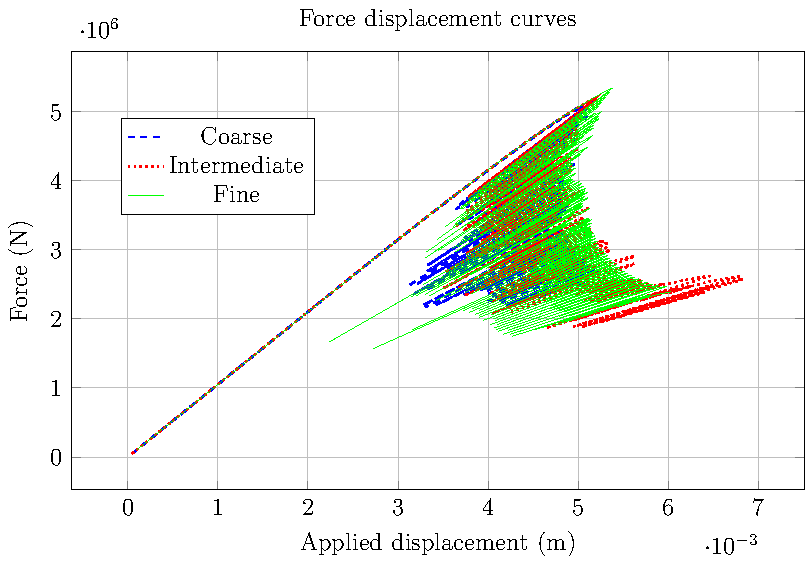
\includegraphics{./Images/L/force_displacement.pdf}
	\caption{Force displacement curves of the 2D-1D bar for three different meshes.}
	\label{L_force_displacement}
\end{figure}

\section{Discussion}

The results presented in this study underscore the critical role of the chosen metric and solver strategy in determining the convergence behavior of the data-driven (DD) algorithm. The analysis of the method’s rate of convergence reveals that using the tangent as the metric is essential for achieving an optimal convergence rate. In cases where instabilities such as snapback are expected, selecting a good (and in fact, correct) metric is not only beneficial but necessary to ensure convergence. Additionally, it was found that employing an arc-length (AL) solver is essential in some cases to achieve convergence. However, the AL solver alone is not sufficient; it must be coupled with the correct metric to ensure stability and accuracy. When used together, the AL solver and a proper metric enabled the solution to exhibit behavior characteristic of softening problems, even within the DD framework. It shall be noted that using a tangent for metric has been discussed earlier in some studies \cite{Pham2023,Nguyen2022,Kanno2019}. However, those studies were limited to improving the rate of convergence of the method and only examine the cases where there are no instabilities. The application of DD method to a case involving a snap through can be found in \cite{Kuang2023}. The authors of that study apply the DD method to a case where an instability develops as a consequence of geometric non-linearity. The initial guess for the alternate minimization in DD algorithm is perturbed to achieve convergence. To the best of the authors' knowledge, the current article is the first instance where the importance of metric, together with the need for an AL solver is first discussed when a material instability is encountered. 


The case of a 1D bar subjected to a body force demonstrates that finite element (FE) results exhibit mesh dependence, but in a manner consistent with what is typically observed when a constitutive model is used, provided a good metric and the arc-length (AL) method are employed. The regularization introduced in \cite{Kamasamudram2023} can also be seen to remove the mesh dependence of the solution in the DD setting. The saw tooth like pattern observed in the load displacement curves in figures 7 and 9 of \cite{Kamasamudram2023} can also be seen in the DD framework, as seen in figures \ref{force_disp_nonlocal} and \ref{force_disp_nonlocal_zoom} for two different mesh sizes. Since it has earlier been demonstrated that the DD solver lacks the ability to jump through the snap backs, it is essential that the DD solver (with AL method) track all the observed snap backs to obtain a mesh independent solution. This can be observed in the current case in the strain distributions for two mesh sizes in figure \ref{strain_dist_nonlocal} for the current case. Furthermore, it remains unclear whether applying the method without the AL method and using an incorrect metric would still yield a mesh-independent solution, even with regularization. While not explicitly reported in this article, preliminary analyses indicate that achieving convergence proves to be particularly challenging when a poor metric is used and the AL solver is omitted, especially for finer meshes.


A point of interest is that the constraint has to be removed from the elements that have fully damaged to prevent the damage region from expanding through the body. Similar issues are usually encountered in the non-local regularization techniques and have been discussed thoroughly in \cite{Geers1998,Cabot2014,Le2018} and other references therein.The common solution pursued is to evolve the length scale through the coarse of the simulation so that a proper localization is obtained. In 1D setting, deactivating the constraint in the fully damaged element ...

The method has then been extended to the 2D case, but after relaxing the Lipschitz constraint aiming to smoothen out or even eliminate the saw tooth pattern observed in the load displacement curve in the 1D setting.  

%The convergence issues associated with using a Newton solver for on-convex problems can be seen in various references. \cite{Farrell2017} monitor the residual during the Newton iterations and resort to alternate minimization if the residual is observed to increase. The Newton method is then resumed once the solution arrives into the \textit{basin of convergence}. \cite{Gerasimov2016} propose a modified line search method where the line search parameter is allowed to take on negative values owing to the non-convexity of the energy functional. 



\section{Conclusion}

\bibliography{library}

\appendix

\section{Analysis of convergence \label{appx_convergence}}
Consider the case of a 1D bar with an element in the middle already on the damaged branch while the other elements undergo unloading on the elastic branch, see Figure \ref{1D_bar_dam_elem}. It is the intent to check the effect of the metric in data driven case on the (rate of) convergence of the solution in this case. If the material behavior is described by a local damage model (without any regularization), a snapback is expected in the load displacement response of the body in some scenarios, depending on the mesh size.
\begin{figure}
	\centering
	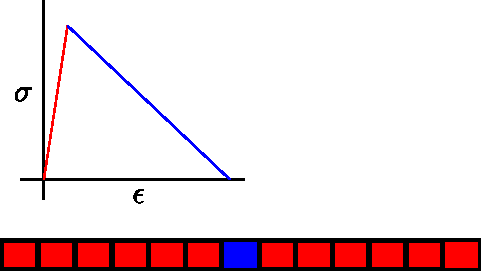
\includegraphics[scale=1.2]{1D_bar_dam_elem.pdf}
	\caption{1D bar with damaged element\label{1D_bar_dam_elem}}
\end{figure}

The stress state is homogeneous in the entire bar as a consequence of equilibrium. The strain is localized in the element undergoing damage (in blue), while the other elements are unloading (in red). Thus, the mechanical state of the bar is described by a scalar stress $\sigma \in \mathbb{R}$ and strains $\epsilon_1, \epsilon_2 \in \mathbb{R}$ ($\epsilon_1$ for the undamaged elements and $\epsilon_2$ for the damaged element). The material state is described by $(\epsilon_1^*, \sigma_1^*) \in \mathbb{R}^{1\times 1}$ and $(\epsilon_2^*, \sigma_2^*) \in \mathbb{R}^{1\times 1}$. The loading is driven by prescribing $u_D$, the displacement at the right end of the bar. The distance function in this is given by 
\begin{equation}
	d(\sigma,\sigma_1^*,\sigma_2^*,\epsilon_1,\epsilon_2;u_g) = \frac{N \ell_e}{2} \left[ \frac{(\sigma - \sigma_1^*)^2}{C_1} +  C_1(\epsilon_1 - \epsilon_1^*)^2 \right] + \frac{\ell_e}{2}  \left[ \frac{(\sigma - \sigma_2^*)^2}{C_2} +  C_2(\epsilon_2 - \epsilon_2^*)^2 \right].
\end{equation}
The compatibility condition is $N \epsilon_1 + \epsilon_2 = u_D/\ell_e$.

Now, taking the variations with respect to the compatibility equation as a constraint, the system of equations for $\epsilon_1,\epsilon_2$ and $\sigma$ are obtained as 
\begin{equation}
	\begin{bmatrix}
		\epsilon_1 \\
		\epsilon_2 \\
		\sigma
	\end{bmatrix}
	=
	\begin{bmatrix}
		C_1/(C_1+NC_2) & -C_2/(C_1+NC_2) & 0 & 0 \\
		-NC_1/(C_1+NC_2) & NC_2/(C_1+NC_2) & 0 & 0 \\
		0 & 0 & \frac{NC_2}{C_1+N C_2} & \frac{C_1}{C_1+N C_2}
	\end{bmatrix}
	\begin{bmatrix}
		\epsilon_1^* \\
		\epsilon_2^* \\
		\sigma_1^* \\
		\sigma_2^* 
	\end{bmatrix}
	+
	\begin{bmatrix}
		C_2 u_D/(C_1+NC_2)/\ell_e \\
		C_1 u_D/(C_1+NC_2)/\ell_e  \\
		0	
	\end{bmatrix}
	.
\end{equation}
The material states can be found by taking the variations with respect to $\epsilon_1^*, \epsilon_2^*$, while realizing that $\sigma_1^*=E\epsilon_1^*$, and $\sigma_2^*=m\epsilon_2^*+c$. Thus,
\begin{equation}
	\begin{bmatrix}
		\epsilon_1^* \\
		\epsilon_2^* \\
		\sigma_1^* \\
		\sigma_2^* 
	\end{bmatrix} 
	= 
	\begin{bmatrix}
		C_1^2/(E^2 + C_1^2) & 0 & E/(E^2 + C_1^2) \\
		0 & C_2^2/(m^2 + C_2^2)  & m/(m^2 + C_2^2) \\
		E C_1^2/(E^2 + C_1^2) & 0 & E^2/(E^2 + C_1^2)\\
		0 & mC_2^2/(m^2 + C_2^2)  & m^2/(m^2 + C_2^2) 
	\end{bmatrix} 
	\begin{bmatrix}
		\epsilon_1 \\
		\epsilon_2 \\
		\sigma
	\end{bmatrix} + 
	\begin{bmatrix}
		0 \\
		-mc/(m^2+C_2^2) \\
		0 \\
		cC_2^2/(m^2+C_2^2)
	\end{bmatrix} .
\end{equation}

The system of equations corresponding to the mechanical and material updates can be written in short as $\bfa = \bfA \bfb + \bfc$, and $\bfb = \bfC \bfa + \bfd$. The alternating minimization can then be written as
\begin{gather}
	\bfa^{n+1} = \bfA \bfb^{n} + \bfc, \\
	\bfb^{n+1} = \bfC \bfa^{n+1} + \bfd.
\end{gather}
Combining them together, 
\begin{equation}
	\bfb^{n+1} = \bfC \bfA \bfb^{n} +\bfC \bfc + \bfd. \label{combined_equn}
\end{equation}
At convergence, $\bfb^{n+1} \approx \bfb^{n} \approx \bfb$. Thus, $\bfe^{n+1} = \bfC \bfA \bfe^{n}$, where $\bfe^{n+1} = \bfb^{n+1} - \bfb$ is the error at the iteration $n+1$. The rate of convergence of the method depends on the spectral radius of the matrix $\bfC \bfA$, which in turn depends on the metric chosen. 

\subsubsection*{With snapback}
The case with snapback occurs when the mesh and thus, the size of the damage zone, is refined. In this case, an arc length solver is needed to track the full damage evolution in the element. So, this case will first be presented and the effect of metric on the rate of convergence will be studied.

Using an arc length solver corresponds to when the displacement at the end of the bar, $u_D$, is treated as an unknown. This results in the number of unknowns increasing by $1$. The additional equation that is needed to fully resolve the system is the arc length constraint, stated in equation \ref{onedarclength}. This changes the equations to be resolved in the previous section to 


\begin{multline}
	\begin{bmatrix}
		1 & 0& 0&  -C_2/(C_1+NC_2) \ell_e \\
		0 & 1 & 0 & -C_1/(C_1+NC_2) \ell_e \\
		0 & 0 & 1 & 0 \\
		0 & 1 & 0 & 0
	\end{bmatrix}
	\begin{bmatrix}
		\epsilon_1 \\
		\epsilon_2 \\
		\sigma \\
		u_D
	\end{bmatrix}
	= \\
	\begin{bmatrix}
		C_1/(C_1+NC_2) & -C_2/(C_1+NC_2) & 0 & 0 \\
		-NC_1/(C_1+NC_2) & NC_2/(C_1+NC_2) & 0 & 0 \\
		0 & 0 & \frac{NC_2}{C_1+N C_2} & \frac{C_1}{C_1+N C_2} \\ 
		0 & 0 & 0&0
	\end{bmatrix}
	\begin{bmatrix}
		\epsilon_1^* \\
		\epsilon_2^* \\
		\sigma_1^* \\
		\sigma_2^* 
	\end{bmatrix}
	+
	\begin{bmatrix}
		0 \\
		0  \\
		0	\\
		\epsilon_0 + \Delta \epsilon
	\end{bmatrix}
	.
\end{multline}
The material states can be found by taking the variations with respect to $\epsilon_1^*, \epsilon_2^*$, while realizing that $\sigma_1^*=E\epsilon_1^*$, and $\sigma_2^*=m\epsilon_2^*+c$. Thus,
\begin{equation}
	\begin{bmatrix}
		\epsilon_1^* \\
		\epsilon_2^* \\
		\sigma_1^* \\
		\sigma_2^* 
	\end{bmatrix} 
	= 
	\begin{bmatrix}
		C_1^2/(E^2 + C_1^2) & 0 & E/(E^2 + C_1^2) & 0 \\
		0 & C_2^2/(m^2 + C_2^2)  & m/(m^2 + C_2^2) &0 \\
		E C_1^2/(E^2 + C_1^2) & 0 & E^2/(E^2 + C_1^2) &0\\
		0 & mC_2^2/(m^2 + C_2^2)  & m^2/(m^2 + C_2^2) &0
	\end{bmatrix} 
	\begin{bmatrix}
		\epsilon_1 \\
		\epsilon_2 \\
		\sigma \\
		u_D
	\end{bmatrix} + 
	\begin{bmatrix}
		0 \\
		-mc/(m^2+C_2^2) \\
		0 \\
		cC_2^2/(m^2+C_2^2)
	\end{bmatrix} .
\end{equation}

Thus, even in this case, the update can be cast into the form of equation \ref{combined_equn} and can be analyzed similarly.

\section{Euler Lagrange equations}
Finding the solution of the boundary value problems consists of minimizing the potential energy functional which is defined as
\begin{equation}
	\Pi(\bfu) = \int_\Omega \psi(\bfeps) \diff v - W_{\ext}(\bfu).
\end{equation}
Here, $\psi$ denotes the strain energy density functional, $\bfeps$ is the symmetric part of the gradient of displacement $\bfu$, and $W_{\ext}$ denotes the potential of the external forces. In the case of material that undergoes damage, the strain energy function is made to depend on the damage as well, $\psi(\epsilon,d)$, where $d$ denotes the damage variable. $d$ takes the values in the interval $[0,1]$, where the value of $0$ indicates a pristine material and $1$ indicates a fully damaged material. In this case, the potential energy becomes
\begin{equation}
	\Pi(u,d) = \int_\Omega \psi(\bfeps,d) \diff v - W_{\ext}(\bfu) + \int_{0}^{t} D \diff t,
\end{equation}
where $D$ denotes the dissipation function~\cite{Mielke2005}. An evolution equation for damage can be specified using the notion of standard general materials~\cite{Nguyen1975}. The solution to the problem is the one that minimizes the potential energy over all the admissible functions.
\begin{equation}
	\left(\bfu^*,d^*\right) \in \arg \min_{(\bfu,d)\,\in\,\left(\cc^u \times \cc^d_n;d_{n-1}\right)} \Pi(\bfu,d),
\end{equation}
where $\cc^u$ and $\cc^d$ denote the space of admissible displacements and damages, respectively. They are defined as
\begin{gather}
	\cc^u = \left\{ \bfu \in H^2(\Omega)\, \middle| \, \bfu=\bfu_d \quad\text{on }\; \partial \Omega_d \right\}, \\
	\cc^d_n = \left\{ d \in L^\infty(\Omega)\, \middle| \, d(\bfx) \geq d_{n-1}(\bfx) \quad\text{and}\quad d(\bfx) \in [0,1] \, \forall \bfx \in \Omega \right\}.
\end{gather}
The definition of the space $\cc^d$ ensures the irreversibility of the damage. 

It is well known that the formulation just presented is devoid of any length scale and as such, the solution in the FE simulations become mesh dependent. In \cite{Kamasamudram2023}, the length scale is introduced by constraining the gradient of the strain to lie in a certain interval in 1D case. Here, the regularization will be introduced by weakening the constraint by using a log-barrier-like function. Thus, the functional to be minimized becomes
\begin{equation}
	\Pi(u,d;\ell_c) = \int_\Omega \psi(\bfeps,d) \diff v +  \int_\Omega \hat{\psi}(\nabla \bfeps,d;\ell_c) \diff v  - W_{\ext}(\bfu) + \int_{0}^{t} D \diff t,
\end{equation}
where, 
\begin{equation} \label{energy_constraint_gradient}
	\hat{\psi}(\nabla \bfeps,d;\ell_c) = -\mu \ln \left( \frac{1}{\ell_c} - g(d) \tilde{\psi}(\nabla \epsilon)  \right),
\end{equation}
where $g$ is the degradation function that depends on the damage, that is used to gradually remove the regularization as the damage increases. $\hat{\psi}$ is the quadratic functional that depends on the gradient of strain, which is defined as 
\begin{equation} \label{energy_constraint_gradient}
	\tilde{\psi}(\nabla \bfeps) = a_1 k_{iik}k_{kjj} + a_2 k_{ijj}k_{ikk} + a_3 k_{iik}k_{jjk} + a_4 k_{ijk}k_{ijk} + a_5 k_{ijk}k_{kji},
\end{equation}
where $k_{pqr} = \epsilon_{qr,p}$.

A couple of observations are warranted. First, the function $g$ is selected so that $g(0)=1$ and $g(1)=0$. This means that when there is no damage, the regularization is fully effective, and when fully damaged, the regularization is removed, and the transition is gradual if $g$ is smooth. Second, in this study, the parameter $\mu$ is fixed tp be a finite positive value. It shall be noted that the method resembles the interior point method of resolving inequality constraints in the standard optimization setting, where successive problems are solved with decreasing $\mu$, $\mu \to 0$. Thus, as the parameter $\mu$ is made smaller, the method presented here boils down to the inequality case and the problems/ features about snapback that were observd in the 1D case return. It is expected that taking $\mu$ to be finite and fixed prevents this issue. 


The equations of equilibrium can now be obtained by taking the variation of the potential energy functional in equation \ref{Total_potential_energy_model} and equating it to zero. For notational simplicity, the slack quantity, $s$, is defined as $s = \frac{1}{\ell_c} - g(d) \tilde{\psi}(\nabla \epsilon)$. Taking the variations with respect to the displacement,
\begin{equation}
	\delta^{\bfu} \tilde{\Pi}(\bfu,d,\lambda) = \int_\Omega \left( \bfsig : \delta \bfeps + \bftau . \nabla \delta \bfeps \right) \diff v = 0,
\end{equation}
where $\bfsig = \psi'(\bfeps;d)$, $\bftau = \frac{\mu}{s}\tilde{\psi}'(\nabla\bfeps;d)$, prime denotes taking a derivative with respect to the argument.
Written in index form, 
\begin{equation}
	\int_\Omega \left( \sigma_{ij}  \delta \epsilon_{ij} + \tau_{ijk}  \delta k_{ijk} \right) \diff v = 0. \label{equilibruim_in_index}
\end{equation}
It can be seen that $\bftau$ is the couple stress that is normally encountered in the strain gradient elasticity. Integrating equation \ref{equilibruim_in_index} by parts and gathering like terms together, the following equation can be obtained
\begin{equation}
	-\int_\Omega \left( \sigma_{kj,j} - \tau_{ijk,ij} \right) \delta u_{k} \diff v + \int_\Omega \left[  (\sigma_{ij} -\tau_{pij,p}) \delta u_{i,j} + (\tau_{ijk} \delta u_{j,k})_{,i} \right] \diff v  = 0. \label{equilibruim_in_index_parts}
\end{equation}
Dividing the domain $\Omega$ into regions where the constraints are active, $\Omega_a$, and where the constraints are inactive, $\Omega \setminus \Omega_a$, and realizing that $\lambda=0$ and hence $\bftau = 0$ in $\Omega \setminus \Omega_a$, the above integral can be written as 
\begin{equation}
	-\int_\Omega \left( \sigma_{kj,j} - \tau_{ijk,ij} \right) \delta u_{k} \diff v + \int_\Omega \left[  (\sigma_{ij} -\tau_{pij,p}) \delta u_{i,j} + (\tau_{ijk} \delta u_{j,k})_{,i} \right] \diff v  = 0.
\end{equation}
This leads to the equations of equilibrium in the bulk as 
\begin{equation}
	(\sigma_{kj} - \tau_{ijk,i})_{,j} = 0.
\end{equation}
It shall be noted that the above set of equations are similar to what is encountered in the case of first strain gradient theories in \cite{Mindlin and Toupin}, with the couple stress analogous to the strain gradient theory. ....Similarly, the equations on the surface can be obtained....

\subsection{Discrete version of the constraint}
To impose the constraint on the strain variable, a dual mesh (also called the lip mesh) is defined along with the FE mesh as has been done in \cite{Moes and Chevaugeon}. It shall be noted that the constraint on the strain variable requires its derivative. In discrete formulation, the gradient of the strain variable is computed on the lip mesh by using the strain variables computed from the FE mesh. The strain variables, computed from the displacements can be expressed as $\bfeps = \bfB \bfu$, where $\bfB$ is the discrete gradient operator, computed on the FE mesh. Likewise, defining the discrete gradient operator on the lip mesh and representing it in a matrix form as $\bfG$, the gradients of strain can be expressed in terms of the displacements as 
\begin{equation}
	\bfk = \nabla \bfeps = \bfG \bfB \bfu = \bfP \bfu.
\end{equation}
Where, $\bfk$ is the matrix containing the gradients of strain as $\begin{bmatrix}
	k_{111} & k_{211} & k_{122} & k_{222} & k_{112} & k_{212}
\end{bmatrix}^T$.

The constraint on the strain gradient can thus be written as 
\begin{equation} \label{discrete_constraint}
	(\bfLam \bfk )^T \bfLam \bfk \leq \frac{1}{\ell_c^2},
\end{equation}
where $\bfLam$ is a matrix composed of the coefficients $a_i$ from equation \ref{energy_constraint_gradient}. Hence, there will be as many (not necessarily active) constraints as the number of elements in the lip mesh.

\begin{figure}[ht]
	\centering
	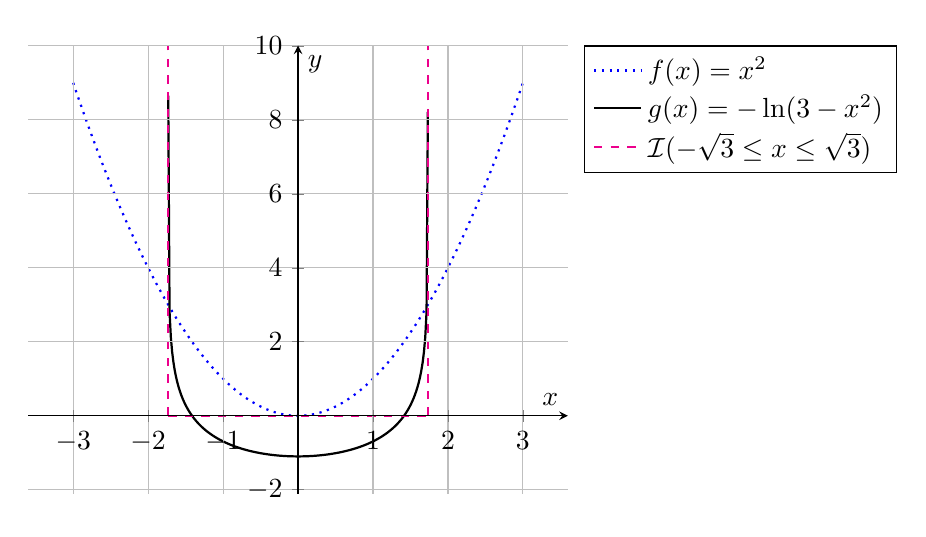
\begin{tikzpicture}
	\begin{axis}[
		axis lines = center,
		xlabel = {$x$},
		ylabel = {$y$},
		samples=200,
		domain=-3:3,  % Global domain setting for axis range
		legend pos=outer north east,
		grid = both,
		axis on top,
		enlargelimits = true,
		legend cell align={left},
		%title = {Comparison of $f(x)=x^2$ and $g(x)=-\ln(3 - x^2)$ with different domains}
		]
		
		% Plot f(x) = x^2 over the wider domain (-3, 3)
		\addplot[
		thick, dotted,
		blue,
		domain=-3:3,  % Wide domain for x^2
		]
		{x^2};
		\addlegendentry{$f(x) = x^2$}
		
		% Plot g(x) = -ln(3 - x^2) over the restricted domain (-1.73, 1.73)
		\addplot[
		thick,
		black,
		domain=-1.73199999:1.7319999,  % Restricted domain for -ln(3 - x^2)
		]
		{-ln(3 - x^2)};
		\addlegendentry{$g(x) = -\ln(3 - x^2)$}
		
		\addplot[domain=-1.73199999:1.7319999, samples=3, thick, magenta, dashed] {0};
		\addlegendentry{$\mathcal{I}(-\sqrt{3}\leq x \leq \sqrt{3}$)}
		% Indicate the "infinity" outside [-3, 3] with vertical asymptotes
		\draw[dashed, thick, magenta] (axis cs:-1.73199999,0) -- (axis cs:-1.73199999,10);  % Vertical asymptote at x = -3
		\draw[dashed, thick, magenta] (axis cs:1.73199999,0) -- (axis cs:1.73199999,10);    % Vertical asymptote at x = 3
		
		% Label the "infinity" on the graph
		\node at (axis cs:-1.73199999, 10) [above] {$\infty$};
		\node at (axis cs:1.73199999, 10) [above] {$\infty$};
		
		
	\end{axis}
\end{tikzpicture}
	\caption{Log barrier function vs quadratic functional}
	\label{comparison_log_quadratic}
\end{figure}


\section{Material update}
When the mechanical state is given, the material state can be updated analytically in the present case. 
\subsection*{In 1D}
In 1D, assuming that the database is represented by a model of the form $\sigma^* = m \epsilon ^*+d$, the material state is the minimizer of the following functional:
\begin{equation}
	\frac{(\sigma - \sigma^*)^2}{2C} + \frac{C}{2}(\epsilon - \epsilon^*)^2.	 
\end{equation}

Taking its derivative with respect to $\epsilon^*$ and equating it to zero, the material state can be seen to be
\begin{equation}
	\epsilon^* = \frac{m \sigma + C^2 \epsilon -md}{m^2 + C^2}.
\end{equation}

\subsection*{In 2D}
The generating model is $\sigst_i = g(D) E_{ij} \epsst_j$. $g$ is the degradation function of the damage variable, $D$. The damage evolution in the present case is taken to be a function of strain as 
\begin{equation}
D = \frac{\sqrt{k \psi_0(\bfeps^*)} - \sqrt{Y_c}}{(k-1)\sqrt{Y_c}}.
\end{equation}
$\psi_0$ is the strain energy density. $Y_c$ and $k$ are material parameters. $g$ is then defined as
\begin{equation}
	g(D) = \frac{1-D}{1+(k-1)D}.
\end{equation}

The distance functional, written in index form is
\begin{equation}
	d(\dots) = \frac{1}{2}(\sigma-\sigma^*)_i S_{ij} (\sigma-\sigma^*)_j + \frac{1}{2} (\epsilon-\epsilon^*)_i C_{ij} (\epsilon-\epsilon^*)_j.
\end{equation}
The material state can then be found by minimizing the above functional with respect to $\epsilon^*$. Thus, $\parder{d}{\epsilon ^*}=0$ . This can be further developed as follows:
\begin{equation}
	\parder{d}{\epsilon ^*_k} = -\parder{\sigst_i}{\epsst_k} S_{ij} (\sig - \sigst)_j - \parder{\epsst_i}{\epsst_k} C_{ij}(\eps-\epsst)_j.
\end{equation}
Realizing that $\sigst_i = g(d) E_{ij} \epsst_j$, the derivative can be written as 
\begin{gather}
	\parder{\sigst_i}{\epsst_k} = g'(D) \parder{D}{\epsst_k} E_{ij} \epsst_j + g(D) E_{ij} \delta_{jk}, \\
	= -\frac{\sqrt{k Y_c}}{2(k-1)\psi_0 \sqrt{\psi_0}} \sigsthat_i \sigsthat_k + g(D) E_{ik}.
\end{gather}
Thus, the equation to be resolved can be seen to be
\begin{equation}
	r_k = \left(\frac{\sqrt{k Y_c}}{2(k-1)\psi_0 \sqrt{\psi_0}} \sigsthat_i \sigsthat_k + g(D) E_{ik} \right) S_{ij} (\sig - \sigst)_j - \parder{\epsst_i}{\epsst_k} C_{ij}(\eps-\epsst)_j = 0.
\end{equation}
The above equation is non-linear and requires newton's method to solve. This needs the derivative of residual, which can be seen to be
\begin{multline}
	\parder{r_k}{\epsst_p} = \left\{  \frac{\sqrt{k Y_c}}{2(k-1)} \left[ \frac{ E_{kp} \sigsthat_i + \sigsthat_k E_{ip} + \sigsthat_p E_{ik} }{\psi_0 \sqrt{\psi_0}}-\frac{3}{2} \psi_0^{-5/2} \sigsthat_i \sigsthat_k \sigsthat_p \right] S_{ij} (\sig - \sigst)_j  \right\} +  \\ 
	\left(\frac{\sqrt{k Y_c}}{2(k-1)\psi_0 \sqrt{\psi_0}} \sigsthat_i \sigsthat_k + g(D) E_{ik} \right) S_{ij} \left(\frac{\sqrt{k Y_c}}{2(k-1)\psi_0 \sqrt{\psi_0}} \sigsthat_j \sigsthat_p + g(D) E_{jp} \right) + C_{kp}.
\end{multline}

\section{Arc length constraint}
The arc length constraint is simpler in 1D case than in 2D case as it involves selecting degrees of freedom where a certain quantity is monotone increasing. For instance, in \cite{}, the damage variables are used to write the arc length constraint. In the current case, for the 1D bar, the mechanical strain variable at the left end of the bar is chosen to impose the arc length constraint. The constraint can be expressed as
\begin{equation}
	\epsilon^{n+1} - \epsilon^{n} = \Delta, \label{onedarclength}
\end{equation}
where $n+1$ and $n$ denote the load steps. $\Delta$ is the arc length, which in the current case is the strain increment for the element at the extreme left between two steps. Expressing the displacements as $\bfu = \bfC_f \bfu_f + \lambda \bfu_g$, where $\bfu_f$ denotes the unknown/free degrees of freedom and $\lambda$, in the current case, is the displacement applied at the right end with $u_g$ as the corresponding degree of freedom. For instance, if the bar contains $N$ nodes numbered $1$ to $N$, $\bfu_f$ contains the DOFs of the nodes $2$ to $N-1$. $\bfC_f \in \mathbb{R}^{N \times N-2}$ and $\bfu_g \in \mathbb{R}^N = \{0,0,0,\dots 1\}^T$.

In 2D case, the method is slightly involved. The aim is to identify the degrees of freedom where a specific quantity is always increasing. For this purpose, the elements whose material states lie on the 'damage branch' are first identified. The damage levels in these elements are thus increasing in the load step under consideration. Then, an equivalent strain energy density of the mechanical states corresponding to these elements are computed using the mechanical strains. The arc length constraint is now written using these degrees of freedom and their 'equivalent strain energy'.

% \section{Trash Appendix}
%The notion of Data Driven Computational Mechanics has been introduced in \cite{KO}, where the constitutive model for the material is replaced by a database of stresses and strains (material states). The solution for the boundary value problem is sought as the stress-strain pair that satisfy the equations of equilibrium and compatibility conditions (mechanical states) while being as close as possible to the database (material states). Formally, the distance functional between the mechanical and material states is introduced as 
%\begin{equation}
%	d(\bfeps,\bfsig,\bfeps^*,\bfsig^*) = \frac{\mathcal{C}}{2}(\bfeps - \bfeps^*):(\bfeps - \bfeps^*) + \frac{\mathcal{C}^{-1}}{2}(\bfsig - \bfsig^*):(\bfsig - \bfsig^*).
%\end{equation}
%The solution to the BVP then becomes
%\begin{equation}
%	\text{Sol } \in \arg \min_{(\bfeps,\bfsig) \in \mathcal{E}, (\bfeps^*,\bfsig^*) \in \mathcal{D}} d(\bfeps,\bfsig,\bfeps^*,\bfsig^*),
%\end{equation}
%where 
%\begin{equation}
%	\mathcal{E} = \{(\bfeps,\bfsig) \text{ sufficiently regular }: \bfeps = \sym \nabla \bfu, \bfu = \bfu_D \text{ on } \partial \Omega_d \text{ and } \divop \bfsig = 0     \},
%\end{equation}
%and $\mathcal{D}$ denotes the material database. Compatibility can be ensured by directly using $\bfeps = \sym \nabla\bfu$ in the distance functional, while the equilibrium constraints can be imposed by using Lagrange multipliers. The discrete version of the above equations can be seen as (with the compatibility conditions used directly in the distance functional and imposing equilibrium through Lagrange multipliers)
%\begin{equation}
%	\Pi(\bfeps,\bfsig,\bfeps^*,\bfsig^*) = \frac{1}{2}(\bfB \bfu - \bfeps^*)^T\mathcal{C}(\bfB \bfu - \bfeps^*) + \frac{1}{2}(\bfsig - \bfsig^*)^T\mathcal{C}^{-1}(\bfsig - \bfsig^*) - \bfeta^T \bfB^T \bfsig .
%\end{equation}
%Assuming the material states to be given, taking the variations of the Lagrangian with respect to the mechanical states results in the Euler-Lagrange equations as
%\begin{gather}
%	\bfB ^T \bfD \bfB \bfu = \bfB \bfD \bfeps^*, \\
%	\bfsig  = \bfsig^* + \bfD \bfB \bfeta, \\
%	\bfB ^T \bfsig = 0.
%\end{gather}
%The second and third of the above equations result in
%\begin{equation}
%	\bfB ^T \bfD \bfB \bfeta = -\bfB ^T \bfsig^*.
%\end{equation}
%The material states are then found as the points in the database that minimize the distance functional, given the mechanical states.
%
%\subsection{Inclusion of the constraint}
%The Lipschitz constraint on the strain variable can be introduced in data driven case as described below. It shall be noted that the inclusion of constraints modifies the equations of equilibrium, where the Lagrange multipliers take the place of couple stress. As in the earlier case, the distance functional is defined as 
%\begin{equation}
%	d(\bfeps,\bfsig,\bfeps^*,\bfsig^*) = \frac{1}{2}(\bfB \bfu - \bfeps^*)^T\mathcal{C}(\bfB \bfu - \bfeps^*) + \frac{1}{2}(\bfsig - \bfsig^*)^T\mathcal{C}^{-1}(\bfsig - \bfsig^*).
%\end{equation}
%The objective now is to see the minimizers of the above functional so that the strain field satisfies the Lipschitz constraint. The Lagrange multipliers that enforce the constraint on the strain field act as couple stresses.
%\begin{equation}
%	\text{Sol } \in \arg \min_{(\bfeps,\bfsig) \in \mathcal{E}, (\bfeps^*,\bfsig^*) \in \mathcal{D}} d(\bfeps,\bfsig,\bfeps^*,\bfsig^*),
%\end{equation}
%where, the equilibrium manifold is now defined as (in discrete form)
%
%\begin{equation}
%	\mathcal{E} = \{(\bfeps,\bfsig) : \bfeps = \bfB \bfu, \bfeps \text{ satisfies equation \ref{discrete_constraint}},\bfu = \bfu_D \text{ on } \partial \Omega_d,
%	\text{ and } \bfB ^T \bfsig - \bfP^T \bftau = 0     \},
%\end{equation}
%where $\bftau$ is as defined in equation \ref{couple_stress}. Euler Lagrange equations can be obtained by taking the variation of the following Lagrangian and equating the corresponding variations to $0$. The Lagrangian can be defined to be
%\begin{multline}
%	\Pi = d(\bfeps,\bfsig,\bfeps^*,\bfsig^*) - \bfeta^T \bfB ^T \bfsig + \sum_{i=1}^{N_c} \lambda^u_i \left( (\bfP \bfu )_i^T \bfLam (\bfP \bfu)_i - \frac{1}{\ell_c^2}   \right) + \sum_{i=1}^{N_c} \lambda^{\eta u}_i \left( (\bfP (\bfu + \bfeta) )_i^T \bfLam (\bfP (\bfu + \bfeta))_i - \frac{1}{\ell_c^2}   \right).
%\end{multline}
%Here, $N_c$ denotes the number of active constraints and $\lambda_i \geq 0$ are the Lagrange multipliers dual to the constraint on the gradient of strain. $\lambda^{\eta u}_i = -\lambda^{ u}_i$ at convergence, take the role of the couple stresses as in equation \ref{equilibruim_in_index}. Plainly stating, the above equation states that the displacement field satisfies the inequality constraints, and in the places where the constraint is satisfied as an equality, the \textit{perturbed solution (with $\bfeta$)} should also satisfy the constraints.
%
%
%
%The EL equations can be seen to be
%\begin{gather}
%	\bfr_{\bfu} = \bfB^T \mathcal{C} \bfB \bfu - \bfB^T \mathcal{C} \bfeps ^* + \sum_{i=1}^{N_c} \lambda_i^u \left( 2 \bfP_i ^T \bfLam \bfP_i \bfu \right) + \sum_{i=1}^{N_c} \lambda_i^{\eta u} \left( 2 \bfP_i ^T \bfLam \bfP_i (\bfu+\bfeta) \right) =0, \\
%	\bfr_{\bfeta} = -\bfB^T \mathcal{C} \bfB \bfeta - \bfB^T \bfsig ^* + \sum_{i=1}^{N_c} \lambda_i^{\eta u} \left( 2 \bfP_i ^T \bfLam \bfP_i (\bfu+\bfeta) \right) =0, \\
%	r_{\lambda^u_i} = (\bfP \bfu )_i^T \bfLam (\bfP \bfu)_i - \frac{1}{\ell_c^2}  =0, \\
%	r_{\lambda^{\eta u}_i} = \bfP (\bfu + \bfeta) )_i^T \bfLam (\bfP (\bfu + \bfeta))_i - \frac{1}{\ell_c^2}  =0. 
%\end{gather}
%

\bibliography{data_driven_damage}
\end{document}
%%% Local Variables: 
%%% mode: latex
%%% TeX-master: t
%%% End: 
